
\newpage
\subsection{BenchMarkishTopics}
    % latex table generated in R 4.1.2 by xtable 1.8-4 package
% Sun Mar 13 20:27:35 2022
\begin{table}[h!]
\centering
\begin{tabular}{p{0.2\textwidth}p{0.2\textwidth}p{0.2\textwidth}}
  \hline
 & LLVM IR & ARM Assembly \\ 
  \hline
Stack & 204 & 130 \\ 
  Registers & 184 &  82 \\ 
  Optimizations & 173 &  82 \\ 
   \hline
\end{tabular}
\caption{BenchMarkishTopics instruction counts for generated code excluding labels}
\end{table}

    \begin{figure}[h]
	    \centering
		% Created by tikzDevice version 0.12.3.1 on 2022-03-08 11:09:32
% !TEX encoding = UTF-8 Unicode
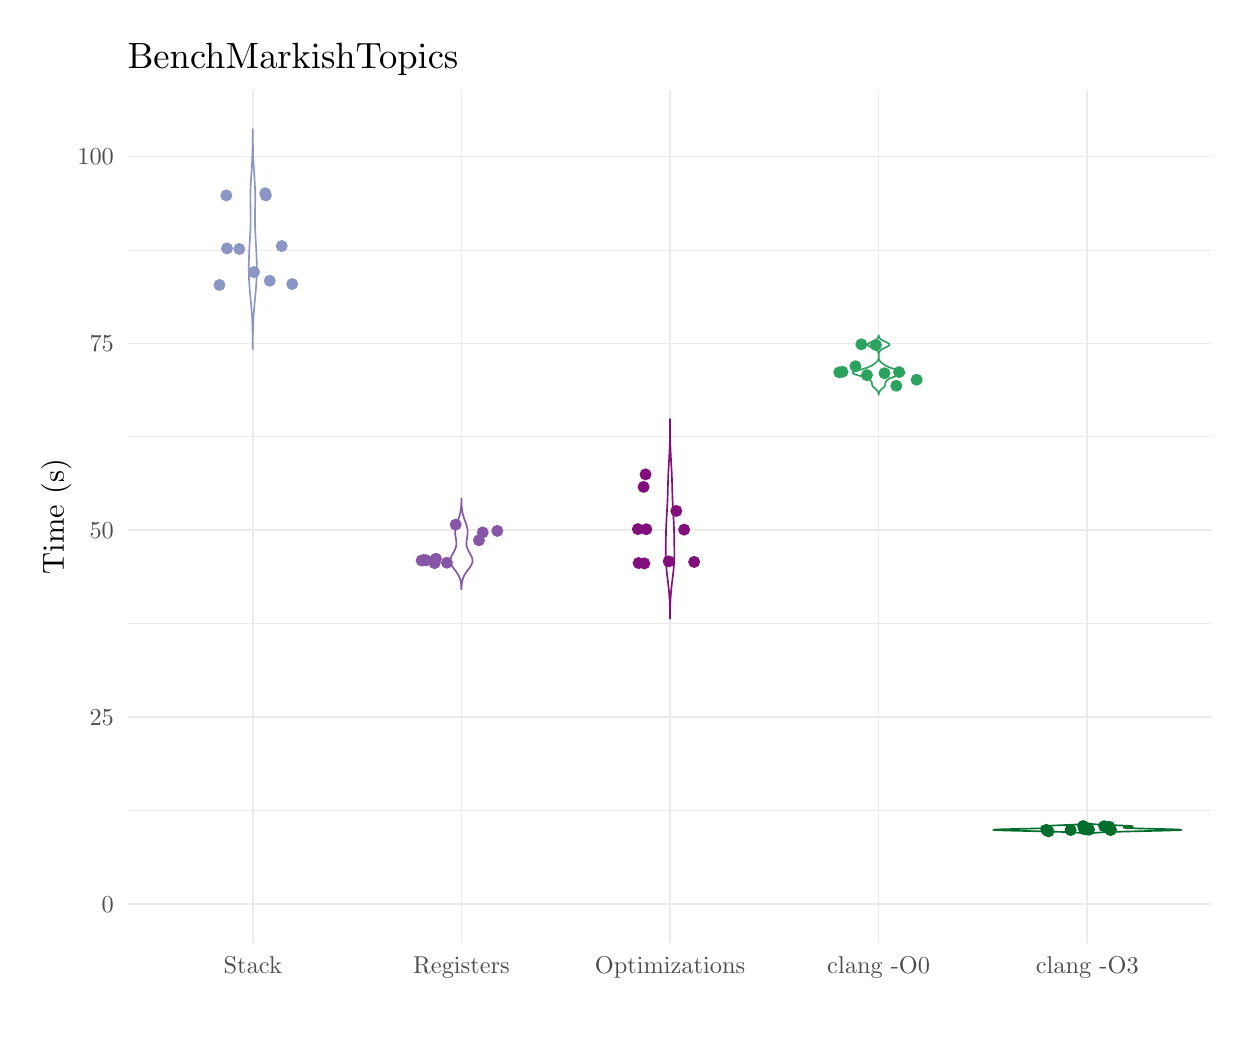
\begin{tikzpicture}[x=1pt,y=1pt]
\definecolor{fillColor}{RGB}{255,255,255}
\path[use as bounding box,fill=fillColor,fill opacity=0.00] (0,0) rectangle (433.62,361.35);
\begin{scope}
\path[clip] ( 36.11, 30.69) rectangle (428.12,338.69);
\definecolor{drawColor}{gray}{0.92}

\path[draw=drawColor,line width= 0.3pt,line join=round] ( 36.11, 78.45) --
	(428.12, 78.45);

\path[draw=drawColor,line width= 0.3pt,line join=round] ( 36.11,145.96) --
	(428.12,145.96);

\path[draw=drawColor,line width= 0.3pt,line join=round] ( 36.11,213.48) --
	(428.12,213.48);

\path[draw=drawColor,line width= 0.3pt,line join=round] ( 36.11,281.00) --
	(428.12,281.00);

\path[draw=drawColor,line width= 0.6pt,line join=round] ( 36.11, 44.69) --
	(428.12, 44.69);

\path[draw=drawColor,line width= 0.6pt,line join=round] ( 36.11,112.20) --
	(428.12,112.20);

\path[draw=drawColor,line width= 0.6pt,line join=round] ( 36.11,179.72) --
	(428.12,179.72);

\path[draw=drawColor,line width= 0.6pt,line join=round] ( 36.11,247.24) --
	(428.12,247.24);

\path[draw=drawColor,line width= 0.6pt,line join=round] ( 36.11,314.76) --
	(428.12,314.76);

\path[draw=drawColor,line width= 0.6pt,line join=round] ( 81.34, 30.69) --
	( 81.34,338.69);

\path[draw=drawColor,line width= 0.6pt,line join=round] (156.73, 30.69) --
	(156.73,338.69);

\path[draw=drawColor,line width= 0.6pt,line join=round] (232.12, 30.69) --
	(232.12,338.69);

\path[draw=drawColor,line width= 0.6pt,line join=round] (307.50, 30.69) --
	(307.50,338.69);

\path[draw=drawColor,line width= 0.6pt,line join=round] (382.89, 30.69) --
	(382.89,338.69);
\definecolor{drawColor}{RGB}{140,150,198}
\definecolor{fillColor}{RGB}{255,255,255}

\path[draw=drawColor,line width= 0.6pt,line join=round,line cap=round,fill=fillColor] ( 81.34,245.19) --
	( 81.33,245.34) --
	( 81.33,245.50) --
	( 81.33,245.65) --
	( 81.33,245.81) --
	( 81.33,245.97) --
	( 81.33,246.12) --
	( 81.33,246.28) --
	( 81.33,246.43) --
	( 81.33,246.59) --
	( 81.33,246.74) --
	( 81.33,246.90) --
	( 81.33,247.06) --
	( 81.33,247.21) --
	( 81.32,247.37) --
	( 81.32,247.52) --
	( 81.32,247.68) --
	( 81.32,247.83) --
	( 81.32,247.99) --
	( 81.32,248.14) --
	( 81.32,248.30) --
	( 81.32,248.46) --
	( 81.31,248.61) --
	( 81.31,248.77) --
	( 81.31,248.92) --
	( 81.31,249.08) --
	( 81.31,249.23) --
	( 81.31,249.39) --
	( 81.30,249.54) --
	( 81.30,249.70) --
	( 81.30,249.86) --
	( 81.30,250.01) --
	( 81.30,250.17) --
	( 81.29,250.32) --
	( 81.29,250.48) --
	( 81.29,250.63) --
	( 81.29,250.79) --
	( 81.28,250.94) --
	( 81.28,251.10) --
	( 81.28,251.26) --
	( 81.27,251.41) --
	( 81.27,251.57) --
	( 81.27,251.72) --
	( 81.26,251.88) --
	( 81.26,252.03) --
	( 81.26,252.19) --
	( 81.25,252.35) --
	( 81.25,252.50) --
	( 81.24,252.66) --
	( 81.24,252.81) --
	( 81.23,252.97) --
	( 81.23,253.12) --
	( 81.23,253.28) --
	( 81.22,253.43) --
	( 81.22,253.59) --
	( 81.21,253.75) --
	( 81.20,253.90) --
	( 81.20,254.06) --
	( 81.19,254.21) --
	( 81.19,254.37) --
	( 81.18,254.52) --
	( 81.17,254.68) --
	( 81.17,254.83) --
	( 81.16,254.99) --
	( 81.15,255.15) --
	( 81.15,255.30) --
	( 81.14,255.46) --
	( 81.13,255.61) --
	( 81.12,255.77) --
	( 81.12,255.92) --
	( 81.11,256.08) --
	( 81.10,256.23) --
	( 81.09,256.39) --
	( 81.08,256.55) --
	( 81.07,256.70) --
	( 81.07,256.86) --
	( 81.06,257.01) --
	( 81.05,257.17) --
	( 81.04,257.32) --
	( 81.03,257.48) --
	( 81.02,257.64) --
	( 81.01,257.79) --
	( 81.00,257.95) --
	( 80.99,258.10) --
	( 80.97,258.26) --
	( 80.96,258.41) --
	( 80.95,258.57) --
	( 80.94,258.72) --
	( 80.93,258.88) --
	( 80.92,259.04) --
	( 80.91,259.19) --
	( 80.89,259.35) --
	( 80.88,259.50) --
	( 80.87,259.66) --
	( 80.86,259.81) --
	( 80.84,259.97) --
	( 80.83,260.12) --
	( 80.82,260.28) --
	( 80.80,260.44) --
	( 80.79,260.59) --
	( 80.78,260.75) --
	( 80.76,260.90) --
	( 80.75,261.06) --
	( 80.74,261.21) --
	( 80.72,261.37) --
	( 80.71,261.52) --
	( 80.69,261.68) --
	( 80.68,261.84) --
	( 80.66,261.99) --
	( 80.65,262.15) --
	( 80.64,262.30) --
	( 80.62,262.46) --
	( 80.61,262.61) --
	( 80.59,262.77) --
	( 80.58,262.92) --
	( 80.56,263.08) --
	( 80.55,263.24) --
	( 80.53,263.39) --
	( 80.52,263.55) --
	( 80.50,263.70) --
	( 80.49,263.86) --
	( 80.48,264.01) --
	( 80.46,264.17) --
	( 80.45,264.33) --
	( 80.43,264.48) --
	( 80.42,264.64) --
	( 80.40,264.79) --
	( 80.39,264.95) --
	( 80.37,265.10) --
	( 80.36,265.26) --
	( 80.35,265.41) --
	( 80.33,265.57) --
	( 80.32,265.73) --
	( 80.31,265.88) --
	( 80.29,266.04) --
	( 80.28,266.19) --
	( 80.27,266.35) --
	( 80.25,266.50) --
	( 80.24,266.66) --
	( 80.23,266.81) --
	( 80.21,266.97) --
	( 80.20,267.13) --
	( 80.19,267.28) --
	( 80.18,267.44) --
	( 80.17,267.59) --
	( 80.16,267.75) --
	( 80.14,267.90) --
	( 80.13,268.06) --
	( 80.12,268.21) --
	( 80.11,268.37) --
	( 80.10,268.53) --
	( 80.09,268.68) --
	( 80.08,268.84) --
	( 80.07,268.99) --
	( 80.06,269.15) --
	( 80.05,269.30) --
	( 80.04,269.46) --
	( 80.04,269.62) --
	( 80.03,269.77) --
	( 80.02,269.93) --
	( 80.01,270.08) --
	( 80.00,270.24) --
	( 80.00,270.39) --
	( 79.99,270.55) --
	( 79.98,270.70) --
	( 79.98,270.86) --
	( 79.97,271.02) --
	( 79.96,271.17) --
	( 79.96,271.33) --
	( 79.95,271.48) --
	( 79.95,271.64) --
	( 79.94,271.79) --
	( 79.94,271.95) --
	( 79.94,272.10) --
	( 79.93,272.26) --
	( 79.93,272.42) --
	( 79.92,272.57) --
	( 79.92,272.73) --
	( 79.92,272.88) --
	( 79.92,273.04) --
	( 79.91,273.19) --
	( 79.91,273.35) --
	( 79.91,273.50) --
	( 79.91,273.66) --
	( 79.91,273.82) --
	( 79.91,273.97) --
	( 79.91,274.13) --
	( 79.90,274.28) --
	( 79.90,274.44) --
	( 79.90,274.59) --
	( 79.91,274.75) --
	( 79.91,274.91) --
	( 79.91,275.06) --
	( 79.91,275.22) --
	( 79.91,275.37) --
	( 79.91,275.53) --
	( 79.91,275.68) --
	( 79.91,275.84) --
	( 79.92,275.99) --
	( 79.92,276.15) --
	( 79.92,276.31) --
	( 79.92,276.46) --
	( 79.93,276.62) --
	( 79.93,276.77) --
	( 79.93,276.93) --
	( 79.94,277.08) --
	( 79.94,277.24) --
	( 79.94,277.39) --
	( 79.95,277.55) --
	( 79.95,277.71) --
	( 79.96,277.86) --
	( 79.96,278.02) --
	( 79.97,278.17) --
	( 79.97,278.33) --
	( 79.98,278.48) --
	( 79.98,278.64) --
	( 79.99,278.79) --
	( 79.99,278.95) --
	( 80.00,279.11) --
	( 80.01,279.26) --
	( 80.01,279.42) --
	( 80.02,279.57) --
	( 80.03,279.73) --
	( 80.03,279.88) --
	( 80.04,280.04) --
	( 80.05,280.19) --
	( 80.05,280.35) --
	( 80.06,280.51) --
	( 80.07,280.66) --
	( 80.08,280.82) --
	( 80.09,280.97) --
	( 80.09,281.13) --
	( 80.10,281.28) --
	( 80.11,281.44) --
	( 80.12,281.60) --
	( 80.13,281.75) --
	( 80.13,281.91) --
	( 80.14,282.06) --
	( 80.15,282.22) --
	( 80.16,282.37) --
	( 80.17,282.53) --
	( 80.18,282.68) --
	( 80.19,282.84) --
	( 80.19,283.00) --
	( 80.20,283.15) --
	( 80.21,283.31) --
	( 80.22,283.46) --
	( 80.23,283.62) --
	( 80.24,283.77) --
	( 80.25,283.93) --
	( 80.26,284.08) --
	( 80.27,284.24) --
	( 80.28,284.40) --
	( 80.28,284.55) --
	( 80.29,284.71) --
	( 80.30,284.86) --
	( 80.31,285.02) --
	( 80.32,285.17) --
	( 80.33,285.33) --
	( 80.34,285.48) --
	( 80.35,285.64) --
	( 80.35,285.80) --
	( 80.36,285.95) --
	( 80.37,286.11) --
	( 80.38,286.26) --
	( 80.39,286.42) --
	( 80.40,286.57) --
	( 80.40,286.73) --
	( 80.41,286.89) --
	( 80.42,287.04) --
	( 80.43,287.20) --
	( 80.43,287.35) --
	( 80.44,287.51) --
	( 80.45,287.66) --
	( 80.45,287.82) --
	( 80.46,287.97) --
	( 80.47,288.13) --
	( 80.47,288.29) --
	( 80.48,288.44) --
	( 80.49,288.60) --
	( 80.49,288.75) --
	( 80.50,288.91) --
	( 80.50,289.06) --
	( 80.51,289.22) --
	( 80.51,289.37) --
	( 80.52,289.53) --
	( 80.52,289.69) --
	( 80.52,289.84) --
	( 80.53,290.00) --
	( 80.53,290.15) --
	( 80.53,290.31) --
	( 80.54,290.46) --
	( 80.54,290.62) --
	( 80.54,290.77) --
	( 80.54,290.93) --
	( 80.55,291.09) --
	( 80.55,291.24) --
	( 80.55,291.40) --
	( 80.55,291.55) --
	( 80.55,291.71) --
	( 80.55,291.86) --
	( 80.55,292.02) --
	( 80.56,292.18) --
	( 80.56,292.33) --
	( 80.56,292.49) --
	( 80.56,292.64) --
	( 80.55,292.80) --
	( 80.55,292.95) --
	( 80.55,293.11) --
	( 80.55,293.26) --
	( 80.55,293.42) --
	( 80.55,293.58) --
	( 80.55,293.73) --
	( 80.55,293.89) --
	( 80.55,294.04) --
	( 80.54,294.20) --
	( 80.54,294.35) --
	( 80.54,294.51) --
	( 80.54,294.66) --
	( 80.54,294.82) --
	( 80.53,294.98) --
	( 80.53,295.13) --
	( 80.53,295.29) --
	( 80.53,295.44) --
	( 80.52,295.60) --
	( 80.52,295.75) --
	( 80.52,295.91) --
	( 80.51,296.06) --
	( 80.51,296.22) --
	( 80.51,296.38) --
	( 80.51,296.53) --
	( 80.50,296.69) --
	( 80.50,296.84) --
	( 80.50,297.00) --
	( 80.50,297.15) --
	( 80.49,297.31) --
	( 80.49,297.46) --
	( 80.49,297.62) --
	( 80.49,297.78) --
	( 80.49,297.93) --
	( 80.48,298.09) --
	( 80.48,298.24) --
	( 80.48,298.40) --
	( 80.48,298.55) --
	( 80.48,298.71) --
	( 80.48,298.87) --
	( 80.48,299.02) --
	( 80.47,299.18) --
	( 80.47,299.33) --
	( 80.47,299.49) --
	( 80.47,299.64) --
	( 80.47,299.80) --
	( 80.47,299.95) --
	( 80.47,300.11) --
	( 80.47,300.27) --
	( 80.48,300.42) --
	( 80.48,300.58) --
	( 80.48,300.73) --
	( 80.48,300.89) --
	( 80.48,301.04) --
	( 80.48,301.20) --
	( 80.49,301.35) --
	( 80.49,301.51) --
	( 80.49,301.67) --
	( 80.50,301.82) --
	( 80.50,301.98) --
	( 80.50,302.13) --
	( 80.51,302.29) --
	( 80.51,302.44) --
	( 80.52,302.60) --
	( 80.52,302.75) --
	( 80.52,302.91) --
	( 80.53,303.07) --
	( 80.54,303.22) --
	( 80.54,303.38) --
	( 80.55,303.53) --
	( 80.55,303.69) --
	( 80.56,303.84) --
	( 80.57,304.00) --
	( 80.57,304.16) --
	( 80.58,304.31) --
	( 80.59,304.47) --
	( 80.60,304.62) --
	( 80.60,304.78) --
	( 80.61,304.93) --
	( 80.62,305.09) --
	( 80.63,305.24) --
	( 80.64,305.40) --
	( 80.64,305.56) --
	( 80.65,305.71) --
	( 80.66,305.87) --
	( 80.67,306.02) --
	( 80.68,306.18) --
	( 80.69,306.33) --
	( 80.70,306.49) --
	( 80.71,306.64) --
	( 80.72,306.80) --
	( 80.73,306.96) --
	( 80.74,307.11) --
	( 80.75,307.27) --
	( 80.76,307.42) --
	( 80.77,307.58) --
	( 80.78,307.73) --
	( 80.79,307.89) --
	( 80.80,308.04) --
	( 80.81,308.20) --
	( 80.82,308.36) --
	( 80.83,308.51) --
	( 80.84,308.67) --
	( 80.85,308.82) --
	( 80.86,308.98) --
	( 80.87,309.13) --
	( 80.88,309.29) --
	( 80.89,309.45) --
	( 80.90,309.60) --
	( 80.91,309.76) --
	( 80.92,309.91) --
	( 80.93,310.07) --
	( 80.94,310.22) --
	( 80.95,310.38) --
	( 80.96,310.53) --
	( 80.97,310.69) --
	( 80.98,310.85) --
	( 80.99,311.00) --
	( 80.99,311.16) --
	( 81.00,311.31) --
	( 81.01,311.47) --
	( 81.02,311.62) --
	( 81.03,311.78) --
	( 81.04,311.93) --
	( 81.05,312.09) --
	( 81.06,312.25) --
	( 81.06,312.40) --
	( 81.07,312.56) --
	( 81.08,312.71) --
	( 81.09,312.87) --
	( 81.10,313.02) --
	( 81.10,313.18) --
	( 81.11,313.33) --
	( 81.12,313.49) --
	( 81.13,313.65) --
	( 81.13,313.80) --
	( 81.14,313.96) --
	( 81.15,314.11) --
	( 81.15,314.27) --
	( 81.16,314.42) --
	( 81.17,314.58) --
	( 81.17,314.74) --
	( 81.18,314.89) --
	( 81.18,315.05) --
	( 81.19,315.20) --
	( 81.20,315.36) --
	( 81.20,315.51) --
	( 81.21,315.67) --
	( 81.21,315.82) --
	( 81.22,315.98) --
	( 81.22,316.14) --
	( 81.23,316.29) --
	( 81.23,316.45) --
	( 81.24,316.60) --
	( 81.24,316.76) --
	( 81.24,316.91) --
	( 81.25,317.07) --
	( 81.25,317.22) --
	( 81.26,317.38) --
	( 81.26,317.54) --
	( 81.26,317.69) --
	( 81.27,317.85) --
	( 81.27,318.00) --
	( 81.27,318.16) --
	( 81.28,318.31) --
	( 81.28,318.47) --
	( 81.28,318.62) --
	( 81.28,318.78) --
	( 81.29,318.94) --
	( 81.29,319.09) --
	( 81.29,319.25) --
	( 81.29,319.40) --
	( 81.30,319.56) --
	( 81.30,319.71) --
	( 81.30,319.87) --
	( 81.30,320.02) --
	( 81.30,320.18) --
	( 81.31,320.34) --
	( 81.31,320.49) --
	( 81.31,320.65) --
	( 81.31,320.80) --
	( 81.31,320.96) --
	( 81.31,321.11) --
	( 81.32,321.27) --
	( 81.32,321.43) --
	( 81.32,321.58) --
	( 81.32,321.74) --
	( 81.32,321.89) --
	( 81.32,322.05) --
	( 81.32,322.20) --
	( 81.32,322.36) --
	( 81.33,322.51) --
	( 81.33,322.67) --
	( 81.33,322.83) --
	( 81.33,322.98) --
	( 81.33,323.14) --
	( 81.33,323.29) --
	( 81.33,323.45) --
	( 81.33,323.60) --
	( 81.33,323.76) --
	( 81.33,323.91) --
	( 81.33,324.07) --
	( 81.33,324.23) --
	( 81.33,324.38) --
	( 81.33,324.54) --
	( 81.34,324.69) --
	( 81.35,324.69) --
	( 81.35,324.54) --
	( 81.35,324.38) --
	( 81.35,324.23) --
	( 81.35,324.07) --
	( 81.35,323.91) --
	( 81.35,323.76) --
	( 81.35,323.60) --
	( 81.36,323.45) --
	( 81.36,323.29) --
	( 81.36,323.14) --
	( 81.36,322.98) --
	( 81.36,322.83) --
	( 81.36,322.67) --
	( 81.36,322.51) --
	( 81.36,322.36) --
	( 81.36,322.20) --
	( 81.36,322.05) --
	( 81.36,321.89) --
	( 81.37,321.74) --
	( 81.37,321.58) --
	( 81.37,321.43) --
	( 81.37,321.27) --
	( 81.37,321.11) --
	( 81.37,320.96) --
	( 81.37,320.80) --
	( 81.38,320.65) --
	( 81.38,320.49) --
	( 81.38,320.34) --
	( 81.38,320.18) --
	( 81.38,320.02) --
	( 81.39,319.87) --
	( 81.39,319.71) --
	( 81.39,319.56) --
	( 81.39,319.40) --
	( 81.39,319.25) --
	( 81.40,319.09) --
	( 81.40,318.94) --
	( 81.40,318.78) --
	( 81.40,318.62) --
	( 81.41,318.47) --
	( 81.41,318.31) --
	( 81.41,318.16) --
	( 81.42,318.00) --
	( 81.42,317.85) --
	( 81.42,317.69) --
	( 81.43,317.54) --
	( 81.43,317.38) --
	( 81.43,317.22) --
	( 81.44,317.07) --
	( 81.44,316.91) --
	( 81.45,316.76) --
	( 81.45,316.60) --
	( 81.46,316.45) --
	( 81.46,316.29) --
	( 81.46,316.14) --
	( 81.47,315.98) --
	( 81.47,315.82) --
	( 81.48,315.67) --
	( 81.48,315.51) --
	( 81.49,315.36) --
	( 81.50,315.20) --
	( 81.50,315.05) --
	( 81.51,314.89) --
	( 81.51,314.74) --
	( 81.52,314.58) --
	( 81.53,314.42) --
	( 81.53,314.27) --
	( 81.54,314.11) --
	( 81.55,313.96) --
	( 81.55,313.80) --
	( 81.56,313.65) --
	( 81.57,313.49) --
	( 81.57,313.33) --
	( 81.58,313.18) --
	( 81.59,313.02) --
	( 81.60,312.87) --
	( 81.60,312.71) --
	( 81.61,312.56) --
	( 81.62,312.40) --
	( 81.63,312.25) --
	( 81.64,312.09) --
	( 81.65,311.93) --
	( 81.66,311.78) --
	( 81.66,311.62) --
	( 81.67,311.47) --
	( 81.68,311.31) --
	( 81.69,311.16) --
	( 81.70,311.00) --
	( 81.71,310.85) --
	( 81.72,310.69) --
	( 81.73,310.53) --
	( 81.74,310.38) --
	( 81.75,310.22) --
	( 81.76,310.07) --
	( 81.77,309.91) --
	( 81.78,309.76) --
	( 81.79,309.60) --
	( 81.80,309.45) --
	( 81.81,309.29) --
	( 81.82,309.13) --
	( 81.83,308.98) --
	( 81.84,308.82) --
	( 81.85,308.67) --
	( 81.86,308.51) --
	( 81.87,308.36) --
	( 81.88,308.20) --
	( 81.89,308.04) --
	( 81.90,307.89) --
	( 81.91,307.73) --
	( 81.92,307.58) --
	( 81.93,307.42) --
	( 81.94,307.27) --
	( 81.95,307.11) --
	( 81.96,306.96) --
	( 81.97,306.80) --
	( 81.98,306.64) --
	( 81.99,306.49) --
	( 82.00,306.33) --
	( 82.01,306.18) --
	( 82.02,306.02) --
	( 82.02,305.87) --
	( 82.03,305.71) --
	( 82.04,305.56) --
	( 82.05,305.40) --
	( 82.06,305.24) --
	( 82.07,305.09) --
	( 82.08,304.93) --
	( 82.08,304.78) --
	( 82.09,304.62) --
	( 82.10,304.47) --
	( 82.11,304.31) --
	( 82.11,304.16) --
	( 82.12,304.00) --
	( 82.13,303.84) --
	( 82.13,303.69) --
	( 82.14,303.53) --
	( 82.14,303.38) --
	( 82.15,303.22) --
	( 82.16,303.07) --
	( 82.16,302.91) --
	( 82.17,302.75) --
	( 82.17,302.60) --
	( 82.18,302.44) --
	( 82.18,302.29) --
	( 82.18,302.13) --
	( 82.19,301.98) --
	( 82.19,301.82) --
	( 82.19,301.67) --
	( 82.20,301.51) --
	( 82.20,301.35) --
	( 82.20,301.20) --
	( 82.20,301.04) --
	( 82.21,300.89) --
	( 82.21,300.73) --
	( 82.21,300.58) --
	( 82.21,300.42) --
	( 82.21,300.27) --
	( 82.21,300.11) --
	( 82.21,299.95) --
	( 82.21,299.80) --
	( 82.21,299.64) --
	( 82.21,299.49) --
	( 82.21,299.33) --
	( 82.21,299.18) --
	( 82.21,299.02) --
	( 82.21,298.87) --
	( 82.21,298.71) --
	( 82.21,298.55) --
	( 82.21,298.40) --
	( 82.20,298.24) --
	( 82.20,298.09) --
	( 82.20,297.93) --
	( 82.20,297.78) --
	( 82.20,297.62) --
	( 82.19,297.46) --
	( 82.19,297.31) --
	( 82.19,297.15) --
	( 82.19,297.00) --
	( 82.18,296.84) --
	( 82.18,296.69) --
	( 82.18,296.53) --
	( 82.18,296.38) --
	( 82.17,296.22) --
	( 82.17,296.06) --
	( 82.17,295.91) --
	( 82.17,295.75) --
	( 82.16,295.60) --
	( 82.16,295.44) --
	( 82.16,295.29) --
	( 82.16,295.13) --
	( 82.15,294.98) --
	( 82.15,294.82) --
	( 82.15,294.66) --
	( 82.15,294.51) --
	( 82.14,294.35) --
	( 82.14,294.20) --
	( 82.14,294.04) --
	( 82.14,293.89) --
	( 82.14,293.73) --
	( 82.14,293.58) --
	( 82.13,293.42) --
	( 82.13,293.26) --
	( 82.13,293.11) --
	( 82.13,292.95) --
	( 82.13,292.80) --
	( 82.13,292.64) --
	( 82.13,292.49) --
	( 82.13,292.33) --
	( 82.13,292.18) --
	( 82.13,292.02) --
	( 82.13,291.86) --
	( 82.13,291.71) --
	( 82.13,291.55) --
	( 82.14,291.40) --
	( 82.14,291.24) --
	( 82.14,291.09) --
	( 82.14,290.93) --
	( 82.14,290.77) --
	( 82.15,290.62) --
	( 82.15,290.46) --
	( 82.15,290.31) --
	( 82.16,290.15) --
	( 82.16,290.00) --
	( 82.16,289.84) --
	( 82.17,289.69) --
	( 82.17,289.53) --
	( 82.17,289.37) --
	( 82.18,289.22) --
	( 82.18,289.06) --
	( 82.19,288.91) --
	( 82.20,288.75) --
	( 82.20,288.60) --
	( 82.21,288.44) --
	( 82.21,288.29) --
	( 82.22,288.13) --
	( 82.22,287.97) --
	( 82.23,287.82) --
	( 82.24,287.66) --
	( 82.25,287.51) --
	( 82.25,287.35) --
	( 82.26,287.20) --
	( 82.27,287.04) --
	( 82.27,286.89) --
	( 82.28,286.73) --
	( 82.29,286.57) --
	( 82.30,286.42) --
	( 82.31,286.26) --
	( 82.31,286.11) --
	( 82.32,285.95) --
	( 82.33,285.80) --
	( 82.34,285.64) --
	( 82.35,285.48) --
	( 82.36,285.33) --
	( 82.37,285.17) --
	( 82.37,285.02) --
	( 82.38,284.86) --
	( 82.39,284.71) --
	( 82.40,284.55) --
	( 82.41,284.40) --
	( 82.42,284.24) --
	( 82.43,284.08) --
	( 82.44,283.93) --
	( 82.45,283.77) --
	( 82.46,283.62) --
	( 82.46,283.46) --
	( 82.47,283.31) --
	( 82.48,283.15) --
	( 82.49,283.00) --
	( 82.50,282.84) --
	( 82.51,282.68) --
	( 82.52,282.53) --
	( 82.53,282.37) --
	( 82.53,282.22) --
	( 82.54,282.06) --
	( 82.55,281.91) --
	( 82.56,281.75) --
	( 82.57,281.60) --
	( 82.58,281.44) --
	( 82.58,281.28) --
	( 82.59,281.13) --
	( 82.60,280.97) --
	( 82.61,280.82) --
	( 82.62,280.66) --
	( 82.62,280.51) --
	( 82.63,280.35) --
	( 82.64,280.19) --
	( 82.65,280.04) --
	( 82.65,279.88) --
	( 82.66,279.73) --
	( 82.67,279.57) --
	( 82.67,279.42) --
	( 82.68,279.26) --
	( 82.68,279.11) --
	( 82.69,278.95) --
	( 82.70,278.79) --
	( 82.70,278.64) --
	( 82.71,278.48) --
	( 82.71,278.33) --
	( 82.72,278.17) --
	( 82.72,278.02) --
	( 82.73,277.86) --
	( 82.73,277.71) --
	( 82.74,277.55) --
	( 82.74,277.39) --
	( 82.75,277.24) --
	( 82.75,277.08) --
	( 82.75,276.93) --
	( 82.76,276.77) --
	( 82.76,276.62) --
	( 82.76,276.46) --
	( 82.77,276.31) --
	( 82.77,276.15) --
	( 82.77,275.99) --
	( 82.77,275.84) --
	( 82.77,275.68) --
	( 82.78,275.53) --
	( 82.78,275.37) --
	( 82.78,275.22) --
	( 82.78,275.06) --
	( 82.78,274.91) --
	( 82.78,274.75) --
	( 82.78,274.59) --
	( 82.78,274.44) --
	( 82.78,274.28) --
	( 82.78,274.13) --
	( 82.78,273.97) --
	( 82.78,273.82) --
	( 82.78,273.66) --
	( 82.78,273.50) --
	( 82.77,273.35) --
	( 82.77,273.19) --
	( 82.77,273.04) --
	( 82.77,272.88) --
	( 82.76,272.73) --
	( 82.76,272.57) --
	( 82.76,272.42) --
	( 82.75,272.26) --
	( 82.75,272.10) --
	( 82.75,271.95) --
	( 82.74,271.79) --
	( 82.74,271.64) --
	( 82.73,271.48) --
	( 82.73,271.33) --
	( 82.72,271.17) --
	( 82.72,271.02) --
	( 82.71,270.86) --
	( 82.70,270.70) --
	( 82.70,270.55) --
	( 82.69,270.39) --
	( 82.68,270.24) --
	( 82.67,270.08) --
	( 82.67,269.93) --
	( 82.66,269.77) --
	( 82.65,269.62) --
	( 82.64,269.46) --
	( 82.63,269.30) --
	( 82.62,269.15) --
	( 82.61,268.99) --
	( 82.60,268.84) --
	( 82.59,268.68) --
	( 82.58,268.53) --
	( 82.57,268.37) --
	( 82.56,268.21) --
	( 82.55,268.06) --
	( 82.54,267.90) --
	( 82.53,267.75) --
	( 82.52,267.59) --
	( 82.51,267.44) --
	( 82.50,267.28) --
	( 82.48,267.13) --
	( 82.47,266.97) --
	( 82.46,266.81) --
	( 82.45,266.66) --
	( 82.43,266.50) --
	( 82.42,266.35) --
	( 82.41,266.19) --
	( 82.39,266.04) --
	( 82.38,265.88) --
	( 82.37,265.73) --
	( 82.35,265.57) --
	( 82.34,265.41) --
	( 82.33,265.26) --
	( 82.31,265.10) --
	( 82.30,264.95) --
	( 82.28,264.79) --
	( 82.27,264.64) --
	( 82.25,264.48) --
	( 82.24,264.33) --
	( 82.23,264.17) --
	( 82.21,264.01) --
	( 82.20,263.86) --
	( 82.18,263.70) --
	( 82.17,263.55) --
	( 82.15,263.39) --
	( 82.14,263.24) --
	( 82.12,263.08) --
	( 82.11,262.92) --
	( 82.09,262.77) --
	( 82.08,262.61) --
	( 82.06,262.46) --
	( 82.05,262.30) --
	( 82.04,262.15) --
	( 82.02,261.99) --
	( 82.01,261.84) --
	( 81.99,261.68) --
	( 81.98,261.52) --
	( 81.96,261.37) --
	( 81.95,261.21) --
	( 81.94,261.06) --
	( 81.92,260.90) --
	( 81.91,260.75) --
	( 81.90,260.59) --
	( 81.88,260.44) --
	( 81.87,260.28) --
	( 81.86,260.12) --
	( 81.84,259.97) --
	( 81.83,259.81) --
	( 81.82,259.66) --
	( 81.81,259.50) --
	( 81.79,259.35) --
	( 81.78,259.19) --
	( 81.77,259.04) --
	( 81.76,258.88) --
	( 81.75,258.72) --
	( 81.73,258.57) --
	( 81.72,258.41) --
	( 81.71,258.26) --
	( 81.70,258.10) --
	( 81.69,257.95) --
	( 81.68,257.79) --
	( 81.67,257.64) --
	( 81.66,257.48) --
	( 81.65,257.32) --
	( 81.64,257.17) --
	( 81.63,257.01) --
	( 81.62,256.86) --
	( 81.61,256.70) --
	( 81.60,256.55) --
	( 81.59,256.39) --
	( 81.59,256.23) --
	( 81.58,256.08) --
	( 81.57,255.92) --
	( 81.56,255.77) --
	( 81.55,255.61) --
	( 81.55,255.46) --
	( 81.54,255.30) --
	( 81.53,255.15) --
	( 81.52,254.99) --
	( 81.52,254.83) --
	( 81.51,254.68) --
	( 81.51,254.52) --
	( 81.50,254.37) --
	( 81.49,254.21) --
	( 81.49,254.06) --
	( 81.48,253.90) --
	( 81.48,253.75) --
	( 81.47,253.59) --
	( 81.47,253.43) --
	( 81.46,253.28) --
	( 81.46,253.12) --
	( 81.45,252.97) --
	( 81.45,252.81) --
	( 81.44,252.66) --
	( 81.44,252.50) --
	( 81.43,252.35) --
	( 81.43,252.19) --
	( 81.43,252.03) --
	( 81.42,251.88) --
	( 81.42,251.72) --
	( 81.42,251.57) --
	( 81.41,251.41) --
	( 81.41,251.26) --
	( 81.41,251.10) --
	( 81.40,250.94) --
	( 81.40,250.79) --
	( 81.40,250.63) --
	( 81.39,250.48) --
	( 81.39,250.32) --
	( 81.39,250.17) --
	( 81.39,250.01) --
	( 81.39,249.86) --
	( 81.38,249.70) --
	( 81.38,249.54) --
	( 81.38,249.39) --
	( 81.38,249.23) --
	( 81.38,249.08) --
	( 81.37,248.92) --
	( 81.37,248.77) --
	( 81.37,248.61) --
	( 81.37,248.46) --
	( 81.37,248.30) --
	( 81.37,248.14) --
	( 81.37,247.99) --
	( 81.36,247.83) --
	( 81.36,247.68) --
	( 81.36,247.52) --
	( 81.36,247.37) --
	( 81.36,247.21) --
	( 81.36,247.06) --
	( 81.36,246.90) --
	( 81.36,246.74) --
	( 81.36,246.59) --
	( 81.36,246.43) --
	( 81.36,246.28) --
	( 81.35,246.12) --
	( 81.35,245.97) --
	( 81.35,245.81) --
	( 81.35,245.65) --
	( 81.35,245.50) --
	( 81.35,245.34) --
	( 81.35,245.19) --
	( 81.34,245.19) --
	cycle;
\definecolor{drawColor}{RGB}{136,86,167}

\path[draw=drawColor,line width= 0.6pt,line join=round,line cap=round,fill=fillColor] (156.71,158.39) --
	(156.70,158.45) --
	(156.70,158.52) --
	(156.70,158.58) --
	(156.70,158.64) --
	(156.70,158.71) --
	(156.69,158.77) --
	(156.69,158.84) --
	(156.69,158.90) --
	(156.69,158.97) --
	(156.69,159.03) --
	(156.68,159.10) --
	(156.68,159.16) --
	(156.68,159.22) --
	(156.67,159.29) --
	(156.67,159.35) --
	(156.67,159.42) --
	(156.66,159.48) --
	(156.66,159.55) --
	(156.65,159.61) --
	(156.65,159.67) --
	(156.65,159.74) --
	(156.64,159.80) --
	(156.64,159.87) --
	(156.63,159.93) --
	(156.63,160.00) --
	(156.62,160.06) --
	(156.61,160.12) --
	(156.61,160.19) --
	(156.60,160.25) --
	(156.59,160.32) --
	(156.59,160.38) --
	(156.58,160.45) --
	(156.57,160.51) --
	(156.56,160.57) --
	(156.55,160.64) --
	(156.55,160.70) --
	(156.54,160.77) --
	(156.53,160.83) --
	(156.52,160.90) --
	(156.51,160.96) --
	(156.49,161.03) --
	(156.48,161.09) --
	(156.47,161.15) --
	(156.46,161.22) --
	(156.45,161.28) --
	(156.43,161.35) --
	(156.42,161.41) --
	(156.41,161.48) --
	(156.39,161.54) --
	(156.38,161.60) --
	(156.36,161.67) --
	(156.34,161.73) --
	(156.33,161.80) --
	(156.31,161.86) --
	(156.29,161.93) --
	(156.27,161.99) --
	(156.25,162.05) --
	(156.23,162.12) --
	(156.21,162.18) --
	(156.19,162.25) --
	(156.17,162.31) --
	(156.15,162.38) --
	(156.12,162.44) --
	(156.10,162.51) --
	(156.07,162.57) --
	(156.05,162.63) --
	(156.02,162.70) --
	(156.00,162.76) --
	(155.97,162.83) --
	(155.94,162.89) --
	(155.91,162.96) --
	(155.88,163.02) --
	(155.85,163.08) --
	(155.82,163.15) --
	(155.79,163.21) --
	(155.76,163.28) --
	(155.73,163.34) --
	(155.69,163.41) --
	(155.66,163.47) --
	(155.62,163.53) --
	(155.59,163.60) --
	(155.55,163.66) --
	(155.51,163.73) --
	(155.48,163.79) --
	(155.44,163.86) --
	(155.40,163.92) --
	(155.36,163.98) --
	(155.32,164.05) --
	(155.28,164.11) --
	(155.24,164.18) --
	(155.19,164.24) --
	(155.15,164.31) --
	(155.11,164.37) --
	(155.07,164.44) --
	(155.02,164.50) --
	(154.98,164.56) --
	(154.93,164.63) --
	(154.89,164.69) --
	(154.84,164.76) --
	(154.79,164.82) --
	(154.75,164.89) --
	(154.70,164.95) --
	(154.65,165.01) --
	(154.61,165.08) --
	(154.56,165.14) --
	(154.51,165.21) --
	(154.46,165.27) --
	(154.41,165.34) --
	(154.37,165.40) --
	(154.32,165.46) --
	(154.27,165.53) --
	(154.22,165.59) --
	(154.17,165.66) --
	(154.12,165.72) --
	(154.08,165.79) --
	(154.03,165.85) --
	(153.98,165.92) --
	(153.93,165.98) --
	(153.89,166.04) --
	(153.84,166.11) --
	(153.79,166.17) --
	(153.75,166.24) --
	(153.70,166.30) --
	(153.66,166.37) --
	(153.61,166.43) --
	(153.57,166.49) --
	(153.53,166.56) --
	(153.49,166.62) --
	(153.44,166.69) --
	(153.40,166.75) --
	(153.36,166.82) --
	(153.33,166.88) --
	(153.29,166.94) --
	(153.25,167.01) --
	(153.21,167.07) --
	(153.18,167.14) --
	(153.14,167.20) --
	(153.11,167.27) --
	(153.08,167.33) --
	(153.05,167.39) --
	(153.02,167.46) --
	(152.99,167.52) --
	(152.96,167.59) --
	(152.94,167.65) --
	(152.91,167.72) --
	(152.89,167.78) --
	(152.87,167.85) --
	(152.85,167.91) --
	(152.83,167.97) --
	(152.81,168.04) --
	(152.80,168.10) --
	(152.78,168.17) --
	(152.77,168.23) --
	(152.76,168.30) --
	(152.75,168.36) --
	(152.74,168.42) --
	(152.73,168.49) --
	(152.72,168.55) --
	(152.72,168.62) --
	(152.72,168.68) --
	(152.71,168.75) --
	(152.71,168.81) --
	(152.72,168.87) --
	(152.72,168.94) --
	(152.72,169.00) --
	(152.73,169.07) --
	(152.74,169.13) --
	(152.75,169.20) --
	(152.76,169.26) --
	(152.77,169.33) --
	(152.78,169.39) --
	(152.79,169.45) --
	(152.81,169.52) --
	(152.83,169.58) --
	(152.84,169.65) --
	(152.86,169.71) --
	(152.88,169.78) --
	(152.91,169.84) --
	(152.93,169.90) --
	(152.95,169.97) --
	(152.98,170.03) --
	(153.00,170.10) --
	(153.03,170.16) --
	(153.06,170.23) --
	(153.09,170.29) --
	(153.12,170.35) --
	(153.15,170.42) --
	(153.18,170.48) --
	(153.21,170.55) --
	(153.24,170.61) --
	(153.27,170.68) --
	(153.31,170.74) --
	(153.34,170.80) --
	(153.38,170.87) --
	(153.41,170.93) --
	(153.45,171.00) --
	(153.48,171.06) --
	(153.52,171.13) --
	(153.56,171.19) --
	(153.59,171.26) --
	(153.63,171.32) --
	(153.67,171.38) --
	(153.70,171.45) --
	(153.74,171.51) --
	(153.78,171.58) --
	(153.81,171.64) --
	(153.85,171.71) --
	(153.89,171.77) --
	(153.92,171.83) --
	(153.96,171.90) --
	(153.99,171.96) --
	(154.03,172.03) --
	(154.07,172.09) --
	(154.10,172.16) --
	(154.13,172.22) --
	(154.17,172.28) --
	(154.20,172.35) --
	(154.24,172.41) --
	(154.27,172.48) --
	(154.30,172.54) --
	(154.33,172.61) --
	(154.36,172.67) --
	(154.39,172.74) --
	(154.42,172.80) --
	(154.45,172.86) --
	(154.48,172.93) --
	(154.50,172.99) --
	(154.53,173.06) --
	(154.55,173.12) --
	(154.58,173.19) --
	(154.60,173.25) --
	(154.62,173.31) --
	(154.65,173.38) --
	(154.67,173.44) --
	(154.69,173.51) --
	(154.71,173.57) --
	(154.73,173.64) --
	(154.74,173.70) --
	(154.76,173.76) --
	(154.78,173.83) --
	(154.79,173.89) --
	(154.80,173.96) --
	(154.82,174.02) --
	(154.83,174.09) --
	(154.84,174.15) --
	(154.85,174.21) --
	(154.86,174.28) --
	(154.87,174.34) --
	(154.88,174.41) --
	(154.88,174.47) --
	(154.89,174.54) --
	(154.90,174.60) --
	(154.90,174.67) --
	(154.90,174.73) --
	(154.91,174.79) --
	(154.91,174.86) --
	(154.91,174.92) --
	(154.91,174.99) --
	(154.91,175.05) --
	(154.91,175.12) --
	(154.91,175.18) --
	(154.91,175.24) --
	(154.90,175.31) --
	(154.90,175.37) --
	(154.90,175.44) --
	(154.89,175.50) --
	(154.89,175.57) --
	(154.88,175.63) --
	(154.88,175.69) --
	(154.87,175.76) --
	(154.86,175.82) --
	(154.86,175.89) --
	(154.85,175.95) --
	(154.84,176.02) --
	(154.83,176.08) --
	(154.82,176.15) --
	(154.81,176.21) --
	(154.80,176.27) --
	(154.79,176.34) --
	(154.78,176.40) --
	(154.77,176.47) --
	(154.76,176.53) --
	(154.75,176.60) --
	(154.74,176.66) --
	(154.73,176.72) --
	(154.72,176.79) --
	(154.71,176.85) --
	(154.70,176.92) --
	(154.69,176.98) --
	(154.68,177.05) --
	(154.67,177.11) --
	(154.66,177.17) --
	(154.65,177.24) --
	(154.64,177.30) --
	(154.63,177.37) --
	(154.62,177.43) --
	(154.61,177.50) --
	(154.60,177.56) --
	(154.59,177.62) --
	(154.58,177.69) --
	(154.57,177.75) --
	(154.56,177.82) --
	(154.55,177.88) --
	(154.55,177.95) --
	(154.54,178.01) --
	(154.53,178.08) --
	(154.52,178.14) --
	(154.52,178.20) --
	(154.51,178.27) --
	(154.51,178.33) --
	(154.50,178.40) --
	(154.50,178.46) --
	(154.49,178.53) --
	(154.49,178.59) --
	(154.48,178.65) --
	(154.48,178.72) --
	(154.48,178.78) --
	(154.48,178.85) --
	(154.47,178.91) --
	(154.47,178.98) --
	(154.47,179.04) --
	(154.47,179.10) --
	(154.47,179.17) --
	(154.48,179.23) --
	(154.48,179.30) --
	(154.48,179.36) --
	(154.48,179.43) --
	(154.49,179.49) --
	(154.49,179.56) --
	(154.49,179.62) --
	(154.50,179.68) --
	(154.51,179.75) --
	(154.51,179.81) --
	(154.52,179.88) --
	(154.53,179.94) --
	(154.53,180.01) --
	(154.54,180.07) --
	(154.55,180.13) --
	(154.56,180.20) --
	(154.57,180.26) --
	(154.58,180.33) --
	(154.59,180.39) --
	(154.61,180.46) --
	(154.62,180.52) --
	(154.63,180.58) --
	(154.64,180.65) --
	(154.66,180.71) --
	(154.67,180.78) --
	(154.69,180.84) --
	(154.70,180.91) --
	(154.72,180.97) --
	(154.73,181.04) --
	(154.75,181.10) --
	(154.77,181.16) --
	(154.79,181.23) --
	(154.80,181.29) --
	(154.82,181.36) --
	(154.84,181.42) --
	(154.86,181.49) --
	(154.88,181.55) --
	(154.90,181.61) --
	(154.92,181.68) --
	(154.94,181.74) --
	(154.96,181.81) --
	(154.98,181.87) --
	(155.00,181.94) --
	(155.02,182.00) --
	(155.05,182.06) --
	(155.07,182.13) --
	(155.09,182.19) --
	(155.11,182.26) --
	(155.14,182.32) --
	(155.16,182.39) --
	(155.18,182.45) --
	(155.20,182.51) --
	(155.23,182.58) --
	(155.25,182.64) --
	(155.27,182.71) --
	(155.30,182.77) --
	(155.32,182.84) --
	(155.34,182.90) --
	(155.37,182.97) --
	(155.39,183.03) --
	(155.41,183.09) --
	(155.44,183.16) --
	(155.46,183.22) --
	(155.49,183.29) --
	(155.51,183.35) --
	(155.53,183.42) --
	(155.56,183.48) --
	(155.58,183.54) --
	(155.60,183.61) --
	(155.63,183.67) --
	(155.65,183.74) --
	(155.67,183.80) --
	(155.69,183.87) --
	(155.72,183.93) --
	(155.74,183.99) --
	(155.76,184.06) --
	(155.78,184.12) --
	(155.80,184.19) --
	(155.83,184.25) --
	(155.85,184.32) --
	(155.87,184.38) --
	(155.89,184.45) --
	(155.91,184.51) --
	(155.93,184.57) --
	(155.95,184.64) --
	(155.97,184.70) --
	(155.99,184.77) --
	(156.01,184.83) --
	(156.03,184.90) --
	(156.05,184.96) --
	(156.07,185.02) --
	(156.08,185.09) --
	(156.10,185.15) --
	(156.12,185.22) --
	(156.14,185.28) --
	(156.15,185.35) --
	(156.17,185.41) --
	(156.19,185.47) --
	(156.20,185.54) --
	(156.22,185.60) --
	(156.23,185.67) --
	(156.25,185.73) --
	(156.26,185.80) --
	(156.28,185.86) --
	(156.29,185.92) --
	(156.31,185.99) --
	(156.32,186.05) --
	(156.33,186.12) --
	(156.35,186.18) --
	(156.36,186.25) --
	(156.37,186.31) --
	(156.38,186.38) --
	(156.40,186.44) --
	(156.41,186.50) --
	(156.42,186.57) --
	(156.43,186.63) --
	(156.44,186.70) --
	(156.45,186.76) --
	(156.46,186.83) --
	(156.47,186.89) --
	(156.48,186.95) --
	(156.49,187.02) --
	(156.50,187.08) --
	(156.51,187.15) --
	(156.52,187.21) --
	(156.52,187.28) --
	(156.53,187.34) --
	(156.54,187.40) --
	(156.55,187.47) --
	(156.56,187.53) --
	(156.56,187.60) --
	(156.57,187.66) --
	(156.58,187.73) --
	(156.58,187.79) --
	(156.59,187.86) --
	(156.59,187.92) --
	(156.60,187.98) --
	(156.61,188.05) --
	(156.61,188.11) --
	(156.62,188.18) --
	(156.62,188.24) --
	(156.63,188.31) --
	(156.63,188.37) --
	(156.64,188.43) --
	(156.64,188.50) --
	(156.64,188.56) --
	(156.65,188.63) --
	(156.65,188.69) --
	(156.65,188.76) --
	(156.66,188.82) --
	(156.66,188.88) --
	(156.66,188.95) --
	(156.67,189.01) --
	(156.67,189.08) --
	(156.67,189.14) --
	(156.68,189.21) --
	(156.68,189.27) --
	(156.68,189.33) --
	(156.68,189.40) --
	(156.69,189.46) --
	(156.69,189.53) --
	(156.69,189.59) --
	(156.69,189.66) --
	(156.69,189.72) --
	(156.70,189.79) --
	(156.70,189.85) --
	(156.70,189.91) --
	(156.70,189.98) --
	(156.70,190.04) --
	(156.70,190.11) --
	(156.71,190.17) --
	(156.71,190.24) --
	(156.71,190.30) --
	(156.71,190.36) --
	(156.71,190.43) --
	(156.71,190.49) --
	(156.71,190.56) --
	(156.71,190.62) --
	(156.71,190.69) --
	(156.72,190.75) --
	(156.72,190.81) --
	(156.72,190.88) --
	(156.72,190.94) --
	(156.72,191.01) --
	(156.72,191.07) --
	(156.72,191.14) --
	(156.72,191.20) --
	(156.72,191.27) --
	(156.74,191.27) --
	(156.74,191.20) --
	(156.74,191.14) --
	(156.74,191.07) --
	(156.74,191.01) --
	(156.74,190.94) --
	(156.74,190.88) --
	(156.74,190.81) --
	(156.74,190.75) --
	(156.74,190.69) --
	(156.75,190.62) --
	(156.75,190.56) --
	(156.75,190.49) --
	(156.75,190.43) --
	(156.75,190.36) --
	(156.75,190.30) --
	(156.75,190.24) --
	(156.75,190.17) --
	(156.75,190.11) --
	(156.76,190.04) --
	(156.76,189.98) --
	(156.76,189.91) --
	(156.76,189.85) --
	(156.76,189.79) --
	(156.76,189.72) --
	(156.77,189.66) --
	(156.77,189.59) --
	(156.77,189.53) --
	(156.77,189.46) --
	(156.77,189.40) --
	(156.78,189.33) --
	(156.78,189.27) --
	(156.78,189.21) --
	(156.78,189.14) --
	(156.79,189.08) --
	(156.79,189.01) --
	(156.79,188.95) --
	(156.80,188.88) --
	(156.80,188.82) --
	(156.80,188.76) --
	(156.81,188.69) --
	(156.81,188.63) --
	(156.82,188.56) --
	(156.82,188.50) --
	(156.82,188.43) --
	(156.83,188.37) --
	(156.83,188.31) --
	(156.84,188.24) --
	(156.84,188.18) --
	(156.85,188.11) --
	(156.85,188.05) --
	(156.86,187.98) --
	(156.86,187.92) --
	(156.87,187.86) --
	(156.88,187.79) --
	(156.88,187.73) --
	(156.89,187.66) --
	(156.90,187.60) --
	(156.90,187.53) --
	(156.91,187.47) --
	(156.92,187.40) --
	(156.93,187.34) --
	(156.93,187.28) --
	(156.94,187.21) --
	(156.95,187.15) --
	(156.96,187.08) --
	(156.97,187.02) --
	(156.98,186.95) --
	(156.99,186.89) --
	(157.00,186.83) --
	(157.01,186.76) --
	(157.02,186.70) --
	(157.03,186.63) --
	(157.04,186.57) --
	(157.05,186.50) --
	(157.06,186.44) --
	(157.07,186.38) --
	(157.09,186.31) --
	(157.10,186.25) --
	(157.11,186.18) --
	(157.12,186.12) --
	(157.14,186.05) --
	(157.15,185.99) --
	(157.17,185.92) --
	(157.18,185.86) --
	(157.19,185.80) --
	(157.21,185.73) --
	(157.22,185.67) --
	(157.24,185.60) --
	(157.26,185.54) --
	(157.27,185.47) --
	(157.29,185.41) --
	(157.31,185.35) --
	(157.32,185.28) --
	(157.34,185.22) --
	(157.36,185.15) --
	(157.38,185.09) --
	(157.39,185.02) --
	(157.41,184.96) --
	(157.43,184.90) --
	(157.45,184.83) --
	(157.47,184.77) --
	(157.49,184.70) --
	(157.51,184.64) --
	(157.53,184.57) --
	(157.55,184.51) --
	(157.57,184.45) --
	(157.59,184.38) --
	(157.61,184.32) --
	(157.63,184.25) --
	(157.65,184.19) --
	(157.68,184.12) --
	(157.70,184.06) --
	(157.72,183.99) --
	(157.74,183.93) --
	(157.77,183.87) --
	(157.79,183.80) --
	(157.81,183.74) --
	(157.83,183.67) --
	(157.86,183.61) --
	(157.88,183.54) --
	(157.90,183.48) --
	(157.93,183.42) --
	(157.95,183.35) --
	(157.97,183.29) --
	(158.00,183.22) --
	(158.02,183.16) --
	(158.04,183.09) --
	(158.07,183.03) --
	(158.09,182.97) --
	(158.11,182.90) --
	(158.14,182.84) --
	(158.16,182.77) --
	(158.18,182.71) --
	(158.21,182.64) --
	(158.23,182.58) --
	(158.25,182.51) --
	(158.28,182.45) --
	(158.30,182.39) --
	(158.32,182.32) --
	(158.35,182.26) --
	(158.37,182.19) --
	(158.39,182.13) --
	(158.41,182.06) --
	(158.43,182.00) --
	(158.46,181.94) --
	(158.48,181.87) --
	(158.50,181.81) --
	(158.52,181.74) --
	(158.54,181.68) --
	(158.56,181.61) --
	(158.58,181.55) --
	(158.60,181.49) --
	(158.62,181.42) --
	(158.64,181.36) --
	(158.65,181.29) --
	(158.67,181.23) --
	(158.69,181.16) --
	(158.71,181.10) --
	(158.72,181.04) --
	(158.74,180.97) --
	(158.76,180.91) --
	(158.77,180.84) --
	(158.79,180.78) --
	(158.80,180.71) --
	(158.81,180.65) --
	(158.83,180.58) --
	(158.84,180.52) --
	(158.85,180.46) --
	(158.86,180.39) --
	(158.88,180.33) --
	(158.89,180.26) --
	(158.90,180.20) --
	(158.91,180.13) --
	(158.92,180.07) --
	(158.92,180.01) --
	(158.93,179.94) --
	(158.94,179.88) --
	(158.95,179.81) --
	(158.95,179.75) --
	(158.96,179.68) --
	(158.96,179.62) --
	(158.97,179.56) --
	(158.97,179.49) --
	(158.98,179.43) --
	(158.98,179.36) --
	(158.98,179.30) --
	(158.98,179.23) --
	(158.98,179.17) --
	(158.99,179.10) --
	(158.99,179.04) --
	(158.98,178.98) --
	(158.98,178.91) --
	(158.98,178.85) --
	(158.98,178.78) --
	(158.98,178.72) --
	(158.98,178.65) --
	(158.97,178.59) --
	(158.97,178.53) --
	(158.96,178.46) --
	(158.96,178.40) --
	(158.95,178.33) --
	(158.95,178.27) --
	(158.94,178.20) --
	(158.93,178.14) --
	(158.93,178.08) --
	(158.92,178.01) --
	(158.91,177.95) --
	(158.90,177.88) --
	(158.90,177.82) --
	(158.89,177.75) --
	(158.88,177.69) --
	(158.87,177.62) --
	(158.86,177.56) --
	(158.85,177.50) --
	(158.84,177.43) --
	(158.83,177.37) --
	(158.82,177.30) --
	(158.81,177.24) --
	(158.80,177.17) --
	(158.79,177.11) --
	(158.78,177.05) --
	(158.77,176.98) --
	(158.76,176.92) --
	(158.75,176.85) --
	(158.74,176.79) --
	(158.73,176.72) --
	(158.72,176.66) --
	(158.70,176.60) --
	(158.69,176.53) --
	(158.68,176.47) --
	(158.67,176.40) --
	(158.66,176.34) --
	(158.65,176.27) --
	(158.65,176.21) --
	(158.64,176.15) --
	(158.63,176.08) --
	(158.62,176.02) --
	(158.61,175.95) --
	(158.60,175.89) --
	(158.60,175.82) --
	(158.59,175.76) --
	(158.58,175.69) --
	(158.58,175.63) --
	(158.57,175.57) --
	(158.57,175.50) --
	(158.56,175.44) --
	(158.56,175.37) --
	(158.55,175.31) --
	(158.55,175.24) --
	(158.55,175.18) --
	(158.55,175.12) --
	(158.55,175.05) --
	(158.55,174.99) --
	(158.55,174.92) --
	(158.55,174.86) --
	(158.55,174.79) --
	(158.55,174.73) --
	(158.56,174.67) --
	(158.56,174.60) --
	(158.57,174.54) --
	(158.57,174.47) --
	(158.58,174.41) --
	(158.59,174.34) --
	(158.60,174.28) --
	(158.61,174.21) --
	(158.62,174.15) --
	(158.63,174.09) --
	(158.64,174.02) --
	(158.65,173.96) --
	(158.67,173.89) --
	(158.68,173.83) --
	(158.70,173.76) --
	(158.72,173.70) --
	(158.73,173.64) --
	(158.75,173.57) --
	(158.77,173.51) --
	(158.79,173.44) --
	(158.81,173.38) --
	(158.83,173.31) --
	(158.86,173.25) --
	(158.88,173.19) --
	(158.90,173.12) --
	(158.93,173.06) --
	(158.96,172.99) --
	(158.98,172.93) --
	(159.01,172.86) --
	(159.04,172.80) --
	(159.07,172.74) --
	(159.10,172.67) --
	(159.13,172.61) --
	(159.16,172.54) --
	(159.19,172.48) --
	(159.22,172.41) --
	(159.26,172.35) --
	(159.29,172.28) --
	(159.32,172.22) --
	(159.36,172.16) --
	(159.39,172.09) --
	(159.43,172.03) --
	(159.46,171.96) --
	(159.50,171.90) --
	(159.54,171.83) --
	(159.57,171.77) --
	(159.61,171.71) --
	(159.65,171.64) --
	(159.68,171.58) --
	(159.72,171.51) --
	(159.76,171.45) --
	(159.79,171.38) --
	(159.83,171.32) --
	(159.87,171.26) --
	(159.90,171.19) --
	(159.94,171.13) --
	(159.98,171.06) --
	(160.01,171.00) --
	(160.05,170.93) --
	(160.08,170.87) --
	(160.12,170.80) --
	(160.15,170.74) --
	(160.18,170.68) --
	(160.22,170.61) --
	(160.25,170.55) --
	(160.28,170.48) --
	(160.31,170.42) --
	(160.34,170.35) --
	(160.37,170.29) --
	(160.40,170.23) --
	(160.43,170.16) --
	(160.46,170.10) --
	(160.48,170.03) --
	(160.51,169.97) --
	(160.53,169.90) --
	(160.55,169.84) --
	(160.57,169.78) --
	(160.59,169.71) --
	(160.61,169.65) --
	(160.63,169.58) --
	(160.65,169.52) --
	(160.66,169.45) --
	(160.68,169.39) --
	(160.69,169.33) --
	(160.70,169.26) --
	(160.71,169.20) --
	(160.72,169.13) --
	(160.73,169.07) --
	(160.73,169.00) --
	(160.74,168.94) --
	(160.74,168.87) --
	(160.74,168.81) --
	(160.74,168.75) --
	(160.74,168.68) --
	(160.74,168.62) --
	(160.73,168.55) --
	(160.73,168.49) --
	(160.72,168.42) --
	(160.71,168.36) --
	(160.70,168.30) --
	(160.69,168.23) --
	(160.68,168.17) --
	(160.66,168.10) --
	(160.65,168.04) --
	(160.63,167.97) --
	(160.61,167.91) --
	(160.59,167.85) --
	(160.57,167.78) --
	(160.54,167.72) --
	(160.52,167.65) --
	(160.49,167.59) --
	(160.47,167.52) --
	(160.44,167.46) --
	(160.41,167.39) --
	(160.38,167.33) --
	(160.35,167.27) --
	(160.31,167.20) --
	(160.28,167.14) --
	(160.24,167.07) --
	(160.21,167.01) --
	(160.17,166.94) --
	(160.13,166.88) --
	(160.09,166.82) --
	(160.05,166.75) --
	(160.01,166.69) --
	(159.97,166.62) --
	(159.93,166.56) --
	(159.89,166.49) --
	(159.84,166.43) --
	(159.80,166.37) --
	(159.76,166.30) --
	(159.71,166.24) --
	(159.66,166.17) --
	(159.62,166.11) --
	(159.57,166.04) --
	(159.52,165.98) --
	(159.48,165.92) --
	(159.43,165.85) --
	(159.38,165.79) --
	(159.33,165.72) --
	(159.29,165.66) --
	(159.24,165.59) --
	(159.19,165.53) --
	(159.14,165.46) --
	(159.09,165.40) --
	(159.04,165.34) --
	(159.00,165.27) --
	(158.95,165.21) --
	(158.90,165.14) --
	(158.85,165.08) --
	(158.81,165.01) --
	(158.76,164.95) --
	(158.71,164.89) --
	(158.67,164.82) --
	(158.62,164.76) --
	(158.57,164.69) --
	(158.53,164.63) --
	(158.48,164.56) --
	(158.44,164.50) --
	(158.39,164.44) --
	(158.35,164.37) --
	(158.31,164.31) --
	(158.26,164.24) --
	(158.22,164.18) --
	(158.18,164.11) --
	(158.14,164.05) --
	(158.10,163.98) --
	(158.06,163.92) --
	(158.02,163.86) --
	(157.98,163.79) --
	(157.94,163.73) --
	(157.91,163.66) --
	(157.87,163.60) --
	(157.84,163.53) --
	(157.80,163.47) --
	(157.77,163.41) --
	(157.73,163.34) --
	(157.70,163.28) --
	(157.67,163.21) --
	(157.64,163.15) --
	(157.60,163.08) --
	(157.57,163.02) --
	(157.55,162.96) --
	(157.52,162.89) --
	(157.49,162.83) --
	(157.46,162.76) --
	(157.43,162.70) --
	(157.41,162.63) --
	(157.38,162.57) --
	(157.36,162.51) --
	(157.34,162.44) --
	(157.31,162.38) --
	(157.29,162.31) --
	(157.27,162.25) --
	(157.25,162.18) --
	(157.23,162.12) --
	(157.21,162.05) --
	(157.19,161.99) --
	(157.17,161.93) --
	(157.15,161.86) --
	(157.13,161.80) --
	(157.12,161.73) --
	(157.10,161.67) --
	(157.08,161.60) --
	(157.07,161.54) --
	(157.05,161.48) --
	(157.04,161.41) --
	(157.02,161.35) --
	(157.01,161.28) --
	(157.00,161.22) --
	(156.99,161.15) --
	(156.97,161.09) --
	(156.96,161.03) --
	(156.95,160.96) --
	(156.94,160.90) --
	(156.93,160.83) --
	(156.92,160.77) --
	(156.91,160.70) --
	(156.90,160.64) --
	(156.90,160.57) --
	(156.89,160.51) --
	(156.88,160.45) --
	(156.87,160.38) --
	(156.86,160.32) --
	(156.86,160.25) --
	(156.85,160.19) --
	(156.84,160.12) --
	(156.84,160.06) --
	(156.83,160.00) --
	(156.83,159.93) --
	(156.82,159.87) --
	(156.82,159.80) --
	(156.81,159.74) --
	(156.81,159.67) --
	(156.80,159.61) --
	(156.80,159.55) --
	(156.80,159.48) --
	(156.79,159.42) --
	(156.79,159.35) --
	(156.79,159.29) --
	(156.78,159.22) --
	(156.78,159.16) --
	(156.78,159.10) --
	(156.77,159.03) --
	(156.77,158.97) --
	(156.77,158.90) --
	(156.77,158.84) --
	(156.76,158.77) --
	(156.76,158.71) --
	(156.76,158.64) --
	(156.76,158.58) --
	(156.76,158.52) --
	(156.75,158.45) --
	(156.75,158.39) --
	(156.71,158.39) --
	cycle;
\definecolor{drawColor}{RGB}{129,15,124}

\path[draw=drawColor,line width= 0.6pt,line join=round,line cap=round,fill=fillColor] (232.10,147.74) --
	(232.10,147.88) --
	(232.10,148.02) --
	(232.10,148.16) --
	(232.10,148.30) --
	(232.10,148.44) --
	(232.10,148.58) --
	(232.10,148.72) --
	(232.10,148.87) --
	(232.09,149.01) --
	(232.09,149.15) --
	(232.09,149.29) --
	(232.09,149.43) --
	(232.09,149.57) --
	(232.09,149.71) --
	(232.08,149.86) --
	(232.08,150.00) --
	(232.08,150.14) --
	(232.08,150.28) --
	(232.08,150.42) --
	(232.07,150.56) --
	(232.07,150.70) --
	(232.07,150.84) --
	(232.07,150.99) --
	(232.06,151.13) --
	(232.06,151.27) --
	(232.06,151.41) --
	(232.06,151.55) --
	(232.05,151.69) --
	(232.05,151.83) --
	(232.05,151.97) --
	(232.04,152.12) --
	(232.04,152.26) --
	(232.03,152.40) --
	(232.03,152.54) --
	(232.03,152.68) --
	(232.02,152.82) --
	(232.02,152.96) --
	(232.01,153.10) --
	(232.01,153.25) --
	(232.00,153.39) --
	(232.00,153.53) --
	(231.99,153.67) --
	(231.99,153.81) --
	(231.98,153.95) --
	(231.97,154.09) --
	(231.97,154.24) --
	(231.96,154.38) --
	(231.95,154.52) --
	(231.95,154.66) --
	(231.94,154.80) --
	(231.93,154.94) --
	(231.92,155.08) --
	(231.92,155.22) --
	(231.91,155.37) --
	(231.90,155.51) --
	(231.89,155.65) --
	(231.88,155.79) --
	(231.87,155.93) --
	(231.86,156.07) --
	(231.85,156.21) --
	(231.84,156.35) --
	(231.83,156.50) --
	(231.82,156.64) --
	(231.81,156.78) --
	(231.80,156.92) --
	(231.79,157.06) --
	(231.78,157.20) --
	(231.76,157.34) --
	(231.75,157.48) --
	(231.74,157.63) --
	(231.73,157.77) --
	(231.71,157.91) --
	(231.70,158.05) --
	(231.69,158.19) --
	(231.67,158.33) --
	(231.66,158.47) --
	(231.65,158.62) --
	(231.63,158.76) --
	(231.62,158.90) --
	(231.60,159.04) --
	(231.59,159.18) --
	(231.57,159.32) --
	(231.56,159.46) --
	(231.54,159.60) --
	(231.52,159.75) --
	(231.51,159.89) --
	(231.49,160.03) --
	(231.48,160.17) --
	(231.46,160.31) --
	(231.44,160.45) --
	(231.43,160.59) --
	(231.41,160.73) --
	(231.39,160.88) --
	(231.37,161.02) --
	(231.36,161.16) --
	(231.34,161.30) --
	(231.32,161.44) --
	(231.31,161.58) --
	(231.29,161.72) --
	(231.27,161.86) --
	(231.25,162.01) --
	(231.24,162.15) --
	(231.22,162.29) --
	(231.20,162.43) --
	(231.18,162.57) --
	(231.16,162.71) --
	(231.15,162.85) --
	(231.13,163.00) --
	(231.11,163.14) --
	(231.10,163.28) --
	(231.08,163.42) --
	(231.06,163.56) --
	(231.04,163.70) --
	(231.03,163.84) --
	(231.01,163.98) --
	(231.00,164.13) --
	(230.98,164.27) --
	(230.96,164.41) --
	(230.95,164.55) --
	(230.93,164.69) --
	(230.92,164.83) --
	(230.90,164.97) --
	(230.89,165.11) --
	(230.87,165.26) --
	(230.86,165.40) --
	(230.84,165.54) --
	(230.83,165.68) --
	(230.82,165.82) --
	(230.80,165.96) --
	(230.79,166.10) --
	(230.78,166.24) --
	(230.77,166.39) --
	(230.75,166.53) --
	(230.74,166.67) --
	(230.73,166.81) --
	(230.72,166.95) --
	(230.71,167.09) --
	(230.70,167.23) --
	(230.69,167.38) --
	(230.68,167.52) --
	(230.67,167.66) --
	(230.66,167.80) --
	(230.66,167.94) --
	(230.65,168.08) --
	(230.64,168.22) --
	(230.63,168.36) --
	(230.63,168.51) --
	(230.62,168.65) --
	(230.61,168.79) --
	(230.61,168.93) --
	(230.60,169.07) --
	(230.60,169.21) --
	(230.59,169.35) --
	(230.59,169.49) --
	(230.58,169.64) --
	(230.58,169.78) --
	(230.58,169.92) --
	(230.57,170.06) --
	(230.57,170.20) --
	(230.57,170.34) --
	(230.57,170.48) --
	(230.56,170.63) --
	(230.56,170.77) --
	(230.56,170.91) --
	(230.56,171.05) --
	(230.56,171.19) --
	(230.56,171.33) --
	(230.56,171.47) --
	(230.56,171.61) --
	(230.55,171.76) --
	(230.55,171.90) --
	(230.55,172.04) --
	(230.55,172.18) --
	(230.56,172.32) --
	(230.56,172.46) --
	(230.56,172.60) --
	(230.56,172.74) --
	(230.56,172.89) --
	(230.56,173.03) --
	(230.56,173.17) --
	(230.56,173.31) --
	(230.56,173.45) --
	(230.56,173.59) --
	(230.57,173.73) --
	(230.57,173.87) --
	(230.57,174.02) --
	(230.57,174.16) --
	(230.57,174.30) --
	(230.57,174.44) --
	(230.58,174.58) --
	(230.58,174.72) --
	(230.58,174.86) --
	(230.58,175.01) --
	(230.58,175.15) --
	(230.59,175.29) --
	(230.59,175.43) --
	(230.59,175.57) --
	(230.59,175.71) --
	(230.60,175.85) --
	(230.60,175.99) --
	(230.60,176.14) --
	(230.60,176.28) --
	(230.60,176.42) --
	(230.61,176.56) --
	(230.61,176.70) --
	(230.61,176.84) --
	(230.61,176.98) --
	(230.62,177.12) --
	(230.62,177.27) --
	(230.62,177.41) --
	(230.62,177.55) --
	(230.63,177.69) --
	(230.63,177.83) --
	(230.63,177.97) --
	(230.64,178.11) --
	(230.64,178.25) --
	(230.64,178.40) --
	(230.64,178.54) --
	(230.65,178.68) --
	(230.65,178.82) --
	(230.65,178.96) --
	(230.66,179.10) --
	(230.66,179.24) --
	(230.67,179.39) --
	(230.67,179.53) --
	(230.67,179.67) --
	(230.68,179.81) --
	(230.68,179.95) --
	(230.69,180.09) --
	(230.69,180.23) --
	(230.69,180.37) --
	(230.70,180.52) --
	(230.70,180.66) --
	(230.71,180.80) --
	(230.71,180.94) --
	(230.72,181.08) --
	(230.72,181.22) --
	(230.73,181.36) --
	(230.73,181.50) --
	(230.74,181.65) --
	(230.75,181.79) --
	(230.75,181.93) --
	(230.76,182.07) --
	(230.76,182.21) --
	(230.77,182.35) --
	(230.78,182.49) --
	(230.78,182.63) --
	(230.79,182.78) --
	(230.80,182.92) --
	(230.80,183.06) --
	(230.81,183.20) --
	(230.82,183.34) --
	(230.82,183.48) --
	(230.83,183.62) --
	(230.84,183.77) --
	(230.85,183.91) --
	(230.85,184.05) --
	(230.86,184.19) --
	(230.87,184.33) --
	(230.88,184.47) --
	(230.89,184.61) --
	(230.89,184.75) --
	(230.90,184.90) --
	(230.91,185.04) --
	(230.92,185.18) --
	(230.93,185.32) --
	(230.93,185.46) --
	(230.94,185.60) --
	(230.95,185.74) --
	(230.96,185.88) --
	(230.97,186.03) --
	(230.98,186.17) --
	(230.98,186.31) --
	(230.99,186.45) --
	(231.00,186.59) --
	(231.01,186.73) --
	(231.02,186.87) --
	(231.02,187.01) --
	(231.03,187.16) --
	(231.04,187.30) --
	(231.05,187.44) --
	(231.06,187.58) --
	(231.06,187.72) --
	(231.07,187.86) --
	(231.08,188.00) --
	(231.09,188.15) --
	(231.09,188.29) --
	(231.10,188.43) --
	(231.11,188.57) --
	(231.12,188.71) --
	(231.12,188.85) --
	(231.13,188.99) --
	(231.14,189.13) --
	(231.14,189.28) --
	(231.15,189.42) --
	(231.16,189.56) --
	(231.16,189.70) --
	(231.17,189.84) --
	(231.18,189.98) --
	(231.18,190.12) --
	(231.19,190.26) --
	(231.19,190.41) --
	(231.20,190.55) --
	(231.20,190.69) --
	(231.21,190.83) --
	(231.22,190.97) --
	(231.22,191.11) --
	(231.23,191.25) --
	(231.23,191.39) --
	(231.24,191.54) --
	(231.24,191.68) --
	(231.24,191.82) --
	(231.25,191.96) --
	(231.25,192.10) --
	(231.26,192.24) --
	(231.26,192.38) --
	(231.27,192.53) --
	(231.27,192.67) --
	(231.27,192.81) --
	(231.28,192.95) --
	(231.28,193.09) --
	(231.29,193.23) --
	(231.29,193.37) --
	(231.29,193.51) --
	(231.30,193.66) --
	(231.30,193.80) --
	(231.30,193.94) --
	(231.31,194.08) --
	(231.31,194.22) --
	(231.31,194.36) --
	(231.32,194.50) --
	(231.32,194.64) --
	(231.32,194.79) --
	(231.33,194.93) --
	(231.33,195.07) --
	(231.33,195.21) --
	(231.34,195.35) --
	(231.34,195.49) --
	(231.34,195.63) --
	(231.35,195.78) --
	(231.35,195.92) --
	(231.36,196.06) --
	(231.36,196.20) --
	(231.36,196.34) --
	(231.37,196.48) --
	(231.37,196.62) --
	(231.37,196.76) --
	(231.38,196.91) --
	(231.38,197.05) --
	(231.39,197.19) --
	(231.39,197.33) --
	(231.40,197.47) --
	(231.40,197.61) --
	(231.41,197.75) --
	(231.41,197.89) --
	(231.41,198.04) --
	(231.42,198.18) --
	(231.42,198.32) --
	(231.43,198.46) --
	(231.43,198.60) --
	(231.44,198.74) --
	(231.45,198.88) --
	(231.45,199.02) --
	(231.46,199.17) --
	(231.46,199.31) --
	(231.47,199.45) --
	(231.47,199.59) --
	(231.48,199.73) --
	(231.49,199.87) --
	(231.49,200.01) --
	(231.50,200.16) --
	(231.51,200.30) --
	(231.51,200.44) --
	(231.52,200.58) --
	(231.53,200.72) --
	(231.53,200.86) --
	(231.54,201.00) --
	(231.55,201.14) --
	(231.55,201.29) --
	(231.56,201.43) --
	(231.57,201.57) --
	(231.57,201.71) --
	(231.58,201.85) --
	(231.59,201.99) --
	(231.60,202.13) --
	(231.60,202.27) --
	(231.61,202.42) --
	(231.62,202.56) --
	(231.63,202.70) --
	(231.64,202.84) --
	(231.64,202.98) --
	(231.65,203.12) --
	(231.66,203.26) --
	(231.67,203.40) --
	(231.67,203.55) --
	(231.68,203.69) --
	(231.69,203.83) --
	(231.70,203.97) --
	(231.71,204.11) --
	(231.71,204.25) --
	(231.72,204.39) --
	(231.73,204.54) --
	(231.74,204.68) --
	(231.75,204.82) --
	(231.75,204.96) --
	(231.76,205.10) --
	(231.77,205.24) --
	(231.78,205.38) --
	(231.78,205.52) --
	(231.79,205.67) --
	(231.80,205.81) --
	(231.81,205.95) --
	(231.81,206.09) --
	(231.82,206.23) --
	(231.83,206.37) --
	(231.84,206.51) --
	(231.84,206.65) --
	(231.85,206.80) --
	(231.86,206.94) --
	(231.86,207.08) --
	(231.87,207.22) --
	(231.88,207.36) --
	(231.88,207.50) --
	(231.89,207.64) --
	(231.90,207.78) --
	(231.90,207.93) --
	(231.91,208.07) --
	(231.92,208.21) --
	(231.92,208.35) --
	(231.93,208.49) --
	(231.93,208.63) --
	(231.94,208.77) --
	(231.94,208.92) --
	(231.95,209.06) --
	(231.96,209.20) --
	(231.96,209.34) --
	(231.97,209.48) --
	(231.97,209.62) --
	(231.98,209.76) --
	(231.98,209.90) --
	(231.99,210.05) --
	(231.99,210.19) --
	(231.99,210.33) --
	(232.00,210.47) --
	(232.00,210.61) --
	(232.01,210.75) --
	(232.01,210.89) --
	(232.01,211.03) --
	(232.02,211.18) --
	(232.02,211.32) --
	(232.03,211.46) --
	(232.03,211.60) --
	(232.03,211.74) --
	(232.04,211.88) --
	(232.04,212.02) --
	(232.04,212.16) --
	(232.05,212.31) --
	(232.05,212.45) --
	(232.05,212.59) --
	(232.05,212.73) --
	(232.06,212.87) --
	(232.06,213.01) --
	(232.06,213.15) --
	(232.06,213.30) --
	(232.07,213.44) --
	(232.07,213.58) --
	(232.07,213.72) --
	(232.07,213.86) --
	(232.07,214.00) --
	(232.08,214.14) --
	(232.08,214.28) --
	(232.08,214.43) --
	(232.08,214.57) --
	(232.08,214.71) --
	(232.08,214.85) --
	(232.09,214.99) --
	(232.09,215.13) --
	(232.09,215.27) --
	(232.09,215.41) --
	(232.09,215.56) --
	(232.09,215.70) --
	(232.09,215.84) --
	(232.10,215.98) --
	(232.10,216.12) --
	(232.10,216.26) --
	(232.10,216.40) --
	(232.10,216.54) --
	(232.10,216.69) --
	(232.10,216.83) --
	(232.10,216.97) --
	(232.10,217.11) --
	(232.10,217.25) --
	(232.10,217.39) --
	(232.10,217.53) --
	(232.11,217.68) --
	(232.11,217.82) --
	(232.11,217.96) --
	(232.11,218.10) --
	(232.11,218.24) --
	(232.11,218.38) --
	(232.11,218.52) --
	(232.11,218.66) --
	(232.11,218.81) --
	(232.11,218.95) --
	(232.11,219.09) --
	(232.11,219.23) --
	(232.11,219.37) --
	(232.11,219.51) --
	(232.11,219.65) --
	(232.11,219.79) --
	(232.11,219.94) --
	(232.12,219.94) --
	(232.12,219.79) --
	(232.12,219.65) --
	(232.12,219.51) --
	(232.12,219.37) --
	(232.12,219.23) --
	(232.12,219.09) --
	(232.12,218.95) --
	(232.12,218.81) --
	(232.12,218.66) --
	(232.12,218.52) --
	(232.12,218.38) --
	(232.12,218.24) --
	(232.12,218.10) --
	(232.12,217.96) --
	(232.13,217.82) --
	(232.13,217.68) --
	(232.13,217.53) --
	(232.13,217.39) --
	(232.13,217.25) --
	(232.13,217.11) --
	(232.13,216.97) --
	(232.13,216.83) --
	(232.13,216.69) --
	(232.13,216.54) --
	(232.13,216.40) --
	(232.13,216.26) --
	(232.13,216.12) --
	(232.14,215.98) --
	(232.14,215.84) --
	(232.14,215.70) --
	(232.14,215.56) --
	(232.14,215.41) --
	(232.14,215.27) --
	(232.14,215.13) --
	(232.14,214.99) --
	(232.15,214.85) --
	(232.15,214.71) --
	(232.15,214.57) --
	(232.15,214.43) --
	(232.15,214.28) --
	(232.15,214.14) --
	(232.16,214.00) --
	(232.16,213.86) --
	(232.16,213.72) --
	(232.16,213.58) --
	(232.17,213.44) --
	(232.17,213.30) --
	(232.17,213.15) --
	(232.17,213.01) --
	(232.17,212.87) --
	(232.18,212.73) --
	(232.18,212.59) --
	(232.18,212.45) --
	(232.19,212.31) --
	(232.19,212.16) --
	(232.19,212.02) --
	(232.19,211.88) --
	(232.20,211.74) --
	(232.20,211.60) --
	(232.21,211.46) --
	(232.21,211.32) --
	(232.21,211.18) --
	(232.22,211.03) --
	(232.22,210.89) --
	(232.22,210.75) --
	(232.23,210.61) --
	(232.23,210.47) --
	(232.24,210.33) --
	(232.24,210.19) --
	(232.25,210.05) --
	(232.25,209.90) --
	(232.26,209.76) --
	(232.26,209.62) --
	(232.27,209.48) --
	(232.27,209.34) --
	(232.28,209.20) --
	(232.28,209.06) --
	(232.29,208.92) --
	(232.29,208.77) --
	(232.30,208.63) --
	(232.30,208.49) --
	(232.31,208.35) --
	(232.32,208.21) --
	(232.32,208.07) --
	(232.33,207.93) --
	(232.33,207.78) --
	(232.34,207.64) --
	(232.35,207.50) --
	(232.35,207.36) --
	(232.36,207.22) --
	(232.37,207.08) --
	(232.37,206.94) --
	(232.38,206.80) --
	(232.39,206.65) --
	(232.39,206.51) --
	(232.40,206.37) --
	(232.41,206.23) --
	(232.42,206.09) --
	(232.42,205.95) --
	(232.43,205.81) --
	(232.44,205.67) --
	(232.45,205.52) --
	(232.45,205.38) --
	(232.46,205.24) --
	(232.47,205.10) --
	(232.48,204.96) --
	(232.49,204.82) --
	(232.49,204.68) --
	(232.50,204.54) --
	(232.51,204.39) --
	(232.52,204.25) --
	(232.52,204.11) --
	(232.53,203.97) --
	(232.54,203.83) --
	(232.55,203.69) --
	(232.56,203.55) --
	(232.56,203.40) --
	(232.57,203.26) --
	(232.58,203.12) --
	(232.59,202.98) --
	(232.60,202.84) --
	(232.60,202.70) --
	(232.61,202.56) --
	(232.62,202.42) --
	(232.63,202.27) --
	(232.63,202.13) --
	(232.64,201.99) --
	(232.65,201.85) --
	(232.66,201.71) --
	(232.66,201.57) --
	(232.67,201.43) --
	(232.68,201.29) --
	(232.69,201.14) --
	(232.69,201.00) --
	(232.70,200.86) --
	(232.71,200.72) --
	(232.71,200.58) --
	(232.72,200.44) --
	(232.73,200.30) --
	(232.73,200.16) --
	(232.74,200.01) --
	(232.75,199.87) --
	(232.75,199.73) --
	(232.76,199.59) --
	(232.76,199.45) --
	(232.77,199.31) --
	(232.77,199.17) --
	(232.78,199.02) --
	(232.79,198.88) --
	(232.79,198.74) --
	(232.80,198.60) --
	(232.80,198.46) --
	(232.81,198.32) --
	(232.81,198.18) --
	(232.82,198.04) --
	(232.82,197.89) --
	(232.83,197.75) --
	(232.83,197.61) --
	(232.84,197.47) --
	(232.84,197.33) --
	(232.84,197.19) --
	(232.85,197.05) --
	(232.85,196.91) --
	(232.86,196.76) --
	(232.86,196.62) --
	(232.86,196.48) --
	(232.87,196.34) --
	(232.87,196.20) --
	(232.88,196.06) --
	(232.88,195.92) --
	(232.88,195.78) --
	(232.89,195.63) --
	(232.89,195.49) --
	(232.89,195.35) --
	(232.90,195.21) --
	(232.90,195.07) --
	(232.90,194.93) --
	(232.91,194.79) --
	(232.91,194.64) --
	(232.91,194.50) --
	(232.92,194.36) --
	(232.92,194.22) --
	(232.92,194.08) --
	(232.93,193.94) --
	(232.93,193.80) --
	(232.93,193.66) --
	(232.94,193.51) --
	(232.94,193.37) --
	(232.95,193.23) --
	(232.95,193.09) --
	(232.95,192.95) --
	(232.96,192.81) --
	(232.96,192.67) --
	(232.97,192.53) --
	(232.97,192.38) --
	(232.97,192.24) --
	(232.98,192.10) --
	(232.98,191.96) --
	(232.99,191.82) --
	(232.99,191.68) --
	(233.00,191.54) --
	(233.00,191.39) --
	(233.01,191.25) --
	(233.01,191.11) --
	(233.02,190.97) --
	(233.02,190.83) --
	(233.03,190.69) --
	(233.03,190.55) --
	(233.04,190.41) --
	(233.04,190.26) --
	(233.05,190.12) --
	(233.06,189.98) --
	(233.06,189.84) --
	(233.07,189.70) --
	(233.07,189.56) --
	(233.08,189.42) --
	(233.09,189.28) --
	(233.09,189.13) --
	(233.10,188.99) --
	(233.11,188.85) --
	(233.11,188.71) --
	(233.12,188.57) --
	(233.13,188.43) --
	(233.14,188.29) --
	(233.14,188.15) --
	(233.15,188.00) --
	(233.16,187.86) --
	(233.17,187.72) --
	(233.17,187.58) --
	(233.18,187.44) --
	(233.19,187.30) --
	(233.20,187.16) --
	(233.21,187.01) --
	(233.21,186.87) --
	(233.22,186.73) --
	(233.23,186.59) --
	(233.24,186.45) --
	(233.25,186.31) --
	(233.26,186.17) --
	(233.26,186.03) --
	(233.27,185.88) --
	(233.28,185.74) --
	(233.29,185.60) --
	(233.30,185.46) --
	(233.31,185.32) --
	(233.31,185.18) --
	(233.32,185.04) --
	(233.33,184.90) --
	(233.34,184.75) --
	(233.35,184.61) --
	(233.35,184.47) --
	(233.36,184.33) --
	(233.37,184.19) --
	(233.38,184.05) --
	(233.38,183.91) --
	(233.39,183.77) --
	(233.40,183.62) --
	(233.41,183.48) --
	(233.41,183.34) --
	(233.42,183.20) --
	(233.43,183.06) --
	(233.43,182.92) --
	(233.44,182.78) --
	(233.45,182.63) --
	(233.45,182.49) --
	(233.46,182.35) --
	(233.47,182.21) --
	(233.47,182.07) --
	(233.48,181.93) --
	(233.49,181.79) --
	(233.49,181.65) --
	(233.50,181.50) --
	(233.50,181.36) --
	(233.51,181.22) --
	(233.51,181.08) --
	(233.52,180.94) --
	(233.52,180.80) --
	(233.53,180.66) --
	(233.53,180.52) --
	(233.54,180.37) --
	(233.54,180.23) --
	(233.55,180.09) --
	(233.55,179.95) --
	(233.55,179.81) --
	(233.56,179.67) --
	(233.56,179.53) --
	(233.57,179.39) --
	(233.57,179.24) --
	(233.57,179.10) --
	(233.58,178.96) --
	(233.58,178.82) --
	(233.58,178.68) --
	(233.59,178.54) --
	(233.59,178.40) --
	(233.59,178.25) --
	(233.60,178.11) --
	(233.60,177.97) --
	(233.60,177.83) --
	(233.60,177.69) --
	(233.61,177.55) --
	(233.61,177.41) --
	(233.61,177.27) --
	(233.61,177.12) --
	(233.62,176.98) --
	(233.62,176.84) --
	(233.62,176.70) --
	(233.62,176.56) --
	(233.63,176.42) --
	(233.63,176.28) --
	(233.63,176.14) --
	(233.63,175.99) --
	(233.64,175.85) --
	(233.64,175.71) --
	(233.64,175.57) --
	(233.64,175.43) --
	(233.64,175.29) --
	(233.65,175.15) --
	(233.65,175.01) --
	(233.65,174.86) --
	(233.65,174.72) --
	(233.65,174.58) --
	(233.66,174.44) --
	(233.66,174.30) --
	(233.66,174.16) --
	(233.66,174.02) --
	(233.66,173.87) --
	(233.67,173.73) --
	(233.67,173.59) --
	(233.67,173.45) --
	(233.67,173.31) --
	(233.67,173.17) --
	(233.67,173.03) --
	(233.67,172.89) --
	(233.67,172.74) --
	(233.67,172.60) --
	(233.68,172.46) --
	(233.68,172.32) --
	(233.68,172.18) --
	(233.68,172.04) --
	(233.68,171.90) --
	(233.68,171.76) --
	(233.68,171.61) --
	(233.68,171.47) --
	(233.67,171.33) --
	(233.67,171.19) --
	(233.67,171.05) --
	(233.67,170.91) --
	(233.67,170.77) --
	(233.67,170.63) --
	(233.67,170.48) --
	(233.66,170.34) --
	(233.66,170.20) --
	(233.66,170.06) --
	(233.65,169.92) --
	(233.65,169.78) --
	(233.65,169.64) --
	(233.64,169.49) --
	(233.64,169.35) --
	(233.63,169.21) --
	(233.63,169.07) --
	(233.62,168.93) --
	(233.62,168.79) --
	(233.61,168.65) --
	(233.60,168.51) --
	(233.60,168.36) --
	(233.59,168.22) --
	(233.58,168.08) --
	(233.58,167.94) --
	(233.57,167.80) --
	(233.56,167.66) --
	(233.55,167.52) --
	(233.54,167.38) --
	(233.53,167.23) --
	(233.52,167.09) --
	(233.51,166.95) --
	(233.50,166.81) --
	(233.49,166.67) --
	(233.48,166.53) --
	(233.46,166.39) --
	(233.45,166.24) --
	(233.44,166.10) --
	(233.43,165.96) --
	(233.41,165.82) --
	(233.40,165.68) --
	(233.39,165.54) --
	(233.37,165.40) --
	(233.36,165.26) --
	(233.34,165.11) --
	(233.33,164.97) --
	(233.31,164.83) --
	(233.30,164.69) --
	(233.28,164.55) --
	(233.27,164.41) --
	(233.25,164.27) --
	(233.24,164.13) --
	(233.22,163.98) --
	(233.20,163.84) --
	(233.19,163.70) --
	(233.17,163.56) --
	(233.15,163.42) --
	(233.14,163.28) --
	(233.12,163.14) --
	(233.10,163.00) --
	(233.08,162.85) --
	(233.07,162.71) --
	(233.05,162.57) --
	(233.03,162.43) --
	(233.01,162.29) --
	(233.00,162.15) --
	(232.98,162.01) --
	(232.96,161.86) --
	(232.94,161.72) --
	(232.93,161.58) --
	(232.91,161.44) --
	(232.89,161.30) --
	(232.87,161.16) --
	(232.86,161.02) --
	(232.84,160.88) --
	(232.82,160.73) --
	(232.80,160.59) --
	(232.79,160.45) --
	(232.77,160.31) --
	(232.75,160.17) --
	(232.74,160.03) --
	(232.72,159.89) --
	(232.71,159.75) --
	(232.69,159.60) --
	(232.67,159.46) --
	(232.66,159.32) --
	(232.64,159.18) --
	(232.63,159.04) --
	(232.61,158.90) --
	(232.60,158.76) --
	(232.58,158.62) --
	(232.57,158.47) --
	(232.56,158.33) --
	(232.54,158.19) --
	(232.53,158.05) --
	(232.52,157.91) --
	(232.50,157.77) --
	(232.49,157.63) --
	(232.48,157.48) --
	(232.47,157.34) --
	(232.45,157.20) --
	(232.44,157.06) --
	(232.43,156.92) --
	(232.42,156.78) --
	(232.41,156.64) --
	(232.40,156.50) --
	(232.39,156.35) --
	(232.38,156.21) --
	(232.37,156.07) --
	(232.36,155.93) --
	(232.35,155.79) --
	(232.34,155.65) --
	(232.33,155.51) --
	(232.32,155.37) --
	(232.32,155.22) --
	(232.31,155.08) --
	(232.30,154.94) --
	(232.29,154.80) --
	(232.28,154.66) --
	(232.28,154.52) --
	(232.27,154.38) --
	(232.26,154.24) --
	(232.26,154.09) --
	(232.25,153.95) --
	(232.25,153.81) --
	(232.24,153.67) --
	(232.23,153.53) --
	(232.23,153.39) --
	(232.22,153.25) --
	(232.22,153.10) --
	(232.21,152.96) --
	(232.21,152.82) --
	(232.20,152.68) --
	(232.20,152.54) --
	(232.20,152.40) --
	(232.19,152.26) --
	(232.19,152.12) --
	(232.18,151.97) --
	(232.18,151.83) --
	(232.18,151.69) --
	(232.17,151.55) --
	(232.17,151.41) --
	(232.17,151.27) --
	(232.17,151.13) --
	(232.16,150.99) --
	(232.16,150.84) --
	(232.16,150.70) --
	(232.16,150.56) --
	(232.15,150.42) --
	(232.15,150.28) --
	(232.15,150.14) --
	(232.15,150.00) --
	(232.15,149.86) --
	(232.14,149.71) --
	(232.14,149.57) --
	(232.14,149.43) --
	(232.14,149.29) --
	(232.14,149.15) --
	(232.14,149.01) --
	(232.14,148.87) --
	(232.13,148.72) --
	(232.13,148.58) --
	(232.13,148.44) --
	(232.13,148.30) --
	(232.13,148.16) --
	(232.13,148.02) --
	(232.13,147.88) --
	(232.13,147.74) --
	(232.10,147.74) --
	cycle;
\definecolor{drawColor}{RGB}{44,162,95}

\path[draw=drawColor,line width= 0.6pt,line join=round,line cap=round,fill=fillColor] (307.48,228.70) --
	(307.48,228.74) --
	(307.47,228.79) --
	(307.47,228.83) --
	(307.47,228.87) --
	(307.46,228.91) --
	(307.46,228.96) --
	(307.45,229.00) --
	(307.45,229.04) --
	(307.44,229.08) --
	(307.44,229.12) --
	(307.43,229.17) --
	(307.42,229.21) --
	(307.41,229.25) --
	(307.40,229.29) --
	(307.40,229.33) --
	(307.38,229.38) --
	(307.37,229.42) --
	(307.36,229.46) --
	(307.35,229.50) --
	(307.33,229.54) --
	(307.32,229.59) --
	(307.30,229.63) --
	(307.29,229.67) --
	(307.27,229.71) --
	(307.25,229.75) --
	(307.23,229.80) --
	(307.21,229.84) --
	(307.18,229.88) --
	(307.16,229.92) --
	(307.13,229.96) --
	(307.11,230.01) --
	(307.08,230.05) --
	(307.05,230.09) --
	(307.02,230.13) --
	(306.99,230.17) --
	(306.95,230.22) --
	(306.92,230.26) --
	(306.88,230.30) --
	(306.84,230.34) --
	(306.80,230.38) --
	(306.76,230.43) --
	(306.72,230.47) --
	(306.68,230.51) --
	(306.64,230.55) --
	(306.59,230.59) --
	(306.55,230.64) --
	(306.50,230.68) --
	(306.45,230.72) --
	(306.41,230.76) --
	(306.36,230.81) --
	(306.31,230.85) --
	(306.26,230.89) --
	(306.21,230.93) --
	(306.16,230.97) --
	(306.11,231.02) --
	(306.07,231.06) --
	(306.02,231.10) --
	(305.97,231.14) --
	(305.92,231.18) --
	(305.88,231.23) --
	(305.83,231.27) --
	(305.78,231.31) --
	(305.74,231.35) --
	(305.70,231.39) --
	(305.66,231.44) --
	(305.62,231.48) --
	(305.58,231.52) --
	(305.54,231.56) --
	(305.50,231.60) --
	(305.47,231.65) --
	(305.44,231.69) --
	(305.41,231.73) --
	(305.38,231.77) --
	(305.35,231.81) --
	(305.32,231.86) --
	(305.30,231.90) --
	(305.28,231.94) --
	(305.26,231.98) --
	(305.24,232.02) --
	(305.22,232.07) --
	(305.21,232.11) --
	(305.19,232.15) --
	(305.18,232.19) --
	(305.17,232.23) --
	(305.16,232.28) --
	(305.15,232.32) --
	(305.14,232.36) --
	(305.13,232.40) --
	(305.13,232.44) --
	(305.12,232.49) --
	(305.11,232.53) --
	(305.11,232.57) --
	(305.10,232.61) --
	(305.10,232.66) --
	(305.09,232.70) --
	(305.09,232.74) --
	(305.08,232.78) --
	(305.07,232.82) --
	(305.07,232.87) --
	(305.06,232.91) --
	(305.05,232.95) --
	(305.04,232.99) --
	(305.03,233.03) --
	(305.02,233.08) --
	(305.01,233.12) --
	(305.00,233.16) --
	(304.98,233.20) --
	(304.97,233.24) --
	(304.95,233.29) --
	(304.93,233.33) --
	(304.91,233.37) --
	(304.89,233.41) --
	(304.87,233.45) --
	(304.84,233.50) --
	(304.82,233.54) --
	(304.79,233.58) --
	(304.76,233.62) --
	(304.73,233.66) --
	(304.70,233.71) --
	(304.66,233.75) --
	(304.63,233.79) --
	(304.59,233.83) --
	(304.55,233.87) --
	(304.51,233.92) --
	(304.46,233.96) --
	(304.42,234.00) --
	(304.37,234.04) --
	(304.32,234.08) --
	(304.27,234.13) --
	(304.22,234.17) --
	(304.16,234.21) --
	(304.10,234.25) --
	(304.04,234.29) --
	(303.97,234.34) --
	(303.90,234.38) --
	(303.83,234.42) --
	(303.76,234.46) --
	(303.68,234.50) --
	(303.60,234.55) --
	(303.52,234.59) --
	(303.43,234.63) --
	(303.34,234.67) --
	(303.25,234.72) --
	(303.15,234.76) --
	(303.05,234.80) --
	(302.94,234.84) --
	(302.83,234.88) --
	(302.72,234.93) --
	(302.60,234.97) --
	(302.48,235.01) --
	(302.36,235.05) --
	(302.23,235.09) --
	(302.10,235.14) --
	(301.97,235.18) --
	(301.83,235.22) --
	(301.69,235.26) --
	(301.55,235.30) --
	(301.40,235.35) --
	(301.26,235.39) --
	(301.11,235.43) --
	(300.96,235.47) --
	(300.81,235.51) --
	(300.66,235.56) --
	(300.51,235.60) --
	(300.36,235.64) --
	(300.21,235.68) --
	(300.06,235.72) --
	(299.91,235.77) --
	(299.77,235.81) --
	(299.63,235.85) --
	(299.49,235.89) --
	(299.35,235.93) --
	(299.23,235.98) --
	(299.10,236.02) --
	(298.98,236.06) --
	(298.87,236.10) --
	(298.76,236.14) --
	(298.66,236.19) --
	(298.56,236.23) --
	(298.48,236.27) --
	(298.40,236.31) --
	(298.33,236.35) --
	(298.27,236.40) --
	(298.22,236.44) --
	(298.18,236.48) --
	(298.14,236.52) --
	(298.12,236.57) --
	(298.11,236.61) --
	(298.10,236.65) --
	(298.11,236.69) --
	(298.13,236.73) --
	(298.15,236.78) --
	(298.19,236.82) --
	(298.24,236.86) --
	(298.29,236.90) --
	(298.35,236.94) --
	(298.43,236.99) --
	(298.51,237.03) --
	(298.60,237.07) --
	(298.70,237.11) --
	(298.80,237.15) --
	(298.91,237.20) --
	(299.03,237.24) --
	(299.16,237.28) --
	(299.29,237.32) --
	(299.43,237.36) --
	(299.57,237.41) --
	(299.71,237.45) --
	(299.86,237.49) --
	(300.01,237.53) --
	(300.16,237.57) --
	(300.32,237.62) --
	(300.48,237.66) --
	(300.64,237.70) --
	(300.79,237.74) --
	(300.95,237.78) --
	(301.11,237.83) --
	(301.27,237.87) --
	(301.43,237.91) --
	(301.58,237.95) --
	(301.73,237.99) --
	(301.89,238.04) --
	(302.03,238.08) --
	(302.18,238.12) --
	(302.32,238.16) --
	(302.46,238.20) --
	(302.60,238.25) --
	(302.73,238.29) --
	(302.86,238.33) --
	(302.99,238.37) --
	(303.11,238.42) --
	(303.23,238.46) --
	(303.34,238.50) --
	(303.46,238.54) --
	(303.57,238.58) --
	(303.67,238.63) --
	(303.77,238.67) --
	(303.87,238.71) --
	(303.97,238.75) --
	(304.06,238.79) --
	(304.15,238.84) --
	(304.24,238.88) --
	(304.33,238.92) --
	(304.41,238.96) --
	(304.49,239.00) --
	(304.57,239.05) --
	(304.65,239.09) --
	(304.73,239.13) --
	(304.80,239.17) --
	(304.87,239.21) --
	(304.95,239.26) --
	(305.02,239.30) --
	(305.09,239.34) --
	(305.16,239.38) --
	(305.23,239.42) --
	(305.29,239.47) --
	(305.36,239.51) --
	(305.43,239.55) --
	(305.49,239.59) --
	(305.56,239.63) --
	(305.62,239.68) --
	(305.68,239.72) --
	(305.75,239.76) --
	(305.81,239.80) --
	(305.87,239.84) --
	(305.93,239.89) --
	(305.99,239.93) --
	(306.05,239.97) --
	(306.11,240.01) --
	(306.16,240.05) --
	(306.22,240.10) --
	(306.28,240.14) --
	(306.33,240.18) --
	(306.38,240.22) --
	(306.44,240.27) --
	(306.49,240.31) --
	(306.54,240.35) --
	(306.59,240.39) --
	(306.63,240.43) --
	(306.68,240.48) --
	(306.72,240.52) --
	(306.77,240.56) --
	(306.81,240.60) --
	(306.85,240.64) --
	(306.89,240.69) --
	(306.92,240.73) --
	(306.96,240.77) --
	(306.99,240.81) --
	(307.03,240.85) --
	(307.06,240.90) --
	(307.09,240.94) --
	(307.12,240.98) --
	(307.14,241.02) --
	(307.17,241.06) --
	(307.19,241.11) --
	(307.21,241.15) --
	(307.24,241.19) --
	(307.26,241.23) --
	(307.28,241.27) --
	(307.29,241.32) --
	(307.31,241.36) --
	(307.33,241.40) --
	(307.34,241.44) --
	(307.35,241.48) --
	(307.37,241.53) --
	(307.38,241.57) --
	(307.39,241.61) --
	(307.40,241.65) --
	(307.41,241.69) --
	(307.42,241.74) --
	(307.43,241.78) --
	(307.43,241.82) --
	(307.44,241.86) --
	(307.45,241.90) --
	(307.45,241.95) --
	(307.46,241.99) --
	(307.46,242.03) --
	(307.46,242.07) --
	(307.47,242.12) --
	(307.47,242.16) --
	(307.47,242.20) --
	(307.48,242.24) --
	(307.48,242.28) --
	(307.48,242.33) --
	(307.48,242.37) --
	(307.49,242.41) --
	(307.49,242.45) --
	(307.49,242.49) --
	(307.49,242.54) --
	(307.49,242.58) --
	(307.49,242.62) --
	(307.49,242.66) --
	(307.49,242.70) --
	(307.49,242.75) --
	(307.49,242.79) --
	(307.49,242.83) --
	(307.49,242.87) --
	(307.49,242.91) --
	(307.49,242.96) --
	(307.49,243.00) --
	(307.49,243.04) --
	(307.49,243.08) --
	(307.49,243.12) --
	(307.49,243.17) --
	(307.48,243.21) --
	(307.48,243.25) --
	(307.48,243.29) --
	(307.48,243.33) --
	(307.47,243.38) --
	(307.47,243.42) --
	(307.47,243.46) --
	(307.46,243.50) --
	(307.46,243.54) --
	(307.45,243.59) --
	(307.45,243.63) --
	(307.44,243.67) --
	(307.43,243.71) --
	(307.42,243.75) --
	(307.41,243.80) --
	(307.41,243.84) --
	(307.39,243.88) --
	(307.38,243.92) --
	(307.37,243.97) --
	(307.36,244.01) --
	(307.34,244.05) --
	(307.33,244.09) --
	(307.31,244.13) --
	(307.29,244.18) --
	(307.27,244.22) --
	(307.25,244.26) --
	(307.22,244.30) --
	(307.20,244.34) --
	(307.17,244.39) --
	(307.14,244.43) --
	(307.11,244.47) --
	(307.07,244.51) --
	(307.04,244.55) --
	(307.00,244.60) --
	(306.96,244.64) --
	(306.92,244.68) --
	(306.87,244.72) --
	(306.83,244.76) --
	(306.78,244.81) --
	(306.72,244.85) --
	(306.67,244.89) --
	(306.61,244.93) --
	(306.55,244.97) --
	(306.49,245.02) --
	(306.42,245.06) --
	(306.35,245.10) --
	(306.28,245.14) --
	(306.21,245.18) --
	(306.14,245.23) --
	(306.06,245.27) --
	(305.98,245.31) --
	(305.90,245.35) --
	(305.81,245.39) --
	(305.73,245.44) --
	(305.64,245.48) --
	(305.56,245.52) --
	(305.47,245.56) --
	(305.38,245.60) --
	(305.29,245.65) --
	(305.20,245.69) --
	(305.11,245.73) --
	(305.01,245.77) --
	(304.92,245.81) --
	(304.83,245.86) --
	(304.75,245.90) --
	(304.66,245.94) --
	(304.57,245.98) --
	(304.49,246.03) --
	(304.41,246.07) --
	(304.33,246.11) --
	(304.25,246.15) --
	(304.18,246.19) --
	(304.11,246.24) --
	(304.04,246.28) --
	(303.98,246.32) --
	(303.92,246.36) --
	(303.87,246.40) --
	(303.82,246.45) --
	(303.77,246.49) --
	(303.73,246.53) --
	(303.70,246.57) --
	(303.67,246.61) --
	(303.65,246.66) --
	(303.63,246.70) --
	(303.62,246.74) --
	(303.61,246.78) --
	(303.61,246.82) --
	(303.62,246.87) --
	(303.63,246.91) --
	(303.64,246.95) --
	(303.67,246.99) --
	(303.69,247.03) --
	(303.73,247.08) --
	(303.77,247.12) --
	(303.81,247.16) --
	(303.86,247.20) --
	(303.91,247.24) --
	(303.97,247.29) --
	(304.03,247.33) --
	(304.10,247.37) --
	(304.17,247.41) --
	(304.24,247.45) --
	(304.32,247.50) --
	(304.40,247.54) --
	(304.48,247.58) --
	(304.56,247.62) --
	(304.65,247.66) --
	(304.73,247.71) --
	(304.82,247.75) --
	(304.91,247.79) --
	(305.00,247.83) --
	(305.09,247.88) --
	(305.18,247.92) --
	(305.27,247.96) --
	(305.36,248.00) --
	(305.45,248.04) --
	(305.54,248.09) --
	(305.63,248.13) --
	(305.72,248.17) --
	(305.80,248.21) --
	(305.89,248.25) --
	(305.97,248.30) --
	(306.05,248.34) --
	(306.13,248.38) --
	(306.20,248.42) --
	(306.27,248.46) --
	(306.34,248.51) --
	(306.41,248.55) --
	(306.48,248.59) --
	(306.54,248.63) --
	(306.60,248.67) --
	(306.66,248.72) --
	(306.72,248.76) --
	(306.77,248.80) --
	(306.82,248.84) --
	(306.87,248.88) --
	(306.91,248.93) --
	(306.96,248.97) --
	(307.00,249.01) --
	(307.03,249.05) --
	(307.07,249.09) --
	(307.10,249.14) --
	(307.14,249.18) --
	(307.16,249.22) --
	(307.19,249.26) --
	(307.22,249.30) --
	(307.24,249.35) --
	(307.27,249.39) --
	(307.29,249.43) --
	(307.30,249.47) --
	(307.32,249.51) --
	(307.34,249.56) --
	(307.35,249.60) --
	(307.37,249.64) --
	(307.38,249.68) --
	(307.39,249.73) --
	(307.40,249.77) --
	(307.41,249.81) --
	(307.42,249.85) --
	(307.43,249.89) --
	(307.44,249.94) --
	(307.44,249.98) --
	(307.45,250.02) --
	(307.46,250.06) --
	(307.46,250.10) --
	(307.47,250.15) --
	(307.47,250.19) --
	(307.53,250.19) --
	(307.54,250.15) --
	(307.54,250.10) --
	(307.55,250.06) --
	(307.55,250.02) --
	(307.56,249.98) --
	(307.57,249.94) --
	(307.57,249.89) --
	(307.58,249.85) --
	(307.59,249.81) --
	(307.60,249.77) --
	(307.61,249.73) --
	(307.62,249.68) --
	(307.64,249.64) --
	(307.65,249.60) --
	(307.66,249.56) --
	(307.68,249.51) --
	(307.70,249.47) --
	(307.72,249.43) --
	(307.74,249.39) --
	(307.76,249.35) --
	(307.79,249.30) --
	(307.81,249.26) --
	(307.84,249.22) --
	(307.87,249.18) --
	(307.90,249.14) --
	(307.93,249.09) --
	(307.97,249.05) --
	(308.01,249.01) --
	(308.05,248.97) --
	(308.09,248.93) --
	(308.14,248.88) --
	(308.19,248.84) --
	(308.24,248.80) --
	(308.29,248.76) --
	(308.34,248.72) --
	(308.40,248.67) --
	(308.46,248.63) --
	(308.53,248.59) --
	(308.59,248.55) --
	(308.66,248.51) --
	(308.73,248.46) --
	(308.80,248.42) --
	(308.88,248.38) --
	(308.96,248.34) --
	(309.04,248.30) --
	(309.12,248.25) --
	(309.20,248.21) --
	(309.29,248.17) --
	(309.37,248.13) --
	(309.46,248.09) --
	(309.55,248.04) --
	(309.64,248.00) --
	(309.73,247.96) --
	(309.82,247.92) --
	(309.91,247.88) --
	(310.00,247.83) --
	(310.09,247.79) --
	(310.18,247.75) --
	(310.27,247.71) --
	(310.36,247.66) --
	(310.44,247.62) --
	(310.53,247.58) --
	(310.61,247.54) --
	(310.69,247.50) --
	(310.76,247.45) --
	(310.84,247.41) --
	(310.91,247.37) --
	(310.97,247.33) --
	(311.03,247.29) --
	(311.09,247.24) --
	(311.15,247.20) --
	(311.19,247.16) --
	(311.24,247.12) --
	(311.28,247.08) --
	(311.31,247.03) --
	(311.34,246.99) --
	(311.36,246.95) --
	(311.38,246.91) --
	(311.39,246.87) --
	(311.39,246.82) --
	(311.39,246.78) --
	(311.39,246.74) --
	(311.37,246.70) --
	(311.36,246.66) --
	(311.33,246.61) --
	(311.30,246.57) --
	(311.27,246.53) --
	(311.23,246.49) --
	(311.19,246.45) --
	(311.14,246.40) --
	(311.08,246.36) --
	(311.03,246.32) --
	(310.96,246.28) --
	(310.90,246.24) --
	(310.83,246.19) --
	(310.75,246.15) --
	(310.68,246.11) --
	(310.60,246.07) --
	(310.52,246.03) --
	(310.43,245.98) --
	(310.35,245.94) --
	(310.26,245.90) --
	(310.17,245.86) --
	(310.08,245.81) --
	(309.99,245.77) --
	(309.90,245.73) --
	(309.81,245.69) --
	(309.72,245.65) --
	(309.63,245.60) --
	(309.54,245.56) --
	(309.45,245.52) --
	(309.36,245.48) --
	(309.27,245.44) --
	(309.19,245.39) --
	(309.11,245.35) --
	(309.02,245.31) --
	(308.95,245.27) --
	(308.87,245.23) --
	(308.79,245.18) --
	(308.72,245.14) --
	(308.65,245.10) --
	(308.58,245.06) --
	(308.52,245.02) --
	(308.45,244.97) --
	(308.39,244.93) --
	(308.34,244.89) --
	(308.28,244.85) --
	(308.23,244.81) --
	(308.18,244.76) --
	(308.13,244.72) --
	(308.09,244.68) --
	(308.04,244.64) --
	(308.00,244.60) --
	(307.96,244.55) --
	(307.93,244.51) --
	(307.90,244.47) --
	(307.86,244.43) --
	(307.83,244.39) --
	(307.81,244.34) --
	(307.78,244.30) --
	(307.76,244.26) --
	(307.74,244.22) --
	(307.72,244.18) --
	(307.70,244.13) --
	(307.68,244.09) --
	(307.66,244.05) --
	(307.65,244.01) --
	(307.63,243.97) --
	(307.62,243.92) --
	(307.61,243.88) --
	(307.60,243.84) --
	(307.59,243.80) --
	(307.58,243.75) --
	(307.57,243.71) --
	(307.56,243.67) --
	(307.56,243.63) --
	(307.55,243.59) --
	(307.55,243.54) --
	(307.54,243.50) --
	(307.54,243.46) --
	(307.53,243.42) --
	(307.53,243.38) --
	(307.53,243.33) --
	(307.52,243.29) --
	(307.52,243.25) --
	(307.52,243.21) --
	(307.52,243.17) --
	(307.52,243.12) --
	(307.52,243.08) --
	(307.51,243.04) --
	(307.51,243.00) --
	(307.51,242.96) --
	(307.51,242.91) --
	(307.51,242.87) --
	(307.51,242.83) --
	(307.51,242.79) --
	(307.51,242.75) --
	(307.51,242.70) --
	(307.51,242.66) --
	(307.51,242.62) --
	(307.51,242.58) --
	(307.51,242.54) --
	(307.51,242.49) --
	(307.52,242.45) --
	(307.52,242.41) --
	(307.52,242.37) --
	(307.52,242.33) --
	(307.52,242.28) --
	(307.53,242.24) --
	(307.53,242.20) --
	(307.53,242.16) --
	(307.54,242.12) --
	(307.54,242.07) --
	(307.54,242.03) --
	(307.55,241.99) --
	(307.55,241.95) --
	(307.56,241.90) --
	(307.56,241.86) --
	(307.57,241.82) --
	(307.58,241.78) --
	(307.59,241.74) --
	(307.60,241.69) --
	(307.60,241.65) --
	(307.61,241.61) --
	(307.63,241.57) --
	(307.64,241.53) --
	(307.65,241.48) --
	(307.66,241.44) --
	(307.68,241.40) --
	(307.69,241.36) --
	(307.71,241.32) --
	(307.73,241.27) --
	(307.75,241.23) --
	(307.77,241.19) --
	(307.79,241.15) --
	(307.81,241.11) --
	(307.84,241.06) --
	(307.86,241.02) --
	(307.89,240.98) --
	(307.92,240.94) --
	(307.95,240.90) --
	(307.98,240.85) --
	(308.01,240.81) --
	(308.04,240.77) --
	(308.08,240.73) --
	(308.12,240.69) --
	(308.16,240.64) --
	(308.20,240.60) --
	(308.24,240.56) --
	(308.28,240.52) --
	(308.32,240.48) --
	(308.37,240.43) --
	(308.42,240.39) --
	(308.47,240.35) --
	(308.52,240.31) --
	(308.57,240.27) --
	(308.62,240.22) --
	(308.67,240.18) --
	(308.73,240.14) --
	(308.78,240.10) --
	(308.84,240.05) --
	(308.90,240.01) --
	(308.95,239.97) --
	(309.01,239.93) --
	(309.07,239.89) --
	(309.13,239.84) --
	(309.20,239.80) --
	(309.26,239.76) --
	(309.32,239.72) --
	(309.38,239.68) --
	(309.45,239.63) --
	(309.51,239.59) --
	(309.58,239.55) --
	(309.64,239.51) --
	(309.71,239.47) --
	(309.78,239.42) --
	(309.85,239.38) --
	(309.92,239.34) --
	(309.99,239.30) --
	(310.06,239.26) --
	(310.13,239.21) --
	(310.20,239.17) --
	(310.28,239.13) --
	(310.35,239.09) --
	(310.43,239.05) --
	(310.51,239.00) --
	(310.59,238.96) --
	(310.68,238.92) --
	(310.76,238.88) --
	(310.85,238.84) --
	(310.94,238.79) --
	(311.04,238.75) --
	(311.13,238.71) --
	(311.23,238.67) --
	(311.33,238.63) --
	(311.44,238.58) --
	(311.55,238.54) --
	(311.66,238.50) --
	(311.78,238.46) --
	(311.89,238.42) --
	(312.02,238.37) --
	(312.14,238.33) --
	(312.27,238.29) --
	(312.41,238.25) --
	(312.54,238.20) --
	(312.68,238.16) --
	(312.82,238.12) --
	(312.97,238.08) --
	(313.12,238.04) --
	(313.27,237.99) --
	(313.42,237.95) --
	(313.58,237.91) --
	(313.73,237.87) --
	(313.89,237.83) --
	(314.05,237.78) --
	(314.21,237.74) --
	(314.37,237.70) --
	(314.53,237.66) --
	(314.68,237.62) --
	(314.84,237.57) --
	(314.99,237.53) --
	(315.14,237.49) --
	(315.29,237.45) --
	(315.44,237.41) --
	(315.58,237.36) --
	(315.71,237.32) --
	(315.85,237.28) --
	(315.97,237.24) --
	(316.09,237.20) --
	(316.20,237.15) --
	(316.31,237.11) --
	(316.41,237.07) --
	(316.49,237.03) --
	(316.58,236.99) --
	(316.65,236.94) --
	(316.71,236.90) --
	(316.77,236.86) --
	(316.82,236.82) --
	(316.85,236.78) --
	(316.88,236.73) --
	(316.89,236.69) --
	(316.90,236.65) --
	(316.89,236.61) --
	(316.88,236.57) --
	(316.86,236.52) --
	(316.83,236.48) --
	(316.78,236.44) --
	(316.73,236.40) --
	(316.67,236.35) --
	(316.60,236.31) --
	(316.52,236.27) --
	(316.44,236.23) --
	(316.35,236.19) --
	(316.24,236.14) --
	(316.14,236.10) --
	(316.02,236.06) --
	(315.90,236.02) --
	(315.78,235.98) --
	(315.65,235.93) --
	(315.51,235.89) --
	(315.38,235.85) --
	(315.24,235.81) --
	(315.09,235.77) --
	(314.94,235.72) --
	(314.80,235.68) --
	(314.65,235.64) --
	(314.50,235.60) --
	(314.35,235.56) --
	(314.20,235.51) --
	(314.04,235.47) --
	(313.90,235.43) --
	(313.75,235.39) --
	(313.60,235.35) --
	(313.46,235.30) --
	(313.31,235.26) --
	(313.17,235.22) --
	(313.04,235.18) --
	(312.90,235.14) --
	(312.77,235.09) --
	(312.65,235.05) --
	(312.52,235.01) --
	(312.40,234.97) --
	(312.28,234.93) --
	(312.17,234.88) --
	(312.06,234.84) --
	(311.96,234.80) --
	(311.85,234.76) --
	(311.76,234.72) --
	(311.66,234.67) --
	(311.57,234.63) --
	(311.48,234.59) --
	(311.40,234.55) --
	(311.32,234.50) --
	(311.24,234.46) --
	(311.17,234.42) --
	(311.10,234.38) --
	(311.03,234.34) --
	(310.97,234.29) --
	(310.90,234.25) --
	(310.84,234.21) --
	(310.79,234.17) --
	(310.73,234.13) --
	(310.68,234.08) --
	(310.63,234.04) --
	(310.58,234.00) --
	(310.54,233.96) --
	(310.50,233.92) --
	(310.45,233.87) --
	(310.42,233.83) --
	(310.38,233.79) --
	(310.34,233.75) --
	(310.31,233.71) --
	(310.28,233.66) --
	(310.24,233.62) --
	(310.22,233.58) --
	(310.19,233.54) --
	(310.16,233.50) --
	(310.14,233.45) --
	(310.12,233.41) --
	(310.09,233.37) --
	(310.07,233.33) --
	(310.06,233.29) --
	(310.04,233.24) --
	(310.02,233.20) --
	(310.01,233.16) --
	(309.99,233.12) --
	(309.98,233.08) --
	(309.97,233.03) --
	(309.96,232.99) --
	(309.95,232.95) --
	(309.94,232.91) --
	(309.94,232.87) --
	(309.93,232.82) --
	(309.92,232.78) --
	(309.92,232.74) --
	(309.91,232.70) --
	(309.91,232.66) --
	(309.90,232.61) --
	(309.90,232.57) --
	(309.89,232.53) --
	(309.88,232.49) --
	(309.88,232.44) --
	(309.87,232.40) --
	(309.86,232.36) --
	(309.86,232.32) --
	(309.85,232.28) --
	(309.84,232.23) --
	(309.82,232.19) --
	(309.81,232.15) --
	(309.80,232.11) --
	(309.78,232.07) --
	(309.76,232.02) --
	(309.75,231.98) --
	(309.73,231.94) --
	(309.70,231.90) --
	(309.68,231.86) --
	(309.65,231.81) --
	(309.63,231.77) --
	(309.60,231.73) --
	(309.57,231.69) --
	(309.53,231.65) --
	(309.50,231.60) --
	(309.46,231.56) --
	(309.43,231.52) --
	(309.39,231.48) --
	(309.35,231.44) --
	(309.31,231.39) --
	(309.26,231.35) --
	(309.22,231.31) --
	(309.17,231.27) --
	(309.13,231.23) --
	(309.08,231.18) --
	(309.03,231.14) --
	(308.99,231.10) --
	(308.94,231.06) --
	(308.89,231.02) --
	(308.84,230.97) --
	(308.79,230.93) --
	(308.74,230.89) --
	(308.69,230.85) --
	(308.65,230.81) --
	(308.60,230.76) --
	(308.55,230.72) --
	(308.50,230.68) --
	(308.46,230.64) --
	(308.41,230.59) --
	(308.37,230.55) --
	(308.32,230.51) --
	(308.28,230.47) --
	(308.24,230.43) --
	(308.20,230.38) --
	(308.16,230.34) --
	(308.12,230.30) --
	(308.09,230.26) --
	(308.05,230.22) --
	(308.02,230.17) --
	(307.99,230.13) --
	(307.96,230.09) --
	(307.93,230.05) --
	(307.90,230.01) --
	(307.87,229.96) --
	(307.84,229.92) --
	(307.82,229.88) --
	(307.80,229.84) --
	(307.78,229.80) --
	(307.75,229.75) --
	(307.74,229.71) --
	(307.72,229.67) --
	(307.70,229.63) --
	(307.68,229.59) --
	(307.67,229.54) --
	(307.66,229.50) --
	(307.64,229.46) --
	(307.63,229.42) --
	(307.62,229.38) --
	(307.61,229.33) --
	(307.60,229.29) --
	(307.59,229.25) --
	(307.58,229.21) --
	(307.57,229.17) --
	(307.57,229.12) --
	(307.56,229.08) --
	(307.56,229.04) --
	(307.55,229.00) --
	(307.55,228.96) --
	(307.54,228.91) --
	(307.54,228.87) --
	(307.53,228.83) --
	(307.53,228.79) --
	(307.53,228.74) --
	(307.52,228.70) --
	(307.48,228.70) --
	cycle;
\definecolor{drawColor}{RGB}{0,109,44}

\path[draw=drawColor,line width= 0.6pt,line join=round,line cap=round,fill=fillColor] (382.82, 69.79) --
	(382.82, 69.80) --
	(382.81, 69.81) --
	(382.81, 69.82) --
	(382.80, 69.82) --
	(382.80, 69.83) --
	(382.79, 69.84) --
	(382.79, 69.85) --
	(382.78, 69.86) --
	(382.77, 69.87) --
	(382.77, 69.87) --
	(382.76, 69.88) --
	(382.75, 69.89) --
	(382.74, 69.90) --
	(382.73, 69.91) --
	(382.72, 69.92) --
	(382.71, 69.92) --
	(382.70, 69.93) --
	(382.69, 69.94) --
	(382.68, 69.95) --
	(382.67, 69.96) --
	(382.66, 69.96) --
	(382.64, 69.97) --
	(382.63, 69.98) --
	(382.61, 69.99) --
	(382.60, 70.00) --
	(382.58, 70.01) --
	(382.56, 70.01) --
	(382.55, 70.02) --
	(382.53, 70.03) --
	(382.51, 70.04) --
	(382.49, 70.05) --
	(382.47, 70.06) --
	(382.44, 70.06) --
	(382.42, 70.07) --
	(382.40, 70.08) --
	(382.37, 70.09) --
	(382.34, 70.10) --
	(382.32, 70.10) --
	(382.29, 70.11) --
	(382.26, 70.12) --
	(382.22, 70.13) --
	(382.19, 70.14) --
	(382.16, 70.15) --
	(382.12, 70.15) --
	(382.09, 70.16) --
	(382.05, 70.17) --
	(382.01, 70.18) --
	(381.97, 70.19) --
	(381.92, 70.20) --
	(381.88, 70.20) --
	(381.83, 70.21) --
	(381.78, 70.22) --
	(381.74, 70.23) --
	(381.68, 70.24) --
	(381.63, 70.24) --
	(381.58, 70.25) --
	(381.52, 70.26) --
	(381.46, 70.27) --
	(381.40, 70.28) --
	(381.34, 70.29) --
	(381.27, 70.29) --
	(381.20, 70.30) --
	(381.13, 70.31) --
	(381.06, 70.32) --
	(380.99, 70.33) --
	(380.91, 70.34) --
	(380.83, 70.34) --
	(380.75, 70.35) --
	(380.67, 70.36) --
	(380.58, 70.37) --
	(380.49, 70.38) --
	(380.40, 70.38) --
	(380.31, 70.39) --
	(380.21, 70.40) --
	(380.11, 70.41) --
	(380.01, 70.42) --
	(379.91, 70.43) --
	(379.80, 70.43) --
	(379.69, 70.44) --
	(379.57, 70.45) --
	(379.46, 70.46) --
	(379.34, 70.47) --
	(379.21, 70.48) --
	(379.09, 70.48) --
	(378.96, 70.49) --
	(378.83, 70.50) --
	(378.69, 70.51) --
	(378.55, 70.52) --
	(378.41, 70.52) --
	(378.27, 70.53) --
	(378.12, 70.54) --
	(377.96, 70.55) --
	(377.81, 70.56) --
	(377.65, 70.57) --
	(377.48, 70.57) --
	(377.32, 70.58) --
	(377.15, 70.59) --
	(376.97, 70.60) --
	(376.80, 70.61) --
	(376.61, 70.62) --
	(376.43, 70.62) --
	(376.24, 70.63) --
	(376.05, 70.64) --
	(375.85, 70.65) --
	(375.65, 70.66) --
	(375.44, 70.66) --
	(375.23, 70.67) --
	(375.02, 70.68) --
	(374.80, 70.69) --
	(374.58, 70.70) --
	(374.36, 70.71) --
	(374.13, 70.71) --
	(373.89, 70.72) --
	(373.66, 70.73) --
	(373.42, 70.74) --
	(373.17, 70.75) --
	(372.92, 70.76) --
	(372.67, 70.76) --
	(372.41, 70.77) --
	(372.15, 70.78) --
	(371.88, 70.79) --
	(371.61, 70.80) --
	(371.33, 70.80) --
	(371.06, 70.81) --
	(370.77, 70.82) --
	(370.49, 70.83) --
	(370.20, 70.84) --
	(369.90, 70.85) --
	(369.61, 70.85) --
	(369.31, 70.86) --
	(369.00, 70.87) --
	(368.69, 70.88) --
	(368.38, 70.89) --
	(368.06, 70.90) --
	(367.74, 70.90) --
	(367.42, 70.91) --
	(367.10, 70.92) --
	(366.77, 70.93) --
	(366.44, 70.94) --
	(366.10, 70.94) --
	(365.77, 70.95) --
	(365.43, 70.96) --
	(365.08, 70.97) --
	(364.74, 70.98) --
	(364.39, 70.99) --
	(364.04, 70.99) --
	(363.69, 71.00) --
	(363.34, 71.01) --
	(362.99, 71.02) --
	(362.63, 71.03) --
	(362.28, 71.04) --
	(361.92, 71.04) --
	(361.56, 71.05) --
	(361.21, 71.06) --
	(360.85, 71.07) --
	(360.49, 71.08) --
	(360.13, 71.08) --
	(359.78, 71.09) --
	(359.42, 71.10) --
	(359.07, 71.11) --
	(358.71, 71.12) --
	(358.36, 71.13) --
	(358.01, 71.13) --
	(357.67, 71.14) --
	(357.32, 71.15) --
	(356.98, 71.16) --
	(356.64, 71.17) --
	(356.30, 71.18) --
	(355.97, 71.18) --
	(355.64, 71.19) --
	(355.32, 71.20) --
	(355.00, 71.21) --
	(354.69, 71.22) --
	(354.38, 71.22) --
	(354.08, 71.23) --
	(353.78, 71.24) --
	(353.49, 71.25) --
	(353.21, 71.26) --
	(352.93, 71.27) --
	(352.66, 71.27) --
	(352.39, 71.28) --
	(352.14, 71.29) --
	(351.89, 71.30) --
	(351.65, 71.31) --
	(351.42, 71.32) --
	(351.20, 71.32) --
	(350.99, 71.33) --
	(350.78, 71.34) --
	(350.59, 71.35) --
	(350.41, 71.36) --
	(350.23, 71.36) --
	(350.07, 71.37) --
	(349.92, 71.38) --
	(349.77, 71.39) --
	(349.64, 71.40) --
	(349.52, 71.41) --
	(349.42, 71.41) --
	(349.32, 71.42) --
	(349.23, 71.43) --
	(349.16, 71.44) --
	(349.09, 71.45) --
	(349.05, 71.46) --
	(349.00, 71.46) --
	(348.98, 71.47) --
	(348.97, 71.48) --
	(348.96, 71.49) --
	(348.98, 71.50) --
	(348.99, 71.50) --
	(349.03, 71.51) --
	(349.08, 71.52) --
	(349.14, 71.53) --
	(349.21, 71.54) --
	(349.29, 71.55) --
	(349.38, 71.55) --
	(349.49, 71.56) --
	(349.61, 71.57) --
	(349.74, 71.58) --
	(349.88, 71.59) --
	(350.03, 71.60) --
	(350.19, 71.60) --
	(350.36, 71.61) --
	(350.54, 71.62) --
	(350.74, 71.63) --
	(350.94, 71.64) --
	(351.16, 71.64) --
	(351.38, 71.65) --
	(351.61, 71.66) --
	(351.86, 71.67) --
	(352.11, 71.68) --
	(352.36, 71.69) --
	(352.63, 71.69) --
	(352.90, 71.70) --
	(353.19, 71.71) --
	(353.47, 71.72) --
	(353.77, 71.73) --
	(354.07, 71.74) --
	(354.38, 71.74) --
	(354.69, 71.75) --
	(355.01, 71.76) --
	(355.33, 71.77) --
	(355.65, 71.78) --
	(355.98, 71.78) --
	(356.32, 71.79) --
	(356.65, 71.80) --
	(356.99, 71.81) --
	(357.33, 71.82) --
	(357.68, 71.83) --
	(358.02, 71.83) --
	(358.36, 71.84) --
	(358.71, 71.85) --
	(359.05, 71.86) --
	(359.40, 71.87) --
	(359.74, 71.88) --
	(360.09, 71.88) --
	(360.43, 71.89) --
	(360.77, 71.90) --
	(361.11, 71.91) --
	(361.44, 71.92) --
	(361.77, 71.92) --
	(362.10, 71.93) --
	(362.43, 71.94) --
	(362.75, 71.95) --
	(363.06, 71.96) --
	(363.37, 71.97) --
	(363.68, 71.97) --
	(363.98, 71.98) --
	(364.28, 71.99) --
	(364.57, 72.00) --
	(364.85, 72.01) --
	(365.13, 72.02) --
	(365.40, 72.02) --
	(365.66, 72.03) --
	(365.92, 72.04) --
	(366.16, 72.05) --
	(366.41, 72.06) --
	(366.64, 72.06) --
	(366.87, 72.07) --
	(367.08, 72.08) --
	(367.29, 72.09) --
	(367.49, 72.10) --
	(367.69, 72.11) --
	(367.87, 72.11) --
	(368.05, 72.12) --
	(368.22, 72.13) --
	(368.37, 72.14) --
	(368.52, 72.15) --
	(368.66, 72.16) --
	(368.80, 72.16) --
	(368.92, 72.17) --
	(369.03, 72.18) --
	(369.14, 72.19) --
	(369.24, 72.20) --
	(369.33, 72.20) --
	(369.41, 72.21) --
	(369.48, 72.22) --
	(369.55, 72.23) --
	(369.60, 72.24) --
	(369.65, 72.25) --
	(369.69, 72.25) --
	(369.72, 72.26) --
	(369.75, 72.27) --
	(369.76, 72.28) --
	(369.77, 72.29) --
	(369.77, 72.30) --
	(369.77, 72.30) --
	(369.76, 72.31) --
	(369.74, 72.32) --
	(369.72, 72.33) --
	(369.69, 72.34) --
	(369.65, 72.34) --
	(369.61, 72.35) --
	(369.56, 72.36) --
	(369.51, 72.37) --
	(369.46, 72.38) --
	(369.40, 72.39) --
	(369.33, 72.39) --
	(369.26, 72.40) --
	(369.19, 72.41) --
	(369.12, 72.42) --
	(369.04, 72.43) --
	(368.95, 72.44) --
	(368.87, 72.44) --
	(368.78, 72.45) --
	(368.70, 72.46) --
	(368.61, 72.47) --
	(368.52, 72.48) --
	(368.42, 72.48) --
	(368.33, 72.49) --
	(368.24, 72.50) --
	(368.15, 72.51) --
	(368.05, 72.52) --
	(367.96, 72.53) --
	(367.87, 72.53) --
	(367.78, 72.54) --
	(367.69, 72.55) --
	(367.60, 72.56) --
	(367.52, 72.57) --
	(367.43, 72.58) --
	(367.35, 72.58) --
	(367.27, 72.59) --
	(367.20, 72.60) --
	(367.12, 72.61) --
	(367.05, 72.62) --
	(366.99, 72.62) --
	(366.93, 72.63) --
	(366.87, 72.64) --
	(366.81, 72.65) --
	(366.76, 72.66) --
	(366.72, 72.67) --
	(366.68, 72.67) --
	(366.64, 72.68) --
	(366.61, 72.69) --
	(366.59, 72.70) --
	(366.57, 72.71) --
	(366.55, 72.72) --
	(366.54, 72.72) --
	(366.54, 72.73) --
	(366.54, 72.74) --
	(366.55, 72.75) --
	(366.56, 72.76) --
	(366.58, 72.76) --
	(366.61, 72.77) --
	(366.64, 72.78) --
	(366.68, 72.79) --
	(366.72, 72.80) --
	(366.77, 72.81) --
	(366.83, 72.81) --
	(366.89, 72.82) --
	(366.96, 72.83) --
	(367.03, 72.84) --
	(367.11, 72.85) --
	(367.19, 72.86) --
	(367.29, 72.86) --
	(367.38, 72.87) --
	(367.48, 72.88) --
	(367.59, 72.89) --
	(367.70, 72.90) --
	(367.82, 72.90) --
	(367.95, 72.91) --
	(368.08, 72.92) --
	(368.21, 72.93) --
	(368.35, 72.94) --
	(368.49, 72.95) --
	(368.64, 72.95) --
	(368.79, 72.96) --
	(368.95, 72.97) --
	(369.11, 72.98) --
	(369.27, 72.99) --
	(369.44, 73.00) --
	(369.61, 73.00) --
	(369.79, 73.01) --
	(369.97, 73.02) --
	(370.15, 73.03) --
	(370.33, 73.04) --
	(370.52, 73.04) --
	(370.71, 73.05) --
	(370.90, 73.06) --
	(371.09, 73.07) --
	(371.29, 73.08) --
	(371.48, 73.09) --
	(371.68, 73.09) --
	(371.88, 73.10) --
	(372.08, 73.11) --
	(372.28, 73.12) --
	(372.49, 73.13) --
	(372.69, 73.14) --
	(372.89, 73.14) --
	(373.10, 73.15) --
	(373.30, 73.16) --
	(373.50, 73.17) --
	(373.71, 73.18) --
	(373.91, 73.18) --
	(374.11, 73.19) --
	(374.31, 73.20) --
	(374.51, 73.21) --
	(374.71, 73.22) --
	(374.91, 73.23) --
	(375.10, 73.23) --
	(375.30, 73.24) --
	(375.49, 73.25) --
	(375.68, 73.26) --
	(375.87, 73.27) --
	(376.06, 73.28) --
	(376.25, 73.28) --
	(376.43, 73.29) --
	(376.61, 73.30) --
	(376.79, 73.31) --
	(376.97, 73.32) --
	(377.14, 73.32) --
	(377.31, 73.33) --
	(377.48, 73.34) --
	(377.64, 73.35) --
	(377.81, 73.36) --
	(377.97, 73.37) --
	(378.12, 73.37) --
	(378.28, 73.38) --
	(378.43, 73.39) --
	(378.58, 73.40) --
	(378.72, 73.41) --
	(378.86, 73.42) --
	(379.00, 73.42) --
	(379.14, 73.43) --
	(379.27, 73.44) --
	(379.40, 73.45) --
	(379.52, 73.46) --
	(379.65, 73.46) --
	(379.77, 73.47) --
	(379.89, 73.48) --
	(380.00, 73.49) --
	(380.11, 73.50) --
	(380.22, 73.51) --
	(380.32, 73.51) --
	(380.42, 73.52) --
	(380.52, 73.53) --
	(380.62, 73.54) --
	(380.71, 73.55) --
	(380.80, 73.56) --
	(380.89, 73.56) --
	(380.97, 73.57) --
	(381.05, 73.58) --
	(381.13, 73.59) --
	(381.21, 73.60) --
	(381.28, 73.60) --
	(381.35, 73.61) --
	(381.42, 73.62) --
	(381.49, 73.63) --
	(381.55, 73.64) --
	(381.61, 73.65) --
	(381.67, 73.65) --
	(381.73, 73.66) --
	(381.78, 73.67) --
	(381.84, 73.68) --
	(381.89, 73.69) --
	(381.94, 73.70) --
	(381.98, 73.70) --
	(382.03, 73.71) --
	(382.07, 73.72) --
	(382.11, 73.73) --
	(382.15, 73.74) --
	(382.19, 73.74) --
	(382.22, 73.75) --
	(382.26, 73.76) --
	(382.29, 73.77) --
	(382.32, 73.78) --
	(382.35, 73.79) --
	(382.38, 73.79) --
	(382.41, 73.80) --
	(382.44, 73.81) --
	(382.46, 73.82) --
	(382.48, 73.83) --
	(382.51, 73.84) --
	(382.53, 73.84) --
	(382.55, 73.85) --
	(382.57, 73.86) --
	(382.59, 73.87) --
	(382.60, 73.88) --
	(382.62, 73.88) --
	(382.64, 73.89) --
	(382.65, 73.90) --
	(382.67, 73.91) --
	(382.68, 73.92) --
	(382.69, 73.93) --
	(382.70, 73.93) --
	(382.71, 73.94) --
	(382.73, 73.95) --
	(382.74, 73.96) --
	(382.75, 73.97) --
	(382.75, 73.98) --
	(382.76, 73.98) --
	(382.77, 73.99) --
	(382.78, 74.00) --
	(383.00, 74.00) --
	(383.01, 73.99) --
	(383.01, 73.98) --
	(383.02, 73.98) --
	(383.03, 73.97) --
	(383.04, 73.96) --
	(383.05, 73.95) --
	(383.06, 73.94) --
	(383.07, 73.93) --
	(383.09, 73.93) --
	(383.10, 73.92) --
	(383.11, 73.91) --
	(383.13, 73.90) --
	(383.14, 73.89) --
	(383.16, 73.88) --
	(383.17, 73.88) --
	(383.19, 73.87) --
	(383.21, 73.86) --
	(383.23, 73.85) --
	(383.25, 73.84) --
	(383.27, 73.84) --
	(383.29, 73.83) --
	(383.32, 73.82) --
	(383.34, 73.81) --
	(383.37, 73.80) --
	(383.39, 73.79) --
	(383.42, 73.79) --
	(383.45, 73.78) --
	(383.48, 73.77) --
	(383.52, 73.76) --
	(383.55, 73.75) --
	(383.59, 73.74) --
	(383.63, 73.74) --
	(383.67, 73.73) --
	(383.71, 73.72) --
	(383.75, 73.71) --
	(383.79, 73.70) --
	(383.84, 73.70) --
	(383.89, 73.69) --
	(383.94, 73.68) --
	(383.99, 73.67) --
	(384.05, 73.66) --
	(384.10, 73.65) --
	(384.16, 73.65) --
	(384.22, 73.64) --
	(384.29, 73.63) --
	(384.35, 73.62) --
	(384.42, 73.61) --
	(384.49, 73.60) --
	(384.57, 73.60) --
	(384.64, 73.59) --
	(384.72, 73.58) --
	(384.81, 73.57) --
	(384.89, 73.56) --
	(384.98, 73.56) --
	(385.07, 73.55) --
	(385.16, 73.54) --
	(385.25, 73.53) --
	(385.35, 73.52) --
	(385.46, 73.51) --
	(385.56, 73.51) --
	(385.67, 73.50) --
	(385.78, 73.49) --
	(385.89, 73.48) --
	(386.01, 73.47) --
	(386.13, 73.46) --
	(386.25, 73.46) --
	(386.38, 73.45) --
	(386.51, 73.44) --
	(386.64, 73.43) --
	(386.77, 73.42) --
	(386.91, 73.42) --
	(387.05, 73.41) --
	(387.20, 73.40) --
	(387.35, 73.39) --
	(387.50, 73.38) --
	(387.65, 73.37) --
	(387.81, 73.37) --
	(387.97, 73.36) --
	(388.13, 73.35) --
	(388.30, 73.34) --
	(388.47, 73.33) --
	(388.64, 73.32) --
	(388.81, 73.32) --
	(388.99, 73.31) --
	(389.17, 73.30) --
	(389.35, 73.29) --
	(389.53, 73.28) --
	(389.72, 73.28) --
	(389.90, 73.27) --
	(390.09, 73.26) --
	(390.28, 73.25) --
	(390.48, 73.24) --
	(390.67, 73.23) --
	(390.87, 73.23) --
	(391.07, 73.22) --
	(391.27, 73.21) --
	(391.47, 73.20) --
	(391.67, 73.19) --
	(391.87, 73.18) --
	(392.07, 73.18) --
	(392.27, 73.17) --
	(392.48, 73.16) --
	(392.68, 73.15) --
	(392.88, 73.14) --
	(393.09, 73.14) --
	(393.29, 73.13) --
	(393.49, 73.12) --
	(393.70, 73.11) --
	(393.90, 73.10) --
	(394.10, 73.09) --
	(394.29, 73.09) --
	(394.49, 73.08) --
	(394.69, 73.07) --
	(394.88, 73.06) --
	(395.07, 73.05) --
	(395.26, 73.04) --
	(395.45, 73.04) --
	(395.63, 73.03) --
	(395.81, 73.02) --
	(395.99, 73.01) --
	(396.16, 73.00) --
	(396.34, 73.00) --
	(396.50, 72.99) --
	(396.67, 72.98) --
	(396.83, 72.97) --
	(396.98, 72.96) --
	(397.14, 72.95) --
	(397.28, 72.95) --
	(397.43, 72.94) --
	(397.57, 72.93) --
	(397.70, 72.92) --
	(397.83, 72.91) --
	(397.95, 72.90) --
	(398.07, 72.90) --
	(398.18, 72.89) --
	(398.29, 72.88) --
	(398.39, 72.87) --
	(398.49, 72.86) --
	(398.58, 72.86) --
	(398.67, 72.85) --
	(398.75, 72.84) --
	(398.82, 72.83) --
	(398.89, 72.82) --
	(398.95, 72.81) --
	(399.00, 72.81) --
	(399.06, 72.80) --
	(399.10, 72.79) --
	(399.14, 72.78) --
	(399.17, 72.77) --
	(399.19, 72.76) --
	(399.21, 72.76) --
	(399.23, 72.75) --
	(399.23, 72.74) --
	(399.24, 72.73) --
	(399.23, 72.72) --
	(399.22, 72.72) --
	(399.21, 72.71) --
	(399.19, 72.70) --
	(399.16, 72.69) --
	(399.13, 72.68) --
	(399.10, 72.67) --
	(399.06, 72.67) --
	(399.01, 72.66) --
	(398.96, 72.65) --
	(398.91, 72.64) --
	(398.85, 72.63) --
	(398.79, 72.62) --
	(398.72, 72.62) --
	(398.65, 72.61) --
	(398.58, 72.60) --
	(398.50, 72.59) --
	(398.43, 72.58) --
	(398.34, 72.58) --
	(398.26, 72.57) --
	(398.18, 72.56) --
	(398.09, 72.55) --
	(398.00, 72.54) --
	(397.91, 72.53) --
	(397.82, 72.53) --
	(397.72, 72.52) --
	(397.63, 72.51) --
	(397.54, 72.50) --
	(397.44, 72.49) --
	(397.35, 72.48) --
	(397.26, 72.48) --
	(397.17, 72.47) --
	(397.08, 72.46) --
	(396.99, 72.45) --
	(396.90, 72.44) --
	(396.82, 72.44) --
	(396.74, 72.43) --
	(396.66, 72.42) --
	(396.59, 72.41) --
	(396.51, 72.40) --
	(396.44, 72.39) --
	(396.38, 72.39) --
	(396.32, 72.38) --
	(396.26, 72.37) --
	(396.21, 72.36) --
	(396.17, 72.35) --
	(396.12, 72.34) --
	(396.09, 72.34) --
	(396.06, 72.33) --
	(396.04, 72.32) --
	(396.02, 72.31) --
	(396.01, 72.30) --
	(396.00, 72.30) --
	(396.00, 72.29) --
	(396.02, 72.28) --
	(396.03, 72.27) --
	(396.06, 72.26) --
	(396.09, 72.25) --
	(396.13, 72.25) --
	(396.18, 72.24) --
	(396.23, 72.23) --
	(396.30, 72.22) --
	(396.37, 72.21) --
	(396.45, 72.20) --
	(396.54, 72.20) --
	(396.63, 72.19) --
	(396.74, 72.18) --
	(396.85, 72.17) --
	(396.98, 72.16) --
	(397.11, 72.16) --
	(397.25, 72.15) --
	(397.40, 72.14) --
	(397.56, 72.13) --
	(397.73, 72.12) --
	(397.90, 72.11) --
	(398.09, 72.11) --
	(398.28, 72.10) --
	(398.48, 72.09) --
	(398.69, 72.08) --
	(398.91, 72.07) --
	(399.14, 72.06) --
	(399.37, 72.06) --
	(399.61, 72.05) --
	(399.86, 72.04) --
	(400.12, 72.03) --
	(400.38, 72.02) --
	(400.65, 72.02) --
	(400.93, 72.01) --
	(401.21, 72.00) --
	(401.50, 71.99) --
	(401.80, 71.98) --
	(402.09, 71.97) --
	(402.40, 71.97) --
	(402.71, 71.96) --
	(403.03, 71.95) --
	(403.35, 71.94) --
	(403.67, 71.93) --
	(404.00, 71.92) --
	(404.33, 71.92) --
	(404.67, 71.91) --
	(405.01, 71.90) --
	(405.35, 71.89) --
	(405.69, 71.88) --
	(406.03, 71.88) --
	(406.38, 71.87) --
	(406.72, 71.86) --
	(407.07, 71.85) --
	(407.41, 71.84) --
	(407.76, 71.83) --
	(408.10, 71.83) --
	(408.44, 71.82) --
	(408.78, 71.81) --
	(409.12, 71.80) --
	(409.46, 71.79) --
	(409.79, 71.78) --
	(410.12, 71.78) --
	(410.45, 71.77) --
	(410.77, 71.76) --
	(411.09, 71.75) --
	(411.40, 71.74) --
	(411.71, 71.74) --
	(412.01, 71.73) --
	(412.30, 71.72) --
	(412.59, 71.71) --
	(412.87, 71.70) --
	(413.15, 71.69) --
	(413.41, 71.69) --
	(413.67, 71.68) --
	(413.92, 71.67) --
	(414.16, 71.66) --
	(414.39, 71.65) --
	(414.62, 71.64) --
	(414.83, 71.64) --
	(415.04, 71.63) --
	(415.23, 71.62) --
	(415.41, 71.61) --
	(415.59, 71.60) --
	(415.75, 71.60) --
	(415.90, 71.59) --
	(416.04, 71.58) --
	(416.17, 71.57) --
	(416.29, 71.56) --
	(416.39, 71.55) --
	(416.49, 71.55) --
	(416.57, 71.54) --
	(416.64, 71.53) --
	(416.70, 71.52) --
	(416.74, 71.51) --
	(416.78, 71.50) --
	(416.80, 71.50) --
	(416.81, 71.49) --
	(416.81, 71.48) --
	(416.79, 71.47) --
	(416.77, 71.46) --
	(416.73, 71.46) --
	(416.68, 71.45) --
	(416.62, 71.44) --
	(416.54, 71.43) --
	(416.46, 71.42) --
	(416.36, 71.41) --
	(416.26, 71.41) --
	(416.13, 71.40) --
	(416.00, 71.39) --
	(415.86, 71.38) --
	(415.71, 71.37) --
	(415.55, 71.36) --
	(415.37, 71.36) --
	(415.19, 71.35) --
	(414.99, 71.34) --
	(414.79, 71.33) --
	(414.58, 71.32) --
	(414.35, 71.32) --
	(414.13, 71.31) --
	(413.89, 71.30) --
	(413.64, 71.29) --
	(413.38, 71.28) --
	(413.12, 71.27) --
	(412.85, 71.27) --
	(412.57, 71.26) --
	(412.29, 71.25) --
	(412.00, 71.24) --
	(411.70, 71.23) --
	(411.40, 71.22) --
	(411.09, 71.22) --
	(410.77, 71.21) --
	(410.45, 71.20) --
	(410.13, 71.19) --
	(409.80, 71.18) --
	(409.47, 71.18) --
	(409.14, 71.17) --
	(408.80, 71.16) --
	(408.46, 71.15) --
	(408.11, 71.14) --
	(407.76, 71.13) --
	(407.41, 71.13) --
	(407.06, 71.12) --
	(406.71, 71.11) --
	(406.35, 71.10) --
	(406.00, 71.09) --
	(405.64, 71.08) --
	(405.28, 71.08) --
	(404.93, 71.07) --
	(404.57, 71.06) --
	(404.21, 71.05) --
	(403.86, 71.04) --
	(403.50, 71.04) --
	(403.14, 71.03) --
	(402.79, 71.02) --
	(402.44, 71.01) --
	(402.08, 71.00) --
	(401.73, 70.99) --
	(401.38, 70.99) --
	(401.04, 70.98) --
	(400.69, 70.97) --
	(400.35, 70.96) --
	(400.01, 70.95) --
	(399.67, 70.94) --
	(399.34, 70.94) --
	(399.01, 70.93) --
	(398.68, 70.92) --
	(398.35, 70.91) --
	(398.03, 70.90) --
	(397.71, 70.90) --
	(397.40, 70.89) --
	(397.08, 70.88) --
	(396.78, 70.87) --
	(396.47, 70.86) --
	(396.17, 70.85) --
	(395.87, 70.85) --
	(395.58, 70.84) --
	(395.29, 70.83) --
	(395.00, 70.82) --
	(394.72, 70.81) --
	(394.44, 70.80) --
	(394.17, 70.80) --
	(393.90, 70.79) --
	(393.63, 70.78) --
	(393.37, 70.77) --
	(393.11, 70.76) --
	(392.86, 70.76) --
	(392.61, 70.75) --
	(392.36, 70.74) --
	(392.12, 70.73) --
	(391.88, 70.72) --
	(391.65, 70.71) --
	(391.42, 70.71) --
	(391.19, 70.70) --
	(390.97, 70.69) --
	(390.76, 70.68) --
	(390.54, 70.67) --
	(390.33, 70.66) --
	(390.13, 70.66) --
	(389.93, 70.65) --
	(389.73, 70.64) --
	(389.54, 70.63) --
	(389.35, 70.62) --
	(389.16, 70.62) --
	(388.98, 70.61) --
	(388.80, 70.60) --
	(388.63, 70.59) --
	(388.46, 70.58) --
	(388.29, 70.57) --
	(388.13, 70.57) --
	(387.97, 70.56) --
	(387.81, 70.55) --
	(387.66, 70.54) --
	(387.51, 70.53) --
	(387.36, 70.52) --
	(387.22, 70.52) --
	(387.08, 70.51) --
	(386.95, 70.50) --
	(386.82, 70.49) --
	(386.69, 70.48) --
	(386.56, 70.48) --
	(386.44, 70.47) --
	(386.32, 70.46) --
	(386.20, 70.45) --
	(386.09, 70.44) --
	(385.98, 70.43) --
	(385.87, 70.43) --
	(385.77, 70.42) --
	(385.66, 70.41) --
	(385.56, 70.40) --
	(385.47, 70.39) --
	(385.37, 70.38) --
	(385.28, 70.38) --
	(385.19, 70.37) --
	(385.11, 70.36) --
	(385.02, 70.35) --
	(384.94, 70.34) --
	(384.86, 70.34) --
	(384.79, 70.33) --
	(384.71, 70.32) --
	(384.64, 70.31) --
	(384.57, 70.30) --
	(384.51, 70.29) --
	(384.44, 70.29) --
	(384.38, 70.28) --
	(384.32, 70.27) --
	(384.26, 70.26) --
	(384.20, 70.25) --
	(384.15, 70.24) --
	(384.09, 70.24) --
	(384.04, 70.23) --
	(383.99, 70.22) --
	(383.94, 70.21) --
	(383.90, 70.20) --
	(383.85, 70.20) --
	(383.81, 70.19) --
	(383.77, 70.18) --
	(383.73, 70.17) --
	(383.69, 70.16) --
	(383.65, 70.15) --
	(383.62, 70.15) --
	(383.58, 70.14) --
	(383.55, 70.13) --
	(383.52, 70.12) --
	(383.49, 70.11) --
	(383.46, 70.10) --
	(383.43, 70.10) --
	(383.41, 70.09) --
	(383.38, 70.08) --
	(383.36, 70.07) --
	(383.33, 70.06) --
	(383.31, 70.06) --
	(383.29, 70.05) --
	(383.27, 70.04) --
	(383.25, 70.03) --
	(383.23, 70.02) --
	(383.21, 70.01) --
	(383.20, 70.01) --
	(383.18, 70.00) --
	(383.16, 69.99) --
	(383.15, 69.98) --
	(383.13, 69.97) --
	(383.12, 69.96) --
	(383.11, 69.96) --
	(383.10, 69.95) --
	(383.08, 69.94) --
	(383.07, 69.93) --
	(383.06, 69.92) --
	(383.05, 69.92) --
	(383.04, 69.91) --
	(383.03, 69.90) --
	(383.03, 69.89) --
	(383.02, 69.88) --
	(383.01, 69.87) --
	(383.00, 69.87) --
	(383.00, 69.86) --
	(382.99, 69.85) --
	(382.98, 69.84) --
	(382.98, 69.83) --
	(382.97, 69.82) --
	(382.97, 69.82) --
	(382.96, 69.81) --
	(382.96, 69.80) --
	(382.95, 69.79) --
	(382.82, 69.79) --
	cycle;
\definecolor{drawColor}{RGB}{44,162,95}
\definecolor{fillColor}{RGB}{44,162,95}

\path[draw=drawColor,line width= 0.4pt,line join=round,line cap=round,fill=fillColor] (314.88,236.88) circle (  1.96);
\definecolor{drawColor}{RGB}{0,109,44}
\definecolor{fillColor}{RGB}{0,109,44}

\path[draw=drawColor,line width= 0.4pt,line join=round,line cap=round,fill=fillColor] (391.39, 71.58) circle (  1.96);
\definecolor{drawColor}{RGB}{129,15,124}
\definecolor{fillColor}{RGB}{129,15,124}

\path[draw=drawColor,line width= 0.4pt,line join=round,line cap=round,fill=fillColor] (222.82,167.75) circle (  1.96);
\definecolor{drawColor}{RGB}{136,86,167}
\definecolor{fillColor}{RGB}{136,86,167}

\path[draw=drawColor,line width= 0.4pt,line join=round,line cap=round,fill=fillColor] (163.06,176.11) circle (  1.96);
\definecolor{drawColor}{RGB}{140,150,198}
\definecolor{fillColor}{RGB}{140,150,198}

\path[draw=drawColor,line width= 0.4pt,line join=round,line cap=round,fill=fillColor] ( 81.78,273.03) circle (  1.96);
\definecolor{drawColor}{RGB}{44,162,95}
\definecolor{fillColor}{RGB}{44,162,95}

\path[draw=drawColor,line width= 0.4pt,line join=round,line cap=round,fill=fillColor] (306.53,246.67) circle (  1.96);
\definecolor{drawColor}{RGB}{0,109,44}
\definecolor{fillColor}{RGB}{0,109,44}

\path[draw=drawColor,line width= 0.4pt,line join=round,line cap=round,fill=fillColor] (390.77, 72.61) circle (  1.96);
\definecolor{drawColor}{RGB}{129,15,124}
\definecolor{fillColor}{RGB}{129,15,124}

\path[draw=drawColor,line width= 0.4pt,line join=round,line cap=round,fill=fillColor] (231.63,168.50) circle (  1.96);
\definecolor{drawColor}{RGB}{136,86,167}
\definecolor{fillColor}{RGB}{136,86,167}

\path[draw=drawColor,line width= 0.4pt,line join=round,line cap=round,fill=fillColor] (143.99,168.88) circle (  1.96);
\definecolor{drawColor}{RGB}{140,150,198}
\definecolor{fillColor}{RGB}{140,150,198}

\path[draw=drawColor,line width= 0.4pt,line join=round,line cap=round,fill=fillColor] ( 85.86,301.51) circle (  1.96);
\definecolor{drawColor}{RGB}{44,162,95}
\definecolor{fillColor}{RGB}{44,162,95}

\path[draw=drawColor,line width= 0.4pt,line join=round,line cap=round,fill=fillColor] (303.25,235.80) circle (  1.96);
\definecolor{drawColor}{RGB}{0,109,44}
\definecolor{fillColor}{RGB}{0,109,44}

\path[draw=drawColor,line width= 0.4pt,line join=round,line cap=round,fill=fillColor] (376.87, 71.42) circle (  1.96);
\definecolor{drawColor}{RGB}{129,15,124}
\definecolor{fillColor}{RGB}{129,15,124}

\path[draw=drawColor,line width= 0.4pt,line join=round,line cap=round,fill=fillColor] (223.54,180.11) circle (  1.96);
\definecolor{drawColor}{RGB}{136,86,167}
\definecolor{fillColor}{RGB}{136,86,167}

\path[draw=drawColor,line width= 0.4pt,line join=round,line cap=round,fill=fillColor] (143.16,169.01) circle (  1.96);
\definecolor{drawColor}{RGB}{140,150,198}
\definecolor{fillColor}{RGB}{140,150,198}

\path[draw=drawColor,line width= 0.4pt,line join=round,line cap=round,fill=fillColor] ( 86.06,300.71) circle (  1.96);
\definecolor{drawColor}{RGB}{44,162,95}
\definecolor{fillColor}{RGB}{44,162,95}

\path[draw=drawColor,line width= 0.4pt,line join=round,line cap=round,fill=fillColor] (293.27,236.81) circle (  1.96);
\definecolor{drawColor}{RGB}{0,109,44}
\definecolor{fillColor}{RGB}{0,109,44}

\path[draw=drawColor,line width= 0.4pt,line join=round,line cap=round,fill=fillColor] (381.38, 72.86) circle (  1.96);
\definecolor{drawColor}{RGB}{129,15,124}
\definecolor{fillColor}{RGB}{129,15,124}

\path[draw=drawColor,line width= 0.4pt,line join=round,line cap=round,fill=fillColor] (222.56,195.40) circle (  1.96);
\definecolor{drawColor}{RGB}{136,86,167}
\definecolor{fillColor}{RGB}{136,86,167}

\path[draw=drawColor,line width= 0.4pt,line join=round,line cap=round,fill=fillColor] (154.66,181.78) circle (  1.96);
\definecolor{drawColor}{RGB}{140,150,198}
\definecolor{fillColor}{RGB}{140,150,198}

\path[draw=drawColor,line width= 0.4pt,line join=round,line cap=round,fill=fillColor] ( 95.58,268.71) circle (  1.96);
\definecolor{drawColor}{RGB}{44,162,95}
\definecolor{fillColor}{RGB}{44,162,95}

\path[draw=drawColor,line width= 0.4pt,line join=round,line cap=round,fill=fillColor] (321.22,234.12) circle (  1.96);
\definecolor{drawColor}{RGB}{0,109,44}
\definecolor{fillColor}{RGB}{0,109,44}

\path[draw=drawColor,line width= 0.4pt,line join=round,line cap=round,fill=fillColor] (368.86, 70.94) circle (  1.96);
\definecolor{drawColor}{RGB}{129,15,124}
\definecolor{fillColor}{RGB}{129,15,124}

\path[draw=drawColor,line width= 0.4pt,line join=round,line cap=round,fill=fillColor] (237.21,179.96) circle (  1.96);
\definecolor{drawColor}{RGB}{136,86,167}
\definecolor{fillColor}{RGB}{136,86,167}

\path[draw=drawColor,line width= 0.4pt,line join=round,line cap=round,fill=fillColor] (147.52,169.45) circle (  1.96);
\definecolor{drawColor}{RGB}{140,150,198}
\definecolor{fillColor}{RGB}{140,150,198}

\path[draw=drawColor,line width= 0.4pt,line join=round,line cap=round,fill=fillColor] ( 71.80,300.74) circle (  1.96);
\definecolor{drawColor}{RGB}{44,162,95}
\definecolor{fillColor}{RGB}{44,162,95}

\path[draw=drawColor,line width= 0.4pt,line join=round,line cap=round,fill=fillColor] (294.44,237.00) circle (  1.96);
\definecolor{drawColor}{RGB}{0,109,44}
\definecolor{fillColor}{RGB}{0,109,44}

\path[draw=drawColor,line width= 0.4pt,line join=round,line cap=round,fill=fillColor] (381.72, 71.74) circle (  1.96);
\definecolor{drawColor}{RGB}{129,15,124}
\definecolor{fillColor}{RGB}{129,15,124}

\path[draw=drawColor,line width= 0.4pt,line join=round,line cap=round,fill=fillColor] (234.38,186.72) circle (  1.96);
\definecolor{drawColor}{RGB}{136,86,167}
\definecolor{fillColor}{RGB}{136,86,167}

\path[draw=drawColor,line width= 0.4pt,line join=round,line cap=round,fill=fillColor] (147.06,167.87) circle (  1.96);
\definecolor{drawColor}{RGB}{140,150,198}
\definecolor{fillColor}{RGB}{140,150,198}

\path[draw=drawColor,line width= 0.4pt,line join=round,line cap=round,fill=fillColor] ( 87.49,269.88) circle (  1.96);
\definecolor{drawColor}{RGB}{44,162,95}
\definecolor{fillColor}{RGB}{44,162,95}

\path[draw=drawColor,line width= 0.4pt,line join=round,line cap=round,fill=fillColor] (309.59,236.48) circle (  1.96);
\definecolor{drawColor}{RGB}{0,109,44}
\definecolor{fillColor}{RGB}{0,109,44}

\path[draw=drawColor,line width= 0.4pt,line join=round,line cap=round,fill=fillColor] (388.98, 72.80) circle (  1.96);
\definecolor{drawColor}{RGB}{129,15,124}
\definecolor{fillColor}{RGB}{129,15,124}

\path[draw=drawColor,line width= 0.4pt,line join=round,line cap=round,fill=fillColor] (220.77,167.89) circle (  1.96);
\definecolor{drawColor}{RGB}{136,86,167}
\definecolor{fillColor}{RGB}{136,86,167}

\path[draw=drawColor,line width= 0.4pt,line join=round,line cap=round,fill=fillColor] (164.43,178.96) circle (  1.96);
\definecolor{drawColor}{RGB}{140,150,198}
\definecolor{fillColor}{RGB}{140,150,198}

\path[draw=drawColor,line width= 0.4pt,line join=round,line cap=round,fill=fillColor] ( 76.47,281.36) circle (  1.96);
\definecolor{drawColor}{RGB}{44,162,95}
\definecolor{fillColor}{RGB}{44,162,95}

\path[draw=drawColor,line width= 0.4pt,line join=round,line cap=round,fill=fillColor] (313.88,231.95) circle (  1.96);
\definecolor{drawColor}{RGB}{0,109,44}
\definecolor{fillColor}{RGB}{0,109,44}

\path[draw=drawColor,line width= 0.4pt,line join=round,line cap=round,fill=fillColor] (368.11, 71.47) circle (  1.96);
\definecolor{drawColor}{RGB}{129,15,124}
\definecolor{fillColor}{RGB}{129,15,124}

\path[draw=drawColor,line width= 0.4pt,line join=round,line cap=round,fill=fillColor] (240.83,168.29) circle (  1.96);
\definecolor{drawColor}{RGB}{136,86,167}
\definecolor{fillColor}{RGB}{136,86,167}

\path[draw=drawColor,line width= 0.4pt,line join=round,line cap=round,fill=fillColor] (169.69,179.51) circle (  1.96);
\definecolor{drawColor}{RGB}{140,150,198}
\definecolor{fillColor}{RGB}{140,150,198}

\path[draw=drawColor,line width= 0.4pt,line join=round,line cap=round,fill=fillColor] ( 91.80,282.44) circle (  1.96);
\definecolor{drawColor}{RGB}{44,162,95}
\definecolor{fillColor}{RGB}{44,162,95}

\path[draw=drawColor,line width= 0.4pt,line join=round,line cap=round,fill=fillColor] (299.12,239.01) circle (  1.96);
\definecolor{drawColor}{RGB}{0,109,44}
\definecolor{fillColor}{RGB}{0,109,44}

\path[draw=drawColor,line width= 0.4pt,line join=round,line cap=round,fill=fillColor] (383.52, 71.54) circle (  1.96);
\definecolor{drawColor}{RGB}{129,15,124}
\definecolor{fillColor}{RGB}{129,15,124}

\path[draw=drawColor,line width= 0.4pt,line join=round,line cap=round,fill=fillColor] (223.26,199.93) circle (  1.96);
\definecolor{drawColor}{RGB}{136,86,167}
\definecolor{fillColor}{RGB}{136,86,167}

\path[draw=drawColor,line width= 0.4pt,line join=round,line cap=round,fill=fillColor] (142.36,168.80) circle (  1.96);
\definecolor{drawColor}{RGB}{140,150,198}
\definecolor{fillColor}{RGB}{140,150,198}

\path[draw=drawColor,line width= 0.4pt,line join=round,line cap=round,fill=fillColor] ( 72.02,281.57) circle (  1.96);
\definecolor{drawColor}{RGB}{44,162,95}
\definecolor{fillColor}{RGB}{44,162,95}

\path[draw=drawColor,line width= 0.4pt,line join=round,line cap=round,fill=fillColor] (301.24,246.94) circle (  1.96);
\definecolor{drawColor}{RGB}{0,109,44}
\definecolor{fillColor}{RGB}{0,109,44}

\path[draw=drawColor,line width= 0.4pt,line join=round,line cap=round,fill=fillColor] (391.28, 71.39) circle (  1.96);
\definecolor{drawColor}{RGB}{129,15,124}
\definecolor{fillColor}{RGB}{129,15,124}

\path[draw=drawColor,line width= 0.4pt,line join=round,line cap=round,fill=fillColor] (220.49,180.17) circle (  1.96);
\definecolor{drawColor}{RGB}{136,86,167}
\definecolor{fillColor}{RGB}{136,86,167}

\path[draw=drawColor,line width= 0.4pt,line join=round,line cap=round,fill=fillColor] (151.50,168.01) circle (  1.96);
\definecolor{drawColor}{RGB}{140,150,198}
\definecolor{fillColor}{RGB}{140,150,198}

\path[draw=drawColor,line width= 0.4pt,line join=round,line cap=round,fill=fillColor] ( 69.29,268.37) circle (  1.96);
\end{scope}
\begin{scope}
\path[clip] (  0.00,  0.00) rectangle (433.62,361.35);
\definecolor{drawColor}{gray}{0.30}

\node[text=drawColor,anchor=base east,inner sep=0pt, outer sep=0pt, scale=  0.88] at ( 31.16, 41.66) {0};

\node[text=drawColor,anchor=base east,inner sep=0pt, outer sep=0pt, scale=  0.88] at ( 31.16,109.17) {25};

\node[text=drawColor,anchor=base east,inner sep=0pt, outer sep=0pt, scale=  0.88] at ( 31.16,176.69) {50};

\node[text=drawColor,anchor=base east,inner sep=0pt, outer sep=0pt, scale=  0.88] at ( 31.16,244.21) {75};

\node[text=drawColor,anchor=base east,inner sep=0pt, outer sep=0pt, scale=  0.88] at ( 31.16,311.73) {100};
\end{scope}
\begin{scope}
\path[clip] (  0.00,  0.00) rectangle (433.62,361.35);
\definecolor{drawColor}{gray}{0.30}

\node[text=drawColor,anchor=base,inner sep=0pt, outer sep=0pt, scale=  0.88] at ( 81.34, 19.68) {Stack};

\node[text=drawColor,anchor=base,inner sep=0pt, outer sep=0pt, scale=  0.88] at (156.73, 19.68) {Registers};

\node[text=drawColor,anchor=base,inner sep=0pt, outer sep=0pt, scale=  0.88] at (232.12, 19.68) {Optimizations};

\node[text=drawColor,anchor=base,inner sep=0pt, outer sep=0pt, scale=  0.88] at (307.50, 19.68) {clang -O0};

\node[text=drawColor,anchor=base,inner sep=0pt, outer sep=0pt, scale=  0.88] at (382.89, 19.68) {clang -O3};
\end{scope}
\begin{scope}
\path[clip] (  0.00,  0.00) rectangle (433.62,361.35);
\definecolor{drawColor}{RGB}{0,0,0}

\node[text=drawColor,rotate= 90.00,anchor=base,inner sep=0pt, outer sep=0pt, scale=  1.10] at ( 13.08,184.69) {Time (s)};
\end{scope}
\begin{scope}
\path[clip] (  0.00,  0.00) rectangle (433.62,361.35);
\definecolor{drawColor}{RGB}{0,0,0}

\node[text=drawColor,anchor=base west,inner sep=0pt, outer sep=0pt, scale=  1.32] at ( 36.11,346.76) {BenchMarkishTopics};
\end{scope}
\end{tikzpicture}

        \caption{BenchMarkishTopics runtimes measured on 32bit ARM Raspberry Pis}
	\end{figure}
    % latex table generated in R 4.1.2 by xtable 1.8-4 package
% Tue Mar 08 14:52:03 2022
\begin{table}[ht]
\centering
\begin{tabular}{p{0.2\textwidth}p{0.1\textwidth}p{0.1\textwidth}p{0.1\textwidth}p{0.1\textwidth}p{0.1\textwidth}p{0.1\textwidth}}
  \hline
 & Min. & 1st Qu. & Median & Mean & 3rd Qu. & Max. \\ 
  \hline
Stack & 82.82 & 83.67 & 87.67 & 88.18 & 93.11 & 95.10 \\ 
  Registers & 45.61 & 45.96 & 46.12 & 47.45 & 49.45 & 50.76 \\ 
  Optimizations & 45.57 & 45.79 & 50.11 & 49.91 & 51.98 & 57.48 \\ 
  clang -O0 & 69.34 & 70.82 & 71.15 & 71.64 & 71.77 & 74.89 \\ 
  clang -O3 & 9.72 & 9.90 & 9.95 & 10.05 & 10.26 & 10.43 \\ 
   \hline
\end{tabular}
\end{table}



\newpage
\subsection{Fibonacci}
    % latex table generated in R 4.1.2 by xtable 1.8-4 package
% Sun Mar 13 20:27:46 2022
\begin{table}[h!]
\centering
\begin{tabular}{p{0.2\textwidth}p{0.2\textwidth}p{0.2\textwidth}}
  \hline
 & LLVM IR & ARM Assembly \\ 
  \hline
Stack &  68 &  36 \\ 
  Registers &  53 &  20 \\ 
  Optimizations &  53 &  20 \\ 
   \hline
\end{tabular}
\caption{Fibonacci instruction counts for generated code excluding labels}
\end{table}

    \begin{figure}[h]
	    \centering
		% Created by tikzDevice version 0.12.3.1 on 2022-03-14 18:38:48
% !TEX encoding = UTF-8 Unicode
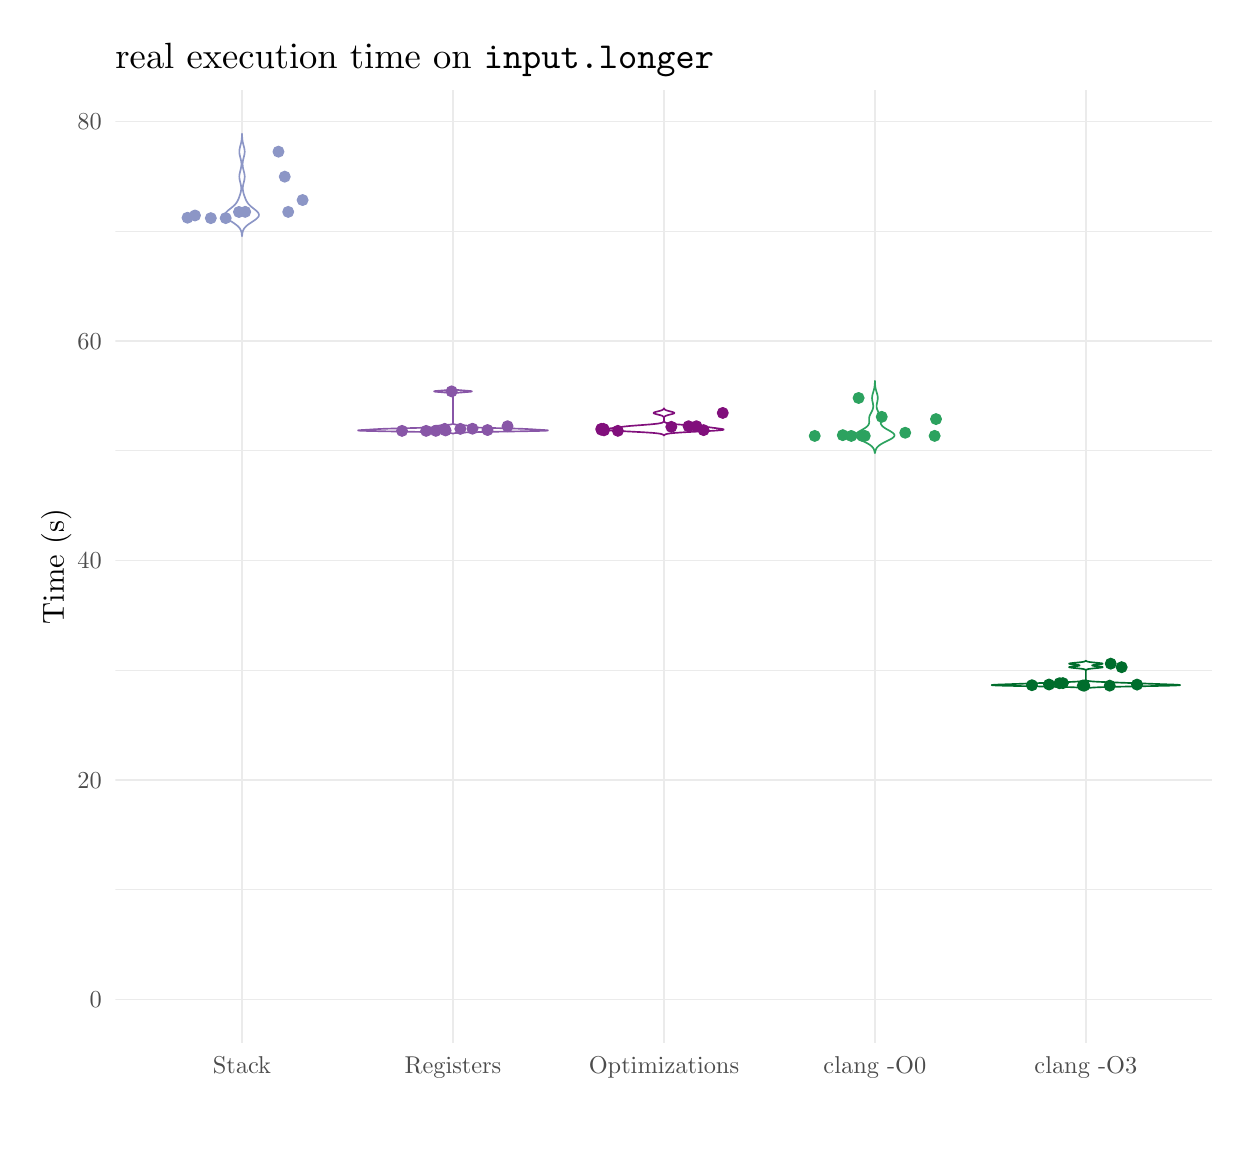
\begin{tikzpicture}[x=1pt,y=1pt]
\definecolor{fillColor}{RGB}{255,255,255}
\path[use as bounding box,fill=fillColor,fill opacity=0.00] (0,0) rectangle (433.62,397.48);
\begin{scope}
\path[clip] ( 31.71, 30.69) rectangle (428.12,374.83);
\definecolor{drawColor}{gray}{0.92}

\path[draw=drawColor,line width= 0.3pt,line join=round] ( 31.71, 85.99) --
	(428.12, 85.99);

\path[draw=drawColor,line width= 0.3pt,line join=round] ( 31.71,165.30) --
	(428.12,165.30);

\path[draw=drawColor,line width= 0.3pt,line join=round] ( 31.71,244.62) --
	(428.12,244.62);

\path[draw=drawColor,line width= 0.3pt,line join=round] ( 31.71,323.94) --
	(428.12,323.94);

\path[draw=drawColor,line width= 0.6pt,line join=round] ( 31.71, 46.33) --
	(428.12, 46.33);

\path[draw=drawColor,line width= 0.6pt,line join=round] ( 31.71,125.65) --
	(428.12,125.65);

\path[draw=drawColor,line width= 0.6pt,line join=round] ( 31.71,204.96) --
	(428.12,204.96);

\path[draw=drawColor,line width= 0.6pt,line join=round] ( 31.71,284.28) --
	(428.12,284.28);

\path[draw=drawColor,line width= 0.6pt,line join=round] ( 31.71,363.60) --
	(428.12,363.60);

\path[draw=drawColor,line width= 0.6pt,line join=round] ( 77.45, 30.69) --
	( 77.45,374.83);

\path[draw=drawColor,line width= 0.6pt,line join=round] (153.68, 30.69) --
	(153.68,374.83);

\path[draw=drawColor,line width= 0.6pt,line join=round] (229.92, 30.69) --
	(229.92,374.83);

\path[draw=drawColor,line width= 0.6pt,line join=round] (306.15, 30.69) --
	(306.15,374.83);

\path[draw=drawColor,line width= 0.6pt,line join=round] (382.38, 30.69) --
	(382.38,374.83);
\definecolor{drawColor}{RGB}{140,150,198}
\definecolor{fillColor}{RGB}{255,255,255}

\path[draw=drawColor,line width= 0.6pt,line join=round,line cap=round,fill=fillColor] ( 77.42,322.13) --
	( 77.41,322.20) --
	( 77.41,322.27) --
	( 77.41,322.35) --
	( 77.40,322.42) --
	( 77.40,322.49) --
	( 77.39,322.56) --
	( 77.38,322.64) --
	( 77.38,322.71) --
	( 77.37,322.78) --
	( 77.36,322.85) --
	( 77.35,322.93) --
	( 77.35,323.00) --
	( 77.34,323.07) --
	( 77.32,323.14) --
	( 77.31,323.22) --
	( 77.30,323.29) --
	( 77.29,323.36) --
	( 77.27,323.43) --
	( 77.26,323.51) --
	( 77.24,323.58) --
	( 77.22,323.65) --
	( 77.20,323.72) --
	( 77.18,323.80) --
	( 77.16,323.87) --
	( 77.14,323.94) --
	( 77.11,324.01) --
	( 77.09,324.09) --
	( 77.06,324.16) --
	( 77.03,324.23) --
	( 77.00,324.30) --
	( 76.96,324.38) --
	( 76.93,324.45) --
	( 76.89,324.52) --
	( 76.85,324.59) --
	( 76.81,324.67) --
	( 76.77,324.74) --
	( 76.72,324.81) --
	( 76.68,324.88) --
	( 76.63,324.96) --
	( 76.57,325.03) --
	( 76.52,325.10) --
	( 76.46,325.17) --
	( 76.40,325.25) --
	( 76.34,325.32) --
	( 76.28,325.39) --
	( 76.21,325.46) --
	( 76.14,325.54) --
	( 76.07,325.61) --
	( 76.00,325.68) --
	( 75.92,325.75) --
	( 75.84,325.83) --
	( 75.76,325.90) --
	( 75.67,325.97) --
	( 75.59,326.05) --
	( 75.50,326.12) --
	( 75.41,326.19) --
	( 75.31,326.26) --
	( 75.22,326.34) --
	( 75.12,326.41) --
	( 75.02,326.48) --
	( 74.92,326.55) --
	( 74.82,326.63) --
	( 74.71,326.70) --
	( 74.61,326.77) --
	( 74.50,326.84) --
	( 74.39,326.92) --
	( 74.29,326.99) --
	( 74.18,327.06) --
	( 74.07,327.13) --
	( 73.96,327.21) --
	( 73.85,327.28) --
	( 73.73,327.35) --
	( 73.62,327.42) --
	( 73.51,327.50) --
	( 73.40,327.57) --
	( 73.29,327.64) --
	( 73.19,327.71) --
	( 73.08,327.79) --
	( 72.97,327.86) --
	( 72.87,327.93) --
	( 72.77,328.00) --
	( 72.67,328.08) --
	( 72.57,328.15) --
	( 72.47,328.22) --
	( 72.38,328.29) --
	( 72.29,328.37) --
	( 72.20,328.44) --
	( 72.12,328.51) --
	( 72.04,328.58) --
	( 71.96,328.66) --
	( 71.89,328.73) --
	( 71.82,328.80) --
	( 71.76,328.87) --
	( 71.70,328.95) --
	( 71.64,329.02) --
	( 71.59,329.09) --
	( 71.54,329.16) --
	( 71.50,329.24) --
	( 71.46,329.31) --
	( 71.43,329.38) --
	( 71.40,329.45) --
	( 71.38,329.53) --
	( 71.36,329.60) --
	( 71.35,329.67) --
	( 71.34,329.74) --
	( 71.34,329.82) --
	( 71.34,329.89) --
	( 71.35,329.96) --
	( 71.36,330.03) --
	( 71.38,330.11) --
	( 71.40,330.18) --
	( 71.43,330.25) --
	( 71.46,330.32) --
	( 71.50,330.40) --
	( 71.54,330.47) --
	( 71.58,330.54) --
	( 71.63,330.61) --
	( 71.68,330.69) --
	( 71.74,330.76) --
	( 71.80,330.83) --
	( 71.87,330.90) --
	( 71.93,330.98) --
	( 72.00,331.05) --
	( 72.08,331.12) --
	( 72.15,331.19) --
	( 72.23,331.27) --
	( 72.31,331.34) --
	( 72.40,331.41) --
	( 72.48,331.48) --
	( 72.57,331.56) --
	( 72.66,331.63) --
	( 72.74,331.70) --
	( 72.84,331.77) --
	( 72.93,331.85) --
	( 73.02,331.92) --
	( 73.11,331.99) --
	( 73.20,332.06) --
	( 73.30,332.14) --
	( 73.39,332.21) --
	( 73.48,332.28) --
	( 73.57,332.35) --
	( 73.67,332.43) --
	( 73.76,332.50) --
	( 73.85,332.57) --
	( 73.93,332.64) --
	( 74.02,332.72) --
	( 74.11,332.79) --
	( 74.19,332.86) --
	( 74.28,332.93) --
	( 74.36,333.01) --
	( 74.44,333.08) --
	( 74.52,333.15) --
	( 74.59,333.22) --
	( 74.67,333.30) --
	( 74.74,333.37) --
	( 74.81,333.44) --
	( 74.88,333.51) --
	( 74.95,333.59) --
	( 75.01,333.66) --
	( 75.08,333.73) --
	( 75.14,333.80) --
	( 75.20,333.88) --
	( 75.25,333.95) --
	( 75.31,334.02) --
	( 75.36,334.09) --
	( 75.42,334.17) --
	( 75.47,334.24) --
	( 75.52,334.31) --
	( 75.56,334.38) --
	( 75.61,334.46) --
	( 75.65,334.53) --
	( 75.70,334.60) --
	( 75.74,334.67) --
	( 75.78,334.75) --
	( 75.82,334.82) --
	( 75.85,334.89) --
	( 75.89,334.96) --
	( 75.93,335.04) --
	( 75.96,335.11) --
	( 76.00,335.18) --
	( 76.03,335.25) --
	( 76.06,335.33) --
	( 76.09,335.40) --
	( 76.13,335.47) --
	( 76.16,335.54) --
	( 76.19,335.62) --
	( 76.22,335.69) --
	( 76.25,335.76) --
	( 76.27,335.83) --
	( 76.30,335.91) --
	( 76.33,335.98) --
	( 76.36,336.05) --
	( 76.39,336.12) --
	( 76.41,336.20) --
	( 76.44,336.27) --
	( 76.47,336.34) --
	( 76.49,336.41) --
	( 76.52,336.49) --
	( 76.55,336.56) --
	( 76.57,336.63) --
	( 76.60,336.70) --
	( 76.62,336.78) --
	( 76.65,336.85) --
	( 76.67,336.92) --
	( 76.69,337.00) --
	( 76.72,337.07) --
	( 76.74,337.14) --
	( 76.77,337.21) --
	( 76.79,337.29) --
	( 76.81,337.36) --
	( 76.83,337.43) --
	( 76.85,337.50) --
	( 76.87,337.58) --
	( 76.89,337.65) --
	( 76.91,337.72) --
	( 76.93,337.79) --
	( 76.95,337.87) --
	( 76.97,337.94) --
	( 76.99,338.01) --
	( 77.00,338.08) --
	( 77.02,338.16) --
	( 77.03,338.23) --
	( 77.05,338.30) --
	( 77.06,338.37) --
	( 77.07,338.45) --
	( 77.08,338.52) --
	( 77.10,338.59) --
	( 77.11,338.66) --
	( 77.11,338.74) --
	( 77.12,338.81) --
	( 77.13,338.88) --
	( 77.14,338.95) --
	( 77.14,339.03) --
	( 77.15,339.10) --
	( 77.15,339.17) --
	( 77.15,339.24) --
	( 77.16,339.32) --
	( 77.16,339.39) --
	( 77.16,339.46) --
	( 77.16,339.53) --
	( 77.15,339.61) --
	( 77.15,339.68) --
	( 77.15,339.75) --
	( 77.14,339.82) --
	( 77.14,339.90) --
	( 77.13,339.97) --
	( 77.12,340.04) --
	( 77.12,340.11) --
	( 77.11,340.19) --
	( 77.10,340.26) --
	( 77.09,340.33) --
	( 77.08,340.40) --
	( 77.07,340.48) --
	( 77.05,340.55) --
	( 77.04,340.62) --
	( 77.03,340.69) --
	( 77.01,340.77) --
	( 77.00,340.84) --
	( 76.98,340.91) --
	( 76.97,340.98) --
	( 76.95,341.06) --
	( 76.93,341.13) --
	( 76.91,341.20) --
	( 76.90,341.27) --
	( 76.88,341.35) --
	( 76.86,341.42) --
	( 76.84,341.49) --
	( 76.83,341.56) --
	( 76.81,341.64) --
	( 76.79,341.71) --
	( 76.77,341.78) --
	( 76.75,341.85) --
	( 76.74,341.93) --
	( 76.72,342.00) --
	( 76.70,342.07) --
	( 76.68,342.14) --
	( 76.67,342.22) --
	( 76.65,342.29) --
	( 76.63,342.36) --
	( 76.62,342.43) --
	( 76.60,342.51) --
	( 76.59,342.58) --
	( 76.58,342.65) --
	( 76.56,342.72) --
	( 76.55,342.80) --
	( 76.54,342.87) --
	( 76.53,342.94) --
	( 76.52,343.01) --
	( 76.51,343.09) --
	( 76.51,343.16) --
	( 76.50,343.23) --
	( 76.50,343.30) --
	( 76.49,343.38) --
	( 76.49,343.45) --
	( 76.49,343.52) --
	( 76.48,343.59) --
	( 76.48,343.67) --
	( 76.49,343.74) --
	( 76.49,343.81) --
	( 76.49,343.88) --
	( 76.49,343.96) --
	( 76.50,344.03) --
	( 76.51,344.10) --
	( 76.51,344.17) --
	( 76.52,344.25) --
	( 76.53,344.32) --
	( 76.54,344.39) --
	( 76.55,344.46) --
	( 76.56,344.54) --
	( 76.58,344.61) --
	( 76.59,344.68) --
	( 76.60,344.75) --
	( 76.62,344.83) --
	( 76.63,344.90) --
	( 76.65,344.97) --
	( 76.67,345.04) --
	( 76.68,345.12) --
	( 76.70,345.19) --
	( 76.72,345.26) --
	( 76.74,345.33) --
	( 76.75,345.41) --
	( 76.77,345.48) --
	( 76.79,345.55) --
	( 76.81,345.62) --
	( 76.83,345.70) --
	( 76.85,345.77) --
	( 76.87,345.84) --
	( 76.88,345.91) --
	( 76.90,345.99) --
	( 76.92,346.06) --
	( 76.94,346.13) --
	( 76.96,346.20) --
	( 76.98,346.28) --
	( 76.99,346.35) --
	( 77.01,346.42) --
	( 77.03,346.49) --
	( 77.04,346.57) --
	( 77.06,346.64) --
	( 77.07,346.71) --
	( 77.09,346.78) --
	( 77.10,346.86) --
	( 77.11,346.93) --
	( 77.13,347.00) --
	( 77.14,347.07) --
	( 77.15,347.15) --
	( 77.16,347.22) --
	( 77.17,347.29) --
	( 77.18,347.36) --
	( 77.19,347.44) --
	( 77.20,347.51) --
	( 77.20,347.58) --
	( 77.21,347.65) --
	( 77.21,347.73) --
	( 77.22,347.80) --
	( 77.22,347.87) --
	( 77.22,347.94) --
	( 77.23,348.02) --
	( 77.23,348.09) --
	( 77.23,348.16) --
	( 77.23,348.24) --
	( 77.23,348.31) --
	( 77.22,348.38) --
	( 77.22,348.45) --
	( 77.22,348.53) --
	( 77.21,348.60) --
	( 77.21,348.67) --
	( 77.20,348.74) --
	( 77.19,348.82) --
	( 77.19,348.89) --
	( 77.18,348.96) --
	( 77.17,349.03) --
	( 77.16,349.11) --
	( 77.15,349.18) --
	( 77.14,349.25) --
	( 77.12,349.32) --
	( 77.11,349.40) --
	( 77.10,349.47) --
	( 77.08,349.54) --
	( 77.07,349.61) --
	( 77.05,349.69) --
	( 77.04,349.76) --
	( 77.02,349.83) --
	( 77.01,349.90) --
	( 76.99,349.98) --
	( 76.97,350.05) --
	( 76.95,350.12) --
	( 76.94,350.19) --
	( 76.92,350.27) --
	( 76.90,350.34) --
	( 76.88,350.41) --
	( 76.86,350.48) --
	( 76.84,350.56) --
	( 76.82,350.63) --
	( 76.81,350.70) --
	( 76.79,350.77) --
	( 76.77,350.85) --
	( 76.75,350.92) --
	( 76.73,350.99) --
	( 76.71,351.06) --
	( 76.70,351.14) --
	( 76.68,351.21) --
	( 76.66,351.28) --
	( 76.65,351.35) --
	( 76.63,351.43) --
	( 76.61,351.50) --
	( 76.60,351.57) --
	( 76.59,351.64) --
	( 76.57,351.72) --
	( 76.56,351.79) --
	( 76.55,351.86) --
	( 76.54,351.93) --
	( 76.53,352.01) --
	( 76.52,352.08) --
	( 76.51,352.15) --
	( 76.50,352.22) --
	( 76.50,352.30) --
	( 76.49,352.37) --
	( 76.49,352.44) --
	( 76.49,352.51) --
	( 76.49,352.59) --
	( 76.49,352.66) --
	( 76.49,352.73) --
	( 76.49,352.80) --
	( 76.49,352.88) --
	( 76.49,352.95) --
	( 76.50,353.02) --
	( 76.50,353.09) --
	( 76.51,353.17) --
	( 76.52,353.24) --
	( 76.53,353.31) --
	( 76.54,353.38) --
	( 76.55,353.46) --
	( 76.56,353.53) --
	( 76.57,353.60) --
	( 76.58,353.67) --
	( 76.60,353.75) --
	( 76.61,353.82) --
	( 76.63,353.89) --
	( 76.64,353.96) --
	( 76.66,354.04) --
	( 76.68,354.11) --
	( 76.69,354.18) --
	( 76.71,354.25) --
	( 76.73,354.33) --
	( 76.75,354.40) --
	( 76.77,354.47) --
	( 76.78,354.54) --
	( 76.80,354.62) --
	( 76.82,354.69) --
	( 76.84,354.76) --
	( 76.86,354.83) --
	( 76.88,354.91) --
	( 76.90,354.98) --
	( 76.92,355.05) --
	( 76.94,355.12) --
	( 76.96,355.20) --
	( 76.98,355.27) --
	( 77.00,355.34) --
	( 77.02,355.41) --
	( 77.03,355.49) --
	( 77.05,355.56) --
	( 77.07,355.63) --
	( 77.09,355.70) --
	( 77.10,355.78) --
	( 77.12,355.85) --
	( 77.14,355.92) --
	( 77.15,355.99) --
	( 77.17,356.07) --
	( 77.18,356.14) --
	( 77.20,356.21) --
	( 77.21,356.28) --
	( 77.22,356.36) --
	( 77.23,356.43) --
	( 77.25,356.50) --
	( 77.26,356.57) --
	( 77.27,356.65) --
	( 77.28,356.72) --
	( 77.29,356.79) --
	( 77.30,356.86) --
	( 77.31,356.94) --
	( 77.32,357.01) --
	( 77.33,357.08) --
	( 77.34,357.15) --
	( 77.34,357.23) --
	( 77.35,357.30) --
	( 77.36,357.37) --
	( 77.36,357.44) --
	( 77.37,357.52) --
	( 77.38,357.59) --
	( 77.38,357.66) --
	( 77.39,357.73) --
	( 77.39,357.81) --
	( 77.40,357.88) --
	( 77.40,357.95) --
	( 77.40,358.02) --
	( 77.41,358.10) --
	( 77.41,358.17) --
	( 77.42,358.24) --
	( 77.42,358.31) --
	( 77.42,358.39) --
	( 77.42,358.46) --
	( 77.43,358.53) --
	( 77.43,358.60) --
	( 77.43,358.68) --
	( 77.43,358.75) --
	( 77.43,358.82) --
	( 77.44,358.89) --
	( 77.44,358.97) --
	( 77.44,359.04) --
	( 77.44,359.11) --
	( 77.44,359.18) --
	( 77.46,359.18) --
	( 77.46,359.11) --
	( 77.46,359.04) --
	( 77.47,358.97) --
	( 77.47,358.89) --
	( 77.47,358.82) --
	( 77.47,358.75) --
	( 77.47,358.68) --
	( 77.47,358.60) --
	( 77.48,358.53) --
	( 77.48,358.46) --
	( 77.48,358.39) --
	( 77.48,358.31) --
	( 77.49,358.24) --
	( 77.49,358.17) --
	( 77.49,358.10) --
	( 77.50,358.02) --
	( 77.50,357.95) --
	( 77.51,357.88) --
	( 77.51,357.81) --
	( 77.52,357.73) --
	( 77.52,357.66) --
	( 77.53,357.59) --
	( 77.53,357.52) --
	( 77.54,357.44) --
	( 77.54,357.37) --
	( 77.55,357.30) --
	( 77.56,357.23) --
	( 77.57,357.15) --
	( 77.58,357.08) --
	( 77.58,357.01) --
	( 77.59,356.94) --
	( 77.60,356.86) --
	( 77.61,356.79) --
	( 77.62,356.72) --
	( 77.63,356.65) --
	( 77.64,356.57) --
	( 77.66,356.50) --
	( 77.67,356.43) --
	( 77.68,356.36) --
	( 77.69,356.28) --
	( 77.71,356.21) --
	( 77.72,356.14) --
	( 77.74,356.07) --
	( 77.75,355.99) --
	( 77.77,355.92) --
	( 77.78,355.85) --
	( 77.80,355.78) --
	( 77.82,355.70) --
	( 77.83,355.63) --
	( 77.85,355.56) --
	( 77.87,355.49) --
	( 77.89,355.41) --
	( 77.91,355.34) --
	( 77.92,355.27) --
	( 77.94,355.20) --
	( 77.96,355.12) --
	( 77.98,355.05) --
	( 78.00,354.98) --
	( 78.02,354.91) --
	( 78.04,354.83) --
	( 78.06,354.76) --
	( 78.08,354.69) --
	( 78.10,354.62) --
	( 78.12,354.54) --
	( 78.14,354.47) --
	( 78.16,354.40) --
	( 78.17,354.33) --
	( 78.19,354.25) --
	( 78.21,354.18) --
	( 78.23,354.11) --
	( 78.24,354.04) --
	( 78.26,353.96) --
	( 78.28,353.89) --
	( 78.29,353.82) --
	( 78.31,353.75) --
	( 78.32,353.67) --
	( 78.33,353.60) --
	( 78.35,353.53) --
	( 78.36,353.46) --
	( 78.37,353.38) --
	( 78.38,353.31) --
	( 78.39,353.24) --
	( 78.39,353.17) --
	( 78.40,353.09) --
	( 78.41,353.02) --
	( 78.41,352.95) --
	( 78.41,352.88) --
	( 78.42,352.80) --
	( 78.42,352.73) --
	( 78.42,352.66) --
	( 78.42,352.59) --
	( 78.42,352.51) --
	( 78.41,352.44) --
	( 78.41,352.37) --
	( 78.40,352.30) --
	( 78.40,352.22) --
	( 78.39,352.15) --
	( 78.38,352.08) --
	( 78.37,352.01) --
	( 78.36,351.93) --
	( 78.35,351.86) --
	( 78.34,351.79) --
	( 78.33,351.72) --
	( 78.32,351.64) --
	( 78.30,351.57) --
	( 78.29,351.50) --
	( 78.27,351.43) --
	( 78.26,351.35) --
	( 78.24,351.28) --
	( 78.22,351.21) --
	( 78.21,351.14) --
	( 78.19,351.06) --
	( 78.17,350.99) --
	( 78.15,350.92) --
	( 78.14,350.85) --
	( 78.12,350.77) --
	( 78.10,350.70) --
	( 78.08,350.63) --
	( 78.06,350.56) --
	( 78.04,350.48) --
	( 78.02,350.41) --
	( 78.00,350.34) --
	( 77.99,350.27) --
	( 77.97,350.19) --
	( 77.95,350.12) --
	( 77.93,350.05) --
	( 77.91,349.98) --
	( 77.90,349.90) --
	( 77.88,349.83) --
	( 77.86,349.76) --
	( 77.85,349.69) --
	( 77.83,349.61) --
	( 77.82,349.54) --
	( 77.81,349.47) --
	( 77.79,349.40) --
	( 77.78,349.32) --
	( 77.77,349.25) --
	( 77.76,349.18) --
	( 77.74,349.11) --
	( 77.73,349.03) --
	( 77.73,348.96) --
	( 77.72,348.89) --
	( 77.71,348.82) --
	( 77.70,348.74) --
	( 77.70,348.67) --
	( 77.69,348.60) --
	( 77.69,348.53) --
	( 77.68,348.45) --
	( 77.68,348.38) --
	( 77.68,348.31) --
	( 77.68,348.24) --
	( 77.68,348.16) --
	( 77.68,348.09) --
	( 77.68,348.02) --
	( 77.68,347.94) --
	( 77.68,347.87) --
	( 77.69,347.80) --
	( 77.69,347.73) --
	( 77.70,347.65) --
	( 77.70,347.58) --
	( 77.71,347.51) --
	( 77.72,347.44) --
	( 77.72,347.36) --
	( 77.73,347.29) --
	( 77.74,347.22) --
	( 77.75,347.15) --
	( 77.76,347.07) --
	( 77.78,347.00) --
	( 77.79,346.93) --
	( 77.80,346.86) --
	( 77.82,346.78) --
	( 77.83,346.71) --
	( 77.85,346.64) --
	( 77.86,346.57) --
	( 77.88,346.49) --
	( 77.89,346.42) --
	( 77.91,346.35) --
	( 77.93,346.28) --
	( 77.95,346.20) --
	( 77.96,346.13) --
	( 77.98,346.06) --
	( 78.00,345.99) --
	( 78.02,345.91) --
	( 78.04,345.84) --
	( 78.06,345.77) --
	( 78.07,345.70) --
	( 78.09,345.62) --
	( 78.11,345.55) --
	( 78.13,345.48) --
	( 78.15,345.41) --
	( 78.17,345.33) --
	( 78.19,345.26) --
	( 78.20,345.19) --
	( 78.22,345.12) --
	( 78.24,345.04) --
	( 78.25,344.97) --
	( 78.27,344.90) --
	( 78.29,344.83) --
	( 78.30,344.75) --
	( 78.31,344.68) --
	( 78.33,344.61) --
	( 78.34,344.54) --
	( 78.35,344.46) --
	( 78.36,344.39) --
	( 78.37,344.32) --
	( 78.38,344.25) --
	( 78.39,344.17) --
	( 78.40,344.10) --
	( 78.40,344.03) --
	( 78.41,343.96) --
	( 78.41,343.88) --
	( 78.42,343.81) --
	( 78.42,343.74) --
	( 78.42,343.67) --
	( 78.42,343.59) --
	( 78.42,343.52) --
	( 78.42,343.45) --
	( 78.41,343.38) --
	( 78.41,343.30) --
	( 78.40,343.23) --
	( 78.40,343.16) --
	( 78.39,343.09) --
	( 78.38,343.01) --
	( 78.37,342.94) --
	( 78.36,342.87) --
	( 78.35,342.80) --
	( 78.34,342.72) --
	( 78.33,342.65) --
	( 78.31,342.58) --
	( 78.30,342.51) --
	( 78.28,342.43) --
	( 78.27,342.36) --
	( 78.25,342.29) --
	( 78.24,342.22) --
	( 78.22,342.14) --
	( 78.20,342.07) --
	( 78.19,342.00) --
	( 78.17,341.93) --
	( 78.15,341.85) --
	( 78.13,341.78) --
	( 78.11,341.71) --
	( 78.10,341.64) --
	( 78.08,341.56) --
	( 78.06,341.49) --
	( 78.04,341.42) --
	( 78.02,341.35) --
	( 78.01,341.27) --
	( 77.99,341.20) --
	( 77.97,341.13) --
	( 77.95,341.06) --
	( 77.94,340.98) --
	( 77.92,340.91) --
	( 77.91,340.84) --
	( 77.89,340.77) --
	( 77.88,340.69) --
	( 77.86,340.62) --
	( 77.85,340.55) --
	( 77.84,340.48) --
	( 77.83,340.40) --
	( 77.82,340.33) --
	( 77.80,340.26) --
	( 77.79,340.19) --
	( 77.79,340.11) --
	( 77.78,340.04) --
	( 77.77,339.97) --
	( 77.77,339.90) --
	( 77.76,339.82) --
	( 77.76,339.75) --
	( 77.75,339.68) --
	( 77.75,339.61) --
	( 77.75,339.53) --
	( 77.75,339.46) --
	( 77.75,339.39) --
	( 77.75,339.32) --
	( 77.75,339.24) --
	( 77.75,339.17) --
	( 77.76,339.10) --
	( 77.76,339.03) --
	( 77.77,338.95) --
	( 77.77,338.88) --
	( 77.78,338.81) --
	( 77.79,338.74) --
	( 77.80,338.66) --
	( 77.81,338.59) --
	( 77.82,338.52) --
	( 77.83,338.45) --
	( 77.84,338.37) --
	( 77.86,338.30) --
	( 77.87,338.23) --
	( 77.89,338.16) --
	( 77.90,338.08) --
	( 77.92,338.01) --
	( 77.93,337.94) --
	( 77.95,337.87) --
	( 77.97,337.79) --
	( 77.99,337.72) --
	( 78.01,337.65) --
	( 78.03,337.58) --
	( 78.05,337.50) --
	( 78.07,337.43) --
	( 78.09,337.36) --
	( 78.12,337.29) --
	( 78.14,337.21) --
	( 78.16,337.14) --
	( 78.18,337.07) --
	( 78.21,337.00) --
	( 78.23,336.92) --
	( 78.26,336.85) --
	( 78.28,336.78) --
	( 78.31,336.70) --
	( 78.33,336.63) --
	( 78.36,336.56) --
	( 78.38,336.49) --
	( 78.41,336.41) --
	( 78.44,336.34) --
	( 78.46,336.27) --
	( 78.49,336.20) --
	( 78.52,336.12) --
	( 78.54,336.05) --
	( 78.57,335.98) --
	( 78.60,335.91) --
	( 78.63,335.83) --
	( 78.66,335.76) --
	( 78.69,335.69) --
	( 78.72,335.62) --
	( 78.75,335.54) --
	( 78.78,335.47) --
	( 78.81,335.40) --
	( 78.84,335.33) --
	( 78.87,335.25) --
	( 78.91,335.18) --
	( 78.94,335.11) --
	( 78.98,335.04) --
	( 79.01,334.96) --
	( 79.05,334.89) --
	( 79.09,334.82) --
	( 79.13,334.75) --
	( 79.17,334.67) --
	( 79.21,334.60) --
	( 79.25,334.53) --
	( 79.30,334.46) --
	( 79.34,334.38) --
	( 79.39,334.31) --
	( 79.44,334.24) --
	( 79.49,334.17) --
	( 79.54,334.09) --
	( 79.59,334.02) --
	( 79.65,333.95) --
	( 79.71,333.88) --
	( 79.77,333.80) --
	( 79.83,333.73) --
	( 79.89,333.66) --
	( 79.96,333.59) --
	( 80.02,333.51) --
	( 80.09,333.44) --
	( 80.16,333.37) --
	( 80.24,333.30) --
	( 80.31,333.22) --
	( 80.39,333.15) --
	( 80.47,333.08) --
	( 80.55,333.01) --
	( 80.63,332.93) --
	( 80.71,332.86) --
	( 80.80,332.79) --
	( 80.88,332.72) --
	( 80.97,332.64) --
	( 81.06,332.57) --
	( 81.15,332.50) --
	( 81.24,332.43) --
	( 81.33,332.35) --
	( 81.42,332.28) --
	( 81.51,332.21) --
	( 81.61,332.14) --
	( 81.70,332.06) --
	( 81.79,331.99) --
	( 81.88,331.92) --
	( 81.98,331.85) --
	( 82.07,331.77) --
	( 82.16,331.70) --
	( 82.25,331.63) --
	( 82.34,331.56) --
	( 82.42,331.48) --
	( 82.51,331.41) --
	( 82.59,331.34) --
	( 82.67,331.27) --
	( 82.75,331.19) --
	( 82.83,331.12) --
	( 82.90,331.05) --
	( 82.97,330.98) --
	( 83.04,330.90) --
	( 83.10,330.83) --
	( 83.16,330.76) --
	( 83.22,330.69) --
	( 83.27,330.61) --
	( 83.32,330.54) --
	( 83.37,330.47) --
	( 83.41,330.40) --
	( 83.44,330.32) --
	( 83.47,330.25) --
	( 83.50,330.18) --
	( 83.52,330.11) --
	( 83.54,330.03) --
	( 83.55,329.96) --
	( 83.56,329.89) --
	( 83.56,329.82) --
	( 83.56,329.74) --
	( 83.55,329.67) --
	( 83.54,329.60) --
	( 83.52,329.53) --
	( 83.50,329.45) --
	( 83.47,329.38) --
	( 83.44,329.31) --
	( 83.40,329.24) --
	( 83.36,329.16) --
	( 83.31,329.09) --
	( 83.26,329.02) --
	( 83.20,328.95) --
	( 83.14,328.87) --
	( 83.08,328.80) --
	( 83.01,328.73) --
	( 82.94,328.66) --
	( 82.86,328.58) --
	( 82.78,328.51) --
	( 82.70,328.44) --
	( 82.61,328.37) --
	( 82.52,328.29) --
	( 82.43,328.22) --
	( 82.33,328.15) --
	( 82.24,328.08) --
	( 82.14,328.00) --
	( 82.03,327.93) --
	( 81.93,327.86) --
	( 81.82,327.79) --
	( 81.72,327.71) --
	( 81.61,327.64) --
	( 81.50,327.57) --
	( 81.39,327.50) --
	( 81.28,327.42) --
	( 81.17,327.35) --
	( 81.06,327.28) --
	( 80.95,327.21) --
	( 80.84,327.13) --
	( 80.73,327.06) --
	( 80.62,326.99) --
	( 80.51,326.92) --
	( 80.40,326.84) --
	( 80.29,326.77) --
	( 80.19,326.70) --
	( 80.08,326.63) --
	( 79.98,326.55) --
	( 79.88,326.48) --
	( 79.78,326.41) --
	( 79.68,326.34) --
	( 79.59,326.26) --
	( 79.50,326.19) --
	( 79.40,326.12) --
	( 79.32,326.05) --
	( 79.23,325.97) --
	( 79.15,325.90) --
	( 79.06,325.83) --
	( 78.99,325.75) --
	( 78.91,325.68) --
	( 78.83,325.61) --
	( 78.76,325.54) --
	( 78.69,325.46) --
	( 78.63,325.39) --
	( 78.56,325.32) --
	( 78.50,325.25) --
	( 78.44,325.17) --
	( 78.38,325.10) --
	( 78.33,325.03) --
	( 78.28,324.96) --
	( 78.23,324.88) --
	( 78.18,324.81) --
	( 78.13,324.74) --
	( 78.09,324.67) --
	( 78.05,324.59) --
	( 78.01,324.52) --
	( 77.97,324.45) --
	( 77.94,324.38) --
	( 77.90,324.30) --
	( 77.87,324.23) --
	( 77.84,324.16) --
	( 77.82,324.09) --
	( 77.79,324.01) --
	( 77.77,323.94) --
	( 77.74,323.87) --
	( 77.72,323.80) --
	( 77.70,323.72) --
	( 77.68,323.65) --
	( 77.66,323.58) --
	( 77.65,323.51) --
	( 77.63,323.43) --
	( 77.62,323.36) --
	( 77.60,323.29) --
	( 77.59,323.22) --
	( 77.58,323.14) --
	( 77.57,323.07) --
	( 77.56,323.00) --
	( 77.55,322.93) --
	( 77.54,322.85) --
	( 77.53,322.78) --
	( 77.53,322.71) --
	( 77.52,322.64) --
	( 77.51,322.56) --
	( 77.51,322.49) --
	( 77.50,322.42) --
	( 77.50,322.35) --
	( 77.49,322.27) --
	( 77.49,322.20) --
	( 77.49,322.13) --
	( 77.42,322.13) --
	cycle;
\definecolor{drawColor}{RGB}{136,86,167}

\path[draw=drawColor,line width= 0.6pt,line join=round,line cap=round,fill=fillColor] (153.44,250.85) --
	(153.35,250.89) --
	(153.24,250.92) --
	(153.09,250.95) --
	(152.90,250.98) --
	(152.66,251.01) --
	(152.37,251.04) --
	(152.01,251.08) --
	(151.56,251.11) --
	(151.02,251.14) --
	(150.38,251.17) --
	(149.63,251.20) --
	(148.76,251.23) --
	(147.76,251.26) --
	(146.64,251.30) --
	(145.36,251.33) --
	(143.95,251.36) --
	(142.41,251.39) --
	(140.77,251.42) --
	(139.03,251.45) --
	(137.21,251.49) --
	(135.33,251.52) --
	(133.43,251.55) --
	(131.53,251.58) --
	(129.68,251.61) --
	(127.90,251.64) --
	(126.23,251.68) --
	(124.70,251.71) --
	(123.32,251.74) --
	(122.13,251.77) --
	(121.16,251.80) --
	(120.41,251.83) --
	(119.87,251.86) --
	(119.53,251.90) --
	(119.38,251.93) --
	(119.40,251.96) --
	(119.58,251.99) --
	(119.89,252.02) --
	(120.31,252.05) --
	(120.79,252.09) --
	(121.32,252.12) --
	(121.87,252.15) --
	(122.42,252.18) --
	(122.96,252.21) --
	(123.49,252.24) --
	(124.00,252.27) --
	(124.50,252.31) --
	(124.99,252.34) --
	(125.50,252.37) --
	(126.03,252.40) --
	(126.60,252.43) --
	(127.23,252.46) --
	(127.94,252.50) --
	(128.73,252.53) --
	(129.62,252.56) --
	(130.60,252.59) --
	(131.66,252.62) --
	(132.80,252.65) --
	(134.00,252.68) --
	(135.26,252.72) --
	(136.54,252.75) --
	(137.83,252.78) --
	(139.09,252.81) --
	(140.30,252.84) --
	(141.45,252.87) --
	(142.52,252.91) --
	(143.49,252.94) --
	(144.35,252.97) --
	(145.07,253.00) --
	(145.66,253.03) --
	(146.13,253.06) --
	(146.49,253.09) --
	(146.74,253.13) --
	(146.90,253.16) --
	(146.97,253.19) --
	(146.97,253.22) --
	(146.93,253.25) --
	(146.86,253.28) --
	(146.78,253.32) --
	(146.70,253.35) --
	(146.64,253.38) --
	(146.62,253.41) --
	(146.63,253.44) --
	(146.71,253.47) --
	(146.83,253.50) --
	(147.01,253.54) --
	(147.25,253.57) --
	(147.53,253.60) --
	(147.85,253.63) --
	(148.22,253.66) --
	(148.61,253.69) --
	(149.02,253.73) --
	(149.44,253.76) --
	(149.87,253.79) --
	(150.28,253.82) --
	(150.68,253.85) --
	(151.07,253.88) --
	(151.42,253.91) --
	(151.75,253.95) --
	(152.05,253.98) --
	(152.31,254.01) --
	(152.55,254.04) --
	(152.75,254.07) --
	(152.93,254.10) --
	(153.08,254.14) --
	(153.20,254.17) --
	(153.30,254.20) --
	(153.39,254.23) --
	(153.46,254.26) --
	(153.51,254.29) --
	(153.55,254.33) --
	(153.59,254.36) --
	(153.61,254.39) --
	(153.63,254.42) --
	(153.65,254.45) --
	(153.66,254.48) --
	(153.66,254.51) --
	(153.67,254.55) --
	(153.67,254.58) --
	(153.68,254.61) --
	(153.68,254.64) --
	(153.68,254.67) --
	(153.68,254.70) --
	(153.68,254.74) --
	(153.68,254.77) --
	(153.68,254.80) --
	(153.68,254.83) --
	(153.68,254.86) --
	(153.68,254.89) --
	(153.68,254.92) --
	(153.68,254.96) --
	(153.68,254.99) --
	(153.68,255.02) --
	(153.68,255.05) --
	(153.68,255.08) --
	(153.68,255.11) --
	(153.68,255.15) --
	(153.68,255.18) --
	(153.68,255.21) --
	(153.68,255.24) --
	(153.68,255.27) --
	(153.68,255.30) --
	(153.68,255.33) --
	(153.68,255.37) --
	(153.68,255.40) --
	(153.68,255.43) --
	(153.68,255.46) --
	(153.68,255.49) --
	(153.68,255.52) --
	(153.68,255.56) --
	(153.68,255.59) --
	(153.68,255.62) --
	(153.68,255.65) --
	(153.68,255.68) --
	(153.68,255.71) --
	(153.68,255.74) --
	(153.68,255.78) --
	(153.68,255.81) --
	(153.68,255.84) --
	(153.68,255.87) --
	(153.68,255.90) --
	(153.68,255.93) --
	(153.68,255.97) --
	(153.68,256.00) --
	(153.68,256.03) --
	(153.68,256.06) --
	(153.68,256.09) --
	(153.68,256.12) --
	(153.68,256.15) --
	(153.68,256.19) --
	(153.68,256.22) --
	(153.68,256.25) --
	(153.68,256.28) --
	(153.68,256.31) --
	(153.68,256.34) --
	(153.68,256.38) --
	(153.68,256.41) --
	(153.68,256.44) --
	(153.68,256.47) --
	(153.68,256.50) --
	(153.68,256.53) --
	(153.68,256.56) --
	(153.68,256.60) --
	(153.68,256.63) --
	(153.68,256.66) --
	(153.68,256.69) --
	(153.68,256.72) --
	(153.68,256.75) --
	(153.68,256.79) --
	(153.68,256.82) --
	(153.68,256.85) --
	(153.68,256.88) --
	(153.68,256.91) --
	(153.68,256.94) --
	(153.68,256.98) --
	(153.68,257.01) --
	(153.68,257.04) --
	(153.68,257.07) --
	(153.68,257.10) --
	(153.68,257.13) --
	(153.68,257.16) --
	(153.68,257.20) --
	(153.68,257.23) --
	(153.68,257.26) --
	(153.68,257.29) --
	(153.68,257.32) --
	(153.68,257.35) --
	(153.68,257.39) --
	(153.68,257.42) --
	(153.68,257.45) --
	(153.68,257.48) --
	(153.68,257.51) --
	(153.68,257.54) --
	(153.68,257.57) --
	(153.68,257.61) --
	(153.68,257.64) --
	(153.68,257.67) --
	(153.68,257.70) --
	(153.68,257.73) --
	(153.68,257.76) --
	(153.68,257.80) --
	(153.68,257.83) --
	(153.68,257.86) --
	(153.68,257.89) --
	(153.68,257.92) --
	(153.68,257.95) --
	(153.68,257.98) --
	(153.68,258.02) --
	(153.68,258.05) --
	(153.68,258.08) --
	(153.68,258.11) --
	(153.68,258.14) --
	(153.68,258.17) --
	(153.68,258.21) --
	(153.68,258.24) --
	(153.68,258.27) --
	(153.68,258.30) --
	(153.68,258.33) --
	(153.68,258.36) --
	(153.68,258.39) --
	(153.68,258.43) --
	(153.68,258.46) --
	(153.68,258.49) --
	(153.68,258.52) --
	(153.68,258.55) --
	(153.68,258.58) --
	(153.68,258.62) --
	(153.68,258.65) --
	(153.68,258.68) --
	(153.68,258.71) --
	(153.68,258.74) --
	(153.68,258.77) --
	(153.68,258.80) --
	(153.68,258.84) --
	(153.68,258.87) --
	(153.68,258.90) --
	(153.68,258.93) --
	(153.68,258.96) --
	(153.68,258.99) --
	(153.68,259.03) --
	(153.68,259.06) --
	(153.68,259.09) --
	(153.68,259.12) --
	(153.68,259.15) --
	(153.68,259.18) --
	(153.68,259.21) --
	(153.68,259.25) --
	(153.68,259.28) --
	(153.68,259.31) --
	(153.68,259.34) --
	(153.68,259.37) --
	(153.68,259.40) --
	(153.68,259.44) --
	(153.68,259.47) --
	(153.68,259.50) --
	(153.68,259.53) --
	(153.68,259.56) --
	(153.68,259.59) --
	(153.68,259.63) --
	(153.68,259.66) --
	(153.68,259.69) --
	(153.68,259.72) --
	(153.68,259.75) --
	(153.68,259.78) --
	(153.68,259.81) --
	(153.68,259.85) --
	(153.68,259.88) --
	(153.68,259.91) --
	(153.68,259.94) --
	(153.68,259.97) --
	(153.68,260.00) --
	(153.68,260.04) --
	(153.68,260.07) --
	(153.68,260.10) --
	(153.68,260.13) --
	(153.68,260.16) --
	(153.68,260.19) --
	(153.68,260.22) --
	(153.68,260.26) --
	(153.68,260.29) --
	(153.68,260.32) --
	(153.68,260.35) --
	(153.68,260.38) --
	(153.68,260.41) --
	(153.68,260.45) --
	(153.68,260.48) --
	(153.68,260.51) --
	(153.68,260.54) --
	(153.68,260.57) --
	(153.68,260.60) --
	(153.68,260.63) --
	(153.68,260.67) --
	(153.68,260.70) --
	(153.68,260.73) --
	(153.68,260.76) --
	(153.68,260.79) --
	(153.68,260.82) --
	(153.68,260.86) --
	(153.68,260.89) --
	(153.68,260.92) --
	(153.68,260.95) --
	(153.68,260.98) --
	(153.68,261.01) --
	(153.68,261.04) --
	(153.68,261.08) --
	(153.68,261.11) --
	(153.68,261.14) --
	(153.68,261.17) --
	(153.68,261.20) --
	(153.68,261.23) --
	(153.68,261.27) --
	(153.68,261.30) --
	(153.68,261.33) --
	(153.68,261.36) --
	(153.68,261.39) --
	(153.68,261.42) --
	(153.68,261.45) --
	(153.68,261.49) --
	(153.68,261.52) --
	(153.68,261.55) --
	(153.68,261.58) --
	(153.68,261.61) --
	(153.68,261.64) --
	(153.68,261.68) --
	(153.68,261.71) --
	(153.68,261.74) --
	(153.68,261.77) --
	(153.68,261.80) --
	(153.68,261.83) --
	(153.68,261.86) --
	(153.68,261.90) --
	(153.68,261.93) --
	(153.68,261.96) --
	(153.68,261.99) --
	(153.68,262.02) --
	(153.68,262.05) --
	(153.68,262.09) --
	(153.68,262.12) --
	(153.68,262.15) --
	(153.68,262.18) --
	(153.68,262.21) --
	(153.68,262.24) --
	(153.68,262.28) --
	(153.68,262.31) --
	(153.68,262.34) --
	(153.68,262.37) --
	(153.68,262.40) --
	(153.68,262.43) --
	(153.68,262.46) --
	(153.68,262.50) --
	(153.68,262.53) --
	(153.68,262.56) --
	(153.68,262.59) --
	(153.68,262.62) --
	(153.68,262.65) --
	(153.68,262.69) --
	(153.68,262.72) --
	(153.68,262.75) --
	(153.68,262.78) --
	(153.68,262.81) --
	(153.68,262.84) --
	(153.68,262.87) --
	(153.68,262.91) --
	(153.68,262.94) --
	(153.68,262.97) --
	(153.68,263.00) --
	(153.68,263.03) --
	(153.68,263.06) --
	(153.68,263.10) --
	(153.68,263.13) --
	(153.68,263.16) --
	(153.68,263.19) --
	(153.68,263.22) --
	(153.68,263.25) --
	(153.68,263.28) --
	(153.68,263.32) --
	(153.68,263.35) --
	(153.68,263.38) --
	(153.68,263.41) --
	(153.68,263.44) --
	(153.68,263.47) --
	(153.68,263.51) --
	(153.68,263.54) --
	(153.68,263.57) --
	(153.68,263.60) --
	(153.68,263.63) --
	(153.68,263.66) --
	(153.68,263.69) --
	(153.68,263.73) --
	(153.68,263.76) --
	(153.68,263.79) --
	(153.68,263.82) --
	(153.68,263.85) --
	(153.68,263.88) --
	(153.68,263.92) --
	(153.68,263.95) --
	(153.68,263.98) --
	(153.68,264.01) --
	(153.68,264.04) --
	(153.68,264.07) --
	(153.68,264.10) --
	(153.68,264.14) --
	(153.68,264.17) --
	(153.68,264.20) --
	(153.68,264.23) --
	(153.68,264.26) --
	(153.68,264.29) --
	(153.68,264.33) --
	(153.68,264.36) --
	(153.68,264.39) --
	(153.68,264.42) --
	(153.68,264.45) --
	(153.68,264.48) --
	(153.68,264.51) --
	(153.68,264.55) --
	(153.68,264.58) --
	(153.68,264.61) --
	(153.68,264.64) --
	(153.68,264.67) --
	(153.68,264.70) --
	(153.68,264.74) --
	(153.68,264.77) --
	(153.68,264.80) --
	(153.68,264.83) --
	(153.68,264.86) --
	(153.68,264.89) --
	(153.67,264.93) --
	(153.67,264.96) --
	(153.67,264.99) --
	(153.66,265.02) --
	(153.65,265.05) --
	(153.63,265.08) --
	(153.62,265.11) --
	(153.59,265.15) --
	(153.56,265.18) --
	(153.52,265.21) --
	(153.47,265.24) --
	(153.40,265.27) --
	(153.32,265.30) --
	(153.22,265.34) --
	(153.10,265.37) --
	(152.96,265.40) --
	(152.78,265.43) --
	(152.59,265.46) --
	(152.36,265.49) --
	(152.10,265.52) --
	(151.81,265.56) --
	(151.48,265.59) --
	(151.13,265.62) --
	(150.75,265.65) --
	(150.36,265.68) --
	(149.94,265.71) --
	(149.52,265.75) --
	(149.11,265.78) --
	(148.69,265.81) --
	(148.31,265.84) --
	(147.95,265.87) --
	(147.63,265.90) --
	(147.36,265.93) --
	(147.14,265.97) --
	(146.99,266.00) --
	(146.90,266.03) --
	(146.88,266.06) --
	(146.94,266.09) --
	(147.07,266.12) --
	(147.26,266.16) --
	(147.51,266.19) --
	(147.81,266.22) --
	(148.15,266.25) --
	(148.52,266.28) --
	(148.93,266.31) --
	(149.34,266.34) --
	(149.77,266.38) --
	(150.18,266.41) --
	(150.59,266.44) --
	(150.97,266.47) --
	(151.34,266.50) --
	(151.67,266.53) --
	(151.98,266.57) --
	(152.25,266.60) --
	(152.49,266.63) --
	(152.70,266.66) --
	(152.89,266.69) --
	(153.04,266.72) --
	(153.17,266.75) --
	(153.28,266.79) --
	(153.37,266.82) --
	(153.44,266.85) --
	(153.50,266.88) --
	(153.54,266.91) --
	(153.58,266.94) --
	(153.61,266.98) --
	(153.76,266.98) --
	(153.79,266.94) --
	(153.82,266.91) --
	(153.87,266.88) --
	(153.93,266.85) --
	(154.00,266.82) --
	(154.09,266.79) --
	(154.19,266.75) --
	(154.33,266.72) --
	(154.48,266.69) --
	(154.66,266.66) --
	(154.88,266.63) --
	(155.12,266.60) --
	(155.39,266.57) --
	(155.69,266.53) --
	(156.03,266.50) --
	(156.40,266.47) --
	(156.78,266.44) --
	(157.19,266.41) --
	(157.60,266.38) --
	(158.02,266.34) --
	(158.44,266.31) --
	(158.84,266.28) --
	(159.22,266.25) --
	(159.56,266.22) --
	(159.86,266.19) --
	(160.11,266.16) --
	(160.30,266.12) --
	(160.43,266.09) --
	(160.49,266.06) --
	(160.47,266.03) --
	(160.38,266.00) --
	(160.23,265.97) --
	(160.01,265.93) --
	(159.74,265.90) --
	(159.42,265.87) --
	(159.06,265.84) --
	(158.67,265.81) --
	(158.26,265.78) --
	(157.84,265.75) --
	(157.42,265.71) --
	(157.01,265.68) --
	(156.61,265.65) --
	(156.24,265.62) --
	(155.88,265.59) --
	(155.56,265.56) --
	(155.27,265.52) --
	(155.01,265.49) --
	(154.78,265.46) --
	(154.58,265.43) --
	(154.41,265.40) --
	(154.27,265.37) --
	(154.14,265.34) --
	(154.05,265.30) --
	(153.97,265.27) --
	(153.90,265.24) --
	(153.85,265.21) --
	(153.81,265.18) --
	(153.78,265.15) --
	(153.75,265.11) --
	(153.73,265.08) --
	(153.72,265.05) --
	(153.71,265.02) --
	(153.70,264.99) --
	(153.70,264.96) --
	(153.69,264.93) --
	(153.69,264.89) --
	(153.69,264.86) --
	(153.69,264.83) --
	(153.69,264.80) --
	(153.69,264.77) --
	(153.68,264.74) --
	(153.68,264.70) --
	(153.68,264.67) --
	(153.68,264.64) --
	(153.68,264.61) --
	(153.68,264.58) --
	(153.68,264.55) --
	(153.68,264.51) --
	(153.68,264.48) --
	(153.68,264.45) --
	(153.68,264.42) --
	(153.68,264.39) --
	(153.68,264.36) --
	(153.68,264.33) --
	(153.68,264.29) --
	(153.68,264.26) --
	(153.68,264.23) --
	(153.68,264.20) --
	(153.68,264.17) --
	(153.68,264.14) --
	(153.68,264.10) --
	(153.68,264.07) --
	(153.68,264.04) --
	(153.68,264.01) --
	(153.68,263.98) --
	(153.68,263.95) --
	(153.68,263.92) --
	(153.68,263.88) --
	(153.68,263.85) --
	(153.68,263.82) --
	(153.68,263.79) --
	(153.68,263.76) --
	(153.68,263.73) --
	(153.68,263.69) --
	(153.68,263.66) --
	(153.68,263.63) --
	(153.68,263.60) --
	(153.68,263.57) --
	(153.68,263.54) --
	(153.68,263.51) --
	(153.68,263.47) --
	(153.68,263.44) --
	(153.68,263.41) --
	(153.68,263.38) --
	(153.68,263.35) --
	(153.68,263.32) --
	(153.68,263.28) --
	(153.68,263.25) --
	(153.68,263.22) --
	(153.68,263.19) --
	(153.68,263.16) --
	(153.68,263.13) --
	(153.68,263.10) --
	(153.68,263.06) --
	(153.68,263.03) --
	(153.68,263.00) --
	(153.68,262.97) --
	(153.68,262.94) --
	(153.68,262.91) --
	(153.68,262.87) --
	(153.68,262.84) --
	(153.68,262.81) --
	(153.68,262.78) --
	(153.68,262.75) --
	(153.68,262.72) --
	(153.68,262.69) --
	(153.68,262.65) --
	(153.68,262.62) --
	(153.68,262.59) --
	(153.68,262.56) --
	(153.68,262.53) --
	(153.68,262.50) --
	(153.68,262.46) --
	(153.68,262.43) --
	(153.68,262.40) --
	(153.68,262.37) --
	(153.68,262.34) --
	(153.68,262.31) --
	(153.68,262.28) --
	(153.68,262.24) --
	(153.68,262.21) --
	(153.68,262.18) --
	(153.68,262.15) --
	(153.68,262.12) --
	(153.68,262.09) --
	(153.68,262.05) --
	(153.68,262.02) --
	(153.68,261.99) --
	(153.68,261.96) --
	(153.68,261.93) --
	(153.68,261.90) --
	(153.68,261.86) --
	(153.68,261.83) --
	(153.68,261.80) --
	(153.68,261.77) --
	(153.68,261.74) --
	(153.68,261.71) --
	(153.68,261.68) --
	(153.68,261.64) --
	(153.68,261.61) --
	(153.68,261.58) --
	(153.68,261.55) --
	(153.68,261.52) --
	(153.68,261.49) --
	(153.68,261.45) --
	(153.68,261.42) --
	(153.68,261.39) --
	(153.68,261.36) --
	(153.68,261.33) --
	(153.68,261.30) --
	(153.68,261.27) --
	(153.68,261.23) --
	(153.68,261.20) --
	(153.68,261.17) --
	(153.68,261.14) --
	(153.68,261.11) --
	(153.68,261.08) --
	(153.68,261.04) --
	(153.68,261.01) --
	(153.68,260.98) --
	(153.68,260.95) --
	(153.68,260.92) --
	(153.68,260.89) --
	(153.68,260.86) --
	(153.68,260.82) --
	(153.68,260.79) --
	(153.68,260.76) --
	(153.68,260.73) --
	(153.68,260.70) --
	(153.68,260.67) --
	(153.68,260.63) --
	(153.68,260.60) --
	(153.68,260.57) --
	(153.68,260.54) --
	(153.68,260.51) --
	(153.68,260.48) --
	(153.68,260.45) --
	(153.68,260.41) --
	(153.68,260.38) --
	(153.68,260.35) --
	(153.68,260.32) --
	(153.68,260.29) --
	(153.68,260.26) --
	(153.68,260.22) --
	(153.68,260.19) --
	(153.68,260.16) --
	(153.68,260.13) --
	(153.68,260.10) --
	(153.68,260.07) --
	(153.68,260.04) --
	(153.68,260.00) --
	(153.68,259.97) --
	(153.68,259.94) --
	(153.68,259.91) --
	(153.68,259.88) --
	(153.68,259.85) --
	(153.68,259.81) --
	(153.68,259.78) --
	(153.68,259.75) --
	(153.68,259.72) --
	(153.68,259.69) --
	(153.68,259.66) --
	(153.68,259.63) --
	(153.68,259.59) --
	(153.68,259.56) --
	(153.68,259.53) --
	(153.68,259.50) --
	(153.68,259.47) --
	(153.68,259.44) --
	(153.68,259.40) --
	(153.68,259.37) --
	(153.68,259.34) --
	(153.68,259.31) --
	(153.68,259.28) --
	(153.68,259.25) --
	(153.68,259.21) --
	(153.68,259.18) --
	(153.68,259.15) --
	(153.68,259.12) --
	(153.68,259.09) --
	(153.68,259.06) --
	(153.68,259.03) --
	(153.68,258.99) --
	(153.68,258.96) --
	(153.68,258.93) --
	(153.68,258.90) --
	(153.68,258.87) --
	(153.68,258.84) --
	(153.68,258.80) --
	(153.68,258.77) --
	(153.68,258.74) --
	(153.68,258.71) --
	(153.68,258.68) --
	(153.68,258.65) --
	(153.68,258.62) --
	(153.68,258.58) --
	(153.68,258.55) --
	(153.68,258.52) --
	(153.68,258.49) --
	(153.68,258.46) --
	(153.68,258.43) --
	(153.68,258.39) --
	(153.68,258.36) --
	(153.68,258.33) --
	(153.68,258.30) --
	(153.68,258.27) --
	(153.68,258.24) --
	(153.68,258.21) --
	(153.68,258.17) --
	(153.68,258.14) --
	(153.68,258.11) --
	(153.68,258.08) --
	(153.68,258.05) --
	(153.68,258.02) --
	(153.68,257.98) --
	(153.68,257.95) --
	(153.68,257.92) --
	(153.68,257.89) --
	(153.68,257.86) --
	(153.68,257.83) --
	(153.68,257.80) --
	(153.68,257.76) --
	(153.68,257.73) --
	(153.68,257.70) --
	(153.68,257.67) --
	(153.68,257.64) --
	(153.68,257.61) --
	(153.68,257.57) --
	(153.68,257.54) --
	(153.68,257.51) --
	(153.68,257.48) --
	(153.68,257.45) --
	(153.68,257.42) --
	(153.68,257.39) --
	(153.68,257.35) --
	(153.68,257.32) --
	(153.68,257.29) --
	(153.68,257.26) --
	(153.68,257.23) --
	(153.68,257.20) --
	(153.68,257.16) --
	(153.68,257.13) --
	(153.68,257.10) --
	(153.68,257.07) --
	(153.68,257.04) --
	(153.68,257.01) --
	(153.68,256.98) --
	(153.68,256.94) --
	(153.68,256.91) --
	(153.68,256.88) --
	(153.68,256.85) --
	(153.68,256.82) --
	(153.68,256.79) --
	(153.68,256.75) --
	(153.68,256.72) --
	(153.68,256.69) --
	(153.68,256.66) --
	(153.68,256.63) --
	(153.68,256.60) --
	(153.68,256.56) --
	(153.68,256.53) --
	(153.68,256.50) --
	(153.68,256.47) --
	(153.68,256.44) --
	(153.68,256.41) --
	(153.68,256.38) --
	(153.68,256.34) --
	(153.68,256.31) --
	(153.68,256.28) --
	(153.68,256.25) --
	(153.68,256.22) --
	(153.68,256.19) --
	(153.68,256.15) --
	(153.68,256.12) --
	(153.68,256.09) --
	(153.68,256.06) --
	(153.68,256.03) --
	(153.68,256.00) --
	(153.68,255.97) --
	(153.68,255.93) --
	(153.68,255.90) --
	(153.68,255.87) --
	(153.68,255.84) --
	(153.68,255.81) --
	(153.68,255.78) --
	(153.68,255.74) --
	(153.68,255.71) --
	(153.68,255.68) --
	(153.68,255.65) --
	(153.68,255.62) --
	(153.68,255.59) --
	(153.68,255.56) --
	(153.68,255.52) --
	(153.68,255.49) --
	(153.68,255.46) --
	(153.68,255.43) --
	(153.68,255.40) --
	(153.68,255.37) --
	(153.68,255.33) --
	(153.68,255.30) --
	(153.68,255.27) --
	(153.68,255.24) --
	(153.68,255.21) --
	(153.68,255.18) --
	(153.68,255.15) --
	(153.68,255.11) --
	(153.68,255.08) --
	(153.68,255.05) --
	(153.68,255.02) --
	(153.68,254.99) --
	(153.68,254.96) --
	(153.68,254.92) --
	(153.68,254.89) --
	(153.68,254.86) --
	(153.68,254.83) --
	(153.68,254.80) --
	(153.68,254.77) --
	(153.69,254.74) --
	(153.69,254.70) --
	(153.69,254.67) --
	(153.69,254.64) --
	(153.69,254.61) --
	(153.69,254.58) --
	(153.70,254.55) --
	(153.70,254.51) --
	(153.71,254.48) --
	(153.72,254.45) --
	(153.74,254.42) --
	(153.76,254.39) --
	(153.78,254.36) --
	(153.82,254.33) --
	(153.86,254.29) --
	(153.91,254.26) --
	(153.98,254.23) --
	(154.06,254.20) --
	(154.16,254.17) --
	(154.29,254.14) --
	(154.44,254.10) --
	(154.62,254.07) --
	(154.82,254.04) --
	(155.06,254.01) --
	(155.32,253.98) --
	(155.62,253.95) --
	(155.94,253.91) --
	(156.30,253.88) --
	(156.69,253.85) --
	(157.09,253.82) --
	(157.50,253.79) --
	(157.92,253.76) --
	(158.35,253.73) --
	(158.76,253.69) --
	(159.15,253.66) --
	(159.51,253.63) --
	(159.84,253.60) --
	(160.12,253.57) --
	(160.35,253.54) --
	(160.53,253.50) --
	(160.66,253.47) --
	(160.73,253.44) --
	(160.75,253.41) --
	(160.72,253.38) --
	(160.67,253.35) --
	(160.59,253.32) --
	(160.51,253.28) --
	(160.44,253.25) --
	(160.39,253.22) --
	(160.40,253.19) --
	(160.47,253.16) --
	(160.63,253.13) --
	(160.88,253.09) --
	(161.23,253.06) --
	(161.71,253.03) --
	(162.30,253.00) --
	(163.02,252.97) --
	(163.88,252.94) --
	(164.85,252.91) --
	(165.91,252.87) --
	(167.06,252.84) --
	(168.28,252.81) --
	(169.54,252.78) --
	(170.83,252.75) --
	(172.11,252.72) --
	(173.36,252.68) --
	(174.57,252.65) --
	(175.71,252.62) --
	(176.77,252.59) --
	(177.75,252.56) --
	(178.63,252.53) --
	(179.43,252.50) --
	(180.13,252.46) --
	(180.76,252.43) --
	(181.34,252.40) --
	(181.87,252.37) --
	(182.38,252.34) --
	(182.87,252.31) --
	(183.37,252.27) --
	(183.88,252.24) --
	(184.40,252.21) --
	(184.95,252.18) --
	(185.50,252.15) --
	(186.05,252.12) --
	(186.57,252.09) --
	(187.06,252.05) --
	(187.48,252.02) --
	(187.79,251.99) --
	(187.96,251.96) --
	(187.99,251.93) --
	(187.84,251.90) --
	(187.50,251.86) --
	(186.96,251.83) --
	(186.21,251.80) --
	(185.24,251.77) --
	(184.05,251.74) --
	(182.67,251.71) --
	(181.14,251.68) --
	(179.47,251.64) --
	(177.69,251.61) --
	(175.84,251.58) --
	(173.94,251.55) --
	(172.04,251.52) --
	(170.16,251.49) --
	(168.34,251.45) --
	(166.60,251.42) --
	(164.95,251.39) --
	(163.42,251.36) --
	(162.01,251.33) --
	(160.73,251.30) --
	(159.61,251.26) --
	(158.61,251.23) --
	(157.74,251.20) --
	(156.99,251.17) --
	(156.35,251.14) --
	(155.81,251.11) --
	(155.36,251.08) --
	(155.00,251.04) --
	(154.70,251.01) --
	(154.47,250.98) --
	(154.28,250.95) --
	(154.13,250.92) --
	(154.02,250.89) --
	(153.93,250.85) --
	(153.44,250.85) --
	cycle;
\definecolor{drawColor}{RGB}{129,15,124}

\path[draw=drawColor,line width= 0.6pt,line join=round,line cap=round,fill=fillColor] (229.84,250.12) --
	(229.83,250.14) --
	(229.83,250.15) --
	(229.82,250.17) --
	(229.80,250.19) --
	(229.79,250.21) --
	(229.78,250.23) --
	(229.76,250.25) --
	(229.75,250.27) --
	(229.73,250.29) --
	(229.71,250.31) --
	(229.69,250.33) --
	(229.67,250.35) --
	(229.64,250.37) --
	(229.62,250.38) --
	(229.59,250.40) --
	(229.55,250.42) --
	(229.52,250.44) --
	(229.48,250.46) --
	(229.44,250.48) --
	(229.40,250.50) --
	(229.35,250.52) --
	(229.30,250.54) --
	(229.25,250.56) --
	(229.19,250.58) --
	(229.13,250.60) --
	(229.06,250.62) --
	(228.99,250.63) --
	(228.91,250.65) --
	(228.83,250.67) --
	(228.74,250.69) --
	(228.65,250.71) --
	(228.55,250.73) --
	(228.45,250.75) --
	(228.34,250.77) --
	(228.22,250.79) --
	(228.10,250.81) --
	(227.97,250.83) --
	(227.83,250.85) --
	(227.68,250.87) --
	(227.53,250.88) --
	(227.37,250.90) --
	(227.20,250.92) --
	(227.02,250.94) --
	(226.84,250.96) --
	(226.64,250.98) --
	(226.44,251.00) --
	(226.23,251.02) --
	(226.01,251.04) --
	(225.78,251.06) --
	(225.54,251.08) --
	(225.29,251.10) --
	(225.04,251.12) --
	(224.77,251.13) --
	(224.50,251.15) --
	(224.22,251.17) --
	(223.92,251.19) --
	(223.62,251.21) --
	(223.32,251.23) --
	(223.00,251.25) --
	(222.68,251.27) --
	(222.35,251.29) --
	(222.01,251.31) --
	(221.66,251.33) --
	(221.31,251.35) --
	(220.95,251.37) --
	(220.59,251.38) --
	(220.22,251.40) --
	(219.85,251.42) --
	(219.47,251.44) --
	(219.09,251.46) --
	(218.70,251.48) --
	(218.32,251.50) --
	(217.93,251.52) --
	(217.54,251.54) --
	(217.15,251.56) --
	(216.76,251.58) --
	(216.37,251.60) --
	(215.99,251.62) --
	(215.60,251.63) --
	(215.22,251.65) --
	(214.85,251.67) --
	(214.48,251.69) --
	(214.11,251.71) --
	(213.75,251.73) --
	(213.40,251.75) --
	(213.05,251.77) --
	(212.71,251.79) --
	(212.39,251.81) --
	(212.07,251.83) --
	(211.76,251.85) --
	(211.46,251.86) --
	(211.17,251.88) --
	(210.90,251.90) --
	(210.64,251.92) --
	(210.39,251.94) --
	(210.15,251.96) --
	(209.93,251.98) --
	(209.72,252.00) --
	(209.53,252.02) --
	(209.35,252.04) --
	(209.18,252.06) --
	(209.03,252.08) --
	(208.90,252.10) --
	(208.78,252.11) --
	(208.67,252.13) --
	(208.58,252.15) --
	(208.50,252.17) --
	(208.44,252.19) --
	(208.39,252.21) --
	(208.36,252.23) --
	(208.34,252.25) --
	(208.33,252.27) --
	(208.34,252.29) --
	(208.36,252.31) --
	(208.39,252.33) --
	(208.43,252.35) --
	(208.48,252.36) --
	(208.55,252.38) --
	(208.62,252.40) --
	(208.70,252.42) --
	(208.80,252.44) --
	(208.90,252.46) --
	(209.01,252.48) --
	(209.12,252.50) --
	(209.24,252.52) --
	(209.37,252.54) --
	(209.50,252.56) --
	(209.64,252.58) --
	(209.78,252.60) --
	(209.92,252.61) --
	(210.07,252.63) --
	(210.22,252.65) --
	(210.37,252.67) --
	(210.52,252.69) --
	(210.68,252.71) --
	(210.83,252.73) --
	(210.99,252.75) --
	(211.14,252.77) --
	(211.29,252.79) --
	(211.45,252.81) --
	(211.60,252.83) --
	(211.75,252.85) --
	(211.90,252.86) --
	(212.05,252.88) --
	(212.20,252.90) --
	(212.34,252.92) --
	(212.49,252.94) --
	(212.63,252.96) --
	(212.78,252.98) --
	(212.92,253.00) --
	(213.06,253.02) --
	(213.20,253.04) --
	(213.34,253.06) --
	(213.48,253.08) --
	(213.62,253.10) --
	(213.76,253.11) --
	(213.90,253.13) --
	(214.04,253.15) --
	(214.18,253.17) --
	(214.33,253.19) --
	(214.47,253.21) --
	(214.62,253.23) --
	(214.77,253.25) --
	(214.93,253.27) --
	(215.08,253.29) --
	(215.24,253.31) --
	(215.40,253.33) --
	(215.57,253.34) --
	(215.74,253.36) --
	(215.92,253.38) --
	(216.10,253.40) --
	(216.28,253.42) --
	(216.47,253.44) --
	(216.66,253.46) --
	(216.86,253.48) --
	(217.06,253.50) --
	(217.27,253.52) --
	(217.48,253.54) --
	(217.70,253.56) --
	(217.92,253.58) --
	(218.15,253.59) --
	(218.38,253.61) --
	(218.61,253.63) --
	(218.85,253.65) --
	(219.09,253.67) --
	(219.34,253.69) --
	(219.58,253.71) --
	(219.83,253.73) --
	(220.09,253.75) --
	(220.34,253.77) --
	(220.60,253.79) --
	(220.86,253.81) --
	(221.11,253.83) --
	(221.37,253.84) --
	(221.63,253.86) --
	(221.89,253.88) --
	(222.15,253.90) --
	(222.41,253.92) --
	(222.66,253.94) --
	(222.92,253.96) --
	(223.17,253.98) --
	(223.42,254.00) --
	(223.66,254.02) --
	(223.91,254.04) --
	(224.15,254.06) --
	(224.38,254.08) --
	(224.61,254.09) --
	(224.84,254.11) --
	(225.06,254.13) --
	(225.28,254.15) --
	(225.49,254.17) --
	(225.70,254.19) --
	(225.90,254.21) --
	(226.10,254.23) --
	(226.29,254.25) --
	(226.47,254.27) --
	(226.65,254.29) --
	(226.83,254.31) --
	(226.99,254.33) --
	(227.15,254.34) --
	(227.31,254.36) --
	(227.46,254.38) --
	(227.60,254.40) --
	(227.74,254.42) --
	(227.87,254.44) --
	(227.99,254.46) --
	(228.12,254.48) --
	(228.23,254.50) --
	(228.34,254.52) --
	(228.44,254.54) --
	(228.54,254.56) --
	(228.63,254.58) --
	(228.72,254.59) --
	(228.80,254.61) --
	(228.88,254.63) --
	(228.96,254.65) --
	(229.03,254.67) --
	(229.09,254.69) --
	(229.15,254.71) --
	(229.21,254.73) --
	(229.27,254.75) --
	(229.32,254.77) --
	(229.36,254.79) --
	(229.41,254.81) --
	(229.45,254.82) --
	(229.49,254.84) --
	(229.52,254.86) --
	(229.56,254.88) --
	(229.59,254.90) --
	(229.62,254.92) --
	(229.64,254.94) --
	(229.67,254.96) --
	(229.69,254.98) --
	(229.71,255.00) --
	(229.73,255.02) --
	(229.75,255.04) --
	(229.76,255.06) --
	(229.78,255.07) --
	(229.79,255.09) --
	(229.80,255.11) --
	(229.81,255.13) --
	(229.82,255.15) --
	(229.83,255.17) --
	(229.84,255.19) --
	(229.85,255.21) --
	(229.86,255.23) --
	(229.86,255.25) --
	(229.87,255.27) --
	(229.87,255.29) --
	(229.88,255.31) --
	(229.88,255.32) --
	(229.89,255.34) --
	(229.89,255.36) --
	(229.89,255.38) --
	(229.89,255.40) --
	(229.90,255.42) --
	(229.90,255.44) --
	(229.90,255.46) --
	(229.90,255.48) --
	(229.90,255.50) --
	(229.91,255.52) --
	(229.91,255.54) --
	(229.91,255.56) --
	(229.91,255.57) --
	(229.91,255.59) --
	(229.91,255.61) --
	(229.91,255.63) --
	(229.91,255.65) --
	(229.91,255.67) --
	(229.91,255.69) --
	(229.91,255.71) --
	(229.91,255.73) --
	(229.91,255.75) --
	(229.91,255.77) --
	(229.91,255.79) --
	(229.91,255.81) --
	(229.91,255.82) --
	(229.91,255.84) --
	(229.91,255.86) --
	(229.91,255.88) --
	(229.91,255.90) --
	(229.91,255.92) --
	(229.91,255.94) --
	(229.91,255.96) --
	(229.91,255.98) --
	(229.91,256.00) --
	(229.91,256.02) --
	(229.91,256.04) --
	(229.91,256.06) --
	(229.91,256.07) --
	(229.91,256.09) --
	(229.91,256.11) --
	(229.91,256.13) --
	(229.91,256.15) --
	(229.91,256.17) --
	(229.91,256.19) --
	(229.91,256.21) --
	(229.91,256.23) --
	(229.91,256.25) --
	(229.91,256.27) --
	(229.91,256.29) --
	(229.91,256.30) --
	(229.91,256.32) --
	(229.90,256.34) --
	(229.90,256.36) --
	(229.90,256.38) --
	(229.90,256.40) --
	(229.90,256.42) --
	(229.90,256.44) --
	(229.89,256.46) --
	(229.89,256.48) --
	(229.89,256.50) --
	(229.89,256.52) --
	(229.88,256.54) --
	(229.88,256.55) --
	(229.87,256.57) --
	(229.87,256.59) --
	(229.86,256.61) --
	(229.86,256.63) --
	(229.85,256.65) --
	(229.85,256.67) --
	(229.84,256.69) --
	(229.83,256.71) --
	(229.82,256.73) --
	(229.81,256.75) --
	(229.80,256.77) --
	(229.79,256.79) --
	(229.78,256.80) --
	(229.77,256.82) --
	(229.76,256.84) --
	(229.74,256.86) --
	(229.73,256.88) --
	(229.71,256.90) --
	(229.69,256.92) --
	(229.68,256.94) --
	(229.66,256.96) --
	(229.63,256.98) --
	(229.61,257.00) --
	(229.59,257.02) --
	(229.56,257.04) --
	(229.53,257.05) --
	(229.51,257.07) --
	(229.48,257.09) --
	(229.44,257.11) --
	(229.41,257.13) --
	(229.37,257.15) --
	(229.34,257.17) --
	(229.30,257.19) --
	(229.26,257.21) --
	(229.21,257.23) --
	(229.17,257.25) --
	(229.12,257.27) --
	(229.07,257.29) --
	(229.02,257.30) --
	(228.97,257.32) --
	(228.91,257.34) --
	(228.86,257.36) --
	(228.80,257.38) --
	(228.74,257.40) --
	(228.68,257.42) --
	(228.61,257.44) --
	(228.55,257.46) --
	(228.48,257.48) --
	(228.41,257.50) --
	(228.34,257.52) --
	(228.27,257.54) --
	(228.20,257.55) --
	(228.12,257.57) --
	(228.05,257.59) --
	(227.97,257.61) --
	(227.90,257.63) --
	(227.82,257.65) --
	(227.74,257.67) --
	(227.66,257.69) --
	(227.59,257.71) --
	(227.51,257.73) --
	(227.43,257.75) --
	(227.36,257.77) --
	(227.28,257.78) --
	(227.20,257.80) --
	(227.13,257.82) --
	(227.06,257.84) --
	(226.99,257.86) --
	(226.92,257.88) --
	(226.85,257.90) --
	(226.79,257.92) --
	(226.72,257.94) --
	(226.66,257.96) --
	(226.60,257.98) --
	(226.55,258.00) --
	(226.50,258.02) --
	(226.45,258.03) --
	(226.41,258.05) --
	(226.37,258.07) --
	(226.33,258.09) --
	(226.29,258.11) --
	(226.26,258.13) --
	(226.24,258.15) --
	(226.22,258.17) --
	(226.20,258.19) --
	(226.19,258.21) --
	(226.18,258.23) --
	(226.18,258.25) --
	(226.17,258.27) --
	(226.18,258.28) --
	(226.19,258.30) --
	(226.20,258.32) --
	(226.22,258.34) --
	(226.24,258.36) --
	(226.27,258.38) --
	(226.30,258.40) --
	(226.33,258.42) --
	(226.37,258.44) --
	(226.41,258.46) --
	(226.46,258.48) --
	(226.50,258.50) --
	(226.56,258.52) --
	(226.61,258.53) --
	(226.67,258.55) --
	(226.73,258.57) --
	(226.79,258.59) --
	(226.86,258.61) --
	(226.92,258.63) --
	(226.99,258.65) --
	(227.07,258.67) --
	(227.14,258.69) --
	(227.21,258.71) --
	(227.29,258.73) --
	(227.36,258.75) --
	(227.44,258.77) --
	(227.52,258.78) --
	(227.59,258.80) --
	(227.67,258.82) --
	(227.75,258.84) --
	(227.83,258.86) --
	(227.90,258.88) --
	(227.98,258.90) --
	(228.06,258.92) --
	(228.13,258.94) --
	(228.20,258.96) --
	(228.28,258.98) --
	(228.35,259.00) --
	(228.42,259.02) --
	(228.49,259.03) --
	(228.55,259.05) --
	(228.62,259.07) --
	(228.68,259.09) --
	(228.75,259.11) --
	(228.81,259.13) --
	(228.86,259.15) --
	(228.92,259.17) --
	(228.97,259.19) --
	(229.03,259.21) --
	(229.08,259.23) --
	(229.13,259.25) --
	(229.17,259.26) --
	(229.22,259.28) --
	(229.26,259.30) --
	(229.30,259.32) --
	(229.34,259.34) --
	(229.38,259.36) --
	(229.41,259.38) --
	(229.45,259.40) --
	(229.48,259.42) --
	(229.51,259.44) --
	(229.54,259.46) --
	(229.56,259.48) --
	(229.59,259.50) --
	(229.61,259.51) --
	(229.64,259.53) --
	(229.66,259.55) --
	(229.68,259.57) --
	(229.70,259.59) --
	(229.71,259.61) --
	(229.73,259.63) --
	(229.74,259.65) --
	(229.76,259.67) --
	(229.77,259.69) --
	(229.78,259.71) --
	(229.79,259.73) --
	(229.81,259.75) --
	(229.82,259.76) --
	(229.82,259.78) --
	(229.83,259.80) --
	(229.84,259.82) --
	(229.85,259.84) --
	(229.85,259.86) --
	(229.86,259.88) --
	(229.86,259.90) --
	(229.87,259.92) --
	(229.87,259.94) --
	(229.96,259.94) --
	(229.96,259.92) --
	(229.97,259.90) --
	(229.97,259.88) --
	(229.98,259.86) --
	(229.99,259.84) --
	(229.99,259.82) --
	(230.00,259.80) --
	(230.01,259.78) --
	(230.02,259.76) --
	(230.03,259.75) --
	(230.04,259.73) --
	(230.05,259.71) --
	(230.06,259.69) --
	(230.07,259.67) --
	(230.09,259.65) --
	(230.10,259.63) --
	(230.12,259.61) --
	(230.14,259.59) --
	(230.16,259.57) --
	(230.17,259.55) --
	(230.20,259.53) --
	(230.22,259.51) --
	(230.24,259.50) --
	(230.27,259.48) --
	(230.29,259.46) --
	(230.32,259.44) --
	(230.35,259.42) --
	(230.39,259.40) --
	(230.42,259.38) --
	(230.45,259.36) --
	(230.49,259.34) --
	(230.53,259.32) --
	(230.57,259.30) --
	(230.61,259.28) --
	(230.66,259.26) --
	(230.71,259.25) --
	(230.75,259.23) --
	(230.81,259.21) --
	(230.86,259.19) --
	(230.91,259.17) --
	(230.97,259.15) --
	(231.03,259.13) --
	(231.09,259.11) --
	(231.15,259.09) --
	(231.21,259.07) --
	(231.28,259.05) --
	(231.35,259.03) --
	(231.41,259.02) --
	(231.48,259.00) --
	(231.56,258.98) --
	(231.63,258.96) --
	(231.70,258.94) --
	(231.78,258.92) --
	(231.85,258.90) --
	(231.93,258.88) --
	(232.01,258.86) --
	(232.08,258.84) --
	(232.16,258.82) --
	(232.24,258.80) --
	(232.32,258.78) --
	(232.39,258.77) --
	(232.47,258.75) --
	(232.55,258.73) --
	(232.62,258.71) --
	(232.69,258.69) --
	(232.77,258.67) --
	(232.84,258.65) --
	(232.91,258.63) --
	(232.98,258.61) --
	(233.04,258.59) --
	(233.10,258.57) --
	(233.16,258.55) --
	(233.22,258.53) --
	(233.28,258.52) --
	(233.33,258.50) --
	(233.38,258.48) --
	(233.42,258.46) --
	(233.46,258.44) --
	(233.50,258.42) --
	(233.54,258.40) --
	(233.57,258.38) --
	(233.59,258.36) --
	(233.61,258.34) --
	(233.63,258.32) --
	(233.64,258.30) --
	(233.65,258.28) --
	(233.66,258.27) --
	(233.66,258.25) --
	(233.65,258.23) --
	(233.65,258.21) --
	(233.63,258.19) --
	(233.61,258.17) --
	(233.59,258.15) --
	(233.57,258.13) --
	(233.54,258.11) --
	(233.51,258.09) --
	(233.47,258.07) --
	(233.43,258.05) --
	(233.38,258.03) --
	(233.33,258.02) --
	(233.28,258.00) --
	(233.23,257.98) --
	(233.17,257.96) --
	(233.11,257.94) --
	(233.05,257.92) --
	(232.98,257.90) --
	(232.91,257.88) --
	(232.85,257.86) --
	(232.77,257.84) --
	(232.70,257.82) --
	(232.63,257.80) --
	(232.55,257.78) --
	(232.48,257.77) --
	(232.40,257.75) --
	(232.32,257.73) --
	(232.25,257.71) --
	(232.17,257.69) --
	(232.09,257.67) --
	(232.01,257.65) --
	(231.94,257.63) --
	(231.86,257.61) --
	(231.78,257.59) --
	(231.71,257.57) --
	(231.63,257.55) --
	(231.56,257.54) --
	(231.49,257.52) --
	(231.42,257.50) --
	(231.35,257.48) --
	(231.28,257.46) --
	(231.22,257.44) --
	(231.15,257.42) --
	(231.09,257.40) --
	(231.03,257.38) --
	(230.97,257.36) --
	(230.92,257.34) --
	(230.86,257.32) --
	(230.81,257.30) --
	(230.76,257.29) --
	(230.71,257.27) --
	(230.66,257.25) --
	(230.62,257.23) --
	(230.58,257.21) --
	(230.53,257.19) --
	(230.49,257.17) --
	(230.46,257.15) --
	(230.42,257.13) --
	(230.39,257.11) --
	(230.36,257.09) --
	(230.33,257.07) --
	(230.30,257.05) --
	(230.27,257.04) --
	(230.24,257.02) --
	(230.22,257.00) --
	(230.20,256.98) --
	(230.18,256.96) --
	(230.16,256.94) --
	(230.14,256.92) --
	(230.12,256.90) --
	(230.10,256.88) --
	(230.09,256.86) --
	(230.08,256.84) --
	(230.06,256.82) --
	(230.05,256.80) --
	(230.04,256.79) --
	(230.03,256.77) --
	(230.02,256.75) --
	(230.01,256.73) --
	(230.00,256.71) --
	(229.99,256.69) --
	(229.99,256.67) --
	(229.98,256.65) --
	(229.97,256.63) --
	(229.97,256.61) --
	(229.96,256.59) --
	(229.96,256.57) --
	(229.95,256.55) --
	(229.95,256.54) --
	(229.95,256.52) --
	(229.94,256.50) --
	(229.94,256.48) --
	(229.94,256.46) --
	(229.94,256.44) --
	(229.93,256.42) --
	(229.93,256.40) --
	(229.93,256.38) --
	(229.93,256.36) --
	(229.93,256.34) --
	(229.93,256.32) --
	(229.93,256.30) --
	(229.92,256.29) --
	(229.92,256.27) --
	(229.92,256.25) --
	(229.92,256.23) --
	(229.92,256.21) --
	(229.92,256.19) --
	(229.92,256.17) --
	(229.92,256.15) --
	(229.92,256.13) --
	(229.92,256.11) --
	(229.92,256.09) --
	(229.92,256.07) --
	(229.92,256.06) --
	(229.92,256.04) --
	(229.92,256.02) --
	(229.92,256.00) --
	(229.92,255.98) --
	(229.92,255.96) --
	(229.92,255.94) --
	(229.92,255.92) --
	(229.92,255.90) --
	(229.92,255.88) --
	(229.92,255.86) --
	(229.92,255.84) --
	(229.92,255.82) --
	(229.92,255.81) --
	(229.92,255.79) --
	(229.92,255.77) --
	(229.92,255.75) --
	(229.92,255.73) --
	(229.92,255.71) --
	(229.92,255.69) --
	(229.92,255.67) --
	(229.92,255.65) --
	(229.92,255.63) --
	(229.92,255.61) --
	(229.92,255.59) --
	(229.92,255.57) --
	(229.92,255.56) --
	(229.93,255.54) --
	(229.93,255.52) --
	(229.93,255.50) --
	(229.93,255.48) --
	(229.93,255.46) --
	(229.93,255.44) --
	(229.94,255.42) --
	(229.94,255.40) --
	(229.94,255.38) --
	(229.94,255.36) --
	(229.95,255.34) --
	(229.95,255.32) --
	(229.95,255.31) --
	(229.96,255.29) --
	(229.96,255.27) --
	(229.97,255.25) --
	(229.98,255.23) --
	(229.98,255.21) --
	(229.99,255.19) --
	(230.00,255.17) --
	(230.01,255.15) --
	(230.02,255.13) --
	(230.03,255.11) --
	(230.04,255.09) --
	(230.06,255.07) --
	(230.07,255.06) --
	(230.09,255.04) --
	(230.10,255.02) --
	(230.12,255.00) --
	(230.14,254.98) --
	(230.17,254.96) --
	(230.19,254.94) --
	(230.22,254.92) --
	(230.24,254.90) --
	(230.28,254.88) --
	(230.31,254.86) --
	(230.34,254.84) --
	(230.38,254.82) --
	(230.42,254.81) --
	(230.47,254.79) --
	(230.52,254.77) --
	(230.57,254.75) --
	(230.62,254.73) --
	(230.68,254.71) --
	(230.74,254.69) --
	(230.81,254.67) --
	(230.88,254.65) --
	(230.95,254.63) --
	(231.03,254.61) --
	(231.11,254.59) --
	(231.20,254.58) --
	(231.29,254.56) --
	(231.39,254.54) --
	(231.50,254.52) --
	(231.60,254.50) --
	(231.72,254.48) --
	(231.84,254.46) --
	(231.96,254.44) --
	(232.09,254.42) --
	(232.23,254.40) --
	(232.38,254.38) --
	(232.52,254.36) --
	(232.68,254.34) --
	(232.84,254.33) --
	(233.01,254.31) --
	(233.18,254.29) --
	(233.36,254.27) --
	(233.54,254.25) --
	(233.73,254.23) --
	(233.93,254.21) --
	(234.13,254.19) --
	(234.34,254.17) --
	(234.55,254.15) --
	(234.77,254.13) --
	(234.99,254.11) --
	(235.22,254.09) --
	(235.45,254.08) --
	(235.69,254.06) --
	(235.93,254.04) --
	(236.17,254.02) --
	(236.42,254.00) --
	(236.66,253.98) --
	(236.92,253.96) --
	(237.17,253.94) --
	(237.43,253.92) --
	(237.68,253.90) --
	(237.94,253.88) --
	(238.20,253.86) --
	(238.46,253.84) --
	(238.72,253.83) --
	(238.98,253.81) --
	(239.23,253.79) --
	(239.49,253.77) --
	(239.75,253.75) --
	(240.00,253.73) --
	(240.25,253.71) --
	(240.50,253.69) --
	(240.74,253.67) --
	(240.98,253.65) --
	(241.22,253.63) --
	(241.45,253.61) --
	(241.68,253.59) --
	(241.91,253.58) --
	(242.13,253.56) --
	(242.35,253.54) --
	(242.56,253.52) --
	(242.77,253.50) --
	(242.97,253.48) --
	(243.17,253.46) --
	(243.36,253.44) --
	(243.55,253.42) --
	(243.73,253.40) --
	(243.91,253.38) --
	(244.09,253.36) --
	(244.26,253.34) --
	(244.43,253.33) --
	(244.59,253.31) --
	(244.75,253.29) --
	(244.91,253.27) --
	(245.06,253.25) --
	(245.21,253.23) --
	(245.36,253.21) --
	(245.51,253.19) --
	(245.65,253.17) --
	(245.79,253.15) --
	(245.93,253.13) --
	(246.07,253.11) --
	(246.21,253.10) --
	(246.35,253.08) --
	(246.49,253.06) --
	(246.63,253.04) --
	(246.77,253.02) --
	(246.91,253.00) --
	(247.06,252.98) --
	(247.20,252.96) --
	(247.34,252.94) --
	(247.49,252.92) --
	(247.63,252.90) --
	(247.78,252.88) --
	(247.93,252.86) --
	(248.08,252.85) --
	(248.23,252.83) --
	(248.38,252.81) --
	(248.54,252.79) --
	(248.69,252.77) --
	(248.85,252.75) --
	(249.00,252.73) --
	(249.15,252.71) --
	(249.31,252.69) --
	(249.46,252.67) --
	(249.61,252.65) --
	(249.76,252.63) --
	(249.91,252.61) --
	(250.05,252.60) --
	(250.19,252.58) --
	(250.33,252.56) --
	(250.46,252.54) --
	(250.59,252.52) --
	(250.71,252.50) --
	(250.83,252.48) --
	(250.94,252.46) --
	(251.04,252.44) --
	(251.13,252.42) --
	(251.21,252.40) --
	(251.29,252.38) --
	(251.35,252.36) --
	(251.40,252.35) --
	(251.45,252.33) --
	(251.48,252.31) --
	(251.49,252.29) --
	(251.50,252.27) --
	(251.49,252.25) --
	(251.47,252.23) --
	(251.44,252.21) --
	(251.39,252.19) --
	(251.33,252.17) --
	(251.26,252.15) --
	(251.16,252.13) --
	(251.06,252.11) --
	(250.94,252.10) --
	(250.80,252.08) --
	(250.65,252.06) --
	(250.48,252.04) --
	(250.31,252.02) --
	(250.11,252.00) --
	(249.90,251.98) --
	(249.68,251.96) --
	(249.44,251.94) --
	(249.19,251.92) --
	(248.93,251.90) --
	(248.66,251.88) --
	(248.37,251.86) --
	(248.08,251.85) --
	(247.77,251.83) --
	(247.45,251.81) --
	(247.12,251.79) --
	(246.78,251.77) --
	(246.44,251.75) --
	(246.08,251.73) --
	(245.72,251.71) --
	(245.36,251.69) --
	(244.98,251.67) --
	(244.61,251.65) --
	(244.23,251.63) --
	(243.84,251.62) --
	(243.46,251.60) --
	(243.07,251.58) --
	(242.68,251.56) --
	(242.29,251.54) --
	(241.90,251.52) --
	(241.52,251.50) --
	(241.13,251.48) --
	(240.74,251.46) --
	(240.36,251.44) --
	(239.99,251.42) --
	(239.61,251.40) --
	(239.24,251.38) --
	(238.88,251.37) --
	(238.52,251.35) --
	(238.17,251.33) --
	(237.83,251.31) --
	(237.49,251.29) --
	(237.16,251.27) --
	(236.83,251.25) --
	(236.52,251.23) --
	(236.21,251.21) --
	(235.91,251.19) --
	(235.62,251.17) --
	(235.33,251.15) --
	(235.06,251.13) --
	(234.80,251.12) --
	(234.54,251.10) --
	(234.29,251.08) --
	(234.05,251.06) --
	(233.82,251.04) --
	(233.61,251.02) --
	(233.39,251.00) --
	(233.19,250.98) --
	(233.00,250.96) --
	(232.81,250.94) --
	(232.63,250.92) --
	(232.46,250.90) --
	(232.30,250.88) --
	(232.15,250.87) --
	(232.00,250.85) --
	(231.87,250.83) --
	(231.74,250.81) --
	(231.61,250.79) --
	(231.49,250.77) --
	(231.38,250.75) --
	(231.28,250.73) --
	(231.18,250.71) --
	(231.09,250.69) --
	(231.00,250.67) --
	(230.92,250.65) --
	(230.84,250.63) --
	(230.77,250.62) --
	(230.71,250.60) --
	(230.64,250.58) --
	(230.58,250.56) --
	(230.53,250.54) --
	(230.48,250.52) --
	(230.43,250.50) --
	(230.39,250.48) --
	(230.35,250.46) --
	(230.31,250.44) --
	(230.28,250.42) --
	(230.25,250.40) --
	(230.22,250.38) --
	(230.19,250.37) --
	(230.17,250.35) --
	(230.14,250.33) --
	(230.12,250.31) --
	(230.10,250.29) --
	(230.08,250.27) --
	(230.07,250.25) --
	(230.05,250.23) --
	(230.04,250.21) --
	(230.03,250.19) --
	(230.02,250.17) --
	(230.01,250.15) --
	(230.00,250.14) --
	(229.99,250.12) --
	(229.84,250.12) --
	cycle;
\definecolor{drawColor}{RGB}{44,162,95}

\path[draw=drawColor,line width= 0.6pt,line join=round,line cap=round,fill=fillColor] (306.08,243.79) --
	(306.08,243.84) --
	(306.07,243.89) --
	(306.07,243.94) --
	(306.06,244.00) --
	(306.05,244.05) --
	(306.05,244.10) --
	(306.04,244.15) --
	(306.03,244.20) --
	(306.02,244.25) --
	(306.01,244.30) --
	(306.00,244.35) --
	(305.99,244.40) --
	(305.98,244.45) --
	(305.97,244.51) --
	(305.96,244.56) --
	(305.95,244.61) --
	(305.93,244.66) --
	(305.92,244.71) --
	(305.90,244.76) --
	(305.89,244.81) --
	(305.87,244.86) --
	(305.85,244.91) --
	(305.83,244.96) --
	(305.81,245.01) --
	(305.79,245.07) --
	(305.77,245.12) --
	(305.75,245.17) --
	(305.72,245.22) --
	(305.70,245.27) --
	(305.67,245.32) --
	(305.64,245.37) --
	(305.61,245.42) --
	(305.58,245.47) --
	(305.55,245.52) --
	(305.52,245.58) --
	(305.48,245.63) --
	(305.45,245.68) --
	(305.41,245.73) --
	(305.37,245.78) --
	(305.33,245.83) --
	(305.29,245.88) --
	(305.24,245.93) --
	(305.19,245.98) --
	(305.15,246.03) --
	(305.10,246.09) --
	(305.05,246.14) --
	(304.99,246.19) --
	(304.94,246.24) --
	(304.88,246.29) --
	(304.82,246.34) --
	(304.76,246.39) --
	(304.70,246.44) --
	(304.64,246.49) --
	(304.57,246.54) --
	(304.50,246.59) --
	(304.43,246.65) --
	(304.36,246.70) --
	(304.29,246.75) --
	(304.21,246.80) --
	(304.14,246.85) --
	(304.06,246.90) --
	(303.98,246.95) --
	(303.89,247.00) --
	(303.81,247.05) --
	(303.72,247.10) --
	(303.64,247.16) --
	(303.55,247.21) --
	(303.46,247.26) --
	(303.36,247.31) --
	(303.27,247.36) --
	(303.18,247.41) --
	(303.08,247.46) --
	(302.98,247.51) --
	(302.88,247.56) --
	(302.78,247.61) --
	(302.68,247.67) --
	(302.58,247.72) --
	(302.48,247.77) --
	(302.38,247.82) --
	(302.27,247.87) --
	(302.17,247.92) --
	(302.07,247.97) --
	(301.96,248.02) --
	(301.86,248.07) --
	(301.75,248.12) --
	(301.65,248.17) --
	(301.55,248.23) --
	(301.44,248.28) --
	(301.34,248.33) --
	(301.24,248.38) --
	(301.14,248.43) --
	(301.03,248.48) --
	(300.94,248.53) --
	(300.84,248.58) --
	(300.74,248.63) --
	(300.65,248.68) --
	(300.55,248.74) --
	(300.46,248.79) --
	(300.37,248.84) --
	(300.28,248.89) --
	(300.20,248.94) --
	(300.11,248.99) --
	(300.03,249.04) --
	(299.96,249.09) --
	(299.88,249.14) --
	(299.81,249.19) --
	(299.74,249.25) --
	(299.67,249.30) --
	(299.61,249.35) --
	(299.55,249.40) --
	(299.49,249.45) --
	(299.44,249.50) --
	(299.39,249.55) --
	(299.34,249.60) --
	(299.30,249.65) --
	(299.26,249.70) --
	(299.23,249.75) --
	(299.20,249.81) --
	(299.17,249.86) --
	(299.15,249.91) --
	(299.13,249.96) --
	(299.11,250.01) --
	(299.10,250.06) --
	(299.10,250.11) --
	(299.09,250.16) --
	(299.09,250.21) --
	(299.10,250.26) --
	(299.11,250.32) --
	(299.12,250.37) --
	(299.14,250.42) --
	(299.16,250.47) --
	(299.19,250.52) --
	(299.22,250.57) --
	(299.25,250.62) --
	(299.29,250.67) --
	(299.33,250.72) --
	(299.37,250.77) --
	(299.42,250.82) --
	(299.47,250.88) --
	(299.52,250.93) --
	(299.58,250.98) --
	(299.64,251.03) --
	(299.70,251.08) --
	(299.77,251.13) --
	(299.84,251.18) --
	(299.91,251.23) --
	(299.98,251.28) --
	(300.06,251.33) --
	(300.13,251.39) --
	(300.21,251.44) --
	(300.30,251.49) --
	(300.38,251.54) --
	(300.46,251.59) --
	(300.55,251.64) --
	(300.63,251.69) --
	(300.72,251.74) --
	(300.81,251.79) --
	(300.90,251.84) --
	(300.99,251.90) --
	(301.08,251.95) --
	(301.17,252.00) --
	(301.26,252.05) --
	(301.36,252.10) --
	(301.45,252.15) --
	(301.54,252.20) --
	(301.63,252.25) --
	(301.72,252.30) --
	(301.81,252.35) --
	(301.90,252.40) --
	(301.98,252.46) --
	(302.07,252.51) --
	(302.16,252.56) --
	(302.24,252.61) --
	(302.32,252.66) --
	(302.41,252.71) --
	(302.49,252.76) --
	(302.56,252.81) --
	(302.64,252.86) --
	(302.72,252.91) --
	(302.79,252.97) --
	(302.86,253.02) --
	(302.93,253.07) --
	(303.00,253.12) --
	(303.06,253.17) --
	(303.13,253.22) --
	(303.19,253.27) --
	(303.25,253.32) --
	(303.31,253.37) --
	(303.36,253.42) --
	(303.41,253.48) --
	(303.46,253.53) --
	(303.51,253.58) --
	(303.56,253.63) --
	(303.60,253.68) --
	(303.64,253.73) --
	(303.68,253.78) --
	(303.72,253.83) --
	(303.75,253.88) --
	(303.79,253.93) --
	(303.82,253.98) --
	(303.85,254.04) --
	(303.87,254.09) --
	(303.90,254.14) --
	(303.92,254.19) --
	(303.94,254.24) --
	(303.96,254.29) --
	(303.98,254.34) --
	(303.99,254.39) --
	(304.01,254.44) --
	(304.02,254.49) --
	(304.03,254.55) --
	(304.04,254.60) --
	(304.05,254.65) --
	(304.06,254.70) --
	(304.06,254.75) --
	(304.07,254.80) --
	(304.07,254.85) --
	(304.07,254.90) --
	(304.08,254.95) --
	(304.08,255.00) --
	(304.08,255.06) --
	(304.08,255.11) --
	(304.08,255.16) --
	(304.08,255.21) --
	(304.07,255.26) --
	(304.07,255.31) --
	(304.07,255.36) --
	(304.07,255.41) --
	(304.06,255.46) --
	(304.06,255.51) --
	(304.06,255.56) --
	(304.05,255.62) --
	(304.05,255.67) --
	(304.05,255.72) --
	(304.05,255.77) --
	(304.04,255.82) --
	(304.04,255.87) --
	(304.04,255.92) --
	(304.04,255.97) --
	(304.04,256.02) --
	(304.04,256.07) --
	(304.04,256.13) --
	(304.04,256.18) --
	(304.04,256.23) --
	(304.05,256.28) --
	(304.05,256.33) --
	(304.05,256.38) --
	(304.06,256.43) --
	(304.06,256.48) --
	(304.07,256.53) --
	(304.08,256.58) --
	(304.09,256.63) --
	(304.10,256.69) --
	(304.11,256.74) --
	(304.12,256.79) --
	(304.13,256.84) --
	(304.14,256.89) --
	(304.15,256.94) --
	(304.17,256.99) --
	(304.18,257.04) --
	(304.20,257.09) --
	(304.22,257.14) --
	(304.23,257.20) --
	(304.25,257.25) --
	(304.27,257.30) --
	(304.29,257.35) --
	(304.31,257.40) --
	(304.33,257.45) --
	(304.35,257.50) --
	(304.38,257.55) --
	(304.40,257.60) --
	(304.42,257.65) --
	(304.45,257.71) --
	(304.47,257.76) --
	(304.50,257.81) --
	(304.52,257.86) --
	(304.55,257.91) --
	(304.57,257.96) --
	(304.60,258.01) --
	(304.63,258.06) --
	(304.65,258.11) --
	(304.68,258.16) --
	(304.71,258.21) --
	(304.73,258.27) --
	(304.76,258.32) --
	(304.79,258.37) --
	(304.82,258.42) --
	(304.84,258.47) --
	(304.87,258.52) --
	(304.90,258.57) --
	(304.92,258.62) --
	(304.95,258.67) --
	(304.98,258.72) --
	(305.00,258.78) --
	(305.03,258.83) --
	(305.05,258.88) --
	(305.08,258.93) --
	(305.10,258.98) --
	(305.13,259.03) --
	(305.15,259.08) --
	(305.17,259.13) --
	(305.20,259.18) --
	(305.22,259.23) --
	(305.24,259.29) --
	(305.26,259.34) --
	(305.28,259.39) --
	(305.30,259.44) --
	(305.32,259.49) --
	(305.34,259.54) --
	(305.35,259.59) --
	(305.37,259.64) --
	(305.39,259.69) --
	(305.40,259.74) --
	(305.42,259.79) --
	(305.43,259.85) --
	(305.44,259.90) --
	(305.45,259.95) --
	(305.46,260.00) --
	(305.47,260.05) --
	(305.48,260.10) --
	(305.49,260.15) --
	(305.50,260.20) --
	(305.51,260.25) --
	(305.51,260.30) --
	(305.52,260.36) --
	(305.52,260.41) --
	(305.53,260.46) --
	(305.53,260.51) --
	(305.53,260.56) --
	(305.53,260.61) --
	(305.53,260.66) --
	(305.53,260.71) --
	(305.53,260.76) --
	(305.53,260.81) --
	(305.53,260.87) --
	(305.53,260.92) --
	(305.52,260.97) --
	(305.52,261.02) --
	(305.51,261.07) --
	(305.51,261.12) --
	(305.50,261.17) --
	(305.50,261.22) --
	(305.49,261.27) --
	(305.48,261.32) --
	(305.48,261.37) --
	(305.47,261.43) --
	(305.46,261.48) --
	(305.45,261.53) --
	(305.44,261.58) --
	(305.43,261.63) --
	(305.42,261.68) --
	(305.41,261.73) --
	(305.40,261.78) --
	(305.39,261.83) --
	(305.38,261.88) --
	(305.37,261.94) --
	(305.36,261.99) --
	(305.35,262.04) --
	(305.34,262.09) --
	(305.33,262.14) --
	(305.31,262.19) --
	(305.30,262.24) --
	(305.29,262.29) --
	(305.28,262.34) --
	(305.27,262.39) --
	(305.26,262.44) --
	(305.25,262.50) --
	(305.24,262.55) --
	(305.23,262.60) --
	(305.22,262.65) --
	(305.21,262.70) --
	(305.20,262.75) --
	(305.19,262.80) --
	(305.19,262.85) --
	(305.18,262.90) --
	(305.17,262.95) --
	(305.16,263.01) --
	(305.16,263.06) --
	(305.15,263.11) --
	(305.15,263.16) --
	(305.14,263.21) --
	(305.14,263.26) --
	(305.13,263.31) --
	(305.13,263.36) --
	(305.13,263.41) --
	(305.12,263.46) --
	(305.12,263.52) --
	(305.12,263.57) --
	(305.12,263.62) --
	(305.12,263.67) --
	(305.12,263.72) --
	(305.12,263.77) --
	(305.12,263.82) --
	(305.13,263.87) --
	(305.13,263.92) --
	(305.13,263.97) --
	(305.14,264.02) --
	(305.14,264.08) --
	(305.15,264.13) --
	(305.15,264.18) --
	(305.16,264.23) --
	(305.17,264.28) --
	(305.17,264.33) --
	(305.18,264.38) --
	(305.19,264.43) --
	(305.20,264.48) --
	(305.21,264.53) --
	(305.22,264.59) --
	(305.23,264.64) --
	(305.24,264.69) --
	(305.25,264.74) --
	(305.26,264.79) --
	(305.28,264.84) --
	(305.29,264.89) --
	(305.30,264.94) --
	(305.32,264.99) --
	(305.33,265.04) --
	(305.34,265.10) --
	(305.36,265.15) --
	(305.37,265.20) --
	(305.38,265.25) --
	(305.40,265.30) --
	(305.41,265.35) --
	(305.43,265.40) --
	(305.44,265.45) --
	(305.46,265.50) --
	(305.47,265.55) --
	(305.49,265.60) --
	(305.51,265.66) --
	(305.52,265.71) --
	(305.54,265.76) --
	(305.55,265.81) --
	(305.57,265.86) --
	(305.58,265.91) --
	(305.60,265.96) --
	(305.61,266.01) --
	(305.63,266.06) --
	(305.64,266.11) --
	(305.66,266.17) --
	(305.67,266.22) --
	(305.69,266.27) --
	(305.70,266.32) --
	(305.71,266.37) --
	(305.73,266.42) --
	(305.74,266.47) --
	(305.76,266.52) --
	(305.77,266.57) --
	(305.78,266.62) --
	(305.80,266.68) --
	(305.81,266.73) --
	(305.82,266.78) --
	(305.83,266.83) --
	(305.84,266.88) --
	(305.86,266.93) --
	(305.87,266.98) --
	(305.88,267.03) --
	(305.89,267.08) --
	(305.90,267.13) --
	(305.91,267.18) --
	(305.92,267.24) --
	(305.93,267.29) --
	(305.94,267.34) --
	(305.95,267.39) --
	(305.96,267.44) --
	(305.97,267.49) --
	(305.97,267.54) --
	(305.98,267.59) --
	(305.99,267.64) --
	(306.00,267.69) --
	(306.00,267.75) --
	(306.01,267.80) --
	(306.02,267.85) --
	(306.02,267.90) --
	(306.03,267.95) --
	(306.04,268.00) --
	(306.04,268.05) --
	(306.05,268.10) --
	(306.05,268.15) --
	(306.06,268.20) --
	(306.06,268.26) --
	(306.07,268.31) --
	(306.07,268.36) --
	(306.08,268.41) --
	(306.08,268.46) --
	(306.08,268.51) --
	(306.09,268.56) --
	(306.09,268.61) --
	(306.09,268.66) --
	(306.10,268.71) --
	(306.10,268.76) --
	(306.10,268.82) --
	(306.11,268.87) --
	(306.11,268.92) --
	(306.11,268.97) --
	(306.11,269.02) --
	(306.12,269.07) --
	(306.12,269.12) --
	(306.12,269.17) --
	(306.12,269.22) --
	(306.12,269.27) --
	(306.12,269.33) --
	(306.13,269.38) --
	(306.13,269.43) --
	(306.13,269.48) --
	(306.13,269.53) --
	(306.13,269.58) --
	(306.13,269.63) --
	(306.13,269.68) --
	(306.14,269.73) --
	(306.14,269.78) --
	(306.14,269.83) --
	(306.16,269.83) --
	(306.16,269.78) --
	(306.16,269.73) --
	(306.16,269.68) --
	(306.16,269.63) --
	(306.16,269.58) --
	(306.17,269.53) --
	(306.17,269.48) --
	(306.17,269.43) --
	(306.17,269.38) --
	(306.17,269.33) --
	(306.17,269.27) --
	(306.18,269.22) --
	(306.18,269.17) --
	(306.18,269.12) --
	(306.18,269.07) --
	(306.18,269.02) --
	(306.19,268.97) --
	(306.19,268.92) --
	(306.19,268.87) --
	(306.19,268.82) --
	(306.20,268.76) --
	(306.20,268.71) --
	(306.20,268.66) --
	(306.21,268.61) --
	(306.21,268.56) --
	(306.21,268.51) --
	(306.22,268.46) --
	(306.22,268.41) --
	(306.22,268.36) --
	(306.23,268.31) --
	(306.23,268.26) --
	(306.24,268.20) --
	(306.24,268.15) --
	(306.25,268.10) --
	(306.25,268.05) --
	(306.26,268.00) --
	(306.27,267.95) --
	(306.27,267.90) --
	(306.28,267.85) --
	(306.29,267.80) --
	(306.29,267.75) --
	(306.30,267.69) --
	(306.31,267.64) --
	(306.31,267.59) --
	(306.32,267.54) --
	(306.33,267.49) --
	(306.34,267.44) --
	(306.35,267.39) --
	(306.36,267.34) --
	(306.37,267.29) --
	(306.38,267.24) --
	(306.39,267.18) --
	(306.40,267.13) --
	(306.41,267.08) --
	(306.42,267.03) --
	(306.43,266.98) --
	(306.44,266.93) --
	(306.45,266.88) --
	(306.46,266.83) --
	(306.48,266.78) --
	(306.49,266.73) --
	(306.50,266.68) --
	(306.51,266.62) --
	(306.53,266.57) --
	(306.54,266.52) --
	(306.55,266.47) --
	(306.57,266.42) --
	(306.58,266.37) --
	(306.60,266.32) --
	(306.61,266.27) --
	(306.62,266.22) --
	(306.64,266.17) --
	(306.65,266.11) --
	(306.67,266.06) --
	(306.68,266.01) --
	(306.70,265.96) --
	(306.71,265.91) --
	(306.73,265.86) --
	(306.75,265.81) --
	(306.76,265.76) --
	(306.78,265.71) --
	(306.79,265.66) --
	(306.81,265.60) --
	(306.82,265.55) --
	(306.84,265.50) --
	(306.85,265.45) --
	(306.87,265.40) --
	(306.88,265.35) --
	(306.90,265.30) --
	(306.91,265.25) --
	(306.93,265.20) --
	(306.94,265.15) --
	(306.95,265.10) --
	(306.97,265.04) --
	(306.98,264.99) --
	(306.99,264.94) --
	(307.01,264.89) --
	(307.02,264.84) --
	(307.03,264.79) --
	(307.04,264.74) --
	(307.06,264.69) --
	(307.07,264.64) --
	(307.08,264.59) --
	(307.09,264.53) --
	(307.10,264.48) --
	(307.11,264.43) --
	(307.11,264.38) --
	(307.12,264.33) --
	(307.13,264.28) --
	(307.14,264.23) --
	(307.14,264.18) --
	(307.15,264.13) --
	(307.15,264.08) --
	(307.16,264.02) --
	(307.16,263.97) --
	(307.17,263.92) --
	(307.17,263.87) --
	(307.17,263.82) --
	(307.17,263.77) --
	(307.18,263.72) --
	(307.18,263.67) --
	(307.18,263.62) --
	(307.18,263.57) --
	(307.17,263.52) --
	(307.17,263.46) --
	(307.17,263.41) --
	(307.17,263.36) --
	(307.16,263.31) --
	(307.16,263.26) --
	(307.16,263.21) --
	(307.15,263.16) --
	(307.15,263.11) --
	(307.14,263.06) --
	(307.13,263.01) --
	(307.13,262.95) --
	(307.12,262.90) --
	(307.11,262.85) --
	(307.10,262.80) --
	(307.09,262.75) --
	(307.09,262.70) --
	(307.08,262.65) --
	(307.07,262.60) --
	(307.06,262.55) --
	(307.05,262.50) --
	(307.04,262.44) --
	(307.03,262.39) --
	(307.02,262.34) --
	(307.00,262.29) --
	(306.99,262.24) --
	(306.98,262.19) --
	(306.97,262.14) --
	(306.96,262.09) --
	(306.95,262.04) --
	(306.94,261.99) --
	(306.93,261.94) --
	(306.92,261.88) --
	(306.91,261.83) --
	(306.90,261.78) --
	(306.89,261.73) --
	(306.88,261.68) --
	(306.87,261.63) --
	(306.86,261.58) --
	(306.85,261.53) --
	(306.84,261.48) --
	(306.83,261.43) --
	(306.82,261.37) --
	(306.81,261.32) --
	(306.81,261.27) --
	(306.80,261.22) --
	(306.79,261.17) --
	(306.79,261.12) --
	(306.78,261.07) --
	(306.78,261.02) --
	(306.77,260.97) --
	(306.77,260.92) --
	(306.77,260.87) --
	(306.77,260.81) --
	(306.76,260.76) --
	(306.76,260.71) --
	(306.76,260.66) --
	(306.76,260.61) --
	(306.77,260.56) --
	(306.77,260.51) --
	(306.77,260.46) --
	(306.77,260.41) --
	(306.78,260.36) --
	(306.78,260.30) --
	(306.79,260.25) --
	(306.80,260.20) --
	(306.80,260.15) --
	(306.81,260.10) --
	(306.82,260.05) --
	(306.83,260.00) --
	(306.84,259.95) --
	(306.86,259.90) --
	(306.87,259.85) --
	(306.88,259.79) --
	(306.90,259.74) --
	(306.91,259.69) --
	(306.93,259.64) --
	(306.94,259.59) --
	(306.96,259.54) --
	(306.98,259.49) --
	(307.00,259.44) --
	(307.02,259.39) --
	(307.04,259.34) --
	(307.06,259.29) --
	(307.08,259.23) --
	(307.10,259.18) --
	(307.12,259.13) --
	(307.14,259.08) --
	(307.17,259.03) --
	(307.19,258.98) --
	(307.22,258.93) --
	(307.24,258.88) --
	(307.27,258.83) --
	(307.29,258.78) --
	(307.32,258.72) --
	(307.35,258.67) --
	(307.37,258.62) --
	(307.40,258.57) --
	(307.43,258.52) --
	(307.45,258.47) --
	(307.48,258.42) --
	(307.51,258.37) --
	(307.53,258.32) --
	(307.56,258.27) --
	(307.59,258.21) --
	(307.62,258.16) --
	(307.64,258.11) --
	(307.67,258.06) --
	(307.70,258.01) --
	(307.72,257.96) --
	(307.75,257.91) --
	(307.78,257.86) --
	(307.80,257.81) --
	(307.83,257.76) --
	(307.85,257.71) --
	(307.87,257.65) --
	(307.90,257.60) --
	(307.92,257.55) --
	(307.94,257.50) --
	(307.97,257.45) --
	(307.99,257.40) --
	(308.01,257.35) --
	(308.03,257.30) --
	(308.05,257.25) --
	(308.06,257.20) --
	(308.08,257.14) --
	(308.10,257.09) --
	(308.11,257.04) --
	(308.13,256.99) --
	(308.14,256.94) --
	(308.16,256.89) --
	(308.17,256.84) --
	(308.18,256.79) --
	(308.19,256.74) --
	(308.20,256.69) --
	(308.21,256.63) --
	(308.22,256.58) --
	(308.23,256.53) --
	(308.23,256.48) --
	(308.24,256.43) --
	(308.24,256.38) --
	(308.25,256.33) --
	(308.25,256.28) --
	(308.25,256.23) --
	(308.26,256.18) --
	(308.26,256.13) --
	(308.26,256.07) --
	(308.26,256.02) --
	(308.26,255.97) --
	(308.26,255.92) --
	(308.25,255.87) --
	(308.25,255.82) --
	(308.25,255.77) --
	(308.25,255.72) --
	(308.25,255.67) --
	(308.24,255.62) --
	(308.24,255.56) --
	(308.24,255.51) --
	(308.23,255.46) --
	(308.23,255.41) --
	(308.23,255.36) --
	(308.23,255.31) --
	(308.22,255.26) --
	(308.22,255.21) --
	(308.22,255.16) --
	(308.22,255.11) --
	(308.22,255.06) --
	(308.22,255.00) --
	(308.22,254.95) --
	(308.22,254.90) --
	(308.22,254.85) --
	(308.23,254.80) --
	(308.23,254.75) --
	(308.24,254.70) --
	(308.25,254.65) --
	(308.25,254.60) --
	(308.26,254.55) --
	(308.28,254.49) --
	(308.29,254.44) --
	(308.30,254.39) --
	(308.32,254.34) --
	(308.34,254.29) --
	(308.36,254.24) --
	(308.38,254.19) --
	(308.40,254.14) --
	(308.42,254.09) --
	(308.45,254.04) --
	(308.48,253.98) --
	(308.51,253.93) --
	(308.54,253.88) --
	(308.58,253.83) --
	(308.61,253.78) --
	(308.65,253.73) --
	(308.70,253.68) --
	(308.74,253.63) --
	(308.79,253.58) --
	(308.83,253.53) --
	(308.88,253.48) --
	(308.94,253.42) --
	(308.99,253.37) --
	(309.05,253.32) --
	(309.11,253.27) --
	(309.17,253.22) --
	(309.23,253.17) --
	(309.30,253.12) --
	(309.37,253.07) --
	(309.43,253.02) --
	(309.51,252.97) --
	(309.58,252.91) --
	(309.65,252.86) --
	(309.73,252.81) --
	(309.81,252.76) --
	(309.89,252.71) --
	(309.97,252.66) --
	(310.06,252.61) --
	(310.14,252.56) --
	(310.23,252.51) --
	(310.31,252.46) --
	(310.40,252.40) --
	(310.49,252.35) --
	(310.58,252.30) --
	(310.67,252.25) --
	(310.76,252.20) --
	(310.85,252.15) --
	(310.94,252.10) --
	(311.03,252.05) --
	(311.12,252.00) --
	(311.21,251.95) --
	(311.30,251.90) --
	(311.40,251.84) --
	(311.49,251.79) --
	(311.57,251.74) --
	(311.66,251.69) --
	(311.75,251.64) --
	(311.83,251.59) --
	(311.92,251.54) --
	(312.00,251.49) --
	(312.08,251.44) --
	(312.16,251.39) --
	(312.24,251.33) --
	(312.32,251.28) --
	(312.39,251.23) --
	(312.46,251.18) --
	(312.53,251.13) --
	(312.59,251.08) --
	(312.66,251.03) --
	(312.72,250.98) --
	(312.77,250.93) --
	(312.83,250.88) --
	(312.88,250.82) --
	(312.92,250.77) --
	(312.97,250.72) --
	(313.01,250.67) --
	(313.05,250.62) --
	(313.08,250.57) --
	(313.11,250.52) --
	(313.13,250.47) --
	(313.15,250.42) --
	(313.17,250.37) --
	(313.19,250.32) --
	(313.20,250.26) --
	(313.20,250.21) --
	(313.20,250.16) --
	(313.20,250.11) --
	(313.19,250.06) --
	(313.18,250.01) --
	(313.17,249.96) --
	(313.15,249.91) --
	(313.13,249.86) --
	(313.10,249.81) --
	(313.07,249.75) --
	(313.04,249.70) --
	(313.00,249.65) --
	(312.95,249.60) --
	(312.91,249.55) --
	(312.86,249.50) --
	(312.81,249.45) --
	(312.75,249.40) --
	(312.69,249.35) --
	(312.63,249.30) --
	(312.56,249.25) --
	(312.49,249.19) --
	(312.42,249.14) --
	(312.34,249.09) --
	(312.26,249.04) --
	(312.18,248.99) --
	(312.10,248.94) --
	(312.01,248.89) --
	(311.93,248.84) --
	(311.84,248.79) --
	(311.75,248.74) --
	(311.65,248.68) --
	(311.56,248.63) --
	(311.46,248.58) --
	(311.36,248.53) --
	(311.26,248.48) --
	(311.16,248.43) --
	(311.06,248.38) --
	(310.96,248.33) --
	(310.85,248.28) --
	(310.75,248.23) --
	(310.65,248.17) --
	(310.54,248.12) --
	(310.44,248.07) --
	(310.33,248.02) --
	(310.23,247.97) --
	(310.13,247.92) --
	(310.02,247.87) --
	(309.92,247.82) --
	(309.82,247.77) --
	(309.71,247.72) --
	(309.61,247.67) --
	(309.51,247.61) --
	(309.41,247.56) --
	(309.31,247.51) --
	(309.22,247.46) --
	(309.12,247.41) --
	(309.03,247.36) --
	(308.93,247.31) --
	(308.84,247.26) --
	(308.75,247.21) --
	(308.66,247.16) --
	(308.57,247.10) --
	(308.49,247.05) --
	(308.40,247.00) --
	(308.32,246.95) --
	(308.24,246.90) --
	(308.16,246.85) --
	(308.08,246.80) --
	(308.01,246.75) --
	(307.93,246.70) --
	(307.86,246.65) --
	(307.79,246.59) --
	(307.73,246.54) --
	(307.66,246.49) --
	(307.60,246.44) --
	(307.53,246.39) --
	(307.47,246.34) --
	(307.41,246.29) --
	(307.36,246.24) --
	(307.30,246.19) --
	(307.25,246.14) --
	(307.20,246.09) --
	(307.15,246.03) --
	(307.10,245.98) --
	(307.06,245.93) --
	(307.01,245.88) --
	(306.97,245.83) --
	(306.93,245.78) --
	(306.89,245.73) --
	(306.85,245.68) --
	(306.81,245.63) --
	(306.78,245.58) --
	(306.75,245.52) --
	(306.71,245.47) --
	(306.68,245.42) --
	(306.66,245.37) --
	(306.63,245.32) --
	(306.60,245.27) --
	(306.57,245.22) --
	(306.55,245.17) --
	(306.53,245.12) --
	(306.51,245.07) --
	(306.49,245.01) --
	(306.46,244.96) --
	(306.45,244.91) --
	(306.43,244.86) --
	(306.41,244.81) --
	(306.40,244.76) --
	(306.38,244.71) --
	(306.37,244.66) --
	(306.35,244.61) --
	(306.34,244.56) --
	(306.33,244.51) --
	(306.31,244.45) --
	(306.30,244.40) --
	(306.29,244.35) --
	(306.28,244.30) --
	(306.28,244.25) --
	(306.27,244.20) --
	(306.26,244.15) --
	(306.25,244.10) --
	(306.24,244.05) --
	(306.24,244.00) --
	(306.23,243.94) --
	(306.22,243.89) --
	(306.22,243.84) --
	(306.21,243.79) --
	(306.08,243.79) --
	cycle;
\definecolor{drawColor}{RGB}{0,109,44}

\path[draw=drawColor,line width= 0.6pt,line join=round,line cap=round,fill=fillColor] (382.18,158.69) --
	(382.15,158.70) --
	(382.10,158.72) --
	(382.05,158.74) --
	(381.99,158.76) --
	(381.93,158.78) --
	(381.85,158.80) --
	(381.76,158.82) --
	(381.66,158.84) --
	(381.54,158.86) --
	(381.42,158.88) --
	(381.27,158.90) --
	(381.10,158.92) --
	(380.91,158.94) --
	(380.71,158.96) --
	(380.48,158.98) --
	(380.22,159.00) --
	(379.93,159.02) --
	(379.62,159.04) --
	(379.28,159.06) --
	(378.91,159.08) --
	(378.49,159.10) --
	(378.04,159.12) --
	(377.56,159.14) --
	(377.04,159.16) --
	(376.48,159.18) --
	(375.88,159.19) --
	(375.24,159.21) --
	(374.56,159.23) --
	(373.84,159.25) --
	(373.08,159.27) --
	(372.28,159.29) --
	(371.45,159.31) --
	(370.58,159.33) --
	(369.68,159.35) --
	(368.75,159.37) --
	(367.79,159.39) --
	(366.81,159.41) --
	(365.81,159.43) --
	(364.79,159.45) --
	(363.76,159.47) --
	(362.73,159.49) --
	(361.69,159.51) --
	(360.66,159.53) --
	(359.64,159.55) --
	(358.64,159.57) --
	(357.65,159.59) --
	(356.69,159.61) --
	(355.76,159.63) --
	(354.87,159.65) --
	(354.03,159.67) --
	(353.22,159.68) --
	(352.47,159.70) --
	(351.77,159.72) --
	(351.14,159.74) --
	(350.57,159.76) --
	(350.05,159.78) --
	(349.60,159.80) --
	(349.23,159.82) --
	(348.92,159.84) --
	(348.68,159.86) --
	(348.50,159.88) --
	(348.40,159.90) --
	(348.36,159.92) --
	(348.39,159.94) --
	(348.48,159.96) --
	(348.62,159.98) --
	(348.82,160.00) --
	(349.08,160.02) --
	(349.38,160.04) --
	(349.72,160.06) --
	(350.10,160.08) --
	(350.53,160.10) --
	(350.98,160.12) --
	(351.46,160.14) --
	(351.96,160.16) --
	(352.48,160.17) --
	(353.02,160.19) --
	(353.57,160.21) --
	(354.12,160.23) --
	(354.69,160.25) --
	(355.25,160.27) --
	(355.82,160.29) --
	(356.38,160.31) --
	(356.94,160.33) --
	(357.50,160.35) --
	(358.06,160.37) --
	(358.61,160.39) --
	(359.15,160.41) --
	(359.69,160.43) --
	(360.22,160.45) --
	(360.76,160.47) --
	(361.28,160.49) --
	(361.81,160.51) --
	(362.33,160.53) --
	(362.86,160.55) --
	(363.38,160.57) --
	(363.91,160.59) --
	(364.44,160.61) --
	(364.97,160.63) --
	(365.51,160.65) --
	(366.05,160.66) --
	(366.59,160.68) --
	(367.14,160.70) --
	(367.69,160.72) --
	(368.25,160.74) --
	(368.81,160.76) --
	(369.37,160.78) --
	(369.93,160.80) --
	(370.49,160.82) --
	(371.05,160.84) --
	(371.61,160.86) --
	(372.16,160.88) --
	(372.71,160.90) --
	(373.25,160.92) --
	(373.78,160.94) --
	(374.30,160.96) --
	(374.81,160.98) --
	(375.30,161.00) --
	(375.78,161.02) --
	(376.25,161.04) --
	(376.69,161.06) --
	(377.12,161.08) --
	(377.53,161.10) --
	(377.92,161.12) --
	(378.29,161.14) --
	(378.65,161.16) --
	(378.98,161.17) --
	(379.29,161.19) --
	(379.58,161.21) --
	(379.85,161.23) --
	(380.10,161.25) --
	(380.33,161.27) --
	(380.55,161.29) --
	(380.74,161.31) --
	(380.93,161.33) --
	(381.09,161.35) --
	(381.24,161.37) --
	(381.37,161.39) --
	(381.50,161.41) --
	(381.61,161.43) --
	(381.70,161.45) --
	(381.79,161.47) --
	(381.87,161.49) --
	(381.94,161.51) --
	(382.00,161.53) --
	(382.05,161.55) --
	(382.10,161.57) --
	(382.14,161.59) --
	(382.18,161.61) --
	(382.21,161.63) --
	(382.23,161.65) --
	(382.26,161.66) --
	(382.28,161.68) --
	(382.29,161.70) --
	(382.31,161.72) --
	(382.32,161.74) --
	(382.33,161.76) --
	(382.34,161.78) --
	(382.35,161.80) --
	(382.35,161.82) --
	(382.36,161.84) --
	(382.36,161.86) --
	(382.37,161.88) --
	(382.37,161.90) --
	(382.37,161.92) --
	(382.37,161.94) --
	(382.37,161.96) --
	(382.38,161.98) --
	(382.38,162.00) --
	(382.38,162.02) --
	(382.38,162.04) --
	(382.38,162.06) --
	(382.38,162.08) --
	(382.38,162.10) --
	(382.38,162.12) --
	(382.38,162.14) --
	(382.38,162.15) --
	(382.38,162.17) --
	(382.38,162.19) --
	(382.38,162.21) --
	(382.38,162.23) --
	(382.38,162.25) --
	(382.38,162.27) --
	(382.38,162.29) --
	(382.38,162.31) --
	(382.38,162.33) --
	(382.38,162.35) --
	(382.38,162.37) --
	(382.38,162.39) --
	(382.38,162.41) --
	(382.38,162.43) --
	(382.38,162.45) --
	(382.38,162.47) --
	(382.38,162.49) --
	(382.38,162.51) --
	(382.38,162.53) --
	(382.38,162.55) --
	(382.38,162.57) --
	(382.38,162.59) --
	(382.38,162.61) --
	(382.38,162.63) --
	(382.38,162.64) --
	(382.38,162.66) --
	(382.38,162.68) --
	(382.38,162.70) --
	(382.38,162.72) --
	(382.38,162.74) --
	(382.38,162.76) --
	(382.38,162.78) --
	(382.38,162.80) --
	(382.38,162.82) --
	(382.38,162.84) --
	(382.38,162.86) --
	(382.38,162.88) --
	(382.38,162.90) --
	(382.38,162.92) --
	(382.38,162.94) --
	(382.38,162.96) --
	(382.38,162.98) --
	(382.38,163.00) --
	(382.38,163.02) --
	(382.38,163.04) --
	(382.38,163.06) --
	(382.38,163.08) --
	(382.38,163.10) --
	(382.38,163.12) --
	(382.38,163.13) --
	(382.38,163.15) --
	(382.38,163.17) --
	(382.38,163.19) --
	(382.38,163.21) --
	(382.38,163.23) --
	(382.38,163.25) --
	(382.38,163.27) --
	(382.38,163.29) --
	(382.38,163.31) --
	(382.38,163.33) --
	(382.38,163.35) --
	(382.38,163.37) --
	(382.38,163.39) --
	(382.38,163.41) --
	(382.38,163.43) --
	(382.38,163.45) --
	(382.38,163.47) --
	(382.38,163.49) --
	(382.38,163.51) --
	(382.38,163.53) --
	(382.38,163.55) --
	(382.38,163.57) --
	(382.38,163.59) --
	(382.38,163.61) --
	(382.38,163.62) --
	(382.38,163.64) --
	(382.38,163.66) --
	(382.38,163.68) --
	(382.38,163.70) --
	(382.38,163.72) --
	(382.38,163.74) --
	(382.38,163.76) --
	(382.38,163.78) --
	(382.38,163.80) --
	(382.38,163.82) --
	(382.38,163.84) --
	(382.38,163.86) --
	(382.38,163.88) --
	(382.38,163.90) --
	(382.38,163.92) --
	(382.38,163.94) --
	(382.38,163.96) --
	(382.38,163.98) --
	(382.38,164.00) --
	(382.38,164.02) --
	(382.38,164.04) --
	(382.38,164.06) --
	(382.38,164.08) --
	(382.38,164.10) --
	(382.38,164.12) --
	(382.38,164.13) --
	(382.38,164.15) --
	(382.38,164.17) --
	(382.38,164.19) --
	(382.38,164.21) --
	(382.38,164.23) --
	(382.38,164.25) --
	(382.38,164.27) --
	(382.38,164.29) --
	(382.38,164.31) --
	(382.38,164.33) --
	(382.38,164.35) --
	(382.38,164.37) --
	(382.38,164.39) --
	(382.38,164.41) --
	(382.38,164.43) --
	(382.38,164.45) --
	(382.38,164.47) --
	(382.38,164.49) --
	(382.38,164.51) --
	(382.38,164.53) --
	(382.38,164.55) --
	(382.38,164.57) --
	(382.38,164.59) --
	(382.38,164.61) --
	(382.38,164.62) --
	(382.38,164.64) --
	(382.38,164.66) --
	(382.38,164.68) --
	(382.38,164.70) --
	(382.38,164.72) --
	(382.38,164.74) --
	(382.38,164.76) --
	(382.38,164.78) --
	(382.38,164.80) --
	(382.38,164.82) --
	(382.38,164.84) --
	(382.38,164.86) --
	(382.38,164.88) --
	(382.38,164.90) --
	(382.38,164.92) --
	(382.38,164.94) --
	(382.38,164.96) --
	(382.38,164.98) --
	(382.38,165.00) --
	(382.38,165.02) --
	(382.38,165.04) --
	(382.38,165.06) --
	(382.38,165.08) --
	(382.37,165.10) --
	(382.37,165.11) --
	(382.37,165.13) --
	(382.37,165.15) --
	(382.37,165.17) --
	(382.36,165.19) --
	(382.36,165.21) --
	(382.36,165.23) --
	(382.35,165.25) --
	(382.35,165.27) --
	(382.34,165.29) --
	(382.33,165.31) --
	(382.32,165.33) --
	(382.31,165.35) --
	(382.30,165.37) --
	(382.29,165.39) --
	(382.27,165.41) --
	(382.25,165.43) --
	(382.23,165.45) --
	(382.20,165.47) --
	(382.18,165.49) --
	(382.14,165.51) --
	(382.11,165.53) --
	(382.07,165.55) --
	(382.02,165.57) --
	(381.97,165.59) --
	(381.91,165.60) --
	(381.85,165.62) --
	(381.78,165.64) --
	(381.71,165.66) --
	(381.62,165.68) --
	(381.53,165.70) --
	(381.43,165.72) --
	(381.32,165.74) --
	(381.21,165.76) --
	(381.08,165.78) --
	(380.95,165.80) --
	(380.81,165.82) --
	(380.66,165.84) --
	(380.50,165.86) --
	(380.33,165.88) --
	(380.16,165.90) --
	(379.98,165.92) --
	(379.79,165.94) --
	(379.60,165.96) --
	(379.40,165.98) --
	(379.20,166.00) --
	(378.99,166.02) --
	(378.78,166.04) --
	(378.58,166.06) --
	(378.37,166.08) --
	(378.17,166.09) --
	(377.96,166.11) --
	(377.77,166.13) --
	(377.58,166.15) --
	(377.40,166.17) --
	(377.23,166.19) --
	(377.07,166.21) --
	(376.92,166.23) --
	(376.79,166.25) --
	(376.67,166.27) --
	(376.56,166.29) --
	(376.48,166.31) --
	(376.41,166.33) --
	(376.36,166.35) --
	(376.33,166.37) --
	(376.31,166.39) --
	(376.32,166.41) --
	(376.35,166.43) --
	(376.39,166.45) --
	(376.45,166.47) --
	(376.53,166.49) --
	(376.63,166.51) --
	(376.74,166.53) --
	(376.87,166.55) --
	(377.01,166.57) --
	(377.15,166.58) --
	(377.32,166.60) --
	(377.49,166.62) --
	(377.66,166.64) --
	(377.84,166.66) --
	(378.02,166.68) --
	(378.21,166.70) --
	(378.39,166.72) --
	(378.58,166.74) --
	(378.76,166.76) --
	(378.93,166.78) --
	(379.09,166.80) --
	(379.25,166.82) --
	(379.40,166.84) --
	(379.54,166.86) --
	(379.66,166.88) --
	(379.78,166.90) --
	(379.87,166.92) --
	(379.96,166.94) --
	(380.03,166.96) --
	(380.08,166.98) --
	(380.11,167.00) --
	(380.13,167.02) --
	(380.13,167.04) --
	(380.11,167.06) --
	(380.08,167.07) --
	(380.03,167.09) --
	(379.96,167.11) --
	(379.88,167.13) --
	(379.79,167.15) --
	(379.67,167.17) --
	(379.55,167.19) --
	(379.42,167.21) --
	(379.27,167.23) --
	(379.11,167.25) --
	(378.94,167.27) --
	(378.77,167.29) --
	(378.59,167.31) --
	(378.41,167.33) --
	(378.22,167.35) --
	(378.04,167.37) --
	(377.86,167.39) --
	(377.67,167.41) --
	(377.50,167.43) --
	(377.33,167.45) --
	(377.17,167.47) --
	(377.02,167.49) --
	(376.88,167.51) --
	(376.75,167.53) --
	(376.64,167.55) --
	(376.54,167.57) --
	(376.46,167.58) --
	(376.39,167.60) --
	(376.35,167.62) --
	(376.32,167.64) --
	(376.31,167.66) --
	(376.32,167.68) --
	(376.35,167.70) --
	(376.40,167.72) --
	(376.47,167.74) --
	(376.55,167.76) --
	(376.66,167.78) --
	(376.77,167.80) --
	(376.91,167.82) --
	(377.05,167.84) --
	(377.21,167.86) --
	(377.38,167.88) --
	(377.56,167.90) --
	(377.75,167.92) --
	(377.95,167.94) --
	(378.15,167.96) --
	(378.35,167.98) --
	(378.56,168.00) --
	(378.77,168.02) --
	(378.97,168.04) --
	(379.18,168.06) --
	(379.38,168.07) --
	(379.58,168.09) --
	(379.77,168.11) --
	(379.96,168.13) --
	(380.14,168.15) --
	(380.32,168.17) --
	(380.49,168.19) --
	(380.65,168.21) --
	(380.80,168.23) --
	(380.94,168.25) --
	(381.07,168.27) --
	(381.20,168.29) --
	(381.32,168.31) --
	(381.42,168.33) --
	(381.52,168.35) --
	(381.61,168.37) --
	(381.70,168.39) --
	(381.78,168.41) --
	(381.85,168.43) --
	(381.91,168.45) --
	(381.97,168.47) --
	(382.02,168.49) --
	(382.06,168.51) --
	(382.10,168.53) --
	(382.14,168.55) --
	(382.17,168.56) --
	(382.20,168.58) --
	(382.23,168.60) --
	(382.25,168.62) --
	(382.27,168.64) --
	(382.29,168.66) --
	(382.30,168.68) --
	(382.31,168.70) --
	(382.45,168.70) --
	(382.46,168.68) --
	(382.48,168.66) --
	(382.49,168.64) --
	(382.51,168.62) --
	(382.53,168.60) --
	(382.56,168.58) --
	(382.59,168.56) --
	(382.62,168.55) --
	(382.66,168.53) --
	(382.70,168.51) --
	(382.74,168.49) --
	(382.79,168.47) --
	(382.85,168.45) --
	(382.92,168.43) --
	(382.98,168.41) --
	(383.06,168.39) --
	(383.15,168.37) --
	(383.24,168.35) --
	(383.34,168.33) --
	(383.45,168.31) --
	(383.56,168.29) --
	(383.69,168.27) --
	(383.82,168.25) --
	(383.96,168.23) --
	(384.11,168.21) --
	(384.27,168.19) --
	(384.44,168.17) --
	(384.62,168.15) --
	(384.80,168.13) --
	(384.99,168.11) --
	(385.18,168.09) --
	(385.38,168.07) --
	(385.58,168.06) --
	(385.79,168.04) --
	(386.00,168.02) --
	(386.20,168.00) --
	(386.41,167.98) --
	(386.61,167.96) --
	(386.82,167.94) --
	(387.01,167.92) --
	(387.20,167.90) --
	(387.38,167.88) --
	(387.55,167.86) --
	(387.71,167.84) --
	(387.85,167.82) --
	(387.99,167.80) --
	(388.11,167.78) --
	(388.21,167.76) --
	(388.29,167.74) --
	(388.36,167.72) --
	(388.41,167.70) --
	(388.44,167.68) --
	(388.45,167.66) --
	(388.44,167.64) --
	(388.41,167.62) --
	(388.37,167.60) --
	(388.31,167.58) --
	(388.22,167.57) --
	(388.12,167.55) --
	(388.01,167.53) --
	(387.88,167.51) --
	(387.74,167.49) --
	(387.59,167.47) --
	(387.43,167.45) --
	(387.26,167.43) --
	(387.09,167.41) --
	(386.91,167.39) --
	(386.72,167.37) --
	(386.54,167.35) --
	(386.35,167.33) --
	(386.17,167.31) --
	(385.99,167.29) --
	(385.82,167.27) --
	(385.65,167.25) --
	(385.49,167.23) --
	(385.35,167.21) --
	(385.21,167.19) --
	(385.09,167.17) --
	(384.98,167.15) --
	(384.88,167.13) --
	(384.80,167.11) --
	(384.73,167.09) --
	(384.68,167.07) --
	(384.65,167.06) --
	(384.63,167.04) --
	(384.63,167.02) --
	(384.65,167.00) --
	(384.69,166.98) --
	(384.74,166.96) --
	(384.80,166.94) --
	(384.89,166.92) --
	(384.99,166.90) --
	(385.10,166.88) --
	(385.22,166.86) --
	(385.36,166.84) --
	(385.51,166.82) --
	(385.67,166.80) --
	(385.83,166.78) --
	(386.01,166.76) --
	(386.19,166.74) --
	(386.37,166.72) --
	(386.55,166.70) --
	(386.74,166.68) --
	(386.92,166.66) --
	(387.10,166.64) --
	(387.28,166.62) --
	(387.45,166.60) --
	(387.61,166.58) --
	(387.76,166.57) --
	(387.89,166.55) --
	(388.02,166.53) --
	(388.13,166.51) --
	(388.23,166.49) --
	(388.31,166.47) --
	(388.37,166.45) --
	(388.41,166.43) --
	(388.44,166.41) --
	(388.45,166.39) --
	(388.43,166.37) --
	(388.40,166.35) --
	(388.35,166.33) --
	(388.29,166.31) --
	(388.20,166.29) --
	(388.09,166.27) --
	(387.98,166.25) --
	(387.84,166.23) --
	(387.69,166.21) --
	(387.53,166.19) --
	(387.36,166.17) --
	(387.18,166.15) --
	(386.99,166.13) --
	(386.80,166.11) --
	(386.60,166.09) --
	(386.39,166.08) --
	(386.19,166.06) --
	(385.98,166.04) --
	(385.77,166.02) --
	(385.57,166.00) --
	(385.36,165.98) --
	(385.16,165.96) --
	(384.97,165.94) --
	(384.78,165.92) --
	(384.60,165.90) --
	(384.43,165.88) --
	(384.26,165.86) --
	(384.10,165.84) --
	(383.95,165.82) --
	(383.81,165.80) --
	(383.68,165.78) --
	(383.55,165.76) --
	(383.44,165.74) --
	(383.33,165.72) --
	(383.23,165.70) --
	(383.14,165.68) --
	(383.06,165.66) --
	(382.98,165.64) --
	(382.91,165.62) --
	(382.85,165.60) --
	(382.79,165.59) --
	(382.74,165.57) --
	(382.69,165.55) --
	(382.65,165.53) --
	(382.62,165.51) --
	(382.58,165.49) --
	(382.56,165.47) --
	(382.53,165.45) --
	(382.51,165.43) --
	(382.49,165.41) --
	(382.47,165.39) --
	(382.46,165.37) --
	(382.45,165.35) --
	(382.44,165.33) --
	(382.43,165.31) --
	(382.42,165.29) --
	(382.41,165.27) --
	(382.41,165.25) --
	(382.40,165.23) --
	(382.40,165.21) --
	(382.40,165.19) --
	(382.39,165.17) --
	(382.39,165.15) --
	(382.39,165.13) --
	(382.39,165.11) --
	(382.39,165.10) --
	(382.39,165.08) --
	(382.38,165.06) --
	(382.38,165.04) --
	(382.38,165.02) --
	(382.38,165.00) --
	(382.38,164.98) --
	(382.38,164.96) --
	(382.38,164.94) --
	(382.38,164.92) --
	(382.38,164.90) --
	(382.38,164.88) --
	(382.38,164.86) --
	(382.38,164.84) --
	(382.38,164.82) --
	(382.38,164.80) --
	(382.38,164.78) --
	(382.38,164.76) --
	(382.38,164.74) --
	(382.38,164.72) --
	(382.38,164.70) --
	(382.38,164.68) --
	(382.38,164.66) --
	(382.38,164.64) --
	(382.38,164.62) --
	(382.38,164.61) --
	(382.38,164.59) --
	(382.38,164.57) --
	(382.38,164.55) --
	(382.38,164.53) --
	(382.38,164.51) --
	(382.38,164.49) --
	(382.38,164.47) --
	(382.38,164.45) --
	(382.38,164.43) --
	(382.38,164.41) --
	(382.38,164.39) --
	(382.38,164.37) --
	(382.38,164.35) --
	(382.38,164.33) --
	(382.38,164.31) --
	(382.38,164.29) --
	(382.38,164.27) --
	(382.38,164.25) --
	(382.38,164.23) --
	(382.38,164.21) --
	(382.38,164.19) --
	(382.38,164.17) --
	(382.38,164.15) --
	(382.38,164.13) --
	(382.38,164.12) --
	(382.38,164.10) --
	(382.38,164.08) --
	(382.38,164.06) --
	(382.38,164.04) --
	(382.38,164.02) --
	(382.38,164.00) --
	(382.38,163.98) --
	(382.38,163.96) --
	(382.38,163.94) --
	(382.38,163.92) --
	(382.38,163.90) --
	(382.38,163.88) --
	(382.38,163.86) --
	(382.38,163.84) --
	(382.38,163.82) --
	(382.38,163.80) --
	(382.38,163.78) --
	(382.38,163.76) --
	(382.38,163.74) --
	(382.38,163.72) --
	(382.38,163.70) --
	(382.38,163.68) --
	(382.38,163.66) --
	(382.38,163.64) --
	(382.38,163.62) --
	(382.38,163.61) --
	(382.38,163.59) --
	(382.38,163.57) --
	(382.38,163.55) --
	(382.38,163.53) --
	(382.38,163.51) --
	(382.38,163.49) --
	(382.38,163.47) --
	(382.38,163.45) --
	(382.38,163.43) --
	(382.38,163.41) --
	(382.38,163.39) --
	(382.38,163.37) --
	(382.38,163.35) --
	(382.38,163.33) --
	(382.38,163.31) --
	(382.38,163.29) --
	(382.38,163.27) --
	(382.38,163.25) --
	(382.38,163.23) --
	(382.38,163.21) --
	(382.38,163.19) --
	(382.38,163.17) --
	(382.38,163.15) --
	(382.38,163.13) --
	(382.38,163.12) --
	(382.38,163.10) --
	(382.38,163.08) --
	(382.38,163.06) --
	(382.38,163.04) --
	(382.38,163.02) --
	(382.38,163.00) --
	(382.38,162.98) --
	(382.38,162.96) --
	(382.38,162.94) --
	(382.38,162.92) --
	(382.38,162.90) --
	(382.38,162.88) --
	(382.38,162.86) --
	(382.38,162.84) --
	(382.38,162.82) --
	(382.38,162.80) --
	(382.38,162.78) --
	(382.38,162.76) --
	(382.38,162.74) --
	(382.38,162.72) --
	(382.38,162.70) --
	(382.38,162.68) --
	(382.38,162.66) --
	(382.38,162.64) --
	(382.38,162.63) --
	(382.38,162.61) --
	(382.38,162.59) --
	(382.38,162.57) --
	(382.38,162.55) --
	(382.38,162.53) --
	(382.38,162.51) --
	(382.38,162.49) --
	(382.38,162.47) --
	(382.38,162.45) --
	(382.38,162.43) --
	(382.38,162.41) --
	(382.38,162.39) --
	(382.38,162.37) --
	(382.38,162.35) --
	(382.38,162.33) --
	(382.38,162.31) --
	(382.38,162.29) --
	(382.38,162.27) --
	(382.38,162.25) --
	(382.38,162.23) --
	(382.38,162.21) --
	(382.38,162.19) --
	(382.38,162.17) --
	(382.38,162.15) --
	(382.38,162.14) --
	(382.38,162.12) --
	(382.38,162.10) --
	(382.38,162.08) --
	(382.38,162.06) --
	(382.38,162.04) --
	(382.38,162.02) --
	(382.38,162.00) --
	(382.39,161.98) --
	(382.39,161.96) --
	(382.39,161.94) --
	(382.39,161.92) --
	(382.39,161.90) --
	(382.40,161.88) --
	(382.40,161.86) --
	(382.40,161.84) --
	(382.41,161.82) --
	(382.42,161.80) --
	(382.42,161.78) --
	(382.43,161.76) --
	(382.44,161.74) --
	(382.45,161.72) --
	(382.47,161.70) --
	(382.49,161.68) --
	(382.51,161.66) --
	(382.53,161.65) --
	(382.55,161.63) --
	(382.59,161.61) --
	(382.62,161.59) --
	(382.66,161.57) --
	(382.71,161.55) --
	(382.76,161.53) --
	(382.82,161.51) --
	(382.89,161.49) --
	(382.97,161.47) --
	(383.06,161.45) --
	(383.15,161.43) --
	(383.27,161.41) --
	(383.39,161.39) --
	(383.52,161.37) --
	(383.67,161.35) --
	(383.84,161.33) --
	(384.02,161.31) --
	(384.21,161.29) --
	(384.43,161.27) --
	(384.66,161.25) --
	(384.91,161.23) --
	(385.18,161.21) --
	(385.47,161.19) --
	(385.78,161.17) --
	(386.11,161.16) --
	(386.47,161.14) --
	(386.84,161.12) --
	(387.23,161.10) --
	(387.64,161.08) --
	(388.07,161.06) --
	(388.51,161.04) --
	(388.98,161.02) --
	(389.46,161.00) --
	(389.95,160.98) --
	(390.46,160.96) --
	(390.98,160.94) --
	(391.51,160.92) --
	(392.05,160.90) --
	(392.60,160.88) --
	(393.15,160.86) --
	(393.71,160.84) --
	(394.27,160.82) --
	(394.83,160.80) --
	(395.39,160.78) --
	(395.95,160.76) --
	(396.51,160.74) --
	(397.07,160.72) --
	(397.62,160.70) --
	(398.17,160.68) --
	(398.71,160.66) --
	(399.25,160.65) --
	(399.79,160.63) --
	(400.32,160.61) --
	(400.85,160.59) --
	(401.38,160.57) --
	(401.90,160.55) --
	(402.43,160.53) --
	(402.95,160.51) --
	(403.48,160.49) --
	(404.01,160.47) --
	(404.54,160.45) --
	(405.07,160.43) --
	(405.61,160.41) --
	(406.16,160.39) --
	(406.70,160.37) --
	(407.26,160.35) --
	(407.82,160.33) --
	(408.38,160.31) --
	(408.94,160.29) --
	(409.51,160.27) --
	(410.07,160.25) --
	(410.64,160.23) --
	(411.19,160.21) --
	(411.74,160.19) --
	(412.28,160.17) --
	(412.80,160.16) --
	(413.30,160.14) --
	(413.78,160.12) --
	(414.23,160.10) --
	(414.66,160.08) --
	(415.04,160.06) --
	(415.38,160.04) --
	(415.68,160.02) --
	(415.94,160.00) --
	(416.15,159.98) --
	(416.29,159.96) --
	(416.37,159.94) --
	(416.40,159.92) --
	(416.36,159.90) --
	(416.26,159.88) --
	(416.08,159.86) --
	(415.84,159.84) --
	(415.53,159.82) --
	(415.17,159.80) --
	(414.71,159.78) --
	(414.20,159.76) --
	(413.62,159.74) --
	(412.99,159.72) --
	(412.29,159.70) --
	(411.54,159.68) --
	(410.73,159.67) --
	(409.89,159.65) --
	(409.00,159.63) --
	(408.07,159.61) --
	(407.11,159.59) --
	(406.13,159.57) --
	(405.12,159.55) --
	(404.10,159.53) --
	(403.07,159.51) --
	(402.03,159.49) --
	(401.00,159.47) --
	(399.97,159.45) --
	(398.95,159.43) --
	(397.95,159.41) --
	(396.97,159.39) --
	(396.01,159.37) --
	(395.08,159.35) --
	(394.18,159.33) --
	(393.31,159.31) --
	(392.48,159.29) --
	(391.68,159.27) --
	(390.92,159.25) --
	(390.20,159.23) --
	(389.52,159.21) --
	(388.88,159.19) --
	(388.28,159.18) --
	(387.72,159.16) --
	(387.20,159.14) --
	(386.72,159.12) --
	(386.27,159.10) --
	(385.86,159.08) --
	(385.48,159.06) --
	(385.14,159.04) --
	(384.83,159.02) --
	(384.54,159.00) --
	(384.28,158.98) --
	(384.05,158.96) --
	(383.85,158.94) --
	(383.66,158.92) --
	(383.49,158.90) --
	(383.35,158.88) --
	(383.22,158.86) --
	(383.10,158.84) --
	(383.00,158.82) --
	(382.91,158.80) --
	(382.83,158.78) --
	(382.77,158.76) --
	(382.71,158.74) --
	(382.66,158.72) --
	(382.62,158.70) --
	(382.58,158.69) --
	(382.18,158.69) --
	cycle;
\definecolor{drawColor}{RGB}{44,162,95}
\definecolor{fillColor}{RGB}{44,162,95}

\path[draw=drawColor,line width= 0.4pt,line join=round,line cap=round,fill=fillColor] (294.54,250.23) circle (  1.96);
\definecolor{drawColor}{RGB}{0,109,44}
\definecolor{fillColor}{RGB}{0,109,44}

\path[draw=drawColor,line width= 0.4pt,line join=round,line cap=round,fill=fillColor] (369.06,160.12) circle (  1.96);
\definecolor{drawColor}{RGB}{129,15,124}
\definecolor{fillColor}{RGB}{129,15,124}

\path[draw=drawColor,line width= 0.4pt,line join=round,line cap=round,fill=fillColor] (241.66,253.47) circle (  1.96);
\definecolor{drawColor}{RGB}{136,86,167}
\definecolor{fillColor}{RGB}{136,86,167}

\path[draw=drawColor,line width= 0.4pt,line join=round,line cap=round,fill=fillColor] (153.20,266.05) circle (  1.96);
\definecolor{drawColor}{RGB}{140,150,198}
\definecolor{fillColor}{RGB}{140,150,198}

\path[draw=drawColor,line width= 0.4pt,line join=round,line cap=round,fill=fillColor] ( 90.62,352.67) circle (  1.96);
\definecolor{drawColor}{RGB}{44,162,95}
\definecolor{fillColor}{RGB}{44,162,95}

\path[draw=drawColor,line width= 0.4pt,line join=round,line cap=round,fill=fillColor] (300.25,263.67) circle (  1.96);
\definecolor{drawColor}{RGB}{0,109,44}
\definecolor{fillColor}{RGB}{0,109,44}

\path[draw=drawColor,line width= 0.4pt,line join=round,line cap=round,fill=fillColor] (395.31,166.39) circle (  1.96);
\definecolor{drawColor}{RGB}{129,15,124}
\definecolor{fillColor}{RGB}{129,15,124}

\path[draw=drawColor,line width= 0.4pt,line join=round,line cap=round,fill=fillColor] (251.17,258.26) circle (  1.96);
\definecolor{drawColor}{RGB}{136,86,167}
\definecolor{fillColor}{RGB}{136,86,167}

\path[draw=drawColor,line width= 0.4pt,line join=round,line cap=round,fill=fillColor] (160.72,252.56) circle (  1.96);
\definecolor{drawColor}{RGB}{140,150,198}
\definecolor{fillColor}{RGB}{140,150,198}

\path[draw=drawColor,line width= 0.4pt,line join=round,line cap=round,fill=fillColor] ( 57.76,328.80) circle (  1.96);
\definecolor{drawColor}{RGB}{44,162,95}
\definecolor{fillColor}{RGB}{44,162,95}

\path[draw=drawColor,line width= 0.4pt,line join=round,line cap=round,fill=fillColor] (308.61,256.85) circle (  1.96);
\definecolor{drawColor}{RGB}{0,109,44}
\definecolor{fillColor}{RGB}{0,109,44}

\path[draw=drawColor,line width= 0.4pt,line join=round,line cap=round,fill=fillColor] (362.89,159.88) circle (  1.96);
\definecolor{drawColor}{RGB}{129,15,124}
\definecolor{fillColor}{RGB}{129,15,124}

\path[draw=drawColor,line width= 0.4pt,line join=round,line cap=round,fill=fillColor] (244.25,252.05) circle (  1.96);
\definecolor{drawColor}{RGB}{136,86,167}
\definecolor{fillColor}{RGB}{136,86,167}

\path[draw=drawColor,line width= 0.4pt,line join=round,line cap=round,fill=fillColor] (166.17,252.08) circle (  1.96);
\definecolor{drawColor}{RGB}{140,150,198}
\definecolor{fillColor}{RGB}{140,150,198}

\path[draw=drawColor,line width= 0.4pt,line join=round,line cap=round,fill=fillColor] ( 71.55,328.67) circle (  1.96);
\definecolor{drawColor}{RGB}{44,162,95}
\definecolor{fillColor}{RGB}{44,162,95}

\path[draw=drawColor,line width= 0.4pt,line join=round,line cap=round,fill=fillColor] (328.23,256.04) circle (  1.96);
\definecolor{drawColor}{RGB}{0,109,44}
\definecolor{fillColor}{RGB}{0,109,44}

\path[draw=drawColor,line width= 0.4pt,line join=round,line cap=round,fill=fillColor] (391.36,167.66) circle (  1.96);
\definecolor{drawColor}{RGB}{129,15,124}
\definecolor{fillColor}{RGB}{129,15,124}

\path[draw=drawColor,line width= 0.4pt,line join=round,line cap=round,fill=fillColor] (208.26,251.98) circle (  1.96);
\definecolor{drawColor}{RGB}{136,86,167}
\definecolor{fillColor}{RGB}{136,86,167}

\path[draw=drawColor,line width= 0.4pt,line join=round,line cap=round,fill=fillColor] (151.01,251.93) circle (  1.96);
\definecolor{drawColor}{RGB}{140,150,198}
\definecolor{fillColor}{RGB}{140,150,198}

\path[draw=drawColor,line width= 0.4pt,line join=round,line cap=round,fill=fillColor] ( 92.89,343.64) circle (  1.96);
\definecolor{drawColor}{RGB}{44,162,95}
\definecolor{fillColor}{RGB}{44,162,95}

\path[draw=drawColor,line width= 0.4pt,line join=round,line cap=round,fill=fillColor] (317.10,251.10) circle (  1.96);
\definecolor{drawColor}{RGB}{0,109,44}
\definecolor{fillColor}{RGB}{0,109,44}

\path[draw=drawColor,line width= 0.4pt,line join=round,line cap=round,fill=fillColor] (381.30,159.78) circle (  1.96);
\definecolor{drawColor}{RGB}{129,15,124}
\definecolor{fillColor}{RGB}{129,15,124}

\path[draw=drawColor,line width= 0.4pt,line join=round,line cap=round,fill=fillColor] (207.33,252.17) circle (  1.96);
\definecolor{drawColor}{RGB}{136,86,167}
\definecolor{fillColor}{RGB}{136,86,167}

\path[draw=drawColor,line width= 0.4pt,line join=round,line cap=round,fill=fillColor] (143.98,251.78) circle (  1.96);
\definecolor{drawColor}{RGB}{140,150,198}
\definecolor{fillColor}{RGB}{140,150,198}

\path[draw=drawColor,line width= 0.4pt,line join=round,line cap=round,fill=fillColor] ( 78.60,330.93) circle (  1.96);
\definecolor{drawColor}{RGB}{44,162,95}
\definecolor{fillColor}{RGB}{44,162,95}

\path[draw=drawColor,line width= 0.4pt,line join=round,line cap=round,fill=fillColor] (297.60,249.95) circle (  1.96);
\definecolor{drawColor}{RGB}{0,109,44}
\definecolor{fillColor}{RGB}{0,109,44}

\path[draw=drawColor,line width= 0.4pt,line join=round,line cap=round,fill=fillColor] (374.07,160.63) circle (  1.96);
\definecolor{drawColor}{RGB}{129,15,124}
\definecolor{fillColor}{RGB}{129,15,124}

\path[draw=drawColor,line width= 0.4pt,line join=round,line cap=round,fill=fillColor] (213.26,251.80) circle (  1.96);
\definecolor{drawColor}{RGB}{136,86,167}
\definecolor{fillColor}{RGB}{136,86,167}

\path[draw=drawColor,line width= 0.4pt,line join=round,line cap=round,fill=fillColor] (156.35,252.50) circle (  1.96);
\definecolor{drawColor}{RGB}{140,150,198}
\definecolor{fillColor}{RGB}{140,150,198}

\path[draw=drawColor,line width= 0.4pt,line join=round,line cap=round,fill=fillColor] ( 66.18,328.65) circle (  1.96);
\definecolor{drawColor}{RGB}{44,162,95}
\definecolor{fillColor}{RGB}{44,162,95}

\path[draw=drawColor,line width= 0.4pt,line join=round,line cap=round,fill=fillColor] (301.58,249.95) circle (  1.96);
\definecolor{drawColor}{RGB}{0,109,44}
\definecolor{fillColor}{RGB}{0,109,44}

\path[draw=drawColor,line width= 0.4pt,line join=round,line cap=round,fill=fillColor] (400.86,160.10) circle (  1.96);
\definecolor{drawColor}{RGB}{129,15,124}
\definecolor{fillColor}{RGB}{129,15,124}

\path[draw=drawColor,line width= 0.4pt,line join=round,line cap=round,fill=fillColor] (232.58,253.24) circle (  1.96);
\definecolor{drawColor}{RGB}{136,86,167}
\definecolor{fillColor}{RGB}{136,86,167}

\path[draw=drawColor,line width= 0.4pt,line join=round,line cap=round,fill=fillColor] (150.71,252.51) circle (  1.96);
\definecolor{drawColor}{RGB}{140,150,198}
\definecolor{fillColor}{RGB}{140,150,198}

\path[draw=drawColor,line width= 0.4pt,line join=round,line cap=round,fill=fillColor] ( 94.14,330.91) circle (  1.96);
\definecolor{drawColor}{RGB}{44,162,95}
\definecolor{fillColor}{RGB}{44,162,95}

\path[draw=drawColor,line width= 0.4pt,line join=round,line cap=round,fill=fillColor] (302.48,249.97) circle (  1.96);
\definecolor{drawColor}{RGB}{0,109,44}
\definecolor{fillColor}{RGB}{0,109,44}

\path[draw=drawColor,line width= 0.4pt,line join=round,line cap=round,fill=fillColor] (381.80,159.72) circle (  1.96);
\definecolor{drawColor}{RGB}{129,15,124}
\definecolor{fillColor}{RGB}{129,15,124}

\path[draw=drawColor,line width= 0.4pt,line join=round,line cap=round,fill=fillColor] (208.07,252.49) circle (  1.96);
\definecolor{drawColor}{RGB}{136,86,167}
\definecolor{fillColor}{RGB}{136,86,167}

\path[draw=drawColor,line width= 0.4pt,line join=round,line cap=round,fill=fillColor] (173.40,253.46) circle (  1.96);
\definecolor{drawColor}{RGB}{140,150,198}
\definecolor{fillColor}{RGB}{140,150,198}

\path[draw=drawColor,line width= 0.4pt,line join=round,line cap=round,fill=fillColor] ( 99.34,335.19) circle (  1.96);
\definecolor{drawColor}{RGB}{44,162,95}
\definecolor{fillColor}{RGB}{44,162,95}

\path[draw=drawColor,line width= 0.4pt,line join=round,line cap=round,fill=fillColor] (327.73,249.97) circle (  1.96);
\definecolor{drawColor}{RGB}{0,109,44}
\definecolor{fillColor}{RGB}{0,109,44}

\path[draw=drawColor,line width= 0.4pt,line join=round,line cap=round,fill=fillColor] (390.99,159.72) circle (  1.96);
\definecolor{drawColor}{RGB}{129,15,124}
\definecolor{fillColor}{RGB}{129,15,124}

\path[draw=drawColor,line width= 0.4pt,line join=round,line cap=round,fill=fillColor] (238.80,253.46) circle (  1.96);
\definecolor{drawColor}{RGB}{136,86,167}
\definecolor{fillColor}{RGB}{136,86,167}

\path[draw=drawColor,line width= 0.4pt,line join=round,line cap=round,fill=fillColor] (135.27,251.78) circle (  1.96);
\definecolor{drawColor}{RGB}{140,150,198}
\definecolor{fillColor}{RGB}{140,150,198}

\path[draw=drawColor,line width= 0.4pt,line join=round,line cap=round,fill=fillColor] ( 60.46,329.61) circle (  1.96);
\definecolor{drawColor}{RGB}{44,162,95}
\definecolor{fillColor}{RGB}{44,162,95}

\path[draw=drawColor,line width= 0.4pt,line join=round,line cap=round,fill=fillColor] (284.40,249.96) circle (  1.96);
\definecolor{drawColor}{RGB}{0,109,44}
\definecolor{fillColor}{RGB}{0,109,44}

\path[draw=drawColor,line width= 0.4pt,line join=round,line cap=round,fill=fillColor] (372.85,160.60) circle (  1.96);
\definecolor{drawColor}{RGB}{129,15,124}
\definecolor{fillColor}{RGB}{129,15,124}

\path[draw=drawColor,line width= 0.4pt,line join=round,line cap=round,fill=fillColor] (207.27,252.50) circle (  1.96);
\definecolor{drawColor}{RGB}{136,86,167}
\definecolor{fillColor}{RGB}{136,86,167}

\path[draw=drawColor,line width= 0.4pt,line join=round,line cap=round,fill=fillColor] (147.48,251.79) circle (  1.96);
\definecolor{drawColor}{RGB}{140,150,198}
\definecolor{fillColor}{RGB}{140,150,198}

\path[draw=drawColor,line width= 0.4pt,line join=round,line cap=round,fill=fillColor] ( 76.35,330.88) circle (  1.96);
\end{scope}
\begin{scope}
\path[clip] (  0.00,  0.00) rectangle (433.62,397.48);
\definecolor{drawColor}{gray}{0.30}

\node[text=drawColor,anchor=base east,inner sep=0pt, outer sep=0pt, scale=  0.88] at ( 26.76, 43.30) {0};

\node[text=drawColor,anchor=base east,inner sep=0pt, outer sep=0pt, scale=  0.88] at ( 26.76,122.61) {20};

\node[text=drawColor,anchor=base east,inner sep=0pt, outer sep=0pt, scale=  0.88] at ( 26.76,201.93) {40};

\node[text=drawColor,anchor=base east,inner sep=0pt, outer sep=0pt, scale=  0.88] at ( 26.76,281.25) {60};

\node[text=drawColor,anchor=base east,inner sep=0pt, outer sep=0pt, scale=  0.88] at ( 26.76,360.57) {80};
\end{scope}
\begin{scope}
\path[clip] (  0.00,  0.00) rectangle (433.62,397.48);
\definecolor{drawColor}{gray}{0.30}

\node[text=drawColor,anchor=base,inner sep=0pt, outer sep=0pt, scale=  0.88] at ( 77.45, 19.68) {Stack};

\node[text=drawColor,anchor=base,inner sep=0pt, outer sep=0pt, scale=  0.88] at (153.68, 19.68) {Registers};

\node[text=drawColor,anchor=base,inner sep=0pt, outer sep=0pt, scale=  0.88] at (229.92, 19.68) {Optimizations};

\node[text=drawColor,anchor=base,inner sep=0pt, outer sep=0pt, scale=  0.88] at (306.15, 19.68) {clang -O0};

\node[text=drawColor,anchor=base,inner sep=0pt, outer sep=0pt, scale=  0.88] at (382.38, 19.68) {clang -O3};
\end{scope}
\begin{scope}
\path[clip] (  0.00,  0.00) rectangle (433.62,397.48);
\definecolor{drawColor}{RGB}{0,0,0}

\node[text=drawColor,rotate= 90.00,anchor=base,inner sep=0pt, outer sep=0pt, scale=  1.10] at ( 13.08,202.76) {Time (s)};
\end{scope}
\begin{scope}
\path[clip] (  0.00,  0.00) rectangle (433.62,397.48);
\definecolor{drawColor}{RGB}{0,0,0}

\node[text=drawColor,anchor=base west,inner sep=0pt, outer sep=0pt, scale=  1.32] at ( 31.71,382.89) {real execution time on \texttt{input.longer}};
\end{scope}
\end{tikzpicture}

        \caption{Fibonacci runtimes measured on 32bit ARM Raspberry Pis}
	\end{figure}
    % latex table generated in R 4.1.2 by xtable 1.8-4 package
% Mon Mar 14 18:38:50 2022
\begin{table}[h!]
\centering
\begin{tabular}{p{0.2\textwidth}p{0.1\textwidth}p{0.1\textwidth}p{0.1\textwidth}p{0.1\textwidth}p{0.1\textwidth}p{0.1\textwidth}}
  \hline
 & Min. & 1st Qu. & Median & Mean & 3rd Qu. & Max. \\ 
  \hline
Stack & 71.19 & 71.28 & 71.75 & 72.54 & 72.57 & 77.25 \\ 
  Registers & 51.80 & 51.82 & 51.93 & 52.28 & 52.00 & 55.40 \\ 
  Optimizations & 51.81 & 51.88 & 51.99 & 52.15 & 52.22 & 53.44 \\ 
  clang -O0 & 51.34 & 51.35 & 51.38 & 52.05 & 52.57 & 54.80 \\ 
  clang -O3 & 28.59 & 28.61 & 28.69 & 29.03 & 28.82 & 30.59 \\ 
   \hline
\end{tabular}
\caption{Fibonacci runtime (in seconds) summary statistic based on 10 runs each}
\end{table}



\newpage
\subsection{GeneralFunctAndOptimize}
    % latex table generated in R 4.1.2 by xtable 1.8-4 package
% Mon Mar 14 16:11:39 2022
\begin{table}[h!]
\centering
\begin{tabular}{p{0.2\textwidth}p{0.2\textwidth}p{0.2\textwidth}}
  \hline
 & LLVM IR & ARM Assembly \\ 
  \hline
Stack & 147 & 221 \\ 
  Registers & 104 & 227 \\ 
  Optimizations &  84 & 185 \\ 
   \hline
\end{tabular}
\caption{GeneralFunctAndOptimize instruction counts for generated code excluding labels}
\caption{GeneralFunctAndOptimize instruction counts for generated code excluding labels}
\end{table}

    \begin{figure}[h]
	    \centering
		% Created by tikzDevice version 0.12.3.1 on 2022-03-14 18:38:50
% !TEX encoding = UTF-8 Unicode
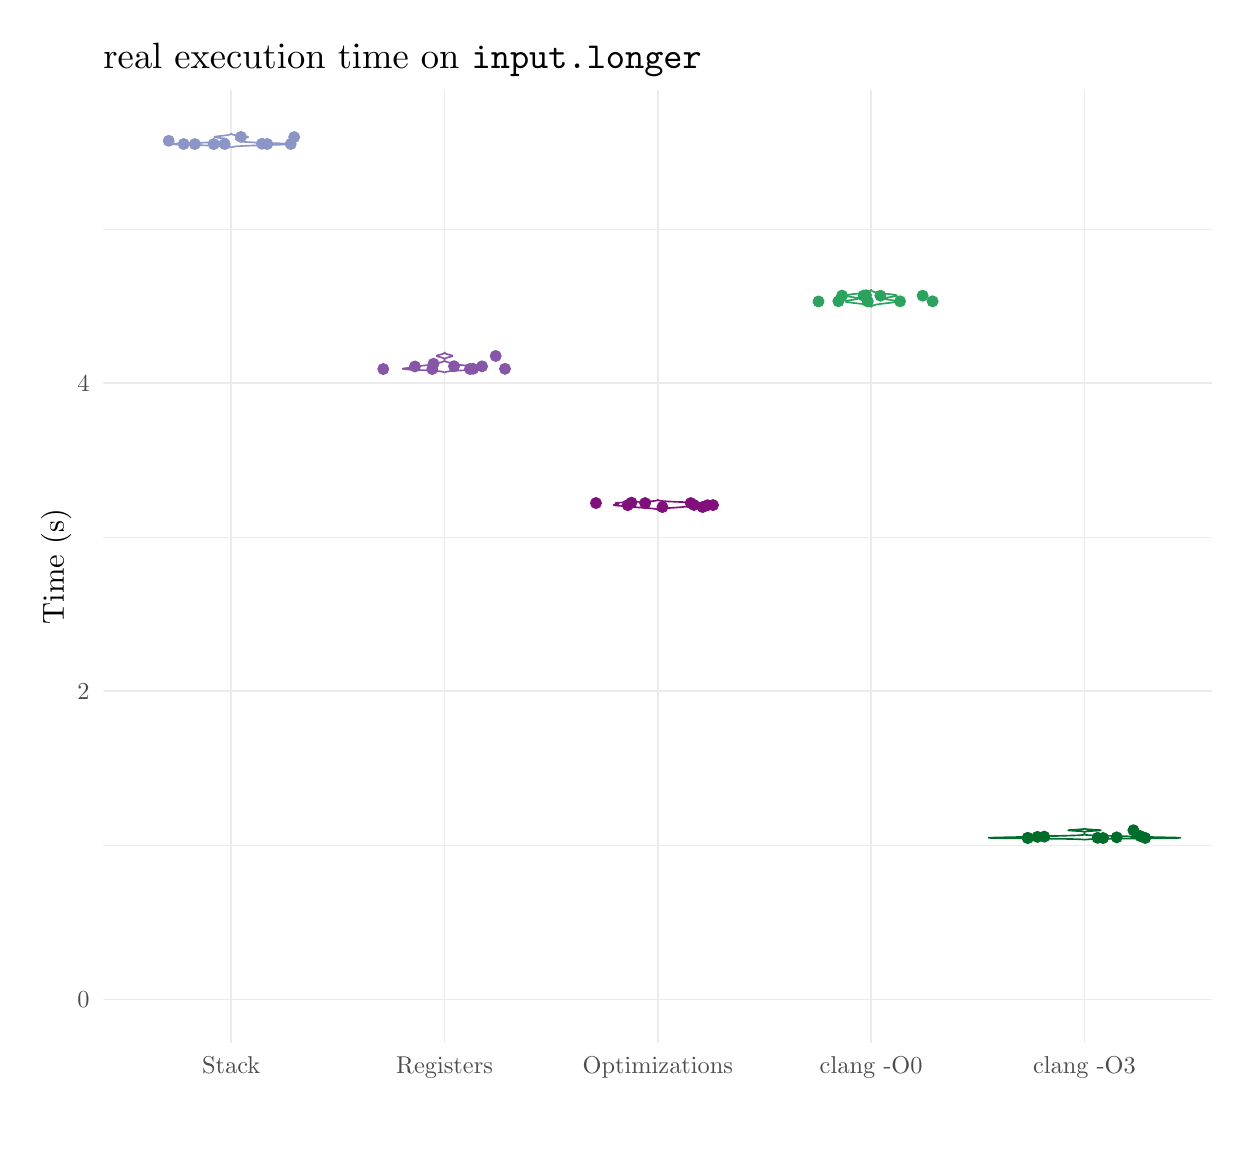
\begin{tikzpicture}[x=1pt,y=1pt]
\definecolor{fillColor}{RGB}{255,255,255}
\path[use as bounding box,fill=fillColor,fill opacity=0.00] (0,0) rectangle (433.62,397.48);
\begin{scope}
\path[clip] ( 27.31, 30.69) rectangle (428.12,374.83);
\definecolor{drawColor}{gray}{0.92}

\path[draw=drawColor,line width= 0.3pt,line join=round] ( 27.31,102.00) --
	(428.12,102.00);

\path[draw=drawColor,line width= 0.3pt,line join=round] ( 27.31,213.34) --
	(428.12,213.34);

\path[draw=drawColor,line width= 0.3pt,line join=round] ( 27.31,324.69) --
	(428.12,324.69);

\path[draw=drawColor,line width= 0.6pt,line join=round] ( 27.31, 46.33) --
	(428.12, 46.33);

\path[draw=drawColor,line width= 0.6pt,line join=round] ( 27.31,157.67) --
	(428.12,157.67);

\path[draw=drawColor,line width= 0.6pt,line join=round] ( 27.31,269.02) --
	(428.12,269.02);

\path[draw=drawColor,line width= 0.6pt,line join=round] ( 73.56, 30.69) --
	( 73.56,374.83);

\path[draw=drawColor,line width= 0.6pt,line join=round] (150.64, 30.69) --
	(150.64,374.83);

\path[draw=drawColor,line width= 0.6pt,line join=round] (227.72, 30.69) --
	(227.72,374.83);

\path[draw=drawColor,line width= 0.6pt,line join=round] (304.79, 30.69) --
	(304.79,374.83);

\path[draw=drawColor,line width= 0.6pt,line join=round] (381.87, 30.69) --
	(381.87,374.83);
\definecolor{drawColor}{RGB}{140,150,198}
\definecolor{fillColor}{RGB}{255,255,255}

\path[draw=drawColor,line width= 0.6pt,line join=round,line cap=round,fill=fillColor] ( 73.34,354.27) --
	( 73.32,354.28) --
	( 73.30,354.29) --
	( 73.28,354.30) --
	( 73.26,354.31) --
	( 73.24,354.32) --
	( 73.22,354.33) --
	( 73.19,354.34) --
	( 73.16,354.35) --
	( 73.13,354.35) --
	( 73.10,354.36) --
	( 73.07,354.37) --
	( 73.04,354.38) --
	( 73.00,354.39) --
	( 72.96,354.40) --
	( 72.92,354.41) --
	( 72.88,354.42) --
	( 72.83,354.43) --
	( 72.78,354.44) --
	( 72.73,354.45) --
	( 72.68,354.46) --
	( 72.62,354.47) --
	( 72.56,354.48) --
	( 72.49,354.49) --
	( 72.43,354.50) --
	( 72.36,354.51) --
	( 72.28,354.52) --
	( 72.21,354.53) --
	( 72.12,354.54) --
	( 72.04,354.55) --
	( 71.95,354.56) --
	( 71.86,354.57) --
	( 71.76,354.58) --
	( 71.66,354.59) --
	( 71.55,354.60) --
	( 71.44,354.60) --
	( 71.32,354.61) --
	( 71.20,354.62) --
	( 71.07,354.63) --
	( 70.94,354.64) --
	( 70.81,354.65) --
	( 70.66,354.66) --
	( 70.52,354.67) --
	( 70.36,354.68) --
	( 70.21,354.69) --
	( 70.04,354.70) --
	( 69.87,354.71) --
	( 69.70,354.72) --
	( 69.51,354.73) --
	( 69.33,354.74) --
	( 69.14,354.75) --
	( 68.93,354.76) --
	( 68.73,354.77) --
	( 68.52,354.78) --
	( 68.30,354.79) --
	( 68.08,354.80) --
	( 67.85,354.81) --
	( 67.62,354.82) --
	( 67.38,354.83) --
	( 67.13,354.84) --
	( 66.88,354.85) --
	( 66.62,354.86) --
	( 66.36,354.86) --
	( 66.09,354.87) --
	( 65.82,354.88) --
	( 65.54,354.89) --
	( 65.26,354.90) --
	( 64.97,354.91) --
	( 64.68,354.92) --
	( 64.38,354.93) --
	( 64.08,354.94) --
	( 63.78,354.95) --
	( 63.47,354.96) --
	( 63.16,354.97) --
	( 62.84,354.98) --
	( 62.53,354.99) --
	( 62.21,355.00) --
	( 61.89,355.01) --
	( 61.57,355.02) --
	( 61.25,355.03) --
	( 60.92,355.04) --
	( 60.60,355.05) --
	( 60.27,355.06) --
	( 59.95,355.07) --
	( 59.63,355.08) --
	( 59.31,355.09) --
	( 58.99,355.10) --
	( 58.67,355.11) --
	( 58.35,355.11) --
	( 58.04,355.12) --
	( 57.73,355.13) --
	( 57.43,355.14) --
	( 57.13,355.15) --
	( 56.83,355.16) --
	( 56.54,355.17) --
	( 56.26,355.18) --
	( 55.98,355.19) --
	( 55.70,355.20) --
	( 55.44,355.21) --
	( 55.18,355.22) --
	( 54.93,355.23) --
	( 54.69,355.24) --
	( 54.46,355.25) --
	( 54.24,355.26) --
	( 54.02,355.27) --
	( 53.82,355.28) --
	( 53.62,355.29) --
	( 53.44,355.30) --
	( 53.27,355.31) --
	( 53.11,355.32) --
	( 52.96,355.33) --
	( 52.82,355.34) --
	( 52.69,355.35) --
	( 52.58,355.36) --
	( 52.48,355.37) --
	( 52.39,355.37) --
	( 52.31,355.38) --
	( 52.25,355.39) --
	( 52.20,355.40) --
	( 52.16,355.41) --
	( 52.14,355.42) --
	( 52.13,355.43) --
	( 52.13,355.44) --
	( 52.14,355.45) --
	( 52.17,355.46) --
	( 52.21,355.47) --
	( 52.27,355.48) --
	( 52.34,355.49) --
	( 52.41,355.50) --
	( 52.51,355.51) --
	( 52.61,355.52) --
	( 52.73,355.53) --
	( 52.86,355.54) --
	( 53.00,355.55) --
	( 53.15,355.56) --
	( 53.31,355.57) --
	( 53.48,355.58) --
	( 53.67,355.59) --
	( 53.86,355.60) --
	( 54.06,355.61) --
	( 54.28,355.62) --
	( 54.50,355.62) --
	( 54.73,355.63) --
	( 54.96,355.64) --
	( 55.21,355.65) --
	( 55.46,355.66) --
	( 55.72,355.67) --
	( 55.99,355.68) --
	( 56.26,355.69) --
	( 56.53,355.70) --
	( 56.81,355.71) --
	( 57.10,355.72) --
	( 57.39,355.73) --
	( 57.68,355.74) --
	( 57.98,355.75) --
	( 58.27,355.76) --
	( 58.57,355.77) --
	( 58.88,355.78) --
	( 59.18,355.79) --
	( 59.48,355.80) --
	( 59.78,355.81) --
	( 60.09,355.82) --
	( 60.39,355.83) --
	( 60.69,355.84) --
	( 60.99,355.85) --
	( 61.29,355.86) --
	( 61.58,355.87) --
	( 61.88,355.88) --
	( 62.17,355.88) --
	( 62.45,355.89) --
	( 62.74,355.90) --
	( 63.02,355.91) --
	( 63.29,355.92) --
	( 63.56,355.93) --
	( 63.83,355.94) --
	( 64.09,355.95) --
	( 64.34,355.96) --
	( 64.60,355.97) --
	( 64.84,355.98) --
	( 65.08,355.99) --
	( 65.31,356.00) --
	( 65.54,356.01) --
	( 65.76,356.02) --
	( 65.97,356.03) --
	( 66.18,356.04) --
	( 66.39,356.05) --
	( 66.58,356.06) --
	( 66.77,356.07) --
	( 66.95,356.08) --
	( 67.13,356.09) --
	( 67.30,356.10) --
	( 67.46,356.11) --
	( 67.62,356.12) --
	( 67.77,356.13) --
	( 67.91,356.13) --
	( 68.05,356.14) --
	( 68.18,356.15) --
	( 68.31,356.16) --
	( 68.43,356.17) --
	( 68.54,356.18) --
	( 68.65,356.19) --
	( 68.75,356.20) --
	( 68.85,356.21) --
	( 68.94,356.22) --
	( 69.02,356.23) --
	( 69.11,356.24) --
	( 69.18,356.25) --
	( 69.25,356.26) --
	( 69.32,356.27) --
	( 69.39,356.28) --
	( 69.45,356.29) --
	( 69.50,356.30) --
	( 69.55,356.31) --
	( 69.60,356.32) --
	( 69.65,356.33) --
	( 69.69,356.34) --
	( 69.73,356.35) --
	( 69.76,356.36) --
	( 69.80,356.37) --
	( 69.83,356.38) --
	( 69.85,356.38) --
	( 69.88,356.39) --
	( 69.91,356.40) --
	( 69.93,356.41) --
	( 69.95,356.42) --
	( 69.97,356.43) --
	( 69.99,356.44) --
	( 70.01,356.45) --
	( 70.03,356.46) --
	( 70.04,356.47) --
	( 70.06,356.48) --
	( 70.07,356.49) --
	( 70.09,356.50) --
	( 70.10,356.51) --
	( 70.12,356.52) --
	( 70.13,356.53) --
	( 70.15,356.54) --
	( 70.16,356.55) --
	( 70.18,356.56) --
	( 70.20,356.57) --
	( 70.21,356.58) --
	( 70.23,356.59) --
	( 70.25,356.60) --
	( 70.27,356.61) --
	( 70.29,356.62) --
	( 70.31,356.63) --
	( 70.33,356.64) --
	( 70.35,356.64) --
	( 70.37,356.65) --
	( 70.39,356.66) --
	( 70.42,356.67) --
	( 70.44,356.68) --
	( 70.47,356.69) --
	( 70.50,356.70) --
	( 70.53,356.71) --
	( 70.56,356.72) --
	( 70.59,356.73) --
	( 70.62,356.74) --
	( 70.65,356.75) --
	( 70.68,356.76) --
	( 70.71,356.77) --
	( 70.75,356.78) --
	( 70.78,356.79) --
	( 70.82,356.80) --
	( 70.85,356.81) --
	( 70.89,356.82) --
	( 70.93,356.83) --
	( 70.97,356.84) --
	( 71.00,356.85) --
	( 71.04,356.86) --
	( 71.08,356.87) --
	( 71.12,356.88) --
	( 71.15,356.89) --
	( 71.19,356.89) --
	( 71.23,356.90) --
	( 71.27,356.91) --
	( 71.30,356.92) --
	( 71.34,356.93) --
	( 71.38,356.94) --
	( 71.41,356.95) --
	( 71.45,356.96) --
	( 71.48,356.97) --
	( 71.52,356.98) --
	( 71.55,356.99) --
	( 71.58,357.00) --
	( 71.61,357.01) --
	( 71.64,357.02) --
	( 71.67,357.03) --
	( 71.70,357.04) --
	( 71.72,357.05) --
	( 71.75,357.06) --
	( 71.77,357.07) --
	( 71.79,357.08) --
	( 71.81,357.09) --
	( 71.83,357.10) --
	( 71.84,357.11) --
	( 71.86,357.12) --
	( 71.87,357.13) --
	( 71.88,357.14) --
	( 71.89,357.15) --
	( 71.89,357.15) --
	( 71.90,357.16) --
	( 71.90,357.17) --
	( 71.90,357.18) --
	( 71.89,357.19) --
	( 71.89,357.20) --
	( 71.88,357.21) --
	( 71.87,357.22) --
	( 71.86,357.23) --
	( 71.84,357.24) --
	( 71.83,357.25) --
	( 71.81,357.26) --
	( 71.78,357.27) --
	( 71.76,357.28) --
	( 71.73,357.29) --
	( 71.70,357.30) --
	( 71.67,357.31) --
	( 71.63,357.32) --
	( 71.60,357.33) --
	( 71.56,357.34) --
	( 71.51,357.35) --
	( 71.47,357.36) --
	( 71.42,357.37) --
	( 71.37,357.38) --
	( 71.32,357.39) --
	( 71.27,357.40) --
	( 71.21,357.40) --
	( 71.15,357.41) --
	( 71.09,357.42) --
	( 71.03,357.43) --
	( 70.96,357.44) --
	( 70.89,357.45) --
	( 70.83,357.46) --
	( 70.76,357.47) --
	( 70.68,357.48) --
	( 70.61,357.49) --
	( 70.53,357.50) --
	( 70.46,357.51) --
	( 70.38,357.52) --
	( 70.30,357.53) --
	( 70.22,357.54) --
	( 70.14,357.55) --
	( 70.05,357.56) --
	( 69.97,357.57) --
	( 69.89,357.58) --
	( 69.80,357.59) --
	( 69.72,357.60) --
	( 69.63,357.61) --
	( 69.55,357.62) --
	( 69.46,357.63) --
	( 69.38,357.64) --
	( 69.29,357.65) --
	( 69.21,357.66) --
	( 69.12,357.66) --
	( 69.04,357.67) --
	( 68.96,357.68) --
	( 68.87,357.69) --
	( 68.79,357.70) --
	( 68.71,357.71) --
	( 68.64,357.72) --
	( 68.56,357.73) --
	( 68.48,357.74) --
	( 68.41,357.75) --
	( 68.34,357.76) --
	( 68.27,357.77) --
	( 68.20,357.78) --
	( 68.14,357.79) --
	( 68.08,357.80) --
	( 68.02,357.81) --
	( 67.96,357.82) --
	( 67.90,357.83) --
	( 67.85,357.84) --
	( 67.81,357.85) --
	( 67.76,357.86) --
	( 67.72,357.87) --
	( 67.68,357.88) --
	( 67.64,357.89) --
	( 67.61,357.90) --
	( 67.58,357.91) --
	( 67.55,357.91) --
	( 67.53,357.92) --
	( 67.51,357.93) --
	( 67.50,357.94) --
	( 67.49,357.95) --
	( 67.48,357.96) --
	( 67.48,357.97) --
	( 67.47,357.98) --
	( 67.48,357.99) --
	( 67.49,358.00) --
	( 67.50,358.01) --
	( 67.51,358.02) --
	( 67.53,358.03) --
	( 67.55,358.04) --
	( 67.58,358.05) --
	( 67.60,358.06) --
	( 67.64,358.07) --
	( 67.67,358.08) --
	( 67.71,358.09) --
	( 67.75,358.10) --
	( 67.80,358.11) --
	( 67.85,358.12) --
	( 67.90,358.13) --
	( 67.96,358.14) --
	( 68.01,358.15) --
	( 68.07,358.16) --
	( 68.14,358.17) --
	( 68.20,358.17) --
	( 68.27,358.18) --
	( 68.34,358.19) --
	( 68.41,358.20) --
	( 68.49,358.21) --
	( 68.57,358.22) --
	( 68.65,358.23) --
	( 68.73,358.24) --
	( 68.81,358.25) --
	( 68.89,358.26) --
	( 68.98,358.27) --
	( 69.06,358.28) --
	( 69.15,358.29) --
	( 69.24,358.30) --
	( 69.33,358.31) --
	( 69.42,358.32) --
	( 69.51,358.33) --
	( 69.60,358.34) --
	( 69.69,358.35) --
	( 69.78,358.36) --
	( 69.87,358.37) --
	( 69.96,358.38) --
	( 70.05,358.39) --
	( 70.15,358.40) --
	( 70.24,358.41) --
	( 70.33,358.42) --
	( 70.42,358.42) --
	( 70.51,358.43) --
	( 70.59,358.44) --
	( 70.68,358.45) --
	( 70.77,358.46) --
	( 70.86,358.47) --
	( 70.94,358.48) --
	( 71.02,358.49) --
	( 71.11,358.50) --
	( 71.19,358.51) --
	( 71.27,358.52) --
	( 71.35,358.53) --
	( 71.42,358.54) --
	( 71.50,358.55) --
	( 71.57,358.56) --
	( 71.65,358.57) --
	( 71.72,358.58) --
	( 71.79,358.59) --
	( 71.86,358.60) --
	( 71.92,358.61) --
	( 71.99,358.62) --
	( 72.05,358.63) --
	( 72.11,358.64) --
	( 72.17,358.65) --
	( 72.23,358.66) --
	( 72.29,358.67) --
	( 72.34,358.68) --
	( 72.40,358.68) --
	( 72.45,358.69) --
	( 72.50,358.70) --
	( 72.55,358.71) --
	( 72.59,358.72) --
	( 72.64,358.73) --
	( 72.68,358.74) --
	( 72.72,358.75) --
	( 72.76,358.76) --
	( 72.80,358.77) --
	( 72.84,358.78) --
	( 72.88,358.79) --
	( 72.91,358.80) --
	( 72.95,358.81) --
	( 72.98,358.82) --
	( 73.01,358.83) --
	( 73.04,358.84) --
	( 73.07,358.85) --
	( 73.09,358.86) --
	( 73.12,358.87) --
	( 73.14,358.88) --
	( 73.17,358.89) --
	( 73.19,358.90) --
	( 73.21,358.91) --
	( 73.23,358.92) --
	( 73.25,358.93) --
	( 73.27,358.93) --
	( 73.29,358.94) --
	( 73.30,358.95) --
	( 73.32,358.96) --
	( 73.33,358.97) --
	( 73.35,358.98) --
	( 73.36,358.99) --
	( 73.37,359.00) --
	( 73.38,359.01) --
	( 73.40,359.02) --
	( 73.41,359.03) --
	( 73.42,359.04) --
	( 73.43,359.05) --
	( 73.43,359.06) --
	( 73.44,359.07) --
	( 73.45,359.08) --
	( 73.46,359.09) --
	( 73.47,359.10) --
	( 73.47,359.11) --
	( 73.48,359.12) --
	( 73.48,359.13) --
	( 73.49,359.14) --
	( 73.49,359.15) --
	( 73.50,359.16) --
	( 73.50,359.17) --
	( 73.51,359.18) --
	( 73.51,359.18) --
	( 73.61,359.18) --
	( 73.61,359.18) --
	( 73.62,359.17) --
	( 73.62,359.16) --
	( 73.63,359.15) --
	( 73.63,359.14) --
	( 73.64,359.13) --
	( 73.64,359.12) --
	( 73.65,359.11) --
	( 73.65,359.10) --
	( 73.66,359.09) --
	( 73.67,359.08) --
	( 73.68,359.07) --
	( 73.69,359.06) --
	( 73.69,359.05) --
	( 73.70,359.04) --
	( 73.71,359.03) --
	( 73.72,359.02) --
	( 73.74,359.01) --
	( 73.75,359.00) --
	( 73.76,358.99) --
	( 73.77,358.98) --
	( 73.79,358.97) --
	( 73.80,358.96) --
	( 73.82,358.95) --
	( 73.84,358.94) --
	( 73.85,358.93) --
	( 73.87,358.93) --
	( 73.89,358.92) --
	( 73.91,358.91) --
	( 73.93,358.90) --
	( 73.95,358.89) --
	( 73.98,358.88) --
	( 74.00,358.87) --
	( 74.03,358.86) --
	( 74.05,358.85) --
	( 74.08,358.84) --
	( 74.11,358.83) --
	( 74.14,358.82) --
	( 74.17,358.81) --
	( 74.21,358.80) --
	( 74.24,358.79) --
	( 74.28,358.78) --
	( 74.32,358.77) --
	( 74.36,358.76) --
	( 74.40,358.75) --
	( 74.44,358.74) --
	( 74.48,358.73) --
	( 74.53,358.72) --
	( 74.57,358.71) --
	( 74.62,358.70) --
	( 74.67,358.69) --
	( 74.72,358.68) --
	( 74.78,358.68) --
	( 74.83,358.67) --
	( 74.89,358.66) --
	( 74.95,358.65) --
	( 75.01,358.64) --
	( 75.07,358.63) --
	( 75.13,358.62) --
	( 75.20,358.61) --
	( 75.26,358.60) --
	( 75.33,358.59) --
	( 75.40,358.58) --
	( 75.47,358.57) --
	( 75.55,358.56) --
	( 75.62,358.55) --
	( 75.70,358.54) --
	( 75.77,358.53) --
	( 75.85,358.52) --
	( 75.93,358.51) --
	( 76.01,358.50) --
	( 76.10,358.49) --
	( 76.18,358.48) --
	( 76.27,358.47) --
	( 76.35,358.46) --
	( 76.44,358.45) --
	( 76.53,358.44) --
	( 76.61,358.43) --
	( 76.70,358.42) --
	( 76.79,358.42) --
	( 76.88,358.41) --
	( 76.97,358.40) --
	( 77.07,358.39) --
	( 77.16,358.38) --
	( 77.25,358.37) --
	( 77.34,358.36) --
	( 77.43,358.35) --
	( 77.52,358.34) --
	( 77.61,358.33) --
	( 77.70,358.32) --
	( 77.79,358.31) --
	( 77.88,358.30) --
	( 77.97,358.29) --
	( 78.06,358.28) --
	( 78.14,358.27) --
	( 78.23,358.26) --
	( 78.31,358.25) --
	( 78.39,358.24) --
	( 78.48,358.23) --
	( 78.55,358.22) --
	( 78.63,358.21) --
	( 78.71,358.20) --
	( 78.78,358.19) --
	( 78.85,358.18) --
	( 78.92,358.17) --
	( 78.98,358.17) --
	( 79.05,358.16) --
	( 79.11,358.15) --
	( 79.16,358.14) --
	( 79.22,358.13) --
	( 79.27,358.12) --
	( 79.32,358.11) --
	( 79.37,358.10) --
	( 79.41,358.09) --
	( 79.45,358.08) --
	( 79.48,358.07) --
	( 79.52,358.06) --
	( 79.54,358.05) --
	( 79.57,358.04) --
	( 79.59,358.03) --
	( 79.61,358.02) --
	( 79.62,358.01) --
	( 79.64,358.00) --
	( 79.64,357.99) --
	( 79.65,357.98) --
	( 79.65,357.97) --
	( 79.64,357.96) --
	( 79.63,357.95) --
	( 79.62,357.94) --
	( 79.61,357.93) --
	( 79.59,357.92) --
	( 79.57,357.91) --
	( 79.54,357.91) --
	( 79.51,357.90) --
	( 79.48,357.89) --
	( 79.44,357.88) --
	( 79.40,357.87) --
	( 79.36,357.86) --
	( 79.32,357.85) --
	( 79.27,357.84) --
	( 79.22,357.83) --
	( 79.16,357.82) --
	( 79.10,357.81) --
	( 79.04,357.80) --
	( 78.98,357.79) --
	( 78.92,357.78) --
	( 78.85,357.77) --
	( 78.78,357.76) --
	( 78.71,357.75) --
	( 78.64,357.74) --
	( 78.56,357.73) --
	( 78.48,357.72) --
	( 78.41,357.71) --
	( 78.33,357.70) --
	( 78.25,357.69) --
	( 78.16,357.68) --
	( 78.08,357.67) --
	( 78.00,357.66) --
	( 77.91,357.66) --
	( 77.83,357.65) --
	( 77.74,357.64) --
	( 77.66,357.63) --
	( 77.57,357.62) --
	( 77.49,357.61) --
	( 77.40,357.60) --
	( 77.32,357.59) --
	( 77.23,357.58) --
	( 77.15,357.57) --
	( 77.07,357.56) --
	( 76.98,357.55) --
	( 76.90,357.54) --
	( 76.82,357.53) --
	( 76.74,357.52) --
	( 76.66,357.51) --
	( 76.59,357.50) --
	( 76.51,357.49) --
	( 76.44,357.48) --
	( 76.37,357.47) --
	( 76.29,357.46) --
	( 76.23,357.45) --
	( 76.16,357.44) --
	( 76.09,357.43) --
	( 76.03,357.42) --
	( 75.97,357.41) --
	( 75.91,357.40) --
	( 75.85,357.40) --
	( 75.80,357.39) --
	( 75.75,357.38) --
	( 75.70,357.37) --
	( 75.65,357.36) --
	( 75.61,357.35) --
	( 75.56,357.34) --
	( 75.52,357.33) --
	( 75.49,357.32) --
	( 75.45,357.31) --
	( 75.42,357.30) --
	( 75.39,357.29) --
	( 75.36,357.28) --
	( 75.34,357.27) --
	( 75.31,357.26) --
	( 75.29,357.25) --
	( 75.28,357.24) --
	( 75.26,357.23) --
	( 75.25,357.22) --
	( 75.24,357.21) --
	( 75.23,357.20) --
	( 75.23,357.19) --
	( 75.22,357.18) --
	( 75.22,357.17) --
	( 75.22,357.16) --
	( 75.23,357.15) --
	( 75.23,357.15) --
	( 75.24,357.14) --
	( 75.25,357.13) --
	( 75.26,357.12) --
	( 75.28,357.11) --
	( 75.29,357.10) --
	( 75.31,357.09) --
	( 75.33,357.08) --
	( 75.35,357.07) --
	( 75.37,357.06) --
	( 75.40,357.05) --
	( 75.42,357.04) --
	( 75.45,357.03) --
	( 75.48,357.02) --
	( 75.51,357.01) --
	( 75.54,357.00) --
	( 75.57,356.99) --
	( 75.60,356.98) --
	( 75.64,356.97) --
	( 75.67,356.96) --
	( 75.71,356.95) --
	( 75.74,356.94) --
	( 75.78,356.93) --
	( 75.82,356.92) --
	( 75.85,356.91) --
	( 75.89,356.90) --
	( 75.93,356.89) --
	( 75.97,356.89) --
	( 76.00,356.88) --
	( 76.04,356.87) --
	( 76.08,356.86) --
	( 76.12,356.85) --
	( 76.16,356.84) --
	( 76.19,356.83) --
	( 76.23,356.82) --
	( 76.27,356.81) --
	( 76.30,356.80) --
	( 76.34,356.79) --
	( 76.37,356.78) --
	( 76.41,356.77) --
	( 76.44,356.76) --
	( 76.47,356.75) --
	( 76.50,356.74) --
	( 76.53,356.73) --
	( 76.56,356.72) --
	( 76.59,356.71) --
	( 76.62,356.70) --
	( 76.65,356.69) --
	( 76.68,356.68) --
	( 76.70,356.67) --
	( 76.73,356.66) --
	( 76.75,356.65) --
	( 76.77,356.64) --
	( 76.79,356.64) --
	( 76.81,356.63) --
	( 76.83,356.62) --
	( 76.85,356.61) --
	( 76.87,356.60) --
	( 76.89,356.59) --
	( 76.91,356.58) --
	( 76.92,356.57) --
	( 76.94,356.56) --
	( 76.96,356.55) --
	( 76.97,356.54) --
	( 76.99,356.53) --
	( 77.00,356.52) --
	( 77.02,356.51) --
	( 77.03,356.50) --
	( 77.05,356.49) --
	( 77.06,356.48) --
	( 77.08,356.47) --
	( 77.09,356.46) --
	( 77.11,356.45) --
	( 77.13,356.44) --
	( 77.15,356.43) --
	( 77.17,356.42) --
	( 77.19,356.41) --
	( 77.21,356.40) --
	( 77.24,356.39) --
	( 77.27,356.38) --
	( 77.29,356.38) --
	( 77.33,356.37) --
	( 77.36,356.36) --
	( 77.39,356.35) --
	( 77.43,356.34) --
	( 77.47,356.33) --
	( 77.52,356.32) --
	( 77.57,356.31) --
	( 77.62,356.30) --
	( 77.68,356.29) --
	( 77.73,356.28) --
	( 77.80,356.27) --
	( 77.87,356.26) --
	( 77.94,356.25) --
	( 78.01,356.24) --
	( 78.10,356.23) --
	( 78.18,356.22) --
	( 78.27,356.21) --
	( 78.37,356.20) --
	( 78.47,356.19) --
	( 78.58,356.18) --
	( 78.69,356.17) --
	( 78.82,356.16) --
	( 78.94,356.15) --
	( 79.07,356.14) --
	( 79.21,356.13) --
	( 79.35,356.13) --
	( 79.50,356.12) --
	( 79.66,356.11) --
	( 79.82,356.10) --
	( 79.99,356.09) --
	( 80.17,356.08) --
	( 80.35,356.07) --
	( 80.54,356.06) --
	( 80.74,356.05) --
	( 80.94,356.04) --
	( 81.15,356.03) --
	( 81.36,356.02) --
	( 81.58,356.01) --
	( 81.81,356.00) --
	( 82.04,355.99) --
	( 82.28,355.98) --
	( 82.53,355.97) --
	( 82.78,355.96) --
	( 83.03,355.95) --
	( 83.29,355.94) --
	( 83.56,355.93) --
	( 83.83,355.92) --
	( 84.10,355.91) --
	( 84.38,355.90) --
	( 84.67,355.89) --
	( 84.95,355.88) --
	( 85.24,355.88) --
	( 85.54,355.87) --
	( 85.83,355.86) --
	( 86.13,355.85) --
	( 86.43,355.84) --
	( 86.73,355.83) --
	( 87.03,355.82) --
	( 87.34,355.81) --
	( 87.64,355.80) --
	( 87.94,355.79) --
	( 88.24,355.78) --
	( 88.55,355.77) --
	( 88.85,355.76) --
	( 89.14,355.75) --
	( 89.44,355.74) --
	( 89.73,355.73) --
	( 90.02,355.72) --
	( 90.31,355.71) --
	( 90.59,355.70) --
	( 90.86,355.69) --
	( 91.13,355.68) --
	( 91.40,355.67) --
	( 91.66,355.66) --
	( 91.91,355.65) --
	( 92.16,355.64) --
	( 92.39,355.63) --
	( 92.63,355.62) --
	( 92.84,355.62) --
	( 93.06,355.61) --
	( 93.26,355.60) --
	( 93.45,355.59) --
	( 93.64,355.58) --
	( 93.81,355.57) --
	( 93.97,355.56) --
	( 94.12,355.55) --
	( 94.26,355.54) --
	( 94.39,355.53) --
	( 94.51,355.52) --
	( 94.61,355.51) --
	( 94.71,355.50) --
	( 94.78,355.49) --
	( 94.85,355.48) --
	( 94.91,355.47) --
	( 94.95,355.46) --
	( 94.98,355.45) --
	( 94.99,355.44) --
	( 94.99,355.43) --
	( 94.98,355.42) --
	( 94.96,355.41) --
	( 94.92,355.40) --
	( 94.87,355.39) --
	( 94.81,355.38) --
	( 94.73,355.37) --
	( 94.64,355.37) --
	( 94.54,355.36) --
	( 94.43,355.35) --
	( 94.30,355.34) --
	( 94.16,355.33) --
	( 94.01,355.32) --
	( 93.85,355.31) --
	( 93.68,355.30) --
	( 93.50,355.29) --
	( 93.30,355.28) --
	( 93.10,355.27) --
	( 92.88,355.26) --
	( 92.66,355.25) --
	( 92.43,355.24) --
	( 92.19,355.23) --
	( 91.94,355.22) --
	( 91.68,355.21) --
	( 91.42,355.20) --
	( 91.14,355.19) --
	( 90.86,355.18) --
	( 90.58,355.17) --
	( 90.29,355.16) --
	( 89.99,355.15) --
	( 89.69,355.14) --
	( 89.39,355.13) --
	( 89.08,355.12) --
	( 88.77,355.11) --
	( 88.45,355.11) --
	( 88.13,355.10) --
	( 87.81,355.09) --
	( 87.49,355.08) --
	( 87.17,355.07) --
	( 86.85,355.06) --
	( 86.52,355.05) --
	( 86.20,355.04) --
	( 85.87,355.03) --
	( 85.55,355.02) --
	( 85.23,355.01) --
	( 84.91,355.00) --
	( 84.59,354.99) --
	( 84.28,354.98) --
	( 83.96,354.97) --
	( 83.65,354.96) --
	( 83.34,354.95) --
	( 83.04,354.94) --
	( 82.74,354.93) --
	( 82.44,354.92) --
	( 82.15,354.91) --
	( 81.87,354.90) --
	( 81.58,354.89) --
	( 81.30,354.88) --
	( 81.03,354.87) --
	( 80.76,354.86) --
	( 80.50,354.86) --
	( 80.24,354.85) --
	( 79.99,354.84) --
	( 79.74,354.83) --
	( 79.51,354.82) --
	( 79.27,354.81) --
	( 79.04,354.80) --
	( 78.82,354.79) --
	( 78.60,354.78) --
	( 78.39,354.77) --
	( 78.19,354.76) --
	( 77.99,354.75) --
	( 77.79,354.74) --
	( 77.61,354.73) --
	( 77.42,354.72) --
	( 77.25,354.71) --
	( 77.08,354.70) --
	( 76.91,354.69) --
	( 76.76,354.68) --
	( 76.60,354.67) --
	( 76.46,354.66) --
	( 76.31,354.65) --
	( 76.18,354.64) --
	( 76.05,354.63) --
	( 75.92,354.62) --
	( 75.80,354.61) --
	( 75.68,354.60) --
	( 75.57,354.60) --
	( 75.46,354.59) --
	( 75.36,354.58) --
	( 75.26,354.57) --
	( 75.17,354.56) --
	( 75.08,354.55) --
	( 75.00,354.54) --
	( 74.91,354.53) --
	( 74.84,354.52) --
	( 74.76,354.51) --
	( 74.69,354.50) --
	( 74.63,354.49) --
	( 74.56,354.48) --
	( 74.50,354.47) --
	( 74.44,354.46) --
	( 74.39,354.45) --
	( 74.34,354.44) --
	( 74.29,354.43) --
	( 74.24,354.42) --
	( 74.20,354.41) --
	( 74.16,354.40) --
	( 74.12,354.39) --
	( 74.08,354.38) --
	( 74.05,354.37) --
	( 74.02,354.36) --
	( 73.99,354.35) --
	( 73.96,354.35) --
	( 73.93,354.34) --
	( 73.90,354.33) --
	( 73.88,354.32) --
	( 73.86,354.31) --
	( 73.84,354.30) --
	( 73.82,354.29) --
	( 73.80,354.28) --
	( 73.78,354.27) --
	( 73.34,354.27) --
	cycle;
\definecolor{drawColor}{RGB}{136,86,167}

\path[draw=drawColor,line width= 0.6pt,line join=round,line cap=round,fill=fillColor] (150.50,272.90) --
	(150.48,272.91) --
	(150.47,272.93) --
	(150.45,272.94) --
	(150.43,272.96) --
	(150.41,272.97) --
	(150.39,272.98) --
	(150.36,273.00) --
	(150.33,273.01) --
	(150.30,273.03) --
	(150.27,273.04) --
	(150.23,273.05) --
	(150.20,273.07) --
	(150.15,273.08) --
	(150.11,273.10) --
	(150.06,273.11) --
	(150.01,273.12) --
	(149.96,273.14) --
	(149.90,273.15) --
	(149.83,273.17) --
	(149.76,273.18) --
	(149.69,273.20) --
	(149.61,273.21) --
	(149.53,273.22) --
	(149.44,273.24) --
	(149.35,273.25) --
	(149.25,273.27) --
	(149.14,273.28) --
	(149.03,273.29) --
	(148.92,273.31) --
	(148.79,273.32) --
	(148.66,273.34) --
	(148.52,273.35) --
	(148.38,273.36) --
	(148.23,273.38) --
	(148.07,273.39) --
	(147.91,273.41) --
	(147.73,273.42) --
	(147.55,273.44) --
	(147.37,273.45) --
	(147.17,273.46) --
	(146.97,273.48) --
	(146.76,273.49) --
	(146.54,273.51) --
	(146.31,273.52) --
	(146.08,273.53) --
	(145.85,273.55) --
	(145.60,273.56) --
	(145.35,273.58) --
	(145.09,273.59) --
	(144.83,273.60) --
	(144.56,273.62) --
	(144.28,273.63) --
	(144.00,273.65) --
	(143.72,273.66) --
	(143.44,273.67) --
	(143.14,273.69) --
	(142.85,273.70) --
	(142.55,273.72) --
	(142.26,273.73) --
	(141.96,273.75) --
	(141.66,273.76) --
	(141.36,273.77) --
	(141.06,273.79) --
	(140.76,273.80) --
	(140.47,273.82) --
	(140.18,273.83) --
	(139.89,273.84) --
	(139.60,273.86) --
	(139.33,273.87) --
	(139.05,273.89) --
	(138.78,273.90) --
	(138.53,273.91) --
	(138.27,273.93) --
	(138.03,273.94) --
	(137.79,273.96) --
	(137.57,273.97) --
	(137.35,273.99) --
	(137.15,274.00) --
	(136.96,274.01) --
	(136.77,274.03) --
	(136.60,274.04) --
	(136.45,274.06) --
	(136.30,274.07) --
	(136.17,274.08) --
	(136.05,274.10) --
	(135.94,274.11) --
	(135.85,274.13) --
	(135.77,274.14) --
	(135.71,274.15) --
	(135.65,274.17) --
	(135.61,274.18) --
	(135.59,274.20) --
	(135.57,274.21) --
	(135.57,274.23) --
	(135.58,274.24) --
	(135.60,274.25) --
	(135.64,274.27) --
	(135.68,274.28) --
	(135.74,274.30) --
	(135.80,274.31) --
	(135.88,274.32) --
	(135.96,274.34) --
	(136.05,274.35) --
	(136.15,274.37) --
	(136.25,274.38) --
	(136.36,274.39) --
	(136.48,274.41) --
	(136.59,274.42) --
	(136.72,274.44) --
	(136.84,274.45) --
	(136.97,274.46) --
	(137.10,274.48) --
	(137.24,274.49) --
	(137.37,274.51) --
	(137.50,274.52) --
	(137.63,274.54) --
	(137.76,274.55) --
	(137.89,274.56) --
	(138.02,274.58) --
	(138.14,274.59) --
	(138.26,274.61) --
	(138.38,274.62) --
	(138.50,274.63) --
	(138.61,274.65) --
	(138.72,274.66) --
	(138.82,274.68) --
	(138.92,274.69) --
	(139.01,274.70) --
	(139.10,274.72) --
	(139.19,274.73) --
	(139.27,274.75) --
	(139.35,274.76) --
	(139.43,274.78) --
	(139.50,274.79) --
	(139.57,274.80) --
	(139.63,274.82) --
	(139.70,274.83) --
	(139.76,274.85) --
	(139.81,274.86) --
	(139.87,274.87) --
	(139.92,274.89) --
	(139.98,274.90) --
	(140.03,274.92) --
	(140.08,274.93) --
	(140.14,274.94) --
	(140.19,274.96) --
	(140.24,274.97) --
	(140.30,274.99) --
	(140.36,275.00) --
	(140.42,275.02) --
	(140.48,275.03) --
	(140.54,275.04) --
	(140.61,275.06) --
	(140.68,275.07) --
	(140.75,275.09) --
	(140.83,275.10) --
	(140.90,275.11) --
	(140.99,275.13) --
	(141.07,275.14) --
	(141.16,275.16) --
	(141.26,275.17) --
	(141.36,275.18) --
	(141.46,275.20) --
	(141.56,275.21) --
	(141.67,275.23) --
	(141.78,275.24) --
	(141.90,275.25) --
	(142.01,275.27) --
	(142.14,275.28) --
	(142.26,275.30) --
	(142.38,275.31) --
	(142.51,275.33) --
	(142.64,275.34) --
	(142.77,275.35) --
	(142.91,275.37) --
	(143.04,275.38) --
	(143.17,275.40) --
	(143.31,275.41) --
	(143.44,275.42) --
	(143.58,275.44) --
	(143.71,275.45) --
	(143.84,275.47) --
	(143.97,275.48) --
	(144.10,275.49) --
	(144.23,275.51) --
	(144.36,275.52) --
	(144.48,275.54) --
	(144.60,275.55) --
	(144.72,275.57) --
	(144.84,275.58) --
	(144.95,275.59) --
	(145.06,275.61) --
	(145.17,275.62) --
	(145.28,275.64) --
	(145.38,275.65) --
	(145.48,275.66) --
	(145.57,275.68) --
	(145.66,275.69) --
	(145.75,275.71) --
	(145.83,275.72) --
	(145.92,275.73) --
	(146.00,275.75) --
	(146.07,275.76) --
	(146.14,275.78) --
	(146.21,275.79) --
	(146.28,275.81) --
	(146.35,275.82) --
	(146.41,275.83) --
	(146.47,275.85) --
	(146.53,275.86) --
	(146.59,275.88) --
	(146.64,275.89) --
	(146.70,275.90) --
	(146.75,275.92) --
	(146.80,275.93) --
	(146.85,275.95) --
	(146.90,275.96) --
	(146.95,275.97) --
	(147.00,275.99) --
	(147.05,276.00) --
	(147.10,276.02) --
	(147.15,276.03) --
	(147.20,276.05) --
	(147.25,276.06) --
	(147.30,276.07) --
	(147.35,276.09) --
	(147.40,276.10) --
	(147.45,276.12) --
	(147.51,276.13) --
	(147.56,276.14) --
	(147.61,276.16) --
	(147.67,276.17) --
	(147.73,276.19) --
	(147.78,276.20) --
	(147.84,276.21) --
	(147.90,276.23) --
	(147.96,276.24) --
	(148.02,276.26) --
	(148.08,276.27) --
	(148.15,276.28) --
	(148.21,276.30) --
	(148.27,276.31) --
	(148.34,276.33) --
	(148.40,276.34) --
	(148.46,276.36) --
	(148.53,276.37) --
	(148.59,276.38) --
	(148.66,276.40) --
	(148.72,276.41) --
	(148.79,276.43) --
	(148.85,276.44) --
	(148.91,276.45) --
	(148.98,276.47) --
	(149.04,276.48) --
	(149.10,276.50) --
	(149.16,276.51) --
	(149.22,276.52) --
	(149.28,276.54) --
	(149.34,276.55) --
	(149.40,276.57) --
	(149.45,276.58) --
	(149.51,276.60) --
	(149.56,276.61) --
	(149.61,276.62) --
	(149.66,276.64) --
	(149.71,276.65) --
	(149.76,276.67) --
	(149.80,276.68) --
	(149.85,276.69) --
	(149.89,276.71) --
	(149.93,276.72) --
	(149.97,276.74) --
	(150.01,276.75) --
	(150.05,276.76) --
	(150.08,276.78) --
	(150.12,276.79) --
	(150.15,276.81) --
	(150.18,276.82) --
	(150.21,276.84) --
	(150.24,276.85) --
	(150.26,276.86) --
	(150.29,276.88) --
	(150.31,276.89) --
	(150.33,276.91) --
	(150.36,276.92) --
	(150.38,276.93) --
	(150.39,276.95) --
	(150.41,276.96) --
	(150.43,276.98) --
	(150.45,276.99) --
	(150.46,277.00) --
	(150.47,277.02) --
	(150.49,277.03) --
	(150.50,277.05) --
	(150.51,277.06) --
	(150.52,277.07) --
	(150.53,277.09) --
	(150.54,277.10) --
	(150.55,277.12) --
	(150.56,277.13) --
	(150.56,277.15) --
	(150.57,277.16) --
	(150.58,277.17) --
	(150.58,277.19) --
	(150.59,277.20) --
	(150.59,277.22) --
	(150.59,277.23) --
	(150.60,277.24) --
	(150.60,277.26) --
	(150.61,277.27) --
	(150.61,277.29) --
	(150.61,277.30) --
	(150.61,277.31) --
	(150.62,277.33) --
	(150.62,277.34) --
	(150.62,277.36) --
	(150.62,277.37) --
	(150.62,277.39) --
	(150.62,277.40) --
	(150.62,277.41) --
	(150.62,277.43) --
	(150.62,277.44) --
	(150.62,277.46) --
	(150.62,277.47) --
	(150.62,277.48) --
	(150.62,277.50) --
	(150.62,277.51) --
	(150.62,277.53) --
	(150.62,277.54) --
	(150.62,277.55) --
	(150.62,277.57) --
	(150.61,277.58) --
	(150.61,277.60) --
	(150.61,277.61) --
	(150.61,277.63) --
	(150.60,277.64) --
	(150.60,277.65) --
	(150.60,277.67) --
	(150.59,277.68) --
	(150.59,277.70) --
	(150.58,277.71) --
	(150.58,277.72) --
	(150.57,277.74) --
	(150.56,277.75) --
	(150.56,277.77) --
	(150.55,277.78) --
	(150.54,277.79) --
	(150.53,277.81) --
	(150.52,277.82) --
	(150.51,277.84) --
	(150.50,277.85) --
	(150.49,277.86) --
	(150.48,277.88) --
	(150.46,277.89) --
	(150.45,277.91) --
	(150.43,277.92) --
	(150.42,277.94) --
	(150.40,277.95) --
	(150.38,277.96) --
	(150.36,277.98) --
	(150.34,277.99) --
	(150.32,278.01) --
	(150.29,278.02) --
	(150.27,278.03) --
	(150.24,278.05) --
	(150.21,278.06) --
	(150.19,278.08) --
	(150.15,278.09) --
	(150.12,278.10) --
	(150.09,278.12) --
	(150.05,278.13) --
	(150.02,278.15) --
	(149.98,278.16) --
	(149.94,278.18) --
	(149.90,278.19) --
	(149.86,278.20) --
	(149.82,278.22) --
	(149.77,278.23) --
	(149.72,278.25) --
	(149.68,278.26) --
	(149.63,278.27) --
	(149.58,278.29) --
	(149.53,278.30) --
	(149.47,278.32) --
	(149.42,278.33) --
	(149.36,278.34) --
	(149.31,278.36) --
	(149.25,278.37) --
	(149.19,278.39) --
	(149.14,278.40) --
	(149.08,278.42) --
	(149.02,278.43) --
	(148.96,278.44) --
	(148.90,278.46) --
	(148.84,278.47) --
	(148.78,278.49) --
	(148.73,278.50) --
	(148.67,278.51) --
	(148.61,278.53) --
	(148.55,278.54) --
	(148.50,278.56) --
	(148.44,278.57) --
	(148.39,278.58) --
	(148.34,278.60) --
	(148.29,278.61) --
	(148.24,278.63) --
	(148.19,278.64) --
	(148.14,278.66) --
	(148.10,278.67) --
	(148.06,278.68) --
	(148.02,278.70) --
	(147.99,278.71) --
	(147.95,278.73) --
	(147.92,278.74) --
	(147.90,278.75) --
	(147.87,278.77) --
	(147.85,278.78) --
	(147.83,278.80) --
	(147.82,278.81) --
	(147.80,278.82) --
	(147.79,278.84) --
	(147.79,278.85) --
	(147.79,278.87) --
	(147.79,278.88) --
	(147.79,278.89) --
	(147.80,278.91) --
	(147.81,278.92) --
	(147.82,278.94) --
	(147.84,278.95) --
	(147.86,278.97) --
	(147.88,278.98) --
	(147.91,278.99) --
	(147.94,279.01) --
	(147.97,279.02) --
	(148.01,279.04) --
	(148.05,279.05) --
	(148.08,279.06) --
	(148.13,279.08) --
	(148.17,279.09) --
	(148.22,279.11) --
	(148.27,279.12) --
	(148.32,279.13) --
	(148.37,279.15) --
	(148.42,279.16) --
	(148.47,279.18) --
	(148.53,279.19) --
	(148.59,279.21) --
	(148.64,279.22) --
	(148.70,279.23) --
	(148.76,279.25) --
	(148.82,279.26) --
	(148.88,279.28) --
	(148.94,279.29) --
	(149.00,279.30) --
	(149.05,279.32) --
	(149.11,279.33) --
	(149.17,279.35) --
	(149.23,279.36) --
	(149.29,279.37) --
	(149.34,279.39) --
	(149.40,279.40) --
	(149.45,279.42) --
	(149.50,279.43) --
	(149.56,279.45) --
	(149.61,279.46) --
	(149.66,279.47) --
	(149.70,279.49) --
	(149.75,279.50) --
	(149.80,279.52) --
	(149.84,279.53) --
	(149.88,279.54) --
	(149.93,279.56) --
	(149.96,279.57) --
	(150.00,279.59) --
	(150.04,279.60) --
	(150.08,279.61) --
	(150.11,279.63) --
	(150.14,279.64) --
	(150.17,279.66) --
	(150.20,279.67) --
	(150.23,279.68) --
	(150.26,279.70) --
	(150.28,279.71) --
	(150.31,279.73) --
	(150.33,279.74) --
	(150.35,279.76) --
	(150.37,279.77) --
	(150.39,279.78) --
	(150.41,279.80) --
	(150.43,279.81) --
	(150.44,279.83) --
	(150.46,279.84) --
	(150.47,279.85) --
	(150.48,279.87) --
	(150.50,279.88) --
	(150.51,279.90) --
	(150.52,279.91) --
	(150.53,279.92) --
	(150.54,279.94) --
	(150.55,279.95) --
	(150.55,279.97) --
	(150.56,279.98) --
	(150.57,280.00) --
	(150.57,280.01) --
	(150.58,280.02) --
	(150.59,280.04) --
	(150.59,280.05) --
	(150.59,280.07) --
	(150.60,280.08) --
	(150.60,280.09) --
	(150.61,280.11) --
	(150.67,280.11) --
	(150.67,280.09) --
	(150.68,280.08) --
	(150.68,280.07) --
	(150.69,280.05) --
	(150.69,280.04) --
	(150.70,280.02) --
	(150.70,280.01) --
	(150.71,280.00) --
	(150.72,279.98) --
	(150.72,279.97) --
	(150.73,279.95) --
	(150.74,279.94) --
	(150.75,279.92) --
	(150.76,279.91) --
	(150.77,279.90) --
	(150.78,279.88) --
	(150.79,279.87) --
	(150.81,279.85) --
	(150.82,279.84) --
	(150.83,279.83) --
	(150.85,279.81) --
	(150.87,279.80) --
	(150.89,279.78) --
	(150.91,279.77) --
	(150.93,279.76) --
	(150.95,279.74) --
	(150.97,279.73) --
	(150.99,279.71) --
	(151.02,279.70) --
	(151.05,279.68) --
	(151.07,279.67) --
	(151.10,279.66) --
	(151.14,279.64) --
	(151.17,279.63) --
	(151.20,279.61) --
	(151.24,279.60) --
	(151.27,279.59) --
	(151.31,279.57) --
	(151.35,279.56) --
	(151.39,279.54) --
	(151.44,279.53) --
	(151.48,279.52) --
	(151.53,279.50) --
	(151.57,279.49) --
	(151.62,279.47) --
	(151.67,279.46) --
	(151.72,279.45) --
	(151.77,279.43) --
	(151.83,279.42) --
	(151.88,279.40) --
	(151.94,279.39) --
	(151.99,279.37) --
	(152.05,279.36) --
	(152.11,279.35) --
	(152.16,279.33) --
	(152.22,279.32) --
	(152.28,279.30) --
	(152.34,279.29) --
	(152.40,279.28) --
	(152.46,279.26) --
	(152.52,279.25) --
	(152.58,279.23) --
	(152.63,279.22) --
	(152.69,279.21) --
	(152.75,279.19) --
	(152.80,279.18) --
	(152.86,279.16) --
	(152.91,279.15) --
	(152.96,279.13) --
	(153.01,279.12) --
	(153.06,279.11) --
	(153.11,279.09) --
	(153.15,279.08) --
	(153.19,279.06) --
	(153.23,279.05) --
	(153.27,279.04) --
	(153.30,279.02) --
	(153.34,279.01) --
	(153.37,278.99) --
	(153.39,278.98) --
	(153.42,278.97) --
	(153.44,278.95) --
	(153.45,278.94) --
	(153.47,278.92) --
	(153.48,278.91) --
	(153.49,278.89) --
	(153.49,278.88) --
	(153.49,278.87) --
	(153.49,278.85) --
	(153.48,278.84) --
	(153.47,278.82) --
	(153.46,278.81) --
	(153.45,278.80) --
	(153.43,278.78) --
	(153.41,278.77) --
	(153.38,278.75) --
	(153.35,278.74) --
	(153.32,278.73) --
	(153.29,278.71) --
	(153.25,278.70) --
	(153.22,278.68) --
	(153.17,278.67) --
	(153.13,278.66) --
	(153.09,278.64) --
	(153.04,278.63) --
	(152.99,278.61) --
	(152.94,278.60) --
	(152.89,278.58) --
	(152.83,278.57) --
	(152.78,278.56) --
	(152.72,278.54) --
	(152.67,278.53) --
	(152.61,278.51) --
	(152.55,278.50) --
	(152.49,278.49) --
	(152.43,278.47) --
	(152.37,278.46) --
	(152.32,278.44) --
	(152.26,278.43) --
	(152.20,278.42) --
	(152.14,278.40) --
	(152.08,278.39) --
	(152.02,278.37) --
	(151.97,278.36) --
	(151.91,278.34) --
	(151.86,278.33) --
	(151.80,278.32) --
	(151.75,278.30) --
	(151.70,278.29) --
	(151.65,278.27) --
	(151.60,278.26) --
	(151.55,278.25) --
	(151.51,278.23) --
	(151.46,278.22) --
	(151.42,278.20) --
	(151.38,278.19) --
	(151.34,278.18) --
	(151.30,278.16) --
	(151.26,278.15) --
	(151.22,278.13) --
	(151.19,278.12) --
	(151.15,278.10) --
	(151.12,278.09) --
	(151.09,278.08) --
	(151.06,278.06) --
	(151.04,278.05) --
	(151.01,278.03) --
	(150.98,278.02) --
	(150.96,278.01) --
	(150.94,277.99) --
	(150.92,277.98) --
	(150.90,277.96) --
	(150.88,277.95) --
	(150.86,277.94) --
	(150.84,277.92) --
	(150.83,277.91) --
	(150.81,277.89) --
	(150.80,277.88) --
	(150.79,277.86) --
	(150.78,277.85) --
	(150.76,277.84) --
	(150.75,277.82) --
	(150.74,277.81) --
	(150.74,277.79) --
	(150.73,277.78) --
	(150.72,277.77) --
	(150.71,277.75) --
	(150.71,277.74) --
	(150.70,277.72) --
	(150.69,277.71) --
	(150.69,277.70) --
	(150.69,277.68) --
	(150.68,277.67) --
	(150.68,277.65) --
	(150.67,277.64) --
	(150.67,277.63) --
	(150.67,277.61) --
	(150.67,277.60) --
	(150.66,277.58) --
	(150.66,277.57) --
	(150.66,277.55) --
	(150.66,277.54) --
	(150.66,277.53) --
	(150.66,277.51) --
	(150.66,277.50) --
	(150.65,277.48) --
	(150.65,277.47) --
	(150.65,277.46) --
	(150.65,277.44) --
	(150.65,277.43) --
	(150.65,277.41) --
	(150.66,277.40) --
	(150.66,277.39) --
	(150.66,277.37) --
	(150.66,277.36) --
	(150.66,277.34) --
	(150.66,277.33) --
	(150.66,277.31) --
	(150.67,277.30) --
	(150.67,277.29) --
	(150.67,277.27) --
	(150.67,277.26) --
	(150.68,277.24) --
	(150.68,277.23) --
	(150.69,277.22) --
	(150.69,277.20) --
	(150.70,277.19) --
	(150.70,277.17) --
	(150.71,277.16) --
	(150.71,277.15) --
	(150.72,277.13) --
	(150.73,277.12) --
	(150.74,277.10) --
	(150.75,277.09) --
	(150.76,277.07) --
	(150.77,277.06) --
	(150.78,277.05) --
	(150.79,277.03) --
	(150.80,277.02) --
	(150.82,277.00) --
	(150.83,276.99) --
	(150.85,276.98) --
	(150.86,276.96) --
	(150.88,276.95) --
	(150.90,276.93) --
	(150.92,276.92) --
	(150.94,276.91) --
	(150.97,276.89) --
	(150.99,276.88) --
	(151.01,276.86) --
	(151.04,276.85) --
	(151.07,276.84) --
	(151.10,276.82) --
	(151.13,276.81) --
	(151.16,276.79) --
	(151.20,276.78) --
	(151.23,276.76) --
	(151.27,276.75) --
	(151.31,276.74) --
	(151.35,276.72) --
	(151.39,276.71) --
	(151.43,276.69) --
	(151.47,276.68) --
	(151.52,276.67) --
	(151.57,276.65) --
	(151.62,276.64) --
	(151.67,276.62) --
	(151.72,276.61) --
	(151.77,276.60) --
	(151.83,276.58) --
	(151.88,276.57) --
	(151.94,276.55) --
	(152.00,276.54) --
	(152.06,276.52) --
	(152.12,276.51) --
	(152.18,276.50) --
	(152.24,276.48) --
	(152.30,276.47) --
	(152.36,276.45) --
	(152.43,276.44) --
	(152.49,276.43) --
	(152.55,276.41) --
	(152.62,276.40) --
	(152.68,276.38) --
	(152.75,276.37) --
	(152.81,276.36) --
	(152.88,276.34) --
	(152.94,276.33) --
	(153.00,276.31) --
	(153.07,276.30) --
	(153.13,276.28) --
	(153.19,276.27) --
	(153.25,276.26) --
	(153.31,276.24) --
	(153.37,276.23) --
	(153.43,276.21) --
	(153.49,276.20) --
	(153.55,276.19) --
	(153.61,276.17) --
	(153.66,276.16) --
	(153.72,276.14) --
	(153.77,276.13) --
	(153.82,276.12) --
	(153.88,276.10) --
	(153.93,276.09) --
	(153.98,276.07) --
	(154.03,276.06) --
	(154.08,276.05) --
	(154.13,276.03) --
	(154.18,276.02) --
	(154.23,276.00) --
	(154.28,275.99) --
	(154.33,275.97) --
	(154.38,275.96) --
	(154.43,275.95) --
	(154.48,275.93) --
	(154.53,275.92) --
	(154.58,275.90) --
	(154.64,275.89) --
	(154.69,275.88) --
	(154.75,275.86) --
	(154.81,275.85) --
	(154.87,275.83) --
	(154.93,275.82) --
	(155.00,275.81) --
	(155.06,275.79) --
	(155.13,275.78) --
	(155.21,275.76) --
	(155.28,275.75) --
	(155.36,275.73) --
	(155.44,275.72) --
	(155.53,275.71) --
	(155.61,275.69) --
	(155.71,275.68) --
	(155.80,275.66) --
	(155.90,275.65) --
	(156.00,275.64) --
	(156.10,275.62) --
	(156.21,275.61) --
	(156.32,275.59) --
	(156.44,275.58) --
	(156.55,275.57) --
	(156.67,275.55) --
	(156.79,275.54) --
	(156.92,275.52) --
	(157.05,275.51) --
	(157.17,275.49) --
	(157.30,275.48) --
	(157.43,275.47) --
	(157.57,275.45) --
	(157.70,275.44) --
	(157.83,275.42) --
	(157.97,275.41) --
	(158.10,275.40) --
	(158.24,275.38) --
	(158.37,275.37) --
	(158.50,275.35) --
	(158.63,275.34) --
	(158.76,275.33) --
	(158.89,275.31) --
	(159.02,275.30) --
	(159.14,275.28) --
	(159.26,275.27) --
	(159.38,275.25) --
	(159.50,275.24) --
	(159.61,275.23) --
	(159.72,275.21) --
	(159.82,275.20) --
	(159.92,275.18) --
	(160.02,275.17) --
	(160.11,275.16) --
	(160.20,275.14) --
	(160.29,275.13) --
	(160.37,275.11) --
	(160.45,275.10) --
	(160.53,275.09) --
	(160.60,275.07) --
	(160.67,275.06) --
	(160.74,275.04) --
	(160.80,275.03) --
	(160.86,275.02) --
	(160.92,275.00) --
	(160.98,274.99) --
	(161.03,274.97) --
	(161.09,274.96) --
	(161.14,274.94) --
	(161.19,274.93) --
	(161.25,274.92) --
	(161.30,274.90) --
	(161.35,274.89) --
	(161.41,274.87) --
	(161.46,274.86) --
	(161.52,274.85) --
	(161.58,274.83) --
	(161.64,274.82) --
	(161.71,274.80) --
	(161.78,274.79) --
	(161.85,274.78) --
	(161.92,274.76) --
	(162.00,274.75) --
	(162.09,274.73) --
	(162.17,274.72) --
	(162.26,274.70) --
	(162.36,274.69) --
	(162.46,274.68) --
	(162.56,274.66) --
	(162.67,274.65) --
	(162.78,274.63) --
	(162.89,274.62) --
	(163.01,274.61) --
	(163.13,274.59) --
	(163.26,274.58) --
	(163.39,274.56) --
	(163.51,274.55) --
	(163.64,274.54) --
	(163.78,274.52) --
	(163.91,274.51) --
	(164.04,274.49) --
	(164.17,274.48) --
	(164.30,274.46) --
	(164.43,274.45) --
	(164.56,274.44) --
	(164.68,274.42) --
	(164.80,274.41) --
	(164.92,274.39) --
	(165.03,274.38) --
	(165.13,274.37) --
	(165.23,274.35) --
	(165.32,274.34) --
	(165.40,274.32) --
	(165.47,274.31) --
	(165.54,274.30) --
	(165.59,274.28) --
	(165.64,274.27) --
	(165.67,274.25) --
	(165.69,274.24) --
	(165.70,274.23) --
	(165.70,274.21) --
	(165.69,274.20) --
	(165.66,274.18) --
	(165.63,274.17) --
	(165.57,274.15) --
	(165.50,274.14) --
	(165.43,274.13) --
	(165.33,274.11) --
	(165.23,274.10) --
	(165.11,274.08) --
	(164.98,274.07) --
	(164.83,274.06) --
	(164.67,274.04) --
	(164.50,274.03) --
	(164.32,274.01) --
	(164.13,274.00) --
	(163.92,273.99) --
	(163.71,273.97) --
	(163.48,273.96) --
	(163.25,273.94) --
	(163.00,273.93) --
	(162.75,273.91) --
	(162.49,273.90) --
	(162.22,273.89) --
	(161.95,273.87) --
	(161.67,273.86) --
	(161.39,273.84) --
	(161.10,273.83) --
	(160.81,273.82) --
	(160.51,273.80) --
	(160.22,273.79) --
	(159.92,273.77) --
	(159.62,273.76) --
	(159.32,273.75) --
	(159.02,273.73) --
	(158.72,273.72) --
	(158.43,273.70) --
	(158.13,273.69) --
	(157.84,273.67) --
	(157.56,273.66) --
	(157.27,273.65) --
	(156.99,273.63) --
	(156.72,273.62) --
	(156.45,273.60) --
	(156.19,273.59) --
	(155.93,273.58) --
	(155.68,273.56) --
	(155.43,273.55) --
	(155.19,273.53) --
	(154.96,273.52) --
	(154.74,273.51) --
	(154.52,273.49) --
	(154.31,273.48) --
	(154.11,273.46) --
	(153.91,273.45) --
	(153.73,273.44) --
	(153.54,273.42) --
	(153.37,273.41) --
	(153.21,273.39) --
	(153.05,273.38) --
	(152.90,273.36) --
	(152.75,273.35) --
	(152.62,273.34) --
	(152.48,273.32) --
	(152.36,273.31) --
	(152.24,273.29) --
	(152.13,273.28) --
	(152.03,273.27) --
	(151.93,273.25) --
	(151.83,273.24) --
	(151.75,273.22) --
	(151.66,273.21) --
	(151.59,273.20) --
	(151.51,273.18) --
	(151.45,273.17) --
	(151.38,273.15) --
	(151.32,273.14) --
	(151.27,273.12) --
	(151.22,273.11) --
	(151.17,273.10) --
	(151.12,273.08) --
	(151.08,273.07) --
	(151.04,273.05) --
	(151.01,273.04) --
	(150.98,273.03) --
	(150.94,273.01) --
	(150.92,273.00) --
	(150.89,272.98) --
	(150.87,272.97) --
	(150.85,272.96) --
	(150.83,272.94) --
	(150.81,272.93) --
	(150.79,272.91) --
	(150.78,272.90) --
	(150.50,272.90) --
	cycle;
\definecolor{drawColor}{RGB}{129,15,124}

\path[draw=drawColor,line width= 0.6pt,line join=round,line cap=round,fill=fillColor] (227.64,223.26) --
	(227.63,223.27) --
	(227.63,223.28) --
	(227.62,223.29) --
	(227.61,223.29) --
	(227.61,223.30) --
	(227.60,223.31) --
	(227.59,223.31) --
	(227.59,223.32) --
	(227.58,223.33) --
	(227.57,223.33) --
	(227.56,223.34) --
	(227.55,223.35) --
	(227.54,223.35) --
	(227.53,223.36) --
	(227.52,223.37) --
	(227.51,223.38) --
	(227.50,223.38) --
	(227.49,223.39) --
	(227.47,223.40) --
	(227.46,223.40) --
	(227.44,223.41) --
	(227.43,223.42) --
	(227.41,223.42) --
	(227.40,223.43) --
	(227.38,223.44) --
	(227.36,223.44) --
	(227.34,223.45) --
	(227.32,223.46) --
	(227.30,223.47) --
	(227.28,223.47) --
	(227.26,223.48) --
	(227.24,223.49) --
	(227.22,223.49) --
	(227.19,223.50) --
	(227.16,223.51) --
	(227.14,223.51) --
	(227.11,223.52) --
	(227.08,223.53) --
	(227.05,223.53) --
	(227.02,223.54) --
	(226.99,223.55) --
	(226.95,223.56) --
	(226.92,223.56) --
	(226.88,223.57) --
	(226.85,223.58) --
	(226.81,223.58) --
	(226.77,223.59) --
	(226.73,223.60) --
	(226.69,223.60) --
	(226.64,223.61) --
	(226.60,223.62) --
	(226.55,223.63) --
	(226.51,223.63) --
	(226.46,223.64) --
	(226.41,223.65) --
	(226.36,223.65) --
	(226.30,223.66) --
	(226.25,223.67) --
	(226.19,223.67) --
	(226.14,223.68) --
	(226.08,223.69) --
	(226.02,223.69) --
	(225.95,223.70) --
	(225.89,223.71) --
	(225.83,223.72) --
	(225.76,223.72) --
	(225.69,223.73) --
	(225.62,223.74) --
	(225.55,223.74) --
	(225.48,223.75) --
	(225.41,223.76) --
	(225.33,223.76) --
	(225.26,223.77) --
	(225.18,223.78) --
	(225.10,223.78) --
	(225.02,223.79) --
	(224.94,223.80) --
	(224.86,223.81) --
	(224.78,223.81) --
	(224.69,223.82) --
	(224.60,223.83) --
	(224.52,223.83) --
	(224.43,223.84) --
	(224.34,223.85) --
	(224.25,223.85) --
	(224.16,223.86) --
	(224.07,223.87) --
	(223.97,223.87) --
	(223.88,223.88) --
	(223.78,223.89) --
	(223.69,223.90) --
	(223.59,223.90) --
	(223.49,223.91) --
	(223.40,223.92) --
	(223.30,223.92) --
	(223.20,223.93) --
	(223.10,223.94) --
	(223.00,223.94) --
	(222.90,223.95) --
	(222.80,223.96) --
	(222.70,223.96) --
	(222.60,223.97) --
	(222.50,223.98) --
	(222.40,223.99) --
	(222.30,223.99) --
	(222.20,224.00) --
	(222.10,224.01) --
	(222.00,224.01) --
	(221.91,224.02) --
	(221.81,224.03) --
	(221.71,224.03) --
	(221.61,224.04) --
	(221.51,224.05) --
	(221.42,224.05) --
	(221.32,224.06) --
	(221.23,224.07) --
	(221.13,224.08) --
	(221.04,224.08) --
	(220.94,224.09) --
	(220.85,224.10) --
	(220.76,224.10) --
	(220.67,224.11) --
	(220.58,224.12) --
	(220.49,224.12) --
	(220.40,224.13) --
	(220.32,224.14) --
	(220.23,224.14) --
	(220.15,224.15) --
	(220.06,224.16) --
	(219.98,224.17) --
	(219.90,224.17) --
	(219.82,224.18) --
	(219.74,224.19) --
	(219.66,224.19) --
	(219.59,224.20) --
	(219.51,224.21) --
	(219.44,224.21) --
	(219.36,224.22) --
	(219.29,224.23) --
	(219.22,224.23) --
	(219.14,224.24) --
	(219.07,224.25) --
	(219.01,224.26) --
	(218.94,224.26) --
	(218.87,224.27) --
	(218.80,224.28) --
	(218.73,224.28) --
	(218.67,224.29) --
	(218.60,224.30) --
	(218.54,224.30) --
	(218.47,224.31) --
	(218.41,224.32) --
	(218.35,224.32) --
	(218.28,224.33) --
	(218.22,224.34) --
	(218.15,224.35) --
	(218.09,224.35) --
	(218.03,224.36) --
	(217.96,224.37) --
	(217.90,224.37) --
	(217.84,224.38) --
	(217.77,224.39) --
	(217.71,224.39) --
	(217.64,224.40) --
	(217.58,224.41) --
	(217.51,224.41) --
	(217.45,224.42) --
	(217.38,224.43) --
	(217.31,224.44) --
	(217.24,224.44) --
	(217.17,224.45) --
	(217.10,224.46) --
	(217.03,224.46) --
	(216.96,224.47) --
	(216.89,224.48) --
	(216.81,224.48) --
	(216.74,224.49) --
	(216.66,224.50) --
	(216.58,224.50) --
	(216.50,224.51) --
	(216.42,224.52) --
	(216.34,224.53) --
	(216.26,224.53) --
	(216.18,224.54) --
	(216.09,224.55) --
	(216.01,224.55) --
	(215.92,224.56) --
	(215.84,224.57) --
	(215.75,224.57) --
	(215.66,224.58) --
	(215.57,224.59) --
	(215.48,224.60) --
	(215.38,224.60) --
	(215.29,224.61) --
	(215.20,224.62) --
	(215.10,224.62) --
	(215.01,224.63) --
	(214.91,224.64) --
	(214.82,224.64) --
	(214.72,224.65) --
	(214.63,224.66) --
	(214.53,224.66) --
	(214.43,224.67) --
	(214.34,224.68) --
	(214.24,224.69) --
	(214.15,224.69) --
	(214.05,224.70) --
	(213.96,224.71) --
	(213.86,224.71) --
	(213.77,224.72) --
	(213.68,224.73) --
	(213.58,224.73) --
	(213.49,224.74) --
	(213.40,224.75) --
	(213.32,224.75) --
	(213.23,224.76) --
	(213.14,224.77) --
	(213.06,224.78) --
	(212.98,224.78) --
	(212.90,224.79) --
	(212.82,224.80) --
	(212.75,224.80) --
	(212.67,224.81) --
	(212.60,224.82) --
	(212.53,224.82) --
	(212.47,224.83) --
	(212.40,224.84) --
	(212.34,224.84) --
	(212.29,224.85) --
	(212.23,224.86) --
	(212.18,224.87) --
	(212.13,224.87) --
	(212.08,224.88) --
	(212.04,224.89) --
	(212.00,224.89) --
	(211.96,224.90) --
	(211.93,224.91) --
	(211.90,224.91) --
	(211.87,224.92) --
	(211.85,224.93) --
	(211.83,224.93) --
	(211.81,224.94) --
	(211.80,224.95) --
	(211.79,224.96) --
	(211.78,224.96) --
	(211.78,224.97) --
	(211.78,224.98) --
	(211.78,224.98) --
	(211.78,224.99) --
	(211.79,225.00) --
	(211.80,225.00) --
	(211.82,225.01) --
	(211.83,225.02) --
	(211.85,225.02) --
	(211.87,225.03) --
	(211.90,225.04) --
	(211.93,225.05) --
	(211.95,225.05) --
	(211.99,225.06) --
	(212.02,225.07) --
	(212.05,225.07) --
	(212.09,225.08) --
	(212.13,225.09) --
	(212.17,225.09) --
	(212.21,225.10) --
	(212.25,225.11) --
	(212.30,225.11) --
	(212.34,225.12) --
	(212.39,225.13) --
	(212.43,225.14) --
	(212.48,225.14) --
	(212.52,225.15) --
	(212.57,225.16) --
	(212.62,225.16) --
	(212.66,225.17) --
	(212.71,225.18) --
	(212.75,225.18) --
	(212.80,225.19) --
	(212.84,225.20) --
	(212.89,225.20) --
	(212.93,225.21) --
	(212.97,225.22) --
	(213.01,225.23) --
	(213.05,225.23) --
	(213.08,225.24) --
	(213.12,225.25) --
	(213.15,225.25) --
	(213.18,225.26) --
	(213.21,225.27) --
	(213.24,225.27) --
	(213.26,225.28) --
	(213.29,225.29) --
	(213.31,225.29) --
	(213.33,225.30) --
	(213.34,225.31) --
	(213.36,225.32) --
	(213.37,225.32) --
	(213.38,225.33) --
	(213.38,225.34) --
	(213.39,225.34) --
	(213.39,225.35) --
	(213.39,225.36) --
	(213.39,225.36) --
	(213.38,225.37) --
	(213.38,225.38) --
	(213.37,225.38) --
	(213.35,225.39) --
	(213.34,225.40) --
	(213.32,225.41) --
	(213.31,225.41) --
	(213.29,225.42) --
	(213.26,225.43) --
	(213.24,225.43) --
	(213.22,225.44) --
	(213.19,225.45) --
	(213.16,225.45) --
	(213.13,225.46) --
	(213.10,225.47) --
	(213.07,225.47) --
	(213.04,225.48) --
	(213.01,225.49) --
	(212.97,225.50) --
	(212.94,225.50) --
	(212.91,225.51) --
	(212.87,225.52) --
	(212.84,225.52) --
	(212.80,225.53) --
	(212.77,225.54) --
	(212.74,225.54) --
	(212.71,225.55) --
	(212.68,225.56) --
	(212.65,225.57) --
	(212.62,225.57) --
	(212.59,225.58) --
	(212.57,225.59) --
	(212.55,225.59) --
	(212.53,225.60) --
	(212.51,225.61) --
	(212.49,225.61) --
	(212.48,225.62) --
	(212.47,225.63) --
	(212.46,225.63) --
	(212.45,225.64) --
	(212.45,225.65) --
	(212.45,225.66) --
	(212.45,225.66) --
	(212.46,225.67) --
	(212.47,225.68) --
	(212.49,225.68) --
	(212.51,225.69) --
	(212.53,225.70) --
	(212.55,225.70) --
	(212.58,225.71) --
	(212.62,225.72) --
	(212.66,225.72) --
	(212.70,225.73) --
	(212.75,225.74) --
	(212.80,225.75) --
	(212.85,225.75) --
	(212.92,225.76) --
	(212.98,225.77) --
	(213.05,225.77) --
	(213.12,225.78) --
	(213.20,225.79) --
	(213.28,225.79) --
	(213.37,225.80) --
	(213.46,225.81) --
	(213.56,225.81) --
	(213.66,225.82) --
	(213.76,225.83) --
	(213.87,225.84) --
	(213.98,225.84) --
	(214.10,225.85) --
	(214.22,225.86) --
	(214.34,225.86) --
	(214.47,225.87) --
	(214.60,225.88) --
	(214.74,225.88) --
	(214.88,225.89) --
	(215.02,225.90) --
	(215.16,225.90) --
	(215.31,225.91) --
	(215.46,225.92) --
	(215.62,225.93) --
	(215.77,225.93) --
	(215.93,225.94) --
	(216.10,225.95) --
	(216.26,225.95) --
	(216.43,225.96) --
	(216.59,225.97) --
	(216.76,225.97) --
	(216.94,225.98) --
	(217.11,225.99) --
	(217.29,225.99) --
	(217.46,226.00) --
	(217.64,226.01) --
	(217.82,226.02) --
	(218.00,226.02) --
	(218.18,226.03) --
	(218.36,226.04) --
	(218.54,226.04) --
	(218.72,226.05) --
	(218.90,226.06) --
	(219.08,226.06) --
	(219.26,226.07) --
	(219.44,226.08) --
	(219.62,226.08) --
	(219.80,226.09) --
	(219.98,226.10) --
	(220.16,226.11) --
	(220.34,226.11) --
	(220.51,226.12) --
	(220.69,226.13) --
	(220.86,226.13) --
	(221.03,226.14) --
	(221.20,226.15) --
	(221.37,226.15) --
	(221.53,226.16) --
	(221.70,226.17) --
	(221.86,226.17) --
	(222.02,226.18) --
	(222.18,226.19) --
	(222.34,226.20) --
	(222.49,226.20) --
	(222.64,226.21) --
	(222.79,226.22) --
	(222.94,226.22) --
	(223.09,226.23) --
	(223.23,226.24) --
	(223.37,226.24) --
	(223.51,226.25) --
	(223.64,226.26) --
	(223.77,226.26) --
	(223.90,226.27) --
	(224.03,226.28) --
	(224.15,226.29) --
	(224.27,226.29) --
	(224.39,226.30) --
	(224.51,226.31) --
	(224.62,226.31) --
	(224.73,226.32) --
	(224.84,226.33) --
	(224.94,226.33) --
	(225.05,226.34) --
	(225.15,226.35) --
	(225.24,226.35) --
	(225.34,226.36) --
	(225.43,226.37) --
	(225.52,226.38) --
	(225.61,226.38) --
	(225.69,226.39) --
	(225.77,226.40) --
	(225.85,226.40) --
	(225.93,226.41) --
	(226.00,226.42) --
	(226.07,226.42) --
	(226.14,226.43) --
	(226.21,226.44) --
	(226.27,226.44) --
	(226.34,226.45) --
	(226.40,226.46) --
	(226.45,226.47) --
	(226.51,226.47) --
	(226.57,226.48) --
	(226.62,226.49) --
	(226.67,226.49) --
	(226.72,226.50) --
	(226.76,226.51) --
	(226.81,226.51) --
	(226.85,226.52) --
	(226.89,226.53) --
	(226.93,226.54) --
	(226.97,226.54) --
	(227.01,226.55) --
	(227.04,226.56) --
	(227.08,226.56) --
	(227.11,226.57) --
	(227.14,226.58) --
	(227.17,226.58) --
	(227.20,226.59) --
	(227.22,226.60) --
	(227.25,226.60) --
	(227.27,226.61) --
	(227.30,226.62) --
	(227.32,226.63) --
	(227.34,226.63) --
	(227.36,226.64) --
	(227.38,226.65) --
	(227.40,226.65) --
	(227.42,226.66) --
	(227.43,226.67) --
	(227.45,226.67) --
	(227.47,226.68) --
	(227.48,226.69) --
	(227.49,226.69) --
	(227.51,226.70) --
	(227.52,226.71) --
	(227.53,226.72) --
	(227.54,226.72) --
	(227.55,226.73) --
	(227.56,226.74) --
	(227.57,226.74) --
	(227.58,226.75) --
	(227.59,226.76) --
	(227.60,226.76) --
	(227.60,226.77) --
	(227.61,226.78) --
	(227.62,226.78) --
	(227.62,226.79) --
	(227.63,226.80) --
	(227.64,226.81) --
	(227.80,226.81) --
	(227.80,226.80) --
	(227.81,226.79) --
	(227.82,226.78) --
	(227.82,226.78) --
	(227.83,226.77) --
	(227.84,226.76) --
	(227.84,226.76) --
	(227.85,226.75) --
	(227.86,226.74) --
	(227.87,226.74) --
	(227.88,226.73) --
	(227.89,226.72) --
	(227.90,226.72) --
	(227.91,226.71) --
	(227.93,226.70) --
	(227.94,226.69) --
	(227.95,226.69) --
	(227.97,226.68) --
	(227.98,226.67) --
	(228.00,226.67) --
	(228.02,226.66) --
	(228.03,226.65) --
	(228.05,226.65) --
	(228.07,226.64) --
	(228.09,226.63) --
	(228.11,226.63) --
	(228.14,226.62) --
	(228.16,226.61) --
	(228.18,226.60) --
	(228.21,226.60) --
	(228.24,226.59) --
	(228.26,226.58) --
	(228.29,226.58) --
	(228.32,226.57) --
	(228.36,226.56) --
	(228.39,226.56) --
	(228.43,226.55) --
	(228.46,226.54) --
	(228.50,226.54) --
	(228.54,226.53) --
	(228.58,226.52) --
	(228.62,226.51) --
	(228.67,226.51) --
	(228.72,226.50) --
	(228.76,226.49) --
	(228.82,226.49) --
	(228.87,226.48) --
	(228.92,226.47) --
	(228.98,226.47) --
	(229.04,226.46) --
	(229.10,226.45) --
	(229.16,226.44) --
	(229.23,226.44) --
	(229.29,226.43) --
	(229.36,226.42) --
	(229.43,226.42) --
	(229.51,226.41) --
	(229.58,226.40) --
	(229.66,226.40) --
	(229.74,226.39) --
	(229.83,226.38) --
	(229.91,226.38) --
	(230.00,226.37) --
	(230.10,226.36) --
	(230.19,226.35) --
	(230.29,226.35) --
	(230.39,226.34) --
	(230.49,226.33) --
	(230.59,226.33) --
	(230.70,226.32) --
	(230.81,226.31) --
	(230.93,226.31) --
	(231.04,226.30) --
	(231.16,226.29) --
	(231.28,226.29) --
	(231.40,226.28) --
	(231.53,226.27) --
	(231.66,226.26) --
	(231.79,226.26) --
	(231.93,226.25) --
	(232.06,226.24) --
	(232.20,226.24) --
	(232.35,226.23) --
	(232.49,226.22) --
	(232.64,226.22) --
	(232.79,226.21) --
	(232.94,226.20) --
	(233.10,226.20) --
	(233.25,226.19) --
	(233.41,226.18) --
	(233.57,226.17) --
	(233.73,226.17) --
	(233.90,226.16) --
	(234.06,226.15) --
	(234.23,226.15) --
	(234.40,226.14) --
	(234.58,226.13) --
	(234.75,226.13) --
	(234.92,226.12) --
	(235.10,226.11) --
	(235.27,226.11) --
	(235.45,226.10) --
	(235.63,226.09) --
	(235.81,226.08) --
	(235.99,226.08) --
	(236.17,226.07) --
	(236.35,226.06) --
	(236.53,226.06) --
	(236.71,226.05) --
	(236.89,226.04) --
	(237.08,226.04) --
	(237.26,226.03) --
	(237.44,226.02) --
	(237.61,226.02) --
	(237.79,226.01) --
	(237.97,226.00) --
	(238.15,225.99) --
	(238.32,225.99) --
	(238.50,225.98) --
	(238.67,225.97) --
	(238.84,225.97) --
	(239.01,225.96) --
	(239.17,225.95) --
	(239.34,225.95) --
	(239.50,225.94) --
	(239.66,225.93) --
	(239.82,225.93) --
	(239.97,225.92) --
	(240.12,225.91) --
	(240.27,225.90) --
	(240.42,225.90) --
	(240.56,225.89) --
	(240.70,225.88) --
	(240.83,225.88) --
	(240.96,225.87) --
	(241.09,225.86) --
	(241.22,225.86) --
	(241.34,225.85) --
	(241.45,225.84) --
	(241.56,225.84) --
	(241.67,225.83) --
	(241.78,225.82) --
	(241.88,225.81) --
	(241.97,225.81) --
	(242.06,225.80) --
	(242.15,225.79) --
	(242.23,225.79) --
	(242.31,225.78) --
	(242.38,225.77) --
	(242.45,225.77) --
	(242.52,225.76) --
	(242.58,225.75) --
	(242.63,225.75) --
	(242.69,225.74) --
	(242.73,225.73) --
	(242.78,225.72) --
	(242.82,225.72) --
	(242.85,225.71) --
	(242.88,225.70) --
	(242.91,225.70) --
	(242.93,225.69) --
	(242.95,225.68) --
	(242.96,225.68) --
	(242.97,225.67) --
	(242.98,225.66) --
	(242.98,225.66) --
	(242.98,225.65) --
	(242.98,225.64) --
	(242.98,225.63) --
	(242.97,225.63) --
	(242.96,225.62) --
	(242.94,225.61) --
	(242.93,225.61) --
	(242.91,225.60) --
	(242.89,225.59) --
	(242.86,225.59) --
	(242.84,225.58) --
	(242.81,225.57) --
	(242.78,225.57) --
	(242.76,225.56) --
	(242.73,225.55) --
	(242.69,225.54) --
	(242.66,225.54) --
	(242.63,225.53) --
	(242.60,225.52) --
	(242.56,225.52) --
	(242.53,225.51) --
	(242.49,225.50) --
	(242.46,225.50) --
	(242.43,225.49) --
	(242.40,225.48) --
	(242.36,225.47) --
	(242.33,225.47) --
	(242.30,225.46) --
	(242.27,225.45) --
	(242.24,225.45) --
	(242.22,225.44) --
	(242.19,225.43) --
	(242.17,225.43) --
	(242.15,225.42) --
	(242.13,225.41) --
	(242.11,225.41) --
	(242.09,225.40) --
	(242.08,225.39) --
	(242.07,225.38) --
	(242.06,225.38) --
	(242.05,225.37) --
	(242.05,225.36) --
	(242.04,225.36) --
	(242.04,225.35) --
	(242.04,225.34) --
	(242.05,225.34) --
	(242.05,225.33) --
	(242.06,225.32) --
	(242.08,225.32) --
	(242.09,225.31) --
	(242.11,225.30) --
	(242.12,225.29) --
	(242.15,225.29) --
	(242.17,225.28) --
	(242.19,225.27) --
	(242.22,225.27) --
	(242.25,225.26) --
	(242.28,225.25) --
	(242.32,225.25) --
	(242.35,225.24) --
	(242.39,225.23) --
	(242.43,225.23) --
	(242.47,225.22) --
	(242.51,225.21) --
	(242.55,225.20) --
	(242.59,225.20) --
	(242.64,225.19) --
	(242.68,225.18) --
	(242.73,225.18) --
	(242.77,225.17) --
	(242.82,225.16) --
	(242.86,225.16) --
	(242.91,225.15) --
	(242.96,225.14) --
	(243.00,225.14) --
	(243.05,225.13) --
	(243.09,225.12) --
	(243.14,225.11) --
	(243.18,225.11) --
	(243.22,225.10) --
	(243.26,225.09) --
	(243.30,225.09) --
	(243.34,225.08) --
	(243.38,225.07) --
	(243.41,225.07) --
	(243.45,225.06) --
	(243.48,225.05) --
	(243.51,225.05) --
	(243.53,225.04) --
	(243.56,225.03) --
	(243.58,225.02) --
	(243.60,225.02) --
	(243.62,225.01) --
	(243.63,225.00) --
	(243.64,225.00) --
	(243.65,224.99) --
	(243.66,224.98) --
	(243.66,224.98) --
	(243.66,224.97) --
	(243.65,224.96) --
	(243.65,224.96) --
	(243.63,224.95) --
	(243.62,224.94) --
	(243.60,224.93) --
	(243.58,224.93) --
	(243.56,224.92) --
	(243.53,224.91) --
	(243.50,224.91) --
	(243.47,224.90) --
	(243.43,224.89) --
	(243.39,224.89) --
	(243.35,224.88) --
	(243.30,224.87) --
	(243.25,224.87) --
	(243.20,224.86) --
	(243.15,224.85) --
	(243.09,224.84) --
	(243.03,224.84) --
	(242.97,224.83) --
	(242.90,224.82) --
	(242.83,224.82) --
	(242.76,224.81) --
	(242.69,224.80) --
	(242.61,224.80) --
	(242.53,224.79) --
	(242.45,224.78) --
	(242.37,224.78) --
	(242.29,224.77) --
	(242.20,224.76) --
	(242.12,224.75) --
	(242.03,224.75) --
	(241.94,224.74) --
	(241.85,224.73) --
	(241.76,224.73) --
	(241.66,224.72) --
	(241.57,224.71) --
	(241.48,224.71) --
	(241.38,224.70) --
	(241.29,224.69) --
	(241.19,224.69) --
	(241.09,224.68) --
	(241.00,224.67) --
	(240.90,224.66) --
	(240.81,224.66) --
	(240.71,224.65) --
	(240.61,224.64) --
	(240.52,224.64) --
	(240.42,224.63) --
	(240.33,224.62) --
	(240.23,224.62) --
	(240.14,224.61) --
	(240.05,224.60) --
	(239.96,224.60) --
	(239.87,224.59) --
	(239.78,224.58) --
	(239.69,224.57) --
	(239.60,224.57) --
	(239.51,224.56) --
	(239.42,224.55) --
	(239.34,224.55) --
	(239.26,224.54) --
	(239.17,224.53) --
	(239.09,224.53) --
	(239.01,224.52) --
	(238.93,224.51) --
	(238.85,224.50) --
	(238.77,224.50) --
	(238.70,224.49) --
	(238.62,224.48) --
	(238.55,224.48) --
	(238.47,224.47) --
	(238.40,224.46) --
	(238.33,224.46) --
	(238.26,224.45) --
	(238.19,224.44) --
	(238.12,224.44) --
	(238.06,224.43) --
	(237.99,224.42) --
	(237.92,224.41) --
	(237.86,224.41) --
	(237.79,224.40) --
	(237.73,224.39) --
	(237.66,224.39) --
	(237.60,224.38) --
	(237.53,224.37) --
	(237.47,224.37) --
	(237.41,224.36) --
	(237.34,224.35) --
	(237.28,224.35) --
	(237.22,224.34) --
	(237.15,224.33) --
	(237.09,224.32) --
	(237.02,224.32) --
	(236.96,224.31) --
	(236.90,224.30) --
	(236.83,224.30) --
	(236.76,224.29) --
	(236.70,224.28) --
	(236.63,224.28) --
	(236.56,224.27) --
	(236.50,224.26) --
	(236.43,224.26) --
	(236.36,224.25) --
	(236.29,224.24) --
	(236.22,224.23) --
	(236.14,224.23) --
	(236.07,224.22) --
	(236.00,224.21) --
	(235.92,224.21) --
	(235.85,224.20) --
	(235.77,224.19) --
	(235.69,224.19) --
	(235.61,224.18) --
	(235.53,224.17) --
	(235.45,224.17) --
	(235.37,224.16) --
	(235.28,224.15) --
	(235.20,224.14) --
	(235.11,224.14) --
	(235.03,224.13) --
	(234.94,224.12) --
	(234.85,224.12) --
	(234.76,224.11) --
	(234.67,224.10) --
	(234.58,224.10) --
	(234.49,224.09) --
	(234.40,224.08) --
	(234.30,224.08) --
	(234.21,224.07) --
	(234.11,224.06) --
	(234.02,224.05) --
	(233.92,224.05) --
	(233.82,224.04) --
	(233.72,224.03) --
	(233.63,224.03) --
	(233.53,224.02) --
	(233.43,224.01) --
	(233.33,224.01) --
	(233.23,224.00) --
	(233.13,223.99) --
	(233.03,223.99) --
	(232.93,223.98) --
	(232.83,223.97) --
	(232.73,223.96) --
	(232.63,223.96) --
	(232.53,223.95) --
	(232.43,223.94) --
	(232.33,223.94) --
	(232.23,223.93) --
	(232.13,223.92) --
	(232.04,223.92) --
	(231.94,223.91) --
	(231.84,223.90) --
	(231.75,223.90) --
	(231.65,223.89) --
	(231.56,223.88) --
	(231.46,223.87) --
	(231.37,223.87) --
	(231.28,223.86) --
	(231.18,223.85) --
	(231.09,223.85) --
	(231.00,223.84) --
	(230.92,223.83) --
	(230.83,223.83) --
	(230.74,223.82) --
	(230.66,223.81) --
	(230.57,223.81) --
	(230.49,223.80) --
	(230.41,223.79) --
	(230.33,223.78) --
	(230.25,223.78) --
	(230.17,223.77) --
	(230.10,223.76) --
	(230.02,223.76) --
	(229.95,223.75) --
	(229.88,223.74) --
	(229.81,223.74) --
	(229.74,223.73) --
	(229.67,223.72) --
	(229.61,223.72) --
	(229.54,223.71) --
	(229.48,223.70) --
	(229.42,223.69) --
	(229.36,223.69) --
	(229.30,223.68) --
	(229.24,223.67) --
	(229.18,223.67) --
	(229.13,223.66) --
	(229.08,223.65) --
	(229.03,223.65) --
	(228.98,223.64) --
	(228.93,223.63) --
	(228.88,223.63) --
	(228.83,223.62) --
	(228.79,223.61) --
	(228.75,223.60) --
	(228.70,223.60) --
	(228.66,223.59) --
	(228.62,223.58) --
	(228.59,223.58) --
	(228.55,223.57) --
	(228.51,223.56) --
	(228.48,223.56) --
	(228.45,223.55) --
	(228.41,223.54) --
	(228.38,223.53) --
	(228.35,223.53) --
	(228.32,223.52) --
	(228.30,223.51) --
	(228.27,223.51) --
	(228.24,223.50) --
	(228.22,223.49) --
	(228.19,223.49) --
	(228.17,223.48) --
	(228.15,223.47) --
	(228.13,223.47) --
	(228.11,223.46) --
	(228.09,223.45) --
	(228.07,223.44) --
	(228.05,223.44) --
	(228.04,223.43) --
	(228.02,223.42) --
	(228.00,223.42) --
	(227.99,223.41) --
	(227.97,223.40) --
	(227.96,223.40) --
	(227.95,223.39) --
	(227.94,223.38) --
	(227.92,223.38) --
	(227.91,223.37) --
	(227.90,223.36) --
	(227.89,223.35) --
	(227.88,223.35) --
	(227.87,223.34) --
	(227.86,223.33) --
	(227.86,223.33) --
	(227.85,223.32) --
	(227.84,223.31) --
	(227.83,223.31) --
	(227.83,223.30) --
	(227.82,223.29) --
	(227.81,223.29) --
	(227.81,223.28) --
	(227.80,223.27) --
	(227.80,223.26) --
	(227.64,223.26) --
	cycle;
\definecolor{drawColor}{RGB}{44,162,95}

\path[draw=drawColor,line width= 0.6pt,line join=round,line cap=round,fill=fillColor] (304.71,296.62) --
	(304.70,296.63) --
	(304.69,296.64) --
	(304.69,296.66) --
	(304.68,296.67) --
	(304.68,296.68) --
	(304.67,296.69) --
	(304.66,296.70) --
	(304.65,296.72) --
	(304.65,296.73) --
	(304.64,296.74) --
	(304.63,296.75) --
	(304.62,296.76) --
	(304.61,296.77) --
	(304.60,296.79) --
	(304.59,296.80) --
	(304.58,296.81) --
	(304.57,296.82) --
	(304.56,296.83) --
	(304.55,296.85) --
	(304.53,296.86) --
	(304.52,296.87) --
	(304.51,296.88) --
	(304.49,296.89) --
	(304.48,296.91) --
	(304.46,296.92) --
	(304.44,296.93) --
	(304.43,296.94) --
	(304.41,296.95) --
	(304.39,296.97) --
	(304.37,296.98) --
	(304.35,296.99) --
	(304.33,297.00) --
	(304.31,297.01) --
	(304.28,297.02) --
	(304.26,297.04) --
	(304.24,297.05) --
	(304.21,297.06) --
	(304.19,297.07) --
	(304.16,297.08) --
	(304.13,297.10) --
	(304.10,297.11) --
	(304.07,297.12) --
	(304.04,297.13) --
	(304.01,297.14) --
	(303.97,297.16) --
	(303.94,297.17) --
	(303.90,297.18) --
	(303.87,297.19) --
	(303.83,297.20) --
	(303.79,297.22) --
	(303.75,297.23) --
	(303.71,297.24) --
	(303.67,297.25) --
	(303.62,297.26) --
	(303.58,297.28) --
	(303.53,297.29) --
	(303.48,297.30) --
	(303.43,297.31) --
	(303.38,297.32) --
	(303.33,297.33) --
	(303.28,297.35) --
	(303.22,297.36) --
	(303.16,297.37) --
	(303.11,297.38) --
	(303.05,297.39) --
	(302.99,297.41) --
	(302.92,297.42) --
	(302.86,297.43) --
	(302.80,297.44) --
	(302.73,297.45) --
	(302.66,297.47) --
	(302.59,297.48) --
	(302.52,297.49) --
	(302.45,297.50) --
	(302.38,297.51) --
	(302.30,297.53) --
	(302.22,297.54) --
	(302.15,297.55) --
	(302.07,297.56) --
	(301.99,297.57) --
	(301.90,297.58) --
	(301.82,297.60) --
	(301.74,297.61) --
	(301.65,297.62) --
	(301.56,297.63) --
	(301.47,297.64) --
	(301.38,297.66) --
	(301.29,297.67) --
	(301.20,297.68) --
	(301.11,297.69) --
	(301.01,297.70) --
	(300.92,297.72) --
	(300.82,297.73) --
	(300.72,297.74) --
	(300.62,297.75) --
	(300.52,297.76) --
	(300.42,297.78) --
	(300.32,297.79) --
	(300.22,297.80) --
	(300.12,297.81) --
	(300.02,297.82) --
	(299.91,297.83) --
	(299.81,297.85) --
	(299.70,297.86) --
	(299.60,297.87) --
	(299.49,297.88) --
	(299.39,297.89) --
	(299.28,297.91) --
	(299.18,297.92) --
	(299.07,297.93) --
	(298.97,297.94) --
	(298.86,297.95) --
	(298.76,297.97) --
	(298.65,297.98) --
	(298.55,297.99) --
	(298.44,298.00) --
	(298.34,298.01) --
	(298.24,298.03) --
	(298.13,298.04) --
	(298.03,298.05) --
	(297.93,298.06) --
	(297.83,298.07) --
	(297.73,298.08) --
	(297.64,298.10) --
	(297.54,298.11) --
	(297.44,298.12) --
	(297.35,298.13) --
	(297.26,298.14) --
	(297.17,298.16) --
	(297.08,298.17) --
	(296.99,298.18) --
	(296.90,298.19) --
	(296.82,298.20) --
	(296.74,298.22) --
	(296.66,298.23) --
	(296.58,298.24) --
	(296.50,298.25) --
	(296.43,298.26) --
	(296.36,298.28) --
	(296.29,298.29) --
	(296.22,298.30) --
	(296.16,298.31) --
	(296.10,298.32) --
	(296.04,298.34) --
	(295.98,298.35) --
	(295.93,298.36) --
	(295.88,298.37) --
	(295.83,298.38) --
	(295.79,298.39) --
	(295.74,298.41) --
	(295.71,298.42) --
	(295.67,298.43) --
	(295.64,298.44) --
	(295.61,298.45) --
	(295.58,298.47) --
	(295.55,298.48) --
	(295.53,298.49) --
	(295.52,298.50) --
	(295.50,298.51) --
	(295.49,298.53) --
	(295.48,298.54) --
	(295.48,298.55) --
	(295.47,298.56) --
	(295.47,298.57) --
	(295.48,298.59) --
	(295.48,298.60) --
	(295.49,298.61) --
	(295.51,298.62) --
	(295.52,298.63) --
	(295.54,298.64) --
	(295.57,298.66) --
	(295.59,298.67) --
	(295.62,298.68) --
	(295.65,298.69) --
	(295.68,298.70) --
	(295.72,298.72) --
	(295.76,298.73) --
	(295.80,298.74) --
	(295.85,298.75) --
	(295.89,298.76) --
	(295.94,298.78) --
	(295.99,298.79) --
	(296.05,298.80) --
	(296.10,298.81) --
	(296.16,298.82) --
	(296.22,298.84) --
	(296.29,298.85) --
	(296.35,298.86) --
	(296.42,298.87) --
	(296.49,298.88) --
	(296.56,298.89) --
	(296.63,298.91) --
	(296.70,298.92) --
	(296.77,298.93) --
	(296.85,298.94) --
	(296.93,298.95) --
	(297.01,298.97) --
	(297.08,298.98) --
	(297.16,298.99) --
	(297.24,299.00) --
	(297.33,299.01) --
	(297.41,299.03) --
	(297.49,299.04) --
	(297.57,299.05) --
	(297.65,299.06) --
	(297.74,299.07) --
	(297.82,299.09) --
	(297.90,299.10) --
	(297.99,299.11) --
	(298.07,299.12) --
	(298.15,299.13) --
	(298.23,299.14) --
	(298.31,299.16) --
	(298.39,299.17) --
	(298.47,299.18) --
	(298.55,299.19) --
	(298.63,299.20) --
	(298.71,299.22) --
	(298.78,299.23) --
	(298.86,299.24) --
	(298.93,299.25) --
	(299.00,299.26) --
	(299.07,299.28) --
	(299.14,299.29) --
	(299.21,299.30) --
	(299.27,299.31) --
	(299.33,299.32) --
	(299.39,299.34) --
	(299.45,299.35) --
	(299.51,299.36) --
	(299.57,299.37) --
	(299.62,299.38) --
	(299.67,299.40) --
	(299.72,299.41) --
	(299.76,299.42) --
	(299.81,299.43) --
	(299.85,299.44) --
	(299.89,299.45) --
	(299.92,299.47) --
	(299.95,299.48) --
	(299.98,299.49) --
	(300.01,299.50) --
	(300.04,299.51) --
	(300.06,299.53) --
	(300.08,299.54) --
	(300.09,299.55) --
	(300.11,299.56) --
	(300.12,299.57) --
	(300.13,299.59) --
	(300.13,299.60) --
	(300.13,299.61) --
	(300.13,299.62) --
	(300.13,299.63) --
	(300.12,299.65) --
	(300.11,299.66) --
	(300.10,299.67) --
	(300.09,299.68) --
	(300.07,299.69) --
	(300.05,299.70) --
	(300.03,299.72) --
	(300.00,299.73) --
	(299.97,299.74) --
	(299.94,299.75) --
	(299.91,299.76) --
	(299.87,299.78) --
	(299.83,299.79) --
	(299.79,299.80) --
	(299.74,299.81) --
	(299.70,299.82) --
	(299.65,299.84) --
	(299.60,299.85) --
	(299.54,299.86) --
	(299.49,299.87) --
	(299.43,299.88) --
	(299.37,299.90) --
	(299.31,299.91) --
	(299.25,299.92) --
	(299.18,299.93) --
	(299.12,299.94) --
	(299.05,299.95) --
	(298.98,299.97) --
	(298.91,299.98) --
	(298.83,299.99) --
	(298.76,300.00) --
	(298.68,300.01) --
	(298.61,300.03) --
	(298.53,300.04) --
	(298.45,300.05) --
	(298.37,300.06) --
	(298.29,300.07) --
	(298.21,300.09) --
	(298.13,300.10) --
	(298.05,300.11) --
	(297.97,300.12) --
	(297.88,300.13) --
	(297.80,300.15) --
	(297.72,300.16) --
	(297.64,300.17) --
	(297.55,300.18) --
	(297.47,300.19) --
	(297.39,300.20) --
	(297.31,300.22) --
	(297.23,300.23) --
	(297.15,300.24) --
	(297.07,300.25) --
	(297.00,300.26) --
	(296.92,300.28) --
	(296.84,300.29) --
	(296.77,300.30) --
	(296.70,300.31) --
	(296.63,300.32) --
	(296.56,300.34) --
	(296.49,300.35) --
	(296.42,300.36) --
	(296.35,300.37) --
	(296.29,300.38) --
	(296.23,300.40) --
	(296.17,300.41) --
	(296.11,300.42) --
	(296.06,300.43) --
	(296.01,300.44) --
	(295.96,300.46) --
	(295.91,300.47) --
	(295.86,300.48) --
	(295.82,300.49) --
	(295.78,300.50) --
	(295.74,300.51) --
	(295.71,300.53) --
	(295.68,300.54) --
	(295.65,300.55) --
	(295.62,300.56) --
	(295.60,300.57) --
	(295.58,300.59) --
	(295.56,300.60) --
	(295.54,300.61) --
	(295.53,300.62) --
	(295.52,300.63) --
	(295.52,300.65) --
	(295.52,300.66) --
	(295.52,300.67) --
	(295.52,300.68) --
	(295.53,300.69) --
	(295.54,300.71) --
	(295.55,300.72) --
	(295.57,300.73) --
	(295.58,300.74) --
	(295.61,300.75) --
	(295.63,300.76) --
	(295.66,300.78) --
	(295.69,300.79) --
	(295.73,300.80) --
	(295.76,300.81) --
	(295.80,300.82) --
	(295.85,300.84) --
	(295.89,300.85) --
	(295.94,300.86) --
	(295.99,300.87) --
	(296.05,300.88) --
	(296.10,300.90) --
	(296.16,300.91) --
	(296.22,300.92) --
	(296.29,300.93) --
	(296.35,300.94) --
	(296.42,300.96) --
	(296.49,300.97) --
	(296.57,300.98) --
	(296.64,300.99) --
	(296.72,301.00) --
	(296.80,301.01) --
	(296.88,301.03) --
	(296.97,301.04) --
	(297.05,301.05) --
	(297.14,301.06) --
	(297.23,301.07) --
	(297.32,301.09) --
	(297.41,301.10) --
	(297.50,301.11) --
	(297.60,301.12) --
	(297.69,301.13) --
	(297.79,301.15) --
	(297.89,301.16) --
	(297.99,301.17) --
	(298.09,301.18) --
	(298.19,301.19) --
	(298.29,301.21) --
	(298.39,301.22) --
	(298.50,301.23) --
	(298.60,301.24) --
	(298.70,301.25) --
	(298.81,301.26) --
	(298.91,301.28) --
	(299.02,301.29) --
	(299.12,301.30) --
	(299.22,301.31) --
	(299.33,301.32) --
	(299.43,301.34) --
	(299.54,301.35) --
	(299.64,301.36) --
	(299.75,301.37) --
	(299.85,301.38) --
	(299.95,301.40) --
	(300.05,301.41) --
	(300.16,301.42) --
	(300.26,301.43) --
	(300.36,301.44) --
	(300.46,301.46) --
	(300.56,301.47) --
	(300.66,301.48) --
	(300.75,301.49) --
	(300.85,301.50) --
	(300.95,301.51) --
	(301.04,301.53) --
	(301.13,301.54) --
	(301.23,301.55) --
	(301.32,301.56) --
	(301.41,301.57) --
	(301.50,301.59) --
	(301.58,301.60) --
	(301.67,301.61) --
	(301.76,301.62) --
	(301.84,301.63) --
	(301.92,301.65) --
	(302.00,301.66) --
	(302.08,301.67) --
	(302.16,301.68) --
	(302.24,301.69) --
	(302.31,301.71) --
	(302.39,301.72) --
	(302.46,301.73) --
	(302.53,301.74) --
	(302.60,301.75) --
	(302.67,301.77) --
	(302.74,301.78) --
	(302.80,301.79) --
	(302.87,301.80) --
	(302.93,301.81) --
	(302.99,301.82) --
	(303.05,301.84) --
	(303.11,301.85) --
	(303.17,301.86) --
	(303.22,301.87) --
	(303.28,301.88) --
	(303.33,301.90) --
	(303.38,301.91) --
	(303.43,301.92) --
	(303.48,301.93) --
	(303.53,301.94) --
	(303.58,301.96) --
	(303.62,301.97) --
	(303.67,301.98) --
	(303.71,301.99) --
	(303.75,302.00) --
	(303.79,302.02) --
	(303.83,302.03) --
	(303.87,302.04) --
	(303.90,302.05) --
	(303.94,302.06) --
	(303.97,302.07) --
	(304.01,302.09) --
	(304.04,302.10) --
	(304.07,302.11) --
	(304.10,302.12) --
	(304.13,302.13) --
	(304.16,302.15) --
	(304.18,302.16) --
	(304.21,302.17) --
	(304.23,302.18) --
	(304.26,302.19) --
	(304.28,302.21) --
	(304.30,302.22) --
	(304.33,302.23) --
	(304.35,302.24) --
	(304.37,302.25) --
	(304.39,302.27) --
	(304.41,302.28) --
	(304.42,302.29) --
	(304.44,302.30) --
	(304.46,302.31) --
	(304.47,302.32) --
	(304.49,302.34) --
	(304.50,302.35) --
	(304.52,302.36) --
	(304.53,302.37) --
	(304.54,302.38) --
	(304.56,302.40) --
	(304.57,302.41) --
	(304.58,302.42) --
	(304.59,302.43) --
	(304.60,302.44) --
	(304.61,302.46) --
	(304.62,302.47) --
	(304.63,302.48) --
	(304.64,302.49) --
	(304.64,302.50) --
	(304.65,302.52) --
	(304.66,302.53) --
	(304.67,302.54) --
	(304.67,302.55) --
	(304.68,302.56) --
	(304.69,302.57) --
	(304.69,302.59) --
	(304.70,302.60) --
	(304.70,302.61) --
	(304.71,302.62) --
	(304.71,302.63) --
	(304.72,302.65) --
	(304.72,302.66) --
	(304.73,302.67) --
	(304.73,302.68) --
	(304.73,302.69) --
	(304.74,302.71) --
	(304.85,302.71) --
	(304.86,302.69) --
	(304.86,302.68) --
	(304.86,302.67) --
	(304.87,302.66) --
	(304.87,302.65) --
	(304.88,302.63) --
	(304.88,302.62) --
	(304.89,302.61) --
	(304.89,302.60) --
	(304.90,302.59) --
	(304.90,302.57) --
	(304.91,302.56) --
	(304.92,302.55) --
	(304.92,302.54) --
	(304.93,302.53) --
	(304.94,302.52) --
	(304.94,302.50) --
	(304.95,302.49) --
	(304.96,302.48) --
	(304.97,302.47) --
	(304.98,302.46) --
	(304.99,302.44) --
	(305.00,302.43) --
	(305.01,302.42) --
	(305.02,302.41) --
	(305.03,302.40) --
	(305.05,302.38) --
	(305.06,302.37) --
	(305.07,302.36) --
	(305.09,302.35) --
	(305.10,302.34) --
	(305.12,302.32) --
	(305.13,302.31) --
	(305.15,302.30) --
	(305.17,302.29) --
	(305.18,302.28) --
	(305.20,302.27) --
	(305.22,302.25) --
	(305.24,302.24) --
	(305.26,302.23) --
	(305.29,302.22) --
	(305.31,302.21) --
	(305.33,302.19) --
	(305.36,302.18) --
	(305.38,302.17) --
	(305.41,302.16) --
	(305.43,302.15) --
	(305.46,302.13) --
	(305.49,302.12) --
	(305.52,302.11) --
	(305.55,302.10) --
	(305.58,302.09) --
	(305.62,302.07) --
	(305.65,302.06) --
	(305.69,302.05) --
	(305.72,302.04) --
	(305.76,302.03) --
	(305.80,302.02) --
	(305.84,302.00) --
	(305.88,301.99) --
	(305.92,301.98) --
	(305.97,301.97) --
	(306.01,301.96) --
	(306.06,301.94) --
	(306.11,301.93) --
	(306.16,301.92) --
	(306.21,301.91) --
	(306.26,301.90) --
	(306.31,301.88) --
	(306.37,301.87) --
	(306.42,301.86) --
	(306.48,301.85) --
	(306.54,301.84) --
	(306.60,301.82) --
	(306.66,301.81) --
	(306.72,301.80) --
	(306.79,301.79) --
	(306.85,301.78) --
	(306.92,301.77) --
	(306.99,301.75) --
	(307.06,301.74) --
	(307.13,301.73) --
	(307.20,301.72) --
	(307.28,301.71) --
	(307.35,301.69) --
	(307.43,301.68) --
	(307.51,301.67) --
	(307.59,301.66) --
	(307.67,301.65) --
	(307.75,301.63) --
	(307.83,301.62) --
	(307.92,301.61) --
	(308.01,301.60) --
	(308.09,301.59) --
	(308.18,301.57) --
	(308.27,301.56) --
	(308.36,301.55) --
	(308.46,301.54) --
	(308.55,301.53) --
	(308.64,301.51) --
	(308.74,301.50) --
	(308.84,301.49) --
	(308.93,301.48) --
	(309.03,301.47) --
	(309.13,301.46) --
	(309.23,301.44) --
	(309.33,301.43) --
	(309.43,301.42) --
	(309.54,301.41) --
	(309.64,301.40) --
	(309.74,301.38) --
	(309.84,301.37) --
	(309.95,301.36) --
	(310.05,301.35) --
	(310.16,301.34) --
	(310.26,301.32) --
	(310.37,301.31) --
	(310.47,301.30) --
	(310.57,301.29) --
	(310.68,301.28) --
	(310.78,301.26) --
	(310.89,301.25) --
	(310.99,301.24) --
	(311.09,301.23) --
	(311.20,301.22) --
	(311.30,301.21) --
	(311.40,301.19) --
	(311.50,301.18) --
	(311.60,301.17) --
	(311.70,301.16) --
	(311.80,301.15) --
	(311.90,301.13) --
	(311.99,301.12) --
	(312.09,301.11) --
	(312.18,301.10) --
	(312.27,301.09) --
	(312.36,301.07) --
	(312.45,301.06) --
	(312.54,301.05) --
	(312.62,301.04) --
	(312.71,301.03) --
	(312.79,301.01) --
	(312.87,301.00) --
	(312.95,300.99) --
	(313.02,300.98) --
	(313.10,300.97) --
	(313.17,300.96) --
	(313.24,300.94) --
	(313.30,300.93) --
	(313.37,300.92) --
	(313.43,300.91) --
	(313.49,300.90) --
	(313.54,300.88) --
	(313.60,300.87) --
	(313.65,300.86) --
	(313.70,300.85) --
	(313.74,300.84) --
	(313.79,300.82) --
	(313.83,300.81) --
	(313.86,300.80) --
	(313.90,300.79) --
	(313.93,300.78) --
	(313.96,300.76) --
	(313.98,300.75) --
	(314.01,300.74) --
	(314.02,300.73) --
	(314.04,300.72) --
	(314.05,300.71) --
	(314.06,300.69) --
	(314.07,300.68) --
	(314.07,300.67) --
	(314.07,300.66) --
	(314.07,300.65) --
	(314.07,300.63) --
	(314.06,300.62) --
	(314.05,300.61) --
	(314.03,300.60) --
	(314.01,300.59) --
	(313.99,300.57) --
	(313.97,300.56) --
	(313.94,300.55) --
	(313.91,300.54) --
	(313.88,300.53) --
	(313.85,300.51) --
	(313.81,300.50) --
	(313.77,300.49) --
	(313.73,300.48) --
	(313.68,300.47) --
	(313.63,300.46) --
	(313.58,300.44) --
	(313.53,300.43) --
	(313.47,300.42) --
	(313.42,300.41) --
	(313.36,300.40) --
	(313.30,300.38) --
	(313.23,300.37) --
	(313.17,300.36) --
	(313.10,300.35) --
	(313.03,300.34) --
	(312.96,300.32) --
	(312.89,300.31) --
	(312.82,300.30) --
	(312.75,300.29) --
	(312.67,300.28) --
	(312.59,300.26) --
	(312.52,300.25) --
	(312.44,300.24) --
	(312.36,300.23) --
	(312.28,300.22) --
	(312.20,300.20) --
	(312.12,300.19) --
	(312.03,300.18) --
	(311.95,300.17) --
	(311.87,300.16) --
	(311.79,300.15) --
	(311.71,300.13) --
	(311.62,300.12) --
	(311.54,300.11) --
	(311.46,300.10) --
	(311.38,300.09) --
	(311.30,300.07) --
	(311.22,300.06) --
	(311.14,300.05) --
	(311.06,300.04) --
	(310.98,300.03) --
	(310.91,300.01) --
	(310.83,300.00) --
	(310.76,299.99) --
	(310.68,299.98) --
	(310.61,299.97) --
	(310.54,299.95) --
	(310.47,299.94) --
	(310.41,299.93) --
	(310.34,299.92) --
	(310.28,299.91) --
	(310.22,299.90) --
	(310.16,299.88) --
	(310.10,299.87) --
	(310.04,299.86) --
	(309.99,299.85) --
	(309.94,299.84) --
	(309.89,299.82) --
	(309.84,299.81) --
	(309.80,299.80) --
	(309.76,299.79) --
	(309.72,299.78) --
	(309.68,299.76) --
	(309.65,299.75) --
	(309.62,299.74) --
	(309.59,299.73) --
	(309.56,299.72) --
	(309.54,299.70) --
	(309.52,299.69) --
	(309.50,299.68) --
	(309.49,299.67) --
	(309.48,299.66) --
	(309.47,299.65) --
	(309.46,299.63) --
	(309.46,299.62) --
	(309.45,299.61) --
	(309.46,299.60) --
	(309.46,299.59) --
	(309.47,299.57) --
	(309.48,299.56) --
	(309.50,299.55) --
	(309.51,299.54) --
	(309.53,299.53) --
	(309.55,299.51) --
	(309.58,299.50) --
	(309.61,299.49) --
	(309.64,299.48) --
	(309.67,299.47) --
	(309.70,299.45) --
	(309.74,299.44) --
	(309.78,299.43) --
	(309.83,299.42) --
	(309.87,299.41) --
	(309.92,299.40) --
	(309.97,299.38) --
	(310.02,299.37) --
	(310.08,299.36) --
	(310.14,299.35) --
	(310.20,299.34) --
	(310.26,299.32) --
	(310.32,299.31) --
	(310.38,299.30) --
	(310.45,299.29) --
	(310.52,299.28) --
	(310.59,299.26) --
	(310.66,299.25) --
	(310.73,299.24) --
	(310.81,299.23) --
	(310.88,299.22) --
	(310.96,299.20) --
	(311.04,299.19) --
	(311.12,299.18) --
	(311.20,299.17) --
	(311.28,299.16) --
	(311.36,299.14) --
	(311.44,299.13) --
	(311.52,299.12) --
	(311.60,299.11) --
	(311.69,299.10) --
	(311.77,299.09) --
	(311.85,299.07) --
	(311.94,299.06) --
	(312.02,299.05) --
	(312.10,299.04) --
	(312.18,299.03) --
	(312.26,299.01) --
	(312.35,299.00) --
	(312.43,298.99) --
	(312.51,298.98) --
	(312.58,298.97) --
	(312.66,298.95) --
	(312.74,298.94) --
	(312.82,298.93) --
	(312.89,298.92) --
	(312.96,298.91) --
	(313.03,298.89) --
	(313.10,298.88) --
	(313.17,298.87) --
	(313.24,298.86) --
	(313.30,298.85) --
	(313.37,298.84) --
	(313.43,298.82) --
	(313.48,298.81) --
	(313.54,298.80) --
	(313.60,298.79) --
	(313.65,298.78) --
	(313.70,298.76) --
	(313.74,298.75) --
	(313.79,298.74) --
	(313.83,298.73) --
	(313.87,298.72) --
	(313.91,298.70) --
	(313.94,298.69) --
	(313.97,298.68) --
	(314.00,298.67) --
	(314.02,298.66) --
	(314.05,298.64) --
	(314.07,298.63) --
	(314.08,298.62) --
	(314.10,298.61) --
	(314.11,298.60) --
	(314.11,298.59) --
	(314.12,298.57) --
	(314.12,298.56) --
	(314.11,298.55) --
	(314.11,298.54) --
	(314.10,298.53) --
	(314.09,298.51) --
	(314.07,298.50) --
	(314.06,298.49) --
	(314.04,298.48) --
	(314.01,298.47) --
	(313.98,298.45) --
	(313.95,298.44) --
	(313.92,298.43) --
	(313.88,298.42) --
	(313.85,298.41) --
	(313.80,298.39) --
	(313.76,298.38) --
	(313.71,298.37) --
	(313.66,298.36) --
	(313.61,298.35) --
	(313.55,298.34) --
	(313.49,298.32) --
	(313.43,298.31) --
	(313.37,298.30) --
	(313.30,298.29) --
	(313.23,298.28) --
	(313.16,298.26) --
	(313.08,298.25) --
	(313.01,298.24) --
	(312.93,298.23) --
	(312.85,298.22) --
	(312.77,298.20) --
	(312.69,298.19) --
	(312.60,298.18) --
	(312.51,298.17) --
	(312.42,298.16) --
	(312.33,298.14) --
	(312.24,298.13) --
	(312.15,298.12) --
	(312.05,298.11) --
	(311.95,298.10) --
	(311.86,298.08) --
	(311.76,298.07) --
	(311.66,298.06) --
	(311.56,298.05) --
	(311.46,298.04) --
	(311.35,298.03) --
	(311.25,298.01) --
	(311.15,298.00) --
	(311.04,297.99) --
	(310.94,297.98) --
	(310.83,297.97) --
	(310.73,297.95) --
	(310.62,297.94) --
	(310.52,297.93) --
	(310.41,297.92) --
	(310.31,297.91) --
	(310.20,297.89) --
	(310.10,297.88) --
	(309.99,297.87) --
	(309.89,297.86) --
	(309.78,297.85) --
	(309.68,297.83) --
	(309.57,297.82) --
	(309.47,297.81) --
	(309.37,297.80) --
	(309.27,297.79) --
	(309.16,297.78) --
	(309.06,297.76) --
	(308.97,297.75) --
	(308.87,297.74) --
	(308.77,297.73) --
	(308.67,297.72) --
	(308.58,297.70) --
	(308.48,297.69) --
	(308.39,297.68) --
	(308.30,297.67) --
	(308.21,297.66) --
	(308.12,297.64) --
	(308.03,297.63) --
	(307.94,297.62) --
	(307.85,297.61) --
	(307.77,297.60) --
	(307.69,297.58) --
	(307.60,297.57) --
	(307.52,297.56) --
	(307.44,297.55) --
	(307.37,297.54) --
	(307.29,297.53) --
	(307.21,297.51) --
	(307.14,297.50) --
	(307.07,297.49) --
	(307.00,297.48) --
	(306.93,297.47) --
	(306.86,297.45) --
	(306.79,297.44) --
	(306.73,297.43) --
	(306.67,297.42) --
	(306.60,297.41) --
	(306.54,297.39) --
	(306.48,297.38) --
	(306.43,297.37) --
	(306.37,297.36) --
	(306.31,297.35) --
	(306.26,297.33) --
	(306.21,297.32) --
	(306.16,297.31) --
	(306.11,297.30) --
	(306.06,297.29) --
	(306.01,297.28) --
	(305.97,297.26) --
	(305.92,297.25) --
	(305.88,297.24) --
	(305.84,297.23) --
	(305.80,297.22) --
	(305.76,297.20) --
	(305.72,297.19) --
	(305.69,297.18) --
	(305.65,297.17) --
	(305.62,297.16) --
	(305.58,297.14) --
	(305.55,297.13) --
	(305.52,297.12) --
	(305.49,297.11) --
	(305.46,297.10) --
	(305.43,297.08) --
	(305.40,297.07) --
	(305.38,297.06) --
	(305.35,297.05) --
	(305.33,297.04) --
	(305.31,297.02) --
	(305.28,297.01) --
	(305.26,297.00) --
	(305.24,296.99) --
	(305.22,296.98) --
	(305.20,296.97) --
	(305.18,296.95) --
	(305.16,296.94) --
	(305.15,296.93) --
	(305.13,296.92) --
	(305.11,296.91) --
	(305.10,296.89) --
	(305.08,296.88) --
	(305.07,296.87) --
	(305.06,296.86) --
	(305.04,296.85) --
	(305.03,296.83) --
	(305.02,296.82) --
	(305.01,296.81) --
	(305.00,296.80) --
	(304.99,296.79) --
	(304.98,296.77) --
	(304.97,296.76) --
	(304.96,296.75) --
	(304.95,296.74) --
	(304.94,296.73) --
	(304.93,296.72) --
	(304.93,296.70) --
	(304.92,296.69) --
	(304.91,296.68) --
	(304.91,296.67) --
	(304.90,296.66) --
	(304.90,296.64) --
	(304.89,296.63) --
	(304.88,296.62) --
	(304.71,296.62) --
	cycle;
\definecolor{drawColor}{RGB}{0,109,44}

\path[draw=drawColor,line width= 0.6pt,line join=round,line cap=round,fill=fillColor] (381.58,104.07) --
	(381.54,104.08) --
	(381.50,104.09) --
	(381.46,104.09) --
	(381.41,104.10) --
	(381.35,104.11) --
	(381.29,104.12) --
	(381.23,104.13) --
	(381.16,104.13) --
	(381.08,104.14) --
	(380.99,104.15) --
	(380.90,104.16) --
	(380.79,104.16) --
	(380.68,104.17) --
	(380.56,104.18) --
	(380.43,104.19) --
	(380.28,104.20) --
	(380.12,104.20) --
	(379.96,104.21) --
	(379.78,104.22) --
	(379.58,104.23) --
	(379.37,104.23) --
	(379.15,104.24) --
	(378.91,104.25) --
	(378.65,104.26) --
	(378.38,104.27) --
	(378.09,104.27) --
	(377.78,104.28) --
	(377.46,104.29) --
	(377.12,104.30) --
	(376.75,104.31) --
	(376.36,104.31) --
	(375.96,104.32) --
	(375.53,104.33) --
	(375.09,104.34) --
	(374.62,104.34) --
	(374.13,104.35) --
	(373.62,104.36) --
	(373.09,104.37) --
	(372.54,104.38) --
	(371.97,104.38) --
	(371.38,104.39) --
	(370.77,104.40) --
	(370.15,104.41) --
	(369.50,104.41) --
	(368.84,104.42) --
	(368.16,104.43) --
	(367.47,104.44) --
	(366.76,104.45) --
	(366.04,104.45) --
	(365.31,104.46) --
	(364.57,104.47) --
	(363.83,104.48) --
	(363.08,104.48) --
	(362.32,104.49) --
	(361.56,104.50) --
	(360.80,104.51) --
	(360.05,104.52) --
	(359.30,104.52) --
	(358.55,104.53) --
	(357.81,104.54) --
	(357.08,104.55) --
	(356.37,104.55) --
	(355.67,104.56) --
	(354.98,104.57) --
	(354.32,104.58) --
	(353.67,104.59) --
	(353.05,104.59) --
	(352.45,104.60) --
	(351.88,104.61) --
	(351.33,104.62) --
	(350.81,104.62) --
	(350.34,104.63) --
	(349.88,104.64) --
	(349.46,104.65) --
	(349.08,104.66) --
	(348.73,104.66) --
	(348.41,104.67) --
	(348.13,104.68) --
	(347.89,104.69) --
	(347.68,104.70) --
	(347.51,104.70) --
	(347.38,104.71) --
	(347.28,104.72) --
	(347.22,104.73) --
	(347.19,104.73) --
	(347.20,104.74) --
	(347.24,104.75) --
	(347.31,104.76) --
	(347.41,104.77) --
	(347.55,104.77) --
	(347.71,104.78) --
	(347.89,104.79) --
	(348.11,104.80) --
	(348.34,104.80) --
	(348.60,104.81) --
	(348.88,104.82) --
	(349.17,104.83) --
	(349.48,104.84) --
	(349.81,104.84) --
	(350.15,104.85) --
	(350.50,104.86) --
	(350.86,104.87) --
	(351.23,104.87) --
	(351.61,104.88) --
	(351.99,104.89) --
	(352.37,104.90) --
	(352.75,104.91) --
	(353.14,104.91) --
	(353.52,104.92) --
	(353.90,104.93) --
	(354.28,104.94) --
	(354.66,104.94) --
	(355.03,104.95) --
	(355.39,104.96) --
	(355.75,104.97) --
	(356.10,104.98) --
	(356.45,104.98) --
	(356.79,104.99) --
	(357.12,105.00) --
	(357.44,105.01) --
	(357.75,105.02) --
	(358.06,105.02) --
	(358.36,105.03) --
	(358.66,105.04) --
	(358.94,105.05) --
	(359.22,105.05) --
	(359.49,105.06) --
	(359.76,105.07) --
	(360.02,105.08) --
	(360.28,105.09) --
	(360.53,105.09) --
	(360.78,105.10) --
	(361.02,105.11) --
	(361.27,105.12) --
	(361.51,105.12) --
	(361.74,105.13) --
	(361.98,105.14) --
	(362.22,105.15) --
	(362.45,105.16) --
	(362.69,105.16) --
	(362.93,105.17) --
	(363.17,105.18) --
	(363.41,105.19) --
	(363.66,105.19) --
	(363.91,105.20) --
	(364.16,105.21) --
	(364.41,105.22) --
	(364.67,105.23) --
	(364.93,105.23) --
	(365.20,105.24) --
	(365.47,105.25) --
	(365.74,105.26) --
	(366.02,105.26) --
	(366.30,105.27) --
	(366.59,105.28) --
	(366.88,105.29) --
	(367.18,105.30) --
	(367.48,105.30) --
	(367.78,105.31) --
	(368.09,105.32) --
	(368.40,105.33) --
	(368.71,105.33) --
	(369.03,105.34) --
	(369.35,105.35) --
	(369.67,105.36) --
	(369.99,105.37) --
	(370.32,105.37) --
	(370.64,105.38) --
	(370.97,105.39) --
	(371.29,105.40) --
	(371.62,105.41) --
	(371.95,105.41) --
	(372.27,105.42) --
	(372.59,105.43) --
	(372.91,105.44) --
	(373.23,105.44) --
	(373.55,105.45) --
	(373.86,105.46) --
	(374.17,105.47) --
	(374.47,105.48) --
	(374.77,105.48) --
	(375.07,105.49) --
	(375.35,105.50) --
	(375.64,105.51) --
	(375.92,105.51) --
	(376.19,105.52) --
	(376.45,105.53) --
	(376.71,105.54) --
	(376.97,105.55) --
	(377.21,105.55) --
	(377.45,105.56) --
	(377.68,105.57) --
	(377.91,105.58) --
	(378.12,105.58) --
	(378.33,105.59) --
	(378.53,105.60) --
	(378.73,105.61) --
	(378.91,105.62) --
	(379.09,105.62) --
	(379.26,105.63) --
	(379.43,105.64) --
	(379.58,105.65) --
	(379.73,105.65) --
	(379.87,105.66) --
	(380.01,105.67) --
	(380.14,105.68) --
	(380.26,105.69) --
	(380.37,105.69) --
	(380.48,105.70) --
	(380.58,105.71) --
	(380.68,105.72) --
	(380.77,105.73) --
	(380.86,105.73) --
	(380.94,105.74) --
	(381.01,105.75) --
	(381.08,105.76) --
	(381.15,105.76) --
	(381.21,105.77) --
	(381.26,105.78) --
	(381.31,105.79) --
	(381.36,105.80) --
	(381.41,105.80) --
	(381.45,105.81) --
	(381.49,105.82) --
	(381.52,105.83) --
	(381.56,105.83) --
	(381.59,105.84) --
	(381.61,105.85) --
	(381.64,105.86) --
	(381.66,105.87) --
	(381.68,105.87) --
	(381.70,105.88) --
	(381.72,105.89) --
	(381.74,105.90) --
	(381.75,105.90) --
	(381.76,105.91) --
	(381.77,105.92) --
	(381.79,105.93) --
	(381.80,105.94) --
	(381.80,105.94) --
	(381.81,105.95) --
	(381.82,105.96) --
	(381.82,105.97) --
	(381.83,105.97) --
	(381.84,105.98) --
	(381.84,105.99) --
	(381.84,106.00) --
	(381.85,106.01) --
	(381.85,106.01) --
	(381.85,106.02) --
	(381.86,106.03) --
	(381.86,106.04) --
	(381.86,106.04) --
	(381.86,106.05) --
	(381.86,106.06) --
	(381.86,106.07) --
	(381.87,106.08) --
	(381.87,106.08) --
	(381.87,106.09) --
	(381.87,106.10) --
	(381.87,106.11) --
	(381.87,106.12) --
	(381.87,106.12) --
	(381.87,106.13) --
	(381.87,106.14) --
	(381.87,106.15) --
	(381.87,106.15) --
	(381.87,106.16) --
	(381.87,106.17) --
	(381.87,106.18) --
	(381.87,106.19) --
	(381.87,106.19) --
	(381.87,106.20) --
	(381.87,106.21) --
	(381.87,106.22) --
	(381.87,106.22) --
	(381.87,106.23) --
	(381.87,106.24) --
	(381.87,106.25) --
	(381.87,106.26) --
	(381.87,106.26) --
	(381.87,106.27) --
	(381.87,106.28) --
	(381.87,106.29) --
	(381.87,106.29) --
	(381.87,106.30) --
	(381.87,106.31) --
	(381.87,106.32) --
	(381.87,106.33) --
	(381.87,106.33) --
	(381.87,106.34) --
	(381.87,106.35) --
	(381.87,106.36) --
	(381.87,106.36) --
	(381.87,106.37) --
	(381.87,106.38) --
	(381.87,106.39) --
	(381.87,106.40) --
	(381.87,106.40) --
	(381.87,106.41) --
	(381.87,106.42) --
	(381.87,106.43) --
	(381.87,106.44) --
	(381.87,106.44) --
	(381.87,106.45) --
	(381.87,106.46) --
	(381.87,106.47) --
	(381.87,106.47) --
	(381.87,106.48) --
	(381.87,106.49) --
	(381.87,106.50) --
	(381.87,106.51) --
	(381.87,106.51) --
	(381.87,106.52) --
	(381.87,106.53) --
	(381.87,106.54) --
	(381.87,106.54) --
	(381.87,106.55) --
	(381.87,106.56) --
	(381.87,106.57) --
	(381.87,106.58) --
	(381.87,106.58) --
	(381.87,106.59) --
	(381.87,106.60) --
	(381.87,106.61) --
	(381.87,106.61) --
	(381.87,106.62) --
	(381.87,106.63) --
	(381.87,106.64) --
	(381.87,106.65) --
	(381.87,106.65) --
	(381.87,106.66) --
	(381.87,106.67) --
	(381.87,106.68) --
	(381.87,106.68) --
	(381.87,106.69) --
	(381.87,106.70) --
	(381.87,106.71) --
	(381.87,106.72) --
	(381.87,106.72) --
	(381.86,106.73) --
	(381.86,106.74) --
	(381.86,106.75) --
	(381.86,106.75) --
	(381.86,106.76) --
	(381.86,106.77) --
	(381.85,106.78) --
	(381.85,106.79) --
	(381.85,106.79) --
	(381.84,106.80) --
	(381.84,106.81) --
	(381.84,106.82) --
	(381.83,106.83) --
	(381.83,106.83) --
	(381.82,106.84) --
	(381.81,106.85) --
	(381.81,106.86) --
	(381.80,106.86) --
	(381.79,106.87) --
	(381.78,106.88) --
	(381.77,106.89) --
	(381.75,106.90) --
	(381.74,106.90) --
	(381.73,106.91) --
	(381.71,106.92) --
	(381.69,106.93) --
	(381.67,106.93) --
	(381.65,106.94) --
	(381.63,106.95) --
	(381.60,106.96) --
	(381.58,106.97) --
	(381.55,106.97) --
	(381.51,106.98) --
	(381.48,106.99) --
	(381.44,107.00) --
	(381.40,107.00) --
	(381.36,107.01) --
	(381.32,107.02) --
	(381.27,107.03) --
	(381.22,107.04) --
	(381.16,107.04) --
	(381.10,107.05) --
	(381.04,107.06) --
	(380.98,107.07) --
	(380.91,107.07) --
	(380.83,107.08) --
	(380.76,107.09) --
	(380.67,107.10) --
	(380.59,107.11) --
	(380.50,107.11) --
	(380.41,107.12) --
	(380.31,107.13) --
	(380.21,107.14) --
	(380.11,107.15) --
	(380.00,107.15) --
	(379.88,107.16) --
	(379.77,107.17) --
	(379.65,107.18) --
	(379.53,107.18) --
	(379.40,107.19) --
	(379.28,107.20) --
	(379.15,107.21) --
	(379.01,107.22) --
	(378.88,107.22) --
	(378.74,107.23) --
	(378.61,107.24) --
	(378.47,107.25) --
	(378.33,107.25) --
	(378.19,107.26) --
	(378.06,107.27) --
	(377.92,107.28) --
	(377.78,107.29) --
	(377.65,107.29) --
	(377.52,107.30) --
	(377.39,107.31) --
	(377.26,107.32) --
	(377.14,107.32) --
	(377.02,107.33) --
	(376.90,107.34) --
	(376.80,107.35) --
	(376.69,107.36) --
	(376.59,107.36) --
	(376.50,107.37) --
	(376.42,107.38) --
	(376.34,107.39) --
	(376.27,107.39) --
	(376.21,107.40) --
	(376.15,107.41) --
	(376.11,107.42) --
	(376.07,107.43) --
	(376.04,107.43) --
	(376.02,107.44) --
	(376.00,107.45) --
	(376.00,107.46) --
	(376.01,107.46) --
	(376.02,107.47) --
	(376.04,107.48) --
	(376.08,107.49) --
	(376.12,107.50) --
	(376.16,107.50) --
	(376.22,107.51) --
	(376.29,107.52) --
	(376.36,107.53) --
	(376.44,107.54) --
	(376.52,107.54) --
	(376.62,107.55) --
	(376.71,107.56) --
	(376.82,107.57) --
	(376.93,107.57) --
	(377.04,107.58) --
	(377.16,107.59) --
	(377.29,107.60) --
	(377.41,107.61) --
	(377.54,107.61) --
	(377.68,107.62) --
	(377.81,107.63) --
	(377.95,107.64) --
	(378.09,107.64) --
	(378.22,107.65) --
	(378.36,107.66) --
	(378.50,107.67) --
	(378.64,107.68) --
	(378.77,107.68) --
	(378.91,107.69) --
	(379.04,107.70) --
	(379.18,107.71) --
	(379.30,107.71) --
	(379.43,107.72) --
	(379.56,107.73) --
	(379.68,107.74) --
	(379.80,107.75) --
	(379.91,107.75) --
	(380.02,107.76) --
	(380.13,107.77) --
	(380.23,107.78) --
	(380.33,107.78) --
	(380.43,107.79) --
	(380.52,107.80) --
	(380.61,107.81) --
	(380.69,107.82) --
	(380.77,107.82) --
	(380.85,107.83) --
	(380.92,107.84) --
	(380.99,107.85) --
	(381.05,107.85) --
	(381.12,107.86) --
	(381.17,107.87) --
	(381.23,107.88) --
	(381.28,107.89) --
	(381.33,107.89) --
	(381.37,107.90) --
	(381.41,107.91) --
	(381.45,107.92) --
	(381.49,107.93) --
	(381.52,107.93) --
	(381.55,107.94) --
	(381.58,107.95) --
	(381.61,107.96) --
	(381.63,107.96) --
	(381.66,107.97) --
	(381.68,107.98) --
	(381.70,107.99) --
	(381.71,108.00) --
	(381.73,108.00) --
	(381.74,108.01) --
	(381.76,108.02) --
	(381.77,108.03) --
	(381.78,108.03) --
	(381.79,108.04) --
	(381.80,108.05) --
	(381.81,108.06) --
	(381.94,108.06) --
	(381.95,108.05) --
	(381.96,108.04) --
	(381.97,108.03) --
	(381.98,108.03) --
	(381.99,108.02) --
	(382.00,108.01) --
	(382.02,108.00) --
	(382.03,108.00) --
	(382.05,107.99) --
	(382.07,107.98) --
	(382.09,107.97) --
	(382.11,107.96) --
	(382.14,107.96) --
	(382.16,107.95) --
	(382.19,107.94) --
	(382.22,107.93) --
	(382.26,107.93) --
	(382.29,107.92) --
	(382.33,107.91) --
	(382.37,107.90) --
	(382.42,107.89) --
	(382.47,107.89) --
	(382.52,107.88) --
	(382.57,107.87) --
	(382.63,107.86) --
	(382.69,107.85) --
	(382.76,107.85) --
	(382.83,107.84) --
	(382.90,107.83) --
	(382.97,107.82) --
	(383.05,107.82) --
	(383.14,107.81) --
	(383.23,107.80) --
	(383.32,107.79) --
	(383.41,107.78) --
	(383.51,107.78) --
	(383.62,107.77) --
	(383.73,107.76) --
	(383.84,107.75) --
	(383.95,107.75) --
	(384.07,107.74) --
	(384.19,107.73) --
	(384.31,107.72) --
	(384.44,107.71) --
	(384.57,107.71) --
	(384.70,107.70) --
	(384.84,107.69) --
	(384.97,107.68) --
	(385.11,107.68) --
	(385.25,107.67) --
	(385.38,107.66) --
	(385.52,107.65) --
	(385.66,107.64) --
	(385.80,107.64) --
	(385.93,107.63) --
	(386.07,107.62) --
	(386.20,107.61) --
	(386.33,107.61) --
	(386.46,107.60) --
	(386.58,107.59) --
	(386.70,107.58) --
	(386.82,107.57) --
	(386.93,107.57) --
	(387.03,107.56) --
	(387.13,107.55) --
	(387.22,107.54) --
	(387.31,107.54) --
	(387.39,107.53) --
	(387.46,107.52) --
	(387.53,107.51) --
	(387.58,107.50) --
	(387.63,107.50) --
	(387.67,107.49) --
	(387.70,107.48) --
	(387.73,107.47) --
	(387.74,107.46) --
	(387.75,107.46) --
	(387.74,107.45) --
	(387.73,107.44) --
	(387.71,107.43) --
	(387.68,107.43) --
	(387.64,107.42) --
	(387.59,107.41) --
	(387.54,107.40) --
	(387.48,107.39) --
	(387.41,107.39) --
	(387.33,107.38) --
	(387.24,107.37) --
	(387.15,107.36) --
	(387.05,107.36) --
	(386.95,107.35) --
	(386.84,107.34) --
	(386.73,107.33) --
	(386.61,107.32) --
	(386.49,107.32) --
	(386.36,107.31) --
	(386.23,107.30) --
	(386.10,107.29) --
	(385.96,107.29) --
	(385.83,107.28) --
	(385.69,107.27) --
	(385.55,107.26) --
	(385.41,107.25) --
	(385.28,107.25) --
	(385.14,107.24) --
	(385.00,107.23) --
	(384.87,107.22) --
	(384.73,107.22) --
	(384.60,107.21) --
	(384.47,107.20) --
	(384.34,107.19) --
	(384.22,107.18) --
	(384.09,107.18) --
	(383.98,107.17) --
	(383.86,107.16) --
	(383.75,107.15) --
	(383.64,107.15) --
	(383.54,107.14) --
	(383.44,107.13) --
	(383.34,107.12) --
	(383.25,107.11) --
	(383.16,107.11) --
	(383.07,107.10) --
	(382.99,107.09) --
	(382.91,107.08) --
	(382.84,107.07) --
	(382.77,107.07) --
	(382.71,107.06) --
	(382.64,107.05) --
	(382.58,107.04) --
	(382.53,107.04) --
	(382.48,107.03) --
	(382.43,107.02) --
	(382.38,107.01) --
	(382.34,107.00) --
	(382.30,107.00) --
	(382.26,106.99) --
	(382.23,106.98) --
	(382.20,106.97) --
	(382.17,106.97) --
	(382.14,106.96) --
	(382.12,106.95) --
	(382.10,106.94) --
	(382.07,106.93) --
	(382.05,106.93) --
	(382.04,106.92) --
	(382.02,106.91) --
	(382.01,106.90) --
	(381.99,106.90) --
	(381.98,106.89) --
	(381.97,106.88) --
	(381.96,106.87) --
	(381.95,106.86) --
	(381.94,106.86) --
	(381.93,106.85) --
	(381.93,106.84) --
	(381.92,106.83) --
	(381.92,106.83) --
	(381.91,106.82) --
	(381.91,106.81) --
	(381.90,106.80) --
	(381.90,106.79) --
	(381.90,106.79) --
	(381.89,106.78) --
	(381.89,106.77) --
	(381.89,106.76) --
	(381.89,106.75) --
	(381.88,106.75) --
	(381.88,106.74) --
	(381.88,106.73) --
	(381.88,106.72) --
	(381.88,106.72) --
	(381.88,106.71) --
	(381.88,106.70) --
	(381.88,106.69) --
	(381.88,106.68) --
	(381.88,106.68) --
	(381.88,106.67) --
	(381.88,106.66) --
	(381.88,106.65) --
	(381.87,106.65) --
	(381.87,106.64) --
	(381.87,106.63) --
	(381.87,106.62) --
	(381.87,106.61) --
	(381.87,106.61) --
	(381.87,106.60) --
	(381.87,106.59) --
	(381.87,106.58) --
	(381.87,106.58) --
	(381.87,106.57) --
	(381.87,106.56) --
	(381.87,106.55) --
	(381.87,106.54) --
	(381.87,106.54) --
	(381.87,106.53) --
	(381.87,106.52) --
	(381.87,106.51) --
	(381.87,106.51) --
	(381.87,106.50) --
	(381.87,106.49) --
	(381.87,106.48) --
	(381.87,106.47) --
	(381.87,106.47) --
	(381.87,106.46) --
	(381.87,106.45) --
	(381.87,106.44) --
	(381.87,106.44) --
	(381.87,106.43) --
	(381.87,106.42) --
	(381.87,106.41) --
	(381.87,106.40) --
	(381.87,106.40) --
	(381.87,106.39) --
	(381.87,106.38) --
	(381.87,106.37) --
	(381.87,106.36) --
	(381.87,106.36) --
	(381.87,106.35) --
	(381.87,106.34) --
	(381.87,106.33) --
	(381.87,106.33) --
	(381.87,106.32) --
	(381.87,106.31) --
	(381.87,106.30) --
	(381.87,106.29) --
	(381.87,106.29) --
	(381.87,106.28) --
	(381.87,106.27) --
	(381.87,106.26) --
	(381.87,106.26) --
	(381.87,106.25) --
	(381.87,106.24) --
	(381.87,106.23) --
	(381.87,106.22) --
	(381.87,106.22) --
	(381.87,106.21) --
	(381.87,106.20) --
	(381.87,106.19) --
	(381.87,106.19) --
	(381.87,106.18) --
	(381.87,106.17) --
	(381.87,106.16) --
	(381.87,106.15) --
	(381.87,106.15) --
	(381.88,106.14) --
	(381.88,106.13) --
	(381.88,106.12) --
	(381.88,106.12) --
	(381.88,106.11) --
	(381.88,106.10) --
	(381.88,106.09) --
	(381.88,106.08) --
	(381.88,106.08) --
	(381.88,106.07) --
	(381.88,106.06) --
	(381.88,106.05) --
	(381.89,106.04) --
	(381.89,106.04) --
	(381.89,106.03) --
	(381.89,106.02) --
	(381.90,106.01) --
	(381.90,106.01) --
	(381.90,106.00) --
	(381.91,105.99) --
	(381.91,105.98) --
	(381.92,105.97) --
	(381.92,105.97) --
	(381.93,105.96) --
	(381.93,105.95) --
	(381.94,105.94) --
	(381.95,105.94) --
	(381.96,105.93) --
	(381.97,105.92) --
	(381.98,105.91) --
	(382.00,105.90) --
	(382.01,105.90) --
	(382.03,105.89) --
	(382.04,105.88) --
	(382.06,105.87) --
	(382.08,105.87) --
	(382.11,105.86) --
	(382.13,105.85) --
	(382.16,105.84) --
	(382.19,105.83) --
	(382.22,105.83) --
	(382.26,105.82) --
	(382.30,105.81) --
	(382.34,105.80) --
	(382.38,105.80) --
	(382.43,105.79) --
	(382.48,105.78) --
	(382.54,105.77) --
	(382.60,105.76) --
	(382.67,105.76) --
	(382.74,105.75) --
	(382.81,105.74) --
	(382.89,105.73) --
	(382.98,105.73) --
	(383.07,105.72) --
	(383.16,105.71) --
	(383.27,105.70) --
	(383.37,105.69) --
	(383.49,105.69) --
	(383.61,105.68) --
	(383.74,105.67) --
	(383.87,105.66) --
	(384.01,105.65) --
	(384.16,105.65) --
	(384.32,105.64) --
	(384.48,105.63) --
	(384.65,105.62) --
	(384.83,105.62) --
	(385.02,105.61) --
	(385.21,105.60) --
	(385.41,105.59) --
	(385.62,105.58) --
	(385.84,105.58) --
	(386.06,105.57) --
	(386.30,105.56) --
	(386.53,105.55) --
	(386.78,105.55) --
	(387.03,105.54) --
	(387.29,105.53) --
	(387.56,105.52) --
	(387.83,105.51) --
	(388.11,105.51) --
	(388.39,105.50) --
	(388.68,105.49) --
	(388.98,105.48) --
	(389.28,105.48) --
	(389.58,105.47) --
	(389.89,105.46) --
	(390.20,105.45) --
	(390.52,105.44) --
	(390.83,105.44) --
	(391.15,105.43) --
	(391.48,105.42) --
	(391.80,105.41) --
	(392.13,105.41) --
	(392.45,105.40) --
	(392.78,105.39) --
	(393.10,105.38) --
	(393.43,105.37) --
	(393.75,105.37) --
	(394.08,105.36) --
	(394.40,105.35) --
	(394.72,105.34) --
	(395.03,105.33) --
	(395.35,105.33) --
	(395.66,105.32) --
	(395.97,105.31) --
	(396.27,105.30) --
	(396.57,105.30) --
	(396.87,105.29) --
	(397.16,105.28) --
	(397.44,105.27) --
	(397.73,105.26) --
	(398.01,105.26) --
	(398.28,105.25) --
	(398.55,105.24) --
	(398.82,105.23) --
	(399.08,105.23) --
	(399.34,105.22) --
	(399.59,105.21) --
	(399.84,105.20) --
	(400.09,105.19) --
	(400.33,105.19) --
	(400.57,105.18) --
	(400.82,105.17) --
	(401.05,105.16) --
	(401.29,105.16) --
	(401.53,105.15) --
	(401.76,105.14) --
	(402.00,105.13) --
	(402.24,105.12) --
	(402.48,105.12) --
	(402.72,105.11) --
	(402.97,105.10) --
	(403.22,105.09) --
	(403.47,105.09) --
	(403.72,105.08) --
	(403.99,105.07) --
	(404.25,105.06) --
	(404.52,105.05) --
	(404.80,105.05) --
	(405.09,105.04) --
	(405.38,105.03) --
	(405.68,105.02) --
	(405.99,105.02) --
	(406.31,105.01) --
	(406.63,105.00) --
	(406.96,104.99) --
	(407.30,104.98) --
	(407.64,104.98) --
	(408.00,104.97) --
	(408.36,104.96) --
	(408.72,104.95) --
	(409.09,104.94) --
	(409.47,104.94) --
	(409.84,104.93) --
	(410.23,104.92) --
	(410.61,104.91) --
	(410.99,104.91) --
	(411.38,104.90) --
	(411.76,104.89) --
	(412.14,104.88) --
	(412.51,104.87) --
	(412.88,104.87) --
	(413.24,104.86) --
	(413.59,104.85) --
	(413.94,104.84) --
	(414.26,104.84) --
	(414.57,104.83) --
	(414.87,104.82) --
	(415.15,104.81) --
	(415.40,104.80) --
	(415.64,104.80) --
	(415.85,104.79) --
	(416.04,104.78) --
	(416.20,104.77) --
	(416.33,104.77) --
	(416.44,104.76) --
	(416.51,104.75) --
	(416.55,104.74) --
	(416.56,104.73) --
	(416.53,104.73) --
	(416.46,104.72) --
	(416.37,104.71) --
	(416.24,104.70) --
	(416.06,104.70) --
	(415.86,104.69) --
	(415.62,104.68) --
	(415.34,104.67) --
	(415.02,104.66) --
	(414.67,104.66) --
	(414.29,104.65) --
	(413.86,104.64) --
	(413.41,104.63) --
	(412.93,104.62) --
	(412.41,104.62) --
	(411.87,104.61) --
	(411.30,104.60) --
	(410.70,104.59) --
	(410.07,104.59) --
	(409.43,104.58) --
	(408.77,104.57) --
	(408.08,104.56) --
	(407.38,104.55) --
	(406.66,104.55) --
	(405.94,104.54) --
	(405.20,104.53) --
	(404.45,104.52) --
	(403.70,104.52) --
	(402.94,104.51) --
	(402.18,104.50) --
	(401.43,104.49) --
	(400.67,104.48) --
	(399.92,104.48) --
	(399.17,104.47) --
	(398.43,104.46) --
	(397.71,104.45) --
	(396.99,104.45) --
	(396.28,104.44) --
	(395.59,104.43) --
	(394.91,104.42) --
	(394.25,104.41) --
	(393.60,104.41) --
	(392.97,104.40) --
	(392.37,104.39) --
	(391.77,104.38) --
	(391.20,104.38) --
	(390.65,104.37) --
	(390.12,104.36) --
	(389.61,104.35) --
	(389.13,104.34) --
	(388.66,104.34) --
	(388.21,104.33) --
	(387.79,104.32) --
	(387.38,104.31) --
	(387.00,104.31) --
	(386.63,104.30) --
	(386.29,104.29) --
	(385.96,104.28) --
	(385.65,104.27) --
	(385.36,104.27) --
	(385.09,104.26) --
	(384.84,104.25) --
	(384.59,104.24) --
	(384.37,104.23) --
	(384.16,104.23) --
	(383.97,104.22) --
	(383.79,104.21) --
	(383.62,104.20) --
	(383.47,104.20) --
	(383.32,104.19) --
	(383.19,104.18) --
	(383.07,104.17) --
	(382.95,104.16) --
	(382.85,104.16) --
	(382.76,104.15) --
	(382.67,104.14) --
	(382.59,104.13) --
	(382.52,104.13) --
	(382.45,104.12) --
	(382.39,104.11) --
	(382.34,104.10) --
	(382.29,104.09) --
	(382.24,104.09) --
	(382.20,104.08) --
	(382.17,104.07) --
	(381.58,104.07) --
	cycle;
\definecolor{drawColor}{RGB}{44,162,95}
\definecolor{fillColor}{RGB}{44,162,95}

\path[draw=drawColor,line width= 0.4pt,line join=round,line cap=round,fill=fillColor] (302.95,300.79) circle (  1.96);
\definecolor{drawColor}{RGB}{0,109,44}
\definecolor{fillColor}{RGB}{0,109,44}

\path[draw=drawColor,line width= 0.4pt,line join=round,line cap=round,fill=fillColor] (364.87,105.07) circle (  1.96);
\definecolor{drawColor}{RGB}{129,15,124}
\definecolor{fillColor}{RGB}{129,15,124}

\path[draw=drawColor,line width= 0.4pt,line join=round,line cap=round,fill=fillColor] (218.16,225.84) circle (  1.96);
\definecolor{drawColor}{RGB}{136,86,167}
\definecolor{fillColor}{RGB}{136,86,167}

\path[draw=drawColor,line width= 0.4pt,line join=round,line cap=round,fill=fillColor] (154.06,275.15) circle (  1.96);
\definecolor{drawColor}{RGB}{140,150,198}
\definecolor{fillColor}{RGB}{140,150,198}

\path[draw=drawColor,line width= 0.4pt,line join=round,line cap=round,fill=fillColor] ( 84.68,355.53) circle (  1.96);
\definecolor{drawColor}{RGB}{44,162,95}
\definecolor{fillColor}{RGB}{44,162,95}

\path[draw=drawColor,line width= 0.4pt,line join=round,line cap=round,fill=fillColor] (302.00,300.63) circle (  1.96);
\definecolor{drawColor}{RGB}{0,109,44}
\definecolor{fillColor}{RGB}{0,109,44}

\path[draw=drawColor,line width= 0.4pt,line join=round,line cap=round,fill=fillColor] (386.61,104.73) circle (  1.96);
\definecolor{drawColor}{RGB}{129,15,124}
\definecolor{fillColor}{RGB}{129,15,124}

\path[draw=drawColor,line width= 0.4pt,line join=round,line cap=round,fill=fillColor] (229.37,224.25) circle (  1.96);
\definecolor{drawColor}{RGB}{136,86,167}
\definecolor{fillColor}{RGB}{136,86,167}

\path[draw=drawColor,line width= 0.4pt,line join=round,line cap=round,fill=fillColor] (146.19,274.13) circle (  1.96);
\definecolor{drawColor}{RGB}{140,150,198}
\definecolor{fillColor}{RGB}{140,150,198}

\path[draw=drawColor,line width= 0.4pt,line join=round,line cap=round,fill=fillColor] ( 50.97,356.60) circle (  1.96);
\definecolor{drawColor}{RGB}{44,162,95}
\definecolor{fillColor}{RGB}{44,162,95}

\path[draw=drawColor,line width= 0.4pt,line join=round,line cap=round,fill=fillColor] (323.40,300.62) circle (  1.96);
\definecolor{drawColor}{RGB}{0,109,44}
\definecolor{fillColor}{RGB}{0,109,44}

\path[draw=drawColor,line width= 0.4pt,line join=round,line cap=round,fill=fillColor] (361.32,104.68) circle (  1.96);
\definecolor{drawColor}{RGB}{129,15,124}
\definecolor{fillColor}{RGB}{129,15,124}

\path[draw=drawColor,line width= 0.4pt,line join=round,line cap=round,fill=fillColor] (245.62,224.90) circle (  1.96);
\definecolor{drawColor}{RGB}{136,86,167}
\definecolor{fillColor}{RGB}{136,86,167}

\path[draw=drawColor,line width= 0.4pt,line join=round,line cap=round,fill=fillColor] (146.65,276.03) circle (  1.96);
\definecolor{drawColor}{RGB}{140,150,198}
\definecolor{fillColor}{RGB}{140,150,198}

\path[draw=drawColor,line width= 0.4pt,line join=round,line cap=round,fill=fillColor] ( 56.37,355.43) circle (  1.96);
\definecolor{drawColor}{RGB}{44,162,95}
\definecolor{fillColor}{RGB}{44,162,95}

\path[draw=drawColor,line width= 0.4pt,line join=round,line cap=round,fill=fillColor] (292.95,298.60) circle (  1.96);
\definecolor{drawColor}{RGB}{0,109,44}
\definecolor{fillColor}{RGB}{0,109,44}

\path[draw=drawColor,line width= 0.4pt,line join=round,line cap=round,fill=fillColor] (402.04,105.36) circle (  1.96);
\definecolor{drawColor}{RGB}{129,15,124}
\definecolor{fillColor}{RGB}{129,15,124}

\path[draw=drawColor,line width= 0.4pt,line join=round,line cap=round,fill=fillColor] (216.83,224.94) circle (  1.96);
\definecolor{drawColor}{RGB}{136,86,167}
\definecolor{fillColor}{RGB}{136,86,167}

\path[draw=drawColor,line width= 0.4pt,line join=round,line cap=round,fill=fillColor] (160.97,274.21) circle (  1.96);
\definecolor{drawColor}{RGB}{140,150,198}
\definecolor{fillColor}{RGB}{140,150,198}

\path[draw=drawColor,line width= 0.4pt,line join=round,line cap=round,fill=fillColor] ( 96.30,357.94) circle (  1.96);
\definecolor{drawColor}{RGB}{44,162,95}
\definecolor{fillColor}{RGB}{44,162,95}

\path[draw=drawColor,line width= 0.4pt,line join=round,line cap=round,fill=fillColor] (285.77,298.54) circle (  1.96);
\definecolor{drawColor}{RGB}{0,109,44}
\definecolor{fillColor}{RGB}{0,109,44}

\path[draw=drawColor,line width= 0.4pt,line join=round,line cap=round,fill=fillColor] (367.33,105.16) circle (  1.96);
\definecolor{drawColor}{RGB}{129,15,124}
\definecolor{fillColor}{RGB}{129,15,124}

\path[draw=drawColor,line width= 0.4pt,line join=round,line cap=round,fill=fillColor] (240.77,225.00) circle (  1.96);
\definecolor{drawColor}{RGB}{136,86,167}
\definecolor{fillColor}{RGB}{136,86,167}

\path[draw=drawColor,line width= 0.4pt,line join=round,line cap=round,fill=fillColor] (128.49,274.12) circle (  1.96);
\definecolor{drawColor}{RGB}{140,150,198}
\definecolor{fillColor}{RGB}{140,150,198}

\path[draw=drawColor,line width= 0.4pt,line join=round,line cap=round,fill=fillColor] ( 67.27,355.40) circle (  1.96);
\definecolor{drawColor}{RGB}{44,162,95}
\definecolor{fillColor}{RGB}{44,162,95}

\path[draw=drawColor,line width= 0.4pt,line join=round,line cap=round,fill=fillColor] (303.58,298.54) circle (  1.96);
\definecolor{drawColor}{RGB}{0,109,44}
\definecolor{fillColor}{RGB}{0,109,44}

\path[draw=drawColor,line width= 0.4pt,line join=round,line cap=round,fill=fillColor] (388.60,104.66) circle (  1.96);
\definecolor{drawColor}{RGB}{129,15,124}
\definecolor{fillColor}{RGB}{129,15,124}

\path[draw=drawColor,line width= 0.4pt,line join=round,line cap=round,fill=fillColor] (223.11,225.68) circle (  1.96);
\definecolor{drawColor}{RGB}{136,86,167}
\definecolor{fillColor}{RGB}{136,86,167}

\path[draw=drawColor,line width= 0.4pt,line join=round,line cap=round,fill=fillColor] (139.93,275.05) circle (  1.96);
\definecolor{drawColor}{RGB}{140,150,198}
\definecolor{fillColor}{RGB}{140,150,198}

\path[draw=drawColor,line width= 0.4pt,line join=round,line cap=round,fill=fillColor] ( 95.06,355.43) circle (  1.96);
\definecolor{drawColor}{RGB}{44,162,95}
\definecolor{fillColor}{RGB}{44,162,95}

\path[draw=drawColor,line width= 0.4pt,line join=round,line cap=round,fill=fillColor] (315.23,298.60) circle (  1.96);
\definecolor{drawColor}{RGB}{0,109,44}
\definecolor{fillColor}{RGB}{0,109,44}

\path[draw=drawColor,line width= 0.4pt,line join=round,line cap=round,fill=fillColor] (361.44,104.69) circle (  1.96);
\definecolor{drawColor}{RGB}{129,15,124}
\definecolor{fillColor}{RGB}{129,15,124}

\path[draw=drawColor,line width= 0.4pt,line join=round,line cap=round,fill=fillColor] (239.60,225.68) circle (  1.96);
\definecolor{drawColor}{RGB}{136,86,167}
\definecolor{fillColor}{RGB}{136,86,167}

\path[draw=drawColor,line width= 0.4pt,line join=round,line cap=round,fill=fillColor] (159.83,274.14) circle (  1.96);
\definecolor{drawColor}{RGB}{140,150,198}
\definecolor{fillColor}{RGB}{140,150,198}

\path[draw=drawColor,line width= 0.4pt,line join=round,line cap=round,fill=fillColor] ( 77.07,358.01) circle (  1.96);
\definecolor{drawColor}{RGB}{44,162,95}
\definecolor{fillColor}{RGB}{44,162,95}

\path[draw=drawColor,line width= 0.4pt,line join=round,line cap=round,fill=fillColor] (308.13,300.62) circle (  1.96);
\definecolor{drawColor}{RGB}{0,109,44}
\definecolor{fillColor}{RGB}{0,109,44}

\path[draw=drawColor,line width= 0.4pt,line join=round,line cap=round,fill=fillColor] (399.55,107.48) circle (  1.96);
\definecolor{drawColor}{RGB}{129,15,124}
\definecolor{fillColor}{RGB}{129,15,124}

\path[draw=drawColor,line width= 0.4pt,line join=round,line cap=round,fill=fillColor] (243.90,224.26) circle (  1.96);
\definecolor{drawColor}{RGB}{136,86,167}
\definecolor{fillColor}{RGB}{136,86,167}

\path[draw=drawColor,line width= 0.4pt,line join=round,line cap=round,fill=fillColor] (164.18,275.10) circle (  1.96);
\definecolor{drawColor}{RGB}{140,150,198}
\definecolor{fillColor}{RGB}{140,150,198}

\path[draw=drawColor,line width= 0.4pt,line join=round,line cap=round,fill=fillColor] ( 60.40,355.42) circle (  1.96);
\definecolor{drawColor}{RGB}{44,162,95}
\definecolor{fillColor}{RGB}{44,162,95}

\path[draw=drawColor,line width= 0.4pt,line join=round,line cap=round,fill=fillColor] (294.26,300.64) circle (  1.96);
\definecolor{drawColor}{RGB}{0,109,44}
\definecolor{fillColor}{RGB}{0,109,44}

\path[draw=drawColor,line width= 0.4pt,line join=round,line cap=round,fill=fillColor] (403.84,104.68) circle (  1.96);
\definecolor{drawColor}{RGB}{129,15,124}
\definecolor{fillColor}{RGB}{129,15,124}

\path[draw=drawColor,line width= 0.4pt,line join=round,line cap=round,fill=fillColor] (247.64,224.96) circle (  1.96);
\definecolor{drawColor}{RGB}{136,86,167}
\definecolor{fillColor}{RGB}{136,86,167}

\path[draw=drawColor,line width= 0.4pt,line join=round,line cap=round,fill=fillColor] (169.12,278.85) circle (  1.96);
\definecolor{drawColor}{RGB}{140,150,198}
\definecolor{fillColor}{RGB}{140,150,198}

\path[draw=drawColor,line width= 0.4pt,line join=round,line cap=round,fill=fillColor] ( 86.58,355.44) circle (  1.96);
\definecolor{drawColor}{RGB}{44,162,95}
\definecolor{fillColor}{RGB}{44,162,95}

\path[draw=drawColor,line width= 0.4pt,line join=round,line cap=round,fill=fillColor] (326.98,298.59) circle (  1.96);
\definecolor{drawColor}{RGB}{0,109,44}
\definecolor{fillColor}{RGB}{0,109,44}

\path[draw=drawColor,line width= 0.4pt,line join=round,line cap=round,fill=fillColor] (393.54,104.91) circle (  1.96);
\definecolor{drawColor}{RGB}{129,15,124}
\definecolor{fillColor}{RGB}{129,15,124}

\path[draw=drawColor,line width= 0.4pt,line join=round,line cap=round,fill=fillColor] (205.35,225.71) circle (  1.96);
\definecolor{drawColor}{RGB}{136,86,167}
\definecolor{fillColor}{RGB}{136,86,167}

\path[draw=drawColor,line width= 0.4pt,line join=round,line cap=round,fill=fillColor] (172.47,274.20) circle (  1.96);
\definecolor{drawColor}{RGB}{140,150,198}
\definecolor{fillColor}{RGB}{140,150,198}

\path[draw=drawColor,line width= 0.4pt,line join=round,line cap=round,fill=fillColor] ( 71.22,355.41) circle (  1.96);
\end{scope}
\begin{scope}
\path[clip] (  0.00,  0.00) rectangle (433.62,397.48);
\definecolor{drawColor}{gray}{0.30}

\node[text=drawColor,anchor=base east,inner sep=0pt, outer sep=0pt, scale=  0.88] at ( 22.36, 43.30) {0};

\node[text=drawColor,anchor=base east,inner sep=0pt, outer sep=0pt, scale=  0.88] at ( 22.36,154.64) {2};

\node[text=drawColor,anchor=base east,inner sep=0pt, outer sep=0pt, scale=  0.88] at ( 22.36,265.99) {4};
\end{scope}
\begin{scope}
\path[clip] (  0.00,  0.00) rectangle (433.62,397.48);
\definecolor{drawColor}{gray}{0.30}

\node[text=drawColor,anchor=base,inner sep=0pt, outer sep=0pt, scale=  0.88] at ( 73.56, 19.68) {Stack};

\node[text=drawColor,anchor=base,inner sep=0pt, outer sep=0pt, scale=  0.88] at (150.64, 19.68) {Registers};

\node[text=drawColor,anchor=base,inner sep=0pt, outer sep=0pt, scale=  0.88] at (227.72, 19.68) {Optimizations};

\node[text=drawColor,anchor=base,inner sep=0pt, outer sep=0pt, scale=  0.88] at (304.79, 19.68) {clang -O0};

\node[text=drawColor,anchor=base,inner sep=0pt, outer sep=0pt, scale=  0.88] at (381.87, 19.68) {clang -O3};
\end{scope}
\begin{scope}
\path[clip] (  0.00,  0.00) rectangle (433.62,397.48);
\definecolor{drawColor}{RGB}{0,0,0}

\node[text=drawColor,rotate= 90.00,anchor=base,inner sep=0pt, outer sep=0pt, scale=  1.10] at ( 13.08,202.76) {Time (s)};
\end{scope}
\begin{scope}
\path[clip] (  0.00,  0.00) rectangle (433.62,397.48);
\definecolor{drawColor}{RGB}{0,0,0}

\node[text=drawColor,anchor=base west,inner sep=0pt, outer sep=0pt, scale=  1.32] at ( 27.31,382.89) {real execution time on \texttt{input.longer}};
\end{scope}
\end{tikzpicture}

        \caption{GeneralFunctAndOptimize runtimes measured on 32bit ARM Raspberry Pis}
	\end{figure}
    % latex table generated in R 4.1.2 by xtable 1.8-4 package
% Mon Mar 14 16:11:39 2022
\begin{table}[h!]
\centering
\begin{tabular}{p{0.2\textwidth}p{0.1\textwidth}p{0.1\textwidth}p{0.1\textwidth}p{0.1\textwidth}p{0.1\textwidth}p{0.1\textwidth}}
  \hline
 & Min. & 1st Qu. & Median & Mean & 3rd Qu. & Max. \\ 
  \hline
Stack & 5.55 & 5.55 & 5.55 & 5.56 & 5.57 & 5.60 \\ 
  Registers & 4.09 & 4.09 & 4.10 & 4.11 & 4.11 & 4.18 \\ 
  Optimizations & 3.20 & 3.21 & 3.21 & 3.21 & 3.22 & 3.22 \\ 
  clang -O0 & 4.53 & 4.53 & 4.55 & 4.55 & 4.57 & 4.57 \\ 
  clang -O3 & 1.05 & 1.05 & 1.05 & 1.06 & 1.06 & 1.10 \\ 
   \hline
\end{tabular}
\caption{GeneralFunctAndOptimize runtime summary statistic based on 10 runs each}
\caption{GeneralFunctAndOptimize runtime (in seconds) summary statistic based on 10 runs each}
\end{table}



\newpage
\subsection{OptimizationBenchmark}
    % latex table generated in R 4.1.2 by xtable 1.8-4 package
% Sun Mar 13 20:27:56 2022
\begin{table}[h!]
\centering
\begin{tabular}{p{0.2\textwidth}p{0.2\textwidth}p{0.2\textwidth}}
  \hline
 & LLVM IR & ARM Assembly \\ 
  \hline
Stack & 1045 & 1380 \\ 
  Registers & 418 & 1155 \\ 
  Optimizations & 189 & 435 \\ 
   \hline
\end{tabular}
\caption{OptimizationBenchmark instruction counts for generated code excluding labels}
\end{table}

    \begin{figure}[h]
	    \centering
		% Created by tikzDevice version 0.12.3.1 on 2022-03-08 14:52:22
% !TEX encoding = UTF-8 Unicode
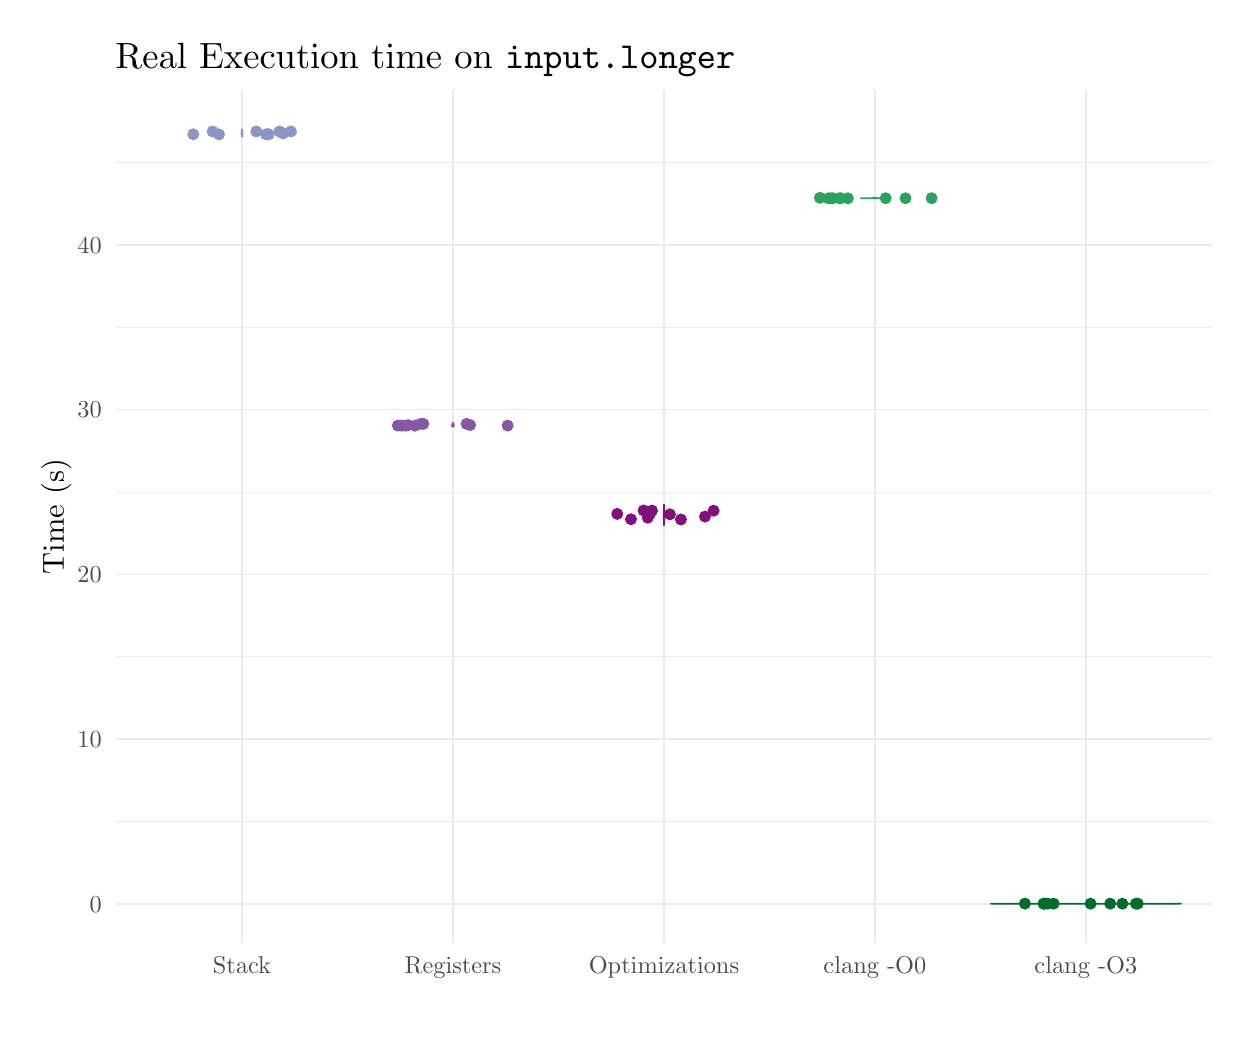
\begin{tikzpicture}[x=1pt,y=1pt]
\definecolor{fillColor}{RGB}{255,255,255}
\path[use as bounding box,fill=fillColor,fill opacity=0.00] (0,0) rectangle (433.62,361.35);
\begin{scope}
\path[clip] ( 31.71, 30.69) rectangle (428.12,338.69);
\definecolor{drawColor}{gray}{0.92}

\path[draw=drawColor,line width= 0.3pt,line join=round] ( 31.71, 74.46) --
	(428.12, 74.46);

\path[draw=drawColor,line width= 0.3pt,line join=round] ( 31.71,134.02) --
	(428.12,134.02);

\path[draw=drawColor,line width= 0.3pt,line join=round] ( 31.71,193.57) --
	(428.12,193.57);

\path[draw=drawColor,line width= 0.3pt,line join=round] ( 31.71,253.12) --
	(428.12,253.12);

\path[draw=drawColor,line width= 0.3pt,line join=round] ( 31.71,312.68) --
	(428.12,312.68);

\path[draw=drawColor,line width= 0.6pt,line join=round] ( 31.71, 44.69) --
	(428.12, 44.69);

\path[draw=drawColor,line width= 0.6pt,line join=round] ( 31.71,104.24) --
	(428.12,104.24);

\path[draw=drawColor,line width= 0.6pt,line join=round] ( 31.71,163.79) --
	(428.12,163.79);

\path[draw=drawColor,line width= 0.6pt,line join=round] ( 31.71,223.35) --
	(428.12,223.35);

\path[draw=drawColor,line width= 0.6pt,line join=round] ( 31.71,282.90) --
	(428.12,282.90);

\path[draw=drawColor,line width= 0.6pt,line join=round] ( 77.45, 30.69) --
	( 77.45,338.69);

\path[draw=drawColor,line width= 0.6pt,line join=round] (153.68, 30.69) --
	(153.68,338.69);

\path[draw=drawColor,line width= 0.6pt,line join=round] (229.92, 30.69) --
	(229.92,338.69);

\path[draw=drawColor,line width= 0.6pt,line join=round] (306.15, 30.69) --
	(306.15,338.69);

\path[draw=drawColor,line width= 0.6pt,line join=round] (382.38, 30.69) --
	(382.38,338.69);
\definecolor{drawColor}{RGB}{140,150,198}
\definecolor{fillColor}{RGB}{255,255,255}

\path[draw=drawColor,line width= 0.6pt,line join=round,line cap=round,fill=fillColor] ( 77.45,321.93) --
	( 77.45,321.94) --
	( 77.45,321.94) --
	( 77.45,321.95) --
	( 77.45,321.95) --
	( 77.45,321.96) --
	( 77.45,321.96) --
	( 77.45,321.97) --
	( 77.45,321.97) --
	( 77.45,321.98) --
	( 77.45,321.99) --
	( 77.45,321.99) --
	( 77.45,322.00) --
	( 77.45,322.00) --
	( 77.45,322.01) --
	( 77.45,322.01) --
	( 77.45,322.02) --
	( 77.45,322.02) --
	( 77.45,322.03) --
	( 77.45,322.03) --
	( 77.45,322.04) --
	( 77.45,322.04) --
	( 77.45,322.05) --
	( 77.45,322.06) --
	( 77.45,322.06) --
	( 77.45,322.07) --
	( 77.44,322.07) --
	( 77.44,322.08) --
	( 77.44,322.08) --
	( 77.44,322.09) --
	( 77.44,322.09) --
	( 77.44,322.10) --
	( 77.44,322.10) --
	( 77.44,322.11) --
	( 77.44,322.11) --
	( 77.44,322.12) --
	( 77.44,322.13) --
	( 77.44,322.13) --
	( 77.44,322.14) --
	( 77.44,322.14) --
	( 77.44,322.15) --
	( 77.44,322.15) --
	( 77.44,322.16) --
	( 77.44,322.16) --
	( 77.44,322.17) --
	( 77.44,322.17) --
	( 77.43,322.18) --
	( 77.43,322.19) --
	( 77.43,322.19) --
	( 77.43,322.20) --
	( 77.43,322.20) --
	( 77.43,322.21) --
	( 77.43,322.21) --
	( 77.43,322.22) --
	( 77.43,322.22) --
	( 77.43,322.23) --
	( 77.43,322.23) --
	( 77.42,322.24) --
	( 77.42,322.24) --
	( 77.42,322.25) --
	( 77.42,322.26) --
	( 77.42,322.26) --
	( 77.42,322.27) --
	( 77.42,322.27) --
	( 77.42,322.28) --
	( 77.42,322.28) --
	( 77.41,322.29) --
	( 77.41,322.29) --
	( 77.41,322.30) --
	( 77.41,322.30) --
	( 77.41,322.31) --
	( 77.41,322.31) --
	( 77.41,322.32) --
	( 77.40,322.33) --
	( 77.40,322.33) --
	( 77.40,322.34) --
	( 77.40,322.34) --
	( 77.40,322.35) --
	( 77.40,322.35) --
	( 77.39,322.36) --
	( 77.39,322.36) --
	( 77.39,322.37) --
	( 77.39,322.37) --
	( 77.39,322.38) --
	( 77.38,322.39) --
	( 77.38,322.39) --
	( 77.38,322.40) --
	( 77.38,322.40) --
	( 77.38,322.41) --
	( 77.37,322.41) --
	( 77.37,322.42) --
	( 77.37,322.42) --
	( 77.37,322.43) --
	( 77.36,322.43) --
	( 77.36,322.44) --
	( 77.36,322.44) --
	( 77.36,322.45) --
	( 77.36,322.46) --
	( 77.35,322.46) --
	( 77.35,322.47) --
	( 77.35,322.47) --
	( 77.35,322.48) --
	( 77.34,322.48) --
	( 77.34,322.49) --
	( 77.34,322.49) --
	( 77.34,322.50) --
	( 77.33,322.50) --
	( 77.33,322.51) --
	( 77.33,322.51) --
	( 77.33,322.52) --
	( 77.32,322.53) --
	( 77.32,322.53) --
	( 77.32,322.54) --
	( 77.32,322.54) --
	( 77.31,322.55) --
	( 77.31,322.55) --
	( 77.31,322.56) --
	( 77.30,322.56) --
	( 77.30,322.57) --
	( 77.30,322.57) --
	( 77.30,322.58) --
	( 77.29,322.59) --
	( 77.29,322.59) --
	( 77.29,322.60) --
	( 77.29,322.60) --
	( 77.28,322.61) --
	( 77.28,322.61) --
	( 77.28,322.62) --
	( 77.28,322.62) --
	( 77.27,322.63) --
	( 77.27,322.63) --
	( 77.27,322.64) --
	( 77.27,322.64) --
	( 77.26,322.65) --
	( 77.26,322.66) --
	( 77.26,322.66) --
	( 77.26,322.67) --
	( 77.25,322.67) --
	( 77.25,322.68) --
	( 77.25,322.68) --
	( 77.25,322.69) --
	( 77.25,322.69) --
	( 77.24,322.70) --
	( 77.24,322.70) --
	( 77.24,322.71) --
	( 77.24,322.71) --
	( 77.24,322.72) --
	( 77.23,322.73) --
	( 77.23,322.73) --
	( 77.23,322.74) --
	( 77.23,322.74) --
	( 77.23,322.75) --
	( 77.23,322.75) --
	( 77.23,322.76) --
	( 77.22,322.76) --
	( 77.22,322.77) --
	( 77.22,322.77) --
	( 77.22,322.78) --
	( 77.22,322.78) --
	( 77.22,322.79) --
	( 77.22,322.80) --
	( 77.22,322.80) --
	( 77.22,322.81) --
	( 77.22,322.81) --
	( 77.21,322.82) --
	( 77.21,322.82) --
	( 77.21,322.83) --
	( 77.21,322.83) --
	( 77.21,322.84) --
	( 77.21,322.84) --
	( 77.21,322.85) --
	( 77.21,322.86) --
	( 77.21,322.86) --
	( 77.21,322.87) --
	( 77.21,322.87) --
	( 77.21,322.88) --
	( 77.21,322.88) --
	( 77.21,322.89) --
	( 77.21,322.89) --
	( 77.21,322.90) --
	( 77.21,322.90) --
	( 77.22,322.91) --
	( 77.22,322.91) --
	( 77.22,322.92) --
	( 77.22,322.93) --
	( 77.22,322.93) --
	( 77.22,322.94) --
	( 77.22,322.94) --
	( 77.22,322.95) --
	( 77.22,322.95) --
	( 77.22,322.96) --
	( 77.22,322.96) --
	( 77.23,322.97) --
	( 77.23,322.97) --
	( 77.23,322.98) --
	( 77.23,322.98) --
	( 77.23,322.99) --
	( 77.23,323.00) --
	( 77.23,323.00) --
	( 77.24,323.01) --
	( 77.24,323.01) --
	( 77.24,323.02) --
	( 77.24,323.02) --
	( 77.24,323.03) --
	( 77.24,323.03) --
	( 77.25,323.04) --
	( 77.25,323.04) --
	( 77.25,323.05) --
	( 77.25,323.06) --
	( 77.25,323.06) --
	( 77.26,323.07) --
	( 77.26,323.07) --
	( 77.26,323.08) --
	( 77.26,323.08) --
	( 77.26,323.09) --
	( 77.27,323.09) --
	( 77.27,323.10) --
	( 77.27,323.10) --
	( 77.27,323.11) --
	( 77.27,323.11) --
	( 77.28,323.12) --
	( 77.28,323.13) --
	( 77.28,323.13) --
	( 77.28,323.14) --
	( 77.28,323.14) --
	( 77.29,323.15) --
	( 77.29,323.15) --
	( 77.29,323.16) --
	( 77.29,323.16) --
	( 77.29,323.17) --
	( 77.30,323.17) --
	( 77.30,323.18) --
	( 77.30,323.18) --
	( 77.30,323.19) --
	( 77.30,323.20) --
	( 77.31,323.20) --
	( 77.31,323.21) --
	( 77.31,323.21) --
	( 77.31,323.22) --
	( 77.31,323.22) --
	( 77.31,323.23) --
	( 77.32,323.23) --
	( 77.32,323.24) --
	( 77.32,323.24) --
	( 77.32,323.25) --
	( 77.32,323.26) --
	( 77.32,323.26) --
	( 77.32,323.27) --
	( 77.32,323.27) --
	( 77.33,323.28) --
	( 77.33,323.28) --
	( 77.33,323.29) --
	( 77.33,323.29) --
	( 77.33,323.30) --
	( 77.33,323.30) --
	( 77.33,323.31) --
	( 77.33,323.31) --
	( 77.33,323.32) --
	( 77.34,323.33) --
	( 77.34,323.33) --
	( 77.34,323.34) --
	( 77.34,323.34) --
	( 77.34,323.35) --
	( 77.34,323.35) --
	( 77.34,323.36) --
	( 77.34,323.36) --
	( 77.34,323.37) --
	( 77.34,323.37) --
	( 77.34,323.38) --
	( 77.34,323.38) --
	( 77.34,323.39) --
	( 77.34,323.40) --
	( 77.34,323.40) --
	( 77.34,323.41) --
	( 77.34,323.41) --
	( 77.34,323.42) --
	( 77.34,323.42) --
	( 77.34,323.43) --
	( 77.34,323.43) --
	( 77.34,323.44) --
	( 77.34,323.44) --
	( 77.34,323.45) --
	( 77.34,323.46) --
	( 77.34,323.46) --
	( 77.34,323.47) --
	( 77.34,323.47) --
	( 77.34,323.48) --
	( 77.33,323.48) --
	( 77.33,323.49) --
	( 77.33,323.49) --
	( 77.33,323.50) --
	( 77.33,323.50) --
	( 77.33,323.51) --
	( 77.33,323.51) --
	( 77.33,323.52) --
	( 77.33,323.53) --
	( 77.33,323.53) --
	( 77.33,323.54) --
	( 77.32,323.54) --
	( 77.32,323.55) --
	( 77.32,323.55) --
	( 77.32,323.56) --
	( 77.32,323.56) --
	( 77.32,323.57) --
	( 77.32,323.57) --
	( 77.32,323.58) --
	( 77.31,323.58) --
	( 77.31,323.59) --
	( 77.31,323.60) --
	( 77.31,323.60) --
	( 77.31,323.61) --
	( 77.31,323.61) --
	( 77.31,323.62) --
	( 77.31,323.62) --
	( 77.30,323.63) --
	( 77.30,323.63) --
	( 77.30,323.64) --
	( 77.30,323.64) --
	( 77.30,323.65) --
	( 77.30,323.65) --
	( 77.30,323.66) --
	( 77.30,323.67) --
	( 77.29,323.67) --
	( 77.29,323.68) --
	( 77.29,323.68) --
	( 77.29,323.69) --
	( 77.29,323.69) --
	( 77.29,323.70) --
	( 77.29,323.70) --
	( 77.29,323.71) --
	( 77.29,323.71) --
	( 77.29,323.72) --
	( 77.29,323.73) --
	( 77.28,323.73) --
	( 77.28,323.74) --
	( 77.28,323.74) --
	( 77.28,323.75) --
	( 77.28,323.75) --
	( 77.28,323.76) --
	( 77.28,323.76) --
	( 77.28,323.77) --
	( 77.28,323.77) --
	( 77.28,323.78) --
	( 77.28,323.78) --
	( 77.28,323.79) --
	( 77.28,323.80) --
	( 77.28,323.80) --
	( 77.28,323.81) --
	( 77.28,323.81) --
	( 77.28,323.82) --
	( 77.28,323.82) --
	( 77.28,323.83) --
	( 77.28,323.83) --
	( 77.28,323.84) --
	( 77.28,323.84) --
	( 77.28,323.85) --
	( 77.28,323.85) --
	( 77.28,323.86) --
	( 77.28,323.87) --
	( 77.28,323.87) --
	( 77.28,323.88) --
	( 77.28,323.88) --
	( 77.28,323.89) --
	( 77.28,323.89) --
	( 77.28,323.90) --
	( 77.28,323.90) --
	( 77.29,323.91) --
	( 77.29,323.91) --
	( 77.29,323.92) --
	( 77.29,323.93) --
	( 77.29,323.93) --
	( 77.29,323.94) --
	( 77.29,323.94) --
	( 77.29,323.95) --
	( 77.29,323.95) --
	( 77.30,323.96) --
	( 77.30,323.96) --
	( 77.30,323.97) --
	( 77.30,323.97) --
	( 77.30,323.98) --
	( 77.30,323.98) --
	( 77.30,323.99) --
	( 77.31,324.00) --
	( 77.31,324.00) --
	( 77.31,324.01) --
	( 77.31,324.01) --
	( 77.31,324.02) --
	( 77.31,324.02) --
	( 77.32,324.03) --
	( 77.32,324.03) --
	( 77.32,324.04) --
	( 77.32,324.04) --
	( 77.32,324.05) --
	( 77.33,324.05) --
	( 77.33,324.06) --
	( 77.33,324.07) --
	( 77.33,324.07) --
	( 77.33,324.08) --
	( 77.33,324.08) --
	( 77.34,324.09) --
	( 77.34,324.09) --
	( 77.34,324.10) --
	( 77.34,324.10) --
	( 77.34,324.11) --
	( 77.35,324.11) --
	( 77.35,324.12) --
	( 77.35,324.13) --
	( 77.35,324.13) --
	( 77.35,324.14) --
	( 77.36,324.14) --
	( 77.36,324.15) --
	( 77.36,324.15) --
	( 77.36,324.16) --
	( 77.36,324.16) --
	( 77.37,324.17) --
	( 77.37,324.17) --
	( 77.37,324.18) --
	( 77.37,324.18) --
	( 77.37,324.19) --
	( 77.38,324.20) --
	( 77.38,324.20) --
	( 77.38,324.21) --
	( 77.38,324.21) --
	( 77.38,324.22) --
	( 77.38,324.22) --
	( 77.39,324.23) --
	( 77.39,324.23) --
	( 77.39,324.24) --
	( 77.39,324.24) --
	( 77.39,324.25) --
	( 77.39,324.25) --
	( 77.40,324.26) --
	( 77.40,324.27) --
	( 77.40,324.27) --
	( 77.40,324.28) --
	( 77.40,324.28) --
	( 77.40,324.29) --
	( 77.40,324.29) --
	( 77.41,324.30) --
	( 77.41,324.30) --
	( 77.41,324.31) --
	( 77.41,324.31) --
	( 77.41,324.32) --
	( 77.41,324.33) --
	( 77.41,324.33) --
	( 77.42,324.34) --
	( 77.42,324.34) --
	( 77.42,324.35) --
	( 77.42,324.35) --
	( 77.42,324.36) --
	( 77.42,324.36) --
	( 77.42,324.37) --
	( 77.42,324.37) --
	( 77.42,324.38) --
	( 77.43,324.38) --
	( 77.43,324.39) --
	( 77.43,324.40) --
	( 77.43,324.40) --
	( 77.43,324.41) --
	( 77.43,324.41) --
	( 77.43,324.42) --
	( 77.43,324.42) --
	( 77.43,324.43) --
	( 77.43,324.43) --
	( 77.43,324.44) --
	( 77.43,324.44) --
	( 77.44,324.45) --
	( 77.44,324.45) --
	( 77.44,324.46) --
	( 77.44,324.47) --
	( 77.44,324.47) --
	( 77.44,324.48) --
	( 77.44,324.48) --
	( 77.44,324.49) --
	( 77.44,324.49) --
	( 77.44,324.50) --
	( 77.44,324.50) --
	( 77.44,324.51) --
	( 77.44,324.51) --
	( 77.44,324.52) --
	( 77.44,324.52) --
	( 77.44,324.53) --
	( 77.44,324.54) --
	( 77.44,324.54) --
	( 77.44,324.55) --
	( 77.44,324.55) --
	( 77.44,324.56) --
	( 77.45,324.56) --
	( 77.45,324.57) --
	( 77.45,324.57) --
	( 77.45,324.58) --
	( 77.45,324.58) --
	( 77.45,324.59) --
	( 77.45,324.60) --
	( 77.45,324.60) --
	( 77.45,324.61) --
	( 77.45,324.61) --
	( 77.45,324.62) --
	( 77.45,324.62) --
	( 77.45,324.63) --
	( 77.45,324.63) --
	( 77.45,324.64) --
	( 77.45,324.64) --
	( 77.45,324.65) --
	( 77.45,324.65) --
	( 77.45,324.66) --
	( 77.45,324.67) --
	( 77.45,324.67) --
	( 77.45,324.68) --
	( 77.45,324.68) --
	( 77.45,324.69) --
	( 77.45,324.69) --
	( 77.45,324.69) --
	( 77.45,324.69) --
	( 77.45,324.68) --
	( 77.45,324.68) --
	( 77.45,324.67) --
	( 77.45,324.67) --
	( 77.45,324.66) --
	( 77.45,324.65) --
	( 77.45,324.65) --
	( 77.45,324.64) --
	( 77.45,324.64) --
	( 77.45,324.63) --
	( 77.46,324.63) --
	( 77.46,324.62) --
	( 77.46,324.62) --
	( 77.46,324.61) --
	( 77.46,324.61) --
	( 77.46,324.60) --
	( 77.46,324.60) --
	( 77.46,324.59) --
	( 77.46,324.58) --
	( 77.46,324.58) --
	( 77.46,324.57) --
	( 77.46,324.57) --
	( 77.46,324.56) --
	( 77.46,324.56) --
	( 77.46,324.55) --
	( 77.46,324.55) --
	( 77.46,324.54) --
	( 77.46,324.54) --
	( 77.46,324.53) --
	( 77.46,324.52) --
	( 77.46,324.52) --
	( 77.46,324.51) --
	( 77.46,324.51) --
	( 77.46,324.50) --
	( 77.46,324.50) --
	( 77.46,324.49) --
	( 77.46,324.49) --
	( 77.46,324.48) --
	( 77.47,324.48) --
	( 77.47,324.47) --
	( 77.47,324.47) --
	( 77.47,324.46) --
	( 77.47,324.45) --
	( 77.47,324.45) --
	( 77.47,324.44) --
	( 77.47,324.44) --
	( 77.47,324.43) --
	( 77.47,324.43) --
	( 77.47,324.42) --
	( 77.47,324.42) --
	( 77.47,324.41) --
	( 77.47,324.41) --
	( 77.48,324.40) --
	( 77.48,324.40) --
	( 77.48,324.39) --
	( 77.48,324.38) --
	( 77.48,324.38) --
	( 77.48,324.37) --
	( 77.48,324.37) --
	( 77.48,324.36) --
	( 77.48,324.36) --
	( 77.48,324.35) --
	( 77.49,324.35) --
	( 77.49,324.34) --
	( 77.49,324.34) --
	( 77.49,324.33) --
	( 77.49,324.33) --
	( 77.49,324.32) --
	( 77.49,324.31) --
	( 77.49,324.31) --
	( 77.50,324.30) --
	( 77.50,324.30) --
	( 77.50,324.29) --
	( 77.50,324.29) --
	( 77.50,324.28) --
	( 77.50,324.28) --
	( 77.50,324.27) --
	( 77.51,324.27) --
	( 77.51,324.26) --
	( 77.51,324.25) --
	( 77.51,324.25) --
	( 77.51,324.24) --
	( 77.51,324.24) --
	( 77.52,324.23) --
	( 77.52,324.23) --
	( 77.52,324.22) --
	( 77.52,324.22) --
	( 77.52,324.21) --
	( 77.52,324.21) --
	( 77.53,324.20) --
	( 77.53,324.20) --
	( 77.53,324.19) --
	( 77.53,324.18) --
	( 77.53,324.18) --
	( 77.54,324.17) --
	( 77.54,324.17) --
	( 77.54,324.16) --
	( 77.54,324.16) --
	( 77.54,324.15) --
	( 77.54,324.15) --
	( 77.55,324.14) --
	( 77.55,324.14) --
	( 77.55,324.13) --
	( 77.55,324.13) --
	( 77.55,324.12) --
	( 77.56,324.11) --
	( 77.56,324.11) --
	( 77.56,324.10) --
	( 77.56,324.10) --
	( 77.56,324.09) --
	( 77.57,324.09) --
	( 77.57,324.08) --
	( 77.57,324.08) --
	( 77.57,324.07) --
	( 77.57,324.07) --
	( 77.58,324.06) --
	( 77.58,324.05) --
	( 77.58,324.05) --
	( 77.58,324.04) --
	( 77.58,324.04) --
	( 77.59,324.03) --
	( 77.59,324.03) --
	( 77.59,324.02) --
	( 77.59,324.02) --
	( 77.59,324.01) --
	( 77.59,324.01) --
	( 77.60,324.00) --
	( 77.60,324.00) --
	( 77.60,323.99) --
	( 77.60,323.98) --
	( 77.60,323.98) --
	( 77.60,323.97) --
	( 77.61,323.97) --
	( 77.61,323.96) --
	( 77.61,323.96) --
	( 77.61,323.95) --
	( 77.61,323.95) --
	( 77.61,323.94) --
	( 77.61,323.94) --
	( 77.61,323.93) --
	( 77.62,323.93) --
	( 77.62,323.92) --
	( 77.62,323.91) --
	( 77.62,323.91) --
	( 77.62,323.90) --
	( 77.62,323.90) --
	( 77.62,323.89) --
	( 77.62,323.89) --
	( 77.62,323.88) --
	( 77.62,323.88) --
	( 77.62,323.87) --
	( 77.62,323.87) --
	( 77.62,323.86) --
	( 77.62,323.85) --
	( 77.62,323.85) --
	( 77.63,323.84) --
	( 77.63,323.84) --
	( 77.63,323.83) --
	( 77.63,323.83) --
	( 77.63,323.82) --
	( 77.63,323.82) --
	( 77.63,323.81) --
	( 77.63,323.81) --
	( 77.63,323.80) --
	( 77.63,323.80) --
	( 77.63,323.79) --
	( 77.62,323.78) --
	( 77.62,323.78) --
	( 77.62,323.77) --
	( 77.62,323.77) --
	( 77.62,323.76) --
	( 77.62,323.76) --
	( 77.62,323.75) --
	( 77.62,323.75) --
	( 77.62,323.74) --
	( 77.62,323.74) --
	( 77.62,323.73) --
	( 77.62,323.73) --
	( 77.62,323.72) --
	( 77.62,323.71) --
	( 77.62,323.71) --
	( 77.61,323.70) --
	( 77.61,323.70) --
	( 77.61,323.69) --
	( 77.61,323.69) --
	( 77.61,323.68) --
	( 77.61,323.68) --
	( 77.61,323.67) --
	( 77.61,323.67) --
	( 77.61,323.66) --
	( 77.60,323.65) --
	( 77.60,323.65) --
	( 77.60,323.64) --
	( 77.60,323.64) --
	( 77.60,323.63) --
	( 77.60,323.63) --
	( 77.60,323.62) --
	( 77.60,323.62) --
	( 77.59,323.61) --
	( 77.59,323.61) --
	( 77.59,323.60) --
	( 77.59,323.60) --
	( 77.59,323.59) --
	( 77.59,323.58) --
	( 77.59,323.58) --
	( 77.59,323.57) --
	( 77.58,323.57) --
	( 77.58,323.56) --
	( 77.58,323.56) --
	( 77.58,323.55) --
	( 77.58,323.55) --
	( 77.58,323.54) --
	( 77.58,323.54) --
	( 77.58,323.53) --
	( 77.58,323.53) --
	( 77.57,323.52) --
	( 77.57,323.51) --
	( 77.57,323.51) --
	( 77.57,323.50) --
	( 77.57,323.50) --
	( 77.57,323.49) --
	( 77.57,323.49) --
	( 77.57,323.48) --
	( 77.57,323.48) --
	( 77.57,323.47) --
	( 77.57,323.47) --
	( 77.57,323.46) --
	( 77.57,323.46) --
	( 77.57,323.45) --
	( 77.56,323.44) --
	( 77.56,323.44) --
	( 77.56,323.43) --
	( 77.56,323.43) --
	( 77.56,323.42) --
	( 77.56,323.42) --
	( 77.56,323.41) --
	( 77.56,323.41) --
	( 77.56,323.40) --
	( 77.56,323.40) --
	( 77.56,323.39) --
	( 77.56,323.38) --
	( 77.56,323.38) --
	( 77.56,323.37) --
	( 77.56,323.37) --
	( 77.56,323.36) --
	( 77.56,323.36) --
	( 77.56,323.35) --
	( 77.57,323.35) --
	( 77.57,323.34) --
	( 77.57,323.34) --
	( 77.57,323.33) --
	( 77.57,323.33) --
	( 77.57,323.32) --
	( 77.57,323.31) --
	( 77.57,323.31) --
	( 77.57,323.30) --
	( 77.57,323.30) --
	( 77.57,323.29) --
	( 77.57,323.29) --
	( 77.58,323.28) --
	( 77.58,323.28) --
	( 77.58,323.27) --
	( 77.58,323.27) --
	( 77.58,323.26) --
	( 77.58,323.26) --
	( 77.58,323.25) --
	( 77.59,323.24) --
	( 77.59,323.24) --
	( 77.59,323.23) --
	( 77.59,323.23) --
	( 77.59,323.22) --
	( 77.59,323.22) --
	( 77.59,323.21) --
	( 77.60,323.21) --
	( 77.60,323.20) --
	( 77.60,323.20) --
	( 77.60,323.19) --
	( 77.60,323.18) --
	( 77.61,323.18) --
	( 77.61,323.17) --
	( 77.61,323.17) --
	( 77.61,323.16) --
	( 77.61,323.16) --
	( 77.62,323.15) --
	( 77.62,323.15) --
	( 77.62,323.14) --
	( 77.62,323.14) --
	( 77.62,323.13) --
	( 77.63,323.13) --
	( 77.63,323.12) --
	( 77.63,323.11) --
	( 77.63,323.11) --
	( 77.63,323.10) --
	( 77.64,323.10) --
	( 77.64,323.09) --
	( 77.64,323.09) --
	( 77.64,323.08) --
	( 77.64,323.08) --
	( 77.65,323.07) --
	( 77.65,323.07) --
	( 77.65,323.06) --
	( 77.65,323.06) --
	( 77.65,323.05) --
	( 77.65,323.04) --
	( 77.66,323.04) --
	( 77.66,323.03) --
	( 77.66,323.03) --
	( 77.66,323.02) --
	( 77.66,323.02) --
	( 77.67,323.01) --
	( 77.67,323.01) --
	( 77.67,323.00) --
	( 77.67,323.00) --
	( 77.67,322.99) --
	( 77.67,322.98) --
	( 77.67,322.98) --
	( 77.68,322.97) --
	( 77.68,322.97) --
	( 77.68,322.96) --
	( 77.68,322.96) --
	( 77.68,322.95) --
	( 77.68,322.95) --
	( 77.68,322.94) --
	( 77.68,322.94) --
	( 77.68,322.93) --
	( 77.69,322.93) --
	( 77.69,322.92) --
	( 77.69,322.91) --
	( 77.69,322.91) --
	( 77.69,322.90) --
	( 77.69,322.90) --
	( 77.69,322.89) --
	( 77.69,322.89) --
	( 77.69,322.88) --
	( 77.69,322.88) --
	( 77.69,322.87) --
	( 77.69,322.87) --
	( 77.69,322.86) --
	( 77.69,322.86) --
	( 77.69,322.85) --
	( 77.69,322.84) --
	( 77.69,322.84) --
	( 77.69,322.83) --
	( 77.69,322.83) --
	( 77.69,322.82) --
	( 77.69,322.82) --
	( 77.69,322.81) --
	( 77.69,322.81) --
	( 77.69,322.80) --
	( 77.69,322.80) --
	( 77.68,322.79) --
	( 77.68,322.78) --
	( 77.68,322.78) --
	( 77.68,322.77) --
	( 77.68,322.77) --
	( 77.68,322.76) --
	( 77.68,322.76) --
	( 77.68,322.75) --
	( 77.67,322.75) --
	( 77.67,322.74) --
	( 77.67,322.74) --
	( 77.67,322.73) --
	( 77.67,322.73) --
	( 77.67,322.72) --
	( 77.66,322.71) --
	( 77.66,322.71) --
	( 77.66,322.70) --
	( 77.66,322.70) --
	( 77.66,322.69) --
	( 77.65,322.69) --
	( 77.65,322.68) --
	( 77.65,322.68) --
	( 77.65,322.67) --
	( 77.65,322.67) --
	( 77.64,322.66) --
	( 77.64,322.66) --
	( 77.64,322.65) --
	( 77.64,322.64) --
	( 77.63,322.64) --
	( 77.63,322.63) --
	( 77.63,322.63) --
	( 77.63,322.62) --
	( 77.62,322.62) --
	( 77.62,322.61) --
	( 77.62,322.61) --
	( 77.62,322.60) --
	( 77.61,322.60) --
	( 77.61,322.59) --
	( 77.61,322.59) --
	( 77.61,322.58) --
	( 77.60,322.57) --
	( 77.60,322.57) --
	( 77.60,322.56) --
	( 77.60,322.56) --
	( 77.59,322.55) --
	( 77.59,322.55) --
	( 77.59,322.54) --
	( 77.59,322.54) --
	( 77.58,322.53) --
	( 77.58,322.53) --
	( 77.58,322.52) --
	( 77.58,322.51) --
	( 77.57,322.51) --
	( 77.57,322.50) --
	( 77.57,322.50) --
	( 77.56,322.49) --
	( 77.56,322.49) --
	( 77.56,322.48) --
	( 77.56,322.48) --
	( 77.55,322.47) --
	( 77.55,322.47) --
	( 77.55,322.46) --
	( 77.55,322.46) --
	( 77.55,322.45) --
	( 77.54,322.44) --
	( 77.54,322.44) --
	( 77.54,322.43) --
	( 77.54,322.43) --
	( 77.53,322.42) --
	( 77.53,322.42) --
	( 77.53,322.41) --
	( 77.53,322.41) --
	( 77.53,322.40) --
	( 77.52,322.40) --
	( 77.52,322.39) --
	( 77.52,322.39) --
	( 77.52,322.38) --
	( 77.52,322.37) --
	( 77.51,322.37) --
	( 77.51,322.36) --
	( 77.51,322.36) --
	( 77.51,322.35) --
	( 77.51,322.35) --
	( 77.50,322.34) --
	( 77.50,322.34) --
	( 77.50,322.33) --
	( 77.50,322.33) --
	( 77.50,322.32) --
	( 77.50,322.31) --
	( 77.49,322.31) --
	( 77.49,322.30) --
	( 77.49,322.30) --
	( 77.49,322.29) --
	( 77.49,322.29) --
	( 77.49,322.28) --
	( 77.49,322.28) --
	( 77.49,322.27) --
	( 77.48,322.27) --
	( 77.48,322.26) --
	( 77.48,322.26) --
	( 77.48,322.25) --
	( 77.48,322.24) --
	( 77.48,322.24) --
	( 77.48,322.23) --
	( 77.48,322.23) --
	( 77.48,322.22) --
	( 77.47,322.22) --
	( 77.47,322.21) --
	( 77.47,322.21) --
	( 77.47,322.20) --
	( 77.47,322.20) --
	( 77.47,322.19) --
	( 77.47,322.19) --
	( 77.47,322.18) --
	( 77.47,322.17) --
	( 77.47,322.17) --
	( 77.47,322.16) --
	( 77.47,322.16) --
	( 77.47,322.15) --
	( 77.46,322.15) --
	( 77.46,322.14) --
	( 77.46,322.14) --
	( 77.46,322.13) --
	( 77.46,322.13) --
	( 77.46,322.12) --
	( 77.46,322.11) --
	( 77.46,322.11) --
	( 77.46,322.10) --
	( 77.46,322.10) --
	( 77.46,322.09) --
	( 77.46,322.09) --
	( 77.46,322.08) --
	( 77.46,322.08) --
	( 77.46,322.07) --
	( 77.46,322.07) --
	( 77.46,322.06) --
	( 77.46,322.06) --
	( 77.46,322.05) --
	( 77.46,322.04) --
	( 77.46,322.04) --
	( 77.46,322.03) --
	( 77.46,322.03) --
	( 77.46,322.02) --
	( 77.46,322.02) --
	( 77.46,322.01) --
	( 77.46,322.01) --
	( 77.46,322.00) --
	( 77.45,322.00) --
	( 77.45,321.99) --
	( 77.45,321.99) --
	( 77.45,321.98) --
	( 77.45,321.97) --
	( 77.45,321.97) --
	( 77.45,321.96) --
	( 77.45,321.96) --
	( 77.45,321.95) --
	( 77.45,321.95) --
	( 77.45,321.94) --
	( 77.45,321.94) --
	( 77.45,321.93) --
	( 77.45,321.93) --
	cycle;
\definecolor{drawColor}{RGB}{136,86,167}

\path[draw=drawColor,line width= 0.6pt,line join=round,line cap=round,fill=fillColor] (153.68,217.03) --
	(153.68,217.04) --
	(153.68,217.04) --
	(153.68,217.04) --
	(153.68,217.05) --
	(153.68,217.05) --
	(153.68,217.05) --
	(153.68,217.05) --
	(153.68,217.06) --
	(153.68,217.06) --
	(153.68,217.06) --
	(153.68,217.07) --
	(153.68,217.07) --
	(153.68,217.07) --
	(153.68,217.08) --
	(153.68,217.08) --
	(153.68,217.08) --
	(153.68,217.09) --
	(153.67,217.09) --
	(153.67,217.09) --
	(153.67,217.10) --
	(153.67,217.10) --
	(153.67,217.10) --
	(153.67,217.11) --
	(153.67,217.11) --
	(153.67,217.11) --
	(153.67,217.12) --
	(153.67,217.12) --
	(153.67,217.12) --
	(153.67,217.13) --
	(153.67,217.13) --
	(153.67,217.13) --
	(153.67,217.14) --
	(153.66,217.14) --
	(153.66,217.14) --
	(153.66,217.15) --
	(153.66,217.15) --
	(153.66,217.15) --
	(153.66,217.16) --
	(153.66,217.16) --
	(153.66,217.16) --
	(153.66,217.16) --
	(153.65,217.17) --
	(153.65,217.17) --
	(153.65,217.17) --
	(153.65,217.18) --
	(153.65,217.18) --
	(153.65,217.18) --
	(153.65,217.19) --
	(153.64,217.19) --
	(153.64,217.19) --
	(153.64,217.20) --
	(153.64,217.20) --
	(153.64,217.20) --
	(153.63,217.21) --
	(153.63,217.21) --
	(153.63,217.21) --
	(153.63,217.22) --
	(153.63,217.22) --
	(153.62,217.22) --
	(153.62,217.23) --
	(153.62,217.23) --
	(153.62,217.23) --
	(153.61,217.24) --
	(153.61,217.24) --
	(153.61,217.24) --
	(153.61,217.25) --
	(153.60,217.25) --
	(153.60,217.25) --
	(153.60,217.26) --
	(153.60,217.26) --
	(153.59,217.26) --
	(153.59,217.26) --
	(153.59,217.27) --
	(153.58,217.27) --
	(153.58,217.27) --
	(153.58,217.28) --
	(153.57,217.28) --
	(153.57,217.28) --
	(153.57,217.29) --
	(153.56,217.29) --
	(153.56,217.29) --
	(153.55,217.30) --
	(153.55,217.30) --
	(153.55,217.30) --
	(153.54,217.31) --
	(153.54,217.31) --
	(153.53,217.31) --
	(153.53,217.32) --
	(153.53,217.32) --
	(153.52,217.32) --
	(153.52,217.33) --
	(153.51,217.33) --
	(153.51,217.33) --
	(153.50,217.34) --
	(153.50,217.34) --
	(153.50,217.34) --
	(153.49,217.35) --
	(153.49,217.35) --
	(153.48,217.35) --
	(153.48,217.36) --
	(153.47,217.36) --
	(153.47,217.36) --
	(153.46,217.37) --
	(153.46,217.37) --
	(153.45,217.37) --
	(153.45,217.37) --
	(153.44,217.38) --
	(153.44,217.38) --
	(153.43,217.38) --
	(153.43,217.39) --
	(153.42,217.39) --
	(153.42,217.39) --
	(153.41,217.40) --
	(153.41,217.40) --
	(153.40,217.40) --
	(153.40,217.41) --
	(153.39,217.41) --
	(153.39,217.41) --
	(153.38,217.42) --
	(153.38,217.42) --
	(153.37,217.42) --
	(153.37,217.43) --
	(153.36,217.43) --
	(153.36,217.43) --
	(153.35,217.44) --
	(153.35,217.44) --
	(153.34,217.44) --
	(153.34,217.45) --
	(153.33,217.45) --
	(153.33,217.45) --
	(153.33,217.46) --
	(153.32,217.46) --
	(153.32,217.46) --
	(153.31,217.47) --
	(153.31,217.47) --
	(153.30,217.47) --
	(153.30,217.48) --
	(153.30,217.48) --
	(153.29,217.48) --
	(153.29,217.48) --
	(153.29,217.49) --
	(153.28,217.49) --
	(153.28,217.49) --
	(153.27,217.50) --
	(153.27,217.50) --
	(153.27,217.50) --
	(153.27,217.51) --
	(153.26,217.51) --
	(153.26,217.51) --
	(153.26,217.52) --
	(153.25,217.52) --
	(153.25,217.52) --
	(153.25,217.53) --
	(153.25,217.53) --
	(153.25,217.53) --
	(153.24,217.54) --
	(153.24,217.54) --
	(153.24,217.54) --
	(153.24,217.55) --
	(153.24,217.55) --
	(153.24,217.55) --
	(153.23,217.56) --
	(153.23,217.56) --
	(153.23,217.56) --
	(153.23,217.57) --
	(153.23,217.57) --
	(153.23,217.57) --
	(153.23,217.58) --
	(153.23,217.58) --
	(153.23,217.58) --
	(153.23,217.58) --
	(153.23,217.59) --
	(153.23,217.59) --
	(153.23,217.59) --
	(153.23,217.60) --
	(153.23,217.60) --
	(153.23,217.60) --
	(153.23,217.61) --
	(153.23,217.61) --
	(153.23,217.61) --
	(153.24,217.62) --
	(153.24,217.62) --
	(153.24,217.62) --
	(153.24,217.63) --
	(153.24,217.63) --
	(153.24,217.63) --
	(153.25,217.64) --
	(153.25,217.64) --
	(153.25,217.64) --
	(153.25,217.65) --
	(153.25,217.65) --
	(153.26,217.65) --
	(153.26,217.66) --
	(153.26,217.66) --
	(153.27,217.66) --
	(153.27,217.67) --
	(153.27,217.67) --
	(153.27,217.67) --
	(153.28,217.68) --
	(153.28,217.68) --
	(153.28,217.68) --
	(153.29,217.69) --
	(153.29,217.69) --
	(153.29,217.69) --
	(153.30,217.69) --
	(153.30,217.70) --
	(153.30,217.70) --
	(153.31,217.70) --
	(153.31,217.71) --
	(153.31,217.71) --
	(153.32,217.71) --
	(153.32,217.72) --
	(153.33,217.72) --
	(153.33,217.72) --
	(153.33,217.73) --
	(153.34,217.73) --
	(153.34,217.73) --
	(153.35,217.74) --
	(153.35,217.74) --
	(153.35,217.74) --
	(153.36,217.75) --
	(153.36,217.75) --
	(153.36,217.75) --
	(153.37,217.76) --
	(153.37,217.76) --
	(153.38,217.76) --
	(153.38,217.77) --
	(153.38,217.77) --
	(153.39,217.77) --
	(153.39,217.78) --
	(153.40,217.78) --
	(153.40,217.78) --
	(153.40,217.79) --
	(153.41,217.79) --
	(153.41,217.79) --
	(153.42,217.79) --
	(153.42,217.80) --
	(153.42,217.80) --
	(153.43,217.80) --
	(153.43,217.81) --
	(153.43,217.81) --
	(153.44,217.81) --
	(153.44,217.82) --
	(153.44,217.82) --
	(153.45,217.82) --
	(153.45,217.83) --
	(153.45,217.83) --
	(153.46,217.83) --
	(153.46,217.84) --
	(153.46,217.84) --
	(153.46,217.84) --
	(153.47,217.85) --
	(153.47,217.85) --
	(153.47,217.85) --
	(153.48,217.86) --
	(153.48,217.86) --
	(153.48,217.86) --
	(153.48,217.87) --
	(153.49,217.87) --
	(153.49,217.87) --
	(153.49,217.88) --
	(153.49,217.88) --
	(153.49,217.88) --
	(153.50,217.89) --
	(153.50,217.89) --
	(153.50,217.89) --
	(153.50,217.90) --
	(153.50,217.90) --
	(153.50,217.90) --
	(153.50,217.90) --
	(153.51,217.91) --
	(153.51,217.91) --
	(153.51,217.91) --
	(153.51,217.92) --
	(153.51,217.92) --
	(153.51,217.92) --
	(153.51,217.93) --
	(153.51,217.93) --
	(153.51,217.93) --
	(153.51,217.94) --
	(153.51,217.94) --
	(153.51,217.94) --
	(153.51,217.95) --
	(153.51,217.95) --
	(153.51,217.95) --
	(153.51,217.96) --
	(153.51,217.96) --
	(153.51,217.96) --
	(153.51,217.97) --
	(153.51,217.97) --
	(153.51,217.97) --
	(153.51,217.98) --
	(153.51,217.98) --
	(153.51,217.98) --
	(153.51,217.99) --
	(153.51,217.99) --
	(153.51,217.99) --
	(153.51,218.00) --
	(153.51,218.00) --
	(153.51,218.00) --
	(153.51,218.01) --
	(153.51,218.01) --
	(153.50,218.01) --
	(153.50,218.01) --
	(153.50,218.02) --
	(153.50,218.02) --
	(153.50,218.02) --
	(153.50,218.03) --
	(153.50,218.03) --
	(153.50,218.03) --
	(153.50,218.04) --
	(153.49,218.04) --
	(153.49,218.04) --
	(153.49,218.05) --
	(153.49,218.05) --
	(153.49,218.05) --
	(153.49,218.06) --
	(153.49,218.06) --
	(153.48,218.06) --
	(153.48,218.07) --
	(153.48,218.07) --
	(153.48,218.07) --
	(153.48,218.08) --
	(153.48,218.08) --
	(153.48,218.08) --
	(153.48,218.09) --
	(153.47,218.09) --
	(153.47,218.09) --
	(153.47,218.10) --
	(153.47,218.10) --
	(153.47,218.10) --
	(153.47,218.11) --
	(153.47,218.11) --
	(153.47,218.11) --
	(153.46,218.11) --
	(153.46,218.12) --
	(153.46,218.12) --
	(153.46,218.12) --
	(153.46,218.13) --
	(153.46,218.13) --
	(153.46,218.13) --
	(153.46,218.14) --
	(153.46,218.14) --
	(153.46,218.14) --
	(153.46,218.15) --
	(153.46,218.15) --
	(153.46,218.15) --
	(153.46,218.16) --
	(153.46,218.16) --
	(153.46,218.16) --
	(153.46,218.17) --
	(153.46,218.17) --
	(153.46,218.17) --
	(153.46,218.18) --
	(153.46,218.18) --
	(153.46,218.18) --
	(153.46,218.19) --
	(153.46,218.19) --
	(153.46,218.19) --
	(153.46,218.20) --
	(153.46,218.20) --
	(153.46,218.20) --
	(153.46,218.21) --
	(153.46,218.21) --
	(153.46,218.21) --
	(153.47,218.22) --
	(153.47,218.22) --
	(153.47,218.22) --
	(153.47,218.22) --
	(153.47,218.23) --
	(153.47,218.23) --
	(153.47,218.23) --
	(153.47,218.24) --
	(153.48,218.24) --
	(153.48,218.24) --
	(153.48,218.25) --
	(153.48,218.25) --
	(153.48,218.25) --
	(153.49,218.26) --
	(153.49,218.26) --
	(153.49,218.26) --
	(153.49,218.27) --
	(153.49,218.27) --
	(153.50,218.27) --
	(153.50,218.28) --
	(153.50,218.28) --
	(153.50,218.28) --
	(153.51,218.29) --
	(153.51,218.29) --
	(153.51,218.29) --
	(153.51,218.30) --
	(153.51,218.30) --
	(153.52,218.30) --
	(153.52,218.31) --
	(153.52,218.31) --
	(153.52,218.31) --
	(153.53,218.32) --
	(153.53,218.32) --
	(153.53,218.32) --
	(153.54,218.32) --
	(153.54,218.33) --
	(153.54,218.33) --
	(153.54,218.33) --
	(153.55,218.34) --
	(153.55,218.34) --
	(153.55,218.34) --
	(153.55,218.35) --
	(153.56,218.35) --
	(153.56,218.35) --
	(153.56,218.36) --
	(153.56,218.36) --
	(153.57,218.36) --
	(153.57,218.37) --
	(153.57,218.37) --
	(153.57,218.37) --
	(153.58,218.38) --
	(153.58,218.38) --
	(153.58,218.38) --
	(153.58,218.39) --
	(153.59,218.39) --
	(153.59,218.39) --
	(153.59,218.40) --
	(153.59,218.40) --
	(153.60,218.40) --
	(153.60,218.41) --
	(153.60,218.41) --
	(153.60,218.41) --
	(153.61,218.42) --
	(153.61,218.42) --
	(153.61,218.42) --
	(153.61,218.43) --
	(153.61,218.43) --
	(153.62,218.43) --
	(153.62,218.43) --
	(153.62,218.44) --
	(153.62,218.44) --
	(153.62,218.44) --
	(153.63,218.45) --
	(153.63,218.45) --
	(153.63,218.45) --
	(153.63,218.46) --
	(153.63,218.46) --
	(153.63,218.46) --
	(153.64,218.47) --
	(153.64,218.47) --
	(153.64,218.47) --
	(153.64,218.48) --
	(153.64,218.48) --
	(153.64,218.48) --
	(153.65,218.49) --
	(153.65,218.49) --
	(153.65,218.49) --
	(153.65,218.50) --
	(153.65,218.50) --
	(153.65,218.50) --
	(153.65,218.51) --
	(153.65,218.51) --
	(153.66,218.51) --
	(153.66,218.52) --
	(153.66,218.52) --
	(153.66,218.52) --
	(153.66,218.53) --
	(153.66,218.53) --
	(153.66,218.53) --
	(153.66,218.54) --
	(153.66,218.54) --
	(153.66,218.54) --
	(153.67,218.54) --
	(153.67,218.55) --
	(153.67,218.55) --
	(153.67,218.55) --
	(153.67,218.56) --
	(153.67,218.56) --
	(153.67,218.56) --
	(153.67,218.57) --
	(153.67,218.57) --
	(153.67,218.57) --
	(153.67,218.58) --
	(153.67,218.58) --
	(153.67,218.58) --
	(153.67,218.59) --
	(153.67,218.59) --
	(153.67,218.59) --
	(153.67,218.60) --
	(153.68,218.60) --
	(153.68,218.60) --
	(153.68,218.61) --
	(153.68,218.61) --
	(153.68,218.61) --
	(153.68,218.62) --
	(153.68,218.62) --
	(153.68,218.62) --
	(153.68,218.63) --
	(153.68,218.63) --
	(153.68,218.63) --
	(153.68,218.64) --
	(153.68,218.64) --
	(153.68,218.64) --
	(153.68,218.64) --
	(153.68,218.65) --
	(153.68,218.65) --
	(153.68,218.65) --
	(153.68,218.66) --
	(153.68,218.66) --
	(153.68,218.66) --
	(153.68,218.67) --
	(153.68,218.67) --
	(153.68,218.67) --
	(153.68,218.68) --
	(153.68,218.68) --
	(153.68,218.68) --
	(153.69,218.68) --
	(153.69,218.68) --
	(153.69,218.68) --
	(153.69,218.67) --
	(153.69,218.67) --
	(153.69,218.67) --
	(153.69,218.66) --
	(153.69,218.66) --
	(153.69,218.66) --
	(153.69,218.65) --
	(153.69,218.65) --
	(153.69,218.65) --
	(153.69,218.64) --
	(153.69,218.64) --
	(153.69,218.64) --
	(153.69,218.64) --
	(153.69,218.63) --
	(153.69,218.63) --
	(153.69,218.63) --
	(153.69,218.62) --
	(153.69,218.62) --
	(153.69,218.62) --
	(153.69,218.61) --
	(153.69,218.61) --
	(153.69,218.61) --
	(153.69,218.60) --
	(153.69,218.60) --
	(153.69,218.60) --
	(153.69,218.59) --
	(153.69,218.59) --
	(153.69,218.59) --
	(153.69,218.58) --
	(153.70,218.58) --
	(153.70,218.58) --
	(153.70,218.57) --
	(153.70,218.57) --
	(153.70,218.57) --
	(153.70,218.56) --
	(153.70,218.56) --
	(153.70,218.56) --
	(153.70,218.55) --
	(153.70,218.55) --
	(153.70,218.55) --
	(153.70,218.54) --
	(153.70,218.54) --
	(153.70,218.54) --
	(153.71,218.54) --
	(153.71,218.53) --
	(153.71,218.53) --
	(153.71,218.53) --
	(153.71,218.52) --
	(153.71,218.52) --
	(153.71,218.52) --
	(153.71,218.51) --
	(153.71,218.51) --
	(153.71,218.51) --
	(153.72,218.50) --
	(153.72,218.50) --
	(153.72,218.50) --
	(153.72,218.49) --
	(153.72,218.49) --
	(153.72,218.49) --
	(153.72,218.48) --
	(153.73,218.48) --
	(153.73,218.48) --
	(153.73,218.47) --
	(153.73,218.47) --
	(153.73,218.47) --
	(153.73,218.46) --
	(153.73,218.46) --
	(153.74,218.46) --
	(153.74,218.45) --
	(153.74,218.45) --
	(153.74,218.45) --
	(153.74,218.44) --
	(153.75,218.44) --
	(153.75,218.44) --
	(153.75,218.43) --
	(153.75,218.43) --
	(153.75,218.43) --
	(153.76,218.43) --
	(153.76,218.42) --
	(153.76,218.42) --
	(153.76,218.42) --
	(153.76,218.41) --
	(153.77,218.41) --
	(153.77,218.41) --
	(153.77,218.40) --
	(153.77,218.40) --
	(153.78,218.40) --
	(153.78,218.39) --
	(153.78,218.39) --
	(153.78,218.39) --
	(153.79,218.38) --
	(153.79,218.38) --
	(153.79,218.38) --
	(153.79,218.37) --
	(153.80,218.37) --
	(153.80,218.37) --
	(153.80,218.36) --
	(153.80,218.36) --
	(153.81,218.36) --
	(153.81,218.35) --
	(153.81,218.35) --
	(153.81,218.35) --
	(153.82,218.34) --
	(153.82,218.34) --
	(153.82,218.34) --
	(153.82,218.33) --
	(153.83,218.33) --
	(153.83,218.33) --
	(153.83,218.32) --
	(153.84,218.32) --
	(153.84,218.32) --
	(153.84,218.32) --
	(153.84,218.31) --
	(153.85,218.31) --
	(153.85,218.31) --
	(153.85,218.30) --
	(153.85,218.30) --
	(153.86,218.30) --
	(153.86,218.29) --
	(153.86,218.29) --
	(153.86,218.29) --
	(153.87,218.28) --
	(153.87,218.28) --
	(153.87,218.28) --
	(153.87,218.27) --
	(153.87,218.27) --
	(153.88,218.27) --
	(153.88,218.26) --
	(153.88,218.26) --
	(153.88,218.26) --
	(153.88,218.25) --
	(153.89,218.25) --
	(153.89,218.25) --
	(153.89,218.24) --
	(153.89,218.24) --
	(153.89,218.24) --
	(153.89,218.23) --
	(153.90,218.23) --
	(153.90,218.23) --
	(153.90,218.22) --
	(153.90,218.22) --
	(153.90,218.22) --
	(153.90,218.22) --
	(153.90,218.21) --
	(153.90,218.21) --
	(153.91,218.21) --
	(153.91,218.20) --
	(153.91,218.20) --
	(153.91,218.20) --
	(153.91,218.19) --
	(153.91,218.19) --
	(153.91,218.19) --
	(153.91,218.18) --
	(153.91,218.18) --
	(153.91,218.18) --
	(153.91,218.17) --
	(153.91,218.17) --
	(153.91,218.17) --
	(153.91,218.16) --
	(153.91,218.16) --
	(153.91,218.16) --
	(153.91,218.15) --
	(153.91,218.15) --
	(153.91,218.15) --
	(153.91,218.14) --
	(153.91,218.14) --
	(153.91,218.14) --
	(153.91,218.13) --
	(153.91,218.13) --
	(153.91,218.13) --
	(153.91,218.12) --
	(153.90,218.12) --
	(153.90,218.12) --
	(153.90,218.11) --
	(153.90,218.11) --
	(153.90,218.11) --
	(153.90,218.11) --
	(153.90,218.10) --
	(153.90,218.10) --
	(153.90,218.10) --
	(153.90,218.09) --
	(153.89,218.09) --
	(153.89,218.09) --
	(153.89,218.08) --
	(153.89,218.08) --
	(153.89,218.08) --
	(153.89,218.07) --
	(153.89,218.07) --
	(153.88,218.07) --
	(153.88,218.06) --
	(153.88,218.06) --
	(153.88,218.06) --
	(153.88,218.05) --
	(153.88,218.05) --
	(153.88,218.05) --
	(153.87,218.04) --
	(153.87,218.04) --
	(153.87,218.04) --
	(153.87,218.03) --
	(153.87,218.03) --
	(153.87,218.03) --
	(153.87,218.02) --
	(153.87,218.02) --
	(153.86,218.02) --
	(153.86,218.01) --
	(153.86,218.01) --
	(153.86,218.01) --
	(153.86,218.01) --
	(153.86,218.00) --
	(153.86,218.00) --
	(153.86,218.00) --
	(153.86,217.99) --
	(153.86,217.99) --
	(153.86,217.99) --
	(153.86,217.98) --
	(153.85,217.98) --
	(153.85,217.98) --
	(153.85,217.97) --
	(153.85,217.97) --
	(153.85,217.97) --
	(153.85,217.96) --
	(153.85,217.96) --
	(153.85,217.96) --
	(153.85,217.95) --
	(153.85,217.95) --
	(153.85,217.95) --
	(153.85,217.94) --
	(153.85,217.94) --
	(153.85,217.94) --
	(153.85,217.93) --
	(153.86,217.93) --
	(153.86,217.93) --
	(153.86,217.92) --
	(153.86,217.92) --
	(153.86,217.92) --
	(153.86,217.91) --
	(153.86,217.91) --
	(153.86,217.91) --
	(153.86,217.90) --
	(153.86,217.90) --
	(153.87,217.90) --
	(153.87,217.90) --
	(153.87,217.89) --
	(153.87,217.89) --
	(153.87,217.89) --
	(153.87,217.88) --
	(153.88,217.88) --
	(153.88,217.88) --
	(153.88,217.87) --
	(153.88,217.87) --
	(153.88,217.87) --
	(153.89,217.86) --
	(153.89,217.86) --
	(153.89,217.86) --
	(153.89,217.85) --
	(153.90,217.85) --
	(153.90,217.85) --
	(153.90,217.84) --
	(153.91,217.84) --
	(153.91,217.84) --
	(153.91,217.83) --
	(153.92,217.83) --
	(153.92,217.83) --
	(153.92,217.82) --
	(153.92,217.82) --
	(153.93,217.82) --
	(153.93,217.81) --
	(153.93,217.81) --
	(153.94,217.81) --
	(153.94,217.80) --
	(153.95,217.80) --
	(153.95,217.80) --
	(153.95,217.79) --
	(153.96,217.79) --
	(153.96,217.79) --
	(153.96,217.79) --
	(153.97,217.78) --
	(153.97,217.78) --
	(153.98,217.78) --
	(153.98,217.77) --
	(153.98,217.77) --
	(153.99,217.77) --
	(153.99,217.76) --
	(153.99,217.76) --
	(154.00,217.76) --
	(154.00,217.75) --
	(154.01,217.75) --
	(154.01,217.75) --
	(154.01,217.74) --
	(154.02,217.74) --
	(154.02,217.74) --
	(154.03,217.73) --
	(154.03,217.73) --
	(154.03,217.73) --
	(154.04,217.72) --
	(154.04,217.72) --
	(154.05,217.72) --
	(154.05,217.71) --
	(154.05,217.71) --
	(154.06,217.71) --
	(154.06,217.70) --
	(154.06,217.70) --
	(154.07,217.70) --
	(154.07,217.69) --
	(154.07,217.69) --
	(154.08,217.69) --
	(154.08,217.69) --
	(154.08,217.68) --
	(154.09,217.68) --
	(154.09,217.68) --
	(154.09,217.67) --
	(154.10,217.67) --
	(154.10,217.67) --
	(154.10,217.66) --
	(154.11,217.66) --
	(154.11,217.66) --
	(154.11,217.65) --
	(154.11,217.65) --
	(154.12,217.65) --
	(154.12,217.64) --
	(154.12,217.64) --
	(154.12,217.64) --
	(154.12,217.63) --
	(154.13,217.63) --
	(154.13,217.63) --
	(154.13,217.62) --
	(154.13,217.62) --
	(154.13,217.62) --
	(154.13,217.61) --
	(154.13,217.61) --
	(154.13,217.61) --
	(154.14,217.60) --
	(154.14,217.60) --
	(154.14,217.60) --
	(154.14,217.59) --
	(154.14,217.59) --
	(154.14,217.59) --
	(154.14,217.58) --
	(154.14,217.58) --
	(154.14,217.58) --
	(154.14,217.58) --
	(154.14,217.57) --
	(154.14,217.57) --
	(154.14,217.57) --
	(154.14,217.56) --
	(154.13,217.56) --
	(154.13,217.56) --
	(154.13,217.55) --
	(154.13,217.55) --
	(154.13,217.55) --
	(154.13,217.54) --
	(154.13,217.54) --
	(154.12,217.54) --
	(154.12,217.53) --
	(154.12,217.53) --
	(154.12,217.53) --
	(154.12,217.52) --
	(154.11,217.52) --
	(154.11,217.52) --
	(154.11,217.51) --
	(154.11,217.51) --
	(154.10,217.51) --
	(154.10,217.50) --
	(154.10,217.50) --
	(154.09,217.50) --
	(154.09,217.49) --
	(154.09,217.49) --
	(154.08,217.49) --
	(154.08,217.48) --
	(154.08,217.48) --
	(154.07,217.48) --
	(154.07,217.48) --
	(154.06,217.47) --
	(154.06,217.47) --
	(154.06,217.47) --
	(154.05,217.46) --
	(154.05,217.46) --
	(154.04,217.46) --
	(154.04,217.45) --
	(154.03,217.45) --
	(154.03,217.45) --
	(154.02,217.44) --
	(154.02,217.44) --
	(154.01,217.44) --
	(154.01,217.43) --
	(154.00,217.43) --
	(154.00,217.43) --
	(154.00,217.42) --
	(153.99,217.42) --
	(153.99,217.42) --
	(153.98,217.41) --
	(153.98,217.41) --
	(153.97,217.41) --
	(153.97,217.40) --
	(153.96,217.40) --
	(153.96,217.40) --
	(153.95,217.39) --
	(153.95,217.39) --
	(153.94,217.39) --
	(153.94,217.38) --
	(153.93,217.38) --
	(153.93,217.38) --
	(153.92,217.37) --
	(153.92,217.37) --
	(153.91,217.37) --
	(153.91,217.37) --
	(153.90,217.36) --
	(153.90,217.36) --
	(153.89,217.36) --
	(153.89,217.35) --
	(153.88,217.35) --
	(153.88,217.35) --
	(153.87,217.34) --
	(153.87,217.34) --
	(153.86,217.34) --
	(153.86,217.33) --
	(153.85,217.33) --
	(153.85,217.33) --
	(153.85,217.32) --
	(153.84,217.32) --
	(153.84,217.32) --
	(153.83,217.31) --
	(153.83,217.31) --
	(153.82,217.31) --
	(153.82,217.30) --
	(153.82,217.30) --
	(153.81,217.30) --
	(153.81,217.29) --
	(153.81,217.29) --
	(153.80,217.29) --
	(153.80,217.28) --
	(153.79,217.28) --
	(153.79,217.28) --
	(153.79,217.27) --
	(153.78,217.27) --
	(153.78,217.27) --
	(153.78,217.26) --
	(153.78,217.26) --
	(153.77,217.26) --
	(153.77,217.26) --
	(153.77,217.25) --
	(153.76,217.25) --
	(153.76,217.25) --
	(153.76,217.24) --
	(153.76,217.24) --
	(153.75,217.24) --
	(153.75,217.23) --
	(153.75,217.23) --
	(153.75,217.23) --
	(153.74,217.22) --
	(153.74,217.22) --
	(153.74,217.22) --
	(153.74,217.21) --
	(153.73,217.21) --
	(153.73,217.21) --
	(153.73,217.20) --
	(153.73,217.20) --
	(153.73,217.20) --
	(153.73,217.19) --
	(153.72,217.19) --
	(153.72,217.19) --
	(153.72,217.18) --
	(153.72,217.18) --
	(153.72,217.18) --
	(153.72,217.17) --
	(153.71,217.17) --
	(153.71,217.17) --
	(153.71,217.16) --
	(153.71,217.16) --
	(153.71,217.16) --
	(153.71,217.16) --
	(153.71,217.15) --
	(153.71,217.15) --
	(153.71,217.15) --
	(153.70,217.14) --
	(153.70,217.14) --
	(153.70,217.14) --
	(153.70,217.13) --
	(153.70,217.13) --
	(153.70,217.13) --
	(153.70,217.12) --
	(153.70,217.12) --
	(153.70,217.12) --
	(153.70,217.11) --
	(153.70,217.11) --
	(153.70,217.11) --
	(153.70,217.10) --
	(153.69,217.10) --
	(153.69,217.10) --
	(153.69,217.09) --
	(153.69,217.09) --
	(153.69,217.09) --
	(153.69,217.08) --
	(153.69,217.08) --
	(153.69,217.08) --
	(153.69,217.07) --
	(153.69,217.07) --
	(153.69,217.07) --
	(153.69,217.06) --
	(153.69,217.06) --
	(153.69,217.06) --
	(153.69,217.05) --
	(153.69,217.05) --
	(153.69,217.05) --
	(153.69,217.05) --
	(153.69,217.04) --
	(153.69,217.04) --
	(153.69,217.04) --
	(153.69,217.03) --
	(153.68,217.03) --
	cycle;
\definecolor{drawColor}{RGB}{129,15,124}

\path[draw=drawColor,line width= 0.6pt,line join=round,line cap=round,fill=fillColor] (229.92,181.48) --
	(229.92,181.50) --
	(229.92,181.51) --
	(229.92,181.53) --
	(229.92,181.54) --
	(229.92,181.56) --
	(229.92,181.57) --
	(229.92,181.59) --
	(229.92,181.60) --
	(229.92,181.62) --
	(229.92,181.63) --
	(229.92,181.65) --
	(229.92,181.66) --
	(229.92,181.67) --
	(229.92,181.69) --
	(229.92,181.70) --
	(229.92,181.72) --
	(229.92,181.73) --
	(229.92,181.75) --
	(229.92,181.76) --
	(229.92,181.78) --
	(229.91,181.79) --
	(229.91,181.81) --
	(229.91,181.82) --
	(229.91,181.84) --
	(229.91,181.85) --
	(229.91,181.87) --
	(229.91,181.88) --
	(229.91,181.90) --
	(229.91,181.91) --
	(229.91,181.93) --
	(229.91,181.94) --
	(229.91,181.96) --
	(229.91,181.97) --
	(229.91,181.98) --
	(229.91,182.00) --
	(229.91,182.01) --
	(229.91,182.03) --
	(229.91,182.04) --
	(229.91,182.06) --
	(229.91,182.07) --
	(229.91,182.09) --
	(229.91,182.10) --
	(229.91,182.12) --
	(229.91,182.13) --
	(229.91,182.15) --
	(229.91,182.16) --
	(229.91,182.18) --
	(229.91,182.19) --
	(229.91,182.21) --
	(229.91,182.22) --
	(229.91,182.24) --
	(229.91,182.25) --
	(229.91,182.27) --
	(229.91,182.28) --
	(229.91,182.29) --
	(229.91,182.31) --
	(229.91,182.32) --
	(229.91,182.34) --
	(229.91,182.35) --
	(229.91,182.37) --
	(229.91,182.38) --
	(229.91,182.40) --
	(229.91,182.41) --
	(229.91,182.43) --
	(229.91,182.44) --
	(229.91,182.46) --
	(229.91,182.47) --
	(229.91,182.49) --
	(229.91,182.50) --
	(229.91,182.52) --
	(229.91,182.53) --
	(229.90,182.55) --
	(229.90,182.56) --
	(229.90,182.58) --
	(229.90,182.59) --
	(229.90,182.60) --
	(229.90,182.62) --
	(229.90,182.63) --
	(229.90,182.65) --
	(229.90,182.66) --
	(229.90,182.68) --
	(229.90,182.69) --
	(229.90,182.71) --
	(229.90,182.72) --
	(229.90,182.74) --
	(229.90,182.75) --
	(229.90,182.77) --
	(229.90,182.78) --
	(229.90,182.80) --
	(229.90,182.81) --
	(229.90,182.83) --
	(229.90,182.84) --
	(229.90,182.86) --
	(229.89,182.87) --
	(229.89,182.89) --
	(229.89,182.90) --
	(229.89,182.92) --
	(229.89,182.93) --
	(229.89,182.94) --
	(229.89,182.96) --
	(229.89,182.97) --
	(229.89,182.99) --
	(229.89,183.00) --
	(229.89,183.02) --
	(229.89,183.03) --
	(229.89,183.05) --
	(229.89,183.06) --
	(229.89,183.08) --
	(229.89,183.09) --
	(229.88,183.11) --
	(229.88,183.12) --
	(229.88,183.14) --
	(229.88,183.15) --
	(229.88,183.17) --
	(229.88,183.18) --
	(229.88,183.20) --
	(229.88,183.21) --
	(229.88,183.23) --
	(229.88,183.24) --
	(229.88,183.25) --
	(229.88,183.27) --
	(229.88,183.28) --
	(229.88,183.30) --
	(229.88,183.31) --
	(229.88,183.33) --
	(229.87,183.34) --
	(229.87,183.36) --
	(229.87,183.37) --
	(229.87,183.39) --
	(229.87,183.40) --
	(229.87,183.42) --
	(229.87,183.43) --
	(229.87,183.45) --
	(229.87,183.46) --
	(229.87,183.48) --
	(229.87,183.49) --
	(229.87,183.51) --
	(229.87,183.52) --
	(229.87,183.54) --
	(229.87,183.55) --
	(229.87,183.56) --
	(229.87,183.58) --
	(229.86,183.59) --
	(229.86,183.61) --
	(229.86,183.62) --
	(229.86,183.64) --
	(229.86,183.65) --
	(229.86,183.67) --
	(229.86,183.68) --
	(229.86,183.70) --
	(229.86,183.71) --
	(229.86,183.73) --
	(229.86,183.74) --
	(229.86,183.76) --
	(229.86,183.77) --
	(229.86,183.79) --
	(229.86,183.80) --
	(229.86,183.82) --
	(229.86,183.83) --
	(229.86,183.85) --
	(229.86,183.86) --
	(229.86,183.87) --
	(229.86,183.89) --
	(229.86,183.90) --
	(229.86,183.92) --
	(229.86,183.93) --
	(229.86,183.95) --
	(229.85,183.96) --
	(229.85,183.98) --
	(229.85,183.99) --
	(229.85,184.01) --
	(229.85,184.02) --
	(229.85,184.04) --
	(229.85,184.05) --
	(229.85,184.07) --
	(229.85,184.08) --
	(229.85,184.10) --
	(229.85,184.11) --
	(229.85,184.13) --
	(229.85,184.14) --
	(229.85,184.16) --
	(229.85,184.17) --
	(229.85,184.18) --
	(229.85,184.20) --
	(229.85,184.21) --
	(229.85,184.23) --
	(229.85,184.24) --
	(229.85,184.26) --
	(229.85,184.27) --
	(229.85,184.29) --
	(229.85,184.30) --
	(229.85,184.32) --
	(229.85,184.33) --
	(229.85,184.35) --
	(229.85,184.36) --
	(229.85,184.38) --
	(229.85,184.39) --
	(229.85,184.41) --
	(229.85,184.42) --
	(229.85,184.44) --
	(229.85,184.45) --
	(229.85,184.47) --
	(229.85,184.48) --
	(229.85,184.50) --
	(229.85,184.51) --
	(229.85,184.52) --
	(229.85,184.54) --
	(229.85,184.55) --
	(229.85,184.57) --
	(229.85,184.58) --
	(229.85,184.60) --
	(229.85,184.61) --
	(229.85,184.63) --
	(229.85,184.64) --
	(229.85,184.66) --
	(229.85,184.67) --
	(229.85,184.69) --
	(229.85,184.70) --
	(229.85,184.72) --
	(229.85,184.73) --
	(229.85,184.75) --
	(229.85,184.76) --
	(229.85,184.78) --
	(229.85,184.79) --
	(229.85,184.81) --
	(229.85,184.82) --
	(229.85,184.83) --
	(229.85,184.85) --
	(229.85,184.86) --
	(229.85,184.88) --
	(229.85,184.89) --
	(229.85,184.91) --
	(229.85,184.92) --
	(229.85,184.94) --
	(229.85,184.95) --
	(229.85,184.97) --
	(229.85,184.98) --
	(229.85,185.00) --
	(229.85,185.01) --
	(229.85,185.03) --
	(229.85,185.04) --
	(229.85,185.06) --
	(229.85,185.07) --
	(229.85,185.09) --
	(229.85,185.10) --
	(229.85,185.12) --
	(229.85,185.13) --
	(229.85,185.14) --
	(229.85,185.16) --
	(229.85,185.17) --
	(229.85,185.19) --
	(229.84,185.20) --
	(229.84,185.22) --
	(229.84,185.23) --
	(229.84,185.25) --
	(229.84,185.26) --
	(229.84,185.28) --
	(229.84,185.29) --
	(229.84,185.31) --
	(229.84,185.32) --
	(229.84,185.34) --
	(229.84,185.35) --
	(229.84,185.37) --
	(229.84,185.38) --
	(229.84,185.40) --
	(229.84,185.41) --
	(229.84,185.43) --
	(229.84,185.44) --
	(229.84,185.45) --
	(229.84,185.47) --
	(229.84,185.48) --
	(229.84,185.50) --
	(229.84,185.51) --
	(229.84,185.53) --
	(229.84,185.54) --
	(229.84,185.56) --
	(229.84,185.57) --
	(229.84,185.59) --
	(229.84,185.60) --
	(229.84,185.62) --
	(229.84,185.63) --
	(229.84,185.65) --
	(229.84,185.66) --
	(229.84,185.68) --
	(229.84,185.69) --
	(229.84,185.71) --
	(229.84,185.72) --
	(229.84,185.74) --
	(229.84,185.75) --
	(229.84,185.77) --
	(229.84,185.78) --
	(229.84,185.79) --
	(229.84,185.81) --
	(229.84,185.82) --
	(229.84,185.84) --
	(229.84,185.85) --
	(229.84,185.87) --
	(229.84,185.88) --
	(229.84,185.90) --
	(229.84,185.91) --
	(229.84,185.93) --
	(229.84,185.94) --
	(229.84,185.96) --
	(229.84,185.97) --
	(229.84,185.99) --
	(229.84,186.00) --
	(229.84,186.02) --
	(229.84,186.03) --
	(229.84,186.05) --
	(229.84,186.06) --
	(229.84,186.08) --
	(229.84,186.09) --
	(229.84,186.10) --
	(229.84,186.12) --
	(229.84,186.13) --
	(229.84,186.15) --
	(229.84,186.16) --
	(229.84,186.18) --
	(229.84,186.19) --
	(229.84,186.21) --
	(229.84,186.22) --
	(229.84,186.24) --
	(229.84,186.25) --
	(229.84,186.27) --
	(229.84,186.28) --
	(229.84,186.30) --
	(229.84,186.31) --
	(229.84,186.33) --
	(229.84,186.34) --
	(229.84,186.36) --
	(229.84,186.37) --
	(229.84,186.39) --
	(229.84,186.40) --
	(229.85,186.41) --
	(229.85,186.43) --
	(229.85,186.44) --
	(229.85,186.46) --
	(229.85,186.47) --
	(229.85,186.49) --
	(229.85,186.50) --
	(229.85,186.52) --
	(229.85,186.53) --
	(229.85,186.55) --
	(229.85,186.56) --
	(229.85,186.58) --
	(229.85,186.59) --
	(229.85,186.61) --
	(229.85,186.62) --
	(229.85,186.64) --
	(229.85,186.65) --
	(229.85,186.67) --
	(229.85,186.68) --
	(229.85,186.70) --
	(229.85,186.71) --
	(229.85,186.72) --
	(229.85,186.74) --
	(229.85,186.75) --
	(229.85,186.77) --
	(229.85,186.78) --
	(229.85,186.80) --
	(229.85,186.81) --
	(229.85,186.83) --
	(229.85,186.84) --
	(229.85,186.86) --
	(229.85,186.87) --
	(229.85,186.89) --
	(229.85,186.90) --
	(229.86,186.92) --
	(229.86,186.93) --
	(229.86,186.95) --
	(229.86,186.96) --
	(229.86,186.98) --
	(229.86,186.99) --
	(229.86,187.01) --
	(229.86,187.02) --
	(229.86,187.03) --
	(229.86,187.05) --
	(229.86,187.06) --
	(229.86,187.08) --
	(229.86,187.09) --
	(229.86,187.11) --
	(229.86,187.12) --
	(229.86,187.14) --
	(229.86,187.15) --
	(229.86,187.17) --
	(229.87,187.18) --
	(229.87,187.20) --
	(229.87,187.21) --
	(229.87,187.23) --
	(229.87,187.24) --
	(229.87,187.26) --
	(229.87,187.27) --
	(229.87,187.29) --
	(229.87,187.30) --
	(229.87,187.32) --
	(229.87,187.33) --
	(229.87,187.35) --
	(229.87,187.36) --
	(229.87,187.37) --
	(229.88,187.39) --
	(229.88,187.40) --
	(229.88,187.42) --
	(229.88,187.43) --
	(229.88,187.45) --
	(229.88,187.46) --
	(229.88,187.48) --
	(229.88,187.49) --
	(229.88,187.51) --
	(229.88,187.52) --
	(229.88,187.54) --
	(229.88,187.55) --
	(229.88,187.57) --
	(229.88,187.58) --
	(229.89,187.60) --
	(229.89,187.61) --
	(229.89,187.63) --
	(229.89,187.64) --
	(229.89,187.66) --
	(229.89,187.67) --
	(229.89,187.68) --
	(229.89,187.70) --
	(229.89,187.71) --
	(229.89,187.73) --
	(229.89,187.74) --
	(229.89,187.76) --
	(229.89,187.77) --
	(229.89,187.79) --
	(229.89,187.80) --
	(229.90,187.82) --
	(229.90,187.83) --
	(229.90,187.85) --
	(229.90,187.86) --
	(229.90,187.88) --
	(229.90,187.89) --
	(229.90,187.91) --
	(229.90,187.92) --
	(229.90,187.94) --
	(229.90,187.95) --
	(229.90,187.97) --
	(229.90,187.98) --
	(229.90,187.99) --
	(229.90,188.01) --
	(229.90,188.02) --
	(229.90,188.04) --
	(229.90,188.05) --
	(229.90,188.07) --
	(229.90,188.08) --
	(229.90,188.10) --
	(229.91,188.11) --
	(229.91,188.13) --
	(229.91,188.14) --
	(229.91,188.16) --
	(229.91,188.17) --
	(229.91,188.19) --
	(229.91,188.20) --
	(229.91,188.22) --
	(229.91,188.23) --
	(229.91,188.25) --
	(229.91,188.26) --
	(229.91,188.28) --
	(229.91,188.29) --
	(229.91,188.30) --
	(229.91,188.32) --
	(229.91,188.33) --
	(229.91,188.35) --
	(229.91,188.36) --
	(229.91,188.38) --
	(229.91,188.39) --
	(229.91,188.41) --
	(229.91,188.42) --
	(229.91,188.44) --
	(229.91,188.45) --
	(229.91,188.47) --
	(229.91,188.48) --
	(229.91,188.50) --
	(229.91,188.51) --
	(229.91,188.53) --
	(229.91,188.54) --
	(229.91,188.56) --
	(229.91,188.57) --
	(229.91,188.59) --
	(229.91,188.60) --
	(229.91,188.61) --
	(229.91,188.63) --
	(229.91,188.64) --
	(229.91,188.66) --
	(229.91,188.67) --
	(229.91,188.69) --
	(229.91,188.70) --
	(229.91,188.72) --
	(229.91,188.73) --
	(229.91,188.75) --
	(229.91,188.76) --
	(229.91,188.78) --
	(229.91,188.79) --
	(229.91,188.81) --
	(229.91,188.82) --
	(229.92,188.84) --
	(229.92,188.85) --
	(229.92,188.87) --
	(229.92,188.88) --
	(229.92,188.90) --
	(229.92,188.91) --
	(229.92,188.93) --
	(229.92,188.94) --
	(229.92,188.95) --
	(229.92,188.97) --
	(229.92,188.98) --
	(229.92,189.00) --
	(229.92,189.01) --
	(229.92,189.03) --
	(229.92,189.03) --
	(229.92,189.01) --
	(229.92,189.00) --
	(229.92,188.98) --
	(229.92,188.97) --
	(229.92,188.95) --
	(229.92,188.94) --
	(229.92,188.93) --
	(229.92,188.91) --
	(229.92,188.90) --
	(229.92,188.88) --
	(229.92,188.87) --
	(229.92,188.85) --
	(229.92,188.84) --
	(229.92,188.82) --
	(229.92,188.81) --
	(229.92,188.79) --
	(229.92,188.78) --
	(229.92,188.76) --
	(229.92,188.75) --
	(229.92,188.73) --
	(229.92,188.72) --
	(229.92,188.70) --
	(229.92,188.69) --
	(229.92,188.67) --
	(229.92,188.66) --
	(229.92,188.64) --
	(229.92,188.63) --
	(229.92,188.61) --
	(229.92,188.60) --
	(229.92,188.59) --
	(229.92,188.57) --
	(229.92,188.56) --
	(229.92,188.54) --
	(229.92,188.53) --
	(229.92,188.51) --
	(229.92,188.50) --
	(229.92,188.48) --
	(229.92,188.47) --
	(229.92,188.45) --
	(229.92,188.44) --
	(229.92,188.42) --
	(229.92,188.41) --
	(229.92,188.39) --
	(229.92,188.38) --
	(229.92,188.36) --
	(229.92,188.35) --
	(229.92,188.33) --
	(229.92,188.32) --
	(229.92,188.30) --
	(229.92,188.29) --
	(229.92,188.28) --
	(229.92,188.26) --
	(229.92,188.25) --
	(229.92,188.23) --
	(229.92,188.22) --
	(229.92,188.20) --
	(229.93,188.19) --
	(229.93,188.17) --
	(229.93,188.16) --
	(229.93,188.14) --
	(229.93,188.13) --
	(229.93,188.11) --
	(229.93,188.10) --
	(229.93,188.08) --
	(229.93,188.07) --
	(229.93,188.05) --
	(229.93,188.04) --
	(229.93,188.02) --
	(229.93,188.01) --
	(229.93,187.99) --
	(229.93,187.98) --
	(229.93,187.97) --
	(229.93,187.95) --
	(229.93,187.94) --
	(229.93,187.92) --
	(229.93,187.91) --
	(229.93,187.89) --
	(229.93,187.88) --
	(229.94,187.86) --
	(229.94,187.85) --
	(229.94,187.83) --
	(229.94,187.82) --
	(229.94,187.80) --
	(229.94,187.79) --
	(229.94,187.77) --
	(229.94,187.76) --
	(229.94,187.74) --
	(229.94,187.73) --
	(229.94,187.71) --
	(229.94,187.70) --
	(229.94,187.68) --
	(229.94,187.67) --
	(229.94,187.66) --
	(229.94,187.64) --
	(229.95,187.63) --
	(229.95,187.61) --
	(229.95,187.60) --
	(229.95,187.58) --
	(229.95,187.57) --
	(229.95,187.55) --
	(229.95,187.54) --
	(229.95,187.52) --
	(229.95,187.51) --
	(229.95,187.49) --
	(229.95,187.48) --
	(229.95,187.46) --
	(229.95,187.45) --
	(229.95,187.43) --
	(229.96,187.42) --
	(229.96,187.40) --
	(229.96,187.39) --
	(229.96,187.37) --
	(229.96,187.36) --
	(229.96,187.35) --
	(229.96,187.33) --
	(229.96,187.32) --
	(229.96,187.30) --
	(229.96,187.29) --
	(229.96,187.27) --
	(229.96,187.26) --
	(229.96,187.24) --
	(229.96,187.23) --
	(229.97,187.21) --
	(229.97,187.20) --
	(229.97,187.18) --
	(229.97,187.17) --
	(229.97,187.15) --
	(229.97,187.14) --
	(229.97,187.12) --
	(229.97,187.11) --
	(229.97,187.09) --
	(229.97,187.08) --
	(229.97,187.06) --
	(229.97,187.05) --
	(229.97,187.03) --
	(229.97,187.02) --
	(229.97,187.01) --
	(229.97,186.99) --
	(229.98,186.98) --
	(229.98,186.96) --
	(229.98,186.95) --
	(229.98,186.93) --
	(229.98,186.92) --
	(229.98,186.90) --
	(229.98,186.89) --
	(229.98,186.87) --
	(229.98,186.86) --
	(229.98,186.84) --
	(229.98,186.83) --
	(229.98,186.81) --
	(229.98,186.80) --
	(229.98,186.78) --
	(229.98,186.77) --
	(229.98,186.75) --
	(229.98,186.74) --
	(229.98,186.72) --
	(229.98,186.71) --
	(229.98,186.70) --
	(229.98,186.68) --
	(229.98,186.67) --
	(229.98,186.65) --
	(229.98,186.64) --
	(229.98,186.62) --
	(229.98,186.61) --
	(229.98,186.59) --
	(229.98,186.58) --
	(229.99,186.56) --
	(229.99,186.55) --
	(229.99,186.53) --
	(229.99,186.52) --
	(229.99,186.50) --
	(229.99,186.49) --
	(229.99,186.47) --
	(229.99,186.46) --
	(229.99,186.44) --
	(229.99,186.43) --
	(229.99,186.41) --
	(229.99,186.40) --
	(229.99,186.39) --
	(229.99,186.37) --
	(229.99,186.36) --
	(229.99,186.34) --
	(229.99,186.33) --
	(229.99,186.31) --
	(229.99,186.30) --
	(229.99,186.28) --
	(229.99,186.27) --
	(229.99,186.25) --
	(229.99,186.24) --
	(229.99,186.22) --
	(229.99,186.21) --
	(229.99,186.19) --
	(229.99,186.18) --
	(229.99,186.16) --
	(229.99,186.15) --
	(229.99,186.13) --
	(229.99,186.12) --
	(229.99,186.10) --
	(229.99,186.09) --
	(229.99,186.08) --
	(229.99,186.06) --
	(229.99,186.05) --
	(229.99,186.03) --
	(229.99,186.02) --
	(229.99,186.00) --
	(229.99,185.99) --
	(229.99,185.97) --
	(229.99,185.96) --
	(229.99,185.94) --
	(229.99,185.93) --
	(229.99,185.91) --
	(229.99,185.90) --
	(229.99,185.88) --
	(229.99,185.87) --
	(229.99,185.85) --
	(229.99,185.84) --
	(229.99,185.82) --
	(229.99,185.81) --
	(229.99,185.79) --
	(229.99,185.78) --
	(229.99,185.77) --
	(229.99,185.75) --
	(229.99,185.74) --
	(229.99,185.72) --
	(229.99,185.71) --
	(229.99,185.69) --
	(229.99,185.68) --
	(229.99,185.66) --
	(229.99,185.65) --
	(229.99,185.63) --
	(229.99,185.62) --
	(229.99,185.60) --
	(229.99,185.59) --
	(229.99,185.57) --
	(229.99,185.56) --
	(229.99,185.54) --
	(229.99,185.53) --
	(229.99,185.51) --
	(229.99,185.50) --
	(229.99,185.48) --
	(229.99,185.47) --
	(229.99,185.45) --
	(229.99,185.44) --
	(229.99,185.43) --
	(229.99,185.41) --
	(229.99,185.40) --
	(229.99,185.38) --
	(229.99,185.37) --
	(229.99,185.35) --
	(229.99,185.34) --
	(229.99,185.32) --
	(229.99,185.31) --
	(229.99,185.29) --
	(229.99,185.28) --
	(229.99,185.26) --
	(229.99,185.25) --
	(229.99,185.23) --
	(229.99,185.22) --
	(229.99,185.20) --
	(229.99,185.19) --
	(229.99,185.17) --
	(229.99,185.16) --
	(229.99,185.14) --
	(229.99,185.13) --
	(229.99,185.12) --
	(229.99,185.10) --
	(229.99,185.09) --
	(229.99,185.07) --
	(229.99,185.06) --
	(229.99,185.04) --
	(229.99,185.03) --
	(229.99,185.01) --
	(229.99,185.00) --
	(229.99,184.98) --
	(229.99,184.97) --
	(229.99,184.95) --
	(229.98,184.94) --
	(229.98,184.92) --
	(229.98,184.91) --
	(229.98,184.89) --
	(229.98,184.88) --
	(229.98,184.86) --
	(229.98,184.85) --
	(229.98,184.83) --
	(229.98,184.82) --
	(229.98,184.81) --
	(229.98,184.79) --
	(229.98,184.78) --
	(229.98,184.76) --
	(229.98,184.75) --
	(229.98,184.73) --
	(229.98,184.72) --
	(229.98,184.70) --
	(229.98,184.69) --
	(229.98,184.67) --
	(229.98,184.66) --
	(229.98,184.64) --
	(229.98,184.63) --
	(229.98,184.61) --
	(229.98,184.60) --
	(229.98,184.58) --
	(229.98,184.57) --
	(229.98,184.55) --
	(229.98,184.54) --
	(229.98,184.52) --
	(229.98,184.51) --
	(229.98,184.50) --
	(229.98,184.48) --
	(229.98,184.47) --
	(229.98,184.45) --
	(229.98,184.44) --
	(229.98,184.42) --
	(229.98,184.41) --
	(229.98,184.39) --
	(229.98,184.38) --
	(229.98,184.36) --
	(229.98,184.35) --
	(229.98,184.33) --
	(229.98,184.32) --
	(229.98,184.30) --
	(229.98,184.29) --
	(229.98,184.27) --
	(229.98,184.26) --
	(229.98,184.24) --
	(229.98,184.23) --
	(229.98,184.21) --
	(229.98,184.20) --
	(229.98,184.18) --
	(229.98,184.17) --
	(229.98,184.16) --
	(229.98,184.14) --
	(229.98,184.13) --
	(229.98,184.11) --
	(229.98,184.10) --
	(229.98,184.08) --
	(229.98,184.07) --
	(229.98,184.05) --
	(229.98,184.04) --
	(229.98,184.02) --
	(229.98,184.01) --
	(229.98,183.99) --
	(229.98,183.98) --
	(229.98,183.96) --
	(229.98,183.95) --
	(229.98,183.93) --
	(229.98,183.92) --
	(229.98,183.90) --
	(229.98,183.89) --
	(229.98,183.87) --
	(229.98,183.86) --
	(229.97,183.85) --
	(229.97,183.83) --
	(229.97,183.82) --
	(229.97,183.80) --
	(229.97,183.79) --
	(229.97,183.77) --
	(229.97,183.76) --
	(229.97,183.74) --
	(229.97,183.73) --
	(229.97,183.71) --
	(229.97,183.70) --
	(229.97,183.68) --
	(229.97,183.67) --
	(229.97,183.65) --
	(229.97,183.64) --
	(229.97,183.62) --
	(229.97,183.61) --
	(229.97,183.59) --
	(229.97,183.58) --
	(229.97,183.56) --
	(229.97,183.55) --
	(229.97,183.54) --
	(229.96,183.52) --
	(229.96,183.51) --
	(229.96,183.49) --
	(229.96,183.48) --
	(229.96,183.46) --
	(229.96,183.45) --
	(229.96,183.43) --
	(229.96,183.42) --
	(229.96,183.40) --
	(229.96,183.39) --
	(229.96,183.37) --
	(229.96,183.36) --
	(229.96,183.34) --
	(229.96,183.33) --
	(229.96,183.31) --
	(229.96,183.30) --
	(229.96,183.28) --
	(229.95,183.27) --
	(229.95,183.25) --
	(229.95,183.24) --
	(229.95,183.23) --
	(229.95,183.21) --
	(229.95,183.20) --
	(229.95,183.18) --
	(229.95,183.17) --
	(229.95,183.15) --
	(229.95,183.14) --
	(229.95,183.12) --
	(229.95,183.11) --
	(229.95,183.09) --
	(229.95,183.08) --
	(229.95,183.06) --
	(229.94,183.05) --
	(229.94,183.03) --
	(229.94,183.02) --
	(229.94,183.00) --
	(229.94,182.99) --
	(229.94,182.97) --
	(229.94,182.96) --
	(229.94,182.94) --
	(229.94,182.93) --
	(229.94,182.92) --
	(229.94,182.90) --
	(229.94,182.89) --
	(229.94,182.87) --
	(229.94,182.86) --
	(229.94,182.84) --
	(229.94,182.83) --
	(229.94,182.81) --
	(229.94,182.80) --
	(229.93,182.78) --
	(229.93,182.77) --
	(229.93,182.75) --
	(229.93,182.74) --
	(229.93,182.72) --
	(229.93,182.71) --
	(229.93,182.69) --
	(229.93,182.68) --
	(229.93,182.66) --
	(229.93,182.65) --
	(229.93,182.63) --
	(229.93,182.62) --
	(229.93,182.60) --
	(229.93,182.59) --
	(229.93,182.58) --
	(229.93,182.56) --
	(229.93,182.55) --
	(229.93,182.53) --
	(229.93,182.52) --
	(229.93,182.50) --
	(229.93,182.49) --
	(229.93,182.47) --
	(229.93,182.46) --
	(229.92,182.44) --
	(229.92,182.43) --
	(229.92,182.41) --
	(229.92,182.40) --
	(229.92,182.38) --
	(229.92,182.37) --
	(229.92,182.35) --
	(229.92,182.34) --
	(229.92,182.32) --
	(229.92,182.31) --
	(229.92,182.29) --
	(229.92,182.28) --
	(229.92,182.27) --
	(229.92,182.25) --
	(229.92,182.24) --
	(229.92,182.22) --
	(229.92,182.21) --
	(229.92,182.19) --
	(229.92,182.18) --
	(229.92,182.16) --
	(229.92,182.15) --
	(229.92,182.13) --
	(229.92,182.12) --
	(229.92,182.10) --
	(229.92,182.09) --
	(229.92,182.07) --
	(229.92,182.06) --
	(229.92,182.04) --
	(229.92,182.03) --
	(229.92,182.01) --
	(229.92,182.00) --
	(229.92,181.98) --
	(229.92,181.97) --
	(229.92,181.96) --
	(229.92,181.94) --
	(229.92,181.93) --
	(229.92,181.91) --
	(229.92,181.90) --
	(229.92,181.88) --
	(229.92,181.87) --
	(229.92,181.85) --
	(229.92,181.84) --
	(229.92,181.82) --
	(229.92,181.81) --
	(229.92,181.79) --
	(229.92,181.78) --
	(229.92,181.76) --
	(229.92,181.75) --
	(229.92,181.73) --
	(229.92,181.72) --
	(229.92,181.70) --
	(229.92,181.69) --
	(229.92,181.67) --
	(229.92,181.66) --
	(229.92,181.65) --
	(229.92,181.63) --
	(229.92,181.62) --
	(229.92,181.60) --
	(229.92,181.59) --
	(229.92,181.57) --
	(229.92,181.56) --
	(229.92,181.54) --
	(229.92,181.53) --
	(229.92,181.51) --
	(229.92,181.50) --
	(229.92,181.48) --
	(229.92,181.48) --
	cycle;
\definecolor{drawColor}{RGB}{44,162,95}

\path[draw=drawColor,line width= 0.6pt,line join=round,line cap=round,fill=fillColor] (306.12,299.64) --
	(306.11,299.64) --
	(306.11,299.64) --
	(306.10,299.64) --
	(306.10,299.64) --
	(306.09,299.64) --
	(306.09,299.64) --
	(306.08,299.65) --
	(306.07,299.65) --
	(306.07,299.65) --
	(306.06,299.65) --
	(306.05,299.65) --
	(306.04,299.65) --
	(306.03,299.65) --
	(306.02,299.65) --
	(306.01,299.65) --
	(306.00,299.65) --
	(305.98,299.65) --
	(305.97,299.65) --
	(305.95,299.65) --
	(305.93,299.65) --
	(305.92,299.65) --
	(305.90,299.65) --
	(305.88,299.65) --
	(305.85,299.65) --
	(305.83,299.65) --
	(305.80,299.66) --
	(305.78,299.66) --
	(305.75,299.66) --
	(305.72,299.66) --
	(305.69,299.66) --
	(305.65,299.66) --
	(305.62,299.66) --
	(305.58,299.66) --
	(305.54,299.66) --
	(305.50,299.66) --
	(305.45,299.66) --
	(305.41,299.66) --
	(305.36,299.66) --
	(305.31,299.66) --
	(305.26,299.66) --
	(305.20,299.66) --
	(305.15,299.66) --
	(305.09,299.66) --
	(305.02,299.66) --
	(304.96,299.66) --
	(304.89,299.67) --
	(304.83,299.67) --
	(304.75,299.67) --
	(304.68,299.67) --
	(304.61,299.67) --
	(304.53,299.67) --
	(304.45,299.67) --
	(304.37,299.67) --
	(304.28,299.67) --
	(304.20,299.67) --
	(304.11,299.67) --
	(304.02,299.67) --
	(303.93,299.67) --
	(303.84,299.67) --
	(303.75,299.67) --
	(303.66,299.67) --
	(303.56,299.67) --
	(303.47,299.67) --
	(303.37,299.67) --
	(303.27,299.68) --
	(303.18,299.68) --
	(303.08,299.68) --
	(302.98,299.68) --
	(302.89,299.68) --
	(302.79,299.68) --
	(302.70,299.68) --
	(302.60,299.68) --
	(302.51,299.68) --
	(302.42,299.68) --
	(302.33,299.68) --
	(302.24,299.68) --
	(302.15,299.68) --
	(302.07,299.68) --
	(301.99,299.68) --
	(301.91,299.68) --
	(301.83,299.68) --
	(301.76,299.68) --
	(301.69,299.68) --
	(301.62,299.68) --
	(301.55,299.69) --
	(301.49,299.69) --
	(301.44,299.69) --
	(301.38,299.69) --
	(301.33,299.69) --
	(301.29,299.69) --
	(301.25,299.69) --
	(301.21,299.69) --
	(301.18,299.69) --
	(301.15,299.69) --
	(301.13,299.69) --
	(301.11,299.69) --
	(301.09,299.69) --
	(301.08,299.69) --
	(301.07,299.69) --
	(301.07,299.69) --
	(301.07,299.69) --
	(301.08,299.69) --
	(301.09,299.69) --
	(301.10,299.70) --
	(301.12,299.70) --
	(301.14,299.70) --
	(301.17,299.70) --
	(301.20,299.70) --
	(301.23,299.70) --
	(301.26,299.70) --
	(301.30,299.70) --
	(301.34,299.70) --
	(301.38,299.70) --
	(301.43,299.70) --
	(301.48,299.70) --
	(301.53,299.70) --
	(301.58,299.70) --
	(301.63,299.70) --
	(301.69,299.70) --
	(301.75,299.70) --
	(301.80,299.70) --
	(301.86,299.70) --
	(301.92,299.71) --
	(301.98,299.71) --
	(302.04,299.71) --
	(302.10,299.71) --
	(302.17,299.71) --
	(302.23,299.71) --
	(302.29,299.71) --
	(302.35,299.71) --
	(302.41,299.71) --
	(302.47,299.71) --
	(302.53,299.71) --
	(302.58,299.71) --
	(302.64,299.71) --
	(302.70,299.71) --
	(302.75,299.71) --
	(302.80,299.71) --
	(302.86,299.71) --
	(302.91,299.71) --
	(302.96,299.71) --
	(303.01,299.71) --
	(303.05,299.72) --
	(303.10,299.72) --
	(303.14,299.72) --
	(303.19,299.72) --
	(303.23,299.72) --
	(303.27,299.72) --
	(303.31,299.72) --
	(303.35,299.72) --
	(303.38,299.72) --
	(303.42,299.72) --
	(303.45,299.72) --
	(303.49,299.72) --
	(303.52,299.72) --
	(303.55,299.72) --
	(303.58,299.72) --
	(303.61,299.72) --
	(303.64,299.72) --
	(303.67,299.72) --
	(303.70,299.72) --
	(303.73,299.73) --
	(303.76,299.73) --
	(303.78,299.73) --
	(303.81,299.73) --
	(303.84,299.73) --
	(303.87,299.73) --
	(303.89,299.73) --
	(303.92,299.73) --
	(303.95,299.73) --
	(303.97,299.73) --
	(304.00,299.73) --
	(304.03,299.73) --
	(304.06,299.73) --
	(304.09,299.73) --
	(304.12,299.73) --
	(304.15,299.73) --
	(304.18,299.73) --
	(304.21,299.73) --
	(304.24,299.73) --
	(304.27,299.74) --
	(304.30,299.74) --
	(304.34,299.74) --
	(304.37,299.74) --
	(304.40,299.74) --
	(304.44,299.74) --
	(304.47,299.74) --
	(304.51,299.74) --
	(304.55,299.74) --
	(304.58,299.74) --
	(304.62,299.74) --
	(304.66,299.74) --
	(304.69,299.74) --
	(304.73,299.74) --
	(304.77,299.74) --
	(304.81,299.74) --
	(304.84,299.74) --
	(304.88,299.74) --
	(304.92,299.74) --
	(304.96,299.74) --
	(305.00,299.75) --
	(305.03,299.75) --
	(305.07,299.75) --
	(305.11,299.75) --
	(305.15,299.75) --
	(305.18,299.75) --
	(305.22,299.75) --
	(305.25,299.75) --
	(305.29,299.75) --
	(305.32,299.75) --
	(305.36,299.75) --
	(305.39,299.75) --
	(305.42,299.75) --
	(305.46,299.75) --
	(305.49,299.75) --
	(305.52,299.75) --
	(305.55,299.75) --
	(305.58,299.75) --
	(305.60,299.75) --
	(305.63,299.76) --
	(305.66,299.76) --
	(305.68,299.76) --
	(305.71,299.76) --
	(305.73,299.76) --
	(305.75,299.76) --
	(305.78,299.76) --
	(305.80,299.76) --
	(305.82,299.76) --
	(305.84,299.76) --
	(305.86,299.76) --
	(305.87,299.76) --
	(305.89,299.76) --
	(305.91,299.76) --
	(305.92,299.76) --
	(305.94,299.76) --
	(305.95,299.76) --
	(305.96,299.76) --
	(305.98,299.76) --
	(305.99,299.76) --
	(306.00,299.77) --
	(306.01,299.77) --
	(306.02,299.77) --
	(306.03,299.77) --
	(306.04,299.77) --
	(306.05,299.77) --
	(306.05,299.77) --
	(306.06,299.77) --
	(306.07,299.77) --
	(306.08,299.77) --
	(306.08,299.77) --
	(306.09,299.77) --
	(306.09,299.77) --
	(306.10,299.77) --
	(306.10,299.77) --
	(306.10,299.77) --
	(306.11,299.77) --
	(306.11,299.77) --
	(306.12,299.77) --
	(306.12,299.78) --
	(306.12,299.78) --
	(306.12,299.78) --
	(306.13,299.78) --
	(306.13,299.78) --
	(306.13,299.78) --
	(306.13,299.78) --
	(306.13,299.78) --
	(306.13,299.78) --
	(306.14,299.78) --
	(306.14,299.78) --
	(306.14,299.78) --
	(306.14,299.78) --
	(306.14,299.78) --
	(306.14,299.78) --
	(306.14,299.78) --
	(306.14,299.78) --
	(306.14,299.78) --
	(306.14,299.78) --
	(306.14,299.79) --
	(306.14,299.79) --
	(306.15,299.79) --
	(306.15,299.79) --
	(306.15,299.79) --
	(306.15,299.79) --
	(306.15,299.79) --
	(306.15,299.79) --
	(306.15,299.79) --
	(306.15,299.79) --
	(306.15,299.79) --
	(306.15,299.79) --
	(306.15,299.79) --
	(306.15,299.79) --
	(306.15,299.79) --
	(306.15,299.79) --
	(306.15,299.79) --
	(306.15,299.79) --
	(306.15,299.79) --
	(306.15,299.79) --
	(306.15,299.80) --
	(306.15,299.80) --
	(306.15,299.80) --
	(306.15,299.80) --
	(306.15,299.80) --
	(306.15,299.80) --
	(306.15,299.80) --
	(306.15,299.80) --
	(306.15,299.80) --
	(306.15,299.80) --
	(306.15,299.80) --
	(306.15,299.80) --
	(306.15,299.80) --
	(306.15,299.80) --
	(306.15,299.80) --
	(306.15,299.80) --
	(306.15,299.80) --
	(306.15,299.80) --
	(306.15,299.80) --
	(306.15,299.81) --
	(306.15,299.81) --
	(306.15,299.81) --
	(306.15,299.81) --
	(306.15,299.81) --
	(306.15,299.81) --
	(306.15,299.81) --
	(306.15,299.81) --
	(306.15,299.81) --
	(306.14,299.81) --
	(306.14,299.81) --
	(306.14,299.81) --
	(306.14,299.81) --
	(306.14,299.81) --
	(306.14,299.81) --
	(306.14,299.81) --
	(306.14,299.81) --
	(306.14,299.81) --
	(306.14,299.81) --
	(306.14,299.81) --
	(306.14,299.82) --
	(306.14,299.82) --
	(306.13,299.82) --
	(306.13,299.82) --
	(306.13,299.82) --
	(306.13,299.82) --
	(306.13,299.82) --
	(306.13,299.82) --
	(306.12,299.82) --
	(306.12,299.82) --
	(306.12,299.82) --
	(306.12,299.82) --
	(306.11,299.82) --
	(306.11,299.82) --
	(306.11,299.82) --
	(306.10,299.82) --
	(306.10,299.82) --
	(306.10,299.82) --
	(306.09,299.82) --
	(306.09,299.83) --
	(306.08,299.83) --
	(306.08,299.83) --
	(306.07,299.83) --
	(306.07,299.83) --
	(306.06,299.83) --
	(306.05,299.83) --
	(306.05,299.83) --
	(306.04,299.83) --
	(306.03,299.83) --
	(306.02,299.83) --
	(306.02,299.83) --
	(306.01,299.83) --
	(306.00,299.83) --
	(305.99,299.83) --
	(305.98,299.83) --
	(305.97,299.83) --
	(305.96,299.83) --
	(305.95,299.83) --
	(305.93,299.84) --
	(305.92,299.84) --
	(305.91,299.84) --
	(305.90,299.84) --
	(305.88,299.84) --
	(305.87,299.84) --
	(305.86,299.84) --
	(305.84,299.84) --
	(305.83,299.84) --
	(305.81,299.84) --
	(305.80,299.84) --
	(305.78,299.84) --
	(305.77,299.84) --
	(305.75,299.84) --
	(305.73,299.84) --
	(305.72,299.84) --
	(305.70,299.84) --
	(305.68,299.84) --
	(305.67,299.84) --
	(305.65,299.84) --
	(305.63,299.85) --
	(305.62,299.85) --
	(305.60,299.85) --
	(305.58,299.85) --
	(305.57,299.85) --
	(305.55,299.85) --
	(305.54,299.85) --
	(305.52,299.85) --
	(305.51,299.85) --
	(305.49,299.85) --
	(305.48,299.85) --
	(305.46,299.85) --
	(305.45,299.85) --
	(305.44,299.85) --
	(305.43,299.85) --
	(305.42,299.85) --
	(305.40,299.85) --
	(305.39,299.85) --
	(305.39,299.85) --
	(305.38,299.86) --
	(305.37,299.86) --
	(305.36,299.86) --
	(305.36,299.86) --
	(305.35,299.86) --
	(305.35,299.86) --
	(305.35,299.86) --
	(305.34,299.86) --
	(305.34,299.86) --
	(305.34,299.86) --
	(305.34,299.86) --
	(305.34,299.86) --
	(305.35,299.86) --
	(305.35,299.86) --
	(305.35,299.86) --
	(305.36,299.86) --
	(305.36,299.86) --
	(305.37,299.86) --
	(305.38,299.86) --
	(305.39,299.86) --
	(305.40,299.87) --
	(305.41,299.87) --
	(305.42,299.87) --
	(305.43,299.87) --
	(305.44,299.87) --
	(305.45,299.87) --
	(305.47,299.87) --
	(305.48,299.87) --
	(305.49,299.87) --
	(305.51,299.87) --
	(305.52,299.87) --
	(305.54,299.87) --
	(305.56,299.87) --
	(305.57,299.87) --
	(305.59,299.87) --
	(305.60,299.87) --
	(305.62,299.87) --
	(305.64,299.87) --
	(305.65,299.87) --
	(305.67,299.88) --
	(305.69,299.88) --
	(305.70,299.88) --
	(305.72,299.88) --
	(305.74,299.88) --
	(305.75,299.88) --
	(305.77,299.88) --
	(305.78,299.88) --
	(305.80,299.88) --
	(305.81,299.88) --
	(305.83,299.88) --
	(305.84,299.88) --
	(305.86,299.88) --
	(305.87,299.88) --
	(305.89,299.88) --
	(305.90,299.88) --
	(305.91,299.88) --
	(305.92,299.88) --
	(305.94,299.88) --
	(305.95,299.89) --
	(305.96,299.89) --
	(305.97,299.89) --
	(305.98,299.89) --
	(305.99,299.89) --
	(306.00,299.89) --
	(306.01,299.89) --
	(306.02,299.89) --
	(306.03,299.89) --
	(306.03,299.89) --
	(306.04,299.89) --
	(306.05,299.89) --
	(306.06,299.89) --
	(306.06,299.89) --
	(306.07,299.89) --
	(306.07,299.89) --
	(306.08,299.89) --
	(306.08,299.89) --
	(306.09,299.89) --
	(306.09,299.89) --
	(306.10,299.90) --
	(306.10,299.90) --
	(306.10,299.90) --
	(306.11,299.90) --
	(306.11,299.90) --
	(306.11,299.90) --
	(306.12,299.90) --
	(306.12,299.90) --
	(306.12,299.90) --
	(306.12,299.90) --
	(306.13,299.90) --
	(306.13,299.90) --
	(306.13,299.90) --
	(306.13,299.90) --
	(306.13,299.90) --
	(306.13,299.90) --
	(306.14,299.90) --
	(306.14,299.90) --
	(306.14,299.90) --
	(306.14,299.91) --
	(306.16,299.91) --
	(306.16,299.90) --
	(306.16,299.90) --
	(306.16,299.90) --
	(306.16,299.90) --
	(306.16,299.90) --
	(306.16,299.90) --
	(306.17,299.90) --
	(306.17,299.90) --
	(306.17,299.90) --
	(306.17,299.90) --
	(306.17,299.90) --
	(306.18,299.90) --
	(306.18,299.90) --
	(306.18,299.90) --
	(306.19,299.90) --
	(306.19,299.90) --
	(306.19,299.90) --
	(306.20,299.90) --
	(306.20,299.90) --
	(306.20,299.89) --
	(306.21,299.89) --
	(306.21,299.89) --
	(306.22,299.89) --
	(306.22,299.89) --
	(306.23,299.89) --
	(306.24,299.89) --
	(306.24,299.89) --
	(306.25,299.89) --
	(306.26,299.89) --
	(306.26,299.89) --
	(306.27,299.89) --
	(306.28,299.89) --
	(306.29,299.89) --
	(306.30,299.89) --
	(306.31,299.89) --
	(306.32,299.89) --
	(306.33,299.89) --
	(306.34,299.89) --
	(306.35,299.89) --
	(306.36,299.88) --
	(306.37,299.88) --
	(306.38,299.88) --
	(306.40,299.88) --
	(306.41,299.88) --
	(306.42,299.88) --
	(306.44,299.88) --
	(306.45,299.88) --
	(306.47,299.88) --
	(306.48,299.88) --
	(306.50,299.88) --
	(306.51,299.88) --
	(306.53,299.88) --
	(306.54,299.88) --
	(306.56,299.88) --
	(306.58,299.88) --
	(306.59,299.88) --
	(306.61,299.88) --
	(306.63,299.88) --
	(306.64,299.87) --
	(306.66,299.87) --
	(306.68,299.87) --
	(306.69,299.87) --
	(306.71,299.87) --
	(306.73,299.87) --
	(306.74,299.87) --
	(306.76,299.87) --
	(306.77,299.87) --
	(306.79,299.87) --
	(306.80,299.87) --
	(306.82,299.87) --
	(306.83,299.87) --
	(306.84,299.87) --
	(306.86,299.87) --
	(306.87,299.87) --
	(306.88,299.87) --
	(306.89,299.87) --
	(306.90,299.87) --
	(306.91,299.86) --
	(306.92,299.86) --
	(306.93,299.86) --
	(306.93,299.86) --
	(306.94,299.86) --
	(306.94,299.86) --
	(306.95,299.86) --
	(306.95,299.86) --
	(306.95,299.86) --
	(306.96,299.86) --
	(306.96,299.86) --
	(306.96,299.86) --
	(306.95,299.86) --
	(306.95,299.86) --
	(306.95,299.86) --
	(306.94,299.86) --
	(306.94,299.86) --
	(306.93,299.86) --
	(306.93,299.86) --
	(306.92,299.86) --
	(306.91,299.85) --
	(306.90,299.85) --
	(306.89,299.85) --
	(306.88,299.85) --
	(306.87,299.85) --
	(306.86,299.85) --
	(306.85,299.85) --
	(306.83,299.85) --
	(306.82,299.85) --
	(306.80,299.85) --
	(306.79,299.85) --
	(306.78,299.85) --
	(306.76,299.85) --
	(306.74,299.85) --
	(306.73,299.85) --
	(306.71,299.85) --
	(306.70,299.85) --
	(306.68,299.85) --
	(306.66,299.85) --
	(306.65,299.84) --
	(306.63,299.84) --
	(306.61,299.84) --
	(306.60,299.84) --
	(306.58,299.84) --
	(306.56,299.84) --
	(306.55,299.84) --
	(306.53,299.84) --
	(306.52,299.84) --
	(306.50,299.84) --
	(306.48,299.84) --
	(306.47,299.84) --
	(306.45,299.84) --
	(306.44,299.84) --
	(306.43,299.84) --
	(306.41,299.84) --
	(306.40,299.84) --
	(306.39,299.84) --
	(306.37,299.84) --
	(306.36,299.84) --
	(306.35,299.83) --
	(306.34,299.83) --
	(306.33,299.83) --
	(306.32,299.83) --
	(306.31,299.83) --
	(306.30,299.83) --
	(306.29,299.83) --
	(306.28,299.83) --
	(306.27,299.83) --
	(306.26,299.83) --
	(306.26,299.83) --
	(306.25,299.83) --
	(306.24,299.83) --
	(306.24,299.83) --
	(306.23,299.83) --
	(306.22,299.83) --
	(306.22,299.83) --
	(306.21,299.83) --
	(306.21,299.83) --
	(306.20,299.82) --
	(306.20,299.82) --
	(306.20,299.82) --
	(306.19,299.82) --
	(306.19,299.82) --
	(306.19,299.82) --
	(306.18,299.82) --
	(306.18,299.82) --
	(306.18,299.82) --
	(306.17,299.82) --
	(306.17,299.82) --
	(306.17,299.82) --
	(306.17,299.82) --
	(306.17,299.82) --
	(306.16,299.82) --
	(306.16,299.82) --
	(306.16,299.82) --
	(306.16,299.82) --
	(306.16,299.82) --
	(306.16,299.81) --
	(306.16,299.81) --
	(306.16,299.81) --
	(306.16,299.81) --
	(306.16,299.81) --
	(306.15,299.81) --
	(306.15,299.81) --
	(306.15,299.81) --
	(306.15,299.81) --
	(306.15,299.81) --
	(306.15,299.81) --
	(306.15,299.81) --
	(306.15,299.81) --
	(306.15,299.81) --
	(306.15,299.81) --
	(306.15,299.81) --
	(306.15,299.81) --
	(306.15,299.81) --
	(306.15,299.81) --
	(306.15,299.81) --
	(306.15,299.80) --
	(306.15,299.80) --
	(306.15,299.80) --
	(306.15,299.80) --
	(306.15,299.80) --
	(306.15,299.80) --
	(306.15,299.80) --
	(306.15,299.80) --
	(306.15,299.80) --
	(306.15,299.80) --
	(306.15,299.80) --
	(306.15,299.80) --
	(306.15,299.80) --
	(306.15,299.80) --
	(306.15,299.80) --
	(306.15,299.80) --
	(306.15,299.80) --
	(306.15,299.80) --
	(306.15,299.80) --
	(306.15,299.79) --
	(306.15,299.79) --
	(306.15,299.79) --
	(306.15,299.79) --
	(306.15,299.79) --
	(306.15,299.79) --
	(306.15,299.79) --
	(306.15,299.79) --
	(306.15,299.79) --
	(306.15,299.79) --
	(306.15,299.79) --
	(306.15,299.79) --
	(306.15,299.79) --
	(306.15,299.79) --
	(306.15,299.79) --
	(306.15,299.79) --
	(306.15,299.79) --
	(306.15,299.79) --
	(306.15,299.79) --
	(306.15,299.79) --
	(306.15,299.78) --
	(306.15,299.78) --
	(306.15,299.78) --
	(306.15,299.78) --
	(306.16,299.78) --
	(306.16,299.78) --
	(306.16,299.78) --
	(306.16,299.78) --
	(306.16,299.78) --
	(306.16,299.78) --
	(306.16,299.78) --
	(306.16,299.78) --
	(306.17,299.78) --
	(306.17,299.78) --
	(306.17,299.78) --
	(306.17,299.78) --
	(306.17,299.78) --
	(306.18,299.78) --
	(306.18,299.78) --
	(306.18,299.77) --
	(306.18,299.77) --
	(306.19,299.77) --
	(306.19,299.77) --
	(306.20,299.77) --
	(306.20,299.77) --
	(306.21,299.77) --
	(306.21,299.77) --
	(306.22,299.77) --
	(306.22,299.77) --
	(306.23,299.77) --
	(306.23,299.77) --
	(306.24,299.77) --
	(306.25,299.77) --
	(306.26,299.77) --
	(306.27,299.77) --
	(306.28,299.77) --
	(306.29,299.77) --
	(306.30,299.77) --
	(306.31,299.76) --
	(306.32,299.76) --
	(306.33,299.76) --
	(306.35,299.76) --
	(306.36,299.76) --
	(306.37,299.76) --
	(306.39,299.76) --
	(306.41,299.76) --
	(306.42,299.76) --
	(306.44,299.76) --
	(306.46,299.76) --
	(306.48,299.76) --
	(306.50,299.76) --
	(306.52,299.76) --
	(306.54,299.76) --
	(306.57,299.76) --
	(306.59,299.76) --
	(306.61,299.76) --
	(306.64,299.76) --
	(306.67,299.76) --
	(306.69,299.75) --
	(306.72,299.75) --
	(306.75,299.75) --
	(306.78,299.75) --
	(306.81,299.75) --
	(306.84,299.75) --
	(306.87,299.75) --
	(306.91,299.75) --
	(306.94,299.75) --
	(306.97,299.75) --
	(307.01,299.75) --
	(307.04,299.75) --
	(307.08,299.75) --
	(307.11,299.75) --
	(307.15,299.75) --
	(307.19,299.75) --
	(307.23,299.75) --
	(307.26,299.75) --
	(307.30,299.75) --
	(307.34,299.74) --
	(307.38,299.74) --
	(307.41,299.74) --
	(307.45,299.74) --
	(307.49,299.74) --
	(307.53,299.74) --
	(307.57,299.74) --
	(307.60,299.74) --
	(307.64,299.74) --
	(307.68,299.74) --
	(307.71,299.74) --
	(307.75,299.74) --
	(307.79,299.74) --
	(307.82,299.74) --
	(307.86,299.74) --
	(307.89,299.74) --
	(307.93,299.74) --
	(307.96,299.74) --
	(307.99,299.74) --
	(308.03,299.74) --
	(308.06,299.73) --
	(308.09,299.73) --
	(308.12,299.73) --
	(308.15,299.73) --
	(308.18,299.73) --
	(308.21,299.73) --
	(308.24,299.73) --
	(308.27,299.73) --
	(308.29,299.73) --
	(308.32,299.73) --
	(308.35,299.73) --
	(308.38,299.73) --
	(308.40,299.73) --
	(308.43,299.73) --
	(308.46,299.73) --
	(308.49,299.73) --
	(308.51,299.73) --
	(308.54,299.73) --
	(308.57,299.73) --
	(308.60,299.72) --
	(308.62,299.72) --
	(308.65,299.72) --
	(308.68,299.72) --
	(308.71,299.72) --
	(308.74,299.72) --
	(308.78,299.72) --
	(308.81,299.72) --
	(308.84,299.72) --
	(308.88,299.72) --
	(308.91,299.72) --
	(308.95,299.72) --
	(308.99,299.72) --
	(309.03,299.72) --
	(309.07,299.72) --
	(309.11,299.72) --
	(309.15,299.72) --
	(309.20,299.72) --
	(309.24,299.72) --
	(309.29,299.71) --
	(309.34,299.71) --
	(309.39,299.71) --
	(309.44,299.71) --
	(309.49,299.71) --
	(309.55,299.71) --
	(309.60,299.71) --
	(309.66,299.71) --
	(309.71,299.71) --
	(309.77,299.71) --
	(309.83,299.71) --
	(309.89,299.71) --
	(309.95,299.71) --
	(310.01,299.71) --
	(310.07,299.71) --
	(310.13,299.71) --
	(310.19,299.71) --
	(310.25,299.71) --
	(310.31,299.71) --
	(310.37,299.71) --
	(310.43,299.70) --
	(310.49,299.70) --
	(310.55,299.70) --
	(310.61,299.70) --
	(310.66,299.70) --
	(310.72,299.70) --
	(310.77,299.70) --
	(310.82,299.70) --
	(310.87,299.70) --
	(310.91,299.70) --
	(310.96,299.70) --
	(311.00,299.70) --
	(311.03,299.70) --
	(311.07,299.70) --
	(311.10,299.70) --
	(311.13,299.70) --
	(311.15,299.70) --
	(311.18,299.70) --
	(311.19,299.70) --
	(311.21,299.69) --
	(311.22,299.69) --
	(311.22,299.69) --
	(311.23,299.69) --
	(311.22,299.69) --
	(311.22,299.69) --
	(311.21,299.69) --
	(311.19,299.69) --
	(311.17,299.69) --
	(311.15,299.69) --
	(311.12,299.69) --
	(311.08,299.69) --
	(311.05,299.69) --
	(311.01,299.69) --
	(310.96,299.69) --
	(310.91,299.69) --
	(310.86,299.69) --
	(310.80,299.69) --
	(310.74,299.69) --
	(310.68,299.68) --
	(310.61,299.68) --
	(310.54,299.68) --
	(310.47,299.68) --
	(310.39,299.68) --
	(310.31,299.68) --
	(310.23,299.68) --
	(310.15,299.68) --
	(310.06,299.68) --
	(309.97,299.68) --
	(309.88,299.68) --
	(309.79,299.68) --
	(309.70,299.68) --
	(309.60,299.68) --
	(309.51,299.68) --
	(309.41,299.68) --
	(309.31,299.68) --
	(309.22,299.68) --
	(309.12,299.68) --
	(309.02,299.68) --
	(308.93,299.67) --
	(308.83,299.67) --
	(308.73,299.67) --
	(308.64,299.67) --
	(308.55,299.67) --
	(308.45,299.67) --
	(308.36,299.67) --
	(308.27,299.67) --
	(308.18,299.67) --
	(308.10,299.67) --
	(308.01,299.67) --
	(307.93,299.67) --
	(307.85,299.67) --
	(307.77,299.67) --
	(307.69,299.67) --
	(307.61,299.67) --
	(307.54,299.67) --
	(307.47,299.67) --
	(307.40,299.67) --
	(307.34,299.66) --
	(307.27,299.66) --
	(307.21,299.66) --
	(307.15,299.66) --
	(307.09,299.66) --
	(307.04,299.66) --
	(306.99,299.66) --
	(306.94,299.66) --
	(306.89,299.66) --
	(306.84,299.66) --
	(306.80,299.66) --
	(306.76,299.66) --
	(306.72,299.66) --
	(306.68,299.66) --
	(306.64,299.66) --
	(306.61,299.66) --
	(306.58,299.66) --
	(306.55,299.66) --
	(306.52,299.66) --
	(306.49,299.66) --
	(306.47,299.65) --
	(306.44,299.65) --
	(306.42,299.65) --
	(306.40,299.65) --
	(306.38,299.65) --
	(306.36,299.65) --
	(306.35,299.65) --
	(306.33,299.65) --
	(306.31,299.65) --
	(306.30,299.65) --
	(306.29,299.65) --
	(306.28,299.65) --
	(306.27,299.65) --
	(306.26,299.65) --
	(306.25,299.65) --
	(306.24,299.65) --
	(306.23,299.65) --
	(306.22,299.65) --
	(306.22,299.65) --
	(306.21,299.64) --
	(306.20,299.64) --
	(306.20,299.64) --
	(306.19,299.64) --
	(306.19,299.64) --
	(306.19,299.64) --
	(306.18,299.64) --
	(306.12,299.64) --
	cycle;
\definecolor{drawColor}{RGB}{0,109,44}

\path[draw=drawColor,line width= 0.6pt,line join=round,line cap=round,fill=fillColor] (382.00, 44.80) --
	(381.97, 44.80) --
	(381.95, 44.80) --
	(381.92, 44.80) --
	(381.89, 44.80) --
	(381.86, 44.80) --
	(381.83, 44.80) --
	(381.80, 44.80) --
	(381.77, 44.80) --
	(381.73, 44.80) --
	(381.70, 44.80) --
	(381.66, 44.80) --
	(381.62, 44.80) --
	(381.57, 44.80) --
	(381.53, 44.80) --
	(381.48, 44.80) --
	(381.43, 44.80) --
	(381.38, 44.80) --
	(381.32, 44.80) --
	(381.27, 44.80) --
	(381.21, 44.80) --
	(381.15, 44.80) --
	(381.08, 44.80) --
	(381.01, 44.80) --
	(380.94, 44.80) --
	(380.87, 44.80) --
	(380.79, 44.80) --
	(380.71, 44.80) --
	(380.63, 44.80) --
	(380.54, 44.80) --
	(380.45, 44.80) --
	(380.36, 44.80) --
	(380.26, 44.80) --
	(380.16, 44.80) --
	(380.06, 44.80) --
	(379.95, 44.80) --
	(379.83, 44.80) --
	(379.72, 44.80) --
	(379.59, 44.80) --
	(379.47, 44.80) --
	(379.34, 44.80) --
	(379.20, 44.80) --
	(379.06, 44.80) --
	(378.91, 44.80) --
	(378.77, 44.80) --
	(378.61, 44.80) --
	(378.45, 44.80) --
	(378.28, 44.80) --
	(378.11, 44.80) --
	(377.94, 44.80) --
	(377.76, 44.80) --
	(377.57, 44.80) --
	(377.38, 44.80) --
	(377.18, 44.80) --
	(376.97, 44.80) --
	(376.76, 44.80) --
	(376.55, 44.80) --
	(376.33, 44.80) --
	(376.10, 44.80) --
	(375.87, 44.80) --
	(375.63, 44.80) --
	(375.38, 44.80) --
	(375.13, 44.80) --
	(374.87, 44.80) --
	(374.61, 44.80) --
	(374.34, 44.80) --
	(374.07, 44.80) --
	(373.79, 44.80) --
	(373.50, 44.80) --
	(373.21, 44.80) --
	(372.90, 44.80) --
	(372.60, 44.80) --
	(372.29, 44.80) --
	(371.97, 44.80) --
	(371.65, 44.80) --
	(371.32, 44.80) --
	(370.99, 44.80) --
	(370.65, 44.80) --
	(370.30, 44.80) --
	(369.95, 44.80) --
	(369.60, 44.80) --
	(369.24, 44.80) --
	(368.88, 44.80) --
	(368.51, 44.80) --
	(368.13, 44.80) --
	(367.76, 44.80) --
	(367.37, 44.80) --
	(366.99, 44.80) --
	(366.60, 44.80) --
	(366.21, 44.80) --
	(365.81, 44.80) --
	(365.41, 44.80) --
	(365.01, 44.80) --
	(364.60, 44.80) --
	(364.20, 44.80) --
	(363.79, 44.80) --
	(363.38, 44.80) --
	(362.97, 44.80) --
	(362.56, 44.80) --
	(362.14, 44.80) --
	(361.73, 44.80) --
	(361.31, 44.80) --
	(360.90, 44.80) --
	(360.49, 44.80) --
	(360.08, 44.80) --
	(359.66, 44.80) --
	(359.26, 44.80) --
	(358.85, 44.80) --
	(358.44, 44.80) --
	(358.04, 44.80) --
	(357.64, 44.80) --
	(357.25, 44.80) --
	(356.85, 44.80) --
	(356.46, 44.80) --
	(356.08, 44.80) --
	(355.70, 44.80) --
	(355.33, 44.80) --
	(354.96, 44.80) --
	(354.60, 44.80) --
	(354.24, 44.80) --
	(353.89, 44.80) --
	(353.55, 44.80) --
	(353.22, 44.80) --
	(352.89, 44.80) --
	(352.57, 44.80) --
	(352.26, 44.80) --
	(351.96, 44.80) --
	(351.67, 44.80) --
	(351.39, 44.80) --
	(351.12, 44.80) --
	(350.85, 44.80) --
	(350.60, 44.80) --
	(350.36, 44.80) --
	(350.13, 44.80) --
	(349.91, 44.80) --
	(349.70, 44.80) --
	(349.51, 44.80) --
	(349.32, 44.80) --
	(349.15, 44.80) --
	(348.99, 44.80) --
	(348.84, 44.80) --
	(348.71, 44.80) --
	(348.58, 44.80) --
	(348.48, 44.80) --
	(348.38, 44.80) --
	(348.30, 44.80) --
	(348.22, 44.80) --
	(348.17, 44.81) --
	(348.13, 44.81) --
	(348.10, 44.81) --
	(348.08, 44.81) --
	(348.08, 44.81) --
	(348.09, 44.81) --
	(348.11, 44.81) --
	(348.16, 44.81) --
	(348.21, 44.81) --
	(348.27, 44.81) --
	(348.35, 44.81) --
	(348.44, 44.81) --
	(348.55, 44.81) --
	(348.66, 44.81) --
	(348.80, 44.81) --
	(348.94, 44.81) --
	(349.10, 44.81) --
	(349.27, 44.81) --
	(349.45, 44.81) --
	(349.64, 44.81) --
	(349.84, 44.81) --
	(350.06, 44.81) --
	(350.28, 44.81) --
	(350.53, 44.81) --
	(350.77, 44.81) --
	(351.03, 44.81) --
	(351.30, 44.81) --
	(351.58, 44.81) --
	(351.87, 44.81) --
	(352.17, 44.81) --
	(352.48, 44.81) --
	(352.79, 44.81) --
	(353.11, 44.81) --
	(353.44, 44.81) --
	(353.78, 44.81) --
	(354.13, 44.81) --
	(354.48, 44.81) --
	(354.84, 44.81) --
	(355.20, 44.81) --
	(355.58, 44.81) --
	(355.95, 44.81) --
	(356.33, 44.81) --
	(356.72, 44.81) --
	(357.11, 44.81) --
	(357.50, 44.81) --
	(357.90, 44.81) --
	(358.30, 44.81) --
	(358.70, 44.81) --
	(359.10, 44.81) --
	(359.51, 44.81) --
	(359.92, 44.81) --
	(360.33, 44.81) --
	(360.74, 44.81) --
	(361.15, 44.81) --
	(361.56, 44.81) --
	(361.97, 44.81) --
	(362.38, 44.81) --
	(362.78, 44.81) --
	(363.19, 44.81) --
	(363.60, 44.81) --
	(364.00, 44.81) --
	(364.40, 44.81) --
	(364.80, 44.81) --
	(365.20, 44.81) --
	(365.59, 44.81) --
	(365.98, 44.81) --
	(366.37, 44.81) --
	(366.75, 44.81) --
	(367.13, 44.81) --
	(367.51, 44.81) --
	(367.88, 44.81) --
	(368.25, 44.81) --
	(368.61, 44.81) --
	(368.96, 44.81) --
	(369.32, 44.81) --
	(369.66, 44.81) --
	(370.00, 44.81) --
	(370.34, 44.81) --
	(370.66, 44.81) --
	(370.99, 44.81) --
	(371.30, 44.81) --
	(371.62, 44.81) --
	(371.92, 44.81) --
	(372.22, 44.81) --
	(372.51, 44.81) --
	(372.79, 44.81) --
	(373.07, 44.81) --
	(373.34, 44.81) --
	(373.61, 44.81) --
	(373.86, 44.81) --
	(374.11, 44.81) --
	(374.36, 44.81) --
	(374.60, 44.81) --
	(374.83, 44.81) --
	(375.05, 44.81) --
	(375.27, 44.81) --
	(375.47, 44.81) --
	(375.68, 44.81) --
	(375.87, 44.81) --
	(376.06, 44.81) --
	(376.24, 44.81) --
	(376.42, 44.81) --
	(376.58, 44.81) --
	(376.74, 44.81) --
	(376.90, 44.81) --
	(377.05, 44.81) --
	(377.19, 44.81) --
	(377.32, 44.81) --
	(377.45, 44.81) --
	(377.57, 44.81) --
	(377.69, 44.81) --
	(377.79, 44.81) --
	(377.90, 44.81) --
	(377.99, 44.81) --
	(378.08, 44.81) --
	(378.17, 44.81) --
	(378.24, 44.81) --
	(378.32, 44.81) --
	(378.38, 44.81) --
	(378.44, 44.81) --
	(378.50, 44.81) --
	(378.55, 44.81) --
	(378.59, 44.81) --
	(378.63, 44.81) --
	(378.66, 44.81) --
	(378.69, 44.81) --
	(378.71, 44.81) --
	(378.73, 44.81) --
	(378.74, 44.81) --
	(378.75, 44.81) --
	(378.75, 44.81) --
	(378.75, 44.81) --
	(378.75, 44.81) --
	(378.74, 44.81) --
	(378.72, 44.81) --
	(378.71, 44.81) --
	(378.68, 44.81) --
	(378.66, 44.81) --
	(378.63, 44.81) --
	(378.59, 44.81) --
	(378.56, 44.81) --
	(378.52, 44.81) --
	(378.47, 44.81) --
	(378.42, 44.81) --
	(378.37, 44.81) --
	(378.32, 44.81) --
	(378.26, 44.81) --
	(378.20, 44.81) --
	(378.14, 44.81) --
	(378.08, 44.81) --
	(378.01, 44.81) --
	(377.94, 44.81) --
	(377.87, 44.81) --
	(377.79, 44.81) --
	(377.72, 44.81) --
	(377.64, 44.81) --
	(377.56, 44.81) --
	(377.48, 44.81) --
	(377.40, 44.81) --
	(377.31, 44.81) --
	(377.23, 44.81) --
	(377.14, 44.81) --
	(377.05, 44.81) --
	(376.96, 44.81) --
	(376.87, 44.81) --
	(376.78, 44.81) --
	(376.69, 44.81) --
	(376.60, 44.81) --
	(376.51, 44.81) --
	(376.42, 44.81) --
	(376.33, 44.81) --
	(376.23, 44.81) --
	(376.14, 44.81) --
	(376.05, 44.81) --
	(375.96, 44.81) --
	(375.87, 44.81) --
	(375.78, 44.82) --
	(375.69, 44.82) --
	(375.60, 44.82) --
	(375.51, 44.82) --
	(375.43, 44.82) --
	(375.34, 44.82) --
	(375.26, 44.82) --
	(375.18, 44.82) --
	(375.09, 44.82) --
	(375.02, 44.82) --
	(374.94, 44.82) --
	(374.86, 44.82) --
	(374.79, 44.82) --
	(374.72, 44.82) --
	(374.65, 44.82) --
	(374.58, 44.82) --
	(374.51, 44.82) --
	(374.45, 44.82) --
	(374.39, 44.82) --
	(374.33, 44.82) --
	(374.28, 44.82) --
	(374.23, 44.82) --
	(374.18, 44.82) --
	(374.13, 44.82) --
	(374.09, 44.82) --
	(374.05, 44.82) --
	(374.01, 44.82) --
	(373.97, 44.82) --
	(373.94, 44.82) --
	(373.91, 44.82) --
	(373.89, 44.82) --
	(373.86, 44.82) --
	(373.85, 44.82) --
	(373.83, 44.82) --
	(373.82, 44.82) --
	(373.81, 44.82) --
	(373.80, 44.82) --
	(373.80, 44.82) --
	(373.80, 44.82) --
	(373.80, 44.82) --
	(373.81, 44.82) --
	(373.82, 44.82) --
	(373.84, 44.82) --
	(373.86, 44.82) --
	(373.88, 44.82) --
	(373.90, 44.82) --
	(373.93, 44.82) --
	(373.96, 44.82) --
	(373.99, 44.82) --
	(374.03, 44.82) --
	(374.07, 44.82) --
	(374.11, 44.82) --
	(374.16, 44.82) --
	(374.21, 44.82) --
	(374.26, 44.82) --
	(374.32, 44.82) --
	(374.37, 44.82) --
	(374.43, 44.82) --
	(374.50, 44.82) --
	(374.56, 44.82) --
	(374.63, 44.82) --
	(374.70, 44.82) --
	(374.77, 44.82) --
	(374.85, 44.82) --
	(374.93, 44.82) --
	(375.01, 44.82) --
	(375.09, 44.82) --
	(375.17, 44.82) --
	(375.26, 44.82) --
	(375.35, 44.82) --
	(375.44, 44.82) --
	(375.53, 44.82) --
	(375.62, 44.82) --
	(375.71, 44.82) --
	(375.81, 44.82) --
	(375.90, 44.82) --
	(376.00, 44.82) --
	(376.10, 44.82) --
	(376.20, 44.82) --
	(376.30, 44.82) --
	(376.40, 44.82) --
	(376.50, 44.82) --
	(376.60, 44.82) --
	(376.70, 44.82) --
	(376.80, 44.82) --
	(376.91, 44.82) --
	(377.01, 44.82) --
	(377.11, 44.82) --
	(377.22, 44.82) --
	(377.32, 44.82) --
	(377.42, 44.82) --
	(377.53, 44.82) --
	(377.63, 44.82) --
	(377.73, 44.82) --
	(377.83, 44.82) --
	(377.94, 44.82) --
	(378.04, 44.82) --
	(378.14, 44.82) --
	(378.24, 44.82) --
	(378.34, 44.82) --
	(378.43, 44.82) --
	(378.53, 44.82) --
	(378.63, 44.82) --
	(378.72, 44.82) --
	(378.82, 44.82) --
	(378.91, 44.82) --
	(379.00, 44.82) --
	(379.10, 44.82) --
	(379.19, 44.82) --
	(379.27, 44.82) --
	(379.36, 44.82) --
	(379.45, 44.82) --
	(379.53, 44.82) --
	(379.62, 44.82) --
	(379.70, 44.82) --
	(379.78, 44.82) --
	(379.86, 44.82) --
	(379.94, 44.82) --
	(380.01, 44.82) --
	(380.09, 44.82) --
	(380.16, 44.82) --
	(380.23, 44.82) --
	(380.30, 44.82) --
	(380.37, 44.82) --
	(380.44, 44.82) --
	(380.50, 44.82) --
	(380.57, 44.82) --
	(380.63, 44.82) --
	(380.69, 44.82) --
	(380.75, 44.82) --
	(380.81, 44.82) --
	(380.87, 44.82) --
	(380.92, 44.82) --
	(380.98, 44.82) --
	(381.03, 44.82) --
	(381.08, 44.82) --
	(381.13, 44.82) --
	(381.18, 44.82) --
	(381.22, 44.82) --
	(381.27, 44.82) --
	(381.31, 44.82) --
	(381.36, 44.82) --
	(381.40, 44.82) --
	(381.44, 44.82) --
	(381.48, 44.82) --
	(381.51, 44.82) --
	(381.55, 44.82) --
	(381.59, 44.82) --
	(381.62, 44.82) --
	(381.65, 44.82) --
	(381.68, 44.82) --
	(381.71, 44.82) --
	(381.74, 44.82) --
	(381.77, 44.82) --
	(381.80, 44.82) --
	(381.83, 44.82) --
	(381.85, 44.82) --
	(381.88, 44.82) --
	(381.90, 44.82) --
	(381.92, 44.82) --
	(381.94, 44.82) --
	(381.96, 44.82) --
	(381.98, 44.82) --
	(382.00, 44.82) --
	(382.02, 44.82) --
	(382.04, 44.82) --
	(382.06, 44.82) --
	(382.07, 44.82) --
	(382.09, 44.82) --
	(382.10, 44.82) --
	(382.12, 44.82) --
	(382.13, 44.82) --
	(382.14, 44.82) --
	(382.16, 44.82) --
	(382.17, 44.82) --
	(382.18, 44.82) --
	(382.19, 44.83) --
	(382.20, 44.83) --
	(382.21, 44.83) --
	(382.22, 44.83) --
	(382.23, 44.83) --
	(382.24, 44.83) --
	(382.24, 44.83) --
	(382.25, 44.83) --
	(382.26, 44.83) --
	(382.27, 44.83) --
	(382.27, 44.83) --
	(382.28, 44.83) --
	(382.28, 44.83) --
	(382.48, 44.83) --
	(382.48, 44.83) --
	(382.49, 44.83) --
	(382.50, 44.83) --
	(382.50, 44.83) --
	(382.51, 44.83) --
	(382.52, 44.83) --
	(382.53, 44.83) --
	(382.53, 44.83) --
	(382.54, 44.83) --
	(382.55, 44.83) --
	(382.56, 44.83) --
	(382.57, 44.83) --
	(382.58, 44.82) --
	(382.59, 44.82) --
	(382.61, 44.82) --
	(382.62, 44.82) --
	(382.63, 44.82) --
	(382.64, 44.82) --
	(382.66, 44.82) --
	(382.67, 44.82) --
	(382.69, 44.82) --
	(382.71, 44.82) --
	(382.72, 44.82) --
	(382.74, 44.82) --
	(382.76, 44.82) --
	(382.78, 44.82) --
	(382.80, 44.82) --
	(382.82, 44.82) --
	(382.84, 44.82) --
	(382.86, 44.82) --
	(382.89, 44.82) --
	(382.91, 44.82) --
	(382.94, 44.82) --
	(382.96, 44.82) --
	(382.99, 44.82) --
	(383.02, 44.82) --
	(383.05, 44.82) --
	(383.08, 44.82) --
	(383.11, 44.82) --
	(383.14, 44.82) --
	(383.18, 44.82) --
	(383.21, 44.82) --
	(383.25, 44.82) --
	(383.28, 44.82) --
	(383.32, 44.82) --
	(383.36, 44.82) --
	(383.40, 44.82) --
	(383.45, 44.82) --
	(383.49, 44.82) --
	(383.54, 44.82) --
	(383.58, 44.82) --
	(383.63, 44.82) --
	(383.68, 44.82) --
	(383.73, 44.82) --
	(383.78, 44.82) --
	(383.84, 44.82) --
	(383.89, 44.82) --
	(383.95, 44.82) --
	(384.01, 44.82) --
	(384.07, 44.82) --
	(384.13, 44.82) --
	(384.19, 44.82) --
	(384.26, 44.82) --
	(384.32, 44.82) --
	(384.39, 44.82) --
	(384.46, 44.82) --
	(384.53, 44.82) --
	(384.60, 44.82) --
	(384.67, 44.82) --
	(384.75, 44.82) --
	(384.83, 44.82) --
	(384.90, 44.82) --
	(384.98, 44.82) --
	(385.06, 44.82) --
	(385.15, 44.82) --
	(385.23, 44.82) --
	(385.31, 44.82) --
	(385.40, 44.82) --
	(385.49, 44.82) --
	(385.58, 44.82) --
	(385.67, 44.82) --
	(385.76, 44.82) --
	(385.85, 44.82) --
	(385.94, 44.82) --
	(386.04, 44.82) --
	(386.13, 44.82) --
	(386.23, 44.82) --
	(386.33, 44.82) --
	(386.42, 44.82) --
	(386.52, 44.82) --
	(386.62, 44.82) --
	(386.72, 44.82) --
	(386.82, 44.82) --
	(386.93, 44.82) --
	(387.03, 44.82) --
	(387.13, 44.82) --
	(387.23, 44.82) --
	(387.34, 44.82) --
	(387.44, 44.82) --
	(387.54, 44.82) --
	(387.65, 44.82) --
	(387.75, 44.82) --
	(387.85, 44.82) --
	(387.96, 44.82) --
	(388.06, 44.82) --
	(388.16, 44.82) --
	(388.26, 44.82) --
	(388.37, 44.82) --
	(388.47, 44.82) --
	(388.57, 44.82) --
	(388.66, 44.82) --
	(388.76, 44.82) --
	(388.86, 44.82) --
	(388.96, 44.82) --
	(389.05, 44.82) --
	(389.14, 44.82) --
	(389.24, 44.82) --
	(389.33, 44.82) --
	(389.42, 44.82) --
	(389.50, 44.82) --
	(389.59, 44.82) --
	(389.67, 44.82) --
	(389.75, 44.82) --
	(389.83, 44.82) --
	(389.91, 44.82) --
	(389.99, 44.82) --
	(390.06, 44.82) --
	(390.13, 44.82) --
	(390.20, 44.82) --
	(390.26, 44.82) --
	(390.33, 44.82) --
	(390.39, 44.82) --
	(390.45, 44.82) --
	(390.50, 44.82) --
	(390.55, 44.82) --
	(390.60, 44.82) --
	(390.65, 44.82) --
	(390.69, 44.82) --
	(390.73, 44.82) --
	(390.77, 44.82) --
	(390.80, 44.82) --
	(390.83, 44.82) --
	(390.86, 44.82) --
	(390.89, 44.82) --
	(390.91, 44.82) --
	(390.92, 44.82) --
	(390.94, 44.82) --
	(390.95, 44.82) --
	(390.96, 44.82) --
	(390.96, 44.82) --
	(390.96, 44.82) --
	(390.96, 44.82) --
	(390.95, 44.82) --
	(390.94, 44.82) --
	(390.93, 44.82) --
	(390.92, 44.82) --
	(390.90, 44.82) --
	(390.88, 44.82) --
	(390.85, 44.82) --
	(390.82, 44.82) --
	(390.79, 44.82) --
	(390.75, 44.82) --
	(390.72, 44.82) --
	(390.67, 44.82) --
	(390.63, 44.82) --
	(390.58, 44.82) --
	(390.54, 44.82) --
	(390.48, 44.82) --
	(390.43, 44.82) --
	(390.37, 44.82) --
	(390.31, 44.82) --
	(390.25, 44.82) --
	(390.18, 44.82) --
	(390.11, 44.82) --
	(390.04, 44.82) --
	(389.97, 44.82) --
	(389.90, 44.82) --
	(389.82, 44.82) --
	(389.75, 44.82) --
	(389.67, 44.82) --
	(389.59, 44.82) --
	(389.50, 44.82) --
	(389.42, 44.82) --
	(389.33, 44.82) --
	(389.25, 44.82) --
	(389.16, 44.82) --
	(389.07, 44.82) --
	(388.98, 44.82) --
	(388.89, 44.81) --
	(388.80, 44.81) --
	(388.71, 44.81) --
	(388.62, 44.81) --
	(388.53, 44.81) --
	(388.44, 44.81) --
	(388.34, 44.81) --
	(388.25, 44.81) --
	(388.16, 44.81) --
	(388.07, 44.81) --
	(387.98, 44.81) --
	(387.89, 44.81) --
	(387.80, 44.81) --
	(387.71, 44.81) --
	(387.62, 44.81) --
	(387.53, 44.81) --
	(387.45, 44.81) --
	(387.36, 44.81) --
	(387.28, 44.81) --
	(387.20, 44.81) --
	(387.12, 44.81) --
	(387.04, 44.81) --
	(386.97, 44.81) --
	(386.89, 44.81) --
	(386.82, 44.81) --
	(386.75, 44.81) --
	(386.68, 44.81) --
	(386.62, 44.81) --
	(386.56, 44.81) --
	(386.50, 44.81) --
	(386.44, 44.81) --
	(386.39, 44.81) --
	(386.34, 44.81) --
	(386.29, 44.81) --
	(386.25, 44.81) --
	(386.20, 44.81) --
	(386.17, 44.81) --
	(386.13, 44.81) --
	(386.10, 44.81) --
	(386.08, 44.81) --
	(386.06, 44.81) --
	(386.04, 44.81) --
	(386.02, 44.81) --
	(386.01, 44.81) --
	(386.01, 44.81) --
	(386.01, 44.81) --
	(386.01, 44.81) --
	(386.02, 44.81) --
	(386.03, 44.81) --
	(386.05, 44.81) --
	(386.07, 44.81) --
	(386.10, 44.81) --
	(386.13, 44.81) --
	(386.17, 44.81) --
	(386.22, 44.81) --
	(386.26, 44.81) --
	(386.32, 44.81) --
	(386.38, 44.81) --
	(386.45, 44.81) --
	(386.52, 44.81) --
	(386.60, 44.81) --
	(386.68, 44.81) --
	(386.77, 44.81) --
	(386.87, 44.81) --
	(386.97, 44.81) --
	(387.08, 44.81) --
	(387.19, 44.81) --
	(387.31, 44.81) --
	(387.44, 44.81) --
	(387.57, 44.81) --
	(387.72, 44.81) --
	(387.86, 44.81) --
	(388.02, 44.81) --
	(388.18, 44.81) --
	(388.35, 44.81) --
	(388.52, 44.81) --
	(388.70, 44.81) --
	(388.89, 44.81) --
	(389.08, 44.81) --
	(389.29, 44.81) --
	(389.50, 44.81) --
	(389.71, 44.81) --
	(389.94, 44.81) --
	(390.17, 44.81) --
	(390.40, 44.81) --
	(390.65, 44.81) --
	(390.90, 44.81) --
	(391.15, 44.81) --
	(391.42, 44.81) --
	(391.69, 44.81) --
	(391.97, 44.81) --
	(392.25, 44.81) --
	(392.55, 44.81) --
	(392.84, 44.81) --
	(393.15, 44.81) --
	(393.46, 44.81) --
	(393.77, 44.81) --
	(394.10, 44.81) --
	(394.43, 44.81) --
	(394.76, 44.81) --
	(395.10, 44.81) --
	(395.45, 44.81) --
	(395.80, 44.81) --
	(396.15, 44.81) --
	(396.52, 44.81) --
	(396.88, 44.81) --
	(397.25, 44.81) --
	(397.63, 44.81) --
	(398.01, 44.81) --
	(398.39, 44.81) --
	(398.78, 44.81) --
	(399.17, 44.81) --
	(399.56, 44.81) --
	(399.96, 44.81) --
	(400.36, 44.81) --
	(400.76, 44.81) --
	(401.16, 44.81) --
	(401.57, 44.81) --
	(401.98, 44.81) --
	(402.39, 44.81) --
	(402.80, 44.81) --
	(403.21, 44.81) --
	(403.62, 44.81) --
	(404.03, 44.81) --
	(404.44, 44.81) --
	(404.84, 44.81) --
	(405.25, 44.81) --
	(405.66, 44.81) --
	(406.06, 44.81) --
	(406.46, 44.81) --
	(406.87, 44.81) --
	(407.26, 44.81) --
	(407.65, 44.81) --
	(408.04, 44.81) --
	(408.43, 44.81) --
	(408.81, 44.81) --
	(409.19, 44.81) --
	(409.56, 44.81) --
	(409.92, 44.81) --
	(410.28, 44.81) --
	(410.63, 44.81) --
	(410.98, 44.81) --
	(411.32, 44.81) --
	(411.65, 44.81) --
	(411.97, 44.81) --
	(412.29, 44.81) --
	(412.60, 44.81) --
	(412.89, 44.81) --
	(413.18, 44.81) --
	(413.46, 44.81) --
	(413.73, 44.81) --
	(413.99, 44.81) --
	(414.24, 44.81) --
	(414.48, 44.81) --
	(414.70, 44.81) --
	(414.92, 44.81) --
	(415.12, 44.81) --
	(415.32, 44.81) --
	(415.49, 44.81) --
	(415.66, 44.81) --
	(415.82, 44.81) --
	(415.96, 44.81) --
	(416.10, 44.81) --
	(416.21, 44.81) --
	(416.32, 44.81) --
	(416.41, 44.81) --
	(416.49, 44.81) --
	(416.55, 44.81) --
	(416.61, 44.81) --
	(416.65, 44.81) --
	(416.67, 44.81) --
	(416.69, 44.81) --
	(416.68, 44.81) --
	(416.67, 44.81) --
	(416.63, 44.81) --
	(416.59, 44.81) --
	(416.54, 44.80) --
	(416.47, 44.80) --
	(416.39, 44.80) --
	(416.29, 44.80) --
	(416.18, 44.80) --
	(416.06, 44.80) --
	(415.92, 44.80) --
	(415.77, 44.80) --
	(415.61, 44.80) --
	(415.44, 44.80) --
	(415.26, 44.80) --
	(415.06, 44.80) --
	(414.85, 44.80) --
	(414.64, 44.80) --
	(414.40, 44.80) --
	(414.16, 44.80) --
	(413.91, 44.80) --
	(413.65, 44.80) --
	(413.37, 44.80) --
	(413.09, 44.80) --
	(412.80, 44.80) --
	(412.50, 44.80) --
	(412.19, 44.80) --
	(411.87, 44.80) --
	(411.54, 44.80) --
	(411.21, 44.80) --
	(410.87, 44.80) --
	(410.52, 44.80) --
	(410.16, 44.80) --
	(409.80, 44.80) --
	(409.43, 44.80) --
	(409.06, 44.80) --
	(408.68, 44.80) --
	(408.30, 44.80) --
	(407.91, 44.80) --
	(407.52, 44.80) --
	(407.12, 44.80) --
	(406.72, 44.80) --
	(406.32, 44.80) --
	(405.91, 44.80) --
	(405.51, 44.80) --
	(405.10, 44.80) --
	(404.69, 44.80) --
	(404.27, 44.80) --
	(403.86, 44.80) --
	(403.45, 44.80) --
	(403.03, 44.80) --
	(402.62, 44.80) --
	(402.21, 44.80) --
	(401.79, 44.80) --
	(401.38, 44.80) --
	(400.97, 44.80) --
	(400.56, 44.80) --
	(400.16, 44.80) --
	(399.75, 44.80) --
	(399.35, 44.80) --
	(398.95, 44.80) --
	(398.56, 44.80) --
	(398.16, 44.80) --
	(397.77, 44.80) --
	(397.39, 44.80) --
	(397.01, 44.80) --
	(396.63, 44.80) --
	(396.25, 44.80) --
	(395.89, 44.80) --
	(395.52, 44.80) --
	(395.16, 44.80) --
	(394.81, 44.80) --
	(394.46, 44.80) --
	(394.11, 44.80) --
	(393.77, 44.80) --
	(393.44, 44.80) --
	(393.11, 44.80) --
	(392.79, 44.80) --
	(392.47, 44.80) --
	(392.16, 44.80) --
	(391.86, 44.80) --
	(391.56, 44.80) --
	(391.26, 44.80) --
	(390.97, 44.80) --
	(390.69, 44.80) --
	(390.42, 44.80) --
	(390.15, 44.80) --
	(389.89, 44.80) --
	(389.63, 44.80) --
	(389.38, 44.80) --
	(389.13, 44.80) --
	(388.89, 44.80) --
	(388.66, 44.80) --
	(388.43, 44.80) --
	(388.21, 44.80) --
	(388.00, 44.80) --
	(387.79, 44.80) --
	(387.58, 44.80) --
	(387.39, 44.80) --
	(387.19, 44.80) --
	(387.01, 44.80) --
	(386.82, 44.80) --
	(386.65, 44.80) --
	(386.48, 44.80) --
	(386.31, 44.80) --
	(386.15, 44.80) --
	(386.00, 44.80) --
	(385.85, 44.80) --
	(385.70, 44.80) --
	(385.56, 44.80) --
	(385.43, 44.80) --
	(385.29, 44.80) --
	(385.17, 44.80) --
	(385.05, 44.80) --
	(384.93, 44.80) --
	(384.81, 44.80) --
	(384.71, 44.80) --
	(384.60, 44.80) --
	(384.50, 44.80) --
	(384.40, 44.80) --
	(384.31, 44.80) --
	(384.22, 44.80) --
	(384.13, 44.80) --
	(384.05, 44.80) --
	(383.97, 44.80) --
	(383.89, 44.80) --
	(383.82, 44.80) --
	(383.75, 44.80) --
	(383.68, 44.80) --
	(383.61, 44.80) --
	(383.55, 44.80) --
	(383.49, 44.80) --
	(383.44, 44.80) --
	(383.38, 44.80) --
	(383.33, 44.80) --
	(383.28, 44.80) --
	(383.23, 44.80) --
	(383.19, 44.80) --
	(383.15, 44.80) --
	(383.11, 44.80) --
	(383.07, 44.80) --
	(383.03, 44.80) --
	(382.99, 44.80) --
	(382.96, 44.80) --
	(382.93, 44.80) --
	(382.90, 44.80) --
	(382.87, 44.80) --
	(382.84, 44.80) --
	(382.81, 44.80) --
	(382.79, 44.80) --
	(382.77, 44.80) --
	(382.00, 44.80) --
	cycle;
\definecolor{drawColor}{RGB}{44,162,95}
\definecolor{fillColor}{RGB}{44,162,95}

\path[draw=drawColor,line width= 0.4pt,line join=round,line cap=round,fill=fillColor] (290.97,299.71) circle (  1.96);
\definecolor{drawColor}{RGB}{0,109,44}
\definecolor{fillColor}{RGB}{0,109,44}

\path[draw=drawColor,line width= 0.4pt,line join=round,line cap=round,fill=fillColor] (368.58, 44.82) circle (  1.96);
\definecolor{drawColor}{RGB}{129,15,124}
\definecolor{fillColor}{RGB}{129,15,124}

\path[draw=drawColor,line width= 0.4pt,line join=round,line cap=round,fill=fillColor] (224.07,184.25) circle (  1.96);
\definecolor{drawColor}{RGB}{136,86,167}
\definecolor{fillColor}{RGB}{136,86,167}

\path[draw=drawColor,line width= 0.4pt,line join=round,line cap=round,fill=fillColor] (159.87,217.76) circle (  1.96);
\definecolor{drawColor}{RGB}{140,150,198}
\definecolor{fillColor}{RGB}{140,150,198}

\path[draw=drawColor,line width= 0.4pt,line join=round,line cap=round,fill=fillColor] ( 66.83,323.84) circle (  1.96);
\definecolor{drawColor}{RGB}{44,162,95}
\definecolor{fillColor}{RGB}{44,162,95}

\path[draw=drawColor,line width= 0.4pt,line join=round,line cap=round,fill=fillColor] (289.34,299.69) circle (  1.96);
\definecolor{drawColor}{RGB}{0,109,44}
\definecolor{fillColor}{RGB}{0,109,44}

\path[draw=drawColor,line width= 0.4pt,line join=round,line cap=round,fill=fillColor] (367.06, 44.81) circle (  1.96);
\definecolor{drawColor}{RGB}{129,15,124}
\definecolor{fillColor}{RGB}{129,15,124}

\path[draw=drawColor,line width= 0.4pt,line join=round,line cap=round,fill=fillColor] (247.86,186.80) circle (  1.96);
\definecolor{drawColor}{RGB}{136,86,167}
\definecolor{fillColor}{RGB}{136,86,167}

\path[draw=drawColor,line width= 0.4pt,line join=round,line cap=round,fill=fillColor] (158.61,218.17) circle (  1.96);
\definecolor{drawColor}{RGB}{140,150,198}
\definecolor{fillColor}{RGB}{140,150,198}

\path[draw=drawColor,line width= 0.4pt,line join=round,line cap=round,fill=fillColor] ( 92.30,323.14) circle (  1.96);
\definecolor{drawColor}{RGB}{44,162,95}
\definecolor{fillColor}{RGB}{44,162,95}

\path[draw=drawColor,line width= 0.4pt,line join=round,line cap=round,fill=fillColor] (296.38,299.69) circle (  1.96);
\definecolor{drawColor}{RGB}{0,109,44}
\definecolor{fillColor}{RGB}{0,109,44}

\path[draw=drawColor,line width= 0.4pt,line join=round,line cap=round,fill=fillColor] (370.73, 44.81) circle (  1.96);
\definecolor{drawColor}{RGB}{129,15,124}
\definecolor{fillColor}{RGB}{129,15,124}

\path[draw=drawColor,line width= 0.4pt,line join=round,line cap=round,fill=fillColor] (225.60,186.85) circle (  1.96);
\definecolor{drawColor}{RGB}{136,86,167}
\definecolor{fillColor}{RGB}{136,86,167}

\path[draw=drawColor,line width= 0.4pt,line join=round,line cap=round,fill=fillColor] (137.50,217.72) circle (  1.96);
\definecolor{drawColor}{RGB}{140,150,198}
\definecolor{fillColor}{RGB}{140,150,198}

\path[draw=drawColor,line width= 0.4pt,line join=round,line cap=round,fill=fillColor] ( 86.09,322.82) circle (  1.96);
\definecolor{drawColor}{RGB}{44,162,95}
\definecolor{fillColor}{RGB}{44,162,95}

\path[draw=drawColor,line width= 0.4pt,line join=round,line cap=round,fill=fillColor] (286.25,299.86) circle (  1.96);
\definecolor{drawColor}{RGB}{0,109,44}
\definecolor{fillColor}{RGB}{0,109,44}

\path[draw=drawColor,line width= 0.4pt,line join=round,line cap=round,fill=fillColor] (395.57, 44.80) circle (  1.96);
\definecolor{drawColor}{RGB}{129,15,124}
\definecolor{fillColor}{RGB}{129,15,124}

\path[draw=drawColor,line width= 0.4pt,line join=round,line cap=round,fill=fillColor] (244.75,184.69) circle (  1.96);
\definecolor{drawColor}{RGB}{136,86,167}
\definecolor{fillColor}{RGB}{136,86,167}

\path[draw=drawColor,line width= 0.4pt,line join=round,line cap=round,fill=fillColor] (135.20,217.53) circle (  1.96);
\definecolor{drawColor}{RGB}{140,150,198}
\definecolor{fillColor}{RGB}{140,150,198}

\path[draw=drawColor,line width= 0.4pt,line join=round,line cap=round,fill=fillColor] ( 86.68,322.84) circle (  1.96);
\definecolor{drawColor}{RGB}{44,162,95}
\definecolor{fillColor}{RGB}{44,162,95}

\path[draw=drawColor,line width= 0.4pt,line join=round,line cap=round,fill=fillColor] (290.32,299.69) circle (  1.96);
\definecolor{drawColor}{RGB}{0,109,44}
\definecolor{fillColor}{RGB}{0,109,44}

\path[draw=drawColor,line width= 0.4pt,line join=round,line cap=round,fill=fillColor] (400.47, 44.81) circle (  1.96);
\definecolor{drawColor}{RGB}{129,15,124}
\definecolor{fillColor}{RGB}{129,15,124}

\path[draw=drawColor,line width= 0.4pt,line join=round,line cap=round,fill=fillColor] (232.08,185.50) circle (  1.96);
\definecolor{drawColor}{RGB}{136,86,167}
\definecolor{fillColor}{RGB}{136,86,167}

\path[draw=drawColor,line width= 0.4pt,line join=round,line cap=round,fill=fillColor] (173.44,217.55) circle (  1.96);
\definecolor{drawColor}{RGB}{140,150,198}
\definecolor{fillColor}{RGB}{140,150,198}

\path[draw=drawColor,line width= 0.4pt,line join=round,line cap=round,fill=fillColor] ( 82.59,323.84) circle (  1.96);
\definecolor{drawColor}{RGB}{44,162,95}
\definecolor{fillColor}{RGB}{44,162,95}

\path[draw=drawColor,line width= 0.4pt,line join=round,line cap=round,fill=fillColor] (317.21,299.70) circle (  1.96);
\definecolor{drawColor}{RGB}{0,109,44}
\definecolor{fillColor}{RGB}{0,109,44}

\path[draw=drawColor,line width= 0.4pt,line join=round,line cap=round,fill=fillColor] (367.47, 44.81) circle (  1.96);
\definecolor{drawColor}{RGB}{129,15,124}
\definecolor{fillColor}{RGB}{129,15,124}

\path[draw=drawColor,line width= 0.4pt,line join=round,line cap=round,fill=fillColor] (222.55,186.89) circle (  1.96);
\definecolor{drawColor}{RGB}{136,86,167}
\definecolor{fillColor}{RGB}{136,86,167}

\path[draw=drawColor,line width= 0.4pt,line join=round,line cap=round,fill=fillColor] (142.96,218.17) circle (  1.96);
\definecolor{drawColor}{RGB}{140,150,198}
\definecolor{fillColor}{RGB}{140,150,198}

\path[draw=drawColor,line width= 0.4pt,line join=round,line cap=round,fill=fillColor] ( 90.97,323.82) circle (  1.96);
\definecolor{drawColor}{RGB}{44,162,95}
\definecolor{fillColor}{RGB}{44,162,95}

\path[draw=drawColor,line width= 0.4pt,line join=round,line cap=round,fill=fillColor] (326.63,299.73) circle (  1.96);
\definecolor{drawColor}{RGB}{0,109,44}
\definecolor{fillColor}{RGB}{0,109,44}

\path[draw=drawColor,line width= 0.4pt,line join=round,line cap=round,fill=fillColor] (360.36, 44.82) circle (  1.96);
\definecolor{drawColor}{RGB}{129,15,124}
\definecolor{fillColor}{RGB}{129,15,124}

\path[draw=drawColor,line width= 0.4pt,line join=round,line cap=round,fill=fillColor] (236.04,183.63) circle (  1.96);
\definecolor{drawColor}{RGB}{136,86,167}
\definecolor{fillColor}{RGB}{136,86,167}

\path[draw=drawColor,line width= 0.4pt,line join=round,line cap=round,fill=fillColor] (136.47,217.53) circle (  1.96);
\definecolor{drawColor}{RGB}{140,150,198}
\definecolor{fillColor}{RGB}{140,150,198}

\path[draw=drawColor,line width= 0.4pt,line join=round,line cap=round,fill=fillColor] ( 59.86,322.84) circle (  1.96);
\definecolor{drawColor}{RGB}{44,162,95}
\definecolor{fillColor}{RGB}{44,162,95}

\path[draw=drawColor,line width= 0.4pt,line join=round,line cap=round,fill=fillColor] (293.40,299.69) circle (  1.96);
\definecolor{drawColor}{RGB}{0,109,44}
\definecolor{fillColor}{RGB}{0,109,44}

\path[draw=drawColor,line width= 0.4pt,line join=round,line cap=round,fill=fillColor] (384.08, 44.81) circle (  1.96);
\definecolor{drawColor}{RGB}{129,15,124}
\definecolor{fillColor}{RGB}{129,15,124}

\path[draw=drawColor,line width= 0.4pt,line join=round,line cap=round,fill=fillColor] (213.03,185.66) circle (  1.96);
\definecolor{drawColor}{RGB}{136,86,167}
\definecolor{fillColor}{RGB}{136,86,167}

\path[draw=drawColor,line width= 0.4pt,line join=round,line cap=round,fill=fillColor] (139.98,217.53) circle (  1.96);
\definecolor{drawColor}{RGB}{140,150,198}
\definecolor{fillColor}{RGB}{140,150,198}

\path[draw=drawColor,line width= 0.4pt,line join=round,line cap=round,fill=fillColor] ( 95.16,323.83) circle (  1.96);
\definecolor{drawColor}{RGB}{44,162,95}
\definecolor{fillColor}{RGB}{44,162,95}

\path[draw=drawColor,line width= 0.4pt,line join=round,line cap=round,fill=fillColor] (293.85,299.69) circle (  1.96);
\definecolor{drawColor}{RGB}{0,109,44}
\definecolor{fillColor}{RGB}{0,109,44}

\path[draw=drawColor,line width= 0.4pt,line join=round,line cap=round,fill=fillColor] (401.11, 44.81) circle (  1.96);
\definecolor{drawColor}{RGB}{129,15,124}
\definecolor{fillColor}{RGB}{129,15,124}

\path[draw=drawColor,line width= 0.4pt,line join=round,line cap=round,fill=fillColor] (217.99,183.72) circle (  1.96);
\definecolor{drawColor}{RGB}{136,86,167}
\definecolor{fillColor}{RGB}{136,86,167}

\path[draw=drawColor,line width= 0.4pt,line join=round,line cap=round,fill=fillColor] (142.05,218.19) circle (  1.96);
\definecolor{drawColor}{RGB}{140,150,198}
\definecolor{fillColor}{RGB}{140,150,198}

\path[draw=drawColor,line width= 0.4pt,line join=round,line cap=round,fill=fillColor] ( 69.13,322.79) circle (  1.96);
\definecolor{drawColor}{RGB}{44,162,95}
\definecolor{fillColor}{RGB}{44,162,95}

\path[draw=drawColor,line width= 0.4pt,line join=round,line cap=round,fill=fillColor] (310.04,299.73) circle (  1.96);
\definecolor{drawColor}{RGB}{0,109,44}
\definecolor{fillColor}{RGB}{0,109,44}

\path[draw=drawColor,line width= 0.4pt,line join=round,line cap=round,fill=fillColor] (391.16, 44.80) circle (  1.96);
\definecolor{drawColor}{RGB}{129,15,124}
\definecolor{fillColor}{RGB}{129,15,124}

\path[draw=drawColor,line width= 0.4pt,line join=round,line cap=round,fill=fillColor] (224.88,185.65) circle (  1.96);
\definecolor{drawColor}{RGB}{136,86,167}
\definecolor{fillColor}{RGB}{136,86,167}

\path[draw=drawColor,line width= 0.4pt,line join=round,line cap=round,fill=fillColor] (133.76,217.56) circle (  1.96);
\definecolor{drawColor}{RGB}{140,150,198}
\definecolor{fillColor}{RGB}{140,150,198}

\path[draw=drawColor,line width= 0.4pt,line join=round,line cap=round,fill=fillColor] ( 87.11,322.83) circle (  1.96);
\end{scope}
\begin{scope}
\path[clip] (  0.00,  0.00) rectangle (433.62,361.35);
\definecolor{drawColor}{gray}{0.30}

\node[text=drawColor,anchor=base east,inner sep=0pt, outer sep=0pt, scale=  0.88] at ( 26.76, 41.66) {0};

\node[text=drawColor,anchor=base east,inner sep=0pt, outer sep=0pt, scale=  0.88] at ( 26.76,101.21) {10};

\node[text=drawColor,anchor=base east,inner sep=0pt, outer sep=0pt, scale=  0.88] at ( 26.76,160.76) {20};

\node[text=drawColor,anchor=base east,inner sep=0pt, outer sep=0pt, scale=  0.88] at ( 26.76,220.32) {30};

\node[text=drawColor,anchor=base east,inner sep=0pt, outer sep=0pt, scale=  0.88] at ( 26.76,279.87) {40};
\end{scope}
\begin{scope}
\path[clip] (  0.00,  0.00) rectangle (433.62,361.35);
\definecolor{drawColor}{gray}{0.30}

\node[text=drawColor,anchor=base,inner sep=0pt, outer sep=0pt, scale=  0.88] at ( 77.45, 19.68) {Stack};

\node[text=drawColor,anchor=base,inner sep=0pt, outer sep=0pt, scale=  0.88] at (153.68, 19.68) {Registers};

\node[text=drawColor,anchor=base,inner sep=0pt, outer sep=0pt, scale=  0.88] at (229.92, 19.68) {Optimizations};

\node[text=drawColor,anchor=base,inner sep=0pt, outer sep=0pt, scale=  0.88] at (306.15, 19.68) {clang -O0};

\node[text=drawColor,anchor=base,inner sep=0pt, outer sep=0pt, scale=  0.88] at (382.38, 19.68) {clang -O3};
\end{scope}
\begin{scope}
\path[clip] (  0.00,  0.00) rectangle (433.62,361.35);
\definecolor{drawColor}{RGB}{0,0,0}

\node[text=drawColor,rotate= 90.00,anchor=base,inner sep=0pt, outer sep=0pt, scale=  1.10] at ( 13.08,184.69) {Time (s)};
\end{scope}
\begin{scope}
\path[clip] (  0.00,  0.00) rectangle (433.62,361.35);
\definecolor{drawColor}{RGB}{0,0,0}

\node[text=drawColor,anchor=base west,inner sep=0pt, outer sep=0pt, scale=  1.32] at ( 31.71,346.76) {Real Execution time on \texttt{input.longer}};
\end{scope}
\end{tikzpicture}

        \caption{OptimizationBenchmark runtimes measured on 32bit ARM Raspberry Pis}
	\end{figure}
    % latex table generated in R 4.1.2 by xtable 1.8-4 package
% Sun Mar 13 20:27:56 2022
\begin{table}[h!]
\centering
\begin{tabular}{p{0.2\textwidth}p{0.1\textwidth}p{0.1\textwidth}p{0.1\textwidth}p{0.1\textwidth}p{0.1\textwidth}p{0.1\textwidth}}
  \hline
 & Min. & 1st Qu. & Median & Mean & 3rd Qu. & Max. \\ 
  \hline
Stack & 46.70 & 46.71 & 46.73 & 46.78 & 46.87 & 46.87 \\ 
  Registers & 29.02 & 29.02 & 29.04 & 29.06 & 29.11 & 29.13 \\ 
  Optimizations & 23.33 & 23.45 & 23.66 & 23.62 & 23.82 & 23.88 \\ 
  clang -O0 & 42.82 & 42.82 & 42.82 & 42.82 & 42.83 & 42.85 \\ 
  clang -O3 & 0.02 & 0.02 & 0.02 & 0.02 & 0.02 & 0.02 \\ 
   \hline
\end{tabular}
\caption{OptimizationBenchmark runtime summary statistic based on 10 runs each}
\end{table}



\newpage
\subsection{TicTac}
    % latex table generated in R 4.1.2 by xtable 1.8-4 package
% Sun Mar 13 20:28:01 2022
\begin{table}[h!]
\centering
\begin{tabular}{p{0.2\textwidth}p{0.2\textwidth}p{0.2\textwidth}}
  \hline
 & LLVM IR & ARM Assembly \\ 
  \hline
Stack & 739 & 464 \\ 
  Registers & 667 & 390 \\ 
  Optimizations & 641 & 380 \\ 
   \hline
\end{tabular}
\caption{TicTac instruction counts for generated code excluding labels}
\end{table}

    \begin{figure}[h]
	    \centering
		% Created by tikzDevice version 0.12.3.1 on 2022-03-14 16:12:08
% !TEX encoding = UTF-8 Unicode
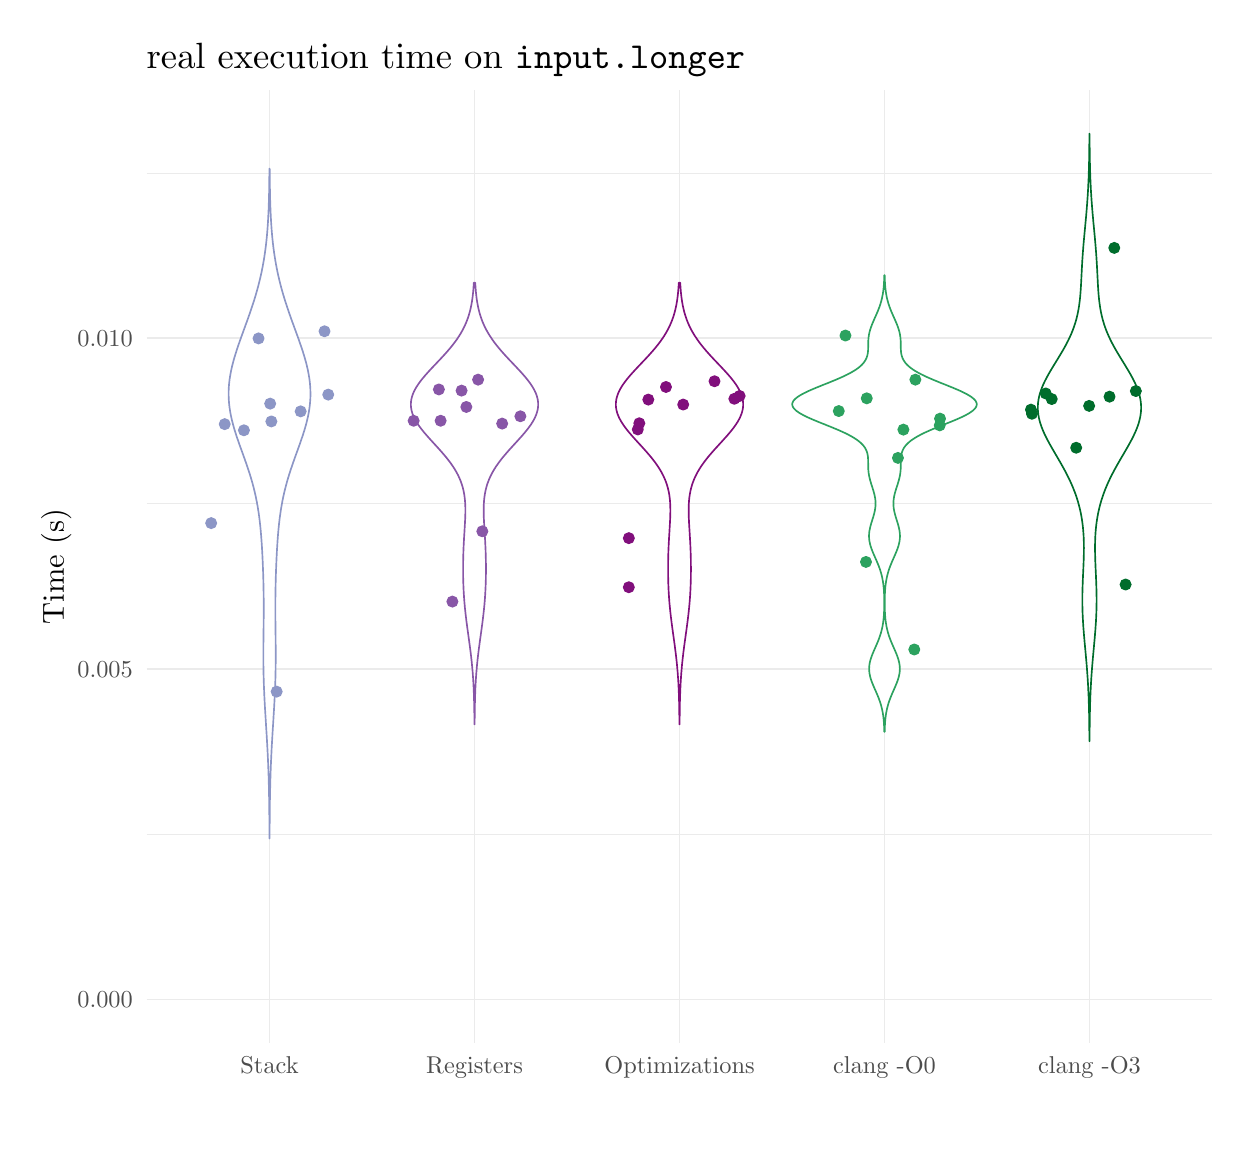
\begin{tikzpicture}[x=1pt,y=1pt]
\definecolor{fillColor}{RGB}{255,255,255}
\path[use as bounding box,fill=fillColor,fill opacity=0.00] (0,0) rectangle (433.62,397.48);
\begin{scope}
\path[clip] ( 42.95, 30.69) rectangle (428.12,374.83);
\definecolor{drawColor}{gray}{0.92}

\path[draw=drawColor,line width= 0.3pt,line join=round] ( 42.95,106.06) --
	(428.12,106.06);

\path[draw=drawColor,line width= 0.3pt,line join=round] ( 42.95,225.52) --
	(428.12,225.52);

\path[draw=drawColor,line width= 0.3pt,line join=round] ( 42.95,344.99) --
	(428.12,344.99);

\path[draw=drawColor,line width= 0.6pt,line join=round] ( 42.95, 46.33) --
	(428.12, 46.33);

\path[draw=drawColor,line width= 0.6pt,line join=round] ( 42.95,165.79) --
	(428.12,165.79);

\path[draw=drawColor,line width= 0.6pt,line join=round] ( 42.95,285.26) --
	(428.12,285.26);

\path[draw=drawColor,line width= 0.6pt,line join=round] ( 87.40, 30.69) --
	( 87.40,374.83);

\path[draw=drawColor,line width= 0.6pt,line join=round] (161.47, 30.69) --
	(161.47,374.83);

\path[draw=drawColor,line width= 0.6pt,line join=round] (235.54, 30.69) --
	(235.54,374.83);

\path[draw=drawColor,line width= 0.6pt,line join=round] (309.61, 30.69) --
	(309.61,374.83);

\path[draw=drawColor,line width= 0.6pt,line join=round] (383.68, 30.69) --
	(383.68,374.83);
\definecolor{drawColor}{RGB}{140,150,198}
\definecolor{fillColor}{RGB}{255,255,255}

\path[draw=drawColor,line width= 0.6pt,line join=round,line cap=round,fill=fillColor] ( 87.37,104.51) --
	( 87.37,104.99) --
	( 87.37,105.46) --
	( 87.37,105.93) --
	( 87.37,106.41) --
	( 87.36,106.88) --
	( 87.36,107.35) --
	( 87.36,107.83) --
	( 87.36,108.30) --
	( 87.35,108.77) --
	( 87.35,109.25) --
	( 87.35,109.72) --
	( 87.35,110.20) --
	( 87.34,110.67) --
	( 87.34,111.14) --
	( 87.33,111.62) --
	( 87.33,112.09) --
	( 87.33,112.56) --
	( 87.32,113.04) --
	( 87.32,113.51) --
	( 87.31,113.98) --
	( 87.31,114.46) --
	( 87.30,114.93) --
	( 87.30,115.41) --
	( 87.29,115.88) --
	( 87.29,116.35) --
	( 87.28,116.83) --
	( 87.27,117.30) --
	( 87.27,117.77) --
	( 87.26,118.25) --
	( 87.25,118.72) --
	( 87.24,119.19) --
	( 87.23,119.67) --
	( 87.23,120.14) --
	( 87.22,120.62) --
	( 87.21,121.09) --
	( 87.20,121.56) --
	( 87.19,122.04) --
	( 87.18,122.51) --
	( 87.17,122.98) --
	( 87.15,123.46) --
	( 87.14,123.93) --
	( 87.13,124.40) --
	( 87.12,124.88) --
	( 87.10,125.35) --
	( 87.09,125.83) --
	( 87.08,126.30) --
	( 87.06,126.77) --
	( 87.05,127.25) --
	( 87.03,127.72) --
	( 87.02,128.19) --
	( 87.00,128.67) --
	( 86.98,129.14) --
	( 86.96,129.61) --
	( 86.95,130.09) --
	( 86.93,130.56) --
	( 86.91,131.04) --
	( 86.89,131.51) --
	( 86.87,131.98) --
	( 86.85,132.46) --
	( 86.83,132.93) --
	( 86.81,133.40) --
	( 86.79,133.88) --
	( 86.76,134.35) --
	( 86.74,134.82) --
	( 86.72,135.30) --
	( 86.69,135.77) --
	( 86.67,136.25) --
	( 86.64,136.72) --
	( 86.62,137.19) --
	( 86.59,137.67) --
	( 86.57,138.14) --
	( 86.54,138.61) --
	( 86.51,139.09) --
	( 86.49,139.56) --
	( 86.46,140.03) --
	( 86.43,140.51) --
	( 86.41,140.98) --
	( 86.38,141.46) --
	( 86.35,141.93) --
	( 86.32,142.40) --
	( 86.29,142.88) --
	( 86.26,143.35) --
	( 86.23,143.82) --
	( 86.20,144.30) --
	( 86.17,144.77) --
	( 86.14,145.24) --
	( 86.11,145.72) --
	( 86.09,146.19) --
	( 86.06,146.66) --
	( 86.03,147.14) --
	( 86.00,147.61) --
	( 85.97,148.09) --
	( 85.94,148.56) --
	( 85.91,149.03) --
	( 85.88,149.51) --
	( 85.85,149.98) --
	( 85.82,150.45) --
	( 85.79,150.93) --
	( 85.77,151.40) --
	( 85.74,151.87) --
	( 85.71,152.35) --
	( 85.69,152.82) --
	( 85.66,153.30) --
	( 85.63,153.77) --
	( 85.61,154.24) --
	( 85.58,154.72) --
	( 85.56,155.19) --
	( 85.54,155.66) --
	( 85.51,156.14) --
	( 85.49,156.61) --
	( 85.47,157.08) --
	( 85.45,157.56) --
	( 85.43,158.03) --
	( 85.41,158.51) --
	( 85.39,158.98) --
	( 85.37,159.45) --
	( 85.35,159.93) --
	( 85.34,160.40) --
	( 85.32,160.87) --
	( 85.30,161.35) --
	( 85.29,161.82) --
	( 85.28,162.29) --
	( 85.26,162.77) --
	( 85.25,163.24) --
	( 85.24,163.72) --
	( 85.23,164.19) --
	( 85.22,164.66) --
	( 85.21,165.14) --
	( 85.20,165.61) --
	( 85.20,166.08) --
	( 85.19,166.56) --
	( 85.18,167.03) --
	( 85.18,167.50) --
	( 85.17,167.98) --
	( 85.17,168.45) --
	( 85.17,168.93) --
	( 85.17,169.40) --
	( 85.17,169.87) --
	( 85.16,170.35) --
	( 85.16,170.82) --
	( 85.16,171.29) --
	( 85.17,171.77) --
	( 85.17,172.24) --
	( 85.17,172.71) --
	( 85.17,173.19) --
	( 85.17,173.66) --
	( 85.18,174.14) --
	( 85.18,174.61) --
	( 85.18,175.08) --
	( 85.19,175.56) --
	( 85.19,176.03) --
	( 85.20,176.50) --
	( 85.20,176.98) --
	( 85.21,177.45) --
	( 85.21,177.92) --
	( 85.22,178.40) --
	( 85.22,178.87) --
	( 85.23,179.35) --
	( 85.23,179.82) --
	( 85.24,180.29) --
	( 85.25,180.77) --
	( 85.25,181.24) --
	( 85.26,181.71) --
	( 85.26,182.19) --
	( 85.26,182.66) --
	( 85.27,183.13) --
	( 85.27,183.61) --
	( 85.28,184.08) --
	( 85.28,184.56) --
	( 85.28,185.03) --
	( 85.28,185.50) --
	( 85.29,185.98) --
	( 85.29,186.45) --
	( 85.29,186.92) --
	( 85.29,187.40) --
	( 85.29,187.87) --
	( 85.29,188.34) --
	( 85.29,188.82) --
	( 85.29,189.29) --
	( 85.29,189.77) --
	( 85.28,190.24) --
	( 85.28,190.71) --
	( 85.28,191.19) --
	( 85.27,191.66) --
	( 85.27,192.13) --
	( 85.26,192.61) --
	( 85.26,193.08) --
	( 85.25,193.55) --
	( 85.24,194.03) --
	( 85.23,194.50) --
	( 85.22,194.98) --
	( 85.22,195.45) --
	( 85.21,195.92) --
	( 85.20,196.40) --
	( 85.18,196.87) --
	( 85.17,197.34) --
	( 85.16,197.82) --
	( 85.15,198.29) --
	( 85.13,198.76) --
	( 85.12,199.24) --
	( 85.11,199.71) --
	( 85.09,200.19) --
	( 85.07,200.66) --
	( 85.06,201.13) --
	( 85.04,201.61) --
	( 85.02,202.08) --
	( 85.00,202.55) --
	( 84.99,203.03) --
	( 84.97,203.50) --
	( 84.95,203.97) --
	( 84.93,204.45) --
	( 84.90,204.92) --
	( 84.88,205.40) --
	( 84.86,205.87) --
	( 84.84,206.34) --
	( 84.81,206.82) --
	( 84.79,207.29) --
	( 84.76,207.76) --
	( 84.74,208.24) --
	( 84.71,208.71) --
	( 84.68,209.18) --
	( 84.66,209.66) --
	( 84.63,210.13) --
	( 84.60,210.61) --
	( 84.57,211.08) --
	( 84.53,211.55) --
	( 84.50,212.03) --
	( 84.47,212.50) --
	( 84.43,212.97) --
	( 84.39,213.45) --
	( 84.36,213.92) --
	( 84.32,214.39) --
	( 84.28,214.87) --
	( 84.24,215.34) --
	( 84.20,215.82) --
	( 84.15,216.29) --
	( 84.11,216.76) --
	( 84.06,217.24) --
	( 84.01,217.71) --
	( 83.96,218.18) --
	( 83.91,218.66) --
	( 83.85,219.13) --
	( 83.80,219.60) --
	( 83.74,220.08) --
	( 83.68,220.55) --
	( 83.62,221.03) --
	( 83.55,221.50) --
	( 83.49,221.97) --
	( 83.42,222.45) --
	( 83.34,222.92) --
	( 83.27,223.39) --
	( 83.19,223.87) --
	( 83.12,224.34) --
	( 83.03,224.81) --
	( 82.95,225.29) --
	( 82.86,225.76) --
	( 82.77,226.24) --
	( 82.68,226.71) --
	( 82.59,227.18) --
	( 82.49,227.66) --
	( 82.39,228.13) --
	( 82.29,228.60) --
	( 82.18,229.08) --
	( 82.07,229.55) --
	( 81.96,230.02) --
	( 81.84,230.50) --
	( 81.73,230.97) --
	( 81.61,231.45) --
	( 81.48,231.92) --
	( 81.36,232.39) --
	( 81.23,232.87) --
	( 81.09,233.34) --
	( 80.96,233.81) --
	( 80.82,234.29) --
	( 80.68,234.76) --
	( 80.54,235.23) --
	( 80.39,235.71) --
	( 80.25,236.18) --
	( 80.09,236.65) --
	( 79.94,237.13) --
	( 79.79,237.60) --
	( 79.63,238.08) --
	( 79.47,238.55) --
	( 79.31,239.02) --
	( 79.15,239.50) --
	( 78.99,239.97) --
	( 78.82,240.44) --
	( 78.65,240.92) --
	( 78.49,241.39) --
	( 78.32,241.86) --
	( 78.15,242.34) --
	( 77.98,242.81) --
	( 77.81,243.29) --
	( 77.64,243.76) --
	( 77.47,244.23) --
	( 77.29,244.71) --
	( 77.12,245.18) --
	( 76.95,245.65) --
	( 76.78,246.13) --
	( 76.61,246.60) --
	( 76.45,247.07) --
	( 76.28,247.55) --
	( 76.11,248.02) --
	( 75.95,248.50) --
	( 75.79,248.97) --
	( 75.63,249.44) --
	( 75.47,249.92) --
	( 75.32,250.39) --
	( 75.16,250.86) --
	( 75.01,251.34) --
	( 74.87,251.81) --
	( 74.72,252.28) --
	( 74.58,252.76) --
	( 74.45,253.23) --
	( 74.31,253.71) --
	( 74.18,254.18) --
	( 74.06,254.65) --
	( 73.94,255.13) --
	( 73.82,255.60) --
	( 73.71,256.07) --
	( 73.60,256.55) --
	( 73.50,257.02) --
	( 73.40,257.49) --
	( 73.31,257.97) --
	( 73.22,258.44) --
	( 73.14,258.92) --
	( 73.07,259.39) --
	( 73.00,259.86) --
	( 72.93,260.34) --
	( 72.87,260.81) --
	( 72.82,261.28) --
	( 72.77,261.76) --
	( 72.73,262.23) --
	( 72.70,262.70) --
	( 72.67,263.18) --
	( 72.65,263.65) --
	( 72.63,264.13) --
	( 72.62,264.60) --
	( 72.61,265.07) --
	( 72.61,265.55) --
	( 72.62,266.02) --
	( 72.63,266.49) --
	( 72.65,266.97) --
	( 72.68,267.44) --
	( 72.71,267.91) --
	( 72.75,268.39) --
	( 72.79,268.86) --
	( 72.84,269.34) --
	( 72.89,269.81) --
	( 72.95,270.28) --
	( 73.02,270.76) --
	( 73.09,271.23) --
	( 73.17,271.70) --
	( 73.25,272.18) --
	( 73.34,272.65) --
	( 73.43,273.12) --
	( 73.52,273.60) --
	( 73.63,274.07) --
	( 73.73,274.55) --
	( 73.84,275.02) --
	( 73.96,275.49) --
	( 74.07,275.97) --
	( 74.20,276.44) --
	( 74.32,276.91) --
	( 74.45,277.39) --
	( 74.59,277.86) --
	( 74.72,278.33) --
	( 74.87,278.81) --
	( 75.01,279.28) --
	( 75.16,279.76) --
	( 75.31,280.23) --
	( 75.46,280.70) --
	( 75.61,281.18) --
	( 75.77,281.65) --
	( 75.93,282.12) --
	( 76.09,282.60) --
	( 76.25,283.07) --
	( 76.41,283.54) --
	( 76.58,284.02) --
	( 76.75,284.49) --
	( 76.92,284.97) --
	( 77.08,285.44) --
	( 77.25,285.91) --
	( 77.43,286.39) --
	( 77.60,286.86) --
	( 77.77,287.33) --
	( 77.94,287.81) --
	( 78.11,288.28) --
	( 78.29,288.75) --
	( 78.46,289.23) --
	( 78.63,289.70) --
	( 78.80,290.18) --
	( 78.98,290.65) --
	( 79.15,291.12) --
	( 79.32,291.60) --
	( 79.49,292.07) --
	( 79.66,292.54) --
	( 79.83,293.02) --
	( 79.99,293.49) --
	( 80.16,293.96) --
	( 80.32,294.44) --
	( 80.49,294.91) --
	( 80.65,295.39) --
	( 80.81,295.86) --
	( 80.97,296.33) --
	( 81.13,296.81) --
	( 81.28,297.28) --
	( 81.44,297.75) --
	( 81.59,298.23) --
	( 81.74,298.70) --
	( 81.89,299.17) --
	( 82.03,299.65) --
	( 82.18,300.12) --
	( 82.32,300.60) --
	( 82.46,301.07) --
	( 82.60,301.54) --
	( 82.73,302.02) --
	( 82.87,302.49) --
	( 83.00,302.96) --
	( 83.13,303.44) --
	( 83.26,303.91) --
	( 83.38,304.38) --
	( 83.50,304.86) --
	( 83.62,305.33) --
	( 83.74,305.81) --
	( 83.86,306.28) --
	( 83.97,306.75) --
	( 84.08,307.23) --
	( 84.19,307.70) --
	( 84.29,308.17) --
	( 84.40,308.65) --
	( 84.50,309.12) --
	( 84.60,309.59) --
	( 84.70,310.07) --
	( 84.79,310.54) --
	( 84.88,311.02) --
	( 84.97,311.49) --
	( 85.06,311.96) --
	( 85.14,312.44) --
	( 85.23,312.91) --
	( 85.31,313.38) --
	( 85.39,313.86) --
	( 85.46,314.33) --
	( 85.54,314.80) --
	( 85.61,315.28) --
	( 85.68,315.75) --
	( 85.75,316.23) --
	( 85.81,316.70) --
	( 85.88,317.17) --
	( 85.94,317.65) --
	( 86.00,318.12) --
	( 86.06,318.59) --
	( 86.11,319.07) --
	( 86.17,319.54) --
	( 86.22,320.01) --
	( 86.27,320.49) --
	( 86.32,320.96) --
	( 86.37,321.43) --
	( 86.41,321.91) --
	( 86.46,322.38) --
	( 86.50,322.86) --
	( 86.54,323.33) --
	( 86.58,323.80) --
	( 86.62,324.28) --
	( 86.66,324.75) --
	( 86.69,325.22) --
	( 86.72,325.70) --
	( 86.76,326.17) --
	( 86.79,326.64) --
	( 86.82,327.12) --
	( 86.85,327.59) --
	( 86.87,328.07) --
	( 86.90,328.54) --
	( 86.93,329.01) --
	( 86.95,329.49) --
	( 86.97,329.96) --
	( 87.00,330.43) --
	( 87.02,330.91) --
	( 87.04,331.38) --
	( 87.06,331.85) --
	( 87.07,332.33) --
	( 87.09,332.80) --
	( 87.11,333.28) --
	( 87.12,333.75) --
	( 87.14,334.22) --
	( 87.15,334.70) --
	( 87.17,335.17) --
	( 87.18,335.64) --
	( 87.19,336.12) --
	( 87.21,336.59) --
	( 87.22,337.06) --
	( 87.23,337.54) --
	( 87.24,338.01) --
	( 87.25,338.49) --
	( 87.26,338.96) --
	( 87.26,339.43) --
	( 87.27,339.91) --
	( 87.28,340.38) --
	( 87.29,340.85) --
	( 87.29,341.33) --
	( 87.30,341.80) --
	( 87.31,342.27) --
	( 87.31,342.75) --
	( 87.32,343.22) --
	( 87.32,343.70) --
	( 87.33,344.17) --
	( 87.33,344.64) --
	( 87.34,345.12) --
	( 87.34,345.59) --
	( 87.34,346.06) --
	( 87.35,346.54) --
	( 87.44,346.54) --
	( 87.45,346.06) --
	( 87.45,345.59) --
	( 87.46,345.12) --
	( 87.46,344.64) --
	( 87.46,344.17) --
	( 87.47,343.70) --
	( 87.47,343.22) --
	( 87.48,342.75) --
	( 87.49,342.27) --
	( 87.49,341.80) --
	( 87.50,341.33) --
	( 87.51,340.85) --
	( 87.51,340.38) --
	( 87.52,339.91) --
	( 87.53,339.43) --
	( 87.54,338.96) --
	( 87.55,338.49) --
	( 87.56,338.01) --
	( 87.57,337.54) --
	( 87.58,337.06) --
	( 87.59,336.59) --
	( 87.60,336.12) --
	( 87.61,335.64) --
	( 87.62,335.17) --
	( 87.64,334.70) --
	( 87.65,334.22) --
	( 87.67,333.75) --
	( 87.68,333.28) --
	( 87.70,332.80) --
	( 87.72,332.33) --
	( 87.74,331.85) --
	( 87.76,331.38) --
	( 87.78,330.91) --
	( 87.80,330.43) --
	( 87.82,329.96) --
	( 87.84,329.49) --
	( 87.87,329.01) --
	( 87.89,328.54) --
	( 87.92,328.07) --
	( 87.95,327.59) --
	( 87.97,327.12) --
	( 88.00,326.64) --
	( 88.04,326.17) --
	( 88.07,325.70) --
	( 88.10,325.22) --
	( 88.14,324.75) --
	( 88.17,324.28) --
	( 88.21,323.80) --
	( 88.25,323.33) --
	( 88.29,322.86) --
	( 88.33,322.38) --
	( 88.38,321.91) --
	( 88.42,321.43) --
	( 88.47,320.96) --
	( 88.52,320.49) --
	( 88.57,320.01) --
	( 88.62,319.54) --
	( 88.68,319.07) --
	( 88.73,318.59) --
	( 88.79,318.12) --
	( 88.85,317.65) --
	( 88.91,317.17) --
	( 88.98,316.70) --
	( 89.04,316.23) --
	( 89.11,315.75) --
	( 89.18,315.28) --
	( 89.25,314.80) --
	( 89.33,314.33) --
	( 89.41,313.86) --
	( 89.48,313.38) --
	( 89.57,312.91) --
	( 89.65,312.44) --
	( 89.73,311.96) --
	( 89.82,311.49) --
	( 89.91,311.02) --
	( 90.00,310.54) --
	( 90.10,310.07) --
	( 90.19,309.59) --
	( 90.29,309.12) --
	( 90.39,308.65) --
	( 90.50,308.17) --
	( 90.60,307.70) --
	( 90.71,307.23) --
	( 90.82,306.75) --
	( 90.94,306.28) --
	( 91.05,305.81) --
	( 91.17,305.33) --
	( 91.29,304.86) --
	( 91.41,304.38) --
	( 91.54,303.91) --
	( 91.66,303.44) --
	( 91.79,302.96) --
	( 91.92,302.49) --
	( 92.06,302.02) --
	( 92.19,301.54) --
	( 92.33,301.07) --
	( 92.47,300.60) --
	( 92.62,300.12) --
	( 92.76,299.65) --
	( 92.91,299.17) --
	( 93.05,298.70) --
	( 93.20,298.23) --
	( 93.36,297.75) --
	( 93.51,297.28) --
	( 93.67,296.81) --
	( 93.82,296.33) --
	( 93.98,295.86) --
	( 94.14,295.39) --
	( 94.31,294.91) --
	( 94.47,294.44) --
	( 94.63,293.96) --
	( 94.80,293.49) --
	( 94.97,293.02) --
	( 95.13,292.54) --
	( 95.30,292.07) --
	( 95.47,291.60) --
	( 95.64,291.12) --
	( 95.82,290.65) --
	( 95.99,290.18) --
	( 96.16,289.70) --
	( 96.33,289.23) --
	( 96.51,288.75) --
	( 96.68,288.28) --
	( 96.85,287.81) --
	( 97.02,287.33) --
	( 97.20,286.86) --
	( 97.37,286.39) --
	( 97.54,285.91) --
	( 97.71,285.44) --
	( 97.88,284.97) --
	( 98.05,284.49) --
	( 98.21,284.02) --
	( 98.38,283.54) --
	( 98.54,283.07) --
	( 98.70,282.60) --
	( 98.87,282.12) --
	( 99.02,281.65) --
	( 99.18,281.18) --
	( 99.34,280.70) --
	( 99.49,280.23) --
	( 99.64,279.76) --
	( 99.78,279.28) --
	( 99.93,278.81) --
	(100.07,278.33) --
	(100.20,277.86) --
	(100.34,277.39) --
	(100.47,276.91) --
	(100.60,276.44) --
	(100.72,275.97) --
	(100.84,275.49) --
	(100.95,275.02) --
	(101.06,274.55) --
	(101.17,274.07) --
	(101.27,273.60) --
	(101.36,273.12) --
	(101.46,272.65) --
	(101.54,272.18) --
	(101.62,271.70) --
	(101.70,271.23) --
	(101.77,270.76) --
	(101.84,270.28) --
	(101.90,269.81) --
	(101.95,269.34) --
	(102.00,268.86) --
	(102.04,268.39) --
	(102.08,267.91) --
	(102.11,267.44) --
	(102.14,266.97) --
	(102.16,266.49) --
	(102.17,266.02) --
	(102.18,265.55) --
	(102.18,265.07) --
	(102.18,264.60) --
	(102.17,264.13) --
	(102.15,263.65) --
	(102.13,263.18) --
	(102.09,262.70) --
	(102.06,262.23) --
	(102.02,261.76) --
	(101.97,261.28) --
	(101.92,260.81) --
	(101.86,260.34) --
	(101.80,259.86) --
	(101.73,259.39) --
	(101.65,258.92) --
	(101.57,258.44) --
	(101.48,257.97) --
	(101.39,257.49) --
	(101.29,257.02) --
	(101.19,256.55) --
	(101.08,256.07) --
	(100.97,255.60) --
	(100.86,255.13) --
	(100.73,254.65) --
	(100.61,254.18) --
	(100.48,253.71) --
	(100.35,253.23) --
	(100.21,252.76) --
	(100.07,252.28) --
	( 99.93,251.81) --
	( 99.78,251.34) --
	( 99.63,250.86) --
	( 99.48,250.39) --
	( 99.32,249.92) --
	( 99.16,249.44) --
	( 99.00,248.97) --
	( 98.84,248.50) --
	( 98.68,248.02) --
	( 98.51,247.55) --
	( 98.35,247.07) --
	( 98.18,246.60) --
	( 98.01,246.13) --
	( 97.84,245.65) --
	( 97.67,245.18) --
	( 97.50,244.71) --
	( 97.33,244.23) --
	( 97.16,243.76) --
	( 96.98,243.29) --
	( 96.81,242.81) --
	( 96.64,242.34) --
	( 96.47,241.86) --
	( 96.31,241.39) --
	( 96.14,240.92) --
	( 95.97,240.44) --
	( 95.81,239.97) --
	( 95.64,239.50) --
	( 95.48,239.02) --
	( 95.32,238.55) --
	( 95.16,238.08) --
	( 95.00,237.60) --
	( 94.85,237.13) --
	( 94.70,236.65) --
	( 94.55,236.18) --
	( 94.40,235.71) --
	( 94.25,235.23) --
	( 94.11,234.76) --
	( 93.97,234.29) --
	( 93.83,233.81) --
	( 93.70,233.34) --
	( 93.57,232.87) --
	( 93.44,232.39) --
	( 93.31,231.92) --
	( 93.19,231.45) --
	( 93.07,230.97) --
	( 92.95,230.50) --
	( 92.83,230.02) --
	( 92.72,229.55) --
	( 92.61,229.08) --
	( 92.51,228.60) --
	( 92.40,228.13) --
	( 92.30,227.66) --
	( 92.20,227.18) --
	( 92.11,226.71) --
	( 92.02,226.24) --
	( 91.93,225.76) --
	( 91.84,225.29) --
	( 91.76,224.81) --
	( 91.68,224.34) --
	( 91.60,223.87) --
	( 91.52,223.39) --
	( 91.45,222.92) --
	( 91.38,222.45) --
	( 91.31,221.97) --
	( 91.24,221.50) --
	( 91.18,221.03) --
	( 91.11,220.55) --
	( 91.05,220.08) --
	( 91.00,219.60) --
	( 90.94,219.13) --
	( 90.89,218.66) --
	( 90.83,218.18) --
	( 90.78,217.71) --
	( 90.73,217.24) --
	( 90.69,216.76) --
	( 90.64,216.29) --
	( 90.60,215.82) --
	( 90.55,215.34) --
	( 90.51,214.87) --
	( 90.47,214.39) --
	( 90.43,213.92) --
	( 90.40,213.45) --
	( 90.36,212.97) --
	( 90.33,212.50) --
	( 90.29,212.03) --
	( 90.26,211.55) --
	( 90.23,211.08) --
	( 90.20,210.61) --
	( 90.17,210.13) --
	( 90.14,209.66) --
	( 90.11,209.18) --
	( 90.08,208.71) --
	( 90.05,208.24) --
	( 90.03,207.76) --
	( 90.00,207.29) --
	( 89.98,206.82) --
	( 89.96,206.34) --
	( 89.93,205.87) --
	( 89.91,205.40) --
	( 89.89,204.92) --
	( 89.87,204.45) --
	( 89.85,203.97) --
	( 89.83,203.50) --
	( 89.81,203.03) --
	( 89.79,202.55) --
	( 89.77,202.08) --
	( 89.75,201.61) --
	( 89.73,201.13) --
	( 89.72,200.66) --
	( 89.70,200.19) --
	( 89.69,199.71) --
	( 89.67,199.24) --
	( 89.66,198.76) --
	( 89.65,198.29) --
	( 89.63,197.82) --
	( 89.62,197.34) --
	( 89.61,196.87) --
	( 89.60,196.40) --
	( 89.59,195.92) --
	( 89.58,195.45) --
	( 89.57,194.98) --
	( 89.56,194.50) --
	( 89.55,194.03) --
	( 89.54,193.55) --
	( 89.54,193.08) --
	( 89.53,192.61) --
	( 89.53,192.13) --
	( 89.52,191.66) --
	( 89.52,191.19) --
	( 89.51,190.71) --
	( 89.51,190.24) --
	( 89.51,189.77) --
	( 89.50,189.29) --
	( 89.50,188.82) --
	( 89.50,188.34) --
	( 89.50,187.87) --
	( 89.50,187.40) --
	( 89.50,186.92) --
	( 89.50,186.45) --
	( 89.51,185.98) --
	( 89.51,185.50) --
	( 89.51,185.03) --
	( 89.51,184.56) --
	( 89.52,184.08) --
	( 89.52,183.61) --
	( 89.52,183.13) --
	( 89.53,182.66) --
	( 89.53,182.19) --
	( 89.54,181.71) --
	( 89.54,181.24) --
	( 89.55,180.77) --
	( 89.55,180.29) --
	( 89.56,179.82) --
	( 89.56,179.35) --
	( 89.57,178.87) --
	( 89.57,178.40) --
	( 89.58,177.92) --
	( 89.58,177.45) --
	( 89.59,176.98) --
	( 89.59,176.50) --
	( 89.60,176.03) --
	( 89.60,175.56) --
	( 89.61,175.08) --
	( 89.61,174.61) --
	( 89.62,174.14) --
	( 89.62,173.66) --
	( 89.62,173.19) --
	( 89.62,172.71) --
	( 89.63,172.24) --
	( 89.63,171.77) --
	( 89.63,171.29) --
	( 89.63,170.82) --
	( 89.63,170.35) --
	( 89.63,169.87) --
	( 89.63,169.40) --
	( 89.62,168.93) --
	( 89.62,168.45) --
	( 89.62,167.98) --
	( 89.61,167.50) --
	( 89.61,167.03) --
	( 89.60,166.56) --
	( 89.60,166.08) --
	( 89.59,165.61) --
	( 89.58,165.14) --
	( 89.57,164.66) --
	( 89.56,164.19) --
	( 89.55,163.72) --
	( 89.54,163.24) --
	( 89.53,162.77) --
	( 89.52,162.29) --
	( 89.50,161.82) --
	( 89.49,161.35) --
	( 89.47,160.87) --
	( 89.46,160.40) --
	( 89.44,159.93) --
	( 89.42,159.45) --
	( 89.40,158.98) --
	( 89.39,158.51) --
	( 89.37,158.03) --
	( 89.35,157.56) --
	( 89.32,157.08) --
	( 89.30,156.61) --
	( 89.28,156.14) --
	( 89.26,155.66) --
	( 89.23,155.19) --
	( 89.21,154.72) --
	( 89.18,154.24) --
	( 89.16,153.77) --
	( 89.13,153.30) --
	( 89.11,152.82) --
	( 89.08,152.35) --
	( 89.05,151.87) --
	( 89.03,151.40) --
	( 89.00,150.93) --
	( 88.97,150.45) --
	( 88.94,149.98) --
	( 88.91,149.51) --
	( 88.88,149.03) --
	( 88.85,148.56) --
	( 88.83,148.09) --
	( 88.80,147.61) --
	( 88.77,147.14) --
	( 88.74,146.66) --
	( 88.71,146.19) --
	( 88.68,145.72) --
	( 88.65,145.24) --
	( 88.62,144.77) --
	( 88.59,144.30) --
	( 88.56,143.82) --
	( 88.53,143.35) --
	( 88.50,142.88) --
	( 88.47,142.40) --
	( 88.44,141.93) --
	( 88.42,141.46) --
	( 88.39,140.98) --
	( 88.36,140.51) --
	( 88.33,140.03) --
	( 88.30,139.56) --
	( 88.28,139.09) --
	( 88.25,138.61) --
	( 88.22,138.14) --
	( 88.20,137.67) --
	( 88.17,137.19) --
	( 88.15,136.72) --
	( 88.12,136.25) --
	( 88.10,135.77) --
	( 88.08,135.30) --
	( 88.05,134.82) --
	( 88.03,134.35) --
	( 88.01,133.88) --
	( 87.99,133.40) --
	( 87.96,132.93) --
	( 87.94,132.46) --
	( 87.92,131.98) --
	( 87.90,131.51) --
	( 87.88,131.04) --
	( 87.86,130.56) --
	( 87.85,130.09) --
	( 87.83,129.61) --
	( 87.81,129.14) --
	( 87.79,128.67) --
	( 87.78,128.19) --
	( 87.76,127.72) --
	( 87.75,127.25) --
	( 87.73,126.77) --
	( 87.72,126.30) --
	( 87.70,125.83) --
	( 87.69,125.35) --
	( 87.68,124.88) --
	( 87.66,124.40) --
	( 87.65,123.93) --
	( 87.64,123.46) --
	( 87.63,122.98) --
	( 87.62,122.51) --
	( 87.61,122.04) --
	( 87.60,121.56) --
	( 87.59,121.09) --
	( 87.58,120.62) --
	( 87.57,120.14) --
	( 87.56,119.67) --
	( 87.55,119.19) --
	( 87.54,118.72) --
	( 87.53,118.25) --
	( 87.53,117.77) --
	( 87.52,117.30) --
	( 87.51,116.83) --
	( 87.51,116.35) --
	( 87.50,115.88) --
	( 87.50,115.41) --
	( 87.49,114.93) --
	( 87.48,114.46) --
	( 87.48,113.98) --
	( 87.47,113.51) --
	( 87.47,113.04) --
	( 87.47,112.56) --
	( 87.46,112.09) --
	( 87.46,111.62) --
	( 87.45,111.14) --
	( 87.45,110.67) --
	( 87.45,110.20) --
	( 87.44,109.72) --
	( 87.44,109.25) --
	( 87.44,108.77) --
	( 87.44,108.30) --
	( 87.43,107.83) --
	( 87.43,107.35) --
	( 87.43,106.88) --
	( 87.43,106.41) --
	( 87.42,105.93) --
	( 87.42,105.46) --
	( 87.42,104.99) --
	( 87.42,104.51) --
	( 87.37,104.51) --
	cycle;
\definecolor{drawColor}{RGB}{136,86,167}

\path[draw=drawColor,line width= 0.6pt,line join=round,line cap=round,fill=fillColor] (161.43,145.72) --
	(161.43,146.03) --
	(161.43,146.35) --
	(161.43,146.66) --
	(161.42,146.97) --
	(161.42,147.28) --
	(161.42,147.59) --
	(161.42,147.91) --
	(161.41,148.22) --
	(161.41,148.53) --
	(161.41,148.84) --
	(161.40,149.16) --
	(161.40,149.47) --
	(161.40,149.78) --
	(161.39,150.09) --
	(161.39,150.41) --
	(161.38,150.72) --
	(161.38,151.03) --
	(161.37,151.34) --
	(161.37,151.66) --
	(161.36,151.97) --
	(161.35,152.28) --
	(161.35,152.59) --
	(161.34,152.90) --
	(161.34,153.22) --
	(161.33,153.53) --
	(161.32,153.84) --
	(161.31,154.15) --
	(161.30,154.47) --
	(161.30,154.78) --
	(161.29,155.09) --
	(161.28,155.40) --
	(161.27,155.72) --
	(161.26,156.03) --
	(161.25,156.34) --
	(161.24,156.65) --
	(161.23,156.97) --
	(161.21,157.28) --
	(161.20,157.59) --
	(161.19,157.90) --
	(161.18,158.21) --
	(161.16,158.53) --
	(161.15,158.84) --
	(161.13,159.15) --
	(161.12,159.46) --
	(161.10,159.78) --
	(161.09,160.09) --
	(161.07,160.40) --
	(161.05,160.71) --
	(161.04,161.03) --
	(161.02,161.34) --
	(161.00,161.65) --
	(160.98,161.96) --
	(160.96,162.27) --
	(160.94,162.59) --
	(160.92,162.90) --
	(160.89,163.21) --
	(160.87,163.52) --
	(160.85,163.84) --
	(160.82,164.15) --
	(160.80,164.46) --
	(160.78,164.77) --
	(160.75,165.09) --
	(160.72,165.40) --
	(160.70,165.71) --
	(160.67,166.02) --
	(160.64,166.34) --
	(160.61,166.65) --
	(160.58,166.96) --
	(160.55,167.27) --
	(160.52,167.58) --
	(160.49,167.90) --
	(160.46,168.21) --
	(160.43,168.52) --
	(160.39,168.83) --
	(160.36,169.15) --
	(160.32,169.46) --
	(160.29,169.77) --
	(160.25,170.08) --
	(160.22,170.40) --
	(160.18,170.71) --
	(160.14,171.02) --
	(160.11,171.33) --
	(160.07,171.65) --
	(160.03,171.96) --
	(159.99,172.27) --
	(159.95,172.58) --
	(159.91,172.89) --
	(159.87,173.21) --
	(159.83,173.52) --
	(159.79,173.83) --
	(159.75,174.14) --
	(159.71,174.46) --
	(159.67,174.77) --
	(159.62,175.08) --
	(159.58,175.39) --
	(159.54,175.71) --
	(159.50,176.02) --
	(159.45,176.33) --
	(159.41,176.64) --
	(159.37,176.96) --
	(159.32,177.27) --
	(159.28,177.58) --
	(159.24,177.89) --
	(159.19,178.20) --
	(159.15,178.52) --
	(159.11,178.83) --
	(159.06,179.14) --
	(159.02,179.45) --
	(158.98,179.77) --
	(158.94,180.08) --
	(158.89,180.39) --
	(158.85,180.70) --
	(158.81,181.02) --
	(158.77,181.33) --
	(158.73,181.64) --
	(158.68,181.95) --
	(158.64,182.26) --
	(158.60,182.58) --
	(158.56,182.89) --
	(158.52,183.20) --
	(158.48,183.51) --
	(158.45,183.83) --
	(158.41,184.14) --
	(158.37,184.45) --
	(158.33,184.76) --
	(158.30,185.08) --
	(158.26,185.39) --
	(158.22,185.70) --
	(158.19,186.01) --
	(158.16,186.33) --
	(158.12,186.64) --
	(158.09,186.95) --
	(158.06,187.26) --
	(158.03,187.57) --
	(157.99,187.89) --
	(157.96,188.20) --
	(157.94,188.51) --
	(157.91,188.82) --
	(157.88,189.14) --
	(157.85,189.45) --
	(157.82,189.76) --
	(157.80,190.07) --
	(157.77,190.39) --
	(157.75,190.70) --
	(157.72,191.01) --
	(157.70,191.32) --
	(157.68,191.64) --
	(157.66,191.95) --
	(157.64,192.26) --
	(157.62,192.57) --
	(157.60,192.88) --
	(157.58,193.20) --
	(157.56,193.51) --
	(157.54,193.82) --
	(157.53,194.13) --
	(157.51,194.45) --
	(157.50,194.76) --
	(157.48,195.07) --
	(157.47,195.38) --
	(157.46,195.70) --
	(157.44,196.01) --
	(157.43,196.32) --
	(157.42,196.63) --
	(157.41,196.95) --
	(157.40,197.26) --
	(157.39,197.57) --
	(157.39,197.88) --
	(157.38,198.19) --
	(157.37,198.51) --
	(157.36,198.82) --
	(157.36,199.13) --
	(157.35,199.44) --
	(157.35,199.76) --
	(157.35,200.07) --
	(157.34,200.38) --
	(157.34,200.69) --
	(157.34,201.01) --
	(157.34,201.32) --
	(157.34,201.63) --
	(157.34,201.94) --
	(157.34,202.25) --
	(157.34,202.57) --
	(157.34,202.88) --
	(157.34,203.19) --
	(157.34,203.50) --
	(157.35,203.82) --
	(157.35,204.13) --
	(157.36,204.44) --
	(157.36,204.75) --
	(157.37,205.07) --
	(157.37,205.38) --
	(157.38,205.69) --
	(157.39,206.00) --
	(157.39,206.32) --
	(157.40,206.63) --
	(157.41,206.94) --
	(157.42,207.25) --
	(157.43,207.56) --
	(157.44,207.88) --
	(157.45,208.19) --
	(157.46,208.50) --
	(157.48,208.81) --
	(157.49,209.13) --
	(157.50,209.44) --
	(157.51,209.75) --
	(157.53,210.06) --
	(157.54,210.38) --
	(157.56,210.69) --
	(157.57,211.00) --
	(157.59,211.31) --
	(157.61,211.63) --
	(157.62,211.94) --
	(157.64,212.25) --
	(157.66,212.56) --
	(157.68,212.87) --
	(157.69,213.19) --
	(157.71,213.50) --
	(157.73,213.81) --
	(157.75,214.12) --
	(157.77,214.44) --
	(157.79,214.75) --
	(157.81,215.06) --
	(157.83,215.37) --
	(157.84,215.69) --
	(157.86,216.00) --
	(157.88,216.31) --
	(157.90,216.62) --
	(157.92,216.94) --
	(157.94,217.25) --
	(157.96,217.56) --
	(157.98,217.87) --
	(157.99,218.18) --
	(158.01,218.50) --
	(158.03,218.81) --
	(158.04,219.12) --
	(158.06,219.43) --
	(158.07,219.75) --
	(158.09,220.06) --
	(158.10,220.37) --
	(158.11,220.68) --
	(158.12,221.00) --
	(158.13,221.31) --
	(158.14,221.62) --
	(158.15,221.93) --
	(158.15,222.24) --
	(158.16,222.56) --
	(158.16,222.87) --
	(158.16,223.18) --
	(158.16,223.49) --
	(158.15,223.81) --
	(158.15,224.12) --
	(158.14,224.43) --
	(158.13,224.74) --
	(158.12,225.06) --
	(158.10,225.37) --
	(158.09,225.68) --
	(158.07,225.99) --
	(158.04,226.31) --
	(158.02,226.62) --
	(157.99,226.93) --
	(157.96,227.24) --
	(157.92,227.55) --
	(157.88,227.87) --
	(157.84,228.18) --
	(157.80,228.49) --
	(157.75,228.80) --
	(157.70,229.12) --
	(157.64,229.43) --
	(157.58,229.74) --
	(157.51,230.05) --
	(157.44,230.37) --
	(157.37,230.68) --
	(157.29,230.99) --
	(157.21,231.30) --
	(157.13,231.62) --
	(157.03,231.93) --
	(156.94,232.24) --
	(156.84,232.55) --
	(156.73,232.86) --
	(156.62,233.18) --
	(156.51,233.49) --
	(156.39,233.80) --
	(156.26,234.11) --
	(156.13,234.43) --
	(155.99,234.74) --
	(155.85,235.05) --
	(155.71,235.36) --
	(155.56,235.68) --
	(155.40,235.99) --
	(155.24,236.30) --
	(155.07,236.61) --
	(154.90,236.93) --
	(154.72,237.24) --
	(154.54,237.55) --
	(154.35,237.86) --
	(154.16,238.17) --
	(153.96,238.49) --
	(153.76,238.80) --
	(153.55,239.11) --
	(153.33,239.42) --
	(153.12,239.74) --
	(152.89,240.05) --
	(152.67,240.36) --
	(152.43,240.67) --
	(152.20,240.99) --
	(151.96,241.30) --
	(151.71,241.61) --
	(151.46,241.92) --
	(151.21,242.24) --
	(150.95,242.55) --
	(150.69,242.86) --
	(150.43,243.17) --
	(150.16,243.48) --
	(149.89,243.80) --
	(149.62,244.11) --
	(149.35,244.42) --
	(149.07,244.73) --
	(148.79,245.05) --
	(148.51,245.36) --
	(148.23,245.67) --
	(147.95,245.98) --
	(147.66,246.30) --
	(147.38,246.61) --
	(147.09,246.92) --
	(146.80,247.23) --
	(146.52,247.54) --
	(146.23,247.86) --
	(145.95,248.17) --
	(145.66,248.48) --
	(145.38,248.79) --
	(145.10,249.11) --
	(144.82,249.42) --
	(144.54,249.73) --
	(144.27,250.04) --
	(144.00,250.36) --
	(143.73,250.67) --
	(143.46,250.98) --
	(143.20,251.29) --
	(142.94,251.61) --
	(142.69,251.92) --
	(142.44,252.23) --
	(142.20,252.54) --
	(141.96,252.85) --
	(141.73,253.17) --
	(141.50,253.48) --
	(141.28,253.79) --
	(141.07,254.10) --
	(140.86,254.42) --
	(140.66,254.73) --
	(140.47,255.04) --
	(140.28,255.35) --
	(140.11,255.67) --
	(139.94,255.98) --
	(139.78,256.29) --
	(139.62,256.60) --
	(139.48,256.92) --
	(139.34,257.23) --
	(139.22,257.54) --
	(139.10,257.85) --
	(139.00,258.16) --
	(138.90,258.48) --
	(138.81,258.79) --
	(138.73,259.10) --
	(138.66,259.41) --
	(138.61,259.73) --
	(138.56,260.04) --
	(138.52,260.35) --
	(138.49,260.66) --
	(138.47,260.98) --
	(138.47,261.29) --
	(138.47,261.60) --
	(138.49,261.91) --
	(138.51,262.23) --
	(138.55,262.54) --
	(138.59,262.85) --
	(138.64,263.16) --
	(138.71,263.47) --
	(138.79,263.79) --
	(138.87,264.10) --
	(138.97,264.41) --
	(139.07,264.72) --
	(139.19,265.04) --
	(139.31,265.35) --
	(139.44,265.66) --
	(139.58,265.97) --
	(139.74,266.29) --
	(139.90,266.60) --
	(140.06,266.91) --
	(140.24,267.22) --
	(140.42,267.53) --
	(140.62,267.85) --
	(140.82,268.16) --
	(141.03,268.47) --
	(141.24,268.78) --
	(141.46,269.10) --
	(141.69,269.41) --
	(141.92,269.72) --
	(142.16,270.03) --
	(142.41,270.35) --
	(142.66,270.66) --
	(142.92,270.97) --
	(143.18,271.28) --
	(143.44,271.60) --
	(143.71,271.91) --
	(143.99,272.22) --
	(144.26,272.53) --
	(144.54,272.84) --
	(144.83,273.16) --
	(145.11,273.47) --
	(145.40,273.78) --
	(145.69,274.09) --
	(145.98,274.41) --
	(146.28,274.72) --
	(146.57,275.03) --
	(146.87,275.34) --
	(147.16,275.66) --
	(147.46,275.97) --
	(147.76,276.28) --
	(148.05,276.59) --
	(148.35,276.91) --
	(148.65,277.22) --
	(148.94,277.53) --
	(149.23,277.84) --
	(149.52,278.15) --
	(149.81,278.47) --
	(150.10,278.78) --
	(150.39,279.09) --
	(150.67,279.40) --
	(150.95,279.72) --
	(151.23,280.03) --
	(151.51,280.34) --
	(151.78,280.65) --
	(152.05,280.97) --
	(152.32,281.28) --
	(152.58,281.59) --
	(152.84,281.90) --
	(153.09,282.22) --
	(153.34,282.53) --
	(153.59,282.84) --
	(153.84,283.15) --
	(154.07,283.46) --
	(154.31,283.78) --
	(154.54,284.09) --
	(154.77,284.40) --
	(154.99,284.71) --
	(155.20,285.03) --
	(155.42,285.34) --
	(155.62,285.65) --
	(155.83,285.96) --
	(156.03,286.28) --
	(156.22,286.59) --
	(156.41,286.90) --
	(156.60,287.21) --
	(156.78,287.52) --
	(156.95,287.84) --
	(157.12,288.15) --
	(157.29,288.46) --
	(157.45,288.77) --
	(157.61,289.09) --
	(157.76,289.40) --
	(157.91,289.71) --
	(158.05,290.02) --
	(158.19,290.34) --
	(158.33,290.65) --
	(158.46,290.96) --
	(158.59,291.27) --
	(158.71,291.59) --
	(158.83,291.90) --
	(158.94,292.21) --
	(159.06,292.52) --
	(159.16,292.83) --
	(159.27,293.15) --
	(159.37,293.46) --
	(159.46,293.77) --
	(159.55,294.08) --
	(159.64,294.40) --
	(159.73,294.71) --
	(159.81,295.02) --
	(159.89,295.33) --
	(159.97,295.65) --
	(160.04,295.96) --
	(160.11,296.27) --
	(160.18,296.58) --
	(160.24,296.90) --
	(160.30,297.21) --
	(160.36,297.52) --
	(160.42,297.83) --
	(160.47,298.14) --
	(160.53,298.46) --
	(160.57,298.77) --
	(160.62,299.08) --
	(160.67,299.39) --
	(160.71,299.71) --
	(160.75,300.02) --
	(160.79,300.33) --
	(160.83,300.64) --
	(160.86,300.96) --
	(160.90,301.27) --
	(160.93,301.58) --
	(160.96,301.89) --
	(160.99,302.21) --
	(161.02,302.52) --
	(161.04,302.83) --
	(161.07,303.14) --
	(161.09,303.45) --
	(161.11,303.77) --
	(161.13,304.08) --
	(161.15,304.39) --
	(161.17,304.70) --
	(161.19,305.02) --
	(161.21,305.33) --
	(161.72,305.33) --
	(161.74,305.02) --
	(161.76,304.70) --
	(161.78,304.39) --
	(161.80,304.08) --
	(161.82,303.77) --
	(161.84,303.45) --
	(161.87,303.14) --
	(161.89,302.83) --
	(161.92,302.52) --
	(161.94,302.21) --
	(161.97,301.89) --
	(162.00,301.58) --
	(162.04,301.27) --
	(162.07,300.96) --
	(162.11,300.64) --
	(162.14,300.33) --
	(162.18,300.02) --
	(162.22,299.71) --
	(162.27,299.39) --
	(162.31,299.08) --
	(162.36,298.77) --
	(162.41,298.46) --
	(162.46,298.14) --
	(162.51,297.83) --
	(162.57,297.52) --
	(162.63,297.21) --
	(162.69,296.90) --
	(162.76,296.58) --
	(162.82,296.27) --
	(162.89,295.96) --
	(162.97,295.65) --
	(163.04,295.33) --
	(163.12,295.02) --
	(163.20,294.71) --
	(163.29,294.40) --
	(163.38,294.08) --
	(163.47,293.77) --
	(163.57,293.46) --
	(163.67,293.15) --
	(163.77,292.83) --
	(163.88,292.52) --
	(163.99,292.21) --
	(164.10,291.90) --
	(164.22,291.59) --
	(164.34,291.27) --
	(164.47,290.96) --
	(164.60,290.65) --
	(164.74,290.34) --
	(164.88,290.02) --
	(165.02,289.71) --
	(165.17,289.40) --
	(165.32,289.09) --
	(165.48,288.77) --
	(165.64,288.46) --
	(165.81,288.15) --
	(165.98,287.84) --
	(166.16,287.52) --
	(166.34,287.21) --
	(166.52,286.90) --
	(166.71,286.59) --
	(166.91,286.28) --
	(167.10,285.96) --
	(167.31,285.65) --
	(167.52,285.34) --
	(167.73,285.03) --
	(167.95,284.71) --
	(168.17,284.40) --
	(168.39,284.09) --
	(168.62,283.78) --
	(168.86,283.46) --
	(169.10,283.15) --
	(169.34,282.84) --
	(169.59,282.53) --
	(169.84,282.22) --
	(170.10,281.90) --
	(170.35,281.59) --
	(170.62,281.28) --
	(170.88,280.97) --
	(171.15,280.65) --
	(171.43,280.34) --
	(171.70,280.03) --
	(171.98,279.72) --
	(172.26,279.40) --
	(172.54,279.09) --
	(172.83,278.78) --
	(173.12,278.47) --
	(173.41,278.15) --
	(173.70,277.84) --
	(173.99,277.53) --
	(174.29,277.22) --
	(174.58,276.91) --
	(174.88,276.59) --
	(175.18,276.28) --
	(175.47,275.97) --
	(175.77,275.66) --
	(176.07,275.34) --
	(176.36,275.03) --
	(176.66,274.72) --
	(176.95,274.41) --
	(177.24,274.09) --
	(177.53,273.78) --
	(177.82,273.47) --
	(178.11,273.16) --
	(178.39,272.84) --
	(178.67,272.53) --
	(178.95,272.22) --
	(179.22,271.91) --
	(179.49,271.60) --
	(179.76,271.28) --
	(180.02,270.97) --
	(180.27,270.66) --
	(180.52,270.35) --
	(180.77,270.03) --
	(181.01,269.72) --
	(181.24,269.41) --
	(181.47,269.10) --
	(181.69,268.78) --
	(181.91,268.47) --
	(182.12,268.16) --
	(182.31,267.85) --
	(182.51,267.53) --
	(182.69,267.22) --
	(182.87,266.91) --
	(183.04,266.60) --
	(183.20,266.29) --
	(183.35,265.97) --
	(183.49,265.66) --
	(183.63,265.35) --
	(183.75,265.04) --
	(183.86,264.72) --
	(183.97,264.41) --
	(184.06,264.10) --
	(184.15,263.79) --
	(184.22,263.47) --
	(184.29,263.16) --
	(184.34,262.85) --
	(184.39,262.54) --
	(184.42,262.23) --
	(184.45,261.91) --
	(184.46,261.60) --
	(184.46,261.29) --
	(184.46,260.98) --
	(184.44,260.66) --
	(184.41,260.35) --
	(184.38,260.04) --
	(184.33,259.73) --
	(184.27,259.41) --
	(184.20,259.10) --
	(184.12,258.79) --
	(184.03,258.48) --
	(183.94,258.16) --
	(183.83,257.85) --
	(183.71,257.54) --
	(183.59,257.23) --
	(183.45,256.92) --
	(183.31,256.60) --
	(183.16,256.29) --
	(183.00,255.98) --
	(182.83,255.67) --
	(182.65,255.35) --
	(182.47,255.04) --
	(182.27,254.73) --
	(182.07,254.42) --
	(181.87,254.10) --
	(181.65,253.79) --
	(181.43,253.48) --
	(181.20,253.17) --
	(180.97,252.85) --
	(180.73,252.54) --
	(180.49,252.23) --
	(180.24,251.92) --
	(179.99,251.61) --
	(179.73,251.29) --
	(179.47,250.98) --
	(179.21,250.67) --
	(178.94,250.36) --
	(178.67,250.04) --
	(178.39,249.73) --
	(178.11,249.42) --
	(177.83,249.11) --
	(177.55,248.79) --
	(177.27,248.48) --
	(176.99,248.17) --
	(176.70,247.86) --
	(176.42,247.54) --
	(176.13,247.23) --
	(175.84,246.92) --
	(175.56,246.61) --
	(175.27,246.30) --
	(174.99,245.98) --
	(174.70,245.67) --
	(174.42,245.36) --
	(174.14,245.05) --
	(173.86,244.73) --
	(173.59,244.42) --
	(173.31,244.11) --
	(173.04,243.80) --
	(172.77,243.48) --
	(172.50,243.17) --
	(172.24,242.86) --
	(171.98,242.55) --
	(171.72,242.24) --
	(171.47,241.92) --
	(171.22,241.61) --
	(170.98,241.30) --
	(170.74,240.99) --
	(170.50,240.67) --
	(170.27,240.36) --
	(170.04,240.05) --
	(169.82,239.74) --
	(169.60,239.42) --
	(169.39,239.11) --
	(169.18,238.80) --
	(168.98,238.49) --
	(168.78,238.17) --
	(168.58,237.86) --
	(168.40,237.55) --
	(168.21,237.24) --
	(168.04,236.93) --
	(167.86,236.61) --
	(167.70,236.30) --
	(167.53,235.99) --
	(167.38,235.68) --
	(167.23,235.36) --
	(167.08,235.05) --
	(166.94,234.74) --
	(166.80,234.43) --
	(166.67,234.11) --
	(166.55,233.80) --
	(166.43,233.49) --
	(166.31,233.18) --
	(166.20,232.86) --
	(166.10,232.55) --
	(165.99,232.24) --
	(165.90,231.93) --
	(165.81,231.62) --
	(165.72,231.30) --
	(165.64,230.99) --
	(165.56,230.68) --
	(165.49,230.37) --
	(165.42,230.05) --
	(165.36,229.74) --
	(165.30,229.43) --
	(165.24,229.12) --
	(165.19,228.80) --
	(165.14,228.49) --
	(165.09,228.18) --
	(165.05,227.87) --
	(165.01,227.55) --
	(164.98,227.24) --
	(164.94,226.93) --
	(164.92,226.62) --
	(164.89,226.31) --
	(164.87,225.99) --
	(164.85,225.68) --
	(164.83,225.37) --
	(164.82,225.06) --
	(164.80,224.74) --
	(164.79,224.43) --
	(164.79,224.12) --
	(164.78,223.81) --
	(164.78,223.49) --
	(164.78,223.18) --
	(164.78,222.87) --
	(164.78,222.56) --
	(164.78,222.24) --
	(164.79,221.93) --
	(164.79,221.62) --
	(164.80,221.31) --
	(164.81,221.00) --
	(164.82,220.68) --
	(164.83,220.37) --
	(164.85,220.06) --
	(164.86,219.75) --
	(164.87,219.43) --
	(164.89,219.12) --
	(164.91,218.81) --
	(164.92,218.50) --
	(164.94,218.18) --
	(164.96,217.87) --
	(164.98,217.56) --
	(164.99,217.25) --
	(165.01,216.94) --
	(165.03,216.62) --
	(165.05,216.31) --
	(165.07,216.00) --
	(165.09,215.69) --
	(165.11,215.37) --
	(165.13,215.06) --
	(165.15,214.75) --
	(165.17,214.44) --
	(165.18,214.12) --
	(165.20,213.81) --
	(165.22,213.50) --
	(165.24,213.19) --
	(165.26,212.87) --
	(165.28,212.56) --
	(165.29,212.25) --
	(165.31,211.94) --
	(165.33,211.63) --
	(165.34,211.31) --
	(165.36,211.00) --
	(165.37,210.69) --
	(165.39,210.38) --
	(165.40,210.06) --
	(165.42,209.75) --
	(165.43,209.44) --
	(165.45,209.13) --
	(165.46,208.81) --
	(165.47,208.50) --
	(165.48,208.19) --
	(165.49,207.88) --
	(165.50,207.56) --
	(165.51,207.25) --
	(165.52,206.94) --
	(165.53,206.63) --
	(165.54,206.32) --
	(165.55,206.00) --
	(165.55,205.69) --
	(165.56,205.38) --
	(165.57,205.07) --
	(165.57,204.75) --
	(165.58,204.44) --
	(165.58,204.13) --
	(165.59,203.82) --
	(165.59,203.50) --
	(165.59,203.19) --
	(165.59,202.88) --
	(165.60,202.57) --
	(165.60,202.25) --
	(165.60,201.94) --
	(165.60,201.63) --
	(165.60,201.32) --
	(165.60,201.01) --
	(165.59,200.69) --
	(165.59,200.38) --
	(165.59,200.07) --
	(165.58,199.76) --
	(165.58,199.44) --
	(165.57,199.13) --
	(165.57,198.82) --
	(165.56,198.51) --
	(165.56,198.19) --
	(165.55,197.88) --
	(165.54,197.57) --
	(165.53,197.26) --
	(165.52,196.95) --
	(165.51,196.63) --
	(165.50,196.32) --
	(165.49,196.01) --
	(165.48,195.70) --
	(165.46,195.38) --
	(165.45,195.07) --
	(165.44,194.76) --
	(165.42,194.45) --
	(165.40,194.13) --
	(165.39,193.82) --
	(165.37,193.51) --
	(165.35,193.20) --
	(165.34,192.88) --
	(165.32,192.57) --
	(165.30,192.26) --
	(165.27,191.95) --
	(165.25,191.64) --
	(165.23,191.32) --
	(165.21,191.01) --
	(165.18,190.70) --
	(165.16,190.39) --
	(165.14,190.07) --
	(165.11,189.76) --
	(165.08,189.45) --
	(165.06,189.14) --
	(165.03,188.82) --
	(165.00,188.51) --
	(164.97,188.20) --
	(164.94,187.89) --
	(164.91,187.57) --
	(164.88,187.26) --
	(164.84,186.95) --
	(164.81,186.64) --
	(164.78,186.33) --
	(164.74,186.01) --
	(164.71,185.70) --
	(164.67,185.39) --
	(164.64,185.08) --
	(164.60,184.76) --
	(164.56,184.45) --
	(164.53,184.14) --
	(164.49,183.83) --
	(164.45,183.51) --
	(164.41,183.20) --
	(164.37,182.89) --
	(164.33,182.58) --
	(164.29,182.26) --
	(164.25,181.95) --
	(164.21,181.64) --
	(164.17,181.33) --
	(164.12,181.02) --
	(164.08,180.70) --
	(164.04,180.39) --
	(164.00,180.08) --
	(163.95,179.77) --
	(163.91,179.45) --
	(163.87,179.14) --
	(163.83,178.83) --
	(163.78,178.52) --
	(163.74,178.20) --
	(163.70,177.89) --
	(163.65,177.58) --
	(163.61,177.27) --
	(163.57,176.96) --
	(163.52,176.64) --
	(163.48,176.33) --
	(163.44,176.02) --
	(163.39,175.71) --
	(163.35,175.39) --
	(163.31,175.08) --
	(163.27,174.77) --
	(163.23,174.46) --
	(163.18,174.14) --
	(163.14,173.83) --
	(163.10,173.52) --
	(163.06,173.21) --
	(163.02,172.89) --
	(162.98,172.58) --
	(162.94,172.27) --
	(162.90,171.96) --
	(162.86,171.65) --
	(162.83,171.33) --
	(162.79,171.02) --
	(162.75,170.71) --
	(162.72,170.40) --
	(162.68,170.08) --
	(162.64,169.77) --
	(162.61,169.46) --
	(162.57,169.15) --
	(162.54,168.83) --
	(162.51,168.52) --
	(162.48,168.21) --
	(162.44,167.90) --
	(162.41,167.58) --
	(162.38,167.27) --
	(162.35,166.96) --
	(162.32,166.65) --
	(162.29,166.34) --
	(162.26,166.02) --
	(162.24,165.71) --
	(162.21,165.40) --
	(162.18,165.09) --
	(162.16,164.77) --
	(162.13,164.46) --
	(162.11,164.15) --
	(162.08,163.84) --
	(162.06,163.52) --
	(162.04,163.21) --
	(162.02,162.90) --
	(162.00,162.59) --
	(161.97,162.27) --
	(161.95,161.96) --
	(161.94,161.65) --
	(161.92,161.34) --
	(161.90,161.03) --
	(161.88,160.71) --
	(161.86,160.40) --
	(161.85,160.09) --
	(161.83,159.78) --
	(161.81,159.46) --
	(161.80,159.15) --
	(161.78,158.84) --
	(161.77,158.53) --
	(161.76,158.21) --
	(161.74,157.90) --
	(161.73,157.59) --
	(161.72,157.28) --
	(161.71,156.97) --
	(161.70,156.65) --
	(161.69,156.34) --
	(161.67,156.03) --
	(161.66,155.72) --
	(161.66,155.40) --
	(161.65,155.09) --
	(161.64,154.78) --
	(161.63,154.47) --
	(161.62,154.15) --
	(161.61,153.84) --
	(161.61,153.53) --
	(161.60,153.22) --
	(161.59,152.90) --
	(161.58,152.59) --
	(161.58,152.28) --
	(161.57,151.97) --
	(161.57,151.66) --
	(161.56,151.34) --
	(161.56,151.03) --
	(161.55,150.72) --
	(161.55,150.41) --
	(161.54,150.09) --
	(161.54,149.78) --
	(161.53,149.47) --
	(161.53,149.16) --
	(161.53,148.84) --
	(161.52,148.53) --
	(161.52,148.22) --
	(161.52,147.91) --
	(161.51,147.59) --
	(161.51,147.28) --
	(161.51,146.97) --
	(161.51,146.66) --
	(161.50,146.35) --
	(161.50,146.03) --
	(161.50,145.72) --
	(161.43,145.72) --
	cycle;
\definecolor{drawColor}{RGB}{129,15,124}

\path[draw=drawColor,line width= 0.6pt,line join=round,line cap=round,fill=fillColor] (235.50,145.72) --
	(235.50,146.03) --
	(235.50,146.35) --
	(235.50,146.66) --
	(235.50,146.97) --
	(235.49,147.28) --
	(235.49,147.59) --
	(235.49,147.91) --
	(235.48,148.22) --
	(235.48,148.53) --
	(235.48,148.84) --
	(235.47,149.16) --
	(235.47,149.47) --
	(235.47,149.78) --
	(235.46,150.09) --
	(235.46,150.41) --
	(235.45,150.72) --
	(235.45,151.03) --
	(235.44,151.34) --
	(235.44,151.66) --
	(235.43,151.97) --
	(235.43,152.28) --
	(235.42,152.59) --
	(235.41,152.90) --
	(235.41,153.22) --
	(235.40,153.53) --
	(235.39,153.84) --
	(235.38,154.15) --
	(235.37,154.47) --
	(235.37,154.78) --
	(235.36,155.09) --
	(235.35,155.40) --
	(235.34,155.72) --
	(235.33,156.03) --
	(235.32,156.34) --
	(235.31,156.65) --
	(235.30,156.97) --
	(235.28,157.28) --
	(235.27,157.59) --
	(235.26,157.90) --
	(235.25,158.21) --
	(235.23,158.53) --
	(235.22,158.84) --
	(235.20,159.15) --
	(235.19,159.46) --
	(235.17,159.78) --
	(235.16,160.09) --
	(235.14,160.40) --
	(235.12,160.71) --
	(235.11,161.03) --
	(235.09,161.34) --
	(235.07,161.65) --
	(235.05,161.96) --
	(235.03,162.27) --
	(235.01,162.59) --
	(234.99,162.90) --
	(234.96,163.21) --
	(234.94,163.52) --
	(234.92,163.84) --
	(234.90,164.15) --
	(234.87,164.46) --
	(234.85,164.77) --
	(234.82,165.09) --
	(234.79,165.40) --
	(234.77,165.71) --
	(234.74,166.02) --
	(234.71,166.34) --
	(234.68,166.65) --
	(234.65,166.96) --
	(234.62,167.27) --
	(234.59,167.58) --
	(234.56,167.90) --
	(234.53,168.21) --
	(234.50,168.52) --
	(234.46,168.83) --
	(234.43,169.15) --
	(234.39,169.46) --
	(234.36,169.77) --
	(234.32,170.08) --
	(234.29,170.40) --
	(234.25,170.71) --
	(234.21,171.02) --
	(234.18,171.33) --
	(234.14,171.65) --
	(234.10,171.96) --
	(234.06,172.27) --
	(234.02,172.58) --
	(233.98,172.89) --
	(233.94,173.21) --
	(233.90,173.52) --
	(233.86,173.83) --
	(233.82,174.14) --
	(233.78,174.46) --
	(233.74,174.77) --
	(233.69,175.08) --
	(233.65,175.39) --
	(233.61,175.71) --
	(233.57,176.02) --
	(233.52,176.33) --
	(233.48,176.64) --
	(233.44,176.96) --
	(233.39,177.27) --
	(233.35,177.58) --
	(233.31,177.89) --
	(233.26,178.20) --
	(233.22,178.52) --
	(233.18,178.83) --
	(233.13,179.14) --
	(233.09,179.45) --
	(233.05,179.77) --
	(233.01,180.08) --
	(232.96,180.39) --
	(232.92,180.70) --
	(232.88,181.02) --
	(232.84,181.33) --
	(232.80,181.64) --
	(232.75,181.95) --
	(232.71,182.26) --
	(232.67,182.58) --
	(232.63,182.89) --
	(232.59,183.20) --
	(232.56,183.51) --
	(232.52,183.83) --
	(232.48,184.14) --
	(232.44,184.45) --
	(232.40,184.76) --
	(232.37,185.08) --
	(232.33,185.39) --
	(232.30,185.70) --
	(232.26,186.01) --
	(232.23,186.33) --
	(232.19,186.64) --
	(232.16,186.95) --
	(232.13,187.26) --
	(232.10,187.57) --
	(232.07,187.89) --
	(232.04,188.20) --
	(232.01,188.51) --
	(231.98,188.82) --
	(231.95,189.14) --
	(231.92,189.45) --
	(231.89,189.76) --
	(231.87,190.07) --
	(231.84,190.39) --
	(231.82,190.70) --
	(231.80,191.01) --
	(231.77,191.32) --
	(231.75,191.64) --
	(231.73,191.95) --
	(231.71,192.26) --
	(231.69,192.57) --
	(231.67,192.88) --
	(231.65,193.20) --
	(231.63,193.51) --
	(231.61,193.82) --
	(231.60,194.13) --
	(231.58,194.45) --
	(231.57,194.76) --
	(231.55,195.07) --
	(231.54,195.38) --
	(231.53,195.70) --
	(231.51,196.01) --
	(231.50,196.32) --
	(231.49,196.63) --
	(231.48,196.95) --
	(231.47,197.26) --
	(231.46,197.57) --
	(231.46,197.88) --
	(231.45,198.19) --
	(231.44,198.51) --
	(231.44,198.82) --
	(231.43,199.13) --
	(231.42,199.44) --
	(231.42,199.76) --
	(231.42,200.07) --
	(231.41,200.38) --
	(231.41,200.69) --
	(231.41,201.01) --
	(231.41,201.32) --
	(231.41,201.63) --
	(231.41,201.94) --
	(231.41,202.25) --
	(231.41,202.57) --
	(231.41,202.88) --
	(231.41,203.19) --
	(231.41,203.50) --
	(231.42,203.82) --
	(231.42,204.13) --
	(231.43,204.44) --
	(231.43,204.75) --
	(231.44,205.07) --
	(231.44,205.38) --
	(231.45,205.69) --
	(231.46,206.00) --
	(231.46,206.32) --
	(231.47,206.63) --
	(231.48,206.94) --
	(231.49,207.25) --
	(231.50,207.56) --
	(231.51,207.88) --
	(231.52,208.19) --
	(231.53,208.50) --
	(231.55,208.81) --
	(231.56,209.13) --
	(231.57,209.44) --
	(231.59,209.75) --
	(231.60,210.06) --
	(231.61,210.38) --
	(231.63,210.69) --
	(231.64,211.00) --
	(231.66,211.31) --
	(231.68,211.63) --
	(231.69,211.94) --
	(231.71,212.25) --
	(231.73,212.56) --
	(231.75,212.87) --
	(231.76,213.19) --
	(231.78,213.50) --
	(231.80,213.81) --
	(231.82,214.12) --
	(231.84,214.44) --
	(231.86,214.75) --
	(231.88,215.06) --
	(231.90,215.37) --
	(231.92,215.69) --
	(231.93,216.00) --
	(231.95,216.31) --
	(231.97,216.62) --
	(231.99,216.94) --
	(232.01,217.25) --
	(232.03,217.56) --
	(232.05,217.87) --
	(232.06,218.18) --
	(232.08,218.50) --
	(232.10,218.81) --
	(232.11,219.12) --
	(232.13,219.43) --
	(232.14,219.75) --
	(232.16,220.06) --
	(232.17,220.37) --
	(232.18,220.68) --
	(232.19,221.00) --
	(232.20,221.31) --
	(232.21,221.62) --
	(232.22,221.93) --
	(232.22,222.24) --
	(232.23,222.56) --
	(232.23,222.87) --
	(232.23,223.18) --
	(232.23,223.49) --
	(232.22,223.81) --
	(232.22,224.12) --
	(232.21,224.43) --
	(232.20,224.74) --
	(232.19,225.06) --
	(232.17,225.37) --
	(232.16,225.68) --
	(232.14,225.99) --
	(232.11,226.31) --
	(232.09,226.62) --
	(232.06,226.93) --
	(232.03,227.24) --
	(231.99,227.55) --
	(231.95,227.87) --
	(231.91,228.18) --
	(231.87,228.49) --
	(231.82,228.80) --
	(231.77,229.12) --
	(231.71,229.43) --
	(231.65,229.74) --
	(231.58,230.05) --
	(231.51,230.37) --
	(231.44,230.68) --
	(231.36,230.99) --
	(231.28,231.30) --
	(231.20,231.62) --
	(231.10,231.93) --
	(231.01,232.24) --
	(230.91,232.55) --
	(230.80,232.86) --
	(230.69,233.18) --
	(230.58,233.49) --
	(230.46,233.80) --
	(230.33,234.11) --
	(230.20,234.43) --
	(230.06,234.74) --
	(229.93,235.05) --
	(229.78,235.36) --
	(229.63,235.68) --
	(229.47,235.99) --
	(229.31,236.30) --
	(229.14,236.61) --
	(228.97,236.93) --
	(228.79,237.24) --
	(228.61,237.55) --
	(228.42,237.86) --
	(228.23,238.17) --
	(228.03,238.49) --
	(227.83,238.80) --
	(227.62,239.11) --
	(227.40,239.42) --
	(227.19,239.74) --
	(226.96,240.05) --
	(226.74,240.36) --
	(226.50,240.67) --
	(226.27,240.99) --
	(226.03,241.30) --
	(225.78,241.61) --
	(225.53,241.92) --
	(225.28,242.24) --
	(225.02,242.55) --
	(224.76,242.86) --
	(224.50,243.17) --
	(224.23,243.48) --
	(223.96,243.80) --
	(223.69,244.11) --
	(223.42,244.42) --
	(223.14,244.73) --
	(222.86,245.05) --
	(222.58,245.36) --
	(222.30,245.67) --
	(222.02,245.98) --
	(221.73,246.30) --
	(221.45,246.61) --
	(221.16,246.92) --
	(220.87,247.23) --
	(220.59,247.54) --
	(220.30,247.86) --
	(220.02,248.17) --
	(219.73,248.48) --
	(219.45,248.79) --
	(219.17,249.11) --
	(218.89,249.42) --
	(218.61,249.73) --
	(218.34,250.04) --
	(218.07,250.36) --
	(217.80,250.67) --
	(217.53,250.98) --
	(217.27,251.29) --
	(217.01,251.61) --
	(216.76,251.92) --
	(216.51,252.23) --
	(216.27,252.54) --
	(216.03,252.85) --
	(215.80,253.17) --
	(215.57,253.48) --
	(215.35,253.79) --
	(215.14,254.10) --
	(214.93,254.42) --
	(214.73,254.73) --
	(214.54,255.04) --
	(214.35,255.35) --
	(214.18,255.67) --
	(214.01,255.98) --
	(213.85,256.29) --
	(213.69,256.60) --
	(213.55,256.92) --
	(213.41,257.23) --
	(213.29,257.54) --
	(213.17,257.85) --
	(213.07,258.16) --
	(212.97,258.48) --
	(212.88,258.79) --
	(212.80,259.10) --
	(212.73,259.41) --
	(212.68,259.73) --
	(212.63,260.04) --
	(212.59,260.35) --
	(212.56,260.66) --
	(212.54,260.98) --
	(212.54,261.29) --
	(212.54,261.60) --
	(212.56,261.91) --
	(212.58,262.23) --
	(212.62,262.54) --
	(212.66,262.85) --
	(212.71,263.16) --
	(212.78,263.47) --
	(212.86,263.79) --
	(212.94,264.10) --
	(213.04,264.41) --
	(213.14,264.72) --
	(213.26,265.04) --
	(213.38,265.35) --
	(213.51,265.66) --
	(213.66,265.97) --
	(213.81,266.29) --
	(213.97,266.60) --
	(214.13,266.91) --
	(214.31,267.22) --
	(214.49,267.53) --
	(214.69,267.85) --
	(214.89,268.16) --
	(215.10,268.47) --
	(215.31,268.78) --
	(215.53,269.10) --
	(215.76,269.41) --
	(215.99,269.72) --
	(216.23,270.03) --
	(216.48,270.35) --
	(216.73,270.66) --
	(216.99,270.97) --
	(217.25,271.28) --
	(217.51,271.60) --
	(217.78,271.91) --
	(218.06,272.22) --
	(218.33,272.53) --
	(218.61,272.84) --
	(218.90,273.16) --
	(219.18,273.47) --
	(219.47,273.78) --
	(219.76,274.09) --
	(220.05,274.41) --
	(220.35,274.72) --
	(220.64,275.03) --
	(220.94,275.34) --
	(221.23,275.66) --
	(221.53,275.97) --
	(221.83,276.28) --
	(222.12,276.59) --
	(222.42,276.91) --
	(222.72,277.22) --
	(223.01,277.53) --
	(223.30,277.84) --
	(223.60,278.15) --
	(223.89,278.47) --
	(224.17,278.78) --
	(224.46,279.09) --
	(224.74,279.40) --
	(225.02,279.72) --
	(225.30,280.03) --
	(225.58,280.34) --
	(225.85,280.65) --
	(226.12,280.97) --
	(226.39,281.28) --
	(226.65,281.59) --
	(226.91,281.90) --
	(227.16,282.22) --
	(227.41,282.53) --
	(227.66,282.84) --
	(227.91,283.15) --
	(228.14,283.46) --
	(228.38,283.78) --
	(228.61,284.09) --
	(228.84,284.40) --
	(229.06,284.71) --
	(229.27,285.03) --
	(229.49,285.34) --
	(229.70,285.65) --
	(229.90,285.96) --
	(230.10,286.28) --
	(230.29,286.59) --
	(230.48,286.90) --
	(230.67,287.21) --
	(230.85,287.52) --
	(231.02,287.84) --
	(231.19,288.15) --
	(231.36,288.46) --
	(231.52,288.77) --
	(231.68,289.09) --
	(231.83,289.40) --
	(231.98,289.71) --
	(232.12,290.02) --
	(232.27,290.34) --
	(232.40,290.65) --
	(232.53,290.96) --
	(232.66,291.27) --
	(232.78,291.59) --
	(232.90,291.90) --
	(233.01,292.21) --
	(233.13,292.52) --
	(233.23,292.83) --
	(233.34,293.15) --
	(233.44,293.46) --
	(233.53,293.77) --
	(233.63,294.08) --
	(233.71,294.40) --
	(233.80,294.71) --
	(233.88,295.02) --
	(233.96,295.33) --
	(234.04,295.65) --
	(234.11,295.96) --
	(234.18,296.27) --
	(234.25,296.58) --
	(234.31,296.90) --
	(234.37,297.21) --
	(234.43,297.52) --
	(234.49,297.83) --
	(234.54,298.14) --
	(234.60,298.46) --
	(234.65,298.77) --
	(234.69,299.08) --
	(234.74,299.39) --
	(234.78,299.71) --
	(234.82,300.02) --
	(234.86,300.33) --
	(234.90,300.64) --
	(234.93,300.96) --
	(234.97,301.27) --
	(235.00,301.58) --
	(235.03,301.89) --
	(235.06,302.21) --
	(235.09,302.52) --
	(235.11,302.83) --
	(235.14,303.14) --
	(235.16,303.45) --
	(235.18,303.77) --
	(235.20,304.08) --
	(235.23,304.39) --
	(235.24,304.70) --
	(235.26,305.02) --
	(235.28,305.33) --
	(235.80,305.33) --
	(235.81,305.02) --
	(235.83,304.70) --
	(235.85,304.39) --
	(235.87,304.08) --
	(235.89,303.77) --
	(235.91,303.45) --
	(235.94,303.14) --
	(235.96,302.83) --
	(235.99,302.52) --
	(236.01,302.21) --
	(236.04,301.89) --
	(236.07,301.58) --
	(236.11,301.27) --
	(236.14,300.96) --
	(236.18,300.64) --
	(236.21,300.33) --
	(236.25,300.02) --
	(236.29,299.71) --
	(236.34,299.39) --
	(236.38,299.08) --
	(236.43,298.77) --
	(236.48,298.46) --
	(236.53,298.14) --
	(236.58,297.83) --
	(236.64,297.52) --
	(236.70,297.21) --
	(236.76,296.90) --
	(236.83,296.58) --
	(236.89,296.27) --
	(236.96,295.96) --
	(237.04,295.65) --
	(237.11,295.33) --
	(237.19,295.02) --
	(237.27,294.71) --
	(237.36,294.40) --
	(237.45,294.08) --
	(237.54,293.77) --
	(237.64,293.46) --
	(237.74,293.15) --
	(237.84,292.83) --
	(237.95,292.52) --
	(238.06,292.21) --
	(238.17,291.90) --
	(238.29,291.59) --
	(238.42,291.27) --
	(238.54,290.96) --
	(238.67,290.65) --
	(238.81,290.34) --
	(238.95,290.02) --
	(239.09,289.71) --
	(239.24,289.40) --
	(239.39,289.09) --
	(239.55,288.77) --
	(239.71,288.46) --
	(239.88,288.15) --
	(240.05,287.84) --
	(240.23,287.52) --
	(240.41,287.21) --
	(240.59,286.90) --
	(240.78,286.59) --
	(240.98,286.28) --
	(241.17,285.96) --
	(241.38,285.65) --
	(241.59,285.34) --
	(241.80,285.03) --
	(242.02,284.71) --
	(242.24,284.40) --
	(242.46,284.09) --
	(242.69,283.78) --
	(242.93,283.46) --
	(243.17,283.15) --
	(243.41,282.84) --
	(243.66,282.53) --
	(243.91,282.22) --
	(244.17,281.90) --
	(244.42,281.59) --
	(244.69,281.28) --
	(244.95,280.97) --
	(245.22,280.65) --
	(245.50,280.34) --
	(245.77,280.03) --
	(246.05,279.72) --
	(246.33,279.40) --
	(246.61,279.09) --
	(246.90,278.78) --
	(247.19,278.47) --
	(247.48,278.15) --
	(247.77,277.84) --
	(248.06,277.53) --
	(248.36,277.22) --
	(248.65,276.91) --
	(248.95,276.59) --
	(249.25,276.28) --
	(249.54,275.97) --
	(249.84,275.66) --
	(250.14,275.34) --
	(250.43,275.03) --
	(250.73,274.72) --
	(251.02,274.41) --
	(251.31,274.09) --
	(251.60,273.78) --
	(251.89,273.47) --
	(252.18,273.16) --
	(252.46,272.84) --
	(252.74,272.53) --
	(253.02,272.22) --
	(253.29,271.91) --
	(253.56,271.60) --
	(253.83,271.28) --
	(254.09,270.97) --
	(254.34,270.66) --
	(254.59,270.35) --
	(254.84,270.03) --
	(255.08,269.72) --
	(255.31,269.41) --
	(255.54,269.10) --
	(255.76,268.78) --
	(255.98,268.47) --
	(256.19,268.16) --
	(256.38,267.85) --
	(256.58,267.53) --
	(256.76,267.22) --
	(256.94,266.91) --
	(257.11,266.60) --
	(257.27,266.29) --
	(257.42,265.97) --
	(257.56,265.66) --
	(257.70,265.35) --
	(257.82,265.04) --
	(257.93,264.72) --
	(258.04,264.41) --
	(258.13,264.10) --
	(258.22,263.79) --
	(258.29,263.47) --
	(258.36,263.16) --
	(258.41,262.85) --
	(258.46,262.54) --
	(258.49,262.23) --
	(258.52,261.91) --
	(258.53,261.60) --
	(258.53,261.29) --
	(258.53,260.98) --
	(258.51,260.66) --
	(258.48,260.35) --
	(258.45,260.04) --
	(258.40,259.73) --
	(258.34,259.41) --
	(258.27,259.10) --
	(258.19,258.79) --
	(258.11,258.48) --
	(258.01,258.16) --
	(257.90,257.85) --
	(257.78,257.54) --
	(257.66,257.23) --
	(257.52,256.92) --
	(257.38,256.60) --
	(257.23,256.29) --
	(257.07,255.98) --
	(256.90,255.67) --
	(256.72,255.35) --
	(256.54,255.04) --
	(256.34,254.73) --
	(256.14,254.42) --
	(255.94,254.10) --
	(255.72,253.79) --
	(255.50,253.48) --
	(255.27,253.17) --
	(255.04,252.85) --
	(254.80,252.54) --
	(254.56,252.23) --
	(254.31,251.92) --
	(254.06,251.61) --
	(253.80,251.29) --
	(253.54,250.98) --
	(253.28,250.67) --
	(253.01,250.36) --
	(252.74,250.04) --
	(252.46,249.73) --
	(252.18,249.42) --
	(251.90,249.11) --
	(251.62,248.79) --
	(251.34,248.48) --
	(251.06,248.17) --
	(250.77,247.86) --
	(250.49,247.54) --
	(250.20,247.23) --
	(249.91,246.92) --
	(249.63,246.61) --
	(249.34,246.30) --
	(249.06,245.98) --
	(248.77,245.67) --
	(248.49,245.36) --
	(248.21,245.05) --
	(247.93,244.73) --
	(247.66,244.42) --
	(247.38,244.11) --
	(247.11,243.80) --
	(246.84,243.48) --
	(246.57,243.17) --
	(246.31,242.86) --
	(246.05,242.55) --
	(245.79,242.24) --
	(245.54,241.92) --
	(245.29,241.61) --
	(245.05,241.30) --
	(244.81,240.99) --
	(244.57,240.67) --
	(244.34,240.36) --
	(244.11,240.05) --
	(243.89,239.74) --
	(243.67,239.42) --
	(243.46,239.11) --
	(243.25,238.80) --
	(243.05,238.49) --
	(242.85,238.17) --
	(242.65,237.86) --
	(242.47,237.55) --
	(242.28,237.24) --
	(242.11,236.93) --
	(241.93,236.61) --
	(241.77,236.30) --
	(241.60,235.99) --
	(241.45,235.68) --
	(241.30,235.36) --
	(241.15,235.05) --
	(241.01,234.74) --
	(240.87,234.43) --
	(240.74,234.11) --
	(240.62,233.80) --
	(240.50,233.49) --
	(240.38,233.18) --
	(240.27,232.86) --
	(240.17,232.55) --
	(240.06,232.24) --
	(239.97,231.93) --
	(239.88,231.62) --
	(239.79,231.30) --
	(239.71,230.99) --
	(239.63,230.68) --
	(239.56,230.37) --
	(239.49,230.05) --
	(239.43,229.74) --
	(239.37,229.43) --
	(239.31,229.12) --
	(239.26,228.80) --
	(239.21,228.49) --
	(239.16,228.18) --
	(239.12,227.87) --
	(239.08,227.55) --
	(239.05,227.24) --
	(239.01,226.93) --
	(238.99,226.62) --
	(238.96,226.31) --
	(238.94,225.99) --
	(238.92,225.68) --
	(238.90,225.37) --
	(238.89,225.06) --
	(238.87,224.74) --
	(238.86,224.43) --
	(238.86,224.12) --
	(238.85,223.81) --
	(238.85,223.49) --
	(238.85,223.18) --
	(238.85,222.87) --
	(238.85,222.56) --
	(238.85,222.24) --
	(238.86,221.93) --
	(238.86,221.62) --
	(238.87,221.31) --
	(238.88,221.00) --
	(238.89,220.68) --
	(238.90,220.37) --
	(238.92,220.06) --
	(238.93,219.75) --
	(238.95,219.43) --
	(238.96,219.12) --
	(238.98,218.81) --
	(238.99,218.50) --
	(239.01,218.18) --
	(239.03,217.87) --
	(239.05,217.56) --
	(239.06,217.25) --
	(239.08,216.94) --
	(239.10,216.62) --
	(239.12,216.31) --
	(239.14,216.00) --
	(239.16,215.69) --
	(239.18,215.37) --
	(239.20,215.06) --
	(239.22,214.75) --
	(239.24,214.44) --
	(239.25,214.12) --
	(239.27,213.81) --
	(239.29,213.50) --
	(239.31,213.19) --
	(239.33,212.87) --
	(239.35,212.56) --
	(239.36,212.25) --
	(239.38,211.94) --
	(239.40,211.63) --
	(239.41,211.31) --
	(239.43,211.00) --
	(239.45,210.69) --
	(239.46,210.38) --
	(239.47,210.06) --
	(239.49,209.75) --
	(239.50,209.44) --
	(239.52,209.13) --
	(239.53,208.81) --
	(239.54,208.50) --
	(239.55,208.19) --
	(239.56,207.88) --
	(239.57,207.56) --
	(239.58,207.25) --
	(239.59,206.94) --
	(239.60,206.63) --
	(239.61,206.32) --
	(239.62,206.00) --
	(239.63,205.69) --
	(239.63,205.38) --
	(239.64,205.07) --
	(239.64,204.75) --
	(239.65,204.44) --
	(239.65,204.13) --
	(239.66,203.82) --
	(239.66,203.50) --
	(239.66,203.19) --
	(239.66,202.88) --
	(239.67,202.57) --
	(239.67,202.25) --
	(239.67,201.94) --
	(239.67,201.63) --
	(239.67,201.32) --
	(239.67,201.01) --
	(239.66,200.69) --
	(239.66,200.38) --
	(239.66,200.07) --
	(239.65,199.76) --
	(239.65,199.44) --
	(239.64,199.13) --
	(239.64,198.82) --
	(239.63,198.51) --
	(239.63,198.19) --
	(239.62,197.88) --
	(239.61,197.57) --
	(239.60,197.26) --
	(239.59,196.95) --
	(239.58,196.63) --
	(239.57,196.32) --
	(239.56,196.01) --
	(239.55,195.70) --
	(239.53,195.38) --
	(239.52,195.07) --
	(239.51,194.76) --
	(239.49,194.45) --
	(239.48,194.13) --
	(239.46,193.82) --
	(239.44,193.51) --
	(239.42,193.20) --
	(239.41,192.88) --
	(239.39,192.57) --
	(239.37,192.26) --
	(239.35,191.95) --
	(239.32,191.64) --
	(239.30,191.32) --
	(239.28,191.01) --
	(239.26,190.70) --
	(239.23,190.39) --
	(239.21,190.07) --
	(239.18,189.76) --
	(239.15,189.45) --
	(239.13,189.14) --
	(239.10,188.82) --
	(239.07,188.51) --
	(239.04,188.20) --
	(239.01,187.89) --
	(238.98,187.57) --
	(238.95,187.26) --
	(238.91,186.95) --
	(238.88,186.64) --
	(238.85,186.33) --
	(238.81,186.01) --
	(238.78,185.70) --
	(238.74,185.39) --
	(238.71,185.08) --
	(238.67,184.76) --
	(238.63,184.45) --
	(238.60,184.14) --
	(238.56,183.83) --
	(238.52,183.51) --
	(238.48,183.20) --
	(238.44,182.89) --
	(238.40,182.58) --
	(238.36,182.26) --
	(238.32,181.95) --
	(238.28,181.64) --
	(238.24,181.33) --
	(238.19,181.02) --
	(238.15,180.70) --
	(238.11,180.39) --
	(238.07,180.08) --
	(238.03,179.77) --
	(237.98,179.45) --
	(237.94,179.14) --
	(237.90,178.83) --
	(237.85,178.52) --
	(237.81,178.20) --
	(237.77,177.89) --
	(237.72,177.58) --
	(237.68,177.27) --
	(237.64,176.96) --
	(237.59,176.64) --
	(237.55,176.33) --
	(237.51,176.02) --
	(237.46,175.71) --
	(237.42,175.39) --
	(237.38,175.08) --
	(237.34,174.77) --
	(237.30,174.46) --
	(237.25,174.14) --
	(237.21,173.83) --
	(237.17,173.52) --
	(237.13,173.21) --
	(237.09,172.89) --
	(237.05,172.58) --
	(237.01,172.27) --
	(236.97,171.96) --
	(236.93,171.65) --
	(236.90,171.33) --
	(236.86,171.02) --
	(236.82,170.71) --
	(236.79,170.40) --
	(236.75,170.08) --
	(236.71,169.77) --
	(236.68,169.46) --
	(236.64,169.15) --
	(236.61,168.83) --
	(236.58,168.52) --
	(236.55,168.21) --
	(236.51,167.90) --
	(236.48,167.58) --
	(236.45,167.27) --
	(236.42,166.96) --
	(236.39,166.65) --
	(236.36,166.34) --
	(236.33,166.02) --
	(236.31,165.71) --
	(236.28,165.40) --
	(236.25,165.09) --
	(236.23,164.77) --
	(236.20,164.46) --
	(236.18,164.15) --
	(236.15,163.84) --
	(236.13,163.52) --
	(236.11,163.21) --
	(236.09,162.90) --
	(236.07,162.59) --
	(236.05,162.27) --
	(236.03,161.96) --
	(236.01,161.65) --
	(235.99,161.34) --
	(235.97,161.03) --
	(235.95,160.71) --
	(235.93,160.40) --
	(235.92,160.09) --
	(235.90,159.78) --
	(235.88,159.46) --
	(235.87,159.15) --
	(235.86,158.84) --
	(235.84,158.53) --
	(235.83,158.21) --
	(235.81,157.90) --
	(235.80,157.59) --
	(235.79,157.28) --
	(235.78,156.97) --
	(235.77,156.65) --
	(235.76,156.34) --
	(235.75,156.03) --
	(235.74,155.72) --
	(235.73,155.40) --
	(235.72,155.09) --
	(235.71,154.78) --
	(235.70,154.47) --
	(235.69,154.15) --
	(235.68,153.84) --
	(235.68,153.53) --
	(235.67,153.22) --
	(235.66,152.90) --
	(235.66,152.59) --
	(235.65,152.28) --
	(235.64,151.97) --
	(235.64,151.66) --
	(235.63,151.34) --
	(235.63,151.03) --
	(235.62,150.72) --
	(235.62,150.41) --
	(235.61,150.09) --
	(235.61,149.78) --
	(235.60,149.47) --
	(235.60,149.16) --
	(235.60,148.84) --
	(235.59,148.53) --
	(235.59,148.22) --
	(235.59,147.91) --
	(235.58,147.59) --
	(235.58,147.28) --
	(235.58,146.97) --
	(235.58,146.66) --
	(235.57,146.35) --
	(235.57,146.03) --
	(235.57,145.72) --
	(235.50,145.72) --
	cycle;
\definecolor{drawColor}{RGB}{44,162,95}

\path[draw=drawColor,line width= 0.6pt,line join=round,line cap=round,fill=fillColor] (309.54,143.01) --
	(309.54,143.33) --
	(309.53,143.66) --
	(309.52,143.98) --
	(309.50,144.30) --
	(309.49,144.63) --
	(309.48,144.95) --
	(309.46,145.27) --
	(309.44,145.59) --
	(309.42,145.92) --
	(309.40,146.24) --
	(309.38,146.56) --
	(309.35,146.89) --
	(309.33,147.21) --
	(309.30,147.53) --
	(309.26,147.86) --
	(309.23,148.18) --
	(309.19,148.50) --
	(309.15,148.82) --
	(309.10,149.15) --
	(309.05,149.47) --
	(309.00,149.79) --
	(308.94,150.12) --
	(308.88,150.44) --
	(308.82,150.76) --
	(308.75,151.08) --
	(308.68,151.41) --
	(308.60,151.73) --
	(308.52,152.05) --
	(308.44,152.38) --
	(308.35,152.70) --
	(308.25,153.02) --
	(308.15,153.35) --
	(308.05,153.67) --
	(307.94,153.99) --
	(307.83,154.31) --
	(307.72,154.64) --
	(307.60,154.96) --
	(307.47,155.28) --
	(307.35,155.61) --
	(307.22,155.93) --
	(307.08,156.25) --
	(306.95,156.57) --
	(306.81,156.90) --
	(306.67,157.22) --
	(306.53,157.54) --
	(306.39,157.87) --
	(306.24,158.19) --
	(306.10,158.51) --
	(305.96,158.84) --
	(305.82,159.16) --
	(305.68,159.48) --
	(305.54,159.80) --
	(305.41,160.13) --
	(305.28,160.45) --
	(305.15,160.77) --
	(305.03,161.10) --
	(304.91,161.42) --
	(304.80,161.74) --
	(304.69,162.06) --
	(304.59,162.39) --
	(304.50,162.71) --
	(304.42,163.03) --
	(304.34,163.36) --
	(304.28,163.68) --
	(304.22,164.00) --
	(304.17,164.33) --
	(304.13,164.65) --
	(304.10,164.97) --
	(304.08,165.29) --
	(304.07,165.62) --
	(304.07,165.94) --
	(304.08,166.26) --
	(304.09,166.59) --
	(304.12,166.91) --
	(304.16,167.23) --
	(304.21,167.56) --
	(304.27,167.88) --
	(304.34,168.20) --
	(304.41,168.52) --
	(304.49,168.85) --
	(304.58,169.17) --
	(304.68,169.49) --
	(304.79,169.82) --
	(304.90,170.14) --
	(305.02,170.46) --
	(305.14,170.78) --
	(305.27,171.11) --
	(305.40,171.43) --
	(305.53,171.75) --
	(305.67,172.08) --
	(305.81,172.40) --
	(305.95,172.72) --
	(306.09,173.05) --
	(306.23,173.37) --
	(306.38,173.69) --
	(306.52,174.01) --
	(306.66,174.34) --
	(306.80,174.66) --
	(306.94,174.98) --
	(307.07,175.31) --
	(307.21,175.63) --
	(307.34,175.95) --
	(307.46,176.27) --
	(307.59,176.60) --
	(307.71,176.92) --
	(307.82,177.24) --
	(307.94,177.57) --
	(308.04,177.89) --
	(308.15,178.21) --
	(308.25,178.54) --
	(308.34,178.86) --
	(308.43,179.18) --
	(308.52,179.50) --
	(308.60,179.83) --
	(308.67,180.15) --
	(308.75,180.47) --
	(308.81,180.80) --
	(308.88,181.12) --
	(308.94,181.44) --
	(309.00,181.76) --
	(309.05,182.09) --
	(309.10,182.41) --
	(309.14,182.73) --
	(309.18,183.06) --
	(309.22,183.38) --
	(309.26,183.70) --
	(309.29,184.03) --
	(309.32,184.35) --
	(309.35,184.67) --
	(309.37,184.99) --
	(309.40,185.32) --
	(309.42,185.64) --
	(309.44,185.96) --
	(309.45,186.29) --
	(309.47,186.61) --
	(309.48,186.93) --
	(309.49,187.26) --
	(309.50,187.58) --
	(309.51,187.90) --
	(309.51,188.22) --
	(309.52,188.55) --
	(309.52,188.87) --
	(309.53,189.19) --
	(309.53,189.52) --
	(309.53,189.84) --
	(309.53,190.16) --
	(309.52,190.48) --
	(309.52,190.81) --
	(309.51,191.13) --
	(309.51,191.45) --
	(309.50,191.78) --
	(309.49,192.10) --
	(309.48,192.42) --
	(309.47,192.75) --
	(309.45,193.07) --
	(309.44,193.39) --
	(309.42,193.71) --
	(309.40,194.04) --
	(309.38,194.36) --
	(309.35,194.68) --
	(309.32,195.01) --
	(309.29,195.33) --
	(309.26,195.65) --
	(309.22,195.97) --
	(309.19,196.30) --
	(309.14,196.62) --
	(309.10,196.94) --
	(309.05,197.27) --
	(309.00,197.59) --
	(308.94,197.91) --
	(308.88,198.24) --
	(308.82,198.56) --
	(308.75,198.88) --
	(308.68,199.20) --
	(308.60,199.53) --
	(308.52,199.85) --
	(308.43,200.17) --
	(308.34,200.50) --
	(308.25,200.82) --
	(308.15,201.14) --
	(308.05,201.46) --
	(307.94,201.79) --
	(307.83,202.11) --
	(307.71,202.43) --
	(307.59,202.76) --
	(307.47,203.08) --
	(307.34,203.40) --
	(307.21,203.73) --
	(307.08,204.05) --
	(306.94,204.37) --
	(306.80,204.69) --
	(306.67,205.02) --
	(306.52,205.34) --
	(306.38,205.66) --
	(306.24,205.99) --
	(306.10,206.31) --
	(305.95,206.63) --
	(305.81,206.95) --
	(305.67,207.28) --
	(305.53,207.60) --
	(305.40,207.92) --
	(305.27,208.25) --
	(305.14,208.57) --
	(305.02,208.89) --
	(304.90,209.22) --
	(304.79,209.54) --
	(304.68,209.86) --
	(304.58,210.18) --
	(304.49,210.51) --
	(304.40,210.83) --
	(304.33,211.15) --
	(304.26,211.48) --
	(304.20,211.80) --
	(304.14,212.12) --
	(304.10,212.45) --
	(304.07,212.77) --
	(304.05,213.09) --
	(304.03,213.41) --
	(304.02,213.74) --
	(304.03,214.06) --
	(304.04,214.38) --
	(304.06,214.71) --
	(304.09,215.03) --
	(304.13,215.35) --
	(304.18,215.67) --
	(304.24,216.00) --
	(304.30,216.32) --
	(304.37,216.64) --
	(304.44,216.97) --
	(304.52,217.29) --
	(304.61,217.61) --
	(304.70,217.94) --
	(304.79,218.26) --
	(304.89,218.58) --
	(304.99,218.90) --
	(305.09,219.23) --
	(305.19,219.55) --
	(305.29,219.87) --
	(305.39,220.20) --
	(305.49,220.52) --
	(305.59,220.84) --
	(305.68,221.16) --
	(305.77,221.49) --
	(305.86,221.81) --
	(305.94,222.13) --
	(306.01,222.46) --
	(306.08,222.78) --
	(306.15,223.10) --
	(306.20,223.43) --
	(306.25,223.75) --
	(306.29,224.07) --
	(306.33,224.39) --
	(306.35,224.72) --
	(306.37,225.04) --
	(306.38,225.36) --
	(306.38,225.69) --
	(306.37,226.01) --
	(306.35,226.33) --
	(306.33,226.65) --
	(306.29,226.98) --
	(306.25,227.30) --
	(306.20,227.62) --
	(306.14,227.95) --
	(306.08,228.27) --
	(306.01,228.59) --
	(305.93,228.92) --
	(305.85,229.24) --
	(305.76,229.56) --
	(305.67,229.88) --
	(305.58,230.21) --
	(305.48,230.53) --
	(305.38,230.85) --
	(305.28,231.18) --
	(305.18,231.50) --
	(305.07,231.82) --
	(304.97,232.15) --
	(304.87,232.47) --
	(304.76,232.79) --
	(304.67,233.11) --
	(304.57,233.44) --
	(304.48,233.76) --
	(304.39,234.08) --
	(304.31,234.41) --
	(304.23,234.73) --
	(304.15,235.05) --
	(304.08,235.37) --
	(304.02,235.70) --
	(303.97,236.02) --
	(303.91,236.34) --
	(303.87,236.67) --
	(303.83,236.99) --
	(303.80,237.31) --
	(303.77,237.64) --
	(303.75,237.96) --
	(303.74,238.28) --
	(303.72,238.60) --
	(303.72,238.93) --
	(303.71,239.25) --
	(303.71,239.57) --
	(303.71,239.90) --
	(303.71,240.22) --
	(303.70,240.54) --
	(303.70,240.86) --
	(303.70,241.19) --
	(303.68,241.51) --
	(303.67,241.83) --
	(303.65,242.16) --
	(303.62,242.48) --
	(303.57,242.80) --
	(303.52,243.13) --
	(303.46,243.45) --
	(303.38,243.77) --
	(303.28,244.09) --
	(303.17,244.42) --
	(303.05,244.74) --
	(302.89,245.06) --
	(302.72,245.39) --
	(302.52,245.71) --
	(302.31,246.03) --
	(302.06,246.35) --
	(301.78,246.68) --
	(301.49,247.00) --
	(301.16,247.32) --
	(300.80,247.65) --
	(300.41,247.97) --
	(300.00,248.29) --
	(299.55,248.62) --
	(299.07,248.94) --
	(298.56,249.26) --
	(298.03,249.58) --
	(297.45,249.91) --
	(296.86,250.23) --
	(296.23,250.55) --
	(295.58,250.88) --
	(294.90,251.20) --
	(294.20,251.52) --
	(293.48,251.85) --
	(292.74,252.17) --
	(291.98,252.49) --
	(291.20,252.81) --
	(290.42,253.14) --
	(289.62,253.46) --
	(288.81,253.78) --
	(288.01,254.11) --
	(287.20,254.43) --
	(286.40,254.75) --
	(285.60,255.07) --
	(284.81,255.40) --
	(284.04,255.72) --
	(283.29,256.04) --
	(282.55,256.37) --
	(281.84,256.69) --
	(281.17,257.01) --
	(280.52,257.34) --
	(279.91,257.66) --
	(279.33,257.98) --
	(278.80,258.30) --
	(278.32,258.63) --
	(277.87,258.95) --
	(277.48,259.27) --
	(277.15,259.60) --
	(276.86,259.92) --
	(276.62,260.24) --
	(276.46,260.56) --
	(276.34,260.89) --
	(276.28,261.21) --
	(276.28,261.53) --
	(276.35,261.86) --
	(276.47,262.18) --
	(276.64,262.50) --
	(276.87,262.83) --
	(277.16,263.15) --
	(277.50,263.47) --
	(277.89,263.79) --
	(278.33,264.12) --
	(278.83,264.44) --
	(279.36,264.76) --
	(279.93,265.09) --
	(280.55,265.41) --
	(281.20,265.73) --
	(281.88,266.05) --
	(282.59,266.38) --
	(283.33,266.70) --
	(284.08,267.02) --
	(284.85,267.35) --
	(285.64,267.67) --
	(286.44,267.99) --
	(287.24,268.32) --
	(288.05,268.64) --
	(288.86,268.96) --
	(289.66,269.28) --
	(290.46,269.61) --
	(291.25,269.93) --
	(292.02,270.25) --
	(292.78,270.58) --
	(293.52,270.90) --
	(294.24,271.22) --
	(294.94,271.54) --
	(295.61,271.87) --
	(296.27,272.19) --
	(296.89,272.51) --
	(297.48,272.84) --
	(298.05,273.16) --
	(298.59,273.48) --
	(299.10,273.81) --
	(299.57,274.13) --
	(300.02,274.45) --
	(300.44,274.77) --
	(300.82,275.10) --
	(301.17,275.42) --
	(301.50,275.74) --
	(301.80,276.07) --
	(302.07,276.39) --
	(302.32,276.71) --
	(302.54,277.04) --
	(302.73,277.36) --
	(302.90,277.68) --
	(303.05,278.00) --
	(303.18,278.33) --
	(303.29,278.65) --
	(303.39,278.97) --
	(303.47,279.30) --
	(303.53,279.62) --
	(303.58,279.94) --
	(303.62,280.26) --
	(303.65,280.59) --
	(303.68,280.91) --
	(303.69,281.23) --
	(303.70,281.56) --
	(303.71,281.88) --
	(303.71,282.20) --
	(303.72,282.53) --
	(303.72,282.85) --
	(303.72,283.17) --
	(303.73,283.49) --
	(303.74,283.82) --
	(303.75,284.14) --
	(303.76,284.46) --
	(303.79,284.79) --
	(303.81,285.11) --
	(303.84,285.43) --
	(303.88,285.75) --
	(303.93,286.08) --
	(303.98,286.40) --
	(304.04,286.72) --
	(304.11,287.05) --
	(304.18,287.37) --
	(304.26,287.69) --
	(304.35,288.02) --
	(304.44,288.34) --
	(304.54,288.66) --
	(304.65,288.98) --
	(304.76,289.31) --
	(304.88,289.63) --
	(305.00,289.95) --
	(305.13,290.28) --
	(305.26,290.60) --
	(305.39,290.92) --
	(305.53,291.24) --
	(305.67,291.57) --
	(305.81,291.89) --
	(305.95,292.21) --
	(306.09,292.54) --
	(306.24,292.86) --
	(306.38,293.18) --
	(306.52,293.51) --
	(306.67,293.83) --
	(306.81,294.15) --
	(306.95,294.47) --
	(307.08,294.80) --
	(307.22,295.12) --
	(307.35,295.44) --
	(307.47,295.77) --
	(307.60,296.09) --
	(307.72,296.41) --
	(307.83,296.74) --
	(307.94,297.06) --
	(308.05,297.38) --
	(308.15,297.70) --
	(308.25,298.03) --
	(308.35,298.35) --
	(308.44,298.67) --
	(308.52,299.00) --
	(308.60,299.32) --
	(308.68,299.64) --
	(308.75,299.96) --
	(308.82,300.29) --
	(308.88,300.61) --
	(308.94,300.93) --
	(309.00,301.26) --
	(309.05,301.58) --
	(309.10,301.90) --
	(309.15,302.23) --
	(309.19,302.55) --
	(309.23,302.87) --
	(309.26,303.19) --
	(309.30,303.52) --
	(309.33,303.84) --
	(309.35,304.16) --
	(309.38,304.49) --
	(309.40,304.81) --
	(309.42,305.13) --
	(309.44,305.45) --
	(309.46,305.78) --
	(309.48,306.10) --
	(309.49,306.42) --
	(309.50,306.75) --
	(309.52,307.07) --
	(309.53,307.39) --
	(309.54,307.72) --
	(309.54,308.04) --
	(309.67,308.04) --
	(309.68,307.72) --
	(309.69,307.39) --
	(309.70,307.07) --
	(309.71,306.75) --
	(309.72,306.42) --
	(309.74,306.10) --
	(309.75,305.78) --
	(309.77,305.45) --
	(309.79,305.13) --
	(309.81,304.81) --
	(309.83,304.49) --
	(309.86,304.16) --
	(309.89,303.84) --
	(309.92,303.52) --
	(309.95,303.19) --
	(309.99,302.87) --
	(310.03,302.55) --
	(310.07,302.23) --
	(310.11,301.90) --
	(310.16,301.58) --
	(310.21,301.26) --
	(310.27,300.93) --
	(310.33,300.61) --
	(310.39,300.29) --
	(310.46,299.96) --
	(310.53,299.64) --
	(310.61,299.32) --
	(310.69,299.00) --
	(310.78,298.67) --
	(310.87,298.35) --
	(310.96,298.03) --
	(311.06,297.70) --
	(311.16,297.38) --
	(311.27,297.06) --
	(311.38,296.74) --
	(311.50,296.41) --
	(311.62,296.09) --
	(311.74,295.77) --
	(311.87,295.44) --
	(312.00,295.12) --
	(312.13,294.80) --
	(312.27,294.47) --
	(312.41,294.15) --
	(312.55,293.83) --
	(312.69,293.51) --
	(312.83,293.18) --
	(312.98,292.86) --
	(313.12,292.54) --
	(313.26,292.21) --
	(313.41,291.89) --
	(313.55,291.57) --
	(313.69,291.24) --
	(313.82,290.92) --
	(313.96,290.60) --
	(314.09,290.28) --
	(314.22,289.95) --
	(314.34,289.63) --
	(314.46,289.31) --
	(314.57,288.98) --
	(314.67,288.66) --
	(314.77,288.34) --
	(314.87,288.02) --
	(314.96,287.69) --
	(315.04,287.37) --
	(315.11,287.05) --
	(315.18,286.72) --
	(315.23,286.40) --
	(315.29,286.08) --
	(315.33,285.75) --
	(315.37,285.43) --
	(315.40,285.11) --
	(315.43,284.79) --
	(315.45,284.46) --
	(315.47,284.14) --
	(315.48,283.82) --
	(315.49,283.49) --
	(315.49,283.17) --
	(315.49,282.85) --
	(315.50,282.53) --
	(315.50,282.20) --
	(315.50,281.88) --
	(315.51,281.56) --
	(315.52,281.23) --
	(315.54,280.91) --
	(315.56,280.59) --
	(315.59,280.26) --
	(315.63,279.94) --
	(315.68,279.62) --
	(315.75,279.30) --
	(315.83,278.97) --
	(315.92,278.65) --
	(316.03,278.33) --
	(316.16,278.00) --
	(316.31,277.68) --
	(316.48,277.36) --
	(316.68,277.04) --
	(316.90,276.71) --
	(317.14,276.39) --
	(317.41,276.07) --
	(317.71,275.74) --
	(318.04,275.42) --
	(318.40,275.10) --
	(318.78,274.77) --
	(319.20,274.45) --
	(319.64,274.13) --
	(320.12,273.81) --
	(320.62,273.48) --
	(321.16,273.16) --
	(321.73,272.84) --
	(322.32,272.51) --
	(322.95,272.19) --
	(323.60,271.87) --
	(324.28,271.54) --
	(324.97,271.22) --
	(325.70,270.90) --
	(326.44,270.58) --
	(327.20,270.25) --
	(327.97,269.93) --
	(328.76,269.61) --
	(329.56,269.28) --
	(330.36,268.96) --
	(331.17,268.64) --
	(331.97,268.32) --
	(332.78,267.99) --
	(333.57,267.67) --
	(334.36,267.35) --
	(335.13,267.02) --
	(335.89,266.70) --
	(336.63,266.38) --
	(337.33,266.05) --
	(338.01,265.73) --
	(338.66,265.41) --
	(339.28,265.09) --
	(339.85,264.76) --
	(340.39,264.44) --
	(340.88,264.12) --
	(341.32,263.79) --
	(341.71,263.47) --
	(342.05,263.15) --
	(342.35,262.83) --
	(342.58,262.50) --
	(342.75,262.18) --
	(342.87,261.86) --
	(342.94,261.53) --
	(342.93,261.21) --
	(342.87,260.89) --
	(342.76,260.56) --
	(342.59,260.24) --
	(342.35,259.92) --
	(342.07,259.60) --
	(341.74,259.27) --
	(341.34,258.95) --
	(340.90,258.63) --
	(340.41,258.30) --
	(339.89,257.98) --
	(339.31,257.66) --
	(338.69,257.34) --
	(338.05,257.01) --
	(337.37,256.69) --
	(336.66,256.37) --
	(335.93,256.04) --
	(335.17,255.72) --
	(334.40,255.40) --
	(333.61,255.07) --
	(332.82,254.75) --
	(332.01,254.43) --
	(331.21,254.11) --
	(330.40,253.78) --
	(329.60,253.46) --
	(328.80,253.14) --
	(328.01,252.81) --
	(327.24,252.49) --
	(326.48,252.17) --
	(325.73,251.85) --
	(325.01,251.52) --
	(324.31,251.20) --
	(323.63,250.88) --
	(322.98,250.55) --
	(322.36,250.23) --
	(321.76,249.91) --
	(321.19,249.58) --
	(320.65,249.26) --
	(320.15,248.94) --
	(319.67,248.62) --
	(319.21,248.29) --
	(318.80,247.97) --
	(318.42,247.65) --
	(318.06,247.32) --
	(317.73,247.00) --
	(317.43,246.68) --
	(317.16,246.35) --
	(316.91,246.03) --
	(316.69,245.71) --
	(316.50,245.39) --
	(316.32,245.06) --
	(316.17,244.74) --
	(316.04,244.42) --
	(315.93,244.09) --
	(315.83,243.77) --
	(315.75,243.45) --
	(315.69,243.13) --
	(315.64,242.80) --
	(315.60,242.48) --
	(315.57,242.16) --
	(315.55,241.83) --
	(315.53,241.51) --
	(315.52,241.19) --
	(315.51,240.86) --
	(315.51,240.54) --
	(315.51,240.22) --
	(315.51,239.90) --
	(315.51,239.57) --
	(315.50,239.25) --
	(315.50,238.93) --
	(315.49,238.60) --
	(315.48,238.28) --
	(315.46,237.96) --
	(315.44,237.64) --
	(315.41,237.31) --
	(315.38,236.99) --
	(315.34,236.67) --
	(315.30,236.34) --
	(315.25,236.02) --
	(315.19,235.70) --
	(315.13,235.37) --
	(315.06,235.05) --
	(314.99,234.73) --
	(314.91,234.41) --
	(314.83,234.08) --
	(314.74,233.76) --
	(314.64,233.44) --
	(314.55,233.11) --
	(314.45,232.79) --
	(314.35,232.47) --
	(314.25,232.15) --
	(314.14,231.82) --
	(314.04,231.50) --
	(313.94,231.18) --
	(313.83,230.85) --
	(313.73,230.53) --
	(313.64,230.21) --
	(313.54,229.88) --
	(313.45,229.56) --
	(313.36,229.24) --
	(313.28,228.92) --
	(313.21,228.59) --
	(313.13,228.27) --
	(313.07,227.95) --
	(313.01,227.62) --
	(312.97,227.30) --
	(312.92,226.98) --
	(312.89,226.65) --
	(312.86,226.33) --
	(312.85,226.01) --
	(312.84,225.69) --
	(312.84,225.36) --
	(312.85,225.04) --
	(312.86,224.72) --
	(312.89,224.39) --
	(312.92,224.07) --
	(312.96,223.75) --
	(313.01,223.43) --
	(313.07,223.10) --
	(313.13,222.78) --
	(313.20,222.46) --
	(313.28,222.13) --
	(313.36,221.81) --
	(313.44,221.49) --
	(313.53,221.16) --
	(313.63,220.84) --
	(313.72,220.52) --
	(313.82,220.20) --
	(313.92,219.87) --
	(314.02,219.55) --
	(314.13,219.23) --
	(314.23,218.90) --
	(314.33,218.58) --
	(314.42,218.26) --
	(314.52,217.94) --
	(314.61,217.61) --
	(314.69,217.29) --
	(314.77,216.97) --
	(314.85,216.64) --
	(314.92,216.32) --
	(314.98,216.00) --
	(315.03,215.67) --
	(315.08,215.35) --
	(315.12,215.03) --
	(315.15,214.71) --
	(315.17,214.38) --
	(315.19,214.06) --
	(315.19,213.74) --
	(315.19,213.41) --
	(315.17,213.09) --
	(315.15,212.77) --
	(315.11,212.45) --
	(315.07,212.12) --
	(315.02,211.80) --
	(314.96,211.48) --
	(314.89,211.15) --
	(314.81,210.83) --
	(314.73,210.51) --
	(314.63,210.18) --
	(314.53,209.86) --
	(314.43,209.54) --
	(314.31,209.22) --
	(314.20,208.89) --
	(314.07,208.57) --
	(313.95,208.25) --
	(313.81,207.92) --
	(313.68,207.60) --
	(313.54,207.28) --
	(313.40,206.95) --
	(313.26,206.63) --
	(313.12,206.31) --
	(312.98,205.99) --
	(312.83,205.66) --
	(312.69,205.34) --
	(312.55,205.02) --
	(312.41,204.69) --
	(312.27,204.37) --
	(312.14,204.05) --
	(312.00,203.73) --
	(311.87,203.40) --
	(311.75,203.08) --
	(311.62,202.76) --
	(311.50,202.43) --
	(311.39,202.11) --
	(311.27,201.79) --
	(311.17,201.46) --
	(311.06,201.14) --
	(310.97,200.82) --
	(310.87,200.50) --
	(310.78,200.17) --
	(310.70,199.85) --
	(310.61,199.53) --
	(310.54,199.20) --
	(310.46,198.88) --
	(310.40,198.56) --
	(310.33,198.24) --
	(310.27,197.91) --
	(310.22,197.59) --
	(310.16,197.27) --
	(310.12,196.94) --
	(310.07,196.62) --
	(310.03,196.30) --
	(309.99,195.97) --
	(309.95,195.65) --
	(309.92,195.33) --
	(309.89,195.01) --
	(309.86,194.68) --
	(309.84,194.36) --
	(309.82,194.04) --
	(309.80,193.71) --
	(309.78,193.39) --
	(309.76,193.07) --
	(309.75,192.75) --
	(309.74,192.42) --
	(309.72,192.10) --
	(309.71,191.78) --
	(309.71,191.45) --
	(309.70,191.13) --
	(309.69,190.81) --
	(309.69,190.48) --
	(309.69,190.16) --
	(309.69,189.84) --
	(309.69,189.52) --
	(309.69,189.19) --
	(309.69,188.87) --
	(309.70,188.55) --
	(309.70,188.22) --
	(309.71,187.90) --
	(309.72,187.58) --
	(309.72,187.26) --
	(309.74,186.93) --
	(309.75,186.61) --
	(309.76,186.29) --
	(309.78,185.96) --
	(309.80,185.64) --
	(309.82,185.32) --
	(309.84,184.99) --
	(309.87,184.67) --
	(309.89,184.35) --
	(309.92,184.03) --
	(309.96,183.70) --
	(309.99,183.38) --
	(310.03,183.06) --
	(310.07,182.73) --
	(310.12,182.41) --
	(310.17,182.09) --
	(310.22,181.76) --
	(310.28,181.44) --
	(310.34,181.12) --
	(310.40,180.80) --
	(310.47,180.47) --
	(310.54,180.15) --
	(310.62,179.83) --
	(310.70,179.50) --
	(310.79,179.18) --
	(310.87,178.86) --
	(310.97,178.54) --
	(311.07,178.21) --
	(311.17,177.89) --
	(311.28,177.57) --
	(311.39,177.24) --
	(311.51,176.92) --
	(311.63,176.60) --
	(311.75,176.27) --
	(311.88,175.95) --
	(312.01,175.63) --
	(312.14,175.31) --
	(312.28,174.98) --
	(312.42,174.66) --
	(312.56,174.34) --
	(312.70,174.01) --
	(312.84,173.69) --
	(312.98,173.37) --
	(313.12,173.05) --
	(313.27,172.72) --
	(313.41,172.40) --
	(313.55,172.08) --
	(313.68,171.75) --
	(313.82,171.43) --
	(313.95,171.11) --
	(314.08,170.78) --
	(314.20,170.46) --
	(314.31,170.14) --
	(314.43,169.82) --
	(314.53,169.49) --
	(314.63,169.17) --
	(314.72,168.85) --
	(314.80,168.52) --
	(314.88,168.20) --
	(314.95,167.88) --
	(315.00,167.56) --
	(315.05,167.23) --
	(315.09,166.91) --
	(315.12,166.59) --
	(315.14,166.26) --
	(315.15,165.94) --
	(315.15,165.62) --
	(315.14,165.29) --
	(315.12,164.97) --
	(315.09,164.65) --
	(315.05,164.33) --
	(315.00,164.00) --
	(314.94,163.68) --
	(314.87,163.36) --
	(314.80,163.03) --
	(314.71,162.71) --
	(314.62,162.39) --
	(314.52,162.06) --
	(314.42,161.74) --
	(314.30,161.42) --
	(314.19,161.10) --
	(314.07,160.77) --
	(313.94,160.45) --
	(313.81,160.13) --
	(313.67,159.80) --
	(313.54,159.48) --
	(313.40,159.16) --
	(313.25,158.84) --
	(313.11,158.51) --
	(312.97,158.19) --
	(312.83,157.87) --
	(312.69,157.54) --
	(312.54,157.22) --
	(312.40,156.90) --
	(312.27,156.57) --
	(312.13,156.25) --
	(312.00,155.93) --
	(311.87,155.61) --
	(311.74,155.28) --
	(311.62,154.96) --
	(311.50,154.64) --
	(311.38,154.31) --
	(311.27,153.99) --
	(311.16,153.67) --
	(311.06,153.35) --
	(310.96,153.02) --
	(310.87,152.70) --
	(310.78,152.38) --
	(310.69,152.05) --
	(310.61,151.73) --
	(310.53,151.41) --
	(310.46,151.08) --
	(310.39,150.76) --
	(310.33,150.44) --
	(310.27,150.12) --
	(310.21,149.79) --
	(310.16,149.47) --
	(310.11,149.15) --
	(310.07,148.82) --
	(310.03,148.50) --
	(309.99,148.18) --
	(309.95,147.86) --
	(309.92,147.53) --
	(309.89,147.21) --
	(309.86,146.89) --
	(309.83,146.56) --
	(309.81,146.24) --
	(309.79,145.92) --
	(309.77,145.59) --
	(309.75,145.27) --
	(309.74,144.95) --
	(309.72,144.63) --
	(309.71,144.30) --
	(309.70,143.98) --
	(309.69,143.66) --
	(309.68,143.33) --
	(309.67,143.01) --
	(309.54,143.01) --
	cycle;
\definecolor{drawColor}{RGB}{0,109,44}

\path[draw=drawColor,line width= 0.6pt,line join=round,line cap=round,fill=fillColor] (383.65,139.65) --
	(383.65,140.08) --
	(383.64,140.51) --
	(383.64,140.94) --
	(383.64,141.37) --
	(383.64,141.80) --
	(383.63,142.23) --
	(383.63,142.66) --
	(383.63,143.09) --
	(383.62,143.52) --
	(383.62,143.95) --
	(383.61,144.38) --
	(383.61,144.81) --
	(383.60,145.23) --
	(383.60,145.66) --
	(383.59,146.09) --
	(383.59,146.52) --
	(383.58,146.95) --
	(383.58,147.38) --
	(383.57,147.81) --
	(383.56,148.24) --
	(383.55,148.67) --
	(383.55,149.10) --
	(383.54,149.53) --
	(383.53,149.96) --
	(383.52,150.39) --
	(383.51,150.82) --
	(383.50,151.25) --
	(383.49,151.68) --
	(383.48,152.11) --
	(383.47,152.54) --
	(383.45,152.97) --
	(383.44,153.40) --
	(383.43,153.83) --
	(383.41,154.26) --
	(383.40,154.69) --
	(383.38,155.12) --
	(383.37,155.55) --
	(383.35,155.98) --
	(383.33,156.40) --
	(383.31,156.83) --
	(383.29,157.26) --
	(383.27,157.69) --
	(383.25,158.12) --
	(383.23,158.55) --
	(383.21,158.98) --
	(383.19,159.41) --
	(383.17,159.84) --
	(383.14,160.27) --
	(383.12,160.70) --
	(383.09,161.13) --
	(383.07,161.56) --
	(383.04,161.99) --
	(383.01,162.42) --
	(382.98,162.85) --
	(382.95,163.28) --
	(382.92,163.71) --
	(382.89,164.14) --
	(382.86,164.57) --
	(382.83,165.00) --
	(382.80,165.43) --
	(382.77,165.86) --
	(382.73,166.29) --
	(382.70,166.72) --
	(382.66,167.15) --
	(382.63,167.58) --
	(382.59,168.00) --
	(382.55,168.43) --
	(382.52,168.86) --
	(382.48,169.29) --
	(382.44,169.72) --
	(382.40,170.15) --
	(382.36,170.58) --
	(382.33,171.01) --
	(382.29,171.44) --
	(382.25,171.87) --
	(382.21,172.30) --
	(382.17,172.73) --
	(382.13,173.16) --
	(382.09,173.59) --
	(382.05,174.02) --
	(382.01,174.45) --
	(381.97,174.88) --
	(381.93,175.31) --
	(381.89,175.74) --
	(381.86,176.17) --
	(381.82,176.60) --
	(381.78,177.03) --
	(381.74,177.46) --
	(381.71,177.89) --
	(381.67,178.32) --
	(381.64,178.75) --
	(381.60,179.17) --
	(381.57,179.60) --
	(381.53,180.03) --
	(381.50,180.46) --
	(381.47,180.89) --
	(381.44,181.32) --
	(381.41,181.75) --
	(381.38,182.18) --
	(381.36,182.61) --
	(381.33,183.04) --
	(381.31,183.47) --
	(381.29,183.90) --
	(381.26,184.33) --
	(381.24,184.76) --
	(381.22,185.19) --
	(381.21,185.62) --
	(381.19,186.05) --
	(381.17,186.48) --
	(381.16,186.91) --
	(381.15,187.34) --
	(381.14,187.77) --
	(381.13,188.20) --
	(381.12,188.63) --
	(381.12,189.06) --
	(381.11,189.49) --
	(381.11,189.92) --
	(381.11,190.34) --
	(381.11,190.77) --
	(381.11,191.20) --
	(381.11,191.63) --
	(381.11,192.06) --
	(381.12,192.49) --
	(381.12,192.92) --
	(381.13,193.35) --
	(381.14,193.78) --
	(381.15,194.21) --
	(381.16,194.64) --
	(381.17,195.07) --
	(381.19,195.50) --
	(381.20,195.93) --
	(381.22,196.36) --
	(381.23,196.79) --
	(381.25,197.22) --
	(381.27,197.65) --
	(381.28,198.08) --
	(381.30,198.51) --
	(381.32,198.94) --
	(381.34,199.37) --
	(381.36,199.80) --
	(381.38,200.23) --
	(381.40,200.66) --
	(381.42,201.09) --
	(381.44,201.51) --
	(381.46,201.94) --
	(381.47,202.37) --
	(381.49,202.80) --
	(381.51,203.23) --
	(381.53,203.66) --
	(381.55,204.09) --
	(381.56,204.52) --
	(381.58,204.95) --
	(381.59,205.38) --
	(381.61,205.81) --
	(381.62,206.24) --
	(381.63,206.67) --
	(381.64,207.10) --
	(381.65,207.53) --
	(381.65,207.96) --
	(381.66,208.39) --
	(381.66,208.82) --
	(381.67,209.25) --
	(381.67,209.68) --
	(381.66,210.11) --
	(381.66,210.54) --
	(381.65,210.97) --
	(381.65,211.40) --
	(381.64,211.83) --
	(381.62,212.26) --
	(381.61,212.69) --
	(381.59,213.11) --
	(381.57,213.54) --
	(381.55,213.97) --
	(381.52,214.40) --
	(381.49,214.83) --
	(381.46,215.26) --
	(381.43,215.69) --
	(381.39,216.12) --
	(381.35,216.55) --
	(381.31,216.98) --
	(381.26,217.41) --
	(381.21,217.84) --
	(381.16,218.27) --
	(381.10,218.70) --
	(381.04,219.13) --
	(380.98,219.56) --
	(380.91,219.99) --
	(380.84,220.42) --
	(380.77,220.85) --
	(380.69,221.28) --
	(380.61,221.71) --
	(380.52,222.14) --
	(380.43,222.57) --
	(380.34,223.00) --
	(380.24,223.43) --
	(380.14,223.86) --
	(380.03,224.28) --
	(379.92,224.71) --
	(379.81,225.14) --
	(379.69,225.57) --
	(379.57,226.00) --
	(379.44,226.43) --
	(379.31,226.86) --
	(379.18,227.29) --
	(379.04,227.72) --
	(378.89,228.15) --
	(378.75,228.58) --
	(378.60,229.01) --
	(378.44,229.44) --
	(378.28,229.87) --
	(378.11,230.30) --
	(377.94,230.73) --
	(377.77,231.16) --
	(377.59,231.59) --
	(377.41,232.02) --
	(377.22,232.45) --
	(377.03,232.88) --
	(376.84,233.31) --
	(376.64,233.74) --
	(376.44,234.17) --
	(376.23,234.60) --
	(376.02,235.03) --
	(375.81,235.45) --
	(375.59,235.88) --
	(375.37,236.31) --
	(375.15,236.74) --
	(374.92,237.17) --
	(374.69,237.60) --
	(374.46,238.03) --
	(374.22,238.46) --
	(373.98,238.89) --
	(373.74,239.32) --
	(373.50,239.75) --
	(373.26,240.18) --
	(373.01,240.61) --
	(372.76,241.04) --
	(372.51,241.47) --
	(372.26,241.90) --
	(372.01,242.33) --
	(371.76,242.76) --
	(371.51,243.19) --
	(371.26,243.62) --
	(371.01,244.05) --
	(370.76,244.48) --
	(370.51,244.91) --
	(370.26,245.34) --
	(370.01,245.77) --
	(369.77,246.20) --
	(369.53,246.62) --
	(369.29,247.05) --
	(369.05,247.48) --
	(368.82,247.91) --
	(368.59,248.34) --
	(368.36,248.77) --
	(368.14,249.20) --
	(367.93,249.63) --
	(367.72,250.06) --
	(367.51,250.49) --
	(367.31,250.92) --
	(367.12,251.35) --
	(366.93,251.78) --
	(366.75,252.21) --
	(366.58,252.64) --
	(366.42,253.07) --
	(366.26,253.50) --
	(366.11,253.93) --
	(365.97,254.36) --
	(365.84,254.79) --
	(365.71,255.22) --
	(365.60,255.65) --
	(365.50,256.08) --
	(365.40,256.51) --
	(365.32,256.94) --
	(365.24,257.37) --
	(365.18,257.79) --
	(365.13,258.22) --
	(365.08,258.65) --
	(365.05,259.08) --
	(365.03,259.51) --
	(365.02,259.94) --
	(365.02,260.37) --
	(365.03,260.80) --
	(365.05,261.23) --
	(365.08,261.66) --
	(365.12,262.09) --
	(365.18,262.52) --
	(365.24,262.95) --
	(365.32,263.38) --
	(365.41,263.81) --
	(365.50,264.24) --
	(365.61,264.67) --
	(365.72,265.10) --
	(365.85,265.53) --
	(365.99,265.96) --
	(366.13,266.39) --
	(366.29,266.82) --
	(366.45,267.25) --
	(366.62,267.68) --
	(366.80,268.11) --
	(366.99,268.54) --
	(367.18,268.97) --
	(367.38,269.39) --
	(367.59,269.82) --
	(367.81,270.25) --
	(368.03,270.68) --
	(368.26,271.11) --
	(368.49,271.54) --
	(368.73,271.97) --
	(368.97,272.40) --
	(369.21,272.83) --
	(369.46,273.26) --
	(369.72,273.69) --
	(369.97,274.12) --
	(370.23,274.55) --
	(370.49,274.98) --
	(370.75,275.41) --
	(371.02,275.84) --
	(371.28,276.27) --
	(371.54,276.70) --
	(371.81,277.13) --
	(372.07,277.56) --
	(372.34,277.99) --
	(372.60,278.42) --
	(372.86,278.85) --
	(373.12,279.28) --
	(373.37,279.71) --
	(373.63,280.14) --
	(373.88,280.56) --
	(374.13,280.99) --
	(374.37,281.42) --
	(374.62,281.85) --
	(374.85,282.28) --
	(375.09,282.71) --
	(375.32,283.14) --
	(375.54,283.57) --
	(375.76,284.00) --
	(375.98,284.43) --
	(376.19,284.86) --
	(376.39,285.29) --
	(376.60,285.72) --
	(376.79,286.15) --
	(376.98,286.58) --
	(377.17,287.01) --
	(377.34,287.44) --
	(377.52,287.87) --
	(377.68,288.30) --
	(377.84,288.73) --
	(378.00,289.16) --
	(378.15,289.59) --
	(378.30,290.02) --
	(378.44,290.45) --
	(378.57,290.88) --
	(378.70,291.31) --
	(378.82,291.73) --
	(378.94,292.16) --
	(379.05,292.59) --
	(379.15,293.02) --
	(379.26,293.45) --
	(379.35,293.88) --
	(379.45,294.31) --
	(379.53,294.74) --
	(379.62,295.17) --
	(379.69,295.60) --
	(379.77,296.03) --
	(379.84,296.46) --
	(379.91,296.89) --
	(379.97,297.32) --
	(380.03,297.75) --
	(380.08,298.18) --
	(380.14,298.61) --
	(380.19,299.04) --
	(380.23,299.47) --
	(380.28,299.90) --
	(380.32,300.33) --
	(380.36,300.76) --
	(380.39,301.19) --
	(380.43,301.62) --
	(380.46,302.05) --
	(380.49,302.48) --
	(380.52,302.90) --
	(380.55,303.33) --
	(380.58,303.76) --
	(380.60,304.19) --
	(380.63,304.62) --
	(380.65,305.05) --
	(380.67,305.48) --
	(380.70,305.91) --
	(380.72,306.34) --
	(380.74,306.77) --
	(380.76,307.20) --
	(380.78,307.63) --
	(380.80,308.06) --
	(380.83,308.49) --
	(380.85,308.92) --
	(380.87,309.35) --
	(380.89,309.78) --
	(380.91,310.21) --
	(380.94,310.64) --
	(380.96,311.07) --
	(380.98,311.50) --
	(381.01,311.93) --
	(381.03,312.36) --
	(381.06,312.79) --
	(381.08,313.22) --
	(381.11,313.65) --
	(381.14,314.08) --
	(381.17,314.50) --
	(381.20,314.93) --
	(381.23,315.36) --
	(381.26,315.79) --
	(381.29,316.22) --
	(381.32,316.65) --
	(381.36,317.08) --
	(381.39,317.51) --
	(381.42,317.94) --
	(381.46,318.37) --
	(381.49,318.80) --
	(381.53,319.23) --
	(381.57,319.66) --
	(381.60,320.09) --
	(381.64,320.52) --
	(381.68,320.95) --
	(381.72,321.38) --
	(381.76,321.81) --
	(381.80,322.24) --
	(381.84,322.67) --
	(381.88,323.10) --
	(381.92,323.53) --
	(381.96,323.96) --
	(382.00,324.39) --
	(382.04,324.82) --
	(382.08,325.25) --
	(382.12,325.67) --
	(382.16,326.10) --
	(382.20,326.53) --
	(382.24,326.96) --
	(382.28,327.39) --
	(382.32,327.82) --
	(382.36,328.25) --
	(382.40,328.68) --
	(382.44,329.11) --
	(382.48,329.54) --
	(382.51,329.97) --
	(382.55,330.40) --
	(382.59,330.83) --
	(382.62,331.26) --
	(382.66,331.69) --
	(382.70,332.12) --
	(382.73,332.55) --
	(382.76,332.98) --
	(382.80,333.41) --
	(382.83,333.84) --
	(382.86,334.27) --
	(382.89,334.70) --
	(382.92,335.13) --
	(382.95,335.56) --
	(382.98,335.99) --
	(383.01,336.42) --
	(383.04,336.84) --
	(383.07,337.27) --
	(383.09,337.70) --
	(383.12,338.13) --
	(383.14,338.56) --
	(383.17,338.99) --
	(383.19,339.42) --
	(383.21,339.85) --
	(383.23,340.28) --
	(383.25,340.71) --
	(383.27,341.14) --
	(383.29,341.57) --
	(383.31,342.00) --
	(383.33,342.43) --
	(383.35,342.86) --
	(383.37,343.29) --
	(383.38,343.72) --
	(383.40,344.15) --
	(383.41,344.58) --
	(383.43,345.01) --
	(383.44,345.44) --
	(383.45,345.87) --
	(383.47,346.30) --
	(383.48,346.73) --
	(383.49,347.16) --
	(383.50,347.59) --
	(383.51,348.01) --
	(383.52,348.44) --
	(383.53,348.87) --
	(383.54,349.30) --
	(383.55,349.73) --
	(383.55,350.16) --
	(383.56,350.59) --
	(383.57,351.02) --
	(383.58,351.45) --
	(383.58,351.88) --
	(383.59,352.31) --
	(383.59,352.74) --
	(383.60,353.17) --
	(383.60,353.60) --
	(383.61,354.03) --
	(383.61,354.46) --
	(383.62,354.89) --
	(383.62,355.32) --
	(383.63,355.75) --
	(383.63,356.18) --
	(383.63,356.61) --
	(383.64,357.04) --
	(383.64,357.47) --
	(383.64,357.90) --
	(383.64,358.33) --
	(383.65,358.76) --
	(383.65,359.18) --
	(383.71,359.18) --
	(383.71,358.76) --
	(383.71,358.33) --
	(383.71,357.90) --
	(383.72,357.47) --
	(383.72,357.04) --
	(383.72,356.61) --
	(383.73,356.18) --
	(383.73,355.75) --
	(383.73,355.32) --
	(383.74,354.89) --
	(383.74,354.46) --
	(383.75,354.03) --
	(383.75,353.60) --
	(383.76,353.17) --
	(383.76,352.74) --
	(383.77,352.31) --
	(383.77,351.88) --
	(383.78,351.45) --
	(383.79,351.02) --
	(383.79,350.59) --
	(383.80,350.16) --
	(383.81,349.73) --
	(383.82,349.30) --
	(383.83,348.87) --
	(383.84,348.44) --
	(383.85,348.01) --
	(383.86,347.59) --
	(383.87,347.16) --
	(383.88,346.73) --
	(383.89,346.30) --
	(383.90,345.87) --
	(383.92,345.44) --
	(383.93,345.01) --
	(383.94,344.58) --
	(383.96,344.15) --
	(383.97,343.72) --
	(383.99,343.29) --
	(384.01,342.86) --
	(384.02,342.43) --
	(384.04,342.00) --
	(384.06,341.57) --
	(384.08,341.14) --
	(384.10,340.71) --
	(384.12,340.28) --
	(384.14,339.85) --
	(384.17,339.42) --
	(384.19,338.99) --
	(384.21,338.56) --
	(384.24,338.13) --
	(384.26,337.70) --
	(384.29,337.27) --
	(384.32,336.84) --
	(384.34,336.42) --
	(384.37,335.99) --
	(384.40,335.56) --
	(384.43,335.13) --
	(384.46,334.70) --
	(384.49,334.27) --
	(384.53,333.84) --
	(384.56,333.41) --
	(384.59,332.98) --
	(384.63,332.55) --
	(384.66,332.12) --
	(384.70,331.69) --
	(384.73,331.26) --
	(384.77,330.83) --
	(384.80,330.40) --
	(384.84,329.97) --
	(384.88,329.54) --
	(384.92,329.11) --
	(384.96,328.68) --
	(385.00,328.25) --
	(385.03,327.82) --
	(385.07,327.39) --
	(385.11,326.96) --
	(385.15,326.53) --
	(385.20,326.10) --
	(385.24,325.67) --
	(385.28,325.25) --
	(385.32,324.82) --
	(385.36,324.39) --
	(385.40,323.96) --
	(385.44,323.53) --
	(385.48,323.10) --
	(385.52,322.67) --
	(385.56,322.24) --
	(385.60,321.81) --
	(385.64,321.38) --
	(385.67,320.95) --
	(385.71,320.52) --
	(385.75,320.09) --
	(385.79,319.66) --
	(385.83,319.23) --
	(385.86,318.80) --
	(385.90,318.37) --
	(385.93,317.94) --
	(385.97,317.51) --
	(386.00,317.08) --
	(386.03,316.65) --
	(386.07,316.22) --
	(386.10,315.79) --
	(386.13,315.36) --
	(386.16,314.93) --
	(386.19,314.50) --
	(386.22,314.08) --
	(386.24,313.65) --
	(386.27,313.22) --
	(386.30,312.79) --
	(386.32,312.36) --
	(386.35,311.93) --
	(386.37,311.50) --
	(386.40,311.07) --
	(386.42,310.64) --
	(386.44,310.21) --
	(386.47,309.78) --
	(386.49,309.35) --
	(386.51,308.92) --
	(386.53,308.49) --
	(386.55,308.06) --
	(386.57,307.63) --
	(386.59,307.20) --
	(386.62,306.77) --
	(386.64,306.34) --
	(386.66,305.91) --
	(386.68,305.48) --
	(386.70,305.05) --
	(386.73,304.62) --
	(386.75,304.19) --
	(386.78,303.76) --
	(386.81,303.33) --
	(386.83,302.90) --
	(386.86,302.48) --
	(386.89,302.05) --
	(386.93,301.62) --
	(386.96,301.19) --
	(387.00,300.76) --
	(387.04,300.33) --
	(387.08,299.90) --
	(387.12,299.47) --
	(387.17,299.04) --
	(387.22,298.61) --
	(387.27,298.18) --
	(387.33,297.75) --
	(387.39,297.32) --
	(387.45,296.89) --
	(387.52,296.46) --
	(387.59,296.03) --
	(387.66,295.60) --
	(387.74,295.17) --
	(387.82,294.74) --
	(387.91,294.31) --
	(388.00,293.88) --
	(388.10,293.45) --
	(388.20,293.02) --
	(388.31,292.59) --
	(388.42,292.16) --
	(388.54,291.73) --
	(388.66,291.31) --
	(388.79,290.88) --
	(388.92,290.45) --
	(389.06,290.02) --
	(389.21,289.59) --
	(389.35,289.16) --
	(389.51,288.73) --
	(389.67,288.30) --
	(389.84,287.87) --
	(390.01,287.44) --
	(390.19,287.01) --
	(390.38,286.58) --
	(390.56,286.15) --
	(390.76,285.72) --
	(390.96,285.29) --
	(391.17,284.86) --
	(391.38,284.43) --
	(391.59,284.00) --
	(391.81,283.57) --
	(392.04,283.14) --
	(392.27,282.71) --
	(392.50,282.28) --
	(392.74,281.85) --
	(392.98,281.42) --
	(393.23,280.99) --
	(393.48,280.56) --
	(393.73,280.14) --
	(393.98,279.71) --
	(394.24,279.28) --
	(394.50,278.85) --
	(394.76,278.42) --
	(395.02,277.99) --
	(395.28,277.56) --
	(395.55,277.13) --
	(395.81,276.70) --
	(396.08,276.27) --
	(396.34,275.84) --
	(396.60,275.41) --
	(396.86,274.98) --
	(397.12,274.55) --
	(397.38,274.12) --
	(397.64,273.69) --
	(397.89,273.26) --
	(398.14,272.83) --
	(398.39,272.40) --
	(398.63,271.97) --
	(398.87,271.54) --
	(399.10,271.11) --
	(399.33,270.68) --
	(399.55,270.25) --
	(399.76,269.82) --
	(399.97,269.39) --
	(400.17,268.97) --
	(400.37,268.54) --
	(400.56,268.11) --
	(400.74,267.68) --
	(400.91,267.25) --
	(401.07,266.82) --
	(401.23,266.39) --
	(401.37,265.96) --
	(401.51,265.53) --
	(401.63,265.10) --
	(401.75,264.67) --
	(401.86,264.24) --
	(401.95,263.81) --
	(402.04,263.38) --
	(402.11,262.95) --
	(402.17,262.52) --
	(402.23,262.09) --
	(402.27,261.66) --
	(402.30,261.23) --
	(402.33,260.80) --
	(402.34,260.37) --
	(402.34,259.94) --
	(402.33,259.51) --
	(402.30,259.08) --
	(402.27,258.65) --
	(402.23,258.22) --
	(402.17,257.79) --
	(402.11,257.37) --
	(402.04,256.94) --
	(401.95,256.51) --
	(401.86,256.08) --
	(401.75,255.65) --
	(401.64,255.22) --
	(401.52,254.79) --
	(401.39,254.36) --
	(401.25,253.93) --
	(401.10,253.50) --
	(400.94,253.07) --
	(400.78,252.64) --
	(400.60,252.21) --
	(400.42,251.78) --
	(400.24,251.35) --
	(400.04,250.92) --
	(399.84,250.49) --
	(399.64,250.06) --
	(399.43,249.63) --
	(399.21,249.20) --
	(398.99,248.77) --
	(398.77,248.34) --
	(398.54,247.91) --
	(398.30,247.48) --
	(398.07,247.05) --
	(397.83,246.62) --
	(397.59,246.20) --
	(397.34,245.77) --
	(397.10,245.34) --
	(396.85,244.91) --
	(396.60,244.48) --
	(396.35,244.05) --
	(396.10,243.62) --
	(395.85,243.19) --
	(395.59,242.76) --
	(395.34,242.33) --
	(395.09,241.90) --
	(394.84,241.47) --
	(394.59,241.04) --
	(394.35,240.61) --
	(394.10,240.18) --
	(393.85,239.75) --
	(393.61,239.32) --
	(393.37,238.89) --
	(393.13,238.46) --
	(392.90,238.03) --
	(392.66,237.60) --
	(392.43,237.17) --
	(392.21,236.74) --
	(391.98,236.31) --
	(391.76,235.88) --
	(391.55,235.45) --
	(391.33,235.03) --
	(391.12,234.60) --
	(390.92,234.17) --
	(390.71,233.74) --
	(390.52,233.31) --
	(390.32,232.88) --
	(390.13,232.45) --
	(389.95,232.02) --
	(389.76,231.59) --
	(389.59,231.16) --
	(389.41,230.73) --
	(389.24,230.30) --
	(389.08,229.87) --
	(388.92,229.44) --
	(388.76,229.01) --
	(388.61,228.58) --
	(388.46,228.15) --
	(388.32,227.72) --
	(388.18,227.29) --
	(388.04,226.86) --
	(387.91,226.43) --
	(387.79,226.00) --
	(387.66,225.57) --
	(387.55,225.14) --
	(387.43,224.71) --
	(387.32,224.28) --
	(387.22,223.86) --
	(387.12,223.43) --
	(387.02,223.00) --
	(386.93,222.57) --
	(386.83,222.14) --
	(386.75,221.71) --
	(386.67,221.28) --
	(386.59,220.85) --
	(386.52,220.42) --
	(386.44,219.99) --
	(386.38,219.56) --
	(386.31,219.13) --
	(386.25,218.70) --
	(386.20,218.27) --
	(386.14,217.84) --
	(386.09,217.41) --
	(386.05,216.98) --
	(386.00,216.55) --
	(385.96,216.12) --
	(385.93,215.69) --
	(385.89,215.26) --
	(385.86,214.83) --
	(385.83,214.40) --
	(385.81,213.97) --
	(385.78,213.54) --
	(385.76,213.11) --
	(385.75,212.69) --
	(385.73,212.26) --
	(385.72,211.83) --
	(385.71,211.40) --
	(385.70,210.97) --
	(385.69,210.54) --
	(385.69,210.11) --
	(385.69,209.68) --
	(385.69,209.25) --
	(385.69,208.82) --
	(385.70,208.39) --
	(385.70,207.96) --
	(385.71,207.53) --
	(385.72,207.10) --
	(385.73,206.67) --
	(385.74,206.24) --
	(385.75,205.81) --
	(385.76,205.38) --
	(385.78,204.95) --
	(385.79,204.52) --
	(385.81,204.09) --
	(385.83,203.66) --
	(385.84,203.23) --
	(385.86,202.80) --
	(385.88,202.37) --
	(385.90,201.94) --
	(385.92,201.51) --
	(385.94,201.09) --
	(385.96,200.66) --
	(385.98,200.23) --
	(386.00,199.80) --
	(386.02,199.37) --
	(386.04,198.94) --
	(386.05,198.51) --
	(386.07,198.08) --
	(386.09,197.65) --
	(386.11,197.22) --
	(386.12,196.79) --
	(386.14,196.36) --
	(386.15,195.93) --
	(386.17,195.50) --
	(386.18,195.07) --
	(386.19,194.64) --
	(386.20,194.21) --
	(386.21,193.78) --
	(386.22,193.35) --
	(386.23,192.92) --
	(386.24,192.49) --
	(386.24,192.06) --
	(386.25,191.63) --
	(386.25,191.20) --
	(386.25,190.77) --
	(386.25,190.34) --
	(386.25,189.92) --
	(386.24,189.49) --
	(386.24,189.06) --
	(386.23,188.63) --
	(386.23,188.20) --
	(386.22,187.77) --
	(386.21,187.34) --
	(386.19,186.91) --
	(386.18,186.48) --
	(386.17,186.05) --
	(386.15,185.62) --
	(386.13,185.19) --
	(386.11,184.76) --
	(386.09,184.33) --
	(386.07,183.90) --
	(386.05,183.47) --
	(386.02,183.04) --
	(386.00,182.61) --
	(385.97,182.18) --
	(385.94,181.75) --
	(385.91,181.32) --
	(385.88,180.89) --
	(385.85,180.46) --
	(385.82,180.03) --
	(385.79,179.60) --
	(385.75,179.17) --
	(385.72,178.75) --
	(385.68,178.32) --
	(385.65,177.89) --
	(385.61,177.46) --
	(385.58,177.03) --
	(385.54,176.60) --
	(385.50,176.17) --
	(385.46,175.74) --
	(385.42,175.31) --
	(385.38,174.88) --
	(385.34,174.45) --
	(385.31,174.02) --
	(385.27,173.59) --
	(385.23,173.16) --
	(385.19,172.73) --
	(385.15,172.30) --
	(385.11,171.87) --
	(385.07,171.44) --
	(385.03,171.01) --
	(384.99,170.58) --
	(384.95,170.15) --
	(384.91,169.72) --
	(384.88,169.29) --
	(384.84,168.86) --
	(384.80,168.43) --
	(384.76,168.00) --
	(384.73,167.58) --
	(384.69,167.15) --
	(384.66,166.72) --
	(384.62,166.29) --
	(384.59,165.86) --
	(384.56,165.43) --
	(384.52,165.00) --
	(384.49,164.57) --
	(384.46,164.14) --
	(384.43,163.71) --
	(384.40,163.28) --
	(384.37,162.85) --
	(384.34,162.42) --
	(384.32,161.99) --
	(384.29,161.56) --
	(384.26,161.13) --
	(384.24,160.70) --
	(384.21,160.27) --
	(384.19,159.84) --
	(384.17,159.41) --
	(384.14,158.98) --
	(384.12,158.55) --
	(384.10,158.12) --
	(384.08,157.69) --
	(384.06,157.26) --
	(384.04,156.83) --
	(384.02,156.40) --
	(384.01,155.98) --
	(383.99,155.55) --
	(383.97,155.12) --
	(383.96,154.69) --
	(383.94,154.26) --
	(383.93,153.83) --
	(383.92,153.40) --
	(383.90,152.97) --
	(383.89,152.54) --
	(383.88,152.11) --
	(383.87,151.68) --
	(383.86,151.25) --
	(383.85,150.82) --
	(383.84,150.39) --
	(383.83,149.96) --
	(383.82,149.53) --
	(383.81,149.10) --
	(383.80,148.67) --
	(383.79,148.24) --
	(383.79,147.81) --
	(383.78,147.38) --
	(383.77,146.95) --
	(383.77,146.52) --
	(383.76,146.09) --
	(383.76,145.66) --
	(383.75,145.23) --
	(383.75,144.81) --
	(383.74,144.38) --
	(383.74,143.95) --
	(383.73,143.52) --
	(383.73,143.09) --
	(383.73,142.66) --
	(383.72,142.23) --
	(383.72,141.80) --
	(383.72,141.37) --
	(383.71,140.94) --
	(383.71,140.51) --
	(383.71,140.08) --
	(383.71,139.65) --
	(383.65,139.65) --
	cycle;
\definecolor{drawColor}{RGB}{44,162,95}
\definecolor{fillColor}{RGB}{44,162,95}

\path[draw=drawColor,line width= 0.4pt,line join=round,line cap=round,fill=fillColor] (303.20,263.54) circle (  1.96);
\definecolor{drawColor}{RGB}{0,109,44}
\definecolor{fillColor}{RGB}{0,109,44}

\path[draw=drawColor,line width= 0.4pt,line join=round,line cap=round,fill=fillColor] (392.64,317.90) circle (  1.96);
\definecolor{drawColor}{RGB}{129,15,124}
\definecolor{fillColor}{RGB}{129,15,124}

\path[draw=drawColor,line width= 0.4pt,line join=round,line cap=round,fill=fillColor] (217.23,213.02) circle (  1.96);
\definecolor{drawColor}{RGB}{136,86,167}
\definecolor{fillColor}{RGB}{136,86,167}

\path[draw=drawColor,line width= 0.4pt,line join=round,line cap=round,fill=fillColor] (164.29,215.49) circle (  1.96);
\definecolor{drawColor}{RGB}{140,150,198}
\definecolor{fillColor}{RGB}{140,150,198}

\path[draw=drawColor,line width= 0.4pt,line join=round,line cap=round,fill=fillColor] ( 66.31,218.45) circle (  1.96);
\definecolor{drawColor}{RGB}{44,162,95}
\definecolor{fillColor}{RGB}{44,162,95}

\path[draw=drawColor,line width= 0.4pt,line join=round,line cap=round,fill=fillColor] (302.92,204.42) circle (  1.96);
\definecolor{drawColor}{RGB}{0,109,44}
\definecolor{fillColor}{RGB}{0,109,44}

\path[draw=drawColor,line width= 0.4pt,line join=round,line cap=round,fill=fillColor] (396.73,196.26) circle (  1.96);
\definecolor{drawColor}{RGB}{129,15,124}
\definecolor{fillColor}{RGB}{129,15,124}

\path[draw=drawColor,line width= 0.4pt,line join=round,line cap=round,fill=fillColor] (217.22,195.28) circle (  1.96);
\definecolor{drawColor}{RGB}{136,86,167}
\definecolor{fillColor}{RGB}{136,86,167}

\path[draw=drawColor,line width= 0.4pt,line join=round,line cap=round,fill=fillColor] (153.47,190.09) circle (  1.96);
\definecolor{drawColor}{RGB}{140,150,198}
\definecolor{fillColor}{RGB}{140,150,198}

\path[draw=drawColor,line width= 0.4pt,line join=round,line cap=round,fill=fillColor] ( 89.97,157.56) circle (  1.96);
\definecolor{drawColor}{RGB}{44,162,95}
\definecolor{fillColor}{RGB}{44,162,95}

\path[draw=drawColor,line width= 0.4pt,line join=round,line cap=round,fill=fillColor] (320.38,172.78) circle (  1.96);
\definecolor{drawColor}{RGB}{0,109,44}
\definecolor{fillColor}{RGB}{0,109,44}

\path[draw=drawColor,line width= 0.4pt,line join=round,line cap=round,fill=fillColor] (362.89,257.96) circle (  1.96);
\definecolor{drawColor}{RGB}{129,15,124}
\definecolor{fillColor}{RGB}{129,15,124}

\path[draw=drawColor,line width= 0.4pt,line join=round,line cap=round,fill=fillColor] (255.36,263.37) circle (  1.96);
\definecolor{drawColor}{RGB}{136,86,167}
\definecolor{fillColor}{RGB}{136,86,167}

\path[draw=drawColor,line width= 0.4pt,line join=round,line cap=round,fill=fillColor] (139.47,255.43) circle (  1.96);
\definecolor{drawColor}{RGB}{140,150,198}
\definecolor{fillColor}{RGB}{140,150,198}

\path[draw=drawColor,line width= 0.4pt,line join=round,line cap=round,fill=fillColor] (107.27,287.77) circle (  1.96);
\definecolor{drawColor}{RGB}{44,162,95}
\definecolor{fillColor}{RGB}{44,162,95}

\path[draw=drawColor,line width= 0.4pt,line join=round,line cap=round,fill=fillColor] (295.50,286.23) circle (  1.96);
\definecolor{drawColor}{RGB}{0,109,44}
\definecolor{fillColor}{RGB}{0,109,44}

\path[draw=drawColor,line width= 0.4pt,line join=round,line cap=round,fill=fillColor] (370.04,263.28) circle (  1.96);
\definecolor{drawColor}{RGB}{129,15,124}
\definecolor{fillColor}{RGB}{129,15,124}

\path[draw=drawColor,line width= 0.4pt,line join=round,line cap=round,fill=fillColor] (257.26,264.40) circle (  1.96);
\definecolor{drawColor}{RGB}{136,86,167}
\definecolor{fillColor}{RGB}{136,86,167}

\path[draw=drawColor,line width= 0.4pt,line join=round,line cap=round,fill=fillColor] (178.04,257.05) circle (  1.96);
\definecolor{drawColor}{RGB}{140,150,198}
\definecolor{fillColor}{RGB}{140,150,198}

\path[draw=drawColor,line width= 0.4pt,line join=round,line cap=round,fill=fillColor] ( 98.64,258.83) circle (  1.96);
\definecolor{drawColor}{RGB}{44,162,95}
\definecolor{fillColor}{RGB}{44,162,95}

\path[draw=drawColor,line width= 0.4pt,line join=round,line cap=round,fill=fillColor] (320.77,270.29) circle (  1.96);
\definecolor{drawColor}{RGB}{0,109,44}
\definecolor{fillColor}{RGB}{0,109,44}

\path[draw=drawColor,line width= 0.4pt,line join=round,line cap=round,fill=fillColor] (400.44,266.17) circle (  1.96);
\definecolor{drawColor}{RGB}{129,15,124}
\definecolor{fillColor}{RGB}{129,15,124}

\path[draw=drawColor,line width= 0.4pt,line join=round,line cap=round,fill=fillColor] (220.47,252.30) circle (  1.96);
\definecolor{drawColor}{RGB}{136,86,167}
\definecolor{fillColor}{RGB}{136,86,167}

\path[draw=drawColor,line width= 0.4pt,line join=round,line cap=round,fill=fillColor] (158.51,260.42) circle (  1.96);
\definecolor{drawColor}{RGB}{140,150,198}
\definecolor{fillColor}{RGB}{140,150,198}

\path[draw=drawColor,line width= 0.4pt,line join=round,line cap=round,fill=fillColor] ( 88.06,255.19) circle (  1.96);
\definecolor{drawColor}{RGB}{44,162,95}
\definecolor{fillColor}{RGB}{44,162,95}

\path[draw=drawColor,line width= 0.4pt,line join=round,line cap=round,fill=fillColor] (329.57,253.77) circle (  1.96);
\definecolor{drawColor}{RGB}{0,109,44}
\definecolor{fillColor}{RGB}{0,109,44}

\path[draw=drawColor,line width= 0.4pt,line join=round,line cap=round,fill=fillColor] (378.88,245.68) circle (  1.96);
\definecolor{drawColor}{RGB}{129,15,124}
\definecolor{fillColor}{RGB}{129,15,124}

\path[draw=drawColor,line width= 0.4pt,line join=round,line cap=round,fill=fillColor] (221.02,254.53) circle (  1.96);
\definecolor{drawColor}{RGB}{136,86,167}
\definecolor{fillColor}{RGB}{136,86,167}

\path[draw=drawColor,line width= 0.4pt,line join=round,line cap=round,fill=fillColor] (148.59,266.75) circle (  1.96);
\definecolor{drawColor}{RGB}{140,150,198}
\definecolor{fillColor}{RGB}{140,150,198}

\path[draw=drawColor,line width= 0.4pt,line join=round,line cap=round,fill=fillColor] ( 83.42,285.19) circle (  1.96);
\definecolor{drawColor}{RGB}{44,162,95}
\definecolor{fillColor}{RGB}{44,162,95}

\path[draw=drawColor,line width= 0.4pt,line join=round,line cap=round,fill=fillColor] (293.09,258.94) circle (  1.96);
\definecolor{drawColor}{RGB}{0,109,44}
\definecolor{fillColor}{RGB}{0,109,44}

\path[draw=drawColor,line width= 0.4pt,line join=round,line cap=round,fill=fillColor] (390.93,264.14) circle (  1.96);
\definecolor{drawColor}{RGB}{129,15,124}
\definecolor{fillColor}{RGB}{129,15,124}

\path[draw=drawColor,line width= 0.4pt,line join=round,line cap=round,fill=fillColor] (224.27,263.08) circle (  1.96);
\definecolor{drawColor}{RGB}{136,86,167}
\definecolor{fillColor}{RGB}{136,86,167}

\path[draw=drawColor,line width= 0.4pt,line join=round,line cap=round,fill=fillColor] (156.79,266.33) circle (  1.96);
\definecolor{drawColor}{RGB}{140,150,198}
\definecolor{fillColor}{RGB}{140,150,198}

\path[draw=drawColor,line width= 0.4pt,line join=round,line cap=round,fill=fillColor] ( 87.63,261.62) circle (  1.96);
\definecolor{drawColor}{RGB}{44,162,95}
\definecolor{fillColor}{RGB}{44,162,95}

\path[draw=drawColor,line width= 0.4pt,line join=round,line cap=round,fill=fillColor] (329.68,256.20) circle (  1.96);
\definecolor{drawColor}{RGB}{0,109,44}
\definecolor{fillColor}{RGB}{0,109,44}

\path[draw=drawColor,line width= 0.4pt,line join=round,line cap=round,fill=fillColor] (362.53,259.45) circle (  1.96);
\definecolor{drawColor}{RGB}{129,15,124}
\definecolor{fillColor}{RGB}{129,15,124}

\path[draw=drawColor,line width= 0.4pt,line join=round,line cap=round,fill=fillColor] (236.87,261.29) circle (  1.96);
\definecolor{drawColor}{RGB}{136,86,167}
\definecolor{fillColor}{RGB}{136,86,167}

\path[draw=drawColor,line width= 0.4pt,line join=round,line cap=round,fill=fillColor] (171.46,254.41) circle (  1.96);
\definecolor{drawColor}{RGB}{140,150,198}
\definecolor{fillColor}{RGB}{140,150,198}

\path[draw=drawColor,line width= 0.4pt,line join=round,line cap=round,fill=fillColor] ( 78.14,251.99) circle (  1.96);
\definecolor{drawColor}{RGB}{44,162,95}
\definecolor{fillColor}{RGB}{44,162,95}

\path[draw=drawColor,line width= 0.4pt,line join=round,line cap=round,fill=fillColor] (316.44,252.23) circle (  1.96);
\definecolor{drawColor}{RGB}{0,109,44}
\definecolor{fillColor}{RGB}{0,109,44}

\path[draw=drawColor,line width= 0.4pt,line join=round,line cap=round,fill=fillColor] (383.56,260.81) circle (  1.96);
\definecolor{drawColor}{RGB}{129,15,124}
\definecolor{fillColor}{RGB}{129,15,124}

\path[draw=drawColor,line width= 0.4pt,line join=round,line cap=round,fill=fillColor] (248.19,269.71) circle (  1.96);
\definecolor{drawColor}{RGB}{136,86,167}
\definecolor{fillColor}{RGB}{136,86,167}

\path[draw=drawColor,line width= 0.4pt,line join=round,line cap=round,fill=fillColor] (149.22,255.44) circle (  1.96);
\definecolor{drawColor}{RGB}{140,150,198}
\definecolor{fillColor}{RGB}{140,150,198}

\path[draw=drawColor,line width= 0.4pt,line join=round,line cap=round,fill=fillColor] ( 71.20,254.21) circle (  1.96);
\definecolor{drawColor}{RGB}{44,162,95}
\definecolor{fillColor}{RGB}{44,162,95}

\path[draw=drawColor,line width= 0.4pt,line join=round,line cap=round,fill=fillColor] (314.47,242.01) circle (  1.96);
\definecolor{drawColor}{RGB}{0,109,44}
\definecolor{fillColor}{RGB}{0,109,44}

\path[draw=drawColor,line width= 0.4pt,line join=round,line cap=round,fill=fillColor] (367.88,265.30) circle (  1.96);
\definecolor{drawColor}{RGB}{129,15,124}
\definecolor{fillColor}{RGB}{129,15,124}

\path[draw=drawColor,line width= 0.4pt,line join=round,line cap=round,fill=fillColor] (230.65,267.64) circle (  1.96);
\definecolor{drawColor}{RGB}{136,86,167}
\definecolor{fillColor}{RGB}{136,86,167}

\path[draw=drawColor,line width= 0.4pt,line join=round,line cap=round,fill=fillColor] (162.76,270.29) circle (  1.96);
\definecolor{drawColor}{RGB}{140,150,198}
\definecolor{fillColor}{RGB}{140,150,198}

\path[draw=drawColor,line width= 0.4pt,line join=round,line cap=round,fill=fillColor] (108.61,264.88) circle (  1.96);
\end{scope}
\begin{scope}
\path[clip] (  0.00,  0.00) rectangle (433.62,397.48);
\definecolor{drawColor}{gray}{0.30}

\node[text=drawColor,anchor=base east,inner sep=0pt, outer sep=0pt, scale=  0.88] at ( 38.00, 43.30) {0.000};

\node[text=drawColor,anchor=base east,inner sep=0pt, outer sep=0pt, scale=  0.88] at ( 38.00,162.76) {0.005};

\node[text=drawColor,anchor=base east,inner sep=0pt, outer sep=0pt, scale=  0.88] at ( 38.00,282.23) {0.010};
\end{scope}
\begin{scope}
\path[clip] (  0.00,  0.00) rectangle (433.62,397.48);
\definecolor{drawColor}{gray}{0.30}

\node[text=drawColor,anchor=base,inner sep=0pt, outer sep=0pt, scale=  0.88] at ( 87.40, 19.68) {Stack};

\node[text=drawColor,anchor=base,inner sep=0pt, outer sep=0pt, scale=  0.88] at (161.47, 19.68) {Registers};

\node[text=drawColor,anchor=base,inner sep=0pt, outer sep=0pt, scale=  0.88] at (235.54, 19.68) {Optimizations};

\node[text=drawColor,anchor=base,inner sep=0pt, outer sep=0pt, scale=  0.88] at (309.61, 19.68) {clang -O0};

\node[text=drawColor,anchor=base,inner sep=0pt, outer sep=0pt, scale=  0.88] at (383.68, 19.68) {clang -O3};
\end{scope}
\begin{scope}
\path[clip] (  0.00,  0.00) rectangle (433.62,397.48);
\definecolor{drawColor}{RGB}{0,0,0}

\node[text=drawColor,rotate= 90.00,anchor=base,inner sep=0pt, outer sep=0pt, scale=  1.10] at ( 13.08,202.76) {Time (s)};
\end{scope}
\begin{scope}
\path[clip] (  0.00,  0.00) rectangle (433.62,397.48);
\definecolor{drawColor}{RGB}{0,0,0}

\node[text=drawColor,anchor=base west,inner sep=0pt, outer sep=0pt, scale=  1.32] at ( 42.95,382.89) {real execution time on \texttt{input.longer}};
\end{scope}
\end{tikzpicture}

        \caption{TicTac runtimes measured on 32bit ARM Raspberry Pis}
	\end{figure}
    \input{charts/TicTacTable}


\newpage
\subsection{bert}
    % latex table generated in R 4.1.2 by xtable 1.8-4 package
% Mon Mar 14 18:38:39 2022
\begin{table}[h!]
\centering
\begin{tabular}{p{0.2\textwidth}p{0.2\textwidth}p{0.2\textwidth}}
  \hline
 & LLVM IR & ARM Assembly \\ 
  \hline
Stack & 694 & 1152 \\ 
  Registers & 432 & 1037 \\ 
  Optimizations & 382 & 950 \\ 
   \hline
\end{tabular}
\caption{bert instruction counts for generated code excluding labels}
\end{table}

    \begin{figure}[h]
	    \centering
		% Created by tikzDevice version 0.12.3.1 on 2022-03-13 20:27:35
% !TEX encoding = UTF-8 Unicode
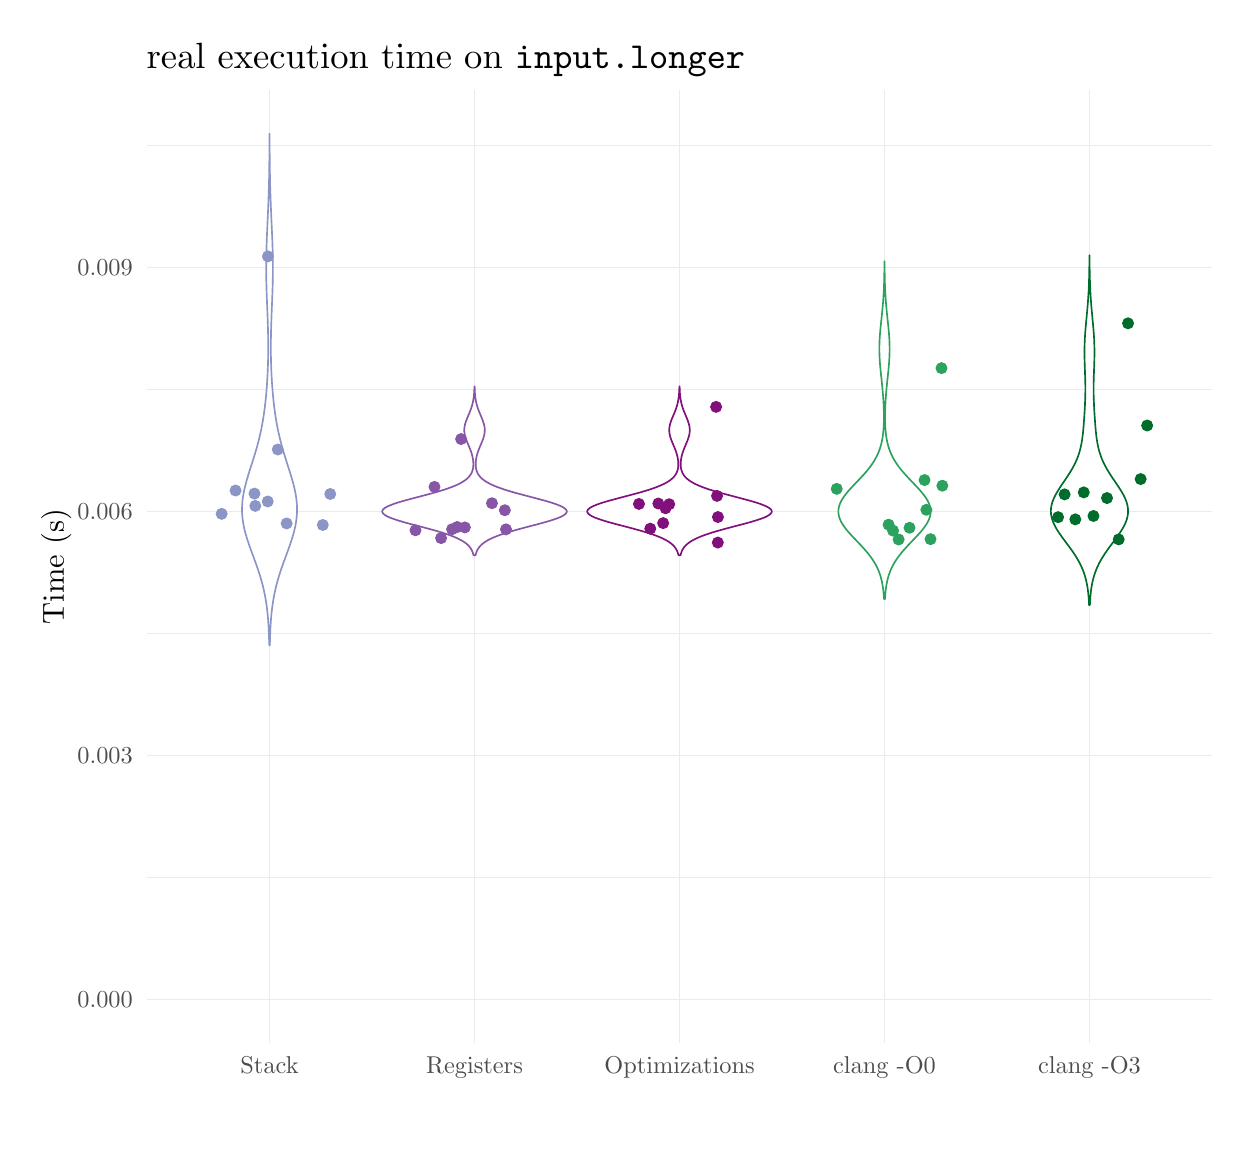
\begin{tikzpicture}[x=1pt,y=1pt]
\definecolor{fillColor}{RGB}{255,255,255}
\path[use as bounding box,fill=fillColor,fill opacity=0.00] (0,0) rectangle (433.62,397.48);
\begin{scope}
\path[clip] ( 42.95, 30.69) rectangle (428.12,374.83);
\definecolor{drawColor}{gray}{0.92}

\path[draw=drawColor,line width= 0.3pt,line join=round] ( 42.95, 90.41) --
	(428.12, 90.41);

\path[draw=drawColor,line width= 0.3pt,line join=round] ( 42.95,178.57) --
	(428.12,178.57);

\path[draw=drawColor,line width= 0.3pt,line join=round] ( 42.95,266.74) --
	(428.12,266.74);

\path[draw=drawColor,line width= 0.3pt,line join=round] ( 42.95,354.90) --
	(428.12,354.90);

\path[draw=drawColor,line width= 0.6pt,line join=round] ( 42.95, 46.33) --
	(428.12, 46.33);

\path[draw=drawColor,line width= 0.6pt,line join=round] ( 42.95,134.49) --
	(428.12,134.49);

\path[draw=drawColor,line width= 0.6pt,line join=round] ( 42.95,222.65) --
	(428.12,222.65);

\path[draw=drawColor,line width= 0.6pt,line join=round] ( 42.95,310.82) --
	(428.12,310.82);

\path[draw=drawColor,line width= 0.6pt,line join=round] ( 87.40, 30.69) --
	( 87.40,374.83);

\path[draw=drawColor,line width= 0.6pt,line join=round] (161.47, 30.69) --
	(161.47,374.83);

\path[draw=drawColor,line width= 0.6pt,line join=round] (235.54, 30.69) --
	(235.54,374.83);

\path[draw=drawColor,line width= 0.6pt,line join=round] (309.61, 30.69) --
	(309.61,374.83);

\path[draw=drawColor,line width= 0.6pt,line join=round] (383.68, 30.69) --
	(383.68,374.83);
\definecolor{drawColor}{RGB}{140,150,198}
\definecolor{fillColor}{RGB}{255,255,255}

\path[draw=drawColor,line width= 0.6pt,line join=round,line cap=round,fill=fillColor] ( 87.29,174.29) --
	( 87.28,174.65) --
	( 87.27,175.01) --
	( 87.26,175.37) --
	( 87.25,175.74) --
	( 87.24,176.10) --
	( 87.23,176.46) --
	( 87.22,176.82) --
	( 87.21,177.18) --
	( 87.20,177.54) --
	( 87.19,177.91) --
	( 87.17,178.27) --
	( 87.16,178.63) --
	( 87.15,178.99) --
	( 87.13,179.35) --
	( 87.11,179.72) --
	( 87.10,180.08) --
	( 87.08,180.44) --
	( 87.06,180.80) --
	( 87.04,181.16) --
	( 87.02,181.52) --
	( 87.00,181.89) --
	( 86.97,182.25) --
	( 86.95,182.61) --
	( 86.92,182.97) --
	( 86.90,183.33) --
	( 86.87,183.70) --
	( 86.84,184.06) --
	( 86.81,184.42) --
	( 86.78,184.78) --
	( 86.74,185.14) --
	( 86.71,185.50) --
	( 86.67,185.87) --
	( 86.64,186.23) --
	( 86.60,186.59) --
	( 86.56,186.95) --
	( 86.51,187.31) --
	( 86.47,187.68) --
	( 86.42,188.04) --
	( 86.38,188.40) --
	( 86.33,188.76) --
	( 86.27,189.12) --
	( 86.22,189.49) --
	( 86.17,189.85) --
	( 86.11,190.21) --
	( 86.05,190.57) --
	( 85.99,190.93) --
	( 85.93,191.29) --
	( 85.86,191.66) --
	( 85.79,192.02) --
	( 85.72,192.38) --
	( 85.65,192.74) --
	( 85.58,193.10) --
	( 85.50,193.47) --
	( 85.43,193.83) --
	( 85.35,194.19) --
	( 85.26,194.55) --
	( 85.18,194.91) --
	( 85.09,195.27) --
	( 85.00,195.64) --
	( 84.91,196.00) --
	( 84.82,196.36) --
	( 84.72,196.72) --
	( 84.63,197.08) --
	( 84.53,197.45) --
	( 84.43,197.81) --
	( 84.32,198.17) --
	( 84.22,198.53) --
	( 84.11,198.89) --
	( 84.00,199.25) --
	( 83.89,199.62) --
	( 83.77,199.98) --
	( 83.66,200.34) --
	( 83.54,200.70) --
	( 83.42,201.06) --
	( 83.30,201.43) --
	( 83.18,201.79) --
	( 83.06,202.15) --
	( 82.93,202.51) --
	( 82.81,202.87) --
	( 82.68,203.23) --
	( 82.55,203.60) --
	( 82.42,203.96) --
	( 82.29,204.32) --
	( 82.16,204.68) --
	( 82.03,205.04) --
	( 81.90,205.41) --
	( 81.77,205.77) --
	( 81.63,206.13) --
	( 81.50,206.49) --
	( 81.37,206.85) --
	( 81.23,207.21) --
	( 81.10,207.58) --
	( 80.97,207.94) --
	( 80.83,208.30) --
	( 80.70,208.66) --
	( 80.57,209.02) --
	( 80.44,209.39) --
	( 80.31,209.75) --
	( 80.18,210.11) --
	( 80.06,210.47) --
	( 79.93,210.83) --
	( 79.81,211.20) --
	( 79.69,211.56) --
	( 79.57,211.92) --
	( 79.45,212.28) --
	( 79.33,212.64) --
	( 79.22,213.00) --
	( 79.11,213.37) --
	( 79.00,213.73) --
	( 78.90,214.09) --
	( 78.79,214.45) --
	( 78.69,214.81) --
	( 78.60,215.18) --
	( 78.50,215.54) --
	( 78.41,215.90) --
	( 78.33,216.26) --
	( 78.24,216.62) --
	( 78.16,216.98) --
	( 78.09,217.35) --
	( 78.02,217.71) --
	( 77.95,218.07) --
	( 77.89,218.43) --
	( 77.83,218.79) --
	( 77.77,219.16) --
	( 77.72,219.52) --
	( 77.67,219.88) --
	( 77.63,220.24) --
	( 77.59,220.60) --
	( 77.56,220.96) --
	( 77.53,221.33) --
	( 77.51,221.69) --
	( 77.49,222.05) --
	( 77.47,222.41) --
	( 77.46,222.77) --
	( 77.46,223.14) --
	( 77.46,223.50) --
	( 77.46,223.86) --
	( 77.47,224.22) --
	( 77.48,224.58) --
	( 77.50,224.94) --
	( 77.52,225.31) --
	( 77.55,225.67) --
	( 77.58,226.03) --
	( 77.61,226.39) --
	( 77.65,226.75) --
	( 77.69,227.12) --
	( 77.74,227.48) --
	( 77.79,227.84) --
	( 77.85,228.20) --
	( 77.91,228.56) --
	( 77.97,228.92) --
	( 78.03,229.29) --
	( 78.10,229.65) --
	( 78.18,230.01) --
	( 78.25,230.37) --
	( 78.33,230.73) --
	( 78.42,231.10) --
	( 78.50,231.46) --
	( 78.59,231.82) --
	( 78.68,232.18) --
	( 78.77,232.54) --
	( 78.87,232.91) --
	( 78.97,233.27) --
	( 79.07,233.63) --
	( 79.17,233.99) --
	( 79.27,234.35) --
	( 79.38,234.71) --
	( 79.49,235.08) --
	( 79.59,235.44) --
	( 79.70,235.80) --
	( 79.82,236.16) --
	( 79.93,236.52) --
	( 80.04,236.89) --
	( 80.15,237.25) --
	( 80.27,237.61) --
	( 80.38,237.97) --
	( 80.50,238.33) --
	( 80.62,238.69) --
	( 80.73,239.06) --
	( 80.85,239.42) --
	( 80.96,239.78) --
	( 81.08,240.14) --
	( 81.19,240.50) --
	( 81.31,240.87) --
	( 81.42,241.23) --
	( 81.54,241.59) --
	( 81.65,241.95) --
	( 81.77,242.31) --
	( 81.88,242.67) --
	( 81.99,243.04) --
	( 82.10,243.40) --
	( 82.21,243.76) --
	( 82.32,244.12) --
	( 82.42,244.48) --
	( 82.53,244.85) --
	( 82.63,245.21) --
	( 82.74,245.57) --
	( 82.84,245.93) --
	( 82.94,246.29) --
	( 83.04,246.65) --
	( 83.14,247.02) --
	( 83.23,247.38) --
	( 83.33,247.74) --
	( 83.42,248.10) --
	( 83.51,248.46) --
	( 83.60,248.83) --
	( 83.69,249.19) --
	( 83.78,249.55) --
	( 83.86,249.91) --
	( 83.95,250.27) --
	( 84.03,250.63) --
	( 84.11,251.00) --
	( 84.19,251.36) --
	( 84.27,251.72) --
	( 84.34,252.08) --
	( 84.42,252.44) --
	( 84.49,252.81) --
	( 84.56,253.17) --
	( 84.63,253.53) --
	( 84.70,253.89) --
	( 84.77,254.25) --
	( 84.83,254.62) --
	( 84.89,254.98) --
	( 84.96,255.34) --
	( 85.02,255.70) --
	( 85.08,256.06) --
	( 85.14,256.42) --
	( 85.19,256.79) --
	( 85.25,257.15) --
	( 85.30,257.51) --
	( 85.36,257.87) --
	( 85.41,258.23) --
	( 85.46,258.60) --
	( 85.51,258.96) --
	( 85.56,259.32) --
	( 85.61,259.68) --
	( 85.65,260.04) --
	( 85.70,260.40) --
	( 85.74,260.77) --
	( 85.78,261.13) --
	( 85.83,261.49) --
	( 85.87,261.85) --
	( 85.91,262.21) --
	( 85.95,262.58) --
	( 85.98,262.94) --
	( 86.02,263.30) --
	( 86.06,263.66) --
	( 86.09,264.02) --
	( 86.13,264.38) --
	( 86.16,264.75) --
	( 86.20,265.11) --
	( 86.23,265.47) --
	( 86.26,265.83) --
	( 86.29,266.19) --
	( 86.32,266.56) --
	( 86.35,266.92) --
	( 86.38,267.28) --
	( 86.40,267.64) --
	( 86.43,268.00) --
	( 86.46,268.36) --
	( 86.48,268.73) --
	( 86.50,269.09) --
	( 86.53,269.45) --
	( 86.55,269.81) --
	( 86.57,270.17) --
	( 86.59,270.54) --
	( 86.61,270.90) --
	( 86.64,271.26) --
	( 86.65,271.62) --
	( 86.67,271.98) --
	( 86.69,272.34) --
	( 86.71,272.71) --
	( 86.72,273.07) --
	( 86.74,273.43) --
	( 86.76,273.79) --
	( 86.77,274.15) --
	( 86.78,274.52) --
	( 86.80,274.88) --
	( 86.81,275.24) --
	( 86.82,275.60) --
	( 86.83,275.96) --
	( 86.84,276.33) --
	( 86.85,276.69) --
	( 86.86,277.05) --
	( 86.87,277.41) --
	( 86.88,277.77) --
	( 86.89,278.13) --
	( 86.89,278.50) --
	( 86.90,278.86) --
	( 86.90,279.22) --
	( 86.91,279.58) --
	( 86.91,279.94) --
	( 86.91,280.31) --
	( 86.92,280.67) --
	( 86.92,281.03) --
	( 86.92,281.39) --
	( 86.92,281.75) --
	( 86.92,282.11) --
	( 86.92,282.48) --
	( 86.92,282.84) --
	( 86.92,283.20) --
	( 86.92,283.56) --
	( 86.91,283.92) --
	( 86.91,284.29) --
	( 86.91,284.65) --
	( 86.90,285.01) --
	( 86.90,285.37) --
	( 86.89,285.73) --
	( 86.89,286.09) --
	( 86.88,286.46) --
	( 86.87,286.82) --
	( 86.86,287.18) --
	( 86.86,287.54) --
	( 86.85,287.90) --
	( 86.84,288.27) --
	( 86.83,288.63) --
	( 86.82,288.99) --
	( 86.81,289.35) --
	( 86.80,289.71) --
	( 86.79,290.07) --
	( 86.78,290.44) --
	( 86.77,290.80) --
	( 86.75,291.16) --
	( 86.74,291.52) --
	( 86.73,291.88) --
	( 86.72,292.25) --
	( 86.70,292.61) --
	( 86.69,292.97) --
	( 86.68,293.33) --
	( 86.66,293.69) --
	( 86.65,294.05) --
	( 86.63,294.42) --
	( 86.62,294.78) --
	( 86.61,295.14) --
	( 86.59,295.50) --
	( 86.58,295.86) --
	( 86.56,296.23) --
	( 86.55,296.59) --
	( 86.53,296.95) --
	( 86.52,297.31) --
	( 86.50,297.67) --
	( 86.49,298.04) --
	( 86.47,298.40) --
	( 86.46,298.76) --
	( 86.45,299.12) --
	( 86.43,299.48) --
	( 86.42,299.84) --
	( 86.41,300.21) --
	( 86.39,300.57) --
	( 86.38,300.93) --
	( 86.37,301.29) --
	( 86.35,301.65) --
	( 86.34,302.02) --
	( 86.33,302.38) --
	( 86.32,302.74) --
	( 86.31,303.10) --
	( 86.30,303.46) --
	( 86.29,303.82) --
	( 86.28,304.19) --
	( 86.27,304.55) --
	( 86.26,304.91) --
	( 86.25,305.27) --
	( 86.24,305.63) --
	( 86.23,306.00) --
	( 86.23,306.36) --
	( 86.22,306.72) --
	( 86.21,307.08) --
	( 86.21,307.44) --
	( 86.20,307.80) --
	( 86.20,308.17) --
	( 86.19,308.53) --
	( 86.19,308.89) --
	( 86.19,309.25) --
	( 86.19,309.61) --
	( 86.18,309.98) --
	( 86.18,310.34) --
	( 86.18,310.70) --
	( 86.18,311.06) --
	( 86.18,311.42) --
	( 86.18,311.78) --
	( 86.19,312.15) --
	( 86.19,312.51) --
	( 86.19,312.87) --
	( 86.20,313.23) --
	( 86.20,313.59) --
	( 86.21,313.96) --
	( 86.21,314.32) --
	( 86.22,314.68) --
	( 86.22,315.04) --
	( 86.23,315.40) --
	( 86.24,315.76) --
	( 86.25,316.13) --
	( 86.26,316.49) --
	( 86.27,316.85) --
	( 86.28,317.21) --
	( 86.29,317.57) --
	( 86.30,317.94) --
	( 86.31,318.30) --
	( 86.32,318.66) --
	( 86.33,319.02) --
	( 86.34,319.38) --
	( 86.36,319.75) --
	( 86.37,320.11) --
	( 86.38,320.47) --
	( 86.40,320.83) --
	( 86.41,321.19) --
	( 86.42,321.55) --
	( 86.44,321.92) --
	( 86.45,322.28) --
	( 86.47,322.64) --
	( 86.48,323.00) --
	( 86.50,323.36) --
	( 86.52,323.73) --
	( 86.53,324.09) --
	( 86.55,324.45) --
	( 86.56,324.81) --
	( 86.58,325.17) --
	( 86.60,325.53) --
	( 86.61,325.90) --
	( 86.63,326.26) --
	( 86.65,326.62) --
	( 86.66,326.98) --
	( 86.68,327.34) --
	( 86.69,327.71) --
	( 86.71,328.07) --
	( 86.73,328.43) --
	( 86.74,328.79) --
	( 86.76,329.15) --
	( 86.78,329.51) --
	( 86.79,329.88) --
	( 86.81,330.24) --
	( 86.82,330.60) --
	( 86.84,330.96) --
	( 86.86,331.32) --
	( 86.87,331.69) --
	( 86.89,332.05) --
	( 86.90,332.41) --
	( 86.92,332.77) --
	( 86.93,333.13) --
	( 86.94,333.49) --
	( 86.96,333.86) --
	( 86.97,334.22) --
	( 86.99,334.58) --
	( 87.00,334.94) --
	( 87.01,335.30) --
	( 87.03,335.67) --
	( 87.04,336.03) --
	( 87.05,336.39) --
	( 87.06,336.75) --
	( 87.07,337.11) --
	( 87.09,337.47) --
	( 87.10,337.84) --
	( 87.11,338.20) --
	( 87.12,338.56) --
	( 87.13,338.92) --
	( 87.14,339.28) --
	( 87.15,339.65) --
	( 87.16,340.01) --
	( 87.17,340.37) --
	( 87.18,340.73) --
	( 87.19,341.09) --
	( 87.20,341.46) --
	( 87.20,341.82) --
	( 87.21,342.18) --
	( 87.22,342.54) --
	( 87.23,342.90) --
	( 87.24,343.26) --
	( 87.24,343.63) --
	( 87.25,343.99) --
	( 87.26,344.35) --
	( 87.26,344.71) --
	( 87.27,345.07) --
	( 87.27,345.44) --
	( 87.28,345.80) --
	( 87.29,346.16) --
	( 87.29,346.52) --
	( 87.30,346.88) --
	( 87.30,347.24) --
	( 87.31,347.61) --
	( 87.31,347.97) --
	( 87.31,348.33) --
	( 87.32,348.69) --
	( 87.32,349.05) --
	( 87.33,349.42) --
	( 87.33,349.78) --
	( 87.33,350.14) --
	( 87.34,350.50) --
	( 87.34,350.86) --
	( 87.34,351.22) --
	( 87.35,351.59) --
	( 87.35,351.95) --
	( 87.35,352.31) --
	( 87.35,352.67) --
	( 87.36,353.03) --
	( 87.36,353.40) --
	( 87.36,353.76) --
	( 87.36,354.12) --
	( 87.36,354.48) --
	( 87.37,354.84) --
	( 87.37,355.20) --
	( 87.37,355.57) --
	( 87.37,355.93) --
	( 87.37,356.29) --
	( 87.37,356.65) --
	( 87.38,357.01) --
	( 87.38,357.38) --
	( 87.38,357.74) --
	( 87.38,358.10) --
	( 87.38,358.46) --
	( 87.38,358.82) --
	( 87.38,359.18) --
	( 87.41,359.18) --
	( 87.41,358.82) --
	( 87.41,358.46) --
	( 87.41,358.10) --
	( 87.41,357.74) --
	( 87.42,357.38) --
	( 87.42,357.01) --
	( 87.42,356.65) --
	( 87.42,356.29) --
	( 87.42,355.93) --
	( 87.42,355.57) --
	( 87.42,355.20) --
	( 87.43,354.84) --
	( 87.43,354.48) --
	( 87.43,354.12) --
	( 87.43,353.76) --
	( 87.43,353.40) --
	( 87.44,353.03) --
	( 87.44,352.67) --
	( 87.44,352.31) --
	( 87.44,351.95) --
	( 87.45,351.59) --
	( 87.45,351.22) --
	( 87.45,350.86) --
	( 87.46,350.50) --
	( 87.46,350.14) --
	( 87.46,349.78) --
	( 87.47,349.42) --
	( 87.47,349.05) --
	( 87.47,348.69) --
	( 87.48,348.33) --
	( 87.48,347.97) --
	( 87.49,347.61) --
	( 87.49,347.24) --
	( 87.50,346.88) --
	( 87.50,346.52) --
	( 87.51,346.16) --
	( 87.51,345.80) --
	( 87.52,345.44) --
	( 87.52,345.07) --
	( 87.53,344.71) --
	( 87.54,344.35) --
	( 87.54,343.99) --
	( 87.55,343.63) --
	( 87.56,343.26) --
	( 87.56,342.90) --
	( 87.57,342.54) --
	( 87.58,342.18) --
	( 87.59,341.82) --
	( 87.60,341.46) --
	( 87.61,341.09) --
	( 87.61,340.73) --
	( 87.62,340.37) --
	( 87.63,340.01) --
	( 87.64,339.65) --
	( 87.65,339.28) --
	( 87.66,338.92) --
	( 87.67,338.56) --
	( 87.68,338.20) --
	( 87.69,337.84) --
	( 87.71,337.47) --
	( 87.72,337.11) --
	( 87.73,336.75) --
	( 87.74,336.39) --
	( 87.75,336.03) --
	( 87.77,335.67) --
	( 87.78,335.30) --
	( 87.79,334.94) --
	( 87.81,334.58) --
	( 87.82,334.22) --
	( 87.83,333.86) --
	( 87.85,333.49) --
	( 87.86,333.13) --
	( 87.88,332.77) --
	( 87.89,332.41) --
	( 87.91,332.05) --
	( 87.92,331.69) --
	( 87.94,331.32) --
	( 87.95,330.96) --
	( 87.97,330.60) --
	( 87.98,330.24) --
	( 88.00,329.88) --
	( 88.02,329.51) --
	( 88.03,329.15) --
	( 88.05,328.79) --
	( 88.06,328.43) --
	( 88.08,328.07) --
	( 88.10,327.71) --
	( 88.11,327.34) --
	( 88.13,326.98) --
	( 88.15,326.62) --
	( 88.16,326.26) --
	( 88.18,325.90) --
	( 88.20,325.53) --
	( 88.21,325.17) --
	( 88.23,324.81) --
	( 88.24,324.45) --
	( 88.26,324.09) --
	( 88.28,323.73) --
	( 88.29,323.36) --
	( 88.31,323.00) --
	( 88.32,322.64) --
	( 88.34,322.28) --
	( 88.35,321.92) --
	( 88.37,321.55) --
	( 88.38,321.19) --
	( 88.40,320.83) --
	( 88.41,320.47) --
	( 88.42,320.11) --
	( 88.44,319.75) --
	( 88.45,319.38) --
	( 88.46,319.02) --
	( 88.47,318.66) --
	( 88.49,318.30) --
	( 88.50,317.94) --
	( 88.51,317.57) --
	( 88.52,317.21) --
	( 88.53,316.85) --
	( 88.54,316.49) --
	( 88.55,316.13) --
	( 88.55,315.76) --
	( 88.56,315.40) --
	( 88.57,315.04) --
	( 88.57,314.68) --
	( 88.58,314.32) --
	( 88.59,313.96) --
	( 88.59,313.59) --
	( 88.60,313.23) --
	( 88.60,312.87) --
	( 88.60,312.51) --
	( 88.61,312.15) --
	( 88.61,311.78) --
	( 88.61,311.42) --
	( 88.61,311.06) --
	( 88.61,310.70) --
	( 88.61,310.34) --
	( 88.61,309.98) --
	( 88.61,309.61) --
	( 88.61,309.25) --
	( 88.60,308.89) --
	( 88.60,308.53) --
	( 88.60,308.17) --
	( 88.59,307.80) --
	( 88.59,307.44) --
	( 88.58,307.08) --
	( 88.57,306.72) --
	( 88.57,306.36) --
	( 88.56,306.00) --
	( 88.55,305.63) --
	( 88.54,305.27) --
	( 88.54,304.91) --
	( 88.53,304.55) --
	( 88.52,304.19) --
	( 88.51,303.82) --
	( 88.50,303.46) --
	( 88.49,303.10) --
	( 88.47,302.74) --
	( 88.46,302.38) --
	( 88.45,302.02) --
	( 88.44,301.65) --
	( 88.43,301.29) --
	( 88.41,300.93) --
	( 88.40,300.57) --
	( 88.39,300.21) --
	( 88.37,299.84) --
	( 88.36,299.48) --
	( 88.35,299.12) --
	( 88.33,298.76) --
	( 88.32,298.40) --
	( 88.30,298.04) --
	( 88.29,297.67) --
	( 88.27,297.31) --
	( 88.26,296.95) --
	( 88.25,296.59) --
	( 88.23,296.23) --
	( 88.22,295.86) --
	( 88.20,295.50) --
	( 88.19,295.14) --
	( 88.17,294.78) --
	( 88.16,294.42) --
	( 88.14,294.05) --
	( 88.13,293.69) --
	( 88.12,293.33) --
	( 88.10,292.97) --
	( 88.09,292.61) --
	( 88.08,292.25) --
	( 88.06,291.88) --
	( 88.05,291.52) --
	( 88.04,291.16) --
	( 88.03,290.80) --
	( 88.02,290.44) --
	( 88.00,290.07) --
	( 87.99,289.71) --
	( 87.98,289.35) --
	( 87.97,288.99) --
	( 87.96,288.63) --
	( 87.95,288.27) --
	( 87.94,287.90) --
	( 87.94,287.54) --
	( 87.93,287.18) --
	( 87.92,286.82) --
	( 87.91,286.46) --
	( 87.91,286.09) --
	( 87.90,285.73) --
	( 87.90,285.37) --
	( 87.89,285.01) --
	( 87.89,284.65) --
	( 87.88,284.29) --
	( 87.88,283.92) --
	( 87.88,283.56) --
	( 87.87,283.20) --
	( 87.87,282.84) --
	( 87.87,282.48) --
	( 87.87,282.11) --
	( 87.87,281.75) --
	( 87.87,281.39) --
	( 87.87,281.03) --
	( 87.87,280.67) --
	( 87.88,280.31) --
	( 87.88,279.94) --
	( 87.88,279.58) --
	( 87.89,279.22) --
	( 87.89,278.86) --
	( 87.90,278.50) --
	( 87.91,278.13) --
	( 87.91,277.77) --
	( 87.92,277.41) --
	( 87.93,277.05) --
	( 87.94,276.69) --
	( 87.95,276.33) --
	( 87.96,275.96) --
	( 87.97,275.60) --
	( 87.98,275.24) --
	( 88.00,274.88) --
	( 88.01,274.52) --
	( 88.02,274.15) --
	( 88.04,273.79) --
	( 88.05,273.43) --
	( 88.07,273.07) --
	( 88.08,272.71) --
	( 88.10,272.34) --
	( 88.12,271.98) --
	( 88.14,271.62) --
	( 88.16,271.26) --
	( 88.18,270.90) --
	( 88.20,270.54) --
	( 88.22,270.17) --
	( 88.24,269.81) --
	( 88.26,269.45) --
	( 88.29,269.09) --
	( 88.31,268.73) --
	( 88.34,268.36) --
	( 88.36,268.00) --
	( 88.39,267.64) --
	( 88.42,267.28) --
	( 88.45,266.92) --
	( 88.47,266.56) --
	( 88.50,266.19) --
	( 88.53,265.83) --
	( 88.57,265.47) --
	( 88.60,265.11) --
	( 88.63,264.75) --
	( 88.66,264.38) --
	( 88.70,264.02) --
	( 88.73,263.66) --
	( 88.77,263.30) --
	( 88.81,262.94) --
	( 88.85,262.58) --
	( 88.88,262.21) --
	( 88.92,261.85) --
	( 88.97,261.49) --
	( 89.01,261.13) --
	( 89.05,260.77) --
	( 89.10,260.40) --
	( 89.14,260.04) --
	( 89.19,259.68) --
	( 89.23,259.32) --
	( 89.28,258.96) --
	( 89.33,258.60) --
	( 89.38,258.23) --
	( 89.44,257.87) --
	( 89.49,257.51) --
	( 89.54,257.15) --
	( 89.60,256.79) --
	( 89.66,256.42) --
	( 89.71,256.06) --
	( 89.77,255.70) --
	( 89.84,255.34) --
	( 89.90,254.98) --
	( 89.96,254.62) --
	( 90.03,254.25) --
	( 90.09,253.89) --
	( 90.16,253.53) --
	( 90.23,253.17) --
	( 90.30,252.81) --
	( 90.38,252.44) --
	( 90.45,252.08) --
	( 90.53,251.72) --
	( 90.60,251.36) --
	( 90.68,251.00) --
	( 90.76,250.63) --
	( 90.85,250.27) --
	( 90.93,249.91) --
	( 91.02,249.55) --
	( 91.10,249.19) --
	( 91.19,248.83) --
	( 91.28,248.46) --
	( 91.37,248.10) --
	( 91.47,247.74) --
	( 91.56,247.38) --
	( 91.66,247.02) --
	( 91.75,246.65) --
	( 91.85,246.29) --
	( 91.95,245.93) --
	( 92.06,245.57) --
	( 92.16,245.21) --
	( 92.26,244.85) --
	( 92.37,244.48) --
	( 92.48,244.12) --
	( 92.58,243.76) --
	( 92.69,243.40) --
	( 92.80,243.04) --
	( 92.92,242.67) --
	( 93.03,242.31) --
	( 93.14,241.95) --
	( 93.25,241.59) --
	( 93.37,241.23) --
	( 93.48,240.87) --
	( 93.60,240.50) --
	( 93.71,240.14) --
	( 93.83,239.78) --
	( 93.95,239.42) --
	( 94.06,239.06) --
	( 94.18,238.69) --
	( 94.29,238.33) --
	( 94.41,237.97) --
	( 94.52,237.61) --
	( 94.64,237.25) --
	( 94.75,236.89) --
	( 94.86,236.52) --
	( 94.98,236.16) --
	( 95.09,235.80) --
	( 95.20,235.44) --
	( 95.31,235.08) --
	( 95.41,234.71) --
	( 95.52,234.35) --
	( 95.62,233.99) --
	( 95.73,233.63) --
	( 95.83,233.27) --
	( 95.92,232.91) --
	( 96.02,232.54) --
	( 96.11,232.18) --
	( 96.20,231.82) --
	( 96.29,231.46) --
	( 96.38,231.10) --
	( 96.46,230.73) --
	( 96.54,230.37) --
	( 96.62,230.01) --
	( 96.69,229.65) --
	( 96.76,229.29) --
	( 96.82,228.92) --
	( 96.89,228.56) --
	( 96.95,228.20) --
	( 97.00,227.84) --
	( 97.05,227.48) --
	( 97.10,227.12) --
	( 97.14,226.75) --
	( 97.18,226.39) --
	( 97.22,226.03) --
	( 97.25,225.67) --
	( 97.27,225.31) --
	( 97.29,224.94) --
	( 97.31,224.58) --
	( 97.32,224.22) --
	( 97.33,223.86) --
	( 97.34,223.50) --
	( 97.33,223.14) --
	( 97.33,222.77) --
	( 97.32,222.41) --
	( 97.30,222.05) --
	( 97.28,221.69) --
	( 97.26,221.33) --
	( 97.23,220.96) --
	( 97.20,220.60) --
	( 97.16,220.24) --
	( 97.12,219.88) --
	( 97.07,219.52) --
	( 97.02,219.16) --
	( 96.97,218.79) --
	( 96.91,218.43) --
	( 96.84,218.07) --
	( 96.78,217.71) --
	( 96.70,217.35) --
	( 96.63,216.98) --
	( 96.55,216.62) --
	( 96.47,216.26) --
	( 96.38,215.90) --
	( 96.29,215.54) --
	( 96.20,215.18) --
	( 96.10,214.81) --
	( 96.00,214.45) --
	( 95.90,214.09) --
	( 95.79,213.73) --
	( 95.68,213.37) --
	( 95.57,213.00) --
	( 95.46,212.64) --
	( 95.34,212.28) --
	( 95.22,211.92) --
	( 95.10,211.56) --
	( 94.98,211.20) --
	( 94.86,210.83) --
	( 94.73,210.47) --
	( 94.61,210.11) --
	( 94.48,209.75) --
	( 94.35,209.39) --
	( 94.22,209.02) --
	( 94.09,208.66) --
	( 93.96,208.30) --
	( 93.83,207.94) --
	( 93.69,207.58) --
	( 93.56,207.21) --
	( 93.43,206.85) --
	( 93.29,206.49) --
	( 93.16,206.13) --
	( 93.03,205.77) --
	( 92.89,205.41) --
	( 92.76,205.04) --
	( 92.63,204.68) --
	( 92.50,204.32) --
	( 92.37,203.96) --
	( 92.24,203.60) --
	( 92.11,203.23) --
	( 91.98,202.87) --
	( 91.86,202.51) --
	( 91.73,202.15) --
	( 91.61,201.79) --
	( 91.49,201.43) --
	( 91.37,201.06) --
	( 91.25,200.70) --
	( 91.13,200.34) --
	( 91.02,199.98) --
	( 90.90,199.62) --
	( 90.79,199.25) --
	( 90.68,198.89) --
	( 90.58,198.53) --
	( 90.47,198.17) --
	( 90.37,197.81) --
	( 90.26,197.45) --
	( 90.17,197.08) --
	( 90.07,196.72) --
	( 89.97,196.36) --
	( 89.88,196.00) --
	( 89.79,195.64) --
	( 89.70,195.27) --
	( 89.61,194.91) --
	( 89.53,194.55) --
	( 89.45,194.19) --
	( 89.37,193.83) --
	( 89.29,193.47) --
	( 89.21,193.10) --
	( 89.14,192.74) --
	( 89.07,192.38) --
	( 89.00,192.02) --
	( 88.93,191.66) --
	( 88.87,191.29) --
	( 88.80,190.93) --
	( 88.74,190.57) --
	( 88.68,190.21) --
	( 88.63,189.85) --
	( 88.57,189.49) --
	( 88.52,189.12) --
	( 88.47,188.76) --
	( 88.42,188.40) --
	( 88.37,188.04) --
	( 88.32,187.68) --
	( 88.28,187.31) --
	( 88.24,186.95) --
	( 88.20,186.59) --
	( 88.16,186.23) --
	( 88.12,185.87) --
	( 88.08,185.50) --
	( 88.05,185.14) --
	( 88.01,184.78) --
	( 87.98,184.42) --
	( 87.95,184.06) --
	( 87.92,183.70) --
	( 87.90,183.33) --
	( 87.87,182.97) --
	( 87.84,182.61) --
	( 87.82,182.25) --
	( 87.80,181.89) --
	( 87.77,181.52) --
	( 87.75,181.16) --
	( 87.73,180.80) --
	( 87.71,180.44) --
	( 87.70,180.08) --
	( 87.68,179.72) --
	( 87.66,179.35) --
	( 87.65,178.99) --
	( 87.63,178.63) --
	( 87.62,178.27) --
	( 87.60,177.91) --
	( 87.59,177.54) --
	( 87.58,177.18) --
	( 87.57,176.82) --
	( 87.56,176.46) --
	( 87.55,176.10) --
	( 87.54,175.74) --
	( 87.53,175.37) --
	( 87.52,175.01) --
	( 87.51,174.65) --
	( 87.51,174.29) --
	( 87.29,174.29) --
	cycle;
\definecolor{drawColor}{RGB}{136,86,167}

\path[draw=drawColor,line width= 0.6pt,line join=round,line cap=round,fill=fillColor] (161.09,206.82) --
	(161.07,206.94) --
	(161.04,207.06) --
	(161.01,207.18) --
	(160.98,207.30) --
	(160.94,207.42) --
	(160.91,207.54) --
	(160.87,207.66) --
	(160.83,207.78) --
	(160.79,207.90) --
	(160.75,208.02) --
	(160.70,208.14) --
	(160.65,208.26) --
	(160.60,208.38) --
	(160.55,208.50) --
	(160.49,208.62) --
	(160.43,208.73) --
	(160.37,208.85) --
	(160.30,208.97) --
	(160.23,209.09) --
	(160.16,209.21) --
	(160.08,209.33) --
	(160.00,209.45) --
	(159.91,209.57) --
	(159.82,209.69) --
	(159.73,209.81) --
	(159.63,209.93) --
	(159.53,210.05) --
	(159.43,210.17) --
	(159.31,210.29) --
	(159.20,210.41) --
	(159.07,210.53) --
	(158.95,210.65) --
	(158.82,210.77) --
	(158.68,210.89) --
	(158.54,211.00) --
	(158.39,211.12) --
	(158.23,211.24) --
	(158.07,211.36) --
	(157.90,211.48) --
	(157.73,211.60) --
	(157.55,211.72) --
	(157.36,211.84) --
	(157.17,211.96) --
	(156.97,212.08) --
	(156.76,212.20) --
	(156.55,212.32) --
	(156.33,212.44) --
	(156.10,212.56) --
	(155.86,212.68) --
	(155.62,212.80) --
	(155.37,212.92) --
	(155.11,213.04) --
	(154.85,213.16) --
	(154.57,213.27) --
	(154.29,213.39) --
	(154.00,213.51) --
	(153.71,213.63) --
	(153.40,213.75) --
	(153.09,213.87) --
	(152.78,213.99) --
	(152.45,214.11) --
	(152.12,214.23) --
	(151.77,214.35) --
	(151.43,214.47) --
	(151.07,214.59) --
	(150.71,214.71) --
	(150.34,214.83) --
	(149.96,214.95) --
	(149.58,215.07) --
	(149.19,215.19) --
	(148.80,215.31) --
	(148.40,215.43) --
	(147.99,215.54) --
	(147.58,215.66) --
	(147.16,215.78) --
	(146.73,215.90) --
	(146.31,216.02) --
	(145.87,216.14) --
	(145.44,216.26) --
	(145.00,216.38) --
	(144.55,216.50) --
	(144.11,216.62) --
	(143.66,216.74) --
	(143.20,216.86) --
	(142.75,216.98) --
	(142.29,217.10) --
	(141.84,217.22) --
	(141.38,217.34) --
	(140.92,217.46) --
	(140.47,217.58) --
	(140.01,217.70) --
	(139.56,217.81) --
	(139.10,217.93) --
	(138.65,218.05) --
	(138.21,218.17) --
	(137.76,218.29) --
	(137.32,218.41) --
	(136.89,218.53) --
	(136.45,218.65) --
	(136.03,218.77) --
	(135.61,218.89) --
	(135.20,219.01) --
	(134.79,219.13) --
	(134.39,219.25) --
	(134.00,219.37) --
	(133.62,219.49) --
	(133.25,219.61) --
	(132.88,219.73) --
	(132.53,219.85) --
	(132.19,219.97) --
	(131.85,220.08) --
	(131.54,220.20) --
	(131.23,220.32) --
	(130.93,220.44) --
	(130.65,220.56) --
	(130.38,220.68) --
	(130.13,220.80) --
	(129.88,220.92) --
	(129.66,221.04) --
	(129.44,221.16) --
	(129.24,221.28) --
	(129.07,221.40) --
	(128.90,221.52) --
	(128.75,221.64) --
	(128.61,221.76) --
	(128.49,221.88) --
	(128.40,222.00) --
	(128.31,222.12) --
	(128.24,222.24) --
	(128.19,222.35) --
	(128.15,222.47) --
	(128.14,222.59) --
	(128.13,222.71) --
	(128.16,222.83) --
	(128.19,222.95) --
	(128.24,223.07) --
	(128.31,223.19) --
	(128.39,223.31) --
	(128.49,223.43) --
	(128.61,223.55) --
	(128.74,223.67) --
	(128.90,223.79) --
	(129.06,223.91) --
	(129.24,224.03) --
	(129.44,224.15) --
	(129.65,224.27) --
	(129.88,224.39) --
	(130.12,224.51) --
	(130.37,224.62) --
	(130.64,224.74) --
	(130.92,224.86) --
	(131.22,224.98) --
	(131.53,225.10) --
	(131.85,225.22) --
	(132.18,225.34) --
	(132.52,225.46) --
	(132.87,225.58) --
	(133.23,225.70) --
	(133.61,225.82) --
	(133.99,225.94) --
	(134.38,226.06) --
	(134.78,226.18) --
	(135.18,226.30) --
	(135.60,226.42) --
	(136.02,226.54) --
	(136.44,226.66) --
	(136.87,226.78) --
	(137.31,226.89) --
	(137.75,227.01) --
	(138.19,227.13) --
	(138.64,227.25) --
	(139.09,227.37) --
	(139.55,227.49) --
	(140.00,227.61) --
	(140.46,227.73) --
	(140.91,227.85) --
	(141.37,227.97) --
	(141.83,228.09) --
	(142.28,228.21) --
	(142.74,228.33) --
	(143.19,228.45) --
	(143.65,228.57) --
	(144.09,228.69) --
	(144.54,228.81) --
	(144.99,228.93) --
	(145.43,229.05) --
	(145.86,229.16) --
	(146.29,229.28) --
	(146.72,229.40) --
	(147.15,229.52) --
	(147.56,229.64) --
	(147.98,229.76) --
	(148.38,229.88) --
	(148.79,230.00) --
	(149.18,230.12) --
	(149.57,230.24) --
	(149.96,230.36) --
	(150.33,230.48) --
	(150.70,230.60) --
	(151.06,230.72) --
	(151.42,230.84) --
	(151.77,230.96) --
	(152.11,231.08) --
	(152.44,231.20) --
	(152.77,231.32) --
	(153.08,231.43) --
	(153.40,231.55) --
	(153.70,231.67) --
	(154.00,231.79) --
	(154.28,231.91) --
	(154.56,232.03) --
	(154.84,232.15) --
	(155.10,232.27) --
	(155.36,232.39) --
	(155.61,232.51) --
	(155.85,232.63) --
	(156.09,232.75) --
	(156.32,232.87) --
	(156.54,232.99) --
	(156.75,233.11) --
	(156.96,233.23) --
	(157.16,233.35) --
	(157.35,233.47) --
	(157.54,233.59) --
	(157.71,233.70) --
	(157.89,233.82) --
	(158.05,233.94) --
	(158.22,234.06) --
	(158.37,234.18) --
	(158.52,234.30) --
	(158.66,234.42) --
	(158.80,234.54) --
	(158.93,234.66) --
	(159.05,234.78) --
	(159.17,234.90) --
	(159.29,235.02) --
	(159.40,235.14) --
	(159.50,235.26) --
	(159.60,235.38) --
	(159.70,235.50) --
	(159.79,235.62) --
	(159.88,235.74) --
	(159.96,235.86) --
	(160.04,235.97) --
	(160.12,236.09) --
	(160.19,236.21) --
	(160.25,236.33) --
	(160.32,236.45) --
	(160.38,236.57) --
	(160.43,236.69) --
	(160.49,236.81) --
	(160.54,236.93) --
	(160.59,237.05) --
	(160.63,237.17) --
	(160.67,237.29) --
	(160.71,237.41) --
	(160.75,237.53) --
	(160.78,237.65) --
	(160.81,237.77) --
	(160.84,237.89) --
	(160.87,238.01) --
	(160.89,238.13) --
	(160.92,238.24) --
	(160.94,238.36) --
	(160.95,238.48) --
	(160.97,238.60) --
	(160.98,238.72) --
	(161.00,238.84) --
	(161.01,238.96) --
	(161.02,239.08) --
	(161.03,239.20) --
	(161.03,239.32) --
	(161.04,239.44) --
	(161.04,239.56) --
	(161.04,239.68) --
	(161.04,239.80) --
	(161.04,239.92) --
	(161.04,240.04) --
	(161.03,240.16) --
	(161.03,240.28) --
	(161.02,240.40) --
	(161.01,240.51) --
	(161.00,240.63) --
	(160.99,240.75) --
	(160.98,240.87) --
	(160.97,240.99) --
	(160.96,241.11) --
	(160.94,241.23) --
	(160.92,241.35) --
	(160.91,241.47) --
	(160.89,241.59) --
	(160.87,241.71) --
	(160.85,241.83) --
	(160.83,241.95) --
	(160.80,242.07) --
	(160.78,242.19) --
	(160.76,242.31) --
	(160.73,242.43) --
	(160.70,242.55) --
	(160.67,242.67) --
	(160.65,242.78) --
	(160.62,242.90) --
	(160.58,243.02) --
	(160.55,243.14) --
	(160.52,243.26) --
	(160.48,243.38) --
	(160.45,243.50) --
	(160.41,243.62) --
	(160.38,243.74) --
	(160.34,243.86) --
	(160.30,243.98) --
	(160.26,244.10) --
	(160.22,244.22) --
	(160.18,244.34) --
	(160.14,244.46) --
	(160.10,244.58) --
	(160.05,244.70) --
	(160.01,244.82) --
	(159.96,244.94) --
	(159.92,245.05) --
	(159.87,245.17) --
	(159.83,245.29) --
	(159.78,245.41) --
	(159.73,245.53) --
	(159.68,245.65) --
	(159.63,245.77) --
	(159.58,245.89) --
	(159.53,246.01) --
	(159.48,246.13) --
	(159.43,246.25) --
	(159.38,246.37) --
	(159.33,246.49) --
	(159.28,246.61) --
	(159.23,246.73) --
	(159.18,246.85) --
	(159.13,246.97) --
	(159.08,247.09) --
	(159.03,247.21) --
	(158.98,247.32) --
	(158.93,247.44) --
	(158.88,247.56) --
	(158.83,247.68) --
	(158.78,247.80) --
	(158.73,247.92) --
	(158.69,248.04) --
	(158.64,248.16) --
	(158.59,248.28) --
	(158.55,248.40) --
	(158.50,248.52) --
	(158.46,248.64) --
	(158.41,248.76) --
	(158.37,248.88) --
	(158.33,249.00) --
	(158.29,249.12) --
	(158.25,249.24) --
	(158.21,249.36) --
	(158.18,249.48) --
	(158.14,249.59) --
	(158.11,249.71) --
	(158.07,249.83) --
	(158.04,249.95) --
	(158.01,250.07) --
	(157.98,250.19) --
	(157.96,250.31) --
	(157.93,250.43) --
	(157.91,250.55) --
	(157.89,250.67) --
	(157.87,250.79) --
	(157.85,250.91) --
	(157.83,251.03) --
	(157.82,251.15) --
	(157.80,251.27) --
	(157.79,251.39) --
	(157.78,251.51) --
	(157.77,251.63) --
	(157.77,251.75) --
	(157.77,251.86) --
	(157.76,251.98) --
	(157.76,252.10) --
	(157.77,252.22) --
	(157.77,252.34) --
	(157.77,252.46) --
	(157.78,252.58) --
	(157.79,252.70) --
	(157.80,252.82) --
	(157.82,252.94) --
	(157.83,253.06) --
	(157.85,253.18) --
	(157.87,253.30) --
	(157.89,253.42) --
	(157.91,253.54) --
	(157.93,253.66) --
	(157.96,253.78) --
	(157.98,253.90) --
	(158.01,254.02) --
	(158.04,254.13) --
	(158.07,254.25) --
	(158.11,254.37) --
	(158.14,254.49) --
	(158.18,254.61) --
	(158.21,254.73) --
	(158.25,254.85) --
	(158.29,254.97) --
	(158.33,255.09) --
	(158.37,255.21) --
	(158.41,255.33) --
	(158.46,255.45) --
	(158.50,255.57) --
	(158.55,255.69) --
	(158.59,255.81) --
	(158.64,255.93) --
	(158.69,256.05) --
	(158.74,256.17) --
	(158.78,256.29) --
	(158.83,256.40) --
	(158.88,256.52) --
	(158.93,256.64) --
	(158.98,256.76) --
	(159.03,256.88) --
	(159.08,257.00) --
	(159.13,257.12) --
	(159.18,257.24) --
	(159.23,257.36) --
	(159.29,257.48) --
	(159.34,257.60) --
	(159.39,257.72) --
	(159.44,257.84) --
	(159.49,257.96) --
	(159.54,258.08) --
	(159.59,258.20) --
	(159.64,258.32) --
	(159.69,258.44) --
	(159.73,258.56) --
	(159.78,258.67) --
	(159.83,258.79) --
	(159.88,258.91) --
	(159.92,259.03) --
	(159.97,259.15) --
	(160.01,259.27) --
	(160.06,259.39) --
	(160.10,259.51) --
	(160.15,259.63) --
	(160.19,259.75) --
	(160.23,259.87) --
	(160.27,259.99) --
	(160.31,260.11) --
	(160.35,260.23) --
	(160.39,260.35) --
	(160.43,260.47) --
	(160.46,260.59) --
	(160.50,260.71) --
	(160.54,260.83) --
	(160.57,260.94) --
	(160.60,261.06) --
	(160.64,261.18) --
	(160.67,261.30) --
	(160.70,261.42) --
	(160.73,261.54) --
	(160.76,261.66) --
	(160.79,261.78) --
	(160.82,261.90) --
	(160.84,262.02) --
	(160.87,262.14) --
	(160.90,262.26) --
	(160.92,262.38) --
	(160.94,262.50) --
	(160.97,262.62) --
	(160.99,262.74) --
	(161.01,262.86) --
	(161.03,262.98) --
	(161.05,263.10) --
	(161.07,263.21) --
	(161.09,263.33) --
	(161.11,263.45) --
	(161.12,263.57) --
	(161.14,263.69) --
	(161.16,263.81) --
	(161.17,263.93) --
	(161.19,264.05) --
	(161.20,264.17) --
	(161.21,264.29) --
	(161.23,264.41) --
	(161.24,264.53) --
	(161.25,264.65) --
	(161.26,264.77) --
	(161.27,264.89) --
	(161.28,265.01) --
	(161.29,265.13) --
	(161.30,265.25) --
	(161.31,265.37) --
	(161.32,265.48) --
	(161.33,265.60) --
	(161.34,265.72) --
	(161.34,265.84) --
	(161.35,265.96) --
	(161.36,266.08) --
	(161.36,266.20) --
	(161.37,266.32) --
	(161.38,266.44) --
	(161.38,266.56) --
	(161.39,266.68) --
	(161.39,266.80) --
	(161.40,266.92) --
	(161.40,267.04) --
	(161.40,267.16) --
	(161.41,267.28) --
	(161.41,267.40) --
	(161.42,267.52) --
	(161.42,267.64) --
	(161.42,267.75) --
	(161.42,267.87) --
	(161.51,267.87) --
	(161.51,267.75) --
	(161.51,267.64) --
	(161.52,267.52) --
	(161.52,267.40) --
	(161.52,267.28) --
	(161.53,267.16) --
	(161.53,267.04) --
	(161.54,266.92) --
	(161.54,266.80) --
	(161.55,266.68) --
	(161.55,266.56) --
	(161.56,266.44) --
	(161.56,266.32) --
	(161.57,266.20) --
	(161.58,266.08) --
	(161.58,265.96) --
	(161.59,265.84) --
	(161.60,265.72) --
	(161.60,265.60) --
	(161.61,265.48) --
	(161.62,265.37) --
	(161.63,265.25) --
	(161.64,265.13) --
	(161.65,265.01) --
	(161.66,264.89) --
	(161.67,264.77) --
	(161.68,264.65) --
	(161.69,264.53) --
	(161.71,264.41) --
	(161.72,264.29) --
	(161.73,264.17) --
	(161.75,264.05) --
	(161.76,263.93) --
	(161.78,263.81) --
	(161.79,263.69) --
	(161.81,263.57) --
	(161.83,263.45) --
	(161.84,263.33) --
	(161.86,263.21) --
	(161.88,263.10) --
	(161.90,262.98) --
	(161.92,262.86) --
	(161.94,262.74) --
	(161.97,262.62) --
	(161.99,262.50) --
	(162.01,262.38) --
	(162.04,262.26) --
	(162.06,262.14) --
	(162.09,262.02) --
	(162.12,261.90) --
	(162.14,261.78) --
	(162.17,261.66) --
	(162.20,261.54) --
	(162.23,261.42) --
	(162.26,261.30) --
	(162.30,261.18) --
	(162.33,261.06) --
	(162.36,260.94) --
	(162.40,260.83) --
	(162.43,260.71) --
	(162.47,260.59) --
	(162.51,260.47) --
	(162.54,260.35) --
	(162.58,260.23) --
	(162.62,260.11) --
	(162.66,259.99) --
	(162.70,259.87) --
	(162.74,259.75) --
	(162.79,259.63) --
	(162.83,259.51) --
	(162.87,259.39) --
	(162.92,259.27) --
	(162.96,259.15) --
	(163.01,259.03) --
	(163.06,258.91) --
	(163.10,258.79) --
	(163.15,258.67) --
	(163.20,258.56) --
	(163.25,258.44) --
	(163.30,258.32) --
	(163.35,258.20) --
	(163.40,258.08) --
	(163.45,257.96) --
	(163.50,257.84) --
	(163.55,257.72) --
	(163.60,257.60) --
	(163.65,257.48) --
	(163.70,257.36) --
	(163.75,257.24) --
	(163.80,257.12) --
	(163.85,257.00) --
	(163.90,256.88) --
	(163.95,256.76) --
	(164.00,256.64) --
	(164.05,256.52) --
	(164.10,256.40) --
	(164.15,256.29) --
	(164.20,256.17) --
	(164.25,256.05) --
	(164.29,255.93) --
	(164.34,255.81) --
	(164.39,255.69) --
	(164.43,255.57) --
	(164.48,255.45) --
	(164.52,255.33) --
	(164.56,255.21) --
	(164.60,255.09) --
	(164.64,254.97) --
	(164.68,254.85) --
	(164.72,254.73) --
	(164.76,254.61) --
	(164.79,254.49) --
	(164.83,254.37) --
	(164.86,254.25) --
	(164.89,254.13) --
	(164.92,254.02) --
	(164.95,253.90) --
	(164.98,253.78) --
	(165.00,253.66) --
	(165.02,253.54) --
	(165.05,253.42) --
	(165.07,253.30) --
	(165.09,253.18) --
	(165.10,253.06) --
	(165.12,252.94) --
	(165.13,252.82) --
	(165.14,252.70) --
	(165.15,252.58) --
	(165.16,252.46) --
	(165.16,252.34) --
	(165.17,252.22) --
	(165.17,252.10) --
	(165.17,251.98) --
	(165.17,251.86) --
	(165.16,251.75) --
	(165.16,251.63) --
	(165.15,251.51) --
	(165.14,251.39) --
	(165.13,251.27) --
	(165.12,251.15) --
	(165.10,251.03) --
	(165.09,250.91) --
	(165.07,250.79) --
	(165.05,250.67) --
	(165.03,250.55) --
	(165.00,250.43) --
	(164.98,250.31) --
	(164.95,250.19) --
	(164.92,250.07) --
	(164.89,249.95) --
	(164.86,249.83) --
	(164.83,249.71) --
	(164.79,249.59) --
	(164.76,249.48) --
	(164.72,249.36) --
	(164.68,249.24) --
	(164.64,249.12) --
	(164.60,249.00) --
	(164.56,248.88) --
	(164.52,248.76) --
	(164.48,248.64) --
	(164.43,248.52) --
	(164.39,248.40) --
	(164.34,248.28) --
	(164.29,248.16) --
	(164.25,248.04) --
	(164.20,247.92) --
	(164.15,247.80) --
	(164.10,247.68) --
	(164.05,247.56) --
	(164.00,247.44) --
	(163.95,247.32) --
	(163.90,247.21) --
	(163.85,247.09) --
	(163.80,246.97) --
	(163.75,246.85) --
	(163.70,246.73) --
	(163.65,246.61) --
	(163.60,246.49) --
	(163.55,246.37) --
	(163.50,246.25) --
	(163.45,246.13) --
	(163.40,246.01) --
	(163.35,245.89) --
	(163.30,245.77) --
	(163.25,245.65) --
	(163.20,245.53) --
	(163.16,245.41) --
	(163.11,245.29) --
	(163.06,245.17) --
	(163.02,245.05) --
	(162.97,244.94) --
	(162.93,244.82) --
	(162.88,244.70) --
	(162.84,244.58) --
	(162.79,244.46) --
	(162.75,244.34) --
	(162.71,244.22) --
	(162.67,244.10) --
	(162.63,243.98) --
	(162.59,243.86) --
	(162.56,243.74) --
	(162.52,243.62) --
	(162.48,243.50) --
	(162.45,243.38) --
	(162.41,243.26) --
	(162.38,243.14) --
	(162.35,243.02) --
	(162.32,242.90) --
	(162.29,242.78) --
	(162.26,242.67) --
	(162.23,242.55) --
	(162.20,242.43) --
	(162.18,242.31) --
	(162.15,242.19) --
	(162.13,242.07) --
	(162.11,241.95) --
	(162.08,241.83) --
	(162.06,241.71) --
	(162.04,241.59) --
	(162.03,241.47) --
	(162.01,241.35) --
	(161.99,241.23) --
	(161.98,241.11) --
	(161.96,240.99) --
	(161.95,240.87) --
	(161.94,240.75) --
	(161.93,240.63) --
	(161.92,240.51) --
	(161.91,240.40) --
	(161.90,240.28) --
	(161.90,240.16) --
	(161.90,240.04) --
	(161.89,239.92) --
	(161.89,239.80) --
	(161.89,239.68) --
	(161.89,239.56) --
	(161.90,239.44) --
	(161.90,239.32) --
	(161.91,239.20) --
	(161.91,239.08) --
	(161.92,238.96) --
	(161.94,238.84) --
	(161.95,238.72) --
	(161.96,238.60) --
	(161.98,238.48) --
	(162.00,238.36) --
	(162.02,238.24) --
	(162.04,238.13) --
	(162.07,238.01) --
	(162.09,237.89) --
	(162.12,237.77) --
	(162.15,237.65) --
	(162.19,237.53) --
	(162.22,237.41) --
	(162.26,237.29) --
	(162.30,237.17) --
	(162.35,237.05) --
	(162.40,236.93) --
	(162.45,236.81) --
	(162.50,236.69) --
	(162.56,236.57) --
	(162.62,236.45) --
	(162.68,236.33) --
	(162.75,236.21) --
	(162.82,236.09) --
	(162.89,235.97) --
	(162.97,235.86) --
	(163.05,235.74) --
	(163.14,235.62) --
	(163.23,235.50) --
	(163.33,235.38) --
	(163.43,235.26) --
	(163.53,235.14) --
	(163.64,235.02) --
	(163.76,234.90) --
	(163.88,234.78) --
	(164.01,234.66) --
	(164.14,234.54) --
	(164.27,234.42) --
	(164.42,234.30) --
	(164.56,234.18) --
	(164.72,234.06) --
	(164.88,233.94) --
	(165.04,233.82) --
	(165.22,233.70) --
	(165.40,233.59) --
	(165.58,233.47) --
	(165.78,233.35) --
	(165.98,233.23) --
	(166.18,233.11) --
	(166.40,232.99) --
	(166.62,232.87) --
	(166.85,232.75) --
	(167.08,232.63) --
	(167.32,232.51) --
	(167.57,232.39) --
	(167.83,232.27) --
	(168.10,232.15) --
	(168.37,232.03) --
	(168.65,231.91) --
	(168.94,231.79) --
	(169.24,231.67) --
	(169.54,231.55) --
	(169.85,231.43) --
	(170.17,231.32) --
	(170.49,231.20) --
	(170.83,231.08) --
	(171.17,230.96) --
	(171.52,230.84) --
	(171.87,230.72) --
	(172.23,230.60) --
	(172.60,230.48) --
	(172.98,230.36) --
	(173.36,230.24) --
	(173.75,230.12) --
	(174.15,230.00) --
	(174.55,229.88) --
	(174.95,229.76) --
	(175.37,229.64) --
	(175.79,229.52) --
	(176.21,229.40) --
	(176.64,229.28) --
	(177.07,229.16) --
	(177.51,229.05) --
	(177.95,228.93) --
	(178.39,228.81) --
	(178.84,228.69) --
	(179.29,228.57) --
	(179.74,228.45) --
	(180.19,228.33) --
	(180.65,228.21) --
	(181.11,228.09) --
	(181.56,227.97) --
	(182.02,227.85) --
	(182.48,227.73) --
	(182.93,227.61) --
	(183.39,227.49) --
	(183.84,227.37) --
	(184.29,227.25) --
	(184.74,227.13) --
	(185.18,227.01) --
	(185.62,226.89) --
	(186.06,226.78) --
	(186.49,226.66) --
	(186.92,226.54) --
	(187.33,226.42) --
	(187.75,226.30) --
	(188.15,226.18) --
	(188.55,226.06) --
	(188.94,225.94) --
	(189.32,225.82) --
	(189.70,225.70) --
	(190.06,225.58) --
	(190.41,225.46) --
	(190.76,225.34) --
	(191.09,225.22) --
	(191.41,225.10) --
	(191.71,224.98) --
	(192.01,224.86) --
	(192.29,224.74) --
	(192.56,224.62) --
	(192.82,224.51) --
	(193.06,224.39) --
	(193.28,224.27) --
	(193.50,224.15) --
	(193.69,224.03) --
	(193.88,223.91) --
	(194.04,223.79) --
	(194.19,223.67) --
	(194.32,223.55) --
	(194.44,223.43) --
	(194.55,223.31) --
	(194.62,223.19) --
	(194.70,223.07) --
	(194.74,222.95) --
	(194.78,222.83) --
	(194.80,222.71) --
	(194.79,222.59) --
	(194.78,222.47) --
	(194.74,222.35) --
	(194.69,222.24) --
	(194.63,222.12) --
	(194.54,222.00) --
	(194.44,221.88) --
	(194.32,221.76) --
	(194.19,221.64) --
	(194.04,221.52) --
	(193.87,221.40) --
	(193.69,221.28) --
	(193.49,221.16) --
	(193.28,221.04) --
	(193.05,220.92) --
	(192.81,220.80) --
	(192.56,220.68) --
	(192.28,220.56) --
	(192.00,220.44) --
	(191.71,220.32) --
	(191.40,220.20) --
	(191.08,220.08) --
	(190.75,219.97) --
	(190.41,219.85) --
	(190.05,219.73) --
	(189.69,219.61) --
	(189.32,219.49) --
	(188.93,219.37) --
	(188.54,219.25) --
	(188.14,219.13) --
	(187.74,219.01) --
	(187.33,218.89) --
	(186.90,218.77) --
	(186.48,218.65) --
	(186.05,218.53) --
	(185.61,218.41) --
	(185.17,218.29) --
	(184.73,218.17) --
	(184.28,218.05) --
	(183.83,217.93) --
	(183.38,217.81) --
	(182.92,217.70) --
	(182.47,217.58) --
	(182.01,217.46) --
	(181.55,217.34) --
	(181.09,217.22) --
	(180.64,217.10) --
	(180.18,216.98) --
	(179.73,216.86) --
	(179.28,216.74) --
	(178.83,216.62) --
	(178.38,216.50) --
	(177.94,216.38) --
	(177.50,216.26) --
	(177.06,216.14) --
	(176.63,216.02) --
	(176.20,215.90) --
	(175.78,215.78) --
	(175.36,215.66) --
	(174.95,215.54) --
	(174.54,215.43) --
	(174.14,215.31) --
	(173.74,215.19) --
	(173.35,215.07) --
	(172.97,214.95) --
	(172.59,214.83) --
	(172.22,214.71) --
	(171.86,214.59) --
	(171.51,214.47) --
	(171.16,214.35) --
	(170.82,214.23) --
	(170.48,214.11) --
	(170.16,213.99) --
	(169.84,213.87) --
	(169.53,213.75) --
	(169.22,213.63) --
	(168.93,213.51) --
	(168.64,213.39) --
	(168.36,213.27) --
	(168.09,213.16) --
	(167.82,213.04) --
	(167.57,212.92) --
	(167.31,212.80) --
	(167.07,212.68) --
	(166.84,212.56) --
	(166.61,212.44) --
	(166.39,212.32) --
	(166.17,212.20) --
	(165.97,212.08) --
	(165.76,211.96) --
	(165.57,211.84) --
	(165.39,211.72) --
	(165.20,211.60) --
	(165.03,211.48) --
	(164.86,211.36) --
	(164.70,211.24) --
	(164.55,211.12) --
	(164.40,211.00) --
	(164.26,210.89) --
	(164.12,210.77) --
	(163.99,210.65) --
	(163.86,210.53) --
	(163.74,210.41) --
	(163.62,210.29) --
	(163.51,210.17) --
	(163.40,210.05) --
	(163.30,209.93) --
	(163.20,209.81) --
	(163.11,209.69) --
	(163.02,209.57) --
	(162.94,209.45) --
	(162.85,209.33) --
	(162.78,209.21) --
	(162.70,209.09) --
	(162.63,208.97) --
	(162.57,208.85) --
	(162.50,208.73) --
	(162.44,208.62) --
	(162.39,208.50) --
	(162.33,208.38) --
	(162.28,208.26) --
	(162.23,208.14) --
	(162.19,208.02) --
	(162.14,207.90) --
	(162.10,207.78) --
	(162.06,207.66) --
	(162.02,207.54) --
	(161.99,207.42) --
	(161.96,207.30) --
	(161.92,207.18) --
	(161.90,207.06) --
	(161.87,206.94) --
	(161.84,206.82) --
	(161.09,206.82) --
	cycle;
\definecolor{drawColor}{RGB}{129,15,124}

\path[draw=drawColor,line width= 0.6pt,line join=round,line cap=round,fill=fillColor] (235.16,206.82) --
	(235.14,206.94) --
	(235.11,207.06) --
	(235.08,207.18) --
	(235.05,207.30) --
	(235.01,207.42) --
	(234.98,207.54) --
	(234.94,207.66) --
	(234.90,207.78) --
	(234.86,207.90) --
	(234.82,208.02) --
	(234.77,208.14) --
	(234.72,208.26) --
	(234.67,208.38) --
	(234.62,208.50) --
	(234.56,208.62) --
	(234.50,208.73) --
	(234.44,208.85) --
	(234.37,208.97) --
	(234.30,209.09) --
	(234.23,209.21) --
	(234.15,209.33) --
	(234.07,209.45) --
	(233.98,209.57) --
	(233.89,209.69) --
	(233.80,209.81) --
	(233.70,209.93) --
	(233.60,210.05) --
	(233.50,210.17) --
	(233.38,210.29) --
	(233.27,210.41) --
	(233.14,210.53) --
	(233.02,210.65) --
	(232.89,210.77) --
	(232.75,210.89) --
	(232.61,211.00) --
	(232.46,211.12) --
	(232.30,211.24) --
	(232.14,211.36) --
	(231.97,211.48) --
	(231.80,211.60) --
	(231.62,211.72) --
	(231.43,211.84) --
	(231.24,211.96) --
	(231.04,212.08) --
	(230.83,212.20) --
	(230.62,212.32) --
	(230.40,212.44) --
	(230.17,212.56) --
	(229.93,212.68) --
	(229.69,212.80) --
	(229.44,212.92) --
	(229.18,213.04) --
	(228.92,213.16) --
	(228.64,213.27) --
	(228.36,213.39) --
	(228.07,213.51) --
	(227.78,213.63) --
	(227.47,213.75) --
	(227.16,213.87) --
	(226.85,213.99) --
	(226.52,214.11) --
	(226.19,214.23) --
	(225.85,214.35) --
	(225.50,214.47) --
	(225.14,214.59) --
	(224.78,214.71) --
	(224.41,214.83) --
	(224.03,214.95) --
	(223.65,215.07) --
	(223.26,215.19) --
	(222.87,215.31) --
	(222.47,215.43) --
	(222.06,215.54) --
	(221.65,215.66) --
	(221.23,215.78) --
	(220.80,215.90) --
	(220.38,216.02) --
	(219.94,216.14) --
	(219.51,216.26) --
	(219.07,216.38) --
	(218.62,216.50) --
	(218.18,216.62) --
	(217.73,216.74) --
	(217.27,216.86) --
	(216.82,216.98) --
	(216.37,217.10) --
	(215.91,217.22) --
	(215.45,217.34) --
	(214.99,217.46) --
	(214.54,217.58) --
	(214.08,217.70) --
	(213.63,217.81) --
	(213.17,217.93) --
	(212.72,218.05) --
	(212.28,218.17) --
	(211.83,218.29) --
	(211.39,218.41) --
	(210.96,218.53) --
	(210.52,218.65) --
	(210.10,218.77) --
	(209.68,218.89) --
	(209.27,219.01) --
	(208.86,219.13) --
	(208.46,219.25) --
	(208.07,219.37) --
	(207.69,219.49) --
	(207.32,219.61) --
	(206.95,219.73) --
	(206.60,219.85) --
	(206.26,219.97) --
	(205.92,220.08) --
	(205.61,220.20) --
	(205.30,220.32) --
	(205.00,220.44) --
	(204.72,220.56) --
	(204.45,220.68) --
	(204.20,220.80) --
	(203.95,220.92) --
	(203.73,221.04) --
	(203.51,221.16) --
	(203.31,221.28) --
	(203.14,221.40) --
	(202.97,221.52) --
	(202.82,221.64) --
	(202.68,221.76) --
	(202.56,221.88) --
	(202.47,222.00) --
	(202.38,222.12) --
	(202.31,222.24) --
	(202.26,222.35) --
	(202.22,222.47) --
	(202.21,222.59) --
	(202.21,222.71) --
	(202.23,222.83) --
	(202.26,222.95) --
	(202.31,223.07) --
	(202.38,223.19) --
	(202.46,223.31) --
	(202.56,223.43) --
	(202.68,223.55) --
	(202.81,223.67) --
	(202.97,223.79) --
	(203.13,223.91) --
	(203.31,224.03) --
	(203.51,224.15) --
	(203.72,224.27) --
	(203.95,224.39) --
	(204.19,224.51) --
	(204.44,224.62) --
	(204.71,224.74) --
	(205.00,224.86) --
	(205.29,224.98) --
	(205.60,225.10) --
	(205.92,225.22) --
	(206.25,225.34) --
	(206.59,225.46) --
	(206.94,225.58) --
	(207.31,225.70) --
	(207.68,225.82) --
	(208.06,225.94) --
	(208.45,226.06) --
	(208.85,226.18) --
	(209.26,226.30) --
	(209.67,226.42) --
	(210.09,226.54) --
	(210.51,226.66) --
	(210.94,226.78) --
	(211.38,226.89) --
	(211.82,227.01) --
	(212.26,227.13) --
	(212.71,227.25) --
	(213.16,227.37) --
	(213.62,227.49) --
	(214.07,227.61) --
	(214.53,227.73) --
	(214.98,227.85) --
	(215.44,227.97) --
	(215.90,228.09) --
	(216.35,228.21) --
	(216.81,228.33) --
	(217.26,228.45) --
	(217.72,228.57) --
	(218.16,228.69) --
	(218.61,228.81) --
	(219.06,228.93) --
	(219.50,229.05) --
	(219.93,229.16) --
	(220.37,229.28) --
	(220.79,229.40) --
	(221.22,229.52) --
	(221.63,229.64) --
	(222.05,229.76) --
	(222.45,229.88) --
	(222.86,230.00) --
	(223.25,230.12) --
	(223.64,230.24) --
	(224.03,230.36) --
	(224.40,230.48) --
	(224.77,230.60) --
	(225.13,230.72) --
	(225.49,230.84) --
	(225.84,230.96) --
	(226.18,231.08) --
	(226.51,231.20) --
	(226.84,231.32) --
	(227.15,231.43) --
	(227.47,231.55) --
	(227.77,231.67) --
	(228.07,231.79) --
	(228.35,231.91) --
	(228.63,232.03) --
	(228.91,232.15) --
	(229.17,232.27) --
	(229.43,232.39) --
	(229.68,232.51) --
	(229.92,232.63) --
	(230.16,232.75) --
	(230.39,232.87) --
	(230.61,232.99) --
	(230.82,233.11) --
	(231.03,233.23) --
	(231.23,233.35) --
	(231.42,233.47) --
	(231.61,233.59) --
	(231.78,233.70) --
	(231.96,233.82) --
	(232.12,233.94) --
	(232.29,234.06) --
	(232.44,234.18) --
	(232.59,234.30) --
	(232.73,234.42) --
	(232.87,234.54) --
	(233.00,234.66) --
	(233.12,234.78) --
	(233.24,234.90) --
	(233.36,235.02) --
	(233.47,235.14) --
	(233.58,235.26) --
	(233.68,235.38) --
	(233.77,235.50) --
	(233.86,235.62) --
	(233.95,235.74) --
	(234.03,235.86) --
	(234.11,235.97) --
	(234.19,236.09) --
	(234.26,236.21) --
	(234.32,236.33) --
	(234.39,236.45) --
	(234.45,236.57) --
	(234.50,236.69) --
	(234.56,236.81) --
	(234.61,236.93) --
	(234.66,237.05) --
	(234.70,237.17) --
	(234.74,237.29) --
	(234.78,237.41) --
	(234.82,237.53) --
	(234.85,237.65) --
	(234.88,237.77) --
	(234.91,237.89) --
	(234.94,238.01) --
	(234.96,238.13) --
	(234.99,238.24) --
	(235.01,238.36) --
	(235.02,238.48) --
	(235.04,238.60) --
	(235.06,238.72) --
	(235.07,238.84) --
	(235.08,238.96) --
	(235.09,239.08) --
	(235.10,239.20) --
	(235.10,239.32) --
	(235.11,239.44) --
	(235.11,239.56) --
	(235.11,239.68) --
	(235.11,239.80) --
	(235.11,239.92) --
	(235.11,240.04) --
	(235.10,240.16) --
	(235.10,240.28) --
	(235.09,240.40) --
	(235.08,240.51) --
	(235.08,240.63) --
	(235.06,240.75) --
	(235.05,240.87) --
	(235.04,240.99) --
	(235.03,241.11) --
	(235.01,241.23) --
	(235.00,241.35) --
	(234.98,241.47) --
	(234.96,241.59) --
	(234.94,241.71) --
	(234.92,241.83) --
	(234.90,241.95) --
	(234.87,242.07) --
	(234.85,242.19) --
	(234.83,242.31) --
	(234.80,242.43) --
	(234.77,242.55) --
	(234.74,242.67) --
	(234.72,242.78) --
	(234.69,242.90) --
	(234.65,243.02) --
	(234.62,243.14) --
	(234.59,243.26) --
	(234.56,243.38) --
	(234.52,243.50) --
	(234.48,243.62) --
	(234.45,243.74) --
	(234.41,243.86) --
	(234.37,243.98) --
	(234.33,244.10) --
	(234.29,244.22) --
	(234.25,244.34) --
	(234.21,244.46) --
	(234.17,244.58) --
	(234.12,244.70) --
	(234.08,244.82) --
	(234.03,244.94) --
	(233.99,245.05) --
	(233.94,245.17) --
	(233.90,245.29) --
	(233.85,245.41) --
	(233.80,245.53) --
	(233.75,245.65) --
	(233.70,245.77) --
	(233.65,245.89) --
	(233.60,246.01) --
	(233.56,246.13) --
	(233.51,246.25) --
	(233.45,246.37) --
	(233.40,246.49) --
	(233.35,246.61) --
	(233.30,246.73) --
	(233.25,246.85) --
	(233.20,246.97) --
	(233.15,247.09) --
	(233.10,247.21) --
	(233.05,247.32) --
	(233.00,247.44) --
	(232.95,247.56) --
	(232.90,247.68) --
	(232.85,247.80) --
	(232.80,247.92) --
	(232.76,248.04) --
	(232.71,248.16) --
	(232.66,248.28) --
	(232.62,248.40) --
	(232.57,248.52) --
	(232.53,248.64) --
	(232.48,248.76) --
	(232.44,248.88) --
	(232.40,249.00) --
	(232.36,249.12) --
	(232.32,249.24) --
	(232.28,249.36) --
	(232.25,249.48) --
	(232.21,249.59) --
	(232.18,249.71) --
	(232.14,249.83) --
	(232.11,249.95) --
	(232.08,250.07) --
	(232.05,250.19) --
	(232.03,250.31) --
	(232.00,250.43) --
	(231.98,250.55) --
	(231.96,250.67) --
	(231.94,250.79) --
	(231.92,250.91) --
	(231.90,251.03) --
	(231.89,251.15) --
	(231.87,251.27) --
	(231.86,251.39) --
	(231.85,251.51) --
	(231.84,251.63) --
	(231.84,251.75) --
	(231.84,251.86) --
	(231.83,251.98) --
	(231.83,252.10) --
	(231.84,252.22) --
	(231.84,252.34) --
	(231.85,252.46) --
	(231.85,252.58) --
	(231.86,252.70) --
	(231.87,252.82) --
	(231.89,252.94) --
	(231.90,253.06) --
	(231.92,253.18) --
	(231.94,253.30) --
	(231.96,253.42) --
	(231.98,253.54) --
	(232.00,253.66) --
	(232.03,253.78) --
	(232.05,253.90) --
	(232.08,254.02) --
	(232.11,254.13) --
	(232.14,254.25) --
	(232.18,254.37) --
	(232.21,254.49) --
	(232.25,254.61) --
	(232.28,254.73) --
	(232.32,254.85) --
	(232.36,254.97) --
	(232.40,255.09) --
	(232.44,255.21) --
	(232.49,255.33) --
	(232.53,255.45) --
	(232.57,255.57) --
	(232.62,255.69) --
	(232.66,255.81) --
	(232.71,255.93) --
	(232.76,256.05) --
	(232.81,256.17) --
	(232.85,256.29) --
	(232.90,256.40) --
	(232.95,256.52) --
	(233.00,256.64) --
	(233.05,256.76) --
	(233.10,256.88) --
	(233.15,257.00) --
	(233.20,257.12) --
	(233.25,257.24) --
	(233.31,257.36) --
	(233.36,257.48) --
	(233.41,257.60) --
	(233.46,257.72) --
	(233.51,257.84) --
	(233.56,257.96) --
	(233.61,258.08) --
	(233.66,258.20) --
	(233.71,258.32) --
	(233.76,258.44) --
	(233.80,258.56) --
	(233.85,258.67) --
	(233.90,258.79) --
	(233.95,258.91) --
	(233.99,259.03) --
	(234.04,259.15) --
	(234.08,259.27) --
	(234.13,259.39) --
	(234.17,259.51) --
	(234.22,259.63) --
	(234.26,259.75) --
	(234.30,259.87) --
	(234.34,259.99) --
	(234.38,260.11) --
	(234.42,260.23) --
	(234.46,260.35) --
	(234.50,260.47) --
	(234.53,260.59) --
	(234.57,260.71) --
	(234.61,260.83) --
	(234.64,260.94) --
	(234.67,261.06) --
	(234.71,261.18) --
	(234.74,261.30) --
	(234.77,261.42) --
	(234.80,261.54) --
	(234.83,261.66) --
	(234.86,261.78) --
	(234.89,261.90) --
	(234.91,262.02) --
	(234.94,262.14) --
	(234.97,262.26) --
	(234.99,262.38) --
	(235.01,262.50) --
	(235.04,262.62) --
	(235.06,262.74) --
	(235.08,262.86) --
	(235.10,262.98) --
	(235.12,263.10) --
	(235.14,263.21) --
	(235.16,263.33) --
	(235.18,263.45) --
	(235.19,263.57) --
	(235.21,263.69) --
	(235.23,263.81) --
	(235.24,263.93) --
	(235.26,264.05) --
	(235.27,264.17) --
	(235.28,264.29) --
	(235.30,264.41) --
	(235.31,264.53) --
	(235.32,264.65) --
	(235.33,264.77) --
	(235.34,264.89) --
	(235.35,265.01) --
	(235.36,265.13) --
	(235.37,265.25) --
	(235.38,265.37) --
	(235.39,265.48) --
	(235.40,265.60) --
	(235.41,265.72) --
	(235.41,265.84) --
	(235.42,265.96) --
	(235.43,266.08) --
	(235.43,266.20) --
	(235.44,266.32) --
	(235.45,266.44) --
	(235.45,266.56) --
	(235.46,266.68) --
	(235.46,266.80) --
	(235.47,266.92) --
	(235.47,267.04) --
	(235.48,267.16) --
	(235.48,267.28) --
	(235.48,267.40) --
	(235.49,267.52) --
	(235.49,267.64) --
	(235.49,267.75) --
	(235.50,267.87) --
	(235.58,267.87) --
	(235.58,267.75) --
	(235.58,267.64) --
	(235.59,267.52) --
	(235.59,267.40) --
	(235.60,267.28) --
	(235.60,267.16) --
	(235.60,267.04) --
	(235.61,266.92) --
	(235.61,266.80) --
	(235.62,266.68) --
	(235.62,266.56) --
	(235.63,266.44) --
	(235.63,266.32) --
	(235.64,266.20) --
	(235.65,266.08) --
	(235.65,265.96) --
	(235.66,265.84) --
	(235.67,265.72) --
	(235.67,265.60) --
	(235.68,265.48) --
	(235.69,265.37) --
	(235.70,265.25) --
	(235.71,265.13) --
	(235.72,265.01) --
	(235.73,264.89) --
	(235.74,264.77) --
	(235.75,264.65) --
	(235.76,264.53) --
	(235.78,264.41) --
	(235.79,264.29) --
	(235.80,264.17) --
	(235.82,264.05) --
	(235.83,263.93) --
	(235.85,263.81) --
	(235.86,263.69) --
	(235.88,263.57) --
	(235.90,263.45) --
	(235.91,263.33) --
	(235.93,263.21) --
	(235.95,263.10) --
	(235.97,262.98) --
	(235.99,262.86) --
	(236.01,262.74) --
	(236.04,262.62) --
	(236.06,262.50) --
	(236.08,262.38) --
	(236.11,262.26) --
	(236.13,262.14) --
	(236.16,262.02) --
	(236.19,261.90) --
	(236.21,261.78) --
	(236.24,261.66) --
	(236.27,261.54) --
	(236.30,261.42) --
	(236.33,261.30) --
	(236.37,261.18) --
	(236.40,261.06) --
	(236.43,260.94) --
	(236.47,260.83) --
	(236.50,260.71) --
	(236.54,260.59) --
	(236.58,260.47) --
	(236.61,260.35) --
	(236.65,260.23) --
	(236.69,260.11) --
	(236.73,259.99) --
	(236.77,259.87) --
	(236.82,259.75) --
	(236.86,259.63) --
	(236.90,259.51) --
	(236.94,259.39) --
	(236.99,259.27) --
	(237.03,259.15) --
	(237.08,259.03) --
	(237.13,258.91) --
	(237.17,258.79) --
	(237.22,258.67) --
	(237.27,258.56) --
	(237.32,258.44) --
	(237.37,258.32) --
	(237.42,258.20) --
	(237.47,258.08) --
	(237.52,257.96) --
	(237.57,257.84) --
	(237.62,257.72) --
	(237.67,257.60) --
	(237.72,257.48) --
	(237.77,257.36) --
	(237.82,257.24) --
	(237.87,257.12) --
	(237.92,257.00) --
	(237.97,256.88) --
	(238.02,256.76) --
	(238.07,256.64) --
	(238.12,256.52) --
	(238.17,256.40) --
	(238.22,256.29) --
	(238.27,256.17) --
	(238.32,256.05) --
	(238.36,255.93) --
	(238.41,255.81) --
	(238.46,255.69) --
	(238.50,255.57) --
	(238.55,255.45) --
	(238.59,255.33) --
	(238.63,255.21) --
	(238.67,255.09) --
	(238.71,254.97) --
	(238.75,254.85) --
	(238.79,254.73) --
	(238.83,254.61) --
	(238.86,254.49) --
	(238.90,254.37) --
	(238.93,254.25) --
	(238.96,254.13) --
	(238.99,254.02) --
	(239.02,253.90) --
	(239.05,253.78) --
	(239.07,253.66) --
	(239.10,253.54) --
	(239.12,253.42) --
	(239.14,253.30) --
	(239.16,253.18) --
	(239.17,253.06) --
	(239.19,252.94) --
	(239.20,252.82) --
	(239.21,252.70) --
	(239.22,252.58) --
	(239.23,252.46) --
	(239.23,252.34) --
	(239.24,252.22) --
	(239.24,252.10) --
	(239.24,251.98) --
	(239.24,251.86) --
	(239.23,251.75) --
	(239.23,251.63) --
	(239.22,251.51) --
	(239.21,251.39) --
	(239.20,251.27) --
	(239.19,251.15) --
	(239.17,251.03) --
	(239.16,250.91) --
	(239.14,250.79) --
	(239.12,250.67) --
	(239.10,250.55) --
	(239.07,250.43) --
	(239.05,250.31) --
	(239.02,250.19) --
	(238.99,250.07) --
	(238.96,249.95) --
	(238.93,249.83) --
	(238.90,249.71) --
	(238.86,249.59) --
	(238.83,249.48) --
	(238.79,249.36) --
	(238.75,249.24) --
	(238.71,249.12) --
	(238.67,249.00) --
	(238.63,248.88) --
	(238.59,248.76) --
	(238.55,248.64) --
	(238.50,248.52) --
	(238.46,248.40) --
	(238.41,248.28) --
	(238.37,248.16) --
	(238.32,248.04) --
	(238.27,247.92) --
	(238.22,247.80) --
	(238.17,247.68) --
	(238.12,247.56) --
	(238.07,247.44) --
	(238.02,247.32) --
	(237.97,247.21) --
	(237.92,247.09) --
	(237.87,246.97) --
	(237.82,246.85) --
	(237.77,246.73) --
	(237.72,246.61) --
	(237.67,246.49) --
	(237.62,246.37) --
	(237.57,246.25) --
	(237.52,246.13) --
	(237.47,246.01) --
	(237.42,245.89) --
	(237.37,245.77) --
	(237.32,245.65) --
	(237.27,245.53) --
	(237.23,245.41) --
	(237.18,245.29) --
	(237.13,245.17) --
	(237.09,245.05) --
	(237.04,244.94) --
	(237.00,244.82) --
	(236.95,244.70) --
	(236.91,244.58) --
	(236.87,244.46) --
	(236.82,244.34) --
	(236.78,244.22) --
	(236.74,244.10) --
	(236.70,243.98) --
	(236.66,243.86) --
	(236.63,243.74) --
	(236.59,243.62) --
	(236.55,243.50) --
	(236.52,243.38) --
	(236.48,243.26) --
	(236.45,243.14) --
	(236.42,243.02) --
	(236.39,242.90) --
	(236.36,242.78) --
	(236.33,242.67) --
	(236.30,242.55) --
	(236.27,242.43) --
	(236.25,242.31) --
	(236.22,242.19) --
	(236.20,242.07) --
	(236.18,241.95) --
	(236.15,241.83) --
	(236.13,241.71) --
	(236.11,241.59) --
	(236.10,241.47) --
	(236.08,241.35) --
	(236.06,241.23) --
	(236.05,241.11) --
	(236.03,240.99) --
	(236.02,240.87) --
	(236.01,240.75) --
	(236.00,240.63) --
	(235.99,240.51) --
	(235.98,240.40) --
	(235.98,240.28) --
	(235.97,240.16) --
	(235.97,240.04) --
	(235.96,239.92) --
	(235.96,239.80) --
	(235.96,239.68) --
	(235.96,239.56) --
	(235.97,239.44) --
	(235.97,239.32) --
	(235.98,239.20) --
	(235.99,239.08) --
	(235.99,238.96) --
	(236.01,238.84) --
	(236.02,238.72) --
	(236.03,238.60) --
	(236.05,238.48) --
	(236.07,238.36) --
	(236.09,238.24) --
	(236.11,238.13) --
	(236.14,238.01) --
	(236.16,237.89) --
	(236.19,237.77) --
	(236.22,237.65) --
	(236.26,237.53) --
	(236.29,237.41) --
	(236.33,237.29) --
	(236.37,237.17) --
	(236.42,237.05) --
	(236.47,236.93) --
	(236.52,236.81) --
	(236.57,236.69) --
	(236.63,236.57) --
	(236.69,236.45) --
	(236.75,236.33) --
	(236.82,236.21) --
	(236.89,236.09) --
	(236.96,235.97) --
	(237.04,235.86) --
	(237.12,235.74) --
	(237.21,235.62) --
	(237.30,235.50) --
	(237.40,235.38) --
	(237.50,235.26) --
	(237.60,235.14) --
	(237.71,235.02) --
	(237.83,234.90) --
	(237.95,234.78) --
	(238.08,234.66) --
	(238.21,234.54) --
	(238.34,234.42) --
	(238.49,234.30) --
	(238.63,234.18) --
	(238.79,234.06) --
	(238.95,233.94) --
	(239.11,233.82) --
	(239.29,233.70) --
	(239.47,233.59) --
	(239.65,233.47) --
	(239.85,233.35) --
	(240.05,233.23) --
	(240.25,233.11) --
	(240.47,232.99) --
	(240.69,232.87) --
	(240.92,232.75) --
	(241.15,232.63) --
	(241.40,232.51) --
	(241.64,232.39) --
	(241.90,232.27) --
	(242.17,232.15) --
	(242.44,232.03) --
	(242.72,231.91) --
	(243.01,231.79) --
	(243.31,231.67) --
	(243.61,231.55) --
	(243.92,231.43) --
	(244.24,231.32) --
	(244.56,231.20) --
	(244.90,231.08) --
	(245.24,230.96) --
	(245.59,230.84) --
	(245.94,230.72) --
	(246.30,230.60) --
	(246.67,230.48) --
	(247.05,230.36) --
	(247.43,230.24) --
	(247.82,230.12) --
	(248.22,230.00) --
	(248.62,229.88) --
	(249.02,229.76) --
	(249.44,229.64) --
	(249.86,229.52) --
	(250.28,229.40) --
	(250.71,229.28) --
	(251.14,229.16) --
	(251.58,229.05) --
	(252.02,228.93) --
	(252.46,228.81) --
	(252.91,228.69) --
	(253.36,228.57) --
	(253.81,228.45) --
	(254.26,228.33) --
	(254.72,228.21) --
	(255.18,228.09) --
	(255.63,227.97) --
	(256.09,227.85) --
	(256.55,227.73) --
	(257.00,227.61) --
	(257.46,227.49) --
	(257.91,227.37) --
	(258.36,227.25) --
	(258.81,227.13) --
	(259.25,227.01) --
	(259.69,226.89) --
	(260.13,226.78) --
	(260.56,226.66) --
	(260.99,226.54) --
	(261.41,226.42) --
	(261.82,226.30) --
	(262.22,226.18) --
	(262.62,226.06) --
	(263.02,225.94) --
	(263.39,225.82) --
	(263.77,225.70) --
	(264.13,225.58) --
	(264.48,225.46) --
	(264.83,225.34) --
	(265.16,225.22) --
	(265.48,225.10) --
	(265.78,224.98) --
	(266.08,224.86) --
	(266.36,224.74) --
	(266.63,224.62) --
	(266.89,224.51) --
	(267.13,224.39) --
	(267.35,224.27) --
	(267.57,224.15) --
	(267.76,224.03) --
	(267.95,223.91) --
	(268.11,223.79) --
	(268.26,223.67) --
	(268.39,223.55) --
	(268.51,223.43) --
	(268.62,223.31) --
	(268.70,223.19) --
	(268.77,223.07) --
	(268.82,222.95) --
	(268.85,222.83) --
	(268.87,222.71) --
	(268.86,222.59) --
	(268.85,222.47) --
	(268.81,222.35) --
	(268.76,222.24) --
	(268.70,222.12) --
	(268.61,222.00) --
	(268.51,221.88) --
	(268.39,221.76) --
	(268.26,221.64) --
	(268.11,221.52) --
	(267.94,221.40) --
	(267.76,221.28) --
	(267.56,221.16) --
	(267.35,221.04) --
	(267.12,220.92) --
	(266.88,220.80) --
	(266.63,220.68) --
	(266.35,220.56) --
	(266.07,220.44) --
	(265.78,220.32) --
	(265.47,220.20) --
	(265.15,220.08) --
	(264.82,219.97) --
	(264.48,219.85) --
	(264.12,219.73) --
	(263.76,219.61) --
	(263.39,219.49) --
	(263.00,219.37) --
	(262.61,219.25) --
	(262.21,219.13) --
	(261.81,219.01) --
	(261.40,218.89) --
	(260.97,218.77) --
	(260.55,218.65) --
	(260.12,218.53) --
	(259.68,218.41) --
	(259.24,218.29) --
	(258.80,218.17) --
	(258.35,218.05) --
	(257.90,217.93) --
	(257.45,217.81) --
	(256.99,217.70) --
	(256.54,217.58) --
	(256.08,217.46) --
	(255.62,217.34) --
	(255.17,217.22) --
	(254.71,217.10) --
	(254.25,216.98) --
	(253.80,216.86) --
	(253.35,216.74) --
	(252.90,216.62) --
	(252.45,216.50) --
	(252.01,216.38) --
	(251.57,216.26) --
	(251.13,216.14) --
	(250.70,216.02) --
	(250.27,215.90) --
	(249.85,215.78) --
	(249.43,215.66) --
	(249.02,215.54) --
	(248.61,215.43) --
	(248.21,215.31) --
	(247.81,215.19) --
	(247.42,215.07) --
	(247.04,214.95) --
	(246.66,214.83) --
	(246.29,214.71) --
	(245.93,214.59) --
	(245.58,214.47) --
	(245.23,214.35) --
	(244.89,214.23) --
	(244.55,214.11) --
	(244.23,213.99) --
	(243.91,213.87) --
	(243.60,213.75) --
	(243.29,213.63) --
	(243.00,213.51) --
	(242.71,213.39) --
	(242.43,213.27) --
	(242.16,213.16) --
	(241.89,213.04) --
	(241.64,212.92) --
	(241.38,212.80) --
	(241.14,212.68) --
	(240.91,212.56) --
	(240.68,212.44) --
	(240.46,212.32) --
	(240.24,212.20) --
	(240.04,212.08) --
	(239.83,211.96) --
	(239.64,211.84) --
	(239.46,211.72) --
	(239.27,211.60) --
	(239.10,211.48) --
	(238.93,211.36) --
	(238.77,211.24) --
	(238.62,211.12) --
	(238.47,211.00) --
	(238.33,210.89) --
	(238.19,210.77) --
	(238.06,210.65) --
	(237.93,210.53) --
	(237.81,210.41) --
	(237.69,210.29) --
	(237.58,210.17) --
	(237.47,210.05) --
	(237.37,209.93) --
	(237.27,209.81) --
	(237.18,209.69) --
	(237.09,209.57) --
	(237.01,209.45) --
	(236.92,209.33) --
	(236.85,209.21) --
	(236.77,209.09) --
	(236.70,208.97) --
	(236.64,208.85) --
	(236.57,208.73) --
	(236.51,208.62) --
	(236.46,208.50) --
	(236.40,208.38) --
	(236.35,208.26) --
	(236.30,208.14) --
	(236.26,208.02) --
	(236.21,207.90) --
	(236.17,207.78) --
	(236.13,207.66) --
	(236.09,207.54) --
	(236.06,207.42) --
	(236.03,207.30) --
	(235.99,207.18) --
	(235.97,207.06) --
	(235.94,206.94) --
	(235.91,206.82) --
	(235.16,206.82) --
	cycle;
\definecolor{drawColor}{RGB}{44,162,95}

\path[draw=drawColor,line width= 0.6pt,line join=round,line cap=round,fill=fillColor] (309.42,190.99) --
	(309.41,191.23) --
	(309.39,191.47) --
	(309.38,191.71) --
	(309.36,191.95) --
	(309.35,192.19) --
	(309.33,192.43) --
	(309.31,192.66) --
	(309.29,192.90) --
	(309.27,193.14) --
	(309.25,193.38) --
	(309.23,193.62) --
	(309.20,193.86) --
	(309.17,194.10) --
	(309.15,194.34) --
	(309.12,194.58) --
	(309.09,194.81) --
	(309.06,195.05) --
	(309.02,195.29) --
	(308.99,195.53) --
	(308.95,195.77) --
	(308.91,196.01) --
	(308.87,196.25) --
	(308.83,196.49) --
	(308.79,196.73) --
	(308.74,196.97) --
	(308.69,197.20) --
	(308.64,197.44) --
	(308.59,197.68) --
	(308.53,197.92) --
	(308.47,198.16) --
	(308.41,198.40) --
	(308.35,198.64) --
	(308.28,198.88) --
	(308.21,199.12) --
	(308.14,199.35) --
	(308.07,199.59) --
	(307.99,199.83) --
	(307.91,200.07) --
	(307.82,200.31) --
	(307.74,200.55) --
	(307.65,200.79) --
	(307.55,201.03) --
	(307.46,201.27) --
	(307.36,201.51) --
	(307.26,201.74) --
	(307.15,201.98) --
	(307.04,202.22) --
	(306.92,202.46) --
	(306.80,202.70) --
	(306.68,202.94) --
	(306.56,203.18) --
	(306.43,203.42) --
	(306.30,203.66) --
	(306.16,203.89) --
	(306.02,204.13) --
	(305.88,204.37) --
	(305.73,204.61) --
	(305.58,204.85) --
	(305.42,205.09) --
	(305.26,205.33) --
	(305.10,205.57) --
	(304.93,205.81) --
	(304.76,206.05) --
	(304.59,206.28) --
	(304.41,206.52) --
	(304.23,206.76) --
	(304.04,207.00) --
	(303.86,207.24) --
	(303.66,207.48) --
	(303.47,207.72) --
	(303.27,207.96) --
	(303.07,208.20) --
	(302.87,208.43) --
	(302.66,208.67) --
	(302.45,208.91) --
	(302.24,209.15) --
	(302.03,209.39) --
	(301.81,209.63) --
	(301.59,209.87) --
	(301.37,210.11) --
	(301.15,210.35) --
	(300.93,210.59) --
	(300.70,210.82) --
	(300.48,211.06) --
	(300.25,211.30) --
	(300.02,211.54) --
	(299.79,211.78) --
	(299.56,212.02) --
	(299.34,212.26) --
	(299.11,212.50) --
	(298.88,212.74) --
	(298.65,212.97) --
	(298.43,213.21) --
	(298.20,213.45) --
	(297.98,213.69) --
	(297.75,213.93) --
	(297.53,214.17) --
	(297.32,214.41) --
	(297.10,214.65) --
	(296.89,214.89) --
	(296.68,215.13) --
	(296.47,215.36) --
	(296.27,215.60) --
	(296.07,215.84) --
	(295.87,216.08) --
	(295.68,216.32) --
	(295.50,216.56) --
	(295.32,216.80) --
	(295.14,217.04) --
	(294.97,217.28) --
	(294.80,217.51) --
	(294.64,217.75) --
	(294.49,217.99) --
	(294.34,218.23) --
	(294.20,218.47) --
	(294.06,218.71) --
	(293.94,218.95) --
	(293.82,219.19) --
	(293.70,219.43) --
	(293.60,219.67) --
	(293.50,219.90) --
	(293.41,220.14) --
	(293.32,220.38) --
	(293.25,220.62) --
	(293.18,220.86) --
	(293.12,221.10) --
	(293.07,221.34) --
	(293.03,221.58) --
	(292.99,221.82) --
	(292.97,222.05) --
	(292.95,222.29) --
	(292.94,222.53) --
	(292.94,222.77) --
	(292.95,223.01) --
	(292.97,223.25) --
	(292.99,223.49) --
	(293.03,223.73) --
	(293.07,223.97) --
	(293.12,224.21) --
	(293.18,224.44) --
	(293.25,224.68) --
	(293.32,224.92) --
	(293.40,225.16) --
	(293.50,225.40) --
	(293.59,225.64) --
	(293.70,225.88) --
	(293.81,226.12) --
	(293.93,226.36) --
	(294.06,226.59) --
	(294.19,226.83) --
	(294.34,227.07) --
	(294.48,227.31) --
	(294.64,227.55) --
	(294.80,227.79) --
	(294.96,228.03) --
	(295.13,228.27) --
	(295.31,228.51) --
	(295.49,228.75) --
	(295.68,228.98) --
	(295.87,229.22) --
	(296.06,229.46) --
	(296.26,229.70) --
	(296.47,229.94) --
	(296.67,230.18) --
	(296.88,230.42) --
	(297.10,230.66) --
	(297.31,230.90) --
	(297.53,231.13) --
	(297.75,231.37) --
	(297.97,231.61) --
	(298.20,231.85) --
	(298.42,232.09) --
	(298.65,232.33) --
	(298.87,232.57) --
	(299.10,232.81) --
	(299.33,233.05) --
	(299.56,233.29) --
	(299.79,233.52) --
	(300.02,233.76) --
	(300.24,234.00) --
	(300.47,234.24) --
	(300.70,234.48) --
	(300.92,234.72) --
	(301.14,234.96) --
	(301.37,235.20) --
	(301.59,235.44) --
	(301.81,235.67) --
	(302.02,235.91) --
	(302.24,236.15) --
	(302.45,236.39) --
	(302.66,236.63) --
	(302.86,236.87) --
	(303.07,237.11) --
	(303.27,237.35) --
	(303.47,237.59) --
	(303.66,237.83) --
	(303.85,238.06) --
	(304.04,238.30) --
	(304.22,238.54) --
	(304.40,238.78) --
	(304.58,239.02) --
	(304.76,239.26) --
	(304.93,239.50) --
	(305.09,239.74) --
	(305.26,239.98) --
	(305.42,240.21) --
	(305.57,240.45) --
	(305.72,240.69) --
	(305.87,240.93) --
	(306.01,241.17) --
	(306.16,241.41) --
	(306.29,241.65) --
	(306.42,241.89) --
	(306.55,242.13) --
	(306.68,242.37) --
	(306.80,242.60) --
	(306.92,242.84) --
	(307.03,243.08) --
	(307.14,243.32) --
	(307.25,243.56) --
	(307.35,243.80) --
	(307.45,244.04) --
	(307.55,244.28) --
	(307.64,244.52) --
	(307.73,244.75) --
	(307.82,244.99) --
	(307.90,245.23) --
	(307.98,245.47) --
	(308.06,245.71) --
	(308.13,245.95) --
	(308.20,246.19) --
	(308.27,246.43) --
	(308.34,246.67) --
	(308.40,246.91) --
	(308.46,247.14) --
	(308.52,247.38) --
	(308.57,247.62) --
	(308.63,247.86) --
	(308.68,248.10) --
	(308.72,248.34) --
	(308.77,248.58) --
	(308.81,248.82) --
	(308.86,249.06) --
	(308.89,249.29) --
	(308.93,249.53) --
	(308.97,249.77) --
	(309.00,250.01) --
	(309.03,250.25) --
	(309.06,250.49) --
	(309.09,250.73) --
	(309.12,250.97) --
	(309.14,251.21) --
	(309.17,251.45) --
	(309.19,251.68) --
	(309.21,251.92) --
	(309.23,252.16) --
	(309.25,252.40) --
	(309.26,252.64) --
	(309.28,252.88) --
	(309.29,253.12) --
	(309.31,253.36) --
	(309.32,253.60) --
	(309.33,253.83) --
	(309.34,254.07) --
	(309.35,254.31) --
	(309.36,254.55) --
	(309.37,254.79) --
	(309.37,255.03) --
	(309.38,255.27) --
	(309.38,255.51) --
	(309.39,255.75) --
	(309.39,255.99) --
	(309.39,256.22) --
	(309.39,256.46) --
	(309.39,256.70) --
	(309.39,256.94) --
	(309.39,257.18) --
	(309.39,257.42) --
	(309.39,257.66) --
	(309.39,257.90) --
	(309.38,258.14) --
	(309.38,258.37) --
	(309.38,258.61) --
	(309.37,258.85) --
	(309.37,259.09) --
	(309.36,259.33) --
	(309.35,259.57) --
	(309.34,259.81) --
	(309.34,260.05) --
	(309.33,260.29) --
	(309.32,260.53) --
	(309.31,260.76) --
	(309.30,261.00) --
	(309.29,261.24) --
	(309.28,261.48) --
	(309.26,261.72) --
	(309.25,261.96) --
	(309.24,262.20) --
	(309.23,262.44) --
	(309.21,262.68) --
	(309.20,262.91) --
	(309.18,263.15) --
	(309.17,263.39) --
	(309.15,263.63) --
	(309.13,263.87) --
	(309.12,264.11) --
	(309.10,264.35) --
	(309.08,264.59) --
	(309.06,264.83) --
	(309.04,265.07) --
	(309.02,265.30) --
	(309.00,265.54) --
	(308.98,265.78) --
	(308.96,266.02) --
	(308.94,266.26) --
	(308.92,266.50) --
	(308.90,266.74) --
	(308.88,266.98) --
	(308.86,267.22) --
	(308.83,267.45) --
	(308.81,267.69) --
	(308.79,267.93) --
	(308.76,268.17) --
	(308.74,268.41) --
	(308.71,268.65) --
	(308.69,268.89) --
	(308.67,269.13) --
	(308.64,269.37) --
	(308.62,269.61) --
	(308.59,269.84) --
	(308.57,270.08) --
	(308.54,270.32) --
	(308.52,270.56) --
	(308.49,270.80) --
	(308.47,271.04) --
	(308.44,271.28) --
	(308.41,271.52) --
	(308.39,271.76) --
	(308.36,271.99) --
	(308.34,272.23) --
	(308.31,272.47) --
	(308.29,272.71) --
	(308.27,272.95) --
	(308.24,273.19) --
	(308.22,273.43) --
	(308.19,273.67) --
	(308.17,273.91) --
	(308.15,274.15) --
	(308.12,274.38) --
	(308.10,274.62) --
	(308.08,274.86) --
	(308.06,275.10) --
	(308.04,275.34) --
	(308.02,275.58) --
	(308.00,275.82) --
	(307.98,276.06) --
	(307.96,276.30) --
	(307.94,276.53) --
	(307.93,276.77) --
	(307.91,277.01) --
	(307.89,277.25) --
	(307.88,277.49) --
	(307.87,277.73) --
	(307.85,277.97) --
	(307.84,278.21) --
	(307.83,278.45) --
	(307.82,278.69) --
	(307.81,278.92) --
	(307.80,279.16) --
	(307.79,279.40) --
	(307.78,279.64) --
	(307.78,279.88) --
	(307.77,280.12) --
	(307.77,280.36) --
	(307.76,280.60) --
	(307.76,280.84) --
	(307.76,281.07) --
	(307.76,281.31) --
	(307.76,281.55) --
	(307.76,281.79) --
	(307.76,282.03) --
	(307.76,282.27) --
	(307.77,282.51) --
	(307.77,282.75) --
	(307.78,282.99) --
	(307.78,283.23) --
	(307.79,283.46) --
	(307.80,283.70) --
	(307.81,283.94) --
	(307.82,284.18) --
	(307.83,284.42) --
	(307.84,284.66) --
	(307.85,284.90) --
	(307.87,285.14) --
	(307.88,285.38) --
	(307.90,285.61) --
	(307.91,285.85) --
	(307.93,286.09) --
	(307.94,286.33) --
	(307.96,286.57) --
	(307.98,286.81) --
	(308.00,287.05) --
	(308.02,287.29) --
	(308.04,287.53) --
	(308.06,287.77) --
	(308.08,288.00) --
	(308.10,288.24) --
	(308.13,288.48) --
	(308.15,288.72) --
	(308.17,288.96) --
	(308.19,289.20) --
	(308.22,289.44) --
	(308.24,289.68) --
	(308.27,289.92) --
	(308.29,290.15) --
	(308.32,290.39) --
	(308.34,290.63) --
	(308.37,290.87) --
	(308.39,291.11) --
	(308.42,291.35) --
	(308.44,291.59) --
	(308.47,291.83) --
	(308.49,292.07) --
	(308.52,292.31) --
	(308.54,292.54) --
	(308.57,292.78) --
	(308.59,293.02) --
	(308.62,293.26) --
	(308.64,293.50) --
	(308.67,293.74) --
	(308.69,293.98) --
	(308.72,294.22) --
	(308.74,294.46) --
	(308.77,294.69) --
	(308.79,294.93) --
	(308.81,295.17) --
	(308.84,295.41) --
	(308.86,295.65) --
	(308.88,295.89) --
	(308.90,296.13) --
	(308.93,296.37) --
	(308.95,296.61) --
	(308.97,296.85) --
	(308.99,297.08) --
	(309.01,297.32) --
	(309.03,297.56) --
	(309.05,297.80) --
	(309.07,298.04) --
	(309.09,298.28) --
	(309.11,298.52) --
	(309.12,298.76) --
	(309.14,299.00) --
	(309.16,299.23) --
	(309.18,299.47) --
	(309.19,299.71) --
	(309.21,299.95) --
	(309.22,300.19) --
	(309.24,300.43) --
	(309.25,300.67) --
	(309.27,300.91) --
	(309.28,301.15) --
	(309.30,301.39) --
	(309.31,301.62) --
	(309.32,301.86) --
	(309.33,302.10) --
	(309.35,302.34) --
	(309.36,302.58) --
	(309.37,302.82) --
	(309.38,303.06) --
	(309.39,303.30) --
	(309.40,303.54) --
	(309.41,303.77) --
	(309.42,304.01) --
	(309.43,304.25) --
	(309.44,304.49) --
	(309.44,304.73) --
	(309.45,304.97) --
	(309.46,305.21) --
	(309.47,305.45) --
	(309.47,305.69) --
	(309.48,305.93) --
	(309.49,306.16) --
	(309.49,306.40) --
	(309.50,306.64) --
	(309.51,306.88) --
	(309.51,307.12) --
	(309.52,307.36) --
	(309.52,307.60) --
	(309.53,307.84) --
	(309.53,308.08) --
	(309.53,308.31) --
	(309.54,308.55) --
	(309.54,308.79) --
	(309.55,309.03) --
	(309.55,309.27) --
	(309.55,309.51) --
	(309.56,309.75) --
	(309.56,309.99) --
	(309.56,310.23) --
	(309.56,310.47) --
	(309.57,310.70) --
	(309.57,310.94) --
	(309.57,311.18) --
	(309.57,311.42) --
	(309.58,311.66) --
	(309.58,311.90) --
	(309.58,312.14) --
	(309.58,312.38) --
	(309.58,312.62) --
	(309.59,312.85) --
	(309.59,313.09) --
	(309.63,313.09) --
	(309.63,312.85) --
	(309.63,312.62) --
	(309.63,312.38) --
	(309.63,312.14) --
	(309.64,311.90) --
	(309.64,311.66) --
	(309.64,311.42) --
	(309.64,311.18) --
	(309.64,310.94) --
	(309.65,310.70) --
	(309.65,310.47) --
	(309.65,310.23) --
	(309.66,309.99) --
	(309.66,309.75) --
	(309.66,309.51) --
	(309.66,309.27) --
	(309.67,309.03) --
	(309.67,308.79) --
	(309.68,308.55) --
	(309.68,308.31) --
	(309.68,308.08) --
	(309.69,307.84) --
	(309.69,307.60) --
	(309.70,307.36) --
	(309.70,307.12) --
	(309.71,306.88) --
	(309.71,306.64) --
	(309.72,306.40) --
	(309.73,306.16) --
	(309.73,305.93) --
	(309.74,305.69) --
	(309.75,305.45) --
	(309.75,305.21) --
	(309.76,304.97) --
	(309.77,304.73) --
	(309.78,304.49) --
	(309.79,304.25) --
	(309.80,304.01) --
	(309.81,303.77) --
	(309.82,303.54) --
	(309.83,303.30) --
	(309.84,303.06) --
	(309.85,302.82) --
	(309.86,302.58) --
	(309.87,302.34) --
	(309.88,302.10) --
	(309.89,301.86) --
	(309.91,301.62) --
	(309.92,301.39) --
	(309.93,301.15) --
	(309.95,300.91) --
	(309.96,300.67) --
	(309.98,300.43) --
	(309.99,300.19) --
	(310.01,299.95) --
	(310.02,299.71) --
	(310.04,299.47) --
	(310.06,299.23) --
	(310.07,299.00) --
	(310.09,298.76) --
	(310.11,298.52) --
	(310.13,298.28) --
	(310.15,298.04) --
	(310.17,297.80) --
	(310.18,297.56) --
	(310.21,297.32) --
	(310.23,297.08) --
	(310.25,296.85) --
	(310.27,296.61) --
	(310.29,296.37) --
	(310.31,296.13) --
	(310.33,295.89) --
	(310.36,295.65) --
	(310.38,295.41) --
	(310.40,295.17) --
	(310.43,294.93) --
	(310.45,294.69) --
	(310.47,294.46) --
	(310.50,294.22) --
	(310.52,293.98) --
	(310.55,293.74) --
	(310.57,293.50) --
	(310.60,293.26) --
	(310.62,293.02) --
	(310.65,292.78) --
	(310.67,292.54) --
	(310.70,292.31) --
	(310.72,292.07) --
	(310.75,291.83) --
	(310.77,291.59) --
	(310.80,291.35) --
	(310.82,291.11) --
	(310.85,290.87) --
	(310.87,290.63) --
	(310.90,290.39) --
	(310.92,290.15) --
	(310.95,289.92) --
	(310.97,289.68) --
	(311.00,289.44) --
	(311.02,289.20) --
	(311.04,288.96) --
	(311.07,288.72) --
	(311.09,288.48) --
	(311.11,288.24) --
	(311.13,288.00) --
	(311.15,287.77) --
	(311.18,287.53) --
	(311.20,287.29) --
	(311.22,287.05) --
	(311.23,286.81) --
	(311.25,286.57) --
	(311.27,286.33) --
	(311.29,286.09) --
	(311.30,285.85) --
	(311.32,285.61) --
	(311.33,285.38) --
	(311.35,285.14) --
	(311.36,284.90) --
	(311.37,284.66) --
	(311.39,284.42) --
	(311.40,284.18) --
	(311.41,283.94) --
	(311.42,283.70) --
	(311.43,283.46) --
	(311.43,283.23) --
	(311.44,282.99) --
	(311.44,282.75) --
	(311.45,282.51) --
	(311.45,282.27) --
	(311.46,282.03) --
	(311.46,281.79) --
	(311.46,281.55) --
	(311.46,281.31) --
	(311.46,281.07) --
	(311.46,280.84) --
	(311.45,280.60) --
	(311.45,280.36) --
	(311.45,280.12) --
	(311.44,279.88) --
	(311.43,279.64) --
	(311.43,279.40) --
	(311.42,279.16) --
	(311.41,278.92) --
	(311.40,278.69) --
	(311.39,278.45) --
	(311.37,278.21) --
	(311.36,277.97) --
	(311.35,277.73) --
	(311.33,277.49) --
	(311.32,277.25) --
	(311.30,277.01) --
	(311.29,276.77) --
	(311.27,276.53) --
	(311.25,276.30) --
	(311.23,276.06) --
	(311.22,275.82) --
	(311.20,275.58) --
	(311.18,275.34) --
	(311.16,275.10) --
	(311.13,274.86) --
	(311.11,274.62) --
	(311.09,274.38) --
	(311.07,274.15) --
	(311.04,273.91) --
	(311.02,273.67) --
	(311.00,273.43) --
	(310.97,273.19) --
	(310.95,272.95) --
	(310.93,272.71) --
	(310.90,272.47) --
	(310.88,272.23) --
	(310.85,271.99) --
	(310.83,271.76) --
	(310.80,271.52) --
	(310.78,271.28) --
	(310.75,271.04) --
	(310.72,270.80) --
	(310.70,270.56) --
	(310.67,270.32) --
	(310.65,270.08) --
	(310.62,269.84) --
	(310.60,269.61) --
	(310.57,269.37) --
	(310.55,269.13) --
	(310.52,268.89) --
	(310.50,268.65) --
	(310.48,268.41) --
	(310.45,268.17) --
	(310.43,267.93) --
	(310.40,267.69) --
	(310.38,267.45) --
	(310.36,267.22) --
	(310.34,266.98) --
	(310.31,266.74) --
	(310.29,266.50) --
	(310.27,266.26) --
	(310.25,266.02) --
	(310.23,265.78) --
	(310.21,265.54) --
	(310.19,265.30) --
	(310.17,265.07) --
	(310.15,264.83) --
	(310.13,264.59) --
	(310.12,264.35) --
	(310.10,264.11) --
	(310.08,263.87) --
	(310.06,263.63) --
	(310.05,263.39) --
	(310.03,263.15) --
	(310.02,262.91) --
	(310.00,262.68) --
	(309.99,262.44) --
	(309.98,262.20) --
	(309.96,261.96) --
	(309.95,261.72) --
	(309.94,261.48) --
	(309.93,261.24) --
	(309.92,261.00) --
	(309.91,260.76) --
	(309.90,260.53) --
	(309.89,260.29) --
	(309.88,260.05) --
	(309.87,259.81) --
	(309.86,259.57) --
	(309.86,259.33) --
	(309.85,259.09) --
	(309.84,258.85) --
	(309.84,258.61) --
	(309.83,258.37) --
	(309.83,258.14) --
	(309.83,257.90) --
	(309.82,257.66) --
	(309.82,257.42) --
	(309.82,257.18) --
	(309.82,256.94) --
	(309.82,256.70) --
	(309.82,256.46) --
	(309.82,256.22) --
	(309.82,255.99) --
	(309.83,255.75) --
	(309.83,255.51) --
	(309.84,255.27) --
	(309.84,255.03) --
	(309.85,254.79) --
	(309.86,254.55) --
	(309.86,254.31) --
	(309.87,254.07) --
	(309.88,253.83) --
	(309.89,253.60) --
	(309.91,253.36) --
	(309.92,253.12) --
	(309.93,252.88) --
	(309.95,252.64) --
	(309.97,252.40) --
	(309.99,252.16) --
	(310.00,251.92) --
	(310.03,251.68) --
	(310.05,251.45) --
	(310.07,251.21) --
	(310.10,250.97) --
	(310.12,250.73) --
	(310.15,250.49) --
	(310.18,250.25) --
	(310.21,250.01) --
	(310.25,249.77) --
	(310.28,249.53) --
	(310.32,249.29) --
	(310.36,249.06) --
	(310.40,248.82) --
	(310.44,248.58) --
	(310.49,248.34) --
	(310.54,248.10) --
	(310.59,247.86) --
	(310.64,247.62) --
	(310.70,247.38) --
	(310.75,247.14) --
	(310.81,246.91) --
	(310.88,246.67) --
	(310.94,246.43) --
	(311.01,246.19) --
	(311.08,245.95) --
	(311.16,245.71) --
	(311.23,245.47) --
	(311.31,245.23) --
	(311.40,244.99) --
	(311.48,244.75) --
	(311.57,244.52) --
	(311.67,244.28) --
	(311.76,244.04) --
	(311.86,243.80) --
	(311.97,243.56) --
	(312.07,243.32) --
	(312.18,243.08) --
	(312.30,242.84) --
	(312.41,242.60) --
	(312.54,242.37) --
	(312.66,242.13) --
	(312.79,241.89) --
	(312.92,241.65) --
	(313.06,241.41) --
	(313.20,241.17) --
	(313.34,240.93) --
	(313.49,240.69) --
	(313.64,240.45) --
	(313.80,240.21) --
	(313.96,239.98) --
	(314.12,239.74) --
	(314.29,239.50) --
	(314.46,239.26) --
	(314.63,239.02) --
	(314.81,238.78) --
	(314.99,238.54) --
	(315.18,238.30) --
	(315.36,238.06) --
	(315.56,237.83) --
	(315.75,237.59) --
	(315.95,237.35) --
	(316.15,237.11) --
	(316.35,236.87) --
	(316.56,236.63) --
	(316.77,236.39) --
	(316.98,236.15) --
	(317.19,235.91) --
	(317.41,235.67) --
	(317.63,235.44) --
	(317.85,235.20) --
	(318.07,234.96) --
	(318.29,234.72) --
	(318.52,234.48) --
	(318.74,234.24) --
	(318.97,234.00) --
	(319.20,233.76) --
	(319.43,233.52) --
	(319.66,233.29) --
	(319.88,233.05) --
	(320.11,232.81) --
	(320.34,232.57) --
	(320.57,232.33) --
	(320.79,232.09) --
	(321.02,231.85) --
	(321.24,231.61) --
	(321.47,231.37) --
	(321.69,231.13) --
	(321.90,230.90) --
	(322.12,230.66) --
	(322.33,230.42) --
	(322.54,230.18) --
	(322.75,229.94) --
	(322.95,229.70) --
	(323.15,229.46) --
	(323.35,229.22) --
	(323.54,228.98) --
	(323.72,228.75) --
	(323.90,228.51) --
	(324.08,228.27) --
	(324.25,228.03) --
	(324.42,227.79) --
	(324.58,227.55) --
	(324.73,227.31) --
	(324.88,227.07) --
	(325.02,226.83) --
	(325.15,226.59) --
	(325.28,226.36) --
	(325.40,226.12) --
	(325.52,225.88) --
	(325.62,225.64) --
	(325.72,225.40) --
	(325.81,225.16) --
	(325.89,224.92) --
	(325.97,224.68) --
	(326.04,224.44) --
	(326.09,224.21) --
	(326.15,223.97) --
	(326.19,223.73) --
	(326.22,223.49) --
	(326.25,223.25) --
	(326.26,223.01) --
	(326.27,222.77) --
	(326.27,222.53) --
	(326.26,222.29) --
	(326.25,222.05) --
	(326.22,221.82) --
	(326.19,221.58) --
	(326.14,221.34) --
	(326.09,221.10) --
	(326.03,220.86) --
	(325.97,220.62) --
	(325.89,220.38) --
	(325.81,220.14) --
	(325.72,219.90) --
	(325.62,219.67) --
	(325.51,219.43) --
	(325.40,219.19) --
	(325.28,218.95) --
	(325.15,218.71) --
	(325.02,218.47) --
	(324.88,218.23) --
	(324.73,217.99) --
	(324.57,217.75) --
	(324.41,217.51) --
	(324.25,217.28) --
	(324.08,217.04) --
	(323.90,216.80) --
	(323.72,216.56) --
	(323.53,216.32) --
	(323.34,216.08) --
	(323.15,215.84) --
	(322.95,215.60) --
	(322.74,215.36) --
	(322.54,215.13) --
	(322.33,214.89) --
	(322.11,214.65) --
	(321.90,214.41) --
	(321.68,214.17) --
	(321.46,213.93) --
	(321.24,213.69) --
	(321.01,213.45) --
	(320.79,213.21) --
	(320.56,212.97) --
	(320.33,212.74) --
	(320.11,212.50) --
	(319.88,212.26) --
	(319.65,212.02) --
	(319.42,211.78) --
	(319.19,211.54) --
	(318.97,211.30) --
	(318.74,211.06) --
	(318.51,210.82) --
	(318.29,210.59) --
	(318.06,210.35) --
	(317.84,210.11) --
	(317.62,209.87) --
	(317.40,209.63) --
	(317.19,209.39) --
	(316.97,209.15) --
	(316.76,208.91) --
	(316.55,208.67) --
	(316.35,208.43) --
	(316.14,208.20) --
	(315.94,207.96) --
	(315.74,207.72) --
	(315.55,207.48) --
	(315.36,207.24) --
	(315.17,207.00) --
	(314.99,206.76) --
	(314.80,206.52) --
	(314.63,206.28) --
	(314.45,206.05) --
	(314.28,205.81) --
	(314.12,205.57) --
	(313.95,205.33) --
	(313.79,205.09) --
	(313.64,204.85) --
	(313.49,204.61) --
	(313.34,204.37) --
	(313.19,204.13) --
	(313.05,203.89) --
	(312.92,203.66) --
	(312.79,203.42) --
	(312.66,203.18) --
	(312.53,202.94) --
	(312.41,202.70) --
	(312.29,202.46) --
	(312.18,202.22) --
	(312.07,201.98) --
	(311.96,201.74) --
	(311.86,201.51) --
	(311.76,201.27) --
	(311.66,201.03) --
	(311.57,200.79) --
	(311.48,200.55) --
	(311.39,200.31) --
	(311.31,200.07) --
	(311.23,199.83) --
	(311.15,199.59) --
	(311.07,199.35) --
	(311.00,199.12) --
	(310.93,198.88) --
	(310.87,198.64) --
	(310.80,198.40) --
	(310.74,198.16) --
	(310.68,197.92) --
	(310.63,197.68) --
	(310.58,197.44) --
	(310.52,197.20) --
	(310.48,196.97) --
	(310.43,196.73) --
	(310.38,196.49) --
	(310.34,196.25) --
	(310.30,196.01) --
	(310.26,195.77) --
	(310.23,195.53) --
	(310.19,195.29) --
	(310.16,195.05) --
	(310.13,194.81) --
	(310.10,194.58) --
	(310.07,194.34) --
	(310.04,194.10) --
	(310.01,193.86) --
	(309.99,193.62) --
	(309.97,193.38) --
	(309.94,193.14) --
	(309.92,192.90) --
	(309.90,192.66) --
	(309.89,192.43) --
	(309.87,192.19) --
	(309.85,191.95) --
	(309.84,191.71) --
	(309.82,191.47) --
	(309.81,191.23) --
	(309.79,190.99) --
	(309.42,190.99) --
	cycle;
\definecolor{drawColor}{RGB}{0,109,44}

\path[draw=drawColor,line width= 0.6pt,line join=round,line cap=round,fill=fillColor] (383.52,188.86) --
	(383.51,189.11) --
	(383.50,189.36) --
	(383.49,189.61) --
	(383.48,189.85) --
	(383.46,190.10) --
	(383.45,190.35) --
	(383.43,190.59) --
	(383.42,190.84) --
	(383.40,191.09) --
	(383.38,191.34) --
	(383.37,191.58) --
	(383.35,191.83) --
	(383.33,192.08) --
	(383.30,192.33) --
	(383.28,192.57) --
	(383.26,192.82) --
	(383.23,193.07) --
	(383.21,193.31) --
	(383.18,193.56) --
	(383.15,193.81) --
	(383.12,194.06) --
	(383.09,194.30) --
	(383.06,194.55) --
	(383.02,194.80) --
	(382.98,195.05) --
	(382.95,195.29) --
	(382.91,195.54) --
	(382.87,195.79) --
	(382.82,196.03) --
	(382.78,196.28) --
	(382.73,196.53) --
	(382.68,196.78) --
	(382.63,197.02) --
	(382.58,197.27) --
	(382.52,197.52) --
	(382.46,197.77) --
	(382.40,198.01) --
	(382.34,198.26) --
	(382.28,198.51) --
	(382.21,198.75) --
	(382.14,199.00) --
	(382.07,199.25) --
	(381.99,199.50) --
	(381.92,199.74) --
	(381.84,199.99) --
	(381.75,200.24) --
	(381.67,200.49) --
	(381.58,200.73) --
	(381.49,200.98) --
	(381.39,201.23) --
	(381.30,201.48) --
	(381.20,201.72) --
	(381.10,201.97) --
	(380.99,202.22) --
	(380.88,202.46) --
	(380.77,202.71) --
	(380.66,202.96) --
	(380.54,203.21) --
	(380.42,203.45) --
	(380.30,203.70) --
	(380.17,203.95) --
	(380.04,204.20) --
	(379.91,204.44) --
	(379.77,204.69) --
	(379.64,204.94) --
	(379.50,205.18) --
	(379.35,205.43) --
	(379.21,205.68) --
	(379.06,205.93) --
	(378.91,206.17) --
	(378.75,206.42) --
	(378.60,206.67) --
	(378.44,206.92) --
	(378.27,207.16) --
	(378.11,207.41) --
	(377.94,207.66) --
	(377.78,207.90) --
	(377.61,208.15) --
	(377.43,208.40) --
	(377.26,208.65) --
	(377.08,208.89) --
	(376.91,209.14) --
	(376.73,209.39) --
	(376.55,209.64) --
	(376.37,209.88) --
	(376.18,210.13) --
	(376.00,210.38) --
	(375.82,210.62) --
	(375.63,210.87) --
	(375.45,211.12) --
	(375.26,211.37) --
	(375.08,211.61) --
	(374.89,211.86) --
	(374.71,212.11) --
	(374.53,212.36) --
	(374.34,212.60) --
	(374.16,212.85) --
	(373.98,213.10) --
	(373.80,213.34) --
	(373.62,213.59) --
	(373.45,213.84) --
	(373.27,214.09) --
	(373.10,214.33) --
	(372.93,214.58) --
	(372.76,214.83) --
	(372.59,215.08) --
	(372.43,215.32) --
	(372.27,215.57) --
	(372.12,215.82) --
	(371.96,216.06) --
	(371.82,216.31) --
	(371.67,216.56) --
	(371.53,216.81) --
	(371.39,217.05) --
	(371.26,217.30) --
	(371.13,217.55) --
	(371.01,217.80) --
	(370.89,218.04) --
	(370.78,218.29) --
	(370.67,218.54) --
	(370.57,218.78) --
	(370.47,219.03) --
	(370.38,219.28) --
	(370.29,219.53) --
	(370.21,219.77) --
	(370.14,220.02) --
	(370.07,220.27) --
	(370.01,220.52) --
	(369.95,220.76) --
	(369.90,221.01) --
	(369.86,221.26) --
	(369.82,221.50) --
	(369.79,221.75) --
	(369.77,222.00) --
	(369.75,222.25) --
	(369.74,222.49) --
	(369.74,222.74) --
	(369.74,222.99) --
	(369.75,223.24) --
	(369.76,223.48) --
	(369.78,223.73) --
	(369.81,223.98) --
	(369.85,224.22) --
	(369.89,224.47) --
	(369.93,224.72) --
	(369.99,224.97) --
	(370.05,225.21) --
	(370.11,225.46) --
	(370.18,225.71) --
	(370.26,225.96) --
	(370.34,226.20) --
	(370.43,226.45) --
	(370.52,226.70) --
	(370.62,226.94) --
	(370.72,227.19) --
	(370.83,227.44) --
	(370.94,227.69) --
	(371.06,227.93) --
	(371.18,228.18) --
	(371.31,228.43) --
	(371.44,228.68) --
	(371.57,228.92) --
	(371.71,229.17) --
	(371.85,229.42) --
	(371.99,229.66) --
	(372.14,229.91) --
	(372.29,230.16) --
	(372.44,230.41) --
	(372.60,230.65) --
	(372.75,230.90) --
	(372.91,231.15) --
	(373.07,231.40) --
	(373.24,231.64) --
	(373.40,231.89) --
	(373.56,232.14) --
	(373.73,232.38) --
	(373.90,232.63) --
	(374.06,232.88) --
	(374.23,233.13) --
	(374.40,233.37) --
	(374.57,233.62) --
	(374.74,233.87) --
	(374.90,234.12) --
	(375.07,234.36) --
	(375.24,234.61) --
	(375.40,234.86) --
	(375.57,235.10) --
	(375.73,235.35) --
	(375.89,235.60) --
	(376.05,235.85) --
	(376.21,236.09) --
	(376.37,236.34) --
	(376.53,236.59) --
	(376.68,236.84) --
	(376.83,237.08) --
	(376.98,237.33) --
	(377.13,237.58) --
	(377.28,237.82) --
	(377.42,238.07) --
	(377.56,238.32) --
	(377.70,238.57) --
	(377.83,238.81) --
	(377.96,239.06) --
	(378.09,239.31) --
	(378.22,239.56) --
	(378.34,239.80) --
	(378.47,240.05) --
	(378.58,240.30) --
	(378.70,240.54) --
	(378.81,240.79) --
	(378.92,241.04) --
	(379.03,241.29) --
	(379.13,241.53) --
	(379.23,241.78) --
	(379.33,242.03) --
	(379.43,242.28) --
	(379.52,242.52) --
	(379.61,242.77) --
	(379.69,243.02) --
	(379.78,243.26) --
	(379.86,243.51) --
	(379.94,243.76) --
	(380.01,244.01) --
	(380.09,244.25) --
	(380.16,244.50) --
	(380.22,244.75) --
	(380.29,245.00) --
	(380.35,245.24) --
	(380.42,245.49) --
	(380.47,245.74) --
	(380.53,245.98) --
	(380.58,246.23) --
	(380.64,246.48) --
	(380.69,246.73) --
	(380.74,246.97) --
	(380.78,247.22) --
	(380.83,247.47) --
	(380.87,247.72) --
	(380.91,247.96) --
	(380.95,248.21) --
	(380.99,248.46) --
	(381.03,248.70) --
	(381.06,248.95) --
	(381.10,249.20) --
	(381.13,249.45) --
	(381.16,249.69) --
	(381.19,249.94) --
	(381.22,250.19) --
	(381.25,250.44) --
	(381.28,250.68) --
	(381.31,250.93) --
	(381.33,251.18) --
	(381.36,251.42) --
	(381.38,251.67) --
	(381.41,251.92) --
	(381.43,252.17) --
	(381.45,252.41) --
	(381.48,252.66) --
	(381.50,252.91) --
	(381.52,253.16) --
	(381.54,253.40) --
	(381.56,253.65) --
	(381.58,253.90) --
	(381.60,254.14) --
	(381.62,254.39) --
	(381.64,254.64) --
	(381.65,254.89) --
	(381.67,255.13) --
	(381.69,255.38) --
	(381.71,255.63) --
	(381.73,255.88) --
	(381.74,256.12) --
	(381.76,256.37) --
	(381.78,256.62) --
	(381.79,256.86) --
	(381.81,257.11) --
	(381.83,257.36) --
	(381.84,257.61) --
	(381.86,257.85) --
	(381.87,258.10) --
	(381.89,258.35) --
	(381.90,258.60) --
	(381.92,258.84) --
	(381.93,259.09) --
	(381.95,259.34) --
	(381.96,259.58) --
	(381.97,259.83) --
	(381.99,260.08) --
	(382.00,260.33) --
	(382.01,260.57) --
	(382.02,260.82) --
	(382.04,261.07) --
	(382.05,261.32) --
	(382.06,261.56) --
	(382.07,261.81) --
	(382.08,262.06) --
	(382.09,262.30) --
	(382.10,262.55) --
	(382.11,262.80) --
	(382.12,263.05) --
	(382.13,263.29) --
	(382.13,263.54) --
	(382.14,263.79) --
	(382.15,264.04) --
	(382.15,264.28) --
	(382.16,264.53) --
	(382.16,264.78) --
	(382.17,265.02) --
	(382.17,265.27) --
	(382.18,265.52) --
	(382.18,265.77) --
	(382.18,266.01) --
	(382.18,266.26) --
	(382.19,266.51) --
	(382.19,266.76) --
	(382.19,267.00) --
	(382.19,267.25) --
	(382.19,267.50) --
	(382.18,267.74) --
	(382.18,267.99) --
	(382.18,268.24) --
	(382.18,268.49) --
	(382.17,268.73) --
	(382.17,268.98) --
	(382.17,269.23) --
	(382.16,269.48) --
	(382.16,269.72) --
	(382.15,269.97) --
	(382.14,270.22) --
	(382.14,270.46) --
	(382.13,270.71) --
	(382.12,270.96) --
	(382.12,271.21) --
	(382.11,271.45) --
	(382.10,271.70) --
	(382.09,271.95) --
	(382.08,272.20) --
	(382.08,272.44) --
	(382.07,272.69) --
	(382.06,272.94) --
	(382.05,273.18) --
	(382.04,273.43) --
	(382.03,273.68) --
	(382.02,273.93) --
	(382.01,274.17) --
	(382.00,274.42) --
	(382.00,274.67) --
	(381.99,274.92) --
	(381.98,275.16) --
	(381.97,275.41) --
	(381.96,275.66) --
	(381.95,275.90) --
	(381.95,276.15) --
	(381.94,276.40) --
	(381.93,276.65) --
	(381.92,276.89) --
	(381.92,277.14) --
	(381.91,277.39) --
	(381.91,277.64) --
	(381.90,277.88) --
	(381.90,278.13) --
	(381.89,278.38) --
	(381.89,278.62) --
	(381.88,278.87) --
	(381.88,279.12) --
	(381.88,279.37) --
	(381.88,279.61) --
	(381.88,279.86) --
	(381.88,280.11) --
	(381.88,280.36) --
	(381.88,280.60) --
	(381.88,280.85) --
	(381.88,281.10) --
	(381.88,281.34) --
	(381.89,281.59) --
	(381.89,281.84) --
	(381.90,282.09) --
	(381.90,282.33) --
	(381.91,282.58) --
	(381.91,282.83) --
	(381.92,283.08) --
	(381.93,283.32) --
	(381.94,283.57) --
	(381.95,283.82) --
	(381.96,284.06) --
	(381.97,284.31) --
	(381.98,284.56) --
	(381.99,284.81) --
	(382.01,285.05) --
	(382.02,285.30) --
	(382.03,285.55) --
	(382.05,285.80) --
	(382.06,286.04) --
	(382.08,286.29) --
	(382.10,286.54) --
	(382.11,286.78) --
	(382.13,287.03) --
	(382.15,287.28) --
	(382.17,287.53) --
	(382.18,287.77) --
	(382.20,288.02) --
	(382.22,288.27) --
	(382.24,288.52) --
	(382.26,288.76) --
	(382.29,289.01) --
	(382.31,289.26) --
	(382.33,289.50) --
	(382.35,289.75) --
	(382.37,290.00) --
	(382.39,290.25) --
	(382.42,290.49) --
	(382.44,290.74) --
	(382.46,290.99) --
	(382.48,291.24) --
	(382.51,291.48) --
	(382.53,291.73) --
	(382.55,291.98) --
	(382.58,292.22) --
	(382.60,292.47) --
	(382.62,292.72) --
	(382.65,292.97) --
	(382.67,293.21) --
	(382.69,293.46) --
	(382.72,293.71) --
	(382.74,293.96) --
	(382.76,294.20) --
	(382.79,294.45) --
	(382.81,294.70) --
	(382.83,294.94) --
	(382.85,295.19) --
	(382.87,295.44) --
	(382.90,295.69) --
	(382.92,295.93) --
	(382.94,296.18) --
	(382.96,296.43) --
	(382.98,296.68) --
	(383.00,296.92) --
	(383.02,297.17) --
	(383.04,297.42) --
	(383.06,297.66) --
	(383.08,297.91) --
	(383.10,298.16) --
	(383.12,298.41) --
	(383.14,298.65) --
	(383.15,298.90) --
	(383.17,299.15) --
	(383.19,299.40) --
	(383.21,299.64) --
	(383.22,299.89) --
	(383.24,300.14) --
	(383.25,300.38) --
	(383.27,300.63) --
	(383.29,300.88) --
	(383.30,301.13) --
	(383.31,301.37) --
	(383.33,301.62) --
	(383.34,301.87) --
	(383.36,302.12) --
	(383.37,302.36) --
	(383.38,302.61) --
	(383.39,302.86) --
	(383.40,303.10) --
	(383.42,303.35) --
	(383.43,303.60) --
	(383.44,303.85) --
	(383.45,304.09) --
	(383.46,304.34) --
	(383.47,304.59) --
	(383.48,304.84) --
	(383.49,305.08) --
	(383.49,305.33) --
	(383.50,305.58) --
	(383.51,305.82) --
	(383.52,306.07) --
	(383.53,306.32) --
	(383.53,306.57) --
	(383.54,306.81) --
	(383.55,307.06) --
	(383.55,307.31) --
	(383.56,307.56) --
	(383.57,307.80) --
	(383.57,308.05) --
	(383.58,308.30) --
	(383.58,308.54) --
	(383.59,308.79) --
	(383.59,309.04) --
	(383.60,309.29) --
	(383.60,309.53) --
	(383.60,309.78) --
	(383.61,310.03) --
	(383.61,310.28) --
	(383.62,310.52) --
	(383.62,310.77) --
	(383.62,311.02) --
	(383.63,311.26) --
	(383.63,311.51) --
	(383.63,311.76) --
	(383.63,312.01) --
	(383.64,312.25) --
	(383.64,312.50) --
	(383.64,312.75) --
	(383.64,313.00) --
	(383.65,313.24) --
	(383.65,313.49) --
	(383.65,313.74) --
	(383.65,313.98) --
	(383.65,314.23) --
	(383.65,314.48) --
	(383.66,314.73) --
	(383.66,314.97) --
	(383.66,315.22) --
	(383.70,315.22) --
	(383.70,314.97) --
	(383.70,314.73) --
	(383.70,314.48) --
	(383.70,314.23) --
	(383.70,313.98) --
	(383.71,313.74) --
	(383.71,313.49) --
	(383.71,313.24) --
	(383.71,313.00) --
	(383.71,312.75) --
	(383.72,312.50) --
	(383.72,312.25) --
	(383.72,312.01) --
	(383.72,311.76) --
	(383.73,311.51) --
	(383.73,311.26) --
	(383.73,311.02) --
	(383.74,310.77) --
	(383.74,310.52) --
	(383.74,310.28) --
	(383.75,310.03) --
	(383.75,309.78) --
	(383.76,309.53) --
	(383.76,309.29) --
	(383.76,309.04) --
	(383.77,308.79) --
	(383.77,308.54) --
	(383.78,308.30) --
	(383.78,308.05) --
	(383.79,307.80) --
	(383.80,307.56) --
	(383.80,307.31) --
	(383.81,307.06) --
	(383.82,306.81) --
	(383.82,306.57) --
	(383.83,306.32) --
	(383.84,306.07) --
	(383.85,305.82) --
	(383.85,305.58) --
	(383.86,305.33) --
	(383.87,305.08) --
	(383.88,304.84) --
	(383.89,304.59) --
	(383.90,304.34) --
	(383.91,304.09) --
	(383.92,303.85) --
	(383.93,303.60) --
	(383.94,303.35) --
	(383.95,303.10) --
	(383.96,302.86) --
	(383.98,302.61) --
	(383.99,302.36) --
	(384.00,302.12) --
	(384.01,301.87) --
	(384.03,301.62) --
	(384.04,301.37) --
	(384.06,301.13) --
	(384.07,300.88) --
	(384.09,300.63) --
	(384.10,300.38) --
	(384.12,300.14) --
	(384.13,299.89) --
	(384.15,299.64) --
	(384.17,299.40) --
	(384.18,299.15) --
	(384.20,298.90) --
	(384.22,298.65) --
	(384.24,298.41) --
	(384.26,298.16) --
	(384.27,297.91) --
	(384.29,297.66) --
	(384.31,297.42) --
	(384.33,297.17) --
	(384.35,296.92) --
	(384.37,296.68) --
	(384.40,296.43) --
	(384.42,296.18) --
	(384.44,295.93) --
	(384.46,295.69) --
	(384.48,295.44) --
	(384.50,295.19) --
	(384.53,294.94) --
	(384.55,294.70) --
	(384.57,294.45) --
	(384.59,294.20) --
	(384.62,293.96) --
	(384.64,293.71) --
	(384.66,293.46) --
	(384.69,293.21) --
	(384.71,292.97) --
	(384.73,292.72) --
	(384.76,292.47) --
	(384.78,292.22) --
	(384.80,291.98) --
	(384.82,291.73) --
	(384.85,291.48) --
	(384.87,291.24) --
	(384.89,290.99) --
	(384.92,290.74) --
	(384.94,290.49) --
	(384.96,290.25) --
	(384.98,290.00) --
	(385.01,289.75) --
	(385.03,289.50) --
	(385.05,289.26) --
	(385.07,289.01) --
	(385.09,288.76) --
	(385.11,288.52) --
	(385.13,288.27) --
	(385.15,288.02) --
	(385.17,287.77) --
	(385.19,287.53) --
	(385.21,287.28) --
	(385.23,287.03) --
	(385.24,286.78) --
	(385.26,286.54) --
	(385.28,286.29) --
	(385.29,286.04) --
	(385.31,285.80) --
	(385.32,285.55) --
	(385.34,285.30) --
	(385.35,285.05) --
	(385.36,284.81) --
	(385.37,284.56) --
	(385.39,284.31) --
	(385.40,284.06) --
	(385.41,283.82) --
	(385.42,283.57) --
	(385.43,283.32) --
	(385.43,283.08) --
	(385.44,282.83) --
	(385.45,282.58) --
	(385.45,282.33) --
	(385.46,282.09) --
	(385.46,281.84) --
	(385.47,281.59) --
	(385.47,281.34) --
	(385.48,281.10) --
	(385.48,280.85) --
	(385.48,280.60) --
	(385.48,280.36) --
	(385.48,280.11) --
	(385.48,279.86) --
	(385.48,279.61) --
	(385.48,279.37) --
	(385.47,279.12) --
	(385.47,278.87) --
	(385.47,278.62) --
	(385.46,278.38) --
	(385.46,278.13) --
	(385.45,277.88) --
	(385.45,277.64) --
	(385.44,277.39) --
	(385.44,277.14) --
	(385.43,276.89) --
	(385.42,276.65) --
	(385.42,276.40) --
	(385.41,276.15) --
	(385.40,275.90) --
	(385.39,275.66) --
	(385.39,275.41) --
	(385.38,275.16) --
	(385.37,274.92) --
	(385.36,274.67) --
	(385.35,274.42) --
	(385.34,274.17) --
	(385.33,273.93) --
	(385.32,273.68) --
	(385.31,273.43) --
	(385.31,273.18) --
	(385.30,272.94) --
	(385.29,272.69) --
	(385.28,272.44) --
	(385.27,272.20) --
	(385.26,271.95) --
	(385.25,271.70) --
	(385.25,271.45) --
	(385.24,271.21) --
	(385.23,270.96) --
	(385.22,270.71) --
	(385.22,270.46) --
	(385.21,270.22) --
	(385.21,269.97) --
	(385.20,269.72) --
	(385.19,269.48) --
	(385.19,269.23) --
	(385.19,268.98) --
	(385.18,268.73) --
	(385.18,268.49) --
	(385.18,268.24) --
	(385.17,267.99) --
	(385.17,267.74) --
	(385.17,267.50) --
	(385.17,267.25) --
	(385.17,267.00) --
	(385.17,266.76) --
	(385.17,266.51) --
	(385.17,266.26) --
	(385.17,266.01) --
	(385.18,265.77) --
	(385.18,265.52) --
	(385.18,265.27) --
	(385.19,265.02) --
	(385.19,264.78) --
	(385.20,264.53) --
	(385.20,264.28) --
	(385.21,264.04) --
	(385.21,263.79) --
	(385.22,263.54) --
	(385.23,263.29) --
	(385.24,263.05) --
	(385.25,262.80) --
	(385.26,262.55) --
	(385.27,262.30) --
	(385.28,262.06) --
	(385.29,261.81) --
	(385.30,261.56) --
	(385.31,261.32) --
	(385.32,261.07) --
	(385.33,260.82) --
	(385.34,260.57) --
	(385.36,260.33) --
	(385.37,260.08) --
	(385.38,259.83) --
	(385.40,259.58) --
	(385.41,259.34) --
	(385.42,259.09) --
	(385.44,258.84) --
	(385.45,258.60) --
	(385.47,258.35) --
	(385.48,258.10) --
	(385.50,257.85) --
	(385.51,257.61) --
	(385.53,257.36) --
	(385.55,257.11) --
	(385.56,256.86) --
	(385.58,256.62) --
	(385.60,256.37) --
	(385.61,256.12) --
	(385.63,255.88) --
	(385.65,255.63) --
	(385.66,255.38) --
	(385.68,255.13) --
	(385.70,254.89) --
	(385.72,254.64) --
	(385.74,254.39) --
	(385.76,254.14) --
	(385.78,253.90) --
	(385.80,253.65) --
	(385.82,253.40) --
	(385.84,253.16) --
	(385.86,252.91) --
	(385.88,252.66) --
	(385.90,252.41) --
	(385.92,252.17) --
	(385.95,251.92) --
	(385.97,251.67) --
	(386.00,251.42) --
	(386.02,251.18) --
	(386.05,250.93) --
	(386.08,250.68) --
	(386.10,250.44) --
	(386.13,250.19) --
	(386.16,249.94) --
	(386.19,249.69) --
	(386.22,249.45) --
	(386.26,249.20) --
	(386.29,248.95) --
	(386.33,248.70) --
	(386.36,248.46) --
	(386.40,248.21) --
	(386.44,247.96) --
	(386.48,247.72) --
	(386.53,247.47) --
	(386.57,247.22) --
	(386.62,246.97) --
	(386.67,246.73) --
	(386.72,246.48) --
	(386.77,246.23) --
	(386.83,245.98) --
	(386.88,245.74) --
	(386.94,245.49) --
	(387.00,245.24) --
	(387.07,245.00) --
	(387.13,244.75) --
	(387.20,244.50) --
	(387.27,244.25) --
	(387.34,244.01) --
	(387.42,243.76) --
	(387.50,243.51) --
	(387.58,243.26) --
	(387.66,243.02) --
	(387.75,242.77) --
	(387.84,242.52) --
	(387.93,242.28) --
	(388.02,242.03) --
	(388.12,241.78) --
	(388.22,241.53) --
	(388.33,241.29) --
	(388.43,241.04) --
	(388.54,240.79) --
	(388.66,240.54) --
	(388.77,240.30) --
	(388.89,240.05) --
	(389.01,239.80) --
	(389.13,239.56) --
	(389.26,239.31) --
	(389.39,239.06) --
	(389.52,238.81) --
	(389.66,238.57) --
	(389.80,238.32) --
	(389.94,238.07) --
	(390.08,237.82) --
	(390.23,237.58) --
	(390.37,237.33) --
	(390.52,237.08) --
	(390.67,236.84) --
	(390.83,236.59) --
	(390.98,236.34) --
	(391.14,236.09) --
	(391.30,235.85) --
	(391.46,235.60) --
	(391.62,235.35) --
	(391.79,235.10) --
	(391.95,234.86) --
	(392.12,234.61) --
	(392.28,234.36) --
	(392.45,234.12) --
	(392.62,233.87) --
	(392.79,233.62) --
	(392.96,233.37) --
	(393.12,233.13) --
	(393.29,232.88) --
	(393.46,232.63) --
	(393.63,232.38) --
	(393.79,232.14) --
	(393.96,231.89) --
	(394.12,231.64) --
	(394.28,231.40) --
	(394.44,231.15) --
	(394.60,230.90) --
	(394.76,230.65) --
	(394.91,230.41) --
	(395.07,230.16) --
	(395.22,229.91) --
	(395.36,229.66) --
	(395.51,229.42) --
	(395.65,229.17) --
	(395.79,228.92) --
	(395.92,228.68) --
	(396.05,228.43) --
	(396.17,228.18) --
	(396.30,227.93) --
	(396.41,227.69) --
	(396.53,227.44) --
	(396.63,227.19) --
	(396.74,226.94) --
	(396.83,226.70) --
	(396.93,226.45) --
	(397.01,226.20) --
	(397.10,225.96) --
	(397.17,225.71) --
	(397.24,225.46) --
	(397.31,225.21) --
	(397.37,224.97) --
	(397.42,224.72) --
	(397.47,224.47) --
	(397.51,224.22) --
	(397.54,223.98) --
	(397.57,223.73) --
	(397.59,223.48) --
	(397.61,223.24) --
	(397.62,222.99) --
	(397.62,222.74) --
	(397.61,222.49) --
	(397.60,222.25) --
	(397.59,222.00) --
	(397.56,221.75) --
	(397.53,221.50) --
	(397.50,221.26) --
	(397.45,221.01) --
	(397.40,220.76) --
	(397.35,220.52) --
	(397.28,220.27) --
	(397.22,220.02) --
	(397.14,219.77) --
	(397.06,219.53) --
	(396.98,219.28) --
	(396.88,219.03) --
	(396.79,218.78) --
	(396.68,218.54) --
	(396.58,218.29) --
	(396.46,218.04) --
	(396.35,217.80) --
	(396.22,217.55) --
	(396.09,217.30) --
	(395.96,217.05) --
	(395.83,216.81) --
	(395.68,216.56) --
	(395.54,216.31) --
	(395.39,216.06) --
	(395.24,215.82) --
	(395.08,215.57) --
	(394.92,215.32) --
	(394.76,215.08) --
	(394.60,214.83) --
	(394.43,214.58) --
	(394.26,214.33) --
	(394.08,214.09) --
	(393.91,213.84) --
	(393.73,213.59) --
	(393.56,213.34) --
	(393.38,213.10) --
	(393.19,212.85) --
	(393.01,212.60) --
	(392.83,212.36) --
	(392.64,212.11) --
	(392.46,211.86) --
	(392.28,211.61) --
	(392.09,211.37) --
	(391.91,211.12) --
	(391.72,210.87) --
	(391.54,210.62) --
	(391.35,210.38) --
	(391.17,210.13) --
	(390.99,209.88) --
	(390.81,209.64) --
	(390.63,209.39) --
	(390.45,209.14) --
	(390.27,208.89) --
	(390.10,208.65) --
	(389.92,208.40) --
	(389.75,208.15) --
	(389.58,207.90) --
	(389.41,207.66) --
	(389.24,207.41) --
	(389.08,207.16) --
	(388.92,206.92) --
	(388.76,206.67) --
	(388.60,206.42) --
	(388.45,206.17) --
	(388.30,205.93) --
	(388.15,205.68) --
	(388.00,205.43) --
	(387.86,205.18) --
	(387.72,204.94) --
	(387.58,204.69) --
	(387.45,204.44) --
	(387.31,204.20) --
	(387.18,203.95) --
	(387.06,203.70) --
	(386.94,203.45) --
	(386.82,203.21) --
	(386.70,202.96) --
	(386.58,202.71) --
	(386.47,202.46) --
	(386.36,202.22) --
	(386.26,201.97) --
	(386.16,201.72) --
	(386.06,201.48) --
	(385.96,201.23) --
	(385.87,200.98) --
	(385.78,200.73) --
	(385.69,200.49) --
	(385.60,200.24) --
	(385.52,199.99) --
	(385.44,199.74) --
	(385.36,199.50) --
	(385.29,199.25) --
	(385.22,199.00) --
	(385.15,198.75) --
	(385.08,198.51) --
	(385.02,198.26) --
	(384.95,198.01) --
	(384.89,197.77) --
	(384.84,197.52) --
	(384.78,197.27) --
	(384.73,197.02) --
	(384.67,196.78) --
	(384.63,196.53) --
	(384.58,196.28) --
	(384.53,196.03) --
	(384.49,195.79) --
	(384.45,195.54) --
	(384.41,195.29) --
	(384.37,195.05) --
	(384.33,194.80) --
	(384.30,194.55) --
	(384.27,194.30) --
	(384.23,194.06) --
	(384.20,193.81) --
	(384.18,193.56) --
	(384.15,193.31) --
	(384.12,193.07) --
	(384.10,192.82) --
	(384.07,192.57) --
	(384.05,192.33) --
	(384.03,192.08) --
	(384.01,191.83) --
	(383.99,191.58) --
	(383.97,191.34) --
	(383.95,191.09) --
	(383.94,190.84) --
	(383.92,190.59) --
	(383.91,190.35) --
	(383.89,190.10) --
	(383.88,189.85) --
	(383.87,189.61) --
	(383.86,189.36) --
	(383.84,189.11) --
	(383.83,188.86) --
	(383.52,188.86) --
	cycle;
\definecolor{drawColor}{RGB}{44,162,95}
\definecolor{fillColor}{RGB}{44,162,95}

\path[draw=drawColor,line width= 0.4pt,line join=round,line cap=round,fill=fillColor] (330.21,274.45) circle (  1.96);
\definecolor{drawColor}{RGB}{0,109,44}
\definecolor{fillColor}{RGB}{0,109,44}

\path[draw=drawColor,line width= 0.4pt,line join=round,line cap=round,fill=fillColor] (397.61,290.65) circle (  1.96);
\definecolor{drawColor}{RGB}{129,15,124}
\definecolor{fillColor}{RGB}{129,15,124}

\path[draw=drawColor,line width= 0.4pt,line join=round,line cap=round,fill=fillColor] (248.76,260.45) circle (  1.96);
\definecolor{drawColor}{RGB}{136,86,167}
\definecolor{fillColor}{RGB}{136,86,167}

\path[draw=drawColor,line width= 0.4pt,line join=round,line cap=round,fill=fillColor] (156.62,248.82) circle (  1.96);
\definecolor{drawColor}{RGB}{140,150,198}
\definecolor{fillColor}{RGB}{140,150,198}

\path[draw=drawColor,line width= 0.4pt,line join=round,line cap=round,fill=fillColor] ( 90.38,245.05) circle (  1.96);
\definecolor{drawColor}{RGB}{44,162,95}
\definecolor{fillColor}{RGB}{44,162,95}

\path[draw=drawColor,line width= 0.4pt,line join=round,line cap=round,fill=fillColor] (324.74,223.26) circle (  1.96);
\definecolor{drawColor}{RGB}{0,109,44}
\definecolor{fillColor}{RGB}{0,109,44}

\path[draw=drawColor,line width= 0.4pt,line join=round,line cap=round,fill=fillColor] (374.69,228.83) circle (  1.96);
\definecolor{drawColor}{RGB}{129,15,124}
\definecolor{fillColor}{RGB}{129,15,124}

\path[draw=drawColor,line width= 0.4pt,line join=round,line cap=round,fill=fillColor] (220.89,225.38) circle (  1.96);
\definecolor{drawColor}{RGB}{136,86,167}
\definecolor{fillColor}{RGB}{136,86,167}

\path[draw=drawColor,line width= 0.4pt,line join=round,line cap=round,fill=fillColor] (172.42,223.11) circle (  1.96);
\definecolor{drawColor}{RGB}{140,150,198}
\definecolor{fillColor}{RGB}{140,150,198}

\path[draw=drawColor,line width= 0.4pt,line join=round,line cap=round,fill=fillColor] (106.64,217.78) circle (  1.96);
\definecolor{drawColor}{RGB}{44,162,95}
\definecolor{fillColor}{RGB}{44,162,95}

\path[draw=drawColor,line width= 0.4pt,line join=round,line cap=round,fill=fillColor] (314.71,212.54) circle (  1.96);
\definecolor{drawColor}{RGB}{0,109,44}
\definecolor{fillColor}{RGB}{0,109,44}

\path[draw=drawColor,line width= 0.4pt,line join=round,line cap=round,fill=fillColor] (404.52,253.72) circle (  1.96);
\definecolor{drawColor}{RGB}{129,15,124}
\definecolor{fillColor}{RGB}{129,15,124}

\path[draw=drawColor,line width= 0.4pt,line join=round,line cap=round,fill=fillColor] (230.50,223.82) circle (  1.96);
\definecolor{drawColor}{RGB}{136,86,167}
\definecolor{fillColor}{RGB}{136,86,167}

\path[draw=drawColor,line width= 0.4pt,line join=round,line cap=round,fill=fillColor] (157.98,216.89) circle (  1.96);
\definecolor{drawColor}{RGB}{140,150,198}
\definecolor{fillColor}{RGB}{140,150,198}

\path[draw=drawColor,line width= 0.4pt,line join=round,line cap=round,fill=fillColor] ( 81.95,229.12) circle (  1.96);
\definecolor{drawColor}{RGB}{44,162,95}
\definecolor{fillColor}{RGB}{44,162,95}

\path[draw=drawColor,line width= 0.4pt,line join=round,line cap=round,fill=fillColor] (318.65,216.77) circle (  1.96);
\definecolor{drawColor}{RGB}{0,109,44}
\definecolor{fillColor}{RGB}{0,109,44}

\path[draw=drawColor,line width= 0.4pt,line join=round,line cap=round,fill=fillColor] (372.34,220.60) circle (  1.96);
\definecolor{drawColor}{RGB}{129,15,124}
\definecolor{fillColor}{RGB}{129,15,124}

\path[draw=drawColor,line width= 0.4pt,line join=round,line cap=round,fill=fillColor] (249.38,211.42) circle (  1.96);
\definecolor{drawColor}{RGB}{136,86,167}
\definecolor{fillColor}{RGB}{136,86,167}

\path[draw=drawColor,line width= 0.4pt,line join=round,line cap=round,fill=fillColor] (167.77,225.64) circle (  1.96);
\definecolor{drawColor}{RGB}{140,150,198}
\definecolor{fillColor}{RGB}{140,150,198}

\path[draw=drawColor,line width= 0.4pt,line join=round,line cap=round,fill=fillColor] ( 93.58,218.33) circle (  1.96);
\definecolor{drawColor}{RGB}{44,162,95}
\definecolor{fillColor}{RGB}{44,162,95}

\path[draw=drawColor,line width= 0.4pt,line join=round,line cap=round,fill=fillColor] (311.09,217.88) circle (  1.96);
\definecolor{drawColor}{RGB}{0,109,44}
\definecolor{fillColor}{RGB}{0,109,44}

\path[draw=drawColor,line width= 0.4pt,line join=round,line cap=round,fill=fillColor] (402.17,234.36) circle (  1.96);
\definecolor{drawColor}{RGB}{129,15,124}
\definecolor{fillColor}{RGB}{129,15,124}

\path[draw=drawColor,line width= 0.4pt,line join=round,line cap=round,fill=fillColor] (224.97,216.45) circle (  1.96);
\definecolor{drawColor}{RGB}{136,86,167}
\definecolor{fillColor}{RGB}{136,86,167}

\path[draw=drawColor,line width= 0.4pt,line join=round,line cap=round,fill=fillColor] (155.21,217.04) circle (  1.96);
\definecolor{drawColor}{RGB}{140,150,198}
\definecolor{fillColor}{RGB}{140,150,198}

\path[draw=drawColor,line width= 0.4pt,line join=round,line cap=round,fill=fillColor] ( 75.12,230.23) circle (  1.96);
\definecolor{drawColor}{RGB}{44,162,95}
\definecolor{fillColor}{RGB}{44,162,95}

\path[draw=drawColor,line width= 0.4pt,line join=round,line cap=round,fill=fillColor] (312.70,215.74) circle (  1.96);
\definecolor{drawColor}{RGB}{0,109,44}
\definecolor{fillColor}{RGB}{0,109,44}

\path[draw=drawColor,line width= 0.4pt,line join=round,line cap=round,fill=fillColor] (378.56,219.80) circle (  1.96);
\definecolor{drawColor}{RGB}{129,15,124}
\definecolor{fillColor}{RGB}{129,15,124}

\path[draw=drawColor,line width= 0.4pt,line join=round,line cap=round,fill=fillColor] (229.63,218.45) circle (  1.96);
\definecolor{drawColor}{RGB}{136,86,167}
\definecolor{fillColor}{RGB}{136,86,167}

\path[draw=drawColor,line width= 0.4pt,line join=round,line cap=round,fill=fillColor] (153.35,216.24) circle (  1.96);
\definecolor{drawColor}{RGB}{140,150,198}
\definecolor{fillColor}{RGB}{140,150,198}

\path[draw=drawColor,line width= 0.4pt,line join=round,line cap=round,fill=fillColor] ( 82.25,224.67) circle (  1.96);
\definecolor{drawColor}{RGB}{44,162,95}
\definecolor{fillColor}{RGB}{44,162,95}

\path[draw=drawColor,line width= 0.4pt,line join=round,line cap=round,fill=fillColor] (326.24,212.65) circle (  1.96);
\definecolor{drawColor}{RGB}{0,109,44}
\definecolor{fillColor}{RGB}{0,109,44}

\path[draw=drawColor,line width= 0.4pt,line join=round,line cap=round,fill=fillColor] (394.24,212.57) circle (  1.96);
\definecolor{drawColor}{RGB}{129,15,124}
\definecolor{fillColor}{RGB}{129,15,124}

\path[draw=drawColor,line width= 0.4pt,line join=round,line cap=round,fill=fillColor] (249.10,228.28) circle (  1.96);
\definecolor{drawColor}{RGB}{136,86,167}
\definecolor{fillColor}{RGB}{136,86,167}

\path[draw=drawColor,line width= 0.4pt,line join=round,line cap=round,fill=fillColor] (147.00,231.54) circle (  1.96);
\definecolor{drawColor}{RGB}{140,150,198}
\definecolor{fillColor}{RGB}{140,150,198}

\path[draw=drawColor,line width= 0.4pt,line join=round,line cap=round,fill=fillColor] ( 70.09,221.80) circle (  1.96);
\definecolor{drawColor}{RGB}{44,162,95}
\definecolor{fillColor}{RGB}{44,162,95}

\path[draw=drawColor,line width= 0.4pt,line join=round,line cap=round,fill=fillColor] (324.08,234.01) circle (  1.96);
\definecolor{drawColor}{RGB}{0,109,44}
\definecolor{fillColor}{RGB}{0,109,44}

\path[draw=drawColor,line width= 0.4pt,line join=round,line cap=round,fill=fillColor] (381.61,229.55) circle (  1.96);
\definecolor{drawColor}{RGB}{129,15,124}
\definecolor{fillColor}{RGB}{129,15,124}

\path[draw=drawColor,line width= 0.4pt,line join=round,line cap=round,fill=fillColor] (231.81,225.28) circle (  1.96);
\definecolor{drawColor}{RGB}{136,86,167}
\definecolor{fillColor}{RGB}{136,86,167}

\path[draw=drawColor,line width= 0.4pt,line join=round,line cap=round,fill=fillColor] (140.14,215.85) circle (  1.96);
\definecolor{drawColor}{RGB}{140,150,198}
\definecolor{fillColor}{RGB}{140,150,198}

\path[draw=drawColor,line width= 0.4pt,line join=round,line cap=round,fill=fillColor] (109.33,228.97) circle (  1.96);
\definecolor{drawColor}{RGB}{44,162,95}
\definecolor{fillColor}{RGB}{44,162,95}

\path[draw=drawColor,line width= 0.4pt,line join=round,line cap=round,fill=fillColor] (292.35,230.83) circle (  1.96);
\definecolor{drawColor}{RGB}{0,109,44}
\definecolor{fillColor}{RGB}{0,109,44}

\path[draw=drawColor,line width= 0.4pt,line join=round,line cap=round,fill=fillColor] (385.12,221.03) circle (  1.96);
\definecolor{drawColor}{RGB}{129,15,124}
\definecolor{fillColor}{RGB}{129,15,124}

\path[draw=drawColor,line width= 0.4pt,line join=round,line cap=round,fill=fillColor] (249.42,220.65) circle (  1.96);
\definecolor{drawColor}{RGB}{136,86,167}
\definecolor{fillColor}{RGB}{136,86,167}

\path[draw=drawColor,line width= 0.4pt,line join=round,line cap=round,fill=fillColor] (149.38,213.03) circle (  1.96);
\definecolor{drawColor}{RGB}{140,150,198}
\definecolor{fillColor}{RGB}{140,150,198}

\path[draw=drawColor,line width= 0.4pt,line join=round,line cap=round,fill=fillColor] ( 86.74,226.27) circle (  1.96);
\definecolor{drawColor}{RGB}{44,162,95}
\definecolor{fillColor}{RGB}{44,162,95}

\path[draw=drawColor,line width= 0.4pt,line join=round,line cap=round,fill=fillColor] (330.52,231.97) circle (  1.96);
\definecolor{drawColor}{RGB}{0,109,44}
\definecolor{fillColor}{RGB}{0,109,44}

\path[draw=drawColor,line width= 0.4pt,line join=round,line cap=round,fill=fillColor] (390.01,227.50) circle (  1.96);
\definecolor{drawColor}{RGB}{129,15,124}
\definecolor{fillColor}{RGB}{129,15,124}

\path[draw=drawColor,line width= 0.4pt,line join=round,line cap=round,fill=fillColor] (227.89,225.52) circle (  1.96);
\definecolor{drawColor}{RGB}{136,86,167}
\definecolor{fillColor}{RGB}{136,86,167}

\path[draw=drawColor,line width= 0.4pt,line join=round,line cap=round,fill=fillColor] (172.84,216.20) circle (  1.96);
\definecolor{drawColor}{RGB}{140,150,198}
\definecolor{fillColor}{RGB}{140,150,198}

\path[draw=drawColor,line width= 0.4pt,line join=round,line cap=round,fill=fillColor] ( 86.82,314.83) circle (  1.96);
\end{scope}
\begin{scope}
\path[clip] (  0.00,  0.00) rectangle (433.62,397.48);
\definecolor{drawColor}{gray}{0.30}

\node[text=drawColor,anchor=base east,inner sep=0pt, outer sep=0pt, scale=  0.88] at ( 38.00, 43.30) {0.000};

\node[text=drawColor,anchor=base east,inner sep=0pt, outer sep=0pt, scale=  0.88] at ( 38.00,131.46) {0.003};

\node[text=drawColor,anchor=base east,inner sep=0pt, outer sep=0pt, scale=  0.88] at ( 38.00,219.62) {0.006};

\node[text=drawColor,anchor=base east,inner sep=0pt, outer sep=0pt, scale=  0.88] at ( 38.00,307.79) {0.009};
\end{scope}
\begin{scope}
\path[clip] (  0.00,  0.00) rectangle (433.62,397.48);
\definecolor{drawColor}{gray}{0.30}

\node[text=drawColor,anchor=base,inner sep=0pt, outer sep=0pt, scale=  0.88] at ( 87.40, 19.68) {Stack};

\node[text=drawColor,anchor=base,inner sep=0pt, outer sep=0pt, scale=  0.88] at (161.47, 19.68) {Registers};

\node[text=drawColor,anchor=base,inner sep=0pt, outer sep=0pt, scale=  0.88] at (235.54, 19.68) {Optimizations};

\node[text=drawColor,anchor=base,inner sep=0pt, outer sep=0pt, scale=  0.88] at (309.61, 19.68) {clang -O0};

\node[text=drawColor,anchor=base,inner sep=0pt, outer sep=0pt, scale=  0.88] at (383.68, 19.68) {clang -O3};
\end{scope}
\begin{scope}
\path[clip] (  0.00,  0.00) rectangle (433.62,397.48);
\definecolor{drawColor}{RGB}{0,0,0}

\node[text=drawColor,rotate= 90.00,anchor=base,inner sep=0pt, outer sep=0pt, scale=  1.10] at ( 13.08,202.76) {Time (s)};
\end{scope}
\begin{scope}
\path[clip] (  0.00,  0.00) rectangle (433.62,397.48);
\definecolor{drawColor}{RGB}{0,0,0}

\node[text=drawColor,anchor=base west,inner sep=0pt, outer sep=0pt, scale=  1.32] at ( 42.95,382.89) {real execution time on \texttt{input.longer}};
\end{scope}
\end{tikzpicture}

        \caption{bert runtimes measured on 32bit ARM Raspberry Pis}
	\end{figure}
    % latex table generated in R 4.1.2 by xtable 1.8-4 package
% Sun Mar 13 20:27:37 2022
\begin{table}[h!]
\centering
\begin{tabular}{p{0.2\textwidth}p{0.1\textwidth}p{0.1\textwidth}p{0.1\textwidth}p{0.1\textwidth}p{0.1\textwidth}p{0.1\textwidth}}
  \hline
 & Min. & 1st Qu. & Median & Mean & 3rd Qu. & Max. \\ 
  \hline
Stack & 0.01 & 0.01 & 0.01 & 0.01 & 0.01 & 0.01 \\ 
  Registers & 0.01 & 0.01 & 0.01 & 0.01 & 0.01 & 0.01 \\ 
  Optimizations & 0.01 & 0.01 & 0.01 & 0.01 & 0.01 & 0.01 \\ 
  clang -O0 & 0.01 & 0.01 & 0.01 & 0.01 & 0.01 & 0.01 \\ 
  clang -O3 & 0.01 & 0.01 & 0.01 & 0.01 & 0.01 & 0.01 \\ 
   \hline
\end{tabular}
\caption{bert runtime summary statistic based on 10 runs each}
\end{table}



\newpage
\subsection{biggest}
    % latex table generated in R 4.1.2 by xtable 1.8-4 package
% Mon Mar 14 18:38:42 2022
\begin{table}[h!]
\centering
\begin{tabular}{p{0.2\textwidth}p{0.2\textwidth}p{0.2\textwidth}}
  \hline
 & LLVM IR & ARM Assembly \\ 
  \hline
Stack &  97 & 131 \\ 
  Registers &  51 & 107 \\ 
  Optimizations &  44 &  87 \\ 
   \hline
\end{tabular}
\caption{biggest instruction counts for generated code excluding labels}
\end{table}

    \begin{figure}[h]
	    \centering
		% Created by tikzDevice version 0.12.3.1 on 2022-03-14 16:11:18
% !TEX encoding = UTF-8 Unicode
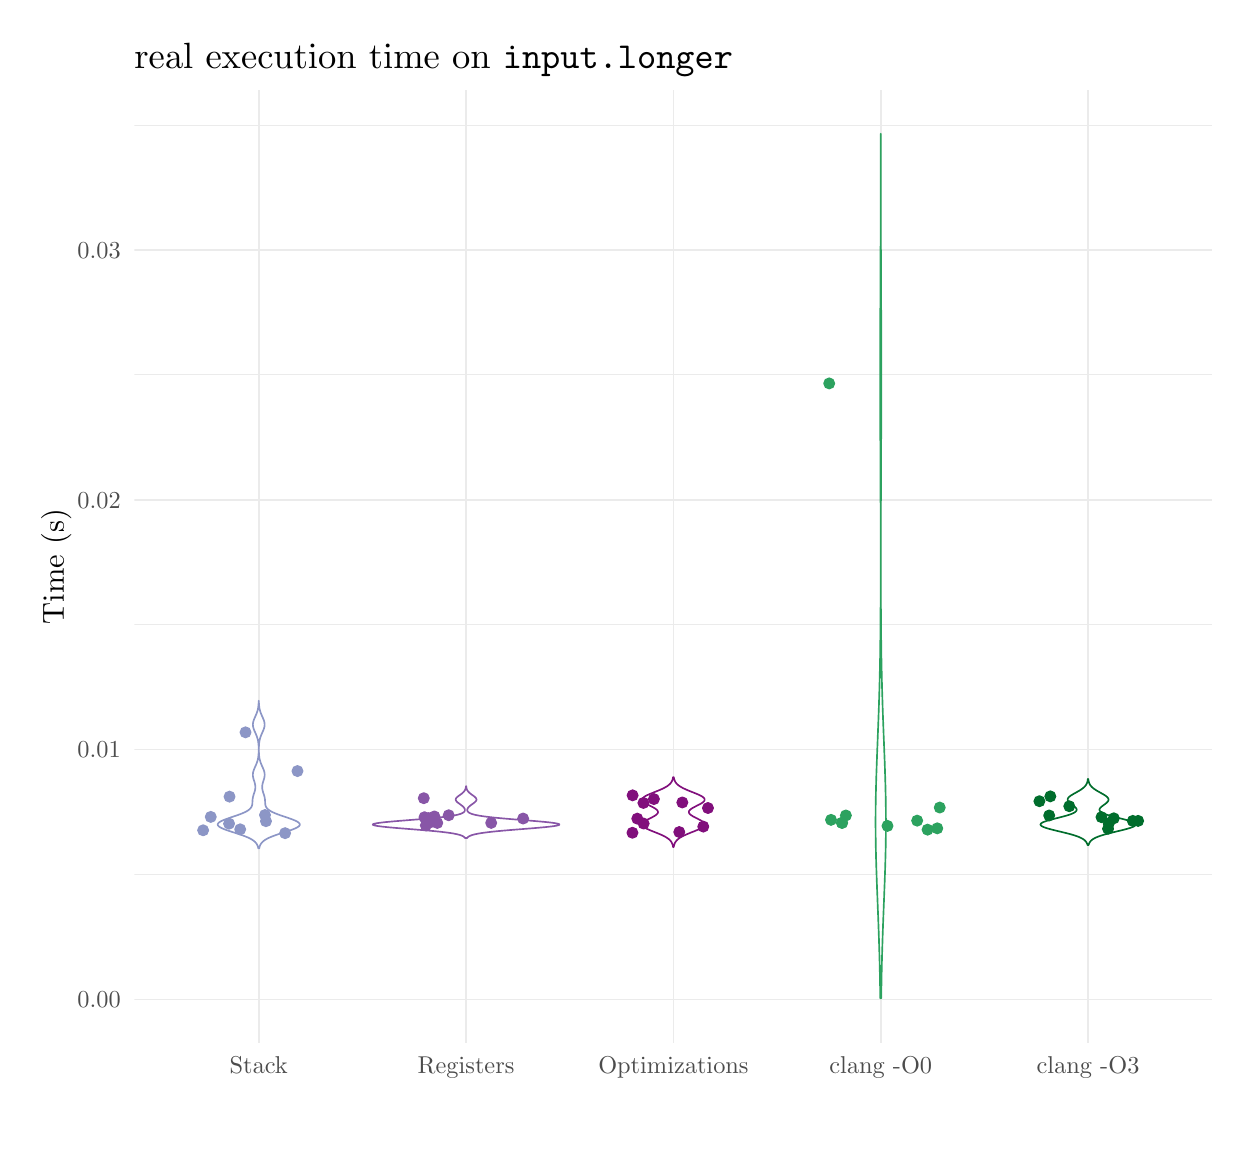
\begin{tikzpicture}[x=1pt,y=1pt]
\definecolor{fillColor}{RGB}{255,255,255}
\path[use as bounding box,fill=fillColor,fill opacity=0.00] (0,0) rectangle (433.62,397.48);
\begin{scope}
\path[clip] ( 38.56, 30.69) rectangle (428.12,374.83);
\definecolor{drawColor}{gray}{0.92}

\path[draw=drawColor,line width= 0.3pt,line join=round] ( 38.56, 91.47) --
	(428.12, 91.47);

\path[draw=drawColor,line width= 0.3pt,line join=round] ( 38.56,181.76) --
	(428.12,181.76);

\path[draw=drawColor,line width= 0.3pt,line join=round] ( 38.56,272.04) --
	(428.12,272.04);

\path[draw=drawColor,line width= 0.3pt,line join=round] ( 38.56,362.33) --
	(428.12,362.33);

\path[draw=drawColor,line width= 0.6pt,line join=round] ( 38.56, 46.33) --
	(428.12, 46.33);

\path[draw=drawColor,line width= 0.6pt,line join=round] ( 38.56,136.61) --
	(428.12,136.61);

\path[draw=drawColor,line width= 0.6pt,line join=round] ( 38.56,226.90) --
	(428.12,226.90);

\path[draw=drawColor,line width= 0.6pt,line join=round] ( 38.56,317.18) --
	(428.12,317.18);

\path[draw=drawColor,line width= 0.6pt,line join=round] ( 83.50, 30.69) --
	( 83.50,374.83);

\path[draw=drawColor,line width= 0.6pt,line join=round] (158.42, 30.69) --
	(158.42,374.83);

\path[draw=drawColor,line width= 0.6pt,line join=round] (233.34, 30.69) --
	(233.34,374.83);

\path[draw=drawColor,line width= 0.6pt,line join=round] (308.25, 30.69) --
	(308.25,374.83);

\path[draw=drawColor,line width= 0.6pt,line join=round] (383.17, 30.69) --
	(383.17,374.83);
\definecolor{drawColor}{RGB}{140,150,198}
\definecolor{fillColor}{RGB}{255,255,255}

\path[draw=drawColor,line width= 0.6pt,line join=round,line cap=round,fill=fillColor] ( 83.34,100.92) --
	( 83.32,101.02) --
	( 83.30,101.13) --
	( 83.28,101.23) --
	( 83.25,101.34) --
	( 83.22,101.44) --
	( 83.19,101.55) --
	( 83.16,101.65) --
	( 83.12,101.75) --
	( 83.08,101.86) --
	( 83.04,101.96) --
	( 82.99,102.07) --
	( 82.95,102.17) --
	( 82.89,102.28) --
	( 82.83,102.38) --
	( 82.77,102.49) --
	( 82.70,102.59) --
	( 82.63,102.69) --
	( 82.55,102.80) --
	( 82.47,102.90) --
	( 82.38,103.01) --
	( 82.28,103.11) --
	( 82.18,103.22) --
	( 82.07,103.32) --
	( 81.95,103.42) --
	( 81.83,103.53) --
	( 81.70,103.63) --
	( 81.56,103.74) --
	( 81.41,103.84) --
	( 81.26,103.95) --
	( 81.10,104.05) --
	( 80.92,104.16) --
	( 80.75,104.26) --
	( 80.56,104.36) --
	( 80.36,104.47) --
	( 80.16,104.57) --
	( 79.94,104.68) --
	( 79.72,104.78) --
	( 79.49,104.89) --
	( 79.25,104.99) --
	( 79.00,105.09) --
	( 78.74,105.20) --
	( 78.48,105.30) --
	( 78.21,105.41) --
	( 77.93,105.51) --
	( 77.64,105.62) --
	( 77.35,105.72) --
	( 77.05,105.82) --
	( 76.74,105.93) --
	( 76.43,106.03) --
	( 76.12,106.14) --
	( 75.80,106.24) --
	( 75.48,106.35) --
	( 75.16,106.45) --
	( 74.83,106.56) --
	( 74.50,106.66) --
	( 74.18,106.76) --
	( 73.85,106.87) --
	( 73.53,106.97) --
	( 73.21,107.08) --
	( 72.89,107.18) --
	( 72.58,107.29) --
	( 72.27,107.39) --
	( 71.97,107.49) --
	( 71.68,107.60) --
	( 71.40,107.70) --
	( 71.12,107.81) --
	( 70.86,107.91) --
	( 70.61,108.02) --
	( 70.36,108.12) --
	( 70.14,108.23) --
	( 69.93,108.33) --
	( 69.73,108.43) --
	( 69.54,108.54) --
	( 69.38,108.64) --
	( 69.23,108.75) --
	( 69.09,108.85) --
	( 68.98,108.96) --
	( 68.88,109.06) --
	( 68.80,109.16) --
	( 68.74,109.27) --
	( 68.71,109.37) --
	( 68.68,109.48) --
	( 68.68,109.58) --
	( 68.70,109.69) --
	( 68.74,109.79) --
	( 68.79,109.90) --
	( 68.87,110.00) --
	( 68.96,110.10) --
	( 69.07,110.21) --
	( 69.20,110.31) --
	( 69.35,110.42) --
	( 69.51,110.52) --
	( 69.69,110.63) --
	( 69.88,110.73) --
	( 70.09,110.83) --
	( 70.31,110.94) --
	( 70.55,111.04) --
	( 70.79,111.15) --
	( 71.05,111.25) --
	( 71.32,111.36) --
	( 71.59,111.46) --
	( 71.87,111.57) --
	( 72.16,111.67) --
	( 72.46,111.77) --
	( 72.76,111.88) --
	( 73.07,111.98) --
	( 73.37,112.09) --
	( 73.68,112.19) --
	( 73.99,112.30) --
	( 74.30,112.40) --
	( 74.61,112.50) --
	( 74.92,112.61) --
	( 75.22,112.71) --
	( 75.52,112.82) --
	( 75.82,112.92) --
	( 76.11,113.03) --
	( 76.40,113.13) --
	( 76.68,113.23) --
	( 76.95,113.34) --
	( 77.22,113.44) --
	( 77.47,113.55) --
	( 77.72,113.65) --
	( 77.96,113.76) --
	( 78.19,113.86) --
	( 78.42,113.97) --
	( 78.63,114.07) --
	( 78.83,114.17) --
	( 79.03,114.28) --
	( 79.21,114.38) --
	( 79.39,114.49) --
	( 79.55,114.59) --
	( 79.71,114.70) --
	( 79.85,114.80) --
	( 79.99,114.90) --
	( 80.11,115.01) --
	( 80.23,115.11) --
	( 80.34,115.22) --
	( 80.44,115.32) --
	( 80.53,115.43) --
	( 80.62,115.53) --
	( 80.69,115.64) --
	( 80.76,115.74) --
	( 80.83,115.84) --
	( 80.88,115.95) --
	( 80.93,116.05) --
	( 80.98,116.16) --
	( 81.01,116.26) --
	( 81.05,116.37) --
	( 81.08,116.47) --
	( 81.10,116.57) --
	( 81.12,116.68) --
	( 81.14,116.78) --
	( 81.16,116.89) --
	( 81.17,116.99) --
	( 81.18,117.10) --
	( 81.19,117.20) --
	( 81.20,117.31) --
	( 81.20,117.41) --
	( 81.21,117.51) --
	( 81.21,117.62) --
	( 81.22,117.72) --
	( 81.22,117.83) --
	( 81.22,117.93) --
	( 81.23,118.04) --
	( 81.23,118.14) --
	( 81.24,118.24) --
	( 81.25,118.35) --
	( 81.26,118.45) --
	( 81.27,118.56) --
	( 81.28,118.66) --
	( 81.29,118.77) --
	( 81.30,118.87) --
	( 81.32,118.98) --
	( 81.34,119.08) --
	( 81.36,119.18) --
	( 81.38,119.29) --
	( 81.40,119.39) --
	( 81.42,119.50) --
	( 81.45,119.60) --
	( 81.47,119.71) --
	( 81.50,119.81) --
	( 81.53,119.91) --
	( 81.56,120.02) --
	( 81.59,120.12) --
	( 81.62,120.23) --
	( 81.66,120.33) --
	( 81.69,120.44) --
	( 81.72,120.54) --
	( 81.76,120.64) --
	( 81.79,120.75) --
	( 81.82,120.85) --
	( 81.86,120.96) --
	( 81.89,121.06) --
	( 81.93,121.17) --
	( 81.96,121.27) --
	( 81.99,121.38) --
	( 82.02,121.48) --
	( 82.05,121.58) --
	( 82.08,121.69) --
	( 82.10,121.79) --
	( 82.13,121.90) --
	( 82.15,122.00) --
	( 82.17,122.11) --
	( 82.19,122.21) --
	( 82.21,122.31) --
	( 82.23,122.42) --
	( 82.24,122.52) --
	( 82.25,122.63) --
	( 82.26,122.73) --
	( 82.27,122.84) --
	( 82.27,122.94) --
	( 82.27,123.05) --
	( 82.27,123.15) --
	( 82.27,123.25) --
	( 82.26,123.36) --
	( 82.26,123.46) --
	( 82.25,123.57) --
	( 82.23,123.67) --
	( 82.22,123.78) --
	( 82.20,123.88) --
	( 82.18,123.98) --
	( 82.16,124.09) --
	( 82.14,124.19) --
	( 82.12,124.30) --
	( 82.09,124.40) --
	( 82.07,124.51) --
	( 82.04,124.61) --
	( 82.01,124.72) --
	( 81.98,124.82) --
	( 81.95,124.92) --
	( 81.91,125.03) --
	( 81.88,125.13) --
	( 81.85,125.24) --
	( 81.81,125.34) --
	( 81.78,125.45) --
	( 81.75,125.55) --
	( 81.72,125.65) --
	( 81.68,125.76) --
	( 81.65,125.86) --
	( 81.62,125.97) --
	( 81.59,126.07) --
	( 81.57,126.18) --
	( 81.54,126.28) --
	( 81.51,126.39) --
	( 81.49,126.49) --
	( 81.47,126.59) --
	( 81.45,126.70) --
	( 81.43,126.80) --
	( 81.42,126.91) --
	( 81.40,127.01) --
	( 81.39,127.12) --
	( 81.38,127.22) --
	( 81.38,127.32) --
	( 81.37,127.43) --
	( 81.37,127.53) --
	( 81.38,127.64) --
	( 81.38,127.74) --
	( 81.39,127.85) --
	( 81.40,127.95) --
	( 81.41,128.06) --
	( 81.42,128.16) --
	( 81.44,128.26) --
	( 81.46,128.37) --
	( 81.48,128.47) --
	( 81.51,128.58) --
	( 81.53,128.68) --
	( 81.56,128.79) --
	( 81.59,128.89) --
	( 81.63,128.99) --
	( 81.66,129.10) --
	( 81.70,129.20) --
	( 81.73,129.31) --
	( 81.77,129.41) --
	( 81.82,129.52) --
	( 81.86,129.62) --
	( 81.90,129.72) --
	( 81.94,129.83) --
	( 81.99,129.93) --
	( 82.03,130.04) --
	( 82.08,130.14) --
	( 82.13,130.25) --
	( 82.17,130.35) --
	( 82.22,130.46) --
	( 82.27,130.56) --
	( 82.31,130.66) --
	( 82.36,130.77) --
	( 82.40,130.87) --
	( 82.45,130.98) --
	( 82.50,131.08) --
	( 82.54,131.19) --
	( 82.58,131.29) --
	( 82.63,131.39) --
	( 82.67,131.50) --
	( 82.71,131.60) --
	( 82.75,131.71) --
	( 82.79,131.81) --
	( 82.83,131.92) --
	( 82.86,132.02) --
	( 82.90,132.13) --
	( 82.93,132.23) --
	( 82.96,132.33) --
	( 83.00,132.44) --
	( 83.03,132.54) --
	( 83.06,132.65) --
	( 83.08,132.75) --
	( 83.11,132.86) --
	( 83.14,132.96) --
	( 83.16,133.06) --
	( 83.18,133.17) --
	( 83.21,133.27) --
	( 83.23,133.38) --
	( 83.25,133.48) --
	( 83.27,133.59) --
	( 83.28,133.69) --
	( 83.30,133.80) --
	( 83.31,133.90) --
	( 83.33,134.00) --
	( 83.34,134.11) --
	( 83.36,134.21) --
	( 83.37,134.32) --
	( 83.38,134.42) --
	( 83.39,134.53) --
	( 83.40,134.63) --
	( 83.41,134.73) --
	( 83.42,134.84) --
	( 83.42,134.94) --
	( 83.43,135.05) --
	( 83.44,135.15) --
	( 83.44,135.26) --
	( 83.45,135.36) --
	( 83.45,135.47) --
	( 83.46,135.57) --
	( 83.46,135.67) --
	( 83.46,135.78) --
	( 83.47,135.88) --
	( 83.47,135.99) --
	( 83.47,136.09) --
	( 83.47,136.20) --
	( 83.47,136.30) --
	( 83.47,136.40) --
	( 83.47,136.51) --
	( 83.47,136.61) --
	( 83.47,136.72) --
	( 83.47,136.82) --
	( 83.47,136.93) --
	( 83.47,137.03) --
	( 83.47,137.13) --
	( 83.47,137.24) --
	( 83.47,137.34) --
	( 83.46,137.45) --
	( 83.46,137.55) --
	( 83.46,137.66) --
	( 83.45,137.76) --
	( 83.45,137.87) --
	( 83.44,137.97) --
	( 83.44,138.07) --
	( 83.43,138.18) --
	( 83.42,138.28) --
	( 83.42,138.39) --
	( 83.41,138.49) --
	( 83.40,138.60) --
	( 83.39,138.70) --
	( 83.38,138.80) --
	( 83.37,138.91) --
	( 83.36,139.01) --
	( 83.34,139.12) --
	( 83.33,139.22) --
	( 83.32,139.33) --
	( 83.30,139.43) --
	( 83.28,139.54) --
	( 83.27,139.64) --
	( 83.25,139.74) --
	( 83.23,139.85) --
	( 83.21,139.95) --
	( 83.18,140.06) --
	( 83.16,140.16) --
	( 83.14,140.27) --
	( 83.11,140.37) --
	( 83.08,140.47) --
	( 83.06,140.58) --
	( 83.03,140.68) --
	( 83.00,140.79) --
	( 82.96,140.89) --
	( 82.93,141.00) --
	( 82.90,141.10) --
	( 82.86,141.21) --
	( 82.83,141.31) --
	( 82.79,141.41) --
	( 82.75,141.52) --
	( 82.71,141.62) --
	( 82.67,141.73) --
	( 82.63,141.83) --
	( 82.58,141.94) --
	( 82.54,142.04) --
	( 82.50,142.14) --
	( 82.45,142.25) --
	( 82.41,142.35) --
	( 82.36,142.46) --
	( 82.31,142.56) --
	( 82.27,142.67) --
	( 82.22,142.77) --
	( 82.17,142.88) --
	( 82.13,142.98) --
	( 82.08,143.08) --
	( 82.04,143.19) --
	( 81.99,143.29) --
	( 81.95,143.40) --
	( 81.90,143.50) --
	( 81.86,143.61) --
	( 81.82,143.71) --
	( 81.78,143.81) --
	( 81.74,143.92) --
	( 81.70,144.02) --
	( 81.66,144.13) --
	( 81.63,144.23) --
	( 81.60,144.34) --
	( 81.57,144.44) --
	( 81.54,144.55) --
	( 81.51,144.65) --
	( 81.49,144.75) --
	( 81.47,144.86) --
	( 81.45,144.96) --
	( 81.43,145.07) --
	( 81.42,145.17) --
	( 81.41,145.28) --
	( 81.40,145.38) --
	( 81.39,145.48) --
	( 81.39,145.59) --
	( 81.39,145.69) --
	( 81.39,145.80) --
	( 81.40,145.90) --
	( 81.41,146.01) --
	( 81.42,146.11) --
	( 81.43,146.21) --
	( 81.45,146.32) --
	( 81.47,146.42) --
	( 81.49,146.53) --
	( 81.51,146.63) --
	( 81.54,146.74) --
	( 81.57,146.84) --
	( 81.60,146.95) --
	( 81.63,147.05) --
	( 81.66,147.15) --
	( 81.70,147.26) --
	( 81.74,147.36) --
	( 81.78,147.47) --
	( 81.82,147.57) --
	( 81.86,147.68) --
	( 81.90,147.78) --
	( 81.94,147.88) --
	( 81.99,147.99) --
	( 82.03,148.09) --
	( 82.08,148.20) --
	( 82.13,148.30) --
	( 82.17,148.41) --
	( 82.22,148.51) --
	( 82.27,148.62) --
	( 82.31,148.72) --
	( 82.36,148.82) --
	( 82.40,148.93) --
	( 82.45,149.03) --
	( 82.49,149.14) --
	( 82.54,149.24) --
	( 82.58,149.35) --
	( 82.63,149.45) --
	( 82.67,149.55) --
	( 82.71,149.66) --
	( 82.75,149.76) --
	( 82.79,149.87) --
	( 82.82,149.97) --
	( 82.86,150.08) --
	( 82.90,150.18) --
	( 82.93,150.29) --
	( 82.96,150.39) --
	( 83.00,150.49) --
	( 83.03,150.60) --
	( 83.06,150.70) --
	( 83.08,150.81) --
	( 83.11,150.91) --
	( 83.14,151.02) --
	( 83.16,151.12) --
	( 83.18,151.22) --
	( 83.21,151.33) --
	( 83.23,151.43) --
	( 83.25,151.54) --
	( 83.27,151.64) --
	( 83.28,151.75) --
	( 83.30,151.85) --
	( 83.32,151.96) --
	( 83.33,152.06) --
	( 83.34,152.16) --
	( 83.36,152.27) --
	( 83.37,152.37) --
	( 83.38,152.48) --
	( 83.39,152.58) --
	( 83.40,152.69) --
	( 83.41,152.79) --
	( 83.42,152.89) --
	( 83.42,153.00) --
	( 83.43,153.10) --
	( 83.44,153.21) --
	( 83.44,153.31) --
	( 83.45,153.42) --
	( 83.46,153.52) --
	( 83.46,153.62) --
	( 83.46,153.73) --
	( 83.47,153.83) --
	( 83.47,153.94) --
	( 83.48,154.04) --
	( 83.48,154.15) --
	( 83.48,154.25) --
	( 83.53,154.25) --
	( 83.53,154.15) --
	( 83.53,154.04) --
	( 83.54,153.94) --
	( 83.54,153.83) --
	( 83.55,153.73) --
	( 83.55,153.62) --
	( 83.55,153.52) --
	( 83.56,153.42) --
	( 83.56,153.31) --
	( 83.57,153.21) --
	( 83.58,153.10) --
	( 83.58,153.00) --
	( 83.59,152.89) --
	( 83.60,152.79) --
	( 83.61,152.69) --
	( 83.62,152.58) --
	( 83.63,152.48) --
	( 83.64,152.37) --
	( 83.65,152.27) --
	( 83.67,152.16) --
	( 83.68,152.06) --
	( 83.69,151.96) --
	( 83.71,151.85) --
	( 83.73,151.75) --
	( 83.74,151.64) --
	( 83.76,151.54) --
	( 83.78,151.43) --
	( 83.80,151.33) --
	( 83.83,151.22) --
	( 83.85,151.12) --
	( 83.87,151.02) --
	( 83.90,150.91) --
	( 83.93,150.81) --
	( 83.95,150.70) --
	( 83.98,150.60) --
	( 84.01,150.49) --
	( 84.05,150.39) --
	( 84.08,150.29) --
	( 84.11,150.18) --
	( 84.15,150.08) --
	( 84.19,149.97) --
	( 84.22,149.87) --
	( 84.26,149.76) --
	( 84.30,149.66) --
	( 84.34,149.55) --
	( 84.38,149.45) --
	( 84.43,149.35) --
	( 84.47,149.24) --
	( 84.51,149.14) --
	( 84.56,149.03) --
	( 84.61,148.93) --
	( 84.65,148.82) --
	( 84.70,148.72) --
	( 84.74,148.62) --
	( 84.79,148.51) --
	( 84.84,148.41) --
	( 84.88,148.30) --
	( 84.93,148.20) --
	( 84.98,148.09) --
	( 85.02,147.99) --
	( 85.07,147.88) --
	( 85.11,147.78) --
	( 85.15,147.68) --
	( 85.19,147.57) --
	( 85.23,147.47) --
	( 85.27,147.36) --
	( 85.31,147.26) --
	( 85.35,147.15) --
	( 85.38,147.05) --
	( 85.41,146.95) --
	( 85.44,146.84) --
	( 85.47,146.74) --
	( 85.50,146.63) --
	( 85.52,146.53) --
	( 85.54,146.42) --
	( 85.56,146.32) --
	( 85.58,146.21) --
	( 85.59,146.11) --
	( 85.60,146.01) --
	( 85.61,145.90) --
	( 85.62,145.80) --
	( 85.62,145.69) --
	( 85.62,145.59) --
	( 85.62,145.48) --
	( 85.61,145.38) --
	( 85.60,145.28) --
	( 85.59,145.17) --
	( 85.58,145.07) --
	( 85.56,144.96) --
	( 85.54,144.86) --
	( 85.52,144.75) --
	( 85.50,144.65) --
	( 85.47,144.55) --
	( 85.44,144.44) --
	( 85.41,144.34) --
	( 85.38,144.23) --
	( 85.35,144.13) --
	( 85.31,144.02) --
	( 85.27,143.92) --
	( 85.23,143.81) --
	( 85.19,143.71) --
	( 85.15,143.61) --
	( 85.11,143.50) --
	( 85.06,143.40) --
	( 85.02,143.29) --
	( 84.97,143.19) --
	( 84.93,143.08) --
	( 84.88,142.98) --
	( 84.84,142.88) --
	( 84.79,142.77) --
	( 84.74,142.67) --
	( 84.70,142.56) --
	( 84.65,142.46) --
	( 84.60,142.35) --
	( 84.56,142.25) --
	( 84.51,142.14) --
	( 84.47,142.04) --
	( 84.43,141.94) --
	( 84.38,141.83) --
	( 84.34,141.73) --
	( 84.30,141.62) --
	( 84.26,141.52) --
	( 84.22,141.41) --
	( 84.18,141.31) --
	( 84.15,141.21) --
	( 84.11,141.10) --
	( 84.08,141.00) --
	( 84.04,140.89) --
	( 84.01,140.79) --
	( 83.98,140.68) --
	( 83.95,140.58) --
	( 83.92,140.47) --
	( 83.90,140.37) --
	( 83.87,140.27) --
	( 83.85,140.16) --
	( 83.83,140.06) --
	( 83.80,139.95) --
	( 83.78,139.85) --
	( 83.76,139.74) --
	( 83.74,139.64) --
	( 83.73,139.54) --
	( 83.71,139.43) --
	( 83.69,139.33) --
	( 83.68,139.22) --
	( 83.67,139.12) --
	( 83.65,139.01) --
	( 83.64,138.91) --
	( 83.63,138.80) --
	( 83.62,138.70) --
	( 83.61,138.60) --
	( 83.60,138.49) --
	( 83.59,138.39) --
	( 83.59,138.28) --
	( 83.58,138.18) --
	( 83.57,138.07) --
	( 83.57,137.97) --
	( 83.56,137.87) --
	( 83.56,137.76) --
	( 83.55,137.66) --
	( 83.55,137.55) --
	( 83.55,137.45) --
	( 83.54,137.34) --
	( 83.54,137.24) --
	( 83.54,137.13) --
	( 83.54,137.03) --
	( 83.54,136.93) --
	( 83.54,136.82) --
	( 83.54,136.72) --
	( 83.54,136.61) --
	( 83.54,136.51) --
	( 83.54,136.40) --
	( 83.54,136.30) --
	( 83.54,136.20) --
	( 83.54,136.09) --
	( 83.54,135.99) --
	( 83.54,135.88) --
	( 83.55,135.78) --
	( 83.55,135.67) --
	( 83.55,135.57) --
	( 83.56,135.47) --
	( 83.56,135.36) --
	( 83.57,135.26) --
	( 83.57,135.15) --
	( 83.58,135.05) --
	( 83.59,134.94) --
	( 83.59,134.84) --
	( 83.60,134.73) --
	( 83.61,134.63) --
	( 83.62,134.53) --
	( 83.63,134.42) --
	( 83.64,134.32) --
	( 83.65,134.21) --
	( 83.67,134.11) --
	( 83.68,134.00) --
	( 83.69,133.90) --
	( 83.71,133.80) --
	( 83.73,133.69) --
	( 83.74,133.59) --
	( 83.76,133.48) --
	( 83.78,133.38) --
	( 83.80,133.27) --
	( 83.83,133.17) --
	( 83.85,133.06) --
	( 83.87,132.96) --
	( 83.90,132.86) --
	( 83.93,132.75) --
	( 83.95,132.65) --
	( 83.98,132.54) --
	( 84.01,132.44) --
	( 84.05,132.33) --
	( 84.08,132.23) --
	( 84.11,132.13) --
	( 84.15,132.02) --
	( 84.18,131.92) --
	( 84.22,131.81) --
	( 84.26,131.71) --
	( 84.30,131.60) --
	( 84.34,131.50) --
	( 84.38,131.39) --
	( 84.43,131.29) --
	( 84.47,131.19) --
	( 84.51,131.08) --
	( 84.56,130.98) --
	( 84.60,130.87) --
	( 84.65,130.77) --
	( 84.70,130.66) --
	( 84.74,130.56) --
	( 84.79,130.46) --
	( 84.84,130.35) --
	( 84.88,130.25) --
	( 84.93,130.14) --
	( 84.98,130.04) --
	( 85.02,129.93) --
	( 85.07,129.83) --
	( 85.11,129.72) --
	( 85.15,129.62) --
	( 85.19,129.52) --
	( 85.24,129.41) --
	( 85.27,129.31) --
	( 85.31,129.20) --
	( 85.35,129.10) --
	( 85.38,128.99) --
	( 85.42,128.89) --
	( 85.45,128.79) --
	( 85.48,128.68) --
	( 85.50,128.58) --
	( 85.53,128.47) --
	( 85.55,128.37) --
	( 85.57,128.26) --
	( 85.59,128.16) --
	( 85.60,128.06) --
	( 85.61,127.95) --
	( 85.62,127.85) --
	( 85.63,127.74) --
	( 85.63,127.64) --
	( 85.64,127.53) --
	( 85.64,127.43) --
	( 85.63,127.32) --
	( 85.63,127.22) --
	( 85.62,127.12) --
	( 85.61,127.01) --
	( 85.59,126.91) --
	( 85.58,126.80) --
	( 85.56,126.70) --
	( 85.54,126.59) --
	( 85.52,126.49) --
	( 85.50,126.39) --
	( 85.47,126.28) --
	( 85.44,126.18) --
	( 85.42,126.07) --
	( 85.39,125.97) --
	( 85.36,125.86) --
	( 85.33,125.76) --
	( 85.29,125.65) --
	( 85.26,125.55) --
	( 85.23,125.45) --
	( 85.19,125.34) --
	( 85.16,125.24) --
	( 85.13,125.13) --
	( 85.10,125.03) --
	( 85.06,124.92) --
	( 85.03,124.82) --
	( 85.00,124.72) --
	( 84.97,124.61) --
	( 84.94,124.51) --
	( 84.92,124.40) --
	( 84.89,124.30) --
	( 84.87,124.19) --
	( 84.85,124.09) --
	( 84.83,123.98) --
	( 84.81,123.88) --
	( 84.79,123.78) --
	( 84.78,123.67) --
	( 84.76,123.57) --
	( 84.75,123.46) --
	( 84.75,123.36) --
	( 84.74,123.25) --
	( 84.74,123.15) --
	( 84.74,123.05) --
	( 84.74,122.94) --
	( 84.74,122.84) --
	( 84.75,122.73) --
	( 84.76,122.63) --
	( 84.77,122.52) --
	( 84.78,122.42) --
	( 84.80,122.31) --
	( 84.82,122.21) --
	( 84.84,122.11) --
	( 84.86,122.00) --
	( 84.88,121.90) --
	( 84.91,121.79) --
	( 84.93,121.69) --
	( 84.96,121.58) --
	( 84.99,121.48) --
	( 85.02,121.38) --
	( 85.05,121.27) --
	( 85.08,121.17) --
	( 85.12,121.06) --
	( 85.15,120.96) --
	( 85.18,120.85) --
	( 85.22,120.75) --
	( 85.25,120.64) --
	( 85.29,120.54) --
	( 85.32,120.44) --
	( 85.35,120.33) --
	( 85.39,120.23) --
	( 85.42,120.12) --
	( 85.45,120.02) --
	( 85.48,119.91) --
	( 85.51,119.81) --
	( 85.54,119.71) --
	( 85.56,119.60) --
	( 85.59,119.50) --
	( 85.61,119.39) --
	( 85.63,119.29) --
	( 85.65,119.18) --
	( 85.67,119.08) --
	( 85.69,118.98) --
	( 85.71,118.87) --
	( 85.72,118.77) --
	( 85.73,118.66) --
	( 85.74,118.56) --
	( 85.75,118.45) --
	( 85.76,118.35) --
	( 85.77,118.24) --
	( 85.77,118.14) --
	( 85.78,118.04) --
	( 85.79,117.93) --
	( 85.79,117.83) --
	( 85.79,117.72) --
	( 85.80,117.62) --
	( 85.80,117.51) --
	( 85.81,117.41) --
	( 85.81,117.31) --
	( 85.82,117.20) --
	( 85.83,117.10) --
	( 85.84,116.99) --
	( 85.85,116.89) --
	( 85.87,116.78) --
	( 85.89,116.68) --
	( 85.91,116.57) --
	( 85.93,116.47) --
	( 85.96,116.37) --
	( 86.00,116.26) --
	( 86.03,116.16) --
	( 86.08,116.05) --
	( 86.13,115.95) --
	( 86.18,115.84) --
	( 86.25,115.74) --
	( 86.32,115.64) --
	( 86.39,115.53) --
	( 86.48,115.43) --
	( 86.57,115.32) --
	( 86.67,115.22) --
	( 86.78,115.11) --
	( 86.90,115.01) --
	( 87.02,114.90) --
	( 87.16,114.80) --
	( 87.30,114.70) --
	( 87.46,114.59) --
	( 87.62,114.49) --
	( 87.80,114.38) --
	( 87.98,114.28) --
	( 88.18,114.17) --
	( 88.38,114.07) --
	( 88.59,113.97) --
	( 88.82,113.86) --
	( 89.05,113.76) --
	( 89.29,113.65) --
	( 89.54,113.55) --
	( 89.79,113.44) --
	( 90.06,113.34) --
	( 90.33,113.23) --
	( 90.61,113.13) --
	( 90.90,113.03) --
	( 91.19,112.92) --
	( 91.49,112.82) --
	( 91.79,112.71) --
	( 92.09,112.61) --
	( 92.40,112.50) --
	( 92.71,112.40) --
	( 93.02,112.30) --
	( 93.33,112.19) --
	( 93.64,112.09) --
	( 93.94,111.98) --
	( 94.25,111.88) --
	( 94.55,111.77) --
	( 94.85,111.67) --
	( 95.14,111.57) --
	( 95.42,111.46) --
	( 95.69,111.36) --
	( 95.96,111.25) --
	( 96.22,111.15) --
	( 96.46,111.04) --
	( 96.70,110.94) --
	( 96.92,110.83) --
	( 97.13,110.73) --
	( 97.32,110.63) --
	( 97.50,110.52) --
	( 97.66,110.42) --
	( 97.81,110.31) --
	( 97.94,110.21) --
	( 98.05,110.10) --
	( 98.14,110.00) --
	( 98.22,109.90) --
	( 98.27,109.79) --
	( 98.31,109.69) --
	( 98.33,109.58) --
	( 98.33,109.48) --
	( 98.30,109.37) --
	( 98.27,109.27) --
	( 98.21,109.16) --
	( 98.13,109.06) --
	( 98.03,108.96) --
	( 97.92,108.85) --
	( 97.78,108.75) --
	( 97.63,108.64) --
	( 97.47,108.54) --
	( 97.28,108.43) --
	( 97.08,108.33) --
	( 96.87,108.23) --
	( 96.64,108.12) --
	( 96.40,108.02) --
	( 96.15,107.91) --
	( 95.89,107.81) --
	( 95.61,107.70) --
	( 95.33,107.60) --
	( 95.04,107.49) --
	( 94.74,107.39) --
	( 94.43,107.29) --
	( 94.12,107.18) --
	( 93.80,107.08) --
	( 93.48,106.97) --
	( 93.16,106.87) --
	( 92.83,106.76) --
	( 92.50,106.66) --
	( 92.18,106.56) --
	( 91.85,106.45) --
	( 91.53,106.35) --
	( 91.21,106.24) --
	( 90.89,106.14) --
	( 90.58,106.03) --
	( 90.27,105.93) --
	( 89.96,105.82) --
	( 89.66,105.72) --
	( 89.37,105.62) --
	( 89.08,105.51) --
	( 88.80,105.41) --
	( 88.53,105.30) --
	( 88.27,105.20) --
	( 88.01,105.09) --
	( 87.76,104.99) --
	( 87.52,104.89) --
	( 87.29,104.78) --
	( 87.07,104.68) --
	( 86.85,104.57) --
	( 86.65,104.47) --
	( 86.45,104.36) --
	( 86.26,104.26) --
	( 86.08,104.16) --
	( 85.91,104.05) --
	( 85.75,103.95) --
	( 85.60,103.84) --
	( 85.45,103.74) --
	( 85.31,103.63) --
	( 85.18,103.53) --
	( 85.06,103.42) --
	( 84.94,103.32) --
	( 84.83,103.22) --
	( 84.73,103.11) --
	( 84.63,103.01) --
	( 84.54,102.90) --
	( 84.46,102.80) --
	( 84.38,102.69) --
	( 84.31,102.59) --
	( 84.24,102.49) --
	( 84.18,102.38) --
	( 84.12,102.28) --
	( 84.06,102.17) --
	( 84.01,102.07) --
	( 83.97,101.96) --
	( 83.93,101.86) --
	( 83.89,101.75) --
	( 83.85,101.65) --
	( 83.82,101.55) --
	( 83.79,101.44) --
	( 83.76,101.34) --
	( 83.73,101.23) --
	( 83.71,101.13) --
	( 83.69,101.02) --
	( 83.67,100.92) --
	( 83.34,100.92) --
	cycle;
\definecolor{drawColor}{RGB}{136,86,167}

\path[draw=drawColor,line width= 0.6pt,line join=round,line cap=round,fill=fillColor] (158.04,104.66) --
	(158.02,104.70) --
	(157.99,104.74) --
	(157.96,104.77) --
	(157.93,104.81) --
	(157.89,104.85) --
	(157.86,104.88) --
	(157.82,104.92) --
	(157.78,104.96) --
	(157.74,104.99) --
	(157.69,105.03) --
	(157.65,105.07) --
	(157.60,105.10) --
	(157.55,105.14) --
	(157.49,105.18) --
	(157.43,105.22) --
	(157.37,105.25) --
	(157.31,105.29) --
	(157.24,105.33) --
	(157.17,105.36) --
	(157.10,105.40) --
	(157.02,105.44) --
	(156.94,105.47) --
	(156.85,105.51) --
	(156.76,105.55) --
	(156.67,105.58) --
	(156.57,105.62) --
	(156.46,105.66) --
	(156.36,105.69) --
	(156.24,105.73) --
	(156.12,105.77) --
	(156.00,105.80) --
	(155.87,105.84) --
	(155.74,105.88) --
	(155.60,105.91) --
	(155.46,105.95) --
	(155.30,105.99) --
	(155.15,106.02) --
	(154.99,106.06) --
	(154.82,106.10) --
	(154.64,106.13) --
	(154.46,106.17) --
	(154.27,106.21) --
	(154.07,106.24) --
	(153.87,106.28) --
	(153.66,106.32) --
	(153.45,106.35) --
	(153.22,106.39) --
	(152.99,106.43) --
	(152.75,106.46) --
	(152.51,106.50) --
	(152.25,106.54) --
	(151.99,106.57) --
	(151.72,106.61) --
	(151.45,106.65) --
	(151.17,106.68) --
	(150.87,106.72) --
	(150.57,106.76) --
	(150.27,106.79) --
	(149.95,106.83) --
	(149.63,106.87) --
	(149.30,106.90) --
	(148.96,106.94) --
	(148.62,106.98) --
	(148.27,107.01) --
	(147.91,107.05) --
	(147.54,107.09) --
	(147.17,107.12) --
	(146.79,107.16) --
	(146.40,107.20) --
	(146.01,107.23) --
	(145.61,107.27) --
	(145.20,107.31) --
	(144.79,107.34) --
	(144.37,107.38) --
	(143.95,107.42) --
	(143.52,107.45) --
	(143.09,107.49) --
	(142.65,107.53) --
	(142.21,107.56) --
	(141.76,107.60) --
	(141.31,107.64) --
	(140.86,107.67) --
	(140.41,107.71) --
	(139.95,107.75) --
	(139.49,107.78) --
	(139.03,107.82) --
	(138.57,107.86) --
	(138.11,107.89) --
	(137.64,107.93) --
	(137.18,107.97) --
	(136.72,108.00) --
	(136.26,108.04) --
	(135.80,108.08) --
	(135.35,108.11) --
	(134.90,108.15) --
	(134.45,108.19) --
	(134.00,108.22) --
	(133.56,108.26) --
	(133.12,108.30) --
	(132.69,108.33) --
	(132.27,108.37) --
	(131.85,108.41) --
	(131.44,108.45) --
	(131.03,108.48) --
	(130.64,108.52) --
	(130.25,108.56) --
	(129.88,108.59) --
	(129.51,108.63) --
	(129.15,108.67) --
	(128.81,108.70) --
	(128.47,108.74) --
	(128.15,108.78) --
	(127.84,108.81) --
	(127.54,108.85) --
	(127.25,108.89) --
	(126.98,108.92) --
	(126.72,108.96) --
	(126.48,109.00) --
	(126.25,109.03) --
	(126.03,109.07) --
	(125.83,109.11) --
	(125.65,109.14) --
	(125.48,109.18) --
	(125.33,109.22) --
	(125.19,109.25) --
	(125.07,109.29) --
	(124.97,109.33) --
	(124.88,109.36) --
	(124.82,109.40) --
	(124.76,109.44) --
	(124.73,109.47) --
	(124.71,109.51) --
	(124.71,109.55) --
	(124.73,109.58) --
	(124.76,109.62) --
	(124.81,109.66) --
	(124.88,109.69) --
	(124.96,109.73) --
	(125.07,109.77) --
	(125.19,109.80) --
	(125.32,109.84) --
	(125.48,109.88) --
	(125.64,109.91) --
	(125.83,109.95) --
	(126.03,109.99) --
	(126.24,110.02) --
	(126.47,110.06) --
	(126.71,110.10) --
	(126.97,110.13) --
	(127.24,110.17) --
	(127.53,110.21) --
	(127.83,110.24) --
	(128.14,110.28) --
	(128.46,110.32) --
	(128.80,110.35) --
	(129.14,110.39) --
	(129.50,110.43) --
	(129.87,110.46) --
	(130.25,110.50) --
	(130.63,110.54) --
	(131.03,110.57) --
	(131.43,110.61) --
	(131.84,110.65) --
	(132.26,110.68) --
	(132.68,110.72) --
	(133.11,110.76) --
	(133.55,110.79) --
	(133.99,110.83) --
	(134.43,110.87) --
	(134.88,110.90) --
	(135.34,110.94) --
	(135.79,110.98) --
	(136.25,111.01) --
	(136.71,111.05) --
	(137.17,111.09) --
	(137.63,111.12) --
	(138.10,111.16) --
	(138.56,111.20) --
	(139.02,111.23) --
	(139.48,111.27) --
	(139.94,111.31) --
	(140.40,111.34) --
	(140.85,111.38) --
	(141.30,111.42) --
	(141.75,111.45) --
	(142.20,111.49) --
	(142.64,111.53) --
	(143.08,111.57) --
	(143.51,111.60) --
	(143.94,111.64) --
	(144.36,111.68) --
	(144.78,111.71) --
	(145.19,111.75) --
	(145.60,111.79) --
	(146.00,111.82) --
	(146.39,111.86) --
	(146.78,111.90) --
	(147.16,111.93) --
	(147.53,111.97) --
	(147.90,112.01) --
	(148.26,112.04) --
	(148.61,112.08) --
	(148.95,112.12) --
	(149.29,112.15) --
	(149.62,112.19) --
	(149.94,112.23) --
	(150.26,112.26) --
	(150.56,112.30) --
	(150.87,112.34) --
	(151.15,112.37) --
	(151.44,112.41) --
	(151.71,112.45) --
	(151.98,112.48) --
	(152.25,112.52) --
	(152.50,112.56) --
	(152.74,112.59) --
	(152.98,112.63) --
	(153.21,112.67) --
	(153.44,112.70) --
	(153.65,112.74) --
	(153.86,112.78) --
	(154.06,112.81) --
	(154.26,112.85) --
	(154.45,112.89) --
	(154.63,112.92) --
	(154.80,112.96) --
	(154.97,113.00) --
	(155.13,113.03) --
	(155.29,113.07) --
	(155.44,113.11) --
	(155.58,113.14) --
	(155.72,113.18) --
	(155.85,113.22) --
	(155.98,113.25) --
	(156.10,113.29) --
	(156.22,113.33) --
	(156.33,113.36) --
	(156.44,113.40) --
	(156.54,113.44) --
	(156.63,113.47) --
	(156.73,113.51) --
	(156.82,113.55) --
	(156.90,113.58) --
	(156.98,113.62) --
	(157.05,113.66) --
	(157.13,113.69) --
	(157.19,113.73) --
	(157.26,113.77) --
	(157.32,113.80) --
	(157.38,113.84) --
	(157.43,113.88) --
	(157.48,113.91) --
	(157.53,113.95) --
	(157.57,113.99) --
	(157.62,114.02) --
	(157.66,114.06) --
	(157.69,114.10) --
	(157.73,114.13) --
	(157.76,114.17) --
	(157.79,114.21) --
	(157.82,114.24) --
	(157.84,114.28) --
	(157.86,114.32) --
	(157.88,114.35) --
	(157.90,114.39) --
	(157.92,114.43) --
	(157.93,114.46) --
	(157.95,114.50) --
	(157.96,114.54) --
	(157.97,114.57) --
	(157.98,114.61) --
	(157.98,114.65) --
	(157.99,114.68) --
	(157.99,114.72) --
	(157.99,114.76) --
	(157.99,114.80) --
	(157.99,114.83) --
	(157.99,114.87) --
	(157.98,114.91) --
	(157.98,114.94) --
	(157.97,114.98) --
	(157.96,115.02) --
	(157.95,115.05) --
	(157.94,115.09) --
	(157.93,115.13) --
	(157.92,115.16) --
	(157.90,115.20) --
	(157.89,115.24) --
	(157.87,115.27) --
	(157.86,115.31) --
	(157.84,115.35) --
	(157.82,115.38) --
	(157.80,115.42) --
	(157.77,115.46) --
	(157.75,115.49) --
	(157.73,115.53) --
	(157.70,115.57) --
	(157.68,115.60) --
	(157.65,115.64) --
	(157.62,115.68) --
	(157.59,115.71) --
	(157.56,115.75) --
	(157.53,115.79) --
	(157.50,115.82) --
	(157.46,115.86) --
	(157.43,115.90) --
	(157.39,115.93) --
	(157.36,115.97) --
	(157.32,116.01) --
	(157.28,116.04) --
	(157.24,116.08) --
	(157.20,116.12) --
	(157.16,116.15) --
	(157.12,116.19) --
	(157.08,116.23) --
	(157.03,116.26) --
	(156.99,116.30) --
	(156.95,116.34) --
	(156.90,116.37) --
	(156.85,116.41) --
	(156.81,116.45) --
	(156.76,116.48) --
	(156.71,116.52) --
	(156.66,116.56) --
	(156.62,116.59) --
	(156.57,116.63) --
	(156.52,116.67) --
	(156.47,116.70) --
	(156.42,116.74) --
	(156.37,116.78) --
	(156.32,116.81) --
	(156.26,116.85) --
	(156.21,116.89) --
	(156.16,116.92) --
	(156.11,116.96) --
	(156.06,117.00) --
	(156.01,117.03) --
	(155.96,117.07) --
	(155.91,117.11) --
	(155.86,117.14) --
	(155.81,117.18) --
	(155.76,117.22) --
	(155.71,117.25) --
	(155.66,117.29) --
	(155.61,117.33) --
	(155.56,117.36) --
	(155.51,117.40) --
	(155.47,117.44) --
	(155.42,117.47) --
	(155.38,117.51) --
	(155.33,117.55) --
	(155.29,117.58) --
	(155.25,117.62) --
	(155.21,117.66) --
	(155.17,117.69) --
	(155.13,117.73) --
	(155.09,117.77) --
	(155.06,117.80) --
	(155.02,117.84) --
	(154.99,117.88) --
	(154.96,117.91) --
	(154.93,117.95) --
	(154.90,117.99) --
	(154.87,118.03) --
	(154.85,118.06) --
	(154.82,118.10) --
	(154.80,118.14) --
	(154.78,118.17) --
	(154.76,118.21) --
	(154.74,118.25) --
	(154.73,118.28) --
	(154.72,118.32) --
	(154.70,118.36) --
	(154.69,118.39) --
	(154.69,118.43) --
	(154.68,118.47) --
	(154.68,118.50) --
	(154.68,118.54) --
	(154.68,118.58) --
	(154.68,118.61) --
	(154.68,118.65) --
	(154.69,118.69) --
	(154.69,118.72) --
	(154.70,118.76) --
	(154.72,118.80) --
	(154.73,118.83) --
	(154.74,118.87) --
	(154.76,118.91) --
	(154.78,118.94) --
	(154.80,118.98) --
	(154.82,119.02) --
	(154.85,119.05) --
	(154.87,119.09) --
	(154.90,119.13) --
	(154.93,119.16) --
	(154.96,119.20) --
	(154.99,119.24) --
	(155.02,119.27) --
	(155.06,119.31) --
	(155.09,119.35) --
	(155.13,119.38) --
	(155.17,119.42) --
	(155.21,119.46) --
	(155.25,119.49) --
	(155.29,119.53) --
	(155.33,119.57) --
	(155.38,119.60) --
	(155.42,119.64) --
	(155.47,119.68) --
	(155.52,119.71) --
	(155.56,119.75) --
	(155.61,119.79) --
	(155.66,119.82) --
	(155.71,119.86) --
	(155.76,119.90) --
	(155.81,119.93) --
	(155.86,119.97) --
	(155.91,120.01) --
	(155.96,120.04) --
	(156.01,120.08) --
	(156.06,120.12) --
	(156.11,120.15) --
	(156.16,120.19) --
	(156.22,120.23) --
	(156.27,120.26) --
	(156.32,120.30) --
	(156.37,120.34) --
	(156.42,120.37) --
	(156.47,120.41) --
	(156.52,120.45) --
	(156.57,120.48) --
	(156.62,120.52) --
	(156.67,120.56) --
	(156.72,120.59) --
	(156.77,120.63) --
	(156.81,120.67) --
	(156.86,120.70) --
	(156.91,120.74) --
	(156.95,120.78) --
	(157.00,120.81) --
	(157.04,120.85) --
	(157.09,120.89) --
	(157.13,120.92) --
	(157.17,120.96) --
	(157.21,121.00) --
	(157.25,121.03) --
	(157.29,121.07) --
	(157.33,121.11) --
	(157.37,121.15) --
	(157.41,121.18) --
	(157.44,121.22) --
	(157.48,121.26) --
	(157.52,121.29) --
	(157.55,121.33) --
	(157.58,121.37) --
	(157.62,121.40) --
	(157.65,121.44) --
	(157.68,121.48) --
	(157.71,121.51) --
	(157.74,121.55) --
	(157.76,121.59) --
	(157.79,121.62) --
	(157.82,121.66) --
	(157.84,121.70) --
	(157.87,121.73) --
	(157.89,121.77) --
	(157.92,121.81) --
	(157.94,121.84) --
	(157.96,121.88) --
	(157.98,121.92) --
	(158.00,121.95) --
	(158.02,121.99) --
	(158.04,122.03) --
	(158.06,122.06) --
	(158.07,122.10) --
	(158.09,122.14) --
	(158.11,122.17) --
	(158.12,122.21) --
	(158.14,122.25) --
	(158.15,122.28) --
	(158.17,122.32) --
	(158.18,122.36) --
	(158.19,122.39) --
	(158.20,122.43) --
	(158.22,122.47) --
	(158.23,122.50) --
	(158.24,122.54) --
	(158.25,122.58) --
	(158.26,122.61) --
	(158.27,122.65) --
	(158.27,122.69) --
	(158.28,122.72) --
	(158.29,122.76) --
	(158.30,122.80) --
	(158.30,122.83) --
	(158.31,122.87) --
	(158.32,122.91) --
	(158.32,122.94) --
	(158.33,122.98) --
	(158.34,123.02) --
	(158.34,123.05) --
	(158.35,123.09) --
	(158.35,123.13) --
	(158.35,123.16) --
	(158.36,123.20) --
	(158.36,123.24) --
	(158.37,123.27) --
	(158.37,123.31) --
	(158.37,123.35) --
	(158.38,123.38) --
	(158.38,123.42) --
	(158.46,123.42) --
	(158.47,123.38) --
	(158.47,123.35) --
	(158.47,123.31) --
	(158.48,123.27) --
	(158.48,123.24) --
	(158.48,123.20) --
	(158.49,123.16) --
	(158.49,123.13) --
	(158.50,123.09) --
	(158.50,123.05) --
	(158.51,123.02) --
	(158.51,122.98) --
	(158.52,122.94) --
	(158.52,122.91) --
	(158.53,122.87) --
	(158.54,122.83) --
	(158.54,122.80) --
	(158.55,122.76) --
	(158.56,122.72) --
	(158.57,122.69) --
	(158.58,122.65) --
	(158.59,122.61) --
	(158.60,122.58) --
	(158.61,122.54) --
	(158.62,122.50) --
	(158.63,122.47) --
	(158.64,122.43) --
	(158.65,122.39) --
	(158.66,122.36) --
	(158.68,122.32) --
	(158.69,122.28) --
	(158.70,122.25) --
	(158.72,122.21) --
	(158.73,122.17) --
	(158.75,122.14) --
	(158.77,122.10) --
	(158.78,122.06) --
	(158.80,122.03) --
	(158.82,121.99) --
	(158.84,121.95) --
	(158.86,121.92) --
	(158.88,121.88) --
	(158.90,121.84) --
	(158.93,121.81) --
	(158.95,121.77) --
	(158.97,121.73) --
	(159.00,121.70) --
	(159.02,121.66) --
	(159.05,121.62) --
	(159.08,121.59) --
	(159.11,121.55) --
	(159.14,121.51) --
	(159.17,121.48) --
	(159.20,121.44) --
	(159.23,121.40) --
	(159.26,121.37) --
	(159.29,121.33) --
	(159.33,121.29) --
	(159.36,121.26) --
	(159.40,121.22) --
	(159.43,121.18) --
	(159.47,121.15) --
	(159.51,121.11) --
	(159.55,121.07) --
	(159.59,121.03) --
	(159.63,121.00) --
	(159.67,120.96) --
	(159.71,120.92) --
	(159.76,120.89) --
	(159.80,120.85) --
	(159.85,120.81) --
	(159.89,120.78) --
	(159.94,120.74) --
	(159.98,120.70) --
	(160.03,120.67) --
	(160.08,120.63) --
	(160.12,120.59) --
	(160.17,120.56) --
	(160.22,120.52) --
	(160.27,120.48) --
	(160.32,120.45) --
	(160.37,120.41) --
	(160.42,120.37) --
	(160.47,120.34) --
	(160.52,120.30) --
	(160.58,120.26) --
	(160.63,120.23) --
	(160.68,120.19) --
	(160.73,120.15) --
	(160.78,120.12) --
	(160.83,120.08) --
	(160.88,120.04) --
	(160.93,120.01) --
	(160.98,119.97) --
	(161.04,119.93) --
	(161.09,119.90) --
	(161.13,119.86) --
	(161.18,119.82) --
	(161.23,119.79) --
	(161.28,119.75) --
	(161.33,119.71) --
	(161.37,119.68) --
	(161.42,119.64) --
	(161.46,119.60) --
	(161.51,119.57) --
	(161.55,119.53) --
	(161.59,119.49) --
	(161.63,119.46) --
	(161.67,119.42) --
	(161.71,119.38) --
	(161.75,119.35) --
	(161.78,119.31) --
	(161.82,119.27) --
	(161.85,119.24) --
	(161.88,119.20) --
	(161.92,119.16) --
	(161.94,119.13) --
	(161.97,119.09) --
	(162.00,119.05) --
	(162.02,119.02) --
	(162.04,118.98) --
	(162.06,118.94) --
	(162.08,118.91) --
	(162.10,118.87) --
	(162.11,118.83) --
	(162.13,118.80) --
	(162.14,118.76) --
	(162.15,118.72) --
	(162.16,118.69) --
	(162.16,118.65) --
	(162.16,118.61) --
	(162.17,118.58) --
	(162.17,118.54) --
	(162.16,118.50) --
	(162.16,118.47) --
	(162.16,118.43) --
	(162.15,118.39) --
	(162.14,118.36) --
	(162.13,118.32) --
	(162.11,118.28) --
	(162.10,118.25) --
	(162.08,118.21) --
	(162.06,118.17) --
	(162.04,118.14) --
	(162.02,118.10) --
	(162.00,118.06) --
	(161.97,118.03) --
	(161.94,117.99) --
	(161.92,117.95) --
	(161.89,117.91) --
	(161.85,117.88) --
	(161.82,117.84) --
	(161.79,117.80) --
	(161.75,117.77) --
	(161.71,117.73) --
	(161.67,117.69) --
	(161.63,117.66) --
	(161.59,117.62) --
	(161.55,117.58) --
	(161.51,117.55) --
	(161.47,117.51) --
	(161.42,117.47) --
	(161.37,117.44) --
	(161.33,117.40) --
	(161.28,117.36) --
	(161.23,117.33) --
	(161.19,117.29) --
	(161.14,117.25) --
	(161.09,117.22) --
	(161.04,117.18) --
	(160.99,117.14) --
	(160.94,117.11) --
	(160.89,117.07) --
	(160.83,117.03) --
	(160.78,117.00) --
	(160.73,116.96) --
	(160.68,116.92) --
	(160.63,116.89) --
	(160.58,116.85) --
	(160.53,116.81) --
	(160.48,116.78) --
	(160.43,116.74) --
	(160.38,116.70) --
	(160.33,116.67) --
	(160.28,116.63) --
	(160.23,116.59) --
	(160.18,116.56) --
	(160.13,116.52) --
	(160.08,116.48) --
	(160.03,116.45) --
	(159.99,116.41) --
	(159.94,116.37) --
	(159.90,116.34) --
	(159.85,116.30) --
	(159.81,116.26) --
	(159.76,116.23) --
	(159.72,116.19) --
	(159.68,116.15) --
	(159.64,116.12) --
	(159.60,116.08) --
	(159.56,116.04) --
	(159.52,116.01) --
	(159.49,115.97) --
	(159.45,115.93) --
	(159.41,115.90) --
	(159.38,115.86) --
	(159.35,115.82) --
	(159.31,115.79) --
	(159.28,115.75) --
	(159.25,115.71) --
	(159.22,115.68) --
	(159.19,115.64) --
	(159.17,115.60) --
	(159.14,115.57) --
	(159.12,115.53) --
	(159.09,115.49) --
	(159.07,115.46) --
	(159.05,115.42) --
	(159.02,115.38) --
	(159.01,115.35) --
	(158.99,115.31) --
	(158.97,115.27) --
	(158.95,115.24) --
	(158.94,115.20) --
	(158.92,115.16) --
	(158.91,115.13) --
	(158.90,115.09) --
	(158.89,115.05) --
	(158.88,115.02) --
	(158.87,114.98) --
	(158.86,114.94) --
	(158.86,114.91) --
	(158.86,114.87) --
	(158.85,114.83) --
	(158.85,114.80) --
	(158.85,114.76) --
	(158.85,114.72) --
	(158.86,114.68) --
	(158.86,114.65) --
	(158.87,114.61) --
	(158.87,114.57) --
	(158.88,114.54) --
	(158.90,114.50) --
	(158.91,114.46) --
	(158.92,114.43) --
	(158.94,114.39) --
	(158.96,114.35) --
	(158.98,114.32) --
	(159.00,114.28) --
	(159.03,114.24) --
	(159.05,114.21) --
	(159.08,114.17) --
	(159.11,114.13) --
	(159.15,114.10) --
	(159.19,114.06) --
	(159.22,114.02) --
	(159.27,113.99) --
	(159.31,113.95) --
	(159.36,113.91) --
	(159.41,113.88) --
	(159.47,113.84) --
	(159.52,113.80) --
	(159.58,113.77) --
	(159.65,113.73) --
	(159.72,113.69) --
	(159.79,113.66) --
	(159.86,113.62) --
	(159.94,113.58) --
	(160.03,113.55) --
	(160.11,113.51) --
	(160.21,113.47) --
	(160.30,113.44) --
	(160.41,113.40) --
	(160.51,113.36) --
	(160.62,113.33) --
	(160.74,113.29) --
	(160.86,113.25) --
	(160.99,113.22) --
	(161.12,113.18) --
	(161.26,113.14) --
	(161.40,113.11) --
	(161.55,113.07) --
	(161.71,113.03) --
	(161.87,113.00) --
	(162.04,112.96) --
	(162.22,112.92) --
	(162.40,112.89) --
	(162.59,112.85) --
	(162.78,112.81) --
	(162.98,112.78) --
	(163.19,112.74) --
	(163.41,112.70) --
	(163.63,112.67) --
	(163.86,112.63) --
	(164.10,112.59) --
	(164.35,112.56) --
	(164.60,112.52) --
	(164.86,112.48) --
	(165.13,112.45) --
	(165.40,112.41) --
	(165.69,112.37) --
	(165.98,112.34) --
	(166.28,112.30) --
	(166.58,112.26) --
	(166.90,112.23) --
	(167.22,112.19) --
	(167.55,112.15) --
	(167.89,112.12) --
	(168.23,112.08) --
	(168.59,112.04) --
	(168.94,112.01) --
	(169.31,111.97) --
	(169.69,111.93) --
	(170.06,111.90) --
	(170.45,111.86) --
	(170.85,111.82) --
	(171.25,111.79) --
	(171.65,111.75) --
	(172.06,111.71) --
	(172.48,111.68) --
	(172.90,111.64) --
	(173.33,111.60) --
	(173.77,111.57) --
	(174.20,111.53) --
	(174.65,111.49) --
	(175.09,111.45) --
	(175.54,111.42) --
	(175.99,111.38) --
	(176.45,111.34) --
	(176.90,111.31) --
	(177.36,111.27) --
	(177.82,111.23) --
	(178.28,111.20) --
	(178.75,111.16) --
	(179.21,111.12) --
	(179.67,111.09) --
	(180.13,111.05) --
	(180.59,111.01) --
	(181.05,110.98) --
	(181.51,110.94) --
	(181.96,110.90) --
	(182.41,110.87) --
	(182.85,110.83) --
	(183.29,110.79) --
	(183.73,110.76) --
	(184.16,110.72) --
	(184.58,110.68) --
	(185.00,110.65) --
	(185.41,110.61) --
	(185.82,110.57) --
	(186.21,110.54) --
	(186.60,110.50) --
	(186.98,110.46) --
	(187.34,110.43) --
	(187.70,110.39) --
	(188.05,110.35) --
	(188.38,110.32) --
	(188.70,110.28) --
	(189.01,110.24) --
	(189.31,110.21) --
	(189.60,110.17) --
	(189.87,110.13) --
	(190.13,110.10) --
	(190.37,110.06) --
	(190.60,110.02) --
	(190.82,109.99) --
	(191.01,109.95) --
	(191.20,109.91) --
	(191.36,109.88) --
	(191.52,109.84) --
	(191.65,109.80) --
	(191.77,109.77) --
	(191.88,109.73) --
	(191.96,109.69) --
	(192.03,109.66) --
	(192.08,109.62) --
	(192.11,109.58) --
	(192.13,109.55) --
	(192.13,109.51) --
	(192.12,109.47) --
	(192.08,109.44) --
	(192.03,109.40) --
	(191.96,109.36) --
	(191.87,109.33) --
	(191.77,109.29) --
	(191.65,109.25) --
	(191.51,109.22) --
	(191.36,109.18) --
	(191.19,109.14) --
	(191.01,109.11) --
	(190.81,109.07) --
	(190.60,109.03) --
	(190.37,109.00) --
	(190.12,108.96) --
	(189.87,108.92) --
	(189.59,108.89) --
	(189.31,108.85) --
	(189.01,108.81) --
	(188.69,108.78) --
	(188.37,108.74) --
	(188.04,108.70) --
	(187.69,108.67) --
	(187.33,108.63) --
	(186.97,108.59) --
	(186.59,108.56) --
	(186.20,108.52) --
	(185.81,108.48) --
	(185.40,108.45) --
	(184.99,108.41) --
	(184.58,108.37) --
	(184.15,108.33) --
	(183.72,108.30) --
	(183.28,108.26) --
	(182.84,108.22) --
	(182.40,108.19) --
	(181.95,108.15) --
	(181.50,108.11) --
	(181.04,108.08) --
	(180.58,108.04) --
	(180.12,108.00) --
	(179.66,107.97) --
	(179.20,107.93) --
	(178.74,107.89) --
	(178.27,107.86) --
	(177.81,107.82) --
	(177.35,107.78) --
	(176.89,107.75) --
	(176.44,107.71) --
	(175.98,107.67) --
	(175.53,107.64) --
	(175.08,107.60) --
	(174.63,107.56) --
	(174.19,107.53) --
	(173.75,107.49) --
	(173.32,107.45) --
	(172.89,107.42) --
	(172.47,107.38) --
	(172.05,107.34) --
	(171.64,107.31) --
	(171.24,107.27) --
	(170.84,107.23) --
	(170.44,107.20) --
	(170.06,107.16) --
	(169.67,107.12) --
	(169.30,107.09) --
	(168.93,107.05) --
	(168.58,107.01) --
	(168.22,106.98) --
	(167.88,106.94) --
	(167.54,106.90) --
	(167.21,106.87) --
	(166.89,106.83) --
	(166.58,106.79) --
	(166.27,106.76) --
	(165.97,106.72) --
	(165.68,106.68) --
	(165.39,106.65) --
	(165.12,106.61) --
	(164.85,106.57) --
	(164.59,106.54) --
	(164.33,106.50) --
	(164.09,106.46) --
	(163.85,106.43) --
	(163.62,106.39) --
	(163.40,106.35) --
	(163.18,106.32) --
	(162.97,106.28) --
	(162.77,106.24) --
	(162.57,106.21) --
	(162.38,106.17) --
	(162.20,106.13) --
	(162.03,106.10) --
	(161.86,106.06) --
	(161.69,106.02) --
	(161.54,105.99) --
	(161.39,105.95) --
	(161.24,105.91) --
	(161.10,105.88) --
	(160.97,105.84) --
	(160.84,105.80) --
	(160.72,105.77) --
	(160.60,105.73) --
	(160.49,105.69) --
	(160.38,105.66) --
	(160.28,105.62) --
	(160.18,105.58) --
	(160.08,105.55) --
	(159.99,105.51) --
	(159.91,105.47) --
	(159.82,105.44) --
	(159.75,105.40) --
	(159.67,105.36) --
	(159.60,105.33) --
	(159.53,105.29) --
	(159.47,105.25) --
	(159.41,105.22) --
	(159.35,105.18) --
	(159.30,105.14) --
	(159.24,105.10) --
	(159.19,105.07) --
	(159.15,105.03) --
	(159.10,104.99) --
	(159.06,104.96) --
	(159.02,104.92) --
	(158.98,104.88) --
	(158.95,104.85) --
	(158.92,104.81) --
	(158.88,104.77) --
	(158.85,104.74) --
	(158.83,104.70) --
	(158.80,104.66) --
	(158.04,104.66) --
	cycle;
\definecolor{drawColor}{RGB}{129,15,124}

\path[draw=drawColor,line width= 0.6pt,line join=round,line cap=round,fill=fillColor] (233.21,101.42) --
	(233.20,101.47) --
	(233.20,101.52) --
	(233.19,101.57) --
	(233.18,101.62) --
	(233.17,101.67) --
	(233.16,101.72) --
	(233.15,101.77) --
	(233.14,101.82) --
	(233.13,101.87) --
	(233.12,101.92) --
	(233.11,101.97) --
	(233.10,102.01) --
	(233.09,102.06) --
	(233.07,102.11) --
	(233.06,102.16) --
	(233.05,102.21) --
	(233.03,102.26) --
	(233.02,102.31) --
	(233.00,102.36) --
	(232.98,102.41) --
	(232.97,102.46) --
	(232.95,102.51) --
	(232.93,102.56) --
	(232.91,102.61) --
	(232.89,102.66) --
	(232.87,102.71) --
	(232.85,102.76) --
	(232.83,102.80) --
	(232.80,102.85) --
	(232.78,102.90) --
	(232.75,102.95) --
	(232.73,103.00) --
	(232.70,103.05) --
	(232.67,103.10) --
	(232.64,103.15) --
	(232.61,103.20) --
	(232.58,103.25) --
	(232.54,103.30) --
	(232.51,103.35) --
	(232.48,103.40) --
	(232.44,103.45) --
	(232.40,103.50) --
	(232.36,103.55) --
	(232.32,103.60) --
	(232.28,103.64) --
	(232.24,103.69) --
	(232.20,103.74) --
	(232.15,103.79) --
	(232.10,103.84) --
	(232.06,103.89) --
	(232.01,103.94) --
	(231.95,103.99) --
	(231.90,104.04) --
	(231.85,104.09) --
	(231.79,104.14) --
	(231.74,104.19) --
	(231.68,104.24) --
	(231.62,104.29) --
	(231.56,104.34) --
	(231.49,104.39) --
	(231.43,104.44) --
	(231.36,104.48) --
	(231.29,104.53) --
	(231.22,104.58) --
	(231.15,104.63) --
	(231.08,104.68) --
	(231.00,104.73) --
	(230.93,104.78) --
	(230.85,104.83) --
	(230.77,104.88) --
	(230.69,104.93) --
	(230.61,104.98) --
	(230.52,105.03) --
	(230.43,105.08) --
	(230.35,105.13) --
	(230.26,105.18) --
	(230.17,105.23) --
	(230.07,105.27) --
	(229.98,105.32) --
	(229.88,105.37) --
	(229.78,105.42) --
	(229.69,105.47) --
	(229.58,105.52) --
	(229.48,105.57) --
	(229.38,105.62) --
	(229.27,105.67) --
	(229.17,105.72) --
	(229.06,105.77) --
	(228.95,105.82) --
	(228.84,105.87) --
	(228.73,105.92) --
	(228.61,105.97) --
	(228.50,106.02) --
	(228.38,106.07) --
	(228.27,106.11) --
	(228.15,106.16) --
	(228.03,106.21) --
	(227.91,106.26) --
	(227.79,106.31) --
	(227.67,106.36) --
	(227.55,106.41) --
	(227.43,106.46) --
	(227.31,106.51) --
	(227.18,106.56) --
	(227.06,106.61) --
	(226.94,106.66) --
	(226.81,106.71) --
	(226.69,106.76) --
	(226.56,106.81) --
	(226.44,106.86) --
	(226.31,106.90) --
	(226.19,106.95) --
	(226.07,107.00) --
	(225.94,107.05) --
	(225.82,107.10) --
	(225.70,107.15) --
	(225.57,107.20) --
	(225.45,107.25) --
	(225.33,107.30) --
	(225.21,107.35) --
	(225.09,107.40) --
	(224.97,107.45) --
	(224.86,107.50) --
	(224.74,107.55) --
	(224.63,107.60) --
	(224.51,107.65) --
	(224.40,107.70) --
	(224.29,107.74) --
	(224.18,107.79) --
	(224.08,107.84) --
	(223.97,107.89) --
	(223.87,107.94) --
	(223.77,107.99) --
	(223.67,108.04) --
	(223.57,108.09) --
	(223.48,108.14) --
	(223.39,108.19) --
	(223.30,108.24) --
	(223.21,108.29) --
	(223.13,108.34) --
	(223.05,108.39) --
	(222.97,108.44) --
	(222.89,108.49) --
	(222.82,108.53) --
	(222.75,108.58) --
	(222.68,108.63) --
	(222.62,108.68) --
	(222.56,108.73) --
	(222.50,108.78) --
	(222.45,108.83) --
	(222.40,108.88) --
	(222.35,108.93) --
	(222.31,108.98) --
	(222.27,109.03) --
	(222.23,109.08) --
	(222.20,109.13) --
	(222.17,109.18) --
	(222.14,109.23) --
	(222.12,109.28) --
	(222.10,109.33) --
	(222.08,109.37) --
	(222.07,109.42) --
	(222.06,109.47) --
	(222.06,109.52) --
	(222.06,109.57) --
	(222.06,109.62) --
	(222.06,109.67) --
	(222.07,109.72) --
	(222.09,109.77) --
	(222.10,109.82) --
	(222.12,109.87) --
	(222.15,109.92) --
	(222.17,109.97) --
	(222.20,110.02) --
	(222.24,110.07) --
	(222.28,110.12) --
	(222.32,110.16) --
	(222.36,110.21) --
	(222.41,110.26) --
	(222.45,110.31) --
	(222.51,110.36) --
	(222.56,110.41) --
	(222.62,110.46) --
	(222.68,110.51) --
	(222.75,110.56) --
	(222.81,110.61) --
	(222.88,110.66) --
	(222.95,110.71) --
	(223.03,110.76) --
	(223.10,110.81) --
	(223.18,110.86) --
	(223.26,110.91) --
	(223.34,110.96) --
	(223.43,111.00) --
	(223.51,111.05) --
	(223.60,111.10) --
	(223.69,111.15) --
	(223.78,111.20) --
	(223.87,111.25) --
	(223.96,111.30) --
	(224.06,111.35) --
	(224.15,111.40) --
	(224.25,111.45) --
	(224.34,111.50) --
	(224.44,111.55) --
	(224.54,111.60) --
	(224.64,111.65) --
	(224.74,111.70) --
	(224.83,111.75) --
	(224.93,111.80) --
	(225.03,111.84) --
	(225.13,111.89) --
	(225.23,111.94) --
	(225.32,111.99) --
	(225.42,112.04) --
	(225.52,112.09) --
	(225.61,112.14) --
	(225.71,112.19) --
	(225.80,112.24) --
	(225.89,112.29) --
	(225.98,112.34) --
	(226.07,112.39) --
	(226.16,112.44) --
	(226.25,112.49) --
	(226.34,112.54) --
	(226.42,112.59) --
	(226.50,112.63) --
	(226.58,112.68) --
	(226.66,112.73) --
	(226.74,112.78) --
	(226.81,112.83) --
	(226.88,112.88) --
	(226.95,112.93) --
	(227.02,112.98) --
	(227.08,113.03) --
	(227.14,113.08) --
	(227.20,113.13) --
	(227.26,113.18) --
	(227.31,113.23) --
	(227.36,113.28) --
	(227.41,113.33) --
	(227.45,113.38) --
	(227.50,113.43) --
	(227.53,113.47) --
	(227.57,113.52) --
	(227.60,113.57) --
	(227.63,113.62) --
	(227.66,113.67) --
	(227.68,113.72) --
	(227.70,113.77) --
	(227.72,113.82) --
	(227.73,113.87) --
	(227.74,113.92) --
	(227.75,113.97) --
	(227.75,114.02) --
	(227.75,114.07) --
	(227.75,114.12) --
	(227.74,114.17) --
	(227.73,114.22) --
	(227.72,114.26) --
	(227.70,114.31) --
	(227.68,114.36) --
	(227.66,114.41) --
	(227.63,114.46) --
	(227.60,114.51) --
	(227.57,114.56) --
	(227.53,114.61) --
	(227.50,114.66) --
	(227.45,114.71) --
	(227.41,114.76) --
	(227.36,114.81) --
	(227.31,114.86) --
	(227.26,114.91) --
	(227.20,114.96) --
	(227.14,115.01) --
	(227.08,115.06) --
	(227.02,115.10) --
	(226.95,115.15) --
	(226.88,115.20) --
	(226.81,115.25) --
	(226.74,115.30) --
	(226.66,115.35) --
	(226.58,115.40) --
	(226.50,115.45) --
	(226.42,115.50) --
	(226.34,115.55) --
	(226.25,115.60) --
	(226.16,115.65) --
	(226.07,115.70) --
	(225.98,115.75) --
	(225.89,115.80) --
	(225.80,115.85) --
	(225.71,115.89) --
	(225.61,115.94) --
	(225.52,115.99) --
	(225.42,116.04) --
	(225.32,116.09) --
	(225.23,116.14) --
	(225.13,116.19) --
	(225.03,116.24) --
	(224.93,116.29) --
	(224.83,116.34) --
	(224.74,116.39) --
	(224.64,116.44) --
	(224.54,116.49) --
	(224.44,116.54) --
	(224.34,116.59) --
	(224.25,116.64) --
	(224.15,116.69) --
	(224.06,116.73) --
	(223.96,116.78) --
	(223.87,116.83) --
	(223.78,116.88) --
	(223.69,116.93) --
	(223.60,116.98) --
	(223.51,117.03) --
	(223.43,117.08) --
	(223.34,117.13) --
	(223.26,117.18) --
	(223.18,117.23) --
	(223.10,117.28) --
	(223.03,117.33) --
	(222.95,117.38) --
	(222.88,117.43) --
	(222.81,117.48) --
	(222.75,117.53) --
	(222.68,117.57) --
	(222.62,117.62) --
	(222.56,117.67) --
	(222.51,117.72) --
	(222.45,117.77) --
	(222.41,117.82) --
	(222.36,117.87) --
	(222.32,117.92) --
	(222.28,117.97) --
	(222.24,118.02) --
	(222.20,118.07) --
	(222.17,118.12) --
	(222.15,118.17) --
	(222.12,118.22) --
	(222.10,118.27) --
	(222.09,118.32) --
	(222.07,118.36) --
	(222.06,118.41) --
	(222.06,118.46) --
	(222.06,118.51) --
	(222.06,118.56) --
	(222.06,118.61) --
	(222.07,118.66) --
	(222.08,118.71) --
	(222.10,118.76) --
	(222.12,118.81) --
	(222.14,118.86) --
	(222.17,118.91) --
	(222.20,118.96) --
	(222.23,119.01) --
	(222.27,119.06) --
	(222.31,119.11) --
	(222.35,119.16) --
	(222.40,119.20) --
	(222.45,119.25) --
	(222.50,119.30) --
	(222.56,119.35) --
	(222.62,119.40) --
	(222.68,119.45) --
	(222.75,119.50) --
	(222.82,119.55) --
	(222.89,119.60) --
	(222.97,119.65) --
	(223.05,119.70) --
	(223.13,119.75) --
	(223.21,119.80) --
	(223.30,119.85) --
	(223.39,119.90) --
	(223.48,119.95) --
	(223.57,119.99) --
	(223.67,120.04) --
	(223.77,120.09) --
	(223.87,120.14) --
	(223.97,120.19) --
	(224.08,120.24) --
	(224.18,120.29) --
	(224.29,120.34) --
	(224.40,120.39) --
	(224.51,120.44) --
	(224.63,120.49) --
	(224.74,120.54) --
	(224.86,120.59) --
	(224.97,120.64) --
	(225.09,120.69) --
	(225.21,120.74) --
	(225.33,120.79) --
	(225.45,120.83) --
	(225.57,120.88) --
	(225.70,120.93) --
	(225.82,120.98) --
	(225.94,121.03) --
	(226.07,121.08) --
	(226.19,121.13) --
	(226.31,121.18) --
	(226.44,121.23) --
	(226.56,121.28) --
	(226.69,121.33) --
	(226.81,121.38) --
	(226.94,121.43) --
	(227.06,121.48) --
	(227.18,121.53) --
	(227.31,121.58) --
	(227.43,121.62) --
	(227.55,121.67) --
	(227.67,121.72) --
	(227.79,121.77) --
	(227.91,121.82) --
	(228.03,121.87) --
	(228.15,121.92) --
	(228.27,121.97) --
	(228.38,122.02) --
	(228.50,122.07) --
	(228.61,122.12) --
	(228.73,122.17) --
	(228.84,122.22) --
	(228.95,122.27) --
	(229.06,122.32) --
	(229.17,122.37) --
	(229.27,122.42) --
	(229.38,122.46) --
	(229.48,122.51) --
	(229.58,122.56) --
	(229.69,122.61) --
	(229.78,122.66) --
	(229.88,122.71) --
	(229.98,122.76) --
	(230.07,122.81) --
	(230.17,122.86) --
	(230.26,122.91) --
	(230.35,122.96) --
	(230.43,123.01) --
	(230.52,123.06) --
	(230.61,123.11) --
	(230.69,123.16) --
	(230.77,123.21) --
	(230.85,123.25) --
	(230.93,123.30) --
	(231.00,123.35) --
	(231.08,123.40) --
	(231.15,123.45) --
	(231.22,123.50) --
	(231.29,123.55) --
	(231.36,123.60) --
	(231.43,123.65) --
	(231.49,123.70) --
	(231.56,123.75) --
	(231.62,123.80) --
	(231.68,123.85) --
	(231.74,123.90) --
	(231.79,123.95) --
	(231.85,124.00) --
	(231.90,124.05) --
	(231.95,124.09) --
	(232.01,124.14) --
	(232.06,124.19) --
	(232.10,124.24) --
	(232.15,124.29) --
	(232.20,124.34) --
	(232.24,124.39) --
	(232.28,124.44) --
	(232.32,124.49) --
	(232.36,124.54) --
	(232.40,124.59) --
	(232.44,124.64) --
	(232.48,124.69) --
	(232.51,124.74) --
	(232.54,124.79) --
	(232.58,124.84) --
	(232.61,124.89) --
	(232.64,124.93) --
	(232.67,124.98) --
	(232.70,125.03) --
	(232.73,125.08) --
	(232.75,125.13) --
	(232.78,125.18) --
	(232.80,125.23) --
	(232.83,125.28) --
	(232.85,125.33) --
	(232.87,125.38) --
	(232.89,125.43) --
	(232.91,125.48) --
	(232.93,125.53) --
	(232.95,125.58) --
	(232.97,125.63) --
	(232.98,125.68) --
	(233.00,125.72) --
	(233.02,125.77) --
	(233.03,125.82) --
	(233.05,125.87) --
	(233.06,125.92) --
	(233.07,125.97) --
	(233.09,126.02) --
	(233.10,126.07) --
	(233.11,126.12) --
	(233.12,126.17) --
	(233.13,126.22) --
	(233.14,126.27) --
	(233.15,126.32) --
	(233.16,126.37) --
	(233.17,126.42) --
	(233.18,126.47) --
	(233.19,126.52) --
	(233.20,126.56) --
	(233.20,126.61) --
	(233.21,126.66) --
	(233.46,126.66) --
	(233.47,126.61) --
	(233.48,126.56) --
	(233.49,126.52) --
	(233.49,126.47) --
	(233.50,126.42) --
	(233.51,126.37) --
	(233.52,126.32) --
	(233.53,126.27) --
	(233.54,126.22) --
	(233.55,126.17) --
	(233.56,126.12) --
	(233.58,126.07) --
	(233.59,126.02) --
	(233.60,125.97) --
	(233.61,125.92) --
	(233.63,125.87) --
	(233.64,125.82) --
	(233.66,125.77) --
	(233.67,125.72) --
	(233.69,125.68) --
	(233.71,125.63) --
	(233.73,125.58) --
	(233.74,125.53) --
	(233.76,125.48) --
	(233.78,125.43) --
	(233.80,125.38) --
	(233.83,125.33) --
	(233.85,125.28) --
	(233.87,125.23) --
	(233.90,125.18) --
	(233.92,125.13) --
	(233.95,125.08) --
	(233.98,125.03) --
	(234.01,124.98) --
	(234.04,124.93) --
	(234.07,124.89) --
	(234.10,124.84) --
	(234.13,124.79) --
	(234.16,124.74) --
	(234.20,124.69) --
	(234.24,124.64) --
	(234.27,124.59) --
	(234.31,124.54) --
	(234.35,124.49) --
	(234.39,124.44) --
	(234.44,124.39) --
	(234.48,124.34) --
	(234.53,124.29) --
	(234.57,124.24) --
	(234.62,124.19) --
	(234.67,124.14) --
	(234.72,124.09) --
	(234.77,124.05) --
	(234.83,124.00) --
	(234.88,123.95) --
	(234.94,123.90) --
	(235.00,123.85) --
	(235.06,123.80) --
	(235.12,123.75) --
	(235.18,123.70) --
	(235.25,123.65) --
	(235.31,123.60) --
	(235.38,123.55) --
	(235.45,123.50) --
	(235.52,123.45) --
	(235.60,123.40) --
	(235.67,123.35) --
	(235.75,123.30) --
	(235.82,123.25) --
	(235.91,123.21) --
	(235.99,123.16) --
	(236.07,123.11) --
	(236.15,123.06) --
	(236.24,123.01) --
	(236.33,122.96) --
	(236.42,122.91) --
	(236.51,122.86) --
	(236.60,122.81) --
	(236.70,122.76) --
	(236.79,122.71) --
	(236.89,122.66) --
	(236.99,122.61) --
	(237.09,122.56) --
	(237.19,122.51) --
	(237.30,122.46) --
	(237.40,122.42) --
	(237.51,122.37) --
	(237.62,122.32) --
	(237.73,122.27) --
	(237.84,122.22) --
	(237.95,122.17) --
	(238.06,122.12) --
	(238.17,122.07) --
	(238.29,122.02) --
	(238.41,121.97) --
	(238.52,121.92) --
	(238.64,121.87) --
	(238.76,121.82) --
	(238.88,121.77) --
	(239.00,121.72) --
	(239.12,121.67) --
	(239.25,121.62) --
	(239.37,121.58) --
	(239.49,121.53) --
	(239.61,121.48) --
	(239.74,121.43) --
	(239.86,121.38) --
	(239.99,121.33) --
	(240.11,121.28) --
	(240.24,121.23) --
	(240.36,121.18) --
	(240.49,121.13) --
	(240.61,121.08) --
	(240.73,121.03) --
	(240.86,120.98) --
	(240.98,120.93) --
	(241.10,120.88) --
	(241.22,120.83) --
	(241.34,120.79) --
	(241.46,120.74) --
	(241.58,120.69) --
	(241.70,120.64) --
	(241.82,120.59) --
	(241.93,120.54) --
	(242.05,120.49) --
	(242.16,120.44) --
	(242.27,120.39) --
	(242.38,120.34) --
	(242.49,120.29) --
	(242.60,120.24) --
	(242.70,120.19) --
	(242.81,120.14) --
	(242.91,120.09) --
	(243.01,120.04) --
	(243.10,119.99) --
	(243.20,119.95) --
	(243.29,119.90) --
	(243.38,119.85) --
	(243.46,119.80) --
	(243.55,119.75) --
	(243.63,119.70) --
	(243.71,119.65) --
	(243.78,119.60) --
	(243.85,119.55) --
	(243.92,119.50) --
	(243.99,119.45) --
	(244.06,119.40) --
	(244.11,119.35) --
	(244.17,119.30) --
	(244.23,119.25) --
	(244.28,119.20) --
	(244.32,119.16) --
	(244.37,119.11) --
	(244.41,119.06) --
	(244.44,119.01) --
	(244.48,118.96) --
	(244.51,118.91) --
	(244.54,118.86) --
	(244.56,118.81) --
	(244.58,118.76) --
	(244.59,118.71) --
	(244.60,118.66) --
	(244.61,118.61) --
	(244.62,118.56) --
	(244.62,118.51) --
	(244.62,118.46) --
	(244.61,118.41) --
	(244.60,118.36) --
	(244.59,118.32) --
	(244.57,118.27) --
	(244.55,118.22) --
	(244.53,118.17) --
	(244.50,118.12) --
	(244.47,118.07) --
	(244.44,118.02) --
	(244.40,117.97) --
	(244.36,117.92) --
	(244.32,117.87) --
	(244.27,117.82) --
	(244.22,117.77) --
	(244.17,117.72) --
	(244.11,117.67) --
	(244.05,117.62) --
	(243.99,117.57) --
	(243.93,117.53) --
	(243.86,117.48) --
	(243.79,117.43) --
	(243.72,117.38) --
	(243.65,117.33) --
	(243.57,117.28) --
	(243.49,117.23) --
	(243.41,117.18) --
	(243.33,117.13) --
	(243.25,117.08) --
	(243.16,117.03) --
	(243.08,116.98) --
	(242.99,116.93) --
	(242.90,116.88) --
	(242.81,116.83) --
	(242.71,116.78) --
	(242.62,116.73) --
	(242.52,116.69) --
	(242.43,116.64) --
	(242.33,116.59) --
	(242.23,116.54) --
	(242.14,116.49) --
	(242.04,116.44) --
	(241.94,116.39) --
	(241.84,116.34) --
	(241.74,116.29) --
	(241.64,116.24) --
	(241.55,116.19) --
	(241.45,116.14) --
	(241.35,116.09) --
	(241.25,116.04) --
	(241.16,115.99) --
	(241.06,115.94) --
	(240.97,115.89) --
	(240.87,115.85) --
	(240.78,115.80) --
	(240.69,115.75) --
	(240.60,115.70) --
	(240.51,115.65) --
	(240.42,115.60) --
	(240.34,115.55) --
	(240.26,115.50) --
	(240.17,115.45) --
	(240.09,115.40) --
	(240.02,115.35) --
	(239.94,115.30) --
	(239.87,115.25) --
	(239.79,115.20) --
	(239.73,115.15) --
	(239.66,115.10) --
	(239.60,115.06) --
	(239.53,115.01) --
	(239.47,114.96) --
	(239.42,114.91) --
	(239.36,114.86) --
	(239.31,114.81) --
	(239.27,114.76) --
	(239.22,114.71) --
	(239.18,114.66) --
	(239.14,114.61) --
	(239.10,114.56) --
	(239.07,114.51) --
	(239.04,114.46) --
	(239.02,114.41) --
	(238.99,114.36) --
	(238.97,114.31) --
	(238.96,114.26) --
	(238.94,114.22) --
	(238.93,114.17) --
	(238.93,114.12) --
	(238.92,114.07) --
	(238.92,114.02) --
	(238.93,113.97) --
	(238.93,113.92) --
	(238.94,113.87) --
	(238.96,113.82) --
	(238.97,113.77) --
	(238.99,113.72) --
	(239.02,113.67) --
	(239.04,113.62) --
	(239.07,113.57) --
	(239.10,113.52) --
	(239.14,113.47) --
	(239.18,113.43) --
	(239.22,113.38) --
	(239.27,113.33) --
	(239.31,113.28) --
	(239.36,113.23) --
	(239.42,113.18) --
	(239.47,113.13) --
	(239.53,113.08) --
	(239.60,113.03) --
	(239.66,112.98) --
	(239.73,112.93) --
	(239.79,112.88) --
	(239.87,112.83) --
	(239.94,112.78) --
	(240.02,112.73) --
	(240.09,112.68) --
	(240.17,112.63) --
	(240.26,112.59) --
	(240.34,112.54) --
	(240.42,112.49) --
	(240.51,112.44) --
	(240.60,112.39) --
	(240.69,112.34) --
	(240.78,112.29) --
	(240.87,112.24) --
	(240.97,112.19) --
	(241.06,112.14) --
	(241.16,112.09) --
	(241.25,112.04) --
	(241.35,111.99) --
	(241.45,111.94) --
	(241.55,111.89) --
	(241.64,111.84) --
	(241.74,111.80) --
	(241.84,111.75) --
	(241.94,111.70) --
	(242.04,111.65) --
	(242.14,111.60) --
	(242.23,111.55) --
	(242.33,111.50) --
	(242.43,111.45) --
	(242.52,111.40) --
	(242.62,111.35) --
	(242.71,111.30) --
	(242.81,111.25) --
	(242.90,111.20) --
	(242.99,111.15) --
	(243.08,111.10) --
	(243.16,111.05) --
	(243.25,111.00) --
	(243.33,110.96) --
	(243.41,110.91) --
	(243.49,110.86) --
	(243.57,110.81) --
	(243.65,110.76) --
	(243.72,110.71) --
	(243.79,110.66) --
	(243.86,110.61) --
	(243.93,110.56) --
	(243.99,110.51) --
	(244.05,110.46) --
	(244.11,110.41) --
	(244.17,110.36) --
	(244.22,110.31) --
	(244.27,110.26) --
	(244.32,110.21) --
	(244.36,110.16) --
	(244.40,110.12) --
	(244.44,110.07) --
	(244.47,110.02) --
	(244.50,109.97) --
	(244.53,109.92) --
	(244.55,109.87) --
	(244.57,109.82) --
	(244.59,109.77) --
	(244.60,109.72) --
	(244.61,109.67) --
	(244.62,109.62) --
	(244.62,109.57) --
	(244.62,109.52) --
	(244.61,109.47) --
	(244.60,109.42) --
	(244.59,109.37) --
	(244.58,109.33) --
	(244.56,109.28) --
	(244.54,109.23) --
	(244.51,109.18) --
	(244.48,109.13) --
	(244.44,109.08) --
	(244.41,109.03) --
	(244.37,108.98) --
	(244.32,108.93) --
	(244.28,108.88) --
	(244.23,108.83) --
	(244.17,108.78) --
	(244.11,108.73) --
	(244.06,108.68) --
	(243.99,108.63) --
	(243.92,108.58) --
	(243.85,108.53) --
	(243.78,108.49) --
	(243.71,108.44) --
	(243.63,108.39) --
	(243.55,108.34) --
	(243.46,108.29) --
	(243.38,108.24) --
	(243.29,108.19) --
	(243.20,108.14) --
	(243.10,108.09) --
	(243.01,108.04) --
	(242.91,107.99) --
	(242.81,107.94) --
	(242.70,107.89) --
	(242.60,107.84) --
	(242.49,107.79) --
	(242.38,107.74) --
	(242.27,107.70) --
	(242.16,107.65) --
	(242.05,107.60) --
	(241.93,107.55) --
	(241.82,107.50) --
	(241.70,107.45) --
	(241.58,107.40) --
	(241.46,107.35) --
	(241.34,107.30) --
	(241.22,107.25) --
	(241.10,107.20) --
	(240.98,107.15) --
	(240.86,107.10) --
	(240.73,107.05) --
	(240.61,107.00) --
	(240.49,106.95) --
	(240.36,106.90) --
	(240.24,106.86) --
	(240.11,106.81) --
	(239.99,106.76) --
	(239.86,106.71) --
	(239.74,106.66) --
	(239.61,106.61) --
	(239.49,106.56) --
	(239.37,106.51) --
	(239.25,106.46) --
	(239.12,106.41) --
	(239.00,106.36) --
	(238.88,106.31) --
	(238.76,106.26) --
	(238.64,106.21) --
	(238.52,106.16) --
	(238.41,106.11) --
	(238.29,106.07) --
	(238.17,106.02) --
	(238.06,105.97) --
	(237.95,105.92) --
	(237.84,105.87) --
	(237.73,105.82) --
	(237.62,105.77) --
	(237.51,105.72) --
	(237.40,105.67) --
	(237.30,105.62) --
	(237.19,105.57) --
	(237.09,105.52) --
	(236.99,105.47) --
	(236.89,105.42) --
	(236.79,105.37) --
	(236.70,105.32) --
	(236.60,105.27) --
	(236.51,105.23) --
	(236.42,105.18) --
	(236.33,105.13) --
	(236.24,105.08) --
	(236.15,105.03) --
	(236.07,104.98) --
	(235.99,104.93) --
	(235.91,104.88) --
	(235.82,104.83) --
	(235.75,104.78) --
	(235.67,104.73) --
	(235.60,104.68) --
	(235.52,104.63) --
	(235.45,104.58) --
	(235.38,104.53) --
	(235.31,104.48) --
	(235.25,104.44) --
	(235.18,104.39) --
	(235.12,104.34) --
	(235.06,104.29) --
	(235.00,104.24) --
	(234.94,104.19) --
	(234.88,104.14) --
	(234.83,104.09) --
	(234.77,104.04) --
	(234.72,103.99) --
	(234.67,103.94) --
	(234.62,103.89) --
	(234.57,103.84) --
	(234.53,103.79) --
	(234.48,103.74) --
	(234.44,103.69) --
	(234.39,103.64) --
	(234.35,103.60) --
	(234.31,103.55) --
	(234.27,103.50) --
	(234.24,103.45) --
	(234.20,103.40) --
	(234.16,103.35) --
	(234.13,103.30) --
	(234.10,103.25) --
	(234.07,103.20) --
	(234.04,103.15) --
	(234.01,103.10) --
	(233.98,103.05) --
	(233.95,103.00) --
	(233.92,102.95) --
	(233.90,102.90) --
	(233.87,102.85) --
	(233.85,102.80) --
	(233.83,102.76) --
	(233.80,102.71) --
	(233.78,102.66) --
	(233.76,102.61) --
	(233.74,102.56) --
	(233.73,102.51) --
	(233.71,102.46) --
	(233.69,102.41) --
	(233.67,102.36) --
	(233.66,102.31) --
	(233.64,102.26) --
	(233.63,102.21) --
	(233.61,102.16) --
	(233.60,102.11) --
	(233.59,102.06) --
	(233.58,102.01) --
	(233.56,101.97) --
	(233.55,101.92) --
	(233.54,101.87) --
	(233.53,101.82) --
	(233.52,101.77) --
	(233.51,101.72) --
	(233.50,101.67) --
	(233.49,101.62) --
	(233.49,101.57) --
	(233.48,101.52) --
	(233.47,101.47) --
	(233.46,101.42) --
	(233.21,101.42) --
	cycle;
\definecolor{drawColor}{RGB}{44,162,95}

\path[draw=drawColor,line width= 0.6pt,line join=round,line cap=round,fill=fillColor] (308.08, 46.77) --
	(308.07, 47.43) --
	(308.06, 48.09) --
	(308.05, 48.75) --
	(308.04, 49.41) --
	(308.03, 50.07) --
	(308.02, 50.73) --
	(308.01, 51.39) --
	(308.00, 52.04) --
	(307.99, 52.70) --
	(307.98, 53.36) --
	(307.97, 54.02) --
	(307.95, 54.68) --
	(307.94, 55.34) --
	(307.93, 56.00) --
	(307.91, 56.66) --
	(307.90, 57.32) --
	(307.88, 57.98) --
	(307.87, 58.64) --
	(307.85, 59.29) --
	(307.84, 59.95) --
	(307.82, 60.61) --
	(307.80, 61.27) --
	(307.78, 61.93) --
	(307.77, 62.59) --
	(307.75, 63.25) --
	(307.73, 63.91) --
	(307.71, 64.57) --
	(307.69, 65.23) --
	(307.67, 65.89) --
	(307.65, 66.54) --
	(307.63, 67.20) --
	(307.61, 67.86) --
	(307.59, 68.52) --
	(307.57, 69.18) --
	(307.54, 69.84) --
	(307.52, 70.50) --
	(307.50, 71.16) --
	(307.47, 71.82) --
	(307.45, 72.48) --
	(307.43, 73.14) --
	(307.40, 73.79) --
	(307.38, 74.45) --
	(307.35, 75.11) --
	(307.33, 75.77) --
	(307.31, 76.43) --
	(307.28, 77.09) --
	(307.26, 77.75) --
	(307.23, 78.41) --
	(307.20, 79.07) --
	(307.18, 79.73) --
	(307.15, 80.39) --
	(307.13, 81.05) --
	(307.10, 81.70) --
	(307.08, 82.36) --
	(307.05, 83.02) --
	(307.03, 83.68) --
	(307.00, 84.34) --
	(306.97, 85.00) --
	(306.95, 85.66) --
	(306.92, 86.32) --
	(306.90, 86.98) --
	(306.88, 87.64) --
	(306.85, 88.30) --
	(306.83, 88.95) --
	(306.80, 89.61) --
	(306.78, 90.27) --
	(306.76, 90.93) --
	(306.74, 91.59) --
	(306.71, 92.25) --
	(306.69, 92.91) --
	(306.67, 93.57) --
	(306.65, 94.23) --
	(306.63, 94.89) --
	(306.61, 95.55) --
	(306.59, 96.20) --
	(306.57, 96.86) --
	(306.56, 97.52) --
	(306.54, 98.18) --
	(306.52, 98.84) --
	(306.51, 99.50) --
	(306.49,100.16) --
	(306.48,100.82) --
	(306.47,101.48) --
	(306.46,102.14) --
	(306.45,102.80) --
	(306.43,103.45) --
	(306.43,104.11) --
	(306.42,104.77) --
	(306.41,105.43) --
	(306.40,106.09) --
	(306.40,106.75) --
	(306.39,107.41) --
	(306.39,108.07) --
	(306.38,108.73) --
	(306.38,109.39) --
	(306.38,110.05) --
	(306.38,110.70) --
	(306.38,111.36) --
	(306.38,112.02) --
	(306.39,112.68) --
	(306.39,113.34) --
	(306.39,114.00) --
	(306.40,114.66) --
	(306.41,115.32) --
	(306.41,115.98) --
	(306.42,116.64) --
	(306.43,117.30) --
	(306.44,117.95) --
	(306.45,118.61) --
	(306.46,119.27) --
	(306.48,119.93) --
	(306.49,120.59) --
	(306.50,121.25) --
	(306.52,121.91) --
	(306.53,122.57) --
	(306.55,123.23) --
	(306.57,123.89) --
	(306.59,124.55) --
	(306.60,125.20) --
	(306.62,125.86) --
	(306.64,126.52) --
	(306.66,127.18) --
	(306.68,127.84) --
	(306.70,128.50) --
	(306.73,129.16) --
	(306.75,129.82) --
	(306.77,130.48) --
	(306.79,131.14) --
	(306.82,131.80) --
	(306.84,132.45) --
	(306.87,133.11) --
	(306.89,133.77) --
	(306.91,134.43) --
	(306.94,135.09) --
	(306.96,135.75) --
	(306.99,136.41) --
	(307.01,137.07) --
	(307.04,137.73) --
	(307.07,138.39) --
	(307.09,139.05) --
	(307.12,139.70) --
	(307.14,140.36) --
	(307.17,141.02) --
	(307.19,141.68) --
	(307.22,142.34) --
	(307.24,143.00) --
	(307.27,143.66) --
	(307.29,144.32) --
	(307.32,144.98) --
	(307.34,145.64) --
	(307.37,146.30) --
	(307.39,146.95) --
	(307.42,147.61) --
	(307.44,148.27) --
	(307.46,148.93) --
	(307.49,149.59) --
	(307.51,150.25) --
	(307.53,150.91) --
	(307.56,151.57) --
	(307.58,152.23) --
	(307.60,152.89) --
	(307.62,153.55) --
	(307.64,154.21) --
	(307.66,154.86) --
	(307.68,155.52) --
	(307.70,156.18) --
	(307.72,156.84) --
	(307.74,157.50) --
	(307.76,158.16) --
	(307.78,158.82) --
	(307.79,159.48) --
	(307.81,160.14) --
	(307.83,160.80) --
	(307.84,161.46) --
	(307.86,162.11) --
	(307.87,162.77) --
	(307.89,163.43) --
	(307.90,164.09) --
	(307.92,164.75) --
	(307.93,165.41) --
	(307.95,166.07) --
	(307.96,166.73) --
	(307.97,167.39) --
	(307.98,168.05) --
	(308.00,168.71) --
	(308.01,169.36) --
	(308.02,170.02) --
	(308.03,170.68) --
	(308.04,171.34) --
	(308.05,172.00) --
	(308.06,172.66) --
	(308.07,173.32) --
	(308.08,173.98) --
	(308.08,174.64) --
	(308.09,175.30) --
	(308.10,175.96) --
	(308.11,176.61) --
	(308.11,177.27) --
	(308.12,177.93) --
	(308.13,178.59) --
	(308.13,179.25) --
	(308.14,179.91) --
	(308.15,180.57) --
	(308.15,181.23) --
	(308.16,181.89) --
	(308.16,182.55) --
	(308.17,183.21) --
	(308.17,183.86) --
	(308.18,184.52) --
	(308.18,185.18) --
	(308.18,185.84) --
	(308.19,186.50) --
	(308.19,187.16) --
	(308.19,187.82) --
	(308.20,188.48) --
	(308.20,189.14) --
	(308.20,189.80) --
	(308.21,190.46) --
	(308.21,191.11) --
	(308.21,191.77) --
	(308.21,192.43) --
	(308.21,193.09) --
	(308.22,193.75) --
	(308.22,194.41) --
	(308.22,195.07) --
	(308.22,195.73) --
	(308.22,196.39) --
	(308.22,197.05) --
	(308.22,197.71) --
	(308.22,198.36) --
	(308.23,199.02) --
	(308.23,199.68) --
	(308.23,200.34) --
	(308.23,201.00) --
	(308.23,201.66) --
	(308.23,202.32) --
	(308.23,202.98) --
	(308.23,203.64) --
	(308.23,204.30) --
	(308.23,204.96) --
	(308.23,205.61) --
	(308.23,206.27) --
	(308.23,206.93) --
	(308.23,207.59) --
	(308.23,208.25) --
	(308.23,208.91) --
	(308.23,209.57) --
	(308.23,210.23) --
	(308.23,210.89) --
	(308.23,211.55) --
	(308.22,212.21) --
	(308.22,212.86) --
	(308.22,213.52) --
	(308.22,214.18) --
	(308.22,214.84) --
	(308.22,215.50) --
	(308.22,216.16) --
	(308.22,216.82) --
	(308.22,217.48) --
	(308.21,218.14) --
	(308.21,218.80) --
	(308.21,219.46) --
	(308.21,220.12) --
	(308.21,220.77) --
	(308.21,221.43) --
	(308.20,222.09) --
	(308.20,222.75) --
	(308.20,223.41) --
	(308.20,224.07) --
	(308.20,224.73) --
	(308.20,225.39) --
	(308.19,226.05) --
	(308.19,226.71) --
	(308.19,227.37) --
	(308.19,228.02) --
	(308.18,228.68) --
	(308.18,229.34) --
	(308.18,230.00) --
	(308.18,230.66) --
	(308.18,231.32) --
	(308.17,231.98) --
	(308.17,232.64) --
	(308.17,233.30) --
	(308.16,233.96) --
	(308.16,234.62) --
	(308.16,235.27) --
	(308.16,235.93) --
	(308.15,236.59) --
	(308.15,237.25) --
	(308.15,237.91) --
	(308.15,238.57) --
	(308.14,239.23) --
	(308.14,239.89) --
	(308.14,240.55) --
	(308.13,241.21) --
	(308.13,241.87) --
	(308.13,242.52) --
	(308.13,243.18) --
	(308.12,243.84) --
	(308.12,244.50) --
	(308.12,245.16) --
	(308.11,245.82) --
	(308.11,246.48) --
	(308.11,247.14) --
	(308.11,247.80) --
	(308.10,248.46) --
	(308.10,249.12) --
	(308.10,249.77) --
	(308.10,250.43) --
	(308.09,251.09) --
	(308.09,251.75) --
	(308.09,252.41) --
	(308.08,253.07) --
	(308.08,253.73) --
	(308.08,254.39) --
	(308.08,255.05) --
	(308.08,255.71) --
	(308.07,256.37) --
	(308.07,257.02) --
	(308.07,257.68) --
	(308.07,258.34) --
	(308.06,259.00) --
	(308.06,259.66) --
	(308.06,260.32) --
	(308.06,260.98) --
	(308.06,261.64) --
	(308.06,262.30) --
	(308.05,262.96) --
	(308.05,263.62) --
	(308.05,264.27) --
	(308.05,264.93) --
	(308.05,265.59) --
	(308.05,266.25) --
	(308.05,266.91) --
	(308.05,267.57) --
	(308.05,268.23) --
	(308.05,268.89) --
	(308.05,269.55) --
	(308.05,270.21) --
	(308.04,270.87) --
	(308.04,271.52) --
	(308.04,272.18) --
	(308.04,272.84) --
	(308.05,273.50) --
	(308.05,274.16) --
	(308.05,274.82) --
	(308.05,275.48) --
	(308.05,276.14) --
	(308.05,276.80) --
	(308.05,277.46) --
	(308.05,278.12) --
	(308.05,278.77) --
	(308.05,279.43) --
	(308.05,280.09) --
	(308.05,280.75) --
	(308.06,281.41) --
	(308.06,282.07) --
	(308.06,282.73) --
	(308.06,283.39) --
	(308.06,284.05) --
	(308.06,284.71) --
	(308.07,285.37) --
	(308.07,286.02) --
	(308.07,286.68) --
	(308.07,287.34) --
	(308.07,288.00) --
	(308.08,288.66) --
	(308.08,289.32) --
	(308.08,289.98) --
	(308.08,290.64) --
	(308.09,291.30) --
	(308.09,291.96) --
	(308.09,292.62) --
	(308.09,293.28) --
	(308.10,293.93) --
	(308.10,294.59) --
	(308.10,295.25) --
	(308.10,295.91) --
	(308.11,296.57) --
	(308.11,297.23) --
	(308.11,297.89) --
	(308.12,298.55) --
	(308.12,299.21) --
	(308.12,299.87) --
	(308.12,300.53) --
	(308.13,301.18) --
	(308.13,301.84) --
	(308.13,302.50) --
	(308.14,303.16) --
	(308.14,303.82) --
	(308.14,304.48) --
	(308.14,305.14) --
	(308.15,305.80) --
	(308.15,306.46) --
	(308.15,307.12) --
	(308.16,307.78) --
	(308.16,308.43) --
	(308.16,309.09) --
	(308.16,309.75) --
	(308.17,310.41) --
	(308.17,311.07) --
	(308.17,311.73) --
	(308.17,312.39) --
	(308.18,313.05) --
	(308.18,313.71) --
	(308.18,314.37) --
	(308.18,315.03) --
	(308.19,315.68) --
	(308.19,316.34) --
	(308.19,317.00) --
	(308.19,317.66) --
	(308.19,318.32) --
	(308.20,318.98) --
	(308.20,319.64) --
	(308.20,320.30) --
	(308.20,320.96) --
	(308.20,321.62) --
	(308.21,322.28) --
	(308.21,322.93) --
	(308.21,323.59) --
	(308.21,324.25) --
	(308.21,324.91) --
	(308.22,325.57) --
	(308.22,326.23) --
	(308.22,326.89) --
	(308.22,327.55) --
	(308.22,328.21) --
	(308.22,328.87) --
	(308.22,329.53) --
	(308.23,330.18) --
	(308.23,330.84) --
	(308.23,331.50) --
	(308.23,332.16) --
	(308.23,332.82) --
	(308.23,333.48) --
	(308.23,334.14) --
	(308.23,334.80) --
	(308.23,335.46) --
	(308.24,336.12) --
	(308.24,336.78) --
	(308.24,337.43) --
	(308.24,338.09) --
	(308.24,338.75) --
	(308.24,339.41) --
	(308.24,340.07) --
	(308.24,340.73) --
	(308.24,341.39) --
	(308.24,342.05) --
	(308.24,342.71) --
	(308.24,343.37) --
	(308.24,344.03) --
	(308.24,344.68) --
	(308.25,345.34) --
	(308.25,346.00) --
	(308.25,346.66) --
	(308.25,347.32) --
	(308.25,347.98) --
	(308.25,348.64) --
	(308.25,349.30) --
	(308.25,349.96) --
	(308.25,350.62) --
	(308.25,351.28) --
	(308.25,351.93) --
	(308.25,352.59) --
	(308.25,353.25) --
	(308.25,353.91) --
	(308.25,354.57) --
	(308.25,355.23) --
	(308.25,355.89) --
	(308.25,356.55) --
	(308.25,357.21) --
	(308.25,357.87) --
	(308.25,358.53) --
	(308.25,359.18) --
	(308.26,359.18) --
	(308.26,358.53) --
	(308.26,357.87) --
	(308.26,357.21) --
	(308.26,356.55) --
	(308.26,355.89) --
	(308.26,355.23) --
	(308.26,354.57) --
	(308.26,353.91) --
	(308.26,353.25) --
	(308.26,352.59) --
	(308.26,351.93) --
	(308.26,351.28) --
	(308.26,350.62) --
	(308.26,349.96) --
	(308.26,349.30) --
	(308.26,348.64) --
	(308.26,347.98) --
	(308.26,347.32) --
	(308.26,346.66) --
	(308.26,346.00) --
	(308.26,345.34) --
	(308.26,344.68) --
	(308.26,344.03) --
	(308.26,343.37) --
	(308.26,342.71) --
	(308.27,342.05) --
	(308.27,341.39) --
	(308.27,340.73) --
	(308.27,340.07) --
	(308.27,339.41) --
	(308.27,338.75) --
	(308.27,338.09) --
	(308.27,337.43) --
	(308.27,336.78) --
	(308.27,336.12) --
	(308.27,335.46) --
	(308.27,334.80) --
	(308.28,334.14) --
	(308.28,333.48) --
	(308.28,332.82) --
	(308.28,332.16) --
	(308.28,331.50) --
	(308.28,330.84) --
	(308.28,330.18) --
	(308.28,329.53) --
	(308.28,328.87) --
	(308.29,328.21) --
	(308.29,327.55) --
	(308.29,326.89) --
	(308.29,326.23) --
	(308.29,325.57) --
	(308.29,324.91) --
	(308.30,324.25) --
	(308.30,323.59) --
	(308.30,322.93) --
	(308.30,322.28) --
	(308.30,321.62) --
	(308.30,320.96) --
	(308.31,320.30) --
	(308.31,319.64) --
	(308.31,318.98) --
	(308.31,318.32) --
	(308.31,317.66) --
	(308.32,317.00) --
	(308.32,316.34) --
	(308.32,315.68) --
	(308.32,315.03) --
	(308.33,314.37) --
	(308.33,313.71) --
	(308.33,313.05) --
	(308.33,312.39) --
	(308.34,311.73) --
	(308.34,311.07) --
	(308.34,310.41) --
	(308.34,309.75) --
	(308.35,309.09) --
	(308.35,308.43) --
	(308.35,307.78) --
	(308.35,307.12) --
	(308.36,306.46) --
	(308.36,305.80) --
	(308.36,305.14) --
	(308.37,304.48) --
	(308.37,303.82) --
	(308.37,303.16) --
	(308.37,302.50) --
	(308.38,301.84) --
	(308.38,301.18) --
	(308.38,300.53) --
	(308.39,299.87) --
	(308.39,299.21) --
	(308.39,298.55) --
	(308.39,297.89) --
	(308.40,297.23) --
	(308.40,296.57) --
	(308.40,295.91) --
	(308.41,295.25) --
	(308.41,294.59) --
	(308.41,293.93) --
	(308.41,293.28) --
	(308.42,292.62) --
	(308.42,291.96) --
	(308.42,291.30) --
	(308.42,290.64) --
	(308.43,289.98) --
	(308.43,289.32) --
	(308.43,288.66) --
	(308.43,288.00) --
	(308.44,287.34) --
	(308.44,286.68) --
	(308.44,286.02) --
	(308.44,285.37) --
	(308.44,284.71) --
	(308.45,284.05) --
	(308.45,283.39) --
	(308.45,282.73) --
	(308.45,282.07) --
	(308.45,281.41) --
	(308.45,280.75) --
	(308.46,280.09) --
	(308.46,279.43) --
	(308.46,278.77) --
	(308.46,278.12) --
	(308.46,277.46) --
	(308.46,276.80) --
	(308.46,276.14) --
	(308.46,275.48) --
	(308.46,274.82) --
	(308.46,274.16) --
	(308.46,273.50) --
	(308.46,272.84) --
	(308.46,272.18) --
	(308.46,271.52) --
	(308.46,270.87) --
	(308.46,270.21) --
	(308.46,269.55) --
	(308.46,268.89) --
	(308.46,268.23) --
	(308.46,267.57) --
	(308.46,266.91) --
	(308.46,266.25) --
	(308.46,265.59) --
	(308.46,264.93) --
	(308.46,264.27) --
	(308.45,263.62) --
	(308.45,262.96) --
	(308.45,262.30) --
	(308.45,261.64) --
	(308.45,260.98) --
	(308.45,260.32) --
	(308.44,259.66) --
	(308.44,259.00) --
	(308.44,258.34) --
	(308.44,257.68) --
	(308.44,257.02) --
	(308.43,256.37) --
	(308.43,255.71) --
	(308.43,255.05) --
	(308.43,254.39) --
	(308.43,253.73) --
	(308.42,253.07) --
	(308.42,252.41) --
	(308.42,251.75) --
	(308.42,251.09) --
	(308.41,250.43) --
	(308.41,249.77) --
	(308.41,249.12) --
	(308.40,248.46) --
	(308.40,247.80) --
	(308.40,247.14) --
	(308.40,246.48) --
	(308.39,245.82) --
	(308.39,245.16) --
	(308.39,244.50) --
	(308.38,243.84) --
	(308.38,243.18) --
	(308.38,242.52) --
	(308.38,241.87) --
	(308.37,241.21) --
	(308.37,240.55) --
	(308.37,239.89) --
	(308.36,239.23) --
	(308.36,238.57) --
	(308.36,237.91) --
	(308.36,237.25) --
	(308.35,236.59) --
	(308.35,235.93) --
	(308.35,235.27) --
	(308.35,234.62) --
	(308.34,233.96) --
	(308.34,233.30) --
	(308.34,232.64) --
	(308.34,231.98) --
	(308.33,231.32) --
	(308.33,230.66) --
	(308.33,230.00) --
	(308.33,229.34) --
	(308.32,228.68) --
	(308.32,228.02) --
	(308.32,227.37) --
	(308.32,226.71) --
	(308.31,226.05) --
	(308.31,225.39) --
	(308.31,224.73) --
	(308.31,224.07) --
	(308.31,223.41) --
	(308.30,222.75) --
	(308.30,222.09) --
	(308.30,221.43) --
	(308.30,220.77) --
	(308.30,220.12) --
	(308.30,219.46) --
	(308.29,218.80) --
	(308.29,218.14) --
	(308.29,217.48) --
	(308.29,216.82) --
	(308.29,216.16) --
	(308.29,215.50) --
	(308.29,214.84) --
	(308.29,214.18) --
	(308.29,213.52) --
	(308.28,212.86) --
	(308.28,212.21) --
	(308.28,211.55) --
	(308.28,210.89) --
	(308.28,210.23) --
	(308.28,209.57) --
	(308.28,208.91) --
	(308.28,208.25) --
	(308.28,207.59) --
	(308.28,206.93) --
	(308.28,206.27) --
	(308.28,205.61) --
	(308.28,204.96) --
	(308.28,204.30) --
	(308.28,203.64) --
	(308.28,202.98) --
	(308.28,202.32) --
	(308.28,201.66) --
	(308.28,201.00) --
	(308.28,200.34) --
	(308.28,199.68) --
	(308.28,199.02) --
	(308.28,198.36) --
	(308.28,197.71) --
	(308.28,197.05) --
	(308.29,196.39) --
	(308.29,195.73) --
	(308.29,195.07) --
	(308.29,194.41) --
	(308.29,193.75) --
	(308.29,193.09) --
	(308.30,192.43) --
	(308.30,191.77) --
	(308.30,191.11) --
	(308.30,190.46) --
	(308.31,189.80) --
	(308.31,189.14) --
	(308.31,188.48) --
	(308.31,187.82) --
	(308.32,187.16) --
	(308.32,186.50) --
	(308.32,185.84) --
	(308.33,185.18) --
	(308.33,184.52) --
	(308.34,183.86) --
	(308.34,183.21) --
	(308.35,182.55) --
	(308.35,181.89) --
	(308.36,181.23) --
	(308.36,180.57) --
	(308.37,179.91) --
	(308.37,179.25) --
	(308.38,178.59) --
	(308.39,177.93) --
	(308.39,177.27) --
	(308.40,176.61) --
	(308.41,175.96) --
	(308.42,175.30) --
	(308.42,174.64) --
	(308.43,173.98) --
	(308.44,173.32) --
	(308.45,172.66) --
	(308.46,172.00) --
	(308.47,171.34) --
	(308.48,170.68) --
	(308.49,170.02) --
	(308.50,169.36) --
	(308.51,168.71) --
	(308.52,168.05) --
	(308.54,167.39) --
	(308.55,166.73) --
	(308.56,166.07) --
	(308.58,165.41) --
	(308.59,164.75) --
	(308.60,164.09) --
	(308.62,163.43) --
	(308.63,162.77) --
	(308.65,162.11) --
	(308.66,161.46) --
	(308.68,160.80) --
	(308.70,160.14) --
	(308.71,159.48) --
	(308.73,158.82) --
	(308.75,158.16) --
	(308.77,157.50) --
	(308.79,156.84) --
	(308.81,156.18) --
	(308.83,155.52) --
	(308.85,154.86) --
	(308.87,154.21) --
	(308.89,153.55) --
	(308.91,152.89) --
	(308.93,152.23) --
	(308.95,151.57) --
	(308.97,150.91) --
	(309.00,150.25) --
	(309.02,149.59) --
	(309.04,148.93) --
	(309.07,148.27) --
	(309.09,147.61) --
	(309.11,146.95) --
	(309.14,146.30) --
	(309.16,145.64) --
	(309.19,144.98) --
	(309.21,144.32) --
	(309.24,143.66) --
	(309.26,143.00) --
	(309.29,142.34) --
	(309.31,141.68) --
	(309.34,141.02) --
	(309.37,140.36) --
	(309.39,139.70) --
	(309.42,139.05) --
	(309.44,138.39) --
	(309.47,137.73) --
	(309.49,137.07) --
	(309.52,136.41) --
	(309.54,135.75) --
	(309.57,135.09) --
	(309.59,134.43) --
	(309.62,133.77) --
	(309.64,133.11) --
	(309.67,132.45) --
	(309.69,131.80) --
	(309.71,131.14) --
	(309.74,130.48) --
	(309.76,129.82) --
	(309.78,129.16) --
	(309.80,128.50) --
	(309.82,127.84) --
	(309.84,127.18) --
	(309.87,126.52) --
	(309.88,125.86) --
	(309.90,125.20) --
	(309.92,124.55) --
	(309.94,123.89) --
	(309.96,123.23) --
	(309.97,122.57) --
	(309.99,121.91) --
	(310.00,121.25) --
	(310.02,120.59) --
	(310.03,119.93) --
	(310.04,119.27) --
	(310.06,118.61) --
	(310.07,117.95) --
	(310.08,117.30) --
	(310.09,116.64) --
	(310.09,115.98) --
	(310.10,115.32) --
	(310.11,114.66) --
	(310.11,114.00) --
	(310.12,113.34) --
	(310.12,112.68) --
	(310.12,112.02) --
	(310.13,111.36) --
	(310.13,110.70) --
	(310.13,110.05) --
	(310.13,109.39) --
	(310.12,108.73) --
	(310.12,108.07) --
	(310.12,107.41) --
	(310.11,106.75) --
	(310.11,106.09) --
	(310.10,105.43) --
	(310.09,104.77) --
	(310.08,104.11) --
	(310.07,103.45) --
	(310.06,102.80) --
	(310.05,102.14) --
	(310.04,101.48) --
	(310.03,100.82) --
	(310.01,100.16) --
	(310.00, 99.50) --
	(309.98, 98.84) --
	(309.97, 98.18) --
	(309.95, 97.52) --
	(309.93, 96.86) --
	(309.92, 96.20) --
	(309.90, 95.55) --
	(309.88, 94.89) --
	(309.86, 94.23) --
	(309.84, 93.57) --
	(309.82, 92.91) --
	(309.79, 92.25) --
	(309.77, 91.59) --
	(309.75, 90.93) --
	(309.73, 90.27) --
	(309.70, 89.61) --
	(309.68, 88.95) --
	(309.66, 88.30) --
	(309.63, 87.64) --
	(309.61, 86.98) --
	(309.58, 86.32) --
	(309.56, 85.66) --
	(309.53, 85.00) --
	(309.51, 84.34) --
	(309.48, 83.68) --
	(309.46, 83.02) --
	(309.43, 82.36) --
	(309.41, 81.70) --
	(309.38, 81.05) --
	(309.35, 80.39) --
	(309.33, 79.73) --
	(309.30, 79.07) --
	(309.28, 78.41) --
	(309.25, 77.75) --
	(309.23, 77.09) --
	(309.20, 76.43) --
	(309.18, 75.77) --
	(309.15, 75.11) --
	(309.13, 74.45) --
	(309.10, 73.79) --
	(309.08, 73.14) --
	(309.06, 72.48) --
	(309.03, 71.82) --
	(309.01, 71.16) --
	(308.99, 70.50) --
	(308.96, 69.84) --
	(308.94, 69.18) --
	(308.92, 68.52) --
	(308.90, 67.86) --
	(308.88, 67.20) --
	(308.86, 66.54) --
	(308.84, 65.89) --
	(308.82, 65.23) --
	(308.80, 64.57) --
	(308.78, 63.91) --
	(308.76, 63.25) --
	(308.74, 62.59) --
	(308.72, 61.93) --
	(308.71, 61.27) --
	(308.69, 60.61) --
	(308.67, 59.95) --
	(308.66, 59.29) --
	(308.64, 58.64) --
	(308.63, 57.98) --
	(308.61, 57.32) --
	(308.60, 56.66) --
	(308.58, 56.00) --
	(308.57, 55.34) --
	(308.56, 54.68) --
	(308.54, 54.02) --
	(308.53, 53.36) --
	(308.52, 52.70) --
	(308.51, 52.04) --
	(308.50, 51.39) --
	(308.48, 50.73) --
	(308.47, 50.07) --
	(308.46, 49.41) --
	(308.45, 48.75) --
	(308.44, 48.09) --
	(308.44, 47.43) --
	(308.43, 46.77) --
	(308.08, 46.77) --
	cycle;
\definecolor{drawColor}{RGB}{0,109,44}

\path[draw=drawColor,line width= 0.6pt,line join=round,line cap=round,fill=fillColor] (382.98,102.10) --
	(382.97,102.15) --
	(382.95,102.19) --
	(382.94,102.24) --
	(382.93,102.29) --
	(382.92,102.33) --
	(382.90,102.38) --
	(382.89,102.43) --
	(382.87,102.47) --
	(382.85,102.52) --
	(382.84,102.57) --
	(382.82,102.61) --
	(382.80,102.66) --
	(382.78,102.71) --
	(382.76,102.75) --
	(382.74,102.80) --
	(382.72,102.85) --
	(382.69,102.89) --
	(382.67,102.94) --
	(382.64,102.99) --
	(382.61,103.03) --
	(382.59,103.08) --
	(382.56,103.13) --
	(382.53,103.17) --
	(382.50,103.22) --
	(382.46,103.27) --
	(382.43,103.31) --
	(382.39,103.36) --
	(382.35,103.41) --
	(382.32,103.45) --
	(382.28,103.50) --
	(382.23,103.55) --
	(382.19,103.59) --
	(382.15,103.64) --
	(382.10,103.69) --
	(382.05,103.73) --
	(382.00,103.78) --
	(381.95,103.83) --
	(381.89,103.88) --
	(381.84,103.92) --
	(381.78,103.97) --
	(381.72,104.02) --
	(381.66,104.06) --
	(381.60,104.11) --
	(381.53,104.16) --
	(381.46,104.20) --
	(381.39,104.25) --
	(381.32,104.30) --
	(381.24,104.34) --
	(381.17,104.39) --
	(381.09,104.44) --
	(381.00,104.48) --
	(380.92,104.53) --
	(380.83,104.58) --
	(380.74,104.62) --
	(380.65,104.67) --
	(380.56,104.72) --
	(380.46,104.76) --
	(380.36,104.81) --
	(380.26,104.86) --
	(380.16,104.90) --
	(380.05,104.95) --
	(379.94,105.00) --
	(379.83,105.04) --
	(379.71,105.09) --
	(379.59,105.14) --
	(379.47,105.18) --
	(379.35,105.23) --
	(379.22,105.28) --
	(379.09,105.32) --
	(378.96,105.37) --
	(378.83,105.42) --
	(378.69,105.46) --
	(378.55,105.51) --
	(378.41,105.56) --
	(378.26,105.60) --
	(378.11,105.65) --
	(377.96,105.70) --
	(377.81,105.74) --
	(377.66,105.79) --
	(377.50,105.84) --
	(377.34,105.89) --
	(377.17,105.93) --
	(377.01,105.98) --
	(376.84,106.03) --
	(376.67,106.07) --
	(376.50,106.12) --
	(376.33,106.17) --
	(376.15,106.21) --
	(375.97,106.26) --
	(375.79,106.31) --
	(375.61,106.35) --
	(375.43,106.40) --
	(375.24,106.45) --
	(375.06,106.49) --
	(374.87,106.54) --
	(374.68,106.59) --
	(374.49,106.63) --
	(374.30,106.68) --
	(374.10,106.73) --
	(373.91,106.77) --
	(373.72,106.82) --
	(373.52,106.87) --
	(373.33,106.91) --
	(373.13,106.96) --
	(372.93,107.01) --
	(372.74,107.05) --
	(372.54,107.10) --
	(372.34,107.15) --
	(372.15,107.19) --
	(371.95,107.24) --
	(371.76,107.29) --
	(371.56,107.33) --
	(371.37,107.38) --
	(371.18,107.43) --
	(370.99,107.47) --
	(370.80,107.52) --
	(370.61,107.57) --
	(370.42,107.61) --
	(370.24,107.66) --
	(370.06,107.71) --
	(369.88,107.76) --
	(369.70,107.80) --
	(369.52,107.85) --
	(369.35,107.90) --
	(369.18,107.94) --
	(369.01,107.99) --
	(368.85,108.04) --
	(368.69,108.08) --
	(368.53,108.13) --
	(368.38,108.18) --
	(368.23,108.22) --
	(368.08,108.27) --
	(367.94,108.32) --
	(367.80,108.36) --
	(367.66,108.41) --
	(367.53,108.46) --
	(367.41,108.50) --
	(367.29,108.55) --
	(367.17,108.60) --
	(367.06,108.64) --
	(366.95,108.69) --
	(366.86,108.74) --
	(366.76,108.78) --
	(366.67,108.83) --
	(366.58,108.88) --
	(366.50,108.92) --
	(366.43,108.97) --
	(366.36,109.02) --
	(366.30,109.06) --
	(366.24,109.11) --
	(366.19,109.16) --
	(366.14,109.20) --
	(366.11,109.25) --
	(366.07,109.30) --
	(366.04,109.34) --
	(366.02,109.39) --
	(366.01,109.44) --
	(366.00,109.48) --
	(365.99,109.53) --
	(366.00,109.58) --
	(366.01,109.62) --
	(366.02,109.67) --
	(366.04,109.72) --
	(366.07,109.77) --
	(366.10,109.81) --
	(366.14,109.86) --
	(366.18,109.91) --
	(366.24,109.95) --
	(366.29,110.00) --
	(366.35,110.05) --
	(366.42,110.09) --
	(366.49,110.14) --
	(366.57,110.19) --
	(366.66,110.23) --
	(366.75,110.28) --
	(366.84,110.33) --
	(366.94,110.37) --
	(367.04,110.42) --
	(367.15,110.47) --
	(367.27,110.51) --
	(367.39,110.56) --
	(367.51,110.61) --
	(367.64,110.65) --
	(367.77,110.70) --
	(367.90,110.75) --
	(368.05,110.79) --
	(368.19,110.84) --
	(368.34,110.89) --
	(368.49,110.93) --
	(368.64,110.98) --
	(368.80,111.03) --
	(368.96,111.07) --
	(369.12,111.12) --
	(369.29,111.17) --
	(369.46,111.21) --
	(369.63,111.26) --
	(369.80,111.31) --
	(369.97,111.35) --
	(370.15,111.40) --
	(370.33,111.45) --
	(370.51,111.49) --
	(370.69,111.54) --
	(370.87,111.59) --
	(371.06,111.64) --
	(371.24,111.68) --
	(371.43,111.73) --
	(371.61,111.78) --
	(371.80,111.82) --
	(371.98,111.87) --
	(372.17,111.92) --
	(372.35,111.96) --
	(372.54,112.01) --
	(372.72,112.06) --
	(372.91,112.10) --
	(373.09,112.15) --
	(373.27,112.20) --
	(373.45,112.24) --
	(373.64,112.29) --
	(373.81,112.34) --
	(373.99,112.38) --
	(374.17,112.43) --
	(374.34,112.48) --
	(374.51,112.52) --
	(374.68,112.57) --
	(374.85,112.62) --
	(375.02,112.66) --
	(375.18,112.71) --
	(375.34,112.76) --
	(375.50,112.80) --
	(375.65,112.85) --
	(375.81,112.90) --
	(375.96,112.94) --
	(376.10,112.99) --
	(376.25,113.04) --
	(376.39,113.08) --
	(376.53,113.13) --
	(376.66,113.18) --
	(376.79,113.22) --
	(376.92,113.27) --
	(377.04,113.32) --
	(377.16,113.36) --
	(377.28,113.41) --
	(377.39,113.46) --
	(377.50,113.50) --
	(377.61,113.55) --
	(377.71,113.60) --
	(377.81,113.65) --
	(377.90,113.69) --
	(378.00,113.74) --
	(378.08,113.79) --
	(378.17,113.83) --
	(378.25,113.88) --
	(378.32,113.93) --
	(378.39,113.97) --
	(378.46,114.02) --
	(378.53,114.07) --
	(378.59,114.11) --
	(378.64,114.16) --
	(378.70,114.21) --
	(378.75,114.25) --
	(378.79,114.30) --
	(378.83,114.35) --
	(378.87,114.39) --
	(378.90,114.44) --
	(378.93,114.49) --
	(378.96,114.53) --
	(378.98,114.58) --
	(379.00,114.63) --
	(379.02,114.67) --
	(379.03,114.72) --
	(379.04,114.77) --
	(379.05,114.81) --
	(379.05,114.86) --
	(379.05,114.91) --
	(379.04,114.95) --
	(379.04,115.00) --
	(379.03,115.05) --
	(379.01,115.09) --
	(379.00,115.14) --
	(378.98,115.19) --
	(378.96,115.23) --
	(378.93,115.28) --
	(378.91,115.33) --
	(378.88,115.37) --
	(378.84,115.42) --
	(378.81,115.47) --
	(378.77,115.52) --
	(378.73,115.56) --
	(378.69,115.61) --
	(378.65,115.66) --
	(378.61,115.70) --
	(378.56,115.75) --
	(378.51,115.80) --
	(378.46,115.84) --
	(378.41,115.89) --
	(378.35,115.94) --
	(378.30,115.98) --
	(378.24,116.03) --
	(378.18,116.08) --
	(378.13,116.12) --
	(378.07,116.17) --
	(378.01,116.22) --
	(377.95,116.26) --
	(377.88,116.31) --
	(377.82,116.36) --
	(377.76,116.40) --
	(377.69,116.45) --
	(377.63,116.50) --
	(377.57,116.54) --
	(377.50,116.59) --
	(377.44,116.64) --
	(377.37,116.68) --
	(377.31,116.73) --
	(377.24,116.78) --
	(377.18,116.82) --
	(377.12,116.87) --
	(377.06,116.92) --
	(376.99,116.96) --
	(376.93,117.01) --
	(376.87,117.06) --
	(376.81,117.10) --
	(376.75,117.15) --
	(376.70,117.20) --
	(376.64,117.24) --
	(376.58,117.29) --
	(376.53,117.34) --
	(376.48,117.39) --
	(376.43,117.43) --
	(376.38,117.48) --
	(376.33,117.53) --
	(376.28,117.57) --
	(376.24,117.62) --
	(376.19,117.67) --
	(376.15,117.71) --
	(376.11,117.76) --
	(376.08,117.81) --
	(376.04,117.85) --
	(376.01,117.90) --
	(375.98,117.95) --
	(375.95,117.99) --
	(375.92,118.04) --
	(375.90,118.09) --
	(375.88,118.13) --
	(375.86,118.18) --
	(375.84,118.23) --
	(375.83,118.27) --
	(375.82,118.32) --
	(375.80,118.37) --
	(375.80,118.41) --
	(375.79,118.46) --
	(375.79,118.51) --
	(375.79,118.55) --
	(375.79,118.60) --
	(375.80,118.65) --
	(375.81,118.69) --
	(375.82,118.74) --
	(375.83,118.79) --
	(375.84,118.83) --
	(375.86,118.88) --
	(375.88,118.93) --
	(375.90,118.97) --
	(375.93,119.02) --
	(375.96,119.07) --
	(375.99,119.11) --
	(376.02,119.16) --
	(376.05,119.21) --
	(376.09,119.25) --
	(376.13,119.30) --
	(376.17,119.35) --
	(376.22,119.40) --
	(376.26,119.44) --
	(376.31,119.49) --
	(376.36,119.54) --
	(376.41,119.58) --
	(376.47,119.63) --
	(376.52,119.68) --
	(376.58,119.72) --
	(376.64,119.77) --
	(376.70,119.82) --
	(376.76,119.86) --
	(376.83,119.91) --
	(376.89,119.96) --
	(376.96,120.00) --
	(377.03,120.05) --
	(377.10,120.10) --
	(377.17,120.14) --
	(377.25,120.19) --
	(377.32,120.24) --
	(377.40,120.28) --
	(377.47,120.33) --
	(377.55,120.38) --
	(377.63,120.42) --
	(377.71,120.47) --
	(377.79,120.52) --
	(377.87,120.56) --
	(377.95,120.61) --
	(378.03,120.66) --
	(378.11,120.70) --
	(378.20,120.75) --
	(378.28,120.80) --
	(378.36,120.84) --
	(378.45,120.89) --
	(378.53,120.94) --
	(378.61,120.98) --
	(378.70,121.03) --
	(378.78,121.08) --
	(378.87,121.12) --
	(378.95,121.17) --
	(379.03,121.22) --
	(379.12,121.27) --
	(379.20,121.31) --
	(379.28,121.36) --
	(379.37,121.41) --
	(379.45,121.45) --
	(379.53,121.50) --
	(379.61,121.55) --
	(379.69,121.59) --
	(379.77,121.64) --
	(379.85,121.69) --
	(379.93,121.73) --
	(380.01,121.78) --
	(380.09,121.83) --
	(380.16,121.87) --
	(380.24,121.92) --
	(380.31,121.97) --
	(380.39,122.01) --
	(380.46,122.06) --
	(380.53,122.11) --
	(380.60,122.15) --
	(380.67,122.20) --
	(380.74,122.25) --
	(380.81,122.29) --
	(380.87,122.34) --
	(380.94,122.39) --
	(381.00,122.43) --
	(381.07,122.48) --
	(381.13,122.53) --
	(381.19,122.57) --
	(381.25,122.62) --
	(381.31,122.67) --
	(381.37,122.71) --
	(381.42,122.76) --
	(381.48,122.81) --
	(381.53,122.85) --
	(381.59,122.90) --
	(381.64,122.95) --
	(381.69,122.99) --
	(381.74,123.04) --
	(381.79,123.09) --
	(381.83,123.13) --
	(381.88,123.18) --
	(381.92,123.23) --
	(381.97,123.28) --
	(382.01,123.32) --
	(382.05,123.37) --
	(382.09,123.42) --
	(382.13,123.46) --
	(382.17,123.51) --
	(382.21,123.56) --
	(382.24,123.60) --
	(382.28,123.65) --
	(382.31,123.70) --
	(382.34,123.74) --
	(382.38,123.79) --
	(382.41,123.84) --
	(382.44,123.88) --
	(382.47,123.93) --
	(382.50,123.98) --
	(382.52,124.02) --
	(382.55,124.07) --
	(382.57,124.12) --
	(382.60,124.16) --
	(382.62,124.21) --
	(382.65,124.26) --
	(382.67,124.30) --
	(382.69,124.35) --
	(382.71,124.40) --
	(382.73,124.44) --
	(382.75,124.49) --
	(382.77,124.54) --
	(382.79,124.58) --
	(382.80,124.63) --
	(382.82,124.68) --
	(382.84,124.72) --
	(382.85,124.77) --
	(382.87,124.82) --
	(382.88,124.86) --
	(382.89,124.91) --
	(382.91,124.96) --
	(382.92,125.00) --
	(382.93,125.05) --
	(382.94,125.10) --
	(382.95,125.15) --
	(382.97,125.19) --
	(382.98,125.24) --
	(382.99,125.29) --
	(382.99,125.33) --
	(383.00,125.38) --
	(383.01,125.43) --
	(383.02,125.47) --
	(383.03,125.52) --
	(383.03,125.57) --
	(383.04,125.61) --
	(383.05,125.66) --
	(383.06,125.71) --
	(383.06,125.75) --
	(383.07,125.80) --
	(383.07,125.85) --
	(383.08,125.89) --
	(383.08,125.94) --
	(383.09,125.99) --
	(383.25,125.99) --
	(383.26,125.94) --
	(383.26,125.89) --
	(383.27,125.85) --
	(383.27,125.80) --
	(383.28,125.75) --
	(383.29,125.71) --
	(383.29,125.66) --
	(383.30,125.61) --
	(383.31,125.57) --
	(383.31,125.52) --
	(383.32,125.47) --
	(383.33,125.43) --
	(383.34,125.38) --
	(383.35,125.33) --
	(383.36,125.29) --
	(383.37,125.24) --
	(383.38,125.19) --
	(383.39,125.15) --
	(383.40,125.10) --
	(383.41,125.05) --
	(383.42,125.00) --
	(383.43,124.96) --
	(383.45,124.91) --
	(383.46,124.86) --
	(383.47,124.82) --
	(383.49,124.77) --
	(383.50,124.72) --
	(383.52,124.68) --
	(383.54,124.63) --
	(383.55,124.58) --
	(383.57,124.54) --
	(383.59,124.49) --
	(383.61,124.44) --
	(383.63,124.40) --
	(383.65,124.35) --
	(383.67,124.30) --
	(383.69,124.26) --
	(383.72,124.21) --
	(383.74,124.16) --
	(383.77,124.12) --
	(383.79,124.07) --
	(383.82,124.02) --
	(383.85,123.98) --
	(383.87,123.93) --
	(383.90,123.88) --
	(383.93,123.84) --
	(383.96,123.79) --
	(384.00,123.74) --
	(384.03,123.70) --
	(384.06,123.65) --
	(384.10,123.60) --
	(384.13,123.56) --
	(384.17,123.51) --
	(384.21,123.46) --
	(384.25,123.42) --
	(384.29,123.37) --
	(384.33,123.32) --
	(384.37,123.28) --
	(384.42,123.23) --
	(384.46,123.18) --
	(384.51,123.13) --
	(384.56,123.09) --
	(384.60,123.04) --
	(384.65,122.99) --
	(384.70,122.95) --
	(384.76,122.90) --
	(384.81,122.85) --
	(384.86,122.81) --
	(384.92,122.76) --
	(384.97,122.71) --
	(385.03,122.67) --
	(385.09,122.62) --
	(385.15,122.57) --
	(385.21,122.53) --
	(385.27,122.48) --
	(385.34,122.43) --
	(385.40,122.39) --
	(385.47,122.34) --
	(385.53,122.29) --
	(385.60,122.25) --
	(385.67,122.20) --
	(385.74,122.15) --
	(385.81,122.11) --
	(385.88,122.06) --
	(385.96,122.01) --
	(386.03,121.97) --
	(386.10,121.92) --
	(386.18,121.87) --
	(386.26,121.83) --
	(386.33,121.78) --
	(386.41,121.73) --
	(386.49,121.69) --
	(386.57,121.64) --
	(386.65,121.59) --
	(386.73,121.55) --
	(386.81,121.50) --
	(386.89,121.45) --
	(386.97,121.41) --
	(387.06,121.36) --
	(387.14,121.31) --
	(387.22,121.27) --
	(387.31,121.22) --
	(387.39,121.17) --
	(387.47,121.12) --
	(387.56,121.08) --
	(387.64,121.03) --
	(387.73,120.98) --
	(387.81,120.94) --
	(387.89,120.89) --
	(387.98,120.84) --
	(388.06,120.80) --
	(388.14,120.75) --
	(388.23,120.70) --
	(388.31,120.66) --
	(388.39,120.61) --
	(388.47,120.56) --
	(388.55,120.52) --
	(388.63,120.47) --
	(388.71,120.42) --
	(388.79,120.38) --
	(388.87,120.33) --
	(388.94,120.28) --
	(389.02,120.24) --
	(389.09,120.19) --
	(389.17,120.14) --
	(389.24,120.10) --
	(389.31,120.05) --
	(389.38,120.00) --
	(389.45,119.96) --
	(389.51,119.91) --
	(389.58,119.86) --
	(389.64,119.82) --
	(389.70,119.77) --
	(389.76,119.72) --
	(389.82,119.68) --
	(389.87,119.63) --
	(389.93,119.58) --
	(389.98,119.54) --
	(390.03,119.49) --
	(390.08,119.44) --
	(390.12,119.40) --
	(390.17,119.35) --
	(390.21,119.30) --
	(390.25,119.25) --
	(390.29,119.21) --
	(390.32,119.16) --
	(390.35,119.11) --
	(390.38,119.07) --
	(390.41,119.02) --
	(390.44,118.97) --
	(390.46,118.93) --
	(390.48,118.88) --
	(390.50,118.83) --
	(390.51,118.79) --
	(390.52,118.74) --
	(390.53,118.69) --
	(390.54,118.65) --
	(390.55,118.60) --
	(390.55,118.55) --
	(390.55,118.51) --
	(390.55,118.46) --
	(390.54,118.41) --
	(390.54,118.37) --
	(390.53,118.32) --
	(390.51,118.27) --
	(390.50,118.23) --
	(390.48,118.18) --
	(390.46,118.13) --
	(390.44,118.09) --
	(390.42,118.04) --
	(390.39,117.99) --
	(390.36,117.95) --
	(390.33,117.90) --
	(390.30,117.85) --
	(390.26,117.81) --
	(390.23,117.76) --
	(390.19,117.71) --
	(390.15,117.67) --
	(390.10,117.62) --
	(390.06,117.57) --
	(390.01,117.53) --
	(389.96,117.48) --
	(389.91,117.43) --
	(389.86,117.39) --
	(389.81,117.34) --
	(389.76,117.29) --
	(389.70,117.24) --
	(389.64,117.20) --
	(389.59,117.15) --
	(389.53,117.10) --
	(389.47,117.06) --
	(389.41,117.01) --
	(389.35,116.96) --
	(389.29,116.92) --
	(389.22,116.87) --
	(389.16,116.82) --
	(389.10,116.78) --
	(389.03,116.73) --
	(388.97,116.68) --
	(388.90,116.64) --
	(388.84,116.59) --
	(388.77,116.54) --
	(388.71,116.50) --
	(388.65,116.45) --
	(388.58,116.40) --
	(388.52,116.36) --
	(388.46,116.31) --
	(388.40,116.26) --
	(388.33,116.22) --
	(388.27,116.17) --
	(388.21,116.12) --
	(388.16,116.08) --
	(388.10,116.03) --
	(388.04,115.98) --
	(387.99,115.94) --
	(387.93,115.89) --
	(387.88,115.84) --
	(387.83,115.80) --
	(387.78,115.75) --
	(387.74,115.70) --
	(387.69,115.66) --
	(387.65,115.61) --
	(387.61,115.56) --
	(387.57,115.52) --
	(387.53,115.47) --
	(387.50,115.42) --
	(387.46,115.37) --
	(387.44,115.33) --
	(387.41,115.28) --
	(387.38,115.23) --
	(387.36,115.19) --
	(387.34,115.14) --
	(387.33,115.09) --
	(387.31,115.05) --
	(387.30,115.00) --
	(387.30,114.95) --
	(387.29,114.91) --
	(387.29,114.86) --
	(387.29,114.81) --
	(387.30,114.77) --
	(387.31,114.72) --
	(387.32,114.67) --
	(387.34,114.63) --
	(387.36,114.58) --
	(387.38,114.53) --
	(387.41,114.49) --
	(387.44,114.44) --
	(387.47,114.39) --
	(387.51,114.35) --
	(387.55,114.30) --
	(387.59,114.25) --
	(387.64,114.21) --
	(387.70,114.16) --
	(387.75,114.11) --
	(387.81,114.07) --
	(387.88,114.02) --
	(387.95,113.97) --
	(388.02,113.93) --
	(388.09,113.88) --
	(388.17,113.83) --
	(388.26,113.79) --
	(388.34,113.74) --
	(388.44,113.69) --
	(388.53,113.65) --
	(388.63,113.60) --
	(388.73,113.55) --
	(388.84,113.50) --
	(388.95,113.46) --
	(389.06,113.41) --
	(389.18,113.36) --
	(389.30,113.32) --
	(389.42,113.27) --
	(389.55,113.22) --
	(389.68,113.18) --
	(389.81,113.13) --
	(389.95,113.08) --
	(390.09,113.04) --
	(390.24,112.99) --
	(390.38,112.94) --
	(390.53,112.90) --
	(390.69,112.85) --
	(390.84,112.80) --
	(391.00,112.76) --
	(391.16,112.71) --
	(391.32,112.66) --
	(391.49,112.62) --
	(391.66,112.57) --
	(391.83,112.52) --
	(392.00,112.48) --
	(392.17,112.43) --
	(392.35,112.38) --
	(392.53,112.34) --
	(392.70,112.29) --
	(392.89,112.24) --
	(393.07,112.20) --
	(393.25,112.15) --
	(393.43,112.10) --
	(393.62,112.06) --
	(393.80,112.01) --
	(393.99,111.96) --
	(394.17,111.92) --
	(394.36,111.87) --
	(394.54,111.82) --
	(394.73,111.78) --
	(394.92,111.73) --
	(395.10,111.68) --
	(395.28,111.64) --
	(395.47,111.59) --
	(395.65,111.54) --
	(395.83,111.49) --
	(396.01,111.45) --
	(396.19,111.40) --
	(396.37,111.35) --
	(396.54,111.31) --
	(396.71,111.26) --
	(396.88,111.21) --
	(397.05,111.17) --
	(397.22,111.12) --
	(397.38,111.07) --
	(397.54,111.03) --
	(397.70,110.98) --
	(397.85,110.93) --
	(398.00,110.89) --
	(398.15,110.84) --
	(398.29,110.79) --
	(398.44,110.75) --
	(398.57,110.70) --
	(398.70,110.65) --
	(398.83,110.61) --
	(398.95,110.56) --
	(399.07,110.51) --
	(399.19,110.47) --
	(399.30,110.42) --
	(399.40,110.37) --
	(399.50,110.33) --
	(399.59,110.28) --
	(399.68,110.23) --
	(399.77,110.19) --
	(399.85,110.14) --
	(399.92,110.09) --
	(399.99,110.05) --
	(400.05,110.00) --
	(400.10,109.95) --
	(400.16,109.91) --
	(400.20,109.86) --
	(400.24,109.81) --
	(400.27,109.77) --
	(400.30,109.72) --
	(400.32,109.67) --
	(400.33,109.62) --
	(400.34,109.58) --
	(400.35,109.53) --
	(400.34,109.48) --
	(400.33,109.44) --
	(400.32,109.39) --
	(400.30,109.34) --
	(400.27,109.30) --
	(400.23,109.25) --
	(400.20,109.20) --
	(400.15,109.16) --
	(400.10,109.11) --
	(400.04,109.06) --
	(399.98,109.02) --
	(399.91,108.97) --
	(399.84,108.92) --
	(399.76,108.88) --
	(399.67,108.83) --
	(399.58,108.78) --
	(399.49,108.74) --
	(399.39,108.69) --
	(399.28,108.64) --
	(399.17,108.60) --
	(399.05,108.55) --
	(398.93,108.50) --
	(398.81,108.46) --
	(398.68,108.41) --
	(398.54,108.36) --
	(398.40,108.32) --
	(398.26,108.27) --
	(398.11,108.22) --
	(397.96,108.18) --
	(397.81,108.13) --
	(397.65,108.08) --
	(397.49,108.04) --
	(397.33,107.99) --
	(397.16,107.94) --
	(396.99,107.90) --
	(396.82,107.85) --
	(396.64,107.80) --
	(396.46,107.76) --
	(396.28,107.71) --
	(396.10,107.66) --
	(395.92,107.61) --
	(395.73,107.57) --
	(395.54,107.52) --
	(395.35,107.47) --
	(395.16,107.43) --
	(394.97,107.38) --
	(394.78,107.33) --
	(394.58,107.29) --
	(394.39,107.24) --
	(394.19,107.19) --
	(394.00,107.15) --
	(393.80,107.10) --
	(393.60,107.05) --
	(393.41,107.01) --
	(393.21,106.96) --
	(393.01,106.91) --
	(392.82,106.87) --
	(392.62,106.82) --
	(392.43,106.77) --
	(392.24,106.73) --
	(392.04,106.68) --
	(391.85,106.63) --
	(391.66,106.59) --
	(391.47,106.54) --
	(391.28,106.49) --
	(391.10,106.45) --
	(390.91,106.40) --
	(390.73,106.35) --
	(390.55,106.31) --
	(390.37,106.26) --
	(390.19,106.21) --
	(390.01,106.17) --
	(389.84,106.12) --
	(389.67,106.07) --
	(389.50,106.03) --
	(389.33,105.98) --
	(389.17,105.93) --
	(389.00,105.89) --
	(388.84,105.84) --
	(388.68,105.79) --
	(388.53,105.74) --
	(388.38,105.70) --
	(388.23,105.65) --
	(388.08,105.60) --
	(387.93,105.56) --
	(387.79,105.51) --
	(387.65,105.46) --
	(387.51,105.42) --
	(387.38,105.37) --
	(387.25,105.32) --
	(387.12,105.28) --
	(386.99,105.23) --
	(386.87,105.18) --
	(386.75,105.14) --
	(386.63,105.09) --
	(386.51,105.04) --
	(386.40,105.00) --
	(386.29,104.95) --
	(386.18,104.90) --
	(386.08,104.86) --
	(385.98,104.81) --
	(385.88,104.76) --
	(385.78,104.72) --
	(385.69,104.67) --
	(385.60,104.62) --
	(385.51,104.58) --
	(385.42,104.53) --
	(385.34,104.48) --
	(385.25,104.44) --
	(385.17,104.39) --
	(385.10,104.34) --
	(385.02,104.30) --
	(384.95,104.25) --
	(384.88,104.20) --
	(384.81,104.16) --
	(384.75,104.11) --
	(384.68,104.06) --
	(384.62,104.02) --
	(384.56,103.97) --
	(384.50,103.92) --
	(384.45,103.88) --
	(384.39,103.83) --
	(384.34,103.78) --
	(384.29,103.73) --
	(384.24,103.69) --
	(384.19,103.64) --
	(384.15,103.59) --
	(384.11,103.55) --
	(384.06,103.50) --
	(384.02,103.45) --
	(383.99,103.41) --
	(383.95,103.36) --
	(383.91,103.31) --
	(383.88,103.27) --
	(383.85,103.22) --
	(383.81,103.17) --
	(383.78,103.13) --
	(383.75,103.08) --
	(383.73,103.03) --
	(383.70,102.99) --
	(383.67,102.94) --
	(383.65,102.89) --
	(383.63,102.85) --
	(383.60,102.80) --
	(383.58,102.75) --
	(383.56,102.71) --
	(383.54,102.66) --
	(383.52,102.61) --
	(383.50,102.57) --
	(383.49,102.52) --
	(383.47,102.47) --
	(383.45,102.43) --
	(383.44,102.38) --
	(383.42,102.33) --
	(383.41,102.29) --
	(383.40,102.24) --
	(383.39,102.19) --
	(383.37,102.15) --
	(383.36,102.10) --
	(382.98,102.10) --
	cycle;
\definecolor{drawColor}{RGB}{44,162,95}
\definecolor{fillColor}{RGB}{44,162,95}

\path[draw=drawColor,line width= 0.4pt,line join=round,line cap=round,fill=fillColor] (289.63,268.93) circle (  1.96);
\definecolor{drawColor}{RGB}{0,109,44}
\definecolor{fillColor}{RGB}{0,109,44}

\path[draw=drawColor,line width= 0.4pt,line join=round,line cap=round,fill=fillColor] (376.38,116.14) circle (  1.96);
\definecolor{drawColor}{RGB}{129,15,124}
\definecolor{fillColor}{RGB}{129,15,124}

\path[draw=drawColor,line width= 0.4pt,line join=round,line cap=round,fill=fillColor] (218.59,120.08) circle (  1.96);
\definecolor{drawColor}{RGB}{136,86,167}
\definecolor{fillColor}{RGB}{136,86,167}

\path[draw=drawColor,line width= 0.4pt,line join=round,line cap=round,fill=fillColor] (143.13,119.05) circle (  1.96);
\definecolor{drawColor}{RGB}{140,150,198}
\definecolor{fillColor}{RGB}{140,150,198}

\path[draw=drawColor,line width= 0.4pt,line join=round,line cap=round,fill=fillColor] ( 97.49,128.85) circle (  1.96);
\definecolor{drawColor}{RGB}{44,162,95}
\definecolor{fillColor}{RGB}{44,162,95}

\path[draw=drawColor,line width= 0.4pt,line join=round,line cap=round,fill=fillColor] (329.57,115.67) circle (  1.96);
\definecolor{drawColor}{RGB}{0,109,44}
\definecolor{fillColor}{RGB}{0,109,44}

\path[draw=drawColor,line width= 0.4pt,line join=round,line cap=round,fill=fillColor] (399.33,110.85) circle (  1.96);
\definecolor{drawColor}{RGB}{129,15,124}
\definecolor{fillColor}{RGB}{129,15,124}

\path[draw=drawColor,line width= 0.4pt,line join=round,line cap=round,fill=fillColor] (218.53,106.56) circle (  1.96);
\definecolor{drawColor}{RGB}{136,86,167}
\definecolor{fillColor}{RGB}{136,86,167}

\path[draw=drawColor,line width= 0.4pt,line join=round,line cap=round,fill=fillColor] (145.11,110.18) circle (  1.96);
\definecolor{drawColor}{RGB}{140,150,198}
\definecolor{fillColor}{RGB}{140,150,198}

\path[draw=drawColor,line width= 0.4pt,line join=round,line cap=round,fill=fillColor] ( 93.02,106.41) circle (  1.96);
\definecolor{drawColor}{RGB}{44,162,95}
\definecolor{fillColor}{RGB}{44,162,95}

\path[draw=drawColor,line width= 0.4pt,line join=round,line cap=round,fill=fillColor] (310.69,109.04) circle (  1.96);
\definecolor{drawColor}{RGB}{0,109,44}
\definecolor{fillColor}{RGB}{0,109,44}

\path[draw=drawColor,line width= 0.4pt,line join=round,line cap=round,fill=fillColor] (390.64,109.86) circle (  1.96);
\definecolor{drawColor}{RGB}{129,15,124}
\definecolor{fillColor}{RGB}{129,15,124}

\path[draw=drawColor,line width= 0.4pt,line join=round,line cap=round,fill=fillColor] (235.46,106.82) circle (  1.96);
\definecolor{drawColor}{RGB}{136,86,167}
\definecolor{fillColor}{RGB}{136,86,167}

\path[draw=drawColor,line width= 0.4pt,line join=round,line cap=round,fill=fillColor] (143.39,112.18) circle (  1.96);
\definecolor{drawColor}{RGB}{140,150,198}
\definecolor{fillColor}{RGB}{140,150,198}

\path[draw=drawColor,line width= 0.4pt,line join=round,line cap=round,fill=fillColor] ( 72.94,119.61) circle (  1.96);
\definecolor{drawColor}{RGB}{44,162,95}
\definecolor{fillColor}{RGB}{44,162,95}

\path[draw=drawColor,line width= 0.4pt,line join=round,line cap=round,fill=fillColor] (294.19,110.17) circle (  1.96);
\definecolor{drawColor}{RGB}{0,109,44}
\definecolor{fillColor}{RGB}{0,109,44}

\path[draw=drawColor,line width= 0.4pt,line join=round,line cap=round,fill=fillColor] (401.26,110.85) circle (  1.96);
\definecolor{drawColor}{RGB}{129,15,124}
\definecolor{fillColor}{RGB}{129,15,124}

\path[draw=drawColor,line width= 0.4pt,line join=round,line cap=round,fill=fillColor] (236.56,117.51) circle (  1.96);
\definecolor{drawColor}{RGB}{136,86,167}
\definecolor{fillColor}{RGB}{136,86,167}

\path[draw=drawColor,line width= 0.4pt,line join=round,line cap=round,fill=fillColor] (179.03,111.70) circle (  1.96);
\definecolor{drawColor}{RGB}{140,150,198}
\definecolor{fillColor}{RGB}{140,150,198}

\path[draw=drawColor,line width= 0.4pt,line join=round,line cap=round,fill=fillColor] ( 85.75,112.97) circle (  1.96);
\definecolor{drawColor}{RGB}{44,162,95}
\definecolor{fillColor}{RGB}{44,162,95}

\path[draw=drawColor,line width= 0.4pt,line join=round,line cap=round,fill=fillColor] (328.68,108.16) circle (  1.96);
\definecolor{drawColor}{RGB}{0,109,44}
\definecolor{fillColor}{RGB}{0,109,44}

\path[draw=drawColor,line width= 0.4pt,line join=round,line cap=round,fill=fillColor] (365.59,117.96) circle (  1.96);
\definecolor{drawColor}{RGB}{129,15,124}
\definecolor{fillColor}{RGB}{129,15,124}

\path[draw=drawColor,line width= 0.4pt,line join=round,line cap=round,fill=fillColor] (222.57,109.89) circle (  1.96);
\definecolor{drawColor}{RGB}{136,86,167}
\definecolor{fillColor}{RGB}{136,86,167}

\path[draw=drawColor,line width= 0.4pt,line join=round,line cap=round,fill=fillColor] (146.97,112.45) circle (  1.96);
\definecolor{drawColor}{RGB}{140,150,198}
\definecolor{fillColor}{RGB}{140,150,198}

\path[draw=drawColor,line width= 0.4pt,line join=round,line cap=round,fill=fillColor] ( 86.11,110.74) circle (  1.96);
\definecolor{drawColor}{RGB}{44,162,95}
\definecolor{fillColor}{RGB}{44,162,95}

\path[draw=drawColor,line width= 0.4pt,line join=round,line cap=round,fill=fillColor] (294.32,110.11) circle (  1.96);
\definecolor{drawColor}{RGB}{0,109,44}
\definecolor{fillColor}{RGB}{0,109,44}

\path[draw=drawColor,line width= 0.4pt,line join=round,line cap=round,fill=fillColor] (388.02,112.20) circle (  1.96);
\definecolor{drawColor}{RGB}{129,15,124}
\definecolor{fillColor}{RGB}{129,15,124}

\path[draw=drawColor,line width= 0.4pt,line join=round,line cap=round,fill=fillColor] (245.82,115.50) circle (  1.96);
\definecolor{drawColor}{RGB}{136,86,167}
\definecolor{fillColor}{RGB}{136,86,167}

\path[draw=drawColor,line width= 0.4pt,line join=round,line cap=round,fill=fillColor] (148.00,110.11) circle (  1.96);
\definecolor{drawColor}{RGB}{140,150,198}
\definecolor{fillColor}{RGB}{140,150,198}

\path[draw=drawColor,line width= 0.4pt,line join=round,line cap=round,fill=fillColor] ( 63.40,107.45) circle (  1.96);
\definecolor{drawColor}{RGB}{44,162,95}
\definecolor{fillColor}{RGB}{44,162,95}

\path[draw=drawColor,line width= 0.4pt,line join=round,line cap=round,fill=fillColor] (325.17,107.68) circle (  1.96);
\definecolor{drawColor}{RGB}{0,109,44}
\definecolor{fillColor}{RGB}{0,109,44}

\path[draw=drawColor,line width= 0.4pt,line join=round,line cap=round,fill=fillColor] (390.39,108.00) circle (  1.96);
\definecolor{drawColor}{RGB}{129,15,124}
\definecolor{fillColor}{RGB}{129,15,124}

\path[draw=drawColor,line width= 0.4pt,line join=round,line cap=round,fill=fillColor] (220.28,111.66) circle (  1.96);
\definecolor{drawColor}{RGB}{136,86,167}
\definecolor{fillColor}{RGB}{136,86,167}

\path[draw=drawColor,line width= 0.4pt,line join=round,line cap=round,fill=fillColor] (152.13,112.89) circle (  1.96);
\definecolor{drawColor}{RGB}{140,150,198}
\definecolor{fillColor}{RGB}{140,150,198}

\path[draw=drawColor,line width= 0.4pt,line join=round,line cap=round,fill=fillColor] ( 66.16,112.29) circle (  1.96);
\definecolor{drawColor}{RGB}{44,162,95}
\definecolor{fillColor}{RGB}{44,162,95}

\path[draw=drawColor,line width= 0.4pt,line join=round,line cap=round,fill=fillColor] (295.66,112.81) circle (  1.96);
\definecolor{drawColor}{RGB}{0,109,44}
\definecolor{fillColor}{RGB}{0,109,44}

\path[draw=drawColor,line width= 0.4pt,line join=round,line cap=round,fill=fillColor] (369.12,112.81) circle (  1.96);
\definecolor{drawColor}{RGB}{129,15,124}
\definecolor{fillColor}{RGB}{129,15,124}

\path[draw=drawColor,line width= 0.4pt,line join=round,line cap=round,fill=fillColor] (244.13,108.79) circle (  1.96);
\definecolor{drawColor}{RGB}{136,86,167}
\definecolor{fillColor}{RGB}{136,86,167}

\path[draw=drawColor,line width= 0.4pt,line join=round,line cap=round,fill=fillColor] (144.91,111.84) circle (  1.96);
\definecolor{drawColor}{RGB}{140,150,198}
\definecolor{fillColor}{RGB}{140,150,198}

\path[draw=drawColor,line width= 0.4pt,line join=round,line cap=round,fill=fillColor] ( 76.79,107.80) circle (  1.96);
\definecolor{drawColor}{RGB}{44,162,95}
\definecolor{fillColor}{RGB}{44,162,95}

\path[draw=drawColor,line width= 0.4pt,line join=round,line cap=round,fill=fillColor] (321.41,110.94) circle (  1.96);
\definecolor{drawColor}{RGB}{0,109,44}
\definecolor{fillColor}{RGB}{0,109,44}

\path[draw=drawColor,line width= 0.4pt,line join=round,line cap=round,fill=fillColor] (369.53,119.71) circle (  1.96);
\definecolor{drawColor}{RGB}{129,15,124}
\definecolor{fillColor}{RGB}{129,15,124}

\path[draw=drawColor,line width= 0.4pt,line join=round,line cap=round,fill=fillColor] (222.50,117.33) circle (  1.96);
\definecolor{drawColor}{RGB}{136,86,167}
\definecolor{fillColor}{RGB}{136,86,167}

\path[draw=drawColor,line width= 0.4pt,line join=round,line cap=round,fill=fillColor] (143.88,109.22) circle (  1.96);
\definecolor{drawColor}{RGB}{140,150,198}
\definecolor{fillColor}{RGB}{140,150,198}

\path[draw=drawColor,line width= 0.4pt,line join=round,line cap=round,fill=fillColor] ( 72.77,109.85) circle (  1.96);
\definecolor{drawColor}{RGB}{44,162,95}
\definecolor{fillColor}{RGB}{44,162,95}

\path[draw=drawColor,line width= 0.4pt,line join=round,line cap=round,fill=fillColor] (290.29,111.22) circle (  1.96);
\definecolor{drawColor}{RGB}{0,109,44}
\definecolor{fillColor}{RGB}{0,109,44}

\path[draw=drawColor,line width= 0.4pt,line join=round,line cap=round,fill=fillColor] (392.47,111.78) circle (  1.96);
\definecolor{drawColor}{RGB}{129,15,124}
\definecolor{fillColor}{RGB}{129,15,124}

\path[draw=drawColor,line width= 0.4pt,line join=round,line cap=round,fill=fillColor] (226.28,118.73) circle (  1.96);
\definecolor{drawColor}{RGB}{136,86,167}
\definecolor{fillColor}{RGB}{136,86,167}

\path[draw=drawColor,line width= 0.4pt,line join=round,line cap=round,fill=fillColor] (167.49,110.13) circle (  1.96);
\definecolor{drawColor}{RGB}{140,150,198}
\definecolor{fillColor}{RGB}{140,150,198}

\path[draw=drawColor,line width= 0.4pt,line join=round,line cap=round,fill=fillColor] ( 78.72,142.85) circle (  1.96);
\end{scope}
\begin{scope}
\path[clip] (  0.00,  0.00) rectangle (433.62,397.48);
\definecolor{drawColor}{gray}{0.30}

\node[text=drawColor,anchor=base east,inner sep=0pt, outer sep=0pt, scale=  0.88] at ( 33.61, 43.30) {0.00};

\node[text=drawColor,anchor=base east,inner sep=0pt, outer sep=0pt, scale=  0.88] at ( 33.61,133.58) {0.01};

\node[text=drawColor,anchor=base east,inner sep=0pt, outer sep=0pt, scale=  0.88] at ( 33.61,223.87) {0.02};

\node[text=drawColor,anchor=base east,inner sep=0pt, outer sep=0pt, scale=  0.88] at ( 33.61,314.15) {0.03};
\end{scope}
\begin{scope}
\path[clip] (  0.00,  0.00) rectangle (433.62,397.48);
\definecolor{drawColor}{gray}{0.30}

\node[text=drawColor,anchor=base,inner sep=0pt, outer sep=0pt, scale=  0.88] at ( 83.50, 19.68) {Stack};

\node[text=drawColor,anchor=base,inner sep=0pt, outer sep=0pt, scale=  0.88] at (158.42, 19.68) {Registers};

\node[text=drawColor,anchor=base,inner sep=0pt, outer sep=0pt, scale=  0.88] at (233.34, 19.68) {Optimizations};

\node[text=drawColor,anchor=base,inner sep=0pt, outer sep=0pt, scale=  0.88] at (308.25, 19.68) {clang -O0};

\node[text=drawColor,anchor=base,inner sep=0pt, outer sep=0pt, scale=  0.88] at (383.17, 19.68) {clang -O3};
\end{scope}
\begin{scope}
\path[clip] (  0.00,  0.00) rectangle (433.62,397.48);
\definecolor{drawColor}{RGB}{0,0,0}

\node[text=drawColor,rotate= 90.00,anchor=base,inner sep=0pt, outer sep=0pt, scale=  1.10] at ( 13.08,202.76) {Time (s)};
\end{scope}
\begin{scope}
\path[clip] (  0.00,  0.00) rectangle (433.62,397.48);
\definecolor{drawColor}{RGB}{0,0,0}

\node[text=drawColor,anchor=base west,inner sep=0pt, outer sep=0pt, scale=  1.32] at ( 38.56,382.89) {real execution time on \texttt{input.longer}};
\end{scope}
\end{tikzpicture}

        \caption{biggest runtimes measured on 32bit ARM Raspberry Pis}
	\end{figure}
    \input{charts/biggestTable}


\newpage
\subsection{binaryConverter}
    % latex table generated in R 4.1.2 by xtable 1.8-4 package
% Mon Mar 14 16:11:23 2022
\begin{table}[h!]
\centering
\begin{tabular}{p{0.2\textwidth}p{0.2\textwidth}p{0.2\textwidth}}
  \hline
 & LLVM IR & ARM Assembly \\ 
  \hline
Stack & 131 & 198 \\ 
  Registers &  61 & 148 \\ 
  Optimizations &  52 & 127 \\ 
   \hline
\end{tabular}
\caption{binaryConverter instruction counts for generated code excluding labels}
\caption{binaryConverter instruction counts for generated code excluding labels}
\end{table}

    \begin{figure}[h]
	    \centering
		% Created by tikzDevice version 0.12.3.1 on 2022-03-07 08:45:21
% !TEX encoding = UTF-8 Unicode
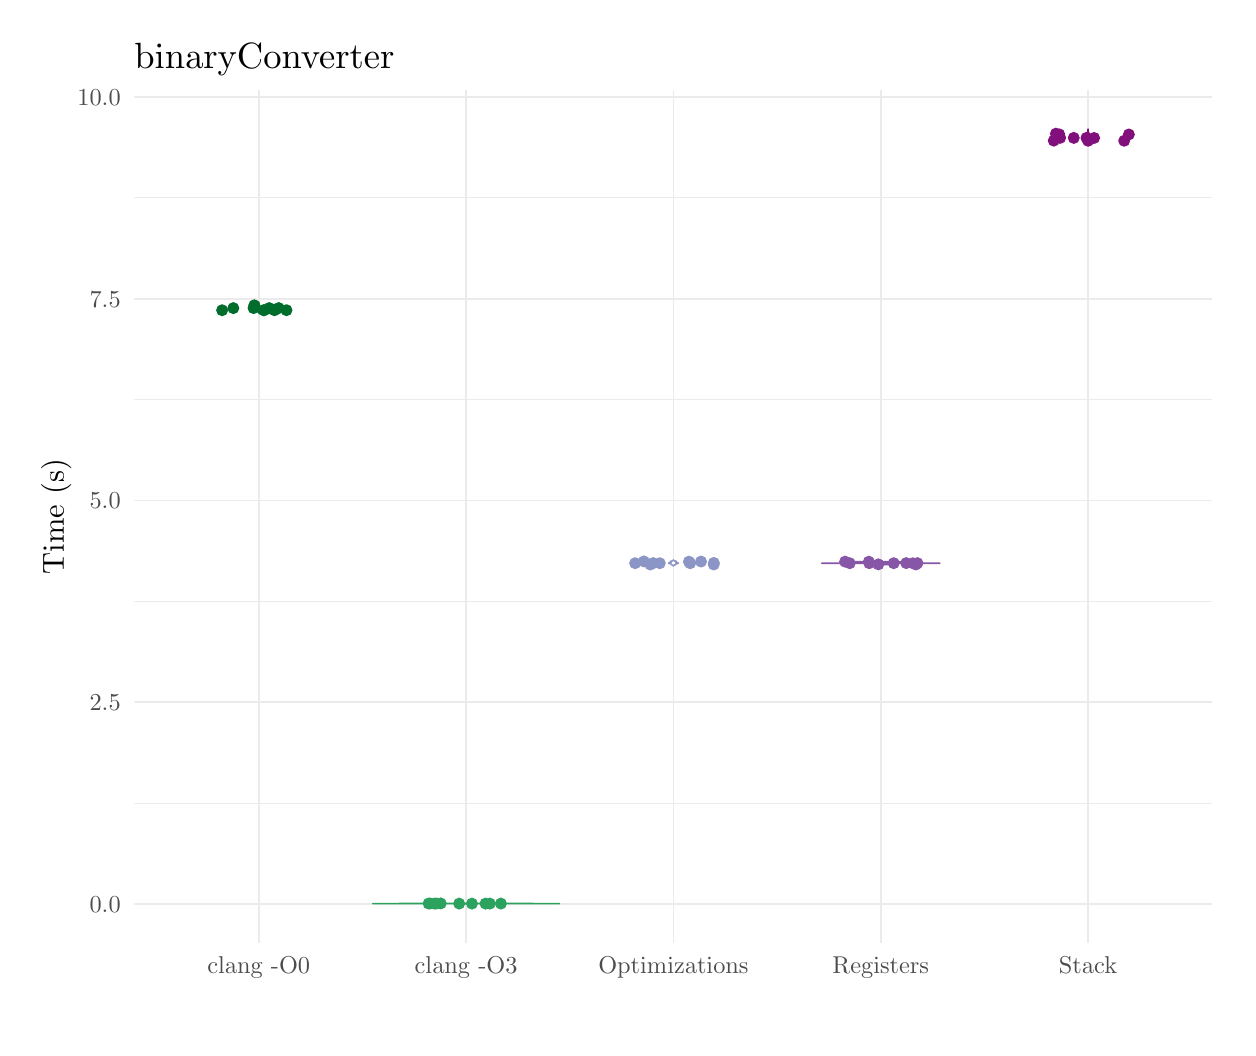
\begin{tikzpicture}[x=1pt,y=1pt]
\definecolor{fillColor}{RGB}{255,255,255}
\path[use as bounding box,fill=fillColor,fill opacity=0.00] (0,0) rectangle (433.62,361.35);
\begin{scope}
\path[clip] ( 38.56, 30.69) rectangle (428.12,338.69);
\definecolor{drawColor}{gray}{0.92}

\path[draw=drawColor,line width= 0.3pt,line join=round] ( 38.56, 81.14) --
	(428.12, 81.14);

\path[draw=drawColor,line width= 0.3pt,line join=round] ( 38.56,154.04) --
	(428.12,154.04);

\path[draw=drawColor,line width= 0.3pt,line join=round] ( 38.56,226.95) --
	(428.12,226.95);

\path[draw=drawColor,line width= 0.3pt,line join=round] ( 38.56,299.85) --
	(428.12,299.85);

\path[draw=drawColor,line width= 0.6pt,line join=round] ( 38.56, 44.69) --
	(428.12, 44.69);

\path[draw=drawColor,line width= 0.6pt,line join=round] ( 38.56,117.59) --
	(428.12,117.59);

\path[draw=drawColor,line width= 0.6pt,line join=round] ( 38.56,190.50) --
	(428.12,190.50);

\path[draw=drawColor,line width= 0.6pt,line join=round] ( 38.56,263.40) --
	(428.12,263.40);

\path[draw=drawColor,line width= 0.6pt,line join=round] ( 38.56,336.31) --
	(428.12,336.31);

\path[draw=drawColor,line width= 0.6pt,line join=round] ( 83.50, 30.69) --
	( 83.50,338.69);

\path[draw=drawColor,line width= 0.6pt,line join=round] (158.42, 30.69) --
	(158.42,338.69);

\path[draw=drawColor,line width= 0.6pt,line join=round] (233.34, 30.69) --
	(233.34,338.69);

\path[draw=drawColor,line width= 0.6pt,line join=round] (308.25, 30.69) --
	(308.25,338.69);

\path[draw=drawColor,line width= 0.6pt,line join=round] (383.17, 30.69) --
	(383.17,338.69);
\definecolor{drawColor}{RGB}{0,109,44}
\definecolor{fillColor}{RGB}{255,255,255}

\path[draw=drawColor,line width= 0.6pt,line join=round,line cap=round,fill=fillColor] ( 83.49,258.24) --
	( 83.49,258.25) --
	( 83.49,258.25) --
	( 83.49,258.26) --
	( 83.49,258.27) --
	( 83.49,258.28) --
	( 83.49,258.28) --
	( 83.49,258.29) --
	( 83.49,258.30) --
	( 83.49,258.31) --
	( 83.49,258.31) --
	( 83.48,258.32) --
	( 83.48,258.33) --
	( 83.48,258.34) --
	( 83.48,258.34) --
	( 83.48,258.35) --
	( 83.48,258.36) --
	( 83.48,258.37) --
	( 83.47,258.37) --
	( 83.47,258.38) --
	( 83.47,258.39) --
	( 83.47,258.39) --
	( 83.47,258.40) --
	( 83.46,258.41) --
	( 83.46,258.42) --
	( 83.46,258.42) --
	( 83.46,258.43) --
	( 83.45,258.44) --
	( 83.45,258.45) --
	( 83.45,258.45) --
	( 83.45,258.46) --
	( 83.44,258.47) --
	( 83.44,258.48) --
	( 83.44,258.48) --
	( 83.43,258.49) --
	( 83.43,258.50) --
	( 83.42,258.51) --
	( 83.42,258.51) --
	( 83.42,258.52) --
	( 83.41,258.53) --
	( 83.41,258.53) --
	( 83.40,258.54) --
	( 83.40,258.55) --
	( 83.39,258.56) --
	( 83.39,258.56) --
	( 83.38,258.57) --
	( 83.38,258.58) --
	( 83.37,258.59) --
	( 83.36,258.59) --
	( 83.36,258.60) --
	( 83.35,258.61) --
	( 83.34,258.62) --
	( 83.34,258.62) --
	( 83.33,258.63) --
	( 83.32,258.64) --
	( 83.31,258.64) --
	( 83.31,258.65) --
	( 83.30,258.66) --
	( 83.29,258.67) --
	( 83.28,258.67) --
	( 83.27,258.68) --
	( 83.27,258.69) --
	( 83.26,258.70) --
	( 83.25,258.70) --
	( 83.24,258.71) --
	( 83.23,258.72) --
	( 83.22,258.73) --
	( 83.21,258.73) --
	( 83.20,258.74) --
	( 83.19,258.75) --
	( 83.18,258.76) --
	( 83.17,258.76) --
	( 83.15,258.77) --
	( 83.14,258.78) --
	( 83.13,258.78) --
	( 83.12,258.79) --
	( 83.11,258.80) --
	( 83.10,258.81) --
	( 83.08,258.81) --
	( 83.07,258.82) --
	( 83.06,258.83) --
	( 83.05,258.84) --
	( 83.03,258.84) --
	( 83.02,258.85) --
	( 83.01,258.86) --
	( 83.00,258.87) --
	( 82.98,258.87) --
	( 82.97,258.88) --
	( 82.96,258.89) --
	( 82.94,258.90) --
	( 82.93,258.90) --
	( 82.92,258.91) --
	( 82.90,258.92) --
	( 82.89,258.92) --
	( 82.88,258.93) --
	( 82.86,258.94) --
	( 82.85,258.95) --
	( 82.84,258.95) --
	( 82.82,258.96) --
	( 82.81,258.97) --
	( 82.80,258.98) --
	( 82.79,258.98) --
	( 82.77,258.99) --
	( 82.76,259.00) --
	( 82.75,259.01) --
	( 82.73,259.01) --
	( 82.72,259.02) --
	( 82.71,259.03) --
	( 82.70,259.04) --
	( 82.69,259.04) --
	( 82.68,259.05) --
	( 82.66,259.06) --
	( 82.65,259.06) --
	( 82.64,259.07) --
	( 82.63,259.08) --
	( 82.62,259.09) --
	( 82.61,259.09) --
	( 82.60,259.10) --
	( 82.59,259.11) --
	( 82.58,259.12) --
	( 82.58,259.12) --
	( 82.57,259.13) --
	( 82.56,259.14) --
	( 82.55,259.15) --
	( 82.54,259.15) --
	( 82.54,259.16) --
	( 82.53,259.17) --
	( 82.52,259.18) --
	( 82.52,259.18) --
	( 82.51,259.19) --
	( 82.51,259.20) --
	( 82.50,259.20) --
	( 82.50,259.21) --
	( 82.50,259.22) --
	( 82.49,259.23) --
	( 82.49,259.23) --
	( 82.49,259.24) --
	( 82.48,259.25) --
	( 82.48,259.26) --
	( 82.48,259.26) --
	( 82.48,259.27) --
	( 82.48,259.28) --
	( 82.48,259.29) --
	( 82.48,259.29) --
	( 82.47,259.30) --
	( 82.48,259.31) --
	( 82.48,259.31) --
	( 82.48,259.32) --
	( 82.48,259.33) --
	( 82.48,259.34) --
	( 82.48,259.34) --
	( 82.48,259.35) --
	( 82.49,259.36) --
	( 82.49,259.37) --
	( 82.49,259.37) --
	( 82.49,259.38) --
	( 82.50,259.39) --
	( 82.50,259.40) --
	( 82.50,259.40) --
	( 82.51,259.41) --
	( 82.51,259.42) --
	( 82.51,259.43) --
	( 82.52,259.43) --
	( 82.52,259.44) --
	( 82.53,259.45) --
	( 82.53,259.45) --
	( 82.54,259.46) --
	( 82.54,259.47) --
	( 82.54,259.48) --
	( 82.55,259.48) --
	( 82.55,259.49) --
	( 82.56,259.50) --
	( 82.56,259.51) --
	( 82.57,259.51) --
	( 82.57,259.52) --
	( 82.58,259.53) --
	( 82.58,259.54) --
	( 82.58,259.54) --
	( 82.59,259.55) --
	( 82.59,259.56) --
	( 82.60,259.57) --
	( 82.60,259.57) --
	( 82.60,259.58) --
	( 82.61,259.59) --
	( 82.61,259.59) --
	( 82.61,259.60) --
	( 82.62,259.61) --
	( 82.62,259.62) --
	( 82.62,259.62) --
	( 82.62,259.63) --
	( 82.63,259.64) --
	( 82.63,259.65) --
	( 82.63,259.65) --
	( 82.63,259.66) --
	( 82.64,259.67) --
	( 82.64,259.68) --
	( 82.64,259.68) --
	( 82.64,259.69) --
	( 82.64,259.70) --
	( 82.64,259.71) --
	( 82.64,259.71) --
	( 82.64,259.72) --
	( 82.64,259.73) --
	( 82.64,259.73) --
	( 82.64,259.74) --
	( 82.64,259.75) --
	( 82.64,259.76) --
	( 82.64,259.76) --
	( 82.64,259.77) --
	( 82.64,259.78) --
	( 82.64,259.79) --
	( 82.64,259.79) --
	( 82.64,259.80) --
	( 82.64,259.81) --
	( 82.64,259.82) --
	( 82.64,259.82) --
	( 82.64,259.83) --
	( 82.64,259.84) --
	( 82.64,259.85) --
	( 82.64,259.85) --
	( 82.64,259.86) --
	( 82.64,259.87) --
	( 82.64,259.87) --
	( 82.64,259.88) --
	( 82.64,259.89) --
	( 82.64,259.90) --
	( 82.64,259.90) --
	( 82.64,259.91) --
	( 82.64,259.92) --
	( 82.64,259.93) --
	( 82.64,259.93) --
	( 82.64,259.94) --
	( 82.64,259.95) --
	( 82.64,259.96) --
	( 82.65,259.96) --
	( 82.65,259.97) --
	( 82.65,259.98) --
	( 82.65,259.99) --
	( 82.65,259.99) --
	( 82.66,260.00) --
	( 82.66,260.01) --
	( 82.66,260.01) --
	( 82.66,260.02) --
	( 82.67,260.03) --
	( 82.67,260.04) --
	( 82.67,260.04) --
	( 82.68,260.05) --
	( 82.68,260.06) --
	( 82.69,260.07) --
	( 82.69,260.07) --
	( 82.70,260.08) --
	( 82.70,260.09) --
	( 82.71,260.10) --
	( 82.71,260.10) --
	( 82.72,260.11) --
	( 82.73,260.12) --
	( 82.73,260.12) --
	( 82.74,260.13) --
	( 82.75,260.14) --
	( 82.75,260.15) --
	( 82.76,260.15) --
	( 82.77,260.16) --
	( 82.78,260.17) --
	( 82.78,260.18) --
	( 82.79,260.18) --
	( 82.80,260.19) --
	( 82.81,260.20) --
	( 82.82,260.21) --
	( 82.83,260.21) --
	( 82.84,260.22) --
	( 82.84,260.23) --
	( 82.85,260.24) --
	( 82.86,260.24) --
	( 82.87,260.25) --
	( 82.88,260.26) --
	( 82.89,260.26) --
	( 82.90,260.27) --
	( 82.91,260.28) --
	( 82.92,260.29) --
	( 82.93,260.29) --
	( 82.94,260.30) --
	( 82.95,260.31) --
	( 82.96,260.32) --
	( 82.97,260.32) --
	( 82.98,260.33) --
	( 82.99,260.34) --
	( 83.00,260.35) --
	( 83.01,260.35) --
	( 83.02,260.36) --
	( 83.03,260.37) --
	( 83.04,260.38) --
	( 83.04,260.38) --
	( 83.05,260.39) --
	( 83.06,260.40) --
	( 83.07,260.40) --
	( 83.08,260.41) --
	( 83.09,260.42) --
	( 83.10,260.43) --
	( 83.11,260.43) --
	( 83.11,260.44) --
	( 83.12,260.45) --
	( 83.13,260.46) --
	( 83.14,260.46) --
	( 83.15,260.47) --
	( 83.15,260.48) --
	( 83.16,260.49) --
	( 83.17,260.49) --
	( 83.17,260.50) --
	( 83.18,260.51) --
	( 83.19,260.52) --
	( 83.19,260.52) --
	( 83.20,260.53) --
	( 83.21,260.54) --
	( 83.21,260.54) --
	( 83.22,260.55) --
	( 83.22,260.56) --
	( 83.23,260.57) --
	( 83.23,260.57) --
	( 83.24,260.58) --
	( 83.24,260.59) --
	( 83.25,260.60) --
	( 83.25,260.60) --
	( 83.25,260.61) --
	( 83.26,260.62) --
	( 83.26,260.63) --
	( 83.26,260.63) --
	( 83.27,260.64) --
	( 83.27,260.65) --
	( 83.27,260.66) --
	( 83.28,260.66) --
	( 83.28,260.67) --
	( 83.28,260.68) --
	( 83.28,260.68) --
	( 83.28,260.69) --
	( 83.29,260.70) --
	( 83.29,260.71) --
	( 83.29,260.71) --
	( 83.29,260.72) --
	( 83.29,260.73) --
	( 83.29,260.74) --
	( 83.29,260.74) --
	( 83.29,260.75) --
	( 83.30,260.76) --
	( 83.30,260.77) --
	( 83.30,260.77) --
	( 83.30,260.78) --
	( 83.30,260.79) --
	( 83.30,260.79) --
	( 83.30,260.80) --
	( 83.30,260.81) --
	( 83.30,260.82) --
	( 83.30,260.82) --
	( 83.30,260.83) --
	( 83.30,260.84) --
	( 83.30,260.85) --
	( 83.30,260.85) --
	( 83.30,260.86) --
	( 83.30,260.87) --
	( 83.30,260.88) --
	( 83.30,260.88) --
	( 83.30,260.89) --
	( 83.30,260.90) --
	( 83.30,260.91) --
	( 83.30,260.91) --
	( 83.30,260.92) --
	( 83.30,260.93) --
	( 83.30,260.93) --
	( 83.30,260.94) --
	( 83.30,260.95) --
	( 83.30,260.96) --
	( 83.30,260.96) --
	( 83.30,260.97) --
	( 83.30,260.98) --
	( 83.30,260.99) --
	( 83.30,260.99) --
	( 83.30,261.00) --
	( 83.30,261.01) --
	( 83.30,261.02) --
	( 83.30,261.02) --
	( 83.30,261.03) --
	( 83.30,261.04) --
	( 83.31,261.05) --
	( 83.31,261.05) --
	( 83.31,261.06) --
	( 83.31,261.07) --
	( 83.31,261.07) --
	( 83.31,261.08) --
	( 83.31,261.09) --
	( 83.31,261.10) --
	( 83.31,261.10) --
	( 83.32,261.11) --
	( 83.32,261.12) --
	( 83.32,261.13) --
	( 83.32,261.13) --
	( 83.32,261.14) --
	( 83.32,261.15) --
	( 83.33,261.16) --
	( 83.33,261.16) --
	( 83.33,261.17) --
	( 83.33,261.18) --
	( 83.33,261.19) --
	( 83.34,261.19) --
	( 83.34,261.20) --
	( 83.34,261.21) --
	( 83.34,261.21) --
	( 83.35,261.22) --
	( 83.35,261.23) --
	( 83.35,261.24) --
	( 83.35,261.24) --
	( 83.35,261.25) --
	( 83.36,261.26) --
	( 83.36,261.27) --
	( 83.36,261.27) --
	( 83.37,261.28) --
	( 83.37,261.29) --
	( 83.37,261.30) --
	( 83.37,261.30) --
	( 83.38,261.31) --
	( 83.38,261.32) --
	( 83.38,261.33) --
	( 83.38,261.33) --
	( 83.39,261.34) --
	( 83.39,261.35) --
	( 83.39,261.35) --
	( 83.39,261.36) --
	( 83.40,261.37) --
	( 83.40,261.38) --
	( 83.40,261.38) --
	( 83.40,261.39) --
	( 83.41,261.40) --
	( 83.41,261.41) --
	( 83.41,261.41) --
	( 83.41,261.42) --
	( 83.42,261.43) --
	( 83.42,261.44) --
	( 83.42,261.44) --
	( 83.42,261.45) --
	( 83.43,261.46) --
	( 83.43,261.46) --
	( 83.43,261.47) --
	( 83.43,261.48) --
	( 83.44,261.49) --
	( 83.44,261.49) --
	( 83.44,261.50) --
	( 83.44,261.51) --
	( 83.44,261.52) --
	( 83.45,261.52) --
	( 83.45,261.53) --
	( 83.45,261.54) --
	( 83.45,261.55) --
	( 83.45,261.55) --
	( 83.46,261.56) --
	( 83.46,261.57) --
	( 83.46,261.58) --
	( 83.46,261.58) --
	( 83.46,261.59) --
	( 83.46,261.60) --
	( 83.47,261.60) --
	( 83.47,261.61) --
	( 83.47,261.62) --
	( 83.47,261.63) --
	( 83.47,261.63) --
	( 83.47,261.64) --
	( 83.47,261.65) --
	( 83.48,261.66) --
	( 83.48,261.66) --
	( 83.48,261.67) --
	( 83.48,261.68) --
	( 83.48,261.69) --
	( 83.48,261.69) --
	( 83.48,261.70) --
	( 83.48,261.71) --
	( 83.48,261.72) --
	( 83.49,261.72) --
	( 83.49,261.73) --
	( 83.49,261.74) --
	( 83.49,261.74) --
	( 83.49,261.75) --
	( 83.49,261.76) --
	( 83.49,261.77) --
	( 83.49,261.77) --
	( 83.49,261.78) --
	( 83.49,261.79) --
	( 83.49,261.80) --
	( 83.49,261.80) --
	( 83.49,261.81) --
	( 83.49,261.82) --
	( 83.50,261.83) --
	( 83.50,261.83) --
	( 83.50,261.84) --
	( 83.50,261.85) --
	( 83.50,261.86) --
	( 83.50,261.86) --
	( 83.50,261.87) --
	( 83.50,261.88) --
	( 83.50,261.88) --
	( 83.50,261.89) --
	( 83.50,261.90) --
	( 83.50,261.91) --
	( 83.50,261.91) --
	( 83.50,261.92) --
	( 83.50,261.93) --
	( 83.50,261.94) --
	( 83.50,261.94) --
	( 83.50,261.95) --
	( 83.50,261.96) --
	( 83.50,261.97) --
	( 83.50,261.97) --
	( 83.50,261.98) --
	( 83.50,261.99) --
	( 83.50,262.00) --
	( 83.50,262.00) --
	( 83.51,262.00) --
	( 83.51,262.00) --
	( 83.51,261.99) --
	( 83.51,261.98) --
	( 83.51,261.97) --
	( 83.51,261.97) --
	( 83.51,261.96) --
	( 83.51,261.95) --
	( 83.51,261.94) --
	( 83.51,261.94) --
	( 83.51,261.93) --
	( 83.51,261.92) --
	( 83.51,261.91) --
	( 83.51,261.91) --
	( 83.51,261.90) --
	( 83.51,261.89) --
	( 83.51,261.88) --
	( 83.51,261.88) --
	( 83.51,261.87) --
	( 83.51,261.86) --
	( 83.51,261.86) --
	( 83.51,261.85) --
	( 83.51,261.84) --
	( 83.51,261.83) --
	( 83.51,261.83) --
	( 83.51,261.82) --
	( 83.52,261.81) --
	( 83.52,261.80) --
	( 83.52,261.80) --
	( 83.52,261.79) --
	( 83.52,261.78) --
	( 83.52,261.77) --
	( 83.52,261.77) --
	( 83.52,261.76) --
	( 83.52,261.75) --
	( 83.52,261.74) --
	( 83.52,261.74) --
	( 83.52,261.73) --
	( 83.52,261.72) --
	( 83.52,261.72) --
	( 83.53,261.71) --
	( 83.53,261.70) --
	( 83.53,261.69) --
	( 83.53,261.69) --
	( 83.53,261.68) --
	( 83.53,261.67) --
	( 83.53,261.66) --
	( 83.53,261.66) --
	( 83.54,261.65) --
	( 83.54,261.64) --
	( 83.54,261.63) --
	( 83.54,261.63) --
	( 83.54,261.62) --
	( 83.54,261.61) --
	( 83.54,261.60) --
	( 83.55,261.60) --
	( 83.55,261.59) --
	( 83.55,261.58) --
	( 83.55,261.58) --
	( 83.55,261.57) --
	( 83.55,261.56) --
	( 83.56,261.55) --
	( 83.56,261.55) --
	( 83.56,261.54) --
	( 83.56,261.53) --
	( 83.56,261.52) --
	( 83.57,261.52) --
	( 83.57,261.51) --
	( 83.57,261.50) --
	( 83.57,261.49) --
	( 83.57,261.49) --
	( 83.58,261.48) --
	( 83.58,261.47) --
	( 83.58,261.46) --
	( 83.58,261.46) --
	( 83.59,261.45) --
	( 83.59,261.44) --
	( 83.59,261.44) --
	( 83.59,261.43) --
	( 83.60,261.42) --
	( 83.60,261.41) --
	( 83.60,261.41) --
	( 83.60,261.40) --
	( 83.61,261.39) --
	( 83.61,261.38) --
	( 83.61,261.38) --
	( 83.61,261.37) --
	( 83.62,261.36) --
	( 83.62,261.35) --
	( 83.62,261.35) --
	( 83.62,261.34) --
	( 83.63,261.33) --
	( 83.63,261.33) --
	( 83.63,261.32) --
	( 83.63,261.31) --
	( 83.64,261.30) --
	( 83.64,261.30) --
	( 83.64,261.29) --
	( 83.64,261.28) --
	( 83.65,261.27) --
	( 83.65,261.27) --
	( 83.65,261.26) --
	( 83.65,261.25) --
	( 83.66,261.24) --
	( 83.66,261.24) --
	( 83.66,261.23) --
	( 83.66,261.22) --
	( 83.67,261.21) --
	( 83.67,261.21) --
	( 83.67,261.20) --
	( 83.67,261.19) --
	( 83.68,261.19) --
	( 83.68,261.18) --
	( 83.68,261.17) --
	( 83.68,261.16) --
	( 83.68,261.16) --
	( 83.69,261.15) --
	( 83.69,261.14) --
	( 83.69,261.13) --
	( 83.69,261.13) --
	( 83.69,261.12) --
	( 83.69,261.11) --
	( 83.70,261.10) --
	( 83.70,261.10) --
	( 83.70,261.09) --
	( 83.70,261.08) --
	( 83.70,261.07) --
	( 83.70,261.07) --
	( 83.70,261.06) --
	( 83.70,261.05) --
	( 83.70,261.05) --
	( 83.71,261.04) --
	( 83.71,261.03) --
	( 83.71,261.02) --
	( 83.71,261.02) --
	( 83.71,261.01) --
	( 83.71,261.00) --
	( 83.71,260.99) --
	( 83.71,260.99) --
	( 83.71,260.98) --
	( 83.71,260.97) --
	( 83.71,260.96) --
	( 83.71,260.96) --
	( 83.71,260.95) --
	( 83.71,260.94) --
	( 83.71,260.93) --
	( 83.71,260.93) --
	( 83.71,260.92) --
	( 83.71,260.91) --
	( 83.71,260.91) --
	( 83.71,260.90) --
	( 83.71,260.89) --
	( 83.71,260.88) --
	( 83.71,260.88) --
	( 83.71,260.87) --
	( 83.71,260.86) --
	( 83.71,260.85) --
	( 83.71,260.85) --
	( 83.71,260.84) --
	( 83.71,260.83) --
	( 83.71,260.82) --
	( 83.71,260.82) --
	( 83.71,260.81) --
	( 83.71,260.80) --
	( 83.71,260.79) --
	( 83.71,260.79) --
	( 83.71,260.78) --
	( 83.71,260.77) --
	( 83.71,260.77) --
	( 83.71,260.76) --
	( 83.72,260.75) --
	( 83.72,260.74) --
	( 83.72,260.74) --
	( 83.72,260.73) --
	( 83.72,260.72) --
	( 83.72,260.71) --
	( 83.72,260.71) --
	( 83.72,260.70) --
	( 83.73,260.69) --
	( 83.73,260.68) --
	( 83.73,260.68) --
	( 83.73,260.67) --
	( 83.73,260.66) --
	( 83.74,260.66) --
	( 83.74,260.65) --
	( 83.74,260.64) --
	( 83.75,260.63) --
	( 83.75,260.63) --
	( 83.75,260.62) --
	( 83.76,260.61) --
	( 83.76,260.60) --
	( 83.76,260.60) --
	( 83.77,260.59) --
	( 83.77,260.58) --
	( 83.78,260.57) --
	( 83.78,260.57) --
	( 83.79,260.56) --
	( 83.79,260.55) --
	( 83.80,260.54) --
	( 83.80,260.54) --
	( 83.81,260.53) --
	( 83.82,260.52) --
	( 83.82,260.52) --
	( 83.83,260.51) --
	( 83.83,260.50) --
	( 83.84,260.49) --
	( 83.85,260.49) --
	( 83.86,260.48) --
	( 83.86,260.47) --
	( 83.87,260.46) --
	( 83.88,260.46) --
	( 83.89,260.45) --
	( 83.89,260.44) --
	( 83.90,260.43) --
	( 83.91,260.43) --
	( 83.92,260.42) --
	( 83.93,260.41) --
	( 83.94,260.40) --
	( 83.95,260.40) --
	( 83.96,260.39) --
	( 83.96,260.38) --
	( 83.97,260.38) --
	( 83.98,260.37) --
	( 83.99,260.36) --
	( 84.00,260.35) --
	( 84.01,260.35) --
	( 84.02,260.34) --
	( 84.03,260.33) --
	( 84.04,260.32) --
	( 84.05,260.32) --
	( 84.06,260.31) --
	( 84.07,260.30) --
	( 84.08,260.29) --
	( 84.09,260.29) --
	( 84.10,260.28) --
	( 84.11,260.27) --
	( 84.12,260.26) --
	( 84.13,260.26) --
	( 84.14,260.25) --
	( 84.15,260.24) --
	( 84.16,260.24) --
	( 84.17,260.23) --
	( 84.17,260.22) --
	( 84.18,260.21) --
	( 84.19,260.21) --
	( 84.20,260.20) --
	( 84.21,260.19) --
	( 84.22,260.18) --
	( 84.23,260.18) --
	( 84.23,260.17) --
	( 84.24,260.16) --
	( 84.25,260.15) --
	( 84.26,260.15) --
	( 84.26,260.14) --
	( 84.27,260.13) --
	( 84.28,260.12) --
	( 84.28,260.12) --
	( 84.29,260.11) --
	( 84.30,260.10) --
	( 84.30,260.10) --
	( 84.31,260.09) --
	( 84.31,260.08) --
	( 84.32,260.07) --
	( 84.32,260.07) --
	( 84.33,260.06) --
	( 84.33,260.05) --
	( 84.33,260.04) --
	( 84.34,260.04) --
	( 84.34,260.03) --
	( 84.35,260.02) --
	( 84.35,260.01) --
	( 84.35,260.01) --
	( 84.35,260.00) --
	( 84.36,259.99) --
	( 84.36,259.99) --
	( 84.36,259.98) --
	( 84.36,259.97) --
	( 84.36,259.96) --
	( 84.37,259.96) --
	( 84.37,259.95) --
	( 84.37,259.94) --
	( 84.37,259.93) --
	( 84.37,259.93) --
	( 84.37,259.92) --
	( 84.37,259.91) --
	( 84.37,259.90) --
	( 84.37,259.90) --
	( 84.37,259.89) --
	( 84.37,259.88) --
	( 84.37,259.87) --
	( 84.37,259.87) --
	( 84.37,259.86) --
	( 84.37,259.85) --
	( 84.37,259.85) --
	( 84.37,259.84) --
	( 84.37,259.83) --
	( 84.37,259.82) --
	( 84.37,259.82) --
	( 84.37,259.81) --
	( 84.37,259.80) --
	( 84.37,259.79) --
	( 84.37,259.79) --
	( 84.37,259.78) --
	( 84.36,259.77) --
	( 84.36,259.76) --
	( 84.36,259.76) --
	( 84.36,259.75) --
	( 84.37,259.74) --
	( 84.37,259.73) --
	( 84.37,259.73) --
	( 84.37,259.72) --
	( 84.37,259.71) --
	( 84.37,259.71) --
	( 84.37,259.70) --
	( 84.37,259.69) --
	( 84.37,259.68) --
	( 84.37,259.68) --
	( 84.37,259.67) --
	( 84.38,259.66) --
	( 84.38,259.65) --
	( 84.38,259.65) --
	( 84.38,259.64) --
	( 84.39,259.63) --
	( 84.39,259.62) --
	( 84.39,259.62) --
	( 84.39,259.61) --
	( 84.40,259.60) --
	( 84.40,259.59) --
	( 84.40,259.59) --
	( 84.41,259.58) --
	( 84.41,259.57) --
	( 84.41,259.57) --
	( 84.42,259.56) --
	( 84.42,259.55) --
	( 84.43,259.54) --
	( 84.43,259.54) --
	( 84.43,259.53) --
	( 84.44,259.52) --
	( 84.44,259.51) --
	( 84.45,259.51) --
	( 84.45,259.50) --
	( 84.46,259.49) --
	( 84.46,259.48) --
	( 84.47,259.48) --
	( 84.47,259.47) --
	( 84.47,259.46) --
	( 84.48,259.45) --
	( 84.48,259.45) --
	( 84.49,259.44) --
	( 84.49,259.43) --
	( 84.49,259.43) --
	( 84.50,259.42) --
	( 84.50,259.41) --
	( 84.51,259.40) --
	( 84.51,259.40) --
	( 84.51,259.39) --
	( 84.52,259.38) --
	( 84.52,259.37) --
	( 84.52,259.37) --
	( 84.52,259.36) --
	( 84.53,259.35) --
	( 84.53,259.34) --
	( 84.53,259.34) --
	( 84.53,259.33) --
	( 84.53,259.32) --
	( 84.53,259.31) --
	( 84.53,259.31) --
	( 84.53,259.30) --
	( 84.53,259.29) --
	( 84.53,259.29) --
	( 84.53,259.28) --
	( 84.53,259.27) --
	( 84.53,259.26) --
	( 84.53,259.26) --
	( 84.53,259.25) --
	( 84.52,259.24) --
	( 84.52,259.23) --
	( 84.52,259.23) --
	( 84.51,259.22) --
	( 84.51,259.21) --
	( 84.51,259.20) --
	( 84.50,259.20) --
	( 84.50,259.19) --
	( 84.49,259.18) --
	( 84.49,259.18) --
	( 84.48,259.17) --
	( 84.47,259.16) --
	( 84.47,259.15) --
	( 84.46,259.15) --
	( 84.45,259.14) --
	( 84.44,259.13) --
	( 84.43,259.12) --
	( 84.43,259.12) --
	( 84.42,259.11) --
	( 84.41,259.10) --
	( 84.40,259.09) --
	( 84.39,259.09) --
	( 84.38,259.08) --
	( 84.37,259.07) --
	( 84.36,259.06) --
	( 84.35,259.06) --
	( 84.33,259.05) --
	( 84.32,259.04) --
	( 84.31,259.04) --
	( 84.30,259.03) --
	( 84.29,259.02) --
	( 84.27,259.01) --
	( 84.26,259.01) --
	( 84.25,259.00) --
	( 84.24,258.99) --
	( 84.22,258.98) --
	( 84.21,258.98) --
	( 84.20,258.97) --
	( 84.19,258.96) --
	( 84.17,258.95) --
	( 84.16,258.95) --
	( 84.15,258.94) --
	( 84.13,258.93) --
	( 84.12,258.92) --
	( 84.11,258.92) --
	( 84.09,258.91) --
	( 84.08,258.90) --
	( 84.07,258.90) --
	( 84.05,258.89) --
	( 84.04,258.88) --
	( 84.03,258.87) --
	( 84.01,258.87) --
	( 84.00,258.86) --
	( 83.99,258.85) --
	( 83.98,258.84) --
	( 83.96,258.84) --
	( 83.95,258.83) --
	( 83.94,258.82) --
	( 83.93,258.81) --
	( 83.91,258.81) --
	( 83.90,258.80) --
	( 83.89,258.79) --
	( 83.88,258.78) --
	( 83.87,258.78) --
	( 83.86,258.77) --
	( 83.84,258.76) --
	( 83.83,258.76) --
	( 83.82,258.75) --
	( 83.81,258.74) --
	( 83.80,258.73) --
	( 83.79,258.73) --
	( 83.78,258.72) --
	( 83.77,258.71) --
	( 83.76,258.70) --
	( 83.75,258.70) --
	( 83.74,258.69) --
	( 83.74,258.68) --
	( 83.73,258.67) --
	( 83.72,258.67) --
	( 83.71,258.66) --
	( 83.70,258.65) --
	( 83.69,258.64) --
	( 83.69,258.64) --
	( 83.68,258.63) --
	( 83.67,258.62) --
	( 83.67,258.62) --
	( 83.66,258.61) --
	( 83.65,258.60) --
	( 83.65,258.59) --
	( 83.64,258.59) --
	( 83.63,258.58) --
	( 83.63,258.57) --
	( 83.62,258.56) --
	( 83.62,258.56) --
	( 83.61,258.55) --
	( 83.61,258.54) --
	( 83.60,258.53) --
	( 83.60,258.53) --
	( 83.59,258.52) --
	( 83.59,258.51) --
	( 83.59,258.51) --
	( 83.58,258.50) --
	( 83.58,258.49) --
	( 83.57,258.48) --
	( 83.57,258.48) --
	( 83.57,258.47) --
	( 83.56,258.46) --
	( 83.56,258.45) --
	( 83.56,258.45) --
	( 83.56,258.44) --
	( 83.55,258.43) --
	( 83.55,258.42) --
	( 83.55,258.42) --
	( 83.55,258.41) --
	( 83.54,258.40) --
	( 83.54,258.39) --
	( 83.54,258.39) --
	( 83.54,258.38) --
	( 83.54,258.37) --
	( 83.53,258.37) --
	( 83.53,258.36) --
	( 83.53,258.35) --
	( 83.53,258.34) --
	( 83.53,258.34) --
	( 83.53,258.33) --
	( 83.52,258.32) --
	( 83.52,258.31) --
	( 83.52,258.31) --
	( 83.52,258.30) --
	( 83.52,258.29) --
	( 83.52,258.28) --
	( 83.52,258.28) --
	( 83.52,258.27) --
	( 83.52,258.26) --
	( 83.52,258.25) --
	( 83.52,258.25) --
	( 83.51,258.24) --
	( 83.49,258.24) --
	cycle;
\definecolor{drawColor}{RGB}{44,162,95}

\path[draw=drawColor,line width= 0.6pt,line join=round,line cap=round,fill=fillColor] (158.05, 44.80) --
	(158.03, 44.80) --
	(158.00, 44.80) --
	(157.97, 44.80) --
	(157.95, 44.80) --
	(157.91, 44.80) --
	(157.88, 44.80) --
	(157.85, 44.80) --
	(157.81, 44.80) --
	(157.77, 44.80) --
	(157.73, 44.80) --
	(157.69, 44.80) --
	(157.65, 44.80) --
	(157.60, 44.80) --
	(157.55, 44.80) --
	(157.50, 44.80) --
	(157.45, 44.80) --
	(157.39, 44.80) --
	(157.33, 44.80) --
	(157.27, 44.80) --
	(157.20, 44.80) --
	(157.13, 44.80) --
	(157.06, 44.80) --
	(156.99, 44.80) --
	(156.91, 44.80) --
	(156.82, 44.80) --
	(156.74, 44.80) --
	(156.65, 44.80) --
	(156.55, 44.80) --
	(156.45, 44.80) --
	(156.35, 44.80) --
	(156.25, 44.80) --
	(156.13, 44.80) --
	(156.02, 44.81) --
	(155.90, 44.81) --
	(155.77, 44.81) --
	(155.64, 44.81) --
	(155.51, 44.81) --
	(155.37, 44.81) --
	(155.22, 44.81) --
	(155.07, 44.81) --
	(154.91, 44.81) --
	(154.75, 44.81) --
	(154.58, 44.81) --
	(154.41, 44.81) --
	(154.23, 44.81) --
	(154.05, 44.81) --
	(153.86, 44.81) --
	(153.66, 44.81) --
	(153.45, 44.81) --
	(153.24, 44.81) --
	(153.02, 44.81) --
	(152.80, 44.81) --
	(152.57, 44.81) --
	(152.34, 44.81) --
	(152.09, 44.81) --
	(151.84, 44.81) --
	(151.58, 44.81) --
	(151.32, 44.81) --
	(151.05, 44.81) --
	(150.77, 44.81) --
	(150.49, 44.81) --
	(150.20, 44.81) --
	(149.90, 44.81) --
	(149.60, 44.81) --
	(149.28, 44.81) --
	(148.97, 44.81) --
	(148.64, 44.81) --
	(148.31, 44.81) --
	(147.98, 44.81) --
	(147.63, 44.81) --
	(147.28, 44.81) --
	(146.93, 44.81) --
	(146.57, 44.82) --
	(146.20, 44.82) --
	(145.83, 44.82) --
	(145.45, 44.82) --
	(145.07, 44.82) --
	(144.68, 44.82) --
	(144.29, 44.82) --
	(143.89, 44.82) --
	(143.49, 44.82) --
	(143.08, 44.82) --
	(142.67, 44.82) --
	(142.26, 44.82) --
	(141.84, 44.82) --
	(141.42, 44.82) --
	(141.00, 44.82) --
	(140.57, 44.82) --
	(140.15, 44.82) --
	(139.72, 44.82) --
	(139.29, 44.82) --
	(138.86, 44.82) --
	(138.43, 44.82) --
	(138.00, 44.82) --
	(137.57, 44.82) --
	(137.14, 44.82) --
	(136.71, 44.82) --
	(136.28, 44.82) --
	(135.85, 44.82) --
	(135.43, 44.82) --
	(135.01, 44.82) --
	(134.59, 44.82) --
	(134.17, 44.82) --
	(133.76, 44.82) --
	(133.36, 44.82) --
	(132.95, 44.82) --
	(132.56, 44.82) --
	(132.17, 44.82) --
	(131.78, 44.82) --
	(131.40, 44.82) --
	(131.03, 44.82) --
	(130.67, 44.82) --
	(130.31, 44.83) --
	(129.96, 44.83) --
	(129.62, 44.83) --
	(129.29, 44.83) --
	(128.97, 44.83) --
	(128.65, 44.83) --
	(128.35, 44.83) --
	(128.06, 44.83) --
	(127.78, 44.83) --
	(127.51, 44.83) --
	(127.25, 44.83) --
	(127.00, 44.83) --
	(126.76, 44.83) --
	(126.54, 44.83) --
	(126.33, 44.83) --
	(126.13, 44.83) --
	(125.94, 44.83) --
	(125.77, 44.83) --
	(125.61, 44.83) --
	(125.46, 44.83) --
	(125.32, 44.83) --
	(125.20, 44.83) --
	(125.09, 44.83) --
	(125.00, 44.83) --
	(124.91, 44.83) --
	(124.85, 44.83) --
	(124.79, 44.83) --
	(124.75, 44.83) --
	(124.72, 44.83) --
	(124.71, 44.83) --
	(124.71, 44.83) --
	(124.72, 44.83) --
	(124.75, 44.83) --
	(124.78, 44.83) --
	(124.83, 44.83) --
	(124.89, 44.83) --
	(124.97, 44.83) --
	(125.06, 44.83) --
	(125.15, 44.83) --
	(125.26, 44.84) --
	(125.38, 44.84) --
	(125.51, 44.84) --
	(125.65, 44.84) --
	(125.80, 44.84) --
	(125.97, 44.84) --
	(126.14, 44.84) --
	(126.32, 44.84) --
	(126.50, 44.84) --
	(126.70, 44.84) --
	(126.91, 44.84) --
	(127.11, 44.84) --
	(127.34, 44.84) --
	(127.56, 44.84) --
	(127.79, 44.84) --
	(128.03, 44.84) --
	(128.27, 44.84) --
	(128.51, 44.84) --
	(128.76, 44.84) --
	(129.02, 44.84) --
	(129.27, 44.84) --
	(129.53, 44.84) --
	(129.80, 44.84) --
	(130.06, 44.84) --
	(130.33, 44.84) --
	(130.59, 44.84) --
	(130.86, 44.84) --
	(131.13, 44.84) --
	(131.39, 44.84) --
	(131.66, 44.84) --
	(131.92, 44.84) --
	(132.19, 44.84) --
	(132.45, 44.84) --
	(132.71, 44.84) --
	(132.96, 44.84) --
	(133.22, 44.84) --
	(133.47, 44.84) --
	(133.71, 44.84) --
	(133.96, 44.84) --
	(134.19, 44.84) --
	(134.43, 44.85) --
	(134.66, 44.85) --
	(134.88, 44.85) --
	(135.10, 44.85) --
	(135.32, 44.85) --
	(135.52, 44.85) --
	(135.73, 44.85) --
	(135.92, 44.85) --
	(136.11, 44.85) --
	(136.30, 44.85) --
	(136.48, 44.85) --
	(136.65, 44.85) --
	(136.82, 44.85) --
	(136.97, 44.85) --
	(137.13, 44.85) --
	(137.28, 44.85) --
	(137.42, 44.85) --
	(137.55, 44.85) --
	(137.68, 44.85) --
	(137.80, 44.85) --
	(137.92, 44.85) --
	(138.03, 44.85) --
	(138.14, 44.85) --
	(138.24, 44.85) --
	(138.33, 44.85) --
	(138.42, 44.85) --
	(138.50, 44.85) --
	(138.58, 44.85) --
	(138.66, 44.85) --
	(138.73, 44.85) --
	(138.79, 44.85) --
	(138.85, 44.85) --
	(138.91, 44.85) --
	(138.96, 44.85) --
	(139.01, 44.85) --
	(139.06, 44.85) --
	(139.11, 44.85) --
	(139.15, 44.85) --
	(139.19, 44.85) --
	(139.23, 44.85) --
	(139.26, 44.86) --
	(139.30, 44.86) --
	(139.33, 44.86) --
	(139.36, 44.86) --
	(139.39, 44.86) --
	(139.43, 44.86) --
	(139.46, 44.86) --
	(139.49, 44.86) --
	(139.52, 44.86) --
	(139.55, 44.86) --
	(139.59, 44.86) --
	(139.62, 44.86) --
	(139.66, 44.86) --
	(139.69, 44.86) --
	(139.73, 44.86) --
	(139.77, 44.86) --
	(139.82, 44.86) --
	(139.86, 44.86) --
	(139.91, 44.86) --
	(139.96, 44.86) --
	(140.01, 44.86) --
	(140.07, 44.86) --
	(140.13, 44.86) --
	(140.19, 44.86) --
	(140.26, 44.86) --
	(140.33, 44.86) --
	(140.40, 44.86) --
	(140.48, 44.86) --
	(140.56, 44.86) --
	(140.65, 44.86) --
	(140.73, 44.86) --
	(140.82, 44.86) --
	(140.92, 44.86) --
	(141.02, 44.86) --
	(141.12, 44.86) --
	(141.23, 44.86) --
	(141.34, 44.86) --
	(141.46, 44.86) --
	(141.57, 44.86) --
	(141.70, 44.87) --
	(141.82, 44.87) --
	(141.95, 44.87) --
	(142.08, 44.87) --
	(142.22, 44.87) --
	(142.36, 44.87) --
	(142.50, 44.87) --
	(142.64, 44.87) --
	(142.79, 44.87) --
	(142.94, 44.87) --
	(143.09, 44.87) --
	(143.24, 44.87) --
	(143.40, 44.87) --
	(143.56, 44.87) --
	(143.72, 44.87) --
	(143.88, 44.87) --
	(144.04, 44.87) --
	(144.21, 44.87) --
	(144.37, 44.87) --
	(144.54, 44.87) --
	(144.71, 44.87) --
	(144.87, 44.87) --
	(145.04, 44.87) --
	(145.21, 44.87) --
	(145.38, 44.87) --
	(145.54, 44.87) --
	(145.71, 44.87) --
	(145.88, 44.87) --
	(146.04, 44.87) --
	(146.21, 44.87) --
	(146.37, 44.87) --
	(146.54, 44.87) --
	(146.70, 44.87) --
	(146.86, 44.87) --
	(147.02, 44.87) --
	(147.17, 44.87) --
	(147.33, 44.87) --
	(147.48, 44.87) --
	(147.63, 44.87) --
	(147.78, 44.87) --
	(147.92, 44.88) --
	(148.06, 44.88) --
	(148.20, 44.88) --
	(148.34, 44.88) --
	(148.48, 44.88) --
	(148.61, 44.88) --
	(148.74, 44.88) --
	(148.86, 44.88) --
	(148.99, 44.88) --
	(149.11, 44.88) --
	(149.22, 44.88) --
	(149.34, 44.88) --
	(149.45, 44.88) --
	(149.55, 44.88) --
	(149.66, 44.88) --
	(149.76, 44.88) --
	(149.86, 44.88) --
	(149.95, 44.88) --
	(150.05, 44.88) --
	(150.13, 44.88) --
	(150.22, 44.88) --
	(150.30, 44.88) --
	(150.38, 44.88) --
	(150.46, 44.88) --
	(150.53, 44.88) --
	(150.61, 44.88) --
	(150.68, 44.88) --
	(150.74, 44.88) --
	(150.81, 44.88) --
	(150.87, 44.88) --
	(150.93, 44.88) --
	(150.99, 44.88) --
	(151.04, 44.88) --
	(151.10, 44.88) --
	(151.15, 44.88) --
	(151.20, 44.88) --
	(151.24, 44.88) --
	(151.29, 44.88) --
	(151.34, 44.88) --
	(151.38, 44.88) --
	(151.42, 44.89) --
	(151.46, 44.89) --
	(151.50, 44.89) --
	(151.54, 44.89) --
	(151.58, 44.89) --
	(151.62, 44.89) --
	(151.66, 44.89) --
	(151.69, 44.89) --
	(151.73, 44.89) --
	(151.77, 44.89) --
	(151.80, 44.89) --
	(151.84, 44.89) --
	(151.88, 44.89) --
	(151.91, 44.89) --
	(151.95, 44.89) --
	(151.98, 44.89) --
	(152.02, 44.89) --
	(152.06, 44.89) --
	(152.10, 44.89) --
	(152.14, 44.89) --
	(152.17, 44.89) --
	(152.21, 44.89) --
	(152.26, 44.89) --
	(152.30, 44.89) --
	(152.34, 44.89) --
	(152.38, 44.89) --
	(152.43, 44.89) --
	(152.47, 44.89) --
	(152.52, 44.89) --
	(152.57, 44.89) --
	(152.61, 44.89) --
	(152.66, 44.89) --
	(152.71, 44.89) --
	(152.77, 44.89) --
	(152.82, 44.89) --
	(152.87, 44.89) --
	(152.93, 44.89) --
	(152.99, 44.89) --
	(153.04, 44.89) --
	(153.10, 44.89) --
	(153.16, 44.90) --
	(153.22, 44.90) --
	(153.28, 44.90) --
	(153.35, 44.90) --
	(153.41, 44.90) --
	(153.48, 44.90) --
	(153.54, 44.90) --
	(153.61, 44.90) --
	(153.68, 44.90) --
	(153.74, 44.90) --
	(153.81, 44.90) --
	(153.88, 44.90) --
	(153.95, 44.90) --
	(154.03, 44.90) --
	(154.10, 44.90) --
	(154.17, 44.90) --
	(154.24, 44.90) --
	(154.32, 44.90) --
	(154.39, 44.90) --
	(154.46, 44.90) --
	(154.54, 44.90) --
	(154.61, 44.90) --
	(154.69, 44.90) --
	(154.76, 44.90) --
	(154.83, 44.90) --
	(154.91, 44.90) --
	(154.98, 44.90) --
	(155.06, 44.90) --
	(155.13, 44.90) --
	(155.21, 44.90) --
	(155.28, 44.90) --
	(155.35, 44.90) --
	(155.43, 44.90) --
	(155.50, 44.90) --
	(155.57, 44.90) --
	(155.64, 44.90) --
	(155.71, 44.90) --
	(155.78, 44.90) --
	(155.85, 44.90) --
	(155.92, 44.91) --
	(155.99, 44.91) --
	(156.05, 44.91) --
	(156.12, 44.91) --
	(156.19, 44.91) --
	(156.25, 44.91) --
	(156.31, 44.91) --
	(156.38, 44.91) --
	(156.44, 44.91) --
	(156.50, 44.91) --
	(156.56, 44.91) --
	(156.62, 44.91) --
	(156.68, 44.91) --
	(156.73, 44.91) --
	(156.79, 44.91) --
	(156.84, 44.91) --
	(156.90, 44.91) --
	(156.95, 44.91) --
	(157.00, 44.91) --
	(157.05, 44.91) --
	(157.10, 44.91) --
	(157.14, 44.91) --
	(157.19, 44.91) --
	(157.24, 44.91) --
	(157.28, 44.91) --
	(157.32, 44.91) --
	(157.36, 44.91) --
	(157.41, 44.91) --
	(157.44, 44.91) --
	(157.48, 44.91) --
	(157.52, 44.91) --
	(157.56, 44.91) --
	(157.59, 44.91) --
	(157.63, 44.91) --
	(157.66, 44.91) --
	(157.69, 44.91) --
	(157.72, 44.91) --
	(157.75, 44.91) --
	(157.78, 44.91) --
	(157.81, 44.91) --
	(157.84, 44.92) --
	(157.86, 44.92) --
	(157.89, 44.92) --
	(157.91, 44.92) --
	(157.94, 44.92) --
	(157.96, 44.92) --
	(157.98, 44.92) --
	(158.00, 44.92) --
	(158.02, 44.92) --
	(158.04, 44.92) --
	(158.06, 44.92) --
	(158.08, 44.92) --
	(158.09, 44.92) --
	(158.11, 44.92) --
	(158.13, 44.92) --
	(158.14, 44.92) --
	(158.15, 44.92) --
	(158.17, 44.92) --
	(158.18, 44.92) --
	(158.19, 44.92) --
	(158.21, 44.92) --
	(158.22, 44.92) --
	(158.23, 44.92) --
	(158.24, 44.92) --
	(158.25, 44.92) --
	(158.26, 44.92) --
	(158.27, 44.92) --
	(158.28, 44.92) --
	(158.28, 44.92) --
	(158.29, 44.92) --
	(158.30, 44.92) --
	(158.31, 44.92) --
	(158.31, 44.92) --
	(158.32, 44.92) --
	(158.33, 44.92) --
	(158.33, 44.92) --
	(158.34, 44.92) --
	(158.34, 44.92) --
	(158.35, 44.92) --
	(158.35, 44.92) --
	(158.36, 44.93) --
	(158.36, 44.93) --
	(158.48, 44.93) --
	(158.49, 44.93) --
	(158.49, 44.92) --
	(158.50, 44.92) --
	(158.50, 44.92) --
	(158.51, 44.92) --
	(158.51, 44.92) --
	(158.52, 44.92) --
	(158.52, 44.92) --
	(158.53, 44.92) --
	(158.54, 44.92) --
	(158.54, 44.92) --
	(158.55, 44.92) --
	(158.56, 44.92) --
	(158.57, 44.92) --
	(158.57, 44.92) --
	(158.58, 44.92) --
	(158.59, 44.92) --
	(158.60, 44.92) --
	(158.61, 44.92) --
	(158.62, 44.92) --
	(158.64, 44.92) --
	(158.65, 44.92) --
	(158.66, 44.92) --
	(158.67, 44.92) --
	(158.69, 44.92) --
	(158.70, 44.92) --
	(158.72, 44.92) --
	(158.73, 44.92) --
	(158.75, 44.92) --
	(158.77, 44.92) --
	(158.78, 44.92) --
	(158.80, 44.92) --
	(158.82, 44.92) --
	(158.84, 44.92) --
	(158.86, 44.92) --
	(158.88, 44.92) --
	(158.91, 44.92) --
	(158.93, 44.92) --
	(158.95, 44.92) --
	(158.98, 44.92) --
	(159.01, 44.92) --
	(159.03, 44.91) --
	(159.06, 44.91) --
	(159.09, 44.91) --
	(159.12, 44.91) --
	(159.15, 44.91) --
	(159.18, 44.91) --
	(159.22, 44.91) --
	(159.25, 44.91) --
	(159.29, 44.91) --
	(159.32, 44.91) --
	(159.36, 44.91) --
	(159.40, 44.91) --
	(159.44, 44.91) --
	(159.48, 44.91) --
	(159.52, 44.91) --
	(159.56, 44.91) --
	(159.61, 44.91) --
	(159.65, 44.91) --
	(159.70, 44.91) --
	(159.75, 44.91) --
	(159.79, 44.91) --
	(159.84, 44.91) --
	(159.90, 44.91) --
	(159.95, 44.91) --
	(160.00, 44.91) --
	(160.05, 44.91) --
	(160.11, 44.91) --
	(160.17, 44.91) --
	(160.22, 44.91) --
	(160.28, 44.91) --
	(160.34, 44.91) --
	(160.40, 44.91) --
	(160.47, 44.91) --
	(160.53, 44.91) --
	(160.59, 44.91) --
	(160.66, 44.91) --
	(160.72, 44.91) --
	(160.79, 44.91) --
	(160.85, 44.91) --
	(160.92, 44.91) --
	(160.99, 44.90) --
	(161.06, 44.90) --
	(161.13, 44.90) --
	(161.20, 44.90) --
	(161.27, 44.90) --
	(161.34, 44.90) --
	(161.42, 44.90) --
	(161.49, 44.90) --
	(161.56, 44.90) --
	(161.64, 44.90) --
	(161.71, 44.90) --
	(161.78, 44.90) --
	(161.86, 44.90) --
	(161.93, 44.90) --
	(162.01, 44.90) --
	(162.08, 44.90) --
	(162.16, 44.90) --
	(162.23, 44.90) --
	(162.31, 44.90) --
	(162.38, 44.90) --
	(162.45, 44.90) --
	(162.53, 44.90) --
	(162.60, 44.90) --
	(162.67, 44.90) --
	(162.75, 44.90) --
	(162.82, 44.90) --
	(162.89, 44.90) --
	(162.96, 44.90) --
	(163.03, 44.90) --
	(163.10, 44.90) --
	(163.17, 44.90) --
	(163.23, 44.90) --
	(163.30, 44.90) --
	(163.37, 44.90) --
	(163.43, 44.90) --
	(163.50, 44.90) --
	(163.56, 44.90) --
	(163.62, 44.90) --
	(163.68, 44.90) --
	(163.74, 44.89) --
	(163.80, 44.89) --
	(163.86, 44.89) --
	(163.91, 44.89) --
	(163.97, 44.89) --
	(164.02, 44.89) --
	(164.08, 44.89) --
	(164.13, 44.89) --
	(164.18, 44.89) --
	(164.23, 44.89) --
	(164.28, 44.89) --
	(164.32, 44.89) --
	(164.37, 44.89) --
	(164.42, 44.89) --
	(164.46, 44.89) --
	(164.50, 44.89) --
	(164.55, 44.89) --
	(164.59, 44.89) --
	(164.63, 44.89) --
	(164.67, 44.89) --
	(164.71, 44.89) --
	(164.75, 44.89) --
	(164.78, 44.89) --
	(164.82, 44.89) --
	(164.86, 44.89) --
	(164.89, 44.89) --
	(164.93, 44.89) --
	(164.97, 44.89) --
	(165.00, 44.89) --
	(165.04, 44.89) --
	(165.08, 44.89) --
	(165.11, 44.89) --
	(165.15, 44.89) --
	(165.19, 44.89) --
	(165.22, 44.89) --
	(165.26, 44.89) --
	(165.30, 44.89) --
	(165.34, 44.89) --
	(165.38, 44.89) --
	(165.42, 44.89) --
	(165.46, 44.88) --
	(165.51, 44.88) --
	(165.55, 44.88) --
	(165.60, 44.88) --
	(165.65, 44.88) --
	(165.70, 44.88) --
	(165.75, 44.88) --
	(165.80, 44.88) --
	(165.86, 44.88) --
	(165.91, 44.88) --
	(165.97, 44.88) --
	(166.03, 44.88) --
	(166.10, 44.88) --
	(166.17, 44.88) --
	(166.23, 44.88) --
	(166.31, 44.88) --
	(166.38, 44.88) --
	(166.46, 44.88) --
	(166.54, 44.88) --
	(166.62, 44.88) --
	(166.71, 44.88) --
	(166.80, 44.88) --
	(166.89, 44.88) --
	(166.98, 44.88) --
	(167.08, 44.88) --
	(167.18, 44.88) --
	(167.29, 44.88) --
	(167.40, 44.88) --
	(167.51, 44.88) --
	(167.62, 44.88) --
	(167.74, 44.88) --
	(167.86, 44.88) --
	(167.98, 44.88) --
	(168.11, 44.88) --
	(168.23, 44.88) --
	(168.37, 44.88) --
	(168.50, 44.88) --
	(168.64, 44.88) --
	(168.78, 44.88) --
	(168.92, 44.88) --
	(169.07, 44.87) --
	(169.21, 44.87) --
	(169.36, 44.87) --
	(169.52, 44.87) --
	(169.67, 44.87) --
	(169.83, 44.87) --
	(169.99, 44.87) --
	(170.14, 44.87) --
	(170.31, 44.87) --
	(170.47, 44.87) --
	(170.63, 44.87) --
	(170.80, 44.87) --
	(170.96, 44.87) --
	(171.13, 44.87) --
	(171.30, 44.87) --
	(171.47, 44.87) --
	(171.63, 44.87) --
	(171.80, 44.87) --
	(171.97, 44.87) --
	(172.14, 44.87) --
	(172.30, 44.87) --
	(172.47, 44.87) --
	(172.63, 44.87) --
	(172.80, 44.87) --
	(172.96, 44.87) --
	(173.12, 44.87) --
	(173.28, 44.87) --
	(173.44, 44.87) --
	(173.60, 44.87) --
	(173.75, 44.87) --
	(173.90, 44.87) --
	(174.05, 44.87) --
	(174.20, 44.87) --
	(174.34, 44.87) --
	(174.49, 44.87) --
	(174.62, 44.87) --
	(174.76, 44.87) --
	(174.89, 44.87) --
	(175.02, 44.87) --
	(175.14, 44.87) --
	(175.27, 44.86) --
	(175.39, 44.86) --
	(175.50, 44.86) --
	(175.61, 44.86) --
	(175.72, 44.86) --
	(175.82, 44.86) --
	(175.92, 44.86) --
	(176.02, 44.86) --
	(176.11, 44.86) --
	(176.20, 44.86) --
	(176.28, 44.86) --
	(176.36, 44.86) --
	(176.44, 44.86) --
	(176.51, 44.86) --
	(176.58, 44.86) --
	(176.65, 44.86) --
	(176.71, 44.86) --
	(176.77, 44.86) --
	(176.83, 44.86) --
	(176.88, 44.86) --
	(176.93, 44.86) --
	(176.98, 44.86) --
	(177.03, 44.86) --
	(177.07, 44.86) --
	(177.11, 44.86) --
	(177.15, 44.86) --
	(177.19, 44.86) --
	(177.22, 44.86) --
	(177.26, 44.86) --
	(177.29, 44.86) --
	(177.32, 44.86) --
	(177.35, 44.86) --
	(177.39, 44.86) --
	(177.42, 44.86) --
	(177.45, 44.86) --
	(177.48, 44.86) --
	(177.51, 44.86) --
	(177.55, 44.86) --
	(177.58, 44.86) --
	(177.62, 44.85) --
	(177.65, 44.85) --
	(177.69, 44.85) --
	(177.74, 44.85) --
	(177.78, 44.85) --
	(177.83, 44.85) --
	(177.88, 44.85) --
	(177.93, 44.85) --
	(177.99, 44.85) --
	(178.05, 44.85) --
	(178.12, 44.85) --
	(178.19, 44.85) --
	(178.26, 44.85) --
	(178.34, 44.85) --
	(178.42, 44.85) --
	(178.51, 44.85) --
	(178.61, 44.85) --
	(178.71, 44.85) --
	(178.81, 44.85) --
	(178.92, 44.85) --
	(179.04, 44.85) --
	(179.16, 44.85) --
	(179.29, 44.85) --
	(179.42, 44.85) --
	(179.57, 44.85) --
	(179.71, 44.85) --
	(179.87, 44.85) --
	(180.03, 44.85) --
	(180.19, 44.85) --
	(180.37, 44.85) --
	(180.54, 44.85) --
	(180.73, 44.85) --
	(180.92, 44.85) --
	(181.12, 44.85) --
	(181.32, 44.85) --
	(181.53, 44.85) --
	(181.74, 44.85) --
	(181.96, 44.85) --
	(182.18, 44.85) --
	(182.41, 44.85) --
	(182.65, 44.84) --
	(182.89, 44.84) --
	(183.13, 44.84) --
	(183.38, 44.84) --
	(183.62, 44.84) --
	(183.88, 44.84) --
	(184.14, 44.84) --
	(184.39, 44.84) --
	(184.66, 44.84) --
	(184.92, 44.84) --
	(185.18, 44.84) --
	(185.45, 44.84) --
	(185.72, 44.84) --
	(185.98, 44.84) --
	(186.25, 44.84) --
	(186.52, 44.84) --
	(186.78, 44.84) --
	(187.05, 44.84) --
	(187.31, 44.84) --
	(187.57, 44.84) --
	(187.83, 44.84) --
	(188.08, 44.84) --
	(188.33, 44.84) --
	(188.58, 44.84) --
	(188.82, 44.84) --
	(189.05, 44.84) --
	(189.28, 44.84) --
	(189.51, 44.84) --
	(189.73, 44.84) --
	(189.94, 44.84) --
	(190.14, 44.84) --
	(190.34, 44.84) --
	(190.53, 44.84) --
	(190.71, 44.84) --
	(190.88, 44.84) --
	(191.04, 44.84) --
	(191.19, 44.84) --
	(191.33, 44.84) --
	(191.46, 44.84) --
	(191.58, 44.84) --
	(191.69, 44.83) --
	(191.79, 44.83) --
	(191.88, 44.83) --
	(191.95, 44.83) --
	(192.01, 44.83) --
	(192.06, 44.83) --
	(192.10, 44.83) --
	(192.13, 44.83) --
	(192.13, 44.83) --
	(192.13, 44.83) --
	(192.12, 44.83) --
	(192.09, 44.83) --
	(192.05, 44.83) --
	(191.99, 44.83) --
	(191.93, 44.83) --
	(191.84, 44.83) --
	(191.75, 44.83) --
	(191.64, 44.83) --
	(191.52, 44.83) --
	(191.39, 44.83) --
	(191.23, 44.83) --
	(191.08, 44.83) --
	(190.90, 44.83) --
	(190.71, 44.83) --
	(190.51, 44.83) --
	(190.30, 44.83) --
	(190.08, 44.83) --
	(189.84, 44.83) --
	(189.59, 44.83) --
	(189.33, 44.83) --
	(189.06, 44.83) --
	(188.78, 44.83) --
	(188.49, 44.83) --
	(188.19, 44.83) --
	(187.87, 44.83) --
	(187.55, 44.83) --
	(187.22, 44.83) --
	(186.88, 44.83) --
	(186.53, 44.83) --
	(186.17, 44.82) --
	(185.81, 44.82) --
	(185.44, 44.82) --
	(185.06, 44.82) --
	(184.68, 44.82) --
	(184.28, 44.82) --
	(183.89, 44.82) --
	(183.49, 44.82) --
	(183.08, 44.82) --
	(182.67, 44.82) --
	(182.25, 44.82) --
	(181.84, 44.82) --
	(181.41, 44.82) --
	(180.99, 44.82) --
	(180.56, 44.82) --
	(180.14, 44.82) --
	(179.71, 44.82) --
	(179.28, 44.82) --
	(178.84, 44.82) --
	(178.41, 44.82) --
	(177.98, 44.82) --
	(177.55, 44.82) --
	(177.12, 44.82) --
	(176.69, 44.82) --
	(176.27, 44.82) --
	(175.84, 44.82) --
	(175.42, 44.82) --
	(175.00, 44.82) --
	(174.58, 44.82) --
	(174.17, 44.82) --
	(173.76, 44.82) --
	(173.36, 44.82) --
	(172.95, 44.82) --
	(172.56, 44.82) --
	(172.16, 44.82) --
	(171.78, 44.82) --
	(171.39, 44.82) --
	(171.01, 44.82) --
	(170.64, 44.82) --
	(170.27, 44.82) --
	(169.91, 44.81) --
	(169.56, 44.81) --
	(169.21, 44.81) --
	(168.87, 44.81) --
	(168.53, 44.81) --
	(168.20, 44.81) --
	(167.87, 44.81) --
	(167.56, 44.81) --
	(167.25, 44.81) --
	(166.94, 44.81) --
	(166.65, 44.81) --
	(166.35, 44.81) --
	(166.07, 44.81) --
	(165.79, 44.81) --
	(165.52, 44.81) --
	(165.26, 44.81) --
	(165.00, 44.81) --
	(164.75, 44.81) --
	(164.51, 44.81) --
	(164.27, 44.81) --
	(164.04, 44.81) --
	(163.82, 44.81) --
	(163.60, 44.81) --
	(163.39, 44.81) --
	(163.19, 44.81) --
	(162.99, 44.81) --
	(162.80, 44.81) --
	(162.61, 44.81) --
	(162.43, 44.81) --
	(162.26, 44.81) --
	(162.09, 44.81) --
	(161.93, 44.81) --
	(161.77, 44.81) --
	(161.62, 44.81) --
	(161.47, 44.81) --
	(161.33, 44.81) --
	(161.20, 44.81) --
	(161.07, 44.81) --
	(160.94, 44.81) --
	(160.82, 44.81) --
	(160.71, 44.80) --
	(160.60, 44.80) --
	(160.49, 44.80) --
	(160.39, 44.80) --
	(160.29, 44.80) --
	(160.20, 44.80) --
	(160.11, 44.80) --
	(160.02, 44.80) --
	(159.94, 44.80) --
	(159.86, 44.80) --
	(159.78, 44.80) --
	(159.71, 44.80) --
	(159.64, 44.80) --
	(159.58, 44.80) --
	(159.51, 44.80) --
	(159.45, 44.80) --
	(159.40, 44.80) --
	(159.34, 44.80) --
	(159.29, 44.80) --
	(159.24, 44.80) --
	(159.20, 44.80) --
	(159.15, 44.80) --
	(159.11, 44.80) --
	(159.07, 44.80) --
	(159.03, 44.80) --
	(158.99, 44.80) --
	(158.96, 44.80) --
	(158.93, 44.80) --
	(158.90, 44.80) --
	(158.87, 44.80) --
	(158.84, 44.80) --
	(158.82, 44.80) --
	(158.79, 44.80) --
	(158.05, 44.80) --
	cycle;
\definecolor{drawColor}{RGB}{140,150,198}

\path[draw=drawColor,line width= 0.6pt,line join=round,line cap=round,fill=fillColor] (233.33,166.82) --
	(233.33,166.82) --
	(233.33,166.82) --
	(233.33,166.83) --
	(233.33,166.83) --
	(233.33,166.84) --
	(233.33,166.84) --
	(233.32,166.85) --
	(233.32,166.85) --
	(233.32,166.85) --
	(233.32,166.86) --
	(233.32,166.86) --
	(233.32,166.87) --
	(233.32,166.87) --
	(233.32,166.88) --
	(233.32,166.88) --
	(233.32,166.88) --
	(233.31,166.89) --
	(233.31,166.89) --
	(233.31,166.90) --
	(233.31,166.90) --
	(233.31,166.91) --
	(233.31,166.91) --
	(233.30,166.91) --
	(233.30,166.92) --
	(233.30,166.92) --
	(233.30,166.93) --
	(233.30,166.93) --
	(233.29,166.94) --
	(233.29,166.94) --
	(233.29,166.95) --
	(233.28,166.95) --
	(233.28,166.95) --
	(233.28,166.96) --
	(233.28,166.96) --
	(233.27,166.97) --
	(233.27,166.97) --
	(233.27,166.98) --
	(233.26,166.98) --
	(233.26,166.98) --
	(233.25,166.99) --
	(233.25,166.99) --
	(233.25,167.00) --
	(233.24,167.00) --
	(233.24,167.01) --
	(233.23,167.01) --
	(233.23,167.01) --
	(233.22,167.02) --
	(233.22,167.02) --
	(233.21,167.03) --
	(233.21,167.03) --
	(233.20,167.04) --
	(233.19,167.04) --
	(233.19,167.05) --
	(233.18,167.05) --
	(233.18,167.05) --
	(233.17,167.06) --
	(233.16,167.06) --
	(233.16,167.07) --
	(233.15,167.07) --
	(233.14,167.08) --
	(233.13,167.08) --
	(233.13,167.08) --
	(233.12,167.09) --
	(233.11,167.09) --
	(233.10,167.10) --
	(233.10,167.10) --
	(233.09,167.11) --
	(233.08,167.11) --
	(233.07,167.11) --
	(233.06,167.12) --
	(233.05,167.12) --
	(233.04,167.13) --
	(233.03,167.13) --
	(233.02,167.14) --
	(233.02,167.14) --
	(233.01,167.15) --
	(233.00,167.15) --
	(232.99,167.15) --
	(232.98,167.16) --
	(232.97,167.16) --
	(232.96,167.17) --
	(232.95,167.17) --
	(232.94,167.18) --
	(232.93,167.18) --
	(232.92,167.18) --
	(232.91,167.19) --
	(232.90,167.19) --
	(232.89,167.20) --
	(232.88,167.20) --
	(232.87,167.21) --
	(232.86,167.21) --
	(232.85,167.21) --
	(232.84,167.22) --
	(232.83,167.22) --
	(232.82,167.23) --
	(232.81,167.23) --
	(232.80,167.24) --
	(232.79,167.24) --
	(232.78,167.25) --
	(232.77,167.25) --
	(232.76,167.25) --
	(232.75,167.26) --
	(232.74,167.26) --
	(232.73,167.27) --
	(232.73,167.27) --
	(232.72,167.28) --
	(232.71,167.28) --
	(232.70,167.28) --
	(232.69,167.29) --
	(232.69,167.29) --
	(232.68,167.30) --
	(232.67,167.30) --
	(232.66,167.31) --
	(232.66,167.31) --
	(232.65,167.31) --
	(232.64,167.32) --
	(232.64,167.32) --
	(232.63,167.33) --
	(232.63,167.33) --
	(232.62,167.34) --
	(232.62,167.34) --
	(232.61,167.35) --
	(232.61,167.35) --
	(232.60,167.35) --
	(232.60,167.36) --
	(232.59,167.36) --
	(232.59,167.37) --
	(232.59,167.37) --
	(232.58,167.38) --
	(232.58,167.38) --
	(232.58,167.38) --
	(232.57,167.39) --
	(232.57,167.39) --
	(232.57,167.40) --
	(232.57,167.40) --
	(232.56,167.41) --
	(232.56,167.41) --
	(232.56,167.41) --
	(232.56,167.42) --
	(232.56,167.42) --
	(232.55,167.43) --
	(232.55,167.43) --
	(232.55,167.44) --
	(232.55,167.44) --
	(232.55,167.45) --
	(232.55,167.45) --
	(232.54,167.45) --
	(232.54,167.46) --
	(232.54,167.46) --
	(232.54,167.47) --
	(232.54,167.47) --
	(232.54,167.48) --
	(232.53,167.48) --
	(232.53,167.48) --
	(232.53,167.49) --
	(232.53,167.49) --
	(232.52,167.50) --
	(232.52,167.50) --
	(232.52,167.51) --
	(232.51,167.51) --
	(232.51,167.51) --
	(232.50,167.52) --
	(232.50,167.52) --
	(232.49,167.53) --
	(232.49,167.53) --
	(232.48,167.54) --
	(232.48,167.54) --
	(232.47,167.54) --
	(232.46,167.55) --
	(232.46,167.55) --
	(232.45,167.56) --
	(232.44,167.56) --
	(232.43,167.57) --
	(232.43,167.57) --
	(232.42,167.58) --
	(232.41,167.58) --
	(232.40,167.58) --
	(232.39,167.59) --
	(232.38,167.59) --
	(232.37,167.60) --
	(232.35,167.60) --
	(232.34,167.61) --
	(232.33,167.61) --
	(232.32,167.61) --
	(232.30,167.62) --
	(232.29,167.62) --
	(232.28,167.63) --
	(232.26,167.63) --
	(232.25,167.64) --
	(232.23,167.64) --
	(232.22,167.64) --
	(232.20,167.65) --
	(232.19,167.65) --
	(232.17,167.66) --
	(232.15,167.66) --
	(232.14,167.67) --
	(232.12,167.67) --
	(232.10,167.68) --
	(232.09,167.68) --
	(232.07,167.68) --
	(232.05,167.69) --
	(232.04,167.69) --
	(232.02,167.70) --
	(232.00,167.70) --
	(231.98,167.71) --
	(231.97,167.71) --
	(231.95,167.71) --
	(231.93,167.72) --
	(231.91,167.72) --
	(231.90,167.73) --
	(231.88,167.73) --
	(231.86,167.74) --
	(231.85,167.74) --
	(231.83,167.74) --
	(231.82,167.75) --
	(231.80,167.75) --
	(231.79,167.76) --
	(231.77,167.76) --
	(231.76,167.77) --
	(231.74,167.77) --
	(231.73,167.78) --
	(231.72,167.78) --
	(231.71,167.78) --
	(231.70,167.79) --
	(231.68,167.79) --
	(231.67,167.80) --
	(231.66,167.80) --
	(231.65,167.81) --
	(231.65,167.81) --
	(231.64,167.81) --
	(231.63,167.82) --
	(231.63,167.82) --
	(231.62,167.83) --
	(231.61,167.83) --
	(231.61,167.84) --
	(231.61,167.84) --
	(231.60,167.84) --
	(231.60,167.85) --
	(231.60,167.85) --
	(231.60,167.86) --
	(231.60,167.86) --
	(231.60,167.87) --
	(231.61,167.87) --
	(231.61,167.88) --
	(231.61,167.88) --
	(231.62,167.88) --
	(231.62,167.89) --
	(231.63,167.89) --
	(231.63,167.90) --
	(231.64,167.90) --
	(231.65,167.91) --
	(231.66,167.91) --
	(231.67,167.91) --
	(231.68,167.92) --
	(231.69,167.92) --
	(231.70,167.93) --
	(231.71,167.93) --
	(231.73,167.94) --
	(231.74,167.94) --
	(231.75,167.94) --
	(231.77,167.95) --
	(231.78,167.95) --
	(231.80,167.96) --
	(231.81,167.96) --
	(231.83,167.97) --
	(231.84,167.97) --
	(231.86,167.98) --
	(231.88,167.98) --
	(231.90,167.98) --
	(231.91,167.99) --
	(231.93,167.99) --
	(231.95,168.00) --
	(231.97,168.00) --
	(231.99,168.01) --
	(232.00,168.01) --
	(232.02,168.01) --
	(232.04,168.02) --
	(232.06,168.02) --
	(232.08,168.03) --
	(232.10,168.03) --
	(232.11,168.04) --
	(232.13,168.04) --
	(232.15,168.04) --
	(232.17,168.05) --
	(232.19,168.05) --
	(232.20,168.06) --
	(232.22,168.06) --
	(232.24,168.07) --
	(232.25,168.07) --
	(232.27,168.08) --
	(232.29,168.08) --
	(232.30,168.08) --
	(232.32,168.09) --
	(232.33,168.09) --
	(232.34,168.10) --
	(232.36,168.10) --
	(232.37,168.11) --
	(232.38,168.11) --
	(232.39,168.11) --
	(232.41,168.12) --
	(232.42,168.12) --
	(232.43,168.13) --
	(232.44,168.13) --
	(232.45,168.14) --
	(232.45,168.14) --
	(232.46,168.14) --
	(232.47,168.15) --
	(232.48,168.15) --
	(232.48,168.16) --
	(232.49,168.16) --
	(232.49,168.17) --
	(232.50,168.17) --
	(232.50,168.18) --
	(232.50,168.18) --
	(232.51,168.18) --
	(232.51,168.19) --
	(232.51,168.19) --
	(232.51,168.20) --
	(232.51,168.20) --
	(232.51,168.21) --
	(232.51,168.21) --
	(232.51,168.21) --
	(232.51,168.22) --
	(232.51,168.22) --
	(232.51,168.23) --
	(232.50,168.23) --
	(232.50,168.24) --
	(232.50,168.24) --
	(232.49,168.24) --
	(232.49,168.25) --
	(232.48,168.25) --
	(232.48,168.26) --
	(232.47,168.26) --
	(232.47,168.27) --
	(232.46,168.27) --
	(232.46,168.27) --
	(232.45,168.28) --
	(232.44,168.28) --
	(232.44,168.29) --
	(232.43,168.29) --
	(232.42,168.30) --
	(232.42,168.30) --
	(232.41,168.31) --
	(232.40,168.31) --
	(232.40,168.31) --
	(232.39,168.32) --
	(232.38,168.32) --
	(232.38,168.33) --
	(232.37,168.33) --
	(232.36,168.34) --
	(232.36,168.34) --
	(232.35,168.34) --
	(232.35,168.35) --
	(232.34,168.35) --
	(232.34,168.36) --
	(232.33,168.36) --
	(232.33,168.37) --
	(232.32,168.37) --
	(232.32,168.37) --
	(232.31,168.38) --
	(232.31,168.38) --
	(232.31,168.39) --
	(232.31,168.39) --
	(232.30,168.40) --
	(232.30,168.40) --
	(232.30,168.41) --
	(232.30,168.41) --
	(232.30,168.41) --
	(232.30,168.42) --
	(232.30,168.42) --
	(232.30,168.43) --
	(232.30,168.43) --
	(232.30,168.44) --
	(232.30,168.44) --
	(232.31,168.44) --
	(232.31,168.45) --
	(232.31,168.45) --
	(232.32,168.46) --
	(232.32,168.46) --
	(232.33,168.47) --
	(232.33,168.47) --
	(232.34,168.47) --
	(232.34,168.48) --
	(232.35,168.48) --
	(232.36,168.49) --
	(232.36,168.49) --
	(232.37,168.50) --
	(232.38,168.50) --
	(232.39,168.51) --
	(232.40,168.51) --
	(232.41,168.51) --
	(232.42,168.52) --
	(232.43,168.52) --
	(232.44,168.53) --
	(232.45,168.53) --
	(232.46,168.54) --
	(232.47,168.54) --
	(232.48,168.54) --
	(232.50,168.55) --
	(232.51,168.55) --
	(232.52,168.56) --
	(232.53,168.56) --
	(232.55,168.57) --
	(232.56,168.57) --
	(232.57,168.57) --
	(232.59,168.58) --
	(232.60,168.58) --
	(232.61,168.59) --
	(232.63,168.59) --
	(232.64,168.60) --
	(232.66,168.60) --
	(232.67,168.61) --
	(232.69,168.61) --
	(232.70,168.61) --
	(232.71,168.62) --
	(232.73,168.62) --
	(232.74,168.63) --
	(232.76,168.63) --
	(232.77,168.64) --
	(232.78,168.64) --
	(232.80,168.64) --
	(232.81,168.65) --
	(232.83,168.65) --
	(232.84,168.66) --
	(232.85,168.66) --
	(232.87,168.67) --
	(232.88,168.67) --
	(232.89,168.67) --
	(232.91,168.68) --
	(232.92,168.68) --
	(232.93,168.69) --
	(232.95,168.69) --
	(232.96,168.70) --
	(232.97,168.70) --
	(232.98,168.71) --
	(232.99,168.71) --
	(233.00,168.71) --
	(233.02,168.72) --
	(233.03,168.72) --
	(233.04,168.73) --
	(233.05,168.73) --
	(233.06,168.74) --
	(233.07,168.74) --
	(233.08,168.74) --
	(233.09,168.75) --
	(233.10,168.75) --
	(233.11,168.76) --
	(233.12,168.76) --
	(233.13,168.77) --
	(233.13,168.77) --
	(233.14,168.77) --
	(233.15,168.78) --
	(233.16,168.78) --
	(233.17,168.79) --
	(233.17,168.79) --
	(233.18,168.80) --
	(233.19,168.80) --
	(233.19,168.81) --
	(233.20,168.81) --
	(233.21,168.81) --
	(233.21,168.82) --
	(233.22,168.82) --
	(233.22,168.83) --
	(233.23,168.83) --
	(233.23,168.84) --
	(233.24,168.84) --
	(233.24,168.84) --
	(233.25,168.85) --
	(233.25,168.85) --
	(233.26,168.86) --
	(233.26,168.86) --
	(233.27,168.87) --
	(233.27,168.87) --
	(233.27,168.87) --
	(233.28,168.88) --
	(233.28,168.88) --
	(233.28,168.89) --
	(233.29,168.89) --
	(233.29,168.90) --
	(233.29,168.90) --
	(233.29,168.91) --
	(233.30,168.91) --
	(233.30,168.91) --
	(233.30,168.92) --
	(233.30,168.92) --
	(233.30,168.93) --
	(233.31,168.93) --
	(233.31,168.94) --
	(233.31,168.94) --
	(233.31,168.94) --
	(233.31,168.95) --
	(233.31,168.95) --
	(233.32,168.96) --
	(233.32,168.96) --
	(233.32,168.97) --
	(233.32,168.97) --
	(233.32,168.97) --
	(233.32,168.98) --
	(233.32,168.98) --
	(233.32,168.99) --
	(233.32,168.99) --
	(233.33,169.00) --
	(233.33,169.00) --
	(233.33,169.00) --
	(233.33,169.01) --
	(233.33,169.01) --
	(233.33,169.02) --
	(233.33,169.02) --
	(233.33,169.03) --
	(233.33,169.03) --
	(233.33,169.04) --
	(233.34,169.04) --
	(233.34,169.03) --
	(233.34,169.03) --
	(233.35,169.02) --
	(233.35,169.02) --
	(233.35,169.01) --
	(233.35,169.01) --
	(233.35,169.00) --
	(233.35,169.00) --
	(233.35,169.00) --
	(233.35,168.99) --
	(233.35,168.99) --
	(233.35,168.98) --
	(233.35,168.98) --
	(233.35,168.97) --
	(233.36,168.97) --
	(233.36,168.97) --
	(233.36,168.96) --
	(233.36,168.96) --
	(233.36,168.95) --
	(233.36,168.95) --
	(233.36,168.94) --
	(233.36,168.94) --
	(233.37,168.94) --
	(233.37,168.93) --
	(233.37,168.93) --
	(233.37,168.92) --
	(233.37,168.92) --
	(233.38,168.91) --
	(233.38,168.91) --
	(233.38,168.91) --
	(233.38,168.90) --
	(233.39,168.90) --
	(233.39,168.89) --
	(233.39,168.89) --
	(233.40,168.88) --
	(233.40,168.88) --
	(233.40,168.87) --
	(233.41,168.87) --
	(233.41,168.87) --
	(233.41,168.86) --
	(233.42,168.86) --
	(233.42,168.85) --
	(233.43,168.85) --
	(233.43,168.84) --
	(233.44,168.84) --
	(233.44,168.84) --
	(233.45,168.83) --
	(233.45,168.83) --
	(233.46,168.82) --
	(233.46,168.82) --
	(233.47,168.81) --
	(233.48,168.81) --
	(233.48,168.81) --
	(233.49,168.80) --
	(233.49,168.80) --
	(233.50,168.79) --
	(233.51,168.79) --
	(233.52,168.78) --
	(233.52,168.78) --
	(233.53,168.77) --
	(233.54,168.77) --
	(233.55,168.77) --
	(233.56,168.76) --
	(233.57,168.76) --
	(233.58,168.75) --
	(233.59,168.75) --
	(233.60,168.74) --
	(233.61,168.74) --
	(233.62,168.74) --
	(233.63,168.73) --
	(233.64,168.73) --
	(233.65,168.72) --
	(233.66,168.72) --
	(233.67,168.71) --
	(233.68,168.71) --
	(233.69,168.71) --
	(233.71,168.70) --
	(233.72,168.70) --
	(233.73,168.69) --
	(233.74,168.69) --
	(233.76,168.68) --
	(233.77,168.68) --
	(233.78,168.67) --
	(233.79,168.67) --
	(233.81,168.67) --
	(233.82,168.66) --
	(233.83,168.66) --
	(233.85,168.65) --
	(233.86,168.65) --
	(233.88,168.64) --
	(233.89,168.64) --
	(233.90,168.64) --
	(233.92,168.63) --
	(233.93,168.63) --
	(233.95,168.62) --
	(233.96,168.62) --
	(233.98,168.61) --
	(233.99,168.61) --
	(234.00,168.61) --
	(234.02,168.60) --
	(234.03,168.60) --
	(234.05,168.59) --
	(234.06,168.59) --
	(234.07,168.58) --
	(234.09,168.58) --
	(234.10,168.57) --
	(234.11,168.57) --
	(234.13,168.57) --
	(234.14,168.56) --
	(234.15,168.56) --
	(234.17,168.55) --
	(234.18,168.55) --
	(234.19,168.54) --
	(234.20,168.54) --
	(234.21,168.54) --
	(234.23,168.53) --
	(234.24,168.53) --
	(234.25,168.52) --
	(234.26,168.52) --
	(234.27,168.51) --
	(234.28,168.51) --
	(234.29,168.51) --
	(234.29,168.50) --
	(234.30,168.50) --
	(234.31,168.49) --
	(234.32,168.49) --
	(234.33,168.48) --
	(234.33,168.48) --
	(234.34,168.47) --
	(234.34,168.47) --
	(234.35,168.47) --
	(234.35,168.46) --
	(234.36,168.46) --
	(234.36,168.45) --
	(234.37,168.45) --
	(234.37,168.44) --
	(234.37,168.44) --
	(234.37,168.44) --
	(234.38,168.43) --
	(234.38,168.43) --
	(234.38,168.42) --
	(234.38,168.42) --
	(234.38,168.41) --
	(234.38,168.41) --
	(234.38,168.41) --
	(234.37,168.40) --
	(234.37,168.40) --
	(234.37,168.39) --
	(234.37,168.39) --
	(234.36,168.38) --
	(234.36,168.38) --
	(234.36,168.37) --
	(234.35,168.37) --
	(234.35,168.37) --
	(234.34,168.36) --
	(234.34,168.36) --
	(234.33,168.35) --
	(234.33,168.35) --
	(234.32,168.34) --
	(234.32,168.34) --
	(234.31,168.34) --
	(234.30,168.33) --
	(234.30,168.33) --
	(234.29,168.32) --
	(234.28,168.32) --
	(234.28,168.31) --
	(234.27,168.31) --
	(234.26,168.31) --
	(234.26,168.30) --
	(234.25,168.30) --
	(234.24,168.29) --
	(234.24,168.29) --
	(234.23,168.28) --
	(234.23,168.28) --
	(234.22,168.27) --
	(234.21,168.27) --
	(234.21,168.27) --
	(234.20,168.26) --
	(234.20,168.26) --
	(234.19,168.25) --
	(234.19,168.25) --
	(234.18,168.24) --
	(234.18,168.24) --
	(234.18,168.24) --
	(234.17,168.23) --
	(234.17,168.23) --
	(234.17,168.22) --
	(234.17,168.22) --
	(234.16,168.21) --
	(234.16,168.21) --
	(234.16,168.21) --
	(234.16,168.20) --
	(234.16,168.20) --
	(234.16,168.19) --
	(234.17,168.19) --
	(234.17,168.18) --
	(234.17,168.18) --
	(234.17,168.18) --
	(234.18,168.17) --
	(234.18,168.17) --
	(234.19,168.16) --
	(234.19,168.16) --
	(234.20,168.15) --
	(234.21,168.15) --
	(234.21,168.14) --
	(234.22,168.14) --
	(234.23,168.14) --
	(234.24,168.13) --
	(234.25,168.13) --
	(234.26,168.12) --
	(234.27,168.12) --
	(234.28,168.11) --
	(234.29,168.11) --
	(234.31,168.11) --
	(234.32,168.10) --
	(234.33,168.10) --
	(234.35,168.09) --
	(234.36,168.09) --
	(234.37,168.08) --
	(234.39,168.08) --
	(234.41,168.08) --
	(234.42,168.07) --
	(234.44,168.07) --
	(234.45,168.06) --
	(234.47,168.06) --
	(234.49,168.05) --
	(234.51,168.05) --
	(234.52,168.04) --
	(234.54,168.04) --
	(234.56,168.04) --
	(234.58,168.03) --
	(234.60,168.03) --
	(234.62,168.02) --
	(234.63,168.02) --
	(234.65,168.01) --
	(234.67,168.01) --
	(234.69,168.01) --
	(234.71,168.00) --
	(234.73,168.00) --
	(234.74,167.99) --
	(234.76,167.99) --
	(234.78,167.98) --
	(234.80,167.98) --
	(234.81,167.98) --
	(234.83,167.97) --
	(234.85,167.97) --
	(234.86,167.96) --
	(234.88,167.96) --
	(234.89,167.95) --
	(234.91,167.95) --
	(234.92,167.94) --
	(234.94,167.94) --
	(234.95,167.94) --
	(234.96,167.93) --
	(234.97,167.93) --
	(234.99,167.92) --
	(235.00,167.92) --
	(235.01,167.91) --
	(235.02,167.91) --
	(235.03,167.91) --
	(235.03,167.90) --
	(235.04,167.90) --
	(235.05,167.89) --
	(235.05,167.89) --
	(235.06,167.88) --
	(235.06,167.88) --
	(235.07,167.88) --
	(235.07,167.87) --
	(235.07,167.87) --
	(235.07,167.86) --
	(235.07,167.86) --
	(235.07,167.85) --
	(235.07,167.85) --
	(235.07,167.84) --
	(235.07,167.84) --
	(235.06,167.84) --
	(235.06,167.83) --
	(235.06,167.83) --
	(235.05,167.82) --
	(235.04,167.82) --
	(235.04,167.81) --
	(235.03,167.81) --
	(235.02,167.81) --
	(235.01,167.80) --
	(235.00,167.80) --
	(234.99,167.79) --
	(234.98,167.79) --
	(234.97,167.78) --
	(234.96,167.78) --
	(234.94,167.78) --
	(234.93,167.77) --
	(234.92,167.77) --
	(234.90,167.76) --
	(234.89,167.76) --
	(234.87,167.75) --
	(234.86,167.75) --
	(234.84,167.74) --
	(234.83,167.74) --
	(234.81,167.74) --
	(234.79,167.73) --
	(234.78,167.73) --
	(234.76,167.72) --
	(234.74,167.72) --
	(234.73,167.71) --
	(234.71,167.71) --
	(234.69,167.71) --
	(234.67,167.70) --
	(234.66,167.70) --
	(234.64,167.69) --
	(234.62,167.69) --
	(234.61,167.68) --
	(234.59,167.68) --
	(234.57,167.68) --
	(234.55,167.67) --
	(234.54,167.67) --
	(234.52,167.66) --
	(234.50,167.66) --
	(234.49,167.65) --
	(234.47,167.65) --
	(234.46,167.64) --
	(234.44,167.64) --
	(234.43,167.64) --
	(234.41,167.63) --
	(234.40,167.63) --
	(234.38,167.62) --
	(234.37,167.62) --
	(234.36,167.61) --
	(234.35,167.61) --
	(234.33,167.61) --
	(234.32,167.60) --
	(234.31,167.60) --
	(234.30,167.59) --
	(234.29,167.59) --
	(234.28,167.58) --
	(234.27,167.58) --
	(234.26,167.58) --
	(234.25,167.57) --
	(234.24,167.57) --
	(234.23,167.56) --
	(234.22,167.56) --
	(234.22,167.55) --
	(234.21,167.55) --
	(234.20,167.54) --
	(234.20,167.54) --
	(234.19,167.54) --
	(234.19,167.53) --
	(234.18,167.53) --
	(234.18,167.52) --
	(234.17,167.52) --
	(234.17,167.51) --
	(234.16,167.51) --
	(234.16,167.51) --
	(234.16,167.50) --
	(234.15,167.50) --
	(234.15,167.49) --
	(234.15,167.49) --
	(234.14,167.48) --
	(234.14,167.48) --
	(234.14,167.48) --
	(234.14,167.47) --
	(234.14,167.47) --
	(234.13,167.46) --
	(234.13,167.46) --
	(234.13,167.45) --
	(234.13,167.45) --
	(234.13,167.45) --
	(234.13,167.44) --
	(234.12,167.44) --
	(234.12,167.43) --
	(234.12,167.43) --
	(234.12,167.42) --
	(234.12,167.42) --
	(234.11,167.41) --
	(234.11,167.41) --
	(234.11,167.41) --
	(234.11,167.40) --
	(234.11,167.40) --
	(234.10,167.39) --
	(234.10,167.39) --
	(234.10,167.38) --
	(234.10,167.38) --
	(234.09,167.38) --
	(234.09,167.37) --
	(234.08,167.37) --
	(234.08,167.36) --
	(234.08,167.36) --
	(234.07,167.35) --
	(234.07,167.35) --
	(234.06,167.35) --
	(234.06,167.34) --
	(234.05,167.34) --
	(234.05,167.33) --
	(234.04,167.33) --
	(234.04,167.32) --
	(234.03,167.32) --
	(234.02,167.31) --
	(234.02,167.31) --
	(234.01,167.31) --
	(234.00,167.30) --
	(234.00,167.30) --
	(233.99,167.29) --
	(233.98,167.29) --
	(233.97,167.28) --
	(233.97,167.28) --
	(233.96,167.28) --
	(233.95,167.27) --
	(233.94,167.27) --
	(233.93,167.26) --
	(233.92,167.26) --
	(233.91,167.25) --
	(233.91,167.25) --
	(233.90,167.25) --
	(233.89,167.24) --
	(233.88,167.24) --
	(233.87,167.23) --
	(233.86,167.23) --
	(233.85,167.22) --
	(233.84,167.22) --
	(233.83,167.21) --
	(233.82,167.21) --
	(233.81,167.21) --
	(233.80,167.20) --
	(233.79,167.20) --
	(233.78,167.19) --
	(233.77,167.19) --
	(233.76,167.18) --
	(233.75,167.18) --
	(233.74,167.18) --
	(233.73,167.17) --
	(233.72,167.17) --
	(233.71,167.16) --
	(233.70,167.16) --
	(233.69,167.15) --
	(233.68,167.15) --
	(233.67,167.15) --
	(233.66,167.14) --
	(233.65,167.14) --
	(233.64,167.13) --
	(233.63,167.13) --
	(233.62,167.12) --
	(233.61,167.12) --
	(233.61,167.11) --
	(233.60,167.11) --
	(233.59,167.11) --
	(233.58,167.10) --
	(233.57,167.10) --
	(233.56,167.09) --
	(233.56,167.09) --
	(233.55,167.08) --
	(233.54,167.08) --
	(233.53,167.08) --
	(233.53,167.07) --
	(233.52,167.07) --
	(233.51,167.06) --
	(233.51,167.06) --
	(233.50,167.05) --
	(233.49,167.05) --
	(233.49,167.05) --
	(233.48,167.04) --
	(233.47,167.04) --
	(233.47,167.03) --
	(233.46,167.03) --
	(233.46,167.02) --
	(233.45,167.02) --
	(233.45,167.01) --
	(233.44,167.01) --
	(233.44,167.01) --
	(233.43,167.00) --
	(233.43,167.00) --
	(233.42,166.99) --
	(233.42,166.99) --
	(233.42,166.98) --
	(233.41,166.98) --
	(233.41,166.98) --
	(233.41,166.97) --
	(233.40,166.97) --
	(233.40,166.96) --
	(233.40,166.96) --
	(233.39,166.95) --
	(233.39,166.95) --
	(233.39,166.95) --
	(233.38,166.94) --
	(233.38,166.94) --
	(233.38,166.93) --
	(233.38,166.93) --
	(233.38,166.92) --
	(233.37,166.92) --
	(233.37,166.91) --
	(233.37,166.91) --
	(233.37,166.91) --
	(233.37,166.90) --
	(233.36,166.90) --
	(233.36,166.89) --
	(233.36,166.89) --
	(233.36,166.88) --
	(233.36,166.88) --
	(233.36,166.88) --
	(233.36,166.87) --
	(233.35,166.87) --
	(233.35,166.86) --
	(233.35,166.86) --
	(233.35,166.85) --
	(233.35,166.85) --
	(233.35,166.85) --
	(233.35,166.84) --
	(233.35,166.84) --
	(233.35,166.83) --
	(233.35,166.83) --
	(233.35,166.82) --
	(233.35,166.82) --
	(233.35,166.82) --
	(233.33,166.82) --
	cycle;
\definecolor{drawColor}{RGB}{136,86,167}

\path[draw=drawColor,line width= 0.6pt,line join=round,line cap=round,fill=fillColor] (308.19,167.33) --
	(308.16,167.34) --
	(308.10,167.34) --
	(308.01,167.34) --
	(307.88,167.34) --
	(307.71,167.34) --
	(307.48,167.35) --
	(307.19,167.35) --
	(306.82,167.35) --
	(306.40,167.35) --
	(305.91,167.36) --
	(305.39,167.36) --
	(304.85,167.36) --
	(304.32,167.36) --
	(303.84,167.36) --
	(303.46,167.37) --
	(303.20,167.37) --
	(303.08,167.37) --
	(303.12,167.37) --
	(303.30,167.37) --
	(303.61,167.38) --
	(304.03,167.38) --
	(304.52,167.38) --
	(305.05,167.38) --
	(305.59,167.39) --
	(306.09,167.39) --
	(306.55,167.39) --
	(306.93,167.39) --
	(307.22,167.39) --
	(307.44,167.40) --
	(307.56,167.40) --
	(307.59,167.40) --
	(307.54,167.40) --
	(307.40,167.40) --
	(307.18,167.41) --
	(306.86,167.41) --
	(306.47,167.41) --
	(306.01,167.41) --
	(305.50,167.42) --
	(304.96,167.42) --
	(304.43,167.42) --
	(303.95,167.42) --
	(303.54,167.42) --
	(303.25,167.43) --
	(303.10,167.43) --
	(303.10,167.43) --
	(303.24,167.43) --
	(303.52,167.43) --
	(303.92,167.44) --
	(304.41,167.44) --
	(304.94,167.44) --
	(305.48,167.44) --
	(306.00,167.45) --
	(306.48,167.45) --
	(306.89,167.45) --
	(307.24,167.45) --
	(307.52,167.45) --
	(307.74,167.46) --
	(307.91,167.46) --
	(308.03,167.46) --
	(308.11,167.46) --
	(308.16,167.46) --
	(308.20,167.47) --
	(308.22,167.47) --
	(308.24,167.47) --
	(308.24,167.47) --
	(308.25,167.48) --
	(308.25,167.48) --
	(308.25,167.48) --
	(308.25,167.48) --
	(308.25,167.48) --
	(308.25,167.49) --
	(308.25,167.49) --
	(308.25,167.49) --
	(308.25,167.49) --
	(308.25,167.49) --
	(308.25,167.50) --
	(308.25,167.50) --
	(308.25,167.50) --
	(308.25,167.50) --
	(308.25,167.51) --
	(308.25,167.51) --
	(308.25,167.51) --
	(308.25,167.51) --
	(308.25,167.51) --
	(308.25,167.52) --
	(308.25,167.52) --
	(308.25,167.52) --
	(308.25,167.52) --
	(308.25,167.52) --
	(308.25,167.53) --
	(308.25,167.53) --
	(308.25,167.53) --
	(308.25,167.53) --
	(308.25,167.54) --
	(308.25,167.54) --
	(308.25,167.54) --
	(308.25,167.54) --
	(308.25,167.54) --
	(308.25,167.55) --
	(308.25,167.55) --
	(308.25,167.55) --
	(308.25,167.55) --
	(308.25,167.55) --
	(308.25,167.56) --
	(308.25,167.56) --
	(308.25,167.56) --
	(308.25,167.56) --
	(308.25,167.57) --
	(308.25,167.57) --
	(308.25,167.57) --
	(308.25,167.57) --
	(308.25,167.57) --
	(308.25,167.58) --
	(308.25,167.58) --
	(308.25,167.58) --
	(308.25,167.58) --
	(308.25,167.58) --
	(308.25,167.59) --
	(308.25,167.59) --
	(308.25,167.59) --
	(308.25,167.59) --
	(308.25,167.60) --
	(308.25,167.60) --
	(308.25,167.60) --
	(308.25,167.60) --
	(308.25,167.60) --
	(308.25,167.61) --
	(308.25,167.61) --
	(308.25,167.61) --
	(308.25,167.61) --
	(308.25,167.61) --
	(308.25,167.62) --
	(308.25,167.62) --
	(308.25,167.62) --
	(308.25,167.62) --
	(308.25,167.63) --
	(308.25,167.63) --
	(308.25,167.63) --
	(308.25,167.63) --
	(308.25,167.63) --
	(308.25,167.64) --
	(308.25,167.64) --
	(308.25,167.64) --
	(308.25,167.64) --
	(308.25,167.64) --
	(308.25,167.65) --
	(308.25,167.65) --
	(308.25,167.65) --
	(308.25,167.65) --
	(308.25,167.66) --
	(308.25,167.66) --
	(308.25,167.66) --
	(308.25,167.66) --
	(308.25,167.66) --
	(308.25,167.67) --
	(308.25,167.67) --
	(308.25,167.67) --
	(308.25,167.67) --
	(308.25,167.67) --
	(308.25,167.68) --
	(308.25,167.68) --
	(308.25,167.68) --
	(308.25,167.68) --
	(308.25,167.69) --
	(308.25,167.69) --
	(308.25,167.69) --
	(308.25,167.69) --
	(308.25,167.69) --
	(308.25,167.70) --
	(308.25,167.70) --
	(308.25,167.70) --
	(308.25,167.70) --
	(308.25,167.70) --
	(308.25,167.71) --
	(308.25,167.71) --
	(308.25,167.71) --
	(308.25,167.71) --
	(308.25,167.72) --
	(308.25,167.72) --
	(308.25,167.72) --
	(308.25,167.72) --
	(308.25,167.72) --
	(308.25,167.73) --
	(308.25,167.73) --
	(308.25,167.73) --
	(308.25,167.73) --
	(308.25,167.73) --
	(308.25,167.74) --
	(308.25,167.74) --
	(308.25,167.74) --
	(308.25,167.74) --
	(308.25,167.75) --
	(308.25,167.75) --
	(308.25,167.75) --
	(308.25,167.75) --
	(308.25,167.75) --
	(308.25,167.76) --
	(308.25,167.76) --
	(308.25,167.76) --
	(308.25,167.76) --
	(308.25,167.76) --
	(308.25,167.77) --
	(308.25,167.77) --
	(308.25,167.77) --
	(308.25,167.77) --
	(308.25,167.78) --
	(308.25,167.78) --
	(308.25,167.78) --
	(308.25,167.78) --
	(308.25,167.78) --
	(308.25,167.79) --
	(308.25,167.79) --
	(308.24,167.79) --
	(308.22,167.79) --
	(308.20,167.79) --
	(308.16,167.80) --
	(308.09,167.80) --
	(307.98,167.80) --
	(307.81,167.80) --
	(307.55,167.81) --
	(307.16,167.81) --
	(306.62,167.81) --
	(305.87,167.81) --
	(304.89,167.81) --
	(303.66,167.82) --
	(302.15,167.82) --
	(300.39,167.82) --
	(298.41,167.82) --
	(296.28,167.82) --
	(294.10,167.83) --
	(292.00,167.83) --
	(290.11,167.83) --
	(288.59,167.83) --
	(287.52,167.84) --
	(286.96,167.84) --
	(286.91,167.84) --
	(287.34,167.84) --
	(288.14,167.84) --
	(289.22,167.85) --
	(290.43,167.85) --
	(291.65,167.85) --
	(292.76,167.85) --
	(293.71,167.85) --
	(294.45,167.86) --
	(295.00,167.86) --
	(295.44,167.86) --
	(295.83,167.86) --
	(296.26,167.87) --
	(296.77,167.87) --
	(297.43,167.87) --
	(298.23,167.87) --
	(299.17,167.87) --
	(300.23,167.88) --
	(301.34,167.88) --
	(302.47,167.88) --
	(303.54,167.88) --
	(304.52,167.88) --
	(305.38,167.89) --
	(306.10,167.89) --
	(306.69,167.89) --
	(307.15,167.89) --
	(307.50,167.90) --
	(307.75,167.90) --
	(307.93,167.90) --
	(308.05,167.90) --
	(308.13,167.90) --
	(308.18,167.91) --
	(308.21,167.91) --
	(308.23,167.91) --
	(308.24,167.91) --
	(308.25,167.91) --
	(308.25,167.92) --
	(308.25,167.92) --
	(308.25,167.92) --
	(308.25,167.92) --
	(308.25,167.93) --
	(308.25,167.93) --
	(308.25,167.93) --
	(308.25,167.93) --
	(308.25,167.93) --
	(308.25,167.94) --
	(308.25,167.94) --
	(308.25,167.94) --
	(308.25,167.94) --
	(308.25,167.94) --
	(308.25,167.95) --
	(308.25,167.95) --
	(308.25,167.95) --
	(308.25,167.95) --
	(308.25,167.96) --
	(308.25,167.96) --
	(308.25,167.96) --
	(308.25,167.96) --
	(308.25,167.96) --
	(308.25,167.97) --
	(308.25,167.97) --
	(308.25,167.97) --
	(308.25,167.97) --
	(308.25,167.97) --
	(308.25,167.98) --
	(308.25,167.98) --
	(308.25,167.98) --
	(308.25,167.98) --
	(308.25,167.99) --
	(308.25,167.99) --
	(308.25,167.99) --
	(308.25,167.99) --
	(308.25,167.99) --
	(308.25,168.00) --
	(308.25,168.00) --
	(308.25,168.00) --
	(308.25,168.00) --
	(308.25,168.00) --
	(308.25,168.01) --
	(308.25,168.01) --
	(308.25,168.01) --
	(308.25,168.01) --
	(308.25,168.02) --
	(308.25,168.02) --
	(308.25,168.02) --
	(308.25,168.02) --
	(308.25,168.02) --
	(308.25,168.03) --
	(308.25,168.03) --
	(308.25,168.03) --
	(308.25,168.03) --
	(308.25,168.03) --
	(308.25,168.04) --
	(308.25,168.04) --
	(308.25,168.04) --
	(308.25,168.04) --
	(308.25,168.05) --
	(308.25,168.05) --
	(308.25,168.05) --
	(308.25,168.05) --
	(308.25,168.05) --
	(308.25,168.06) --
	(308.25,168.06) --
	(308.25,168.06) --
	(308.25,168.06) --
	(308.25,168.06) --
	(308.25,168.07) --
	(308.25,168.07) --
	(308.25,168.07) --
	(308.25,168.07) --
	(308.25,168.08) --
	(308.25,168.08) --
	(308.25,168.08) --
	(308.25,168.08) --
	(308.25,168.08) --
	(308.25,168.09) --
	(308.25,168.09) --
	(308.25,168.09) --
	(308.25,168.09) --
	(308.25,168.09) --
	(308.25,168.10) --
	(308.25,168.10) --
	(308.25,168.10) --
	(308.25,168.10) --
	(308.25,168.11) --
	(308.25,168.11) --
	(308.25,168.11) --
	(308.25,168.11) --
	(308.25,168.11) --
	(308.25,168.12) --
	(308.25,168.12) --
	(308.25,168.12) --
	(308.25,168.12) --
	(308.25,168.12) --
	(308.25,168.13) --
	(308.25,168.13) --
	(308.25,168.13) --
	(308.25,168.13) --
	(308.25,168.14) --
	(308.25,168.14) --
	(308.25,168.14) --
	(308.25,168.14) --
	(308.25,168.14) --
	(308.25,168.15) --
	(308.25,168.15) --
	(308.25,168.15) --
	(308.25,168.15) --
	(308.25,168.15) --
	(308.25,168.16) --
	(308.25,168.16) --
	(308.25,168.16) --
	(308.25,168.16) --
	(308.25,168.17) --
	(308.25,168.17) --
	(308.25,168.17) --
	(308.25,168.17) --
	(308.25,168.17) --
	(308.25,168.18) --
	(308.25,168.18) --
	(308.25,168.18) --
	(308.25,168.18) --
	(308.25,168.18) --
	(308.25,168.19) --
	(308.25,168.19) --
	(308.25,168.19) --
	(308.25,168.19) --
	(308.25,168.20) --
	(308.25,168.20) --
	(308.25,168.20) --
	(308.25,168.20) --
	(308.25,168.20) --
	(308.25,168.21) --
	(308.25,168.21) --
	(308.25,168.21) --
	(308.25,168.21) --
	(308.25,168.21) --
	(308.25,168.22) --
	(308.25,168.22) --
	(308.25,168.22) --
	(308.25,168.22) --
	(308.25,168.23) --
	(308.25,168.23) --
	(308.25,168.23) --
	(308.25,168.23) --
	(308.25,168.23) --
	(308.25,168.24) --
	(308.25,168.24) --
	(308.25,168.24) --
	(308.25,168.24) --
	(308.25,168.24) --
	(308.25,168.25) --
	(308.25,168.25) --
	(308.25,168.25) --
	(308.25,168.25) --
	(308.25,168.26) --
	(308.25,168.26) --
	(308.25,168.26) --
	(308.25,168.26) --
	(308.25,168.26) --
	(308.25,168.27) --
	(308.25,168.27) --
	(308.25,168.27) --
	(308.25,168.27) --
	(308.25,168.27) --
	(308.25,168.28) --
	(308.25,168.28) --
	(308.25,168.28) --
	(308.25,168.28) --
	(308.25,168.29) --
	(308.25,168.29) --
	(308.25,168.29) --
	(308.25,168.29) --
	(308.25,168.29) --
	(308.25,168.30) --
	(308.25,168.30) --
	(308.25,168.30) --
	(308.25,168.30) --
	(308.25,168.30) --
	(308.25,168.31) --
	(308.25,168.31) --
	(308.25,168.31) --
	(308.25,168.31) --
	(308.25,168.32) --
	(308.25,168.32) --
	(308.25,168.32) --
	(308.25,168.32) --
	(308.25,168.32) --
	(308.25,168.33) --
	(308.25,168.33) --
	(308.25,168.33) --
	(308.25,168.33) --
	(308.25,168.33) --
	(308.25,168.34) --
	(308.25,168.34) --
	(308.25,168.34) --
	(308.25,168.34) --
	(308.24,168.35) --
	(308.24,168.35) --
	(308.22,168.35) --
	(308.20,168.35) --
	(308.16,168.35) --
	(308.09,168.36) --
	(307.99,168.36) --
	(307.83,168.36) --
	(307.62,168.36) --
	(307.31,168.36) --
	(306.90,168.37) --
	(306.37,168.37) --
	(305.71,168.37) --
	(304.91,168.37) --
	(303.97,168.38) --
	(302.94,168.38) --
	(301.86,168.38) --
	(300.80,168.38) --
	(299.81,168.38) --
	(298.97,168.39) --
	(298.34,168.39) --
	(297.98,168.39) --
	(297.91,168.39) --
	(298.15,168.39) --
	(298.67,168.40) --
	(299.43,168.40) --
	(300.39,168.40) --
	(301.44,168.40) --
	(302.52,168.41) --
	(303.57,168.41) --
	(304.54,168.41) --
	(305.39,168.41) --
	(306.12,168.41) --
	(306.71,168.42) --
	(307.17,168.42) --
	(307.51,168.42) --
	(307.77,168.42) --
	(307.94,168.42) --
	(308.06,168.43) --
	(308.13,168.43) --
	(308.37,168.43) --
	(308.45,168.43) --
	(308.56,168.42) --
	(308.74,168.42) --
	(308.99,168.42) --
	(309.34,168.42) --
	(309.80,168.42) --
	(310.39,168.41) --
	(311.11,168.41) --
	(311.97,168.41) --
	(312.94,168.41) --
	(313.99,168.41) --
	(315.07,168.40) --
	(316.12,168.40) --
	(317.08,168.40) --
	(317.84,168.40) --
	(318.36,168.39) --
	(318.60,168.39) --
	(318.53,168.39) --
	(318.17,168.39) --
	(317.54,168.39) --
	(316.70,168.38) --
	(315.71,168.38) --
	(314.65,168.38) --
	(313.57,168.38) --
	(312.54,168.38) --
	(311.60,168.37) --
	(310.80,168.37) --
	(310.14,168.37) --
	(309.61,168.37) --
	(309.20,168.36) --
	(308.89,168.36) --
	(308.67,168.36) --
	(308.52,168.36) --
	(308.42,168.36) --
	(308.35,168.35) --
	(308.31,168.35) --
	(308.29,168.35) --
	(308.27,168.35) --
	(308.26,168.35) --
	(308.26,168.34) --
	(308.26,168.34) --
	(308.26,168.34) --
	(308.25,168.34) --
	(308.25,168.33) --
	(308.25,168.33) --
	(308.25,168.33) --
	(308.25,168.33) --
	(308.25,168.33) --
	(308.25,168.32) --
	(308.25,168.32) --
	(308.25,168.32) --
	(308.25,168.32) --
	(308.25,168.32) --
	(308.25,168.31) --
	(308.25,168.31) --
	(308.25,168.31) --
	(308.25,168.31) --
	(308.25,168.30) --
	(308.25,168.30) --
	(308.25,168.30) --
	(308.25,168.30) --
	(308.25,168.30) --
	(308.25,168.29) --
	(308.25,168.29) --
	(308.25,168.29) --
	(308.25,168.29) --
	(308.25,168.29) --
	(308.25,168.28) --
	(308.25,168.28) --
	(308.25,168.28) --
	(308.25,168.28) --
	(308.25,168.27) --
	(308.25,168.27) --
	(308.25,168.27) --
	(308.25,168.27) --
	(308.25,168.27) --
	(308.25,168.26) --
	(308.25,168.26) --
	(308.25,168.26) --
	(308.25,168.26) --
	(308.25,168.26) --
	(308.25,168.25) --
	(308.25,168.25) --
	(308.25,168.25) --
	(308.25,168.25) --
	(308.25,168.24) --
	(308.25,168.24) --
	(308.25,168.24) --
	(308.25,168.24) --
	(308.25,168.24) --
	(308.25,168.23) --
	(308.25,168.23) --
	(308.25,168.23) --
	(308.25,168.23) --
	(308.25,168.23) --
	(308.25,168.22) --
	(308.25,168.22) --
	(308.25,168.22) --
	(308.25,168.22) --
	(308.25,168.21) --
	(308.25,168.21) --
	(308.25,168.21) --
	(308.25,168.21) --
	(308.25,168.21) --
	(308.25,168.20) --
	(308.25,168.20) --
	(308.25,168.20) --
	(308.25,168.20) --
	(308.25,168.20) --
	(308.25,168.19) --
	(308.25,168.19) --
	(308.25,168.19) --
	(308.25,168.19) --
	(308.25,168.18) --
	(308.25,168.18) --
	(308.25,168.18) --
	(308.25,168.18) --
	(308.25,168.18) --
	(308.25,168.17) --
	(308.25,168.17) --
	(308.25,168.17) --
	(308.25,168.17) --
	(308.25,168.17) --
	(308.25,168.16) --
	(308.25,168.16) --
	(308.25,168.16) --
	(308.25,168.16) --
	(308.25,168.15) --
	(308.25,168.15) --
	(308.25,168.15) --
	(308.25,168.15) --
	(308.25,168.15) --
	(308.25,168.14) --
	(308.25,168.14) --
	(308.25,168.14) --
	(308.25,168.14) --
	(308.25,168.14) --
	(308.25,168.13) --
	(308.25,168.13) --
	(308.25,168.13) --
	(308.25,168.13) --
	(308.25,168.12) --
	(308.25,168.12) --
	(308.25,168.12) --
	(308.25,168.12) --
	(308.25,168.12) --
	(308.25,168.11) --
	(308.25,168.11) --
	(308.25,168.11) --
	(308.25,168.11) --
	(308.25,168.11) --
	(308.25,168.10) --
	(308.25,168.10) --
	(308.25,168.10) --
	(308.25,168.10) --
	(308.25,168.09) --
	(308.25,168.09) --
	(308.25,168.09) --
	(308.25,168.09) --
	(308.25,168.09) --
	(308.25,168.08) --
	(308.25,168.08) --
	(308.25,168.08) --
	(308.25,168.08) --
	(308.25,168.08) --
	(308.25,168.07) --
	(308.25,168.07) --
	(308.25,168.07) --
	(308.25,168.07) --
	(308.25,168.06) --
	(308.25,168.06) --
	(308.25,168.06) --
	(308.25,168.06) --
	(308.25,168.06) --
	(308.25,168.05) --
	(308.25,168.05) --
	(308.25,168.05) --
	(308.25,168.05) --
	(308.25,168.05) --
	(308.25,168.04) --
	(308.25,168.04) --
	(308.25,168.04) --
	(308.25,168.04) --
	(308.25,168.03) --
	(308.25,168.03) --
	(308.25,168.03) --
	(308.25,168.03) --
	(308.25,168.03) --
	(308.25,168.02) --
	(308.25,168.02) --
	(308.25,168.02) --
	(308.25,168.02) --
	(308.25,168.02) --
	(308.25,168.01) --
	(308.25,168.01) --
	(308.25,168.01) --
	(308.25,168.01) --
	(308.25,168.00) --
	(308.25,168.00) --
	(308.25,168.00) --
	(308.25,168.00) --
	(308.25,168.00) --
	(308.25,167.99) --
	(308.25,167.99) --
	(308.25,167.99) --
	(308.25,167.99) --
	(308.25,167.99) --
	(308.25,167.98) --
	(308.25,167.98) --
	(308.25,167.98) --
	(308.25,167.98) --
	(308.25,167.97) --
	(308.25,167.97) --
	(308.25,167.97) --
	(308.25,167.97) --
	(308.25,167.97) --
	(308.25,167.96) --
	(308.25,167.96) --
	(308.25,167.96) --
	(308.25,167.96) --
	(308.25,167.96) --
	(308.25,167.95) --
	(308.25,167.95) --
	(308.25,167.95) --
	(308.25,167.95) --
	(308.25,167.94) --
	(308.25,167.94) --
	(308.25,167.94) --
	(308.25,167.94) --
	(308.25,167.94) --
	(308.25,167.93) --
	(308.25,167.93) --
	(308.25,167.93) --
	(308.25,167.93) --
	(308.25,167.93) --
	(308.25,167.92) --
	(308.25,167.92) --
	(308.26,167.92) --
	(308.26,167.92) --
	(308.26,167.91) --
	(308.27,167.91) --
	(308.28,167.91) --
	(308.29,167.91) --
	(308.32,167.91) --
	(308.38,167.90) --
	(308.46,167.90) --
	(308.58,167.90) --
	(308.76,167.90) --
	(309.01,167.90) --
	(309.36,167.89) --
	(309.82,167.89) --
	(310.40,167.89) --
	(311.13,167.89) --
	(311.98,167.88) --
	(312.96,167.88) --
	(314.04,167.88) --
	(315.17,167.88) --
	(316.28,167.88) --
	(317.34,167.87) --
	(318.28,167.87) --
	(319.08,167.87) --
	(319.73,167.87) --
	(320.25,167.87) --
	(320.68,167.86) --
	(321.07,167.86) --
	(321.51,167.86) --
	(322.06,167.86) --
	(322.80,167.85) --
	(323.74,167.85) --
	(324.86,167.85) --
	(326.08,167.85) --
	(327.29,167.85) --
	(328.36,167.84) --
	(329.17,167.84) --
	(329.60,167.84) --
	(329.55,167.84) --
	(328.99,167.84) --
	(327.92,167.83) --
	(326.39,167.83) --
	(324.51,167.83) --
	(322.40,167.83) --
	(320.23,167.82) --
	(318.10,167.82) --
	(316.12,167.82) --
	(314.36,167.82) --
	(312.85,167.82) --
	(311.61,167.81) --
	(310.64,167.81) --
	(309.89,167.81) --
	(309.34,167.81) --
	(308.96,167.81) --
	(308.69,167.80) --
	(308.53,167.80) --
	(308.42,167.80) --
	(308.35,167.80) --
	(308.31,167.79) --
	(308.28,167.79) --
	(308.27,167.79) --
	(308.26,167.79) --
	(308.26,167.79) --
	(308.26,167.78) --
	(308.25,167.78) --
	(308.25,167.78) --
	(308.25,167.78) --
	(308.25,167.78) --
	(308.25,167.77) --
	(308.25,167.77) --
	(308.25,167.77) --
	(308.25,167.77) --
	(308.25,167.76) --
	(308.25,167.76) --
	(308.25,167.76) --
	(308.25,167.76) --
	(308.25,167.76) --
	(308.25,167.75) --
	(308.25,167.75) --
	(308.25,167.75) --
	(308.25,167.75) --
	(308.25,167.75) --
	(308.25,167.74) --
	(308.25,167.74) --
	(308.25,167.74) --
	(308.25,167.74) --
	(308.25,167.73) --
	(308.25,167.73) --
	(308.25,167.73) --
	(308.25,167.73) --
	(308.25,167.73) --
	(308.25,167.72) --
	(308.25,167.72) --
	(308.25,167.72) --
	(308.25,167.72) --
	(308.25,167.72) --
	(308.25,167.71) --
	(308.25,167.71) --
	(308.25,167.71) --
	(308.25,167.71) --
	(308.25,167.70) --
	(308.25,167.70) --
	(308.25,167.70) --
	(308.25,167.70) --
	(308.25,167.70) --
	(308.25,167.69) --
	(308.25,167.69) --
	(308.25,167.69) --
	(308.25,167.69) --
	(308.25,167.69) --
	(308.25,167.68) --
	(308.25,167.68) --
	(308.25,167.68) --
	(308.25,167.68) --
	(308.25,167.67) --
	(308.25,167.67) --
	(308.25,167.67) --
	(308.25,167.67) --
	(308.25,167.67) --
	(308.25,167.66) --
	(308.25,167.66) --
	(308.25,167.66) --
	(308.25,167.66) --
	(308.25,167.66) --
	(308.25,167.65) --
	(308.25,167.65) --
	(308.25,167.65) --
	(308.25,167.65) --
	(308.25,167.64) --
	(308.25,167.64) --
	(308.25,167.64) --
	(308.25,167.64) --
	(308.25,167.64) --
	(308.25,167.63) --
	(308.25,167.63) --
	(308.25,167.63) --
	(308.25,167.63) --
	(308.25,167.63) --
	(308.25,167.62) --
	(308.25,167.62) --
	(308.25,167.62) --
	(308.25,167.62) --
	(308.25,167.61) --
	(308.25,167.61) --
	(308.25,167.61) --
	(308.25,167.61) --
	(308.25,167.61) --
	(308.25,167.60) --
	(308.25,167.60) --
	(308.25,167.60) --
	(308.25,167.60) --
	(308.25,167.60) --
	(308.25,167.59) --
	(308.25,167.59) --
	(308.25,167.59) --
	(308.25,167.59) --
	(308.25,167.58) --
	(308.25,167.58) --
	(308.25,167.58) --
	(308.25,167.58) --
	(308.25,167.58) --
	(308.25,167.57) --
	(308.25,167.57) --
	(308.25,167.57) --
	(308.25,167.57) --
	(308.25,167.57) --
	(308.25,167.56) --
	(308.25,167.56) --
	(308.25,167.56) --
	(308.25,167.56) --
	(308.25,167.55) --
	(308.25,167.55) --
	(308.25,167.55) --
	(308.25,167.55) --
	(308.25,167.55) --
	(308.25,167.54) --
	(308.25,167.54) --
	(308.25,167.54) --
	(308.25,167.54) --
	(308.25,167.54) --
	(308.25,167.53) --
	(308.25,167.53) --
	(308.25,167.53) --
	(308.25,167.53) --
	(308.25,167.52) --
	(308.25,167.52) --
	(308.25,167.52) --
	(308.25,167.52) --
	(308.25,167.52) --
	(308.25,167.51) --
	(308.25,167.51) --
	(308.25,167.51) --
	(308.25,167.51) --
	(308.25,167.51) --
	(308.25,167.50) --
	(308.25,167.50) --
	(308.25,167.50) --
	(308.25,167.50) --
	(308.25,167.49) --
	(308.25,167.49) --
	(308.25,167.49) --
	(308.25,167.49) --
	(308.25,167.49) --
	(308.25,167.48) --
	(308.25,167.48) --
	(308.26,167.48) --
	(308.26,167.48) --
	(308.26,167.48) --
	(308.26,167.47) --
	(308.27,167.47) --
	(308.29,167.47) --
	(308.31,167.47) --
	(308.34,167.46) --
	(308.40,167.46) --
	(308.48,167.46) --
	(308.60,167.46) --
	(308.77,167.46) --
	(308.99,167.45) --
	(309.27,167.45) --
	(309.62,167.45) --
	(310.03,167.45) --
	(310.51,167.45) --
	(311.03,167.44) --
	(311.57,167.44) --
	(312.10,167.44) --
	(312.59,167.44) --
	(312.98,167.43) --
	(313.27,167.43) --
	(313.41,167.43) --
	(313.41,167.43) --
	(313.25,167.43) --
	(312.96,167.42) --
	(312.56,167.42) --
	(312.08,167.42) --
	(311.55,167.42) --
	(311.01,167.42) --
	(310.49,167.41) --
	(310.03,167.41) --
	(309.64,167.41) --
	(309.33,167.41) --
	(309.10,167.40) --
	(308.97,167.40) --
	(308.91,167.40) --
	(308.95,167.40) --
	(309.07,167.40) --
	(309.28,167.39) --
	(309.58,167.39) --
	(309.96,167.39) --
	(310.41,167.39) --
	(310.92,167.39) --
	(311.45,167.38) --
	(311.99,167.38) --
	(312.48,167.38) --
	(312.90,167.38) --
	(313.21,167.37) --
	(313.39,167.37) --
	(313.43,167.37) --
	(313.31,167.37) --
	(313.05,167.37) --
	(312.67,167.36) --
	(312.19,167.36) --
	(311.66,167.36) --
	(311.12,167.36) --
	(310.60,167.36) --
	(310.11,167.35) --
	(309.68,167.35) --
	(309.32,167.35) --
	(309.03,167.35) --
	(308.80,167.34) --
	(308.62,167.34) --
	(308.50,167.34) --
	(308.41,167.34) --
	(308.35,167.34) --
	(308.31,167.33) --
	(308.19,167.33) --
	cycle;
\definecolor{drawColor}{RGB}{129,15,124}

\path[draw=drawColor,line width= 0.6pt,line join=round,line cap=round,fill=fillColor] (383.17,318.82) --
	(383.17,318.83) --
	(383.17,318.84) --
	(383.17,318.85) --
	(383.17,318.86) --
	(383.17,318.88) --
	(383.17,318.89) --
	(383.16,318.90) --
	(383.16,318.91) --
	(383.16,318.92) --
	(383.16,318.93) --
	(383.16,318.94) --
	(383.16,318.96) --
	(383.16,318.97) --
	(383.16,318.98) --
	(383.16,318.99) --
	(383.16,319.00) --
	(383.16,319.01) --
	(383.16,319.03) --
	(383.16,319.04) --
	(383.16,319.05) --
	(383.16,319.06) --
	(383.16,319.07) --
	(383.16,319.08) --
	(383.16,319.09) --
	(383.16,319.11) --
	(383.15,319.12) --
	(383.15,319.13) --
	(383.15,319.14) --
	(383.15,319.15) --
	(383.15,319.16) --
	(383.15,319.17) --
	(383.15,319.19) --
	(383.15,319.20) --
	(383.15,319.21) --
	(383.15,319.22) --
	(383.14,319.23) --
	(383.14,319.24) --
	(383.14,319.26) --
	(383.14,319.27) --
	(383.14,319.28) --
	(383.14,319.29) --
	(383.14,319.30) --
	(383.13,319.31) --
	(383.13,319.32) --
	(383.13,319.34) --
	(383.13,319.35) --
	(383.13,319.36) --
	(383.13,319.37) --
	(383.12,319.38) --
	(383.12,319.39) --
	(383.12,319.40) --
	(383.12,319.42) --
	(383.12,319.43) --
	(383.11,319.44) --
	(383.11,319.45) --
	(383.11,319.46) --
	(383.11,319.47) --
	(383.10,319.48) --
	(383.10,319.50) --
	(383.10,319.51) --
	(383.10,319.52) --
	(383.09,319.53) --
	(383.09,319.54) --
	(383.09,319.55) --
	(383.08,319.57) --
	(383.08,319.58) --
	(383.08,319.59) --
	(383.07,319.60) --
	(383.07,319.61) --
	(383.07,319.62) --
	(383.06,319.63) --
	(383.06,319.65) --
	(383.06,319.66) --
	(383.05,319.67) --
	(383.05,319.68) --
	(383.05,319.69) --
	(383.04,319.70) --
	(383.04,319.71) --
	(383.03,319.73) --
	(383.03,319.74) --
	(383.03,319.75) --
	(383.02,319.76) --
	(383.02,319.77) --
	(383.01,319.78) --
	(383.01,319.80) --
	(383.00,319.81) --
	(383.00,319.82) --
	(383.00,319.83) --
	(382.99,319.84) --
	(382.99,319.85) --
	(382.98,319.86) --
	(382.98,319.88) --
	(382.97,319.89) --
	(382.97,319.90) --
	(382.96,319.91) --
	(382.96,319.92) --
	(382.95,319.93) --
	(382.95,319.94) --
	(382.94,319.96) --
	(382.94,319.97) --
	(382.93,319.98) --
	(382.93,319.99) --
	(382.92,320.00) --
	(382.92,320.01) --
	(382.91,320.03) --
	(382.91,320.04) --
	(382.90,320.05) --
	(382.90,320.06) --
	(382.89,320.07) --
	(382.89,320.08) --
	(382.88,320.09) --
	(382.88,320.11) --
	(382.87,320.12) --
	(382.87,320.13) --
	(382.86,320.14) --
	(382.86,320.15) --
	(382.85,320.16) --
	(382.85,320.17) --
	(382.84,320.19) --
	(382.84,320.20) --
	(382.84,320.21) --
	(382.83,320.22) --
	(382.83,320.23) --
	(382.82,320.24) --
	(382.82,320.26) --
	(382.81,320.27) --
	(382.81,320.28) --
	(382.80,320.29) --
	(382.80,320.30) --
	(382.80,320.31) --
	(382.79,320.32) --
	(382.79,320.34) --
	(382.78,320.35) --
	(382.78,320.36) --
	(382.78,320.37) --
	(382.77,320.38) --
	(382.77,320.39) --
	(382.76,320.40) --
	(382.76,320.42) --
	(382.76,320.43) --
	(382.75,320.44) --
	(382.75,320.45) --
	(382.75,320.46) --
	(382.74,320.47) --
	(382.74,320.49) --
	(382.74,320.50) --
	(382.73,320.51) --
	(382.73,320.52) --
	(382.73,320.53) --
	(382.72,320.54) --
	(382.72,320.55) --
	(382.72,320.57) --
	(382.72,320.58) --
	(382.71,320.59) --
	(382.71,320.60) --
	(382.71,320.61) --
	(382.70,320.62) --
	(382.70,320.63) --
	(382.70,320.65) --
	(382.70,320.66) --
	(382.69,320.67) --
	(382.69,320.68) --
	(382.69,320.69) --
	(382.69,320.70) --
	(382.69,320.71) --
	(382.68,320.73) --
	(382.68,320.74) --
	(382.68,320.75) --
	(382.68,320.76) --
	(382.67,320.77) --
	(382.67,320.78) --
	(382.67,320.80) --
	(382.67,320.81) --
	(382.67,320.82) --
	(382.66,320.83) --
	(382.66,320.84) --
	(382.66,320.85) --
	(382.66,320.86) --
	(382.66,320.88) --
	(382.65,320.89) --
	(382.65,320.90) --
	(382.65,320.91) --
	(382.65,320.92) --
	(382.65,320.93) --
	(382.65,320.94) --
	(382.64,320.96) --
	(382.64,320.97) --
	(382.64,320.98) --
	(382.64,320.99) --
	(382.64,321.00) --
	(382.64,321.01) --
	(382.63,321.03) --
	(382.63,321.04) --
	(382.63,321.05) --
	(382.63,321.06) --
	(382.63,321.07) --
	(382.63,321.08) --
	(382.63,321.09) --
	(382.62,321.11) --
	(382.62,321.12) --
	(382.62,321.13) --
	(382.62,321.14) --
	(382.62,321.15) --
	(382.62,321.16) --
	(382.62,321.17) --
	(382.62,321.19) --
	(382.62,321.20) --
	(382.62,321.21) --
	(382.61,321.22) --
	(382.61,321.23) --
	(382.61,321.24) --
	(382.61,321.26) --
	(382.61,321.27) --
	(382.61,321.28) --
	(382.61,321.29) --
	(382.61,321.30) --
	(382.61,321.31) --
	(382.61,321.32) --
	(382.61,321.34) --
	(382.61,321.35) --
	(382.61,321.36) --
	(382.61,321.37) --
	(382.61,321.38) --
	(382.61,321.39) --
	(382.61,321.40) --
	(382.61,321.42) --
	(382.61,321.43) --
	(382.61,321.44) --
	(382.61,321.45) --
	(382.62,321.46) --
	(382.62,321.47) --
	(382.62,321.49) --
	(382.62,321.50) --
	(382.62,321.51) --
	(382.62,321.52) --
	(382.62,321.53) --
	(382.62,321.54) --
	(382.63,321.55) --
	(382.63,321.57) --
	(382.63,321.58) --
	(382.63,321.59) --
	(382.63,321.60) --
	(382.64,321.61) --
	(382.64,321.62) --
	(382.64,321.63) --
	(382.64,321.65) --
	(382.65,321.66) --
	(382.65,321.67) --
	(382.65,321.68) --
	(382.65,321.69) --
	(382.66,321.70) --
	(382.66,321.72) --
	(382.66,321.73) --
	(382.66,321.74) --
	(382.67,321.75) --
	(382.67,321.76) --
	(382.67,321.77) --
	(382.68,321.78) --
	(382.68,321.80) --
	(382.68,321.81) --
	(382.69,321.82) --
	(382.69,321.83) --
	(382.69,321.84) --
	(382.70,321.85) --
	(382.70,321.86) --
	(382.70,321.88) --
	(382.71,321.89) --
	(382.71,321.90) --
	(382.71,321.91) --
	(382.71,321.92) --
	(382.72,321.93) --
	(382.72,321.95) --
	(382.72,321.96) --
	(382.73,321.97) --
	(382.73,321.98) --
	(382.73,321.99) --
	(382.74,322.00) --
	(382.74,322.01) --
	(382.74,322.03) --
	(382.74,322.04) --
	(382.75,322.05) --
	(382.75,322.06) --
	(382.75,322.07) --
	(382.75,322.08) --
	(382.76,322.09) --
	(382.76,322.11) --
	(382.76,322.12) --
	(382.76,322.13) --
	(382.77,322.14) --
	(382.77,322.15) --
	(382.77,322.16) --
	(382.77,322.17) --
	(382.77,322.19) --
	(382.78,322.20) --
	(382.78,322.21) --
	(382.78,322.22) --
	(382.78,322.23) --
	(382.78,322.24) --
	(382.78,322.26) --
	(382.78,322.27) --
	(382.79,322.28) --
	(382.79,322.29) --
	(382.79,322.30) --
	(382.79,322.31) --
	(382.79,322.32) --
	(382.79,322.34) --
	(382.79,322.35) --
	(382.79,322.36) --
	(382.79,322.37) --
	(382.79,322.38) --
	(382.79,322.39) --
	(382.79,322.40) --
	(382.79,322.42) --
	(382.79,322.43) --
	(382.79,322.44) --
	(382.79,322.45) --
	(382.79,322.46) --
	(382.79,322.47) --
	(382.79,322.49) --
	(382.79,322.50) --
	(382.79,322.51) --
	(382.79,322.52) --
	(382.79,322.53) --
	(382.79,322.54) --
	(382.79,322.55) --
	(382.79,322.57) --
	(382.79,322.58) --
	(382.79,322.59) --
	(382.79,322.60) --
	(382.79,322.61) --
	(382.79,322.62) --
	(382.79,322.63) --
	(382.79,322.65) --
	(382.79,322.66) --
	(382.79,322.67) --
	(382.80,322.68) --
	(382.80,322.69) --
	(382.80,322.70) --
	(382.80,322.72) --
	(382.80,322.73) --
	(382.80,322.74) --
	(382.80,322.75) --
	(382.80,322.76) --
	(382.80,322.77) --
	(382.80,322.78) --
	(382.80,322.80) --
	(382.80,322.81) --
	(382.80,322.82) --
	(382.80,322.83) --
	(382.80,322.84) --
	(382.81,322.85) --
	(382.81,322.86) --
	(382.81,322.88) --
	(382.81,322.89) --
	(382.81,322.90) --
	(382.81,322.91) --
	(382.81,322.92) --
	(382.82,322.93) --
	(382.82,322.95) --
	(382.82,322.96) --
	(382.82,322.97) --
	(382.83,322.98) --
	(382.83,322.99) --
	(382.83,323.00) --
	(382.83,323.01) --
	(382.83,323.03) --
	(382.84,323.04) --
	(382.84,323.05) --
	(382.84,323.06) --
	(382.85,323.07) --
	(382.85,323.08) --
	(382.85,323.09) --
	(382.86,323.11) --
	(382.86,323.12) --
	(382.86,323.13) --
	(382.87,323.14) --
	(382.87,323.15) --
	(382.87,323.16) --
	(382.88,323.18) --
	(382.88,323.19) --
	(382.88,323.20) --
	(382.89,323.21) --
	(382.89,323.22) --
	(382.90,323.23) --
	(382.90,323.24) --
	(382.90,323.26) --
	(382.91,323.27) --
	(382.91,323.28) --
	(382.92,323.29) --
	(382.92,323.30) --
	(382.92,323.31) --
	(382.93,323.32) --
	(382.93,323.34) --
	(382.94,323.35) --
	(382.94,323.36) --
	(382.94,323.37) --
	(382.95,323.38) --
	(382.95,323.39) --
	(382.96,323.40) --
	(382.96,323.42) --
	(382.97,323.43) --
	(382.97,323.44) --
	(382.97,323.45) --
	(382.98,323.46) --
	(382.98,323.47) --
	(382.99,323.49) --
	(382.99,323.50) --
	(383.00,323.51) --
	(383.00,323.52) --
	(383.00,323.53) --
	(383.01,323.54) --
	(383.01,323.55) --
	(383.02,323.57) --
	(383.02,323.58) --
	(383.02,323.59) --
	(383.03,323.60) --
	(383.03,323.61) --
	(383.03,323.62) --
	(383.04,323.63) --
	(383.04,323.65) --
	(383.05,323.66) --
	(383.05,323.67) --
	(383.05,323.68) --
	(383.06,323.69) --
	(383.06,323.70) --
	(383.06,323.72) --
	(383.07,323.73) --
	(383.07,323.74) --
	(383.07,323.75) --
	(383.08,323.76) --
	(383.08,323.77) --
	(383.08,323.78) --
	(383.08,323.80) --
	(383.09,323.81) --
	(383.09,323.82) --
	(383.09,323.83) --
	(383.10,323.84) --
	(383.10,323.85) --
	(383.10,323.86) --
	(383.10,323.88) --
	(383.11,323.89) --
	(383.11,323.90) --
	(383.11,323.91) --
	(383.11,323.92) --
	(383.11,323.93) --
	(383.12,323.95) --
	(383.12,323.96) --
	(383.12,323.97) --
	(383.12,323.98) --
	(383.12,323.99) --
	(383.13,324.00) --
	(383.13,324.01) --
	(383.13,324.03) --
	(383.13,324.04) --
	(383.13,324.05) --
	(383.13,324.06) --
	(383.14,324.07) --
	(383.14,324.08) --
	(383.14,324.09) --
	(383.14,324.11) --
	(383.14,324.12) --
	(383.14,324.13) --
	(383.14,324.14) --
	(383.15,324.15) --
	(383.15,324.16) --
	(383.15,324.18) --
	(383.15,324.19) --
	(383.15,324.20) --
	(383.15,324.21) --
	(383.15,324.22) --
	(383.15,324.23) --
	(383.15,324.24) --
	(383.15,324.26) --
	(383.15,324.27) --
	(383.16,324.28) --
	(383.16,324.29) --
	(383.16,324.30) --
	(383.16,324.31) --
	(383.16,324.32) --
	(383.16,324.34) --
	(383.16,324.35) --
	(383.16,324.36) --
	(383.16,324.37) --
	(383.16,324.38) --
	(383.16,324.39) --
	(383.16,324.41) --
	(383.16,324.42) --
	(383.16,324.43) --
	(383.16,324.44) --
	(383.16,324.45) --
	(383.16,324.46) --
	(383.16,324.47) --
	(383.16,324.49) --
	(383.16,324.50) --
	(383.17,324.51) --
	(383.17,324.52) --
	(383.17,324.53) --
	(383.17,324.54) --
	(383.17,324.55) --
	(383.17,324.57) --
	(383.17,324.58) --
	(383.17,324.59) --
	(383.17,324.60) --
	(383.17,324.61) --
	(383.17,324.62) --
	(383.17,324.64) --
	(383.17,324.65) --
	(383.17,324.66) --
	(383.17,324.67) --
	(383.17,324.68) --
	(383.17,324.69) --
	(383.17,324.69) --
	(383.17,324.68) --
	(383.17,324.67) --
	(383.17,324.66) --
	(383.17,324.65) --
	(383.17,324.64) --
	(383.17,324.62) --
	(383.17,324.61) --
	(383.17,324.60) --
	(383.17,324.59) --
	(383.17,324.58) --
	(383.17,324.57) --
	(383.17,324.55) --
	(383.17,324.54) --
	(383.17,324.53) --
	(383.17,324.52) --
	(383.18,324.51) --
	(383.18,324.50) --
	(383.18,324.49) --
	(383.18,324.47) --
	(383.18,324.46) --
	(383.18,324.45) --
	(383.18,324.44) --
	(383.18,324.43) --
	(383.18,324.42) --
	(383.18,324.41) --
	(383.18,324.39) --
	(383.18,324.38) --
	(383.18,324.37) --
	(383.18,324.36) --
	(383.18,324.35) --
	(383.18,324.34) --
	(383.18,324.32) --
	(383.18,324.31) --
	(383.18,324.30) --
	(383.18,324.29) --
	(383.18,324.28) --
	(383.19,324.27) --
	(383.19,324.26) --
	(383.19,324.24) --
	(383.19,324.23) --
	(383.19,324.22) --
	(383.19,324.21) --
	(383.19,324.20) --
	(383.19,324.19) --
	(383.19,324.18) --
	(383.19,324.16) --
	(383.20,324.15) --
	(383.20,324.14) --
	(383.20,324.13) --
	(383.20,324.12) --
	(383.20,324.11) --
	(383.20,324.09) --
	(383.20,324.08) --
	(383.20,324.07) --
	(383.21,324.06) --
	(383.21,324.05) --
	(383.21,324.04) --
	(383.21,324.03) --
	(383.21,324.01) --
	(383.21,324.00) --
	(383.22,323.99) --
	(383.22,323.98) --
	(383.22,323.97) --
	(383.22,323.96) --
	(383.22,323.95) --
	(383.23,323.93) --
	(383.23,323.92) --
	(383.23,323.91) --
	(383.23,323.90) --
	(383.24,323.89) --
	(383.24,323.88) --
	(383.24,323.86) --
	(383.24,323.85) --
	(383.25,323.84) --
	(383.25,323.83) --
	(383.25,323.82) --
	(383.25,323.81) --
	(383.26,323.80) --
	(383.26,323.78) --
	(383.26,323.77) --
	(383.26,323.76) --
	(383.27,323.75) --
	(383.27,323.74) --
	(383.27,323.73) --
	(383.28,323.72) --
	(383.28,323.70) --
	(383.28,323.69) --
	(383.29,323.68) --
	(383.29,323.67) --
	(383.29,323.66) --
	(383.30,323.65) --
	(383.30,323.63) --
	(383.31,323.62) --
	(383.31,323.61) --
	(383.31,323.60) --
	(383.32,323.59) --
	(383.32,323.58) --
	(383.33,323.57) --
	(383.33,323.55) --
	(383.33,323.54) --
	(383.34,323.53) --
	(383.34,323.52) --
	(383.35,323.51) --
	(383.35,323.50) --
	(383.35,323.49) --
	(383.36,323.47) --
	(383.36,323.46) --
	(383.37,323.45) --
	(383.37,323.44) --
	(383.37,323.43) --
	(383.38,323.42) --
	(383.38,323.40) --
	(383.39,323.39) --
	(383.39,323.38) --
	(383.40,323.37) --
	(383.40,323.36) --
	(383.40,323.35) --
	(383.41,323.34) --
	(383.41,323.32) --
	(383.42,323.31) --
	(383.42,323.30) --
	(383.43,323.29) --
	(383.43,323.28) --
	(383.43,323.27) --
	(383.44,323.26) --
	(383.44,323.24) --
	(383.45,323.23) --
	(383.45,323.22) --
	(383.45,323.21) --
	(383.46,323.20) --
	(383.46,323.19) --
	(383.46,323.18) --
	(383.47,323.16) --
	(383.47,323.15) --
	(383.47,323.14) --
	(383.48,323.13) --
	(383.48,323.12) --
	(383.48,323.11) --
	(383.49,323.09) --
	(383.49,323.08) --
	(383.49,323.07) --
	(383.50,323.06) --
	(383.50,323.05) --
	(383.50,323.04) --
	(383.51,323.03) --
	(383.51,323.01) --
	(383.51,323.00) --
	(383.51,322.99) --
	(383.52,322.98) --
	(383.52,322.97) --
	(383.52,322.96) --
	(383.52,322.95) --
	(383.52,322.93) --
	(383.53,322.92) --
	(383.53,322.91) --
	(383.53,322.90) --
	(383.53,322.89) --
	(383.53,322.88) --
	(383.53,322.86) --
	(383.53,322.85) --
	(383.54,322.84) --
	(383.54,322.83) --
	(383.54,322.82) --
	(383.54,322.81) --
	(383.54,322.80) --
	(383.54,322.78) --
	(383.54,322.77) --
	(383.54,322.76) --
	(383.54,322.75) --
	(383.54,322.74) --
	(383.54,322.73) --
	(383.54,322.72) --
	(383.54,322.70) --
	(383.55,322.69) --
	(383.55,322.68) --
	(383.55,322.67) --
	(383.55,322.66) --
	(383.55,322.65) --
	(383.55,322.63) --
	(383.55,322.62) --
	(383.55,322.61) --
	(383.55,322.60) --
	(383.55,322.59) --
	(383.55,322.58) --
	(383.55,322.57) --
	(383.55,322.55) --
	(383.55,322.54) --
	(383.55,322.53) --
	(383.55,322.52) --
	(383.55,322.51) --
	(383.55,322.50) --
	(383.55,322.49) --
	(383.55,322.47) --
	(383.55,322.46) --
	(383.55,322.45) --
	(383.55,322.44) --
	(383.55,322.43) --
	(383.55,322.42) --
	(383.55,322.40) --
	(383.55,322.39) --
	(383.55,322.38) --
	(383.55,322.37) --
	(383.55,322.36) --
	(383.55,322.35) --
	(383.55,322.34) --
	(383.55,322.32) --
	(383.55,322.31) --
	(383.55,322.30) --
	(383.55,322.29) --
	(383.56,322.28) --
	(383.56,322.27) --
	(383.56,322.26) --
	(383.56,322.24) --
	(383.56,322.23) --
	(383.56,322.22) --
	(383.56,322.21) --
	(383.56,322.20) --
	(383.57,322.19) --
	(383.57,322.17) --
	(383.57,322.16) --
	(383.57,322.15) --
	(383.57,322.14) --
	(383.58,322.13) --
	(383.58,322.12) --
	(383.58,322.11) --
	(383.58,322.09) --
	(383.59,322.08) --
	(383.59,322.07) --
	(383.59,322.06) --
	(383.59,322.05) --
	(383.60,322.04) --
	(383.60,322.03) --
	(383.60,322.01) --
	(383.60,322.00) --
	(383.61,321.99) --
	(383.61,321.98) --
	(383.61,321.97) --
	(383.62,321.96) --
	(383.62,321.95) --
	(383.62,321.93) --
	(383.63,321.92) --
	(383.63,321.91) --
	(383.63,321.90) --
	(383.64,321.89) --
	(383.64,321.88) --
	(383.64,321.86) --
	(383.64,321.85) --
	(383.65,321.84) --
	(383.65,321.83) --
	(383.65,321.82) --
	(383.66,321.81) --
	(383.66,321.80) --
	(383.66,321.78) --
	(383.67,321.77) --
	(383.67,321.76) --
	(383.67,321.75) --
	(383.68,321.74) --
	(383.68,321.73) --
	(383.68,321.72) --
	(383.68,321.70) --
	(383.69,321.69) --
	(383.69,321.68) --
	(383.69,321.67) --
	(383.70,321.66) --
	(383.70,321.65) --
	(383.70,321.63) --
	(383.70,321.62) --
	(383.70,321.61) --
	(383.71,321.60) --
	(383.71,321.59) --
	(383.71,321.58) --
	(383.71,321.57) --
	(383.71,321.55) --
	(383.72,321.54) --
	(383.72,321.53) --
	(383.72,321.52) --
	(383.72,321.51) --
	(383.72,321.50) --
	(383.72,321.49) --
	(383.72,321.47) --
	(383.73,321.46) --
	(383.73,321.45) --
	(383.73,321.44) --
	(383.73,321.43) --
	(383.73,321.42) --
	(383.73,321.40) --
	(383.73,321.39) --
	(383.73,321.38) --
	(383.73,321.37) --
	(383.73,321.36) --
	(383.73,321.35) --
	(383.73,321.34) --
	(383.73,321.32) --
	(383.73,321.31) --
	(383.73,321.30) --
	(383.73,321.29) --
	(383.73,321.28) --
	(383.73,321.27) --
	(383.73,321.26) --
	(383.73,321.24) --
	(383.73,321.23) --
	(383.73,321.22) --
	(383.73,321.21) --
	(383.72,321.20) --
	(383.72,321.19) --
	(383.72,321.17) --
	(383.72,321.16) --
	(383.72,321.15) --
	(383.72,321.14) --
	(383.72,321.13) --
	(383.72,321.12) --
	(383.72,321.11) --
	(383.71,321.09) --
	(383.71,321.08) --
	(383.71,321.07) --
	(383.71,321.06) --
	(383.71,321.05) --
	(383.71,321.04) --
	(383.71,321.03) --
	(383.70,321.01) --
	(383.70,321.00) --
	(383.70,320.99) --
	(383.70,320.98) --
	(383.70,320.97) --
	(383.70,320.96) --
	(383.69,320.94) --
	(383.69,320.93) --
	(383.69,320.92) --
	(383.69,320.91) --
	(383.69,320.90) --
	(383.69,320.89) --
	(383.68,320.88) --
	(383.68,320.86) --
	(383.68,320.85) --
	(383.68,320.84) --
	(383.68,320.83) --
	(383.67,320.82) --
	(383.67,320.81) --
	(383.67,320.80) --
	(383.67,320.78) --
	(383.67,320.77) --
	(383.66,320.76) --
	(383.66,320.75) --
	(383.66,320.74) --
	(383.66,320.73) --
	(383.66,320.71) --
	(383.65,320.70) --
	(383.65,320.69) --
	(383.65,320.68) --
	(383.65,320.67) --
	(383.64,320.66) --
	(383.64,320.65) --
	(383.64,320.63) --
	(383.64,320.62) --
	(383.63,320.61) --
	(383.63,320.60) --
	(383.63,320.59) --
	(383.63,320.58) --
	(383.62,320.57) --
	(383.62,320.55) --
	(383.62,320.54) --
	(383.61,320.53) --
	(383.61,320.52) --
	(383.61,320.51) --
	(383.60,320.50) --
	(383.60,320.49) --
	(383.60,320.47) --
	(383.59,320.46) --
	(383.59,320.45) --
	(383.59,320.44) --
	(383.58,320.43) --
	(383.58,320.42) --
	(383.58,320.40) --
	(383.57,320.39) --
	(383.57,320.38) --
	(383.57,320.37) --
	(383.56,320.36) --
	(383.56,320.35) --
	(383.55,320.34) --
	(383.55,320.32) --
	(383.54,320.31) --
	(383.54,320.30) --
	(383.54,320.29) --
	(383.53,320.28) --
	(383.53,320.27) --
	(383.52,320.26) --
	(383.52,320.24) --
	(383.51,320.23) --
	(383.51,320.22) --
	(383.50,320.21) --
	(383.50,320.20) --
	(383.50,320.19) --
	(383.49,320.17) --
	(383.49,320.16) --
	(383.48,320.15) --
	(383.48,320.14) --
	(383.47,320.13) --
	(383.47,320.12) --
	(383.46,320.11) --
	(383.46,320.09) --
	(383.45,320.08) --
	(383.45,320.07) --
	(383.44,320.06) --
	(383.44,320.05) --
	(383.43,320.04) --
	(383.43,320.03) --
	(383.42,320.01) --
	(383.42,320.00) --
	(383.41,319.99) --
	(383.41,319.98) --
	(383.40,319.97) --
	(383.40,319.96) --
	(383.39,319.94) --
	(383.39,319.93) --
	(383.38,319.92) --
	(383.38,319.91) --
	(383.37,319.90) --
	(383.37,319.89) --
	(383.36,319.88) --
	(383.36,319.86) --
	(383.35,319.85) --
	(383.35,319.84) --
	(383.35,319.83) --
	(383.34,319.82) --
	(383.34,319.81) --
	(383.33,319.80) --
	(383.33,319.78) --
	(383.32,319.77) --
	(383.32,319.76) --
	(383.31,319.75) --
	(383.31,319.74) --
	(383.31,319.73) --
	(383.30,319.71) --
	(383.30,319.70) --
	(383.29,319.69) --
	(383.29,319.68) --
	(383.29,319.67) --
	(383.28,319.66) --
	(383.28,319.65) --
	(383.28,319.63) --
	(383.27,319.62) --
	(383.27,319.61) --
	(383.27,319.60) --
	(383.26,319.59) --
	(383.26,319.58) --
	(383.26,319.57) --
	(383.25,319.55) --
	(383.25,319.54) --
	(383.25,319.53) --
	(383.25,319.52) --
	(383.24,319.51) --
	(383.24,319.50) --
	(383.24,319.48) --
	(383.23,319.47) --
	(383.23,319.46) --
	(383.23,319.45) --
	(383.23,319.44) --
	(383.23,319.43) --
	(383.22,319.42) --
	(383.22,319.40) --
	(383.22,319.39) --
	(383.22,319.38) --
	(383.21,319.37) --
	(383.21,319.36) --
	(383.21,319.35) --
	(383.21,319.34) --
	(383.21,319.32) --
	(383.21,319.31) --
	(383.20,319.30) --
	(383.20,319.29) --
	(383.20,319.28) --
	(383.20,319.27) --
	(383.20,319.26) --
	(383.20,319.24) --
	(383.20,319.23) --
	(383.20,319.22) --
	(383.19,319.21) --
	(383.19,319.20) --
	(383.19,319.19) --
	(383.19,319.17) --
	(383.19,319.16) --
	(383.19,319.15) --
	(383.19,319.14) --
	(383.19,319.13) --
	(383.19,319.12) --
	(383.19,319.11) --
	(383.18,319.09) --
	(383.18,319.08) --
	(383.18,319.07) --
	(383.18,319.06) --
	(383.18,319.05) --
	(383.18,319.04) --
	(383.18,319.03) --
	(383.18,319.01) --
	(383.18,319.00) --
	(383.18,318.99) --
	(383.18,318.98) --
	(383.18,318.97) --
	(383.18,318.96) --
	(383.18,318.94) --
	(383.18,318.93) --
	(383.18,318.92) --
	(383.18,318.91) --
	(383.18,318.90) --
	(383.18,318.89) --
	(383.18,318.88) --
	(383.17,318.86) --
	(383.17,318.85) --
	(383.17,318.84) --
	(383.17,318.83) --
	(383.17,318.82) --
	(383.17,318.82) --
	cycle;
\definecolor{drawColor}{RGB}{0,109,44}
\definecolor{fillColor}{RGB}{0,109,44}

\path[draw=drawColor,line width= 0.4pt,line join=round,line cap=round,fill=fillColor] ( 81.88,261.02) circle (  1.96);
\definecolor{drawColor}{RGB}{44,162,95}
\definecolor{fillColor}{RGB}{44,162,95}

\path[draw=drawColor,line width= 0.4pt,line join=round,line cap=round,fill=fillColor] (149.26, 44.90) circle (  1.96);
\definecolor{drawColor}{RGB}{140,150,198}
\definecolor{fillColor}{RGB}{140,150,198}

\path[draw=drawColor,line width= 0.4pt,line join=round,line cap=round,fill=fillColor] (247.94,167.93) circle (  1.96);
\definecolor{drawColor}{RGB}{136,86,167}
\definecolor{fillColor}{RGB}{136,86,167}

\path[draw=drawColor,line width= 0.4pt,line join=round,line cap=round,fill=fillColor] (321.52,167.86) circle (  1.96);
\definecolor{drawColor}{RGB}{129,15,124}
\definecolor{fillColor}{RGB}{129,15,124}

\path[draw=drawColor,line width= 0.4pt,line join=round,line cap=round,fill=fillColor] (371.55,323.04) circle (  1.96);
\definecolor{drawColor}{RGB}{0,109,44}
\definecolor{fillColor}{RGB}{0,109,44}

\path[draw=drawColor,line width= 0.4pt,line join=round,line cap=round,fill=fillColor] ( 89.18,259.24) circle (  1.96);
\definecolor{drawColor}{RGB}{44,162,95}
\definecolor{fillColor}{RGB}{44,162,95}

\path[draw=drawColor,line width= 0.4pt,line join=round,line cap=round,fill=fillColor] (145.44, 44.86) circle (  1.96);
\definecolor{drawColor}{RGB}{140,150,198}
\definecolor{fillColor}{RGB}{140,150,198}

\path[draw=drawColor,line width= 0.4pt,line join=round,line cap=round,fill=fillColor] (226.01,167.87) circle (  1.96);
\definecolor{drawColor}{RGB}{136,86,167}
\definecolor{fillColor}{RGB}{136,86,167}

\path[draw=drawColor,line width= 0.4pt,line join=round,line cap=round,fill=fillColor] (295.37,168.40) circle (  1.96);
\definecolor{drawColor}{RGB}{129,15,124}
\definecolor{fillColor}{RGB}{129,15,124}

\path[draw=drawColor,line width= 0.4pt,line join=round,line cap=round,fill=fillColor] (372.75,322.79) circle (  1.96);
\definecolor{drawColor}{RGB}{0,109,44}
\definecolor{fillColor}{RGB}{0,109,44}

\path[draw=drawColor,line width= 0.4pt,line join=round,line cap=round,fill=fillColor] ( 87.29,260.01) circle (  1.96);
\definecolor{drawColor}{RGB}{44,162,95}
\definecolor{fillColor}{RGB}{44,162,95}

\path[draw=drawColor,line width= 0.4pt,line join=round,line cap=round,fill=fillColor] (144.88, 44.86) circle (  1.96);
\definecolor{drawColor}{RGB}{140,150,198}
\definecolor{fillColor}{RGB}{140,150,198}

\path[draw=drawColor,line width= 0.4pt,line join=round,line cap=round,fill=fillColor] (243.32,168.43) circle (  1.96);
\definecolor{drawColor}{RGB}{136,86,167}
\definecolor{fillColor}{RGB}{136,86,167}

\path[draw=drawColor,line width= 0.4pt,line join=round,line cap=round,fill=fillColor] (312.95,167.84) circle (  1.96);
\definecolor{drawColor}{RGB}{129,15,124}
\definecolor{fillColor}{RGB}{129,15,124}

\path[draw=drawColor,line width= 0.4pt,line join=round,line cap=round,fill=fillColor] (378.00,321.52) circle (  1.96);
\definecolor{drawColor}{RGB}{0,109,44}
\definecolor{fillColor}{RGB}{0,109,44}

\path[draw=drawColor,line width= 0.4pt,line join=round,line cap=round,fill=fillColor] ( 70.26,259.24) circle (  1.96);
\definecolor{drawColor}{RGB}{44,162,95}
\definecolor{fillColor}{RGB}{44,162,95}

\path[draw=drawColor,line width= 0.4pt,line join=round,line cap=round,fill=fillColor] (160.54, 44.83) circle (  1.96);
\definecolor{drawColor}{RGB}{140,150,198}
\definecolor{fillColor}{RGB}{140,150,198}

\path[draw=drawColor,line width= 0.4pt,line join=round,line cap=round,fill=fillColor] (219.50,167.84) circle (  1.96);
\definecolor{drawColor}{RGB}{136,86,167}
\definecolor{fillColor}{RGB}{136,86,167}

\path[draw=drawColor,line width= 0.4pt,line join=round,line cap=round,fill=fillColor] (317.46,167.87) circle (  1.96);
\definecolor{drawColor}{RGB}{129,15,124}
\definecolor{fillColor}{RGB}{129,15,124}

\path[draw=drawColor,line width= 0.4pt,line join=round,line cap=round,fill=fillColor] (382.58,321.51) circle (  1.96);
\definecolor{drawColor}{RGB}{0,109,44}
\definecolor{fillColor}{RGB}{0,109,44}

\path[draw=drawColor,line width= 0.4pt,line join=round,line cap=round,fill=fillColor] ( 90.71,260.02) circle (  1.96);
\definecolor{drawColor}{RGB}{44,162,95}
\definecolor{fillColor}{RGB}{44,162,95}

\path[draw=drawColor,line width= 0.4pt,line join=round,line cap=round,fill=fillColor] (147.71, 44.87) circle (  1.96);
\definecolor{drawColor}{RGB}{140,150,198}
\definecolor{fillColor}{RGB}{140,150,198}

\path[draw=drawColor,line width= 0.4pt,line join=round,line cap=round,fill=fillColor] (225.00,167.36) circle (  1.96);
\definecolor{drawColor}{RGB}{136,86,167}
\definecolor{fillColor}{RGB}{136,86,167}

\path[draw=drawColor,line width= 0.4pt,line join=round,line cap=round,fill=fillColor] (303.95,168.39) circle (  1.96);
\definecolor{drawColor}{RGB}{129,15,124}
\definecolor{fillColor}{RGB}{129,15,124}

\path[draw=drawColor,line width= 0.4pt,line join=round,line cap=round,fill=fillColor] (385.35,321.49) circle (  1.96);
\definecolor{drawColor}{RGB}{0,109,44}
\definecolor{fillColor}{RGB}{0,109,44}

\path[draw=drawColor,line width= 0.4pt,line join=round,line cap=round,fill=fillColor] ( 85.44,259.24) circle (  1.96);
\definecolor{drawColor}{RGB}{44,162,95}
\definecolor{fillColor}{RGB}{44,162,95}

\path[draw=drawColor,line width= 0.4pt,line join=round,line cap=round,fill=fillColor] (155.92, 44.84) circle (  1.96);
\definecolor{drawColor}{RGB}{140,150,198}
\definecolor{fillColor}{RGB}{140,150,198}

\path[draw=drawColor,line width= 0.4pt,line join=round,line cap=round,fill=fillColor] (238.93,168.39) circle (  1.96);
\definecolor{drawColor}{RGB}{136,86,167}
\definecolor{fillColor}{RGB}{136,86,167}

\path[draw=drawColor,line width= 0.4pt,line join=round,line cap=round,fill=fillColor] (320.95,167.37) circle (  1.96);
\definecolor{drawColor}{RGB}{129,15,124}
\definecolor{fillColor}{RGB}{129,15,124}

\path[draw=drawColor,line width= 0.4pt,line join=round,line cap=round,fill=fillColor] (397.91,322.76) circle (  1.96);
\definecolor{drawColor}{RGB}{0,109,44}
\definecolor{fillColor}{RGB}{0,109,44}

\path[draw=drawColor,line width= 0.4pt,line join=round,line cap=round,fill=fillColor] ( 74.31,260.01) circle (  1.96);
\definecolor{drawColor}{RGB}{44,162,95}
\definecolor{fillColor}{RGB}{44,162,95}

\path[draw=drawColor,line width= 0.4pt,line join=round,line cap=round,fill=fillColor] (165.44, 44.83) circle (  1.96);
\definecolor{drawColor}{RGB}{140,150,198}
\definecolor{fillColor}{RGB}{140,150,198}

\path[draw=drawColor,line width= 0.4pt,line join=round,line cap=round,fill=fillColor] (247.90,167.37) circle (  1.96);
\definecolor{drawColor}{RGB}{136,86,167}
\definecolor{fillColor}{RGB}{136,86,167}

\path[draw=drawColor,line width= 0.4pt,line join=round,line cap=round,fill=fillColor] (297.05,167.83) circle (  1.96);
\definecolor{drawColor}{RGB}{129,15,124}
\definecolor{fillColor}{RGB}{129,15,124}

\path[draw=drawColor,line width= 0.4pt,line join=round,line cap=round,fill=fillColor] (370.77,320.52) circle (  1.96);
\definecolor{drawColor}{RGB}{0,109,44}
\definecolor{fillColor}{RGB}{0,109,44}

\path[draw=drawColor,line width= 0.4pt,line join=round,line cap=round,fill=fillColor] ( 85.29,259.26) circle (  1.96);
\definecolor{drawColor}{RGB}{44,162,95}
\definecolor{fillColor}{RGB}{44,162,95}

\path[draw=drawColor,line width= 0.4pt,line join=round,line cap=round,fill=fillColor] (171.00, 44.84) circle (  1.96);
\definecolor{drawColor}{RGB}{140,150,198}
\definecolor{fillColor}{RGB}{140,150,198}

\path[draw=drawColor,line width= 0.4pt,line join=round,line cap=round,fill=fillColor] (239.39,167.83) circle (  1.96);
\definecolor{drawColor}{RGB}{136,86,167}
\definecolor{fillColor}{RGB}{136,86,167}

\path[draw=drawColor,line width= 0.4pt,line join=round,line cap=round,fill=fillColor] (304.11,167.83) circle (  1.96);
\definecolor{drawColor}{RGB}{129,15,124}
\definecolor{fillColor}{RGB}{129,15,124}

\path[draw=drawColor,line width= 0.4pt,line join=round,line cap=round,fill=fillColor] (396.22,320.48) circle (  1.96);
\definecolor{drawColor}{RGB}{0,109,44}
\definecolor{fillColor}{RGB}{0,109,44}

\path[draw=drawColor,line width= 0.4pt,line join=round,line cap=round,fill=fillColor] ( 93.52,259.26) circle (  1.96);
\definecolor{drawColor}{RGB}{44,162,95}
\definecolor{fillColor}{RGB}{44,162,95}

\path[draw=drawColor,line width= 0.4pt,line join=round,line cap=round,fill=fillColor] (167.00, 44.83) circle (  1.96);
\definecolor{drawColor}{RGB}{140,150,198}
\definecolor{fillColor}{RGB}{140,150,198}

\path[draw=drawColor,line width= 0.4pt,line join=round,line cap=round,fill=fillColor] (222.66,168.48) circle (  1.96);
\definecolor{drawColor}{RGB}{136,86,167}
\definecolor{fillColor}{RGB}{136,86,167}

\path[draw=drawColor,line width= 0.4pt,line join=round,line cap=round,fill=fillColor] (307.39,167.42) circle (  1.96);
\definecolor{drawColor}{RGB}{129,15,124}
\definecolor{fillColor}{RGB}{129,15,124}

\path[draw=drawColor,line width= 0.4pt,line join=round,line cap=round,fill=fillColor] (373.08,321.53) circle (  1.96);
\definecolor{drawColor}{RGB}{0,109,44}
\definecolor{fillColor}{RGB}{0,109,44}

\path[draw=drawColor,line width= 0.4pt,line join=round,line cap=round,fill=fillColor] ( 81.63,260.02) circle (  1.96);
\definecolor{drawColor}{RGB}{44,162,95}
\definecolor{fillColor}{RGB}{44,162,95}

\path[draw=drawColor,line width= 0.4pt,line join=round,line cap=round,fill=fillColor] (146.97, 44.84) circle (  1.96);
\definecolor{drawColor}{RGB}{140,150,198}
\definecolor{fillColor}{RGB}{140,150,198}

\path[draw=drawColor,line width= 0.4pt,line join=round,line cap=round,fill=fillColor] (228.42,167.84) circle (  1.96);
\definecolor{drawColor}{RGB}{136,86,167}
\definecolor{fillColor}{RGB}{136,86,167}

\path[draw=drawColor,line width= 0.4pt,line join=round,line cap=round,fill=fillColor] (319.87,167.83) circle (  1.96);
\definecolor{drawColor}{RGB}{129,15,124}
\definecolor{fillColor}{RGB}{129,15,124}

\path[draw=drawColor,line width= 0.4pt,line join=round,line cap=round,fill=fillColor] (383.18,320.48) circle (  1.96);
\end{scope}
\begin{scope}
\path[clip] (  0.00,  0.00) rectangle (433.62,361.35);
\definecolor{drawColor}{gray}{0.30}

\node[text=drawColor,anchor=base east,inner sep=0pt, outer sep=0pt, scale=  0.88] at ( 33.61, 41.66) {0.0};

\node[text=drawColor,anchor=base east,inner sep=0pt, outer sep=0pt, scale=  0.88] at ( 33.61,114.56) {2.5};

\node[text=drawColor,anchor=base east,inner sep=0pt, outer sep=0pt, scale=  0.88] at ( 33.61,187.47) {5.0};

\node[text=drawColor,anchor=base east,inner sep=0pt, outer sep=0pt, scale=  0.88] at ( 33.61,260.37) {7.5};

\node[text=drawColor,anchor=base east,inner sep=0pt, outer sep=0pt, scale=  0.88] at ( 33.61,333.28) {10.0};
\end{scope}
\begin{scope}
\path[clip] (  0.00,  0.00) rectangle (433.62,361.35);
\definecolor{drawColor}{gray}{0.30}

\node[text=drawColor,anchor=base,inner sep=0pt, outer sep=0pt, scale=  0.88] at ( 83.50, 19.68) {clang -O0};

\node[text=drawColor,anchor=base,inner sep=0pt, outer sep=0pt, scale=  0.88] at (158.42, 19.68) {clang -O3};

\node[text=drawColor,anchor=base,inner sep=0pt, outer sep=0pt, scale=  0.88] at (233.34, 19.68) {Optimizations};

\node[text=drawColor,anchor=base,inner sep=0pt, outer sep=0pt, scale=  0.88] at (308.25, 19.68) {Registers};

\node[text=drawColor,anchor=base,inner sep=0pt, outer sep=0pt, scale=  0.88] at (383.17, 19.68) {Stack};
\end{scope}
\begin{scope}
\path[clip] (  0.00,  0.00) rectangle (433.62,361.35);
\definecolor{drawColor}{RGB}{0,0,0}

\node[text=drawColor,rotate= 90.00,anchor=base,inner sep=0pt, outer sep=0pt, scale=  1.10] at ( 13.08,184.69) {Time (s)};
\end{scope}
\begin{scope}
\path[clip] (  0.00,  0.00) rectangle (433.62,361.35);
\definecolor{drawColor}{RGB}{0,0,0}

\node[text=drawColor,anchor=base west,inner sep=0pt, outer sep=0pt, scale=  1.32] at ( 38.56,346.76) {binaryConverter};
\end{scope}
\end{tikzpicture}

        \caption{binaryConverter runtimes measured on 32bit ARM Raspberry Pis}
	\end{figure}
    % latex table generated in R 4.1.2 by xtable 1.8-4 package
% Tue Mar 08 14:52:08 2022
\begin{table}[ht]
\centering
\begin{tabular}{p{0.2\textwidth}p{0.1\textwidth}p{0.1\textwidth}p{0.1\textwidth}p{0.1\textwidth}p{0.1\textwidth}p{0.1\textwidth}}
  \hline
 & Min. & 1st Qu. & Median & Mean & 3rd Qu. & Max. \\ 
  \hline
Stack & 39.87 & 39.87 & 39.89 & 39.96 & 40.01 & 40.19 \\ 
  Registers & 17.72 & 17.73 & 17.79 & 17.78 & 17.79 & 17.87 \\ 
  Optimizations & 17.72 & 17.72 & 17.76 & 17.79 & 17.87 & 17.87 \\ 
  clang -O0 & 31.01 & 31.07 & 31.12 & 31.14 & 31.23 & 31.26 \\ 
  clang -O3 & 0.00 & 0.01 & 0.01 & 0.01 & 0.01 & 0.02 \\ 
   \hline
\end{tabular}
\end{table}



\newpage
\subsection{brett}
    % latex table generated in R 4.1.2 by xtable 1.8-4 package
% Mon Mar 14 18:38:45 2022
\begin{table}[h!]
\centering
\begin{tabular}{p{0.2\textwidth}p{0.2\textwidth}p{0.2\textwidth}}
  \hline
 & LLVM IR & ARM Assembly \\ 
  \hline
Stack & 715 & 1391 \\ 
  Registers & 581 & 1295 \\ 
  Optimizations & 477 & 1125 \\ 
   \hline
\end{tabular}
\caption{brett instruction counts for generated code excluding labels}
\end{table}

    \begin{figure}[h]
	    \centering
		% Created by tikzDevice version 0.12.3.1 on 2022-03-06 20:28:13
% !TEX encoding = UTF-8 Unicode
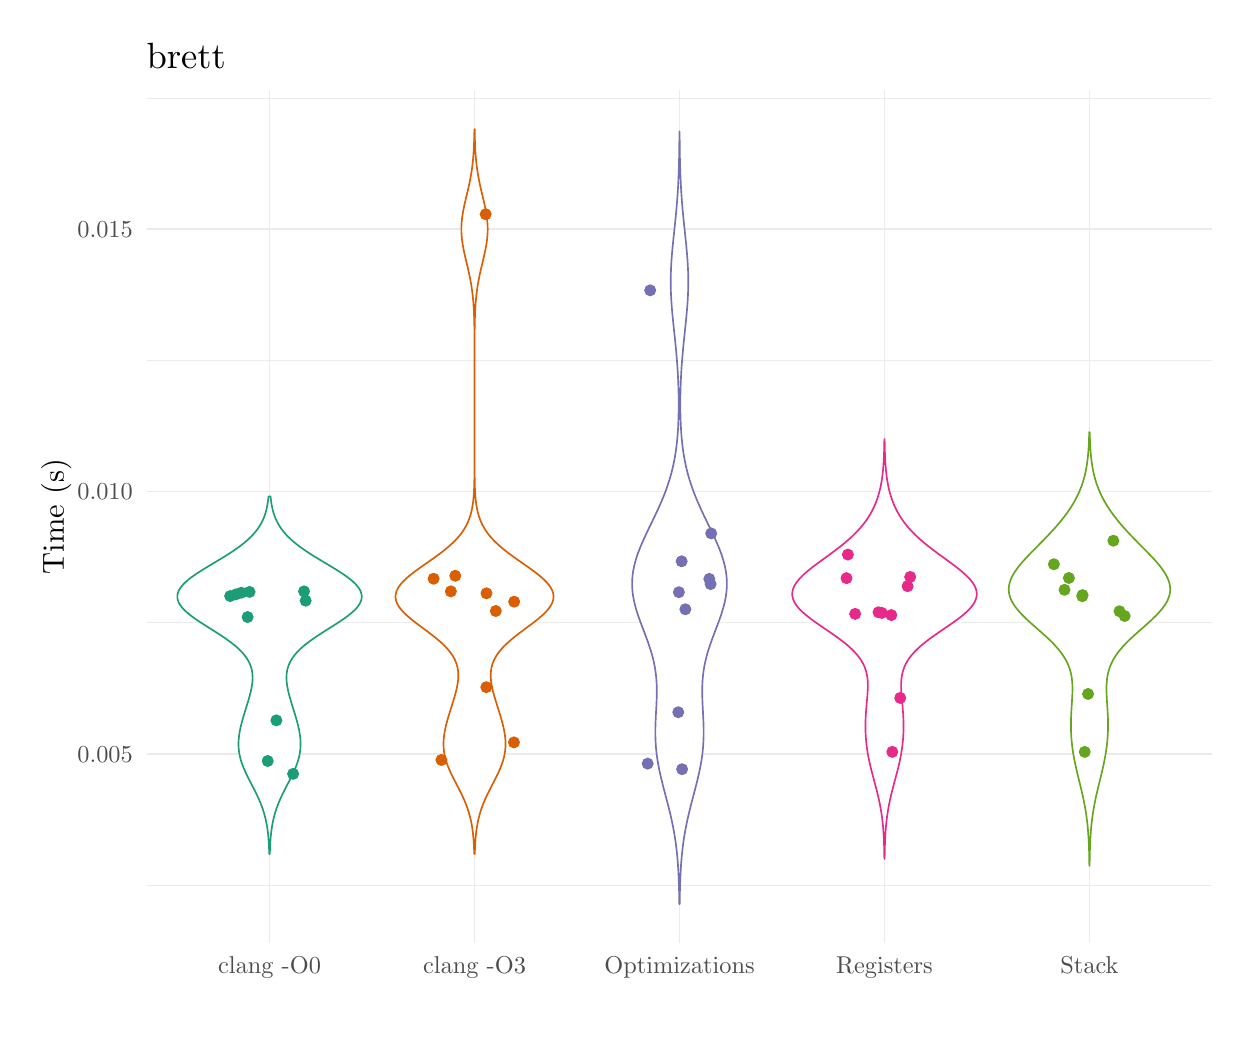
\begin{tikzpicture}[x=1pt,y=1pt]
\definecolor{fillColor}{RGB}{255,255,255}
\path[use as bounding box,fill=fillColor,fill opacity=0.00] (0,0) rectangle (433.62,361.35);
\begin{scope}
\path[clip] ( 42.95, 30.69) rectangle (428.12,338.69);
\definecolor{drawColor}{gray}{0.92}

\path[draw=drawColor,line width= 0.3pt,line join=round] ( 42.95, 51.52) --
	(428.12, 51.52);

\path[draw=drawColor,line width= 0.3pt,line join=round] ( 42.95,146.33) --
	(428.12,146.33);

\path[draw=drawColor,line width= 0.3pt,line join=round] ( 42.95,241.13) --
	(428.12,241.13);

\path[draw=drawColor,line width= 0.3pt,line join=round] ( 42.95,335.94) --
	(428.12,335.94);

\path[draw=drawColor,line width= 0.6pt,line join=round] ( 42.95, 98.92) --
	(428.12, 98.92);

\path[draw=drawColor,line width= 0.6pt,line join=round] ( 42.95,193.73) --
	(428.12,193.73);

\path[draw=drawColor,line width= 0.6pt,line join=round] ( 42.95,288.53) --
	(428.12,288.53);

\path[draw=drawColor,line width= 0.6pt,line join=round] ( 87.40, 30.69) --
	( 87.40,338.69);

\path[draw=drawColor,line width= 0.6pt,line join=round] (161.47, 30.69) --
	(161.47,338.69);

\path[draw=drawColor,line width= 0.6pt,line join=round] (235.54, 30.69) --
	(235.54,338.69);

\path[draw=drawColor,line width= 0.6pt,line join=round] (309.61, 30.69) --
	(309.61,338.69);

\path[draw=drawColor,line width= 0.6pt,line join=round] (383.68, 30.69) --
	(383.68,338.69);
\definecolor{drawColor}{RGB}{27,158,119}
\definecolor{fillColor}{RGB}{255,255,255}

\path[draw=drawColor,line width= 0.6pt,line join=round,line cap=round,fill=fillColor] ( 87.29, 62.77) --
	( 87.28, 63.02) --
	( 87.28, 63.27) --
	( 87.27, 63.52) --
	( 87.26, 63.78) --
	( 87.25, 64.03) --
	( 87.24, 64.28) --
	( 87.23, 64.54) --
	( 87.22, 64.79) --
	( 87.21, 65.04) --
	( 87.20, 65.29) --
	( 87.19, 65.55) --
	( 87.18, 65.80) --
	( 87.16, 66.05) --
	( 87.15, 66.31) --
	( 87.14, 66.56) --
	( 87.12, 66.81) --
	( 87.10, 67.06) --
	( 87.09, 67.32) --
	( 87.07, 67.57) --
	( 87.05, 67.82) --
	( 87.03, 68.08) --
	( 87.01, 68.33) --
	( 86.99, 68.58) --
	( 86.97, 68.83) --
	( 86.95, 69.09) --
	( 86.92, 69.34) --
	( 86.90, 69.59) --
	( 86.87, 69.84) --
	( 86.85, 70.10) --
	( 86.82, 70.35) --
	( 86.79, 70.60) --
	( 86.76, 70.86) --
	( 86.73, 71.11) --
	( 86.69, 71.36) --
	( 86.66, 71.61) --
	( 86.62, 71.87) --
	( 86.59, 72.12) --
	( 86.55, 72.37) --
	( 86.51, 72.63) --
	( 86.47, 72.88) --
	( 86.42, 73.13) --
	( 86.38, 73.38) --
	( 86.33, 73.64) --
	( 86.28, 73.89) --
	( 86.24, 74.14) --
	( 86.18, 74.40) --
	( 86.13, 74.65) --
	( 86.08, 74.90) --
	( 86.02, 75.15) --
	( 85.96, 75.41) --
	( 85.90, 75.66) --
	( 85.84, 75.91) --
	( 85.78, 76.17) --
	( 85.71, 76.42) --
	( 85.65, 76.67) --
	( 85.58, 76.92) --
	( 85.51, 77.18) --
	( 85.43, 77.43) --
	( 85.36, 77.68) --
	( 85.28, 77.94) --
	( 85.20, 78.19) --
	( 85.12, 78.44) --
	( 85.04, 78.69) --
	( 84.96, 78.95) --
	( 84.87, 79.20) --
	( 84.78, 79.45) --
	( 84.69, 79.71) --
	( 84.60, 79.96) --
	( 84.50, 80.21) --
	( 84.41, 80.46) --
	( 84.31, 80.72) --
	( 84.21, 80.97) --
	( 84.11, 81.22) --
	( 84.00, 81.48) --
	( 83.90, 81.73) --
	( 83.79, 81.98) --
	( 83.68, 82.23) --
	( 83.57, 82.49) --
	( 83.46, 82.74) --
	( 83.35, 82.99) --
	( 83.23, 83.25) --
	( 83.11, 83.50) --
	( 83.00, 83.75) --
	( 82.88, 84.00) --
	( 82.76, 84.26) --
	( 82.63, 84.51) --
	( 82.51, 84.76) --
	( 82.39, 85.02) --
	( 82.26, 85.27) --
	( 82.14, 85.52) --
	( 82.01, 85.77) --
	( 81.88, 86.03) --
	( 81.75, 86.28) --
	( 81.62, 86.53) --
	( 81.49, 86.79) --
	( 81.36, 87.04) --
	( 81.23, 87.29) --
	( 81.10, 87.54) --
	( 80.97, 87.80) --
	( 80.84, 88.05) --
	( 80.71, 88.30) --
	( 80.58, 88.55) --
	( 80.45, 88.81) --
	( 80.31, 89.06) --
	( 80.18, 89.31) --
	( 80.05, 89.57) --
	( 79.93, 89.82) --
	( 79.80, 90.07) --
	( 79.67, 90.32) --
	( 79.54, 90.58) --
	( 79.42, 90.83) --
	( 79.29, 91.08) --
	( 79.17, 91.34) --
	( 79.05, 91.59) --
	( 78.93, 91.84) --
	( 78.81, 92.09) --
	( 78.69, 92.35) --
	( 78.58, 92.60) --
	( 78.47, 92.85) --
	( 78.35, 93.11) --
	( 78.25, 93.36) --
	( 78.14, 93.61) --
	( 78.03, 93.86) --
	( 77.93, 94.12) --
	( 77.83, 94.37) --
	( 77.73, 94.62) --
	( 77.64, 94.88) --
	( 77.54, 95.13) --
	( 77.45, 95.38) --
	( 77.37, 95.63) --
	( 77.28, 95.89) --
	( 77.20, 96.14) --
	( 77.12, 96.39) --
	( 77.05, 96.65) --
	( 76.97, 96.90) --
	( 76.90, 97.15) --
	( 76.84, 97.40) --
	( 76.77, 97.66) --
	( 76.71, 97.91) --
	( 76.66, 98.16) --
	( 76.60, 98.42) --
	( 76.55, 98.67) --
	( 76.50, 98.92) --
	( 76.46, 99.17) --
	( 76.42, 99.43) --
	( 76.38, 99.68) --
	( 76.35, 99.93) --
	( 76.32,100.19) --
	( 76.29,100.44) --
	( 76.27,100.69) --
	( 76.25,100.94) --
	( 76.23,101.20) --
	( 76.21,101.45) --
	( 76.20,101.70) --
	( 76.19,101.96) --
	( 76.19,102.21) --
	( 76.19,102.46) --
	( 76.19,102.71) --
	( 76.19,102.97) --
	( 76.20,103.22) --
	( 76.21,103.47) --
	( 76.22,103.73) --
	( 76.24,103.98) --
	( 76.25,104.23) --
	( 76.28,104.48) --
	( 76.30,104.74) --
	( 76.33,104.99) --
	( 76.36,105.24) --
	( 76.39,105.50) --
	( 76.42,105.75) --
	( 76.46,106.00) --
	( 76.50,106.25) --
	( 76.54,106.51) --
	( 76.58,106.76) --
	( 76.62,107.01) --
	( 76.67,107.26) --
	( 76.72,107.52) --
	( 76.77,107.77) --
	( 76.82,108.02) --
	( 76.88,108.28) --
	( 76.93,108.53) --
	( 76.99,108.78) --
	( 77.05,109.03) --
	( 77.11,109.29) --
	( 77.18,109.54) --
	( 77.24,109.79) --
	( 77.30,110.05) --
	( 77.37,110.30) --
	( 77.44,110.55) --
	( 77.51,110.80) --
	( 77.58,111.06) --
	( 77.65,111.31) --
	( 77.72,111.56) --
	( 77.79,111.82) --
	( 77.86,112.07) --
	( 77.94,112.32) --
	( 78.01,112.57) --
	( 78.09,112.83) --
	( 78.16,113.08) --
	( 78.24,113.33) --
	( 78.32,113.59) --
	( 78.39,113.84) --
	( 78.47,114.09) --
	( 78.55,114.34) --
	( 78.63,114.60) --
	( 78.71,114.85) --
	( 78.78,115.10) --
	( 78.86,115.36) --
	( 78.94,115.61) --
	( 79.02,115.86) --
	( 79.10,116.11) --
	( 79.18,116.37) --
	( 79.25,116.62) --
	( 79.33,116.87) --
	( 79.41,117.13) --
	( 79.49,117.38) --
	( 79.56,117.63) --
	( 79.64,117.88) --
	( 79.71,118.14) --
	( 79.79,118.39) --
	( 79.86,118.64) --
	( 79.93,118.90) --
	( 80.00,119.15) --
	( 80.08,119.40) --
	( 80.15,119.65) --
	( 80.21,119.91) --
	( 80.28,120.16) --
	( 80.35,120.41) --
	( 80.41,120.67) --
	( 80.48,120.92) --
	( 80.54,121.17) --
	( 80.60,121.42) --
	( 80.65,121.68) --
	( 80.71,121.93) --
	( 80.77,122.18) --
	( 80.82,122.44) --
	( 80.87,122.69) --
	( 80.91,122.94) --
	( 80.96,123.19) --
	( 81.00,123.45) --
	( 81.04,123.70) --
	( 81.08,123.95) --
	( 81.11,124.21) --
	( 81.15,124.46) --
	( 81.17,124.71) --
	( 81.20,124.96) --
	( 81.22,125.22) --
	( 81.24,125.47) --
	( 81.25,125.72) --
	( 81.26,125.97) --
	( 81.27,126.23) --
	( 81.27,126.48) --
	( 81.27,126.73) --
	( 81.26,126.99) --
	( 81.25,127.24) --
	( 81.24,127.49) --
	( 81.22,127.74) --
	( 81.19,128.00) --
	( 81.16,128.25) --
	( 81.13,128.50) --
	( 81.08,128.76) --
	( 81.04,129.01) --
	( 80.99,129.26) --
	( 80.93,129.51) --
	( 80.86,129.77) --
	( 80.79,130.02) --
	( 80.72,130.27) --
	( 80.63,130.53) --
	( 80.55,130.78) --
	( 80.45,131.03) --
	( 80.35,131.28) --
	( 80.24,131.54) --
	( 80.12,131.79) --
	( 80.00,132.04) --
	( 79.87,132.30) --
	( 79.74,132.55) --
	( 79.59,132.80) --
	( 79.44,133.05) --
	( 79.28,133.31) --
	( 79.11,133.56) --
	( 78.94,133.81) --
	( 78.76,134.07) --
	( 78.57,134.32) --
	( 78.37,134.57) --
	( 78.17,134.82) --
	( 77.96,135.08) --
	( 77.74,135.33) --
	( 77.51,135.58) --
	( 77.28,135.84) --
	( 77.03,136.09) --
	( 76.78,136.34) --
	( 76.53,136.59) --
	( 76.26,136.85) --
	( 75.99,137.10) --
	( 75.71,137.35) --
	( 75.42,137.61) --
	( 75.13,137.86) --
	( 74.83,138.11) --
	( 74.52,138.36) --
	( 74.21,138.62) --
	( 73.88,138.87) --
	( 73.56,139.12) --
	( 73.22,139.38) --
	( 72.88,139.63) --
	( 72.54,139.88) --
	( 72.18,140.13) --
	( 71.83,140.39) --
	( 71.47,140.64) --
	( 71.10,140.89) --
	( 70.73,141.15) --
	( 70.35,141.40) --
	( 69.97,141.65) --
	( 69.59,141.90) --
	( 69.20,142.16) --
	( 68.81,142.41) --
	( 68.42,142.66) --
	( 68.03,142.92) --
	( 67.63,143.17) --
	( 67.23,143.42) --
	( 66.83,143.67) --
	( 66.43,143.93) --
	( 66.03,144.18) --
	( 65.63,144.43) --
	( 65.23,144.68) --
	( 64.82,144.94) --
	( 64.43,145.19) --
	( 64.03,145.44) --
	( 63.63,145.70) --
	( 63.24,145.95) --
	( 62.85,146.20) --
	( 62.46,146.45) --
	( 62.08,146.71) --
	( 61.70,146.96) --
	( 61.32,147.21) --
	( 60.95,147.47) --
	( 60.59,147.72) --
	( 60.23,147.97) --
	( 59.88,148.22) --
	( 59.53,148.48) --
	( 59.19,148.73) --
	( 58.86,148.98) --
	( 58.54,149.24) --
	( 58.23,149.49) --
	( 57.92,149.74) --
	( 57.63,149.99) --
	( 57.34,150.25) --
	( 57.06,150.50) --
	( 56.80,150.75) --
	( 56.54,151.01) --
	( 56.30,151.26) --
	( 56.06,151.51) --
	( 55.84,151.76) --
	( 55.63,152.02) --
	( 55.43,152.27) --
	( 55.25,152.52) --
	( 55.08,152.78) --
	( 54.92,153.03) --
	( 54.77,153.28) --
	( 54.64,153.53) --
	( 54.53,153.79) --
	( 54.42,154.04) --
	( 54.33,154.29) --
	( 54.25,154.55) --
	( 54.19,154.80) --
	( 54.14,155.05) --
	( 54.11,155.30) --
	( 54.09,155.56) --
	( 54.08,155.81) --
	( 54.10,156.06) --
	( 54.12,156.32) --
	( 54.16,156.57) --
	( 54.21,156.82) --
	( 54.28,157.07) --
	( 54.36,157.33) --
	( 54.45,157.58) --
	( 54.57,157.83) --
	( 54.69,158.09) --
	( 54.83,158.34) --
	( 54.98,158.59) --
	( 55.14,158.84) --
	( 55.32,159.10) --
	( 55.51,159.35) --
	( 55.71,159.60) --
	( 55.93,159.86) --
	( 56.16,160.11) --
	( 56.40,160.36) --
	( 56.65,160.61) --
	( 56.91,160.87) --
	( 57.18,161.12) --
	( 57.47,161.37) --
	( 57.76,161.62) --
	( 58.07,161.88) --
	( 58.38,162.13) --
	( 58.71,162.38) --
	( 59.04,162.64) --
	( 59.38,162.89) --
	( 59.73,163.14) --
	( 60.08,163.39) --
	( 60.45,163.65) --
	( 60.82,163.90) --
	( 61.20,164.15) --
	( 61.58,164.41) --
	( 61.97,164.66) --
	( 62.36,164.91) --
	( 62.76,165.16) --
	( 63.16,165.42) --
	( 63.57,165.67) --
	( 63.98,165.92) --
	( 64.39,166.18) --
	( 64.81,166.43) --
	( 65.22,166.68) --
	( 65.64,166.93) --
	( 66.06,167.19) --
	( 66.49,167.44) --
	( 66.91,167.69) --
	( 67.33,167.95) --
	( 67.76,168.20) --
	( 68.18,168.45) --
	( 68.60,168.70) --
	( 69.02,168.96) --
	( 69.44,169.21) --
	( 69.86,169.46) --
	( 70.27,169.72) --
	( 70.68,169.97) --
	( 71.09,170.22) --
	( 71.50,170.47) --
	( 71.90,170.73) --
	( 72.30,170.98) --
	( 72.70,171.23) --
	( 73.09,171.49) --
	( 73.48,171.74) --
	( 73.86,171.99) --
	( 74.24,172.24) --
	( 74.61,172.50) --
	( 74.98,172.75) --
	( 75.34,173.00) --
	( 75.70,173.26) --
	( 76.05,173.51) --
	( 76.40,173.76) --
	( 76.74,174.01) --
	( 77.07,174.27) --
	( 77.40,174.52) --
	( 77.72,174.77) --
	( 78.03,175.03) --
	( 78.35,175.28) --
	( 78.65,175.53) --
	( 78.94,175.78) --
	( 79.23,176.04) --
	( 79.52,176.29) --
	( 79.79,176.54) --
	( 80.06,176.80) --
	( 80.33,177.05) --
	( 80.59,177.30) --
	( 80.84,177.55) --
	( 81.08,177.81) --
	( 81.32,178.06) --
	( 81.55,178.31) --
	( 81.78,178.57) --
	( 82.00,178.82) --
	( 82.21,179.07) --
	( 82.41,179.32) --
	( 82.61,179.58) --
	( 82.81,179.83) --
	( 83.00,180.08) --
	( 83.18,180.33) --
	( 83.36,180.59) --
	( 83.53,180.84) --
	( 83.69,181.09) --
	( 83.85,181.35) --
	( 84.01,181.60) --
	( 84.16,181.85) --
	( 84.30,182.10) --
	( 84.44,182.36) --
	( 84.57,182.61) --
	( 84.70,182.86) --
	( 84.83,183.12) --
	( 84.95,183.37) --
	( 85.06,183.62) --
	( 85.17,183.87) --
	( 85.28,184.13) --
	( 85.38,184.38) --
	( 85.48,184.63) --
	( 85.57,184.89) --
	( 85.66,185.14) --
	( 85.75,185.39) --
	( 85.83,185.64) --
	( 85.91,185.90) --
	( 85.99,186.15) --
	( 86.06,186.40) --
	( 86.13,186.66) --
	( 86.20,186.91) --
	( 86.26,187.16) --
	( 86.32,187.41) --
	( 86.38,187.67) --
	( 86.43,187.92) --
	( 86.48,188.17) --
	( 86.53,188.43) --
	( 86.58,188.68) --
	( 86.63,188.93) --
	( 86.67,189.18) --
	( 86.71,189.44) --
	( 86.75,189.69) --
	( 86.79,189.94) --
	( 86.82,190.20) --
	( 86.86,190.45) --
	( 86.89,190.70) --
	( 86.92,190.95) --
	( 86.95,191.21) --
	( 86.97,191.46) --
	( 87.00,191.71) --
	( 87.02,191.97) --
	( 87.77,191.97) --
	( 87.79,191.71) --
	( 87.82,191.46) --
	( 87.85,191.21) --
	( 87.87,190.95) --
	( 87.90,190.70) --
	( 87.94,190.45) --
	( 87.97,190.20) --
	( 88.00,189.94) --
	( 88.04,189.69) --
	( 88.08,189.44) --
	( 88.12,189.18) --
	( 88.16,188.93) --
	( 88.21,188.68) --
	( 88.26,188.43) --
	( 88.31,188.17) --
	( 88.36,187.92) --
	( 88.42,187.67) --
	( 88.47,187.41) --
	( 88.53,187.16) --
	( 88.60,186.91) --
	( 88.66,186.66) --
	( 88.73,186.40) --
	( 88.81,186.15) --
	( 88.88,185.90) --
	( 88.96,185.64) --
	( 89.04,185.39) --
	( 89.13,185.14) --
	( 89.22,184.89) --
	( 89.31,184.63) --
	( 89.41,184.38) --
	( 89.51,184.13) --
	( 89.62,183.87) --
	( 89.73,183.62) --
	( 89.85,183.37) --
	( 89.97,183.12) --
	( 90.09,182.86) --
	( 90.22,182.61) --
	( 90.35,182.36) --
	( 90.49,182.10) --
	( 90.64,181.85) --
	( 90.79,181.60) --
	( 90.94,181.35) --
	( 91.10,181.09) --
	( 91.27,180.84) --
	( 91.43,180.59) --
	( 91.61,180.33) --
	( 91.79,180.08) --
	( 91.98,179.83) --
	( 92.18,179.58) --
	( 92.38,179.32) --
	( 92.59,179.07) --
	( 92.80,178.82) --
	( 93.02,178.57) --
	( 93.24,178.31) --
	( 93.47,178.06) --
	( 93.71,177.81) --
	( 93.96,177.55) --
	( 94.21,177.30) --
	( 94.46,177.05) --
	( 94.73,176.80) --
	( 95.00,176.54) --
	( 95.28,176.29) --
	( 95.56,176.04) --
	( 95.85,175.78) --
	( 96.15,175.53) --
	( 96.45,175.28) --
	( 96.76,175.03) --
	( 97.07,174.77) --
	( 97.39,174.52) --
	( 97.72,174.27) --
	( 98.06,174.01) --
	( 98.40,173.76) --
	( 98.74,173.51) --
	( 99.09,173.26) --
	( 99.45,173.00) --
	( 99.81,172.75) --
	(100.18,172.50) --
	(100.55,172.24) --
	(100.93,171.99) --
	(101.31,171.74) --
	(101.70,171.49) --
	(102.09,171.23) --
	(102.49,170.98) --
	(102.89,170.73) --
	(103.29,170.47) --
	(103.70,170.22) --
	(104.11,169.97) --
	(104.52,169.72) --
	(104.94,169.46) --
	(105.35,169.21) --
	(105.77,168.96) --
	(106.19,168.70) --
	(106.61,168.45) --
	(107.04,168.20) --
	(107.46,167.95) --
	(107.88,167.69) --
	(108.31,167.44) --
	(108.73,167.19) --
	(109.15,166.93) --
	(109.57,166.68) --
	(109.99,166.43) --
	(110.40,166.18) --
	(110.81,165.92) --
	(111.22,165.67) --
	(111.63,165.42) --
	(112.03,165.16) --
	(112.43,164.91) --
	(112.83,164.66) --
	(113.21,164.41) --
	(113.60,164.15) --
	(113.97,163.90) --
	(114.34,163.65) --
	(114.71,163.39) --
	(115.06,163.14) --
	(115.41,162.89) --
	(115.75,162.64) --
	(116.09,162.38) --
	(116.41,162.13) --
	(116.72,161.88) --
	(117.03,161.62) --
	(117.32,161.37) --
	(117.61,161.12) --
	(117.88,160.87) --
	(118.14,160.61) --
	(118.40,160.36) --
	(118.63,160.11) --
	(118.87,159.86) --
	(119.08,159.60) --
	(119.29,159.35) --
	(119.47,159.10) --
	(119.65,158.84) --
	(119.82,158.59) --
	(119.97,158.34) --
	(120.11,158.09) --
	(120.23,157.83) --
	(120.34,157.58) --
	(120.43,157.33) --
	(120.52,157.07) --
	(120.58,156.82) --
	(120.63,156.57) --
	(120.68,156.32) --
	(120.70,156.06) --
	(120.71,155.81) --
	(120.70,155.56) --
	(120.68,155.30) --
	(120.65,155.05) --
	(120.60,154.80) --
	(120.54,154.55) --
	(120.46,154.29) --
	(120.37,154.04) --
	(120.27,153.79) --
	(120.15,153.53) --
	(120.02,153.28) --
	(119.87,153.03) --
	(119.72,152.78) --
	(119.54,152.52) --
	(119.36,152.27) --
	(119.16,152.02) --
	(118.95,151.76) --
	(118.73,151.51) --
	(118.50,151.26) --
	(118.25,151.01) --
	(118.00,150.75) --
	(117.73,150.50) --
	(117.45,150.25) --
	(117.17,149.99) --
	(116.87,149.74) --
	(116.57,149.49) --
	(116.25,149.24) --
	(115.93,148.98) --
	(115.60,148.73) --
	(115.26,148.48) --
	(114.92,148.22) --
	(114.56,147.97) --
	(114.20,147.72) --
	(113.84,147.47) --
	(113.47,147.21) --
	(113.10,146.96) --
	(112.72,146.71) --
	(112.33,146.45) --
	(111.95,146.20) --
	(111.55,145.95) --
	(111.16,145.70) --
	(110.76,145.44) --
	(110.37,145.19) --
	(109.97,144.94) --
	(109.57,144.68) --
	(109.17,144.43) --
	(108.76,144.18) --
	(108.36,143.93) --
	(107.96,143.67) --
	(107.56,143.42) --
	(107.16,143.17) --
	(106.77,142.92) --
	(106.37,142.66) --
	(105.98,142.41) --
	(105.59,142.16) --
	(105.20,141.90) --
	(104.82,141.65) --
	(104.44,141.40) --
	(104.06,141.15) --
	(103.69,140.89) --
	(103.33,140.64) --
	(102.96,140.39) --
	(102.61,140.13) --
	(102.26,139.88) --
	(101.91,139.63) --
	(101.57,139.38) --
	(101.24,139.12) --
	(100.91,138.87) --
	(100.59,138.62) --
	(100.27,138.36) --
	( 99.97,138.11) --
	( 99.66,137.86) --
	( 99.37,137.61) --
	( 99.08,137.35) --
	( 98.80,137.10) --
	( 98.53,136.85) --
	( 98.27,136.59) --
	( 98.01,136.34) --
	( 97.76,136.09) --
	( 97.52,135.84) --
	( 97.28,135.58) --
	( 97.05,135.33) --
	( 96.83,135.08) --
	( 96.62,134.82) --
	( 96.42,134.57) --
	( 96.22,134.32) --
	( 96.03,134.07) --
	( 95.85,133.81) --
	( 95.68,133.56) --
	( 95.51,133.31) --
	( 95.35,133.05) --
	( 95.20,132.80) --
	( 95.06,132.55) --
	( 94.92,132.30) --
	( 94.79,132.04) --
	( 94.67,131.79) --
	( 94.55,131.54) --
	( 94.44,131.28) --
	( 94.34,131.03) --
	( 94.25,130.78) --
	( 94.16,130.53) --
	( 94.07,130.27) --
	( 94.00,130.02) --
	( 93.93,129.77) --
	( 93.87,129.51) --
	( 93.81,129.26) --
	( 93.76,129.01) --
	( 93.71,128.76) --
	( 93.67,128.50) --
	( 93.63,128.25) --
	( 93.60,128.00) --
	( 93.58,127.74) --
	( 93.56,127.49) --
	( 93.54,127.24) --
	( 93.53,126.99) --
	( 93.52,126.73) --
	( 93.52,126.48) --
	( 93.52,126.23) --
	( 93.53,125.97) --
	( 93.54,125.72) --
	( 93.55,125.47) --
	( 93.57,125.22) --
	( 93.59,124.96) --
	( 93.62,124.71) --
	( 93.65,124.46) --
	( 93.68,124.21) --
	( 93.71,123.95) --
	( 93.75,123.70) --
	( 93.79,123.45) --
	( 93.83,123.19) --
	( 93.88,122.94) --
	( 93.92,122.69) --
	( 93.98,122.44) --
	( 94.03,122.18) --
	( 94.08,121.93) --
	( 94.14,121.68) --
	( 94.20,121.42) --
	( 94.26,121.17) --
	( 94.32,120.92) --
	( 94.38,120.67) --
	( 94.45,120.41) --
	( 94.51,120.16) --
	( 94.58,119.91) --
	( 94.65,119.65) --
	( 94.72,119.40) --
	( 94.79,119.15) --
	( 94.86,118.90) --
	( 94.93,118.64) --
	( 95.01,118.39) --
	( 95.08,118.14) --
	( 95.16,117.88) --
	( 95.23,117.63) --
	( 95.31,117.38) --
	( 95.38,117.13) --
	( 95.46,116.87) --
	( 95.54,116.62) --
	( 95.62,116.37) --
	( 95.69,116.11) --
	( 95.77,115.86) --
	( 95.85,115.61) --
	( 95.93,115.36) --
	( 96.01,115.10) --
	( 96.09,114.85) --
	( 96.16,114.60) --
	( 96.24,114.34) --
	( 96.32,114.09) --
	( 96.40,113.84) --
	( 96.48,113.59) --
	( 96.55,113.33) --
	( 96.63,113.08) --
	( 96.70,112.83) --
	( 96.78,112.57) --
	( 96.85,112.32) --
	( 96.93,112.07) --
	( 97.00,111.82) --
	( 97.07,111.56) --
	( 97.15,111.31) --
	( 97.22,111.06) --
	( 97.29,110.80) --
	( 97.35,110.55) --
	( 97.42,110.30) --
	( 97.49,110.05) --
	( 97.55,109.79) --
	( 97.62,109.54) --
	( 97.68,109.29) --
	( 97.74,109.03) --
	( 97.80,108.78) --
	( 97.86,108.53) --
	( 97.91,108.28) --
	( 97.97,108.02) --
	( 98.02,107.77) --
	( 98.07,107.52) --
	( 98.12,107.26) --
	( 98.17,107.01) --
	( 98.21,106.76) --
	( 98.26,106.51) --
	( 98.30,106.25) --
	( 98.34,106.00) --
	( 98.37,105.75) --
	( 98.41,105.50) --
	( 98.44,105.24) --
	( 98.47,104.99) --
	( 98.49,104.74) --
	( 98.52,104.48) --
	( 98.54,104.23) --
	( 98.56,103.98) --
	( 98.57,103.73) --
	( 98.58,103.47) --
	( 98.59,103.22) --
	( 98.60,102.97) --
	( 98.61,102.71) --
	( 98.61,102.46) --
	( 98.60,102.21) --
	( 98.60,101.96) --
	( 98.59,101.70) --
	( 98.58,101.45) --
	( 98.56,101.20) --
	( 98.55,100.94) --
	( 98.53,100.69) --
	( 98.50,100.44) --
	( 98.47,100.19) --
	( 98.44, 99.93) --
	( 98.41, 99.68) --
	( 98.37, 99.43) --
	( 98.33, 99.17) --
	( 98.29, 98.92) --
	( 98.24, 98.67) --
	( 98.19, 98.42) --
	( 98.14, 98.16) --
	( 98.08, 97.91) --
	( 98.02, 97.66) --
	( 97.95, 97.40) --
	( 97.89, 97.15) --
	( 97.82, 96.90) --
	( 97.75, 96.65) --
	( 97.67, 96.39) --
	( 97.59, 96.14) --
	( 97.51, 95.89) --
	( 97.43, 95.63) --
	( 97.34, 95.38) --
	( 97.25, 95.13) --
	( 97.16, 94.88) --
	( 97.06, 94.62) --
	( 96.96, 94.37) --
	( 96.86, 94.12) --
	( 96.76, 93.86) --
	( 96.65, 93.61) --
	( 96.55, 93.36) --
	( 96.44, 93.11) --
	( 96.33, 92.85) --
	( 96.21, 92.60) --
	( 96.10, 92.35) --
	( 95.98, 92.09) --
	( 95.86, 91.84) --
	( 95.74, 91.59) --
	( 95.62, 91.34) --
	( 95.50, 91.08) --
	( 95.37, 90.83) --
	( 95.25, 90.58) --
	( 95.12, 90.32) --
	( 94.99, 90.07) --
	( 94.87, 89.82) --
	( 94.74, 89.57) --
	( 94.61, 89.31) --
	( 94.48, 89.06) --
	( 94.35, 88.81) --
	( 94.22, 88.55) --
	( 94.09, 88.30) --
	( 93.95, 88.05) --
	( 93.82, 87.80) --
	( 93.69, 87.54) --
	( 93.56, 87.29) --
	( 93.43, 87.04) --
	( 93.30, 86.79) --
	( 93.17, 86.53) --
	( 93.04, 86.28) --
	( 92.91, 86.03) --
	( 92.78, 85.77) --
	( 92.66, 85.52) --
	( 92.53, 85.27) --
	( 92.41, 85.02) --
	( 92.28, 84.76) --
	( 92.16, 84.51) --
	( 92.04, 84.26) --
	( 91.92, 84.00) --
	( 91.80, 83.75) --
	( 91.68, 83.50) --
	( 91.56, 83.25) --
	( 91.45, 82.99) --
	( 91.33, 82.74) --
	( 91.22, 82.49) --
	( 91.11, 82.23) --
	( 91.00, 81.98) --
	( 90.89, 81.73) --
	( 90.79, 81.48) --
	( 90.68, 81.22) --
	( 90.58, 80.97) --
	( 90.48, 80.72) --
	( 90.39, 80.46) --
	( 90.29, 80.21) --
	( 90.19, 79.96) --
	( 90.10, 79.71) --
	( 90.01, 79.45) --
	( 89.92, 79.20) --
	( 89.84, 78.95) --
	( 89.75, 78.69) --
	( 89.67, 78.44) --
	( 89.59, 78.19) --
	( 89.51, 77.94) --
	( 89.43, 77.68) --
	( 89.36, 77.43) --
	( 89.29, 77.18) --
	( 89.22, 76.92) --
	( 89.15, 76.67) --
	( 89.08, 76.42) --
	( 89.01, 76.17) --
	( 88.95, 75.91) --
	( 88.89, 75.66) --
	( 88.83, 75.41) --
	( 88.77, 75.15) --
	( 88.72, 74.90) --
	( 88.66, 74.65) --
	( 88.61, 74.40) --
	( 88.56, 74.14) --
	( 88.51, 73.89) --
	( 88.46, 73.64) --
	( 88.41, 73.38) --
	( 88.37, 73.13) --
	( 88.33, 72.88) --
	( 88.29, 72.63) --
	( 88.24, 72.37) --
	( 88.21, 72.12) --
	( 88.17, 71.87) --
	( 88.13, 71.61) --
	( 88.10, 71.36) --
	( 88.07, 71.11) --
	( 88.03, 70.86) --
	( 88.00, 70.60) --
	( 87.97, 70.35) --
	( 87.95, 70.10) --
	( 87.92, 69.84) --
	( 87.89, 69.59) --
	( 87.87, 69.34) --
	( 87.84, 69.09) --
	( 87.82, 68.83) --
	( 87.80, 68.58) --
	( 87.78, 68.33) --
	( 87.76, 68.08) --
	( 87.74, 67.82) --
	( 87.72, 67.57) --
	( 87.70, 67.32) --
	( 87.69, 67.06) --
	( 87.67, 66.81) --
	( 87.66, 66.56) --
	( 87.64, 66.31) --
	( 87.63, 66.05) --
	( 87.62, 65.80) --
	( 87.60, 65.55) --
	( 87.59, 65.29) --
	( 87.58, 65.04) --
	( 87.57, 64.79) --
	( 87.56, 64.54) --
	( 87.55, 64.28) --
	( 87.54, 64.03) --
	( 87.53, 63.78) --
	( 87.52, 63.52) --
	( 87.52, 63.27) --
	( 87.51, 63.02) --
	( 87.50, 62.77) --
	( 87.29, 62.77) --
	cycle;
\definecolor{drawColor}{RGB}{217,95,2}

\path[draw=drawColor,line width= 0.6pt,line join=round,line cap=round,fill=fillColor] (161.36, 62.77) --
	(161.34, 63.28) --
	(161.33, 63.79) --
	(161.31, 64.30) --
	(161.29, 64.82) --
	(161.27, 65.33) --
	(161.24, 65.84) --
	(161.22, 66.35) --
	(161.19, 66.87) --
	(161.15, 67.38) --
	(161.12, 67.89) --
	(161.08, 68.40) --
	(161.03, 68.92) --
	(160.98, 69.43) --
	(160.93, 69.94) --
	(160.88, 70.45) --
	(160.81, 70.97) --
	(160.75, 71.48) --
	(160.67, 71.99) --
	(160.60, 72.50) --
	(160.51, 73.02) --
	(160.42, 73.53) --
	(160.32, 74.04) --
	(160.22, 74.55) --
	(160.11, 75.07) --
	(159.99, 75.58) --
	(159.87, 76.09) --
	(159.73, 76.61) --
	(159.59, 77.12) --
	(159.44, 77.63) --
	(159.29, 78.14) --
	(159.12, 78.66) --
	(158.95, 79.17) --
	(158.77, 79.68) --
	(158.58, 80.19) --
	(158.38, 80.71) --
	(158.18, 81.22) --
	(157.97, 81.73) --
	(157.75, 82.24) --
	(157.52, 82.76) --
	(157.29, 83.27) --
	(157.05, 83.78) --
	(156.81, 84.29) --
	(156.56, 84.81) --
	(156.31, 85.32) --
	(156.05, 85.83) --
	(155.79, 86.34) --
	(155.53, 86.86) --
	(155.26, 87.37) --
	(155.00, 87.88) --
	(154.73, 88.39) --
	(154.46, 88.91) --
	(154.20, 89.42) --
	(153.94, 89.93) --
	(153.68, 90.44) --
	(153.43, 90.96) --
	(153.18, 91.47) --
	(152.94, 91.98) --
	(152.70, 92.49) --
	(152.47, 93.01) --
	(152.25, 93.52) --
	(152.04, 94.03) --
	(151.83, 94.55) --
	(151.64, 95.06) --
	(151.46, 95.57) --
	(151.29, 96.08) --
	(151.13, 96.60) --
	(150.99, 97.11) --
	(150.86, 97.62) --
	(150.74, 98.13) --
	(150.63, 98.65) --
	(150.54, 99.16) --
	(150.46, 99.67) --
	(150.39,100.18) --
	(150.34,100.70) --
	(150.30,101.21) --
	(150.28,101.72) --
	(150.26,102.23) --
	(150.26,102.75) --
	(150.27,103.26) --
	(150.30,103.77) --
	(150.33,104.28) --
	(150.38,104.80) --
	(150.44,105.31) --
	(150.50,105.82) --
	(150.58,106.33) --
	(150.67,106.85) --
	(150.76,107.36) --
	(150.87,107.87) --
	(150.98,108.38) --
	(151.09,108.90) --
	(151.22,109.41) --
	(151.35,109.92) --
	(151.48,110.44) --
	(151.62,110.95) --
	(151.77,111.46) --
	(151.91,111.97) --
	(152.07,112.49) --
	(152.22,113.00) --
	(152.38,113.51) --
	(152.53,114.02) --
	(152.69,114.54) --
	(152.85,115.05) --
	(153.02,115.56) --
	(153.18,116.07) --
	(153.34,116.59) --
	(153.50,117.10) --
	(153.66,117.61) --
	(153.81,118.12) --
	(153.97,118.64) --
	(154.12,119.15) --
	(154.27,119.66) --
	(154.41,120.17) --
	(154.55,120.69) --
	(154.69,121.20) --
	(154.82,121.71) --
	(154.94,122.22) --
	(155.06,122.74) --
	(155.16,123.25) --
	(155.26,123.76) --
	(155.35,124.27) --
	(155.42,124.79) --
	(155.49,125.30) --
	(155.54,125.81) --
	(155.58,126.33) --
	(155.60,126.84) --
	(155.61,127.35) --
	(155.59,127.86) --
	(155.57,128.38) --
	(155.52,128.89) --
	(155.45,129.40) --
	(155.36,129.91) --
	(155.25,130.43) --
	(155.12,130.94) --
	(154.96,131.45) --
	(154.78,131.96) --
	(154.57,132.48) --
	(154.34,132.99) --
	(154.08,133.50) --
	(153.79,134.01) --
	(153.48,134.53) --
	(153.13,135.04) --
	(152.76,135.55) --
	(152.37,136.06) --
	(151.95,136.58) --
	(151.49,137.09) --
	(151.01,137.60) --
	(150.51,138.11) --
	(149.98,138.63) --
	(149.43,139.14) --
	(148.85,139.65) --
	(148.26,140.16) --
	(147.64,140.68) --
	(147.01,141.19) --
	(146.36,141.70) --
	(145.70,142.21) --
	(145.03,142.73) --
	(144.35,143.24) --
	(143.66,143.75) --
	(142.97,144.27) --
	(142.28,144.78) --
	(141.59,145.29) --
	(140.91,145.80) --
	(140.23,146.32) --
	(139.57,146.83) --
	(138.93,147.34) --
	(138.30,147.85) --
	(137.69,148.37) --
	(137.11,148.88) --
	(136.55,149.39) --
	(136.02,149.90) --
	(135.54,150.42) --
	(135.08,150.93) --
	(134.66,151.44) --
	(134.28,151.95) --
	(133.95,152.47) --
	(133.66,152.98) --
	(133.41,153.49) --
	(133.22,154.00) --
	(133.08,154.52) --
	(132.98,155.03) --
	(132.92,155.54) --
	(132.93,156.05) --
	(132.99,156.57) --
	(133.09,157.08) --
	(133.24,157.59) --
	(133.45,158.10) --
	(133.71,158.62) --
	(134.00,159.13) --
	(134.35,159.64) --
	(134.74,160.16) --
	(135.17,160.67) --
	(135.64,161.18) --
	(136.15,161.69) --
	(136.69,162.21) --
	(137.26,162.72) --
	(137.86,163.23) --
	(138.49,163.74) --
	(139.15,164.26) --
	(139.82,164.77) --
	(140.51,165.28) --
	(141.22,165.79) --
	(141.93,166.31) --
	(142.66,166.82) --
	(143.39,167.33) --
	(144.12,167.84) --
	(144.86,168.36) --
	(145.59,168.87) --
	(146.31,169.38) --
	(147.03,169.89) --
	(147.74,170.41) --
	(148.44,170.92) --
	(149.13,171.43) --
	(149.80,171.94) --
	(150.45,172.46) --
	(151.09,172.97) --
	(151.70,173.48) --
	(152.30,173.99) --
	(152.88,174.51) --
	(153.43,175.02) --
	(153.96,175.53) --
	(154.47,176.05) --
	(154.96,176.56) --
	(155.42,177.07) --
	(155.86,177.58) --
	(156.28,178.10) --
	(156.68,178.61) --
	(157.05,179.12) --
	(157.40,179.63) --
	(157.73,180.15) --
	(158.04,180.66) --
	(158.33,181.17) --
	(158.60,181.68) --
	(158.85,182.20) --
	(159.09,182.71) --
	(159.30,183.22) --
	(159.50,183.73) --
	(159.69,184.25) --
	(159.86,184.76) --
	(160.01,185.27) --
	(160.16,185.78) --
	(160.29,186.30) --
	(160.41,186.81) --
	(160.52,187.32) --
	(160.62,187.83) --
	(160.71,188.35) --
	(160.79,188.86) --
	(160.87,189.37) --
	(160.94,189.88) --
	(161.00,190.40) --
	(161.05,190.91) --
	(161.10,191.42) --
	(161.14,191.93) --
	(161.18,192.45) --
	(161.22,192.96) --
	(161.25,193.47) --
	(161.27,193.99) --
	(161.30,194.50) --
	(161.32,195.01) --
	(161.34,195.52) --
	(161.36,196.04) --
	(161.37,196.55) --
	(161.38,197.06) --
	(161.39,197.57) --
	(161.40,198.09) --
	(161.41,198.60) --
	(161.42,199.11) --
	(161.43,199.62) --
	(161.43,200.14) --
	(161.44,200.65) --
	(161.44,201.16) --
	(161.45,201.67) --
	(161.45,202.19) --
	(161.45,202.70) --
	(161.45,203.21) --
	(161.46,203.72) --
	(161.46,204.24) --
	(161.46,204.75) --
	(161.46,205.26) --
	(161.46,205.77) --
	(161.46,206.29) --
	(161.46,206.80) --
	(161.46,207.31) --
	(161.46,207.82) --
	(161.46,208.34) --
	(161.46,208.85) --
	(161.47,209.36) --
	(161.47,209.88) --
	(161.47,210.39) --
	(161.47,210.90) --
	(161.47,211.41) --
	(161.47,211.93) --
	(161.47,212.44) --
	(161.47,212.95) --
	(161.47,213.46) --
	(161.47,213.98) --
	(161.47,214.49) --
	(161.47,215.00) --
	(161.47,215.51) --
	(161.47,216.03) --
	(161.47,216.54) --
	(161.47,217.05) --
	(161.47,217.56) --
	(161.47,218.08) --
	(161.47,218.59) --
	(161.47,219.10) --
	(161.47,219.61) --
	(161.47,220.13) --
	(161.47,220.64) --
	(161.47,221.15) --
	(161.47,221.66) --
	(161.47,222.18) --
	(161.47,222.69) --
	(161.47,223.20) --
	(161.47,223.71) --
	(161.47,224.23) --
	(161.47,224.74) --
	(161.47,225.25) --
	(161.47,225.77) --
	(161.47,226.28) --
	(161.47,226.79) --
	(161.47,227.30) --
	(161.47,227.82) --
	(161.47,228.33) --
	(161.47,228.84) --
	(161.47,229.35) --
	(161.47,229.87) --
	(161.47,230.38) --
	(161.47,230.89) --
	(161.47,231.40) --
	(161.47,231.92) --
	(161.47,232.43) --
	(161.47,232.94) --
	(161.47,233.45) --
	(161.47,233.97) --
	(161.47,234.48) --
	(161.47,234.99) --
	(161.47,235.50) --
	(161.47,236.02) --
	(161.47,236.53) --
	(161.47,237.04) --
	(161.47,237.55) --
	(161.47,238.07) --
	(161.47,238.58) --
	(161.47,239.09) --
	(161.47,239.60) --
	(161.47,240.12) --
	(161.46,240.63) --
	(161.46,241.14) --
	(161.46,241.65) --
	(161.46,242.17) --
	(161.46,242.68) --
	(161.46,243.19) --
	(161.46,243.71) --
	(161.46,244.22) --
	(161.46,244.73) --
	(161.46,245.24) --
	(161.46,245.76) --
	(161.46,246.27) --
	(161.45,246.78) --
	(161.45,247.29) --
	(161.45,247.81) --
	(161.45,248.32) --
	(161.45,248.83) --
	(161.44,249.34) --
	(161.44,249.86) --
	(161.43,250.37) --
	(161.43,250.88) --
	(161.42,251.39) --
	(161.42,251.91) --
	(161.41,252.42) --
	(161.41,252.93) --
	(161.40,253.44) --
	(161.39,253.96) --
	(161.38,254.47) --
	(161.37,254.98) --
	(161.35,255.49) --
	(161.34,256.01) --
	(161.33,256.52) --
	(161.31,257.03) --
	(161.29,257.54) --
	(161.27,258.06) --
	(161.25,258.57) --
	(161.22,259.08) --
	(161.20,259.60) --
	(161.17,260.11) --
	(161.14,260.62) --
	(161.10,261.13) --
	(161.07,261.65) --
	(161.03,262.16) --
	(160.99,262.67) --
	(160.94,263.18) --
	(160.89,263.70) --
	(160.84,264.21) --
	(160.79,264.72) --
	(160.73,265.23) --
	(160.67,265.75) --
	(160.60,266.26) --
	(160.53,266.77) --
	(160.46,267.28) --
	(160.38,267.80) --
	(160.30,268.31) --
	(160.21,268.82) --
	(160.12,269.33) --
	(160.03,269.85) --
	(159.94,270.36) --
	(159.84,270.87) --
	(159.73,271.38) --
	(159.63,271.90) --
	(159.52,272.41) --
	(159.41,272.92) --
	(159.29,273.43) --
	(159.18,273.95) --
	(159.06,274.46) --
	(158.94,274.97) --
	(158.82,275.49) --
	(158.70,276.00) --
	(158.57,276.51) --
	(158.45,277.02) --
	(158.33,277.54) --
	(158.21,278.05) --
	(158.09,278.56) --
	(157.97,279.07) --
	(157.86,279.59) --
	(157.74,280.10) --
	(157.64,280.61) --
	(157.53,281.12) --
	(157.43,281.64) --
	(157.34,282.15) --
	(157.25,282.66) --
	(157.16,283.17) --
	(157.08,283.69) --
	(157.01,284.20) --
	(156.95,284.71) --
	(156.89,285.22) --
	(156.84,285.74) --
	(156.80,286.25) --
	(156.77,286.76) --
	(156.74,287.27) --
	(156.72,287.79) --
	(156.72,288.30) --
	(156.72,288.81) --
	(156.72,289.32) --
	(156.74,289.84) --
	(156.77,290.35) --
	(156.80,290.86) --
	(156.84,291.37) --
	(156.90,291.89) --
	(156.95,292.40) --
	(157.02,292.91) --
	(157.09,293.43) --
	(157.17,293.94) --
	(157.25,294.45) --
	(157.34,294.96) --
	(157.44,295.48) --
	(157.54,295.99) --
	(157.64,296.50) --
	(157.75,297.01) --
	(157.87,297.53) --
	(157.98,298.04) --
	(158.10,298.55) --
	(158.22,299.06) --
	(158.34,299.58) --
	(158.46,300.09) --
	(158.58,300.60) --
	(158.71,301.11) --
	(158.83,301.63) --
	(158.95,302.14) --
	(159.07,302.65) --
	(159.19,303.16) --
	(159.30,303.68) --
	(159.42,304.19) --
	(159.53,304.70) --
	(159.64,305.21) --
	(159.74,305.73) --
	(159.85,306.24) --
	(159.94,306.75) --
	(160.04,307.26) --
	(160.13,307.78) --
	(160.22,308.29) --
	(160.31,308.80) --
	(160.39,309.32) --
	(160.46,309.83) --
	(160.54,310.34) --
	(160.61,310.85) --
	(160.67,311.37) --
	(160.73,311.88) --
	(160.79,312.39) --
	(160.85,312.90) --
	(160.90,313.42) --
	(160.95,313.93) --
	(160.99,314.44) --
	(161.03,314.95) --
	(161.07,315.47) --
	(161.11,315.98) --
	(161.14,316.49) --
	(161.17,317.00) --
	(161.20,317.52) --
	(161.23,318.03) --
	(161.25,318.54) --
	(161.27,319.05) --
	(161.29,319.57) --
	(161.31,320.08) --
	(161.33,320.59) --
	(161.34,321.10) --
	(161.36,321.62) --
	(161.37,322.13) --
	(161.38,322.64) --
	(161.39,323.15) --
	(161.40,323.67) --
	(161.41,324.18) --
	(161.41,324.69) --
	(161.52,324.69) --
	(161.53,324.18) --
	(161.54,323.67) --
	(161.54,323.15) --
	(161.55,322.64) --
	(161.57,322.13) --
	(161.58,321.62) --
	(161.59,321.10) --
	(161.61,320.59) --
	(161.62,320.08) --
	(161.64,319.57) --
	(161.66,319.05) --
	(161.68,318.54) --
	(161.71,318.03) --
	(161.73,317.52) --
	(161.76,317.00) --
	(161.79,316.49) --
	(161.83,315.98) --
	(161.86,315.47) --
	(161.90,314.95) --
	(161.94,314.44) --
	(161.99,313.93) --
	(162.03,313.42) --
	(162.09,312.90) --
	(162.14,312.39) --
	(162.20,311.88) --
	(162.26,311.37) --
	(162.33,310.85) --
	(162.40,310.34) --
	(162.47,309.83) --
	(162.55,309.32) --
	(162.63,308.80) --
	(162.71,308.29) --
	(162.80,307.78) --
	(162.89,307.26) --
	(162.99,306.75) --
	(163.09,306.24) --
	(163.19,305.73) --
	(163.30,305.21) --
	(163.40,304.70) --
	(163.52,304.19) --
	(163.63,303.68) --
	(163.75,303.16) --
	(163.86,302.65) --
	(163.98,302.14) --
	(164.11,301.63) --
	(164.23,301.11) --
	(164.35,300.60) --
	(164.47,300.09) --
	(164.59,299.58) --
	(164.71,299.06) --
	(164.83,298.55) --
	(164.95,298.04) --
	(165.07,297.53) --
	(165.18,297.01) --
	(165.29,296.50) --
	(165.39,295.99) --
	(165.49,295.48) --
	(165.59,294.96) --
	(165.68,294.45) --
	(165.76,293.94) --
	(165.84,293.43) --
	(165.92,292.91) --
	(165.98,292.40) --
	(166.04,291.89) --
	(166.09,291.37) --
	(166.13,290.86) --
	(166.16,290.35) --
	(166.19,289.84) --
	(166.21,289.32) --
	(166.22,288.81) --
	(166.22,288.30) --
	(166.21,287.79) --
	(166.19,287.27) --
	(166.17,286.76) --
	(166.13,286.25) --
	(166.09,285.74) --
	(166.04,285.22) --
	(165.99,284.71) --
	(165.92,284.20) --
	(165.85,283.69) --
	(165.77,283.17) --
	(165.69,282.66) --
	(165.60,282.15) --
	(165.50,281.64) --
	(165.40,281.12) --
	(165.30,280.61) --
	(165.19,280.10) --
	(165.08,279.59) --
	(164.96,279.07) --
	(164.84,278.56) --
	(164.73,278.05) --
	(164.60,277.54) --
	(164.48,277.02) --
	(164.36,276.51) --
	(164.24,276.00) --
	(164.12,275.49) --
	(163.99,274.97) --
	(163.88,274.46) --
	(163.76,273.95) --
	(163.64,273.43) --
	(163.53,272.92) --
	(163.41,272.41) --
	(163.30,271.90) --
	(163.20,271.38) --
	(163.10,270.87) --
	(163.00,270.36) --
	(162.90,269.85) --
	(162.81,269.33) --
	(162.72,268.82) --
	(162.63,268.31) --
	(162.55,267.80) --
	(162.48,267.28) --
	(162.40,266.77) --
	(162.33,266.26) --
	(162.27,265.75) --
	(162.20,265.23) --
	(162.15,264.72) --
	(162.09,264.21) --
	(162.04,263.70) --
	(161.99,263.18) --
	(161.95,262.67) --
	(161.90,262.16) --
	(161.86,261.65) --
	(161.83,261.13) --
	(161.79,260.62) --
	(161.76,260.11) --
	(161.74,259.60) --
	(161.71,259.08) --
	(161.68,258.57) --
	(161.66,258.06) --
	(161.64,257.54) --
	(161.62,257.03) --
	(161.61,256.52) --
	(161.59,256.01) --
	(161.58,255.49) --
	(161.57,254.98) --
	(161.56,254.47) --
	(161.55,253.96) --
	(161.54,253.44) --
	(161.53,252.93) --
	(161.52,252.42) --
	(161.51,251.91) --
	(161.51,251.39) --
	(161.50,250.88) --
	(161.50,250.37) --
	(161.49,249.86) --
	(161.49,249.34) --
	(161.49,248.83) --
	(161.49,248.32) --
	(161.48,247.81) --
	(161.48,247.29) --
	(161.48,246.78) --
	(161.48,246.27) --
	(161.48,245.76) --
	(161.47,245.24) --
	(161.47,244.73) --
	(161.47,244.22) --
	(161.47,243.71) --
	(161.47,243.19) --
	(161.47,242.68) --
	(161.47,242.17) --
	(161.47,241.65) --
	(161.47,241.14) --
	(161.47,240.63) --
	(161.47,240.12) --
	(161.47,239.60) --
	(161.47,239.09) --
	(161.47,238.58) --
	(161.47,238.07) --
	(161.47,237.55) --
	(161.47,237.04) --
	(161.47,236.53) --
	(161.47,236.02) --
	(161.47,235.50) --
	(161.47,234.99) --
	(161.47,234.48) --
	(161.47,233.97) --
	(161.47,233.45) --
	(161.47,232.94) --
	(161.47,232.43) --
	(161.47,231.92) --
	(161.47,231.40) --
	(161.47,230.89) --
	(161.47,230.38) --
	(161.47,229.87) --
	(161.47,229.35) --
	(161.47,228.84) --
	(161.47,228.33) --
	(161.47,227.82) --
	(161.47,227.30) --
	(161.47,226.79) --
	(161.47,226.28) --
	(161.47,225.77) --
	(161.47,225.25) --
	(161.47,224.74) --
	(161.47,224.23) --
	(161.47,223.71) --
	(161.47,223.20) --
	(161.47,222.69) --
	(161.47,222.18) --
	(161.47,221.66) --
	(161.47,221.15) --
	(161.47,220.64) --
	(161.47,220.13) --
	(161.47,219.61) --
	(161.47,219.10) --
	(161.47,218.59) --
	(161.47,218.08) --
	(161.47,217.56) --
	(161.47,217.05) --
	(161.47,216.54) --
	(161.47,216.03) --
	(161.47,215.51) --
	(161.47,215.00) --
	(161.47,214.49) --
	(161.47,213.98) --
	(161.47,213.46) --
	(161.47,212.95) --
	(161.47,212.44) --
	(161.47,211.93) --
	(161.47,211.41) --
	(161.47,210.90) --
	(161.47,210.39) --
	(161.47,209.88) --
	(161.47,209.36) --
	(161.47,208.85) --
	(161.47,208.34) --
	(161.47,207.82) --
	(161.47,207.31) --
	(161.47,206.80) --
	(161.47,206.29) --
	(161.47,205.77) --
	(161.47,205.26) --
	(161.47,204.75) --
	(161.48,204.24) --
	(161.48,203.72) --
	(161.48,203.21) --
	(161.48,202.70) --
	(161.48,202.19) --
	(161.49,201.67) --
	(161.49,201.16) --
	(161.50,200.65) --
	(161.50,200.14) --
	(161.51,199.62) --
	(161.51,199.11) --
	(161.52,198.60) --
	(161.53,198.09) --
	(161.54,197.57) --
	(161.55,197.06) --
	(161.56,196.55) --
	(161.58,196.04) --
	(161.59,195.52) --
	(161.61,195.01) --
	(161.63,194.50) --
	(161.66,193.99) --
	(161.69,193.47) --
	(161.72,192.96) --
	(161.75,192.45) --
	(161.79,191.93) --
	(161.83,191.42) --
	(161.88,190.91) --
	(161.94,190.40) --
	(162.00,189.88) --
	(162.06,189.37) --
	(162.14,188.86) --
	(162.22,188.35) --
	(162.31,187.83) --
	(162.41,187.32) --
	(162.52,186.81) --
	(162.64,186.30) --
	(162.77,185.78) --
	(162.92,185.27) --
	(163.07,184.76) --
	(163.24,184.25) --
	(163.43,183.73) --
	(163.63,183.22) --
	(163.85,182.71) --
	(164.08,182.20) --
	(164.33,181.68) --
	(164.61,181.17) --
	(164.89,180.66) --
	(165.20,180.15) --
	(165.53,179.63) --
	(165.89,179.12) --
	(166.26,178.61) --
	(166.65,178.10) --
	(167.07,177.58) --
	(167.51,177.07) --
	(167.97,176.56) --
	(168.46,176.05) --
	(168.97,175.53) --
	(169.50,175.02) --
	(170.06,174.51) --
	(170.63,173.99) --
	(171.23,173.48) --
	(171.84,172.97) --
	(172.48,172.46) --
	(173.14,171.94) --
	(173.81,171.43) --
	(174.49,170.92) --
	(175.19,170.41) --
	(175.90,169.89) --
	(176.62,169.38) --
	(177.34,168.87) --
	(178.08,168.36) --
	(178.81,167.84) --
	(179.54,167.33) --
	(180.28,166.82) --
	(181.00,166.31) --
	(181.72,165.79) --
	(182.42,165.28) --
	(183.11,164.77) --
	(183.78,164.26) --
	(184.44,163.74) --
	(185.07,163.23) --
	(185.67,162.72) --
	(186.24,162.21) --
	(186.79,161.69) --
	(187.30,161.18) --
	(187.76,160.67) --
	(188.19,160.16) --
	(188.59,159.64) --
	(188.93,159.13) --
	(189.23,158.62) --
	(189.48,158.10) --
	(189.69,157.59) --
	(189.84,157.08) --
	(189.94,156.57) --
	(190.00,156.05) --
	(190.01,155.54) --
	(189.96,155.03) --
	(189.86,154.52) --
	(189.72,154.00) --
	(189.52,153.49) --
	(189.27,152.98) --
	(188.98,152.47) --
	(188.65,151.95) --
	(188.27,151.44) --
	(187.85,150.93) --
	(187.40,150.42) --
	(186.91,149.90) --
	(186.38,149.39) --
	(185.82,148.88) --
	(185.24,148.37) --
	(184.64,147.85) --
	(184.00,147.34) --
	(183.36,146.83) --
	(182.70,146.32) --
	(182.02,145.80) --
	(181.34,145.29) --
	(180.65,144.78) --
	(179.96,144.27) --
	(179.27,143.75) --
	(178.59,143.24) --
	(177.91,142.73) --
	(177.23,142.21) --
	(176.57,141.70) --
	(175.92,141.19) --
	(175.29,140.68) --
	(174.67,140.16) --
	(174.08,139.65) --
	(173.51,139.14) --
	(172.95,138.63) --
	(172.42,138.11) --
	(171.92,137.60) --
	(171.44,137.09) --
	(170.99,136.58) --
	(170.57,136.06) --
	(170.17,135.55) --
	(169.80,135.04) --
	(169.45,134.53) --
	(169.14,134.01) --
	(168.86,133.50) --
	(168.59,132.99) --
	(168.36,132.48) --
	(168.16,131.96) --
	(167.97,131.45) --
	(167.81,130.94) --
	(167.68,130.43) --
	(167.57,129.91) --
	(167.48,129.40) --
	(167.41,128.89) --
	(167.37,128.38) --
	(167.34,127.86) --
	(167.33,127.35) --
	(167.33,126.84) --
	(167.36,126.33) --
	(167.40,125.81) --
	(167.44,125.30) --
	(167.51,124.79) --
	(167.59,124.27) --
	(167.67,123.76) --
	(167.77,123.25) --
	(167.88,122.74) --
	(167.99,122.22) --
	(168.11,121.71) --
	(168.24,121.20) --
	(168.38,120.69) --
	(168.52,120.17) --
	(168.66,119.66) --
	(168.81,119.15) --
	(168.96,118.64) --
	(169.12,118.12) --
	(169.28,117.61) --
	(169.44,117.10) --
	(169.60,116.59) --
	(169.76,116.07) --
	(169.92,115.56) --
	(170.08,115.05) --
	(170.24,114.54) --
	(170.40,114.02) --
	(170.56,113.51) --
	(170.71,113.00) --
	(170.87,112.49) --
	(171.02,111.97) --
	(171.17,111.46) --
	(171.31,110.95) --
	(171.45,110.44) --
	(171.59,109.92) --
	(171.72,109.41) --
	(171.84,108.90) --
	(171.96,108.38) --
	(172.07,107.87) --
	(172.17,107.36) --
	(172.26,106.85) --
	(172.35,106.33) --
	(172.43,105.82) --
	(172.50,105.31) --
	(172.55,104.80) --
	(172.60,104.28) --
	(172.64,103.77) --
	(172.66,103.26) --
	(172.67,102.75) --
	(172.67,102.23) --
	(172.66,101.72) --
	(172.63,101.21) --
	(172.59,100.70) --
	(172.54,100.18) --
	(172.47, 99.67) --
	(172.39, 99.16) --
	(172.30, 98.65) --
	(172.20, 98.13) --
	(172.08, 97.62) --
	(171.94, 97.11) --
	(171.80, 96.60) --
	(171.64, 96.08) --
	(171.47, 95.57) --
	(171.29, 95.06) --
	(171.10, 94.55) --
	(170.90, 94.03) --
	(170.68, 93.52) --
	(170.46, 93.01) --
	(170.23, 92.49) --
	(170.00, 91.98) --
	(169.75, 91.47) --
	(169.51, 90.96) --
	(169.25, 90.44) --
	(168.99, 89.93) --
	(168.73, 89.42) --
	(168.47, 88.91) --
	(168.20, 88.39) --
	(167.94, 87.88) --
	(167.67, 87.37) --
	(167.41, 86.86) --
	(167.15, 86.34) --
	(166.88, 85.83) --
	(166.63, 85.32) --
	(166.37, 84.81) --
	(166.13, 84.29) --
	(165.88, 83.78) --
	(165.64, 83.27) --
	(165.41, 82.76) --
	(165.19, 82.24) --
	(164.97, 81.73) --
	(164.75, 81.22) --
	(164.55, 80.71) --
	(164.36, 80.19) --
	(164.17, 79.68) --
	(163.98, 79.17) --
	(163.81, 78.66) --
	(163.65, 78.14) --
	(163.49, 77.63) --
	(163.34, 77.12) --
	(163.20, 76.61) --
	(163.07, 76.09) --
	(162.94, 75.58) --
	(162.82, 75.07) --
	(162.71, 74.55) --
	(162.61, 74.04) --
	(162.51, 73.53) --
	(162.42, 73.02) --
	(162.34, 72.50) --
	(162.26, 71.99) --
	(162.19, 71.48) --
	(162.12, 70.97) --
	(162.06, 70.45) --
	(162.00, 69.94) --
	(161.95, 69.43) --
	(161.90, 68.92) --
	(161.86, 68.40) --
	(161.82, 67.89) --
	(161.78, 67.38) --
	(161.75, 66.87) --
	(161.72, 66.35) --
	(161.69, 65.84) --
	(161.66, 65.33) --
	(161.64, 64.82) --
	(161.62, 64.30) --
	(161.60, 63.79) --
	(161.59, 63.28) --
	(161.57, 62.77) --
	(161.36, 62.77) --
	cycle;
\definecolor{drawColor}{RGB}{117,112,179}

\path[draw=drawColor,line width= 0.6pt,line join=round,line cap=round,fill=fillColor] (235.46, 44.69) --
	(235.46, 45.23) --
	(235.45, 45.78) --
	(235.44, 46.32) --
	(235.43, 46.87) --
	(235.42, 47.42) --
	(235.41, 47.96) --
	(235.40, 48.51) --
	(235.39, 49.06) --
	(235.38, 49.60) --
	(235.37, 50.15) --
	(235.35, 50.69) --
	(235.34, 51.24) --
	(235.32, 51.79) --
	(235.30, 52.33) --
	(235.28, 52.88) --
	(235.26, 53.43) --
	(235.24, 53.97) --
	(235.22, 54.52) --
	(235.19, 55.06) --
	(235.17, 55.61) --
	(235.14, 56.16) --
	(235.11, 56.70) --
	(235.08, 57.25) --
	(235.04, 57.80) --
	(235.01, 58.34) --
	(234.97, 58.89) --
	(234.93, 59.43) --
	(234.89, 59.98) --
	(234.85, 60.53) --
	(234.80, 61.07) --
	(234.75, 61.62) --
	(234.70, 62.17) --
	(234.65, 62.71) --
	(234.59, 63.26) --
	(234.53, 63.80) --
	(234.47, 64.35) --
	(234.41, 64.90) --
	(234.34, 65.44) --
	(234.27, 65.99) --
	(234.20, 66.54) --
	(234.13, 67.08) --
	(234.05, 67.63) --
	(233.97, 68.17) --
	(233.88, 68.72) --
	(233.79, 69.27) --
	(233.70, 69.81) --
	(233.61, 70.36) --
	(233.51, 70.91) --
	(233.41, 71.45) --
	(233.31, 72.00) --
	(233.21, 72.54) --
	(233.10, 73.09) --
	(232.99, 73.64) --
	(232.87, 74.18) --
	(232.76, 74.73) --
	(232.64, 75.28) --
	(232.52, 75.82) --
	(232.39, 76.37) --
	(232.27, 76.91) --
	(232.14, 77.46) --
	(232.00, 78.01) --
	(231.87, 78.55) --
	(231.74, 79.10) --
	(231.60, 79.64) --
	(231.46, 80.19) --
	(231.32, 80.74) --
	(231.18, 81.28) --
	(231.04, 81.83) --
	(230.90, 82.38) --
	(230.75, 82.92) --
	(230.61, 83.47) --
	(230.47, 84.01) --
	(230.32, 84.56) --
	(230.18, 85.11) --
	(230.04, 85.65) --
	(229.89, 86.20) --
	(229.75, 86.75) --
	(229.61, 87.29) --
	(229.47, 87.84) --
	(229.34, 88.38) --
	(229.20, 88.93) --
	(229.07, 89.48) --
	(228.93, 90.02) --
	(228.81, 90.57) --
	(228.68, 91.12) --
	(228.56, 91.66) --
	(228.44, 92.21) --
	(228.32, 92.75) --
	(228.21, 93.30) --
	(228.10, 93.85) --
	(227.99, 94.39) --
	(227.89, 94.94) --
	(227.79, 95.49) --
	(227.70, 96.03) --
	(227.61, 96.58) --
	(227.52, 97.12) --
	(227.44, 97.67) --
	(227.37, 98.22) --
	(227.30, 98.76) --
	(227.23, 99.31) --
	(227.17, 99.86) --
	(227.12,100.40) --
	(227.06,100.95) --
	(227.02,101.49) --
	(226.98,102.04) --
	(226.94,102.59) --
	(226.91,103.13) --
	(226.88,103.68) --
	(226.86,104.23) --
	(226.84,104.77) --
	(226.83,105.32) --
	(226.82,105.86) --
	(226.82,106.41) --
	(226.82,106.96) --
	(226.82,107.50) --
	(226.82,108.05) --
	(226.83,108.60) --
	(226.85,109.14) --
	(226.86,109.69) --
	(226.88,110.23) --
	(226.90,110.78) --
	(226.93,111.33) --
	(226.95,111.87) --
	(226.98,112.42) --
	(227.00,112.97) --
	(227.03,113.51) --
	(227.06,114.06) --
	(227.09,114.60) --
	(227.12,115.15) --
	(227.15,115.70) --
	(227.17,116.24) --
	(227.20,116.79) --
	(227.23,117.34) --
	(227.25,117.88) --
	(227.27,118.43) --
	(227.29,118.97) --
	(227.30,119.52) --
	(227.32,120.07) --
	(227.32,120.61) --
	(227.33,121.16) --
	(227.33,121.70) --
	(227.33,122.25) --
	(227.32,122.80) --
	(227.31,123.34) --
	(227.29,123.89) --
	(227.26,124.44) --
	(227.24,124.98) --
	(227.20,125.53) --
	(227.16,126.07) --
	(227.11,126.62) --
	(227.06,127.17) --
	(226.99,127.71) --
	(226.93,128.26) --
	(226.85,128.81) --
	(226.77,129.35) --
	(226.68,129.90) --
	(226.59,130.44) --
	(226.48,130.99) --
	(226.38,131.54) --
	(226.26,132.08) --
	(226.14,132.63) --
	(226.01,133.18) --
	(225.87,133.72) --
	(225.73,134.27) --
	(225.58,134.81) --
	(225.42,135.36) --
	(225.26,135.91) --
	(225.09,136.45) --
	(224.92,137.00) --
	(224.74,137.55) --
	(224.56,138.09) --
	(224.37,138.64) --
	(224.18,139.18) --
	(223.99,139.73) --
	(223.79,140.28) --
	(223.59,140.82) --
	(223.39,141.37) --
	(223.18,141.92) --
	(222.98,142.46) --
	(222.77,143.01) --
	(222.56,143.55) --
	(222.35,144.10) --
	(222.14,144.65) --
	(221.94,145.19) --
	(221.73,145.74) --
	(221.53,146.29) --
	(221.33,146.83) --
	(221.13,147.38) --
	(220.94,147.92) --
	(220.75,148.47) --
	(220.56,149.02) --
	(220.38,149.56) --
	(220.20,150.11) --
	(220.03,150.66) --
	(219.87,151.20) --
	(219.71,151.75) --
	(219.56,152.29) --
	(219.42,152.84) --
	(219.29,153.39) --
	(219.16,153.93) --
	(219.05,154.48) --
	(218.94,155.03) --
	(218.84,155.57) --
	(218.75,156.12) --
	(218.67,156.66) --
	(218.60,157.21) --
	(218.55,157.76) --
	(218.50,158.30) --
	(218.46,158.85) --
	(218.44,159.39) --
	(218.42,159.94) --
	(218.42,160.49) --
	(218.43,161.03) --
	(218.44,161.58) --
	(218.47,162.13) --
	(218.51,162.67) --
	(218.56,163.22) --
	(218.62,163.76) --
	(218.70,164.31) --
	(218.78,164.86) --
	(218.87,165.40) --
	(218.98,165.95) --
	(219.09,166.50) --
	(219.21,167.04) --
	(219.35,167.59) --
	(219.49,168.13) --
	(219.64,168.68) --
	(219.80,169.23) --
	(219.97,169.77) --
	(220.15,170.32) --
	(220.33,170.87) --
	(220.52,171.41) --
	(220.72,171.96) --
	(220.93,172.50) --
	(221.14,173.05) --
	(221.36,173.60) --
	(221.59,174.14) --
	(221.82,174.69) --
	(222.05,175.24) --
	(222.29,175.78) --
	(222.54,176.33) --
	(222.79,176.87) --
	(223.04,177.42) --
	(223.29,177.97) --
	(223.55,178.51) --
	(223.81,179.06) --
	(224.07,179.61) --
	(224.33,180.15) --
	(224.60,180.70) --
	(224.86,181.24) --
	(225.13,181.79) --
	(225.39,182.34) --
	(225.66,182.88) --
	(225.92,183.43) --
	(226.19,183.98) --
	(226.45,184.52) --
	(226.71,185.07) --
	(226.97,185.61) --
	(227.23,186.16) --
	(227.48,186.71) --
	(227.73,187.25) --
	(227.98,187.80) --
	(228.23,188.35) --
	(228.47,188.89) --
	(228.71,189.44) --
	(228.95,189.98) --
	(229.18,190.53) --
	(229.41,191.08) --
	(229.64,191.62) --
	(229.86,192.17) --
	(230.07,192.72) --
	(230.28,193.26) --
	(230.49,193.81) --
	(230.69,194.35) --
	(230.89,194.90) --
	(231.08,195.45) --
	(231.27,195.99) --
	(231.45,196.54) --
	(231.63,197.08) --
	(231.80,197.63) --
	(231.97,198.18) --
	(232.13,198.72) --
	(232.29,199.27) --
	(232.44,199.82) --
	(232.59,200.36) --
	(232.73,200.91) --
	(232.87,201.45) --
	(233.00,202.00) --
	(233.13,202.55) --
	(233.25,203.09) --
	(233.37,203.64) --
	(233.48,204.19) --
	(233.59,204.73) --
	(233.70,205.28) --
	(233.80,205.82) --
	(233.89,206.37) --
	(233.98,206.92) --
	(234.07,207.46) --
	(234.16,208.01) --
	(234.23,208.56) --
	(234.31,209.10) --
	(234.38,209.65) --
	(234.45,210.19) --
	(234.51,210.74) --
	(234.58,211.29) --
	(234.63,211.83) --
	(234.69,212.38) --
	(234.74,212.93) --
	(234.79,213.47) --
	(234.83,214.02) --
	(234.88,214.56) --
	(234.91,215.11) --
	(234.95,215.66) --
	(234.99,216.20) --
	(235.02,216.75) --
	(235.05,217.30) --
	(235.07,217.84) --
	(235.10,218.39) --
	(235.12,218.93) --
	(235.14,219.48) --
	(235.16,220.03) --
	(235.18,220.57) --
	(235.19,221.12) --
	(235.20,221.67) --
	(235.21,222.21) --
	(235.22,222.76) --
	(235.23,223.30) --
	(235.24,223.85) --
	(235.24,224.40) --
	(235.24,224.94) --
	(235.24,225.49) --
	(235.24,226.04) --
	(235.24,226.58) --
	(235.23,227.13) --
	(235.23,227.67) --
	(235.22,228.22) --
	(235.21,228.77) --
	(235.20,229.31) --
	(235.19,229.86) --
	(235.17,230.41) --
	(235.16,230.95) --
	(235.14,231.50) --
	(235.12,232.04) --
	(235.10,232.59) --
	(235.08,233.14) --
	(235.06,233.68) --
	(235.04,234.23) --
	(235.01,234.77) --
	(234.98,235.32) --
	(234.95,235.87) --
	(234.92,236.41) --
	(234.89,236.96) --
	(234.86,237.51) --
	(234.83,238.05) --
	(234.79,238.60) --
	(234.75,239.14) --
	(234.71,239.69) --
	(234.68,240.24) --
	(234.63,240.78) --
	(234.59,241.33) --
	(234.55,241.88) --
	(234.50,242.42) --
	(234.46,242.97) --
	(234.41,243.51) --
	(234.36,244.06) --
	(234.31,244.61) --
	(234.26,245.15) --
	(234.21,245.70) --
	(234.15,246.25) --
	(234.10,246.79) --
	(234.04,247.34) --
	(233.99,247.88) --
	(233.93,248.43) --
	(233.88,248.98) --
	(233.82,249.52) --
	(233.76,250.07) --
	(233.70,250.62) --
	(233.65,251.16) --
	(233.59,251.71) --
	(233.53,252.25) --
	(233.47,252.80) --
	(233.42,253.35) --
	(233.36,253.89) --
	(233.30,254.44) --
	(233.25,254.99) --
	(233.19,255.53) --
	(233.14,256.08) --
	(233.08,256.62) --
	(233.03,257.17) --
	(232.98,257.72) --
	(232.93,258.26) --
	(232.88,258.81) --
	(232.83,259.36) --
	(232.79,259.90) --
	(232.75,260.45) --
	(232.70,260.99) --
	(232.67,261.54) --
	(232.63,262.09) --
	(232.59,262.63) --
	(232.56,263.18) --
	(232.53,263.73) --
	(232.50,264.27) --
	(232.48,264.82) --
	(232.45,265.36) --
	(232.43,265.91) --
	(232.42,266.46) --
	(232.40,267.00) --
	(232.39,267.55) --
	(232.38,268.10) --
	(232.37,268.64) --
	(232.37,269.19) --
	(232.37,269.73) --
	(232.37,270.28) --
	(232.38,270.83) --
	(232.38,271.37) --
	(232.40,271.92) --
	(232.41,272.46) --
	(232.43,273.01) --
	(232.44,273.56) --
	(232.47,274.10) --
	(232.49,274.65) --
	(232.52,275.20) --
	(232.55,275.74) --
	(232.58,276.29) --
	(232.61,276.83) --
	(232.65,277.38) --
	(232.69,277.93) --
	(232.73,278.47) --
	(232.77,279.02) --
	(232.82,279.57) --
	(232.86,280.11) --
	(232.91,280.66) --
	(232.96,281.20) --
	(233.01,281.75) --
	(233.06,282.30) --
	(233.12,282.84) --
	(233.17,283.39) --
	(233.22,283.94) --
	(233.28,284.48) --
	(233.34,285.03) --
	(233.39,285.57) --
	(233.45,286.12) --
	(233.51,286.67) --
	(233.57,287.21) --
	(233.62,287.76) --
	(233.68,288.31) --
	(233.74,288.85) --
	(233.80,289.40) --
	(233.85,289.94) --
	(233.91,290.49) --
	(233.97,291.04) --
	(234.02,291.58) --
	(234.08,292.13) --
	(234.13,292.68) --
	(234.19,293.22) --
	(234.24,293.77) --
	(234.29,294.31) --
	(234.34,294.86) --
	(234.39,295.41) --
	(234.44,295.95) --
	(234.49,296.50) --
	(234.53,297.05) --
	(234.58,297.59) --
	(234.62,298.14) --
	(234.67,298.68) --
	(234.71,299.23) --
	(234.75,299.78) --
	(234.79,300.32) --
	(234.83,300.87) --
	(234.86,301.42) --
	(234.90,301.96) --
	(234.93,302.51) --
	(234.96,303.05) --
	(235.00,303.60) --
	(235.03,304.15) --
	(235.05,304.69) --
	(235.08,305.24) --
	(235.11,305.79) --
	(235.13,306.33) --
	(235.16,306.88) --
	(235.18,307.42) --
	(235.20,307.97) --
	(235.22,308.52) --
	(235.24,309.06) --
	(235.26,309.61) --
	(235.28,310.15) --
	(235.30,310.70) --
	(235.31,311.25) --
	(235.33,311.79) --
	(235.34,312.34) --
	(235.36,312.89) --
	(235.37,313.43) --
	(235.38,313.98) --
	(235.39,314.52) --
	(235.40,315.07) --
	(235.41,315.62) --
	(235.42,316.16) --
	(235.43,316.71) --
	(235.44,317.26) --
	(235.45,317.80) --
	(235.45,318.35) --
	(235.46,318.89) --
	(235.47,319.44) --
	(235.47,319.99) --
	(235.48,320.53) --
	(235.48,321.08) --
	(235.49,321.63) --
	(235.49,322.17) --
	(235.49,322.72) --
	(235.50,323.26) --
	(235.50,323.81) --
	(235.57,323.81) --
	(235.58,323.26) --
	(235.58,322.72) --
	(235.58,322.17) --
	(235.59,321.63) --
	(235.59,321.08) --
	(235.60,320.53) --
	(235.60,319.99) --
	(235.61,319.44) --
	(235.61,318.89) --
	(235.62,318.35) --
	(235.63,317.80) --
	(235.64,317.26) --
	(235.64,316.71) --
	(235.65,316.16) --
	(235.66,315.62) --
	(235.67,315.07) --
	(235.68,314.52) --
	(235.69,313.98) --
	(235.71,313.43) --
	(235.72,312.89) --
	(235.73,312.34) --
	(235.75,311.79) --
	(235.76,311.25) --
	(235.78,310.70) --
	(235.79,310.15) --
	(235.81,309.61) --
	(235.83,309.06) --
	(235.85,308.52) --
	(235.87,307.97) --
	(235.89,307.42) --
	(235.92,306.88) --
	(235.94,306.33) --
	(235.97,305.79) --
	(235.99,305.24) --
	(236.02,304.69) --
	(236.05,304.15) --
	(236.08,303.60) --
	(236.11,303.05) --
	(236.14,302.51) --
	(236.18,301.96) --
	(236.21,301.42) --
	(236.25,300.87) --
	(236.29,300.32) --
	(236.32,299.78) --
	(236.37,299.23) --
	(236.41,298.68) --
	(236.45,298.14) --
	(236.49,297.59) --
	(236.54,297.05) --
	(236.59,296.50) --
	(236.63,295.95) --
	(236.68,295.41) --
	(236.73,294.86) --
	(236.78,294.31) --
	(236.83,293.77) --
	(236.89,293.22) --
	(236.94,292.68) --
	(237.00,292.13) --
	(237.05,291.58) --
	(237.11,291.04) --
	(237.16,290.49) --
	(237.22,289.94) --
	(237.28,289.40) --
	(237.33,288.85) --
	(237.39,288.31) --
	(237.45,287.76) --
	(237.51,287.21) --
	(237.57,286.67) --
	(237.62,286.12) --
	(237.68,285.57) --
	(237.74,285.03) --
	(237.79,284.48) --
	(237.85,283.94) --
	(237.91,283.39) --
	(237.96,282.84) --
	(238.01,282.30) --
	(238.06,281.75) --
	(238.11,281.20) --
	(238.16,280.66) --
	(238.21,280.11) --
	(238.26,279.57) --
	(238.30,279.02) --
	(238.34,278.47) --
	(238.39,277.93) --
	(238.42,277.38) --
	(238.46,276.83) --
	(238.49,276.29) --
	(238.53,275.74) --
	(238.56,275.20) --
	(238.58,274.65) --
	(238.61,274.10) --
	(238.63,273.56) --
	(238.65,273.01) --
	(238.67,272.46) --
	(238.68,271.92) --
	(238.69,271.37) --
	(238.70,270.83) --
	(238.70,270.28) --
	(238.71,269.73) --
	(238.71,269.19) --
	(238.70,268.64) --
	(238.69,268.10) --
	(238.69,267.55) --
	(238.67,267.00) --
	(238.66,266.46) --
	(238.64,265.91) --
	(238.62,265.36) --
	(238.60,264.82) --
	(238.57,264.27) --
	(238.54,263.73) --
	(238.51,263.18) --
	(238.48,262.63) --
	(238.45,262.09) --
	(238.41,261.54) --
	(238.37,260.99) --
	(238.33,260.45) --
	(238.28,259.90) --
	(238.24,259.36) --
	(238.19,258.81) --
	(238.14,258.26) --
	(238.09,257.72) --
	(238.04,257.17) --
	(237.99,256.62) --
	(237.94,256.08) --
	(237.88,255.53) --
	(237.83,254.99) --
	(237.77,254.44) --
	(237.71,253.89) --
	(237.66,253.35) --
	(237.60,252.80) --
	(237.54,252.25) --
	(237.49,251.71) --
	(237.43,251.16) --
	(237.37,250.62) --
	(237.31,250.07) --
	(237.25,249.52) --
	(237.20,248.98) --
	(237.14,248.43) --
	(237.08,247.88) --
	(237.03,247.34) --
	(236.97,246.79) --
	(236.92,246.25) --
	(236.87,245.70) --
	(236.82,245.15) --
	(236.77,244.61) --
	(236.72,244.06) --
	(236.67,243.51) --
	(236.62,242.97) --
	(236.57,242.42) --
	(236.53,241.88) --
	(236.48,241.33) --
	(236.44,240.78) --
	(236.40,240.24) --
	(236.36,239.69) --
	(236.32,239.14) --
	(236.28,238.60) --
	(236.25,238.05) --
	(236.21,237.51) --
	(236.18,236.96) --
	(236.15,236.41) --
	(236.12,235.87) --
	(236.09,235.32) --
	(236.06,234.77) --
	(236.04,234.23) --
	(236.01,233.68) --
	(235.99,233.14) --
	(235.97,232.59) --
	(235.95,232.04) --
	(235.93,231.50) --
	(235.92,230.95) --
	(235.90,230.41) --
	(235.89,229.86) --
	(235.88,229.31) --
	(235.86,228.77) --
	(235.86,228.22) --
	(235.85,227.67) --
	(235.84,227.13) --
	(235.84,226.58) --
	(235.83,226.04) --
	(235.83,225.49) --
	(235.83,224.94) --
	(235.84,224.40) --
	(235.84,223.85) --
	(235.84,223.30) --
	(235.85,222.76) --
	(235.86,222.21) --
	(235.87,221.67) --
	(235.88,221.12) --
	(235.90,220.57) --
	(235.91,220.03) --
	(235.93,219.48) --
	(235.95,218.93) --
	(235.98,218.39) --
	(236.00,217.84) --
	(236.03,217.30) --
	(236.06,216.75) --
	(236.09,216.20) --
	(236.12,215.66) --
	(236.16,215.11) --
	(236.20,214.56) --
	(236.24,214.02) --
	(236.29,213.47) --
	(236.33,212.93) --
	(236.39,212.38) --
	(236.44,211.83) --
	(236.50,211.29) --
	(236.56,210.74) --
	(236.62,210.19) --
	(236.69,209.65) --
	(236.76,209.10) --
	(236.84,208.56) --
	(236.92,208.01) --
	(237.00,207.46) --
	(237.09,206.92) --
	(237.18,206.37) --
	(237.28,205.82) --
	(237.38,205.28) --
	(237.48,204.73) --
	(237.59,204.19) --
	(237.70,203.64) --
	(237.82,203.09) --
	(237.95,202.55) --
	(238.07,202.00) --
	(238.21,201.45) --
	(238.34,200.91) --
	(238.48,200.36) --
	(238.63,199.82) --
	(238.78,199.27) --
	(238.94,198.72) --
	(239.10,198.18) --
	(239.27,197.63) --
	(239.44,197.08) --
	(239.62,196.54) --
	(239.80,195.99) --
	(239.99,195.45) --
	(240.18,194.90) --
	(240.38,194.35) --
	(240.58,193.81) --
	(240.79,193.26) --
	(241.00,192.72) --
	(241.22,192.17) --
	(241.44,191.62) --
	(241.66,191.08) --
	(241.89,190.53) --
	(242.12,189.98) --
	(242.36,189.44) --
	(242.60,188.89) --
	(242.84,188.35) --
	(243.09,187.80) --
	(243.34,187.25) --
	(243.59,186.71) --
	(243.85,186.16) --
	(244.10,185.61) --
	(244.36,185.07) --
	(244.62,184.52) --
	(244.89,183.98) --
	(245.15,183.43) --
	(245.42,182.88) --
	(245.68,182.34) --
	(245.95,181.79) --
	(246.21,181.24) --
	(246.48,180.70) --
	(246.74,180.15) --
	(247.00,179.61) --
	(247.27,179.06) --
	(247.52,178.51) --
	(247.78,177.97) --
	(248.04,177.42) --
	(248.29,176.87) --
	(248.54,176.33) --
	(248.78,175.78) --
	(249.02,175.24) --
	(249.26,174.69) --
	(249.49,174.14) --
	(249.71,173.60) --
	(249.93,173.05) --
	(250.14,172.50) --
	(250.35,171.96) --
	(250.55,171.41) --
	(250.74,170.87) --
	(250.93,170.32) --
	(251.11,169.77) --
	(251.27,169.23) --
	(251.43,168.68) --
	(251.59,168.13) --
	(251.73,167.59) --
	(251.86,167.04) --
	(251.99,166.50) --
	(252.10,165.95) --
	(252.20,165.40) --
	(252.30,164.86) --
	(252.38,164.31) --
	(252.45,163.76) --
	(252.51,163.22) --
	(252.56,162.67) --
	(252.60,162.13) --
	(252.63,161.58) --
	(252.65,161.03) --
	(252.66,160.49) --
	(252.65,159.94) --
	(252.64,159.39) --
	(252.61,158.85) --
	(252.57,158.30) --
	(252.53,157.76) --
	(252.47,157.21) --
	(252.40,156.66) --
	(252.32,156.12) --
	(252.23,155.57) --
	(252.13,155.03) --
	(252.03,154.48) --
	(251.91,153.93) --
	(251.79,153.39) --
	(251.65,152.84) --
	(251.51,152.29) --
	(251.36,151.75) --
	(251.20,151.20) --
	(251.04,150.66) --
	(250.87,150.11) --
	(250.70,149.56) --
	(250.52,149.02) --
	(250.33,148.47) --
	(250.14,147.92) --
	(249.94,147.38) --
	(249.75,146.83) --
	(249.55,146.29) --
	(249.34,145.74) --
	(249.14,145.19) --
	(248.93,144.65) --
	(248.72,144.10) --
	(248.51,143.55) --
	(248.31,143.01) --
	(248.10,142.46) --
	(247.89,141.92) --
	(247.69,141.37) --
	(247.48,140.82) --
	(247.28,140.28) --
	(247.09,139.73) --
	(246.89,139.18) --
	(246.70,138.64) --
	(246.51,138.09) --
	(246.33,137.55) --
	(246.15,137.00) --
	(245.98,136.45) --
	(245.81,135.91) --
	(245.65,135.36) --
	(245.50,134.81) --
	(245.35,134.27) --
	(245.21,133.72) --
	(245.07,133.18) --
	(244.94,132.63) --
	(244.82,132.08) --
	(244.70,131.54) --
	(244.59,130.99) --
	(244.49,130.44) --
	(244.39,129.90) --
	(244.30,129.35) --
	(244.22,128.81) --
	(244.15,128.26) --
	(244.08,127.71) --
	(244.02,127.17) --
	(243.96,126.62) --
	(243.92,126.07) --
	(243.87,125.53) --
	(243.84,124.98) --
	(243.81,124.44) --
	(243.79,123.89) --
	(243.77,123.34) --
	(243.75,122.80) --
	(243.75,122.25) --
	(243.74,121.70) --
	(243.74,121.16) --
	(243.75,120.61) --
	(243.76,120.07) --
	(243.77,119.52) --
	(243.79,118.97) --
	(243.80,118.43) --
	(243.83,117.88) --
	(243.85,117.34) --
	(243.87,116.79) --
	(243.90,116.24) --
	(243.93,115.70) --
	(243.96,115.15) --
	(243.99,114.60) --
	(244.01,114.06) --
	(244.04,113.51) --
	(244.07,112.97) --
	(244.10,112.42) --
	(244.12,111.87) --
	(244.15,111.33) --
	(244.17,110.78) --
	(244.19,110.23) --
	(244.21,109.69) --
	(244.23,109.14) --
	(244.24,108.60) --
	(244.25,108.05) --
	(244.26,107.50) --
	(244.26,106.96) --
	(244.26,106.41) --
	(244.25,105.86) --
	(244.24,105.32) --
	(244.23,104.77) --
	(244.21,104.23) --
	(244.19,103.68) --
	(244.16,103.13) --
	(244.13,102.59) --
	(244.10,102.04) --
	(244.06,101.49) --
	(244.01,100.95) --
	(243.96,100.40) --
	(243.90, 99.86) --
	(243.84, 99.31) --
	(243.78, 98.76) --
	(243.71, 98.22) --
	(243.63, 97.67) --
	(243.55, 97.12) --
	(243.47, 96.58) --
	(243.38, 96.03) --
	(243.28, 95.49) --
	(243.19, 94.94) --
	(243.08, 94.39) --
	(242.98, 93.85) --
	(242.87, 93.30) --
	(242.76, 92.75) --
	(242.64, 92.21) --
	(242.52, 91.66) --
	(242.39, 91.12) --
	(242.27, 90.57) --
	(242.14, 90.02) --
	(242.01, 89.48) --
	(241.87, 88.93) --
	(241.74, 88.38) --
	(241.60, 87.84) --
	(241.46, 87.29) --
	(241.32, 86.75) --
	(241.18, 86.20) --
	(241.04, 85.65) --
	(240.89, 85.11) --
	(240.75, 84.56) --
	(240.61, 84.01) --
	(240.46, 83.47) --
	(240.32, 82.92) --
	(240.18, 82.38) --
	(240.03, 81.83) --
	(239.89, 81.28) --
	(239.75, 80.74) --
	(239.61, 80.19) --
	(239.47, 79.64) --
	(239.34, 79.10) --
	(239.20, 78.55) --
	(239.07, 78.01) --
	(238.94, 77.46) --
	(238.81, 76.91) --
	(238.68, 76.37) --
	(238.56, 75.82) --
	(238.44, 75.28) --
	(238.32, 74.73) --
	(238.20, 74.18) --
	(238.09, 73.64) --
	(237.98, 73.09) --
	(237.87, 72.54) --
	(237.76, 72.00) --
	(237.66, 71.45) --
	(237.56, 70.91) --
	(237.46, 70.36) --
	(237.37, 69.81) --
	(237.28, 69.27) --
	(237.19, 68.72) --
	(237.11, 68.17) --
	(237.03, 67.63) --
	(236.95, 67.08) --
	(236.87, 66.54) --
	(236.80, 65.99) --
	(236.73, 65.44) --
	(236.66, 64.90) --
	(236.60, 64.35) --
	(236.54, 63.80) --
	(236.48, 63.26) --
	(236.42, 62.71) --
	(236.37, 62.17) --
	(236.32, 61.62) --
	(236.27, 61.07) --
	(236.23, 60.53) --
	(236.18, 59.98) --
	(236.14, 59.43) --
	(236.10, 58.89) --
	(236.07, 58.34) --
	(236.03, 57.80) --
	(236.00, 57.25) --
	(235.97, 56.70) --
	(235.94, 56.16) --
	(235.91, 55.61) --
	(235.88, 55.06) --
	(235.86, 54.52) --
	(235.83, 53.97) --
	(235.81, 53.43) --
	(235.79, 52.88) --
	(235.77, 52.33) --
	(235.75, 51.79) --
	(235.74, 51.24) --
	(235.72, 50.69) --
	(235.71, 50.15) --
	(235.69, 49.60) --
	(235.68, 49.06) --
	(235.67, 48.51) --
	(235.66, 47.96) --
	(235.65, 47.42) --
	(235.64, 46.87) --
	(235.63, 46.32) --
	(235.62, 45.78) --
	(235.62, 45.23) --
	(235.61, 44.69) --
	(235.46, 44.69) --
	cycle;
\definecolor{drawColor}{RGB}{231,41,138}

\path[draw=drawColor,line width= 0.6pt,line join=round,line cap=round,fill=fillColor] (309.56, 61.01) --
	(309.55, 61.31) --
	(309.55, 61.60) --
	(309.54, 61.90) --
	(309.54, 62.20) --
	(309.54, 62.49) --
	(309.53, 62.79) --
	(309.52, 63.09) --
	(309.52, 63.38) --
	(309.51, 63.68) --
	(309.51, 63.98) --
	(309.50, 64.27) --
	(309.49, 64.57) --
	(309.49, 64.87) --
	(309.48, 65.16) --
	(309.47, 65.46) --
	(309.46, 65.76) --
	(309.45, 66.05) --
	(309.44, 66.35) --
	(309.43, 66.65) --
	(309.42, 66.95) --
	(309.41, 67.24) --
	(309.40, 67.54) --
	(309.38, 67.84) --
	(309.37, 68.13) --
	(309.36, 68.43) --
	(309.34, 68.73) --
	(309.33, 69.02) --
	(309.31, 69.32) --
	(309.29, 69.62) --
	(309.28, 69.91) --
	(309.26, 70.21) --
	(309.24, 70.51) --
	(309.22, 70.80) --
	(309.20, 71.10) --
	(309.18, 71.40) --
	(309.15, 71.69) --
	(309.13, 71.99) --
	(309.11, 72.29) --
	(309.08, 72.58) --
	(309.05, 72.88) --
	(309.03, 73.18) --
	(309.00, 73.48) --
	(308.97, 73.77) --
	(308.94, 74.07) --
	(308.91, 74.37) --
	(308.87, 74.66) --
	(308.84, 74.96) --
	(308.80, 75.26) --
	(308.77, 75.55) --
	(308.73, 75.85) --
	(308.69, 76.15) --
	(308.65, 76.44) --
	(308.61, 76.74) --
	(308.57, 77.04) --
	(308.52, 77.33) --
	(308.48, 77.63) --
	(308.43, 77.93) --
	(308.38, 78.22) --
	(308.34, 78.52) --
	(308.29, 78.82) --
	(308.23, 79.11) --
	(308.18, 79.41) --
	(308.13, 79.71) --
	(308.07, 80.01) --
	(308.02, 80.30) --
	(307.96, 80.60) --
	(307.90, 80.90) --
	(307.84, 81.19) --
	(307.78, 81.49) --
	(307.72, 81.79) --
	(307.65, 82.08) --
	(307.59, 82.38) --
	(307.53, 82.68) --
	(307.46, 82.97) --
	(307.39, 83.27) --
	(307.32, 83.57) --
	(307.25, 83.86) --
	(307.18, 84.16) --
	(307.11, 84.46) --
	(307.04, 84.75) --
	(306.97, 85.05) --
	(306.89, 85.35) --
	(306.82, 85.64) --
	(306.74, 85.94) --
	(306.67, 86.24) --
	(306.59, 86.54) --
	(306.51, 86.83) --
	(306.44, 87.13) --
	(306.36, 87.43) --
	(306.28, 87.72) --
	(306.20, 88.02) --
	(306.12, 88.32) --
	(306.04, 88.61) --
	(305.96, 88.91) --
	(305.88, 89.21) --
	(305.80, 89.50) --
	(305.73, 89.80) --
	(305.65, 90.10) --
	(305.57, 90.39) --
	(305.49, 90.69) --
	(305.41, 90.99) --
	(305.33, 91.28) --
	(305.25, 91.58) --
	(305.18, 91.88) --
	(305.10, 92.17) --
	(305.02, 92.47) --
	(304.95, 92.77) --
	(304.87, 93.07) --
	(304.80, 93.36) --
	(304.72, 93.66) --
	(304.65, 93.96) --
	(304.58, 94.25) --
	(304.51, 94.55) --
	(304.44, 94.85) --
	(304.37, 95.14) --
	(304.30, 95.44) --
	(304.24, 95.74) --
	(304.17, 96.03) --
	(304.11, 96.33) --
	(304.04, 96.63) --
	(303.98, 96.92) --
	(303.92, 97.22) --
	(303.86, 97.52) --
	(303.80, 97.81) --
	(303.75, 98.11) --
	(303.69, 98.41) --
	(303.64, 98.70) --
	(303.58, 99.00) --
	(303.53, 99.30) --
	(303.48, 99.60) --
	(303.44, 99.89) --
	(303.39,100.19) --
	(303.34,100.49) --
	(303.30,100.78) --
	(303.26,101.08) --
	(303.22,101.38) --
	(303.18,101.67) --
	(303.14,101.97) --
	(303.11,102.27) --
	(303.08,102.56) --
	(303.04,102.86) --
	(303.01,103.16) --
	(302.98,103.45) --
	(302.96,103.75) --
	(302.93,104.05) --
	(302.91,104.34) --
	(302.88,104.64) --
	(302.86,104.94) --
	(302.84,105.23) --
	(302.83,105.53) --
	(302.81,105.83) --
	(302.79,106.13) --
	(302.78,106.42) --
	(302.77,106.72) --
	(302.76,107.02) --
	(302.75,107.31) --
	(302.74,107.61) --
	(302.74,107.91) --
	(302.73,108.20) --
	(302.73,108.50) --
	(302.73,108.80) --
	(302.73,109.09) --
	(302.73,109.39) --
	(302.73,109.69) --
	(302.74,109.98) --
	(302.74,110.28) --
	(302.75,110.58) --
	(302.76,110.87) --
	(302.77,111.17) --
	(302.78,111.47) --
	(302.79,111.76) --
	(302.80,112.06) --
	(302.82,112.36) --
	(302.83,112.66) --
	(302.85,112.95) --
	(302.87,113.25) --
	(302.89,113.55) --
	(302.91,113.84) --
	(302.93,114.14) --
	(302.95,114.44) --
	(302.97,114.73) --
	(302.99,115.03) --
	(303.02,115.33) --
	(303.04,115.62) --
	(303.07,115.92) --
	(303.09,116.22) --
	(303.12,116.51) --
	(303.15,116.81) --
	(303.17,117.11) --
	(303.20,117.40) --
	(303.23,117.70) --
	(303.25,118.00) --
	(303.28,118.29) --
	(303.31,118.59) --
	(303.33,118.89) --
	(303.36,119.19) --
	(303.38,119.48) --
	(303.41,119.78) --
	(303.43,120.08) --
	(303.45,120.37) --
	(303.47,120.67) --
	(303.49,120.97) --
	(303.51,121.26) --
	(303.53,121.56) --
	(303.55,121.86) --
	(303.56,122.15) --
	(303.57,122.45) --
	(303.58,122.75) --
	(303.59,123.04) --
	(303.59,123.34) --
	(303.59,123.64) --
	(303.59,123.93) --
	(303.58,124.23) --
	(303.58,124.53) --
	(303.56,124.82) --
	(303.55,125.12) --
	(303.53,125.42) --
	(303.50,125.72) --
	(303.47,126.01) --
	(303.44,126.31) --
	(303.40,126.61) --
	(303.36,126.90) --
	(303.31,127.20) --
	(303.25,127.50) --
	(303.19,127.79) --
	(303.13,128.09) --
	(303.05,128.39) --
	(302.98,128.68) --
	(302.89,128.98) --
	(302.80,129.28) --
	(302.70,129.57) --
	(302.59,129.87) --
	(302.48,130.17) --
	(302.36,130.46) --
	(302.23,130.76) --
	(302.09,131.06) --
	(301.95,131.35) --
	(301.80,131.65) --
	(301.63,131.95) --
	(301.46,132.25) --
	(301.29,132.54) --
	(301.10,132.84) --
	(300.90,133.14) --
	(300.70,133.43) --
	(300.48,133.73) --
	(300.26,134.03) --
	(300.03,134.32) --
	(299.79,134.62) --
	(299.54,134.92) --
	(299.28,135.21) --
	(299.02,135.51) --
	(298.74,135.81) --
	(298.46,136.10) --
	(298.16,136.40) --
	(297.86,136.70) --
	(297.55,136.99) --
	(297.23,137.29) --
	(296.90,137.59) --
	(296.56,137.88) --
	(296.22,138.18) --
	(295.87,138.48) --
	(295.51,138.78) --
	(295.14,139.07) --
	(294.77,139.37) --
	(294.39,139.67) --
	(294.00,139.96) --
	(293.61,140.26) --
	(293.21,140.56) --
	(292.81,140.85) --
	(292.40,141.15) --
	(291.98,141.45) --
	(291.56,141.74) --
	(291.14,142.04) --
	(290.72,142.34) --
	(290.29,142.63) --
	(289.86,142.93) --
	(289.42,143.23) --
	(288.99,143.52) --
	(288.55,143.82) --
	(288.12,144.12) --
	(287.68,144.41) --
	(287.25,144.71) --
	(286.81,145.01) --
	(286.38,145.31) --
	(285.95,145.60) --
	(285.52,145.90) --
	(285.10,146.20) --
	(284.67,146.49) --
	(284.26,146.79) --
	(283.85,147.09) --
	(283.44,147.38) --
	(283.04,147.68) --
	(282.65,147.98) --
	(282.27,148.27) --
	(281.89,148.57) --
	(281.52,148.87) --
	(281.16,149.16) --
	(280.81,149.46) --
	(280.47,149.76) --
	(280.14,150.05) --
	(279.82,150.35) --
	(279.51,150.65) --
	(279.21,150.94) --
	(278.93,151.24) --
	(278.66,151.54) --
	(278.40,151.84) --
	(278.15,152.13) --
	(277.92,152.43) --
	(277.71,152.73) --
	(277.50,153.02) --
	(277.31,153.32) --
	(277.14,153.62) --
	(276.98,153.91) --
	(276.84,154.21) --
	(276.71,154.51) --
	(276.60,154.80) --
	(276.51,155.10) --
	(276.43,155.40) --
	(276.37,155.69) --
	(276.32,155.99) --
	(276.29,156.29) --
	(276.28,156.58) --
	(276.28,156.88) --
	(276.30,157.18) --
	(276.33,157.47) --
	(276.38,157.77) --
	(276.45,158.07) --
	(276.53,158.37) --
	(276.63,158.66) --
	(276.74,158.96) --
	(276.87,159.26) --
	(277.02,159.55) --
	(277.17,159.85) --
	(277.34,160.15) --
	(277.53,160.44) --
	(277.73,160.74) --
	(277.94,161.04) --
	(278.17,161.33) --
	(278.41,161.63) --
	(278.66,161.93) --
	(278.92,162.22) --
	(279.19,162.52) --
	(279.48,162.82) --
	(279.77,163.11) --
	(280.08,163.41) --
	(280.39,163.71) --
	(280.72,164.00) --
	(281.05,164.30) --
	(281.39,164.60) --
	(281.74,164.90) --
	(282.10,165.19) --
	(282.46,165.49) --
	(282.83,165.79) --
	(283.20,166.08) --
	(283.58,166.38) --
	(283.97,166.68) --
	(284.36,166.97) --
	(284.75,167.27) --
	(285.15,167.57) --
	(285.54,167.86) --
	(285.95,168.16) --
	(286.35,168.46) --
	(286.76,168.75) --
	(287.16,169.05) --
	(287.57,169.35) --
	(287.98,169.64) --
	(288.39,169.94) --
	(288.79,170.24) --
	(289.20,170.53) --
	(289.61,170.83) --
	(290.01,171.13) --
	(290.41,171.43) --
	(290.82,171.72) --
	(291.21,172.02) --
	(291.61,172.32) --
	(292.00,172.61) --
	(292.39,172.91) --
	(292.78,173.21) --
	(293.16,173.50) --
	(293.54,173.80) --
	(293.92,174.10) --
	(294.29,174.39) --
	(294.65,174.69) --
	(295.01,174.99) --
	(295.37,175.28) --
	(295.72,175.58) --
	(296.07,175.88) --
	(296.41,176.17) --
	(296.75,176.47) --
	(297.08,176.77) --
	(297.41,177.06) --
	(297.73,177.36) --
	(298.05,177.66) --
	(298.36,177.96) --
	(298.66,178.25) --
	(298.96,178.55) --
	(299.25,178.85) --
	(299.54,179.14) --
	(299.82,179.44) --
	(300.10,179.74) --
	(300.37,180.03) --
	(300.64,180.33) --
	(300.90,180.63) --
	(301.15,180.92) --
	(301.40,181.22) --
	(301.65,181.52) --
	(301.89,181.81) --
	(302.12,182.11) --
	(302.35,182.41) --
	(302.57,182.70) --
	(302.79,183.00) --
	(303.00,183.30) --
	(303.21,183.59) --
	(303.41,183.89) --
	(303.61,184.19) --
	(303.80,184.49) --
	(303.99,184.78) --
	(304.17,185.08) --
	(304.35,185.38) --
	(304.52,185.67) --
	(304.69,185.97) --
	(304.86,186.27) --
	(305.02,186.56) --
	(305.17,186.86) --
	(305.33,187.16) --
	(305.47,187.45) --
	(305.62,187.75) --
	(305.76,188.05) --
	(305.89,188.34) --
	(306.03,188.64) --
	(306.16,188.94) --
	(306.28,189.23) --
	(306.40,189.53) --
	(306.52,189.83) --
	(306.63,190.12) --
	(306.75,190.42) --
	(306.85,190.72) --
	(306.96,191.02) --
	(307.06,191.31) --
	(307.16,191.61) --
	(307.25,191.91) --
	(307.35,192.20) --
	(307.44,192.50) --
	(307.52,192.80) --
	(307.61,193.09) --
	(307.69,193.39) --
	(307.77,193.69) --
	(307.84,193.98) --
	(307.91,194.28) --
	(307.99,194.58) --
	(308.05,194.87) --
	(308.12,195.17) --
	(308.19,195.47) --
	(308.25,195.76) --
	(308.31,196.06) --
	(308.36,196.36) --
	(308.42,196.66) --
	(308.47,196.95) --
	(308.52,197.25) --
	(308.57,197.55) --
	(308.62,197.84) --
	(308.67,198.14) --
	(308.71,198.44) --
	(308.75,198.73) --
	(308.79,199.03) --
	(308.83,199.33) --
	(308.87,199.62) --
	(308.91,199.92) --
	(308.94,200.22) --
	(308.97,200.51) --
	(309.01,200.81) --
	(309.04,201.11) --
	(309.07,201.40) --
	(309.09,201.70) --
	(309.12,202.00) --
	(309.14,202.29) --
	(309.17,202.59) --
	(309.19,202.89) --
	(309.21,203.19) --
	(309.24,203.48) --
	(309.26,203.78) --
	(309.28,204.08) --
	(309.29,204.37) --
	(309.31,204.67) --
	(309.33,204.97) --
	(309.34,205.26) --
	(309.36,205.56) --
	(309.37,205.86) --
	(309.39,206.15) --
	(309.40,206.45) --
	(309.41,206.75) --
	(309.42,207.04) --
	(309.43,207.34) --
	(309.44,207.64) --
	(309.45,207.93) --
	(309.46,208.23) --
	(309.47,208.53) --
	(309.48,208.82) --
	(309.49,209.12) --
	(309.50,209.42) --
	(309.50,209.72) --
	(309.51,210.01) --
	(309.52,210.31) --
	(309.52,210.61) --
	(309.53,210.90) --
	(309.53,211.20) --
	(309.54,211.50) --
	(309.54,211.79) --
	(309.55,212.09) --
	(309.55,212.39) --
	(309.56,212.68) --
	(309.66,212.68) --
	(309.66,212.39) --
	(309.67,212.09) --
	(309.67,211.79) --
	(309.68,211.50) --
	(309.68,211.20) --
	(309.69,210.90) --
	(309.69,210.61) --
	(309.70,210.31) --
	(309.70,210.01) --
	(309.71,209.72) --
	(309.72,209.42) --
	(309.73,209.12) --
	(309.73,208.82) --
	(309.74,208.53) --
	(309.75,208.23) --
	(309.76,207.93) --
	(309.77,207.64) --
	(309.78,207.34) --
	(309.79,207.04) --
	(309.80,206.75) --
	(309.82,206.45) --
	(309.83,206.15) --
	(309.84,205.86) --
	(309.86,205.56) --
	(309.87,205.26) --
	(309.89,204.97) --
	(309.90,204.67) --
	(309.92,204.37) --
	(309.94,204.08) --
	(309.96,203.78) --
	(309.98,203.48) --
	(310.00,203.19) --
	(310.02,202.89) --
	(310.05,202.59) --
	(310.07,202.29) --
	(310.10,202.00) --
	(310.12,201.70) --
	(310.15,201.40) --
	(310.18,201.11) --
	(310.21,200.81) --
	(310.24,200.51) --
	(310.27,200.22) --
	(310.31,199.92) --
	(310.35,199.62) --
	(310.38,199.33) --
	(310.42,199.03) --
	(310.46,198.73) --
	(310.50,198.44) --
	(310.55,198.14) --
	(310.59,197.84) --
	(310.64,197.55) --
	(310.69,197.25) --
	(310.74,196.95) --
	(310.80,196.66) --
	(310.85,196.36) --
	(310.91,196.06) --
	(310.97,195.76) --
	(311.03,195.47) --
	(311.09,195.17) --
	(311.16,194.87) --
	(311.23,194.58) --
	(311.30,194.28) --
	(311.37,193.98) --
	(311.45,193.69) --
	(311.53,193.39) --
	(311.61,193.09) --
	(311.69,192.80) --
	(311.78,192.50) --
	(311.87,192.20) --
	(311.96,191.91) --
	(312.06,191.61) --
	(312.16,191.31) --
	(312.26,191.02) --
	(312.36,190.72) --
	(312.47,190.42) --
	(312.58,190.12) --
	(312.70,189.83) --
	(312.81,189.53) --
	(312.93,189.23) --
	(313.06,188.94) --
	(313.19,188.64) --
	(313.32,188.34) --
	(313.46,188.05) --
	(313.60,187.75) --
	(313.74,187.45) --
	(313.89,187.16) --
	(314.04,186.86) --
	(314.20,186.56) --
	(314.36,186.27) --
	(314.52,185.97) --
	(314.69,185.67) --
	(314.87,185.38) --
	(315.04,185.08) --
	(315.23,184.78) --
	(315.42,184.49) --
	(315.61,184.19) --
	(315.81,183.89) --
	(316.01,183.59) --
	(316.22,183.30) --
	(316.43,183.00) --
	(316.65,182.70) --
	(316.87,182.41) --
	(317.09,182.11) --
	(317.33,181.81) --
	(317.57,181.52) --
	(317.81,181.22) --
	(318.06,180.92) --
	(318.31,180.63) --
	(318.58,180.33) --
	(318.84,180.03) --
	(319.11,179.74) --
	(319.39,179.44) --
	(319.67,179.14) --
	(319.96,178.85) --
	(320.25,178.55) --
	(320.55,178.25) --
	(320.86,177.96) --
	(321.17,177.66) --
	(321.48,177.36) --
	(321.81,177.06) --
	(322.13,176.77) --
	(322.46,176.47) --
	(322.80,176.17) --
	(323.14,175.88) --
	(323.49,175.58) --
	(323.84,175.28) --
	(324.20,174.99) --
	(324.56,174.69) --
	(324.93,174.39) --
	(325.30,174.10) --
	(325.67,173.80) --
	(326.05,173.50) --
	(326.44,173.21) --
	(326.82,172.91) --
	(327.21,172.61) --
	(327.61,172.32) --
	(328.00,172.02) --
	(328.40,171.72) --
	(328.80,171.43) --
	(329.20,171.13) --
	(329.61,170.83) --
	(330.01,170.53) --
	(330.42,170.24) --
	(330.83,169.94) --
	(331.24,169.64) --
	(331.64,169.35) --
	(332.05,169.05) --
	(332.46,168.75) --
	(332.86,168.46) --
	(333.27,168.16) --
	(333.67,167.86) --
	(334.07,167.57) --
	(334.47,167.27) --
	(334.86,166.97) --
	(335.25,166.68) --
	(335.63,166.38) --
	(336.01,166.08) --
	(336.39,165.79) --
	(336.76,165.49) --
	(337.12,165.19) --
	(337.47,164.90) --
	(337.82,164.60) --
	(338.17,164.30) --
	(338.50,164.00) --
	(338.82,163.71) --
	(339.14,163.41) --
	(339.44,163.11) --
	(339.74,162.82) --
	(340.02,162.52) --
	(340.30,162.22) --
	(340.56,161.93) --
	(340.81,161.63) --
	(341.05,161.33) --
	(341.27,161.04) --
	(341.49,160.74) --
	(341.69,160.44) --
	(341.87,160.15) --
	(342.05,159.85) --
	(342.20,159.55) --
	(342.34,159.26) --
	(342.47,158.96) --
	(342.58,158.66) --
	(342.69,158.37) --
	(342.76,158.07) --
	(342.83,157.77) --
	(342.88,157.47) --
	(342.92,157.18) --
	(342.94,156.88) --
	(342.94,156.58) --
	(342.92,156.29) --
	(342.89,155.99) --
	(342.85,155.69) --
	(342.79,155.40) --
	(342.70,155.10) --
	(342.61,154.80) --
	(342.50,154.51) --
	(342.37,154.21) --
	(342.24,153.91) --
	(342.07,153.62) --
	(341.90,153.32) --
	(341.71,153.02) --
	(341.51,152.73) --
	(341.30,152.43) --
	(341.06,152.13) --
	(340.82,151.84) --
	(340.56,151.54) --
	(340.29,151.24) --
	(340.01,150.94) --
	(339.71,150.65) --
	(339.40,150.35) --
	(339.08,150.05) --
	(338.75,149.76) --
	(338.41,149.46) --
	(338.06,149.16) --
	(337.70,148.87) --
	(337.33,148.57) --
	(336.95,148.27) --
	(336.57,147.98) --
	(336.17,147.68) --
	(335.77,147.38) --
	(335.37,147.09) --
	(334.95,146.79) --
	(334.54,146.49) --
	(334.12,146.20) --
	(333.69,145.90) --
	(333.27,145.60) --
	(332.84,145.31) --
	(332.40,145.01) --
	(331.97,144.71) --
	(331.53,144.41) --
	(331.10,144.12) --
	(330.66,143.82) --
	(330.23,143.52) --
	(329.79,143.23) --
	(329.36,142.93) --
	(328.93,142.63) --
	(328.50,142.34) --
	(328.07,142.04) --
	(327.65,141.74) --
	(327.23,141.45) --
	(326.82,141.15) --
	(326.41,140.85) --
	(326.00,140.56) --
	(325.61,140.26) --
	(325.21,139.96) --
	(324.83,139.67) --
	(324.45,139.37) --
	(324.07,139.07) --
	(323.71,138.78) --
	(323.35,138.48) --
	(322.99,138.18) --
	(322.65,137.88) --
	(322.31,137.59) --
	(321.99,137.29) --
	(321.67,136.99) --
	(321.36,136.70) --
	(321.05,136.40) --
	(320.76,136.10) --
	(320.48,135.81) --
	(320.20,135.51) --
	(319.93,135.21) --
	(319.67,134.92) --
	(319.42,134.62) --
	(319.18,134.32) --
	(318.95,134.03) --
	(318.73,133.73) --
	(318.52,133.43) --
	(318.31,133.14) --
	(318.12,132.84) --
	(317.93,132.54) --
	(317.75,132.25) --
	(317.58,131.95) --
	(317.42,131.65) --
	(317.27,131.35) --
	(317.12,131.06) --
	(316.99,130.76) --
	(316.86,130.46) --
	(316.73,130.17) --
	(316.62,129.87) --
	(316.52,129.57) --
	(316.42,129.28) --
	(316.32,128.98) --
	(316.24,128.68) --
	(316.16,128.39) --
	(316.09,128.09) --
	(316.02,127.79) --
	(315.96,127.50) --
	(315.90,127.20) --
	(315.86,126.90) --
	(315.81,126.61) --
	(315.77,126.31) --
	(315.74,126.01) --
	(315.71,125.72) --
	(315.69,125.42) --
	(315.67,125.12) --
	(315.65,124.82) --
	(315.64,124.53) --
	(315.63,124.23) --
	(315.63,123.93) --
	(315.62,123.64) --
	(315.62,123.34) --
	(315.63,123.04) --
	(315.63,122.75) --
	(315.64,122.45) --
	(315.66,122.15) --
	(315.67,121.86) --
	(315.68,121.56) --
	(315.70,121.26) --
	(315.72,120.97) --
	(315.74,120.67) --
	(315.76,120.37) --
	(315.78,120.08) --
	(315.81,119.78) --
	(315.83,119.48) --
	(315.86,119.19) --
	(315.88,118.89) --
	(315.91,118.59) --
	(315.93,118.29) --
	(315.96,118.00) --
	(315.99,117.70) --
	(316.02,117.40) --
	(316.04,117.11) --
	(316.07,116.81) --
	(316.10,116.51) --
	(316.12,116.22) --
	(316.15,115.92) --
	(316.17,115.62) --
	(316.20,115.33) --
	(316.22,115.03) --
	(316.24,114.73) --
	(316.27,114.44) --
	(316.29,114.14) --
	(316.31,113.84) --
	(316.33,113.55) --
	(316.35,113.25) --
	(316.36,112.95) --
	(316.38,112.66) --
	(316.40,112.36) --
	(316.41,112.06) --
	(316.42,111.76) --
	(316.44,111.47) --
	(316.45,111.17) --
	(316.46,110.87) --
	(316.46,110.58) --
	(316.47,110.28) --
	(316.48,109.98) --
	(316.48,109.69) --
	(316.48,109.39) --
	(316.49,109.09) --
	(316.49,108.80) --
	(316.48,108.50) --
	(316.48,108.20) --
	(316.48,107.91) --
	(316.47,107.61) --
	(316.46,107.31) --
	(316.46,107.02) --
	(316.45,106.72) --
	(316.43,106.42) --
	(316.42,106.13) --
	(316.41,105.83) --
	(316.39,105.53) --
	(316.37,105.23) --
	(316.35,104.94) --
	(316.33,104.64) --
	(316.31,104.34) --
	(316.28,104.05) --
	(316.26,103.75) --
	(316.23,103.45) --
	(316.20,103.16) --
	(316.17,102.86) --
	(316.14,102.56) --
	(316.11,102.27) --
	(316.07,101.97) --
	(316.03,101.67) --
	(316.00,101.38) --
	(315.95,101.08) --
	(315.91,100.78) --
	(315.87,100.49) --
	(315.83,100.19) --
	(315.78, 99.89) --
	(315.73, 99.60) --
	(315.68, 99.30) --
	(315.63, 99.00) --
	(315.58, 98.70) --
	(315.52, 98.41) --
	(315.47, 98.11) --
	(315.41, 97.81) --
	(315.36, 97.52) --
	(315.30, 97.22) --
	(315.23, 96.92) --
	(315.17, 96.63) --
	(315.11, 96.33) --
	(315.05, 96.03) --
	(314.98, 95.74) --
	(314.91, 95.44) --
	(314.84, 95.14) --
	(314.78, 94.85) --
	(314.71, 94.55) --
	(314.63, 94.25) --
	(314.56, 93.96) --
	(314.49, 93.66) --
	(314.42, 93.36) --
	(314.34, 93.07) --
	(314.27, 92.77) --
	(314.19, 92.47) --
	(314.12, 92.17) --
	(314.04, 91.88) --
	(313.96, 91.58) --
	(313.88, 91.28) --
	(313.80, 90.99) --
	(313.73, 90.69) --
	(313.65, 90.39) --
	(313.57, 90.10) --
	(313.49, 89.80) --
	(313.41, 89.50) --
	(313.33, 89.21) --
	(313.25, 88.91) --
	(313.17, 88.61) --
	(313.09, 88.32) --
	(313.01, 88.02) --
	(312.94, 87.72) --
	(312.86, 87.43) --
	(312.78, 87.13) --
	(312.70, 86.83) --
	(312.63, 86.54) --
	(312.55, 86.24) --
	(312.47, 85.94) --
	(312.40, 85.64) --
	(312.32, 85.35) --
	(312.25, 85.05) --
	(312.18, 84.75) --
	(312.10, 84.46) --
	(312.03, 84.16) --
	(311.96, 83.86) --
	(311.89, 83.57) --
	(311.82, 83.27) --
	(311.76, 82.97) --
	(311.69, 82.68) --
	(311.62, 82.38) --
	(311.56, 82.08) --
	(311.50, 81.79) --
	(311.43, 81.49) --
	(311.37, 81.19) --
	(311.31, 80.90) --
	(311.25, 80.60) --
	(311.20, 80.30) --
	(311.14, 80.01) --
	(311.09, 79.71) --
	(311.03, 79.41) --
	(310.98, 79.11) --
	(310.93, 78.82) --
	(310.88, 78.52) --
	(310.83, 78.22) --
	(310.78, 77.93) --
	(310.74, 77.63) --
	(310.69, 77.33) --
	(310.65, 77.04) --
	(310.61, 76.74) --
	(310.56, 76.44) --
	(310.52, 76.15) --
	(310.49, 75.85) --
	(310.45, 75.55) --
	(310.41, 75.26) --
	(310.38, 74.96) --
	(310.34, 74.66) --
	(310.31, 74.37) --
	(310.28, 74.07) --
	(310.25, 73.77) --
	(310.22, 73.48) --
	(310.19, 73.18) --
	(310.16, 72.88) --
	(310.13, 72.58) --
	(310.11, 72.29) --
	(310.08, 71.99) --
	(310.06, 71.69) --
	(310.04, 71.40) --
	(310.02, 71.10) --
	(310.00, 70.80) --
	(309.98, 70.51) --
	(309.96, 70.21) --
	(309.94, 69.91) --
	(309.92, 69.62) --
	(309.90, 69.32) --
	(309.89, 69.02) --
	(309.87, 68.73) --
	(309.86, 68.43) --
	(309.84, 68.13) --
	(309.83, 67.84) --
	(309.82, 67.54) --
	(309.81, 67.24) --
	(309.79, 66.95) --
	(309.78, 66.65) --
	(309.77, 66.35) --
	(309.76, 66.05) --
	(309.75, 65.76) --
	(309.75, 65.46) --
	(309.74, 65.16) --
	(309.73, 64.87) --
	(309.72, 64.57) --
	(309.71, 64.27) --
	(309.71, 63.98) --
	(309.70, 63.68) --
	(309.70, 63.38) --
	(309.69, 63.09) --
	(309.68, 62.79) --
	(309.68, 62.49) --
	(309.67, 62.20) --
	(309.67, 61.90) --
	(309.67, 61.60) --
	(309.66, 61.31) --
	(309.66, 61.01) --
	(309.56, 61.01) --
	cycle;
\definecolor{drawColor}{RGB}{102,166,30}

\path[draw=drawColor,line width= 0.6pt,line join=round,line cap=round,fill=fillColor] (383.63, 58.49) --
	(383.63, 58.80) --
	(383.62, 59.11) --
	(383.62, 59.41) --
	(383.61, 59.72) --
	(383.61, 60.03) --
	(383.61, 60.33) --
	(383.60, 60.64) --
	(383.60, 60.95) --
	(383.59, 61.25) --
	(383.59, 61.56) --
	(383.58, 61.87) --
	(383.57, 62.17) --
	(383.57, 62.48) --
	(383.56, 62.79) --
	(383.55, 63.09) --
	(383.54, 63.40) --
	(383.54, 63.71) --
	(383.53, 64.01) --
	(383.52, 64.32) --
	(383.51, 64.63) --
	(383.50, 64.93) --
	(383.49, 65.24) --
	(383.48, 65.55) --
	(383.46, 65.85) --
	(383.45, 66.16) --
	(383.44, 66.47) --
	(383.43, 66.77) --
	(383.41, 67.08) --
	(383.40, 67.39) --
	(383.38, 67.69) --
	(383.37, 68.00) --
	(383.35, 68.31) --
	(383.33, 68.61) --
	(383.31, 68.92) --
	(383.29, 69.23) --
	(383.27, 69.53) --
	(383.25, 69.84) --
	(383.23, 70.15) --
	(383.21, 70.45) --
	(383.19, 70.76) --
	(383.16, 71.07) --
	(383.14, 71.37) --
	(383.11, 71.68) --
	(383.09, 71.99) --
	(383.06, 72.29) --
	(383.03, 72.60) --
	(383.00, 72.91) --
	(382.97, 73.21) --
	(382.94, 73.52) --
	(382.90, 73.83) --
	(382.87, 74.13) --
	(382.83, 74.44) --
	(382.80, 74.75) --
	(382.76, 75.05) --
	(382.72, 75.36) --
	(382.68, 75.67) --
	(382.64, 75.97) --
	(382.60, 76.28) --
	(382.56, 76.59) --
	(382.51, 76.89) --
	(382.47, 77.20) --
	(382.42, 77.51) --
	(382.38, 77.81) --
	(382.33, 78.12) --
	(382.28, 78.43) --
	(382.23, 78.73) --
	(382.18, 79.04) --
	(382.12, 79.35) --
	(382.07, 79.65) --
	(382.01, 79.96) --
	(381.96, 80.27) --
	(381.90, 80.57) --
	(381.84, 80.88) --
	(381.78, 81.19) --
	(381.72, 81.49) --
	(381.66, 81.80) --
	(381.60, 82.11) --
	(381.53, 82.41) --
	(381.47, 82.72) --
	(381.40, 83.03) --
	(381.34, 83.33) --
	(381.27, 83.64) --
	(381.20, 83.95) --
	(381.13, 84.25) --
	(381.06, 84.56) --
	(380.99, 84.87) --
	(380.92, 85.17) --
	(380.85, 85.48) --
	(380.78, 85.79) --
	(380.71, 86.09) --
	(380.64, 86.40) --
	(380.56, 86.71) --
	(380.49, 87.01) --
	(380.41, 87.32) --
	(380.34, 87.63) --
	(380.26, 87.93) --
	(380.19, 88.24) --
	(380.12, 88.55) --
	(380.04, 88.85) --
	(379.96, 89.16) --
	(379.89, 89.47) --
	(379.81, 89.77) --
	(379.74, 90.08) --
	(379.66, 90.39) --
	(379.59, 90.69) --
	(379.52, 91.00) --
	(379.44, 91.31) --
	(379.37, 91.61) --
	(379.29, 91.92) --
	(379.22, 92.23) --
	(379.15, 92.53) --
	(379.08, 92.84) --
	(379.01, 93.15) --
	(378.94, 93.45) --
	(378.87, 93.76) --
	(378.80, 94.07) --
	(378.73, 94.37) --
	(378.66, 94.68) --
	(378.60, 94.99) --
	(378.53, 95.29) --
	(378.47, 95.60) --
	(378.40, 95.91) --
	(378.34, 96.21) --
	(378.28, 96.52) --
	(378.22, 96.83) --
	(378.16, 97.13) --
	(378.10, 97.44) --
	(378.04, 97.75) --
	(377.99, 98.05) --
	(377.94, 98.36) --
	(377.88, 98.67) --
	(377.83, 98.97) --
	(377.78, 99.28) --
	(377.73, 99.59) --
	(377.69, 99.89) --
	(377.64,100.20) --
	(377.60,100.51) --
	(377.55,100.81) --
	(377.51,101.12) --
	(377.47,101.43) --
	(377.43,101.73) --
	(377.40,102.04) --
	(377.36,102.35) --
	(377.33,102.65) --
	(377.29,102.96) --
	(377.26,103.27) --
	(377.24,103.57) --
	(377.21,103.88) --
	(377.18,104.19) --
	(377.16,104.49) --
	(377.13,104.80) --
	(377.11,105.11) --
	(377.09,105.41) --
	(377.08,105.72) --
	(377.06,106.03) --
	(377.04,106.33) --
	(377.03,106.64) --
	(377.02,106.95) --
	(377.01,107.25) --
	(377.00,107.56) --
	(376.99,107.87) --
	(376.99,108.17) --
	(376.98,108.48) --
	(376.98,108.79) --
	(376.98,109.09) --
	(376.98,109.40) --
	(376.98,109.71) --
	(376.98,110.01) --
	(376.98,110.32) --
	(376.99,110.63) --
	(376.99,110.93) --
	(377.00,111.24) --
	(377.01,111.55) --
	(377.02,111.85) --
	(377.03,112.16) --
	(377.04,112.47) --
	(377.05,112.77) --
	(377.07,113.08) --
	(377.08,113.39) --
	(377.10,113.69) --
	(377.11,114.00) --
	(377.13,114.31) --
	(377.15,114.61) --
	(377.16,114.92) --
	(377.18,115.23) --
	(377.20,115.53) --
	(377.22,115.84) --
	(377.24,116.15) --
	(377.26,116.45) --
	(377.28,116.76) --
	(377.30,117.07) --
	(377.32,117.37) --
	(377.34,117.68) --
	(377.36,117.99) --
	(377.37,118.29) --
	(377.39,118.60) --
	(377.41,118.91) --
	(377.43,119.21) --
	(377.44,119.52) --
	(377.46,119.83) --
	(377.47,120.13) --
	(377.49,120.44) --
	(377.50,120.75) --
	(377.51,121.05) --
	(377.51,121.36) --
	(377.52,121.67) --
	(377.52,121.97) --
	(377.53,122.28) --
	(377.53,122.59) --
	(377.52,122.89) --
	(377.52,123.20) --
	(377.51,123.51) --
	(377.50,123.81) --
	(377.49,124.12) --
	(377.47,124.43) --
	(377.45,124.73) --
	(377.43,125.04) --
	(377.40,125.35) --
	(377.37,125.65) --
	(377.33,125.96) --
	(377.29,126.27) --
	(377.25,126.57) --
	(377.20,126.88) --
	(377.15,127.19) --
	(377.09,127.49) --
	(377.02,127.80) --
	(376.95,128.11) --
	(376.88,128.41) --
	(376.80,128.72) --
	(376.72,129.03) --
	(376.63,129.33) --
	(376.53,129.64) --
	(376.43,129.95) --
	(376.32,130.25) --
	(376.20,130.56) --
	(376.08,130.87) --
	(375.95,131.17) --
	(375.82,131.48) --
	(375.67,131.79) --
	(375.53,132.09) --
	(375.37,132.40) --
	(375.21,132.71) --
	(375.04,133.01) --
	(374.87,133.32) --
	(374.68,133.63) --
	(374.49,133.93) --
	(374.30,134.24) --
	(374.09,134.55) --
	(373.88,134.85) --
	(373.66,135.16) --
	(373.44,135.47) --
	(373.21,135.77) --
	(372.97,136.08) --
	(372.72,136.39) --
	(372.47,136.69) --
	(372.21,137.00) --
	(371.95,137.31) --
	(371.68,137.61) --
	(371.40,137.92) --
	(371.12,138.23) --
	(370.83,138.53) --
	(370.54,138.84) --
	(370.24,139.15) --
	(369.93,139.45) --
	(369.62,139.76) --
	(369.31,140.07) --
	(368.99,140.37) --
	(368.67,140.68) --
	(368.34,140.99) --
	(368.01,141.29) --
	(367.67,141.60) --
	(367.34,141.91) --
	(367.00,142.21) --
	(366.66,142.52) --
	(366.31,142.83) --
	(365.97,143.13) --
	(365.62,143.44) --
	(365.27,143.75) --
	(364.92,144.05) --
	(364.57,144.36) --
	(364.22,144.67) --
	(363.88,144.97) --
	(363.53,145.28) --
	(363.18,145.59) --
	(362.84,145.89) --
	(362.50,146.20) --
	(362.16,146.51) --
	(361.82,146.81) --
	(361.49,147.12) --
	(361.16,147.43) --
	(360.83,147.73) --
	(360.51,148.04) --
	(360.20,148.35) --
	(359.89,148.65) --
	(359.58,148.96) --
	(359.28,149.27) --
	(358.99,149.57) --
	(358.71,149.88) --
	(358.43,150.19) --
	(358.15,150.49) --
	(357.89,150.80) --
	(357.64,151.11) --
	(357.39,151.41) --
	(357.15,151.72) --
	(356.92,152.03) --
	(356.70,152.33) --
	(356.49,152.64) --
	(356.29,152.95) --
	(356.10,153.25) --
	(355.92,153.56) --
	(355.75,153.87) --
	(355.59,154.17) --
	(355.44,154.48) --
	(355.30,154.79) --
	(355.17,155.09) --
	(355.06,155.40) --
	(354.95,155.71) --
	(354.86,156.01) --
	(354.77,156.32) --
	(354.70,156.63) --
	(354.64,156.93) --
	(354.59,157.24) --
	(354.56,157.55) --
	(354.53,157.85) --
	(354.52,158.16) --
	(354.52,158.47) --
	(354.52,158.77) --
	(354.54,159.08) --
	(354.57,159.39) --
	(354.62,159.69) --
	(354.67,160.00) --
	(354.73,160.31) --
	(354.81,160.61) --
	(354.89,160.92) --
	(354.98,161.23) --
	(355.09,161.53) --
	(355.20,161.84) --
	(355.33,162.15) --
	(355.46,162.45) --
	(355.60,162.76) --
	(355.75,163.07) --
	(355.91,163.37) --
	(356.08,163.68) --
	(356.26,163.99) --
	(356.45,164.29) --
	(356.64,164.60) --
	(356.84,164.91) --
	(357.05,165.21) --
	(357.26,165.52) --
	(357.48,165.83) --
	(357.71,166.13) --
	(357.94,166.44) --
	(358.18,166.75) --
	(358.43,167.05) --
	(358.68,167.36) --
	(358.93,167.67) --
	(359.20,167.97) --
	(359.46,168.28) --
	(359.73,168.59) --
	(360.00,168.89) --
	(360.28,169.20) --
	(360.56,169.51) --
	(360.84,169.81) --
	(361.13,170.12) --
	(361.42,170.43) --
	(361.71,170.73) --
	(362.00,171.04) --
	(362.30,171.35) --
	(362.60,171.65) --
	(362.90,171.96) --
	(363.20,172.27) --
	(363.50,172.57) --
	(363.80,172.88) --
	(364.10,173.19) --
	(364.41,173.49) --
	(364.71,173.80) --
	(365.02,174.11) --
	(365.32,174.41) --
	(365.62,174.72) --
	(365.93,175.03) --
	(366.23,175.33) --
	(366.53,175.64) --
	(366.83,175.95) --
	(367.13,176.25) --
	(367.43,176.56) --
	(367.73,176.87) --
	(368.03,177.17) --
	(368.32,177.48) --
	(368.62,177.79) --
	(368.91,178.09) --
	(369.20,178.40) --
	(369.49,178.71) --
	(369.77,179.01) --
	(370.06,179.32) --
	(370.34,179.63) --
	(370.62,179.93) --
	(370.89,180.24) --
	(371.17,180.55) --
	(371.44,180.85) --
	(371.71,181.16) --
	(371.98,181.47) --
	(372.24,181.77) --
	(372.50,182.08) --
	(372.76,182.39) --
	(373.02,182.69) --
	(373.27,183.00) --
	(373.52,183.31) --
	(373.77,183.61) --
	(374.01,183.92) --
	(374.25,184.23) --
	(374.49,184.53) --
	(374.72,184.84) --
	(374.95,185.15) --
	(375.18,185.45) --
	(375.41,185.76) --
	(375.63,186.07) --
	(375.84,186.37) --
	(376.06,186.68) --
	(376.27,186.99) --
	(376.48,187.29) --
	(376.68,187.60) --
	(376.88,187.91) --
	(377.08,188.21) --
	(377.27,188.52) --
	(377.46,188.83) --
	(377.64,189.13) --
	(377.83,189.44) --
	(378.01,189.75) --
	(378.18,190.05) --
	(378.36,190.36) --
	(378.52,190.67) --
	(378.69,190.97) --
	(378.85,191.28) --
	(379.01,191.59) --
	(379.16,191.89) --
	(379.31,192.20) --
	(379.46,192.51) --
	(379.61,192.81) --
	(379.75,193.12) --
	(379.89,193.43) --
	(380.02,193.73) --
	(380.15,194.04) --
	(380.28,194.35) --
	(380.40,194.65) --
	(380.52,194.96) --
	(380.64,195.27) --
	(380.76,195.57) --
	(380.87,195.88) --
	(380.98,196.19) --
	(381.08,196.49) --
	(381.18,196.80) --
	(381.28,197.11) --
	(381.38,197.41) --
	(381.47,197.72) --
	(381.56,198.03) --
	(381.65,198.33) --
	(381.73,198.64) --
	(381.82,198.95) --
	(381.90,199.25) --
	(381.97,199.56) --
	(382.05,199.87) --
	(382.12,200.17) --
	(382.19,200.48) --
	(382.25,200.79) --
	(382.32,201.09) --
	(382.38,201.40) --
	(382.44,201.71) --
	(382.50,202.01) --
	(382.55,202.32) --
	(382.61,202.63) --
	(382.66,202.93) --
	(382.71,203.24) --
	(382.75,203.55) --
	(382.80,203.85) --
	(382.84,204.16) --
	(382.89,204.47) --
	(382.92,204.77) --
	(382.96,205.08) --
	(383.00,205.39) --
	(383.03,205.69) --
	(383.07,206.00) --
	(383.10,206.31) --
	(383.13,206.61) --
	(383.16,206.92) --
	(383.19,207.23) --
	(383.22,207.53) --
	(383.24,207.84) --
	(383.27,208.15) --
	(383.29,208.45) --
	(383.31,208.76) --
	(383.33,209.07) --
	(383.35,209.37) --
	(383.37,209.68) --
	(383.39,209.99) --
	(383.40,210.29) --
	(383.42,210.60) --
	(383.44,210.91) --
	(383.45,211.21) --
	(383.46,211.52) --
	(383.48,211.83) --
	(383.49,212.13) --
	(383.50,212.44) --
	(383.51,212.75) --
	(383.52,213.05) --
	(383.53,213.36) --
	(383.54,213.67) --
	(383.55,213.97) --
	(383.56,214.28) --
	(383.57,214.59) --
	(383.57,214.89) --
	(383.58,215.20) --
	(383.77,215.20) --
	(383.78,214.89) --
	(383.79,214.59) --
	(383.80,214.28) --
	(383.81,213.97) --
	(383.81,213.67) --
	(383.82,213.36) --
	(383.83,213.05) --
	(383.84,212.75) --
	(383.85,212.44) --
	(383.87,212.13) --
	(383.88,211.83) --
	(383.89,211.52) --
	(383.90,211.21) --
	(383.92,210.91) --
	(383.93,210.60) --
	(383.95,210.29) --
	(383.97,209.99) --
	(383.99,209.68) --
	(384.00,209.37) --
	(384.02,209.07) --
	(384.05,208.76) --
	(384.07,208.45) --
	(384.09,208.15) --
	(384.11,207.84) --
	(384.14,207.53) --
	(384.17,207.23) --
	(384.19,206.92) --
	(384.22,206.61) --
	(384.25,206.31) --
	(384.29,206.00) --
	(384.32,205.69) --
	(384.36,205.39) --
	(384.39,205.08) --
	(384.43,204.77) --
	(384.47,204.47) --
	(384.51,204.16) --
	(384.56,203.85) --
	(384.60,203.55) --
	(384.65,203.24) --
	(384.70,202.93) --
	(384.75,202.63) --
	(384.80,202.32) --
	(384.86,202.01) --
	(384.92,201.71) --
	(384.98,201.40) --
	(385.04,201.09) --
	(385.10,200.79) --
	(385.17,200.48) --
	(385.24,200.17) --
	(385.31,199.87) --
	(385.38,199.56) --
	(385.46,199.25) --
	(385.54,198.95) --
	(385.62,198.64) --
	(385.71,198.33) --
	(385.79,198.03) --
	(385.88,197.72) --
	(385.98,197.41) --
	(386.07,197.11) --
	(386.17,196.80) --
	(386.27,196.49) --
	(386.38,196.19) --
	(386.49,195.88) --
	(386.60,195.57) --
	(386.71,195.27) --
	(386.83,194.96) --
	(386.95,194.65) --
	(387.08,194.35) --
	(387.20,194.04) --
	(387.34,193.73) --
	(387.47,193.43) --
	(387.61,193.12) --
	(387.75,192.81) --
	(387.89,192.51) --
	(388.04,192.20) --
	(388.19,191.89) --
	(388.35,191.59) --
	(388.51,191.28) --
	(388.67,190.97) --
	(388.83,190.67) --
	(389.00,190.36) --
	(389.17,190.05) --
	(389.35,189.75) --
	(389.53,189.44) --
	(389.71,189.13) --
	(389.90,188.83) --
	(390.09,188.52) --
	(390.28,188.21) --
	(390.48,187.91) --
	(390.68,187.60) --
	(390.88,187.29) --
	(391.09,186.99) --
	(391.30,186.68) --
	(391.51,186.37) --
	(391.73,186.07) --
	(391.95,185.76) --
	(392.18,185.45) --
	(392.40,185.15) --
	(392.63,184.84) --
	(392.87,184.53) --
	(393.10,184.23) --
	(393.35,183.92) --
	(393.59,183.61) --
	(393.84,183.31) --
	(394.08,183.00) --
	(394.34,182.69) --
	(394.59,182.39) --
	(394.85,182.08) --
	(395.11,181.77) --
	(395.38,181.47) --
	(395.64,181.16) --
	(395.91,180.85) --
	(396.19,180.55) --
	(396.46,180.24) --
	(396.74,179.93) --
	(397.02,179.63) --
	(397.30,179.32) --
	(397.58,179.01) --
	(397.87,178.71) --
	(398.16,178.40) --
	(398.45,178.09) --
	(398.74,177.79) --
	(399.03,177.48) --
	(399.33,177.17) --
	(399.62,176.87) --
	(399.92,176.56) --
	(400.22,176.25) --
	(400.52,175.95) --
	(400.82,175.64) --
	(401.13,175.33) --
	(401.43,175.03) --
	(401.73,174.72) --
	(402.04,174.41) --
	(402.34,174.11) --
	(402.64,173.80) --
	(402.95,173.49) --
	(403.25,173.19) --
	(403.55,172.88) --
	(403.86,172.57) --
	(404.16,172.27) --
	(404.46,171.96) --
	(404.76,171.65) --
	(405.06,171.35) --
	(405.35,171.04) --
	(405.65,170.73) --
	(405.94,170.43) --
	(406.23,170.12) --
	(406.51,169.81) --
	(406.80,169.51) --
	(407.08,169.20) --
	(407.35,168.89) --
	(407.63,168.59) --
	(407.90,168.28) --
	(408.16,167.97) --
	(408.42,167.67) --
	(408.68,167.36) --
	(408.93,167.05) --
	(409.17,166.75) --
	(409.41,166.44) --
	(409.65,166.13) --
	(409.87,165.83) --
	(410.10,165.52) --
	(410.31,165.21) --
	(410.52,164.91) --
	(410.72,164.60) --
	(410.91,164.29) --
	(411.10,163.99) --
	(411.27,163.68) --
	(411.44,163.37) --
	(411.60,163.07) --
	(411.75,162.76) --
	(411.90,162.45) --
	(412.03,162.15) --
	(412.15,161.84) --
	(412.27,161.53) --
	(412.37,161.23) --
	(412.47,160.92) --
	(412.55,160.61) --
	(412.63,160.31) --
	(412.69,160.00) --
	(412.74,159.69) --
	(412.78,159.39) --
	(412.81,159.08) --
	(412.83,158.77) --
	(412.84,158.47) --
	(412.84,158.16) --
	(412.82,157.85) --
	(412.80,157.55) --
	(412.76,157.24) --
	(412.71,156.93) --
	(412.65,156.63) --
	(412.58,156.32) --
	(412.50,156.01) --
	(412.41,155.71) --
	(412.30,155.40) --
	(412.18,155.09) --
	(412.06,154.79) --
	(411.92,154.48) --
	(411.77,154.17) --
	(411.61,153.87) --
	(411.44,153.56) --
	(411.26,153.25) --
	(411.06,152.95) --
	(410.87,152.64) --
	(410.65,152.33) --
	(410.43,152.03) --
	(410.20,151.72) --
	(409.97,151.41) --
	(409.72,151.11) --
	(409.46,150.80) --
	(409.20,150.49) --
	(408.93,150.19) --
	(408.65,149.88) --
	(408.37,149.57) --
	(408.07,149.27) --
	(407.77,148.96) --
	(407.47,148.65) --
	(407.16,148.35) --
	(406.84,148.04) --
	(406.52,147.73) --
	(406.20,147.43) --
	(405.87,147.12) --
	(405.53,146.81) --
	(405.20,146.51) --
	(404.86,146.20) --
	(404.52,145.89) --
	(404.17,145.59) --
	(403.83,145.28) --
	(403.48,144.97) --
	(403.13,144.67) --
	(402.78,144.36) --
	(402.43,144.05) --
	(402.08,143.75) --
	(401.74,143.44) --
	(401.39,143.13) --
	(401.04,142.83) --
	(400.70,142.52) --
	(400.36,142.21) --
	(400.02,141.91) --
	(399.68,141.60) --
	(399.35,141.29) --
	(399.02,140.99) --
	(398.69,140.68) --
	(398.37,140.37) --
	(398.05,140.07) --
	(397.73,139.76) --
	(397.42,139.45) --
	(397.12,139.15) --
	(396.82,138.84) --
	(396.52,138.53) --
	(396.24,138.23) --
	(395.95,137.92) --
	(395.67,137.61) --
	(395.41,137.31) --
	(395.14,137.00) --
	(394.88,136.69) --
	(394.63,136.39) --
	(394.38,136.08) --
	(394.15,135.77) --
	(393.92,135.47) --
	(393.69,135.16) --
	(393.47,134.85) --
	(393.26,134.55) --
	(393.06,134.24) --
	(392.86,133.93) --
	(392.67,133.63) --
	(392.49,133.32) --
	(392.31,133.01) --
	(392.15,132.71) --
	(391.98,132.40) --
	(391.83,132.09) --
	(391.68,131.79) --
	(391.54,131.48) --
	(391.40,131.17) --
	(391.27,130.87) --
	(391.15,130.56) --
	(391.04,130.25) --
	(390.93,129.95) --
	(390.83,129.64) --
	(390.73,129.33) --
	(390.64,129.03) --
	(390.55,128.72) --
	(390.48,128.41) --
	(390.40,128.11) --
	(390.33,127.80) --
	(390.27,127.49) --
	(390.21,127.19) --
	(390.16,126.88) --
	(390.11,126.57) --
	(390.06,126.27) --
	(390.02,125.96) --
	(389.99,125.65) --
	(389.96,125.35) --
	(389.93,125.04) --
	(389.91,124.73) --
	(389.89,124.43) --
	(389.87,124.12) --
	(389.85,123.81) --
	(389.84,123.51) --
	(389.84,123.20) --
	(389.83,122.89) --
	(389.83,122.59) --
	(389.83,122.28) --
	(389.83,121.97) --
	(389.83,121.67) --
	(389.84,121.36) --
	(389.85,121.05) --
	(389.86,120.75) --
	(389.87,120.44) --
	(389.88,120.13) --
	(389.90,119.83) --
	(389.91,119.52) --
	(389.93,119.21) --
	(389.94,118.91) --
	(389.96,118.60) --
	(389.98,118.29) --
	(390.00,117.99) --
	(390.02,117.68) --
	(390.04,117.37) --
	(390.06,117.07) --
	(390.08,116.76) --
	(390.10,116.45) --
	(390.12,116.15) --
	(390.14,115.84) --
	(390.16,115.53) --
	(390.17,115.23) --
	(390.19,114.92) --
	(390.21,114.61) --
	(390.23,114.31) --
	(390.24,114.00) --
	(390.26,113.69) --
	(390.28,113.39) --
	(390.29,113.08) --
	(390.30,112.77) --
	(390.32,112.47) --
	(390.33,112.16) --
	(390.34,111.85) --
	(390.35,111.55) --
	(390.36,111.24) --
	(390.36,110.93) --
	(390.37,110.63) --
	(390.37,110.32) --
	(390.38,110.01) --
	(390.38,109.71) --
	(390.38,109.40) --
	(390.38,109.09) --
	(390.38,108.79) --
	(390.37,108.48) --
	(390.37,108.17) --
	(390.36,107.87) --
	(390.36,107.56) --
	(390.35,107.25) --
	(390.34,106.95) --
	(390.33,106.64) --
	(390.31,106.33) --
	(390.30,106.03) --
	(390.28,105.72) --
	(390.26,105.41) --
	(390.24,105.11) --
	(390.22,104.80) --
	(390.20,104.49) --
	(390.17,104.19) --
	(390.15,103.88) --
	(390.12,103.57) --
	(390.09,103.27) --
	(390.06,102.96) --
	(390.03,102.65) --
	(389.99,102.35) --
	(389.96,102.04) --
	(389.92,101.73) --
	(389.88,101.43) --
	(389.84,101.12) --
	(389.80,100.81) --
	(389.76,100.51) --
	(389.72,100.20) --
	(389.67, 99.89) --
	(389.62, 99.59) --
	(389.57, 99.28) --
	(389.52, 98.97) --
	(389.47, 98.67) --
	(389.42, 98.36) --
	(389.37, 98.05) --
	(389.31, 97.75) --
	(389.25, 97.44) --
	(389.20, 97.13) --
	(389.14, 96.83) --
	(389.08, 96.52) --
	(389.02, 96.21) --
	(388.95, 95.91) --
	(388.89, 95.60) --
	(388.83, 95.29) --
	(388.76, 94.99) --
	(388.69, 94.68) --
	(388.63, 94.37) --
	(388.56, 94.07) --
	(388.49, 93.76) --
	(388.42, 93.45) --
	(388.35, 93.15) --
	(388.28, 92.84) --
	(388.21, 92.53) --
	(388.13, 92.23) --
	(388.06, 91.92) --
	(387.99, 91.61) --
	(387.91, 91.31) --
	(387.84, 91.00) --
	(387.77, 90.69) --
	(387.69, 90.39) --
	(387.62, 90.08) --
	(387.54, 89.77) --
	(387.47, 89.47) --
	(387.39, 89.16) --
	(387.32, 88.85) --
	(387.24, 88.55) --
	(387.17, 88.24) --
	(387.09, 87.93) --
	(387.02, 87.63) --
	(386.94, 87.32) --
	(386.87, 87.01) --
	(386.79, 86.71) --
	(386.72, 86.40) --
	(386.65, 86.09) --
	(386.58, 85.79) --
	(386.50, 85.48) --
	(386.43, 85.17) --
	(386.36, 84.87) --
	(386.29, 84.56) --
	(386.22, 84.25) --
	(386.15, 83.95) --
	(386.09, 83.64) --
	(386.02, 83.33) --
	(385.95, 83.03) --
	(385.89, 82.72) --
	(385.82, 82.41) --
	(385.76, 82.11) --
	(385.70, 81.80) --
	(385.64, 81.49) --
	(385.57, 81.19) --
	(385.52, 80.88) --
	(385.46, 80.57) --
	(385.40, 80.27) --
	(385.34, 79.96) --
	(385.29, 79.65) --
	(385.23, 79.35) --
	(385.18, 79.04) --
	(385.13, 78.73) --
	(385.08, 78.43) --
	(385.03, 78.12) --
	(384.98, 77.81) --
	(384.93, 77.51) --
	(384.89, 77.20) --
	(384.84, 76.89) --
	(384.80, 76.59) --
	(384.75, 76.28) --
	(384.71, 75.97) --
	(384.67, 75.67) --
	(384.63, 75.36) --
	(384.59, 75.05) --
	(384.56, 74.75) --
	(384.52, 74.44) --
	(384.49, 74.13) --
	(384.45, 73.83) --
	(384.42, 73.52) --
	(384.39, 73.21) --
	(384.36, 72.91) --
	(384.33, 72.60) --
	(384.30, 72.29) --
	(384.27, 71.99) --
	(384.24, 71.68) --
	(384.22, 71.37) --
	(384.19, 71.07) --
	(384.17, 70.76) --
	(384.15, 70.45) --
	(384.12, 70.15) --
	(384.10, 69.84) --
	(384.08, 69.53) --
	(384.06, 69.23) --
	(384.04, 68.92) --
	(384.02, 68.61) --
	(384.01, 68.31) --
	(383.99, 68.00) --
	(383.97, 67.69) --
	(383.96, 67.39) --
	(383.94, 67.08) --
	(383.93, 66.77) --
	(383.92, 66.47) --
	(383.90, 66.16) --
	(383.89, 65.85) --
	(383.88, 65.55) --
	(383.87, 65.24) --
	(383.86, 64.93) --
	(383.85, 64.63) --
	(383.84, 64.32) --
	(383.83, 64.01) --
	(383.82, 63.71) --
	(383.81, 63.40) --
	(383.80, 63.09) --
	(383.80, 62.79) --
	(383.79, 62.48) --
	(383.78, 62.17) --
	(383.78, 61.87) --
	(383.77, 61.56) --
	(383.76, 61.25) --
	(383.76, 60.95) --
	(383.75, 60.64) --
	(383.75, 60.33) --
	(383.74, 60.03) --
	(383.74, 59.72) --
	(383.74, 59.41) --
	(383.73, 59.11) --
	(383.73, 58.80) --
	(383.73, 58.49) --
	(383.63, 58.49) --
	cycle;
\definecolor{drawColor}{RGB}{27,158,119}
\definecolor{fillColor}{RGB}{27,158,119}

\path[draw=drawColor,line width= 0.4pt,line join=round,line cap=round,fill=fillColor] ( 89.87,111.04) circle (  1.96);
\definecolor{drawColor}{RGB}{217,95,2}
\definecolor{fillColor}{RGB}{217,95,2}

\path[draw=drawColor,line width= 0.4pt,line join=round,line cap=round,fill=fillColor] (165.73,123.03) circle (  1.96);
\definecolor{drawColor}{RGB}{117,112,179}
\definecolor{fillColor}{RGB}{117,112,179}

\path[draw=drawColor,line width= 0.4pt,line join=round,line cap=round,fill=fillColor] (235.09,113.99) circle (  1.96);
\definecolor{drawColor}{RGB}{231,41,138}
\definecolor{fillColor}{RGB}{231,41,138}

\path[draw=drawColor,line width= 0.4pt,line join=round,line cap=round,fill=fillColor] (315.28,119.15) circle (  1.96);
\definecolor{drawColor}{RGB}{102,166,30}
\definecolor{fillColor}{RGB}{102,166,30}

\path[draw=drawColor,line width= 0.4pt,line join=round,line cap=round,fill=fillColor] (383.16,120.59) circle (  1.96);
\definecolor{drawColor}{RGB}{27,158,119}
\definecolor{fillColor}{RGB}{27,158,119}

\path[draw=drawColor,line width= 0.4pt,line join=round,line cap=round,fill=fillColor] ( 95.91, 91.71) circle (  1.96);
\definecolor{drawColor}{RGB}{217,95,2}
\definecolor{fillColor}{RGB}{217,95,2}

\path[draw=drawColor,line width= 0.4pt,line join=round,line cap=round,fill=fillColor] (175.71,103.09) circle (  1.96);
\definecolor{drawColor}{RGB}{117,112,179}
\definecolor{fillColor}{RGB}{117,112,179}

\path[draw=drawColor,line width= 0.4pt,line join=round,line cap=round,fill=fillColor] (236.47, 93.40) circle (  1.96);
\definecolor{drawColor}{RGB}{231,41,138}
\definecolor{fillColor}{RGB}{231,41,138}

\path[draw=drawColor,line width= 0.4pt,line join=round,line cap=round,fill=fillColor] (312.43, 99.66) circle (  1.96);
\definecolor{drawColor}{RGB}{102,166,30}
\definecolor{fillColor}{RGB}{102,166,30}

\path[draw=drawColor,line width= 0.4pt,line join=round,line cap=round,fill=fillColor] (381.96, 99.65) circle (  1.96);
\definecolor{drawColor}{RGB}{27,158,119}
\definecolor{fillColor}{RGB}{27,158,119}

\path[draw=drawColor,line width= 0.4pt,line join=round,line cap=round,fill=fillColor] ( 86.74, 96.36) circle (  1.96);
\definecolor{drawColor}{RGB}{217,95,2}
\definecolor{fillColor}{RGB}{217,95,2}

\path[draw=drawColor,line width= 0.4pt,line join=round,line cap=round,fill=fillColor] (149.50, 96.73) circle (  1.96);
\definecolor{drawColor}{RGB}{117,112,179}
\definecolor{fillColor}{RGB}{117,112,179}

\path[draw=drawColor,line width= 0.4pt,line join=round,line cap=round,fill=fillColor] (224.03, 95.41) circle (  1.96);
\definecolor{drawColor}{RGB}{231,41,138}
\definecolor{fillColor}{RGB}{231,41,138}

\path[draw=drawColor,line width= 0.4pt,line join=round,line cap=round,fill=fillColor] (307.45,150.10) circle (  1.96);
\definecolor{drawColor}{RGB}{102,166,30}
\definecolor{fillColor}{RGB}{102,166,30}

\path[draw=drawColor,line width= 0.4pt,line join=round,line cap=round,fill=fillColor] (394.53,150.48) circle (  1.96);
\definecolor{drawColor}{RGB}{27,158,119}
\definecolor{fillColor}{RGB}{27,158,119}

\path[draw=drawColor,line width= 0.4pt,line join=round,line cap=round,fill=fillColor] ( 73.17,155.95) circle (  1.96);
\definecolor{drawColor}{RGB}{217,95,2}
\definecolor{fillColor}{RGB}{217,95,2}

\path[draw=drawColor,line width= 0.4pt,line join=round,line cap=round,fill=fillColor] (169.16,150.56) circle (  1.96);
\definecolor{drawColor}{RGB}{117,112,179}
\definecolor{fillColor}{RGB}{117,112,179}

\path[draw=drawColor,line width= 0.4pt,line join=round,line cap=round,fill=fillColor] (236.30,168.52) circle (  1.96);
\definecolor{drawColor}{RGB}{231,41,138}
\definecolor{fillColor}{RGB}{231,41,138}

\path[draw=drawColor,line width= 0.4pt,line join=round,line cap=round,fill=fillColor] (317.96,159.53) circle (  1.96);
\definecolor{drawColor}{RGB}{102,166,30}
\definecolor{fillColor}{RGB}{102,166,30}

\path[draw=drawColor,line width= 0.4pt,line join=round,line cap=round,fill=fillColor] (376.24,162.49) circle (  1.96);
\definecolor{drawColor}{RGB}{27,158,119}
\definecolor{fillColor}{RGB}{27,158,119}

\path[draw=drawColor,line width= 0.4pt,line join=round,line cap=round,fill=fillColor] ( 77.21,157.17) circle (  1.96);
\definecolor{drawColor}{RGB}{217,95,2}
\definecolor{fillColor}{RGB}{217,95,2}

\path[draw=drawColor,line width= 0.4pt,line join=round,line cap=round,fill=fillColor] (165.79,156.95) circle (  1.96);
\definecolor{drawColor}{RGB}{117,112,179}
\definecolor{fillColor}{RGB}{117,112,179}

\path[draw=drawColor,line width= 0.4pt,line join=round,line cap=round,fill=fillColor] (246.77,160.29) circle (  1.96);
\definecolor{drawColor}{RGB}{231,41,138}
\definecolor{fillColor}{RGB}{231,41,138}

\path[draw=drawColor,line width= 0.4pt,line join=round,line cap=round,fill=fillColor] (308.64,149.87) circle (  1.96);
\definecolor{drawColor}{RGB}{102,166,30}
\definecolor{fillColor}{RGB}{102,166,30}

\path[draw=drawColor,line width= 0.4pt,line join=round,line cap=round,fill=fillColor] (396.39,148.75) circle (  1.96);
\definecolor{drawColor}{RGB}{27,158,119}
\definecolor{fillColor}{RGB}{27,158,119}

\path[draw=drawColor,line width= 0.4pt,line join=round,line cap=round,fill=fillColor] ( 99.86,157.67) circle (  1.96);
\definecolor{drawColor}{RGB}{217,95,2}
\definecolor{fillColor}{RGB}{217,95,2}

\path[draw=drawColor,line width= 0.4pt,line join=round,line cap=round,fill=fillColor] (146.68,162.22) circle (  1.96);
\definecolor{drawColor}{RGB}{117,112,179}
\definecolor{fillColor}{RGB}{117,112,179}

\path[draw=drawColor,line width= 0.4pt,line join=round,line cap=round,fill=fillColor] (246.31,162.16) circle (  1.96);
\definecolor{drawColor}{RGB}{231,41,138}
\definecolor{fillColor}{RGB}{231,41,138}

\path[draw=drawColor,line width= 0.4pt,line join=round,line cap=round,fill=fillColor] (295.88,162.43) circle (  1.96);
\definecolor{drawColor}{RGB}{102,166,30}
\definecolor{fillColor}{RGB}{102,166,30}

\path[draw=drawColor,line width= 0.4pt,line join=round,line cap=round,fill=fillColor] (370.82,167.46) circle (  1.96);
\definecolor{drawColor}{RGB}{27,158,119}
\definecolor{fillColor}{RGB}{27,158,119}

\path[draw=drawColor,line width= 0.4pt,line join=round,line cap=round,fill=fillColor] (100.45,154.29) circle (  1.96);
\definecolor{drawColor}{RGB}{217,95,2}
\definecolor{fillColor}{RGB}{217,95,2}

\path[draw=drawColor,line width= 0.4pt,line join=round,line cap=round,fill=fillColor] (152.92,157.66) circle (  1.96);
\definecolor{drawColor}{RGB}{117,112,179}
\definecolor{fillColor}{RGB}{117,112,179}

\path[draw=drawColor,line width= 0.4pt,line join=round,line cap=round,fill=fillColor] (235.32,157.36) circle (  1.96);
\definecolor{drawColor}{RGB}{231,41,138}
\definecolor{fillColor}{RGB}{231,41,138}

\path[draw=drawColor,line width= 0.4pt,line join=round,line cap=round,fill=fillColor] (312.07,149.09) circle (  1.96);
\definecolor{drawColor}{RGB}{102,166,30}
\definecolor{fillColor}{RGB}{102,166,30}

\path[draw=drawColor,line width= 0.4pt,line join=round,line cap=round,fill=fillColor] (374.66,158.22) circle (  1.96);
\definecolor{drawColor}{RGB}{27,158,119}
\definecolor{fillColor}{RGB}{27,158,119}

\path[draw=drawColor,line width= 0.4pt,line join=round,line cap=round,fill=fillColor] ( 80.18,157.46) circle (  1.96);
\definecolor{drawColor}{RGB}{217,95,2}
\definecolor{fillColor}{RGB}{217,95,2}

\path[draw=drawColor,line width= 0.4pt,line join=round,line cap=round,fill=fillColor] (165.49,293.93) circle (  1.96);
\definecolor{drawColor}{RGB}{117,112,179}
\definecolor{fillColor}{RGB}{117,112,179}

\path[draw=drawColor,line width= 0.4pt,line join=round,line cap=round,fill=fillColor] (237.65,151.19) circle (  1.96);
\definecolor{drawColor}{RGB}{231,41,138}
\definecolor{fillColor}{RGB}{231,41,138}

\path[draw=drawColor,line width= 0.4pt,line join=round,line cap=round,fill=fillColor] (318.89,162.87) circle (  1.96);
\definecolor{drawColor}{RGB}{102,166,30}
\definecolor{fillColor}{RGB}{102,166,30}

\path[draw=drawColor,line width= 0.4pt,line join=round,line cap=round,fill=fillColor] (392.31,175.96) circle (  1.96);
\definecolor{drawColor}{RGB}{27,158,119}
\definecolor{fillColor}{RGB}{27,158,119}

\path[draw=drawColor,line width= 0.4pt,line join=round,line cap=round,fill=fillColor] ( 75.29,156.59) circle (  1.96);
\definecolor{drawColor}{RGB}{217,95,2}
\definecolor{fillColor}{RGB}{217,95,2}

\path[draw=drawColor,line width= 0.4pt,line join=round,line cap=round,fill=fillColor] (154.51,163.29) circle (  1.96);
\definecolor{drawColor}{RGB}{117,112,179}
\definecolor{fillColor}{RGB}{117,112,179}

\path[draw=drawColor,line width= 0.4pt,line join=round,line cap=round,fill=fillColor] (224.94,266.44) circle (  1.96);
\definecolor{drawColor}{RGB}{231,41,138}
\definecolor{fillColor}{RGB}{231,41,138}

\path[draw=drawColor,line width= 0.4pt,line join=round,line cap=round,fill=fillColor] (296.38,170.95) circle (  1.96);
\definecolor{drawColor}{RGB}{102,166,30}
\definecolor{fillColor}{RGB}{102,166,30}

\path[draw=drawColor,line width= 0.4pt,line join=round,line cap=round,fill=fillColor] (381.07,155.91) circle (  1.96);
\definecolor{drawColor}{RGB}{27,158,119}
\definecolor{fillColor}{RGB}{27,158,119}

\path[draw=drawColor,line width= 0.4pt,line join=round,line cap=round,fill=fillColor] ( 79.47,148.38) circle (  1.96);
\definecolor{drawColor}{RGB}{217,95,2}
\definecolor{fillColor}{RGB}{217,95,2}

\path[draw=drawColor,line width= 0.4pt,line join=round,line cap=round,fill=fillColor] (175.79,153.92) circle (  1.96);
\definecolor{drawColor}{RGB}{117,112,179}
\definecolor{fillColor}{RGB}{117,112,179}

\path[draw=drawColor,line width= 0.4pt,line join=round,line cap=round,fill=fillColor] (246.99,178.60) circle (  1.96);
\definecolor{drawColor}{RGB}{231,41,138}
\definecolor{fillColor}{RGB}{231,41,138}

\path[draw=drawColor,line width= 0.4pt,line join=round,line cap=round,fill=fillColor] (299.00,149.52) circle (  1.96);
\definecolor{drawColor}{RGB}{102,166,30}
\definecolor{fillColor}{RGB}{102,166,30}

\path[draw=drawColor,line width= 0.4pt,line join=round,line cap=round,fill=fillColor] (381.18,156.31) circle (  1.96);
\end{scope}
\begin{scope}
\path[clip] (  0.00,  0.00) rectangle (433.62,361.35);
\definecolor{drawColor}{gray}{0.30}

\node[text=drawColor,anchor=base east,inner sep=0pt, outer sep=0pt, scale=  0.88] at ( 38.00, 95.89) {0.005};

\node[text=drawColor,anchor=base east,inner sep=0pt, outer sep=0pt, scale=  0.88] at ( 38.00,190.70) {0.010};

\node[text=drawColor,anchor=base east,inner sep=0pt, outer sep=0pt, scale=  0.88] at ( 38.00,285.50) {0.015};
\end{scope}
\begin{scope}
\path[clip] (  0.00,  0.00) rectangle (433.62,361.35);
\definecolor{drawColor}{gray}{0.30}

\node[text=drawColor,anchor=base,inner sep=0pt, outer sep=0pt, scale=  0.88] at ( 87.40, 19.68) {clang -O0};

\node[text=drawColor,anchor=base,inner sep=0pt, outer sep=0pt, scale=  0.88] at (161.47, 19.68) {clang -O3};

\node[text=drawColor,anchor=base,inner sep=0pt, outer sep=0pt, scale=  0.88] at (235.54, 19.68) {Optimizations};

\node[text=drawColor,anchor=base,inner sep=0pt, outer sep=0pt, scale=  0.88] at (309.61, 19.68) {Registers};

\node[text=drawColor,anchor=base,inner sep=0pt, outer sep=0pt, scale=  0.88] at (383.68, 19.68) {Stack};
\end{scope}
\begin{scope}
\path[clip] (  0.00,  0.00) rectangle (433.62,361.35);
\definecolor{drawColor}{RGB}{0,0,0}

\node[text=drawColor,rotate= 90.00,anchor=base,inner sep=0pt, outer sep=0pt, scale=  1.10] at ( 13.08,184.69) {Time (s)};
\end{scope}
\begin{scope}
\path[clip] (  0.00,  0.00) rectangle (433.62,361.35);
\definecolor{drawColor}{RGB}{0,0,0}

\node[text=drawColor,anchor=base west,inner sep=0pt, outer sep=0pt, scale=  1.32] at ( 42.95,346.76) {brett};
\end{scope}
\end{tikzpicture}

        \caption{brett runtimes measured on 32bit ARM Raspberry Pis}
	\end{figure}
    \input{charts/brettTable}


\newpage
\subsection{creativeBenchMarkName}
    % latex table generated in R 4.1.2 by xtable 1.8-4 package
% Sun Mar 13 20:27:43 2022
\begin{table}[h!]
\centering
\begin{tabular}{p{0.2\textwidth}p{0.2\textwidth}p{0.2\textwidth}}
  \hline
 & LLVM IR & ARM Assembly \\ 
  \hline
Stack & 240 & 314 \\ 
  Registers & 140 & 293 \\ 
  Optimizations & 137 & 268 \\ 
   \hline
\end{tabular}
\caption{creativeBenchMarkName instruction counts for generated code excluding labels}
\end{table}

    \begin{figure}[h]
	    \centering
		% Created by tikzDevice version 0.12.3.1 on 2022-03-08 11:09:40
% !TEX encoding = UTF-8 Unicode
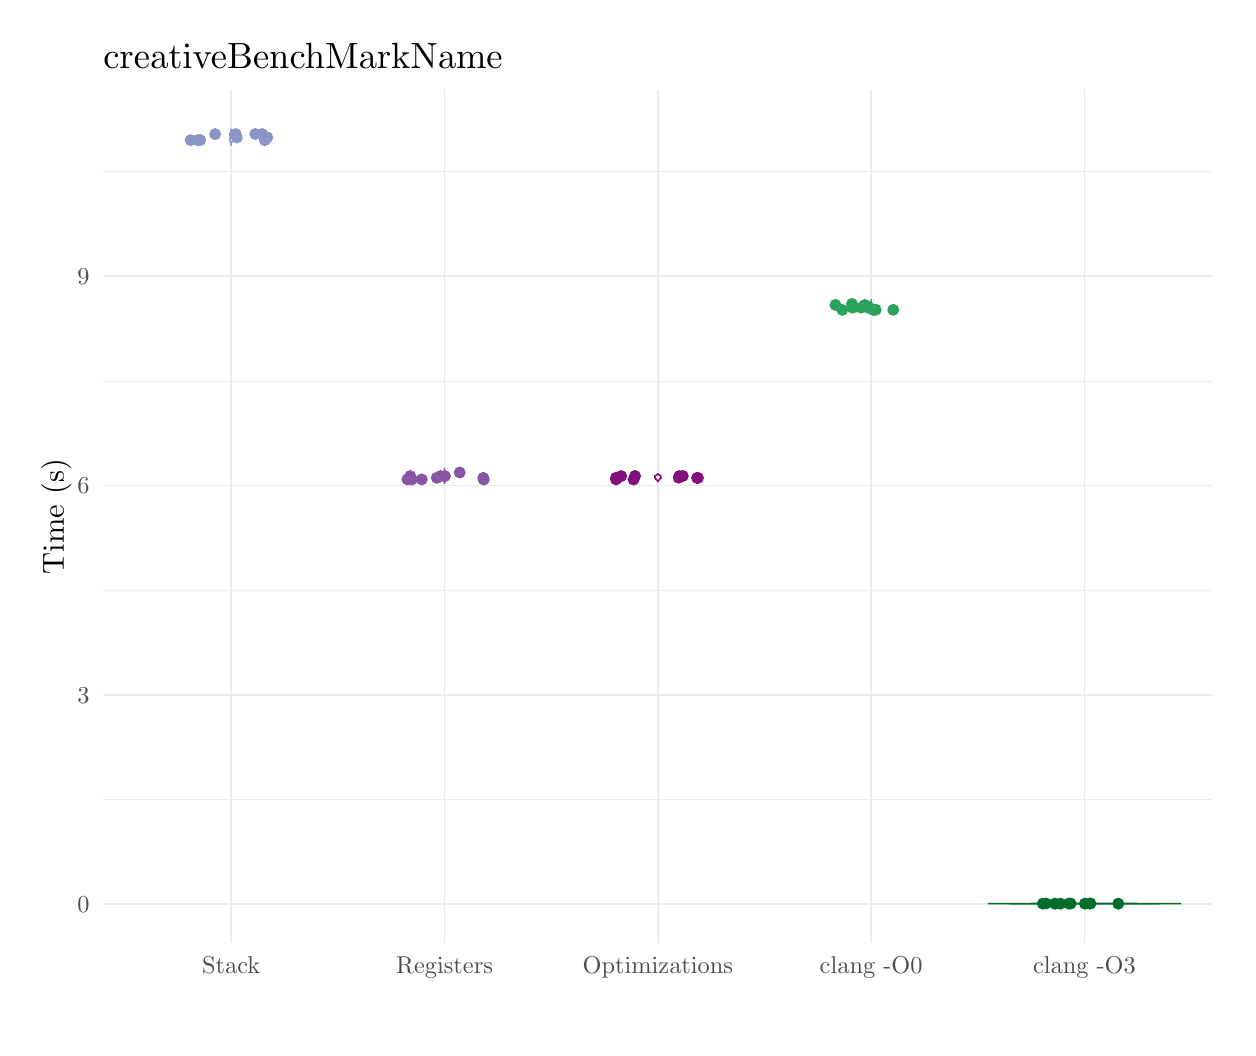
\begin{tikzpicture}[x=1pt,y=1pt]
\definecolor{fillColor}{RGB}{255,255,255}
\path[use as bounding box,fill=fillColor,fill opacity=0.00] (0,0) rectangle (433.62,361.35);
\begin{scope}
\path[clip] ( 27.31, 30.69) rectangle (428.12,338.69);
\definecolor{drawColor}{gray}{0.92}

\path[draw=drawColor,line width= 0.3pt,line join=round] ( 27.31, 82.49) --
	(428.12, 82.49);

\path[draw=drawColor,line width= 0.3pt,line join=round] ( 27.31,158.09) --
	(428.12,158.09);

\path[draw=drawColor,line width= 0.3pt,line join=round] ( 27.31,233.70) --
	(428.12,233.70);

\path[draw=drawColor,line width= 0.3pt,line join=round] ( 27.31,309.31) --
	(428.12,309.31);

\path[draw=drawColor,line width= 0.6pt,line join=round] ( 27.31, 44.69) --
	(428.12, 44.69);

\path[draw=drawColor,line width= 0.6pt,line join=round] ( 27.31,120.29) --
	(428.12,120.29);

\path[draw=drawColor,line width= 0.6pt,line join=round] ( 27.31,195.90) --
	(428.12,195.90);

\path[draw=drawColor,line width= 0.6pt,line join=round] ( 27.31,271.50) --
	(428.12,271.50);

\path[draw=drawColor,line width= 0.6pt,line join=round] ( 73.56, 30.69) --
	( 73.56,338.69);

\path[draw=drawColor,line width= 0.6pt,line join=round] (150.64, 30.69) --
	(150.64,338.69);

\path[draw=drawColor,line width= 0.6pt,line join=round] (227.72, 30.69) --
	(227.72,338.69);

\path[draw=drawColor,line width= 0.6pt,line join=round] (304.79, 30.69) --
	(304.79,338.69);

\path[draw=drawColor,line width= 0.6pt,line join=round] (381.87, 30.69) --
	(381.87,338.69);
\definecolor{drawColor}{RGB}{140,150,198}
\definecolor{fillColor}{RGB}{255,255,255}

\path[draw=drawColor,line width= 0.6pt,line join=round,line cap=round,fill=fillColor] ( 73.56,318.89) --
	( 73.56,318.91) --
	( 73.55,318.92) --
	( 73.55,318.93) --
	( 73.55,318.94) --
	( 73.55,318.95) --
	( 73.55,318.96) --
	( 73.55,318.97) --
	( 73.55,318.98) --
	( 73.55,319.00) --
	( 73.55,319.01) --
	( 73.55,319.02) --
	( 73.55,319.03) --
	( 73.55,319.04) --
	( 73.55,319.05) --
	( 73.55,319.06) --
	( 73.55,319.08) --
	( 73.55,319.09) --
	( 73.55,319.10) --
	( 73.55,319.11) --
	( 73.55,319.12) --
	( 73.55,319.13) --
	( 73.54,319.14) --
	( 73.54,319.15) --
	( 73.54,319.17) --
	( 73.54,319.18) --
	( 73.54,319.19) --
	( 73.54,319.20) --
	( 73.54,319.21) --
	( 73.54,319.22) --
	( 73.54,319.23) --
	( 73.54,319.25) --
	( 73.53,319.26) --
	( 73.53,319.27) --
	( 73.53,319.28) --
	( 73.53,319.29) --
	( 73.53,319.30) --
	( 73.53,319.31) --
	( 73.53,319.32) --
	( 73.53,319.34) --
	( 73.52,319.35) --
	( 73.52,319.36) --
	( 73.52,319.37) --
	( 73.52,319.38) --
	( 73.52,319.39) --
	( 73.52,319.40) --
	( 73.51,319.42) --
	( 73.51,319.43) --
	( 73.51,319.44) --
	( 73.51,319.45) --
	( 73.51,319.46) --
	( 73.50,319.47) --
	( 73.50,319.48) --
	( 73.50,319.50) --
	( 73.50,319.51) --
	( 73.49,319.52) --
	( 73.49,319.53) --
	( 73.49,319.54) --
	( 73.49,319.55) --
	( 73.48,319.56) --
	( 73.48,319.57) --
	( 73.48,319.59) --
	( 73.47,319.60) --
	( 73.47,319.61) --
	( 73.47,319.62) --
	( 73.46,319.63) --
	( 73.46,319.64) --
	( 73.46,319.65) --
	( 73.45,319.67) --
	( 73.45,319.68) --
	( 73.45,319.69) --
	( 73.44,319.70) --
	( 73.44,319.71) --
	( 73.43,319.72) --
	( 73.43,319.73) --
	( 73.43,319.74) --
	( 73.42,319.76) --
	( 73.42,319.77) --
	( 73.41,319.78) --
	( 73.41,319.79) --
	( 73.40,319.80) --
	( 73.40,319.81) --
	( 73.40,319.82) --
	( 73.39,319.84) --
	( 73.39,319.85) --
	( 73.38,319.86) --
	( 73.38,319.87) --
	( 73.37,319.88) --
	( 73.37,319.89) --
	( 73.36,319.90) --
	( 73.36,319.91) --
	( 73.35,319.93) --
	( 73.35,319.94) --
	( 73.34,319.95) --
	( 73.33,319.96) --
	( 73.33,319.97) --
	( 73.32,319.98) --
	( 73.32,319.99) --
	( 73.31,320.01) --
	( 73.31,320.02) --
	( 73.30,320.03) --
	( 73.30,320.04) --
	( 73.29,320.05) --
	( 73.28,320.06) --
	( 73.28,320.07) --
	( 73.27,320.09) --
	( 73.27,320.10) --
	( 73.26,320.11) --
	( 73.25,320.12) --
	( 73.25,320.13) --
	( 73.24,320.14) --
	( 73.24,320.15) --
	( 73.23,320.16) --
	( 73.22,320.18) --
	( 73.22,320.19) --
	( 73.21,320.20) --
	( 73.21,320.21) --
	( 73.20,320.22) --
	( 73.20,320.23) --
	( 73.19,320.24) --
	( 73.18,320.26) --
	( 73.18,320.27) --
	( 73.17,320.28) --
	( 73.17,320.29) --
	( 73.16,320.30) --
	( 73.16,320.31) --
	( 73.15,320.32) --
	( 73.14,320.33) --
	( 73.14,320.35) --
	( 73.13,320.36) --
	( 73.13,320.37) --
	( 73.12,320.38) --
	( 73.12,320.39) --
	( 73.11,320.40) --
	( 73.11,320.41) --
	( 73.10,320.43) --
	( 73.10,320.44) --
	( 73.09,320.45) --
	( 73.09,320.46) --
	( 73.09,320.47) --
	( 73.08,320.48) --
	( 73.08,320.49) --
	( 73.07,320.51) --
	( 73.07,320.52) --
	( 73.06,320.53) --
	( 73.06,320.54) --
	( 73.06,320.55) --
	( 73.05,320.56) --
	( 73.05,320.57) --
	( 73.05,320.58) --
	( 73.04,320.60) --
	( 73.04,320.61) --
	( 73.04,320.62) --
	( 73.04,320.63) --
	( 73.03,320.64) --
	( 73.03,320.65) --
	( 73.03,320.66) --
	( 73.03,320.68) --
	( 73.02,320.69) --
	( 73.02,320.70) --
	( 73.02,320.71) --
	( 73.02,320.72) --
	( 73.02,320.73) --
	( 73.01,320.74) --
	( 73.01,320.75) --
	( 73.01,320.77) --
	( 73.01,320.78) --
	( 73.01,320.79) --
	( 73.01,320.80) --
	( 73.01,320.81) --
	( 73.01,320.82) --
	( 73.01,320.83) --
	( 73.01,320.85) --
	( 73.01,320.86) --
	( 73.01,320.87) --
	( 73.01,320.88) --
	( 73.01,320.89) --
	( 73.01,320.90) --
	( 73.01,320.91) --
	( 73.01,320.92) --
	( 73.01,320.94) --
	( 73.01,320.95) --
	( 73.01,320.96) --
	( 73.01,320.97) --
	( 73.01,320.98) --
	( 73.01,320.99) --
	( 73.02,321.00) --
	( 73.02,321.02) --
	( 73.02,321.03) --
	( 73.02,321.04) --
	( 73.02,321.05) --
	( 73.02,321.06) --
	( 73.02,321.07) --
	( 73.03,321.08) --
	( 73.03,321.10) --
	( 73.03,321.11) --
	( 73.03,321.12) --
	( 73.03,321.13) --
	( 73.04,321.14) --
	( 73.04,321.15) --
	( 73.04,321.16) --
	( 73.04,321.17) --
	( 73.04,321.19) --
	( 73.05,321.20) --
	( 73.05,321.21) --
	( 73.05,321.22) --
	( 73.05,321.23) --
	( 73.06,321.24) --
	( 73.06,321.25) --
	( 73.06,321.27) --
	( 73.06,321.28) --
	( 73.07,321.29) --
	( 73.07,321.30) --
	( 73.07,321.31) --
	( 73.07,321.32) --
	( 73.08,321.33) --
	( 73.08,321.34) --
	( 73.08,321.36) --
	( 73.08,321.37) --
	( 73.09,321.38) --
	( 73.09,321.39) --
	( 73.09,321.40) --
	( 73.09,321.41) --
	( 73.10,321.42) --
	( 73.10,321.44) --
	( 73.10,321.45) --
	( 73.10,321.46) --
	( 73.11,321.47) --
	( 73.11,321.48) --
	( 73.11,321.49) --
	( 73.11,321.50) --
	( 73.11,321.52) --
	( 73.12,321.53) --
	( 73.12,321.54) --
	( 73.12,321.55) --
	( 73.12,321.56) --
	( 73.13,321.57) --
	( 73.13,321.58) --
	( 73.13,321.59) --
	( 73.13,321.61) --
	( 73.13,321.62) --
	( 73.13,321.63) --
	( 73.14,321.64) --
	( 73.14,321.65) --
	( 73.14,321.66) --
	( 73.14,321.67) --
	( 73.14,321.69) --
	( 73.14,321.70) --
	( 73.15,321.71) --
	( 73.15,321.72) --
	( 73.15,321.73) --
	( 73.15,321.74) --
	( 73.15,321.75) --
	( 73.15,321.76) --
	( 73.15,321.78) --
	( 73.15,321.79) --
	( 73.15,321.80) --
	( 73.16,321.81) --
	( 73.16,321.82) --
	( 73.16,321.83) --
	( 73.16,321.84) --
	( 73.16,321.86) --
	( 73.16,321.87) --
	( 73.16,321.88) --
	( 73.16,321.89) --
	( 73.16,321.90) --
	( 73.16,321.91) --
	( 73.16,321.92) --
	( 73.16,321.93) --
	( 73.16,321.95) --
	( 73.16,321.96) --
	( 73.16,321.97) --
	( 73.16,321.98) --
	( 73.16,321.99) --
	( 73.16,322.00) --
	( 73.16,322.01) --
	( 73.16,322.03) --
	( 73.16,322.04) --
	( 73.16,322.05) --
	( 73.16,322.06) --
	( 73.15,322.07) --
	( 73.15,322.08) --
	( 73.15,322.09) --
	( 73.15,322.11) --
	( 73.15,322.12) --
	( 73.15,322.13) --
	( 73.15,322.14) --
	( 73.15,322.15) --
	( 73.14,322.16) --
	( 73.14,322.17) --
	( 73.14,322.18) --
	( 73.14,322.20) --
	( 73.14,322.21) --
	( 73.14,322.22) --
	( 73.13,322.23) --
	( 73.13,322.24) --
	( 73.13,322.25) --
	( 73.13,322.26) --
	( 73.13,322.28) --
	( 73.12,322.29) --
	( 73.12,322.30) --
	( 73.12,322.31) --
	( 73.12,322.32) --
	( 73.12,322.33) --
	( 73.11,322.34) --
	( 73.11,322.35) --
	( 73.11,322.37) --
	( 73.11,322.38) --
	( 73.10,322.39) --
	( 73.10,322.40) --
	( 73.10,322.41) --
	( 73.10,322.42) --
	( 73.10,322.43) --
	( 73.09,322.45) --
	( 73.09,322.46) --
	( 73.09,322.47) --
	( 73.09,322.48) --
	( 73.08,322.49) --
	( 73.08,322.50) --
	( 73.08,322.51) --
	( 73.08,322.53) --
	( 73.07,322.54) --
	( 73.07,322.55) --
	( 73.07,322.56) --
	( 73.07,322.57) --
	( 73.07,322.58) --
	( 73.06,322.59) --
	( 73.06,322.60) --
	( 73.06,322.62) --
	( 73.06,322.63) --
	( 73.06,322.64) --
	( 73.06,322.65) --
	( 73.06,322.66) --
	( 73.05,322.67) --
	( 73.05,322.68) --
	( 73.05,322.70) --
	( 73.05,322.71) --
	( 73.05,322.72) --
	( 73.05,322.73) --
	( 73.05,322.74) --
	( 73.05,322.75) --
	( 73.05,322.76) --
	( 73.05,322.77) --
	( 73.05,322.79) --
	( 73.05,322.80) --
	( 73.05,322.81) --
	( 73.05,322.82) --
	( 73.05,322.83) --
	( 73.05,322.84) --
	( 73.05,322.85) --
	( 73.05,322.87) --
	( 73.05,322.88) --
	( 73.05,322.89) --
	( 73.05,322.90) --
	( 73.05,322.91) --
	( 73.05,322.92) --
	( 73.05,322.93) --
	( 73.06,322.94) --
	( 73.06,322.96) --
	( 73.06,322.97) --
	( 73.06,322.98) --
	( 73.06,322.99) --
	( 73.07,323.00) --
	( 73.07,323.01) --
	( 73.07,323.02) --
	( 73.07,323.04) --
	( 73.08,323.05) --
	( 73.08,323.06) --
	( 73.08,323.07) --
	( 73.08,323.08) --
	( 73.09,323.09) --
	( 73.09,323.10) --
	( 73.10,323.12) --
	( 73.10,323.13) --
	( 73.10,323.14) --
	( 73.11,323.15) --
	( 73.11,323.16) --
	( 73.11,323.17) --
	( 73.12,323.18) --
	( 73.12,323.19) --
	( 73.13,323.21) --
	( 73.13,323.22) --
	( 73.14,323.23) --
	( 73.14,323.24) --
	( 73.15,323.25) --
	( 73.15,323.26) --
	( 73.16,323.27) --
	( 73.16,323.29) --
	( 73.17,323.30) --
	( 73.17,323.31) --
	( 73.18,323.32) --
	( 73.18,323.33) --
	( 73.19,323.34) --
	( 73.19,323.35) --
	( 73.20,323.36) --
	( 73.20,323.38) --
	( 73.21,323.39) --
	( 73.22,323.40) --
	( 73.22,323.41) --
	( 73.23,323.42) --
	( 73.23,323.43) --
	( 73.24,323.44) --
	( 73.24,323.46) --
	( 73.25,323.47) --
	( 73.26,323.48) --
	( 73.26,323.49) --
	( 73.27,323.50) --
	( 73.27,323.51) --
	( 73.28,323.52) --
	( 73.28,323.53) --
	( 73.29,323.55) --
	( 73.29,323.56) --
	( 73.30,323.57) --
	( 73.31,323.58) --
	( 73.31,323.59) --
	( 73.32,323.60) --
	( 73.32,323.61) --
	( 73.33,323.63) --
	( 73.33,323.64) --
	( 73.34,323.65) --
	( 73.34,323.66) --
	( 73.35,323.67) --
	( 73.35,323.68) --
	( 73.36,323.69) --
	( 73.36,323.71) --
	( 73.37,323.72) --
	( 73.37,323.73) --
	( 73.38,323.74) --
	( 73.38,323.75) --
	( 73.39,323.76) --
	( 73.39,323.77) --
	( 73.40,323.78) --
	( 73.40,323.80) --
	( 73.41,323.81) --
	( 73.41,323.82) --
	( 73.42,323.83) --
	( 73.42,323.84) --
	( 73.42,323.85) --
	( 73.43,323.86) --
	( 73.43,323.88) --
	( 73.44,323.89) --
	( 73.44,323.90) --
	( 73.44,323.91) --
	( 73.45,323.92) --
	( 73.45,323.93) --
	( 73.46,323.94) --
	( 73.46,323.95) --
	( 73.46,323.97) --
	( 73.47,323.98) --
	( 73.47,323.99) --
	( 73.47,324.00) --
	( 73.47,324.01) --
	( 73.48,324.02) --
	( 73.48,324.03) --
	( 73.48,324.05) --
	( 73.49,324.06) --
	( 73.49,324.07) --
	( 73.49,324.08) --
	( 73.49,324.09) --
	( 73.50,324.10) --
	( 73.50,324.11) --
	( 73.50,324.13) --
	( 73.50,324.14) --
	( 73.51,324.15) --
	( 73.51,324.16) --
	( 73.51,324.17) --
	( 73.51,324.18) --
	( 73.51,324.19) --
	( 73.52,324.20) --
	( 73.52,324.22) --
	( 73.52,324.23) --
	( 73.52,324.24) --
	( 73.52,324.25) --
	( 73.52,324.26) --
	( 73.53,324.27) --
	( 73.53,324.28) --
	( 73.53,324.30) --
	( 73.53,324.31) --
	( 73.53,324.32) --
	( 73.53,324.33) --
	( 73.53,324.34) --
	( 73.54,324.35) --
	( 73.54,324.36) --
	( 73.54,324.37) --
	( 73.54,324.39) --
	( 73.54,324.40) --
	( 73.54,324.41) --
	( 73.54,324.42) --
	( 73.54,324.43) --
	( 73.54,324.44) --
	( 73.54,324.45) --
	( 73.54,324.47) --
	( 73.55,324.48) --
	( 73.55,324.49) --
	( 73.55,324.50) --
	( 73.55,324.51) --
	( 73.55,324.52) --
	( 73.55,324.53) --
	( 73.55,324.54) --
	( 73.55,324.56) --
	( 73.55,324.57) --
	( 73.55,324.58) --
	( 73.55,324.59) --
	( 73.55,324.60) --
	( 73.55,324.61) --
	( 73.55,324.62) --
	( 73.55,324.64) --
	( 73.55,324.65) --
	( 73.55,324.66) --
	( 73.55,324.67) --
	( 73.55,324.68) --
	( 73.55,324.69) --
	( 73.57,324.69) --
	( 73.57,324.68) --
	( 73.57,324.67) --
	( 73.57,324.66) --
	( 73.57,324.65) --
	( 73.57,324.64) --
	( 73.57,324.62) --
	( 73.57,324.61) --
	( 73.57,324.60) --
	( 73.57,324.59) --
	( 73.57,324.58) --
	( 73.57,324.57) --
	( 73.57,324.56) --
	( 73.57,324.54) --
	( 73.57,324.53) --
	( 73.57,324.52) --
	( 73.57,324.51) --
	( 73.57,324.50) --
	( 73.57,324.49) --
	( 73.57,324.48) --
	( 73.58,324.47) --
	( 73.58,324.45) --
	( 73.58,324.44) --
	( 73.58,324.43) --
	( 73.58,324.42) --
	( 73.58,324.41) --
	( 73.58,324.40) --
	( 73.58,324.39) --
	( 73.58,324.37) --
	( 73.58,324.36) --
	( 73.59,324.35) --
	( 73.59,324.34) --
	( 73.59,324.33) --
	( 73.59,324.32) --
	( 73.59,324.31) --
	( 73.59,324.30) --
	( 73.59,324.28) --
	( 73.59,324.27) --
	( 73.60,324.26) --
	( 73.60,324.25) --
	( 73.60,324.24) --
	( 73.60,324.23) --
	( 73.60,324.22) --
	( 73.60,324.20) --
	( 73.61,324.19) --
	( 73.61,324.18) --
	( 73.61,324.17) --
	( 73.61,324.16) --
	( 73.61,324.15) --
	( 73.62,324.14) --
	( 73.62,324.13) --
	( 73.62,324.11) --
	( 73.62,324.10) --
	( 73.63,324.09) --
	( 73.63,324.08) --
	( 73.63,324.07) --
	( 73.63,324.06) --
	( 73.64,324.05) --
	( 73.64,324.03) --
	( 73.64,324.02) --
	( 73.65,324.01) --
	( 73.65,324.00) --
	( 73.65,323.99) --
	( 73.65,323.98) --
	( 73.66,323.97) --
	( 73.66,323.95) --
	( 73.67,323.94) --
	( 73.67,323.93) --
	( 73.67,323.92) --
	( 73.68,323.91) --
	( 73.68,323.90) --
	( 73.68,323.89) --
	( 73.69,323.88) --
	( 73.69,323.86) --
	( 73.70,323.85) --
	( 73.70,323.84) --
	( 73.70,323.83) --
	( 73.71,323.82) --
	( 73.71,323.81) --
	( 73.72,323.80) --
	( 73.72,323.78) --
	( 73.73,323.77) --
	( 73.73,323.76) --
	( 73.74,323.75) --
	( 73.74,323.74) --
	( 73.75,323.73) --
	( 73.75,323.72) --
	( 73.76,323.71) --
	( 73.76,323.69) --
	( 73.77,323.68) --
	( 73.77,323.67) --
	( 73.78,323.66) --
	( 73.78,323.65) --
	( 73.79,323.64) --
	( 73.79,323.63) --
	( 73.80,323.61) --
	( 73.80,323.60) --
	( 73.81,323.59) --
	( 73.81,323.58) --
	( 73.82,323.57) --
	( 73.83,323.56) --
	( 73.83,323.55) --
	( 73.84,323.53) --
	( 73.84,323.52) --
	( 73.85,323.51) --
	( 73.85,323.50) --
	( 73.86,323.49) --
	( 73.87,323.48) --
	( 73.87,323.47) --
	( 73.88,323.46) --
	( 73.88,323.44) --
	( 73.89,323.43) --
	( 73.89,323.42) --
	( 73.90,323.41) --
	( 73.90,323.40) --
	( 73.91,323.39) --
	( 73.92,323.38) --
	( 73.92,323.36) --
	( 73.93,323.35) --
	( 73.93,323.34) --
	( 73.94,323.33) --
	( 73.94,323.32) --
	( 73.95,323.31) --
	( 73.95,323.30) --
	( 73.96,323.29) --
	( 73.96,323.27) --
	( 73.97,323.26) --
	( 73.97,323.25) --
	( 73.98,323.24) --
	( 73.98,323.23) --
	( 73.99,323.22) --
	( 73.99,323.21) --
	( 74.00,323.19) --
	( 74.00,323.18) --
	( 74.01,323.17) --
	( 74.01,323.16) --
	( 74.01,323.15) --
	( 74.02,323.14) --
	( 74.02,323.13) --
	( 74.03,323.12) --
	( 74.03,323.10) --
	( 74.03,323.09) --
	( 74.04,323.08) --
	( 74.04,323.07) --
	( 74.04,323.06) --
	( 74.04,323.05) --
	( 74.05,323.04) --
	( 74.05,323.02) --
	( 74.05,323.01) --
	( 74.06,323.00) --
	( 74.06,322.99) --
	( 74.06,322.98) --
	( 74.06,322.97) --
	( 74.06,322.96) --
	( 74.07,322.94) --
	( 74.07,322.93) --
	( 74.07,322.92) --
	( 74.07,322.91) --
	( 74.07,322.90) --
	( 74.07,322.89) --
	( 74.07,322.88) --
	( 74.07,322.87) --
	( 74.07,322.85) --
	( 74.07,322.84) --
	( 74.07,322.83) --
	( 74.07,322.82) --
	( 74.07,322.81) --
	( 74.07,322.80) --
	( 74.07,322.79) --
	( 74.07,322.77) --
	( 74.07,322.76) --
	( 74.07,322.75) --
	( 74.07,322.74) --
	( 74.07,322.73) --
	( 74.07,322.72) --
	( 74.07,322.71) --
	( 74.07,322.70) --
	( 74.07,322.68) --
	( 74.07,322.67) --
	( 74.07,322.66) --
	( 74.06,322.65) --
	( 74.06,322.64) --
	( 74.06,322.63) --
	( 74.06,322.62) --
	( 74.06,322.60) --
	( 74.06,322.59) --
	( 74.05,322.58) --
	( 74.05,322.57) --
	( 74.05,322.56) --
	( 74.05,322.55) --
	( 74.05,322.54) --
	( 74.04,322.53) --
	( 74.04,322.51) --
	( 74.04,322.50) --
	( 74.04,322.49) --
	( 74.03,322.48) --
	( 74.03,322.47) --
	( 74.03,322.46) --
	( 74.03,322.45) --
	( 74.03,322.43) --
	( 74.02,322.42) --
	( 74.02,322.41) --
	( 74.02,322.40) --
	( 74.02,322.39) --
	( 74.01,322.38) --
	( 74.01,322.37) --
	( 74.01,322.35) --
	( 74.01,322.34) --
	( 74.00,322.33) --
	( 74.00,322.32) --
	( 74.00,322.31) --
	( 74.00,322.30) --
	( 74.00,322.29) --
	( 73.99,322.28) --
	( 73.99,322.26) --
	( 73.99,322.25) --
	( 73.99,322.24) --
	( 73.99,322.23) --
	( 73.98,322.22) --
	( 73.98,322.21) --
	( 73.98,322.20) --
	( 73.98,322.18) --
	( 73.98,322.17) --
	( 73.98,322.16) --
	( 73.97,322.15) --
	( 73.97,322.14) --
	( 73.97,322.13) --
	( 73.97,322.12) --
	( 73.97,322.11) --
	( 73.97,322.09) --
	( 73.97,322.08) --
	( 73.97,322.07) --
	( 73.97,322.06) --
	( 73.96,322.05) --
	( 73.96,322.04) --
	( 73.96,322.03) --
	( 73.96,322.01) --
	( 73.96,322.00) --
	( 73.96,321.99) --
	( 73.96,321.98) --
	( 73.96,321.97) --
	( 73.96,321.96) --
	( 73.96,321.95) --
	( 73.96,321.93) --
	( 73.96,321.92) --
	( 73.96,321.91) --
	( 73.96,321.90) --
	( 73.96,321.89) --
	( 73.96,321.88) --
	( 73.96,321.87) --
	( 73.96,321.86) --
	( 73.96,321.84) --
	( 73.96,321.83) --
	( 73.96,321.82) --
	( 73.96,321.81) --
	( 73.97,321.80) --
	( 73.97,321.79) --
	( 73.97,321.78) --
	( 73.97,321.76) --
	( 73.97,321.75) --
	( 73.97,321.74) --
	( 73.97,321.73) --
	( 73.97,321.72) --
	( 73.97,321.71) --
	( 73.98,321.70) --
	( 73.98,321.69) --
	( 73.98,321.67) --
	( 73.98,321.66) --
	( 73.98,321.65) --
	( 73.98,321.64) --
	( 73.99,321.63) --
	( 73.99,321.62) --
	( 73.99,321.61) --
	( 73.99,321.59) --
	( 73.99,321.58) --
	( 74.00,321.57) --
	( 74.00,321.56) --
	( 74.00,321.55) --
	( 74.00,321.54) --
	( 74.00,321.53) --
	( 74.01,321.52) --
	( 74.01,321.50) --
	( 74.01,321.49) --
	( 74.01,321.48) --
	( 74.01,321.47) --
	( 74.02,321.46) --
	( 74.02,321.45) --
	( 74.02,321.44) --
	( 74.02,321.42) --
	( 74.03,321.41) --
	( 74.03,321.40) --
	( 74.03,321.39) --
	( 74.03,321.38) --
	( 74.04,321.37) --
	( 74.04,321.36) --
	( 74.04,321.34) --
	( 74.04,321.33) --
	( 74.05,321.32) --
	( 74.05,321.31) --
	( 74.05,321.30) --
	( 74.05,321.29) --
	( 74.06,321.28) --
	( 74.06,321.27) --
	( 74.06,321.25) --
	( 74.06,321.24) --
	( 74.07,321.23) --
	( 74.07,321.22) --
	( 74.07,321.21) --
	( 74.07,321.20) --
	( 74.08,321.19) --
	( 74.08,321.17) --
	( 74.08,321.16) --
	( 74.08,321.15) --
	( 74.08,321.14) --
	( 74.09,321.13) --
	( 74.09,321.12) --
	( 74.09,321.11) --
	( 74.09,321.10) --
	( 74.09,321.08) --
	( 74.10,321.07) --
	( 74.10,321.06) --
	( 74.10,321.05) --
	( 74.10,321.04) --
	( 74.10,321.03) --
	( 74.10,321.02) --
	( 74.10,321.00) --
	( 74.11,320.99) --
	( 74.11,320.98) --
	( 74.11,320.97) --
	( 74.11,320.96) --
	( 74.11,320.95) --
	( 74.11,320.94) --
	( 74.11,320.92) --
	( 74.11,320.91) --
	( 74.11,320.90) --
	( 74.11,320.89) --
	( 74.11,320.88) --
	( 74.11,320.87) --
	( 74.11,320.86) --
	( 74.11,320.85) --
	( 74.11,320.83) --
	( 74.11,320.82) --
	( 74.11,320.81) --
	( 74.11,320.80) --
	( 74.11,320.79) --
	( 74.11,320.78) --
	( 74.11,320.77) --
	( 74.11,320.75) --
	( 74.11,320.74) --
	( 74.10,320.73) --
	( 74.10,320.72) --
	( 74.10,320.71) --
	( 74.10,320.70) --
	( 74.10,320.69) --
	( 74.10,320.68) --
	( 74.09,320.66) --
	( 74.09,320.65) --
	( 74.09,320.64) --
	( 74.09,320.63) --
	( 74.08,320.62) --
	( 74.08,320.61) --
	( 74.08,320.60) --
	( 74.07,320.58) --
	( 74.07,320.57) --
	( 74.07,320.56) --
	( 74.06,320.55) --
	( 74.06,320.54) --
	( 74.06,320.53) --
	( 74.05,320.52) --
	( 74.05,320.51) --
	( 74.04,320.49) --
	( 74.04,320.48) --
	( 74.04,320.47) --
	( 74.03,320.46) --
	( 74.03,320.45) --
	( 74.02,320.44) --
	( 74.02,320.43) --
	( 74.01,320.41) --
	( 74.01,320.40) --
	( 74.00,320.39) --
	( 74.00,320.38) --
	( 73.99,320.37) --
	( 73.99,320.36) --
	( 73.98,320.35) --
	( 73.98,320.33) --
	( 73.97,320.32) --
	( 73.97,320.31) --
	( 73.96,320.30) --
	( 73.95,320.29) --
	( 73.95,320.28) --
	( 73.94,320.27) --
	( 73.94,320.26) --
	( 73.93,320.24) --
	( 73.93,320.23) --
	( 73.92,320.22) --
	( 73.91,320.21) --
	( 73.91,320.20) --
	( 73.90,320.19) --
	( 73.90,320.18) --
	( 73.89,320.16) --
	( 73.88,320.15) --
	( 73.88,320.14) --
	( 73.87,320.13) --
	( 73.87,320.12) --
	( 73.86,320.11) --
	( 73.85,320.10) --
	( 73.85,320.09) --
	( 73.84,320.07) --
	( 73.84,320.06) --
	( 73.83,320.05) --
	( 73.83,320.04) --
	( 73.82,320.03) --
	( 73.81,320.02) --
	( 73.81,320.01) --
	( 73.80,319.99) --
	( 73.80,319.98) --
	( 73.79,319.97) --
	( 73.79,319.96) --
	( 73.78,319.95) --
	( 73.77,319.94) --
	( 73.77,319.93) --
	( 73.76,319.91) --
	( 73.76,319.90) --
	( 73.75,319.89) --
	( 73.75,319.88) --
	( 73.74,319.87) --
	( 73.74,319.86) --
	( 73.73,319.85) --
	( 73.73,319.84) --
	( 73.72,319.82) --
	( 73.72,319.81) --
	( 73.72,319.80) --
	( 73.71,319.79) --
	( 73.71,319.78) --
	( 73.70,319.77) --
	( 73.70,319.76) --
	( 73.69,319.74) --
	( 73.69,319.73) --
	( 73.69,319.72) --
	( 73.68,319.71) --
	( 73.68,319.70) --
	( 73.67,319.69) --
	( 73.67,319.68) --
	( 73.67,319.67) --
	( 73.66,319.65) --
	( 73.66,319.64) --
	( 73.66,319.63) --
	( 73.65,319.62) --
	( 73.65,319.61) --
	( 73.65,319.60) --
	( 73.64,319.59) --
	( 73.64,319.57) --
	( 73.64,319.56) --
	( 73.64,319.55) --
	( 73.63,319.54) --
	( 73.63,319.53) --
	( 73.63,319.52) --
	( 73.62,319.51) --
	( 73.62,319.50) --
	( 73.62,319.48) --
	( 73.62,319.47) --
	( 73.62,319.46) --
	( 73.61,319.45) --
	( 73.61,319.44) --
	( 73.61,319.43) --
	( 73.61,319.42) --
	( 73.61,319.40) --
	( 73.60,319.39) --
	( 73.60,319.38) --
	( 73.60,319.37) --
	( 73.60,319.36) --
	( 73.60,319.35) --
	( 73.59,319.34) --
	( 73.59,319.32) --
	( 73.59,319.31) --
	( 73.59,319.30) --
	( 73.59,319.29) --
	( 73.59,319.28) --
	( 73.59,319.27) --
	( 73.59,319.26) --
	( 73.58,319.25) --
	( 73.58,319.23) --
	( 73.58,319.22) --
	( 73.58,319.21) --
	( 73.58,319.20) --
	( 73.58,319.19) --
	( 73.58,319.18) --
	( 73.58,319.17) --
	( 73.58,319.15) --
	( 73.58,319.14) --
	( 73.58,319.13) --
	( 73.57,319.12) --
	( 73.57,319.11) --
	( 73.57,319.10) --
	( 73.57,319.09) --
	( 73.57,319.08) --
	( 73.57,319.06) --
	( 73.57,319.05) --
	( 73.57,319.04) --
	( 73.57,319.03) --
	( 73.57,319.02) --
	( 73.57,319.01) --
	( 73.57,319.00) --
	( 73.57,318.98) --
	( 73.57,318.97) --
	( 73.57,318.96) --
	( 73.57,318.95) --
	( 73.57,318.94) --
	( 73.57,318.93) --
	( 73.57,318.92) --
	( 73.57,318.91) --
	( 73.56,318.89) --
	( 73.56,318.89) --
	cycle;
\definecolor{drawColor}{RGB}{136,86,167}

\path[draw=drawColor,line width= 0.6pt,line join=round,line cap=round,fill=fillColor] (150.63,196.67) --
	(150.63,196.68) --
	(150.63,196.69) --
	(150.63,196.70) --
	(150.63,196.71) --
	(150.63,196.72) --
	(150.63,196.73) --
	(150.63,196.74) --
	(150.63,196.75) --
	(150.63,196.76) --
	(150.63,196.77) --
	(150.63,196.78) --
	(150.63,196.79) --
	(150.63,196.80) --
	(150.62,196.81) --
	(150.62,196.82) --
	(150.62,196.83) --
	(150.62,196.84) --
	(150.62,196.85) --
	(150.62,196.87) --
	(150.62,196.88) --
	(150.62,196.89) --
	(150.62,196.90) --
	(150.61,196.91) --
	(150.61,196.92) --
	(150.61,196.93) --
	(150.61,196.94) --
	(150.61,196.95) --
	(150.61,196.96) --
	(150.61,196.97) --
	(150.60,196.98) --
	(150.60,196.99) --
	(150.60,197.00) --
	(150.60,197.01) --
	(150.60,197.02) --
	(150.59,197.03) --
	(150.59,197.04) --
	(150.59,197.05) --
	(150.59,197.06) --
	(150.58,197.07) --
	(150.58,197.08) --
	(150.58,197.10) --
	(150.57,197.11) --
	(150.57,197.12) --
	(150.57,197.13) --
	(150.56,197.14) --
	(150.56,197.15) --
	(150.56,197.16) --
	(150.55,197.17) --
	(150.55,197.18) --
	(150.55,197.19) --
	(150.54,197.20) --
	(150.54,197.21) --
	(150.53,197.22) --
	(150.53,197.23) --
	(150.52,197.24) --
	(150.52,197.25) --
	(150.51,197.26) --
	(150.51,197.27) --
	(150.50,197.28) --
	(150.50,197.29) --
	(150.49,197.30) --
	(150.49,197.31) --
	(150.48,197.33) --
	(150.47,197.34) --
	(150.47,197.35) --
	(150.46,197.36) --
	(150.45,197.37) --
	(150.45,197.38) --
	(150.44,197.39) --
	(150.43,197.40) --
	(150.43,197.41) --
	(150.42,197.42) --
	(150.41,197.43) --
	(150.40,197.44) --
	(150.40,197.45) --
	(150.39,197.46) --
	(150.38,197.47) --
	(150.37,197.48) --
	(150.36,197.49) --
	(150.36,197.50) --
	(150.35,197.51) --
	(150.34,197.52) --
	(150.33,197.53) --
	(150.32,197.54) --
	(150.31,197.56) --
	(150.30,197.57) --
	(150.29,197.58) --
	(150.28,197.59) --
	(150.28,197.60) --
	(150.27,197.61) --
	(150.26,197.62) --
	(150.25,197.63) --
	(150.24,197.64) --
	(150.23,197.65) --
	(150.22,197.66) --
	(150.21,197.67) --
	(150.20,197.68) --
	(150.19,197.69) --
	(150.18,197.70) --
	(150.17,197.71) --
	(150.16,197.72) --
	(150.15,197.73) --
	(150.14,197.74) --
	(150.13,197.75) --
	(150.12,197.76) --
	(150.11,197.77) --
	(150.10,197.79) --
	(150.09,197.80) --
	(150.08,197.81) --
	(150.07,197.82) --
	(150.06,197.83) --
	(150.05,197.84) --
	(150.04,197.85) --
	(150.03,197.86) --
	(150.02,197.87) --
	(150.01,197.88) --
	(150.01,197.89) --
	(150.00,197.90) --
	(149.99,197.91) --
	(149.98,197.92) --
	(149.97,197.93) --
	(149.96,197.94) --
	(149.96,197.95) --
	(149.95,197.96) --
	(149.94,197.97) --
	(149.93,197.98) --
	(149.93,197.99) --
	(149.92,198.00) --
	(149.91,198.02) --
	(149.91,198.03) --
	(149.90,198.04) --
	(149.89,198.05) --
	(149.89,198.06) --
	(149.88,198.07) --
	(149.88,198.08) --
	(149.87,198.09) --
	(149.86,198.10) --
	(149.86,198.11) --
	(149.86,198.12) --
	(149.85,198.13) --
	(149.85,198.14) --
	(149.84,198.15) --
	(149.84,198.16) --
	(149.84,198.17) --
	(149.83,198.18) --
	(149.83,198.19) --
	(149.83,198.20) --
	(149.82,198.21) --
	(149.82,198.22) --
	(149.82,198.23) --
	(149.82,198.25) --
	(149.82,198.26) --
	(149.81,198.27) --
	(149.81,198.28) --
	(149.81,198.29) --
	(149.81,198.30) --
	(149.81,198.31) --
	(149.81,198.32) --
	(149.81,198.33) --
	(149.81,198.34) --
	(149.81,198.35) --
	(149.81,198.36) --
	(149.81,198.37) --
	(149.81,198.38) --
	(149.81,198.39) --
	(149.81,198.40) --
	(149.81,198.41) --
	(149.81,198.42) --
	(149.82,198.43) --
	(149.82,198.44) --
	(149.82,198.45) --
	(149.82,198.46) --
	(149.82,198.47) --
	(149.82,198.49) --
	(149.83,198.50) --
	(149.83,198.51) --
	(149.83,198.52) --
	(149.83,198.53) --
	(149.83,198.54) --
	(149.84,198.55) --
	(149.84,198.56) --
	(149.84,198.57) --
	(149.84,198.58) --
	(149.85,198.59) --
	(149.85,198.60) --
	(149.85,198.61) --
	(149.85,198.62) --
	(149.86,198.63) --
	(149.86,198.64) --
	(149.86,198.65) --
	(149.86,198.66) --
	(149.87,198.67) --
	(149.87,198.68) --
	(149.87,198.69) --
	(149.88,198.70) --
	(149.88,198.72) --
	(149.88,198.73) --
	(149.88,198.74) --
	(149.89,198.75) --
	(149.89,198.76) --
	(149.89,198.77) --
	(149.89,198.78) --
	(149.90,198.79) --
	(149.90,198.80) --
	(149.90,198.81) --
	(149.90,198.82) --
	(149.91,198.83) --
	(149.91,198.84) --
	(149.91,198.85) --
	(149.91,198.86) --
	(149.92,198.87) --
	(149.92,198.88) --
	(149.92,198.89) --
	(149.92,198.90) --
	(149.93,198.91) --
	(149.93,198.92) --
	(149.93,198.93) --
	(149.93,198.95) --
	(149.94,198.96) --
	(149.94,198.97) --
	(149.94,198.98) --
	(149.94,198.99) --
	(149.94,199.00) --
	(149.95,199.01) --
	(149.95,199.02) --
	(149.95,199.03) --
	(149.95,199.04) --
	(149.96,199.05) --
	(149.96,199.06) --
	(149.96,199.07) --
	(149.96,199.08) --
	(149.97,199.09) --
	(149.97,199.10) --
	(149.97,199.11) --
	(149.98,199.12) --
	(149.98,199.13) --
	(149.98,199.14) --
	(149.99,199.15) --
	(149.99,199.16) --
	(149.99,199.18) --
	(149.99,199.19) --
	(150.00,199.20) --
	(150.00,199.21) --
	(150.01,199.22) --
	(150.01,199.23) --
	(150.01,199.24) --
	(150.02,199.25) --
	(150.02,199.26) --
	(150.02,199.27) --
	(150.03,199.28) --
	(150.03,199.29) --
	(150.04,199.30) --
	(150.04,199.31) --
	(150.05,199.32) --
	(150.05,199.33) --
	(150.06,199.34) --
	(150.06,199.35) --
	(150.07,199.36) --
	(150.07,199.37) --
	(150.08,199.38) --
	(150.08,199.39) --
	(150.09,199.41) --
	(150.09,199.42) --
	(150.10,199.43) --
	(150.10,199.44) --
	(150.11,199.45) --
	(150.12,199.46) --
	(150.12,199.47) --
	(150.13,199.48) --
	(150.13,199.49) --
	(150.14,199.50) --
	(150.15,199.51) --
	(150.15,199.52) --
	(150.16,199.53) --
	(150.16,199.54) --
	(150.17,199.55) --
	(150.18,199.56) --
	(150.18,199.57) --
	(150.19,199.58) --
	(150.20,199.59) --
	(150.20,199.60) --
	(150.21,199.61) --
	(150.22,199.62) --
	(150.22,199.64) --
	(150.23,199.65) --
	(150.24,199.66) --
	(150.24,199.67) --
	(150.25,199.68) --
	(150.25,199.69) --
	(150.26,199.70) --
	(150.27,199.71) --
	(150.27,199.72) --
	(150.28,199.73) --
	(150.29,199.74) --
	(150.29,199.75) --
	(150.30,199.76) --
	(150.30,199.77) --
	(150.31,199.78) --
	(150.32,199.79) --
	(150.32,199.80) --
	(150.33,199.81) --
	(150.33,199.82) --
	(150.34,199.83) --
	(150.34,199.84) --
	(150.35,199.85) --
	(150.36,199.87) --
	(150.36,199.88) --
	(150.37,199.89) --
	(150.37,199.90) --
	(150.38,199.91) --
	(150.38,199.92) --
	(150.38,199.93) --
	(150.39,199.94) --
	(150.39,199.95) --
	(150.40,199.96) --
	(150.40,199.97) --
	(150.41,199.98) --
	(150.41,199.99) --
	(150.41,200.00) --
	(150.42,200.01) --
	(150.42,200.02) --
	(150.42,200.03) --
	(150.43,200.04) --
	(150.43,200.05) --
	(150.43,200.06) --
	(150.43,200.07) --
	(150.44,200.08) --
	(150.44,200.10) --
	(150.44,200.11) --
	(150.44,200.12) --
	(150.45,200.13) --
	(150.45,200.14) --
	(150.45,200.15) --
	(150.45,200.16) --
	(150.45,200.17) --
	(150.45,200.18) --
	(150.46,200.19) --
	(150.46,200.20) --
	(150.46,200.21) --
	(150.46,200.22) --
	(150.46,200.23) --
	(150.46,200.24) --
	(150.46,200.25) --
	(150.46,200.26) --
	(150.46,200.27) --
	(150.46,200.28) --
	(150.47,200.29) --
	(150.47,200.30) --
	(150.47,200.31) --
	(150.47,200.33) --
	(150.47,200.34) --
	(150.47,200.35) --
	(150.47,200.36) --
	(150.47,200.37) --
	(150.47,200.38) --
	(150.47,200.39) --
	(150.47,200.40) --
	(150.47,200.41) --
	(150.47,200.42) --
	(150.47,200.43) --
	(150.47,200.44) --
	(150.47,200.45) --
	(150.47,200.46) --
	(150.47,200.47) --
	(150.47,200.48) --
	(150.47,200.49) --
	(150.47,200.50) --
	(150.47,200.51) --
	(150.47,200.52) --
	(150.47,200.53) --
	(150.47,200.54) --
	(150.47,200.55) --
	(150.47,200.57) --
	(150.47,200.58) --
	(150.47,200.59) --
	(150.48,200.60) --
	(150.48,200.61) --
	(150.48,200.62) --
	(150.48,200.63) --
	(150.48,200.64) --
	(150.48,200.65) --
	(150.48,200.66) --
	(150.48,200.67) --
	(150.48,200.68) --
	(150.48,200.69) --
	(150.48,200.70) --
	(150.48,200.71) --
	(150.49,200.72) --
	(150.49,200.73) --
	(150.49,200.74) --
	(150.49,200.75) --
	(150.49,200.76) --
	(150.49,200.77) --
	(150.49,200.78) --
	(150.49,200.80) --
	(150.50,200.81) --
	(150.50,200.82) --
	(150.50,200.83) --
	(150.50,200.84) --
	(150.50,200.85) --
	(150.50,200.86) --
	(150.51,200.87) --
	(150.51,200.88) --
	(150.51,200.89) --
	(150.51,200.90) --
	(150.51,200.91) --
	(150.51,200.92) --
	(150.52,200.93) --
	(150.52,200.94) --
	(150.52,200.95) --
	(150.52,200.96) --
	(150.52,200.97) --
	(150.53,200.98) --
	(150.53,200.99) --
	(150.53,201.00) --
	(150.53,201.01) --
	(150.54,201.03) --
	(150.54,201.04) --
	(150.54,201.05) --
	(150.54,201.06) --
	(150.54,201.07) --
	(150.55,201.08) --
	(150.55,201.09) --
	(150.55,201.10) --
	(150.55,201.11) --
	(150.55,201.12) --
	(150.56,201.13) --
	(150.56,201.14) --
	(150.56,201.15) --
	(150.56,201.16) --
	(150.56,201.17) --
	(150.57,201.18) --
	(150.57,201.19) --
	(150.57,201.20) --
	(150.57,201.21) --
	(150.57,201.22) --
	(150.58,201.23) --
	(150.58,201.24) --
	(150.58,201.26) --
	(150.58,201.27) --
	(150.58,201.28) --
	(150.59,201.29) --
	(150.59,201.30) --
	(150.59,201.31) --
	(150.59,201.32) --
	(150.59,201.33) --
	(150.59,201.34) --
	(150.59,201.35) --
	(150.60,201.36) --
	(150.60,201.37) --
	(150.60,201.38) --
	(150.60,201.39) --
	(150.60,201.40) --
	(150.60,201.41) --
	(150.60,201.42) --
	(150.61,201.43) --
	(150.61,201.44) --
	(150.61,201.45) --
	(150.61,201.46) --
	(150.61,201.47) --
	(150.61,201.49) --
	(150.61,201.50) --
	(150.61,201.51) --
	(150.62,201.52) --
	(150.62,201.53) --
	(150.62,201.54) --
	(150.62,201.55) --
	(150.62,201.56) --
	(150.62,201.57) --
	(150.62,201.58) --
	(150.62,201.59) --
	(150.62,201.60) --
	(150.62,201.61) --
	(150.62,201.62) --
	(150.62,201.63) --
	(150.63,201.64) --
	(150.63,201.65) --
	(150.63,201.66) --
	(150.63,201.67) --
	(150.63,201.68) --
	(150.63,201.69) --
	(150.63,201.70) --
	(150.63,201.72) --
	(150.63,201.73) --
	(150.63,201.74) --
	(150.63,201.75) --
	(150.63,201.76) --
	(150.63,201.77) --
	(150.63,201.78) --
	(150.63,201.79) --
	(150.63,201.80) --
	(150.63,201.81) --
	(150.63,201.82) --
	(150.63,201.83) --
	(150.63,201.84) --
	(150.63,201.85) --
	(150.63,201.86) --
	(150.63,201.87) --
	(150.63,201.88) --
	(150.63,201.89) --
	(150.64,201.90) --
	(150.64,201.91) --
	(150.64,201.92) --
	(150.64,201.93) --
	(150.64,201.95) --
	(150.64,201.96) --
	(150.64,201.97) --
	(150.64,201.98) --
	(150.64,201.99) --
	(150.64,202.00) --
	(150.64,202.01) --
	(150.64,202.01) --
	(150.64,202.00) --
	(150.64,201.99) --
	(150.64,201.98) --
	(150.64,201.97) --
	(150.64,201.96) --
	(150.64,201.95) --
	(150.64,201.93) --
	(150.64,201.92) --
	(150.64,201.91) --
	(150.64,201.90) --
	(150.64,201.89) --
	(150.64,201.88) --
	(150.64,201.87) --
	(150.64,201.86) --
	(150.64,201.85) --
	(150.64,201.84) --
	(150.64,201.83) --
	(150.64,201.82) --
	(150.64,201.81) --
	(150.64,201.80) --
	(150.64,201.79) --
	(150.65,201.78) --
	(150.65,201.77) --
	(150.65,201.76) --
	(150.65,201.75) --
	(150.65,201.74) --
	(150.65,201.73) --
	(150.65,201.72) --
	(150.65,201.70) --
	(150.65,201.69) --
	(150.65,201.68) --
	(150.65,201.67) --
	(150.65,201.66) --
	(150.65,201.65) --
	(150.65,201.64) --
	(150.65,201.63) --
	(150.65,201.62) --
	(150.65,201.61) --
	(150.65,201.60) --
	(150.66,201.59) --
	(150.66,201.58) --
	(150.66,201.57) --
	(150.66,201.56) --
	(150.66,201.55) --
	(150.66,201.54) --
	(150.66,201.53) --
	(150.66,201.52) --
	(150.66,201.51) --
	(150.66,201.50) --
	(150.66,201.49) --
	(150.67,201.47) --
	(150.67,201.46) --
	(150.67,201.45) --
	(150.67,201.44) --
	(150.67,201.43) --
	(150.67,201.42) --
	(150.67,201.41) --
	(150.67,201.40) --
	(150.68,201.39) --
	(150.68,201.38) --
	(150.68,201.37) --
	(150.68,201.36) --
	(150.68,201.35) --
	(150.68,201.34) --
	(150.69,201.33) --
	(150.69,201.32) --
	(150.69,201.31) --
	(150.69,201.30) --
	(150.69,201.29) --
	(150.69,201.28) --
	(150.70,201.27) --
	(150.70,201.26) --
	(150.70,201.24) --
	(150.70,201.23) --
	(150.70,201.22) --
	(150.70,201.21) --
	(150.71,201.20) --
	(150.71,201.19) --
	(150.71,201.18) --
	(150.71,201.17) --
	(150.71,201.16) --
	(150.72,201.15) --
	(150.72,201.14) --
	(150.72,201.13) --
	(150.72,201.12) --
	(150.72,201.11) --
	(150.73,201.10) --
	(150.73,201.09) --
	(150.73,201.08) --
	(150.73,201.07) --
	(150.74,201.06) --
	(150.74,201.05) --
	(150.74,201.04) --
	(150.74,201.03) --
	(150.74,201.01) --
	(150.75,201.00) --
	(150.75,200.99) --
	(150.75,200.98) --
	(150.75,200.97) --
	(150.75,200.96) --
	(150.76,200.95) --
	(150.76,200.94) --
	(150.76,200.93) --
	(150.76,200.92) --
	(150.76,200.91) --
	(150.77,200.90) --
	(150.77,200.89) --
	(150.77,200.88) --
	(150.77,200.87) --
	(150.77,200.86) --
	(150.77,200.85) --
	(150.78,200.84) --
	(150.78,200.83) --
	(150.78,200.82) --
	(150.78,200.81) --
	(150.78,200.80) --
	(150.78,200.78) --
	(150.79,200.77) --
	(150.79,200.76) --
	(150.79,200.75) --
	(150.79,200.74) --
	(150.79,200.73) --
	(150.79,200.72) --
	(150.79,200.71) --
	(150.79,200.70) --
	(150.79,200.69) --
	(150.80,200.68) --
	(150.80,200.67) --
	(150.80,200.66) --
	(150.80,200.65) --
	(150.80,200.64) --
	(150.80,200.63) --
	(150.80,200.62) --
	(150.80,200.61) --
	(150.80,200.60) --
	(150.80,200.59) --
	(150.80,200.58) --
	(150.80,200.57) --
	(150.80,200.55) --
	(150.80,200.54) --
	(150.80,200.53) --
	(150.80,200.52) --
	(150.80,200.51) --
	(150.81,200.50) --
	(150.81,200.49) --
	(150.81,200.48) --
	(150.81,200.47) --
	(150.81,200.46) --
	(150.81,200.45) --
	(150.81,200.44) --
	(150.81,200.43) --
	(150.81,200.42) --
	(150.81,200.41) --
	(150.81,200.40) --
	(150.81,200.39) --
	(150.81,200.38) --
	(150.81,200.37) --
	(150.81,200.36) --
	(150.81,200.35) --
	(150.81,200.34) --
	(150.81,200.33) --
	(150.81,200.31) --
	(150.81,200.30) --
	(150.81,200.29) --
	(150.81,200.28) --
	(150.81,200.27) --
	(150.81,200.26) --
	(150.81,200.25) --
	(150.82,200.24) --
	(150.82,200.23) --
	(150.82,200.22) --
	(150.82,200.21) --
	(150.82,200.20) --
	(150.82,200.19) --
	(150.82,200.18) --
	(150.82,200.17) --
	(150.83,200.16) --
	(150.83,200.15) --
	(150.83,200.14) --
	(150.83,200.13) --
	(150.83,200.12) --
	(150.84,200.11) --
	(150.84,200.10) --
	(150.84,200.08) --
	(150.84,200.07) --
	(150.85,200.06) --
	(150.85,200.05) --
	(150.85,200.04) --
	(150.85,200.03) --
	(150.86,200.02) --
	(150.86,200.01) --
	(150.86,200.00) --
	(150.87,199.99) --
	(150.87,199.98) --
	(150.88,199.97) --
	(150.88,199.96) --
	(150.88,199.95) --
	(150.89,199.94) --
	(150.89,199.93) --
	(150.90,199.92) --
	(150.90,199.91) --
	(150.91,199.90) --
	(150.91,199.89) --
	(150.92,199.88) --
	(150.92,199.87) --
	(150.93,199.85) --
	(150.93,199.84) --
	(150.94,199.83) --
	(150.94,199.82) --
	(150.95,199.81) --
	(150.95,199.80) --
	(150.96,199.79) --
	(150.97,199.78) --
	(150.97,199.77) --
	(150.98,199.76) --
	(150.98,199.75) --
	(150.99,199.74) --
	(151.00,199.73) --
	(151.00,199.72) --
	(151.01,199.71) --
	(151.02,199.70) --
	(151.02,199.69) --
	(151.03,199.68) --
	(151.04,199.67) --
	(151.04,199.66) --
	(151.05,199.65) --
	(151.05,199.64) --
	(151.06,199.62) --
	(151.07,199.61) --
	(151.07,199.60) --
	(151.08,199.59) --
	(151.09,199.58) --
	(151.09,199.57) --
	(151.10,199.56) --
	(151.11,199.55) --
	(151.11,199.54) --
	(151.12,199.53) --
	(151.13,199.52) --
	(151.13,199.51) --
	(151.14,199.50) --
	(151.14,199.49) --
	(151.15,199.48) --
	(151.16,199.47) --
	(151.16,199.46) --
	(151.17,199.45) --
	(151.17,199.44) --
	(151.18,199.43) --
	(151.18,199.42) --
	(151.19,199.41) --
	(151.20,199.39) --
	(151.20,199.38) --
	(151.21,199.37) --
	(151.21,199.36) --
	(151.22,199.35) --
	(151.22,199.34) --
	(151.23,199.33) --
	(151.23,199.32) --
	(151.23,199.31) --
	(151.24,199.30) --
	(151.24,199.29) --
	(151.25,199.28) --
	(151.25,199.27) --
	(151.26,199.26) --
	(151.26,199.25) --
	(151.26,199.24) --
	(151.27,199.23) --
	(151.27,199.22) --
	(151.27,199.21) --
	(151.28,199.20) --
	(151.28,199.19) --
	(151.29,199.18) --
	(151.29,199.16) --
	(151.29,199.15) --
	(151.29,199.14) --
	(151.30,199.13) --
	(151.30,199.12) --
	(151.30,199.11) --
	(151.31,199.10) --
	(151.31,199.09) --
	(151.31,199.08) --
	(151.31,199.07) --
	(151.32,199.06) --
	(151.32,199.05) --
	(151.32,199.04) --
	(151.32,199.03) --
	(151.33,199.02) --
	(151.33,199.01) --
	(151.33,199.00) --
	(151.33,198.99) --
	(151.34,198.98) --
	(151.34,198.97) --
	(151.34,198.96) --
	(151.34,198.95) --
	(151.35,198.93) --
	(151.35,198.92) --
	(151.35,198.91) --
	(151.35,198.90) --
	(151.36,198.89) --
	(151.36,198.88) --
	(151.36,198.87) --
	(151.36,198.86) --
	(151.37,198.85) --
	(151.37,198.84) --
	(151.37,198.83) --
	(151.37,198.82) --
	(151.38,198.81) --
	(151.38,198.80) --
	(151.38,198.79) --
	(151.38,198.78) --
	(151.39,198.77) --
	(151.39,198.76) --
	(151.39,198.75) --
	(151.39,198.74) --
	(151.40,198.73) --
	(151.40,198.72) --
	(151.40,198.70) --
	(151.40,198.69) --
	(151.41,198.68) --
	(151.41,198.67) --
	(151.41,198.66) --
	(151.41,198.65) --
	(151.42,198.64) --
	(151.42,198.63) --
	(151.42,198.62) --
	(151.43,198.61) --
	(151.43,198.60) --
	(151.43,198.59) --
	(151.43,198.58) --
	(151.44,198.57) --
	(151.44,198.56) --
	(151.44,198.55) --
	(151.44,198.54) --
	(151.44,198.53) --
	(151.45,198.52) --
	(151.45,198.51) --
	(151.45,198.50) --
	(151.45,198.49) --
	(151.45,198.47) --
	(151.46,198.46) --
	(151.46,198.45) --
	(151.46,198.44) --
	(151.46,198.43) --
	(151.46,198.42) --
	(151.46,198.41) --
	(151.46,198.40) --
	(151.47,198.39) --
	(151.47,198.38) --
	(151.47,198.37) --
	(151.47,198.36) --
	(151.47,198.35) --
	(151.47,198.34) --
	(151.47,198.33) --
	(151.47,198.32) --
	(151.47,198.31) --
	(151.47,198.30) --
	(151.46,198.29) --
	(151.46,198.28) --
	(151.46,198.27) --
	(151.46,198.26) --
	(151.46,198.25) --
	(151.46,198.23) --
	(151.46,198.22) --
	(151.45,198.21) --
	(151.45,198.20) --
	(151.45,198.19) --
	(151.44,198.18) --
	(151.44,198.17) --
	(151.44,198.16) --
	(151.43,198.15) --
	(151.43,198.14) --
	(151.43,198.13) --
	(151.42,198.12) --
	(151.42,198.11) --
	(151.41,198.10) --
	(151.41,198.09) --
	(151.40,198.08) --
	(151.40,198.07) --
	(151.39,198.06) --
	(151.38,198.05) --
	(151.38,198.04) --
	(151.37,198.03) --
	(151.36,198.02) --
	(151.36,198.00) --
	(151.35,197.99) --
	(151.34,197.98) --
	(151.34,197.97) --
	(151.33,197.96) --
	(151.32,197.95) --
	(151.31,197.94) --
	(151.30,197.93) --
	(151.30,197.92) --
	(151.29,197.91) --
	(151.28,197.90) --
	(151.27,197.89) --
	(151.26,197.88) --
	(151.25,197.87) --
	(151.24,197.86) --
	(151.23,197.85) --
	(151.23,197.84) --
	(151.22,197.83) --
	(151.21,197.82) --
	(151.20,197.81) --
	(151.19,197.80) --
	(151.18,197.79) --
	(151.17,197.77) --
	(151.16,197.76) --
	(151.15,197.75) --
	(151.14,197.74) --
	(151.13,197.73) --
	(151.12,197.72) --
	(151.11,197.71) --
	(151.10,197.70) --
	(151.09,197.69) --
	(151.08,197.68) --
	(151.07,197.67) --
	(151.06,197.66) --
	(151.05,197.65) --
	(151.04,197.64) --
	(151.03,197.63) --
	(151.02,197.62) --
	(151.01,197.61) --
	(151.00,197.60) --
	(150.99,197.59) --
	(150.98,197.58) --
	(150.97,197.57) --
	(150.96,197.56) --
	(150.96,197.54) --
	(150.95,197.53) --
	(150.94,197.52) --
	(150.93,197.51) --
	(150.92,197.50) --
	(150.91,197.49) --
	(150.90,197.48) --
	(150.90,197.47) --
	(150.89,197.46) --
	(150.88,197.45) --
	(150.87,197.44) --
	(150.86,197.43) --
	(150.86,197.42) --
	(150.85,197.41) --
	(150.84,197.40) --
	(150.84,197.39) --
	(150.83,197.38) --
	(150.82,197.37) --
	(150.82,197.36) --
	(150.81,197.35) --
	(150.80,197.34) --
	(150.80,197.33) --
	(150.79,197.31) --
	(150.78,197.30) --
	(150.78,197.29) --
	(150.77,197.28) --
	(150.77,197.27) --
	(150.76,197.26) --
	(150.76,197.25) --
	(150.75,197.24) --
	(150.75,197.23) --
	(150.74,197.22) --
	(150.74,197.21) --
	(150.74,197.20) --
	(150.73,197.19) --
	(150.73,197.18) --
	(150.72,197.17) --
	(150.72,197.16) --
	(150.72,197.15) --
	(150.71,197.14) --
	(150.71,197.13) --
	(150.71,197.12) --
	(150.70,197.11) --
	(150.70,197.10) --
	(150.70,197.08) --
	(150.69,197.07) --
	(150.69,197.06) --
	(150.69,197.05) --
	(150.69,197.04) --
	(150.68,197.03) --
	(150.68,197.02) --
	(150.68,197.01) --
	(150.68,197.00) --
	(150.67,196.99) --
	(150.67,196.98) --
	(150.67,196.97) --
	(150.67,196.96) --
	(150.67,196.95) --
	(150.67,196.94) --
	(150.66,196.93) --
	(150.66,196.92) --
	(150.66,196.91) --
	(150.66,196.90) --
	(150.66,196.89) --
	(150.66,196.88) --
	(150.66,196.87) --
	(150.66,196.85) --
	(150.65,196.84) --
	(150.65,196.83) --
	(150.65,196.82) --
	(150.65,196.81) --
	(150.65,196.80) --
	(150.65,196.79) --
	(150.65,196.78) --
	(150.65,196.77) --
	(150.65,196.76) --
	(150.65,196.75) --
	(150.65,196.74) --
	(150.65,196.73) --
	(150.65,196.72) --
	(150.65,196.71) --
	(150.65,196.70) --
	(150.64,196.69) --
	(150.64,196.68) --
	(150.64,196.67) --
	(150.63,196.67) --
	cycle;
\definecolor{drawColor}{RGB}{129,15,124}

\path[draw=drawColor,line width= 0.6pt,line join=round,line cap=round,fill=fillColor] (227.71,197.25) --
	(227.71,197.26) --
	(227.71,197.27) --
	(227.71,197.27) --
	(227.71,197.28) --
	(227.71,197.28) --
	(227.71,197.29) --
	(227.71,197.29) --
	(227.71,197.30) --
	(227.71,197.31) --
	(227.71,197.31) --
	(227.71,197.32) --
	(227.71,197.32) --
	(227.71,197.33) --
	(227.71,197.33) --
	(227.70,197.34) --
	(227.70,197.35) --
	(227.70,197.35) --
	(227.70,197.36) --
	(227.70,197.36) --
	(227.70,197.37) --
	(227.70,197.37) --
	(227.70,197.38) --
	(227.70,197.39) --
	(227.70,197.39) --
	(227.70,197.40) --
	(227.69,197.40) --
	(227.69,197.41) --
	(227.69,197.41) --
	(227.69,197.42) --
	(227.69,197.43) --
	(227.69,197.43) --
	(227.69,197.44) --
	(227.69,197.44) --
	(227.68,197.45) --
	(227.68,197.45) --
	(227.68,197.46) --
	(227.68,197.47) --
	(227.68,197.47) --
	(227.67,197.48) --
	(227.67,197.48) --
	(227.67,197.49) --
	(227.67,197.49) --
	(227.67,197.50) --
	(227.66,197.51) --
	(227.66,197.51) --
	(227.66,197.52) --
	(227.66,197.52) --
	(227.65,197.53) --
	(227.65,197.54) --
	(227.65,197.54) --
	(227.65,197.55) --
	(227.64,197.55) --
	(227.64,197.56) --
	(227.64,197.56) --
	(227.63,197.57) --
	(227.63,197.58) --
	(227.63,197.58) --
	(227.62,197.59) --
	(227.62,197.59) --
	(227.62,197.60) --
	(227.61,197.60) --
	(227.61,197.61) --
	(227.60,197.62) --
	(227.60,197.62) --
	(227.60,197.63) --
	(227.59,197.63) --
	(227.59,197.64) --
	(227.58,197.64) --
	(227.58,197.65) --
	(227.57,197.66) --
	(227.57,197.66) --
	(227.56,197.67) --
	(227.56,197.67) --
	(227.55,197.68) --
	(227.55,197.68) --
	(227.54,197.69) --
	(227.54,197.70) --
	(227.53,197.70) --
	(227.53,197.71) --
	(227.52,197.71) --
	(227.52,197.72) --
	(227.51,197.72) --
	(227.50,197.73) --
	(227.50,197.74) --
	(227.49,197.74) --
	(227.49,197.75) --
	(227.48,197.75) --
	(227.47,197.76) --
	(227.47,197.76) --
	(227.46,197.77) --
	(227.45,197.78) --
	(227.45,197.78) --
	(227.44,197.79) --
	(227.43,197.79) --
	(227.43,197.80) --
	(227.42,197.80) --
	(227.41,197.81) --
	(227.41,197.82) --
	(227.40,197.82) --
	(227.39,197.83) --
	(227.38,197.83) --
	(227.38,197.84) --
	(227.37,197.84) --
	(227.36,197.85) --
	(227.36,197.86) --
	(227.35,197.86) --
	(227.34,197.87) --
	(227.33,197.87) --
	(227.33,197.88) --
	(227.32,197.89) --
	(227.31,197.89) --
	(227.31,197.90) --
	(227.30,197.90) --
	(227.29,197.91) --
	(227.28,197.91) --
	(227.28,197.92) --
	(227.27,197.93) --
	(227.26,197.93) --
	(227.26,197.94) --
	(227.25,197.94) --
	(227.24,197.95) --
	(227.24,197.95) --
	(227.23,197.96) --
	(227.22,197.97) --
	(227.22,197.97) --
	(227.21,197.98) --
	(227.20,197.98) --
	(227.20,197.99) --
	(227.19,197.99) --
	(227.18,198.00) --
	(227.18,198.01) --
	(227.17,198.01) --
	(227.16,198.02) --
	(227.16,198.02) --
	(227.15,198.03) --
	(227.15,198.03) --
	(227.14,198.04) --
	(227.13,198.05) --
	(227.13,198.05) --
	(227.12,198.06) --
	(227.12,198.06) --
	(227.11,198.07) --
	(227.11,198.07) --
	(227.10,198.08) --
	(227.09,198.09) --
	(227.09,198.09) --
	(227.08,198.10) --
	(227.08,198.10) --
	(227.07,198.11) --
	(227.07,198.11) --
	(227.06,198.12) --
	(227.06,198.13) --
	(227.05,198.13) --
	(227.05,198.14) --
	(227.04,198.14) --
	(227.04,198.15) --
	(227.03,198.15) --
	(227.03,198.16) --
	(227.02,198.17) --
	(227.02,198.17) --
	(227.01,198.18) --
	(227.01,198.18) --
	(227.00,198.19) --
	(227.00,198.19) --
	(226.99,198.20) --
	(226.99,198.21) --
	(226.98,198.21) --
	(226.98,198.22) --
	(226.97,198.22) --
	(226.97,198.23) --
	(226.96,198.24) --
	(226.96,198.24) --
	(226.95,198.25) --
	(226.95,198.25) --
	(226.94,198.26) --
	(226.94,198.26) --
	(226.93,198.27) --
	(226.93,198.28) --
	(226.92,198.28) --
	(226.92,198.29) --
	(226.91,198.29) --
	(226.90,198.30) --
	(226.90,198.30) --
	(226.89,198.31) --
	(226.89,198.32) --
	(226.88,198.32) --
	(226.88,198.33) --
	(226.87,198.33) --
	(226.86,198.34) --
	(226.86,198.34) --
	(226.85,198.35) --
	(226.85,198.36) --
	(226.84,198.36) --
	(226.83,198.37) --
	(226.83,198.37) --
	(226.82,198.38) --
	(226.81,198.38) --
	(226.81,198.39) --
	(226.80,198.40) --
	(226.80,198.40) --
	(226.79,198.41) --
	(226.78,198.41) --
	(226.78,198.42) --
	(226.77,198.42) --
	(226.76,198.43) --
	(226.76,198.44) --
	(226.75,198.44) --
	(226.74,198.45) --
	(226.74,198.45) --
	(226.73,198.46) --
	(226.72,198.46) --
	(226.72,198.47) --
	(226.71,198.48) --
	(226.71,198.48) --
	(226.70,198.49) --
	(226.69,198.49) --
	(226.69,198.50) --
	(226.68,198.50) --
	(226.68,198.51) --
	(226.67,198.52) --
	(226.67,198.52) --
	(226.66,198.53) --
	(226.65,198.53) --
	(226.65,198.54) --
	(226.64,198.54) --
	(226.64,198.55) --
	(226.64,198.56) --
	(226.63,198.56) --
	(226.63,198.57) --
	(226.62,198.57) --
	(226.62,198.58) --
	(226.61,198.59) --
	(226.61,198.59) --
	(226.61,198.60) --
	(226.60,198.60) --
	(226.60,198.61) --
	(226.60,198.61) --
	(226.59,198.62) --
	(226.59,198.63) --
	(226.59,198.63) --
	(226.59,198.64) --
	(226.59,198.64) --
	(226.58,198.65) --
	(226.58,198.65) --
	(226.58,198.66) --
	(226.58,198.67) --
	(226.58,198.67) --
	(226.58,198.68) --
	(226.58,198.68) --
	(226.58,198.69) --
	(226.58,198.69) --
	(226.58,198.70) --
	(226.58,198.71) --
	(226.58,198.71) --
	(226.58,198.72) --
	(226.58,198.72) --
	(226.58,198.73) --
	(226.58,198.73) --
	(226.59,198.74) --
	(226.59,198.75) --
	(226.59,198.75) --
	(226.59,198.76) --
	(226.59,198.76) --
	(226.60,198.77) --
	(226.60,198.77) --
	(226.60,198.78) --
	(226.60,198.79) --
	(226.61,198.79) --
	(226.61,198.80) --
	(226.61,198.80) --
	(226.61,198.81) --
	(226.62,198.81) --
	(226.62,198.82) --
	(226.62,198.83) --
	(226.63,198.83) --
	(226.63,198.84) --
	(226.63,198.84) --
	(226.64,198.85) --
	(226.64,198.85) --
	(226.64,198.86) --
	(226.65,198.87) --
	(226.65,198.87) --
	(226.65,198.88) --
	(226.65,198.88) --
	(226.66,198.89) --
	(226.66,198.89) --
	(226.66,198.90) --
	(226.67,198.91) --
	(226.67,198.91) --
	(226.67,198.92) --
	(226.67,198.92) --
	(226.67,198.93) --
	(226.68,198.93) --
	(226.68,198.94) --
	(226.68,198.95) --
	(226.68,198.95) --
	(226.68,198.96) --
	(226.68,198.96) --
	(226.68,198.97) --
	(226.69,198.98) --
	(226.69,198.98) --
	(226.69,198.99) --
	(226.69,198.99) --
	(226.69,199.00) --
	(226.69,199.00) --
	(226.69,199.01) --
	(226.69,199.02) --
	(226.69,199.02) --
	(226.69,199.03) --
	(226.69,199.03) --
	(226.68,199.04) --
	(226.68,199.04) --
	(226.68,199.05) --
	(226.68,199.06) --
	(226.68,199.06) --
	(226.68,199.07) --
	(226.68,199.07) --
	(226.67,199.08) --
	(226.67,199.08) --
	(226.67,199.09) --
	(226.67,199.10) --
	(226.67,199.10) --
	(226.66,199.11) --
	(226.66,199.11) --
	(226.66,199.12) --
	(226.66,199.12) --
	(226.65,199.13) --
	(226.65,199.14) --
	(226.65,199.14) --
	(226.65,199.15) --
	(226.64,199.15) --
	(226.64,199.16) --
	(226.64,199.16) --
	(226.64,199.17) --
	(226.63,199.18) --
	(226.63,199.18) --
	(226.63,199.19) --
	(226.63,199.19) --
	(226.63,199.20) --
	(226.62,199.20) --
	(226.62,199.21) --
	(226.62,199.22) --
	(226.62,199.22) --
	(226.62,199.23) --
	(226.62,199.23) --
	(226.61,199.24) --
	(226.61,199.24) --
	(226.61,199.25) --
	(226.61,199.26) --
	(226.61,199.26) --
	(226.61,199.27) --
	(226.61,199.27) --
	(226.61,199.28) --
	(226.61,199.28) --
	(226.62,199.29) --
	(226.62,199.30) --
	(226.62,199.30) --
	(226.62,199.31) --
	(226.62,199.31) --
	(226.62,199.32) --
	(226.63,199.33) --
	(226.63,199.33) --
	(226.63,199.34) --
	(226.64,199.34) --
	(226.64,199.35) --
	(226.65,199.35) --
	(226.65,199.36) --
	(226.66,199.37) --
	(226.66,199.37) --
	(226.67,199.38) --
	(226.67,199.38) --
	(226.68,199.39) --
	(226.68,199.39) --
	(226.69,199.40) --
	(226.70,199.41) --
	(226.71,199.41) --
	(226.71,199.42) --
	(226.72,199.42) --
	(226.73,199.43) --
	(226.74,199.43) --
	(226.75,199.44) --
	(226.76,199.45) --
	(226.77,199.45) --
	(226.78,199.46) --
	(226.79,199.46) --
	(226.80,199.47) --
	(226.81,199.47) --
	(226.82,199.48) --
	(226.83,199.49) --
	(226.84,199.49) --
	(226.85,199.50) --
	(226.86,199.50) --
	(226.87,199.51) --
	(226.88,199.51) --
	(226.90,199.52) --
	(226.91,199.53) --
	(226.92,199.53) --
	(226.93,199.54) --
	(226.94,199.54) --
	(226.96,199.55) --
	(226.97,199.55) --
	(226.98,199.56) --
	(226.99,199.57) --
	(227.01,199.57) --
	(227.02,199.58) --
	(227.03,199.58) --
	(227.05,199.59) --
	(227.06,199.59) --
	(227.07,199.60) --
	(227.08,199.61) --
	(227.10,199.61) --
	(227.11,199.62) --
	(227.12,199.62) --
	(227.14,199.63) --
	(227.15,199.63) --
	(227.16,199.64) --
	(227.17,199.65) --
	(227.19,199.65) --
	(227.20,199.66) --
	(227.21,199.66) --
	(227.22,199.67) --
	(227.24,199.68) --
	(227.25,199.68) --
	(227.26,199.69) --
	(227.27,199.69) --
	(227.28,199.70) --
	(227.30,199.70) --
	(227.31,199.71) --
	(227.32,199.72) --
	(227.33,199.72) --
	(227.34,199.73) --
	(227.35,199.73) --
	(227.36,199.74) --
	(227.37,199.74) --
	(227.38,199.75) --
	(227.39,199.76) --
	(227.40,199.76) --
	(227.41,199.77) --
	(227.42,199.77) --
	(227.43,199.78) --
	(227.44,199.78) --
	(227.45,199.79) --
	(227.46,199.80) --
	(227.47,199.80) --
	(227.48,199.81) --
	(227.49,199.81) --
	(227.49,199.82) --
	(227.50,199.82) --
	(227.51,199.83) --
	(227.52,199.84) --
	(227.52,199.84) --
	(227.53,199.85) --
	(227.54,199.85) --
	(227.54,199.86) --
	(227.55,199.86) --
	(227.56,199.87) --
	(227.56,199.88) --
	(227.57,199.88) --
	(227.58,199.89) --
	(227.58,199.89) --
	(227.59,199.90) --
	(227.59,199.90) --
	(227.60,199.91) --
	(227.60,199.92) --
	(227.61,199.92) --
	(227.61,199.93) --
	(227.62,199.93) --
	(227.62,199.94) --
	(227.62,199.94) --
	(227.63,199.95) --
	(227.63,199.96) --
	(227.64,199.96) --
	(227.64,199.97) --
	(227.64,199.97) --
	(227.65,199.98) --
	(227.65,199.98) --
	(227.65,199.99) --
	(227.66,200.00) --
	(227.66,200.00) --
	(227.66,200.01) --
	(227.66,200.01) --
	(227.67,200.02) --
	(227.67,200.03) --
	(227.67,200.03) --
	(227.67,200.04) --
	(227.68,200.04) --
	(227.68,200.05) --
	(227.68,200.05) --
	(227.68,200.06) --
	(227.68,200.07) --
	(227.69,200.07) --
	(227.69,200.08) --
	(227.69,200.08) --
	(227.69,200.09) --
	(227.69,200.09) --
	(227.69,200.10) --
	(227.69,200.11) --
	(227.70,200.11) --
	(227.70,200.12) --
	(227.70,200.12) --
	(227.70,200.13) --
	(227.70,200.13) --
	(227.70,200.14) --
	(227.70,200.15) --
	(227.70,200.15) --
	(227.70,200.16) --
	(227.70,200.16) --
	(227.71,200.17) --
	(227.71,200.17) --
	(227.71,200.18) --
	(227.71,200.19) --
	(227.73,200.19) --
	(227.73,200.18) --
	(227.73,200.17) --
	(227.73,200.17) --
	(227.73,200.16) --
	(227.73,200.16) --
	(227.73,200.15) --
	(227.73,200.15) --
	(227.73,200.14) --
	(227.73,200.13) --
	(227.73,200.13) --
	(227.74,200.12) --
	(227.74,200.12) --
	(227.74,200.11) --
	(227.74,200.11) --
	(227.74,200.10) --
	(227.74,200.09) --
	(227.74,200.09) --
	(227.74,200.08) --
	(227.75,200.08) --
	(227.75,200.07) --
	(227.75,200.07) --
	(227.75,200.06) --
	(227.75,200.05) --
	(227.75,200.05) --
	(227.76,200.04) --
	(227.76,200.04) --
	(227.76,200.03) --
	(227.76,200.03) --
	(227.77,200.02) --
	(227.77,200.01) --
	(227.77,200.01) --
	(227.77,200.00) --
	(227.78,200.00) --
	(227.78,199.99) --
	(227.78,199.98) --
	(227.79,199.98) --
	(227.79,199.97) --
	(227.79,199.97) --
	(227.80,199.96) --
	(227.80,199.96) --
	(227.80,199.95) --
	(227.81,199.94) --
	(227.81,199.94) --
	(227.82,199.93) --
	(227.82,199.93) --
	(227.83,199.92) --
	(227.83,199.92) --
	(227.84,199.91) --
	(227.84,199.90) --
	(227.85,199.90) --
	(227.85,199.89) --
	(227.86,199.89) --
	(227.86,199.88) --
	(227.87,199.88) --
	(227.88,199.87) --
	(227.88,199.86) --
	(227.89,199.86) --
	(227.90,199.85) --
	(227.90,199.85) --
	(227.91,199.84) --
	(227.92,199.84) --
	(227.92,199.83) --
	(227.93,199.82) --
	(227.94,199.82) --
	(227.95,199.81) --
	(227.96,199.81) --
	(227.96,199.80) --
	(227.97,199.80) --
	(227.98,199.79) --
	(227.99,199.78) --
	(228.00,199.78) --
	(228.01,199.77) --
	(228.02,199.77) --
	(228.03,199.76) --
	(228.04,199.76) --
	(228.05,199.75) --
	(228.06,199.74) --
	(228.07,199.74) --
	(228.08,199.73) --
	(228.09,199.73) --
	(228.10,199.72) --
	(228.11,199.72) --
	(228.13,199.71) --
	(228.14,199.70) --
	(228.15,199.70) --
	(228.16,199.69) --
	(228.17,199.69) --
	(228.18,199.68) --
	(228.20,199.68) --
	(228.21,199.67) --
	(228.22,199.66) --
	(228.23,199.66) --
	(228.25,199.65) --
	(228.26,199.65) --
	(228.27,199.64) --
	(228.28,199.63) --
	(228.30,199.63) --
	(228.31,199.62) --
	(228.32,199.62) --
	(228.34,199.61) --
	(228.35,199.61) --
	(228.36,199.60) --
	(228.37,199.59) --
	(228.39,199.59) --
	(228.40,199.58) --
	(228.41,199.58) --
	(228.43,199.57) --
	(228.44,199.57) --
	(228.45,199.56) --
	(228.46,199.55) --
	(228.48,199.55) --
	(228.49,199.54) --
	(228.50,199.54) --
	(228.51,199.53) --
	(228.53,199.53) --
	(228.54,199.52) --
	(228.55,199.51) --
	(228.56,199.51) --
	(228.57,199.50) --
	(228.58,199.50) --
	(228.60,199.49) --
	(228.61,199.49) --
	(228.62,199.48) --
	(228.63,199.47) --
	(228.64,199.47) --
	(228.65,199.46) --
	(228.66,199.46) --
	(228.67,199.45) --
	(228.68,199.45) --
	(228.69,199.44) --
	(228.69,199.43) --
	(228.70,199.43) --
	(228.71,199.42) --
	(228.72,199.42) --
	(228.73,199.41) --
	(228.73,199.41) --
	(228.74,199.40) --
	(228.75,199.39) --
	(228.76,199.39) --
	(228.76,199.38) --
	(228.77,199.38) --
	(228.77,199.37) --
	(228.78,199.37) --
	(228.78,199.36) --
	(228.79,199.35) --
	(228.79,199.35) --
	(228.80,199.34) --
	(228.80,199.34) --
	(228.80,199.33) --
	(228.81,199.33) --
	(228.81,199.32) --
	(228.81,199.31) --
	(228.81,199.31) --
	(228.81,199.30) --
	(228.82,199.30) --
	(228.82,199.29) --
	(228.82,199.28) --
	(228.82,199.28) --
	(228.82,199.27) --
	(228.82,199.27) --
	(228.82,199.26) --
	(228.82,199.26) --
	(228.82,199.25) --
	(228.82,199.24) --
	(228.82,199.24) --
	(228.82,199.23) --
	(228.82,199.23) --
	(228.81,199.22) --
	(228.81,199.22) --
	(228.81,199.21) --
	(228.81,199.20) --
	(228.81,199.20) --
	(228.81,199.19) --
	(228.80,199.19) --
	(228.80,199.18) --
	(228.80,199.18) --
	(228.80,199.17) --
	(228.79,199.16) --
	(228.79,199.16) --
	(228.79,199.15) --
	(228.79,199.15) --
	(228.78,199.14) --
	(228.78,199.14) --
	(228.78,199.13) --
	(228.78,199.12) --
	(228.77,199.12) --
	(228.77,199.11) --
	(228.77,199.11) --
	(228.77,199.10) --
	(228.76,199.10) --
	(228.76,199.09) --
	(228.76,199.08) --
	(228.76,199.08) --
	(228.76,199.07) --
	(228.76,199.07) --
	(228.75,199.06) --
	(228.75,199.06) --
	(228.75,199.05) --
	(228.75,199.04) --
	(228.75,199.04) --
	(228.75,199.03) --
	(228.75,199.03) --
	(228.75,199.02) --
	(228.75,199.02) --
	(228.75,199.01) --
	(228.75,199.00) --
	(228.75,199.00) --
	(228.75,198.99) --
	(228.75,198.99) --
	(228.75,198.98) --
	(228.75,198.98) --
	(228.75,198.97) --
	(228.75,198.96) --
	(228.75,198.96) --
	(228.75,198.95) --
	(228.75,198.95) --
	(228.76,198.94) --
	(228.76,198.93) --
	(228.76,198.93) --
	(228.76,198.92) --
	(228.76,198.92) --
	(228.77,198.91) --
	(228.77,198.91) --
	(228.77,198.90) --
	(228.77,198.89) --
	(228.78,198.89) --
	(228.78,198.88) --
	(228.78,198.88) --
	(228.78,198.87) --
	(228.79,198.87) --
	(228.79,198.86) --
	(228.79,198.85) --
	(228.80,198.85) --
	(228.80,198.84) --
	(228.80,198.84) --
	(228.81,198.83) --
	(228.81,198.83) --
	(228.81,198.82) --
	(228.82,198.81) --
	(228.82,198.81) --
	(228.82,198.80) --
	(228.82,198.80) --
	(228.83,198.79) --
	(228.83,198.79) --
	(228.83,198.78) --
	(228.83,198.77) --
	(228.84,198.77) --
	(228.84,198.76) --
	(228.84,198.76) --
	(228.84,198.75) --
	(228.85,198.75) --
	(228.85,198.74) --
	(228.85,198.73) --
	(228.85,198.73) --
	(228.85,198.72) --
	(228.85,198.72) --
	(228.85,198.71) --
	(228.85,198.71) --
	(228.85,198.70) --
	(228.85,198.69) --
	(228.85,198.69) --
	(228.85,198.68) --
	(228.85,198.68) --
	(228.85,198.67) --
	(228.85,198.67) --
	(228.85,198.66) --
	(228.85,198.65) --
	(228.85,198.65) --
	(228.85,198.64) --
	(228.85,198.64) --
	(228.84,198.63) --
	(228.84,198.63) --
	(228.84,198.62) --
	(228.84,198.61) --
	(228.83,198.61) --
	(228.83,198.60) --
	(228.83,198.60) --
	(228.82,198.59) --
	(228.82,198.59) --
	(228.82,198.58) --
	(228.81,198.57) --
	(228.81,198.57) --
	(228.80,198.56) --
	(228.80,198.56) --
	(228.79,198.55) --
	(228.79,198.54) --
	(228.78,198.54) --
	(228.78,198.53) --
	(228.77,198.53) --
	(228.77,198.52) --
	(228.76,198.52) --
	(228.76,198.51) --
	(228.75,198.50) --
	(228.75,198.50) --
	(228.74,198.49) --
	(228.73,198.49) --
	(228.73,198.48) --
	(228.72,198.48) --
	(228.71,198.47) --
	(228.71,198.46) --
	(228.70,198.46) --
	(228.70,198.45) --
	(228.69,198.45) --
	(228.68,198.44) --
	(228.68,198.44) --
	(228.67,198.43) --
	(228.66,198.42) --
	(228.66,198.42) --
	(228.65,198.41) --
	(228.64,198.41) --
	(228.64,198.40) --
	(228.63,198.40) --
	(228.62,198.39) --
	(228.62,198.38) --
	(228.61,198.38) --
	(228.61,198.37) --
	(228.60,198.37) --
	(228.59,198.36) --
	(228.59,198.36) --
	(228.58,198.35) --
	(228.58,198.34) --
	(228.57,198.34) --
	(228.56,198.33) --
	(228.56,198.33) --
	(228.55,198.32) --
	(228.55,198.32) --
	(228.54,198.31) --
	(228.53,198.30) --
	(228.53,198.30) --
	(228.52,198.29) --
	(228.52,198.29) --
	(228.51,198.28) --
	(228.51,198.28) --
	(228.50,198.27) --
	(228.50,198.26) --
	(228.49,198.26) --
	(228.49,198.25) --
	(228.48,198.25) --
	(228.48,198.24) --
	(228.47,198.24) --
	(228.47,198.23) --
	(228.46,198.22) --
	(228.46,198.22) --
	(228.45,198.21) --
	(228.45,198.21) --
	(228.44,198.20) --
	(228.44,198.19) --
	(228.43,198.19) --
	(228.43,198.18) --
	(228.42,198.18) --
	(228.42,198.17) --
	(228.41,198.17) --
	(228.41,198.16) --
	(228.40,198.15) --
	(228.40,198.15) --
	(228.39,198.14) --
	(228.39,198.14) --
	(228.38,198.13) --
	(228.38,198.13) --
	(228.37,198.12) --
	(228.37,198.11) --
	(228.36,198.11) --
	(228.35,198.10) --
	(228.35,198.10) --
	(228.34,198.09) --
	(228.34,198.09) --
	(228.33,198.08) --
	(228.33,198.07) --
	(228.32,198.07) --
	(228.32,198.06) --
	(228.31,198.06) --
	(228.30,198.05) --
	(228.30,198.05) --
	(228.29,198.04) --
	(228.29,198.03) --
	(228.28,198.03) --
	(228.28,198.02) --
	(228.27,198.02) --
	(228.26,198.01) --
	(228.26,198.01) --
	(228.25,198.00) --
	(228.24,197.99) --
	(228.24,197.99) --
	(228.23,197.98) --
	(228.22,197.98) --
	(228.22,197.97) --
	(228.21,197.97) --
	(228.20,197.96) --
	(228.20,197.95) --
	(228.19,197.95) --
	(228.18,197.94) --
	(228.18,197.94) --
	(228.17,197.93) --
	(228.16,197.93) --
	(228.16,197.92) --
	(228.15,197.91) --
	(228.14,197.91) --
	(228.13,197.90) --
	(228.13,197.90) --
	(228.12,197.89) --
	(228.11,197.89) --
	(228.11,197.88) --
	(228.10,197.87) --
	(228.09,197.87) --
	(228.08,197.86) --
	(228.08,197.86) --
	(228.07,197.85) --
	(228.06,197.84) --
	(228.06,197.84) --
	(228.05,197.83) --
	(228.04,197.83) --
	(228.03,197.82) --
	(228.03,197.82) --
	(228.02,197.81) --
	(228.01,197.80) --
	(228.01,197.80) --
	(228.00,197.79) --
	(227.99,197.79) --
	(227.99,197.78) --
	(227.98,197.78) --
	(227.97,197.77) --
	(227.97,197.76) --
	(227.96,197.76) --
	(227.95,197.75) --
	(227.95,197.75) --
	(227.94,197.74) --
	(227.94,197.74) --
	(227.93,197.73) --
	(227.92,197.72) --
	(227.92,197.72) --
	(227.91,197.71) --
	(227.91,197.71) --
	(227.90,197.70) --
	(227.90,197.70) --
	(227.89,197.69) --
	(227.88,197.68) --
	(227.88,197.68) --
	(227.87,197.67) --
	(227.87,197.67) --
	(227.86,197.66) --
	(227.86,197.66) --
	(227.86,197.65) --
	(227.85,197.64) --
	(227.85,197.64) --
	(227.84,197.63) --
	(227.84,197.63) --
	(227.83,197.62) --
	(227.83,197.62) --
	(227.82,197.61) --
	(227.82,197.60) --
	(227.82,197.60) --
	(227.81,197.59) --
	(227.81,197.59) --
	(227.81,197.58) --
	(227.80,197.58) --
	(227.80,197.57) --
	(227.80,197.56) --
	(227.79,197.56) --
	(227.79,197.55) --
	(227.79,197.55) --
	(227.78,197.54) --
	(227.78,197.54) --
	(227.78,197.53) --
	(227.78,197.52) --
	(227.77,197.52) --
	(227.77,197.51) --
	(227.77,197.51) --
	(227.77,197.50) --
	(227.76,197.49) --
	(227.76,197.49) --
	(227.76,197.48) --
	(227.76,197.48) --
	(227.76,197.47) --
	(227.75,197.47) --
	(227.75,197.46) --
	(227.75,197.45) --
	(227.75,197.45) --
	(227.75,197.44) --
	(227.75,197.44) --
	(227.75,197.43) --
	(227.74,197.43) --
	(227.74,197.42) --
	(227.74,197.41) --
	(227.74,197.41) --
	(227.74,197.40) --
	(227.74,197.40) --
	(227.74,197.39) --
	(227.74,197.39) --
	(227.73,197.38) --
	(227.73,197.37) --
	(227.73,197.37) --
	(227.73,197.36) --
	(227.73,197.36) --
	(227.73,197.35) --
	(227.73,197.35) --
	(227.73,197.34) --
	(227.73,197.33) --
	(227.73,197.33) --
	(227.73,197.32) --
	(227.73,197.32) --
	(227.73,197.31) --
	(227.73,197.31) --
	(227.72,197.30) --
	(227.72,197.29) --
	(227.72,197.29) --
	(227.72,197.28) --
	(227.72,197.28) --
	(227.72,197.27) --
	(227.72,197.27) --
	(227.72,197.26) --
	(227.72,197.25) --
	(227.71,197.25) --
	cycle;
\definecolor{drawColor}{RGB}{44,162,95}

\path[draw=drawColor,line width= 0.6pt,line join=round,line cap=round,fill=fillColor] (304.79,257.94) --
	(304.79,257.95) --
	(304.79,257.96) --
	(304.79,257.97) --
	(304.79,257.98) --
	(304.79,257.99) --
	(304.79,258.00) --
	(304.79,258.01) --
	(304.79,258.02) --
	(304.79,258.03) --
	(304.78,258.04) --
	(304.78,258.05) --
	(304.78,258.06) --
	(304.78,258.07) --
	(304.78,258.08) --
	(304.78,258.09) --
	(304.78,258.10) --
	(304.78,258.11) --
	(304.78,258.12) --
	(304.78,258.13) --
	(304.78,258.14) --
	(304.78,258.15) --
	(304.78,258.16) --
	(304.77,258.17) --
	(304.77,258.18) --
	(304.77,258.19) --
	(304.77,258.20) --
	(304.77,258.21) --
	(304.77,258.22) --
	(304.77,258.23) --
	(304.76,258.24) --
	(304.76,258.25) --
	(304.76,258.26) --
	(304.76,258.26) --
	(304.76,258.27) --
	(304.76,258.28) --
	(304.75,258.29) --
	(304.75,258.30) --
	(304.75,258.31) --
	(304.75,258.32) --
	(304.75,258.33) --
	(304.74,258.34) --
	(304.74,258.35) --
	(304.74,258.36) --
	(304.74,258.37) --
	(304.73,258.38) --
	(304.73,258.39) --
	(304.73,258.40) --
	(304.72,258.41) --
	(304.72,258.42) --
	(304.72,258.43) --
	(304.72,258.44) --
	(304.71,258.45) --
	(304.71,258.46) --
	(304.70,258.47) --
	(304.70,258.48) --
	(304.70,258.49) --
	(304.69,258.50) --
	(304.69,258.51) --
	(304.69,258.52) --
	(304.68,258.53) --
	(304.68,258.54) --
	(304.67,258.55) --
	(304.67,258.56) --
	(304.66,258.57) --
	(304.66,258.58) --
	(304.65,258.59) --
	(304.65,258.60) --
	(304.64,258.61) --
	(304.64,258.62) --
	(304.63,258.63) --
	(304.63,258.64) --
	(304.62,258.65) --
	(304.61,258.66) --
	(304.61,258.67) --
	(304.60,258.68) --
	(304.60,258.69) --
	(304.59,258.69) --
	(304.58,258.70) --
	(304.58,258.71) --
	(304.57,258.72) --
	(304.56,258.73) --
	(304.56,258.74) --
	(304.55,258.75) --
	(304.54,258.76) --
	(304.53,258.77) --
	(304.53,258.78) --
	(304.52,258.79) --
	(304.51,258.80) --
	(304.50,258.81) --
	(304.50,258.82) --
	(304.49,258.83) --
	(304.48,258.84) --
	(304.47,258.85) --
	(304.47,258.86) --
	(304.46,258.87) --
	(304.45,258.88) --
	(304.44,258.89) --
	(304.43,258.90) --
	(304.43,258.91) --
	(304.42,258.92) --
	(304.41,258.93) --
	(304.40,258.94) --
	(304.39,258.95) --
	(304.38,258.96) --
	(304.37,258.97) --
	(304.37,258.98) --
	(304.36,258.99) --
	(304.35,259.00) --
	(304.34,259.01) --
	(304.33,259.02) --
	(304.32,259.03) --
	(304.32,259.04) --
	(304.31,259.05) --
	(304.30,259.06) --
	(304.29,259.07) --
	(304.28,259.08) --
	(304.28,259.09) --
	(304.27,259.10) --
	(304.26,259.11) --
	(304.25,259.12) --
	(304.24,259.12) --
	(304.24,259.13) --
	(304.23,259.14) --
	(304.22,259.15) --
	(304.21,259.16) --
	(304.21,259.17) --
	(304.20,259.18) --
	(304.19,259.19) --
	(304.18,259.20) --
	(304.18,259.21) --
	(304.17,259.22) --
	(304.16,259.23) --
	(304.16,259.24) --
	(304.15,259.25) --
	(304.14,259.26) --
	(304.14,259.27) --
	(304.13,259.28) --
	(304.13,259.29) --
	(304.12,259.30) --
	(304.12,259.31) --
	(304.11,259.32) --
	(304.10,259.33) --
	(304.10,259.34) --
	(304.09,259.35) --
	(304.09,259.36) --
	(304.09,259.37) --
	(304.08,259.38) --
	(304.08,259.39) --
	(304.07,259.40) --
	(304.07,259.41) --
	(304.07,259.42) --
	(304.06,259.43) --
	(304.06,259.44) --
	(304.06,259.45) --
	(304.05,259.46) --
	(304.05,259.47) --
	(304.05,259.48) --
	(304.04,259.49) --
	(304.04,259.50) --
	(304.04,259.51) --
	(304.04,259.52) --
	(304.04,259.53) --
	(304.04,259.54) --
	(304.03,259.55) --
	(304.03,259.55) --
	(304.03,259.56) --
	(304.03,259.57) --
	(304.03,259.58) --
	(304.03,259.59) --
	(304.03,259.60) --
	(304.03,259.61) --
	(304.03,259.62) --
	(304.03,259.63) --
	(304.03,259.64) --
	(304.03,259.65) --
	(304.03,259.66) --
	(304.03,259.67) --
	(304.03,259.68) --
	(304.03,259.69) --
	(304.03,259.70) --
	(304.03,259.71) --
	(304.03,259.72) --
	(304.03,259.73) --
	(304.03,259.74) --
	(304.03,259.75) --
	(304.04,259.76) --
	(304.04,259.77) --
	(304.04,259.78) --
	(304.04,259.79) --
	(304.04,259.80) --
	(304.04,259.81) --
	(304.04,259.82) --
	(304.05,259.83) --
	(304.05,259.84) --
	(304.05,259.85) --
	(304.05,259.86) --
	(304.05,259.87) --
	(304.06,259.88) --
	(304.06,259.89) --
	(304.06,259.90) --
	(304.06,259.91) --
	(304.07,259.92) --
	(304.07,259.93) --
	(304.07,259.94) --
	(304.07,259.95) --
	(304.08,259.96) --
	(304.08,259.97) --
	(304.08,259.97) --
	(304.09,259.98) --
	(304.09,259.99) --
	(304.09,260.00) --
	(304.10,260.01) --
	(304.10,260.02) --
	(304.10,260.03) --
	(304.10,260.04) --
	(304.11,260.05) --
	(304.11,260.06) --
	(304.11,260.07) --
	(304.12,260.08) --
	(304.12,260.09) --
	(304.13,260.10) --
	(304.13,260.11) --
	(304.13,260.12) --
	(304.14,260.13) --
	(304.14,260.14) --
	(304.14,260.15) --
	(304.15,260.16) --
	(304.15,260.17) --
	(304.15,260.18) --
	(304.16,260.19) --
	(304.16,260.20) --
	(304.17,260.21) --
	(304.17,260.22) --
	(304.17,260.23) --
	(304.18,260.24) --
	(304.18,260.25) --
	(304.18,260.26) --
	(304.19,260.27) --
	(304.19,260.28) --
	(304.20,260.29) --
	(304.20,260.30) --
	(304.20,260.31) --
	(304.21,260.32) --
	(304.21,260.33) --
	(304.21,260.34) --
	(304.22,260.35) --
	(304.22,260.36) --
	(304.23,260.37) --
	(304.23,260.38) --
	(304.23,260.39) --
	(304.24,260.40) --
	(304.24,260.40) --
	(304.24,260.41) --
	(304.25,260.42) --
	(304.25,260.43) --
	(304.25,260.44) --
	(304.26,260.45) --
	(304.26,260.46) --
	(304.26,260.47) --
	(304.27,260.48) --
	(304.27,260.49) --
	(304.27,260.50) --
	(304.28,260.51) --
	(304.28,260.52) --
	(304.28,260.53) --
	(304.29,260.54) --
	(304.29,260.55) --
	(304.29,260.56) --
	(304.29,260.57) --
	(304.30,260.58) --
	(304.30,260.59) --
	(304.30,260.60) --
	(304.30,260.61) --
	(304.30,260.62) --
	(304.31,260.63) --
	(304.31,260.64) --
	(304.31,260.65) --
	(304.31,260.66) --
	(304.31,260.67) --
	(304.32,260.68) --
	(304.32,260.69) --
	(304.32,260.70) --
	(304.32,260.71) --
	(304.32,260.72) --
	(304.32,260.73) --
	(304.32,260.74) --
	(304.32,260.75) --
	(304.33,260.76) --
	(304.33,260.77) --
	(304.33,260.78) --
	(304.33,260.79) --
	(304.33,260.80) --
	(304.33,260.81) --
	(304.33,260.82) --
	(304.33,260.83) --
	(304.33,260.83) --
	(304.33,260.84) --
	(304.33,260.85) --
	(304.33,260.86) --
	(304.33,260.87) --
	(304.33,260.88) --
	(304.33,260.89) --
	(304.33,260.90) --
	(304.33,260.91) --
	(304.33,260.92) --
	(304.33,260.93) --
	(304.33,260.94) --
	(304.33,260.95) --
	(304.33,260.96) --
	(304.33,260.97) --
	(304.33,260.98) --
	(304.33,260.99) --
	(304.33,261.00) --
	(304.33,261.01) --
	(304.33,261.02) --
	(304.33,261.03) --
	(304.33,261.04) --
	(304.33,261.05) --
	(304.33,261.06) --
	(304.33,261.07) --
	(304.33,261.08) --
	(304.33,261.09) --
	(304.33,261.10) --
	(304.33,261.11) --
	(304.33,261.12) --
	(304.33,261.13) --
	(304.33,261.14) --
	(304.33,261.15) --
	(304.33,261.16) --
	(304.33,261.17) --
	(304.33,261.18) --
	(304.33,261.19) --
	(304.33,261.20) --
	(304.33,261.21) --
	(304.33,261.22) --
	(304.34,261.23) --
	(304.34,261.24) --
	(304.34,261.25) --
	(304.34,261.26) --
	(304.34,261.26) --
	(304.34,261.27) --
	(304.34,261.28) --
	(304.34,261.29) --
	(304.35,261.30) --
	(304.35,261.31) --
	(304.35,261.32) --
	(304.35,261.33) --
	(304.35,261.34) --
	(304.36,261.35) --
	(304.36,261.36) --
	(304.36,261.37) --
	(304.36,261.38) --
	(304.37,261.39) --
	(304.37,261.40) --
	(304.37,261.41) --
	(304.38,261.42) --
	(304.38,261.43) --
	(304.38,261.44) --
	(304.39,261.45) --
	(304.39,261.46) --
	(304.39,261.47) --
	(304.40,261.48) --
	(304.40,261.49) --
	(304.40,261.50) --
	(304.41,261.51) --
	(304.41,261.52) --
	(304.42,261.53) --
	(304.42,261.54) --
	(304.42,261.55) --
	(304.43,261.56) --
	(304.43,261.57) --
	(304.44,261.58) --
	(304.44,261.59) --
	(304.45,261.60) --
	(304.45,261.61) --
	(304.45,261.62) --
	(304.46,261.63) --
	(304.46,261.64) --
	(304.47,261.65) --
	(304.47,261.66) --
	(304.48,261.67) --
	(304.48,261.68) --
	(304.49,261.69) --
	(304.49,261.69) --
	(304.50,261.70) --
	(304.50,261.71) --
	(304.51,261.72) --
	(304.51,261.73) --
	(304.52,261.74) --
	(304.52,261.75) --
	(304.53,261.76) --
	(304.53,261.77) --
	(304.54,261.78) --
	(304.54,261.79) --
	(304.55,261.80) --
	(304.55,261.81) --
	(304.56,261.82) --
	(304.56,261.83) --
	(304.57,261.84) --
	(304.57,261.85) --
	(304.58,261.86) --
	(304.58,261.87) --
	(304.59,261.88) --
	(304.59,261.89) --
	(304.60,261.90) --
	(304.60,261.91) --
	(304.61,261.92) --
	(304.61,261.93) --
	(304.62,261.94) --
	(304.62,261.95) --
	(304.62,261.96) --
	(304.63,261.97) --
	(304.63,261.98) --
	(304.64,261.99) --
	(304.64,262.00) --
	(304.65,262.01) --
	(304.65,262.02) --
	(304.65,262.03) --
	(304.66,262.04) --
	(304.66,262.05) --
	(304.67,262.06) --
	(304.67,262.07) --
	(304.67,262.08) --
	(304.68,262.09) --
	(304.68,262.10) --
	(304.68,262.11) --
	(304.69,262.12) --
	(304.69,262.12) --
	(304.69,262.13) --
	(304.70,262.14) --
	(304.70,262.15) --
	(304.70,262.16) --
	(304.71,262.17) --
	(304.71,262.18) --
	(304.71,262.19) --
	(304.72,262.20) --
	(304.72,262.21) --
	(304.72,262.22) --
	(304.72,262.23) --
	(304.73,262.24) --
	(304.73,262.25) --
	(304.73,262.26) --
	(304.73,262.27) --
	(304.74,262.28) --
	(304.74,262.29) --
	(304.74,262.30) --
	(304.74,262.31) --
	(304.74,262.32) --
	(304.75,262.33) --
	(304.75,262.34) --
	(304.75,262.35) --
	(304.75,262.36) --
	(304.75,262.37) --
	(304.76,262.38) --
	(304.76,262.39) --
	(304.76,262.40) --
	(304.76,262.41) --
	(304.76,262.42) --
	(304.76,262.43) --
	(304.76,262.44) --
	(304.77,262.45) --
	(304.77,262.46) --
	(304.77,262.47) --
	(304.77,262.48) --
	(304.77,262.49) --
	(304.77,262.50) --
	(304.77,262.51) --
	(304.77,262.52) --
	(304.77,262.53) --
	(304.78,262.54) --
	(304.78,262.55) --
	(304.78,262.55) --
	(304.78,262.56) --
	(304.78,262.57) --
	(304.78,262.58) --
	(304.78,262.59) --
	(304.78,262.60) --
	(304.78,262.61) --
	(304.78,262.62) --
	(304.78,262.63) --
	(304.78,262.64) --
	(304.78,262.65) --
	(304.78,262.66) --
	(304.79,262.67) --
	(304.79,262.68) --
	(304.79,262.69) --
	(304.79,262.70) --
	(304.79,262.71) --
	(304.79,262.72) --
	(304.79,262.73) --
	(304.79,262.74) --
	(304.79,262.75) --
	(304.79,262.76) --
	(304.79,262.77) --
	(304.79,262.78) --
	(304.79,262.79) --
	(304.79,262.80) --
	(304.79,262.81) --
	(304.79,262.82) --
	(304.79,262.83) --
	(304.79,262.84) --
	(304.79,262.85) --
	(304.79,262.86) --
	(304.79,262.87) --
	(304.79,262.88) --
	(304.79,262.89) --
	(304.79,262.90) --
	(304.79,262.91) --
	(304.79,262.92) --
	(304.79,262.93) --
	(304.79,262.94) --
	(304.80,262.94) --
	(304.80,262.93) --
	(304.80,262.92) --
	(304.80,262.91) --
	(304.80,262.90) --
	(304.80,262.89) --
	(304.80,262.88) --
	(304.80,262.87) --
	(304.80,262.86) --
	(304.80,262.85) --
	(304.80,262.84) --
	(304.80,262.83) --
	(304.80,262.82) --
	(304.80,262.81) --
	(304.80,262.80) --
	(304.80,262.79) --
	(304.80,262.78) --
	(304.80,262.77) --
	(304.80,262.76) --
	(304.80,262.75) --
	(304.80,262.74) --
	(304.80,262.73) --
	(304.80,262.72) --
	(304.80,262.71) --
	(304.80,262.70) --
	(304.80,262.69) --
	(304.80,262.68) --
	(304.80,262.67) --
	(304.80,262.66) --
	(304.81,262.65) --
	(304.81,262.64) --
	(304.81,262.63) --
	(304.81,262.62) --
	(304.81,262.61) --
	(304.81,262.60) --
	(304.81,262.59) --
	(304.81,262.58) --
	(304.81,262.57) --
	(304.81,262.56) --
	(304.81,262.55) --
	(304.81,262.55) --
	(304.81,262.54) --
	(304.82,262.53) --
	(304.82,262.52) --
	(304.82,262.51) --
	(304.82,262.50) --
	(304.82,262.49) --
	(304.82,262.48) --
	(304.82,262.47) --
	(304.82,262.46) --
	(304.82,262.45) --
	(304.83,262.44) --
	(304.83,262.43) --
	(304.83,262.42) --
	(304.83,262.41) --
	(304.83,262.40) --
	(304.83,262.39) --
	(304.83,262.38) --
	(304.84,262.37) --
	(304.84,262.36) --
	(304.84,262.35) --
	(304.84,262.34) --
	(304.84,262.33) --
	(304.85,262.32) --
	(304.85,262.31) --
	(304.85,262.30) --
	(304.85,262.29) --
	(304.85,262.28) --
	(304.86,262.27) --
	(304.86,262.26) --
	(304.86,262.25) --
	(304.86,262.24) --
	(304.87,262.23) --
	(304.87,262.22) --
	(304.87,262.21) --
	(304.87,262.20) --
	(304.88,262.19) --
	(304.88,262.18) --
	(304.88,262.17) --
	(304.89,262.16) --
	(304.89,262.15) --
	(304.89,262.14) --
	(304.90,262.13) --
	(304.90,262.12) --
	(304.90,262.12) --
	(304.91,262.11) --
	(304.91,262.10) --
	(304.91,262.09) --
	(304.92,262.08) --
	(304.92,262.07) --
	(304.92,262.06) --
	(304.93,262.05) --
	(304.93,262.04) --
	(304.94,262.03) --
	(304.94,262.02) --
	(304.94,262.01) --
	(304.95,262.00) --
	(304.95,261.99) --
	(304.96,261.98) --
	(304.96,261.97) --
	(304.96,261.96) --
	(304.97,261.95) --
	(304.97,261.94) --
	(304.98,261.93) --
	(304.98,261.92) --
	(304.99,261.91) --
	(304.99,261.90) --
	(305.00,261.89) --
	(305.00,261.88) --
	(305.01,261.87) --
	(305.01,261.86) --
	(305.02,261.85) --
	(305.02,261.84) --
	(305.03,261.83) --
	(305.03,261.82) --
	(305.04,261.81) --
	(305.04,261.80) --
	(305.05,261.79) --
	(305.05,261.78) --
	(305.06,261.77) --
	(305.06,261.76) --
	(305.07,261.75) --
	(305.07,261.74) --
	(305.08,261.73) --
	(305.08,261.72) --
	(305.09,261.71) --
	(305.09,261.70) --
	(305.10,261.69) --
	(305.10,261.69) --
	(305.11,261.68) --
	(305.11,261.67) --
	(305.12,261.66) --
	(305.12,261.65) --
	(305.13,261.64) --
	(305.13,261.63) --
	(305.13,261.62) --
	(305.14,261.61) --
	(305.14,261.60) --
	(305.15,261.59) --
	(305.15,261.58) --
	(305.16,261.57) --
	(305.16,261.56) --
	(305.17,261.55) --
	(305.17,261.54) --
	(305.17,261.53) --
	(305.18,261.52) --
	(305.18,261.51) --
	(305.19,261.50) --
	(305.19,261.49) --
	(305.19,261.48) --
	(305.20,261.47) --
	(305.20,261.46) --
	(305.20,261.45) --
	(305.21,261.44) --
	(305.21,261.43) --
	(305.21,261.42) --
	(305.22,261.41) --
	(305.22,261.40) --
	(305.22,261.39) --
	(305.23,261.38) --
	(305.23,261.37) --
	(305.23,261.36) --
	(305.23,261.35) --
	(305.24,261.34) --
	(305.24,261.33) --
	(305.24,261.32) --
	(305.24,261.31) --
	(305.24,261.30) --
	(305.25,261.29) --
	(305.25,261.28) --
	(305.25,261.27) --
	(305.25,261.26) --
	(305.25,261.26) --
	(305.25,261.25) --
	(305.25,261.24) --
	(305.25,261.23) --
	(305.26,261.22) --
	(305.26,261.21) --
	(305.26,261.20) --
	(305.26,261.19) --
	(305.26,261.18) --
	(305.26,261.17) --
	(305.26,261.16) --
	(305.26,261.15) --
	(305.26,261.14) --
	(305.26,261.13) --
	(305.26,261.12) --
	(305.26,261.11) --
	(305.26,261.10) --
	(305.26,261.09) --
	(305.26,261.08) --
	(305.26,261.07) --
	(305.26,261.06) --
	(305.26,261.05) --
	(305.26,261.04) --
	(305.26,261.03) --
	(305.26,261.02) --
	(305.26,261.01) --
	(305.26,261.00) --
	(305.26,260.99) --
	(305.26,260.98) --
	(305.26,260.97) --
	(305.26,260.96) --
	(305.26,260.95) --
	(305.26,260.94) --
	(305.26,260.93) --
	(305.26,260.92) --
	(305.26,260.91) --
	(305.26,260.90) --
	(305.26,260.89) --
	(305.26,260.88) --
	(305.26,260.87) --
	(305.26,260.86) --
	(305.26,260.85) --
	(305.26,260.84) --
	(305.26,260.83) --
	(305.26,260.83) --
	(305.26,260.82) --
	(305.26,260.81) --
	(305.26,260.80) --
	(305.26,260.79) --
	(305.26,260.78) --
	(305.26,260.77) --
	(305.26,260.76) --
	(305.26,260.75) --
	(305.27,260.74) --
	(305.27,260.73) --
	(305.27,260.72) --
	(305.27,260.71) --
	(305.27,260.70) --
	(305.27,260.69) --
	(305.27,260.68) --
	(305.28,260.67) --
	(305.28,260.66) --
	(305.28,260.65) --
	(305.28,260.64) --
	(305.28,260.63) --
	(305.28,260.62) --
	(305.29,260.61) --
	(305.29,260.60) --
	(305.29,260.59) --
	(305.29,260.58) --
	(305.30,260.57) --
	(305.30,260.56) --
	(305.30,260.55) --
	(305.30,260.54) --
	(305.31,260.53) --
	(305.31,260.52) --
	(305.31,260.51) --
	(305.32,260.50) --
	(305.32,260.49) --
	(305.32,260.48) --
	(305.33,260.47) --
	(305.33,260.46) --
	(305.33,260.45) --
	(305.34,260.44) --
	(305.34,260.43) --
	(305.34,260.42) --
	(305.35,260.41) --
	(305.35,260.40) --
	(305.35,260.40) --
	(305.36,260.39) --
	(305.36,260.38) --
	(305.36,260.37) --
	(305.37,260.36) --
	(305.37,260.35) --
	(305.38,260.34) --
	(305.38,260.33) --
	(305.38,260.32) --
	(305.39,260.31) --
	(305.39,260.30) --
	(305.39,260.29) --
	(305.40,260.28) --
	(305.40,260.27) --
	(305.41,260.26) --
	(305.41,260.25) --
	(305.41,260.24) --
	(305.42,260.23) --
	(305.42,260.22) --
	(305.42,260.21) --
	(305.43,260.20) --
	(305.43,260.19) --
	(305.44,260.18) --
	(305.44,260.17) --
	(305.44,260.16) --
	(305.45,260.15) --
	(305.45,260.14) --
	(305.45,260.13) --
	(305.46,260.12) --
	(305.46,260.11) --
	(305.46,260.10) --
	(305.47,260.09) --
	(305.47,260.08) --
	(305.47,260.07) --
	(305.48,260.06) --
	(305.48,260.05) --
	(305.48,260.04) --
	(305.49,260.03) --
	(305.49,260.02) --
	(305.49,260.01) --
	(305.50,260.00) --
	(305.50,259.99) --
	(305.50,259.98) --
	(305.51,259.97) --
	(305.51,259.97) --
	(305.51,259.96) --
	(305.51,259.95) --
	(305.52,259.94) --
	(305.52,259.93) --
	(305.52,259.92) --
	(305.53,259.91) --
	(305.53,259.90) --
	(305.53,259.89) --
	(305.53,259.88) --
	(305.53,259.87) --
	(305.54,259.86) --
	(305.54,259.85) --
	(305.54,259.84) --
	(305.54,259.83) --
	(305.55,259.82) --
	(305.55,259.81) --
	(305.55,259.80) --
	(305.55,259.79) --
	(305.55,259.78) --
	(305.55,259.77) --
	(305.55,259.76) --
	(305.56,259.75) --
	(305.56,259.74) --
	(305.56,259.73) --
	(305.56,259.72) --
	(305.56,259.71) --
	(305.56,259.70) --
	(305.56,259.69) --
	(305.56,259.68) --
	(305.56,259.67) --
	(305.56,259.66) --
	(305.56,259.65) --
	(305.56,259.64) --
	(305.56,259.63) --
	(305.56,259.62) --
	(305.56,259.61) --
	(305.56,259.60) --
	(305.56,259.59) --
	(305.56,259.58) --
	(305.56,259.57) --
	(305.56,259.56) --
	(305.56,259.55) --
	(305.56,259.55) --
	(305.55,259.54) --
	(305.55,259.53) --
	(305.55,259.52) --
	(305.55,259.51) --
	(305.55,259.50) --
	(305.54,259.49) --
	(305.54,259.48) --
	(305.54,259.47) --
	(305.54,259.46) --
	(305.53,259.45) --
	(305.53,259.44) --
	(305.53,259.43) --
	(305.52,259.42) --
	(305.52,259.41) --
	(305.52,259.40) --
	(305.51,259.39) --
	(305.51,259.38) --
	(305.50,259.37) --
	(305.50,259.36) --
	(305.49,259.35) --
	(305.49,259.34) --
	(305.48,259.33) --
	(305.48,259.32) --
	(305.47,259.31) --
	(305.47,259.30) --
	(305.46,259.29) --
	(305.46,259.28) --
	(305.45,259.27) --
	(305.45,259.26) --
	(305.44,259.25) --
	(305.43,259.24) --
	(305.43,259.23) --
	(305.42,259.22) --
	(305.41,259.21) --
	(305.41,259.20) --
	(305.40,259.19) --
	(305.39,259.18) --
	(305.38,259.17) --
	(305.38,259.16) --
	(305.37,259.15) --
	(305.36,259.14) --
	(305.35,259.13) --
	(305.35,259.12) --
	(305.34,259.12) --
	(305.33,259.11) --
	(305.32,259.10) --
	(305.31,259.09) --
	(305.31,259.08) --
	(305.30,259.07) --
	(305.29,259.06) --
	(305.28,259.05) --
	(305.27,259.04) --
	(305.27,259.03) --
	(305.26,259.02) --
	(305.25,259.01) --
	(305.24,259.00) --
	(305.23,258.99) --
	(305.22,258.98) --
	(305.21,258.97) --
	(305.21,258.96) --
	(305.20,258.95) --
	(305.19,258.94) --
	(305.18,258.93) --
	(305.17,258.92) --
	(305.16,258.91) --
	(305.16,258.90) --
	(305.15,258.89) --
	(305.14,258.88) --
	(305.13,258.87) --
	(305.12,258.86) --
	(305.12,258.85) --
	(305.11,258.84) --
	(305.10,258.83) --
	(305.09,258.82) --
	(305.08,258.81) --
	(305.08,258.80) --
	(305.07,258.79) --
	(305.06,258.78) --
	(305.06,258.77) --
	(305.05,258.76) --
	(305.04,258.75) --
	(305.03,258.74) --
	(305.03,258.73) --
	(305.02,258.72) --
	(305.01,258.71) --
	(305.01,258.70) --
	(305.00,258.69) --
	(304.99,258.69) --
	(304.99,258.68) --
	(304.98,258.67) --
	(304.98,258.66) --
	(304.97,258.65) --
	(304.96,258.64) --
	(304.96,258.63) --
	(304.95,258.62) --
	(304.95,258.61) --
	(304.94,258.60) --
	(304.94,258.59) --
	(304.93,258.58) --
	(304.93,258.57) --
	(304.92,258.56) --
	(304.92,258.55) --
	(304.91,258.54) --
	(304.91,258.53) --
	(304.90,258.52) --
	(304.90,258.51) --
	(304.90,258.50) --
	(304.89,258.49) --
	(304.89,258.48) --
	(304.88,258.47) --
	(304.88,258.46) --
	(304.88,258.45) --
	(304.87,258.44) --
	(304.87,258.43) --
	(304.87,258.42) --
	(304.86,258.41) --
	(304.86,258.40) --
	(304.86,258.39) --
	(304.86,258.38) --
	(304.85,258.37) --
	(304.85,258.36) --
	(304.85,258.35) --
	(304.85,258.34) --
	(304.84,258.33) --
	(304.84,258.32) --
	(304.84,258.31) --
	(304.84,258.30) --
	(304.84,258.29) --
	(304.83,258.28) --
	(304.83,258.27) --
	(304.83,258.26) --
	(304.83,258.26) --
	(304.83,258.25) --
	(304.82,258.24) --
	(304.82,258.23) --
	(304.82,258.22) --
	(304.82,258.21) --
	(304.82,258.20) --
	(304.82,258.19) --
	(304.82,258.18) --
	(304.82,258.17) --
	(304.81,258.16) --
	(304.81,258.15) --
	(304.81,258.14) --
	(304.81,258.13) --
	(304.81,258.12) --
	(304.81,258.11) --
	(304.81,258.10) --
	(304.81,258.09) --
	(304.81,258.08) --
	(304.81,258.07) --
	(304.81,258.06) --
	(304.81,258.05) --
	(304.80,258.04) --
	(304.80,258.03) --
	(304.80,258.02) --
	(304.80,258.01) --
	(304.80,258.00) --
	(304.80,257.99) --
	(304.80,257.98) --
	(304.80,257.97) --
	(304.80,257.96) --
	(304.80,257.95) --
	(304.80,257.94) --
	(304.79,257.94) --
	cycle;
\definecolor{drawColor}{RGB}{0,109,44}

\path[draw=drawColor,line width= 0.6pt,line join=round,line cap=round,fill=fillColor] (381.50, 44.78) --
	(381.48, 44.78) --
	(381.45, 44.78) --
	(381.42, 44.78) --
	(381.39, 44.78) --
	(381.36, 44.78) --
	(381.33, 44.78) --
	(381.30, 44.78) --
	(381.26, 44.78) --
	(381.23, 44.78) --
	(381.19, 44.78) --
	(381.15, 44.78) --
	(381.10, 44.78) --
	(381.06, 44.78) --
	(381.01, 44.78) --
	(380.96, 44.78) --
	(380.91, 44.78) --
	(380.85, 44.78) --
	(380.80, 44.78) --
	(380.74, 44.78) --
	(380.67, 44.78) --
	(380.61, 44.78) --
	(380.54, 44.79) --
	(380.46, 44.79) --
	(380.39, 44.79) --
	(380.31, 44.79) --
	(380.23, 44.79) --
	(380.14, 44.79) --
	(380.05, 44.79) --
	(379.95, 44.79) --
	(379.86, 44.79) --
	(379.75, 44.79) --
	(379.65, 44.79) --
	(379.54, 44.79) --
	(379.42, 44.79) --
	(379.30, 44.79) --
	(379.18, 44.79) --
	(379.05, 44.79) --
	(378.92, 44.79) --
	(378.78, 44.79) --
	(378.63, 44.79) --
	(378.48, 44.79) --
	(378.33, 44.79) --
	(378.17, 44.79) --
	(378.00, 44.79) --
	(377.83, 44.79) --
	(377.65, 44.79) --
	(377.47, 44.79) --
	(377.28, 44.79) --
	(377.09, 44.79) --
	(376.89, 44.79) --
	(376.68, 44.79) --
	(376.47, 44.79) --
	(376.25, 44.79) --
	(376.02, 44.79) --
	(375.79, 44.79) --
	(375.55, 44.79) --
	(375.31, 44.79) --
	(375.06, 44.79) --
	(374.80, 44.79) --
	(374.53, 44.79) --
	(374.27, 44.79) --
	(373.99, 44.79) --
	(373.70, 44.79) --
	(373.41, 44.79) --
	(373.11, 44.79) --
	(372.81, 44.79) --
	(372.50, 44.80) --
	(372.19, 44.80) --
	(371.86, 44.80) --
	(371.53, 44.80) --
	(371.20, 44.80) --
	(370.86, 44.80) --
	(370.51, 44.80) --
	(370.16, 44.80) --
	(369.80, 44.80) --
	(369.44, 44.80) --
	(369.07, 44.80) --
	(368.69, 44.80) --
	(368.31, 44.80) --
	(367.93, 44.80) --
	(367.54, 44.80) --
	(367.15, 44.80) --
	(366.75, 44.80) --
	(366.34, 44.80) --
	(365.94, 44.80) --
	(365.53, 44.80) --
	(365.12, 44.80) --
	(364.70, 44.80) --
	(364.28, 44.80) --
	(363.86, 44.80) --
	(363.44, 44.80) --
	(363.02, 44.80) --
	(362.59, 44.80) --
	(362.16, 44.80) --
	(361.74, 44.80) --
	(361.31, 44.80) --
	(360.88, 44.80) --
	(360.45, 44.80) --
	(360.03, 44.80) --
	(359.60, 44.80) --
	(359.17, 44.80) --
	(358.75, 44.80) --
	(358.33, 44.80) --
	(357.91, 44.80) --
	(357.50, 44.80) --
	(357.08, 44.80) --
	(356.68, 44.80) --
	(356.27, 44.80) --
	(355.87, 44.80) --
	(355.48, 44.80) --
	(355.09, 44.80) --
	(354.71, 44.81) --
	(354.33, 44.81) --
	(353.96, 44.81) --
	(353.59, 44.81) --
	(353.24, 44.81) --
	(352.89, 44.81) --
	(352.55, 44.81) --
	(352.21, 44.81) --
	(351.89, 44.81) --
	(351.57, 44.81) --
	(351.26, 44.81) --
	(350.97, 44.81) --
	(350.68, 44.81) --
	(350.40, 44.81) --
	(350.14, 44.81) --
	(349.88, 44.81) --
	(349.63, 44.81) --
	(349.40, 44.81) --
	(349.18, 44.81) --
	(348.96, 44.81) --
	(348.76, 44.81) --
	(348.57, 44.81) --
	(348.39, 44.81) --
	(348.23, 44.81) --
	(348.08, 44.81) --
	(347.94, 44.81) --
	(347.81, 44.81) --
	(347.69, 44.81) --
	(347.59, 44.81) --
	(347.49, 44.81) --
	(347.42, 44.81) --
	(347.35, 44.81) --
	(347.29, 44.81) --
	(347.25, 44.81) --
	(347.22, 44.81) --
	(347.20, 44.81) --
	(347.19, 44.81) --
	(347.19, 44.81) --
	(347.21, 44.81) --
	(347.24, 44.81) --
	(347.27, 44.81) --
	(347.32, 44.81) --
	(347.38, 44.81) --
	(347.45, 44.81) --
	(347.53, 44.82) --
	(347.61, 44.82) --
	(347.71, 44.82) --
	(347.82, 44.82) --
	(347.93, 44.82) --
	(348.06, 44.82) --
	(348.19, 44.82) --
	(348.33, 44.82) --
	(348.48, 44.82) --
	(348.63, 44.82) --
	(348.79, 44.82) --
	(348.96, 44.82) --
	(349.13, 44.82) --
	(349.31, 44.82) --
	(349.49, 44.82) --
	(349.68, 44.82) --
	(349.87, 44.82) --
	(350.07, 44.82) --
	(350.26, 44.82) --
	(350.47, 44.82) --
	(350.67, 44.82) --
	(350.88, 44.82) --
	(351.08, 44.82) --
	(351.29, 44.82) --
	(351.50, 44.82) --
	(351.71, 44.82) --
	(351.93, 44.82) --
	(352.14, 44.82) --
	(352.35, 44.82) --
	(352.55, 44.82) --
	(352.76, 44.82) --
	(352.97, 44.82) --
	(353.17, 44.82) --
	(353.37, 44.82) --
	(353.57, 44.82) --
	(353.77, 44.82) --
	(353.96, 44.82) --
	(354.15, 44.82) --
	(354.34, 44.82) --
	(354.52, 44.82) --
	(354.70, 44.82) --
	(354.88, 44.82) --
	(355.05, 44.82) --
	(355.21, 44.82) --
	(355.37, 44.82) --
	(355.53, 44.83) --
	(355.68, 44.83) --
	(355.83, 44.83) --
	(355.97, 44.83) --
	(356.11, 44.83) --
	(356.24, 44.83) --
	(356.36, 44.83) --
	(356.49, 44.83) --
	(356.60, 44.83) --
	(356.71, 44.83) --
	(356.82, 44.83) --
	(356.92, 44.83) --
	(357.02, 44.83) --
	(357.11, 44.83) --
	(357.19, 44.83) --
	(357.28, 44.83) --
	(357.35, 44.83) --
	(357.43, 44.83) --
	(357.50, 44.83) --
	(357.56, 44.83) --
	(357.62, 44.83) --
	(357.68, 44.83) --
	(357.74, 44.83) --
	(357.79, 44.83) --
	(357.83, 44.83) --
	(357.88, 44.83) --
	(357.92, 44.83) --
	(357.96, 44.83) --
	(358.00, 44.83) --
	(358.04, 44.83) --
	(358.07, 44.83) --
	(358.10, 44.83) --
	(358.14, 44.83) --
	(358.17, 44.83) --
	(358.20, 44.83) --
	(358.23, 44.83) --
	(358.26, 44.83) --
	(358.29, 44.83) --
	(358.31, 44.83) --
	(358.34, 44.83) --
	(358.38, 44.83) --
	(358.41, 44.83) --
	(358.44, 44.83) --
	(358.47, 44.83) --
	(358.51, 44.83) --
	(358.55, 44.84) --
	(358.58, 44.84) --
	(358.63, 44.84) --
	(358.67, 44.84) --
	(358.71, 44.84) --
	(358.76, 44.84) --
	(358.81, 44.84) --
	(358.86, 44.84) --
	(358.92, 44.84) --
	(358.98, 44.84) --
	(359.04, 44.84) --
	(359.10, 44.84) --
	(359.17, 44.84) --
	(359.24, 44.84) --
	(359.31, 44.84) --
	(359.39, 44.84) --
	(359.47, 44.84) --
	(359.55, 44.84) --
	(359.64, 44.84) --
	(359.73, 44.84) --
	(359.82, 44.84) --
	(359.92, 44.84) --
	(360.02, 44.84) --
	(360.12, 44.84) --
	(360.22, 44.84) --
	(360.33, 44.84) --
	(360.44, 44.84) --
	(360.55, 44.84) --
	(360.67, 44.84) --
	(360.78, 44.84) --
	(360.90, 44.84) --
	(361.02, 44.84) --
	(361.15, 44.84) --
	(361.27, 44.84) --
	(361.40, 44.84) --
	(361.52, 44.84) --
	(361.65, 44.84) --
	(361.78, 44.84) --
	(361.91, 44.84) --
	(362.04, 44.84) --
	(362.17, 44.84) --
	(362.31, 44.84) --
	(362.44, 44.84) --
	(362.57, 44.84) --
	(362.70, 44.85) --
	(362.83, 44.85) --
	(362.97, 44.85) --
	(363.10, 44.85) --
	(363.22, 44.85) --
	(363.35, 44.85) --
	(363.48, 44.85) --
	(363.60, 44.85) --
	(363.73, 44.85) --
	(363.85, 44.85) --
	(363.97, 44.85) --
	(364.09, 44.85) --
	(364.20, 44.85) --
	(364.31, 44.85) --
	(364.43, 44.85) --
	(364.53, 44.85) --
	(364.64, 44.85) --
	(364.74, 44.85) --
	(364.84, 44.85) --
	(364.94, 44.85) --
	(365.03, 44.85) --
	(365.12, 44.85) --
	(365.21, 44.85) --
	(365.29, 44.85) --
	(365.38, 44.85) --
	(365.45, 44.85) --
	(365.53, 44.85) --
	(365.60, 44.85) --
	(365.67, 44.85) --
	(365.73, 44.85) --
	(365.80, 44.85) --
	(365.86, 44.85) --
	(365.91, 44.85) --
	(365.96, 44.85) --
	(366.01, 44.85) --
	(366.06, 44.85) --
	(366.10, 44.85) --
	(366.14, 44.85) --
	(366.18, 44.85) --
	(366.22, 44.85) --
	(366.25, 44.85) --
	(366.28, 44.85) --
	(366.31, 44.85) --
	(366.34, 44.85) --
	(366.37, 44.85) --
	(366.39, 44.86) --
	(366.41, 44.86) --
	(366.43, 44.86) --
	(366.45, 44.86) --
	(366.47, 44.86) --
	(366.49, 44.86) --
	(366.51, 44.86) --
	(366.52, 44.86) --
	(366.54, 44.86) --
	(366.56, 44.86) --
	(366.57, 44.86) --
	(366.59, 44.86) --
	(366.60, 44.86) --
	(366.62, 44.86) --
	(366.64, 44.86) --
	(366.66, 44.86) --
	(366.68, 44.86) --
	(366.70, 44.86) --
	(366.72, 44.86) --
	(366.74, 44.86) --
	(366.77, 44.86) --
	(366.80, 44.86) --
	(366.83, 44.86) --
	(366.86, 44.86) --
	(366.89, 44.86) --
	(366.93, 44.86) --
	(366.96, 44.86) --
	(367.01, 44.86) --
	(367.05, 44.86) --
	(367.10, 44.86) --
	(367.15, 44.86) --
	(367.20, 44.86) --
	(367.26, 44.86) --
	(367.32, 44.86) --
	(367.38, 44.86) --
	(367.45, 44.86) --
	(367.52, 44.86) --
	(367.59, 44.86) --
	(367.67, 44.86) --
	(367.75, 44.86) --
	(367.83, 44.86) --
	(367.92, 44.86) --
	(368.01, 44.86) --
	(368.11, 44.86) --
	(368.21, 44.87) --
	(368.31, 44.87) --
	(368.42, 44.87) --
	(368.52, 44.87) --
	(368.64, 44.87) --
	(368.75, 44.87) --
	(368.88, 44.87) --
	(369.00, 44.87) --
	(369.13, 44.87) --
	(369.26, 44.87) --
	(369.39, 44.87) --
	(369.53, 44.87) --
	(369.67, 44.87) --
	(369.81, 44.87) --
	(369.95, 44.87) --
	(370.10, 44.87) --
	(370.25, 44.87) --
	(370.40, 44.87) --
	(370.56, 44.87) --
	(370.72, 44.87) --
	(370.88, 44.87) --
	(371.04, 44.87) --
	(371.20, 44.87) --
	(371.37, 44.87) --
	(371.53, 44.87) --
	(371.70, 44.87) --
	(371.87, 44.87) --
	(372.04, 44.87) --
	(372.21, 44.87) --
	(372.38, 44.87) --
	(372.56, 44.87) --
	(372.73, 44.87) --
	(372.90, 44.87) --
	(373.08, 44.87) --
	(373.25, 44.87) --
	(373.43, 44.87) --
	(373.60, 44.87) --
	(373.78, 44.87) --
	(373.95, 44.87) --
	(374.12, 44.87) --
	(374.30, 44.87) --
	(374.47, 44.87) --
	(374.64, 44.87) --
	(374.81, 44.87) --
	(374.98, 44.87) --
	(375.15, 44.88) --
	(375.31, 44.88) --
	(375.48, 44.88) --
	(375.64, 44.88) --
	(375.81, 44.88) --
	(375.97, 44.88) --
	(376.12, 44.88) --
	(376.28, 44.88) --
	(376.44, 44.88) --
	(376.59, 44.88) --
	(376.74, 44.88) --
	(376.89, 44.88) --
	(377.03, 44.88) --
	(377.18, 44.88) --
	(377.32, 44.88) --
	(377.46, 44.88) --
	(377.60, 44.88) --
	(377.73, 44.88) --
	(377.86, 44.88) --
	(377.99, 44.88) --
	(378.12, 44.88) --
	(378.24, 44.88) --
	(378.37, 44.88) --
	(378.49, 44.88) --
	(378.60, 44.88) --
	(378.72, 44.88) --
	(378.83, 44.88) --
	(378.94, 44.88) --
	(379.04, 44.88) --
	(379.14, 44.88) --
	(379.25, 44.88) --
	(379.34, 44.88) --
	(379.44, 44.88) --
	(379.53, 44.88) --
	(379.62, 44.88) --
	(379.71, 44.88) --
	(379.80, 44.88) --
	(379.88, 44.88) --
	(379.96, 44.88) --
	(380.04, 44.88) --
	(380.11, 44.88) --
	(380.18, 44.88) --
	(380.26, 44.88) --
	(380.32, 44.88) --
	(380.39, 44.88) --
	(380.45, 44.89) --
	(380.52, 44.89) --
	(380.58, 44.89) --
	(380.63, 44.89) --
	(380.69, 44.89) --
	(380.74, 44.89) --
	(380.79, 44.89) --
	(380.84, 44.89) --
	(380.89, 44.89) --
	(380.94, 44.89) --
	(380.98, 44.89) --
	(381.03, 44.89) --
	(381.07, 44.89) --
	(381.11, 44.89) --
	(381.14, 44.89) --
	(381.18, 44.89) --
	(381.21, 44.89) --
	(381.25, 44.89) --
	(381.28, 44.89) --
	(381.31, 44.89) --
	(381.34, 44.89) --
	(381.37, 44.89) --
	(381.39, 44.89) --
	(381.42, 44.89) --
	(381.44, 44.89) --
	(381.47, 44.89) --
	(381.49, 44.89) --
	(381.51, 44.89) --
	(381.53, 44.89) --
	(381.55, 44.89) --
	(381.57, 44.89) --
	(381.58, 44.89) --
	(381.60, 44.89) --
	(381.61, 44.89) --
	(381.63, 44.89) --
	(381.64, 44.89) --
	(381.66, 44.89) --
	(381.67, 44.89) --
	(381.68, 44.89) --
	(381.69, 44.89) --
	(381.70, 44.89) --
	(381.71, 44.89) --
	(381.72, 44.89) --
	(382.02, 44.89) --
	(382.03, 44.89) --
	(382.04, 44.89) --
	(382.05, 44.89) --
	(382.06, 44.89) --
	(382.08, 44.89) --
	(382.09, 44.89) --
	(382.10, 44.89) --
	(382.12, 44.89) --
	(382.13, 44.89) --
	(382.15, 44.89) --
	(382.16, 44.89) --
	(382.18, 44.89) --
	(382.20, 44.89) --
	(382.22, 44.89) --
	(382.24, 44.89) --
	(382.26, 44.89) --
	(382.28, 44.89) --
	(382.30, 44.89) --
	(382.33, 44.89) --
	(382.35, 44.89) --
	(382.38, 44.89) --
	(382.41, 44.89) --
	(382.44, 44.89) --
	(382.47, 44.89) --
	(382.50, 44.89) --
	(382.53, 44.89) --
	(382.57, 44.89) --
	(382.60, 44.89) --
	(382.64, 44.89) --
	(382.68, 44.89) --
	(382.72, 44.89) --
	(382.76, 44.89) --
	(382.81, 44.89) --
	(382.85, 44.89) --
	(382.90, 44.89) --
	(382.95, 44.89) --
	(383.00, 44.89) --
	(383.06, 44.89) --
	(383.11, 44.89) --
	(383.17, 44.89) --
	(383.23, 44.89) --
	(383.29, 44.89) --
	(383.36, 44.88) --
	(383.42, 44.88) --
	(383.49, 44.88) --
	(383.56, 44.88) --
	(383.63, 44.88) --
	(383.71, 44.88) --
	(383.79, 44.88) --
	(383.87, 44.88) --
	(383.95, 44.88) --
	(384.04, 44.88) --
	(384.12, 44.88) --
	(384.21, 44.88) --
	(384.31, 44.88) --
	(384.40, 44.88) --
	(384.50, 44.88) --
	(384.60, 44.88) --
	(384.70, 44.88) --
	(384.81, 44.88) --
	(384.92, 44.88) --
	(385.03, 44.88) --
	(385.14, 44.88) --
	(385.26, 44.88) --
	(385.38, 44.88) --
	(385.50, 44.88) --
	(385.63, 44.88) --
	(385.75, 44.88) --
	(385.88, 44.88) --
	(386.01, 44.88) --
	(386.15, 44.88) --
	(386.29, 44.88) --
	(386.43, 44.88) --
	(386.57, 44.88) --
	(386.71, 44.88) --
	(386.86, 44.88) --
	(387.01, 44.88) --
	(387.16, 44.88) --
	(387.31, 44.88) --
	(387.46, 44.88) --
	(387.62, 44.88) --
	(387.78, 44.88) --
	(387.94, 44.88) --
	(388.10, 44.88) --
	(388.27, 44.88) --
	(388.43, 44.88) --
	(388.60, 44.88) --
	(388.77, 44.87) --
	(388.94, 44.87) --
	(389.11, 44.87) --
	(389.28, 44.87) --
	(389.45, 44.87) --
	(389.62, 44.87) --
	(389.80, 44.87) --
	(389.97, 44.87) --
	(390.14, 44.87) --
	(390.32, 44.87) --
	(390.49, 44.87) --
	(390.67, 44.87) --
	(390.84, 44.87) --
	(391.02, 44.87) --
	(391.19, 44.87) --
	(391.36, 44.87) --
	(391.54, 44.87) --
	(391.71, 44.87) --
	(391.88, 44.87) --
	(392.05, 44.87) --
	(392.21, 44.87) --
	(392.38, 44.87) --
	(392.55, 44.87) --
	(392.71, 44.87) --
	(392.87, 44.87) --
	(393.03, 44.87) --
	(393.19, 44.87) --
	(393.34, 44.87) --
	(393.49, 44.87) --
	(393.65, 44.87) --
	(393.79, 44.87) --
	(393.94, 44.87) --
	(394.08, 44.87) --
	(394.22, 44.87) --
	(394.36, 44.87) --
	(394.49, 44.87) --
	(394.62, 44.87) --
	(394.75, 44.87) --
	(394.87, 44.87) --
	(394.99, 44.87) --
	(395.11, 44.87) --
	(395.22, 44.87) --
	(395.33, 44.87) --
	(395.44, 44.87) --
	(395.54, 44.87) --
	(395.64, 44.86) --
	(395.73, 44.86) --
	(395.82, 44.86) --
	(395.91, 44.86) --
	(396.00, 44.86) --
	(396.08, 44.86) --
	(396.16, 44.86) --
	(396.23, 44.86) --
	(396.30, 44.86) --
	(396.37, 44.86) --
	(396.43, 44.86) --
	(396.49, 44.86) --
	(396.54, 44.86) --
	(396.60, 44.86) --
	(396.65, 44.86) --
	(396.70, 44.86) --
	(396.74, 44.86) --
	(396.78, 44.86) --
	(396.82, 44.86) --
	(396.86, 44.86) --
	(396.89, 44.86) --
	(396.92, 44.86) --
	(396.95, 44.86) --
	(396.98, 44.86) --
	(397.00, 44.86) --
	(397.03, 44.86) --
	(397.05, 44.86) --
	(397.07, 44.86) --
	(397.09, 44.86) --
	(397.11, 44.86) --
	(397.13, 44.86) --
	(397.14, 44.86) --
	(397.16, 44.86) --
	(397.17, 44.86) --
	(397.19, 44.86) --
	(397.21, 44.86) --
	(397.22, 44.86) --
	(397.24, 44.86) --
	(397.26, 44.86) --
	(397.27, 44.86) --
	(397.29, 44.86) --
	(397.31, 44.86) --
	(397.33, 44.86) --
	(397.35, 44.86) --
	(397.38, 44.85) --
	(397.40, 44.85) --
	(397.43, 44.85) --
	(397.46, 44.85) --
	(397.49, 44.85) --
	(397.53, 44.85) --
	(397.56, 44.85) --
	(397.60, 44.85) --
	(397.64, 44.85) --
	(397.69, 44.85) --
	(397.73, 44.85) --
	(397.78, 44.85) --
	(397.84, 44.85) --
	(397.89, 44.85) --
	(397.95, 44.85) --
	(398.01, 44.85) --
	(398.08, 44.85) --
	(398.15, 44.85) --
	(398.22, 44.85) --
	(398.29, 44.85) --
	(398.37, 44.85) --
	(398.45, 44.85) --
	(398.54, 44.85) --
	(398.62, 44.85) --
	(398.71, 44.85) --
	(398.81, 44.85) --
	(398.90, 44.85) --
	(399.00, 44.85) --
	(399.11, 44.85) --
	(399.21, 44.85) --
	(399.32, 44.85) --
	(399.43, 44.85) --
	(399.54, 44.85) --
	(399.66, 44.85) --
	(399.78, 44.85) --
	(399.90, 44.85) --
	(400.02, 44.85) --
	(400.14, 44.85) --
	(400.27, 44.85) --
	(400.39, 44.85) --
	(400.52, 44.85) --
	(400.65, 44.85) --
	(400.78, 44.85) --
	(400.91, 44.85) --
	(401.04, 44.85) --
	(401.18, 44.84) --
	(401.31, 44.84) --
	(401.44, 44.84) --
	(401.57, 44.84) --
	(401.70, 44.84) --
	(401.83, 44.84) --
	(401.96, 44.84) --
	(402.09, 44.84) --
	(402.22, 44.84) --
	(402.35, 44.84) --
	(402.48, 44.84) --
	(402.60, 44.84) --
	(402.72, 44.84) --
	(402.84, 44.84) --
	(402.96, 44.84) --
	(403.08, 44.84) --
	(403.19, 44.84) --
	(403.31, 44.84) --
	(403.42, 44.84) --
	(403.52, 44.84) --
	(403.63, 44.84) --
	(403.73, 44.84) --
	(403.83, 44.84) --
	(403.92, 44.84) --
	(404.02, 44.84) --
	(404.10, 44.84) --
	(404.19, 44.84) --
	(404.27, 44.84) --
	(404.35, 44.84) --
	(404.43, 44.84) --
	(404.50, 44.84) --
	(404.58, 44.84) --
	(404.64, 44.84) --
	(404.71, 44.84) --
	(404.77, 44.84) --
	(404.83, 44.84) --
	(404.88, 44.84) --
	(404.93, 44.84) --
	(404.99, 44.84) --
	(405.03, 44.84) --
	(405.08, 44.84) --
	(405.12, 44.84) --
	(405.16, 44.84) --
	(405.20, 44.84) --
	(405.24, 44.83) --
	(405.27, 44.83) --
	(405.31, 44.83) --
	(405.34, 44.83) --
	(405.37, 44.83) --
	(405.40, 44.83) --
	(405.43, 44.83) --
	(405.46, 44.83) --
	(405.49, 44.83) --
	(405.52, 44.83) --
	(405.55, 44.83) --
	(405.58, 44.83) --
	(405.61, 44.83) --
	(405.64, 44.83) --
	(405.68, 44.83) --
	(405.71, 44.83) --
	(405.75, 44.83) --
	(405.78, 44.83) --
	(405.82, 44.83) --
	(405.87, 44.83) --
	(405.91, 44.83) --
	(405.96, 44.83) --
	(406.01, 44.83) --
	(406.07, 44.83) --
	(406.12, 44.83) --
	(406.18, 44.83) --
	(406.25, 44.83) --
	(406.32, 44.83) --
	(406.39, 44.83) --
	(406.47, 44.83) --
	(406.55, 44.83) --
	(406.64, 44.83) --
	(406.73, 44.83) --
	(406.83, 44.83) --
	(406.93, 44.83) --
	(407.03, 44.83) --
	(407.14, 44.83) --
	(407.26, 44.83) --
	(407.38, 44.83) --
	(407.51, 44.83) --
	(407.64, 44.83) --
	(407.77, 44.83) --
	(407.92, 44.83) --
	(408.06, 44.83) --
	(408.22, 44.83) --
	(408.37, 44.82) --
	(408.53, 44.82) --
	(408.70, 44.82) --
	(408.87, 44.82) --
	(409.04, 44.82) --
	(409.22, 44.82) --
	(409.41, 44.82) --
	(409.59, 44.82) --
	(409.78, 44.82) --
	(409.98, 44.82) --
	(410.17, 44.82) --
	(410.37, 44.82) --
	(410.57, 44.82) --
	(410.78, 44.82) --
	(410.98, 44.82) --
	(411.19, 44.82) --
	(411.40, 44.82) --
	(411.61, 44.82) --
	(411.82, 44.82) --
	(412.03, 44.82) --
	(412.24, 44.82) --
	(412.45, 44.82) --
	(412.66, 44.82) --
	(412.87, 44.82) --
	(413.08, 44.82) --
	(413.28, 44.82) --
	(413.48, 44.82) --
	(413.68, 44.82) --
	(413.87, 44.82) --
	(414.07, 44.82) --
	(414.25, 44.82) --
	(414.44, 44.82) --
	(414.61, 44.82) --
	(414.79, 44.82) --
	(414.95, 44.82) --
	(415.11, 44.82) --
	(415.27, 44.82) --
	(415.42, 44.82) --
	(415.56, 44.82) --
	(415.69, 44.82) --
	(415.81, 44.82) --
	(415.93, 44.82) --
	(416.03, 44.82) --
	(416.13, 44.82) --
	(416.22, 44.82) --
	(416.30, 44.81) --
	(416.37, 44.81) --
	(416.43, 44.81) --
	(416.47, 44.81) --
	(416.51, 44.81) --
	(416.54, 44.81) --
	(416.55, 44.81) --
	(416.56, 44.81) --
	(416.55, 44.81) --
	(416.53, 44.81) --
	(416.50, 44.81) --
	(416.45, 44.81) --
	(416.40, 44.81) --
	(416.33, 44.81) --
	(416.25, 44.81) --
	(416.16, 44.81) --
	(416.05, 44.81) --
	(415.94, 44.81) --
	(415.81, 44.81) --
	(415.67, 44.81) --
	(415.51, 44.81) --
	(415.35, 44.81) --
	(415.17, 44.81) --
	(414.98, 44.81) --
	(414.78, 44.81) --
	(414.57, 44.81) --
	(414.35, 44.81) --
	(414.11, 44.81) --
	(413.87, 44.81) --
	(413.61, 44.81) --
	(413.34, 44.81) --
	(413.07, 44.81) --
	(412.78, 44.81) --
	(412.48, 44.81) --
	(412.17, 44.81) --
	(411.86, 44.81) --
	(411.53, 44.81) --
	(411.20, 44.81) --
	(410.86, 44.81) --
	(410.51, 44.81) --
	(410.15, 44.81) --
	(409.79, 44.81) --
	(409.42, 44.81) --
	(409.04, 44.81) --
	(408.66, 44.80) --
	(408.27, 44.80) --
	(407.87, 44.80) --
	(407.47, 44.80) --
	(407.07, 44.80) --
	(406.66, 44.80) --
	(406.25, 44.80) --
	(405.83, 44.80) --
	(405.42, 44.80) --
	(404.99, 44.80) --
	(404.57, 44.80) --
	(404.15, 44.80) --
	(403.72, 44.80) --
	(403.29, 44.80) --
	(402.87, 44.80) --
	(402.44, 44.80) --
	(402.01, 44.80) --
	(401.58, 44.80) --
	(401.16, 44.80) --
	(400.73, 44.80) --
	(400.31, 44.80) --
	(399.88, 44.80) --
	(399.46, 44.80) --
	(399.04, 44.80) --
	(398.63, 44.80) --
	(398.22, 44.80) --
	(397.81, 44.80) --
	(397.40, 44.80) --
	(397.00, 44.80) --
	(396.60, 44.80) --
	(396.21, 44.80) --
	(395.82, 44.80) --
	(395.43, 44.80) --
	(395.05, 44.80) --
	(394.68, 44.80) --
	(394.31, 44.80) --
	(393.95, 44.80) --
	(393.59, 44.80) --
	(393.23, 44.80) --
	(392.89, 44.80) --
	(392.55, 44.80) --
	(392.21, 44.80) --
	(391.88, 44.80) --
	(391.56, 44.80) --
	(391.24, 44.80) --
	(390.93, 44.79) --
	(390.63, 44.79) --
	(390.33, 44.79) --
	(390.04, 44.79) --
	(389.76, 44.79) --
	(389.48, 44.79) --
	(389.21, 44.79) --
	(388.94, 44.79) --
	(388.69, 44.79) --
	(388.44, 44.79) --
	(388.19, 44.79) --
	(387.95, 44.79) --
	(387.72, 44.79) --
	(387.50, 44.79) --
	(387.28, 44.79) --
	(387.06, 44.79) --
	(386.86, 44.79) --
	(386.66, 44.79) --
	(386.46, 44.79) --
	(386.27, 44.79) --
	(386.09, 44.79) --
	(385.91, 44.79) --
	(385.74, 44.79) --
	(385.58, 44.79) --
	(385.42, 44.79) --
	(385.26, 44.79) --
	(385.11, 44.79) --
	(384.97, 44.79) --
	(384.83, 44.79) --
	(384.70, 44.79) --
	(384.57, 44.79) --
	(384.44, 44.79) --
	(384.32, 44.79) --
	(384.21, 44.79) --
	(384.10, 44.79) --
	(383.99, 44.79) --
	(383.89, 44.79) --
	(383.79, 44.79) --
	(383.70, 44.79) --
	(383.61, 44.79) --
	(383.52, 44.79) --
	(383.44, 44.79) --
	(383.36, 44.79) --
	(383.28, 44.79) --
	(383.21, 44.79) --
	(383.14, 44.78) --
	(383.07, 44.78) --
	(383.01, 44.78) --
	(382.95, 44.78) --
	(382.89, 44.78) --
	(382.84, 44.78) --
	(382.79, 44.78) --
	(382.73, 44.78) --
	(382.69, 44.78) --
	(382.64, 44.78) --
	(382.60, 44.78) --
	(382.56, 44.78) --
	(382.52, 44.78) --
	(382.48, 44.78) --
	(382.45, 44.78) --
	(382.41, 44.78) --
	(382.38, 44.78) --
	(382.35, 44.78) --
	(382.32, 44.78) --
	(382.30, 44.78) --
	(382.27, 44.78) --
	(382.25, 44.78) --
	(381.50, 44.78) --
	cycle;
\definecolor{drawColor}{RGB}{44,162,95}
\definecolor{fillColor}{RGB}{44,162,95}

\path[draw=drawColor,line width= 0.4pt,line join=round,line cap=round,fill=fillColor] (291.88,261.17) circle (  1.96);
\definecolor{drawColor}{RGB}{0,109,44}
\definecolor{fillColor}{RGB}{0,109,44}

\path[draw=drawColor,line width= 0.4pt,line join=round,line cap=round,fill=fillColor] (367.99, 44.87) circle (  1.96);
\definecolor{drawColor}{RGB}{129,15,124}
\definecolor{fillColor}{RGB}{129,15,124}

\path[draw=drawColor,line width= 0.4pt,line join=round,line cap=round,fill=fillColor] (219.46,199.34) circle (  1.96);
\definecolor{drawColor}{RGB}{136,86,167}
\definecolor{fillColor}{RGB}{136,86,167}

\path[draw=drawColor,line width= 0.4pt,line join=round,line cap=round,fill=fillColor] (137.22,198.14) circle (  1.96);
\definecolor{drawColor}{RGB}{140,150,198}
\definecolor{fillColor}{RGB}{140,150,198}

\path[draw=drawColor,line width= 0.4pt,line join=round,line cap=round,fill=fillColor] ( 86.59,321.70) circle (  1.96);
\definecolor{drawColor}{RGB}{44,162,95}
\definecolor{fillColor}{RGB}{44,162,95}

\path[draw=drawColor,line width= 0.4pt,line join=round,line cap=round,fill=fillColor] (302.53,261.14) circle (  1.96);
\definecolor{drawColor}{RGB}{0,109,44}
\definecolor{fillColor}{RGB}{0,109,44}

\path[draw=drawColor,line width= 0.4pt,line join=round,line cap=round,fill=fillColor] (382.04, 44.81) circle (  1.96);
\definecolor{drawColor}{RGB}{129,15,124}
\definecolor{fillColor}{RGB}{129,15,124}

\path[draw=drawColor,line width= 0.4pt,line join=round,line cap=round,fill=fillColor] (212.57,198.67) circle (  1.96);
\definecolor{drawColor}{RGB}{136,86,167}
\definecolor{fillColor}{RGB}{136,86,167}

\path[draw=drawColor,line width= 0.4pt,line join=round,line cap=round,fill=fillColor] (150.76,199.32) circle (  1.96);
\definecolor{drawColor}{RGB}{140,150,198}
\definecolor{fillColor}{RGB}{140,150,198}

\path[draw=drawColor,line width= 0.4pt,line join=round,line cap=round,fill=fillColor] ( 82.24,322.92) circle (  1.96);
\definecolor{drawColor}{RGB}{44,162,95}
\definecolor{fillColor}{RGB}{44,162,95}

\path[draw=drawColor,line width= 0.4pt,line join=round,line cap=round,fill=fillColor] (306.43,259.44) circle (  1.96);
\definecolor{drawColor}{RGB}{0,109,44}
\definecolor{fillColor}{RGB}{0,109,44}

\path[draw=drawColor,line width= 0.4pt,line join=round,line cap=round,fill=fillColor] (376.21, 44.84) circle (  1.96);
\definecolor{drawColor}{RGB}{129,15,124}
\definecolor{fillColor}{RGB}{129,15,124}

\path[draw=drawColor,line width= 0.4pt,line join=round,line cap=round,fill=fillColor] (235.24,198.74) circle (  1.96);
\definecolor{drawColor}{RGB}{136,86,167}
\definecolor{fillColor}{RGB}{136,86,167}

\path[draw=drawColor,line width= 0.4pt,line join=round,line cap=round,fill=fillColor] (164.82,198.07) circle (  1.96);
\definecolor{drawColor}{RGB}{140,150,198}
\definecolor{fillColor}{RGB}{140,150,198}

\path[draw=drawColor,line width= 0.4pt,line join=round,line cap=round,fill=fillColor] ( 75.18,322.91) circle (  1.96);
\definecolor{drawColor}{RGB}{44,162,95}
\definecolor{fillColor}{RGB}{44,162,95}

\path[draw=drawColor,line width= 0.4pt,line join=round,line cap=round,fill=fillColor] (305.63,259.36) circle (  1.96);
\definecolor{drawColor}{RGB}{0,109,44}
\definecolor{fillColor}{RGB}{0,109,44}

\path[draw=drawColor,line width= 0.4pt,line join=round,line cap=round,fill=fillColor] (373.13, 44.80) circle (  1.96);
\definecolor{drawColor}{RGB}{129,15,124}
\definecolor{fillColor}{RGB}{129,15,124}

\path[draw=drawColor,line width= 0.4pt,line join=round,line cap=round,fill=fillColor] (218.94,198.09) circle (  1.96);
\definecolor{drawColor}{RGB}{136,86,167}
\definecolor{fillColor}{RGB}{136,86,167}

\path[draw=drawColor,line width= 0.4pt,line join=round,line cap=round,fill=fillColor] (156.13,200.61) circle (  1.96);
\definecolor{drawColor}{RGB}{140,150,198}
\definecolor{fillColor}{RGB}{140,150,198}

\path[draw=drawColor,line width= 0.4pt,line join=round,line cap=round,fill=fillColor] ( 61.42,320.68) circle (  1.96);
\definecolor{drawColor}{RGB}{44,162,95}
\definecolor{fillColor}{RGB}{44,162,95}

\path[draw=drawColor,line width= 0.4pt,line join=round,line cap=round,fill=fillColor] (297.85,261.51) circle (  1.96);
\definecolor{drawColor}{RGB}{0,109,44}
\definecolor{fillColor}{RGB}{0,109,44}

\path[draw=drawColor,line width= 0.4pt,line join=round,line cap=round,fill=fillColor] (371.20, 44.81) circle (  1.96);
\definecolor{drawColor}{RGB}{129,15,124}
\definecolor{fillColor}{RGB}{129,15,124}

\path[draw=drawColor,line width= 0.4pt,line join=round,line cap=round,fill=fillColor] (236.73,199.35) circle (  1.96);
\definecolor{drawColor}{RGB}{136,86,167}
\definecolor{fillColor}{RGB}{136,86,167}

\path[draw=drawColor,line width= 0.4pt,line join=round,line cap=round,fill=fillColor] (149.16,199.30) circle (  1.96);
\definecolor{drawColor}{RGB}{140,150,198}
\definecolor{fillColor}{RGB}{140,150,198}

\path[draw=drawColor,line width= 0.4pt,line join=round,line cap=round,fill=fillColor] ( 85.65,320.69) circle (  1.96);
\definecolor{drawColor}{RGB}{44,162,95}
\definecolor{fillColor}{RGB}{44,162,95}

\path[draw=drawColor,line width= 0.4pt,line join=round,line cap=round,fill=fillColor] (312.78,259.40) circle (  1.96);
\definecolor{drawColor}{RGB}{0,109,44}
\definecolor{fillColor}{RGB}{0,109,44}

\path[draw=drawColor,line width= 0.4pt,line join=round,line cap=round,fill=fillColor] (383.78, 44.84) circle (  1.96);
\definecolor{drawColor}{RGB}{129,15,124}
\definecolor{fillColor}{RGB}{129,15,124}

\path[draw=drawColor,line width= 0.4pt,line join=round,line cap=round,fill=fillColor] (235.50,199.33) circle (  1.96);
\definecolor{drawColor}{RGB}{136,86,167}
\definecolor{fillColor}{RGB}{136,86,167}

\path[draw=drawColor,line width= 0.4pt,line join=round,line cap=round,fill=fillColor] (138.80,198.08) circle (  1.96);
\definecolor{drawColor}{RGB}{140,150,198}
\definecolor{fillColor}{RGB}{140,150,198}

\path[draw=drawColor,line width= 0.4pt,line join=round,line cap=round,fill=fillColor] ( 67.76,322.88) circle (  1.96);
\definecolor{drawColor}{RGB}{44,162,95}
\definecolor{fillColor}{RGB}{44,162,95}

\path[draw=drawColor,line width= 0.4pt,line join=round,line cap=round,fill=fillColor] (303.74,260.16) circle (  1.96);
\definecolor{drawColor}{RGB}{0,109,44}
\definecolor{fillColor}{RGB}{0,109,44}

\path[draw=drawColor,line width= 0.4pt,line join=round,line cap=round,fill=fillColor] (376.88, 44.85) circle (  1.96);
\definecolor{drawColor}{RGB}{129,15,124}
\definecolor{fillColor}{RGB}{129,15,124}

\path[draw=drawColor,line width= 0.4pt,line join=round,line cap=round,fill=fillColor] (212.60,198.12) circle (  1.96);
\definecolor{drawColor}{RGB}{136,86,167}
\definecolor{fillColor}{RGB}{136,86,167}

\path[draw=drawColor,line width= 0.4pt,line join=round,line cap=round,fill=fillColor] (147.85,198.67) circle (  1.96);
\definecolor{drawColor}{RGB}{140,150,198}
\definecolor{fillColor}{RGB}{140,150,198}

\path[draw=drawColor,line width= 0.4pt,line join=round,line cap=round,fill=fillColor] ( 84.73,322.92) circle (  1.96);
\definecolor{drawColor}{RGB}{44,162,95}
\definecolor{fillColor}{RGB}{44,162,95}

\path[draw=drawColor,line width= 0.4pt,line join=round,line cap=round,fill=fillColor] (294.33,259.38) circle (  1.96);
\definecolor{drawColor}{RGB}{0,109,44}
\definecolor{fillColor}{RGB}{0,109,44}

\path[draw=drawColor,line width= 0.4pt,line join=round,line cap=round,fill=fillColor] (384.03, 44.87) circle (  1.96);
\definecolor{drawColor}{RGB}{129,15,124}
\definecolor{fillColor}{RGB}{129,15,124}

\path[draw=drawColor,line width= 0.4pt,line join=round,line cap=round,fill=fillColor] (214.45,199.30) circle (  1.96);
\definecolor{drawColor}{RGB}{136,86,167}
\definecolor{fillColor}{RGB}{136,86,167}

\path[draw=drawColor,line width= 0.4pt,line join=round,line cap=round,fill=fillColor] (138.23,199.32) circle (  1.96);
\definecolor{drawColor}{RGB}{140,150,198}
\definecolor{fillColor}{RGB}{140,150,198}

\path[draw=drawColor,line width= 0.4pt,line join=round,line cap=round,fill=fillColor] ( 62.33,320.73) circle (  1.96);
\definecolor{drawColor}{RGB}{44,162,95}
\definecolor{fillColor}{RGB}{44,162,95}

\path[draw=drawColor,line width= 0.4pt,line join=round,line cap=round,fill=fillColor] (301.14,260.20) circle (  1.96);
\definecolor{drawColor}{RGB}{0,109,44}
\definecolor{fillColor}{RGB}{0,109,44}

\path[draw=drawColor,line width= 0.4pt,line join=round,line cap=round,fill=fillColor] (366.83, 44.80) circle (  1.96);
\definecolor{drawColor}{RGB}{129,15,124}
\definecolor{fillColor}{RGB}{129,15,124}

\path[draw=drawColor,line width= 0.4pt,line join=round,line cap=round,fill=fillColor] (242.20,198.65) circle (  1.96);
\definecolor{drawColor}{RGB}{136,86,167}
\definecolor{fillColor}{RGB}{136,86,167}

\path[draw=drawColor,line width= 0.4pt,line join=round,line cap=round,fill=fillColor] (164.62,198.64) circle (  1.96);
\definecolor{drawColor}{RGB}{140,150,198}
\definecolor{fillColor}{RGB}{140,150,198}

\path[draw=drawColor,line width= 0.4pt,line join=round,line cap=round,fill=fillColor] ( 58.87,320.70) circle (  1.96);
\definecolor{drawColor}{RGB}{44,162,95}
\definecolor{fillColor}{RGB}{44,162,95}

\path[draw=drawColor,line width= 0.4pt,line join=round,line cap=round,fill=fillColor] (298.12,260.16) circle (  1.96);
\definecolor{drawColor}{RGB}{0,109,44}
\definecolor{fillColor}{RGB}{0,109,44}

\path[draw=drawColor,line width= 0.4pt,line join=round,line cap=round,fill=fillColor] (394.09, 44.80) circle (  1.96);
\definecolor{drawColor}{RGB}{129,15,124}
\definecolor{fillColor}{RGB}{129,15,124}

\path[draw=drawColor,line width= 0.4pt,line join=round,line cap=round,fill=fillColor] (241.91,198.65) circle (  1.96);
\definecolor{drawColor}{RGB}{136,86,167}
\definecolor{fillColor}{RGB}{136,86,167}

\path[draw=drawColor,line width= 0.4pt,line join=round,line cap=round,fill=fillColor] (142.41,198.12) circle (  1.96);
\definecolor{drawColor}{RGB}{140,150,198}
\definecolor{fillColor}{RGB}{140,150,198}

\path[draw=drawColor,line width= 0.4pt,line join=round,line cap=round,fill=fillColor] ( 75.57,321.68) circle (  1.96);
\end{scope}
\begin{scope}
\path[clip] (  0.00,  0.00) rectangle (433.62,361.35);
\definecolor{drawColor}{gray}{0.30}

\node[text=drawColor,anchor=base east,inner sep=0pt, outer sep=0pt, scale=  0.88] at ( 22.36, 41.66) {0};

\node[text=drawColor,anchor=base east,inner sep=0pt, outer sep=0pt, scale=  0.88] at ( 22.36,117.26) {3};

\node[text=drawColor,anchor=base east,inner sep=0pt, outer sep=0pt, scale=  0.88] at ( 22.36,192.87) {6};

\node[text=drawColor,anchor=base east,inner sep=0pt, outer sep=0pt, scale=  0.88] at ( 22.36,268.47) {9};
\end{scope}
\begin{scope}
\path[clip] (  0.00,  0.00) rectangle (433.62,361.35);
\definecolor{drawColor}{gray}{0.30}

\node[text=drawColor,anchor=base,inner sep=0pt, outer sep=0pt, scale=  0.88] at ( 73.56, 19.68) {Stack};

\node[text=drawColor,anchor=base,inner sep=0pt, outer sep=0pt, scale=  0.88] at (150.64, 19.68) {Registers};

\node[text=drawColor,anchor=base,inner sep=0pt, outer sep=0pt, scale=  0.88] at (227.72, 19.68) {Optimizations};

\node[text=drawColor,anchor=base,inner sep=0pt, outer sep=0pt, scale=  0.88] at (304.79, 19.68) {clang -O0};

\node[text=drawColor,anchor=base,inner sep=0pt, outer sep=0pt, scale=  0.88] at (381.87, 19.68) {clang -O3};
\end{scope}
\begin{scope}
\path[clip] (  0.00,  0.00) rectangle (433.62,361.35);
\definecolor{drawColor}{RGB}{0,0,0}

\node[text=drawColor,rotate= 90.00,anchor=base,inner sep=0pt, outer sep=0pt, scale=  1.10] at ( 13.08,184.69) {Time (s)};
\end{scope}
\begin{scope}
\path[clip] (  0.00,  0.00) rectangle (433.62,361.35);
\definecolor{drawColor}{RGB}{0,0,0}

\node[text=drawColor,anchor=base west,inner sep=0pt, outer sep=0pt, scale=  1.32] at ( 27.31,346.76) {creativeBenchMarkName};
\end{scope}
\end{tikzpicture}

        \caption{creativeBenchMarkName runtimes measured on 32bit ARM Raspberry Pis}
	\end{figure}
    % latex table generated in R 4.1.2 by xtable 1.8-4 package
% Sun Mar 13 20:27:43 2022
\begin{table}[h!]
\centering
\begin{tabular}{p{0.2\textwidth}p{0.1\textwidth}p{0.1\textwidth}p{0.1\textwidth}p{0.1\textwidth}p{0.1\textwidth}p{0.1\textwidth}}
  \hline
 & Min. & 1st Qu. & Median & Mean & 3rd Qu. & Max. \\ 
  \hline
Stack & 10.95 & 10.95 & 10.99 & 10.99 & 11.04 & 11.04 \\ 
  Registers & 6.09 & 6.09 & 6.11 & 6.12 & 6.14 & 6.19 \\ 
  Optimizations & 6.09 & 6.11 & 6.11 & 6.12 & 6.14 & 6.14 \\ 
  clang -O0 & 8.52 & 8.52 & 8.55 & 8.55 & 8.58 & 8.60 \\ 
  clang -O3 & 0.00 & 0.00 & 0.01 & 0.01 & 0.01 & 0.01 \\ 
   \hline
\end{tabular}
\caption{creativeBenchMarkName runtime summary statistic based on 10 runs each}
\end{table}



\newpage
\subsection{fact\_sum}
    % latex table generated in R 4.1.2 by xtable 1.8-4 package
% Mon Mar 14 16:11:29 2022
\begin{table}[h!]
\centering
\begin{tabular}{p{0.2\textwidth}p{0.2\textwidth}p{0.2\textwidth}}
  \hline
 & LLVM IR & ARM Assembly \\ 
  \hline
Stack &  74 & 127 \\ 
  Registers &  40 & 107 \\ 
  Optimizations &  30 &  90 \\ 
   \hline
\end{tabular}
\caption{fact\_sum instruction counts for generated code excluding labels}
\caption{fact\_sum instruction counts for generated code excluding labels}
\end{table}

    \begin{figure}[h]
	    \centering
		% Created by tikzDevice version 0.12.3.1 on 2022-03-07 08:45:26
% !TEX encoding = UTF-8 Unicode
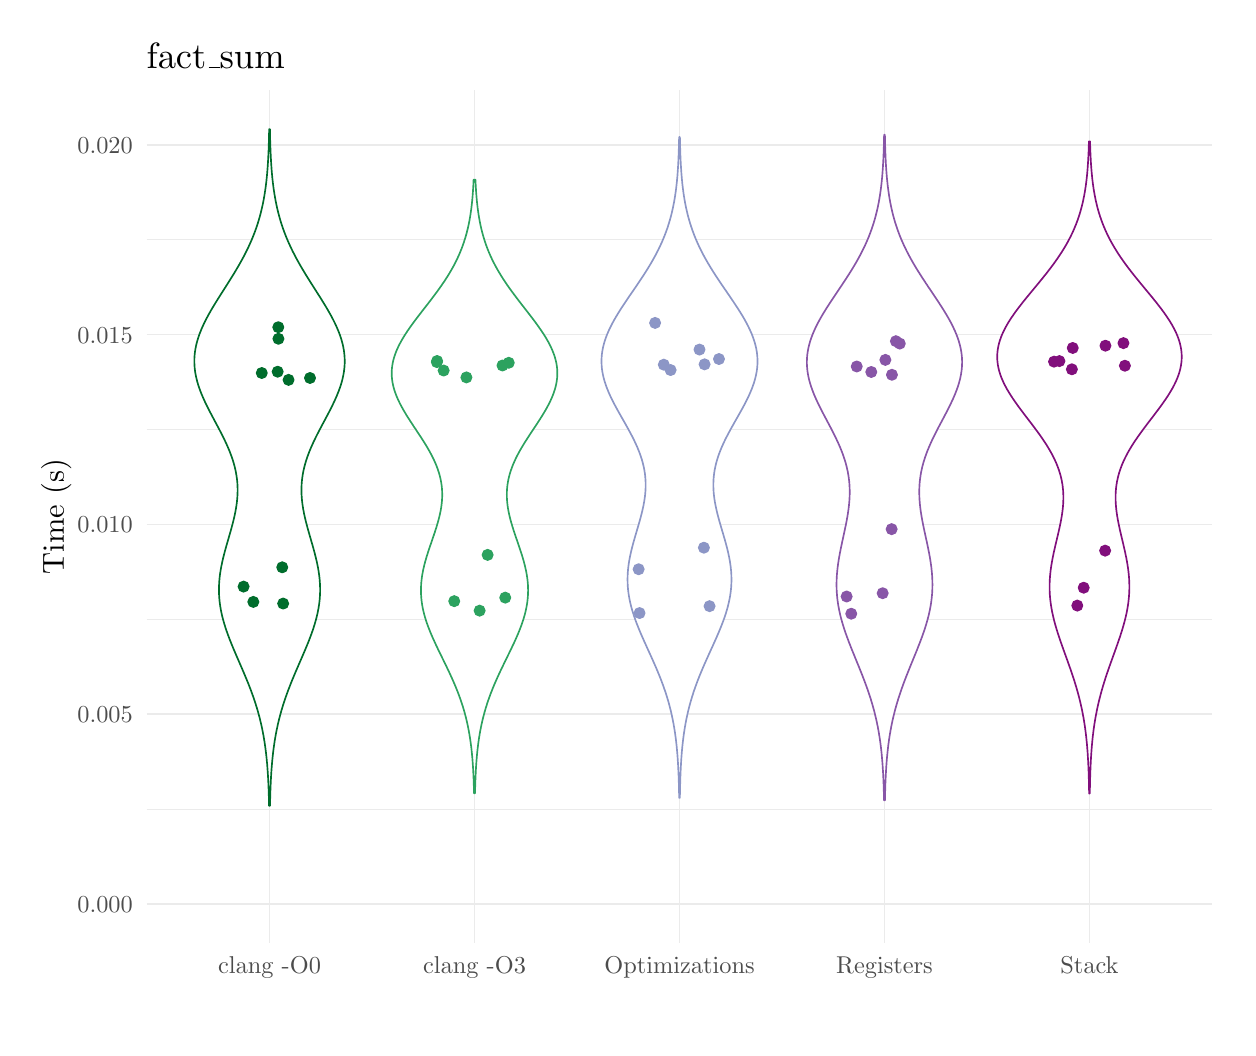
\begin{tikzpicture}[x=1pt,y=1pt]
\definecolor{fillColor}{RGB}{255,255,255}
\path[use as bounding box,fill=fillColor,fill opacity=0.00] (0,0) rectangle (433.62,361.35);
\begin{scope}
\path[clip] ( 42.95, 30.69) rectangle (428.12,338.69);
\definecolor{drawColor}{gray}{0.92}

\path[draw=drawColor,line width= 0.3pt,line join=round] ( 42.95, 78.98) --
	(428.12, 78.98);

\path[draw=drawColor,line width= 0.3pt,line join=round] ( 42.95,147.56) --
	(428.12,147.56);

\path[draw=drawColor,line width= 0.3pt,line join=round] ( 42.95,216.14) --
	(428.12,216.14);

\path[draw=drawColor,line width= 0.3pt,line join=round] ( 42.95,284.72) --
	(428.12,284.72);

\path[draw=drawColor,line width= 0.6pt,line join=round] ( 42.95, 44.69) --
	(428.12, 44.69);

\path[draw=drawColor,line width= 0.6pt,line join=round] ( 42.95,113.27) --
	(428.12,113.27);

\path[draw=drawColor,line width= 0.6pt,line join=round] ( 42.95,181.85) --
	(428.12,181.85);

\path[draw=drawColor,line width= 0.6pt,line join=round] ( 42.95,250.43) --
	(428.12,250.43);

\path[draw=drawColor,line width= 0.6pt,line join=round] ( 42.95,319.01) --
	(428.12,319.01);

\path[draw=drawColor,line width= 0.6pt,line join=round] ( 87.40, 30.69) --
	( 87.40,338.69);

\path[draw=drawColor,line width= 0.6pt,line join=round] (161.47, 30.69) --
	(161.47,338.69);

\path[draw=drawColor,line width= 0.6pt,line join=round] (235.54, 30.69) --
	(235.54,338.69);

\path[draw=drawColor,line width= 0.6pt,line join=round] (309.61, 30.69) --
	(309.61,338.69);

\path[draw=drawColor,line width= 0.6pt,line join=round] (383.68, 30.69) --
	(383.68,338.69);
\definecolor{drawColor}{RGB}{0,109,44}
\definecolor{fillColor}{RGB}{255,255,255}

\path[draw=drawColor,line width= 0.6pt,line join=round,line cap=round,fill=fillColor] ( 87.23, 80.16) --
	( 87.22, 80.63) --
	( 87.21, 81.11) --
	( 87.20, 81.59) --
	( 87.19, 82.07) --
	( 87.18, 82.55) --
	( 87.16, 83.03) --
	( 87.15, 83.51) --
	( 87.13, 83.98) --
	( 87.12, 84.46) --
	( 87.10, 84.94) --
	( 87.09, 85.42) --
	( 87.07, 85.90) --
	( 87.05, 86.38) --
	( 87.03, 86.86) --
	( 87.01, 87.33) --
	( 86.99, 87.81) --
	( 86.97, 88.29) --
	( 86.95, 88.77) --
	( 86.93, 89.25) --
	( 86.90, 89.73) --
	( 86.88, 90.20) --
	( 86.85, 90.68) --
	( 86.82, 91.16) --
	( 86.79, 91.64) --
	( 86.76, 92.12) --
	( 86.73, 92.60) --
	( 86.69, 93.08) --
	( 86.66, 93.55) --
	( 86.62, 94.03) --
	( 86.59, 94.51) --
	( 86.55, 94.99) --
	( 86.51, 95.47) --
	( 86.46, 95.95) --
	( 86.42, 96.43) --
	( 86.37, 96.90) --
	( 86.33, 97.38) --
	( 86.28, 97.86) --
	( 86.23, 98.34) --
	( 86.17, 98.82) --
	( 86.12, 99.30) --
	( 86.06, 99.78) --
	( 86.00,100.25) --
	( 85.94,100.73) --
	( 85.88,101.21) --
	( 85.81,101.69) --
	( 85.74,102.17) --
	( 85.67,102.65) --
	( 85.60,103.13) --
	( 85.53,103.60) --
	( 85.45,104.08) --
	( 85.37,104.56) --
	( 85.29,105.04) --
	( 85.21,105.52) --
	( 85.12,106.00) --
	( 85.03,106.48) --
	( 84.94,106.95) --
	( 84.84,107.43) --
	( 84.75,107.91) --
	( 84.65,108.39) --
	( 84.54,108.87) --
	( 84.44,109.35) --
	( 84.33,109.83) --
	( 84.22,110.30) --
	( 84.10,110.78) --
	( 83.99,111.26) --
	( 83.87,111.74) --
	( 83.75,112.22) --
	( 83.62,112.70) --
	( 83.49,113.18) --
	( 83.36,113.65) --
	( 83.23,114.13) --
	( 83.09,114.61) --
	( 82.95,115.09) --
	( 82.81,115.57) --
	( 82.66,116.05) --
	( 82.51,116.53) --
	( 82.36,117.00) --
	( 82.21,117.48) --
	( 82.05,117.96) --
	( 81.89,118.44) --
	( 81.73,118.92) --
	( 81.56,119.40) --
	( 81.40,119.87) --
	( 81.23,120.35) --
	( 81.05,120.83) --
	( 80.88,121.31) --
	( 80.70,121.79) --
	( 80.52,122.27) --
	( 80.34,122.75) --
	( 80.15,123.22) --
	( 79.97,123.70) --
	( 79.78,124.18) --
	( 79.59,124.66) --
	( 79.39,125.14) --
	( 79.20,125.62) --
	( 79.00,126.10) --
	( 78.80,126.57) --
	( 78.60,127.05) --
	( 78.40,127.53) --
	( 78.20,128.01) --
	( 78.00,128.49) --
	( 77.79,128.97) --
	( 77.59,129.45) --
	( 77.38,129.92) --
	( 77.18,130.40) --
	( 76.97,130.88) --
	( 76.76,131.36) --
	( 76.55,131.84) --
	( 76.34,132.32) --
	( 76.14,132.80) --
	( 75.93,133.27) --
	( 75.72,133.75) --
	( 75.51,134.23) --
	( 75.31,134.71) --
	( 75.10,135.19) --
	( 74.90,135.67) --
	( 74.69,136.15) --
	( 74.49,136.62) --
	( 74.29,137.10) --
	( 74.09,137.58) --
	( 73.90,138.06) --
	( 73.70,138.54) --
	( 73.51,139.02) --
	( 73.32,139.50) --
	( 73.13,139.97) --
	( 72.94,140.45) --
	( 72.76,140.93) --
	( 72.58,141.41) --
	( 72.40,141.89) --
	( 72.23,142.37) --
	( 72.06,142.85) --
	( 71.89,143.32) --
	( 71.72,143.80) --
	( 71.57,144.28) --
	( 71.41,144.76) --
	( 71.26,145.24) --
	( 71.11,145.72) --
	( 70.97,146.19) --
	( 70.83,146.67) --
	( 70.70,147.15) --
	( 70.57,147.63) --
	( 70.44,148.11) --
	( 70.32,148.59) --
	( 70.21,149.07) --
	( 70.10,149.54) --
	( 70.00,150.02) --
	( 69.90,150.50) --
	( 69.81,150.98) --
	( 69.72,151.46) --
	( 69.64,151.94) --
	( 69.56,152.42) --
	( 69.50,152.89) --
	( 69.43,153.37) --
	( 69.37,153.85) --
	( 69.32,154.33) --
	( 69.28,154.81) --
	( 69.23,155.29) --
	( 69.20,155.77) --
	( 69.17,156.24) --
	( 69.15,156.72) --
	( 69.13,157.20) --
	( 69.12,157.68) --
	( 69.12,158.16) --
	( 69.12,158.64) --
	( 69.13,159.12) --
	( 69.14,159.59) --
	( 69.16,160.07) --
	( 69.19,160.55) --
	( 69.22,161.03) --
	( 69.25,161.51) --
	( 69.30,161.99) --
	( 69.34,162.47) --
	( 69.39,162.94) --
	( 69.45,163.42) --
	( 69.51,163.90) --
	( 69.58,164.38) --
	( 69.66,164.86) --
	( 69.73,165.34) --
	( 69.82,165.82) --
	( 69.90,166.29) --
	( 69.99,166.77) --
	( 70.09,167.25) --
	( 70.19,167.73) --
	( 70.29,168.21) --
	( 70.40,168.69) --
	( 70.51,169.17) --
	( 70.62,169.64) --
	( 70.74,170.12) --
	( 70.86,170.60) --
	( 70.98,171.08) --
	( 71.11,171.56) --
	( 71.23,172.04) --
	( 71.36,172.51) --
	( 71.49,172.99) --
	( 71.63,173.47) --
	( 71.76,173.95) --
	( 71.90,174.43) --
	( 72.03,174.91) --
	( 72.17,175.39) --
	( 72.31,175.86) --
	( 72.45,176.34) --
	( 72.59,176.82) --
	( 72.72,177.30) --
	( 72.86,177.78) --
	( 73.00,178.26) --
	( 73.14,178.74) --
	( 73.27,179.21) --
	( 73.41,179.69) --
	( 73.54,180.17) --
	( 73.67,180.65) --
	( 73.80,181.13) --
	( 73.93,181.61) --
	( 74.06,182.09) --
	( 74.18,182.56) --
	( 74.30,183.04) --
	( 74.42,183.52) --
	( 74.53,184.00) --
	( 74.64,184.48) --
	( 74.75,184.96) --
	( 74.85,185.44) --
	( 74.95,185.91) --
	( 75.04,186.39) --
	( 75.13,186.87) --
	( 75.22,187.35) --
	( 75.30,187.83) --
	( 75.38,188.31) --
	( 75.45,188.79) --
	( 75.51,189.26) --
	( 75.58,189.74) --
	( 75.63,190.22) --
	( 75.68,190.70) --
	( 75.72,191.18) --
	( 75.76,191.66) --
	( 75.79,192.14) --
	( 75.82,192.61) --
	( 75.84,193.09) --
	( 75.85,193.57) --
	( 75.86,194.05) --
	( 75.86,194.53) --
	( 75.85,195.01) --
	( 75.84,195.49) --
	( 75.82,195.96) --
	( 75.79,196.44) --
	( 75.76,196.92) --
	( 75.71,197.40) --
	( 75.67,197.88) --
	( 75.61,198.36) --
	( 75.55,198.83) --
	( 75.48,199.31) --
	( 75.40,199.79) --
	( 75.32,200.27) --
	( 75.23,200.75) --
	( 75.14,201.23) --
	( 75.03,201.71) --
	( 74.92,202.18) --
	( 74.81,202.66) --
	( 74.68,203.14) --
	( 74.55,203.62) --
	( 74.41,204.10) --
	( 74.27,204.58) --
	( 74.12,205.06) --
	( 73.97,205.53) --
	( 73.80,206.01) --
	( 73.64,206.49) --
	( 73.46,206.97) --
	( 73.28,207.45) --
	( 73.10,207.93) --
	( 72.91,208.41) --
	( 72.71,208.88) --
	( 72.51,209.36) --
	( 72.31,209.84) --
	( 72.10,210.32) --
	( 71.88,210.80) --
	( 71.66,211.28) --
	( 71.44,211.76) --
	( 71.21,212.23) --
	( 70.98,212.71) --
	( 70.75,213.19) --
	( 70.51,213.67) --
	( 70.27,214.15) --
	( 70.03,214.63) --
	( 69.78,215.11) --
	( 69.53,215.58) --
	( 69.29,216.06) --
	( 69.03,216.54) --
	( 68.78,217.02) --
	( 68.53,217.50) --
	( 68.27,217.98) --
	( 68.02,218.46) --
	( 67.76,218.93) --
	( 67.51,219.41) --
	( 67.25,219.89) --
	( 67.00,220.37) --
	( 66.74,220.85) --
	( 66.49,221.33) --
	( 66.24,221.81) --
	( 65.99,222.28) --
	( 65.74,222.76) --
	( 65.49,223.24) --
	( 65.25,223.72) --
	( 65.01,224.20) --
	( 64.77,224.68) --
	( 64.54,225.15) --
	( 64.31,225.63) --
	( 64.08,226.11) --
	( 63.86,226.59) --
	( 63.64,227.07) --
	( 63.43,227.55) --
	( 63.22,228.03) --
	( 63.02,228.50) --
	( 62.82,228.98) --
	( 62.63,229.46) --
	( 62.44,229.94) --
	( 62.26,230.42) --
	( 62.09,230.90) --
	( 61.92,231.38) --
	( 61.76,231.85) --
	( 61.61,232.33) --
	( 61.46,232.81) --
	( 61.32,233.29) --
	( 61.19,233.77) --
	( 61.07,234.25) --
	( 60.96,234.73) --
	( 60.85,235.20) --
	( 60.75,235.68) --
	( 60.66,236.16) --
	( 60.57,236.64) --
	( 60.50,237.12) --
	( 60.44,237.60) --
	( 60.38,238.08) --
	( 60.33,238.55) --
	( 60.30,239.03) --
	( 60.27,239.51) --
	( 60.25,239.99) --
	( 60.24,240.47) --
	( 60.23,240.95) --
	( 60.24,241.43) --
	( 60.25,241.90) --
	( 60.28,242.38) --
	( 60.31,242.86) --
	( 60.36,243.34) --
	( 60.41,243.82) --
	( 60.47,244.30) --
	( 60.54,244.78) --
	( 60.62,245.25) --
	( 60.71,245.73) --
	( 60.80,246.21) --
	( 60.91,246.69) --
	( 61.02,247.17) --
	( 61.15,247.65) --
	( 61.28,248.13) --
	( 61.42,248.60) --
	( 61.57,249.08) --
	( 61.72,249.56) --
	( 61.88,250.04) --
	( 62.05,250.52) --
	( 62.23,251.00) --
	( 62.42,251.47) --
	( 62.61,251.95) --
	( 62.81,252.43) --
	( 63.01,252.91) --
	( 63.23,253.39) --
	( 63.45,253.87) --
	( 63.67,254.35) --
	( 63.90,254.82) --
	( 64.14,255.30) --
	( 64.38,255.78) --
	( 64.63,256.26) --
	( 64.88,256.74) --
	( 65.14,257.22) --
	( 65.40,257.70) --
	( 65.67,258.17) --
	( 65.94,258.65) --
	( 66.21,259.13) --
	( 66.49,259.61) --
	( 66.77,260.09) --
	( 67.06,260.57) --
	( 67.35,261.05) --
	( 67.64,261.52) --
	( 67.93,262.00) --
	( 68.23,262.48) --
	( 68.53,262.96) --
	( 68.82,263.44) --
	( 69.13,263.92) --
	( 69.43,264.40) --
	( 69.73,264.87) --
	( 70.03,265.35) --
	( 70.34,265.83) --
	( 70.64,266.31) --
	( 70.95,266.79) --
	( 71.25,267.27) --
	( 71.56,267.75) --
	( 71.86,268.22) --
	( 72.17,268.70) --
	( 72.47,269.18) --
	( 72.77,269.66) --
	( 73.07,270.14) --
	( 73.37,270.62) --
	( 73.67,271.10) --
	( 73.97,271.57) --
	( 74.26,272.05) --
	( 74.56,272.53) --
	( 74.85,273.01) --
	( 75.13,273.49) --
	( 75.42,273.97) --
	( 75.70,274.45) --
	( 75.98,274.92) --
	( 76.26,275.40) --
	( 76.53,275.88) --
	( 76.81,276.36) --
	( 77.07,276.84) --
	( 77.34,277.32) --
	( 77.60,277.79) --
	( 77.86,278.27) --
	( 78.11,278.75) --
	( 78.36,279.23) --
	( 78.61,279.71) --
	( 78.85,280.19) --
	( 79.09,280.67) --
	( 79.32,281.14) --
	( 79.56,281.62) --
	( 79.78,282.10) --
	( 80.01,282.58) --
	( 80.22,283.06) --
	( 80.44,283.54) --
	( 80.65,284.02) --
	( 80.86,284.49) --
	( 81.06,284.97) --
	( 81.26,285.45) --
	( 81.45,285.93) --
	( 81.64,286.41) --
	( 81.83,286.89) --
	( 82.01,287.37) --
	( 82.19,287.84) --
	( 82.36,288.32) --
	( 82.53,288.80) --
	( 82.70,289.28) --
	( 82.86,289.76) --
	( 83.02,290.24) --
	( 83.17,290.72) --
	( 83.32,291.19) --
	( 83.46,291.67) --
	( 83.61,292.15) --
	( 83.74,292.63) --
	( 83.88,293.11) --
	( 84.01,293.59) --
	( 84.13,294.07) --
	( 84.26,294.54) --
	( 84.37,295.02) --
	( 84.49,295.50) --
	( 84.60,295.98) --
	( 84.71,296.46) --
	( 84.82,296.94) --
	( 84.92,297.42) --
	( 85.02,297.89) --
	( 85.11,298.37) --
	( 85.21,298.85) --
	( 85.30,299.33) --
	( 85.38,299.81) --
	( 85.47,300.29) --
	( 85.55,300.77) --
	( 85.63,301.24) --
	( 85.70,301.72) --
	( 85.77,302.20) --
	( 85.84,302.68) --
	( 85.91,303.16) --
	( 85.98,303.64) --
	( 86.04,304.12) --
	( 86.10,304.59) --
	( 86.16,305.07) --
	( 86.22,305.55) --
	( 86.27,306.03) --
	( 86.32,306.51) --
	( 86.37,306.99) --
	( 86.42,307.46) --
	( 86.46,307.94) --
	( 86.51,308.42) --
	( 86.55,308.90) --
	( 86.59,309.38) --
	( 86.63,309.86) --
	( 86.67,310.34) --
	( 86.70,310.81) --
	( 86.74,311.29) --
	( 86.77,311.77) --
	( 86.80,312.25) --
	( 86.83,312.73) --
	( 86.86,313.21) --
	( 86.89,313.69) --
	( 86.91,314.16) --
	( 86.94,314.64) --
	( 86.96,315.12) --
	( 86.98,315.60) --
	( 87.01,316.08) --
	( 87.03,316.56) --
	( 87.05,317.04) --
	( 87.07,317.51) --
	( 87.08,317.99) --
	( 87.10,318.47) --
	( 87.12,318.95) --
	( 87.13,319.43) --
	( 87.15,319.91) --
	( 87.16,320.39) --
	( 87.17,320.86) --
	( 87.19,321.34) --
	( 87.20,321.82) --
	( 87.21,322.30) --
	( 87.22,322.78) --
	( 87.23,323.26) --
	( 87.24,323.74) --
	( 87.25,324.21) --
	( 87.26,324.69) --
	( 87.54,324.69) --
	( 87.54,324.21) --
	( 87.55,323.74) --
	( 87.56,323.26) --
	( 87.57,322.78) --
	( 87.58,322.30) --
	( 87.59,321.82) --
	( 87.61,321.34) --
	( 87.62,320.86) --
	( 87.63,320.39) --
	( 87.65,319.91) --
	( 87.66,319.43) --
	( 87.68,318.95) --
	( 87.69,318.47) --
	( 87.71,317.99) --
	( 87.73,317.51) --
	( 87.75,317.04) --
	( 87.77,316.56) --
	( 87.79,316.08) --
	( 87.81,315.60) --
	( 87.83,315.12) --
	( 87.85,314.64) --
	( 87.88,314.16) --
	( 87.91,313.69) --
	( 87.93,313.21) --
	( 87.96,312.73) --
	( 87.99,312.25) --
	( 88.02,311.77) --
	( 88.06,311.29) --
	( 88.09,310.81) --
	( 88.12,310.34) --
	( 88.16,309.86) --
	( 88.20,309.38) --
	( 88.24,308.90) --
	( 88.28,308.42) --
	( 88.33,307.94) --
	( 88.37,307.46) --
	( 88.42,306.99) --
	( 88.47,306.51) --
	( 88.52,306.03) --
	( 88.58,305.55) --
	( 88.63,305.07) --
	( 88.69,304.59) --
	( 88.75,304.12) --
	( 88.81,303.64) --
	( 88.88,303.16) --
	( 88.95,302.68) --
	( 89.02,302.20) --
	( 89.09,301.72) --
	( 89.17,301.24) --
	( 89.24,300.77) --
	( 89.33,300.29) --
	( 89.41,299.81) --
	( 89.50,299.33) --
	( 89.58,298.85) --
	( 89.68,298.37) --
	( 89.77,297.89) --
	( 89.87,297.42) --
	( 89.98,296.94) --
	( 90.08,296.46) --
	( 90.19,295.98) --
	( 90.30,295.50) --
	( 90.42,295.02) --
	( 90.54,294.54) --
	( 90.66,294.07) --
	( 90.79,293.59) --
	( 90.92,293.11) --
	( 91.05,292.63) --
	( 91.19,292.15) --
	( 91.33,291.67) --
	( 91.47,291.19) --
	( 91.62,290.72) --
	( 91.78,290.24) --
	( 91.93,289.76) --
	( 92.10,289.28) --
	( 92.26,288.80) --
	( 92.43,288.32) --
	( 92.60,287.84) --
	( 92.78,287.37) --
	( 92.96,286.89) --
	( 93.15,286.41) --
	( 93.34,285.93) --
	( 93.53,285.45) --
	( 93.73,284.97) --
	( 93.93,284.49) --
	( 94.14,284.02) --
	( 94.35,283.54) --
	( 94.57,283.06) --
	( 94.79,282.58) --
	( 95.01,282.10) --
	( 95.24,281.62) --
	( 95.47,281.14) --
	( 95.70,280.67) --
	( 95.94,280.19) --
	( 96.19,279.71) --
	( 96.43,279.23) --
	( 96.68,278.75) --
	( 96.94,278.27) --
	( 97.19,277.79) --
	( 97.45,277.32) --
	( 97.72,276.84) --
	( 97.99,276.36) --
	( 98.26,275.88) --
	( 98.53,275.40) --
	( 98.81,274.92) --
	( 99.09,274.45) --
	( 99.37,273.97) --
	( 99.66,273.49) --
	( 99.95,273.01) --
	(100.24,272.53) --
	(100.53,272.05) --
	(100.82,271.57) --
	(101.12,271.10) --
	(101.42,270.62) --
	(101.72,270.14) --
	(102.02,269.66) --
	(102.32,269.18) --
	(102.62,268.70) --
	(102.93,268.22) --
	(103.23,267.75) --
	(103.54,267.27) --
	(103.84,266.79) --
	(104.15,266.31) --
	(104.45,265.83) --
	(104.76,265.35) --
	(105.06,264.87) --
	(105.37,264.40) --
	(105.67,263.92) --
	(105.97,263.44) --
	(106.27,262.96) --
	(106.56,262.48) --
	(106.86,262.00) --
	(107.15,261.52) --
	(107.44,261.05) --
	(107.73,260.57) --
	(108.02,260.09) --
	(108.30,259.61) --
	(108.58,259.13) --
	(108.85,258.65) --
	(109.12,258.17) --
	(109.39,257.70) --
	(109.65,257.22) --
	(109.91,256.74) --
	(110.16,256.26) --
	(110.41,255.78) --
	(110.65,255.30) --
	(110.89,254.82) --
	(111.12,254.35) --
	(111.35,253.87) --
	(111.56,253.39) --
	(111.78,252.91) --
	(111.98,252.43) --
	(112.18,251.95) --
	(112.38,251.47) --
	(112.56,251.00) --
	(112.74,250.52) --
	(112.91,250.04) --
	(113.07,249.56) --
	(113.23,249.08) --
	(113.38,248.60) --
	(113.51,248.13) --
	(113.64,247.65) --
	(113.77,247.17) --
	(113.88,246.69) --
	(113.99,246.21) --
	(114.08,245.73) --
	(114.17,245.25) --
	(114.25,244.78) --
	(114.32,244.30) --
	(114.38,243.82) --
	(114.43,243.34) --
	(114.48,242.86) --
	(114.51,242.38) --
	(114.54,241.90) --
	(114.55,241.43) --
	(114.56,240.95) --
	(114.56,240.47) --
	(114.55,239.99) --
	(114.52,239.51) --
	(114.50,239.03) --
	(114.46,238.55) --
	(114.41,238.08) --
	(114.35,237.60) --
	(114.29,237.12) --
	(114.22,236.64) --
	(114.13,236.16) --
	(114.04,235.68) --
	(113.94,235.20) --
	(113.84,234.73) --
	(113.72,234.25) --
	(113.60,233.77) --
	(113.47,233.29) --
	(113.33,232.81) --
	(113.19,232.33) --
	(113.03,231.85) --
	(112.87,231.38) --
	(112.70,230.90) --
	(112.53,230.42) --
	(112.35,229.94) --
	(112.16,229.46) --
	(111.97,228.98) --
	(111.78,228.50) --
	(111.57,228.03) --
	(111.36,227.55) --
	(111.15,227.07) --
	(110.93,226.59) --
	(110.71,226.11) --
	(110.48,225.63) --
	(110.25,225.15) --
	(110.02,224.68) --
	(109.78,224.20) --
	(109.54,223.72) --
	(109.30,223.24) --
	(109.05,222.76) --
	(108.81,222.28) --
	(108.56,221.81) --
	(108.30,221.33) --
	(108.05,220.85) --
	(107.80,220.37) --
	(107.54,219.89) --
	(107.29,219.41) --
	(107.03,218.93) --
	(106.77,218.46) --
	(106.52,217.98) --
	(106.26,217.50) --
	(106.01,217.02) --
	(105.76,216.54) --
	(105.51,216.06) --
	(105.26,215.58) --
	(105.01,215.11) --
	(104.76,214.63) --
	(104.52,214.15) --
	(104.28,213.67) --
	(104.04,213.19) --
	(103.81,212.71) --
	(103.58,212.23) --
	(103.35,211.76) --
	(103.13,211.28) --
	(102.91,210.80) --
	(102.70,210.32) --
	(102.48,209.84) --
	(102.28,209.36) --
	(102.08,208.88) --
	(101.88,208.41) --
	(101.69,207.93) --
	(101.51,207.45) --
	(101.33,206.97) --
	(101.15,206.49) --
	(100.99,206.01) --
	(100.82,205.53) --
	(100.67,205.06) --
	(100.52,204.58) --
	(100.38,204.10) --
	(100.24,203.62) --
	(100.11,203.14) --
	( 99.99,202.66) --
	( 99.87,202.18) --
	( 99.76,201.71) --
	( 99.66,201.23) --
	( 99.56,200.75) --
	( 99.47,200.27) --
	( 99.39,199.79) --
	( 99.31,199.31) --
	( 99.24,198.83) --
	( 99.18,198.36) --
	( 99.13,197.88) --
	( 99.08,197.40) --
	( 99.04,196.92) --
	( 99.00,196.44) --
	( 98.98,195.96) --
	( 98.96,195.49) --
	( 98.94,195.01) --
	( 98.94,194.53) --
	( 98.94,194.05) --
	( 98.94,193.57) --
	( 98.96,193.09) --
	( 98.97,192.61) --
	( 99.00,192.14) --
	( 99.03,191.66) --
	( 99.07,191.18) --
	( 99.11,190.70) --
	( 99.16,190.22) --
	( 99.22,189.74) --
	( 99.28,189.26) --
	( 99.34,188.79) --
	( 99.42,188.31) --
	( 99.49,187.83) --
	( 99.57,187.35) --
	( 99.66,186.87) --
	( 99.75,186.39) --
	( 99.84,185.91) --
	( 99.94,185.44) --
	(100.05,184.96) --
	(100.15,184.48) --
	(100.26,184.00) --
	(100.38,183.52) --
	(100.49,183.04) --
	(100.61,182.56) --
	(100.74,182.09) --
	(100.86,181.61) --
	(100.99,181.13) --
	(101.12,180.65) --
	(101.25,180.17) --
	(101.38,179.69) --
	(101.52,179.21) --
	(101.66,178.74) --
	(101.79,178.26) --
	(101.93,177.78) --
	(102.07,177.30) --
	(102.21,176.82) --
	(102.35,176.34) --
	(102.48,175.86) --
	(102.62,175.39) --
	(102.76,174.91) --
	(102.90,174.43) --
	(103.03,173.95) --
	(103.17,173.47) --
	(103.30,172.99) --
	(103.43,172.51) --
	(103.56,172.04) --
	(103.69,171.56) --
	(103.81,171.08) --
	(103.93,170.60) --
	(104.05,170.12) --
	(104.17,169.64) --
	(104.28,169.17) --
	(104.39,168.69) --
	(104.50,168.21) --
	(104.60,167.73) --
	(104.70,167.25) --
	(104.80,166.77) --
	(104.89,166.29) --
	(104.98,165.82) --
	(105.06,165.34) --
	(105.14,164.86) --
	(105.21,164.38) --
	(105.28,163.90) --
	(105.34,163.42) --
	(105.40,162.94) --
	(105.45,162.47) --
	(105.50,161.99) --
	(105.54,161.51) --
	(105.57,161.03) --
	(105.61,160.55) --
	(105.63,160.07) --
	(105.65,159.59) --
	(105.66,159.12) --
	(105.67,158.64) --
	(105.67,158.16) --
	(105.67,157.68) --
	(105.66,157.20) --
	(105.64,156.72) --
	(105.62,156.24) --
	(105.59,155.77) --
	(105.56,155.29) --
	(105.52,154.81) --
	(105.47,154.33) --
	(105.42,153.85) --
	(105.36,153.37) --
	(105.30,152.89) --
	(105.23,152.42) --
	(105.15,151.94) --
	(105.07,151.46) --
	(104.99,150.98) --
	(104.89,150.50) --
	(104.80,150.02) --
	(104.69,149.54) --
	(104.58,149.07) --
	(104.47,148.59) --
	(104.35,148.11) --
	(104.23,147.63) --
	(104.10,147.15) --
	(103.96,146.67) --
	(103.82,146.19) --
	(103.68,145.72) --
	(103.53,145.24) --
	(103.38,144.76) --
	(103.23,144.28) --
	(103.07,143.80) --
	(102.90,143.32) --
	(102.74,142.85) --
	(102.57,142.37) --
	(102.39,141.89) --
	(102.22,141.41) --
	(102.03,140.93) --
	(101.85,140.45) --
	(101.67,139.97) --
	(101.48,139.50) --
	(101.29,139.02) --
	(101.09,138.54) --
	(100.90,138.06) --
	(100.70,137.58) --
	(100.50,137.10) --
	(100.30,136.62) --
	(100.10,136.15) --
	( 99.89,135.67) --
	( 99.69,135.19) --
	( 99.48,134.71) --
	( 99.28,134.23) --
	( 99.07,133.75) --
	( 98.86,133.27) --
	( 98.66,132.80) --
	( 98.45,132.32) --
	( 98.24,131.84) --
	( 98.03,131.36) --
	( 97.82,130.88) --
	( 97.62,130.40) --
	( 97.41,129.92) --
	( 97.20,129.45) --
	( 97.00,128.97) --
	( 96.79,128.49) --
	( 96.59,128.01) --
	( 96.39,127.53) --
	( 96.19,127.05) --
	( 95.99,126.57) --
	( 95.79,126.10) --
	( 95.59,125.62) --
	( 95.40,125.14) --
	( 95.21,124.66) --
	( 95.02,124.18) --
	( 94.83,123.70) --
	( 94.64,123.22) --
	( 94.46,122.75) --
	( 94.27,122.27) --
	( 94.09,121.79) --
	( 93.92,121.31) --
	( 93.74,120.83) --
	( 93.57,120.35) --
	( 93.40,119.87) --
	( 93.23,119.40) --
	( 93.06,118.92) --
	( 92.90,118.44) --
	( 92.74,117.96) --
	( 92.59,117.48) --
	( 92.43,117.00) --
	( 92.28,116.53) --
	( 92.13,116.05) --
	( 91.99,115.57) --
	( 91.84,115.09) --
	( 91.70,114.61) --
	( 91.57,114.13) --
	( 91.43,113.65) --
	( 91.30,113.18) --
	( 91.17,112.70) --
	( 91.05,112.22) --
	( 90.92,111.74) --
	( 90.80,111.26) --
	( 90.69,110.78) --
	( 90.57,110.30) --
	( 90.46,109.83) --
	( 90.35,109.35) --
	( 90.25,108.87) --
	( 90.15,108.39) --
	( 90.05,107.91) --
	( 89.95,107.43) --
	( 89.85,106.95) --
	( 89.76,106.48) --
	( 89.67,106.00) --
	( 89.59,105.52) --
	( 89.50,105.04) --
	( 89.42,104.56) --
	( 89.34,104.08) --
	( 89.26,103.60) --
	( 89.19,103.13) --
	( 89.12,102.65) --
	( 89.05,102.17) --
	( 88.98,101.69) --
	( 88.92,101.21) --
	( 88.85,100.73) --
	( 88.79,100.25) --
	( 88.73, 99.78) --
	( 88.67, 99.30) --
	( 88.62, 98.82) --
	( 88.57, 98.34) --
	( 88.52, 97.86) --
	( 88.47, 97.38) --
	( 88.42, 96.90) --
	( 88.37, 96.43) --
	( 88.33, 95.95) --
	( 88.29, 95.47) --
	( 88.25, 94.99) --
	( 88.21, 94.51) --
	( 88.17, 94.03) --
	( 88.13, 93.55) --
	( 88.10, 93.08) --
	( 88.06, 92.60) --
	( 88.03, 92.12) --
	( 88.00, 91.64) --
	( 87.97, 91.16) --
	( 87.94, 90.68) --
	( 87.92, 90.20) --
	( 87.89, 89.73) --
	( 87.87, 89.25) --
	( 87.84, 88.77) --
	( 87.82, 88.29) --
	( 87.80, 87.81) --
	( 87.78, 87.33) --
	( 87.76, 86.86) --
	( 87.74, 86.38) --
	( 87.72, 85.90) --
	( 87.70, 85.42) --
	( 87.69, 84.94) --
	( 87.67, 84.46) --
	( 87.66, 83.98) --
	( 87.64, 83.51) --
	( 87.63, 83.03) --
	( 87.62, 82.55) --
	( 87.60, 82.07) --
	( 87.59, 81.59) --
	( 87.58, 81.11) --
	( 87.57, 80.63) --
	( 87.56, 80.16) --
	( 87.23, 80.16) --
	cycle;
\definecolor{drawColor}{RGB}{44,162,95}

\path[draw=drawColor,line width= 0.6pt,line join=round,line cap=round,fill=fillColor] (161.29, 84.71) --
	(161.28, 85.14) --
	(161.27, 85.57) --
	(161.26, 86.01) --
	(161.25, 86.44) --
	(161.24, 86.88) --
	(161.22, 87.31) --
	(161.21, 87.74) --
	(161.19, 88.18) --
	(161.18, 88.61) --
	(161.16, 89.05) --
	(161.15, 89.48) --
	(161.13, 89.91) --
	(161.11, 90.35) --
	(161.09, 90.78) --
	(161.07, 91.21) --
	(161.05, 91.65) --
	(161.03, 92.08) --
	(161.01, 92.52) --
	(160.99, 92.95) --
	(160.96, 93.38) --
	(160.94, 93.82) --
	(160.91, 94.25) --
	(160.88, 94.69) --
	(160.85, 95.12) --
	(160.82, 95.55) --
	(160.79, 95.99) --
	(160.76, 96.42) --
	(160.72, 96.86) --
	(160.69, 97.29) --
	(160.65, 97.72) --
	(160.61, 98.16) --
	(160.57, 98.59) --
	(160.53, 99.02) --
	(160.49, 99.46) --
	(160.44, 99.89) --
	(160.40,100.33) --
	(160.35,100.76) --
	(160.30,101.19) --
	(160.25,101.63) --
	(160.19,102.06) --
	(160.14,102.50) --
	(160.08,102.93) --
	(160.02,103.36) --
	(159.96,103.80) --
	(159.90,104.23) --
	(159.83,104.67) --
	(159.76,105.10) --
	(159.69,105.53) --
	(159.62,105.97) --
	(159.55,106.40) --
	(159.47,106.83) --
	(159.39,107.27) --
	(159.31,107.70) --
	(159.23,108.14) --
	(159.14,108.57) --
	(159.05,109.00) --
	(158.96,109.44) --
	(158.87,109.87) --
	(158.77,110.31) --
	(158.67,110.74) --
	(158.57,111.17) --
	(158.46,111.61) --
	(158.36,112.04) --
	(158.25,112.48) --
	(158.13,112.91) --
	(158.02,113.34) --
	(157.90,113.78) --
	(157.78,114.21) --
	(157.66,114.65) --
	(157.53,115.08) --
	(157.40,115.51) --
	(157.27,115.95) --
	(157.13,116.38) --
	(156.99,116.81) --
	(156.85,117.25) --
	(156.71,117.68) --
	(156.56,118.12) --
	(156.41,118.55) --
	(156.26,118.98) --
	(156.10,119.42) --
	(155.94,119.85) --
	(155.78,120.29) --
	(155.62,120.72) --
	(155.45,121.15) --
	(155.29,121.59) --
	(155.11,122.02) --
	(154.94,122.46) --
	(154.76,122.89) --
	(154.59,123.32) --
	(154.40,123.76) --
	(154.22,124.19) --
	(154.03,124.62) --
	(153.85,125.06) --
	(153.65,125.49) --
	(153.46,125.93) --
	(153.27,126.36) --
	(153.07,126.79) --
	(152.87,127.23) --
	(152.67,127.66) --
	(152.47,128.10) --
	(152.27,128.53) --
	(152.07,128.96) --
	(151.86,129.40) --
	(151.65,129.83) --
	(151.44,130.27) --
	(151.24,130.70) --
	(151.02,131.13) --
	(150.81,131.57) --
	(150.60,132.00) --
	(150.39,132.43) --
	(150.18,132.87) --
	(149.97,133.30) --
	(149.75,133.74) --
	(149.54,134.17) --
	(149.33,134.60) --
	(149.12,135.04) --
	(148.90,135.47) --
	(148.69,135.91) --
	(148.48,136.34) --
	(148.27,136.77) --
	(148.07,137.21) --
	(147.86,137.64) --
	(147.65,138.08) --
	(147.45,138.51) --
	(147.25,138.94) --
	(147.05,139.38) --
	(146.85,139.81) --
	(146.65,140.24) --
	(146.46,140.68) --
	(146.26,141.11) --
	(146.08,141.55) --
	(145.89,141.98) --
	(145.71,142.41) --
	(145.53,142.85) --
	(145.35,143.28) --
	(145.18,143.72) --
	(145.00,144.15) --
	(144.84,144.58) --
	(144.67,145.02) --
	(144.52,145.45) --
	(144.36,145.89) --
	(144.21,146.32) --
	(144.07,146.75) --
	(143.92,147.19) --
	(143.79,147.62) --
	(143.65,148.05) --
	(143.53,148.49) --
	(143.40,148.92) --
	(143.29,149.36) --
	(143.17,149.79) --
	(143.07,150.22) --
	(142.97,150.66) --
	(142.87,151.09) --
	(142.78,151.53) --
	(142.69,151.96) --
	(142.61,152.39) --
	(142.54,152.83) --
	(142.47,153.26) --
	(142.41,153.70) --
	(142.35,154.13) --
	(142.30,154.56) --
	(142.26,155.00) --
	(142.22,155.43) --
	(142.19,155.86) --
	(142.16,156.30) --
	(142.14,156.73) --
	(142.12,157.17) --
	(142.11,157.60) --
	(142.11,158.03) --
	(142.11,158.47) --
	(142.12,158.90) --
	(142.14,159.34) --
	(142.16,159.77) --
	(142.18,160.20) --
	(142.22,160.64) --
	(142.25,161.07) --
	(142.30,161.51) --
	(142.35,161.94) --
	(142.40,162.37) --
	(142.46,162.81) --
	(142.52,163.24) --
	(142.59,163.67) --
	(142.67,164.11) --
	(142.75,164.54) --
	(142.83,164.98) --
	(142.92,165.41) --
	(143.01,165.84) --
	(143.11,166.28) --
	(143.21,166.71) --
	(143.32,167.15) --
	(143.43,167.58) --
	(143.54,168.01) --
	(143.66,168.45) --
	(143.78,168.88) --
	(143.91,169.32) --
	(144.03,169.75) --
	(144.16,170.18) --
	(144.29,170.62) --
	(144.43,171.05) --
	(144.57,171.48) --
	(144.71,171.92) --
	(144.85,172.35) --
	(144.99,172.79) --
	(145.14,173.22) --
	(145.28,173.65) --
	(145.43,174.09) --
	(145.58,174.52) --
	(145.73,174.96) --
	(145.87,175.39) --
	(146.02,175.82) --
	(146.17,176.26) --
	(146.32,176.69) --
	(146.47,177.13) --
	(146.62,177.56) --
	(146.77,177.99) --
	(146.91,178.43) --
	(147.06,178.86) --
	(147.20,179.29) --
	(147.34,179.73) --
	(147.48,180.16) --
	(147.62,180.60) --
	(147.75,181.03) --
	(147.88,181.46) --
	(148.01,181.90) --
	(148.14,182.33) --
	(148.26,182.77) --
	(148.38,183.20) --
	(148.50,183.63) --
	(148.61,184.07) --
	(148.72,184.50) --
	(148.82,184.94) --
	(148.92,185.37) --
	(149.02,185.80) --
	(149.11,186.24) --
	(149.19,186.67) --
	(149.28,187.10) --
	(149.35,187.54) --
	(149.42,187.97) --
	(149.48,188.41) --
	(149.54,188.84) --
	(149.59,189.27) --
	(149.64,189.71) --
	(149.68,190.14) --
	(149.72,190.58) --
	(149.74,191.01) --
	(149.77,191.44) --
	(149.78,191.88) --
	(149.79,192.31) --
	(149.79,192.75) --
	(149.78,193.18) --
	(149.77,193.61) --
	(149.75,194.05) --
	(149.73,194.48) --
	(149.69,194.91) --
	(149.65,195.35) --
	(149.60,195.78) --
	(149.55,196.22) --
	(149.48,196.65) --
	(149.41,197.08) --
	(149.34,197.52) --
	(149.25,197.95) --
	(149.16,198.39) --
	(149.06,198.82) --
	(148.95,199.25) --
	(148.84,199.69) --
	(148.72,200.12) --
	(148.59,200.56) --
	(148.45,200.99) --
	(148.31,201.42) --
	(148.16,201.86) --
	(148.00,202.29) --
	(147.84,202.73) --
	(147.67,203.16) --
	(147.49,203.59) --
	(147.31,204.03) --
	(147.12,204.46) --
	(146.92,204.89) --
	(146.72,205.33) --
	(146.51,205.76) --
	(146.30,206.20) --
	(146.08,206.63) --
	(145.85,207.06) --
	(145.62,207.50) --
	(145.39,207.93) --
	(145.14,208.37) --
	(144.90,208.80) --
	(144.65,209.23) --
	(144.40,209.67) --
	(144.14,210.10) --
	(143.88,210.54) --
	(143.61,210.97) --
	(143.34,211.40) --
	(143.07,211.84) --
	(142.79,212.27) --
	(142.52,212.70) --
	(142.24,213.14) --
	(141.96,213.57) --
	(141.67,214.01) --
	(141.39,214.44) --
	(141.10,214.87) --
	(140.81,215.31) --
	(140.53,215.74) --
	(140.24,216.18) --
	(139.95,216.61) --
	(139.66,217.04) --
	(139.37,217.48) --
	(139.09,217.91) --
	(138.80,218.35) --
	(138.52,218.78) --
	(138.24,219.21) --
	(137.96,219.65) --
	(137.68,220.08) --
	(137.40,220.51) --
	(137.13,220.95) --
	(136.86,221.38) --
	(136.60,221.82) --
	(136.34,222.25) --
	(136.08,222.68) --
	(135.83,223.12) --
	(135.58,223.55) --
	(135.34,223.99) --
	(135.10,224.42) --
	(134.87,224.85) --
	(134.64,225.29) --
	(134.42,225.72) --
	(134.21,226.16) --
	(134.00,226.59) --
	(133.80,227.02) --
	(133.61,227.46) --
	(133.42,227.89) --
	(133.25,228.32) --
	(133.08,228.76) --
	(132.92,229.19) --
	(132.76,229.63) --
	(132.62,230.06) --
	(132.48,230.49) --
	(132.35,230.93) --
	(132.23,231.36) --
	(132.12,231.80) --
	(132.02,232.23) --
	(131.93,232.66) --
	(131.85,233.10) --
	(131.77,233.53) --
	(131.71,233.97) --
	(131.66,234.40) --
	(131.62,234.83) --
	(131.58,235.27) --
	(131.56,235.70) --
	(131.55,236.13) --
	(131.54,236.57) --
	(131.55,237.00) --
	(131.57,237.44) --
	(131.60,237.87) --
	(131.63,238.30) --
	(131.68,238.74) --
	(131.74,239.17) --
	(131.81,239.61) --
	(131.88,240.04) --
	(131.97,240.47) --
	(132.07,240.91) --
	(132.17,241.34) --
	(132.29,241.78) --
	(132.41,242.21) --
	(132.55,242.64) --
	(132.69,243.08) --
	(132.85,243.51) --
	(133.01,243.94) --
	(133.18,244.38) --
	(133.36,244.81) --
	(133.55,245.25) --
	(133.75,245.68) --
	(133.95,246.11) --
	(134.17,246.55) --
	(134.38,246.98) --
	(134.62,247.42) --
	(134.85,247.85) --
	(135.09,248.28) --
	(135.34,248.72) --
	(135.60,249.15) --
	(135.86,249.59) --
	(136.13,250.02) --
	(136.40,250.45) --
	(136.68,250.89) --
	(136.97,251.32) --
	(137.25,251.75) --
	(137.55,252.19) --
	(137.85,252.62) --
	(138.15,253.06) --
	(138.46,253.49) --
	(138.77,253.92) --
	(139.09,254.36) --
	(139.41,254.79) --
	(139.73,255.23) --
	(140.05,255.66) --
	(140.38,256.09) --
	(140.71,256.53) --
	(141.04,256.96) --
	(141.37,257.40) --
	(141.71,257.83) --
	(142.04,258.26) --
	(142.38,258.70) --
	(142.71,259.13) --
	(143.05,259.56) --
	(143.39,260.00) --
	(143.73,260.43) --
	(144.06,260.87) --
	(144.40,261.30) --
	(144.74,261.73) --
	(145.07,262.17) --
	(145.41,262.60) --
	(145.74,263.04) --
	(146.07,263.47) --
	(146.40,263.90) --
	(146.73,264.34) --
	(147.05,264.77) --
	(147.38,265.21) --
	(147.70,265.64) --
	(148.02,266.07) --
	(148.33,266.51) --
	(148.64,266.94) --
	(148.95,267.37) --
	(149.26,267.81) --
	(149.56,268.24) --
	(149.86,268.68) --
	(150.15,269.11) --
	(150.45,269.54) --
	(150.74,269.98) --
	(151.02,270.41) --
	(151.30,270.85) --
	(151.58,271.28) --
	(151.85,271.71) --
	(152.12,272.15) --
	(152.38,272.58) --
	(152.64,273.02) --
	(152.89,273.45) --
	(153.14,273.88) --
	(153.39,274.32) --
	(153.63,274.75) --
	(153.87,275.18) --
	(154.10,275.62) --
	(154.33,276.05) --
	(154.55,276.49) --
	(154.77,276.92) --
	(154.98,277.35) --
	(155.19,277.79) --
	(155.40,278.22) --
	(155.59,278.66) --
	(155.79,279.09) --
	(155.98,279.52) --
	(156.17,279.96) --
	(156.35,280.39) --
	(156.52,280.83) --
	(156.70,281.26) --
	(156.87,281.69) --
	(157.03,282.13) --
	(157.19,282.56) --
	(157.34,282.99) --
	(157.49,283.43) --
	(157.64,283.86) --
	(157.78,284.30) --
	(157.92,284.73) --
	(158.06,285.16) --
	(158.19,285.60) --
	(158.31,286.03) --
	(158.44,286.47) --
	(158.56,286.90) --
	(158.67,287.33) --
	(158.78,287.77) --
	(158.89,288.20) --
	(159.00,288.64) --
	(159.10,289.07) --
	(159.19,289.50) --
	(159.29,289.94) --
	(159.38,290.37) --
	(159.47,290.81) --
	(159.55,291.24) --
	(159.64,291.67) --
	(159.71,292.11) --
	(159.79,292.54) --
	(159.86,292.97) --
	(159.94,293.41) --
	(160.00,293.84) --
	(160.07,294.28) --
	(160.13,294.71) --
	(160.19,295.14) --
	(160.25,295.58) --
	(160.31,296.01) --
	(160.36,296.45) --
	(160.41,296.88) --
	(160.46,297.31) --
	(160.51,297.75) --
	(160.56,298.18) --
	(160.60,298.62) --
	(160.64,299.05) --
	(160.68,299.48) --
	(160.72,299.92) --
	(160.76,300.35) --
	(160.79,300.78) --
	(160.83,301.22) --
	(160.86,301.65) --
	(160.89,302.09) --
	(160.92,302.52) --
	(160.95,302.95) --
	(160.98,303.39) --
	(161.00,303.82) --
	(161.03,304.26) --
	(161.05,304.69) --
	(161.07,305.12) --
	(161.09,305.56) --
	(161.11,305.99) --
	(161.13,306.43) --
	(161.80,306.43) --
	(161.82,305.99) --
	(161.84,305.56) --
	(161.86,305.12) --
	(161.88,304.69) --
	(161.91,304.26) --
	(161.93,303.82) --
	(161.96,303.39) --
	(161.98,302.95) --
	(162.01,302.52) --
	(162.04,302.09) --
	(162.07,301.65) --
	(162.10,301.22) --
	(162.14,300.78) --
	(162.17,300.35) --
	(162.21,299.92) --
	(162.25,299.48) --
	(162.29,299.05) --
	(162.33,298.62) --
	(162.38,298.18) --
	(162.42,297.75) --
	(162.47,297.31) --
	(162.52,296.88) --
	(162.57,296.45) --
	(162.62,296.01) --
	(162.68,295.58) --
	(162.74,295.14) --
	(162.80,294.71) --
	(162.86,294.28) --
	(162.93,293.84) --
	(163.00,293.41) --
	(163.07,292.97) --
	(163.14,292.54) --
	(163.22,292.11) --
	(163.30,291.67) --
	(163.38,291.24) --
	(163.46,290.81) --
	(163.55,290.37) --
	(163.64,289.94) --
	(163.74,289.50) --
	(163.84,289.07) --
	(163.94,288.64) --
	(164.04,288.20) --
	(164.15,287.77) --
	(164.26,287.33) --
	(164.38,286.90) --
	(164.50,286.47) --
	(164.62,286.03) --
	(164.75,285.60) --
	(164.88,285.16) --
	(165.01,284.73) --
	(165.15,284.30) --
	(165.29,283.86) --
	(165.44,283.43) --
	(165.59,282.99) --
	(165.74,282.56) --
	(165.90,282.13) --
	(166.07,281.69) --
	(166.23,281.26) --
	(166.41,280.83) --
	(166.58,280.39) --
	(166.77,279.96) --
	(166.95,279.52) --
	(167.14,279.09) --
	(167.34,278.66) --
	(167.54,278.22) --
	(167.74,277.79) --
	(167.95,277.35) --
	(168.17,276.92) --
	(168.38,276.49) --
	(168.61,276.05) --
	(168.83,275.62) --
	(169.07,275.18) --
	(169.30,274.75) --
	(169.54,274.32) --
	(169.79,273.88) --
	(170.04,273.45) --
	(170.30,273.02) --
	(170.55,272.58) --
	(170.82,272.15) --
	(171.08,271.71) --
	(171.36,271.28) --
	(171.63,270.85) --
	(171.91,270.41) --
	(172.20,269.98) --
	(172.49,269.54) --
	(172.78,269.11) --
	(173.07,268.68) --
	(173.37,268.24) --
	(173.68,267.81) --
	(173.98,267.37) --
	(174.29,266.94) --
	(174.60,266.51) --
	(174.92,266.07) --
	(175.24,265.64) --
	(175.56,265.21) --
	(175.88,264.77) --
	(176.21,264.34) --
	(176.53,263.90) --
	(176.86,263.47) --
	(177.19,263.04) --
	(177.53,262.60) --
	(177.86,262.17) --
	(178.20,261.73) --
	(178.53,261.30) --
	(178.87,260.87) --
	(179.21,260.43) --
	(179.54,260.00) --
	(179.88,259.56) --
	(180.22,259.13) --
	(180.56,258.70) --
	(180.89,258.26) --
	(181.23,257.83) --
	(181.56,257.40) --
	(181.89,256.96) --
	(182.23,256.53) --
	(182.55,256.09) --
	(182.88,255.66) --
	(183.20,255.23) --
	(183.53,254.79) --
	(183.85,254.36) --
	(184.16,253.92) --
	(184.47,253.49) --
	(184.78,253.06) --
	(185.08,252.62) --
	(185.38,252.19) --
	(185.68,251.75) --
	(185.97,251.32) --
	(186.25,250.89) --
	(186.53,250.45) --
	(186.81,250.02) --
	(187.08,249.59) --
	(187.34,249.15) --
	(187.59,248.72) --
	(187.84,248.28) --
	(188.09,247.85) --
	(188.32,247.42) --
	(188.55,246.98) --
	(188.77,246.55) --
	(188.98,246.11) --
	(189.18,245.68) --
	(189.38,245.25) --
	(189.57,244.81) --
	(189.75,244.38) --
	(189.92,243.94) --
	(190.08,243.51) --
	(190.24,243.08) --
	(190.38,242.64) --
	(190.52,242.21) --
	(190.64,241.78) --
	(190.76,241.34) --
	(190.86,240.91) --
	(190.96,240.47) --
	(191.05,240.04) --
	(191.13,239.61) --
	(191.19,239.17) --
	(191.25,238.74) --
	(191.30,238.30) --
	(191.34,237.87) --
	(191.37,237.44) --
	(191.38,237.00) --
	(191.39,236.57) --
	(191.38,236.13) --
	(191.37,235.70) --
	(191.35,235.27) --
	(191.32,234.83) --
	(191.27,234.40) --
	(191.22,233.97) --
	(191.16,233.53) --
	(191.08,233.10) --
	(191.01,232.66) --
	(190.91,232.23) --
	(190.81,231.80) --
	(190.70,231.36) --
	(190.58,230.93) --
	(190.45,230.49) --
	(190.32,230.06) --
	(190.17,229.63) --
	(190.02,229.19) --
	(189.86,228.76) --
	(189.69,228.32) --
	(189.51,227.89) --
	(189.32,227.46) --
	(189.13,227.02) --
	(188.93,226.59) --
	(188.72,226.16) --
	(188.51,225.72) --
	(188.29,225.29) --
	(188.06,224.85) --
	(187.83,224.42) --
	(187.60,223.99) --
	(187.35,223.55) --
	(187.11,223.12) --
	(186.85,222.68) --
	(186.60,222.25) --
	(186.33,221.82) --
	(186.07,221.38) --
	(185.80,220.95) --
	(185.53,220.51) --
	(185.25,220.08) --
	(184.98,219.65) --
	(184.70,219.21) --
	(184.41,218.78) --
	(184.13,218.35) --
	(183.84,217.91) --
	(183.56,217.48) --
	(183.27,217.04) --
	(182.98,216.61) --
	(182.69,216.18) --
	(182.41,215.74) --
	(182.12,215.31) --
	(181.83,214.87) --
	(181.55,214.44) --
	(181.26,214.01) --
	(180.98,213.57) --
	(180.70,213.14) --
	(180.42,212.70) --
	(180.14,212.27) --
	(179.86,211.84) --
	(179.59,211.40) --
	(179.32,210.97) --
	(179.06,210.54) --
	(178.80,210.10) --
	(178.54,209.67) --
	(178.28,209.23) --
	(178.03,208.80) --
	(177.79,208.37) --
	(177.55,207.93) --
	(177.31,207.50) --
	(177.08,207.06) --
	(176.86,206.63) --
	(176.64,206.20) --
	(176.42,205.76) --
	(176.22,205.33) --
	(176.01,204.89) --
	(175.82,204.46) --
	(175.63,204.03) --
	(175.44,203.59) --
	(175.26,203.16) --
	(175.10,202.73) --
	(174.93,202.29) --
	(174.78,201.86) --
	(174.63,201.42) --
	(174.48,200.99) --
	(174.35,200.56) --
	(174.22,200.12) --
	(174.10,199.69) --
	(173.98,199.25) --
	(173.88,198.82) --
	(173.77,198.39) --
	(173.68,197.95) --
	(173.60,197.52) --
	(173.52,197.08) --
	(173.45,196.65) --
	(173.39,196.22) --
	(173.33,195.78) --
	(173.28,195.35) --
	(173.24,194.91) --
	(173.21,194.48) --
	(173.18,194.05) --
	(173.16,193.61) --
	(173.15,193.18) --
	(173.14,192.75) --
	(173.15,192.31) --
	(173.15,191.88) --
	(173.17,191.44) --
	(173.19,191.01) --
	(173.22,190.58) --
	(173.25,190.14) --
	(173.29,189.71) --
	(173.34,189.27) --
	(173.39,188.84) --
	(173.45,188.41) --
	(173.51,187.97) --
	(173.58,187.54) --
	(173.66,187.10) --
	(173.74,186.67) --
	(173.82,186.24) --
	(173.91,185.80) --
	(174.01,185.37) --
	(174.11,184.94) --
	(174.21,184.50) --
	(174.32,184.07) --
	(174.43,183.63) --
	(174.55,183.20) --
	(174.67,182.77) --
	(174.79,182.33) --
	(174.92,181.90) --
	(175.05,181.46) --
	(175.18,181.03) --
	(175.32,180.60) --
	(175.45,180.16) --
	(175.59,179.73) --
	(175.73,179.29) --
	(175.88,178.86) --
	(176.02,178.43) --
	(176.17,177.99) --
	(176.31,177.56) --
	(176.46,177.13) --
	(176.61,176.69) --
	(176.76,176.26) --
	(176.91,175.82) --
	(177.06,175.39) --
	(177.21,174.96) --
	(177.36,174.52) --
	(177.50,174.09) --
	(177.65,173.65) --
	(177.80,173.22) --
	(177.94,172.79) --
	(178.08,172.35) --
	(178.23,171.92) --
	(178.37,171.48) --
	(178.50,171.05) --
	(178.64,170.62) --
	(178.77,170.18) --
	(178.90,169.75) --
	(179.03,169.32) --
	(179.15,168.88) --
	(179.27,168.45) --
	(179.39,168.01) --
	(179.50,167.58) --
	(179.61,167.15) --
	(179.72,166.71) --
	(179.82,166.28) --
	(179.92,165.84) --
	(180.01,165.41) --
	(180.10,164.98) --
	(180.19,164.54) --
	(180.27,164.11) --
	(180.34,163.67) --
	(180.41,163.24) --
	(180.47,162.81) --
	(180.54,162.37) --
	(180.59,161.94) --
	(180.64,161.51) --
	(180.68,161.07) --
	(180.72,160.64) --
	(180.75,160.20) --
	(180.78,159.77) --
	(180.80,159.34) --
	(180.81,158.90) --
	(180.82,158.47) --
	(180.82,158.03) --
	(180.82,157.60) --
	(180.81,157.17) --
	(180.80,156.73) --
	(180.77,156.30) --
	(180.75,155.86) --
	(180.72,155.43) --
	(180.68,155.00) --
	(180.63,154.56) --
	(180.58,154.13) --
	(180.53,153.70) --
	(180.46,153.26) --
	(180.39,152.83) --
	(180.32,152.39) --
	(180.24,151.96) --
	(180.15,151.53) --
	(180.06,151.09) --
	(179.97,150.66) --
	(179.87,150.22) --
	(179.76,149.79) --
	(179.65,149.36) --
	(179.53,148.92) --
	(179.41,148.49) --
	(179.28,148.05) --
	(179.15,147.62) --
	(179.01,147.19) --
	(178.87,146.75) --
	(178.72,146.32) --
	(178.57,145.89) --
	(178.42,145.45) --
	(178.26,145.02) --
	(178.09,144.58) --
	(177.93,144.15) --
	(177.76,143.72) --
	(177.59,143.28) --
	(177.41,142.85) --
	(177.23,142.41) --
	(177.04,141.98) --
	(176.86,141.55) --
	(176.67,141.11) --
	(176.48,140.68) --
	(176.28,140.24) --
	(176.09,139.81) --
	(175.89,139.38) --
	(175.69,138.94) --
	(175.48,138.51) --
	(175.28,138.08) --
	(175.07,137.64) --
	(174.87,137.21) --
	(174.66,136.77) --
	(174.45,136.34) --
	(174.24,135.91) --
	(174.03,135.47) --
	(173.82,135.04) --
	(173.60,134.60) --
	(173.39,134.17) --
	(173.18,133.74) --
	(172.97,133.30) --
	(172.75,132.87) --
	(172.54,132.43) --
	(172.33,132.00) --
	(172.12,131.57) --
	(171.91,131.13) --
	(171.70,130.70) --
	(171.49,130.27) --
	(171.28,129.83) --
	(171.07,129.40) --
	(170.87,128.96) --
	(170.66,128.53) --
	(170.46,128.10) --
	(170.26,127.66) --
	(170.06,127.23) --
	(169.86,126.79) --
	(169.66,126.36) --
	(169.47,125.93) --
	(169.28,125.49) --
	(169.09,125.06) --
	(168.90,124.62) --
	(168.71,124.19) --
	(168.53,123.76) --
	(168.35,123.32) --
	(168.17,122.89) --
	(167.99,122.46) --
	(167.82,122.02) --
	(167.65,121.59) --
	(167.48,121.15) --
	(167.31,120.72) --
	(167.15,120.29) --
	(166.99,119.85) --
	(166.83,119.42) --
	(166.68,118.98) --
	(166.52,118.55) --
	(166.37,118.12) --
	(166.23,117.68) --
	(166.08,117.25) --
	(165.94,116.81) --
	(165.80,116.38) --
	(165.67,115.95) --
	(165.53,115.51) --
	(165.41,115.08) --
	(165.28,114.65) --
	(165.15,114.21) --
	(165.03,113.78) --
	(164.92,113.34) --
	(164.80,112.91) --
	(164.69,112.48) --
	(164.58,112.04) --
	(164.47,111.61) --
	(164.36,111.17) --
	(164.26,110.74) --
	(164.16,110.31) --
	(164.07,109.87) --
	(163.97,109.44) --
	(163.88,109.00) --
	(163.79,108.57) --
	(163.71,108.14) --
	(163.62,107.70) --
	(163.54,107.27) --
	(163.46,106.83) --
	(163.39,106.40) --
	(163.31,105.97) --
	(163.24,105.53) --
	(163.17,105.10) --
	(163.10,104.67) --
	(163.04,104.23) --
	(162.97,103.80) --
	(162.91,103.36) --
	(162.85,102.93) --
	(162.79,102.50) --
	(162.74,102.06) --
	(162.69,101.63) --
	(162.63,101.19) --
	(162.58,100.76) --
	(162.54,100.33) --
	(162.49, 99.89) --
	(162.45, 99.46) --
	(162.40, 99.02) --
	(162.36, 98.59) --
	(162.32, 98.16) --
	(162.28, 97.72) --
	(162.25, 97.29) --
	(162.21, 96.86) --
	(162.18, 96.42) --
	(162.14, 95.99) --
	(162.11, 95.55) --
	(162.08, 95.12) --
	(162.05, 94.69) --
	(162.02, 94.25) --
	(162.00, 93.82) --
	(161.97, 93.38) --
	(161.95, 92.95) --
	(161.92, 92.52) --
	(161.90, 92.08) --
	(161.88, 91.65) --
	(161.86, 91.21) --
	(161.84, 90.78) --
	(161.82, 90.35) --
	(161.80, 89.91) --
	(161.79, 89.48) --
	(161.77, 89.05) --
	(161.75, 88.61) --
	(161.74, 88.18) --
	(161.72, 87.74) --
	(161.71, 87.31) --
	(161.70, 86.88) --
	(161.69, 86.44) --
	(161.67, 86.01) --
	(161.66, 85.57) --
	(161.65, 85.14) --
	(161.64, 84.71) --
	(161.29, 84.71) --
	cycle;
\definecolor{drawColor}{RGB}{140,150,198}

\path[draw=drawColor,line width= 0.6pt,line join=round,line cap=round,fill=fillColor] (235.41, 83.03) --
	(235.40, 83.50) --
	(235.40, 83.96) --
	(235.39, 84.43) --
	(235.38, 84.90) --
	(235.37, 85.37) --
	(235.36, 85.83) --
	(235.35, 86.30) --
	(235.34, 86.77) --
	(235.32, 87.24) --
	(235.31, 87.70) --
	(235.30, 88.17) --
	(235.29, 88.64) --
	(235.27, 89.10) --
	(235.26, 89.57) --
	(235.24, 90.04) --
	(235.22, 90.51) --
	(235.21, 90.97) --
	(235.19, 91.44) --
	(235.17, 91.91) --
	(235.15, 92.38) --
	(235.13, 92.84) --
	(235.10, 93.31) --
	(235.08, 93.78) --
	(235.06, 94.24) --
	(235.03, 94.71) --
	(235.01, 95.18) --
	(234.98, 95.65) --
	(234.95, 96.11) --
	(234.92, 96.58) --
	(234.89, 97.05) --
	(234.86, 97.52) --
	(234.82, 97.98) --
	(234.79, 98.45) --
	(234.75, 98.92) --
	(234.71, 99.39) --
	(234.67, 99.85) --
	(234.63,100.32) --
	(234.59,100.79) --
	(234.54,101.25) --
	(234.50,101.72) --
	(234.45,102.19) --
	(234.40,102.66) --
	(234.35,103.12) --
	(234.29,103.59) --
	(234.24,104.06) --
	(234.18,104.53) --
	(234.12,104.99) --
	(234.06,105.46) --
	(233.99,105.93) --
	(233.93,106.39) --
	(233.86,106.86) --
	(233.79,107.33) --
	(233.71,107.80) --
	(233.64,108.26) --
	(233.56,108.73) --
	(233.48,109.20) --
	(233.40,109.67) --
	(233.31,110.13) --
	(233.22,110.60) --
	(233.13,111.07) --
	(233.04,111.53) --
	(232.94,112.00) --
	(232.84,112.47) --
	(232.74,112.94) --
	(232.64,113.40) --
	(232.53,113.87) --
	(232.42,114.34) --
	(232.31,114.81) --
	(232.19,115.27) --
	(232.07,115.74) --
	(231.95,116.21) --
	(231.83,116.68) --
	(231.70,117.14) --
	(231.57,117.61) --
	(231.44,118.08) --
	(231.30,118.54) --
	(231.16,119.01) --
	(231.02,119.48) --
	(230.87,119.95) --
	(230.73,120.41) --
	(230.57,120.88) --
	(230.42,121.35) --
	(230.26,121.82) --
	(230.10,122.28) --
	(229.94,122.75) --
	(229.78,123.22) --
	(229.61,123.68) --
	(229.44,124.15) --
	(229.26,124.62) --
	(229.09,125.09) --
	(228.91,125.55) --
	(228.73,126.02) --
	(228.55,126.49) --
	(228.36,126.96) --
	(228.17,127.42) --
	(227.98,127.89) --
	(227.79,128.36) --
	(227.60,128.82) --
	(227.40,129.29) --
	(227.20,129.76) --
	(227.00,130.23) --
	(226.80,130.69) --
	(226.59,131.16) --
	(226.39,131.63) --
	(226.18,132.10) --
	(225.98,132.56) --
	(225.77,133.03) --
	(225.56,133.50) --
	(225.35,133.96) --
	(225.14,134.43) --
	(224.92,134.90) --
	(224.71,135.37) --
	(224.50,135.83) --
	(224.29,136.30) --
	(224.07,136.77) --
	(223.86,137.24) --
	(223.65,137.70) --
	(223.44,138.17) --
	(223.23,138.64) --
	(223.01,139.11) --
	(222.80,139.57) --
	(222.60,140.04) --
	(222.39,140.51) --
	(222.18,140.97) --
	(221.98,141.44) --
	(221.77,141.91) --
	(221.57,142.38) --
	(221.37,142.84) --
	(221.18,143.31) --
	(220.98,143.78) --
	(220.79,144.25) --
	(220.60,144.71) --
	(220.42,145.18) --
	(220.23,145.65) --
	(220.05,146.11) --
	(219.88,146.58) --
	(219.70,147.05) --
	(219.53,147.52) --
	(219.37,147.98) --
	(219.21,148.45) --
	(219.05,148.92) --
	(218.90,149.39) --
	(218.75,149.85) --
	(218.60,150.32) --
	(218.46,150.79) --
	(218.33,151.25) --
	(218.20,151.72) --
	(218.07,152.19) --
	(217.95,152.66) --
	(217.84,153.12) --
	(217.73,153.59) --
	(217.63,154.06) --
	(217.53,154.53) --
	(217.44,154.99) --
	(217.35,155.46) --
	(217.27,155.93) --
	(217.19,156.40) --
	(217.13,156.86) --
	(217.06,157.33) --
	(217.01,157.80) --
	(216.95,158.26) --
	(216.91,158.73) --
	(216.87,159.20) --
	(216.84,159.67) --
	(216.81,160.13) --
	(216.79,160.60) --
	(216.78,161.07) --
	(216.77,161.54) --
	(216.77,162.00) --
	(216.77,162.47) --
	(216.78,162.94) --
	(216.79,163.40) --
	(216.82,163.87) --
	(216.84,164.34) --
	(216.88,164.81) --
	(216.92,165.27) --
	(216.96,165.74) --
	(217.01,166.21) --
	(217.06,166.68) --
	(217.13,167.14) --
	(217.19,167.61) --
	(217.26,168.08) --
	(217.34,168.54) --
	(217.42,169.01) --
	(217.50,169.48) --
	(217.59,169.95) --
	(217.69,170.41) --
	(217.78,170.88) --
	(217.89,171.35) --
	(217.99,171.82) --
	(218.10,172.28) --
	(218.21,172.75) --
	(218.33,173.22) --
	(218.45,173.69) --
	(218.57,174.15) --
	(218.69,174.62) --
	(218.82,175.09) --
	(218.95,175.55) --
	(219.08,176.02) --
	(219.21,176.49) --
	(219.35,176.96) --
	(219.48,177.42) --
	(219.62,177.89) --
	(219.76,178.36) --
	(219.90,178.83) --
	(220.03,179.29) --
	(220.17,179.76) --
	(220.31,180.23) --
	(220.45,180.69) --
	(220.58,181.16) --
	(220.72,181.63) --
	(220.86,182.10) --
	(220.99,182.56) --
	(221.12,183.03) --
	(221.25,183.50) --
	(221.38,183.97) --
	(221.51,184.43) --
	(221.63,184.90) --
	(221.75,185.37) --
	(221.87,185.83) --
	(221.98,186.30) --
	(222.10,186.77) --
	(222.20,187.24) --
	(222.31,187.70) --
	(222.41,188.17) --
	(222.50,188.64) --
	(222.59,189.11) --
	(222.68,189.57) --
	(222.76,190.04) --
	(222.84,190.51) --
	(222.91,190.98) --
	(222.97,191.44) --
	(223.04,191.91) --
	(223.09,192.38) --
	(223.14,192.84) --
	(223.18,193.31) --
	(223.22,193.78) --
	(223.25,194.25) --
	(223.27,194.71) --
	(223.29,195.18) --
	(223.30,195.65) --
	(223.30,196.12) --
	(223.30,196.58) --
	(223.29,197.05) --
	(223.27,197.52) --
	(223.24,197.98) --
	(223.21,198.45) --
	(223.17,198.92) --
	(223.13,199.39) --
	(223.07,199.85) --
	(223.02,200.32) --
	(222.94,200.79) --
	(222.87,201.26) --
	(222.79,201.72) --
	(222.70,202.19) --
	(222.60,202.66) --
	(222.50,203.12) --
	(222.38,203.59) --
	(222.26,204.06) --
	(222.14,204.53) --
	(222.01,204.99) --
	(221.87,205.46) --
	(221.72,205.93) --
	(221.57,206.40) --
	(221.41,206.86) --
	(221.24,207.33) --
	(221.07,207.80) --
	(220.89,208.27) --
	(220.70,208.73) --
	(220.51,209.20) --
	(220.32,209.67) --
	(220.11,210.13) --
	(219.90,210.60) --
	(219.69,211.07) --
	(219.47,211.54) --
	(219.25,212.00) --
	(219.02,212.47) --
	(218.79,212.94) --
	(218.55,213.41) --
	(218.32,213.87) --
	(218.07,214.34) --
	(217.83,214.81) --
	(217.58,215.27) --
	(217.32,215.74) --
	(217.07,216.21) --
	(216.81,216.68) --
	(216.55,217.14) --
	(216.29,217.61) --
	(216.03,218.08) --
	(215.76,218.55) --
	(215.50,219.01) --
	(215.23,219.48) --
	(214.97,219.95) --
	(214.70,220.41) --
	(214.43,220.88) --
	(214.17,221.35) --
	(213.91,221.82) --
	(213.64,222.28) --
	(213.38,222.75) --
	(213.12,223.22) --
	(212.87,223.69) --
	(212.61,224.15) --
	(212.36,224.62) --
	(212.11,225.09) --
	(211.86,225.56) --
	(211.62,226.02) --
	(211.39,226.49) --
	(211.15,226.96) --
	(210.93,227.42) --
	(210.70,227.89) --
	(210.48,228.36) --
	(210.27,228.83) --
	(210.06,229.29) --
	(209.86,229.76) --
	(209.67,230.23) --
	(209.48,230.70) --
	(209.29,231.16) --
	(209.12,231.63) --
	(208.95,232.10) --
	(208.79,232.56) --
	(208.64,233.03) --
	(208.49,233.50) --
	(208.35,233.97) --
	(208.23,234.43) --
	(208.10,234.90) --
	(207.99,235.37) --
	(207.89,235.84) --
	(207.79,236.30) --
	(207.71,236.77) --
	(207.63,237.24) --
	(207.56,237.70) --
	(207.50,238.17) --
	(207.46,238.64) --
	(207.42,239.11) --
	(207.39,239.57) --
	(207.37,240.04) --
	(207.35,240.51) --
	(207.35,240.98) --
	(207.36,241.44) --
	(207.38,241.91) --
	(207.41,242.38) --
	(207.45,242.85) --
	(207.49,243.31) --
	(207.55,243.78) --
	(207.62,244.25) --
	(207.69,244.71) --
	(207.78,245.18) --
	(207.87,245.65) --
	(207.98,246.12) --
	(208.09,246.58) --
	(208.21,247.05) --
	(208.34,247.52) --
	(208.48,247.99) --
	(208.63,248.45) --
	(208.79,248.92) --
	(208.95,249.39) --
	(209.12,249.85) --
	(209.31,250.32) --
	(209.50,250.79) --
	(209.70,251.26) --
	(209.90,251.72) --
	(210.11,252.19) --
	(210.33,252.66) --
	(210.56,253.13) --
	(210.79,253.59) --
	(211.03,254.06) --
	(211.28,254.53) --
	(211.53,254.99) --
	(211.78,255.46) --
	(212.05,255.93) --
	(212.32,256.40) --
	(212.59,256.86) --
	(212.87,257.33) --
	(213.15,257.80) --
	(213.43,258.27) --
	(213.73,258.73) --
	(214.02,259.20) --
	(214.32,259.67) --
	(214.62,260.14) --
	(214.92,260.60) --
	(215.23,261.07) --
	(215.54,261.54) --
	(215.85,262.00) --
	(216.17,262.47) --
	(216.48,262.94) --
	(216.80,263.41) --
	(217.12,263.87) --
	(217.43,264.34) --
	(217.75,264.81) --
	(218.07,265.28) --
	(218.40,265.74) --
	(218.72,266.21) --
	(219.04,266.68) --
	(219.36,267.14) --
	(219.68,267.61) --
	(219.99,268.08) --
	(220.31,268.55) --
	(220.63,269.01) --
	(220.94,269.48) --
	(221.26,269.95) --
	(221.57,270.42) --
	(221.88,270.88) --
	(222.18,271.35) --
	(222.49,271.82) --
	(222.79,272.28) --
	(223.09,272.75) --
	(223.39,273.22) --
	(223.68,273.69) --
	(223.98,274.15) --
	(224.26,274.62) --
	(224.55,275.09) --
	(224.83,275.56) --
	(225.11,276.02) --
	(225.38,276.49) --
	(225.65,276.96) --
	(225.92,277.43) --
	(226.18,277.89) --
	(226.44,278.36) --
	(226.69,278.83) --
	(226.95,279.29) --
	(227.19,279.76) --
	(227.43,280.23) --
	(227.67,280.70) --
	(227.91,281.16) --
	(228.13,281.63) --
	(228.36,282.10) --
	(228.58,282.57) --
	(228.80,283.03) --
	(229.01,283.50) --
	(229.22,283.97) --
	(229.42,284.43) --
	(229.62,284.90) --
	(229.81,285.37) --
	(230.00,285.84) --
	(230.19,286.30) --
	(230.37,286.77) --
	(230.54,287.24) --
	(230.72,287.71) --
	(230.88,288.17) --
	(231.05,288.64) --
	(231.21,289.11) --
	(231.36,289.57) --
	(231.51,290.04) --
	(231.66,290.51) --
	(231.80,290.98) --
	(231.94,291.44) --
	(232.08,291.91) --
	(232.21,292.38) --
	(232.34,292.85) --
	(232.46,293.31) --
	(232.58,293.78) --
	(232.70,294.25) --
	(232.81,294.72) --
	(232.92,295.18) --
	(233.02,295.65) --
	(233.13,296.12) --
	(233.22,296.58) --
	(233.32,297.05) --
	(233.41,297.52) --
	(233.50,297.99) --
	(233.59,298.45) --
	(233.67,298.92) --
	(233.75,299.39) --
	(233.83,299.86) --
	(233.90,300.32) --
	(233.98,300.79) --
	(234.04,301.26) --
	(234.11,301.72) --
	(234.18,302.19) --
	(234.24,302.66) --
	(234.30,303.13) --
	(234.35,303.59) --
	(234.41,304.06) --
	(234.46,304.53) --
	(234.51,305.00) --
	(234.56,305.46) --
	(234.61,305.93) --
	(234.65,306.40) --
	(234.70,306.86) --
	(234.74,307.33) --
	(234.78,307.80) --
	(234.81,308.27) --
	(234.85,308.73) --
	(234.88,309.20) --
	(234.92,309.67) --
	(234.95,310.14) --
	(234.98,310.60) --
	(235.01,311.07) --
	(235.03,311.54) --
	(235.06,312.01) --
	(235.09,312.47) --
	(235.11,312.94) --
	(235.13,313.41) --
	(235.15,313.87) --
	(235.18,314.34) --
	(235.19,314.81) --
	(235.21,315.28) --
	(235.23,315.74) --
	(235.25,316.21) --
	(235.26,316.68) --
	(235.28,317.15) --
	(235.29,317.61) --
	(235.31,318.08) --
	(235.32,318.55) --
	(235.33,319.01) --
	(235.34,319.48) --
	(235.36,319.95) --
	(235.37,320.42) --
	(235.38,320.88) --
	(235.39,321.35) --
	(235.39,321.82) --
	(235.68,321.82) --
	(235.69,321.35) --
	(235.70,320.88) --
	(235.71,320.42) --
	(235.72,319.95) --
	(235.73,319.48) --
	(235.74,319.01) --
	(235.75,318.55) --
	(235.77,318.08) --
	(235.78,317.61) --
	(235.79,317.15) --
	(235.81,316.68) --
	(235.83,316.21) --
	(235.84,315.74) --
	(235.86,315.28) --
	(235.88,314.81) --
	(235.90,314.34) --
	(235.92,313.87) --
	(235.94,313.41) --
	(235.96,312.94) --
	(235.99,312.47) --
	(236.01,312.01) --
	(236.04,311.54) --
	(236.07,311.07) --
	(236.10,310.60) --
	(236.13,310.14) --
	(236.16,309.67) --
	(236.19,309.20) --
	(236.22,308.73) --
	(236.26,308.27) --
	(236.30,307.80) --
	(236.34,307.33) --
	(236.38,306.86) --
	(236.42,306.40) --
	(236.47,305.93) --
	(236.51,305.46) --
	(236.56,305.00) --
	(236.61,304.53) --
	(236.67,304.06) --
	(236.72,303.59) --
	(236.78,303.13) --
	(236.84,302.66) --
	(236.90,302.19) --
	(236.96,301.72) --
	(237.03,301.26) --
	(237.10,300.79) --
	(237.17,300.32) --
	(237.25,299.86) --
	(237.32,299.39) --
	(237.40,298.92) --
	(237.49,298.45) --
	(237.57,297.99) --
	(237.66,297.52) --
	(237.75,297.05) --
	(237.85,296.58) --
	(237.95,296.12) --
	(238.05,295.65) --
	(238.16,295.18) --
	(238.27,294.72) --
	(238.38,294.25) --
	(238.49,293.78) --
	(238.61,293.31) --
	(238.74,292.85) --
	(238.87,292.38) --
	(239.00,291.91) --
	(239.13,291.44) --
	(239.27,290.98) --
	(239.41,290.51) --
	(239.56,290.04) --
	(239.71,289.57) --
	(239.87,289.11) --
	(240.03,288.64) --
	(240.19,288.17) --
	(240.36,287.71) --
	(240.53,287.24) --
	(240.71,286.77) --
	(240.89,286.30) --
	(241.07,285.84) --
	(241.26,285.37) --
	(241.46,284.90) --
	(241.65,284.43) --
	(241.86,283.97) --
	(242.06,283.50) --
	(242.28,283.03) --
	(242.49,282.57) --
	(242.71,282.10) --
	(242.94,281.63) --
	(243.17,281.16) --
	(243.40,280.70) --
	(243.64,280.23) --
	(243.88,279.76) --
	(244.13,279.29) --
	(244.38,278.83) --
	(244.63,278.36) --
	(244.89,277.89) --
	(245.16,277.43) --
	(245.42,276.96) --
	(245.69,276.49) --
	(245.97,276.02) --
	(246.25,275.56) --
	(246.53,275.09) --
	(246.81,274.62) --
	(247.10,274.15) --
	(247.39,273.69) --
	(247.68,273.22) --
	(247.98,272.75) --
	(248.28,272.28) --
	(248.58,271.82) --
	(248.89,271.35) --
	(249.20,270.88) --
	(249.51,270.42) --
	(249.82,269.95) --
	(250.13,269.48) --
	(250.45,269.01) --
	(250.76,268.55) --
	(251.08,268.08) --
	(251.40,267.61) --
	(251.72,267.14) --
	(252.04,266.68) --
	(252.36,266.21) --
	(252.68,265.74) --
	(253.00,265.28) --
	(253.32,264.81) --
	(253.64,264.34) --
	(253.96,263.87) --
	(254.28,263.41) --
	(254.59,262.94) --
	(254.91,262.47) --
	(255.22,262.00) --
	(255.53,261.54) --
	(255.84,261.07) --
	(256.15,260.60) --
	(256.45,260.14) --
	(256.76,259.67) --
	(257.05,259.20) --
	(257.35,258.73) --
	(257.64,258.27) --
	(257.92,257.80) --
	(258.21,257.33) --
	(258.49,256.86) --
	(258.76,256.40) --
	(259.03,255.93) --
	(259.29,255.46) --
	(259.55,254.99) --
	(259.80,254.53) --
	(260.05,254.06) --
	(260.28,253.59) --
	(260.52,253.13) --
	(260.74,252.66) --
	(260.96,252.19) --
	(261.17,251.72) --
	(261.38,251.26) --
	(261.58,250.79) --
	(261.77,250.32) --
	(261.95,249.85) --
	(262.12,249.39) --
	(262.29,248.92) --
	(262.44,248.45) --
	(262.59,247.99) --
	(262.73,247.52) --
	(262.86,247.05) --
	(262.99,246.58) --
	(263.10,246.12) --
	(263.21,245.65) --
	(263.30,245.18) --
	(263.38,244.71) --
	(263.46,244.25) --
	(263.53,243.78) --
	(263.58,243.31) --
	(263.63,242.85) --
	(263.67,242.38) --
	(263.69,241.91) --
	(263.71,241.44) --
	(263.72,240.98) --
	(263.72,240.51) --
	(263.71,240.04) --
	(263.69,239.57) --
	(263.66,239.11) --
	(263.62,238.64) --
	(263.57,238.17) --
	(263.51,237.70) --
	(263.45,237.24) --
	(263.37,236.77) --
	(263.28,236.30) --
	(263.19,235.84) --
	(263.08,235.37) --
	(262.97,234.90) --
	(262.85,234.43) --
	(262.72,233.97) --
	(262.58,233.50) --
	(262.44,233.03) --
	(262.28,232.56) --
	(262.12,232.10) --
	(261.95,231.63) --
	(261.78,231.16) --
	(261.60,230.70) --
	(261.41,230.23) --
	(261.21,229.76) --
	(261.01,229.29) --
	(260.81,228.83) --
	(260.59,228.36) --
	(260.37,227.89) --
	(260.15,227.42) --
	(259.92,226.96) --
	(259.69,226.49) --
	(259.45,226.02) --
	(259.21,225.56) --
	(258.96,225.09) --
	(258.72,224.62) --
	(258.46,224.15) --
	(258.21,223.69) --
	(257.95,223.22) --
	(257.69,222.75) --
	(257.43,222.28) --
	(257.17,221.82) --
	(256.90,221.35) --
	(256.64,220.88) --
	(256.37,220.41) --
	(256.11,219.95) --
	(255.84,219.48) --
	(255.58,219.01) --
	(255.31,218.55) --
	(255.05,218.08) --
	(254.79,217.61) --
	(254.52,217.14) --
	(254.26,216.68) --
	(254.01,216.21) --
	(253.75,215.74) --
	(253.50,215.27) --
	(253.25,214.81) --
	(253.00,214.34) --
	(252.76,213.87) --
	(252.52,213.41) --
	(252.28,212.94) --
	(252.05,212.47) --
	(251.82,212.00) --
	(251.60,211.54) --
	(251.38,211.07) --
	(251.17,210.60) --
	(250.96,210.13) --
	(250.76,209.67) --
	(250.56,209.20) --
	(250.37,208.73) --
	(250.19,208.27) --
	(250.01,207.80) --
	(249.83,207.33) --
	(249.67,206.86) --
	(249.51,206.40) --
	(249.35,205.93) --
	(249.21,205.46) --
	(249.07,204.99) --
	(248.93,204.53) --
	(248.81,204.06) --
	(248.69,203.59) --
	(248.58,203.12) --
	(248.47,202.66) --
	(248.38,202.19) --
	(248.29,201.72) --
	(248.20,201.26) --
	(248.13,200.79) --
	(248.06,200.32) --
	(248.00,199.85) --
	(247.95,199.39) --
	(247.90,198.92) --
	(247.86,198.45) --
	(247.83,197.98) --
	(247.81,197.52) --
	(247.79,197.05) --
	(247.78,196.58) --
	(247.77,196.12) --
	(247.78,195.65) --
	(247.79,195.18) --
	(247.80,194.71) --
	(247.83,194.25) --
	(247.86,193.78) --
	(247.89,193.31) --
	(247.94,192.84) --
	(247.99,192.38) --
	(248.04,191.91) --
	(248.10,191.44) --
	(248.16,190.98) --
	(248.24,190.51) --
	(248.31,190.04) --
	(248.39,189.57) --
	(248.48,189.11) --
	(248.57,188.64) --
	(248.67,188.17) --
	(248.77,187.70) --
	(248.87,187.24) --
	(248.98,186.77) --
	(249.09,186.30) --
	(249.20,185.83) --
	(249.32,185.37) --
	(249.44,184.90) --
	(249.57,184.43) --
	(249.69,183.97) --
	(249.82,183.50) --
	(249.95,183.03) --
	(250.08,182.56) --
	(250.22,182.10) --
	(250.35,181.63) --
	(250.49,181.16) --
	(250.63,180.69) --
	(250.76,180.23) --
	(250.90,179.76) --
	(251.04,179.29) --
	(251.18,178.83) --
	(251.32,178.36) --
	(251.45,177.89) --
	(251.59,177.42) --
	(251.73,176.96) --
	(251.86,176.49) --
	(251.99,176.02) --
	(252.12,175.55) --
	(252.25,175.09) --
	(252.38,174.62) --
	(252.50,174.15) --
	(252.63,173.69) --
	(252.74,173.22) --
	(252.86,172.75) --
	(252.97,172.28) --
	(253.08,171.82) --
	(253.19,171.35) --
	(253.29,170.88) --
	(253.39,170.41) --
	(253.48,169.95) --
	(253.57,169.48) --
	(253.66,169.01) --
	(253.74,168.54) --
	(253.81,168.08) --
	(253.88,167.61) --
	(253.95,167.14) --
	(254.01,166.68) --
	(254.06,166.21) --
	(254.11,165.74) --
	(254.16,165.27) --
	(254.20,164.81) --
	(254.23,164.34) --
	(254.26,163.87) --
	(254.28,163.40) --
	(254.29,162.94) --
	(254.31,162.47) --
	(254.31,162.00) --
	(254.31,161.54) --
	(254.30,161.07) --
	(254.28,160.60) --
	(254.26,160.13) --
	(254.24,159.67) --
	(254.21,159.20) --
	(254.16,158.73) --
	(254.12,158.26) --
	(254.07,157.80) --
	(254.01,157.33) --
	(253.95,156.86) --
	(253.88,156.40) --
	(253.81,155.93) --
	(253.72,155.46) --
	(253.64,154.99) --
	(253.54,154.53) --
	(253.45,154.06) --
	(253.34,153.59) --
	(253.23,153.12) --
	(253.12,152.66) --
	(253.00,152.19) --
	(252.88,151.72) --
	(252.75,151.25) --
	(252.61,150.79) --
	(252.47,150.32) --
	(252.33,149.85) --
	(252.18,149.39) --
	(252.03,148.92) --
	(251.87,148.45) --
	(251.71,147.98) --
	(251.54,147.52) --
	(251.37,147.05) --
	(251.20,146.58) --
	(251.02,146.11) --
	(250.84,145.65) --
	(250.66,145.18) --
	(250.47,144.71) --
	(250.28,144.25) --
	(250.09,143.78) --
	(249.90,143.31) --
	(249.70,142.84) --
	(249.50,142.38) --
	(249.30,141.91) --
	(249.10,141.44) --
	(248.89,140.97) --
	(248.69,140.51) --
	(248.48,140.04) --
	(248.27,139.57) --
	(248.06,139.11) --
	(247.85,138.64) --
	(247.64,138.17) --
	(247.43,137.70) --
	(247.21,137.24) --
	(247.00,136.77) --
	(246.79,136.30) --
	(246.57,135.83) --
	(246.36,135.37) --
	(246.15,134.90) --
	(245.94,134.43) --
	(245.73,133.96) --
	(245.52,133.50) --
	(245.31,133.03) --
	(245.10,132.56) --
	(244.89,132.10) --
	(244.68,131.63) --
	(244.48,131.16) --
	(244.28,130.69) --
	(244.07,130.23) --
	(243.87,129.76) --
	(243.68,129.29) --
	(243.48,128.82) --
	(243.28,128.36) --
	(243.09,127.89) --
	(242.90,127.42) --
	(242.71,126.96) --
	(242.53,126.49) --
	(242.34,126.02) --
	(242.16,125.55) --
	(241.99,125.09) --
	(241.81,124.62) --
	(241.64,124.15) --
	(241.47,123.68) --
	(241.30,123.22) --
	(241.13,122.75) --
	(240.97,122.28) --
	(240.81,121.82) --
	(240.65,121.35) --
	(240.50,120.88) --
	(240.35,120.41) --
	(240.20,119.95) --
	(240.06,119.48) --
	(239.91,119.01) --
	(239.78,118.54) --
	(239.64,118.08) --
	(239.51,117.61) --
	(239.37,117.14) --
	(239.25,116.68) --
	(239.12,116.21) --
	(239.00,115.74) --
	(238.88,115.27) --
	(238.77,114.81) --
	(238.65,114.34) --
	(238.54,113.87) --
	(238.44,113.40) --
	(238.33,112.94) --
	(238.23,112.47) --
	(238.13,112.00) --
	(238.04,111.53) --
	(237.94,111.07) --
	(237.85,110.60) --
	(237.76,110.13) --
	(237.68,109.67) --
	(237.60,109.20) --
	(237.51,108.73) --
	(237.44,108.26) --
	(237.36,107.80) --
	(237.29,107.33) --
	(237.22,106.86) --
	(237.15,106.39) --
	(237.08,105.93) --
	(237.02,105.46) --
	(236.96,104.99) --
	(236.90,104.53) --
	(236.84,104.06) --
	(236.78,103.59) --
	(236.73,103.12) --
	(236.68,102.66) --
	(236.63,102.19) --
	(236.58,101.72) --
	(236.53,101.25) --
	(236.49,100.79) --
	(236.44,100.32) --
	(236.40, 99.85) --
	(236.36, 99.39) --
	(236.32, 98.92) --
	(236.29, 98.45) --
	(236.25, 97.98) --
	(236.22, 97.52) --
	(236.18, 97.05) --
	(236.15, 96.58) --
	(236.12, 96.11) --
	(236.10, 95.65) --
	(236.07, 95.18) --
	(236.04, 94.71) --
	(236.02, 94.24) --
	(235.99, 93.78) --
	(235.97, 93.31) --
	(235.95, 92.84) --
	(235.93, 92.38) --
	(235.91, 91.91) --
	(235.89, 91.44) --
	(235.87, 90.97) --
	(235.85, 90.51) --
	(235.83, 90.04) --
	(235.82, 89.57) --
	(235.80, 89.10) --
	(235.79, 88.64) --
	(235.78, 88.17) --
	(235.76, 87.70) --
	(235.75, 87.24) --
	(235.74, 86.77) --
	(235.73, 86.30) --
	(235.72, 85.83) --
	(235.71, 85.37) --
	(235.70, 84.90) --
	(235.69, 84.43) --
	(235.68, 83.96) --
	(235.67, 83.50) --
	(235.66, 83.03) --
	(235.41, 83.03) --
	cycle;
\definecolor{drawColor}{RGB}{136,86,167}

\path[draw=drawColor,line width= 0.6pt,line join=round,line cap=round,fill=fillColor] (309.44, 82.18) --
	(309.44, 82.66) --
	(309.42, 83.13) --
	(309.41, 83.60) --
	(309.40, 84.07) --
	(309.39, 84.54) --
	(309.38, 85.01) --
	(309.36, 85.48) --
	(309.35, 85.95) --
	(309.34, 86.42) --
	(309.32, 86.89) --
	(309.30, 87.36) --
	(309.29, 87.83) --
	(309.27, 88.30) --
	(309.25, 88.77) --
	(309.23, 89.24) --
	(309.21, 89.71) --
	(309.19, 90.19) --
	(309.17, 90.66) --
	(309.15, 91.13) --
	(309.12, 91.60) --
	(309.10, 92.07) --
	(309.07, 92.54) --
	(309.04, 93.01) --
	(309.01, 93.48) --
	(308.98, 93.95) --
	(308.95, 94.42) --
	(308.92, 94.89) --
	(308.88, 95.36) --
	(308.85, 95.83) --
	(308.81, 96.30) --
	(308.77, 96.77) --
	(308.73, 97.24) --
	(308.69, 97.71) --
	(308.65, 98.19) --
	(308.60, 98.66) --
	(308.56, 99.13) --
	(308.51, 99.60) --
	(308.46,100.07) --
	(308.41,100.54) --
	(308.35,101.01) --
	(308.30,101.48) --
	(308.24,101.95) --
	(308.18,102.42) --
	(308.12,102.89) --
	(308.06,103.36) --
	(307.99,103.83) --
	(307.92,104.30) --
	(307.85,104.77) --
	(307.78,105.24) --
	(307.70,105.71) --
	(307.63,106.19) --
	(307.55,106.66) --
	(307.47,107.13) --
	(307.38,107.60) --
	(307.30,108.07) --
	(307.21,108.54) --
	(307.12,109.01) --
	(307.02,109.48) --
	(306.93,109.95) --
	(306.83,110.42) --
	(306.72,110.89) --
	(306.62,111.36) --
	(306.51,111.83) --
	(306.40,112.30) --
	(306.29,112.77) --
	(306.18,113.24) --
	(306.06,113.72) --
	(305.94,114.19) --
	(305.82,114.66) --
	(305.69,115.13) --
	(305.56,115.60) --
	(305.43,116.07) --
	(305.30,116.54) --
	(305.16,117.01) --
	(305.02,117.48) --
	(304.88,117.95) --
	(304.74,118.42) --
	(304.59,118.89) --
	(304.44,119.36) --
	(304.29,119.83) --
	(304.14,120.30) --
	(303.98,120.77) --
	(303.82,121.24) --
	(303.66,121.72) --
	(303.50,122.19) --
	(303.33,122.66) --
	(303.16,123.13) --
	(302.99,123.60) --
	(302.82,124.07) --
	(302.65,124.54) --
	(302.47,125.01) --
	(302.29,125.48) --
	(302.11,125.95) --
	(301.93,126.42) --
	(301.75,126.89) --
	(301.57,127.36) --
	(301.38,127.83) --
	(301.20,128.30) --
	(301.01,128.77) --
	(300.82,129.25) --
	(300.63,129.72) --
	(300.44,130.19) --
	(300.25,130.66) --
	(300.06,131.13) --
	(299.86,131.60) --
	(299.67,132.07) --
	(299.48,132.54) --
	(299.29,133.01) --
	(299.09,133.48) --
	(298.90,133.95) --
	(298.71,134.42) --
	(298.52,134.89) --
	(298.33,135.36) --
	(298.14,135.83) --
	(297.95,136.30) --
	(297.76,136.77) --
	(297.57,137.25) --
	(297.38,137.72) --
	(297.20,138.19) --
	(297.02,138.66) --
	(296.83,139.13) --
	(296.65,139.60) --
	(296.48,140.07) --
	(296.30,140.54) --
	(296.13,141.01) --
	(295.96,141.48) --
	(295.79,141.95) --
	(295.62,142.42) --
	(295.46,142.89) --
	(295.30,143.36) --
	(295.14,143.83) --
	(294.99,144.30) --
	(294.84,144.78) --
	(294.69,145.25) --
	(294.55,145.72) --
	(294.41,146.19) --
	(294.27,146.66) --
	(294.14,147.13) --
	(294.01,147.60) --
	(293.89,148.07) --
	(293.76,148.54) --
	(293.65,149.01) --
	(293.54,149.48) --
	(293.43,149.95) --
	(293.33,150.42) --
	(293.23,150.89) --
	(293.14,151.36) --
	(293.05,151.83) --
	(292.96,152.30) --
	(292.88,152.78) --
	(292.81,153.25) --
	(292.74,153.72) --
	(292.67,154.19) --
	(292.61,154.66) --
	(292.56,155.13) --
	(292.51,155.60) --
	(292.46,156.07) --
	(292.43,156.54) --
	(292.39,157.01) --
	(292.36,157.48) --
	(292.33,157.95) --
	(292.32,158.42) --
	(292.30,158.89) --
	(292.29,159.36) --
	(292.29,159.83) --
	(292.29,160.30) --
	(292.29,160.78) --
	(292.30,161.25) --
	(292.31,161.72) --
	(292.33,162.19) --
	(292.35,162.66) --
	(292.38,163.13) --
	(292.41,163.60) --
	(292.45,164.07) --
	(292.49,164.54) --
	(292.53,165.01) --
	(292.58,165.48) --
	(292.63,165.95) --
	(292.69,166.42) --
	(292.75,166.89) --
	(292.81,167.36) --
	(292.88,167.83) --
	(292.95,168.31) --
	(293.02,168.78) --
	(293.10,169.25) --
	(293.18,169.72) --
	(293.26,170.19) --
	(293.34,170.66) --
	(293.43,171.13) --
	(293.52,171.60) --
	(293.61,172.07) --
	(293.70,172.54) --
	(293.79,173.01) --
	(293.89,173.48) --
	(293.99,173.95) --
	(294.09,174.42) --
	(294.19,174.89) --
	(294.29,175.36) --
	(294.39,175.83) --
	(294.49,176.31) --
	(294.59,176.78) --
	(294.70,177.25) --
	(294.80,177.72) --
	(294.90,178.19) --
	(295.00,178.66) --
	(295.10,179.13) --
	(295.20,179.60) --
	(295.31,180.07) --
	(295.40,180.54) --
	(295.50,181.01) --
	(295.60,181.48) --
	(295.69,181.95) --
	(295.79,182.42) --
	(295.88,182.89) --
	(295.97,183.36) --
	(296.05,183.84) --
	(296.13,184.31) --
	(296.22,184.78) --
	(296.29,185.25) --
	(296.37,185.72) --
	(296.44,186.19) --
	(296.51,186.66) --
	(296.57,187.13) --
	(296.64,187.60) --
	(296.69,188.07) --
	(296.75,188.54) --
	(296.80,189.01) --
	(296.84,189.48) --
	(296.88,189.95) --
	(296.92,190.42) --
	(296.95,190.89) --
	(296.98,191.36) --
	(297.00,191.84) --
	(297.02,192.31) --
	(297.03,192.78) --
	(297.03,193.25) --
	(297.04,193.72) --
	(297.03,194.19) --
	(297.02,194.66) --
	(297.01,195.13) --
	(296.98,195.60) --
	(296.96,196.07) --
	(296.92,196.54) --
	(296.89,197.01) --
	(296.84,197.48) --
	(296.79,197.95) --
	(296.73,198.42) --
	(296.67,198.89) --
	(296.60,199.37) --
	(296.52,199.84) --
	(296.44,200.31) --
	(296.35,200.78) --
	(296.26,201.25) --
	(296.16,201.72) --
	(296.05,202.19) --
	(295.94,202.66) --
	(295.82,203.13) --
	(295.70,203.60) --
	(295.57,204.07) --
	(295.43,204.54) --
	(295.29,205.01) --
	(295.14,205.48) --
	(294.98,205.95) --
	(294.82,206.42) --
	(294.66,206.89) --
	(294.49,207.37) --
	(294.31,207.84) --
	(294.13,208.31) --
	(293.95,208.78) --
	(293.75,209.25) --
	(293.56,209.72) --
	(293.36,210.19) --
	(293.15,210.66) --
	(292.94,211.13) --
	(292.73,211.60) --
	(292.51,212.07) --
	(292.29,212.54) --
	(292.07,213.01) --
	(291.84,213.48) --
	(291.61,213.95) --
	(291.37,214.42) --
	(291.14,214.89) --
	(290.90,215.37) --
	(290.66,215.84) --
	(290.41,216.31) --
	(290.17,216.78) --
	(289.92,217.25) --
	(289.68,217.72) --
	(289.43,218.19) --
	(289.18,218.66) --
	(288.93,219.13) --
	(288.68,219.60) --
	(288.43,220.07) --
	(288.18,220.54) --
	(287.93,221.01) --
	(287.68,221.48) --
	(287.44,221.95) --
	(287.19,222.42) --
	(286.95,222.90) --
	(286.71,223.37) --
	(286.47,223.84) --
	(286.23,224.31) --
	(286.00,224.78) --
	(285.77,225.25) --
	(285.54,225.72) --
	(285.32,226.19) --
	(285.10,226.66) --
	(284.89,227.13) --
	(284.68,227.60) --
	(284.47,228.07) --
	(284.27,228.54) --
	(284.08,229.01) --
	(283.89,229.48) --
	(283.71,229.95) --
	(283.53,230.42) --
	(283.36,230.90) --
	(283.20,231.37) --
	(283.04,231.84) --
	(282.89,232.31) --
	(282.75,232.78) --
	(282.61,233.25) --
	(282.48,233.72) --
	(282.36,234.19) --
	(282.25,234.66) --
	(282.14,235.13) --
	(282.05,235.60) --
	(281.96,236.07) --
	(281.88,236.54) --
	(281.81,237.01) --
	(281.75,237.48) --
	(281.70,237.95) --
	(281.65,238.43) --
	(281.62,238.90) --
	(281.59,239.37) --
	(281.57,239.84) --
	(281.56,240.31) --
	(281.57,240.78) --
	(281.58,241.25) --
	(281.60,241.72) --
	(281.63,242.19) --
	(281.66,242.66) --
	(281.71,243.13) --
	(281.77,243.60) --
	(281.84,244.07) --
	(281.91,244.54) --
	(282.00,245.01) --
	(282.09,245.48) --
	(282.19,245.95) --
	(282.31,246.43) --
	(282.43,246.90) --
	(282.56,247.37) --
	(282.69,247.84) --
	(282.84,248.31) --
	(282.99,248.78) --
	(283.16,249.25) --
	(283.33,249.72) --
	(283.51,250.19) --
	(283.69,250.66) --
	(283.89,251.13) --
	(284.09,251.60) --
	(284.30,252.07) --
	(284.51,252.54) --
	(284.73,253.01) --
	(284.96,253.48) --
	(285.20,253.96) --
	(285.44,254.43) --
	(285.69,254.90) --
	(285.94,255.37) --
	(286.20,255.84) --
	(286.46,256.31) --
	(286.73,256.78) --
	(287.00,257.25) --
	(287.28,257.72) --
	(287.56,258.19) --
	(287.85,258.66) --
	(288.14,259.13) --
	(288.43,259.60) --
	(288.72,260.07) --
	(289.02,260.54) --
	(289.33,261.01) --
	(289.63,261.48) --
	(289.94,261.96) --
	(290.25,262.43) --
	(290.56,262.90) --
	(290.87,263.37) --
	(291.18,263.84) --
	(291.50,264.31) --
	(291.81,264.78) --
	(292.13,265.25) --
	(292.45,265.72) --
	(292.76,266.19) --
	(293.08,266.66) --
	(293.39,267.13) --
	(293.71,267.60) --
	(294.03,268.07) --
	(294.34,268.54) --
	(294.65,269.01) --
	(294.96,269.49) --
	(295.27,269.96) --
	(295.58,270.43) --
	(295.89,270.90) --
	(296.19,271.37) --
	(296.50,271.84) --
	(296.80,272.31) --
	(297.09,272.78) --
	(297.39,273.25) --
	(297.68,273.72) --
	(297.97,274.19) --
	(298.26,274.66) --
	(298.54,275.13) --
	(298.82,275.60) --
	(299.10,276.07) --
	(299.37,276.54) --
	(299.64,277.01) --
	(299.90,277.49) --
	(300.17,277.96) --
	(300.42,278.43) --
	(300.68,278.90) --
	(300.93,279.37) --
	(301.17,279.84) --
	(301.42,280.31) --
	(301.65,280.78) --
	(301.89,281.25) --
	(302.12,281.72) --
	(302.34,282.19) --
	(302.56,282.66) --
	(302.78,283.13) --
	(302.99,283.60) --
	(303.20,284.07) --
	(303.40,284.54) --
	(303.60,285.01) --
	(303.80,285.49) --
	(303.99,285.96) --
	(304.17,286.43) --
	(304.35,286.90) --
	(304.53,287.37) --
	(304.70,287.84) --
	(304.87,288.31) --
	(305.04,288.78) --
	(305.20,289.25) --
	(305.35,289.72) --
	(305.51,290.19) --
	(305.66,290.66) --
	(305.80,291.13) --
	(305.94,291.60) --
	(306.08,292.07) --
	(306.21,292.54) --
	(306.34,293.02) --
	(306.46,293.49) --
	(306.58,293.96) --
	(306.70,294.43) --
	(306.81,294.90) --
	(306.93,295.37) --
	(307.03,295.84) --
	(307.14,296.31) --
	(307.24,296.78) --
	(307.33,297.25) --
	(307.43,297.72) --
	(307.52,298.19) --
	(307.61,298.66) --
	(307.69,299.13) --
	(307.77,299.60) --
	(307.85,300.07) --
	(307.93,300.54) --
	(308.00,301.02) --
	(308.07,301.49) --
	(308.14,301.96) --
	(308.20,302.43) --
	(308.27,302.90) --
	(308.33,303.37) --
	(308.39,303.84) --
	(308.44,304.31) --
	(308.50,304.78) --
	(308.55,305.25) --
	(308.60,305.72) --
	(308.65,306.19) --
	(308.69,306.66) --
	(308.74,307.13) --
	(308.78,307.60) --
	(308.82,308.07) --
	(308.86,308.55) --
	(308.89,309.02) --
	(308.93,309.49) --
	(308.96,309.96) --
	(309.00,310.43) --
	(309.03,310.90) --
	(309.06,311.37) --
	(309.08,311.84) --
	(309.11,312.31) --
	(309.14,312.78) --
	(309.16,313.25) --
	(309.19,313.72) --
	(309.21,314.19) --
	(309.23,314.66) --
	(309.25,315.13) --
	(309.27,315.60) --
	(309.29,316.07) --
	(309.30,316.55) --
	(309.32,317.02) --
	(309.34,317.49) --
	(309.35,317.96) --
	(309.37,318.43) --
	(309.38,318.90) --
	(309.39,319.37) --
	(309.41,319.84) --
	(309.42,320.31) --
	(309.43,320.78) --
	(309.44,321.25) --
	(309.45,321.72) --
	(309.46,322.19) --
	(309.47,322.66) --
	(309.75,322.66) --
	(309.76,322.19) --
	(309.77,321.72) --
	(309.78,321.25) --
	(309.79,320.78) --
	(309.80,320.31) --
	(309.81,319.84) --
	(309.82,319.37) --
	(309.83,318.90) --
	(309.85,318.43) --
	(309.86,317.96) --
	(309.88,317.49) --
	(309.89,317.02) --
	(309.91,316.55) --
	(309.93,316.07) --
	(309.95,315.60) --
	(309.97,315.13) --
	(309.99,314.66) --
	(310.01,314.19) --
	(310.03,313.72) --
	(310.05,313.25) --
	(310.08,312.78) --
	(310.10,312.31) --
	(310.13,311.84) --
	(310.16,311.37) --
	(310.19,310.90) --
	(310.22,310.43) --
	(310.25,309.96) --
	(310.29,309.49) --
	(310.32,309.02) --
	(310.36,308.55) --
	(310.40,308.07) --
	(310.44,307.60) --
	(310.48,307.13) --
	(310.52,306.66) --
	(310.57,306.19) --
	(310.62,305.72) --
	(310.67,305.25) --
	(310.72,304.78) --
	(310.77,304.31) --
	(310.83,303.84) --
	(310.89,303.37) --
	(310.95,302.90) --
	(311.01,302.43) --
	(311.08,301.96) --
	(311.15,301.49) --
	(311.22,301.02) --
	(311.29,300.54) --
	(311.36,300.07) --
	(311.44,299.60) --
	(311.53,299.13) --
	(311.61,298.66) --
	(311.70,298.19) --
	(311.79,297.72) --
	(311.88,297.25) --
	(311.98,296.78) --
	(312.08,296.31) --
	(312.18,295.84) --
	(312.29,295.37) --
	(312.40,294.90) --
	(312.51,294.43) --
	(312.63,293.96) --
	(312.75,293.49) --
	(312.88,293.02) --
	(313.01,292.54) --
	(313.14,292.07) --
	(313.27,291.60) --
	(313.41,291.13) --
	(313.56,290.66) --
	(313.71,290.19) --
	(313.86,289.72) --
	(314.02,289.25) --
	(314.18,288.78) --
	(314.34,288.31) --
	(314.51,287.84) --
	(314.68,287.37) --
	(314.86,286.90) --
	(315.04,286.43) --
	(315.23,285.96) --
	(315.42,285.49) --
	(315.61,285.01) --
	(315.81,284.54) --
	(316.02,284.07) --
	(316.22,283.60) --
	(316.44,283.13) --
	(316.65,282.66) --
	(316.87,282.19) --
	(317.10,281.72) --
	(317.33,281.25) --
	(317.56,280.78) --
	(317.80,280.31) --
	(318.04,279.84) --
	(318.29,279.37) --
	(318.54,278.90) --
	(318.79,278.43) --
	(319.05,277.96) --
	(319.31,277.49) --
	(319.58,277.01) --
	(319.84,276.54) --
	(320.12,276.07) --
	(320.39,275.60) --
	(320.67,275.13) --
	(320.96,274.66) --
	(321.24,274.19) --
	(321.53,273.72) --
	(321.82,273.25) --
	(322.12,272.78) --
	(322.42,272.31) --
	(322.72,271.84) --
	(323.02,271.37) --
	(323.33,270.90) --
	(323.63,270.43) --
	(323.94,269.96) --
	(324.25,269.49) --
	(324.56,269.01) --
	(324.88,268.54) --
	(325.19,268.07) --
	(325.50,267.60) --
	(325.82,267.13) --
	(326.14,266.66) --
	(326.45,266.19) --
	(326.77,265.72) --
	(327.09,265.25) --
	(327.40,264.78) --
	(327.72,264.31) --
	(328.03,263.84) --
	(328.35,263.37) --
	(328.66,262.90) --
	(328.97,262.43) --
	(329.28,261.96) --
	(329.58,261.48) --
	(329.89,261.01) --
	(330.19,260.54) --
	(330.49,260.07) --
	(330.79,259.60) --
	(331.08,259.13) --
	(331.37,258.66) --
	(331.65,258.19) --
	(331.94,257.72) --
	(332.21,257.25) --
	(332.49,256.78) --
	(332.76,256.31) --
	(333.02,255.84) --
	(333.28,255.37) --
	(333.53,254.90) --
	(333.78,254.43) --
	(334.02,253.96) --
	(334.25,253.48) --
	(334.48,253.01) --
	(334.70,252.54) --
	(334.92,252.07) --
	(335.13,251.60) --
	(335.33,251.13) --
	(335.52,250.66) --
	(335.71,250.19) --
	(335.89,249.72) --
	(336.06,249.25) --
	(336.22,248.78) --
	(336.37,248.31) --
	(336.52,247.84) --
	(336.66,247.37) --
	(336.79,246.90) --
	(336.91,246.43) --
	(337.02,245.95) --
	(337.12,245.48) --
	(337.22,245.01) --
	(337.30,244.54) --
	(337.38,244.07) --
	(337.45,243.60) --
	(337.50,243.13) --
	(337.55,242.66) --
	(337.59,242.19) --
	(337.62,241.72) --
	(337.64,241.25) --
	(337.65,240.78) --
	(337.65,240.31) --
	(337.64,239.84) --
	(337.63,239.37) --
	(337.60,238.90) --
	(337.57,238.43) --
	(337.52,237.95) --
	(337.47,237.48) --
	(337.40,237.01) --
	(337.33,236.54) --
	(337.26,236.07) --
	(337.17,235.60) --
	(337.07,235.13) --
	(336.97,234.66) --
	(336.86,234.19) --
	(336.73,233.72) --
	(336.61,233.25) --
	(336.47,232.78) --
	(336.33,232.31) --
	(336.18,231.84) --
	(336.02,231.37) --
	(335.86,230.90) --
	(335.68,230.42) --
	(335.51,229.95) --
	(335.32,229.48) --
	(335.14,229.01) --
	(334.94,228.54) --
	(334.74,228.07) --
	(334.54,227.60) --
	(334.33,227.13) --
	(334.11,226.66) --
	(333.89,226.19) --
	(333.67,225.72) --
	(333.45,225.25) --
	(333.22,224.78) --
	(332.98,224.31) --
	(332.75,223.84) --
	(332.51,223.37) --
	(332.27,222.90) --
	(332.02,222.42) --
	(331.78,221.95) --
	(331.53,221.48) --
	(331.28,221.01) --
	(331.04,220.54) --
	(330.79,220.07) --
	(330.54,219.60) --
	(330.29,219.13) --
	(330.04,218.66) --
	(329.79,218.19) --
	(329.54,217.72) --
	(329.29,217.25) --
	(329.05,216.78) --
	(328.80,216.31) --
	(328.56,215.84) --
	(328.32,215.37) --
	(328.08,214.89) --
	(327.84,214.42) --
	(327.61,213.95) --
	(327.38,213.48) --
	(327.15,213.01) --
	(326.92,212.54) --
	(326.70,212.07) --
	(326.48,211.60) --
	(326.27,211.13) --
	(326.06,210.66) --
	(325.86,210.19) --
	(325.66,209.72) --
	(325.46,209.25) --
	(325.27,208.78) --
	(325.08,208.31) --
	(324.90,207.84) --
	(324.73,207.37) --
	(324.56,206.89) --
	(324.39,206.42) --
	(324.23,205.95) --
	(324.08,205.48) --
	(323.93,205.01) --
	(323.78,204.54) --
	(323.65,204.07) --
	(323.52,203.60) --
	(323.39,203.13) --
	(323.27,202.66) --
	(323.16,202.19) --
	(323.06,201.72) --
	(322.95,201.25) --
	(322.86,200.78) --
	(322.77,200.31) --
	(322.69,199.84) --
	(322.62,199.37) --
	(322.55,198.89) --
	(322.48,198.42) --
	(322.43,197.95) --
	(322.38,197.48) --
	(322.33,197.01) --
	(322.29,196.54) --
	(322.26,196.07) --
	(322.23,195.60) --
	(322.21,195.13) --
	(322.19,194.66) --
	(322.18,194.19) --
	(322.18,193.72) --
	(322.18,193.25) --
	(322.19,192.78) --
	(322.20,192.31) --
	(322.21,191.84) --
	(322.24,191.36) --
	(322.26,190.89) --
	(322.30,190.42) --
	(322.33,189.95) --
	(322.37,189.48) --
	(322.42,189.01) --
	(322.47,188.54) --
	(322.52,188.07) --
	(322.58,187.60) --
	(322.64,187.13) --
	(322.70,186.66) --
	(322.77,186.19) --
	(322.85,185.72) --
	(322.92,185.25) --
	(323.00,184.78) --
	(323.08,184.31) --
	(323.16,183.84) --
	(323.25,183.36) --
	(323.34,182.89) --
	(323.43,182.42) --
	(323.52,181.95) --
	(323.62,181.48) --
	(323.71,181.01) --
	(323.81,180.54) --
	(323.91,180.07) --
	(324.01,179.60) --
	(324.11,179.13) --
	(324.21,178.66) --
	(324.31,178.19) --
	(324.42,177.72) --
	(324.52,177.25) --
	(324.62,176.78) --
	(324.72,176.31) --
	(324.83,175.83) --
	(324.93,175.36) --
	(325.03,174.89) --
	(325.13,174.42) --
	(325.23,173.95) --
	(325.32,173.48) --
	(325.42,173.01) --
	(325.52,172.54) --
	(325.61,172.07) --
	(325.70,171.60) --
	(325.79,171.13) --
	(325.87,170.66) --
	(325.96,170.19) --
	(326.04,169.72) --
	(326.12,169.25) --
	(326.19,168.78) --
	(326.27,168.31) --
	(326.34,167.83) --
	(326.40,167.36) --
	(326.47,166.89) --
	(326.53,166.42) --
	(326.58,165.95) --
	(326.63,165.48) --
	(326.68,165.01) --
	(326.73,164.54) --
	(326.77,164.07) --
	(326.80,163.60) --
	(326.83,163.13) --
	(326.86,162.66) --
	(326.88,162.19) --
	(326.90,161.72) --
	(326.92,161.25) --
	(326.92,160.78) --
	(326.93,160.30) --
	(326.93,159.83) --
	(326.92,159.36) --
	(326.91,158.89) --
	(326.90,158.42) --
	(326.88,157.95) --
	(326.85,157.48) --
	(326.83,157.01) --
	(326.79,156.54) --
	(326.75,156.07) --
	(326.70,155.60) --
	(326.65,155.13) --
	(326.60,154.66) --
	(326.54,154.19) --
	(326.48,153.72) --
	(326.41,153.25) --
	(326.33,152.78) --
	(326.25,152.30) --
	(326.17,151.83) --
	(326.08,151.36) --
	(325.99,150.89) --
	(325.89,150.42) --
	(325.78,149.95) --
	(325.68,149.48) --
	(325.57,149.01) --
	(325.45,148.54) --
	(325.33,148.07) --
	(325.21,147.60) --
	(325.08,147.13) --
	(324.94,146.66) --
	(324.81,146.19) --
	(324.67,145.72) --
	(324.53,145.25) --
	(324.38,144.78) --
	(324.23,144.30) --
	(324.07,143.83) --
	(323.92,143.36) --
	(323.76,142.89) --
	(323.59,142.42) --
	(323.43,141.95) --
	(323.26,141.48) --
	(323.09,141.01) --
	(322.91,140.54) --
	(322.74,140.07) --
	(322.56,139.60) --
	(322.38,139.13) --
	(322.20,138.66) --
	(322.02,138.19) --
	(321.83,137.72) --
	(321.64,137.25) --
	(321.46,136.77) --
	(321.27,136.30) --
	(321.08,135.83) --
	(320.89,135.36) --
	(320.70,134.89) --
	(320.51,134.42) --
	(320.31,133.95) --
	(320.12,133.48) --
	(319.93,133.01) --
	(319.74,132.54) --
	(319.54,132.07) --
	(319.35,131.60) --
	(319.16,131.13) --
	(318.97,130.66) --
	(318.78,130.19) --
	(318.58,129.72) --
	(318.40,129.25) --
	(318.21,128.77) --
	(318.02,128.30) --
	(317.83,127.83) --
	(317.65,127.36) --
	(317.46,126.89) --
	(317.28,126.42) --
	(317.10,125.95) --
	(316.92,125.48) --
	(316.74,125.01) --
	(316.57,124.54) --
	(316.39,124.07) --
	(316.22,123.60) --
	(316.05,123.13) --
	(315.89,122.66) --
	(315.72,122.19) --
	(315.56,121.72) --
	(315.39,121.24) --
	(315.24,120.77) --
	(315.08,120.30) --
	(314.92,119.83) --
	(314.77,119.36) --
	(314.62,118.89) --
	(314.48,118.42) --
	(314.33,117.95) --
	(314.19,117.48) --
	(314.05,117.01) --
	(313.92,116.54) --
	(313.78,116.07) --
	(313.65,115.60) --
	(313.52,115.13) --
	(313.40,114.66) --
	(313.28,114.19) --
	(313.16,113.72) --
	(313.04,113.24) --
	(312.92,112.77) --
	(312.81,112.30) --
	(312.70,111.83) --
	(312.59,111.36) --
	(312.49,110.89) --
	(312.39,110.42) --
	(312.29,109.95) --
	(312.19,109.48) --
	(312.10,109.01) --
	(312.01,108.54) --
	(311.92,108.07) --
	(311.83,107.60) --
	(311.75,107.13) --
	(311.67,106.66) --
	(311.59,106.19) --
	(311.51,105.71) --
	(311.43,105.24) --
	(311.36,104.77) --
	(311.29,104.30) --
	(311.22,103.83) --
	(311.16,103.36) --
	(311.09,102.89) --
	(311.03,102.42) --
	(310.97,101.95) --
	(310.92,101.48) --
	(310.86,101.01) --
	(310.81,100.54) --
	(310.76,100.07) --
	(310.71, 99.60) --
	(310.66, 99.13) --
	(310.61, 98.66) --
	(310.57, 98.19) --
	(310.52, 97.71) --
	(310.48, 97.24) --
	(310.44, 96.77) --
	(310.40, 96.30) --
	(310.37, 95.83) --
	(310.33, 95.36) --
	(310.30, 94.89) --
	(310.26, 94.42) --
	(310.23, 93.95) --
	(310.20, 93.48) --
	(310.17, 93.01) --
	(310.15, 92.54) --
	(310.12, 92.07) --
	(310.09, 91.60) --
	(310.07, 91.13) --
	(310.05, 90.66) --
	(310.02, 90.19) --
	(310.00, 89.71) --
	(309.98, 89.24) --
	(309.96, 88.77) --
	(309.94, 88.30) --
	(309.93, 87.83) --
	(309.91, 87.36) --
	(309.89, 86.89) --
	(309.88, 86.42) --
	(309.86, 85.95) --
	(309.85, 85.48) --
	(309.84, 85.01) --
	(309.82, 84.54) --
	(309.81, 84.07) --
	(309.80, 83.60) --
	(309.79, 83.13) --
	(309.78, 82.66) --
	(309.77, 82.18) --
	(309.44, 82.18) --
	cycle;
\definecolor{drawColor}{RGB}{129,15,124}

\path[draw=drawColor,line width= 0.6pt,line join=round,line cap=round,fill=fillColor] (383.56, 84.58) --
	(383.55, 85.04) --
	(383.54, 85.50) --
	(383.53, 85.96) --
	(383.53, 86.42) --
	(383.52, 86.88) --
	(383.51, 87.34) --
	(383.50, 87.80) --
	(383.49, 88.27) --
	(383.48, 88.73) --
	(383.46, 89.19) --
	(383.45, 89.65) --
	(383.44, 90.11) --
	(383.43, 90.57) --
	(383.41, 91.03) --
	(383.40, 91.49) --
	(383.38, 91.96) --
	(383.36, 92.42) --
	(383.35, 92.88) --
	(383.33, 93.34) --
	(383.31, 93.80) --
	(383.29, 94.26) --
	(383.27, 94.72) --
	(383.25, 95.18) --
	(383.23, 95.65) --
	(383.20, 96.11) --
	(383.18, 96.57) --
	(383.15, 97.03) --
	(383.12, 97.49) --
	(383.10, 97.95) --
	(383.07, 98.41) --
	(383.04, 98.87) --
	(383.01, 99.34) --
	(382.97, 99.80) --
	(382.94,100.26) --
	(382.90,100.72) --
	(382.87,101.18) --
	(382.83,101.64) --
	(382.79,102.10) --
	(382.75,102.56) --
	(382.70,103.03) --
	(382.66,103.49) --
	(382.61,103.95) --
	(382.57,104.41) --
	(382.52,104.87) --
	(382.47,105.33) --
	(382.41,105.79) --
	(382.36,106.25) --
	(382.30,106.72) --
	(382.24,107.18) --
	(382.18,107.64) --
	(382.12,108.10) --
	(382.06,108.56) --
	(381.99,109.02) --
	(381.92,109.48) --
	(381.85,109.94) --
	(381.78,110.41) --
	(381.70,110.87) --
	(381.63,111.33) --
	(381.55,111.79) --
	(381.47,112.25) --
	(381.38,112.71) --
	(381.30,113.17) --
	(381.21,113.63) --
	(381.12,114.10) --
	(381.03,114.56) --
	(380.93,115.02) --
	(380.83,115.48) --
	(380.73,115.94) --
	(380.63,116.40) --
	(380.53,116.86) --
	(380.42,117.32) --
	(380.31,117.79) --
	(380.20,118.25) --
	(380.09,118.71) --
	(379.97,119.17) --
	(379.85,119.63) --
	(379.73,120.09) --
	(379.61,120.55) --
	(379.48,121.01) --
	(379.35,121.48) --
	(379.22,121.94) --
	(379.09,122.40) --
	(378.96,122.86) --
	(378.82,123.32) --
	(378.68,123.78) --
	(378.54,124.24) --
	(378.40,124.70) --
	(378.26,125.17) --
	(378.11,125.63) --
	(377.96,126.09) --
	(377.81,126.55) --
	(377.66,127.01) --
	(377.51,127.47) --
	(377.35,127.93) --
	(377.20,128.39) --
	(377.04,128.86) --
	(376.88,129.32) --
	(376.72,129.78) --
	(376.56,130.24) --
	(376.40,130.70) --
	(376.23,131.16) --
	(376.07,131.62) --
	(375.91,132.08) --
	(375.74,132.55) --
	(375.58,133.01) --
	(375.41,133.47) --
	(375.24,133.93) --
	(375.08,134.39) --
	(374.91,134.85) --
	(374.74,135.31) --
	(374.58,135.77) --
	(374.41,136.24) --
	(374.25,136.70) --
	(374.08,137.16) --
	(373.92,137.62) --
	(373.75,138.08) --
	(373.59,138.54) --
	(373.43,139.00) --
	(373.27,139.46) --
	(373.11,139.93) --
	(372.95,140.39) --
	(372.80,140.85) --
	(372.64,141.31) --
	(372.49,141.77) --
	(372.34,142.23) --
	(372.19,142.69) --
	(372.05,143.15) --
	(371.90,143.62) --
	(371.76,144.08) --
	(371.63,144.54) --
	(371.49,145.00) --
	(371.36,145.46) --
	(371.23,145.92) --
	(371.11,146.38) --
	(370.98,146.84) --
	(370.86,147.31) --
	(370.75,147.77) --
	(370.64,148.23) --
	(370.53,148.69) --
	(370.42,149.15) --
	(370.33,149.61) --
	(370.23,150.07) --
	(370.14,150.53) --
	(370.05,151.00) --
	(369.97,151.46) --
	(369.89,151.92) --
	(369.81,152.38) --
	(369.74,152.84) --
	(369.68,153.30) --
	(369.62,153.76) --
	(369.56,154.22) --
	(369.51,154.69) --
	(369.46,155.15) --
	(369.42,155.61) --
	(369.39,156.07) --
	(369.35,156.53) --
	(369.33,156.99) --
	(369.30,157.45) --
	(369.29,157.91) --
	(369.28,158.38) --
	(369.27,158.84) --
	(369.27,159.30) --
	(369.27,159.76) --
	(369.28,160.22) --
	(369.29,160.68) --
	(369.30,161.14) --
	(369.32,161.60) --
	(369.35,162.07) --
	(369.38,162.53) --
	(369.41,162.99) --
	(369.45,163.45) --
	(369.50,163.91) --
	(369.55,164.37) --
	(369.60,164.83) --
	(369.65,165.29) --
	(369.71,165.76) --
	(369.78,166.22) --
	(369.84,166.68) --
	(369.92,167.14) --
	(369.99,167.60) --
	(370.07,168.06) --
	(370.15,168.52) --
	(370.23,168.98) --
	(370.32,169.45) --
	(370.41,169.91) --
	(370.50,170.37) --
	(370.60,170.83) --
	(370.69,171.29) --
	(370.79,171.75) --
	(370.89,172.21) --
	(371.00,172.67) --
	(371.10,173.13) --
	(371.21,173.60) --
	(371.31,174.06) --
	(371.42,174.52) --
	(371.53,174.98) --
	(371.64,175.44) --
	(371.75,175.90) --
	(371.86,176.36) --
	(371.97,176.82) --
	(372.08,177.29) --
	(372.18,177.75) --
	(372.29,178.21) --
	(372.40,178.67) --
	(372.51,179.13) --
	(372.61,179.59) --
	(372.72,180.05) --
	(372.82,180.51) --
	(372.92,180.98) --
	(373.02,181.44) --
	(373.11,181.90) --
	(373.21,182.36) --
	(373.30,182.82) --
	(373.38,183.28) --
	(373.47,183.74) --
	(373.55,184.20) --
	(373.63,184.67) --
	(373.70,185.13) --
	(373.77,185.59) --
	(373.84,186.05) --
	(373.90,186.51) --
	(373.96,186.97) --
	(374.01,187.43) --
	(374.06,187.89) --
	(374.10,188.36) --
	(374.14,188.82) --
	(374.17,189.28) --
	(374.20,189.74) --
	(374.22,190.20) --
	(374.23,190.66) --
	(374.24,191.12) --
	(374.24,191.58) --
	(374.24,192.05) --
	(374.23,192.51) --
	(374.22,192.97) --
	(374.19,193.43) --
	(374.16,193.89) --
	(374.13,194.35) --
	(374.08,194.81) --
	(374.03,195.27) --
	(373.98,195.74) --
	(373.91,196.20) --
	(373.84,196.66) --
	(373.76,197.12) --
	(373.67,197.58) --
	(373.58,198.04) --
	(373.48,198.50) --
	(373.37,198.96) --
	(373.25,199.43) --
	(373.12,199.89) --
	(372.99,200.35) --
	(372.85,200.81) --
	(372.70,201.27) --
	(372.55,201.73) --
	(372.38,202.19) --
	(372.21,202.65) --
	(372.03,203.12) --
	(371.85,203.58) --
	(371.65,204.04) --
	(371.45,204.50) --
	(371.24,204.96) --
	(371.03,205.42) --
	(370.80,205.88) --
	(370.57,206.34) --
	(370.34,206.81) --
	(370.09,207.27) --
	(369.84,207.73) --
	(369.58,208.19) --
	(369.32,208.65) --
	(369.05,209.11) --
	(368.78,209.57) --
	(368.49,210.03) --
	(368.21,210.50) --
	(367.91,210.96) --
	(367.61,211.42) --
	(367.31,211.88) --
	(367.00,212.34) --
	(366.69,212.80) --
	(366.37,213.26) --
	(366.05,213.72) --
	(365.72,214.19) --
	(365.39,214.65) --
	(365.06,215.11) --
	(364.72,215.57) --
	(364.38,216.03) --
	(364.04,216.49) --
	(363.69,216.95) --
	(363.35,217.41) --
	(363.00,217.88) --
	(362.65,218.34) --
	(362.30,218.80) --
	(361.94,219.26) --
	(361.59,219.72) --
	(361.24,220.18) --
	(360.88,220.64) --
	(360.53,221.10) --
	(360.18,221.57) --
	(359.83,222.03) --
	(359.48,222.49) --
	(359.14,222.95) --
	(358.79,223.41) --
	(358.45,223.87) --
	(358.11,224.33) --
	(357.77,224.79) --
	(357.44,225.26) --
	(357.11,225.72) --
	(356.79,226.18) --
	(356.47,226.64) --
	(356.15,227.10) --
	(355.84,227.56) --
	(355.54,228.02) --
	(355.24,228.48) --
	(354.95,228.95) --
	(354.66,229.41) --
	(354.38,229.87) --
	(354.11,230.33) --
	(353.84,230.79) --
	(353.59,231.25) --
	(353.34,231.71) --
	(353.10,232.17) --
	(352.87,232.64) --
	(352.64,233.10) --
	(352.43,233.56) --
	(352.23,234.02) --
	(352.03,234.48) --
	(351.84,234.94) --
	(351.67,235.40) --
	(351.50,235.86) --
	(351.35,236.33) --
	(351.20,236.79) --
	(351.07,237.25) --
	(350.95,237.71) --
	(350.84,238.17) --
	(350.74,238.63) --
	(350.65,239.09) --
	(350.57,239.55) --
	(350.50,240.02) --
	(350.45,240.48) --
	(350.40,240.94) --
	(350.37,241.40) --
	(350.35,241.86) --
	(350.35,242.32) --
	(350.35,242.78) --
	(350.36,243.24) --
	(350.39,243.71) --
	(350.43,244.17) --
	(350.48,244.63) --
	(350.55,245.09) --
	(350.62,245.55) --
	(350.71,246.01) --
	(350.80,246.47) --
	(350.91,246.93) --
	(351.03,247.40) --
	(351.16,247.86) --
	(351.30,248.32) --
	(351.46,248.78) --
	(351.62,249.24) --
	(351.79,249.70) --
	(351.98,250.16) --
	(352.17,250.62) --
	(352.38,251.09) --
	(352.59,251.55) --
	(352.82,252.01) --
	(353.05,252.47) --
	(353.29,252.93) --
	(353.54,253.39) --
	(353.80,253.85) --
	(354.07,254.31) --
	(354.34,254.78) --
	(354.63,255.24) --
	(354.92,255.70) --
	(355.22,256.16) --
	(355.52,256.62) --
	(355.84,257.08) --
	(356.15,257.54) --
	(356.48,258.00) --
	(356.81,258.47) --
	(357.14,258.93) --
	(357.49,259.39) --
	(357.83,259.85) --
	(358.18,260.31) --
	(358.54,260.77) --
	(358.89,261.23) --
	(359.26,261.69) --
	(359.62,262.16) --
	(359.99,262.62) --
	(360.36,263.08) --
	(360.73,263.54) --
	(361.11,264.00) --
	(361.49,264.46) --
	(361.87,264.92) --
	(362.25,265.38) --
	(362.63,265.85) --
	(363.01,266.31) --
	(363.39,266.77) --
	(363.77,267.23) --
	(364.16,267.69) --
	(364.54,268.15) --
	(364.92,268.61) --
	(365.30,269.07) --
	(365.68,269.54) --
	(366.05,270.00) --
	(366.43,270.46) --
	(366.80,270.92) --
	(367.17,271.38) --
	(367.54,271.84) --
	(367.91,272.30) --
	(368.27,272.76) --
	(368.63,273.22) --
	(368.99,273.69) --
	(369.34,274.15) --
	(369.69,274.61) --
	(370.04,275.07) --
	(370.38,275.53) --
	(370.72,275.99) --
	(371.06,276.45) --
	(371.39,276.91) --
	(371.71,277.38) --
	(372.04,277.84) --
	(372.35,278.30) --
	(372.67,278.76) --
	(372.97,279.22) --
	(373.28,279.68) --
	(373.58,280.14) --
	(373.87,280.60) --
	(374.16,281.07) --
	(374.44,281.53) --
	(374.72,281.99) --
	(374.99,282.45) --
	(375.26,282.91) --
	(375.52,283.37) --
	(375.78,283.83) --
	(376.03,284.29) --
	(376.27,284.76) --
	(376.51,285.22) --
	(376.75,285.68) --
	(376.98,286.14) --
	(377.20,286.60) --
	(377.43,287.06) --
	(377.64,287.52) --
	(377.85,287.98) --
	(378.05,288.45) --
	(378.25,288.91) --
	(378.44,289.37) --
	(378.63,289.83) --
	(378.82,290.29) --
	(378.99,290.75) --
	(379.17,291.21) --
	(379.34,291.67) --
	(379.50,292.14) --
	(379.66,292.60) --
	(379.81,293.06) --
	(379.96,293.52) --
	(380.11,293.98) --
	(380.25,294.44) --
	(380.39,294.90) --
	(380.52,295.36) --
	(380.65,295.83) --
	(380.77,296.29) --
	(380.89,296.75) --
	(381.01,297.21) --
	(381.12,297.67) --
	(381.23,298.13) --
	(381.33,298.59) --
	(381.43,299.05) --
	(381.53,299.52) --
	(381.62,299.98) --
	(381.72,300.44) --
	(381.80,300.90) --
	(381.89,301.36) --
	(381.97,301.82) --
	(382.04,302.28) --
	(382.12,302.74) --
	(382.19,303.21) --
	(382.26,303.67) --
	(382.33,304.13) --
	(382.39,304.59) --
	(382.45,305.05) --
	(382.51,305.51) --
	(382.57,305.97) --
	(382.62,306.43) --
	(382.67,306.90) --
	(382.72,307.36) --
	(382.77,307.82) --
	(382.82,308.28) --
	(382.86,308.74) --
	(382.90,309.20) --
	(382.94,309.66) --
	(382.98,310.12) --
	(383.01,310.59) --
	(383.05,311.05) --
	(383.08,311.51) --
	(383.11,311.97) --
	(383.14,312.43) --
	(383.17,312.89) --
	(383.20,313.35) --
	(383.23,313.81) --
	(383.25,314.28) --
	(383.27,314.74) --
	(383.30,315.20) --
	(383.32,315.66) --
	(383.34,316.12) --
	(383.36,316.58) --
	(383.37,317.04) --
	(383.39,317.50) --
	(383.41,317.97) --
	(383.42,318.43) --
	(383.44,318.89) --
	(383.45,319.35) --
	(383.47,319.81) --
	(383.48,320.27) --
	(383.88,320.27) --
	(383.89,319.81) --
	(383.90,319.35) --
	(383.92,318.89) --
	(383.93,318.43) --
	(383.95,317.97) --
	(383.96,317.50) --
	(383.98,317.04) --
	(384.00,316.58) --
	(384.02,316.12) --
	(384.04,315.66) --
	(384.06,315.20) --
	(384.08,314.74) --
	(384.11,314.28) --
	(384.13,313.81) --
	(384.16,313.35) --
	(384.18,312.89) --
	(384.21,312.43) --
	(384.24,311.97) --
	(384.27,311.51) --
	(384.31,311.05) --
	(384.34,310.59) --
	(384.38,310.12) --
	(384.42,309.66) --
	(384.45,309.20) --
	(384.50,308.74) --
	(384.54,308.28) --
	(384.59,307.82) --
	(384.63,307.36) --
	(384.68,306.90) --
	(384.73,306.43) --
	(384.79,305.97) --
	(384.84,305.51) --
	(384.90,305.05) --
	(384.96,304.59) --
	(385.03,304.13) --
	(385.09,303.67) --
	(385.16,303.21) --
	(385.23,302.74) --
	(385.31,302.28) --
	(385.39,301.82) --
	(385.47,301.36) --
	(385.55,300.90) --
	(385.64,300.44) --
	(385.73,299.98) --
	(385.82,299.52) --
	(385.92,299.05) --
	(386.02,298.59) --
	(386.13,298.13) --
	(386.24,297.67) --
	(386.35,297.21) --
	(386.46,296.75) --
	(386.58,296.29) --
	(386.71,295.83) --
	(386.84,295.36) --
	(386.97,294.90) --
	(387.10,294.44) --
	(387.25,293.98) --
	(387.39,293.52) --
	(387.54,293.06) --
	(387.70,292.60) --
	(387.85,292.14) --
	(388.02,291.67) --
	(388.19,291.21) --
	(388.36,290.75) --
	(388.54,290.29) --
	(388.72,289.83) --
	(388.91,289.37) --
	(389.11,288.91) --
	(389.30,288.45) --
	(389.51,287.98) --
	(389.72,287.52) --
	(389.93,287.06) --
	(390.15,286.60) --
	(390.38,286.14) --
	(390.61,285.68) --
	(390.84,285.22) --
	(391.08,284.76) --
	(391.33,284.29) --
	(391.58,283.83) --
	(391.84,283.37) --
	(392.10,282.91) --
	(392.37,282.45) --
	(392.64,281.99) --
	(392.92,281.53) --
	(393.20,281.07) --
	(393.49,280.60) --
	(393.78,280.14) --
	(394.08,279.68) --
	(394.38,279.22) --
	(394.69,278.76) --
	(395.00,278.30) --
	(395.32,277.84) --
	(395.64,277.38) --
	(395.97,276.91) --
	(396.30,276.45) --
	(396.63,275.99) --
	(396.97,275.53) --
	(397.32,275.07) --
	(397.66,274.61) --
	(398.01,274.15) --
	(398.37,273.69) --
	(398.72,273.22) --
	(399.08,272.76) --
	(399.45,272.30) --
	(399.81,271.84) --
	(400.18,271.38) --
	(400.55,270.92) --
	(400.93,270.46) --
	(401.30,270.00) --
	(401.68,269.54) --
	(402.06,269.07) --
	(402.44,268.61) --
	(402.82,268.15) --
	(403.20,267.69) --
	(403.58,267.23) --
	(403.96,266.77) --
	(404.35,266.31) --
	(404.73,265.85) --
	(405.11,265.38) --
	(405.49,264.92) --
	(405.87,264.46) --
	(406.25,264.00) --
	(406.62,263.54) --
	(406.99,263.08) --
	(407.37,262.62) --
	(407.73,262.16) --
	(408.10,261.69) --
	(408.46,261.23) --
	(408.82,260.77) --
	(409.17,260.31) --
	(409.53,259.85) --
	(409.87,259.39) --
	(410.21,258.93) --
	(410.55,258.47) --
	(410.88,258.00) --
	(411.20,257.54) --
	(411.52,257.08) --
	(411.83,256.62) --
	(412.14,256.16) --
	(412.44,255.70) --
	(412.73,255.24) --
	(413.01,254.78) --
	(413.29,254.31) --
	(413.56,253.85) --
	(413.81,253.39) --
	(414.06,252.93) --
	(414.31,252.47) --
	(414.54,252.01) --
	(414.77,251.55) --
	(414.98,251.09) --
	(415.18,250.62) --
	(415.38,250.16) --
	(415.56,249.70) --
	(415.74,249.24) --
	(415.90,248.78) --
	(416.05,248.32) --
	(416.19,247.86) --
	(416.33,247.40) --
	(416.44,246.93) --
	(416.55,246.47) --
	(416.65,246.01) --
	(416.74,245.55) --
	(416.81,245.09) --
	(416.87,244.63) --
	(416.93,244.17) --
	(416.96,243.71) --
	(416.99,243.24) --
	(417.00,242.78) --
	(417.01,242.32) --
	(417.00,241.86) --
	(416.98,241.40) --
	(416.95,240.94) --
	(416.91,240.48) --
	(416.85,240.02) --
	(416.78,239.55) --
	(416.71,239.09) --
	(416.62,238.63) --
	(416.52,238.17) --
	(416.41,237.71) --
	(416.28,237.25) --
	(416.15,236.79) --
	(416.00,236.33) --
	(415.85,235.86) --
	(415.68,235.40) --
	(415.51,234.94) --
	(415.32,234.48) --
	(415.13,234.02) --
	(414.93,233.56) --
	(414.71,233.10) --
	(414.49,232.64) --
	(414.26,232.17) --
	(414.02,231.71) --
	(413.77,231.25) --
	(413.51,230.79) --
	(413.25,230.33) --
	(412.97,229.87) --
	(412.70,229.41) --
	(412.41,228.95) --
	(412.12,228.48) --
	(411.82,228.02) --
	(411.52,227.56) --
	(411.20,227.10) --
	(410.89,226.64) --
	(410.57,226.18) --
	(410.24,225.72) --
	(409.92,225.26) --
	(409.58,224.79) --
	(409.25,224.33) --
	(408.91,223.87) --
	(408.57,223.41) --
	(408.22,222.95) --
	(407.87,222.49) --
	(407.52,222.03) --
	(407.17,221.57) --
	(406.82,221.10) --
	(406.47,220.64) --
	(406.12,220.18) --
	(405.77,219.72) --
	(405.41,219.26) --
	(405.06,218.80) --
	(404.71,218.34) --
	(404.36,217.88) --
	(404.01,217.41) --
	(403.66,216.95) --
	(403.32,216.49) --
	(402.97,216.03) --
	(402.64,215.57) --
	(402.30,215.11) --
	(401.97,214.65) --
	(401.64,214.19) --
	(401.31,213.72) --
	(400.99,213.26) --
	(400.67,212.80) --
	(400.35,212.34) --
	(400.04,211.88) --
	(399.74,211.42) --
	(399.44,210.96) --
	(399.15,210.50) --
	(398.86,210.03) --
	(398.58,209.57) --
	(398.30,209.11) --
	(398.03,208.65) --
	(397.77,208.19) --
	(397.51,207.73) --
	(397.26,207.27) --
	(397.02,206.81) --
	(396.78,206.34) --
	(396.55,205.88) --
	(396.33,205.42) --
	(396.11,204.96) --
	(395.90,204.50) --
	(395.70,204.04) --
	(395.51,203.58) --
	(395.32,203.12) --
	(395.14,202.65) --
	(394.97,202.19) --
	(394.81,201.73) --
	(394.65,201.27) --
	(394.51,200.81) --
	(394.36,200.35) --
	(394.23,199.89) --
	(394.11,199.43) --
	(393.99,198.96) --
	(393.88,198.50) --
	(393.78,198.04) --
	(393.68,197.58) --
	(393.59,197.12) --
	(393.52,196.66) --
	(393.44,196.20) --
	(393.38,195.74) --
	(393.32,195.27) --
	(393.27,194.81) --
	(393.23,194.35) --
	(393.19,193.89) --
	(393.16,193.43) --
	(393.14,192.97) --
	(393.12,192.51) --
	(393.11,192.05) --
	(393.11,191.58) --
	(393.11,191.12) --
	(393.12,190.66) --
	(393.14,190.20) --
	(393.16,189.74) --
	(393.19,189.28) --
	(393.22,188.82) --
	(393.26,188.36) --
	(393.30,187.89) --
	(393.35,187.43) --
	(393.40,186.97) --
	(393.46,186.51) --
	(393.52,186.05) --
	(393.58,185.59) --
	(393.65,185.13) --
	(393.73,184.67) --
	(393.81,184.20) --
	(393.89,183.74) --
	(393.97,183.28) --
	(394.06,182.82) --
	(394.15,182.36) --
	(394.24,181.90) --
	(394.34,181.44) --
	(394.44,180.98) --
	(394.54,180.51) --
	(394.64,180.05) --
	(394.74,179.59) --
	(394.85,179.13) --
	(394.96,178.67) --
	(395.06,178.21) --
	(395.17,177.75) --
	(395.28,177.29) --
	(395.39,176.82) --
	(395.50,176.36) --
	(395.61,175.90) --
	(395.72,175.44) --
	(395.83,174.98) --
	(395.94,174.52) --
	(396.04,174.06) --
	(396.15,173.60) --
	(396.26,173.13) --
	(396.36,172.67) --
	(396.46,172.21) --
	(396.56,171.75) --
	(396.66,171.29) --
	(396.76,170.83) --
	(396.85,170.37) --
	(396.95,169.91) --
	(397.04,169.45) --
	(397.12,168.98) --
	(397.21,168.52) --
	(397.29,168.06) --
	(397.37,167.60) --
	(397.44,167.14) --
	(397.51,166.68) --
	(397.58,166.22) --
	(397.64,165.76) --
	(397.70,165.29) --
	(397.76,164.83) --
	(397.81,164.37) --
	(397.86,163.91) --
	(397.90,163.45) --
	(397.94,162.99) --
	(397.98,162.53) --
	(398.01,162.07) --
	(398.03,161.60) --
	(398.05,161.14) --
	(398.07,160.68) --
	(398.08,160.22) --
	(398.09,159.76) --
	(398.09,159.30) --
	(398.09,158.84) --
	(398.08,158.38) --
	(398.07,157.91) --
	(398.05,157.45) --
	(398.03,156.99) --
	(398.00,156.53) --
	(397.97,156.07) --
	(397.93,155.61) --
	(397.89,155.15) --
	(397.84,154.69) --
	(397.79,154.22) --
	(397.74,153.76) --
	(397.68,153.30) --
	(397.61,152.84) --
	(397.54,152.38) --
	(397.47,151.92) --
	(397.39,151.46) --
	(397.31,151.00) --
	(397.22,150.53) --
	(397.13,150.07) --
	(397.03,149.61) --
	(396.93,149.15) --
	(396.83,148.69) --
	(396.72,148.23) --
	(396.61,147.77) --
	(396.49,147.31) --
	(396.37,146.84) --
	(396.25,146.38) --
	(396.12,145.92) --
	(396.00,145.46) --
	(395.86,145.00) --
	(395.73,144.54) --
	(395.59,144.08) --
	(395.45,143.62) --
	(395.31,143.15) --
	(395.16,142.69) --
	(395.01,142.23) --
	(394.87,141.77) --
	(394.71,141.31) --
	(394.56,140.85) --
	(394.40,140.39) --
	(394.25,139.93) --
	(394.09,139.46) --
	(393.93,139.00) --
	(393.77,138.54) --
	(393.60,138.08) --
	(393.44,137.62) --
	(393.28,137.16) --
	(393.11,136.70) --
	(392.94,136.24) --
	(392.78,135.77) --
	(392.61,135.31) --
	(392.45,134.85) --
	(392.28,134.39) --
	(392.11,133.93) --
	(391.95,133.47) --
	(391.78,133.01) --
	(391.61,132.55) --
	(391.45,132.08) --
	(391.28,131.62) --
	(391.12,131.16) --
	(390.96,130.70) --
	(390.80,130.24) --
	(390.63,129.78) --
	(390.47,129.32) --
	(390.32,128.86) --
	(390.16,128.39) --
	(390.00,127.93) --
	(389.85,127.47) --
	(389.70,127.01) --
	(389.54,126.55) --
	(389.39,126.09) --
	(389.25,125.63) --
	(389.10,125.17) --
	(388.96,124.70) --
	(388.81,124.24) --
	(388.67,123.78) --
	(388.53,123.32) --
	(388.40,122.86) --
	(388.26,122.40) --
	(388.13,121.94) --
	(388.00,121.48) --
	(387.87,121.01) --
	(387.75,120.55) --
	(387.63,120.09) --
	(387.51,119.63) --
	(387.39,119.17) --
	(387.27,118.71) --
	(387.16,118.25) --
	(387.04,117.79) --
	(386.94,117.32) --
	(386.83,116.86) --
	(386.72,116.40) --
	(386.62,115.94) --
	(386.52,115.48) --
	(386.43,115.02) --
	(386.33,114.56) --
	(386.24,114.10) --
	(386.15,113.63) --
	(386.06,113.17) --
	(385.97,112.71) --
	(385.89,112.25) --
	(385.81,111.79) --
	(385.73,111.33) --
	(385.65,110.87) --
	(385.58,110.41) --
	(385.51,109.94) --
	(385.43,109.48) --
	(385.37,109.02) --
	(385.30,108.56) --
	(385.24,108.10) --
	(385.17,107.64) --
	(385.11,107.18) --
	(385.05,106.72) --
	(385.00,106.25) --
	(384.94,105.79) --
	(384.89,105.33) --
	(384.84,104.87) --
	(384.79,104.41) --
	(384.74,103.95) --
	(384.70,103.49) --
	(384.65,103.03) --
	(384.61,102.56) --
	(384.57,102.10) --
	(384.53,101.64) --
	(384.49,101.18) --
	(384.45,100.72) --
	(384.42,100.26) --
	(384.38, 99.80) --
	(384.35, 99.34) --
	(384.32, 98.87) --
	(384.29, 98.41) --
	(384.26, 97.95) --
	(384.23, 97.49) --
	(384.20, 97.03) --
	(384.18, 96.57) --
	(384.15, 96.11) --
	(384.13, 95.65) --
	(384.11, 95.18) --
	(384.09, 94.72) --
	(384.07, 94.26) --
	(384.05, 93.80) --
	(384.03, 93.34) --
	(384.01, 92.88) --
	(383.99, 92.42) --
	(383.98, 91.96) --
	(383.96, 91.49) --
	(383.94, 91.03) --
	(383.93, 90.57) --
	(383.92, 90.11) --
	(383.90, 89.65) --
	(383.89, 89.19) --
	(383.88, 88.73) --
	(383.87, 88.27) --
	(383.86, 87.80) --
	(383.85, 87.34) --
	(383.84, 86.88) --
	(383.83, 86.42) --
	(383.82, 85.96) --
	(383.81, 85.50) --
	(383.80, 85.04) --
	(383.80, 84.58) --
	(383.56, 84.58) --
	cycle;
\definecolor{drawColor}{RGB}{0,109,44}
\definecolor{fillColor}{RGB}{0,109,44}

\path[draw=drawColor,line width= 0.4pt,line join=round,line cap=round,fill=fillColor] ( 91.99,166.35) circle (  1.96);
\definecolor{drawColor}{RGB}{44,162,95}
\definecolor{fillColor}{RGB}{44,162,95}

\path[draw=drawColor,line width= 0.4pt,line join=round,line cap=round,fill=fillColor] (166.20,170.84) circle (  1.96);
\definecolor{drawColor}{RGB}{140,150,198}
\definecolor{fillColor}{RGB}{140,150,198}

\path[draw=drawColor,line width= 0.4pt,line join=round,line cap=round,fill=fillColor] (220.77,165.65) circle (  1.96);
\definecolor{drawColor}{RGB}{136,86,167}
\definecolor{fillColor}{RGB}{136,86,167}

\path[draw=drawColor,line width= 0.4pt,line join=round,line cap=round,fill=fillColor] (312.19,180.14) circle (  1.96);
\definecolor{drawColor}{RGB}{129,15,124}
\definecolor{fillColor}{RGB}{129,15,124}

\path[draw=drawColor,line width= 0.4pt,line join=round,line cap=round,fill=fillColor] (389.34,172.37) circle (  1.96);
\definecolor{drawColor}{RGB}{0,109,44}
\definecolor{fillColor}{RGB}{0,109,44}

\path[draw=drawColor,line width= 0.4pt,line join=round,line cap=round,fill=fillColor] ( 92.32,153.25) circle (  1.96);
\definecolor{drawColor}{RGB}{44,162,95}
\definecolor{fillColor}{RGB}{44,162,95}

\path[draw=drawColor,line width= 0.4pt,line join=round,line cap=round,fill=fillColor] (172.57,155.39) circle (  1.96);
\definecolor{drawColor}{RGB}{140,150,198}
\definecolor{fillColor}{RGB}{140,150,198}

\path[draw=drawColor,line width= 0.4pt,line join=round,line cap=round,fill=fillColor] (221.10,149.82) circle (  1.96);
\definecolor{drawColor}{RGB}{136,86,167}
\definecolor{fillColor}{RGB}{136,86,167}

\path[draw=drawColor,line width= 0.4pt,line join=round,line cap=round,fill=fillColor] (297.60,149.58) circle (  1.96);
\definecolor{drawColor}{RGB}{129,15,124}
\definecolor{fillColor}{RGB}{129,15,124}

\path[draw=drawColor,line width= 0.4pt,line join=round,line cap=round,fill=fillColor] (379.28,152.52) circle (  1.96);
\definecolor{drawColor}{RGB}{0,109,44}
\definecolor{fillColor}{RGB}{0,109,44}

\path[draw=drawColor,line width= 0.4pt,line join=round,line cap=round,fill=fillColor] ( 81.54,153.85) circle (  1.96);
\definecolor{drawColor}{RGB}{44,162,95}
\definecolor{fillColor}{RGB}{44,162,95}

\path[draw=drawColor,line width= 0.4pt,line join=round,line cap=round,fill=fillColor] (154.14,154.12) circle (  1.96);
\definecolor{drawColor}{RGB}{140,150,198}
\definecolor{fillColor}{RGB}{140,150,198}

\path[draw=drawColor,line width= 0.4pt,line join=round,line cap=round,fill=fillColor] (244.35,173.44) circle (  1.96);
\definecolor{drawColor}{RGB}{136,86,167}
\definecolor{fillColor}{RGB}{136,86,167}

\path[draw=drawColor,line width= 0.4pt,line join=round,line cap=round,fill=fillColor] (308.95,156.99) circle (  1.96);
\definecolor{drawColor}{RGB}{129,15,124}
\definecolor{fillColor}{RGB}{129,15,124}

\path[draw=drawColor,line width= 0.4pt,line join=round,line cap=round,fill=fillColor] (381.59,158.98) circle (  1.96);
\definecolor{drawColor}{RGB}{0,109,44}
\definecolor{fillColor}{RGB}{0,109,44}

\path[draw=drawColor,line width= 0.4pt,line join=round,line cap=round,fill=fillColor] ( 78.02,159.38) circle (  1.96);
\definecolor{drawColor}{RGB}{44,162,95}
\definecolor{fillColor}{RGB}{44,162,95}

\path[draw=drawColor,line width= 0.4pt,line join=round,line cap=round,fill=fillColor] (163.31,150.69) circle (  1.96);
\definecolor{drawColor}{RGB}{140,150,198}
\definecolor{fillColor}{RGB}{140,150,198}

\path[draw=drawColor,line width= 0.4pt,line join=round,line cap=round,fill=fillColor] (246.40,152.31) circle (  1.96);
\definecolor{drawColor}{RGB}{136,86,167}
\definecolor{fillColor}{RGB}{136,86,167}

\path[draw=drawColor,line width= 0.4pt,line join=round,line cap=round,fill=fillColor] (295.93,155.80) circle (  1.96);
\definecolor{drawColor}{RGB}{129,15,124}
\definecolor{fillColor}{RGB}{129,15,124}

\path[draw=drawColor,line width= 0.4pt,line join=round,line cap=round,fill=fillColor] (372.82,240.87) circle (  1.96);
\definecolor{drawColor}{RGB}{0,109,44}
\definecolor{fillColor}{RGB}{0,109,44}

\path[draw=drawColor,line width= 0.4pt,line join=round,line cap=round,fill=fillColor] ( 90.61,248.93) circle (  1.96);
\definecolor{drawColor}{RGB}{44,162,95}
\definecolor{fillColor}{RGB}{44,162,95}

\path[draw=drawColor,line width= 0.4pt,line join=round,line cap=round,fill=fillColor] (147.95,240.90) circle (  1.96);
\definecolor{drawColor}{RGB}{140,150,198}
\definecolor{fillColor}{RGB}{140,150,198}

\path[draw=drawColor,line width= 0.4pt,line join=round,line cap=round,fill=fillColor] (249.80,241.61) circle (  1.96);
\definecolor{drawColor}{RGB}{136,86,167}
\definecolor{fillColor}{RGB}{136,86,167}

\path[draw=drawColor,line width= 0.4pt,line join=round,line cap=round,fill=fillColor] (315.14,247.19) circle (  1.96);
\definecolor{drawColor}{RGB}{129,15,124}
\definecolor{fillColor}{RGB}{129,15,124}

\path[draw=drawColor,line width= 0.4pt,line join=round,line cap=round,fill=fillColor] (377.32,237.90) circle (  1.96);
\definecolor{drawColor}{RGB}{0,109,44}
\definecolor{fillColor}{RGB}{0,109,44}

\path[draw=drawColor,line width= 0.4pt,line join=round,line cap=round,fill=fillColor] ( 90.33,237.03) circle (  1.96);
\definecolor{drawColor}{RGB}{44,162,95}
\definecolor{fillColor}{RGB}{44,162,95}

\path[draw=drawColor,line width= 0.4pt,line join=round,line cap=round,fill=fillColor] (158.54,234.97) circle (  1.96);
\definecolor{drawColor}{RGB}{140,150,198}
\definecolor{fillColor}{RGB}{140,150,198}

\path[draw=drawColor,line width= 0.4pt,line join=round,line cap=round,fill=fillColor] (244.60,239.69) circle (  1.96);
\definecolor{drawColor}{RGB}{136,86,167}
\definecolor{fillColor}{RGB}{136,86,167}

\path[draw=drawColor,line width= 0.4pt,line join=round,line cap=round,fill=fillColor] (312.30,235.92) circle (  1.96);
\definecolor{drawColor}{RGB}{129,15,124}
\definecolor{fillColor}{RGB}{129,15,124}

\path[draw=drawColor,line width= 0.4pt,line join=round,line cap=round,fill=fillColor] (395.95,247.36) circle (  1.96);
\definecolor{drawColor}{RGB}{0,109,44}
\definecolor{fillColor}{RGB}{0,109,44}

\path[draw=drawColor,line width= 0.4pt,line join=round,line cap=round,fill=fillColor] (102.02,234.76) circle (  1.96);
\definecolor{drawColor}{RGB}{44,162,95}
\definecolor{fillColor}{RGB}{44,162,95}

\path[draw=drawColor,line width= 0.4pt,line join=round,line cap=round,fill=fillColor] (173.84,240.25) circle (  1.96);
\definecolor{drawColor}{RGB}{140,150,198}
\definecolor{fillColor}{RGB}{140,150,198}

\path[draw=drawColor,line width= 0.4pt,line join=round,line cap=round,fill=fillColor] (242.76,245.03) circle (  1.96);
\definecolor{drawColor}{RGB}{136,86,167}
\definecolor{fillColor}{RGB}{136,86,167}

\path[draw=drawColor,line width= 0.4pt,line join=round,line cap=round,fill=fillColor] (309.93,241.30) circle (  1.96);
\definecolor{drawColor}{RGB}{129,15,124}
\definecolor{fillColor}{RGB}{129,15,124}

\path[draw=drawColor,line width= 0.4pt,line join=round,line cap=round,fill=fillColor] (396.48,239.19) circle (  1.96);
\definecolor{drawColor}{RGB}{0,109,44}
\definecolor{fillColor}{RGB}{0,109,44}

\path[draw=drawColor,line width= 0.4pt,line join=round,line cap=round,fill=fillColor] ( 90.56,253.11) circle (  1.96);
\definecolor{drawColor}{RGB}{44,162,95}
\definecolor{fillColor}{RGB}{44,162,95}

\path[draw=drawColor,line width= 0.4pt,line join=round,line cap=round,fill=fillColor] (150.31,237.46) circle (  1.96);
\definecolor{drawColor}{RGB}{140,150,198}
\definecolor{fillColor}{RGB}{140,150,198}

\path[draw=drawColor,line width= 0.4pt,line join=round,line cap=round,fill=fillColor] (232.32,237.63) circle (  1.96);
\definecolor{drawColor}{RGB}{136,86,167}
\definecolor{fillColor}{RGB}{136,86,167}

\path[draw=drawColor,line width= 0.4pt,line join=round,line cap=round,fill=fillColor] (313.73,248.06) circle (  1.96);
\definecolor{drawColor}{RGB}{129,15,124}
\definecolor{fillColor}{RGB}{129,15,124}

\path[draw=drawColor,line width= 0.4pt,line join=round,line cap=round,fill=fillColor] (370.87,240.66) circle (  1.96);
\definecolor{drawColor}{RGB}{0,109,44}
\definecolor{fillColor}{RGB}{0,109,44}

\path[draw=drawColor,line width= 0.4pt,line join=round,line cap=round,fill=fillColor] ( 94.27,234.08) circle (  1.96);
\definecolor{drawColor}{RGB}{44,162,95}
\definecolor{fillColor}{RGB}{44,162,95}

\path[draw=drawColor,line width= 0.4pt,line join=round,line cap=round,fill=fillColor] (171.57,239.28) circle (  1.96);
\definecolor{drawColor}{RGB}{140,150,198}
\definecolor{fillColor}{RGB}{140,150,198}

\path[draw=drawColor,line width= 0.4pt,line join=round,line cap=round,fill=fillColor] (229.86,239.57) circle (  1.96);
\definecolor{drawColor}{RGB}{136,86,167}
\definecolor{fillColor}{RGB}{136,86,167}

\path[draw=drawColor,line width= 0.4pt,line join=round,line cap=round,fill=fillColor] (304.84,236.93) circle (  1.96);
\definecolor{drawColor}{RGB}{129,15,124}
\definecolor{fillColor}{RGB}{129,15,124}

\path[draw=drawColor,line width= 0.4pt,line join=round,line cap=round,fill=fillColor] (389.45,246.43) circle (  1.96);
\definecolor{drawColor}{RGB}{0,109,44}
\definecolor{fillColor}{RGB}{0,109,44}

\path[draw=drawColor,line width= 0.4pt,line join=round,line cap=round,fill=fillColor] ( 84.59,236.56) circle (  1.96);
\definecolor{drawColor}{RGB}{44,162,95}
\definecolor{fillColor}{RGB}{44,162,95}

\path[draw=drawColor,line width= 0.4pt,line join=round,line cap=round,fill=fillColor] (147.86,240.50) circle (  1.96);
\definecolor{drawColor}{RGB}{140,150,198}
\definecolor{fillColor}{RGB}{140,150,198}

\path[draw=drawColor,line width= 0.4pt,line join=round,line cap=round,fill=fillColor] (226.72,254.66) circle (  1.96);
\definecolor{drawColor}{RGB}{136,86,167}
\definecolor{fillColor}{RGB}{136,86,167}

\path[draw=drawColor,line width= 0.4pt,line join=round,line cap=round,fill=fillColor] (299.58,238.92) circle (  1.96);
\definecolor{drawColor}{RGB}{129,15,124}
\definecolor{fillColor}{RGB}{129,15,124}

\path[draw=drawColor,line width= 0.4pt,line join=round,line cap=round,fill=fillColor] (377.63,245.61) circle (  1.96);
\end{scope}
\begin{scope}
\path[clip] (  0.00,  0.00) rectangle (433.62,361.35);
\definecolor{drawColor}{gray}{0.30}

\node[text=drawColor,anchor=base east,inner sep=0pt, outer sep=0pt, scale=  0.88] at ( 38.00, 41.66) {0.000};

\node[text=drawColor,anchor=base east,inner sep=0pt, outer sep=0pt, scale=  0.88] at ( 38.00,110.24) {0.005};

\node[text=drawColor,anchor=base east,inner sep=0pt, outer sep=0pt, scale=  0.88] at ( 38.00,178.82) {0.010};

\node[text=drawColor,anchor=base east,inner sep=0pt, outer sep=0pt, scale=  0.88] at ( 38.00,247.40) {0.015};

\node[text=drawColor,anchor=base east,inner sep=0pt, outer sep=0pt, scale=  0.88] at ( 38.00,315.98) {0.020};
\end{scope}
\begin{scope}
\path[clip] (  0.00,  0.00) rectangle (433.62,361.35);
\definecolor{drawColor}{gray}{0.30}

\node[text=drawColor,anchor=base,inner sep=0pt, outer sep=0pt, scale=  0.88] at ( 87.40, 19.68) {clang -O0};

\node[text=drawColor,anchor=base,inner sep=0pt, outer sep=0pt, scale=  0.88] at (161.47, 19.68) {clang -O3};

\node[text=drawColor,anchor=base,inner sep=0pt, outer sep=0pt, scale=  0.88] at (235.54, 19.68) {Optimizations};

\node[text=drawColor,anchor=base,inner sep=0pt, outer sep=0pt, scale=  0.88] at (309.61, 19.68) {Registers};

\node[text=drawColor,anchor=base,inner sep=0pt, outer sep=0pt, scale=  0.88] at (383.68, 19.68) {Stack};
\end{scope}
\begin{scope}
\path[clip] (  0.00,  0.00) rectangle (433.62,361.35);
\definecolor{drawColor}{RGB}{0,0,0}

\node[text=drawColor,rotate= 90.00,anchor=base,inner sep=0pt, outer sep=0pt, scale=  1.10] at ( 13.08,184.69) {Time (s)};
\end{scope}
\begin{scope}
\path[clip] (  0.00,  0.00) rectangle (433.62,361.35);
\definecolor{drawColor}{RGB}{0,0,0}

\node[text=drawColor,anchor=base west,inner sep=0pt, outer sep=0pt, scale=  1.32] at ( 42.95,346.76) {fact\_sum};
\end{scope}
\end{tikzpicture}

        \caption{fact\_sum runtimes measured on 32bit ARM Raspberry Pis}
	\end{figure}
    % latex table generated in R 4.1.2 by xtable 1.8-4 package
% Tue Mar 08 14:52:12 2022
\begin{table}[ht]
\centering
\begin{tabular}{rrrrrrr}
  \hline
 & Min. & 1st Qu. & Median & Mean & 3rd Qu. & Max. \\ 
  \hline
Stack & 0.01 & 0.01 & 0.01 & 0.01 & 0.01 & 0.01 \\ 
  Registers & 0.01 & 0.01 & 0.01 & 0.01 & 0.01 & 0.02 \\ 
  Optimizations & 0.01 & 0.01 & 0.01 & 0.01 & 0.01 & 0.01 \\ 
  clang -O0 & 0.01 & 0.01 & 0.01 & 0.01 & 0.01 & 0.01 \\ 
  clang -O3 & 0.01 & 0.01 & 0.01 & 0.01 & 0.01 & 0.01 \\ 
   \hline
\end{tabular}
\end{table}



\newpage
\subsection{hailstone}
    % latex table generated in R 4.1.2 by xtable 1.8-4 package
% Sun Mar 13 20:27:48 2022
\begin{table}[h!]
\centering
\begin{tabular}{p{0.2\textwidth}p{0.2\textwidth}p{0.2\textwidth}}
  \hline
 & LLVM IR & ARM Assembly \\ 
  \hline
Stack &  99 &  52 \\ 
  Registers &  81 &  30 \\ 
  Optimizations &  70 &  30 \\ 
   \hline
\end{tabular}
\caption{hailstone instruction counts for generated code excluding labels}
\end{table}

    \begin{figure}[h]
	    \centering
		% Created by tikzDevice version 0.12.3.1 on 2022-03-14 18:38:52
% !TEX encoding = UTF-8 Unicode
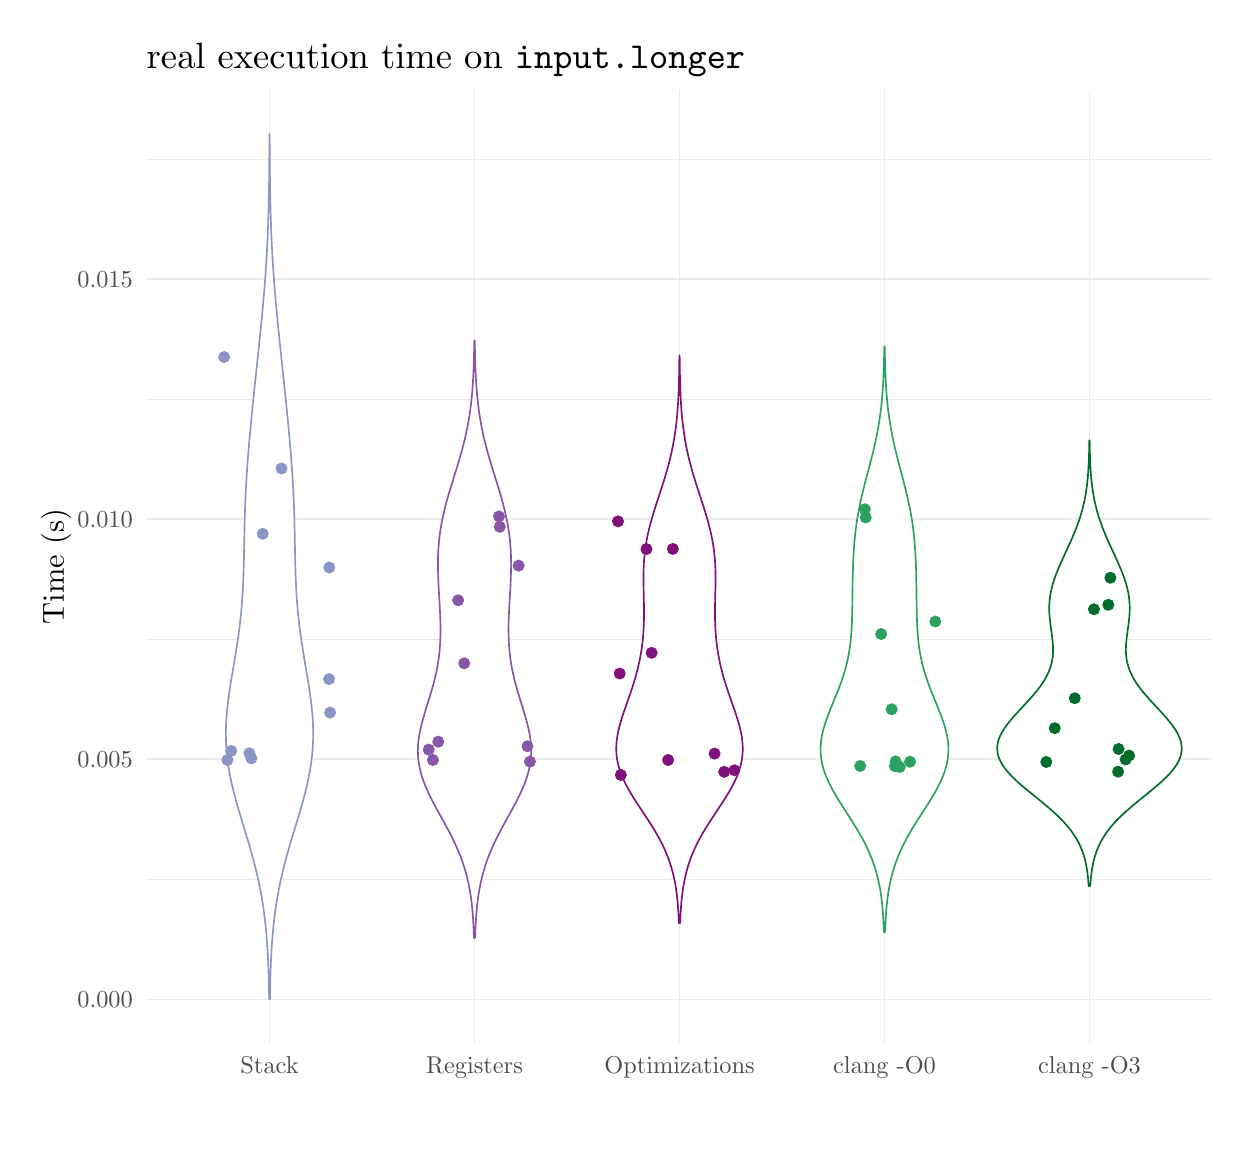
\begin{tikzpicture}[x=1pt,y=1pt]
\definecolor{fillColor}{RGB}{255,255,255}
\path[use as bounding box,fill=fillColor,fill opacity=0.00] (0,0) rectangle (433.62,397.48);
\begin{scope}
\path[clip] ( 42.95, 30.69) rectangle (428.12,374.83);
\definecolor{drawColor}{gray}{0.92}

\path[draw=drawColor,line width= 0.3pt,line join=round] ( 42.95, 89.71) --
	(428.12, 89.71);

\path[draw=drawColor,line width= 0.3pt,line join=round] ( 42.95,176.48) --
	(428.12,176.48);

\path[draw=drawColor,line width= 0.3pt,line join=round] ( 42.95,263.25) --
	(428.12,263.25);

\path[draw=drawColor,line width= 0.3pt,line join=round] ( 42.95,350.02) --
	(428.12,350.02);

\path[draw=drawColor,line width= 0.6pt,line join=round] ( 42.95, 46.33) --
	(428.12, 46.33);

\path[draw=drawColor,line width= 0.6pt,line join=round] ( 42.95,133.10) --
	(428.12,133.10);

\path[draw=drawColor,line width= 0.6pt,line join=round] ( 42.95,219.87) --
	(428.12,219.87);

\path[draw=drawColor,line width= 0.6pt,line join=round] ( 42.95,306.64) --
	(428.12,306.64);

\path[draw=drawColor,line width= 0.6pt,line join=round] ( 87.40, 30.69) --
	( 87.40,374.83);

\path[draw=drawColor,line width= 0.6pt,line join=round] (161.47, 30.69) --
	(161.47,374.83);

\path[draw=drawColor,line width= 0.6pt,line join=round] (235.54, 30.69) --
	(235.54,374.83);

\path[draw=drawColor,line width= 0.6pt,line join=round] (309.61, 30.69) --
	(309.61,374.83);

\path[draw=drawColor,line width= 0.6pt,line join=round] (383.68, 30.69) --
	(383.68,374.83);
\definecolor{drawColor}{RGB}{140,150,198}
\definecolor{fillColor}{RGB}{255,255,255}

\path[draw=drawColor,line width= 0.6pt,line join=round,line cap=round,fill=fillColor] ( 87.26, 46.45) --
	( 87.25, 47.07) --
	( 87.24, 47.68) --
	( 87.23, 48.29) --
	( 87.22, 48.91) --
	( 87.21, 49.52) --
	( 87.19, 50.13) --
	( 87.18, 50.75) --
	( 87.17, 51.36) --
	( 87.15, 51.97) --
	( 87.14, 52.59) --
	( 87.12, 53.20) --
	( 87.11, 53.81) --
	( 87.09, 54.43) --
	( 87.07, 55.04) --
	( 87.05, 55.65) --
	( 87.03, 56.27) --
	( 87.01, 56.88) --
	( 86.99, 57.49) --
	( 86.97, 58.11) --
	( 86.94, 58.72) --
	( 86.92, 59.33) --
	( 86.89, 59.95) --
	( 86.86, 60.56) --
	( 86.83, 61.17) --
	( 86.80, 61.78) --
	( 86.77, 62.40) --
	( 86.74, 63.01) --
	( 86.70, 63.62) --
	( 86.67, 64.24) --
	( 86.63, 64.85) --
	( 86.59, 65.46) --
	( 86.55, 66.08) --
	( 86.51, 66.69) --
	( 86.46, 67.30) --
	( 86.42, 67.92) --
	( 86.37, 68.53) --
	( 86.32, 69.14) --
	( 86.27, 69.76) --
	( 86.21, 70.37) --
	( 86.16, 70.98) --
	( 86.10, 71.60) --
	( 86.04, 72.21) --
	( 85.98, 72.82) --
	( 85.91, 73.44) --
	( 85.85, 74.05) --
	( 85.78, 74.66) --
	( 85.71, 75.28) --
	( 85.64, 75.89) --
	( 85.56, 76.50) --
	( 85.48, 77.11) --
	( 85.40, 77.73) --
	( 85.32, 78.34) --
	( 85.23, 78.95) --
	( 85.14, 79.57) --
	( 85.05, 80.18) --
	( 84.96, 80.79) --
	( 84.86, 81.41) --
	( 84.76, 82.02) --
	( 84.66, 82.63) --
	( 84.56, 83.25) --
	( 84.45, 83.86) --
	( 84.34, 84.47) --
	( 84.22, 85.09) --
	( 84.11, 85.70) --
	( 83.99, 86.31) --
	( 83.87, 86.93) --
	( 83.75, 87.54) --
	( 83.62, 88.15) --
	( 83.49, 88.77) --
	( 83.36, 89.38) --
	( 83.22, 89.99) --
	( 83.08, 90.60) --
	( 82.94, 91.22) --
	( 82.80, 91.83) --
	( 82.66, 92.44) --
	( 82.51, 93.06) --
	( 82.36, 93.67) --
	( 82.20, 94.28) --
	( 82.05, 94.90) --
	( 81.89, 95.51) --
	( 81.73, 96.12) --
	( 81.57, 96.74) --
	( 81.40, 97.35) --
	( 81.24, 97.96) --
	( 81.07, 98.58) --
	( 80.90, 99.19) --
	( 80.73, 99.80) --
	( 80.55,100.42) --
	( 80.38,101.03) --
	( 80.20,101.64) --
	( 80.02,102.26) --
	( 79.84,102.87) --
	( 79.66,103.48) --
	( 79.47,104.10) --
	( 79.29,104.71) --
	( 79.11,105.32) --
	( 78.92,105.93) --
	( 78.74,106.55) --
	( 78.55,107.16) --
	( 78.36,107.77) --
	( 78.18,108.39) --
	( 77.99,109.00) --
	( 77.80,109.61) --
	( 77.62,110.23) --
	( 77.43,110.84) --
	( 77.24,111.45) --
	( 77.06,112.07) --
	( 76.87,112.68) --
	( 76.69,113.29) --
	( 76.51,113.91) --
	( 76.33,114.52) --
	( 76.15,115.13) --
	( 75.97,115.75) --
	( 75.79,116.36) --
	( 75.62,116.97) --
	( 75.45,117.59) --
	( 75.28,118.20) --
	( 75.11,118.81) --
	( 74.95,119.43) --
	( 74.78,120.04) --
	( 74.62,120.65) --
	( 74.47,121.26) --
	( 74.31,121.88) --
	( 74.16,122.49) --
	( 74.02,123.10) --
	( 73.87,123.72) --
	( 73.73,124.33) --
	( 73.60,124.94) --
	( 73.46,125.56) --
	( 73.33,126.17) --
	( 73.21,126.78) --
	( 73.09,127.40) --
	( 72.97,128.01) --
	( 72.86,128.62) --
	( 72.75,129.24) --
	( 72.65,129.85) --
	( 72.55,130.46) --
	( 72.46,131.08) --
	( 72.37,131.69) --
	( 72.29,132.30) --
	( 72.21,132.92) --
	( 72.13,133.53) --
	( 72.07,134.14) --
	( 72.00,134.76) --
	( 71.94,135.37) --
	( 71.89,135.98) --
	( 71.84,136.59) --
	( 71.80,137.21) --
	( 71.76,137.82) --
	( 71.72,138.43) --
	( 71.69,139.05) --
	( 71.67,139.66) --
	( 71.65,140.27) --
	( 71.64,140.89) --
	( 71.63,141.50) --
	( 71.62,142.11) --
	( 71.63,142.73) --
	( 71.63,143.34) --
	( 71.64,143.95) --
	( 71.66,144.57) --
	( 71.68,145.18) --
	( 71.70,145.79) --
	( 71.73,146.41) --
	( 71.76,147.02) --
	( 71.80,147.63) --
	( 71.84,148.25) --
	( 71.89,148.86) --
	( 71.93,149.47) --
	( 71.99,150.09) --
	( 72.04,150.70) --
	( 72.11,151.31) --
	( 72.17,151.92) --
	( 72.24,152.54) --
	( 72.31,153.15) --
	( 72.38,153.76) --
	( 72.45,154.38) --
	( 72.53,154.99) --
	( 72.61,155.60) --
	( 72.70,156.22) --
	( 72.78,156.83) --
	( 72.87,157.44) --
	( 72.96,158.06) --
	( 73.06,158.67) --
	( 73.15,159.28) --
	( 73.25,159.90) --
	( 73.34,160.51) --
	( 73.44,161.12) --
	( 73.54,161.74) --
	( 73.64,162.35) --
	( 73.74,162.96) --
	( 73.85,163.58) --
	( 73.95,164.19) --
	( 74.05,164.80) --
	( 74.16,165.41) --
	( 74.26,166.03) --
	( 74.36,166.64) --
	( 74.47,167.25) --
	( 74.57,167.87) --
	( 74.68,168.48) --
	( 74.78,169.09) --
	( 74.88,169.71) --
	( 74.98,170.32) --
	( 75.08,170.93) --
	( 75.18,171.55) --
	( 75.28,172.16) --
	( 75.38,172.77) --
	( 75.48,173.39) --
	( 75.58,174.00) --
	( 75.67,174.61) --
	( 75.76,175.23) --
	( 75.85,175.84) --
	( 75.95,176.45) --
	( 76.03,177.07) --
	( 76.12,177.68) --
	( 76.21,178.29) --
	( 76.29,178.91) --
	( 76.37,179.52) --
	( 76.45,180.13) --
	( 76.53,180.74) --
	( 76.60,181.36) --
	( 76.68,181.97) --
	( 76.75,182.58) --
	( 76.82,183.20) --
	( 76.89,183.81) --
	( 76.95,184.42) --
	( 77.02,185.04) --
	( 77.08,185.65) --
	( 77.14,186.26) --
	( 77.20,186.88) --
	( 77.25,187.49) --
	( 77.31,188.10) --
	( 77.36,188.72) --
	( 77.41,189.33) --
	( 77.45,189.94) --
	( 77.50,190.56) --
	( 77.54,191.17) --
	( 77.58,191.78) --
	( 77.62,192.40) --
	( 77.66,193.01) --
	( 77.70,193.62) --
	( 77.73,194.24) --
	( 77.77,194.85) --
	( 77.80,195.46) --
	( 77.83,196.07) --
	( 77.86,196.69) --
	( 77.88,197.30) --
	( 77.91,197.91) --
	( 77.93,198.53) --
	( 77.96,199.14) --
	( 77.98,199.75) --
	( 78.00,200.37) --
	( 78.02,200.98) --
	( 78.04,201.59) --
	( 78.05,202.21) --
	( 78.07,202.82) --
	( 78.09,203.43) --
	( 78.10,204.05) --
	( 78.12,204.66) --
	( 78.13,205.27) --
	( 78.14,205.89) --
	( 78.15,206.50) --
	( 78.17,207.11) --
	( 78.18,207.73) --
	( 78.19,208.34) --
	( 78.20,208.95) --
	( 78.21,209.57) --
	( 78.22,210.18) --
	( 78.24,210.79) --
	( 78.25,211.40) --
	( 78.26,212.02) --
	( 78.27,212.63) --
	( 78.28,213.24) --
	( 78.29,213.86) --
	( 78.30,214.47) --
	( 78.32,215.08) --
	( 78.33,215.70) --
	( 78.34,216.31) --
	( 78.35,216.92) --
	( 78.37,217.54) --
	( 78.38,218.15) --
	( 78.40,218.76) --
	( 78.41,219.38) --
	( 78.43,219.99) --
	( 78.45,220.60) --
	( 78.46,221.22) --
	( 78.48,221.83) --
	( 78.50,222.44) --
	( 78.52,223.06) --
	( 78.54,223.67) --
	( 78.57,224.28) --
	( 78.59,224.89) --
	( 78.61,225.51) --
	( 78.64,226.12) --
	( 78.66,226.73) --
	( 78.69,227.35) --
	( 78.71,227.96) --
	( 78.74,228.57) --
	( 78.77,229.19) --
	( 78.80,229.80) --
	( 78.83,230.41) --
	( 78.86,231.03) --
	( 78.90,231.64) --
	( 78.93,232.25) --
	( 78.96,232.87) --
	( 79.00,233.48) --
	( 79.04,234.09) --
	( 79.07,234.71) --
	( 79.11,235.32) --
	( 79.15,235.93) --
	( 79.19,236.55) --
	( 79.23,237.16) --
	( 79.27,237.77) --
	( 79.32,238.39) --
	( 79.36,239.00) --
	( 79.40,239.61) --
	( 79.45,240.22) --
	( 79.49,240.84) --
	( 79.54,241.45) --
	( 79.59,242.06) --
	( 79.64,242.68) --
	( 79.69,243.29) --
	( 79.73,243.90) --
	( 79.78,244.52) --
	( 79.84,245.13) --
	( 79.89,245.74) --
	( 79.94,246.36) --
	( 79.99,246.97) --
	( 80.04,247.58) --
	( 80.10,248.20) --
	( 80.15,248.81) --
	( 80.21,249.42) --
	( 80.26,250.04) --
	( 80.32,250.65) --
	( 80.37,251.26) --
	( 80.43,251.88) --
	( 80.49,252.49) --
	( 80.55,253.10) --
	( 80.60,253.72) --
	( 80.66,254.33) --
	( 80.72,254.94) --
	( 80.78,255.55) --
	( 80.84,256.17) --
	( 80.90,256.78) --
	( 80.96,257.39) --
	( 81.02,258.01) --
	( 81.08,258.62) --
	( 81.14,259.23) --
	( 81.20,259.85) --
	( 81.27,260.46) --
	( 81.33,261.07) --
	( 81.39,261.69) --
	( 81.45,262.30) --
	( 81.52,262.91) --
	( 81.58,263.53) --
	( 81.64,264.14) --
	( 81.70,264.75) --
	( 81.77,265.37) --
	( 81.83,265.98) --
	( 81.90,266.59) --
	( 81.96,267.21) --
	( 82.02,267.82) --
	( 82.09,268.43) --
	( 82.15,269.05) --
	( 82.22,269.66) --
	( 82.28,270.27) --
	( 82.35,270.88) --
	( 82.41,271.50) --
	( 82.48,272.11) --
	( 82.54,272.72) --
	( 82.61,273.34) --
	( 82.67,273.95) --
	( 82.74,274.56) --
	( 82.80,275.18) --
	( 82.87,275.79) --
	( 82.93,276.40) --
	( 83.00,277.02) --
	( 83.06,277.63) --
	( 83.13,278.24) --
	( 83.19,278.86) --
	( 83.26,279.47) --
	( 83.32,280.08) --
	( 83.38,280.70) --
	( 83.45,281.31) --
	( 83.51,281.92) --
	( 83.58,282.54) --
	( 83.64,283.15) --
	( 83.71,283.76) --
	( 83.77,284.38) --
	( 83.83,284.99) --
	( 83.90,285.60) --
	( 83.96,286.21) --
	( 84.02,286.83) --
	( 84.08,287.44) --
	( 84.15,288.05) --
	( 84.21,288.67) --
	( 84.27,289.28) --
	( 84.33,289.89) --
	( 84.39,290.51) --
	( 84.45,291.12) --
	( 84.51,291.73) --
	( 84.57,292.35) --
	( 84.63,292.96) --
	( 84.69,293.57) --
	( 84.75,294.19) --
	( 84.81,294.80) --
	( 84.86,295.41) --
	( 84.92,296.03) --
	( 84.98,296.64) --
	( 85.03,297.25) --
	( 85.09,297.87) --
	( 85.14,298.48) --
	( 85.20,299.09) --
	( 85.25,299.70) --
	( 85.30,300.32) --
	( 85.36,300.93) --
	( 85.41,301.54) --
	( 85.46,302.16) --
	( 85.51,302.77) --
	( 85.56,303.38) --
	( 85.61,304.00) --
	( 85.66,304.61) --
	( 85.70,305.22) --
	( 85.75,305.84) --
	( 85.80,306.45) --
	( 85.84,307.06) --
	( 85.89,307.68) --
	( 85.93,308.29) --
	( 85.97,308.90) --
	( 86.01,309.52) --
	( 86.06,310.13) --
	( 86.10,310.74) --
	( 86.14,311.36) --
	( 86.18,311.97) --
	( 86.21,312.58) --
	( 86.25,313.20) --
	( 86.29,313.81) --
	( 86.32,314.42) --
	( 86.36,315.03) --
	( 86.39,315.65) --
	( 86.43,316.26) --
	( 86.46,316.87) --
	( 86.49,317.49) --
	( 86.52,318.10) --
	( 86.56,318.71) --
	( 86.59,319.33) --
	( 86.61,319.94) --
	( 86.64,320.55) --
	( 86.67,321.17) --
	( 86.70,321.78) --
	( 86.72,322.39) --
	( 86.75,323.01) --
	( 86.77,323.62) --
	( 86.80,324.23) --
	( 86.82,324.85) --
	( 86.84,325.46) --
	( 86.87,326.07) --
	( 86.89,326.69) --
	( 86.91,327.30) --
	( 86.93,327.91) --
	( 86.95,328.53) --
	( 86.97,329.14) --
	( 86.98,329.75) --
	( 87.00,330.36) --
	( 87.02,330.98) --
	( 87.03,331.59) --
	( 87.05,332.20) --
	( 87.07,332.82) --
	( 87.08,333.43) --
	( 87.09,334.04) --
	( 87.11,334.66) --
	( 87.12,335.27) --
	( 87.13,335.88) --
	( 87.15,336.50) --
	( 87.16,337.11) --
	( 87.17,337.72) --
	( 87.18,338.34) --
	( 87.19,338.95) --
	( 87.20,339.56) --
	( 87.21,340.18) --
	( 87.22,340.79) --
	( 87.23,341.40) --
	( 87.24,342.02) --
	( 87.24,342.63) --
	( 87.25,343.24) --
	( 87.26,343.86) --
	( 87.27,344.47) --
	( 87.27,345.08) --
	( 87.28,345.69) --
	( 87.29,346.31) --
	( 87.29,346.92) --
	( 87.30,347.53) --
	( 87.30,348.15) --
	( 87.31,348.76) --
	( 87.31,349.37) --
	( 87.32,349.99) --
	( 87.32,350.60) --
	( 87.33,351.21) --
	( 87.33,351.83) --
	( 87.33,352.44) --
	( 87.34,353.05) --
	( 87.34,353.67) --
	( 87.34,354.28) --
	( 87.35,354.89) --
	( 87.35,355.51) --
	( 87.35,356.12) --
	( 87.35,356.73) --
	( 87.36,357.35) --
	( 87.36,357.96) --
	( 87.36,358.57) --
	( 87.36,359.18) --
	( 87.43,359.18) --
	( 87.43,358.57) --
	( 87.43,357.96) --
	( 87.44,357.35) --
	( 87.44,356.73) --
	( 87.44,356.12) --
	( 87.44,355.51) --
	( 87.45,354.89) --
	( 87.45,354.28) --
	( 87.45,353.67) --
	( 87.46,353.05) --
	( 87.46,352.44) --
	( 87.46,351.83) --
	( 87.47,351.21) --
	( 87.47,350.60) --
	( 87.48,349.99) --
	( 87.48,349.37) --
	( 87.48,348.76) --
	( 87.49,348.15) --
	( 87.50,347.53) --
	( 87.50,346.92) --
	( 87.51,346.31) --
	( 87.51,345.69) --
	( 87.52,345.08) --
	( 87.53,344.47) --
	( 87.53,343.86) --
	( 87.54,343.24) --
	( 87.55,342.63) --
	( 87.56,342.02) --
	( 87.57,341.40) --
	( 87.57,340.79) --
	( 87.58,340.18) --
	( 87.59,339.56) --
	( 87.60,338.95) --
	( 87.61,338.34) --
	( 87.62,337.72) --
	( 87.64,337.11) --
	( 87.65,336.50) --
	( 87.66,335.88) --
	( 87.67,335.27) --
	( 87.68,334.66) --
	( 87.70,334.04) --
	( 87.71,333.43) --
	( 87.73,332.82) --
	( 87.74,332.20) --
	( 87.76,331.59) --
	( 87.77,330.98) --
	( 87.79,330.36) --
	( 87.81,329.75) --
	( 87.83,329.14) --
	( 87.85,328.53) --
	( 87.87,327.91) --
	( 87.89,327.30) --
	( 87.91,326.69) --
	( 87.93,326.07) --
	( 87.95,325.46) --
	( 87.97,324.85) --
	( 88.00,324.23) --
	( 88.02,323.62) --
	( 88.04,323.01) --
	( 88.07,322.39) --
	( 88.10,321.78) --
	( 88.12,321.17) --
	( 88.15,320.55) --
	( 88.18,319.94) --
	( 88.21,319.33) --
	( 88.24,318.71) --
	( 88.27,318.10) --
	( 88.30,317.49) --
	( 88.33,316.87) --
	( 88.36,316.26) --
	( 88.40,315.65) --
	( 88.43,315.03) --
	( 88.47,314.42) --
	( 88.50,313.81) --
	( 88.54,313.20) --
	( 88.58,312.58) --
	( 88.62,311.97) --
	( 88.66,311.36) --
	( 88.70,310.74) --
	( 88.74,310.13) --
	( 88.78,309.52) --
	( 88.82,308.90) --
	( 88.86,308.29) --
	( 88.91,307.68) --
	( 88.95,307.06) --
	( 89.00,306.45) --
	( 89.04,305.84) --
	( 89.09,305.22) --
	( 89.14,304.61) --
	( 89.19,304.00) --
	( 89.23,303.38) --
	( 89.28,302.77) --
	( 89.33,302.16) --
	( 89.38,301.54) --
	( 89.44,300.93) --
	( 89.49,300.32) --
	( 89.54,299.70) --
	( 89.59,299.09) --
	( 89.65,298.48) --
	( 89.70,297.87) --
	( 89.76,297.25) --
	( 89.81,296.64) --
	( 89.87,296.03) --
	( 89.93,295.41) --
	( 89.99,294.80) --
	( 90.04,294.19) --
	( 90.10,293.57) --
	( 90.16,292.96) --
	( 90.22,292.35) --
	( 90.28,291.73) --
	( 90.34,291.12) --
	( 90.40,290.51) --
	( 90.46,289.89) --
	( 90.52,289.28) --
	( 90.58,288.67) --
	( 90.65,288.05) --
	( 90.71,287.44) --
	( 90.77,286.83) --
	( 90.83,286.21) --
	( 90.90,285.60) --
	( 90.96,284.99) --
	( 91.02,284.38) --
	( 91.09,283.76) --
	( 91.15,283.15) --
	( 91.21,282.54) --
	( 91.28,281.92) --
	( 91.34,281.31) --
	( 91.41,280.70) --
	( 91.47,280.08) --
	( 91.54,279.47) --
	( 91.60,278.86) --
	( 91.67,278.24) --
	( 91.73,277.63) --
	( 91.80,277.02) --
	( 91.86,276.40) --
	( 91.93,275.79) --
	( 91.99,275.18) --
	( 92.06,274.56) --
	( 92.12,273.95) --
	( 92.19,273.34) --
	( 92.25,272.72) --
	( 92.32,272.11) --
	( 92.38,271.50) --
	( 92.45,270.88) --
	( 92.51,270.27) --
	( 92.58,269.66) --
	( 92.64,269.05) --
	( 92.70,268.43) --
	( 92.77,267.82) --
	( 92.83,267.21) --
	( 92.90,266.59) --
	( 92.96,265.98) --
	( 93.02,265.37) --
	( 93.09,264.75) --
	( 93.15,264.14) --
	( 93.21,263.53) --
	( 93.28,262.91) --
	( 93.34,262.30) --
	( 93.40,261.69) --
	( 93.46,261.07) --
	( 93.53,260.46) --
	( 93.59,259.85) --
	( 93.65,259.23) --
	( 93.71,258.62) --
	( 93.77,258.01) --
	( 93.83,257.39) --
	( 93.89,256.78) --
	( 93.95,256.17) --
	( 94.01,255.55) --
	( 94.07,254.94) --
	( 94.13,254.33) --
	( 94.19,253.72) --
	( 94.25,253.10) --
	( 94.30,252.49) --
	( 94.36,251.88) --
	( 94.42,251.26) --
	( 94.47,250.65) --
	( 94.53,250.04) --
	( 94.59,249.42) --
	( 94.64,248.81) --
	( 94.69,248.20) --
	( 94.75,247.58) --
	( 94.80,246.97) --
	( 94.85,246.36) --
	( 94.91,245.74) --
	( 94.96,245.13) --
	( 95.01,244.52) --
	( 95.06,243.90) --
	( 95.11,243.29) --
	( 95.16,242.68) --
	( 95.20,242.06) --
	( 95.25,241.45) --
	( 95.30,240.84) --
	( 95.34,240.22) --
	( 95.39,239.61) --
	( 95.43,239.00) --
	( 95.48,238.39) --
	( 95.52,237.77) --
	( 95.56,237.16) --
	( 95.60,236.55) --
	( 95.64,235.93) --
	( 95.68,235.32) --
	( 95.72,234.71) --
	( 95.76,234.09) --
	( 95.79,233.48) --
	( 95.83,232.87) --
	( 95.86,232.25) --
	( 95.90,231.64) --
	( 95.93,231.03) --
	( 95.96,230.41) --
	( 95.99,229.80) --
	( 96.02,229.19) --
	( 96.05,228.57) --
	( 96.08,227.96) --
	( 96.10,227.35) --
	( 96.13,226.73) --
	( 96.16,226.12) --
	( 96.18,225.51) --
	( 96.20,224.89) --
	( 96.23,224.28) --
	( 96.25,223.67) --
	( 96.27,223.06) --
	( 96.29,222.44) --
	( 96.31,221.83) --
	( 96.33,221.22) --
	( 96.35,220.60) --
	( 96.36,219.99) --
	( 96.38,219.38) --
	( 96.39,218.76) --
	( 96.41,218.15) --
	( 96.42,217.54) --
	( 96.44,216.92) --
	( 96.45,216.31) --
	( 96.46,215.70) --
	( 96.48,215.08) --
	( 96.49,214.47) --
	( 96.50,213.86) --
	( 96.51,213.24) --
	( 96.52,212.63) --
	( 96.54,212.02) --
	( 96.55,211.40) --
	( 96.56,210.79) --
	( 96.57,210.18) --
	( 96.58,209.57) --
	( 96.59,208.95) --
	( 96.60,208.34) --
	( 96.61,207.73) --
	( 96.63,207.11) --
	( 96.64,206.50) --
	( 96.65,205.89) --
	( 96.66,205.27) --
	( 96.68,204.66) --
	( 96.69,204.05) --
	( 96.71,203.43) --
	( 96.72,202.82) --
	( 96.74,202.21) --
	( 96.76,201.59) --
	( 96.77,200.98) --
	( 96.79,200.37) --
	( 96.81,199.75) --
	( 96.84,199.14) --
	( 96.86,198.53) --
	( 96.88,197.91) --
	( 96.91,197.30) --
	( 96.94,196.69) --
	( 96.96,196.07) --
	( 96.99,195.46) --
	( 97.03,194.85) --
	( 97.06,194.24) --
	( 97.09,193.62) --
	( 97.13,193.01) --
	( 97.17,192.40) --
	( 97.21,191.78) --
	( 97.25,191.17) --
	( 97.29,190.56) --
	( 97.34,189.94) --
	( 97.39,189.33) --
	( 97.44,188.72) --
	( 97.49,188.10) --
	( 97.54,187.49) --
	( 97.60,186.88) --
	( 97.65,186.26) --
	( 97.71,185.65) --
	( 97.78,185.04) --
	( 97.84,184.42) --
	( 97.90,183.81) --
	( 97.97,183.20) --
	( 98.04,182.58) --
	( 98.11,181.97) --
	( 98.19,181.36) --
	( 98.26,180.74) --
	( 98.34,180.13) --
	( 98.42,179.52) --
	( 98.50,178.91) --
	( 98.59,178.29) --
	( 98.67,177.68) --
	( 98.76,177.07) --
	( 98.85,176.45) --
	( 98.94,175.84) --
	( 99.03,175.23) --
	( 99.12,174.61) --
	( 99.22,174.00) --
	( 99.31,173.39) --
	( 99.41,172.77) --
	( 99.51,172.16) --
	( 99.61,171.55) --
	( 99.71,170.93) --
	( 99.81,170.32) --
	( 99.91,169.71) --
	(100.01,169.09) --
	(100.12,168.48) --
	(100.22,167.87) --
	(100.32,167.25) --
	(100.43,166.64) --
	(100.53,166.03) --
	(100.64,165.41) --
	(100.74,164.80) --
	(100.84,164.19) --
	(100.95,163.58) --
	(101.05,162.96) --
	(101.15,162.35) --
	(101.25,161.74) --
	(101.35,161.12) --
	(101.45,160.51) --
	(101.55,159.90) --
	(101.64,159.28) --
	(101.74,158.67) --
	(101.83,158.06) --
	(101.92,157.44) --
	(102.01,156.83) --
	(102.09,156.22) --
	(102.18,155.60) --
	(102.26,154.99) --
	(102.34,154.38) --
	(102.41,153.76) --
	(102.49,153.15) --
	(102.56,152.54) --
	(102.62,151.92) --
	(102.69,151.31) --
	(102.75,150.70) --
	(102.80,150.09) --
	(102.86,149.47) --
	(102.91,148.86) --
	(102.95,148.25) --
	(102.99,147.63) --
	(103.03,147.02) --
	(103.06,146.41) --
	(103.09,145.79) --
	(103.12,145.18) --
	(103.13,144.57) --
	(103.15,143.95) --
	(103.16,143.34) --
	(103.17,142.73) --
	(103.17,142.11) --
	(103.16,141.50) --
	(103.15,140.89) --
	(103.14,140.27) --
	(103.12,139.66) --
	(103.10,139.05) --
	(103.07,138.43) --
	(103.04,137.82) --
	(103.00,137.21) --
	(102.95,136.59) --
	(102.90,135.98) --
	(102.85,135.37) --
	(102.79,134.76) --
	(102.73,134.14) --
	(102.66,133.53) --
	(102.58,132.92) --
	(102.50,132.30) --
	(102.42,131.69) --
	(102.33,131.08) --
	(102.24,130.46) --
	(102.14,129.85) --
	(102.04,129.24) --
	(101.93,128.62) --
	(101.82,128.01) --
	(101.70,127.40) --
	(101.58,126.78) --
	(101.46,126.17) --
	(101.33,125.56) --
	(101.20,124.94) --
	(101.06,124.33) --
	(100.92,123.72) --
	(100.78,123.10) --
	(100.63,122.49) --
	(100.48,121.88) --
	(100.33,121.26) --
	(100.17,120.65) --
	(100.01,120.04) --
	( 99.85,119.43) --
	( 99.68,118.81) --
	( 99.51,118.20) --
	( 99.34,117.59) --
	( 99.17,116.97) --
	( 99.00,116.36) --
	( 98.82,115.75) --
	( 98.64,115.13) --
	( 98.46,114.52) --
	( 98.28,113.91) --
	( 98.10,113.29) --
	( 97.92,112.68) --
	( 97.73,112.07) --
	( 97.55,111.45) --
	( 97.36,110.84) --
	( 97.18,110.23) --
	( 96.99,109.61) --
	( 96.80,109.00) --
	( 96.62,108.39) --
	( 96.43,107.77) --
	( 96.24,107.16) --
	( 96.06,106.55) --
	( 95.87,105.93) --
	( 95.69,105.32) --
	( 95.50,104.71) --
	( 95.32,104.10) --
	( 95.13,103.48) --
	( 94.95,102.87) --
	( 94.77,102.26) --
	( 94.59,101.64) --
	( 94.42,101.03) --
	( 94.24,100.42) --
	( 94.07, 99.80) --
	( 93.89, 99.19) --
	( 93.72, 98.58) --
	( 93.56, 97.96) --
	( 93.39, 97.35) --
	( 93.22, 96.74) --
	( 93.06, 96.12) --
	( 92.90, 95.51) --
	( 92.74, 94.90) --
	( 92.59, 94.28) --
	( 92.44, 93.67) --
	( 92.28, 93.06) --
	( 92.14, 92.44) --
	( 91.99, 91.83) --
	( 91.85, 91.22) --
	( 91.71, 90.60) --
	( 91.57, 89.99) --
	( 91.44, 89.38) --
	( 91.30, 88.77) --
	( 91.17, 88.15) --
	( 91.05, 87.54) --
	( 90.92, 86.93) --
	( 90.80, 86.31) --
	( 90.68, 85.70) --
	( 90.57, 85.09) --
	( 90.45, 84.47) --
	( 90.35, 83.86) --
	( 90.24, 83.25) --
	( 90.13, 82.63) --
	( 90.03, 82.02) --
	( 89.93, 81.41) --
	( 89.84, 80.79) --
	( 89.74, 80.18) --
	( 89.65, 79.57) --
	( 89.56, 78.95) --
	( 89.48, 78.34) --
	( 89.39, 77.73) --
	( 89.31, 77.11) --
	( 89.23, 76.50) --
	( 89.16, 75.89) --
	( 89.08, 75.28) --
	( 89.01, 74.66) --
	( 88.94, 74.05) --
	( 88.88, 73.44) --
	( 88.81, 72.82) --
	( 88.75, 72.21) --
	( 88.69, 71.60) --
	( 88.63, 70.98) --
	( 88.58, 70.37) --
	( 88.52, 69.76) --
	( 88.47, 69.14) --
	( 88.42, 68.53) --
	( 88.38, 67.92) --
	( 88.33, 67.30) --
	( 88.28, 66.69) --
	( 88.24, 66.08) --
	( 88.20, 65.46) --
	( 88.16, 64.85) --
	( 88.12, 64.24) --
	( 88.09, 63.62) --
	( 88.05, 63.01) --
	( 88.02, 62.40) --
	( 87.99, 61.78) --
	( 87.96, 61.17) --
	( 87.93, 60.56) --
	( 87.90, 59.95) --
	( 87.88, 59.33) --
	( 87.85, 58.72) --
	( 87.83, 58.11) --
	( 87.80, 57.49) --
	( 87.78, 56.88) --
	( 87.76, 56.27) --
	( 87.74, 55.65) --
	( 87.72, 55.04) --
	( 87.70, 54.43) --
	( 87.69, 53.81) --
	( 87.67, 53.20) --
	( 87.65, 52.59) --
	( 87.64, 51.97) --
	( 87.62, 51.36) --
	( 87.61, 50.75) --
	( 87.60, 50.13) --
	( 87.59, 49.52) --
	( 87.58, 48.91) --
	( 87.57, 48.29) --
	( 87.56, 47.68) --
	( 87.55, 47.07) --
	( 87.54, 46.45) --
	( 87.26, 46.45) --
	cycle;
\definecolor{drawColor}{RGB}{136,86,167}

\path[draw=drawColor,line width= 0.6pt,line join=round,line cap=round,fill=fillColor] (161.25, 68.55) --
	(161.24, 68.97) --
	(161.23, 69.40) --
	(161.21, 69.82) --
	(161.20, 70.24) --
	(161.18, 70.66) --
	(161.16, 71.09) --
	(161.15, 71.51) --
	(161.13, 71.93) --
	(161.11, 72.35) --
	(161.09, 72.78) --
	(161.07, 73.20) --
	(161.05, 73.62) --
	(161.02, 74.04) --
	(161.00, 74.47) --
	(160.97, 74.89) --
	(160.95, 75.31) --
	(160.92, 75.73) --
	(160.89, 76.16) --
	(160.86, 76.58) --
	(160.82, 77.00) --
	(160.79, 77.42) --
	(160.76, 77.85) --
	(160.72, 78.27) --
	(160.68, 78.69) --
	(160.64, 79.11) --
	(160.60, 79.54) --
	(160.56, 79.96) --
	(160.51, 80.38) --
	(160.47, 80.80) --
	(160.42, 81.23) --
	(160.37, 81.65) --
	(160.31, 82.07) --
	(160.26, 82.49) --
	(160.20, 82.91) --
	(160.14, 83.34) --
	(160.08, 83.76) --
	(160.02, 84.18) --
	(159.95, 84.60) --
	(159.89, 85.03) --
	(159.81, 85.45) --
	(159.74, 85.87) --
	(159.67, 86.29) --
	(159.59, 86.72) --
	(159.51, 87.14) --
	(159.42, 87.56) --
	(159.34, 87.98) --
	(159.25, 88.41) --
	(159.16, 88.83) --
	(159.06, 89.25) --
	(158.97, 89.67) --
	(158.86, 90.10) --
	(158.76, 90.52) --
	(158.65, 90.94) --
	(158.54, 91.36) --
	(158.43, 91.79) --
	(158.32, 92.21) --
	(158.20, 92.63) --
	(158.07, 93.05) --
	(157.95, 93.48) --
	(157.82, 93.90) --
	(157.69, 94.32) --
	(157.55, 94.74) --
	(157.41, 95.17) --
	(157.27, 95.59) --
	(157.13, 96.01) --
	(156.98, 96.43) --
	(156.83, 96.85) --
	(156.67, 97.28) --
	(156.51, 97.70) --
	(156.35, 98.12) --
	(156.19, 98.54) --
	(156.02, 98.97) --
	(155.85, 99.39) --
	(155.67, 99.81) --
	(155.49,100.23) --
	(155.31,100.66) --
	(155.13,101.08) --
	(154.94,101.50) --
	(154.75,101.92) --
	(154.56,102.35) --
	(154.36,102.77) --
	(154.16,103.19) --
	(153.96,103.61) --
	(153.75,104.04) --
	(153.55,104.46) --
	(153.34,104.88) --
	(153.13,105.30) --
	(152.91,105.73) --
	(152.69,106.15) --
	(152.48,106.57) --
	(152.26,106.99) --
	(152.03,107.42) --
	(151.81,107.84) --
	(151.58,108.26) --
	(151.36,108.68) --
	(151.13,109.11) --
	(150.90,109.53) --
	(150.67,109.95) --
	(150.44,110.37) --
	(150.20,110.80) --
	(149.97,111.22) --
	(149.74,111.64) --
	(149.50,112.06) --
	(149.27,112.48) --
	(149.04,112.91) --
	(148.80,113.33) --
	(148.57,113.75) --
	(148.34,114.17) --
	(148.10,114.60) --
	(147.87,115.02) --
	(147.64,115.44) --
	(147.41,115.86) --
	(147.19,116.29) --
	(146.96,116.71) --
	(146.74,117.13) --
	(146.51,117.55) --
	(146.29,117.98) --
	(146.08,118.40) --
	(145.86,118.82) --
	(145.65,119.24) --
	(145.44,119.67) --
	(145.23,120.09) --
	(145.03,120.51) --
	(144.83,120.93) --
	(144.64,121.36) --
	(144.44,121.78) --
	(144.25,122.20) --
	(144.07,122.62) --
	(143.89,123.05) --
	(143.72,123.47) --
	(143.54,123.89) --
	(143.38,124.31) --
	(143.22,124.74) --
	(143.06,125.16) --
	(142.91,125.58) --
	(142.76,126.00) --
	(142.62,126.42) --
	(142.48,126.85) --
	(142.35,127.27) --
	(142.23,127.69) --
	(142.11,128.11) --
	(142.00,128.54) --
	(141.89,128.96) --
	(141.79,129.38) --
	(141.69,129.80) --
	(141.61,130.23) --
	(141.52,130.65) --
	(141.45,131.07) --
	(141.37,131.49) --
	(141.31,131.92) --
	(141.25,132.34) --
	(141.20,132.76) --
	(141.15,133.18) --
	(141.11,133.61) --
	(141.08,134.03) --
	(141.05,134.45) --
	(141.03,134.87) --
	(141.02,135.30) --
	(141.01,135.72) --
	(141.01,136.14) --
	(141.01,136.56) --
	(141.02,136.99) --
	(141.03,137.41) --
	(141.05,137.83) --
	(141.08,138.25) --
	(141.11,138.68) --
	(141.14,139.10) --
	(141.19,139.52) --
	(141.23,139.94) --
	(141.29,140.36) --
	(141.34,140.79) --
	(141.41,141.21) --
	(141.47,141.63) --
	(141.54,142.05) --
	(141.62,142.48) --
	(141.70,142.90) --
	(141.78,143.32) --
	(141.87,143.74) --
	(141.96,144.17) --
	(142.06,144.59) --
	(142.16,145.01) --
	(142.26,145.43) --
	(142.37,145.86) --
	(142.47,146.28) --
	(142.59,146.70) --
	(142.70,147.12) --
	(142.82,147.55) --
	(142.93,147.97) --
	(143.05,148.39) --
	(143.18,148.81) --
	(143.30,149.24) --
	(143.43,149.66) --
	(143.55,150.08) --
	(143.68,150.50) --
	(143.81,150.93) --
	(143.94,151.35) --
	(144.07,151.77) --
	(144.20,152.19) --
	(144.34,152.62) --
	(144.47,153.04) --
	(144.60,153.46) --
	(144.73,153.88) --
	(144.86,154.31) --
	(144.99,154.73) --
	(145.12,155.15) --
	(145.25,155.57) --
	(145.38,155.99) --
	(145.51,156.42) --
	(145.64,156.84) --
	(145.77,157.26) --
	(145.89,157.68) --
	(146.01,158.11) --
	(146.14,158.53) --
	(146.25,158.95) --
	(146.37,159.37) --
	(146.49,159.80) --
	(146.60,160.22) --
	(146.72,160.64) --
	(146.83,161.06) --
	(146.94,161.49) --
	(147.04,161.91) --
	(147.15,162.33) --
	(147.25,162.75) --
	(147.35,163.18) --
	(147.44,163.60) --
	(147.54,164.02) --
	(147.63,164.44) --
	(147.72,164.87) --
	(147.80,165.29) --
	(147.88,165.71) --
	(147.97,166.13) --
	(148.04,166.56) --
	(148.12,166.98) --
	(148.19,167.40) --
	(148.26,167.82) --
	(148.33,168.25) --
	(148.39,168.67) --
	(148.45,169.09) --
	(148.51,169.51) --
	(148.57,169.93) --
	(148.62,170.36) --
	(148.67,170.78) --
	(148.72,171.20) --
	(148.77,171.62) --
	(148.81,172.05) --
	(148.85,172.47) --
	(148.88,172.89) --
	(148.92,173.31) --
	(148.95,173.74) --
	(148.98,174.16) --
	(149.01,174.58) --
	(149.03,175.00) --
	(149.06,175.43) --
	(149.08,175.85) --
	(149.10,176.27) --
	(149.11,176.69) --
	(149.12,177.12) --
	(149.14,177.54) --
	(149.15,177.96) --
	(149.15,178.38) --
	(149.16,178.81) --
	(149.16,179.23) --
	(149.16,179.65) --
	(149.16,180.07) --
	(149.16,180.50) --
	(149.16,180.92) --
	(149.16,181.34) --
	(149.15,181.76) --
	(149.14,182.19) --
	(149.13,182.61) --
	(149.12,183.03) --
	(149.11,183.45) --
	(149.10,183.88) --
	(149.08,184.30) --
	(149.07,184.72) --
	(149.05,185.14) --
	(149.03,185.56) --
	(149.01,185.99) --
	(148.99,186.41) --
	(148.97,186.83) --
	(148.95,187.25) --
	(148.93,187.68) --
	(148.91,188.10) --
	(148.89,188.52) --
	(148.86,188.94) --
	(148.84,189.37) --
	(148.82,189.79) --
	(148.79,190.21) --
	(148.77,190.63) --
	(148.74,191.06) --
	(148.72,191.48) --
	(148.70,191.90) --
	(148.67,192.32) --
	(148.65,192.75) --
	(148.62,193.17) --
	(148.60,193.59) --
	(148.57,194.01) --
	(148.55,194.44) --
	(148.53,194.86) --
	(148.51,195.28) --
	(148.48,195.70) --
	(148.46,196.13) --
	(148.44,196.55) --
	(148.42,196.97) --
	(148.40,197.39) --
	(148.38,197.82) --
	(148.37,198.24) --
	(148.35,198.66) --
	(148.34,199.08) --
	(148.32,199.50) --
	(148.31,199.93) --
	(148.30,200.35) --
	(148.29,200.77) --
	(148.28,201.19) --
	(148.27,201.62) --
	(148.26,202.04) --
	(148.26,202.46) --
	(148.25,202.88) --
	(148.25,203.31) --
	(148.25,203.73) --
	(148.25,204.15) --
	(148.26,204.57) --
	(148.26,205.00) --
	(148.27,205.42) --
	(148.28,205.84) --
	(148.29,206.26) --
	(148.30,206.69) --
	(148.32,207.11) --
	(148.33,207.53) --
	(148.35,207.95) --
	(148.37,208.38) --
	(148.40,208.80) --
	(148.42,209.22) --
	(148.45,209.64) --
	(148.48,210.07) --
	(148.51,210.49) --
	(148.55,210.91) --
	(148.59,211.33) --
	(148.62,211.76) --
	(148.67,212.18) --
	(148.71,212.60) --
	(148.76,213.02) --
	(148.81,213.44) --
	(148.86,213.87) --
	(148.91,214.29) --
	(148.97,214.71) --
	(149.03,215.13) --
	(149.09,215.56) --
	(149.15,215.98) --
	(149.22,216.40) --
	(149.29,216.82) --
	(149.36,217.25) --
	(149.43,217.67) --
	(149.51,218.09) --
	(149.58,218.51) --
	(149.66,218.94) --
	(149.75,219.36) --
	(149.83,219.78) --
	(149.92,220.20) --
	(150.01,220.63) --
	(150.10,221.05) --
	(150.19,221.47) --
	(150.29,221.89) --
	(150.39,222.32) --
	(150.49,222.74) --
	(150.59,223.16) --
	(150.69,223.58) --
	(150.80,224.01) --
	(150.91,224.43) --
	(151.02,224.85) --
	(151.13,225.27) --
	(151.24,225.70) --
	(151.35,226.12) --
	(151.47,226.54) --
	(151.59,226.96) --
	(151.71,227.39) --
	(151.83,227.81) --
	(151.95,228.23) --
	(152.07,228.65) --
	(152.19,229.07) --
	(152.32,229.50) --
	(152.44,229.92) --
	(152.57,230.34) --
	(152.70,230.76) --
	(152.83,231.19) --
	(152.95,231.61) --
	(153.08,232.03) --
	(153.21,232.45) --
	(153.34,232.88) --
	(153.48,233.30) --
	(153.61,233.72) --
	(153.74,234.14) --
	(153.87,234.57) --
	(154.00,234.99) --
	(154.13,235.41) --
	(154.26,235.83) --
	(154.40,236.26) --
	(154.53,236.68) --
	(154.66,237.10) --
	(154.79,237.52) --
	(154.92,237.95) --
	(155.05,238.37) --
	(155.18,238.79) --
	(155.31,239.21) --
	(155.44,239.64) --
	(155.56,240.06) --
	(155.69,240.48) --
	(155.82,240.90) --
	(155.94,241.33) --
	(156.06,241.75) --
	(156.19,242.17) --
	(156.31,242.59) --
	(156.43,243.01) --
	(156.55,243.44) --
	(156.67,243.86) --
	(156.78,244.28) --
	(156.90,244.70) --
	(157.01,245.13) --
	(157.13,245.55) --
	(157.24,245.97) --
	(157.35,246.39) --
	(157.46,246.82) --
	(157.56,247.24) --
	(157.67,247.66) --
	(157.77,248.08) --
	(157.88,248.51) --
	(157.98,248.93) --
	(158.08,249.35) --
	(158.17,249.77) --
	(158.27,250.20) --
	(158.36,250.62) --
	(158.46,251.04) --
	(158.55,251.46) --
	(158.64,251.89) --
	(158.72,252.31) --
	(158.81,252.73) --
	(158.89,253.15) --
	(158.97,253.58) --
	(159.05,254.00) --
	(159.13,254.42) --
	(159.21,254.84) --
	(159.28,255.27) --
	(159.36,255.69) --
	(159.43,256.11) --
	(159.50,256.53) --
	(159.57,256.96) --
	(159.63,257.38) --
	(159.70,257.80) --
	(159.76,258.22) --
	(159.82,258.64) --
	(159.88,259.07) --
	(159.94,259.49) --
	(159.99,259.91) --
	(160.05,260.33) --
	(160.10,260.76) --
	(160.16,261.18) --
	(160.21,261.60) --
	(160.25,262.02) --
	(160.30,262.45) --
	(160.35,262.87) --
	(160.39,263.29) --
	(160.43,263.71) --
	(160.48,264.14) --
	(160.52,264.56) --
	(160.56,264.98) --
	(160.59,265.40) --
	(160.63,265.83) --
	(160.67,266.25) --
	(160.70,266.67) --
	(160.73,267.09) --
	(160.76,267.52) --
	(160.80,267.94) --
	(160.82,268.36) --
	(160.85,268.78) --
	(160.88,269.21) --
	(160.91,269.63) --
	(160.93,270.05) --
	(160.96,270.47) --
	(160.98,270.90) --
	(161.00,271.32) --
	(161.02,271.74) --
	(161.05,272.16) --
	(161.07,272.58) --
	(161.08,273.01) --
	(161.10,273.43) --
	(161.12,273.85) --
	(161.14,274.27) --
	(161.15,274.70) --
	(161.17,275.12) --
	(161.18,275.54) --
	(161.20,275.96) --
	(161.21,276.39) --
	(161.22,276.81) --
	(161.24,277.23) --
	(161.25,277.65) --
	(161.26,278.08) --
	(161.27,278.50) --
	(161.28,278.92) --
	(161.29,279.34) --
	(161.30,279.77) --
	(161.31,280.19) --
	(161.32,280.61) --
	(161.33,281.03) --
	(161.33,281.46) --
	(161.34,281.88) --
	(161.35,282.30) --
	(161.35,282.72) --
	(161.36,283.15) --
	(161.37,283.57) --
	(161.37,283.99) --
	(161.38,284.41) --
	(161.56,284.41) --
	(161.56,283.99) --
	(161.57,283.57) --
	(161.57,283.15) --
	(161.58,282.72) --
	(161.58,282.30) --
	(161.59,281.88) --
	(161.60,281.46) --
	(161.61,281.03) --
	(161.62,280.61) --
	(161.62,280.19) --
	(161.63,279.77) --
	(161.64,279.34) --
	(161.65,278.92) --
	(161.66,278.50) --
	(161.67,278.08) --
	(161.68,277.65) --
	(161.70,277.23) --
	(161.71,276.81) --
	(161.72,276.39) --
	(161.74,275.96) --
	(161.75,275.54) --
	(161.76,275.12) --
	(161.78,274.70) --
	(161.80,274.27) --
	(161.81,273.85) --
	(161.83,273.43) --
	(161.85,273.01) --
	(161.87,272.58) --
	(161.89,272.16) --
	(161.91,271.74) --
	(161.93,271.32) --
	(161.95,270.90) --
	(161.98,270.47) --
	(162.00,270.05) --
	(162.03,269.63) --
	(162.05,269.21) --
	(162.08,268.78) --
	(162.11,268.36) --
	(162.14,267.94) --
	(162.17,267.52) --
	(162.20,267.09) --
	(162.23,266.67) --
	(162.27,266.25) --
	(162.30,265.83) --
	(162.34,265.40) --
	(162.38,264.98) --
	(162.42,264.56) --
	(162.46,264.14) --
	(162.50,263.71) --
	(162.54,263.29) --
	(162.59,262.87) --
	(162.63,262.45) --
	(162.68,262.02) --
	(162.73,261.60) --
	(162.78,261.18) --
	(162.83,260.76) --
	(162.88,260.33) --
	(162.94,259.91) --
	(162.99,259.49) --
	(163.05,259.07) --
	(163.11,258.64) --
	(163.17,258.22) --
	(163.24,257.80) --
	(163.30,257.38) --
	(163.37,256.96) --
	(163.44,256.53) --
	(163.51,256.11) --
	(163.58,255.69) --
	(163.65,255.27) --
	(163.73,254.84) --
	(163.80,254.42) --
	(163.88,254.00) --
	(163.96,253.58) --
	(164.04,253.15) --
	(164.13,252.73) --
	(164.21,252.31) --
	(164.30,251.89) --
	(164.39,251.46) --
	(164.48,251.04) --
	(164.57,250.62) --
	(164.66,250.20) --
	(164.76,249.77) --
	(164.86,249.35) --
	(164.96,248.93) --
	(165.06,248.51) --
	(165.16,248.08) --
	(165.26,247.66) --
	(165.37,247.24) --
	(165.48,246.82) --
	(165.58,246.39) --
	(165.69,245.97) --
	(165.81,245.55) --
	(165.92,245.13) --
	(166.03,244.70) --
	(166.15,244.28) --
	(166.27,243.86) --
	(166.38,243.44) --
	(166.50,243.01) --
	(166.62,242.59) --
	(166.75,242.17) --
	(166.87,241.75) --
	(166.99,241.33) --
	(167.12,240.90) --
	(167.24,240.48) --
	(167.37,240.06) --
	(167.50,239.64) --
	(167.62,239.21) --
	(167.75,238.79) --
	(167.88,238.37) --
	(168.01,237.95) --
	(168.14,237.52) --
	(168.27,237.10) --
	(168.41,236.68) --
	(168.54,236.26) --
	(168.67,235.83) --
	(168.80,235.41) --
	(168.93,234.99) --
	(169.06,234.57) --
	(169.20,234.14) --
	(169.33,233.72) --
	(169.46,233.30) --
	(169.59,232.88) --
	(169.72,232.45) --
	(169.85,232.03) --
	(169.98,231.61) --
	(170.11,231.19) --
	(170.24,230.76) --
	(170.36,230.34) --
	(170.49,229.92) --
	(170.62,229.50) --
	(170.74,229.07) --
	(170.86,228.65) --
	(170.99,228.23) --
	(171.11,227.81) --
	(171.23,227.39) --
	(171.35,226.96) --
	(171.46,226.54) --
	(171.58,226.12) --
	(171.69,225.70) --
	(171.81,225.27) --
	(171.92,224.85) --
	(172.03,224.43) --
	(172.13,224.01) --
	(172.24,223.58) --
	(172.34,223.16) --
	(172.45,222.74) --
	(172.55,222.32) --
	(172.64,221.89) --
	(172.74,221.47) --
	(172.83,221.05) --
	(172.92,220.63) --
	(173.01,220.20) --
	(173.10,219.78) --
	(173.19,219.36) --
	(173.27,218.94) --
	(173.35,218.51) --
	(173.43,218.09) --
	(173.50,217.67) --
	(173.58,217.25) --
	(173.65,216.82) --
	(173.72,216.40) --
	(173.78,215.98) --
	(173.85,215.56) --
	(173.91,215.13) --
	(173.97,214.71) --
	(174.02,214.29) --
	(174.08,213.87) --
	(174.13,213.44) --
	(174.18,213.02) --
	(174.22,212.60) --
	(174.27,212.18) --
	(174.31,211.76) --
	(174.35,211.33) --
	(174.38,210.91) --
	(174.42,210.49) --
	(174.45,210.07) --
	(174.48,209.64) --
	(174.51,209.22) --
	(174.54,208.80) --
	(174.56,208.38) --
	(174.58,207.95) --
	(174.60,207.53) --
	(174.62,207.11) --
	(174.63,206.69) --
	(174.64,206.26) --
	(174.65,205.84) --
	(174.66,205.42) --
	(174.67,205.00) --
	(174.68,204.57) --
	(174.68,204.15) --
	(174.68,203.73) --
	(174.68,203.31) --
	(174.68,202.88) --
	(174.68,202.46) --
	(174.67,202.04) --
	(174.66,201.62) --
	(174.66,201.19) --
	(174.65,200.77) --
	(174.64,200.35) --
	(174.62,199.93) --
	(174.61,199.50) --
	(174.60,199.08) --
	(174.58,198.66) --
	(174.57,198.24) --
	(174.55,197.82) --
	(174.53,197.39) --
	(174.51,196.97) --
	(174.49,196.55) --
	(174.47,196.13) --
	(174.45,195.70) --
	(174.43,195.28) --
	(174.41,194.86) --
	(174.38,194.44) --
	(174.36,194.01) --
	(174.34,193.59) --
	(174.31,193.17) --
	(174.29,192.75) --
	(174.26,192.32) --
	(174.24,191.90) --
	(174.21,191.48) --
	(174.19,191.06) --
	(174.16,190.63) --
	(174.14,190.21) --
	(174.12,189.79) --
	(174.09,189.37) --
	(174.07,188.94) --
	(174.05,188.52) --
	(174.02,188.10) --
	(174.00,187.68) --
	(173.98,187.25) --
	(173.96,186.83) --
	(173.94,186.41) --
	(173.92,185.99) --
	(173.90,185.56) --
	(173.88,185.14) --
	(173.87,184.72) --
	(173.85,184.30) --
	(173.84,183.88) --
	(173.82,183.45) --
	(173.81,183.03) --
	(173.80,182.61) --
	(173.79,182.19) --
	(173.78,181.76) --
	(173.78,181.34) --
	(173.77,180.92) --
	(173.77,180.50) --
	(173.77,180.07) --
	(173.77,179.65) --
	(173.77,179.23) --
	(173.77,178.81) --
	(173.78,178.38) --
	(173.79,177.96) --
	(173.80,177.54) --
	(173.81,177.12) --
	(173.82,176.69) --
	(173.84,176.27) --
	(173.86,175.85) --
	(173.88,175.43) --
	(173.90,175.00) --
	(173.92,174.58) --
	(173.95,174.16) --
	(173.98,173.74) --
	(174.01,173.31) --
	(174.05,172.89) --
	(174.09,172.47) --
	(174.13,172.05) --
	(174.17,171.62) --
	(174.21,171.20) --
	(174.26,170.78) --
	(174.31,170.36) --
	(174.36,169.93) --
	(174.42,169.51) --
	(174.48,169.09) --
	(174.54,168.67) --
	(174.61,168.25) --
	(174.67,167.82) --
	(174.74,167.40) --
	(174.81,166.98) --
	(174.89,166.56) --
	(174.97,166.13) --
	(175.05,165.71) --
	(175.13,165.29) --
	(175.22,164.87) --
	(175.31,164.44) --
	(175.40,164.02) --
	(175.49,163.60) --
	(175.59,163.18) --
	(175.69,162.75) --
	(175.79,162.33) --
	(175.89,161.91) --
	(176.00,161.49) --
	(176.11,161.06) --
	(176.22,160.64) --
	(176.33,160.22) --
	(176.44,159.80) --
	(176.56,159.37) --
	(176.68,158.95) --
	(176.80,158.53) --
	(176.92,158.11) --
	(177.04,157.68) --
	(177.17,157.26) --
	(177.29,156.84) --
	(177.42,156.42) --
	(177.55,155.99) --
	(177.68,155.57) --
	(177.81,155.15) --
	(177.94,154.73) --
	(178.07,154.31) --
	(178.20,153.88) --
	(178.33,153.46) --
	(178.47,153.04) --
	(178.60,152.62) --
	(178.73,152.19) --
	(178.86,151.77) --
	(178.99,151.35) --
	(179.12,150.93) --
	(179.25,150.50) --
	(179.38,150.08) --
	(179.51,149.66) --
	(179.63,149.24) --
	(179.76,148.81) --
	(179.88,148.39) --
	(180.00,147.97) --
	(180.12,147.55) --
	(180.23,147.12) --
	(180.35,146.70) --
	(180.46,146.28) --
	(180.57,145.86) --
	(180.67,145.43) --
	(180.78,145.01) --
	(180.87,144.59) --
	(180.97,144.17) --
	(181.06,143.74) --
	(181.15,143.32) --
	(181.23,142.90) --
	(181.31,142.48) --
	(181.39,142.05) --
	(181.46,141.63) --
	(181.53,141.21) --
	(181.59,140.79) --
	(181.65,140.36) --
	(181.70,139.94) --
	(181.75,139.52) --
	(181.79,139.10) --
	(181.82,138.68) --
	(181.86,138.25) --
	(181.88,137.83) --
	(181.90,137.41) --
	(181.92,136.99) --
	(181.93,136.56) --
	(181.93,136.14) --
	(181.93,135.72) --
	(181.92,135.30) --
	(181.90,134.87) --
	(181.88,134.45) --
	(181.85,134.03) --
	(181.82,133.61) --
	(181.78,133.18) --
	(181.73,132.76) --
	(181.68,132.34) --
	(181.62,131.92) --
	(181.56,131.49) --
	(181.49,131.07) --
	(181.41,130.65) --
	(181.33,130.23) --
	(181.24,129.80) --
	(181.14,129.38) --
	(181.04,128.96) --
	(180.93,128.54) --
	(180.82,128.11) --
	(180.70,127.69) --
	(180.58,127.27) --
	(180.45,126.85) --
	(180.31,126.42) --
	(180.17,126.00) --
	(180.02,125.58) --
	(179.87,125.16) --
	(179.72,124.74) --
	(179.56,124.31) --
	(179.39,123.89) --
	(179.22,123.47) --
	(179.04,123.05) --
	(178.86,122.62) --
	(178.68,122.20) --
	(178.49,121.78) --
	(178.30,121.36) --
	(178.10,120.93) --
	(177.90,120.51) --
	(177.70,120.09) --
	(177.49,119.67) --
	(177.28,119.24) --
	(177.07,118.82) --
	(176.86,118.40) --
	(176.64,117.98) --
	(176.42,117.55) --
	(176.20,117.13) --
	(175.97,116.71) --
	(175.75,116.29) --
	(175.52,115.86) --
	(175.29,115.44) --
	(175.06,115.02) --
	(174.83,114.60) --
	(174.60,114.17) --
	(174.37,113.75) --
	(174.13,113.33) --
	(173.90,112.91) --
	(173.66,112.48) --
	(173.43,112.06) --
	(173.20,111.64) --
	(172.96,111.22) --
	(172.73,110.80) --
	(172.50,110.37) --
	(172.27,109.95) --
	(172.03,109.53) --
	(171.81,109.11) --
	(171.58,108.68) --
	(171.35,108.26) --
	(171.12,107.84) --
	(170.90,107.42) --
	(170.68,106.99) --
	(170.46,106.57) --
	(170.24,106.15) --
	(170.02,105.73) --
	(169.81,105.30) --
	(169.60,104.88) --
	(169.39,104.46) --
	(169.18,104.04) --
	(168.98,103.61) --
	(168.77,103.19) --
	(168.57,102.77) --
	(168.38,102.35) --
	(168.19,101.92) --
	(167.99,101.50) --
	(167.81,101.08) --
	(167.62,100.66) --
	(167.44,100.23) --
	(167.26, 99.81) --
	(167.09, 99.39) --
	(166.92, 98.97) --
	(166.75, 98.54) --
	(166.58, 98.12) --
	(166.42, 97.70) --
	(166.26, 97.28) --
	(166.11, 96.85) --
	(165.95, 96.43) --
	(165.81, 96.01) --
	(165.66, 95.59) --
	(165.52, 95.17) --
	(165.38, 94.74) --
	(165.25, 94.32) --
	(165.11, 93.90) --
	(164.98, 93.48) --
	(164.86, 93.05) --
	(164.74, 92.63) --
	(164.62, 92.21) --
	(164.50, 91.79) --
	(164.39, 91.36) --
	(164.28, 90.94) --
	(164.17, 90.52) --
	(164.07, 90.10) --
	(163.97, 89.67) --
	(163.87, 89.25) --
	(163.77, 88.83) --
	(163.68, 88.41) --
	(163.59, 87.98) --
	(163.51, 87.56) --
	(163.43, 87.14) --
	(163.34, 86.72) --
	(163.27, 86.29) --
	(163.19, 85.87) --
	(163.12, 85.45) --
	(163.05, 85.03) --
	(162.98, 84.60) --
	(162.91, 84.18) --
	(162.85, 83.76) --
	(162.79, 83.34) --
	(162.73, 82.91) --
	(162.67, 82.49) --
	(162.62, 82.07) --
	(162.57, 81.65) --
	(162.52, 81.23) --
	(162.47, 80.80) --
	(162.42, 80.38) --
	(162.38, 79.96) --
	(162.33, 79.54) --
	(162.29, 79.11) --
	(162.25, 78.69) --
	(162.21, 78.27) --
	(162.18, 77.85) --
	(162.14, 77.42) --
	(162.11, 77.00) --
	(162.08, 76.58) --
	(162.05, 76.16) --
	(162.02, 75.73) --
	(161.99, 75.31) --
	(161.96, 74.89) --
	(161.94, 74.47) --
	(161.91, 74.04) --
	(161.89, 73.62) --
	(161.87, 73.20) --
	(161.84, 72.78) --
	(161.82, 72.35) --
	(161.80, 71.93) --
	(161.79, 71.51) --
	(161.77, 71.09) --
	(161.75, 70.66) --
	(161.74, 70.24) --
	(161.72, 69.82) --
	(161.71, 69.40) --
	(161.69, 68.97) --
	(161.68, 68.55) --
	(161.25, 68.55) --
	cycle;
\definecolor{drawColor}{RGB}{129,15,124}

\path[draw=drawColor,line width= 0.6pt,line join=round,line cap=round,fill=fillColor] (235.30, 73.89) --
	(235.29, 74.29) --
	(235.27, 74.69) --
	(235.26, 75.09) --
	(235.24, 75.49) --
	(235.22, 75.90) --
	(235.20, 76.30) --
	(235.18, 76.70) --
	(235.16, 77.10) --
	(235.14, 77.50) --
	(235.12, 77.90) --
	(235.09, 78.31) --
	(235.07, 78.71) --
	(235.04, 79.11) --
	(235.01, 79.51) --
	(234.98, 79.91) --
	(234.95, 80.31) --
	(234.92, 80.71) --
	(234.88, 81.12) --
	(234.85, 81.52) --
	(234.81, 81.92) --
	(234.77, 82.32) --
	(234.73, 82.72) --
	(234.69, 83.12) --
	(234.64, 83.53) --
	(234.60, 83.93) --
	(234.55, 84.33) --
	(234.50, 84.73) --
	(234.45, 85.13) --
	(234.39, 85.53) --
	(234.33, 85.93) --
	(234.27, 86.34) --
	(234.21, 86.74) --
	(234.15, 87.14) --
	(234.08, 87.54) --
	(234.01, 87.94) --
	(233.94, 88.34) --
	(233.86, 88.75) --
	(233.78, 89.15) --
	(233.70, 89.55) --
	(233.62, 89.95) --
	(233.53, 90.35) --
	(233.44, 90.75) --
	(233.35, 91.15) --
	(233.26, 91.56) --
	(233.16, 91.96) --
	(233.05, 92.36) --
	(232.95, 92.76) --
	(232.84, 93.16) --
	(232.72, 93.56) --
	(232.61, 93.97) --
	(232.49, 94.37) --
	(232.36, 94.77) --
	(232.24, 95.17) --
	(232.11, 95.57) --
	(231.97, 95.97) --
	(231.83, 96.37) --
	(231.69, 96.78) --
	(231.55, 97.18) --
	(231.40, 97.58) --
	(231.24, 97.98) --
	(231.08, 98.38) --
	(230.92, 98.78) --
	(230.76, 99.19) --
	(230.59, 99.59) --
	(230.42, 99.99) --
	(230.24,100.39) --
	(230.06,100.79) --
	(229.87,101.19) --
	(229.68,101.59) --
	(229.49,102.00) --
	(229.29,102.40) --
	(229.09,102.80) --
	(228.89,103.20) --
	(228.68,103.60) --
	(228.47,104.00) --
	(228.26,104.41) --
	(228.04,104.81) --
	(227.82,105.21) --
	(227.59,105.61) --
	(227.36,106.01) --
	(227.13,106.41) --
	(226.90,106.81) --
	(226.66,107.22) --
	(226.42,107.62) --
	(226.18,108.02) --
	(225.93,108.42) --
	(225.68,108.82) --
	(225.43,109.22) --
	(225.18,109.63) --
	(224.92,110.03) --
	(224.67,110.43) --
	(224.41,110.83) --
	(224.15,111.23) --
	(223.89,111.63) --
	(223.62,112.03) --
	(223.36,112.44) --
	(223.09,112.84) --
	(222.83,113.24) --
	(222.56,113.64) --
	(222.30,114.04) --
	(222.03,114.44) --
	(221.76,114.85) --
	(221.50,115.25) --
	(221.23,115.65) --
	(220.96,116.05) --
	(220.70,116.45) --
	(220.44,116.85) --
	(220.17,117.25) --
	(219.91,117.66) --
	(219.65,118.06) --
	(219.40,118.46) --
	(219.14,118.86) --
	(218.89,119.26) --
	(218.64,119.66) --
	(218.39,120.07) --
	(218.15,120.47) --
	(217.91,120.87) --
	(217.67,121.27) --
	(217.43,121.67) --
	(217.20,122.07) --
	(216.98,122.48) --
	(216.75,122.88) --
	(216.54,123.28) --
	(216.32,123.68) --
	(216.12,124.08) --
	(215.91,124.48) --
	(215.71,124.88) --
	(215.52,125.29) --
	(215.33,125.69) --
	(215.15,126.09) --
	(214.98,126.49) --
	(214.81,126.89) --
	(214.64,127.29) --
	(214.48,127.70) --
	(214.33,128.10) --
	(214.18,128.50) --
	(214.05,128.90) --
	(213.91,129.30) --
	(213.79,129.70) --
	(213.67,130.10) --
	(213.55,130.51) --
	(213.45,130.91) --
	(213.35,131.31) --
	(213.26,131.71) --
	(213.17,132.11) --
	(213.10,132.51) --
	(213.02,132.92) --
	(212.96,133.32) --
	(212.90,133.72) --
	(212.85,134.12) --
	(212.81,134.52) --
	(212.77,134.92) --
	(212.74,135.32) --
	(212.72,135.73) --
	(212.70,136.13) --
	(212.69,136.53) --
	(212.69,136.93) --
	(212.69,137.33) --
	(212.70,137.73) --
	(212.72,138.14) --
	(212.74,138.54) --
	(212.77,138.94) --
	(212.80,139.34) --
	(212.84,139.74) --
	(212.89,140.14) --
	(212.94,140.54) --
	(213.00,140.95) --
	(213.06,141.35) --
	(213.13,141.75) --
	(213.20,142.15) --
	(213.28,142.55) --
	(213.36,142.95) --
	(213.44,143.36) --
	(213.54,143.76) --
	(213.63,144.16) --
	(213.73,144.56) --
	(213.83,144.96) --
	(213.94,145.36) --
	(214.05,145.76) --
	(214.16,146.17) --
	(214.27,146.57) --
	(214.39,146.97) --
	(214.51,147.37) --
	(214.64,147.77) --
	(214.76,148.17) --
	(214.89,148.58) --
	(215.02,148.98) --
	(215.15,149.38) --
	(215.29,149.78) --
	(215.42,150.18) --
	(215.56,150.58) --
	(215.70,150.98) --
	(215.83,151.39) --
	(215.97,151.79) --
	(216.11,152.19) --
	(216.25,152.59) --
	(216.40,152.99) --
	(216.54,153.39) --
	(216.68,153.80) --
	(216.82,154.20) --
	(216.96,154.60) --
	(217.10,155.00) --
	(217.24,155.40) --
	(217.38,155.80) --
	(217.52,156.20) --
	(217.66,156.61) --
	(217.80,157.01) --
	(217.93,157.41) --
	(218.07,157.81) --
	(218.20,158.21) --
	(218.33,158.61) --
	(218.47,159.02) --
	(218.60,159.42) --
	(218.72,159.82) --
	(218.85,160.22) --
	(218.98,160.62) --
	(219.10,161.02) --
	(219.22,161.42) --
	(219.34,161.83) --
	(219.46,162.23) --
	(219.58,162.63) --
	(219.69,163.03) --
	(219.80,163.43) --
	(219.92,163.83) --
	(220.02,164.24) --
	(220.13,164.64) --
	(220.23,165.04) --
	(220.34,165.44) --
	(220.44,165.84) --
	(220.53,166.24) --
	(220.63,166.64) --
	(220.72,167.05) --
	(220.81,167.45) --
	(220.90,167.85) --
	(220.99,168.25) --
	(221.07,168.65) --
	(221.16,169.05) --
	(221.24,169.46) --
	(221.32,169.86) --
	(221.39,170.26) --
	(221.46,170.66) --
	(221.54,171.06) --
	(221.60,171.46) --
	(221.67,171.86) --
	(221.73,172.27) --
	(221.80,172.67) --
	(221.86,173.07) --
	(221.91,173.47) --
	(221.97,173.87) --
	(222.02,174.27) --
	(222.07,174.68) --
	(222.12,175.08) --
	(222.17,175.48) --
	(222.21,175.88) --
	(222.26,176.28) --
	(222.30,176.68) --
	(222.34,177.08) --
	(222.37,177.49) --
	(222.41,177.89) --
	(222.44,178.29) --
	(222.47,178.69) --
	(222.50,179.09) --
	(222.52,179.49) --
	(222.55,179.90) --
	(222.57,180.30) --
	(222.59,180.70) --
	(222.61,181.10) --
	(222.63,181.50) --
	(222.64,181.90) --
	(222.66,182.30) --
	(222.67,182.71) --
	(222.68,183.11) --
	(222.69,183.51) --
	(222.70,183.91) --
	(222.71,184.31) --
	(222.71,184.71) --
	(222.71,185.12) --
	(222.72,185.52) --
	(222.72,185.92) --
	(222.72,186.32) --
	(222.72,186.72) --
	(222.71,187.12) --
	(222.71,187.52) --
	(222.71,187.93) --
	(222.70,188.33) --
	(222.70,188.73) --
	(222.69,189.13) --
	(222.68,189.53) --
	(222.67,189.93) --
	(222.67,190.34) --
	(222.66,190.74) --
	(222.65,191.14) --
	(222.64,191.54) --
	(222.63,191.94) --
	(222.62,192.34) --
	(222.61,192.75) --
	(222.60,193.15) --
	(222.59,193.55) --
	(222.58,193.95) --
	(222.57,194.35) --
	(222.57,194.75) --
	(222.56,195.15) --
	(222.55,195.56) --
	(222.54,195.96) --
	(222.54,196.36) --
	(222.53,196.76) --
	(222.53,197.16) --
	(222.52,197.56) --
	(222.52,197.97) --
	(222.52,198.37) --
	(222.52,198.77) --
	(222.52,199.17) --
	(222.53,199.57) --
	(222.53,199.97) --
	(222.54,200.37) --
	(222.54,200.78) --
	(222.55,201.18) --
	(222.56,201.58) --
	(222.58,201.98) --
	(222.59,202.38) --
	(222.61,202.78) --
	(222.62,203.19) --
	(222.65,203.59) --
	(222.67,203.99) --
	(222.69,204.39) --
	(222.72,204.79) --
	(222.75,205.19) --
	(222.78,205.59) --
	(222.81,206.00) --
	(222.85,206.40) --
	(222.89,206.80) --
	(222.93,207.20) --
	(222.97,207.60) --
	(223.02,208.00) --
	(223.07,208.41) --
	(223.12,208.81) --
	(223.17,209.21) --
	(223.23,209.61) --
	(223.29,210.01) --
	(223.35,210.41) --
	(223.41,210.81) --
	(223.48,211.22) --
	(223.55,211.62) --
	(223.62,212.02) --
	(223.69,212.42) --
	(223.77,212.82) --
	(223.85,213.22) --
	(223.93,213.63) --
	(224.02,214.03) --
	(224.10,214.43) --
	(224.19,214.83) --
	(224.28,215.23) --
	(224.38,215.63) --
	(224.47,216.03) --
	(224.57,216.44) --
	(224.67,216.84) --
	(224.77,217.24) --
	(224.87,217.64) --
	(224.98,218.04) --
	(225.09,218.44) --
	(225.20,218.85) --
	(225.31,219.25) --
	(225.42,219.65) --
	(225.53,220.05) --
	(225.65,220.45) --
	(225.77,220.85) --
	(225.89,221.25) --
	(226.01,221.66) --
	(226.13,222.06) --
	(226.25,222.46) --
	(226.38,222.86) --
	(226.50,223.26) --
	(226.63,223.66) --
	(226.76,224.07) --
	(226.88,224.47) --
	(227.01,224.87) --
	(227.14,225.27) --
	(227.27,225.67) --
	(227.40,226.07) --
	(227.53,226.47) --
	(227.66,226.88) --
	(227.79,227.28) --
	(227.93,227.68) --
	(228.06,228.08) --
	(228.19,228.48) --
	(228.32,228.88) --
	(228.45,229.29) --
	(228.58,229.69) --
	(228.71,230.09) --
	(228.84,230.49) --
	(228.97,230.89) --
	(229.10,231.29) --
	(229.23,231.69) --
	(229.36,232.10) --
	(229.49,232.50) --
	(229.62,232.90) --
	(229.74,233.30) --
	(229.87,233.70) --
	(229.99,234.10) --
	(230.12,234.51) --
	(230.24,234.91) --
	(230.36,235.31) --
	(230.48,235.71) --
	(230.60,236.11) --
	(230.72,236.51) --
	(230.83,236.91) --
	(230.95,237.32) --
	(231.06,237.72) --
	(231.18,238.12) --
	(231.29,238.52) --
	(231.40,238.92) --
	(231.51,239.32) --
	(231.61,239.73) --
	(231.72,240.13) --
	(231.82,240.53) --
	(231.92,240.93) --
	(232.02,241.33) --
	(232.12,241.73) --
	(232.22,242.13) --
	(232.31,242.54) --
	(232.41,242.94) --
	(232.50,243.34) --
	(232.59,243.74) --
	(232.68,244.14) --
	(232.77,244.54) --
	(232.85,244.95) --
	(232.93,245.35) --
	(233.02,245.75) --
	(233.10,246.15) --
	(233.17,246.55) --
	(233.25,246.95) --
	(233.32,247.35) --
	(233.40,247.76) --
	(233.47,248.16) --
	(233.54,248.56) --
	(233.61,248.96) --
	(233.67,249.36) --
	(233.74,249.76) --
	(233.80,250.17) --
	(233.86,250.57) --
	(233.92,250.97) --
	(233.98,251.37) --
	(234.04,251.77) --
	(234.09,252.17) --
	(234.15,252.57) --
	(234.20,252.98) --
	(234.25,253.38) --
	(234.30,253.78) --
	(234.35,254.18) --
	(234.39,254.58) --
	(234.44,254.98) --
	(234.48,255.39) --
	(234.52,255.79) --
	(234.56,256.19) --
	(234.60,256.59) --
	(234.64,256.99) --
	(234.68,257.39) --
	(234.71,257.79) --
	(234.75,258.20) --
	(234.78,258.60) --
	(234.81,259.00) --
	(234.84,259.40) --
	(234.87,259.80) --
	(234.90,260.20) --
	(234.93,260.61) --
	(234.96,261.01) --
	(234.98,261.41) --
	(235.01,261.81) --
	(235.03,262.21) --
	(235.06,262.61) --
	(235.08,263.02) --
	(235.10,263.42) --
	(235.12,263.82) --
	(235.14,264.22) --
	(235.16,264.62) --
	(235.18,265.02) --
	(235.19,265.42) --
	(235.21,265.83) --
	(235.23,266.23) --
	(235.24,266.63) --
	(235.26,267.03) --
	(235.27,267.43) --
	(235.28,267.83) --
	(235.30,268.24) --
	(235.31,268.64) --
	(235.32,269.04) --
	(235.33,269.44) --
	(235.34,269.84) --
	(235.35,270.24) --
	(235.36,270.64) --
	(235.37,271.05) --
	(235.38,271.45) --
	(235.39,271.85) --
	(235.40,272.25) --
	(235.40,272.65) --
	(235.41,273.05) --
	(235.42,273.46) --
	(235.43,273.86) --
	(235.43,274.26) --
	(235.44,274.66) --
	(235.44,275.06) --
	(235.45,275.46) --
	(235.45,275.86) --
	(235.46,276.27) --
	(235.46,276.67) --
	(235.47,277.07) --
	(235.47,277.47) --
	(235.48,277.87) --
	(235.48,278.27) --
	(235.48,278.68) --
	(235.49,279.08) --
	(235.59,279.08) --
	(235.59,278.68) --
	(235.59,278.27) --
	(235.60,277.87) --
	(235.60,277.47) --
	(235.61,277.07) --
	(235.61,276.67) --
	(235.62,276.27) --
	(235.62,275.86) --
	(235.63,275.46) --
	(235.63,275.06) --
	(235.64,274.66) --
	(235.64,274.26) --
	(235.65,273.86) --
	(235.66,273.46) --
	(235.66,273.05) --
	(235.67,272.65) --
	(235.68,272.25) --
	(235.69,271.85) --
	(235.69,271.45) --
	(235.70,271.05) --
	(235.71,270.64) --
	(235.72,270.24) --
	(235.73,269.84) --
	(235.74,269.44) --
	(235.75,269.04) --
	(235.77,268.64) --
	(235.78,268.24) --
	(235.79,267.83) --
	(235.80,267.43) --
	(235.82,267.03) --
	(235.83,266.63) --
	(235.85,266.23) --
	(235.86,265.83) --
	(235.88,265.42) --
	(235.90,265.02) --
	(235.92,264.62) --
	(235.93,264.22) --
	(235.95,263.82) --
	(235.97,263.42) --
	(236.00,263.02) --
	(236.02,262.61) --
	(236.04,262.21) --
	(236.07,261.81) --
	(236.09,261.41) --
	(236.12,261.01) --
	(236.14,260.61) --
	(236.17,260.20) --
	(236.20,259.80) --
	(236.23,259.40) --
	(236.26,259.00) --
	(236.29,258.60) --
	(236.33,258.20) --
	(236.36,257.79) --
	(236.40,257.39) --
	(236.43,256.99) --
	(236.47,256.59) --
	(236.51,256.19) --
	(236.55,255.79) --
	(236.59,255.39) --
	(236.64,254.98) --
	(236.68,254.58) --
	(236.73,254.18) --
	(236.78,253.78) --
	(236.83,253.38) --
	(236.88,252.98) --
	(236.93,252.57) --
	(236.98,252.17) --
	(237.04,251.77) --
	(237.09,251.37) --
	(237.15,250.97) --
	(237.21,250.57) --
	(237.27,250.17) --
	(237.34,249.76) --
	(237.40,249.36) --
	(237.47,248.96) --
	(237.53,248.56) --
	(237.60,248.16) --
	(237.68,247.76) --
	(237.75,247.35) --
	(237.82,246.95) --
	(237.90,246.55) --
	(237.98,246.15) --
	(238.06,245.75) --
	(238.14,245.35) --
	(238.22,244.95) --
	(238.31,244.54) --
	(238.40,244.14) --
	(238.48,243.74) --
	(238.57,243.34) --
	(238.67,242.94) --
	(238.76,242.54) --
	(238.86,242.13) --
	(238.95,241.73) --
	(239.05,241.33) --
	(239.15,240.93) --
	(239.25,240.53) --
	(239.36,240.13) --
	(239.46,239.73) --
	(239.57,239.32) --
	(239.68,238.92) --
	(239.79,238.52) --
	(239.90,238.12) --
	(240.01,237.72) --
	(240.12,237.32) --
	(240.24,236.91) --
	(240.36,236.51) --
	(240.47,236.11) --
	(240.59,235.71) --
	(240.71,235.31) --
	(240.84,234.91) --
	(240.96,234.51) --
	(241.08,234.10) --
	(241.21,233.70) --
	(241.33,233.30) --
	(241.46,232.90) --
	(241.58,232.50) --
	(241.71,232.10) --
	(241.84,231.69) --
	(241.97,231.29) --
	(242.10,230.89) --
	(242.23,230.49) --
	(242.36,230.09) --
	(242.49,229.69) --
	(242.62,229.29) --
	(242.75,228.88) --
	(242.89,228.48) --
	(243.02,228.08) --
	(243.15,227.68) --
	(243.28,227.28) --
	(243.41,226.88) --
	(243.54,226.47) --
	(243.67,226.07) --
	(243.80,225.67) --
	(243.93,225.27) --
	(244.06,224.87) --
	(244.19,224.47) --
	(244.32,224.07) --
	(244.45,223.66) --
	(244.57,223.26) --
	(244.70,222.86) --
	(244.82,222.46) --
	(244.94,222.06) --
	(245.07,221.66) --
	(245.19,221.25) --
	(245.31,220.85) --
	(245.42,220.45) --
	(245.54,220.05) --
	(245.65,219.65) --
	(245.77,219.25) --
	(245.88,218.85) --
	(245.99,218.44) --
	(246.10,218.04) --
	(246.20,217.64) --
	(246.30,217.24) --
	(246.41,216.84) --
	(246.51,216.44) --
	(246.60,216.03) --
	(246.70,215.63) --
	(246.79,215.23) --
	(246.88,214.83) --
	(246.97,214.43) --
	(247.06,214.03) --
	(247.14,213.63) --
	(247.22,213.22) --
	(247.30,212.82) --
	(247.38,212.42) --
	(247.45,212.02) --
	(247.53,211.62) --
	(247.59,211.22) --
	(247.66,210.81) --
	(247.72,210.41) --
	(247.79,210.01) --
	(247.84,209.61) --
	(247.90,209.21) --
	(247.95,208.81) --
	(248.00,208.41) --
	(248.05,208.00) --
	(248.10,207.60) --
	(248.14,207.20) --
	(248.18,206.80) --
	(248.22,206.40) --
	(248.26,206.00) --
	(248.29,205.59) --
	(248.33,205.19) --
	(248.35,204.79) --
	(248.38,204.39) --
	(248.41,203.99) --
	(248.43,203.59) --
	(248.45,203.19) --
	(248.47,202.78) --
	(248.48,202.38) --
	(248.50,201.98) --
	(248.51,201.58) --
	(248.52,201.18) --
	(248.53,200.78) --
	(248.54,200.37) --
	(248.54,199.97) --
	(248.55,199.57) --
	(248.55,199.17) --
	(248.55,198.77) --
	(248.55,198.37) --
	(248.55,197.97) --
	(248.55,197.56) --
	(248.55,197.16) --
	(248.54,196.76) --
	(248.54,196.36) --
	(248.53,195.96) --
	(248.52,195.56) --
	(248.52,195.15) --
	(248.51,194.75) --
	(248.50,194.35) --
	(248.49,193.95) --
	(248.48,193.55) --
	(248.47,193.15) --
	(248.46,192.75) --
	(248.45,192.34) --
	(248.44,191.94) --
	(248.43,191.54) --
	(248.42,191.14) --
	(248.42,190.74) --
	(248.41,190.34) --
	(248.40,189.93) --
	(248.39,189.53) --
	(248.38,189.13) --
	(248.38,188.73) --
	(248.37,188.33) --
	(248.37,187.93) --
	(248.36,187.52) --
	(248.36,187.12) --
	(248.36,186.72) --
	(248.36,186.32) --
	(248.36,185.92) --
	(248.36,185.52) --
	(248.36,185.12) --
	(248.36,184.71) --
	(248.37,184.31) --
	(248.37,183.91) --
	(248.38,183.51) --
	(248.39,183.11) --
	(248.40,182.71) --
	(248.42,182.30) --
	(248.43,181.90) --
	(248.45,181.50) --
	(248.46,181.10) --
	(248.48,180.70) --
	(248.50,180.30) --
	(248.53,179.90) --
	(248.55,179.49) --
	(248.58,179.09) --
	(248.61,178.69) --
	(248.64,178.29) --
	(248.67,177.89) --
	(248.70,177.49) --
	(248.74,177.08) --
	(248.78,176.68) --
	(248.82,176.28) --
	(248.86,175.88) --
	(248.90,175.48) --
	(248.95,175.08) --
	(249.00,174.68) --
	(249.05,174.27) --
	(249.10,173.87) --
	(249.16,173.47) --
	(249.22,173.07) --
	(249.28,172.67) --
	(249.34,172.27) --
	(249.40,171.86) --
	(249.47,171.46) --
	(249.54,171.06) --
	(249.61,170.66) --
	(249.68,170.26) --
	(249.76,169.86) --
	(249.84,169.46) --
	(249.92,169.05) --
	(250.00,168.65) --
	(250.08,168.25) --
	(250.17,167.85) --
	(250.26,167.45) --
	(250.35,167.05) --
	(250.44,166.64) --
	(250.54,166.24) --
	(250.64,165.84) --
	(250.74,165.44) --
	(250.84,165.04) --
	(250.94,164.64) --
	(251.05,164.24) --
	(251.16,163.83) --
	(251.27,163.43) --
	(251.38,163.03) --
	(251.50,162.63) --
	(251.61,162.23) --
	(251.73,161.83) --
	(251.85,161.42) --
	(251.97,161.02) --
	(252.10,160.62) --
	(252.22,160.22) --
	(252.35,159.82) --
	(252.48,159.42) --
	(252.61,159.02) --
	(252.74,158.61) --
	(252.87,158.21) --
	(253.01,157.81) --
	(253.14,157.41) --
	(253.28,157.01) --
	(253.42,156.61) --
	(253.55,156.20) --
	(253.69,155.80) --
	(253.83,155.40) --
	(253.97,155.00) --
	(254.11,154.60) --
	(254.25,154.20) --
	(254.40,153.80) --
	(254.54,153.39) --
	(254.68,152.99) --
	(254.82,152.59) --
	(254.96,152.19) --
	(255.10,151.79) --
	(255.24,151.39) --
	(255.38,150.98) --
	(255.52,150.58) --
	(255.65,150.18) --
	(255.79,149.78) --
	(255.92,149.38) --
	(256.05,148.98) --
	(256.18,148.58) --
	(256.31,148.17) --
	(256.44,147.77) --
	(256.56,147.37) --
	(256.68,146.97) --
	(256.80,146.57) --
	(256.92,146.17) --
	(257.03,145.76) --
	(257.14,145.36) --
	(257.24,144.96) --
	(257.35,144.56) --
	(257.45,144.16) --
	(257.54,143.76) --
	(257.63,143.36) --
	(257.72,142.95) --
	(257.80,142.55) --
	(257.87,142.15) --
	(257.95,141.75) --
	(258.02,141.35) --
	(258.08,140.95) --
	(258.13,140.54) --
	(258.18,140.14) --
	(258.23,139.74) --
	(258.27,139.34) --
	(258.30,138.94) --
	(258.33,138.54) --
	(258.35,138.14) --
	(258.37,137.73) --
	(258.38,137.33) --
	(258.39,136.93) --
	(258.38,136.53) --
	(258.37,136.13) --
	(258.36,135.73) --
	(258.33,135.32) --
	(258.30,134.92) --
	(258.27,134.52) --
	(258.22,134.12) --
	(258.17,133.72) --
	(258.11,133.32) --
	(258.05,132.92) --
	(257.98,132.51) --
	(257.90,132.11) --
	(257.82,131.71) --
	(257.73,131.31) --
	(257.62,130.91) --
	(257.52,130.51) --
	(257.41,130.10) --
	(257.29,129.70) --
	(257.16,129.30) --
	(257.03,128.90) --
	(256.89,128.50) --
	(256.74,128.10) --
	(256.59,127.70) --
	(256.43,127.29) --
	(256.27,126.89) --
	(256.10,126.49) --
	(255.92,126.09) --
	(255.74,125.69) --
	(255.55,125.29) --
	(255.36,124.88) --
	(255.16,124.48) --
	(254.96,124.08) --
	(254.75,123.68) --
	(254.54,123.28) --
	(254.32,122.88) --
	(254.10,122.48) --
	(253.87,122.07) --
	(253.64,121.67) --
	(253.41,121.27) --
	(253.17,120.87) --
	(252.93,120.47) --
	(252.68,120.07) --
	(252.43,119.66) --
	(252.19,119.26) --
	(251.93,118.86) --
	(251.68,118.46) --
	(251.42,118.06) --
	(251.16,117.66) --
	(250.90,117.25) --
	(250.64,116.85) --
	(250.37,116.45) --
	(250.11,116.05) --
	(249.84,115.65) --
	(249.58,115.25) --
	(249.31,114.85) --
	(249.04,114.44) --
	(248.78,114.04) --
	(248.51,113.64) --
	(248.25,113.24) --
	(247.98,112.84) --
	(247.71,112.44) --
	(247.45,112.03) --
	(247.19,111.63) --
	(246.93,111.23) --
	(246.67,110.83) --
	(246.41,110.43) --
	(246.15,110.03) --
	(245.90,109.63) --
	(245.64,109.22) --
	(245.39,108.82) --
	(245.14,108.42) --
	(244.90,108.02) --
	(244.65,107.62) --
	(244.41,107.22) --
	(244.18,106.81) --
	(243.94,106.41) --
	(243.71,106.01) --
	(243.48,105.61) --
	(243.26,105.21) --
	(243.04,104.81) --
	(242.82,104.41) --
	(242.60,104.00) --
	(242.39,103.60) --
	(242.18,103.20) --
	(241.98,102.80) --
	(241.78,102.40) --
	(241.58,102.00) --
	(241.39,101.59) --
	(241.20,101.19) --
	(241.02,100.79) --
	(240.84,100.39) --
	(240.66, 99.99) --
	(240.49, 99.59) --
	(240.32, 99.19) --
	(240.15, 98.78) --
	(239.99, 98.38) --
	(239.83, 97.98) --
	(239.68, 97.58) --
	(239.53, 97.18) --
	(239.38, 96.78) --
	(239.24, 96.37) --
	(239.10, 95.97) --
	(238.97, 95.57) --
	(238.84, 95.17) --
	(238.71, 94.77) --
	(238.58, 94.37) --
	(238.47, 93.97) --
	(238.35, 93.56) --
	(238.24, 93.16) --
	(238.13, 92.76) --
	(238.02, 92.36) --
	(237.92, 91.96) --
	(237.82, 91.56) --
	(237.72, 91.15) --
	(237.63, 90.75) --
	(237.54, 90.35) --
	(237.45, 89.95) --
	(237.37, 89.55) --
	(237.29, 89.15) --
	(237.21, 88.75) --
	(237.14, 88.34) --
	(237.06, 87.94) --
	(236.99, 87.54) --
	(236.93, 87.14) --
	(236.86, 86.74) --
	(236.80, 86.34) --
	(236.74, 85.93) --
	(236.68, 85.53) --
	(236.63, 85.13) --
	(236.58, 84.73) --
	(236.53, 84.33) --
	(236.48, 83.93) --
	(236.43, 83.53) --
	(236.39, 83.12) --
	(236.34, 82.72) --
	(236.30, 82.32) --
	(236.26, 81.92) --
	(236.23, 81.52) --
	(236.19, 81.12) --
	(236.16, 80.71) --
	(236.12, 80.31) --
	(236.09, 79.91) --
	(236.06, 79.51) --
	(236.03, 79.11) --
	(236.01, 78.71) --
	(235.98, 78.31) --
	(235.96, 77.90) --
	(235.93, 77.50) --
	(235.91, 77.10) --
	(235.89, 76.70) --
	(235.87, 76.30) --
	(235.85, 75.90) --
	(235.83, 75.49) --
	(235.82, 75.09) --
	(235.80, 74.69) --
	(235.78, 74.29) --
	(235.77, 73.89) --
	(235.30, 73.89) --
	cycle;
\definecolor{drawColor}{RGB}{44,162,95}

\path[draw=drawColor,line width= 0.6pt,line join=round,line cap=round,fill=fillColor] (309.38, 70.69) --
	(309.37, 71.11) --
	(309.36, 71.52) --
	(309.34, 71.94) --
	(309.32, 72.35) --
	(309.31, 72.76) --
	(309.29, 73.18) --
	(309.27, 73.59) --
	(309.25, 74.01) --
	(309.23, 74.42) --
	(309.21, 74.83) --
	(309.19, 75.25) --
	(309.16, 75.66) --
	(309.14, 76.08) --
	(309.11, 76.49) --
	(309.08, 76.90) --
	(309.05, 77.32) --
	(309.02, 77.73) --
	(308.99, 78.15) --
	(308.96, 78.56) --
	(308.92, 78.98) --
	(308.89, 79.39) --
	(308.85, 79.80) --
	(308.81, 80.22) --
	(308.77, 80.63) --
	(308.73, 81.05) --
	(308.68, 81.46) --
	(308.63, 81.87) --
	(308.59, 82.29) --
	(308.53, 82.70) --
	(308.48, 83.12) --
	(308.43, 83.53) --
	(308.37, 83.94) --
	(308.31, 84.36) --
	(308.25, 84.77) --
	(308.18, 85.19) --
	(308.12, 85.60) --
	(308.05, 86.01) --
	(307.97, 86.43) --
	(307.90, 86.84) --
	(307.82, 87.26) --
	(307.74, 87.67) --
	(307.66, 88.08) --
	(307.57, 88.50) --
	(307.48, 88.91) --
	(307.39, 89.33) --
	(307.30, 89.74) --
	(307.20, 90.15) --
	(307.10, 90.57) --
	(306.99, 90.98) --
	(306.88, 91.40) --
	(306.77, 91.81) --
	(306.66, 92.22) --
	(306.54, 92.64) --
	(306.42, 93.05) --
	(306.29, 93.47) --
	(306.16, 93.88) --
	(306.03, 94.29) --
	(305.90, 94.71) --
	(305.76, 95.12) --
	(305.61, 95.54) --
	(305.47, 95.95) --
	(305.32, 96.36) --
	(305.16, 96.78) --
	(305.00, 97.19) --
	(304.84, 97.61) --
	(304.67, 98.02) --
	(304.50, 98.44) --
	(304.33, 98.85) --
	(304.15, 99.26) --
	(303.97, 99.68) --
	(303.79,100.09) --
	(303.60,100.51) --
	(303.40,100.92) --
	(303.21,101.33) --
	(303.01,101.75) --
	(302.81,102.16) --
	(302.60,102.58) --
	(302.39,102.99) --
	(302.17,103.40) --
	(301.95,103.82) --
	(301.73,104.23) --
	(301.51,104.65) --
	(301.28,105.06) --
	(301.05,105.47) --
	(300.82,105.89) --
	(300.58,106.30) --
	(300.34,106.72) --
	(300.10,107.13) --
	(299.85,107.54) --
	(299.61,107.96) --
	(299.36,108.37) --
	(299.10,108.79) --
	(298.85,109.20) --
	(298.59,109.61) --
	(298.34,110.03) --
	(298.08,110.44) --
	(297.82,110.86) --
	(297.55,111.27) --
	(297.29,111.68) --
	(297.02,112.10) --
	(296.76,112.51) --
	(296.49,112.93) --
	(296.23,113.34) --
	(295.96,113.75) --
	(295.69,114.17) --
	(295.43,114.58) --
	(295.16,115.00) --
	(294.89,115.41) --
	(294.63,115.83) --
	(294.36,116.24) --
	(294.10,116.65) --
	(293.84,117.07) --
	(293.58,117.48) --
	(293.32,117.90) --
	(293.06,118.31) --
	(292.81,118.72) --
	(292.56,119.14) --
	(292.31,119.55) --
	(292.06,119.97) --
	(291.82,120.38) --
	(291.58,120.79) --
	(291.34,121.21) --
	(291.11,121.62) --
	(290.87,122.04) --
	(290.65,122.45) --
	(290.43,122.86) --
	(290.21,123.28) --
	(290.00,123.69) --
	(289.79,124.11) --
	(289.59,124.52) --
	(289.39,124.93) --
	(289.20,125.35) --
	(289.01,125.76) --
	(288.84,126.18) --
	(288.66,126.59) --
	(288.49,127.00) --
	(288.33,127.42) --
	(288.17,127.83) --
	(288.02,128.25) --
	(287.88,128.66) --
	(287.75,129.07) --
	(287.61,129.49) --
	(287.49,129.90) --
	(287.38,130.32) --
	(287.27,130.73) --
	(287.17,131.14) --
	(287.07,131.56) --
	(286.99,131.97) --
	(286.91,132.39) --
	(286.83,132.80) --
	(286.77,133.21) --
	(286.71,133.63) --
	(286.66,134.04) --
	(286.62,134.46) --
	(286.58,134.87) --
	(286.55,135.29) --
	(286.53,135.70) --
	(286.52,136.11) --
	(286.52,136.53) --
	(286.51,136.94) --
	(286.52,137.36) --
	(286.54,137.77) --
	(286.56,138.18) --
	(286.59,138.60) --
	(286.63,139.01) --
	(286.67,139.43) --
	(286.72,139.84) --
	(286.78,140.25) --
	(286.84,140.67) --
	(286.91,141.08) --
	(286.98,141.50) --
	(287.06,141.91) --
	(287.15,142.32) --
	(287.24,142.74) --
	(287.34,143.15) --
	(287.44,143.57) --
	(287.55,143.98) --
	(287.66,144.39) --
	(287.78,144.81) --
	(287.91,145.22) --
	(288.03,145.64) --
	(288.16,146.05) --
	(288.30,146.46) --
	(288.44,146.88) --
	(288.58,147.29) --
	(288.73,147.71) --
	(288.87,148.12) --
	(289.03,148.53) --
	(289.18,148.95) --
	(289.34,149.36) --
	(289.50,149.78) --
	(289.66,150.19) --
	(289.82,150.60) --
	(289.99,151.02) --
	(290.15,151.43) --
	(290.32,151.85) --
	(290.49,152.26) --
	(290.66,152.67) --
	(290.83,153.09) --
	(291.00,153.50) --
	(291.17,153.92) --
	(291.34,154.33) --
	(291.51,154.75) --
	(291.68,155.16) --
	(291.85,155.57) --
	(292.02,155.99) --
	(292.19,156.40) --
	(292.35,156.82) --
	(292.52,157.23) --
	(292.69,157.64) --
	(292.85,158.06) --
	(293.01,158.47) --
	(293.17,158.89) --
	(293.33,159.30) --
	(293.48,159.71) --
	(293.64,160.13) --
	(293.79,160.54) --
	(293.94,160.96) --
	(294.09,161.37) --
	(294.23,161.78) --
	(294.37,162.20) --
	(294.51,162.61) --
	(294.65,163.03) --
	(294.78,163.44) --
	(294.91,163.85) --
	(295.04,164.27) --
	(295.16,164.68) --
	(295.28,165.10) --
	(295.40,165.51) --
	(295.52,165.92) --
	(295.63,166.34) --
	(295.74,166.75) --
	(295.85,167.17) --
	(295.95,167.58) --
	(296.05,167.99) --
	(296.14,168.41) --
	(296.24,168.82) --
	(296.33,169.24) --
	(296.41,169.65) --
	(296.50,170.06) --
	(296.58,170.48) --
	(296.66,170.89) --
	(296.73,171.31) --
	(296.80,171.72) --
	(296.87,172.14) --
	(296.94,172.55) --
	(297.00,172.96) --
	(297.06,173.38) --
	(297.12,173.79) --
	(297.18,174.21) --
	(297.23,174.62) --
	(297.28,175.03) --
	(297.33,175.45) --
	(297.37,175.86) --
	(297.41,176.28) --
	(297.46,176.69) --
	(297.49,177.10) --
	(297.53,177.52) --
	(297.57,177.93) --
	(297.60,178.35) --
	(297.63,178.76) --
	(297.66,179.17) --
	(297.68,179.59) --
	(297.71,180.00) --
	(297.73,180.42) --
	(297.76,180.83) --
	(297.78,181.24) --
	(297.80,181.66) --
	(297.82,182.07) --
	(297.83,182.49) --
	(297.85,182.90) --
	(297.86,183.31) --
	(297.88,183.73) --
	(297.89,184.14) --
	(297.90,184.56) --
	(297.91,184.97) --
	(297.93,185.38) --
	(297.93,185.80) --
	(297.94,186.21) --
	(297.95,186.63) --
	(297.96,187.04) --
	(297.97,187.45) --
	(297.97,187.87) --
	(297.98,188.28) --
	(297.99,188.70) --
	(297.99,189.11) --
	(298.00,189.52) --
	(298.00,189.94) --
	(298.01,190.35) --
	(298.01,190.77) --
	(298.02,191.18) --
	(298.02,191.60) --
	(298.03,192.01) --
	(298.03,192.42) --
	(298.04,192.84) --
	(298.04,193.25) --
	(298.05,193.67) --
	(298.05,194.08) --
	(298.06,194.49) --
	(298.06,194.91) --
	(298.07,195.32) --
	(298.08,195.74) --
	(298.08,196.15) --
	(298.09,196.56) --
	(298.09,196.98) --
	(298.10,197.39) --
	(298.11,197.81) --
	(298.12,198.22) --
	(298.12,198.63) --
	(298.13,199.05) --
	(298.14,199.46) --
	(298.15,199.88) --
	(298.16,200.29) --
	(298.17,200.70) --
	(298.18,201.12) --
	(298.20,201.53) --
	(298.21,201.95) --
	(298.22,202.36) --
	(298.23,202.77) --
	(298.25,203.19) --
	(298.26,203.60) --
	(298.28,204.02) --
	(298.30,204.43) --
	(298.31,204.84) --
	(298.33,205.26) --
	(298.35,205.67) --
	(298.37,206.09) --
	(298.39,206.50) --
	(298.42,206.91) --
	(298.44,207.33) --
	(298.46,207.74) --
	(298.49,208.16) --
	(298.51,208.57) --
	(298.54,208.99) --
	(298.57,209.40) --
	(298.60,209.81) --
	(298.63,210.23) --
	(298.66,210.64) --
	(298.70,211.06) --
	(298.73,211.47) --
	(298.77,211.88) --
	(298.80,212.30) --
	(298.84,212.71) --
	(298.88,213.13) --
	(298.92,213.54) --
	(298.97,213.95) --
	(299.01,214.37) --
	(299.06,214.78) --
	(299.10,215.20) --
	(299.15,215.61) --
	(299.20,216.02) --
	(299.26,216.44) --
	(299.31,216.85) --
	(299.36,217.27) --
	(299.42,217.68) --
	(299.48,218.09) --
	(299.54,218.51) --
	(299.60,218.92) --
	(299.66,219.34) --
	(299.73,219.75) --
	(299.80,220.16) --
	(299.86,220.58) --
	(299.93,220.99) --
	(300.01,221.41) --
	(300.08,221.82) --
	(300.15,222.23) --
	(300.23,222.65) --
	(300.31,223.06) --
	(300.39,223.48) --
	(300.47,223.89) --
	(300.55,224.30) --
	(300.64,224.72) --
	(300.72,225.13) --
	(300.81,225.55) --
	(300.90,225.96) --
	(300.99,226.37) --
	(301.08,226.79) --
	(301.17,227.20) --
	(301.27,227.62) --
	(301.36,228.03) --
	(301.46,228.45) --
	(301.56,228.86) --
	(301.66,229.27) --
	(301.76,229.69) --
	(301.86,230.10) --
	(301.96,230.52) --
	(302.06,230.93) --
	(302.16,231.34) --
	(302.27,231.76) --
	(302.37,232.17) --
	(302.48,232.59) --
	(302.59,233.00) --
	(302.69,233.41) --
	(302.80,233.83) --
	(302.91,234.24) --
	(303.02,234.66) --
	(303.13,235.07) --
	(303.24,235.48) --
	(303.34,235.90) --
	(303.45,236.31) --
	(303.56,236.73) --
	(303.67,237.14) --
	(303.78,237.55) --
	(303.89,237.97) --
	(304.00,238.38) --
	(304.11,238.80) --
	(304.22,239.21) --
	(304.33,239.62) --
	(304.44,240.04) --
	(304.54,240.45) --
	(304.65,240.87) --
	(304.76,241.28) --
	(304.86,241.69) --
	(304.97,242.11) --
	(305.07,242.52) --
	(305.17,242.94) --
	(305.28,243.35) --
	(305.38,243.76) --
	(305.48,244.18) --
	(305.58,244.59) --
	(305.68,245.01) --
	(305.78,245.42) --
	(305.87,245.84) --
	(305.97,246.25) --
	(306.06,246.66) --
	(306.16,247.08) --
	(306.25,247.49) --
	(306.34,247.91) --
	(306.43,248.32) --
	(306.52,248.73) --
	(306.61,249.15) --
	(306.69,249.56) --
	(306.78,249.98) --
	(306.86,250.39) --
	(306.94,250.80) --
	(307.02,251.22) --
	(307.10,251.63) --
	(307.17,252.05) --
	(307.25,252.46) --
	(307.32,252.87) --
	(307.40,253.29) --
	(307.47,253.70) --
	(307.54,254.12) --
	(307.61,254.53) --
	(307.67,254.94) --
	(307.74,255.36) --
	(307.80,255.77) --
	(307.86,256.19) --
	(307.92,256.60) --
	(307.98,257.01) --
	(308.04,257.43) --
	(308.10,257.84) --
	(308.15,258.26) --
	(308.20,258.67) --
	(308.26,259.08) --
	(308.31,259.50) --
	(308.35,259.91) --
	(308.40,260.33) --
	(308.45,260.74) --
	(308.49,261.15) --
	(308.54,261.57) --
	(308.58,261.98) --
	(308.62,262.40) --
	(308.66,262.81) --
	(308.70,263.22) --
	(308.74,263.64) --
	(308.77,264.05) --
	(308.81,264.47) --
	(308.84,264.88) --
	(308.87,265.30) --
	(308.90,265.71) --
	(308.93,266.12) --
	(308.96,266.54) --
	(308.99,266.95) --
	(309.02,267.37) --
	(309.05,267.78) --
	(309.07,268.19) --
	(309.10,268.61) --
	(309.12,269.02) --
	(309.14,269.44) --
	(309.16,269.85) --
	(309.18,270.26) --
	(309.20,270.68) --
	(309.22,271.09) --
	(309.24,271.51) --
	(309.26,271.92) --
	(309.28,272.33) --
	(309.29,272.75) --
	(309.31,273.16) --
	(309.32,273.58) --
	(309.34,273.99) --
	(309.35,274.40) --
	(309.36,274.82) --
	(309.38,275.23) --
	(309.39,275.65) --
	(309.40,276.06) --
	(309.41,276.47) --
	(309.42,276.89) --
	(309.43,277.30) --
	(309.44,277.72) --
	(309.45,278.13) --
	(309.46,278.54) --
	(309.47,278.96) --
	(309.47,279.37) --
	(309.48,279.79) --
	(309.49,280.20) --
	(309.50,280.61) --
	(309.50,281.03) --
	(309.51,281.44) --
	(309.51,281.86) --
	(309.52,282.27) --
	(309.70,282.27) --
	(309.70,281.86) --
	(309.71,281.44) --
	(309.71,281.03) --
	(309.72,280.61) --
	(309.73,280.20) --
	(309.73,279.79) --
	(309.74,279.37) --
	(309.75,278.96) --
	(309.76,278.54) --
	(309.76,278.13) --
	(309.77,277.72) --
	(309.78,277.30) --
	(309.79,276.89) --
	(309.80,276.47) --
	(309.81,276.06) --
	(309.83,275.65) --
	(309.84,275.23) --
	(309.85,274.82) --
	(309.86,274.40) --
	(309.88,273.99) --
	(309.89,273.58) --
	(309.91,273.16) --
	(309.92,272.75) --
	(309.94,272.33) --
	(309.96,271.92) --
	(309.97,271.51) --
	(309.99,271.09) --
	(310.01,270.68) --
	(310.03,270.26) --
	(310.05,269.85) --
	(310.07,269.44) --
	(310.10,269.02) --
	(310.12,268.61) --
	(310.14,268.19) --
	(310.17,267.78) --
	(310.20,267.37) --
	(310.22,266.95) --
	(310.25,266.54) --
	(310.28,266.12) --
	(310.31,265.71) --
	(310.34,265.30) --
	(310.37,264.88) --
	(310.41,264.47) --
	(310.44,264.05) --
	(310.48,263.64) --
	(310.52,263.22) --
	(310.55,262.81) --
	(310.59,262.40) --
	(310.64,261.98) --
	(310.68,261.57) --
	(310.72,261.15) --
	(310.77,260.74) --
	(310.81,260.33) --
	(310.86,259.91) --
	(310.91,259.50) --
	(310.96,259.08) --
	(311.01,258.67) --
	(311.06,258.26) --
	(311.12,257.84) --
	(311.17,257.43) --
	(311.23,257.01) --
	(311.29,256.60) --
	(311.35,256.19) --
	(311.41,255.77) --
	(311.48,255.36) --
	(311.54,254.94) --
	(311.61,254.53) --
	(311.68,254.12) --
	(311.75,253.70) --
	(311.82,253.29) --
	(311.89,252.87) --
	(311.96,252.46) --
	(312.04,252.05) --
	(312.12,251.63) --
	(312.20,251.22) --
	(312.27,250.80) --
	(312.36,250.39) --
	(312.44,249.98) --
	(312.52,249.56) --
	(312.61,249.15) --
	(312.70,248.73) --
	(312.78,248.32) --
	(312.87,247.91) --
	(312.96,247.49) --
	(313.06,247.08) --
	(313.15,246.66) --
	(313.24,246.25) --
	(313.34,245.84) --
	(313.44,245.42) --
	(313.54,245.01) --
	(313.63,244.59) --
	(313.73,244.18) --
	(313.84,243.76) --
	(313.94,243.35) --
	(314.04,242.94) --
	(314.14,242.52) --
	(314.25,242.11) --
	(314.35,241.69) --
	(314.46,241.28) --
	(314.57,240.87) --
	(314.67,240.45) --
	(314.78,240.04) --
	(314.89,239.62) --
	(315.00,239.21) --
	(315.10,238.80) --
	(315.21,238.38) --
	(315.32,237.97) --
	(315.43,237.55) --
	(315.54,237.14) --
	(315.65,236.73) --
	(315.76,236.31) --
	(315.87,235.90) --
	(315.98,235.48) --
	(316.09,235.07) --
	(316.20,234.66) --
	(316.31,234.24) --
	(316.41,233.83) --
	(316.52,233.41) --
	(316.63,233.00) --
	(316.73,232.59) --
	(316.84,232.17) --
	(316.95,231.76) --
	(317.05,231.34) --
	(317.15,230.93) --
	(317.26,230.52) --
	(317.36,230.10) --
	(317.46,229.69) --
	(317.56,229.27) --
	(317.66,228.86) --
	(317.76,228.45) --
	(317.85,228.03) --
	(317.95,227.62) --
	(318.04,227.20) --
	(318.13,226.79) --
	(318.23,226.37) --
	(318.32,225.96) --
	(318.40,225.55) --
	(318.49,225.13) --
	(318.58,224.72) --
	(318.66,224.30) --
	(318.74,223.89) --
	(318.83,223.48) --
	(318.91,223.06) --
	(318.98,222.65) --
	(319.06,222.23) --
	(319.14,221.82) --
	(319.21,221.41) --
	(319.28,220.99) --
	(319.35,220.58) --
	(319.42,220.16) --
	(319.49,219.75) --
	(319.55,219.34) --
	(319.61,218.92) --
	(319.68,218.51) --
	(319.74,218.09) --
	(319.79,217.68) --
	(319.85,217.27) --
	(319.91,216.85) --
	(319.96,216.44) --
	(320.01,216.02) --
	(320.06,215.61) --
	(320.11,215.20) --
	(320.16,214.78) --
	(320.20,214.37) --
	(320.25,213.95) --
	(320.29,213.54) --
	(320.33,213.13) --
	(320.37,212.71) --
	(320.41,212.30) --
	(320.45,211.88) --
	(320.49,211.47) --
	(320.52,211.06) --
	(320.55,210.64) --
	(320.59,210.23) --
	(320.62,209.81) --
	(320.65,209.40) --
	(320.67,208.99) --
	(320.70,208.57) --
	(320.73,208.16) --
	(320.75,207.74) --
	(320.78,207.33) --
	(320.80,206.91) --
	(320.82,206.50) --
	(320.84,206.09) --
	(320.86,205.67) --
	(320.88,205.26) --
	(320.90,204.84) --
	(320.92,204.43) --
	(320.93,204.02) --
	(320.95,203.60) --
	(320.97,203.19) --
	(320.98,202.77) --
	(320.99,202.36) --
	(321.01,201.95) --
	(321.02,201.53) --
	(321.03,201.12) --
	(321.04,200.70) --
	(321.05,200.29) --
	(321.06,199.88) --
	(321.07,199.46) --
	(321.08,199.05) --
	(321.09,198.63) --
	(321.10,198.22) --
	(321.11,197.81) --
	(321.11,197.39) --
	(321.12,196.98) --
	(321.13,196.56) --
	(321.13,196.15) --
	(321.14,195.74) --
	(321.15,195.32) --
	(321.15,194.91) --
	(321.16,194.49) --
	(321.16,194.08) --
	(321.17,193.67) --
	(321.17,193.25) --
	(321.18,192.84) --
	(321.18,192.42) --
	(321.19,192.01) --
	(321.19,191.60) --
	(321.20,191.18) --
	(321.20,190.77) --
	(321.21,190.35) --
	(321.21,189.94) --
	(321.22,189.52) --
	(321.22,189.11) --
	(321.23,188.70) --
	(321.23,188.28) --
	(321.24,187.87) --
	(321.25,187.45) --
	(321.25,187.04) --
	(321.26,186.63) --
	(321.27,186.21) --
	(321.28,185.80) --
	(321.29,185.38) --
	(321.30,184.97) --
	(321.31,184.56) --
	(321.32,184.14) --
	(321.34,183.73) --
	(321.35,183.31) --
	(321.37,182.90) --
	(321.38,182.49) --
	(321.40,182.07) --
	(321.42,181.66) --
	(321.44,181.24) --
	(321.46,180.83) --
	(321.48,180.42) --
	(321.50,180.00) --
	(321.53,179.59) --
	(321.56,179.17) --
	(321.59,178.76) --
	(321.62,178.35) --
	(321.65,177.93) --
	(321.68,177.52) --
	(321.72,177.10) --
	(321.76,176.69) --
	(321.80,176.28) --
	(321.84,175.86) --
	(321.89,175.45) --
	(321.94,175.03) --
	(321.99,174.62) --
	(322.04,174.21) --
	(322.09,173.79) --
	(322.15,173.38) --
	(322.21,172.96) --
	(322.28,172.55) --
	(322.34,172.14) --
	(322.41,171.72) --
	(322.48,171.31) --
	(322.56,170.89) --
	(322.64,170.48) --
	(322.72,170.06) --
	(322.80,169.65) --
	(322.89,169.24) --
	(322.98,168.82) --
	(323.07,168.41) --
	(323.17,167.99) --
	(323.27,167.58) --
	(323.37,167.17) --
	(323.48,166.75) --
	(323.58,166.34) --
	(323.70,165.92) --
	(323.81,165.51) --
	(323.93,165.10) --
	(324.05,164.68) --
	(324.18,164.27) --
	(324.30,163.85) --
	(324.43,163.44) --
	(324.57,163.03) --
	(324.70,162.61) --
	(324.84,162.20) --
	(324.99,161.78) --
	(325.13,161.37) --
	(325.28,160.96) --
	(325.42,160.54) --
	(325.58,160.13) --
	(325.73,159.71) --
	(325.89,159.30) --
	(326.04,158.89) --
	(326.20,158.47) --
	(326.37,158.06) --
	(326.53,157.64) --
	(326.69,157.23) --
	(326.86,156.82) --
	(327.03,156.40) --
	(327.20,155.99) --
	(327.37,155.57) --
	(327.53,155.16) --
	(327.71,154.75) --
	(327.88,154.33) --
	(328.05,153.92) --
	(328.22,153.50) --
	(328.39,153.09) --
	(328.56,152.67) --
	(328.73,152.26) --
	(328.90,151.85) --
	(329.06,151.43) --
	(329.23,151.02) --
	(329.39,150.60) --
	(329.56,150.19) --
	(329.72,149.78) --
	(329.88,149.36) --
	(330.03,148.95) --
	(330.19,148.53) --
	(330.34,148.12) --
	(330.49,147.71) --
	(330.64,147.29) --
	(330.78,146.88) --
	(330.92,146.46) --
	(331.05,146.05) --
	(331.18,145.64) --
	(331.31,145.22) --
	(331.43,144.81) --
	(331.55,144.39) --
	(331.66,143.98) --
	(331.77,143.57) --
	(331.87,143.15) --
	(331.97,142.74) --
	(332.06,142.32) --
	(332.15,141.91) --
	(332.23,141.50) --
	(332.31,141.08) --
	(332.38,140.67) --
	(332.44,140.25) --
	(332.50,139.84) --
	(332.54,139.43) --
	(332.59,139.01) --
	(332.62,138.60) --
	(332.65,138.18) --
	(332.68,137.77) --
	(332.69,137.36) --
	(332.70,136.94) --
	(332.70,136.53) --
	(332.70,136.11) --
	(332.68,135.70) --
	(332.66,135.29) --
	(332.63,134.87) --
	(332.60,134.46) --
	(332.55,134.04) --
	(332.50,133.63) --
	(332.45,133.21) --
	(332.38,132.80) --
	(332.31,132.39) --
	(332.23,131.97) --
	(332.14,131.56) --
	(332.05,131.14) --
	(331.95,130.73) --
	(331.84,130.32) --
	(331.72,129.90) --
	(331.60,129.49) --
	(331.47,129.07) --
	(331.33,128.66) --
	(331.19,128.25) --
	(331.04,127.83) --
	(330.88,127.42) --
	(330.72,127.00) --
	(330.55,126.59) --
	(330.38,126.18) --
	(330.20,125.76) --
	(330.01,125.35) --
	(329.82,124.93) --
	(329.62,124.52) --
	(329.42,124.11) --
	(329.22,123.69) --
	(329.00,123.28) --
	(328.79,122.86) --
	(328.56,122.45) --
	(328.34,122.04) --
	(328.11,121.62) --
	(327.88,121.21) --
	(327.64,120.79) --
	(327.40,120.38) --
	(327.16,119.97) --
	(326.91,119.55) --
	(326.66,119.14) --
	(326.41,118.72) --
	(326.15,118.31) --
	(325.90,117.90) --
	(325.64,117.48) --
	(325.38,117.07) --
	(325.11,116.65) --
	(324.85,116.24) --
	(324.59,115.83) --
	(324.32,115.41) --
	(324.06,115.00) --
	(323.79,114.58) --
	(323.52,114.17) --
	(323.25,113.75) --
	(322.99,113.34) --
	(322.72,112.93) --
	(322.46,112.51) --
	(322.19,112.10) --
	(321.93,111.68) --
	(321.66,111.27) --
	(321.40,110.86) --
	(321.14,110.44) --
	(320.88,110.03) --
	(320.62,109.61) --
	(320.37,109.20) --
	(320.11,108.79) --
	(319.86,108.37) --
	(319.61,107.96) --
	(319.36,107.54) --
	(319.12,107.13) --
	(318.87,106.72) --
	(318.64,106.30) --
	(318.40,105.89) --
	(318.16,105.47) --
	(317.93,105.06) --
	(317.71,104.65) --
	(317.48,104.23) --
	(317.26,103.82) --
	(317.04,103.40) --
	(316.83,102.99) --
	(316.62,102.58) --
	(316.41,102.16) --
	(316.21,101.75) --
	(316.01,101.33) --
	(315.81,100.92) --
	(315.62,100.51) --
	(315.43,100.09) --
	(315.24, 99.68) --
	(315.06, 99.26) --
	(314.89, 98.85) --
	(314.71, 98.44) --
	(314.54, 98.02) --
	(314.37, 97.61) --
	(314.21, 97.19) --
	(314.05, 96.78) --
	(313.90, 96.36) --
	(313.75, 95.95) --
	(313.60, 95.54) --
	(313.46, 95.12) --
	(313.32, 94.71) --
	(313.18, 94.29) --
	(313.05, 93.88) --
	(312.92, 93.47) --
	(312.80, 93.05) --
	(312.67, 92.64) --
	(312.56, 92.22) --
	(312.44, 91.81) --
	(312.33, 91.40) --
	(312.22, 90.98) --
	(312.12, 90.57) --
	(312.02, 90.15) --
	(311.92, 89.74) --
	(311.82, 89.33) --
	(311.73, 88.91) --
	(311.64, 88.50) --
	(311.56, 88.08) --
	(311.47, 87.67) --
	(311.39, 87.26) --
	(311.32, 86.84) --
	(311.24, 86.43) --
	(311.17, 86.01) --
	(311.10, 85.60) --
	(311.03, 85.19) --
	(310.97, 84.77) --
	(310.91, 84.36) --
	(310.85, 83.94) --
	(310.79, 83.53) --
	(310.73, 83.12) --
	(310.68, 82.70) --
	(310.63, 82.29) --
	(310.58, 81.87) --
	(310.53, 81.46) --
	(310.49, 81.05) --
	(310.45, 80.63) --
	(310.40, 80.22) --
	(310.36, 79.80) --
	(310.33, 79.39) --
	(310.29, 78.98) --
	(310.26, 78.56) --
	(310.22, 78.15) --
	(310.19, 77.73) --
	(310.16, 77.32) --
	(310.13, 76.90) --
	(310.10, 76.49) --
	(310.08, 76.08) --
	(310.05, 75.66) --
	(310.03, 75.25) --
	(310.01, 74.83) --
	(309.98, 74.42) --
	(309.96, 74.01) --
	(309.94, 73.59) --
	(309.93, 73.18) --
	(309.91, 72.76) --
	(309.89, 72.35) --
	(309.87, 71.94) --
	(309.86, 71.52) --
	(309.84, 71.11) --
	(309.83, 70.69) --
	(309.38, 70.69) --
	cycle;
\definecolor{drawColor}{RGB}{0,109,44}

\path[draw=drawColor,line width= 0.6pt,line join=round,line cap=round,fill=fillColor] (383.37, 87.30) --
	(383.36, 87.61) --
	(383.33, 87.93) --
	(383.31, 88.24) --
	(383.29, 88.56) --
	(383.27, 88.87) --
	(383.24, 89.19) --
	(383.21, 89.50) --
	(383.19, 89.82) --
	(383.16, 90.13) --
	(383.13, 90.45) --
	(383.09, 90.76) --
	(383.06, 91.08) --
	(383.02, 91.39) --
	(382.99, 91.71) --
	(382.95, 92.02) --
	(382.90, 92.34) --
	(382.86, 92.65) --
	(382.81, 92.97) --
	(382.77, 93.28) --
	(382.72, 93.60) --
	(382.66, 93.91) --
	(382.61, 94.23) --
	(382.55, 94.55) --
	(382.49, 94.86) --
	(382.43, 95.18) --
	(382.36, 95.49) --
	(382.29, 95.81) --
	(382.22, 96.12) --
	(382.15, 96.44) --
	(382.07, 96.75) --
	(381.99, 97.07) --
	(381.90, 97.38) --
	(381.82, 97.70) --
	(381.72, 98.01) --
	(381.63, 98.33) --
	(381.53, 98.64) --
	(381.43, 98.96) --
	(381.32, 99.27) --
	(381.21, 99.59) --
	(381.10, 99.90) --
	(380.98,100.22) --
	(380.85,100.53) --
	(380.73,100.85) --
	(380.59,101.16) --
	(380.46,101.48) --
	(380.32,101.79) --
	(380.17,102.11) --
	(380.02,102.42) --
	(379.87,102.74) --
	(379.70,103.05) --
	(379.54,103.37) --
	(379.37,103.68) --
	(379.19,104.00) --
	(379.01,104.31) --
	(378.82,104.63) --
	(378.63,104.94) --
	(378.43,105.26) --
	(378.23,105.57) --
	(378.02,105.89) --
	(377.81,106.20) --
	(377.59,106.52) --
	(377.36,106.83) --
	(377.14,107.15) --
	(376.90,107.46) --
	(376.66,107.78) --
	(376.41,108.09) --
	(376.15,108.41) --
	(375.90,108.72) --
	(375.63,109.04) --
	(375.36,109.35) --
	(375.08,109.67) --
	(374.80,109.99) --
	(374.52,110.30) --
	(374.22,110.62) --
	(373.93,110.93) --
	(373.62,111.25) --
	(373.32,111.56) --
	(373.00,111.88) --
	(372.68,112.19) --
	(372.36,112.51) --
	(372.03,112.82) --
	(371.70,113.14) --
	(371.36,113.45) --
	(371.02,113.77) --
	(370.67,114.08) --
	(370.32,114.40) --
	(369.97,114.71) --
	(369.61,115.03) --
	(369.25,115.34) --
	(368.88,115.66) --
	(368.51,115.97) --
	(368.14,116.29) --
	(367.77,116.60) --
	(367.39,116.92) --
	(367.01,117.23) --
	(366.63,117.55) --
	(366.25,117.86) --
	(365.86,118.18) --
	(365.48,118.49) --
	(365.09,118.81) --
	(364.70,119.12) --
	(364.31,119.44) --
	(363.92,119.75) --
	(363.53,120.07) --
	(363.14,120.38) --
	(362.76,120.70) --
	(362.37,121.01) --
	(361.98,121.33) --
	(361.60,121.64) --
	(361.22,121.96) --
	(360.84,122.27) --
	(360.46,122.59) --
	(360.08,122.90) --
	(359.71,123.22) --
	(359.34,123.53) --
	(358.97,123.85) --
	(358.61,124.16) --
	(358.26,124.48) --
	(357.90,124.79) --
	(357.55,125.11) --
	(357.21,125.42) --
	(356.87,125.74) --
	(356.54,126.06) --
	(356.22,126.37) --
	(355.90,126.69) --
	(355.59,127.00) --
	(355.28,127.32) --
	(354.98,127.63) --
	(354.69,127.95) --
	(354.41,128.26) --
	(354.13,128.58) --
	(353.87,128.89) --
	(353.61,129.21) --
	(353.36,129.52) --
	(353.11,129.84) --
	(352.88,130.15) --
	(352.66,130.47) --
	(352.45,130.78) --
	(352.24,131.10) --
	(352.05,131.41) --
	(351.87,131.73) --
	(351.69,132.04) --
	(351.53,132.36) --
	(351.37,132.67) --
	(351.23,132.99) --
	(351.10,133.30) --
	(350.98,133.62) --
	(350.87,133.93) --
	(350.76,134.25) --
	(350.68,134.56) --
	(350.59,134.88) --
	(350.53,135.19) --
	(350.47,135.51) --
	(350.42,135.82) --
	(350.39,136.14) --
	(350.36,136.45) --
	(350.35,136.77) --
	(350.35,137.08) --
	(350.36,137.40) --
	(350.37,137.71) --
	(350.40,138.03) --
	(350.44,138.34) --
	(350.49,138.66) --
	(350.55,138.97) --
	(350.62,139.29) --
	(350.70,139.60) --
	(350.79,139.92) --
	(350.89,140.23) --
	(351.00,140.55) --
	(351.12,140.86) --
	(351.25,141.18) --
	(351.38,141.49) --
	(351.53,141.81) --
	(351.68,142.13) --
	(351.85,142.44) --
	(352.02,142.76) --
	(352.20,143.07) --
	(352.38,143.39) --
	(352.58,143.70) --
	(352.78,144.02) --
	(352.99,144.33) --
	(353.20,144.65) --
	(353.42,144.96) --
	(353.65,145.28) --
	(353.88,145.59) --
	(354.12,145.91) --
	(354.37,146.22) --
	(354.62,146.54) --
	(354.87,146.85) --
	(355.13,147.17) --
	(355.39,147.48) --
	(355.66,147.80) --
	(355.93,148.11) --
	(356.21,148.43) --
	(356.48,148.74) --
	(356.77,149.06) --
	(357.05,149.37) --
	(357.33,149.69) --
	(357.62,150.00) --
	(357.91,150.32) --
	(358.20,150.63) --
	(358.49,150.95) --
	(358.78,151.26) --
	(359.08,151.58) --
	(359.37,151.89) --
	(359.66,152.21) --
	(359.96,152.52) --
	(360.25,152.84) --
	(360.54,153.15) --
	(360.83,153.47) --
	(361.12,153.78) --
	(361.41,154.10) --
	(361.70,154.41) --
	(361.98,154.73) --
	(362.27,155.04) --
	(362.55,155.36) --
	(362.82,155.67) --
	(363.10,155.99) --
	(363.37,156.30) --
	(363.64,156.62) --
	(363.90,156.93) --
	(364.17,157.25) --
	(364.42,157.56) --
	(364.68,157.88) --
	(364.93,158.20) --
	(365.17,158.51) --
	(365.41,158.83) --
	(365.65,159.14) --
	(365.88,159.46) --
	(366.11,159.77) --
	(366.33,160.09) --
	(366.54,160.40) --
	(366.75,160.72) --
	(366.96,161.03) --
	(367.16,161.35) --
	(367.35,161.66) --
	(367.54,161.98) --
	(367.73,162.29) --
	(367.90,162.61) --
	(368.07,162.92) --
	(368.24,163.24) --
	(368.40,163.55) --
	(368.55,163.87) --
	(368.70,164.18) --
	(368.84,164.50) --
	(368.98,164.81) --
	(369.11,165.13) --
	(369.23,165.44) --
	(369.35,165.76) --
	(369.46,166.07) --
	(369.57,166.39) --
	(369.66,166.70) --
	(369.76,167.02) --
	(369.85,167.33) --
	(369.93,167.65) --
	(370.01,167.96) --
	(370.08,168.28) --
	(370.14,168.59) --
	(370.20,168.91) --
	(370.26,169.22) --
	(370.30,169.54) --
	(370.35,169.85) --
	(370.39,170.17) --
	(370.42,170.48) --
	(370.45,170.80) --
	(370.47,171.11) --
	(370.49,171.43) --
	(370.50,171.74) --
	(370.52,172.06) --
	(370.52,172.37) --
	(370.52,172.69) --
	(370.52,173.00) --
	(370.52,173.32) --
	(370.51,173.63) --
	(370.49,173.95) --
	(370.48,174.27) --
	(370.46,174.58) --
	(370.44,174.90) --
	(370.41,175.21) --
	(370.39,175.53) --
	(370.36,175.84) --
	(370.33,176.16) --
	(370.29,176.47) --
	(370.26,176.79) --
	(370.22,177.10) --
	(370.18,177.42) --
	(370.14,177.73) --
	(370.10,178.05) --
	(370.06,178.36) --
	(370.01,178.68) --
	(369.97,178.99) --
	(369.93,179.31) --
	(369.88,179.62) --
	(369.84,179.94) --
	(369.79,180.25) --
	(369.75,180.57) --
	(369.71,180.88) --
	(369.66,181.20) --
	(369.62,181.51) --
	(369.58,181.83) --
	(369.54,182.14) --
	(369.50,182.46) --
	(369.46,182.77) --
	(369.43,183.09) --
	(369.39,183.40) --
	(369.36,183.72) --
	(369.33,184.03) --
	(369.30,184.35) --
	(369.27,184.66) --
	(369.25,184.98) --
	(369.22,185.29) --
	(369.21,185.61) --
	(369.19,185.92) --
	(369.17,186.24) --
	(369.16,186.55) --
	(369.15,186.87) --
	(369.15,187.18) --
	(369.14,187.50) --
	(369.14,187.81) --
	(369.15,188.13) --
	(369.15,188.44) --
	(369.16,188.76) --
	(369.17,189.07) --
	(369.19,189.39) --
	(369.21,189.70) --
	(369.23,190.02) --
	(369.26,190.34) --
	(369.29,190.65) --
	(369.32,190.97) --
	(369.36,191.28) --
	(369.40,191.60) --
	(369.44,191.91) --
	(369.48,192.23) --
	(369.53,192.54) --
	(369.59,192.86) --
	(369.64,193.17) --
	(369.70,193.49) --
	(369.77,193.80) --
	(369.83,194.12) --
	(369.90,194.43) --
	(369.98,194.75) --
	(370.05,195.06) --
	(370.13,195.38) --
	(370.22,195.69) --
	(370.30,196.01) --
	(370.39,196.32) --
	(370.48,196.64) --
	(370.58,196.95) --
	(370.68,197.27) --
	(370.78,197.58) --
	(370.88,197.90) --
	(370.98,198.21) --
	(371.09,198.53) --
	(371.20,198.84) --
	(371.31,199.16) --
	(371.43,199.47) --
	(371.55,199.79) --
	(371.67,200.10) --
	(371.79,200.42) --
	(371.91,200.73) --
	(372.04,201.05) --
	(372.17,201.36) --
	(372.30,201.68) --
	(372.43,201.99) --
	(372.56,202.31) --
	(372.69,202.62) --
	(372.83,202.94) --
	(372.97,203.25) --
	(373.10,203.57) --
	(373.24,203.88) --
	(373.38,204.20) --
	(373.52,204.51) --
	(373.67,204.83) --
	(373.81,205.14) --
	(373.95,205.46) --
	(374.10,205.77) --
	(374.24,206.09) --
	(374.39,206.41) --
	(374.53,206.72) --
	(374.68,207.04) --
	(374.82,207.35) --
	(374.97,207.67) --
	(375.12,207.98) --
	(375.26,208.30) --
	(375.41,208.61) --
	(375.55,208.93) --
	(375.70,209.24) --
	(375.84,209.56) --
	(375.99,209.87) --
	(376.13,210.19) --
	(376.28,210.50) --
	(376.42,210.82) --
	(376.56,211.13) --
	(376.71,211.45) --
	(376.85,211.76) --
	(376.99,212.08) --
	(377.13,212.39) --
	(377.26,212.71) --
	(377.40,213.02) --
	(377.54,213.34) --
	(377.67,213.65) --
	(377.81,213.97) --
	(377.94,214.28) --
	(378.07,214.60) --
	(378.20,214.91) --
	(378.33,215.23) --
	(378.46,215.54) --
	(378.58,215.86) --
	(378.71,216.17) --
	(378.83,216.49) --
	(378.95,216.80) --
	(379.07,217.12) --
	(379.19,217.43) --
	(379.31,217.75) --
	(379.42,218.06) --
	(379.53,218.38) --
	(379.65,218.69) --
	(379.76,219.01) --
	(379.86,219.32) --
	(379.97,219.64) --
	(380.07,219.95) --
	(380.18,220.27) --
	(380.28,220.58) --
	(380.38,220.90) --
	(380.48,221.21) --
	(380.57,221.53) --
	(380.66,221.85) --
	(380.76,222.16) --
	(380.85,222.48) --
	(380.93,222.79) --
	(381.02,223.11) --
	(381.10,223.42) --
	(381.19,223.74) --
	(381.27,224.05) --
	(381.35,224.37) --
	(381.42,224.68) --
	(381.50,225.00) --
	(381.57,225.31) --
	(381.64,225.63) --
	(381.71,225.94) --
	(381.78,226.26) --
	(381.85,226.57) --
	(381.91,226.89) --
	(381.98,227.20) --
	(382.04,227.52) --
	(382.10,227.83) --
	(382.16,228.15) --
	(382.21,228.46) --
	(382.27,228.78) --
	(382.32,229.09) --
	(382.37,229.41) --
	(382.42,229.72) --
	(382.47,230.04) --
	(382.52,230.35) --
	(382.57,230.67) --
	(382.61,230.98) --
	(382.65,231.30) --
	(382.70,231.61) --
	(382.74,231.93) --
	(382.78,232.24) --
	(382.81,232.56) --
	(382.85,232.87) --
	(382.88,233.19) --
	(382.92,233.50) --
	(382.95,233.82) --
	(382.98,234.13) --
	(383.01,234.45) --
	(383.04,234.76) --
	(383.07,235.08) --
	(383.10,235.39) --
	(383.13,235.71) --
	(383.15,236.02) --
	(383.17,236.34) --
	(383.20,236.65) --
	(383.22,236.97) --
	(383.24,237.28) --
	(383.26,237.60) --
	(383.28,237.92) --
	(383.30,238.23) --
	(383.32,238.55) --
	(383.34,238.86) --
	(383.35,239.18) --
	(383.37,239.49) --
	(383.39,239.81) --
	(383.40,240.12) --
	(383.42,240.44) --
	(383.43,240.75) --
	(383.44,241.07) --
	(383.45,241.38) --
	(383.47,241.70) --
	(383.48,242.01) --
	(383.49,242.33) --
	(383.50,242.64) --
	(383.51,242.96) --
	(383.52,243.27) --
	(383.53,243.59) --
	(383.53,243.90) --
	(383.54,244.22) --
	(383.55,244.53) --
	(383.56,244.85) --
	(383.56,245.16) --
	(383.57,245.48) --
	(383.58,245.79) --
	(383.58,246.11) --
	(383.59,246.42) --
	(383.59,246.74) --
	(383.60,247.05) --
	(383.60,247.37) --
	(383.61,247.68) --
	(383.61,248.00) --
	(383.62,248.31) --
	(383.74,248.31) --
	(383.74,248.00) --
	(383.75,247.68) --
	(383.75,247.37) --
	(383.76,247.05) --
	(383.76,246.74) --
	(383.77,246.42) --
	(383.77,246.11) --
	(383.78,245.79) --
	(383.79,245.48) --
	(383.79,245.16) --
	(383.80,244.85) --
	(383.81,244.53) --
	(383.81,244.22) --
	(383.82,243.90) --
	(383.83,243.59) --
	(383.84,243.27) --
	(383.85,242.96) --
	(383.86,242.64) --
	(383.87,242.33) --
	(383.88,242.01) --
	(383.89,241.70) --
	(383.90,241.38) --
	(383.91,241.07) --
	(383.93,240.75) --
	(383.94,240.44) --
	(383.95,240.12) --
	(383.97,239.81) --
	(383.98,239.49) --
	(384.00,239.18) --
	(384.02,238.86) --
	(384.04,238.55) --
	(384.05,238.23) --
	(384.07,237.92) --
	(384.09,237.60) --
	(384.11,237.28) --
	(384.13,236.97) --
	(384.16,236.65) --
	(384.18,236.34) --
	(384.21,236.02) --
	(384.23,235.71) --
	(384.26,235.39) --
	(384.28,235.08) --
	(384.31,234.76) --
	(384.34,234.45) --
	(384.37,234.13) --
	(384.40,233.82) --
	(384.44,233.50) --
	(384.47,233.19) --
	(384.51,232.87) --
	(384.54,232.56) --
	(384.58,232.24) --
	(384.62,231.93) --
	(384.66,231.61) --
	(384.70,231.30) --
	(384.74,230.98) --
	(384.79,230.67) --
	(384.84,230.35) --
	(384.88,230.04) --
	(384.93,229.72) --
	(384.98,229.41) --
	(385.03,229.09) --
	(385.09,228.78) --
	(385.14,228.46) --
	(385.20,228.15) --
	(385.26,227.83) --
	(385.32,227.52) --
	(385.38,227.20) --
	(385.44,226.89) --
	(385.51,226.57) --
	(385.57,226.26) --
	(385.64,225.94) --
	(385.71,225.63) --
	(385.78,225.31) --
	(385.86,225.00) --
	(385.93,224.68) --
	(386.01,224.37) --
	(386.09,224.05) --
	(386.17,223.74) --
	(386.25,223.42) --
	(386.34,223.11) --
	(386.42,222.79) --
	(386.51,222.48) --
	(386.60,222.16) --
	(386.69,221.85) --
	(386.79,221.53) --
	(386.88,221.21) --
	(386.98,220.90) --
	(387.08,220.58) --
	(387.18,220.27) --
	(387.28,219.95) --
	(387.38,219.64) --
	(387.49,219.32) --
	(387.60,219.01) --
	(387.71,218.69) --
	(387.82,218.38) --
	(387.93,218.06) --
	(388.05,217.75) --
	(388.17,217.43) --
	(388.28,217.12) --
	(388.40,216.80) --
	(388.52,216.49) --
	(388.65,216.17) --
	(388.77,215.86) --
	(388.90,215.54) --
	(389.03,215.23) --
	(389.15,214.91) --
	(389.28,214.60) --
	(389.42,214.28) --
	(389.55,213.97) --
	(389.68,213.65) --
	(389.82,213.34) --
	(389.95,213.02) --
	(390.09,212.71) --
	(390.23,212.39) --
	(390.37,212.08) --
	(390.51,211.76) --
	(390.65,211.45) --
	(390.79,211.13) --
	(390.93,210.82) --
	(391.08,210.50) --
	(391.22,210.19) --
	(391.37,209.87) --
	(391.51,209.56) --
	(391.66,209.24) --
	(391.80,208.93) --
	(391.95,208.61) --
	(392.09,208.30) --
	(392.24,207.98) --
	(392.39,207.67) --
	(392.53,207.35) --
	(392.68,207.04) --
	(392.82,206.72) --
	(392.97,206.41) --
	(393.12,206.09) --
	(393.26,205.77) --
	(393.40,205.46) --
	(393.55,205.14) --
	(393.69,204.83) --
	(393.83,204.51) --
	(393.97,204.20) --
	(394.11,203.88) --
	(394.25,203.57) --
	(394.39,203.25) --
	(394.53,202.94) --
	(394.66,202.62) --
	(394.80,202.31) --
	(394.93,201.99) --
	(395.06,201.68) --
	(395.19,201.36) --
	(395.32,201.05) --
	(395.44,200.73) --
	(395.57,200.42) --
	(395.69,200.10) --
	(395.81,199.79) --
	(395.93,199.47) --
	(396.04,199.16) --
	(396.15,198.84) --
	(396.26,198.53) --
	(396.37,198.21) --
	(396.48,197.90) --
	(396.58,197.58) --
	(396.68,197.27) --
	(396.78,196.95) --
	(396.87,196.64) --
	(396.96,196.32) --
	(397.05,196.01) --
	(397.14,195.69) --
	(397.22,195.38) --
	(397.30,195.06) --
	(397.38,194.75) --
	(397.45,194.43) --
	(397.52,194.12) --
	(397.59,193.80) --
	(397.65,193.49) --
	(397.71,193.17) --
	(397.77,192.86) --
	(397.82,192.54) --
	(397.87,192.23) --
	(397.92,191.91) --
	(397.96,191.60) --
	(398.00,191.28) --
	(398.04,190.97) --
	(398.07,190.65) --
	(398.10,190.34) --
	(398.12,190.02) --
	(398.15,189.70) --
	(398.17,189.39) --
	(398.18,189.07) --
	(398.19,188.76) --
	(398.20,188.44) --
	(398.21,188.13) --
	(398.21,187.81) --
	(398.21,187.50) --
	(398.21,187.18) --
	(398.20,186.87) --
	(398.19,186.55) --
	(398.18,186.24) --
	(398.17,185.92) --
	(398.15,185.61) --
	(398.13,185.29) --
	(398.11,184.98) --
	(398.08,184.66) --
	(398.06,184.35) --
	(398.03,184.03) --
	(398.00,183.72) --
	(397.96,183.40) --
	(397.93,183.09) --
	(397.89,182.77) --
	(397.86,182.46) --
	(397.82,182.14) --
	(397.78,181.83) --
	(397.73,181.51) --
	(397.69,181.20) --
	(397.65,180.88) --
	(397.61,180.57) --
	(397.56,180.25) --
	(397.52,179.94) --
	(397.47,179.62) --
	(397.43,179.31) --
	(397.39,178.99) --
	(397.34,178.68) --
	(397.30,178.36) --
	(397.26,178.05) --
	(397.22,177.73) --
	(397.18,177.42) --
	(397.14,177.10) --
	(397.10,176.79) --
	(397.06,176.47) --
	(397.03,176.16) --
	(397.00,175.84) --
	(396.97,175.53) --
	(396.94,175.21) --
	(396.92,174.90) --
	(396.90,174.58) --
	(396.88,174.27) --
	(396.86,173.95) --
	(396.85,173.63) --
	(396.84,173.32) --
	(396.83,173.00) --
	(396.83,172.69) --
	(396.83,172.37) --
	(396.84,172.06) --
	(396.85,171.74) --
	(396.86,171.43) --
	(396.88,171.11) --
	(396.91,170.80) --
	(396.94,170.48) --
	(396.97,170.17) --
	(397.01,169.85) --
	(397.05,169.54) --
	(397.10,169.22) --
	(397.16,168.91) --
	(397.21,168.59) --
	(397.28,168.28) --
	(397.35,167.96) --
	(397.43,167.65) --
	(397.51,167.33) --
	(397.60,167.02) --
	(397.69,166.70) --
	(397.79,166.39) --
	(397.90,166.07) --
	(398.01,165.76) --
	(398.12,165.44) --
	(398.25,165.13) --
	(398.38,164.81) --
	(398.51,164.50) --
	(398.65,164.18) --
	(398.80,163.87) --
	(398.96,163.55) --
	(399.12,163.24) --
	(399.28,162.92) --
	(399.45,162.61) --
	(399.63,162.29) --
	(399.81,161.98) --
	(400.00,161.66) --
	(400.20,161.35) --
	(400.40,161.03) --
	(400.60,160.72) --
	(400.81,160.40) --
	(401.03,160.09) --
	(401.25,159.77) --
	(401.48,159.46) --
	(401.71,159.14) --
	(401.94,158.83) --
	(402.18,158.51) --
	(402.43,158.20) --
	(402.68,157.88) --
	(402.93,157.56) --
	(403.19,157.25) --
	(403.45,156.93) --
	(403.72,156.62) --
	(403.99,156.30) --
	(404.26,155.99) --
	(404.53,155.67) --
	(404.81,155.36) --
	(405.09,155.04) --
	(405.37,154.73) --
	(405.66,154.41) --
	(405.94,154.10) --
	(406.23,153.78) --
	(406.52,153.47) --
	(406.81,153.15) --
	(407.11,152.84) --
	(407.40,152.52) --
	(407.69,152.21) --
	(407.98,151.89) --
	(408.28,151.58) --
	(408.57,151.26) --
	(408.86,150.95) --
	(409.16,150.63) --
	(409.45,150.32) --
	(409.73,150.00) --
	(410.02,149.69) --
	(410.31,149.37) --
	(410.59,149.06) --
	(410.87,148.74) --
	(411.15,148.43) --
	(411.42,148.11) --
	(411.69,147.80) --
	(411.96,147.48) --
	(412.22,147.17) --
	(412.48,146.85) --
	(412.74,146.54) --
	(412.99,146.22) --
	(413.23,145.91) --
	(413.47,145.59) --
	(413.71,145.28) --
	(413.93,144.96) --
	(414.15,144.65) --
	(414.37,144.33) --
	(414.58,144.02) --
	(414.78,143.70) --
	(414.97,143.39) --
	(415.16,143.07) --
	(415.34,142.76) --
	(415.51,142.44) --
	(415.67,142.13) --
	(415.82,141.81) --
	(415.97,141.49) --
	(416.11,141.18) --
	(416.24,140.86) --
	(416.35,140.55) --
	(416.46,140.23) --
	(416.56,139.92) --
	(416.65,139.60) --
	(416.73,139.29) --
	(416.80,138.97) --
	(416.86,138.66) --
	(416.91,138.34) --
	(416.95,138.03) --
	(416.98,137.71) --
	(417.00,137.40) --
	(417.01,137.08) --
	(417.00,136.77) --
	(416.99,136.45) --
	(416.97,136.14) --
	(416.93,135.82) --
	(416.88,135.51) --
	(416.83,135.19) --
	(416.76,134.88) --
	(416.68,134.56) --
	(416.59,134.25) --
	(416.49,133.93) --
	(416.38,133.62) --
	(416.26,133.30) --
	(416.12,132.99) --
	(415.98,132.67) --
	(415.83,132.36) --
	(415.67,132.04) --
	(415.49,131.73) --
	(415.31,131.41) --
	(415.11,131.10) --
	(414.91,130.78) --
	(414.70,130.47) --
	(414.47,130.15) --
	(414.24,129.84) --
	(414.00,129.52) --
	(413.75,129.21) --
	(413.49,128.89) --
	(413.22,128.58) --
	(412.95,128.26) --
	(412.66,127.95) --
	(412.38,127.63) --
	(412.07,127.32) --
	(411.77,127.00) --
	(411.46,126.69) --
	(411.14,126.37) --
	(410.81,126.06) --
	(410.48,125.74) --
	(410.15,125.42) --
	(409.80,125.11) --
	(409.45,124.79) --
	(409.10,124.48) --
	(408.74,124.16) --
	(408.38,123.85) --
	(408.02,123.53) --
	(407.65,123.22) --
	(407.27,122.90) --
	(406.90,122.59) --
	(406.52,122.27) --
	(406.14,121.96) --
	(405.76,121.64) --
	(405.37,121.33) --
	(404.99,121.01) --
	(404.60,120.70) --
	(404.21,120.38) --
	(403.82,120.07) --
	(403.43,119.75) --
	(403.04,119.44) --
	(402.66,119.12) --
	(402.27,118.81) --
	(401.88,118.49) --
	(401.49,118.18) --
	(401.11,117.86) --
	(400.73,117.55) --
	(400.34,117.23) --
	(399.96,116.92) --
	(399.59,116.60) --
	(399.21,116.29) --
	(398.84,115.97) --
	(398.47,115.66) --
	(398.11,115.34) --
	(397.75,115.03) --
	(397.39,114.71) --
	(397.03,114.40) --
	(396.68,114.08) --
	(396.34,113.77) --
	(396.00,113.45) --
	(395.66,113.14) --
	(395.32,112.82) --
	(395.00,112.51) --
	(394.67,112.19) --
	(394.35,111.88) --
	(394.04,111.56) --
	(393.73,111.25) --
	(393.43,110.93) --
	(393.13,110.62) --
	(392.84,110.30) --
	(392.55,109.99) --
	(392.27,109.67) --
	(391.99,109.35) --
	(391.73,109.04) --
	(391.46,108.72) --
	(391.20,108.41) --
	(390.95,108.09) --
	(390.70,107.78) --
	(390.46,107.46) --
	(390.22,107.15) --
	(389.99,106.83) --
	(389.76,106.52) --
	(389.55,106.20) --
	(389.33,105.89) --
	(389.12,105.57) --
	(388.92,105.26) --
	(388.72,104.94) --
	(388.53,104.63) --
	(388.34,104.31) --
	(388.16,104.00) --
	(387.99,103.68) --
	(387.82,103.37) --
	(387.65,103.05) --
	(387.49,102.74) --
	(387.34,102.42) --
	(387.18,102.11) --
	(387.04,101.79) --
	(386.90,101.48) --
	(386.76,101.16) --
	(386.63,100.85) --
	(386.50,100.53) --
	(386.38,100.22) --
	(386.26, 99.90) --
	(386.15, 99.59) --
	(386.03, 99.27) --
	(385.93, 98.96) --
	(385.83, 98.64) --
	(385.73, 98.33) --
	(385.63, 98.01) --
	(385.54, 97.70) --
	(385.45, 97.38) --
	(385.37, 97.07) --
	(385.29, 96.75) --
	(385.21, 96.44) --
	(385.13, 96.12) --
	(385.06, 95.81) --
	(384.99, 95.49) --
	(384.93, 95.18) --
	(384.87, 94.86) --
	(384.81, 94.55) --
	(384.75, 94.23) --
	(384.69, 93.91) --
	(384.64, 93.60) --
	(384.59, 93.28) --
	(384.54, 92.97) --
	(384.50, 92.65) --
	(384.45, 92.34) --
	(384.41, 92.02) --
	(384.37, 91.71) --
	(384.33, 91.39) --
	(384.30, 91.08) --
	(384.26, 90.76) --
	(384.23, 90.45) --
	(384.20, 90.13) --
	(384.17, 89.82) --
	(384.14, 89.50) --
	(384.11, 89.19) --
	(384.09, 88.87) --
	(384.07, 88.56) --
	(384.04, 88.24) --
	(384.02, 87.93) --
	(384.00, 87.61) --
	(383.98, 87.30) --
	(383.37, 87.30) --
	cycle;
\definecolor{drawColor}{RGB}{44,162,95}
\definecolor{fillColor}{RGB}{44,162,95}

\path[draw=drawColor,line width= 0.4pt,line join=round,line cap=round,fill=fillColor] (308.41,178.38) circle (  1.96);
\definecolor{drawColor}{RGB}{0,109,44}
\definecolor{fillColor}{RGB}{0,109,44}

\path[draw=drawColor,line width= 0.4pt,line join=round,line cap=round,fill=fillColor] (371.13,144.35) circle (  1.96);
\definecolor{drawColor}{RGB}{129,15,124}
\definecolor{fillColor}{RGB}{129,15,124}

\path[draw=drawColor,line width= 0.4pt,line join=round,line cap=round,fill=fillColor] (213.94,164.10) circle (  1.96);
\definecolor{drawColor}{RGB}{136,86,167}
\definecolor{fillColor}{RGB}{136,86,167}

\path[draw=drawColor,line width= 0.4pt,line join=round,line cap=round,fill=fillColor] (157.75,167.78) circle (  1.96);
\definecolor{drawColor}{RGB}{140,150,198}
\definecolor{fillColor}{RGB}{140,150,198}

\path[draw=drawColor,line width= 0.4pt,line join=round,line cap=round,fill=fillColor] (108.90,162.08) circle (  1.96);
\definecolor{drawColor}{RGB}{44,162,95}
\definecolor{fillColor}{RGB}{44,162,95}

\path[draw=drawColor,line width= 0.4pt,line join=round,line cap=round,fill=fillColor] (315.12,130.33) circle (  1.96);
\definecolor{drawColor}{RGB}{0,109,44}
\definecolor{fillColor}{RGB}{0,109,44}

\path[draw=drawColor,line width= 0.4pt,line join=round,line cap=round,fill=fillColor] (368.07,132.13) circle (  1.96);
\definecolor{drawColor}{RGB}{129,15,124}
\definecolor{fillColor}{RGB}{129,15,124}

\path[draw=drawColor,line width= 0.4pt,line join=round,line cap=round,fill=fillColor] (225.47,171.58) circle (  1.96);
\definecolor{drawColor}{RGB}{136,86,167}
\definecolor{fillColor}{RGB}{136,86,167}

\path[draw=drawColor,line width= 0.4pt,line join=round,line cap=round,fill=fillColor] (181.50,132.26) circle (  1.96);
\definecolor{drawColor}{RGB}{140,150,198}
\definecolor{fillColor}{RGB}{140,150,198}

\path[draw=drawColor,line width= 0.4pt,line join=round,line cap=round,fill=fillColor] ( 80.11,135.31) circle (  1.96);
\definecolor{drawColor}{RGB}{44,162,95}
\definecolor{fillColor}{RGB}{44,162,95}

\path[draw=drawColor,line width= 0.4pt,line join=round,line cap=round,fill=fillColor] (318.84,132.23) circle (  1.96);
\definecolor{drawColor}{RGB}{0,109,44}
\definecolor{fillColor}{RGB}{0,109,44}

\path[draw=drawColor,line width= 0.4pt,line join=round,line cap=round,fill=fillColor] (394.20,136.83) circle (  1.96);
\definecolor{drawColor}{RGB}{129,15,124}
\definecolor{fillColor}{RGB}{129,15,124}

\path[draw=drawColor,line width= 0.4pt,line join=round,line cap=round,fill=fillColor] (251.67,128.58) circle (  1.96);
\definecolor{drawColor}{RGB}{136,86,167}
\definecolor{fillColor}{RGB}{136,86,167}

\path[draw=drawColor,line width= 0.4pt,line join=round,line cap=round,fill=fillColor] (144.93,136.59) circle (  1.96);
\definecolor{drawColor}{RGB}{140,150,198}
\definecolor{fillColor}{RGB}{140,150,198}

\path[draw=drawColor,line width= 0.4pt,line join=round,line cap=round,fill=fillColor] ( 73.54,136.14) circle (  1.96);
\definecolor{drawColor}{RGB}{44,162,95}
\definecolor{fillColor}{RGB}{44,162,95}

\path[draw=drawColor,line width= 0.4pt,line join=round,line cap=round,fill=fillColor] (313.62,132.34) circle (  1.96);
\definecolor{drawColor}{RGB}{0,109,44}
\definecolor{fillColor}{RGB}{0,109,44}

\path[draw=drawColor,line width= 0.4pt,line join=round,line cap=round,fill=fillColor] (394.02,128.63) circle (  1.96);
\definecolor{drawColor}{RGB}{129,15,124}
\definecolor{fillColor}{RGB}{129,15,124}

\path[draw=drawColor,line width= 0.4pt,line join=round,line cap=round,fill=fillColor] (248.21,135.16) circle (  1.96);
\definecolor{drawColor}{RGB}{136,86,167}
\definecolor{fillColor}{RGB}{136,86,167}

\path[draw=drawColor,line width= 0.4pt,line join=round,line cap=round,fill=fillColor] (148.35,139.47) circle (  1.96);
\definecolor{drawColor}{RGB}{140,150,198}
\definecolor{fillColor}{RGB}{140,150,198}

\path[draw=drawColor,line width= 0.4pt,line join=round,line cap=round,fill=fillColor] ( 72.18,132.85) circle (  1.96);
\definecolor{drawColor}{RGB}{44,162,95}
\definecolor{fillColor}{RGB}{44,162,95}

\path[draw=drawColor,line width= 0.4pt,line join=round,line cap=round,fill=fillColor] (313.35,130.66) circle (  1.96);
\definecolor{drawColor}{RGB}{0,109,44}
\definecolor{fillColor}{RGB}{0,109,44}

\path[draw=drawColor,line width= 0.4pt,line join=round,line cap=round,fill=fillColor] (396.74,133.04) circle (  1.96);
\definecolor{drawColor}{RGB}{129,15,124}
\definecolor{fillColor}{RGB}{129,15,124}

\path[draw=drawColor,line width= 0.4pt,line join=round,line cap=round,fill=fillColor] (231.42,132.85) circle (  1.96);
\definecolor{drawColor}{RGB}{136,86,167}
\definecolor{fillColor}{RGB}{136,86,167}

\path[draw=drawColor,line width= 0.4pt,line join=round,line cap=round,fill=fillColor] (146.44,132.84) circle (  1.96);
\definecolor{drawColor}{RGB}{140,150,198}
\definecolor{fillColor}{RGB}{140,150,198}

\path[draw=drawColor,line width= 0.4pt,line join=round,line cap=round,fill=fillColor] (109.27,149.96) circle (  1.96);
\definecolor{drawColor}{RGB}{44,162,95}
\definecolor{fillColor}{RGB}{44,162,95}

\path[draw=drawColor,line width= 0.4pt,line join=round,line cap=round,fill=fillColor] (300.81,130.69) circle (  1.96);
\definecolor{drawColor}{RGB}{0,109,44}
\definecolor{fillColor}{RGB}{0,109,44}

\path[draw=drawColor,line width= 0.4pt,line join=round,line cap=round,fill=fillColor] (378.37,155.17) circle (  1.96);
\definecolor{drawColor}{RGB}{129,15,124}
\definecolor{fillColor}{RGB}{129,15,124}

\path[draw=drawColor,line width= 0.4pt,line join=round,line cap=round,fill=fillColor] (214.34,127.46) circle (  1.96);
\definecolor{drawColor}{RGB}{136,86,167}
\definecolor{fillColor}{RGB}{136,86,167}

\path[draw=drawColor,line width= 0.4pt,line join=round,line cap=round,fill=fillColor] (180.61,137.83) circle (  1.96);
\definecolor{drawColor}{RGB}{140,150,198}
\definecolor{fillColor}{RGB}{140,150,198}

\path[draw=drawColor,line width= 0.4pt,line join=round,line cap=round,fill=fillColor] ( 80.83,133.46) circle (  1.96);
\definecolor{drawColor}{RGB}{44,162,95}
\definecolor{fillColor}{RGB}{44,162,95}

\path[draw=drawColor,line width= 0.4pt,line join=round,line cap=round,fill=fillColor] (312.20,151.19) circle (  1.96);
\definecolor{drawColor}{RGB}{0,109,44}
\definecolor{fillColor}{RGB}{0,109,44}

\path[draw=drawColor,line width= 0.4pt,line join=round,line cap=round,fill=fillColor] (397.99,134.46) circle (  1.96);
\definecolor{drawColor}{RGB}{129,15,124}
\definecolor{fillColor}{RGB}{129,15,124}

\path[draw=drawColor,line width= 0.4pt,line join=round,line cap=round,fill=fillColor] (255.38,129.14) circle (  1.96);
\definecolor{drawColor}{RGB}{136,86,167}
\definecolor{fillColor}{RGB}{136,86,167}

\path[draw=drawColor,line width= 0.4pt,line join=round,line cap=round,fill=fillColor] (155.55,190.56) circle (  1.96);
\definecolor{drawColor}{RGB}{140,150,198}
\definecolor{fillColor}{RGB}{140,150,198}

\path[draw=drawColor,line width= 0.4pt,line join=round,line cap=round,fill=fillColor] ( 70.99,278.47) circle (  1.96);
\definecolor{drawColor}{RGB}{44,162,95}
\definecolor{fillColor}{RGB}{44,162,95}

\path[draw=drawColor,line width= 0.4pt,line join=round,line cap=round,fill=fillColor] (302.49,223.46) circle (  1.96);
\definecolor{drawColor}{RGB}{0,109,44}
\definecolor{fillColor}{RGB}{0,109,44}

\path[draw=drawColor,line width= 0.4pt,line join=round,line cap=round,fill=fillColor] (385.29,187.33) circle (  1.96);
\definecolor{drawColor}{RGB}{129,15,124}
\definecolor{fillColor}{RGB}{129,15,124}

\path[draw=drawColor,line width= 0.4pt,line join=round,line cap=round,fill=fillColor] (213.32,219.09) circle (  1.96);
\definecolor{drawColor}{RGB}{136,86,167}
\definecolor{fillColor}{RGB}{136,86,167}

\path[draw=drawColor,line width= 0.4pt,line join=round,line cap=round,fill=fillColor] (170.31,220.87) circle (  1.96);
\definecolor{drawColor}{RGB}{140,150,198}
\definecolor{fillColor}{RGB}{140,150,198}

\path[draw=drawColor,line width= 0.4pt,line join=round,line cap=round,fill=fillColor] (108.98,202.41) circle (  1.96);
\definecolor{drawColor}{RGB}{44,162,95}
\definecolor{fillColor}{RGB}{44,162,95}

\path[draw=drawColor,line width= 0.4pt,line join=round,line cap=round,fill=fillColor] (327.96,182.89) circle (  1.96);
\definecolor{drawColor}{RGB}{0,109,44}
\definecolor{fillColor}{RGB}{0,109,44}

\path[draw=drawColor,line width= 0.4pt,line join=round,line cap=round,fill=fillColor] (390.47,188.92) circle (  1.96);
\definecolor{drawColor}{RGB}{129,15,124}
\definecolor{fillColor}{RGB}{129,15,124}

\path[draw=drawColor,line width= 0.4pt,line join=round,line cap=round,fill=fillColor] (233.13,209.12) circle (  1.96);
\definecolor{drawColor}{RGB}{136,86,167}
\definecolor{fillColor}{RGB}{136,86,167}

\path[draw=drawColor,line width= 0.4pt,line join=round,line cap=round,fill=fillColor] (170.59,217.11) circle (  1.96);
\definecolor{drawColor}{RGB}{140,150,198}
\definecolor{fillColor}{RGB}{140,150,198}

\path[draw=drawColor,line width= 0.4pt,line join=round,line cap=round,fill=fillColor] ( 91.73,238.19) circle (  1.96);
\definecolor{drawColor}{RGB}{44,162,95}
\definecolor{fillColor}{RGB}{44,162,95}

\path[draw=drawColor,line width= 0.4pt,line join=round,line cap=round,fill=fillColor] (302.82,220.50) circle (  1.96);
\definecolor{drawColor}{RGB}{0,109,44}
\definecolor{fillColor}{RGB}{0,109,44}

\path[draw=drawColor,line width= 0.4pt,line join=round,line cap=round,fill=fillColor] (391.23,198.71) circle (  1.96);
\definecolor{drawColor}{RGB}{129,15,124}
\definecolor{fillColor}{RGB}{129,15,124}

\path[draw=drawColor,line width= 0.4pt,line join=round,line cap=round,fill=fillColor] (223.59,209.08) circle (  1.96);
\definecolor{drawColor}{RGB}{136,86,167}
\definecolor{fillColor}{RGB}{136,86,167}

\path[draw=drawColor,line width= 0.4pt,line join=round,line cap=round,fill=fillColor] (177.41,203.08) circle (  1.96);
\definecolor{drawColor}{RGB}{140,150,198}
\definecolor{fillColor}{RGB}{140,150,198}

\path[draw=drawColor,line width= 0.4pt,line join=round,line cap=round,fill=fillColor] ( 84.94,214.62) circle (  1.96);
\end{scope}
\begin{scope}
\path[clip] (  0.00,  0.00) rectangle (433.62,397.48);
\definecolor{drawColor}{gray}{0.30}

\node[text=drawColor,anchor=base east,inner sep=0pt, outer sep=0pt, scale=  0.88] at ( 38.00, 43.30) {0.000};

\node[text=drawColor,anchor=base east,inner sep=0pt, outer sep=0pt, scale=  0.88] at ( 38.00,130.07) {0.005};

\node[text=drawColor,anchor=base east,inner sep=0pt, outer sep=0pt, scale=  0.88] at ( 38.00,216.84) {0.010};

\node[text=drawColor,anchor=base east,inner sep=0pt, outer sep=0pt, scale=  0.88] at ( 38.00,303.61) {0.015};
\end{scope}
\begin{scope}
\path[clip] (  0.00,  0.00) rectangle (433.62,397.48);
\definecolor{drawColor}{gray}{0.30}

\node[text=drawColor,anchor=base,inner sep=0pt, outer sep=0pt, scale=  0.88] at ( 87.40, 19.68) {Stack};

\node[text=drawColor,anchor=base,inner sep=0pt, outer sep=0pt, scale=  0.88] at (161.47, 19.68) {Registers};

\node[text=drawColor,anchor=base,inner sep=0pt, outer sep=0pt, scale=  0.88] at (235.54, 19.68) {Optimizations};

\node[text=drawColor,anchor=base,inner sep=0pt, outer sep=0pt, scale=  0.88] at (309.61, 19.68) {clang -O0};

\node[text=drawColor,anchor=base,inner sep=0pt, outer sep=0pt, scale=  0.88] at (383.68, 19.68) {clang -O3};
\end{scope}
\begin{scope}
\path[clip] (  0.00,  0.00) rectangle (433.62,397.48);
\definecolor{drawColor}{RGB}{0,0,0}

\node[text=drawColor,rotate= 90.00,anchor=base,inner sep=0pt, outer sep=0pt, scale=  1.10] at ( 13.08,202.76) {Time (s)};
\end{scope}
\begin{scope}
\path[clip] (  0.00,  0.00) rectangle (433.62,397.48);
\definecolor{drawColor}{RGB}{0,0,0}

\node[text=drawColor,anchor=base west,inner sep=0pt, outer sep=0pt, scale=  1.32] at ( 42.95,382.89) {real execution time on \texttt{input.longer}};
\end{scope}
\end{tikzpicture}

        \caption{hailstone runtimes measured on 32bit ARM Raspberry Pis}
	\end{figure}
    % latex table generated in R 4.1.2 by xtable 1.8-4 package
% Mon Mar 14 18:38:55 2022
\begin{table}[h!]
\centering
\begin{tabular}{p{0.2\textwidth}p{0.1\textwidth}p{0.1\textwidth}p{0.1\textwidth}p{0.1\textwidth}p{0.1\textwidth}p{0.1\textwidth}}
  \hline
 & Min. & 1st Qu. & Median & Mean & 3rd Qu. & Max. \\ 
  \hline
Stack & 0.00 & 0.00 & 0.01 & 0.01 & 0.01 & 0.01 \\ 
  Registers & 0.00 & 0.00 & 0.01 & 0.01 & 0.01 & 0.01 \\ 
  Optimizations & 0.00 & 0.00 & 0.01 & 0.01 & 0.01 & 0.01 \\ 
  clang -O0 & 0.00 & 0.00 & 0.01 & 0.01 & 0.01 & 0.01 \\ 
  clang -O3 & 0.00 & 0.00 & 0.01 & 0.01 & 0.01 & 0.01 \\ 
   \hline
\end{tabular}
\caption{hailstone runtime (in seconds) summary statistic based on 10 runs each}
\end{table}



\newpage
\subsection{hanoi\_benchmark}
    % latex table generated in R 4.1.2 by xtable 1.8-4 package
% Mon Mar 14 18:38:57 2022
\begin{table}[h!]
\centering
\begin{tabular}{p{0.2\textwidth}p{0.2\textwidth}p{0.2\textwidth}}
  \hline
 & LLVM IR & ARM Assembly \\ 
  \hline
Stack & 198 & 364 \\ 
  Registers & 138 & 339 \\ 
  Optimizations & 134 & 335 \\ 
   \hline
\end{tabular}
\caption{hanoi\_benchmark instruction counts for generated code excluding labels}
\end{table}

    \begin{figure}[h]
	    \centering
		% Created by tikzDevice version 0.12.3.1 on 2022-03-13 20:27:48
% !TEX encoding = UTF-8 Unicode
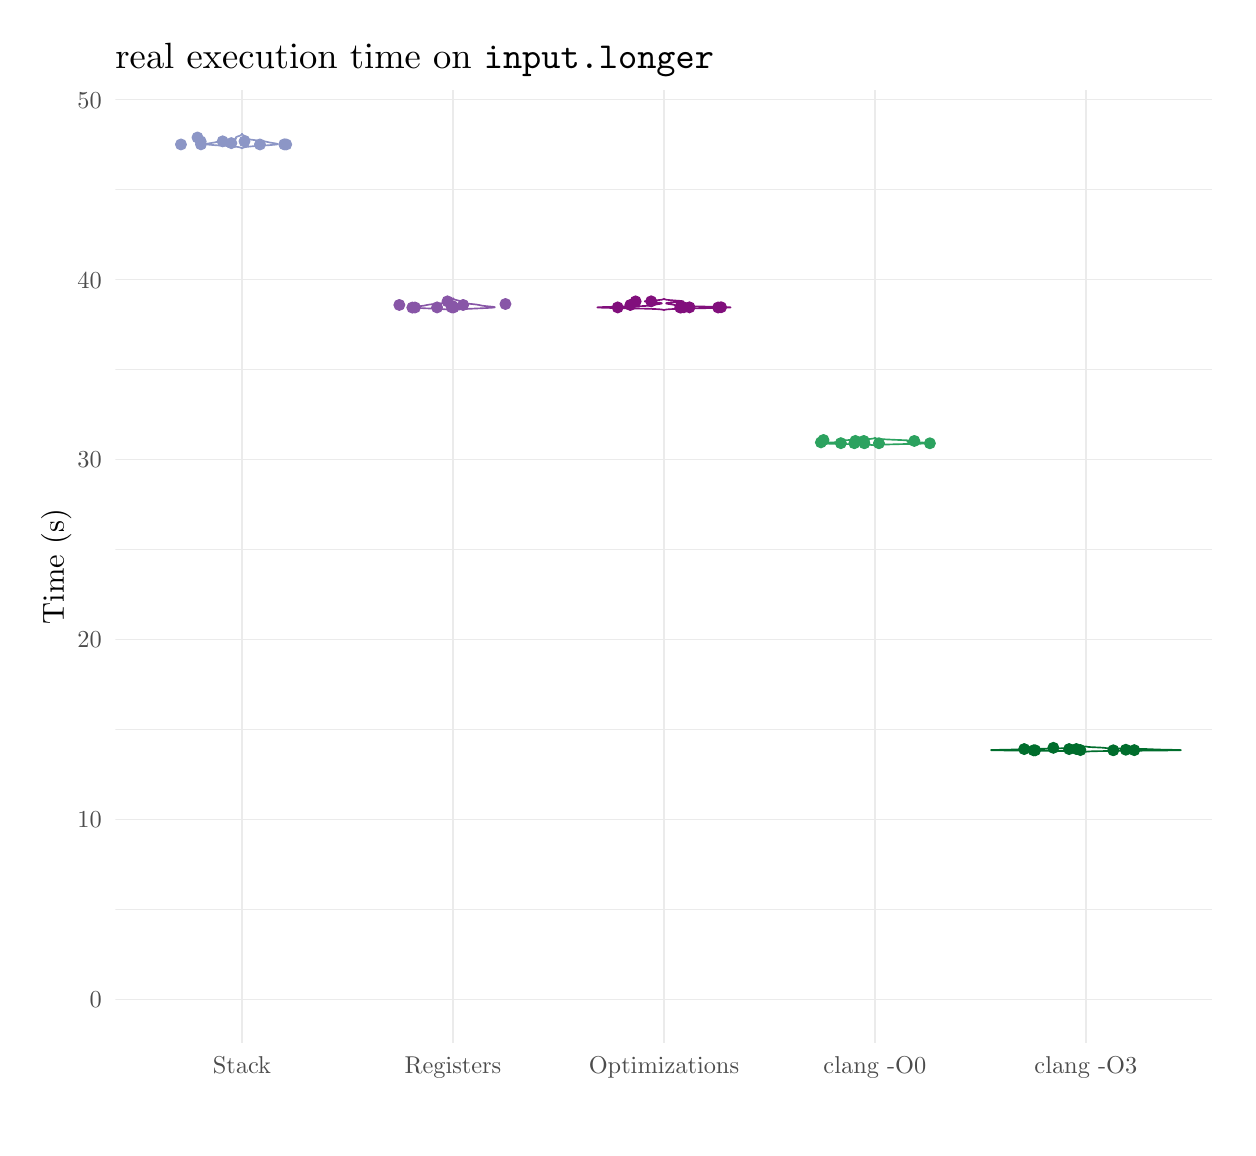
\begin{tikzpicture}[x=1pt,y=1pt]
\definecolor{fillColor}{RGB}{255,255,255}
\path[use as bounding box,fill=fillColor,fill opacity=0.00] (0,0) rectangle (433.62,397.48);
\begin{scope}
\path[clip] ( 31.71, 30.69) rectangle (428.12,374.83);
\definecolor{drawColor}{gray}{0.92}

\path[draw=drawColor,line width= 0.3pt,line join=round] ( 31.71, 78.84) --
	(428.12, 78.84);

\path[draw=drawColor,line width= 0.3pt,line join=round] ( 31.71,143.87) --
	(428.12,143.87);

\path[draw=drawColor,line width= 0.3pt,line join=round] ( 31.71,208.90) --
	(428.12,208.90);

\path[draw=drawColor,line width= 0.3pt,line join=round] ( 31.71,273.93) --
	(428.12,273.93);

\path[draw=drawColor,line width= 0.3pt,line join=round] ( 31.71,338.95) --
	(428.12,338.95);

\path[draw=drawColor,line width= 0.6pt,line join=round] ( 31.71, 46.33) --
	(428.12, 46.33);

\path[draw=drawColor,line width= 0.6pt,line join=round] ( 31.71,111.36) --
	(428.12,111.36);

\path[draw=drawColor,line width= 0.6pt,line join=round] ( 31.71,176.38) --
	(428.12,176.38);

\path[draw=drawColor,line width= 0.6pt,line join=round] ( 31.71,241.41) --
	(428.12,241.41);

\path[draw=drawColor,line width= 0.6pt,line join=round] ( 31.71,306.44) --
	(428.12,306.44);

\path[draw=drawColor,line width= 0.6pt,line join=round] ( 31.71,371.47) --
	(428.12,371.47);

\path[draw=drawColor,line width= 0.6pt,line join=round] ( 77.45, 30.69) --
	( 77.45,374.83);

\path[draw=drawColor,line width= 0.6pt,line join=round] (153.68, 30.69) --
	(153.68,374.83);

\path[draw=drawColor,line width= 0.6pt,line join=round] (229.92, 30.69) --
	(229.92,374.83);

\path[draw=drawColor,line width= 0.6pt,line join=round] (306.15, 30.69) --
	(306.15,374.83);

\path[draw=drawColor,line width= 0.6pt,line join=round] (382.38, 30.69) --
	(382.38,374.83);
\definecolor{drawColor}{RGB}{140,150,198}
\definecolor{fillColor}{RGB}{255,255,255}

\path[draw=drawColor,line width= 0.6pt,line join=round,line cap=round,fill=fillColor] ( 77.35,353.87) --
	( 77.34,353.88) --
	( 77.33,353.89) --
	( 77.32,353.90) --
	( 77.31,353.91) --
	( 77.30,353.92) --
	( 77.29,353.93) --
	( 77.28,353.94) --
	( 77.27,353.95) --
	( 77.26,353.96) --
	( 77.25,353.97) --
	( 77.24,353.98) --
	( 77.22,353.99) --
	( 77.21,354.01) --
	( 77.19,354.02) --
	( 77.18,354.03) --
	( 77.16,354.04) --
	( 77.14,354.05) --
	( 77.12,354.06) --
	( 77.10,354.07) --
	( 77.08,354.08) --
	( 77.06,354.09) --
	( 77.03,354.10) --
	( 77.01,354.11) --
	( 76.98,354.12) --
	( 76.96,354.13) --
	( 76.93,354.14) --
	( 76.90,354.15) --
	( 76.87,354.16) --
	( 76.84,354.17) --
	( 76.80,354.18) --
	( 76.77,354.19) --
	( 76.73,354.20) --
	( 76.69,354.21) --
	( 76.65,354.22) --
	( 76.61,354.23) --
	( 76.57,354.24) --
	( 76.52,354.25) --
	( 76.47,354.27) --
	( 76.42,354.28) --
	( 76.37,354.29) --
	( 76.32,354.30) --
	( 76.27,354.31) --
	( 76.21,354.32) --
	( 76.15,354.33) --
	( 76.09,354.34) --
	( 76.02,354.35) --
	( 75.96,354.36) --
	( 75.89,354.37) --
	( 75.82,354.38) --
	( 75.75,354.39) --
	( 75.67,354.40) --
	( 75.59,354.41) --
	( 75.51,354.42) --
	( 75.43,354.43) --
	( 75.35,354.44) --
	( 75.26,354.45) --
	( 75.17,354.46) --
	( 75.07,354.47) --
	( 74.98,354.48) --
	( 74.88,354.49) --
	( 74.78,354.50) --
	( 74.68,354.51) --
	( 74.57,354.53) --
	( 74.46,354.54) --
	( 74.35,354.55) --
	( 74.24,354.56) --
	( 74.12,354.57) --
	( 74.01,354.58) --
	( 73.89,354.59) --
	( 73.76,354.60) --
	( 73.64,354.61) --
	( 73.51,354.62) --
	( 73.38,354.63) --
	( 73.24,354.64) --
	( 73.11,354.65) --
	( 72.97,354.66) --
	( 72.83,354.67) --
	( 72.69,354.68) --
	( 72.55,354.69) --
	( 72.40,354.70) --
	( 72.25,354.71) --
	( 72.10,354.72) --
	( 71.95,354.73) --
	( 71.80,354.74) --
	( 71.65,354.75) --
	( 71.49,354.76) --
	( 71.34,354.77) --
	( 71.18,354.79) --
	( 71.02,354.80) --
	( 70.86,354.81) --
	( 70.70,354.82) --
	( 70.54,354.83) --
	( 70.38,354.84) --
	( 70.21,354.85) --
	( 70.05,354.86) --
	( 69.89,354.87) --
	( 69.73,354.88) --
	( 69.56,354.89) --
	( 69.40,354.90) --
	( 69.24,354.91) --
	( 69.08,354.92) --
	( 68.92,354.93) --
	( 68.76,354.94) --
	( 68.60,354.95) --
	( 68.44,354.96) --
	( 68.29,354.97) --
	( 68.13,354.98) --
	( 67.98,354.99) --
	( 67.83,355.00) --
	( 67.68,355.01) --
	( 67.53,355.02) --
	( 67.39,355.03) --
	( 67.24,355.05) --
	( 67.11,355.06) --
	( 66.97,355.07) --
	( 66.83,355.08) --
	( 66.70,355.09) --
	( 66.57,355.10) --
	( 66.45,355.11) --
	( 66.33,355.12) --
	( 66.21,355.13) --
	( 66.09,355.14) --
	( 65.98,355.15) --
	( 65.87,355.16) --
	( 65.77,355.17) --
	( 65.67,355.18) --
	( 65.57,355.19) --
	( 65.48,355.20) --
	( 65.40,355.21) --
	( 65.31,355.22) --
	( 65.23,355.23) --
	( 65.16,355.24) --
	( 65.09,355.25) --
	( 65.02,355.26) --
	( 64.96,355.27) --
	( 64.90,355.28) --
	( 64.85,355.29) --
	( 64.80,355.31) --
	( 64.76,355.32) --
	( 64.72,355.33) --
	( 64.68,355.34) --
	( 64.65,355.35) --
	( 64.63,355.36) --
	( 64.61,355.37) --
	( 64.59,355.38) --
	( 64.57,355.39) --
	( 64.57,355.40) --
	( 64.56,355.41) --
	( 64.56,355.42) --
	( 64.56,355.43) --
	( 64.57,355.44) --
	( 64.58,355.45) --
	( 64.59,355.46) --
	( 64.61,355.47) --
	( 64.63,355.48) --
	( 64.66,355.49) --
	( 64.69,355.50) --
	( 64.72,355.51) --
	( 64.75,355.52) --
	( 64.79,355.53) --
	( 64.83,355.54) --
	( 64.87,355.55) --
	( 64.92,355.57) --
	( 64.96,355.58) --
	( 65.01,355.59) --
	( 65.06,355.60) --
	( 65.12,355.61) --
	( 65.17,355.62) --
	( 65.23,355.63) --
	( 65.29,355.64) --
	( 65.35,355.65) --
	( 65.41,355.66) --
	( 65.47,355.67) --
	( 65.54,355.68) --
	( 65.60,355.69) --
	( 65.67,355.70) --
	( 65.73,355.71) --
	( 65.80,355.72) --
	( 65.87,355.73) --
	( 65.93,355.74) --
	( 66.00,355.75) --
	( 66.07,355.76) --
	( 66.14,355.77) --
	( 66.20,355.78) --
	( 66.27,355.79) --
	( 66.34,355.80) --
	( 66.41,355.81) --
	( 66.47,355.83) --
	( 66.54,355.84) --
	( 66.60,355.85) --
	( 66.67,355.86) --
	( 66.73,355.87) --
	( 66.79,355.88) --
	( 66.86,355.89) --
	( 66.92,355.90) --
	( 66.98,355.91) --
	( 67.04,355.92) --
	( 67.10,355.93) --
	( 67.16,355.94) --
	( 67.21,355.95) --
	( 67.27,355.96) --
	( 67.32,355.97) --
	( 67.38,355.98) --
	( 67.43,355.99) --
	( 67.48,356.00) --
	( 67.54,356.01) --
	( 67.59,356.02) --
	( 67.64,356.03) --
	( 67.69,356.04) --
	( 67.74,356.05) --
	( 67.78,356.06) --
	( 67.83,356.08) --
	( 67.88,356.09) --
	( 67.93,356.10) --
	( 67.97,356.11) --
	( 68.02,356.12) --
	( 68.06,356.13) --
	( 68.11,356.14) --
	( 68.15,356.15) --
	( 68.20,356.16) --
	( 68.24,356.17) --
	( 68.29,356.18) --
	( 68.33,356.19) --
	( 68.38,356.20) --
	( 68.42,356.21) --
	( 68.47,356.22) --
	( 68.52,356.23) --
	( 68.56,356.24) --
	( 68.61,356.25) --
	( 68.66,356.26) --
	( 68.71,356.27) --
	( 68.76,356.28) --
	( 68.81,356.29) --
	( 68.86,356.30) --
	( 68.91,356.31) --
	( 68.96,356.32) --
	( 69.02,356.34) --
	( 69.07,356.35) --
	( 69.13,356.36) --
	( 69.18,356.37) --
	( 69.24,356.38) --
	( 69.30,356.39) --
	( 69.36,356.40) --
	( 69.42,356.41) --
	( 69.49,356.42) --
	( 69.55,356.43) --
	( 69.62,356.44) --
	( 69.69,356.45) --
	( 69.75,356.46) --
	( 69.82,356.47) --
	( 69.89,356.48) --
	( 69.97,356.49) --
	( 70.04,356.50) --
	( 70.12,356.51) --
	( 70.19,356.52) --
	( 70.27,356.53) --
	( 70.35,356.54) --
	( 70.43,356.55) --
	( 70.51,356.56) --
	( 70.59,356.57) --
	( 70.67,356.58) --
	( 70.76,356.60) --
	( 70.84,356.61) --
	( 70.93,356.62) --
	( 71.01,356.63) --
	( 71.10,356.64) --
	( 71.19,356.65) --
	( 71.28,356.66) --
	( 71.37,356.67) --
	( 71.46,356.68) --
	( 71.55,356.69) --
	( 71.64,356.70) --
	( 71.73,356.71) --
	( 71.82,356.72) --
	( 71.91,356.73) --
	( 72.00,356.74) --
	( 72.09,356.75) --
	( 72.18,356.76) --
	( 72.27,356.77) --
	( 72.36,356.78) --
	( 72.45,356.79) --
	( 72.54,356.80) --
	( 72.63,356.81) --
	( 72.72,356.82) --
	( 72.81,356.83) --
	( 72.89,356.84) --
	( 72.98,356.86) --
	( 73.06,356.87) --
	( 73.15,356.88) --
	( 73.23,356.89) --
	( 73.31,356.90) --
	( 73.39,356.91) --
	( 73.47,356.92) --
	( 73.55,356.93) --
	( 73.62,356.94) --
	( 73.70,356.95) --
	( 73.77,356.96) --
	( 73.84,356.97) --
	( 73.92,356.98) --
	( 73.98,356.99) --
	( 74.05,357.00) --
	( 74.12,357.01) --
	( 74.18,357.02) --
	( 74.24,357.03) --
	( 74.30,357.04) --
	( 74.36,357.05) --
	( 74.42,357.06) --
	( 74.47,357.07) --
	( 74.52,357.08) --
	( 74.57,357.09) --
	( 74.62,357.10) --
	( 74.67,357.12) --
	( 74.71,357.13) --
	( 74.76,357.14) --
	( 74.80,357.15) --
	( 74.84,357.16) --
	( 74.87,357.17) --
	( 74.91,357.18) --
	( 74.94,357.19) --
	( 74.97,357.20) --
	( 75.00,357.21) --
	( 75.03,357.22) --
	( 75.06,357.23) --
	( 75.08,357.24) --
	( 75.10,357.25) --
	( 75.12,357.26) --
	( 75.14,357.27) --
	( 75.16,357.28) --
	( 75.18,357.29) --
	( 75.19,357.30) --
	( 75.20,357.31) --
	( 75.22,357.32) --
	( 75.23,357.33) --
	( 75.23,357.34) --
	( 75.24,357.35) --
	( 75.25,357.36) --
	( 75.25,357.38) --
	( 75.26,357.39) --
	( 75.26,357.40) --
	( 75.27,357.41) --
	( 75.27,357.42) --
	( 75.27,357.43) --
	( 75.27,357.44) --
	( 75.27,357.45) --
	( 75.26,357.46) --
	( 75.26,357.47) --
	( 75.26,357.48) --
	( 75.26,357.49) --
	( 75.25,357.50) --
	( 75.25,357.51) --
	( 75.25,357.52) --
	( 75.24,357.53) --
	( 75.24,357.54) --
	( 75.23,357.55) --
	( 75.23,357.56) --
	( 75.22,357.57) --
	( 75.22,357.58) --
	( 75.21,357.59) --
	( 75.21,357.60) --
	( 75.20,357.61) --
	( 75.20,357.62) --
	( 75.20,357.64) --
	( 75.19,357.65) --
	( 75.19,357.66) --
	( 75.19,357.67) --
	( 75.19,357.68) --
	( 75.18,357.69) --
	( 75.18,357.70) --
	( 75.18,357.71) --
	( 75.18,357.72) --
	( 75.18,357.73) --
	( 75.18,357.74) --
	( 75.19,357.75) --
	( 75.19,357.76) --
	( 75.19,357.77) --
	( 75.20,357.78) --
	( 75.20,357.79) --
	( 75.21,357.80) --
	( 75.21,357.81) --
	( 75.22,357.82) --
	( 75.23,357.83) --
	( 75.24,357.84) --
	( 75.25,357.85) --
	( 75.26,357.86) --
	( 75.27,357.87) --
	( 75.28,357.88) --
	( 75.30,357.90) --
	( 75.31,357.91) --
	( 75.33,357.92) --
	( 75.34,357.93) --
	( 75.36,357.94) --
	( 75.38,357.95) --
	( 75.39,357.96) --
	( 75.41,357.97) --
	( 75.43,357.98) --
	( 75.45,357.99) --
	( 75.47,358.00) --
	( 75.50,358.01) --
	( 75.52,358.02) --
	( 75.54,358.03) --
	( 75.56,358.04) --
	( 75.59,358.05) --
	( 75.61,358.06) --
	( 75.64,358.07) --
	( 75.66,358.08) --
	( 75.69,358.09) --
	( 75.72,358.10) --
	( 75.74,358.11) --
	( 75.77,358.12) --
	( 75.80,358.13) --
	( 75.83,358.14) --
	( 75.86,358.16) --
	( 75.88,358.17) --
	( 75.91,358.18) --
	( 75.94,358.19) --
	( 75.97,358.20) --
	( 76.00,358.21) --
	( 76.03,358.22) --
	( 76.06,358.23) --
	( 76.09,358.24) --
	( 76.12,358.25) --
	( 76.15,358.26) --
	( 76.18,358.27) --
	( 76.21,358.28) --
	( 76.24,358.29) --
	( 76.27,358.30) --
	( 76.29,358.31) --
	( 76.32,358.32) --
	( 76.35,358.33) --
	( 76.38,358.34) --
	( 76.41,358.35) --
	( 76.44,358.36) --
	( 76.47,358.37) --
	( 76.49,358.38) --
	( 76.52,358.39) --
	( 76.55,358.40) --
	( 76.57,358.42) --
	( 76.60,358.43) --
	( 76.63,358.44) --
	( 76.65,358.45) --
	( 76.68,358.46) --
	( 76.70,358.47) --
	( 76.73,358.48) --
	( 76.75,358.49) --
	( 76.77,358.50) --
	( 76.80,358.51) --
	( 76.82,358.52) --
	( 76.84,358.53) --
	( 76.86,358.54) --
	( 76.88,358.55) --
	( 76.90,358.56) --
	( 76.92,358.57) --
	( 76.94,358.58) --
	( 76.96,358.59) --
	( 76.98,358.60) --
	( 77.00,358.61) --
	( 77.02,358.62) --
	( 77.03,358.63) --
	( 77.05,358.64) --
	( 77.07,358.65) --
	( 77.08,358.66) --
	( 77.10,358.68) --
	( 77.11,358.69) --
	( 77.13,358.70) --
	( 77.14,358.71) --
	( 77.15,358.72) --
	( 77.17,358.73) --
	( 77.18,358.74) --
	( 77.19,358.75) --
	( 77.20,358.76) --
	( 77.21,358.77) --
	( 77.23,358.78) --
	( 77.24,358.79) --
	( 77.25,358.80) --
	( 77.26,358.81) --
	( 77.27,358.82) --
	( 77.27,358.83) --
	( 77.28,358.84) --
	( 77.29,358.85) --
	( 77.30,358.86) --
	( 77.31,358.87) --
	( 77.31,358.88) --
	( 77.32,358.89) --
	( 77.33,358.90) --
	( 77.33,358.91) --
	( 77.34,358.92) --
	( 77.35,358.94) --
	( 77.35,358.95) --
	( 77.36,358.96) --
	( 77.36,358.97) --
	( 77.37,358.98) --
	( 77.37,358.99) --
	( 77.38,359.00) --
	( 77.38,359.01) --
	( 77.38,359.02) --
	( 77.39,359.03) --
	( 77.39,359.04) --
	( 77.40,359.05) --
	( 77.40,359.06) --
	( 77.40,359.07) --
	( 77.41,359.08) --
	( 77.41,359.09) --
	( 77.41,359.10) --
	( 77.41,359.11) --
	( 77.42,359.12) --
	( 77.42,359.13) --
	( 77.42,359.14) --
	( 77.42,359.15) --
	( 77.42,359.16) --
	( 77.43,359.17) --
	( 77.43,359.18) --
	( 77.48,359.18) --
	( 77.48,359.17) --
	( 77.48,359.16) --
	( 77.48,359.15) --
	( 77.48,359.14) --
	( 77.49,359.13) --
	( 77.49,359.12) --
	( 77.49,359.11) --
	( 77.49,359.10) --
	( 77.50,359.09) --
	( 77.50,359.08) --
	( 77.50,359.07) --
	( 77.50,359.06) --
	( 77.51,359.05) --
	( 77.51,359.04) --
	( 77.51,359.03) --
	( 77.52,359.02) --
	( 77.52,359.01) --
	( 77.53,359.00) --
	( 77.53,358.99) --
	( 77.54,358.98) --
	( 77.54,358.97) --
	( 77.55,358.96) --
	( 77.55,358.95) --
	( 77.56,358.94) --
	( 77.56,358.92) --
	( 77.57,358.91) --
	( 77.58,358.90) --
	( 77.58,358.89) --
	( 77.59,358.88) --
	( 77.60,358.87) --
	( 77.60,358.86) --
	( 77.61,358.85) --
	( 77.62,358.84) --
	( 77.63,358.83) --
	( 77.64,358.82) --
	( 77.65,358.81) --
	( 77.66,358.80) --
	( 77.67,358.79) --
	( 77.68,358.78) --
	( 77.69,358.77) --
	( 77.70,358.76) --
	( 77.71,358.75) --
	( 77.72,358.74) --
	( 77.74,358.73) --
	( 77.75,358.72) --
	( 77.76,358.71) --
	( 77.78,358.70) --
	( 77.79,358.69) --
	( 77.81,358.68) --
	( 77.82,358.66) --
	( 77.84,358.65) --
	( 77.85,358.64) --
	( 77.87,358.63) --
	( 77.89,358.62) --
	( 77.91,358.61) --
	( 77.92,358.60) --
	( 77.94,358.59) --
	( 77.96,358.58) --
	( 77.98,358.57) --
	( 78.00,358.56) --
	( 78.02,358.55) --
	( 78.04,358.54) --
	( 78.06,358.53) --
	( 78.09,358.52) --
	( 78.11,358.51) --
	( 78.13,358.50) --
	( 78.15,358.49) --
	( 78.18,358.48) --
	( 78.20,358.47) --
	( 78.23,358.46) --
	( 78.25,358.45) --
	( 78.28,358.44) --
	( 78.30,358.43) --
	( 78.33,358.42) --
	( 78.36,358.40) --
	( 78.38,358.39) --
	( 78.41,358.38) --
	( 78.44,358.37) --
	( 78.47,358.36) --
	( 78.49,358.35) --
	( 78.52,358.34) --
	( 78.55,358.33) --
	( 78.58,358.32) --
	( 78.61,358.31) --
	( 78.64,358.30) --
	( 78.67,358.29) --
	( 78.70,358.28) --
	( 78.73,358.27) --
	( 78.76,358.26) --
	( 78.78,358.25) --
	( 78.81,358.24) --
	( 78.84,358.23) --
	( 78.87,358.22) --
	( 78.90,358.21) --
	( 78.93,358.20) --
	( 78.96,358.19) --
	( 78.99,358.18) --
	( 79.02,358.17) --
	( 79.05,358.16) --
	( 79.08,358.14) --
	( 79.10,358.13) --
	( 79.13,358.12) --
	( 79.16,358.11) --
	( 79.19,358.10) --
	( 79.21,358.09) --
	( 79.24,358.08) --
	( 79.27,358.07) --
	( 79.29,358.06) --
	( 79.31,358.05) --
	( 79.34,358.04) --
	( 79.36,358.03) --
	( 79.39,358.02) --
	( 79.41,358.01) --
	( 79.43,358.00) --
	( 79.45,357.99) --
	( 79.47,357.98) --
	( 79.49,357.97) --
	( 79.51,357.96) --
	( 79.53,357.95) --
	( 79.54,357.94) --
	( 79.56,357.93) --
	( 79.58,357.92) --
	( 79.59,357.91) --
	( 79.61,357.90) --
	( 79.62,357.88) --
	( 79.63,357.87) --
	( 79.64,357.86) --
	( 79.65,357.85) --
	( 79.66,357.84) --
	( 79.67,357.83) --
	( 79.68,357.82) --
	( 79.69,357.81) --
	( 79.70,357.80) --
	( 79.70,357.79) --
	( 79.71,357.78) --
	( 79.71,357.77) --
	( 79.71,357.76) --
	( 79.72,357.75) --
	( 79.72,357.74) --
	( 79.72,357.73) --
	( 79.72,357.72) --
	( 79.72,357.71) --
	( 79.72,357.70) --
	( 79.72,357.69) --
	( 79.72,357.68) --
	( 79.72,357.67) --
	( 79.71,357.66) --
	( 79.71,357.65) --
	( 79.71,357.64) --
	( 79.70,357.62) --
	( 79.70,357.61) --
	( 79.70,357.60) --
	( 79.69,357.59) --
	( 79.69,357.58) --
	( 79.68,357.57) --
	( 79.68,357.56) --
	( 79.67,357.55) --
	( 79.67,357.54) --
	( 79.66,357.53) --
	( 79.66,357.52) --
	( 79.65,357.51) --
	( 79.65,357.50) --
	( 79.65,357.49) --
	( 79.64,357.48) --
	( 79.64,357.47) --
	( 79.64,357.46) --
	( 79.64,357.45) --
	( 79.64,357.44) --
	( 79.64,357.43) --
	( 79.64,357.42) --
	( 79.64,357.41) --
	( 79.64,357.40) --
	( 79.64,357.39) --
	( 79.65,357.38) --
	( 79.65,357.36) --
	( 79.66,357.35) --
	( 79.67,357.34) --
	( 79.68,357.33) --
	( 79.69,357.32) --
	( 79.70,357.31) --
	( 79.71,357.30) --
	( 79.73,357.29) --
	( 79.74,357.28) --
	( 79.76,357.27) --
	( 79.78,357.26) --
	( 79.80,357.25) --
	( 79.82,357.24) --
	( 79.85,357.23) --
	( 79.87,357.22) --
	( 79.90,357.21) --
	( 79.93,357.20) --
	( 79.96,357.19) --
	( 80.00,357.18) --
	( 80.03,357.17) --
	( 80.07,357.16) --
	( 80.11,357.15) --
	( 80.15,357.14) --
	( 80.19,357.13) --
	( 80.23,357.12) --
	( 80.28,357.10) --
	( 80.33,357.09) --
	( 80.38,357.08) --
	( 80.43,357.07) --
	( 80.49,357.06) --
	( 80.54,357.05) --
	( 80.60,357.04) --
	( 80.66,357.03) --
	( 80.72,357.02) --
	( 80.79,357.01) --
	( 80.85,357.00) --
	( 80.92,356.99) --
	( 80.99,356.98) --
	( 81.06,356.97) --
	( 81.13,356.96) --
	( 81.20,356.95) --
	( 81.28,356.94) --
	( 81.35,356.93) --
	( 81.43,356.92) --
	( 81.51,356.91) --
	( 81.59,356.90) --
	( 81.67,356.89) --
	( 81.76,356.88) --
	( 81.84,356.87) --
	( 81.93,356.86) --
	( 82.01,356.84) --
	( 82.10,356.83) --
	( 82.19,356.82) --
	( 82.27,356.81) --
	( 82.36,356.80) --
	( 82.45,356.79) --
	( 82.54,356.78) --
	( 82.63,356.77) --
	( 82.72,356.76) --
	( 82.81,356.75) --
	( 82.90,356.74) --
	( 82.99,356.73) --
	( 83.09,356.72) --
	( 83.18,356.71) --
	( 83.27,356.70) --
	( 83.36,356.69) --
	( 83.45,356.68) --
	( 83.54,356.67) --
	( 83.63,356.66) --
	( 83.71,356.65) --
	( 83.80,356.64) --
	( 83.89,356.63) --
	( 83.98,356.62) --
	( 84.06,356.61) --
	( 84.15,356.60) --
	( 84.23,356.58) --
	( 84.31,356.57) --
	( 84.39,356.56) --
	( 84.48,356.55) --
	( 84.56,356.54) --
	( 84.63,356.53) --
	( 84.71,356.52) --
	( 84.79,356.51) --
	( 84.86,356.50) --
	( 84.94,356.49) --
	( 85.01,356.48) --
	( 85.08,356.47) --
	( 85.15,356.46) --
	( 85.22,356.45) --
	( 85.28,356.44) --
	( 85.35,356.43) --
	( 85.42,356.42) --
	( 85.48,356.41) --
	( 85.54,356.40) --
	( 85.60,356.39) --
	( 85.66,356.38) --
	( 85.72,356.37) --
	( 85.78,356.36) --
	( 85.83,356.35) --
	( 85.89,356.34) --
	( 85.94,356.32) --
	( 85.99,356.31) --
	( 86.05,356.30) --
	( 86.10,356.29) --
	( 86.15,356.28) --
	( 86.20,356.27) --
	( 86.24,356.26) --
	( 86.29,356.25) --
	( 86.34,356.24) --
	( 86.39,356.23) --
	( 86.43,356.22) --
	( 86.48,356.21) --
	( 86.52,356.20) --
	( 86.57,356.19) --
	( 86.61,356.18) --
	( 86.66,356.17) --
	( 86.70,356.16) --
	( 86.75,356.15) --
	( 86.79,356.14) --
	( 86.84,356.13) --
	( 86.89,356.12) --
	( 86.93,356.11) --
	( 86.98,356.10) --
	( 87.02,356.09) --
	( 87.07,356.08) --
	( 87.12,356.06) --
	( 87.17,356.05) --
	( 87.22,356.04) --
	( 87.27,356.03) --
	( 87.32,356.02) --
	( 87.37,356.01) --
	( 87.42,356.00) --
	( 87.47,355.99) --
	( 87.53,355.98) --
	( 87.58,355.97) --
	( 87.63,355.96) --
	( 87.69,355.95) --
	( 87.75,355.94) --
	( 87.81,355.93) --
	( 87.86,355.92) --
	( 87.92,355.91) --
	( 87.99,355.90) --
	( 88.05,355.89) --
	( 88.11,355.88) --
	( 88.17,355.87) --
	( 88.24,355.86) --
	( 88.30,355.85) --
	( 88.37,355.84) --
	( 88.43,355.83) --
	( 88.50,355.81) --
	( 88.56,355.80) --
	( 88.63,355.79) --
	( 88.70,355.78) --
	( 88.77,355.77) --
	( 88.83,355.76) --
	( 88.90,355.75) --
	( 88.97,355.74) --
	( 89.04,355.73) --
	( 89.10,355.72) --
	( 89.17,355.71) --
	( 89.24,355.70) --
	( 89.30,355.69) --
	( 89.37,355.68) --
	( 89.43,355.67) --
	( 89.49,355.66) --
	( 89.55,355.65) --
	( 89.61,355.64) --
	( 89.67,355.63) --
	( 89.73,355.62) --
	( 89.78,355.61) --
	( 89.84,355.60) --
	( 89.89,355.59) --
	( 89.94,355.58) --
	( 89.99,355.57) --
	( 90.03,355.55) --
	( 90.08,355.54) --
	( 90.11,355.53) --
	( 90.15,355.52) --
	( 90.19,355.51) --
	( 90.22,355.50) --
	( 90.25,355.49) --
	( 90.27,355.48) --
	( 90.29,355.47) --
	( 90.31,355.46) --
	( 90.32,355.45) --
	( 90.33,355.44) --
	( 90.34,355.43) --
	( 90.34,355.42) --
	( 90.34,355.41) --
	( 90.34,355.40) --
	( 90.33,355.39) --
	( 90.31,355.38) --
	( 90.30,355.37) --
	( 90.27,355.36) --
	( 90.25,355.35) --
	( 90.22,355.34) --
	( 90.18,355.33) --
	( 90.14,355.32) --
	( 90.10,355.31) --
	( 90.05,355.29) --
	( 90.00,355.28) --
	( 89.94,355.27) --
	( 89.88,355.26) --
	( 89.81,355.25) --
	( 89.74,355.24) --
	( 89.67,355.23) --
	( 89.59,355.22) --
	( 89.51,355.21) --
	( 89.42,355.20) --
	( 89.33,355.19) --
	( 89.23,355.18) --
	( 89.13,355.17) --
	( 89.03,355.16) --
	( 88.92,355.15) --
	( 88.81,355.14) --
	( 88.69,355.13) --
	( 88.58,355.12) --
	( 88.45,355.11) --
	( 88.33,355.10) --
	( 88.20,355.09) --
	( 88.07,355.08) --
	( 87.94,355.07) --
	( 87.80,355.06) --
	( 87.66,355.05) --
	( 87.52,355.03) --
	( 87.37,355.02) --
	( 87.22,355.01) --
	( 87.07,355.00) --
	( 86.92,354.99) --
	( 86.77,354.98) --
	( 86.62,354.97) --
	( 86.46,354.96) --
	( 86.30,354.95) --
	( 86.15,354.94) --
	( 85.99,354.93) --
	( 85.83,354.92) --
	( 85.66,354.91) --
	( 85.50,354.90) --
	( 85.34,354.89) --
	( 85.18,354.88) --
	( 85.01,354.87) --
	( 84.85,354.86) --
	( 84.69,354.85) --
	( 84.53,354.84) --
	( 84.37,354.83) --
	( 84.20,354.82) --
	( 84.04,354.81) --
	( 83.88,354.80) --
	( 83.73,354.79) --
	( 83.57,354.77) --
	( 83.41,354.76) --
	( 83.26,354.75) --
	( 83.10,354.74) --
	( 82.95,354.73) --
	( 82.80,354.72) --
	( 82.65,354.71) --
	( 82.50,354.70) --
	( 82.36,354.69) --
	( 82.21,354.68) --
	( 82.07,354.67) --
	( 81.93,354.66) --
	( 81.79,354.65) --
	( 81.66,354.64) --
	( 81.53,354.63) --
	( 81.40,354.62) --
	( 81.27,354.61) --
	( 81.14,354.60) --
	( 81.02,354.59) --
	( 80.90,354.58) --
	( 80.78,354.57) --
	( 80.66,354.56) --
	( 80.55,354.55) --
	( 80.44,354.54) --
	( 80.33,354.53) --
	( 80.22,354.51) --
	( 80.12,354.50) --
	( 80.02,354.49) --
	( 79.92,354.48) --
	( 79.83,354.47) --
	( 79.74,354.46) --
	( 79.65,354.45) --
	( 79.56,354.44) --
	( 79.47,354.43) --
	( 79.39,354.42) --
	( 79.31,354.41) --
	( 79.23,354.40) --
	( 79.16,354.39) --
	( 79.08,354.38) --
	( 79.01,354.37) --
	( 78.94,354.36) --
	( 78.88,354.35) --
	( 78.82,354.34) --
	( 78.75,354.33) --
	( 78.70,354.32) --
	( 78.64,354.31) --
	( 78.58,354.30) --
	( 78.53,354.29) --
	( 78.48,354.28) --
	( 78.43,354.27) --
	( 78.38,354.25) --
	( 78.34,354.24) --
	( 78.29,354.23) --
	( 78.25,354.22) --
	( 78.21,354.21) --
	( 78.17,354.20) --
	( 78.14,354.19) --
	( 78.10,354.18) --
	( 78.07,354.17) --
	( 78.03,354.16) --
	( 78.00,354.15) --
	( 77.97,354.14) --
	( 77.95,354.13) --
	( 77.92,354.12) --
	( 77.89,354.11) --
	( 77.87,354.10) --
	( 77.85,354.09) --
	( 77.82,354.08) --
	( 77.80,354.07) --
	( 77.78,354.06) --
	( 77.76,354.05) --
	( 77.75,354.04) --
	( 77.73,354.03) --
	( 77.71,354.02) --
	( 77.70,354.01) --
	( 77.68,353.99) --
	( 77.67,353.98) --
	( 77.65,353.97) --
	( 77.64,353.96) --
	( 77.63,353.95) --
	( 77.62,353.94) --
	( 77.61,353.93) --
	( 77.60,353.92) --
	( 77.59,353.91) --
	( 77.58,353.90) --
	( 77.57,353.89) --
	( 77.56,353.88) --
	( 77.56,353.87) --
	( 77.35,353.87) --
	cycle;
\definecolor{drawColor}{RGB}{136,86,167}

\path[draw=drawColor,line width= 0.6pt,line join=round,line cap=round,fill=fillColor] (153.58,295.19) --
	(153.57,295.19) --
	(153.56,295.20) --
	(153.56,295.21) --
	(153.55,295.22) --
	(153.54,295.23) --
	(153.53,295.24) --
	(153.51,295.25) --
	(153.50,295.26) --
	(153.49,295.26) --
	(153.48,295.27) --
	(153.46,295.28) --
	(153.45,295.29) --
	(153.43,295.30) --
	(153.41,295.31) --
	(153.39,295.32) --
	(153.38,295.33) --
	(153.36,295.34) --
	(153.33,295.34) --
	(153.31,295.35) --
	(153.29,295.36) --
	(153.26,295.37) --
	(153.24,295.38) --
	(153.21,295.39) --
	(153.18,295.40) --
	(153.15,295.41) --
	(153.12,295.42) --
	(153.08,295.42) --
	(153.05,295.43) --
	(153.01,295.44) --
	(152.97,295.45) --
	(152.93,295.46) --
	(152.89,295.47) --
	(152.84,295.48) --
	(152.79,295.49) --
	(152.74,295.50) --
	(152.69,295.50) --
	(152.64,295.51) --
	(152.58,295.52) --
	(152.53,295.53) --
	(152.46,295.54) --
	(152.40,295.55) --
	(152.34,295.56) --
	(152.27,295.57) --
	(152.20,295.58) --
	(152.12,295.58) --
	(152.04,295.59) --
	(151.96,295.60) --
	(151.88,295.61) --
	(151.80,295.62) --
	(151.71,295.63) --
	(151.62,295.64) --
	(151.52,295.65) --
	(151.42,295.66) --
	(151.32,295.66) --
	(151.22,295.67) --
	(151.11,295.68) --
	(151.00,295.69) --
	(150.88,295.70) --
	(150.77,295.71) --
	(150.65,295.72) --
	(150.52,295.73) --
	(150.39,295.74) --
	(150.26,295.74) --
	(150.13,295.75) --
	(149.99,295.76) --
	(149.85,295.77) --
	(149.71,295.78) --
	(149.56,295.79) --
	(149.41,295.80) --
	(149.26,295.81) --
	(149.10,295.82) --
	(148.94,295.82) --
	(148.78,295.83) --
	(148.61,295.84) --
	(148.44,295.85) --
	(148.27,295.86) --
	(148.10,295.87) --
	(147.92,295.88) --
	(147.74,295.89) --
	(147.56,295.90) --
	(147.37,295.90) --
	(147.19,295.91) --
	(147.00,295.92) --
	(146.81,295.93) --
	(146.62,295.94) --
	(146.42,295.95) --
	(146.23,295.96) --
	(146.03,295.97) --
	(145.84,295.98) --
	(145.64,295.98) --
	(145.44,295.99) --
	(145.24,296.00) --
	(145.04,296.01) --
	(144.84,296.02) --
	(144.64,296.03) --
	(144.44,296.04) --
	(144.24,296.05) --
	(144.04,296.05) --
	(143.84,296.06) --
	(143.64,296.07) --
	(143.44,296.08) --
	(143.25,296.09) --
	(143.05,296.10) --
	(142.86,296.11) --
	(142.67,296.12) --
	(142.48,296.13) --
	(142.30,296.13) --
	(142.12,296.14) --
	(141.94,296.15) --
	(141.76,296.16) --
	(141.58,296.17) --
	(141.42,296.18) --
	(141.25,296.19) --
	(141.08,296.20) --
	(140.93,296.21) --
	(140.77,296.21) --
	(140.62,296.22) --
	(140.47,296.23) --
	(140.33,296.24) --
	(140.20,296.25) --
	(140.06,296.26) --
	(139.94,296.27) --
	(139.82,296.28) --
	(139.70,296.29) --
	(139.59,296.29) --
	(139.48,296.30) --
	(139.38,296.31) --
	(139.29,296.32) --
	(139.20,296.33) --
	(139.12,296.34) --
	(139.04,296.35) --
	(138.97,296.36) --
	(138.90,296.37) --
	(138.84,296.37) --
	(138.79,296.38) --
	(138.74,296.39) --
	(138.70,296.40) --
	(138.66,296.41) --
	(138.63,296.42) --
	(138.61,296.43) --
	(138.59,296.44) --
	(138.58,296.45) --
	(138.57,296.45) --
	(138.57,296.46) --
	(138.57,296.47) --
	(138.58,296.48) --
	(138.60,296.49) --
	(138.62,296.50) --
	(138.64,296.51) --
	(138.67,296.52) --
	(138.70,296.53) --
	(138.74,296.53) --
	(138.79,296.54) --
	(138.83,296.55) --
	(138.89,296.56) --
	(138.94,296.57) --
	(139.00,296.58) --
	(139.06,296.59) --
	(139.13,296.60) --
	(139.20,296.61) --
	(139.27,296.61) --
	(139.35,296.62) --
	(139.42,296.63) --
	(139.50,296.64) --
	(139.59,296.65) --
	(139.67,296.66) --
	(139.76,296.67) --
	(139.85,296.68) --
	(139.94,296.69) --
	(140.03,296.69) --
	(140.12,296.70) --
	(140.21,296.71) --
	(140.31,296.72) --
	(140.40,296.73) --
	(140.50,296.74) --
	(140.59,296.75) --
	(140.69,296.76) --
	(140.78,296.77) --
	(140.88,296.77) --
	(140.97,296.78) --
	(141.07,296.79) --
	(141.16,296.80) --
	(141.25,296.81) --
	(141.34,296.82) --
	(141.44,296.83) --
	(141.53,296.84) --
	(141.61,296.84) --
	(141.70,296.85) --
	(141.79,296.86) --
	(141.87,296.87) --
	(141.96,296.88) --
	(142.04,296.89) --
	(142.12,296.90) --
	(142.20,296.91) --
	(142.27,296.92) --
	(142.35,296.92) --
	(142.42,296.93) --
	(142.50,296.94) --
	(142.57,296.95) --
	(142.63,296.96) --
	(142.70,296.97) --
	(142.77,296.98) --
	(142.83,296.99) --
	(142.89,297.00) --
	(142.95,297.00) --
	(143.01,297.01) --
	(143.06,297.02) --
	(143.12,297.03) --
	(143.17,297.04) --
	(143.22,297.05) --
	(143.28,297.06) --
	(143.33,297.07) --
	(143.37,297.08) --
	(143.42,297.08) --
	(143.47,297.09) --
	(143.51,297.10) --
	(143.56,297.11) --
	(143.60,297.12) --
	(143.64,297.13) --
	(143.68,297.14) --
	(143.73,297.15) --
	(143.77,297.16) --
	(143.81,297.16) --
	(143.85,297.17) --
	(143.89,297.18) --
	(143.93,297.19) --
	(143.97,297.20) --
	(144.01,297.21) --
	(144.05,297.22) --
	(144.09,297.23) --
	(144.13,297.24) --
	(144.17,297.24) --
	(144.21,297.25) --
	(144.25,297.26) --
	(144.30,297.27) --
	(144.34,297.28) --
	(144.38,297.29) --
	(144.43,297.30) --
	(144.47,297.31) --
	(144.52,297.32) --
	(144.57,297.32) --
	(144.62,297.33) --
	(144.67,297.34) --
	(144.72,297.35) --
	(144.77,297.36) --
	(144.83,297.37) --
	(144.88,297.38) --
	(144.94,297.39) --
	(145.00,297.40) --
	(145.06,297.40) --
	(145.12,297.41) --
	(145.18,297.42) --
	(145.24,297.43) --
	(145.31,297.44) --
	(145.38,297.45) --
	(145.44,297.46) --
	(145.51,297.47) --
	(145.58,297.48) --
	(145.66,297.48) --
	(145.73,297.49) --
	(145.80,297.50) --
	(145.88,297.51) --
	(145.96,297.52) --
	(146.04,297.53) --
	(146.12,297.54) --
	(146.20,297.55) --
	(146.28,297.56) --
	(146.36,297.56) --
	(146.45,297.57) --
	(146.53,297.58) --
	(146.62,297.59) --
	(146.70,297.60) --
	(146.79,297.61) --
	(146.88,297.62) --
	(146.97,297.63) --
	(147.06,297.63) --
	(147.15,297.64) --
	(147.24,297.65) --
	(147.33,297.66) --
	(147.42,297.67) --
	(147.51,297.68) --
	(147.60,297.69) --
	(147.69,297.70) --
	(147.78,297.71) --
	(147.87,297.71) --
	(147.96,297.72) --
	(148.05,297.73) --
	(148.14,297.74) --
	(148.23,297.75) --
	(148.32,297.76) --
	(148.41,297.77) --
	(148.50,297.78) --
	(148.58,297.79) --
	(148.67,297.79) --
	(148.75,297.80) --
	(148.84,297.81) --
	(148.92,297.82) --
	(149.00,297.83) --
	(149.08,297.84) --
	(149.16,297.85) --
	(149.24,297.86) --
	(149.32,297.87) --
	(149.39,297.87) --
	(149.47,297.88) --
	(149.54,297.89) --
	(149.61,297.90) --
	(149.68,297.91) --
	(149.75,297.92) --
	(149.81,297.93) --
	(149.88,297.94) --
	(149.94,297.95) --
	(150.00,297.95) --
	(150.06,297.96) --
	(150.11,297.97) --
	(150.17,297.98) --
	(150.22,297.99) --
	(150.27,298.00) --
	(150.32,298.01) --
	(150.37,298.02) --
	(150.41,298.03) --
	(150.45,298.03) --
	(150.50,298.04) --
	(150.53,298.05) --
	(150.57,298.06) --
	(150.61,298.07) --
	(150.64,298.08) --
	(150.67,298.09) --
	(150.70,298.10) --
	(150.73,298.11) --
	(150.75,298.11) --
	(150.78,298.12) --
	(150.80,298.13) --
	(150.82,298.14) --
	(150.84,298.15) --
	(150.85,298.16) --
	(150.87,298.17) --
	(150.88,298.18) --
	(150.89,298.19) --
	(150.90,298.19) --
	(150.91,298.20) --
	(150.92,298.21) --
	(150.93,298.22) --
	(150.93,298.23) --
	(150.94,298.24) --
	(150.94,298.25) --
	(150.94,298.26) --
	(150.94,298.27) --
	(150.94,298.27) --
	(150.94,298.28) --
	(150.94,298.29) --
	(150.94,298.30) --
	(150.94,298.31) --
	(150.93,298.32) --
	(150.93,298.33) --
	(150.93,298.34) --
	(150.92,298.35) --
	(150.92,298.35) --
	(150.91,298.36) --
	(150.91,298.37) --
	(150.90,298.38) --
	(150.90,298.39) --
	(150.89,298.40) --
	(150.88,298.41) --
	(150.88,298.42) --
	(150.88,298.42) --
	(150.87,298.43) --
	(150.87,298.44) --
	(150.86,298.45) --
	(150.86,298.46) --
	(150.86,298.47) --
	(150.86,298.48) --
	(150.85,298.49) --
	(150.85,298.50) --
	(150.85,298.50) --
	(150.85,298.51) --
	(150.86,298.52) --
	(150.86,298.53) --
	(150.86,298.54) --
	(150.87,298.55) --
	(150.87,298.56) --
	(150.88,298.57) --
	(150.89,298.58) --
	(150.89,298.58) --
	(150.90,298.59) --
	(150.91,298.60) --
	(150.93,298.61) --
	(150.94,298.62) --
	(150.95,298.63) --
	(150.97,298.64) --
	(150.98,298.65) --
	(151.00,298.66) --
	(151.02,298.66) --
	(151.04,298.67) --
	(151.06,298.68) --
	(151.08,298.69) --
	(151.10,298.70) --
	(151.12,298.71) --
	(151.15,298.72) --
	(151.17,298.73) --
	(151.20,298.74) --
	(151.22,298.74) --
	(151.25,298.75) --
	(151.28,298.76) --
	(151.31,298.77) --
	(151.34,298.78) --
	(151.37,298.79) --
	(151.40,298.80) --
	(151.43,298.81) --
	(151.47,298.82) --
	(151.50,298.82) --
	(151.54,298.83) --
	(151.57,298.84) --
	(151.61,298.85) --
	(151.64,298.86) --
	(151.68,298.87) --
	(151.71,298.88) --
	(151.75,298.89) --
	(151.79,298.90) --
	(151.83,298.90) --
	(151.86,298.91) --
	(151.90,298.92) --
	(151.94,298.93) --
	(151.98,298.94) --
	(152.02,298.95) --
	(152.05,298.96) --
	(152.09,298.97) --
	(152.13,298.98) --
	(152.17,298.98) --
	(152.21,298.99) --
	(152.24,299.00) --
	(152.28,299.01) --
	(152.32,299.02) --
	(152.35,299.03) --
	(152.39,299.04) --
	(152.43,299.05) --
	(152.46,299.06) --
	(152.50,299.06) --
	(152.53,299.07) --
	(152.57,299.08) --
	(152.60,299.09) --
	(152.64,299.10) --
	(152.67,299.11) --
	(152.70,299.12) --
	(152.73,299.13) --
	(152.77,299.14) --
	(152.80,299.14) --
	(152.83,299.15) --
	(152.86,299.16) --
	(152.89,299.17) --
	(152.91,299.18) --
	(152.94,299.19) --
	(152.97,299.20) --
	(153.00,299.21) --
	(153.02,299.21) --
	(153.05,299.22) --
	(153.07,299.23) --
	(153.10,299.24) --
	(153.12,299.25) --
	(153.14,299.26) --
	(153.17,299.27) --
	(153.19,299.28) --
	(153.21,299.29) --
	(153.23,299.29) --
	(153.25,299.30) --
	(153.27,299.31) --
	(153.28,299.32) --
	(153.30,299.33) --
	(153.32,299.34) --
	(153.34,299.35) --
	(153.35,299.36) --
	(153.37,299.37) --
	(153.38,299.37) --
	(153.40,299.38) --
	(153.41,299.39) --
	(153.42,299.40) --
	(153.44,299.41) --
	(153.45,299.42) --
	(153.46,299.43) --
	(153.47,299.44) --
	(153.48,299.45) --
	(153.49,299.45) --
	(153.50,299.46) --
	(153.51,299.47) --
	(153.52,299.48) --
	(153.53,299.49) --
	(153.54,299.50) --
	(153.55,299.51) --
	(153.55,299.52) --
	(153.56,299.53) --
	(153.57,299.53) --
	(153.58,299.54) --
	(153.58,299.55) --
	(153.59,299.56) --
	(153.59,299.57) --
	(153.60,299.58) --
	(153.60,299.59) --
	(153.61,299.60) --
	(153.61,299.61) --
	(153.62,299.61) --
	(153.62,299.62) --
	(153.63,299.63) --
	(153.63,299.64) --
	(153.63,299.65) --
	(153.64,299.66) --
	(153.64,299.67) --
	(153.64,299.68) --
	(153.64,299.69) --
	(153.65,299.69) --
	(153.65,299.70) --
	(153.65,299.71) --
	(153.65,299.72) --
	(153.71,299.72) --
	(153.72,299.71) --
	(153.72,299.70) --
	(153.72,299.69) --
	(153.72,299.69) --
	(153.73,299.68) --
	(153.73,299.67) --
	(153.73,299.66) --
	(153.74,299.65) --
	(153.74,299.64) --
	(153.74,299.63) --
	(153.75,299.62) --
	(153.75,299.61) --
	(153.75,299.61) --
	(153.76,299.60) --
	(153.76,299.59) --
	(153.77,299.58) --
	(153.77,299.57) --
	(153.78,299.56) --
	(153.79,299.55) --
	(153.79,299.54) --
	(153.80,299.53) --
	(153.81,299.53) --
	(153.81,299.52) --
	(153.82,299.51) --
	(153.83,299.50) --
	(153.84,299.49) --
	(153.85,299.48) --
	(153.85,299.47) --
	(153.86,299.46) --
	(153.87,299.45) --
	(153.88,299.45) --
	(153.90,299.44) --
	(153.91,299.43) --
	(153.92,299.42) --
	(153.93,299.41) --
	(153.94,299.40) --
	(153.96,299.39) --
	(153.97,299.38) --
	(153.98,299.37) --
	(154.00,299.37) --
	(154.02,299.36) --
	(154.03,299.35) --
	(154.05,299.34) --
	(154.06,299.33) --
	(154.08,299.32) --
	(154.10,299.31) --
	(154.12,299.30) --
	(154.14,299.29) --
	(154.16,299.29) --
	(154.18,299.28) --
	(154.20,299.27) --
	(154.22,299.26) --
	(154.25,299.25) --
	(154.27,299.24) --
	(154.30,299.23) --
	(154.32,299.22) --
	(154.35,299.21) --
	(154.37,299.21) --
	(154.40,299.20) --
	(154.43,299.19) --
	(154.45,299.18) --
	(154.48,299.17) --
	(154.51,299.16) --
	(154.54,299.15) --
	(154.57,299.14) --
	(154.60,299.14) --
	(154.63,299.13) --
	(154.67,299.12) --
	(154.70,299.11) --
	(154.73,299.10) --
	(154.77,299.09) --
	(154.80,299.08) --
	(154.83,299.07) --
	(154.87,299.06) --
	(154.90,299.06) --
	(154.94,299.05) --
	(154.98,299.04) --
	(155.01,299.03) --
	(155.05,299.02) --
	(155.09,299.01) --
	(155.12,299.00) --
	(155.16,298.99) --
	(155.20,298.98) --
	(155.24,298.98) --
	(155.28,298.97) --
	(155.31,298.96) --
	(155.35,298.95) --
	(155.39,298.94) --
	(155.43,298.93) --
	(155.47,298.92) --
	(155.50,298.91) --
	(155.54,298.90) --
	(155.58,298.90) --
	(155.62,298.89) --
	(155.65,298.88) --
	(155.69,298.87) --
	(155.73,298.86) --
	(155.76,298.85) --
	(155.80,298.84) --
	(155.83,298.83) --
	(155.87,298.82) --
	(155.90,298.82) --
	(155.93,298.81) --
	(155.97,298.80) --
	(156.00,298.79) --
	(156.03,298.78) --
	(156.06,298.77) --
	(156.09,298.76) --
	(156.12,298.75) --
	(156.14,298.74) --
	(156.17,298.74) --
	(156.20,298.73) --
	(156.22,298.72) --
	(156.25,298.71) --
	(156.27,298.70) --
	(156.29,298.69) --
	(156.31,298.68) --
	(156.33,298.67) --
	(156.35,298.66) --
	(156.37,298.66) --
	(156.39,298.65) --
	(156.40,298.64) --
	(156.42,298.63) --
	(156.43,298.62) --
	(156.44,298.61) --
	(156.45,298.60) --
	(156.46,298.59) --
	(156.47,298.58) --
	(156.48,298.58) --
	(156.49,298.57) --
	(156.50,298.56) --
	(156.50,298.55) --
	(156.50,298.54) --
	(156.51,298.53) --
	(156.51,298.52) --
	(156.51,298.51) --
	(156.51,298.50) --
	(156.51,298.50) --
	(156.51,298.49) --
	(156.51,298.48) --
	(156.51,298.47) --
	(156.51,298.46) --
	(156.50,298.45) --
	(156.50,298.44) --
	(156.50,298.43) --
	(156.49,298.42) --
	(156.49,298.42) --
	(156.48,298.41) --
	(156.48,298.40) --
	(156.47,298.39) --
	(156.47,298.38) --
	(156.46,298.37) --
	(156.46,298.36) --
	(156.45,298.35) --
	(156.45,298.35) --
	(156.44,298.34) --
	(156.44,298.33) --
	(156.43,298.32) --
	(156.43,298.31) --
	(156.43,298.30) --
	(156.43,298.29) --
	(156.42,298.28) --
	(156.42,298.27) --
	(156.42,298.27) --
	(156.42,298.26) --
	(156.43,298.25) --
	(156.43,298.24) --
	(156.43,298.23) --
	(156.44,298.22) --
	(156.45,298.21) --
	(156.45,298.20) --
	(156.46,298.19) --
	(156.47,298.19) --
	(156.49,298.18) --
	(156.50,298.17) --
	(156.51,298.16) --
	(156.53,298.15) --
	(156.55,298.14) --
	(156.57,298.13) --
	(156.59,298.12) --
	(156.62,298.11) --
	(156.64,298.11) --
	(156.67,298.10) --
	(156.70,298.09) --
	(156.73,298.08) --
	(156.76,298.07) --
	(156.80,298.06) --
	(156.83,298.05) --
	(156.87,298.04) --
	(156.91,298.03) --
	(156.96,298.03) --
	(157.00,298.02) --
	(157.05,298.01) --
	(157.10,298.00) --
	(157.15,297.99) --
	(157.20,297.98) --
	(157.25,297.97) --
	(157.31,297.96) --
	(157.37,297.95) --
	(157.43,297.95) --
	(157.49,297.94) --
	(157.55,297.93) --
	(157.62,297.92) --
	(157.69,297.91) --
	(157.76,297.90) --
	(157.83,297.89) --
	(157.90,297.88) --
	(157.97,297.87) --
	(158.05,297.87) --
	(158.13,297.86) --
	(158.20,297.85) --
	(158.28,297.84) --
	(158.36,297.83) --
	(158.45,297.82) --
	(158.53,297.81) --
	(158.61,297.80) --
	(158.70,297.79) --
	(158.78,297.79) --
	(158.87,297.78) --
	(158.96,297.77) --
	(159.05,297.76) --
	(159.14,297.75) --
	(159.22,297.74) --
	(159.31,297.73) --
	(159.41,297.72) --
	(159.50,297.71) --
	(159.59,297.71) --
	(159.68,297.70) --
	(159.77,297.69) --
	(159.86,297.68) --
	(159.95,297.67) --
	(160.04,297.66) --
	(160.13,297.65) --
	(160.22,297.64) --
	(160.31,297.63) --
	(160.40,297.63) --
	(160.49,297.62) --
	(160.58,297.61) --
	(160.66,297.60) --
	(160.75,297.59) --
	(160.84,297.58) --
	(160.92,297.57) --
	(161.01,297.56) --
	(161.09,297.56) --
	(161.17,297.55) --
	(161.25,297.54) --
	(161.33,297.53) --
	(161.41,297.52) --
	(161.49,297.51) --
	(161.56,297.50) --
	(161.64,297.49) --
	(161.71,297.48) --
	(161.78,297.48) --
	(161.85,297.47) --
	(161.92,297.46) --
	(161.99,297.45) --
	(162.06,297.44) --
	(162.12,297.43) --
	(162.19,297.42) --
	(162.25,297.41) --
	(162.31,297.40) --
	(162.37,297.40) --
	(162.43,297.39) --
	(162.48,297.38) --
	(162.54,297.37) --
	(162.59,297.36) --
	(162.65,297.35) --
	(162.70,297.34) --
	(162.75,297.33) --
	(162.80,297.32) --
	(162.85,297.32) --
	(162.89,297.31) --
	(162.94,297.30) --
	(162.98,297.29) --
	(163.03,297.28) --
	(163.07,297.27) --
	(163.12,297.26) --
	(163.16,297.25) --
	(163.20,297.24) --
	(163.24,297.24) --
	(163.28,297.23) --
	(163.32,297.22) --
	(163.36,297.21) --
	(163.40,297.20) --
	(163.44,297.19) --
	(163.48,297.18) --
	(163.52,297.17) --
	(163.56,297.16) --
	(163.60,297.16) --
	(163.64,297.15) --
	(163.68,297.14) --
	(163.73,297.13) --
	(163.77,297.12) --
	(163.81,297.11) --
	(163.86,297.10) --
	(163.90,297.09) --
	(163.95,297.08) --
	(163.99,297.08) --
	(164.04,297.07) --
	(164.09,297.06) --
	(164.14,297.05) --
	(164.19,297.04) --
	(164.25,297.03) --
	(164.30,297.02) --
	(164.36,297.01) --
	(164.42,297.00) --
	(164.48,297.00) --
	(164.54,296.99) --
	(164.60,296.98) --
	(164.67,296.97) --
	(164.73,296.96) --
	(164.80,296.95) --
	(164.87,296.94) --
	(164.94,296.93) --
	(165.02,296.92) --
	(165.09,296.92) --
	(165.17,296.91) --
	(165.25,296.90) --
	(165.33,296.89) --
	(165.41,296.88) --
	(165.49,296.87) --
	(165.58,296.86) --
	(165.67,296.85) --
	(165.75,296.84) --
	(165.84,296.84) --
	(165.93,296.83) --
	(166.02,296.82) --
	(166.12,296.81) --
	(166.21,296.80) --
	(166.30,296.79) --
	(166.40,296.78) --
	(166.49,296.77) --
	(166.59,296.77) --
	(166.68,296.76) --
	(166.78,296.75) --
	(166.87,296.74) --
	(166.97,296.73) --
	(167.06,296.72) --
	(167.16,296.71) --
	(167.25,296.70) --
	(167.34,296.69) --
	(167.43,296.69) --
	(167.52,296.68) --
	(167.61,296.67) --
	(167.70,296.66) --
	(167.78,296.65) --
	(167.86,296.64) --
	(167.94,296.63) --
	(168.02,296.62) --
	(168.10,296.61) --
	(168.17,296.61) --
	(168.24,296.60) --
	(168.30,296.59) --
	(168.37,296.58) --
	(168.43,296.57) --
	(168.48,296.56) --
	(168.53,296.55) --
	(168.58,296.54) --
	(168.62,296.53) --
	(168.66,296.53) --
	(168.70,296.52) --
	(168.73,296.51) --
	(168.75,296.50) --
	(168.77,296.49) --
	(168.79,296.48) --
	(168.79,296.47) --
	(168.80,296.46) --
	(168.80,296.45) --
	(168.79,296.45) --
	(168.78,296.44) --
	(168.76,296.43) --
	(168.73,296.42) --
	(168.70,296.41) --
	(168.67,296.40) --
	(168.63,296.39) --
	(168.58,296.38) --
	(168.53,296.37) --
	(168.47,296.37) --
	(168.40,296.36) --
	(168.33,296.35) --
	(168.25,296.34) --
	(168.17,296.33) --
	(168.08,296.32) --
	(167.99,296.31) --
	(167.89,296.30) --
	(167.78,296.29) --
	(167.67,296.29) --
	(167.55,296.28) --
	(167.43,296.27) --
	(167.30,296.26) --
	(167.17,296.25) --
	(167.04,296.24) --
	(166.89,296.23) --
	(166.75,296.22) --
	(166.60,296.21) --
	(166.44,296.21) --
	(166.28,296.20) --
	(166.12,296.19) --
	(165.95,296.18) --
	(165.78,296.17) --
	(165.61,296.16) --
	(165.43,296.15) --
	(165.25,296.14) --
	(165.07,296.13) --
	(164.88,296.13) --
	(164.70,296.12) --
	(164.51,296.11) --
	(164.31,296.10) --
	(164.12,296.09) --
	(163.92,296.08) --
	(163.73,296.07) --
	(163.53,296.06) --
	(163.33,296.05) --
	(163.13,296.05) --
	(162.93,296.04) --
	(162.73,296.03) --
	(162.53,296.02) --
	(162.33,296.01) --
	(162.13,296.00) --
	(161.93,295.99) --
	(161.73,295.98) --
	(161.53,295.98) --
	(161.34,295.97) --
	(161.14,295.96) --
	(160.94,295.95) --
	(160.75,295.94) --
	(160.56,295.93) --
	(160.37,295.92) --
	(160.18,295.91) --
	(159.99,295.90) --
	(159.81,295.90) --
	(159.63,295.89) --
	(159.45,295.88) --
	(159.27,295.87) --
	(159.10,295.86) --
	(158.93,295.85) --
	(158.76,295.84) --
	(158.59,295.83) --
	(158.43,295.82) --
	(158.27,295.82) --
	(158.11,295.81) --
	(157.96,295.80) --
	(157.81,295.79) --
	(157.66,295.78) --
	(157.52,295.77) --
	(157.38,295.76) --
	(157.24,295.75) --
	(157.10,295.74) --
	(156.97,295.74) --
	(156.85,295.73) --
	(156.72,295.72) --
	(156.60,295.71) --
	(156.48,295.70) --
	(156.37,295.69) --
	(156.26,295.68) --
	(156.15,295.67) --
	(156.05,295.66) --
	(155.94,295.66) --
	(155.85,295.65) --
	(155.75,295.64) --
	(155.66,295.63) --
	(155.57,295.62) --
	(155.49,295.61) --
	(155.40,295.60) --
	(155.32,295.59) --
	(155.25,295.58) --
	(155.17,295.58) --
	(155.10,295.57) --
	(155.03,295.56) --
	(154.97,295.55) --
	(154.90,295.54) --
	(154.84,295.53) --
	(154.78,295.52) --
	(154.73,295.51) --
	(154.67,295.50) --
	(154.62,295.50) --
	(154.57,295.49) --
	(154.53,295.48) --
	(154.48,295.47) --
	(154.44,295.46) --
	(154.40,295.45) --
	(154.36,295.44) --
	(154.32,295.43) --
	(154.28,295.42) --
	(154.25,295.42) --
	(154.22,295.41) --
	(154.19,295.40) --
	(154.16,295.39) --
	(154.13,295.38) --
	(154.10,295.37) --
	(154.08,295.36) --
	(154.06,295.35) --
	(154.03,295.34) --
	(154.01,295.34) --
	(153.99,295.33) --
	(153.97,295.32) --
	(153.95,295.31) --
	(153.94,295.30) --
	(153.92,295.29) --
	(153.91,295.28) --
	(153.89,295.27) --
	(153.88,295.26) --
	(153.87,295.26) --
	(153.85,295.25) --
	(153.84,295.24) --
	(153.83,295.23) --
	(153.82,295.22) --
	(153.81,295.21) --
	(153.80,295.20) --
	(153.80,295.19) --
	(153.79,295.19) --
	(153.58,295.19) --
	cycle;
\definecolor{drawColor}{RGB}{129,15,124}

\path[draw=drawColor,line width= 0.6pt,line join=round,line cap=round,fill=fillColor] (229.73,295.47) --
	(229.71,295.48) --
	(229.70,295.49) --
	(229.68,295.50) --
	(229.66,295.50) --
	(229.64,295.51) --
	(229.61,295.52) --
	(229.59,295.53) --
	(229.56,295.54) --
	(229.54,295.54) --
	(229.51,295.55) --
	(229.47,295.56) --
	(229.44,295.57) --
	(229.40,295.58) --
	(229.36,295.58) --
	(229.32,295.59) --
	(229.28,295.60) --
	(229.23,295.61) --
	(229.18,295.61) --
	(229.13,295.62) --
	(229.07,295.63) --
	(229.01,295.64) --
	(228.95,295.65) --
	(228.89,295.65) --
	(228.81,295.66) --
	(228.74,295.67) --
	(228.66,295.68) --
	(228.58,295.68) --
	(228.49,295.69) --
	(228.40,295.70) --
	(228.30,295.71) --
	(228.20,295.72) --
	(228.10,295.72) --
	(227.98,295.73) --
	(227.87,295.74) --
	(227.74,295.75) --
	(227.62,295.76) --
	(227.48,295.76) --
	(227.34,295.77) --
	(227.19,295.78) --
	(227.04,295.79) --
	(226.88,295.79) --
	(226.71,295.80) --
	(226.54,295.81) --
	(226.36,295.82) --
	(226.17,295.83) --
	(225.98,295.83) --
	(225.78,295.84) --
	(225.57,295.85) --
	(225.35,295.86) --
	(225.13,295.86) --
	(224.90,295.87) --
	(224.66,295.88) --
	(224.42,295.89) --
	(224.16,295.90) --
	(223.90,295.90) --
	(223.63,295.91) --
	(223.36,295.92) --
	(223.07,295.93) --
	(222.78,295.94) --
	(222.49,295.94) --
	(222.18,295.95) --
	(221.87,295.96) --
	(221.55,295.97) --
	(221.23,295.97) --
	(220.90,295.98) --
	(220.56,295.99) --
	(220.22,296.00) --
	(219.87,296.01) --
	(219.52,296.01) --
	(219.16,296.02) --
	(218.80,296.03) --
	(218.43,296.04) --
	(218.06,296.04) --
	(217.69,296.05) --
	(217.31,296.06) --
	(216.93,296.07) --
	(216.55,296.08) --
	(216.17,296.08) --
	(215.78,296.09) --
	(215.40,296.10) --
	(215.02,296.11) --
	(214.63,296.12) --
	(214.25,296.12) --
	(213.87,296.13) --
	(213.49,296.14) --
	(213.11,296.15) --
	(212.74,296.15) --
	(212.37,296.16) --
	(212.00,296.17) --
	(211.64,296.18) --
	(211.29,296.19) --
	(210.94,296.19) --
	(210.60,296.20) --
	(210.27,296.21) --
	(209.94,296.22) --
	(209.62,296.22) --
	(209.32,296.23) --
	(209.02,296.24) --
	(208.73,296.25) --
	(208.46,296.26) --
	(208.19,296.26) --
	(207.94,296.27) --
	(207.70,296.28) --
	(207.47,296.29) --
	(207.26,296.30) --
	(207.06,296.30) --
	(206.87,296.31) --
	(206.71,296.32) --
	(206.55,296.33) --
	(206.41,296.33) --
	(206.29,296.34) --
	(206.17,296.35) --
	(206.08,296.36) --
	(206.01,296.37) --
	(205.94,296.37) --
	(205.90,296.38) --
	(205.87,296.39) --
	(205.86,296.40) --
	(205.87,296.40) --
	(205.89,296.41) --
	(205.92,296.42) --
	(205.98,296.43) --
	(206.05,296.44) --
	(206.14,296.44) --
	(206.24,296.45) --
	(206.35,296.46) --
	(206.49,296.47) --
	(206.64,296.47) --
	(206.80,296.48) --
	(206.98,296.49) --
	(207.17,296.50) --
	(207.37,296.51) --
	(207.59,296.51) --
	(207.82,296.52) --
	(208.06,296.53) --
	(208.31,296.54) --
	(208.58,296.55) --
	(208.85,296.55) --
	(209.14,296.56) --
	(209.43,296.57) --
	(209.74,296.58) --
	(210.05,296.58) --
	(210.37,296.59) --
	(210.69,296.60) --
	(211.02,296.61) --
	(211.36,296.62) --
	(211.70,296.62) --
	(212.05,296.63) --
	(212.40,296.64) --
	(212.75,296.65) --
	(213.11,296.65) --
	(213.46,296.66) --
	(213.82,296.67) --
	(214.18,296.68) --
	(214.54,296.69) --
	(214.90,296.69) --
	(215.26,296.70) --
	(215.61,296.71) --
	(215.97,296.72) --
	(216.32,296.73) --
	(216.67,296.73) --
	(217.01,296.74) --
	(217.35,296.75) --
	(217.69,296.76) --
	(218.02,296.76) --
	(218.35,296.77) --
	(218.66,296.78) --
	(218.98,296.79) --
	(219.29,296.80) --
	(219.59,296.80) --
	(219.88,296.81) --
	(220.17,296.82) --
	(220.45,296.83) --
	(220.72,296.83) --
	(220.99,296.84) --
	(221.24,296.85) --
	(221.49,296.86) --
	(221.73,296.87) --
	(221.97,296.87) --
	(222.19,296.88) --
	(222.41,296.89) --
	(222.62,296.90) --
	(222.82,296.91) --
	(223.01,296.91) --
	(223.20,296.92) --
	(223.37,296.93) --
	(223.54,296.94) --
	(223.70,296.94) --
	(223.86,296.95) --
	(224.00,296.96) --
	(224.14,296.97) --
	(224.27,296.98) --
	(224.40,296.98) --
	(224.51,296.99) --
	(224.62,297.00) --
	(224.73,297.01) --
	(224.83,297.01) --
	(224.92,297.02) --
	(225.01,297.03) --
	(225.09,297.04) --
	(225.16,297.05) --
	(225.23,297.05) --
	(225.30,297.06) --
	(225.36,297.07) --
	(225.42,297.08) --
	(225.47,297.09) --
	(225.52,297.09) --
	(225.57,297.10) --
	(225.61,297.11) --
	(225.65,297.12) --
	(225.69,297.12) --
	(225.72,297.13) --
	(225.75,297.14) --
	(225.78,297.15) --
	(225.81,297.16) --
	(225.84,297.16) --
	(225.86,297.17) --
	(225.89,297.18) --
	(225.91,297.19) --
	(225.93,297.19) --
	(225.96,297.20) --
	(225.98,297.21) --
	(226.00,297.22) --
	(226.02,297.23) --
	(226.04,297.23) --
	(226.06,297.24) --
	(226.09,297.25) --
	(226.11,297.26) --
	(226.13,297.27) --
	(226.16,297.27) --
	(226.18,297.28) --
	(226.21,297.29) --
	(226.23,297.30) --
	(226.26,297.30) --
	(226.29,297.31) --
	(226.32,297.32) --
	(226.35,297.33) --
	(226.38,297.34) --
	(226.42,297.34) --
	(226.45,297.35) --
	(226.49,297.36) --
	(226.52,297.37) --
	(226.56,297.37) --
	(226.60,297.38) --
	(226.64,297.39) --
	(226.69,297.40) --
	(226.73,297.41) --
	(226.77,297.41) --
	(226.82,297.42) --
	(226.87,297.43) --
	(226.92,297.44) --
	(226.97,297.45) --
	(227.02,297.45) --
	(227.07,297.46) --
	(227.12,297.47) --
	(227.17,297.48) --
	(227.22,297.48) --
	(227.28,297.49) --
	(227.33,297.50) --
	(227.39,297.51) --
	(227.44,297.52) --
	(227.50,297.52) --
	(227.55,297.53) --
	(227.61,297.54) --
	(227.66,297.55) --
	(227.72,297.55) --
	(227.77,297.56) --
	(227.83,297.57) --
	(227.88,297.58) --
	(227.94,297.59) --
	(227.99,297.59) --
	(228.05,297.60) --
	(228.10,297.61) --
	(228.15,297.62) --
	(228.20,297.63) --
	(228.25,297.63) --
	(228.30,297.64) --
	(228.35,297.65) --
	(228.40,297.66) --
	(228.45,297.66) --
	(228.49,297.67) --
	(228.54,297.68) --
	(228.58,297.69) --
	(228.62,297.70) --
	(228.66,297.70) --
	(228.70,297.71) --
	(228.74,297.72) --
	(228.78,297.73) --
	(228.81,297.73) --
	(228.84,297.74) --
	(228.87,297.75) --
	(228.90,297.76) --
	(228.93,297.77) --
	(228.96,297.77) --
	(228.98,297.78) --
	(229.00,297.79) --
	(229.02,297.80) --
	(229.04,297.80) --
	(229.06,297.81) --
	(229.07,297.82) --
	(229.08,297.83) --
	(229.09,297.84) --
	(229.10,297.84) --
	(229.11,297.85) --
	(229.11,297.86) --
	(229.11,297.87) --
	(229.11,297.88) --
	(229.11,297.88) --
	(229.10,297.89) --
	(229.10,297.90) --
	(229.09,297.91) --
	(229.07,297.91) --
	(229.06,297.92) --
	(229.04,297.93) --
	(229.02,297.94) --
	(229.00,297.95) --
	(228.97,297.95) --
	(228.95,297.96) --
	(228.92,297.97) --
	(228.89,297.98) --
	(228.85,297.98) --
	(228.81,297.99) --
	(228.77,298.00) --
	(228.73,298.01) --
	(228.69,298.02) --
	(228.64,298.02) --
	(228.59,298.03) --
	(228.54,298.04) --
	(228.48,298.05) --
	(228.42,298.06) --
	(228.36,298.06) --
	(228.30,298.07) --
	(228.23,298.08) --
	(228.16,298.09) --
	(228.09,298.09) --
	(228.02,298.10) --
	(227.94,298.11) --
	(227.86,298.12) --
	(227.78,298.13) --
	(227.70,298.13) --
	(227.61,298.14) --
	(227.53,298.15) --
	(227.44,298.16) --
	(227.35,298.16) --
	(227.25,298.17) --
	(227.16,298.18) --
	(227.06,298.19) --
	(226.96,298.20) --
	(226.86,298.20) --
	(226.76,298.21) --
	(226.65,298.22) --
	(226.55,298.23) --
	(226.44,298.24) --
	(226.33,298.24) --
	(226.22,298.25) --
	(226.12,298.26) --
	(226.01,298.27) --
	(225.90,298.27) --
	(225.78,298.28) --
	(225.67,298.29) --
	(225.56,298.30) --
	(225.45,298.31) --
	(225.34,298.31) --
	(225.23,298.32) --
	(225.12,298.33) --
	(225.02,298.34) --
	(224.91,298.34) --
	(224.80,298.35) --
	(224.70,298.36) --
	(224.59,298.37) --
	(224.49,298.38) --
	(224.39,298.38) --
	(224.30,298.39) --
	(224.20,298.40) --
	(224.11,298.41) --
	(224.02,298.42) --
	(223.93,298.42) --
	(223.85,298.43) --
	(223.77,298.44) --
	(223.69,298.45) --
	(223.62,298.45) --
	(223.55,298.46) --
	(223.48,298.47) --
	(223.42,298.48) --
	(223.36,298.49) --
	(223.30,298.49) --
	(223.25,298.50) --
	(223.21,298.51) --
	(223.17,298.52) --
	(223.13,298.52) --
	(223.10,298.53) --
	(223.07,298.54) --
	(223.05,298.55) --
	(223.03,298.56) --
	(223.02,298.56) --
	(223.01,298.57) --
	(223.00,298.58) --
	(223.00,298.59) --
	(223.01,298.60) --
	(223.02,298.60) --
	(223.04,298.61) --
	(223.06,298.62) --
	(223.08,298.63) --
	(223.11,298.63) --
	(223.15,298.64) --
	(223.19,298.65) --
	(223.23,298.66) --
	(223.28,298.67) --
	(223.33,298.67) --
	(223.39,298.68) --
	(223.45,298.69) --
	(223.52,298.70) --
	(223.59,298.70) --
	(223.66,298.71) --
	(223.73,298.72) --
	(223.82,298.73) --
	(223.90,298.74) --
	(223.98,298.74) --
	(224.07,298.75) --
	(224.16,298.76) --
	(224.26,298.77) --
	(224.35,298.78) --
	(224.45,298.78) --
	(224.55,298.79) --
	(224.66,298.80) --
	(224.76,298.81) --
	(224.87,298.81) --
	(224.97,298.82) --
	(225.08,298.83) --
	(225.19,298.84) --
	(225.30,298.85) --
	(225.41,298.85) --
	(225.52,298.86) --
	(225.63,298.87) --
	(225.75,298.88) --
	(225.86,298.88) --
	(225.97,298.89) --
	(226.08,298.90) --
	(226.19,298.91) --
	(226.30,298.92) --
	(226.41,298.92) --
	(226.52,298.93) --
	(226.62,298.94) --
	(226.73,298.95) --
	(226.84,298.96) --
	(226.94,298.96) --
	(227.04,298.97) --
	(227.14,298.98) --
	(227.24,298.99) --
	(227.34,298.99) --
	(227.43,299.00) --
	(227.53,299.01) --
	(227.62,299.02) --
	(227.71,299.03) --
	(227.80,299.03) --
	(227.88,299.04) --
	(227.97,299.05) --
	(228.05,299.06) --
	(228.13,299.06) --
	(228.20,299.07) --
	(228.28,299.08) --
	(228.35,299.09) --
	(228.42,299.10) --
	(228.49,299.10) --
	(228.56,299.11) --
	(228.62,299.12) --
	(228.68,299.13) --
	(228.74,299.13) --
	(228.80,299.14) --
	(228.86,299.15) --
	(228.91,299.16) --
	(228.96,299.17) --
	(229.01,299.17) --
	(229.06,299.18) --
	(229.10,299.19) --
	(229.15,299.20) --
	(229.19,299.21) --
	(229.23,299.21) --
	(229.27,299.22) --
	(229.31,299.23) --
	(229.34,299.24) --
	(229.37,299.24) --
	(229.41,299.25) --
	(229.44,299.26) --
	(229.46,299.27) --
	(229.49,299.28) --
	(229.52,299.28) --
	(229.54,299.29) --
	(229.57,299.30) --
	(229.59,299.31) --
	(229.61,299.31) --
	(229.63,299.32) --
	(229.65,299.33) --
	(229.67,299.34) --
	(229.68,299.35) --
	(229.70,299.35) --
	(229.71,299.36) --
	(229.73,299.37) --
	(229.74,299.38) --
	(229.75,299.39) --
	(229.76,299.39) --
	(229.77,299.40) --
	(229.78,299.41) --
	(229.79,299.42) --
	(229.80,299.42) --
	(229.81,299.43) --
	(229.82,299.44) --
	(229.83,299.45) --
	(229.83,299.46) --
	(229.84,299.46) --
	(229.85,299.47) --
	(229.99,299.47) --
	(229.99,299.46) --
	(230.00,299.46) --
	(230.01,299.45) --
	(230.01,299.44) --
	(230.02,299.43) --
	(230.03,299.42) --
	(230.04,299.42) --
	(230.05,299.41) --
	(230.06,299.40) --
	(230.07,299.39) --
	(230.08,299.39) --
	(230.09,299.38) --
	(230.11,299.37) --
	(230.12,299.36) --
	(230.13,299.35) --
	(230.15,299.35) --
	(230.17,299.34) --
	(230.18,299.33) --
	(230.20,299.32) --
	(230.22,299.31) --
	(230.24,299.31) --
	(230.27,299.30) --
	(230.29,299.29) --
	(230.31,299.28) --
	(230.34,299.28) --
	(230.37,299.27) --
	(230.40,299.26) --
	(230.43,299.25) --
	(230.46,299.24) --
	(230.49,299.24) --
	(230.53,299.23) --
	(230.56,299.22) --
	(230.60,299.21) --
	(230.64,299.21) --
	(230.68,299.20) --
	(230.73,299.19) --
	(230.77,299.18) --
	(230.82,299.17) --
	(230.87,299.17) --
	(230.92,299.16) --
	(230.98,299.15) --
	(231.03,299.14) --
	(231.09,299.13) --
	(231.15,299.13) --
	(231.21,299.12) --
	(231.28,299.11) --
	(231.34,299.10) --
	(231.41,299.10) --
	(231.48,299.09) --
	(231.55,299.08) --
	(231.63,299.07) --
	(231.71,299.06) --
	(231.78,299.06) --
	(231.87,299.05) --
	(231.95,299.04) --
	(232.04,299.03) --
	(232.12,299.03) --
	(232.21,299.02) --
	(232.30,299.01) --
	(232.40,299.00) --
	(232.49,298.99) --
	(232.59,298.99) --
	(232.69,298.98) --
	(232.79,298.97) --
	(232.89,298.96) --
	(233.00,298.96) --
	(233.10,298.95) --
	(233.21,298.94) --
	(233.31,298.93) --
	(233.42,298.92) --
	(233.53,298.92) --
	(233.64,298.91) --
	(233.75,298.90) --
	(233.86,298.89) --
	(233.97,298.88) --
	(234.09,298.88) --
	(234.20,298.87) --
	(234.31,298.86) --
	(234.42,298.85) --
	(234.53,298.85) --
	(234.64,298.84) --
	(234.75,298.83) --
	(234.86,298.82) --
	(234.97,298.81) --
	(235.07,298.81) --
	(235.18,298.80) --
	(235.28,298.79) --
	(235.38,298.78) --
	(235.48,298.78) --
	(235.57,298.77) --
	(235.67,298.76) --
	(235.76,298.75) --
	(235.85,298.74) --
	(235.93,298.74) --
	(236.02,298.73) --
	(236.10,298.72) --
	(236.17,298.71) --
	(236.25,298.70) --
	(236.31,298.70) --
	(236.38,298.69) --
	(236.44,298.68) --
	(236.50,298.67) --
	(236.55,298.67) --
	(236.60,298.66) --
	(236.64,298.65) --
	(236.68,298.64) --
	(236.72,298.63) --
	(236.75,298.63) --
	(236.77,298.62) --
	(236.79,298.61) --
	(236.81,298.60) --
	(236.82,298.60) --
	(236.83,298.59) --
	(236.83,298.58) --
	(236.83,298.57) --
	(236.82,298.56) --
	(236.80,298.56) --
	(236.79,298.55) --
	(236.76,298.54) --
	(236.74,298.53) --
	(236.70,298.52) --
	(236.67,298.52) --
	(236.63,298.51) --
	(236.58,298.50) --
	(236.53,298.49) --
	(236.47,298.49) --
	(236.42,298.48) --
	(236.35,298.47) --
	(236.29,298.46) --
	(236.22,298.45) --
	(236.14,298.45) --
	(236.06,298.44) --
	(235.98,298.43) --
	(235.90,298.42) --
	(235.81,298.42) --
	(235.72,298.41) --
	(235.63,298.40) --
	(235.54,298.39) --
	(235.44,298.38) --
	(235.34,298.38) --
	(235.24,298.37) --
	(235.14,298.36) --
	(235.03,298.35) --
	(234.92,298.34) --
	(234.82,298.34) --
	(234.71,298.33) --
	(234.60,298.32) --
	(234.49,298.31) --
	(234.38,298.31) --
	(234.27,298.30) --
	(234.16,298.29) --
	(234.05,298.28) --
	(233.94,298.27) --
	(233.83,298.27) --
	(233.72,298.26) --
	(233.61,298.25) --
	(233.50,298.24) --
	(233.39,298.24) --
	(233.29,298.23) --
	(233.18,298.22) --
	(233.08,298.21) --
	(232.97,298.20) --
	(232.87,298.20) --
	(232.77,298.19) --
	(232.68,298.18) --
	(232.58,298.17) --
	(232.49,298.16) --
	(232.39,298.16) --
	(232.30,298.15) --
	(232.22,298.14) --
	(232.13,298.13) --
	(232.05,298.13) --
	(231.97,298.12) --
	(231.89,298.11) --
	(231.81,298.10) --
	(231.74,298.09) --
	(231.67,298.09) --
	(231.60,298.08) --
	(231.53,298.07) --
	(231.47,298.06) --
	(231.41,298.06) --
	(231.35,298.05) --
	(231.30,298.04) --
	(231.24,298.03) --
	(231.19,298.02) --
	(231.15,298.02) --
	(231.10,298.01) --
	(231.06,298.00) --
	(231.02,297.99) --
	(230.98,297.98) --
	(230.95,297.98) --
	(230.91,297.97) --
	(230.88,297.96) --
	(230.86,297.95) --
	(230.83,297.95) --
	(230.81,297.94) --
	(230.79,297.93) --
	(230.77,297.92) --
	(230.76,297.91) --
	(230.75,297.91) --
	(230.74,297.90) --
	(230.73,297.89) --
	(230.72,297.88) --
	(230.72,297.88) --
	(230.72,297.87) --
	(230.72,297.86) --
	(230.72,297.85) --
	(230.73,297.84) --
	(230.74,297.84) --
	(230.75,297.83) --
	(230.76,297.82) --
	(230.77,297.81) --
	(230.79,297.80) --
	(230.81,297.80) --
	(230.83,297.79) --
	(230.85,297.78) --
	(230.88,297.77) --
	(230.90,297.77) --
	(230.93,297.76) --
	(230.96,297.75) --
	(230.99,297.74) --
	(231.02,297.73) --
	(231.06,297.73) --
	(231.09,297.72) --
	(231.13,297.71) --
	(231.17,297.70) --
	(231.21,297.70) --
	(231.25,297.69) --
	(231.29,297.68) --
	(231.34,297.67) --
	(231.38,297.66) --
	(231.43,297.66) --
	(231.48,297.65) --
	(231.53,297.64) --
	(231.58,297.63) --
	(231.63,297.63) --
	(231.68,297.62) --
	(231.73,297.61) --
	(231.79,297.60) --
	(231.84,297.59) --
	(231.89,297.59) --
	(231.95,297.58) --
	(232.00,297.57) --
	(232.06,297.56) --
	(232.11,297.55) --
	(232.17,297.55) --
	(232.22,297.54) --
	(232.28,297.53) --
	(232.34,297.52) --
	(232.39,297.52) --
	(232.45,297.51) --
	(232.50,297.50) --
	(232.55,297.49) --
	(232.61,297.48) --
	(232.66,297.48) --
	(232.71,297.47) --
	(232.77,297.46) --
	(232.82,297.45) --
	(232.87,297.45) --
	(232.92,297.44) --
	(232.96,297.43) --
	(233.01,297.42) --
	(233.06,297.41) --
	(233.10,297.41) --
	(233.15,297.40) --
	(233.19,297.39) --
	(233.23,297.38) --
	(233.27,297.37) --
	(233.31,297.37) --
	(233.35,297.36) --
	(233.38,297.35) --
	(233.42,297.34) --
	(233.45,297.34) --
	(233.48,297.33) --
	(233.51,297.32) --
	(233.54,297.31) --
	(233.57,297.30) --
	(233.60,297.30) --
	(233.63,297.29) --
	(233.65,297.28) --
	(233.68,297.27) --
	(233.70,297.27) --
	(233.72,297.26) --
	(233.75,297.25) --
	(233.77,297.24) --
	(233.79,297.23) --
	(233.81,297.23) --
	(233.83,297.22) --
	(233.85,297.21) --
	(233.88,297.20) --
	(233.90,297.19) --
	(233.92,297.19) --
	(233.94,297.18) --
	(233.97,297.17) --
	(233.99,297.16) --
	(234.02,297.16) --
	(234.05,297.15) --
	(234.08,297.14) --
	(234.11,297.13) --
	(234.15,297.12) --
	(234.18,297.12) --
	(234.22,297.11) --
	(234.27,297.10) --
	(234.31,297.09) --
	(234.36,297.09) --
	(234.41,297.08) --
	(234.47,297.07) --
	(234.53,297.06) --
	(234.60,297.05) --
	(234.67,297.05) --
	(234.75,297.04) --
	(234.83,297.03) --
	(234.91,297.02) --
	(235.01,297.01) --
	(235.10,297.01) --
	(235.21,297.00) --
	(235.32,296.99) --
	(235.44,296.98) --
	(235.56,296.98) --
	(235.69,296.97) --
	(235.83,296.96) --
	(235.98,296.95) --
	(236.13,296.94) --
	(236.29,296.94) --
	(236.46,296.93) --
	(236.63,296.92) --
	(236.82,296.91) --
	(237.01,296.91) --
	(237.21,296.90) --
	(237.42,296.89) --
	(237.64,296.88) --
	(237.86,296.87) --
	(238.10,296.87) --
	(238.34,296.86) --
	(238.59,296.85) --
	(238.85,296.84) --
	(239.11,296.83) --
	(239.38,296.83) --
	(239.66,296.82) --
	(239.95,296.81) --
	(240.24,296.80) --
	(240.54,296.80) --
	(240.85,296.79) --
	(241.17,296.78) --
	(241.49,296.77) --
	(241.81,296.76) --
	(242.14,296.76) --
	(242.48,296.75) --
	(242.82,296.74) --
	(243.16,296.73) --
	(243.51,296.73) --
	(243.86,296.72) --
	(244.22,296.71) --
	(244.57,296.70) --
	(244.93,296.69) --
	(245.29,296.69) --
	(245.65,296.68) --
	(246.01,296.67) --
	(246.37,296.66) --
	(246.73,296.65) --
	(247.08,296.65) --
	(247.43,296.64) --
	(247.78,296.63) --
	(248.13,296.62) --
	(248.47,296.62) --
	(248.81,296.61) --
	(249.14,296.60) --
	(249.47,296.59) --
	(249.79,296.58) --
	(250.10,296.58) --
	(250.40,296.57) --
	(250.69,296.56) --
	(250.98,296.55) --
	(251.25,296.55) --
	(251.52,296.54) --
	(251.77,296.53) --
	(252.02,296.52) --
	(252.24,296.51) --
	(252.46,296.51) --
	(252.67,296.50) --
	(252.85,296.49) --
	(253.03,296.48) --
	(253.20,296.47) --
	(253.34,296.47) --
	(253.48,296.46) --
	(253.59,296.45) --
	(253.70,296.44) --
	(253.79,296.44) --
	(253.85,296.43) --
	(253.91,296.42) --
	(253.95,296.41) --
	(253.97,296.40) --
	(253.97,296.40) --
	(253.96,296.39) --
	(253.93,296.38) --
	(253.89,296.37) --
	(253.83,296.37) --
	(253.75,296.36) --
	(253.66,296.35) --
	(253.55,296.34) --
	(253.42,296.33) --
	(253.28,296.33) --
	(253.13,296.32) --
	(252.96,296.31) --
	(252.77,296.30) --
	(252.57,296.30) --
	(252.36,296.29) --
	(252.13,296.28) --
	(251.89,296.27) --
	(251.64,296.26) --
	(251.37,296.26) --
	(251.10,296.25) --
	(250.81,296.24) --
	(250.52,296.23) --
	(250.21,296.22) --
	(249.89,296.22) --
	(249.57,296.21) --
	(249.23,296.20) --
	(248.89,296.19) --
	(248.55,296.19) --
	(248.19,296.18) --
	(247.83,296.17) --
	(247.47,296.16) --
	(247.10,296.15) --
	(246.72,296.15) --
	(246.35,296.14) --
	(245.97,296.13) --
	(245.58,296.12) --
	(245.20,296.12) --
	(244.82,296.11) --
	(244.43,296.10) --
	(244.05,296.09) --
	(243.66,296.08) --
	(243.28,296.08) --
	(242.90,296.07) --
	(242.52,296.06) --
	(242.14,296.05) --
	(241.77,296.04) --
	(241.40,296.04) --
	(241.03,296.03) --
	(240.67,296.02) --
	(240.31,296.01) --
	(239.96,296.01) --
	(239.61,296.00) --
	(239.27,295.99) --
	(238.93,295.98) --
	(238.60,295.97) --
	(238.28,295.97) --
	(237.96,295.96) --
	(237.65,295.95) --
	(237.35,295.94) --
	(237.05,295.94) --
	(236.76,295.93) --
	(236.48,295.92) --
	(236.20,295.91) --
	(235.93,295.90) --
	(235.67,295.90) --
	(235.42,295.89) --
	(235.17,295.88) --
	(234.93,295.87) --
	(234.70,295.86) --
	(234.48,295.86) --
	(234.26,295.85) --
	(234.05,295.84) --
	(233.85,295.83) --
	(233.66,295.83) --
	(233.47,295.82) --
	(233.29,295.81) --
	(233.12,295.80) --
	(232.95,295.79) --
	(232.79,295.79) --
	(232.64,295.78) --
	(232.49,295.77) --
	(232.35,295.76) --
	(232.22,295.76) --
	(232.09,295.75) --
	(231.96,295.74) --
	(231.85,295.73) --
	(231.74,295.72) --
	(231.63,295.72) --
	(231.53,295.71) --
	(231.43,295.70) --
	(231.34,295.69) --
	(231.25,295.68) --
	(231.17,295.68) --
	(231.09,295.67) --
	(231.02,295.66) --
	(230.95,295.65) --
	(230.88,295.65) --
	(230.82,295.64) --
	(230.76,295.63) --
	(230.70,295.62) --
	(230.65,295.61) --
	(230.60,295.61) --
	(230.55,295.60) --
	(230.51,295.59) --
	(230.47,295.58) --
	(230.43,295.58) --
	(230.39,295.57) --
	(230.36,295.56) --
	(230.33,295.55) --
	(230.30,295.54) --
	(230.27,295.54) --
	(230.24,295.53) --
	(230.22,295.52) --
	(230.20,295.51) --
	(230.17,295.50) --
	(230.15,295.50) --
	(230.14,295.49) --
	(230.12,295.48) --
	(230.10,295.47) --
	(229.73,295.47) --
	cycle;
\definecolor{drawColor}{RGB}{44,162,95}

\path[draw=drawColor,line width= 0.6pt,line join=round,line cap=round,fill=fillColor] (305.97,246.50) --
	(305.95,246.51) --
	(305.94,246.51) --
	(305.93,246.52) --
	(305.91,246.52) --
	(305.90,246.53) --
	(305.88,246.53) --
	(305.87,246.54) --
	(305.85,246.54) --
	(305.83,246.55) --
	(305.81,246.55) --
	(305.79,246.56) --
	(305.77,246.57) --
	(305.75,246.57) --
	(305.73,246.58) --
	(305.70,246.58) --
	(305.68,246.59) --
	(305.65,246.59) --
	(305.62,246.60) --
	(305.59,246.60) --
	(305.56,246.61) --
	(305.53,246.61) --
	(305.49,246.62) --
	(305.46,246.63) --
	(305.42,246.63) --
	(305.38,246.64) --
	(305.34,246.64) --
	(305.30,246.65) --
	(305.25,246.65) --
	(305.21,246.66) --
	(305.16,246.66) --
	(305.11,246.67) --
	(305.06,246.67) --
	(305.00,246.68) --
	(304.94,246.69) --
	(304.88,246.69) --
	(304.82,246.70) --
	(304.76,246.70) --
	(304.69,246.71) --
	(304.62,246.71) --
	(304.55,246.72) --
	(304.48,246.72) --
	(304.40,246.73) --
	(304.32,246.73) --
	(304.24,246.74) --
	(304.15,246.75) --
	(304.06,246.75) --
	(303.97,246.76) --
	(303.87,246.76) --
	(303.78,246.77) --
	(303.67,246.77) --
	(303.57,246.78) --
	(303.46,246.78) --
	(303.35,246.79) --
	(303.24,246.79) --
	(303.12,246.80) --
	(302.99,246.81) --
	(302.87,246.81) --
	(302.74,246.82) --
	(302.61,246.82) --
	(302.47,246.83) --
	(302.33,246.83) --
	(302.19,246.84) --
	(302.04,246.84) --
	(301.89,246.85) --
	(301.73,246.85) --
	(301.58,246.86) --
	(301.41,246.87) --
	(301.25,246.87) --
	(301.08,246.88) --
	(300.91,246.88) --
	(300.73,246.89) --
	(300.55,246.89) --
	(300.36,246.90) --
	(300.17,246.90) --
	(299.98,246.91) --
	(299.79,246.91) --
	(299.59,246.92) --
	(299.39,246.93) --
	(299.18,246.93) --
	(298.97,246.94) --
	(298.76,246.94) --
	(298.55,246.95) --
	(298.33,246.95) --
	(298.11,246.96) --
	(297.88,246.96) --
	(297.66,246.97) --
	(297.43,246.97) --
	(297.19,246.98) --
	(296.96,246.99) --
	(296.72,246.99) --
	(296.48,247.00) --
	(296.24,247.00) --
	(296.00,247.01) --
	(295.76,247.01) --
	(295.51,247.02) --
	(295.26,247.02) --
	(295.01,247.03) --
	(294.76,247.04) --
	(294.51,247.04) --
	(294.26,247.05) --
	(294.01,247.05) --
	(293.76,247.06) --
	(293.50,247.06) --
	(293.25,247.07) --
	(293.00,247.07) --
	(292.75,247.08) --
	(292.49,247.08) --
	(292.24,247.09) --
	(291.99,247.10) --
	(291.75,247.10) --
	(291.50,247.11) --
	(291.25,247.11) --
	(291.01,247.12) --
	(290.77,247.12) --
	(290.53,247.13) --
	(290.29,247.13) --
	(290.06,247.14) --
	(289.83,247.14) --
	(289.60,247.15) --
	(289.38,247.16) --
	(289.16,247.16) --
	(288.94,247.17) --
	(288.73,247.17) --
	(288.52,247.18) --
	(288.32,247.18) --
	(288.11,247.19) --
	(287.92,247.19) --
	(287.73,247.20) --
	(287.55,247.20) --
	(287.37,247.21) --
	(287.19,247.22) --
	(287.03,247.22) --
	(286.86,247.23) --
	(286.71,247.23) --
	(286.56,247.24) --
	(286.41,247.24) --
	(286.28,247.25) --
	(286.14,247.25) --
	(286.02,247.26) --
	(285.90,247.26) --
	(285.79,247.27) --
	(285.69,247.28) --
	(285.59,247.28) --
	(285.50,247.29) --
	(285.42,247.29) --
	(285.34,247.30) --
	(285.27,247.30) --
	(285.22,247.31) --
	(285.16,247.31) --
	(285.11,247.32) --
	(285.07,247.32) --
	(285.04,247.33) --
	(285.02,247.34) --
	(285.00,247.34) --
	(284.99,247.35) --
	(284.99,247.35) --
	(284.99,247.36) --
	(285.01,247.36) --
	(285.02,247.37) --
	(285.05,247.37) --
	(285.08,247.38) --
	(285.12,247.38) --
	(285.17,247.39) --
	(285.22,247.40) --
	(285.28,247.40) --
	(285.34,247.41) --
	(285.42,247.41) --
	(285.49,247.42) --
	(285.58,247.42) --
	(285.66,247.43) --
	(285.76,247.43) --
	(285.86,247.44) --
	(285.96,247.44) --
	(286.07,247.45) --
	(286.19,247.46) --
	(286.31,247.46) --
	(286.43,247.47) --
	(286.56,247.47) --
	(286.69,247.48) --
	(286.83,247.48) --
	(286.97,247.49) --
	(287.11,247.49) --
	(287.26,247.50) --
	(287.41,247.50) --
	(287.56,247.51) --
	(287.71,247.52) --
	(287.87,247.52) --
	(288.03,247.53) --
	(288.19,247.53) --
	(288.35,247.54) --
	(288.52,247.54) --
	(288.68,247.55) --
	(288.85,247.55) --
	(289.01,247.56) --
	(289.18,247.56) --
	(289.35,247.57) --
	(289.52,247.58) --
	(289.68,247.58) --
	(289.85,247.59) --
	(290.01,247.59) --
	(290.18,247.60) --
	(290.34,247.60) --
	(290.51,247.61) --
	(290.67,247.61) --
	(290.83,247.62) --
	(290.99,247.62) --
	(291.14,247.63) --
	(291.30,247.64) --
	(291.45,247.64) --
	(291.60,247.65) --
	(291.74,247.65) --
	(291.89,247.66) --
	(292.03,247.66) --
	(292.16,247.67) --
	(292.30,247.67) --
	(292.43,247.68) --
	(292.56,247.68) --
	(292.68,247.69) --
	(292.80,247.70) --
	(292.91,247.70) --
	(293.03,247.71) --
	(293.13,247.71) --
	(293.24,247.72) --
	(293.34,247.72) --
	(293.43,247.73) --
	(293.53,247.73) --
	(293.61,247.74) --
	(293.70,247.75) --
	(293.77,247.75) --
	(293.85,247.76) --
	(293.92,247.76) --
	(293.98,247.77) --
	(294.04,247.77) --
	(294.10,247.78) --
	(294.15,247.78) --
	(294.19,247.79) --
	(294.24,247.79) --
	(294.27,247.80) --
	(294.31,247.81) --
	(294.34,247.81) --
	(294.36,247.82) --
	(294.38,247.82) --
	(294.40,247.83) --
	(294.41,247.83) --
	(294.42,247.84) --
	(294.42,247.84) --
	(294.42,247.85) --
	(294.42,247.85) --
	(294.41,247.86) --
	(294.40,247.87) --
	(294.39,247.87) --
	(294.37,247.88) --
	(294.35,247.88) --
	(294.32,247.89) --
	(294.30,247.89) --
	(294.26,247.90) --
	(294.23,247.90) --
	(294.20,247.91) --
	(294.16,247.91) --
	(294.12,247.92) --
	(294.08,247.93) --
	(294.03,247.93) --
	(293.99,247.94) --
	(293.94,247.94) --
	(293.89,247.95) --
	(293.84,247.95) --
	(293.78,247.96) --
	(293.73,247.96) --
	(293.68,247.97) --
	(293.62,247.97) --
	(293.57,247.98) --
	(293.51,247.99) --
	(293.45,247.99) --
	(293.40,248.00) --
	(293.34,248.00) --
	(293.28,248.01) --
	(293.23,248.01) --
	(293.17,248.02) --
	(293.11,248.02) --
	(293.06,248.03) --
	(293.01,248.03) --
	(292.95,248.04) --
	(292.90,248.05) --
	(292.85,248.05) --
	(292.80,248.06) --
	(292.76,248.06) --
	(292.71,248.07) --
	(292.67,248.07) --
	(292.63,248.08) --
	(292.59,248.08) --
	(292.55,248.09) --
	(292.52,248.09) --
	(292.48,248.10) --
	(292.45,248.11) --
	(292.43,248.11) --
	(292.40,248.12) --
	(292.38,248.12) --
	(292.36,248.13) --
	(292.34,248.13) --
	(292.33,248.14) --
	(292.32,248.14) --
	(292.31,248.15) --
	(292.31,248.15) --
	(292.31,248.16) --
	(292.31,248.17) --
	(292.32,248.17) --
	(292.33,248.18) --
	(292.34,248.18) --
	(292.35,248.19) --
	(292.37,248.19) --
	(292.40,248.20) --
	(292.42,248.20) --
	(292.45,248.21) --
	(292.48,248.21) --
	(292.52,248.22) --
	(292.56,248.23) --
	(292.60,248.23) --
	(292.65,248.24) --
	(292.70,248.24) --
	(292.75,248.25) --
	(292.81,248.25) --
	(292.87,248.26) --
	(292.93,248.26) --
	(292.99,248.27) --
	(293.06,248.27) --
	(293.13,248.28) --
	(293.21,248.29) --
	(293.29,248.29) --
	(293.37,248.30) --
	(293.45,248.30) --
	(293.54,248.31) --
	(293.62,248.31) --
	(293.71,248.32) --
	(293.81,248.32) --
	(293.90,248.33) --
	(294.00,248.33) --
	(294.10,248.34) --
	(294.20,248.35) --
	(294.31,248.35) --
	(294.42,248.36) --
	(294.52,248.36) --
	(294.64,248.37) --
	(294.75,248.37) --
	(294.86,248.38) --
	(294.98,248.38) --
	(295.09,248.39) --
	(295.21,248.40) --
	(295.33,248.40) --
	(295.45,248.41) --
	(295.58,248.41) --
	(295.70,248.42) --
	(295.83,248.42) --
	(295.95,248.43) --
	(296.08,248.43) --
	(296.20,248.44) --
	(296.33,248.44) --
	(296.46,248.45) --
	(296.59,248.46) --
	(296.72,248.46) --
	(296.85,248.47) --
	(296.98,248.47) --
	(297.11,248.48) --
	(297.24,248.48) --
	(297.37,248.49) --
	(297.51,248.49) --
	(297.64,248.50) --
	(297.77,248.50) --
	(297.90,248.51) --
	(298.03,248.52) --
	(298.16,248.52) --
	(298.29,248.53) --
	(298.42,248.53) --
	(298.55,248.54) --
	(298.68,248.54) --
	(298.81,248.55) --
	(298.94,248.55) --
	(299.07,248.56) --
	(299.19,248.56) --
	(299.32,248.57) --
	(299.45,248.58) --
	(299.57,248.58) --
	(299.70,248.59) --
	(299.82,248.59) --
	(299.94,248.60) --
	(300.06,248.60) --
	(300.18,248.61) --
	(300.30,248.61) --
	(300.42,248.62) --
	(300.54,248.62) --
	(300.66,248.63) --
	(300.77,248.64) --
	(300.89,248.64) --
	(301.00,248.65) --
	(301.11,248.65) --
	(301.22,248.66) --
	(301.33,248.66) --
	(301.44,248.67) --
	(301.55,248.67) --
	(301.65,248.68) --
	(301.76,248.68) --
	(301.86,248.69) --
	(301.96,248.70) --
	(302.06,248.70) --
	(302.16,248.71) --
	(302.26,248.71) --
	(302.36,248.72) --
	(302.45,248.72) --
	(302.54,248.73) --
	(302.64,248.73) --
	(302.73,248.74) --
	(302.82,248.74) --
	(302.90,248.75) --
	(302.99,248.76) --
	(303.07,248.76) --
	(303.16,248.77) --
	(303.24,248.77) --
	(303.32,248.78) --
	(303.40,248.78) --
	(303.48,248.79) --
	(303.55,248.79) --
	(303.63,248.80) --
	(303.70,248.80) --
	(303.77,248.81) --
	(303.85,248.82) --
	(303.91,248.82) --
	(303.98,248.83) --
	(304.05,248.83) --
	(304.11,248.84) --
	(304.18,248.84) --
	(304.24,248.85) --
	(304.30,248.85) --
	(304.36,248.86) --
	(304.42,248.86) --
	(304.47,248.87) --
	(304.53,248.88) --
	(304.58,248.88) --
	(304.64,248.89) --
	(304.69,248.89) --
	(304.74,248.90) --
	(304.79,248.90) --
	(304.83,248.91) --
	(304.88,248.91) --
	(304.93,248.92) --
	(304.97,248.92) --
	(305.01,248.93) --
	(305.05,248.94) --
	(305.09,248.94) --
	(305.13,248.95) --
	(305.17,248.95) --
	(305.21,248.96) --
	(305.24,248.96) --
	(305.28,248.97) --
	(305.31,248.97) --
	(305.35,248.98) --
	(305.38,248.98) --
	(305.41,248.99) --
	(305.44,249.00) --
	(305.47,249.00) --
	(305.50,249.01) --
	(305.52,249.01) --
	(305.55,249.02) --
	(305.57,249.02) --
	(305.60,249.03) --
	(305.62,249.03) --
	(305.64,249.04) --
	(305.67,249.05) --
	(305.69,249.05) --
	(305.71,249.06) --
	(305.73,249.06) --
	(305.75,249.07) --
	(305.76,249.07) --
	(305.78,249.08) --
	(305.80,249.08) --
	(305.81,249.09) --
	(305.83,249.09) --
	(305.85,249.10) --
	(305.86,249.11) --
	(305.87,249.11) --
	(305.89,249.12) --
	(305.90,249.12) --
	(305.91,249.13) --
	(305.92,249.13) --
	(305.93,249.14) --
	(305.95,249.14) --
	(305.96,249.15) --
	(305.97,249.15) --
	(305.97,249.16) --
	(305.98,249.17) --
	(305.99,249.17) --
	(306.00,249.18) --
	(306.01,249.18) --
	(306.02,249.19) --
	(306.02,249.19) --
	(306.03,249.20) --
	(306.04,249.20) --
	(306.04,249.21) --
	(306.05,249.21) --
	(306.05,249.22) --
	(306.06,249.23) --
	(306.06,249.23) --
	(306.07,249.24) --
	(306.07,249.24) --
	(306.08,249.25) --
	(306.08,249.25) --
	(306.09,249.26) --
	(306.09,249.26) --
	(306.09,249.27) --
	(306.10,249.27) --
	(306.10,249.28) --
	(306.10,249.29) --
	(306.10,249.29) --
	(306.19,249.29) --
	(306.20,249.29) --
	(306.20,249.28) --
	(306.20,249.27) --
	(306.20,249.27) --
	(306.21,249.26) --
	(306.21,249.26) --
	(306.22,249.25) --
	(306.22,249.25) --
	(306.22,249.24) --
	(306.23,249.24) --
	(306.23,249.23) --
	(306.24,249.23) --
	(306.24,249.22) --
	(306.25,249.21) --
	(306.25,249.21) --
	(306.26,249.20) --
	(306.27,249.20) --
	(306.27,249.19) --
	(306.28,249.19) --
	(306.29,249.18) --
	(306.30,249.18) --
	(306.30,249.17) --
	(306.31,249.17) --
	(306.32,249.16) --
	(306.33,249.15) --
	(306.34,249.15) --
	(306.35,249.14) --
	(306.36,249.14) --
	(306.37,249.13) --
	(306.39,249.13) --
	(306.40,249.12) --
	(306.41,249.12) --
	(306.42,249.11) --
	(306.44,249.11) --
	(306.45,249.10) --
	(306.47,249.09) --
	(306.48,249.09) --
	(306.50,249.08) --
	(306.52,249.08) --
	(306.53,249.07) --
	(306.55,249.07) --
	(306.57,249.06) --
	(306.59,249.06) --
	(306.61,249.05) --
	(306.63,249.05) --
	(306.65,249.04) --
	(306.68,249.03) --
	(306.70,249.03) --
	(306.72,249.02) --
	(306.75,249.02) --
	(306.77,249.01) --
	(306.80,249.01) --
	(306.83,249.00) --
	(306.86,249.00) --
	(306.89,248.99) --
	(306.92,248.98) --
	(306.95,248.98) --
	(306.98,248.97) --
	(307.02,248.97) --
	(307.05,248.96) --
	(307.09,248.96) --
	(307.12,248.95) --
	(307.16,248.95) --
	(307.20,248.94) --
	(307.24,248.94) --
	(307.28,248.93) --
	(307.33,248.92) --
	(307.37,248.92) --
	(307.42,248.91) --
	(307.46,248.91) --
	(307.51,248.90) --
	(307.56,248.90) --
	(307.61,248.89) --
	(307.66,248.89) --
	(307.71,248.88) --
	(307.77,248.88) --
	(307.82,248.87) --
	(307.88,248.86) --
	(307.94,248.86) --
	(308.00,248.85) --
	(308.06,248.85) --
	(308.12,248.84) --
	(308.18,248.84) --
	(308.25,248.83) --
	(308.31,248.83) --
	(308.38,248.82) --
	(308.45,248.82) --
	(308.52,248.81) --
	(308.59,248.80) --
	(308.67,248.80) --
	(308.74,248.79) --
	(308.82,248.79) --
	(308.90,248.78) --
	(308.98,248.78) --
	(309.06,248.77) --
	(309.14,248.77) --
	(309.22,248.76) --
	(309.31,248.76) --
	(309.39,248.75) --
	(309.48,248.74) --
	(309.57,248.74) --
	(309.66,248.73) --
	(309.75,248.73) --
	(309.85,248.72) --
	(309.94,248.72) --
	(310.04,248.71) --
	(310.14,248.71) --
	(310.23,248.70) --
	(310.34,248.70) --
	(310.44,248.69) --
	(310.54,248.68) --
	(310.64,248.68) --
	(310.75,248.67) --
	(310.86,248.67) --
	(310.97,248.66) --
	(311.08,248.66) --
	(311.19,248.65) --
	(311.30,248.65) --
	(311.41,248.64) --
	(311.53,248.64) --
	(311.64,248.63) --
	(311.76,248.62) --
	(311.87,248.62) --
	(311.99,248.61) --
	(312.11,248.61) --
	(312.23,248.60) --
	(312.36,248.60) --
	(312.48,248.59) --
	(312.60,248.59) --
	(312.72,248.58) --
	(312.85,248.58) --
	(312.98,248.57) --
	(313.10,248.56) --
	(313.23,248.56) --
	(313.36,248.55) --
	(313.49,248.55) --
	(313.61,248.54) --
	(313.74,248.54) --
	(313.87,248.53) --
	(314.00,248.53) --
	(314.13,248.52) --
	(314.27,248.52) --
	(314.40,248.51) --
	(314.53,248.50) --
	(314.66,248.50) --
	(314.79,248.49) --
	(314.92,248.49) --
	(315.05,248.48) --
	(315.18,248.48) --
	(315.32,248.47) --
	(315.45,248.47) --
	(315.58,248.46) --
	(315.71,248.46) --
	(315.84,248.45) --
	(315.96,248.44) --
	(316.09,248.44) --
	(316.22,248.43) --
	(316.35,248.43) --
	(316.47,248.42) --
	(316.60,248.42) --
	(316.72,248.41) --
	(316.84,248.41) --
	(316.96,248.40) --
	(317.08,248.40) --
	(317.20,248.39) --
	(317.32,248.38) --
	(317.44,248.38) --
	(317.55,248.37) --
	(317.66,248.37) --
	(317.77,248.36) --
	(317.88,248.36) --
	(317.99,248.35) --
	(318.09,248.35) --
	(318.19,248.34) --
	(318.30,248.33) --
	(318.39,248.33) --
	(318.49,248.32) --
	(318.58,248.32) --
	(318.67,248.31) --
	(318.76,248.31) --
	(318.85,248.30) --
	(318.93,248.30) --
	(319.01,248.29) --
	(319.09,248.29) --
	(319.16,248.28) --
	(319.23,248.27) --
	(319.30,248.27) --
	(319.37,248.26) --
	(319.43,248.26) --
	(319.49,248.25) --
	(319.55,248.25) --
	(319.60,248.24) --
	(319.65,248.24) --
	(319.69,248.23) --
	(319.74,248.23) --
	(319.78,248.22) --
	(319.81,248.21) --
	(319.85,248.21) --
	(319.87,248.20) --
	(319.90,248.20) --
	(319.92,248.19) --
	(319.94,248.19) --
	(319.96,248.18) --
	(319.97,248.18) --
	(319.98,248.17) --
	(319.99,248.17) --
	(319.99,248.16) --
	(319.99,248.15) --
	(319.98,248.15) --
	(319.98,248.14) --
	(319.97,248.14) --
	(319.95,248.13) --
	(319.94,248.13) --
	(319.92,248.12) --
	(319.90,248.12) --
	(319.87,248.11) --
	(319.84,248.11) --
	(319.81,248.10) --
	(319.78,248.09) --
	(319.75,248.09) --
	(319.71,248.08) --
	(319.67,248.08) --
	(319.63,248.07) --
	(319.58,248.07) --
	(319.54,248.06) --
	(319.49,248.06) --
	(319.44,248.05) --
	(319.39,248.05) --
	(319.34,248.04) --
	(319.29,248.03) --
	(319.24,248.03) --
	(319.18,248.02) --
	(319.13,248.02) --
	(319.07,248.01) --
	(319.01,248.01) --
	(318.96,248.00) --
	(318.90,248.00) --
	(318.84,247.99) --
	(318.79,247.99) --
	(318.73,247.98) --
	(318.68,247.97) --
	(318.62,247.97) --
	(318.57,247.96) --
	(318.51,247.96) --
	(318.46,247.95) --
	(318.41,247.95) --
	(318.36,247.94) --
	(318.31,247.94) --
	(318.26,247.93) --
	(318.22,247.93) --
	(318.18,247.92) --
	(318.14,247.91) --
	(318.10,247.91) --
	(318.06,247.90) --
	(318.03,247.90) --
	(318.00,247.89) --
	(317.97,247.89) --
	(317.95,247.88) --
	(317.93,247.88) --
	(317.91,247.87) --
	(317.90,247.87) --
	(317.89,247.86) --
	(317.88,247.85) --
	(317.88,247.85) --
	(317.88,247.84) --
	(317.88,247.84) --
	(317.89,247.83) --
	(317.90,247.83) --
	(317.92,247.82) --
	(317.94,247.82) --
	(317.96,247.81) --
	(317.99,247.81) --
	(318.02,247.80) --
	(318.06,247.79) --
	(318.10,247.79) --
	(318.15,247.78) --
	(318.20,247.78) --
	(318.26,247.77) --
	(318.32,247.77) --
	(318.38,247.76) --
	(318.45,247.76) --
	(318.52,247.75) --
	(318.60,247.75) --
	(318.68,247.74) --
	(318.77,247.73) --
	(318.86,247.73) --
	(318.96,247.72) --
	(319.06,247.72) --
	(319.16,247.71) --
	(319.27,247.71) --
	(319.38,247.70) --
	(319.50,247.70) --
	(319.62,247.69) --
	(319.74,247.68) --
	(319.87,247.68) --
	(320.00,247.67) --
	(320.13,247.67) --
	(320.27,247.66) --
	(320.41,247.66) --
	(320.55,247.65) --
	(320.70,247.65) --
	(320.85,247.64) --
	(321.00,247.64) --
	(321.15,247.63) --
	(321.31,247.62) --
	(321.47,247.62) --
	(321.63,247.61) --
	(321.79,247.61) --
	(321.95,247.60) --
	(322.12,247.60) --
	(322.28,247.59) --
	(322.45,247.59) --
	(322.61,247.58) --
	(322.78,247.58) --
	(322.95,247.57) --
	(323.12,247.56) --
	(323.28,247.56) --
	(323.45,247.55) --
	(323.61,247.55) --
	(323.78,247.54) --
	(323.94,247.54) --
	(324.11,247.53) --
	(324.27,247.53) --
	(324.42,247.52) --
	(324.58,247.52) --
	(324.74,247.51) --
	(324.89,247.50) --
	(325.04,247.50) --
	(325.18,247.49) --
	(325.33,247.49) --
	(325.47,247.48) --
	(325.60,247.48) --
	(325.74,247.47) --
	(325.86,247.47) --
	(325.99,247.46) --
	(326.11,247.46) --
	(326.22,247.45) --
	(326.33,247.44) --
	(326.44,247.44) --
	(326.54,247.43) --
	(326.63,247.43) --
	(326.72,247.42) --
	(326.80,247.42) --
	(326.88,247.41) --
	(326.95,247.41) --
	(327.02,247.40) --
	(327.08,247.40) --
	(327.13,247.39) --
	(327.17,247.38) --
	(327.22,247.38) --
	(327.25,247.37) --
	(327.27,247.37) --
	(327.29,247.36) --
	(327.30,247.36) --
	(327.31,247.35) --
	(327.30,247.35) --
	(327.30,247.34) --
	(327.28,247.34) --
	(327.25,247.33) --
	(327.22,247.32) --
	(327.18,247.32) --
	(327.14,247.31) --
	(327.08,247.31) --
	(327.02,247.30) --
	(326.95,247.30) --
	(326.88,247.29) --
	(326.80,247.29) --
	(326.70,247.28) --
	(326.61,247.28) --
	(326.50,247.27) --
	(326.40,247.26) --
	(326.28,247.26) --
	(326.15,247.25) --
	(326.02,247.25) --
	(325.88,247.24) --
	(325.74,247.24) --
	(325.59,247.23) --
	(325.44,247.23) --
	(325.27,247.22) --
	(325.10,247.22) --
	(324.93,247.21) --
	(324.75,247.20) --
	(324.57,247.20) --
	(324.38,247.19) --
	(324.18,247.19) --
	(323.98,247.18) --
	(323.78,247.18) --
	(323.57,247.17) --
	(323.36,247.17) --
	(323.14,247.16) --
	(322.92,247.16) --
	(322.70,247.15) --
	(322.47,247.14) --
	(322.24,247.14) --
	(322.00,247.13) --
	(321.77,247.13) --
	(321.53,247.12) --
	(321.29,247.12) --
	(321.04,247.11) --
	(320.80,247.11) --
	(320.55,247.10) --
	(320.30,247.10) --
	(320.05,247.09) --
	(319.80,247.08) --
	(319.55,247.08) --
	(319.30,247.07) --
	(319.05,247.07) --
	(318.79,247.06) --
	(318.54,247.06) --
	(318.29,247.05) --
	(318.04,247.05) --
	(317.78,247.04) --
	(317.53,247.04) --
	(317.28,247.03) --
	(317.03,247.02) --
	(316.79,247.02) --
	(316.54,247.01) --
	(316.30,247.01) --
	(316.05,247.00) --
	(315.81,247.00) --
	(315.57,246.99) --
	(315.34,246.99) --
	(315.10,246.98) --
	(314.87,246.97) --
	(314.64,246.97) --
	(314.41,246.96) --
	(314.19,246.96) --
	(313.97,246.95) --
	(313.75,246.95) --
	(313.54,246.94) --
	(313.32,246.94) --
	(313.11,246.93) --
	(312.91,246.93) --
	(312.71,246.92) --
	(312.51,246.91) --
	(312.31,246.91) --
	(312.12,246.90) --
	(311.93,246.90) --
	(311.75,246.89) --
	(311.57,246.89) --
	(311.39,246.88) --
	(311.22,246.88) --
	(311.05,246.87) --
	(310.88,246.87) --
	(310.72,246.86) --
	(310.56,246.85) --
	(310.41,246.85) --
	(310.26,246.84) --
	(310.11,246.84) --
	(309.96,246.83) --
	(309.83,246.83) --
	(309.69,246.82) --
	(309.56,246.82) --
	(309.43,246.81) --
	(309.30,246.81) --
	(309.18,246.80) --
	(309.06,246.79) --
	(308.95,246.79) --
	(308.83,246.78) --
	(308.73,246.78) --
	(308.62,246.77) --
	(308.52,246.77) --
	(308.42,246.76) --
	(308.33,246.76) --
	(308.24,246.75) --
	(308.15,246.75) --
	(308.06,246.74) --
	(307.98,246.73) --
	(307.90,246.73) --
	(307.82,246.72) --
	(307.75,246.72) --
	(307.67,246.71) --
	(307.60,246.71) --
	(307.54,246.70) --
	(307.47,246.70) --
	(307.41,246.69) --
	(307.35,246.69) --
	(307.30,246.68) --
	(307.24,246.67) --
	(307.19,246.67) --
	(307.14,246.66) --
	(307.09,246.66) --
	(307.04,246.65) --
	(307.00,246.65) --
	(306.96,246.64) --
	(306.91,246.64) --
	(306.88,246.63) --
	(306.84,246.63) --
	(306.80,246.62) --
	(306.77,246.61) --
	(306.74,246.61) --
	(306.70,246.60) --
	(306.68,246.60) --
	(306.65,246.59) --
	(306.62,246.59) --
	(306.59,246.58) --
	(306.57,246.58) --
	(306.55,246.57) --
	(306.52,246.57) --
	(306.50,246.56) --
	(306.48,246.55) --
	(306.46,246.55) --
	(306.45,246.54) --
	(306.43,246.54) --
	(306.41,246.53) --
	(306.40,246.53) --
	(306.38,246.52) --
	(306.37,246.52) --
	(306.36,246.51) --
	(306.34,246.51) --
	(306.33,246.50) --
	(305.97,246.50) --
	cycle;
\definecolor{drawColor}{RGB}{0,109,44}

\path[draw=drawColor,line width= 0.6pt,line join=round,line cap=round,fill=fillColor] (382.15,135.85) --
	(382.13,135.85) --
	(382.12,135.85) --
	(382.10,135.86) --
	(382.08,135.86) --
	(382.06,135.87) --
	(382.03,135.87) --
	(382.01,135.87) --
	(381.99,135.88) --
	(381.96,135.88) --
	(381.93,135.88) --
	(381.90,135.89) --
	(381.87,135.89) --
	(381.84,135.90) --
	(381.81,135.90) --
	(381.77,135.90) --
	(381.73,135.91) --
	(381.69,135.91) --
	(381.65,135.91) --
	(381.61,135.92) --
	(381.56,135.92) --
	(381.51,135.93) --
	(381.46,135.93) --
	(381.40,135.93) --
	(381.35,135.94) --
	(381.29,135.94) --
	(381.22,135.94) --
	(381.16,135.95) --
	(381.09,135.95) --
	(381.02,135.96) --
	(380.94,135.96) --
	(380.86,135.96) --
	(380.78,135.97) --
	(380.69,135.97) --
	(380.60,135.97) --
	(380.51,135.98) --
	(380.41,135.98) --
	(380.31,135.99) --
	(380.20,135.99) --
	(380.09,135.99) --
	(379.97,136.00) --
	(379.85,136.00) --
	(379.73,136.00) --
	(379.60,136.01) --
	(379.46,136.01) --
	(379.32,136.02) --
	(379.18,136.02) --
	(379.03,136.02) --
	(378.87,136.03) --
	(378.71,136.03) --
	(378.54,136.03) --
	(378.37,136.04) --
	(378.19,136.04) --
	(378.01,136.05) --
	(377.81,136.05) --
	(377.62,136.05) --
	(377.41,136.06) --
	(377.20,136.06) --
	(376.99,136.06) --
	(376.77,136.07) --
	(376.54,136.07) --
	(376.30,136.07) --
	(376.06,136.08) --
	(375.81,136.08) --
	(375.56,136.09) --
	(375.30,136.09) --
	(375.03,136.09) --
	(374.76,136.10) --
	(374.47,136.10) --
	(374.19,136.10) --
	(373.89,136.11) --
	(373.59,136.11) --
	(373.28,136.12) --
	(372.97,136.12) --
	(372.65,136.12) --
	(372.32,136.13) --
	(371.99,136.13) --
	(371.65,136.13) --
	(371.31,136.14) --
	(370.96,136.14) --
	(370.60,136.15) --
	(370.24,136.15) --
	(369.87,136.15) --
	(369.50,136.16) --
	(369.12,136.16) --
	(368.74,136.16) --
	(368.36,136.17) --
	(367.96,136.17) --
	(367.57,136.18) --
	(367.17,136.18) --
	(366.77,136.18) --
	(366.36,136.19) --
	(365.95,136.19) --
	(365.54,136.19) --
	(365.12,136.20) --
	(364.71,136.20) --
	(364.29,136.21) --
	(363.86,136.21) --
	(363.44,136.21) --
	(363.02,136.22) --
	(362.59,136.22) --
	(362.17,136.22) --
	(361.75,136.23) --
	(361.32,136.23) --
	(360.90,136.24) --
	(360.48,136.24) --
	(360.05,136.24) --
	(359.64,136.25) --
	(359.22,136.25) --
	(358.81,136.25) --
	(358.39,136.26) --
	(357.99,136.26) --
	(357.58,136.27) --
	(357.18,136.27) --
	(356.79,136.27) --
	(356.40,136.28) --
	(356.01,136.28) --
	(355.63,136.28) --
	(355.26,136.29) --
	(354.89,136.29) --
	(354.53,136.30) --
	(354.18,136.30) --
	(353.84,136.30) --
	(353.50,136.31) --
	(353.17,136.31) --
	(352.84,136.31) --
	(352.53,136.32) --
	(352.23,136.32) --
	(351.93,136.33) --
	(351.65,136.33) --
	(351.37,136.33) --
	(351.11,136.34) --
	(350.85,136.34) --
	(350.61,136.34) --
	(350.38,136.35) --
	(350.15,136.35) --
	(349.94,136.36) --
	(349.74,136.36) --
	(349.55,136.36) --
	(349.37,136.37) --
	(349.21,136.37) --
	(349.05,136.37) --
	(348.90,136.38) --
	(348.78,136.38) --
	(348.65,136.39) --
	(348.55,136.39) --
	(348.45,136.39) --
	(348.36,136.40) --
	(348.29,136.40) --
	(348.22,136.40) --
	(348.17,136.41) --
	(348.13,136.41) --
	(348.10,136.42) --
	(348.09,136.42) --
	(348.08,136.42) --
	(348.08,136.43) --
	(348.10,136.43) --
	(348.12,136.43) --
	(348.15,136.44) --
	(348.20,136.44) --
	(348.25,136.44) --
	(348.31,136.45) --
	(348.39,136.45) --
	(348.47,136.46) --
	(348.55,136.46) --
	(348.65,136.46) --
	(348.75,136.47) --
	(348.87,136.47) --
	(348.99,136.47) --
	(349.11,136.48) --
	(349.25,136.48) --
	(349.38,136.49) --
	(349.53,136.49) --
	(349.68,136.49) --
	(349.83,136.50) --
	(349.99,136.50) --
	(350.16,136.50) --
	(350.32,136.51) --
	(350.50,136.51) --
	(350.67,136.52) --
	(350.85,136.52) --
	(351.03,136.52) --
	(351.21,136.53) --
	(351.39,136.53) --
	(351.58,136.53) --
	(351.76,136.54) --
	(351.95,136.54) --
	(352.14,136.55) --
	(352.32,136.55) --
	(352.51,136.55) --
	(352.70,136.56) --
	(352.88,136.56) --
	(353.07,136.56) --
	(353.25,136.57) --
	(353.44,136.57) --
	(353.62,136.58) --
	(353.79,136.58) --
	(353.97,136.58) --
	(354.14,136.59) --
	(354.32,136.59) --
	(354.48,136.59) --
	(354.65,136.60) --
	(354.81,136.60) --
	(354.97,136.61) --
	(355.13,136.61) --
	(355.28,136.61) --
	(355.43,136.62) --
	(355.58,136.62) --
	(355.72,136.62) --
	(355.86,136.63) --
	(355.99,136.63) --
	(356.13,136.64) --
	(356.26,136.64) --
	(356.38,136.64) --
	(356.50,136.65) --
	(356.62,136.65) --
	(356.73,136.65) --
	(356.85,136.66) --
	(356.95,136.66) --
	(357.06,136.67) --
	(357.16,136.67) --
	(357.26,136.67) --
	(357.36,136.68) --
	(357.46,136.68) --
	(357.55,136.68) --
	(357.64,136.69) --
	(357.73,136.69) --
	(357.82,136.70) --
	(357.90,136.70) --
	(357.99,136.70) --
	(358.07,136.71) --
	(358.15,136.71) --
	(358.23,136.71) --
	(358.31,136.72) --
	(358.39,136.72) --
	(358.48,136.73) --
	(358.56,136.73) --
	(358.64,136.73) --
	(358.72,136.74) --
	(358.80,136.74) --
	(358.89,136.74) --
	(358.97,136.75) --
	(359.06,136.75) --
	(359.15,136.76) --
	(359.24,136.76) --
	(359.33,136.76) --
	(359.42,136.77) --
	(359.52,136.77) --
	(359.62,136.77) --
	(359.72,136.78) --
	(359.83,136.78) --
	(359.93,136.78) --
	(360.04,136.79) --
	(360.16,136.79) --
	(360.28,136.80) --
	(360.40,136.80) --
	(360.52,136.80) --
	(360.65,136.81) --
	(360.78,136.81) --
	(360.92,136.81) --
	(361.06,136.82) --
	(361.20,136.82) --
	(361.35,136.83) --
	(361.50,136.83) --
	(361.65,136.83) --
	(361.81,136.84) --
	(361.98,136.84) --
	(362.14,136.84) --
	(362.31,136.85) --
	(362.49,136.85) --
	(362.66,136.86) --
	(362.84,136.86) --
	(363.03,136.86) --
	(363.22,136.87) --
	(363.41,136.87) --
	(363.60,136.87) --
	(363.80,136.88) --
	(364.00,136.88) --
	(364.20,136.89) --
	(364.40,136.89) --
	(364.61,136.89) --
	(364.82,136.90) --
	(365.03,136.90) --
	(365.24,136.90) --
	(365.46,136.91) --
	(365.67,136.91) --
	(365.89,136.92) --
	(366.11,136.92) --
	(366.33,136.92) --
	(366.55,136.93) --
	(366.77,136.93) --
	(366.99,136.93) --
	(367.20,136.94) --
	(367.42,136.94) --
	(367.64,136.95) --
	(367.86,136.95) --
	(368.08,136.95) --
	(368.29,136.96) --
	(368.51,136.96) --
	(368.72,136.96) --
	(368.93,136.97) --
	(369.14,136.97) --
	(369.35,136.98) --
	(369.55,136.98) --
	(369.76,136.98) --
	(369.96,136.99) --
	(370.15,136.99) --
	(370.35,136.99) --
	(370.54,137.00) --
	(370.72,137.00) --
	(370.91,137.01) --
	(371.09,137.01) --
	(371.27,137.01) --
	(371.44,137.02) --
	(371.61,137.02) --
	(371.77,137.02) --
	(371.94,137.03) --
	(372.09,137.03) --
	(372.25,137.04) --
	(372.39,137.04) --
	(372.54,137.04) --
	(372.68,137.05) --
	(372.81,137.05) --
	(372.95,137.05) --
	(373.07,137.06) --
	(373.20,137.06) --
	(373.32,137.07) --
	(373.43,137.07) --
	(373.54,137.07) --
	(373.64,137.08) --
	(373.75,137.08) --
	(373.84,137.08) --
	(373.94,137.09) --
	(374.03,137.09) --
	(374.11,137.10) --
	(374.19,137.10) --
	(374.27,137.10) --
	(374.35,137.11) --
	(374.42,137.11) --
	(374.48,137.11) --
	(374.55,137.12) --
	(374.61,137.12) --
	(374.67,137.13) --
	(374.72,137.13) --
	(374.77,137.13) --
	(374.82,137.14) --
	(374.87,137.14) --
	(374.91,137.14) --
	(374.95,137.15) --
	(374.99,137.15) --
	(375.03,137.15) --
	(375.07,137.16) --
	(375.10,137.16) --
	(375.13,137.17) --
	(375.17,137.17) --
	(375.20,137.17) --
	(375.23,137.18) --
	(375.25,137.18) --
	(375.28,137.18) --
	(375.31,137.19) --
	(375.33,137.19) --
	(375.36,137.20) --
	(375.39,137.20) --
	(375.41,137.20) --
	(375.44,137.21) --
	(375.46,137.21) --
	(375.49,137.21) --
	(375.51,137.22) --
	(375.54,137.22) --
	(375.57,137.23) --
	(375.60,137.23) --
	(375.63,137.23) --
	(375.66,137.24) --
	(375.69,137.24) --
	(375.72,137.24) --
	(375.75,137.25) --
	(375.79,137.25) --
	(375.82,137.26) --
	(375.86,137.26) --
	(375.90,137.26) --
	(375.94,137.27) --
	(375.98,137.27) --
	(376.02,137.27) --
	(376.06,137.28) --
	(376.11,137.28) --
	(376.16,137.29) --
	(376.21,137.29) --
	(376.26,137.29) --
	(376.31,137.30) --
	(376.36,137.30) --
	(376.42,137.30) --
	(376.47,137.31) --
	(376.53,137.31) --
	(376.59,137.32) --
	(376.66,137.32) --
	(376.72,137.32) --
	(376.78,137.33) --
	(376.85,137.33) --
	(376.92,137.33) --
	(376.99,137.34) --
	(377.06,137.34) --
	(377.13,137.35) --
	(377.20,137.35) --
	(377.27,137.35) --
	(377.35,137.36) --
	(377.43,137.36) --
	(377.50,137.36) --
	(377.58,137.37) --
	(377.66,137.37) --
	(377.74,137.38) --
	(377.82,137.38) --
	(377.90,137.38) --
	(377.98,137.39) --
	(378.06,137.39) --
	(378.14,137.39) --
	(378.23,137.40) --
	(378.31,137.40) --
	(378.39,137.41) --
	(378.48,137.41) --
	(378.56,137.41) --
	(378.64,137.42) --
	(378.72,137.42) --
	(378.81,137.42) --
	(378.89,137.43) --
	(378.97,137.43) --
	(379.05,137.44) --
	(379.13,137.44) --
	(379.22,137.44) --
	(379.30,137.45) --
	(379.38,137.45) --
	(379.45,137.45) --
	(379.53,137.46) --
	(379.61,137.46) --
	(379.69,137.47) --
	(379.76,137.47) --
	(379.84,137.47) --
	(379.91,137.48) --
	(379.98,137.48) --
	(380.06,137.48) --
	(380.13,137.49) --
	(380.20,137.49) --
	(380.27,137.50) --
	(380.33,137.50) --
	(380.40,137.50) --
	(380.46,137.51) --
	(380.53,137.51) --
	(380.59,137.51) --
	(380.65,137.52) --
	(380.71,137.52) --
	(380.77,137.52) --
	(380.83,137.53) --
	(380.88,137.53) --
	(380.94,137.54) --
	(380.99,137.54) --
	(381.04,137.54) --
	(381.09,137.55) --
	(381.14,137.55) --
	(381.19,137.55) --
	(381.24,137.56) --
	(381.28,137.56) --
	(381.33,137.57) --
	(381.37,137.57) --
	(381.41,137.57) --
	(381.45,137.58) --
	(381.49,137.58) --
	(381.53,137.58) --
	(381.57,137.59) --
	(381.60,137.59) --
	(381.64,137.60) --
	(381.67,137.60) --
	(381.70,137.60) --
	(381.73,137.61) --
	(381.76,137.61) --
	(381.79,137.61) --
	(381.82,137.62) --
	(381.85,137.62) --
	(381.87,137.63) --
	(381.90,137.63) --
	(381.92,137.63) --
	(381.94,137.64) --
	(381.96,137.64) --
	(381.98,137.64) --
	(382.00,137.65) --
	(382.02,137.65) --
	(382.04,137.66) --
	(382.06,137.66) --
	(382.08,137.66) --
	(382.09,137.67) --
	(382.11,137.67) --
	(382.12,137.67) --
	(382.14,137.68) --
	(382.15,137.68) --
	(382.16,137.69) --
	(382.17,137.69) --
	(382.19,137.69) --
	(382.20,137.70) --
	(382.21,137.70) --
	(382.22,137.70) --
	(382.23,137.71) --
	(382.24,137.71) --
	(382.24,137.72) --
	(382.25,137.72) --
	(382.26,137.72) --
	(382.27,137.73) --
	(382.27,137.73) --
	(382.28,137.73) --
	(382.29,137.74) --
	(382.29,137.74) --
	(382.30,137.75) --
	(382.30,137.75) --
	(382.31,137.75) --
	(382.31,137.76) --
	(382.45,137.76) --
	(382.45,137.75) --
	(382.46,137.75) --
	(382.46,137.75) --
	(382.47,137.74) --
	(382.47,137.74) --
	(382.48,137.73) --
	(382.49,137.73) --
	(382.49,137.73) --
	(382.50,137.72) --
	(382.51,137.72) --
	(382.52,137.72) --
	(382.53,137.71) --
	(382.53,137.71) --
	(382.54,137.70) --
	(382.55,137.70) --
	(382.56,137.70) --
	(382.57,137.69) --
	(382.59,137.69) --
	(382.60,137.69) --
	(382.61,137.68) --
	(382.62,137.68) --
	(382.64,137.67) --
	(382.65,137.67) --
	(382.67,137.67) --
	(382.68,137.66) --
	(382.70,137.66) --
	(382.72,137.66) --
	(382.74,137.65) --
	(382.76,137.65) --
	(382.78,137.64) --
	(382.80,137.64) --
	(382.82,137.64) --
	(382.84,137.63) --
	(382.87,137.63) --
	(382.89,137.63) --
	(382.92,137.62) --
	(382.94,137.62) --
	(382.97,137.61) --
	(383.00,137.61) --
	(383.03,137.61) --
	(383.06,137.60) --
	(383.09,137.60) --
	(383.12,137.60) --
	(383.16,137.59) --
	(383.19,137.59) --
	(383.23,137.58) --
	(383.27,137.58) --
	(383.31,137.58) --
	(383.35,137.57) --
	(383.39,137.57) --
	(383.43,137.57) --
	(383.48,137.56) --
	(383.52,137.56) --
	(383.57,137.55) --
	(383.62,137.55) --
	(383.67,137.55) --
	(383.72,137.54) --
	(383.77,137.54) --
	(383.82,137.54) --
	(383.88,137.53) --
	(383.93,137.53) --
	(383.99,137.52) --
	(384.05,137.52) --
	(384.11,137.52) --
	(384.17,137.51) --
	(384.23,137.51) --
	(384.30,137.51) --
	(384.36,137.50) --
	(384.43,137.50) --
	(384.50,137.50) --
	(384.56,137.49) --
	(384.63,137.49) --
	(384.70,137.48) --
	(384.78,137.48) --
	(384.85,137.48) --
	(384.92,137.47) --
	(385.00,137.47) --
	(385.07,137.47) --
	(385.15,137.46) --
	(385.23,137.46) --
	(385.31,137.45) --
	(385.39,137.45) --
	(385.47,137.45) --
	(385.55,137.44) --
	(385.63,137.44) --
	(385.71,137.44) --
	(385.79,137.43) --
	(385.87,137.43) --
	(385.95,137.42) --
	(386.04,137.42) --
	(386.12,137.42) --
	(386.20,137.41) --
	(386.29,137.41) --
	(386.37,137.41) --
	(386.45,137.40) --
	(386.53,137.40) --
	(386.62,137.39) --
	(386.70,137.39) --
	(386.78,137.39) --
	(386.86,137.38) --
	(386.94,137.38) --
	(387.02,137.38) --
	(387.10,137.37) --
	(387.18,137.37) --
	(387.26,137.36) --
	(387.34,137.36) --
	(387.41,137.36) --
	(387.49,137.35) --
	(387.56,137.35) --
	(387.63,137.35) --
	(387.70,137.34) --
	(387.77,137.34) --
	(387.84,137.33) --
	(387.91,137.33) --
	(387.98,137.33) --
	(388.04,137.32) --
	(388.11,137.32) --
	(388.17,137.32) --
	(388.23,137.31) --
	(388.29,137.31) --
	(388.34,137.30) --
	(388.40,137.30) --
	(388.45,137.30) --
	(388.50,137.29) --
	(388.56,137.29) --
	(388.60,137.29) --
	(388.65,137.28) --
	(388.70,137.28) --
	(388.74,137.27) --
	(388.78,137.27) --
	(388.83,137.27) --
	(388.87,137.26) --
	(388.90,137.26) --
	(388.94,137.26) --
	(388.98,137.25) --
	(389.01,137.25) --
	(389.04,137.24) --
	(389.08,137.24) --
	(389.11,137.24) --
	(389.14,137.23) --
	(389.16,137.23) --
	(389.19,137.23) --
	(389.22,137.22) --
	(389.25,137.22) --
	(389.27,137.21) --
	(389.30,137.21) --
	(389.33,137.21) --
	(389.35,137.20) --
	(389.38,137.20) --
	(389.40,137.20) --
	(389.43,137.19) --
	(389.45,137.19) --
	(389.48,137.18) --
	(389.51,137.18) --
	(389.54,137.18) --
	(389.57,137.17) --
	(389.60,137.17) --
	(389.63,137.17) --
	(389.66,137.16) --
	(389.69,137.16) --
	(389.73,137.15) --
	(389.77,137.15) --
	(389.81,137.15) --
	(389.85,137.14) --
	(389.89,137.14) --
	(389.94,137.14) --
	(389.99,137.13) --
	(390.04,137.13) --
	(390.10,137.13) --
	(390.15,137.12) --
	(390.21,137.12) --
	(390.28,137.11) --
	(390.34,137.11) --
	(390.42,137.11) --
	(390.49,137.10) --
	(390.57,137.10) --
	(390.65,137.10) --
	(390.73,137.09) --
	(390.82,137.09) --
	(390.92,137.08) --
	(391.01,137.08) --
	(391.12,137.08) --
	(391.22,137.07) --
	(391.33,137.07) --
	(391.45,137.07) --
	(391.56,137.06) --
	(391.69,137.06) --
	(391.81,137.05) --
	(391.95,137.05) --
	(392.08,137.05) --
	(392.22,137.04) --
	(392.37,137.04) --
	(392.52,137.04) --
	(392.67,137.03) --
	(392.83,137.03) --
	(392.99,137.02) --
	(393.15,137.02) --
	(393.32,137.02) --
	(393.50,137.01) --
	(393.67,137.01) --
	(393.85,137.01) --
	(394.04,137.00) --
	(394.22,137.00) --
	(394.42,136.99) --
	(394.61,136.99) --
	(394.81,136.99) --
	(395.01,136.98) --
	(395.21,136.98) --
	(395.41,136.98) --
	(395.62,136.97) --
	(395.83,136.97) --
	(396.04,136.96) --
	(396.25,136.96) --
	(396.47,136.96) --
	(396.68,136.95) --
	(396.90,136.95) --
	(397.12,136.95) --
	(397.34,136.94) --
	(397.56,136.94) --
	(397.78,136.93) --
	(398.00,136.93) --
	(398.22,136.93) --
	(398.43,136.92) --
	(398.65,136.92) --
	(398.87,136.92) --
	(399.09,136.91) --
	(399.30,136.91) --
	(399.52,136.90) --
	(399.73,136.90) --
	(399.94,136.90) --
	(400.15,136.89) --
	(400.36,136.89) --
	(400.56,136.89) --
	(400.76,136.88) --
	(400.96,136.88) --
	(401.16,136.87) --
	(401.35,136.87) --
	(401.55,136.87) --
	(401.73,136.86) --
	(401.92,136.86) --
	(402.10,136.86) --
	(402.28,136.85) --
	(402.45,136.85) --
	(402.62,136.84) --
	(402.79,136.84) --
	(402.95,136.84) --
	(403.11,136.83) --
	(403.26,136.83) --
	(403.41,136.83) --
	(403.56,136.82) --
	(403.70,136.82) --
	(403.84,136.81) --
	(403.98,136.81) --
	(404.11,136.81) --
	(404.24,136.80) --
	(404.36,136.80) --
	(404.49,136.80) --
	(404.60,136.79) --
	(404.72,136.79) --
	(404.83,136.78) --
	(404.94,136.78) --
	(405.04,136.78) --
	(405.14,136.77) --
	(405.24,136.77) --
	(405.34,136.77) --
	(405.43,136.76) --
	(405.53,136.76) --
	(405.62,136.76) --
	(405.70,136.75) --
	(405.79,136.75) --
	(405.87,136.74) --
	(405.96,136.74) --
	(406.04,136.74) --
	(406.12,136.73) --
	(406.20,136.73) --
	(406.29,136.73) --
	(406.37,136.72) --
	(406.45,136.72) --
	(406.53,136.71) --
	(406.61,136.71) --
	(406.69,136.71) --
	(406.78,136.70) --
	(406.86,136.70) --
	(406.95,136.70) --
	(407.03,136.69) --
	(407.12,136.69) --
	(407.21,136.68) --
	(407.31,136.68) --
	(407.40,136.68) --
	(407.50,136.67) --
	(407.60,136.67) --
	(407.70,136.67) --
	(407.81,136.66) --
	(407.91,136.66) --
	(408.03,136.65) --
	(408.14,136.65) --
	(408.26,136.65) --
	(408.38,136.64) --
	(408.51,136.64) --
	(408.64,136.64) --
	(408.77,136.63) --
	(408.90,136.63) --
	(409.04,136.62) --
	(409.18,136.62) --
	(409.33,136.62) --
	(409.48,136.61) --
	(409.63,136.61) --
	(409.79,136.61) --
	(409.95,136.60) --
	(410.11,136.60) --
	(410.28,136.59) --
	(410.45,136.59) --
	(410.62,136.59) --
	(410.79,136.58) --
	(410.97,136.58) --
	(411.14,136.58) --
	(411.33,136.57) --
	(411.51,136.57) --
	(411.69,136.56) --
	(411.88,136.56) --
	(412.06,136.56) --
	(412.25,136.55) --
	(412.44,136.55) --
	(412.62,136.55) --
	(412.81,136.54) --
	(413.00,136.54) --
	(413.18,136.53) --
	(413.37,136.53) --
	(413.55,136.53) --
	(413.73,136.52) --
	(413.91,136.52) --
	(414.09,136.52) --
	(414.27,136.51) --
	(414.44,136.51) --
	(414.61,136.50) --
	(414.77,136.50) --
	(414.93,136.50) --
	(415.08,136.49) --
	(415.23,136.49) --
	(415.38,136.49) --
	(415.51,136.48) --
	(415.65,136.48) --
	(415.77,136.47) --
	(415.89,136.47) --
	(416.01,136.47) --
	(416.11,136.46) --
	(416.21,136.46) --
	(416.30,136.46) --
	(416.38,136.45) --
	(416.45,136.45) --
	(416.51,136.44) --
	(416.57,136.44) --
	(416.61,136.44) --
	(416.64,136.43) --
	(416.67,136.43) --
	(416.68,136.43) --
	(416.69,136.42) --
	(416.67,136.42) --
	(416.66,136.42) --
	(416.63,136.41) --
	(416.59,136.41) --
	(416.54,136.40) --
	(416.47,136.40) --
	(416.40,136.40) --
	(416.31,136.39) --
	(416.22,136.39) --
	(416.11,136.39) --
	(415.99,136.38) --
	(415.86,136.38) --
	(415.71,136.37) --
	(415.56,136.37) --
	(415.39,136.37) --
	(415.21,136.36) --
	(415.02,136.36) --
	(414.82,136.36) --
	(414.61,136.35) --
	(414.38,136.35) --
	(414.15,136.34) --
	(413.91,136.34) --
	(413.65,136.34) --
	(413.39,136.33) --
	(413.11,136.33) --
	(412.83,136.33) --
	(412.53,136.32) --
	(412.23,136.32) --
	(411.92,136.31) --
	(411.59,136.31) --
	(411.27,136.31) --
	(410.93,136.30) --
	(410.58,136.30) --
	(410.23,136.30) --
	(409.87,136.29) --
	(409.50,136.29) --
	(409.13,136.28) --
	(408.75,136.28) --
	(408.36,136.28) --
	(407.97,136.27) --
	(407.58,136.27) --
	(407.18,136.27) --
	(406.77,136.26) --
	(406.37,136.26) --
	(405.96,136.25) --
	(405.54,136.25) --
	(405.12,136.25) --
	(404.71,136.24) --
	(404.29,136.24) --
	(403.86,136.24) --
	(403.44,136.23) --
	(403.02,136.23) --
	(402.59,136.22) --
	(402.17,136.22) --
	(401.74,136.22) --
	(401.32,136.21) --
	(400.90,136.21) --
	(400.47,136.21) --
	(400.06,136.20) --
	(399.64,136.20) --
	(399.22,136.19) --
	(398.81,136.19) --
	(398.40,136.19) --
	(398.00,136.18) --
	(397.59,136.18) --
	(397.19,136.18) --
	(396.80,136.17) --
	(396.41,136.17) --
	(396.02,136.16) --
	(395.64,136.16) --
	(395.26,136.16) --
	(394.89,136.15) --
	(394.52,136.15) --
	(394.16,136.15) --
	(393.80,136.14) --
	(393.45,136.14) --
	(393.11,136.13) --
	(392.77,136.13) --
	(392.44,136.13) --
	(392.11,136.12) --
	(391.79,136.12) --
	(391.48,136.12) --
	(391.17,136.11) --
	(390.87,136.11) --
	(390.58,136.10) --
	(390.29,136.10) --
	(390.01,136.10) --
	(389.73,136.09) --
	(389.46,136.09) --
	(389.20,136.09) --
	(388.95,136.08) --
	(388.70,136.08) --
	(388.46,136.07) --
	(388.22,136.07) --
	(388.00,136.07) --
	(387.77,136.06) --
	(387.56,136.06) --
	(387.35,136.06) --
	(387.14,136.05) --
	(386.95,136.05) --
	(386.76,136.05) --
	(386.57,136.04) --
	(386.39,136.04) --
	(386.22,136.03) --
	(386.05,136.03) --
	(385.89,136.03) --
	(385.73,136.02) --
	(385.58,136.02) --
	(385.44,136.02) --
	(385.30,136.01) --
	(385.16,136.01) --
	(385.03,136.00) --
	(384.91,136.00) --
	(384.79,136.00) --
	(384.67,135.99) --
	(384.56,135.99) --
	(384.45,135.99) --
	(384.35,135.98) --
	(384.25,135.98) --
	(384.16,135.97) --
	(384.07,135.97) --
	(383.98,135.97) --
	(383.90,135.96) --
	(383.82,135.96) --
	(383.74,135.96) --
	(383.67,135.95) --
	(383.60,135.95) --
	(383.54,135.94) --
	(383.47,135.94) --
	(383.41,135.94) --
	(383.36,135.93) --
	(383.30,135.93) --
	(383.25,135.93) --
	(383.20,135.92) --
	(383.15,135.92) --
	(383.11,135.91) --
	(383.07,135.91) --
	(383.03,135.91) --
	(382.99,135.90) --
	(382.95,135.90) --
	(382.92,135.90) --
	(382.89,135.89) --
	(382.86,135.89) --
	(382.83,135.88) --
	(382.80,135.88) --
	(382.77,135.88) --
	(382.75,135.87) --
	(382.73,135.87) --
	(382.70,135.87) --
	(382.68,135.86) --
	(382.66,135.86) --
	(382.65,135.85) --
	(382.63,135.85) --
	(382.61,135.85) --
	(382.15,135.85) --
	cycle;
\definecolor{drawColor}{RGB}{44,162,95}
\definecolor{fillColor}{RGB}{44,162,95}

\path[draw=drawColor,line width= 0.4pt,line join=round,line cap=round,fill=fillColor] (298.71,247.32) circle (  1.96);
\definecolor{drawColor}{RGB}{0,109,44}
\definecolor{fillColor}{RGB}{0,109,44}

\path[draw=drawColor,line width= 0.4pt,line join=round,line cap=round,fill=fillColor] (378.94,136.82) circle (  1.96);
\definecolor{drawColor}{RGB}{129,15,124}
\definecolor{fillColor}{RGB}{129,15,124}

\path[draw=drawColor,line width= 0.4pt,line join=round,line cap=round,fill=fillColor] (225.30,298.59) circle (  1.96);
\definecolor{drawColor}{RGB}{136,86,167}
\definecolor{fillColor}{RGB}{136,86,167}

\path[draw=drawColor,line width= 0.4pt,line join=round,line cap=round,fill=fillColor] (147.93,296.39) circle (  1.96);
\definecolor{drawColor}{RGB}{140,150,198}
\definecolor{fillColor}{RGB}{140,150,198}

\path[draw=drawColor,line width= 0.4pt,line join=round,line cap=round,fill=fillColor] ( 70.46,356.40) circle (  1.96);
\definecolor{drawColor}{RGB}{44,162,95}
\definecolor{fillColor}{RGB}{44,162,95}

\path[draw=drawColor,line width= 0.4pt,line join=round,line cap=round,fill=fillColor] (287.56,248.49) circle (  1.96);
\definecolor{drawColor}{RGB}{0,109,44}
\definecolor{fillColor}{RGB}{0,109,44}

\path[draw=drawColor,line width= 0.4pt,line join=round,line cap=round,fill=fillColor] (360.09,136.80) circle (  1.96);
\definecolor{drawColor}{RGB}{129,15,124}
\definecolor{fillColor}{RGB}{129,15,124}

\path[draw=drawColor,line width= 0.4pt,line join=round,line cap=round,fill=fillColor] (250.55,296.45) circle (  1.96);
\definecolor{drawColor}{RGB}{136,86,167}
\definecolor{fillColor}{RGB}{136,86,167}

\path[draw=drawColor,line width= 0.4pt,line join=round,line cap=round,fill=fillColor] (153.53,296.85) circle (  1.96);
\definecolor{drawColor}{RGB}{140,150,198}
\definecolor{fillColor}{RGB}{140,150,198}

\path[draw=drawColor,line width= 0.4pt,line join=round,line cap=round,fill=fillColor] ( 93.42,355.28) circle (  1.96);
\definecolor{drawColor}{RGB}{44,162,95}
\definecolor{fillColor}{RGB}{44,162,95}

\path[draw=drawColor,line width= 0.4pt,line join=round,line cap=round,fill=fillColor] (320.39,248.14) circle (  1.96);
\definecolor{drawColor}{RGB}{0,109,44}
\definecolor{fillColor}{RGB}{0,109,44}

\path[draw=drawColor,line width= 0.4pt,line join=round,line cap=round,fill=fillColor] (396.81,136.56) circle (  1.96);
\definecolor{drawColor}{RGB}{129,15,124}
\definecolor{fillColor}{RGB}{129,15,124}

\path[draw=drawColor,line width= 0.4pt,line join=round,line cap=round,fill=fillColor] (219.68,298.57) circle (  1.96);
\definecolor{drawColor}{RGB}{136,86,167}
\definecolor{fillColor}{RGB}{136,86,167}

\path[draw=drawColor,line width= 0.4pt,line join=round,line cap=round,fill=fillColor] (153.85,296.38) circle (  1.96);
\definecolor{drawColor}{RGB}{140,150,198}
\definecolor{fillColor}{RGB}{140,150,198}

\path[draw=drawColor,line width= 0.4pt,line join=round,line cap=round,fill=fillColor] ( 62.51,356.39) circle (  1.96);
\definecolor{drawColor}{RGB}{44,162,95}
\definecolor{fillColor}{RGB}{44,162,95}

\path[draw=drawColor,line width= 0.4pt,line join=round,line cap=round,fill=fillColor] (302.33,247.30) circle (  1.96);
\definecolor{drawColor}{RGB}{0,109,44}
\definecolor{fillColor}{RGB}{0,109,44}

\path[draw=drawColor,line width= 0.4pt,line join=round,line cap=round,fill=fillColor] (363.50,136.35) circle (  1.96);
\definecolor{drawColor}{RGB}{129,15,124}
\definecolor{fillColor}{RGB}{129,15,124}

\path[draw=drawColor,line width= 0.4pt,line join=round,line cap=round,fill=fillColor] (239.15,296.42) circle (  1.96);
\definecolor{drawColor}{RGB}{136,86,167}
\definecolor{fillColor}{RGB}{136,86,167}

\path[draw=drawColor,line width= 0.4pt,line join=round,line cap=round,fill=fillColor] (139.94,296.36) circle (  1.96);
\definecolor{drawColor}{RGB}{140,150,198}
\definecolor{fillColor}{RGB}{140,150,198}

\path[draw=drawColor,line width= 0.4pt,line join=round,line cap=round,fill=fillColor] ( 73.59,355.76) circle (  1.96);
\definecolor{drawColor}{RGB}{44,162,95}
\definecolor{fillColor}{RGB}{44,162,95}

\path[draw=drawColor,line width= 0.4pt,line join=round,line cap=round,fill=fillColor] (299.09,248.15) circle (  1.96);
\definecolor{drawColor}{RGB}{0,109,44}
\definecolor{fillColor}{RGB}{0,109,44}

\path[draw=drawColor,line width= 0.4pt,line join=round,line cap=round,fill=fillColor] (364.03,136.35) circle (  1.96);
\definecolor{drawColor}{RGB}{129,15,124}
\definecolor{fillColor}{RGB}{129,15,124}

\path[draw=drawColor,line width= 0.4pt,line join=round,line cap=round,fill=fillColor] (236.05,296.36) circle (  1.96);
\definecolor{drawColor}{RGB}{136,86,167}
\definecolor{fillColor}{RGB}{136,86,167}

\path[draw=drawColor,line width= 0.4pt,line join=round,line cap=round,fill=fillColor] (134.30,297.28) circle (  1.96);
\definecolor{drawColor}{RGB}{140,150,198}
\definecolor{fillColor}{RGB}{140,150,198}

\path[draw=drawColor,line width= 0.4pt,line join=round,line cap=round,fill=fillColor] ( 55.39,355.28) circle (  1.96);
\definecolor{drawColor}{RGB}{44,162,95}
\definecolor{fillColor}{RGB}{44,162,95}

\path[draw=drawColor,line width= 0.4pt,line join=round,line cap=round,fill=fillColor] (286.64,247.63) circle (  1.96);
\definecolor{drawColor}{RGB}{0,109,44}
\definecolor{fillColor}{RGB}{0,109,44}

\path[draw=drawColor,line width= 0.4pt,line join=round,line cap=round,fill=fillColor] (370.63,137.25) circle (  1.96);
\definecolor{drawColor}{RGB}{129,15,124}
\definecolor{fillColor}{RGB}{129,15,124}

\path[draw=drawColor,line width= 0.4pt,line join=round,line cap=round,fill=fillColor] (235.79,296.37) circle (  1.96);
\definecolor{drawColor}{RGB}{136,86,167}
\definecolor{fillColor}{RGB}{136,86,167}

\path[draw=drawColor,line width= 0.4pt,line join=round,line cap=round,fill=fillColor] (172.64,297.62) circle (  1.96);
\definecolor{drawColor}{RGB}{140,150,198}
\definecolor{fillColor}{RGB}{140,150,198}

\path[draw=drawColor,line width= 0.4pt,line join=round,line cap=round,fill=fillColor] ( 92.72,355.31) circle (  1.96);
\definecolor{drawColor}{RGB}{44,162,95}
\definecolor{fillColor}{RGB}{44,162,95}

\path[draw=drawColor,line width= 0.4pt,line join=round,line cap=round,fill=fillColor] (326.01,247.30) circle (  1.96);
\definecolor{drawColor}{RGB}{0,109,44}
\definecolor{fillColor}{RGB}{0,109,44}

\path[draw=drawColor,line width= 0.4pt,line join=round,line cap=round,fill=fillColor] (399.87,136.41) circle (  1.96);
\definecolor{drawColor}{RGB}{129,15,124}
\definecolor{fillColor}{RGB}{129,15,124}

\path[draw=drawColor,line width= 0.4pt,line join=round,line cap=round,fill=fillColor] (217.77,297.27) circle (  1.96);
\definecolor{drawColor}{RGB}{136,86,167}
\definecolor{fillColor}{RGB}{136,86,167}

\path[draw=drawColor,line width= 0.4pt,line join=round,line cap=round,fill=fillColor] (151.70,298.58) circle (  1.96);
\definecolor{drawColor}{RGB}{140,150,198}
\definecolor{fillColor}{RGB}{140,150,198}

\path[draw=drawColor,line width= 0.4pt,line join=round,line cap=round,fill=fillColor] ( 61.36,357.79) circle (  1.96);
\definecolor{drawColor}{RGB}{44,162,95}
\definecolor{fillColor}{RGB}{44,162,95}

\path[draw=drawColor,line width= 0.4pt,line join=round,line cap=round,fill=fillColor] (307.60,247.31) circle (  1.96);
\definecolor{drawColor}{RGB}{0,109,44}
\definecolor{fillColor}{RGB}{0,109,44}

\path[draw=drawColor,line width= 0.4pt,line join=round,line cap=round,fill=fillColor] (392.29,136.36) circle (  1.96);
\definecolor{drawColor}{RGB}{129,15,124}
\definecolor{fillColor}{RGB}{129,15,124}

\path[draw=drawColor,line width= 0.4pt,line join=round,line cap=round,fill=fillColor] (213.20,296.39) circle (  1.96);
\definecolor{drawColor}{RGB}{136,86,167}
\definecolor{fillColor}{RGB}{136,86,167}

\path[draw=drawColor,line width= 0.4pt,line join=round,line cap=round,fill=fillColor] (157.36,297.28) circle (  1.96);
\definecolor{drawColor}{RGB}{140,150,198}
\definecolor{fillColor}{RGB}{140,150,198}

\path[draw=drawColor,line width= 0.4pt,line join=round,line cap=round,fill=fillColor] ( 62.61,355.32) circle (  1.96);
\definecolor{drawColor}{RGB}{44,162,95}
\definecolor{fillColor}{RGB}{44,162,95}

\path[draw=drawColor,line width= 0.4pt,line join=round,line cap=round,fill=fillColor] (302.13,248.14) circle (  1.96);
\definecolor{drawColor}{RGB}{0,109,44}
\definecolor{fillColor}{RGB}{0,109,44}

\path[draw=drawColor,line width= 0.4pt,line join=round,line cap=round,fill=fillColor] (380.40,136.44) circle (  1.96);
\definecolor{drawColor}{RGB}{129,15,124}
\definecolor{fillColor}{RGB}{129,15,124}

\path[draw=drawColor,line width= 0.4pt,line join=round,line cap=round,fill=fillColor] (249.50,296.36) circle (  1.96);
\definecolor{drawColor}{RGB}{136,86,167}
\definecolor{fillColor}{RGB}{136,86,167}

\path[draw=drawColor,line width= 0.4pt,line join=round,line cap=round,fill=fillColor] (153.28,296.42) circle (  1.96);
\definecolor{drawColor}{RGB}{140,150,198}
\definecolor{fillColor}{RGB}{140,150,198}

\path[draw=drawColor,line width= 0.4pt,line join=round,line cap=round,fill=fillColor] ( 83.93,355.27) circle (  1.96);
\definecolor{drawColor}{RGB}{44,162,95}
\definecolor{fillColor}{RGB}{44,162,95}

\path[draw=drawColor,line width= 0.4pt,line join=round,line cap=round,fill=fillColor] (293.84,247.34) circle (  1.96);
\definecolor{drawColor}{RGB}{0,109,44}
\definecolor{fillColor}{RGB}{0,109,44}

\path[draw=drawColor,line width= 0.4pt,line join=round,line cap=round,fill=fillColor] (376.33,136.80) circle (  1.96);
\definecolor{drawColor}{RGB}{129,15,124}
\definecolor{fillColor}{RGB}{129,15,124}

\path[draw=drawColor,line width= 0.4pt,line join=round,line cap=round,fill=fillColor] (237.06,296.43) circle (  1.96);
\definecolor{drawColor}{RGB}{136,86,167}
\definecolor{fillColor}{RGB}{136,86,167}

\path[draw=drawColor,line width= 0.4pt,line join=round,line cap=round,fill=fillColor] (138.99,296.33) circle (  1.96);
\definecolor{drawColor}{RGB}{140,150,198}
\definecolor{fillColor}{RGB}{140,150,198}

\path[draw=drawColor,line width= 0.4pt,line join=round,line cap=round,fill=fillColor] ( 78.34,356.38) circle (  1.96);
\end{scope}
\begin{scope}
\path[clip] (  0.00,  0.00) rectangle (433.62,397.48);
\definecolor{drawColor}{gray}{0.30}

\node[text=drawColor,anchor=base east,inner sep=0pt, outer sep=0pt, scale=  0.88] at ( 26.76, 43.30) {0};

\node[text=drawColor,anchor=base east,inner sep=0pt, outer sep=0pt, scale=  0.88] at ( 26.76,108.33) {10};

\node[text=drawColor,anchor=base east,inner sep=0pt, outer sep=0pt, scale=  0.88] at ( 26.76,173.35) {20};

\node[text=drawColor,anchor=base east,inner sep=0pt, outer sep=0pt, scale=  0.88] at ( 26.76,238.38) {30};

\node[text=drawColor,anchor=base east,inner sep=0pt, outer sep=0pt, scale=  0.88] at ( 26.76,303.41) {40};

\node[text=drawColor,anchor=base east,inner sep=0pt, outer sep=0pt, scale=  0.88] at ( 26.76,368.44) {50};
\end{scope}
\begin{scope}
\path[clip] (  0.00,  0.00) rectangle (433.62,397.48);
\definecolor{drawColor}{gray}{0.30}

\node[text=drawColor,anchor=base,inner sep=0pt, outer sep=0pt, scale=  0.88] at ( 77.45, 19.68) {Stack};

\node[text=drawColor,anchor=base,inner sep=0pt, outer sep=0pt, scale=  0.88] at (153.68, 19.68) {Registers};

\node[text=drawColor,anchor=base,inner sep=0pt, outer sep=0pt, scale=  0.88] at (229.92, 19.68) {Optimizations};

\node[text=drawColor,anchor=base,inner sep=0pt, outer sep=0pt, scale=  0.88] at (306.15, 19.68) {clang -O0};

\node[text=drawColor,anchor=base,inner sep=0pt, outer sep=0pt, scale=  0.88] at (382.38, 19.68) {clang -O3};
\end{scope}
\begin{scope}
\path[clip] (  0.00,  0.00) rectangle (433.62,397.48);
\definecolor{drawColor}{RGB}{0,0,0}

\node[text=drawColor,rotate= 90.00,anchor=base,inner sep=0pt, outer sep=0pt, scale=  1.10] at ( 13.08,202.76) {Time (s)};
\end{scope}
\begin{scope}
\path[clip] (  0.00,  0.00) rectangle (433.62,397.48);
\definecolor{drawColor}{RGB}{0,0,0}

\node[text=drawColor,anchor=base west,inner sep=0pt, outer sep=0pt, scale=  1.32] at ( 31.71,382.89) {real execution time on \texttt{input.longer}};
\end{scope}
\end{tikzpicture}

        \caption{hanoi\_benchmark runtimes measured on 32bit ARM Raspberry Pis}
	\end{figure}
    % latex table generated in R 4.1.2 by xtable 1.8-4 package
% Mon Mar 14 18:38:57 2022
\begin{table}[h!]
\centering
\begin{tabular}{p{0.2\textwidth}p{0.1\textwidth}p{0.1\textwidth}p{0.1\textwidth}p{0.1\textwidth}p{0.1\textwidth}p{0.1\textwidth}}
  \hline
 & Min. & 1st Qu. & Median & Mean & 3rd Qu. & Max. \\ 
  \hline
Stack & 47.31 & 47.36 & 47.50 & 47.49 & 47.50 & 47.73 \\ 
  Registers & 37.59 & 37.59 & 37.59 & 37.67 & 37.72 & 37.92 \\ 
  Optimizations & 36.92 & 36.93 & 36.95 & 36.98 & 36.96 & 37.11 \\ 
  clang -O0 & 30.90 & 30.91 & 30.93 & 30.98 & 31.04 & 31.17 \\ 
  clang -O3 & 13.84 & 13.85 & 13.85 & 13.86 & 13.86 & 13.92 \\ 
   \hline
\end{tabular}
\caption{hanoi\_benchmark runtime (in seconds) summary statistic based on 10 runs each}
\end{table}



\newpage
\subsection{killerBubbles}
    % latex table generated in R 4.1.2 by xtable 1.8-4 package
% Mon Mar 14 16:11:49 2022
\begin{table}[h!]
\centering
\begin{tabular}{p{0.2\textwidth}p{0.2\textwidth}p{0.2\textwidth}}
  \hline
 & LLVM IR & ARM Assembly \\ 
  \hline
Stack & 193 & 252 \\ 
  Registers & 117 & 216 \\ 
  Optimizations & 104 & 191 \\ 
   \hline
\end{tabular}
\caption{killerBubbles instruction counts for generated code excluding labels}
\caption{killerBubbles instruction counts for generated code excluding labels}
\end{table}

    \begin{figure}[h]
	    \centering
		% Created by tikzDevice version 0.12.3.1 on 2022-03-14 16:11:46
% !TEX encoding = UTF-8 Unicode
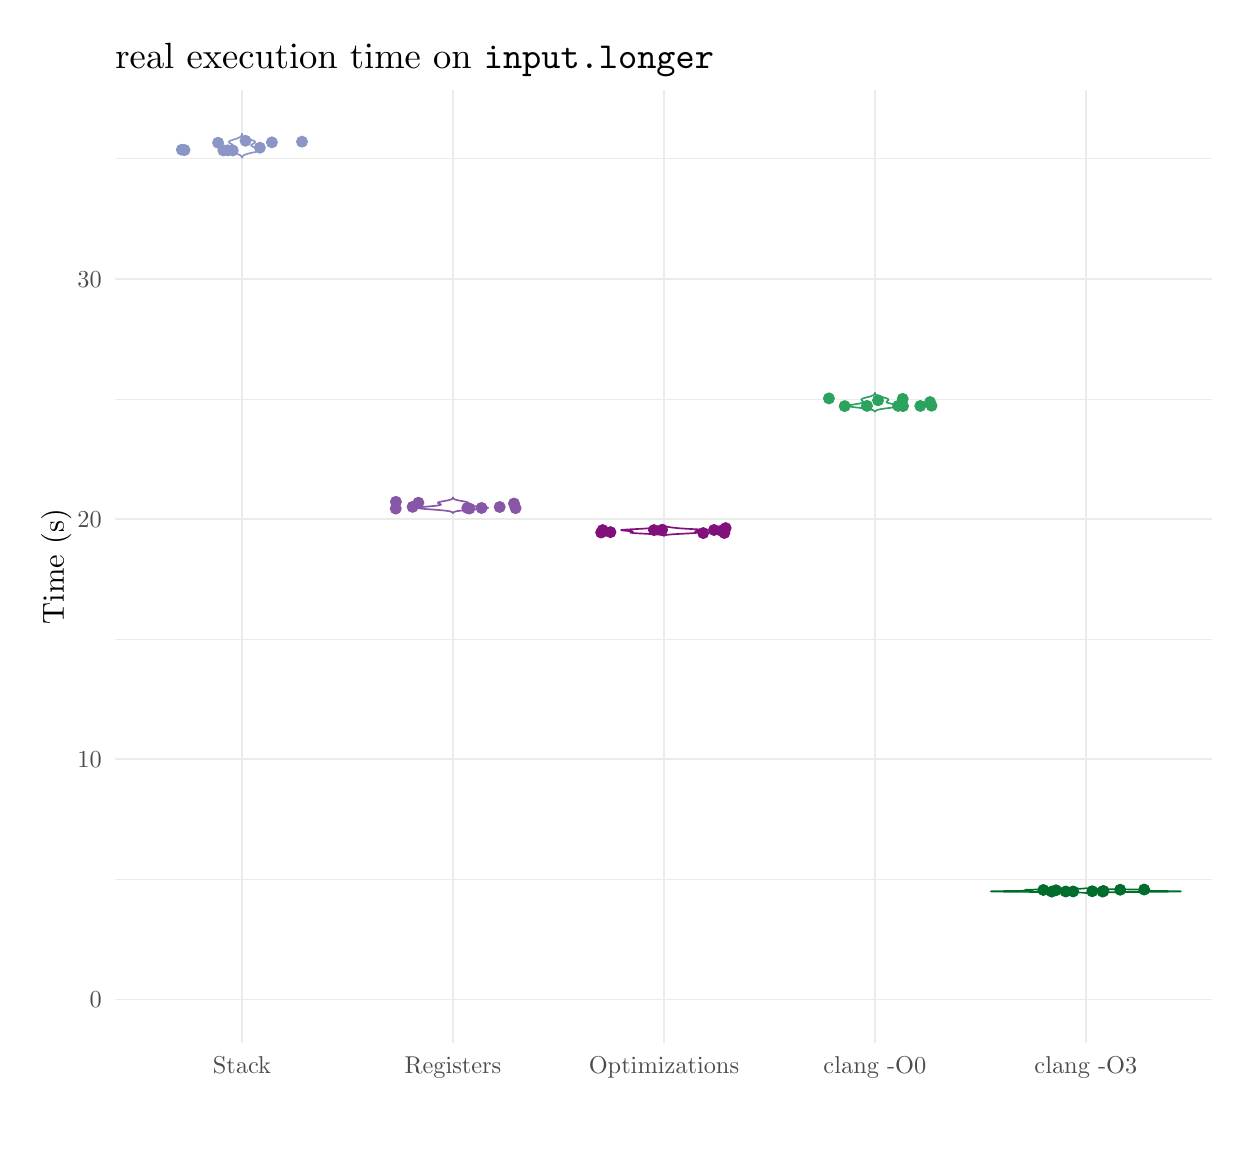
\begin{tikzpicture}[x=1pt,y=1pt]
\definecolor{fillColor}{RGB}{255,255,255}
\path[use as bounding box,fill=fillColor,fill opacity=0.00] (0,0) rectangle (433.62,397.48);
\begin{scope}
\path[clip] ( 31.71, 30.69) rectangle (428.12,374.83);
\definecolor{drawColor}{gray}{0.92}

\path[draw=drawColor,line width= 0.3pt,line join=round] ( 31.71, 89.72) --
	(428.12, 89.72);

\path[draw=drawColor,line width= 0.3pt,line join=round] ( 31.71,176.51) --
	(428.12,176.51);

\path[draw=drawColor,line width= 0.3pt,line join=round] ( 31.71,263.29) --
	(428.12,263.29);

\path[draw=drawColor,line width= 0.3pt,line join=round] ( 31.71,350.07) --
	(428.12,350.07);

\path[draw=drawColor,line width= 0.6pt,line join=round] ( 31.71, 46.33) --
	(428.12, 46.33);

\path[draw=drawColor,line width= 0.6pt,line join=round] ( 31.71,133.11) --
	(428.12,133.11);

\path[draw=drawColor,line width= 0.6pt,line join=round] ( 31.71,219.90) --
	(428.12,219.90);

\path[draw=drawColor,line width= 0.6pt,line join=round] ( 31.71,306.68) --
	(428.12,306.68);

\path[draw=drawColor,line width= 0.6pt,line join=round] ( 77.45, 30.69) --
	( 77.45,374.83);

\path[draw=drawColor,line width= 0.6pt,line join=round] (153.68, 30.69) --
	(153.68,374.83);

\path[draw=drawColor,line width= 0.6pt,line join=round] (229.92, 30.69) --
	(229.92,374.83);

\path[draw=drawColor,line width= 0.6pt,line join=round] (306.15, 30.69) --
	(306.15,374.83);

\path[draw=drawColor,line width= 0.6pt,line join=round] (382.38, 30.69) --
	(382.38,374.83);
\definecolor{drawColor}{RGB}{140,150,198}
\definecolor{fillColor}{RGB}{255,255,255}

\path[draw=drawColor,line width= 0.6pt,line join=round,line cap=round,fill=fillColor] ( 77.40,350.54) --
	( 77.40,350.55) --
	( 77.39,350.57) --
	( 77.39,350.59) --
	( 77.38,350.60) --
	( 77.38,350.62) --
	( 77.38,350.64) --
	( 77.37,350.65) --
	( 77.37,350.67) --
	( 77.36,350.69) --
	( 77.36,350.70) --
	( 77.35,350.72) --
	( 77.35,350.74) --
	( 77.34,350.76) --
	( 77.33,350.77) --
	( 77.33,350.79) --
	( 77.32,350.81) --
	( 77.31,350.82) --
	( 77.30,350.84) --
	( 77.30,350.86) --
	( 77.29,350.87) --
	( 77.28,350.89) --
	( 77.27,350.91) --
	( 77.26,350.92) --
	( 77.25,350.94) --
	( 77.24,350.96) --
	( 77.23,350.98) --
	( 77.22,350.99) --
	( 77.20,351.01) --
	( 77.19,351.03) --
	( 77.18,351.04) --
	( 77.16,351.06) --
	( 77.15,351.08) --
	( 77.14,351.09) --
	( 77.12,351.11) --
	( 77.10,351.13) --
	( 77.09,351.14) --
	( 77.07,351.16) --
	( 77.05,351.18) --
	( 77.03,351.20) --
	( 77.01,351.21) --
	( 76.99,351.23) --
	( 76.97,351.25) --
	( 76.95,351.26) --
	( 76.93,351.28) --
	( 76.91,351.30) --
	( 76.88,351.31) --
	( 76.86,351.33) --
	( 76.83,351.35) --
	( 76.80,351.36) --
	( 76.78,351.38) --
	( 76.75,351.40) --
	( 76.72,351.42) --
	( 76.69,351.43) --
	( 76.66,351.45) --
	( 76.63,351.47) --
	( 76.59,351.48) --
	( 76.56,351.50) --
	( 76.52,351.52) --
	( 76.49,351.53) --
	( 76.45,351.55) --
	( 76.41,351.57) --
	( 76.37,351.58) --
	( 76.33,351.60) --
	( 76.29,351.62) --
	( 76.25,351.64) --
	( 76.21,351.65) --
	( 76.16,351.67) --
	( 76.12,351.69) --
	( 76.07,351.70) --
	( 76.02,351.72) --
	( 75.97,351.74) --
	( 75.92,351.75) --
	( 75.87,351.77) --
	( 75.82,351.79) --
	( 75.76,351.80) --
	( 75.71,351.82) --
	( 75.65,351.84) --
	( 75.60,351.86) --
	( 75.54,351.87) --
	( 75.48,351.89) --
	( 75.42,351.91) --
	( 75.36,351.92) --
	( 75.30,351.94) --
	( 75.24,351.96) --
	( 75.17,351.97) --
	( 75.11,351.99) --
	( 75.04,352.01) --
	( 74.97,352.02) --
	( 74.91,352.04) --
	( 74.84,352.06) --
	( 74.77,352.08) --
	( 74.70,352.09) --
	( 74.63,352.11) --
	( 74.55,352.13) --
	( 74.48,352.14) --
	( 74.41,352.16) --
	( 74.34,352.18) --
	( 74.26,352.19) --
	( 74.19,352.21) --
	( 74.11,352.23) --
	( 74.03,352.24) --
	( 73.96,352.26) --
	( 73.88,352.28) --
	( 73.80,352.30) --
	( 73.73,352.31) --
	( 73.65,352.33) --
	( 73.57,352.35) --
	( 73.49,352.36) --
	( 73.41,352.38) --
	( 73.34,352.40) --
	( 73.26,352.41) --
	( 73.18,352.43) --
	( 73.10,352.45) --
	( 73.02,352.46) --
	( 72.95,352.48) --
	( 72.87,352.50) --
	( 72.79,352.52) --
	( 72.72,352.53) --
	( 72.64,352.55) --
	( 72.56,352.57) --
	( 72.49,352.58) --
	( 72.41,352.60) --
	( 72.34,352.62) --
	( 72.27,352.63) --
	( 72.20,352.65) --
	( 72.13,352.67) --
	( 72.06,352.68) --
	( 71.99,352.70) --
	( 71.92,352.72) --
	( 71.85,352.74) --
	( 71.79,352.75) --
	( 71.72,352.77) --
	( 71.66,352.79) --
	( 71.60,352.80) --
	( 71.54,352.82) --
	( 71.48,352.84) --
	( 71.42,352.85) --
	( 71.37,352.87) --
	( 71.31,352.89) --
	( 71.26,352.90) --
	( 71.21,352.92) --
	( 71.16,352.94) --
	( 71.12,352.96) --
	( 71.07,352.97) --
	( 71.03,352.99) --
	( 70.99,353.01) --
	( 70.95,353.02) --
	( 70.91,353.04) --
	( 70.88,353.06) --
	( 70.85,353.07) --
	( 70.81,353.09) --
	( 70.79,353.11) --
	( 70.76,353.12) --
	( 70.74,353.14) --
	( 70.71,353.16) --
	( 70.69,353.18) --
	( 70.68,353.19) --
	( 70.66,353.21) --
	( 70.65,353.23) --
	( 70.64,353.24) --
	( 70.63,353.26) --
	( 70.62,353.28) --
	( 70.62,353.29) --
	( 70.62,353.31) --
	( 70.62,353.33) --
	( 70.62,353.35) --
	( 70.62,353.36) --
	( 70.63,353.38) --
	( 70.64,353.40) --
	( 70.65,353.41) --
	( 70.66,353.43) --
	( 70.68,353.45) --
	( 70.70,353.46) --
	( 70.72,353.48) --
	( 70.74,353.50) --
	( 70.76,353.51) --
	( 70.79,353.53) --
	( 70.81,353.55) --
	( 70.84,353.57) --
	( 70.87,353.58) --
	( 70.91,353.60) --
	( 70.94,353.62) --
	( 70.98,353.63) --
	( 71.01,353.65) --
	( 71.05,353.67) --
	( 71.09,353.68) --
	( 71.14,353.70) --
	( 71.18,353.72) --
	( 71.23,353.73) --
	( 71.27,353.75) --
	( 71.32,353.77) --
	( 71.37,353.79) --
	( 71.42,353.80) --
	( 71.47,353.82) --
	( 71.52,353.84) --
	( 71.57,353.85) --
	( 71.63,353.87) --
	( 71.68,353.89) --
	( 71.74,353.90) --
	( 71.79,353.92) --
	( 71.85,353.94) --
	( 71.90,353.95) --
	( 71.96,353.97) --
	( 72.02,353.99) --
	( 72.08,354.01) --
	( 72.13,354.02) --
	( 72.19,354.04) --
	( 72.25,354.06) --
	( 72.31,354.07) --
	( 72.37,354.09) --
	( 72.43,354.11) --
	( 72.49,354.12) --
	( 72.54,354.14) --
	( 72.60,354.16) --
	( 72.66,354.17) --
	( 72.72,354.19) --
	( 72.77,354.21) --
	( 72.83,354.23) --
	( 72.88,354.24) --
	( 72.94,354.26) --
	( 72.99,354.28) --
	( 73.05,354.29) --
	( 73.10,354.31) --
	( 73.15,354.33) --
	( 73.20,354.34) --
	( 73.25,354.36) --
	( 73.30,354.38) --
	( 73.35,354.39) --
	( 73.39,354.41) --
	( 73.44,354.43) --
	( 73.48,354.45) --
	( 73.53,354.46) --
	( 73.57,354.48) --
	( 73.61,354.50) --
	( 73.65,354.51) --
	( 73.69,354.53) --
	( 73.72,354.55) --
	( 73.76,354.56) --
	( 73.79,354.58) --
	( 73.82,354.60) --
	( 73.86,354.61) --
	( 73.89,354.63) --
	( 73.91,354.65) --
	( 73.94,354.67) --
	( 73.96,354.68) --
	( 73.99,354.70) --
	( 74.01,354.72) --
	( 74.03,354.73) --
	( 74.05,354.75) --
	( 74.06,354.77) --
	( 74.08,354.78) --
	( 74.09,354.80) --
	( 74.10,354.82) --
	( 74.11,354.83) --
	( 74.12,354.85) --
	( 74.13,354.87) --
	( 74.14,354.89) --
	( 74.14,354.90) --
	( 74.14,354.92) --
	( 74.14,354.94) --
	( 74.14,354.95) --
	( 74.14,354.97) --
	( 74.14,354.99) --
	( 74.13,355.00) --
	( 74.13,355.02) --
	( 74.12,355.04) --
	( 74.11,355.05) --
	( 74.10,355.07) --
	( 74.09,355.09) --
	( 74.07,355.11) --
	( 74.06,355.12) --
	( 74.04,355.14) --
	( 74.03,355.16) --
	( 74.01,355.17) --
	( 73.99,355.19) --
	( 73.97,355.21) --
	( 73.95,355.22) --
	( 73.93,355.24) --
	( 73.91,355.26) --
	( 73.88,355.27) --
	( 73.86,355.29) --
	( 73.83,355.31) --
	( 73.81,355.33) --
	( 73.78,355.34) --
	( 73.75,355.36) --
	( 73.72,355.38) --
	( 73.70,355.39) --
	( 73.67,355.41) --
	( 73.64,355.43) --
	( 73.61,355.44) --
	( 73.58,355.46) --
	( 73.55,355.48) --
	( 73.52,355.49) --
	( 73.49,355.51) --
	( 73.46,355.53) --
	( 73.42,355.55) --
	( 73.39,355.56) --
	( 73.36,355.58) --
	( 73.33,355.60) --
	( 73.30,355.61) --
	( 73.27,355.63) --
	( 73.24,355.65) --
	( 73.21,355.66) --
	( 73.18,355.68) --
	( 73.16,355.70) --
	( 73.13,355.71) --
	( 73.10,355.73) --
	( 73.07,355.75) --
	( 73.05,355.77) --
	( 73.02,355.78) --
	( 73.00,355.80) --
	( 72.97,355.82) --
	( 72.95,355.83) --
	( 72.93,355.85) --
	( 72.91,355.87) --
	( 72.89,355.88) --
	( 72.87,355.90) --
	( 72.85,355.92) --
	( 72.83,355.93) --
	( 72.81,355.95) --
	( 72.80,355.97) --
	( 72.79,355.99) --
	( 72.77,356.00) --
	( 72.76,356.02) --
	( 72.75,356.04) --
	( 72.74,356.05) --
	( 72.74,356.07) --
	( 72.73,356.09) --
	( 72.73,356.10) --
	( 72.72,356.12) --
	( 72.72,356.14) --
	( 72.72,356.15) --
	( 72.72,356.17) --
	( 72.72,356.19) --
	( 72.73,356.21) --
	( 72.73,356.22) --
	( 72.74,356.24) --
	( 72.75,356.26) --
	( 72.76,356.27) --
	( 72.77,356.29) --
	( 72.78,356.31) --
	( 72.79,356.32) --
	( 72.81,356.34) --
	( 72.83,356.36) --
	( 72.84,356.38) --
	( 72.86,356.39) --
	( 72.89,356.41) --
	( 72.91,356.43) --
	( 72.93,356.44) --
	( 72.96,356.46) --
	( 72.98,356.48) --
	( 73.01,356.49) --
	( 73.04,356.51) --
	( 73.07,356.53) --
	( 73.10,356.54) --
	( 73.14,356.56) --
	( 73.17,356.58) --
	( 73.21,356.60) --
	( 73.24,356.61) --
	( 73.28,356.63) --
	( 73.32,356.65) --
	( 73.36,356.66) --
	( 73.40,356.68) --
	( 73.44,356.70) --
	( 73.48,356.71) --
	( 73.52,356.73) --
	( 73.57,356.75) --
	( 73.61,356.76) --
	( 73.66,356.78) --
	( 73.71,356.80) --
	( 73.75,356.82) --
	( 73.80,356.83) --
	( 73.85,356.85) --
	( 73.90,356.87) --
	( 73.95,356.88) --
	( 74.00,356.90) --
	( 74.05,356.92) --
	( 74.10,356.93) --
	( 74.15,356.95) --
	( 74.20,356.97) --
	( 74.25,356.98) --
	( 74.31,357.00) --
	( 74.36,357.02) --
	( 74.41,357.04) --
	( 74.46,357.05) --
	( 74.52,357.07) --
	( 74.57,357.09) --
	( 74.62,357.10) --
	( 74.67,357.12) --
	( 74.73,357.14) --
	( 74.78,357.15) --
	( 74.83,357.17) --
	( 74.89,357.19) --
	( 74.94,357.20) --
	( 74.99,357.22) --
	( 75.04,357.24) --
	( 75.09,357.26) --
	( 75.14,357.27) --
	( 75.20,357.29) --
	( 75.25,357.31) --
	( 75.30,357.32) --
	( 75.35,357.34) --
	( 75.40,357.36) --
	( 75.44,357.37) --
	( 75.49,357.39) --
	( 75.54,357.41) --
	( 75.59,357.42) --
	( 75.63,357.44) --
	( 75.68,357.46) --
	( 75.73,357.48) --
	( 75.77,357.49) --
	( 75.82,357.51) --
	( 75.86,357.53) --
	( 75.90,357.54) --
	( 75.95,357.56) --
	( 75.99,357.58) --
	( 76.03,357.59) --
	( 76.07,357.61) --
	( 76.11,357.63) --
	( 76.15,357.64) --
	( 76.19,357.66) --
	( 76.22,357.68) --
	( 76.26,357.70) --
	( 76.30,357.71) --
	( 76.33,357.73) --
	( 76.37,357.75) --
	( 76.40,357.76) --
	( 76.44,357.78) --
	( 76.47,357.80) --
	( 76.50,357.81) --
	( 76.53,357.83) --
	( 76.56,357.85) --
	( 76.59,357.86) --
	( 76.62,357.88) --
	( 76.65,357.90) --
	( 76.68,357.92) --
	( 76.71,357.93) --
	( 76.73,357.95) --
	( 76.76,357.97) --
	( 76.78,357.98) --
	( 76.81,358.00) --
	( 76.83,358.02) --
	( 76.85,358.03) --
	( 76.88,358.05) --
	( 76.90,358.07) --
	( 76.92,358.08) --
	( 76.94,358.10) --
	( 76.96,358.12) --
	( 76.98,358.14) --
	( 77.00,358.15) --
	( 77.01,358.17) --
	( 77.03,358.19) --
	( 77.05,358.20) --
	( 77.07,358.22) --
	( 77.08,358.24) --
	( 77.10,358.25) --
	( 77.11,358.27) --
	( 77.13,358.29) --
	( 77.14,358.30) --
	( 77.15,358.32) --
	( 77.17,358.34) --
	( 77.18,358.36) --
	( 77.19,358.37) --
	( 77.20,358.39) --
	( 77.21,358.41) --
	( 77.22,358.42) --
	( 77.23,358.44) --
	( 77.24,358.46) --
	( 77.25,358.47) --
	( 77.26,358.49) --
	( 77.27,358.51) --
	( 77.28,358.52) --
	( 77.29,358.54) --
	( 77.30,358.56) --
	( 77.30,358.58) --
	( 77.31,358.59) --
	( 77.32,358.61) --
	( 77.32,358.63) --
	( 77.33,358.64) --
	( 77.34,358.66) --
	( 77.34,358.68) --
	( 77.35,358.69) --
	( 77.35,358.71) --
	( 77.36,358.73) --
	( 77.36,358.74) --
	( 77.37,358.76) --
	( 77.37,358.78) --
	( 77.38,358.80) --
	( 77.38,358.81) --
	( 77.38,358.83) --
	( 77.39,358.85) --
	( 77.39,358.86) --
	( 77.39,358.88) --
	( 77.40,358.90) --
	( 77.40,358.91) --
	( 77.40,358.93) --
	( 77.41,358.95) --
	( 77.41,358.96) --
	( 77.41,358.98) --
	( 77.41,359.00) --
	( 77.41,359.02) --
	( 77.42,359.03) --
	( 77.42,359.05) --
	( 77.42,359.07) --
	( 77.42,359.08) --
	( 77.42,359.10) --
	( 77.43,359.12) --
	( 77.43,359.13) --
	( 77.43,359.15) --
	( 77.43,359.17) --
	( 77.43,359.18) --
	( 77.47,359.18) --
	( 77.47,359.17) --
	( 77.47,359.15) --
	( 77.48,359.13) --
	( 77.48,359.12) --
	( 77.48,359.10) --
	( 77.48,359.08) --
	( 77.48,359.07) --
	( 77.48,359.05) --
	( 77.49,359.03) --
	( 77.49,359.02) --
	( 77.49,359.00) --
	( 77.49,358.98) --
	( 77.50,358.96) --
	( 77.50,358.95) --
	( 77.50,358.93) --
	( 77.50,358.91) --
	( 77.51,358.90) --
	( 77.51,358.88) --
	( 77.51,358.86) --
	( 77.52,358.85) --
	( 77.52,358.83) --
	( 77.52,358.81) --
	( 77.53,358.80) --
	( 77.53,358.78) --
	( 77.54,358.76) --
	( 77.54,358.74) --
	( 77.55,358.73) --
	( 77.55,358.71) --
	( 77.56,358.69) --
	( 77.56,358.68) --
	( 77.57,358.66) --
	( 77.57,358.64) --
	( 77.58,358.63) --
	( 77.59,358.61) --
	( 77.59,358.59) --
	( 77.60,358.58) --
	( 77.61,358.56) --
	( 77.62,358.54) --
	( 77.62,358.52) --
	( 77.63,358.51) --
	( 77.64,358.49) --
	( 77.65,358.47) --
	( 77.66,358.46) --
	( 77.67,358.44) --
	( 77.68,358.42) --
	( 77.69,358.41) --
	( 77.70,358.39) --
	( 77.71,358.37) --
	( 77.73,358.36) --
	( 77.74,358.34) --
	( 77.75,358.32) --
	( 77.76,358.30) --
	( 77.78,358.29) --
	( 77.79,358.27) --
	( 77.81,358.25) --
	( 77.82,358.24) --
	( 77.84,358.22) --
	( 77.85,358.20) --
	( 77.87,358.19) --
	( 77.89,358.17) --
	( 77.91,358.15) --
	( 77.93,358.14) --
	( 77.94,358.12) --
	( 77.96,358.10) --
	( 77.98,358.08) --
	( 78.01,358.07) --
	( 78.03,358.05) --
	( 78.05,358.03) --
	( 78.07,358.02) --
	( 78.10,358.00) --
	( 78.12,357.98) --
	( 78.15,357.97) --
	( 78.17,357.95) --
	( 78.20,357.93) --
	( 78.22,357.92) --
	( 78.25,357.90) --
	( 78.28,357.88) --
	( 78.31,357.86) --
	( 78.34,357.85) --
	( 78.37,357.83) --
	( 78.40,357.81) --
	( 78.43,357.80) --
	( 78.47,357.78) --
	( 78.50,357.76) --
	( 78.53,357.75) --
	( 78.57,357.73) --
	( 78.61,357.71) --
	( 78.64,357.70) --
	( 78.68,357.68) --
	( 78.72,357.66) --
	( 78.75,357.64) --
	( 78.79,357.63) --
	( 78.83,357.61) --
	( 78.87,357.59) --
	( 78.92,357.58) --
	( 78.96,357.56) --
	( 79.00,357.54) --
	( 79.04,357.53) --
	( 79.09,357.51) --
	( 79.13,357.49) --
	( 79.18,357.48) --
	( 79.22,357.46) --
	( 79.27,357.44) --
	( 79.32,357.42) --
	( 79.36,357.41) --
	( 79.41,357.39) --
	( 79.46,357.37) --
	( 79.51,357.36) --
	( 79.56,357.34) --
	( 79.61,357.32) --
	( 79.66,357.31) --
	( 79.71,357.29) --
	( 79.76,357.27) --
	( 79.81,357.26) --
	( 79.86,357.24) --
	( 79.91,357.22) --
	( 79.97,357.20) --
	( 80.02,357.19) --
	( 80.07,357.17) --
	( 80.12,357.15) --
	( 80.18,357.14) --
	( 80.23,357.12) --
	( 80.28,357.10) --
	( 80.33,357.09) --
	( 80.39,357.07) --
	( 80.44,357.05) --
	( 80.49,357.04) --
	( 80.54,357.02) --
	( 80.60,357.00) --
	( 80.65,356.98) --
	( 80.70,356.97) --
	( 80.75,356.95) --
	( 80.80,356.93) --
	( 80.86,356.92) --
	( 80.91,356.90) --
	( 80.96,356.88) --
	( 81.01,356.87) --
	( 81.05,356.85) --
	( 81.10,356.83) --
	( 81.15,356.82) --
	( 81.20,356.80) --
	( 81.24,356.78) --
	( 81.29,356.76) --
	( 81.33,356.75) --
	( 81.38,356.73) --
	( 81.42,356.71) --
	( 81.46,356.70) --
	( 81.51,356.68) --
	( 81.55,356.66) --
	( 81.59,356.65) --
	( 81.62,356.63) --
	( 81.66,356.61) --
	( 81.70,356.60) --
	( 81.73,356.58) --
	( 81.77,356.56) --
	( 81.80,356.54) --
	( 81.83,356.53) --
	( 81.86,356.51) --
	( 81.89,356.49) --
	( 81.92,356.48) --
	( 81.95,356.46) --
	( 81.97,356.44) --
	( 82.00,356.43) --
	( 82.02,356.41) --
	( 82.04,356.39) --
	( 82.06,356.38) --
	( 82.08,356.36) --
	( 82.09,356.34) --
	( 82.11,356.32) --
	( 82.12,356.31) --
	( 82.14,356.29) --
	( 82.15,356.27) --
	( 82.16,356.26) --
	( 82.17,356.24) --
	( 82.17,356.22) --
	( 82.18,356.21) --
	( 82.18,356.19) --
	( 82.18,356.17) --
	( 82.18,356.15) --
	( 82.18,356.14) --
	( 82.18,356.12) --
	( 82.18,356.10) --
	( 82.17,356.09) --
	( 82.17,356.07) --
	( 82.16,356.05) --
	( 82.15,356.04) --
	( 82.14,356.02) --
	( 82.13,356.00) --
	( 82.12,355.99) --
	( 82.10,355.97) --
	( 82.09,355.95) --
	( 82.07,355.93) --
	( 82.06,355.92) --
	( 82.04,355.90) --
	( 82.02,355.88) --
	( 82.00,355.87) --
	( 81.98,355.85) --
	( 81.95,355.83) --
	( 81.93,355.82) --
	( 81.91,355.80) --
	( 81.88,355.78) --
	( 81.86,355.77) --
	( 81.83,355.75) --
	( 81.80,355.73) --
	( 81.78,355.71) --
	( 81.75,355.70) --
	( 81.72,355.68) --
	( 81.69,355.66) --
	( 81.66,355.65) --
	( 81.63,355.63) --
	( 81.60,355.61) --
	( 81.57,355.60) --
	( 81.54,355.58) --
	( 81.51,355.56) --
	( 81.48,355.55) --
	( 81.45,355.53) --
	( 81.42,355.51) --
	( 81.39,355.49) --
	( 81.36,355.48) --
	( 81.33,355.46) --
	( 81.30,355.44) --
	( 81.27,355.43) --
	( 81.24,355.41) --
	( 81.21,355.39) --
	( 81.18,355.38) --
	( 81.15,355.36) --
	( 81.12,355.34) --
	( 81.10,355.33) --
	( 81.07,355.31) --
	( 81.05,355.29) --
	( 81.02,355.27) --
	( 81.00,355.26) --
	( 80.97,355.24) --
	( 80.95,355.22) --
	( 80.93,355.21) --
	( 80.91,355.19) --
	( 80.89,355.17) --
	( 80.87,355.16) --
	( 80.86,355.14) --
	( 80.84,355.12) --
	( 80.83,355.11) --
	( 80.82,355.09) --
	( 80.80,355.07) --
	( 80.79,355.05) --
	( 80.78,355.04) --
	( 80.78,355.02) --
	( 80.77,355.00) --
	( 80.77,354.99) --
	( 80.76,354.97) --
	( 80.76,354.95) --
	( 80.76,354.94) --
	( 80.76,354.92) --
	( 80.76,354.90) --
	( 80.77,354.89) --
	( 80.77,354.87) --
	( 80.78,354.85) --
	( 80.79,354.83) --
	( 80.80,354.82) --
	( 80.81,354.80) --
	( 80.82,354.78) --
	( 80.84,354.77) --
	( 80.86,354.75) --
	( 80.87,354.73) --
	( 80.89,354.72) --
	( 80.92,354.70) --
	( 80.94,354.68) --
	( 80.96,354.67) --
	( 80.99,354.65) --
	( 81.02,354.63) --
	( 81.05,354.61) --
	( 81.08,354.60) --
	( 81.11,354.58) --
	( 81.14,354.56) --
	( 81.18,354.55) --
	( 81.22,354.53) --
	( 81.25,354.51) --
	( 81.29,354.50) --
	( 81.33,354.48) --
	( 81.38,354.46) --
	( 81.42,354.45) --
	( 81.46,354.43) --
	( 81.51,354.41) --
	( 81.56,354.39) --
	( 81.60,354.38) --
	( 81.65,354.36) --
	( 81.70,354.34) --
	( 81.75,354.33) --
	( 81.81,354.31) --
	( 81.86,354.29) --
	( 81.91,354.28) --
	( 81.97,354.26) --
	( 82.02,354.24) --
	( 82.08,354.23) --
	( 82.13,354.21) --
	( 82.19,354.19) --
	( 82.24,354.17) --
	( 82.30,354.16) --
	( 82.36,354.14) --
	( 82.42,354.12) --
	( 82.48,354.11) --
	( 82.53,354.09) --
	( 82.59,354.07) --
	( 82.65,354.06) --
	( 82.71,354.04) --
	( 82.77,354.02) --
	( 82.83,354.01) --
	( 82.88,353.99) --
	( 82.94,353.97) --
	( 83.00,353.95) --
	( 83.06,353.94) --
	( 83.11,353.92) --
	( 83.17,353.90) --
	( 83.22,353.89) --
	( 83.28,353.87) --
	( 83.33,353.85) --
	( 83.38,353.84) --
	( 83.43,353.82) --
	( 83.49,353.80) --
	( 83.54,353.79) --
	( 83.58,353.77) --
	( 83.63,353.75) --
	( 83.68,353.73) --
	( 83.72,353.72) --
	( 83.77,353.70) --
	( 83.81,353.68) --
	( 83.85,353.67) --
	( 83.89,353.65) --
	( 83.93,353.63) --
	( 83.96,353.62) --
	( 84.00,353.60) --
	( 84.03,353.58) --
	( 84.06,353.57) --
	( 84.09,353.55) --
	( 84.12,353.53) --
	( 84.14,353.51) --
	( 84.17,353.50) --
	( 84.19,353.48) --
	( 84.21,353.46) --
	( 84.22,353.45) --
	( 84.24,353.43) --
	( 84.25,353.41) --
	( 84.26,353.40) --
	( 84.27,353.38) --
	( 84.28,353.36) --
	( 84.28,353.35) --
	( 84.29,353.33) --
	( 84.29,353.31) --
	( 84.29,353.29) --
	( 84.28,353.28) --
	( 84.28,353.26) --
	( 84.27,353.24) --
	( 84.26,353.23) --
	( 84.24,353.21) --
	( 84.23,353.19) --
	( 84.21,353.18) --
	( 84.19,353.16) --
	( 84.17,353.14) --
	( 84.14,353.12) --
	( 84.12,353.11) --
	( 84.09,353.09) --
	( 84.06,353.07) --
	( 84.03,353.06) --
	( 83.99,353.04) --
	( 83.95,353.02) --
	( 83.91,353.01) --
	( 83.87,352.99) --
	( 83.83,352.97) --
	( 83.79,352.96) --
	( 83.74,352.94) --
	( 83.69,352.92) --
	( 83.64,352.90) --
	( 83.59,352.89) --
	( 83.54,352.87) --
	( 83.48,352.85) --
	( 83.42,352.84) --
	( 83.36,352.82) --
	( 83.30,352.80) --
	( 83.24,352.79) --
	( 83.18,352.77) --
	( 83.12,352.75) --
	( 83.05,352.74) --
	( 82.98,352.72) --
	( 82.92,352.70) --
	( 82.85,352.68) --
	( 82.78,352.67) --
	( 82.71,352.65) --
	( 82.63,352.63) --
	( 82.56,352.62) --
	( 82.49,352.60) --
	( 82.41,352.58) --
	( 82.34,352.57) --
	( 82.26,352.55) --
	( 82.19,352.53) --
	( 82.11,352.52) --
	( 82.03,352.50) --
	( 81.96,352.48) --
	( 81.88,352.46) --
	( 81.80,352.45) --
	( 81.72,352.43) --
	( 81.65,352.41) --
	( 81.57,352.40) --
	( 81.49,352.38) --
	( 81.41,352.36) --
	( 81.33,352.35) --
	( 81.25,352.33) --
	( 81.18,352.31) --
	( 81.10,352.30) --
	( 81.02,352.28) --
	( 80.95,352.26) --
	( 80.87,352.24) --
	( 80.79,352.23) --
	( 80.72,352.21) --
	( 80.64,352.19) --
	( 80.57,352.18) --
	( 80.49,352.16) --
	( 80.42,352.14) --
	( 80.35,352.13) --
	( 80.28,352.11) --
	( 80.21,352.09) --
	( 80.14,352.08) --
	( 80.07,352.06) --
	( 80.00,352.04) --
	( 79.93,352.02) --
	( 79.86,352.01) --
	( 79.80,351.99) --
	( 79.73,351.97) --
	( 79.67,351.96) --
	( 79.61,351.94) --
	( 79.54,351.92) --
	( 79.48,351.91) --
	( 79.42,351.89) --
	( 79.36,351.87) --
	( 79.31,351.86) --
	( 79.25,351.84) --
	( 79.19,351.82) --
	( 79.14,351.80) --
	( 79.09,351.79) --
	( 79.03,351.77) --
	( 78.98,351.75) --
	( 78.93,351.74) --
	( 78.88,351.72) --
	( 78.84,351.70) --
	( 78.79,351.69) --
	( 78.74,351.67) --
	( 78.70,351.65) --
	( 78.65,351.64) --
	( 78.61,351.62) --
	( 78.57,351.60) --
	( 78.53,351.58) --
	( 78.49,351.57) --
	( 78.45,351.55) --
	( 78.42,351.53) --
	( 78.38,351.52) --
	( 78.34,351.50) --
	( 78.31,351.48) --
	( 78.28,351.47) --
	( 78.25,351.45) --
	( 78.21,351.43) --
	( 78.18,351.42) --
	( 78.15,351.40) --
	( 78.13,351.38) --
	( 78.10,351.36) --
	( 78.07,351.35) --
	( 78.05,351.33) --
	( 78.02,351.31) --
	( 78.00,351.30) --
	( 77.97,351.28) --
	( 77.95,351.26) --
	( 77.93,351.25) --
	( 77.91,351.23) --
	( 77.89,351.21) --
	( 77.87,351.20) --
	( 77.85,351.18) --
	( 77.83,351.16) --
	( 77.82,351.14) --
	( 77.80,351.13) --
	( 77.78,351.11) --
	( 77.77,351.09) --
	( 77.75,351.08) --
	( 77.74,351.06) --
	( 77.72,351.04) --
	( 77.71,351.03) --
	( 77.70,351.01) --
	( 77.69,350.99) --
	( 77.68,350.98) --
	( 77.66,350.96) --
	( 77.65,350.94) --
	( 77.64,350.92) --
	( 77.63,350.91) --
	( 77.62,350.89) --
	( 77.62,350.87) --
	( 77.61,350.86) --
	( 77.60,350.84) --
	( 77.59,350.82) --
	( 77.58,350.81) --
	( 77.58,350.79) --
	( 77.57,350.77) --
	( 77.56,350.76) --
	( 77.56,350.74) --
	( 77.55,350.72) --
	( 77.55,350.70) --
	( 77.54,350.69) --
	( 77.54,350.67) --
	( 77.53,350.65) --
	( 77.53,350.64) --
	( 77.52,350.62) --
	( 77.52,350.60) --
	( 77.51,350.59) --
	( 77.51,350.57) --
	( 77.51,350.55) --
	( 77.50,350.54) --
	( 77.40,350.54) --
	cycle;
\definecolor{drawColor}{RGB}{136,86,167}

\path[draw=drawColor,line width= 0.6pt,line join=round,line cap=round,fill=fillColor] (153.62,222.11) --
	(153.62,222.12) --
	(153.61,222.13) --
	(153.61,222.14) --
	(153.60,222.15) --
	(153.60,222.16) --
	(153.59,222.17) --
	(153.59,222.18) --
	(153.58,222.19) --
	(153.57,222.21) --
	(153.57,222.22) --
	(153.56,222.23) --
	(153.55,222.24) --
	(153.54,222.25) --
	(153.53,222.26) --
	(153.52,222.27) --
	(153.52,222.28) --
	(153.51,222.29) --
	(153.49,222.30) --
	(153.48,222.32) --
	(153.47,222.33) --
	(153.46,222.34) --
	(153.45,222.35) --
	(153.43,222.36) --
	(153.42,222.37) --
	(153.40,222.38) --
	(153.39,222.39) --
	(153.37,222.40) --
	(153.35,222.41) --
	(153.34,222.43) --
	(153.32,222.44) --
	(153.30,222.45) --
	(153.28,222.46) --
	(153.26,222.47) --
	(153.23,222.48) --
	(153.21,222.49) --
	(153.18,222.50) --
	(153.16,222.51) --
	(153.13,222.52) --
	(153.10,222.53) --
	(153.08,222.55) --
	(153.05,222.56) --
	(153.01,222.57) --
	(152.98,222.58) --
	(152.95,222.59) --
	(152.91,222.60) --
	(152.88,222.61) --
	(152.84,222.62) --
	(152.80,222.63) --
	(152.76,222.64) --
	(152.72,222.66) --
	(152.67,222.67) --
	(152.63,222.68) --
	(152.58,222.69) --
	(152.53,222.70) --
	(152.48,222.71) --
	(152.43,222.72) --
	(152.37,222.73) --
	(152.32,222.74) --
	(152.26,222.75) --
	(152.20,222.77) --
	(152.14,222.78) --
	(152.08,222.79) --
	(152.01,222.80) --
	(151.95,222.81) --
	(151.88,222.82) --
	(151.81,222.83) --
	(151.73,222.84) --
	(151.66,222.85) --
	(151.58,222.86) --
	(151.50,222.88) --
	(151.42,222.89) --
	(151.34,222.90) --
	(151.25,222.91) --
	(151.17,222.92) --
	(151.08,222.93) --
	(150.99,222.94) --
	(150.89,222.95) --
	(150.80,222.96) --
	(150.70,222.97) --
	(150.60,222.99) --
	(150.50,223.00) --
	(150.39,223.01) --
	(150.29,223.02) --
	(150.18,223.03) --
	(150.07,223.04) --
	(149.96,223.05) --
	(149.84,223.06) --
	(149.73,223.07) --
	(149.61,223.08) --
	(149.49,223.10) --
	(149.37,223.11) --
	(149.24,223.12) --
	(149.12,223.13) --
	(148.99,223.14) --
	(148.86,223.15) --
	(148.73,223.16) --
	(148.60,223.17) --
	(148.47,223.18) --
	(148.33,223.19) --
	(148.20,223.21) --
	(148.06,223.22) --
	(147.92,223.23) --
	(147.78,223.24) --
	(147.64,223.25) --
	(147.50,223.26) --
	(147.35,223.27) --
	(147.21,223.28) --
	(147.07,223.29) --
	(146.92,223.30) --
	(146.77,223.31) --
	(146.63,223.33) --
	(146.48,223.34) --
	(146.33,223.35) --
	(146.19,223.36) --
	(146.04,223.37) --
	(145.89,223.38) --
	(145.75,223.39) --
	(145.60,223.40) --
	(145.45,223.41) --
	(145.31,223.42) --
	(145.16,223.44) --
	(145.02,223.45) --
	(144.87,223.46) --
	(144.73,223.47) --
	(144.59,223.48) --
	(144.45,223.49) --
	(144.31,223.50) --
	(144.17,223.51) --
	(144.03,223.52) --
	(143.90,223.53) --
	(143.77,223.55) --
	(143.64,223.56) --
	(143.51,223.57) --
	(143.38,223.58) --
	(143.26,223.59) --
	(143.13,223.60) --
	(143.01,223.61) --
	(142.90,223.62) --
	(142.78,223.63) --
	(142.67,223.64) --
	(142.56,223.66) --
	(142.46,223.67) --
	(142.36,223.68) --
	(142.26,223.69) --
	(142.16,223.70) --
	(142.07,223.71) --
	(141.98,223.72) --
	(141.89,223.73) --
	(141.81,223.74) --
	(141.73,223.75) --
	(141.66,223.77) --
	(141.59,223.78) --
	(141.52,223.79) --
	(141.46,223.80) --
	(141.40,223.81) --
	(141.35,223.82) --
	(141.30,223.83) --
	(141.25,223.84) --
	(141.21,223.85) --
	(141.17,223.86) --
	(141.14,223.88) --
	(141.11,223.89) --
	(141.08,223.90) --
	(141.06,223.91) --
	(141.05,223.92) --
	(141.04,223.93) --
	(141.03,223.94) --
	(141.03,223.95) --
	(141.03,223.96) --
	(141.03,223.97) --
	(141.04,223.99) --
	(141.06,224.00) --
	(141.08,224.01) --
	(141.10,224.02) --
	(141.13,224.03) --
	(141.16,224.04) --
	(141.20,224.05) --
	(141.24,224.06) --
	(141.28,224.07) --
	(141.33,224.08) --
	(141.38,224.09) --
	(141.43,224.11) --
	(141.49,224.12) --
	(141.56,224.13) --
	(141.62,224.14) --
	(141.69,224.15) --
	(141.77,224.16) --
	(141.84,224.17) --
	(141.92,224.18) --
	(142.01,224.19) --
	(142.09,224.20) --
	(142.18,224.22) --
	(142.27,224.23) --
	(142.37,224.24) --
	(142.46,224.25) --
	(142.57,224.26) --
	(142.67,224.27) --
	(142.77,224.28) --
	(142.88,224.29) --
	(142.99,224.30) --
	(143.10,224.31) --
	(143.21,224.33) --
	(143.32,224.34) --
	(143.44,224.35) --
	(143.56,224.36) --
	(143.68,224.37) --
	(143.80,224.38) --
	(143.92,224.39) --
	(144.04,224.40) --
	(144.16,224.41) --
	(144.28,224.42) --
	(144.41,224.44) --
	(144.53,224.45) --
	(144.65,224.46) --
	(144.78,224.47) --
	(144.90,224.48) --
	(145.03,224.49) --
	(145.15,224.50) --
	(145.28,224.51) --
	(145.40,224.52) --
	(145.52,224.53) --
	(145.65,224.55) --
	(145.77,224.56) --
	(145.89,224.57) --
	(146.01,224.58) --
	(146.13,224.59) --
	(146.24,224.60) --
	(146.36,224.61) --
	(146.48,224.62) --
	(146.59,224.63) --
	(146.70,224.64) --
	(146.81,224.66) --
	(146.92,224.67) --
	(147.03,224.68) --
	(147.13,224.69) --
	(147.23,224.70) --
	(147.34,224.71) --
	(147.43,224.72) --
	(147.53,224.73) --
	(147.63,224.74) --
	(147.72,224.75) --
	(147.81,224.77) --
	(147.90,224.78) --
	(147.98,224.79) --
	(148.06,224.80) --
	(148.14,224.81) --
	(148.22,224.82) --
	(148.30,224.83) --
	(148.37,224.84) --
	(148.44,224.85) --
	(148.51,224.86) --
	(148.57,224.88) --
	(148.63,224.89) --
	(148.69,224.90) --
	(148.75,224.91) --
	(148.80,224.92) --
	(148.85,224.93) --
	(148.90,224.94) --
	(148.95,224.95) --
	(148.99,224.96) --
	(149.03,224.97) --
	(149.07,224.98) --
	(149.10,225.00) --
	(149.13,225.01) --
	(149.16,225.02) --
	(149.19,225.03) --
	(149.22,225.04) --
	(149.24,225.05) --
	(149.26,225.06) --
	(149.28,225.07) --
	(149.29,225.08) --
	(149.30,225.09) --
	(149.31,225.11) --
	(149.32,225.12) --
	(149.33,225.13) --
	(149.33,225.14) --
	(149.33,225.15) --
	(149.33,225.16) --
	(149.33,225.17) --
	(149.32,225.18) --
	(149.32,225.19) --
	(149.31,225.20) --
	(149.30,225.22) --
	(149.29,225.23) --
	(149.28,225.24) --
	(149.26,225.25) --
	(149.25,225.26) --
	(149.23,225.27) --
	(149.21,225.28) --
	(149.19,225.29) --
	(149.17,225.30) --
	(149.15,225.31) --
	(149.12,225.33) --
	(149.10,225.34) --
	(149.08,225.35) --
	(149.05,225.36) --
	(149.02,225.37) --
	(149.00,225.38) --
	(148.97,225.39) --
	(148.94,225.40) --
	(148.92,225.41) --
	(148.89,225.42) --
	(148.86,225.44) --
	(148.83,225.45) --
	(148.80,225.46) --
	(148.77,225.47) --
	(148.75,225.48) --
	(148.72,225.49) --
	(148.69,225.50) --
	(148.66,225.51) --
	(148.63,225.52) --
	(148.61,225.53) --
	(148.58,225.55) --
	(148.56,225.56) --
	(148.53,225.57) --
	(148.51,225.58) --
	(148.48,225.59) --
	(148.46,225.60) --
	(148.44,225.61) --
	(148.42,225.62) --
	(148.40,225.63) --
	(148.38,225.64) --
	(148.36,225.66) --
	(148.34,225.67) --
	(148.33,225.68) --
	(148.31,225.69) --
	(148.30,225.70) --
	(148.29,225.71) --
	(148.28,225.72) --
	(148.27,225.73) --
	(148.26,225.74) --
	(148.25,225.75) --
	(148.25,225.76) --
	(148.25,225.78) --
	(148.24,225.79) --
	(148.24,225.80) --
	(148.25,225.81) --
	(148.25,225.82) --
	(148.25,225.83) --
	(148.26,225.84) --
	(148.27,225.85) --
	(148.28,225.86) --
	(148.29,225.87) --
	(148.30,225.89) --
	(148.31,225.90) --
	(148.33,225.91) --
	(148.35,225.92) --
	(148.37,225.93) --
	(148.39,225.94) --
	(148.41,225.95) --
	(148.43,225.96) --
	(148.46,225.97) --
	(148.49,225.98) --
	(148.51,226.00) --
	(148.54,226.01) --
	(148.58,226.02) --
	(148.61,226.03) --
	(148.64,226.04) --
	(148.68,226.05) --
	(148.72,226.06) --
	(148.76,226.07) --
	(148.79,226.08) --
	(148.84,226.09) --
	(148.88,226.11) --
	(148.92,226.12) --
	(148.97,226.13) --
	(149.01,226.14) --
	(149.06,226.15) --
	(149.11,226.16) --
	(149.16,226.17) --
	(149.21,226.18) --
	(149.26,226.19) --
	(149.31,226.20) --
	(149.36,226.22) --
	(149.42,226.23) --
	(149.47,226.24) --
	(149.53,226.25) --
	(149.58,226.26) --
	(149.64,226.27) --
	(149.70,226.28) --
	(149.75,226.29) --
	(149.81,226.30) --
	(149.87,226.31) --
	(149.93,226.33) --
	(149.99,226.34) --
	(150.05,226.35) --
	(150.11,226.36) --
	(150.17,226.37) --
	(150.23,226.38) --
	(150.29,226.39) --
	(150.35,226.40) --
	(150.41,226.41) --
	(150.47,226.42) --
	(150.53,226.44) --
	(150.59,226.45) --
	(150.66,226.46) --
	(150.72,226.47) --
	(150.78,226.48) --
	(150.84,226.49) --
	(150.90,226.50) --
	(150.96,226.51) --
	(151.02,226.52) --
	(151.07,226.53) --
	(151.13,226.54) --
	(151.19,226.56) --
	(151.25,226.57) --
	(151.31,226.58) --
	(151.36,226.59) --
	(151.42,226.60) --
	(151.47,226.61) --
	(151.53,226.62) --
	(151.58,226.63) --
	(151.64,226.64) --
	(151.69,226.65) --
	(151.74,226.67) --
	(151.79,226.68) --
	(151.84,226.69) --
	(151.90,226.70) --
	(151.94,226.71) --
	(151.99,226.72) --
	(152.04,226.73) --
	(152.09,226.74) --
	(152.14,226.75) --
	(152.18,226.76) --
	(152.23,226.78) --
	(152.27,226.79) --
	(152.31,226.80) --
	(152.36,226.81) --
	(152.40,226.82) --
	(152.44,226.83) --
	(152.48,226.84) --
	(152.52,226.85) --
	(152.55,226.86) --
	(152.59,226.87) --
	(152.63,226.89) --
	(152.66,226.90) --
	(152.70,226.91) --
	(152.73,226.92) --
	(152.77,226.93) --
	(152.80,226.94) --
	(152.83,226.95) --
	(152.86,226.96) --
	(152.89,226.97) --
	(152.92,226.98) --
	(152.95,227.00) --
	(152.98,227.01) --
	(153.00,227.02) --
	(153.03,227.03) --
	(153.05,227.04) --
	(153.08,227.05) --
	(153.10,227.06) --
	(153.12,227.07) --
	(153.15,227.08) --
	(153.17,227.09) --
	(153.19,227.11) --
	(153.21,227.12) --
	(153.23,227.13) --
	(153.25,227.14) --
	(153.27,227.15) --
	(153.29,227.16) --
	(153.30,227.17) --
	(153.32,227.18) --
	(153.33,227.19) --
	(153.35,227.20) --
	(153.36,227.22) --
	(153.38,227.23) --
	(153.39,227.24) --
	(153.41,227.25) --
	(153.42,227.26) --
	(153.43,227.27) --
	(153.44,227.28) --
	(153.45,227.29) --
	(153.47,227.30) --
	(153.48,227.31) --
	(153.49,227.32) --
	(153.50,227.34) --
	(153.50,227.35) --
	(153.51,227.36) --
	(153.52,227.37) --
	(153.53,227.38) --
	(153.54,227.39) --
	(153.54,227.40) --
	(153.55,227.41) --
	(153.56,227.42) --
	(153.57,227.43) --
	(153.57,227.45) --
	(153.58,227.46) --
	(153.58,227.47) --
	(153.59,227.48) --
	(153.59,227.49) --
	(153.60,227.50) --
	(153.60,227.51) --
	(153.61,227.52) --
	(153.61,227.53) --
	(153.62,227.54) --
	(153.62,227.56) --
	(153.62,227.57) --
	(153.63,227.58) --
	(153.63,227.59) --
	(153.63,227.60) --
	(153.64,227.61) --
	(153.64,227.62) --
	(153.64,227.63) --
	(153.64,227.64) --
	(153.65,227.65) --
	(153.65,227.67) --
	(153.65,227.68) --
	(153.65,227.69) --
	(153.65,227.70) --
	(153.66,227.71) --
	(153.66,227.72) --
	(153.71,227.72) --
	(153.71,227.71) --
	(153.71,227.70) --
	(153.72,227.69) --
	(153.72,227.68) --
	(153.72,227.67) --
	(153.72,227.65) --
	(153.72,227.64) --
	(153.73,227.63) --
	(153.73,227.62) --
	(153.73,227.61) --
	(153.73,227.60) --
	(153.74,227.59) --
	(153.74,227.58) --
	(153.74,227.57) --
	(153.75,227.56) --
	(153.75,227.54) --
	(153.76,227.53) --
	(153.76,227.52) --
	(153.76,227.51) --
	(153.77,227.50) --
	(153.77,227.49) --
	(153.78,227.48) --
	(153.78,227.47) --
	(153.79,227.46) --
	(153.80,227.45) --
	(153.80,227.43) --
	(153.81,227.42) --
	(153.82,227.41) --
	(153.82,227.40) --
	(153.83,227.39) --
	(153.84,227.38) --
	(153.85,227.37) --
	(153.85,227.36) --
	(153.86,227.35) --
	(153.87,227.34) --
	(153.88,227.32) --
	(153.89,227.31) --
	(153.90,227.30) --
	(153.91,227.29) --
	(153.92,227.28) --
	(153.94,227.27) --
	(153.95,227.26) --
	(153.96,227.25) --
	(153.97,227.24) --
	(153.99,227.23) --
	(154.00,227.22) --
	(154.02,227.20) --
	(154.03,227.19) --
	(154.05,227.18) --
	(154.07,227.17) --
	(154.08,227.16) --
	(154.10,227.15) --
	(154.12,227.14) --
	(154.14,227.13) --
	(154.16,227.12) --
	(154.18,227.11) --
	(154.20,227.09) --
	(154.22,227.08) --
	(154.24,227.07) --
	(154.27,227.06) --
	(154.29,227.05) --
	(154.31,227.04) --
	(154.34,227.03) --
	(154.37,227.02) --
	(154.39,227.01) --
	(154.42,227.00) --
	(154.45,226.98) --
	(154.48,226.97) --
	(154.51,226.96) --
	(154.54,226.95) --
	(154.57,226.94) --
	(154.60,226.93) --
	(154.63,226.92) --
	(154.67,226.91) --
	(154.70,226.90) --
	(154.74,226.89) --
	(154.78,226.87) --
	(154.81,226.86) --
	(154.85,226.85) --
	(154.89,226.84) --
	(154.93,226.83) --
	(154.97,226.82) --
	(155.01,226.81) --
	(155.05,226.80) --
	(155.10,226.79) --
	(155.14,226.78) --
	(155.19,226.76) --
	(155.23,226.75) --
	(155.28,226.74) --
	(155.33,226.73) --
	(155.37,226.72) --
	(155.42,226.71) --
	(155.47,226.70) --
	(155.52,226.69) --
	(155.57,226.68) --
	(155.63,226.67) --
	(155.68,226.65) --
	(155.73,226.64) --
	(155.78,226.63) --
	(155.84,226.62) --
	(155.89,226.61) --
	(155.95,226.60) --
	(156.01,226.59) --
	(156.06,226.58) --
	(156.12,226.57) --
	(156.18,226.56) --
	(156.24,226.54) --
	(156.29,226.53) --
	(156.35,226.52) --
	(156.41,226.51) --
	(156.47,226.50) --
	(156.53,226.49) --
	(156.59,226.48) --
	(156.65,226.47) --
	(156.71,226.46) --
	(156.77,226.45) --
	(156.83,226.44) --
	(156.89,226.42) --
	(156.96,226.41) --
	(157.02,226.40) --
	(157.08,226.39) --
	(157.14,226.38) --
	(157.20,226.37) --
	(157.26,226.36) --
	(157.32,226.35) --
	(157.38,226.34) --
	(157.44,226.33) --
	(157.50,226.31) --
	(157.55,226.30) --
	(157.61,226.29) --
	(157.67,226.28) --
	(157.73,226.27) --
	(157.78,226.26) --
	(157.84,226.25) --
	(157.90,226.24) --
	(157.95,226.23) --
	(158.00,226.22) --
	(158.06,226.20) --
	(158.11,226.19) --
	(158.16,226.18) --
	(158.21,226.17) --
	(158.26,226.16) --
	(158.31,226.15) --
	(158.35,226.14) --
	(158.40,226.13) --
	(158.45,226.12) --
	(158.49,226.11) --
	(158.53,226.09) --
	(158.57,226.08) --
	(158.61,226.07) --
	(158.65,226.06) --
	(158.69,226.05) --
	(158.72,226.04) --
	(158.76,226.03) --
	(158.79,226.02) --
	(158.82,226.01) --
	(158.85,226.00) --
	(158.88,225.98) --
	(158.91,225.97) --
	(158.93,225.96) --
	(158.96,225.95) --
	(158.98,225.94) --
	(159.00,225.93) --
	(159.02,225.92) --
	(159.04,225.91) --
	(159.05,225.90) --
	(159.07,225.89) --
	(159.08,225.87) --
	(159.09,225.86) --
	(159.10,225.85) --
	(159.11,225.84) --
	(159.11,225.83) --
	(159.12,225.82) --
	(159.12,225.81) --
	(159.12,225.80) --
	(159.12,225.79) --
	(159.12,225.78) --
	(159.12,225.76) --
	(159.11,225.75) --
	(159.11,225.74) --
	(159.10,225.73) --
	(159.09,225.72) --
	(159.08,225.71) --
	(159.07,225.70) --
	(159.05,225.69) --
	(159.04,225.68) --
	(159.03,225.67) --
	(159.01,225.66) --
	(158.99,225.64) --
	(158.97,225.63) --
	(158.95,225.62) --
	(158.93,225.61) --
	(158.91,225.60) --
	(158.89,225.59) --
	(158.86,225.58) --
	(158.84,225.57) --
	(158.81,225.56) --
	(158.79,225.55) --
	(158.76,225.53) --
	(158.73,225.52) --
	(158.71,225.51) --
	(158.68,225.50) --
	(158.65,225.49) --
	(158.62,225.48) --
	(158.59,225.47) --
	(158.57,225.46) --
	(158.54,225.45) --
	(158.51,225.44) --
	(158.48,225.42) --
	(158.45,225.41) --
	(158.42,225.40) --
	(158.40,225.39) --
	(158.37,225.38) --
	(158.34,225.37) --
	(158.32,225.36) --
	(158.29,225.35) --
	(158.27,225.34) --
	(158.24,225.33) --
	(158.22,225.31) --
	(158.20,225.30) --
	(158.18,225.29) --
	(158.16,225.28) --
	(158.14,225.27) --
	(158.12,225.26) --
	(158.11,225.25) --
	(158.09,225.24) --
	(158.08,225.23) --
	(158.07,225.22) --
	(158.06,225.20) --
	(158.05,225.19) --
	(158.04,225.18) --
	(158.04,225.17) --
	(158.04,225.16) --
	(158.04,225.15) --
	(158.04,225.14) --
	(158.04,225.13) --
	(158.05,225.12) --
	(158.06,225.11) --
	(158.07,225.09) --
	(158.08,225.08) --
	(158.09,225.07) --
	(158.11,225.06) --
	(158.13,225.05) --
	(158.15,225.04) --
	(158.18,225.03) --
	(158.20,225.02) --
	(158.23,225.01) --
	(158.27,225.00) --
	(158.30,224.98) --
	(158.34,224.97) --
	(158.38,224.96) --
	(158.42,224.95) --
	(158.47,224.94) --
	(158.51,224.93) --
	(158.57,224.92) --
	(158.62,224.91) --
	(158.68,224.90) --
	(158.73,224.89) --
	(158.80,224.88) --
	(158.86,224.86) --
	(158.93,224.85) --
	(159.00,224.84) --
	(159.07,224.83) --
	(159.15,224.82) --
	(159.22,224.81) --
	(159.30,224.80) --
	(159.39,224.79) --
	(159.47,224.78) --
	(159.56,224.77) --
	(159.65,224.75) --
	(159.74,224.74) --
	(159.84,224.73) --
	(159.93,224.72) --
	(160.03,224.71) --
	(160.13,224.70) --
	(160.24,224.69) --
	(160.34,224.68) --
	(160.45,224.67) --
	(160.56,224.66) --
	(160.67,224.64) --
	(160.78,224.63) --
	(160.89,224.62) --
	(161.01,224.61) --
	(161.12,224.60) --
	(161.24,224.59) --
	(161.36,224.58) --
	(161.48,224.57) --
	(161.60,224.56) --
	(161.72,224.55) --
	(161.84,224.53) --
	(161.97,224.52) --
	(162.09,224.51) --
	(162.22,224.50) --
	(162.34,224.49) --
	(162.46,224.48) --
	(162.59,224.47) --
	(162.71,224.46) --
	(162.84,224.45) --
	(162.96,224.44) --
	(163.08,224.42) --
	(163.21,224.41) --
	(163.33,224.40) --
	(163.45,224.39) --
	(163.57,224.38) --
	(163.69,224.37) --
	(163.81,224.36) --
	(163.93,224.35) --
	(164.04,224.34) --
	(164.16,224.33) --
	(164.27,224.31) --
	(164.38,224.30) --
	(164.49,224.29) --
	(164.60,224.28) --
	(164.70,224.27) --
	(164.80,224.26) --
	(164.90,224.25) --
	(165.00,224.24) --
	(165.09,224.23) --
	(165.19,224.22) --
	(165.28,224.20) --
	(165.36,224.19) --
	(165.44,224.18) --
	(165.53,224.17) --
	(165.60,224.16) --
	(165.68,224.15) --
	(165.74,224.14) --
	(165.81,224.13) --
	(165.87,224.12) --
	(165.93,224.11) --
	(165.99,224.09) --
	(166.04,224.08) --
	(166.09,224.07) --
	(166.13,224.06) --
	(166.17,224.05) --
	(166.21,224.04) --
	(166.24,224.03) --
	(166.27,224.02) --
	(166.29,224.01) --
	(166.31,224.00) --
	(166.32,223.99) --
	(166.33,223.97) --
	(166.34,223.96) --
	(166.34,223.95) --
	(166.34,223.94) --
	(166.33,223.93) --
	(166.32,223.92) --
	(166.30,223.91) --
	(166.28,223.90) --
	(166.26,223.89) --
	(166.23,223.88) --
	(166.20,223.86) --
	(166.16,223.85) --
	(166.12,223.84) --
	(166.07,223.83) --
	(166.02,223.82) --
	(165.97,223.81) --
	(165.91,223.80) --
	(165.85,223.79) --
	(165.78,223.78) --
	(165.71,223.77) --
	(165.63,223.75) --
	(165.56,223.74) --
	(165.47,223.73) --
	(165.39,223.72) --
	(165.30,223.71) --
	(165.21,223.70) --
	(165.11,223.69) --
	(165.01,223.68) --
	(164.91,223.67) --
	(164.80,223.66) --
	(164.70,223.64) --
	(164.58,223.63) --
	(164.47,223.62) --
	(164.35,223.61) --
	(164.23,223.60) --
	(164.11,223.59) --
	(163.99,223.58) --
	(163.86,223.57) --
	(163.73,223.56) --
	(163.60,223.55) --
	(163.47,223.53) --
	(163.33,223.52) --
	(163.20,223.51) --
	(163.06,223.50) --
	(162.92,223.49) --
	(162.78,223.48) --
	(162.64,223.47) --
	(162.50,223.46) --
	(162.35,223.45) --
	(162.21,223.44) --
	(162.06,223.42) --
	(161.92,223.41) --
	(161.77,223.40) --
	(161.62,223.39) --
	(161.48,223.38) --
	(161.33,223.37) --
	(161.18,223.36) --
	(161.03,223.35) --
	(160.89,223.34) --
	(160.74,223.33) --
	(160.59,223.31) --
	(160.45,223.30) --
	(160.30,223.29) --
	(160.16,223.28) --
	(160.01,223.27) --
	(159.87,223.26) --
	(159.73,223.25) --
	(159.59,223.24) --
	(159.45,223.23) --
	(159.31,223.22) --
	(159.17,223.21) --
	(159.03,223.19) --
	(158.90,223.18) --
	(158.77,223.17) --
	(158.63,223.16) --
	(158.50,223.15) --
	(158.38,223.14) --
	(158.25,223.13) --
	(158.12,223.12) --
	(158.00,223.11) --
	(157.88,223.10) --
	(157.76,223.08) --
	(157.64,223.07) --
	(157.52,223.06) --
	(157.41,223.05) --
	(157.30,223.04) --
	(157.19,223.03) --
	(157.08,223.02) --
	(156.97,223.01) --
	(156.87,223.00) --
	(156.77,222.99) --
	(156.67,222.97) --
	(156.57,222.96) --
	(156.47,222.95) --
	(156.38,222.94) --
	(156.29,222.93) --
	(156.20,222.92) --
	(156.11,222.91) --
	(156.03,222.90) --
	(155.95,222.89) --
	(155.86,222.88) --
	(155.79,222.86) --
	(155.71,222.85) --
	(155.63,222.84) --
	(155.56,222.83) --
	(155.49,222.82) --
	(155.42,222.81) --
	(155.35,222.80) --
	(155.29,222.79) --
	(155.23,222.78) --
	(155.17,222.77) --
	(155.11,222.75) --
	(155.05,222.74) --
	(154.99,222.73) --
	(154.94,222.72) --
	(154.89,222.71) --
	(154.84,222.70) --
	(154.79,222.69) --
	(154.74,222.68) --
	(154.70,222.67) --
	(154.65,222.66) --
	(154.61,222.64) --
	(154.57,222.63) --
	(154.53,222.62) --
	(154.49,222.61) --
	(154.45,222.60) --
	(154.42,222.59) --
	(154.39,222.58) --
	(154.35,222.57) --
	(154.32,222.56) --
	(154.29,222.55) --
	(154.26,222.53) --
	(154.24,222.52) --
	(154.21,222.51) --
	(154.18,222.50) --
	(154.16,222.49) --
	(154.13,222.48) --
	(154.11,222.47) --
	(154.09,222.46) --
	(154.07,222.45) --
	(154.05,222.44) --
	(154.03,222.43) --
	(154.01,222.41) --
	(154.00,222.40) --
	(153.98,222.39) --
	(153.96,222.38) --
	(153.95,222.37) --
	(153.93,222.36) --
	(153.92,222.35) --
	(153.91,222.34) --
	(153.90,222.33) --
	(153.88,222.32) --
	(153.87,222.30) --
	(153.86,222.29) --
	(153.85,222.28) --
	(153.84,222.27) --
	(153.83,222.26) --
	(153.83,222.25) --
	(153.82,222.24) --
	(153.81,222.23) --
	(153.80,222.22) --
	(153.79,222.21) --
	(153.79,222.19) --
	(153.78,222.18) --
	(153.78,222.17) --
	(153.77,222.16) --
	(153.77,222.15) --
	(153.76,222.14) --
	(153.76,222.13) --
	(153.75,222.12) --
	(153.75,222.11) --
	(153.62,222.11) --
	cycle;
\definecolor{drawColor}{RGB}{129,15,124}

\path[draw=drawColor,line width= 0.6pt,line join=round,line cap=round,fill=fillColor] (229.85,213.84) --
	(229.84,213.85) --
	(229.84,213.85) --
	(229.83,213.86) --
	(229.83,213.87) --
	(229.82,213.88) --
	(229.82,213.88) --
	(229.81,213.89) --
	(229.80,213.90) --
	(229.79,213.91) --
	(229.79,213.91) --
	(229.78,213.92) --
	(229.77,213.93) --
	(229.76,213.94) --
	(229.75,213.94) --
	(229.74,213.95) --
	(229.73,213.96) --
	(229.71,213.97) --
	(229.70,213.97) --
	(229.69,213.98) --
	(229.68,213.99) --
	(229.66,214.00) --
	(229.65,214.00) --
	(229.63,214.01) --
	(229.61,214.02) --
	(229.59,214.03) --
	(229.58,214.03) --
	(229.56,214.04) --
	(229.54,214.05) --
	(229.51,214.06) --
	(229.49,214.06) --
	(229.47,214.07) --
	(229.44,214.08) --
	(229.42,214.09) --
	(229.39,214.09) --
	(229.36,214.10) --
	(229.33,214.11) --
	(229.30,214.12) --
	(229.27,214.12) --
	(229.24,214.13) --
	(229.20,214.14) --
	(229.16,214.15) --
	(229.13,214.15) --
	(229.09,214.16) --
	(229.05,214.17) --
	(229.00,214.18) --
	(228.96,214.18) --
	(228.91,214.19) --
	(228.87,214.20) --
	(228.82,214.21) --
	(228.76,214.21) --
	(228.71,214.22) --
	(228.66,214.23) --
	(228.60,214.24) --
	(228.54,214.24) --
	(228.48,214.25) --
	(228.42,214.26) --
	(228.35,214.27) --
	(228.29,214.27) --
	(228.22,214.28) --
	(228.15,214.29) --
	(228.07,214.30) --
	(228.00,214.30) --
	(227.92,214.31) --
	(227.84,214.32) --
	(227.76,214.33) --
	(227.68,214.33) --
	(227.59,214.34) --
	(227.50,214.35) --
	(227.41,214.36) --
	(227.32,214.36) --
	(227.22,214.37) --
	(227.13,214.38) --
	(227.03,214.39) --
	(226.92,214.39) --
	(226.82,214.40) --
	(226.71,214.41) --
	(226.61,214.42) --
	(226.49,214.42) --
	(226.38,214.43) --
	(226.27,214.44) --
	(226.15,214.45) --
	(226.03,214.45) --
	(225.91,214.46) --
	(225.79,214.47) --
	(225.66,214.48) --
	(225.54,214.48) --
	(225.41,214.49) --
	(225.28,214.50) --
	(225.15,214.50) --
	(225.02,214.51) --
	(224.88,214.52) --
	(224.74,214.53) --
	(224.61,214.53) --
	(224.47,214.54) --
	(224.33,214.55) --
	(224.19,214.56) --
	(224.05,214.56) --
	(223.90,214.57) --
	(223.76,214.58) --
	(223.62,214.59) --
	(223.47,214.59) --
	(223.32,214.60) --
	(223.18,214.61) --
	(223.03,214.62) --
	(222.89,214.62) --
	(222.74,214.63) --
	(222.59,214.64) --
	(222.45,214.65) --
	(222.30,214.65) --
	(222.16,214.66) --
	(222.01,214.67) --
	(221.87,214.68) --
	(221.72,214.68) --
	(221.58,214.69) --
	(221.44,214.70) --
	(221.30,214.71) --
	(221.16,214.71) --
	(221.02,214.72) --
	(220.89,214.73) --
	(220.75,214.74) --
	(220.62,214.74) --
	(220.49,214.75) --
	(220.36,214.76) --
	(220.24,214.77) --
	(220.11,214.77) --
	(219.99,214.78) --
	(219.87,214.79) --
	(219.76,214.80) --
	(219.64,214.80) --
	(219.53,214.81) --
	(219.42,214.82) --
	(219.32,214.83) --
	(219.21,214.83) --
	(219.12,214.84) --
	(219.02,214.85) --
	(218.93,214.86) --
	(218.84,214.86) --
	(218.75,214.87) --
	(218.67,214.88) --
	(218.59,214.89) --
	(218.52,214.89) --
	(218.44,214.90) --
	(218.38,214.91) --
	(218.31,214.92) --
	(218.25,214.92) --
	(218.20,214.93) --
	(218.14,214.94) --
	(218.09,214.95) --
	(218.05,214.95) --
	(218.01,214.96) --
	(217.97,214.97) --
	(217.93,214.98) --
	(217.90,214.98) --
	(217.87,214.99) --
	(217.85,215.00) --
	(217.83,215.01) --
	(217.81,215.01) --
	(217.80,215.02) --
	(217.79,215.03) --
	(217.78,215.04) --
	(217.78,215.04) --
	(217.78,215.05) --
	(217.78,215.06) --
	(217.78,215.07) --
	(217.79,215.07) --
	(217.80,215.08) --
	(217.81,215.09) --
	(217.83,215.10) --
	(217.84,215.10) --
	(217.86,215.11) --
	(217.88,215.12) --
	(217.90,215.13) --
	(217.93,215.13) --
	(217.95,215.14) --
	(217.98,215.15) --
	(218.01,215.16) --
	(218.04,215.16) --
	(218.07,215.17) --
	(218.10,215.18) --
	(218.13,215.19) --
	(218.17,215.19) --
	(218.20,215.20) --
	(218.23,215.21) --
	(218.26,215.22) --
	(218.29,215.22) --
	(218.33,215.23) --
	(218.36,215.24) --
	(218.39,215.25) --
	(218.42,215.25) --
	(218.45,215.26) --
	(218.47,215.27) --
	(218.50,215.28) --
	(218.53,215.28) --
	(218.55,215.29) --
	(218.57,215.30) --
	(218.59,215.31) --
	(218.61,215.31) --
	(218.62,215.32) --
	(218.64,215.33) --
	(218.65,215.34) --
	(218.66,215.34) --
	(218.66,215.35) --
	(218.66,215.36) --
	(218.66,215.37) --
	(218.66,215.37) --
	(218.66,215.38) --
	(218.65,215.39) --
	(218.64,215.40) --
	(218.62,215.40) --
	(218.61,215.41) --
	(218.59,215.42) --
	(218.56,215.43) --
	(218.54,215.43) --
	(218.51,215.44) --
	(218.47,215.45) --
	(218.44,215.46) --
	(218.40,215.46) --
	(218.35,215.47) --
	(218.31,215.48) --
	(218.26,215.49) --
	(218.21,215.49) --
	(218.15,215.50) --
	(218.09,215.51) --
	(218.03,215.52) --
	(217.97,215.52) --
	(217.90,215.53) --
	(217.83,215.54) --
	(217.76,215.55) --
	(217.69,215.55) --
	(217.61,215.56) --
	(217.53,215.57) --
	(217.45,215.58) --
	(217.37,215.58) --
	(217.29,215.59) --
	(217.20,215.60) --
	(217.11,215.61) --
	(217.03,215.61) --
	(216.94,215.62) --
	(216.85,215.63) --
	(216.75,215.64) --
	(216.66,215.64) --
	(216.57,215.65) --
	(216.48,215.66) --
	(216.39,215.67) --
	(216.29,215.67) --
	(216.20,215.68) --
	(216.11,215.69) --
	(216.02,215.70) --
	(215.93,215.70) --
	(215.84,215.71) --
	(215.75,215.72) --
	(215.67,215.73) --
	(215.58,215.73) --
	(215.50,215.74) --
	(215.42,215.75) --
	(215.34,215.76) --
	(215.27,215.76) --
	(215.19,215.77) --
	(215.12,215.78) --
	(215.05,215.79) --
	(214.99,215.79) --
	(214.93,215.80) --
	(214.87,215.81) --
	(214.82,215.82) --
	(214.76,215.82) --
	(214.72,215.83) --
	(214.67,215.84) --
	(214.63,215.85) --
	(214.60,215.85) --
	(214.57,215.86) --
	(214.54,215.87) --
	(214.52,215.88) --
	(214.50,215.88) --
	(214.49,215.89) --
	(214.48,215.90) --
	(214.48,215.91) --
	(214.48,215.91) --
	(214.49,215.92) --
	(214.50,215.93) --
	(214.51,215.94) --
	(214.54,215.94) --
	(214.56,215.95) --
	(214.59,215.96) --
	(214.63,215.97) --
	(214.67,215.97) --
	(214.72,215.98) --
	(214.76,215.99) --
	(214.82,216.00) --
	(214.88,216.00) --
	(214.95,216.01) --
	(215.01,216.02) --
	(215.09,216.03) --
	(215.17,216.03) --
	(215.25,216.04) --
	(215.34,216.05) --
	(215.43,216.06) --
	(215.52,216.06) --
	(215.62,216.07) --
	(215.72,216.08) --
	(215.83,216.09) --
	(215.94,216.09) --
	(216.05,216.10) --
	(216.17,216.11) --
	(216.29,216.12) --
	(216.41,216.12) --
	(216.54,216.13) --
	(216.67,216.14) --
	(216.80,216.15) --
	(216.93,216.15) --
	(217.06,216.16) --
	(217.20,216.17) --
	(217.34,216.18) --
	(217.48,216.18) --
	(217.62,216.19) --
	(217.77,216.20) --
	(217.91,216.21) --
	(218.06,216.21) --
	(218.21,216.22) --
	(218.36,216.23) --
	(218.51,216.24) --
	(218.65,216.24) --
	(218.80,216.25) --
	(218.95,216.26) --
	(219.10,216.27) --
	(219.25,216.27) --
	(219.40,216.28) --
	(219.55,216.29) --
	(219.70,216.30) --
	(219.85,216.30) --
	(220.00,216.31) --
	(220.15,216.32) --
	(220.29,216.33) --
	(220.44,216.33) --
	(220.58,216.34) --
	(220.72,216.35) --
	(220.87,216.36) --
	(221.01,216.36) --
	(221.14,216.37) --
	(221.28,216.38) --
	(221.42,216.39) --
	(221.55,216.39) --
	(221.68,216.40) --
	(221.82,216.41) --
	(221.94,216.42) --
	(222.07,216.42) --
	(222.20,216.43) --
	(222.32,216.44) --
	(222.44,216.45) --
	(222.56,216.45) --
	(222.68,216.46) --
	(222.80,216.47) --
	(222.91,216.48) --
	(223.02,216.48) --
	(223.13,216.49) --
	(223.24,216.50) --
	(223.35,216.51) --
	(223.46,216.51) --
	(223.56,216.52) --
	(223.66,216.53) --
	(223.76,216.54) --
	(223.86,216.54) --
	(223.95,216.55) --
	(224.05,216.56) --
	(224.14,216.57) --
	(224.23,216.57) --
	(224.32,216.58) --
	(224.41,216.59) --
	(224.50,216.60) --
	(224.58,216.60) --
	(224.67,216.61) --
	(224.75,216.62) --
	(224.83,216.63) --
	(224.91,216.63) --
	(224.99,216.64) --
	(225.07,216.65) --
	(225.15,216.66) --
	(225.22,216.66) --
	(225.30,216.67) --
	(225.37,216.68) --
	(225.44,216.69) --
	(225.51,216.69) --
	(225.59,216.70) --
	(225.66,216.71) --
	(225.72,216.72) --
	(225.79,216.72) --
	(225.86,216.73) --
	(225.93,216.74) --
	(226.00,216.75) --
	(226.06,216.75) --
	(226.13,216.76) --
	(226.19,216.77) --
	(226.26,216.78) --
	(226.32,216.78) --
	(226.38,216.79) --
	(226.44,216.80) --
	(226.51,216.81) --
	(226.57,216.81) --
	(226.63,216.82) --
	(226.69,216.83) --
	(226.75,216.84) --
	(226.81,216.84) --
	(226.87,216.85) --
	(226.93,216.86) --
	(226.99,216.87) --
	(227.05,216.87) --
	(227.10,216.88) --
	(227.16,216.89) --
	(227.22,216.90) --
	(227.28,216.90) --
	(227.33,216.91) --
	(227.39,216.92) --
	(227.44,216.93) --
	(227.50,216.93) --
	(227.55,216.94) --
	(227.61,216.95) --
	(227.66,216.96) --
	(227.71,216.96) --
	(227.77,216.97) --
	(227.82,216.98) --
	(227.87,216.99) --
	(227.92,216.99) --
	(227.97,217.00) --
	(228.02,217.01) --
	(228.07,217.02) --
	(228.12,217.02) --
	(228.17,217.03) --
	(228.21,217.04) --
	(228.26,217.05) --
	(228.31,217.05) --
	(228.35,217.06) --
	(228.40,217.07) --
	(228.44,217.08) --
	(228.48,217.08) --
	(228.53,217.09) --
	(228.57,217.10) --
	(228.61,217.11) --
	(228.65,217.11) --
	(228.69,217.12) --
	(228.73,217.13) --
	(228.77,217.14) --
	(228.80,217.14) --
	(228.84,217.15) --
	(228.88,217.16) --
	(228.91,217.17) --
	(228.95,217.17) --
	(228.98,217.18) --
	(229.01,217.19) --
	(229.04,217.20) --
	(229.08,217.20) --
	(229.11,217.21) --
	(229.14,217.22) --
	(229.17,217.23) --
	(229.19,217.23) --
	(229.22,217.24) --
	(229.25,217.25) --
	(229.27,217.26) --
	(229.30,217.26) --
	(229.32,217.27) --
	(229.35,217.28) --
	(229.37,217.29) --
	(229.39,217.29) --
	(229.42,217.30) --
	(229.44,217.31) --
	(229.46,217.32) --
	(229.48,217.32) --
	(229.50,217.33) --
	(229.51,217.34) --
	(229.53,217.35) --
	(229.55,217.35) --
	(229.57,217.36) --
	(229.58,217.37) --
	(229.60,217.38) --
	(229.61,217.38) --
	(229.63,217.39) --
	(229.64,217.40) --
	(229.65,217.41) --
	(229.67,217.41) --
	(229.68,217.42) --
	(229.69,217.43) --
	(229.70,217.44) --
	(229.71,217.44) --
	(229.72,217.45) --
	(229.73,217.46) --
	(229.74,217.47) --
	(229.75,217.47) --
	(229.76,217.48) --
	(229.77,217.49) --
	(229.78,217.50) --
	(229.78,217.50) --
	(229.79,217.51) --
	(229.80,217.52) --
	(229.80,217.53) --
	(229.81,217.53) --
	(229.82,217.54) --
	(229.82,217.55) --
	(229.83,217.56) --
	(229.83,217.56) --
	(229.84,217.57) --
	(229.84,217.58) --
	(229.85,217.59) --
	(229.85,217.59) --
	(229.85,217.60) --
	(229.86,217.61) --
	(229.86,217.62) --
	(229.86,217.62) --
	(229.87,217.63) --
	(229.87,217.64) --
	(229.87,217.65) --
	(229.88,217.65) --
	(229.88,217.66) --
	(229.88,217.67) --
	(229.95,217.67) --
	(229.95,217.66) --
	(229.96,217.65) --
	(229.96,217.65) --
	(229.96,217.64) --
	(229.96,217.63) --
	(229.97,217.62) --
	(229.97,217.62) --
	(229.97,217.61) --
	(229.98,217.60) --
	(229.98,217.59) --
	(229.99,217.59) --
	(229.99,217.58) --
	(230.00,217.57) --
	(230.00,217.56) --
	(230.01,217.56) --
	(230.01,217.55) --
	(230.02,217.54) --
	(230.02,217.53) --
	(230.03,217.53) --
	(230.03,217.52) --
	(230.04,217.51) --
	(230.05,217.50) --
	(230.06,217.50) --
	(230.06,217.49) --
	(230.07,217.48) --
	(230.08,217.47) --
	(230.09,217.47) --
	(230.10,217.46) --
	(230.11,217.45) --
	(230.12,217.44) --
	(230.13,217.44) --
	(230.14,217.43) --
	(230.15,217.42) --
	(230.17,217.41) --
	(230.18,217.41) --
	(230.19,217.40) --
	(230.21,217.39) --
	(230.22,217.38) --
	(230.23,217.38) --
	(230.25,217.37) --
	(230.27,217.36) --
	(230.28,217.35) --
	(230.30,217.35) --
	(230.32,217.34) --
	(230.34,217.33) --
	(230.36,217.32) --
	(230.38,217.32) --
	(230.40,217.31) --
	(230.42,217.30) --
	(230.44,217.29) --
	(230.46,217.29) --
	(230.48,217.28) --
	(230.51,217.27) --
	(230.53,217.26) --
	(230.56,217.26) --
	(230.58,217.25) --
	(230.61,217.24) --
	(230.64,217.23) --
	(230.67,217.23) --
	(230.70,217.22) --
	(230.73,217.21) --
	(230.76,217.20) --
	(230.79,217.20) --
	(230.82,217.19) --
	(230.85,217.18) --
	(230.89,217.17) --
	(230.92,217.17) --
	(230.96,217.16) --
	(230.99,217.15) --
	(231.03,217.14) --
	(231.07,217.14) --
	(231.10,217.13) --
	(231.14,217.12) --
	(231.18,217.11) --
	(231.22,217.11) --
	(231.27,217.10) --
	(231.31,217.09) --
	(231.35,217.08) --
	(231.39,217.08) --
	(231.44,217.07) --
	(231.48,217.06) --
	(231.53,217.05) --
	(231.57,217.05) --
	(231.62,217.04) --
	(231.67,217.03) --
	(231.71,217.02) --
	(231.76,217.02) --
	(231.81,217.01) --
	(231.86,217.00) --
	(231.91,216.99) --
	(231.96,216.99) --
	(232.01,216.98) --
	(232.07,216.97) --
	(232.12,216.96) --
	(232.17,216.96) --
	(232.23,216.95) --
	(232.28,216.94) --
	(232.33,216.93) --
	(232.39,216.93) --
	(232.44,216.92) --
	(232.50,216.91) --
	(232.56,216.90) --
	(232.61,216.90) --
	(232.67,216.89) --
	(232.73,216.88) --
	(232.79,216.87) --
	(232.84,216.87) --
	(232.90,216.86) --
	(232.96,216.85) --
	(233.02,216.84) --
	(233.08,216.84) --
	(233.14,216.83) --
	(233.20,216.82) --
	(233.26,216.81) --
	(233.33,216.81) --
	(233.39,216.80) --
	(233.45,216.79) --
	(233.51,216.78) --
	(233.58,216.78) --
	(233.64,216.77) --
	(233.71,216.76) --
	(233.77,216.75) --
	(233.84,216.75) --
	(233.90,216.74) --
	(233.97,216.73) --
	(234.04,216.72) --
	(234.11,216.72) --
	(234.18,216.71) --
	(234.25,216.70) --
	(234.32,216.69) --
	(234.39,216.69) --
	(234.46,216.68) --
	(234.54,216.67) --
	(234.61,216.66) --
	(234.69,216.66) --
	(234.76,216.65) --
	(234.84,216.64) --
	(234.92,216.63) --
	(235.00,216.63) --
	(235.08,216.62) --
	(235.16,216.61) --
	(235.25,216.60) --
	(235.33,216.60) --
	(235.42,216.59) --
	(235.51,216.58) --
	(235.60,216.57) --
	(235.69,216.57) --
	(235.78,216.56) --
	(235.88,216.55) --
	(235.97,216.54) --
	(236.07,216.54) --
	(236.17,216.53) --
	(236.27,216.52) --
	(236.38,216.51) --
	(236.48,216.51) --
	(236.59,216.50) --
	(236.70,216.49) --
	(236.81,216.48) --
	(236.92,216.48) --
	(237.04,216.47) --
	(237.15,216.46) --
	(237.27,216.45) --
	(237.39,216.45) --
	(237.51,216.44) --
	(237.64,216.43) --
	(237.76,216.42) --
	(237.89,216.42) --
	(238.02,216.41) --
	(238.15,216.40) --
	(238.28,216.39) --
	(238.41,216.39) --
	(238.55,216.38) --
	(238.69,216.37) --
	(238.83,216.36) --
	(238.97,216.36) --
	(239.11,216.35) --
	(239.25,216.34) --
	(239.39,216.33) --
	(239.54,216.33) --
	(239.69,216.32) --
	(239.83,216.31) --
	(239.98,216.30) --
	(240.13,216.30) --
	(240.28,216.29) --
	(240.43,216.28) --
	(240.58,216.27) --
	(240.73,216.27) --
	(240.88,216.26) --
	(241.03,216.25) --
	(241.18,216.24) --
	(241.33,216.24) --
	(241.48,216.23) --
	(241.62,216.22) --
	(241.77,216.21) --
	(241.92,216.21) --
	(242.06,216.20) --
	(242.21,216.19) --
	(242.35,216.18) --
	(242.49,216.18) --
	(242.63,216.17) --
	(242.77,216.16) --
	(242.90,216.15) --
	(243.04,216.15) --
	(243.17,216.14) --
	(243.30,216.13) --
	(243.42,216.12) --
	(243.54,216.12) --
	(243.66,216.11) --
	(243.78,216.10) --
	(243.89,216.09) --
	(244.00,216.09) --
	(244.11,216.08) --
	(244.21,216.07) --
	(244.31,216.06) --
	(244.41,216.06) --
	(244.50,216.05) --
	(244.58,216.04) --
	(244.67,216.03) --
	(244.74,216.03) --
	(244.82,216.02) --
	(244.89,216.01) --
	(244.95,216.00) --
	(245.01,216.00) --
	(245.07,215.99) --
	(245.12,215.98) --
	(245.16,215.97) --
	(245.20,215.97) --
	(245.24,215.96) --
	(245.27,215.95) --
	(245.30,215.94) --
	(245.32,215.94) --
	(245.33,215.93) --
	(245.34,215.92) --
	(245.35,215.91) --
	(245.35,215.91) --
	(245.35,215.90) --
	(245.34,215.89) --
	(245.33,215.88) --
	(245.31,215.88) --
	(245.29,215.87) --
	(245.26,215.86) --
	(245.23,215.85) --
	(245.20,215.85) --
	(245.16,215.84) --
	(245.12,215.83) --
	(245.07,215.82) --
	(245.02,215.82) --
	(244.96,215.81) --
	(244.90,215.80) --
	(244.84,215.79) --
	(244.78,215.79) --
	(244.71,215.78) --
	(244.64,215.77) --
	(244.57,215.76) --
	(244.49,215.76) --
	(244.41,215.75) --
	(244.33,215.74) --
	(244.25,215.73) --
	(244.16,215.73) --
	(244.08,215.72) --
	(243.99,215.71) --
	(243.90,215.70) --
	(243.81,215.70) --
	(243.72,215.69) --
	(243.63,215.68) --
	(243.54,215.67) --
	(243.45,215.67) --
	(243.35,215.66) --
	(243.26,215.65) --
	(243.17,215.64) --
	(243.08,215.64) --
	(242.99,215.63) --
	(242.90,215.62) --
	(242.81,215.61) --
	(242.72,215.61) --
	(242.63,215.60) --
	(242.55,215.59) --
	(242.46,215.58) --
	(242.38,215.58) --
	(242.30,215.57) --
	(242.22,215.56) --
	(242.14,215.55) --
	(242.07,215.55) --
	(242.00,215.54) --
	(241.93,215.53) --
	(241.86,215.52) --
	(241.80,215.52) --
	(241.74,215.51) --
	(241.68,215.50) --
	(241.63,215.49) --
	(241.57,215.49) --
	(241.52,215.48) --
	(241.48,215.47) --
	(241.44,215.46) --
	(241.40,215.46) --
	(241.36,215.45) --
	(241.33,215.44) --
	(241.30,215.43) --
	(241.27,215.43) --
	(241.25,215.42) --
	(241.23,215.41) --
	(241.21,215.40) --
	(241.19,215.40) --
	(241.18,215.39) --
	(241.18,215.38) --
	(241.17,215.37) --
	(241.17,215.37) --
	(241.17,215.36) --
	(241.17,215.35) --
	(241.18,215.34) --
	(241.18,215.34) --
	(241.20,215.33) --
	(241.21,215.32) --
	(241.23,215.31) --
	(241.24,215.31) --
	(241.26,215.30) --
	(241.28,215.29) --
	(241.31,215.28) --
	(241.33,215.28) --
	(241.36,215.27) --
	(241.39,215.26) --
	(241.41,215.25) --
	(241.44,215.25) --
	(241.47,215.24) --
	(241.51,215.23) --
	(241.54,215.22) --
	(241.57,215.22) --
	(241.60,215.21) --
	(241.63,215.20) --
	(241.67,215.19) --
	(241.70,215.19) --
	(241.73,215.18) --
	(241.76,215.17) --
	(241.79,215.16) --
	(241.82,215.16) --
	(241.85,215.15) --
	(241.88,215.14) --
	(241.90,215.13) --
	(241.93,215.13) --
	(241.95,215.12) --
	(241.97,215.11) --
	(241.99,215.10) --
	(242.01,215.10) --
	(242.02,215.09) --
	(242.03,215.08) --
	(242.04,215.07) --
	(242.05,215.07) --
	(242.06,215.06) --
	(242.06,215.05) --
	(242.06,215.04) --
	(242.05,215.04) --
	(242.04,215.03) --
	(242.03,215.02) --
	(242.02,215.01) --
	(242.00,215.01) --
	(241.98,215.00) --
	(241.96,214.99) --
	(241.93,214.98) --
	(241.90,214.98) --
	(241.86,214.97) --
	(241.83,214.96) --
	(241.78,214.95) --
	(241.74,214.95) --
	(241.69,214.94) --
	(241.64,214.93) --
	(241.58,214.92) --
	(241.52,214.92) --
	(241.45,214.91) --
	(241.39,214.90) --
	(241.31,214.89) --
	(241.24,214.89) --
	(241.16,214.88) --
	(241.08,214.87) --
	(240.99,214.86) --
	(240.90,214.86) --
	(240.81,214.85) --
	(240.72,214.84) --
	(240.62,214.83) --
	(240.52,214.83) --
	(240.41,214.82) --
	(240.30,214.81) --
	(240.19,214.80) --
	(240.08,214.80) --
	(239.96,214.79) --
	(239.84,214.78) --
	(239.72,214.77) --
	(239.60,214.77) --
	(239.47,214.76) --
	(239.34,214.75) --
	(239.21,214.74) --
	(239.08,214.74) --
	(238.94,214.73) --
	(238.81,214.72) --
	(238.67,214.71) --
	(238.53,214.71) --
	(238.39,214.70) --
	(238.25,214.69) --
	(238.11,214.68) --
	(237.96,214.68) --
	(237.82,214.67) --
	(237.68,214.66) --
	(237.53,214.65) --
	(237.38,214.65) --
	(237.24,214.64) --
	(237.09,214.63) --
	(236.95,214.62) --
	(236.80,214.62) --
	(236.65,214.61) --
	(236.51,214.60) --
	(236.36,214.59) --
	(236.22,214.59) --
	(236.07,214.58) --
	(235.93,214.57) --
	(235.79,214.56) --
	(235.64,214.56) --
	(235.50,214.55) --
	(235.36,214.54) --
	(235.22,214.53) --
	(235.09,214.53) --
	(234.95,214.52) --
	(234.82,214.51) --
	(234.68,214.50) --
	(234.55,214.50) --
	(234.42,214.49) --
	(234.29,214.48) --
	(234.17,214.48) --
	(234.04,214.47) --
	(233.92,214.46) --
	(233.80,214.45) --
	(233.68,214.45) --
	(233.56,214.44) --
	(233.45,214.43) --
	(233.34,214.42) --
	(233.23,214.42) --
	(233.12,214.41) --
	(233.01,214.40) --
	(232.91,214.39) --
	(232.81,214.39) --
	(232.71,214.38) --
	(232.61,214.37) --
	(232.51,214.36) --
	(232.42,214.36) --
	(232.33,214.35) --
	(232.24,214.34) --
	(232.16,214.33) --
	(232.07,214.33) --
	(231.99,214.32) --
	(231.91,214.31) --
	(231.83,214.30) --
	(231.76,214.30) --
	(231.68,214.29) --
	(231.61,214.28) --
	(231.55,214.27) --
	(231.48,214.27) --
	(231.41,214.26) --
	(231.35,214.25) --
	(231.29,214.24) --
	(231.23,214.24) --
	(231.18,214.23) --
	(231.12,214.22) --
	(231.07,214.21) --
	(231.02,214.21) --
	(230.97,214.20) --
	(230.92,214.19) --
	(230.87,214.18) --
	(230.83,214.18) --
	(230.79,214.17) --
	(230.75,214.16) --
	(230.71,214.15) --
	(230.67,214.15) --
	(230.63,214.14) --
	(230.60,214.13) --
	(230.56,214.12) --
	(230.53,214.12) --
	(230.50,214.11) --
	(230.47,214.10) --
	(230.44,214.09) --
	(230.42,214.09) --
	(230.39,214.08) --
	(230.36,214.07) --
	(230.34,214.06) --
	(230.32,214.06) --
	(230.30,214.05) --
	(230.28,214.04) --
	(230.26,214.03) --
	(230.24,214.03) --
	(230.22,214.02) --
	(230.20,214.01) --
	(230.19,214.00) --
	(230.17,214.00) --
	(230.16,213.99) --
	(230.14,213.98) --
	(230.13,213.97) --
	(230.12,213.97) --
	(230.11,213.96) --
	(230.09,213.95) --
	(230.08,213.94) --
	(230.07,213.94) --
	(230.06,213.93) --
	(230.06,213.92) --
	(230.05,213.91) --
	(230.04,213.91) --
	(230.03,213.90) --
	(230.02,213.89) --
	(230.02,213.88) --
	(230.01,213.88) --
	(230.00,213.87) --
	(230.00,213.86) --
	(229.99,213.85) --
	(229.99,213.85) --
	(229.98,213.84) --
	(229.85,213.84) --
	cycle;
\definecolor{drawColor}{RGB}{44,162,95}

\path[draw=drawColor,line width= 0.6pt,line join=round,line cap=round,fill=fillColor] (306.07,258.73) --
	(306.06,258.74) --
	(306.06,258.75) --
	(306.05,258.77) --
	(306.05,258.78) --
	(306.04,258.79) --
	(306.03,258.81) --
	(306.03,258.82) --
	(306.02,258.83) --
	(306.01,258.85) --
	(306.00,258.86) --
	(305.99,258.87) --
	(305.98,258.89) --
	(305.98,258.90) --
	(305.97,258.91) --
	(305.95,258.93) --
	(305.94,258.94) --
	(305.93,258.95) --
	(305.92,258.97) --
	(305.91,258.98) --
	(305.89,258.99) --
	(305.88,259.01) --
	(305.87,259.02) --
	(305.85,259.03) --
	(305.84,259.05) --
	(305.82,259.06) --
	(305.80,259.07) --
	(305.78,259.09) --
	(305.76,259.10) --
	(305.74,259.11) --
	(305.72,259.13) --
	(305.70,259.14) --
	(305.68,259.15) --
	(305.66,259.17) --
	(305.63,259.18) --
	(305.61,259.19) --
	(305.58,259.21) --
	(305.55,259.22) --
	(305.53,259.23) --
	(305.50,259.25) --
	(305.47,259.26) --
	(305.44,259.27) --
	(305.40,259.29) --
	(305.37,259.30) --
	(305.33,259.31) --
	(305.30,259.33) --
	(305.26,259.34) --
	(305.22,259.35) --
	(305.18,259.37) --
	(305.14,259.38) --
	(305.10,259.39) --
	(305.05,259.40) --
	(305.01,259.42) --
	(304.96,259.43) --
	(304.91,259.44) --
	(304.86,259.46) --
	(304.81,259.47) --
	(304.76,259.48) --
	(304.70,259.50) --
	(304.64,259.51) --
	(304.59,259.52) --
	(304.53,259.54) --
	(304.47,259.55) --
	(304.40,259.56) --
	(304.34,259.58) --
	(304.27,259.59) --
	(304.21,259.60) --
	(304.14,259.62) --
	(304.06,259.63) --
	(303.99,259.64) --
	(303.92,259.66) --
	(303.84,259.67) --
	(303.77,259.68) --
	(303.69,259.70) --
	(303.61,259.71) --
	(303.52,259.72) --
	(303.44,259.74) --
	(303.35,259.75) --
	(303.27,259.76) --
	(303.18,259.78) --
	(303.09,259.79) --
	(303.00,259.80) --
	(302.90,259.82) --
	(302.81,259.83) --
	(302.71,259.84) --
	(302.61,259.86) --
	(302.51,259.87) --
	(302.41,259.88) --
	(302.31,259.90) --
	(302.21,259.91) --
	(302.11,259.92) --
	(302.00,259.94) --
	(301.90,259.95) --
	(301.79,259.96) --
	(301.68,259.98) --
	(301.57,259.99) --
	(301.46,260.00) --
	(301.35,260.02) --
	(301.24,260.03) --
	(301.13,260.04) --
	(301.02,260.06) --
	(300.91,260.07) --
	(300.79,260.08) --
	(300.68,260.09) --
	(300.56,260.11) --
	(300.45,260.12) --
	(300.34,260.13) --
	(300.22,260.15) --
	(300.11,260.16) --
	(300.00,260.17) --
	(299.88,260.19) --
	(299.77,260.20) --
	(299.66,260.21) --
	(299.55,260.23) --
	(299.44,260.24) --
	(299.33,260.25) --
	(299.22,260.27) --
	(299.11,260.28) --
	(299.00,260.29) --
	(298.89,260.31) --
	(298.79,260.32) --
	(298.69,260.33) --
	(298.58,260.35) --
	(298.48,260.36) --
	(298.38,260.37) --
	(298.29,260.39) --
	(298.19,260.40) --
	(298.10,260.41) --
	(298.01,260.43) --
	(297.92,260.44) --
	(297.83,260.45) --
	(297.74,260.47) --
	(297.66,260.48) --
	(297.58,260.49) --
	(297.50,260.51) --
	(297.43,260.52) --
	(297.36,260.53) --
	(297.29,260.55) --
	(297.22,260.56) --
	(297.16,260.57) --
	(297.09,260.59) --
	(297.04,260.60) --
	(296.98,260.61) --
	(296.93,260.63) --
	(296.88,260.64) --
	(296.84,260.65) --
	(296.79,260.67) --
	(296.75,260.68) --
	(296.72,260.69) --
	(296.69,260.71) --
	(296.66,260.72) --
	(296.63,260.73) --
	(296.61,260.74) --
	(296.59,260.76) --
	(296.58,260.77) --
	(296.56,260.78) --
	(296.55,260.80) --
	(296.55,260.81) --
	(296.55,260.82) --
	(296.55,260.84) --
	(296.55,260.85) --
	(296.56,260.86) --
	(296.57,260.88) --
	(296.59,260.89) --
	(296.61,260.90) --
	(296.63,260.92) --
	(296.65,260.93) --
	(296.68,260.94) --
	(296.71,260.96) --
	(296.74,260.97) --
	(296.78,260.98) --
	(296.82,261.00) --
	(296.86,261.01) --
	(296.91,261.02) --
	(296.95,261.04) --
	(297.00,261.05) --
	(297.05,261.06) --
	(297.11,261.08) --
	(297.17,261.09) --
	(297.23,261.10) --
	(297.29,261.12) --
	(297.35,261.13) --
	(297.42,261.14) --
	(297.49,261.16) --
	(297.56,261.17) --
	(297.63,261.18) --
	(297.70,261.20) --
	(297.77,261.21) --
	(297.85,261.22) --
	(297.93,261.24) --
	(298.01,261.25) --
	(298.09,261.26) --
	(298.17,261.28) --
	(298.25,261.29) --
	(298.33,261.30) --
	(298.41,261.32) --
	(298.50,261.33) --
	(298.58,261.34) --
	(298.66,261.36) --
	(298.75,261.37) --
	(298.83,261.38) --
	(298.92,261.39) --
	(299.00,261.41) --
	(299.09,261.42) --
	(299.17,261.43) --
	(299.26,261.45) --
	(299.34,261.46) --
	(299.42,261.47) --
	(299.51,261.49) --
	(299.59,261.50) --
	(299.67,261.51) --
	(299.75,261.53) --
	(299.83,261.54) --
	(299.91,261.55) --
	(299.99,261.57) --
	(300.07,261.58) --
	(300.14,261.59) --
	(300.22,261.61) --
	(300.29,261.62) --
	(300.37,261.63) --
	(300.44,261.65) --
	(300.51,261.66) --
	(300.58,261.67) --
	(300.64,261.69) --
	(300.71,261.70) --
	(300.77,261.71) --
	(300.83,261.73) --
	(300.89,261.74) --
	(300.95,261.75) --
	(301.01,261.77) --
	(301.07,261.78) --
	(301.12,261.79) --
	(301.17,261.81) --
	(301.22,261.82) --
	(301.27,261.83) --
	(301.32,261.85) --
	(301.36,261.86) --
	(301.41,261.87) --
	(301.45,261.89) --
	(301.49,261.90) --
	(301.53,261.91) --
	(301.56,261.93) --
	(301.60,261.94) --
	(301.63,261.95) --
	(301.66,261.97) --
	(301.69,261.98) --
	(301.72,261.99) --
	(301.74,262.01) --
	(301.77,262.02) --
	(301.79,262.03) --
	(301.81,262.04) --
	(301.83,262.06) --
	(301.85,262.07) --
	(301.86,262.08) --
	(301.88,262.10) --
	(301.89,262.11) --
	(301.90,262.12) --
	(301.91,262.14) --
	(301.92,262.15) --
	(301.93,262.16) --
	(301.93,262.18) --
	(301.94,262.19) --
	(301.94,262.20) --
	(301.94,262.22) --
	(301.94,262.23) --
	(301.94,262.24) --
	(301.94,262.26) --
	(301.94,262.27) --
	(301.94,262.28) --
	(301.93,262.30) --
	(301.93,262.31) --
	(301.92,262.32) --
	(301.91,262.34) --
	(301.90,262.35) --
	(301.89,262.36) --
	(301.88,262.38) --
	(301.87,262.39) --
	(301.86,262.40) --
	(301.85,262.42) --
	(301.84,262.43) --
	(301.82,262.44) --
	(301.81,262.46) --
	(301.80,262.47) --
	(301.78,262.48) --
	(301.77,262.50) --
	(301.75,262.51) --
	(301.74,262.52) --
	(301.72,262.54) --
	(301.70,262.55) --
	(301.69,262.56) --
	(301.67,262.58) --
	(301.65,262.59) --
	(301.64,262.60) --
	(301.62,262.62) --
	(301.60,262.63) --
	(301.59,262.64) --
	(301.57,262.66) --
	(301.55,262.67) --
	(301.54,262.68) --
	(301.52,262.70) --
	(301.50,262.71) --
	(301.49,262.72) --
	(301.47,262.73) --
	(301.46,262.75) --
	(301.44,262.76) --
	(301.43,262.77) --
	(301.41,262.79) --
	(301.40,262.80) --
	(301.39,262.81) --
	(301.37,262.83) --
	(301.36,262.84) --
	(301.35,262.85) --
	(301.34,262.87) --
	(301.33,262.88) --
	(301.32,262.89) --
	(301.31,262.91) --
	(301.30,262.92) --
	(301.29,262.93) --
	(301.29,262.95) --
	(301.28,262.96) --
	(301.28,262.97) --
	(301.27,262.99) --
	(301.27,263.00) --
	(301.27,263.01) --
	(301.26,263.03) --
	(301.26,263.04) --
	(301.26,263.05) --
	(301.26,263.07) --
	(301.27,263.08) --
	(301.27,263.09) --
	(301.27,263.11) --
	(301.28,263.12) --
	(301.28,263.13) --
	(301.29,263.15) --
	(301.30,263.16) --
	(301.31,263.17) --
	(301.32,263.19) --
	(301.33,263.20) --
	(301.34,263.21) --
	(301.35,263.23) --
	(301.37,263.24) --
	(301.38,263.25) --
	(301.40,263.27) --
	(301.42,263.28) --
	(301.44,263.29) --
	(301.46,263.31) --
	(301.48,263.32) --
	(301.50,263.33) --
	(301.52,263.35) --
	(301.55,263.36) --
	(301.57,263.37) --
	(301.60,263.38) --
	(301.62,263.40) --
	(301.65,263.41) --
	(301.68,263.42) --
	(301.71,263.44) --
	(301.74,263.45) --
	(301.77,263.46) --
	(301.81,263.48) --
	(301.84,263.49) --
	(301.88,263.50) --
	(301.91,263.52) --
	(301.95,263.53) --
	(301.99,263.54) --
	(302.02,263.56) --
	(302.06,263.57) --
	(302.10,263.58) --
	(302.14,263.60) --
	(302.19,263.61) --
	(302.23,263.62) --
	(302.27,263.64) --
	(302.32,263.65) --
	(302.36,263.66) --
	(302.40,263.68) --
	(302.45,263.69) --
	(302.50,263.70) --
	(302.54,263.72) --
	(302.59,263.73) --
	(302.64,263.74) --
	(302.69,263.76) --
	(302.73,263.77) --
	(302.78,263.78) --
	(302.83,263.80) --
	(302.88,263.81) --
	(302.93,263.82) --
	(302.98,263.84) --
	(303.03,263.85) --
	(303.08,263.86) --
	(303.13,263.88) --
	(303.18,263.89) --
	(303.23,263.90) --
	(303.28,263.92) --
	(303.33,263.93) --
	(303.39,263.94) --
	(303.44,263.96) --
	(303.49,263.97) --
	(303.54,263.98) --
	(303.59,264.00) --
	(303.64,264.01) --
	(303.69,264.02) --
	(303.74,264.03) --
	(303.79,264.05) --
	(303.84,264.06) --
	(303.89,264.07) --
	(303.94,264.09) --
	(303.99,264.10) --
	(304.03,264.11) --
	(304.08,264.13) --
	(304.13,264.14) --
	(304.18,264.15) --
	(304.22,264.17) --
	(304.27,264.18) --
	(304.32,264.19) --
	(304.36,264.21) --
	(304.41,264.22) --
	(304.45,264.23) --
	(304.49,264.25) --
	(304.54,264.26) --
	(304.58,264.27) --
	(304.62,264.29) --
	(304.66,264.30) --
	(304.70,264.31) --
	(304.74,264.33) --
	(304.78,264.34) --
	(304.82,264.35) --
	(304.86,264.37) --
	(304.90,264.38) --
	(304.93,264.39) --
	(304.97,264.41) --
	(305.01,264.42) --
	(305.04,264.43) --
	(305.08,264.45) --
	(305.11,264.46) --
	(305.14,264.47) --
	(305.17,264.49) --
	(305.21,264.50) --
	(305.24,264.51) --
	(305.27,264.53) --
	(305.30,264.54) --
	(305.32,264.55) --
	(305.35,264.57) --
	(305.38,264.58) --
	(305.41,264.59) --
	(305.43,264.61) --
	(305.46,264.62) --
	(305.48,264.63) --
	(305.51,264.65) --
	(305.53,264.66) --
	(305.55,264.67) --
	(305.58,264.68) --
	(305.60,264.70) --
	(305.62,264.71) --
	(305.64,264.72) --
	(305.66,264.74) --
	(305.68,264.75) --
	(305.70,264.76) --
	(305.71,264.78) --
	(305.73,264.79) --
	(305.75,264.80) --
	(305.76,264.82) --
	(305.78,264.83) --
	(305.79,264.84) --
	(305.81,264.86) --
	(305.82,264.87) --
	(305.84,264.88) --
	(305.85,264.90) --
	(305.86,264.91) --
	(305.88,264.92) --
	(305.89,264.94) --
	(305.90,264.95) --
	(305.91,264.96) --
	(305.92,264.98) --
	(305.93,264.99) --
	(305.94,265.00) --
	(305.95,265.02) --
	(305.96,265.03) --
	(305.97,265.04) --
	(305.98,265.06) --
	(305.99,265.07) --
	(305.99,265.08) --
	(306.00,265.10) --
	(306.01,265.11) --
	(306.02,265.12) --
	(306.02,265.14) --
	(306.03,265.15) --
	(306.03,265.16) --
	(306.04,265.18) --
	(306.05,265.19) --
	(306.05,265.20) --
	(306.06,265.22) --
	(306.06,265.23) --
	(306.07,265.24) --
	(306.07,265.26) --
	(306.07,265.27) --
	(306.08,265.28) --
	(306.08,265.30) --
	(306.09,265.31) --
	(306.09,265.32) --
	(306.09,265.33) --
	(306.09,265.35) --
	(306.10,265.36) --
	(306.10,265.37) --
	(306.10,265.39) --
	(306.11,265.40) --
	(306.11,265.41) --
	(306.11,265.43) --
	(306.11,265.44) --
	(306.11,265.45) --
	(306.12,265.47) --
	(306.12,265.48) --
	(306.12,265.49) --
	(306.12,265.51) --
	(306.17,265.51) --
	(306.18,265.49) --
	(306.18,265.48) --
	(306.18,265.47) --
	(306.18,265.45) --
	(306.18,265.44) --
	(306.19,265.43) --
	(306.19,265.41) --
	(306.19,265.40) --
	(306.19,265.39) --
	(306.20,265.37) --
	(306.20,265.36) --
	(306.20,265.35) --
	(306.20,265.33) --
	(306.21,265.32) --
	(306.21,265.31) --
	(306.22,265.30) --
	(306.22,265.28) --
	(306.22,265.27) --
	(306.23,265.26) --
	(306.23,265.24) --
	(306.24,265.23) --
	(306.24,265.22) --
	(306.25,265.20) --
	(306.25,265.19) --
	(306.26,265.18) --
	(306.26,265.16) --
	(306.27,265.15) --
	(306.27,265.14) --
	(306.28,265.12) --
	(306.29,265.11) --
	(306.30,265.10) --
	(306.30,265.08) --
	(306.31,265.07) --
	(306.32,265.06) --
	(306.33,265.04) --
	(306.34,265.03) --
	(306.35,265.02) --
	(306.35,265.00) --
	(306.36,264.99) --
	(306.37,264.98) --
	(306.39,264.96) --
	(306.40,264.95) --
	(306.41,264.94) --
	(306.42,264.92) --
	(306.43,264.91) --
	(306.45,264.90) --
	(306.46,264.88) --
	(306.47,264.87) --
	(306.49,264.86) --
	(306.50,264.84) --
	(306.52,264.83) --
	(306.53,264.82) --
	(306.55,264.80) --
	(306.57,264.79) --
	(306.58,264.78) --
	(306.60,264.76) --
	(306.62,264.75) --
	(306.64,264.74) --
	(306.66,264.72) --
	(306.68,264.71) --
	(306.70,264.70) --
	(306.72,264.68) --
	(306.74,264.67) --
	(306.77,264.66) --
	(306.79,264.65) --
	(306.81,264.63) --
	(306.84,264.62) --
	(306.86,264.61) --
	(306.89,264.59) --
	(306.92,264.58) --
	(306.94,264.57) --
	(306.97,264.55) --
	(307.00,264.54) --
	(307.03,264.53) --
	(307.06,264.51) --
	(307.09,264.50) --
	(307.12,264.49) --
	(307.15,264.47) --
	(307.19,264.46) --
	(307.22,264.45) --
	(307.26,264.43) --
	(307.29,264.42) --
	(307.33,264.41) --
	(307.36,264.39) --
	(307.40,264.38) --
	(307.44,264.37) --
	(307.47,264.35) --
	(307.51,264.34) --
	(307.55,264.33) --
	(307.59,264.31) --
	(307.63,264.30) --
	(307.68,264.29) --
	(307.72,264.27) --
	(307.76,264.26) --
	(307.80,264.25) --
	(307.85,264.23) --
	(307.89,264.22) --
	(307.94,264.21) --
	(307.98,264.19) --
	(308.03,264.18) --
	(308.07,264.17) --
	(308.12,264.15) --
	(308.17,264.14) --
	(308.21,264.13) --
	(308.26,264.11) --
	(308.31,264.10) --
	(308.36,264.09) --
	(308.41,264.07) --
	(308.46,264.06) --
	(308.51,264.05) --
	(308.56,264.03) --
	(308.61,264.02) --
	(308.66,264.01) --
	(308.71,264.00) --
	(308.76,263.98) --
	(308.81,263.97) --
	(308.86,263.96) --
	(308.91,263.94) --
	(308.96,263.93) --
	(309.01,263.92) --
	(309.06,263.90) --
	(309.11,263.89) --
	(309.16,263.88) --
	(309.22,263.86) --
	(309.27,263.85) --
	(309.32,263.84) --
	(309.37,263.82) --
	(309.42,263.81) --
	(309.47,263.80) --
	(309.51,263.78) --
	(309.56,263.77) --
	(309.61,263.76) --
	(309.66,263.74) --
	(309.71,263.73) --
	(309.75,263.72) --
	(309.80,263.70) --
	(309.85,263.69) --
	(309.89,263.68) --
	(309.94,263.66) --
	(309.98,263.65) --
	(310.03,263.64) --
	(310.07,263.62) --
	(310.11,263.61) --
	(310.15,263.60) --
	(310.19,263.58) --
	(310.23,263.57) --
	(310.27,263.56) --
	(310.31,263.54) --
	(310.35,263.53) --
	(310.38,263.52) --
	(310.42,263.50) --
	(310.46,263.49) --
	(310.49,263.48) --
	(310.52,263.46) --
	(310.55,263.45) --
	(310.59,263.44) --
	(310.62,263.42) --
	(310.65,263.41) --
	(310.67,263.40) --
	(310.70,263.38) --
	(310.73,263.37) --
	(310.75,263.36) --
	(310.78,263.35) --
	(310.80,263.33) --
	(310.82,263.32) --
	(310.84,263.31) --
	(310.86,263.29) --
	(310.88,263.28) --
	(310.90,263.27) --
	(310.91,263.25) --
	(310.93,263.24) --
	(310.94,263.23) --
	(310.96,263.21) --
	(310.97,263.20) --
	(310.98,263.19) --
	(310.99,263.17) --
	(311.00,263.16) --
	(311.01,263.15) --
	(311.01,263.13) --
	(311.02,263.12) --
	(311.02,263.11) --
	(311.03,263.09) --
	(311.03,263.08) --
	(311.03,263.07) --
	(311.03,263.05) --
	(311.03,263.04) --
	(311.03,263.03) --
	(311.03,263.01) --
	(311.03,263.00) --
	(311.02,262.99) --
	(311.02,262.97) --
	(311.01,262.96) --
	(311.01,262.95) --
	(311.00,262.93) --
	(310.99,262.92) --
	(310.99,262.91) --
	(310.98,262.89) --
	(310.97,262.88) --
	(310.96,262.87) --
	(310.95,262.85) --
	(310.93,262.84) --
	(310.92,262.83) --
	(310.91,262.81) --
	(310.90,262.80) --
	(310.88,262.79) --
	(310.87,262.77) --
	(310.85,262.76) --
	(310.84,262.75) --
	(310.82,262.73) --
	(310.81,262.72) --
	(310.79,262.71) --
	(310.78,262.70) --
	(310.76,262.68) --
	(310.74,262.67) --
	(310.73,262.66) --
	(310.71,262.64) --
	(310.69,262.63) --
	(310.68,262.62) --
	(310.66,262.60) --
	(310.64,262.59) --
	(310.63,262.58) --
	(310.61,262.56) --
	(310.59,262.55) --
	(310.58,262.54) --
	(310.56,262.52) --
	(310.55,262.51) --
	(310.53,262.50) --
	(310.51,262.48) --
	(310.50,262.47) --
	(310.49,262.46) --
	(310.47,262.44) --
	(310.46,262.43) --
	(310.45,262.42) --
	(310.43,262.40) --
	(310.42,262.39) --
	(310.41,262.38) --
	(310.40,262.36) --
	(310.39,262.35) --
	(310.39,262.34) --
	(310.38,262.32) --
	(310.37,262.31) --
	(310.37,262.30) --
	(310.36,262.28) --
	(310.36,262.27) --
	(310.35,262.26) --
	(310.35,262.24) --
	(310.35,262.23) --
	(310.35,262.22) --
	(310.36,262.20) --
	(310.36,262.19) --
	(310.36,262.18) --
	(310.37,262.16) --
	(310.38,262.15) --
	(310.38,262.14) --
	(310.39,262.12) --
	(310.41,262.11) --
	(310.42,262.10) --
	(310.43,262.08) --
	(310.45,262.07) --
	(310.47,262.06) --
	(310.49,262.04) --
	(310.51,262.03) --
	(310.53,262.02) --
	(310.55,262.01) --
	(310.58,261.99) --
	(310.61,261.98) --
	(310.64,261.97) --
	(310.67,261.95) --
	(310.70,261.94) --
	(310.73,261.93) --
	(310.77,261.91) --
	(310.81,261.90) --
	(310.85,261.89) --
	(310.89,261.87) --
	(310.93,261.86) --
	(310.98,261.85) --
	(311.02,261.83) --
	(311.07,261.82) --
	(311.12,261.81) --
	(311.18,261.79) --
	(311.23,261.78) --
	(311.29,261.77) --
	(311.34,261.75) --
	(311.40,261.74) --
	(311.46,261.73) --
	(311.53,261.71) --
	(311.59,261.70) --
	(311.65,261.69) --
	(311.72,261.67) --
	(311.79,261.66) --
	(311.86,261.65) --
	(311.93,261.63) --
	(312.00,261.62) --
	(312.08,261.61) --
	(312.15,261.59) --
	(312.23,261.58) --
	(312.31,261.57) --
	(312.38,261.55) --
	(312.46,261.54) --
	(312.54,261.53) --
	(312.62,261.51) --
	(312.71,261.50) --
	(312.79,261.49) --
	(312.87,261.47) --
	(312.96,261.46) --
	(313.04,261.45) --
	(313.12,261.43) --
	(313.21,261.42) --
	(313.29,261.41) --
	(313.38,261.39) --
	(313.46,261.38) --
	(313.55,261.37) --
	(313.63,261.36) --
	(313.72,261.34) --
	(313.80,261.33) --
	(313.88,261.32) --
	(313.97,261.30) --
	(314.05,261.29) --
	(314.13,261.28) --
	(314.21,261.26) --
	(314.29,261.25) --
	(314.37,261.24) --
	(314.45,261.22) --
	(314.52,261.21) --
	(314.60,261.20) --
	(314.67,261.18) --
	(314.74,261.17) --
	(314.81,261.16) --
	(314.88,261.14) --
	(314.94,261.13) --
	(315.01,261.12) --
	(315.07,261.10) --
	(315.13,261.09) --
	(315.19,261.08) --
	(315.24,261.06) --
	(315.29,261.05) --
	(315.34,261.04) --
	(315.39,261.02) --
	(315.44,261.01) --
	(315.48,261.00) --
	(315.52,260.98) --
	(315.55,260.97) --
	(315.59,260.96) --
	(315.62,260.94) --
	(315.64,260.93) --
	(315.67,260.92) --
	(315.69,260.90) --
	(315.71,260.89) --
	(315.72,260.88) --
	(315.73,260.86) --
	(315.74,260.85) --
	(315.75,260.84) --
	(315.75,260.82) --
	(315.75,260.81) --
	(315.74,260.80) --
	(315.73,260.78) --
	(315.72,260.77) --
	(315.71,260.76) --
	(315.69,260.74) --
	(315.67,260.73) --
	(315.64,260.72) --
	(315.61,260.71) --
	(315.58,260.69) --
	(315.54,260.68) --
	(315.50,260.67) --
	(315.46,260.65) --
	(315.42,260.64) --
	(315.37,260.63) --
	(315.32,260.61) --
	(315.26,260.60) --
	(315.20,260.59) --
	(315.14,260.57) --
	(315.08,260.56) --
	(315.01,260.55) --
	(314.94,260.53) --
	(314.87,260.52) --
	(314.79,260.51) --
	(314.72,260.49) --
	(314.63,260.48) --
	(314.55,260.47) --
	(314.47,260.45) --
	(314.38,260.44) --
	(314.29,260.43) --
	(314.20,260.41) --
	(314.11,260.40) --
	(314.01,260.39) --
	(313.91,260.37) --
	(313.81,260.36) --
	(313.71,260.35) --
	(313.61,260.33) --
	(313.51,260.32) --
	(313.40,260.31) --
	(313.30,260.29) --
	(313.19,260.28) --
	(313.08,260.27) --
	(312.97,260.25) --
	(312.86,260.24) --
	(312.75,260.23) --
	(312.64,260.21) --
	(312.53,260.20) --
	(312.41,260.19) --
	(312.30,260.17) --
	(312.19,260.16) --
	(312.07,260.15) --
	(311.96,260.13) --
	(311.85,260.12) --
	(311.73,260.11) --
	(311.62,260.09) --
	(311.50,260.08) --
	(311.39,260.07) --
	(311.28,260.06) --
	(311.17,260.04) --
	(311.06,260.03) --
	(310.94,260.02) --
	(310.83,260.00) --
	(310.72,259.99) --
	(310.62,259.98) --
	(310.51,259.96) --
	(310.40,259.95) --
	(310.29,259.94) --
	(310.19,259.92) --
	(310.09,259.91) --
	(309.98,259.90) --
	(309.88,259.88) --
	(309.78,259.87) --
	(309.68,259.86) --
	(309.59,259.84) --
	(309.49,259.83) --
	(309.39,259.82) --
	(309.30,259.80) --
	(309.21,259.79) --
	(309.12,259.78) --
	(309.03,259.76) --
	(308.94,259.75) --
	(308.86,259.74) --
	(308.77,259.72) --
	(308.69,259.71) --
	(308.61,259.70) --
	(308.53,259.68) --
	(308.45,259.67) --
	(308.38,259.66) --
	(308.30,259.64) --
	(308.23,259.63) --
	(308.16,259.62) --
	(308.09,259.60) --
	(308.02,259.59) --
	(307.96,259.58) --
	(307.89,259.56) --
	(307.83,259.55) --
	(307.77,259.54) --
	(307.71,259.52) --
	(307.65,259.51) --
	(307.60,259.50) --
	(307.54,259.48) --
	(307.49,259.47) --
	(307.44,259.46) --
	(307.39,259.44) --
	(307.34,259.43) --
	(307.29,259.42) --
	(307.24,259.40) --
	(307.20,259.39) --
	(307.16,259.38) --
	(307.12,259.37) --
	(307.08,259.35) --
	(307.04,259.34) --
	(307.00,259.33) --
	(306.96,259.31) --
	(306.93,259.30) --
	(306.89,259.29) --
	(306.86,259.27) --
	(306.83,259.26) --
	(306.80,259.25) --
	(306.77,259.23) --
	(306.74,259.22) --
	(306.71,259.21) --
	(306.69,259.19) --
	(306.66,259.18) --
	(306.64,259.17) --
	(306.62,259.15) --
	(306.59,259.14) --
	(306.57,259.13) --
	(306.55,259.11) --
	(306.53,259.10) --
	(306.51,259.09) --
	(306.50,259.07) --
	(306.48,259.06) --
	(306.46,259.05) --
	(306.45,259.03) --
	(306.43,259.02) --
	(306.42,259.01) --
	(306.40,258.99) --
	(306.39,258.98) --
	(306.38,258.97) --
	(306.36,258.95) --
	(306.35,258.94) --
	(306.34,258.93) --
	(306.33,258.91) --
	(306.32,258.90) --
	(306.31,258.89) --
	(306.30,258.87) --
	(306.29,258.86) --
	(306.29,258.85) --
	(306.28,258.83) --
	(306.27,258.82) --
	(306.26,258.81) --
	(306.26,258.79) --
	(306.25,258.78) --
	(306.25,258.77) --
	(306.24,258.75) --
	(306.23,258.74) --
	(306.23,258.73) --
	(306.07,258.73) --
	cycle;
\definecolor{drawColor}{RGB}{0,109,44}

\path[draw=drawColor,line width= 0.6pt,line join=round,line cap=round,fill=fillColor] (382.18, 84.80) --
	(382.17, 84.81) --
	(382.15, 84.81) --
	(382.14, 84.81) --
	(382.12, 84.82) --
	(382.11, 84.82) --
	(382.09, 84.82) --
	(382.07, 84.83) --
	(382.05, 84.83) --
	(382.03, 84.83) --
	(382.01, 84.84) --
	(381.99, 84.84) --
	(381.96, 84.84) --
	(381.94, 84.85) --
	(381.91, 84.85) --
	(381.88, 84.85) --
	(381.85, 84.86) --
	(381.82, 84.86) --
	(381.79, 84.86) --
	(381.76, 84.87) --
	(381.72, 84.87) --
	(381.68, 84.87) --
	(381.64, 84.88) --
	(381.60, 84.88) --
	(381.56, 84.89) --
	(381.51, 84.89) --
	(381.47, 84.89) --
	(381.42, 84.90) --
	(381.37, 84.90) --
	(381.31, 84.90) --
	(381.25, 84.91) --
	(381.19, 84.91) --
	(381.13, 84.91) --
	(381.07, 84.92) --
	(381.00, 84.92) --
	(380.93, 84.92) --
	(380.86, 84.93) --
	(380.78, 84.93) --
	(380.70, 84.93) --
	(380.62, 84.94) --
	(380.53, 84.94) --
	(380.45, 84.94) --
	(380.35, 84.95) --
	(380.26, 84.95) --
	(380.16, 84.95) --
	(380.05, 84.96) --
	(379.94, 84.96) --
	(379.83, 84.96) --
	(379.72, 84.97) --
	(379.60, 84.97) --
	(379.47, 84.97) --
	(379.34, 84.98) --
	(379.21, 84.98) --
	(379.07, 84.98) --
	(378.93, 84.99) --
	(378.78, 84.99) --
	(378.63, 84.99) --
	(378.48, 85.00) --
	(378.31, 85.00) --
	(378.15, 85.00) --
	(377.98, 85.01) --
	(377.80, 85.01) --
	(377.62, 85.01) --
	(377.43, 85.02) --
	(377.24, 85.02) --
	(377.04, 85.02) --
	(376.84, 85.03) --
	(376.63, 85.03) --
	(376.41, 85.03) --
	(376.20, 85.04) --
	(375.97, 85.04) --
	(375.74, 85.04) --
	(375.50, 85.05) --
	(375.26, 85.05) --
	(375.01, 85.06) --
	(374.76, 85.06) --
	(374.50, 85.06) --
	(374.24, 85.07) --
	(373.97, 85.07) --
	(373.69, 85.07) --
	(373.41, 85.08) --
	(373.12, 85.08) --
	(372.83, 85.08) --
	(372.53, 85.09) --
	(372.23, 85.09) --
	(371.92, 85.09) --
	(371.61, 85.10) --
	(371.29, 85.10) --
	(370.96, 85.10) --
	(370.64, 85.11) --
	(370.30, 85.11) --
	(369.96, 85.11) --
	(369.62, 85.12) --
	(369.28, 85.12) --
	(368.93, 85.12) --
	(368.57, 85.13) --
	(368.21, 85.13) --
	(367.85, 85.13) --
	(367.48, 85.14) --
	(367.11, 85.14) --
	(366.74, 85.14) --
	(366.36, 85.15) --
	(365.98, 85.15) --
	(365.60, 85.15) --
	(365.22, 85.16) --
	(364.83, 85.16) --
	(364.44, 85.16) --
	(364.05, 85.17) --
	(363.66, 85.17) --
	(363.27, 85.17) --
	(362.88, 85.18) --
	(362.48, 85.18) --
	(362.09, 85.18) --
	(361.70, 85.19) --
	(361.30, 85.19) --
	(360.91, 85.19) --
	(360.52, 85.20) --
	(360.12, 85.20) --
	(359.74, 85.20) --
	(359.35, 85.21) --
	(358.96, 85.21) --
	(358.58, 85.21) --
	(358.19, 85.22) --
	(357.82, 85.22) --
	(357.44, 85.23) --
	(357.07, 85.23) --
	(356.70, 85.23) --
	(356.34, 85.24) --
	(355.98, 85.24) --
	(355.63, 85.24) --
	(355.28, 85.25) --
	(354.93, 85.25) --
	(354.60, 85.25) --
	(354.26, 85.26) --
	(353.94, 85.26) --
	(353.62, 85.26) --
	(353.30, 85.27) --
	(353.00, 85.27) --
	(352.70, 85.27) --
	(352.41, 85.28) --
	(352.13, 85.28) --
	(351.85, 85.28) --
	(351.59, 85.29) --
	(351.33, 85.29) --
	(351.08, 85.29) --
	(350.83, 85.30) --
	(350.61, 85.30) --
	(350.38, 85.30) --
	(350.17, 85.31) --
	(349.97, 85.31) --
	(349.77, 85.31) --
	(349.59, 85.32) --
	(349.42, 85.32) --
	(349.26, 85.32) --
	(349.10, 85.33) --
	(348.96, 85.33) --
	(348.83, 85.33) --
	(348.71, 85.34) --
	(348.60, 85.34) --
	(348.50, 85.34) --
	(348.41, 85.35) --
	(348.33, 85.35) --
	(348.26, 85.35) --
	(348.20, 85.36) --
	(348.16, 85.36) --
	(348.12, 85.36) --
	(348.10, 85.37) --
	(348.08, 85.37) --
	(348.08, 85.37) --
	(348.09, 85.38) --
	(348.10, 85.38) --
	(348.13, 85.38) --
	(348.17, 85.39) --
	(348.21, 85.39) --
	(348.27, 85.40) --
	(348.33, 85.40) --
	(348.41, 85.40) --
	(348.50, 85.41) --
	(348.59, 85.41) --
	(348.69, 85.41) --
	(348.81, 85.42) --
	(348.93, 85.42) --
	(349.06, 85.42) --
	(349.19, 85.43) --
	(349.34, 85.43) --
	(349.49, 85.43) --
	(349.65, 85.44) --
	(349.82, 85.44) --
	(349.99, 85.44) --
	(350.17, 85.45) --
	(350.36, 85.45) --
	(350.55, 85.45) --
	(350.75, 85.46) --
	(350.95, 85.46) --
	(351.16, 85.46) --
	(351.38, 85.47) --
	(351.60, 85.47) --
	(351.82, 85.47) --
	(352.04, 85.48) --
	(352.28, 85.48) --
	(352.51, 85.48) --
	(352.74, 85.49) --
	(352.98, 85.49) --
	(353.23, 85.49) --
	(353.47, 85.50) --
	(353.71, 85.50) --
	(353.96, 85.50) --
	(354.21, 85.51) --
	(354.46, 85.51) --
	(354.71, 85.51) --
	(354.96, 85.52) --
	(355.21, 85.52) --
	(355.46, 85.52) --
	(355.70, 85.53) --
	(355.95, 85.53) --
	(356.20, 85.53) --
	(356.44, 85.54) --
	(356.69, 85.54) --
	(356.93, 85.54) --
	(357.17, 85.55) --
	(357.40, 85.55) --
	(357.64, 85.56) --
	(357.87, 85.56) --
	(358.10, 85.56) --
	(358.32, 85.57) --
	(358.54, 85.57) --
	(358.76, 85.57) --
	(358.97, 85.58) --
	(359.18, 85.58) --
	(359.38, 85.58) --
	(359.59, 85.59) --
	(359.78, 85.59) --
	(359.97, 85.59) --
	(360.16, 85.60) --
	(360.34, 85.60) --
	(360.51, 85.60) --
	(360.68, 85.61) --
	(360.85, 85.61) --
	(361.01, 85.61) --
	(361.16, 85.62) --
	(361.31, 85.62) --
	(361.45, 85.62) --
	(361.58, 85.63) --
	(361.71, 85.63) --
	(361.84, 85.63) --
	(361.95, 85.64) --
	(362.07, 85.64) --
	(362.17, 85.64) --
	(362.27, 85.65) --
	(362.37, 85.65) --
	(362.45, 85.65) --
	(362.54, 85.66) --
	(362.61, 85.66) --
	(362.68, 85.66) --
	(362.74, 85.67) --
	(362.80, 85.67) --
	(362.85, 85.67) --
	(362.90, 85.68) --
	(362.94, 85.68) --
	(362.98, 85.68) --
	(363.01, 85.69) --
	(363.03, 85.69) --
	(363.05, 85.69) --
	(363.06, 85.70) --
	(363.07, 85.70) --
	(363.07, 85.70) --
	(363.07, 85.71) --
	(363.07, 85.71) --
	(363.05, 85.71) --
	(363.04, 85.72) --
	(363.02, 85.72) --
	(362.99, 85.73) --
	(362.97, 85.73) --
	(362.93, 85.73) --
	(362.90, 85.74) --
	(362.86, 85.74) --
	(362.82, 85.74) --
	(362.77, 85.75) --
	(362.72, 85.75) --
	(362.67, 85.75) --
	(362.61, 85.76) --
	(362.56, 85.76) --
	(362.50, 85.76) --
	(362.44, 85.77) --
	(362.37, 85.77) --
	(362.31, 85.77) --
	(362.24, 85.78) --
	(362.17, 85.78) --
	(362.10, 85.78) --
	(362.03, 85.79) --
	(361.96, 85.79) --
	(361.89, 85.79) --
	(361.82, 85.80) --
	(361.75, 85.80) --
	(361.68, 85.80) --
	(361.60, 85.81) --
	(361.53, 85.81) --
	(361.46, 85.81) --
	(361.39, 85.82) --
	(361.32, 85.82) --
	(361.25, 85.82) --
	(361.19, 85.83) --
	(361.12, 85.83) --
	(361.06, 85.83) --
	(361.00, 85.84) --
	(360.94, 85.84) --
	(360.88, 85.84) --
	(360.83, 85.85) --
	(360.77, 85.85) --
	(360.72, 85.85) --
	(360.68, 85.86) --
	(360.63, 85.86) --
	(360.59, 85.86) --
	(360.55, 85.87) --
	(360.52, 85.87) --
	(360.49, 85.87) --
	(360.46, 85.88) --
	(360.43, 85.88) --
	(360.41, 85.88) --
	(360.40, 85.89) --
	(360.39, 85.89) --
	(360.38, 85.90) --
	(360.38, 85.90) --
	(360.38, 85.90) --
	(360.38, 85.91) --
	(360.39, 85.91) --
	(360.41, 85.91) --
	(360.43, 85.92) --
	(360.45, 85.92) --
	(360.48, 85.92) --
	(360.51, 85.93) --
	(360.55, 85.93) --
	(360.59, 85.93) --
	(360.64, 85.94) --
	(360.70, 85.94) --
	(360.76, 85.94) --
	(360.82, 85.95) --
	(360.89, 85.95) --
	(360.96, 85.95) --
	(361.04, 85.96) --
	(361.12, 85.96) --
	(361.21, 85.96) --
	(361.31, 85.97) --
	(361.40, 85.97) --
	(361.51, 85.97) --
	(361.62, 85.98) --
	(361.73, 85.98) --
	(361.85, 85.98) --
	(361.97, 85.99) --
	(362.10, 85.99) --
	(362.23, 85.99) --
	(362.37, 86.00) --
	(362.51, 86.00) --
	(362.66, 86.00) --
	(362.81, 86.01) --
	(362.96, 86.01) --
	(363.12, 86.01) --
	(363.29, 86.02) --
	(363.45, 86.02) --
	(363.62, 86.02) --
	(363.80, 86.03) --
	(363.98, 86.03) --
	(364.16, 86.03) --
	(364.35, 86.04) --
	(364.54, 86.04) --
	(364.73, 86.04) --
	(364.92, 86.05) --
	(365.12, 86.05) --
	(365.32, 86.05) --
	(365.53, 86.06) --
	(365.73, 86.06) --
	(365.94, 86.07) --
	(366.15, 86.07) --
	(366.37, 86.07) --
	(366.58, 86.08) --
	(366.80, 86.08) --
	(367.02, 86.08) --
	(367.24, 86.09) --
	(367.46, 86.09) --
	(367.69, 86.09) --
	(367.91, 86.10) --
	(368.14, 86.10) --
	(368.36, 86.10) --
	(368.59, 86.11) --
	(368.82, 86.11) --
	(369.05, 86.11) --
	(369.28, 86.12) --
	(369.51, 86.12) --
	(369.74, 86.12) --
	(369.97, 86.13) --
	(370.20, 86.13) --
	(370.43, 86.13) --
	(370.65, 86.14) --
	(370.88, 86.14) --
	(371.11, 86.14) --
	(371.33, 86.15) --
	(371.56, 86.15) --
	(371.78, 86.15) --
	(372.01, 86.16) --
	(372.23, 86.16) --
	(372.45, 86.16) --
	(372.67, 86.17) --
	(372.89, 86.17) --
	(373.10, 86.17) --
	(373.31, 86.18) --
	(373.53, 86.18) --
	(373.74, 86.18) --
	(373.94, 86.19) --
	(374.15, 86.19) --
	(374.35, 86.19) --
	(374.55, 86.20) --
	(374.75, 86.20) --
	(374.95, 86.20) --
	(375.14, 86.21) --
	(375.33, 86.21) --
	(375.52, 86.21) --
	(375.71, 86.22) --
	(375.89, 86.22) --
	(376.07, 86.22) --
	(376.25, 86.23) --
	(376.42, 86.23) --
	(376.59, 86.24) --
	(376.76, 86.24) --
	(376.93, 86.24) --
	(377.09, 86.25) --
	(377.25, 86.25) --
	(377.41, 86.25) --
	(377.56, 86.26) --
	(377.71, 86.26) --
	(377.86, 86.26) --
	(378.00, 86.27) --
	(378.14, 86.27) --
	(378.28, 86.27) --
	(378.42, 86.28) --
	(378.55, 86.28) --
	(378.68, 86.28) --
	(378.80, 86.29) --
	(378.92, 86.29) --
	(379.04, 86.29) --
	(379.16, 86.30) --
	(379.28, 86.30) --
	(379.39, 86.30) --
	(379.49, 86.31) --
	(379.60, 86.31) --
	(379.70, 86.31) --
	(379.80, 86.32) --
	(379.90, 86.32) --
	(379.99, 86.32) --
	(380.08, 86.33) --
	(380.17, 86.33) --
	(380.26, 86.33) --
	(380.34, 86.34) --
	(380.42, 86.34) --
	(380.50, 86.34) --
	(380.58, 86.35) --
	(380.65, 86.35) --
	(380.72, 86.35) --
	(380.79, 86.36) --
	(380.86, 86.36) --
	(380.92, 86.36) --
	(380.98, 86.37) --
	(381.04, 86.37) --
	(381.10, 86.37) --
	(381.16, 86.38) --
	(381.21, 86.38) --
	(381.26, 86.38) --
	(381.31, 86.39) --
	(381.36, 86.39) --
	(381.41, 86.39) --
	(381.45, 86.40) --
	(381.49, 86.40) --
	(381.54, 86.41) --
	(381.58, 86.41) --
	(381.61, 86.41) --
	(381.65, 86.42) --
	(381.68, 86.42) --
	(381.72, 86.42) --
	(381.75, 86.43) --
	(381.78, 86.43) --
	(381.81, 86.43) --
	(381.84, 86.44) --
	(381.87, 86.44) --
	(381.89, 86.44) --
	(381.92, 86.45) --
	(381.94, 86.45) --
	(381.96, 86.45) --
	(381.99, 86.46) --
	(382.01, 86.46) --
	(382.03, 86.46) --
	(382.04, 86.47) --
	(382.06, 86.47) --
	(382.08, 86.47) --
	(382.10, 86.48) --
	(382.11, 86.48) --
	(382.13, 86.48) --
	(382.14, 86.49) --
	(382.15, 86.49) --
	(382.17, 86.49) --
	(382.18, 86.50) --
	(382.19, 86.50) --
	(382.20, 86.50) --
	(382.21, 86.51) --
	(382.22, 86.51) --
	(382.23, 86.51) --
	(382.24, 86.52) --
	(382.25, 86.52) --
	(382.26, 86.52) --
	(382.26, 86.53) --
	(382.27, 86.53) --
	(382.28, 86.53) --
	(382.28, 86.54) --
	(382.29, 86.54) --
	(382.47, 86.54) --
	(382.48, 86.54) --
	(382.48, 86.53) --
	(382.49, 86.53) --
	(382.50, 86.53) --
	(382.51, 86.52) --
	(382.51, 86.52) --
	(382.52, 86.52) --
	(382.53, 86.51) --
	(382.54, 86.51) --
	(382.55, 86.51) --
	(382.56, 86.50) --
	(382.57, 86.50) --
	(382.58, 86.50) --
	(382.59, 86.49) --
	(382.61, 86.49) --
	(382.62, 86.49) --
	(382.63, 86.48) --
	(382.65, 86.48) --
	(382.67, 86.48) --
	(382.68, 86.47) --
	(382.70, 86.47) --
	(382.72, 86.47) --
	(382.74, 86.46) --
	(382.76, 86.46) --
	(382.78, 86.46) --
	(382.80, 86.45) --
	(382.82, 86.45) --
	(382.84, 86.45) --
	(382.87, 86.44) --
	(382.89, 86.44) --
	(382.92, 86.44) --
	(382.95, 86.43) --
	(382.98, 86.43) --
	(383.01, 86.43) --
	(383.04, 86.42) --
	(383.08, 86.42) --
	(383.11, 86.42) --
	(383.15, 86.41) --
	(383.19, 86.41) --
	(383.23, 86.41) --
	(383.27, 86.40) --
	(383.31, 86.40) --
	(383.35, 86.39) --
	(383.40, 86.39) --
	(383.45, 86.39) --
	(383.50, 86.38) --
	(383.55, 86.38) --
	(383.60, 86.38) --
	(383.66, 86.37) --
	(383.72, 86.37) --
	(383.78, 86.37) --
	(383.84, 86.36) --
	(383.90, 86.36) --
	(383.97, 86.36) --
	(384.04, 86.35) --
	(384.11, 86.35) --
	(384.18, 86.35) --
	(384.26, 86.34) --
	(384.34, 86.34) --
	(384.42, 86.34) --
	(384.50, 86.33) --
	(384.59, 86.33) --
	(384.68, 86.33) --
	(384.77, 86.32) --
	(384.86, 86.32) --
	(384.96, 86.32) --
	(385.06, 86.31) --
	(385.16, 86.31) --
	(385.27, 86.31) --
	(385.38, 86.30) --
	(385.49, 86.30) --
	(385.60, 86.30) --
	(385.72, 86.29) --
	(385.84, 86.29) --
	(385.96, 86.29) --
	(386.09, 86.28) --
	(386.22, 86.28) --
	(386.35, 86.28) --
	(386.48, 86.27) --
	(386.62, 86.27) --
	(386.76, 86.27) --
	(386.91, 86.26) --
	(387.05, 86.26) --
	(387.20, 86.26) --
	(387.36, 86.25) --
	(387.51, 86.25) --
	(387.67, 86.25) --
	(387.84, 86.24) --
	(388.00, 86.24) --
	(388.17, 86.24) --
	(388.34, 86.23) --
	(388.51, 86.23) --
	(388.69, 86.22) --
	(388.87, 86.22) --
	(389.06, 86.22) --
	(389.24, 86.21) --
	(389.43, 86.21) --
	(389.62, 86.21) --
	(389.81, 86.20) --
	(390.01, 86.20) --
	(390.21, 86.20) --
	(390.41, 86.19) --
	(390.61, 86.19) --
	(390.82, 86.19) --
	(391.03, 86.18) --
	(391.23, 86.18) --
	(391.45, 86.18) --
	(391.66, 86.17) --
	(391.88, 86.17) --
	(392.09, 86.17) --
	(392.31, 86.16) --
	(392.53, 86.16) --
	(392.75, 86.16) --
	(392.98, 86.15) --
	(393.20, 86.15) --
	(393.43, 86.15) --
	(393.65, 86.14) --
	(393.88, 86.14) --
	(394.11, 86.14) --
	(394.34, 86.13) --
	(394.57, 86.13) --
	(394.79, 86.13) --
	(395.02, 86.12) --
	(395.25, 86.12) --
	(395.48, 86.12) --
	(395.71, 86.11) --
	(395.94, 86.11) --
	(396.17, 86.11) --
	(396.40, 86.10) --
	(396.62, 86.10) --
	(396.85, 86.10) --
	(397.07, 86.09) --
	(397.30, 86.09) --
	(397.52, 86.09) --
	(397.74, 86.08) --
	(397.96, 86.08) --
	(398.18, 86.08) --
	(398.39, 86.07) --
	(398.61, 86.07) --
	(398.82, 86.07) --
	(399.03, 86.06) --
	(399.23, 86.06) --
	(399.44, 86.05) --
	(399.64, 86.05) --
	(399.84, 86.05) --
	(400.03, 86.04) --
	(400.23, 86.04) --
	(400.41, 86.04) --
	(400.60, 86.03) --
	(400.78, 86.03) --
	(400.96, 86.03) --
	(401.14, 86.02) --
	(401.31, 86.02) --
	(401.48, 86.02) --
	(401.64, 86.01) --
	(401.80, 86.01) --
	(401.95, 86.01) --
	(402.10, 86.00) --
	(402.25, 86.00) --
	(402.39, 86.00) --
	(402.53, 85.99) --
	(402.66, 85.99) --
	(402.79, 85.99) --
	(402.91, 85.98) --
	(403.03, 85.98) --
	(403.14, 85.98) --
	(403.25, 85.97) --
	(403.36, 85.97) --
	(403.45, 85.97) --
	(403.55, 85.96) --
	(403.64, 85.96) --
	(403.72, 85.96) --
	(403.80, 85.95) --
	(403.87, 85.95) --
	(403.94, 85.95) --
	(404.01, 85.94) --
	(404.07, 85.94) --
	(404.12, 85.94) --
	(404.17, 85.93) --
	(404.21, 85.93) --
	(404.25, 85.93) --
	(404.28, 85.92) --
	(404.31, 85.92) --
	(404.34, 85.92) --
	(404.35, 85.91) --
	(404.37, 85.91) --
	(404.38, 85.91) --
	(404.38, 85.90) --
	(404.39, 85.90) --
	(404.38, 85.90) --
	(404.38, 85.89) --
	(404.36, 85.89) --
	(404.35, 85.88) --
	(404.33, 85.88) --
	(404.30, 85.88) --
	(404.28, 85.87) --
	(404.24, 85.87) --
	(404.21, 85.87) --
	(404.17, 85.86) --
	(404.13, 85.86) --
	(404.09, 85.86) --
	(404.04, 85.85) --
	(403.99, 85.85) --
	(403.94, 85.85) --
	(403.88, 85.84) --
	(403.82, 85.84) --
	(403.76, 85.84) --
	(403.70, 85.83) --
	(403.64, 85.83) --
	(403.57, 85.83) --
	(403.51, 85.82) --
	(403.44, 85.82) --
	(403.37, 85.82) --
	(403.30, 85.81) --
	(403.23, 85.81) --
	(403.16, 85.81) --
	(403.08, 85.80) --
	(403.01, 85.80) --
	(402.94, 85.80) --
	(402.87, 85.79) --
	(402.80, 85.79) --
	(402.73, 85.79) --
	(402.66, 85.78) --
	(402.59, 85.78) --
	(402.52, 85.78) --
	(402.45, 85.77) --
	(402.39, 85.77) --
	(402.32, 85.77) --
	(402.26, 85.76) --
	(402.20, 85.76) --
	(402.15, 85.76) --
	(402.09, 85.75) --
	(402.04, 85.75) --
	(401.99, 85.75) --
	(401.95, 85.74) --
	(401.90, 85.74) --
	(401.86, 85.74) --
	(401.83, 85.73) --
	(401.80, 85.73) --
	(401.77, 85.73) --
	(401.74, 85.72) --
	(401.72, 85.72) --
	(401.71, 85.71) --
	(401.70, 85.71) --
	(401.69, 85.71) --
	(401.69, 85.70) --
	(401.69, 85.70) --
	(401.70, 85.70) --
	(401.71, 85.69) --
	(401.73, 85.69) --
	(401.75, 85.69) --
	(401.79, 85.68) --
	(401.82, 85.68) --
	(401.86, 85.68) --
	(401.91, 85.67) --
	(401.96, 85.67) --
	(402.02, 85.67) --
	(402.08, 85.66) --
	(402.15, 85.66) --
	(402.22, 85.66) --
	(402.31, 85.65) --
	(402.39, 85.65) --
	(402.49, 85.65) --
	(402.59, 85.64) --
	(402.69, 85.64) --
	(402.81, 85.64) --
	(402.92, 85.63) --
	(403.05, 85.63) --
	(403.18, 85.63) --
	(403.31, 85.62) --
	(403.46, 85.62) --
	(403.60, 85.62) --
	(403.76, 85.61) --
	(403.91, 85.61) --
	(404.08, 85.61) --
	(404.25, 85.60) --
	(404.42, 85.60) --
	(404.60, 85.60) --
	(404.79, 85.59) --
	(404.98, 85.59) --
	(405.18, 85.59) --
	(405.38, 85.58) --
	(405.58, 85.58) --
	(405.79, 85.58) --
	(406.00, 85.57) --
	(406.22, 85.57) --
	(406.44, 85.57) --
	(406.66, 85.56) --
	(406.89, 85.56) --
	(407.12, 85.56) --
	(407.36, 85.55) --
	(407.59, 85.55) --
	(407.83, 85.54) --
	(408.08, 85.54) --
	(408.32, 85.54) --
	(408.56, 85.53) --
	(408.81, 85.53) --
	(409.06, 85.53) --
	(409.31, 85.52) --
	(409.56, 85.52) --
	(409.80, 85.52) --
	(410.05, 85.51) --
	(410.30, 85.51) --
	(410.55, 85.51) --
	(410.80, 85.50) --
	(411.05, 85.50) --
	(411.29, 85.50) --
	(411.54, 85.49) --
	(411.78, 85.49) --
	(412.02, 85.49) --
	(412.25, 85.48) --
	(412.49, 85.48) --
	(412.72, 85.48) --
	(412.94, 85.47) --
	(413.17, 85.47) --
	(413.38, 85.47) --
	(413.60, 85.46) --
	(413.81, 85.46) --
	(414.01, 85.46) --
	(414.21, 85.45) --
	(414.40, 85.45) --
	(414.59, 85.45) --
	(414.77, 85.44) --
	(414.94, 85.44) --
	(415.11, 85.44) --
	(415.27, 85.43) --
	(415.42, 85.43) --
	(415.57, 85.43) --
	(415.71, 85.42) --
	(415.83, 85.42) --
	(415.95, 85.42) --
	(416.07, 85.41) --
	(416.17, 85.41) --
	(416.27, 85.41) --
	(416.35, 85.40) --
	(416.43, 85.40) --
	(416.49, 85.40) --
	(416.55, 85.39) --
	(416.60, 85.39) --
	(416.63, 85.38) --
	(416.66, 85.38) --
	(416.68, 85.38) --
	(416.69, 85.37) --
	(416.68, 85.37) --
	(416.66, 85.37) --
	(416.64, 85.36) --
	(416.60, 85.36) --
	(416.56, 85.36) --
	(416.50, 85.35) --
	(416.43, 85.35) --
	(416.35, 85.35) --
	(416.27, 85.34) --
	(416.16, 85.34) --
	(416.05, 85.34) --
	(415.93, 85.33) --
	(415.80, 85.33) --
	(415.66, 85.33) --
	(415.50, 85.32) --
	(415.34, 85.32) --
	(415.17, 85.32) --
	(414.99, 85.31) --
	(414.79, 85.31) --
	(414.59, 85.31) --
	(414.38, 85.30) --
	(414.15, 85.30) --
	(413.93, 85.30) --
	(413.68, 85.29) --
	(413.44, 85.29) --
	(413.18, 85.29) --
	(412.91, 85.28) --
	(412.64, 85.28) --
	(412.35, 85.28) --
	(412.06, 85.27) --
	(411.76, 85.27) --
	(411.46, 85.27) --
	(411.14, 85.26) --
	(410.82, 85.26) --
	(410.50, 85.26) --
	(410.17, 85.25) --
	(409.83, 85.25) --
	(409.48, 85.25) --
	(409.14, 85.24) --
	(408.78, 85.24) --
	(408.42, 85.24) --
	(408.06, 85.23) --
	(407.69, 85.23) --
	(407.32, 85.23) --
	(406.94, 85.22) --
	(406.57, 85.22) --
	(406.18, 85.21) --
	(405.80, 85.21) --
	(405.41, 85.21) --
	(405.03, 85.20) --
	(404.64, 85.20) --
	(404.25, 85.20) --
	(403.85, 85.19) --
	(403.46, 85.19) --
	(403.07, 85.19) --
	(402.67, 85.18) --
	(402.28, 85.18) --
	(401.88, 85.18) --
	(401.49, 85.17) --
	(401.10, 85.17) --
	(400.71, 85.17) --
	(400.32, 85.16) --
	(399.93, 85.16) --
	(399.54, 85.16) --
	(399.16, 85.15) --
	(398.78, 85.15) --
	(398.40, 85.15) --
	(398.02, 85.14) --
	(397.65, 85.14) --
	(397.28, 85.14) --
	(396.91, 85.13) --
	(396.55, 85.13) --
	(396.19, 85.13) --
	(395.84, 85.12) --
	(395.49, 85.12) --
	(395.14, 85.12) --
	(394.80, 85.11) --
	(394.46, 85.11) --
	(394.13, 85.11) --
	(393.80, 85.10) --
	(393.47, 85.10) --
	(393.15, 85.10) --
	(392.84, 85.09) --
	(392.53, 85.09) --
	(392.23, 85.09) --
	(391.93, 85.08) --
	(391.64, 85.08) --
	(391.35, 85.08) --
	(391.07, 85.07) --
	(390.79, 85.07) --
	(390.53, 85.07) --
	(390.26, 85.06) --
	(390.00, 85.06) --
	(389.75, 85.06) --
	(389.50, 85.05) --
	(389.26, 85.05) --
	(389.02, 85.04) --
	(388.79, 85.04) --
	(388.57, 85.04) --
	(388.35, 85.03) --
	(388.13, 85.03) --
	(387.92, 85.03) --
	(387.72, 85.02) --
	(387.52, 85.02) --
	(387.33, 85.02) --
	(387.14, 85.01) --
	(386.96, 85.01) --
	(386.78, 85.01) --
	(386.61, 85.00) --
	(386.45, 85.00) --
	(386.29, 85.00) --
	(386.13, 84.99) --
	(385.98, 84.99) --
	(385.83, 84.99) --
	(385.69, 84.98) --
	(385.55, 84.98) --
	(385.42, 84.98) --
	(385.29, 84.97) --
	(385.17, 84.97) --
	(385.04, 84.97) --
	(384.93, 84.96) --
	(384.82, 84.96) --
	(384.71, 84.96) --
	(384.61, 84.95) --
	(384.51, 84.95) --
	(384.41, 84.95) --
	(384.32, 84.94) --
	(384.23, 84.94) --
	(384.14, 84.94) --
	(384.06, 84.93) --
	(383.98, 84.93) --
	(383.90, 84.93) --
	(383.83, 84.92) --
	(383.76, 84.92) --
	(383.69, 84.92) --
	(383.63, 84.91) --
	(383.57, 84.91) --
	(383.51, 84.91) --
	(383.45, 84.90) --
	(383.40, 84.90) --
	(383.34, 84.90) --
	(383.29, 84.89) --
	(383.25, 84.89) --
	(383.20, 84.89) --
	(383.16, 84.88) --
	(383.12, 84.88) --
	(383.08, 84.87) --
	(383.04, 84.87) --
	(383.01, 84.87) --
	(382.97, 84.86) --
	(382.94, 84.86) --
	(382.91, 84.86) --
	(382.88, 84.85) --
	(382.85, 84.85) --
	(382.82, 84.85) --
	(382.80, 84.84) --
	(382.77, 84.84) --
	(382.75, 84.84) --
	(382.73, 84.83) --
	(382.71, 84.83) --
	(382.69, 84.83) --
	(382.67, 84.82) --
	(382.66, 84.82) --
	(382.64, 84.82) --
	(382.62, 84.81) --
	(382.61, 84.81) --
	(382.59, 84.81) --
	(382.58, 84.80) --
	(382.18, 84.80) --
	cycle;
\definecolor{drawColor}{RGB}{44,162,95}
\definecolor{fillColor}{RGB}{44,162,95}

\path[draw=drawColor,line width= 0.4pt,line join=round,line cap=round,fill=fillColor] (316.19,263.34) circle (  1.96);
\definecolor{drawColor}{RGB}{0,109,44}
\definecolor{fillColor}{RGB}{0,109,44}

\path[draw=drawColor,line width= 0.4pt,line join=round,line cap=round,fill=fillColor] (394.77, 85.97) circle (  1.96);
\definecolor{drawColor}{RGB}{129,15,124}
\definecolor{fillColor}{RGB}{129,15,124}

\path[draw=drawColor,line width= 0.4pt,line join=round,line cap=round,fill=fillColor] (207.23,215.04) circle (  1.96);
\definecolor{drawColor}{RGB}{136,86,167}
\definecolor{fillColor}{RGB}{136,86,167}

\path[draw=drawColor,line width= 0.4pt,line join=round,line cap=round,fill=fillColor] (158.86,223.93) circle (  1.96);
\definecolor{drawColor}{RGB}{140,150,198}
\definecolor{fillColor}{RGB}{140,150,198}

\path[draw=drawColor,line width= 0.4pt,line join=round,line cap=round,fill=fillColor] ( 68.80,355.90) circle (  1.96);
\definecolor{drawColor}{RGB}{44,162,95}
\definecolor{fillColor}{RGB}{44,162,95}

\path[draw=drawColor,line width= 0.4pt,line join=round,line cap=round,fill=fillColor] (314.54,260.82) circle (  1.96);
\definecolor{drawColor}{RGB}{0,109,44}
\definecolor{fillColor}{RGB}{0,109,44}

\path[draw=drawColor,line width= 0.4pt,line join=round,line cap=round,fill=fillColor] (388.73, 85.53) circle (  1.96);
\definecolor{drawColor}{RGB}{129,15,124}
\definecolor{fillColor}{RGB}{129,15,124}

\path[draw=drawColor,line width= 0.4pt,line join=round,line cap=round,fill=fillColor] (244.10,214.85) circle (  1.96);
\definecolor{drawColor}{RGB}{136,86,167}
\definecolor{fillColor}{RGB}{136,86,167}

\path[draw=drawColor,line width= 0.4pt,line join=round,line cap=round,fill=fillColor] (175.73,225.54) circle (  1.96);
\definecolor{drawColor}{RGB}{140,150,198}
\definecolor{fillColor}{RGB}{140,150,198}

\path[draw=drawColor,line width= 0.4pt,line join=round,line cap=round,fill=fillColor] ( 83.89,354.10) circle (  1.96);
\definecolor{drawColor}{RGB}{44,162,95}
\definecolor{fillColor}{RGB}{44,162,95}

\path[draw=drawColor,line width= 0.4pt,line join=round,line cap=round,fill=fillColor] (303.28,260.81) circle (  1.96);
\definecolor{drawColor}{RGB}{0,109,44}
\definecolor{fillColor}{RGB}{0,109,44}

\path[draw=drawColor,line width= 0.4pt,line join=round,line cap=round,fill=fillColor] (371.57, 85.78) circle (  1.96);
\definecolor{drawColor}{RGB}{129,15,124}
\definecolor{fillColor}{RGB}{129,15,124}

\path[draw=drawColor,line width= 0.4pt,line join=round,line cap=round,fill=fillColor] (252.20,216.65) circle (  1.96);
\definecolor{drawColor}{RGB}{136,86,167}
\definecolor{fillColor}{RGB}{136,86,167}

\path[draw=drawColor,line width= 0.4pt,line join=round,line cap=round,fill=fillColor] (139.10,224.32) circle (  1.96);
\definecolor{drawColor}{RGB}{140,150,198}
\definecolor{fillColor}{RGB}{140,150,198}

\path[draw=drawColor,line width= 0.4pt,line join=round,line cap=round,fill=fillColor] ( 74.11,353.11) circle (  1.96);
\definecolor{drawColor}{RGB}{44,162,95}
\definecolor{fillColor}{RGB}{44,162,95}

\path[draw=drawColor,line width= 0.4pt,line join=round,line cap=round,fill=fillColor] (322.54,260.79) circle (  1.96);
\definecolor{drawColor}{RGB}{0,109,44}
\definecolor{fillColor}{RGB}{0,109,44}

\path[draw=drawColor,line width= 0.4pt,line join=round,line cap=round,fill=fillColor] (375.09, 85.34) circle (  1.96);
\definecolor{drawColor}{RGB}{129,15,124}
\definecolor{fillColor}{RGB}{129,15,124}

\path[draw=drawColor,line width= 0.4pt,line join=round,line cap=round,fill=fillColor] (251.75,214.89) circle (  1.96);
\definecolor{drawColor}{RGB}{136,86,167}
\definecolor{fillColor}{RGB}{136,86,167}

\path[draw=drawColor,line width= 0.4pt,line join=round,line cap=round,fill=fillColor] (170.56,224.27) circle (  1.96);
\definecolor{drawColor}{RGB}{140,150,198}
\definecolor{fillColor}{RGB}{140,150,198}

\path[draw=drawColor,line width= 0.4pt,line join=round,line cap=round,fill=fillColor] ( 55.71,353.37) circle (  1.96);
\definecolor{drawColor}{RGB}{44,162,95}
\definecolor{fillColor}{RGB}{44,162,95}

\path[draw=drawColor,line width= 0.4pt,line join=round,line cap=round,fill=fillColor] (316.30,260.73) circle (  1.96);
\definecolor{drawColor}{RGB}{0,109,44}
\definecolor{fillColor}{RGB}{0,109,44}

\path[draw=drawColor,line width= 0.4pt,line join=round,line cap=round,fill=fillColor] (384.67, 85.43) circle (  1.96);
\definecolor{drawColor}{RGB}{129,15,124}
\definecolor{fillColor}{RGB}{129,15,124}

\path[draw=drawColor,line width= 0.4pt,line join=round,line cap=round,fill=fillColor] (250.65,215.71) circle (  1.96);
\definecolor{drawColor}{RGB}{136,86,167}
\definecolor{fillColor}{RGB}{136,86,167}

\path[draw=drawColor,line width= 0.4pt,line join=round,line cap=round,fill=fillColor] (176.30,223.87) circle (  1.96);
\definecolor{drawColor}{RGB}{140,150,198}
\definecolor{fillColor}{RGB}{140,150,198}

\path[draw=drawColor,line width= 0.4pt,line join=round,line cap=round,fill=fillColor] ( 72.29,353.14) circle (  1.96);
\definecolor{drawColor}{RGB}{44,162,95}
\definecolor{fillColor}{RGB}{44,162,95}

\path[draw=drawColor,line width= 0.4pt,line join=round,line cap=round,fill=fillColor] (326.07,262.19) circle (  1.96);
\definecolor{drawColor}{RGB}{0,109,44}
\definecolor{fillColor}{RGB}{0,109,44}

\path[draw=drawColor,line width= 0.4pt,line join=round,line cap=round,fill=fillColor] (377.77, 85.35) circle (  1.96);
\definecolor{drawColor}{RGB}{129,15,124}
\definecolor{fillColor}{RGB}{129,15,124}

\path[draw=drawColor,line width= 0.4pt,line join=round,line cap=round,fill=fillColor] (226.31,215.93) circle (  1.96);
\definecolor{drawColor}{RGB}{136,86,167}
\definecolor{fillColor}{RGB}{136,86,167}

\path[draw=drawColor,line width= 0.4pt,line join=round,line cap=round,fill=fillColor] (159.62,223.71) circle (  1.96);
\definecolor{drawColor}{RGB}{140,150,198}
\definecolor{fillColor}{RGB}{140,150,198}

\path[draw=drawColor,line width= 0.4pt,line join=round,line cap=round,fill=fillColor] ( 70.72,353.13) circle (  1.96);
\definecolor{drawColor}{RGB}{44,162,95}
\definecolor{fillColor}{RGB}{44,162,95}

\path[draw=drawColor,line width= 0.4pt,line join=round,line cap=round,fill=fillColor] (289.53,263.51) circle (  1.96);
\definecolor{drawColor}{RGB}{0,109,44}
\definecolor{fillColor}{RGB}{0,109,44}

\path[draw=drawColor,line width= 0.4pt,line join=round,line cap=round,fill=fillColor] (367.01, 85.88) circle (  1.96);
\definecolor{drawColor}{RGB}{129,15,124}
\definecolor{fillColor}{RGB}{129,15,124}

\path[draw=drawColor,line width= 0.4pt,line join=round,line cap=round,fill=fillColor] (229.25,216.04) circle (  1.96);
\definecolor{drawColor}{RGB}{136,86,167}
\definecolor{fillColor}{RGB}{136,86,167}

\path[draw=drawColor,line width= 0.4pt,line join=round,line cap=round,fill=fillColor] (164.02,223.92) circle (  1.96);
\definecolor{drawColor}{RGB}{140,150,198}
\definecolor{fillColor}{RGB}{140,150,198}

\path[draw=drawColor,line width= 0.4pt,line join=round,line cap=round,fill=fillColor] ( 56.68,353.25) circle (  1.96);
\definecolor{drawColor}{RGB}{44,162,95}
\definecolor{fillColor}{RGB}{44,162,95}

\path[draw=drawColor,line width= 0.4pt,line join=round,line cap=round,fill=fillColor] (307.28,262.83) circle (  1.96);
\definecolor{drawColor}{RGB}{0,109,44}
\definecolor{fillColor}{RGB}{0,109,44}

\path[draw=drawColor,line width= 0.4pt,line join=round,line cap=round,fill=fillColor] (403.44, 86.04) circle (  1.96);
\definecolor{drawColor}{RGB}{129,15,124}
\definecolor{fillColor}{RGB}{129,15,124}

\path[draw=drawColor,line width= 0.4pt,line join=round,line cap=round,fill=fillColor] (210.58,215.19) circle (  1.96);
\definecolor{drawColor}{RGB}{136,86,167}
\definecolor{fillColor}{RGB}{136,86,167}

\path[draw=drawColor,line width= 0.4pt,line join=round,line cap=round,fill=fillColor] (133.00,223.70) circle (  1.96);
\definecolor{drawColor}{RGB}{140,150,198}
\definecolor{fillColor}{RGB}{140,150,198}

\path[draw=drawColor,line width= 0.4pt,line join=round,line cap=round,fill=fillColor] ( 88.25,356.04) circle (  1.96);
\definecolor{drawColor}{RGB}{44,162,95}
\definecolor{fillColor}{RGB}{44,162,95}

\path[draw=drawColor,line width= 0.4pt,line join=round,line cap=round,fill=fillColor] (295.22,260.73) circle (  1.96);
\definecolor{drawColor}{RGB}{0,109,44}
\definecolor{fillColor}{RGB}{0,109,44}

\path[draw=drawColor,line width= 0.4pt,line join=round,line cap=round,fill=fillColor] (388.44, 85.31) circle (  1.96);
\definecolor{drawColor}{RGB}{129,15,124}
\definecolor{fillColor}{RGB}{129,15,124}

\path[draw=drawColor,line width= 0.4pt,line join=round,line cap=round,fill=fillColor] (248.00,215.97) circle (  1.96);
\definecolor{drawColor}{RGB}{136,86,167}
\definecolor{fillColor}{RGB}{136,86,167}

\path[draw=drawColor,line width= 0.4pt,line join=round,line cap=round,fill=fillColor] (141.19,225.82) circle (  1.96);
\definecolor{drawColor}{RGB}{140,150,198}
\definecolor{fillColor}{RGB}{140,150,198}

\path[draw=drawColor,line width= 0.4pt,line join=round,line cap=round,fill=fillColor] ( 99.12,356.28) circle (  1.96);
\definecolor{drawColor}{RGB}{44,162,95}
\definecolor{fillColor}{RGB}{44,162,95}

\path[draw=drawColor,line width= 0.4pt,line join=round,line cap=round,fill=fillColor] (326.61,260.87) circle (  1.96);
\definecolor{drawColor}{RGB}{0,109,44}
\definecolor{fillColor}{RGB}{0,109,44}

\path[draw=drawColor,line width= 0.4pt,line join=round,line cap=round,fill=fillColor] (370.04, 85.30) circle (  1.96);
\definecolor{drawColor}{RGB}{129,15,124}
\definecolor{fillColor}{RGB}{129,15,124}

\path[draw=drawColor,line width= 0.4pt,line join=round,line cap=round,fill=fillColor] (207.76,215.93) circle (  1.96);
\definecolor{drawColor}{RGB}{136,86,167}
\definecolor{fillColor}{RGB}{136,86,167}

\path[draw=drawColor,line width= 0.4pt,line join=round,line cap=round,fill=fillColor] (133.06,226.13) circle (  1.96);
\definecolor{drawColor}{RGB}{140,150,198}
\definecolor{fillColor}{RGB}{140,150,198}

\path[draw=drawColor,line width= 0.4pt,line join=round,line cap=round,fill=fillColor] ( 78.71,356.61) circle (  1.96);
\end{scope}
\begin{scope}
\path[clip] (  0.00,  0.00) rectangle (433.62,397.48);
\definecolor{drawColor}{gray}{0.30}

\node[text=drawColor,anchor=base east,inner sep=0pt, outer sep=0pt, scale=  0.88] at ( 26.76, 43.30) {0};

\node[text=drawColor,anchor=base east,inner sep=0pt, outer sep=0pt, scale=  0.88] at ( 26.76,130.08) {10};

\node[text=drawColor,anchor=base east,inner sep=0pt, outer sep=0pt, scale=  0.88] at ( 26.76,216.87) {20};

\node[text=drawColor,anchor=base east,inner sep=0pt, outer sep=0pt, scale=  0.88] at ( 26.76,303.65) {30};
\end{scope}
\begin{scope}
\path[clip] (  0.00,  0.00) rectangle (433.62,397.48);
\definecolor{drawColor}{gray}{0.30}

\node[text=drawColor,anchor=base,inner sep=0pt, outer sep=0pt, scale=  0.88] at ( 77.45, 19.68) {Stack};

\node[text=drawColor,anchor=base,inner sep=0pt, outer sep=0pt, scale=  0.88] at (153.68, 19.68) {Registers};

\node[text=drawColor,anchor=base,inner sep=0pt, outer sep=0pt, scale=  0.88] at (229.92, 19.68) {Optimizations};

\node[text=drawColor,anchor=base,inner sep=0pt, outer sep=0pt, scale=  0.88] at (306.15, 19.68) {clang -O0};

\node[text=drawColor,anchor=base,inner sep=0pt, outer sep=0pt, scale=  0.88] at (382.38, 19.68) {clang -O3};
\end{scope}
\begin{scope}
\path[clip] (  0.00,  0.00) rectangle (433.62,397.48);
\definecolor{drawColor}{RGB}{0,0,0}

\node[text=drawColor,rotate= 90.00,anchor=base,inner sep=0pt, outer sep=0pt, scale=  1.10] at ( 13.08,202.76) {Time (s)};
\end{scope}
\begin{scope}
\path[clip] (  0.00,  0.00) rectangle (433.62,397.48);
\definecolor{drawColor}{RGB}{0,0,0}

\node[text=drawColor,anchor=base west,inner sep=0pt, outer sep=0pt, scale=  1.32] at ( 31.71,382.89) {real execution time on \texttt{input.longer}};
\end{scope}
\end{tikzpicture}

        \caption{killerBubbles runtimes measured on 32bit ARM Raspberry Pis}
	\end{figure}
    % latex table generated in R 4.1.2 by xtable 1.8-4 package
% Tue Mar 08 14:52:19 2022
\begin{table}[ht]
\centering
\begin{tabular}{p{0.2\textwidth}p{0.1\textwidth}p{0.1\textwidth}p{0.1\textwidth}p{0.1\textwidth}p{0.1\textwidth}p{0.1\textwidth}}
  \hline
 & Min. & 1st Qu. & Median & Mean & 3rd Qu. & Max. \\ 
  \hline
Stack & 36.40 & 36.45 & 36.54 & 36.60 & 36.79 & 36.81 \\ 
  Registers & 22.54 & 22.55 & 22.56 & 22.61 & 22.62 & 22.83 \\ 
  Optimizations & 22.05 & 22.06 & 22.15 & 22.14 & 22.18 & 22.30 \\ 
  clang -O0 & 24.71 & 24.71 & 24.72 & 24.75 & 24.75 & 24.87 \\ 
  clang -O3 & 4.50 & 4.53 & 4.55 & 4.56 & 4.57 & 4.63 \\ 
   \hline
\end{tabular}
\end{table}



\newpage
\subsection{mile1}
    % latex table generated in R 4.1.2 by xtable 1.8-4 package
% Mon Mar 14 16:11:56 2022
\begin{table}[h!]
\centering
\begin{tabular}{p{0.2\textwidth}p{0.2\textwidth}p{0.2\textwidth}}
  \hline
 & LLVM IR & ARM Assembly \\ 
  \hline
Stack &  75 & 115 \\ 
  Registers &  44 & 101 \\ 
  Optimizations &  38 &  86 \\ 
   \hline
\end{tabular}
\caption{mile1 instruction counts for generated code excluding labels}
\caption{mile1 instruction counts for generated code excluding labels}
\end{table}

    \begin{figure}[h]
	    \centering
		% Created by tikzDevice version 0.12.3.1 on 2022-03-06 20:28:20
% !TEX encoding = UTF-8 Unicode
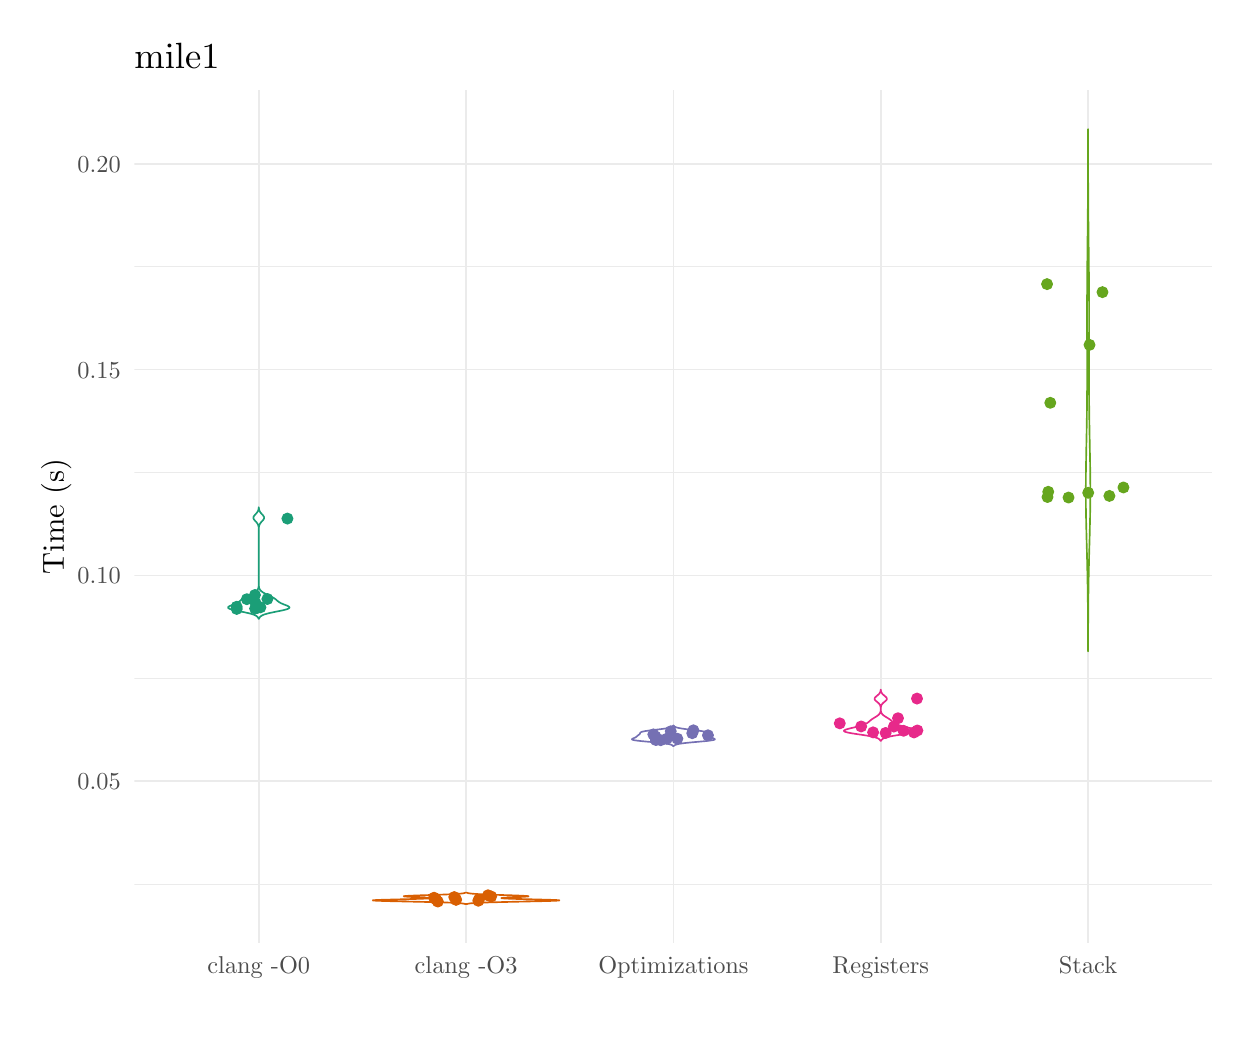
\begin{tikzpicture}[x=1pt,y=1pt]
\definecolor{fillColor}{RGB}{255,255,255}
\path[use as bounding box,fill=fillColor,fill opacity=0.00] (0,0) rectangle (433.62,361.35);
\begin{scope}
\path[clip] ( 38.56, 30.69) rectangle (428.12,338.69);
\definecolor{drawColor}{gray}{0.92}

\path[draw=drawColor,line width= 0.3pt,line join=round] ( 38.56, 51.94) --
	(428.12, 51.94);

\path[draw=drawColor,line width= 0.3pt,line join=round] ( 38.56,126.27) --
	(428.12,126.27);

\path[draw=drawColor,line width= 0.3pt,line join=round] ( 38.56,200.61) --
	(428.12,200.61);

\path[draw=drawColor,line width= 0.3pt,line join=round] ( 38.56,274.94) --
	(428.12,274.94);

\path[draw=drawColor,line width= 0.6pt,line join=round] ( 38.56, 89.11) --
	(428.12, 89.11);

\path[draw=drawColor,line width= 0.6pt,line join=round] ( 38.56,163.44) --
	(428.12,163.44);

\path[draw=drawColor,line width= 0.6pt,line join=round] ( 38.56,237.78) --
	(428.12,237.78);

\path[draw=drawColor,line width= 0.6pt,line join=round] ( 38.56,312.11) --
	(428.12,312.11);

\path[draw=drawColor,line width= 0.6pt,line join=round] ( 83.50, 30.69) --
	( 83.50,338.69);

\path[draw=drawColor,line width= 0.6pt,line join=round] (158.42, 30.69) --
	(158.42,338.69);

\path[draw=drawColor,line width= 0.6pt,line join=round] (233.34, 30.69) --
	(233.34,338.69);

\path[draw=drawColor,line width= 0.6pt,line join=round] (308.25, 30.69) --
	(308.25,338.69);

\path[draw=drawColor,line width= 0.6pt,line join=round] (383.17, 30.69) --
	(383.17,338.69);
\definecolor{drawColor}{RGB}{27,158,119}
\definecolor{fillColor}{RGB}{255,255,255}

\path[draw=drawColor,line width= 0.6pt,line join=round,line cap=round,fill=fillColor] ( 83.39,147.77) --
	( 83.37,147.85) --
	( 83.35,147.93) --
	( 83.31,148.00) --
	( 83.28,148.08) --
	( 83.24,148.16) --
	( 83.19,148.24) --
	( 83.13,148.32) --
	( 83.07,148.40) --
	( 83.00,148.48) --
	( 82.92,148.56) --
	( 82.82,148.64) --
	( 82.72,148.71) --
	( 82.60,148.79) --
	( 82.47,148.87) --
	( 82.33,148.95) --
	( 82.17,149.03) --
	( 81.99,149.11) --
	( 81.80,149.19) --
	( 81.59,149.27) --
	( 81.36,149.34) --
	( 81.12,149.42) --
	( 80.86,149.50) --
	( 80.58,149.58) --
	( 80.28,149.66) --
	( 79.97,149.74) --
	( 79.64,149.82) --
	( 79.30,149.90) --
	( 78.94,149.97) --
	( 78.57,150.05) --
	( 78.19,150.13) --
	( 77.80,150.21) --
	( 77.41,150.29) --
	( 77.01,150.37) --
	( 76.62,150.45) --
	( 76.23,150.53) --
	( 75.84,150.61) --
	( 75.46,150.68) --
	( 75.09,150.76) --
	( 74.74,150.84) --
	( 74.40,150.92) --
	( 74.08,151.00) --
	( 73.79,151.08) --
	( 73.52,151.16) --
	( 73.27,151.24) --
	( 73.06,151.31) --
	( 72.87,151.39) --
	( 72.72,151.47) --
	( 72.60,151.55) --
	( 72.51,151.63) --
	( 72.44,151.71) --
	( 72.42,151.79) --
	( 72.42,151.87) --
	( 72.45,151.94) --
	( 72.51,152.02) --
	( 72.59,152.10) --
	( 72.70,152.18) --
	( 72.83,152.26) --
	( 72.98,152.34) --
	( 73.14,152.42) --
	( 73.31,152.50) --
	( 73.50,152.58) --
	( 73.69,152.65) --
	( 73.89,152.73) --
	( 74.09,152.81) --
	( 74.29,152.89) --
	( 74.50,152.97) --
	( 74.69,153.05) --
	( 74.88,153.13) --
	( 75.07,153.21) --
	( 75.25,153.28) --
	( 75.42,153.36) --
	( 75.58,153.44) --
	( 75.73,153.52) --
	( 75.88,153.60) --
	( 76.01,153.68) --
	( 76.14,153.76) --
	( 76.25,153.84) --
	( 76.37,153.91) --
	( 76.47,153.99) --
	( 76.57,154.07) --
	( 76.66,154.15) --
	( 76.76,154.23) --
	( 76.85,154.31) --
	( 76.93,154.39) --
	( 77.02,154.47) --
	( 77.11,154.55) --
	( 77.20,154.62) --
	( 77.29,154.70) --
	( 77.39,154.78) --
	( 77.49,154.86) --
	( 77.59,154.94) --
	( 77.70,155.02) --
	( 77.82,155.10) --
	( 77.94,155.18) --
	( 78.06,155.25) --
	( 78.19,155.33) --
	( 78.33,155.41) --
	( 78.47,155.49) --
	( 78.61,155.57) --
	( 78.76,155.65) --
	( 78.92,155.73) --
	( 79.07,155.81) --
	( 79.23,155.88) --
	( 79.39,155.96) --
	( 79.56,156.04) --
	( 79.72,156.12) --
	( 79.89,156.20) --
	( 80.06,156.28) --
	( 80.22,156.36) --
	( 80.39,156.44) --
	( 80.55,156.52) --
	( 80.72,156.59) --
	( 80.87,156.67) --
	( 81.03,156.75) --
	( 81.19,156.83) --
	( 81.33,156.91) --
	( 81.48,156.99) --
	( 81.62,157.07) --
	( 81.75,157.15) --
	( 81.89,157.22) --
	( 82.01,157.30) --
	( 82.13,157.38) --
	( 82.24,157.46) --
	( 82.35,157.54) --
	( 82.45,157.62) --
	( 82.55,157.70) --
	( 82.64,157.78) --
	( 82.72,157.85) --
	( 82.80,157.93) --
	( 82.87,158.01) --
	( 82.94,158.09) --
	( 83.00,158.17) --
	( 83.05,158.25) --
	( 83.10,158.33) --
	( 83.15,158.41) --
	( 83.19,158.49) --
	( 83.23,158.56) --
	( 83.27,158.64) --
	( 83.30,158.72) --
	( 83.32,158.80) --
	( 83.35,158.88) --
	( 83.37,158.96) --
	( 83.39,159.04) --
	( 83.41,159.12) --
	( 83.42,159.19) --
	( 83.43,159.27) --
	( 83.44,159.35) --
	( 83.45,159.43) --
	( 83.46,159.51) --
	( 83.47,159.59) --
	( 83.47,159.67) --
	( 83.48,159.75) --
	( 83.48,159.82) --
	( 83.49,159.90) --
	( 83.49,159.98) --
	( 83.49,160.06) --
	( 83.50,160.14) --
	( 83.50,160.22) --
	( 83.50,160.30) --
	( 83.50,160.38) --
	( 83.50,160.46) --
	( 83.50,160.53) --
	( 83.50,160.61) --
	( 83.50,160.69) --
	( 83.50,160.77) --
	( 83.50,160.85) --
	( 83.50,160.93) --
	( 83.50,161.01) --
	( 83.50,161.09) --
	( 83.50,161.16) --
	( 83.50,161.24) --
	( 83.50,161.32) --
	( 83.50,161.40) --
	( 83.50,161.48) --
	( 83.50,161.56) --
	( 83.50,161.64) --
	( 83.50,161.72) --
	( 83.50,161.79) --
	( 83.50,161.87) --
	( 83.50,161.95) --
	( 83.50,162.03) --
	( 83.50,162.11) --
	( 83.50,162.19) --
	( 83.50,162.27) --
	( 83.50,162.35) --
	( 83.50,162.43) --
	( 83.50,162.50) --
	( 83.50,162.58) --
	( 83.50,162.66) --
	( 83.50,162.74) --
	( 83.50,162.82) --
	( 83.50,162.90) --
	( 83.50,162.98) --
	( 83.50,163.06) --
	( 83.50,163.13) --
	( 83.50,163.21) --
	( 83.50,163.29) --
	( 83.50,163.37) --
	( 83.50,163.45) --
	( 83.50,163.53) --
	( 83.50,163.61) --
	( 83.50,163.69) --
	( 83.50,163.76) --
	( 83.50,163.84) --
	( 83.50,163.92) --
	( 83.50,164.00) --
	( 83.50,164.08) --
	( 83.50,164.16) --
	( 83.50,164.24) --
	( 83.50,164.32) --
	( 83.50,164.40) --
	( 83.50,164.47) --
	( 83.50,164.55) --
	( 83.50,164.63) --
	( 83.50,164.71) --
	( 83.50,164.79) --
	( 83.50,164.87) --
	( 83.50,164.95) --
	( 83.50,165.03) --
	( 83.50,165.10) --
	( 83.50,165.18) --
	( 83.50,165.26) --
	( 83.50,165.34) --
	( 83.50,165.42) --
	( 83.50,165.50) --
	( 83.50,165.58) --
	( 83.50,165.66) --
	( 83.50,165.73) --
	( 83.50,165.81) --
	( 83.50,165.89) --
	( 83.50,165.97) --
	( 83.50,166.05) --
	( 83.50,166.13) --
	( 83.50,166.21) --
	( 83.50,166.29) --
	( 83.50,166.37) --
	( 83.50,166.44) --
	( 83.50,166.52) --
	( 83.50,166.60) --
	( 83.50,166.68) --
	( 83.50,166.76) --
	( 83.50,166.84) --
	( 83.50,166.92) --
	( 83.50,167.00) --
	( 83.50,167.07) --
	( 83.50,167.15) --
	( 83.50,167.23) --
	( 83.50,167.31) --
	( 83.50,167.39) --
	( 83.50,167.47) --
	( 83.50,167.55) --
	( 83.50,167.63) --
	( 83.50,167.70) --
	( 83.50,167.78) --
	( 83.50,167.86) --
	( 83.50,167.94) --
	( 83.50,168.02) --
	( 83.50,168.10) --
	( 83.50,168.18) --
	( 83.50,168.26) --
	( 83.50,168.34) --
	( 83.50,168.41) --
	( 83.50,168.49) --
	( 83.50,168.57) --
	( 83.50,168.65) --
	( 83.50,168.73) --
	( 83.50,168.81) --
	( 83.50,168.89) --
	( 83.50,168.97) --
	( 83.50,169.04) --
	( 83.50,169.12) --
	( 83.50,169.20) --
	( 83.50,169.28) --
	( 83.50,169.36) --
	( 83.50,169.44) --
	( 83.50,169.52) --
	( 83.50,169.60) --
	( 83.50,169.67) --
	( 83.50,169.75) --
	( 83.50,169.83) --
	( 83.50,169.91) --
	( 83.50,169.99) --
	( 83.50,170.07) --
	( 83.50,170.15) --
	( 83.50,170.23) --
	( 83.50,170.31) --
	( 83.50,170.38) --
	( 83.50,170.46) --
	( 83.50,170.54) --
	( 83.50,170.62) --
	( 83.50,170.70) --
	( 83.50,170.78) --
	( 83.50,170.86) --
	( 83.50,170.94) --
	( 83.50,171.01) --
	( 83.50,171.09) --
	( 83.50,171.17) --
	( 83.50,171.25) --
	( 83.50,171.33) --
	( 83.50,171.41) --
	( 83.50,171.49) --
	( 83.50,171.57) --
	( 83.50,171.64) --
	( 83.50,171.72) --
	( 83.50,171.80) --
	( 83.50,171.88) --
	( 83.50,171.96) --
	( 83.50,172.04) --
	( 83.50,172.12) --
	( 83.50,172.20) --
	( 83.50,172.28) --
	( 83.50,172.35) --
	( 83.50,172.43) --
	( 83.50,172.51) --
	( 83.50,172.59) --
	( 83.50,172.67) --
	( 83.50,172.75) --
	( 83.50,172.83) --
	( 83.50,172.91) --
	( 83.50,172.98) --
	( 83.50,173.06) --
	( 83.50,173.14) --
	( 83.50,173.22) --
	( 83.50,173.30) --
	( 83.50,173.38) --
	( 83.50,173.46) --
	( 83.50,173.54) --
	( 83.50,173.62) --
	( 83.50,173.69) --
	( 83.50,173.77) --
	( 83.50,173.85) --
	( 83.50,173.93) --
	( 83.50,174.01) --
	( 83.50,174.09) --
	( 83.50,174.17) --
	( 83.50,174.25) --
	( 83.50,174.32) --
	( 83.50,174.40) --
	( 83.50,174.48) --
	( 83.50,174.56) --
	( 83.50,174.64) --
	( 83.50,174.72) --
	( 83.50,174.80) --
	( 83.50,174.88) --
	( 83.50,174.95) --
	( 83.50,175.03) --
	( 83.50,175.11) --
	( 83.50,175.19) --
	( 83.50,175.27) --
	( 83.50,175.35) --
	( 83.50,175.43) --
	( 83.50,175.51) --
	( 83.50,175.59) --
	( 83.50,175.66) --
	( 83.50,175.74) --
	( 83.50,175.82) --
	( 83.50,175.90) --
	( 83.50,175.98) --
	( 83.50,176.06) --
	( 83.50,176.14) --
	( 83.50,176.22) --
	( 83.50,176.29) --
	( 83.50,176.37) --
	( 83.50,176.45) --
	( 83.50,176.53) --
	( 83.50,176.61) --
	( 83.50,176.69) --
	( 83.50,176.77) --
	( 83.50,176.85) --
	( 83.50,176.92) --
	( 83.50,177.00) --
	( 83.50,177.08) --
	( 83.50,177.16) --
	( 83.50,177.24) --
	( 83.50,177.32) --
	( 83.50,177.40) --
	( 83.50,177.48) --
	( 83.50,177.56) --
	( 83.50,177.63) --
	( 83.50,177.71) --
	( 83.50,177.79) --
	( 83.50,177.87) --
	( 83.50,177.95) --
	( 83.50,178.03) --
	( 83.50,178.11) --
	( 83.50,178.19) --
	( 83.50,178.26) --
	( 83.50,178.34) --
	( 83.50,178.42) --
	( 83.50,178.50) --
	( 83.50,178.58) --
	( 83.50,178.66) --
	( 83.50,178.74) --
	( 83.50,178.82) --
	( 83.50,178.89) --
	( 83.50,178.97) --
	( 83.50,179.05) --
	( 83.50,179.13) --
	( 83.50,179.21) --
	( 83.50,179.29) --
	( 83.50,179.37) --
	( 83.50,179.45) --
	( 83.50,179.53) --
	( 83.50,179.60) --
	( 83.50,179.68) --
	( 83.50,179.76) --
	( 83.50,179.84) --
	( 83.50,179.92) --
	( 83.50,180.00) --
	( 83.50,180.08) --
	( 83.49,180.16) --
	( 83.49,180.23) --
	( 83.49,180.31) --
	( 83.49,180.39) --
	( 83.48,180.47) --
	( 83.48,180.55) --
	( 83.47,180.63) --
	( 83.47,180.71) --
	( 83.46,180.79) --
	( 83.45,180.86) --
	( 83.44,180.94) --
	( 83.43,181.02) --
	( 83.42,181.10) --
	( 83.40,181.18) --
	( 83.39,181.26) --
	( 83.37,181.34) --
	( 83.35,181.42) --
	( 83.33,181.50) --
	( 83.30,181.57) --
	( 83.27,181.65) --
	( 83.24,181.73) --
	( 83.21,181.81) --
	( 83.17,181.89) --
	( 83.13,181.97) --
	( 83.09,182.05) --
	( 83.04,182.13) --
	( 82.99,182.20) --
	( 82.93,182.28) --
	( 82.87,182.36) --
	( 82.81,182.44) --
	( 82.75,182.52) --
	( 82.69,182.60) --
	( 82.62,182.68) --
	( 82.55,182.76) --
	( 82.48,182.83) --
	( 82.40,182.91) --
	( 82.33,182.99) --
	( 82.26,183.07) --
	( 82.18,183.15) --
	( 82.11,183.23) --
	( 82.04,183.31) --
	( 81.98,183.39) --
	( 81.91,183.47) --
	( 81.85,183.54) --
	( 81.79,183.62) --
	( 81.74,183.70) --
	( 81.70,183.78) --
	( 81.66,183.86) --
	( 81.63,183.94) --
	( 81.60,184.02) --
	( 81.58,184.10) --
	( 81.57,184.17) --
	( 81.57,184.25) --
	( 81.57,184.33) --
	( 81.58,184.41) --
	( 81.60,184.49) --
	( 81.63,184.57) --
	( 81.66,184.65) --
	( 81.70,184.73) --
	( 81.74,184.80) --
	( 81.79,184.88) --
	( 81.85,184.96) --
	( 81.91,185.04) --
	( 81.97,185.12) --
	( 82.04,185.20) --
	( 82.11,185.28) --
	( 82.18,185.36) --
	( 82.25,185.44) --
	( 82.33,185.51) --
	( 82.40,185.59) --
	( 82.47,185.67) --
	( 82.54,185.75) --
	( 82.61,185.83) --
	( 82.68,185.91) --
	( 82.75,185.99) --
	( 82.81,186.07) --
	( 82.87,186.14) --
	( 82.93,186.22) --
	( 82.98,186.30) --
	( 83.03,186.38) --
	( 83.08,186.46) --
	( 83.13,186.54) --
	( 83.17,186.62) --
	( 83.21,186.70) --
	( 83.24,186.77) --
	( 83.27,186.85) --
	( 83.30,186.93) --
	( 83.33,187.01) --
	( 83.35,187.09) --
	( 83.37,187.17) --
	( 83.39,187.25) --
	( 83.40,187.33) --
	( 83.42,187.41) --
	( 83.43,187.48) --
	( 83.44,187.56) --
	( 83.45,187.64) --
	( 83.46,187.72) --
	( 83.47,187.80) --
	( 83.47,187.88) --
	( 83.48,187.96) --
	( 83.48,188.04) --
	( 83.53,188.04) --
	( 83.53,187.96) --
	( 83.54,187.88) --
	( 83.54,187.80) --
	( 83.55,187.72) --
	( 83.56,187.64) --
	( 83.57,187.56) --
	( 83.58,187.48) --
	( 83.59,187.41) --
	( 83.61,187.33) --
	( 83.62,187.25) --
	( 83.64,187.17) --
	( 83.66,187.09) --
	( 83.68,187.01) --
	( 83.71,186.93) --
	( 83.74,186.85) --
	( 83.77,186.77) --
	( 83.80,186.70) --
	( 83.84,186.62) --
	( 83.88,186.54) --
	( 83.93,186.46) --
	( 83.97,186.38) --
	( 84.03,186.30) --
	( 84.08,186.22) --
	( 84.14,186.14) --
	( 84.20,186.07) --
	( 84.26,185.99) --
	( 84.33,185.91) --
	( 84.40,185.83) --
	( 84.47,185.75) --
	( 84.54,185.67) --
	( 84.61,185.59) --
	( 84.68,185.51) --
	( 84.76,185.44) --
	( 84.83,185.36) --
	( 84.90,185.28) --
	( 84.97,185.20) --
	( 85.04,185.12) --
	( 85.10,185.04) --
	( 85.16,184.96) --
	( 85.22,184.88) --
	( 85.27,184.80) --
	( 85.31,184.73) --
	( 85.35,184.65) --
	( 85.38,184.57) --
	( 85.41,184.49) --
	( 85.43,184.41) --
	( 85.44,184.33) --
	( 85.44,184.25) --
	( 85.44,184.17) --
	( 85.43,184.10) --
	( 85.41,184.02) --
	( 85.38,183.94) --
	( 85.35,183.86) --
	( 85.31,183.78) --
	( 85.27,183.70) --
	( 85.21,183.62) --
	( 85.16,183.54) --
	( 85.10,183.47) --
	( 85.03,183.39) --
	( 84.97,183.31) --
	( 84.90,183.23) --
	( 84.83,183.15) --
	( 84.75,183.07) --
	( 84.68,182.99) --
	( 84.61,182.91) --
	( 84.53,182.83) --
	( 84.46,182.76) --
	( 84.39,182.68) --
	( 84.32,182.60) --
	( 84.26,182.52) --
	( 84.19,182.44) --
	( 84.13,182.36) --
	( 84.08,182.28) --
	( 84.02,182.20) --
	( 83.97,182.13) --
	( 83.92,182.05) --
	( 83.88,181.97) --
	( 83.84,181.89) --
	( 83.80,181.81) --
	( 83.77,181.73) --
	( 83.74,181.65) --
	( 83.71,181.57) --
	( 83.68,181.50) --
	( 83.66,181.42) --
	( 83.64,181.34) --
	( 83.62,181.26) --
	( 83.60,181.18) --
	( 83.59,181.10) --
	( 83.58,181.02) --
	( 83.57,180.94) --
	( 83.56,180.86) --
	( 83.55,180.79) --
	( 83.54,180.71) --
	( 83.54,180.63) --
	( 83.53,180.55) --
	( 83.53,180.47) --
	( 83.52,180.39) --
	( 83.52,180.31) --
	( 83.52,180.23) --
	( 83.51,180.16) --
	( 83.51,180.08) --
	( 83.51,180.00) --
	( 83.51,179.92) --
	( 83.51,179.84) --
	( 83.51,179.76) --
	( 83.51,179.68) --
	( 83.51,179.60) --
	( 83.51,179.53) --
	( 83.51,179.45) --
	( 83.51,179.37) --
	( 83.51,179.29) --
	( 83.51,179.21) --
	( 83.51,179.13) --
	( 83.51,179.05) --
	( 83.51,178.97) --
	( 83.51,178.89) --
	( 83.51,178.82) --
	( 83.50,178.74) --
	( 83.50,178.66) --
	( 83.50,178.58) --
	( 83.50,178.50) --
	( 83.50,178.42) --
	( 83.50,178.34) --
	( 83.50,178.26) --
	( 83.50,178.19) --
	( 83.50,178.11) --
	( 83.50,178.03) --
	( 83.50,177.95) --
	( 83.50,177.87) --
	( 83.50,177.79) --
	( 83.50,177.71) --
	( 83.50,177.63) --
	( 83.50,177.56) --
	( 83.50,177.48) --
	( 83.50,177.40) --
	( 83.50,177.32) --
	( 83.50,177.24) --
	( 83.50,177.16) --
	( 83.50,177.08) --
	( 83.50,177.00) --
	( 83.50,176.92) --
	( 83.50,176.85) --
	( 83.50,176.77) --
	( 83.50,176.69) --
	( 83.50,176.61) --
	( 83.50,176.53) --
	( 83.50,176.45) --
	( 83.50,176.37) --
	( 83.50,176.29) --
	( 83.50,176.22) --
	( 83.50,176.14) --
	( 83.50,176.06) --
	( 83.50,175.98) --
	( 83.50,175.90) --
	( 83.50,175.82) --
	( 83.50,175.74) --
	( 83.50,175.66) --
	( 83.50,175.59) --
	( 83.50,175.51) --
	( 83.50,175.43) --
	( 83.50,175.35) --
	( 83.50,175.27) --
	( 83.50,175.19) --
	( 83.50,175.11) --
	( 83.50,175.03) --
	( 83.50,174.95) --
	( 83.50,174.88) --
	( 83.50,174.80) --
	( 83.50,174.72) --
	( 83.50,174.64) --
	( 83.50,174.56) --
	( 83.50,174.48) --
	( 83.50,174.40) --
	( 83.50,174.32) --
	( 83.50,174.25) --
	( 83.50,174.17) --
	( 83.50,174.09) --
	( 83.50,174.01) --
	( 83.50,173.93) --
	( 83.50,173.85) --
	( 83.50,173.77) --
	( 83.50,173.69) --
	( 83.50,173.62) --
	( 83.50,173.54) --
	( 83.50,173.46) --
	( 83.50,173.38) --
	( 83.50,173.30) --
	( 83.50,173.22) --
	( 83.50,173.14) --
	( 83.50,173.06) --
	( 83.50,172.98) --
	( 83.50,172.91) --
	( 83.50,172.83) --
	( 83.50,172.75) --
	( 83.50,172.67) --
	( 83.50,172.59) --
	( 83.50,172.51) --
	( 83.50,172.43) --
	( 83.50,172.35) --
	( 83.50,172.28) --
	( 83.50,172.20) --
	( 83.50,172.12) --
	( 83.50,172.04) --
	( 83.50,171.96) --
	( 83.50,171.88) --
	( 83.50,171.80) --
	( 83.50,171.72) --
	( 83.50,171.64) --
	( 83.50,171.57) --
	( 83.50,171.49) --
	( 83.50,171.41) --
	( 83.50,171.33) --
	( 83.50,171.25) --
	( 83.50,171.17) --
	( 83.50,171.09) --
	( 83.50,171.01) --
	( 83.50,170.94) --
	( 83.50,170.86) --
	( 83.50,170.78) --
	( 83.50,170.70) --
	( 83.50,170.62) --
	( 83.50,170.54) --
	( 83.50,170.46) --
	( 83.50,170.38) --
	( 83.50,170.31) --
	( 83.50,170.23) --
	( 83.50,170.15) --
	( 83.50,170.07) --
	( 83.50,169.99) --
	( 83.50,169.91) --
	( 83.50,169.83) --
	( 83.50,169.75) --
	( 83.50,169.67) --
	( 83.50,169.60) --
	( 83.50,169.52) --
	( 83.50,169.44) --
	( 83.50,169.36) --
	( 83.50,169.28) --
	( 83.50,169.20) --
	( 83.50,169.12) --
	( 83.50,169.04) --
	( 83.50,168.97) --
	( 83.50,168.89) --
	( 83.50,168.81) --
	( 83.50,168.73) --
	( 83.50,168.65) --
	( 83.50,168.57) --
	( 83.50,168.49) --
	( 83.50,168.41) --
	( 83.50,168.34) --
	( 83.50,168.26) --
	( 83.50,168.18) --
	( 83.50,168.10) --
	( 83.50,168.02) --
	( 83.50,167.94) --
	( 83.50,167.86) --
	( 83.50,167.78) --
	( 83.50,167.70) --
	( 83.50,167.63) --
	( 83.50,167.55) --
	( 83.50,167.47) --
	( 83.50,167.39) --
	( 83.50,167.31) --
	( 83.50,167.23) --
	( 83.50,167.15) --
	( 83.50,167.07) --
	( 83.50,167.00) --
	( 83.50,166.92) --
	( 83.50,166.84) --
	( 83.50,166.76) --
	( 83.50,166.68) --
	( 83.50,166.60) --
	( 83.50,166.52) --
	( 83.50,166.44) --
	( 83.50,166.37) --
	( 83.50,166.29) --
	( 83.50,166.21) --
	( 83.50,166.13) --
	( 83.50,166.05) --
	( 83.50,165.97) --
	( 83.50,165.89) --
	( 83.50,165.81) --
	( 83.50,165.73) --
	( 83.50,165.66) --
	( 83.50,165.58) --
	( 83.50,165.50) --
	( 83.50,165.42) --
	( 83.50,165.34) --
	( 83.50,165.26) --
	( 83.50,165.18) --
	( 83.50,165.10) --
	( 83.50,165.03) --
	( 83.50,164.95) --
	( 83.50,164.87) --
	( 83.50,164.79) --
	( 83.50,164.71) --
	( 83.50,164.63) --
	( 83.50,164.55) --
	( 83.50,164.47) --
	( 83.50,164.40) --
	( 83.50,164.32) --
	( 83.50,164.24) --
	( 83.50,164.16) --
	( 83.50,164.08) --
	( 83.50,164.00) --
	( 83.50,163.92) --
	( 83.50,163.84) --
	( 83.50,163.76) --
	( 83.50,163.69) --
	( 83.50,163.61) --
	( 83.50,163.53) --
	( 83.50,163.45) --
	( 83.50,163.37) --
	( 83.50,163.29) --
	( 83.50,163.21) --
	( 83.50,163.13) --
	( 83.50,163.06) --
	( 83.50,162.98) --
	( 83.50,162.90) --
	( 83.50,162.82) --
	( 83.50,162.74) --
	( 83.50,162.66) --
	( 83.50,162.58) --
	( 83.50,162.50) --
	( 83.50,162.43) --
	( 83.50,162.35) --
	( 83.50,162.27) --
	( 83.50,162.19) --
	( 83.50,162.11) --
	( 83.50,162.03) --
	( 83.50,161.95) --
	( 83.50,161.87) --
	( 83.50,161.79) --
	( 83.50,161.72) --
	( 83.50,161.64) --
	( 83.50,161.56) --
	( 83.50,161.48) --
	( 83.51,161.40) --
	( 83.51,161.32) --
	( 83.51,161.24) --
	( 83.51,161.16) --
	( 83.51,161.09) --
	( 83.51,161.01) --
	( 83.51,160.93) --
	( 83.51,160.85) --
	( 83.51,160.77) --
	( 83.51,160.69) --
	( 83.51,160.61) --
	( 83.51,160.53) --
	( 83.51,160.46) --
	( 83.51,160.38) --
	( 83.51,160.30) --
	( 83.51,160.22) --
	( 83.51,160.14) --
	( 83.52,160.06) --
	( 83.52,159.98) --
	( 83.52,159.90) --
	( 83.53,159.82) --
	( 83.53,159.75) --
	( 83.53,159.67) --
	( 83.54,159.59) --
	( 83.55,159.51) --
	( 83.56,159.43) --
	( 83.57,159.35) --
	( 83.58,159.27) --
	( 83.59,159.19) --
	( 83.60,159.12) --
	( 83.62,159.04) --
	( 83.64,158.96) --
	( 83.66,158.88) --
	( 83.69,158.80) --
	( 83.71,158.72) --
	( 83.74,158.64) --
	( 83.78,158.56) --
	( 83.82,158.49) --
	( 83.86,158.41) --
	( 83.91,158.33) --
	( 83.96,158.25) --
	( 84.01,158.17) --
	( 84.07,158.09) --
	( 84.14,158.01) --
	( 84.21,157.93) --
	( 84.29,157.85) --
	( 84.37,157.78) --
	( 84.46,157.70) --
	( 84.56,157.62) --
	( 84.66,157.54) --
	( 84.77,157.46) --
	( 84.88,157.38) --
	( 85.00,157.30) --
	( 85.12,157.22) --
	( 85.26,157.15) --
	( 85.39,157.07) --
	( 85.53,156.99) --
	( 85.68,156.91) --
	( 85.82,156.83) --
	( 85.98,156.75) --
	( 86.13,156.67) --
	( 86.29,156.59) --
	( 86.46,156.52) --
	( 86.62,156.44) --
	( 86.79,156.36) --
	( 86.95,156.28) --
	( 87.12,156.20) --
	( 87.29,156.12) --
	( 87.45,156.04) --
	( 87.62,155.96) --
	( 87.78,155.88) --
	( 87.94,155.81) --
	( 88.09,155.73) --
	( 88.25,155.65) --
	( 88.40,155.57) --
	( 88.54,155.49) --
	( 88.68,155.41) --
	( 88.82,155.33) --
	( 88.95,155.25) --
	( 89.07,155.18) --
	( 89.19,155.10) --
	( 89.31,155.02) --
	( 89.42,154.94) --
	( 89.52,154.86) --
	( 89.62,154.78) --
	( 89.72,154.70) --
	( 89.81,154.62) --
	( 89.90,154.55) --
	( 89.99,154.47) --
	( 90.08,154.39) --
	( 90.16,154.31) --
	( 90.25,154.23) --
	( 90.35,154.15) --
	( 90.44,154.07) --
	( 90.54,153.99) --
	( 90.64,153.91) --
	( 90.75,153.84) --
	( 90.87,153.76) --
	( 91.00,153.68) --
	( 91.13,153.60) --
	( 91.28,153.52) --
	( 91.43,153.44) --
	( 91.59,153.36) --
	( 91.76,153.28) --
	( 91.94,153.21) --
	( 92.13,153.13) --
	( 92.32,153.05) --
	( 92.51,152.97) --
	( 92.71,152.89) --
	( 92.92,152.81) --
	( 93.12,152.73) --
	( 93.32,152.65) --
	( 93.51,152.58) --
	( 93.70,152.50) --
	( 93.87,152.42) --
	( 94.03,152.34) --
	( 94.18,152.26) --
	( 94.31,152.18) --
	( 94.42,152.10) --
	( 94.50,152.02) --
	( 94.56,151.94) --
	( 94.59,151.87) --
	( 94.59,151.79) --
	( 94.56,151.71) --
	( 94.50,151.63) --
	( 94.41,151.55) --
	( 94.29,151.47) --
	( 94.14,151.39) --
	( 93.95,151.31) --
	( 93.74,151.24) --
	( 93.49,151.16) --
	( 93.22,151.08) --
	( 92.93,151.00) --
	( 92.61,150.92) --
	( 92.27,150.84) --
	( 91.92,150.76) --
	( 91.55,150.68) --
	( 91.17,150.61) --
	( 90.78,150.53) --
	( 90.39,150.45) --
	( 89.99,150.37) --
	( 89.60,150.29) --
	( 89.21,150.21) --
	( 88.82,150.13) --
	( 88.44,150.05) --
	( 88.07,149.97) --
	( 87.71,149.90) --
	( 87.37,149.82) --
	( 87.04,149.74) --
	( 86.73,149.66) --
	( 86.43,149.58) --
	( 86.15,149.50) --
	( 85.89,149.42) --
	( 85.65,149.34) --
	( 85.42,149.27) --
	( 85.21,149.19) --
	( 85.02,149.11) --
	( 84.84,149.03) --
	( 84.68,148.95) --
	( 84.54,148.87) --
	( 84.41,148.79) --
	( 84.29,148.71) --
	( 84.19,148.64) --
	( 84.09,148.56) --
	( 84.01,148.48) --
	( 83.94,148.40) --
	( 83.88,148.32) --
	( 83.82,148.24) --
	( 83.77,148.16) --
	( 83.73,148.08) --
	( 83.69,148.00) --
	( 83.66,147.93) --
	( 83.64,147.85) --
	( 83.61,147.77) --
	( 83.39,147.77) --
	cycle;
\definecolor{drawColor}{RGB}{217,95,2}

\path[draw=drawColor,line width= 0.6pt,line join=round,line cap=round,fill=fillColor] (158.04, 44.69) --
	(158.02, 44.69) --
	(158.00, 44.70) --
	(157.98, 44.71) --
	(157.95, 44.72) --
	(157.93, 44.73) --
	(157.90, 44.73) --
	(157.87, 44.74) --
	(157.84, 44.75) --
	(157.81, 44.76) --
	(157.78, 44.77) --
	(157.74, 44.77) --
	(157.71, 44.78) --
	(157.67, 44.79) --
	(157.63, 44.80) --
	(157.59, 44.81) --
	(157.55, 44.81) --
	(157.50, 44.82) --
	(157.46, 44.83) --
	(157.41, 44.84) --
	(157.36, 44.85) --
	(157.31, 44.85) --
	(157.25, 44.86) --
	(157.19, 44.87) --
	(157.13, 44.88) --
	(157.07, 44.89) --
	(157.01, 44.89) --
	(156.94, 44.90) --
	(156.87, 44.91) --
	(156.80, 44.92) --
	(156.73, 44.93) --
	(156.65, 44.94) --
	(156.57, 44.94) --
	(156.48, 44.95) --
	(156.40, 44.96) --
	(156.31, 44.97) --
	(156.21, 44.98) --
	(156.12, 44.98) --
	(156.02, 44.99) --
	(155.91, 45.00) --
	(155.81, 45.01) --
	(155.70, 45.02) --
	(155.58, 45.02) --
	(155.46, 45.03) --
	(155.34, 45.04) --
	(155.22, 45.05) --
	(155.09, 45.06) --
	(154.95, 45.06) --
	(154.82, 45.07) --
	(154.67, 45.08) --
	(154.53, 45.09) --
	(154.38, 45.10) --
	(154.22, 45.10) --
	(154.06, 45.11) --
	(153.90, 45.12) --
	(153.73, 45.13) --
	(153.55, 45.14) --
	(153.38, 45.14) --
	(153.19, 45.15) --
	(153.00, 45.16) --
	(152.81, 45.17) --
	(152.61, 45.18) --
	(152.41, 45.18) --
	(152.20, 45.19) --
	(151.99, 45.20) --
	(151.77, 45.21) --
	(151.55, 45.22) --
	(151.32, 45.22) --
	(151.09, 45.23) --
	(150.85, 45.24) --
	(150.61, 45.25) --
	(150.36, 45.26) --
	(150.11, 45.26) --
	(149.85, 45.27) --
	(149.59, 45.28) --
	(149.32, 45.29) --
	(149.04, 45.30) --
	(148.77, 45.30) --
	(148.48, 45.31) --
	(148.20, 45.32) --
	(147.90, 45.33) --
	(147.61, 45.34) --
	(147.30, 45.34) --
	(147.00, 45.35) --
	(146.69, 45.36) --
	(146.37, 45.37) --
	(146.05, 45.38) --
	(145.73, 45.38) --
	(145.40, 45.39) --
	(145.07, 45.40) --
	(144.73, 45.41) --
	(144.39, 45.42) --
	(144.05, 45.42) --
	(143.70, 45.43) --
	(143.35, 45.44) --
	(143.00, 45.45) --
	(142.64, 45.46) --
	(142.28, 45.46) --
	(141.92, 45.47) --
	(141.56, 45.48) --
	(141.19, 45.49) --
	(140.83, 45.50) --
	(140.46, 45.51) --
	(140.09, 45.51) --
	(139.71, 45.52) --
	(139.34, 45.53) --
	(138.97, 45.54) --
	(138.59, 45.55) --
	(138.22, 45.55) --
	(137.84, 45.56) --
	(137.47, 45.57) --
	(137.09, 45.58) --
	(136.72, 45.59) --
	(136.34, 45.59) --
	(135.97, 45.60) --
	(135.60, 45.61) --
	(135.23, 45.62) --
	(134.86, 45.63) --
	(134.50, 45.63) --
	(134.14, 45.64) --
	(133.78, 45.65) --
	(133.42, 45.66) --
	(133.07, 45.67) --
	(132.72, 45.67) --
	(132.37, 45.68) --
	(132.03, 45.69) --
	(131.70, 45.70) --
	(131.36, 45.71) --
	(131.04, 45.71) --
	(130.72, 45.72) --
	(130.40, 45.73) --
	(130.09, 45.74) --
	(129.79, 45.75) --
	(129.49, 45.75) --
	(129.20, 45.76) --
	(128.92, 45.77) --
	(128.64, 45.78) --
	(128.38, 45.79) --
	(128.11, 45.79) --
	(127.87, 45.80) --
	(127.62, 45.81) --
	(127.39, 45.82) --
	(127.16, 45.83) --
	(126.94, 45.83) --
	(126.73, 45.84) --
	(126.53, 45.85) --
	(126.34, 45.86) --
	(126.16, 45.87) --
	(125.99, 45.87) --
	(125.83, 45.88) --
	(125.68, 45.89) --
	(125.54, 45.90) --
	(125.42, 45.91) --
	(125.29, 45.91) --
	(125.19, 45.92) --
	(125.09, 45.93) --
	(125.00, 45.94) --
	(124.93, 45.95) --
	(124.86, 45.95) --
	(124.81, 45.96) --
	(124.77, 45.97) --
	(124.74, 45.98) --
	(124.72, 45.99) --
	(124.71, 45.99) --
	(124.71, 46.00) --
	(124.73, 46.01) --
	(124.75, 46.02) --
	(124.79, 46.03) --
	(124.83, 46.03) --
	(124.89, 46.04) --
	(124.96, 46.05) --
	(125.04, 46.06) --
	(125.13, 46.07) --
	(125.22, 46.08) --
	(125.34, 46.08) --
	(125.45, 46.09) --
	(125.59, 46.10) --
	(125.73, 46.11) --
	(125.88, 46.12) --
	(126.04, 46.12) --
	(126.21, 46.13) --
	(126.39, 46.14) --
	(126.58, 46.15) --
	(126.77, 46.16) --
	(126.98, 46.16) --
	(127.19, 46.17) --
	(127.41, 46.18) --
	(127.65, 46.19) --
	(127.88, 46.20) --
	(128.13, 46.20) --
	(128.38, 46.21) --
	(128.64, 46.22) --
	(128.90, 46.23) --
	(129.17, 46.24) --
	(129.45, 46.24) --
	(129.73, 46.25) --
	(130.02, 46.26) --
	(130.31, 46.27) --
	(130.61, 46.28) --
	(130.91, 46.28) --
	(131.21, 46.29) --
	(131.52, 46.30) --
	(131.83, 46.31) --
	(132.15, 46.32) --
	(132.47, 46.32) --
	(132.79, 46.33) --
	(133.11, 46.34) --
	(133.43, 46.35) --
	(133.76, 46.36) --
	(134.08, 46.36) --
	(134.41, 46.37) --
	(134.74, 46.38) --
	(135.06, 46.39) --
	(135.39, 46.40) --
	(135.71, 46.40) --
	(136.04, 46.41) --
	(136.36, 46.42) --
	(136.68, 46.43) --
	(137.00, 46.44) --
	(137.32, 46.44) --
	(137.64, 46.45) --
	(137.95, 46.46) --
	(138.26, 46.47) --
	(138.57, 46.48) --
	(138.87, 46.48) --
	(139.17, 46.49) --
	(139.46, 46.50) --
	(139.75, 46.51) --
	(140.03, 46.52) --
	(140.31, 46.52) --
	(140.59, 46.53) --
	(140.86, 46.54) --
	(141.12, 46.55) --
	(141.38, 46.56) --
	(141.63, 46.56) --
	(141.87, 46.57) --
	(142.12, 46.58) --
	(142.34, 46.59) --
	(142.57, 46.60) --
	(142.79, 46.60) --
	(143.00, 46.61) --
	(143.20, 46.62) --
	(143.40, 46.63) --
	(143.59, 46.64) --
	(143.77, 46.65) --
	(143.94, 46.65) --
	(144.11, 46.66) --
	(144.27, 46.67) --
	(144.41, 46.68) --
	(144.56, 46.69) --
	(144.69, 46.69) --
	(144.81, 46.70) --
	(144.93, 46.71) --
	(145.04, 46.72) --
	(145.14, 46.73) --
	(145.23, 46.73) --
	(145.31, 46.74) --
	(145.38, 46.75) --
	(145.45, 46.76) --
	(145.50, 46.77) --
	(145.56, 46.77) --
	(145.59, 46.78) --
	(145.63, 46.79) --
	(145.65, 46.80) --
	(145.67, 46.81) --
	(145.67, 46.81) --
	(145.67, 46.82) --
	(145.66, 46.83) --
	(145.65, 46.84) --
	(145.62, 46.85) --
	(145.59, 46.85) --
	(145.55, 46.86) --
	(145.50, 46.87) --
	(145.45, 46.88) --
	(145.39, 46.89) --
	(145.32, 46.89) --
	(145.24, 46.90) --
	(145.16, 46.91) --
	(145.07, 46.92) --
	(144.97, 46.93) --
	(144.87, 46.93) --
	(144.77, 46.94) --
	(144.65, 46.95) --
	(144.53, 46.96) --
	(144.41, 46.97) --
	(144.28, 46.97) --
	(144.14, 46.98) --
	(144.00, 46.99) --
	(143.86, 47.00) --
	(143.71, 47.01) --
	(143.56, 47.01) --
	(143.40, 47.02) --
	(143.24, 47.03) --
	(143.08, 47.04) --
	(142.91, 47.05) --
	(142.74, 47.05) --
	(142.57, 47.06) --
	(142.39, 47.07) --
	(142.21, 47.08) --
	(142.03, 47.09) --
	(141.85, 47.09) --
	(141.67, 47.10) --
	(141.49, 47.11) --
	(141.30, 47.12) --
	(141.12, 47.13) --
	(140.93, 47.13) --
	(140.75, 47.14) --
	(140.56, 47.15) --
	(140.37, 47.16) --
	(140.19, 47.17) --
	(140.01, 47.17) --
	(139.82, 47.18) --
	(139.64, 47.19) --
	(139.46, 47.20) --
	(139.29, 47.21) --
	(139.11, 47.22) --
	(138.94, 47.22) --
	(138.77, 47.23) --
	(138.60, 47.24) --
	(138.44, 47.25) --
	(138.28, 47.26) --
	(138.12, 47.26) --
	(137.97, 47.27) --
	(137.82, 47.28) --
	(137.67, 47.29) --
	(137.53, 47.30) --
	(137.40, 47.30) --
	(137.26, 47.31) --
	(137.14, 47.32) --
	(137.02, 47.33) --
	(136.90, 47.34) --
	(136.79, 47.34) --
	(136.69, 47.35) --
	(136.59, 47.36) --
	(136.49, 47.37) --
	(136.41, 47.38) --
	(136.33, 47.38) --
	(136.25, 47.39) --
	(136.19, 47.40) --
	(136.13, 47.41) --
	(136.07, 47.42) --
	(136.02, 47.42) --
	(135.98, 47.43) --
	(135.95, 47.44) --
	(135.92, 47.45) --
	(135.90, 47.46) --
	(135.89, 47.46) --
	(135.89, 47.47) --
	(135.89, 47.48) --
	(135.90, 47.49) --
	(135.92, 47.50) --
	(135.94, 47.50) --
	(135.97, 47.51) --
	(136.01, 47.52) --
	(136.05, 47.53) --
	(136.11, 47.54) --
	(136.17, 47.54) --
	(136.23, 47.55) --
	(136.31, 47.56) --
	(136.39, 47.57) --
	(136.47, 47.58) --
	(136.57, 47.58) --
	(136.67, 47.59) --
	(136.78, 47.60) --
	(136.90, 47.61) --
	(137.02, 47.62) --
	(137.14, 47.62) --
	(137.28, 47.63) --
	(137.42, 47.64) --
	(137.56, 47.65) --
	(137.72, 47.66) --
	(137.87, 47.66) --
	(138.04, 47.67) --
	(138.21, 47.68) --
	(138.38, 47.69) --
	(138.56, 47.70) --
	(138.75, 47.70) --
	(138.93, 47.71) --
	(139.13, 47.72) --
	(139.33, 47.73) --
	(139.53, 47.74) --
	(139.74, 47.74) --
	(139.95, 47.75) --
	(140.16, 47.76) --
	(140.38, 47.77) --
	(140.60, 47.78) --
	(140.82, 47.79) --
	(141.05, 47.79) --
	(141.28, 47.80) --
	(141.52, 47.81) --
	(141.75, 47.82) --
	(141.99, 47.83) --
	(142.23, 47.83) --
	(142.47, 47.84) --
	(142.71, 47.85) --
	(142.96, 47.86) --
	(143.21, 47.87) --
	(143.45, 47.87) --
	(143.70, 47.88) --
	(143.95, 47.89) --
	(144.20, 47.90) --
	(144.45, 47.91) --
	(144.70, 47.91) --
	(144.95, 47.92) --
	(145.20, 47.93) --
	(145.45, 47.94) --
	(145.70, 47.95) --
	(145.95, 47.95) --
	(146.20, 47.96) --
	(146.44, 47.97) --
	(146.69, 47.98) --
	(146.94, 47.99) --
	(147.18, 47.99) --
	(147.42, 48.00) --
	(147.66, 48.01) --
	(147.90, 48.02) --
	(148.14, 48.03) --
	(148.37, 48.03) --
	(148.61, 48.04) --
	(148.84, 48.05) --
	(149.07, 48.06) --
	(149.29, 48.07) --
	(149.52, 48.07) --
	(149.74, 48.08) --
	(149.96, 48.09) --
	(150.17, 48.10) --
	(150.39, 48.11) --
	(150.60, 48.11) --
	(150.80, 48.12) --
	(151.01, 48.13) --
	(151.21, 48.14) --
	(151.41, 48.15) --
	(151.60, 48.15) --
	(151.80, 48.16) --
	(151.99, 48.17) --
	(152.17, 48.18) --
	(152.35, 48.19) --
	(152.53, 48.19) --
	(152.71, 48.20) --
	(152.88, 48.21) --
	(153.05, 48.22) --
	(153.21, 48.23) --
	(153.37, 48.23) --
	(153.53, 48.24) --
	(153.69, 48.25) --
	(153.84, 48.26) --
	(153.99, 48.27) --
	(154.13, 48.27) --
	(154.28, 48.28) --
	(154.41, 48.29) --
	(154.55, 48.30) --
	(154.68, 48.31) --
	(154.81, 48.31) --
	(154.94, 48.32) --
	(155.06, 48.33) --
	(155.18, 48.34) --
	(155.29, 48.35) --
	(155.40, 48.36) --
	(155.51, 48.36) --
	(155.62, 48.37) --
	(155.73, 48.38) --
	(155.82, 48.39) --
	(155.92, 48.40) --
	(156.02, 48.40) --
	(156.11, 48.41) --
	(156.20, 48.42) --
	(156.29, 48.43) --
	(156.37, 48.44) --
	(156.45, 48.44) --
	(156.53, 48.45) --
	(156.61, 48.46) --
	(156.68, 48.47) --
	(156.75, 48.48) --
	(156.82, 48.48) --
	(156.89, 48.49) --
	(156.95, 48.50) --
	(157.01, 48.51) --
	(157.07, 48.52) --
	(157.13, 48.52) --
	(157.19, 48.53) --
	(157.24, 48.54) --
	(157.29, 48.55) --
	(157.34, 48.56) --
	(157.39, 48.56) --
	(157.44, 48.57) --
	(157.48, 48.58) --
	(157.52, 48.59) --
	(157.56, 48.60) --
	(157.60, 48.60) --
	(157.64, 48.61) --
	(157.68, 48.62) --
	(157.71, 48.63) --
	(157.75, 48.64) --
	(157.78, 48.64) --
	(157.81, 48.65) --
	(157.84, 48.66) --
	(157.87, 48.67) --
	(157.89, 48.68) --
	(157.92, 48.68) --
	(157.95, 48.69) --
	(157.97, 48.70) --
	(157.99, 48.71) --
	(158.01, 48.72) --
	(158.03, 48.72) --
	(158.05, 48.73) --
	(158.07, 48.74) --
	(158.09, 48.75) --
	(158.11, 48.76) --
	(158.12, 48.76) --
	(158.14, 48.77) --
	(158.16, 48.78) --
	(158.17, 48.79) --
	(158.67, 48.79) --
	(158.69, 48.78) --
	(158.70, 48.77) --
	(158.72, 48.76) --
	(158.73, 48.76) --
	(158.75, 48.75) --
	(158.77, 48.74) --
	(158.79, 48.73) --
	(158.81, 48.72) --
	(158.83, 48.72) --
	(158.85, 48.71) --
	(158.87, 48.70) --
	(158.90, 48.69) --
	(158.92, 48.68) --
	(158.95, 48.68) --
	(158.98, 48.67) --
	(159.00, 48.66) --
	(159.03, 48.65) --
	(159.06, 48.64) --
	(159.10, 48.64) --
	(159.13, 48.63) --
	(159.17, 48.62) --
	(159.20, 48.61) --
	(159.24, 48.60) --
	(159.28, 48.60) --
	(159.32, 48.59) --
	(159.36, 48.58) --
	(159.41, 48.57) --
	(159.45, 48.56) --
	(159.50, 48.56) --
	(159.55, 48.55) --
	(159.60, 48.54) --
	(159.66, 48.53) --
	(159.71, 48.52) --
	(159.77, 48.52) --
	(159.83, 48.51) --
	(159.89, 48.50) --
	(159.96, 48.49) --
	(160.02, 48.48) --
	(160.09, 48.48) --
	(160.16, 48.47) --
	(160.24, 48.46) --
	(160.31, 48.45) --
	(160.39, 48.44) --
	(160.47, 48.44) --
	(160.56, 48.43) --
	(160.64, 48.42) --
	(160.73, 48.41) --
	(160.83, 48.40) --
	(160.92, 48.40) --
	(161.02, 48.39) --
	(161.12, 48.38) --
	(161.22, 48.37) --
	(161.33, 48.36) --
	(161.44, 48.36) --
	(161.55, 48.35) --
	(161.67, 48.34) --
	(161.79, 48.33) --
	(161.91, 48.32) --
	(162.03, 48.31) --
	(162.16, 48.31) --
	(162.29, 48.30) --
	(162.43, 48.29) --
	(162.57, 48.28) --
	(162.71, 48.27) --
	(162.85, 48.27) --
	(163.00, 48.26) --
	(163.15, 48.25) --
	(163.31, 48.24) --
	(163.47, 48.23) --
	(163.63, 48.23) --
	(163.80, 48.22) --
	(163.96, 48.21) --
	(164.14, 48.20) --
	(164.31, 48.19) --
	(164.49, 48.19) --
	(164.67, 48.18) --
	(164.86, 48.17) --
	(165.05, 48.16) --
	(165.24, 48.15) --
	(165.43, 48.15) --
	(165.63, 48.14) --
	(165.83, 48.13) --
	(166.04, 48.12) --
	(166.25, 48.11) --
	(166.46, 48.11) --
	(166.67, 48.10) --
	(166.88, 48.09) --
	(167.10, 48.08) --
	(167.33, 48.07) --
	(167.55, 48.07) --
	(167.78, 48.06) --
	(168.00, 48.05) --
	(168.23, 48.04) --
	(168.47, 48.03) --
	(168.70, 48.03) --
	(168.94, 48.02) --
	(169.18, 48.01) --
	(169.42, 48.00) --
	(169.66, 47.99) --
	(169.91, 47.99) --
	(170.15, 47.98) --
	(170.40, 47.97) --
	(170.64, 47.96) --
	(170.89, 47.95) --
	(171.14, 47.95) --
	(171.39, 47.94) --
	(171.64, 47.93) --
	(171.89, 47.92) --
	(172.14, 47.91) --
	(172.39, 47.91) --
	(172.64, 47.90) --
	(172.89, 47.89) --
	(173.14, 47.88) --
	(173.39, 47.87) --
	(173.64, 47.87) --
	(173.88, 47.86) --
	(174.13, 47.85) --
	(174.37, 47.84) --
	(174.61, 47.83) --
	(174.85, 47.83) --
	(175.09, 47.82) --
	(175.33, 47.81) --
	(175.56, 47.80) --
	(175.79, 47.79) --
	(176.02, 47.79) --
	(176.24, 47.78) --
	(176.46, 47.77) --
	(176.68, 47.76) --
	(176.90, 47.75) --
	(177.11, 47.74) --
	(177.31, 47.74) --
	(177.52, 47.73) --
	(177.71, 47.72) --
	(177.91, 47.71) --
	(178.10, 47.70) --
	(178.28, 47.70) --
	(178.46, 47.69) --
	(178.64, 47.68) --
	(178.80, 47.67) --
	(178.97, 47.66) --
	(179.12, 47.66) --
	(179.28, 47.65) --
	(179.42, 47.64) --
	(179.56, 47.63) --
	(179.70, 47.62) --
	(179.82, 47.62) --
	(179.95, 47.61) --
	(180.06, 47.60) --
	(180.17, 47.59) --
	(180.27, 47.58) --
	(180.37, 47.58) --
	(180.45, 47.57) --
	(180.54, 47.56) --
	(180.61, 47.55) --
	(180.68, 47.54) --
	(180.74, 47.54) --
	(180.79, 47.53) --
	(180.83, 47.52) --
	(180.87, 47.51) --
	(180.90, 47.50) --
	(180.93, 47.50) --
	(180.95, 47.49) --
	(180.95, 47.48) --
	(180.96, 47.47) --
	(180.95, 47.46) --
	(180.94, 47.46) --
	(180.92, 47.45) --
	(180.89, 47.44) --
	(180.86, 47.43) --
	(180.82, 47.42) --
	(180.77, 47.42) --
	(180.72, 47.41) --
	(180.66, 47.40) --
	(180.59, 47.39) --
	(180.52, 47.38) --
	(180.43, 47.38) --
	(180.35, 47.37) --
	(180.25, 47.36) --
	(180.16, 47.35) --
	(180.05, 47.34) --
	(179.94, 47.34) --
	(179.83, 47.33) --
	(179.70, 47.32) --
	(179.58, 47.31) --
	(179.45, 47.30) --
	(179.31, 47.30) --
	(179.17, 47.29) --
	(179.03, 47.28) --
	(178.88, 47.27) --
	(178.72, 47.26) --
	(178.57, 47.26) --
	(178.41, 47.25) --
	(178.24, 47.24) --
	(178.07, 47.23) --
	(177.90, 47.22) --
	(177.73, 47.22) --
	(177.56, 47.21) --
	(177.38, 47.20) --
	(177.20, 47.19) --
	(177.02, 47.18) --
	(176.84, 47.17) --
	(176.65, 47.17) --
	(176.47, 47.16) --
	(176.28, 47.15) --
	(176.10, 47.14) --
	(175.91, 47.13) --
	(175.73, 47.13) --
	(175.54, 47.12) --
	(175.36, 47.11) --
	(175.17, 47.10) --
	(174.99, 47.09) --
	(174.81, 47.09) --
	(174.63, 47.08) --
	(174.45, 47.07) --
	(174.28, 47.06) --
	(174.10, 47.05) --
	(173.93, 47.05) --
	(173.77, 47.04) --
	(173.60, 47.03) --
	(173.44, 47.02) --
	(173.28, 47.01) --
	(173.13, 47.01) --
	(172.98, 47.00) --
	(172.84, 46.99) --
	(172.70, 46.98) --
	(172.57, 46.97) --
	(172.43, 46.97) --
	(172.31, 46.96) --
	(172.19, 46.95) --
	(172.08, 46.94) --
	(171.97, 46.93) --
	(171.87, 46.93) --
	(171.77, 46.92) --
	(171.68, 46.91) --
	(171.60, 46.90) --
	(171.52, 46.89) --
	(171.46, 46.89) --
	(171.39, 46.88) --
	(171.34, 46.87) --
	(171.29, 46.86) --
	(171.25, 46.85) --
	(171.22, 46.85) --
	(171.20, 46.84) --
	(171.18, 46.83) --
	(171.17, 46.82) --
	(171.17, 46.81) --
	(171.18, 46.81) --
	(171.19, 46.80) --
	(171.21, 46.79) --
	(171.25, 46.78) --
	(171.29, 46.77) --
	(171.34, 46.77) --
	(171.39, 46.76) --
	(171.46, 46.75) --
	(171.53, 46.74) --
	(171.62, 46.73) --
	(171.71, 46.73) --
	(171.80, 46.72) --
	(171.91, 46.71) --
	(172.03, 46.70) --
	(172.15, 46.69) --
	(172.28, 46.69) --
	(172.43, 46.68) --
	(172.58, 46.67) --
	(172.73, 46.66) --
	(172.90, 46.65) --
	(173.07, 46.65) --
	(173.25, 46.64) --
	(173.44, 46.63) --
	(173.64, 46.62) --
	(173.84, 46.61) --
	(174.05, 46.60) --
	(174.27, 46.60) --
	(174.50, 46.59) --
	(174.73, 46.58) --
	(174.97, 46.57) --
	(175.21, 46.56) --
	(175.46, 46.56) --
	(175.72, 46.55) --
	(175.99, 46.54) --
	(176.25, 46.53) --
	(176.53, 46.52) --
	(176.81, 46.52) --
	(177.09, 46.51) --
	(177.38, 46.50) --
	(177.68, 46.49) --
	(177.98, 46.48) --
	(178.28, 46.48) --
	(178.58, 46.47) --
	(178.89, 46.46) --
	(179.21, 46.45) --
	(179.52, 46.44) --
	(179.84, 46.44) --
	(180.16, 46.43) --
	(180.48, 46.42) --
	(180.80, 46.41) --
	(181.13, 46.40) --
	(181.45, 46.40) --
	(181.78, 46.39) --
	(182.11, 46.38) --
	(182.43, 46.37) --
	(182.76, 46.36) --
	(183.09, 46.36) --
	(183.41, 46.35) --
	(183.73, 46.34) --
	(184.06, 46.33) --
	(184.38, 46.32) --
	(184.69, 46.32) --
	(185.01, 46.31) --
	(185.32, 46.30) --
	(185.63, 46.29) --
	(185.94, 46.28) --
	(186.24, 46.28) --
	(186.53, 46.27) --
	(186.82, 46.26) --
	(187.11, 46.25) --
	(187.39, 46.24) --
	(187.67, 46.24) --
	(187.94, 46.23) --
	(188.21, 46.22) --
	(188.47, 46.21) --
	(188.72, 46.20) --
	(188.96, 46.20) --
	(189.20, 46.19) --
	(189.43, 46.18) --
	(189.65, 46.17) --
	(189.86, 46.16) --
	(190.07, 46.16) --
	(190.26, 46.15) --
	(190.45, 46.14) --
	(190.63, 46.13) --
	(190.80, 46.12) --
	(190.96, 46.12) --
	(191.11, 46.11) --
	(191.25, 46.10) --
	(191.39, 46.09) --
	(191.50, 46.08) --
	(191.62, 46.08) --
	(191.72, 46.07) --
	(191.81, 46.06) --
	(191.88, 46.05) --
	(191.95, 46.04) --
	(192.01, 46.03) --
	(192.06, 46.03) --
	(192.09, 46.02) --
	(192.12, 46.01) --
	(192.13, 46.00) --
	(192.13, 45.99) --
	(192.13, 45.99) --
	(192.10, 45.98) --
	(192.07, 45.97) --
	(192.03, 45.96) --
	(191.98, 45.95) --
	(191.91, 45.95) --
	(191.84, 45.94) --
	(191.75, 45.93) --
	(191.65, 45.92) --
	(191.55, 45.91) --
	(191.43, 45.91) --
	(191.30, 45.90) --
	(191.16, 45.89) --
	(191.01, 45.88) --
	(190.85, 45.87) --
	(190.68, 45.87) --
	(190.50, 45.86) --
	(190.31, 45.85) --
	(190.11, 45.84) --
	(189.90, 45.83) --
	(189.68, 45.83) --
	(189.46, 45.82) --
	(189.22, 45.81) --
	(188.98, 45.80) --
	(188.73, 45.79) --
	(188.46, 45.79) --
	(188.20, 45.78) --
	(187.92, 45.77) --
	(187.64, 45.76) --
	(187.35, 45.75) --
	(187.05, 45.75) --
	(186.75, 45.74) --
	(186.44, 45.73) --
	(186.13, 45.72) --
	(185.80, 45.71) --
	(185.48, 45.71) --
	(185.15, 45.70) --
	(184.81, 45.69) --
	(184.47, 45.68) --
	(184.12, 45.67) --
	(183.77, 45.67) --
	(183.42, 45.66) --
	(183.07, 45.65) --
	(182.71, 45.64) --
	(182.34, 45.63) --
	(181.98, 45.63) --
	(181.61, 45.62) --
	(181.24, 45.61) --
	(180.87, 45.60) --
	(180.50, 45.59) --
	(180.13, 45.59) --
	(179.75, 45.58) --
	(179.38, 45.57) --
	(179.00, 45.56) --
	(178.63, 45.55) --
	(178.25, 45.55) --
	(177.88, 45.54) --
	(177.50, 45.53) --
	(177.13, 45.52) --
	(176.76, 45.51) --
	(176.39, 45.51) --
	(176.02, 45.50) --
	(175.65, 45.49) --
	(175.28, 45.48) --
	(174.92, 45.47) --
	(174.56, 45.46) --
	(174.20, 45.46) --
	(173.84, 45.45) --
	(173.49, 45.44) --
	(173.14, 45.43) --
	(172.79, 45.42) --
	(172.45, 45.42) --
	(172.11, 45.41) --
	(171.78, 45.40) --
	(171.44, 45.39) --
	(171.12, 45.38) --
	(170.79, 45.38) --
	(170.47, 45.37) --
	(170.16, 45.36) --
	(169.85, 45.35) --
	(169.54, 45.34) --
	(169.24, 45.34) --
	(168.94, 45.33) --
	(168.65, 45.32) --
	(168.36, 45.31) --
	(168.07, 45.30) --
	(167.80, 45.30) --
	(167.52, 45.29) --
	(167.26, 45.28) --
	(166.99, 45.27) --
	(166.74, 45.26) --
	(166.48, 45.26) --
	(166.23, 45.25) --
	(165.99, 45.24) --
	(165.75, 45.23) --
	(165.52, 45.22) --
	(165.29, 45.22) --
	(165.07, 45.21) --
	(164.85, 45.20) --
	(164.64, 45.19) --
	(164.43, 45.18) --
	(164.23, 45.18) --
	(164.03, 45.17) --
	(163.84, 45.16) --
	(163.65, 45.15) --
	(163.47, 45.14) --
	(163.29, 45.14) --
	(163.11, 45.13) --
	(162.95, 45.12) --
	(162.78, 45.11) --
	(162.62, 45.10) --
	(162.47, 45.10) --
	(162.32, 45.09) --
	(162.17, 45.08) --
	(162.03, 45.07) --
	(161.89, 45.06) --
	(161.75, 45.06) --
	(161.62, 45.05) --
	(161.50, 45.04) --
	(161.38, 45.03) --
	(161.26, 45.02) --
	(161.15, 45.02) --
	(161.03, 45.01) --
	(160.93, 45.00) --
	(160.82, 44.99) --
	(160.72, 44.98) --
	(160.63, 44.98) --
	(160.54, 44.97) --
	(160.45, 44.96) --
	(160.36, 44.95) --
	(160.28, 44.94) --
	(160.19, 44.94) --
	(160.12, 44.93) --
	(160.04, 44.92) --
	(159.97, 44.91) --
	(159.90, 44.90) --
	(159.83, 44.89) --
	(159.77, 44.89) --
	(159.71, 44.88) --
	(159.65, 44.87) --
	(159.59, 44.86) --
	(159.54, 44.85) --
	(159.48, 44.85) --
	(159.43, 44.84) --
	(159.39, 44.83) --
	(159.34, 44.82) --
	(159.29, 44.81) --
	(159.25, 44.81) --
	(159.21, 44.80) --
	(159.17, 44.79) --
	(159.14, 44.78) --
	(159.10, 44.77) --
	(159.07, 44.77) --
	(159.03, 44.76) --
	(159.00, 44.75) --
	(158.97, 44.74) --
	(158.94, 44.73) --
	(158.92, 44.73) --
	(158.89, 44.72) --
	(158.87, 44.71) --
	(158.84, 44.70) --
	(158.82, 44.69) --
	(158.80, 44.69) --
	(158.04, 44.69) --
	cycle;
\definecolor{drawColor}{RGB}{117,112,179}

\path[draw=drawColor,line width= 0.6pt,line join=round,line cap=round,fill=fillColor] (233.19,101.76) --
	(233.18,101.77) --
	(233.17,101.79) --
	(233.16,101.80) --
	(233.15,101.81) --
	(233.14,101.83) --
	(233.13,101.84) --
	(233.12,101.86) --
	(233.10,101.87) --
	(233.09,101.89) --
	(233.08,101.90) --
	(233.06,101.92) --
	(233.05,101.93) --
	(233.03,101.95) --
	(233.01,101.96) --
	(232.99,101.97) --
	(232.98,101.99) --
	(232.96,102.00) --
	(232.94,102.02) --
	(232.91,102.03) --
	(232.89,102.05) --
	(232.87,102.06) --
	(232.84,102.08) --
	(232.82,102.09) --
	(232.79,102.10) --
	(232.77,102.12) --
	(232.74,102.13) --
	(232.71,102.15) --
	(232.68,102.16) --
	(232.64,102.18) --
	(232.61,102.19) --
	(232.57,102.21) --
	(232.54,102.22) --
	(232.50,102.24) --
	(232.46,102.25) --
	(232.42,102.26) --
	(232.38,102.28) --
	(232.33,102.29) --
	(232.29,102.31) --
	(232.24,102.32) --
	(232.19,102.34) --
	(232.14,102.35) --
	(232.09,102.37) --
	(232.04,102.38) --
	(231.98,102.39) --
	(231.92,102.41) --
	(231.86,102.42) --
	(231.80,102.44) --
	(231.74,102.45) --
	(231.67,102.47) --
	(231.60,102.48) --
	(231.53,102.50) --
	(231.46,102.51) --
	(231.39,102.53) --
	(231.31,102.54) --
	(231.24,102.55) --
	(231.15,102.57) --
	(231.07,102.58) --
	(230.99,102.60) --
	(230.90,102.61) --
	(230.81,102.63) --
	(230.72,102.64) --
	(230.63,102.66) --
	(230.53,102.67) --
	(230.43,102.68) --
	(230.33,102.70) --
	(230.23,102.71) --
	(230.12,102.73) --
	(230.01,102.74) --
	(229.90,102.76) --
	(229.79,102.77) --
	(229.68,102.79) --
	(229.56,102.80) --
	(229.44,102.82) --
	(229.32,102.83) --
	(229.20,102.84) --
	(229.07,102.86) --
	(228.94,102.87) --
	(228.81,102.89) --
	(228.68,102.90) --
	(228.55,102.92) --
	(228.41,102.93) --
	(228.27,102.95) --
	(228.13,102.96) --
	(227.99,102.97) --
	(227.85,102.99) --
	(227.70,103.00) --
	(227.55,103.02) --
	(227.40,103.03) --
	(227.25,103.05) --
	(227.10,103.06) --
	(226.95,103.08) --
	(226.79,103.09) --
	(226.64,103.11) --
	(226.48,103.12) --
	(226.32,103.13) --
	(226.16,103.15) --
	(226.00,103.16) --
	(225.84,103.18) --
	(225.68,103.19) --
	(225.52,103.21) --
	(225.36,103.22) --
	(225.19,103.24) --
	(225.03,103.25) --
	(224.86,103.26) --
	(224.70,103.28) --
	(224.54,103.29) --
	(224.37,103.31) --
	(224.21,103.32) --
	(224.05,103.34) --
	(223.88,103.35) --
	(223.72,103.37) --
	(223.56,103.38) --
	(223.40,103.40) --
	(223.24,103.41) --
	(223.08,103.42) --
	(222.92,103.44) --
	(222.77,103.45) --
	(222.61,103.47) --
	(222.46,103.48) --
	(222.30,103.50) --
	(222.15,103.51) --
	(222.01,103.53) --
	(221.86,103.54) --
	(221.72,103.55) --
	(221.57,103.57) --
	(221.43,103.58) --
	(221.30,103.60) --
	(221.16,103.61) --
	(221.03,103.63) --
	(220.90,103.64) --
	(220.77,103.66) --
	(220.65,103.67) --
	(220.53,103.69) --
	(220.41,103.70) --
	(220.29,103.71) --
	(220.18,103.73) --
	(220.07,103.74) --
	(219.96,103.76) --
	(219.86,103.77) --
	(219.76,103.79) --
	(219.66,103.80) --
	(219.57,103.82) --
	(219.48,103.83) --
	(219.40,103.84) --
	(219.31,103.86) --
	(219.24,103.87) --
	(219.16,103.89) --
	(219.09,103.90) --
	(219.02,103.92) --
	(218.96,103.93) --
	(218.90,103.95) --
	(218.84,103.96) --
	(218.79,103.98) --
	(218.73,103.99) --
	(218.69,104.00) --
	(218.64,104.02) --
	(218.60,104.03) --
	(218.57,104.05) --
	(218.53,104.06) --
	(218.51,104.08) --
	(218.48,104.09) --
	(218.46,104.11) --
	(218.43,104.12) --
	(218.42,104.13) --
	(218.40,104.15) --
	(218.39,104.16) --
	(218.38,104.18) --
	(218.38,104.19) --
	(218.38,104.21) --
	(218.37,104.22) --
	(218.38,104.24) --
	(218.38,104.25) --
	(218.39,104.27) --
	(218.40,104.28) --
	(218.41,104.29) --
	(218.42,104.31) --
	(218.44,104.32) --
	(218.46,104.34) --
	(218.47,104.35) --
	(218.50,104.37) --
	(218.52,104.38) --
	(218.54,104.40) --
	(218.57,104.41) --
	(218.59,104.42) --
	(218.62,104.44) --
	(218.65,104.45) --
	(218.68,104.47) --
	(218.71,104.48) --
	(218.74,104.50) --
	(218.77,104.51) --
	(218.80,104.53) --
	(218.84,104.54) --
	(218.87,104.56) --
	(218.90,104.57) --
	(218.94,104.58) --
	(218.97,104.60) --
	(219.01,104.61) --
	(219.04,104.63) --
	(219.08,104.64) --
	(219.11,104.66) --
	(219.14,104.67) --
	(219.18,104.69) --
	(219.21,104.70) --
	(219.24,104.71) --
	(219.28,104.73) --
	(219.31,104.74) --
	(219.34,104.76) --
	(219.37,104.77) --
	(219.40,104.79) --
	(219.44,104.80) --
	(219.47,104.82) --
	(219.49,104.83) --
	(219.52,104.85) --
	(219.55,104.86) --
	(219.58,104.87) --
	(219.61,104.89) --
	(219.63,104.90) --
	(219.66,104.92) --
	(219.68,104.93) --
	(219.71,104.95) --
	(219.73,104.96) --
	(219.75,104.98) --
	(219.78,104.99) --
	(219.80,105.00) --
	(219.82,105.02) --
	(219.84,105.03) --
	(219.86,105.05) --
	(219.88,105.06) --
	(219.90,105.08) --
	(219.92,105.09) --
	(219.94,105.11) --
	(219.95,105.12) --
	(219.97,105.14) --
	(219.99,105.15) --
	(220.01,105.16) --
	(220.02,105.18) --
	(220.04,105.19) --
	(220.06,105.21) --
	(220.07,105.22) --
	(220.09,105.24) --
	(220.10,105.25) --
	(220.12,105.27) --
	(220.13,105.28) --
	(220.15,105.29) --
	(220.17,105.31) --
	(220.18,105.32) --
	(220.20,105.34) --
	(220.21,105.35) --
	(220.23,105.37) --
	(220.25,105.38) --
	(220.26,105.40) --
	(220.28,105.41) --
	(220.30,105.43) --
	(220.31,105.44) --
	(220.33,105.45) --
	(220.35,105.47) --
	(220.36,105.48) --
	(220.38,105.50) --
	(220.40,105.51) --
	(220.42,105.53) --
	(220.44,105.54) --
	(220.46,105.56) --
	(220.47,105.57) --
	(220.49,105.58) --
	(220.51,105.60) --
	(220.53,105.61) --
	(220.55,105.63) --
	(220.57,105.64) --
	(220.59,105.66) --
	(220.61,105.67) --
	(220.63,105.69) --
	(220.65,105.70) --
	(220.67,105.72) --
	(220.69,105.73) --
	(220.71,105.74) --
	(220.73,105.76) --
	(220.75,105.77) --
	(220.77,105.79) --
	(220.79,105.80) --
	(220.81,105.82) --
	(220.83,105.83) --
	(220.85,105.85) --
	(220.87,105.86) --
	(220.89,105.87) --
	(220.91,105.89) --
	(220.93,105.90) --
	(220.95,105.92) --
	(220.97,105.93) --
	(220.98,105.95) --
	(221.00,105.96) --
	(221.02,105.98) --
	(221.03,105.99) --
	(221.05,106.00) --
	(221.06,106.02) --
	(221.08,106.03) --
	(221.09,106.05) --
	(221.11,106.06) --
	(221.12,106.08) --
	(221.13,106.09) --
	(221.15,106.11) --
	(221.16,106.12) --
	(221.17,106.14) --
	(221.18,106.15) --
	(221.19,106.16) --
	(221.20,106.18) --
	(221.21,106.19) --
	(221.22,106.21) --
	(221.22,106.22) --
	(221.23,106.24) --
	(221.24,106.25) --
	(221.25,106.27) --
	(221.25,106.28) --
	(221.26,106.29) --
	(221.26,106.31) --
	(221.27,106.32) --
	(221.27,106.34) --
	(221.28,106.35) --
	(221.28,106.37) --
	(221.29,106.38) --
	(221.29,106.40) --
	(221.30,106.41) --
	(221.30,106.43) --
	(221.31,106.44) --
	(221.31,106.45) --
	(221.32,106.47) --
	(221.33,106.48) --
	(221.33,106.50) --
	(221.34,106.51) --
	(221.35,106.53) --
	(221.35,106.54) --
	(221.36,106.56) --
	(221.37,106.57) --
	(221.38,106.58) --
	(221.39,106.60) --
	(221.40,106.61) --
	(221.42,106.63) --
	(221.43,106.64) --
	(221.45,106.66) --
	(221.46,106.67) --
	(221.48,106.69) --
	(221.50,106.70) --
	(221.52,106.72) --
	(221.54,106.73) --
	(221.57,106.74) --
	(221.59,106.76) --
	(221.62,106.77) --
	(221.65,106.79) --
	(221.68,106.80) --
	(221.71,106.82) --
	(221.74,106.83) --
	(221.78,106.85) --
	(221.82,106.86) --
	(221.86,106.87) --
	(221.90,106.89) --
	(221.94,106.90) --
	(221.99,106.92) --
	(222.04,106.93) --
	(222.09,106.95) --
	(222.14,106.96) --
	(222.20,106.98) --
	(222.26,106.99) --
	(222.32,107.01) --
	(222.38,107.02) --
	(222.44,107.03) --
	(222.51,107.05) --
	(222.58,107.06) --
	(222.65,107.08) --
	(222.73,107.09) --
	(222.80,107.11) --
	(222.88,107.12) --
	(222.96,107.14) --
	(223.05,107.15) --
	(223.13,107.16) --
	(223.22,107.18) --
	(223.31,107.19) --
	(223.40,107.21) --
	(223.49,107.22) --
	(223.59,107.24) --
	(223.69,107.25) --
	(223.79,107.27) --
	(223.89,107.28) --
	(223.99,107.30) --
	(224.10,107.31) --
	(224.20,107.32) --
	(224.31,107.34) --
	(224.42,107.35) --
	(224.53,107.37) --
	(224.64,107.38) --
	(224.76,107.40) --
	(224.87,107.41) --
	(224.99,107.43) --
	(225.11,107.44) --
	(225.23,107.45) --
	(225.35,107.47) --
	(225.47,107.48) --
	(225.59,107.50) --
	(225.71,107.51) --
	(225.83,107.53) --
	(225.96,107.54) --
	(226.08,107.56) --
	(226.20,107.57) --
	(226.33,107.59) --
	(226.45,107.60) --
	(226.58,107.61) --
	(226.70,107.63) --
	(226.83,107.64) --
	(226.95,107.66) --
	(227.08,107.67) --
	(227.20,107.69) --
	(227.33,107.70) --
	(227.45,107.72) --
	(227.57,107.73) --
	(227.70,107.74) --
	(227.82,107.76) --
	(227.94,107.77) --
	(228.06,107.79) --
	(228.18,107.80) --
	(228.30,107.82) --
	(228.42,107.83) --
	(228.53,107.85) --
	(228.65,107.86) --
	(228.76,107.88) --
	(228.88,107.89) --
	(228.99,107.90) --
	(229.10,107.92) --
	(229.21,107.93) --
	(229.32,107.95) --
	(229.43,107.96) --
	(229.53,107.98) --
	(229.63,107.99) --
	(229.74,108.01) --
	(229.84,108.02) --
	(229.94,108.03) --
	(230.04,108.05) --
	(230.13,108.06) --
	(230.23,108.08) --
	(230.32,108.09) --
	(230.41,108.11) --
	(230.50,108.12) --
	(230.59,108.14) --
	(230.67,108.15) --
	(230.76,108.17) --
	(230.84,108.18) --
	(230.92,108.19) --
	(231.00,108.21) --
	(231.08,108.22) --
	(231.16,108.24) --
	(231.23,108.25) --
	(231.30,108.27) --
	(231.37,108.28) --
	(231.44,108.30) --
	(231.51,108.31) --
	(231.57,108.32) --
	(231.64,108.34) --
	(231.70,108.35) --
	(231.76,108.37) --
	(231.82,108.38) --
	(231.88,108.40) --
	(231.93,108.41) --
	(231.98,108.43) --
	(232.04,108.44) --
	(232.09,108.46) --
	(232.14,108.47) --
	(232.18,108.48) --
	(232.23,108.50) --
	(232.28,108.51) --
	(232.32,108.53) --
	(232.36,108.54) --
	(232.40,108.56) --
	(232.44,108.57) --
	(232.48,108.59) --
	(232.52,108.60) --
	(232.55,108.61) --
	(232.58,108.63) --
	(232.62,108.64) --
	(232.65,108.66) --
	(232.68,108.67) --
	(232.71,108.69) --
	(232.74,108.70) --
	(232.77,108.72) --
	(232.79,108.73) --
	(232.82,108.75) --
	(232.84,108.76) --
	(232.86,108.77) --
	(232.89,108.79) --
	(232.91,108.80) --
	(232.93,108.82) --
	(232.95,108.83) --
	(232.97,108.85) --
	(232.99,108.86) --
	(233.00,108.88) --
	(233.02,108.89) --
	(233.04,108.90) --
	(233.05,108.92) --
	(233.07,108.93) --
	(233.08,108.95) --
	(233.09,108.96) --
	(233.11,108.98) --
	(233.12,108.99) --
	(233.13,109.01) --
	(233.14,109.02) --
	(233.15,109.04) --
	(233.16,109.05) --
	(233.17,109.06) --
	(233.18,109.08) --
	(233.19,109.09) --
	(233.20,109.11) --
	(233.20,109.12) --
	(233.21,109.14) --
	(233.22,109.15) --
	(233.23,109.17) --
	(233.45,109.17) --
	(233.46,109.15) --
	(233.46,109.14) --
	(233.47,109.12) --
	(233.48,109.11) --
	(233.49,109.09) --
	(233.49,109.08) --
	(233.50,109.06) --
	(233.51,109.05) --
	(233.52,109.04) --
	(233.53,109.02) --
	(233.55,109.01) --
	(233.56,108.99) --
	(233.57,108.98) --
	(233.58,108.96) --
	(233.60,108.95) --
	(233.61,108.93) --
	(233.62,108.92) --
	(233.64,108.90) --
	(233.65,108.89) --
	(233.67,108.88) --
	(233.69,108.86) --
	(233.71,108.85) --
	(233.73,108.83) --
	(233.75,108.82) --
	(233.77,108.80) --
	(233.79,108.79) --
	(233.81,108.77) --
	(233.83,108.76) --
	(233.86,108.75) --
	(233.88,108.73) --
	(233.91,108.72) --
	(233.94,108.70) --
	(233.97,108.69) --
	(234.00,108.67) --
	(234.03,108.66) --
	(234.06,108.64) --
	(234.09,108.63) --
	(234.12,108.61) --
	(234.16,108.60) --
	(234.20,108.59) --
	(234.23,108.57) --
	(234.27,108.56) --
	(234.31,108.54) --
	(234.36,108.53) --
	(234.40,108.51) --
	(234.44,108.50) --
	(234.49,108.48) --
	(234.54,108.47) --
	(234.59,108.46) --
	(234.64,108.44) --
	(234.69,108.43) --
	(234.74,108.41) --
	(234.80,108.40) --
	(234.86,108.38) --
	(234.92,108.37) --
	(234.98,108.35) --
	(235.04,108.34) --
	(235.10,108.32) --
	(235.17,108.31) --
	(235.23,108.30) --
	(235.30,108.28) --
	(235.37,108.27) --
	(235.45,108.25) --
	(235.52,108.24) --
	(235.60,108.22) --
	(235.67,108.21) --
	(235.75,108.19) --
	(235.83,108.18) --
	(235.92,108.17) --
	(236.00,108.15) --
	(236.09,108.14) --
	(236.17,108.12) --
	(236.26,108.11) --
	(236.36,108.09) --
	(236.45,108.08) --
	(236.54,108.06) --
	(236.64,108.05) --
	(236.74,108.03) --
	(236.84,108.02) --
	(236.94,108.01) --
	(237.04,107.99) --
	(237.14,107.98) --
	(237.25,107.96) --
	(237.36,107.95) --
	(237.47,107.93) --
	(237.57,107.92) --
	(237.69,107.90) --
	(237.80,107.89) --
	(237.91,107.88) --
	(238.03,107.86) --
	(238.14,107.85) --
	(238.26,107.83) --
	(238.38,107.82) --
	(238.50,107.80) --
	(238.62,107.79) --
	(238.74,107.77) --
	(238.86,107.76) --
	(238.98,107.74) --
	(239.10,107.73) --
	(239.23,107.72) --
	(239.35,107.70) --
	(239.47,107.69) --
	(239.60,107.67) --
	(239.72,107.66) --
	(239.85,107.64) --
	(239.97,107.63) --
	(240.10,107.61) --
	(240.22,107.60) --
	(240.35,107.59) --
	(240.47,107.57) --
	(240.60,107.56) --
	(240.72,107.54) --
	(240.84,107.53) --
	(240.97,107.51) --
	(241.09,107.50) --
	(241.21,107.48) --
	(241.33,107.47) --
	(241.45,107.45) --
	(241.57,107.44) --
	(241.69,107.43) --
	(241.80,107.41) --
	(241.92,107.40) --
	(242.03,107.38) --
	(242.14,107.37) --
	(242.26,107.35) --
	(242.36,107.34) --
	(242.47,107.32) --
	(242.58,107.31) --
	(242.68,107.30) --
	(242.79,107.28) --
	(242.89,107.27) --
	(242.99,107.25) --
	(243.09,107.24) --
	(243.18,107.22) --
	(243.28,107.21) --
	(243.37,107.19) --
	(243.46,107.18) --
	(243.54,107.16) --
	(243.63,107.15) --
	(243.71,107.14) --
	(243.79,107.12) --
	(243.87,107.11) --
	(243.95,107.09) --
	(244.02,107.08) --
	(244.09,107.06) --
	(244.16,107.05) --
	(244.23,107.03) --
	(244.29,107.02) --
	(244.36,107.01) --
	(244.42,106.99) --
	(244.48,106.98) --
	(244.53,106.96) --
	(244.58,106.95) --
	(244.64,106.93) --
	(244.68,106.92) --
	(244.73,106.90) --
	(244.77,106.89) --
	(244.82,106.87) --
	(244.86,106.86) --
	(244.90,106.85) --
	(244.93,106.83) --
	(244.97,106.82) --
	(245.00,106.80) --
	(245.03,106.79) --
	(245.06,106.77) --
	(245.08,106.76) --
	(245.11,106.74) --
	(245.13,106.73) --
	(245.16,106.72) --
	(245.18,106.70) --
	(245.19,106.69) --
	(245.21,106.67) --
	(245.23,106.66) --
	(245.24,106.64) --
	(245.26,106.63) --
	(245.27,106.61) --
	(245.28,106.60) --
	(245.29,106.58) --
	(245.30,106.57) --
	(245.31,106.56) --
	(245.32,106.54) --
	(245.33,106.53) --
	(245.34,106.51) --
	(245.34,106.50) --
	(245.35,106.48) --
	(245.36,106.47) --
	(245.36,106.45) --
	(245.37,106.44) --
	(245.37,106.43) --
	(245.38,106.41) --
	(245.38,106.40) --
	(245.39,106.38) --
	(245.39,106.37) --
	(245.40,106.35) --
	(245.40,106.34) --
	(245.41,106.32) --
	(245.41,106.31) --
	(245.42,106.29) --
	(245.42,106.28) --
	(245.43,106.27) --
	(245.44,106.25) --
	(245.44,106.24) --
	(245.45,106.22) --
	(245.46,106.21) --
	(245.47,106.19) --
	(245.48,106.18) --
	(245.49,106.16) --
	(245.50,106.15) --
	(245.51,106.14) --
	(245.52,106.12) --
	(245.53,106.11) --
	(245.54,106.09) --
	(245.55,106.08) --
	(245.57,106.06) --
	(245.58,106.05) --
	(245.60,106.03) --
	(245.61,106.02) --
	(245.63,106.00) --
	(245.64,105.99) --
	(245.66,105.98) --
	(245.67,105.96) --
	(245.69,105.95) --
	(245.71,105.93) --
	(245.73,105.92) --
	(245.75,105.90) --
	(245.76,105.89) --
	(245.78,105.87) --
	(245.80,105.86) --
	(245.82,105.85) --
	(245.84,105.83) --
	(245.86,105.82) --
	(245.88,105.80) --
	(245.90,105.79) --
	(245.92,105.77) --
	(245.94,105.76) --
	(245.96,105.74) --
	(245.98,105.73) --
	(246.00,105.72) --
	(246.02,105.70) --
	(246.04,105.69) --
	(246.06,105.67) --
	(246.08,105.66) --
	(246.10,105.64) --
	(246.12,105.63) --
	(246.14,105.61) --
	(246.16,105.60) --
	(246.18,105.58) --
	(246.20,105.57) --
	(246.22,105.56) --
	(246.24,105.54) --
	(246.26,105.53) --
	(246.28,105.51) --
	(246.29,105.50) --
	(246.31,105.48) --
	(246.33,105.47) --
	(246.35,105.45) --
	(246.36,105.44) --
	(246.38,105.43) --
	(246.40,105.41) --
	(246.41,105.40) --
	(246.43,105.38) --
	(246.45,105.37) --
	(246.46,105.35) --
	(246.48,105.34) --
	(246.49,105.32) --
	(246.51,105.31) --
	(246.52,105.29) --
	(246.54,105.28) --
	(246.56,105.27) --
	(246.57,105.25) --
	(246.59,105.24) --
	(246.60,105.22) --
	(246.62,105.21) --
	(246.64,105.19) --
	(246.65,105.18) --
	(246.67,105.16) --
	(246.69,105.15) --
	(246.70,105.14) --
	(246.72,105.12) --
	(246.74,105.11) --
	(246.76,105.09) --
	(246.78,105.08) --
	(246.80,105.06) --
	(246.82,105.05) --
	(246.84,105.03) --
	(246.86,105.02) --
	(246.88,105.00) --
	(246.90,104.99) --
	(246.92,104.98) --
	(246.94,104.96) --
	(246.97,104.95) --
	(246.99,104.93) --
	(247.02,104.92) --
	(247.04,104.90) --
	(247.07,104.89) --
	(247.10,104.87) --
	(247.12,104.86) --
	(247.15,104.85) --
	(247.18,104.83) --
	(247.21,104.82) --
	(247.24,104.80) --
	(247.27,104.79) --
	(247.30,104.77) --
	(247.33,104.76) --
	(247.36,104.74) --
	(247.40,104.73) --
	(247.43,104.71) --
	(247.46,104.70) --
	(247.50,104.69) --
	(247.53,104.67) --
	(247.57,104.66) --
	(247.60,104.64) --
	(247.63,104.63) --
	(247.67,104.61) --
	(247.70,104.60) --
	(247.74,104.58) --
	(247.77,104.57) --
	(247.80,104.56) --
	(247.84,104.54) --
	(247.87,104.53) --
	(247.90,104.51) --
	(247.94,104.50) --
	(247.97,104.48) --
	(248.00,104.47) --
	(248.03,104.45) --
	(248.05,104.44) --
	(248.08,104.42) --
	(248.11,104.41) --
	(248.13,104.40) --
	(248.16,104.38) --
	(248.18,104.37) --
	(248.20,104.35) --
	(248.22,104.34) --
	(248.24,104.32) --
	(248.25,104.31) --
	(248.27,104.29) --
	(248.28,104.28) --
	(248.29,104.27) --
	(248.29,104.25) --
	(248.30,104.24) --
	(248.30,104.22) --
	(248.30,104.21) --
	(248.30,104.19) --
	(248.29,104.18) --
	(248.28,104.16) --
	(248.27,104.15) --
	(248.26,104.13) --
	(248.24,104.12) --
	(248.22,104.11) --
	(248.20,104.09) --
	(248.17,104.08) --
	(248.14,104.06) --
	(248.11,104.05) --
	(248.07,104.03) --
	(248.03,104.02) --
	(247.99,104.00) --
	(247.94,103.99) --
	(247.89,103.98) --
	(247.84,103.96) --
	(247.78,103.95) --
	(247.72,103.93) --
	(247.65,103.92) --
	(247.59,103.90) --
	(247.51,103.89) --
	(247.44,103.87) --
	(247.36,103.86) --
	(247.28,103.84) --
	(247.19,103.83) --
	(247.10,103.82) --
	(247.01,103.80) --
	(246.91,103.79) --
	(246.81,103.77) --
	(246.71,103.76) --
	(246.61,103.74) --
	(246.50,103.73) --
	(246.38,103.71) --
	(246.27,103.70) --
	(246.15,103.69) --
	(246.03,103.67) --
	(245.90,103.66) --
	(245.78,103.64) --
	(245.65,103.63) --
	(245.51,103.61) --
	(245.38,103.60) --
	(245.24,103.58) --
	(245.10,103.57) --
	(244.96,103.55) --
	(244.82,103.54) --
	(244.67,103.53) --
	(244.52,103.51) --
	(244.37,103.50) --
	(244.22,103.48) --
	(244.06,103.47) --
	(243.91,103.45) --
	(243.75,103.44) --
	(243.60,103.42) --
	(243.44,103.41) --
	(243.28,103.40) --
	(243.12,103.38) --
	(242.95,103.37) --
	(242.79,103.35) --
	(242.63,103.34) --
	(242.47,103.32) --
	(242.30,103.31) --
	(242.14,103.29) --
	(241.97,103.28) --
	(241.81,103.26) --
	(241.65,103.25) --
	(241.48,103.24) --
	(241.32,103.22) --
	(241.16,103.21) --
	(240.99,103.19) --
	(240.83,103.18) --
	(240.67,103.16) --
	(240.51,103.15) --
	(240.35,103.13) --
	(240.19,103.12) --
	(240.04,103.11) --
	(239.88,103.09) --
	(239.73,103.08) --
	(239.57,103.06) --
	(239.42,103.05) --
	(239.27,103.03) --
	(239.12,103.02) --
	(238.97,103.00) --
	(238.83,102.99) --
	(238.68,102.97) --
	(238.54,102.96) --
	(238.40,102.95) --
	(238.26,102.93) --
	(238.13,102.92) --
	(237.99,102.90) --
	(237.86,102.89) --
	(237.73,102.87) --
	(237.60,102.86) --
	(237.48,102.84) --
	(237.36,102.83) --
	(237.23,102.82) --
	(237.11,102.80) --
	(237.00,102.79) --
	(236.88,102.77) --
	(236.77,102.76) --
	(236.66,102.74) --
	(236.55,102.73) --
	(236.45,102.71) --
	(236.35,102.70) --
	(236.24,102.68) --
	(236.15,102.67) --
	(236.05,102.66) --
	(235.96,102.64) --
	(235.86,102.63) --
	(235.78,102.61) --
	(235.69,102.60) --
	(235.60,102.58) --
	(235.52,102.57) --
	(235.44,102.55) --
	(235.36,102.54) --
	(235.29,102.53) --
	(235.21,102.51) --
	(235.14,102.50) --
	(235.07,102.48) --
	(235.00,102.47) --
	(234.94,102.45) --
	(234.87,102.44) --
	(234.81,102.42) --
	(234.75,102.41) --
	(234.70,102.39) --
	(234.64,102.38) --
	(234.59,102.37) --
	(234.53,102.35) --
	(234.48,102.34) --
	(234.43,102.32) --
	(234.39,102.31) --
	(234.34,102.29) --
	(234.30,102.28) --
	(234.25,102.26) --
	(234.21,102.25) --
	(234.17,102.24) --
	(234.14,102.22) --
	(234.10,102.21) --
	(234.07,102.19) --
	(234.03,102.18) --
	(234.00,102.16) --
	(233.97,102.15) --
	(233.94,102.13) --
	(233.91,102.12) --
	(233.88,102.10) --
	(233.86,102.09) --
	(233.83,102.08) --
	(233.81,102.06) --
	(233.78,102.05) --
	(233.76,102.03) --
	(233.74,102.02) --
	(233.72,102.00) --
	(233.70,101.99) --
	(233.68,101.97) --
	(233.66,101.96) --
	(233.65,101.95) --
	(233.63,101.93) --
	(233.61,101.92) --
	(233.60,101.90) --
	(233.59,101.89) --
	(233.57,101.87) --
	(233.56,101.86) --
	(233.55,101.84) --
	(233.54,101.83) --
	(233.52,101.81) --
	(233.51,101.80) --
	(233.50,101.79) --
	(233.49,101.77) --
	(233.49,101.76) --
	(233.19,101.76) --
	cycle;
\definecolor{drawColor}{RGB}{231,41,138}

\path[draw=drawColor,line width= 0.6pt,line join=round,line cap=round,fill=fillColor] (308.13,103.64) --
	(308.12,103.68) --
	(308.10,103.71) --
	(308.09,103.75) --
	(308.07,103.79) --
	(308.05,103.82) --
	(308.03,103.86) --
	(308.01,103.89) --
	(307.99,103.93) --
	(307.96,103.97) --
	(307.94,104.00) --
	(307.91,104.04) --
	(307.88,104.08) --
	(307.84,104.11) --
	(307.81,104.15) --
	(307.77,104.18) --
	(307.73,104.22) --
	(307.68,104.26) --
	(307.64,104.29) --
	(307.58,104.33) --
	(307.53,104.36) --
	(307.47,104.40) --
	(307.41,104.44) --
	(307.35,104.47) --
	(307.28,104.51) --
	(307.20,104.55) --
	(307.13,104.58) --
	(307.05,104.62) --
	(306.96,104.65) --
	(306.87,104.69) --
	(306.77,104.73) --
	(306.67,104.76) --
	(306.57,104.80) --
	(306.45,104.84) --
	(306.34,104.87) --
	(306.22,104.91) --
	(306.09,104.94) --
	(305.95,104.98) --
	(305.82,105.02) --
	(305.67,105.05) --
	(305.52,105.09) --
	(305.37,105.13) --
	(305.21,105.16) --
	(305.04,105.20) --
	(304.86,105.23) --
	(304.69,105.27) --
	(304.50,105.31) --
	(304.31,105.34) --
	(304.12,105.38) --
	(303.92,105.42) --
	(303.71,105.45) --
	(303.51,105.49) --
	(303.29,105.52) --
	(303.07,105.56) --
	(302.85,105.60) --
	(302.63,105.63) --
	(302.40,105.67) --
	(302.16,105.70) --
	(301.93,105.74) --
	(301.69,105.78) --
	(301.45,105.81) --
	(301.21,105.85) --
	(300.96,105.89) --
	(300.72,105.92) --
	(300.47,105.96) --
	(300.23,105.99) --
	(299.98,106.03) --
	(299.74,106.07) --
	(299.50,106.10) --
	(299.26,106.14) --
	(299.02,106.18) --
	(298.79,106.21) --
	(298.55,106.25) --
	(298.33,106.28) --
	(298.10,106.32) --
	(297.88,106.36) --
	(297.67,106.39) --
	(297.46,106.43) --
	(297.26,106.47) --
	(297.06,106.50) --
	(296.87,106.54) --
	(296.69,106.57) --
	(296.52,106.61) --
	(296.35,106.65) --
	(296.20,106.68) --
	(296.05,106.72) --
	(295.91,106.76) --
	(295.78,106.79) --
	(295.65,106.83) --
	(295.54,106.86) --
	(295.44,106.90) --
	(295.35,106.94) --
	(295.26,106.97) --
	(295.19,107.01) --
	(295.13,107.05) --
	(295.08,107.08) --
	(295.04,107.12) --
	(295.00,107.15) --
	(294.98,107.19) --
	(294.97,107.23) --
	(294.96,107.26) --
	(294.97,107.30) --
	(294.99,107.33) --
	(295.01,107.37) --
	(295.04,107.41) --
	(295.09,107.44) --
	(295.14,107.48) --
	(295.20,107.52) --
	(295.26,107.55) --
	(295.34,107.59) --
	(295.42,107.62) --
	(295.51,107.66) --
	(295.60,107.70) --
	(295.70,107.73) --
	(295.81,107.77) --
	(295.92,107.81) --
	(296.04,107.84) --
	(296.16,107.88) --
	(296.29,107.91) --
	(296.42,107.95) --
	(296.55,107.99) --
	(296.69,108.02) --
	(296.83,108.06) --
	(296.98,108.10) --
	(297.12,108.13) --
	(297.27,108.17) --
	(297.42,108.20) --
	(297.57,108.24) --
	(297.72,108.28) --
	(297.87,108.31) --
	(298.03,108.35) --
	(298.18,108.39) --
	(298.33,108.42) --
	(298.49,108.46) --
	(298.64,108.49) --
	(298.79,108.53) --
	(298.94,108.57) --
	(299.09,108.60) --
	(299.24,108.64) --
	(299.39,108.68) --
	(299.53,108.71) --
	(299.68,108.75) --
	(299.82,108.78) --
	(299.96,108.82) --
	(300.10,108.86) --
	(300.23,108.89) --
	(300.37,108.93) --
	(300.50,108.96) --
	(300.63,109.00) --
	(300.75,109.04) --
	(300.88,109.07) --
	(301.00,109.11) --
	(301.12,109.15) --
	(301.24,109.18) --
	(301.35,109.22) --
	(301.46,109.25) --
	(301.57,109.29) --
	(301.67,109.33) --
	(301.78,109.36) --
	(301.88,109.40) --
	(301.98,109.44) --
	(302.07,109.47) --
	(302.16,109.51) --
	(302.26,109.54) --
	(302.34,109.58) --
	(302.43,109.62) --
	(302.51,109.65) --
	(302.59,109.69) --
	(302.67,109.73) --
	(302.75,109.76) --
	(302.82,109.80) --
	(302.89,109.83) --
	(302.96,109.87) --
	(303.03,109.91) --
	(303.09,109.94) --
	(303.16,109.98) --
	(303.22,110.02) --
	(303.28,110.05) --
	(303.34,110.09) --
	(303.39,110.12) --
	(303.45,110.16) --
	(303.50,110.20) --
	(303.56,110.23) --
	(303.61,110.27) --
	(303.66,110.30) --
	(303.70,110.34) --
	(303.75,110.38) --
	(303.80,110.41) --
	(303.85,110.45) --
	(303.89,110.49) --
	(303.93,110.52) --
	(303.98,110.56) --
	(304.02,110.59) --
	(304.06,110.63) --
	(304.11,110.67) --
	(304.15,110.70) --
	(304.19,110.74) --
	(304.23,110.78) --
	(304.28,110.81) --
	(304.32,110.85) --
	(304.36,110.88) --
	(304.40,110.92) --
	(304.45,110.96) --
	(304.49,110.99) --
	(304.53,111.03) --
	(304.58,111.07) --
	(304.62,111.10) --
	(304.67,111.14) --
	(304.71,111.17) --
	(304.76,111.21) --
	(304.80,111.25) --
	(304.85,111.28) --
	(304.90,111.32) --
	(304.95,111.36) --
	(305.00,111.39) --
	(305.05,111.43) --
	(305.10,111.46) --
	(305.15,111.50) --
	(305.20,111.54) --
	(305.26,111.57) --
	(305.31,111.61) --
	(305.37,111.65) --
	(305.42,111.68) --
	(305.48,111.72) --
	(305.53,111.75) --
	(305.59,111.79) --
	(305.65,111.83) --
	(305.71,111.86) --
	(305.77,111.90) --
	(305.83,111.93) --
	(305.89,111.97) --
	(305.94,112.01) --
	(306.00,112.04) --
	(306.06,112.08) --
	(306.12,112.12) --
	(306.18,112.15) --
	(306.24,112.19) --
	(306.30,112.22) --
	(306.36,112.26) --
	(306.42,112.30) --
	(306.48,112.33) --
	(306.54,112.37) --
	(306.60,112.41) --
	(306.65,112.44) --
	(306.71,112.48) --
	(306.77,112.51) --
	(306.82,112.55) --
	(306.88,112.59) --
	(306.93,112.62) --
	(306.98,112.66) --
	(307.03,112.70) --
	(307.08,112.73) --
	(307.13,112.77) --
	(307.18,112.80) --
	(307.23,112.84) --
	(307.28,112.88) --
	(307.32,112.91) --
	(307.36,112.95) --
	(307.41,112.99) --
	(307.45,113.02) --
	(307.49,113.06) --
	(307.53,113.09) --
	(307.56,113.13) --
	(307.60,113.17) --
	(307.64,113.20) --
	(307.67,113.24) --
	(307.70,113.28) --
	(307.73,113.31) --
	(307.76,113.35) --
	(307.79,113.38) --
	(307.82,113.42) --
	(307.84,113.46) --
	(307.87,113.49) --
	(307.89,113.53) --
	(307.92,113.56) --
	(307.94,113.60) --
	(307.96,113.64) --
	(307.98,113.67) --
	(308.00,113.71) --
	(308.01,113.75) --
	(308.03,113.78) --
	(308.04,113.82) --
	(308.06,113.85) --
	(308.07,113.89) --
	(308.09,113.93) --
	(308.10,113.96) --
	(308.11,114.00) --
	(308.12,114.04) --
	(308.13,114.07) --
	(308.14,114.11) --
	(308.15,114.14) --
	(308.16,114.18) --
	(308.17,114.22) --
	(308.17,114.25) --
	(308.18,114.29) --
	(308.19,114.33) --
	(308.19,114.36) --
	(308.20,114.40) --
	(308.20,114.43) --
	(308.21,114.47) --
	(308.21,114.51) --
	(308.21,114.54) --
	(308.22,114.58) --
	(308.22,114.62) --
	(308.22,114.65) --
	(308.22,114.69) --
	(308.23,114.72) --
	(308.23,114.76) --
	(308.23,114.80) --
	(308.23,114.83) --
	(308.23,114.87) --
	(308.24,114.90) --
	(308.24,114.94) --
	(308.24,114.98) --
	(308.24,115.01) --
	(308.24,115.05) --
	(308.24,115.09) --
	(308.24,115.12) --
	(308.24,115.16) --
	(308.24,115.19) --
	(308.24,115.23) --
	(308.24,115.27) --
	(308.24,115.30) --
	(308.24,115.34) --
	(308.23,115.38) --
	(308.23,115.41) --
	(308.23,115.45) --
	(308.23,115.48) --
	(308.23,115.52) --
	(308.23,115.56) --
	(308.22,115.59) --
	(308.22,115.63) --
	(308.22,115.67) --
	(308.21,115.70) --
	(308.21,115.74) --
	(308.21,115.77) --
	(308.20,115.81) --
	(308.20,115.85) --
	(308.19,115.88) --
	(308.19,115.92) --
	(308.18,115.96) --
	(308.17,115.99) --
	(308.17,116.03) --
	(308.16,116.06) --
	(308.15,116.10) --
	(308.14,116.14) --
	(308.13,116.17) --
	(308.12,116.21) --
	(308.11,116.25) --
	(308.10,116.28) --
	(308.09,116.32) --
	(308.08,116.35) --
	(308.07,116.39) --
	(308.05,116.43) --
	(308.04,116.46) --
	(308.02,116.50) --
	(308.00,116.53) --
	(307.99,116.57) --
	(307.97,116.61) --
	(307.95,116.64) --
	(307.93,116.68) --
	(307.91,116.72) --
	(307.88,116.75) --
	(307.86,116.79) --
	(307.84,116.82) --
	(307.81,116.86) --
	(307.78,116.90) --
	(307.76,116.93) --
	(307.73,116.97) --
	(307.70,117.01) --
	(307.67,117.04) --
	(307.63,117.08) --
	(307.60,117.11) --
	(307.57,117.15) --
	(307.53,117.19) --
	(307.50,117.22) --
	(307.46,117.26) --
	(307.42,117.30) --
	(307.38,117.33) --
	(307.34,117.37) --
	(307.30,117.40) --
	(307.26,117.44) --
	(307.22,117.48) --
	(307.18,117.51) --
	(307.14,117.55) --
	(307.09,117.59) --
	(307.05,117.62) --
	(307.01,117.66) --
	(306.96,117.69) --
	(306.92,117.73) --
	(306.87,117.77) --
	(306.83,117.80) --
	(306.79,117.84) --
	(306.74,117.88) --
	(306.70,117.91) --
	(306.66,117.95) --
	(306.61,117.98) --
	(306.57,118.02) --
	(306.53,118.06) --
	(306.49,118.09) --
	(306.45,118.13) --
	(306.42,118.16) --
	(306.38,118.20) --
	(306.35,118.24) --
	(306.31,118.27) --
	(306.28,118.31) --
	(306.25,118.35) --
	(306.22,118.38) --
	(306.19,118.42) --
	(306.17,118.45) --
	(306.15,118.49) --
	(306.13,118.53) --
	(306.11,118.56) --
	(306.09,118.60) --
	(306.08,118.64) --
	(306.06,118.67) --
	(306.05,118.71) --
	(306.05,118.74) --
	(306.04,118.78) --
	(306.04,118.82) --
	(306.04,118.85) --
	(306.04,118.89) --
	(306.04,118.93) --
	(306.05,118.96) --
	(306.06,119.00) --
	(306.07,119.03) --
	(306.08,119.07) --
	(306.10,119.11) --
	(306.12,119.14) --
	(306.14,119.18) --
	(306.16,119.22) --
	(306.18,119.25) --
	(306.21,119.29) --
	(306.24,119.32) --
	(306.27,119.36) --
	(306.30,119.40) --
	(306.33,119.43) --
	(306.37,119.47) --
	(306.40,119.50) --
	(306.44,119.54) --
	(306.48,119.58) --
	(306.52,119.61) --
	(306.56,119.65) --
	(306.60,119.69) --
	(306.64,119.72) --
	(306.68,119.76) --
	(306.73,119.79) --
	(306.77,119.83) --
	(306.81,119.87) --
	(306.86,119.90) --
	(306.90,119.94) --
	(306.95,119.98) --
	(306.99,120.01) --
	(307.03,120.05) --
	(307.08,120.08) --
	(307.12,120.12) --
	(307.16,120.16) --
	(307.21,120.19) --
	(307.25,120.23) --
	(307.29,120.27) --
	(307.33,120.30) --
	(307.37,120.34) --
	(307.41,120.37) --
	(307.45,120.41) --
	(307.48,120.45) --
	(307.52,120.48) --
	(307.56,120.52) --
	(307.59,120.56) --
	(307.62,120.59) --
	(307.66,120.63) --
	(307.69,120.66) --
	(307.72,120.70) --
	(307.75,120.74) --
	(307.77,120.77) --
	(307.80,120.81) --
	(307.83,120.85) --
	(307.85,120.88) --
	(307.88,120.92) --
	(307.90,120.95) --
	(307.92,120.99) --
	(307.94,121.03) --
	(307.96,121.06) --
	(307.98,121.10) --
	(308.00,121.13) --
	(308.01,121.17) --
	(308.03,121.21) --
	(308.05,121.24) --
	(308.06,121.28) --
	(308.07,121.32) --
	(308.09,121.35) --
	(308.10,121.39) --
	(308.11,121.42) --
	(308.12,121.46) --
	(308.13,121.50) --
	(308.14,121.53) --
	(308.15,121.57) --
	(308.16,121.61) --
	(308.17,121.64) --
	(308.17,121.68) --
	(308.18,121.71) --
	(308.19,121.75) --
	(308.19,121.79) --
	(308.20,121.82) --
	(308.20,121.86) --
	(308.21,121.90) --
	(308.21,121.93) --
	(308.21,121.97) --
	(308.22,122.00) --
	(308.22,122.04) --
	(308.22,122.08) --
	(308.23,122.11) --
	(308.23,122.15) --
	(308.28,122.15) --
	(308.28,122.11) --
	(308.28,122.08) --
	(308.29,122.04) --
	(308.29,122.00) --
	(308.29,121.97) --
	(308.30,121.93) --
	(308.30,121.90) --
	(308.31,121.86) --
	(308.31,121.82) --
	(308.32,121.79) --
	(308.32,121.75) --
	(308.33,121.71) --
	(308.34,121.68) --
	(308.34,121.64) --
	(308.35,121.61) --
	(308.36,121.57) --
	(308.37,121.53) --
	(308.38,121.50) --
	(308.39,121.46) --
	(308.40,121.42) --
	(308.41,121.39) --
	(308.42,121.35) --
	(308.43,121.32) --
	(308.45,121.28) --
	(308.46,121.24) --
	(308.48,121.21) --
	(308.49,121.17) --
	(308.51,121.13) --
	(308.53,121.10) --
	(308.55,121.06) --
	(308.57,121.03) --
	(308.59,120.99) --
	(308.61,120.95) --
	(308.63,120.92) --
	(308.66,120.88) --
	(308.68,120.85) --
	(308.71,120.81) --
	(308.73,120.77) --
	(308.76,120.74) --
	(308.79,120.70) --
	(308.82,120.66) --
	(308.85,120.63) --
	(308.89,120.59) --
	(308.92,120.56) --
	(308.95,120.52) --
	(308.99,120.48) --
	(309.02,120.45) --
	(309.06,120.41) --
	(309.10,120.37) --
	(309.14,120.34) --
	(309.18,120.30) --
	(309.22,120.27) --
	(309.26,120.23) --
	(309.30,120.19) --
	(309.34,120.16) --
	(309.39,120.12) --
	(309.43,120.08) --
	(309.47,120.05) --
	(309.52,120.01) --
	(309.56,119.98) --
	(309.61,119.94) --
	(309.65,119.90) --
	(309.69,119.87) --
	(309.74,119.83) --
	(309.78,119.79) --
	(309.82,119.76) --
	(309.87,119.72) --
	(309.91,119.69) --
	(309.95,119.65) --
	(309.99,119.61) --
	(310.03,119.58) --
	(310.07,119.54) --
	(310.10,119.50) --
	(310.14,119.47) --
	(310.17,119.43) --
	(310.21,119.40) --
	(310.24,119.36) --
	(310.27,119.32) --
	(310.30,119.29) --
	(310.32,119.25) --
	(310.35,119.22) --
	(310.37,119.18) --
	(310.39,119.14) --
	(310.41,119.11) --
	(310.42,119.07) --
	(310.44,119.03) --
	(310.45,119.00) --
	(310.46,118.96) --
	(310.46,118.93) --
	(310.47,118.89) --
	(310.47,118.85) --
	(310.47,118.82) --
	(310.47,118.78) --
	(310.46,118.74) --
	(310.45,118.71) --
	(310.44,118.67) --
	(310.43,118.64) --
	(310.42,118.60) --
	(310.40,118.56) --
	(310.38,118.53) --
	(310.36,118.49) --
	(310.34,118.45) --
	(310.31,118.42) --
	(310.29,118.38) --
	(310.26,118.35) --
	(310.23,118.31) --
	(310.20,118.27) --
	(310.16,118.24) --
	(310.13,118.20) --
	(310.09,118.16) --
	(310.05,118.13) --
	(310.01,118.09) --
	(309.98,118.06) --
	(309.93,118.02) --
	(309.89,117.98) --
	(309.85,117.95) --
	(309.81,117.91) --
	(309.77,117.88) --
	(309.72,117.84) --
	(309.68,117.80) --
	(309.63,117.77) --
	(309.59,117.73) --
	(309.55,117.69) --
	(309.50,117.66) --
	(309.46,117.62) --
	(309.41,117.59) --
	(309.37,117.55) --
	(309.33,117.51) --
	(309.29,117.48) --
	(309.24,117.44) --
	(309.20,117.40) --
	(309.16,117.37) --
	(309.12,117.33) --
	(309.09,117.30) --
	(309.05,117.26) --
	(309.01,117.22) --
	(308.98,117.19) --
	(308.94,117.15) --
	(308.91,117.11) --
	(308.87,117.08) --
	(308.84,117.04) --
	(308.81,117.01) --
	(308.78,116.97) --
	(308.75,116.93) --
	(308.72,116.90) --
	(308.70,116.86) --
	(308.67,116.82) --
	(308.65,116.79) --
	(308.62,116.75) --
	(308.60,116.72) --
	(308.58,116.68) --
	(308.56,116.64) --
	(308.54,116.61) --
	(308.52,116.57) --
	(308.50,116.53) --
	(308.49,116.50) --
	(308.47,116.46) --
	(308.46,116.43) --
	(308.44,116.39) --
	(308.43,116.35) --
	(308.42,116.32) --
	(308.40,116.28) --
	(308.39,116.25) --
	(308.38,116.21) --
	(308.37,116.17) --
	(308.36,116.14) --
	(308.36,116.10) --
	(308.35,116.06) --
	(308.34,116.03) --
	(308.33,115.99) --
	(308.33,115.96) --
	(308.32,115.92) --
	(308.32,115.88) --
	(308.31,115.85) --
	(308.31,115.81) --
	(308.30,115.77) --
	(308.30,115.74) --
	(308.29,115.70) --
	(308.29,115.67) --
	(308.29,115.63) --
	(308.28,115.59) --
	(308.28,115.56) --
	(308.28,115.52) --
	(308.28,115.48) --
	(308.28,115.45) --
	(308.27,115.41) --
	(308.27,115.38) --
	(308.27,115.34) --
	(308.27,115.30) --
	(308.27,115.27) --
	(308.27,115.23) --
	(308.27,115.19) --
	(308.27,115.16) --
	(308.27,115.12) --
	(308.27,115.09) --
	(308.27,115.05) --
	(308.27,115.01) --
	(308.27,114.98) --
	(308.27,114.94) --
	(308.27,114.90) --
	(308.27,114.87) --
	(308.28,114.83) --
	(308.28,114.80) --
	(308.28,114.76) --
	(308.28,114.72) --
	(308.28,114.69) --
	(308.29,114.65) --
	(308.29,114.62) --
	(308.29,114.58) --
	(308.29,114.54) --
	(308.30,114.51) --
	(308.30,114.47) --
	(308.31,114.43) --
	(308.31,114.40) --
	(308.32,114.36) --
	(308.32,114.33) --
	(308.33,114.29) --
	(308.34,114.25) --
	(308.34,114.22) --
	(308.35,114.18) --
	(308.36,114.14) --
	(308.37,114.11) --
	(308.38,114.07) --
	(308.39,114.04) --
	(308.40,114.00) --
	(308.41,113.96) --
	(308.42,113.93) --
	(308.43,113.89) --
	(308.45,113.85) --
	(308.46,113.82) --
	(308.48,113.78) --
	(308.50,113.75) --
	(308.51,113.71) --
	(308.53,113.67) --
	(308.55,113.64) --
	(308.57,113.60) --
	(308.59,113.56) --
	(308.62,113.53) --
	(308.64,113.49) --
	(308.66,113.46) --
	(308.69,113.42) --
	(308.72,113.38) --
	(308.75,113.35) --
	(308.78,113.31) --
	(308.81,113.28) --
	(308.84,113.24) --
	(308.87,113.20) --
	(308.91,113.17) --
	(308.94,113.13) --
	(308.98,113.09) --
	(309.02,113.06) --
	(309.06,113.02) --
	(309.10,112.99) --
	(309.14,112.95) --
	(309.19,112.91) --
	(309.23,112.88) --
	(309.28,112.84) --
	(309.33,112.80) --
	(309.37,112.77) --
	(309.42,112.73) --
	(309.47,112.70) --
	(309.53,112.66) --
	(309.58,112.62) --
	(309.63,112.59) --
	(309.69,112.55) --
	(309.74,112.51) --
	(309.80,112.48) --
	(309.85,112.44) --
	(309.91,112.41) --
	(309.97,112.37) --
	(310.03,112.33) --
	(310.09,112.30) --
	(310.14,112.26) --
	(310.20,112.22) --
	(310.26,112.19) --
	(310.32,112.15) --
	(310.38,112.12) --
	(310.44,112.08) --
	(310.50,112.04) --
	(310.56,112.01) --
	(310.62,111.97) --
	(310.68,111.93) --
	(310.74,111.90) --
	(310.80,111.86) --
	(310.86,111.83) --
	(310.92,111.79) --
	(310.97,111.75) --
	(311.03,111.72) --
	(311.09,111.68) --
	(311.14,111.65) --
	(311.20,111.61) --
	(311.25,111.57) --
	(311.30,111.54) --
	(311.36,111.50) --
	(311.41,111.46) --
	(311.46,111.43) --
	(311.51,111.39) --
	(311.56,111.36) --
	(311.61,111.32) --
	(311.66,111.28) --
	(311.70,111.25) --
	(311.75,111.21) --
	(311.80,111.17) --
	(311.84,111.14) --
	(311.89,111.10) --
	(311.93,111.07) --
	(311.98,111.03) --
	(312.02,110.99) --
	(312.06,110.96) --
	(312.10,110.92) --
	(312.15,110.88) --
	(312.19,110.85) --
	(312.23,110.81) --
	(312.27,110.78) --
	(312.32,110.74) --
	(312.36,110.70) --
	(312.40,110.67) --
	(312.44,110.63) --
	(312.49,110.59) --
	(312.53,110.56) --
	(312.57,110.52) --
	(312.62,110.49) --
	(312.66,110.45) --
	(312.71,110.41) --
	(312.76,110.38) --
	(312.80,110.34) --
	(312.85,110.30) --
	(312.90,110.27) --
	(312.95,110.23) --
	(313.00,110.20) --
	(313.06,110.16) --
	(313.11,110.12) --
	(313.17,110.09) --
	(313.23,110.05) --
	(313.29,110.02) --
	(313.35,109.98) --
	(313.41,109.94) --
	(313.48,109.91) --
	(313.55,109.87) --
	(313.62,109.83) --
	(313.69,109.80) --
	(313.76,109.76) --
	(313.84,109.73) --
	(313.92,109.69) --
	(314.00,109.65) --
	(314.08,109.62) --
	(314.16,109.58) --
	(314.25,109.54) --
	(314.34,109.51) --
	(314.44,109.47) --
	(314.53,109.44) --
	(314.63,109.40) --
	(314.73,109.36) --
	(314.83,109.33) --
	(314.94,109.29) --
	(315.05,109.25) --
	(315.16,109.22) --
	(315.27,109.18) --
	(315.39,109.15) --
	(315.51,109.11) --
	(315.63,109.07) --
	(315.75,109.04) --
	(315.88,109.00) --
	(316.01,108.96) --
	(316.14,108.93) --
	(316.28,108.89) --
	(316.41,108.86) --
	(316.55,108.82) --
	(316.69,108.78) --
	(316.83,108.75) --
	(316.98,108.71) --
	(317.12,108.68) --
	(317.27,108.64) --
	(317.42,108.60) --
	(317.57,108.57) --
	(317.72,108.53) --
	(317.87,108.49) --
	(318.02,108.46) --
	(318.18,108.42) --
	(318.33,108.39) --
	(318.48,108.35) --
	(318.63,108.31) --
	(318.79,108.28) --
	(318.94,108.24) --
	(319.09,108.20) --
	(319.24,108.17) --
	(319.39,108.13) --
	(319.53,108.10) --
	(319.67,108.06) --
	(319.82,108.02) --
	(319.95,107.99) --
	(320.09,107.95) --
	(320.22,107.91) --
	(320.34,107.88) --
	(320.47,107.84) --
	(320.58,107.81) --
	(320.70,107.77) --
	(320.81,107.73) --
	(320.90,107.70) --
	(321.00,107.66) --
	(321.09,107.62) --
	(321.17,107.59) --
	(321.24,107.55) --
	(321.31,107.52) --
	(321.37,107.48) --
	(321.42,107.44) --
	(321.46,107.41) --
	(321.50,107.37) --
	(321.52,107.33) --
	(321.54,107.30) --
	(321.54,107.26) --
	(321.54,107.23) --
	(321.53,107.19) --
	(321.51,107.15) --
	(321.47,107.12) --
	(321.43,107.08) --
	(321.38,107.05) --
	(321.31,107.01) --
	(321.24,106.97) --
	(321.16,106.94) --
	(321.07,106.90) --
	(320.97,106.86) --
	(320.85,106.83) --
	(320.73,106.79) --
	(320.60,106.76) --
	(320.46,106.72) --
	(320.31,106.68) --
	(320.15,106.65) --
	(319.99,106.61) --
	(319.81,106.57) --
	(319.63,106.54) --
	(319.45,106.50) --
	(319.25,106.47) --
	(319.05,106.43) --
	(318.84,106.39) --
	(318.62,106.36) --
	(318.41,106.32) --
	(318.18,106.28) --
	(317.95,106.25) --
	(317.72,106.21) --
	(317.49,106.18) --
	(317.25,106.14) --
	(317.01,106.10) --
	(316.77,106.07) --
	(316.52,106.03) --
	(316.28,105.99) --
	(316.03,105.96) --
	(315.79,105.92) --
	(315.54,105.89) --
	(315.30,105.85) --
	(315.06,105.81) --
	(314.82,105.78) --
	(314.58,105.74) --
	(314.34,105.70) --
	(314.11,105.67) --
	(313.88,105.63) --
	(313.66,105.60) --
	(313.43,105.56) --
	(313.22,105.52) --
	(313.00,105.49) --
	(312.79,105.45) --
	(312.59,105.42) --
	(312.39,105.38) --
	(312.19,105.34) --
	(312.01,105.31) --
	(311.82,105.27) --
	(311.64,105.23) --
	(311.47,105.20) --
	(311.30,105.16) --
	(311.14,105.13) --
	(310.99,105.09) --
	(310.84,105.05) --
	(310.69,105.02) --
	(310.55,104.98) --
	(310.42,104.94) --
	(310.29,104.91) --
	(310.17,104.87) --
	(310.05,104.84) --
	(309.94,104.80) --
	(309.84,104.76) --
	(309.74,104.73) --
	(309.64,104.69) --
	(309.55,104.65) --
	(309.46,104.62) --
	(309.38,104.58) --
	(309.30,104.55) --
	(309.23,104.51) --
	(309.16,104.47) --
	(309.10,104.44) --
	(309.03,104.40) --
	(308.98,104.36) --
	(308.92,104.33) --
	(308.87,104.29) --
	(308.82,104.26) --
	(308.78,104.22) --
	(308.74,104.18) --
	(308.70,104.15) --
	(308.66,104.11) --
	(308.63,104.08) --
	(308.60,104.04) --
	(308.57,104.00) --
	(308.54,103.97) --
	(308.52,103.93) --
	(308.50,103.89) --
	(308.48,103.86) --
	(308.46,103.82) --
	(308.44,103.79) --
	(308.42,103.75) --
	(308.41,103.71) --
	(308.39,103.68) --
	(308.38,103.64) --
	(308.13,103.64) --
	cycle;
\definecolor{drawColor}{RGB}{102,166,30}

\path[draw=drawColor,line width= 0.6pt,line join=round,line cap=round,fill=fillColor] (383.16,135.99) --
	(383.16,136.36) --
	(383.16,136.73) --
	(383.16,137.10) --
	(383.16,137.47) --
	(383.16,137.84) --
	(383.16,138.21) --
	(383.16,138.58) --
	(383.16,138.95) --
	(383.16,139.32) --
	(383.16,139.69) --
	(383.16,140.05) --
	(383.15,140.42) --
	(383.15,140.79) --
	(383.15,141.16) --
	(383.15,141.53) --
	(383.15,141.90) --
	(383.15,142.27) --
	(383.15,142.64) --
	(383.15,143.01) --
	(383.15,143.38) --
	(383.15,143.75) --
	(383.14,144.12) --
	(383.14,144.49) --
	(383.14,144.86) --
	(383.14,145.22) --
	(383.14,145.59) --
	(383.14,145.96) --
	(383.13,146.33) --
	(383.13,146.70) --
	(383.13,147.07) --
	(383.13,147.44) --
	(383.13,147.81) --
	(383.12,148.18) --
	(383.12,148.55) --
	(383.12,148.92) --
	(383.12,149.29) --
	(383.12,149.66) --
	(383.11,150.03) --
	(383.11,150.39) --
	(383.11,150.76) --
	(383.10,151.13) --
	(383.10,151.50) --
	(383.10,151.87) --
	(383.10,152.24) --
	(383.09,152.61) --
	(383.09,152.98) --
	(383.09,153.35) --
	(383.08,153.72) --
	(383.08,154.09) --
	(383.07,154.46) --
	(383.07,154.83) --
	(383.07,155.20) --
	(383.06,155.56) --
	(383.06,155.93) --
	(383.05,156.30) --
	(383.05,156.67) --
	(383.04,157.04) --
	(383.04,157.41) --
	(383.03,157.78) --
	(383.03,158.15) --
	(383.02,158.52) --
	(383.02,158.89) --
	(383.01,159.26) --
	(383.01,159.63) --
	(383.00,160.00) --
	(382.99,160.36) --
	(382.99,160.73) --
	(382.98,161.10) --
	(382.98,161.47) --
	(382.97,161.84) --
	(382.96,162.21) --
	(382.96,162.58) --
	(382.95,162.95) --
	(382.94,163.32) --
	(382.93,163.69) --
	(382.93,164.06) --
	(382.92,164.43) --
	(382.91,164.80) --
	(382.90,165.17) --
	(382.90,165.53) --
	(382.89,165.90) --
	(382.88,166.27) --
	(382.87,166.64) --
	(382.86,167.01) --
	(382.86,167.38) --
	(382.85,167.75) --
	(382.84,168.12) --
	(382.83,168.49) --
	(382.82,168.86) --
	(382.81,169.23) --
	(382.80,169.60) --
	(382.79,169.97) --
	(382.78,170.34) --
	(382.78,170.70) --
	(382.77,171.07) --
	(382.76,171.44) --
	(382.75,171.81) --
	(382.74,172.18) --
	(382.73,172.55) --
	(382.72,172.92) --
	(382.71,173.29) --
	(382.70,173.66) --
	(382.69,174.03) --
	(382.68,174.40) --
	(382.67,174.77) --
	(382.66,175.14) --
	(382.65,175.51) --
	(382.64,175.87) --
	(382.63,176.24) --
	(382.62,176.61) --
	(382.61,176.98) --
	(382.60,177.35) --
	(382.59,177.72) --
	(382.58,178.09) --
	(382.58,178.46) --
	(382.57,178.83) --
	(382.56,179.20) --
	(382.55,179.57) --
	(382.54,179.94) --
	(382.53,180.31) --
	(382.52,180.68) --
	(382.51,181.04) --
	(382.51,181.41) --
	(382.50,181.78) --
	(382.49,182.15) --
	(382.48,182.52) --
	(382.47,182.89) --
	(382.47,183.26) --
	(382.46,183.63) --
	(382.45,184.00) --
	(382.44,184.37) --
	(382.44,184.74) --
	(382.43,185.11) --
	(382.43,185.48) --
	(382.42,185.84) --
	(382.41,186.21) --
	(382.41,186.58) --
	(382.40,186.95) --
	(382.40,187.32) --
	(382.39,187.69) --
	(382.39,188.06) --
	(382.38,188.43) --
	(382.38,188.80) --
	(382.38,189.17) --
	(382.37,189.54) --
	(382.37,189.91) --
	(382.37,190.28) --
	(382.36,190.65) --
	(382.36,191.01) --
	(382.36,191.38) --
	(382.36,191.75) --
	(382.35,192.12) --
	(382.35,192.49) --
	(382.35,192.86) --
	(382.35,193.23) --
	(382.35,193.60) --
	(382.35,193.97) --
	(382.35,194.34) --
	(382.35,194.71) --
	(382.35,195.08) --
	(382.35,195.45) --
	(382.35,195.82) --
	(382.36,196.18) --
	(382.36,196.55) --
	(382.36,196.92) --
	(382.36,197.29) --
	(382.36,197.66) --
	(382.37,198.03) --
	(382.37,198.40) --
	(382.37,198.77) --
	(382.38,199.14) --
	(382.38,199.51) --
	(382.38,199.88) --
	(382.39,200.25) --
	(382.39,200.62) --
	(382.40,200.99) --
	(382.40,201.35) --
	(382.41,201.72) --
	(382.41,202.09) --
	(382.42,202.46) --
	(382.42,202.83) --
	(382.43,203.20) --
	(382.43,203.57) --
	(382.44,203.94) --
	(382.44,204.31) --
	(382.45,204.68) --
	(382.46,205.05) --
	(382.46,205.42) --
	(382.47,205.79) --
	(382.47,206.16) --
	(382.48,206.52) --
	(382.49,206.89) --
	(382.49,207.26) --
	(382.50,207.63) --
	(382.51,208.00) --
	(382.52,208.37) --
	(382.52,208.74) --
	(382.53,209.11) --
	(382.54,209.48) --
	(382.54,209.85) --
	(382.55,210.22) --
	(382.56,210.59) --
	(382.56,210.96) --
	(382.57,211.32) --
	(382.58,211.69) --
	(382.59,212.06) --
	(382.59,212.43) --
	(382.60,212.80) --
	(382.61,213.17) --
	(382.61,213.54) --
	(382.62,213.91) --
	(382.63,214.28) --
	(382.63,214.65) --
	(382.64,215.02) --
	(382.65,215.39) --
	(382.65,215.76) --
	(382.66,216.13) --
	(382.66,216.49) --
	(382.67,216.86) --
	(382.68,217.23) --
	(382.68,217.60) --
	(382.69,217.97) --
	(382.69,218.34) --
	(382.70,218.71) --
	(382.71,219.08) --
	(382.71,219.45) --
	(382.72,219.82) --
	(382.72,220.19) --
	(382.73,220.56) --
	(382.73,220.93) --
	(382.74,221.30) --
	(382.74,221.66) --
	(382.75,222.03) --
	(382.75,222.40) --
	(382.75,222.77) --
	(382.76,223.14) --
	(382.76,223.51) --
	(382.77,223.88) --
	(382.77,224.25) --
	(382.77,224.62) --
	(382.78,224.99) --
	(382.78,225.36) --
	(382.78,225.73) --
	(382.79,226.10) --
	(382.79,226.47) --
	(382.79,226.83) --
	(382.80,227.20) --
	(382.80,227.57) --
	(382.80,227.94) --
	(382.80,228.31) --
	(382.81,228.68) --
	(382.81,229.05) --
	(382.81,229.42) --
	(382.81,229.79) --
	(382.81,230.16) --
	(382.82,230.53) --
	(382.82,230.90) --
	(382.82,231.27) --
	(382.82,231.64) --
	(382.82,232.00) --
	(382.82,232.37) --
	(382.82,232.74) --
	(382.82,233.11) --
	(382.83,233.48) --
	(382.83,233.85) --
	(382.83,234.22) --
	(382.83,234.59) --
	(382.83,234.96) --
	(382.83,235.33) --
	(382.83,235.70) --
	(382.83,236.07) --
	(382.83,236.44) --
	(382.83,236.80) --
	(382.83,237.17) --
	(382.83,237.54) --
	(382.83,237.91) --
	(382.83,238.28) --
	(382.83,238.65) --
	(382.83,239.02) --
	(382.83,239.39) --
	(382.83,239.76) --
	(382.83,240.13) --
	(382.83,240.50) --
	(382.83,240.87) --
	(382.83,241.24) --
	(382.83,241.61) --
	(382.83,241.97) --
	(382.83,242.34) --
	(382.82,242.71) --
	(382.82,243.08) --
	(382.82,243.45) --
	(382.82,243.82) --
	(382.82,244.19) --
	(382.82,244.56) --
	(382.82,244.93) --
	(382.82,245.30) --
	(382.82,245.67) --
	(382.82,246.04) --
	(382.82,246.41) --
	(382.82,246.78) --
	(382.81,247.14) --
	(382.81,247.51) --
	(382.81,247.88) --
	(382.81,248.25) --
	(382.81,248.62) --
	(382.81,248.99) --
	(382.81,249.36) --
	(382.81,249.73) --
	(382.81,250.10) --
	(382.81,250.47) --
	(382.81,250.84) --
	(382.81,251.21) --
	(382.80,251.58) --
	(382.80,251.95) --
	(382.80,252.31) --
	(382.80,252.68) --
	(382.80,253.05) --
	(382.80,253.42) --
	(382.80,253.79) --
	(382.80,254.16) --
	(382.80,254.53) --
	(382.80,254.90) --
	(382.80,255.27) --
	(382.80,255.64) --
	(382.80,256.01) --
	(382.80,256.38) --
	(382.80,256.75) --
	(382.80,257.12) --
	(382.80,257.48) --
	(382.80,257.85) --
	(382.80,258.22) --
	(382.80,258.59) --
	(382.80,258.96) --
	(382.80,259.33) --
	(382.80,259.70) --
	(382.80,260.07) --
	(382.80,260.44) --
	(382.80,260.81) --
	(382.80,261.18) --
	(382.80,261.55) --
	(382.80,261.92) --
	(382.81,262.28) --
	(382.81,262.65) --
	(382.81,263.02) --
	(382.81,263.39) --
	(382.81,263.76) --
	(382.81,264.13) --
	(382.81,264.50) --
	(382.81,264.87) --
	(382.82,265.24) --
	(382.82,265.61) --
	(382.82,265.98) --
	(382.82,266.35) --
	(382.82,266.72) --
	(382.82,267.09) --
	(382.83,267.45) --
	(382.83,267.82) --
	(382.83,268.19) --
	(382.83,268.56) --
	(382.83,268.93) --
	(382.84,269.30) --
	(382.84,269.67) --
	(382.84,270.04) --
	(382.84,270.41) --
	(382.85,270.78) --
	(382.85,271.15) --
	(382.85,271.52) --
	(382.86,271.89) --
	(382.86,272.26) --
	(382.86,272.62) --
	(382.87,272.99) --
	(382.87,273.36) --
	(382.87,273.73) --
	(382.87,274.10) --
	(382.88,274.47) --
	(382.88,274.84) --
	(382.88,275.21) --
	(382.89,275.58) --
	(382.89,275.95) --
	(382.90,276.32) --
	(382.90,276.69) --
	(382.90,277.06) --
	(382.91,277.43) --
	(382.91,277.79) --
	(382.91,278.16) --
	(382.92,278.53) --
	(382.92,278.90) --
	(382.92,279.27) --
	(382.93,279.64) --
	(382.93,280.01) --
	(382.94,280.38) --
	(382.94,280.75) --
	(382.94,281.12) --
	(382.95,281.49) --
	(382.95,281.86) --
	(382.96,282.23) --
	(382.96,282.60) --
	(382.96,282.96) --
	(382.97,283.33) --
	(382.97,283.70) --
	(382.97,284.07) --
	(382.98,284.44) --
	(382.98,284.81) --
	(382.99,285.18) --
	(382.99,285.55) --
	(382.99,285.92) --
	(383.00,286.29) --
	(383.00,286.66) --
	(383.01,287.03) --
	(383.01,287.40) --
	(383.01,287.76) --
	(383.02,288.13) --
	(383.02,288.50) --
	(383.02,288.87) --
	(383.03,289.24) --
	(383.03,289.61) --
	(383.03,289.98) --
	(383.04,290.35) --
	(383.04,290.72) --
	(383.04,291.09) --
	(383.05,291.46) --
	(383.05,291.83) --
	(383.05,292.20) --
	(383.06,292.57) --
	(383.06,292.93) --
	(383.06,293.30) --
	(383.07,293.67) --
	(383.07,294.04) --
	(383.07,294.41) --
	(383.08,294.78) --
	(383.08,295.15) --
	(383.08,295.52) --
	(383.08,295.89) --
	(383.09,296.26) --
	(383.09,296.63) --
	(383.09,297.00) --
	(383.09,297.37) --
	(383.10,297.74) --
	(383.10,298.10) --
	(383.10,298.47) --
	(383.10,298.84) --
	(383.11,299.21) --
	(383.11,299.58) --
	(383.11,299.95) --
	(383.11,300.32) --
	(383.11,300.69) --
	(383.12,301.06) --
	(383.12,301.43) --
	(383.12,301.80) --
	(383.12,302.17) --
	(383.12,302.54) --
	(383.13,302.91) --
	(383.13,303.27) --
	(383.13,303.64) --
	(383.13,304.01) --
	(383.13,304.38) --
	(383.13,304.75) --
	(383.13,305.12) --
	(383.14,305.49) --
	(383.14,305.86) --
	(383.14,306.23) --
	(383.14,306.60) --
	(383.14,306.97) --
	(383.14,307.34) --
	(383.14,307.71) --
	(383.14,308.08) --
	(383.15,308.44) --
	(383.15,308.81) --
	(383.15,309.18) --
	(383.15,309.55) --
	(383.15,309.92) --
	(383.15,310.29) --
	(383.15,310.66) --
	(383.15,311.03) --
	(383.15,311.40) --
	(383.15,311.77) --
	(383.15,312.14) --
	(383.16,312.51) --
	(383.16,312.88) --
	(383.16,313.24) --
	(383.16,313.61) --
	(383.16,313.98) --
	(383.16,314.35) --
	(383.16,314.72) --
	(383.16,315.09) --
	(383.16,315.46) --
	(383.16,315.83) --
	(383.16,316.20) --
	(383.16,316.57) --
	(383.16,316.94) --
	(383.16,317.31) --
	(383.16,317.68) --
	(383.16,318.05) --
	(383.16,318.41) --
	(383.16,318.78) --
	(383.16,319.15) --
	(383.16,319.52) --
	(383.17,319.89) --
	(383.17,320.26) --
	(383.17,320.63) --
	(383.17,321.00) --
	(383.17,321.37) --
	(383.17,321.74) --
	(383.17,322.11) --
	(383.17,322.48) --
	(383.17,322.85) --
	(383.17,323.22) --
	(383.17,323.58) --
	(383.17,323.95) --
	(383.17,324.32) --
	(383.17,324.69) --
	(383.17,324.69) --
	(383.17,324.32) --
	(383.17,323.95) --
	(383.17,323.58) --
	(383.17,323.22) --
	(383.17,322.85) --
	(383.17,322.48) --
	(383.17,322.11) --
	(383.17,321.74) --
	(383.17,321.37) --
	(383.17,321.00) --
	(383.17,320.63) --
	(383.18,320.26) --
	(383.18,319.89) --
	(383.18,319.52) --
	(383.18,319.15) --
	(383.18,318.78) --
	(383.18,318.41) --
	(383.18,318.05) --
	(383.18,317.68) --
	(383.18,317.31) --
	(383.18,316.94) --
	(383.18,316.57) --
	(383.18,316.20) --
	(383.18,315.83) --
	(383.18,315.46) --
	(383.18,315.09) --
	(383.18,314.72) --
	(383.18,314.35) --
	(383.18,313.98) --
	(383.18,313.61) --
	(383.18,313.24) --
	(383.18,312.88) --
	(383.18,312.51) --
	(383.19,312.14) --
	(383.19,311.77) --
	(383.19,311.40) --
	(383.19,311.03) --
	(383.19,310.66) --
	(383.19,310.29) --
	(383.19,309.92) --
	(383.19,309.55) --
	(383.19,309.18) --
	(383.19,308.81) --
	(383.19,308.44) --
	(383.20,308.08) --
	(383.20,307.71) --
	(383.20,307.34) --
	(383.20,306.97) --
	(383.20,306.60) --
	(383.20,306.23) --
	(383.20,305.86) --
	(383.20,305.49) --
	(383.21,305.12) --
	(383.21,304.75) --
	(383.21,304.38) --
	(383.21,304.01) --
	(383.21,303.64) --
	(383.21,303.27) --
	(383.21,302.91) --
	(383.22,302.54) --
	(383.22,302.17) --
	(383.22,301.80) --
	(383.22,301.43) --
	(383.22,301.06) --
	(383.23,300.69) --
	(383.23,300.32) --
	(383.23,299.95) --
	(383.23,299.58) --
	(383.23,299.21) --
	(383.24,298.84) --
	(383.24,298.47) --
	(383.24,298.10) --
	(383.24,297.74) --
	(383.25,297.37) --
	(383.25,297.00) --
	(383.25,296.63) --
	(383.25,296.26) --
	(383.26,295.89) --
	(383.26,295.52) --
	(383.26,295.15) --
	(383.27,294.78) --
	(383.27,294.41) --
	(383.27,294.04) --
	(383.27,293.67) --
	(383.28,293.30) --
	(383.28,292.93) --
	(383.28,292.57) --
	(383.29,292.20) --
	(383.29,291.83) --
	(383.29,291.46) --
	(383.30,291.09) --
	(383.30,290.72) --
	(383.30,290.35) --
	(383.31,289.98) --
	(383.31,289.61) --
	(383.31,289.24) --
	(383.32,288.87) --
	(383.32,288.50) --
	(383.32,288.13) --
	(383.33,287.76) --
	(383.33,287.40) --
	(383.34,287.03) --
	(383.34,286.66) --
	(383.34,286.29) --
	(383.35,285.92) --
	(383.35,285.55) --
	(383.35,285.18) --
	(383.36,284.81) --
	(383.36,284.44) --
	(383.37,284.07) --
	(383.37,283.70) --
	(383.37,283.33) --
	(383.38,282.96) --
	(383.38,282.60) --
	(383.38,282.23) --
	(383.39,281.86) --
	(383.39,281.49) --
	(383.40,281.12) --
	(383.40,280.75) --
	(383.40,280.38) --
	(383.41,280.01) --
	(383.41,279.64) --
	(383.42,279.27) --
	(383.42,278.90) --
	(383.42,278.53) --
	(383.43,278.16) --
	(383.43,277.79) --
	(383.43,277.43) --
	(383.44,277.06) --
	(383.44,276.69) --
	(383.45,276.32) --
	(383.45,275.95) --
	(383.45,275.58) --
	(383.46,275.21) --
	(383.46,274.84) --
	(383.46,274.47) --
	(383.47,274.10) --
	(383.47,273.73) --
	(383.47,273.36) --
	(383.48,272.99) --
	(383.48,272.62) --
	(383.48,272.26) --
	(383.48,271.89) --
	(383.49,271.52) --
	(383.49,271.15) --
	(383.49,270.78) --
	(383.50,270.41) --
	(383.50,270.04) --
	(383.50,269.67) --
	(383.50,269.30) --
	(383.51,268.93) --
	(383.51,268.56) --
	(383.51,268.19) --
	(383.51,267.82) --
	(383.51,267.45) --
	(383.52,267.09) --
	(383.52,266.72) --
	(383.52,266.35) --
	(383.52,265.98) --
	(383.52,265.61) --
	(383.53,265.24) --
	(383.53,264.87) --
	(383.53,264.50) --
	(383.53,264.13) --
	(383.53,263.76) --
	(383.53,263.39) --
	(383.53,263.02) --
	(383.53,262.65) --
	(383.54,262.28) --
	(383.54,261.92) --
	(383.54,261.55) --
	(383.54,261.18) --
	(383.54,260.81) --
	(383.54,260.44) --
	(383.54,260.07) --
	(383.54,259.70) --
	(383.54,259.33) --
	(383.54,258.96) --
	(383.54,258.59) --
	(383.54,258.22) --
	(383.54,257.85) --
	(383.54,257.48) --
	(383.54,257.12) --
	(383.54,256.75) --
	(383.54,256.38) --
	(383.54,256.01) --
	(383.54,255.64) --
	(383.54,255.27) --
	(383.54,254.90) --
	(383.54,254.53) --
	(383.54,254.16) --
	(383.54,253.79) --
	(383.54,253.42) --
	(383.54,253.05) --
	(383.54,252.68) --
	(383.54,252.31) --
	(383.54,251.95) --
	(383.54,251.58) --
	(383.53,251.21) --
	(383.53,250.84) --
	(383.53,250.47) --
	(383.53,250.10) --
	(383.53,249.73) --
	(383.53,249.36) --
	(383.53,248.99) --
	(383.53,248.62) --
	(383.53,248.25) --
	(383.53,247.88) --
	(383.53,247.51) --
	(383.53,247.14) --
	(383.52,246.78) --
	(383.52,246.41) --
	(383.52,246.04) --
	(383.52,245.67) --
	(383.52,245.30) --
	(383.52,244.93) --
	(383.52,244.56) --
	(383.52,244.19) --
	(383.52,243.82) --
	(383.52,243.45) --
	(383.52,243.08) --
	(383.52,242.71) --
	(383.52,242.34) --
	(383.51,241.97) --
	(383.51,241.61) --
	(383.51,241.24) --
	(383.51,240.87) --
	(383.51,240.50) --
	(383.51,240.13) --
	(383.51,239.76) --
	(383.51,239.39) --
	(383.51,239.02) --
	(383.51,238.65) --
	(383.51,238.28) --
	(383.51,237.91) --
	(383.51,237.54) --
	(383.51,237.17) --
	(383.51,236.80) --
	(383.51,236.44) --
	(383.51,236.07) --
	(383.51,235.70) --
	(383.51,235.33) --
	(383.51,234.96) --
	(383.51,234.59) --
	(383.51,234.22) --
	(383.51,233.85) --
	(383.51,233.48) --
	(383.52,233.11) --
	(383.52,232.74) --
	(383.52,232.37) --
	(383.52,232.00) --
	(383.52,231.64) --
	(383.52,231.27) --
	(383.52,230.90) --
	(383.52,230.53) --
	(383.53,230.16) --
	(383.53,229.79) --
	(383.53,229.42) --
	(383.53,229.05) --
	(383.53,228.68) --
	(383.54,228.31) --
	(383.54,227.94) --
	(383.54,227.57) --
	(383.54,227.20) --
	(383.55,226.83) --
	(383.55,226.47) --
	(383.55,226.10) --
	(383.56,225.73) --
	(383.56,225.36) --
	(383.56,224.99) --
	(383.57,224.62) --
	(383.57,224.25) --
	(383.57,223.88) --
	(383.58,223.51) --
	(383.58,223.14) --
	(383.59,222.77) --
	(383.59,222.40) --
	(383.59,222.03) --
	(383.60,221.66) --
	(383.60,221.30) --
	(383.61,220.93) --
	(383.61,220.56) --
	(383.62,220.19) --
	(383.62,219.82) --
	(383.63,219.45) --
	(383.63,219.08) --
	(383.64,218.71) --
	(383.65,218.34) --
	(383.65,217.97) --
	(383.66,217.60) --
	(383.66,217.23) --
	(383.67,216.86) --
	(383.68,216.49) --
	(383.68,216.13) --
	(383.69,215.76) --
	(383.69,215.39) --
	(383.70,215.02) --
	(383.71,214.65) --
	(383.71,214.28) --
	(383.72,213.91) --
	(383.73,213.54) --
	(383.73,213.17) --
	(383.74,212.80) --
	(383.75,212.43) --
	(383.76,212.06) --
	(383.76,211.69) --
	(383.77,211.32) --
	(383.78,210.96) --
	(383.78,210.59) --
	(383.79,210.22) --
	(383.80,209.85) --
	(383.80,209.48) --
	(383.81,209.11) --
	(383.82,208.74) --
	(383.83,208.37) --
	(383.83,208.00) --
	(383.84,207.63) --
	(383.85,207.26) --
	(383.85,206.89) --
	(383.86,206.52) --
	(383.87,206.16) --
	(383.87,205.79) --
	(383.88,205.42) --
	(383.88,205.05) --
	(383.89,204.68) --
	(383.90,204.31) --
	(383.90,203.94) --
	(383.91,203.57) --
	(383.91,203.20) --
	(383.92,202.83) --
	(383.93,202.46) --
	(383.93,202.09) --
	(383.94,201.72) --
	(383.94,201.35) --
	(383.94,200.99) --
	(383.95,200.62) --
	(383.95,200.25) --
	(383.96,199.88) --
	(383.96,199.51) --
	(383.96,199.14) --
	(383.97,198.77) --
	(383.97,198.40) --
	(383.97,198.03) --
	(383.98,197.66) --
	(383.98,197.29) --
	(383.98,196.92) --
	(383.98,196.55) --
	(383.99,196.18) --
	(383.99,195.82) --
	(383.99,195.45) --
	(383.99,195.08) --
	(383.99,194.71) --
	(383.99,194.34) --
	(383.99,193.97) --
	(383.99,193.60) --
	(383.99,193.23) --
	(383.99,192.86) --
	(383.99,192.49) --
	(383.99,192.12) --
	(383.98,191.75) --
	(383.98,191.38) --
	(383.98,191.01) --
	(383.98,190.65) --
	(383.97,190.28) --
	(383.97,189.91) --
	(383.97,189.54) --
	(383.96,189.17) --
	(383.96,188.80) --
	(383.96,188.43) --
	(383.95,188.06) --
	(383.95,187.69) --
	(383.94,187.32) --
	(383.94,186.95) --
	(383.93,186.58) --
	(383.93,186.21) --
	(383.92,185.84) --
	(383.91,185.48) --
	(383.91,185.11) --
	(383.90,184.74) --
	(383.90,184.37) --
	(383.89,184.00) --
	(383.88,183.63) --
	(383.87,183.26) --
	(383.87,182.89) --
	(383.86,182.52) --
	(383.85,182.15) --
	(383.84,181.78) --
	(383.83,181.41) --
	(383.83,181.04) --
	(383.82,180.68) --
	(383.81,180.31) --
	(383.80,179.94) --
	(383.79,179.57) --
	(383.78,179.20) --
	(383.77,178.83) --
	(383.76,178.46) --
	(383.76,178.09) --
	(383.75,177.72) --
	(383.74,177.35) --
	(383.73,176.98) --
	(383.72,176.61) --
	(383.71,176.24) --
	(383.70,175.87) --
	(383.69,175.51) --
	(383.68,175.14) --
	(383.67,174.77) --
	(383.66,174.40) --
	(383.65,174.03) --
	(383.64,173.66) --
	(383.63,173.29) --
	(383.62,172.92) --
	(383.61,172.55) --
	(383.60,172.18) --
	(383.59,171.81) --
	(383.58,171.44) --
	(383.57,171.07) --
	(383.56,170.70) --
	(383.56,170.34) --
	(383.55,169.97) --
	(383.54,169.60) --
	(383.53,169.23) --
	(383.52,168.86) --
	(383.51,168.49) --
	(383.50,168.12) --
	(383.49,167.75) --
	(383.48,167.38) --
	(383.48,167.01) --
	(383.47,166.64) --
	(383.46,166.27) --
	(383.45,165.90) --
	(383.44,165.53) --
	(383.44,165.17) --
	(383.43,164.80) --
	(383.42,164.43) --
	(383.41,164.06) --
	(383.41,163.69) --
	(383.40,163.32) --
	(383.39,162.95) --
	(383.38,162.58) --
	(383.38,162.21) --
	(383.37,161.84) --
	(383.36,161.47) --
	(383.36,161.10) --
	(383.35,160.73) --
	(383.35,160.36) --
	(383.34,160.00) --
	(383.33,159.63) --
	(383.33,159.26) --
	(383.32,158.89) --
	(383.32,158.52) --
	(383.31,158.15) --
	(383.31,157.78) --
	(383.30,157.41) --
	(383.30,157.04) --
	(383.29,156.67) --
	(383.29,156.30) --
	(383.28,155.93) --
	(383.28,155.56) --
	(383.27,155.20) --
	(383.27,154.83) --
	(383.27,154.46) --
	(383.26,154.09) --
	(383.26,153.72) --
	(383.25,153.35) --
	(383.25,152.98) --
	(383.25,152.61) --
	(383.24,152.24) --
	(383.24,151.87) --
	(383.24,151.50) --
	(383.24,151.13) --
	(383.23,150.76) --
	(383.23,150.39) --
	(383.23,150.03) --
	(383.22,149.66) --
	(383.22,149.29) --
	(383.22,148.92) --
	(383.22,148.55) --
	(383.22,148.18) --
	(383.21,147.81) --
	(383.21,147.44) --
	(383.21,147.07) --
	(383.21,146.70) --
	(383.21,146.33) --
	(383.20,145.96) --
	(383.20,145.59) --
	(383.20,145.22) --
	(383.20,144.86) --
	(383.20,144.49) --
	(383.20,144.12) --
	(383.20,143.75) --
	(383.19,143.38) --
	(383.19,143.01) --
	(383.19,142.64) --
	(383.19,142.27) --
	(383.19,141.90) --
	(383.19,141.53) --
	(383.19,141.16) --
	(383.19,140.79) --
	(383.19,140.42) --
	(383.18,140.05) --
	(383.18,139.69) --
	(383.18,139.32) --
	(383.18,138.95) --
	(383.18,138.58) --
	(383.18,138.21) --
	(383.18,137.84) --
	(383.18,137.47) --
	(383.18,137.10) --
	(383.18,136.73) --
	(383.18,136.36) --
	(383.18,135.99) --
	(383.16,135.99) --
	cycle;
\definecolor{drawColor}{RGB}{27,158,119}
\definecolor{fillColor}{RGB}{27,158,119}

\path[draw=drawColor,line width= 0.4pt,line join=round,line cap=round,fill=fillColor] ( 79.20,154.83) circle (  1.96);
\definecolor{drawColor}{RGB}{217,95,2}
\definecolor{fillColor}{RGB}{217,95,2}

\path[draw=drawColor,line width= 0.4pt,line join=round,line cap=round,fill=fillColor] (146.84, 46.96) circle (  1.96);
\definecolor{drawColor}{RGB}{117,112,179}
\definecolor{fillColor}{RGB}{117,112,179}

\path[draw=drawColor,line width= 0.4pt,line join=round,line cap=round,fill=fillColor] (232.38,107.10) circle (  1.96);
\definecolor{drawColor}{RGB}{231,41,138}
\definecolor{fillColor}{RGB}{231,41,138}

\path[draw=drawColor,line width= 0.4pt,line join=round,line cap=round,fill=fillColor] (312.99,108.80) circle (  1.96);
\definecolor{drawColor}{RGB}{102,166,30}
\definecolor{fillColor}{RGB}{102,166,30}

\path[draw=drawColor,line width= 0.4pt,line join=round,line cap=round,fill=fillColor] (369.52,225.79) circle (  1.96);
\definecolor{drawColor}{RGB}{27,158,119}
\definecolor{fillColor}{RGB}{27,158,119}

\path[draw=drawColor,line width= 0.4pt,line join=round,line cap=round,fill=fillColor] ( 93.86,183.96) circle (  1.96);
\definecolor{drawColor}{RGB}{217,95,2}
\definecolor{fillColor}{RGB}{217,95,2}

\path[draw=drawColor,line width= 0.4pt,line join=round,line cap=round,fill=fillColor] (154.80, 46.18) circle (  1.96);
\definecolor{drawColor}{RGB}{117,112,179}
\definecolor{fillColor}{RGB}{117,112,179}

\path[draw=drawColor,line width= 0.4pt,line join=round,line cap=round,fill=fillColor] (226.85,105.18) circle (  1.96);
\definecolor{drawColor}{RGB}{231,41,138}
\definecolor{fillColor}{RGB}{231,41,138}

\path[draw=drawColor,line width= 0.4pt,line join=round,line cap=round,fill=fillColor] (320.28,106.67) circle (  1.96);
\definecolor{drawColor}{RGB}{102,166,30}
\definecolor{fillColor}{RGB}{102,166,30}

\path[draw=drawColor,line width= 0.4pt,line join=round,line cap=round,fill=fillColor] (395.95,195.20) circle (  1.96);
\definecolor{drawColor}{RGB}{27,158,119}
\definecolor{fillColor}{RGB}{27,158,119}

\path[draw=drawColor,line width= 0.4pt,line join=round,line cap=round,fill=fillColor] ( 84.10,151.88) circle (  1.96);
\definecolor{drawColor}{RGB}{217,95,2}
\definecolor{fillColor}{RGB}{217,95,2}

\path[draw=drawColor,line width= 0.4pt,line join=round,line cap=round,fill=fillColor] (154.15, 47.19) circle (  1.96);
\definecolor{drawColor}{RGB}{117,112,179}
\definecolor{fillColor}{RGB}{117,112,179}

\path[draw=drawColor,line width= 0.4pt,line join=round,line cap=round,fill=fillColor] (227.02,103.93) circle (  1.96);
\definecolor{drawColor}{RGB}{231,41,138}
\definecolor{fillColor}{RGB}{231,41,138}

\path[draw=drawColor,line width= 0.4pt,line join=round,line cap=round,fill=fillColor] (321.49,107.39) circle (  1.96);
\definecolor{drawColor}{RGB}{102,166,30}
\definecolor{fillColor}{RGB}{102,166,30}

\path[draw=drawColor,line width= 0.4pt,line join=round,line cap=round,fill=fillColor] (390.88,192.15) circle (  1.96);
\definecolor{drawColor}{RGB}{27,158,119}
\definecolor{fillColor}{RGB}{27,158,119}

\path[draw=drawColor,line width= 0.4pt,line join=round,line cap=round,fill=fillColor] ( 82.12,156.34) circle (  1.96);
\definecolor{drawColor}{RGB}{217,95,2}
\definecolor{fillColor}{RGB}{217,95,2}

\path[draw=drawColor,line width= 0.4pt,line join=round,line cap=round,fill=fillColor] (147.58, 46.32) circle (  1.96);
\definecolor{drawColor}{RGB}{117,112,179}
\definecolor{fillColor}{RGB}{117,112,179}

\path[draw=drawColor,line width= 0.4pt,line join=round,line cap=round,fill=fillColor] (234.75,104.42) circle (  1.96);
\definecolor{drawColor}{RGB}{231,41,138}
\definecolor{fillColor}{RGB}{231,41,138}

\path[draw=drawColor,line width= 0.4pt,line join=round,line cap=round,fill=fillColor] (301.18,108.85) circle (  1.96);
\definecolor{drawColor}{RGB}{102,166,30}
\definecolor{fillColor}{RGB}{102,166,30}

\path[draw=drawColor,line width= 0.4pt,line join=round,line cap=round,fill=fillColor] (368.78,193.64) circle (  1.96);
\definecolor{drawColor}{RGB}{27,158,119}
\definecolor{fillColor}{RGB}{27,158,119}

\path[draw=drawColor,line width= 0.4pt,line join=round,line cap=round,fill=fillColor] ( 75.54,151.31) circle (  1.96);
\definecolor{drawColor}{RGB}{217,95,2}
\definecolor{fillColor}{RGB}{217,95,2}

\path[draw=drawColor,line width= 0.4pt,line join=round,line cap=round,fill=fillColor] (162.85, 45.86) circle (  1.96);
\definecolor{drawColor}{RGB}{117,112,179}
\definecolor{fillColor}{RGB}{117,112,179}

\path[draw=drawColor,line width= 0.4pt,line join=round,line cap=round,fill=fillColor] (240.56,107.45) circle (  1.96);
\definecolor{drawColor}{RGB}{231,41,138}
\definecolor{fillColor}{RGB}{231,41,138}

\path[draw=drawColor,line width= 0.4pt,line join=round,line cap=round,fill=fillColor] (305.49,106.71) circle (  1.96);
\definecolor{drawColor}{RGB}{102,166,30}
\definecolor{fillColor}{RGB}{102,166,30}

\path[draw=drawColor,line width= 0.4pt,line join=round,line cap=round,fill=fillColor] (388.37,265.78) circle (  1.96);
\definecolor{drawColor}{RGB}{27,158,119}
\definecolor{fillColor}{RGB}{27,158,119}

\path[draw=drawColor,line width= 0.4pt,line join=round,line cap=round,fill=fillColor] ( 82.87,151.66) circle (  1.96);
\definecolor{drawColor}{RGB}{217,95,2}
\definecolor{fillColor}{RGB}{217,95,2}

\path[draw=drawColor,line width= 0.4pt,line join=round,line cap=round,fill=fillColor] (148.21, 45.57) circle (  1.96);
\definecolor{drawColor}{RGB}{117,112,179}
\definecolor{fillColor}{RGB}{117,112,179}

\path[draw=drawColor,line width= 0.4pt,line join=round,line cap=round,fill=fillColor] (228.74,103.87) circle (  1.96);
\definecolor{drawColor}{RGB}{231,41,138}
\definecolor{fillColor}{RGB}{231,41,138}

\path[draw=drawColor,line width= 0.4pt,line join=round,line cap=round,fill=fillColor] (316.50,107.27) circle (  1.96);
\definecolor{drawColor}{RGB}{102,166,30}
\definecolor{fillColor}{RGB}{102,166,30}

\path[draw=drawColor,line width= 0.4pt,line join=round,line cap=round,fill=fillColor] (383.22,193.28) circle (  1.96);
\definecolor{drawColor}{RGB}{27,158,119}
\definecolor{fillColor}{RGB}{27,158,119}

\path[draw=drawColor,line width= 0.4pt,line join=round,line cap=round,fill=fillColor] ( 82.18,151.44) circle (  1.96);
\definecolor{drawColor}{RGB}{217,95,2}
\definecolor{fillColor}{RGB}{217,95,2}

\path[draw=drawColor,line width= 0.4pt,line join=round,line cap=round,fill=fillColor] (154.68, 46.50) circle (  1.96);
\definecolor{drawColor}{RGB}{117,112,179}
\definecolor{fillColor}{RGB}{117,112,179}

\path[draw=drawColor,line width= 0.4pt,line join=round,line cap=round,fill=fillColor] (230.95,104.41) circle (  1.96);
\definecolor{drawColor}{RGB}{231,41,138}
\definecolor{fillColor}{RGB}{231,41,138}

\path[draw=drawColor,line width= 0.4pt,line join=round,line cap=round,fill=fillColor] (314.49,111.82) circle (  1.96);
\definecolor{drawColor}{RGB}{102,166,30}
\definecolor{fillColor}{RGB}{102,166,30}

\path[draw=drawColor,line width= 0.4pt,line join=round,line cap=round,fill=fillColor] (368.35,268.68) circle (  1.96);
\definecolor{drawColor}{RGB}{27,158,119}
\definecolor{fillColor}{RGB}{27,158,119}

\path[draw=drawColor,line width= 0.4pt,line join=round,line cap=round,fill=fillColor] ( 82.39,153.36) circle (  1.96);
\definecolor{drawColor}{RGB}{217,95,2}
\definecolor{fillColor}{RGB}{217,95,2}

\path[draw=drawColor,line width= 0.4pt,line join=round,line cap=round,fill=fillColor] (166.35, 47.84) circle (  1.96);
\definecolor{drawColor}{RGB}{117,112,179}
\definecolor{fillColor}{RGB}{117,112,179}

\path[draw=drawColor,line width= 0.4pt,line join=round,line cap=round,fill=fillColor] (245.82,105.65) circle (  1.96);
\definecolor{drawColor}{RGB}{231,41,138}
\definecolor{fillColor}{RGB}{231,41,138}

\path[draw=drawColor,line width= 0.4pt,line join=round,line cap=round,fill=fillColor] (310.02,106.50) circle (  1.96);
\definecolor{drawColor}{RGB}{102,166,30}
\definecolor{fillColor}{RGB}{102,166,30}

\path[draw=drawColor,line width= 0.4pt,line join=round,line cap=round,fill=fillColor] (368.51,191.75) circle (  1.96);
\definecolor{drawColor}{RGB}{27,158,119}
\definecolor{fillColor}{RGB}{27,158,119}

\path[draw=drawColor,line width= 0.4pt,line join=round,line cap=round,fill=fillColor] ( 86.62,154.90) circle (  1.96);
\definecolor{drawColor}{RGB}{217,95,2}
\definecolor{fillColor}{RGB}{217,95,2}

\path[draw=drawColor,line width= 0.4pt,line join=round,line cap=round,fill=fillColor] (167.47, 47.40) circle (  1.96);
\definecolor{drawColor}{RGB}{117,112,179}
\definecolor{fillColor}{RGB}{117,112,179}

\path[draw=drawColor,line width= 0.4pt,line join=round,line cap=round,fill=fillColor] (226.08,105.97) circle (  1.96);
\definecolor{drawColor}{RGB}{231,41,138}
\definecolor{fillColor}{RGB}{231,41,138}

\path[draw=drawColor,line width= 0.4pt,line join=round,line cap=round,fill=fillColor] (321.36,118.92) circle (  1.96);
\definecolor{drawColor}{RGB}{102,166,30}
\definecolor{fillColor}{RGB}{102,166,30}

\path[draw=drawColor,line width= 0.4pt,line join=round,line cap=round,fill=fillColor] (383.69,246.73) circle (  1.96);
\definecolor{drawColor}{RGB}{27,158,119}
\definecolor{fillColor}{RGB}{27,158,119}

\path[draw=drawColor,line width= 0.4pt,line join=round,line cap=round,fill=fillColor] ( 75.51,152.10) circle (  1.96);
\definecolor{drawColor}{RGB}{217,95,2}
\definecolor{fillColor}{RGB}{217,95,2}

\path[draw=drawColor,line width= 0.4pt,line join=round,line cap=round,fill=fillColor] (163.03, 46.26) circle (  1.96);
\definecolor{drawColor}{RGB}{117,112,179}
\definecolor{fillColor}{RGB}{117,112,179}

\path[draw=drawColor,line width= 0.4pt,line join=round,line cap=round,fill=fillColor] (240.14,106.41) circle (  1.96);
\definecolor{drawColor}{RGB}{231,41,138}
\definecolor{fillColor}{RGB}{231,41,138}

\path[draw=drawColor,line width= 0.4pt,line join=round,line cap=round,fill=fillColor] (293.45,109.97) circle (  1.96);
\definecolor{drawColor}{RGB}{102,166,30}
\definecolor{fillColor}{RGB}{102,166,30}

\path[draw=drawColor,line width= 0.4pt,line join=round,line cap=round,fill=fillColor] (376.11,191.56) circle (  1.96);
\end{scope}
\begin{scope}
\path[clip] (  0.00,  0.00) rectangle (433.62,361.35);
\definecolor{drawColor}{gray}{0.30}

\node[text=drawColor,anchor=base east,inner sep=0pt, outer sep=0pt, scale=  0.88] at ( 33.61, 86.08) {0.05};

\node[text=drawColor,anchor=base east,inner sep=0pt, outer sep=0pt, scale=  0.88] at ( 33.61,160.41) {0.10};

\node[text=drawColor,anchor=base east,inner sep=0pt, outer sep=0pt, scale=  0.88] at ( 33.61,234.75) {0.15};

\node[text=drawColor,anchor=base east,inner sep=0pt, outer sep=0pt, scale=  0.88] at ( 33.61,309.08) {0.20};
\end{scope}
\begin{scope}
\path[clip] (  0.00,  0.00) rectangle (433.62,361.35);
\definecolor{drawColor}{gray}{0.30}

\node[text=drawColor,anchor=base,inner sep=0pt, outer sep=0pt, scale=  0.88] at ( 83.50, 19.68) {clang -O0};

\node[text=drawColor,anchor=base,inner sep=0pt, outer sep=0pt, scale=  0.88] at (158.42, 19.68) {clang -O3};

\node[text=drawColor,anchor=base,inner sep=0pt, outer sep=0pt, scale=  0.88] at (233.34, 19.68) {Optimizations};

\node[text=drawColor,anchor=base,inner sep=0pt, outer sep=0pt, scale=  0.88] at (308.25, 19.68) {Registers};

\node[text=drawColor,anchor=base,inner sep=0pt, outer sep=0pt, scale=  0.88] at (383.17, 19.68) {Stack};
\end{scope}
\begin{scope}
\path[clip] (  0.00,  0.00) rectangle (433.62,361.35);
\definecolor{drawColor}{RGB}{0,0,0}

\node[text=drawColor,rotate= 90.00,anchor=base,inner sep=0pt, outer sep=0pt, scale=  1.10] at ( 13.08,184.69) {Time (s)};
\end{scope}
\begin{scope}
\path[clip] (  0.00,  0.00) rectangle (433.62,361.35);
\definecolor{drawColor}{RGB}{0,0,0}

\node[text=drawColor,anchor=base west,inner sep=0pt, outer sep=0pt, scale=  1.32] at ( 38.56,346.76) {mile1};
\end{scope}
\end{tikzpicture}

        \caption{mile1 runtimes measured on 32bit ARM Raspberry Pis}
	\end{figure}
    % latex table generated in R 4.1.2 by xtable 1.8-4 package
% Tue Mar 08 14:52:20 2022
\begin{table}[ht]
\centering
\begin{tabular}{rrrrrrr}
  \hline
 & Min. & 1st Qu. & Median & Mean & 3rd Qu. & Max. \\ 
  \hline
Stack & 25.07 & 25.08 & 25.08 & 25.14 & 25.16 & 25.33 \\ 
  Registers & 8.38 & 8.39 & 8.40 & 8.42 & 8.45 & 8.46 \\ 
  Optimizations & 8.38 & 8.38 & 8.39 & 8.39 & 8.41 & 8.42 \\ 
  clang -O0 & 21.72 & 21.73 & 21.77 & 21.76 & 21.80 & 21.80 \\ 
  clang -O3 & 5.02 & 5.02 & 5.03 & 5.04 & 5.06 & 5.06 \\ 
   \hline
\end{tabular}
\end{table}



\newpage
\subsection{mixed}
    % latex table generated in R 4.1.2 by xtable 1.8-4 package
% Mon Mar 14 16:11:59 2022
\begin{table}[h!]
\centering
\begin{tabular}{p{0.2\textwidth}p{0.2\textwidth}p{0.2\textwidth}}
  \hline
 & LLVM IR & ARM Assembly \\ 
  \hline
Stack & 215 & 286 \\ 
  Registers & 137 & 257 \\ 
  Optimizations & 100 & 204 \\ 
   \hline
\end{tabular}
\caption{mixed instruction counts for generated code excluding labels}
\caption{mixed instruction counts for generated code excluding labels}
\end{table}

    \begin{figure}[h]
	    \centering
		% Created by tikzDevice version 0.12.3.1 on 2022-03-13 20:27:53
% !TEX encoding = UTF-8 Unicode
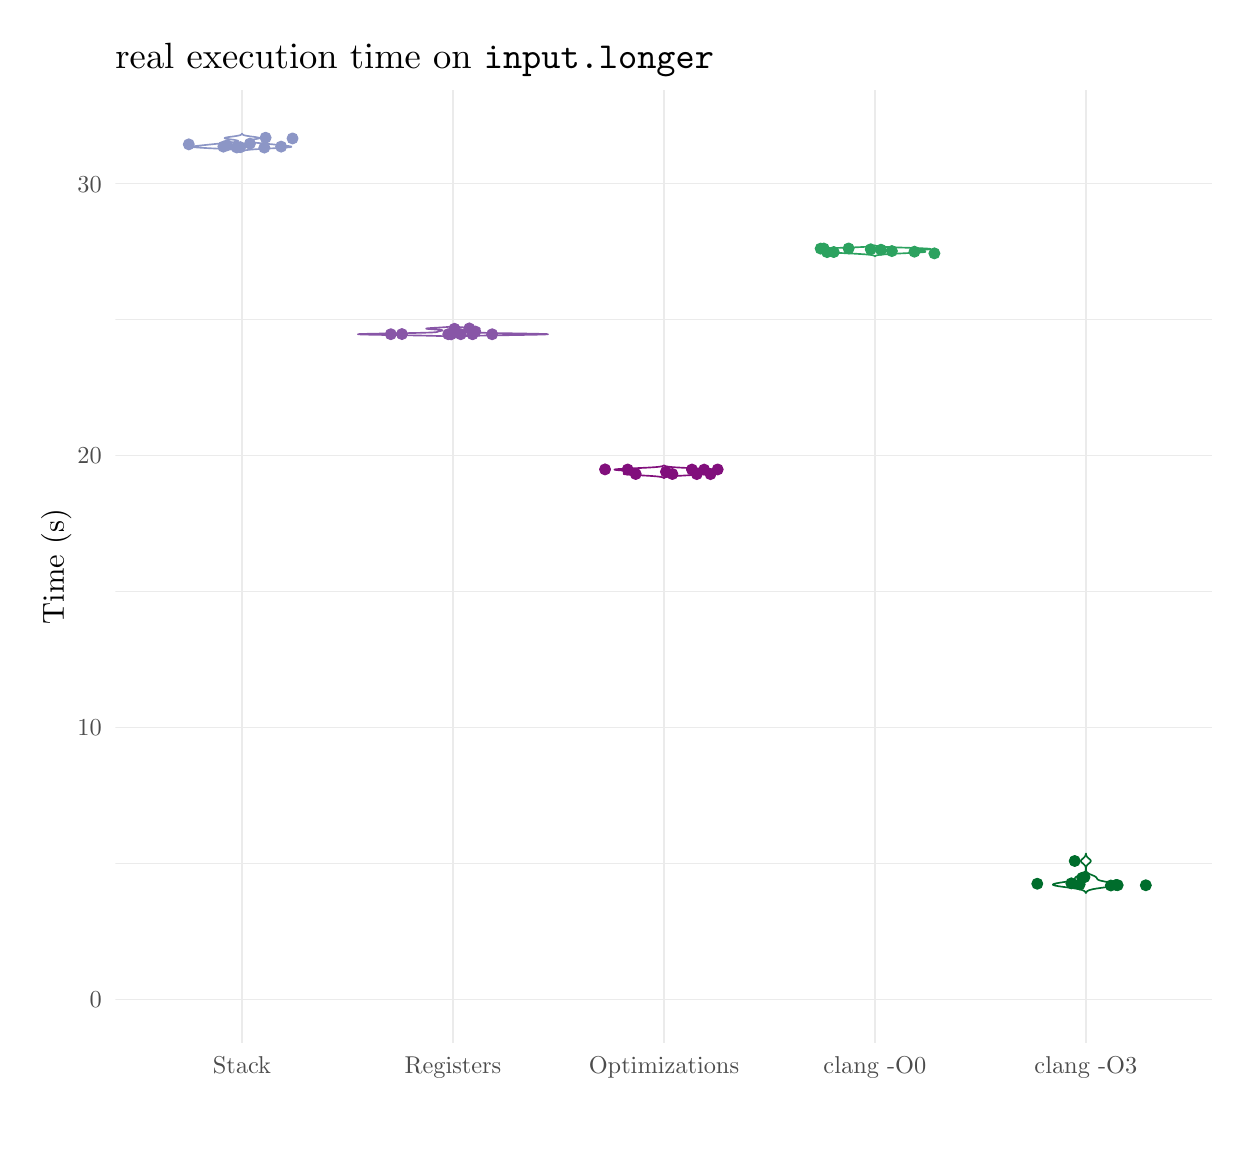
\begin{tikzpicture}[x=1pt,y=1pt]
\definecolor{fillColor}{RGB}{255,255,255}
\path[use as bounding box,fill=fillColor,fill opacity=0.00] (0,0) rectangle (433.62,397.48);
\begin{scope}
\path[clip] ( 31.71, 30.69) rectangle (428.12,374.83);
\definecolor{drawColor}{gray}{0.92}

\path[draw=drawColor,line width= 0.3pt,line join=round] ( 31.71, 95.46) --
	(428.12, 95.46);

\path[draw=drawColor,line width= 0.3pt,line join=round] ( 31.71,193.73) --
	(428.12,193.73);

\path[draw=drawColor,line width= 0.3pt,line join=round] ( 31.71,291.99) --
	(428.12,291.99);

\path[draw=drawColor,line width= 0.6pt,line join=round] ( 31.71, 46.33) --
	(428.12, 46.33);

\path[draw=drawColor,line width= 0.6pt,line join=round] ( 31.71,144.59) --
	(428.12,144.59);

\path[draw=drawColor,line width= 0.6pt,line join=round] ( 31.71,242.86) --
	(428.12,242.86);

\path[draw=drawColor,line width= 0.6pt,line join=round] ( 31.71,341.13) --
	(428.12,341.13);

\path[draw=drawColor,line width= 0.6pt,line join=round] ( 77.45, 30.69) --
	( 77.45,374.83);

\path[draw=drawColor,line width= 0.6pt,line join=round] (153.68, 30.69) --
	(153.68,374.83);

\path[draw=drawColor,line width= 0.6pt,line join=round] (229.92, 30.69) --
	(229.92,374.83);

\path[draw=drawColor,line width= 0.6pt,line join=round] (306.15, 30.69) --
	(306.15,374.83);

\path[draw=drawColor,line width= 0.6pt,line join=round] (382.38, 30.69) --
	(382.38,374.83);
\definecolor{drawColor}{RGB}{140,150,198}
\definecolor{fillColor}{RGB}{255,255,255}

\path[draw=drawColor,line width= 0.6pt,line join=round,line cap=round,fill=fillColor] ( 77.36,352.68) --
	( 77.36,352.69) --
	( 77.35,352.70) --
	( 77.34,352.71) --
	( 77.33,352.73) --
	( 77.32,352.74) --
	( 77.31,352.75) --
	( 77.30,352.77) --
	( 77.29,352.78) --
	( 77.27,352.79) --
	( 77.26,352.80) --
	( 77.25,352.82) --
	( 77.23,352.83) --
	( 77.21,352.84) --
	( 77.20,352.85) --
	( 77.18,352.87) --
	( 77.16,352.88) --
	( 77.13,352.89) --
	( 77.11,352.91) --
	( 77.09,352.92) --
	( 77.06,352.93) --
	( 77.03,352.94) --
	( 77.01,352.96) --
	( 76.97,352.97) --
	( 76.94,352.98) --
	( 76.91,352.99) --
	( 76.87,353.01) --
	( 76.83,353.02) --
	( 76.79,353.03) --
	( 76.75,353.05) --
	( 76.70,353.06) --
	( 76.66,353.07) --
	( 76.61,353.08) --
	( 76.55,353.10) --
	( 76.50,353.11) --
	( 76.44,353.12) --
	( 76.38,353.13) --
	( 76.32,353.15) --
	( 76.25,353.16) --
	( 76.18,353.17) --
	( 76.11,353.19) --
	( 76.03,353.20) --
	( 75.95,353.21) --
	( 75.87,353.22) --
	( 75.78,353.24) --
	( 75.69,353.25) --
	( 75.60,353.26) --
	( 75.50,353.27) --
	( 75.40,353.29) --
	( 75.29,353.30) --
	( 75.18,353.31) --
	( 75.07,353.33) --
	( 74.95,353.34) --
	( 74.83,353.35) --
	( 74.70,353.36) --
	( 74.57,353.38) --
	( 74.44,353.39) --
	( 74.30,353.40) --
	( 74.15,353.41) --
	( 74.00,353.43) --
	( 73.85,353.44) --
	( 73.69,353.45) --
	( 73.53,353.47) --
	( 73.36,353.48) --
	( 73.19,353.49) --
	( 73.02,353.50) --
	( 72.84,353.52) --
	( 72.66,353.53) --
	( 72.47,353.54) --
	( 72.27,353.55) --
	( 72.08,353.57) --
	( 71.88,353.58) --
	( 71.67,353.59) --
	( 71.46,353.61) --
	( 71.25,353.62) --
	( 71.04,353.63) --
	( 70.82,353.64) --
	( 70.59,353.66) --
	( 70.37,353.67) --
	( 70.14,353.68) --
	( 69.91,353.69) --
	( 69.67,353.71) --
	( 69.44,353.72) --
	( 69.20,353.73) --
	( 68.95,353.75) --
	( 68.71,353.76) --
	( 68.46,353.77) --
	( 68.22,353.78) --
	( 67.97,353.80) --
	( 67.72,353.81) --
	( 67.47,353.82) --
	( 67.22,353.84) --
	( 66.97,353.85) --
	( 66.72,353.86) --
	( 66.47,353.87) --
	( 66.22,353.89) --
	( 65.97,353.90) --
	( 65.73,353.91) --
	( 65.48,353.92) --
	( 65.24,353.94) --
	( 65.00,353.95) --
	( 64.76,353.96) --
	( 64.52,353.98) --
	( 64.29,353.99) --
	( 64.06,354.00) --
	( 63.83,354.01) --
	( 63.61,354.03) --
	( 63.39,354.04) --
	( 63.17,354.05) --
	( 62.96,354.06) --
	( 62.76,354.08) --
	( 62.56,354.09) --
	( 62.36,354.10) --
	( 62.17,354.12) --
	( 61.99,354.13) --
	( 61.81,354.14) --
	( 61.64,354.15) --
	( 61.47,354.17) --
	( 61.31,354.18) --
	( 61.16,354.19) --
	( 61.01,354.20) --
	( 60.87,354.22) --
	( 60.74,354.23) --
	( 60.62,354.24) --
	( 60.50,354.26) --
	( 60.39,354.27) --
	( 60.29,354.28) --
	( 60.19,354.29) --
	( 60.10,354.31) --
	( 60.02,354.32) --
	( 59.95,354.33) --
	( 59.88,354.34) --
	( 59.83,354.36) --
	( 59.77,354.37) --
	( 59.73,354.38) --
	( 59.70,354.40) --
	( 59.66,354.41) --
	( 59.65,354.42) --
	( 59.63,354.43) --
	( 59.62,354.45) --
	( 59.62,354.46) --
	( 59.63,354.47) --
	( 59.64,354.48) --
	( 59.66,354.50) --
	( 59.68,354.51) --
	( 59.72,354.52) --
	( 59.75,354.54) --
	( 59.80,354.55) --
	( 59.84,354.56) --
	( 59.90,354.57) --
	( 59.96,354.59) --
	( 60.02,354.60) --
	( 60.09,354.61) --
	( 60.16,354.62) --
	( 60.24,354.64) --
	( 60.32,354.65) --
	( 60.41,354.66) --
	( 60.49,354.68) --
	( 60.59,354.69) --
	( 60.68,354.70) --
	( 60.78,354.71) --
	( 60.88,354.73) --
	( 60.99,354.74) --
	( 61.09,354.75) --
	( 61.20,354.76) --
	( 61.31,354.78) --
	( 61.42,354.79) --
	( 61.54,354.80) --
	( 61.65,354.82) --
	( 61.77,354.83) --
	( 61.89,354.84) --
	( 62.01,354.85) --
	( 62.13,354.87) --
	( 62.25,354.88) --
	( 62.37,354.89) --
	( 62.49,354.91) --
	( 62.61,354.92) --
	( 62.74,354.93) --
	( 62.86,354.94) --
	( 62.98,354.96) --
	( 63.10,354.97) --
	( 63.23,354.98) --
	( 63.35,354.99) --
	( 63.47,355.01) --
	( 63.60,355.02) --
	( 63.72,355.03) --
	( 63.84,355.05) --
	( 63.96,355.06) --
	( 64.08,355.07) --
	( 64.21,355.08) --
	( 64.33,355.10) --
	( 64.45,355.11) --
	( 64.57,355.12) --
	( 64.69,355.13) --
	( 64.81,355.15) --
	( 64.93,355.16) --
	( 65.05,355.17) --
	( 65.17,355.19) --
	( 65.29,355.20) --
	( 65.42,355.21) --
	( 65.54,355.22) --
	( 65.66,355.24) --
	( 65.78,355.25) --
	( 65.90,355.26) --
	( 66.02,355.27) --
	( 66.14,355.29) --
	( 66.26,355.30) --
	( 66.39,355.31) --
	( 66.51,355.33) --
	( 66.63,355.34) --
	( 66.76,355.35) --
	( 66.88,355.36) --
	( 67.01,355.38) --
	( 67.13,355.39) --
	( 67.26,355.40) --
	( 67.39,355.41) --
	( 67.52,355.43) --
	( 67.64,355.44) --
	( 67.77,355.45) --
	( 67.90,355.47) --
	( 68.03,355.48) --
	( 68.17,355.49) --
	( 68.30,355.50) --
	( 68.43,355.52) --
	( 68.57,355.53) --
	( 68.70,355.54) --
	( 68.84,355.55) --
	( 68.97,355.57) --
	( 69.11,355.58) --
	( 69.25,355.59) --
	( 69.38,355.61) --
	( 69.52,355.62) --
	( 69.66,355.63) --
	( 69.80,355.64) --
	( 69.94,355.66) --
	( 70.08,355.67) --
	( 70.22,355.68) --
	( 70.36,355.69) --
	( 70.50,355.71) --
	( 70.64,355.72) --
	( 70.78,355.73) --
	( 70.92,355.75) --
	( 71.06,355.76) --
	( 71.19,355.77) --
	( 71.33,355.78) --
	( 71.47,355.80) --
	( 71.61,355.81) --
	( 71.75,355.82) --
	( 71.88,355.83) --
	( 72.02,355.85) --
	( 72.15,355.86) --
	( 72.28,355.87) --
	( 72.41,355.89) --
	( 72.55,355.90) --
	( 72.67,355.91) --
	( 72.80,355.92) --
	( 72.93,355.94) --
	( 73.05,355.95) --
	( 73.18,355.96) --
	( 73.30,355.98) --
	( 73.42,355.99) --
	( 73.54,356.00) --
	( 73.65,356.01) --
	( 73.76,356.03) --
	( 73.88,356.04) --
	( 73.98,356.05) --
	( 74.09,356.06) --
	( 74.20,356.08) --
	( 74.30,356.09) --
	( 74.40,356.10) --
	( 74.49,356.12) --
	( 74.59,356.13) --
	( 74.68,356.14) --
	( 74.77,356.15) --
	( 74.86,356.17) --
	( 74.94,356.18) --
	( 75.02,356.19) --
	( 75.10,356.20) --
	( 75.17,356.22) --
	( 75.25,356.23) --
	( 75.32,356.24) --
	( 75.38,356.26) --
	( 75.45,356.27) --
	( 75.50,356.28) --
	( 75.56,356.29) --
	( 75.62,356.31) --
	( 75.67,356.32) --
	( 75.72,356.33) --
	( 75.76,356.34) --
	( 75.80,356.36) --
	( 75.84,356.37) --
	( 75.88,356.38) --
	( 75.91,356.40) --
	( 75.94,356.41) --
	( 75.96,356.42) --
	( 75.99,356.43) --
	( 76.01,356.45) --
	( 76.02,356.46) --
	( 76.04,356.47) --
	( 76.04,356.48) --
	( 76.05,356.50) --
	( 76.06,356.51) --
	( 76.06,356.52) --
	( 76.05,356.54) --
	( 76.05,356.55) --
	( 76.04,356.56) --
	( 76.03,356.57) --
	( 76.01,356.59) --
	( 76.00,356.60) --
	( 75.98,356.61) --
	( 75.95,356.62) --
	( 75.93,356.64) --
	( 75.90,356.65) --
	( 75.86,356.66) --
	( 75.83,356.68) --
	( 75.79,356.69) --
	( 75.75,356.70) --
	( 75.70,356.71) --
	( 75.66,356.73) --
	( 75.61,356.74) --
	( 75.56,356.75) --
	( 75.50,356.76) --
	( 75.45,356.78) --
	( 75.39,356.79) --
	( 75.33,356.80) --
	( 75.26,356.82) --
	( 75.19,356.83) --
	( 75.13,356.84) --
	( 75.06,356.85) --
	( 74.98,356.87) --
	( 74.91,356.88) --
	( 74.83,356.89) --
	( 74.75,356.90) --
	( 74.67,356.92) --
	( 74.59,356.93) --
	( 74.51,356.94) --
	( 74.43,356.96) --
	( 74.34,356.97) --
	( 74.25,356.98) --
	( 74.16,356.99) --
	( 74.08,357.01) --
	( 73.99,357.02) --
	( 73.89,357.03) --
	( 73.80,357.04) --
	( 73.71,357.06) --
	( 73.62,357.07) --
	( 73.53,357.08) --
	( 73.43,357.10) --
	( 73.34,357.11) --
	( 73.25,357.12) --
	( 73.16,357.13) --
	( 73.07,357.15) --
	( 72.98,357.16) --
	( 72.89,357.17) --
	( 72.80,357.19) --
	( 72.71,357.20) --
	( 72.62,357.21) --
	( 72.54,357.22) --
	( 72.45,357.24) --
	( 72.37,357.25) --
	( 72.29,357.26) --
	( 72.21,357.27) --
	( 72.13,357.29) --
	( 72.06,357.30) --
	( 71.99,357.31) --
	( 71.92,357.33) --
	( 71.85,357.34) --
	( 71.78,357.35) --
	( 71.72,357.36) --
	( 71.66,357.38) --
	( 71.61,357.39) --
	( 71.55,357.40) --
	( 71.50,357.41) --
	( 71.46,357.43) --
	( 71.41,357.44) --
	( 71.37,357.45) --
	( 71.34,357.47) --
	( 71.30,357.48) --
	( 71.27,357.49) --
	( 71.25,357.50) --
	( 71.23,357.52) --
	( 71.21,357.53) --
	( 71.20,357.54) --
	( 71.19,357.55) --
	( 71.18,357.57) --
	( 71.18,357.58) --
	( 71.18,357.59) --
	( 71.19,357.61) --
	( 71.19,357.62) --
	( 71.21,357.63) --
	( 71.23,357.64) --
	( 71.25,357.66) --
	( 71.27,357.67) --
	( 71.30,357.68) --
	( 71.33,357.69) --
	( 71.37,357.71) --
	( 71.41,357.72) --
	( 71.45,357.73) --
	( 71.50,357.75) --
	( 71.55,357.76) --
	( 71.60,357.77) --
	( 71.65,357.78) --
	( 71.71,357.80) --
	( 71.78,357.81) --
	( 71.84,357.82) --
	( 71.91,357.83) --
	( 71.98,357.85) --
	( 72.05,357.86) --
	( 72.13,357.87) --
	( 72.20,357.89) --
	( 72.28,357.90) --
	( 72.36,357.91) --
	( 72.45,357.92) --
	( 72.53,357.94) --
	( 72.62,357.95) --
	( 72.71,357.96) --
	( 72.80,357.97) --
	( 72.89,357.99) --
	( 72.98,358.00) --
	( 73.07,358.01) --
	( 73.16,358.03) --
	( 73.26,358.04) --
	( 73.35,358.05) --
	( 73.45,358.06) --
	( 73.54,358.08) --
	( 73.64,358.09) --
	( 73.73,358.10) --
	( 73.83,358.11) --
	( 73.92,358.13) --
	( 74.02,358.14) --
	( 74.11,358.15) --
	( 74.20,358.17) --
	( 74.30,358.18) --
	( 74.39,358.19) --
	( 74.48,358.20) --
	( 74.57,358.22) --
	( 74.66,358.23) --
	( 74.75,358.24) --
	( 74.84,358.26) --
	( 74.92,358.27) --
	( 75.01,358.28) --
	( 75.09,358.29) --
	( 75.17,358.31) --
	( 75.25,358.32) --
	( 75.33,358.33) --
	( 75.41,358.34) --
	( 75.48,358.36) --
	( 75.56,358.37) --
	( 75.63,358.38) --
	( 75.70,358.40) --
	( 75.77,358.41) --
	( 75.84,358.42) --
	( 75.91,358.43) --
	( 75.97,358.45) --
	( 76.03,358.46) --
	( 76.09,358.47) --
	( 76.15,358.48) --
	( 76.21,358.50) --
	( 76.26,358.51) --
	( 76.32,358.52) --
	( 76.37,358.54) --
	( 76.42,358.55) --
	( 76.47,358.56) --
	( 76.51,358.57) --
	( 76.56,358.59) --
	( 76.60,358.60) --
	( 76.64,358.61) --
	( 76.68,358.62) --
	( 76.72,358.64) --
	( 76.76,358.65) --
	( 76.80,358.66) --
	( 76.83,358.68) --
	( 76.86,358.69) --
	( 76.89,358.70) --
	( 76.92,358.71) --
	( 76.95,358.73) --
	( 76.98,358.74) --
	( 77.01,358.75) --
	( 77.03,358.76) --
	( 77.06,358.78) --
	( 77.08,358.79) --
	( 77.10,358.80) --
	( 77.12,358.82) --
	( 77.14,358.83) --
	( 77.16,358.84) --
	( 77.18,358.85) --
	( 77.19,358.87) --
	( 77.21,358.88) --
	( 77.23,358.89) --
	( 77.24,358.90) --
	( 77.25,358.92) --
	( 77.27,358.93) --
	( 77.28,358.94) --
	( 77.29,358.96) --
	( 77.30,358.97) --
	( 77.31,358.98) --
	( 77.32,358.99) --
	( 77.33,359.01) --
	( 77.34,359.02) --
	( 77.35,359.03) --
	( 77.35,359.04) --
	( 77.36,359.06) --
	( 77.37,359.07) --
	( 77.37,359.08) --
	( 77.38,359.10) --
	( 77.38,359.11) --
	( 77.39,359.12) --
	( 77.39,359.13) --
	( 77.40,359.15) --
	( 77.40,359.16) --
	( 77.41,359.17) --
	( 77.41,359.18) --
	( 77.49,359.18) --
	( 77.50,359.17) --
	( 77.50,359.16) --
	( 77.51,359.15) --
	( 77.51,359.13) --
	( 77.51,359.12) --
	( 77.52,359.11) --
	( 77.53,359.10) --
	( 77.53,359.08) --
	( 77.54,359.07) --
	( 77.54,359.06) --
	( 77.55,359.04) --
	( 77.56,359.03) --
	( 77.57,359.02) --
	( 77.57,359.01) --
	( 77.58,358.99) --
	( 77.59,358.98) --
	( 77.60,358.97) --
	( 77.61,358.96) --
	( 77.62,358.94) --
	( 77.64,358.93) --
	( 77.65,358.92) --
	( 77.66,358.90) --
	( 77.68,358.89) --
	( 77.69,358.88) --
	( 77.71,358.87) --
	( 77.73,358.85) --
	( 77.74,358.84) --
	( 77.76,358.83) --
	( 77.78,358.82) --
	( 77.80,358.80) --
	( 77.82,358.79) --
	( 77.85,358.78) --
	( 77.87,358.76) --
	( 77.90,358.75) --
	( 77.92,358.74) --
	( 77.95,358.73) --
	( 77.98,358.71) --
	( 78.01,358.70) --
	( 78.04,358.69) --
	( 78.07,358.68) --
	( 78.11,358.66) --
	( 78.14,358.65) --
	( 78.18,358.64) --
	( 78.22,358.62) --
	( 78.26,358.61) --
	( 78.30,358.60) --
	( 78.34,358.59) --
	( 78.39,358.57) --
	( 78.44,358.56) --
	( 78.48,358.55) --
	( 78.53,358.54) --
	( 78.59,358.52) --
	( 78.64,358.51) --
	( 78.70,358.50) --
	( 78.75,358.48) --
	( 78.81,358.47) --
	( 78.87,358.46) --
	( 78.93,358.45) --
	( 79.00,358.43) --
	( 79.06,358.42) --
	( 79.13,358.41) --
	( 79.20,358.40) --
	( 79.27,358.38) --
	( 79.34,358.37) --
	( 79.42,358.36) --
	( 79.49,358.34) --
	( 79.57,358.33) --
	( 79.65,358.32) --
	( 79.73,358.31) --
	( 79.81,358.29) --
	( 79.90,358.28) --
	( 79.98,358.27) --
	( 80.07,358.26) --
	( 80.15,358.24) --
	( 80.24,358.23) --
	( 80.33,358.22) --
	( 80.42,358.20) --
	( 80.51,358.19) --
	( 80.61,358.18) --
	( 80.70,358.17) --
	( 80.79,358.15) --
	( 80.89,358.14) --
	( 80.98,358.13) --
	( 81.08,358.11) --
	( 81.17,358.10) --
	( 81.27,358.09) --
	( 81.36,358.08) --
	( 81.46,358.06) --
	( 81.55,358.05) --
	( 81.65,358.04) --
	( 81.74,358.03) --
	( 81.83,358.01) --
	( 81.93,358.00) --
	( 82.02,357.99) --
	( 82.11,357.97) --
	( 82.20,357.96) --
	( 82.28,357.95) --
	( 82.37,357.94) --
	( 82.46,357.92) --
	( 82.54,357.91) --
	( 82.62,357.90) --
	( 82.70,357.89) --
	( 82.78,357.87) --
	( 82.85,357.86) --
	( 82.92,357.85) --
	( 82.99,357.83) --
	( 83.06,357.82) --
	( 83.13,357.81) --
	( 83.19,357.80) --
	( 83.25,357.78) --
	( 83.30,357.77) --
	( 83.36,357.76) --
	( 83.41,357.75) --
	( 83.45,357.73) --
	( 83.50,357.72) --
	( 83.53,357.71) --
	( 83.57,357.69) --
	( 83.60,357.68) --
	( 83.63,357.67) --
	( 83.66,357.66) --
	( 83.68,357.64) --
	( 83.69,357.63) --
	( 83.71,357.62) --
	( 83.72,357.61) --
	( 83.72,357.59) --
	( 83.72,357.58) --
	( 83.72,357.57) --
	( 83.72,357.55) --
	( 83.71,357.54) --
	( 83.69,357.53) --
	( 83.67,357.52) --
	( 83.65,357.50) --
	( 83.63,357.49) --
	( 83.60,357.48) --
	( 83.57,357.47) --
	( 83.53,357.45) --
	( 83.49,357.44) --
	( 83.45,357.43) --
	( 83.40,357.41) --
	( 83.35,357.40) --
	( 83.30,357.39) --
	( 83.24,357.38) --
	( 83.18,357.36) --
	( 83.12,357.35) --
	( 83.05,357.34) --
	( 82.99,357.33) --
	( 82.92,357.31) --
	( 82.84,357.30) --
	( 82.77,357.29) --
	( 82.69,357.27) --
	( 82.61,357.26) --
	( 82.53,357.25) --
	( 82.45,357.24) --
	( 82.37,357.22) --
	( 82.28,357.21) --
	( 82.19,357.20) --
	( 82.11,357.19) --
	( 82.02,357.17) --
	( 81.93,357.16) --
	( 81.84,357.15) --
	( 81.74,357.13) --
	( 81.65,357.12) --
	( 81.56,357.11) --
	( 81.47,357.10) --
	( 81.38,357.08) --
	( 81.28,357.07) --
	( 81.19,357.06) --
	( 81.10,357.04) --
	( 81.01,357.03) --
	( 80.92,357.02) --
	( 80.83,357.01) --
	( 80.74,356.99) --
	( 80.65,356.98) --
	( 80.56,356.97) --
	( 80.48,356.96) --
	( 80.39,356.94) --
	( 80.31,356.93) --
	( 80.23,356.92) --
	( 80.15,356.90) --
	( 80.07,356.89) --
	( 79.99,356.88) --
	( 79.92,356.87) --
	( 79.85,356.85) --
	( 79.78,356.84) --
	( 79.71,356.83) --
	( 79.64,356.82) --
	( 79.58,356.80) --
	( 79.52,356.79) --
	( 79.46,356.78) --
	( 79.40,356.76) --
	( 79.35,356.75) --
	( 79.29,356.74) --
	( 79.25,356.73) --
	( 79.20,356.71) --
	( 79.15,356.70) --
	( 79.11,356.69) --
	( 79.08,356.68) --
	( 79.04,356.66) --
	( 79.01,356.65) --
	( 78.98,356.64) --
	( 78.95,356.62) --
	( 78.93,356.61) --
	( 78.91,356.60) --
	( 78.89,356.59) --
	( 78.87,356.57) --
	( 78.86,356.56) --
	( 78.85,356.55) --
	( 78.85,356.54) --
	( 78.85,356.52) --
	( 78.85,356.51) --
	( 78.85,356.50) --
	( 78.86,356.48) --
	( 78.87,356.47) --
	( 78.88,356.46) --
	( 78.90,356.45) --
	( 78.92,356.43) --
	( 78.94,356.42) --
	( 78.97,356.41) --
	( 79.00,356.40) --
	( 79.03,356.38) --
	( 79.06,356.37) --
	( 79.10,356.36) --
	( 79.14,356.34) --
	( 79.19,356.33) --
	( 79.24,356.32) --
	( 79.29,356.31) --
	( 79.34,356.29) --
	( 79.40,356.28) --
	( 79.46,356.27) --
	( 79.52,356.26) --
	( 79.59,356.24) --
	( 79.66,356.23) --
	( 79.73,356.22) --
	( 79.80,356.20) --
	( 79.88,356.19) --
	( 79.96,356.18) --
	( 80.05,356.17) --
	( 80.13,356.15) --
	( 80.22,356.14) --
	( 80.31,356.13) --
	( 80.41,356.12) --
	( 80.51,356.10) --
	( 80.61,356.09) --
	( 80.71,356.08) --
	( 80.81,356.06) --
	( 80.92,356.05) --
	( 81.03,356.04) --
	( 81.14,356.03) --
	( 81.25,356.01) --
	( 81.37,356.00) --
	( 81.49,355.99) --
	( 81.61,355.98) --
	( 81.73,355.96) --
	( 81.85,355.95) --
	( 81.97,355.94) --
	( 82.10,355.92) --
	( 82.23,355.91) --
	( 82.36,355.90) --
	( 82.49,355.89) --
	( 82.62,355.87) --
	( 82.75,355.86) --
	( 82.89,355.85) --
	( 83.02,355.83) --
	( 83.16,355.82) --
	( 83.29,355.81) --
	( 83.43,355.80) --
	( 83.57,355.78) --
	( 83.71,355.77) --
	( 83.85,355.76) --
	( 83.99,355.75) --
	( 84.13,355.73) --
	( 84.27,355.72) --
	( 84.41,355.71) --
	( 84.55,355.69) --
	( 84.69,355.68) --
	( 84.83,355.67) --
	( 84.97,355.66) --
	( 85.10,355.64) --
	( 85.24,355.63) --
	( 85.38,355.62) --
	( 85.52,355.61) --
	( 85.66,355.59) --
	( 85.79,355.58) --
	( 85.93,355.57) --
	( 86.07,355.55) --
	( 86.20,355.54) --
	( 86.34,355.53) --
	( 86.47,355.52) --
	( 86.60,355.50) --
	( 86.74,355.49) --
	( 86.87,355.48) --
	( 87.00,355.47) --
	( 87.13,355.45) --
	( 87.26,355.44) --
	( 87.39,355.43) --
	( 87.52,355.41) --
	( 87.64,355.40) --
	( 87.77,355.39) --
	( 87.90,355.38) --
	( 88.02,355.36) --
	( 88.15,355.35) --
	( 88.27,355.34) --
	( 88.39,355.33) --
	( 88.52,355.31) --
	( 88.64,355.30) --
	( 88.76,355.29) --
	( 88.88,355.27) --
	( 89.00,355.26) --
	( 89.13,355.25) --
	( 89.25,355.24) --
	( 89.37,355.22) --
	( 89.49,355.21) --
	( 89.61,355.20) --
	( 89.73,355.19) --
	( 89.85,355.17) --
	( 89.97,355.16) --
	( 90.09,355.15) --
	( 90.21,355.13) --
	( 90.33,355.12) --
	( 90.45,355.11) --
	( 90.58,355.10) --
	( 90.70,355.08) --
	( 90.82,355.07) --
	( 90.94,355.06) --
	( 91.06,355.05) --
	( 91.19,355.03) --
	( 91.31,355.02) --
	( 91.43,355.01) --
	( 91.55,354.99) --
	( 91.68,354.98) --
	( 91.80,354.97) --
	( 91.92,354.96) --
	( 92.04,354.94) --
	( 92.17,354.93) --
	( 92.29,354.92) --
	( 92.41,354.91) --
	( 92.53,354.89) --
	( 92.66,354.88) --
	( 92.78,354.87) --
	( 92.90,354.85) --
	( 93.02,354.84) --
	( 93.13,354.83) --
	( 93.25,354.82) --
	( 93.37,354.80) --
	( 93.48,354.79) --
	( 93.59,354.78) --
	( 93.70,354.76) --
	( 93.81,354.75) --
	( 93.92,354.74) --
	( 94.02,354.73) --
	( 94.12,354.71) --
	( 94.22,354.70) --
	( 94.32,354.69) --
	( 94.41,354.68) --
	( 94.50,354.66) --
	( 94.58,354.65) --
	( 94.66,354.64) --
	( 94.74,354.62) --
	( 94.81,354.61) --
	( 94.88,354.60) --
	( 94.95,354.59) --
	( 95.01,354.57) --
	( 95.06,354.56) --
	( 95.11,354.55) --
	( 95.15,354.54) --
	( 95.19,354.52) --
	( 95.22,354.51) --
	( 95.24,354.50) --
	( 95.26,354.48) --
	( 95.28,354.47) --
	( 95.28,354.46) --
	( 95.28,354.45) --
	( 95.27,354.43) --
	( 95.26,354.42) --
	( 95.24,354.41) --
	( 95.21,354.40) --
	( 95.17,354.38) --
	( 95.13,354.37) --
	( 95.08,354.36) --
	( 95.02,354.34) --
	( 94.96,354.33) --
	( 94.88,354.32) --
	( 94.80,354.31) --
	( 94.71,354.29) --
	( 94.62,354.28) --
	( 94.52,354.27) --
	( 94.40,354.26) --
	( 94.29,354.24) --
	( 94.16,354.23) --
	( 94.03,354.22) --
	( 93.89,354.20) --
	( 93.74,354.19) --
	( 93.59,354.18) --
	( 93.43,354.17) --
	( 93.27,354.15) --
	( 93.10,354.14) --
	( 92.92,354.13) --
	( 92.73,354.12) --
	( 92.54,354.10) --
	( 92.35,354.09) --
	( 92.15,354.08) --
	( 91.94,354.06) --
	( 91.73,354.05) --
	( 91.52,354.04) --
	( 91.30,354.03) --
	( 91.07,354.01) --
	( 90.85,354.00) --
	( 90.62,353.99) --
	( 90.38,353.98) --
	( 90.15,353.96) --
	( 89.91,353.95) --
	( 89.66,353.94) --
	( 89.42,353.92) --
	( 89.18,353.91) --
	( 88.93,353.90) --
	( 88.68,353.89) --
	( 88.43,353.87) --
	( 88.18,353.86) --
	( 87.93,353.85) --
	( 87.68,353.84) --
	( 87.43,353.82) --
	( 87.18,353.81) --
	( 86.93,353.80) --
	( 86.68,353.78) --
	( 86.44,353.77) --
	( 86.19,353.76) --
	( 85.95,353.75) --
	( 85.71,353.73) --
	( 85.47,353.72) --
	( 85.23,353.71) --
	( 85.00,353.69) --
	( 84.76,353.68) --
	( 84.54,353.67) --
	( 84.31,353.66) --
	( 84.09,353.64) --
	( 83.87,353.63) --
	( 83.65,353.62) --
	( 83.44,353.61) --
	( 83.23,353.59) --
	( 83.03,353.58) --
	( 82.83,353.57) --
	( 82.63,353.55) --
	( 82.44,353.54) --
	( 82.25,353.53) --
	( 82.06,353.52) --
	( 81.88,353.50) --
	( 81.71,353.49) --
	( 81.54,353.48) --
	( 81.37,353.47) --
	( 81.21,353.45) --
	( 81.05,353.44) --
	( 80.90,353.43) --
	( 80.75,353.41) --
	( 80.61,353.40) --
	( 80.47,353.39) --
	( 80.33,353.38) --
	( 80.20,353.36) --
	( 80.08,353.35) --
	( 79.95,353.34) --
	( 79.83,353.33) --
	( 79.72,353.31) --
	( 79.61,353.30) --
	( 79.50,353.29) --
	( 79.40,353.27) --
	( 79.31,353.26) --
	( 79.21,353.25) --
	( 79.12,353.24) --
	( 79.03,353.22) --
	( 78.95,353.21) --
	( 78.87,353.20) --
	( 78.79,353.19) --
	( 78.72,353.17) --
	( 78.65,353.16) --
	( 78.59,353.15) --
	( 78.52,353.13) --
	( 78.46,353.12) --
	( 78.40,353.11) --
	( 78.35,353.10) --
	( 78.30,353.08) --
	( 78.25,353.07) --
	( 78.20,353.06) --
	( 78.15,353.05) --
	( 78.11,353.03) --
	( 78.07,353.02) --
	( 78.03,353.01) --
	( 78.00,352.99) --
	( 77.96,352.98) --
	( 77.93,352.97) --
	( 77.90,352.96) --
	( 77.87,352.94) --
	( 77.84,352.93) --
	( 77.82,352.92) --
	( 77.79,352.91) --
	( 77.77,352.89) --
	( 77.75,352.88) --
	( 77.73,352.87) --
	( 77.71,352.85) --
	( 77.69,352.84) --
	( 77.67,352.83) --
	( 77.66,352.82) --
	( 77.64,352.80) --
	( 77.63,352.79) --
	( 77.62,352.78) --
	( 77.60,352.77) --
	( 77.59,352.75) --
	( 77.58,352.74) --
	( 77.57,352.73) --
	( 77.56,352.71) --
	( 77.55,352.70) --
	( 77.55,352.69) --
	( 77.54,352.68) --
	( 77.36,352.68) --
	cycle;
\definecolor{drawColor}{RGB}{136,86,167}

\path[draw=drawColor,line width= 0.6pt,line join=round,line cap=round,fill=fillColor] (153.39,285.69) --
	(153.37,285.70) --
	(153.34,285.71) --
	(153.32,285.72) --
	(153.29,285.73) --
	(153.26,285.73) --
	(153.23,285.74) --
	(153.19,285.75) --
	(153.16,285.76) --
	(153.12,285.77) --
	(153.08,285.77) --
	(153.04,285.78) --
	(152.99,285.79) --
	(152.94,285.80) --
	(152.89,285.80) --
	(152.83,285.81) --
	(152.77,285.82) --
	(152.71,285.83) --
	(152.65,285.84) --
	(152.58,285.84) --
	(152.51,285.85) --
	(152.43,285.86) --
	(152.35,285.87) --
	(152.26,285.88) --
	(152.17,285.88) --
	(152.08,285.89) --
	(151.98,285.90) --
	(151.87,285.91) --
	(151.76,285.92) --
	(151.65,285.92) --
	(151.52,285.93) --
	(151.40,285.94) --
	(151.26,285.95) --
	(151.12,285.96) --
	(150.98,285.96) --
	(150.83,285.97) --
	(150.67,285.98) --
	(150.50,285.99) --
	(150.33,286.00) --
	(150.15,286.00) --
	(149.96,286.01) --
	(149.76,286.02) --
	(149.56,286.03) --
	(149.34,286.04) --
	(149.12,286.04) --
	(148.90,286.05) --
	(148.66,286.06) --
	(148.42,286.07) --
	(148.16,286.08) --
	(147.90,286.08) --
	(147.63,286.09) --
	(147.34,286.10) --
	(147.06,286.11) --
	(146.76,286.12) --
	(146.45,286.12) --
	(146.13,286.13) --
	(145.81,286.14) --
	(145.47,286.15) --
	(145.13,286.16) --
	(144.77,286.16) --
	(144.41,286.17) --
	(144.04,286.18) --
	(143.66,286.19) --
	(143.27,286.20) --
	(142.87,286.20) --
	(142.47,286.21) --
	(142.05,286.22) --
	(141.63,286.23) --
	(141.20,286.24) --
	(140.76,286.24) --
	(140.31,286.25) --
	(139.86,286.26) --
	(139.40,286.27) --
	(138.94,286.28) --
	(138.46,286.28) --
	(137.99,286.29) --
	(137.50,286.30) --
	(137.02,286.31) --
	(136.53,286.32) --
	(136.03,286.32) --
	(135.53,286.33) --
	(135.03,286.34) --
	(134.52,286.35) --
	(134.02,286.36) --
	(133.51,286.36) --
	(133.00,286.37) --
	(132.49,286.38) --
	(131.98,286.39) --
	(131.47,286.40) --
	(130.97,286.40) --
	(130.47,286.41) --
	(129.97,286.42) --
	(129.47,286.43) --
	(128.98,286.44) --
	(128.49,286.44) --
	(128.01,286.45) --
	(127.54,286.46) --
	(127.07,286.47) --
	(126.61,286.48) --
	(126.16,286.48) --
	(125.72,286.49) --
	(125.28,286.50) --
	(124.86,286.51) --
	(124.46,286.52) --
	(124.05,286.52) --
	(123.67,286.53) --
	(123.30,286.54) --
	(122.94,286.55) --
	(122.60,286.56) --
	(122.26,286.56) --
	(121.95,286.57) --
	(121.66,286.58) --
	(121.37,286.59) --
	(121.11,286.60) --
	(120.86,286.60) --
	(120.63,286.61) --
	(120.42,286.62) --
	(120.23,286.63) --
	(120.06,286.64) --
	(119.90,286.64) --
	(119.77,286.65) --
	(119.65,286.66) --
	(119.55,286.67) --
	(119.48,286.68) --
	(119.43,286.68) --
	(119.39,286.69) --
	(119.38,286.70) --
	(119.38,286.71) --
	(119.41,286.72) --
	(119.46,286.72) --
	(119.52,286.73) --
	(119.61,286.74) --
	(119.71,286.75) --
	(119.84,286.76) --
	(119.99,286.76) --
	(120.15,286.77) --
	(120.33,286.78) --
	(120.53,286.79) --
	(120.75,286.80) --
	(120.99,286.80) --
	(121.24,286.81) --
	(121.51,286.82) --
	(121.80,286.83) --
	(122.10,286.84) --
	(122.42,286.84) --
	(122.74,286.85) --
	(123.09,286.86) --
	(123.45,286.87) --
	(123.82,286.88) --
	(124.20,286.88) --
	(124.60,286.89) --
	(125.00,286.90) --
	(125.42,286.91) --
	(125.84,286.92) --
	(126.27,286.92) --
	(126.71,286.93) --
	(127.16,286.94) --
	(127.61,286.95) --
	(128.07,286.96) --
	(128.54,286.96) --
	(129.00,286.97) --
	(129.48,286.98) --
	(129.95,286.99) --
	(130.43,287.00) --
	(130.91,287.00) --
	(131.38,287.01) --
	(131.86,287.02) --
	(132.34,287.03) --
	(132.82,287.03) --
	(133.29,287.04) --
	(133.77,287.05) --
	(134.24,287.06) --
	(134.70,287.07) --
	(135.16,287.07) --
	(135.62,287.08) --
	(136.07,287.09) --
	(136.52,287.10) --
	(136.96,287.11) --
	(137.39,287.11) --
	(137.82,287.12) --
	(138.24,287.13) --
	(138.65,287.14) --
	(139.05,287.15) --
	(139.45,287.15) --
	(139.84,287.16) --
	(140.21,287.17) --
	(140.58,287.18) --
	(140.94,287.19) --
	(141.29,287.19) --
	(141.63,287.20) --
	(141.96,287.21) --
	(142.28,287.22) --
	(142.59,287.23) --
	(142.89,287.23) --
	(143.18,287.24) --
	(143.46,287.25) --
	(143.73,287.26) --
	(143.99,287.27) --
	(144.24,287.27) --
	(144.48,287.28) --
	(144.71,287.29) --
	(144.93,287.30) --
	(145.14,287.31) --
	(145.34,287.31) --
	(145.54,287.32) --
	(145.72,287.33) --
	(145.89,287.34) --
	(146.06,287.35) --
	(146.21,287.35) --
	(146.36,287.36) --
	(146.50,287.37) --
	(146.63,287.38) --
	(146.75,287.39) --
	(146.87,287.39) --
	(146.98,287.40) --
	(147.08,287.41) --
	(147.18,287.42) --
	(147.27,287.43) --
	(147.35,287.43) --
	(147.43,287.44) --
	(147.50,287.45) --
	(147.56,287.46) --
	(147.63,287.47) --
	(147.68,287.47) --
	(147.73,287.48) --
	(147.78,287.49) --
	(147.83,287.50) --
	(147.87,287.51) --
	(147.90,287.51) --
	(147.94,287.52) --
	(147.97,287.53) --
	(148.00,287.54) --
	(148.03,287.55) --
	(148.05,287.55) --
	(148.07,287.56) --
	(148.10,287.57) --
	(148.12,287.58) --
	(148.13,287.59) --
	(148.15,287.59) --
	(148.17,287.60) --
	(148.19,287.61) --
	(148.20,287.62) --
	(148.22,287.63) --
	(148.24,287.63) --
	(148.25,287.64) --
	(148.27,287.65) --
	(148.29,287.66) --
	(148.31,287.67) --
	(148.32,287.67) --
	(148.34,287.68) --
	(148.36,287.69) --
	(148.38,287.70) --
	(148.41,287.71) --
	(148.43,287.71) --
	(148.45,287.72) --
	(148.48,287.73) --
	(148.51,287.74) --
	(148.53,287.75) --
	(148.56,287.75) --
	(148.59,287.76) --
	(148.62,287.77) --
	(148.66,287.78) --
	(148.69,287.79) --
	(148.73,287.79) --
	(148.76,287.80) --
	(148.80,287.81) --
	(148.84,287.82) --
	(148.87,287.83) --
	(148.91,287.83) --
	(148.95,287.84) --
	(149.00,287.85) --
	(149.04,287.86) --
	(149.08,287.87) --
	(149.12,287.87) --
	(149.16,287.88) --
	(149.21,287.89) --
	(149.25,287.90) --
	(149.29,287.91) --
	(149.33,287.91) --
	(149.37,287.92) --
	(149.42,287.93) --
	(149.46,287.94) --
	(149.50,287.95) --
	(149.54,287.95) --
	(149.57,287.96) --
	(149.61,287.97) --
	(149.65,287.98) --
	(149.68,287.99) --
	(149.71,287.99) --
	(149.75,288.00) --
	(149.77,288.01) --
	(149.80,288.02) --
	(149.83,288.03) --
	(149.85,288.03) --
	(149.87,288.04) --
	(149.89,288.05) --
	(149.90,288.06) --
	(149.92,288.07) --
	(149.93,288.07) --
	(149.93,288.08) --
	(149.94,288.09) --
	(149.94,288.10) --
	(149.94,288.11) --
	(149.93,288.11) --
	(149.92,288.12) --
	(149.91,288.13) --
	(149.89,288.14) --
	(149.87,288.15) --
	(149.85,288.15) --
	(149.83,288.16) --
	(149.79,288.17) --
	(149.76,288.18) --
	(149.72,288.19) --
	(149.68,288.19) --
	(149.64,288.20) --
	(149.59,288.21) --
	(149.54,288.22) --
	(149.48,288.22) --
	(149.42,288.23) --
	(149.36,288.24) --
	(149.29,288.25) --
	(149.22,288.26) --
	(149.15,288.26) --
	(149.07,288.27) --
	(148.99,288.28) --
	(148.91,288.29) --
	(148.82,288.30) --
	(148.73,288.30) --
	(148.64,288.31) --
	(148.54,288.32) --
	(148.44,288.33) --
	(148.34,288.34) --
	(148.24,288.34) --
	(148.13,288.35) --
	(148.02,288.36) --
	(147.91,288.37) --
	(147.80,288.38) --
	(147.69,288.38) --
	(147.57,288.39) --
	(147.46,288.40) --
	(147.34,288.41) --
	(147.22,288.42) --
	(147.10,288.42) --
	(146.99,288.43) --
	(146.87,288.44) --
	(146.75,288.45) --
	(146.63,288.46) --
	(146.51,288.46) --
	(146.39,288.47) --
	(146.27,288.48) --
	(146.15,288.49) --
	(146.04,288.50) --
	(145.92,288.50) --
	(145.81,288.51) --
	(145.70,288.52) --
	(145.59,288.53) --
	(145.48,288.54) --
	(145.38,288.54) --
	(145.27,288.55) --
	(145.18,288.56) --
	(145.08,288.57) --
	(144.99,288.58) --
	(144.90,288.58) --
	(144.81,288.59) --
	(144.73,288.60) --
	(144.65,288.61) --
	(144.57,288.62) --
	(144.50,288.62) --
	(144.44,288.63) --
	(144.38,288.64) --
	(144.32,288.65) --
	(144.27,288.66) --
	(144.22,288.66) --
	(144.18,288.67) --
	(144.14,288.68) --
	(144.11,288.69) --
	(144.08,288.70) --
	(144.06,288.70) --
	(144.04,288.71) --
	(144.03,288.72) --
	(144.02,288.73) --
	(144.02,288.74) --
	(144.03,288.74) --
	(144.04,288.75) --
	(144.05,288.76) --
	(144.08,288.77) --
	(144.10,288.78) --
	(144.13,288.78) --
	(144.17,288.79) --
	(144.21,288.80) --
	(144.26,288.81) --
	(144.31,288.82) --
	(144.37,288.82) --
	(144.43,288.83) --
	(144.50,288.84) --
	(144.57,288.85) --
	(144.65,288.86) --
	(144.73,288.86) --
	(144.82,288.87) --
	(144.91,288.88) --
	(145.00,288.89) --
	(145.10,288.90) --
	(145.20,288.90) --
	(145.31,288.91) --
	(145.42,288.92) --
	(145.53,288.93) --
	(145.64,288.94) --
	(145.76,288.94) --
	(145.88,288.95) --
	(146.01,288.96) --
	(146.13,288.97) --
	(146.26,288.98) --
	(146.39,288.98) --
	(146.52,288.99) --
	(146.66,289.00) --
	(146.79,289.01) --
	(146.93,289.02) --
	(147.07,289.02) --
	(147.21,289.03) --
	(147.35,289.04) --
	(147.49,289.05) --
	(147.63,289.06) --
	(147.77,289.06) --
	(147.91,289.07) --
	(148.05,289.08) --
	(148.19,289.09) --
	(148.33,289.10) --
	(148.47,289.10) --
	(148.61,289.11) --
	(148.75,289.12) --
	(148.88,289.13) --
	(149.02,289.14) --
	(149.15,289.14) --
	(149.29,289.15) --
	(149.42,289.16) --
	(149.55,289.17) --
	(149.68,289.18) --
	(149.81,289.18) --
	(149.93,289.19) --
	(150.05,289.20) --
	(150.17,289.21) --
	(150.29,289.22) --
	(150.41,289.22) --
	(150.53,289.23) --
	(150.64,289.24) --
	(150.75,289.25) --
	(150.86,289.26) --
	(150.96,289.26) --
	(151.07,289.27) --
	(151.17,289.28) --
	(151.26,289.29) --
	(151.36,289.30) --
	(151.45,289.30) --
	(151.54,289.31) --
	(151.63,289.32) --
	(151.72,289.33) --
	(151.80,289.34) --
	(151.88,289.34) --
	(151.96,289.35) --
	(152.04,289.36) --
	(152.11,289.37) --
	(152.18,289.38) --
	(152.25,289.38) --
	(152.32,289.39) --
	(152.38,289.40) --
	(152.44,289.41) --
	(152.50,289.42) --
	(152.56,289.42) --
	(152.61,289.43) --
	(152.67,289.44) --
	(152.72,289.45) --
	(152.77,289.45) --
	(152.81,289.46) --
	(152.86,289.47) --
	(152.90,289.48) --
	(152.94,289.49) --
	(152.98,289.49) --
	(153.02,289.50) --
	(153.06,289.51) --
	(153.09,289.52) --
	(153.12,289.53) --
	(153.16,289.53) --
	(153.19,289.54) --
	(153.21,289.55) --
	(153.24,289.56) --
	(153.27,289.57) --
	(153.29,289.57) --
	(153.32,289.58) --
	(153.34,289.59) --
	(153.36,289.60) --
	(153.38,289.61) --
	(153.40,289.61) --
	(153.42,289.62) --
	(153.43,289.63) --
	(153.45,289.64) --
	(153.46,289.65) --
	(153.48,289.65) --
	(153.49,289.66) --
	(153.50,289.67) --
	(153.52,289.68) --
	(153.53,289.69) --
	(153.54,289.69) --
	(153.55,289.70) --
	(153.56,289.71) --
	(153.57,289.72) --
	(153.57,289.73) --
	(153.58,289.73) --
	(153.59,289.74) --
	(153.60,289.75) --
	(153.60,289.76) --
	(153.61,289.77) --
	(153.61,289.77) --
	(153.75,289.77) --
	(153.76,289.77) --
	(153.77,289.76) --
	(153.77,289.75) --
	(153.78,289.74) --
	(153.79,289.73) --
	(153.79,289.73) --
	(153.80,289.72) --
	(153.81,289.71) --
	(153.82,289.70) --
	(153.83,289.69) --
	(153.84,289.69) --
	(153.85,289.68) --
	(153.86,289.67) --
	(153.88,289.66) --
	(153.89,289.65) --
	(153.90,289.65) --
	(153.92,289.64) --
	(153.94,289.63) --
	(153.95,289.62) --
	(153.97,289.61) --
	(153.99,289.61) --
	(154.01,289.60) --
	(154.03,289.59) --
	(154.05,289.58) --
	(154.08,289.57) --
	(154.10,289.57) --
	(154.13,289.56) --
	(154.15,289.55) --
	(154.18,289.54) --
	(154.21,289.53) --
	(154.24,289.53) --
	(154.28,289.52) --
	(154.31,289.51) --
	(154.35,289.50) --
	(154.38,289.49) --
	(154.42,289.49) --
	(154.47,289.48) --
	(154.51,289.47) --
	(154.55,289.46) --
	(154.60,289.45) --
	(154.65,289.45) --
	(154.70,289.44) --
	(154.75,289.43) --
	(154.81,289.42) --
	(154.87,289.42) --
	(154.93,289.41) --
	(154.99,289.40) --
	(155.05,289.39) --
	(155.12,289.38) --
	(155.19,289.38) --
	(155.26,289.37) --
	(155.33,289.36) --
	(155.41,289.35) --
	(155.49,289.34) --
	(155.57,289.34) --
	(155.65,289.33) --
	(155.74,289.32) --
	(155.82,289.31) --
	(155.92,289.30) --
	(156.01,289.30) --
	(156.10,289.29) --
	(156.20,289.28) --
	(156.30,289.27) --
	(156.41,289.26) --
	(156.51,289.26) --
	(156.62,289.25) --
	(156.73,289.24) --
	(156.84,289.23) --
	(156.96,289.22) --
	(157.07,289.22) --
	(157.19,289.21) --
	(157.31,289.20) --
	(157.44,289.19) --
	(157.56,289.18) --
	(157.69,289.18) --
	(157.82,289.17) --
	(157.95,289.16) --
	(158.08,289.15) --
	(158.21,289.14) --
	(158.35,289.14) --
	(158.48,289.13) --
	(158.62,289.12) --
	(158.76,289.11) --
	(158.90,289.10) --
	(159.04,289.10) --
	(159.18,289.09) --
	(159.32,289.08) --
	(159.46,289.07) --
	(159.60,289.06) --
	(159.74,289.06) --
	(159.88,289.05) --
	(160.02,289.04) --
	(160.16,289.03) --
	(160.30,289.02) --
	(160.44,289.02) --
	(160.57,289.01) --
	(160.71,289.00) --
	(160.84,288.99) --
	(160.98,288.98) --
	(161.11,288.98) --
	(161.23,288.97) --
	(161.36,288.96) --
	(161.48,288.95) --
	(161.61,288.94) --
	(161.72,288.94) --
	(161.84,288.93) --
	(161.95,288.92) --
	(162.06,288.91) --
	(162.17,288.90) --
	(162.27,288.90) --
	(162.37,288.89) --
	(162.46,288.88) --
	(162.55,288.87) --
	(162.64,288.86) --
	(162.72,288.86) --
	(162.79,288.85) --
	(162.87,288.84) --
	(162.93,288.83) --
	(163.00,288.82) --
	(163.05,288.82) --
	(163.11,288.81) --
	(163.16,288.80) --
	(163.20,288.79) --
	(163.23,288.78) --
	(163.27,288.78) --
	(163.29,288.77) --
	(163.31,288.76) --
	(163.33,288.75) --
	(163.34,288.74) --
	(163.35,288.74) --
	(163.34,288.73) --
	(163.34,288.72) --
	(163.33,288.71) --
	(163.31,288.70) --
	(163.29,288.70) --
	(163.26,288.69) --
	(163.23,288.68) --
	(163.19,288.67) --
	(163.15,288.66) --
	(163.10,288.66) --
	(163.05,288.65) --
	(162.99,288.64) --
	(162.93,288.63) --
	(162.86,288.62) --
	(162.79,288.62) --
	(162.72,288.61) --
	(162.64,288.60) --
	(162.56,288.59) --
	(162.47,288.58) --
	(162.38,288.58) --
	(162.29,288.57) --
	(162.19,288.56) --
	(162.09,288.55) --
	(161.99,288.54) --
	(161.89,288.54) --
	(161.78,288.53) --
	(161.67,288.52) --
	(161.56,288.51) --
	(161.45,288.50) --
	(161.33,288.50) --
	(161.21,288.49) --
	(161.10,288.48) --
	(160.98,288.47) --
	(160.86,288.46) --
	(160.74,288.46) --
	(160.62,288.45) --
	(160.50,288.44) --
	(160.38,288.43) --
	(160.26,288.42) --
	(160.14,288.42) --
	(160.03,288.41) --
	(159.91,288.40) --
	(159.79,288.39) --
	(159.68,288.38) --
	(159.57,288.38) --
	(159.45,288.37) --
	(159.34,288.36) --
	(159.24,288.35) --
	(159.13,288.34) --
	(159.03,288.34) --
	(158.93,288.33) --
	(158.83,288.32) --
	(158.73,288.31) --
	(158.64,288.30) --
	(158.55,288.30) --
	(158.46,288.29) --
	(158.38,288.28) --
	(158.30,288.27) --
	(158.22,288.26) --
	(158.15,288.26) --
	(158.08,288.25) --
	(158.01,288.24) --
	(157.95,288.23) --
	(157.89,288.22) --
	(157.83,288.22) --
	(157.78,288.21) --
	(157.73,288.20) --
	(157.69,288.19) --
	(157.64,288.19) --
	(157.61,288.18) --
	(157.57,288.17) --
	(157.54,288.16) --
	(157.52,288.15) --
	(157.49,288.15) --
	(157.47,288.14) --
	(157.46,288.13) --
	(157.45,288.12) --
	(157.44,288.11) --
	(157.43,288.11) --
	(157.43,288.10) --
	(157.43,288.09) --
	(157.43,288.08) --
	(157.44,288.07) --
	(157.45,288.07) --
	(157.46,288.06) --
	(157.48,288.05) --
	(157.50,288.04) --
	(157.52,288.03) --
	(157.54,288.03) --
	(157.57,288.02) --
	(157.59,288.01) --
	(157.62,288.00) --
	(157.65,287.99) --
	(157.69,287.99) --
	(157.72,287.98) --
	(157.76,287.97) --
	(157.79,287.96) --
	(157.83,287.95) --
	(157.87,287.95) --
	(157.91,287.94) --
	(157.95,287.93) --
	(157.99,287.92) --
	(158.03,287.91) --
	(158.08,287.91) --
	(158.12,287.90) --
	(158.16,287.89) --
	(158.20,287.88) --
	(158.25,287.87) --
	(158.29,287.87) --
	(158.33,287.86) --
	(158.37,287.85) --
	(158.41,287.84) --
	(158.45,287.83) --
	(158.49,287.83) --
	(158.53,287.82) --
	(158.57,287.81) --
	(158.61,287.80) --
	(158.64,287.79) --
	(158.68,287.79) --
	(158.71,287.78) --
	(158.74,287.77) --
	(158.77,287.76) --
	(158.81,287.75) --
	(158.83,287.75) --
	(158.86,287.74) --
	(158.89,287.73) --
	(158.91,287.72) --
	(158.94,287.71) --
	(158.96,287.71) --
	(158.98,287.70) --
	(159.00,287.69) --
	(159.02,287.68) --
	(159.04,287.67) --
	(159.06,287.67) --
	(159.08,287.66) --
	(159.10,287.65) --
	(159.11,287.64) --
	(159.13,287.63) --
	(159.15,287.63) --
	(159.16,287.62) --
	(159.18,287.61) --
	(159.20,287.60) --
	(159.22,287.59) --
	(159.23,287.59) --
	(159.25,287.58) --
	(159.27,287.57) --
	(159.29,287.56) --
	(159.32,287.55) --
	(159.34,287.55) --
	(159.37,287.54) --
	(159.40,287.53) --
	(159.43,287.52) --
	(159.46,287.51) --
	(159.50,287.51) --
	(159.54,287.50) --
	(159.59,287.49) --
	(159.63,287.48) --
	(159.69,287.47) --
	(159.74,287.47) --
	(159.80,287.46) --
	(159.87,287.45) --
	(159.94,287.44) --
	(160.02,287.43) --
	(160.10,287.43) --
	(160.19,287.42) --
	(160.29,287.41) --
	(160.39,287.40) --
	(160.50,287.39) --
	(160.61,287.39) --
	(160.74,287.38) --
	(160.87,287.37) --
	(161.01,287.36) --
	(161.16,287.35) --
	(161.31,287.35) --
	(161.48,287.34) --
	(161.65,287.33) --
	(161.83,287.32) --
	(162.02,287.31) --
	(162.22,287.31) --
	(162.44,287.30) --
	(162.66,287.29) --
	(162.88,287.28) --
	(163.13,287.27) --
	(163.38,287.27) --
	(163.63,287.26) --
	(163.91,287.25) --
	(164.18,287.24) --
	(164.48,287.23) --
	(164.78,287.23) --
	(165.08,287.22) --
	(165.41,287.21) --
	(165.74,287.20) --
	(166.08,287.19) --
	(166.43,287.19) --
	(166.78,287.18) --
	(167.16,287.17) --
	(167.53,287.16) --
	(167.92,287.15) --
	(168.31,287.15) --
	(168.72,287.14) --
	(169.13,287.13) --
	(169.55,287.12) --
	(169.97,287.11) --
	(170.41,287.11) --
	(170.85,287.10) --
	(171.30,287.09) --
	(171.75,287.08) --
	(172.20,287.07) --
	(172.67,287.07) --
	(173.13,287.06) --
	(173.60,287.05) --
	(174.07,287.04) --
	(174.55,287.03) --
	(175.03,287.03) --
	(175.50,287.02) --
	(175.98,287.01) --
	(176.46,287.00) --
	(176.94,287.00) --
	(177.42,286.99) --
	(177.89,286.98) --
	(178.36,286.97) --
	(178.83,286.96) --
	(179.30,286.96) --
	(179.75,286.95) --
	(180.21,286.94) --
	(180.66,286.93) --
	(181.09,286.92) --
	(181.53,286.92) --
	(181.95,286.91) --
	(182.37,286.90) --
	(182.77,286.89) --
	(183.16,286.88) --
	(183.55,286.88) --
	(183.92,286.87) --
	(184.28,286.86) --
	(184.62,286.85) --
	(184.95,286.84) --
	(185.27,286.84) --
	(185.57,286.83) --
	(185.86,286.82) --
	(186.13,286.81) --
	(186.38,286.80) --
	(186.62,286.80) --
	(186.84,286.79) --
	(187.03,286.78) --
	(187.22,286.77) --
	(187.38,286.76) --
	(187.53,286.76) --
	(187.66,286.75) --
	(187.76,286.74) --
	(187.85,286.73) --
	(187.91,286.72) --
	(187.96,286.72) --
	(187.99,286.71) --
	(187.99,286.70) --
	(187.98,286.69) --
	(187.94,286.68) --
	(187.88,286.68) --
	(187.81,286.67) --
	(187.71,286.66) --
	(187.60,286.65) --
	(187.47,286.64) --
	(187.31,286.64) --
	(187.14,286.63) --
	(186.94,286.62) --
	(186.73,286.61) --
	(186.51,286.60) --
	(186.26,286.60) --
	(185.99,286.59) --
	(185.71,286.58) --
	(185.41,286.57) --
	(185.10,286.56) --
	(184.77,286.56) --
	(184.43,286.55) --
	(184.07,286.54) --
	(183.70,286.53) --
	(183.31,286.52) --
	(182.91,286.52) --
	(182.50,286.51) --
	(182.08,286.50) --
	(181.65,286.49) --
	(181.21,286.48) --
	(180.76,286.48) --
	(180.30,286.47) --
	(179.83,286.46) --
	(179.36,286.45) --
	(178.88,286.44) --
	(178.39,286.44) --
	(177.90,286.43) --
	(177.40,286.42) --
	(176.90,286.41) --
	(176.40,286.40) --
	(175.89,286.40) --
	(175.39,286.39) --
	(174.88,286.38) --
	(174.37,286.37) --
	(173.86,286.36) --
	(173.35,286.36) --
	(172.85,286.35) --
	(172.34,286.34) --
	(171.84,286.33) --
	(171.34,286.32) --
	(170.84,286.32) --
	(170.35,286.31) --
	(169.86,286.30) --
	(169.38,286.29) --
	(168.90,286.28) --
	(168.43,286.28) --
	(167.97,286.27) --
	(167.51,286.26) --
	(167.05,286.25) --
	(166.61,286.24) --
	(166.17,286.24) --
	(165.74,286.23) --
	(165.32,286.22) --
	(164.90,286.21) --
	(164.50,286.20) --
	(164.10,286.20) --
	(163.71,286.19) --
	(163.33,286.18) --
	(162.96,286.17) --
	(162.60,286.16) --
	(162.24,286.16) --
	(161.90,286.15) --
	(161.56,286.14) --
	(161.23,286.13) --
	(160.92,286.12) --
	(160.61,286.12) --
	(160.31,286.11) --
	(160.02,286.10) --
	(159.74,286.09) --
	(159.47,286.08) --
	(159.21,286.08) --
	(158.95,286.07) --
	(158.71,286.06) --
	(158.47,286.05) --
	(158.24,286.04) --
	(158.02,286.04) --
	(157.81,286.03) --
	(157.61,286.02) --
	(157.41,286.01) --
	(157.22,286.00) --
	(157.04,286.00) --
	(156.87,285.99) --
	(156.70,285.98) --
	(156.54,285.97) --
	(156.39,285.96) --
	(156.24,285.96) --
	(156.10,285.95) --
	(155.97,285.94) --
	(155.84,285.93) --
	(155.72,285.92) --
	(155.61,285.92) --
	(155.50,285.91) --
	(155.39,285.90) --
	(155.29,285.89) --
	(155.20,285.88) --
	(155.11,285.88) --
	(155.02,285.87) --
	(154.94,285.86) --
	(154.86,285.85) --
	(154.79,285.84) --
	(154.72,285.84) --
	(154.66,285.83) --
	(154.59,285.82) --
	(154.54,285.81) --
	(154.48,285.80) --
	(154.43,285.80) --
	(154.38,285.79) --
	(154.33,285.78) --
	(154.29,285.77) --
	(154.25,285.77) --
	(154.21,285.76) --
	(154.17,285.75) --
	(154.14,285.74) --
	(154.11,285.73) --
	(154.08,285.73) --
	(154.05,285.72) --
	(154.02,285.71) --
	(154.00,285.70) --
	(153.98,285.69) --
	(153.39,285.69) --
	cycle;
\definecolor{drawColor}{RGB}{129,15,124}

\path[draw=drawColor,line width= 0.6pt,line join=round,line cap=round,fill=fillColor] (229.78,234.75) --
	(229.78,234.76) --
	(229.77,234.77) --
	(229.76,234.78) --
	(229.75,234.79) --
	(229.74,234.80) --
	(229.73,234.81) --
	(229.72,234.81) --
	(229.71,234.82) --
	(229.70,234.83) --
	(229.69,234.84) --
	(229.67,234.85) --
	(229.66,234.86) --
	(229.65,234.87) --
	(229.63,234.88) --
	(229.62,234.88) --
	(229.60,234.89) --
	(229.58,234.90) --
	(229.56,234.91) --
	(229.55,234.92) --
	(229.53,234.93) --
	(229.51,234.94) --
	(229.49,234.95) --
	(229.46,234.96) --
	(229.44,234.96) --
	(229.42,234.97) --
	(229.39,234.98) --
	(229.37,234.99) --
	(229.34,235.00) --
	(229.31,235.01) --
	(229.28,235.02) --
	(229.25,235.03) --
	(229.22,235.03) --
	(229.19,235.04) --
	(229.16,235.05) --
	(229.12,235.06) --
	(229.08,235.07) --
	(229.05,235.08) --
	(229.01,235.09) --
	(228.97,235.10) --
	(228.92,235.10) --
	(228.88,235.11) --
	(228.83,235.12) --
	(228.79,235.13) --
	(228.74,235.14) --
	(228.69,235.15) --
	(228.64,235.16) --
	(228.58,235.17) --
	(228.53,235.18) --
	(228.47,235.18) --
	(228.41,235.19) --
	(228.35,235.20) --
	(228.29,235.21) --
	(228.22,235.22) --
	(228.16,235.23) --
	(228.09,235.24) --
	(228.02,235.25) --
	(227.95,235.25) --
	(227.87,235.26) --
	(227.80,235.27) --
	(227.72,235.28) --
	(227.64,235.29) --
	(227.55,235.30) --
	(227.47,235.31) --
	(227.38,235.32) --
	(227.29,235.33) --
	(227.20,235.33) --
	(227.11,235.34) --
	(227.01,235.35) --
	(226.91,235.36) --
	(226.81,235.37) --
	(226.71,235.38) --
	(226.61,235.39) --
	(226.50,235.40) --
	(226.39,235.40) --
	(226.28,235.41) --
	(226.16,235.42) --
	(226.05,235.43) --
	(225.93,235.44) --
	(225.81,235.45) --
	(225.69,235.46) --
	(225.56,235.47) --
	(225.44,235.48) --
	(225.31,235.48) --
	(225.18,235.49) --
	(225.05,235.50) --
	(224.91,235.51) --
	(224.78,235.52) --
	(224.64,235.53) --
	(224.50,235.54) --
	(224.36,235.55) --
	(224.21,235.55) --
	(224.07,235.56) --
	(223.92,235.57) --
	(223.77,235.58) --
	(223.62,235.59) --
	(223.47,235.60) --
	(223.32,235.61) --
	(223.17,235.62) --
	(223.01,235.62) --
	(222.86,235.63) --
	(222.70,235.64) --
	(222.54,235.65) --
	(222.39,235.66) --
	(222.23,235.67) --
	(222.07,235.68) --
	(221.91,235.69) --
	(221.75,235.70) --
	(221.58,235.70) --
	(221.42,235.71) --
	(221.26,235.72) --
	(221.10,235.73) --
	(220.94,235.74) --
	(220.78,235.75) --
	(220.62,235.76) --
	(220.46,235.77) --
	(220.30,235.77) --
	(220.14,235.78) --
	(219.98,235.79) --
	(219.82,235.80) --
	(219.67,235.81) --
	(219.51,235.82) --
	(219.36,235.83) --
	(219.20,235.84) --
	(219.05,235.85) --
	(218.90,235.85) --
	(218.76,235.86) --
	(218.61,235.87) --
	(218.47,235.88) --
	(218.32,235.89) --
	(218.18,235.90) --
	(218.05,235.91) --
	(217.91,235.92) --
	(217.78,235.92) --
	(217.65,235.93) --
	(217.52,235.94) --
	(217.40,235.95) --
	(217.28,235.96) --
	(217.16,235.97) --
	(217.04,235.98) --
	(216.93,235.99) --
	(216.82,235.99) --
	(216.72,236.00) --
	(216.61,236.01) --
	(216.52,236.02) --
	(216.42,236.03) --
	(216.33,236.04) --
	(216.24,236.05) --
	(216.16,236.06) --
	(216.08,236.07) --
	(216.00,236.07) --
	(215.93,236.08) --
	(215.86,236.09) --
	(215.80,236.10) --
	(215.74,236.11) --
	(215.68,236.12) --
	(215.63,236.13) --
	(215.59,236.14) --
	(215.54,236.14) --
	(215.50,236.15) --
	(215.47,236.16) --
	(215.44,236.17) --
	(215.41,236.18) --
	(215.39,236.19) --
	(215.37,236.20) --
	(215.36,236.21) --
	(215.35,236.22) --
	(215.34,236.22) --
	(215.34,236.23) --
	(215.35,236.24) --
	(215.35,236.25) --
	(215.36,236.26) --
	(215.38,236.27) --
	(215.40,236.28) --
	(215.42,236.29) --
	(215.45,236.29) --
	(215.47,236.30) --
	(215.51,236.31) --
	(215.54,236.32) --
	(215.59,236.33) --
	(215.63,236.34) --
	(215.67,236.35) --
	(215.72,236.36) --
	(215.78,236.37) --
	(215.83,236.37) --
	(215.89,236.38) --
	(215.95,236.39) --
	(216.02,236.40) --
	(216.08,236.41) --
	(216.15,236.42) --
	(216.22,236.43) --
	(216.30,236.44) --
	(216.37,236.44) --
	(216.45,236.45) --
	(216.53,236.46) --
	(216.61,236.47) --
	(216.69,236.48) --
	(216.77,236.49) --
	(216.86,236.50) --
	(216.95,236.51) --
	(217.03,236.51) --
	(217.12,236.52) --
	(217.21,236.53) --
	(217.30,236.54) --
	(217.39,236.55) --
	(217.48,236.56) --
	(217.57,236.57) --
	(217.66,236.58) --
	(217.75,236.59) --
	(217.84,236.59) --
	(217.93,236.60) --
	(218.02,236.61) --
	(218.11,236.62) --
	(218.20,236.63) --
	(218.29,236.64) --
	(218.37,236.65) --
	(218.46,236.66) --
	(218.55,236.66) --
	(218.63,236.67) --
	(218.71,236.68) --
	(218.79,236.69) --
	(218.87,236.70) --
	(218.95,236.71) --
	(219.02,236.72) --
	(219.10,236.73) --
	(219.17,236.74) --
	(219.24,236.74) --
	(219.31,236.75) --
	(219.37,236.76) --
	(219.44,236.77) --
	(219.50,236.78) --
	(219.55,236.79) --
	(219.61,236.80) --
	(219.66,236.81) --
	(219.71,236.81) --
	(219.76,236.82) --
	(219.80,236.83) --
	(219.84,236.84) --
	(219.88,236.85) --
	(219.92,236.86) --
	(219.95,236.87) --
	(219.97,236.88) --
	(220.00,236.89) --
	(220.02,236.89) --
	(220.04,236.90) --
	(220.05,236.91) --
	(220.07,236.92) --
	(220.07,236.93) --
	(220.08,236.94) --
	(220.08,236.95) --
	(220.08,236.96) --
	(220.07,236.96) --
	(220.06,236.97) --
	(220.05,236.98) --
	(220.03,236.99) --
	(220.01,237.00) --
	(219.98,237.01) --
	(219.95,237.02) --
	(219.92,237.03) --
	(219.88,237.03) --
	(219.85,237.04) --
	(219.80,237.05) --
	(219.76,237.06) --
	(219.70,237.07) --
	(219.65,237.08) --
	(219.59,237.09) --
	(219.53,237.10) --
	(219.47,237.11) --
	(219.40,237.11) --
	(219.33,237.12) --
	(219.25,237.13) --
	(219.18,237.14) --
	(219.10,237.15) --
	(219.01,237.16) --
	(218.92,237.17) --
	(218.83,237.18) --
	(218.74,237.18) --
	(218.64,237.19) --
	(218.55,237.20) --
	(218.44,237.21) --
	(218.34,237.22) --
	(218.23,237.23) --
	(218.12,237.24) --
	(218.01,237.25) --
	(217.90,237.26) --
	(217.78,237.26) --
	(217.66,237.27) --
	(217.54,237.28) --
	(217.42,237.29) --
	(217.30,237.30) --
	(217.17,237.31) --
	(217.05,237.32) --
	(216.92,237.33) --
	(216.79,237.33) --
	(216.66,237.34) --
	(216.53,237.35) --
	(216.40,237.36) --
	(216.26,237.37) --
	(216.13,237.38) --
	(216.00,237.39) --
	(215.86,237.40) --
	(215.73,237.40) --
	(215.60,237.41) --
	(215.46,237.42) --
	(215.33,237.43) --
	(215.20,237.44) --
	(215.07,237.45) --
	(214.94,237.46) --
	(214.81,237.47) --
	(214.68,237.48) --
	(214.55,237.48) --
	(214.42,237.49) --
	(214.30,237.50) --
	(214.18,237.51) --
	(214.06,237.52) --
	(213.94,237.53) --
	(213.82,237.54) --
	(213.71,237.55) --
	(213.60,237.55) --
	(213.49,237.56) --
	(213.39,237.57) --
	(213.28,237.58) --
	(213.18,237.59) --
	(213.09,237.60) --
	(212.99,237.61) --
	(212.91,237.62) --
	(212.82,237.63) --
	(212.74,237.63) --
	(212.66,237.64) --
	(212.59,237.65) --
	(212.52,237.66) --
	(212.46,237.67) --
	(212.40,237.68) --
	(212.34,237.69) --
	(212.29,237.70) --
	(212.24,237.70) --
	(212.20,237.71) --
	(212.16,237.72) --
	(212.13,237.73) --
	(212.10,237.74) --
	(212.08,237.75) --
	(212.07,237.76) --
	(212.05,237.77) --
	(212.05,237.78) --
	(212.05,237.78) --
	(212.05,237.79) --
	(212.06,237.80) --
	(212.08,237.81) --
	(212.10,237.82) --
	(212.12,237.83) --
	(212.16,237.84) --
	(212.19,237.85) --
	(212.24,237.85) --
	(212.28,237.86) --
	(212.34,237.87) --
	(212.39,237.88) --
	(212.46,237.89) --
	(212.53,237.90) --
	(212.60,237.91) --
	(212.68,237.92) --
	(212.77,237.92) --
	(212.86,237.93) --
	(212.95,237.94) --
	(213.05,237.95) --
	(213.16,237.96) --
	(213.27,237.97) --
	(213.38,237.98) --
	(213.50,237.99) --
	(213.63,238.00) --
	(213.76,238.00) --
	(213.89,238.01) --
	(214.02,238.02) --
	(214.16,238.03) --
	(214.31,238.04) --
	(214.46,238.05) --
	(214.61,238.06) --
	(214.77,238.07) --
	(214.93,238.07) --
	(215.09,238.08) --
	(215.25,238.09) --
	(215.42,238.10) --
	(215.60,238.11) --
	(215.77,238.12) --
	(215.95,238.13) --
	(216.13,238.14) --
	(216.31,238.15) --
	(216.49,238.15) --
	(216.68,238.16) --
	(216.87,238.17) --
	(217.06,238.18) --
	(217.25,238.19) --
	(217.44,238.20) --
	(217.64,238.21) --
	(217.83,238.22) --
	(218.03,238.22) --
	(218.23,238.23) --
	(218.43,238.24) --
	(218.63,238.25) --
	(218.82,238.26) --
	(219.02,238.27) --
	(219.22,238.28) --
	(219.42,238.29) --
	(219.62,238.30) --
	(219.82,238.30) --
	(220.02,238.31) --
	(220.22,238.32) --
	(220.42,238.33) --
	(220.61,238.34) --
	(220.81,238.35) --
	(221.00,238.36) --
	(221.20,238.37) --
	(221.39,238.37) --
	(221.58,238.38) --
	(221.77,238.39) --
	(221.96,238.40) --
	(222.15,238.41) --
	(222.33,238.42) --
	(222.51,238.43) --
	(222.70,238.44) --
	(222.88,238.44) --
	(223.05,238.45) --
	(223.23,238.46) --
	(223.40,238.47) --
	(223.57,238.48) --
	(223.74,238.49) --
	(223.91,238.50) --
	(224.07,238.51) --
	(224.23,238.52) --
	(224.39,238.52) --
	(224.55,238.53) --
	(224.70,238.54) --
	(224.85,238.55) --
	(225.00,238.56) --
	(225.14,238.57) --
	(225.29,238.58) --
	(225.43,238.59) --
	(225.57,238.59) --
	(225.70,238.60) --
	(225.83,238.61) --
	(225.96,238.62) --
	(226.09,238.63) --
	(226.21,238.64) --
	(226.33,238.65) --
	(226.45,238.66) --
	(226.57,238.67) --
	(226.68,238.67) --
	(226.79,238.68) --
	(226.90,238.69) --
	(227.00,238.70) --
	(227.11,238.71) --
	(227.21,238.72) --
	(227.30,238.73) --
	(227.40,238.74) --
	(227.49,238.74) --
	(227.58,238.75) --
	(227.67,238.76) --
	(227.75,238.77) --
	(227.83,238.78) --
	(227.91,238.79) --
	(227.99,238.80) --
	(228.06,238.81) --
	(228.14,238.81) --
	(228.21,238.82) --
	(228.28,238.83) --
	(228.34,238.84) --
	(228.41,238.85) --
	(228.47,238.86) --
	(228.53,238.87) --
	(228.58,238.88) --
	(228.64,238.89) --
	(228.69,238.89) --
	(228.75,238.90) --
	(228.80,238.91) --
	(228.84,238.92) --
	(228.89,238.93) --
	(228.94,238.94) --
	(228.98,238.95) --
	(229.02,238.96) --
	(229.06,238.96) --
	(229.10,238.97) --
	(229.14,238.98) --
	(229.17,238.99) --
	(229.21,239.00) --
	(229.24,239.01) --
	(229.27,239.02) --
	(229.30,239.03) --
	(229.33,239.04) --
	(229.36,239.04) --
	(229.39,239.05) --
	(229.41,239.06) --
	(229.44,239.07) --
	(229.46,239.08) --
	(229.48,239.09) --
	(229.51,239.10) --
	(229.53,239.11) --
	(229.55,239.11) --
	(229.57,239.12) --
	(229.58,239.13) --
	(229.60,239.14) --
	(229.62,239.15) --
	(229.63,239.16) --
	(229.65,239.17) --
	(229.66,239.18) --
	(229.68,239.19) --
	(229.69,239.19) --
	(229.70,239.20) --
	(229.71,239.21) --
	(229.72,239.22) --
	(229.73,239.23) --
	(229.74,239.24) --
	(229.75,239.25) --
	(229.76,239.26) --
	(230.07,239.26) --
	(230.08,239.25) --
	(230.09,239.24) --
	(230.10,239.23) --
	(230.11,239.22) --
	(230.12,239.21) --
	(230.13,239.20) --
	(230.14,239.19) --
	(230.16,239.19) --
	(230.17,239.18) --
	(230.18,239.17) --
	(230.20,239.16) --
	(230.22,239.15) --
	(230.23,239.14) --
	(230.25,239.13) --
	(230.27,239.12) --
	(230.29,239.11) --
	(230.31,239.11) --
	(230.33,239.10) --
	(230.35,239.09) --
	(230.37,239.08) --
	(230.39,239.07) --
	(230.42,239.06) --
	(230.44,239.05) --
	(230.47,239.04) --
	(230.50,239.04) --
	(230.53,239.03) --
	(230.56,239.02) --
	(230.59,239.01) --
	(230.62,239.00) --
	(230.66,238.99) --
	(230.69,238.98) --
	(230.73,238.97) --
	(230.77,238.96) --
	(230.81,238.96) --
	(230.85,238.95) --
	(230.90,238.94) --
	(230.94,238.93) --
	(230.99,238.92) --
	(231.04,238.91) --
	(231.09,238.90) --
	(231.14,238.89) --
	(231.19,238.89) --
	(231.25,238.88) --
	(231.31,238.87) --
	(231.37,238.86) --
	(231.43,238.85) --
	(231.49,238.84) --
	(231.56,238.83) --
	(231.63,238.82) --
	(231.70,238.81) --
	(231.77,238.81) --
	(231.84,238.80) --
	(231.92,238.79) --
	(232.00,238.78) --
	(232.08,238.77) --
	(232.17,238.76) --
	(232.25,238.75) --
	(232.34,238.74) --
	(232.43,238.74) --
	(232.53,238.73) --
	(232.63,238.72) --
	(232.73,238.71) --
	(232.83,238.70) --
	(232.93,238.69) --
	(233.04,238.68) --
	(233.15,238.67) --
	(233.26,238.67) --
	(233.38,238.66) --
	(233.50,238.65) --
	(233.62,238.64) --
	(233.74,238.63) --
	(233.87,238.62) --
	(234.00,238.61) --
	(234.13,238.60) --
	(234.27,238.59) --
	(234.40,238.59) --
	(234.54,238.58) --
	(234.69,238.57) --
	(234.83,238.56) --
	(234.98,238.55) --
	(235.13,238.54) --
	(235.29,238.53) --
	(235.44,238.52) --
	(235.60,238.52) --
	(235.76,238.51) --
	(235.93,238.50) --
	(236.09,238.49) --
	(236.26,238.48) --
	(236.43,238.47) --
	(236.60,238.46) --
	(236.78,238.45) --
	(236.96,238.44) --
	(237.14,238.44) --
	(237.32,238.43) --
	(237.50,238.42) --
	(237.69,238.41) --
	(237.87,238.40) --
	(238.06,238.39) --
	(238.25,238.38) --
	(238.44,238.37) --
	(238.63,238.37) --
	(238.83,238.36) --
	(239.02,238.35) --
	(239.22,238.34) --
	(239.42,238.33) --
	(239.61,238.32) --
	(239.81,238.31) --
	(240.01,238.30) --
	(240.21,238.30) --
	(240.41,238.29) --
	(240.61,238.28) --
	(240.81,238.27) --
	(241.01,238.26) --
	(241.21,238.25) --
	(241.41,238.24) --
	(241.60,238.23) --
	(241.80,238.22) --
	(242.00,238.22) --
	(242.19,238.21) --
	(242.39,238.20) --
	(242.58,238.19) --
	(242.77,238.18) --
	(242.96,238.17) --
	(243.15,238.16) --
	(243.34,238.15) --
	(243.52,238.15) --
	(243.70,238.14) --
	(243.88,238.13) --
	(244.06,238.12) --
	(244.24,238.11) --
	(244.41,238.10) --
	(244.58,238.09) --
	(244.74,238.08) --
	(244.91,238.07) --
	(245.07,238.07) --
	(245.22,238.06) --
	(245.37,238.05) --
	(245.52,238.04) --
	(245.67,238.03) --
	(245.81,238.02) --
	(245.95,238.01) --
	(246.08,238.00) --
	(246.21,238.00) --
	(246.33,237.99) --
	(246.45,237.98) --
	(246.56,237.97) --
	(246.67,237.96) --
	(246.78,237.95) --
	(246.88,237.94) --
	(246.97,237.93) --
	(247.06,237.92) --
	(247.15,237.92) --
	(247.23,237.91) --
	(247.30,237.90) --
	(247.37,237.89) --
	(247.44,237.88) --
	(247.50,237.87) --
	(247.55,237.86) --
	(247.60,237.85) --
	(247.64,237.85) --
	(247.68,237.84) --
	(247.71,237.83) --
	(247.73,237.82) --
	(247.75,237.81) --
	(247.77,237.80) --
	(247.78,237.79) --
	(247.79,237.78) --
	(247.78,237.78) --
	(247.78,237.77) --
	(247.77,237.76) --
	(247.75,237.75) --
	(247.73,237.74) --
	(247.70,237.73) --
	(247.67,237.72) --
	(247.63,237.71) --
	(247.59,237.70) --
	(247.54,237.70) --
	(247.49,237.69) --
	(247.44,237.68) --
	(247.38,237.67) --
	(247.31,237.66) --
	(247.24,237.65) --
	(247.17,237.64) --
	(247.09,237.63) --
	(247.01,237.63) --
	(246.92,237.62) --
	(246.84,237.61) --
	(246.74,237.60) --
	(246.65,237.59) --
	(246.55,237.58) --
	(246.45,237.57) --
	(246.34,237.56) --
	(246.23,237.55) --
	(246.12,237.55) --
	(246.01,237.54) --
	(245.89,237.53) --
	(245.77,237.52) --
	(245.65,237.51) --
	(245.53,237.50) --
	(245.41,237.49) --
	(245.28,237.48) --
	(245.15,237.48) --
	(245.03,237.47) --
	(244.90,237.46) --
	(244.77,237.45) --
	(244.63,237.44) --
	(244.50,237.43) --
	(244.37,237.42) --
	(244.24,237.41) --
	(244.10,237.40) --
	(243.97,237.40) --
	(243.83,237.39) --
	(243.70,237.38) --
	(243.57,237.37) --
	(243.44,237.36) --
	(243.30,237.35) --
	(243.17,237.34) --
	(243.04,237.33) --
	(242.91,237.33) --
	(242.79,237.32) --
	(242.66,237.31) --
	(242.53,237.30) --
	(242.41,237.29) --
	(242.29,237.28) --
	(242.17,237.27) --
	(242.05,237.26) --
	(241.93,237.26) --
	(241.82,237.25) --
	(241.71,237.24) --
	(241.60,237.23) --
	(241.49,237.22) --
	(241.39,237.21) --
	(241.29,237.20) --
	(241.19,237.19) --
	(241.09,237.18) --
	(241.00,237.18) --
	(240.91,237.17) --
	(240.82,237.16) --
	(240.74,237.15) --
	(240.65,237.14) --
	(240.58,237.13) --
	(240.50,237.12) --
	(240.43,237.11) --
	(240.36,237.11) --
	(240.30,237.10) --
	(240.24,237.09) --
	(240.18,237.08) --
	(240.13,237.07) --
	(240.08,237.06) --
	(240.03,237.05) --
	(239.99,237.04) --
	(239.95,237.03) --
	(239.91,237.03) --
	(239.88,237.02) --
	(239.85,237.01) --
	(239.83,237.00) --
	(239.81,236.99) --
	(239.79,236.98) --
	(239.77,236.97) --
	(239.76,236.96) --
	(239.76,236.96) --
	(239.75,236.95) --
	(239.75,236.94) --
	(239.76,236.93) --
	(239.77,236.92) --
	(239.78,236.91) --
	(239.79,236.90) --
	(239.81,236.89) --
	(239.83,236.89) --
	(239.86,236.88) --
	(239.88,236.87) --
	(239.92,236.86) --
	(239.95,236.85) --
	(239.99,236.84) --
	(240.03,236.83) --
	(240.07,236.82) --
	(240.12,236.81) --
	(240.17,236.81) --
	(240.22,236.80) --
	(240.28,236.79) --
	(240.34,236.78) --
	(240.40,236.77) --
	(240.46,236.76) --
	(240.52,236.75) --
	(240.59,236.74) --
	(240.66,236.74) --
	(240.73,236.73) --
	(240.81,236.72) --
	(240.88,236.71) --
	(240.96,236.70) --
	(241.04,236.69) --
	(241.12,236.68) --
	(241.20,236.67) --
	(241.29,236.66) --
	(241.37,236.66) --
	(241.46,236.65) --
	(241.54,236.64) --
	(241.63,236.63) --
	(241.72,236.62) --
	(241.81,236.61) --
	(241.90,236.60) --
	(241.99,236.59) --
	(242.08,236.59) --
	(242.17,236.58) --
	(242.26,236.57) --
	(242.35,236.56) --
	(242.44,236.55) --
	(242.53,236.54) --
	(242.62,236.53) --
	(242.71,236.52) --
	(242.80,236.51) --
	(242.89,236.51) --
	(242.97,236.50) --
	(243.06,236.49) --
	(243.14,236.48) --
	(243.22,236.47) --
	(243.30,236.46) --
	(243.38,236.45) --
	(243.46,236.44) --
	(243.54,236.44) --
	(243.61,236.43) --
	(243.68,236.42) --
	(243.75,236.41) --
	(243.82,236.40) --
	(243.88,236.39) --
	(243.94,236.38) --
	(244.00,236.37) --
	(244.06,236.37) --
	(244.11,236.36) --
	(244.16,236.35) --
	(244.20,236.34) --
	(244.25,236.33) --
	(244.29,236.32) --
	(244.32,236.31) --
	(244.36,236.30) --
	(244.39,236.29) --
	(244.41,236.29) --
	(244.43,236.28) --
	(244.45,236.27) --
	(244.47,236.26) --
	(244.48,236.25) --
	(244.49,236.24) --
	(244.49,236.23) --
	(244.49,236.22) --
	(244.48,236.22) --
	(244.47,236.21) --
	(244.46,236.20) --
	(244.44,236.19) --
	(244.42,236.18) --
	(244.39,236.17) --
	(244.36,236.16) --
	(244.33,236.15) --
	(244.29,236.14) --
	(244.25,236.14) --
	(244.20,236.13) --
	(244.15,236.12) --
	(244.09,236.11) --
	(244.03,236.10) --
	(243.97,236.09) --
	(243.90,236.08) --
	(243.83,236.07) --
	(243.75,236.07) --
	(243.67,236.06) --
	(243.59,236.05) --
	(243.50,236.04) --
	(243.41,236.03) --
	(243.32,236.02) --
	(243.22,236.01) --
	(243.12,236.00) --
	(243.01,235.99) --
	(242.90,235.99) --
	(242.79,235.98) --
	(242.67,235.97) --
	(242.56,235.96) --
	(242.44,235.95) --
	(242.31,235.94) --
	(242.18,235.93) --
	(242.05,235.92) --
	(241.92,235.92) --
	(241.79,235.91) --
	(241.65,235.90) --
	(241.51,235.89) --
	(241.37,235.88) --
	(241.22,235.87) --
	(241.08,235.86) --
	(240.93,235.85) --
	(240.78,235.85) --
	(240.63,235.84) --
	(240.47,235.83) --
	(240.32,235.82) --
	(240.17,235.81) --
	(240.01,235.80) --
	(239.85,235.79) --
	(239.69,235.78) --
	(239.53,235.77) --
	(239.37,235.77) --
	(239.21,235.76) --
	(239.05,235.75) --
	(238.89,235.74) --
	(238.73,235.73) --
	(238.57,235.72) --
	(238.41,235.71) --
	(238.25,235.70) --
	(238.09,235.70) --
	(237.93,235.69) --
	(237.77,235.68) --
	(237.61,235.67) --
	(237.45,235.66) --
	(237.29,235.65) --
	(237.13,235.64) --
	(236.97,235.63) --
	(236.82,235.62) --
	(236.66,235.62) --
	(236.51,235.61) --
	(236.36,235.60) --
	(236.21,235.59) --
	(236.06,235.58) --
	(235.91,235.57) --
	(235.76,235.56) --
	(235.62,235.55) --
	(235.48,235.55) --
	(235.33,235.54) --
	(235.19,235.53) --
	(235.06,235.52) --
	(234.92,235.51) --
	(234.79,235.50) --
	(234.65,235.49) --
	(234.52,235.48) --
	(234.39,235.48) --
	(234.27,235.47) --
	(234.14,235.46) --
	(234.02,235.45) --
	(233.90,235.44) --
	(233.78,235.43) --
	(233.67,235.42) --
	(233.55,235.41) --
	(233.44,235.40) --
	(233.33,235.40) --
	(233.23,235.39) --
	(233.12,235.38) --
	(233.02,235.37) --
	(232.92,235.36) --
	(232.82,235.35) --
	(232.73,235.34) --
	(232.63,235.33) --
	(232.54,235.33) --
	(232.45,235.32) --
	(232.36,235.31) --
	(232.28,235.30) --
	(232.20,235.29) --
	(232.12,235.28) --
	(232.04,235.27) --
	(231.96,235.26) --
	(231.89,235.25) --
	(231.81,235.25) --
	(231.74,235.24) --
	(231.67,235.23) --
	(231.61,235.22) --
	(231.54,235.21) --
	(231.48,235.20) --
	(231.42,235.19) --
	(231.36,235.18) --
	(231.30,235.18) --
	(231.25,235.17) --
	(231.20,235.16) --
	(231.14,235.15) --
	(231.09,235.14) --
	(231.04,235.13) --
	(231.00,235.12) --
	(230.95,235.11) --
	(230.91,235.10) --
	(230.87,235.10) --
	(230.83,235.09) --
	(230.79,235.08) --
	(230.75,235.07) --
	(230.71,235.06) --
	(230.68,235.05) --
	(230.64,235.04) --
	(230.61,235.03) --
	(230.58,235.03) --
	(230.55,235.02) --
	(230.52,235.01) --
	(230.49,235.00) --
	(230.46,234.99) --
	(230.44,234.98) --
	(230.41,234.97) --
	(230.39,234.96) --
	(230.37,234.96) --
	(230.35,234.95) --
	(230.32,234.94) --
	(230.30,234.93) --
	(230.29,234.92) --
	(230.27,234.91) --
	(230.25,234.90) --
	(230.23,234.89) --
	(230.22,234.88) --
	(230.20,234.88) --
	(230.19,234.87) --
	(230.17,234.86) --
	(230.16,234.85) --
	(230.15,234.84) --
	(230.13,234.83) --
	(230.12,234.82) --
	(230.11,234.81) --
	(230.10,234.81) --
	(230.09,234.80) --
	(230.08,234.79) --
	(230.07,234.78) --
	(230.06,234.77) --
	(230.06,234.76) --
	(230.05,234.75) --
	(229.78,234.75) --
	cycle;
\definecolor{drawColor}{RGB}{44,162,95}

\path[draw=drawColor,line width= 0.6pt,line join=round,line cap=round,fill=fillColor] (306.10,314.82) --
	(306.10,314.83) --
	(306.09,314.84) --
	(306.09,314.85) --
	(306.08,314.86) --
	(306.08,314.86) --
	(306.08,314.87) --
	(306.07,314.88) --
	(306.07,314.89) --
	(306.06,314.89) --
	(306.06,314.90) --
	(306.05,314.91) --
	(306.04,314.92) --
	(306.04,314.93) --
	(306.03,314.93) --
	(306.02,314.94) --
	(306.02,314.95) --
	(306.01,314.96) --
	(306.00,314.96) --
	(305.99,314.97) --
	(305.98,314.98) --
	(305.97,314.99) --
	(305.96,315.00) --
	(305.95,315.00) --
	(305.94,315.01) --
	(305.93,315.02) --
	(305.92,315.03) --
	(305.91,315.03) --
	(305.89,315.04) --
	(305.88,315.05) --
	(305.87,315.06) --
	(305.85,315.07) --
	(305.84,315.07) --
	(305.82,315.08) --
	(305.80,315.09) --
	(305.78,315.10) --
	(305.77,315.10) --
	(305.75,315.11) --
	(305.73,315.12) --
	(305.71,315.13) --
	(305.69,315.13) --
	(305.66,315.14) --
	(305.64,315.15) --
	(305.62,315.16) --
	(305.59,315.17) --
	(305.56,315.17) --
	(305.54,315.18) --
	(305.51,315.19) --
	(305.48,315.20) --
	(305.45,315.20) --
	(305.42,315.21) --
	(305.39,315.22) --
	(305.35,315.23) --
	(305.32,315.24) --
	(305.28,315.24) --
	(305.25,315.25) --
	(305.21,315.26) --
	(305.17,315.27) --
	(305.13,315.27) --
	(305.09,315.28) --
	(305.05,315.29) --
	(305.00,315.30) --
	(304.96,315.31) --
	(304.91,315.31) --
	(304.86,315.32) --
	(304.81,315.33) --
	(304.76,315.34) --
	(304.71,315.34) --
	(304.65,315.35) --
	(304.60,315.36) --
	(304.54,315.37) --
	(304.48,315.38) --
	(304.42,315.38) --
	(304.36,315.39) --
	(304.30,315.40) --
	(304.24,315.41) --
	(304.17,315.41) --
	(304.10,315.42) --
	(304.03,315.43) --
	(303.96,315.44) --
	(303.89,315.45) --
	(303.82,315.45) --
	(303.74,315.46) --
	(303.66,315.47) --
	(303.58,315.48) --
	(303.50,315.48) --
	(303.42,315.49) --
	(303.34,315.50) --
	(303.25,315.51) --
	(303.16,315.51) --
	(303.07,315.52) --
	(302.98,315.53) --
	(302.89,315.54) --
	(302.80,315.55) --
	(302.70,315.55) --
	(302.60,315.56) --
	(302.50,315.57) --
	(302.40,315.58) --
	(302.30,315.58) --
	(302.20,315.59) --
	(302.09,315.60) --
	(301.98,315.61) --
	(301.87,315.62) --
	(301.76,315.62) --
	(301.65,315.63) --
	(301.54,315.64) --
	(301.42,315.65) --
	(301.30,315.65) --
	(301.18,315.66) --
	(301.06,315.67) --
	(300.94,315.68) --
	(300.82,315.69) --
	(300.69,315.69) --
	(300.56,315.70) --
	(300.44,315.71) --
	(300.31,315.72) --
	(300.17,315.72) --
	(300.04,315.73) --
	(299.91,315.74) --
	(299.77,315.75) --
	(299.63,315.76) --
	(299.50,315.76) --
	(299.36,315.77) --
	(299.21,315.78) --
	(299.07,315.79) --
	(298.93,315.79) --
	(298.78,315.80) --
	(298.64,315.81) --
	(298.49,315.82) --
	(298.34,315.83) --
	(298.19,315.83) --
	(298.04,315.84) --
	(297.89,315.85) --
	(297.73,315.86) --
	(297.58,315.86) --
	(297.42,315.87) --
	(297.27,315.88) --
	(297.11,315.89) --
	(296.95,315.89) --
	(296.79,315.90) --
	(296.64,315.91) --
	(296.47,315.92) --
	(296.31,315.93) --
	(296.15,315.93) --
	(295.99,315.94) --
	(295.83,315.95) --
	(295.67,315.96) --
	(295.50,315.96) --
	(295.34,315.97) --
	(295.18,315.98) --
	(295.01,315.99) --
	(294.85,316.00) --
	(294.68,316.00) --
	(294.52,316.01) --
	(294.36,316.02) --
	(294.19,316.03) --
	(294.03,316.03) --
	(293.86,316.04) --
	(293.70,316.05) --
	(293.54,316.06) --
	(293.38,316.07) --
	(293.22,316.07) --
	(293.06,316.08) --
	(292.90,316.09) --
	(292.74,316.10) --
	(292.58,316.10) --
	(292.42,316.11) --
	(292.27,316.12) --
	(292.11,316.13) --
	(291.96,316.14) --
	(291.81,316.14) --
	(291.66,316.15) --
	(291.51,316.16) --
	(291.37,316.17) --
	(291.22,316.17) --
	(291.08,316.18) --
	(290.94,316.19) --
	(290.80,316.20) --
	(290.67,316.20) --
	(290.53,316.21) --
	(290.40,316.22) --
	(290.27,316.23) --
	(290.15,316.24) --
	(290.02,316.24) --
	(289.90,316.25) --
	(289.78,316.26) --
	(289.67,316.27) --
	(289.56,316.27) --
	(289.45,316.28) --
	(289.35,316.29) --
	(289.24,316.30) --
	(289.15,316.31) --
	(289.05,316.31) --
	(288.96,316.32) --
	(288.87,316.33) --
	(288.79,316.34) --
	(288.71,316.34) --
	(288.63,316.35) --
	(288.56,316.36) --
	(288.49,316.37) --
	(288.42,316.38) --
	(288.36,316.38) --
	(288.30,316.39) --
	(288.25,316.40) --
	(288.20,316.41) --
	(288.15,316.41) --
	(288.11,316.42) --
	(288.07,316.43) --
	(288.04,316.44) --
	(288.01,316.45) --
	(287.98,316.45) --
	(287.96,316.46) --
	(287.94,316.47) --
	(287.93,316.48) --
	(287.92,316.48) --
	(287.91,316.49) --
	(287.91,316.50) --
	(287.91,316.51) --
	(287.91,316.52) --
	(287.92,316.52) --
	(287.93,316.53) --
	(287.95,316.54) --
	(287.96,316.55) --
	(287.99,316.55) --
	(288.01,316.56) --
	(288.04,316.57) --
	(288.07,316.58) --
	(288.10,316.58) --
	(288.14,316.59) --
	(288.18,316.60) --
	(288.22,316.61) --
	(288.26,316.62) --
	(288.30,316.62) --
	(288.35,316.63) --
	(288.40,316.64) --
	(288.45,316.65) --
	(288.50,316.65) --
	(288.56,316.66) --
	(288.61,316.67) --
	(288.67,316.68) --
	(288.73,316.69) --
	(288.79,316.69) --
	(288.84,316.70) --
	(288.90,316.71) --
	(288.96,316.72) --
	(289.02,316.72) --
	(289.08,316.73) --
	(289.14,316.74) --
	(289.20,316.75) --
	(289.26,316.76) --
	(289.32,316.76) --
	(289.38,316.77) --
	(289.44,316.78) --
	(289.49,316.79) --
	(289.55,316.79) --
	(289.60,316.80) --
	(289.65,316.81) --
	(289.70,316.82) --
	(289.75,316.83) --
	(289.80,316.83) --
	(289.84,316.84) --
	(289.89,316.85) --
	(289.93,316.86) --
	(289.96,316.86) --
	(290.00,316.87) --
	(290.03,316.88) --
	(290.06,316.89) --
	(290.09,316.89) --
	(290.11,316.90) --
	(290.13,316.91) --
	(290.15,316.92) --
	(290.16,316.93) --
	(290.18,316.93) --
	(290.18,316.94) --
	(290.19,316.95) --
	(290.19,316.96) --
	(290.19,316.96) --
	(290.18,316.97) --
	(290.17,316.98) --
	(290.16,316.99) --
	(290.14,317.00) --
	(290.12,317.00) --
	(290.10,317.01) --
	(290.07,317.02) --
	(290.04,317.03) --
	(290.01,317.03) --
	(289.97,317.04) --
	(289.93,317.05) --
	(289.88,317.06) --
	(289.84,317.07) --
	(289.78,317.07) --
	(289.73,317.08) --
	(289.67,317.09) --
	(289.61,317.10) --
	(289.55,317.10) --
	(289.48,317.11) --
	(289.42,317.12) --
	(289.34,317.13) --
	(289.27,317.14) --
	(289.20,317.14) --
	(289.12,317.15) --
	(289.04,317.16) --
	(288.95,317.17) --
	(288.87,317.17) --
	(288.78,317.18) --
	(288.70,317.19) --
	(288.61,317.20) --
	(288.52,317.21) --
	(288.43,317.21) --
	(288.34,317.22) --
	(288.24,317.23) --
	(288.15,317.24) --
	(288.06,317.24) --
	(287.97,317.25) --
	(287.87,317.26) --
	(287.78,317.27) --
	(287.69,317.27) --
	(287.59,317.28) --
	(287.50,317.29) --
	(287.41,317.30) --
	(287.32,317.31) --
	(287.24,317.31) --
	(287.15,317.32) --
	(287.07,317.33) --
	(286.98,317.34) --
	(286.90,317.34) --
	(286.83,317.35) --
	(286.75,317.36) --
	(286.68,317.37) --
	(286.61,317.38) --
	(286.54,317.38) --
	(286.48,317.39) --
	(286.42,317.40) --
	(286.36,317.41) --
	(286.31,317.41) --
	(286.26,317.42) --
	(286.22,317.43) --
	(286.18,317.44) --
	(286.14,317.45) --
	(286.11,317.45) --
	(286.08,317.46) --
	(286.06,317.47) --
	(286.04,317.48) --
	(286.03,317.48) --
	(286.02,317.49) --
	(286.01,317.50) --
	(286.02,317.51) --
	(286.03,317.52) --
	(286.04,317.52) --
	(286.06,317.53) --
	(286.08,317.54) --
	(286.11,317.55) --
	(286.15,317.55) --
	(286.19,317.56) --
	(286.24,317.57) --
	(286.29,317.58) --
	(286.35,317.59) --
	(286.42,317.59) --
	(286.49,317.60) --
	(286.56,317.61) --
	(286.65,317.62) --
	(286.73,317.62) --
	(286.83,317.63) --
	(286.93,317.64) --
	(287.03,317.65) --
	(287.14,317.65) --
	(287.26,317.66) --
	(287.38,317.67) --
	(287.51,317.68) --
	(287.64,317.69) --
	(287.78,317.69) --
	(287.92,317.70) --
	(288.07,317.71) --
	(288.22,317.72) --
	(288.38,317.72) --
	(288.55,317.73) --
	(288.71,317.74) --
	(288.89,317.75) --
	(289.06,317.76) --
	(289.24,317.76) --
	(289.43,317.77) --
	(289.62,317.78) --
	(289.81,317.79) --
	(290.00,317.79) --
	(290.21,317.80) --
	(290.41,317.81) --
	(290.61,317.82) --
	(290.82,317.83) --
	(291.03,317.83) --
	(291.25,317.84) --
	(291.47,317.85) --
	(291.68,317.86) --
	(291.91,317.86) --
	(292.13,317.87) --
	(292.35,317.88) --
	(292.58,317.89) --
	(292.81,317.90) --
	(293.04,317.90) --
	(293.27,317.91) --
	(293.50,317.92) --
	(293.73,317.93) --
	(293.96,317.93) --
	(294.19,317.94) --
	(294.43,317.95) --
	(294.66,317.96) --
	(294.89,317.96) --
	(295.12,317.97) --
	(295.35,317.98) --
	(295.58,317.99) --
	(295.81,318.00) --
	(296.04,318.00) --
	(296.27,318.01) --
	(296.49,318.02) --
	(296.72,318.03) --
	(296.94,318.03) --
	(297.16,318.04) --
	(297.38,318.05) --
	(297.60,318.06) --
	(297.82,318.07) --
	(298.03,318.07) --
	(298.24,318.08) --
	(298.45,318.09) --
	(298.66,318.10) --
	(298.86,318.10) --
	(299.06,318.11) --
	(299.26,318.12) --
	(299.46,318.13) --
	(299.65,318.14) --
	(299.84,318.14) --
	(300.03,318.15) --
	(300.21,318.16) --
	(300.39,318.17) --
	(300.57,318.17) --
	(300.74,318.18) --
	(300.91,318.19) --
	(301.08,318.20) --
	(301.24,318.21) --
	(301.41,318.21) --
	(301.56,318.22) --
	(301.72,318.23) --
	(301.87,318.24) --
	(302.01,318.24) --
	(302.16,318.25) --
	(302.30,318.26) --
	(302.44,318.27) --
	(302.57,318.28) --
	(302.70,318.28) --
	(302.83,318.29) --
	(302.95,318.30) --
	(303.07,318.31) --
	(303.19,318.31) --
	(303.30,318.32) --
	(303.41,318.33) --
	(303.52,318.34) --
	(303.62,318.34) --
	(303.72,318.35) --
	(303.82,318.36) --
	(303.92,318.37) --
	(304.01,318.38) --
	(304.10,318.38) --
	(304.19,318.39) --
	(304.27,318.40) --
	(304.35,318.41) --
	(304.43,318.41) --
	(304.50,318.42) --
	(304.58,318.43) --
	(304.65,318.44) --
	(304.71,318.45) --
	(304.78,318.45) --
	(304.84,318.46) --
	(304.90,318.47) --
	(304.96,318.48) --
	(305.02,318.48) --
	(305.07,318.49) --
	(305.12,318.50) --
	(305.17,318.51) --
	(305.22,318.52) --
	(305.26,318.52) --
	(305.31,318.53) --
	(305.35,318.54) --
	(305.39,318.55) --
	(305.43,318.55) --
	(305.46,318.56) --
	(305.50,318.57) --
	(305.53,318.58) --
	(305.57,318.59) --
	(305.60,318.59) --
	(305.63,318.60) --
	(305.65,318.61) --
	(305.68,318.62) --
	(305.71,318.62) --
	(305.73,318.63) --
	(305.75,318.64) --
	(305.78,318.65) --
	(305.80,318.65) --
	(305.82,318.66) --
	(305.84,318.67) --
	(305.85,318.68) --
	(305.87,318.69) --
	(305.89,318.69) --
	(305.90,318.70) --
	(305.92,318.71) --
	(305.93,318.72) --
	(305.94,318.72) --
	(305.96,318.73) --
	(305.97,318.74) --
	(305.98,318.75) --
	(305.99,318.76) --
	(306.00,318.76) --
	(306.01,318.77) --
	(306.02,318.78) --
	(306.02,318.79) --
	(306.27,318.79) --
	(306.28,318.78) --
	(306.29,318.77) --
	(306.30,318.76) --
	(306.31,318.76) --
	(306.32,318.75) --
	(306.33,318.74) --
	(306.34,318.73) --
	(306.35,318.72) --
	(306.37,318.72) --
	(306.38,318.71) --
	(306.40,318.70) --
	(306.41,318.69) --
	(306.43,318.69) --
	(306.44,318.68) --
	(306.46,318.67) --
	(306.48,318.66) --
	(306.50,318.65) --
	(306.52,318.65) --
	(306.54,318.64) --
	(306.57,318.63) --
	(306.59,318.62) --
	(306.62,318.62) --
	(306.64,318.61) --
	(306.67,318.60) --
	(306.70,318.59) --
	(306.73,318.59) --
	(306.76,318.58) --
	(306.80,318.57) --
	(306.83,318.56) --
	(306.87,318.55) --
	(306.91,318.55) --
	(306.95,318.54) --
	(306.99,318.53) --
	(307.03,318.52) --
	(307.08,318.52) --
	(307.13,318.51) --
	(307.18,318.50) --
	(307.23,318.49) --
	(307.28,318.48) --
	(307.34,318.48) --
	(307.39,318.47) --
	(307.46,318.46) --
	(307.52,318.45) --
	(307.58,318.45) --
	(307.65,318.44) --
	(307.72,318.43) --
	(307.79,318.42) --
	(307.87,318.41) --
	(307.95,318.41) --
	(308.03,318.40) --
	(308.11,318.39) --
	(308.20,318.38) --
	(308.29,318.38) --
	(308.38,318.37) --
	(308.47,318.36) --
	(308.57,318.35) --
	(308.67,318.34) --
	(308.78,318.34) --
	(308.88,318.33) --
	(308.99,318.32) --
	(309.11,318.31) --
	(309.23,318.31) --
	(309.35,318.30) --
	(309.47,318.29) --
	(309.60,318.28) --
	(309.73,318.28) --
	(309.86,318.27) --
	(310.00,318.26) --
	(310.14,318.25) --
	(310.28,318.24) --
	(310.43,318.24) --
	(310.58,318.23) --
	(310.73,318.22) --
	(310.89,318.21) --
	(311.05,318.21) --
	(311.22,318.20) --
	(311.38,318.19) --
	(311.56,318.18) --
	(311.73,318.17) --
	(311.91,318.17) --
	(312.09,318.16) --
	(312.27,318.15) --
	(312.46,318.14) --
	(312.65,318.14) --
	(312.84,318.13) --
	(313.03,318.12) --
	(313.23,318.11) --
	(313.43,318.10) --
	(313.64,318.10) --
	(313.85,318.09) --
	(314.05,318.08) --
	(314.27,318.07) --
	(314.48,318.07) --
	(314.69,318.06) --
	(314.91,318.05) --
	(315.13,318.04) --
	(315.35,318.03) --
	(315.58,318.03) --
	(315.80,318.02) --
	(316.03,318.01) --
	(316.26,318.00) --
	(316.48,318.00) --
	(316.71,317.99) --
	(316.94,317.98) --
	(317.18,317.97) --
	(317.41,317.96) --
	(317.64,317.96) --
	(317.87,317.95) --
	(318.10,317.94) --
	(318.34,317.93) --
	(318.57,317.93) --
	(318.80,317.92) --
	(319.03,317.91) --
	(319.26,317.90) --
	(319.49,317.90) --
	(319.72,317.89) --
	(319.94,317.88) --
	(320.17,317.87) --
	(320.39,317.86) --
	(320.61,317.86) --
	(320.83,317.85) --
	(321.05,317.84) --
	(321.26,317.83) --
	(321.47,317.83) --
	(321.68,317.82) --
	(321.89,317.81) --
	(322.09,317.80) --
	(322.29,317.79) --
	(322.49,317.79) --
	(322.68,317.78) --
	(322.87,317.77) --
	(323.05,317.76) --
	(323.24,317.76) --
	(323.41,317.75) --
	(323.58,317.74) --
	(323.75,317.73) --
	(323.91,317.72) --
	(324.07,317.72) --
	(324.22,317.71) --
	(324.37,317.70) --
	(324.52,317.69) --
	(324.66,317.69) --
	(324.79,317.68) --
	(324.91,317.67) --
	(325.04,317.66) --
	(325.15,317.65) --
	(325.27,317.65) --
	(325.37,317.64) --
	(325.47,317.63) --
	(325.56,317.62) --
	(325.65,317.62) --
	(325.73,317.61) --
	(325.81,317.60) --
	(325.88,317.59) --
	(325.95,317.59) --
	(326.00,317.58) --
	(326.06,317.57) --
	(326.10,317.56) --
	(326.15,317.55) --
	(326.18,317.55) --
	(326.21,317.54) --
	(326.24,317.53) --
	(326.26,317.52) --
	(326.27,317.52) --
	(326.28,317.51) --
	(326.28,317.50) --
	(326.28,317.49) --
	(326.27,317.48) --
	(326.26,317.48) --
	(326.24,317.47) --
	(326.22,317.46) --
	(326.19,317.45) --
	(326.16,317.45) --
	(326.12,317.44) --
	(326.08,317.43) --
	(326.04,317.42) --
	(325.99,317.41) --
	(325.94,317.41) --
	(325.88,317.40) --
	(325.82,317.39) --
	(325.75,317.38) --
	(325.69,317.38) --
	(325.62,317.37) --
	(325.55,317.36) --
	(325.47,317.35) --
	(325.39,317.34) --
	(325.31,317.34) --
	(325.23,317.33) --
	(325.15,317.32) --
	(325.06,317.31) --
	(324.97,317.31) --
	(324.88,317.30) --
	(324.79,317.29) --
	(324.70,317.28) --
	(324.61,317.27) --
	(324.52,317.27) --
	(324.42,317.26) --
	(324.33,317.25) --
	(324.24,317.24) --
	(324.14,317.24) --
	(324.05,317.23) --
	(323.96,317.22) --
	(323.87,317.21) --
	(323.78,317.21) --
	(323.69,317.20) --
	(323.60,317.19) --
	(323.51,317.18) --
	(323.43,317.17) --
	(323.34,317.17) --
	(323.26,317.16) --
	(323.18,317.15) --
	(323.10,317.14) --
	(323.02,317.14) --
	(322.95,317.13) --
	(322.88,317.12) --
	(322.81,317.11) --
	(322.75,317.10) --
	(322.68,317.10) --
	(322.62,317.09) --
	(322.57,317.08) --
	(322.51,317.07) --
	(322.46,317.07) --
	(322.41,317.06) --
	(322.37,317.05) --
	(322.33,317.04) --
	(322.29,317.03) --
	(322.26,317.03) --
	(322.23,317.02) --
	(322.20,317.01) --
	(322.18,317.00) --
	(322.16,317.00) --
	(322.14,316.99) --
	(322.13,316.98) --
	(322.12,316.97) --
	(322.11,316.96) --
	(322.11,316.96) --
	(322.11,316.95) --
	(322.11,316.94) --
	(322.12,316.93) --
	(322.13,316.93) --
	(322.15,316.92) --
	(322.17,316.91) --
	(322.19,316.90) --
	(322.21,316.89) --
	(322.24,316.89) --
	(322.27,316.88) --
	(322.30,316.87) --
	(322.33,316.86) --
	(322.37,316.86) --
	(322.41,316.85) --
	(322.45,316.84) --
	(322.50,316.83) --
	(322.54,316.83) --
	(322.59,316.82) --
	(322.64,316.81) --
	(322.69,316.80) --
	(322.75,316.79) --
	(322.80,316.79) --
	(322.86,316.78) --
	(322.92,316.77) --
	(322.97,316.76) --
	(323.03,316.76) --
	(323.09,316.75) --
	(323.15,316.74) --
	(323.21,316.73) --
	(323.27,316.72) --
	(323.33,316.72) --
	(323.39,316.71) --
	(323.45,316.70) --
	(323.51,316.69) --
	(323.57,316.69) --
	(323.63,316.68) --
	(323.68,316.67) --
	(323.74,316.66) --
	(323.79,316.65) --
	(323.84,316.65) --
	(323.90,316.64) --
	(323.94,316.63) --
	(323.99,316.62) --
	(324.04,316.62) --
	(324.08,316.61) --
	(324.12,316.60) --
	(324.16,316.59) --
	(324.20,316.58) --
	(324.23,316.58) --
	(324.26,316.57) --
	(324.29,316.56) --
	(324.31,316.55) --
	(324.33,316.55) --
	(324.35,316.54) --
	(324.37,316.53) --
	(324.38,316.52) --
	(324.38,316.52) --
	(324.39,316.51) --
	(324.39,316.50) --
	(324.39,316.49) --
	(324.38,316.48) --
	(324.37,316.48) --
	(324.35,316.47) --
	(324.34,316.46) --
	(324.31,316.45) --
	(324.29,316.45) --
	(324.26,316.44) --
	(324.22,316.43) --
	(324.19,316.42) --
	(324.14,316.41) --
	(324.10,316.41) --
	(324.05,316.40) --
	(324.00,316.39) --
	(323.94,316.38) --
	(323.88,316.38) --
	(323.81,316.37) --
	(323.74,316.36) --
	(323.67,316.35) --
	(323.59,316.34) --
	(323.51,316.34) --
	(323.43,316.33) --
	(323.34,316.32) --
	(323.25,316.31) --
	(323.15,316.31) --
	(323.05,316.30) --
	(322.95,316.29) --
	(322.85,316.28) --
	(322.74,316.27) --
	(322.63,316.27) --
	(322.51,316.26) --
	(322.39,316.25) --
	(322.27,316.24) --
	(322.15,316.24) --
	(322.02,316.23) --
	(321.90,316.22) --
	(321.76,316.21) --
	(321.63,316.20) --
	(321.49,316.20) --
	(321.36,316.19) --
	(321.22,316.18) --
	(321.07,316.17) --
	(320.93,316.17) --
	(320.78,316.16) --
	(320.64,316.15) --
	(320.49,316.14) --
	(320.33,316.14) --
	(320.18,316.13) --
	(320.03,316.12) --
	(319.87,316.11) --
	(319.72,316.10) --
	(319.56,316.10) --
	(319.40,316.09) --
	(319.24,316.08) --
	(319.08,316.07) --
	(318.92,316.07) --
	(318.76,316.06) --
	(318.59,316.05) --
	(318.43,316.04) --
	(318.27,316.03) --
	(318.11,316.03) --
	(317.94,316.02) --
	(317.78,316.01) --
	(317.61,316.00) --
	(317.45,316.00) --
	(317.29,315.99) --
	(317.12,315.98) --
	(316.96,315.97) --
	(316.79,315.96) --
	(316.63,315.96) --
	(316.47,315.95) --
	(316.31,315.94) --
	(316.14,315.93) --
	(315.98,315.93) --
	(315.82,315.92) --
	(315.66,315.91) --
	(315.50,315.90) --
	(315.34,315.89) --
	(315.19,315.89) --
	(315.03,315.88) --
	(314.87,315.87) --
	(314.72,315.86) --
	(314.56,315.86) --
	(314.41,315.85) --
	(314.26,315.84) --
	(314.11,315.83) --
	(313.96,315.83) --
	(313.81,315.82) --
	(313.66,315.81) --
	(313.51,315.80) --
	(313.37,315.79) --
	(313.22,315.79) --
	(313.08,315.78) --
	(312.94,315.77) --
	(312.80,315.76) --
	(312.66,315.76) --
	(312.53,315.75) --
	(312.39,315.74) --
	(312.26,315.73) --
	(312.12,315.72) --
	(311.99,315.72) --
	(311.86,315.71) --
	(311.73,315.70) --
	(311.61,315.69) --
	(311.48,315.69) --
	(311.36,315.68) --
	(311.23,315.67) --
	(311.11,315.66) --
	(310.99,315.65) --
	(310.88,315.65) --
	(310.76,315.64) --
	(310.65,315.63) --
	(310.53,315.62) --
	(310.42,315.62) --
	(310.31,315.61) --
	(310.21,315.60) --
	(310.10,315.59) --
	(310.00,315.58) --
	(309.89,315.58) --
	(309.79,315.57) --
	(309.69,315.56) --
	(309.60,315.55) --
	(309.50,315.55) --
	(309.41,315.54) --
	(309.31,315.53) --
	(309.22,315.52) --
	(309.13,315.51) --
	(309.05,315.51) --
	(308.96,315.50) --
	(308.88,315.49) --
	(308.79,315.48) --
	(308.71,315.48) --
	(308.64,315.47) --
	(308.56,315.46) --
	(308.48,315.45) --
	(308.41,315.45) --
	(308.33,315.44) --
	(308.26,315.43) --
	(308.20,315.42) --
	(308.13,315.41) --
	(308.06,315.41) --
	(308.00,315.40) --
	(307.93,315.39) --
	(307.87,315.38) --
	(307.81,315.38) --
	(307.75,315.37) --
	(307.70,315.36) --
	(307.64,315.35) --
	(307.59,315.34) --
	(307.54,315.34) --
	(307.48,315.33) --
	(307.44,315.32) --
	(307.39,315.31) --
	(307.34,315.31) --
	(307.29,315.30) --
	(307.25,315.29) --
	(307.21,315.28) --
	(307.17,315.27) --
	(307.13,315.27) --
	(307.09,315.26) --
	(307.05,315.25) --
	(307.01,315.24) --
	(306.98,315.24) --
	(306.94,315.23) --
	(306.91,315.22) --
	(306.88,315.21) --
	(306.85,315.20) --
	(306.82,315.20) --
	(306.79,315.19) --
	(306.76,315.18) --
	(306.73,315.17) --
	(306.71,315.17) --
	(306.68,315.16) --
	(306.66,315.15) --
	(306.63,315.14) --
	(306.61,315.13) --
	(306.59,315.13) --
	(306.57,315.12) --
	(306.55,315.11) --
	(306.53,315.10) --
	(306.51,315.10) --
	(306.49,315.09) --
	(306.48,315.08) --
	(306.46,315.07) --
	(306.45,315.07) --
	(306.43,315.06) --
	(306.42,315.05) --
	(306.40,315.04) --
	(306.39,315.03) --
	(306.38,315.03) --
	(306.37,315.02) --
	(306.35,315.01) --
	(306.34,315.00) --
	(306.33,315.00) --
	(306.32,314.99) --
	(306.31,314.98) --
	(306.31,314.97) --
	(306.30,314.96) --
	(306.29,314.96) --
	(306.28,314.95) --
	(306.27,314.94) --
	(306.27,314.93) --
	(306.26,314.93) --
	(306.25,314.92) --
	(306.25,314.91) --
	(306.24,314.90) --
	(306.24,314.89) --
	(306.23,314.89) --
	(306.23,314.88) --
	(306.22,314.87) --
	(306.22,314.86) --
	(306.21,314.86) --
	(306.21,314.85) --
	(306.21,314.84) --
	(306.20,314.83) --
	(306.20,314.82) --
	(306.10,314.82) --
	cycle;
\definecolor{drawColor}{RGB}{0,109,44}

\path[draw=drawColor,line width= 0.6pt,line join=round,line cap=round,fill=fillColor] (382.31, 84.80) --
	(382.31, 84.83) --
	(382.30, 84.85) --
	(382.29, 84.88) --
	(382.28, 84.91) --
	(382.28, 84.94) --
	(382.26, 84.96) --
	(382.25, 84.99) --
	(382.24, 85.02) --
	(382.23, 85.05) --
	(382.21, 85.08) --
	(382.20, 85.10) --
	(382.18, 85.13) --
	(382.17, 85.16) --
	(382.15, 85.19) --
	(382.13, 85.22) --
	(382.10, 85.24) --
	(382.08, 85.27) --
	(382.06, 85.30) --
	(382.03, 85.33) --
	(382.00, 85.36) --
	(381.97, 85.38) --
	(381.93, 85.41) --
	(381.90, 85.44) --
	(381.86, 85.47) --
	(381.82, 85.50) --
	(381.78, 85.52) --
	(381.73, 85.55) --
	(381.68, 85.58) --
	(381.63, 85.61) --
	(381.58, 85.63) --
	(381.52, 85.66) --
	(381.46, 85.69) --
	(381.40, 85.72) --
	(381.33, 85.75) --
	(381.26, 85.77) --
	(381.18, 85.80) --
	(381.10, 85.83) --
	(381.02, 85.86) --
	(380.94, 85.89) --
	(380.84, 85.91) --
	(380.75, 85.94) --
	(380.65, 85.97) --
	(380.55, 86.00) --
	(380.44, 86.03) --
	(380.33, 86.05) --
	(380.21, 86.08) --
	(380.09, 86.11) --
	(379.96, 86.14) --
	(379.83, 86.17) --
	(379.69, 86.19) --
	(379.55, 86.22) --
	(379.41, 86.25) --
	(379.26, 86.28) --
	(379.10, 86.30) --
	(378.94, 86.33) --
	(378.78, 86.36) --
	(378.61, 86.39) --
	(378.44, 86.42) --
	(378.26, 86.44) --
	(378.08, 86.47) --
	(377.90, 86.50) --
	(377.71, 86.53) --
	(377.52, 86.56) --
	(377.33, 86.58) --
	(377.13, 86.61) --
	(376.93, 86.64) --
	(376.72, 86.67) --
	(376.52, 86.70) --
	(376.31, 86.72) --
	(376.10, 86.75) --
	(375.89, 86.78) --
	(375.68, 86.81) --
	(375.46, 86.83) --
	(375.25, 86.86) --
	(375.04, 86.89) --
	(374.82, 86.92) --
	(374.61, 86.95) --
	(374.40, 86.97) --
	(374.19, 87.00) --
	(373.98, 87.03) --
	(373.78, 87.06) --
	(373.57, 87.09) --
	(373.37, 87.11) --
	(373.18, 87.14) --
	(372.99, 87.17) --
	(372.80, 87.20) --
	(372.62, 87.23) --
	(372.44, 87.25) --
	(372.27, 87.28) --
	(372.10, 87.31) --
	(371.94, 87.34) --
	(371.79, 87.37) --
	(371.64, 87.39) --
	(371.50, 87.42) --
	(371.37, 87.45) --
	(371.25, 87.48) --
	(371.14, 87.50) --
	(371.03, 87.53) --
	(370.93, 87.56) --
	(370.84, 87.59) --
	(370.77, 87.62) --
	(370.70, 87.64) --
	(370.64, 87.67) --
	(370.59, 87.70) --
	(370.55, 87.73) --
	(370.52, 87.76) --
	(370.50, 87.78) --
	(370.49, 87.81) --
	(370.48, 87.84) --
	(370.49, 87.87) --
	(370.51, 87.90) --
	(370.54, 87.92) --
	(370.58, 87.95) --
	(370.63, 87.98) --
	(370.68, 88.01) --
	(370.75, 88.04) --
	(370.83, 88.06) --
	(370.91, 88.09) --
	(371.00, 88.12) --
	(371.10, 88.15) --
	(371.20, 88.17) --
	(371.32, 88.20) --
	(371.44, 88.23) --
	(371.57, 88.26) --
	(371.70, 88.29) --
	(371.84, 88.31) --
	(371.99, 88.34) --
	(372.14, 88.37) --
	(372.29, 88.40) --
	(372.45, 88.43) --
	(372.61, 88.45) --
	(372.78, 88.48) --
	(372.94, 88.51) --
	(373.11, 88.54) --
	(373.29, 88.57) --
	(373.46, 88.59) --
	(373.63, 88.62) --
	(373.81, 88.65) --
	(373.98, 88.68) --
	(374.16, 88.71) --
	(374.33, 88.73) --
	(374.51, 88.76) --
	(374.68, 88.79) --
	(374.85, 88.82) --
	(375.01, 88.84) --
	(375.18, 88.87) --
	(375.34, 88.90) --
	(375.50, 88.93) --
	(375.66, 88.96) --
	(375.81, 88.98) --
	(375.96, 89.01) --
	(376.10, 89.04) --
	(376.24, 89.07) --
	(376.38, 89.10) --
	(376.51, 89.12) --
	(376.63, 89.15) --
	(376.75, 89.18) --
	(376.87, 89.21) --
	(376.98, 89.24) --
	(377.09, 89.26) --
	(377.19, 89.29) --
	(377.28, 89.32) --
	(377.37, 89.35) --
	(377.46, 89.37) --
	(377.54, 89.40) --
	(377.62, 89.43) --
	(377.69, 89.46) --
	(377.75, 89.49) --
	(377.82, 89.51) --
	(377.87, 89.54) --
	(377.93, 89.57) --
	(377.98, 89.60) --
	(378.02, 89.63) --
	(378.06, 89.65) --
	(378.10, 89.68) --
	(378.14, 89.71) --
	(378.17, 89.74) --
	(378.20, 89.77) --
	(378.23, 89.79) --
	(378.25, 89.82) --
	(378.27, 89.85) --
	(378.29, 89.88) --
	(378.31, 89.91) --
	(378.33, 89.93) --
	(378.34, 89.96) --
	(378.36, 89.99) --
	(378.37, 90.02) --
	(378.39, 90.04) --
	(378.40, 90.07) --
	(378.41, 90.10) --
	(378.43, 90.13) --
	(378.44, 90.16) --
	(378.45, 90.18) --
	(378.47, 90.21) --
	(378.48, 90.24) --
	(378.50, 90.27) --
	(378.52, 90.30) --
	(378.53, 90.32) --
	(378.55, 90.35) --
	(378.58, 90.38) --
	(378.60, 90.41) --
	(378.62, 90.44) --
	(378.65, 90.46) --
	(378.68, 90.49) --
	(378.71, 90.52) --
	(378.74, 90.55) --
	(378.78, 90.58) --
	(378.81, 90.60) --
	(378.85, 90.63) --
	(378.89, 90.66) --
	(378.93, 90.69) --
	(378.98, 90.71) --
	(379.02, 90.74) --
	(379.07, 90.77) --
	(379.12, 90.80) --
	(379.17, 90.83) --
	(379.23, 90.85) --
	(379.28, 90.88) --
	(379.34, 90.91) --
	(379.39, 90.94) --
	(379.45, 90.97) --
	(379.51, 90.99) --
	(379.58, 91.02) --
	(379.64, 91.05) --
	(379.70, 91.08) --
	(379.77, 91.11) --
	(379.83, 91.13) --
	(379.90, 91.16) --
	(379.96, 91.19) --
	(380.03, 91.22) --
	(380.09, 91.25) --
	(380.16, 91.27) --
	(380.23, 91.30) --
	(380.29, 91.33) --
	(380.36, 91.36) --
	(380.42, 91.38) --
	(380.49, 91.41) --
	(380.55, 91.44) --
	(380.62, 91.47) --
	(380.68, 91.50) --
	(380.75, 91.52) --
	(380.81, 91.55) --
	(380.87, 91.58) --
	(380.93, 91.61) --
	(380.99, 91.64) --
	(381.04, 91.66) --
	(381.10, 91.69) --
	(381.16, 91.72) --
	(381.21, 91.75) --
	(381.26, 91.78) --
	(381.31, 91.80) --
	(381.36, 91.83) --
	(381.41, 91.86) --
	(381.46, 91.89) --
	(381.50, 91.92) --
	(381.55, 91.94) --
	(381.59, 91.97) --
	(381.63, 92.00) --
	(381.67, 92.03) --
	(381.71, 92.05) --
	(381.75, 92.08) --
	(381.78, 92.11) --
	(381.81, 92.14) --
	(381.85, 92.17) --
	(381.88, 92.19) --
	(381.91, 92.22) --
	(381.94, 92.25) --
	(381.96, 92.28) --
	(381.99, 92.31) --
	(382.01, 92.33) --
	(382.04, 92.36) --
	(382.06, 92.39) --
	(382.08, 92.42) --
	(382.10, 92.45) --
	(382.12, 92.47) --
	(382.14, 92.50) --
	(382.15, 92.53) --
	(382.17, 92.56) --
	(382.18, 92.58) --
	(382.20, 92.61) --
	(382.21, 92.64) --
	(382.22, 92.67) --
	(382.23, 92.70) --
	(382.25, 92.72) --
	(382.26, 92.75) --
	(382.26, 92.78) --
	(382.27, 92.81) --
	(382.28, 92.84) --
	(382.29, 92.86) --
	(382.30, 92.89) --
	(382.30, 92.92) --
	(382.31, 92.95) --
	(382.31, 92.98) --
	(382.32, 93.00) --
	(382.32, 93.03) --
	(382.33, 93.06) --
	(382.33, 93.09) --
	(382.34, 93.12) --
	(382.34, 93.14) --
	(382.34, 93.17) --
	(382.35, 93.20) --
	(382.35, 93.23) --
	(382.35, 93.25) --
	(382.35, 93.28) --
	(382.35, 93.31) --
	(382.35, 93.34) --
	(382.36, 93.37) --
	(382.36, 93.39) --
	(382.36, 93.42) --
	(382.36, 93.45) --
	(382.36, 93.48) --
	(382.36, 93.51) --
	(382.36, 93.53) --
	(382.36, 93.56) --
	(382.36, 93.59) --
	(382.36, 93.62) --
	(382.35, 93.65) --
	(382.35, 93.67) --
	(382.35, 93.70) --
	(382.35, 93.73) --
	(382.35, 93.76) --
	(382.35, 93.79) --
	(382.34, 93.81) --
	(382.34, 93.84) --
	(382.34, 93.87) --
	(382.34, 93.90) --
	(382.33, 93.92) --
	(382.33, 93.95) --
	(382.32, 93.98) --
	(382.32, 94.01) --
	(382.31, 94.04) --
	(382.31, 94.06) --
	(382.30, 94.09) --
	(382.30, 94.12) --
	(382.29, 94.15) --
	(382.28, 94.18) --
	(382.28, 94.20) --
	(382.27, 94.23) --
	(382.26, 94.26) --
	(382.25, 94.29) --
	(382.24, 94.32) --
	(382.23, 94.34) --
	(382.22, 94.37) --
	(382.21, 94.40) --
	(382.20, 94.43) --
	(382.19, 94.46) --
	(382.17, 94.48) --
	(382.16, 94.51) --
	(382.15, 94.54) --
	(382.13, 94.57) --
	(382.12, 94.59) --
	(382.10, 94.62) --
	(382.08, 94.65) --
	(382.07, 94.68) --
	(382.05, 94.71) --
	(382.03, 94.73) --
	(382.01, 94.76) --
	(381.99, 94.79) --
	(381.97, 94.82) --
	(381.94, 94.85) --
	(381.92, 94.87) --
	(381.90, 94.90) --
	(381.87, 94.93) --
	(381.85, 94.96) --
	(381.82, 94.99) --
	(381.80, 95.01) --
	(381.77, 95.04) --
	(381.74, 95.07) --
	(381.71, 95.10) --
	(381.68, 95.12) --
	(381.65, 95.15) --
	(381.62, 95.18) --
	(381.59, 95.21) --
	(381.56, 95.24) --
	(381.53, 95.26) --
	(381.50, 95.29) --
	(381.46, 95.32) --
	(381.43, 95.35) --
	(381.40, 95.38) --
	(381.37, 95.40) --
	(381.33, 95.43) --
	(381.30, 95.46) --
	(381.27, 95.49) --
	(381.23, 95.52) --
	(381.20, 95.54) --
	(381.17, 95.57) --
	(381.14, 95.60) --
	(381.10, 95.63) --
	(381.07, 95.66) --
	(381.04, 95.68) --
	(381.01, 95.71) --
	(380.98, 95.74) --
	(380.95, 95.77) --
	(380.92, 95.79) --
	(380.89, 95.82) --
	(380.87, 95.85) --
	(380.84, 95.88) --
	(380.82, 95.91) --
	(380.79, 95.93) --
	(380.77, 95.96) --
	(380.75, 95.99) --
	(380.73, 96.02) --
	(380.71, 96.05) --
	(380.70, 96.07) --
	(380.68, 96.10) --
	(380.67, 96.13) --
	(380.65, 96.16) --
	(380.64, 96.19) --
	(380.63, 96.21) --
	(380.63, 96.24) --
	(380.62, 96.27) --
	(380.62, 96.30) --
	(380.61, 96.33) --
	(380.61, 96.35) --
	(380.61, 96.38) --
	(380.61, 96.41) --
	(380.62, 96.44) --
	(380.62, 96.46) --
	(380.63, 96.49) --
	(380.64, 96.52) --
	(380.65, 96.55) --
	(380.66, 96.58) --
	(380.68, 96.60) --
	(380.69, 96.63) --
	(380.71, 96.66) --
	(380.73, 96.69) --
	(380.75, 96.72) --
	(380.77, 96.74) --
	(380.79, 96.77) --
	(380.81, 96.80) --
	(380.84, 96.83) --
	(380.86, 96.86) --
	(380.89, 96.88) --
	(380.92, 96.91) --
	(380.95, 96.94) --
	(380.97, 96.97) --
	(381.00, 97.00) --
	(381.03, 97.02) --
	(381.07, 97.05) --
	(381.10, 97.08) --
	(381.13, 97.11) --
	(381.16, 97.13) --
	(381.19, 97.16) --
	(381.23, 97.19) --
	(381.26, 97.22) --
	(381.29, 97.25) --
	(381.33, 97.27) --
	(381.36, 97.30) --
	(381.39, 97.33) --
	(381.43, 97.36) --
	(381.46, 97.39) --
	(381.49, 97.41) --
	(381.52, 97.44) --
	(381.55, 97.47) --
	(381.59, 97.50) --
	(381.62, 97.53) --
	(381.65, 97.55) --
	(381.68, 97.58) --
	(381.71, 97.61) --
	(381.73, 97.64) --
	(381.76, 97.66) --
	(381.79, 97.69) --
	(381.82, 97.72) --
	(381.84, 97.75) --
	(381.87, 97.78) --
	(381.89, 97.80) --
	(381.92, 97.83) --
	(381.94, 97.86) --
	(381.96, 97.89) --
	(381.98, 97.92) --
	(382.00, 97.94) --
	(382.02, 97.97) --
	(382.04, 98.00) --
	(382.06, 98.03) --
	(382.08, 98.06) --
	(382.10, 98.08) --
	(382.11, 98.11) --
	(382.13, 98.14) --
	(382.14, 98.17) --
	(382.16, 98.20) --
	(382.17, 98.22) --
	(382.19, 98.25) --
	(382.20, 98.28) --
	(382.21, 98.31) --
	(382.22, 98.33) --
	(382.23, 98.36) --
	(382.24, 98.39) --
	(382.25, 98.42) --
	(382.26, 98.45) --
	(382.27, 98.47) --
	(382.28, 98.50) --
	(382.28, 98.53) --
	(382.29, 98.56) --
	(382.30, 98.59) --
	(382.30, 98.61) --
	(382.31, 98.64) --
	(382.31, 98.67) --
	(382.32, 98.70) --
	(382.32, 98.73) --
	(382.33, 98.75) --
	(382.33, 98.78) --
	(382.34, 98.81) --
	(382.34, 98.84) --
	(382.34, 98.87) --
	(382.35, 98.89) --
	(382.35, 98.92) --
	(382.35, 98.95) --
	(382.35, 98.98) --
	(382.36, 99.00) --
	(382.36, 99.03) --
	(382.36, 99.06) --
	(382.40, 99.06) --
	(382.40, 99.03) --
	(382.40, 99.00) --
	(382.41, 98.98) --
	(382.41, 98.95) --
	(382.41, 98.92) --
	(382.41, 98.89) --
	(382.42, 98.87) --
	(382.42, 98.84) --
	(382.42, 98.81) --
	(382.43, 98.78) --
	(382.43, 98.75) --
	(382.44, 98.73) --
	(382.44, 98.70) --
	(382.45, 98.67) --
	(382.45, 98.64) --
	(382.46, 98.61) --
	(382.46, 98.59) --
	(382.47, 98.56) --
	(382.48, 98.53) --
	(382.49, 98.50) --
	(382.49, 98.47) --
	(382.50, 98.45) --
	(382.51, 98.42) --
	(382.52, 98.39) --
	(382.53, 98.36) --
	(382.54, 98.33) --
	(382.55, 98.31) --
	(382.56, 98.28) --
	(382.58, 98.25) --
	(382.59, 98.22) --
	(382.60, 98.20) --
	(382.62, 98.17) --
	(382.63, 98.14) --
	(382.65, 98.11) --
	(382.66, 98.08) --
	(382.68, 98.06) --
	(382.70, 98.03) --
	(382.72, 98.00) --
	(382.74, 97.97) --
	(382.76, 97.94) --
	(382.78, 97.92) --
	(382.80, 97.89) --
	(382.82, 97.86) --
	(382.84, 97.83) --
	(382.87, 97.80) --
	(382.89, 97.78) --
	(382.92, 97.75) --
	(382.94, 97.72) --
	(382.97, 97.69) --
	(383.00, 97.66) --
	(383.03, 97.64) --
	(383.06, 97.61) --
	(383.08, 97.58) --
	(383.11, 97.55) --
	(383.14, 97.53) --
	(383.18, 97.50) --
	(383.21, 97.47) --
	(383.24, 97.44) --
	(383.27, 97.41) --
	(383.30, 97.39) --
	(383.34, 97.36) --
	(383.37, 97.33) --
	(383.40, 97.30) --
	(383.44, 97.27) --
	(383.47, 97.25) --
	(383.50, 97.22) --
	(383.53, 97.19) --
	(383.57, 97.16) --
	(383.60, 97.13) --
	(383.63, 97.11) --
	(383.66, 97.08) --
	(383.70, 97.05) --
	(383.73, 97.02) --
	(383.76, 97.00) --
	(383.79, 96.97) --
	(383.82, 96.94) --
	(383.84, 96.91) --
	(383.87, 96.88) --
	(383.90, 96.86) --
	(383.92, 96.83) --
	(383.95, 96.80) --
	(383.97, 96.77) --
	(383.99, 96.74) --
	(384.01, 96.72) --
	(384.03, 96.69) --
	(384.05, 96.66) --
	(384.07, 96.63) --
	(384.08, 96.60) --
	(384.10, 96.58) --
	(384.11, 96.55) --
	(384.12, 96.52) --
	(384.13, 96.49) --
	(384.14, 96.46) --
	(384.14, 96.44) --
	(384.15, 96.41) --
	(384.15, 96.38) --
	(384.15, 96.35) --
	(384.15, 96.33) --
	(384.15, 96.30) --
	(384.14, 96.27) --
	(384.14, 96.24) --
	(384.13, 96.21) --
	(384.12, 96.19) --
	(384.11, 96.16) --
	(384.09, 96.13) --
	(384.08, 96.10) --
	(384.07, 96.07) --
	(384.05, 96.05) --
	(384.03, 96.02) --
	(384.01, 95.99) --
	(383.99, 95.96) --
	(383.97, 95.93) --
	(383.94, 95.91) --
	(383.92, 95.88) --
	(383.89, 95.85) --
	(383.87, 95.82) --
	(383.84, 95.79) --
	(383.81, 95.77) --
	(383.78, 95.74) --
	(383.75, 95.71) --
	(383.72, 95.68) --
	(383.69, 95.66) --
	(383.66, 95.63) --
	(383.63, 95.60) --
	(383.59, 95.57) --
	(383.56, 95.54) --
	(383.53, 95.52) --
	(383.49, 95.49) --
	(383.46, 95.46) --
	(383.43, 95.43) --
	(383.40, 95.40) --
	(383.36, 95.38) --
	(383.33, 95.35) --
	(383.30, 95.32) --
	(383.26, 95.29) --
	(383.23, 95.26) --
	(383.20, 95.24) --
	(383.17, 95.21) --
	(383.14, 95.18) --
	(383.11, 95.15) --
	(383.08, 95.12) --
	(383.05, 95.10) --
	(383.02, 95.07) --
	(382.99, 95.04) --
	(382.97, 95.01) --
	(382.94, 94.99) --
	(382.91, 94.96) --
	(382.89, 94.93) --
	(382.86, 94.90) --
	(382.84, 94.87) --
	(382.82, 94.85) --
	(382.80, 94.82) --
	(382.77, 94.79) --
	(382.75, 94.76) --
	(382.73, 94.73) --
	(382.71, 94.71) --
	(382.70, 94.68) --
	(382.68, 94.65) --
	(382.66, 94.62) --
	(382.64, 94.59) --
	(382.63, 94.57) --
	(382.61, 94.54) --
	(382.60, 94.51) --
	(382.59, 94.48) --
	(382.57, 94.46) --
	(382.56, 94.43) --
	(382.55, 94.40) --
	(382.54, 94.37) --
	(382.53, 94.34) --
	(382.52, 94.32) --
	(382.51, 94.29) --
	(382.50, 94.26) --
	(382.49, 94.23) --
	(382.48, 94.20) --
	(382.48, 94.18) --
	(382.47, 94.15) --
	(382.46, 94.12) --
	(382.46, 94.09) --
	(382.45, 94.06) --
	(382.45, 94.04) --
	(382.44, 94.01) --
	(382.44, 93.98) --
	(382.43, 93.95) --
	(382.43, 93.92) --
	(382.43, 93.90) --
	(382.42, 93.87) --
	(382.42, 93.84) --
	(382.42, 93.81) --
	(382.41, 93.79) --
	(382.41, 93.76) --
	(382.41, 93.73) --
	(382.41, 93.70) --
	(382.41, 93.67) --
	(382.41, 93.65) --
	(382.41, 93.62) --
	(382.40, 93.59) --
	(382.40, 93.56) --
	(382.40, 93.53) --
	(382.40, 93.51) --
	(382.40, 93.48) --
	(382.40, 93.45) --
	(382.40, 93.42) --
	(382.40, 93.39) --
	(382.41, 93.37) --
	(382.41, 93.34) --
	(382.41, 93.31) --
	(382.41, 93.28) --
	(382.41, 93.25) --
	(382.41, 93.23) --
	(382.42, 93.20) --
	(382.42, 93.17) --
	(382.42, 93.14) --
	(382.42, 93.12) --
	(382.43, 93.09) --
	(382.43, 93.06) --
	(382.44, 93.03) --
	(382.44, 93.00) --
	(382.45, 92.98) --
	(382.45, 92.95) --
	(382.46, 92.92) --
	(382.46, 92.89) --
	(382.47, 92.86) --
	(382.48, 92.84) --
	(382.49, 92.81) --
	(382.50, 92.78) --
	(382.51, 92.75) --
	(382.52, 92.72) --
	(382.53, 92.70) --
	(382.54, 92.67) --
	(382.55, 92.64) --
	(382.56, 92.61) --
	(382.58, 92.58) --
	(382.59, 92.56) --
	(382.61, 92.53) --
	(382.63, 92.50) --
	(382.64, 92.47) --
	(382.66, 92.45) --
	(382.68, 92.42) --
	(382.70, 92.39) --
	(382.72, 92.36) --
	(382.75, 92.33) --
	(382.77, 92.31) --
	(382.80, 92.28) --
	(382.83, 92.25) --
	(382.85, 92.22) --
	(382.88, 92.19) --
	(382.91, 92.17) --
	(382.95, 92.14) --
	(382.98, 92.11) --
	(383.02, 92.08) --
	(383.05, 92.05) --
	(383.09, 92.03) --
	(383.13, 92.00) --
	(383.17, 91.97) --
	(383.21, 91.94) --
	(383.26, 91.92) --
	(383.30, 91.89) --
	(383.35, 91.86) --
	(383.40, 91.83) --
	(383.45, 91.80) --
	(383.50, 91.78) --
	(383.55, 91.75) --
	(383.61, 91.72) --
	(383.66, 91.69) --
	(383.72, 91.66) --
	(383.77, 91.64) --
	(383.83, 91.61) --
	(383.89, 91.58) --
	(383.95, 91.55) --
	(384.02, 91.52) --
	(384.08, 91.50) --
	(384.14, 91.47) --
	(384.21, 91.44) --
	(384.27, 91.41) --
	(384.34, 91.38) --
	(384.40, 91.36) --
	(384.47, 91.33) --
	(384.53, 91.30) --
	(384.60, 91.27) --
	(384.67, 91.25) --
	(384.73, 91.22) --
	(384.80, 91.19) --
	(384.87, 91.16) --
	(384.93, 91.13) --
	(385.00, 91.11) --
	(385.06, 91.08) --
	(385.12, 91.05) --
	(385.19, 91.02) --
	(385.25, 90.99) --
	(385.31, 90.97) --
	(385.37, 90.94) --
	(385.42, 90.91) --
	(385.48, 90.88) --
	(385.54, 90.85) --
	(385.59, 90.83) --
	(385.64, 90.80) --
	(385.69, 90.77) --
	(385.74, 90.74) --
	(385.78, 90.71) --
	(385.83, 90.69) --
	(385.87, 90.66) --
	(385.91, 90.63) --
	(385.95, 90.60) --
	(385.98, 90.58) --
	(386.02, 90.55) --
	(386.05, 90.52) --
	(386.08, 90.49) --
	(386.11, 90.46) --
	(386.14, 90.44) --
	(386.16, 90.41) --
	(386.18, 90.38) --
	(386.21, 90.35) --
	(386.23, 90.32) --
	(386.25, 90.30) --
	(386.26, 90.27) --
	(386.28, 90.24) --
	(386.29, 90.21) --
	(386.31, 90.18) --
	(386.32, 90.16) --
	(386.34, 90.13) --
	(386.35, 90.10) --
	(386.36, 90.07) --
	(386.38, 90.04) --
	(386.39, 90.02) --
	(386.40, 89.99) --
	(386.42, 89.96) --
	(386.43, 89.93) --
	(386.45, 89.91) --
	(386.47, 89.88) --
	(386.49, 89.85) --
	(386.51, 89.82) --
	(386.54, 89.79) --
	(386.56, 89.77) --
	(386.59, 89.74) --
	(386.62, 89.71) --
	(386.66, 89.68) --
	(386.70, 89.65) --
	(386.74, 89.63) --
	(386.78, 89.60) --
	(386.83, 89.57) --
	(386.89, 89.54) --
	(386.94, 89.51) --
	(387.01, 89.49) --
	(387.07, 89.46) --
	(387.14, 89.43) --
	(387.22, 89.40) --
	(387.30, 89.37) --
	(387.39, 89.35) --
	(387.48, 89.32) --
	(387.58, 89.29) --
	(387.68, 89.26) --
	(387.78, 89.24) --
	(387.89, 89.21) --
	(388.01, 89.18) --
	(388.13, 89.15) --
	(388.26, 89.12) --
	(388.39, 89.10) --
	(388.52, 89.07) --
	(388.66, 89.04) --
	(388.81, 89.01) --
	(388.95, 88.98) --
	(389.11, 88.96) --
	(389.26, 88.93) --
	(389.42, 88.90) --
	(389.58, 88.87) --
	(389.75, 88.84) --
	(389.92, 88.82) --
	(390.08, 88.79) --
	(390.26, 88.76) --
	(390.43, 88.73) --
	(390.60, 88.71) --
	(390.78, 88.68) --
	(390.95, 88.65) --
	(391.13, 88.62) --
	(391.30, 88.59) --
	(391.48, 88.57) --
	(391.65, 88.54) --
	(391.82, 88.51) --
	(391.99, 88.48) --
	(392.15, 88.45) --
	(392.31, 88.43) --
	(392.47, 88.40) --
	(392.63, 88.37) --
	(392.78, 88.34) --
	(392.92, 88.31) --
	(393.06, 88.29) --
	(393.19, 88.26) --
	(393.32, 88.23) --
	(393.44, 88.20) --
	(393.56, 88.17) --
	(393.66, 88.15) --
	(393.76, 88.12) --
	(393.85, 88.09) --
	(393.94, 88.06) --
	(394.01, 88.04) --
	(394.08, 88.01) --
	(394.13, 87.98) --
	(394.18, 87.95) --
	(394.22, 87.92) --
	(394.25, 87.90) --
	(394.27, 87.87) --
	(394.28, 87.84) --
	(394.27, 87.81) --
	(394.27, 87.78) --
	(394.24, 87.76) --
	(394.21, 87.73) --
	(394.17, 87.70) --
	(394.12, 87.67) --
	(394.06, 87.64) --
	(394.00, 87.62) --
	(393.92, 87.59) --
	(393.83, 87.56) --
	(393.73, 87.53) --
	(393.63, 87.50) --
	(393.51, 87.48) --
	(393.39, 87.45) --
	(393.26, 87.42) --
	(393.12, 87.39) --
	(392.97, 87.37) --
	(392.82, 87.34) --
	(392.66, 87.31) --
	(392.50, 87.28) --
	(392.32, 87.25) --
	(392.14, 87.23) --
	(391.96, 87.20) --
	(391.77, 87.17) --
	(391.58, 87.14) --
	(391.39, 87.11) --
	(391.19, 87.09) --
	(390.98, 87.06) --
	(390.78, 87.03) --
	(390.57, 87.00) --
	(390.36, 86.97) --
	(390.15, 86.95) --
	(389.94, 86.92) --
	(389.72, 86.89) --
	(389.51, 86.86) --
	(389.30, 86.83) --
	(389.08, 86.81) --
	(388.87, 86.78) --
	(388.66, 86.75) --
	(388.45, 86.72) --
	(388.24, 86.70) --
	(388.04, 86.67) --
	(387.83, 86.64) --
	(387.63, 86.61) --
	(387.44, 86.58) --
	(387.24, 86.56) --
	(387.05, 86.53) --
	(386.86, 86.50) --
	(386.68, 86.47) --
	(386.50, 86.44) --
	(386.32, 86.42) --
	(386.15, 86.39) --
	(385.98, 86.36) --
	(385.82, 86.33) --
	(385.66, 86.30) --
	(385.50, 86.28) --
	(385.35, 86.25) --
	(385.21, 86.22) --
	(385.07, 86.19) --
	(384.93, 86.17) --
	(384.80, 86.14) --
	(384.67, 86.11) --
	(384.55, 86.08) --
	(384.44, 86.05) --
	(384.32, 86.03) --
	(384.21, 86.00) --
	(384.11, 85.97) --
	(384.01, 85.94) --
	(383.92, 85.91) --
	(383.83, 85.89) --
	(383.74, 85.86) --
	(383.66, 85.83) --
	(383.58, 85.80) --
	(383.50, 85.77) --
	(383.43, 85.75) --
	(383.36, 85.72) --
	(383.30, 85.69) --
	(383.24, 85.66) --
	(383.18, 85.63) --
	(383.13, 85.61) --
	(383.08, 85.58) --
	(383.03, 85.55) --
	(382.98, 85.52) --
	(382.94, 85.50) --
	(382.90, 85.47) --
	(382.86, 85.44) --
	(382.83, 85.41) --
	(382.79, 85.38) --
	(382.76, 85.36) --
	(382.73, 85.33) --
	(382.71, 85.30) --
	(382.68, 85.27) --
	(382.66, 85.24) --
	(382.64, 85.22) --
	(382.61, 85.19) --
	(382.60, 85.16) --
	(382.58, 85.13) --
	(382.56, 85.10) --
	(382.55, 85.08) --
	(382.53, 85.05) --
	(382.52, 85.02) --
	(382.51, 84.99) --
	(382.50, 84.96) --
	(382.49, 84.94) --
	(382.48, 84.91) --
	(382.47, 84.88) --
	(382.46, 84.85) --
	(382.45, 84.83) --
	(382.45, 84.80) --
	(382.31, 84.80) --
	cycle;
\definecolor{drawColor}{RGB}{44,162,95}
\definecolor{fillColor}{RGB}{44,162,95}

\path[draw=drawColor,line width= 0.4pt,line join=round,line cap=round,fill=fillColor] (296.64,317.69) circle (  1.96);
\definecolor{drawColor}{RGB}{0,109,44}
\definecolor{fillColor}{RGB}{0,109,44}

\path[draw=drawColor,line width= 0.4pt,line join=round,line cap=round,fill=fillColor] (378.34, 96.36) circle (  1.96);
\definecolor{drawColor}{RGB}{129,15,124}
\definecolor{fillColor}{RGB}{129,15,124}

\path[draw=drawColor,line width= 0.4pt,line join=round,line cap=round,fill=fillColor] (232.96,236.19) circle (  1.96);
\definecolor{drawColor}{RGB}{136,86,167}
\definecolor{fillColor}{RGB}{136,86,167}

\path[draw=drawColor,line width= 0.4pt,line join=round,line cap=round,fill=fillColor] (167.84,286.69) circle (  1.96);
\definecolor{drawColor}{RGB}{140,150,198}
\definecolor{fillColor}{RGB}{140,150,198}

\path[draw=drawColor,line width= 0.4pt,line join=round,line cap=round,fill=fillColor] ( 80.32,355.57) circle (  1.96);
\definecolor{drawColor}{RGB}{44,162,95}
\definecolor{fillColor}{RGB}{44,162,95}

\path[draw=drawColor,line width= 0.4pt,line join=round,line cap=round,fill=fillColor] (288.86,316.37) circle (  1.96);
\definecolor{drawColor}{RGB}{0,109,44}
\definecolor{fillColor}{RGB}{0,109,44}

\path[draw=drawColor,line width= 0.4pt,line join=round,line cap=round,fill=fillColor] (393.30, 87.70) circle (  1.96);
\definecolor{drawColor}{RGB}{129,15,124}
\definecolor{fillColor}{RGB}{129,15,124}

\path[draw=drawColor,line width= 0.4pt,line join=round,line cap=round,fill=fillColor] (244.44,237.78) circle (  1.96);
\definecolor{drawColor}{RGB}{136,86,167}
\definecolor{fillColor}{RGB}{136,86,167}

\path[draw=drawColor,line width= 0.4pt,line join=round,line cap=round,fill=fillColor] (161.74,287.69) circle (  1.96);
\definecolor{drawColor}{RGB}{140,150,198}
\definecolor{fillColor}{RGB}{140,150,198}

\path[draw=drawColor,line width= 0.4pt,line join=round,line cap=round,fill=fillColor] ( 72.09,354.98) circle (  1.96);
\definecolor{drawColor}{RGB}{44,162,95}
\definecolor{fillColor}{RGB}{44,162,95}

\path[draw=drawColor,line width= 0.4pt,line join=round,line cap=round,fill=fillColor] (312.28,316.75) circle (  1.96);
\definecolor{drawColor}{RGB}{0,109,44}
\definecolor{fillColor}{RGB}{0,109,44}

\path[draw=drawColor,line width= 0.4pt,line join=round,line cap=round,fill=fillColor] (381.87, 90.53) circle (  1.96);
\definecolor{drawColor}{RGB}{129,15,124}
\definecolor{fillColor}{RGB}{129,15,124}

\path[draw=drawColor,line width= 0.4pt,line join=round,line cap=round,fill=fillColor] (246.74,236.15) circle (  1.96);
\definecolor{drawColor}{RGB}{136,86,167}
\definecolor{fillColor}{RGB}{136,86,167}

\path[draw=drawColor,line width= 0.4pt,line join=round,line cap=round,fill=fillColor] (159.58,288.80) circle (  1.96);
\definecolor{drawColor}{RGB}{140,150,198}
\definecolor{fillColor}{RGB}{140,150,198}

\path[draw=drawColor,line width= 0.4pt,line join=round,line cap=round,fill=fillColor] ( 70.72,354.48) circle (  1.96);
\definecolor{drawColor}{RGB}{44,162,95}
\definecolor{fillColor}{RGB}{44,162,95}

\path[draw=drawColor,line width= 0.4pt,line join=round,line cap=round,fill=fillColor] (320.43,316.53) circle (  1.96);
\definecolor{drawColor}{RGB}{0,109,44}
\definecolor{fillColor}{RGB}{0,109,44}

\path[draw=drawColor,line width= 0.4pt,line join=round,line cap=round,fill=fillColor] (391.40, 87.50) circle (  1.96);
\definecolor{drawColor}{RGB}{129,15,124}
\definecolor{fillColor}{RGB}{129,15,124}

\path[draw=drawColor,line width= 0.4pt,line join=round,line cap=round,fill=fillColor] (208.63,237.86) circle (  1.96);
\definecolor{drawColor}{RGB}{136,86,167}
\definecolor{fillColor}{RGB}{136,86,167}

\path[draw=drawColor,line width= 0.4pt,line join=round,line cap=round,fill=fillColor] (131.22,286.71) circle (  1.96);
\definecolor{drawColor}{RGB}{140,150,198}
\definecolor{fillColor}{RGB}{140,150,198}

\path[draw=drawColor,line width= 0.4pt,line join=round,line cap=round,fill=fillColor] ( 76.82,354.30) circle (  1.96);
\definecolor{drawColor}{RGB}{44,162,95}
\definecolor{fillColor}{RGB}{44,162,95}

\path[draw=drawColor,line width= 0.4pt,line join=round,line cap=round,fill=fillColor] (308.34,317.24) circle (  1.96);
\definecolor{drawColor}{RGB}{0,109,44}
\definecolor{fillColor}{RGB}{0,109,44}

\path[draw=drawColor,line width= 0.4pt,line join=round,line cap=round,fill=fillColor] (377.14, 88.28) circle (  1.96);
\definecolor{drawColor}{RGB}{129,15,124}
\definecolor{fillColor}{RGB}{129,15,124}

\path[draw=drawColor,line width= 0.4pt,line join=round,line cap=round,fill=fillColor] (241.78,236.17) circle (  1.96);
\definecolor{drawColor}{RGB}{136,86,167}
\definecolor{fillColor}{RGB}{136,86,167}

\path[draw=drawColor,line width= 0.4pt,line join=round,line cap=round,fill=fillColor] (151.97,286.71) circle (  1.96);
\definecolor{drawColor}{RGB}{140,150,198}
\definecolor{fillColor}{RGB}{140,150,198}

\path[draw=drawColor,line width= 0.4pt,line join=round,line cap=round,fill=fillColor] ( 75.54,354.18) circle (  1.96);
\definecolor{drawColor}{RGB}{44,162,95}
\definecolor{fillColor}{RGB}{44,162,95}

\path[draw=drawColor,line width= 0.4pt,line join=round,line cap=round,fill=fillColor] (291.27,316.40) circle (  1.96);
\definecolor{drawColor}{RGB}{0,109,44}
\definecolor{fillColor}{RGB}{0,109,44}

\path[draw=drawColor,line width= 0.4pt,line join=round,line cap=round,fill=fillColor] (364.82, 88.14) circle (  1.96);
\definecolor{drawColor}{RGB}{129,15,124}
\definecolor{fillColor}{RGB}{129,15,124}

\path[draw=drawColor,line width= 0.4pt,line join=round,line cap=round,fill=fillColor] (216.81,237.82) circle (  1.96);
\definecolor{drawColor}{RGB}{136,86,167}
\definecolor{fillColor}{RGB}{136,86,167}

\path[draw=drawColor,line width= 0.4pt,line join=round,line cap=round,fill=fillColor] (154.22,288.67) circle (  1.96);
\definecolor{drawColor}{RGB}{140,150,198}
\definecolor{fillColor}{RGB}{140,150,198}

\path[draw=drawColor,line width= 0.4pt,line join=round,line cap=round,fill=fillColor] ( 91.59,354.49) circle (  1.96);
\definecolor{drawColor}{RGB}{44,162,95}
\definecolor{fillColor}{RGB}{44,162,95}

\path[draw=drawColor,line width= 0.4pt,line join=round,line cap=round,fill=fillColor] (286.54,317.64) circle (  1.96);
\definecolor{drawColor}{RGB}{0,109,44}
\definecolor{fillColor}{RGB}{0,109,44}

\path[draw=drawColor,line width= 0.4pt,line join=round,line cap=round,fill=fillColor] (393.86, 87.62) circle (  1.96);
\definecolor{drawColor}{RGB}{129,15,124}
\definecolor{fillColor}{RGB}{129,15,124}

\path[draw=drawColor,line width= 0.4pt,line join=round,line cap=round,fill=fillColor] (219.72,236.19) circle (  1.96);
\definecolor{drawColor}{RGB}{136,86,167}
\definecolor{fillColor}{RGB}{136,86,167}

\path[draw=drawColor,line width= 0.4pt,line join=round,line cap=round,fill=fillColor] (135.24,286.76) circle (  1.96);
\definecolor{drawColor}{RGB}{140,150,198}
\definecolor{fillColor}{RGB}{140,150,198}

\path[draw=drawColor,line width= 0.4pt,line join=round,line cap=round,fill=fillColor] ( 85.97,357.72) circle (  1.96);
\definecolor{drawColor}{RGB}{44,162,95}
\definecolor{fillColor}{RGB}{44,162,95}

\path[draw=drawColor,line width= 0.4pt,line join=round,line cap=round,fill=fillColor] (304.63,317.40) circle (  1.96);
\definecolor{drawColor}{RGB}{0,109,44}
\definecolor{fillColor}{RGB}{0,109,44}

\path[draw=drawColor,line width= 0.4pt,line join=round,line cap=round,fill=fillColor] (380.13, 87.91) circle (  1.96);
\definecolor{drawColor}{RGB}{129,15,124}
\definecolor{fillColor}{RGB}{129,15,124}

\path[draw=drawColor,line width= 0.4pt,line join=round,line cap=round,fill=fillColor] (249.33,237.84) circle (  1.96);
\definecolor{drawColor}{RGB}{136,86,167}
\definecolor{fillColor}{RGB}{136,86,167}

\path[draw=drawColor,line width= 0.4pt,line join=round,line cap=round,fill=fillColor] (156.49,286.70) circle (  1.96);
\definecolor{drawColor}{RGB}{140,150,198}
\definecolor{fillColor}{RGB}{140,150,198}

\path[draw=drawColor,line width= 0.4pt,line join=round,line cap=round,fill=fillColor] ( 85.52,354.15) circle (  1.96);
\definecolor{drawColor}{RGB}{44,162,95}
\definecolor{fillColor}{RGB}{44,162,95}

\path[draw=drawColor,line width= 0.4pt,line join=round,line cap=round,fill=fillColor] (327.64,315.92) circle (  1.96);
\definecolor{drawColor}{RGB}{0,109,44}
\definecolor{fillColor}{RGB}{0,109,44}

\path[draw=drawColor,line width= 0.4pt,line join=round,line cap=round,fill=fillColor] (404.04, 87.59) circle (  1.96);
\definecolor{drawColor}{RGB}{129,15,124}
\definecolor{fillColor}{RGB}{129,15,124}

\path[draw=drawColor,line width= 0.4pt,line join=round,line cap=round,fill=fillColor] (230.63,236.99) circle (  1.96);
\definecolor{drawColor}{RGB}{136,86,167}
\definecolor{fillColor}{RGB}{136,86,167}

\path[draw=drawColor,line width= 0.4pt,line join=round,line cap=round,fill=fillColor] (153.00,286.67) circle (  1.96);
\definecolor{drawColor}{RGB}{140,150,198}
\definecolor{fillColor}{RGB}{140,150,198}

\path[draw=drawColor,line width= 0.4pt,line join=round,line cap=round,fill=fillColor] ( 58.22,355.31) circle (  1.96);
\definecolor{drawColor}{RGB}{44,162,95}
\definecolor{fillColor}{RGB}{44,162,95}

\path[draw=drawColor,line width= 0.4pt,line join=round,line cap=round,fill=fillColor] (287.66,317.66) circle (  1.96);
\definecolor{drawColor}{RGB}{0,109,44}
\definecolor{fillColor}{RGB}{0,109,44}

\path[draw=drawColor,line width= 0.4pt,line join=round,line cap=round,fill=fillColor] (381.06, 90.27) circle (  1.96);
\definecolor{drawColor}{RGB}{129,15,124}
\definecolor{fillColor}{RGB}{129,15,124}

\path[draw=drawColor,line width= 0.4pt,line join=round,line cap=round,fill=fillColor] (240.03,237.81) circle (  1.96);
\definecolor{drawColor}{RGB}{136,86,167}
\definecolor{fillColor}{RGB}{136,86,167}

\path[draw=drawColor,line width= 0.4pt,line join=round,line cap=round,fill=fillColor] (160.76,286.68) circle (  1.96);
\definecolor{drawColor}{RGB}{140,150,198}
\definecolor{fillColor}{RGB}{140,150,198}

\path[draw=drawColor,line width= 0.4pt,line join=round,line cap=round,fill=fillColor] ( 95.71,357.45) circle (  1.96);
\end{scope}
\begin{scope}
\path[clip] (  0.00,  0.00) rectangle (433.62,397.48);
\definecolor{drawColor}{gray}{0.30}

\node[text=drawColor,anchor=base east,inner sep=0pt, outer sep=0pt, scale=  0.88] at ( 26.76, 43.30) {0};

\node[text=drawColor,anchor=base east,inner sep=0pt, outer sep=0pt, scale=  0.88] at ( 26.76,141.56) {10};

\node[text=drawColor,anchor=base east,inner sep=0pt, outer sep=0pt, scale=  0.88] at ( 26.76,239.83) {20};

\node[text=drawColor,anchor=base east,inner sep=0pt, outer sep=0pt, scale=  0.88] at ( 26.76,338.10) {30};
\end{scope}
\begin{scope}
\path[clip] (  0.00,  0.00) rectangle (433.62,397.48);
\definecolor{drawColor}{gray}{0.30}

\node[text=drawColor,anchor=base,inner sep=0pt, outer sep=0pt, scale=  0.88] at ( 77.45, 19.68) {Stack};

\node[text=drawColor,anchor=base,inner sep=0pt, outer sep=0pt, scale=  0.88] at (153.68, 19.68) {Registers};

\node[text=drawColor,anchor=base,inner sep=0pt, outer sep=0pt, scale=  0.88] at (229.92, 19.68) {Optimizations};

\node[text=drawColor,anchor=base,inner sep=0pt, outer sep=0pt, scale=  0.88] at (306.15, 19.68) {clang -O0};

\node[text=drawColor,anchor=base,inner sep=0pt, outer sep=0pt, scale=  0.88] at (382.38, 19.68) {clang -O3};
\end{scope}
\begin{scope}
\path[clip] (  0.00,  0.00) rectangle (433.62,397.48);
\definecolor{drawColor}{RGB}{0,0,0}

\node[text=drawColor,rotate= 90.00,anchor=base,inner sep=0pt, outer sep=0pt, scale=  1.10] at ( 13.08,202.76) {Time (s)};
\end{scope}
\begin{scope}
\path[clip] (  0.00,  0.00) rectangle (433.62,397.48);
\definecolor{drawColor}{RGB}{0,0,0}

\node[text=drawColor,anchor=base west,inner sep=0pt, outer sep=0pt, scale=  1.32] at ( 31.71,382.89) {real execution time on \texttt{input.longer}};
\end{scope}
\end{tikzpicture}

        \caption{mixed runtimes measured on 32bit ARM Raspberry Pis}
	\end{figure}
    % latex table generated in R 4.1.2 by xtable 1.8-4 package
% Mon Mar 14 18:39:10 2022
\begin{table}[h!]
\centering
\begin{tabular}{p{0.2\textwidth}p{0.1\textwidth}p{0.1\textwidth}p{0.1\textwidth}p{0.1\textwidth}p{0.1\textwidth}p{0.1\textwidth}}
  \hline
 & Min. & 1st Qu. & Median & Mean & 3rd Qu. & Max. \\ 
  \hline
Stack & 30.84 & 30.86 & 30.99 & 31.00 & 31.11 & 31.21 \\ 
  Registers & 23.09 & 23.10 & 23.16 & 23.17 & 23.19 & 23.30 \\ 
  Optimizations & 17.41 & 17.41 & 17.43 & 17.46 & 17.48 & 17.57 \\ 
  clang -O0 & 27.38 & 27.41 & 27.47 & 27.46 & 27.51 & 27.54 \\ 
  clang -O3 & 4.20 & 4.22 & 4.46 & 4.43 & 4.48 & 5.07 \\ 
   \hline
\end{tabular}
\caption{mixed runtime (in seconds) summary statistic based on 10 runs each}
\end{table}



\newpage
\subsection{primes}
    \input{charts/primesInstTable}
    \begin{figure}[h]
	    \centering
		% Created by tikzDevice version 0.12.3.1 on 2022-03-14 18:39:14
% !TEX encoding = UTF-8 Unicode
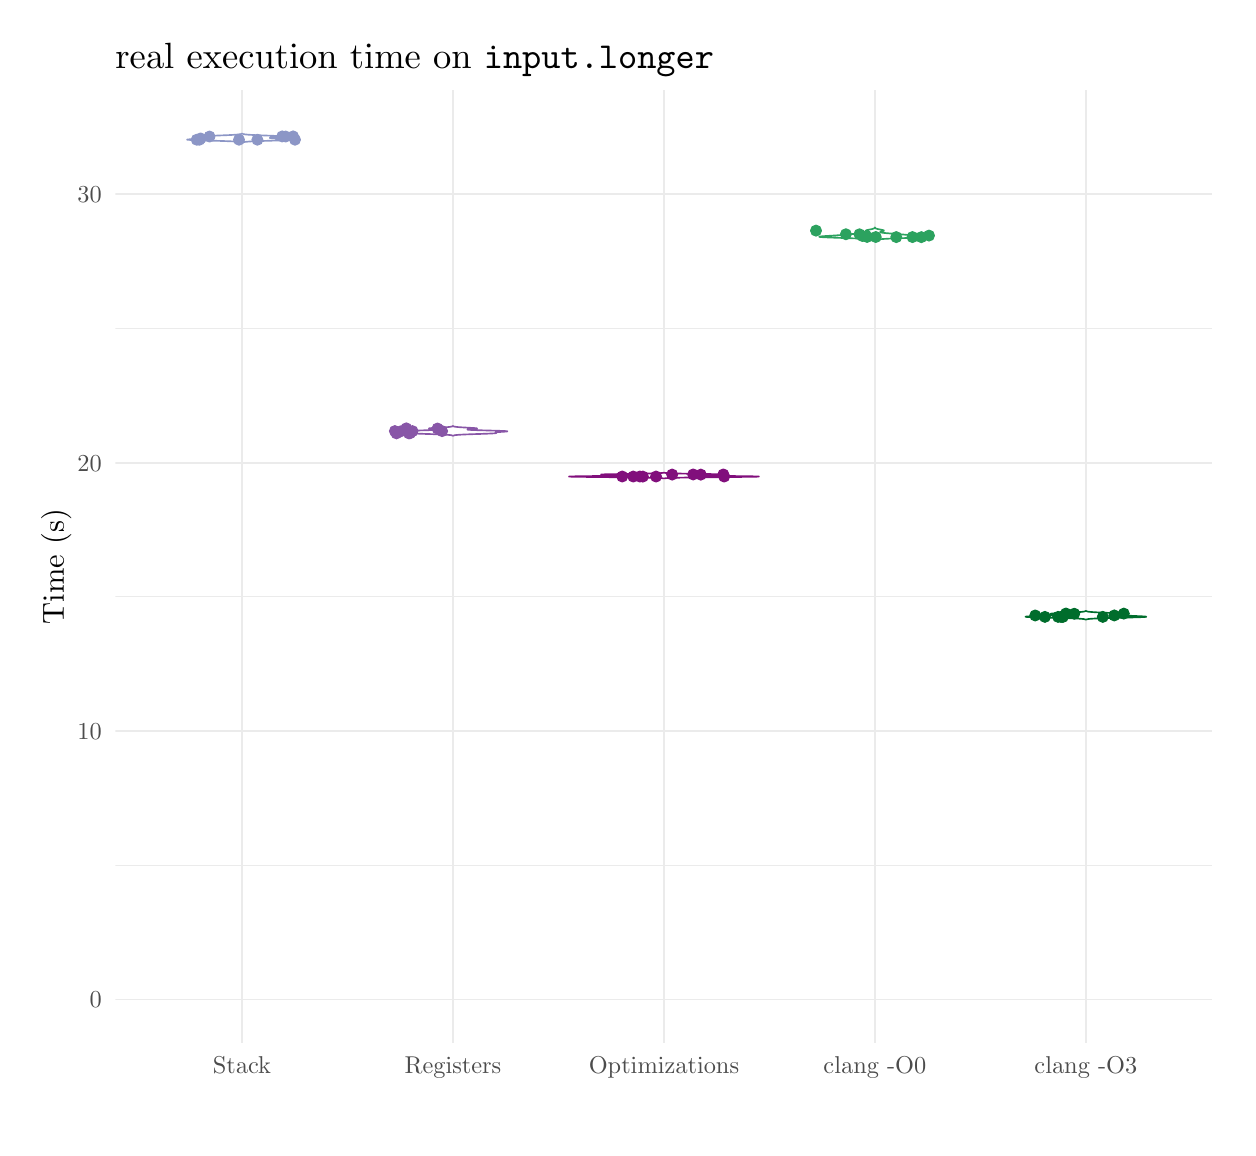
\begin{tikzpicture}[x=1pt,y=1pt]
\definecolor{fillColor}{RGB}{255,255,255}
\path[use as bounding box,fill=fillColor,fill opacity=0.00] (0,0) rectangle (433.62,397.48);
\begin{scope}
\path[clip] ( 31.71, 30.69) rectangle (428.12,374.83);
\definecolor{drawColor}{gray}{0.92}

\path[draw=drawColor,line width= 0.3pt,line join=round] ( 31.71, 94.82) --
	(428.12, 94.82);

\path[draw=drawColor,line width= 0.3pt,line join=round] ( 31.71,191.80) --
	(428.12,191.80);

\path[draw=drawColor,line width= 0.3pt,line join=round] ( 31.71,288.78) --
	(428.12,288.78);

\path[draw=drawColor,line width= 0.6pt,line join=round] ( 31.71, 46.33) --
	(428.12, 46.33);

\path[draw=drawColor,line width= 0.6pt,line join=round] ( 31.71,143.31) --
	(428.12,143.31);

\path[draw=drawColor,line width= 0.6pt,line join=round] ( 31.71,240.29) --
	(428.12,240.29);

\path[draw=drawColor,line width= 0.6pt,line join=round] ( 31.71,337.27) --
	(428.12,337.27);

\path[draw=drawColor,line width= 0.6pt,line join=round] ( 77.45, 30.69) --
	( 77.45,374.83);

\path[draw=drawColor,line width= 0.6pt,line join=round] (153.68, 30.69) --
	(153.68,374.83);

\path[draw=drawColor,line width= 0.6pt,line join=round] (229.92, 30.69) --
	(229.92,374.83);

\path[draw=drawColor,line width= 0.6pt,line join=round] (306.15, 30.69) --
	(306.15,374.83);

\path[draw=drawColor,line width= 0.6pt,line join=round] (382.38, 30.69) --
	(382.38,374.83);
\definecolor{drawColor}{RGB}{140,150,198}
\definecolor{fillColor}{RGB}{255,255,255}

\path[draw=drawColor,line width= 0.6pt,line join=round,line cap=round,fill=fillColor] ( 77.26,355.98) --
	( 77.25,355.99) --
	( 77.24,355.99) --
	( 77.23,356.00) --
	( 77.22,356.01) --
	( 77.20,356.01) --
	( 77.19,356.02) --
	( 77.17,356.02) --
	( 77.16,356.03) --
	( 77.14,356.04) --
	( 77.12,356.04) --
	( 77.11,356.05) --
	( 77.09,356.06) --
	( 77.07,356.06) --
	( 77.05,356.07) --
	( 77.02,356.07) --
	( 77.00,356.08) --
	( 76.98,356.09) --
	( 76.95,356.09) --
	( 76.93,356.10) --
	( 76.90,356.11) --
	( 76.87,356.11) --
	( 76.84,356.12) --
	( 76.81,356.12) --
	( 76.78,356.13) --
	( 76.75,356.14) --
	( 76.71,356.14) --
	( 76.68,356.15) --
	( 76.64,356.16) --
	( 76.60,356.16) --
	( 76.56,356.17) --
	( 76.52,356.17) --
	( 76.47,356.18) --
	( 76.43,356.19) --
	( 76.38,356.19) --
	( 76.33,356.20) --
	( 76.28,356.21) --
	( 76.23,356.21) --
	( 76.17,356.22) --
	( 76.12,356.22) --
	( 76.06,356.23) --
	( 76.00,356.24) --
	( 75.93,356.24) --
	( 75.87,356.25) --
	( 75.80,356.26) --
	( 75.73,356.26) --
	( 75.66,356.27) --
	( 75.58,356.28) --
	( 75.51,356.28) --
	( 75.43,356.29) --
	( 75.35,356.29) --
	( 75.26,356.30) --
	( 75.18,356.31) --
	( 75.09,356.31) --
	( 74.99,356.32) --
	( 74.90,356.33) --
	( 74.80,356.33) --
	( 74.70,356.34) --
	( 74.60,356.34) --
	( 74.49,356.35) --
	( 74.39,356.36) --
	( 74.27,356.36) --
	( 74.16,356.37) --
	( 74.04,356.38) --
	( 73.92,356.38) --
	( 73.80,356.39) --
	( 73.67,356.39) --
	( 73.54,356.40) --
	( 73.41,356.41) --
	( 73.28,356.41) --
	( 73.14,356.42) --
	( 73.00,356.43) --
	( 72.86,356.43) --
	( 72.71,356.44) --
	( 72.56,356.44) --
	( 72.41,356.45) --
	( 72.25,356.46) --
	( 72.09,356.46) --
	( 71.93,356.47) --
	( 71.77,356.48) --
	( 71.60,356.48) --
	( 71.43,356.49) --
	( 71.25,356.49) --
	( 71.08,356.50) --
	( 70.90,356.51) --
	( 70.72,356.51) --
	( 70.54,356.52) --
	( 70.35,356.53) --
	( 70.16,356.53) --
	( 69.97,356.54) --
	( 69.78,356.54) --
	( 69.58,356.55) --
	( 69.38,356.56) --
	( 69.18,356.56) --
	( 68.98,356.57) --
	( 68.78,356.58) --
	( 68.57,356.58) --
	( 68.37,356.59) --
	( 68.16,356.59) --
	( 67.95,356.60) --
	( 67.73,356.61) --
	( 67.52,356.61) --
	( 67.31,356.62) --
	( 67.09,356.63) --
	( 66.87,356.63) --
	( 66.66,356.64) --
	( 66.44,356.65) --
	( 66.22,356.65) --
	( 66.00,356.66) --
	( 65.78,356.66) --
	( 65.56,356.67) --
	( 65.34,356.68) --
	( 65.12,356.68) --
	( 64.91,356.69) --
	( 64.69,356.70) --
	( 64.47,356.70) --
	( 64.25,356.71) --
	( 64.04,356.71) --
	( 63.82,356.72) --
	( 63.61,356.73) --
	( 63.40,356.73) --
	( 63.19,356.74) --
	( 62.98,356.75) --
	( 62.77,356.75) --
	( 62.57,356.76) --
	( 62.36,356.76) --
	( 62.16,356.77) --
	( 61.96,356.78) --
	( 61.77,356.78) --
	( 61.58,356.79) --
	( 61.39,356.80) --
	( 61.20,356.80) --
	( 61.02,356.81) --
	( 60.84,356.81) --
	( 60.66,356.82) --
	( 60.49,356.83) --
	( 60.32,356.83) --
	( 60.16,356.84) --
	( 60.00,356.85) --
	( 59.84,356.85) --
	( 59.69,356.86) --
	( 59.55,356.86) --
	( 59.41,356.87) --
	( 59.27,356.88) --
	( 59.14,356.88) --
	( 59.01,356.89) --
	( 58.89,356.90) --
	( 58.77,356.90) --
	( 58.66,356.91) --
	( 58.55,356.91) --
	( 58.45,356.92) --
	( 58.35,356.93) --
	( 58.26,356.93) --
	( 58.18,356.94) --
	( 58.10,356.95) --
	( 58.03,356.95) --
	( 57.96,356.96) --
	( 57.90,356.96) --
	( 57.84,356.97) --
	( 57.79,356.98) --
	( 57.75,356.98) --
	( 57.71,356.99) --
	( 57.68,357.00) --
	( 57.66,357.00) --
	( 57.64,357.01) --
	( 57.62,357.02) --
	( 57.62,357.02) --
	( 57.61,357.03) --
	( 57.62,357.03) --
	( 57.63,357.04) --
	( 57.64,357.05) --
	( 57.66,357.05) --
	( 57.69,357.06) --
	( 57.72,357.07) --
	( 57.76,357.07) --
	( 57.80,357.08) --
	( 57.85,357.08) --
	( 57.90,357.09) --
	( 57.96,357.10) --
	( 58.03,357.10) --
	( 58.09,357.11) --
	( 58.17,357.12) --
	( 58.25,357.12) --
	( 58.33,357.13) --
	( 58.42,357.13) --
	( 58.51,357.14) --
	( 58.61,357.15) --
	( 58.71,357.15) --
	( 58.81,357.16) --
	( 58.92,357.17) --
	( 59.03,357.17) --
	( 59.15,357.18) --
	( 59.27,357.18) --
	( 59.39,357.19) --
	( 59.52,357.20) --
	( 59.65,357.20) --
	( 59.78,357.21) --
	( 59.91,357.22) --
	( 60.05,357.22) --
	( 60.19,357.23) --
	( 60.33,357.23) --
	( 60.48,357.24) --
	( 60.62,357.25) --
	( 60.77,357.25) --
	( 60.92,357.26) --
	( 61.07,357.27) --
	( 61.22,357.27) --
	( 61.37,357.28) --
	( 61.53,357.28) --
	( 61.68,357.29) --
	( 61.84,357.30) --
	( 61.99,357.30) --
	( 62.15,357.31) --
	( 62.30,357.32) --
	( 62.46,357.32) --
	( 62.61,357.33) --
	( 62.77,357.33) --
	( 62.92,357.34) --
	( 63.08,357.35) --
	( 63.23,357.35) --
	( 63.38,357.36) --
	( 63.53,357.37) --
	( 63.68,357.37) --
	( 63.83,357.38) --
	( 63.98,357.39) --
	( 64.12,357.39) --
	( 64.27,357.40) --
	( 64.41,357.40) --
	( 64.55,357.41) --
	( 64.68,357.42) --
	( 64.82,357.42) --
	( 64.95,357.43) --
	( 65.08,357.44) --
	( 65.21,357.44) --
	( 65.33,357.45) --
	( 65.45,357.45) --
	( 65.57,357.46) --
	( 65.69,357.47) --
	( 65.80,357.47) --
	( 65.91,357.48) --
	( 66.01,357.49) --
	( 66.11,357.49) --
	( 66.21,357.50) --
	( 66.31,357.50) --
	( 66.40,357.51) --
	( 66.49,357.52) --
	( 66.57,357.52) --
	( 66.65,357.53) --
	( 66.73,357.54) --
	( 66.80,357.54) --
	( 66.87,357.55) --
	( 66.93,357.55) --
	( 66.99,357.56) --
	( 67.05,357.57) --
	( 67.10,357.57) --
	( 67.15,357.58) --
	( 67.19,357.59) --
	( 67.23,357.59) --
	( 67.27,357.60) --
	( 67.30,357.60) --
	( 67.33,357.61) --
	( 67.35,357.62) --
	( 67.37,357.62) --
	( 67.38,357.63) --
	( 67.39,357.64) --
	( 67.40,357.64) --
	( 67.40,357.65) --
	( 67.40,357.65) --
	( 67.39,357.66) --
	( 67.38,357.67) --
	( 67.37,357.67) --
	( 67.35,357.68) --
	( 67.32,357.69) --
	( 67.30,357.69) --
	( 67.27,357.70) --
	( 67.23,357.70) --
	( 67.20,357.71) --
	( 67.16,357.72) --
	( 67.11,357.72) --
	( 67.06,357.73) --
	( 67.01,357.74) --
	( 66.96,357.74) --
	( 66.90,357.75) --
	( 66.84,357.76) --
	( 66.77,357.76) --
	( 66.71,357.77) --
	( 66.64,357.77) --
	( 66.56,357.78) --
	( 66.49,357.79) --
	( 66.41,357.79) --
	( 66.33,357.80) --
	( 66.25,357.81) --
	( 66.16,357.81) --
	( 66.08,357.82) --
	( 65.99,357.82) --
	( 65.90,357.83) --
	( 65.81,357.84) --
	( 65.71,357.84) --
	( 65.62,357.85) --
	( 65.52,357.86) --
	( 65.43,357.86) --
	( 65.33,357.87) --
	( 65.23,357.87) --
	( 65.13,357.88) --
	( 65.03,357.89) --
	( 64.94,357.89) --
	( 64.84,357.90) --
	( 64.74,357.91) --
	( 64.64,357.91) --
	( 64.54,357.92) --
	( 64.44,357.92) --
	( 64.34,357.93) --
	( 64.24,357.94) --
	( 64.15,357.94) --
	( 64.05,357.95) --
	( 63.96,357.96) --
	( 63.87,357.96) --
	( 63.78,357.97) --
	( 63.69,357.97) --
	( 63.60,357.98) --
	( 63.51,357.99) --
	( 63.43,357.99) --
	( 63.35,358.00) --
	( 63.27,358.01) --
	( 63.20,358.01) --
	( 63.12,358.02) --
	( 63.05,358.02) --
	( 62.98,358.03) --
	( 62.92,358.04) --
	( 62.86,358.04) --
	( 62.80,358.05) --
	( 62.75,358.06) --
	( 62.70,358.06) --
	( 62.65,358.07) --
	( 62.60,358.07) --
	( 62.56,358.08) --
	( 62.53,358.09) --
	( 62.50,358.09) --
	( 62.47,358.10) --
	( 62.44,358.11) --
	( 62.42,358.11) --
	( 62.41,358.12) --
	( 62.40,358.13) --
	( 62.39,358.13) --
	( 62.39,358.14) --
	( 62.39,358.14) --
	( 62.40,358.15) --
	( 62.41,358.16) --
	( 62.42,358.16) --
	( 62.44,358.17) --
	( 62.47,358.18) --
	( 62.50,358.18) --
	( 62.53,358.19) --
	( 62.57,358.19) --
	( 62.61,358.20) --
	( 62.66,358.21) --
	( 62.71,358.21) --
	( 62.77,358.22) --
	( 62.83,358.23) --
	( 62.90,358.23) --
	( 62.97,358.24) --
	( 63.04,358.24) --
	( 63.12,358.25) --
	( 63.20,358.26) --
	( 63.29,358.26) --
	( 63.38,358.27) --
	( 63.47,358.28) --
	( 63.58,358.28) --
	( 63.68,358.29) --
	( 63.78,358.29) --
	( 63.89,358.30) --
	( 64.01,358.31) --
	( 64.13,358.31) --
	( 64.25,358.32) --
	( 64.37,358.33) --
	( 64.50,358.33) --
	( 64.63,358.34) --
	( 64.76,358.34) --
	( 64.90,358.35) --
	( 65.04,358.36) --
	( 65.18,358.36) --
	( 65.33,358.37) --
	( 65.47,358.38) --
	( 65.62,358.38) --
	( 65.77,358.39) --
	( 65.93,358.39) --
	( 66.08,358.40) --
	( 66.24,358.41) --
	( 66.40,358.41) --
	( 66.56,358.42) --
	( 66.72,358.43) --
	( 66.88,358.43) --
	( 67.05,358.44) --
	( 67.21,358.44) --
	( 67.38,358.45) --
	( 67.54,358.46) --
	( 67.71,358.46) --
	( 67.88,358.47) --
	( 68.05,358.48) --
	( 68.21,358.48) --
	( 68.38,358.49) --
	( 68.55,358.50) --
	( 68.72,358.50) --
	( 68.89,358.51) --
	( 69.06,358.51) --
	( 69.22,358.52) --
	( 69.39,358.53) --
	( 69.56,358.53) --
	( 69.72,358.54) --
	( 69.89,358.55) --
	( 70.05,358.55) --
	( 70.21,358.56) --
	( 70.38,358.56) --
	( 70.54,358.57) --
	( 70.70,358.58) --
	( 70.85,358.58) --
	( 71.01,358.59) --
	( 71.17,358.60) --
	( 71.32,358.60) --
	( 71.47,358.61) --
	( 71.62,358.61) --
	( 71.77,358.62) --
	( 71.92,358.63) --
	( 72.06,358.63) --
	( 72.20,358.64) --
	( 72.34,358.65) --
	( 72.48,358.65) --
	( 72.62,358.66) --
	( 72.75,358.66) --
	( 72.89,358.67) --
	( 73.02,358.68) --
	( 73.15,358.68) --
	( 73.27,358.69) --
	( 73.39,358.70) --
	( 73.52,358.70) --
	( 73.63,358.71) --
	( 73.75,358.71) --
	( 73.87,358.72) --
	( 73.98,358.73) --
	( 74.09,358.73) --
	( 74.20,358.74) --
	( 74.30,358.75) --
	( 74.40,358.75) --
	( 74.50,358.76) --
	( 74.60,358.76) --
	( 74.70,358.77) --
	( 74.79,358.78) --
	( 74.88,358.78) --
	( 74.97,358.79) --
	( 75.06,358.80) --
	( 75.14,358.80) --
	( 75.23,358.81) --
	( 75.31,358.81) --
	( 75.38,358.82) --
	( 75.46,358.83) --
	( 75.53,358.83) --
	( 75.61,358.84) --
	( 75.68,358.85) --
	( 75.74,358.85) --
	( 75.81,358.86) --
	( 75.87,358.87) --
	( 75.93,358.87) --
	( 75.99,358.88) --
	( 76.05,358.88) --
	( 76.11,358.89) --
	( 76.16,358.90) --
	( 76.22,358.90) --
	( 76.27,358.91) --
	( 76.32,358.92) --
	( 76.36,358.92) --
	( 76.41,358.93) --
	( 76.45,358.93) --
	( 76.50,358.94) --
	( 76.54,358.95) --
	( 76.58,358.95) --
	( 76.62,358.96) --
	( 76.65,358.97) --
	( 76.69,358.97) --
	( 76.72,358.98) --
	( 76.76,358.98) --
	( 76.79,358.99) --
	( 76.82,359.00) --
	( 76.85,359.00) --
	( 76.88,359.01) --
	( 76.90,359.02) --
	( 76.93,359.02) --
	( 76.95,359.03) --
	( 76.98,359.03) --
	( 77.00,359.04) --
	( 77.02,359.05) --
	( 77.04,359.05) --
	( 77.06,359.06) --
	( 77.08,359.07) --
	( 77.10,359.07) --
	( 77.12,359.08) --
	( 77.13,359.08) --
	( 77.15,359.09) --
	( 77.17,359.10) --
	( 77.18,359.10) --
	( 77.20,359.11) --
	( 77.21,359.12) --
	( 77.22,359.12) --
	( 77.23,359.13) --
	( 77.25,359.13) --
	( 77.26,359.14) --
	( 77.27,359.15) --
	( 77.28,359.15) --
	( 77.29,359.16) --
	( 77.30,359.17) --
	( 77.30,359.17) --
	( 77.31,359.18) --
	( 77.32,359.18) --
	( 77.58,359.18) --
	( 77.59,359.18) --
	( 77.60,359.17) --
	( 77.61,359.17) --
	( 77.62,359.16) --
	( 77.63,359.15) --
	( 77.64,359.15) --
	( 77.65,359.14) --
	( 77.66,359.13) --
	( 77.67,359.13) --
	( 77.68,359.12) --
	( 77.69,359.12) --
	( 77.71,359.11) --
	( 77.72,359.10) --
	( 77.74,359.10) --
	( 77.75,359.09) --
	( 77.77,359.08) --
	( 77.78,359.08) --
	( 77.80,359.07) --
	( 77.82,359.07) --
	( 77.84,359.06) --
	( 77.86,359.05) --
	( 77.88,359.05) --
	( 77.90,359.04) --
	( 77.93,359.03) --
	( 77.95,359.03) --
	( 77.97,359.02) --
	( 78.00,359.02) --
	( 78.03,359.01) --
	( 78.06,359.00) --
	( 78.09,359.00) --
	( 78.12,358.99) --
	( 78.15,358.98) --
	( 78.18,358.98) --
	( 78.22,358.97) --
	( 78.25,358.97) --
	( 78.29,358.96) --
	( 78.33,358.95) --
	( 78.37,358.95) --
	( 78.41,358.94) --
	( 78.45,358.93) --
	( 78.49,358.93) --
	( 78.54,358.92) --
	( 78.59,358.92) --
	( 78.64,358.91) --
	( 78.69,358.90) --
	( 78.74,358.90) --
	( 78.79,358.89) --
	( 78.85,358.88) --
	( 78.91,358.88) --
	( 78.97,358.87) --
	( 79.03,358.87) --
	( 79.09,358.86) --
	( 79.16,358.85) --
	( 79.23,358.85) --
	( 79.30,358.84) --
	( 79.37,358.83) --
	( 79.44,358.83) --
	( 79.52,358.82) --
	( 79.60,358.81) --
	( 79.68,358.81) --
	( 79.76,358.80) --
	( 79.84,358.80) --
	( 79.93,358.79) --
	( 80.02,358.78) --
	( 80.11,358.78) --
	( 80.20,358.77) --
	( 80.30,358.76) --
	( 80.40,358.76) --
	( 80.50,358.75) --
	( 80.60,358.75) --
	( 80.71,358.74) --
	( 80.81,358.73) --
	( 80.92,358.73) --
	( 81.04,358.72) --
	( 81.15,358.71) --
	( 81.27,358.71) --
	( 81.39,358.70) --
	( 81.51,358.70) --
	( 81.63,358.69) --
	( 81.76,358.68) --
	( 81.89,358.68) --
	( 82.02,358.67) --
	( 82.15,358.66) --
	( 82.28,358.66) --
	( 82.42,358.65) --
	( 82.56,358.65) --
	( 82.70,358.64) --
	( 82.84,358.63) --
	( 82.99,358.63) --
	( 83.13,358.62) --
	( 83.28,358.61) --
	( 83.43,358.61) --
	( 83.58,358.60) --
	( 83.74,358.60) --
	( 83.89,358.59) --
	( 84.05,358.58) --
	( 84.21,358.58) --
	( 84.37,358.57) --
	( 84.53,358.56) --
	( 84.69,358.56) --
	( 84.85,358.55) --
	( 85.02,358.55) --
	( 85.18,358.54) --
	( 85.35,358.53) --
	( 85.51,358.53) --
	( 85.68,358.52) --
	( 85.85,358.51) --
	( 86.01,358.51) --
	( 86.18,358.50) --
	( 86.35,358.50) --
	( 86.52,358.49) --
	( 86.69,358.48) --
	( 86.86,358.48) --
	( 87.02,358.47) --
	( 87.19,358.46) --
	( 87.36,358.46) --
	( 87.53,358.45) --
	( 87.69,358.44) --
	( 87.86,358.44) --
	( 88.02,358.43) --
	( 88.18,358.43) --
	( 88.35,358.42) --
	( 88.51,358.41) --
	( 88.66,358.41) --
	( 88.82,358.40) --
	( 88.98,358.39) --
	( 89.13,358.39) --
	( 89.28,358.38) --
	( 89.43,358.38) --
	( 89.58,358.37) --
	( 89.72,358.36) --
	( 89.86,358.36) --
	( 90.00,358.35) --
	( 90.14,358.34) --
	( 90.27,358.34) --
	( 90.40,358.33) --
	( 90.53,358.33) --
	( 90.66,358.32) --
	( 90.78,358.31) --
	( 90.89,358.31) --
	( 91.01,358.30) --
	( 91.12,358.29) --
	( 91.23,358.29) --
	( 91.33,358.28) --
	( 91.43,358.28) --
	( 91.52,358.27) --
	( 91.61,358.26) --
	( 91.70,358.26) --
	( 91.78,358.25) --
	( 91.86,358.24) --
	( 91.94,358.24) --
	( 92.01,358.23) --
	( 92.07,358.23) --
	( 92.13,358.22) --
	( 92.19,358.21) --
	( 92.24,358.21) --
	( 92.29,358.20) --
	( 92.33,358.19) --
	( 92.37,358.19) --
	( 92.41,358.18) --
	( 92.43,358.18) --
	( 92.46,358.17) --
	( 92.48,358.16) --
	( 92.49,358.16) --
	( 92.51,358.15) --
	( 92.51,358.14) --
	( 92.52,358.14) --
	( 92.51,358.13) --
	( 92.51,358.13) --
	( 92.49,358.12) --
	( 92.48,358.11) --
	( 92.46,358.11) --
	( 92.43,358.10) --
	( 92.41,358.09) --
	( 92.37,358.09) --
	( 92.34,358.08) --
	( 92.30,358.07) --
	( 92.26,358.07) --
	( 92.21,358.06) --
	( 92.16,358.06) --
	( 92.10,358.05) --
	( 92.04,358.04) --
	( 91.98,358.04) --
	( 91.92,358.03) --
	( 91.85,358.02) --
	( 91.78,358.02) --
	( 91.71,358.01) --
	( 91.63,358.01) --
	( 91.55,358.00) --
	( 91.47,357.99) --
	( 91.39,357.99) --
	( 91.30,357.98) --
	( 91.22,357.97) --
	( 91.13,357.97) --
	( 91.04,357.96) --
	( 90.94,357.96) --
	( 90.85,357.95) --
	( 90.76,357.94) --
	( 90.66,357.94) --
	( 90.56,357.93) --
	( 90.46,357.92) --
	( 90.37,357.92) --
	( 90.27,357.91) --
	( 90.17,357.91) --
	( 90.07,357.90) --
	( 89.97,357.89) --
	( 89.87,357.89) --
	( 89.77,357.88) --
	( 89.67,357.87) --
	( 89.57,357.87) --
	( 89.48,357.86) --
	( 89.38,357.86) --
	( 89.28,357.85) --
	( 89.19,357.84) --
	( 89.10,357.84) --
	( 89.00,357.83) --
	( 88.91,357.82) --
	( 88.83,357.82) --
	( 88.74,357.81) --
	( 88.65,357.81) --
	( 88.57,357.80) --
	( 88.49,357.79) --
	( 88.42,357.79) --
	( 88.34,357.78) --
	( 88.27,357.77) --
	( 88.20,357.77) --
	( 88.13,357.76) --
	( 88.07,357.76) --
	( 88.00,357.75) --
	( 87.95,357.74) --
	( 87.89,357.74) --
	( 87.84,357.73) --
	( 87.79,357.72) --
	( 87.75,357.72) --
	( 87.71,357.71) --
	( 87.67,357.70) --
	( 87.64,357.70) --
	( 87.60,357.69) --
	( 87.58,357.69) --
	( 87.56,357.68) --
	( 87.54,357.67) --
	( 87.52,357.67) --
	( 87.51,357.66) --
	( 87.51,357.65) --
	( 87.50,357.65) --
	( 87.51,357.64) --
	( 87.51,357.64) --
	( 87.52,357.63) --
	( 87.53,357.62) --
	( 87.55,357.62) --
	( 87.58,357.61) --
	( 87.60,357.60) --
	( 87.63,357.60) --
	( 87.67,357.59) --
	( 87.71,357.59) --
	( 87.75,357.58) --
	( 87.80,357.57) --
	( 87.85,357.57) --
	( 87.91,357.56) --
	( 87.97,357.55) --
	( 88.03,357.55) --
	( 88.10,357.54) --
	( 88.18,357.54) --
	( 88.25,357.53) --
	( 88.33,357.52) --
	( 88.42,357.52) --
	( 88.50,357.51) --
	( 88.59,357.50) --
	( 88.69,357.50) --
	( 88.79,357.49) --
	( 88.89,357.49) --
	( 89.00,357.48) --
	( 89.10,357.47) --
	( 89.22,357.47) --
	( 89.33,357.46) --
	( 89.45,357.45) --
	( 89.57,357.45) --
	( 89.70,357.44) --
	( 89.82,357.44) --
	( 89.95,357.43) --
	( 90.09,357.42) --
	( 90.22,357.42) --
	( 90.36,357.41) --
	( 90.50,357.40) --
	( 90.64,357.40) --
	( 90.78,357.39) --
	( 90.93,357.39) --
	( 91.07,357.38) --
	( 91.22,357.37) --
	( 91.37,357.37) --
	( 91.52,357.36) --
	( 91.67,357.35) --
	( 91.83,357.35) --
	( 91.98,357.34) --
	( 92.13,357.33) --
	( 92.29,357.33) --
	( 92.44,357.32) --
	( 92.60,357.32) --
	( 92.76,357.31) --
	( 92.91,357.30) --
	( 93.07,357.30) --
	( 93.22,357.29) --
	( 93.38,357.28) --
	( 93.53,357.28) --
	( 93.68,357.27) --
	( 93.83,357.27) --
	( 93.98,357.26) --
	( 94.13,357.25) --
	( 94.28,357.25) --
	( 94.43,357.24) --
	( 94.57,357.23) --
	( 94.71,357.23) --
	( 94.85,357.22) --
	( 94.99,357.22) --
	( 95.12,357.21) --
	( 95.26,357.20) --
	( 95.38,357.20) --
	( 95.51,357.19) --
	( 95.63,357.18) --
	( 95.75,357.18) --
	( 95.87,357.17) --
	( 95.98,357.17) --
	( 96.09,357.16) --
	( 96.20,357.15) --
	( 96.30,357.15) --
	( 96.39,357.14) --
	( 96.48,357.13) --
	( 96.57,357.13) --
	( 96.66,357.12) --
	( 96.73,357.12) --
	( 96.81,357.11) --
	( 96.88,357.10) --
	( 96.94,357.10) --
	( 97.00,357.09) --
	( 97.06,357.08) --
	( 97.10,357.08) --
	( 97.15,357.07) --
	( 97.18,357.07) --
	( 97.22,357.06) --
	( 97.24,357.05) --
	( 97.26,357.05) --
	( 97.28,357.04) --
	( 97.29,357.03) --
	( 97.29,357.03) --
	( 97.29,357.02) --
	( 97.28,357.02) --
	( 97.27,357.01) --
	( 97.25,357.00) --
	( 97.22,357.00) --
	( 97.19,356.99) --
	( 97.15,356.98) --
	( 97.11,356.98) --
	( 97.06,356.97) --
	( 97.00,356.96) --
	( 96.94,356.96) --
	( 96.87,356.95) --
	( 96.80,356.95) --
	( 96.72,356.94) --
	( 96.64,356.93) --
	( 96.55,356.93) --
	( 96.45,356.92) --
	( 96.35,356.91) --
	( 96.25,356.91) --
	( 96.14,356.90) --
	( 96.02,356.90) --
	( 95.90,356.89) --
	( 95.77,356.88) --
	( 95.64,356.88) --
	( 95.50,356.87) --
	( 95.36,356.86) --
	( 95.21,356.86) --
	( 95.06,356.85) --
	( 94.90,356.85) --
	( 94.74,356.84) --
	( 94.58,356.83) --
	( 94.41,356.83) --
	( 94.24,356.82) --
	( 94.06,356.81) --
	( 93.88,356.81) --
	( 93.70,356.80) --
	( 93.52,356.80) --
	( 93.33,356.79) --
	( 93.13,356.78) --
	( 92.94,356.78) --
	( 92.74,356.77) --
	( 92.54,356.76) --
	( 92.34,356.76) --
	( 92.13,356.75) --
	( 91.93,356.75) --
	( 91.72,356.74) --
	( 91.51,356.73) --
	( 91.29,356.73) --
	( 91.08,356.72) --
	( 90.87,356.71) --
	( 90.65,356.71) --
	( 90.43,356.70) --
	( 90.22,356.70) --
	( 90.00,356.69) --
	( 89.78,356.68) --
	( 89.56,356.68) --
	( 89.34,356.67) --
	( 89.12,356.66) --
	( 88.90,356.66) --
	( 88.68,356.65) --
	( 88.46,356.65) --
	( 88.25,356.64) --
	( 88.03,356.63) --
	( 87.81,356.63) --
	( 87.60,356.62) --
	( 87.38,356.61) --
	( 87.17,356.61) --
	( 86.96,356.60) --
	( 86.75,356.59) --
	( 86.54,356.59) --
	( 86.33,356.58) --
	( 86.13,356.58) --
	( 85.92,356.57) --
	( 85.72,356.56) --
	( 85.52,356.56) --
	( 85.32,356.55) --
	( 85.13,356.54) --
	( 84.93,356.54) --
	( 84.74,356.53) --
	( 84.55,356.53) --
	( 84.37,356.52) --
	( 84.18,356.51) --
	( 84.00,356.51) --
	( 83.82,356.50) --
	( 83.65,356.49) --
	( 83.47,356.49) --
	( 83.31,356.48) --
	( 83.14,356.48) --
	( 82.97,356.47) --
	( 82.81,356.46) --
	( 82.65,356.46) --
	( 82.50,356.45) --
	( 82.34,356.44) --
	( 82.19,356.44) --
	( 82.05,356.43) --
	( 81.90,356.43) --
	( 81.76,356.42) --
	( 81.63,356.41) --
	( 81.49,356.41) --
	( 81.36,356.40) --
	( 81.23,356.39) --
	( 81.10,356.39) --
	( 80.98,356.38) --
	( 80.86,356.38) --
	( 80.74,356.37) --
	( 80.63,356.36) --
	( 80.52,356.36) --
	( 80.41,356.35) --
	( 80.30,356.34) --
	( 80.20,356.34) --
	( 80.10,356.33) --
	( 80.00,356.33) --
	( 79.91,356.32) --
	( 79.82,356.31) --
	( 79.73,356.31) --
	( 79.64,356.30) --
	( 79.56,356.29) --
	( 79.48,356.29) --
	( 79.40,356.28) --
	( 79.32,356.28) --
	( 79.24,356.27) --
	( 79.17,356.26) --
	( 79.10,356.26) --
	( 79.04,356.25) --
	( 78.97,356.24) --
	( 78.91,356.24) --
	( 78.85,356.23) --
	( 78.79,356.22) --
	( 78.73,356.22) --
	( 78.68,356.21) --
	( 78.62,356.21) --
	( 78.57,356.20) --
	( 78.52,356.19) --
	( 78.48,356.19) --
	( 78.43,356.18) --
	( 78.39,356.17) --
	( 78.34,356.17) --
	( 78.30,356.16) --
	( 78.26,356.16) --
	( 78.23,356.15) --
	( 78.19,356.14) --
	( 78.16,356.14) --
	( 78.12,356.13) --
	( 78.09,356.12) --
	( 78.06,356.12) --
	( 78.03,356.11) --
	( 78.00,356.11) --
	( 77.98,356.10) --
	( 77.95,356.09) --
	( 77.92,356.09) --
	( 77.90,356.08) --
	( 77.88,356.07) --
	( 77.86,356.07) --
	( 77.84,356.06) --
	( 77.82,356.06) --
	( 77.80,356.05) --
	( 77.78,356.04) --
	( 77.76,356.04) --
	( 77.75,356.03) --
	( 77.73,356.02) --
	( 77.72,356.02) --
	( 77.70,356.01) --
	( 77.69,356.01) --
	( 77.68,356.00) --
	( 77.66,355.99) --
	( 77.65,355.99) --
	( 77.64,355.98) --
	( 77.26,355.98) --
	cycle;
\definecolor{drawColor}{RGB}{136,86,167}

\path[draw=drawColor,line width= 0.6pt,line join=round,line cap=round,fill=fillColor] (153.58,250.02) --
	(153.57,250.03) --
	(153.56,250.04) --
	(153.55,250.04) --
	(153.54,250.05) --
	(153.53,250.06) --
	(153.52,250.06) --
	(153.51,250.07) --
	(153.50,250.08) --
	(153.48,250.08) --
	(153.47,250.09) --
	(153.45,250.10) --
	(153.43,250.10) --
	(153.42,250.11) --
	(153.40,250.12) --
	(153.38,250.13) --
	(153.36,250.13) --
	(153.34,250.14) --
	(153.31,250.15) --
	(153.29,250.15) --
	(153.26,250.16) --
	(153.23,250.17) --
	(153.20,250.17) --
	(153.17,250.18) --
	(153.14,250.19) --
	(153.11,250.19) --
	(153.07,250.20) --
	(153.03,250.21) --
	(152.99,250.21) --
	(152.95,250.22) --
	(152.91,250.23) --
	(152.86,250.23) --
	(152.81,250.24) --
	(152.76,250.25) --
	(152.71,250.26) --
	(152.65,250.26) --
	(152.60,250.27) --
	(152.54,250.28) --
	(152.47,250.28) --
	(152.41,250.29) --
	(152.34,250.30) --
	(152.27,250.30) --
	(152.19,250.31) --
	(152.12,250.32) --
	(152.04,250.32) --
	(151.95,250.33) --
	(151.86,250.34) --
	(151.78,250.34) --
	(151.68,250.35) --
	(151.59,250.36) --
	(151.49,250.37) --
	(151.38,250.37) --
	(151.28,250.38) --
	(151.17,250.39) --
	(151.05,250.39) --
	(150.94,250.40) --
	(150.81,250.41) --
	(150.69,250.41) --
	(150.56,250.42) --
	(150.43,250.43) --
	(150.30,250.43) --
	(150.16,250.44) --
	(150.01,250.45) --
	(149.87,250.45) --
	(149.72,250.46) --
	(149.57,250.47) --
	(149.41,250.48) --
	(149.25,250.48) --
	(149.09,250.49) --
	(148.92,250.50) --
	(148.75,250.50) --
	(148.58,250.51) --
	(148.40,250.52) --
	(148.23,250.52) --
	(148.04,250.53) --
	(147.86,250.54) --
	(147.67,250.54) --
	(147.48,250.55) --
	(147.29,250.56) --
	(147.10,250.56) --
	(146.90,250.57) --
	(146.71,250.58) --
	(146.51,250.59) --
	(146.31,250.59) --
	(146.10,250.60) --
	(145.90,250.61) --
	(145.69,250.61) --
	(145.49,250.62) --
	(145.28,250.63) --
	(145.07,250.63) --
	(144.87,250.64) --
	(144.66,250.65) --
	(144.45,250.65) --
	(144.24,250.66) --
	(144.04,250.67) --
	(143.83,250.67) --
	(143.63,250.68) --
	(143.42,250.69) --
	(143.22,250.70) --
	(143.02,250.70) --
	(142.82,250.71) --
	(142.63,250.72) --
	(142.43,250.72) --
	(142.24,250.73) --
	(142.05,250.74) --
	(141.86,250.74) --
	(141.68,250.75) --
	(141.50,250.76) --
	(141.32,250.76) --
	(141.15,250.77) --
	(140.98,250.78) --
	(140.81,250.78) --
	(140.65,250.79) --
	(140.50,250.80) --
	(140.34,250.81) --
	(140.20,250.81) --
	(140.05,250.82) --
	(139.91,250.83) --
	(139.78,250.83) --
	(139.65,250.84) --
	(139.53,250.85) --
	(139.41,250.85) --
	(139.29,250.86) --
	(139.19,250.87) --
	(139.08,250.87) --
	(138.99,250.88) --
	(138.89,250.89) --
	(138.80,250.89) --
	(138.72,250.90) --
	(138.65,250.91) --
	(138.57,250.91) --
	(138.51,250.92) --
	(138.45,250.93) --
	(138.39,250.94) --
	(138.34,250.94) --
	(138.29,250.95) --
	(138.25,250.96) --
	(138.21,250.96) --
	(138.18,250.97) --
	(138.15,250.98) --
	(138.12,250.98) --
	(138.10,250.99) --
	(138.09,251.00) --
	(138.07,251.00) --
	(138.06,251.01) --
	(138.05,251.02) --
	(138.05,251.02) --
	(138.05,251.03) --
	(138.05,251.04) --
	(138.05,251.05) --
	(138.05,251.05) --
	(138.06,251.06) --
	(138.07,251.07) --
	(138.08,251.07) --
	(138.09,251.08) --
	(138.10,251.09) --
	(138.11,251.09) --
	(138.12,251.10) --
	(138.14,251.11) --
	(138.15,251.11) --
	(138.16,251.12) --
	(138.17,251.13) --
	(138.18,251.13) --
	(138.19,251.14) --
	(138.20,251.15) --
	(138.20,251.16) --
	(138.21,251.16) --
	(138.21,251.17) --
	(138.21,251.18) --
	(138.20,251.18) --
	(138.20,251.19) --
	(138.19,251.20) --
	(138.18,251.20) --
	(138.17,251.21) --
	(138.15,251.22) --
	(138.13,251.22) --
	(138.11,251.23) --
	(138.08,251.24) --
	(138.05,251.24) --
	(138.01,251.25) --
	(137.98,251.26) --
	(137.93,251.27) --
	(137.89,251.27) --
	(137.84,251.28) --
	(137.79,251.29) --
	(137.73,251.29) --
	(137.67,251.30) --
	(137.60,251.31) --
	(137.54,251.31) --
	(137.46,251.32) --
	(137.39,251.33) --
	(137.31,251.33) --
	(137.23,251.34) --
	(137.14,251.35) --
	(137.06,251.35) --
	(136.97,251.36) --
	(136.87,251.37) --
	(136.78,251.38) --
	(136.68,251.38) --
	(136.58,251.39) --
	(136.48,251.40) --
	(136.38,251.40) --
	(136.27,251.41) --
	(136.17,251.42) --
	(136.06,251.42) --
	(135.96,251.43) --
	(135.85,251.44) --
	(135.75,251.44) --
	(135.64,251.45) --
	(135.54,251.46) --
	(135.43,251.46) --
	(135.33,251.47) --
	(135.23,251.48) --
	(135.13,251.49) --
	(135.03,251.49) --
	(134.94,251.50) --
	(134.85,251.51) --
	(134.76,251.51) --
	(134.68,251.52) --
	(134.60,251.53) --
	(134.52,251.53) --
	(134.45,251.54) --
	(134.38,251.55) --
	(134.32,251.55) --
	(134.27,251.56) --
	(134.21,251.57) --
	(134.17,251.57) --
	(134.13,251.58) --
	(134.10,251.59) --
	(134.07,251.59) --
	(134.05,251.60) --
	(134.04,251.61) --
	(134.04,251.62) --
	(134.04,251.62) --
	(134.05,251.63) --
	(134.07,251.64) --
	(134.10,251.64) --
	(134.13,251.65) --
	(134.17,251.66) --
	(134.22,251.66) --
	(134.28,251.67) --
	(134.35,251.68) --
	(134.42,251.68) --
	(134.50,251.69) --
	(134.60,251.70) --
	(134.69,251.70) --
	(134.80,251.71) --
	(134.92,251.72) --
	(135.04,251.73) --
	(135.17,251.73) --
	(135.31,251.74) --
	(135.46,251.75) --
	(135.61,251.75) --
	(135.77,251.76) --
	(135.94,251.77) --
	(136.12,251.77) --
	(136.30,251.78) --
	(136.49,251.79) --
	(136.68,251.79) --
	(136.88,251.80) --
	(137.09,251.81) --
	(137.30,251.81) --
	(137.52,251.82) --
	(137.74,251.83) --
	(137.97,251.84) --
	(138.20,251.84) --
	(138.43,251.85) --
	(138.67,251.86) --
	(138.91,251.86) --
	(139.16,251.87) --
	(139.40,251.88) --
	(139.65,251.88) --
	(139.91,251.89) --
	(140.16,251.90) --
	(140.41,251.90) --
	(140.67,251.91) --
	(140.92,251.92) --
	(141.18,251.92) --
	(141.43,251.93) --
	(141.69,251.94) --
	(141.94,251.95) --
	(142.19,251.95) --
	(142.44,251.96) --
	(142.69,251.97) --
	(142.94,251.97) --
	(143.18,251.98) --
	(143.42,251.99) --
	(143.66,251.99) --
	(143.90,252.00) --
	(144.13,252.01) --
	(144.35,252.01) --
	(144.58,252.02) --
	(144.79,252.03) --
	(145.01,252.03) --
	(145.22,252.04) --
	(145.42,252.05) --
	(145.61,252.06) --
	(145.81,252.06) --
	(145.99,252.07) --
	(146.17,252.08) --
	(146.34,252.08) --
	(146.51,252.09) --
	(146.67,252.10) --
	(146.83,252.10) --
	(146.98,252.11) --
	(147.12,252.12) --
	(147.25,252.12) --
	(147.38,252.13) --
	(147.50,252.14) --
	(147.61,252.14) --
	(147.72,252.15) --
	(147.81,252.16) --
	(147.91,252.16) --
	(147.99,252.17) --
	(148.07,252.18) --
	(148.14,252.19) --
	(148.20,252.19) --
	(148.26,252.20) --
	(148.31,252.21) --
	(148.35,252.21) --
	(148.39,252.22) --
	(148.41,252.23) --
	(148.44,252.23) --
	(148.45,252.24) --
	(148.46,252.25) --
	(148.47,252.25) --
	(148.46,252.26) --
	(148.45,252.27) --
	(148.44,252.27) --
	(148.42,252.28) --
	(148.39,252.29) --
	(148.36,252.30) --
	(148.33,252.30) --
	(148.29,252.31) --
	(148.24,252.32) --
	(148.19,252.32) --
	(148.13,252.33) --
	(148.08,252.34) --
	(148.01,252.34) --
	(147.95,252.35) --
	(147.88,252.36) --
	(147.80,252.36) --
	(147.73,252.37) --
	(147.65,252.38) --
	(147.57,252.38) --
	(147.49,252.39) --
	(147.40,252.40) --
	(147.31,252.41) --
	(147.23,252.41) --
	(147.14,252.42) --
	(147.05,252.43) --
	(146.95,252.43) --
	(146.86,252.44) --
	(146.77,252.45) --
	(146.68,252.45) --
	(146.59,252.46) --
	(146.50,252.47) --
	(146.41,252.47) --
	(146.32,252.48) --
	(146.23,252.49) --
	(146.14,252.49) --
	(146.06,252.50) --
	(145.98,252.51) --
	(145.90,252.52) --
	(145.82,252.52) --
	(145.74,252.53) --
	(145.67,252.54) --
	(145.60,252.54) --
	(145.53,252.55) --
	(145.47,252.56) --
	(145.41,252.56) --
	(145.35,252.57) --
	(145.30,252.58) --
	(145.25,252.58) --
	(145.20,252.59) --
	(145.16,252.60) --
	(145.13,252.60) --
	(145.10,252.61) --
	(145.07,252.62) --
	(145.05,252.63) --
	(145.03,252.63) --
	(145.01,252.64) --
	(145.01,252.65) --
	(145.00,252.65) --
	(145.00,252.66) --
	(145.01,252.67) --
	(145.02,252.67) --
	(145.03,252.68) --
	(145.06,252.69) --
	(145.08,252.69) --
	(145.11,252.70) --
	(145.15,252.71) --
	(145.18,252.71) --
	(145.23,252.72) --
	(145.28,252.73) --
	(145.33,252.74) --
	(145.39,252.74) --
	(145.45,252.75) --
	(145.52,252.76) --
	(145.59,252.76) --
	(145.67,252.77) --
	(145.74,252.78) --
	(145.83,252.78) --
	(145.91,252.79) --
	(146.00,252.80) --
	(146.10,252.80) --
	(146.19,252.81) --
	(146.29,252.82) --
	(146.40,252.82) --
	(146.50,252.83) --
	(146.61,252.84) --
	(146.72,252.84) --
	(146.83,252.85) --
	(146.95,252.86) --
	(147.07,252.87) --
	(147.19,252.87) --
	(147.31,252.88) --
	(147.43,252.89) --
	(147.55,252.89) --
	(147.68,252.90) --
	(147.80,252.91) --
	(147.93,252.91) --
	(148.05,252.92) --
	(148.18,252.93) --
	(148.31,252.93) --
	(148.44,252.94) --
	(148.57,252.95) --
	(148.69,252.95) --
	(148.82,252.96) --
	(148.95,252.97) --
	(149.07,252.98) --
	(149.20,252.98) --
	(149.32,252.99) --
	(149.45,253.00) --
	(149.57,253.00) --
	(149.69,253.01) --
	(149.81,253.02) --
	(149.93,253.02) --
	(150.05,253.03) --
	(150.16,253.04) --
	(150.28,253.04) --
	(150.39,253.05) --
	(150.50,253.06) --
	(150.61,253.06) --
	(150.72,253.07) --
	(150.82,253.08) --
	(150.92,253.09) --
	(151.02,253.09) --
	(151.12,253.10) --
	(151.22,253.11) --
	(151.31,253.11) --
	(151.41,253.12) --
	(151.49,253.13) --
	(151.58,253.13) --
	(151.67,253.14) --
	(151.75,253.15) --
	(151.83,253.15) --
	(151.91,253.16) --
	(151.98,253.17) --
	(152.06,253.17) --
	(152.13,253.18) --
	(152.20,253.19) --
	(152.26,253.20) --
	(152.33,253.20) --
	(152.39,253.21) --
	(152.45,253.22) --
	(152.51,253.22) --
	(152.57,253.23) --
	(152.62,253.24) --
	(152.67,253.24) --
	(152.72,253.25) --
	(152.77,253.26) --
	(152.82,253.26) --
	(152.86,253.27) --
	(152.90,253.28) --
	(152.94,253.28) --
	(152.98,253.29) --
	(153.02,253.30) --
	(153.06,253.31) --
	(153.09,253.31) --
	(153.12,253.32) --
	(153.16,253.33) --
	(153.19,253.33) --
	(153.21,253.34) --
	(153.24,253.35) --
	(153.27,253.35) --
	(153.29,253.36) --
	(153.31,253.37) --
	(153.34,253.37) --
	(153.36,253.38) --
	(153.38,253.39) --
	(153.40,253.39) --
	(153.41,253.40) --
	(153.43,253.41) --
	(153.45,253.42) --
	(153.46,253.42) --
	(153.48,253.43) --
	(153.49,253.44) --
	(153.50,253.44) --
	(153.51,253.45) --
	(153.53,253.46) --
	(153.54,253.46) --
	(153.55,253.47) --
	(153.56,253.48) --
	(153.56,253.48) --
	(153.57,253.49) --
	(153.58,253.50) --
	(153.59,253.50) --
	(153.59,253.51) --
	(153.60,253.52) --
	(153.61,253.52) --
	(153.61,253.53) --
	(153.76,253.53) --
	(153.76,253.52) --
	(153.77,253.52) --
	(153.77,253.51) --
	(153.78,253.50) --
	(153.79,253.50) --
	(153.80,253.49) --
	(153.80,253.48) --
	(153.81,253.48) --
	(153.82,253.47) --
	(153.83,253.46) --
	(153.84,253.46) --
	(153.85,253.45) --
	(153.87,253.44) --
	(153.88,253.44) --
	(153.89,253.43) --
	(153.91,253.42) --
	(153.92,253.42) --
	(153.94,253.41) --
	(153.95,253.40) --
	(153.97,253.39) --
	(153.99,253.39) --
	(154.01,253.38) --
	(154.03,253.37) --
	(154.05,253.37) --
	(154.08,253.36) --
	(154.10,253.35) --
	(154.13,253.35) --
	(154.15,253.34) --
	(154.18,253.33) --
	(154.21,253.33) --
	(154.24,253.32) --
	(154.28,253.31) --
	(154.31,253.31) --
	(154.35,253.30) --
	(154.38,253.29) --
	(154.42,253.28) --
	(154.46,253.28) --
	(154.51,253.27) --
	(154.55,253.26) --
	(154.60,253.26) --
	(154.64,253.25) --
	(154.69,253.24) --
	(154.75,253.24) --
	(154.80,253.23) --
	(154.86,253.22) --
	(154.92,253.22) --
	(154.98,253.21) --
	(155.04,253.20) --
	(155.10,253.20) --
	(155.17,253.19) --
	(155.24,253.18) --
	(155.31,253.17) --
	(155.38,253.17) --
	(155.46,253.16) --
	(155.54,253.15) --
	(155.62,253.15) --
	(155.70,253.14) --
	(155.79,253.13) --
	(155.87,253.13) --
	(155.96,253.12) --
	(156.05,253.11) --
	(156.15,253.11) --
	(156.24,253.10) --
	(156.34,253.09) --
	(156.44,253.09) --
	(156.55,253.08) --
	(156.65,253.07) --
	(156.76,253.06) --
	(156.87,253.06) --
	(156.98,253.05) --
	(157.09,253.04) --
	(157.20,253.04) --
	(157.32,253.03) --
	(157.44,253.02) --
	(157.56,253.02) --
	(157.68,253.01) --
	(157.80,253.00) --
	(157.92,253.00) --
	(158.04,252.99) --
	(158.17,252.98) --
	(158.29,252.98) --
	(158.42,252.97) --
	(158.55,252.96) --
	(158.67,252.95) --
	(158.80,252.95) --
	(158.93,252.94) --
	(159.06,252.93) --
	(159.19,252.93) --
	(159.31,252.92) --
	(159.44,252.91) --
	(159.57,252.91) --
	(159.69,252.90) --
	(159.82,252.89) --
	(159.94,252.89) --
	(160.06,252.88) --
	(160.18,252.87) --
	(160.30,252.87) --
	(160.42,252.86) --
	(160.53,252.85) --
	(160.65,252.84) --
	(160.76,252.84) --
	(160.87,252.83) --
	(160.97,252.82) --
	(161.07,252.82) --
	(161.17,252.81) --
	(161.27,252.80) --
	(161.36,252.80) --
	(161.45,252.79) --
	(161.54,252.78) --
	(161.62,252.78) --
	(161.70,252.77) --
	(161.78,252.76) --
	(161.85,252.76) --
	(161.92,252.75) --
	(161.98,252.74) --
	(162.04,252.74) --
	(162.09,252.73) --
	(162.14,252.72) --
	(162.18,252.71) --
	(162.22,252.71) --
	(162.26,252.70) --
	(162.29,252.69) --
	(162.31,252.69) --
	(162.33,252.68) --
	(162.35,252.67) --
	(162.36,252.67) --
	(162.37,252.66) --
	(162.37,252.65) --
	(162.36,252.65) --
	(162.35,252.64) --
	(162.34,252.63) --
	(162.32,252.63) --
	(162.30,252.62) --
	(162.27,252.61) --
	(162.24,252.60) --
	(162.20,252.60) --
	(162.16,252.59) --
	(162.12,252.58) --
	(162.07,252.58) --
	(162.02,252.57) --
	(161.96,252.56) --
	(161.90,252.56) --
	(161.84,252.55) --
	(161.77,252.54) --
	(161.70,252.54) --
	(161.63,252.53) --
	(161.55,252.52) --
	(161.47,252.52) --
	(161.39,252.51) --
	(161.31,252.50) --
	(161.22,252.49) --
	(161.14,252.49) --
	(161.05,252.48) --
	(160.96,252.47) --
	(160.87,252.47) --
	(160.78,252.46) --
	(160.69,252.45) --
	(160.60,252.45) --
	(160.50,252.44) --
	(160.41,252.43) --
	(160.32,252.43) --
	(160.23,252.42) --
	(160.14,252.41) --
	(160.05,252.41) --
	(159.97,252.40) --
	(159.88,252.39) --
	(159.80,252.38) --
	(159.72,252.38) --
	(159.64,252.37) --
	(159.56,252.36) --
	(159.49,252.36) --
	(159.42,252.35) --
	(159.35,252.34) --
	(159.29,252.34) --
	(159.23,252.33) --
	(159.18,252.32) --
	(159.13,252.32) --
	(159.08,252.31) --
	(159.04,252.30) --
	(159.01,252.30) --
	(158.97,252.29) --
	(158.95,252.28) --
	(158.93,252.27) --
	(158.91,252.27) --
	(158.91,252.26) --
	(158.90,252.25) --
	(158.91,252.25) --
	(158.92,252.24) --
	(158.93,252.23) --
	(158.95,252.23) --
	(158.98,252.22) --
	(159.02,252.21) --
	(159.06,252.21) --
	(159.11,252.20) --
	(159.17,252.19) --
	(159.23,252.19) --
	(159.30,252.18) --
	(159.38,252.17) --
	(159.46,252.16) --
	(159.55,252.16) --
	(159.65,252.15) --
	(159.76,252.14) --
	(159.87,252.14) --
	(159.99,252.13) --
	(160.12,252.12) --
	(160.25,252.12) --
	(160.39,252.11) --
	(160.54,252.10) --
	(160.69,252.10) --
	(160.86,252.09) --
	(161.02,252.08) --
	(161.20,252.08) --
	(161.38,252.07) --
	(161.56,252.06) --
	(161.75,252.06) --
	(161.95,252.05) --
	(162.15,252.04) --
	(162.36,252.03) --
	(162.57,252.03) --
	(162.79,252.02) --
	(163.01,252.01) --
	(163.24,252.01) --
	(163.47,252.00) --
	(163.71,251.99) --
	(163.94,251.99) --
	(164.19,251.98) --
	(164.43,251.97) --
	(164.68,251.97) --
	(164.92,251.96) --
	(165.17,251.95) --
	(165.43,251.95) --
	(165.68,251.94) --
	(165.94,251.93) --
	(166.19,251.92) --
	(166.45,251.92) --
	(166.70,251.91) --
	(166.96,251.90) --
	(167.21,251.90) --
	(167.46,251.89) --
	(167.71,251.88) --
	(167.96,251.88) --
	(168.21,251.87) --
	(168.46,251.86) --
	(168.70,251.86) --
	(168.94,251.85) --
	(169.17,251.84) --
	(169.40,251.84) --
	(169.63,251.83) --
	(169.85,251.82) --
	(170.07,251.81) --
	(170.28,251.81) --
	(170.49,251.80) --
	(170.69,251.79) --
	(170.88,251.79) --
	(171.07,251.78) --
	(171.25,251.77) --
	(171.43,251.77) --
	(171.60,251.76) --
	(171.76,251.75) --
	(171.91,251.75) --
	(172.06,251.74) --
	(172.20,251.73) --
	(172.33,251.73) --
	(172.45,251.72) --
	(172.57,251.71) --
	(172.68,251.70) --
	(172.77,251.70) --
	(172.86,251.69) --
	(172.95,251.68) --
	(173.02,251.68) --
	(173.09,251.67) --
	(173.14,251.66) --
	(173.20,251.66) --
	(173.24,251.65) --
	(173.27,251.64) --
	(173.30,251.64) --
	(173.31,251.63) --
	(173.33,251.62) --
	(173.33,251.62) --
	(173.32,251.61) --
	(173.31,251.60) --
	(173.29,251.59) --
	(173.27,251.59) --
	(173.24,251.58) --
	(173.20,251.57) --
	(173.15,251.57) --
	(173.10,251.56) --
	(173.05,251.55) --
	(172.99,251.55) --
	(172.92,251.54) --
	(172.85,251.53) --
	(172.77,251.53) --
	(172.69,251.52) --
	(172.61,251.51) --
	(172.52,251.51) --
	(172.43,251.50) --
	(172.33,251.49) --
	(172.24,251.49) --
	(172.14,251.48) --
	(172.04,251.47) --
	(171.94,251.46) --
	(171.83,251.46) --
	(171.73,251.45) --
	(171.62,251.44) --
	(171.52,251.44) --
	(171.41,251.43) --
	(171.30,251.42) --
	(171.20,251.42) --
	(171.09,251.41) --
	(170.99,251.40) --
	(170.89,251.40) --
	(170.79,251.39) --
	(170.69,251.38) --
	(170.59,251.38) --
	(170.49,251.37) --
	(170.40,251.36) --
	(170.31,251.35) --
	(170.22,251.35) --
	(170.14,251.34) --
	(170.06,251.33) --
	(169.98,251.33) --
	(169.90,251.32) --
	(169.83,251.31) --
	(169.76,251.31) --
	(169.70,251.30) --
	(169.64,251.29) --
	(169.58,251.29) --
	(169.53,251.28) --
	(169.48,251.27) --
	(169.43,251.27) --
	(169.39,251.26) --
	(169.35,251.25) --
	(169.32,251.24) --
	(169.29,251.24) --
	(169.26,251.23) --
	(169.24,251.22) --
	(169.22,251.22) --
	(169.20,251.21) --
	(169.19,251.20) --
	(169.18,251.20) --
	(169.17,251.19) --
	(169.16,251.18) --
	(169.16,251.18) --
	(169.16,251.17) --
	(169.16,251.16) --
	(169.17,251.16) --
	(169.17,251.15) --
	(169.18,251.14) --
	(169.19,251.13) --
	(169.20,251.13) --
	(169.21,251.12) --
	(169.22,251.11) --
	(169.23,251.11) --
	(169.24,251.10) --
	(169.26,251.09) --
	(169.27,251.09) --
	(169.28,251.08) --
	(169.29,251.07) --
	(169.30,251.07) --
	(169.31,251.06) --
	(169.31,251.05) --
	(169.32,251.05) --
	(169.32,251.04) --
	(169.32,251.03) --
	(169.32,251.02) --
	(169.31,251.02) --
	(169.31,251.01) --
	(169.30,251.00) --
	(169.28,251.00) --
	(169.26,250.99) --
	(169.24,250.98) --
	(169.22,250.98) --
	(169.19,250.97) --
	(169.16,250.96) --
	(169.12,250.96) --
	(169.08,250.95) --
	(169.03,250.94) --
	(168.98,250.94) --
	(168.92,250.93) --
	(168.86,250.92) --
	(168.79,250.91) --
	(168.72,250.91) --
	(168.64,250.90) --
	(168.56,250.89) --
	(168.47,250.89) --
	(168.38,250.88) --
	(168.28,250.87) --
	(168.18,250.87) --
	(168.07,250.86) --
	(167.96,250.85) --
	(167.84,250.85) --
	(167.72,250.84) --
	(167.59,250.83) --
	(167.46,250.83) --
	(167.32,250.82) --
	(167.17,250.81) --
	(167.03,250.81) --
	(166.87,250.80) --
	(166.72,250.79) --
	(166.55,250.78) --
	(166.39,250.78) --
	(166.22,250.77) --
	(166.05,250.76) --
	(165.87,250.76) --
	(165.69,250.75) --
	(165.50,250.74) --
	(165.32,250.74) --
	(165.13,250.73) --
	(164.94,250.72) --
	(164.74,250.72) --
	(164.55,250.71) --
	(164.35,250.70) --
	(164.15,250.70) --
	(163.94,250.69) --
	(163.74,250.68) --
	(163.54,250.67) --
	(163.33,250.67) --
	(163.12,250.66) --
	(162.92,250.65) --
	(162.71,250.65) --
	(162.50,250.64) --
	(162.29,250.63) --
	(162.09,250.63) --
	(161.88,250.62) --
	(161.67,250.61) --
	(161.47,250.61) --
	(161.27,250.60) --
	(161.06,250.59) --
	(160.86,250.59) --
	(160.66,250.58) --
	(160.46,250.57) --
	(160.27,250.56) --
	(160.07,250.56) --
	(159.88,250.55) --
	(159.69,250.54) --
	(159.51,250.54) --
	(159.32,250.53) --
	(159.14,250.52) --
	(158.96,250.52) --
	(158.79,250.51) --
	(158.61,250.50) --
	(158.45,250.50) --
	(158.28,250.49) --
	(158.12,250.48) --
	(157.96,250.48) --
	(157.80,250.47) --
	(157.65,250.46) --
	(157.50,250.45) --
	(157.35,250.45) --
	(157.21,250.44) --
	(157.07,250.43) --
	(156.94,250.43) --
	(156.81,250.42) --
	(156.68,250.41) --
	(156.55,250.41) --
	(156.43,250.40) --
	(156.32,250.39) --
	(156.20,250.39) --
	(156.09,250.38) --
	(155.99,250.37) --
	(155.88,250.37) --
	(155.78,250.36) --
	(155.69,250.35) --
	(155.59,250.34) --
	(155.50,250.34) --
	(155.42,250.33) --
	(155.33,250.32) --
	(155.25,250.32) --
	(155.17,250.31) --
	(155.10,250.30) --
	(155.03,250.30) --
	(154.96,250.29) --
	(154.89,250.28) --
	(154.83,250.28) --
	(154.77,250.27) --
	(154.71,250.26) --
	(154.66,250.26) --
	(154.61,250.25) --
	(154.55,250.24) --
	(154.51,250.23) --
	(154.46,250.23) --
	(154.42,250.22) --
	(154.37,250.21) --
	(154.33,250.21) --
	(154.30,250.20) --
	(154.26,250.19) --
	(154.23,250.19) --
	(154.19,250.18) --
	(154.16,250.17) --
	(154.13,250.17) --
	(154.11,250.16) --
	(154.08,250.15) --
	(154.06,250.15) --
	(154.03,250.14) --
	(154.01,250.13) --
	(153.99,250.13) --
	(153.97,250.12) --
	(153.95,250.11) --
	(153.93,250.10) --
	(153.92,250.10) --
	(153.90,250.09) --
	(153.89,250.08) --
	(153.87,250.08) --
	(153.86,250.07) --
	(153.85,250.06) --
	(153.84,250.06) --
	(153.83,250.05) --
	(153.82,250.04) --
	(153.81,250.04) --
	(153.80,250.03) --
	(153.79,250.02) --
	(153.58,250.02) --
	cycle;
\definecolor{drawColor}{RGB}{129,15,124}

\path[draw=drawColor,line width= 0.6pt,line join=round,line cap=round,fill=fillColor] (229.59,234.63) --
	(229.57,234.63) --
	(229.55,234.63) --
	(229.53,234.64) --
	(229.50,234.64) --
	(229.48,234.65) --
	(229.45,234.65) --
	(229.43,234.65) --
	(229.40,234.66) --
	(229.37,234.66) --
	(229.34,234.67) --
	(229.31,234.67) --
	(229.28,234.67) --
	(229.24,234.68) --
	(229.21,234.68) --
	(229.17,234.69) --
	(229.13,234.69) --
	(229.09,234.69) --
	(229.05,234.70) --
	(229.00,234.70) --
	(228.95,234.71) --
	(228.90,234.71) --
	(228.85,234.71) --
	(228.80,234.72) --
	(228.74,234.72) --
	(228.68,234.73) --
	(228.62,234.73) --
	(228.56,234.73) --
	(228.49,234.74) --
	(228.43,234.74) --
	(228.35,234.75) --
	(228.28,234.75) --
	(228.20,234.75) --
	(228.12,234.76) --
	(228.04,234.76) --
	(227.95,234.77) --
	(227.86,234.77) --
	(227.77,234.77) --
	(227.68,234.78) --
	(227.57,234.78) --
	(227.47,234.79) --
	(227.36,234.79) --
	(227.25,234.79) --
	(227.14,234.80) --
	(227.02,234.80) --
	(226.90,234.81) --
	(226.77,234.81) --
	(226.64,234.81) --
	(226.50,234.82) --
	(226.37,234.82) --
	(226.22,234.83) --
	(226.07,234.83) --
	(225.92,234.83) --
	(225.76,234.84) --
	(225.60,234.84) --
	(225.43,234.85) --
	(225.26,234.85) --
	(225.08,234.85) --
	(224.90,234.86) --
	(224.72,234.86) --
	(224.53,234.87) --
	(224.33,234.87) --
	(224.13,234.87) --
	(223.92,234.88) --
	(223.71,234.88) --
	(223.49,234.89) --
	(223.27,234.89) --
	(223.04,234.89) --
	(222.80,234.90) --
	(222.57,234.90) --
	(222.32,234.91) --
	(222.07,234.91) --
	(221.82,234.91) --
	(221.56,234.92) --
	(221.29,234.92) --
	(221.02,234.93) --
	(220.74,234.93) --
	(220.46,234.93) --
	(220.17,234.94) --
	(219.88,234.94) --
	(219.59,234.95) --
	(219.28,234.95) --
	(218.98,234.95) --
	(218.66,234.96) --
	(218.35,234.96) --
	(218.02,234.97) --
	(217.70,234.97) --
	(217.37,234.97) --
	(217.03,234.98) --
	(216.69,234.98) --
	(216.35,234.99) --
	(216.00,234.99) --
	(215.65,234.99) --
	(215.29,235.00) --
	(214.93,235.00) --
	(214.57,235.01) --
	(214.21,235.01) --
	(213.84,235.01) --
	(213.47,235.02) --
	(213.09,235.02) --
	(212.71,235.03) --
	(212.33,235.03) --
	(211.95,235.03) --
	(211.57,235.04) --
	(211.19,235.04) --
	(210.80,235.05) --
	(210.41,235.05) --
	(210.02,235.05) --
	(209.64,235.06) --
	(209.25,235.06) --
	(208.86,235.07) --
	(208.47,235.07) --
	(208.08,235.07) --
	(207.69,235.08) --
	(207.31,235.08) --
	(206.92,235.09) --
	(206.54,235.09) --
	(206.15,235.09) --
	(205.78,235.10) --
	(205.40,235.10) --
	(205.02,235.11) --
	(204.65,235.11) --
	(204.29,235.11) --
	(203.92,235.12) --
	(203.56,235.12) --
	(203.21,235.13) --
	(202.86,235.13) --
	(202.51,235.13) --
	(202.17,235.14) --
	(201.84,235.14) --
	(201.51,235.15) --
	(201.19,235.15) --
	(200.87,235.15) --
	(200.56,235.16) --
	(200.26,235.16) --
	(199.96,235.17) --
	(199.68,235.17) --
	(199.40,235.17) --
	(199.13,235.18) --
	(198.86,235.18) --
	(198.61,235.19) --
	(198.36,235.19) --
	(198.13,235.19) --
	(197.90,235.20) --
	(197.69,235.20) --
	(197.48,235.21) --
	(197.28,235.21) --
	(197.10,235.21) --
	(196.92,235.22) --
	(196.75,235.22) --
	(196.59,235.23) --
	(196.45,235.23) --
	(196.32,235.23) --
	(196.20,235.24) --
	(196.09,235.24) --
	(195.99,235.25) --
	(195.90,235.25) --
	(195.83,235.25) --
	(195.76,235.26) --
	(195.71,235.26) --
	(195.67,235.27) --
	(195.63,235.27) --
	(195.62,235.27) --
	(195.61,235.28) --
	(195.62,235.28) --
	(195.64,235.29) --
	(195.67,235.29) --
	(195.71,235.29) --
	(195.76,235.30) --
	(195.82,235.30) --
	(195.90,235.31) --
	(195.99,235.31) --
	(196.08,235.31) --
	(196.19,235.32) --
	(196.31,235.32) --
	(196.44,235.33) --
	(196.58,235.33) --
	(196.74,235.33) --
	(196.90,235.34) --
	(197.07,235.34) --
	(197.25,235.35) --
	(197.44,235.35) --
	(197.64,235.35) --
	(197.85,235.36) --
	(198.07,235.36) --
	(198.29,235.37) --
	(198.53,235.37) --
	(198.77,235.37) --
	(199.02,235.38) --
	(199.28,235.38) --
	(199.55,235.39) --
	(199.82,235.39) --
	(200.10,235.39) --
	(200.38,235.40) --
	(200.67,235.40) --
	(200.97,235.41) --
	(201.27,235.41) --
	(201.58,235.41) --
	(201.89,235.42) --
	(202.20,235.42) --
	(202.52,235.43) --
	(202.84,235.43) --
	(203.17,235.43) --
	(203.50,235.44) --
	(203.83,235.44) --
	(204.16,235.45) --
	(204.49,235.45) --
	(204.83,235.46) --
	(205.16,235.46) --
	(205.50,235.46) --
	(205.84,235.47) --
	(206.17,235.47) --
	(206.51,235.48) --
	(206.85,235.48) --
	(207.18,235.48) --
	(207.51,235.49) --
	(207.85,235.49) --
	(208.17,235.50) --
	(208.50,235.50) --
	(208.82,235.50) --
	(209.15,235.51) --
	(209.46,235.51) --
	(209.78,235.52) --
	(210.08,235.52) --
	(210.39,235.52) --
	(210.69,235.53) --
	(210.99,235.53) --
	(211.28,235.54) --
	(211.56,235.54) --
	(211.84,235.54) --
	(212.11,235.55) --
	(212.38,235.55) --
	(212.64,235.56) --
	(212.90,235.56) --
	(213.14,235.56) --
	(213.39,235.57) --
	(213.62,235.57) --
	(213.84,235.58) --
	(214.07,235.58) --
	(214.27,235.58) --
	(214.48,235.59) --
	(214.67,235.59) --
	(214.86,235.60) --
	(215.04,235.60) --
	(215.21,235.60) --
	(215.37,235.61) --
	(215.53,235.61) --
	(215.67,235.62) --
	(215.81,235.62) --
	(215.94,235.62) --
	(216.06,235.63) --
	(216.17,235.63) --
	(216.27,235.64) --
	(216.36,235.64) --
	(216.45,235.64) --
	(216.52,235.65) --
	(216.59,235.65) --
	(216.64,235.66) --
	(216.69,235.66) --
	(216.73,235.66) --
	(216.77,235.67) --
	(216.79,235.67) --
	(216.80,235.68) --
	(216.81,235.68) --
	(216.81,235.68) --
	(216.79,235.69) --
	(216.77,235.69) --
	(216.75,235.70) --
	(216.71,235.70) --
	(216.67,235.70) --
	(216.62,235.71) --
	(216.56,235.71) --
	(216.49,235.72) --
	(216.42,235.72) --
	(216.34,235.72) --
	(216.25,235.73) --
	(216.16,235.73) --
	(216.06,235.74) --
	(215.95,235.74) --
	(215.84,235.74) --
	(215.72,235.75) --
	(215.60,235.75) --
	(215.47,235.76) --
	(215.33,235.76) --
	(215.19,235.76) --
	(215.04,235.77) --
	(214.90,235.77) --
	(214.74,235.78) --
	(214.58,235.78) --
	(214.42,235.78) --
	(214.26,235.79) --
	(214.09,235.79) --
	(213.92,235.80) --
	(213.74,235.80) --
	(213.56,235.80) --
	(213.38,235.81) --
	(213.20,235.81) --
	(213.02,235.82) --
	(212.84,235.82) --
	(212.65,235.82) --
	(212.46,235.83) --
	(212.28,235.83) --
	(212.09,235.84) --
	(211.90,235.84) --
	(211.71,235.84) --
	(211.53,235.85) --
	(211.34,235.85) --
	(211.16,235.86) --
	(210.97,235.86) --
	(210.79,235.86) --
	(210.61,235.87) --
	(210.43,235.87) --
	(210.26,235.88) --
	(210.08,235.88) --
	(209.91,235.88) --
	(209.74,235.89) --
	(209.58,235.89) --
	(209.42,235.90) --
	(209.27,235.90) --
	(209.11,235.90) --
	(208.96,235.91) --
	(208.82,235.91) --
	(208.68,235.92) --
	(208.55,235.92) --
	(208.42,235.92) --
	(208.30,235.93) --
	(208.18,235.93) --
	(208.07,235.94) --
	(207.96,235.94) --
	(207.86,235.94) --
	(207.76,235.95) --
	(207.67,235.95) --
	(207.59,235.96) --
	(207.52,235.96) --
	(207.45,235.96) --
	(207.39,235.97) --
	(207.33,235.97) --
	(207.28,235.98) --
	(207.24,235.98) --
	(207.21,235.98) --
	(207.18,235.99) --
	(207.16,235.99) --
	(207.15,236.00) --
	(207.15,236.00) --
	(207.15,236.00) --
	(207.16,236.01) --
	(207.18,236.01) --
	(207.21,236.02) --
	(207.24,236.02) --
	(207.28,236.02) --
	(207.33,236.03) --
	(207.38,236.03) --
	(207.44,236.04) --
	(207.52,236.04) --
	(207.59,236.04) --
	(207.68,236.05) --
	(207.77,236.05) --
	(207.87,236.06) --
	(207.97,236.06) --
	(208.08,236.06) --
	(208.21,236.07) --
	(208.33,236.07) --
	(208.47,236.08) --
	(208.60,236.08) --
	(208.75,236.08) --
	(208.90,236.09) --
	(209.06,236.09) --
	(209.22,236.10) --
	(209.39,236.10) --
	(209.57,236.10) --
	(209.74,236.11) --
	(209.93,236.11) --
	(210.12,236.12) --
	(210.32,236.12) --
	(210.52,236.12) --
	(210.72,236.13) --
	(210.93,236.13) --
	(211.15,236.14) --
	(211.36,236.14) --
	(211.58,236.14) --
	(211.81,236.15) --
	(212.04,236.15) --
	(212.27,236.16) --
	(212.50,236.16) --
	(212.74,236.16) --
	(212.98,236.17) --
	(213.22,236.17) --
	(213.47,236.18) --
	(213.71,236.18) --
	(213.96,236.18) --
	(214.21,236.19) --
	(214.46,236.19) --
	(214.71,236.20) --
	(214.97,236.20) --
	(215.22,236.20) --
	(215.48,236.21) --
	(215.73,236.21) --
	(215.99,236.22) --
	(216.24,236.22) --
	(216.50,236.22) --
	(216.76,236.23) --
	(217.01,236.23) --
	(217.27,236.24) --
	(217.52,236.24) --
	(217.77,236.24) --
	(218.03,236.25) --
	(218.28,236.25) --
	(218.53,236.26) --
	(218.77,236.26) --
	(219.02,236.26) --
	(219.26,236.27) --
	(219.51,236.27) --
	(219.75,236.28) --
	(219.99,236.28) --
	(220.22,236.28) --
	(220.46,236.29) --
	(220.69,236.29) --
	(220.92,236.30) --
	(221.14,236.30) --
	(221.37,236.30) --
	(221.59,236.31) --
	(221.81,236.31) --
	(222.02,236.32) --
	(222.23,236.32) --
	(222.44,236.32) --
	(222.65,236.33) --
	(222.85,236.33) --
	(223.05,236.34) --
	(223.24,236.34) --
	(223.44,236.34) --
	(223.63,236.35) --
	(223.81,236.35) --
	(224.00,236.36) --
	(224.17,236.36) --
	(224.35,236.36) --
	(224.52,236.37) --
	(224.69,236.37) --
	(224.85,236.38) --
	(225.02,236.38) --
	(225.17,236.38) --
	(225.33,236.39) --
	(225.48,236.39) --
	(225.63,236.40) --
	(225.77,236.40) --
	(225.91,236.40) --
	(226.05,236.41) --
	(226.18,236.41) --
	(226.31,236.42) --
	(226.44,236.42) --
	(226.56,236.42) --
	(226.68,236.43) --
	(226.80,236.43) --
	(226.91,236.44) --
	(227.03,236.44) --
	(227.13,236.44) --
	(227.24,236.45) --
	(227.34,236.45) --
	(227.44,236.46) --
	(227.53,236.46) --
	(227.63,236.46) --
	(227.72,236.47) --
	(227.80,236.47) --
	(227.89,236.48) --
	(227.97,236.48) --
	(228.05,236.48) --
	(228.12,236.49) --
	(228.20,236.49) --
	(228.27,236.50) --
	(228.34,236.50) --
	(228.41,236.50) --
	(228.47,236.51) --
	(228.53,236.51) --
	(228.59,236.52) --
	(228.65,236.52) --
	(228.71,236.52) --
	(228.76,236.53) --
	(228.81,236.53) --
	(228.86,236.54) --
	(228.91,236.54) --
	(228.95,236.54) --
	(229.00,236.55) --
	(229.04,236.55) --
	(229.08,236.56) --
	(229.12,236.56) --
	(229.16,236.56) --
	(229.19,236.57) --
	(229.23,236.57) --
	(229.26,236.58) --
	(229.29,236.58) --
	(229.32,236.58) --
	(229.35,236.59) --
	(229.38,236.59) --
	(229.41,236.60) --
	(229.43,236.60) --
	(229.46,236.60) --
	(229.48,236.61) --
	(229.50,236.61) --
	(229.52,236.62) --
	(229.54,236.62) --
	(229.56,236.62) --
	(229.58,236.63) --
	(229.60,236.63) --
	(229.62,236.64) --
	(229.63,236.64) --
	(229.65,236.64) --
	(229.66,236.65) --
	(229.68,236.65) --
	(229.69,236.66) --
	(229.70,236.66) --
	(229.71,236.66) --
	(229.73,236.67) --
	(229.74,236.67) --
	(230.10,236.67) --
	(230.11,236.67) --
	(230.12,236.66) --
	(230.13,236.66) --
	(230.14,236.66) --
	(230.16,236.65) --
	(230.17,236.65) --
	(230.18,236.64) --
	(230.20,236.64) --
	(230.22,236.64) --
	(230.23,236.63) --
	(230.25,236.63) --
	(230.27,236.62) --
	(230.29,236.62) --
	(230.31,236.62) --
	(230.33,236.61) --
	(230.35,236.61) --
	(230.37,236.60) --
	(230.40,236.60) --
	(230.42,236.60) --
	(230.45,236.59) --
	(230.48,236.59) --
	(230.51,236.58) --
	(230.54,236.58) --
	(230.57,236.58) --
	(230.60,236.57) --
	(230.64,236.57) --
	(230.67,236.56) --
	(230.71,236.56) --
	(230.75,236.56) --
	(230.79,236.55) --
	(230.83,236.55) --
	(230.88,236.54) --
	(230.92,236.54) --
	(230.97,236.54) --
	(231.02,236.53) --
	(231.07,236.53) --
	(231.13,236.52) --
	(231.18,236.52) --
	(231.24,236.52) --
	(231.30,236.51) --
	(231.36,236.51) --
	(231.43,236.50) --
	(231.49,236.50) --
	(231.56,236.50) --
	(231.63,236.49) --
	(231.71,236.49) --
	(231.78,236.48) --
	(231.86,236.48) --
	(231.94,236.48) --
	(232.03,236.47) --
	(232.12,236.47) --
	(232.21,236.46) --
	(232.30,236.46) --
	(232.39,236.46) --
	(232.49,236.45) --
	(232.59,236.45) --
	(232.70,236.44) --
	(232.81,236.44) --
	(232.92,236.44) --
	(233.03,236.43) --
	(233.15,236.43) --
	(233.27,236.42) --
	(233.39,236.42) --
	(233.52,236.42) --
	(233.65,236.41) --
	(233.78,236.41) --
	(233.92,236.40) --
	(234.06,236.40) --
	(234.21,236.40) --
	(234.35,236.39) --
	(234.50,236.39) --
	(234.66,236.38) --
	(234.82,236.38) --
	(234.98,236.38) --
	(235.14,236.37) --
	(235.31,236.37) --
	(235.48,236.36) --
	(235.66,236.36) --
	(235.84,236.36) --
	(236.02,236.35) --
	(236.21,236.35) --
	(236.39,236.34) --
	(236.59,236.34) --
	(236.78,236.34) --
	(236.98,236.33) --
	(237.18,236.33) --
	(237.39,236.32) --
	(237.60,236.32) --
	(237.81,236.32) --
	(238.03,236.31) --
	(238.24,236.31) --
	(238.46,236.30) --
	(238.69,236.30) --
	(238.91,236.30) --
	(239.14,236.29) --
	(239.38,236.29) --
	(239.61,236.28) --
	(239.85,236.28) --
	(240.08,236.28) --
	(240.32,236.27) --
	(240.57,236.27) --
	(240.81,236.26) --
	(241.06,236.26) --
	(241.31,236.26) --
	(241.56,236.25) --
	(241.81,236.25) --
	(242.06,236.24) --
	(242.31,236.24) --
	(242.57,236.24) --
	(242.82,236.23) --
	(243.08,236.23) --
	(243.33,236.22) --
	(243.59,236.22) --
	(243.84,236.22) --
	(244.10,236.21) --
	(244.35,236.21) --
	(244.61,236.20) --
	(244.86,236.20) --
	(245.12,236.20) --
	(245.37,236.19) --
	(245.62,236.19) --
	(245.87,236.18) --
	(246.12,236.18) --
	(246.37,236.18) --
	(246.61,236.17) --
	(246.85,236.17) --
	(247.09,236.16) --
	(247.33,236.16) --
	(247.56,236.16) --
	(247.80,236.15) --
	(248.02,236.15) --
	(248.25,236.14) --
	(248.47,236.14) --
	(248.69,236.14) --
	(248.90,236.13) --
	(249.11,236.13) --
	(249.31,236.12) --
	(249.51,236.12) --
	(249.71,236.12) --
	(249.90,236.11) --
	(250.09,236.11) --
	(250.27,236.10) --
	(250.44,236.10) --
	(250.61,236.10) --
	(250.77,236.09) --
	(250.93,236.09) --
	(251.08,236.08) --
	(251.23,236.08) --
	(251.37,236.08) --
	(251.50,236.07) --
	(251.63,236.07) --
	(251.75,236.06) --
	(251.86,236.06) --
	(251.96,236.06) --
	(252.06,236.05) --
	(252.15,236.05) --
	(252.24,236.04) --
	(252.32,236.04) --
	(252.39,236.04) --
	(252.45,236.03) --
	(252.51,236.03) --
	(252.55,236.02) --
	(252.59,236.02) --
	(252.63,236.02) --
	(252.65,236.01) --
	(252.67,236.01) --
	(252.68,236.00) --
	(252.68,236.00) --
	(252.68,236.00) --
	(252.67,235.99) --
	(252.65,235.99) --
	(252.62,235.98) --
	(252.59,235.98) --
	(252.55,235.98) --
	(252.50,235.97) --
	(252.45,235.97) --
	(252.38,235.96) --
	(252.31,235.96) --
	(252.24,235.96) --
	(252.16,235.95) --
	(252.07,235.95) --
	(251.97,235.94) --
	(251.88,235.94) --
	(251.77,235.94) --
	(251.66,235.93) --
	(251.54,235.93) --
	(251.41,235.92) --
	(251.28,235.92) --
	(251.15,235.92) --
	(251.01,235.91) --
	(250.87,235.91) --
	(250.72,235.90) --
	(250.57,235.90) --
	(250.41,235.90) --
	(250.25,235.89) --
	(250.09,235.89) --
	(249.92,235.88) --
	(249.75,235.88) --
	(249.58,235.88) --
	(249.40,235.87) --
	(249.22,235.87) --
	(249.04,235.86) --
	(248.86,235.86) --
	(248.68,235.86) --
	(248.49,235.85) --
	(248.30,235.85) --
	(248.12,235.84) --
	(247.93,235.84) --
	(247.74,235.84) --
	(247.56,235.83) --
	(247.37,235.83) --
	(247.18,235.82) --
	(247.00,235.82) --
	(246.81,235.82) --
	(246.63,235.81) --
	(246.45,235.81) --
	(246.27,235.80) --
	(246.09,235.80) --
	(245.92,235.80) --
	(245.74,235.79) --
	(245.58,235.79) --
	(245.41,235.78) --
	(245.25,235.78) --
	(245.09,235.78) --
	(244.94,235.77) --
	(244.79,235.77) --
	(244.64,235.76) --
	(244.50,235.76) --
	(244.37,235.76) --
	(244.24,235.75) --
	(244.11,235.75) --
	(243.99,235.74) --
	(243.88,235.74) --
	(243.77,235.74) --
	(243.67,235.73) --
	(243.58,235.73) --
	(243.49,235.72) --
	(243.41,235.72) --
	(243.34,235.72) --
	(243.27,235.71) --
	(243.22,235.71) --
	(243.16,235.70) --
	(243.12,235.70) --
	(243.09,235.70) --
	(243.06,235.69) --
	(243.04,235.69) --
	(243.03,235.68) --
	(243.03,235.68) --
	(243.03,235.68) --
	(243.05,235.67) --
	(243.07,235.67) --
	(243.10,235.66) --
	(243.14,235.66) --
	(243.19,235.66) --
	(243.24,235.65) --
	(243.31,235.65) --
	(243.39,235.64) --
	(243.47,235.64) --
	(243.56,235.64) --
	(243.66,235.63) --
	(243.78,235.63) --
	(243.89,235.62) --
	(244.02,235.62) --
	(244.16,235.62) --
	(244.31,235.61) --
	(244.46,235.61) --
	(244.62,235.60) --
	(244.79,235.60) --
	(244.97,235.60) --
	(245.16,235.59) --
	(245.35,235.59) --
	(245.56,235.58) --
	(245.77,235.58) --
	(245.99,235.58) --
	(246.21,235.57) --
	(246.45,235.57) --
	(246.69,235.56) --
	(246.94,235.56) --
	(247.19,235.56) --
	(247.45,235.55) --
	(247.72,235.55) --
	(247.99,235.54) --
	(248.27,235.54) --
	(248.55,235.54) --
	(248.85,235.53) --
	(249.14,235.53) --
	(249.44,235.52) --
	(249.75,235.52) --
	(250.06,235.52) --
	(250.37,235.51) --
	(250.69,235.51) --
	(251.01,235.50) --
	(251.33,235.50) --
	(251.66,235.50) --
	(251.99,235.49) --
	(252.32,235.49) --
	(252.65,235.48) --
	(252.99,235.48) --
	(253.32,235.48) --
	(253.66,235.47) --
	(253.99,235.47) --
	(254.33,235.46) --
	(254.67,235.46) --
	(255.00,235.46) --
	(255.34,235.45) --
	(255.67,235.45) --
	(256.01,235.44) --
	(256.34,235.44) --
	(256.66,235.43) --
	(256.99,235.43) --
	(257.31,235.43) --
	(257.63,235.42) --
	(257.95,235.42) --
	(258.26,235.41) --
	(258.56,235.41) --
	(258.86,235.41) --
	(259.16,235.40) --
	(259.45,235.40) --
	(259.74,235.39) --
	(260.01,235.39) --
	(260.29,235.39) --
	(260.55,235.38) --
	(260.81,235.38) --
	(261.06,235.37) --
	(261.30,235.37) --
	(261.54,235.37) --
	(261.76,235.36) --
	(261.99,235.36) --
	(262.19,235.35) --
	(262.39,235.35) --
	(262.58,235.35) --
	(262.76,235.34) --
	(262.94,235.34) --
	(263.10,235.33) --
	(263.25,235.33) --
	(263.39,235.33) --
	(263.52,235.32) --
	(263.64,235.32) --
	(263.75,235.31) --
	(263.85,235.31) --
	(263.93,235.31) --
	(264.01,235.30) --
	(264.07,235.30) --
	(264.12,235.29) --
	(264.16,235.29) --
	(264.20,235.29) --
	(264.21,235.28) --
	(264.22,235.28) --
	(264.21,235.27) --
	(264.20,235.27) --
	(264.16,235.27) --
	(264.13,235.26) --
	(264.07,235.26) --
	(264.01,235.25) --
	(263.93,235.25) --
	(263.84,235.25) --
	(263.74,235.24) --
	(263.63,235.24) --
	(263.51,235.23) --
	(263.38,235.23) --
	(263.24,235.23) --
	(263.08,235.22) --
	(262.92,235.22) --
	(262.74,235.21) --
	(262.55,235.21) --
	(262.35,235.21) --
	(262.15,235.20) --
	(261.93,235.20) --
	(261.70,235.19) --
	(261.47,235.19) --
	(261.22,235.19) --
	(260.97,235.18) --
	(260.71,235.18) --
	(260.44,235.17) --
	(260.16,235.17) --
	(259.87,235.17) --
	(259.57,235.16) --
	(259.27,235.16) --
	(258.96,235.15) --
	(258.65,235.15) --
	(258.33,235.15) --
	(258.00,235.14) --
	(257.66,235.14) --
	(257.32,235.13) --
	(256.98,235.13) --
	(256.62,235.13) --
	(256.27,235.12) --
	(255.91,235.12) --
	(255.55,235.11) --
	(255.18,235.11) --
	(254.81,235.11) --
	(254.43,235.10) --
	(254.06,235.10) --
	(253.68,235.09) --
	(253.30,235.09) --
	(252.91,235.09) --
	(252.53,235.08) --
	(252.14,235.08) --
	(251.75,235.07) --
	(251.36,235.07) --
	(250.98,235.07) --
	(250.59,235.06) --
	(250.20,235.06) --
	(249.81,235.05) --
	(249.42,235.05) --
	(249.03,235.05) --
	(248.65,235.04) --
	(248.26,235.04) --
	(247.88,235.03) --
	(247.50,235.03) --
	(247.12,235.03) --
	(246.74,235.02) --
	(246.37,235.02) --
	(245.99,235.01) --
	(245.63,235.01) --
	(245.26,235.01) --
	(244.90,235.00) --
	(244.54,235.00) --
	(244.18,234.99) --
	(243.83,234.99) --
	(243.48,234.99) --
	(243.14,234.98) --
	(242.80,234.98) --
	(242.46,234.97) --
	(242.13,234.97) --
	(241.81,234.97) --
	(241.48,234.96) --
	(241.17,234.96) --
	(240.86,234.95) --
	(240.55,234.95) --
	(240.25,234.95) --
	(239.95,234.94) --
	(239.66,234.94) --
	(239.37,234.93) --
	(239.09,234.93) --
	(238.81,234.93) --
	(238.54,234.92) --
	(238.27,234.92) --
	(238.02,234.91) --
	(237.76,234.91) --
	(237.51,234.91) --
	(237.27,234.90) --
	(237.03,234.90) --
	(236.79,234.89) --
	(236.57,234.89) --
	(236.34,234.89) --
	(236.12,234.88) --
	(235.91,234.88) --
	(235.70,234.87) --
	(235.50,234.87) --
	(235.31,234.87) --
	(235.12,234.86) --
	(234.93,234.86) --
	(234.75,234.85) --
	(234.57,234.85) --
	(234.40,234.85) --
	(234.23,234.84) --
	(234.07,234.84) --
	(233.91,234.83) --
	(233.76,234.83) --
	(233.61,234.83) --
	(233.47,234.82) --
	(233.33,234.82) --
	(233.19,234.81) --
	(233.06,234.81) --
	(232.94,234.81) --
	(232.81,234.80) --
	(232.69,234.80) --
	(232.58,234.79) --
	(232.47,234.79) --
	(232.36,234.79) --
	(232.26,234.78) --
	(232.16,234.78) --
	(232.06,234.77) --
	(231.97,234.77) --
	(231.88,234.77) --
	(231.79,234.76) --
	(231.71,234.76) --
	(231.63,234.75) --
	(231.55,234.75) --
	(231.48,234.75) --
	(231.41,234.74) --
	(231.34,234.74) --
	(231.27,234.73) --
	(231.21,234.73) --
	(231.15,234.73) --
	(231.09,234.72) --
	(231.03,234.72) --
	(230.98,234.71) --
	(230.93,234.71) --
	(230.88,234.71) --
	(230.83,234.70) --
	(230.79,234.70) --
	(230.74,234.69) --
	(230.70,234.69) --
	(230.66,234.69) --
	(230.62,234.68) --
	(230.59,234.68) --
	(230.55,234.67) --
	(230.52,234.67) --
	(230.49,234.67) --
	(230.46,234.66) --
	(230.43,234.66) --
	(230.40,234.65) --
	(230.38,234.65) --
	(230.35,234.65) --
	(230.33,234.64) --
	(230.31,234.64) --
	(230.29,234.63) --
	(230.27,234.63) --
	(230.25,234.63) --
	(229.59,234.63) --
	cycle;
\definecolor{drawColor}{RGB}{44,162,95}

\path[draw=drawColor,line width= 0.6pt,line join=round,line cap=round,fill=fillColor] (306.00,320.66) --
	(305.99,320.67) --
	(305.98,320.68) --
	(305.97,320.68) --
	(305.96,320.69) --
	(305.94,320.70) --
	(305.93,320.71) --
	(305.91,320.72) --
	(305.89,320.73) --
	(305.88,320.74) --
	(305.86,320.75) --
	(305.84,320.76) --
	(305.81,320.77) --
	(305.79,320.77) --
	(305.77,320.78) --
	(305.74,320.79) --
	(305.71,320.80) --
	(305.68,320.81) --
	(305.65,320.82) --
	(305.62,320.83) --
	(305.59,320.84) --
	(305.55,320.85) --
	(305.51,320.86) --
	(305.47,320.87) --
	(305.43,320.87) --
	(305.38,320.88) --
	(305.34,320.89) --
	(305.29,320.90) --
	(305.24,320.91) --
	(305.18,320.92) --
	(305.13,320.93) --
	(305.07,320.94) --
	(305.00,320.95) --
	(304.94,320.96) --
	(304.87,320.96) --
	(304.80,320.97) --
	(304.72,320.98) --
	(304.65,320.99) --
	(304.57,321.00) --
	(304.48,321.01) --
	(304.39,321.02) --
	(304.30,321.03) --
	(304.21,321.04) --
	(304.11,321.05) --
	(304.00,321.05) --
	(303.90,321.06) --
	(303.78,321.07) --
	(303.67,321.08) --
	(303.55,321.09) --
	(303.43,321.10) --
	(303.30,321.11) --
	(303.17,321.12) --
	(303.03,321.13) --
	(302.89,321.14) --
	(302.74,321.15) --
	(302.59,321.15) --
	(302.44,321.16) --
	(302.28,321.17) --
	(302.12,321.18) --
	(301.95,321.19) --
	(301.78,321.20) --
	(301.60,321.21) --
	(301.41,321.22) --
	(301.23,321.23) --
	(301.04,321.24) --
	(300.84,321.24) --
	(300.64,321.25) --
	(300.44,321.26) --
	(300.23,321.27) --
	(300.01,321.28) --
	(299.80,321.29) --
	(299.58,321.30) --
	(299.35,321.31) --
	(299.12,321.32) --
	(298.89,321.33) --
	(298.65,321.33) --
	(298.41,321.34) --
	(298.17,321.35) --
	(297.92,321.36) --
	(297.67,321.37) --
	(297.42,321.38) --
	(297.16,321.39) --
	(296.90,321.40) --
	(296.64,321.41) --
	(296.38,321.42) --
	(296.12,321.43) --
	(295.85,321.43) --
	(295.58,321.44) --
	(295.31,321.45) --
	(295.04,321.46) --
	(294.77,321.47) --
	(294.50,321.48) --
	(294.23,321.49) --
	(293.96,321.50) --
	(293.69,321.51) --
	(293.42,321.52) --
	(293.15,321.52) --
	(292.89,321.53) --
	(292.62,321.54) --
	(292.36,321.55) --
	(292.09,321.56) --
	(291.83,321.57) --
	(291.58,321.58) --
	(291.32,321.59) --
	(291.07,321.60) --
	(290.82,321.61) --
	(290.58,321.61) --
	(290.34,321.62) --
	(290.10,321.63) --
	(289.87,321.64) --
	(289.65,321.65) --
	(289.42,321.66) --
	(289.21,321.67) --
	(289.00,321.68) --
	(288.79,321.69) --
	(288.60,321.70) --
	(288.40,321.71) --
	(288.22,321.71) --
	(288.04,321.72) --
	(287.87,321.73) --
	(287.70,321.74) --
	(287.54,321.75) --
	(287.39,321.76) --
	(287.25,321.77) --
	(287.11,321.78) --
	(286.98,321.79) --
	(286.86,321.80) --
	(286.75,321.80) --
	(286.64,321.81) --
	(286.55,321.82) --
	(286.46,321.83) --
	(286.38,321.84) --
	(286.31,321.85) --
	(286.24,321.86) --
	(286.18,321.87) --
	(286.14,321.88) --
	(286.10,321.89) --
	(286.06,321.89) --
	(286.04,321.90) --
	(286.02,321.91) --
	(286.02,321.92) --
	(286.01,321.93) --
	(286.02,321.94) --
	(286.03,321.95) --
	(286.05,321.96) --
	(286.08,321.97) --
	(286.12,321.98) --
	(286.16,321.99) --
	(286.21,321.99) --
	(286.26,322.00) --
	(286.33,322.01) --
	(286.40,322.02) --
	(286.47,322.03) --
	(286.55,322.04) --
	(286.63,322.05) --
	(286.73,322.06) --
	(286.82,322.07) --
	(286.92,322.08) --
	(287.03,322.08) --
	(287.14,322.09) --
	(287.25,322.10) --
	(287.37,322.11) --
	(287.49,322.12) --
	(287.61,322.13) --
	(287.74,322.14) --
	(287.87,322.15) --
	(288.01,322.16) --
	(288.14,322.17) --
	(288.28,322.17) --
	(288.42,322.18) --
	(288.56,322.19) --
	(288.71,322.20) --
	(288.85,322.21) --
	(289.00,322.22) --
	(289.15,322.23) --
	(289.30,322.24) --
	(289.44,322.25) --
	(289.59,322.26) --
	(289.74,322.27) --
	(289.89,322.27) --
	(290.04,322.28) --
	(290.19,322.29) --
	(290.34,322.30) --
	(290.49,322.31) --
	(290.64,322.32) --
	(290.78,322.33) --
	(290.93,322.34) --
	(291.07,322.35) --
	(291.22,322.36) --
	(291.36,322.36) --
	(291.50,322.37) --
	(291.64,322.38) --
	(291.78,322.39) --
	(291.92,322.40) --
	(292.05,322.41) --
	(292.18,322.42) --
	(292.32,322.43) --
	(292.45,322.44) --
	(292.58,322.45) --
	(292.70,322.46) --
	(292.83,322.46) --
	(292.95,322.47) --
	(293.07,322.48) --
	(293.19,322.49) --
	(293.31,322.50) --
	(293.43,322.51) --
	(293.54,322.52) --
	(293.66,322.53) --
	(293.77,322.54) --
	(293.88,322.55) --
	(293.99,322.55) --
	(294.10,322.56) --
	(294.20,322.57) --
	(294.31,322.58) --
	(294.41,322.59) --
	(294.52,322.60) --
	(294.62,322.61) --
	(294.72,322.62) --
	(294.82,322.63) --
	(294.92,322.64) --
	(295.02,322.64) --
	(295.12,322.65) --
	(295.22,322.66) --
	(295.32,322.67) --
	(295.42,322.68) --
	(295.52,322.69) --
	(295.61,322.70) --
	(295.71,322.71) --
	(295.81,322.72) --
	(295.91,322.73) --
	(296.00,322.74) --
	(296.10,322.74) --
	(296.20,322.75) --
	(296.30,322.76) --
	(296.40,322.77) --
	(296.50,322.78) --
	(296.60,322.79) --
	(296.70,322.80) --
	(296.80,322.81) --
	(296.91,322.82) --
	(297.01,322.83) --
	(297.11,322.83) --
	(297.22,322.84) --
	(297.32,322.85) --
	(297.43,322.86) --
	(297.54,322.87) --
	(297.65,322.88) --
	(297.76,322.89) --
	(297.87,322.90) --
	(297.98,322.91) --
	(298.09,322.92) --
	(298.20,322.92) --
	(298.31,322.93) --
	(298.43,322.94) --
	(298.54,322.95) --
	(298.66,322.96) --
	(298.77,322.97) --
	(298.89,322.98) --
	(299.01,322.99) --
	(299.12,323.00) --
	(299.24,323.01) --
	(299.36,323.02) --
	(299.48,323.02) --
	(299.60,323.03) --
	(299.72,323.04) --
	(299.84,323.05) --
	(299.95,323.06) --
	(300.07,323.07) --
	(300.19,323.08) --
	(300.31,323.09) --
	(300.43,323.10) --
	(300.55,323.11) --
	(300.66,323.11) --
	(300.78,323.12) --
	(300.90,323.13) --
	(301.01,323.14) --
	(301.12,323.15) --
	(301.24,323.16) --
	(301.35,323.17) --
	(301.46,323.18) --
	(301.57,323.19) --
	(301.68,323.20) --
	(301.79,323.20) --
	(301.89,323.21) --
	(302.00,323.22) --
	(302.10,323.23) --
	(302.20,323.24) --
	(302.30,323.25) --
	(302.39,323.26) --
	(302.49,323.27) --
	(302.58,323.28) --
	(302.67,323.29) --
	(302.76,323.30) --
	(302.85,323.30) --
	(302.93,323.31) --
	(303.01,323.32) --
	(303.09,323.33) --
	(303.17,323.34) --
	(303.24,323.35) --
	(303.32,323.36) --
	(303.39,323.37) --
	(303.45,323.38) --
	(303.52,323.39) --
	(303.58,323.39) --
	(303.64,323.40) --
	(303.69,323.41) --
	(303.75,323.42) --
	(303.80,323.43) --
	(303.84,323.44) --
	(303.89,323.45) --
	(303.93,323.46) --
	(303.97,323.47) --
	(304.01,323.48) --
	(304.04,323.48) --
	(304.07,323.49) --
	(304.10,323.50) --
	(304.13,323.51) --
	(304.15,323.52) --
	(304.17,323.53) --
	(304.19,323.54) --
	(304.21,323.55) --
	(304.22,323.56) --
	(304.23,323.57) --
	(304.24,323.58) --
	(304.24,323.58) --
	(304.25,323.59) --
	(304.25,323.60) --
	(304.25,323.61) --
	(304.24,323.62) --
	(304.24,323.63) --
	(304.23,323.64) --
	(304.22,323.65) --
	(304.21,323.66) --
	(304.19,323.67) --
	(304.18,323.67) --
	(304.16,323.68) --
	(304.14,323.69) --
	(304.12,323.70) --
	(304.10,323.71) --
	(304.07,323.72) --
	(304.05,323.73) --
	(304.02,323.74) --
	(304.00,323.75) --
	(303.97,323.76) --
	(303.94,323.76) --
	(303.91,323.77) --
	(303.88,323.78) --
	(303.84,323.79) --
	(303.81,323.80) --
	(303.78,323.81) --
	(303.74,323.82) --
	(303.71,323.83) --
	(303.68,323.84) --
	(303.64,323.85) --
	(303.61,323.86) --
	(303.57,323.86) --
	(303.54,323.87) --
	(303.50,323.88) --
	(303.47,323.89) --
	(303.43,323.90) --
	(303.40,323.91) --
	(303.37,323.92) --
	(303.33,323.93) --
	(303.30,323.94) --
	(303.27,323.95) --
	(303.24,323.95) --
	(303.21,323.96) --
	(303.18,323.97) --
	(303.15,323.98) --
	(303.13,323.99) --
	(303.10,324.00) --
	(303.08,324.01) --
	(303.05,324.02) --
	(303.03,324.03) --
	(303.01,324.04) --
	(302.99,324.05) --
	(302.98,324.05) --
	(302.96,324.06) --
	(302.95,324.07) --
	(302.93,324.08) --
	(302.92,324.09) --
	(302.91,324.10) --
	(302.90,324.11) --
	(302.90,324.12) --
	(302.89,324.13) --
	(302.89,324.14) --
	(302.89,324.14) --
	(302.89,324.15) --
	(302.90,324.16) --
	(302.90,324.17) --
	(302.91,324.18) --
	(302.92,324.19) --
	(302.93,324.20) --
	(302.94,324.21) --
	(302.95,324.22) --
	(302.97,324.23) --
	(302.98,324.23) --
	(303.00,324.24) --
	(303.02,324.25) --
	(303.04,324.26) --
	(303.07,324.27) --
	(303.09,324.28) --
	(303.12,324.29) --
	(303.15,324.30) --
	(303.18,324.31) --
	(303.21,324.32) --
	(303.24,324.33) --
	(303.28,324.33) --
	(303.31,324.34) --
	(303.35,324.35) --
	(303.38,324.36) --
	(303.42,324.37) --
	(303.46,324.38) --
	(303.50,324.39) --
	(303.54,324.40) --
	(303.58,324.41) --
	(303.63,324.42) --
	(303.67,324.42) --
	(303.72,324.43) --
	(303.76,324.44) --
	(303.81,324.45) --
	(303.85,324.46) --
	(303.90,324.47) --
	(303.94,324.48) --
	(303.99,324.49) --
	(304.04,324.50) --
	(304.08,324.51) --
	(304.13,324.51) --
	(304.18,324.52) --
	(304.23,324.53) --
	(304.27,324.54) --
	(304.32,324.55) --
	(304.37,324.56) --
	(304.42,324.57) --
	(304.46,324.58) --
	(304.51,324.59) --
	(304.55,324.60) --
	(304.60,324.61) --
	(304.64,324.61) --
	(304.69,324.62) --
	(304.73,324.63) --
	(304.78,324.64) --
	(304.82,324.65) --
	(304.86,324.66) --
	(304.90,324.67) --
	(304.95,324.68) --
	(304.99,324.69) --
	(305.03,324.70) --
	(305.06,324.70) --
	(305.10,324.71) --
	(305.14,324.72) --
	(305.18,324.73) --
	(305.21,324.74) --
	(305.25,324.75) --
	(305.28,324.76) --
	(305.32,324.77) --
	(305.35,324.78) --
	(305.38,324.79) --
	(305.41,324.79) --
	(305.44,324.80) --
	(305.47,324.81) --
	(305.50,324.82) --
	(305.53,324.83) --
	(305.55,324.84) --
	(305.58,324.85) --
	(305.60,324.86) --
	(305.63,324.87) --
	(305.65,324.88) --
	(305.67,324.89) --
	(305.70,324.89) --
	(305.72,324.90) --
	(305.74,324.91) --
	(305.76,324.92) --
	(305.78,324.93) --
	(305.80,324.94) --
	(305.81,324.95) --
	(305.83,324.96) --
	(305.85,324.97) --
	(305.86,324.98) --
	(305.88,324.98) --
	(305.89,324.99) --
	(305.90,325.00) --
	(305.92,325.01) --
	(305.93,325.02) --
	(305.94,325.03) --
	(305.95,325.04) --
	(305.96,325.05) --
	(305.97,325.06) --
	(305.98,325.07) --
	(305.99,325.07) --
	(306.00,325.08) --
	(306.01,325.09) --
	(306.02,325.10) --
	(306.03,325.11) --
	(306.03,325.12) --
	(306.04,325.13) --
	(306.05,325.14) --
	(306.05,325.15) --
	(306.06,325.16) --
	(306.07,325.17) --
	(306.07,325.17) --
	(306.08,325.18) --
	(306.08,325.19) --
	(306.08,325.20) --
	(306.09,325.21) --
	(306.09,325.22) --
	(306.10,325.23) --
	(306.10,325.24) --
	(306.10,325.25) --
	(306.11,325.26) --
	(306.11,325.26) --
	(306.11,325.27) --
	(306.18,325.27) --
	(306.19,325.26) --
	(306.19,325.26) --
	(306.19,325.25) --
	(306.20,325.24) --
	(306.20,325.23) --
	(306.20,325.22) --
	(306.21,325.21) --
	(306.21,325.20) --
	(306.22,325.19) --
	(306.22,325.18) --
	(306.23,325.17) --
	(306.23,325.17) --
	(306.24,325.16) --
	(306.24,325.15) --
	(306.25,325.14) --
	(306.26,325.13) --
	(306.26,325.12) --
	(306.27,325.11) --
	(306.28,325.10) --
	(306.29,325.09) --
	(306.29,325.08) --
	(306.30,325.07) --
	(306.31,325.07) --
	(306.32,325.06) --
	(306.33,325.05) --
	(306.34,325.04) --
	(306.35,325.03) --
	(306.37,325.02) --
	(306.38,325.01) --
	(306.39,325.00) --
	(306.41,324.99) --
	(306.42,324.98) --
	(306.44,324.98) --
	(306.45,324.97) --
	(306.47,324.96) --
	(306.48,324.95) --
	(306.50,324.94) --
	(306.52,324.93) --
	(306.54,324.92) --
	(306.56,324.91) --
	(306.58,324.90) --
	(306.60,324.89) --
	(306.62,324.89) --
	(306.64,324.88) --
	(306.67,324.87) --
	(306.69,324.86) --
	(306.72,324.85) --
	(306.74,324.84) --
	(306.77,324.83) --
	(306.80,324.82) --
	(306.83,324.81) --
	(306.86,324.80) --
	(306.89,324.79) --
	(306.92,324.79) --
	(306.95,324.78) --
	(306.98,324.77) --
	(307.01,324.76) --
	(307.05,324.75) --
	(307.08,324.74) --
	(307.12,324.73) --
	(307.16,324.72) --
	(307.19,324.71) --
	(307.23,324.70) --
	(307.27,324.70) --
	(307.31,324.69) --
	(307.35,324.68) --
	(307.39,324.67) --
	(307.43,324.66) --
	(307.48,324.65) --
	(307.52,324.64) --
	(307.56,324.63) --
	(307.61,324.62) --
	(307.65,324.61) --
	(307.70,324.61) --
	(307.74,324.60) --
	(307.79,324.59) --
	(307.84,324.58) --
	(307.88,324.57) --
	(307.93,324.56) --
	(307.98,324.55) --
	(308.02,324.54) --
	(308.07,324.53) --
	(308.12,324.52) --
	(308.16,324.51) --
	(308.21,324.51) --
	(308.26,324.50) --
	(308.31,324.49) --
	(308.35,324.48) --
	(308.40,324.47) --
	(308.45,324.46) --
	(308.49,324.45) --
	(308.54,324.44) --
	(308.58,324.43) --
	(308.63,324.42) --
	(308.67,324.42) --
	(308.71,324.41) --
	(308.75,324.40) --
	(308.80,324.39) --
	(308.84,324.38) --
	(308.87,324.37) --
	(308.91,324.36) --
	(308.95,324.35) --
	(308.99,324.34) --
	(309.02,324.33) --
	(309.06,324.33) --
	(309.09,324.32) --
	(309.12,324.31) --
	(309.15,324.30) --
	(309.18,324.29) --
	(309.20,324.28) --
	(309.23,324.27) --
	(309.25,324.26) --
	(309.27,324.25) --
	(309.29,324.24) --
	(309.31,324.23) --
	(309.33,324.23) --
	(309.35,324.22) --
	(309.36,324.21) --
	(309.37,324.20) --
	(309.38,324.19) --
	(309.39,324.18) --
	(309.40,324.17) --
	(309.40,324.16) --
	(309.40,324.15) --
	(309.41,324.14) --
	(309.41,324.14) --
	(309.40,324.13) --
	(309.40,324.12) --
	(309.39,324.11) --
	(309.38,324.10) --
	(309.38,324.09) --
	(309.36,324.08) --
	(309.35,324.07) --
	(309.34,324.06) --
	(309.32,324.05) --
	(309.30,324.05) --
	(309.29,324.04) --
	(309.27,324.03) --
	(309.24,324.02) --
	(309.22,324.01) --
	(309.20,324.00) --
	(309.17,323.99) --
	(309.14,323.98) --
	(309.12,323.97) --
	(309.09,323.96) --
	(309.06,323.95) --
	(309.03,323.95) --
	(309.00,323.94) --
	(308.96,323.93) --
	(308.93,323.92) --
	(308.90,323.91) --
	(308.86,323.90) --
	(308.83,323.89) --
	(308.80,323.88) --
	(308.76,323.87) --
	(308.73,323.86) --
	(308.69,323.86) --
	(308.66,323.85) --
	(308.62,323.84) --
	(308.59,323.83) --
	(308.55,323.82) --
	(308.52,323.81) --
	(308.49,323.80) --
	(308.45,323.79) --
	(308.42,323.78) --
	(308.39,323.77) --
	(308.36,323.76) --
	(308.33,323.76) --
	(308.30,323.75) --
	(308.27,323.74) --
	(308.25,323.73) --
	(308.22,323.72) --
	(308.20,323.71) --
	(308.18,323.70) --
	(308.16,323.69) --
	(308.14,323.68) --
	(308.12,323.67) --
	(308.10,323.67) --
	(308.09,323.66) --
	(308.08,323.65) --
	(308.07,323.64) --
	(308.06,323.63) --
	(308.05,323.62) --
	(308.05,323.61) --
	(308.05,323.60) --
	(308.05,323.59) --
	(308.05,323.58) --
	(308.06,323.58) --
	(308.07,323.57) --
	(308.08,323.56) --
	(308.09,323.55) --
	(308.11,323.54) --
	(308.12,323.53) --
	(308.14,323.52) --
	(308.17,323.51) --
	(308.19,323.50) --
	(308.22,323.49) --
	(308.25,323.48) --
	(308.29,323.48) --
	(308.32,323.47) --
	(308.36,323.46) --
	(308.41,323.45) --
	(308.45,323.44) --
	(308.50,323.43) --
	(308.55,323.42) --
	(308.60,323.41) --
	(308.66,323.40) --
	(308.72,323.39) --
	(308.78,323.39) --
	(308.84,323.38) --
	(308.91,323.37) --
	(308.98,323.36) --
	(309.05,323.35) --
	(309.13,323.34) --
	(309.20,323.33) --
	(309.28,323.32) --
	(309.36,323.31) --
	(309.45,323.30) --
	(309.54,323.30) --
	(309.62,323.29) --
	(309.71,323.28) --
	(309.81,323.27) --
	(309.90,323.26) --
	(310.00,323.25) --
	(310.10,323.24) --
	(310.20,323.23) --
	(310.30,323.22) --
	(310.40,323.21) --
	(310.51,323.20) --
	(310.62,323.20) --
	(310.73,323.19) --
	(310.84,323.18) --
	(310.95,323.17) --
	(311.06,323.16) --
	(311.17,323.15) --
	(311.29,323.14) --
	(311.40,323.13) --
	(311.52,323.12) --
	(311.63,323.11) --
	(311.75,323.11) --
	(311.87,323.10) --
	(311.99,323.09) --
	(312.10,323.08) --
	(312.22,323.07) --
	(312.34,323.06) --
	(312.46,323.05) --
	(312.58,323.04) --
	(312.70,323.03) --
	(312.82,323.02) --
	(312.94,323.02) --
	(313.05,323.01) --
	(313.17,323.00) --
	(313.29,322.99) --
	(313.41,322.98) --
	(313.52,322.97) --
	(313.64,322.96) --
	(313.75,322.95) --
	(313.87,322.94) --
	(313.98,322.93) --
	(314.10,322.92) --
	(314.21,322.92) --
	(314.32,322.91) --
	(314.43,322.90) --
	(314.54,322.89) --
	(314.65,322.88) --
	(314.76,322.87) --
	(314.87,322.86) --
	(314.97,322.85) --
	(315.08,322.84) --
	(315.18,322.83) --
	(315.29,322.83) --
	(315.39,322.82) --
	(315.49,322.81) --
	(315.59,322.80) --
	(315.70,322.79) --
	(315.80,322.78) --
	(315.90,322.77) --
	(316.00,322.76) --
	(316.10,322.75) --
	(316.19,322.74) --
	(316.29,322.74) --
	(316.39,322.73) --
	(316.49,322.72) --
	(316.59,322.71) --
	(316.68,322.70) --
	(316.78,322.69) --
	(316.88,322.68) --
	(316.98,322.67) --
	(317.08,322.66) --
	(317.17,322.65) --
	(317.27,322.64) --
	(317.37,322.64) --
	(317.47,322.63) --
	(317.57,322.62) --
	(317.68,322.61) --
	(317.78,322.60) --
	(317.88,322.59) --
	(317.99,322.58) --
	(318.09,322.57) --
	(318.20,322.56) --
	(318.31,322.55) --
	(318.42,322.55) --
	(318.53,322.54) --
	(318.64,322.53) --
	(318.75,322.52) --
	(318.87,322.51) --
	(318.99,322.50) --
	(319.10,322.49) --
	(319.22,322.48) --
	(319.35,322.47) --
	(319.47,322.46) --
	(319.59,322.46) --
	(319.72,322.45) --
	(319.85,322.44) --
	(319.98,322.43) --
	(320.11,322.42) --
	(320.25,322.41) --
	(320.38,322.40) --
	(320.52,322.39) --
	(320.66,322.38) --
	(320.80,322.37) --
	(320.94,322.36) --
	(321.08,322.36) --
	(321.22,322.35) --
	(321.37,322.34) --
	(321.51,322.33) --
	(321.66,322.32) --
	(321.81,322.31) --
	(321.96,322.30) --
	(322.10,322.29) --
	(322.25,322.28) --
	(322.40,322.27) --
	(322.55,322.27) --
	(322.70,322.26) --
	(322.85,322.25) --
	(323.00,322.24) --
	(323.15,322.23) --
	(323.30,322.22) --
	(323.44,322.21) --
	(323.59,322.20) --
	(323.73,322.19) --
	(323.88,322.18) --
	(324.02,322.17) --
	(324.15,322.17) --
	(324.29,322.16) --
	(324.42,322.15) --
	(324.56,322.14) --
	(324.68,322.13) --
	(324.81,322.12) --
	(324.93,322.11) --
	(325.05,322.10) --
	(325.16,322.09) --
	(325.27,322.08) --
	(325.38,322.08) --
	(325.48,322.07) --
	(325.57,322.06) --
	(325.66,322.05) --
	(325.75,322.04) --
	(325.83,322.03) --
	(325.90,322.02) --
	(325.97,322.01) --
	(326.03,322.00) --
	(326.09,321.99) --
	(326.14,321.99) --
	(326.18,321.98) --
	(326.21,321.97) --
	(326.24,321.96) --
	(326.26,321.95) --
	(326.28,321.94) --
	(326.28,321.93) --
	(326.28,321.92) --
	(326.27,321.91) --
	(326.26,321.90) --
	(326.23,321.89) --
	(326.20,321.89) --
	(326.16,321.88) --
	(326.11,321.87) --
	(326.05,321.86) --
	(325.99,321.85) --
	(325.92,321.84) --
	(325.84,321.83) --
	(325.75,321.82) --
	(325.65,321.81) --
	(325.55,321.80) --
	(325.44,321.80) --
	(325.31,321.79) --
	(325.19,321.78) --
	(325.05,321.77) --
	(324.91,321.76) --
	(324.76,321.75) --
	(324.60,321.74) --
	(324.43,321.73) --
	(324.26,321.72) --
	(324.08,321.71) --
	(323.89,321.71) --
	(323.70,321.70) --
	(323.50,321.69) --
	(323.30,321.68) --
	(323.09,321.67) --
	(322.87,321.66) --
	(322.65,321.65) --
	(322.42,321.64) --
	(322.19,321.63) --
	(321.96,321.62) --
	(321.72,321.61) --
	(321.47,321.61) --
	(321.23,321.60) --
	(320.98,321.59) --
	(320.72,321.58) --
	(320.46,321.57) --
	(320.20,321.56) --
	(319.94,321.55) --
	(319.68,321.54) --
	(319.41,321.53) --
	(319.14,321.52) --
	(318.87,321.52) --
	(318.60,321.51) --
	(318.33,321.50) --
	(318.06,321.49) --
	(317.79,321.48) --
	(317.52,321.47) --
	(317.25,321.46) --
	(316.98,321.45) --
	(316.71,321.44) --
	(316.45,321.43) --
	(316.18,321.43) --
	(315.92,321.42) --
	(315.65,321.41) --
	(315.39,321.40) --
	(315.14,321.39) --
	(314.88,321.38) --
	(314.63,321.37) --
	(314.38,321.36) --
	(314.13,321.35) --
	(313.89,321.34) --
	(313.65,321.33) --
	(313.41,321.33) --
	(313.18,321.32) --
	(312.95,321.31) --
	(312.72,321.30) --
	(312.50,321.29) --
	(312.28,321.28) --
	(312.07,321.27) --
	(311.86,321.26) --
	(311.66,321.25) --
	(311.45,321.24) --
	(311.26,321.24) --
	(311.07,321.23) --
	(310.88,321.22) --
	(310.70,321.21) --
	(310.52,321.20) --
	(310.35,321.19) --
	(310.18,321.18) --
	(310.02,321.17) --
	(309.86,321.16) --
	(309.70,321.15) --
	(309.55,321.15) --
	(309.41,321.14) --
	(309.27,321.13) --
	(309.13,321.12) --
	(309.00,321.11) --
	(308.87,321.10) --
	(308.75,321.09) --
	(308.63,321.08) --
	(308.51,321.07) --
	(308.40,321.06) --
	(308.29,321.05) --
	(308.19,321.05) --
	(308.09,321.04) --
	(308.00,321.03) --
	(307.90,321.02) --
	(307.82,321.01) --
	(307.73,321.00) --
	(307.65,320.99) --
	(307.57,320.98) --
	(307.50,320.97) --
	(307.43,320.96) --
	(307.36,320.96) --
	(307.29,320.95) --
	(307.23,320.94) --
	(307.17,320.93) --
	(307.11,320.92) --
	(307.06,320.91) --
	(307.01,320.90) --
	(306.96,320.89) --
	(306.91,320.88) --
	(306.87,320.87) --
	(306.83,320.87) --
	(306.78,320.86) --
	(306.75,320.85) --
	(306.71,320.84) --
	(306.68,320.83) --
	(306.64,320.82) --
	(306.61,320.81) --
	(306.58,320.80) --
	(306.56,320.79) --
	(306.53,320.78) --
	(306.51,320.77) --
	(306.48,320.77) --
	(306.46,320.76) --
	(306.44,320.75) --
	(306.42,320.74) --
	(306.40,320.73) --
	(306.39,320.72) --
	(306.37,320.71) --
	(306.35,320.70) --
	(306.34,320.69) --
	(306.33,320.68) --
	(306.31,320.68) --
	(306.30,320.67) --
	(306.29,320.66) --
	(306.00,320.66) --
	cycle;
\definecolor{drawColor}{RGB}{0,109,44}

\path[draw=drawColor,line width= 0.6pt,line join=round,line cap=round,fill=fillColor] (382.20,183.61) --
	(382.19,183.61) --
	(382.18,183.62) --
	(382.16,183.63) --
	(382.15,183.63) --
	(382.14,183.64) --
	(382.12,183.64) --
	(382.11,183.65) --
	(382.09,183.66) --
	(382.08,183.66) --
	(382.06,183.67) --
	(382.04,183.67) --
	(382.02,183.68) --
	(382.00,183.69) --
	(381.98,183.69) --
	(381.95,183.70) --
	(381.93,183.70) --
	(381.91,183.71) --
	(381.88,183.72) --
	(381.85,183.72) --
	(381.82,183.73) --
	(381.79,183.73) --
	(381.76,183.74) --
	(381.73,183.75) --
	(381.70,183.75) --
	(381.66,183.76) --
	(381.62,183.77) --
	(381.59,183.77) --
	(381.54,183.78) --
	(381.50,183.78) --
	(381.46,183.79) --
	(381.41,183.80) --
	(381.37,183.80) --
	(381.32,183.81) --
	(381.26,183.81) --
	(381.21,183.82) --
	(381.16,183.83) --
	(381.10,183.83) --
	(381.04,183.84) --
	(380.98,183.84) --
	(380.91,183.85) --
	(380.84,183.86) --
	(380.77,183.86) --
	(380.70,183.87) --
	(380.63,183.87) --
	(380.55,183.88) --
	(380.47,183.89) --
	(380.39,183.89) --
	(380.31,183.90) --
	(380.22,183.91) --
	(380.13,183.91) --
	(380.03,183.92) --
	(379.94,183.92) --
	(379.84,183.93) --
	(379.73,183.94) --
	(379.63,183.94) --
	(379.52,183.95) --
	(379.41,183.95) --
	(379.29,183.96) --
	(379.17,183.97) --
	(379.05,183.97) --
	(378.92,183.98) --
	(378.80,183.98) --
	(378.66,183.99) --
	(378.53,184.00) --
	(378.39,184.00) --
	(378.25,184.01) --
	(378.10,184.01) --
	(377.95,184.02) --
	(377.80,184.03) --
	(377.64,184.03) --
	(377.49,184.04) --
	(377.32,184.04) --
	(377.16,184.05) --
	(376.99,184.06) --
	(376.81,184.06) --
	(376.64,184.07) --
	(376.46,184.08) --
	(376.27,184.08) --
	(376.09,184.09) --
	(375.90,184.09) --
	(375.70,184.10) --
	(375.51,184.11) --
	(375.31,184.11) --
	(375.11,184.12) --
	(374.90,184.12) --
	(374.69,184.13) --
	(374.48,184.14) --
	(374.27,184.14) --
	(374.05,184.15) --
	(373.83,184.15) --
	(373.61,184.16) --
	(373.39,184.17) --
	(373.16,184.17) --
	(372.93,184.18) --
	(372.70,184.18) --
	(372.47,184.19) --
	(372.23,184.20) --
	(372.00,184.20) --
	(371.76,184.21) --
	(371.52,184.22) --
	(371.28,184.22) --
	(371.04,184.23) --
	(370.80,184.23) --
	(370.55,184.24) --
	(370.31,184.25) --
	(370.06,184.25) --
	(369.82,184.26) --
	(369.57,184.26) --
	(369.33,184.27) --
	(369.08,184.28) --
	(368.84,184.28) --
	(368.60,184.29) --
	(368.35,184.29) --
	(368.11,184.30) --
	(367.87,184.31) --
	(367.63,184.31) --
	(367.39,184.32) --
	(367.15,184.32) --
	(366.92,184.33) --
	(366.68,184.34) --
	(366.45,184.34) --
	(366.22,184.35) --
	(365.99,184.36) --
	(365.77,184.36) --
	(365.55,184.37) --
	(365.33,184.37) --
	(365.11,184.38) --
	(364.90,184.39) --
	(364.69,184.39) --
	(364.49,184.40) --
	(364.29,184.40) --
	(364.09,184.41) --
	(363.90,184.42) --
	(363.71,184.42) --
	(363.53,184.43) --
	(363.35,184.43) --
	(363.17,184.44) --
	(363.00,184.45) --
	(362.84,184.45) --
	(362.68,184.46) --
	(362.53,184.46) --
	(362.38,184.47) --
	(362.23,184.48) --
	(362.10,184.48) --
	(361.96,184.49) --
	(361.84,184.50) --
	(361.71,184.50) --
	(361.60,184.51) --
	(361.49,184.51) --
	(361.39,184.52) --
	(361.29,184.53) --
	(361.20,184.53) --
	(361.11,184.54) --
	(361.03,184.54) --
	(360.96,184.55) --
	(360.90,184.56) --
	(360.84,184.56) --
	(360.78,184.57) --
	(360.73,184.57) --
	(360.69,184.58) --
	(360.65,184.59) --
	(360.63,184.59) --
	(360.60,184.60) --
	(360.58,184.60) --
	(360.57,184.61) --
	(360.57,184.62) --
	(360.57,184.62) --
	(360.57,184.63) --
	(360.58,184.63) --
	(360.60,184.64) --
	(360.62,184.65) --
	(360.65,184.65) --
	(360.68,184.66) --
	(360.72,184.67) --
	(360.77,184.67) --
	(360.81,184.68) --
	(360.87,184.68) --
	(360.93,184.69) --
	(360.99,184.70) --
	(361.06,184.70) --
	(361.13,184.71) --
	(361.20,184.71) --
	(361.28,184.72) --
	(361.37,184.73) --
	(361.46,184.73) --
	(361.55,184.74) --
	(361.64,184.74) --
	(361.74,184.75) --
	(361.84,184.76) --
	(361.95,184.76) --
	(362.06,184.77) --
	(362.17,184.77) --
	(362.28,184.78) --
	(362.40,184.79) --
	(362.52,184.79) --
	(362.64,184.80) --
	(362.76,184.81) --
	(362.88,184.81) --
	(363.01,184.82) --
	(363.14,184.82) --
	(363.27,184.83) --
	(363.40,184.84) --
	(363.53,184.84) --
	(363.67,184.85) --
	(363.80,184.85) --
	(363.94,184.86) --
	(364.08,184.87) --
	(364.21,184.87) --
	(364.35,184.88) --
	(364.49,184.88) --
	(364.63,184.89) --
	(364.77,184.90) --
	(364.91,184.90) --
	(365.04,184.91) --
	(365.18,184.91) --
	(365.32,184.92) --
	(365.46,184.93) --
	(365.60,184.93) --
	(365.74,184.94) --
	(365.87,184.95) --
	(366.01,184.95) --
	(366.14,184.96) --
	(366.28,184.96) --
	(366.41,184.97) --
	(366.54,184.98) --
	(366.68,184.98) --
	(366.81,184.99) --
	(366.94,184.99) --
	(367.06,185.00) --
	(367.19,185.01) --
	(367.32,185.01) --
	(367.44,185.02) --
	(367.56,185.02) --
	(367.68,185.03) --
	(367.80,185.04) --
	(367.92,185.04) --
	(368.04,185.05) --
	(368.15,185.05) --
	(368.26,185.06) --
	(368.37,185.07) --
	(368.48,185.07) --
	(368.59,185.08) --
	(368.69,185.09) --
	(368.80,185.09) --
	(368.90,185.10) --
	(369.00,185.10) --
	(369.09,185.11) --
	(369.19,185.12) --
	(369.28,185.12) --
	(369.37,185.13) --
	(369.46,185.13) --
	(369.54,185.14) --
	(369.63,185.15) --
	(369.71,185.15) --
	(369.79,185.16) --
	(369.87,185.16) --
	(369.94,185.17) --
	(370.01,185.18) --
	(370.08,185.18) --
	(370.15,185.19) --
	(370.21,185.19) --
	(370.28,185.20) --
	(370.34,185.21) --
	(370.39,185.21) --
	(370.45,185.22) --
	(370.50,185.22) --
	(370.55,185.23) --
	(370.60,185.24) --
	(370.64,185.24) --
	(370.68,185.25) --
	(370.72,185.26) --
	(370.76,185.26) --
	(370.79,185.27) --
	(370.83,185.27) --
	(370.86,185.28) --
	(370.88,185.29) --
	(370.91,185.29) --
	(370.93,185.30) --
	(370.95,185.30) --
	(370.96,185.31) --
	(370.98,185.32) --
	(370.99,185.32) --
	(371.00,185.33) --
	(371.01,185.33) --
	(371.01,185.34) --
	(371.01,185.35) --
	(371.01,185.35) --
	(371.01,185.36) --
	(371.01,185.36) --
	(371.00,185.37) --
	(370.99,185.38) --
	(370.98,185.38) --
	(370.97,185.39) --
	(370.95,185.40) --
	(370.93,185.40) --
	(370.92,185.41) --
	(370.89,185.41) --
	(370.87,185.42) --
	(370.85,185.43) --
	(370.82,185.43) --
	(370.80,185.44) --
	(370.77,185.44) --
	(370.74,185.45) --
	(370.71,185.46) --
	(370.67,185.46) --
	(370.64,185.47) --
	(370.61,185.47) --
	(370.57,185.48) --
	(370.54,185.49) --
	(370.50,185.49) --
	(370.46,185.50) --
	(370.43,185.50) --
	(370.39,185.51) --
	(370.35,185.52) --
	(370.31,185.52) --
	(370.27,185.53) --
	(370.24,185.54) --
	(370.20,185.54) --
	(370.16,185.55) --
	(370.12,185.55) --
	(370.09,185.56) --
	(370.05,185.57) --
	(370.02,185.57) --
	(369.98,185.58) --
	(369.95,185.58) --
	(369.92,185.59) --
	(369.89,185.60) --
	(369.86,185.60) --
	(369.83,185.61) --
	(369.81,185.61) --
	(369.79,185.62) --
	(369.76,185.63) --
	(369.74,185.63) --
	(369.73,185.64) --
	(369.71,185.64) --
	(369.70,185.65) --
	(369.68,185.66) --
	(369.68,185.66) --
	(369.67,185.67) --
	(369.67,185.67) --
	(369.66,185.68) --
	(369.67,185.69) --
	(369.67,185.69) --
	(369.68,185.70) --
	(369.69,185.71) --
	(369.70,185.71) --
	(369.72,185.72) --
	(369.74,185.72) --
	(369.76,185.73) --
	(369.79,185.74) --
	(369.82,185.74) --
	(369.85,185.75) --
	(369.89,185.75) --
	(369.93,185.76) --
	(369.97,185.77) --
	(370.01,185.77) --
	(370.06,185.78) --
	(370.12,185.78) --
	(370.17,185.79) --
	(370.23,185.80) --
	(370.29,185.80) --
	(370.36,185.81) --
	(370.43,185.81) --
	(370.50,185.82) --
	(370.58,185.83) --
	(370.66,185.83) --
	(370.74,185.84) --
	(370.83,185.85) --
	(370.91,185.85) --
	(371.01,185.86) --
	(371.10,185.86) --
	(371.20,185.87) --
	(371.30,185.88) --
	(371.40,185.88) --
	(371.51,185.89) --
	(371.62,185.89) --
	(371.73,185.90) --
	(371.84,185.91) --
	(371.96,185.91) --
	(372.07,185.92) --
	(372.19,185.92) --
	(372.32,185.93) --
	(372.44,185.94) --
	(372.57,185.94) --
	(372.69,185.95) --
	(372.82,185.95) --
	(372.95,185.96) --
	(373.09,185.97) --
	(373.22,185.97) --
	(373.36,185.98) --
	(373.49,185.99) --
	(373.63,185.99) --
	(373.77,186.00) --
	(373.91,186.00) --
	(374.05,186.01) --
	(374.19,186.02) --
	(374.33,186.02) --
	(374.47,186.03) --
	(374.62,186.03) --
	(374.76,186.04) --
	(374.90,186.05) --
	(375.04,186.05) --
	(375.19,186.06) --
	(375.33,186.06) --
	(375.47,186.07) --
	(375.61,186.08) --
	(375.75,186.08) --
	(375.89,186.09) --
	(376.03,186.09) --
	(376.17,186.10) --
	(376.31,186.11) --
	(376.45,186.11) --
	(376.59,186.12) --
	(376.72,186.13) --
	(376.86,186.13) --
	(376.99,186.14) --
	(377.12,186.14) --
	(377.25,186.15) --
	(377.38,186.16) --
	(377.51,186.16) --
	(377.63,186.17) --
	(377.76,186.17) --
	(377.88,186.18) --
	(378.00,186.19) --
	(378.12,186.19) --
	(378.24,186.20) --
	(378.36,186.20) --
	(378.47,186.21) --
	(378.59,186.22) --
	(378.70,186.22) --
	(378.81,186.23) --
	(378.91,186.23) --
	(379.02,186.24) --
	(379.12,186.25) --
	(379.22,186.25) --
	(379.32,186.26) --
	(379.42,186.26) --
	(379.52,186.27) --
	(379.61,186.28) --
	(379.70,186.28) --
	(379.79,186.29) --
	(379.88,186.30) --
	(379.96,186.30) --
	(380.04,186.31) --
	(380.13,186.31) --
	(380.20,186.32) --
	(380.28,186.33) --
	(380.36,186.33) --
	(380.43,186.34) --
	(380.50,186.34) --
	(380.57,186.35) --
	(380.64,186.36) --
	(380.70,186.36) --
	(380.77,186.37) --
	(380.83,186.37) --
	(380.89,186.38) --
	(380.95,186.39) --
	(381.00,186.39) --
	(381.06,186.40) --
	(381.11,186.40) --
	(381.16,186.41) --
	(381.21,186.42) --
	(381.26,186.42) --
	(381.31,186.43) --
	(381.35,186.44) --
	(381.40,186.44) --
	(381.44,186.45) --
	(381.48,186.45) --
	(381.52,186.46) --
	(381.56,186.47) --
	(381.59,186.47) --
	(381.63,186.48) --
	(381.66,186.48) --
	(381.69,186.49) --
	(381.73,186.50) --
	(381.76,186.50) --
	(381.78,186.51) --
	(381.81,186.51) --
	(381.84,186.52) --
	(381.87,186.53) --
	(381.89,186.53) --
	(381.91,186.54) --
	(381.94,186.54) --
	(381.96,186.55) --
	(381.98,186.56) --
	(382.00,186.56) --
	(382.02,186.57) --
	(382.04,186.58) --
	(382.05,186.58) --
	(382.07,186.59) --
	(382.09,186.59) --
	(382.10,186.60) --
	(382.12,186.61) --
	(382.13,186.61) --
	(382.14,186.62) --
	(382.16,186.62) --
	(382.17,186.63) --
	(382.18,186.64) --
	(382.19,186.64) --
	(382.20,186.65) --
	(382.21,186.65) --
	(382.22,186.66) --
	(382.23,186.67) --
	(382.24,186.67) --
	(382.25,186.68) --
	(382.25,186.68) --
	(382.26,186.69) --
	(382.27,186.70) --
	(382.27,186.70) --
	(382.28,186.71) --
	(382.29,186.72) --
	(382.48,186.72) --
	(382.48,186.71) --
	(382.49,186.70) --
	(382.49,186.70) --
	(382.50,186.69) --
	(382.51,186.68) --
	(382.52,186.68) --
	(382.52,186.67) --
	(382.53,186.67) --
	(382.54,186.66) --
	(382.55,186.65) --
	(382.56,186.65) --
	(382.57,186.64) --
	(382.58,186.64) --
	(382.59,186.63) --
	(382.61,186.62) --
	(382.62,186.62) --
	(382.63,186.61) --
	(382.65,186.61) --
	(382.66,186.60) --
	(382.68,186.59) --
	(382.69,186.59) --
	(382.71,186.58) --
	(382.73,186.58) --
	(382.74,186.57) --
	(382.76,186.56) --
	(382.78,186.56) --
	(382.80,186.55) --
	(382.82,186.54) --
	(382.85,186.54) --
	(382.87,186.53) --
	(382.90,186.53) --
	(382.92,186.52) --
	(382.95,186.51) --
	(382.98,186.51) --
	(383.01,186.50) --
	(383.04,186.50) --
	(383.07,186.49) --
	(383.10,186.48) --
	(383.13,186.48) --
	(383.17,186.47) --
	(383.20,186.47) --
	(383.24,186.46) --
	(383.28,186.45) --
	(383.32,186.45) --
	(383.36,186.44) --
	(383.41,186.44) --
	(383.45,186.43) --
	(383.50,186.42) --
	(383.55,186.42) --
	(383.60,186.41) --
	(383.65,186.40) --
	(383.70,186.40) --
	(383.76,186.39) --
	(383.81,186.39) --
	(383.87,186.38) --
	(383.93,186.37) --
	(383.99,186.37) --
	(384.06,186.36) --
	(384.12,186.36) --
	(384.19,186.35) --
	(384.26,186.34) --
	(384.33,186.34) --
	(384.40,186.33) --
	(384.48,186.33) --
	(384.56,186.32) --
	(384.64,186.31) --
	(384.72,186.31) --
	(384.80,186.30) --
	(384.89,186.30) --
	(384.97,186.29) --
	(385.06,186.28) --
	(385.15,186.28) --
	(385.25,186.27) --
	(385.34,186.26) --
	(385.44,186.26) --
	(385.54,186.25) --
	(385.64,186.25) --
	(385.74,186.24) --
	(385.85,186.23) --
	(385.95,186.23) --
	(386.06,186.22) --
	(386.17,186.22) --
	(386.29,186.21) --
	(386.40,186.20) --
	(386.52,186.20) --
	(386.64,186.19) --
	(386.76,186.19) --
	(386.88,186.18) --
	(387.00,186.17) --
	(387.13,186.17) --
	(387.25,186.16) --
	(387.38,186.16) --
	(387.51,186.15) --
	(387.64,186.14) --
	(387.77,186.14) --
	(387.91,186.13) --
	(388.04,186.13) --
	(388.18,186.12) --
	(388.31,186.11) --
	(388.45,186.11) --
	(388.59,186.10) --
	(388.73,186.09) --
	(388.87,186.09) --
	(389.01,186.08) --
	(389.15,186.08) --
	(389.29,186.07) --
	(389.43,186.06) --
	(389.58,186.06) --
	(389.72,186.05) --
	(389.86,186.05) --
	(390.00,186.04) --
	(390.15,186.03) --
	(390.29,186.03) --
	(390.43,186.02) --
	(390.57,186.02) --
	(390.71,186.01) --
	(390.85,186.00) --
	(390.99,186.00) --
	(391.13,185.99) --
	(391.27,185.99) --
	(391.40,185.98) --
	(391.54,185.97) --
	(391.67,185.97) --
	(391.81,185.96) --
	(391.94,185.95) --
	(392.07,185.95) --
	(392.20,185.94) --
	(392.32,185.94) --
	(392.45,185.93) --
	(392.57,185.92) --
	(392.69,185.92) --
	(392.81,185.91) --
	(392.92,185.91) --
	(393.04,185.90) --
	(393.15,185.89) --
	(393.26,185.89) --
	(393.36,185.88) --
	(393.46,185.88) --
	(393.56,185.87) --
	(393.66,185.86) --
	(393.76,185.86) --
	(393.85,185.85) --
	(393.94,185.85) --
	(394.02,185.84) --
	(394.10,185.83) --
	(394.18,185.83) --
	(394.26,185.82) --
	(394.33,185.81) --
	(394.40,185.81) --
	(394.47,185.80) --
	(394.53,185.80) --
	(394.59,185.79) --
	(394.65,185.78) --
	(394.70,185.78) --
	(394.75,185.77) --
	(394.79,185.77) --
	(394.84,185.76) --
	(394.88,185.75) --
	(394.91,185.75) --
	(394.94,185.74) --
	(394.97,185.74) --
	(395.00,185.73) --
	(395.02,185.72) --
	(395.04,185.72) --
	(395.06,185.71) --
	(395.07,185.71) --
	(395.08,185.70) --
	(395.09,185.69) --
	(395.09,185.69) --
	(395.10,185.68) --
	(395.10,185.67) --
	(395.09,185.67) --
	(395.09,185.66) --
	(395.08,185.66) --
	(395.07,185.65) --
	(395.05,185.64) --
	(395.04,185.64) --
	(395.02,185.63) --
	(395.00,185.63) --
	(394.98,185.62) --
	(394.95,185.61) --
	(394.93,185.61) --
	(394.90,185.60) --
	(394.87,185.60) --
	(394.84,185.59) --
	(394.81,185.58) --
	(394.78,185.58) --
	(394.74,185.57) --
	(394.71,185.57) --
	(394.67,185.56) --
	(394.64,185.55) --
	(394.60,185.55) --
	(394.56,185.54) --
	(394.53,185.54) --
	(394.49,185.53) --
	(394.45,185.52) --
	(394.41,185.52) --
	(394.37,185.51) --
	(394.34,185.50) --
	(394.30,185.50) --
	(394.26,185.49) --
	(394.23,185.49) --
	(394.19,185.48) --
	(394.15,185.47) --
	(394.12,185.47) --
	(394.09,185.46) --
	(394.06,185.46) --
	(394.02,185.45) --
	(393.99,185.44) --
	(393.97,185.44) --
	(393.94,185.43) --
	(393.91,185.43) --
	(393.89,185.42) --
	(393.87,185.41) --
	(393.85,185.41) --
	(393.83,185.40) --
	(393.81,185.40) --
	(393.80,185.39) --
	(393.78,185.38) --
	(393.77,185.38) --
	(393.76,185.37) --
	(393.76,185.36) --
	(393.75,185.36) --
	(393.75,185.35) --
	(393.75,185.35) --
	(393.75,185.34) --
	(393.76,185.33) --
	(393.76,185.33) --
	(393.77,185.32) --
	(393.78,185.32) --
	(393.80,185.31) --
	(393.81,185.30) --
	(393.83,185.30) --
	(393.85,185.29) --
	(393.88,185.29) --
	(393.91,185.28) --
	(393.93,185.27) --
	(393.97,185.27) --
	(394.00,185.26) --
	(394.04,185.26) --
	(394.08,185.25) --
	(394.12,185.24) --
	(394.16,185.24) --
	(394.21,185.23) --
	(394.26,185.22) --
	(394.31,185.22) --
	(394.37,185.21) --
	(394.43,185.21) --
	(394.49,185.20) --
	(394.55,185.19) --
	(394.61,185.19) --
	(394.68,185.18) --
	(394.75,185.18) --
	(394.82,185.17) --
	(394.90,185.16) --
	(394.97,185.16) --
	(395.05,185.15) --
	(395.13,185.15) --
	(395.22,185.14) --
	(395.30,185.13) --
	(395.39,185.13) --
	(395.48,185.12) --
	(395.57,185.12) --
	(395.67,185.11) --
	(395.77,185.10) --
	(395.86,185.10) --
	(395.96,185.09) --
	(396.07,185.09) --
	(396.17,185.08) --
	(396.28,185.07) --
	(396.39,185.07) --
	(396.50,185.06) --
	(396.61,185.05) --
	(396.73,185.05) --
	(396.84,185.04) --
	(396.96,185.04) --
	(397.08,185.03) --
	(397.20,185.02) --
	(397.32,185.02) --
	(397.45,185.01) --
	(397.57,185.01) --
	(397.70,185.00) --
	(397.83,184.99) --
	(397.95,184.99) --
	(398.08,184.98) --
	(398.22,184.98) --
	(398.35,184.97) --
	(398.48,184.96) --
	(398.62,184.96) --
	(398.75,184.95) --
	(398.89,184.95) --
	(399.03,184.94) --
	(399.16,184.93) --
	(399.30,184.93) --
	(399.44,184.92) --
	(399.58,184.91) --
	(399.72,184.91) --
	(399.86,184.90) --
	(399.99,184.90) --
	(400.13,184.89) --
	(400.27,184.88) --
	(400.41,184.88) --
	(400.55,184.87) --
	(400.69,184.87) --
	(400.82,184.86) --
	(400.96,184.85) --
	(401.09,184.85) --
	(401.23,184.84) --
	(401.36,184.84) --
	(401.49,184.83) --
	(401.62,184.82) --
	(401.75,184.82) --
	(401.88,184.81) --
	(402.00,184.81) --
	(402.12,184.80) --
	(402.25,184.79) --
	(402.36,184.79) --
	(402.48,184.78) --
	(402.59,184.77) --
	(402.70,184.77) --
	(402.81,184.76) --
	(402.92,184.76) --
	(403.02,184.75) --
	(403.12,184.74) --
	(403.21,184.74) --
	(403.31,184.73) --
	(403.39,184.73) --
	(403.48,184.72) --
	(403.56,184.71) --
	(403.63,184.71) --
	(403.71,184.70) --
	(403.77,184.70) --
	(403.84,184.69) --
	(403.89,184.68) --
	(403.95,184.68) --
	(404.00,184.67) --
	(404.04,184.67) --
	(404.08,184.66) --
	(404.11,184.65) --
	(404.14,184.65) --
	(404.16,184.64) --
	(404.18,184.63) --
	(404.19,184.63) --
	(404.19,184.62) --
	(404.19,184.62) --
	(404.19,184.61) --
	(404.18,184.60) --
	(404.16,184.60) --
	(404.13,184.59) --
	(404.11,184.59) --
	(404.07,184.58) --
	(404.03,184.57) --
	(403.98,184.57) --
	(403.93,184.56) --
	(403.87,184.56) --
	(403.80,184.55) --
	(403.73,184.54) --
	(403.65,184.54) --
	(403.56,184.53) --
	(403.47,184.53) --
	(403.37,184.52) --
	(403.27,184.51) --
	(403.16,184.51) --
	(403.05,184.50) --
	(402.92,184.50) --
	(402.80,184.49) --
	(402.67,184.48) --
	(402.53,184.48) --
	(402.38,184.47) --
	(402.24,184.46) --
	(402.08,184.46) --
	(401.92,184.45) --
	(401.76,184.45) --
	(401.59,184.44) --
	(401.41,184.43) --
	(401.23,184.43) --
	(401.05,184.42) --
	(400.86,184.42) --
	(400.67,184.41) --
	(400.47,184.40) --
	(400.27,184.40) --
	(400.07,184.39) --
	(399.86,184.39) --
	(399.65,184.38) --
	(399.43,184.37) --
	(399.21,184.37) --
	(398.99,184.36) --
	(398.77,184.36) --
	(398.54,184.35) --
	(398.31,184.34) --
	(398.08,184.34) --
	(397.85,184.33) --
	(397.61,184.32) --
	(397.37,184.32) --
	(397.13,184.31) --
	(396.89,184.31) --
	(396.65,184.30) --
	(396.41,184.29) --
	(396.17,184.29) --
	(395.92,184.28) --
	(395.68,184.28) --
	(395.43,184.27) --
	(395.19,184.26) --
	(394.94,184.26) --
	(394.70,184.25) --
	(394.45,184.25) --
	(394.21,184.24) --
	(393.97,184.23) --
	(393.72,184.23) --
	(393.48,184.22) --
	(393.24,184.22) --
	(393.00,184.21) --
	(392.76,184.20) --
	(392.53,184.20) --
	(392.29,184.19) --
	(392.06,184.18) --
	(391.83,184.18) --
	(391.60,184.17) --
	(391.38,184.17) --
	(391.15,184.16) --
	(390.93,184.15) --
	(390.71,184.15) --
	(390.49,184.14) --
	(390.28,184.14) --
	(390.07,184.13) --
	(389.86,184.12) --
	(389.66,184.12) --
	(389.45,184.11) --
	(389.25,184.11) --
	(389.06,184.10) --
	(388.86,184.09) --
	(388.67,184.09) --
	(388.49,184.08) --
	(388.30,184.08) --
	(388.13,184.07) --
	(387.95,184.06) --
	(387.78,184.06) --
	(387.60,184.05) --
	(387.44,184.04) --
	(387.28,184.04) --
	(387.12,184.03) --
	(386.96,184.03) --
	(386.81,184.02) --
	(386.66,184.01) --
	(386.51,184.01) --
	(386.37,184.00) --
	(386.23,184.00) --
	(386.10,183.99) --
	(385.96,183.98) --
	(385.84,183.98) --
	(385.71,183.97) --
	(385.59,183.97) --
	(385.47,183.96) --
	(385.35,183.95) --
	(385.24,183.95) --
	(385.13,183.94) --
	(385.03,183.94) --
	(384.93,183.93) --
	(384.83,183.92) --
	(384.73,183.92) --
	(384.64,183.91) --
	(384.55,183.91) --
	(384.46,183.90) --
	(384.37,183.89) --
	(384.29,183.89) --
	(384.21,183.88) --
	(384.13,183.87) --
	(384.06,183.87) --
	(383.99,183.86) --
	(383.92,183.86) --
	(383.85,183.85) --
	(383.78,183.84) --
	(383.72,183.84) --
	(383.66,183.83) --
	(383.61,183.83) --
	(383.55,183.82) --
	(383.50,183.81) --
	(383.45,183.81) --
	(383.40,183.80) --
	(383.35,183.80) --
	(383.30,183.79) --
	(383.26,183.78) --
	(383.22,183.78) --
	(383.18,183.77) --
	(383.14,183.77) --
	(383.10,183.76) --
	(383.06,183.75) --
	(383.03,183.75) --
	(383.00,183.74) --
	(382.97,183.73) --
	(382.94,183.73) --
	(382.91,183.72) --
	(382.88,183.72) --
	(382.86,183.71) --
	(382.83,183.70) --
	(382.81,183.70) --
	(382.78,183.69) --
	(382.76,183.69) --
	(382.74,183.68) --
	(382.72,183.67) --
	(382.70,183.67) --
	(382.69,183.66) --
	(382.67,183.66) --
	(382.65,183.65) --
	(382.64,183.64) --
	(382.62,183.64) --
	(382.61,183.63) --
	(382.60,183.63) --
	(382.58,183.62) --
	(382.57,183.61) --
	(382.56,183.61) --
	(382.20,183.61) --
	cycle;
\definecolor{drawColor}{RGB}{44,162,95}
\definecolor{fillColor}{RGB}{44,162,95}

\path[draw=drawColor,line width= 0.4pt,line join=round,line cap=round,fill=fillColor] (301.66,322.19) circle (  1.96);
\definecolor{drawColor}{RGB}{0,109,44}
\definecolor{fillColor}{RGB}{0,109,44}

\path[draw=drawColor,line width= 0.4pt,line join=round,line cap=round,fill=fillColor] (375.18,185.79) circle (  1.96);
\definecolor{drawColor}{RGB}{129,15,124}
\definecolor{fillColor}{RGB}{129,15,124}

\path[draw=drawColor,line width= 0.4pt,line join=round,line cap=round,fill=fillColor] (218.83,235.28) circle (  1.96);
\definecolor{drawColor}{RGB}{136,86,167}
\definecolor{fillColor}{RGB}{136,86,167}

\path[draw=drawColor,line width= 0.4pt,line join=round,line cap=round,fill=fillColor] (139.06,251.68) circle (  1.96);
\definecolor{drawColor}{RGB}{140,150,198}
\definecolor{fillColor}{RGB}{140,150,198}

\path[draw=drawColor,line width= 0.4pt,line join=round,line cap=round,fill=fillColor] ( 62.49,357.45) circle (  1.96);
\definecolor{drawColor}{RGB}{44,162,95}
\definecolor{fillColor}{RGB}{44,162,95}

\path[draw=drawColor,line width= 0.4pt,line join=round,line cap=round,fill=fillColor] (313.86,321.80) circle (  1.96);
\definecolor{drawColor}{RGB}{0,109,44}
\definecolor{fillColor}{RGB}{0,109,44}

\path[draw=drawColor,line width= 0.4pt,line join=round,line cap=round,fill=fillColor] (396.09,185.75) circle (  1.96);
\definecolor{drawColor}{RGB}{129,15,124}
\definecolor{fillColor}{RGB}{129,15,124}

\path[draw=drawColor,line width= 0.4pt,line join=round,line cap=round,fill=fillColor] (240.48,236.03) circle (  1.96);
\definecolor{drawColor}{RGB}{136,86,167}
\definecolor{fillColor}{RGB}{136,86,167}

\path[draw=drawColor,line width= 0.4pt,line join=round,line cap=round,fill=fillColor] (138.21,250.96) circle (  1.96);
\definecolor{drawColor}{RGB}{140,150,198}
\definecolor{fillColor}{RGB}{140,150,198}

\path[draw=drawColor,line width= 0.4pt,line join=round,line cap=round,fill=fillColor] ( 93.20,358.14) circle (  1.96);
\definecolor{drawColor}{RGB}{44,162,95}
\definecolor{fillColor}{RGB}{44,162,95}

\path[draw=drawColor,line width= 0.4pt,line join=round,line cap=round,fill=fillColor] (303.32,321.86) circle (  1.96);
\definecolor{drawColor}{RGB}{0,109,44}
\definecolor{fillColor}{RGB}{0,109,44}

\path[draw=drawColor,line width= 0.4pt,line join=round,line cap=round,fill=fillColor] (378.18,185.71) circle (  1.96);
\definecolor{drawColor}{RGB}{129,15,124}
\definecolor{fillColor}{RGB}{129,15,124}

\path[draw=drawColor,line width= 0.4pt,line join=round,line cap=round,fill=fillColor] (251.67,235.27) circle (  1.96);
\definecolor{drawColor}{RGB}{136,86,167}
\definecolor{fillColor}{RGB}{136,86,167}

\path[draw=drawColor,line width= 0.4pt,line join=round,line cap=round,fill=fillColor] (134.93,251.66) circle (  1.96);
\definecolor{drawColor}{RGB}{140,150,198}
\definecolor{fillColor}{RGB}{140,150,198}

\path[draw=drawColor,line width= 0.4pt,line join=round,line cap=round,fill=fillColor] ( 76.36,356.99) circle (  1.96);
\definecolor{drawColor}{RGB}{44,162,95}
\definecolor{fillColor}{RGB}{44,162,95}

\path[draw=drawColor,line width= 0.4pt,line join=round,line cap=round,fill=fillColor] (295.66,322.83) circle (  1.96);
\definecolor{drawColor}{RGB}{0,109,44}
\definecolor{fillColor}{RGB}{0,109,44}

\path[draw=drawColor,line width= 0.4pt,line join=round,line cap=round,fill=fillColor] (372.34,184.57) circle (  1.96);
\definecolor{drawColor}{RGB}{129,15,124}
\definecolor{fillColor}{RGB}{129,15,124}

\path[draw=drawColor,line width= 0.4pt,line join=round,line cap=round,fill=fillColor] (227.06,235.28) circle (  1.96);
\definecolor{drawColor}{RGB}{136,86,167}
\definecolor{fillColor}{RGB}{136,86,167}

\path[draw=drawColor,line width= 0.4pt,line join=round,line cap=round,fill=fillColor] (149.75,251.69) circle (  1.96);
\definecolor{drawColor}{RGB}{140,150,198}
\definecolor{fillColor}{RGB}{140,150,198}

\path[draw=drawColor,line width= 0.4pt,line join=round,line cap=round,fill=fillColor] ( 95.92,358.19) circle (  1.96);
\definecolor{drawColor}{RGB}{44,162,95}
\definecolor{fillColor}{RGB}{44,162,95}

\path[draw=drawColor,line width= 0.4pt,line join=round,line cap=round,fill=fillColor] (322.93,321.78) circle (  1.96);
\definecolor{drawColor}{RGB}{0,109,44}
\definecolor{fillColor}{RGB}{0,109,44}

\path[draw=drawColor,line width= 0.4pt,line join=round,line cap=round,fill=fillColor] (388.49,184.57) circle (  1.96);
\definecolor{drawColor}{RGB}{129,15,124}
\definecolor{fillColor}{RGB}{129,15,124}

\path[draw=drawColor,line width= 0.4pt,line join=round,line cap=round,fill=fillColor] (232.89,235.99) circle (  1.96);
\definecolor{drawColor}{RGB}{136,86,167}
\definecolor{fillColor}{RGB}{136,86,167}

\path[draw=drawColor,line width= 0.4pt,line join=round,line cap=round,fill=fillColor] (133.26,250.88) circle (  1.96);
\definecolor{drawColor}{RGB}{140,150,198}
\definecolor{fillColor}{RGB}{140,150,198}

\path[draw=drawColor,line width= 0.4pt,line join=round,line cap=round,fill=fillColor] ( 65.71,358.14) circle (  1.96);
\definecolor{drawColor}{RGB}{44,162,95}
\definecolor{fillColor}{RGB}{44,162,95}

\path[draw=drawColor,line width= 0.4pt,line join=round,line cap=round,fill=fillColor] (284.86,324.14) circle (  1.96);
\definecolor{drawColor}{RGB}{0,109,44}
\definecolor{fillColor}{RGB}{0,109,44}

\path[draw=drawColor,line width= 0.4pt,line join=round,line cap=round,fill=fillColor] (367.58,184.57) circle (  1.96);
\definecolor{drawColor}{RGB}{129,15,124}
\definecolor{fillColor}{RGB}{129,15,124}

\path[draw=drawColor,line width= 0.4pt,line join=round,line cap=round,fill=fillColor] (222.29,235.26) circle (  1.96);
\definecolor{drawColor}{RGB}{136,86,167}
\definecolor{fillColor}{RGB}{136,86,167}

\path[draw=drawColor,line width= 0.4pt,line join=round,line cap=round,fill=fillColor] (137.79,250.86) circle (  1.96);
\definecolor{drawColor}{RGB}{140,150,198}
\definecolor{fillColor}{RGB}{140,150,198}

\path[draw=drawColor,line width= 0.4pt,line join=round,line cap=round,fill=fillColor] ( 62.04,356.97) circle (  1.96);
\definecolor{drawColor}{RGB}{44,162,95}
\definecolor{fillColor}{RGB}{44,162,95}

\path[draw=drawColor,line width= 0.4pt,line join=round,line cap=round,fill=fillColor] (319.72,321.81) circle (  1.96);
\definecolor{drawColor}{RGB}{0,109,44}
\definecolor{fillColor}{RGB}{0,109,44}

\path[draw=drawColor,line width= 0.4pt,line join=round,line cap=round,fill=fillColor] (373.39,184.55) circle (  1.96);
\definecolor{drawColor}{RGB}{129,15,124}
\definecolor{fillColor}{RGB}{129,15,124}

\path[draw=drawColor,line width= 0.4pt,line join=round,line cap=round,fill=fillColor] (221.20,235.28) circle (  1.96);
\definecolor{drawColor}{RGB}{136,86,167}
\definecolor{fillColor}{RGB}{136,86,167}

\path[draw=drawColor,line width= 0.4pt,line join=round,line cap=round,fill=fillColor] (132.69,251.71) circle (  1.96);
\definecolor{drawColor}{RGB}{140,150,198}
\definecolor{fillColor}{RGB}{140,150,198}

\path[draw=drawColor,line width= 0.4pt,line join=round,line cap=round,fill=fillColor] ( 91.97,358.18) circle (  1.96);
\definecolor{drawColor}{RGB}{44,162,95}
\definecolor{fillColor}{RGB}{44,162,95}

\path[draw=drawColor,line width= 0.4pt,line join=round,line cap=round,fill=fillColor] (300.56,322.82) circle (  1.96);
\definecolor{drawColor}{RGB}{0,109,44}
\definecolor{fillColor}{RGB}{0,109,44}

\path[draw=drawColor,line width= 0.4pt,line join=round,line cap=round,fill=fillColor] (392.65,185.09) circle (  1.96);
\definecolor{drawColor}{RGB}{129,15,124}
\definecolor{fillColor}{RGB}{129,15,124}

\path[draw=drawColor,line width= 0.4pt,line join=round,line cap=round,fill=fillColor] (214.85,235.29) circle (  1.96);
\definecolor{drawColor}{RGB}{136,86,167}
\definecolor{fillColor}{RGB}{136,86,167}

\path[draw=drawColor,line width= 0.4pt,line join=round,line cap=round,fill=fillColor] (148.10,252.63) circle (  1.96);
\definecolor{drawColor}{RGB}{140,150,198}
\definecolor{fillColor}{RGB}{140,150,198}

\path[draw=drawColor,line width= 0.4pt,line join=round,line cap=round,fill=fillColor] ( 61.08,356.99) circle (  1.96);
\definecolor{drawColor}{RGB}{44,162,95}
\definecolor{fillColor}{RGB}{44,162,95}

\path[draw=drawColor,line width= 0.4pt,line join=round,line cap=round,fill=fillColor] (306.46,321.83) circle (  1.96);
\definecolor{drawColor}{RGB}{0,109,44}
\definecolor{fillColor}{RGB}{0,109,44}

\path[draw=drawColor,line width= 0.4pt,line join=round,line cap=round,fill=fillColor] (374.04,184.54) circle (  1.96);
\definecolor{drawColor}{RGB}{129,15,124}
\definecolor{fillColor}{RGB}{129,15,124}

\path[draw=drawColor,line width= 0.4pt,line join=round,line cap=round,fill=fillColor] (243.23,235.97) circle (  1.96);
\definecolor{drawColor}{RGB}{136,86,167}
\definecolor{fillColor}{RGB}{136,86,167}

\path[draw=drawColor,line width= 0.4pt,line join=round,line cap=round,fill=fillColor] (137.97,251.29) circle (  1.96);
\definecolor{drawColor}{RGB}{140,150,198}
\definecolor{fillColor}{RGB}{140,150,198}

\path[draw=drawColor,line width= 0.4pt,line join=round,line cap=round,fill=fillColor] ( 83.01,356.99) circle (  1.96);
\definecolor{drawColor}{RGB}{44,162,95}
\definecolor{fillColor}{RGB}{44,162,95}

\path[draw=drawColor,line width= 0.4pt,line join=round,line cap=round,fill=fillColor] (325.69,322.35) circle (  1.96);
\definecolor{drawColor}{RGB}{0,109,44}
\definecolor{fillColor}{RGB}{0,109,44}

\path[draw=drawColor,line width= 0.4pt,line join=round,line cap=round,fill=fillColor] (364.08,185.08) circle (  1.96);
\definecolor{drawColor}{RGB}{129,15,124}
\definecolor{fillColor}{RGB}{129,15,124}

\path[draw=drawColor,line width= 0.4pt,line join=round,line cap=round,fill=fillColor] (251.38,236.03) circle (  1.96);
\definecolor{drawColor}{RGB}{136,86,167}
\definecolor{fillColor}{RGB}{136,86,167}

\path[draw=drawColor,line width= 0.4pt,line join=round,line cap=round,fill=fillColor] (136.82,252.69) circle (  1.96);
\definecolor{drawColor}{RGB}{140,150,198}
\definecolor{fillColor}{RGB}{140,150,198}

\path[draw=drawColor,line width= 0.4pt,line join=round,line cap=round,fill=fillColor] ( 96.60,356.99) circle (  1.96);
\end{scope}
\begin{scope}
\path[clip] (  0.00,  0.00) rectangle (433.62,397.48);
\definecolor{drawColor}{gray}{0.30}

\node[text=drawColor,anchor=base east,inner sep=0pt, outer sep=0pt, scale=  0.88] at ( 26.76, 43.30) {0};

\node[text=drawColor,anchor=base east,inner sep=0pt, outer sep=0pt, scale=  0.88] at ( 26.76,140.28) {10};

\node[text=drawColor,anchor=base east,inner sep=0pt, outer sep=0pt, scale=  0.88] at ( 26.76,237.26) {20};

\node[text=drawColor,anchor=base east,inner sep=0pt, outer sep=0pt, scale=  0.88] at ( 26.76,334.24) {30};
\end{scope}
\begin{scope}
\path[clip] (  0.00,  0.00) rectangle (433.62,397.48);
\definecolor{drawColor}{gray}{0.30}

\node[text=drawColor,anchor=base,inner sep=0pt, outer sep=0pt, scale=  0.88] at ( 77.45, 19.68) {Stack};

\node[text=drawColor,anchor=base,inner sep=0pt, outer sep=0pt, scale=  0.88] at (153.68, 19.68) {Registers};

\node[text=drawColor,anchor=base,inner sep=0pt, outer sep=0pt, scale=  0.88] at (229.92, 19.68) {Optimizations};

\node[text=drawColor,anchor=base,inner sep=0pt, outer sep=0pt, scale=  0.88] at (306.15, 19.68) {clang -O0};

\node[text=drawColor,anchor=base,inner sep=0pt, outer sep=0pt, scale=  0.88] at (382.38, 19.68) {clang -O3};
\end{scope}
\begin{scope}
\path[clip] (  0.00,  0.00) rectangle (433.62,397.48);
\definecolor{drawColor}{RGB}{0,0,0}

\node[text=drawColor,rotate= 90.00,anchor=base,inner sep=0pt, outer sep=0pt, scale=  1.10] at ( 13.08,202.76) {Time (s)};
\end{scope}
\begin{scope}
\path[clip] (  0.00,  0.00) rectangle (433.62,397.48);
\definecolor{drawColor}{RGB}{0,0,0}

\node[text=drawColor,anchor=base west,inner sep=0pt, outer sep=0pt, scale=  1.32] at ( 31.71,382.89) {real execution time on \texttt{input.longer}};
\end{scope}
\end{tikzpicture}

        \caption{primes runtimes measured on 32bit ARM Raspberry Pis}
	\end{figure}
    % latex table generated in R 4.1.2 by xtable 1.8-4 package
% Mon Mar 14 18:39:17 2022
\begin{table}[h!]
\centering
\begin{tabular}{p{0.2\textwidth}p{0.1\textwidth}p{0.1\textwidth}p{0.1\textwidth}p{0.1\textwidth}p{0.1\textwidth}p{0.1\textwidth}}
  \hline
 & Min. & 1st Qu. & Median & Mean & 3rd Qu. & Max. \\ 
  \hline
Stack & 32.03 & 32.03 & 32.06 & 32.09 & 32.15 & 32.16 \\ 
  Registers & 21.09 & 21.11 & 21.17 & 21.17 & 21.18 & 21.28 \\ 
  Optimizations & 19.48 & 19.48 & 19.48 & 19.51 & 19.56 & 19.56 \\ 
  clang -O0 & 28.40 & 28.41 & 28.43 & 28.46 & 28.50 & 28.65 \\ 
  clang -O3 & 14.25 & 14.25 & 14.28 & 14.30 & 14.36 & 14.38 \\ 
   \hline
\end{tabular}
\caption{primes runtime (in seconds) summary statistic based on 10 runs each}
\end{table}



\newpage
\subsection{programBreaker}
    % latex table generated in R 4.1.2 by xtable 1.8-4 package
% Sun Mar 13 20:27:58 2022
\begin{table}[h!]
\centering
\begin{tabular}{p{0.2\textwidth}p{0.2\textwidth}p{0.2\textwidth}}
  \hline
 & LLVM IR & ARM Assembly \\ 
  \hline
Stack &  84 & 146 \\ 
  Registers &  41 & 108 \\ 
  Optimizations &  39 & 104 \\ 
   \hline
\end{tabular}
\caption{programBreaker instruction counts for generated code excluding labels}
\end{table}

    \begin{figure}[h]
	    \centering
		% Created by tikzDevice version 0.12.3.1 on 2022-03-07 08:45:44
% !TEX encoding = UTF-8 Unicode
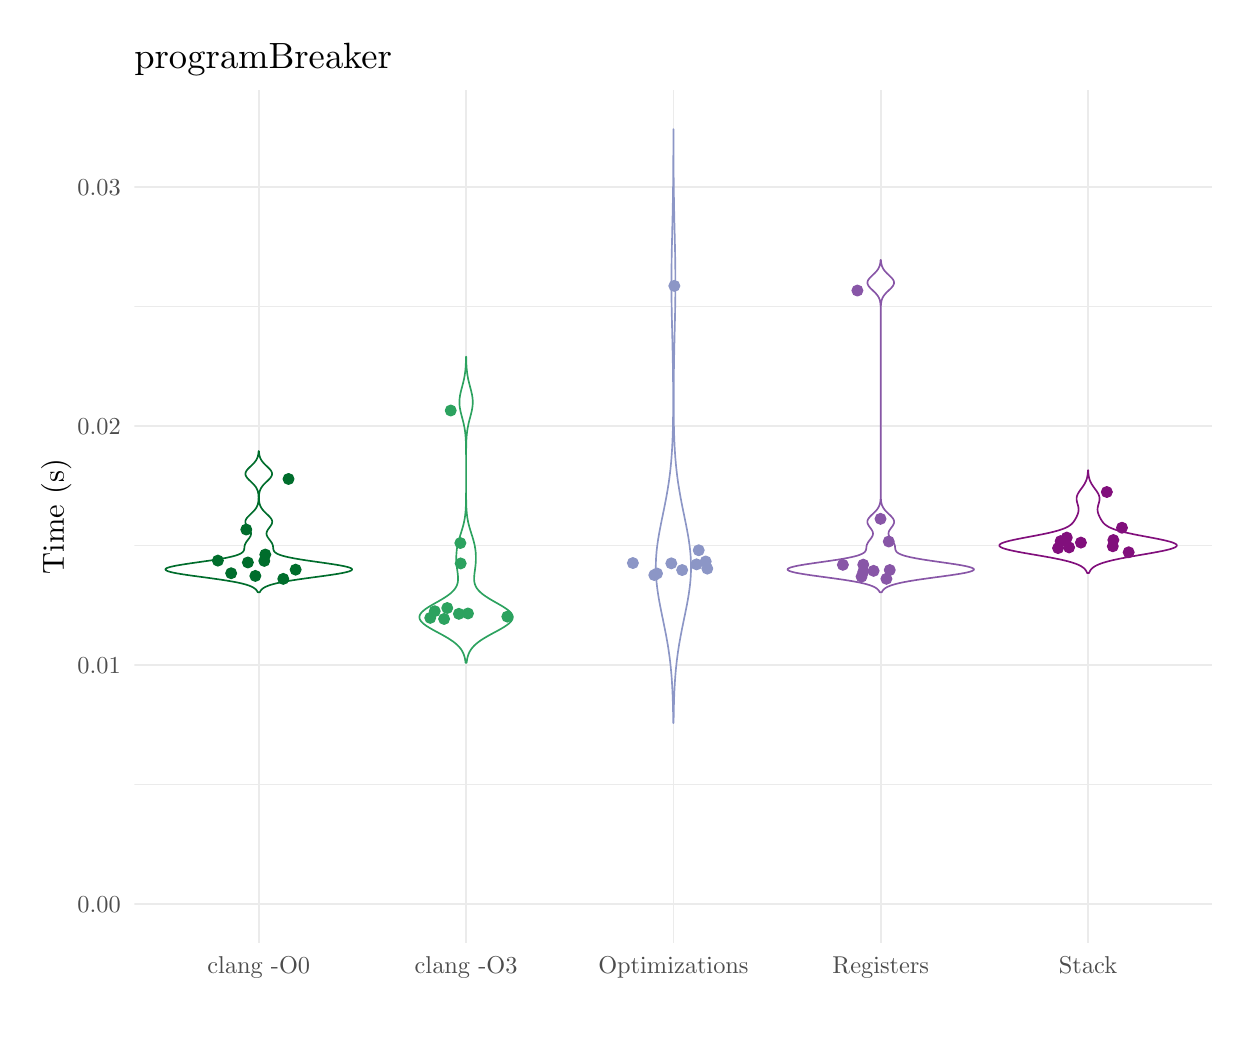
\begin{tikzpicture}[x=1pt,y=1pt]
\definecolor{fillColor}{RGB}{255,255,255}
\path[use as bounding box,fill=fillColor,fill opacity=0.00] (0,0) rectangle (433.62,361.35);
\begin{scope}
\path[clip] ( 38.56, 30.69) rectangle (428.12,338.69);
\definecolor{drawColor}{gray}{0.92}

\path[draw=drawColor,line width= 0.3pt,line join=round] ( 38.56, 87.86) --
	(428.12, 87.86);

\path[draw=drawColor,line width= 0.3pt,line join=round] ( 38.56,174.21) --
	(428.12,174.21);

\path[draw=drawColor,line width= 0.3pt,line join=round] ( 38.56,260.56) --
	(428.12,260.56);

\path[draw=drawColor,line width= 0.6pt,line join=round] ( 38.56, 44.69) --
	(428.12, 44.69);

\path[draw=drawColor,line width= 0.6pt,line join=round] ( 38.56,131.04) --
	(428.12,131.04);

\path[draw=drawColor,line width= 0.6pt,line join=round] ( 38.56,217.38) --
	(428.12,217.38);

\path[draw=drawColor,line width= 0.6pt,line join=round] ( 38.56,303.73) --
	(428.12,303.73);

\path[draw=drawColor,line width= 0.6pt,line join=round] ( 83.50, 30.69) --
	( 83.50,338.69);

\path[draw=drawColor,line width= 0.6pt,line join=round] (158.42, 30.69) --
	(158.42,338.69);

\path[draw=drawColor,line width= 0.6pt,line join=round] (233.34, 30.69) --
	(233.34,338.69);

\path[draw=drawColor,line width= 0.6pt,line join=round] (308.25, 30.69) --
	(308.25,338.69);

\path[draw=drawColor,line width= 0.6pt,line join=round] (383.17, 30.69) --
	(383.17,338.69);
\definecolor{drawColor}{RGB}{0,109,44}
\definecolor{fillColor}{RGB}{255,255,255}

\path[draw=drawColor,line width= 0.6pt,line join=round,line cap=round,fill=fillColor] ( 83.13,157.34) --
	( 83.08,157.44) --
	( 83.03,157.54) --
	( 82.98,157.64) --
	( 82.92,157.74) --
	( 82.86,157.84) --
	( 82.79,157.94) --
	( 82.72,158.04) --
	( 82.64,158.14) --
	( 82.55,158.24) --
	( 82.45,158.34) --
	( 82.35,158.44) --
	( 82.23,158.54) --
	( 82.11,158.64) --
	( 81.98,158.74) --
	( 81.83,158.84) --
	( 81.68,158.94) --
	( 81.51,159.04) --
	( 81.33,159.14) --
	( 81.14,159.24) --
	( 80.94,159.34) --
	( 80.72,159.44) --
	( 80.49,159.54) --
	( 80.24,159.64) --
	( 79.97,159.74) --
	( 79.69,159.84) --
	( 79.40,159.94) --
	( 79.08,160.04) --
	( 78.75,160.14) --
	( 78.40,160.24) --
	( 78.03,160.34) --
	( 77.64,160.44) --
	( 77.23,160.54) --
	( 76.81,160.64) --
	( 76.36,160.74) --
	( 75.89,160.84) --
	( 75.41,160.94) --
	( 74.90,161.04) --
	( 74.37,161.13) --
	( 73.83,161.23) --
	( 73.26,161.33) --
	( 72.68,161.43) --
	( 72.08,161.53) --
	( 71.46,161.63) --
	( 70.82,161.73) --
	( 70.17,161.83) --
	( 69.51,161.93) --
	( 68.82,162.03) --
	( 68.13,162.13) --
	( 67.43,162.23) --
	( 66.71,162.33) --
	( 65.99,162.43) --
	( 65.26,162.53) --
	( 64.52,162.63) --
	( 63.78,162.73) --
	( 63.04,162.83) --
	( 62.30,162.93) --
	( 61.56,163.03) --
	( 60.82,163.13) --
	( 60.09,163.23) --
	( 59.37,163.33) --
	( 58.66,163.43) --
	( 57.97,163.53) --
	( 57.28,163.63) --
	( 56.62,163.73) --
	( 55.97,163.83) --
	( 55.34,163.93) --
	( 54.75,164.03) --
	( 54.17,164.13) --
	( 53.62,164.23) --
	( 53.11,164.33) --
	( 52.63,164.43) --
	( 52.17,164.53) --
	( 51.75,164.63) --
	( 51.38,164.73) --
	( 51.04,164.83) --
	( 50.73,164.93) --
	( 50.47,165.03) --
	( 50.25,165.13) --
	( 50.07,165.23) --
	( 49.94,165.33) --
	( 49.85,165.43) --
	( 49.80,165.53) --
	( 49.79,165.63) --
	( 49.84,165.73) --
	( 49.92,165.83) --
	( 50.04,165.93) --
	( 50.22,166.03) --
	( 50.44,166.13) --
	( 50.68,166.23) --
	( 50.98,166.33) --
	( 51.32,166.43) --
	( 51.68,166.53) --
	( 52.09,166.62) --
	( 52.53,166.72) --
	( 53.00,166.82) --
	( 53.50,166.92) --
	( 54.04,167.02) --
	( 54.60,167.12) --
	( 55.18,167.22) --
	( 55.79,167.32) --
	( 56.41,167.42) --
	( 57.06,167.52) --
	( 57.72,167.62) --
	( 58.39,167.72) --
	( 59.07,167.82) --
	( 59.76,167.92) --
	( 60.46,168.02) --
	( 61.17,168.12) --
	( 61.87,168.22) --
	( 62.58,168.32) --
	( 63.28,168.42) --
	( 63.98,168.52) --
	( 64.67,168.62) --
	( 65.35,168.72) --
	( 66.03,168.82) --
	( 66.69,168.92) --
	( 67.34,169.02) --
	( 67.98,169.12) --
	( 68.60,169.22) --
	( 69.20,169.32) --
	( 69.79,169.42) --
	( 70.36,169.52) --
	( 70.90,169.62) --
	( 71.43,169.72) --
	( 71.94,169.82) --
	( 72.42,169.92) --
	( 72.88,170.02) --
	( 73.32,170.12) --
	( 73.75,170.22) --
	( 74.14,170.32) --
	( 74.51,170.42) --
	( 74.87,170.52) --
	( 75.20,170.62) --
	( 75.50,170.72) --
	( 75.79,170.82) --
	( 76.06,170.92) --
	( 76.31,171.02) --
	( 76.54,171.12) --
	( 76.75,171.22) --
	( 76.94,171.32) --
	( 77.11,171.42) --
	( 77.27,171.52) --
	( 77.41,171.62) --
	( 77.54,171.72) --
	( 77.65,171.82) --
	( 77.75,171.92) --
	( 77.84,172.02) --
	( 77.92,172.11) --
	( 77.98,172.21) --
	( 78.04,172.31) --
	( 78.09,172.41) --
	( 78.13,172.51) --
	( 78.17,172.61) --
	( 78.19,172.71) --
	( 78.22,172.81) --
	( 78.24,172.91) --
	( 78.25,173.01) --
	( 78.27,173.11) --
	( 78.28,173.21) --
	( 78.29,173.31) --
	( 78.30,173.41) --
	( 78.31,173.51) --
	( 78.32,173.61) --
	( 78.33,173.71) --
	( 78.34,173.81) --
	( 78.36,173.91) --
	( 78.37,174.01) --
	( 78.39,174.11) --
	( 78.42,174.21) --
	( 78.44,174.31) --
	( 78.47,174.41) --
	( 78.50,174.51) --
	( 78.54,174.61) --
	( 78.58,174.71) --
	( 78.62,174.81) --
	( 78.67,174.91) --
	( 78.72,175.01) --
	( 78.77,175.11) --
	( 78.83,175.21) --
	( 78.89,175.31) --
	( 78.95,175.41) --
	( 79.01,175.51) --
	( 79.08,175.61) --
	( 79.15,175.71) --
	( 79.23,175.81) --
	( 79.30,175.91) --
	( 79.38,176.01) --
	( 79.45,176.11) --
	( 79.53,176.21) --
	( 79.61,176.31) --
	( 79.68,176.41) --
	( 79.76,176.51) --
	( 79.84,176.61) --
	( 79.91,176.71) --
	( 79.99,176.81) --
	( 80.06,176.91) --
	( 80.13,177.01) --
	( 80.19,177.11) --
	( 80.26,177.21) --
	( 80.32,177.31) --
	( 80.37,177.41) --
	( 80.43,177.50) --
	( 80.48,177.60) --
	( 80.52,177.70) --
	( 80.56,177.80) --
	( 80.60,177.90) --
	( 80.63,178.00) --
	( 80.65,178.10) --
	( 80.67,178.20) --
	( 80.69,178.30) --
	( 80.70,178.40) --
	( 80.70,178.50) --
	( 80.70,178.60) --
	( 80.69,178.70) --
	( 80.68,178.80) --
	( 80.67,178.90) --
	( 80.64,179.00) --
	( 80.61,179.10) --
	( 80.58,179.20) --
	( 80.54,179.30) --
	( 80.50,179.40) --
	( 80.46,179.50) --
	( 80.40,179.60) --
	( 80.35,179.70) --
	( 80.29,179.80) --
	( 80.23,179.90) --
	( 80.17,180.00) --
	( 80.10,180.10) --
	( 80.03,180.20) --
	( 79.96,180.30) --
	( 79.89,180.40) --
	( 79.81,180.50) --
	( 79.74,180.60) --
	( 79.66,180.70) --
	( 79.59,180.80) --
	( 79.51,180.90) --
	( 79.44,181.00) --
	( 79.37,181.10) --
	( 79.29,181.20) --
	( 79.23,181.30) --
	( 79.16,181.40) --
	( 79.10,181.50) --
	( 79.04,181.60) --
	( 78.98,181.70) --
	( 78.92,181.80) --
	( 78.88,181.90) --
	( 78.83,182.00) --
	( 78.79,182.10) --
	( 78.75,182.20) --
	( 78.73,182.30) --
	( 78.70,182.40) --
	( 78.68,182.50) --
	( 78.67,182.60) --
	( 78.66,182.70) --
	( 78.66,182.80) --
	( 78.66,182.90) --
	( 78.67,182.99) --
	( 78.69,183.09) --
	( 78.71,183.19) --
	( 78.74,183.29) --
	( 78.77,183.39) --
	( 78.81,183.49) --
	( 78.85,183.59) --
	( 78.91,183.69) --
	( 78.96,183.79) --
	( 79.02,183.89) --
	( 79.09,183.99) --
	( 79.16,184.09) --
	( 79.23,184.19) --
	( 79.31,184.29) --
	( 79.39,184.39) --
	( 79.48,184.49) --
	( 79.57,184.59) --
	( 79.66,184.69) --
	( 79.76,184.79) --
	( 79.86,184.89) --
	( 79.96,184.99) --
	( 80.06,185.09) --
	( 80.16,185.19) --
	( 80.26,185.29) --
	( 80.37,185.39) --
	( 80.48,185.49) --
	( 80.58,185.59) --
	( 80.69,185.69) --
	( 80.79,185.79) --
	( 80.90,185.89) --
	( 81.00,185.99) --
	( 81.11,186.09) --
	( 81.21,186.19) --
	( 81.31,186.29) --
	( 81.41,186.39) --
	( 81.51,186.49) --
	( 81.60,186.59) --
	( 81.69,186.69) --
	( 81.79,186.79) --
	( 81.87,186.89) --
	( 81.96,186.99) --
	( 82.04,187.09) --
	( 82.12,187.19) --
	( 82.20,187.29) --
	( 82.28,187.39) --
	( 82.35,187.49) --
	( 82.42,187.59) --
	( 82.48,187.69) --
	( 82.55,187.79) --
	( 82.61,187.89) --
	( 82.67,187.99) --
	( 82.72,188.09) --
	( 82.78,188.19) --
	( 82.83,188.29) --
	( 82.87,188.39) --
	( 82.92,188.48) --
	( 82.96,188.58) --
	( 83.00,188.68) --
	( 83.04,188.78) --
	( 83.07,188.88) --
	( 83.11,188.98) --
	( 83.14,189.08) --
	( 83.17,189.18) --
	( 83.19,189.28) --
	( 83.22,189.38) --
	( 83.24,189.48) --
	( 83.26,189.58) --
	( 83.28,189.68) --
	( 83.30,189.78) --
	( 83.32,189.88) --
	( 83.33,189.98) --
	( 83.35,190.08) --
	( 83.36,190.18) --
	( 83.37,190.28) --
	( 83.38,190.38) --
	( 83.39,190.48) --
	( 83.40,190.58) --
	( 83.41,190.68) --
	( 83.42,190.78) --
	( 83.42,190.88) --
	( 83.43,190.98) --
	( 83.43,191.08) --
	( 83.43,191.18) --
	( 83.43,191.28) --
	( 83.44,191.38) --
	( 83.44,191.48) --
	( 83.44,191.58) --
	( 83.43,191.68) --
	( 83.43,191.78) --
	( 83.43,191.88) --
	( 83.43,191.98) --
	( 83.42,192.08) --
	( 83.42,192.18) --
	( 83.41,192.28) --
	( 83.40,192.38) --
	( 83.39,192.48) --
	( 83.38,192.58) --
	( 83.37,192.68) --
	( 83.36,192.78) --
	( 83.35,192.88) --
	( 83.33,192.98) --
	( 83.32,193.08) --
	( 83.30,193.18) --
	( 83.28,193.28) --
	( 83.26,193.38) --
	( 83.24,193.48) --
	( 83.22,193.58) --
	( 83.19,193.68) --
	( 83.17,193.78) --
	( 83.14,193.87) --
	( 83.11,193.97) --
	( 83.07,194.07) --
	( 83.04,194.17) --
	( 83.00,194.27) --
	( 82.96,194.37) --
	( 82.92,194.47) --
	( 82.87,194.57) --
	( 82.83,194.67) --
	( 82.78,194.77) --
	( 82.72,194.87) --
	( 82.67,194.97) --
	( 82.61,195.07) --
	( 82.55,195.17) --
	( 82.49,195.27) --
	( 82.42,195.37) --
	( 82.35,195.47) --
	( 82.28,195.57) --
	( 82.20,195.67) --
	( 82.12,195.77) --
	( 82.04,195.87) --
	( 81.96,195.97) --
	( 81.87,196.07) --
	( 81.79,196.17) --
	( 81.70,196.27) --
	( 81.60,196.37) --
	( 81.51,196.47) --
	( 81.41,196.57) --
	( 81.31,196.67) --
	( 81.21,196.77) --
	( 81.11,196.87) --
	( 81.01,196.97) --
	( 80.90,197.07) --
	( 80.80,197.17) --
	( 80.69,197.27) --
	( 80.58,197.37) --
	( 80.48,197.47) --
	( 80.37,197.57) --
	( 80.27,197.67) --
	( 80.16,197.77) --
	( 80.06,197.87) --
	( 79.96,197.97) --
	( 79.86,198.07) --
	( 79.76,198.17) --
	( 79.67,198.27) --
	( 79.57,198.37) --
	( 79.49,198.47) --
	( 79.40,198.57) --
	( 79.32,198.67) --
	( 79.24,198.77) --
	( 79.17,198.87) --
	( 79.10,198.97) --
	( 79.03,199.07) --
	( 78.97,199.17) --
	( 78.92,199.27) --
	( 78.87,199.36) --
	( 78.83,199.46) --
	( 78.79,199.56) --
	( 78.76,199.66) --
	( 78.73,199.76) --
	( 78.71,199.86) --
	( 78.70,199.96) --
	( 78.69,200.06) --
	( 78.69,200.16) --
	( 78.70,200.26) --
	( 78.71,200.36) --
	( 78.73,200.46) --
	( 78.76,200.56) --
	( 78.79,200.66) --
	( 78.82,200.76) --
	( 78.87,200.86) --
	( 78.92,200.96) --
	( 78.97,201.06) --
	( 79.03,201.16) --
	( 79.09,201.26) --
	( 79.16,201.36) --
	( 79.24,201.46) --
	( 79.32,201.56) --
	( 79.40,201.66) --
	( 79.48,201.76) --
	( 79.57,201.86) --
	( 79.66,201.96) --
	( 79.76,202.06) --
	( 79.86,202.16) --
	( 79.96,202.26) --
	( 80.06,202.36) --
	( 80.16,202.46) --
	( 80.26,202.56) --
	( 80.37,202.66) --
	( 80.48,202.76) --
	( 80.58,202.86) --
	( 80.69,202.96) --
	( 80.79,203.06) --
	( 80.90,203.16) --
	( 81.00,203.26) --
	( 81.11,203.36) --
	( 81.21,203.46) --
	( 81.31,203.56) --
	( 81.41,203.66) --
	( 81.50,203.76) --
	( 81.60,203.86) --
	( 81.69,203.96) --
	( 81.78,204.06) --
	( 81.87,204.16) --
	( 81.96,204.26) --
	( 82.04,204.36) --
	( 82.12,204.46) --
	( 82.20,204.56) --
	( 82.28,204.66) --
	( 82.35,204.76) --
	( 82.42,204.85) --
	( 82.48,204.95) --
	( 82.55,205.05) --
	( 82.61,205.15) --
	( 82.67,205.25) --
	( 82.72,205.35) --
	( 82.78,205.45) --
	( 82.83,205.55) --
	( 82.87,205.65) --
	( 82.92,205.75) --
	( 82.96,205.85) --
	( 83.00,205.95) --
	( 83.04,206.05) --
	( 83.07,206.15) --
	( 83.11,206.25) --
	( 83.14,206.35) --
	( 83.17,206.45) --
	( 83.19,206.55) --
	( 83.22,206.65) --
	( 83.24,206.75) --
	( 83.27,206.85) --
	( 83.29,206.95) --
	( 83.31,207.05) --
	( 83.32,207.15) --
	( 83.34,207.25) --
	( 83.35,207.35) --
	( 83.37,207.45) --
	( 83.38,207.55) --
	( 83.39,207.65) --
	( 83.40,207.75) --
	( 83.41,207.85) --
	( 83.42,207.95) --
	( 83.43,208.05) --
	( 83.44,208.15) --
	( 83.44,208.25) --
	( 83.45,208.35) --
	( 83.56,208.35) --
	( 83.57,208.25) --
	( 83.57,208.15) --
	( 83.58,208.05) --
	( 83.59,207.95) --
	( 83.60,207.85) --
	( 83.61,207.75) --
	( 83.62,207.65) --
	( 83.63,207.55) --
	( 83.64,207.45) --
	( 83.66,207.35) --
	( 83.67,207.25) --
	( 83.69,207.15) --
	( 83.70,207.05) --
	( 83.72,206.95) --
	( 83.74,206.85) --
	( 83.77,206.75) --
	( 83.79,206.65) --
	( 83.82,206.55) --
	( 83.84,206.45) --
	( 83.87,206.35) --
	( 83.90,206.25) --
	( 83.94,206.15) --
	( 83.97,206.05) --
	( 84.01,205.95) --
	( 84.05,205.85) --
	( 84.09,205.75) --
	( 84.14,205.65) --
	( 84.18,205.55) --
	( 84.23,205.45) --
	( 84.29,205.35) --
	( 84.34,205.25) --
	( 84.40,205.15) --
	( 84.46,205.05) --
	( 84.53,204.95) --
	( 84.59,204.85) --
	( 84.66,204.76) --
	( 84.73,204.66) --
	( 84.81,204.56) --
	( 84.89,204.46) --
	( 84.97,204.36) --
	( 85.05,204.26) --
	( 85.14,204.16) --
	( 85.23,204.06) --
	( 85.32,203.96) --
	( 85.41,203.86) --
	( 85.50,203.76) --
	( 85.60,203.66) --
	( 85.70,203.56) --
	( 85.80,203.46) --
	( 85.90,203.36) --
	( 86.01,203.26) --
	( 86.11,203.16) --
	( 86.22,203.06) --
	( 86.32,202.96) --
	( 86.43,202.86) --
	( 86.53,202.76) --
	( 86.64,202.66) --
	( 86.74,202.56) --
	( 86.85,202.46) --
	( 86.95,202.36) --
	( 87.05,202.26) --
	( 87.15,202.16) --
	( 87.25,202.06) --
	( 87.35,201.96) --
	( 87.44,201.86) --
	( 87.53,201.76) --
	( 87.61,201.66) --
	( 87.69,201.56) --
	( 87.77,201.46) --
	( 87.85,201.36) --
	( 87.91,201.26) --
	( 87.98,201.16) --
	( 88.04,201.06) --
	( 88.09,200.96) --
	( 88.14,200.86) --
	( 88.19,200.76) --
	( 88.22,200.66) --
	( 88.25,200.56) --
	( 88.28,200.46) --
	( 88.30,200.36) --
	( 88.31,200.26) --
	( 88.32,200.16) --
	( 88.32,200.06) --
	( 88.31,199.96) --
	( 88.30,199.86) --
	( 88.28,199.76) --
	( 88.25,199.66) --
	( 88.22,199.56) --
	( 88.18,199.46) --
	( 88.14,199.36) --
	( 88.09,199.27) --
	( 88.04,199.17) --
	( 87.98,199.07) --
	( 87.91,198.97) --
	( 87.84,198.87) --
	( 87.77,198.77) --
	( 87.69,198.67) --
	( 87.61,198.57) --
	( 87.52,198.47) --
	( 87.43,198.37) --
	( 87.34,198.27) --
	( 87.25,198.17) --
	( 87.15,198.07) --
	( 87.05,197.97) --
	( 86.95,197.87) --
	( 86.85,197.77) --
	( 86.74,197.67) --
	( 86.64,197.57) --
	( 86.53,197.47) --
	( 86.43,197.37) --
	( 86.32,197.27) --
	( 86.21,197.17) --
	( 86.11,197.07) --
	( 86.00,196.97) --
	( 85.90,196.87) --
	( 85.80,196.77) --
	( 85.70,196.67) --
	( 85.60,196.57) --
	( 85.50,196.47) --
	( 85.41,196.37) --
	( 85.31,196.27) --
	( 85.22,196.17) --
	( 85.13,196.07) --
	( 85.05,195.97) --
	( 84.97,195.87) --
	( 84.88,195.77) --
	( 84.81,195.67) --
	( 84.73,195.57) --
	( 84.66,195.47) --
	( 84.59,195.37) --
	( 84.52,195.27) --
	( 84.46,195.17) --
	( 84.40,195.07) --
	( 84.34,194.97) --
	( 84.29,194.87) --
	( 84.23,194.77) --
	( 84.18,194.67) --
	( 84.14,194.57) --
	( 84.09,194.47) --
	( 84.05,194.37) --
	( 84.01,194.27) --
	( 83.97,194.17) --
	( 83.94,194.07) --
	( 83.90,193.97) --
	( 83.87,193.87) --
	( 83.84,193.78) --
	( 83.82,193.68) --
	( 83.79,193.58) --
	( 83.77,193.48) --
	( 83.75,193.38) --
	( 83.73,193.28) --
	( 83.71,193.18) --
	( 83.69,193.08) --
	( 83.68,192.98) --
	( 83.66,192.88) --
	( 83.65,192.78) --
	( 83.64,192.68) --
	( 83.63,192.58) --
	( 83.62,192.48) --
	( 83.61,192.38) --
	( 83.60,192.28) --
	( 83.59,192.18) --
	( 83.59,192.08) --
	( 83.58,191.98) --
	( 83.58,191.88) --
	( 83.58,191.78) --
	( 83.58,191.68) --
	( 83.57,191.58) --
	( 83.57,191.48) --
	( 83.57,191.38) --
	( 83.58,191.28) --
	( 83.58,191.18) --
	( 83.58,191.08) --
	( 83.58,190.98) --
	( 83.59,190.88) --
	( 83.59,190.78) --
	( 83.60,190.68) --
	( 83.61,190.58) --
	( 83.62,190.48) --
	( 83.63,190.38) --
	( 83.64,190.28) --
	( 83.65,190.18) --
	( 83.66,190.08) --
	( 83.68,189.98) --
	( 83.69,189.88) --
	( 83.71,189.78) --
	( 83.73,189.68) --
	( 83.75,189.58) --
	( 83.77,189.48) --
	( 83.79,189.38) --
	( 83.82,189.28) --
	( 83.84,189.18) --
	( 83.87,189.08) --
	( 83.90,188.98) --
	( 83.94,188.88) --
	( 83.97,188.78) --
	( 84.01,188.68) --
	( 84.05,188.58) --
	( 84.09,188.48) --
	( 84.14,188.39) --
	( 84.18,188.29) --
	( 84.23,188.19) --
	( 84.29,188.09) --
	( 84.34,187.99) --
	( 84.40,187.89) --
	( 84.46,187.79) --
	( 84.53,187.69) --
	( 84.59,187.59) --
	( 84.66,187.49) --
	( 84.73,187.39) --
	( 84.81,187.29) --
	( 84.89,187.19) --
	( 84.97,187.09) --
	( 85.05,186.99) --
	( 85.14,186.89) --
	( 85.22,186.79) --
	( 85.32,186.69) --
	( 85.41,186.59) --
	( 85.50,186.49) --
	( 85.60,186.39) --
	( 85.70,186.29) --
	( 85.80,186.19) --
	( 85.90,186.09) --
	( 86.01,185.99) --
	( 86.11,185.89) --
	( 86.22,185.79) --
	( 86.32,185.69) --
	( 86.43,185.59) --
	( 86.53,185.49) --
	( 86.64,185.39) --
	( 86.74,185.29) --
	( 86.85,185.19) --
	( 86.95,185.09) --
	( 87.05,184.99) --
	( 87.15,184.89) --
	( 87.25,184.79) --
	( 87.35,184.69) --
	( 87.44,184.59) --
	( 87.53,184.49) --
	( 87.62,184.39) --
	( 87.70,184.29) --
	( 87.78,184.19) --
	( 87.85,184.09) --
	( 87.92,183.99) --
	( 87.99,183.89) --
	( 88.05,183.79) --
	( 88.10,183.69) --
	( 88.15,183.59) --
	( 88.20,183.49) --
	( 88.24,183.39) --
	( 88.27,183.29) --
	( 88.30,183.19) --
	( 88.32,183.09) --
	( 88.34,182.99) --
	( 88.35,182.90) --
	( 88.35,182.80) --
	( 88.35,182.70) --
	( 88.34,182.60) --
	( 88.33,182.50) --
	( 88.31,182.40) --
	( 88.28,182.30) --
	( 88.25,182.20) --
	( 88.22,182.10) --
	( 88.18,182.00) --
	( 88.13,181.90) --
	( 88.09,181.80) --
	( 88.03,181.70) --
	( 87.97,181.60) --
	( 87.91,181.50) --
	( 87.85,181.40) --
	( 87.78,181.30) --
	( 87.72,181.20) --
	( 87.64,181.10) --
	( 87.57,181.00) --
	( 87.50,180.90) --
	( 87.42,180.80) --
	( 87.35,180.70) --
	( 87.27,180.60) --
	( 87.20,180.50) --
	( 87.12,180.40) --
	( 87.05,180.30) --
	( 86.98,180.20) --
	( 86.91,180.10) --
	( 86.84,180.00) --
	( 86.78,179.90) --
	( 86.72,179.80) --
	( 86.66,179.70) --
	( 86.61,179.60) --
	( 86.55,179.50) --
	( 86.51,179.40) --
	( 86.47,179.30) --
	( 86.43,179.20) --
	( 86.40,179.10) --
	( 86.37,179.00) --
	( 86.34,178.90) --
	( 86.33,178.80) --
	( 86.32,178.70) --
	( 86.31,178.60) --
	( 86.31,178.50) --
	( 86.31,178.40) --
	( 86.32,178.30) --
	( 86.34,178.20) --
	( 86.36,178.10) --
	( 86.38,178.00) --
	( 86.41,177.90) --
	( 86.45,177.80) --
	( 86.49,177.70) --
	( 86.53,177.60) --
	( 86.58,177.50) --
	( 86.64,177.41) --
	( 86.69,177.31) --
	( 86.75,177.21) --
	( 86.82,177.11) --
	( 86.88,177.01) --
	( 86.95,176.91) --
	( 87.02,176.81) --
	( 87.10,176.71) --
	( 87.17,176.61) --
	( 87.25,176.51) --
	( 87.33,176.41) --
	( 87.40,176.31) --
	( 87.48,176.21) --
	( 87.56,176.11) --
	( 87.63,176.01) --
	( 87.71,175.91) --
	( 87.78,175.81) --
	( 87.86,175.71) --
	( 87.93,175.61) --
	( 87.99,175.51) --
	( 88.06,175.41) --
	( 88.12,175.31) --
	( 88.18,175.21) --
	( 88.24,175.11) --
	( 88.29,175.01) --
	( 88.34,174.91) --
	( 88.39,174.81) --
	( 88.43,174.71) --
	( 88.47,174.61) --
	( 88.51,174.51) --
	( 88.54,174.41) --
	( 88.57,174.31) --
	( 88.59,174.21) --
	( 88.62,174.11) --
	( 88.64,174.01) --
	( 88.65,173.91) --
	( 88.67,173.81) --
	( 88.68,173.71) --
	( 88.69,173.61) --
	( 88.70,173.51) --
	( 88.71,173.41) --
	( 88.72,173.31) --
	( 88.73,173.21) --
	( 88.74,173.11) --
	( 88.76,173.01) --
	( 88.77,172.91) --
	( 88.79,172.81) --
	( 88.82,172.71) --
	( 88.84,172.61) --
	( 88.88,172.51) --
	( 88.92,172.41) --
	( 88.97,172.31) --
	( 89.02,172.21) --
	( 89.09,172.11) --
	( 89.17,172.02) --
	( 89.26,171.92) --
	( 89.36,171.82) --
	( 89.47,171.72) --
	( 89.60,171.62) --
	( 89.74,171.52) --
	( 89.90,171.42) --
	( 90.07,171.32) --
	( 90.26,171.22) --
	( 90.47,171.12) --
	( 90.70,171.02) --
	( 90.95,170.92) --
	( 91.22,170.82) --
	( 91.51,170.72) --
	( 91.81,170.62) --
	( 92.14,170.52) --
	( 92.50,170.42) --
	( 92.87,170.32) --
	( 93.26,170.22) --
	( 93.69,170.12) --
	( 94.13,170.02) --
	( 94.59,169.92) --
	( 95.07,169.82) --
	( 95.58,169.72) --
	( 96.11,169.62) --
	( 96.65,169.52) --
	( 97.22,169.42) --
	( 97.81,169.32) --
	( 98.41,169.22) --
	( 99.03,169.12) --
	( 99.67,169.02) --
	(100.32,168.92) --
	(100.98,168.82) --
	(101.66,168.72) --
	(102.34,168.62) --
	(103.03,168.52) --
	(103.73,168.42) --
	(104.43,168.32) --
	(105.14,168.22) --
	(105.84,168.12) --
	(106.55,168.02) --
	(107.25,167.92) --
	(107.94,167.82) --
	(108.62,167.72) --
	(109.29,167.62) --
	(109.95,167.52) --
	(110.60,167.42) --
	(111.22,167.32) --
	(111.83,167.22) --
	(112.41,167.12) --
	(112.97,167.02) --
	(113.51,166.92) --
	(114.01,166.82) --
	(114.48,166.72) --
	(114.92,166.62) --
	(115.33,166.53) --
	(115.69,166.43) --
	(116.03,166.33) --
	(116.33,166.23) --
	(116.57,166.13) --
	(116.79,166.03) --
	(116.97,165.93) --
	(117.09,165.83) --
	(117.17,165.73) --
	(117.22,165.63) --
	(117.21,165.53) --
	(117.16,165.43) --
	(117.07,165.33) --
	(116.94,165.23) --
	(116.76,165.13) --
	(116.54,165.03) --
	(116.28,164.93) --
	(115.97,164.83) --
	(115.63,164.73) --
	(115.26,164.63) --
	(114.84,164.53) --
	(114.38,164.43) --
	(113.90,164.33) --
	(113.39,164.23) --
	(112.84,164.13) --
	(112.26,164.03) --
	(111.67,163.93) --
	(111.04,163.83) --
	(110.39,163.73) --
	(109.73,163.63) --
	(109.04,163.53) --
	(108.35,163.43) --
	(107.64,163.33) --
	(106.92,163.23) --
	(106.19,163.13) --
	(105.45,163.03) --
	(104.71,162.93) --
	(103.97,162.83) --
	(103.23,162.73) --
	(102.49,162.63) --
	(101.75,162.53) --
	(101.02,162.43) --
	(100.30,162.33) --
	( 99.58,162.23) --
	( 98.88,162.13) --
	( 98.19,162.03) --
	( 97.50,161.93) --
	( 96.84,161.83) --
	( 96.19,161.73) --
	( 95.55,161.63) --
	( 94.93,161.53) --
	( 94.33,161.43) --
	( 93.75,161.33) --
	( 93.18,161.23) --
	( 92.64,161.13) --
	( 92.11,161.04) --
	( 91.60,160.94) --
	( 91.12,160.84) --
	( 90.65,160.74) --
	( 90.20,160.64) --
	( 89.78,160.54) --
	( 89.37,160.44) --
	( 88.98,160.34) --
	( 88.61,160.24) --
	( 88.26,160.14) --
	( 87.93,160.04) --
	( 87.61,159.94) --
	( 87.32,159.84) --
	( 87.04,159.74) --
	( 86.77,159.64) --
	( 86.52,159.54) --
	( 86.29,159.44) --
	( 86.07,159.34) --
	( 85.87,159.24) --
	( 85.68,159.14) --
	( 85.50,159.04) --
	( 85.33,158.94) --
	( 85.18,158.84) --
	( 85.03,158.74) --
	( 84.90,158.64) --
	( 84.78,158.54) --
	( 84.66,158.44) --
	( 84.56,158.34) --
	( 84.46,158.24) --
	( 84.37,158.14) --
	( 84.29,158.04) --
	( 84.22,157.94) --
	( 84.15,157.84) --
	( 84.09,157.74) --
	( 84.03,157.64) --
	( 83.98,157.54) --
	( 83.93,157.44) --
	( 83.88,157.34) --
	( 83.13,157.34) --
	cycle;
\definecolor{drawColor}{RGB}{44,162,95}

\path[draw=drawColor,line width= 0.6pt,line join=round,line cap=round,fill=fillColor] (158.23,131.84) --
	(158.21,132.06) --
	(158.18,132.27) --
	(158.15,132.49) --
	(158.12,132.70) --
	(158.09,132.92) --
	(158.05,133.14) --
	(158.00,133.35) --
	(157.96,133.57) --
	(157.91,133.79) --
	(157.85,134.00) --
	(157.79,134.22) --
	(157.72,134.44) --
	(157.65,134.65) --
	(157.57,134.87) --
	(157.49,135.09) --
	(157.40,135.30) --
	(157.30,135.52) --
	(157.19,135.74) --
	(157.07,135.95) --
	(156.95,136.17) --
	(156.82,136.39) --
	(156.68,136.60) --
	(156.53,136.82) --
	(156.36,137.04) --
	(156.19,137.25) --
	(156.01,137.47) --
	(155.82,137.68) --
	(155.61,137.90) --
	(155.40,138.12) --
	(155.17,138.33) --
	(154.93,138.55) --
	(154.68,138.77) --
	(154.42,138.98) --
	(154.15,139.20) --
	(153.87,139.42) --
	(153.57,139.63) --
	(153.26,139.85) --
	(152.94,140.07) --
	(152.62,140.28) --
	(152.28,140.50) --
	(151.93,140.72) --
	(151.57,140.93) --
	(151.20,141.15) --
	(150.83,141.37) --
	(150.45,141.58) --
	(150.06,141.80) --
	(149.67,142.02) --
	(149.27,142.23) --
	(148.87,142.45) --
	(148.47,142.67) --
	(148.07,142.88) --
	(147.67,143.10) --
	(147.27,143.31) --
	(146.87,143.53) --
	(146.48,143.75) --
	(146.09,143.96) --
	(145.71,144.18) --
	(145.34,144.40) --
	(144.98,144.61) --
	(144.63,144.83) --
	(144.29,145.05) --
	(143.96,145.26) --
	(143.66,145.48) --
	(143.37,145.70) --
	(143.10,145.91) --
	(142.84,146.13) --
	(142.61,146.35) --
	(142.40,146.56) --
	(142.20,146.78) --
	(142.04,147.00) --
	(141.90,147.21) --
	(141.78,147.43) --
	(141.69,147.65) --
	(141.62,147.86) --
	(141.58,148.08) --
	(141.56,148.30) --
	(141.57,148.51) --
	(141.61,148.73) --
	(141.67,148.94) --
	(141.75,149.16) --
	(141.87,149.38) --
	(142.00,149.59) --
	(142.15,149.81) --
	(142.34,150.03) --
	(142.55,150.24) --
	(142.77,150.46) --
	(143.01,150.68) --
	(143.28,150.89) --
	(143.56,151.11) --
	(143.85,151.33) --
	(144.17,151.54) --
	(144.49,151.76) --
	(144.83,151.98) --
	(145.18,152.19) --
	(145.54,152.41) --
	(145.90,152.63) --
	(146.27,152.84) --
	(146.65,153.06) --
	(147.03,153.28) --
	(147.41,153.49) --
	(147.80,153.71) --
	(148.18,153.92) --
	(148.56,154.14) --
	(148.93,154.36) --
	(149.30,154.57) --
	(149.67,154.79) --
	(150.03,155.01) --
	(150.38,155.22) --
	(150.72,155.44) --
	(151.06,155.66) --
	(151.38,155.87) --
	(151.69,156.09) --
	(151.99,156.31) --
	(152.28,156.52) --
	(152.56,156.74) --
	(152.82,156.96) --
	(153.07,157.17) --
	(153.31,157.39) --
	(153.53,157.61) --
	(153.74,157.82) --
	(153.94,158.04) --
	(154.12,158.26) --
	(154.29,158.47) --
	(154.45,158.69) --
	(154.60,158.91) --
	(154.73,159.12) --
	(154.85,159.34) --
	(154.96,159.55) --
	(155.06,159.77) --
	(155.14,159.99) --
	(155.22,160.20) --
	(155.29,160.42) --
	(155.34,160.64) --
	(155.39,160.85) --
	(155.43,161.07) --
	(155.46,161.29) --
	(155.48,161.50) --
	(155.50,161.72) --
	(155.51,161.94) --
	(155.52,162.15) --
	(155.52,162.37) --
	(155.51,162.59) --
	(155.50,162.80) --
	(155.49,163.02) --
	(155.47,163.24) --
	(155.46,163.45) --
	(155.43,163.67) --
	(155.41,163.89) --
	(155.39,164.10) --
	(155.36,164.32) --
	(155.33,164.54) --
	(155.30,164.75) --
	(155.27,164.97) --
	(155.25,165.18) --
	(155.22,165.40) --
	(155.19,165.62) --
	(155.16,165.83) --
	(155.13,166.05) --
	(155.11,166.27) --
	(155.08,166.48) --
	(155.06,166.70) --
	(155.03,166.92) --
	(155.01,167.13) --
	(154.99,167.35) --
	(154.97,167.57) --
	(154.96,167.78) --
	(154.94,168.00) --
	(154.93,168.22) --
	(154.91,168.43) --
	(154.90,168.65) --
	(154.89,168.87) --
	(154.89,169.08) --
	(154.88,169.30) --
	(154.88,169.52) --
	(154.88,169.73) --
	(154.88,169.95) --
	(154.88,170.16) --
	(154.89,170.38) --
	(154.89,170.60) --
	(154.90,170.81) --
	(154.91,171.03) --
	(154.93,171.25) --
	(154.94,171.46) --
	(154.96,171.68) --
	(154.98,171.90) --
	(155.00,172.11) --
	(155.02,172.33) --
	(155.05,172.55) --
	(155.07,172.76) --
	(155.10,172.98) --
	(155.14,173.20) --
	(155.17,173.41) --
	(155.21,173.63) --
	(155.25,173.85) --
	(155.29,174.06) --
	(155.33,174.28) --
	(155.37,174.50) --
	(155.42,174.71) --
	(155.47,174.93) --
	(155.52,175.15) --
	(155.57,175.36) --
	(155.63,175.58) --
	(155.69,175.79) --
	(155.74,176.01) --
	(155.80,176.23) --
	(155.87,176.44) --
	(155.93,176.66) --
	(155.99,176.88) --
	(156.06,177.09) --
	(156.12,177.31) --
	(156.19,177.53) --
	(156.26,177.74) --
	(156.32,177.96) --
	(156.39,178.18) --
	(156.46,178.39) --
	(156.53,178.61) --
	(156.60,178.83) --
	(156.67,179.04) --
	(156.73,179.26) --
	(156.80,179.48) --
	(156.87,179.69) --
	(156.94,179.91) --
	(157.00,180.13) --
	(157.06,180.34) --
	(157.13,180.56) --
	(157.19,180.77) --
	(157.25,180.99) --
	(157.31,181.21) --
	(157.37,181.42) --
	(157.42,181.64) --
	(157.48,181.86) --
	(157.53,182.07) --
	(157.58,182.29) --
	(157.63,182.51) --
	(157.68,182.72) --
	(157.72,182.94) --
	(157.77,183.16) --
	(157.81,183.37) --
	(157.85,183.59) --
	(157.89,183.81) --
	(157.92,184.02) --
	(157.96,184.24) --
	(157.99,184.46) --
	(158.02,184.67) --
	(158.05,184.89) --
	(158.08,185.11) --
	(158.11,185.32) --
	(158.13,185.54) --
	(158.15,185.76) --
	(158.17,185.97) --
	(158.19,186.19) --
	(158.21,186.40) --
	(158.23,186.62) --
	(158.25,186.84) --
	(158.26,187.05) --
	(158.28,187.27) --
	(158.29,187.49) --
	(158.30,187.70) --
	(158.31,187.92) --
	(158.32,188.14) --
	(158.33,188.35) --
	(158.34,188.57) --
	(158.35,188.79) --
	(158.36,189.00) --
	(158.36,189.22) --
	(158.37,189.44) --
	(158.37,189.65) --
	(158.38,189.87) --
	(158.38,190.09) --
	(158.39,190.30) --
	(158.39,190.52) --
	(158.39,190.74) --
	(158.40,190.95) --
	(158.40,191.17) --
	(158.40,191.39) --
	(158.41,191.60) --
	(158.41,191.82) --
	(158.41,192.03) --
	(158.41,192.25) --
	(158.41,192.47) --
	(158.41,192.68) --
	(158.41,192.90) --
	(158.41,193.12) --
	(158.42,193.33) --
	(158.42,193.55) --
	(158.42,193.77) --
	(158.42,193.98) --
	(158.42,194.20) --
	(158.42,194.42) --
	(158.42,194.63) --
	(158.42,194.85) --
	(158.42,195.07) --
	(158.42,195.28) --
	(158.42,195.50) --
	(158.42,195.72) --
	(158.42,195.93) --
	(158.42,196.15) --
	(158.42,196.37) --
	(158.42,196.58) --
	(158.42,196.80) --
	(158.42,197.01) --
	(158.42,197.23) --
	(158.42,197.45) --
	(158.42,197.66) --
	(158.42,197.88) --
	(158.42,198.10) --
	(158.42,198.31) --
	(158.42,198.53) --
	(158.42,198.75) --
	(158.42,198.96) --
	(158.42,199.18) --
	(158.42,199.40) --
	(158.42,199.61) --
	(158.42,199.83) --
	(158.42,200.05) --
	(158.42,200.26) --
	(158.42,200.48) --
	(158.42,200.70) --
	(158.42,200.91) --
	(158.42,201.13) --
	(158.42,201.35) --
	(158.42,201.56) --
	(158.42,201.78) --
	(158.42,202.00) --
	(158.42,202.21) --
	(158.42,202.43) --
	(158.42,202.64) --
	(158.42,202.86) --
	(158.42,203.08) --
	(158.42,203.29) --
	(158.42,203.51) --
	(158.42,203.73) --
	(158.42,203.94) --
	(158.42,204.16) --
	(158.42,204.38) --
	(158.42,204.59) --
	(158.42,204.81) --
	(158.42,205.03) --
	(158.42,205.24) --
	(158.42,205.46) --
	(158.42,205.68) --
	(158.42,205.89) --
	(158.42,206.11) --
	(158.42,206.33) --
	(158.42,206.54) --
	(158.42,206.76) --
	(158.42,206.98) --
	(158.41,207.19) --
	(158.41,207.41) --
	(158.41,207.62) --
	(158.41,207.84) --
	(158.41,208.06) --
	(158.41,208.27) --
	(158.41,208.49) --
	(158.40,208.71) --
	(158.40,208.92) --
	(158.40,209.14) --
	(158.40,209.36) --
	(158.39,209.57) --
	(158.39,209.79) --
	(158.39,210.01) --
	(158.38,210.22) --
	(158.38,210.44) --
	(158.37,210.66) --
	(158.37,210.87) --
	(158.36,211.09) --
	(158.35,211.31) --
	(158.35,211.52) --
	(158.34,211.74) --
	(158.33,211.96) --
	(158.32,212.17) --
	(158.31,212.39) --
	(158.30,212.61) --
	(158.29,212.82) --
	(158.27,213.04) --
	(158.26,213.25) --
	(158.24,213.47) --
	(158.23,213.69) --
	(158.21,213.90) --
	(158.19,214.12) --
	(158.17,214.34) --
	(158.15,214.55) --
	(158.12,214.77) --
	(158.10,214.99) --
	(158.07,215.20) --
	(158.05,215.42) --
	(158.02,215.64) --
	(157.99,215.85) --
	(157.95,216.07) --
	(157.92,216.29) --
	(157.88,216.50) --
	(157.85,216.72) --
	(157.81,216.94) --
	(157.77,217.15) --
	(157.72,217.37) --
	(157.68,217.59) --
	(157.63,217.80) --
	(157.59,218.02) --
	(157.54,218.24) --
	(157.49,218.45) --
	(157.44,218.67) --
	(157.39,218.88) --
	(157.33,219.10) --
	(157.28,219.32) --
	(157.22,219.53) --
	(157.17,219.75) --
	(157.11,219.97) --
	(157.05,220.18) --
	(156.99,220.40) --
	(156.94,220.62) --
	(156.88,220.83) --
	(156.82,221.05) --
	(156.77,221.27) --
	(156.71,221.48) --
	(156.65,221.70) --
	(156.60,221.92) --
	(156.55,222.13) --
	(156.50,222.35) --
	(156.45,222.57) --
	(156.40,222.78) --
	(156.35,223.00) --
	(156.31,223.22) --
	(156.27,223.43) --
	(156.23,223.65) --
	(156.19,223.86) --
	(156.16,224.08) --
	(156.13,224.30) --
	(156.10,224.51) --
	(156.08,224.73) --
	(156.06,224.95) --
	(156.04,225.16) --
	(156.03,225.38) --
	(156.02,225.60) --
	(156.02,225.81) --
	(156.01,226.03) --
	(156.02,226.25) --
	(156.02,226.46) --
	(156.03,226.68) --
	(156.05,226.90) --
	(156.06,227.11) --
	(156.08,227.33) --
	(156.11,227.55) --
	(156.13,227.76) --
	(156.16,227.98) --
	(156.20,228.20) --
	(156.23,228.41) --
	(156.27,228.63) --
	(156.31,228.85) --
	(156.36,229.06) --
	(156.40,229.28) --
	(156.45,229.49) --
	(156.50,229.71) --
	(156.55,229.93) --
	(156.61,230.14) --
	(156.66,230.36) --
	(156.71,230.58) --
	(156.77,230.79) --
	(156.83,231.01) --
	(156.89,231.23) --
	(156.94,231.44) --
	(157.00,231.66) --
	(157.06,231.88) --
	(157.11,232.09) --
	(157.17,232.31) --
	(157.23,232.53) --
	(157.28,232.74) --
	(157.34,232.96) --
	(157.39,233.18) --
	(157.44,233.39) --
	(157.49,233.61) --
	(157.54,233.83) --
	(157.59,234.04) --
	(157.64,234.26) --
	(157.68,234.48) --
	(157.73,234.69) --
	(157.77,234.91) --
	(157.81,235.12) --
	(157.85,235.34) --
	(157.89,235.56) --
	(157.92,235.77) --
	(157.96,235.99) --
	(157.99,236.21) --
	(158.02,236.42) --
	(158.05,236.64) --
	(158.08,236.86) --
	(158.10,237.07) --
	(158.13,237.29) --
	(158.15,237.51) --
	(158.17,237.72) --
	(158.19,237.94) --
	(158.21,238.16) --
	(158.23,238.37) --
	(158.25,238.59) --
	(158.26,238.81) --
	(158.27,239.02) --
	(158.29,239.24) --
	(158.30,239.46) --
	(158.31,239.67) --
	(158.32,239.89) --
	(158.33,240.10) --
	(158.34,240.32) --
	(158.35,240.54) --
	(158.35,240.75) --
	(158.36,240.97) --
	(158.37,241.19) --
	(158.37,241.40) --
	(158.38,241.62) --
	(158.38,241.84) --
	(158.39,242.05) --
	(158.39,242.27) --
	(158.39,242.49) --
	(158.45,242.49) --
	(158.45,242.27) --
	(158.46,242.05) --
	(158.46,241.84) --
	(158.46,241.62) --
	(158.47,241.40) --
	(158.47,241.19) --
	(158.48,240.97) --
	(158.49,240.75) --
	(158.49,240.54) --
	(158.50,240.32) --
	(158.51,240.10) --
	(158.52,239.89) --
	(158.53,239.67) --
	(158.54,239.46) --
	(158.55,239.24) --
	(158.57,239.02) --
	(158.58,238.81) --
	(158.60,238.59) --
	(158.61,238.37) --
	(158.63,238.16) --
	(158.65,237.94) --
	(158.67,237.72) --
	(158.69,237.51) --
	(158.72,237.29) --
	(158.74,237.07) --
	(158.77,236.86) --
	(158.79,236.64) --
	(158.82,236.42) --
	(158.85,236.21) --
	(158.89,235.99) --
	(158.92,235.77) --
	(158.96,235.56) --
	(158.99,235.34) --
	(159.03,235.12) --
	(159.07,234.91) --
	(159.11,234.69) --
	(159.16,234.48) --
	(159.20,234.26) --
	(159.25,234.04) --
	(159.30,233.83) --
	(159.35,233.61) --
	(159.40,233.39) --
	(159.45,233.18) --
	(159.51,232.96) --
	(159.56,232.74) --
	(159.62,232.53) --
	(159.67,232.31) --
	(159.73,232.09) --
	(159.78,231.88) --
	(159.84,231.66) --
	(159.90,231.44) --
	(159.96,231.23) --
	(160.01,231.01) --
	(160.07,230.79) --
	(160.13,230.58) --
	(160.18,230.36) --
	(160.24,230.14) --
	(160.29,229.93) --
	(160.34,229.71) --
	(160.39,229.49) --
	(160.44,229.28) --
	(160.49,229.06) --
	(160.53,228.85) --
	(160.57,228.63) --
	(160.61,228.41) --
	(160.65,228.20) --
	(160.68,227.98) --
	(160.71,227.76) --
	(160.74,227.55) --
	(160.76,227.33) --
	(160.78,227.11) --
	(160.80,226.90) --
	(160.81,226.68) --
	(160.82,226.46) --
	(160.83,226.25) --
	(160.83,226.03) --
	(160.83,225.81) --
	(160.82,225.60) --
	(160.81,225.38) --
	(160.80,225.16) --
	(160.78,224.95) --
	(160.76,224.73) --
	(160.74,224.51) --
	(160.71,224.30) --
	(160.68,224.08) --
	(160.65,223.86) --
	(160.61,223.65) --
	(160.57,223.43) --
	(160.53,223.22) --
	(160.49,223.00) --
	(160.44,222.78) --
	(160.40,222.57) --
	(160.35,222.35) --
	(160.29,222.13) --
	(160.24,221.92) --
	(160.19,221.70) --
	(160.13,221.48) --
	(160.08,221.27) --
	(160.02,221.05) --
	(159.96,220.83) --
	(159.91,220.62) --
	(159.85,220.40) --
	(159.79,220.18) --
	(159.73,219.97) --
	(159.68,219.75) --
	(159.62,219.53) --
	(159.57,219.32) --
	(159.51,219.10) --
	(159.46,218.88) --
	(159.40,218.67) --
	(159.35,218.45) --
	(159.30,218.24) --
	(159.26,218.02) --
	(159.21,217.80) --
	(159.16,217.59) --
	(159.12,217.37) --
	(159.08,217.15) --
	(159.03,216.94) --
	(159.00,216.72) --
	(158.96,216.50) --
	(158.92,216.29) --
	(158.89,216.07) --
	(158.86,215.85) --
	(158.83,215.64) --
	(158.80,215.42) --
	(158.77,215.20) --
	(158.74,214.99) --
	(158.72,214.77) --
	(158.69,214.55) --
	(158.67,214.34) --
	(158.65,214.12) --
	(158.63,213.90) --
	(158.62,213.69) --
	(158.60,213.47) --
	(158.58,213.25) --
	(158.57,213.04) --
	(158.56,212.82) --
	(158.54,212.61) --
	(158.53,212.39) --
	(158.52,212.17) --
	(158.51,211.96) --
	(158.50,211.74) --
	(158.50,211.52) --
	(158.49,211.31) --
	(158.48,211.09) --
	(158.48,210.87) --
	(158.47,210.66) --
	(158.46,210.44) --
	(158.46,210.22) --
	(158.46,210.01) --
	(158.45,209.79) --
	(158.45,209.57) --
	(158.45,209.36) --
	(158.44,209.14) --
	(158.44,208.92) --
	(158.44,208.71) --
	(158.44,208.49) --
	(158.43,208.27) --
	(158.43,208.06) --
	(158.43,207.84) --
	(158.43,207.62) --
	(158.43,207.41) --
	(158.43,207.19) --
	(158.43,206.98) --
	(158.43,206.76) --
	(158.43,206.54) --
	(158.43,206.33) --
	(158.42,206.11) --
	(158.42,205.89) --
	(158.42,205.68) --
	(158.42,205.46) --
	(158.42,205.24) --
	(158.42,205.03) --
	(158.42,204.81) --
	(158.42,204.59) --
	(158.42,204.38) --
	(158.42,204.16) --
	(158.42,203.94) --
	(158.42,203.73) --
	(158.42,203.51) --
	(158.42,203.29) --
	(158.42,203.08) --
	(158.42,202.86) --
	(158.42,202.64) --
	(158.42,202.43) --
	(158.42,202.21) --
	(158.42,202.00) --
	(158.42,201.78) --
	(158.42,201.56) --
	(158.42,201.35) --
	(158.42,201.13) --
	(158.42,200.91) --
	(158.42,200.70) --
	(158.42,200.48) --
	(158.42,200.26) --
	(158.42,200.05) --
	(158.42,199.83) --
	(158.42,199.61) --
	(158.42,199.40) --
	(158.42,199.18) --
	(158.42,198.96) --
	(158.42,198.75) --
	(158.42,198.53) --
	(158.42,198.31) --
	(158.42,198.10) --
	(158.42,197.88) --
	(158.42,197.66) --
	(158.42,197.45) --
	(158.42,197.23) --
	(158.42,197.01) --
	(158.42,196.80) --
	(158.42,196.58) --
	(158.42,196.37) --
	(158.42,196.15) --
	(158.42,195.93) --
	(158.42,195.72) --
	(158.42,195.50) --
	(158.42,195.28) --
	(158.42,195.07) --
	(158.42,194.85) --
	(158.42,194.63) --
	(158.42,194.42) --
	(158.42,194.20) --
	(158.42,193.98) --
	(158.43,193.77) --
	(158.43,193.55) --
	(158.43,193.33) --
	(158.43,193.12) --
	(158.43,192.90) --
	(158.43,192.68) --
	(158.43,192.47) --
	(158.43,192.25) --
	(158.43,192.03) --
	(158.44,191.82) --
	(158.44,191.60) --
	(158.44,191.39) --
	(158.44,191.17) --
	(158.44,190.95) --
	(158.45,190.74) --
	(158.45,190.52) --
	(158.45,190.30) --
	(158.46,190.09) --
	(158.46,189.87) --
	(158.47,189.65) --
	(158.47,189.44) --
	(158.48,189.22) --
	(158.49,189.00) --
	(158.49,188.79) --
	(158.50,188.57) --
	(158.51,188.35) --
	(158.52,188.14) --
	(158.53,187.92) --
	(158.54,187.70) --
	(158.55,187.49) --
	(158.57,187.27) --
	(158.58,187.05) --
	(158.59,186.84) --
	(158.61,186.62) --
	(158.63,186.40) --
	(158.65,186.19) --
	(158.67,185.97) --
	(158.69,185.76) --
	(158.71,185.54) --
	(158.74,185.32) --
	(158.76,185.11) --
	(158.79,184.89) --
	(158.82,184.67) --
	(158.85,184.46) --
	(158.88,184.24) --
	(158.92,184.02) --
	(158.96,183.81) --
	(158.99,183.59) --
	(159.03,183.37) --
	(159.08,183.16) --
	(159.12,182.94) --
	(159.16,182.72) --
	(159.21,182.51) --
	(159.26,182.29) --
	(159.31,182.07) --
	(159.37,181.86) --
	(159.42,181.64) --
	(159.48,181.42) --
	(159.53,181.21) --
	(159.59,180.99) --
	(159.65,180.77) --
	(159.71,180.56) --
	(159.78,180.34) --
	(159.84,180.13) --
	(159.91,179.91) --
	(159.97,179.69) --
	(160.04,179.48) --
	(160.11,179.26) --
	(160.18,179.04) --
	(160.24,178.83) --
	(160.31,178.61) --
	(160.38,178.39) --
	(160.45,178.18) --
	(160.52,177.96) --
	(160.59,177.74) --
	(160.65,177.53) --
	(160.72,177.31) --
	(160.79,177.09) --
	(160.85,176.88) --
	(160.91,176.66) --
	(160.98,176.44) --
	(161.04,176.23) --
	(161.10,176.01) --
	(161.16,175.79) --
	(161.21,175.58) --
	(161.27,175.36) --
	(161.32,175.15) --
	(161.37,174.93) --
	(161.42,174.71) --
	(161.47,174.50) --
	(161.51,174.28) --
	(161.56,174.06) --
	(161.60,173.85) --
	(161.64,173.63) --
	(161.67,173.41) --
	(161.71,173.20) --
	(161.74,172.98) --
	(161.77,172.76) --
	(161.80,172.55) --
	(161.82,172.33) --
	(161.85,172.11) --
	(161.87,171.90) --
	(161.89,171.68) --
	(161.90,171.46) --
	(161.92,171.25) --
	(161.93,171.03) --
	(161.94,170.81) --
	(161.95,170.60) --
	(161.96,170.38) --
	(161.96,170.16) --
	(161.96,169.95) --
	(161.96,169.73) --
	(161.96,169.52) --
	(161.96,169.30) --
	(161.95,169.08) --
	(161.95,168.87) --
	(161.94,168.65) --
	(161.93,168.43) --
	(161.92,168.22) --
	(161.90,168.00) --
	(161.89,167.78) --
	(161.87,167.57) --
	(161.85,167.35) --
	(161.83,167.13) --
	(161.81,166.92) --
	(161.79,166.70) --
	(161.76,166.48) --
	(161.74,166.27) --
	(161.71,166.05) --
	(161.68,165.83) --
	(161.65,165.62) --
	(161.63,165.40) --
	(161.60,165.18) --
	(161.57,164.97) --
	(161.54,164.75) --
	(161.51,164.54) --
	(161.48,164.32) --
	(161.46,164.10) --
	(161.43,163.89) --
	(161.41,163.67) --
	(161.39,163.45) --
	(161.37,163.24) --
	(161.35,163.02) --
	(161.34,162.80) --
	(161.33,162.59) --
	(161.33,162.37) --
	(161.32,162.15) --
	(161.33,161.94) --
	(161.34,161.72) --
	(161.36,161.50) --
	(161.38,161.29) --
	(161.41,161.07) --
	(161.45,160.85) --
	(161.50,160.64) --
	(161.56,160.42) --
	(161.62,160.20) --
	(161.70,159.99) --
	(161.79,159.77) --
	(161.88,159.55) --
	(161.99,159.34) --
	(162.11,159.12) --
	(162.24,158.91) --
	(162.39,158.69) --
	(162.55,158.47) --
	(162.72,158.26) --
	(162.90,158.04) --
	(163.10,157.82) --
	(163.31,157.61) --
	(163.53,157.39) --
	(163.77,157.17) --
	(164.02,156.96) --
	(164.28,156.74) --
	(164.56,156.52) --
	(164.85,156.31) --
	(165.15,156.09) --
	(165.46,155.87) --
	(165.79,155.66) --
	(166.12,155.44) --
	(166.46,155.22) --
	(166.81,155.01) --
	(167.17,154.79) --
	(167.54,154.57) --
	(167.91,154.36) --
	(168.29,154.14) --
	(168.66,153.92) --
	(169.05,153.71) --
	(169.43,153.49) --
	(169.81,153.28) --
	(170.19,153.06) --
	(170.57,152.84) --
	(170.94,152.63) --
	(171.30,152.41) --
	(171.66,152.19) --
	(172.01,151.98) --
	(172.35,151.76) --
	(172.67,151.54) --
	(172.99,151.33) --
	(173.28,151.11) --
	(173.56,150.89) --
	(173.83,150.68) --
	(174.07,150.46) --
	(174.30,150.24) --
	(174.50,150.03) --
	(174.69,149.81) --
	(174.84,149.59) --
	(174.98,149.38) --
	(175.09,149.16) --
	(175.18,148.94) --
	(175.23,148.73) --
	(175.27,148.51) --
	(175.29,148.30) --
	(175.26,148.08) --
	(175.22,147.86) --
	(175.16,147.65) --
	(175.06,147.43) --
	(174.94,147.21) --
	(174.80,147.00) --
	(174.64,146.78) --
	(174.44,146.56) --
	(174.23,146.35) --
	(174.00,146.13) --
	(173.75,145.91) --
	(173.47,145.70) --
	(173.18,145.48) --
	(172.88,145.26) --
	(172.55,145.05) --
	(172.21,144.83) --
	(171.87,144.61) --
	(171.50,144.40) --
	(171.13,144.18) --
	(170.75,143.96) --
	(170.37,143.75) --
	(169.97,143.53) --
	(169.57,143.31) --
	(169.17,143.10) --
	(168.77,142.88) --
	(168.37,142.67) --
	(167.97,142.45) --
	(167.57,142.23) --
	(167.17,142.02) --
	(166.78,141.80) --
	(166.39,141.58) --
	(166.01,141.37) --
	(165.64,141.15) --
	(165.27,140.93) --
	(164.91,140.72) --
	(164.57,140.50) --
	(164.23,140.28) --
	(163.90,140.07) --
	(163.58,139.85) --
	(163.27,139.63) --
	(162.98,139.42) --
	(162.69,139.20) --
	(162.42,138.98) --
	(162.16,138.77) --
	(161.91,138.55) --
	(161.67,138.33) --
	(161.44,138.12) --
	(161.23,137.90) --
	(161.02,137.68) --
	(160.83,137.47) --
	(160.65,137.25) --
	(160.48,137.04) --
	(160.32,136.82) --
	(160.17,136.60) --
	(160.03,136.39) --
	(159.89,136.17) --
	(159.77,135.95) --
	(159.65,135.74) --
	(159.55,135.52) --
	(159.45,135.30) --
	(159.36,135.09) --
	(159.27,134.87) --
	(159.19,134.65) --
	(159.12,134.44) --
	(159.05,134.22) --
	(158.99,134.00) --
	(158.93,133.79) --
	(158.88,133.57) --
	(158.84,133.35) --
	(158.79,133.14) --
	(158.76,132.92) --
	(158.72,132.70) --
	(158.69,132.49) --
	(158.66,132.27) --
	(158.63,132.06) --
	(158.61,131.84) --
	(158.23,131.84) --
	cycle;
\definecolor{drawColor}{RGB}{140,150,198}

\path[draw=drawColor,line width= 0.6pt,line join=round,line cap=round,fill=fillColor] (233.27,110.08) --
	(233.27,110.50) --
	(233.26,110.92) --
	(233.26,111.34) --
	(233.25,111.76) --
	(233.25,112.18) --
	(233.24,112.60) --
	(233.23,113.02) --
	(233.23,113.44) --
	(233.22,113.86) --
	(233.21,114.28) --
	(233.20,114.70) --
	(233.19,115.12) --
	(233.18,115.54) --
	(233.17,115.96) --
	(233.16,116.38) --
	(233.15,116.80) --
	(233.14,117.22) --
	(233.13,117.64) --
	(233.12,118.06) --
	(233.10,118.48) --
	(233.09,118.90) --
	(233.08,119.32) --
	(233.06,119.74) --
	(233.04,120.16) --
	(233.03,120.58) --
	(233.01,121.00) --
	(232.99,121.42) --
	(232.97,121.84) --
	(232.95,122.26) --
	(232.93,122.68) --
	(232.91,123.10) --
	(232.89,123.52) --
	(232.86,123.94) --
	(232.84,124.36) --
	(232.81,124.78) --
	(232.79,125.20) --
	(232.76,125.62) --
	(232.73,126.04) --
	(232.70,126.46) --
	(232.67,126.88) --
	(232.63,127.30) --
	(232.60,127.72) --
	(232.56,128.14) --
	(232.53,128.56) --
	(232.49,128.98) --
	(232.45,129.40) --
	(232.41,129.82) --
	(232.37,130.24) --
	(232.33,130.66) --
	(232.28,131.08) --
	(232.24,131.50) --
	(232.19,131.92) --
	(232.14,132.34) --
	(232.09,132.76) --
	(232.04,133.18) --
	(231.99,133.60) --
	(231.93,134.02) --
	(231.88,134.44) --
	(231.82,134.86) --
	(231.76,135.28) --
	(231.70,135.70) --
	(231.64,136.12) --
	(231.58,136.54) --
	(231.51,136.96) --
	(231.45,137.38) --
	(231.38,137.80) --
	(231.31,138.22) --
	(231.24,138.64) --
	(231.17,139.06) --
	(231.10,139.48) --
	(231.02,139.90) --
	(230.95,140.32) --
	(230.87,140.74) --
	(230.80,141.16) --
	(230.72,141.58) --
	(230.64,142.00) --
	(230.56,142.42) --
	(230.48,142.84) --
	(230.40,143.26) --
	(230.31,143.68) --
	(230.23,144.10) --
	(230.15,144.52) --
	(230.06,144.94) --
	(229.98,145.36) --
	(229.89,145.78) --
	(229.81,146.20) --
	(229.72,146.62) --
	(229.63,147.04) --
	(229.55,147.46) --
	(229.46,147.88) --
	(229.37,148.30) --
	(229.29,148.72) --
	(229.20,149.14) --
	(229.11,149.56) --
	(229.03,149.98) --
	(228.94,150.40) --
	(228.86,150.82) --
	(228.77,151.24) --
	(228.69,151.66) --
	(228.61,152.08) --
	(228.53,152.50) --
	(228.45,152.92) --
	(228.37,153.34) --
	(228.29,153.76) --
	(228.21,154.18) --
	(228.14,154.60) --
	(228.07,155.02) --
	(227.99,155.44) --
	(227.92,155.86) --
	(227.86,156.28) --
	(227.79,156.70) --
	(227.73,157.12) --
	(227.66,157.54) --
	(227.60,157.96) --
	(227.55,158.38) --
	(227.49,158.80) --
	(227.44,159.22) --
	(227.39,159.64) --
	(227.34,160.06) --
	(227.30,160.48) --
	(227.25,160.90) --
	(227.22,161.32) --
	(227.18,161.74) --
	(227.15,162.16) --
	(227.11,162.58) --
	(227.09,163.00) --
	(227.06,163.42) --
	(227.04,163.84) --
	(227.02,164.26) --
	(227.01,164.68) --
	(227.00,165.10) --
	(226.99,165.52) --
	(226.98,165.94) --
	(226.98,166.36) --
	(226.98,166.78) --
	(226.98,167.20) --
	(226.99,167.62) --
	(227.00,168.04) --
	(227.01,168.46) --
	(227.03,168.88) --
	(227.05,169.30) --
	(227.07,169.72) --
	(227.10,170.14) --
	(227.13,170.56) --
	(227.16,170.98) --
	(227.20,171.40) --
	(227.23,171.82) --
	(227.27,172.24) --
	(227.32,172.66) --
	(227.36,173.08) --
	(227.41,173.50) --
	(227.46,173.92) --
	(227.52,174.34) --
	(227.57,174.76) --
	(227.63,175.18) --
	(227.69,175.60) --
	(227.75,176.02) --
	(227.82,176.44) --
	(227.89,176.86) --
	(227.95,177.28) --
	(228.03,177.70) --
	(228.10,178.12) --
	(228.17,178.54) --
	(228.25,178.96) --
	(228.32,179.38) --
	(228.40,179.80) --
	(228.48,180.22) --
	(228.56,180.64) --
	(228.64,181.06) --
	(228.73,181.48) --
	(228.81,181.90) --
	(228.89,182.32) --
	(228.98,182.74) --
	(229.06,183.16) --
	(229.15,183.58) --
	(229.23,184.00) --
	(229.32,184.42) --
	(229.41,184.84) --
	(229.49,185.26) --
	(229.58,185.68) --
	(229.66,186.10) --
	(229.75,186.52) --
	(229.84,186.94) --
	(229.92,187.36) --
	(230.01,187.78) --
	(230.09,188.20) --
	(230.17,188.62) --
	(230.26,189.04) --
	(230.34,189.46) --
	(230.42,189.88) --
	(230.50,190.30) --
	(230.58,190.72) --
	(230.66,191.14) --
	(230.74,191.56) --
	(230.82,191.98) --
	(230.89,192.40) --
	(230.97,192.82) --
	(231.04,193.24) --
	(231.12,193.66) --
	(231.19,194.08) --
	(231.26,194.50) --
	(231.33,194.92) --
	(231.39,195.34) --
	(231.46,195.76) --
	(231.52,196.18) --
	(231.59,196.60) --
	(231.65,197.02) --
	(231.71,197.44) --
	(231.77,197.86) --
	(231.83,198.28) --
	(231.88,198.70) --
	(231.94,199.12) --
	(231.99,199.54) --
	(232.05,199.96) --
	(232.10,200.38) --
	(232.15,200.80) --
	(232.19,201.22) --
	(232.24,201.64) --
	(232.28,202.06) --
	(232.33,202.48) --
	(232.37,202.90) --
	(232.41,203.32) --
	(232.45,203.74) --
	(232.49,204.16) --
	(232.53,204.58) --
	(232.56,205.00) --
	(232.60,205.42) --
	(232.63,205.84) --
	(232.66,206.26) --
	(232.69,206.68) --
	(232.72,207.10) --
	(232.75,207.52) --
	(232.78,207.94) --
	(232.81,208.36) --
	(232.83,208.78) --
	(232.86,209.20) --
	(232.88,209.62) --
	(232.90,210.04) --
	(232.92,210.46) --
	(232.94,210.88) --
	(232.96,211.30) --
	(232.98,211.72) --
	(233.00,212.14) --
	(233.02,212.56) --
	(233.03,212.98) --
	(233.05,213.40) --
	(233.06,213.82) --
	(233.08,214.24) --
	(233.09,214.66) --
	(233.10,215.08) --
	(233.12,215.49) --
	(233.13,215.91) --
	(233.14,216.33) --
	(233.15,216.75) --
	(233.16,217.17) --
	(233.17,217.59) --
	(233.17,218.01) --
	(233.18,218.43) --
	(233.19,218.85) --
	(233.20,219.27) --
	(233.20,219.69) --
	(233.21,220.11) --
	(233.21,220.53) --
	(233.22,220.95) --
	(233.22,221.37) --
	(233.23,221.79) --
	(233.23,222.21) --
	(233.23,222.63) --
	(233.24,223.05) --
	(233.24,223.47) --
	(233.24,223.89) --
	(233.24,224.31) --
	(233.25,224.73) --
	(233.25,225.15) --
	(233.25,225.57) --
	(233.25,225.99) --
	(233.25,226.41) --
	(233.25,226.83) --
	(233.25,227.25) --
	(233.25,227.67) --
	(233.25,228.09) --
	(233.25,228.51) --
	(233.24,228.93) --
	(233.24,229.35) --
	(233.24,229.77) --
	(233.24,230.19) --
	(233.24,230.61) --
	(233.23,231.03) --
	(233.23,231.45) --
	(233.23,231.87) --
	(233.23,232.29) --
	(233.22,232.71) --
	(233.22,233.13) --
	(233.21,233.55) --
	(233.21,233.97) --
	(233.21,234.39) --
	(233.20,234.81) --
	(233.20,235.23) --
	(233.19,235.65) --
	(233.19,236.07) --
	(233.18,236.49) --
	(233.18,236.91) --
	(233.17,237.33) --
	(233.16,237.75) --
	(233.16,238.17) --
	(233.15,238.59) --
	(233.14,239.01) --
	(233.14,239.43) --
	(233.13,239.85) --
	(233.12,240.27) --
	(233.12,240.69) --
	(233.11,241.11) --
	(233.10,241.53) --
	(233.09,241.95) --
	(233.09,242.37) --
	(233.08,242.79) --
	(233.07,243.21) --
	(233.06,243.63) --
	(233.05,244.05) --
	(233.04,244.47) --
	(233.03,244.89) --
	(233.03,245.31) --
	(233.02,245.73) --
	(233.01,246.15) --
	(233.00,246.57) --
	(232.99,246.99) --
	(232.98,247.41) --
	(232.97,247.83) --
	(232.96,248.25) --
	(232.95,248.67) --
	(232.94,249.09) --
	(232.93,249.51) --
	(232.92,249.93) --
	(232.91,250.35) --
	(232.90,250.77) --
	(232.89,251.19) --
	(232.88,251.61) --
	(232.87,252.03) --
	(232.86,252.45) --
	(232.85,252.87) --
	(232.84,253.29) --
	(232.83,253.71) --
	(232.82,254.13) --
	(232.81,254.55) --
	(232.81,254.97) --
	(232.80,255.39) --
	(232.79,255.81) --
	(232.78,256.23) --
	(232.77,256.65) --
	(232.76,257.07) --
	(232.75,257.49) --
	(232.74,257.91) --
	(232.74,258.33) --
	(232.73,258.75) --
	(232.72,259.17) --
	(232.71,259.59) --
	(232.71,260.01) --
	(232.70,260.43) --
	(232.69,260.85) --
	(232.69,261.27) --
	(232.68,261.69) --
	(232.67,262.11) --
	(232.67,262.53) --
	(232.66,262.95) --
	(232.66,263.37) --
	(232.65,263.79) --
	(232.65,264.21) --
	(232.64,264.63) --
	(232.64,265.05) --
	(232.64,265.47) --
	(232.63,265.89) --
	(232.63,266.31) --
	(232.63,266.73) --
	(232.63,267.15) --
	(232.63,267.57) --
	(232.63,267.99) --
	(232.62,268.41) --
	(232.62,268.83) --
	(232.62,269.25) --
	(232.62,269.67) --
	(232.62,270.09) --
	(232.63,270.51) --
	(232.63,270.93) --
	(232.63,271.35) --
	(232.63,271.77) --
	(232.63,272.19) --
	(232.64,272.61) --
	(232.64,273.03) --
	(232.64,273.45) --
	(232.65,273.87) --
	(232.65,274.29) --
	(232.65,274.71) --
	(232.66,275.13) --
	(232.66,275.55) --
	(232.67,275.97) --
	(232.68,276.39) --
	(232.68,276.81) --
	(232.69,277.23) --
	(232.69,277.65) --
	(232.70,278.07) --
	(232.71,278.49) --
	(232.72,278.91) --
	(232.72,279.33) --
	(232.73,279.75) --
	(232.74,280.17) --
	(232.75,280.59) --
	(232.76,281.01) --
	(232.76,281.43) --
	(232.77,281.85) --
	(232.78,282.27) --
	(232.79,282.69) --
	(232.80,283.11) --
	(232.81,283.53) --
	(232.82,283.95) --
	(232.83,284.37) --
	(232.84,284.79) --
	(232.85,285.21) --
	(232.86,285.63) --
	(232.87,286.05) --
	(232.88,286.47) --
	(232.89,286.89) --
	(232.90,287.31) --
	(232.90,287.73) --
	(232.91,288.15) --
	(232.92,288.57) --
	(232.93,288.99) --
	(232.94,289.41) --
	(232.95,289.83) --
	(232.96,290.25) --
	(232.97,290.67) --
	(232.98,291.09) --
	(232.99,291.51) --
	(233.00,291.93) --
	(233.01,292.35) --
	(233.02,292.77) --
	(233.03,293.19) --
	(233.04,293.61) --
	(233.05,294.03) --
	(233.06,294.45) --
	(233.06,294.87) --
	(233.07,295.29) --
	(233.08,295.71) --
	(233.09,296.13) --
	(233.10,296.55) --
	(233.11,296.97) --
	(233.11,297.39) --
	(233.12,297.81) --
	(233.13,298.23) --
	(233.14,298.65) --
	(233.14,299.07) --
	(233.15,299.49) --
	(233.16,299.91) --
	(233.16,300.33) --
	(233.17,300.75) --
	(233.18,301.17) --
	(233.18,301.59) --
	(233.19,302.01) --
	(233.19,302.43) --
	(233.20,302.85) --
	(233.21,303.27) --
	(233.21,303.69) --
	(233.22,304.11) --
	(233.22,304.53) --
	(233.23,304.95) --
	(233.23,305.37) --
	(233.24,305.79) --
	(233.24,306.21) --
	(233.24,306.63) --
	(233.25,307.05) --
	(233.25,307.47) --
	(233.26,307.89) --
	(233.26,308.31) --
	(233.26,308.73) --
	(233.27,309.15) --
	(233.27,309.57) --
	(233.27,309.99) --
	(233.28,310.41) --
	(233.28,310.83) --
	(233.28,311.25) --
	(233.29,311.67) --
	(233.29,312.09) --
	(233.29,312.51) --
	(233.29,312.93) --
	(233.30,313.35) --
	(233.30,313.77) --
	(233.30,314.19) --
	(233.30,314.61) --
	(233.30,315.03) --
	(233.31,315.45) --
	(233.31,315.87) --
	(233.31,316.29) --
	(233.31,316.71) --
	(233.31,317.13) --
	(233.31,317.55) --
	(233.32,317.97) --
	(233.32,318.39) --
	(233.32,318.81) --
	(233.32,319.23) --
	(233.32,319.65) --
	(233.32,320.07) --
	(233.32,320.49) --
	(233.32,320.91) --
	(233.32,321.33) --
	(233.32,321.75) --
	(233.33,322.17) --
	(233.33,322.59) --
	(233.33,323.01) --
	(233.33,323.43) --
	(233.33,323.85) --
	(233.33,324.27) --
	(233.33,324.69) --
	(233.35,324.69) --
	(233.35,324.27) --
	(233.35,323.85) --
	(233.35,323.43) --
	(233.35,323.01) --
	(233.35,322.59) --
	(233.35,322.17) --
	(233.35,321.75) --
	(233.35,321.33) --
	(233.35,320.91) --
	(233.35,320.49) --
	(233.35,320.07) --
	(233.35,319.65) --
	(233.36,319.23) --
	(233.36,318.81) --
	(233.36,318.39) --
	(233.36,317.97) --
	(233.36,317.55) --
	(233.36,317.13) --
	(233.36,316.71) --
	(233.37,316.29) --
	(233.37,315.87) --
	(233.37,315.45) --
	(233.37,315.03) --
	(233.37,314.61) --
	(233.37,314.19) --
	(233.38,313.77) --
	(233.38,313.35) --
	(233.38,312.93) --
	(233.38,312.51) --
	(233.39,312.09) --
	(233.39,311.67) --
	(233.39,311.25) --
	(233.39,310.83) --
	(233.40,310.41) --
	(233.40,309.99) --
	(233.40,309.57) --
	(233.41,309.15) --
	(233.41,308.73) --
	(233.41,308.31) --
	(233.42,307.89) --
	(233.42,307.47) --
	(233.43,307.05) --
	(233.43,306.63) --
	(233.43,306.21) --
	(233.44,305.79) --
	(233.44,305.37) --
	(233.45,304.95) --
	(233.45,304.53) --
	(233.46,304.11) --
	(233.46,303.69) --
	(233.47,303.27) --
	(233.47,302.85) --
	(233.48,302.43) --
	(233.49,302.01) --
	(233.49,301.59) --
	(233.50,301.17) --
	(233.50,300.75) --
	(233.51,300.33) --
	(233.52,299.91) --
	(233.52,299.49) --
	(233.53,299.07) --
	(233.54,298.65) --
	(233.55,298.23) --
	(233.55,297.81) --
	(233.56,297.39) --
	(233.57,296.97) --
	(233.58,296.55) --
	(233.59,296.13) --
	(233.59,295.71) --
	(233.60,295.29) --
	(233.61,294.87) --
	(233.62,294.45) --
	(233.63,294.03) --
	(233.64,293.61) --
	(233.65,293.19) --
	(233.66,292.77) --
	(233.66,292.35) --
	(233.67,291.93) --
	(233.68,291.51) --
	(233.69,291.09) --
	(233.70,290.67) --
	(233.71,290.25) --
	(233.72,289.83) --
	(233.73,289.41) --
	(233.74,288.99) --
	(233.75,288.57) --
	(233.76,288.15) --
	(233.77,287.73) --
	(233.78,287.31) --
	(233.79,286.89) --
	(233.80,286.47) --
	(233.81,286.05) --
	(233.82,285.63) --
	(233.83,285.21) --
	(233.84,284.79) --
	(233.85,284.37) --
	(233.86,283.95) --
	(233.87,283.53) --
	(233.88,283.11) --
	(233.88,282.69) --
	(233.89,282.27) --
	(233.90,281.85) --
	(233.91,281.43) --
	(233.92,281.01) --
	(233.93,280.59) --
	(233.94,280.17) --
	(233.94,279.75) --
	(233.95,279.33) --
	(233.96,278.91) --
	(233.97,278.49) --
	(233.97,278.07) --
	(233.98,277.65) --
	(233.99,277.23) --
	(233.99,276.81) --
	(234.00,276.39) --
	(234.01,275.97) --
	(234.01,275.55) --
	(234.02,275.13) --
	(234.02,274.71) --
	(234.02,274.29) --
	(234.03,273.87) --
	(234.03,273.45) --
	(234.04,273.03) --
	(234.04,272.61) --
	(234.04,272.19) --
	(234.04,271.77) --
	(234.05,271.35) --
	(234.05,270.93) --
	(234.05,270.51) --
	(234.05,270.09) --
	(234.05,269.67) --
	(234.05,269.25) --
	(234.05,268.83) --
	(234.05,268.41) --
	(234.05,267.99) --
	(234.05,267.57) --
	(234.05,267.15) --
	(234.05,266.73) --
	(234.04,266.31) --
	(234.04,265.89) --
	(234.04,265.47) --
	(234.03,265.05) --
	(234.03,264.63) --
	(234.03,264.21) --
	(234.02,263.79) --
	(234.02,263.37) --
	(234.01,262.95) --
	(234.01,262.53) --
	(234.00,262.11) --
	(234.00,261.69) --
	(233.99,261.27) --
	(233.98,260.85) --
	(233.98,260.43) --
	(233.97,260.01) --
	(233.96,259.59) --
	(233.95,259.17) --
	(233.95,258.75) --
	(233.94,258.33) --
	(233.93,257.91) --
	(233.92,257.49) --
	(233.91,257.07) --
	(233.91,256.65) --
	(233.90,256.23) --
	(233.89,255.81) --
	(233.88,255.39) --
	(233.87,254.97) --
	(233.86,254.55) --
	(233.85,254.13) --
	(233.84,253.71) --
	(233.83,253.29) --
	(233.82,252.87) --
	(233.81,252.45) --
	(233.80,252.03) --
	(233.79,251.61) --
	(233.78,251.19) --
	(233.77,250.77) --
	(233.76,250.35) --
	(233.75,249.93) --
	(233.74,249.51) --
	(233.73,249.09) --
	(233.72,248.67) --
	(233.71,248.25) --
	(233.71,247.83) --
	(233.70,247.41) --
	(233.69,246.99) --
	(233.68,246.57) --
	(233.67,246.15) --
	(233.66,245.73) --
	(233.65,245.31) --
	(233.64,244.89) --
	(233.63,244.47) --
	(233.62,244.05) --
	(233.61,243.63) --
	(233.61,243.21) --
	(233.60,242.79) --
	(233.59,242.37) --
	(233.58,241.95) --
	(233.57,241.53) --
	(233.57,241.11) --
	(233.56,240.69) --
	(233.55,240.27) --
	(233.54,239.85) --
	(233.54,239.43) --
	(233.53,239.01) --
	(233.52,238.59) --
	(233.52,238.17) --
	(233.51,237.75) --
	(233.51,237.33) --
	(233.50,236.91) --
	(233.49,236.49) --
	(233.49,236.07) --
	(233.48,235.65) --
	(233.48,235.23) --
	(233.47,234.81) --
	(233.47,234.39) --
	(233.46,233.97) --
	(233.46,233.55) --
	(233.46,233.13) --
	(233.45,232.71) --
	(233.45,232.29) --
	(233.45,231.87) --
	(233.44,231.45) --
	(233.44,231.03) --
	(233.44,230.61) --
	(233.44,230.19) --
	(233.43,229.77) --
	(233.43,229.35) --
	(233.43,228.93) --
	(233.43,228.51) --
	(233.43,228.09) --
	(233.43,227.67) --
	(233.43,227.25) --
	(233.43,226.83) --
	(233.43,226.41) --
	(233.43,225.99) --
	(233.43,225.57) --
	(233.43,225.15) --
	(233.43,224.73) --
	(233.43,224.31) --
	(233.43,223.89) --
	(233.44,223.47) --
	(233.44,223.05) --
	(233.44,222.63) --
	(233.44,222.21) --
	(233.45,221.79) --
	(233.45,221.37) --
	(233.46,220.95) --
	(233.46,220.53) --
	(233.47,220.11) --
	(233.47,219.69) --
	(233.48,219.27) --
	(233.49,218.85) --
	(233.49,218.43) --
	(233.50,218.01) --
	(233.51,217.59) --
	(233.52,217.17) --
	(233.53,216.75) --
	(233.54,216.33) --
	(233.55,215.91) --
	(233.56,215.49) --
	(233.57,215.08) --
	(233.58,214.66) --
	(233.60,214.24) --
	(233.61,213.82) --
	(233.63,213.40) --
	(233.64,212.98) --
	(233.66,212.56) --
	(233.67,212.14) --
	(233.69,211.72) --
	(233.71,211.30) --
	(233.73,210.88) --
	(233.75,210.46) --
	(233.77,210.04) --
	(233.79,209.62) --
	(233.82,209.20) --
	(233.84,208.78) --
	(233.87,208.36) --
	(233.89,207.94) --
	(233.92,207.52) --
	(233.95,207.10) --
	(233.98,206.68) --
	(234.01,206.26) --
	(234.04,205.84) --
	(234.08,205.42) --
	(234.11,205.00) --
	(234.15,204.58) --
	(234.18,204.16) --
	(234.22,203.74) --
	(234.26,203.32) --
	(234.30,202.90) --
	(234.35,202.48) --
	(234.39,202.06) --
	(234.44,201.64) --
	(234.48,201.22) --
	(234.53,200.80) --
	(234.58,200.38) --
	(234.63,199.96) --
	(234.68,199.54) --
	(234.74,199.12) --
	(234.79,198.70) --
	(234.85,198.28) --
	(234.90,197.86) --
	(234.96,197.44) --
	(235.02,197.02) --
	(235.09,196.60) --
	(235.15,196.18) --
	(235.22,195.76) --
	(235.28,195.34) --
	(235.35,194.92) --
	(235.42,194.50) --
	(235.49,194.08) --
	(235.56,193.66) --
	(235.63,193.24) --
	(235.71,192.82) --
	(235.78,192.40) --
	(235.86,191.98) --
	(235.93,191.56) --
	(236.01,191.14) --
	(236.09,190.72) --
	(236.17,190.30) --
	(236.25,189.88) --
	(236.33,189.46) --
	(236.42,189.04) --
	(236.50,188.62) --
	(236.58,188.20) --
	(236.67,187.78) --
	(236.75,187.36) --
	(236.84,186.94) --
	(236.92,186.52) --
	(237.01,186.10) --
	(237.10,185.68) --
	(237.18,185.26) --
	(237.27,184.84) --
	(237.36,184.42) --
	(237.44,184.00) --
	(237.53,183.58) --
	(237.61,183.16) --
	(237.70,182.74) --
	(237.78,182.32) --
	(237.87,181.90) --
	(237.95,181.48) --
	(238.03,181.06) --
	(238.11,180.64) --
	(238.19,180.22) --
	(238.27,179.80) --
	(238.35,179.38) --
	(238.43,178.96) --
	(238.50,178.54) --
	(238.58,178.12) --
	(238.65,177.70) --
	(238.72,177.28) --
	(238.79,176.86) --
	(238.86,176.44) --
	(238.92,176.02) --
	(238.98,175.60) --
	(239.04,175.18) --
	(239.10,174.76) --
	(239.16,174.34) --
	(239.21,173.92) --
	(239.26,173.50) --
	(239.31,173.08) --
	(239.36,172.66) --
	(239.40,172.24) --
	(239.44,171.82) --
	(239.48,171.40) --
	(239.51,170.98) --
	(239.55,170.56) --
	(239.58,170.14) --
	(239.60,169.72) --
	(239.62,169.30) --
	(239.64,168.88) --
	(239.66,168.46) --
	(239.67,168.04) --
	(239.68,167.62) --
	(239.69,167.20) --
	(239.70,166.78) --
	(239.70,166.36) --
	(239.69,165.94) --
	(239.69,165.52) --
	(239.68,165.10) --
	(239.67,164.68) --
	(239.65,164.26) --
	(239.63,163.84) --
	(239.61,163.42) --
	(239.59,163.00) --
	(239.56,162.58) --
	(239.53,162.16) --
	(239.50,161.74) --
	(239.46,161.32) --
	(239.42,160.90) --
	(239.38,160.48) --
	(239.33,160.06) --
	(239.29,159.64) --
	(239.24,159.22) --
	(239.18,158.80) --
	(239.13,158.38) --
	(239.07,157.96) --
	(239.01,157.54) --
	(238.95,157.12) --
	(238.89,156.70) --
	(238.82,156.28) --
	(238.75,155.86) --
	(238.68,155.44) --
	(238.61,155.02) --
	(238.54,154.60) --
	(238.46,154.18) --
	(238.39,153.76) --
	(238.31,153.34) --
	(238.23,152.92) --
	(238.15,152.50) --
	(238.07,152.08) --
	(237.98,151.66) --
	(237.90,151.24) --
	(237.82,150.82) --
	(237.73,150.40) --
	(237.65,149.98) --
	(237.56,149.56) --
	(237.48,149.14) --
	(237.39,148.72) --
	(237.30,148.30) --
	(237.22,147.88) --
	(237.13,147.46) --
	(237.04,147.04) --
	(236.96,146.62) --
	(236.87,146.20) --
	(236.78,145.78) --
	(236.70,145.36) --
	(236.61,144.94) --
	(236.53,144.52) --
	(236.44,144.10) --
	(236.36,143.68) --
	(236.28,143.26) --
	(236.20,142.84) --
	(236.12,142.42) --
	(236.04,142.00) --
	(235.96,141.58) --
	(235.88,141.16) --
	(235.80,140.74) --
	(235.73,140.32) --
	(235.65,139.90) --
	(235.58,139.48) --
	(235.50,139.06) --
	(235.43,138.64) --
	(235.36,138.22) --
	(235.30,137.80) --
	(235.23,137.38) --
	(235.16,136.96) --
	(235.10,136.54) --
	(235.04,136.12) --
	(234.97,135.70) --
	(234.91,135.28) --
	(234.86,134.86) --
	(234.80,134.44) --
	(234.74,134.02) --
	(234.69,133.60) --
	(234.64,133.18) --
	(234.58,132.76) --
	(234.53,132.34) --
	(234.49,131.92) --
	(234.44,131.50) --
	(234.39,131.08) --
	(234.35,130.66) --
	(234.31,130.24) --
	(234.26,129.82) --
	(234.22,129.40) --
	(234.18,128.98) --
	(234.15,128.56) --
	(234.11,128.14) --
	(234.08,127.72) --
	(234.04,127.30) --
	(234.01,126.88) --
	(233.98,126.46) --
	(233.95,126.04) --
	(233.92,125.62) --
	(233.89,125.20) --
	(233.86,124.78) --
	(233.84,124.36) --
	(233.81,123.94) --
	(233.79,123.52) --
	(233.77,123.10) --
	(233.74,122.68) --
	(233.72,122.26) --
	(233.70,121.84) --
	(233.68,121.42) --
	(233.66,121.00) --
	(233.65,120.58) --
	(233.63,120.16) --
	(233.61,119.74) --
	(233.60,119.32) --
	(233.58,118.90) --
	(233.57,118.48) --
	(233.56,118.06) --
	(233.54,117.64) --
	(233.53,117.22) --
	(233.52,116.80) --
	(233.51,116.38) --
	(233.50,115.96) --
	(233.49,115.54) --
	(233.48,115.12) --
	(233.47,114.70) --
	(233.46,114.28) --
	(233.46,113.86) --
	(233.45,113.44) --
	(233.44,113.02) --
	(233.44,112.60) --
	(233.43,112.18) --
	(233.42,111.76) --
	(233.42,111.34) --
	(233.41,110.92) --
	(233.41,110.50) --
	(233.40,110.08) --
	(233.27,110.08) --
	cycle;
\definecolor{drawColor}{RGB}{136,86,167}

\path[draw=drawColor,line width= 0.6pt,line join=round,line cap=round,fill=fillColor] (307.87,157.34) --
	(307.76,157.58) --
	(307.63,157.81) --
	(307.46,158.05) --
	(307.25,158.28) --
	(307.00,158.52) --
	(306.70,158.75) --
	(306.34,158.99) --
	(305.92,159.22) --
	(305.42,159.46) --
	(304.84,159.69) --
	(304.17,159.93) --
	(303.40,160.16) --
	(302.53,160.40) --
	(301.55,160.63) --
	(300.48,160.87) --
	(299.30,161.10) --
	(297.99,161.34) --
	(296.58,161.57) --
	(295.08,161.81) --
	(293.50,162.04) --
	(291.85,162.28) --
	(290.15,162.51) --
	(288.42,162.75) --
	(286.67,162.98) --
	(284.95,163.22) --
	(283.27,163.45) --
	(281.67,163.69) --
	(280.16,163.92) --
	(278.77,164.16) --
	(277.56,164.39) --
	(276.54,164.63) --
	(275.71,164.86) --
	(275.10,165.10) --
	(274.71,165.33) --
	(274.55,165.57) --
	(274.66,165.80) --
	(275.02,166.04) --
	(275.60,166.27) --
	(276.40,166.51) --
	(277.38,166.74) --
	(278.54,166.98) --
	(279.86,167.21) --
	(281.32,167.45) --
	(282.87,167.68) --
	(284.48,167.92) --
	(286.13,168.15) --
	(287.78,168.39) --
	(289.42,168.62) --
	(291.02,168.86) --
	(292.54,169.09) --
	(293.98,169.33) --
	(295.32,169.56) --
	(296.56,169.80) --
	(297.68,170.03) --
	(298.69,170.27) --
	(299.55,170.50) --
	(300.30,170.74) --
	(300.93,170.97) --
	(301.46,171.21) --
	(301.89,171.44) --
	(302.24,171.68) --
	(302.49,171.91) --
	(302.68,172.15) --
	(302.82,172.38) --
	(302.91,172.62) --
	(302.97,172.85) --
	(303.01,173.09) --
	(303.04,173.32) --
	(303.06,173.56) --
	(303.09,173.79) --
	(303.13,174.03) --
	(303.18,174.26) --
	(303.25,174.50) --
	(303.34,174.73) --
	(303.45,174.97) --
	(303.58,175.20) --
	(303.72,175.44) --
	(303.88,175.67) --
	(304.05,175.91) --
	(304.23,176.14) --
	(304.41,176.38) --
	(304.59,176.61) --
	(304.76,176.85) --
	(304.92,177.08) --
	(305.07,177.32) --
	(305.20,177.55) --
	(305.30,177.79) --
	(305.38,178.02) --
	(305.43,178.26) --
	(305.44,178.49) --
	(305.43,178.73) --
	(305.40,178.96) --
	(305.33,179.20) --
	(305.23,179.43) --
	(305.11,179.67) --
	(304.97,179.90) --
	(304.82,180.14) --
	(304.65,180.37) --
	(304.48,180.61) --
	(304.30,180.84) --
	(304.13,181.08) --
	(303.97,181.31) --
	(303.82,181.55) --
	(303.69,181.78) --
	(303.58,182.02) --
	(303.49,182.25) --
	(303.43,182.49) --
	(303.41,182.72) --
	(303.42,182.96) --
	(303.47,183.19) --
	(303.54,183.43) --
	(303.64,183.66) --
	(303.77,183.90) --
	(303.94,184.13) --
	(304.13,184.37) --
	(304.33,184.60) --
	(304.55,184.84) --
	(304.79,185.07) --
	(305.03,185.31) --
	(305.28,185.54) --
	(305.53,185.78) --
	(305.77,186.01) --
	(306.01,186.25) --
	(306.25,186.48) --
	(306.47,186.72) --
	(306.68,186.95) --
	(306.87,187.19) --
	(307.05,187.42) --
	(307.21,187.66) --
	(307.36,187.89) --
	(307.49,188.13) --
	(307.61,188.36) --
	(307.71,188.60) --
	(307.80,188.83) --
	(307.88,189.07) --
	(307.95,189.30) --
	(308.00,189.54) --
	(308.05,189.77) --
	(308.09,190.01) --
	(308.12,190.24) --
	(308.15,190.48) --
	(308.17,190.71) --
	(308.19,190.95) --
	(308.20,191.18) --
	(308.22,191.42) --
	(308.23,191.65) --
	(308.23,191.89) --
	(308.24,192.12) --
	(308.24,192.36) --
	(308.24,192.59) --
	(308.25,192.83) --
	(308.25,193.06) --
	(308.25,193.30) --
	(308.25,193.53) --
	(308.25,193.77) --
	(308.25,194.00) --
	(308.25,194.24) --
	(308.25,194.47) --
	(308.25,194.71) --
	(308.25,194.94) --
	(308.25,195.18) --
	(308.25,195.41) --
	(308.25,195.65) --
	(308.25,195.88) --
	(308.25,196.12) --
	(308.25,196.35) --
	(308.25,196.59) --
	(308.25,196.82) --
	(308.25,197.06) --
	(308.25,197.29) --
	(308.25,197.53) --
	(308.25,197.76) --
	(308.25,198.00) --
	(308.25,198.23) --
	(308.25,198.47) --
	(308.25,198.70) --
	(308.25,198.94) --
	(308.25,199.17) --
	(308.25,199.41) --
	(308.25,199.64) --
	(308.25,199.88) --
	(308.25,200.11) --
	(308.25,200.35) --
	(308.25,200.58) --
	(308.25,200.82) --
	(308.25,201.05) --
	(308.25,201.29) --
	(308.25,201.52) --
	(308.25,201.76) --
	(308.25,201.99) --
	(308.25,202.23) --
	(308.25,202.46) --
	(308.25,202.70) --
	(308.25,202.93) --
	(308.25,203.17) --
	(308.25,203.40) --
	(308.25,203.64) --
	(308.25,203.87) --
	(308.25,204.11) --
	(308.25,204.34) --
	(308.25,204.58) --
	(308.25,204.81) --
	(308.25,205.05) --
	(308.25,205.28) --
	(308.25,205.52) --
	(308.25,205.75) --
	(308.25,205.99) --
	(308.25,206.22) --
	(308.25,206.46) --
	(308.25,206.69) --
	(308.25,206.93) --
	(308.25,207.16) --
	(308.25,207.40) --
	(308.25,207.63) --
	(308.25,207.87) --
	(308.25,208.10) --
	(308.25,208.34) --
	(308.25,208.57) --
	(308.25,208.81) --
	(308.25,209.04) --
	(308.25,209.28) --
	(308.25,209.51) --
	(308.25,209.75) --
	(308.25,209.98) --
	(308.25,210.22) --
	(308.25,210.45) --
	(308.25,210.69) --
	(308.25,210.92) --
	(308.25,211.16) --
	(308.25,211.39) --
	(308.25,211.63) --
	(308.25,211.86) --
	(308.25,212.10) --
	(308.25,212.33) --
	(308.25,212.57) --
	(308.25,212.80) --
	(308.25,213.04) --
	(308.25,213.27) --
	(308.25,213.51) --
	(308.25,213.74) --
	(308.25,213.98) --
	(308.25,214.21) --
	(308.25,214.45) --
	(308.25,214.68) --
	(308.25,214.92) --
	(308.25,215.15) --
	(308.25,215.39) --
	(308.25,215.62) --
	(308.25,215.86) --
	(308.25,216.09) --
	(308.25,216.33) --
	(308.25,216.56) --
	(308.25,216.80) --
	(308.25,217.03) --
	(308.25,217.27) --
	(308.25,217.50) --
	(308.25,217.74) --
	(308.25,217.97) --
	(308.25,218.21) --
	(308.25,218.44) --
	(308.25,218.68) --
	(308.25,218.91) --
	(308.25,219.15) --
	(308.25,219.38) --
	(308.25,219.62) --
	(308.25,219.85) --
	(308.25,220.09) --
	(308.25,220.32) --
	(308.25,220.56) --
	(308.25,220.79) --
	(308.25,221.03) --
	(308.25,221.26) --
	(308.25,221.50) --
	(308.25,221.73) --
	(308.25,221.97) --
	(308.25,222.20) --
	(308.25,222.44) --
	(308.25,222.67) --
	(308.25,222.91) --
	(308.25,223.14) --
	(308.25,223.38) --
	(308.25,223.61) --
	(308.25,223.85) --
	(308.25,224.08) --
	(308.25,224.32) --
	(308.25,224.55) --
	(308.25,224.79) --
	(308.25,225.02) --
	(308.25,225.26) --
	(308.25,225.49) --
	(308.25,225.73) --
	(308.25,225.96) --
	(308.25,226.20) --
	(308.25,226.43) --
	(308.25,226.67) --
	(308.25,226.90) --
	(308.25,227.14) --
	(308.25,227.37) --
	(308.25,227.61) --
	(308.25,227.84) --
	(308.25,228.08) --
	(308.25,228.31) --
	(308.25,228.55) --
	(308.25,228.78) --
	(308.25,229.02) --
	(308.25,229.25) --
	(308.25,229.49) --
	(308.25,229.72) --
	(308.25,229.96) --
	(308.25,230.19) --
	(308.25,230.43) --
	(308.25,230.66) --
	(308.25,230.90) --
	(308.25,231.13) --
	(308.25,231.37) --
	(308.25,231.60) --
	(308.25,231.84) --
	(308.25,232.07) --
	(308.25,232.31) --
	(308.25,232.54) --
	(308.25,232.78) --
	(308.25,233.01) --
	(308.25,233.25) --
	(308.25,233.48) --
	(308.25,233.72) --
	(308.25,233.95) --
	(308.25,234.19) --
	(308.25,234.42) --
	(308.25,234.66) --
	(308.25,234.89) --
	(308.25,235.13) --
	(308.25,235.36) --
	(308.25,235.60) --
	(308.25,235.83) --
	(308.25,236.07) --
	(308.25,236.30) --
	(308.25,236.54) --
	(308.25,236.77) --
	(308.25,237.01) --
	(308.25,237.24) --
	(308.25,237.48) --
	(308.25,237.71) --
	(308.25,237.95) --
	(308.25,238.18) --
	(308.25,238.42) --
	(308.25,238.65) --
	(308.25,238.89) --
	(308.25,239.12) --
	(308.25,239.36) --
	(308.25,239.59) --
	(308.25,239.83) --
	(308.25,240.06) --
	(308.25,240.30) --
	(308.25,240.53) --
	(308.25,240.77) --
	(308.25,241.00) --
	(308.25,241.24) --
	(308.25,241.47) --
	(308.25,241.71) --
	(308.25,241.94) --
	(308.25,242.18) --
	(308.25,242.41) --
	(308.25,242.65) --
	(308.25,242.88) --
	(308.25,243.12) --
	(308.25,243.35) --
	(308.25,243.59) --
	(308.25,243.82) --
	(308.25,244.06) --
	(308.25,244.29) --
	(308.25,244.53) --
	(308.25,244.76) --
	(308.25,245.00) --
	(308.25,245.23) --
	(308.25,245.47) --
	(308.25,245.70) --
	(308.25,245.94) --
	(308.25,246.17) --
	(308.25,246.41) --
	(308.25,246.64) --
	(308.25,246.88) --
	(308.25,247.11) --
	(308.25,247.35) --
	(308.25,247.58) --
	(308.25,247.82) --
	(308.25,248.05) --
	(308.25,248.29) --
	(308.25,248.52) --
	(308.25,248.76) --
	(308.25,248.99) --
	(308.25,249.23) --
	(308.25,249.46) --
	(308.25,249.70) --
	(308.25,249.93) --
	(308.25,250.17) --
	(308.25,250.40) --
	(308.25,250.64) --
	(308.25,250.87) --
	(308.25,251.11) --
	(308.25,251.34) --
	(308.25,251.58) --
	(308.25,251.81) --
	(308.25,252.05) --
	(308.25,252.28) --
	(308.25,252.52) --
	(308.25,252.75) --
	(308.25,252.99) --
	(308.25,253.22) --
	(308.25,253.46) --
	(308.25,253.69) --
	(308.25,253.93) --
	(308.25,254.16) --
	(308.25,254.40) --
	(308.25,254.63) --
	(308.25,254.87) --
	(308.25,255.10) --
	(308.25,255.34) --
	(308.25,255.57) --
	(308.25,255.81) --
	(308.25,256.04) --
	(308.25,256.28) --
	(308.25,256.51) --
	(308.25,256.75) --
	(308.25,256.98) --
	(308.25,257.22) --
	(308.25,257.45) --
	(308.25,257.69) --
	(308.25,257.92) --
	(308.25,258.16) --
	(308.25,258.39) --
	(308.25,258.63) --
	(308.25,258.86) --
	(308.25,259.10) --
	(308.25,259.33) --
	(308.24,259.57) --
	(308.24,259.80) --
	(308.24,260.04) --
	(308.23,260.27) --
	(308.22,260.51) --
	(308.21,260.74) --
	(308.20,260.98) --
	(308.18,261.21) --
	(308.16,261.45) --
	(308.14,261.68) --
	(308.11,261.92) --
	(308.07,262.15) --
	(308.03,262.39) --
	(307.98,262.62) --
	(307.92,262.86) --
	(307.84,263.09) --
	(307.76,263.33) --
	(307.66,263.56) --
	(307.55,263.80) --
	(307.43,264.03) --
	(307.29,264.27) --
	(307.13,264.50) --
	(306.96,264.74) --
	(306.77,264.97) --
	(306.57,265.21) --
	(306.36,265.44) --
	(306.13,265.68) --
	(305.89,265.91) --
	(305.65,266.15) --
	(305.40,266.38) --
	(305.15,266.62) --
	(304.91,266.85) --
	(304.67,267.09) --
	(304.44,267.32) --
	(304.22,267.56) --
	(304.03,267.79) --
	(303.86,268.03) --
	(303.72,268.26) --
	(303.60,268.50) --
	(303.51,268.73) --
	(303.46,268.97) --
	(303.44,269.20) --
	(303.47,269.44) --
	(303.52,269.67) --
	(303.61,269.91) --
	(303.72,270.14) --
	(303.87,270.38) --
	(304.04,270.61) --
	(304.24,270.85) --
	(304.46,271.08) --
	(304.69,271.32) --
	(304.93,271.55) --
	(305.17,271.79) --
	(305.42,272.02) --
	(305.67,272.26) --
	(305.91,272.49) --
	(306.15,272.73) --
	(306.37,272.96) --
	(306.59,273.20) --
	(306.79,273.43) --
	(306.97,273.67) --
	(307.14,273.90) --
	(307.30,274.14) --
	(307.44,274.37) --
	(307.56,274.61) --
	(307.67,274.84) --
	(307.77,275.08) --
	(307.85,275.31) --
	(307.92,275.55) --
	(307.98,275.78) --
	(308.03,276.02) --
	(308.07,276.25) --
	(308.11,276.49) --
	(308.14,276.72) --
	(308.16,276.96) --
	(308.18,277.19) --
	(308.20,277.43) --
	(308.31,277.43) --
	(308.32,277.19) --
	(308.34,276.96) --
	(308.37,276.72) --
	(308.40,276.49) --
	(308.43,276.25) --
	(308.48,276.02) --
	(308.53,275.78) --
	(308.59,275.55) --
	(308.66,275.31) --
	(308.74,275.08) --
	(308.84,274.84) --
	(308.95,274.61) --
	(309.07,274.37) --
	(309.21,274.14) --
	(309.36,273.90) --
	(309.53,273.67) --
	(309.72,273.43) --
	(309.92,273.20) --
	(310.14,272.96) --
	(310.36,272.73) --
	(310.60,272.49) --
	(310.84,272.26) --
	(311.09,272.02) --
	(311.34,271.79) --
	(311.58,271.55) --
	(311.82,271.32) --
	(312.05,271.08) --
	(312.27,270.85) --
	(312.47,270.61) --
	(312.64,270.38) --
	(312.78,270.14) --
	(312.90,269.91) --
	(312.99,269.67) --
	(313.04,269.44) --
	(313.06,269.20) --
	(313.05,268.97) --
	(312.99,268.73) --
	(312.91,268.50) --
	(312.79,268.26) --
	(312.65,268.03) --
	(312.48,267.79) --
	(312.28,267.56) --
	(312.07,267.32) --
	(311.84,267.09) --
	(311.60,266.85) --
	(311.35,266.62) --
	(311.11,266.38) --
	(310.86,266.15) --
	(310.61,265.91) --
	(310.38,265.68) --
	(310.15,265.44) --
	(309.94,265.21) --
	(309.74,264.97) --
	(309.55,264.74) --
	(309.37,264.50) --
	(309.22,264.27) --
	(309.08,264.03) --
	(308.96,263.80) --
	(308.85,263.56) --
	(308.75,263.33) --
	(308.66,263.09) --
	(308.59,262.86) --
	(308.53,262.62) --
	(308.48,262.39) --
	(308.44,262.15) --
	(308.40,261.92) --
	(308.37,261.68) --
	(308.34,261.45) --
	(308.33,261.21) --
	(308.31,260.98) --
	(308.30,260.74) --
	(308.29,260.51) --
	(308.28,260.27) --
	(308.27,260.04) --
	(308.27,259.80) --
	(308.26,259.57) --
	(308.26,259.33) --
	(308.26,259.10) --
	(308.26,258.86) --
	(308.26,258.63) --
	(308.26,258.39) --
	(308.26,258.16) --
	(308.25,257.92) --
	(308.25,257.69) --
	(308.25,257.45) --
	(308.25,257.22) --
	(308.25,256.98) --
	(308.25,256.75) --
	(308.25,256.51) --
	(308.25,256.28) --
	(308.25,256.04) --
	(308.25,255.81) --
	(308.25,255.57) --
	(308.25,255.34) --
	(308.25,255.10) --
	(308.25,254.87) --
	(308.25,254.63) --
	(308.25,254.40) --
	(308.25,254.16) --
	(308.25,253.93) --
	(308.25,253.69) --
	(308.25,253.46) --
	(308.25,253.22) --
	(308.25,252.99) --
	(308.25,252.75) --
	(308.25,252.52) --
	(308.25,252.28) --
	(308.25,252.05) --
	(308.25,251.81) --
	(308.25,251.58) --
	(308.25,251.34) --
	(308.25,251.11) --
	(308.25,250.87) --
	(308.25,250.64) --
	(308.25,250.40) --
	(308.25,250.17) --
	(308.25,249.93) --
	(308.25,249.70) --
	(308.25,249.46) --
	(308.25,249.23) --
	(308.25,248.99) --
	(308.25,248.76) --
	(308.25,248.52) --
	(308.25,248.29) --
	(308.25,248.05) --
	(308.25,247.82) --
	(308.25,247.58) --
	(308.25,247.35) --
	(308.25,247.11) --
	(308.25,246.88) --
	(308.25,246.64) --
	(308.25,246.41) --
	(308.25,246.17) --
	(308.25,245.94) --
	(308.25,245.70) --
	(308.25,245.47) --
	(308.25,245.23) --
	(308.25,245.00) --
	(308.25,244.76) --
	(308.25,244.53) --
	(308.25,244.29) --
	(308.25,244.06) --
	(308.25,243.82) --
	(308.25,243.59) --
	(308.25,243.35) --
	(308.25,243.12) --
	(308.25,242.88) --
	(308.25,242.65) --
	(308.25,242.41) --
	(308.25,242.18) --
	(308.25,241.94) --
	(308.25,241.71) --
	(308.25,241.47) --
	(308.25,241.24) --
	(308.25,241.00) --
	(308.25,240.77) --
	(308.25,240.53) --
	(308.25,240.30) --
	(308.25,240.06) --
	(308.25,239.83) --
	(308.25,239.59) --
	(308.25,239.36) --
	(308.25,239.12) --
	(308.25,238.89) --
	(308.25,238.65) --
	(308.25,238.42) --
	(308.25,238.18) --
	(308.25,237.95) --
	(308.25,237.71) --
	(308.25,237.48) --
	(308.25,237.24) --
	(308.25,237.01) --
	(308.25,236.77) --
	(308.25,236.54) --
	(308.25,236.30) --
	(308.25,236.07) --
	(308.25,235.83) --
	(308.25,235.60) --
	(308.25,235.36) --
	(308.25,235.13) --
	(308.25,234.89) --
	(308.25,234.66) --
	(308.25,234.42) --
	(308.25,234.19) --
	(308.25,233.95) --
	(308.25,233.72) --
	(308.25,233.48) --
	(308.25,233.25) --
	(308.25,233.01) --
	(308.25,232.78) --
	(308.25,232.54) --
	(308.25,232.31) --
	(308.25,232.07) --
	(308.25,231.84) --
	(308.25,231.60) --
	(308.25,231.37) --
	(308.25,231.13) --
	(308.25,230.90) --
	(308.25,230.66) --
	(308.25,230.43) --
	(308.25,230.19) --
	(308.25,229.96) --
	(308.25,229.72) --
	(308.25,229.49) --
	(308.25,229.25) --
	(308.25,229.02) --
	(308.25,228.78) --
	(308.25,228.55) --
	(308.25,228.31) --
	(308.25,228.08) --
	(308.25,227.84) --
	(308.25,227.61) --
	(308.25,227.37) --
	(308.25,227.14) --
	(308.25,226.90) --
	(308.25,226.67) --
	(308.25,226.43) --
	(308.25,226.20) --
	(308.25,225.96) --
	(308.25,225.73) --
	(308.25,225.49) --
	(308.25,225.26) --
	(308.25,225.02) --
	(308.25,224.79) --
	(308.25,224.55) --
	(308.25,224.32) --
	(308.25,224.08) --
	(308.25,223.85) --
	(308.25,223.61) --
	(308.25,223.38) --
	(308.25,223.14) --
	(308.25,222.91) --
	(308.25,222.67) --
	(308.25,222.44) --
	(308.25,222.20) --
	(308.25,221.97) --
	(308.25,221.73) --
	(308.25,221.50) --
	(308.25,221.26) --
	(308.25,221.03) --
	(308.25,220.79) --
	(308.25,220.56) --
	(308.25,220.32) --
	(308.25,220.09) --
	(308.25,219.85) --
	(308.25,219.62) --
	(308.25,219.38) --
	(308.25,219.15) --
	(308.25,218.91) --
	(308.25,218.68) --
	(308.25,218.44) --
	(308.25,218.21) --
	(308.25,217.97) --
	(308.25,217.74) --
	(308.25,217.50) --
	(308.25,217.27) --
	(308.25,217.03) --
	(308.25,216.80) --
	(308.25,216.56) --
	(308.25,216.33) --
	(308.25,216.09) --
	(308.25,215.86) --
	(308.25,215.62) --
	(308.25,215.39) --
	(308.25,215.15) --
	(308.25,214.92) --
	(308.25,214.68) --
	(308.25,214.45) --
	(308.25,214.21) --
	(308.25,213.98) --
	(308.25,213.74) --
	(308.25,213.51) --
	(308.25,213.27) --
	(308.25,213.04) --
	(308.25,212.80) --
	(308.25,212.57) --
	(308.25,212.33) --
	(308.25,212.10) --
	(308.25,211.86) --
	(308.25,211.63) --
	(308.25,211.39) --
	(308.25,211.16) --
	(308.25,210.92) --
	(308.25,210.69) --
	(308.25,210.45) --
	(308.25,210.22) --
	(308.25,209.98) --
	(308.25,209.75) --
	(308.25,209.51) --
	(308.25,209.28) --
	(308.25,209.04) --
	(308.25,208.81) --
	(308.25,208.57) --
	(308.25,208.34) --
	(308.25,208.10) --
	(308.25,207.87) --
	(308.25,207.63) --
	(308.25,207.40) --
	(308.25,207.16) --
	(308.25,206.93) --
	(308.25,206.69) --
	(308.25,206.46) --
	(308.25,206.22) --
	(308.25,205.99) --
	(308.25,205.75) --
	(308.25,205.52) --
	(308.25,205.28) --
	(308.25,205.05) --
	(308.25,204.81) --
	(308.25,204.58) --
	(308.25,204.34) --
	(308.25,204.11) --
	(308.25,203.87) --
	(308.25,203.64) --
	(308.25,203.40) --
	(308.25,203.17) --
	(308.25,202.93) --
	(308.25,202.70) --
	(308.25,202.46) --
	(308.25,202.23) --
	(308.25,201.99) --
	(308.25,201.76) --
	(308.25,201.52) --
	(308.25,201.29) --
	(308.25,201.05) --
	(308.25,200.82) --
	(308.25,200.58) --
	(308.25,200.35) --
	(308.25,200.11) --
	(308.25,199.88) --
	(308.25,199.64) --
	(308.25,199.41) --
	(308.25,199.17) --
	(308.25,198.94) --
	(308.25,198.70) --
	(308.25,198.47) --
	(308.25,198.23) --
	(308.25,198.00) --
	(308.25,197.76) --
	(308.25,197.53) --
	(308.25,197.29) --
	(308.25,197.06) --
	(308.25,196.82) --
	(308.25,196.59) --
	(308.25,196.35) --
	(308.25,196.12) --
	(308.25,195.88) --
	(308.25,195.65) --
	(308.25,195.41) --
	(308.25,195.18) --
	(308.25,194.94) --
	(308.25,194.71) --
	(308.25,194.47) --
	(308.25,194.24) --
	(308.26,194.00) --
	(308.26,193.77) --
	(308.26,193.53) --
	(308.26,193.30) --
	(308.26,193.06) --
	(308.26,192.83) --
	(308.26,192.59) --
	(308.27,192.36) --
	(308.27,192.12) --
	(308.28,191.89) --
	(308.28,191.65) --
	(308.29,191.42) --
	(308.30,191.18) --
	(308.32,190.95) --
	(308.33,190.71) --
	(308.36,190.48) --
	(308.38,190.24) --
	(308.42,190.01) --
	(308.46,189.77) --
	(308.50,189.54) --
	(308.56,189.30) --
	(308.63,189.07) --
	(308.70,188.83) --
	(308.79,188.60) --
	(308.90,188.36) --
	(309.02,188.13) --
	(309.15,187.89) --
	(309.30,187.66) --
	(309.46,187.42) --
	(309.64,187.19) --
	(309.83,186.95) --
	(310.04,186.72) --
	(310.26,186.48) --
	(310.49,186.25) --
	(310.73,186.01) --
	(310.98,185.78) --
	(311.23,185.54) --
	(311.48,185.31) --
	(311.72,185.07) --
	(311.95,184.84) --
	(312.18,184.60) --
	(312.38,184.37) --
	(312.57,184.13) --
	(312.73,183.90) --
	(312.87,183.66) --
	(312.97,183.43) --
	(313.04,183.19) --
	(313.08,182.96) --
	(313.09,182.72) --
	(313.07,182.49) --
	(313.02,182.25) --
	(312.93,182.02) --
	(312.82,181.78) --
	(312.69,181.55) --
	(312.54,181.31) --
	(312.38,181.08) --
	(312.20,180.84) --
	(312.03,180.61) --
	(311.85,180.37) --
	(311.69,180.14) --
	(311.53,179.90) --
	(311.39,179.67) --
	(311.27,179.43) --
	(311.18,179.20) --
	(311.11,178.96) --
	(311.07,178.73) --
	(311.06,178.49) --
	(311.08,178.26) --
	(311.13,178.02) --
	(311.21,177.79) --
	(311.31,177.55) --
	(311.44,177.32) --
	(311.58,177.08) --
	(311.75,176.85) --
	(311.92,176.61) --
	(312.10,176.38) --
	(312.28,176.14) --
	(312.46,175.91) --
	(312.63,175.67) --
	(312.79,175.44) --
	(312.93,175.20) --
	(313.06,174.97) --
	(313.17,174.73) --
	(313.26,174.50) --
	(313.33,174.26) --
	(313.38,174.03) --
	(313.41,173.79) --
	(313.44,173.56) --
	(313.47,173.32) --
	(313.49,173.09) --
	(313.53,172.85) --
	(313.60,172.62) --
	(313.69,172.38) --
	(313.83,172.15) --
	(314.01,171.91) --
	(314.27,171.68) --
	(314.61,171.44) --
	(315.05,171.21) --
	(315.58,170.97) --
	(316.21,170.74) --
	(316.96,170.50) --
	(317.82,170.27) --
	(318.83,170.03) --
	(319.95,169.80) --
	(321.19,169.56) --
	(322.53,169.33) --
	(323.97,169.09) --
	(325.49,168.86) --
	(327.09,168.62) --
	(328.73,168.39) --
	(330.38,168.15) --
	(332.03,167.92) --
	(333.64,167.68) --
	(335.19,167.45) --
	(336.65,167.21) --
	(337.96,166.98) --
	(339.13,166.74) --
	(340.11,166.51) --
	(340.91,166.27) --
	(341.49,166.04) --
	(341.85,165.80) --
	(341.95,165.57) --
	(341.80,165.33) --
	(341.41,165.10) --
	(340.79,164.86) --
	(339.97,164.63) --
	(338.95,164.39) --
	(337.74,164.16) --
	(336.35,163.92) --
	(334.84,163.69) --
	(333.23,163.45) --
	(331.56,163.22) --
	(329.83,162.98) --
	(328.09,162.75) --
	(326.35,162.51) --
	(324.65,162.28) --
	(323.01,162.04) --
	(321.43,161.81) --
	(319.93,161.57) --
	(318.52,161.34) --
	(317.21,161.10) --
	(316.03,160.87) --
	(314.95,160.63) --
	(313.98,160.40) --
	(313.11,160.16) --
	(312.34,159.93) --
	(311.66,159.69) --
	(311.09,159.46) --
	(310.59,159.22) --
	(310.17,158.99) --
	(309.81,158.75) --
	(309.51,158.52) --
	(309.25,158.28) --
	(309.05,158.05) --
	(308.88,157.81) --
	(308.75,157.58) --
	(308.64,157.34) --
	(307.87,157.34) --
	cycle;
\definecolor{drawColor}{RGB}{129,15,124}

\path[draw=drawColor,line width= 0.6pt,line join=round,line cap=round,fill=fillColor] (382.81,164.28) --
	(382.79,164.35) --
	(382.76,164.43) --
	(382.73,164.50) --
	(382.71,164.57) --
	(382.68,164.64) --
	(382.64,164.72) --
	(382.61,164.79) --
	(382.57,164.86) --
	(382.53,164.94) --
	(382.50,165.01) --
	(382.45,165.08) --
	(382.41,165.15) --
	(382.36,165.23) --
	(382.31,165.30) --
	(382.26,165.37) --
	(382.21,165.44) --
	(382.15,165.52) --
	(382.09,165.59) --
	(382.02,165.66) --
	(381.96,165.73) --
	(381.89,165.81) --
	(381.82,165.88) --
	(381.74,165.95) --
	(381.66,166.03) --
	(381.58,166.10) --
	(381.49,166.17) --
	(381.40,166.24) --
	(381.30,166.32) --
	(381.20,166.39) --
	(381.10,166.46) --
	(380.99,166.53) --
	(380.88,166.61) --
	(380.76,166.68) --
	(380.64,166.75) --
	(380.51,166.82) --
	(380.37,166.90) --
	(380.24,166.97) --
	(380.09,167.04) --
	(379.95,167.12) --
	(379.79,167.19) --
	(379.63,167.26) --
	(379.47,167.33) --
	(379.29,167.41) --
	(379.12,167.48) --
	(378.93,167.55) --
	(378.74,167.62) --
	(378.55,167.70) --
	(378.34,167.77) --
	(378.14,167.84) --
	(377.92,167.91) --
	(377.70,167.99) --
	(377.47,168.06) --
	(377.23,168.13) --
	(376.99,168.20) --
	(376.74,168.28) --
	(376.49,168.35) --
	(376.22,168.42) --
	(375.95,168.50) --
	(375.68,168.57) --
	(375.39,168.64) --
	(375.11,168.71) --
	(374.81,168.79) --
	(374.50,168.86) --
	(374.19,168.93) --
	(373.88,169.00) --
	(373.55,169.08) --
	(373.22,169.15) --
	(372.89,169.22) --
	(372.54,169.29) --
	(372.20,169.37) --
	(371.84,169.44) --
	(371.48,169.51) --
	(371.12,169.59) --
	(370.74,169.66) --
	(370.37,169.73) --
	(369.98,169.80) --
	(369.60,169.88) --
	(369.21,169.95) --
	(368.81,170.02) --
	(368.41,170.09) --
	(368.00,170.17) --
	(367.60,170.24) --
	(367.19,170.31) --
	(366.77,170.38) --
	(366.36,170.46) --
	(365.94,170.53) --
	(365.52,170.60) --
	(365.09,170.68) --
	(364.67,170.75) --
	(364.24,170.82) --
	(363.82,170.89) --
	(363.39,170.97) --
	(362.97,171.04) --
	(362.55,171.11) --
	(362.12,171.18) --
	(361.70,171.26) --
	(361.28,171.33) --
	(360.87,171.40) --
	(360.45,171.47) --
	(360.04,171.55) --
	(359.64,171.62) --
	(359.23,171.69) --
	(358.84,171.77) --
	(358.44,171.84) --
	(358.06,171.91) --
	(357.68,171.98) --
	(357.31,172.06) --
	(356.94,172.13) --
	(356.58,172.20) --
	(356.23,172.27) --
	(355.89,172.35) --
	(355.55,172.42) --
	(355.23,172.49) --
	(354.91,172.56) --
	(354.61,172.64) --
	(354.31,172.71) --
	(354.03,172.78) --
	(353.76,172.85) --
	(353.50,172.93) --
	(353.25,173.00) --
	(353.01,173.07) --
	(352.79,173.15) --
	(352.58,173.22) --
	(352.39,173.29) --
	(352.20,173.36) --
	(352.03,173.44) --
	(351.88,173.51) --
	(351.73,173.58) --
	(351.60,173.65) --
	(351.49,173.73) --
	(351.39,173.80) --
	(351.31,173.87) --
	(351.23,173.94) --
	(351.18,174.02) --
	(351.14,174.09) --
	(351.12,174.16) --
	(351.11,174.24) --
	(351.11,174.31) --
	(351.13,174.38) --
	(351.16,174.45) --
	(351.22,174.53) --
	(351.28,174.60) --
	(351.36,174.67) --
	(351.45,174.74) --
	(351.56,174.82) --
	(351.68,174.89) --
	(351.82,174.96) --
	(351.97,175.03) --
	(352.13,175.11) --
	(352.30,175.18) --
	(352.50,175.25) --
	(352.69,175.33) --
	(352.91,175.40) --
	(353.13,175.47) --
	(353.37,175.54) --
	(353.62,175.62) --
	(353.88,175.69) --
	(354.15,175.76) --
	(354.43,175.83) --
	(354.72,175.91) --
	(355.02,175.98) --
	(355.32,176.05) --
	(355.64,176.12) --
	(355.96,176.20) --
	(356.29,176.27) --
	(356.63,176.34) --
	(356.97,176.42) --
	(357.33,176.49) --
	(357.68,176.56) --
	(358.04,176.63) --
	(358.41,176.71) --
	(358.78,176.78) --
	(359.15,176.85) --
	(359.53,176.92) --
	(359.91,177.00) --
	(360.29,177.07) --
	(360.67,177.14) --
	(361.06,177.21) --
	(361.45,177.29) --
	(361.83,177.36) --
	(362.22,177.43) --
	(362.61,177.50) --
	(362.99,177.58) --
	(363.38,177.65) --
	(363.76,177.72) --
	(364.14,177.80) --
	(364.52,177.87) --
	(364.89,177.94) --
	(365.27,178.01) --
	(365.64,178.09) --
	(366.00,178.16) --
	(366.37,178.23) --
	(366.73,178.30) --
	(367.08,178.38) --
	(367.43,178.45) --
	(367.77,178.52) --
	(368.11,178.59) --
	(368.45,178.67) --
	(368.77,178.74) --
	(369.10,178.81) --
	(369.41,178.89) --
	(369.72,178.96) --
	(370.03,179.03) --
	(370.33,179.10) --
	(370.62,179.18) --
	(370.90,179.25) --
	(371.18,179.32) --
	(371.45,179.39) --
	(371.72,179.47) --
	(371.98,179.54) --
	(372.23,179.61) --
	(372.48,179.68) --
	(372.71,179.76) --
	(372.95,179.83) --
	(373.17,179.90) --
	(373.39,179.98) --
	(373.60,180.05) --
	(373.81,180.12) --
	(374.01,180.19) --
	(374.20,180.27) --
	(374.39,180.34) --
	(374.57,180.41) --
	(374.74,180.48) --
	(374.91,180.56) --
	(375.07,180.63) --
	(375.23,180.70) --
	(375.38,180.77) --
	(375.52,180.85) --
	(375.67,180.92) --
	(375.80,180.99) --
	(375.93,181.07) --
	(376.06,181.14) --
	(376.18,181.21) --
	(376.29,181.28) --
	(376.40,181.36) --
	(376.51,181.43) --
	(376.61,181.50) --
	(376.71,181.57) --
	(376.81,181.65) --
	(376.90,181.72) --
	(376.99,181.79) --
	(377.08,181.86) --
	(377.16,181.94) --
	(377.24,182.01) --
	(377.31,182.08) --
	(377.39,182.15) --
	(377.46,182.23) --
	(377.53,182.30) --
	(377.59,182.37) --
	(377.66,182.45) --
	(377.72,182.52) --
	(377.78,182.59) --
	(377.84,182.66) --
	(377.89,182.74) --
	(377.95,182.81) --
	(378.00,182.88) --
	(378.05,182.95) --
	(378.11,183.03) --
	(378.15,183.10) --
	(378.20,183.17) --
	(378.25,183.24) --
	(378.30,183.32) --
	(378.34,183.39) --
	(378.39,183.46) --
	(378.43,183.54) --
	(378.47,183.61) --
	(378.52,183.68) --
	(378.56,183.75) --
	(378.60,183.83) --
	(378.64,183.90) --
	(378.68,183.97) --
	(378.72,184.04) --
	(378.76,184.12) --
	(378.80,184.19) --
	(378.84,184.26) --
	(378.87,184.33) --
	(378.91,184.41) --
	(378.95,184.48) --
	(378.98,184.55) --
	(379.02,184.63) --
	(379.05,184.70) --
	(379.09,184.77) --
	(379.12,184.84) --
	(379.15,184.92) --
	(379.19,184.99) --
	(379.22,185.06) --
	(379.25,185.13) --
	(379.28,185.21) --
	(379.31,185.28) --
	(379.34,185.35) --
	(379.37,185.42) --
	(379.39,185.50) --
	(379.42,185.57) --
	(379.45,185.64) --
	(379.47,185.72) --
	(379.50,185.79) --
	(379.52,185.86) --
	(379.54,185.93) --
	(379.56,186.01) --
	(379.58,186.08) --
	(379.60,186.15) --
	(379.62,186.22) --
	(379.63,186.30) --
	(379.65,186.37) --
	(379.66,186.44) --
	(379.68,186.51) --
	(379.69,186.59) --
	(379.70,186.66) --
	(379.71,186.73) --
	(379.72,186.80) --
	(379.72,186.88) --
	(379.73,186.95) --
	(379.73,187.02) --
	(379.74,187.10) --
	(379.74,187.17) --
	(379.74,187.24) --
	(379.74,187.31) --
	(379.74,187.39) --
	(379.73,187.46) --
	(379.73,187.53) --
	(379.72,187.60) --
	(379.72,187.68) --
	(379.71,187.75) --
	(379.70,187.82) --
	(379.69,187.89) --
	(379.68,187.97) --
	(379.67,188.04) --
	(379.66,188.11) --
	(379.64,188.19) --
	(379.63,188.26) --
	(379.61,188.33) --
	(379.60,188.40) --
	(379.58,188.48) --
	(379.56,188.55) --
	(379.54,188.62) --
	(379.52,188.69) --
	(379.51,188.77) --
	(379.49,188.84) --
	(379.47,188.91) --
	(379.45,188.98) --
	(379.43,189.06) --
	(379.40,189.13) --
	(379.38,189.20) --
	(379.36,189.28) --
	(379.34,189.35) --
	(379.32,189.42) --
	(379.30,189.49) --
	(379.28,189.57) --
	(379.26,189.64) --
	(379.24,189.71) --
	(379.22,189.78) --
	(379.20,189.86) --
	(379.19,189.93) --
	(379.17,190.00) --
	(379.15,190.07) --
	(379.14,190.15) --
	(379.12,190.22) --
	(379.11,190.29) --
	(379.09,190.37) --
	(379.08,190.44) --
	(379.07,190.51) --
	(379.06,190.58) --
	(379.05,190.66) --
	(379.04,190.73) --
	(379.04,190.80) --
	(379.03,190.87) --
	(379.03,190.95) --
	(379.03,191.02) --
	(379.03,191.09) --
	(379.03,191.16) --
	(379.03,191.24) --
	(379.03,191.31) --
	(379.04,191.38) --
	(379.04,191.45) --
	(379.05,191.53) --
	(379.06,191.60) --
	(379.07,191.67) --
	(379.08,191.75) --
	(379.10,191.82) --
	(379.11,191.89) --
	(379.13,191.96) --
	(379.15,192.04) --
	(379.17,192.11) --
	(379.19,192.18) --
	(379.22,192.25) --
	(379.24,192.33) --
	(379.27,192.40) --
	(379.30,192.47) --
	(379.33,192.54) --
	(379.36,192.62) --
	(379.39,192.69) --
	(379.42,192.76) --
	(379.46,192.84) --
	(379.49,192.91) --
	(379.53,192.98) --
	(379.57,193.05) --
	(379.61,193.13) --
	(379.65,193.20) --
	(379.69,193.27) --
	(379.74,193.34) --
	(379.78,193.42) --
	(379.83,193.49) --
	(379.87,193.56) --
	(379.92,193.63) --
	(379.97,193.71) --
	(380.02,193.78) --
	(380.07,193.85) --
	(380.12,193.93) --
	(380.17,194.00) --
	(380.22,194.07) --
	(380.27,194.14) --
	(380.32,194.22) --
	(380.37,194.29) --
	(380.43,194.36) --
	(380.48,194.43) --
	(380.53,194.51) --
	(380.59,194.58) --
	(380.64,194.65) --
	(380.69,194.72) --
	(380.75,194.80) --
	(380.80,194.87) --
	(380.85,194.94) --
	(380.91,195.02) --
	(380.96,195.09) --
	(381.01,195.16) --
	(381.07,195.23) --
	(381.12,195.31) --
	(381.17,195.38) --
	(381.22,195.45) --
	(381.27,195.52) --
	(381.32,195.60) --
	(381.37,195.67) --
	(381.42,195.74) --
	(381.47,195.81) --
	(381.52,195.89) --
	(381.57,195.96) --
	(381.62,196.03) --
	(381.66,196.10) --
	(381.71,196.18) --
	(381.75,196.25) --
	(381.80,196.32) --
	(381.84,196.40) --
	(381.88,196.47) --
	(381.93,196.54) --
	(381.97,196.61) --
	(382.01,196.69) --
	(382.05,196.76) --
	(382.09,196.83) --
	(382.12,196.90) --
	(382.16,196.98) --
	(382.20,197.05) --
	(382.23,197.12) --
	(382.27,197.19) --
	(382.30,197.27) --
	(382.33,197.34) --
	(382.37,197.41) --
	(382.40,197.49) --
	(382.43,197.56) --
	(382.46,197.63) --
	(382.49,197.70) --
	(382.51,197.78) --
	(382.54,197.85) --
	(382.57,197.92) --
	(382.59,197.99) --
	(382.62,198.07) --
	(382.64,198.14) --
	(382.66,198.21) --
	(382.69,198.28) --
	(382.71,198.36) --
	(382.73,198.43) --
	(382.75,198.50) --
	(382.77,198.58) --
	(382.79,198.65) --
	(382.80,198.72) --
	(382.82,198.79) --
	(382.84,198.87) --
	(382.85,198.94) --
	(382.87,199.01) --
	(382.88,199.08) --
	(382.90,199.16) --
	(382.91,199.23) --
	(382.92,199.30) --
	(382.94,199.37) --
	(382.95,199.45) --
	(382.96,199.52) --
	(382.97,199.59) --
	(382.98,199.67) --
	(382.99,199.74) --
	(383.00,199.81) --
	(383.01,199.88) --
	(383.02,199.96) --
	(383.03,200.03) --
	(383.03,200.10) --
	(383.04,200.17) --
	(383.05,200.25) --
	(383.06,200.32) --
	(383.06,200.39) --
	(383.07,200.46) --
	(383.07,200.54) --
	(383.08,200.61) --
	(383.09,200.68) --
	(383.09,200.75) --
	(383.10,200.83) --
	(383.10,200.90) --
	(383.10,200.97) --
	(383.11,201.05) --
	(383.11,201.12) --
	(383.12,201.19) --
	(383.12,201.26) --
	(383.12,201.34) --
	(383.13,201.41) --
	(383.22,201.41) --
	(383.22,201.34) --
	(383.22,201.26) --
	(383.22,201.19) --
	(383.23,201.12) --
	(383.23,201.05) --
	(383.24,200.97) --
	(383.24,200.90) --
	(383.24,200.83) --
	(383.25,200.75) --
	(383.25,200.68) --
	(383.26,200.61) --
	(383.27,200.54) --
	(383.27,200.46) --
	(383.28,200.39) --
	(383.28,200.32) --
	(383.29,200.25) --
	(383.30,200.17) --
	(383.31,200.10) --
	(383.31,200.03) --
	(383.32,199.96) --
	(383.33,199.88) --
	(383.34,199.81) --
	(383.35,199.74) --
	(383.36,199.67) --
	(383.37,199.59) --
	(383.38,199.52) --
	(383.39,199.45) --
	(383.40,199.37) --
	(383.42,199.30) --
	(383.43,199.23) --
	(383.44,199.16) --
	(383.46,199.08) --
	(383.47,199.01) --
	(383.49,198.94) --
	(383.50,198.87) --
	(383.52,198.79) --
	(383.54,198.72) --
	(383.55,198.65) --
	(383.57,198.58) --
	(383.59,198.50) --
	(383.61,198.43) --
	(383.63,198.36) --
	(383.65,198.28) --
	(383.68,198.21) --
	(383.70,198.14) --
	(383.72,198.07) --
	(383.75,197.99) --
	(383.77,197.92) --
	(383.80,197.85) --
	(383.83,197.78) --
	(383.85,197.70) --
	(383.88,197.63) --
	(383.91,197.56) --
	(383.94,197.49) --
	(383.97,197.41) --
	(384.01,197.34) --
	(384.04,197.27) --
	(384.07,197.19) --
	(384.11,197.12) --
	(384.14,197.05) --
	(384.18,196.98) --
	(384.22,196.90) --
	(384.25,196.83) --
	(384.29,196.76) --
	(384.33,196.69) --
	(384.37,196.61) --
	(384.41,196.54) --
	(384.46,196.47) --
	(384.50,196.40) --
	(384.54,196.32) --
	(384.59,196.25) --
	(384.63,196.18) --
	(384.68,196.10) --
	(384.72,196.03) --
	(384.77,195.96) --
	(384.82,195.89) --
	(384.87,195.81) --
	(384.92,195.74) --
	(384.97,195.67) --
	(385.02,195.60) --
	(385.07,195.52) --
	(385.12,195.45) --
	(385.17,195.38) --
	(385.22,195.31) --
	(385.28,195.23) --
	(385.33,195.16) --
	(385.38,195.09) --
	(385.43,195.02) --
	(385.49,194.94) --
	(385.54,194.87) --
	(385.59,194.80) --
	(385.65,194.72) --
	(385.70,194.65) --
	(385.75,194.58) --
	(385.81,194.51) --
	(385.86,194.43) --
	(385.91,194.36) --
	(385.97,194.29) --
	(386.02,194.22) --
	(386.07,194.14) --
	(386.12,194.07) --
	(386.17,194.00) --
	(386.22,193.93) --
	(386.27,193.85) --
	(386.32,193.78) --
	(386.37,193.71) --
	(386.42,193.63) --
	(386.47,193.56) --
	(386.51,193.49) --
	(386.56,193.42) --
	(386.60,193.34) --
	(386.65,193.27) --
	(386.69,193.20) --
	(386.73,193.13) --
	(386.77,193.05) --
	(386.81,192.98) --
	(386.85,192.91) --
	(386.88,192.84) --
	(386.92,192.76) --
	(386.95,192.69) --
	(386.98,192.62) --
	(387.02,192.54) --
	(387.05,192.47) --
	(387.07,192.40) --
	(387.10,192.33) --
	(387.12,192.25) --
	(387.15,192.18) --
	(387.17,192.11) --
	(387.19,192.04) --
	(387.21,191.96) --
	(387.23,191.89) --
	(387.24,191.82) --
	(387.26,191.75) --
	(387.27,191.67) --
	(387.28,191.60) --
	(387.29,191.53) --
	(387.30,191.45) --
	(387.30,191.38) --
	(387.31,191.31) --
	(387.31,191.24) --
	(387.31,191.16) --
	(387.31,191.09) --
	(387.31,191.02) --
	(387.31,190.95) --
	(387.31,190.87) --
	(387.30,190.80) --
	(387.30,190.73) --
	(387.29,190.66) --
	(387.28,190.58) --
	(387.27,190.51) --
	(387.26,190.44) --
	(387.25,190.37) --
	(387.23,190.29) --
	(387.22,190.22) --
	(387.20,190.15) --
	(387.19,190.07) --
	(387.17,190.00) --
	(387.15,189.93) --
	(387.14,189.86) --
	(387.12,189.78) --
	(387.10,189.71) --
	(387.08,189.64) --
	(387.06,189.57) --
	(387.04,189.49) --
	(387.02,189.42) --
	(387.00,189.35) --
	(386.98,189.28) --
	(386.96,189.20) --
	(386.94,189.13) --
	(386.92,189.06) --
	(386.89,188.98) --
	(386.87,188.91) --
	(386.85,188.84) --
	(386.83,188.77) --
	(386.82,188.69) --
	(386.80,188.62) --
	(386.78,188.55) --
	(386.76,188.48) --
	(386.74,188.40) --
	(386.73,188.33) --
	(386.71,188.26) --
	(386.70,188.19) --
	(386.68,188.11) --
	(386.67,188.04) --
	(386.66,187.97) --
	(386.65,187.89) --
	(386.64,187.82) --
	(386.63,187.75) --
	(386.62,187.68) --
	(386.62,187.60) --
	(386.61,187.53) --
	(386.61,187.46) --
	(386.60,187.39) --
	(386.60,187.31) --
	(386.60,187.24) --
	(386.60,187.17) --
	(386.60,187.10) --
	(386.61,187.02) --
	(386.61,186.95) --
	(386.62,186.88) --
	(386.62,186.80) --
	(386.63,186.73) --
	(386.64,186.66) --
	(386.65,186.59) --
	(386.66,186.51) --
	(386.68,186.44) --
	(386.69,186.37) --
	(386.71,186.30) --
	(386.72,186.22) --
	(386.74,186.15) --
	(386.76,186.08) --
	(386.78,186.01) --
	(386.80,185.93) --
	(386.82,185.86) --
	(386.84,185.79) --
	(386.87,185.72) --
	(386.89,185.64) --
	(386.92,185.57) --
	(386.95,185.50) --
	(386.97,185.42) --
	(387.00,185.35) --
	(387.03,185.28) --
	(387.06,185.21) --
	(387.09,185.13) --
	(387.12,185.06) --
	(387.15,184.99) --
	(387.19,184.92) --
	(387.22,184.84) --
	(387.25,184.77) --
	(387.29,184.70) --
	(387.32,184.63) --
	(387.36,184.55) --
	(387.39,184.48) --
	(387.43,184.41) --
	(387.47,184.33) --
	(387.50,184.26) --
	(387.54,184.19) --
	(387.58,184.12) --
	(387.62,184.04) --
	(387.66,183.97) --
	(387.70,183.90) --
	(387.74,183.83) --
	(387.78,183.75) --
	(387.82,183.68) --
	(387.87,183.61) --
	(387.91,183.54) --
	(387.95,183.46) --
	(388.00,183.39) --
	(388.04,183.32) --
	(388.09,183.24) --
	(388.14,183.17) --
	(388.19,183.10) --
	(388.24,183.03) --
	(388.29,182.95) --
	(388.34,182.88) --
	(388.39,182.81) --
	(388.45,182.74) --
	(388.50,182.66) --
	(388.56,182.59) --
	(388.62,182.52) --
	(388.68,182.45) --
	(388.75,182.37) --
	(388.81,182.30) --
	(388.88,182.23) --
	(388.95,182.15) --
	(389.03,182.08) --
	(389.10,182.01) --
	(389.18,181.94) --
	(389.26,181.86) --
	(389.35,181.79) --
	(389.44,181.72) --
	(389.53,181.65) --
	(389.63,181.57) --
	(389.73,181.50) --
	(389.83,181.43) --
	(389.94,181.36) --
	(390.05,181.28) --
	(390.16,181.21) --
	(390.28,181.14) --
	(390.41,181.07) --
	(390.54,180.99) --
	(390.67,180.92) --
	(390.82,180.85) --
	(390.96,180.77) --
	(391.11,180.70) --
	(391.27,180.63) --
	(391.43,180.56) --
	(391.60,180.48) --
	(391.77,180.41) --
	(391.96,180.34) --
	(392.14,180.27) --
	(392.33,180.19) --
	(392.53,180.12) --
	(392.74,180.05) --
	(392.95,179.98) --
	(393.17,179.90) --
	(393.39,179.83) --
	(393.63,179.76) --
	(393.86,179.68) --
	(394.11,179.61) --
	(394.36,179.54) --
	(394.62,179.47) --
	(394.89,179.39) --
	(395.16,179.32) --
	(395.44,179.25) --
	(395.72,179.18) --
	(396.01,179.10) --
	(396.31,179.03) --
	(396.62,178.96) --
	(396.93,178.89) --
	(397.24,178.81) --
	(397.57,178.74) --
	(397.89,178.67) --
	(398.23,178.59) --
	(398.57,178.52) --
	(398.91,178.45) --
	(399.26,178.38) --
	(399.61,178.30) --
	(399.97,178.23) --
	(400.34,178.16) --
	(400.70,178.09) --
	(401.07,178.01) --
	(401.45,177.94) --
	(401.82,177.87) --
	(402.20,177.80) --
	(402.58,177.72) --
	(402.97,177.65) --
	(403.35,177.58) --
	(403.74,177.50) --
	(404.12,177.43) --
	(404.51,177.36) --
	(404.90,177.29) --
	(405.28,177.21) --
	(405.67,177.14) --
	(406.05,177.07) --
	(406.43,177.00) --
	(406.81,176.92) --
	(407.19,176.85) --
	(407.56,176.78) --
	(407.93,176.71) --
	(408.30,176.63) --
	(408.66,176.56) --
	(409.01,176.49) --
	(409.37,176.42) --
	(409.71,176.34) --
	(410.05,176.27) --
	(410.38,176.20) --
	(410.70,176.12) --
	(411.02,176.05) --
	(411.32,175.98) --
	(411.62,175.91) --
	(411.91,175.83) --
	(412.19,175.76) --
	(412.46,175.69) --
	(412.72,175.62) --
	(412.97,175.54) --
	(413.21,175.47) --
	(413.43,175.40) --
	(413.65,175.33) --
	(413.85,175.25) --
	(414.04,175.18) --
	(414.21,175.11) --
	(414.37,175.03) --
	(414.52,174.96) --
	(414.66,174.89) --
	(414.78,174.82) --
	(414.89,174.74) --
	(414.98,174.67) --
	(415.06,174.60) --
	(415.12,174.53) --
	(415.18,174.45) --
	(415.21,174.38) --
	(415.23,174.31) --
	(415.23,174.24) --
	(415.22,174.16) --
	(415.20,174.09) --
	(415.16,174.02) --
	(415.11,173.94) --
	(415.03,173.87) --
	(414.95,173.80) --
	(414.85,173.73) --
	(414.74,173.65) --
	(414.61,173.58) --
	(414.47,173.51) --
	(414.31,173.44) --
	(414.14,173.36) --
	(413.96,173.29) --
	(413.76,173.22) --
	(413.55,173.15) --
	(413.33,173.07) --
	(413.09,173.00) --
	(412.84,172.93) --
	(412.58,172.85) --
	(412.31,172.78) --
	(412.03,172.71) --
	(411.73,172.64) --
	(411.43,172.56) --
	(411.11,172.49) --
	(410.79,172.42) --
	(410.45,172.35) --
	(410.11,172.27) --
	(409.76,172.20) --
	(409.40,172.13) --
	(409.04,172.06) --
	(408.66,171.98) --
	(408.28,171.91) --
	(407.90,171.84) --
	(407.50,171.77) --
	(407.11,171.69) --
	(406.70,171.62) --
	(406.30,171.55) --
	(405.89,171.47) --
	(405.47,171.40) --
	(405.06,171.33) --
	(404.64,171.26) --
	(404.22,171.18) --
	(403.79,171.11) --
	(403.37,171.04) --
	(402.95,170.97) --
	(402.52,170.89) --
	(402.10,170.82) --
	(401.67,170.75) --
	(401.25,170.68) --
	(400.83,170.60) --
	(400.40,170.53) --
	(399.99,170.46) --
	(399.57,170.38) --
	(399.15,170.31) --
	(398.74,170.24) --
	(398.34,170.17) --
	(397.93,170.09) --
	(397.53,170.02) --
	(397.14,169.95) --
	(396.74,169.88) --
	(396.36,169.80) --
	(395.97,169.73) --
	(395.60,169.66) --
	(395.22,169.59) --
	(394.86,169.51) --
	(394.50,169.44) --
	(394.14,169.37) --
	(393.80,169.29) --
	(393.45,169.22) --
	(393.12,169.15) --
	(392.79,169.08) --
	(392.46,169.00) --
	(392.15,168.93) --
	(391.84,168.86) --
	(391.53,168.79) --
	(391.23,168.71) --
	(390.95,168.64) --
	(390.66,168.57) --
	(390.39,168.50) --
	(390.12,168.42) --
	(389.85,168.35) --
	(389.60,168.28) --
	(389.35,168.20) --
	(389.11,168.13) --
	(388.87,168.06) --
	(388.64,167.99) --
	(388.42,167.91) --
	(388.20,167.84) --
	(388.00,167.77) --
	(387.79,167.70) --
	(387.60,167.62) --
	(387.41,167.55) --
	(387.22,167.48) --
	(387.05,167.41) --
	(386.87,167.33) --
	(386.71,167.26) --
	(386.55,167.19) --
	(386.39,167.12) --
	(386.25,167.04) --
	(386.10,166.97) --
	(385.97,166.90) --
	(385.83,166.82) --
	(385.71,166.75) --
	(385.58,166.68) --
	(385.46,166.61) --
	(385.35,166.53) --
	(385.24,166.46) --
	(385.14,166.39) --
	(385.04,166.32) --
	(384.94,166.24) --
	(384.85,166.17) --
	(384.76,166.10) --
	(384.68,166.03) --
	(384.60,165.95) --
	(384.52,165.88) --
	(384.45,165.81) --
	(384.38,165.73) --
	(384.32,165.66) --
	(384.25,165.59) --
	(384.19,165.52) --
	(384.13,165.44) --
	(384.08,165.37) --
	(384.03,165.30) --
	(383.98,165.23) --
	(383.93,165.15) --
	(383.89,165.08) --
	(383.85,165.01) --
	(383.81,164.94) --
	(383.77,164.86) --
	(383.73,164.79) --
	(383.70,164.72) --
	(383.67,164.64) --
	(383.63,164.57) --
	(383.61,164.50) --
	(383.58,164.43) --
	(383.55,164.35) --
	(383.53,164.28) --
	(382.81,164.28) --
	cycle;
\definecolor{drawColor}{RGB}{0,109,44}
\definecolor{fillColor}{RGB}{0,109,44}

\path[draw=drawColor,line width= 0.4pt,line join=round,line cap=round,fill=fillColor] ( 79.00,179.99) circle (  1.96);
\definecolor{drawColor}{RGB}{44,162,95}
\definecolor{fillColor}{RGB}{44,162,95}

\path[draw=drawColor,line width= 0.4pt,line join=round,line cap=round,fill=fillColor] (156.46,167.75) circle (  1.96);
\definecolor{drawColor}{RGB}{140,150,198}
\definecolor{fillColor}{RGB}{140,150,198}

\path[draw=drawColor,line width= 0.4pt,line join=round,line cap=round,fill=fillColor] (242.48,172.51) circle (  1.96);
\definecolor{drawColor}{RGB}{136,86,167}
\definecolor{fillColor}{RGB}{136,86,167}

\path[draw=drawColor,line width= 0.4pt,line join=round,line cap=round,fill=fillColor] (308.17,183.86) circle (  1.96);
\definecolor{drawColor}{RGB}{129,15,124}
\definecolor{fillColor}{RGB}{129,15,124}

\path[draw=drawColor,line width= 0.4pt,line join=round,line cap=round,fill=fillColor] (389.95,193.56) circle (  1.96);
\definecolor{drawColor}{RGB}{0,109,44}
\definecolor{fillColor}{RGB}{0,109,44}

\path[draw=drawColor,line width= 0.4pt,line join=round,line cap=round,fill=fillColor] ( 85.87,170.96) circle (  1.96);
\definecolor{drawColor}{RGB}{44,162,95}
\definecolor{fillColor}{RGB}{44,162,95}

\path[draw=drawColor,line width= 0.4pt,line join=round,line cap=round,fill=fillColor] (156.35,175.12) circle (  1.96);
\definecolor{drawColor}{RGB}{140,150,198}
\definecolor{fillColor}{RGB}{140,150,198}

\path[draw=drawColor,line width= 0.4pt,line join=round,line cap=round,fill=fillColor] (232.58,167.78) circle (  1.96);
\definecolor{drawColor}{RGB}{136,86,167}
\definecolor{fillColor}{RGB}{136,86,167}

\path[draw=drawColor,line width= 0.4pt,line join=round,line cap=round,fill=fillColor] (311.15,175.67) circle (  1.96);
\definecolor{drawColor}{RGB}{129,15,124}
\definecolor{fillColor}{RGB}{129,15,124}

\path[draw=drawColor,line width= 0.4pt,line join=round,line cap=round,fill=fillColor] (395.42,180.65) circle (  1.96);
\definecolor{drawColor}{RGB}{0,109,44}
\definecolor{fillColor}{RGB}{0,109,44}

\path[draw=drawColor,line width= 0.4pt,line join=round,line cap=round,fill=fillColor] ( 94.26,198.27) circle (  1.96);
\definecolor{drawColor}{RGB}{44,162,95}
\definecolor{fillColor}{RGB}{44,162,95}

\path[draw=drawColor,line width= 0.4pt,line join=round,line cap=round,fill=fillColor] (152.87,223.01) circle (  1.96);
\definecolor{drawColor}{RGB}{140,150,198}
\definecolor{fillColor}{RGB}{140,150,198}

\path[draw=drawColor,line width= 0.4pt,line join=round,line cap=round,fill=fillColor] (233.67,268.04) circle (  1.96);
\definecolor{drawColor}{RGB}{136,86,167}
\definecolor{fillColor}{RGB}{136,86,167}

\path[draw=drawColor,line width= 0.4pt,line join=round,line cap=round,fill=fillColor] (299.82,266.36) circle (  1.96);
\definecolor{drawColor}{RGB}{129,15,124}
\definecolor{fillColor}{RGB}{129,15,124}

\path[draw=drawColor,line width= 0.4pt,line join=round,line cap=round,fill=fillColor] (380.58,175.28) circle (  1.96);
\definecolor{drawColor}{RGB}{0,109,44}
\definecolor{fillColor}{RGB}{0,109,44}

\path[draw=drawColor,line width= 0.4pt,line join=round,line cap=round,fill=fillColor] ( 68.73,168.77) circle (  1.96);
\definecolor{drawColor}{RGB}{44,162,95}
\definecolor{fillColor}{RGB}{44,162,95}

\path[draw=drawColor,line width= 0.4pt,line join=round,line cap=round,fill=fillColor] (150.48,147.69) circle (  1.96);
\definecolor{drawColor}{RGB}{140,150,198}
\definecolor{fillColor}{RGB}{140,150,198}

\path[draw=drawColor,line width= 0.4pt,line join=round,line cap=round,fill=fillColor] (241.70,167.42) circle (  1.96);
\definecolor{drawColor}{RGB}{136,86,167}
\definecolor{fillColor}{RGB}{136,86,167}

\path[draw=drawColor,line width= 0.4pt,line join=round,line cap=round,fill=fillColor] (311.51,165.36) circle (  1.96);
\definecolor{drawColor}{RGB}{129,15,124}
\definecolor{fillColor}{RGB}{129,15,124}

\path[draw=drawColor,line width= 0.4pt,line join=round,line cap=round,fill=fillColor] (392.31,176.20) circle (  1.96);
\definecolor{drawColor}{RGB}{0,109,44}
\definecolor{fillColor}{RGB}{0,109,44}

\path[draw=drawColor,line width= 0.4pt,line join=round,line cap=round,fill=fillColor] ( 79.57,168.10) circle (  1.96);
\definecolor{drawColor}{RGB}{44,162,95}
\definecolor{fillColor}{RGB}{44,162,95}

\path[draw=drawColor,line width= 0.4pt,line join=round,line cap=round,fill=fillColor] (159.10,149.67) circle (  1.96);
\definecolor{drawColor}{RGB}{140,150,198}
\definecolor{fillColor}{RGB}{140,150,198}

\path[draw=drawColor,line width= 0.4pt,line join=round,line cap=round,fill=fillColor] (236.50,165.36) circle (  1.96);
\definecolor{drawColor}{RGB}{136,86,167}
\definecolor{fillColor}{RGB}{136,86,167}

\path[draw=drawColor,line width= 0.4pt,line join=round,line cap=round,fill=fillColor] (301.96,164.81) circle (  1.96);
\definecolor{drawColor}{RGB}{129,15,124}
\definecolor{fillColor}{RGB}{129,15,124}

\path[draw=drawColor,line width= 0.4pt,line join=round,line cap=round,fill=fillColor] (397.84,171.78) circle (  1.96);
\definecolor{drawColor}{RGB}{0,109,44}
\definecolor{fillColor}{RGB}{0,109,44}

\path[draw=drawColor,line width= 0.4pt,line join=round,line cap=round,fill=fillColor] ( 73.53,164.21) circle (  1.96);
\definecolor{drawColor}{RGB}{44,162,95}
\definecolor{fillColor}{RGB}{44,162,95}

\path[draw=drawColor,line width= 0.4pt,line join=round,line cap=round,fill=fillColor] (147.09,150.49) circle (  1.96);
\definecolor{drawColor}{RGB}{140,150,198}
\definecolor{fillColor}{RGB}{140,150,198}

\path[draw=drawColor,line width= 0.4pt,line join=round,line cap=round,fill=fillColor] (227.41,164.11) circle (  1.96);
\definecolor{drawColor}{RGB}{136,86,167}
\definecolor{fillColor}{RGB}{136,86,167}

\path[draw=drawColor,line width= 0.4pt,line join=round,line cap=round,fill=fillColor] (301.32,162.99) circle (  1.96);
\definecolor{drawColor}{RGB}{129,15,124}
\definecolor{fillColor}{RGB}{129,15,124}

\path[draw=drawColor,line width= 0.4pt,line join=round,line cap=round,fill=fillColor] (392.11,173.95) circle (  1.96);
\definecolor{drawColor}{RGB}{0,109,44}
\definecolor{fillColor}{RGB}{0,109,44}

\path[draw=drawColor,line width= 0.4pt,line join=round,line cap=round,fill=fillColor] ( 82.27,163.24) circle (  1.96);
\definecolor{drawColor}{RGB}{44,162,95}
\definecolor{fillColor}{RGB}{44,162,95}

\path[draw=drawColor,line width= 0.4pt,line join=round,line cap=round,fill=fillColor] (173.32,148.53) circle (  1.96);
\definecolor{drawColor}{RGB}{140,150,198}
\definecolor{fillColor}{RGB}{140,150,198}

\path[draw=drawColor,line width= 0.4pt,line join=round,line cap=round,fill=fillColor] (226.43,163.55) circle (  1.96);
\definecolor{drawColor}{RGB}{136,86,167}
\definecolor{fillColor}{RGB}{136,86,167}

\path[draw=drawColor,line width= 0.4pt,line join=round,line cap=round,fill=fillColor] (305.67,165.07) circle (  1.96);
\definecolor{drawColor}{RGB}{129,15,124}
\definecolor{fillColor}{RGB}{129,15,124}

\path[draw=drawColor,line width= 0.4pt,line join=round,line cap=round,fill=fillColor] (375.48,177.09) circle (  1.96);
\definecolor{drawColor}{RGB}{0,109,44}
\definecolor{fillColor}{RGB}{0,109,44}

\path[draw=drawColor,line width= 0.4pt,line join=round,line cap=round,fill=fillColor] ( 92.36,162.17) circle (  1.96);
\definecolor{drawColor}{RGB}{44,162,95}
\definecolor{fillColor}{RGB}{44,162,95}

\path[draw=drawColor,line width= 0.4pt,line join=round,line cap=round,fill=fillColor] (155.82,149.54) circle (  1.96);
\definecolor{drawColor}{RGB}{140,150,198}
\definecolor{fillColor}{RGB}{140,150,198}

\path[draw=drawColor,line width= 0.4pt,line join=round,line cap=round,fill=fillColor] (218.69,167.89) circle (  1.96);
\definecolor{drawColor}{RGB}{136,86,167}
\definecolor{fillColor}{RGB}{136,86,167}

\path[draw=drawColor,line width= 0.4pt,line join=round,line cap=round,fill=fillColor] (310.30,162.19) circle (  1.96);
\definecolor{drawColor}{RGB}{129,15,124}
\definecolor{fillColor}{RGB}{129,15,124}

\path[draw=drawColor,line width= 0.4pt,line join=round,line cap=round,fill=fillColor] (373.27,175.81) circle (  1.96);
\definecolor{drawColor}{RGB}{0,109,44}
\definecolor{fillColor}{RGB}{0,109,44}

\path[draw=drawColor,line width= 0.4pt,line join=round,line cap=round,fill=fillColor] ( 96.83,165.50) circle (  1.96);
\definecolor{drawColor}{RGB}{44,162,95}
\definecolor{fillColor}{RGB}{44,162,95}

\path[draw=drawColor,line width= 0.4pt,line join=round,line cap=round,fill=fillColor] (145.47,148.08) circle (  1.96);
\definecolor{drawColor}{RGB}{140,150,198}
\definecolor{fillColor}{RGB}{140,150,198}

\path[draw=drawColor,line width= 0.4pt,line join=round,line cap=round,fill=fillColor] (245.00,168.46) circle (  1.96);
\definecolor{drawColor}{RGB}{136,86,167}
\definecolor{fillColor}{RGB}{136,86,167}

\path[draw=drawColor,line width= 0.4pt,line join=round,line cap=round,fill=fillColor] (294.57,167.25) circle (  1.96);
\definecolor{drawColor}{RGB}{129,15,124}
\definecolor{fillColor}{RGB}{129,15,124}

\path[draw=drawColor,line width= 0.4pt,line join=round,line cap=round,fill=fillColor] (372.33,173.29) circle (  1.96);
\definecolor{drawColor}{RGB}{0,109,44}
\definecolor{fillColor}{RGB}{0,109,44}

\path[draw=drawColor,line width= 0.4pt,line join=round,line cap=round,fill=fillColor] ( 85.50,168.67) circle (  1.96);
\definecolor{drawColor}{RGB}{44,162,95}
\definecolor{fillColor}{RGB}{44,162,95}

\path[draw=drawColor,line width= 0.4pt,line join=round,line cap=round,fill=fillColor] (151.61,151.64) circle (  1.96);
\definecolor{drawColor}{RGB}{140,150,198}
\definecolor{fillColor}{RGB}{140,150,198}

\path[draw=drawColor,line width= 0.4pt,line join=round,line cap=round,fill=fillColor] (245.58,165.88) circle (  1.96);
\definecolor{drawColor}{RGB}{136,86,167}
\definecolor{fillColor}{RGB}{136,86,167}

\path[draw=drawColor,line width= 0.4pt,line join=round,line cap=round,fill=fillColor] (301.94,167.31) circle (  1.96);
\definecolor{drawColor}{RGB}{129,15,124}
\definecolor{fillColor}{RGB}{129,15,124}

\path[draw=drawColor,line width= 0.4pt,line join=round,line cap=round,fill=fillColor] (376.32,173.54) circle (  1.96);
\end{scope}
\begin{scope}
\path[clip] (  0.00,  0.00) rectangle (433.62,361.35);
\definecolor{drawColor}{gray}{0.30}

\node[text=drawColor,anchor=base east,inner sep=0pt, outer sep=0pt, scale=  0.88] at ( 33.61, 41.66) {0.00};

\node[text=drawColor,anchor=base east,inner sep=0pt, outer sep=0pt, scale=  0.88] at ( 33.61,128.01) {0.01};

\node[text=drawColor,anchor=base east,inner sep=0pt, outer sep=0pt, scale=  0.88] at ( 33.61,214.35) {0.02};

\node[text=drawColor,anchor=base east,inner sep=0pt, outer sep=0pt, scale=  0.88] at ( 33.61,300.70) {0.03};
\end{scope}
\begin{scope}
\path[clip] (  0.00,  0.00) rectangle (433.62,361.35);
\definecolor{drawColor}{gray}{0.30}

\node[text=drawColor,anchor=base,inner sep=0pt, outer sep=0pt, scale=  0.88] at ( 83.50, 19.68) {clang -O0};

\node[text=drawColor,anchor=base,inner sep=0pt, outer sep=0pt, scale=  0.88] at (158.42, 19.68) {clang -O3};

\node[text=drawColor,anchor=base,inner sep=0pt, outer sep=0pt, scale=  0.88] at (233.34, 19.68) {Optimizations};

\node[text=drawColor,anchor=base,inner sep=0pt, outer sep=0pt, scale=  0.88] at (308.25, 19.68) {Registers};

\node[text=drawColor,anchor=base,inner sep=0pt, outer sep=0pt, scale=  0.88] at (383.17, 19.68) {Stack};
\end{scope}
\begin{scope}
\path[clip] (  0.00,  0.00) rectangle (433.62,361.35);
\definecolor{drawColor}{RGB}{0,0,0}

\node[text=drawColor,rotate= 90.00,anchor=base,inner sep=0pt, outer sep=0pt, scale=  1.10] at ( 13.08,184.69) {Time (s)};
\end{scope}
\begin{scope}
\path[clip] (  0.00,  0.00) rectangle (433.62,361.35);
\definecolor{drawColor}{RGB}{0,0,0}

\node[text=drawColor,anchor=base west,inner sep=0pt, outer sep=0pt, scale=  1.32] at ( 38.56,346.76) {programBreaker};
\end{scope}
\end{tikzpicture}

        \caption{programBreaker runtimes measured on 32bit ARM Raspberry Pis}
	\end{figure}
    % latex table generated in R 4.1.2 by xtable 1.8-4 package
% Tue Mar 08 14:52:27 2022
\begin{table}[ht]
\centering
\begin{tabular}{rrrrrrr}
  \hline
 & Min. & 1st Qu. & Median & Mean & 3rd Qu. & Max. \\ 
  \hline
Stack & 0.01 & 0.01 & 0.01 & 0.02 & 0.02 & 0.03 \\ 
  Registers & 0.01 & 0.01 & 0.01 & 0.02 & 0.02 & 0.02 \\ 
  Optimizations & 0.01 & 0.01 & 0.01 & 0.02 & 0.02 & 0.03 \\ 
  clang -O0 & 0.01 & 0.01 & 0.02 & 0.02 & 0.03 & 0.03 \\ 
  clang -O3 & 0.01 & 0.01 & 0.01 & 0.02 & 0.02 & 0.02 \\ 
   \hline
\end{tabular}
\end{table}



\newpage
\subsection{stats}
    % latex table generated in R 4.1.2 by xtable 1.8-4 package
% Mon Mar 14 18:39:23 2022
\begin{table}[h!]
\centering
\begin{tabular}{p{0.2\textwidth}p{0.2\textwidth}p{0.2\textwidth}}
  \hline
 & LLVM IR & ARM Assembly \\ 
  \hline
Stack & 253 & 348 \\ 
  Registers & 148 & 302 \\ 
  Optimizations & 130 & 247 \\ 
   \hline
\end{tabular}
\caption{stats instruction counts for generated code excluding labels}
\end{table}

    \begin{figure}[h]
	    \centering
		% Created by tikzDevice version 0.12.3.1 on 2022-03-08 11:10:00
% !TEX encoding = UTF-8 Unicode
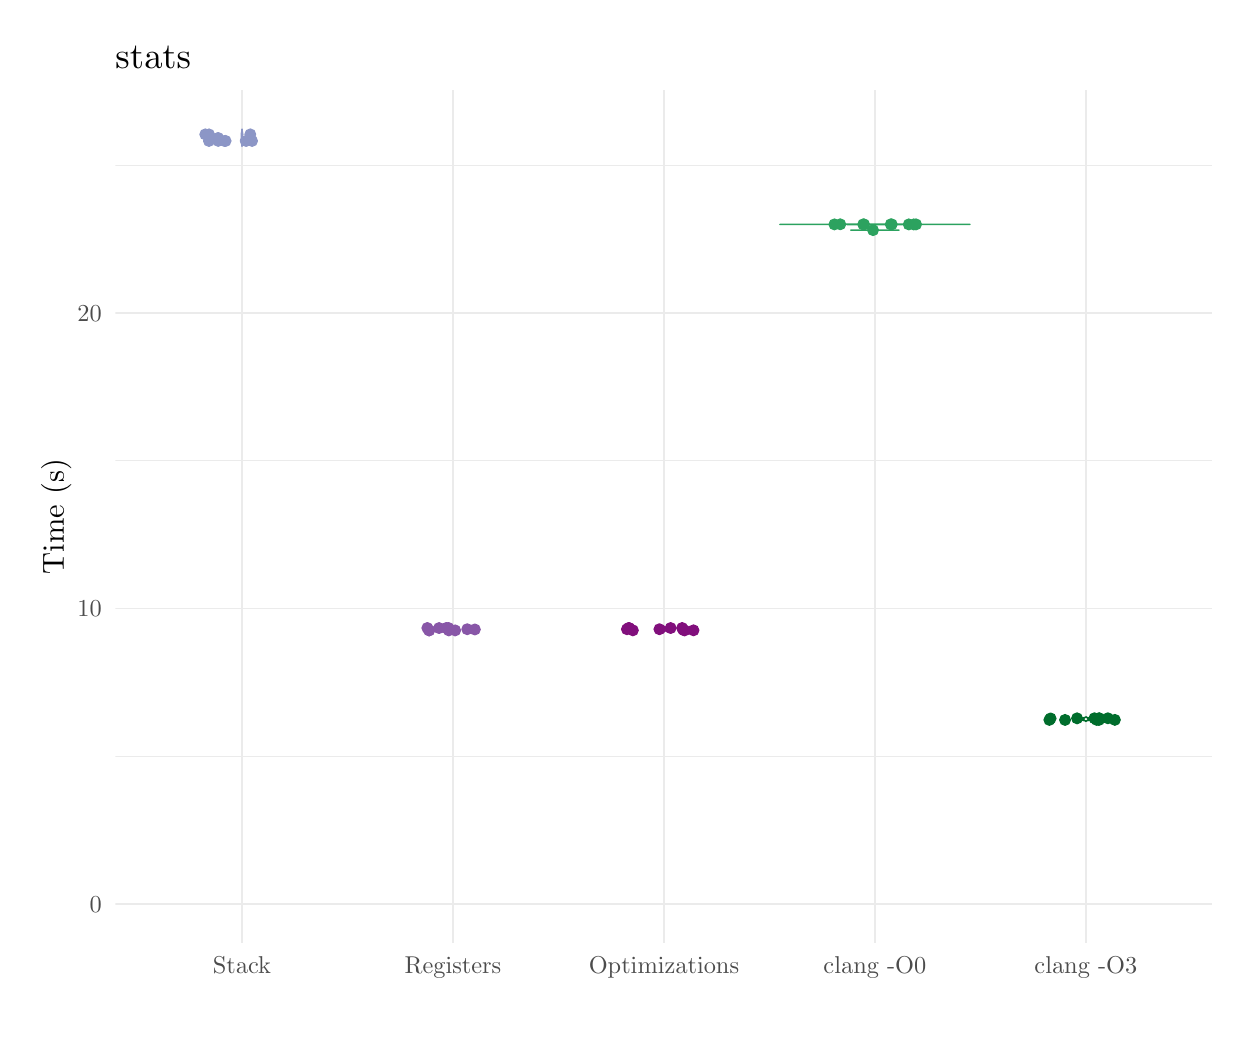
\begin{tikzpicture}[x=1pt,y=1pt]
\definecolor{fillColor}{RGB}{255,255,255}
\path[use as bounding box,fill=fillColor,fill opacity=0.00] (0,0) rectangle (433.62,361.35);
\begin{scope}
\path[clip] ( 31.71, 30.69) rectangle (428.12,338.69);
\definecolor{drawColor}{gray}{0.92}

\path[draw=drawColor,line width= 0.3pt,line join=round] ( 31.71, 98.09) --
	(428.12, 98.09);

\path[draw=drawColor,line width= 0.3pt,line join=round] ( 31.71,204.91) --
	(428.12,204.91);

\path[draw=drawColor,line width= 0.3pt,line join=round] ( 31.71,311.72) --
	(428.12,311.72);

\path[draw=drawColor,line width= 0.6pt,line join=round] ( 31.71, 44.69) --
	(428.12, 44.69);

\path[draw=drawColor,line width= 0.6pt,line join=round] ( 31.71,151.50) --
	(428.12,151.50);

\path[draw=drawColor,line width= 0.6pt,line join=round] ( 31.71,258.32) --
	(428.12,258.32);

\path[draw=drawColor,line width= 0.6pt,line join=round] ( 77.45, 30.69) --
	( 77.45,338.69);

\path[draw=drawColor,line width= 0.6pt,line join=round] (153.68, 30.69) --
	(153.68,338.69);

\path[draw=drawColor,line width= 0.6pt,line join=round] (229.92, 30.69) --
	(229.92,338.69);

\path[draw=drawColor,line width= 0.6pt,line join=round] (306.15, 30.69) --
	(306.15,338.69);

\path[draw=drawColor,line width= 0.6pt,line join=round] (382.38, 30.69) --
	(382.38,338.69);
\definecolor{drawColor}{RGB}{140,150,198}
\definecolor{fillColor}{RGB}{255,255,255}

\path[draw=drawColor,line width= 0.6pt,line join=round,line cap=round,fill=fillColor] ( 77.45,318.50) --
	( 77.45,318.51) --
	( 77.45,318.53) --
	( 77.45,318.54) --
	( 77.45,318.55) --
	( 77.45,318.56) --
	( 77.44,318.58) --
	( 77.44,318.59) --
	( 77.44,318.60) --
	( 77.44,318.61) --
	( 77.44,318.62) --
	( 77.44,318.64) --
	( 77.44,318.65) --
	( 77.44,318.66) --
	( 77.44,318.67) --
	( 77.44,318.68) --
	( 77.44,318.70) --
	( 77.44,318.71) --
	( 77.44,318.72) --
	( 77.44,318.73) --
	( 77.44,318.75) --
	( 77.44,318.76) --
	( 77.44,318.77) --
	( 77.44,318.78) --
	( 77.43,318.79) --
	( 77.43,318.81) --
	( 77.43,318.82) --
	( 77.43,318.83) --
	( 77.43,318.84) --
	( 77.43,318.85) --
	( 77.43,318.87) --
	( 77.43,318.88) --
	( 77.43,318.89) --
	( 77.43,318.90) --
	( 77.42,318.91) --
	( 77.42,318.93) --
	( 77.42,318.94) --
	( 77.42,318.95) --
	( 77.42,318.96) --
	( 77.42,318.98) --
	( 77.42,318.99) --
	( 77.41,319.00) --
	( 77.41,319.01) --
	( 77.41,319.02) --
	( 77.41,319.04) --
	( 77.41,319.05) --
	( 77.41,319.06) --
	( 77.40,319.07) --
	( 77.40,319.08) --
	( 77.40,319.10) --
	( 77.40,319.11) --
	( 77.40,319.12) --
	( 77.39,319.13) --
	( 77.39,319.14) --
	( 77.39,319.16) --
	( 77.39,319.17) --
	( 77.38,319.18) --
	( 77.38,319.19) --
	( 77.38,319.21) --
	( 77.38,319.22) --
	( 77.37,319.23) --
	( 77.37,319.24) --
	( 77.37,319.25) --
	( 77.36,319.27) --
	( 77.36,319.28) --
	( 77.36,319.29) --
	( 77.35,319.30) --
	( 77.35,319.31) --
	( 77.35,319.33) --
	( 77.34,319.34) --
	( 77.34,319.35) --
	( 77.34,319.36) --
	( 77.33,319.37) --
	( 77.33,319.39) --
	( 77.33,319.40) --
	( 77.32,319.41) --
	( 77.32,319.42) --
	( 77.31,319.44) --
	( 77.31,319.45) --
	( 77.31,319.46) --
	( 77.30,319.47) --
	( 77.30,319.48) --
	( 77.29,319.50) --
	( 77.29,319.51) --
	( 77.28,319.52) --
	( 77.28,319.53) --
	( 77.28,319.54) --
	( 77.27,319.56) --
	( 77.27,319.57) --
	( 77.26,319.58) --
	( 77.26,319.59) --
	( 77.25,319.61) --
	( 77.25,319.62) --
	( 77.24,319.63) --
	( 77.24,319.64) --
	( 77.23,319.65) --
	( 77.23,319.67) --
	( 77.22,319.68) --
	( 77.22,319.69) --
	( 77.21,319.70) --
	( 77.21,319.71) --
	( 77.20,319.73) --
	( 77.20,319.74) --
	( 77.19,319.75) --
	( 77.19,319.76) --
	( 77.18,319.77) --
	( 77.17,319.79) --
	( 77.17,319.80) --
	( 77.16,319.81) --
	( 77.16,319.82) --
	( 77.15,319.84) --
	( 77.15,319.85) --
	( 77.14,319.86) --
	( 77.14,319.87) --
	( 77.13,319.88) --
	( 77.13,319.90) --
	( 77.12,319.91) --
	( 77.12,319.92) --
	( 77.11,319.93) --
	( 77.11,319.94) --
	( 77.10,319.96) --
	( 77.10,319.97) --
	( 77.09,319.98) --
	( 77.09,319.99) --
	( 77.08,320.00) --
	( 77.08,320.02) --
	( 77.07,320.03) --
	( 77.07,320.04) --
	( 77.06,320.05) --
	( 77.06,320.07) --
	( 77.06,320.08) --
	( 77.05,320.09) --
	( 77.05,320.10) --
	( 77.04,320.11) --
	( 77.04,320.13) --
	( 77.04,320.14) --
	( 77.03,320.15) --
	( 77.03,320.16) --
	( 77.03,320.17) --
	( 77.02,320.19) --
	( 77.02,320.20) --
	( 77.02,320.21) --
	( 77.01,320.22) --
	( 77.01,320.23) --
	( 77.01,320.25) --
	( 77.01,320.26) --
	( 77.00,320.27) --
	( 77.00,320.28) --
	( 77.00,320.30) --
	( 77.00,320.31) --
	( 76.99,320.32) --
	( 76.99,320.33) --
	( 76.99,320.34) --
	( 76.99,320.36) --
	( 76.99,320.37) --
	( 76.99,320.38) --
	( 76.99,320.39) --
	( 76.99,320.40) --
	( 76.99,320.42) --
	( 76.98,320.43) --
	( 76.98,320.44) --
	( 76.98,320.45) --
	( 76.98,320.47) --
	( 76.98,320.48) --
	( 76.98,320.49) --
	( 76.99,320.50) --
	( 76.99,320.51) --
	( 76.99,320.53) --
	( 76.99,320.54) --
	( 76.99,320.55) --
	( 76.99,320.56) --
	( 76.99,320.57) --
	( 76.99,320.59) --
	( 76.99,320.60) --
	( 76.99,320.61) --
	( 77.00,320.62) --
	( 77.00,320.63) --
	( 77.00,320.65) --
	( 77.00,320.66) --
	( 77.01,320.67) --
	( 77.01,320.68) --
	( 77.01,320.70) --
	( 77.01,320.71) --
	( 77.02,320.72) --
	( 77.02,320.73) --
	( 77.02,320.74) --
	( 77.02,320.76) --
	( 77.03,320.77) --
	( 77.03,320.78) --
	( 77.03,320.79) --
	( 77.04,320.80) --
	( 77.04,320.82) --
	( 77.04,320.83) --
	( 77.05,320.84) --
	( 77.05,320.85) --
	( 77.05,320.86) --
	( 77.06,320.88) --
	( 77.06,320.89) --
	( 77.07,320.90) --
	( 77.07,320.91) --
	( 77.07,320.93) --
	( 77.08,320.94) --
	( 77.08,320.95) --
	( 77.09,320.96) --
	( 77.09,320.97) --
	( 77.09,320.99) --
	( 77.10,321.00) --
	( 77.10,321.01) --
	( 77.11,321.02) --
	( 77.11,321.03) --
	( 77.11,321.05) --
	( 77.12,321.06) --
	( 77.12,321.07) --
	( 77.13,321.08) --
	( 77.13,321.09) --
	( 77.13,321.11) --
	( 77.14,321.12) --
	( 77.14,321.13) --
	( 77.15,321.14) --
	( 77.15,321.16) --
	( 77.15,321.17) --
	( 77.16,321.18) --
	( 77.16,321.19) --
	( 77.17,321.20) --
	( 77.17,321.22) --
	( 77.17,321.23) --
	( 77.18,321.24) --
	( 77.18,321.25) --
	( 77.18,321.26) --
	( 77.19,321.28) --
	( 77.19,321.29) --
	( 77.20,321.30) --
	( 77.20,321.31) --
	( 77.20,321.33) --
	( 77.21,321.34) --
	( 77.21,321.35) --
	( 77.21,321.36) --
	( 77.21,321.37) --
	( 77.22,321.39) --
	( 77.22,321.40) --
	( 77.22,321.41) --
	( 77.23,321.42) --
	( 77.23,321.43) --
	( 77.23,321.45) --
	( 77.23,321.46) --
	( 77.24,321.47) --
	( 77.24,321.48) --
	( 77.24,321.49) --
	( 77.24,321.51) --
	( 77.25,321.52) --
	( 77.25,321.53) --
	( 77.25,321.54) --
	( 77.25,321.56) --
	( 77.25,321.57) --
	( 77.26,321.58) --
	( 77.26,321.59) --
	( 77.26,321.60) --
	( 77.26,321.62) --
	( 77.26,321.63) --
	( 77.26,321.64) --
	( 77.26,321.65) --
	( 77.27,321.66) --
	( 77.27,321.68) --
	( 77.27,321.69) --
	( 77.27,321.70) --
	( 77.27,321.71) --
	( 77.27,321.72) --
	( 77.27,321.74) --
	( 77.27,321.75) --
	( 77.27,321.76) --
	( 77.27,321.77) --
	( 77.27,321.79) --
	( 77.27,321.80) --
	( 77.27,321.81) --
	( 77.28,321.82) --
	( 77.28,321.83) --
	( 77.28,321.85) --
	( 77.28,321.86) --
	( 77.28,321.87) --
	( 77.28,321.88) --
	( 77.28,321.89) --
	( 77.27,321.91) --
	( 77.27,321.92) --
	( 77.27,321.93) --
	( 77.27,321.94) --
	( 77.27,321.96) --
	( 77.27,321.97) --
	( 77.27,321.98) --
	( 77.27,321.99) --
	( 77.27,322.00) --
	( 77.27,322.02) --
	( 77.27,322.03) --
	( 77.27,322.04) --
	( 77.27,322.05) --
	( 77.27,322.06) --
	( 77.27,322.08) --
	( 77.26,322.09) --
	( 77.26,322.10) --
	( 77.26,322.11) --
	( 77.26,322.12) --
	( 77.26,322.14) --
	( 77.26,322.15) --
	( 77.26,322.16) --
	( 77.26,322.17) --
	( 77.26,322.19) --
	( 77.25,322.20) --
	( 77.25,322.21) --
	( 77.25,322.22) --
	( 77.25,322.23) --
	( 77.25,322.25) --
	( 77.25,322.26) --
	( 77.25,322.27) --
	( 77.25,322.28) --
	( 77.24,322.29) --
	( 77.24,322.31) --
	( 77.24,322.32) --
	( 77.24,322.33) --
	( 77.24,322.34) --
	( 77.24,322.35) --
	( 77.24,322.37) --
	( 77.24,322.38) --
	( 77.23,322.39) --
	( 77.23,322.40) --
	( 77.23,322.42) --
	( 77.23,322.43) --
	( 77.23,322.44) --
	( 77.23,322.45) --
	( 77.23,322.46) --
	( 77.23,322.48) --
	( 77.23,322.49) --
	( 77.22,322.50) --
	( 77.22,322.51) --
	( 77.22,322.52) --
	( 77.22,322.54) --
	( 77.22,322.55) --
	( 77.22,322.56) --
	( 77.22,322.57) --
	( 77.22,322.58) --
	( 77.22,322.60) --
	( 77.22,322.61) --
	( 77.22,322.62) --
	( 77.22,322.63) --
	( 77.22,322.65) --
	( 77.22,322.66) --
	( 77.22,322.67) --
	( 77.22,322.68) --
	( 77.22,322.69) --
	( 77.22,322.71) --
	( 77.22,322.72) --
	( 77.22,322.73) --
	( 77.22,322.74) --
	( 77.22,322.75) --
	( 77.22,322.77) --
	( 77.22,322.78) --
	( 77.22,322.79) --
	( 77.22,322.80) --
	( 77.22,322.82) --
	( 77.22,322.83) --
	( 77.22,322.84) --
	( 77.22,322.85) --
	( 77.22,322.86) --
	( 77.22,322.88) --
	( 77.22,322.89) --
	( 77.22,322.90) --
	( 77.23,322.91) --
	( 77.23,322.92) --
	( 77.23,322.94) --
	( 77.23,322.95) --
	( 77.23,322.96) --
	( 77.23,322.97) --
	( 77.23,322.98) --
	( 77.24,323.00) --
	( 77.24,323.01) --
	( 77.24,323.02) --
	( 77.24,323.03) --
	( 77.24,323.05) --
	( 77.24,323.06) --
	( 77.25,323.07) --
	( 77.25,323.08) --
	( 77.25,323.09) --
	( 77.25,323.11) --
	( 77.25,323.12) --
	( 77.26,323.13) --
	( 77.26,323.14) --
	( 77.26,323.15) --
	( 77.26,323.17) --
	( 77.27,323.18) --
	( 77.27,323.19) --
	( 77.27,323.20) --
	( 77.27,323.21) --
	( 77.28,323.23) --
	( 77.28,323.24) --
	( 77.28,323.25) --
	( 77.28,323.26) --
	( 77.29,323.28) --
	( 77.29,323.29) --
	( 77.29,323.30) --
	( 77.29,323.31) --
	( 77.30,323.32) --
	( 77.30,323.34) --
	( 77.30,323.35) --
	( 77.30,323.36) --
	( 77.31,323.37) --
	( 77.31,323.38) --
	( 77.31,323.40) --
	( 77.31,323.41) --
	( 77.32,323.42) --
	( 77.32,323.43) --
	( 77.32,323.44) --
	( 77.32,323.46) --
	( 77.33,323.47) --
	( 77.33,323.48) --
	( 77.33,323.49) --
	( 77.33,323.51) --
	( 77.34,323.52) --
	( 77.34,323.53) --
	( 77.34,323.54) --
	( 77.34,323.55) --
	( 77.35,323.57) --
	( 77.35,323.58) --
	( 77.35,323.59) --
	( 77.35,323.60) --
	( 77.36,323.61) --
	( 77.36,323.63) --
	( 77.36,323.64) --
	( 77.36,323.65) --
	( 77.37,323.66) --
	( 77.37,323.68) --
	( 77.37,323.69) --
	( 77.37,323.70) --
	( 77.38,323.71) --
	( 77.38,323.72) --
	( 77.38,323.74) --
	( 77.38,323.75) --
	( 77.38,323.76) --
	( 77.39,323.77) --
	( 77.39,323.78) --
	( 77.39,323.80) --
	( 77.39,323.81) --
	( 77.39,323.82) --
	( 77.39,323.83) --
	( 77.40,323.84) --
	( 77.40,323.86) --
	( 77.40,323.87) --
	( 77.40,323.88) --
	( 77.40,323.89) --
	( 77.41,323.91) --
	( 77.41,323.92) --
	( 77.41,323.93) --
	( 77.41,323.94) --
	( 77.41,323.95) --
	( 77.41,323.97) --
	( 77.41,323.98) --
	( 77.42,323.99) --
	( 77.42,324.00) --
	( 77.42,324.01) --
	( 77.42,324.03) --
	( 77.42,324.04) --
	( 77.42,324.05) --
	( 77.42,324.06) --
	( 77.42,324.07) --
	( 77.42,324.09) --
	( 77.43,324.10) --
	( 77.43,324.11) --
	( 77.43,324.12) --
	( 77.43,324.14) --
	( 77.43,324.15) --
	( 77.43,324.16) --
	( 77.43,324.17) --
	( 77.43,324.18) --
	( 77.43,324.20) --
	( 77.43,324.21) --
	( 77.43,324.22) --
	( 77.44,324.23) --
	( 77.44,324.24) --
	( 77.44,324.26) --
	( 77.44,324.27) --
	( 77.44,324.28) --
	( 77.44,324.29) --
	( 77.44,324.30) --
	( 77.44,324.32) --
	( 77.44,324.33) --
	( 77.44,324.34) --
	( 77.44,324.35) --
	( 77.44,324.37) --
	( 77.44,324.38) --
	( 77.44,324.39) --
	( 77.44,324.40) --
	( 77.44,324.41) --
	( 77.44,324.43) --
	( 77.44,324.44) --
	( 77.44,324.45) --
	( 77.44,324.46) --
	( 77.45,324.47) --
	( 77.45,324.49) --
	( 77.45,324.50) --
	( 77.45,324.51) --
	( 77.45,324.52) --
	( 77.45,324.54) --
	( 77.45,324.55) --
	( 77.45,324.56) --
	( 77.45,324.57) --
	( 77.45,324.58) --
	( 77.45,324.60) --
	( 77.45,324.61) --
	( 77.45,324.62) --
	( 77.45,324.63) --
	( 77.45,324.64) --
	( 77.45,324.66) --
	( 77.45,324.67) --
	( 77.45,324.68) --
	( 77.45,324.69) --
	( 77.45,324.69) --
	( 77.45,324.68) --
	( 77.45,324.67) --
	( 77.45,324.66) --
	( 77.45,324.64) --
	( 77.45,324.63) --
	( 77.45,324.62) --
	( 77.46,324.61) --
	( 77.46,324.60) --
	( 77.46,324.58) --
	( 77.46,324.57) --
	( 77.46,324.56) --
	( 77.46,324.55) --
	( 77.46,324.54) --
	( 77.46,324.52) --
	( 77.46,324.51) --
	( 77.46,324.50) --
	( 77.46,324.49) --
	( 77.46,324.47) --
	( 77.46,324.46) --
	( 77.46,324.45) --
	( 77.46,324.44) --
	( 77.46,324.43) --
	( 77.46,324.41) --
	( 77.46,324.40) --
	( 77.46,324.39) --
	( 77.46,324.38) --
	( 77.46,324.37) --
	( 77.46,324.35) --
	( 77.46,324.34) --
	( 77.46,324.33) --
	( 77.46,324.32) --
	( 77.46,324.30) --
	( 77.46,324.29) --
	( 77.47,324.28) --
	( 77.47,324.27) --
	( 77.47,324.26) --
	( 77.47,324.24) --
	( 77.47,324.23) --
	( 77.47,324.22) --
	( 77.47,324.21) --
	( 77.47,324.20) --
	( 77.47,324.18) --
	( 77.47,324.17) --
	( 77.47,324.16) --
	( 77.47,324.15) --
	( 77.47,324.14) --
	( 77.48,324.12) --
	( 77.48,324.11) --
	( 77.48,324.10) --
	( 77.48,324.09) --
	( 77.48,324.07) --
	( 77.48,324.06) --
	( 77.48,324.05) --
	( 77.48,324.04) --
	( 77.48,324.03) --
	( 77.49,324.01) --
	( 77.49,324.00) --
	( 77.49,323.99) --
	( 77.49,323.98) --
	( 77.49,323.97) --
	( 77.49,323.95) --
	( 77.49,323.94) --
	( 77.50,323.93) --
	( 77.50,323.92) --
	( 77.50,323.91) --
	( 77.50,323.89) --
	( 77.50,323.88) --
	( 77.50,323.87) --
	( 77.50,323.86) --
	( 77.51,323.84) --
	( 77.51,323.83) --
	( 77.51,323.82) --
	( 77.51,323.81) --
	( 77.51,323.80) --
	( 77.52,323.78) --
	( 77.52,323.77) --
	( 77.52,323.76) --
	( 77.52,323.75) --
	( 77.52,323.74) --
	( 77.53,323.72) --
	( 77.53,323.71) --
	( 77.53,323.70) --
	( 77.53,323.69) --
	( 77.53,323.68) --
	( 77.54,323.66) --
	( 77.54,323.65) --
	( 77.54,323.64) --
	( 77.54,323.63) --
	( 77.55,323.61) --
	( 77.55,323.60) --
	( 77.55,323.59) --
	( 77.55,323.58) --
	( 77.56,323.57) --
	( 77.56,323.55) --
	( 77.56,323.54) --
	( 77.56,323.53) --
	( 77.57,323.52) --
	( 77.57,323.51) --
	( 77.57,323.49) --
	( 77.57,323.48) --
	( 77.58,323.47) --
	( 77.58,323.46) --
	( 77.58,323.44) --
	( 77.58,323.43) --
	( 77.59,323.42) --
	( 77.59,323.41) --
	( 77.59,323.40) --
	( 77.59,323.38) --
	( 77.60,323.37) --
	( 77.60,323.36) --
	( 77.60,323.35) --
	( 77.61,323.34) --
	( 77.61,323.32) --
	( 77.61,323.31) --
	( 77.61,323.30) --
	( 77.62,323.29) --
	( 77.62,323.28) --
	( 77.62,323.26) --
	( 77.62,323.25) --
	( 77.63,323.24) --
	( 77.63,323.23) --
	( 77.63,323.21) --
	( 77.63,323.20) --
	( 77.64,323.19) --
	( 77.64,323.18) --
	( 77.64,323.17) --
	( 77.64,323.15) --
	( 77.64,323.14) --
	( 77.65,323.13) --
	( 77.65,323.12) --
	( 77.65,323.11) --
	( 77.65,323.09) --
	( 77.65,323.08) --
	( 77.66,323.07) --
	( 77.66,323.06) --
	( 77.66,323.05) --
	( 77.66,323.03) --
	( 77.66,323.02) --
	( 77.67,323.01) --
	( 77.67,323.00) --
	( 77.67,322.98) --
	( 77.67,322.97) --
	( 77.67,322.96) --
	( 77.67,322.95) --
	( 77.67,322.94) --
	( 77.68,322.92) --
	( 77.68,322.91) --
	( 77.68,322.90) --
	( 77.68,322.89) --
	( 77.68,322.88) --
	( 77.68,322.86) --
	( 77.68,322.85) --
	( 77.68,322.84) --
	( 77.68,322.83) --
	( 77.68,322.82) --
	( 77.68,322.80) --
	( 77.69,322.79) --
	( 77.69,322.78) --
	( 77.69,322.77) --
	( 77.69,322.75) --
	( 77.69,322.74) --
	( 77.69,322.73) --
	( 77.69,322.72) --
	( 77.69,322.71) --
	( 77.69,322.69) --
	( 77.69,322.68) --
	( 77.69,322.67) --
	( 77.69,322.66) --
	( 77.69,322.65) --
	( 77.69,322.63) --
	( 77.69,322.62) --
	( 77.69,322.61) --
	( 77.68,322.60) --
	( 77.68,322.58) --
	( 77.68,322.57) --
	( 77.68,322.56) --
	( 77.68,322.55) --
	( 77.68,322.54) --
	( 77.68,322.52) --
	( 77.68,322.51) --
	( 77.68,322.50) --
	( 77.68,322.49) --
	( 77.68,322.48) --
	( 77.68,322.46) --
	( 77.67,322.45) --
	( 77.67,322.44) --
	( 77.67,322.43) --
	( 77.67,322.42) --
	( 77.67,322.40) --
	( 77.67,322.39) --
	( 77.67,322.38) --
	( 77.67,322.37) --
	( 77.67,322.35) --
	( 77.66,322.34) --
	( 77.66,322.33) --
	( 77.66,322.32) --
	( 77.66,322.31) --
	( 77.66,322.29) --
	( 77.66,322.28) --
	( 77.66,322.27) --
	( 77.66,322.26) --
	( 77.65,322.25) --
	( 77.65,322.23) --
	( 77.65,322.22) --
	( 77.65,322.21) --
	( 77.65,322.20) --
	( 77.65,322.19) --
	( 77.65,322.17) --
	( 77.65,322.16) --
	( 77.64,322.15) --
	( 77.64,322.14) --
	( 77.64,322.12) --
	( 77.64,322.11) --
	( 77.64,322.10) --
	( 77.64,322.09) --
	( 77.64,322.08) --
	( 77.64,322.06) --
	( 77.64,322.05) --
	( 77.63,322.04) --
	( 77.63,322.03) --
	( 77.63,322.02) --
	( 77.63,322.00) --
	( 77.63,321.99) --
	( 77.63,321.98) --
	( 77.63,321.97) --
	( 77.63,321.96) --
	( 77.63,321.94) --
	( 77.63,321.93) --
	( 77.63,321.92) --
	( 77.63,321.91) --
	( 77.63,321.89) --
	( 77.63,321.88) --
	( 77.63,321.87) --
	( 77.63,321.86) --
	( 77.63,321.85) --
	( 77.63,321.83) --
	( 77.63,321.82) --
	( 77.63,321.81) --
	( 77.63,321.80) --
	( 77.63,321.79) --
	( 77.63,321.77) --
	( 77.63,321.76) --
	( 77.63,321.75) --
	( 77.63,321.74) --
	( 77.63,321.72) --
	( 77.63,321.71) --
	( 77.63,321.70) --
	( 77.63,321.69) --
	( 77.64,321.68) --
	( 77.64,321.66) --
	( 77.64,321.65) --
	( 77.64,321.64) --
	( 77.64,321.63) --
	( 77.64,321.62) --
	( 77.64,321.60) --
	( 77.65,321.59) --
	( 77.65,321.58) --
	( 77.65,321.57) --
	( 77.65,321.56) --
	( 77.65,321.54) --
	( 77.65,321.53) --
	( 77.66,321.52) --
	( 77.66,321.51) --
	( 77.66,321.49) --
	( 77.66,321.48) --
	( 77.67,321.47) --
	( 77.67,321.46) --
	( 77.67,321.45) --
	( 77.67,321.43) --
	( 77.68,321.42) --
	( 77.68,321.41) --
	( 77.68,321.40) --
	( 77.69,321.39) --
	( 77.69,321.37) --
	( 77.69,321.36) --
	( 77.69,321.35) --
	( 77.70,321.34) --
	( 77.70,321.33) --
	( 77.70,321.31) --
	( 77.71,321.30) --
	( 77.71,321.29) --
	( 77.71,321.28) --
	( 77.72,321.26) --
	( 77.72,321.25) --
	( 77.73,321.24) --
	( 77.73,321.23) --
	( 77.73,321.22) --
	( 77.74,321.20) --
	( 77.74,321.19) --
	( 77.74,321.18) --
	( 77.75,321.17) --
	( 77.75,321.16) --
	( 77.76,321.14) --
	( 77.76,321.13) --
	( 77.76,321.12) --
	( 77.77,321.11) --
	( 77.77,321.09) --
	( 77.78,321.08) --
	( 77.78,321.07) --
	( 77.78,321.06) --
	( 77.79,321.05) --
	( 77.79,321.03) --
	( 77.80,321.02) --
	( 77.80,321.01) --
	( 77.81,321.00) --
	( 77.81,320.99) --
	( 77.81,320.97) --
	( 77.82,320.96) --
	( 77.82,320.95) --
	( 77.83,320.94) --
	( 77.83,320.93) --
	( 77.83,320.91) --
	( 77.84,320.90) --
	( 77.84,320.89) --
	( 77.85,320.88) --
	( 77.85,320.86) --
	( 77.85,320.85) --
	( 77.86,320.84) --
	( 77.86,320.83) --
	( 77.86,320.82) --
	( 77.87,320.80) --
	( 77.87,320.79) --
	( 77.87,320.78) --
	( 77.88,320.77) --
	( 77.88,320.76) --
	( 77.88,320.74) --
	( 77.89,320.73) --
	( 77.89,320.72) --
	( 77.89,320.71) --
	( 77.89,320.70) --
	( 77.90,320.68) --
	( 77.90,320.67) --
	( 77.90,320.66) --
	( 77.90,320.65) --
	( 77.90,320.63) --
	( 77.91,320.62) --
	( 77.91,320.61) --
	( 77.91,320.60) --
	( 77.91,320.59) --
	( 77.91,320.57) --
	( 77.91,320.56) --
	( 77.92,320.55) --
	( 77.92,320.54) --
	( 77.92,320.53) --
	( 77.92,320.51) --
	( 77.92,320.50) --
	( 77.92,320.49) --
	( 77.92,320.48) --
	( 77.92,320.47) --
	( 77.92,320.45) --
	( 77.92,320.44) --
	( 77.92,320.43) --
	( 77.92,320.42) --
	( 77.92,320.40) --
	( 77.92,320.39) --
	( 77.92,320.38) --
	( 77.91,320.37) --
	( 77.91,320.36) --
	( 77.91,320.34) --
	( 77.91,320.33) --
	( 77.91,320.32) --
	( 77.91,320.31) --
	( 77.90,320.30) --
	( 77.90,320.28) --
	( 77.90,320.27) --
	( 77.90,320.26) --
	( 77.90,320.25) --
	( 77.89,320.23) --
	( 77.89,320.22) --
	( 77.89,320.21) --
	( 77.88,320.20) --
	( 77.88,320.19) --
	( 77.88,320.17) --
	( 77.87,320.16) --
	( 77.87,320.15) --
	( 77.87,320.14) --
	( 77.86,320.13) --
	( 77.86,320.11) --
	( 77.86,320.10) --
	( 77.85,320.09) --
	( 77.85,320.08) --
	( 77.84,320.07) --
	( 77.84,320.05) --
	( 77.83,320.04) --
	( 77.83,320.03) --
	( 77.82,320.02) --
	( 77.82,320.00) --
	( 77.82,319.99) --
	( 77.81,319.98) --
	( 77.81,319.97) --
	( 77.80,319.96) --
	( 77.80,319.94) --
	( 77.79,319.93) --
	( 77.79,319.92) --
	( 77.78,319.91) --
	( 77.78,319.90) --
	( 77.77,319.88) --
	( 77.77,319.87) --
	( 77.76,319.86) --
	( 77.75,319.85) --
	( 77.75,319.84) --
	( 77.74,319.82) --
	( 77.74,319.81) --
	( 77.73,319.80) --
	( 77.73,319.79) --
	( 77.72,319.77) --
	( 77.72,319.76) --
	( 77.71,319.75) --
	( 77.71,319.74) --
	( 77.70,319.73) --
	( 77.70,319.71) --
	( 77.69,319.70) --
	( 77.69,319.69) --
	( 77.68,319.68) --
	( 77.68,319.67) --
	( 77.67,319.65) --
	( 77.67,319.64) --
	( 77.66,319.63) --
	( 77.66,319.62) --
	( 77.65,319.61) --
	( 77.65,319.59) --
	( 77.64,319.58) --
	( 77.64,319.57) --
	( 77.63,319.56) --
	( 77.63,319.54) --
	( 77.62,319.53) --
	( 77.62,319.52) --
	( 77.61,319.51) --
	( 77.61,319.50) --
	( 77.61,319.48) --
	( 77.60,319.47) --
	( 77.60,319.46) --
	( 77.59,319.45) --
	( 77.59,319.44) --
	( 77.58,319.42) --
	( 77.58,319.41) --
	( 77.58,319.40) --
	( 77.57,319.39) --
	( 77.57,319.37) --
	( 77.57,319.36) --
	( 77.56,319.35) --
	( 77.56,319.34) --
	( 77.56,319.33) --
	( 77.55,319.31) --
	( 77.55,319.30) --
	( 77.55,319.29) --
	( 77.54,319.28) --
	( 77.54,319.27) --
	( 77.54,319.25) --
	( 77.53,319.24) --
	( 77.53,319.23) --
	( 77.53,319.22) --
	( 77.52,319.21) --
	( 77.52,319.19) --
	( 77.52,319.18) --
	( 77.52,319.17) --
	( 77.51,319.16) --
	( 77.51,319.14) --
	( 77.51,319.13) --
	( 77.51,319.12) --
	( 77.51,319.11) --
	( 77.50,319.10) --
	( 77.50,319.08) --
	( 77.50,319.07) --
	( 77.50,319.06) --
	( 77.50,319.05) --
	( 77.49,319.04) --
	( 77.49,319.02) --
	( 77.49,319.01) --
	( 77.49,319.00) --
	( 77.49,318.99) --
	( 77.49,318.98) --
	( 77.48,318.96) --
	( 77.48,318.95) --
	( 77.48,318.94) --
	( 77.48,318.93) --
	( 77.48,318.91) --
	( 77.48,318.90) --
	( 77.48,318.89) --
	( 77.48,318.88) --
	( 77.47,318.87) --
	( 77.47,318.85) --
	( 77.47,318.84) --
	( 77.47,318.83) --
	( 77.47,318.82) --
	( 77.47,318.81) --
	( 77.47,318.79) --
	( 77.47,318.78) --
	( 77.47,318.77) --
	( 77.47,318.76) --
	( 77.47,318.75) --
	( 77.47,318.73) --
	( 77.46,318.72) --
	( 77.46,318.71) --
	( 77.46,318.70) --
	( 77.46,318.68) --
	( 77.46,318.67) --
	( 77.46,318.66) --
	( 77.46,318.65) --
	( 77.46,318.64) --
	( 77.46,318.62) --
	( 77.46,318.61) --
	( 77.46,318.60) --
	( 77.46,318.59) --
	( 77.46,318.58) --
	( 77.46,318.56) --
	( 77.46,318.55) --
	( 77.46,318.54) --
	( 77.46,318.53) --
	( 77.46,318.51) --
	( 77.46,318.50) --
	( 77.45,318.50) --
	cycle;
\definecolor{drawColor}{RGB}{136,86,167}

\path[draw=drawColor,line width= 0.6pt,line join=round,line cap=round,fill=fillColor] (153.68,142.86) --
	(153.67,142.87) --
	(153.67,142.87) --
	(153.67,142.88) --
	(153.67,142.88) --
	(153.67,142.89) --
	(153.67,142.89) --
	(153.67,142.89) --
	(153.67,142.90) --
	(153.67,142.90) --
	(153.67,142.91) --
	(153.67,142.91) --
	(153.67,142.92) --
	(153.67,142.92) --
	(153.67,142.92) --
	(153.66,142.93) --
	(153.66,142.93) --
	(153.66,142.94) --
	(153.66,142.94) --
	(153.66,142.95) --
	(153.66,142.95) --
	(153.66,142.96) --
	(153.66,142.96) --
	(153.65,142.96) --
	(153.65,142.97) --
	(153.65,142.97) --
	(153.65,142.98) --
	(153.65,142.98) --
	(153.65,142.99) --
	(153.64,142.99) --
	(153.64,143.00) --
	(153.64,143.00) --
	(153.64,143.00) --
	(153.64,143.01) --
	(153.63,143.01) --
	(153.63,143.02) --
	(153.63,143.02) --
	(153.63,143.03) --
	(153.62,143.03) --
	(153.62,143.04) --
	(153.62,143.04) --
	(153.62,143.04) --
	(153.61,143.05) --
	(153.61,143.05) --
	(153.61,143.06) --
	(153.60,143.06) --
	(153.60,143.07) --
	(153.60,143.07) --
	(153.59,143.08) --
	(153.59,143.08) --
	(153.58,143.08) --
	(153.58,143.09) --
	(153.58,143.09) --
	(153.57,143.10) --
	(153.57,143.10) --
	(153.56,143.11) --
	(153.56,143.11) --
	(153.55,143.11) --
	(153.55,143.12) --
	(153.54,143.12) --
	(153.54,143.13) --
	(153.53,143.13) --
	(153.53,143.14) --
	(153.52,143.14) --
	(153.52,143.15) --
	(153.51,143.15) --
	(153.51,143.15) --
	(153.50,143.16) --
	(153.49,143.16) --
	(153.49,143.17) --
	(153.48,143.17) --
	(153.47,143.18) --
	(153.47,143.18) --
	(153.46,143.19) --
	(153.45,143.19) --
	(153.45,143.19) --
	(153.44,143.20) --
	(153.43,143.20) --
	(153.42,143.21) --
	(153.41,143.21) --
	(153.41,143.22) --
	(153.40,143.22) --
	(153.39,143.23) --
	(153.38,143.23) --
	(153.37,143.23) --
	(153.37,143.24) --
	(153.36,143.24) --
	(153.35,143.25) --
	(153.34,143.25) --
	(153.33,143.26) --
	(153.32,143.26) --
	(153.31,143.26) --
	(153.30,143.27) --
	(153.29,143.27) --
	(153.28,143.28) --
	(153.27,143.28) --
	(153.26,143.29) --
	(153.25,143.29) --
	(153.24,143.30) --
	(153.23,143.30) --
	(153.22,143.30) --
	(153.21,143.31) --
	(153.20,143.31) --
	(153.19,143.32) --
	(153.18,143.32) --
	(153.17,143.33) --
	(153.16,143.33) --
	(153.15,143.34) --
	(153.14,143.34) --
	(153.13,143.34) --
	(153.12,143.35) --
	(153.11,143.35) --
	(153.10,143.36) --
	(153.09,143.36) --
	(153.08,143.37) --
	(153.07,143.37) --
	(153.06,143.38) --
	(153.05,143.38) --
	(153.04,143.38) --
	(153.03,143.39) --
	(153.02,143.39) --
	(153.01,143.40) --
	(153.00,143.40) --
	(152.99,143.41) --
	(152.98,143.41) --
	(152.97,143.42) --
	(152.96,143.42) --
	(152.95,143.42) --
	(152.94,143.43) --
	(152.93,143.43) --
	(152.92,143.44) --
	(152.91,143.44) --
	(152.91,143.45) --
	(152.90,143.45) --
	(152.89,143.45) --
	(152.88,143.46) --
	(152.87,143.46) --
	(152.86,143.47) --
	(152.86,143.47) --
	(152.85,143.48) --
	(152.84,143.48) --
	(152.83,143.49) --
	(152.83,143.49) --
	(152.82,143.49) --
	(152.81,143.50) --
	(152.81,143.50) --
	(152.80,143.51) --
	(152.79,143.51) --
	(152.79,143.52) --
	(152.78,143.52) --
	(152.78,143.53) --
	(152.77,143.53) --
	(152.77,143.53) --
	(152.76,143.54) --
	(152.76,143.54) --
	(152.75,143.55) --
	(152.75,143.55) --
	(152.75,143.56) --
	(152.74,143.56) --
	(152.74,143.57) --
	(152.74,143.57) --
	(152.73,143.57) --
	(152.73,143.58) --
	(152.73,143.58) --
	(152.73,143.59) --
	(152.73,143.59) --
	(152.72,143.60) --
	(152.72,143.60) --
	(152.72,143.61) --
	(152.72,143.61) --
	(152.72,143.61) --
	(152.72,143.62) --
	(152.72,143.62) --
	(152.72,143.63) --
	(152.72,143.63) --
	(152.72,143.64) --
	(152.72,143.64) --
	(152.72,143.64) --
	(152.72,143.65) --
	(152.72,143.65) --
	(152.72,143.66) --
	(152.73,143.66) --
	(152.73,143.67) --
	(152.73,143.67) --
	(152.73,143.68) --
	(152.73,143.68) --
	(152.74,143.68) --
	(152.74,143.69) --
	(152.74,143.69) --
	(152.75,143.70) --
	(152.75,143.70) --
	(152.75,143.71) --
	(152.75,143.71) --
	(152.76,143.72) --
	(152.76,143.72) --
	(152.77,143.72) --
	(152.77,143.73) --
	(152.77,143.73) --
	(152.78,143.74) --
	(152.78,143.74) --
	(152.78,143.75) --
	(152.79,143.75) --
	(152.79,143.76) --
	(152.80,143.76) --
	(152.80,143.76) --
	(152.81,143.77) --
	(152.81,143.77) --
	(152.82,143.78) --
	(152.82,143.78) --
	(152.82,143.79) --
	(152.83,143.79) --
	(152.83,143.80) --
	(152.84,143.80) --
	(152.84,143.80) --
	(152.85,143.81) --
	(152.85,143.81) --
	(152.86,143.82) --
	(152.86,143.82) --
	(152.87,143.83) --
	(152.87,143.83) --
	(152.88,143.83) --
	(152.88,143.84) --
	(152.89,143.84) --
	(152.89,143.85) --
	(152.90,143.85) --
	(152.90,143.86) --
	(152.90,143.86) --
	(152.91,143.87) --
	(152.91,143.87) --
	(152.92,143.87) --
	(152.92,143.88) --
	(152.93,143.88) --
	(152.93,143.89) --
	(152.93,143.89) --
	(152.94,143.90) --
	(152.94,143.90) --
	(152.95,143.91) --
	(152.95,143.91) --
	(152.95,143.91) --
	(152.96,143.92) --
	(152.96,143.92) --
	(152.96,143.93) --
	(152.97,143.93) --
	(152.97,143.94) --
	(152.97,143.94) --
	(152.98,143.95) --
	(152.98,143.95) --
	(152.98,143.95) --
	(152.98,143.96) --
	(152.99,143.96) --
	(152.99,143.97) --
	(152.99,143.97) --
	(152.99,143.98) --
	(153.00,143.98) --
	(153.00,143.99) --
	(153.00,143.99) --
	(153.00,143.99) --
	(153.00,144.00) --
	(153.00,144.00) --
	(153.00,144.01) --
	(153.01,144.01) --
	(153.01,144.02) --
	(153.01,144.02) --
	(153.01,144.02) --
	(153.01,144.03) --
	(153.01,144.03) --
	(153.01,144.04) --
	(153.01,144.04) --
	(153.01,144.05) --
	(153.01,144.05) --
	(153.01,144.06) --
	(153.01,144.06) --
	(153.01,144.06) --
	(153.01,144.07) --
	(153.00,144.07) --
	(153.00,144.08) --
	(153.00,144.08) --
	(153.00,144.09) --
	(153.00,144.09) --
	(153.00,144.10) --
	(153.00,144.10) --
	(152.99,144.10) --
	(152.99,144.11) --
	(152.99,144.11) --
	(152.99,144.12) --
	(152.98,144.12) --
	(152.98,144.13) --
	(152.98,144.13) --
	(152.98,144.14) --
	(152.97,144.14) --
	(152.97,144.14) --
	(152.97,144.15) --
	(152.96,144.15) --
	(152.96,144.16) --
	(152.96,144.16) --
	(152.95,144.17) --
	(152.95,144.17) --
	(152.95,144.18) --
	(152.94,144.18) --
	(152.94,144.18) --
	(152.93,144.19) --
	(152.93,144.19) --
	(152.93,144.20) --
	(152.92,144.20) --
	(152.92,144.21) --
	(152.91,144.21) --
	(152.91,144.21) --
	(152.91,144.22) --
	(152.90,144.22) --
	(152.90,144.23) --
	(152.89,144.23) --
	(152.89,144.24) --
	(152.88,144.24) --
	(152.88,144.25) --
	(152.88,144.25) --
	(152.87,144.25) --
	(152.87,144.26) --
	(152.86,144.26) --
	(152.86,144.27) --
	(152.86,144.27) --
	(152.85,144.28) --
	(152.85,144.28) --
	(152.85,144.29) --
	(152.84,144.29) --
	(152.84,144.29) --
	(152.84,144.30) --
	(152.83,144.30) --
	(152.83,144.31) --
	(152.83,144.31) --
	(152.82,144.32) --
	(152.82,144.32) --
	(152.82,144.33) --
	(152.82,144.33) --
	(152.81,144.33) --
	(152.81,144.34) --
	(152.81,144.34) --
	(152.81,144.35) --
	(152.81,144.35) --
	(152.81,144.36) --
	(152.81,144.36) --
	(152.80,144.36) --
	(152.80,144.37) --
	(152.80,144.37) --
	(152.80,144.38) --
	(152.80,144.38) --
	(152.80,144.39) --
	(152.80,144.39) --
	(152.80,144.40) --
	(152.81,144.40) --
	(152.81,144.40) --
	(152.81,144.41) --
	(152.81,144.41) --
	(152.81,144.42) --
	(152.81,144.42) --
	(152.82,144.43) --
	(152.82,144.43) --
	(152.82,144.44) --
	(152.83,144.44) --
	(152.83,144.44) --
	(152.83,144.45) --
	(152.84,144.45) --
	(152.84,144.46) --
	(152.84,144.46) --
	(152.85,144.47) --
	(152.85,144.47) --
	(152.86,144.48) --
	(152.86,144.48) --
	(152.87,144.48) --
	(152.88,144.49) --
	(152.88,144.49) --
	(152.89,144.50) --
	(152.89,144.50) --
	(152.90,144.51) --
	(152.91,144.51) --
	(152.91,144.52) --
	(152.92,144.52) --
	(152.93,144.52) --
	(152.94,144.53) --
	(152.94,144.53) --
	(152.95,144.54) --
	(152.96,144.54) --
	(152.97,144.55) --
	(152.98,144.55) --
	(152.98,144.55) --
	(152.99,144.56) --
	(153.00,144.56) --
	(153.01,144.57) --
	(153.02,144.57) --
	(153.03,144.58) --
	(153.04,144.58) --
	(153.05,144.59) --
	(153.06,144.59) --
	(153.07,144.59) --
	(153.08,144.60) --
	(153.08,144.60) --
	(153.09,144.61) --
	(153.10,144.61) --
	(153.11,144.62) --
	(153.12,144.62) --
	(153.13,144.63) --
	(153.14,144.63) --
	(153.15,144.63) --
	(153.16,144.64) --
	(153.17,144.64) --
	(153.18,144.65) --
	(153.19,144.65) --
	(153.20,144.66) --
	(153.21,144.66) --
	(153.22,144.67) --
	(153.23,144.67) --
	(153.24,144.67) --
	(153.25,144.68) --
	(153.26,144.68) --
	(153.27,144.69) --
	(153.28,144.69) --
	(153.29,144.70) --
	(153.30,144.70) --
	(153.31,144.71) --
	(153.32,144.71) --
	(153.32,144.71) --
	(153.33,144.72) --
	(153.34,144.72) --
	(153.35,144.73) --
	(153.36,144.73) --
	(153.37,144.74) --
	(153.38,144.74) --
	(153.38,144.74) --
	(153.39,144.75) --
	(153.40,144.75) --
	(153.41,144.76) --
	(153.42,144.76) --
	(153.42,144.77) --
	(153.43,144.77) --
	(153.44,144.78) --
	(153.45,144.78) --
	(153.45,144.78) --
	(153.46,144.79) --
	(153.47,144.79) --
	(153.47,144.80) --
	(153.48,144.80) --
	(153.49,144.81) --
	(153.49,144.81) --
	(153.50,144.82) --
	(153.51,144.82) --
	(153.51,144.82) --
	(153.52,144.83) --
	(153.52,144.83) --
	(153.53,144.84) --
	(153.53,144.84) --
	(153.54,144.85) --
	(153.54,144.85) --
	(153.55,144.86) --
	(153.55,144.86) --
	(153.56,144.86) --
	(153.56,144.87) --
	(153.57,144.87) --
	(153.57,144.88) --
	(153.58,144.88) --
	(153.58,144.89) --
	(153.58,144.89) --
	(153.59,144.90) --
	(153.59,144.90) --
	(153.60,144.90) --
	(153.60,144.91) --
	(153.60,144.91) --
	(153.61,144.92) --
	(153.61,144.92) --
	(153.61,144.93) --
	(153.61,144.93) --
	(153.62,144.93) --
	(153.62,144.94) --
	(153.62,144.94) --
	(153.63,144.95) --
	(153.63,144.95) --
	(153.63,144.96) --
	(153.63,144.96) --
	(153.64,144.97) --
	(153.64,144.97) --
	(153.64,144.97) --
	(153.64,144.98) --
	(153.64,144.98) --
	(153.65,144.99) --
	(153.65,144.99) --
	(153.65,145.00) --
	(153.65,145.00) --
	(153.65,145.01) --
	(153.65,145.01) --
	(153.66,145.01) --
	(153.66,145.02) --
	(153.66,145.02) --
	(153.66,145.03) --
	(153.66,145.03) --
	(153.66,145.04) --
	(153.66,145.04) --
	(153.66,145.05) --
	(153.66,145.05) --
	(153.67,145.05) --
	(153.67,145.06) --
	(153.67,145.06) --
	(153.67,145.07) --
	(153.67,145.07) --
	(153.67,145.08) --
	(153.67,145.08) --
	(153.67,145.09) --
	(153.67,145.09) --
	(153.67,145.09) --
	(153.67,145.10) --
	(153.67,145.10) --
	(153.67,145.11) --
	(153.68,145.11) --
	(153.68,145.12) --
	(153.68,145.12) --
	(153.69,145.12) --
	(153.69,145.12) --
	(153.69,145.11) --
	(153.69,145.11) --
	(153.69,145.10) --
	(153.69,145.10) --
	(153.69,145.09) --
	(153.70,145.09) --
	(153.70,145.09) --
	(153.70,145.08) --
	(153.70,145.08) --
	(153.70,145.07) --
	(153.70,145.07) --
	(153.70,145.06) --
	(153.70,145.06) --
	(153.70,145.05) --
	(153.70,145.05) --
	(153.70,145.05) --
	(153.71,145.04) --
	(153.71,145.04) --
	(153.71,145.03) --
	(153.71,145.03) --
	(153.71,145.02) --
	(153.71,145.02) --
	(153.71,145.01) --
	(153.71,145.01) --
	(153.72,145.01) --
	(153.72,145.00) --
	(153.72,145.00) --
	(153.72,144.99) --
	(153.72,144.99) --
	(153.72,144.98) --
	(153.73,144.98) --
	(153.73,144.97) --
	(153.73,144.97) --
	(153.73,144.97) --
	(153.73,144.96) --
	(153.74,144.96) --
	(153.74,144.95) --
	(153.74,144.95) --
	(153.74,144.94) --
	(153.75,144.94) --
	(153.75,144.93) --
	(153.75,144.93) --
	(153.76,144.93) --
	(153.76,144.92) --
	(153.76,144.92) --
	(153.77,144.91) --
	(153.77,144.91) --
	(153.77,144.90) --
	(153.78,144.90) --
	(153.78,144.90) --
	(153.78,144.89) --
	(153.79,144.89) --
	(153.79,144.88) --
	(153.80,144.88) --
	(153.80,144.87) --
	(153.80,144.87) --
	(153.81,144.86) --
	(153.81,144.86) --
	(153.82,144.86) --
	(153.82,144.85) --
	(153.83,144.85) --
	(153.83,144.84) --
	(153.84,144.84) --
	(153.85,144.83) --
	(153.85,144.83) --
	(153.86,144.82) --
	(153.86,144.82) --
	(153.87,144.82) --
	(153.87,144.81) --
	(153.88,144.81) --
	(153.89,144.80) --
	(153.89,144.80) --
	(153.90,144.79) --
	(153.91,144.79) --
	(153.91,144.78) --
	(153.92,144.78) --
	(153.93,144.78) --
	(153.94,144.77) --
	(153.94,144.77) --
	(153.95,144.76) --
	(153.96,144.76) --
	(153.97,144.75) --
	(153.98,144.75) --
	(153.98,144.74) --
	(153.99,144.74) --
	(154.00,144.74) --
	(154.01,144.73) --
	(154.02,144.73) --
	(154.03,144.72) --
	(154.03,144.72) --
	(154.04,144.71) --
	(154.05,144.71) --
	(154.06,144.71) --
	(154.07,144.70) --
	(154.08,144.70) --
	(154.09,144.69) --
	(154.10,144.69) --
	(154.11,144.68) --
	(154.12,144.68) --
	(154.13,144.67) --
	(154.14,144.67) --
	(154.15,144.67) --
	(154.16,144.66) --
	(154.17,144.66) --
	(154.18,144.65) --
	(154.19,144.65) --
	(154.20,144.64) --
	(154.21,144.64) --
	(154.22,144.63) --
	(154.22,144.63) --
	(154.23,144.63) --
	(154.24,144.62) --
	(154.25,144.62) --
	(154.26,144.61) --
	(154.27,144.61) --
	(154.28,144.60) --
	(154.29,144.60) --
	(154.30,144.59) --
	(154.31,144.59) --
	(154.32,144.59) --
	(154.33,144.58) --
	(154.34,144.58) --
	(154.35,144.57) --
	(154.36,144.57) --
	(154.37,144.56) --
	(154.37,144.56) --
	(154.38,144.55) --
	(154.39,144.55) --
	(154.40,144.55) --
	(154.41,144.54) --
	(154.42,144.54) --
	(154.42,144.53) --
	(154.43,144.53) --
	(154.44,144.52) --
	(154.45,144.52) --
	(154.45,144.52) --
	(154.46,144.51) --
	(154.47,144.51) --
	(154.47,144.50) --
	(154.48,144.50) --
	(154.49,144.49) --
	(154.49,144.49) --
	(154.50,144.48) --
	(154.50,144.48) --
	(154.51,144.48) --
	(154.51,144.47) --
	(154.52,144.47) --
	(154.52,144.46) --
	(154.53,144.46) --
	(154.53,144.45) --
	(154.54,144.45) --
	(154.54,144.44) --
	(154.54,144.44) --
	(154.55,144.44) --
	(154.55,144.43) --
	(154.55,144.43) --
	(154.55,144.42) --
	(154.56,144.42) --
	(154.56,144.41) --
	(154.56,144.41) --
	(154.56,144.40) --
	(154.56,144.40) --
	(154.56,144.40) --
	(154.56,144.39) --
	(154.56,144.39) --
	(154.56,144.38) --
	(154.56,144.38) --
	(154.56,144.37) --
	(154.56,144.37) --
	(154.56,144.36) --
	(154.56,144.36) --
	(154.56,144.36) --
	(154.56,144.35) --
	(154.56,144.35) --
	(154.56,144.34) --
	(154.56,144.34) --
	(154.55,144.33) --
	(154.55,144.33) --
	(154.55,144.33) --
	(154.55,144.32) --
	(154.54,144.32) --
	(154.54,144.31) --
	(154.54,144.31) --
	(154.54,144.30) --
	(154.53,144.30) --
	(154.53,144.29) --
	(154.53,144.29) --
	(154.52,144.29) --
	(154.52,144.28) --
	(154.51,144.28) --
	(154.51,144.27) --
	(154.51,144.27) --
	(154.50,144.26) --
	(154.50,144.26) --
	(154.50,144.25) --
	(154.49,144.25) --
	(154.49,144.25) --
	(154.48,144.24) --
	(154.48,144.24) --
	(154.47,144.23) --
	(154.47,144.23) --
	(154.47,144.22) --
	(154.46,144.22) --
	(154.46,144.21) --
	(154.45,144.21) --
	(154.45,144.21) --
	(154.45,144.20) --
	(154.44,144.20) --
	(154.44,144.19) --
	(154.43,144.19) --
	(154.43,144.18) --
	(154.43,144.18) --
	(154.42,144.18) --
	(154.42,144.17) --
	(154.41,144.17) --
	(154.41,144.16) --
	(154.41,144.16) --
	(154.40,144.15) --
	(154.40,144.15) --
	(154.40,144.14) --
	(154.39,144.14) --
	(154.39,144.14) --
	(154.39,144.13) --
	(154.39,144.13) --
	(154.38,144.12) --
	(154.38,144.12) --
	(154.38,144.11) --
	(154.38,144.11) --
	(154.37,144.10) --
	(154.37,144.10) --
	(154.37,144.10) --
	(154.37,144.09) --
	(154.37,144.09) --
	(154.37,144.08) --
	(154.36,144.08) --
	(154.36,144.07) --
	(154.36,144.07) --
	(154.36,144.06) --
	(154.36,144.06) --
	(154.36,144.06) --
	(154.36,144.05) --
	(154.36,144.05) --
	(154.36,144.04) --
	(154.36,144.04) --
	(154.36,144.03) --
	(154.36,144.03) --
	(154.36,144.02) --
	(154.36,144.02) --
	(154.36,144.02) --
	(154.36,144.01) --
	(154.36,144.01) --
	(154.36,144.00) --
	(154.37,144.00) --
	(154.37,143.99) --
	(154.37,143.99) --
	(154.37,143.99) --
	(154.37,143.98) --
	(154.37,143.98) --
	(154.38,143.97) --
	(154.38,143.97) --
	(154.38,143.96) --
	(154.38,143.96) --
	(154.39,143.95) --
	(154.39,143.95) --
	(154.39,143.95) --
	(154.39,143.94) --
	(154.40,143.94) --
	(154.40,143.93) --
	(154.40,143.93) --
	(154.41,143.92) --
	(154.41,143.92) --
	(154.41,143.91) --
	(154.42,143.91) --
	(154.42,143.91) --
	(154.43,143.90) --
	(154.43,143.90) --
	(154.43,143.89) --
	(154.44,143.89) --
	(154.44,143.88) --
	(154.45,143.88) --
	(154.45,143.87) --
	(154.45,143.87) --
	(154.46,143.87) --
	(154.46,143.86) --
	(154.47,143.86) --
	(154.47,143.85) --
	(154.48,143.85) --
	(154.48,143.84) --
	(154.49,143.84) --
	(154.49,143.83) --
	(154.50,143.83) --
	(154.50,143.83) --
	(154.50,143.82) --
	(154.51,143.82) --
	(154.51,143.81) --
	(154.52,143.81) --
	(154.52,143.80) --
	(154.53,143.80) --
	(154.53,143.80) --
	(154.54,143.79) --
	(154.54,143.79) --
	(154.55,143.78) --
	(154.55,143.78) --
	(154.56,143.77) --
	(154.56,143.77) --
	(154.57,143.76) --
	(154.57,143.76) --
	(154.57,143.76) --
	(154.58,143.75) --
	(154.58,143.75) --
	(154.59,143.74) --
	(154.59,143.74) --
	(154.59,143.73) --
	(154.60,143.73) --
	(154.60,143.72) --
	(154.61,143.72) --
	(154.61,143.72) --
	(154.61,143.71) --
	(154.62,143.71) --
	(154.62,143.70) --
	(154.62,143.70) --
	(154.63,143.69) --
	(154.63,143.69) --
	(154.63,143.68) --
	(154.63,143.68) --
	(154.64,143.68) --
	(154.64,143.67) --
	(154.64,143.67) --
	(154.64,143.66) --
	(154.64,143.66) --
	(154.64,143.65) --
	(154.65,143.65) --
	(154.65,143.64) --
	(154.65,143.64) --
	(154.65,143.64) --
	(154.65,143.63) --
	(154.65,143.63) --
	(154.65,143.62) --
	(154.65,143.62) --
	(154.65,143.61) --
	(154.65,143.61) --
	(154.65,143.61) --
	(154.65,143.60) --
	(154.64,143.60) --
	(154.64,143.59) --
	(154.64,143.59) --
	(154.64,143.58) --
	(154.64,143.58) --
	(154.63,143.57) --
	(154.63,143.57) --
	(154.63,143.57) --
	(154.62,143.56) --
	(154.62,143.56) --
	(154.62,143.55) --
	(154.61,143.55) --
	(154.61,143.54) --
	(154.60,143.54) --
	(154.60,143.53) --
	(154.60,143.53) --
	(154.59,143.53) --
	(154.58,143.52) --
	(154.58,143.52) --
	(154.57,143.51) --
	(154.57,143.51) --
	(154.56,143.50) --
	(154.55,143.50) --
	(154.55,143.49) --
	(154.54,143.49) --
	(154.53,143.49) --
	(154.53,143.48) --
	(154.52,143.48) --
	(154.51,143.47) --
	(154.50,143.47) --
	(154.50,143.46) --
	(154.49,143.46) --
	(154.48,143.45) --
	(154.47,143.45) --
	(154.46,143.45) --
	(154.45,143.44) --
	(154.44,143.44) --
	(154.44,143.43) --
	(154.43,143.43) --
	(154.42,143.42) --
	(154.41,143.42) --
	(154.40,143.42) --
	(154.39,143.41) --
	(154.38,143.41) --
	(154.37,143.40) --
	(154.36,143.40) --
	(154.35,143.39) --
	(154.34,143.39) --
	(154.33,143.38) --
	(154.32,143.38) --
	(154.31,143.38) --
	(154.30,143.37) --
	(154.29,143.37) --
	(154.28,143.36) --
	(154.27,143.36) --
	(154.26,143.35) --
	(154.25,143.35) --
	(154.24,143.34) --
	(154.23,143.34) --
	(154.22,143.34) --
	(154.20,143.33) --
	(154.19,143.33) --
	(154.18,143.32) --
	(154.17,143.32) --
	(154.16,143.31) --
	(154.15,143.31) --
	(154.14,143.30) --
	(154.13,143.30) --
	(154.12,143.30) --
	(154.11,143.29) --
	(154.10,143.29) --
	(154.09,143.28) --
	(154.08,143.28) --
	(154.08,143.27) --
	(154.07,143.27) --
	(154.06,143.26) --
	(154.05,143.26) --
	(154.04,143.26) --
	(154.03,143.25) --
	(154.02,143.25) --
	(154.01,143.24) --
	(154.00,143.24) --
	(153.99,143.23) --
	(153.99,143.23) --
	(153.98,143.23) --
	(153.97,143.22) --
	(153.96,143.22) --
	(153.95,143.21) --
	(153.95,143.21) --
	(153.94,143.20) --
	(153.93,143.20) --
	(153.92,143.19) --
	(153.92,143.19) --
	(153.91,143.19) --
	(153.90,143.18) --
	(153.89,143.18) --
	(153.89,143.17) --
	(153.88,143.17) --
	(153.87,143.16) --
	(153.87,143.16) --
	(153.86,143.15) --
	(153.86,143.15) --
	(153.85,143.15) --
	(153.84,143.14) --
	(153.84,143.14) --
	(153.83,143.13) --
	(153.83,143.13) --
	(153.82,143.12) --
	(153.82,143.12) --
	(153.81,143.11) --
	(153.81,143.11) --
	(153.80,143.11) --
	(153.80,143.10) --
	(153.80,143.10) --
	(153.79,143.09) --
	(153.79,143.09) --
	(153.78,143.08) --
	(153.78,143.08) --
	(153.78,143.08) --
	(153.77,143.07) --
	(153.77,143.07) --
	(153.76,143.06) --
	(153.76,143.06) --
	(153.76,143.05) --
	(153.76,143.05) --
	(153.75,143.04) --
	(153.75,143.04) --
	(153.75,143.04) --
	(153.74,143.03) --
	(153.74,143.03) --
	(153.74,143.02) --
	(153.74,143.02) --
	(153.73,143.01) --
	(153.73,143.01) --
	(153.73,143.00) --
	(153.73,143.00) --
	(153.73,143.00) --
	(153.72,142.99) --
	(153.72,142.99) --
	(153.72,142.98) --
	(153.72,142.98) --
	(153.72,142.97) --
	(153.72,142.97) --
	(153.71,142.96) --
	(153.71,142.96) --
	(153.71,142.96) --
	(153.71,142.95) --
	(153.71,142.95) --
	(153.71,142.94) --
	(153.71,142.94) --
	(153.70,142.93) --
	(153.70,142.93) --
	(153.70,142.92) --
	(153.70,142.92) --
	(153.70,142.92) --
	(153.70,142.91) --
	(153.70,142.91) --
	(153.70,142.90) --
	(153.70,142.90) --
	(153.70,142.89) --
	(153.70,142.89) --
	(153.70,142.89) --
	(153.69,142.88) --
	(153.69,142.88) --
	(153.69,142.87) --
	(153.69,142.87) --
	(153.69,142.86) --
	(153.68,142.86) --
	cycle;
\definecolor{drawColor}{RGB}{129,15,124}

\path[draw=drawColor,line width= 0.6pt,line join=round,line cap=round,fill=fillColor] (229.91,142.90) --
	(229.91,142.91) --
	(229.91,142.91) --
	(229.91,142.92) --
	(229.91,142.92) --
	(229.91,142.92) --
	(229.91,142.93) --
	(229.91,142.93) --
	(229.91,142.94) --
	(229.91,142.94) --
	(229.91,142.95) --
	(229.91,142.95) --
	(229.91,142.95) --
	(229.90,142.96) --
	(229.90,142.96) --
	(229.90,142.97) --
	(229.90,142.97) --
	(229.90,142.98) --
	(229.90,142.98) --
	(229.90,142.98) --
	(229.90,142.99) --
	(229.90,142.99) --
	(229.90,143.00) --
	(229.90,143.00) --
	(229.89,143.01) --
	(229.89,143.01) --
	(229.89,143.01) --
	(229.89,143.02) --
	(229.89,143.02) --
	(229.89,143.03) --
	(229.89,143.03) --
	(229.89,143.03) --
	(229.88,143.04) --
	(229.88,143.04) --
	(229.88,143.05) --
	(229.88,143.05) --
	(229.88,143.06) --
	(229.88,143.06) --
	(229.87,143.06) --
	(229.87,143.07) --
	(229.87,143.07) --
	(229.87,143.08) --
	(229.86,143.08) --
	(229.86,143.09) --
	(229.86,143.09) --
	(229.86,143.09) --
	(229.85,143.10) --
	(229.85,143.10) --
	(229.85,143.11) --
	(229.85,143.11) --
	(229.84,143.12) --
	(229.84,143.12) --
	(229.84,143.12) --
	(229.83,143.13) --
	(229.83,143.13) --
	(229.83,143.14) --
	(229.82,143.14) --
	(229.82,143.14) --
	(229.82,143.15) --
	(229.81,143.15) --
	(229.81,143.16) --
	(229.80,143.16) --
	(229.80,143.17) --
	(229.79,143.17) --
	(229.79,143.17) --
	(229.78,143.18) --
	(229.78,143.18) --
	(229.77,143.19) --
	(229.77,143.19) --
	(229.76,143.20) --
	(229.76,143.20) --
	(229.75,143.20) --
	(229.75,143.21) --
	(229.74,143.21) --
	(229.74,143.22) --
	(229.73,143.22) --
	(229.72,143.23) --
	(229.72,143.23) --
	(229.71,143.23) --
	(229.70,143.24) --
	(229.70,143.24) --
	(229.69,143.25) --
	(229.68,143.25) --
	(229.68,143.26) --
	(229.67,143.26) --
	(229.66,143.26) --
	(229.66,143.27) --
	(229.65,143.27) --
	(229.64,143.28) --
	(229.63,143.28) --
	(229.62,143.28) --
	(229.62,143.29) --
	(229.61,143.29) --
	(229.60,143.30) --
	(229.59,143.30) --
	(229.58,143.31) --
	(229.57,143.31) --
	(229.57,143.31) --
	(229.56,143.32) --
	(229.55,143.32) --
	(229.54,143.33) --
	(229.53,143.33) --
	(229.52,143.34) --
	(229.51,143.34) --
	(229.50,143.34) --
	(229.49,143.35) --
	(229.48,143.35) --
	(229.47,143.36) --
	(229.47,143.36) --
	(229.46,143.37) --
	(229.45,143.37) --
	(229.44,143.37) --
	(229.43,143.38) --
	(229.42,143.38) --
	(229.41,143.39) --
	(229.40,143.39) --
	(229.39,143.40) --
	(229.38,143.40) --
	(229.37,143.40) --
	(229.36,143.41) --
	(229.35,143.41) --
	(229.34,143.42) --
	(229.33,143.42) --
	(229.32,143.42) --
	(229.31,143.43) --
	(229.30,143.43) --
	(229.29,143.44) --
	(229.28,143.44) --
	(229.28,143.45) --
	(229.27,143.45) --
	(229.26,143.45) --
	(229.25,143.46) --
	(229.24,143.46) --
	(229.23,143.47) --
	(229.22,143.47) --
	(229.21,143.48) --
	(229.20,143.48) --
	(229.20,143.48) --
	(229.19,143.49) --
	(229.18,143.49) --
	(229.17,143.50) --
	(229.16,143.50) --
	(229.16,143.51) --
	(229.15,143.51) --
	(229.14,143.51) --
	(229.13,143.52) --
	(229.13,143.52) --
	(229.12,143.53) --
	(229.11,143.53) --
	(229.11,143.53) --
	(229.10,143.54) --
	(229.09,143.54) --
	(229.09,143.55) --
	(229.08,143.55) --
	(229.07,143.56) --
	(229.07,143.56) --
	(229.06,143.56) --
	(229.06,143.57) --
	(229.05,143.57) --
	(229.05,143.58) --
	(229.04,143.58) --
	(229.04,143.59) --
	(229.03,143.59) --
	(229.03,143.59) --
	(229.03,143.60) --
	(229.02,143.60) --
	(229.02,143.61) --
	(229.01,143.61) --
	(229.01,143.62) --
	(229.01,143.62) --
	(229.00,143.62) --
	(229.00,143.63) --
	(229.00,143.63) --
	(229.00,143.64) --
	(228.99,143.64) --
	(228.99,143.65) --
	(228.99,143.65) --
	(228.99,143.65) --
	(228.99,143.66) --
	(228.98,143.66) --
	(228.98,143.67) --
	(228.98,143.67) --
	(228.98,143.67) --
	(228.98,143.68) --
	(228.98,143.68) --
	(228.98,143.69) --
	(228.98,143.69) --
	(228.98,143.70) --
	(228.98,143.70) --
	(228.98,143.70) --
	(228.98,143.71) --
	(228.98,143.71) --
	(228.98,143.72) --
	(228.98,143.72) --
	(228.98,143.73) --
	(228.98,143.73) --
	(228.98,143.73) --
	(228.98,143.74) --
	(228.98,143.74) --
	(228.98,143.75) --
	(228.98,143.75) --
	(228.98,143.76) --
	(228.98,143.76) --
	(228.98,143.76) --
	(228.99,143.77) --
	(228.99,143.77) --
	(228.99,143.78) --
	(228.99,143.78) --
	(228.99,143.78) --
	(228.99,143.79) --
	(228.99,143.79) --
	(229.00,143.80) --
	(229.00,143.80) --
	(229.00,143.81) --
	(229.00,143.81) --
	(229.00,143.81) --
	(229.01,143.82) --
	(229.01,143.82) --
	(229.01,143.83) --
	(229.01,143.83) --
	(229.01,143.84) --
	(229.02,143.84) --
	(229.02,143.84) --
	(229.02,143.85) --
	(229.02,143.85) --
	(229.03,143.86) --
	(229.03,143.86) --
	(229.03,143.87) --
	(229.03,143.87) --
	(229.04,143.87) --
	(229.04,143.88) --
	(229.04,143.88) --
	(229.04,143.89) --
	(229.04,143.89) --
	(229.05,143.90) --
	(229.05,143.90) --
	(229.05,143.90) --
	(229.05,143.91) --
	(229.06,143.91) --
	(229.06,143.92) --
	(229.06,143.92) --
	(229.06,143.92) --
	(229.07,143.93) --
	(229.07,143.93) --
	(229.07,143.94) --
	(229.07,143.94) --
	(229.07,143.95) --
	(229.08,143.95) --
	(229.08,143.95) --
	(229.08,143.96) --
	(229.08,143.96) --
	(229.08,143.97) --
	(229.09,143.97) --
	(229.09,143.98) --
	(229.09,143.98) --
	(229.09,143.98) --
	(229.09,143.99) --
	(229.10,143.99) --
	(229.10,144.00) --
	(229.10,144.00) --
	(229.10,144.01) --
	(229.10,144.01) --
	(229.10,144.01) --
	(229.10,144.02) --
	(229.11,144.02) --
	(229.11,144.03) --
	(229.11,144.03) --
	(229.11,144.04) --
	(229.11,144.04) --
	(229.11,144.04) --
	(229.11,144.05) --
	(229.11,144.05) --
	(229.11,144.06) --
	(229.11,144.06) --
	(229.11,144.06) --
	(229.11,144.07) --
	(229.11,144.07) --
	(229.11,144.08) --
	(229.11,144.08) --
	(229.11,144.09) --
	(229.11,144.09) --
	(229.11,144.09) --
	(229.11,144.10) --
	(229.11,144.10) --
	(229.11,144.11) --
	(229.10,144.11) --
	(229.10,144.12) --
	(229.10,144.12) --
	(229.10,144.12) --
	(229.10,144.13) --
	(229.10,144.13) --
	(229.09,144.14) --
	(229.09,144.14) --
	(229.09,144.15) --
	(229.09,144.15) --
	(229.09,144.15) --
	(229.08,144.16) --
	(229.08,144.16) --
	(229.08,144.17) --
	(229.08,144.17) --
	(229.07,144.17) --
	(229.07,144.18) --
	(229.07,144.18) --
	(229.06,144.19) --
	(229.06,144.19) --
	(229.06,144.20) --
	(229.05,144.20) --
	(229.05,144.20) --
	(229.05,144.21) --
	(229.04,144.21) --
	(229.04,144.22) --
	(229.04,144.22) --
	(229.03,144.23) --
	(229.03,144.23) --
	(229.03,144.23) --
	(229.02,144.24) --
	(229.02,144.24) --
	(229.01,144.25) --
	(229.01,144.25) --
	(229.01,144.26) --
	(229.00,144.26) --
	(229.00,144.26) --
	(229.00,144.27) --
	(228.99,144.27) --
	(228.99,144.28) --
	(228.99,144.28) --
	(228.98,144.29) --
	(228.98,144.29) --
	(228.98,144.29) --
	(228.98,144.30) --
	(228.97,144.30) --
	(228.97,144.31) --
	(228.97,144.31) --
	(228.97,144.31) --
	(228.96,144.32) --
	(228.96,144.32) --
	(228.96,144.33) --
	(228.96,144.33) --
	(228.96,144.34) --
	(228.96,144.34) --
	(228.95,144.34) --
	(228.95,144.35) --
	(228.95,144.35) --
	(228.95,144.36) --
	(228.95,144.36) --
	(228.95,144.37) --
	(228.95,144.37) --
	(228.95,144.37) --
	(228.95,144.38) --
	(228.96,144.38) --
	(228.96,144.39) --
	(228.96,144.39) --
	(228.96,144.40) --
	(228.96,144.40) --
	(228.96,144.40) --
	(228.97,144.41) --
	(228.97,144.41) --
	(228.97,144.42) --
	(228.98,144.42) --
	(228.98,144.43) --
	(228.98,144.43) --
	(228.99,144.43) --
	(228.99,144.44) --
	(229.00,144.44) --
	(229.00,144.45) --
	(229.01,144.45) --
	(229.01,144.45) --
	(229.02,144.46) --
	(229.02,144.46) --
	(229.03,144.47) --
	(229.03,144.47) --
	(229.04,144.48) --
	(229.05,144.48) --
	(229.06,144.48) --
	(229.06,144.49) --
	(229.07,144.49) --
	(229.08,144.50) --
	(229.09,144.50) --
	(229.09,144.51) --
	(229.10,144.51) --
	(229.11,144.51) --
	(229.12,144.52) --
	(229.13,144.52) --
	(229.14,144.53) --
	(229.15,144.53) --
	(229.16,144.54) --
	(229.17,144.54) --
	(229.18,144.54) --
	(229.19,144.55) --
	(229.20,144.55) --
	(229.21,144.56) --
	(229.22,144.56) --
	(229.23,144.56) --
	(229.24,144.57) --
	(229.25,144.57) --
	(229.26,144.58) --
	(229.27,144.58) --
	(229.28,144.59) --
	(229.29,144.59) --
	(229.30,144.59) --
	(229.31,144.60) --
	(229.32,144.60) --
	(229.33,144.61) --
	(229.35,144.61) --
	(229.36,144.62) --
	(229.37,144.62) --
	(229.38,144.62) --
	(229.39,144.63) --
	(229.40,144.63) --
	(229.41,144.64) --
	(229.42,144.64) --
	(229.43,144.65) --
	(229.44,144.65) --
	(229.45,144.65) --
	(229.46,144.66) --
	(229.47,144.66) --
	(229.48,144.67) --
	(229.50,144.67) --
	(229.51,144.68) --
	(229.52,144.68) --
	(229.53,144.68) --
	(229.54,144.69) --
	(229.55,144.69) --
	(229.56,144.70) --
	(229.56,144.70) --
	(229.57,144.70) --
	(229.58,144.71) --
	(229.59,144.71) --
	(229.60,144.72) --
	(229.61,144.72) --
	(229.62,144.73) --
	(229.63,144.73) --
	(229.64,144.73) --
	(229.65,144.74) --
	(229.65,144.74) --
	(229.66,144.75) --
	(229.67,144.75) --
	(229.68,144.76) --
	(229.68,144.76) --
	(229.69,144.76) --
	(229.70,144.77) --
	(229.71,144.77) --
	(229.71,144.78) --
	(229.72,144.78) --
	(229.73,144.79) --
	(229.73,144.79) --
	(229.74,144.79) --
	(229.75,144.80) --
	(229.75,144.80) --
	(229.76,144.81) --
	(229.76,144.81) --
	(229.77,144.82) --
	(229.77,144.82) --
	(229.78,144.82) --
	(229.79,144.83) --
	(229.79,144.83) --
	(229.80,144.84) --
	(229.80,144.84) --
	(229.80,144.84) --
	(229.81,144.85) --
	(229.81,144.85) --
	(229.82,144.86) --
	(229.82,144.86) --
	(229.83,144.87) --
	(229.83,144.87) --
	(229.83,144.87) --
	(229.84,144.88) --
	(229.84,144.88) --
	(229.84,144.89) --
	(229.85,144.89) --
	(229.85,144.90) --
	(229.85,144.90) --
	(229.85,144.90) --
	(229.86,144.91) --
	(229.86,144.91) --
	(229.86,144.92) --
	(229.87,144.92) --
	(229.87,144.93) --
	(229.87,144.93) --
	(229.87,144.93) --
	(229.87,144.94) --
	(229.88,144.94) --
	(229.88,144.95) --
	(229.88,144.95) --
	(229.88,144.95) --
	(229.88,144.96) --
	(229.89,144.96) --
	(229.89,144.97) --
	(229.89,144.97) --
	(229.89,144.98) --
	(229.89,144.98) --
	(229.89,144.98) --
	(229.89,144.99) --
	(229.89,144.99) --
	(229.90,145.00) --
	(229.90,145.00) --
	(229.90,145.01) --
	(229.90,145.01) --
	(229.90,145.01) --
	(229.90,145.02) --
	(229.90,145.02) --
	(229.90,145.03) --
	(229.90,145.03) --
	(229.90,145.04) --
	(229.90,145.04) --
	(229.91,145.04) --
	(229.91,145.05) --
	(229.91,145.05) --
	(229.91,145.06) --
	(229.91,145.06) --
	(229.91,145.07) --
	(229.91,145.07) --
	(229.92,145.07) --
	(229.92,145.07) --
	(229.92,145.06) --
	(229.93,145.06) --
	(229.93,145.05) --
	(229.93,145.05) --
	(229.93,145.04) --
	(229.93,145.04) --
	(229.93,145.04) --
	(229.93,145.03) --
	(229.93,145.03) --
	(229.93,145.02) --
	(229.93,145.02) --
	(229.93,145.01) --
	(229.93,145.01) --
	(229.93,145.01) --
	(229.94,145.00) --
	(229.94,145.00) --
	(229.94,144.99) --
	(229.94,144.99) --
	(229.94,144.98) --
	(229.94,144.98) --
	(229.94,144.98) --
	(229.94,144.97) --
	(229.95,144.97) --
	(229.95,144.96) --
	(229.95,144.96) --
	(229.95,144.95) --
	(229.95,144.95) --
	(229.95,144.95) --
	(229.96,144.94) --
	(229.96,144.94) --
	(229.96,144.93) --
	(229.96,144.93) --
	(229.96,144.93) --
	(229.97,144.92) --
	(229.97,144.92) --
	(229.97,144.91) --
	(229.97,144.91) --
	(229.98,144.90) --
	(229.98,144.90) --
	(229.98,144.90) --
	(229.99,144.89) --
	(229.99,144.89) --
	(229.99,144.88) --
	(230.00,144.88) --
	(230.00,144.87) --
	(230.00,144.87) --
	(230.01,144.87) --
	(230.01,144.86) --
	(230.01,144.86) --
	(230.02,144.85) --
	(230.02,144.85) --
	(230.03,144.84) --
	(230.03,144.84) --
	(230.04,144.84) --
	(230.04,144.83) --
	(230.05,144.83) --
	(230.05,144.82) --
	(230.06,144.82) --
	(230.06,144.82) --
	(230.07,144.81) --
	(230.07,144.81) --
	(230.08,144.80) --
	(230.09,144.80) --
	(230.09,144.79) --
	(230.10,144.79) --
	(230.11,144.79) --
	(230.11,144.78) --
	(230.12,144.78) --
	(230.13,144.77) --
	(230.13,144.77) --
	(230.14,144.76) --
	(230.15,144.76) --
	(230.16,144.76) --
	(230.16,144.75) --
	(230.17,144.75) --
	(230.18,144.74) --
	(230.19,144.74) --
	(230.20,144.73) --
	(230.20,144.73) --
	(230.21,144.73) --
	(230.22,144.72) --
	(230.23,144.72) --
	(230.24,144.71) --
	(230.25,144.71) --
	(230.26,144.70) --
	(230.27,144.70) --
	(230.28,144.70) --
	(230.29,144.69) --
	(230.30,144.69) --
	(230.31,144.68) --
	(230.32,144.68) --
	(230.33,144.68) --
	(230.34,144.67) --
	(230.35,144.67) --
	(230.36,144.66) --
	(230.37,144.66) --
	(230.38,144.65) --
	(230.39,144.65) --
	(230.40,144.65) --
	(230.41,144.64) --
	(230.42,144.64) --
	(230.43,144.63) --
	(230.44,144.63) --
	(230.45,144.62) --
	(230.47,144.62) --
	(230.48,144.62) --
	(230.49,144.61) --
	(230.50,144.61) --
	(230.51,144.60) --
	(230.52,144.60) --
	(230.53,144.59) --
	(230.54,144.59) --
	(230.55,144.59) --
	(230.56,144.58) --
	(230.57,144.58) --
	(230.58,144.57) --
	(230.59,144.57) --
	(230.61,144.56) --
	(230.62,144.56) --
	(230.63,144.56) --
	(230.64,144.55) --
	(230.65,144.55) --
	(230.66,144.54) --
	(230.67,144.54) --
	(230.68,144.54) --
	(230.68,144.53) --
	(230.69,144.53) --
	(230.70,144.52) --
	(230.71,144.52) --
	(230.72,144.51) --
	(230.73,144.51) --
	(230.74,144.51) --
	(230.75,144.50) --
	(230.75,144.50) --
	(230.76,144.49) --
	(230.77,144.49) --
	(230.78,144.48) --
	(230.78,144.48) --
	(230.79,144.48) --
	(230.80,144.47) --
	(230.80,144.47) --
	(230.81,144.46) --
	(230.82,144.46) --
	(230.82,144.45) --
	(230.83,144.45) --
	(230.83,144.45) --
	(230.84,144.44) --
	(230.84,144.44) --
	(230.85,144.43) --
	(230.85,144.43) --
	(230.85,144.43) --
	(230.86,144.42) --
	(230.86,144.42) --
	(230.86,144.41) --
	(230.87,144.41) --
	(230.87,144.40) --
	(230.87,144.40) --
	(230.87,144.40) --
	(230.87,144.39) --
	(230.88,144.39) --
	(230.88,144.38) --
	(230.88,144.38) --
	(230.88,144.37) --
	(230.88,144.37) --
	(230.88,144.37) --
	(230.88,144.36) --
	(230.88,144.36) --
	(230.88,144.35) --
	(230.88,144.35) --
	(230.88,144.34) --
	(230.88,144.34) --
	(230.88,144.34) --
	(230.87,144.33) --
	(230.87,144.33) --
	(230.87,144.32) --
	(230.87,144.32) --
	(230.87,144.31) --
	(230.86,144.31) --
	(230.86,144.31) --
	(230.86,144.30) --
	(230.86,144.30) --
	(230.85,144.29) --
	(230.85,144.29) --
	(230.85,144.29) --
	(230.84,144.28) --
	(230.84,144.28) --
	(230.84,144.27) --
	(230.83,144.27) --
	(230.83,144.26) --
	(230.83,144.26) --
	(230.82,144.26) --
	(230.82,144.25) --
	(230.82,144.25) --
	(230.81,144.24) --
	(230.81,144.24) --
	(230.81,144.23) --
	(230.80,144.23) --
	(230.80,144.23) --
	(230.80,144.22) --
	(230.79,144.22) --
	(230.79,144.21) --
	(230.79,144.21) --
	(230.78,144.20) --
	(230.78,144.20) --
	(230.78,144.20) --
	(230.77,144.19) --
	(230.77,144.19) --
	(230.77,144.18) --
	(230.76,144.18) --
	(230.76,144.17) --
	(230.76,144.17) --
	(230.75,144.17) --
	(230.75,144.16) --
	(230.75,144.16) --
	(230.75,144.15) --
	(230.74,144.15) --
	(230.74,144.15) --
	(230.74,144.14) --
	(230.74,144.14) --
	(230.74,144.13) --
	(230.73,144.13) --
	(230.73,144.12) --
	(230.73,144.12) --
	(230.73,144.12) --
	(230.73,144.11) --
	(230.73,144.11) --
	(230.73,144.10) --
	(230.72,144.10) --
	(230.72,144.09) --
	(230.72,144.09) --
	(230.72,144.09) --
	(230.72,144.08) --
	(230.72,144.08) --
	(230.72,144.07) --
	(230.72,144.07) --
	(230.72,144.06) --
	(230.72,144.06) --
	(230.72,144.06) --
	(230.72,144.05) --
	(230.72,144.05) --
	(230.72,144.04) --
	(230.72,144.04) --
	(230.72,144.04) --
	(230.73,144.03) --
	(230.73,144.03) --
	(230.73,144.02) --
	(230.73,144.02) --
	(230.73,144.01) --
	(230.73,144.01) --
	(230.73,144.01) --
	(230.73,144.00) --
	(230.73,144.00) --
	(230.74,143.99) --
	(230.74,143.99) --
	(230.74,143.98) --
	(230.74,143.98) --
	(230.74,143.98) --
	(230.75,143.97) --
	(230.75,143.97) --
	(230.75,143.96) --
	(230.75,143.96) --
	(230.75,143.95) --
	(230.76,143.95) --
	(230.76,143.95) --
	(230.76,143.94) --
	(230.76,143.94) --
	(230.76,143.93) --
	(230.77,143.93) --
	(230.77,143.92) --
	(230.77,143.92) --
	(230.77,143.92) --
	(230.78,143.91) --
	(230.78,143.91) --
	(230.78,143.90) --
	(230.78,143.90) --
	(230.79,143.90) --
	(230.79,143.89) --
	(230.79,143.89) --
	(230.79,143.88) --
	(230.79,143.88) --
	(230.80,143.87) --
	(230.80,143.87) --
	(230.80,143.87) --
	(230.80,143.86) --
	(230.81,143.86) --
	(230.81,143.85) --
	(230.81,143.85) --
	(230.81,143.84) --
	(230.82,143.84) --
	(230.82,143.84) --
	(230.82,143.83) --
	(230.82,143.83) --
	(230.82,143.82) --
	(230.83,143.82) --
	(230.83,143.81) --
	(230.83,143.81) --
	(230.83,143.81) --
	(230.83,143.80) --
	(230.84,143.80) --
	(230.84,143.79) --
	(230.84,143.79) --
	(230.84,143.78) --
	(230.84,143.78) --
	(230.84,143.78) --
	(230.85,143.77) --
	(230.85,143.77) --
	(230.85,143.76) --
	(230.85,143.76) --
	(230.85,143.76) --
	(230.85,143.75) --
	(230.85,143.75) --
	(230.85,143.74) --
	(230.85,143.74) --
	(230.85,143.73) --
	(230.86,143.73) --
	(230.86,143.73) --
	(230.86,143.72) --
	(230.86,143.72) --
	(230.86,143.71) --
	(230.86,143.71) --
	(230.86,143.70) --
	(230.86,143.70) --
	(230.86,143.70) --
	(230.86,143.69) --
	(230.86,143.69) --
	(230.85,143.68) --
	(230.85,143.68) --
	(230.85,143.67) --
	(230.85,143.67) --
	(230.85,143.67) --
	(230.85,143.66) --
	(230.85,143.66) --
	(230.85,143.65) --
	(230.84,143.65) --
	(230.84,143.65) --
	(230.84,143.64) --
	(230.84,143.64) --
	(230.83,143.63) --
	(230.83,143.63) --
	(230.83,143.62) --
	(230.83,143.62) --
	(230.82,143.62) --
	(230.82,143.61) --
	(230.81,143.61) --
	(230.81,143.60) --
	(230.81,143.60) --
	(230.80,143.59) --
	(230.80,143.59) --
	(230.79,143.59) --
	(230.79,143.58) --
	(230.78,143.58) --
	(230.78,143.57) --
	(230.77,143.57) --
	(230.77,143.56) --
	(230.76,143.56) --
	(230.76,143.56) --
	(230.75,143.55) --
	(230.75,143.55) --
	(230.74,143.54) --
	(230.73,143.54) --
	(230.73,143.53) --
	(230.72,143.53) --
	(230.71,143.53) --
	(230.71,143.52) --
	(230.70,143.52) --
	(230.69,143.51) --
	(230.68,143.51) --
	(230.68,143.51) --
	(230.67,143.50) --
	(230.66,143.50) --
	(230.65,143.49) --
	(230.64,143.49) --
	(230.64,143.48) --
	(230.63,143.48) --
	(230.62,143.48) --
	(230.61,143.47) --
	(230.60,143.47) --
	(230.59,143.46) --
	(230.58,143.46) --
	(230.58,143.45) --
	(230.57,143.45) --
	(230.56,143.45) --
	(230.55,143.44) --
	(230.54,143.44) --
	(230.53,143.43) --
	(230.52,143.43) --
	(230.51,143.42) --
	(230.50,143.42) --
	(230.49,143.42) --
	(230.48,143.41) --
	(230.47,143.41) --
	(230.46,143.40) --
	(230.45,143.40) --
	(230.44,143.40) --
	(230.43,143.39) --
	(230.42,143.39) --
	(230.41,143.38) --
	(230.40,143.38) --
	(230.40,143.37) --
	(230.39,143.37) --
	(230.38,143.37) --
	(230.37,143.36) --
	(230.36,143.36) --
	(230.35,143.35) --
	(230.34,143.35) --
	(230.33,143.34) --
	(230.32,143.34) --
	(230.31,143.34) --
	(230.30,143.33) --
	(230.29,143.33) --
	(230.28,143.32) --
	(230.28,143.32) --
	(230.27,143.31) --
	(230.26,143.31) --
	(230.25,143.31) --
	(230.24,143.30) --
	(230.23,143.30) --
	(230.22,143.29) --
	(230.22,143.29) --
	(230.21,143.28) --
	(230.20,143.28) --
	(230.19,143.28) --
	(230.18,143.27) --
	(230.18,143.27) --
	(230.17,143.26) --
	(230.16,143.26) --
	(230.16,143.26) --
	(230.15,143.25) --
	(230.14,143.25) --
	(230.13,143.24) --
	(230.13,143.24) --
	(230.12,143.23) --
	(230.11,143.23) --
	(230.11,143.23) --
	(230.10,143.22) --
	(230.10,143.22) --
	(230.09,143.21) --
	(230.08,143.21) --
	(230.08,143.20) --
	(230.07,143.20) --
	(230.07,143.20) --
	(230.06,143.19) --
	(230.06,143.19) --
	(230.05,143.18) --
	(230.05,143.18) --
	(230.04,143.17) --
	(230.04,143.17) --
	(230.03,143.17) --
	(230.03,143.16) --
	(230.03,143.16) --
	(230.02,143.15) --
	(230.02,143.15) --
	(230.01,143.14) --
	(230.01,143.14) --
	(230.01,143.14) --
	(230.00,143.13) --
	(230.00,143.13) --
	(230.00,143.12) --
	(229.99,143.12) --
	(229.99,143.12) --
	(229.99,143.11) --
	(229.98,143.11) --
	(229.98,143.10) --
	(229.98,143.10) --
	(229.97,143.09) --
	(229.97,143.09) --
	(229.97,143.09) --
	(229.97,143.08) --
	(229.97,143.08) --
	(229.96,143.07) --
	(229.96,143.07) --
	(229.96,143.06) --
	(229.96,143.06) --
	(229.95,143.06) --
	(229.95,143.05) --
	(229.95,143.05) --
	(229.95,143.04) --
	(229.95,143.04) --
	(229.95,143.03) --
	(229.95,143.03) --
	(229.94,143.03) --
	(229.94,143.02) --
	(229.94,143.02) --
	(229.94,143.01) --
	(229.94,143.01) --
	(229.94,143.01) --
	(229.94,143.00) --
	(229.94,143.00) --
	(229.93,142.99) --
	(229.93,142.99) --
	(229.93,142.98) --
	(229.93,142.98) --
	(229.93,142.98) --
	(229.93,142.97) --
	(229.93,142.97) --
	(229.93,142.96) --
	(229.93,142.96) --
	(229.93,142.95) --
	(229.93,142.95) --
	(229.93,142.95) --
	(229.93,142.94) --
	(229.92,142.94) --
	(229.92,142.93) --
	(229.92,142.93) --
	(229.92,142.92) --
	(229.92,142.92) --
	(229.92,142.92) --
	(229.92,142.91) --
	(229.92,142.91) --
	(229.92,142.90) --
	(229.91,142.90) --
	cycle;
\definecolor{drawColor}{RGB}{44,162,95}

\path[draw=drawColor,line width= 0.6pt,line join=round,line cap=round,fill=fillColor] (305.78,288.18) --
	(304.24,288.18) --
	(300.70,288.19) --
	(297.46,288.19) --
	(298.52,288.19) --
	(302.60,288.20) --
	(305.33,288.20) --
	(306.06,288.21) --
	(306.14,288.21) --
	(306.15,288.22) --
	(306.15,288.22) --
	(306.15,288.22) --
	(306.15,288.23) --
	(306.15,288.23) --
	(306.15,288.24) --
	(306.15,288.24) --
	(306.15,288.24) --
	(306.15,288.25) --
	(306.15,288.25) --
	(306.15,288.26) --
	(306.15,288.26) --
	(306.15,288.27) --
	(306.15,288.27) --
	(306.15,288.27) --
	(306.15,288.28) --
	(306.15,288.28) --
	(306.15,288.29) --
	(306.15,288.29) --
	(306.15,288.29) --
	(306.15,288.30) --
	(306.15,288.30) --
	(306.15,288.31) --
	(306.15,288.31) --
	(306.15,288.32) --
	(306.15,288.32) --
	(306.15,288.32) --
	(306.15,288.33) --
	(306.15,288.33) --
	(306.15,288.34) --
	(306.15,288.34) --
	(306.15,288.34) --
	(306.15,288.35) --
	(306.15,288.35) --
	(306.15,288.36) --
	(306.15,288.36) --
	(306.15,288.37) --
	(306.15,288.37) --
	(306.15,288.37) --
	(306.15,288.38) --
	(306.15,288.38) --
	(306.15,288.39) --
	(306.15,288.39) --
	(306.15,288.39) --
	(306.15,288.40) --
	(306.15,288.40) --
	(306.15,288.41) --
	(306.15,288.41) --
	(306.15,288.42) --
	(306.15,288.42) --
	(306.15,288.42) --
	(306.15,288.43) --
	(306.15,288.43) --
	(306.15,288.44) --
	(306.15,288.44) --
	(306.15,288.44) --
	(306.15,288.45) --
	(306.15,288.45) --
	(306.15,288.46) --
	(306.15,288.46) --
	(306.15,288.47) --
	(306.15,288.47) --
	(306.15,288.47) --
	(306.15,288.48) --
	(306.15,288.48) --
	(306.15,288.49) --
	(306.15,288.49) --
	(306.15,288.49) --
	(306.15,288.50) --
	(306.15,288.50) --
	(306.15,288.51) --
	(306.15,288.51) --
	(306.15,288.52) --
	(306.15,288.52) --
	(306.15,288.52) --
	(306.15,288.53) --
	(306.15,288.53) --
	(306.15,288.54) --
	(306.15,288.54) --
	(306.15,288.54) --
	(306.15,288.55) --
	(306.15,288.55) --
	(306.15,288.56) --
	(306.15,288.56) --
	(306.15,288.57) --
	(306.15,288.57) --
	(306.15,288.57) --
	(306.15,288.58) --
	(306.15,288.58) --
	(306.15,288.59) --
	(306.15,288.59) --
	(306.15,288.59) --
	(306.15,288.60) --
	(306.15,288.60) --
	(306.15,288.61) --
	(306.15,288.61) --
	(306.15,288.62) --
	(306.15,288.62) --
	(306.15,288.62) --
	(306.15,288.63) --
	(306.15,288.63) --
	(306.15,288.64) --
	(306.15,288.64) --
	(306.15,288.64) --
	(306.15,288.65) --
	(306.15,288.65) --
	(306.15,288.66) --
	(306.15,288.66) --
	(306.15,288.67) --
	(306.15,288.67) --
	(306.15,288.67) --
	(306.15,288.68) --
	(306.15,288.68) --
	(306.15,288.69) --
	(306.15,288.69) --
	(306.15,288.70) --
	(306.15,288.70) --
	(306.15,288.70) --
	(306.15,288.71) --
	(306.15,288.71) --
	(306.15,288.72) --
	(306.15,288.72) --
	(306.15,288.72) --
	(306.15,288.73) --
	(306.15,288.73) --
	(306.15,288.74) --
	(306.15,288.74) --
	(306.15,288.75) --
	(306.15,288.75) --
	(306.15,288.75) --
	(306.15,288.76) --
	(306.15,288.76) --
	(306.15,288.77) --
	(306.15,288.77) --
	(306.15,288.77) --
	(306.15,288.78) --
	(306.15,288.78) --
	(306.15,288.79) --
	(306.15,288.79) --
	(306.15,288.80) --
	(306.15,288.80) --
	(306.15,288.80) --
	(306.15,288.81) --
	(306.15,288.81) --
	(306.15,288.82) --
	(306.15,288.82) --
	(306.15,288.82) --
	(306.15,288.83) --
	(306.15,288.83) --
	(306.15,288.84) --
	(306.15,288.84) --
	(306.15,288.85) --
	(306.15,288.85) --
	(306.15,288.85) --
	(306.15,288.86) --
	(306.15,288.86) --
	(306.15,288.87) --
	(306.15,288.87) --
	(306.15,288.87) --
	(306.15,288.88) --
	(306.15,288.88) --
	(306.15,288.89) --
	(306.15,288.89) --
	(306.15,288.90) --
	(306.15,288.90) --
	(306.15,288.90) --
	(306.15,288.91) --
	(306.15,288.91) --
	(306.15,288.92) --
	(306.15,288.92) --
	(306.15,288.92) --
	(306.15,288.93) --
	(306.15,288.93) --
	(306.15,288.94) --
	(306.15,288.94) --
	(306.15,288.95) --
	(306.15,288.95) --
	(306.15,288.95) --
	(306.15,288.96) --
	(306.15,288.96) --
	(306.15,288.97) --
	(306.15,288.97) --
	(306.15,288.97) --
	(306.15,288.98) --
	(306.15,288.98) --
	(306.15,288.99) --
	(306.15,288.99) --
	(306.15,289.00) --
	(306.15,289.00) --
	(306.15,289.00) --
	(306.15,289.01) --
	(306.15,289.01) --
	(306.15,289.02) --
	(306.15,289.02) --
	(306.15,289.02) --
	(306.15,289.03) --
	(306.15,289.03) --
	(306.15,289.04) --
	(306.15,289.04) --
	(306.15,289.05) --
	(306.15,289.05) --
	(306.15,289.05) --
	(306.15,289.06) --
	(306.15,289.06) --
	(306.15,289.07) --
	(306.15,289.07) --
	(306.15,289.07) --
	(306.15,289.08) --
	(306.15,289.08) --
	(306.15,289.09) --
	(306.15,289.09) --
	(306.15,289.10) --
	(306.15,289.10) --
	(306.15,289.10) --
	(306.15,289.11) --
	(306.15,289.11) --
	(306.15,289.12) --
	(306.15,289.12) --
	(306.15,289.12) --
	(306.15,289.13) --
	(306.15,289.13) --
	(306.15,289.14) --
	(306.15,289.14) --
	(306.15,289.15) --
	(306.15,289.15) --
	(306.15,289.15) --
	(306.15,289.16) --
	(306.15,289.16) --
	(306.15,289.17) --
	(306.15,289.17) --
	(306.15,289.17) --
	(306.15,289.18) --
	(306.15,289.18) --
	(306.15,289.19) --
	(306.15,289.19) --
	(306.15,289.20) --
	(306.15,289.20) --
	(306.15,289.20) --
	(306.15,289.21) --
	(306.15,289.21) --
	(306.15,289.22) --
	(306.15,289.22) --
	(306.15,289.22) --
	(306.15,289.23) --
	(306.15,289.23) --
	(306.15,289.24) --
	(306.15,289.24) --
	(306.15,289.25) --
	(306.15,289.25) --
	(306.15,289.25) --
	(306.15,289.26) --
	(306.15,289.26) --
	(306.15,289.27) --
	(306.15,289.27) --
	(306.15,289.27) --
	(306.15,289.28) --
	(306.15,289.28) --
	(306.15,289.29) --
	(306.15,289.29) --
	(306.15,289.30) --
	(306.15,289.30) --
	(306.15,289.30) --
	(306.15,289.31) --
	(306.15,289.31) --
	(306.15,289.32) --
	(306.15,289.32) --
	(306.15,289.32) --
	(306.15,289.33) --
	(306.15,289.33) --
	(306.15,289.34) --
	(306.15,289.34) --
	(306.15,289.35) --
	(306.15,289.35) --
	(306.15,289.35) --
	(306.15,289.36) --
	(306.15,289.36) --
	(306.15,289.37) --
	(306.15,289.37) --
	(306.15,289.37) --
	(306.15,289.38) --
	(306.15,289.38) --
	(306.15,289.39) --
	(306.15,289.39) --
	(306.15,289.40) --
	(306.15,289.40) --
	(306.15,289.40) --
	(306.15,289.41) --
	(306.15,289.41) --
	(306.15,289.42) --
	(306.15,289.42) --
	(306.15,289.42) --
	(306.15,289.43) --
	(306.15,289.43) --
	(306.15,289.44) --
	(306.15,289.44) --
	(306.15,289.45) --
	(306.15,289.45) --
	(306.15,289.45) --
	(306.15,289.46) --
	(306.15,289.46) --
	(306.15,289.47) --
	(306.15,289.47) --
	(306.15,289.48) --
	(306.15,289.48) --
	(306.15,289.48) --
	(306.15,289.49) --
	(306.15,289.49) --
	(306.15,289.50) --
	(306.15,289.50) --
	(306.15,289.50) --
	(306.15,289.51) --
	(306.15,289.51) --
	(306.15,289.52) --
	(306.15,289.52) --
	(306.15,289.53) --
	(306.15,289.53) --
	(306.15,289.53) --
	(306.15,289.54) --
	(306.15,289.54) --
	(306.15,289.55) --
	(306.15,289.55) --
	(306.15,289.55) --
	(306.15,289.56) --
	(306.15,289.56) --
	(306.15,289.57) --
	(306.15,289.57) --
	(306.15,289.58) --
	(306.15,289.58) --
	(306.15,289.58) --
	(306.15,289.59) --
	(306.15,289.59) --
	(306.15,289.60) --
	(306.15,289.60) --
	(306.15,289.60) --
	(306.15,289.61) --
	(306.15,289.61) --
	(306.15,289.62) --
	(306.15,289.62) --
	(306.15,289.63) --
	(306.15,289.63) --
	(306.15,289.63) --
	(306.15,289.64) --
	(306.15,289.64) --
	(306.15,289.65) --
	(306.15,289.65) --
	(306.15,289.65) --
	(306.15,289.66) --
	(306.15,289.66) --
	(306.15,289.67) --
	(306.15,289.67) --
	(306.15,289.68) --
	(306.15,289.68) --
	(306.15,289.68) --
	(306.15,289.69) --
	(306.15,289.69) --
	(306.15,289.70) --
	(306.15,289.70) --
	(306.15,289.70) --
	(306.15,289.71) --
	(306.15,289.71) --
	(306.15,289.72) --
	(306.15,289.72) --
	(306.15,289.73) --
	(306.15,289.73) --
	(306.15,289.73) --
	(306.15,289.74) --
	(306.15,289.74) --
	(306.15,289.75) --
	(306.15,289.75) --
	(306.15,289.75) --
	(306.15,289.76) --
	(306.15,289.76) --
	(306.15,289.77) --
	(306.15,289.77) --
	(306.15,289.78) --
	(306.15,289.78) --
	(306.15,289.78) --
	(306.15,289.79) --
	(306.15,289.79) --
	(306.15,289.80) --
	(306.15,289.80) --
	(306.15,289.80) --
	(306.15,289.81) --
	(306.15,289.81) --
	(306.15,289.82) --
	(306.15,289.82) --
	(306.15,289.83) --
	(306.15,289.83) --
	(306.15,289.83) --
	(306.15,289.84) --
	(306.15,289.84) --
	(306.15,289.85) --
	(306.15,289.85) --
	(306.15,289.85) --
	(306.15,289.86) --
	(306.15,289.86) --
	(306.15,289.87) --
	(306.15,289.87) --
	(306.15,289.88) --
	(306.15,289.88) --
	(306.15,289.88) --
	(306.15,289.89) --
	(306.15,289.89) --
	(306.15,289.90) --
	(306.15,289.90) --
	(306.15,289.90) --
	(306.15,289.91) --
	(306.15,289.91) --
	(306.15,289.92) --
	(306.15,289.92) --
	(306.15,289.93) --
	(306.15,289.93) --
	(306.15,289.93) --
	(306.15,289.94) --
	(306.15,289.94) --
	(306.15,289.95) --
	(306.15,289.95) --
	(306.15,289.95) --
	(306.15,289.96) --
	(306.15,289.96) --
	(306.15,289.97) --
	(306.15,289.97) --
	(306.15,289.98) --
	(306.15,289.98) --
	(306.15,289.98) --
	(306.15,289.99) --
	(306.15,289.99) --
	(306.15,290.00) --
	(306.15,290.00) --
	(306.15,290.00) --
	(306.15,290.01) --
	(306.15,290.01) --
	(306.15,290.02) --
	(306.15,290.02) --
	(306.15,290.03) --
	(306.15,290.03) --
	(306.15,290.03) --
	(306.15,290.04) --
	(306.15,290.04) --
	(306.15,290.05) --
	(306.15,290.05) --
	(306.15,290.05) --
	(306.15,290.06) --
	(306.15,290.06) --
	(306.15,290.07) --
	(306.15,290.07) --
	(306.15,290.08) --
	(306.15,290.08) --
	(306.15,290.08) --
	(306.15,290.09) --
	(306.15,290.09) --
	(306.15,290.10) --
	(306.15,290.10) --
	(306.15,290.10) --
	(306.15,290.11) --
	(306.15,290.11) --
	(306.15,290.12) --
	(306.15,290.12) --
	(306.15,290.13) --
	(306.15,290.13) --
	(306.15,290.13) --
	(306.15,290.14) --
	(306.15,290.14) --
	(306.15,290.15) --
	(306.15,290.15) --
	(306.15,290.15) --
	(306.15,290.16) --
	(306.15,290.16) --
	(306.15,290.17) --
	(306.15,290.17) --
	(306.15,290.18) --
	(306.15,290.18) --
	(306.15,290.18) --
	(306.15,290.19) --
	(306.15,290.19) --
	(306.15,290.20) --
	(306.15,290.20) --
	(306.15,290.20) --
	(306.15,290.21) --
	(306.15,290.21) --
	(306.15,290.22) --
	(306.15,290.22) --
	(306.15,290.23) --
	(306.15,290.23) --
	(306.14,290.23) --
	(306.02,290.24) --
	(305.07,290.24) --
	(301.67,290.25) --
	(296.82,290.25) --
	(292.11,290.26) --
	(281.92,290.26) --
	(271.84,290.26) --
	(272.94,290.27) --
	(274.51,290.27) --
	(277.52,290.28) --
	(285.24,290.28) --
	(290.88,290.28) --
	(294.31,290.29) --
	(295.58,290.29) --
	(296.88,290.30) --
	(300.64,290.30) --
	(304.24,290.31) --
	(305.78,290.31) --
	(306.51,290.31) --
	(308.06,290.31) --
	(311.66,290.30) --
	(315.42,290.30) --
	(316.72,290.29) --
	(317.99,290.29) --
	(321.42,290.28) --
	(327.06,290.28) --
	(334.78,290.28) --
	(337.79,290.27) --
	(339.36,290.27) --
	(340.45,290.26) --
	(330.38,290.26) --
	(320.18,290.26) --
	(315.48,290.25) --
	(310.63,290.25) --
	(307.23,290.24) --
	(306.28,290.24) --
	(306.16,290.23) --
	(306.15,290.23) --
	(306.15,290.23) --
	(306.15,290.22) --
	(306.15,290.22) --
	(306.15,290.21) --
	(306.15,290.21) --
	(306.15,290.20) --
	(306.15,290.20) --
	(306.15,290.20) --
	(306.15,290.19) --
	(306.15,290.19) --
	(306.15,290.18) --
	(306.15,290.18) --
	(306.15,290.18) --
	(306.15,290.17) --
	(306.15,290.17) --
	(306.15,290.16) --
	(306.15,290.16) --
	(306.15,290.15) --
	(306.15,290.15) --
	(306.15,290.15) --
	(306.15,290.14) --
	(306.15,290.14) --
	(306.15,290.13) --
	(306.15,290.13) --
	(306.15,290.13) --
	(306.15,290.12) --
	(306.15,290.12) --
	(306.15,290.11) --
	(306.15,290.11) --
	(306.15,290.10) --
	(306.15,290.10) --
	(306.15,290.10) --
	(306.15,290.09) --
	(306.15,290.09) --
	(306.15,290.08) --
	(306.15,290.08) --
	(306.15,290.08) --
	(306.15,290.07) --
	(306.15,290.07) --
	(306.15,290.06) --
	(306.15,290.06) --
	(306.15,290.05) --
	(306.15,290.05) --
	(306.15,290.05) --
	(306.15,290.04) --
	(306.15,290.04) --
	(306.15,290.03) --
	(306.15,290.03) --
	(306.15,290.03) --
	(306.15,290.02) --
	(306.15,290.02) --
	(306.15,290.01) --
	(306.15,290.01) --
	(306.15,290.00) --
	(306.15,290.00) --
	(306.15,290.00) --
	(306.15,289.99) --
	(306.15,289.99) --
	(306.15,289.98) --
	(306.15,289.98) --
	(306.15,289.98) --
	(306.15,289.97) --
	(306.15,289.97) --
	(306.15,289.96) --
	(306.15,289.96) --
	(306.15,289.95) --
	(306.15,289.95) --
	(306.15,289.95) --
	(306.15,289.94) --
	(306.15,289.94) --
	(306.15,289.93) --
	(306.15,289.93) --
	(306.15,289.93) --
	(306.15,289.92) --
	(306.15,289.92) --
	(306.15,289.91) --
	(306.15,289.91) --
	(306.15,289.90) --
	(306.15,289.90) --
	(306.15,289.90) --
	(306.15,289.89) --
	(306.15,289.89) --
	(306.15,289.88) --
	(306.15,289.88) --
	(306.15,289.88) --
	(306.15,289.87) --
	(306.15,289.87) --
	(306.15,289.86) --
	(306.15,289.86) --
	(306.15,289.85) --
	(306.15,289.85) --
	(306.15,289.85) --
	(306.15,289.84) --
	(306.15,289.84) --
	(306.15,289.83) --
	(306.15,289.83) --
	(306.15,289.83) --
	(306.15,289.82) --
	(306.15,289.82) --
	(306.15,289.81) --
	(306.15,289.81) --
	(306.15,289.80) --
	(306.15,289.80) --
	(306.15,289.80) --
	(306.15,289.79) --
	(306.15,289.79) --
	(306.15,289.78) --
	(306.15,289.78) --
	(306.15,289.78) --
	(306.15,289.77) --
	(306.15,289.77) --
	(306.15,289.76) --
	(306.15,289.76) --
	(306.15,289.75) --
	(306.15,289.75) --
	(306.15,289.75) --
	(306.15,289.74) --
	(306.15,289.74) --
	(306.15,289.73) --
	(306.15,289.73) --
	(306.15,289.73) --
	(306.15,289.72) --
	(306.15,289.72) --
	(306.15,289.71) --
	(306.15,289.71) --
	(306.15,289.70) --
	(306.15,289.70) --
	(306.15,289.70) --
	(306.15,289.69) --
	(306.15,289.69) --
	(306.15,289.68) --
	(306.15,289.68) --
	(306.15,289.68) --
	(306.15,289.67) --
	(306.15,289.67) --
	(306.15,289.66) --
	(306.15,289.66) --
	(306.15,289.65) --
	(306.15,289.65) --
	(306.15,289.65) --
	(306.15,289.64) --
	(306.15,289.64) --
	(306.15,289.63) --
	(306.15,289.63) --
	(306.15,289.63) --
	(306.15,289.62) --
	(306.15,289.62) --
	(306.15,289.61) --
	(306.15,289.61) --
	(306.15,289.60) --
	(306.15,289.60) --
	(306.15,289.60) --
	(306.15,289.59) --
	(306.15,289.59) --
	(306.15,289.58) --
	(306.15,289.58) --
	(306.15,289.58) --
	(306.15,289.57) --
	(306.15,289.57) --
	(306.15,289.56) --
	(306.15,289.56) --
	(306.15,289.55) --
	(306.15,289.55) --
	(306.15,289.55) --
	(306.15,289.54) --
	(306.15,289.54) --
	(306.15,289.53) --
	(306.15,289.53) --
	(306.15,289.53) --
	(306.15,289.52) --
	(306.15,289.52) --
	(306.15,289.51) --
	(306.15,289.51) --
	(306.15,289.50) --
	(306.15,289.50) --
	(306.15,289.50) --
	(306.15,289.49) --
	(306.15,289.49) --
	(306.15,289.48) --
	(306.15,289.48) --
	(306.15,289.48) --
	(306.15,289.47) --
	(306.15,289.47) --
	(306.15,289.46) --
	(306.15,289.46) --
	(306.15,289.45) --
	(306.15,289.45) --
	(306.15,289.45) --
	(306.15,289.44) --
	(306.15,289.44) --
	(306.15,289.43) --
	(306.15,289.43) --
	(306.15,289.42) --
	(306.15,289.42) --
	(306.15,289.42) --
	(306.15,289.41) --
	(306.15,289.41) --
	(306.15,289.40) --
	(306.15,289.40) --
	(306.15,289.40) --
	(306.15,289.39) --
	(306.15,289.39) --
	(306.15,289.38) --
	(306.15,289.38) --
	(306.15,289.37) --
	(306.15,289.37) --
	(306.15,289.37) --
	(306.15,289.36) --
	(306.15,289.36) --
	(306.15,289.35) --
	(306.15,289.35) --
	(306.15,289.35) --
	(306.15,289.34) --
	(306.15,289.34) --
	(306.15,289.33) --
	(306.15,289.33) --
	(306.15,289.32) --
	(306.15,289.32) --
	(306.15,289.32) --
	(306.15,289.31) --
	(306.15,289.31) --
	(306.15,289.30) --
	(306.15,289.30) --
	(306.15,289.30) --
	(306.15,289.29) --
	(306.15,289.29) --
	(306.15,289.28) --
	(306.15,289.28) --
	(306.15,289.27) --
	(306.15,289.27) --
	(306.15,289.27) --
	(306.15,289.26) --
	(306.15,289.26) --
	(306.15,289.25) --
	(306.15,289.25) --
	(306.15,289.25) --
	(306.15,289.24) --
	(306.15,289.24) --
	(306.15,289.23) --
	(306.15,289.23) --
	(306.15,289.22) --
	(306.15,289.22) --
	(306.15,289.22) --
	(306.15,289.21) --
	(306.15,289.21) --
	(306.15,289.20) --
	(306.15,289.20) --
	(306.15,289.20) --
	(306.15,289.19) --
	(306.15,289.19) --
	(306.15,289.18) --
	(306.15,289.18) --
	(306.15,289.17) --
	(306.15,289.17) --
	(306.15,289.17) --
	(306.15,289.16) --
	(306.15,289.16) --
	(306.15,289.15) --
	(306.15,289.15) --
	(306.15,289.15) --
	(306.15,289.14) --
	(306.15,289.14) --
	(306.15,289.13) --
	(306.15,289.13) --
	(306.15,289.12) --
	(306.15,289.12) --
	(306.15,289.12) --
	(306.15,289.11) --
	(306.15,289.11) --
	(306.15,289.10) --
	(306.15,289.10) --
	(306.15,289.10) --
	(306.15,289.09) --
	(306.15,289.09) --
	(306.15,289.08) --
	(306.15,289.08) --
	(306.15,289.07) --
	(306.15,289.07) --
	(306.15,289.07) --
	(306.15,289.06) --
	(306.15,289.06) --
	(306.15,289.05) --
	(306.15,289.05) --
	(306.15,289.05) --
	(306.15,289.04) --
	(306.15,289.04) --
	(306.15,289.03) --
	(306.15,289.03) --
	(306.15,289.02) --
	(306.15,289.02) --
	(306.15,289.02) --
	(306.15,289.01) --
	(306.15,289.01) --
	(306.15,289.00) --
	(306.15,289.00) --
	(306.15,289.00) --
	(306.15,288.99) --
	(306.15,288.99) --
	(306.15,288.98) --
	(306.15,288.98) --
	(306.15,288.97) --
	(306.15,288.97) --
	(306.15,288.97) --
	(306.15,288.96) --
	(306.15,288.96) --
	(306.15,288.95) --
	(306.15,288.95) --
	(306.15,288.95) --
	(306.15,288.94) --
	(306.15,288.94) --
	(306.15,288.93) --
	(306.15,288.93) --
	(306.15,288.92) --
	(306.15,288.92) --
	(306.15,288.92) --
	(306.15,288.91) --
	(306.15,288.91) --
	(306.15,288.90) --
	(306.15,288.90) --
	(306.15,288.90) --
	(306.15,288.89) --
	(306.15,288.89) --
	(306.15,288.88) --
	(306.15,288.88) --
	(306.15,288.87) --
	(306.15,288.87) --
	(306.15,288.87) --
	(306.15,288.86) --
	(306.15,288.86) --
	(306.15,288.85) --
	(306.15,288.85) --
	(306.15,288.85) --
	(306.15,288.84) --
	(306.15,288.84) --
	(306.15,288.83) --
	(306.15,288.83) --
	(306.15,288.82) --
	(306.15,288.82) --
	(306.15,288.82) --
	(306.15,288.81) --
	(306.15,288.81) --
	(306.15,288.80) --
	(306.15,288.80) --
	(306.15,288.80) --
	(306.15,288.79) --
	(306.15,288.79) --
	(306.15,288.78) --
	(306.15,288.78) --
	(306.15,288.77) --
	(306.15,288.77) --
	(306.15,288.77) --
	(306.15,288.76) --
	(306.15,288.76) --
	(306.15,288.75) --
	(306.15,288.75) --
	(306.15,288.75) --
	(306.15,288.74) --
	(306.15,288.74) --
	(306.15,288.73) --
	(306.15,288.73) --
	(306.15,288.72) --
	(306.15,288.72) --
	(306.15,288.72) --
	(306.15,288.71) --
	(306.15,288.71) --
	(306.15,288.70) --
	(306.15,288.70) --
	(306.15,288.70) --
	(306.15,288.69) --
	(306.15,288.69) --
	(306.15,288.68) --
	(306.15,288.68) --
	(306.15,288.67) --
	(306.15,288.67) --
	(306.15,288.67) --
	(306.15,288.66) --
	(306.15,288.66) --
	(306.15,288.65) --
	(306.15,288.65) --
	(306.15,288.64) --
	(306.15,288.64) --
	(306.15,288.64) --
	(306.15,288.63) --
	(306.15,288.63) --
	(306.15,288.62) --
	(306.15,288.62) --
	(306.15,288.62) --
	(306.15,288.61) --
	(306.15,288.61) --
	(306.15,288.60) --
	(306.15,288.60) --
	(306.15,288.59) --
	(306.15,288.59) --
	(306.15,288.59) --
	(306.15,288.58) --
	(306.15,288.58) --
	(306.15,288.57) --
	(306.15,288.57) --
	(306.15,288.57) --
	(306.15,288.56) --
	(306.15,288.56) --
	(306.15,288.55) --
	(306.15,288.55) --
	(306.15,288.54) --
	(306.15,288.54) --
	(306.15,288.54) --
	(306.15,288.53) --
	(306.15,288.53) --
	(306.15,288.52) --
	(306.15,288.52) --
	(306.15,288.52) --
	(306.15,288.51) --
	(306.15,288.51) --
	(306.15,288.50) --
	(306.15,288.50) --
	(306.15,288.49) --
	(306.15,288.49) --
	(306.15,288.49) --
	(306.15,288.48) --
	(306.15,288.48) --
	(306.15,288.47) --
	(306.15,288.47) --
	(306.15,288.47) --
	(306.15,288.46) --
	(306.15,288.46) --
	(306.15,288.45) --
	(306.15,288.45) --
	(306.15,288.44) --
	(306.15,288.44) --
	(306.15,288.44) --
	(306.15,288.43) --
	(306.15,288.43) --
	(306.15,288.42) --
	(306.15,288.42) --
	(306.15,288.42) --
	(306.15,288.41) --
	(306.15,288.41) --
	(306.15,288.40) --
	(306.15,288.40) --
	(306.15,288.39) --
	(306.15,288.39) --
	(306.15,288.39) --
	(306.15,288.38) --
	(306.15,288.38) --
	(306.15,288.37) --
	(306.15,288.37) --
	(306.15,288.37) --
	(306.15,288.36) --
	(306.15,288.36) --
	(306.15,288.35) --
	(306.15,288.35) --
	(306.15,288.34) --
	(306.15,288.34) --
	(306.15,288.34) --
	(306.15,288.33) --
	(306.15,288.33) --
	(306.15,288.32) --
	(306.15,288.32) --
	(306.15,288.32) --
	(306.15,288.31) --
	(306.15,288.31) --
	(306.15,288.30) --
	(306.15,288.30) --
	(306.15,288.29) --
	(306.15,288.29) --
	(306.15,288.29) --
	(306.15,288.28) --
	(306.15,288.28) --
	(306.15,288.27) --
	(306.15,288.27) --
	(306.15,288.27) --
	(306.15,288.26) --
	(306.15,288.26) --
	(306.15,288.25) --
	(306.15,288.25) --
	(306.15,288.24) --
	(306.15,288.24) --
	(306.15,288.24) --
	(306.15,288.23) --
	(306.15,288.23) --
	(306.15,288.22) --
	(306.15,288.22) --
	(306.15,288.22) --
	(306.15,288.21) --
	(306.23,288.21) --
	(306.96,288.20) --
	(309.70,288.20) --
	(313.78,288.19) --
	(314.83,288.19) --
	(311.60,288.19) --
	(308.06,288.18) --
	(306.51,288.18) --
	(305.78,288.18) --
	cycle;
\definecolor{drawColor}{RGB}{0,109,44}

\path[draw=drawColor,line width= 0.6pt,line join=round,line cap=round,fill=fillColor] (382.37,110.68) --
	(382.37,110.68) --
	(382.37,110.68) --
	(382.37,110.69) --
	(382.36,110.69) --
	(382.36,110.69) --
	(382.36,110.70) --
	(382.36,110.70) --
	(382.36,110.70) --
	(382.36,110.71) --
	(382.36,110.71) --
	(382.36,110.71) --
	(382.36,110.72) --
	(382.35,110.72) --
	(382.35,110.72) --
	(382.35,110.73) --
	(382.35,110.73) --
	(382.35,110.73) --
	(382.35,110.74) --
	(382.34,110.74) --
	(382.34,110.74) --
	(382.34,110.75) --
	(382.34,110.75) --
	(382.34,110.75) --
	(382.33,110.76) --
	(382.33,110.76) --
	(382.33,110.76) --
	(382.33,110.77) --
	(382.32,110.77) --
	(382.32,110.77) --
	(382.32,110.78) --
	(382.32,110.78) --
	(382.31,110.78) --
	(382.31,110.79) --
	(382.31,110.79) --
	(382.30,110.79) --
	(382.30,110.80) --
	(382.30,110.80) --
	(382.29,110.80) --
	(382.29,110.81) --
	(382.28,110.81) --
	(382.28,110.81) --
	(382.28,110.81) --
	(382.27,110.82) --
	(382.27,110.82) --
	(382.26,110.82) --
	(382.26,110.83) --
	(382.25,110.83) --
	(382.25,110.83) --
	(382.24,110.84) --
	(382.23,110.84) --
	(382.23,110.84) --
	(382.22,110.85) --
	(382.22,110.85) --
	(382.21,110.85) --
	(382.20,110.86) --
	(382.20,110.86) --
	(382.19,110.86) --
	(382.18,110.87) --
	(382.17,110.87) --
	(382.17,110.87) --
	(382.16,110.88) --
	(382.15,110.88) --
	(382.14,110.88) --
	(382.13,110.89) --
	(382.12,110.89) --
	(382.12,110.89) --
	(382.11,110.90) --
	(382.10,110.90) --
	(382.09,110.90) --
	(382.08,110.91) --
	(382.07,110.91) --
	(382.06,110.91) --
	(382.05,110.92) --
	(382.04,110.92) --
	(382.03,110.92) --
	(382.01,110.93) --
	(382.00,110.93) --
	(381.99,110.93) --
	(381.98,110.94) --
	(381.97,110.94) --
	(381.96,110.94) --
	(381.94,110.95) --
	(381.93,110.95) --
	(381.92,110.95) --
	(381.91,110.96) --
	(381.89,110.96) --
	(381.88,110.96) --
	(381.87,110.97) --
	(381.85,110.97) --
	(381.84,110.97) --
	(381.82,110.98) --
	(381.81,110.98) --
	(381.80,110.98) --
	(381.78,110.99) --
	(381.77,110.99) --
	(381.75,110.99) --
	(381.74,111.00) --
	(381.72,111.00) --
	(381.71,111.00) --
	(381.69,111.01) --
	(381.68,111.01) --
	(381.66,111.01) --
	(381.65,111.02) --
	(381.63,111.02) --
	(381.62,111.02) --
	(381.60,111.03) --
	(381.58,111.03) --
	(381.57,111.03) --
	(381.55,111.04) --
	(381.54,111.04) --
	(381.52,111.04) --
	(381.51,111.05) --
	(381.49,111.05) --
	(381.48,111.05) --
	(381.46,111.06) --
	(381.45,111.06) --
	(381.43,111.06) --
	(381.41,111.07) --
	(381.40,111.07) --
	(381.38,111.07) --
	(381.37,111.08) --
	(381.36,111.08) --
	(381.34,111.08) --
	(381.33,111.09) --
	(381.31,111.09) --
	(381.30,111.09) --
	(381.29,111.10) --
	(381.27,111.10) --
	(381.26,111.10) --
	(381.25,111.11) --
	(381.23,111.11) --
	(381.22,111.11) --
	(381.21,111.12) --
	(381.20,111.12) --
	(381.18,111.12) --
	(381.17,111.13) --
	(381.16,111.13) --
	(381.15,111.13) --
	(381.14,111.14) --
	(381.13,111.14) --
	(381.12,111.14) --
	(381.11,111.15) --
	(381.10,111.15) --
	(381.10,111.15) --
	(381.09,111.16) --
	(381.08,111.16) --
	(381.07,111.16) --
	(381.07,111.16) --
	(381.06,111.17) --
	(381.05,111.17) --
	(381.05,111.17) --
	(381.04,111.18) --
	(381.04,111.18) --
	(381.03,111.18) --
	(381.03,111.19) --
	(381.03,111.19) --
	(381.02,111.19) --
	(381.02,111.20) --
	(381.02,111.20) --
	(381.02,111.20) --
	(381.02,111.21) --
	(381.02,111.21) --
	(381.02,111.21) --
	(381.02,111.22) --
	(381.02,111.22) --
	(381.02,111.22) --
	(381.02,111.23) --
	(381.02,111.23) --
	(381.03,111.23) --
	(381.03,111.24) --
	(381.03,111.24) --
	(381.04,111.24) --
	(381.04,111.25) --
	(381.05,111.25) --
	(381.05,111.25) --
	(381.06,111.26) --
	(381.06,111.26) --
	(381.07,111.26) --
	(381.08,111.27) --
	(381.08,111.27) --
	(381.09,111.27) --
	(381.10,111.28) --
	(381.11,111.28) --
	(381.12,111.28) --
	(381.12,111.29) --
	(381.13,111.29) --
	(381.14,111.29) --
	(381.15,111.30) --
	(381.16,111.30) --
	(381.17,111.30) --
	(381.18,111.31) --
	(381.19,111.31) --
	(381.21,111.31) --
	(381.22,111.32) --
	(381.23,111.32) --
	(381.24,111.32) --
	(381.25,111.33) --
	(381.26,111.33) --
	(381.27,111.33) --
	(381.29,111.34) --
	(381.30,111.34) --
	(381.31,111.34) --
	(381.32,111.35) --
	(381.33,111.35) --
	(381.35,111.35) --
	(381.36,111.36) --
	(381.37,111.36) --
	(381.38,111.36) --
	(381.39,111.37) --
	(381.41,111.37) --
	(381.42,111.37) --
	(381.43,111.38) --
	(381.44,111.38) --
	(381.45,111.38) --
	(381.46,111.39) --
	(381.47,111.39) --
	(381.49,111.39) --
	(381.50,111.40) --
	(381.51,111.40) --
	(381.52,111.40) --
	(381.53,111.41) --
	(381.54,111.41) --
	(381.55,111.41) --
	(381.56,111.42) --
	(381.57,111.42) --
	(381.58,111.42) --
	(381.59,111.43) --
	(381.59,111.43) --
	(381.60,111.43) --
	(381.61,111.44) --
	(381.62,111.44) --
	(381.62,111.44) --
	(381.63,111.45) --
	(381.64,111.45) --
	(381.64,111.45) --
	(381.65,111.46) --
	(381.65,111.46) --
	(381.66,111.46) --
	(381.66,111.47) --
	(381.67,111.47) --
	(381.67,111.47) --
	(381.68,111.48) --
	(381.68,111.48) --
	(381.68,111.48) --
	(381.68,111.49) --
	(381.69,111.49) --
	(381.69,111.49) --
	(381.69,111.50) --
	(381.69,111.50) --
	(381.69,111.50) --
	(381.69,111.51) --
	(381.69,111.51) --
	(381.69,111.51) --
	(381.68,111.52) --
	(381.68,111.52) --
	(381.68,111.52) --
	(381.68,111.52) --
	(381.67,111.53) --
	(381.67,111.53) --
	(381.67,111.53) --
	(381.66,111.54) --
	(381.66,111.54) --
	(381.65,111.54) --
	(381.65,111.55) --
	(381.64,111.55) --
	(381.64,111.55) --
	(381.63,111.56) --
	(381.62,111.56) --
	(381.61,111.56) --
	(381.61,111.57) --
	(381.60,111.57) --
	(381.59,111.57) --
	(381.58,111.58) --
	(381.57,111.58) --
	(381.56,111.58) --
	(381.56,111.59) --
	(381.55,111.59) --
	(381.54,111.59) --
	(381.53,111.60) --
	(381.52,111.60) --
	(381.51,111.60) --
	(381.50,111.61) --
	(381.48,111.61) --
	(381.47,111.61) --
	(381.46,111.62) --
	(381.45,111.62) --
	(381.44,111.62) --
	(381.43,111.63) --
	(381.42,111.63) --
	(381.41,111.63) --
	(381.39,111.64) --
	(381.38,111.64) --
	(381.37,111.64) --
	(381.36,111.65) --
	(381.35,111.65) --
	(381.34,111.65) --
	(381.32,111.66) --
	(381.31,111.66) --
	(381.30,111.66) --
	(381.29,111.67) --
	(381.28,111.67) --
	(381.27,111.67) --
	(381.26,111.68) --
	(381.24,111.68) --
	(381.23,111.68) --
	(381.22,111.69) --
	(381.21,111.69) --
	(381.20,111.69) --
	(381.19,111.70) --
	(381.18,111.70) --
	(381.17,111.70) --
	(381.16,111.71) --
	(381.15,111.71) --
	(381.14,111.71) --
	(381.14,111.72) --
	(381.13,111.72) --
	(381.12,111.72) --
	(381.11,111.73) --
	(381.10,111.73) --
	(381.10,111.73) --
	(381.09,111.74) --
	(381.08,111.74) --
	(381.08,111.74) --
	(381.07,111.75) --
	(381.07,111.75) --
	(381.06,111.75) --
	(381.06,111.76) --
	(381.05,111.76) --
	(381.05,111.76) --
	(381.05,111.77) --
	(381.04,111.77) --
	(381.04,111.77) --
	(381.04,111.78) --
	(381.04,111.78) --
	(381.04,111.78) --
	(381.04,111.79) --
	(381.04,111.79) --
	(381.04,111.79) --
	(381.04,111.80) --
	(381.04,111.80) --
	(381.04,111.80) --
	(381.04,111.81) --
	(381.05,111.81) --
	(381.05,111.81) --
	(381.05,111.82) --
	(381.06,111.82) --
	(381.06,111.82) --
	(381.06,111.83) --
	(381.07,111.83) --
	(381.08,111.83) --
	(381.08,111.84) --
	(381.09,111.84) --
	(381.09,111.84) --
	(381.10,111.85) --
	(381.11,111.85) --
	(381.12,111.85) --
	(381.13,111.86) --
	(381.13,111.86) --
	(381.14,111.86) --
	(381.15,111.87) --
	(381.16,111.87) --
	(381.17,111.87) --
	(381.18,111.88) --
	(381.19,111.88) --
	(381.20,111.88) --
	(381.22,111.88) --
	(381.23,111.89) --
	(381.24,111.89) --
	(381.25,111.89) --
	(381.26,111.90) --
	(381.28,111.90) --
	(381.29,111.90) --
	(381.30,111.91) --
	(381.32,111.91) --
	(381.33,111.91) --
	(381.34,111.92) --
	(381.36,111.92) --
	(381.37,111.92) --
	(381.39,111.93) --
	(381.40,111.93) --
	(381.41,111.93) --
	(381.43,111.94) --
	(381.44,111.94) --
	(381.46,111.94) --
	(381.47,111.95) --
	(381.49,111.95) --
	(381.50,111.95) --
	(381.52,111.96) --
	(381.53,111.96) --
	(381.55,111.96) --
	(381.56,111.97) --
	(381.58,111.97) --
	(381.59,111.97) --
	(381.61,111.98) --
	(381.62,111.98) --
	(381.64,111.98) --
	(381.65,111.99) --
	(381.67,111.99) --
	(381.68,111.99) --
	(381.70,112.00) --
	(381.71,112.00) --
	(381.73,112.00) --
	(381.74,112.01) --
	(381.76,112.01) --
	(381.77,112.01) --
	(381.78,112.02) --
	(381.80,112.02) --
	(381.81,112.02) --
	(381.83,112.03) --
	(381.84,112.03) --
	(381.85,112.03) --
	(381.87,112.04) --
	(381.88,112.04) --
	(381.89,112.04) --
	(381.91,112.05) --
	(381.92,112.05) --
	(381.93,112.05) --
	(381.94,112.06) --
	(381.96,112.06) --
	(381.97,112.06) --
	(381.98,112.07) --
	(381.99,112.07) --
	(382.00,112.07) --
	(382.01,112.08) --
	(382.02,112.08) --
	(382.03,112.08) --
	(382.04,112.09) --
	(382.06,112.09) --
	(382.07,112.09) --
	(382.08,112.10) --
	(382.08,112.10) --
	(382.09,112.10) --
	(382.10,112.11) --
	(382.11,112.11) --
	(382.12,112.11) --
	(382.13,112.12) --
	(382.14,112.12) --
	(382.15,112.12) --
	(382.15,112.13) --
	(382.16,112.13) --
	(382.17,112.13) --
	(382.18,112.14) --
	(382.18,112.14) --
	(382.19,112.14) --
	(382.20,112.15) --
	(382.21,112.15) --
	(382.21,112.15) --
	(382.22,112.16) --
	(382.22,112.16) --
	(382.23,112.16) --
	(382.24,112.17) --
	(382.24,112.17) --
	(382.25,112.17) --
	(382.25,112.18) --
	(382.26,112.18) --
	(382.26,112.18) --
	(382.27,112.19) --
	(382.27,112.19) --
	(382.28,112.19) --
	(382.28,112.20) --
	(382.28,112.20) --
	(382.29,112.20) --
	(382.29,112.21) --
	(382.30,112.21) --
	(382.30,112.21) --
	(382.30,112.22) --
	(382.31,112.22) --
	(382.31,112.22) --
	(382.31,112.23) --
	(382.32,112.23) --
	(382.32,112.23) --
	(382.32,112.24) --
	(382.32,112.24) --
	(382.33,112.24) --
	(382.33,112.24) --
	(382.33,112.25) --
	(382.33,112.25) --
	(382.34,112.25) --
	(382.34,112.26) --
	(382.34,112.26) --
	(382.34,112.26) --
	(382.34,112.27) --
	(382.35,112.27) --
	(382.35,112.27) --
	(382.35,112.28) --
	(382.35,112.28) --
	(382.35,112.28) --
	(382.35,112.29) --
	(382.36,112.29) --
	(382.36,112.29) --
	(382.36,112.30) --
	(382.36,112.30) --
	(382.36,112.30) --
	(382.36,112.31) --
	(382.36,112.31) --
	(382.36,112.31) --
	(382.36,112.32) --
	(382.37,112.32) --
	(382.37,112.32) --
	(382.37,112.33) --
	(382.37,112.33) --
	(382.37,112.33) --
	(382.37,112.34) --
	(382.37,112.34) --
	(382.37,112.34) --
	(382.37,112.35) --
	(382.37,112.35) --
	(382.37,112.35) --
	(382.37,112.36) --
	(382.37,112.36) --
	(382.37,112.36) --
	(382.39,112.36) --
	(382.39,112.36) --
	(382.39,112.36) --
	(382.39,112.35) --
	(382.39,112.35) --
	(382.39,112.35) --
	(382.39,112.34) --
	(382.39,112.34) --
	(382.39,112.34) --
	(382.39,112.33) --
	(382.39,112.33) --
	(382.39,112.33) --
	(382.40,112.32) --
	(382.40,112.32) --
	(382.40,112.32) --
	(382.40,112.31) --
	(382.40,112.31) --
	(382.40,112.31) --
	(382.40,112.30) --
	(382.40,112.30) --
	(382.40,112.30) --
	(382.40,112.29) --
	(382.41,112.29) --
	(382.41,112.29) --
	(382.41,112.28) --
	(382.41,112.28) --
	(382.41,112.28) --
	(382.41,112.27) --
	(382.42,112.27) --
	(382.42,112.27) --
	(382.42,112.26) --
	(382.42,112.26) --
	(382.42,112.26) --
	(382.42,112.25) --
	(382.43,112.25) --
	(382.43,112.25) --
	(382.43,112.24) --
	(382.43,112.24) --
	(382.44,112.24) --
	(382.44,112.24) --
	(382.44,112.23) --
	(382.45,112.23) --
	(382.45,112.23) --
	(382.45,112.22) --
	(382.45,112.22) --
	(382.46,112.22) --
	(382.46,112.21) --
	(382.46,112.21) --
	(382.47,112.21) --
	(382.47,112.20) --
	(382.48,112.20) --
	(382.48,112.20) --
	(382.49,112.19) --
	(382.49,112.19) --
	(382.49,112.19) --
	(382.50,112.18) --
	(382.50,112.18) --
	(382.51,112.18) --
	(382.51,112.17) --
	(382.52,112.17) --
	(382.53,112.17) --
	(382.53,112.16) --
	(382.54,112.16) --
	(382.54,112.16) --
	(382.55,112.15) --
	(382.56,112.15) --
	(382.56,112.15) --
	(382.57,112.14) --
	(382.58,112.14) --
	(382.58,112.14) --
	(382.59,112.13) --
	(382.60,112.13) --
	(382.61,112.13) --
	(382.61,112.12) --
	(382.62,112.12) --
	(382.63,112.12) --
	(382.64,112.11) --
	(382.65,112.11) --
	(382.66,112.11) --
	(382.67,112.10) --
	(382.68,112.10) --
	(382.69,112.10) --
	(382.70,112.09) --
	(382.71,112.09) --
	(382.72,112.09) --
	(382.73,112.08) --
	(382.74,112.08) --
	(382.75,112.08) --
	(382.76,112.07) --
	(382.77,112.07) --
	(382.78,112.07) --
	(382.79,112.06) --
	(382.81,112.06) --
	(382.82,112.06) --
	(382.83,112.05) --
	(382.84,112.05) --
	(382.86,112.05) --
	(382.87,112.04) --
	(382.88,112.04) --
	(382.89,112.04) --
	(382.91,112.03) --
	(382.92,112.03) --
	(382.93,112.03) --
	(382.95,112.02) --
	(382.96,112.02) --
	(382.98,112.02) --
	(382.99,112.01) --
	(383.00,112.01) --
	(383.02,112.01) --
	(383.03,112.00) --
	(383.05,112.00) --
	(383.06,112.00) --
	(383.08,111.99) --
	(383.09,111.99) --
	(383.11,111.99) --
	(383.12,111.98) --
	(383.14,111.98) --
	(383.15,111.98) --
	(383.17,111.97) --
	(383.18,111.97) --
	(383.20,111.97) --
	(383.21,111.96) --
	(383.23,111.96) --
	(383.24,111.96) --
	(383.26,111.95) --
	(383.27,111.95) --
	(383.29,111.95) --
	(383.30,111.94) --
	(383.32,111.94) --
	(383.33,111.94) --
	(383.35,111.93) --
	(383.36,111.93) --
	(383.38,111.93) --
	(383.39,111.92) --
	(383.40,111.92) --
	(383.42,111.92) --
	(383.43,111.91) --
	(383.45,111.91) --
	(383.46,111.91) --
	(383.47,111.90) --
	(383.48,111.90) --
	(383.50,111.90) --
	(383.51,111.89) --
	(383.52,111.89) --
	(383.53,111.89) --
	(383.55,111.88) --
	(383.56,111.88) --
	(383.57,111.88) --
	(383.58,111.88) --
	(383.59,111.87) --
	(383.60,111.87) --
	(383.61,111.87) --
	(383.62,111.86) --
	(383.63,111.86) --
	(383.64,111.86) --
	(383.64,111.85) --
	(383.65,111.85) --
	(383.66,111.85) --
	(383.67,111.84) --
	(383.67,111.84) --
	(383.68,111.84) --
	(383.69,111.83) --
	(383.69,111.83) --
	(383.70,111.83) --
	(383.70,111.82) --
	(383.71,111.82) --
	(383.71,111.82) --
	(383.71,111.81) --
	(383.72,111.81) --
	(383.72,111.81) --
	(383.72,111.80) --
	(383.72,111.80) --
	(383.72,111.80) --
	(383.72,111.79) --
	(383.72,111.79) --
	(383.72,111.79) --
	(383.72,111.78) --
	(383.72,111.78) --
	(383.72,111.78) --
	(383.72,111.77) --
	(383.72,111.77) --
	(383.71,111.77) --
	(383.71,111.76) --
	(383.71,111.76) --
	(383.70,111.76) --
	(383.70,111.75) --
	(383.69,111.75) --
	(383.69,111.75) --
	(383.68,111.74) --
	(383.68,111.74) --
	(383.67,111.74) --
	(383.66,111.73) --
	(383.66,111.73) --
	(383.65,111.73) --
	(383.64,111.72) --
	(383.63,111.72) --
	(383.63,111.72) --
	(383.62,111.71) --
	(383.61,111.71) --
	(383.60,111.71) --
	(383.59,111.70) --
	(383.58,111.70) --
	(383.57,111.70) --
	(383.56,111.69) --
	(383.55,111.69) --
	(383.54,111.69) --
	(383.53,111.68) --
	(383.52,111.68) --
	(383.51,111.68) --
	(383.49,111.67) --
	(383.48,111.67) --
	(383.47,111.67) --
	(383.46,111.66) --
	(383.45,111.66) --
	(383.44,111.66) --
	(383.43,111.65) --
	(383.41,111.65) --
	(383.40,111.65) --
	(383.39,111.64) --
	(383.38,111.64) --
	(383.37,111.64) --
	(383.36,111.63) --
	(383.34,111.63) --
	(383.33,111.63) --
	(383.32,111.62) --
	(383.31,111.62) --
	(383.30,111.62) --
	(383.29,111.61) --
	(383.28,111.61) --
	(383.27,111.61) --
	(383.26,111.60) --
	(383.25,111.60) --
	(383.24,111.60) --
	(383.23,111.59) --
	(383.22,111.59) --
	(383.21,111.59) --
	(383.20,111.58) --
	(383.19,111.58) --
	(383.18,111.58) --
	(383.17,111.57) --
	(383.16,111.57) --
	(383.15,111.57) --
	(383.15,111.56) --
	(383.14,111.56) --
	(383.13,111.56) --
	(383.13,111.55) --
	(383.12,111.55) --
	(383.11,111.55) --
	(383.11,111.54) --
	(383.10,111.54) --
	(383.10,111.54) --
	(383.09,111.53) --
	(383.09,111.53) --
	(383.09,111.53) --
	(383.08,111.52) --
	(383.08,111.52) --
	(383.08,111.52) --
	(383.08,111.52) --
	(383.07,111.51) --
	(383.07,111.51) --
	(383.07,111.51) --
	(383.07,111.50) --
	(383.07,111.50) --
	(383.07,111.50) --
	(383.07,111.49) --
	(383.08,111.49) --
	(383.08,111.49) --
	(383.08,111.48) --
	(383.08,111.48) --
	(383.09,111.48) --
	(383.09,111.47) --
	(383.09,111.47) --
	(383.10,111.47) --
	(383.10,111.46) --
	(383.11,111.46) --
	(383.11,111.46) --
	(383.12,111.45) --
	(383.12,111.45) --
	(383.13,111.45) --
	(383.14,111.44) --
	(383.14,111.44) --
	(383.15,111.44) --
	(383.16,111.43) --
	(383.17,111.43) --
	(383.18,111.43) --
	(383.18,111.42) --
	(383.19,111.42) --
	(383.20,111.42) --
	(383.21,111.41) --
	(383.22,111.41) --
	(383.23,111.41) --
	(383.24,111.40) --
	(383.25,111.40) --
	(383.26,111.40) --
	(383.28,111.39) --
	(383.29,111.39) --
	(383.30,111.39) --
	(383.31,111.38) --
	(383.32,111.38) --
	(383.33,111.38) --
	(383.34,111.37) --
	(383.36,111.37) --
	(383.37,111.37) --
	(383.38,111.36) --
	(383.39,111.36) --
	(383.40,111.36) --
	(383.42,111.35) --
	(383.43,111.35) --
	(383.44,111.35) --
	(383.45,111.34) --
	(383.46,111.34) --
	(383.48,111.34) --
	(383.49,111.33) --
	(383.50,111.33) --
	(383.51,111.33) --
	(383.52,111.32) --
	(383.53,111.32) --
	(383.55,111.32) --
	(383.56,111.31) --
	(383.57,111.31) --
	(383.58,111.31) --
	(383.59,111.30) --
	(383.60,111.30) --
	(383.61,111.30) --
	(383.62,111.29) --
	(383.63,111.29) --
	(383.64,111.29) --
	(383.65,111.28) --
	(383.65,111.28) --
	(383.66,111.28) --
	(383.67,111.27) --
	(383.68,111.27) --
	(383.68,111.27) --
	(383.69,111.26) --
	(383.70,111.26) --
	(383.70,111.26) --
	(383.71,111.25) --
	(383.71,111.25) --
	(383.72,111.25) --
	(383.72,111.24) --
	(383.73,111.24) --
	(383.73,111.24) --
	(383.73,111.23) --
	(383.74,111.23) --
	(383.74,111.23) --
	(383.74,111.22) --
	(383.74,111.22) --
	(383.74,111.22) --
	(383.74,111.21) --
	(383.74,111.21) --
	(383.74,111.21) --
	(383.74,111.20) --
	(383.74,111.20) --
	(383.74,111.20) --
	(383.74,111.19) --
	(383.73,111.19) --
	(383.73,111.19) --
	(383.73,111.18) --
	(383.72,111.18) --
	(383.72,111.18) --
	(383.71,111.17) --
	(383.71,111.17) --
	(383.70,111.17) --
	(383.70,111.16) --
	(383.69,111.16) --
	(383.68,111.16) --
	(383.67,111.16) --
	(383.67,111.15) --
	(383.66,111.15) --
	(383.65,111.15) --
	(383.64,111.14) --
	(383.63,111.14) --
	(383.62,111.14) --
	(383.61,111.13) --
	(383.60,111.13) --
	(383.59,111.13) --
	(383.58,111.12) --
	(383.57,111.12) --
	(383.55,111.12) --
	(383.54,111.11) --
	(383.53,111.11) --
	(383.52,111.11) --
	(383.50,111.10) --
	(383.49,111.10) --
	(383.48,111.10) --
	(383.46,111.09) --
	(383.45,111.09) --
	(383.43,111.09) --
	(383.42,111.08) --
	(383.41,111.08) --
	(383.39,111.08) --
	(383.38,111.07) --
	(383.36,111.07) --
	(383.35,111.07) --
	(383.33,111.06) --
	(383.32,111.06) --
	(383.30,111.06) --
	(383.29,111.05) --
	(383.27,111.05) --
	(383.25,111.05) --
	(383.24,111.04) --
	(383.22,111.04) --
	(383.21,111.04) --
	(383.19,111.03) --
	(383.18,111.03) --
	(383.16,111.03) --
	(383.15,111.02) --
	(383.13,111.02) --
	(383.11,111.02) --
	(383.10,111.01) --
	(383.08,111.01) --
	(383.07,111.01) --
	(383.05,111.00) --
	(383.04,111.00) --
	(383.02,111.00) --
	(383.01,110.99) --
	(382.99,110.99) --
	(382.98,110.99) --
	(382.97,110.98) --
	(382.95,110.98) --
	(382.94,110.98) --
	(382.92,110.97) --
	(382.91,110.97) --
	(382.90,110.97) --
	(382.88,110.96) --
	(382.87,110.96) --
	(382.86,110.96) --
	(382.84,110.95) --
	(382.83,110.95) --
	(382.82,110.95) --
	(382.81,110.94) --
	(382.79,110.94) --
	(382.78,110.94) --
	(382.77,110.93) --
	(382.76,110.93) --
	(382.75,110.93) --
	(382.74,110.92) --
	(382.73,110.92) --
	(382.71,110.92) --
	(382.70,110.91) --
	(382.69,110.91) --
	(382.68,110.91) --
	(382.67,110.90) --
	(382.66,110.90) --
	(382.66,110.90) --
	(382.65,110.89) --
	(382.64,110.89) --
	(382.63,110.89) --
	(382.62,110.88) --
	(382.61,110.88) --
	(382.60,110.88) --
	(382.60,110.87) --
	(382.59,110.87) --
	(382.58,110.87) --
	(382.57,110.86) --
	(382.57,110.86) --
	(382.56,110.86) --
	(382.55,110.85) --
	(382.55,110.85) --
	(382.54,110.85) --
	(382.53,110.84) --
	(382.53,110.84) --
	(382.52,110.84) --
	(382.52,110.83) --
	(382.51,110.83) --
	(382.51,110.83) --
	(382.50,110.82) --
	(382.50,110.82) --
	(382.49,110.82) --
	(382.49,110.81) --
	(382.48,110.81) --
	(382.48,110.81) --
	(382.47,110.81) --
	(382.47,110.80) --
	(382.47,110.80) --
	(382.46,110.80) --
	(382.46,110.79) --
	(382.45,110.79) --
	(382.45,110.79) --
	(382.45,110.78) --
	(382.45,110.78) --
	(382.44,110.78) --
	(382.44,110.77) --
	(382.44,110.77) --
	(382.43,110.77) --
	(382.43,110.76) --
	(382.43,110.76) --
	(382.43,110.76) --
	(382.42,110.75) --
	(382.42,110.75) --
	(382.42,110.75) --
	(382.42,110.74) --
	(382.42,110.74) --
	(382.41,110.74) --
	(382.41,110.73) --
	(382.41,110.73) --
	(382.41,110.73) --
	(382.41,110.72) --
	(382.41,110.72) --
	(382.41,110.72) --
	(382.40,110.71) --
	(382.40,110.71) --
	(382.40,110.71) --
	(382.40,110.70) --
	(382.40,110.70) --
	(382.40,110.70) --
	(382.40,110.69) --
	(382.40,110.69) --
	(382.40,110.69) --
	(382.40,110.68) --
	(382.39,110.68) --
	(382.39,110.68) --
	(382.37,110.68) --
	cycle;
\definecolor{drawColor}{RGB}{44,162,95}
\definecolor{fillColor}{RGB}{44,162,95}

\path[draw=drawColor,line width= 0.4pt,line join=round,line cap=round,fill=fillColor] (305.47,288.19) circle (  1.96);
\definecolor{drawColor}{RGB}{0,109,44}
\definecolor{fillColor}{RGB}{0,109,44}

\path[draw=drawColor,line width= 0.4pt,line join=round,line cap=round,fill=fillColor] (387.17,111.84) circle (  1.96);
\definecolor{drawColor}{RGB}{129,15,124}
\definecolor{fillColor}{RGB}{129,15,124}

\path[draw=drawColor,line width= 0.4pt,line join=round,line cap=round,fill=fillColor] (236.49,144.42) circle (  1.96);
\definecolor{drawColor}{RGB}{136,86,167}
\definecolor{fillColor}{RGB}{136,86,167}

\path[draw=drawColor,line width= 0.4pt,line join=round,line cap=round,fill=fillColor] (145.06,143.55) circle (  1.96);
\definecolor{drawColor}{RGB}{140,150,198}
\definecolor{fillColor}{RGB}{140,150,198}

\path[draw=drawColor,line width= 0.4pt,line join=round,line cap=round,fill=fillColor] ( 80.44,322.79) circle (  1.96);
\definecolor{drawColor}{RGB}{44,162,95}
\definecolor{fillColor}{RGB}{44,162,95}

\path[draw=drawColor,line width= 0.4pt,line join=round,line cap=round,fill=fillColor] (302.23,290.26) circle (  1.96);
\definecolor{drawColor}{RGB}{0,109,44}
\definecolor{fillColor}{RGB}{0,109,44}

\path[draw=drawColor,line width= 0.4pt,line join=round,line cap=round,fill=fillColor] (369.62,111.74) circle (  1.96);
\definecolor{drawColor}{RGB}{129,15,124}
\definecolor{fillColor}{RGB}{129,15,124}

\path[draw=drawColor,line width= 0.4pt,line join=round,line cap=round,fill=fillColor] (237.35,143.54) circle (  1.96);
\definecolor{drawColor}{RGB}{136,86,167}
\definecolor{fillColor}{RGB}{136,86,167}

\path[draw=drawColor,line width= 0.4pt,line join=round,line cap=round,fill=fillColor] (145.09,143.56) circle (  1.96);
\definecolor{drawColor}{RGB}{140,150,198}
\definecolor{fillColor}{RGB}{140,150,198}

\path[draw=drawColor,line width= 0.4pt,line join=round,line cap=round,fill=fillColor] ( 65.53,322.77) circle (  1.96);
\definecolor{drawColor}{RGB}{44,162,95}
\definecolor{fillColor}{RGB}{44,162,95}

\path[draw=drawColor,line width= 0.4pt,line join=round,line cap=round,fill=fillColor] (321.00,290.27) circle (  1.96);
\definecolor{drawColor}{RGB}{0,109,44}
\definecolor{fillColor}{RGB}{0,109,44}

\path[draw=drawColor,line width= 0.4pt,line join=round,line cap=round,fill=fillColor] (386.27,111.22) circle (  1.96);
\definecolor{drawColor}{RGB}{129,15,124}
\definecolor{fillColor}{RGB}{129,15,124}

\path[draw=drawColor,line width= 0.4pt,line join=round,line cap=round,fill=fillColor] (232.33,144.41) circle (  1.96);
\definecolor{drawColor}{RGB}{136,86,167}
\definecolor{fillColor}{RGB}{136,86,167}

\path[draw=drawColor,line width= 0.4pt,line join=round,line cap=round,fill=fillColor] (161.58,143.89) circle (  1.96);
\definecolor{drawColor}{RGB}{140,150,198}
\definecolor{fillColor}{RGB}{140,150,198}

\path[draw=drawColor,line width= 0.4pt,line join=round,line cap=round,fill=fillColor] ( 81.08,320.42) circle (  1.96);
\definecolor{drawColor}{RGB}{44,162,95}
\definecolor{fillColor}{RGB}{44,162,95}

\path[draw=drawColor,line width= 0.4pt,line join=round,line cap=round,fill=fillColor] (320.17,290.25) circle (  1.96);
\definecolor{drawColor}{RGB}{0,109,44}
\definecolor{fillColor}{RGB}{0,109,44}

\path[draw=drawColor,line width= 0.4pt,line join=round,line cap=round,fill=fillColor] (390.33,111.80) circle (  1.96);
\definecolor{drawColor}{RGB}{129,15,124}
\definecolor{fillColor}{RGB}{129,15,124}

\path[draw=drawColor,line width= 0.4pt,line join=round,line cap=round,fill=fillColor] (218.68,143.58) circle (  1.96);
\definecolor{drawColor}{RGB}{136,86,167}
\definecolor{fillColor}{RGB}{136,86,167}

\path[draw=drawColor,line width= 0.4pt,line join=round,line cap=round,fill=fillColor] (151.23,144.42) circle (  1.96);
\definecolor{drawColor}{RGB}{140,150,198}
\definecolor{fillColor}{RGB}{140,150,198}

\path[draw=drawColor,line width= 0.4pt,line join=round,line cap=round,fill=fillColor] ( 65.50,320.41) circle (  1.96);
\definecolor{drawColor}{RGB}{44,162,95}
\definecolor{fillColor}{RGB}{44,162,95}

\path[draw=drawColor,line width= 0.4pt,line join=round,line cap=round,fill=fillColor] (311.87,290.28) circle (  1.96);
\definecolor{drawColor}{RGB}{0,109,44}
\definecolor{fillColor}{RGB}{0,109,44}

\path[draw=drawColor,line width= 0.4pt,line join=round,line cap=round,fill=fillColor] (374.85,111.20) circle (  1.96);
\definecolor{drawColor}{RGB}{129,15,124}
\definecolor{fillColor}{RGB}{129,15,124}

\path[draw=drawColor,line width= 0.4pt,line join=round,line cap=round,fill=fillColor] (216.54,143.98) circle (  1.96);
\definecolor{drawColor}{RGB}{136,86,167}
\definecolor{fillColor}{RGB}{136,86,167}

\path[draw=drawColor,line width= 0.4pt,line join=round,line cap=round,fill=fillColor] (152.17,143.56) circle (  1.96);
\definecolor{drawColor}{RGB}{140,150,198}
\definecolor{fillColor}{RGB}{140,150,198}

\path[draw=drawColor,line width= 0.4pt,line join=round,line cap=round,fill=fillColor] ( 64.17,322.78) circle (  1.96);
\definecolor{drawColor}{RGB}{44,162,95}
\definecolor{fillColor}{RGB}{44,162,95}

\path[draw=drawColor,line width= 0.4pt,line join=round,line cap=round,fill=fillColor] (291.51,290.26) circle (  1.96);
\definecolor{drawColor}{RGB}{0,109,44}
\definecolor{fillColor}{RGB}{0,109,44}

\path[draw=drawColor,line width= 0.4pt,line join=round,line cap=round,fill=fillColor] (392.85,111.22) circle (  1.96);
\definecolor{drawColor}{RGB}{129,15,124}
\definecolor{fillColor}{RGB}{129,15,124}

\path[draw=drawColor,line width= 0.4pt,line join=round,line cap=round,fill=fillColor] (240.59,143.58) circle (  1.96);
\definecolor{drawColor}{RGB}{136,86,167}
\definecolor{fillColor}{RGB}{136,86,167}

\path[draw=drawColor,line width= 0.4pt,line join=round,line cap=round,fill=fillColor] (148.65,144.40) circle (  1.96);
\definecolor{drawColor}{RGB}{140,150,198}
\definecolor{fillColor}{RGB}{140,150,198}

\path[draw=drawColor,line width= 0.4pt,line join=round,line cap=round,fill=fillColor] ( 68.84,320.44) circle (  1.96);
\definecolor{drawColor}{RGB}{44,162,95}
\definecolor{fillColor}{RGB}{44,162,95}

\path[draw=drawColor,line width= 0.4pt,line join=round,line cap=round,fill=fillColor] (312.23,290.27) circle (  1.96);
\definecolor{drawColor}{RGB}{0,109,44}
\definecolor{fillColor}{RGB}{0,109,44}

\path[draw=drawColor,line width= 0.4pt,line join=round,line cap=round,fill=fillColor] (387.11,111.20) circle (  1.96);
\definecolor{drawColor}{RGB}{129,15,124}
\definecolor{fillColor}{RGB}{129,15,124}

\path[draw=drawColor,line width= 0.4pt,line join=round,line cap=round,fill=fillColor] (217.18,144.43) circle (  1.96);
\definecolor{drawColor}{RGB}{136,86,167}
\definecolor{fillColor}{RGB}{136,86,167}

\path[draw=drawColor,line width= 0.4pt,line join=round,line cap=round,fill=fillColor] (154.47,143.55) circle (  1.96);
\definecolor{drawColor}{RGB}{140,150,198}
\definecolor{fillColor}{RGB}{140,150,198}

\path[draw=drawColor,line width= 0.4pt,line join=round,line cap=round,fill=fillColor] ( 68.82,321.50) circle (  1.96);
\definecolor{drawColor}{RGB}{44,162,95}
\definecolor{fillColor}{RGB}{44,162,95}

\path[draw=drawColor,line width= 0.4pt,line join=round,line cap=round,fill=fillColor] (301.92,290.27) circle (  1.96);
\definecolor{drawColor}{RGB}{0,109,44}
\definecolor{fillColor}{RGB}{0,109,44}

\path[draw=drawColor,line width= 0.4pt,line join=round,line cap=round,fill=fillColor] (385.46,111.80) circle (  1.96);
\definecolor{drawColor}{RGB}{129,15,124}
\definecolor{fillColor}{RGB}{129,15,124}

\path[draw=drawColor,line width= 0.4pt,line join=round,line cap=round,fill=fillColor] (236.87,143.80) circle (  1.96);
\definecolor{drawColor}{RGB}{136,86,167}
\definecolor{fillColor}{RGB}{136,86,167}

\path[draw=drawColor,line width= 0.4pt,line join=round,line cap=round,fill=fillColor] (158.84,143.98) circle (  1.96);
\definecolor{drawColor}{RGB}{140,150,198}
\definecolor{fillColor}{RGB}{140,150,198}

\path[draw=drawColor,line width= 0.4pt,line join=round,line cap=round,fill=fillColor] ( 71.51,320.42) circle (  1.96);
\definecolor{drawColor}{RGB}{44,162,95}
\definecolor{fillColor}{RGB}{44,162,95}

\path[draw=drawColor,line width= 0.4pt,line join=round,line cap=round,fill=fillColor] (318.38,290.26) circle (  1.96);
\definecolor{drawColor}{RGB}{0,109,44}
\definecolor{fillColor}{RGB}{0,109,44}

\path[draw=drawColor,line width= 0.4pt,line join=round,line cap=round,fill=fillColor] (379.19,111.78) circle (  1.96);
\definecolor{drawColor}{RGB}{129,15,124}
\definecolor{fillColor}{RGB}{129,15,124}

\path[draw=drawColor,line width= 0.4pt,line join=round,line cap=round,fill=fillColor] (217.37,144.38) circle (  1.96);
\definecolor{drawColor}{RGB}{136,86,167}
\definecolor{fillColor}{RGB}{136,86,167}

\path[draw=drawColor,line width= 0.4pt,line join=round,line cap=round,fill=fillColor] (152.05,144.43) circle (  1.96);
\definecolor{drawColor}{RGB}{140,150,198}
\definecolor{fillColor}{RGB}{140,150,198}

\path[draw=drawColor,line width= 0.4pt,line join=round,line cap=round,fill=fillColor] ( 78.93,320.41) circle (  1.96);
\definecolor{drawColor}{RGB}{44,162,95}
\definecolor{fillColor}{RGB}{44,162,95}

\path[draw=drawColor,line width= 0.4pt,line join=round,line cap=round,fill=fillColor] (293.62,290.30) circle (  1.96);
\definecolor{drawColor}{RGB}{0,109,44}
\definecolor{fillColor}{RGB}{0,109,44}

\path[draw=drawColor,line width= 0.4pt,line join=round,line cap=round,fill=fillColor] (369.19,111.21) circle (  1.96);
\definecolor{drawColor}{RGB}{129,15,124}
\definecolor{fillColor}{RGB}{129,15,124}

\path[draw=drawColor,line width= 0.4pt,line join=round,line cap=round,fill=fillColor] (228.28,143.98) circle (  1.96);
\definecolor{drawColor}{RGB}{136,86,167}
\definecolor{fillColor}{RGB}{136,86,167}

\path[draw=drawColor,line width= 0.4pt,line join=round,line cap=round,fill=fillColor] (144.42,144.42) circle (  1.96);
\definecolor{drawColor}{RGB}{140,150,198}
\definecolor{fillColor}{RGB}{140,150,198}

\path[draw=drawColor,line width= 0.4pt,line join=round,line cap=round,fill=fillColor] ( 71.12,320.40) circle (  1.96);
\end{scope}
\begin{scope}
\path[clip] (  0.00,  0.00) rectangle (433.62,361.35);
\definecolor{drawColor}{gray}{0.30}

\node[text=drawColor,anchor=base east,inner sep=0pt, outer sep=0pt, scale=  0.88] at ( 26.76, 41.66) {0};

\node[text=drawColor,anchor=base east,inner sep=0pt, outer sep=0pt, scale=  0.88] at ( 26.76,148.47) {10};

\node[text=drawColor,anchor=base east,inner sep=0pt, outer sep=0pt, scale=  0.88] at ( 26.76,255.28) {20};
\end{scope}
\begin{scope}
\path[clip] (  0.00,  0.00) rectangle (433.62,361.35);
\definecolor{drawColor}{gray}{0.30}

\node[text=drawColor,anchor=base,inner sep=0pt, outer sep=0pt, scale=  0.88] at ( 77.45, 19.68) {Stack};

\node[text=drawColor,anchor=base,inner sep=0pt, outer sep=0pt, scale=  0.88] at (153.68, 19.68) {Registers};

\node[text=drawColor,anchor=base,inner sep=0pt, outer sep=0pt, scale=  0.88] at (229.92, 19.68) {Optimizations};

\node[text=drawColor,anchor=base,inner sep=0pt, outer sep=0pt, scale=  0.88] at (306.15, 19.68) {clang -O0};

\node[text=drawColor,anchor=base,inner sep=0pt, outer sep=0pt, scale=  0.88] at (382.38, 19.68) {clang -O3};
\end{scope}
\begin{scope}
\path[clip] (  0.00,  0.00) rectangle (433.62,361.35);
\definecolor{drawColor}{RGB}{0,0,0}

\node[text=drawColor,rotate= 90.00,anchor=base,inner sep=0pt, outer sep=0pt, scale=  1.10] at ( 13.08,184.69) {Time (s)};
\end{scope}
\begin{scope}
\path[clip] (  0.00,  0.00) rectangle (433.62,361.35);
\definecolor{drawColor}{RGB}{0,0,0}

\node[text=drawColor,anchor=base west,inner sep=0pt, outer sep=0pt, scale=  1.32] at ( 31.71,346.76) {stats};
\end{scope}
\end{tikzpicture}

        \caption{stats runtimes measured on 32bit ARM Raspberry Pis}
	\end{figure}
    % latex table generated in R 4.1.2 by xtable 1.8-4 package
% Tue Mar 08 14:52:29 2022
\begin{table}[ht]
\centering
\begin{tabular}{rrrrrrr}
  \hline
 & Min. & 1st Qu. & Median & Mean & 3rd Qu. & Max. \\ 
  \hline
Stack & 25.81 & 25.81 & 25.81 & 25.89 & 26.00 & 26.04 \\ 
  Registers & 9.26 & 9.26 & 9.29 & 9.30 & 9.34 & 9.34 \\ 
  Optimizations & 9.26 & 9.26 & 9.30 & 9.30 & 9.34 & 9.34 \\ 
  clang -O0 & 22.80 & 22.99 & 22.99 & 22.97 & 22.99 & 22.99 \\ 
  clang -O3 & 6.23 & 6.23 & 6.25 & 6.26 & 6.28 & 6.29 \\ 
   \hline
\end{tabular}
\end{table}



\newpage
\subsection{wasteOfCycles}
    % latex table generated in R 4.1.2 by xtable 1.8-4 package
% Mon Mar 14 18:39:28 2022
\begin{table}[h!]
\centering
\begin{tabular}{p{0.2\textwidth}p{0.2\textwidth}p{0.2\textwidth}}
  \hline
 & LLVM IR & ARM Assembly \\ 
  \hline
Stack &  49 &  80 \\ 
  Registers &  27 &  65 \\ 
  Optimizations &  25 &  63 \\ 
   \hline
\end{tabular}
\caption{wasteOfCycles instruction counts for generated code excluding labels}
\end{table}

    \begin{figure}[h]
	    \centering
		% Created by tikzDevice version 0.12.3.1 on 2022-03-07 08:45:49
% !TEX encoding = UTF-8 Unicode
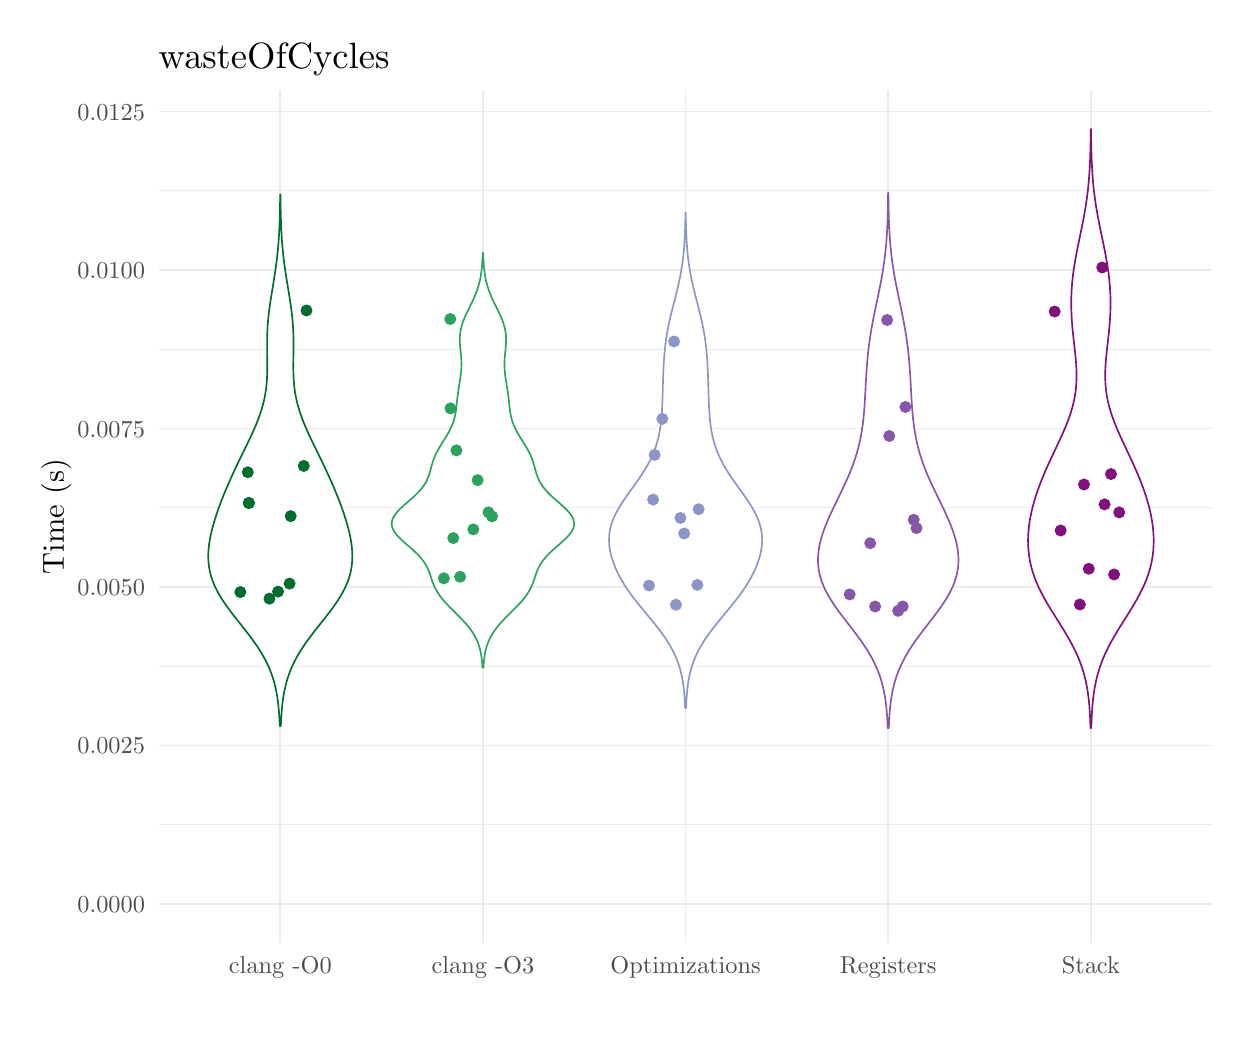
\begin{tikzpicture}[x=1pt,y=1pt]
\definecolor{fillColor}{RGB}{255,255,255}
\path[use as bounding box,fill=fillColor,fill opacity=0.00] (0,0) rectangle (433.62,361.35);
\begin{scope}
\path[clip] ( 47.35, 30.69) rectangle (428.12,338.69);
\definecolor{drawColor}{gray}{0.92}

\path[draw=drawColor,line width= 0.3pt,line join=round] ( 47.35, 73.32) --
	(428.12, 73.32);

\path[draw=drawColor,line width= 0.3pt,line join=round] ( 47.35,130.58) --
	(428.12,130.58);

\path[draw=drawColor,line width= 0.3pt,line join=round] ( 47.35,187.84) --
	(428.12,187.84);

\path[draw=drawColor,line width= 0.3pt,line join=round] ( 47.35,245.10) --
	(428.12,245.10);

\path[draw=drawColor,line width= 0.3pt,line join=round] ( 47.35,302.36) --
	(428.12,302.36);

\path[draw=drawColor,line width= 0.6pt,line join=round] ( 47.35, 44.69) --
	(428.12, 44.69);

\path[draw=drawColor,line width= 0.6pt,line join=round] ( 47.35,101.95) --
	(428.12,101.95);

\path[draw=drawColor,line width= 0.6pt,line join=round] ( 47.35,159.21) --
	(428.12,159.21);

\path[draw=drawColor,line width= 0.6pt,line join=round] ( 47.35,216.47) --
	(428.12,216.47);

\path[draw=drawColor,line width= 0.6pt,line join=round] ( 47.35,273.73) --
	(428.12,273.73);

\path[draw=drawColor,line width= 0.6pt,line join=round] ( 47.35,331.00) --
	(428.12,331.00);

\path[draw=drawColor,line width= 0.6pt,line join=round] ( 91.29, 30.69) --
	( 91.29,338.69);

\path[draw=drawColor,line width= 0.6pt,line join=round] (164.51, 30.69) --
	(164.51,338.69);

\path[draw=drawColor,line width= 0.6pt,line join=round] (237.74, 30.69) --
	(237.74,338.69);

\path[draw=drawColor,line width= 0.6pt,line join=round] (310.96, 30.69) --
	(310.96,338.69);

\path[draw=drawColor,line width= 0.6pt,line join=round] (384.19, 30.69) --
	(384.19,338.69);
\definecolor{drawColor}{RGB}{0,109,44}
\definecolor{fillColor}{RGB}{255,255,255}

\path[draw=drawColor,line width= 0.6pt,line join=round,line cap=round,fill=fillColor] ( 91.08,109.00) --
	( 91.07,109.38) --
	( 91.06,109.75) --
	( 91.04,110.13) --
	( 91.02,110.51) --
	( 91.01,110.88) --
	( 90.99,111.26) --
	( 90.97,111.63) --
	( 90.94,112.01) --
	( 90.92,112.39) --
	( 90.90,112.76) --
	( 90.87,113.14) --
	( 90.85,113.51) --
	( 90.82,113.89) --
	( 90.79,114.26) --
	( 90.76,114.64) --
	( 90.73,115.02) --
	( 90.69,115.39) --
	( 90.66,115.77) --
	( 90.62,116.14) --
	( 90.58,116.52) --
	( 90.54,116.89) --
	( 90.50,117.27) --
	( 90.45,117.65) --
	( 90.40,118.02) --
	( 90.35,118.40) --
	( 90.30,118.77) --
	( 90.24,119.15) --
	( 90.19,119.53) --
	( 90.13,119.90) --
	( 90.06,120.28) --
	( 90.00,120.65) --
	( 89.93,121.03) --
	( 89.86,121.40) --
	( 89.78,121.78) --
	( 89.70,122.16) --
	( 89.62,122.53) --
	( 89.54,122.91) --
	( 89.45,123.28) --
	( 89.36,123.66) --
	( 89.27,124.04) --
	( 89.17,124.41) --
	( 89.07,124.79) --
	( 88.96,125.16) --
	( 88.85,125.54) --
	( 88.74,125.91) --
	( 88.62,126.29) --
	( 88.50,126.67) --
	( 88.38,127.04) --
	( 88.25,127.42) --
	( 88.11,127.79) --
	( 87.98,128.17) --
	( 87.83,128.54) --
	( 87.69,128.92) --
	( 87.54,129.30) --
	( 87.38,129.67) --
	( 87.22,130.05) --
	( 87.06,130.42) --
	( 86.89,130.80) --
	( 86.72,131.18) --
	( 86.54,131.55) --
	( 86.36,131.93) --
	( 86.17,132.30) --
	( 85.98,132.68) --
	( 85.78,133.05) --
	( 85.58,133.43) --
	( 85.37,133.81) --
	( 85.16,134.18) --
	( 84.95,134.56) --
	( 84.73,134.93) --
	( 84.51,135.31) --
	( 84.28,135.68) --
	( 84.05,136.06) --
	( 83.81,136.44) --
	( 83.57,136.81) --
	( 83.33,137.19) --
	( 83.08,137.56) --
	( 82.83,137.94) --
	( 82.57,138.32) --
	( 82.31,138.69) --
	( 82.05,139.07) --
	( 81.78,139.44) --
	( 81.51,139.82) --
	( 81.24,140.19) --
	( 80.97,140.57) --
	( 80.69,140.95) --
	( 80.41,141.32) --
	( 80.12,141.70) --
	( 79.84,142.07) --
	( 79.55,142.45) --
	( 79.26,142.82) --
	( 78.97,143.20) --
	( 78.68,143.58) --
	( 78.38,143.95) --
	( 78.09,144.33) --
	( 77.79,144.70) --
	( 77.49,145.08) --
	( 77.19,145.46) --
	( 76.89,145.83) --
	( 76.60,146.21) --
	( 76.30,146.58) --
	( 76.00,146.96) --
	( 75.70,147.33) --
	( 75.41,147.71) --
	( 75.11,148.09) --
	( 74.82,148.46) --
	( 74.52,148.84) --
	( 74.23,149.21) --
	( 73.94,149.59) --
	( 73.65,149.96) --
	( 73.37,150.34) --
	( 73.09,150.72) --
	( 72.81,151.09) --
	( 72.53,151.47) --
	( 72.26,151.84) --
	( 71.99,152.22) --
	( 71.72,152.60) --
	( 71.45,152.97) --
	( 71.20,153.35) --
	( 70.94,153.72) --
	( 70.69,154.10) --
	( 70.44,154.47) --
	( 70.20,154.85) --
	( 69.97,155.23) --
	( 69.73,155.60) --
	( 69.51,155.98) --
	( 69.28,156.35) --
	( 69.07,156.73) --
	( 68.86,157.11) --
	( 68.65,157.48) --
	( 68.45,157.86) --
	( 68.26,158.23) --
	( 68.07,158.61) --
	( 67.89,158.98) --
	( 67.71,159.36) --
	( 67.54,159.74) --
	( 67.38,160.11) --
	( 67.22,160.49) --
	( 67.07,160.86) --
	( 66.92,161.24) --
	( 66.78,161.61) --
	( 66.65,161.99) --
	( 66.52,162.37) --
	( 66.40,162.74) --
	( 66.29,163.12) --
	( 66.18,163.49) --
	( 66.08,163.87) --
	( 65.98,164.25) --
	( 65.89,164.62) --
	( 65.81,165.00) --
	( 65.73,165.37) --
	( 65.66,165.75) --
	( 65.60,166.12) --
	( 65.54,166.50) --
	( 65.49,166.88) --
	( 65.44,167.25) --
	( 65.40,167.63) --
	( 65.36,168.00) --
	( 65.33,168.38) --
	( 65.31,168.75) --
	( 65.29,169.13) --
	( 65.27,169.51) --
	( 65.26,169.88) --
	( 65.26,170.26) --
	( 65.26,170.63) --
	( 65.27,171.01) --
	( 65.28,171.39) --
	( 65.29,171.76) --
	( 65.31,172.14) --
	( 65.34,172.51) --
	( 65.37,172.89) --
	( 65.40,173.26) --
	( 65.44,173.64) --
	( 65.48,174.02) --
	( 65.53,174.39) --
	( 65.58,174.77) --
	( 65.63,175.14) --
	( 65.69,175.52) --
	( 65.75,175.89) --
	( 65.81,176.27) --
	( 65.88,176.65) --
	( 65.95,177.02) --
	( 66.02,177.40) --
	( 66.10,177.77) --
	( 66.18,178.15) --
	( 66.26,178.53) --
	( 66.35,178.90) --
	( 66.44,179.28) --
	( 66.53,179.65) --
	( 66.62,180.03) --
	( 66.72,180.40) --
	( 66.82,180.78) --
	( 66.92,181.16) --
	( 67.03,181.53) --
	( 67.13,181.91) --
	( 67.24,182.28) --
	( 67.35,182.66) --
	( 67.46,183.04) --
	( 67.58,183.41) --
	( 67.69,183.79) --
	( 67.81,184.16) --
	( 67.93,184.54) --
	( 68.05,184.91) --
	( 68.18,185.29) --
	( 68.30,185.67) --
	( 68.43,186.04) --
	( 68.56,186.42) --
	( 68.69,186.79) --
	( 68.82,187.17) --
	( 68.95,187.54) --
	( 69.09,187.92) --
	( 69.22,188.30) --
	( 69.36,188.67) --
	( 69.50,189.05) --
	( 69.64,189.42) --
	( 69.78,189.80) --
	( 69.92,190.18) --
	( 70.07,190.55) --
	( 70.21,190.93) --
	( 70.36,191.30) --
	( 70.51,191.68) --
	( 70.66,192.05) --
	( 70.81,192.43) --
	( 70.96,192.81) --
	( 71.11,193.18) --
	( 71.27,193.56) --
	( 71.42,193.93) --
	( 71.58,194.31) --
	( 71.74,194.68) --
	( 71.89,195.06) --
	( 72.05,195.44) --
	( 72.22,195.81) --
	( 72.38,196.19) --
	( 72.54,196.56) --
	( 72.70,196.94) --
	( 72.87,197.32) --
	( 73.04,197.69) --
	( 73.20,198.07) --
	( 73.37,198.44) --
	( 73.54,198.82) --
	( 73.71,199.19) --
	( 73.88,199.57) --
	( 74.05,199.95) --
	( 74.23,200.32) --
	( 74.40,200.70) --
	( 74.58,201.07) --
	( 74.75,201.45) --
	( 74.93,201.82) --
	( 75.10,202.20) --
	( 75.28,202.58) --
	( 75.46,202.95) --
	( 75.64,203.33) --
	( 75.82,203.70) --
	( 76.00,204.08) --
	( 76.18,204.46) --
	( 76.36,204.83) --
	( 76.55,205.21) --
	( 76.73,205.58) --
	( 76.91,205.96) --
	( 77.10,206.33) --
	( 77.28,206.71) --
	( 77.46,207.09) --
	( 77.65,207.46) --
	( 77.83,207.84) --
	( 78.02,208.21) --
	( 78.20,208.59) --
	( 78.38,208.97) --
	( 78.57,209.34) --
	( 78.75,209.72) --
	( 78.93,210.09) --
	( 79.12,210.47) --
	( 79.30,210.84) --
	( 79.48,211.22) --
	( 79.66,211.60) --
	( 79.84,211.97) --
	( 80.02,212.35) --
	( 80.20,212.72) --
	( 80.38,213.10) --
	( 80.56,213.47) --
	( 80.73,213.85) --
	( 80.91,214.23) --
	( 81.08,214.60) --
	( 81.25,214.98) --
	( 81.42,215.35) --
	( 81.59,215.73) --
	( 81.75,216.11) --
	( 81.92,216.48) --
	( 82.08,216.86) --
	( 82.24,217.23) --
	( 82.40,217.61) --
	( 82.56,217.98) --
	( 82.71,218.36) --
	( 82.86,218.74) --
	( 83.01,219.11) --
	( 83.16,219.49) --
	( 83.30,219.86) --
	( 83.44,220.24) --
	( 83.58,220.61) --
	( 83.72,220.99) --
	( 83.85,221.37) --
	( 83.98,221.74) --
	( 84.11,222.12) --
	( 84.23,222.49) --
	( 84.35,222.87) --
	( 84.47,223.25) --
	( 84.59,223.62) --
	( 84.70,224.00) --
	( 84.81,224.37) --
	( 84.91,224.75) --
	( 85.01,225.12) --
	( 85.11,225.50) --
	( 85.21,225.88) --
	( 85.30,226.25) --
	( 85.38,226.63) --
	( 85.47,227.00) --
	( 85.55,227.38) --
	( 85.63,227.75) --
	( 85.70,228.13) --
	( 85.77,228.51) --
	( 85.84,228.88) --
	( 85.90,229.26) --
	( 85.96,229.63) --
	( 86.02,230.01) --
	( 86.08,230.39) --
	( 86.13,230.76) --
	( 86.17,231.14) --
	( 86.22,231.51) --
	( 86.26,231.89) --
	( 86.30,232.26) --
	( 86.34,232.64) --
	( 86.37,233.02) --
	( 86.40,233.39) --
	( 86.43,233.77) --
	( 86.45,234.14) --
	( 86.47,234.52) --
	( 86.49,234.90) --
	( 86.51,235.27) --
	( 86.53,235.65) --
	( 86.54,236.02) --
	( 86.55,236.40) --
	( 86.56,236.77) --
	( 86.57,237.15) --
	( 86.58,237.53) --
	( 86.58,237.90) --
	( 86.59,238.28) --
	( 86.59,238.65) --
	( 86.59,239.03) --
	( 86.59,239.40) --
	( 86.59,239.78) --
	( 86.58,240.16) --
	( 86.58,240.53) --
	( 86.58,240.91) --
	( 86.57,241.28) --
	( 86.57,241.66) --
	( 86.56,242.04) --
	( 86.56,242.41) --
	( 86.55,242.79) --
	( 86.54,243.16) --
	( 86.54,243.54) --
	( 86.53,243.91) --
	( 86.53,244.29) --
	( 86.52,244.67) --
	( 86.52,245.04) --
	( 86.52,245.42) --
	( 86.51,245.79) --
	( 86.51,246.17) --
	( 86.51,246.54) --
	( 86.51,246.92) --
	( 86.51,247.30) --
	( 86.51,247.67) --
	( 86.51,248.05) --
	( 86.52,248.42) --
	( 86.52,248.80) --
	( 86.53,249.18) --
	( 86.54,249.55) --
	( 86.54,249.93) --
	( 86.56,250.30) --
	( 86.57,250.68) --
	( 86.58,251.05) --
	( 86.60,251.43) --
	( 86.61,251.81) --
	( 86.63,252.18) --
	( 86.65,252.56) --
	( 86.67,252.93) --
	( 86.70,253.31) --
	( 86.72,253.68) --
	( 86.75,254.06) --
	( 86.77,254.44) --
	( 86.81,254.81) --
	( 86.84,255.19) --
	( 86.87,255.56) --
	( 86.90,255.94) --
	( 86.94,256.32) --
	( 86.98,256.69) --
	( 87.02,257.07) --
	( 87.06,257.44) --
	( 87.10,257.82) --
	( 87.14,258.19) --
	( 87.19,258.57) --
	( 87.24,258.95) --
	( 87.28,259.32) --
	( 87.33,259.70) --
	( 87.38,260.07) --
	( 87.44,260.45) --
	( 87.49,260.82) --
	( 87.54,261.20) --
	( 87.60,261.58) --
	( 87.65,261.95) --
	( 87.71,262.33) --
	( 87.76,262.70) --
	( 87.82,263.08) --
	( 87.88,263.46) --
	( 87.94,263.83) --
	( 88.00,264.21) --
	( 88.06,264.58) --
	( 88.12,264.96) --
	( 88.18,265.33) --
	( 88.24,265.71) --
	( 88.30,266.09) --
	( 88.37,266.46) --
	( 88.43,266.84) --
	( 88.49,267.21) --
	( 88.55,267.59) --
	( 88.61,267.97) --
	( 88.68,268.34) --
	( 88.74,268.72) --
	( 88.80,269.09) --
	( 88.86,269.47) --
	( 88.92,269.84) --
	( 88.98,270.22) --
	( 89.04,270.60) --
	( 89.10,270.97) --
	( 89.16,271.35) --
	( 89.22,271.72) --
	( 89.27,272.10) --
	( 89.33,272.47) --
	( 89.39,272.85) --
	( 89.44,273.23) --
	( 89.50,273.60) --
	( 89.55,273.98) --
	( 89.61,274.35) --
	( 89.66,274.73) --
	( 89.71,275.11) --
	( 89.76,275.48) --
	( 89.81,275.86) --
	( 89.86,276.23) --
	( 89.91,276.61) --
	( 89.96,276.98) --
	( 90.00,277.36) --
	( 90.05,277.74) --
	( 90.09,278.11) --
	( 90.14,278.49) --
	( 90.18,278.86) --
	( 90.22,279.24) --
	( 90.26,279.61) --
	( 90.30,279.99) --
	( 90.34,280.37) --
	( 90.37,280.74) --
	( 90.41,281.12) --
	( 90.44,281.49) --
	( 90.48,281.87) --
	( 90.51,282.25) --
	( 90.54,282.62) --
	( 90.57,283.00) --
	( 90.61,283.37) --
	( 90.63,283.75) --
	( 90.66,284.12) --
	( 90.69,284.50) --
	( 90.72,284.88) --
	( 90.74,285.25) --
	( 90.77,285.63) --
	( 90.79,286.00) --
	( 90.81,286.38) --
	( 90.84,286.75) --
	( 90.86,287.13) --
	( 90.88,287.51) --
	( 90.90,287.88) --
	( 90.92,288.26) --
	( 90.93,288.63) --
	( 90.95,289.01) --
	( 90.97,289.39) --
	( 90.98,289.76) --
	( 91.00,290.14) --
	( 91.02,290.51) --
	( 91.03,290.89) --
	( 91.04,291.26) --
	( 91.06,291.64) --
	( 91.07,292.02) --
	( 91.08,292.39) --
	( 91.09,292.77) --
	( 91.10,293.14) --
	( 91.11,293.52) --
	( 91.12,293.90) --
	( 91.13,294.27) --
	( 91.14,294.65) --
	( 91.15,295.02) --
	( 91.16,295.40) --
	( 91.16,295.77) --
	( 91.17,296.15) --
	( 91.18,296.53) --
	( 91.18,296.90) --
	( 91.19,297.28) --
	( 91.20,297.65) --
	( 91.20,298.03) --
	( 91.21,298.40) --
	( 91.21,298.78) --
	( 91.22,299.16) --
	( 91.22,299.53) --
	( 91.23,299.91) --
	( 91.23,300.28) --
	( 91.23,300.66) --
	( 91.24,301.04) --
	( 91.34,301.04) --
	( 91.34,300.66) --
	( 91.35,300.28) --
	( 91.35,299.91) --
	( 91.35,299.53) --
	( 91.36,299.16) --
	( 91.36,298.78) --
	( 91.37,298.40) --
	( 91.37,298.03) --
	( 91.38,297.65) --
	( 91.38,297.28) --
	( 91.39,296.90) --
	( 91.40,296.53) --
	( 91.40,296.15) --
	( 91.41,295.77) --
	( 91.42,295.40) --
	( 91.43,295.02) --
	( 91.43,294.65) --
	( 91.44,294.27) --
	( 91.45,293.90) --
	( 91.46,293.52) --
	( 91.47,293.14) --
	( 91.48,292.77) --
	( 91.50,292.39) --
	( 91.51,292.02) --
	( 91.52,291.64) --
	( 91.53,291.26) --
	( 91.55,290.89) --
	( 91.56,290.51) --
	( 91.57,290.14) --
	( 91.59,289.76) --
	( 91.61,289.39) --
	( 91.62,289.01) --
	( 91.64,288.63) --
	( 91.66,288.26) --
	( 91.68,287.88) --
	( 91.70,287.51) --
	( 91.72,287.13) --
	( 91.74,286.75) --
	( 91.76,286.38) --
	( 91.78,286.00) --
	( 91.81,285.63) --
	( 91.83,285.25) --
	( 91.86,284.88) --
	( 91.88,284.50) --
	( 91.91,284.12) --
	( 91.94,283.75) --
	( 91.97,283.37) --
	( 92.00,283.00) --
	( 92.03,282.62) --
	( 92.06,282.25) --
	( 92.10,281.87) --
	( 92.13,281.49) --
	( 92.17,281.12) --
	( 92.20,280.74) --
	( 92.24,280.37) --
	( 92.28,279.99) --
	( 92.32,279.61) --
	( 92.36,279.24) --
	( 92.40,278.86) --
	( 92.44,278.49) --
	( 92.48,278.11) --
	( 92.53,277.74) --
	( 92.57,277.36) --
	( 92.62,276.98) --
	( 92.67,276.61) --
	( 92.71,276.23) --
	( 92.76,275.86) --
	( 92.81,275.48) --
	( 92.86,275.11) --
	( 92.92,274.73) --
	( 92.97,274.35) --
	( 93.02,273.98) --
	( 93.08,273.60) --
	( 93.13,273.23) --
	( 93.19,272.85) --
	( 93.24,272.47) --
	( 93.30,272.10) --
	( 93.36,271.72) --
	( 93.42,271.35) --
	( 93.48,270.97) --
	( 93.53,270.60) --
	( 93.59,270.22) --
	( 93.66,269.84) --
	( 93.72,269.47) --
	( 93.78,269.09) --
	( 93.84,268.72) --
	( 93.90,268.34) --
	( 93.96,267.97) --
	( 94.02,267.59) --
	( 94.09,267.21) --
	( 94.15,266.84) --
	( 94.21,266.46) --
	( 94.27,266.09) --
	( 94.33,265.71) --
	( 94.39,265.33) --
	( 94.45,264.96) --
	( 94.52,264.58) --
	( 94.58,264.21) --
	( 94.64,263.83) --
	( 94.69,263.46) --
	( 94.75,263.08) --
	( 94.81,262.70) --
	( 94.87,262.33) --
	( 94.92,261.95) --
	( 94.98,261.58) --
	( 95.03,261.20) --
	( 95.09,260.82) --
	( 95.14,260.45) --
	( 95.19,260.07) --
	( 95.24,259.70) --
	( 95.29,259.32) --
	( 95.34,258.95) --
	( 95.38,258.57) --
	( 95.43,258.19) --
	( 95.47,257.82) --
	( 95.52,257.44) --
	( 95.56,257.07) --
	( 95.60,256.69) --
	( 95.63,256.32) --
	( 95.67,255.94) --
	( 95.71,255.56) --
	( 95.74,255.19) --
	( 95.77,254.81) --
	( 95.80,254.44) --
	( 95.83,254.06) --
	( 95.85,253.68) --
	( 95.88,253.31) --
	( 95.90,252.93) --
	( 95.92,252.56) --
	( 95.94,252.18) --
	( 95.96,251.81) --
	( 95.98,251.43) --
	( 95.99,251.05) --
	( 96.01,250.68) --
	( 96.02,250.30) --
	( 96.03,249.93) --
	( 96.04,249.55) --
	( 96.05,249.18) --
	( 96.05,248.80) --
	( 96.06,248.42) --
	( 96.06,248.05) --
	( 96.07,247.67) --
	( 96.07,247.30) --
	( 96.07,246.92) --
	( 96.07,246.54) --
	( 96.07,246.17) --
	( 96.06,245.79) --
	( 96.06,245.42) --
	( 96.06,245.04) --
	( 96.05,244.67) --
	( 96.05,244.29) --
	( 96.04,243.91) --
	( 96.04,243.54) --
	( 96.03,243.16) --
	( 96.02,242.79) --
	( 96.02,242.41) --
	( 96.01,242.04) --
	( 96.01,241.66) --
	( 96.00,241.28) --
	( 96.00,240.91) --
	( 95.99,240.53) --
	( 95.99,240.16) --
	( 95.99,239.78) --
	( 95.99,239.40) --
	( 95.99,239.03) --
	( 95.99,238.65) --
	( 95.99,238.28) --
	( 95.99,237.90) --
	( 96.00,237.53) --
	( 96.00,237.15) --
	( 96.01,236.77) --
	( 96.02,236.40) --
	( 96.03,236.02) --
	( 96.05,235.65) --
	( 96.06,235.27) --
	( 96.08,234.90) --
	( 96.10,234.52) --
	( 96.12,234.14) --
	( 96.15,233.77) --
	( 96.18,233.39) --
	( 96.21,233.02) --
	( 96.24,232.64) --
	( 96.28,232.26) --
	( 96.31,231.89) --
	( 96.36,231.51) --
	( 96.40,231.14) --
	( 96.45,230.76) --
	( 96.50,230.39) --
	( 96.55,230.01) --
	( 96.61,229.63) --
	( 96.67,229.26) --
	( 96.74,228.88) --
	( 96.80,228.51) --
	( 96.87,228.13) --
	( 96.95,227.75) --
	( 97.03,227.38) --
	( 97.11,227.00) --
	( 97.19,226.63) --
	( 97.28,226.25) --
	( 97.37,225.88) --
	( 97.46,225.50) --
	( 97.56,225.12) --
	( 97.66,224.75) --
	( 97.77,224.37) --
	( 97.88,224.00) --
	( 97.99,223.62) --
	( 98.10,223.25) --
	( 98.22,222.87) --
	( 98.34,222.49) --
	( 98.47,222.12) --
	( 98.59,221.74) --
	( 98.72,221.37) --
	( 98.86,220.99) --
	( 98.99,220.61) --
	( 99.13,220.24) --
	( 99.27,219.86) --
	( 99.42,219.49) --
	( 99.56,219.11) --
	( 99.71,218.74) --
	( 99.86,218.36) --
	(100.02,217.98) --
	(100.17,217.61) --
	(100.33,217.23) --
	(100.49,216.86) --
	(100.66,216.48) --
	(100.82,216.11) --
	(100.99,215.73) --
	(101.16,215.35) --
	(101.33,214.98) --
	(101.50,214.60) --
	(101.67,214.23) --
	(101.84,213.85) --
	(102.02,213.47) --
	(102.20,213.10) --
	(102.37,212.72) --
	(102.55,212.35) --
	(102.73,211.97) --
	(102.91,211.60) --
	(103.09,211.22) --
	(103.28,210.84) --
	(103.46,210.47) --
	(103.64,210.09) --
	(103.82,209.72) --
	(104.01,209.34) --
	(104.19,208.97) --
	(104.38,208.59) --
	(104.56,208.21) --
	(104.74,207.84) --
	(104.93,207.46) --
	(105.11,207.09) --
	(105.30,206.71) --
	(105.48,206.33) --
	(105.66,205.96) --
	(105.85,205.58) --
	(106.03,205.21) --
	(106.21,204.83) --
	(106.39,204.46) --
	(106.57,204.08) --
	(106.75,203.70) --
	(106.94,203.33) --
	(107.11,202.95) --
	(107.29,202.58) --
	(107.47,202.20) --
	(107.65,201.82) --
	(107.82,201.45) --
	(108.00,201.07) --
	(108.17,200.70) --
	(108.35,200.32) --
	(108.52,199.95) --
	(108.69,199.57) --
	(108.86,199.19) --
	(109.03,198.82) --
	(109.20,198.44) --
	(109.37,198.07) --
	(109.54,197.69) --
	(109.71,197.32) --
	(109.87,196.94) --
	(110.03,196.56) --
	(110.20,196.19) --
	(110.36,195.81) --
	(110.52,195.44) --
	(110.68,195.06) --
	(110.84,194.68) --
	(111.00,194.31) --
	(111.15,193.93) --
	(111.31,193.56) --
	(111.46,193.18) --
	(111.61,192.81) --
	(111.77,192.43) --
	(111.92,192.05) --
	(112.07,191.68) --
	(112.21,191.30) --
	(112.36,190.93) --
	(112.51,190.55) --
	(112.65,190.18) --
	(112.79,189.80) --
	(112.94,189.42) --
	(113.08,189.05) --
	(113.22,188.67) --
	(113.35,188.30) --
	(113.49,187.92) --
	(113.62,187.54) --
	(113.76,187.17) --
	(113.89,186.79) --
	(114.02,186.42) --
	(114.15,186.04) --
	(114.27,185.67) --
	(114.40,185.29) --
	(114.52,184.91) --
	(114.64,184.54) --
	(114.76,184.16) --
	(114.88,183.79) --
	(115.00,183.41) --
	(115.11,183.04) --
	(115.23,182.66) --
	(115.34,182.28) --
	(115.44,181.91) --
	(115.55,181.53) --
	(115.65,181.16) --
	(115.75,180.78) --
	(115.85,180.40) --
	(115.95,180.03) --
	(116.04,179.65) --
	(116.14,179.28) --
	(116.22,178.90) --
	(116.31,178.53) --
	(116.39,178.15) --
	(116.47,177.77) --
	(116.55,177.40) --
	(116.63,177.02) --
	(116.70,176.65) --
	(116.76,176.27) --
	(116.83,175.89) --
	(116.89,175.52) --
	(116.95,175.14) --
	(117.00,174.77) --
	(117.05,174.39) --
	(117.09,174.02) --
	(117.14,173.64) --
	(117.17,173.26) --
	(117.21,172.89) --
	(117.24,172.51) --
	(117.26,172.14) --
	(117.28,171.76) --
	(117.30,171.39) --
	(117.31,171.01) --
	(117.31,170.63) --
	(117.32,170.26) --
	(117.31,169.88) --
	(117.30,169.51) --
	(117.29,169.13) --
	(117.27,168.75) --
	(117.24,168.38) --
	(117.21,168.00) --
	(117.18,167.63) --
	(117.14,167.25) --
	(117.09,166.88) --
	(117.04,166.50) --
	(116.98,166.12) --
	(116.91,165.75) --
	(116.84,165.37) --
	(116.76,165.00) --
	(116.68,164.62) --
	(116.59,164.25) --
	(116.50,163.87) --
	(116.39,163.49) --
	(116.29,163.12) --
	(116.17,162.74) --
	(116.05,162.37) --
	(115.93,161.99) --
	(115.79,161.61) --
	(115.65,161.24) --
	(115.51,160.86) --
	(115.36,160.49) --
	(115.20,160.11) --
	(115.03,159.74) --
	(114.87,159.36) --
	(114.69,158.98) --
	(114.51,158.61) --
	(114.32,158.23) --
	(114.12,157.86) --
	(113.93,157.48) --
	(113.72,157.11) --
	(113.51,156.73) --
	(113.29,156.35) --
	(113.07,155.98) --
	(112.84,155.60) --
	(112.61,155.23) --
	(112.37,154.85) --
	(112.13,154.47) --
	(111.88,154.10) --
	(111.64,153.72) --
	(111.38,153.35) --
	(111.12,152.97) --
	(110.86,152.60) --
	(110.59,152.22) --
	(110.32,151.84) --
	(110.05,151.47) --
	(109.77,151.09) --
	(109.49,150.72) --
	(109.21,150.34) --
	(108.92,149.96) --
	(108.63,149.59) --
	(108.34,149.21) --
	(108.05,148.84) --
	(107.76,148.46) --
	(107.47,148.09) --
	(107.17,147.71) --
	(106.87,147.33) --
	(106.58,146.96) --
	(106.28,146.58) --
	(105.98,146.21) --
	(105.68,145.83) --
	(105.38,145.46) --
	(105.08,145.08) --
	(104.79,144.70) --
	(104.49,144.33) --
	(104.19,143.95) --
	(103.90,143.58) --
	(103.61,143.20) --
	(103.31,142.82) --
	(103.02,142.45) --
	(102.74,142.07) --
	(102.45,141.70) --
	(102.17,141.32) --
	(101.89,140.95) --
	(101.61,140.57) --
	(101.33,140.19) --
	(101.06,139.82) --
	(100.79,139.44) --
	(100.52,139.07) --
	(100.26,138.69) --
	(100.00,138.32) --
	( 99.75,137.94) --
	( 99.50,137.56) --
	( 99.25,137.19) --
	( 99.00,136.81) --
	( 98.76,136.44) --
	( 98.53,136.06) --
	( 98.29,135.68) --
	( 98.07,135.31) --
	( 97.84,134.93) --
	( 97.62,134.56) --
	( 97.41,134.18) --
	( 97.20,133.81) --
	( 97.00,133.43) --
	( 96.80,133.05) --
	( 96.60,132.68) --
	( 96.41,132.30) --
	( 96.22,131.93) --
	( 96.04,131.55) --
	( 95.86,131.18) --
	( 95.69,130.80) --
	( 95.52,130.42) --
	( 95.35,130.05) --
	( 95.19,129.67) --
	( 95.04,129.30) --
	( 94.89,128.92) --
	( 94.74,128.54) --
	( 94.60,128.17) --
	( 94.46,127.79) --
	( 94.33,127.42) --
	( 94.20,127.04) --
	( 94.07,126.67) --
	( 93.95,126.29) --
	( 93.84,125.91) --
	( 93.72,125.54) --
	( 93.61,125.16) --
	( 93.51,124.79) --
	( 93.41,124.41) --
	( 93.31,124.04) --
	( 93.21,123.66) --
	( 93.12,123.28) --
	( 93.04,122.91) --
	( 92.95,122.53) --
	( 92.87,122.16) --
	( 92.79,121.78) --
	( 92.72,121.40) --
	( 92.65,121.03) --
	( 92.58,120.65) --
	( 92.51,120.28) --
	( 92.45,119.90) --
	( 92.39,119.53) --
	( 92.33,119.15) --
	( 92.28,118.77) --
	( 92.22,118.40) --
	( 92.17,118.02) --
	( 92.13,117.65) --
	( 92.08,117.27) --
	( 92.04,116.89) --
	( 91.99,116.52) --
	( 91.96,116.14) --
	( 91.92,115.77) --
	( 91.88,115.39) --
	( 91.85,115.02) --
	( 91.82,114.64) --
	( 91.78,114.26) --
	( 91.76,113.89) --
	( 91.73,113.51) --
	( 91.70,113.14) --
	( 91.68,112.76) --
	( 91.65,112.39) --
	( 91.63,112.01) --
	( 91.61,111.63) --
	( 91.59,111.26) --
	( 91.57,110.88) --
	( 91.55,110.51) --
	( 91.54,110.13) --
	( 91.52,109.75) --
	( 91.50,109.38) --
	( 91.49,109.00) --
	( 91.08,109.00) --
	cycle;
\definecolor{drawColor}{RGB}{44,162,95}

\path[draw=drawColor,line width= 0.6pt,line join=round,line cap=round,fill=fillColor] (164.34,130.09) --
	(164.32,130.38) --
	(164.30,130.68) --
	(164.28,130.97) --
	(164.26,131.26) --
	(164.24,131.56) --
	(164.22,131.85) --
	(164.19,132.14) --
	(164.16,132.44) --
	(164.13,132.73) --
	(164.10,133.02) --
	(164.07,133.32) --
	(164.03,133.61) --
	(163.99,133.90) --
	(163.95,134.20) --
	(163.90,134.49) --
	(163.85,134.78) --
	(163.80,135.08) --
	(163.75,135.37) --
	(163.69,135.66) --
	(163.62,135.96) --
	(163.56,136.25) --
	(163.49,136.54) --
	(163.41,136.84) --
	(163.34,137.13) --
	(163.25,137.42) --
	(163.17,137.72) --
	(163.07,138.01) --
	(162.98,138.30) --
	(162.87,138.59) --
	(162.77,138.89) --
	(162.65,139.18) --
	(162.54,139.47) --
	(162.41,139.77) --
	(162.28,140.06) --
	(162.15,140.35) --
	(162.01,140.65) --
	(161.86,140.94) --
	(161.70,141.23) --
	(161.54,141.53) --
	(161.38,141.82) --
	(161.20,142.11) --
	(161.02,142.41) --
	(160.84,142.70) --
	(160.65,142.99) --
	(160.45,143.29) --
	(160.24,143.58) --
	(160.03,143.87) --
	(159.81,144.17) --
	(159.59,144.46) --
	(159.36,144.75) --
	(159.13,145.05) --
	(158.88,145.34) --
	(158.64,145.63) --
	(158.39,145.93) --
	(158.13,146.22) --
	(157.87,146.51) --
	(157.60,146.81) --
	(157.33,147.10) --
	(157.05,147.39) --
	(156.77,147.69) --
	(156.49,147.98) --
	(156.21,148.27) --
	(155.92,148.57) --
	(155.63,148.86) --
	(155.33,149.15) --
	(155.04,149.45) --
	(154.74,149.74) --
	(154.45,150.03) --
	(154.15,150.33) --
	(153.86,150.62) --
	(153.56,150.91) --
	(153.27,151.21) --
	(152.97,151.50) --
	(152.68,151.79) --
	(152.40,152.09) --
	(152.11,152.38) --
	(151.83,152.67) --
	(151.55,152.96) --
	(151.28,153.26) --
	(151.01,153.55) --
	(150.75,153.84) --
	(150.49,154.14) --
	(150.23,154.43) --
	(149.99,154.72) --
	(149.75,155.02) --
	(149.51,155.31) --
	(149.28,155.60) --
	(149.06,155.90) --
	(148.85,156.19) --
	(148.65,156.48) --
	(148.45,156.78) --
	(148.25,157.07) --
	(148.07,157.36) --
	(147.89,157.66) --
	(147.72,157.95) --
	(147.56,158.24) --
	(147.41,158.54) --
	(147.26,158.83) --
	(147.12,159.12) --
	(146.98,159.42) --
	(146.85,159.71) --
	(146.73,160.00) --
	(146.60,160.30) --
	(146.49,160.59) --
	(146.38,160.88) --
	(146.27,161.18) --
	(146.17,161.47) --
	(146.07,161.76) --
	(145.97,162.06) --
	(145.87,162.35) --
	(145.77,162.64) --
	(145.68,162.94) --
	(145.58,163.23) --
	(145.48,163.52) --
	(145.38,163.82) --
	(145.28,164.11) --
	(145.17,164.40) --
	(145.06,164.70) --
	(144.95,164.99) --
	(144.83,165.28) --
	(144.70,165.58) --
	(144.57,165.87) --
	(144.44,166.16) --
	(144.29,166.45) --
	(144.14,166.75) --
	(143.98,167.04) --
	(143.81,167.33) --
	(143.63,167.63) --
	(143.45,167.92) --
	(143.25,168.21) --
	(143.04,168.51) --
	(142.83,168.80) --
	(142.60,169.09) --
	(142.37,169.39) --
	(142.13,169.68) --
	(141.87,169.97) --
	(141.61,170.27) --
	(141.34,170.56) --
	(141.06,170.85) --
	(140.77,171.15) --
	(140.48,171.44) --
	(140.17,171.73) --
	(139.86,172.03) --
	(139.55,172.32) --
	(139.22,172.61) --
	(138.90,172.91) --
	(138.57,173.20) --
	(138.23,173.49) --
	(137.90,173.79) --
	(137.56,174.08) --
	(137.22,174.37) --
	(136.89,174.67) --
	(136.55,174.96) --
	(136.22,175.25) --
	(135.89,175.55) --
	(135.57,175.84) --
	(135.25,176.13) --
	(134.94,176.43) --
	(134.63,176.72) --
	(134.34,177.01) --
	(134.06,177.31) --
	(133.78,177.60) --
	(133.52,177.89) --
	(133.28,178.19) --
	(133.04,178.48) --
	(132.82,178.77) --
	(132.62,179.07) --
	(132.43,179.36) --
	(132.26,179.65) --
	(132.10,179.95) --
	(131.97,180.24) --
	(131.85,180.53) --
	(131.75,180.82) --
	(131.68,181.12) --
	(131.62,181.41) --
	(131.58,181.70) --
	(131.56,182.00) --
	(131.57,182.29) --
	(131.58,182.58) --
	(131.63,182.88) --
	(131.69,183.17) --
	(131.77,183.46) --
	(131.87,183.76) --
	(132.00,184.05) --
	(132.13,184.34) --
	(132.29,184.64) --
	(132.47,184.93) --
	(132.65,185.22) --
	(132.87,185.52) --
	(133.09,185.81) --
	(133.32,186.10) --
	(133.58,186.40) --
	(133.84,186.69) --
	(134.11,186.98) --
	(134.40,187.28) --
	(134.70,187.57) --
	(135.00,187.86) --
	(135.31,188.16) --
	(135.63,188.45) --
	(135.96,188.74) --
	(136.29,189.04) --
	(136.62,189.33) --
	(136.95,189.62) --
	(137.29,189.92) --
	(137.63,190.21) --
	(137.96,190.50) --
	(138.30,190.80) --
	(138.63,191.09) --
	(138.96,191.38) --
	(139.28,191.68) --
	(139.60,191.97) --
	(139.92,192.26) --
	(140.22,192.56) --
	(140.53,192.85) --
	(140.82,193.14) --
	(141.10,193.44) --
	(141.38,193.73) --
	(141.65,194.02) --
	(141.91,194.32) --
	(142.16,194.61) --
	(142.40,194.90) --
	(142.62,195.19) --
	(142.85,195.49) --
	(143.05,195.78) --
	(143.25,196.07) --
	(143.45,196.37) --
	(143.62,196.66) --
	(143.80,196.95) --
	(143.96,197.25) --
	(144.11,197.54) --
	(144.26,197.83) --
	(144.39,198.13) --
	(144.52,198.42) --
	(144.64,198.71) --
	(144.76,199.01) --
	(144.87,199.30) --
	(144.97,199.59) --
	(145.07,199.89) --
	(145.17,200.18) --
	(145.26,200.47) --
	(145.34,200.77) --
	(145.43,201.06) --
	(145.51,201.35) --
	(145.59,201.65) --
	(145.67,201.94) --
	(145.75,202.23) --
	(145.83,202.53) --
	(145.91,202.82) --
	(146.00,203.11) --
	(146.08,203.41) --
	(146.17,203.70) --
	(146.26,203.99) --
	(146.35,204.29) --
	(146.44,204.58) --
	(146.54,204.87) --
	(146.64,205.17) --
	(146.75,205.46) --
	(146.86,205.75) --
	(146.98,206.05) --
	(147.10,206.34) --
	(147.23,206.63) --
	(147.36,206.93) --
	(147.49,207.22) --
	(147.63,207.51) --
	(147.78,207.81) --
	(147.93,208.10) --
	(148.08,208.39) --
	(148.24,208.68) --
	(148.40,208.98) --
	(148.56,209.27) --
	(148.73,209.56) --
	(148.91,209.86) --
	(149.08,210.15) --
	(149.26,210.44) --
	(149.44,210.74) --
	(149.62,211.03) --
	(149.80,211.32) --
	(149.99,211.62) --
	(150.17,211.91) --
	(150.36,212.20) --
	(150.54,212.50) --
	(150.72,212.79) --
	(150.91,213.08) --
	(151.09,213.38) --
	(151.27,213.67) --
	(151.44,213.96) --
	(151.62,214.26) --
	(151.79,214.55) --
	(151.96,214.84) --
	(152.12,215.14) --
	(152.28,215.43) --
	(152.44,215.72) --
	(152.59,216.02) --
	(152.74,216.31) --
	(152.88,216.60) --
	(153.02,216.90) --
	(153.15,217.19) --
	(153.28,217.48) --
	(153.40,217.78) --
	(153.52,218.07) --
	(153.63,218.36) --
	(153.74,218.66) --
	(153.84,218.95) --
	(153.93,219.24) --
	(154.02,219.54) --
	(154.11,219.83) --
	(154.19,220.12) --
	(154.26,220.42) --
	(154.33,220.71) --
	(154.40,221.00) --
	(154.46,221.30) --
	(154.52,221.59) --
	(154.58,221.88) --
	(154.63,222.18) --
	(154.68,222.47) --
	(154.72,222.76) --
	(154.76,223.05) --
	(154.80,223.35) --
	(154.84,223.64) --
	(154.88,223.93) --
	(154.91,224.23) --
	(154.94,224.52) --
	(154.98,224.81) --
	(155.01,225.11) --
	(155.04,225.40) --
	(155.07,225.69) --
	(155.10,225.99) --
	(155.13,226.28) --
	(155.16,226.57) --
	(155.19,226.87) --
	(155.22,227.16) --
	(155.25,227.45) --
	(155.29,227.75) --
	(155.32,228.04) --
	(155.36,228.33) --
	(155.39,228.63) --
	(155.43,228.92) --
	(155.47,229.21) --
	(155.51,229.51) --
	(155.55,229.80) --
	(155.59,230.09) --
	(155.64,230.39) --
	(155.68,230.68) --
	(155.73,230.97) --
	(155.77,231.27) --
	(155.82,231.56) --
	(155.87,231.85) --
	(155.92,232.15) --
	(155.96,232.44) --
	(156.01,232.73) --
	(156.06,233.03) --
	(156.11,233.32) --
	(156.16,233.61) --
	(156.20,233.91) --
	(156.25,234.20) --
	(156.30,234.49) --
	(156.34,234.79) --
	(156.38,235.08) --
	(156.42,235.37) --
	(156.46,235.67) --
	(156.50,235.96) --
	(156.53,236.25) --
	(156.56,236.55) --
	(156.60,236.84) --
	(156.62,237.13) --
	(156.65,237.42) --
	(156.67,237.72) --
	(156.69,238.01) --
	(156.70,238.30) --
	(156.72,238.60) --
	(156.73,238.89) --
	(156.73,239.18) --
	(156.74,239.48) --
	(156.74,239.77) --
	(156.74,240.06) --
	(156.73,240.36) --
	(156.72,240.65) --
	(156.71,240.94) --
	(156.70,241.24) --
	(156.68,241.53) --
	(156.66,241.82) --
	(156.64,242.12) --
	(156.62,242.41) --
	(156.60,242.70) --
	(156.57,243.00) --
	(156.54,243.29) --
	(156.52,243.58) --
	(156.49,243.88) --
	(156.46,244.17) --
	(156.43,244.46) --
	(156.40,244.76) --
	(156.37,245.05) --
	(156.34,245.34) --
	(156.31,245.64) --
	(156.29,245.93) --
	(156.26,246.22) --
	(156.24,246.52) --
	(156.22,246.81) --
	(156.20,247.10) --
	(156.18,247.40) --
	(156.17,247.69) --
	(156.16,247.98) --
	(156.16,248.28) --
	(156.15,248.57) --
	(156.15,248.86) --
	(156.16,249.16) --
	(156.17,249.45) --
	(156.18,249.74) --
	(156.20,250.04) --
	(156.22,250.33) --
	(156.25,250.62) --
	(156.29,250.91) --
	(156.32,251.21) --
	(156.37,251.50) --
	(156.42,251.79) --
	(156.47,252.09) --
	(156.53,252.38) --
	(156.59,252.67) --
	(156.66,252.97) --
	(156.74,253.26) --
	(156.82,253.55) --
	(156.90,253.85) --
	(156.99,254.14) --
	(157.09,254.43) --
	(157.18,254.73) --
	(157.29,255.02) --
	(157.40,255.31) --
	(157.51,255.61) --
	(157.62,255.90) --
	(157.74,256.19) --
	(157.86,256.49) --
	(157.99,256.78) --
	(158.12,257.07) --
	(158.25,257.37) --
	(158.38,257.66) --
	(158.52,257.95) --
	(158.66,258.25) --
	(158.80,258.54) --
	(158.94,258.83) --
	(159.08,259.13) --
	(159.22,259.42) --
	(159.37,259.71) --
	(159.51,260.01) --
	(159.66,260.30) --
	(159.80,260.59) --
	(159.95,260.89) --
	(160.09,261.18) --
	(160.23,261.47) --
	(160.38,261.77) --
	(160.52,262.06) --
	(160.66,262.35) --
	(160.80,262.65) --
	(160.93,262.94) --
	(161.07,263.23) --
	(161.20,263.53) --
	(161.33,263.82) --
	(161.46,264.11) --
	(161.58,264.41) --
	(161.70,264.70) --
	(161.82,264.99) --
	(161.94,265.28) --
	(162.06,265.58) --
	(162.17,265.87) --
	(162.28,266.16) --
	(162.38,266.46) --
	(162.48,266.75) --
	(162.58,267.04) --
	(162.68,267.34) --
	(162.77,267.63) --
	(162.86,267.92) --
	(162.95,268.22) --
	(163.03,268.51) --
	(163.11,268.80) --
	(163.19,269.10) --
	(163.26,269.39) --
	(163.33,269.68) --
	(163.40,269.98) --
	(163.46,270.27) --
	(163.52,270.56) --
	(163.58,270.86) --
	(163.64,271.15) --
	(163.69,271.44) --
	(163.74,271.74) --
	(163.79,272.03) --
	(163.84,272.32) --
	(163.88,272.62) --
	(163.92,272.91) --
	(163.96,273.20) --
	(164.00,273.50) --
	(164.04,273.79) --
	(164.07,274.08) --
	(164.10,274.38) --
	(164.13,274.67) --
	(164.16,274.96) --
	(164.18,275.26) --
	(164.21,275.55) --
	(164.23,275.84) --
	(164.25,276.14) --
	(164.27,276.43) --
	(164.29,276.72) --
	(164.31,277.02) --
	(164.32,277.31) --
	(164.34,277.60) --
	(164.35,277.90) --
	(164.36,278.19) --
	(164.38,278.48) --
	(164.39,278.78) --
	(164.40,279.07) --
	(164.41,279.36) --
	(164.42,279.65) --
	(164.42,279.95) --
	(164.60,279.95) --
	(164.61,279.65) --
	(164.62,279.36) --
	(164.63,279.07) --
	(164.64,278.78) --
	(164.65,278.48) --
	(164.66,278.19) --
	(164.67,277.90) --
	(164.69,277.60) --
	(164.70,277.31) --
	(164.72,277.02) --
	(164.74,276.72) --
	(164.75,276.43) --
	(164.77,276.14) --
	(164.80,275.84) --
	(164.82,275.55) --
	(164.84,275.26) --
	(164.87,274.96) --
	(164.89,274.67) --
	(164.92,274.38) --
	(164.96,274.08) --
	(164.99,273.79) --
	(165.02,273.50) --
	(165.06,273.20) --
	(165.10,272.91) --
	(165.14,272.62) --
	(165.18,272.32) --
	(165.23,272.03) --
	(165.28,271.74) --
	(165.33,271.44) --
	(165.38,271.15) --
	(165.44,270.86) --
	(165.50,270.56) --
	(165.56,270.27) --
	(165.63,269.98) --
	(165.69,269.68) --
	(165.76,269.39) --
	(165.84,269.10) --
	(165.92,268.80) --
	(166.00,268.51) --
	(166.08,268.22) --
	(166.16,267.92) --
	(166.25,267.63) --
	(166.35,267.34) --
	(166.44,267.04) --
	(166.54,266.75) --
	(166.64,266.46) --
	(166.75,266.16) --
	(166.86,265.87) --
	(166.97,265.58) --
	(167.08,265.28) --
	(167.20,264.99) --
	(167.32,264.70) --
	(167.44,264.41) --
	(167.57,264.11) --
	(167.70,263.82) --
	(167.83,263.53) --
	(167.96,263.23) --
	(168.09,262.94) --
	(168.23,262.65) --
	(168.37,262.35) --
	(168.51,262.06) --
	(168.65,261.77) --
	(168.79,261.47) --
	(168.93,261.18) --
	(169.08,260.89) --
	(169.22,260.59) --
	(169.37,260.30) --
	(169.51,260.01) --
	(169.66,259.71) --
	(169.80,259.42) --
	(169.94,259.13) --
	(170.09,258.83) --
	(170.23,258.54) --
	(170.37,258.25) --
	(170.50,257.95) --
	(170.64,257.66) --
	(170.78,257.37) --
	(170.91,257.07) --
	(171.03,256.78) --
	(171.16,256.49) --
	(171.28,256.19) --
	(171.40,255.90) --
	(171.52,255.61) --
	(171.63,255.31) --
	(171.74,255.02) --
	(171.84,254.73) --
	(171.94,254.43) --
	(172.03,254.14) --
	(172.12,253.85) --
	(172.21,253.55) --
	(172.29,253.26) --
	(172.36,252.97) --
	(172.43,252.67) --
	(172.49,252.38) --
	(172.55,252.09) --
	(172.61,251.79) --
	(172.66,251.50) --
	(172.70,251.21) --
	(172.74,250.91) --
	(172.77,250.62) --
	(172.80,250.33) --
	(172.82,250.04) --
	(172.84,249.74) --
	(172.86,249.45) --
	(172.87,249.16) --
	(172.87,248.86) --
	(172.87,248.57) --
	(172.87,248.28) --
	(172.86,247.98) --
	(172.85,247.69) --
	(172.84,247.40) --
	(172.82,247.10) --
	(172.81,246.81) --
	(172.78,246.52) --
	(172.76,246.22) --
	(172.74,245.93) --
	(172.71,245.64) --
	(172.68,245.34) --
	(172.65,245.05) --
	(172.63,244.76) --
	(172.60,244.46) --
	(172.57,244.17) --
	(172.54,243.88) --
	(172.51,243.58) --
	(172.48,243.29) --
	(172.45,243.00) --
	(172.43,242.70) --
	(172.40,242.41) --
	(172.38,242.12) --
	(172.36,241.82) --
	(172.34,241.53) --
	(172.33,241.24) --
	(172.31,240.94) --
	(172.30,240.65) --
	(172.29,240.36) --
	(172.29,240.06) --
	(172.29,239.77) --
	(172.29,239.48) --
	(172.29,239.18) --
	(172.30,238.89) --
	(172.31,238.60) --
	(172.32,238.30) --
	(172.34,238.01) --
	(172.36,237.72) --
	(172.38,237.42) --
	(172.40,237.13) --
	(172.43,236.84) --
	(172.46,236.55) --
	(172.49,236.25) --
	(172.53,235.96) --
	(172.56,235.67) --
	(172.60,235.37) --
	(172.64,235.08) --
	(172.69,234.79) --
	(172.73,234.49) --
	(172.77,234.20) --
	(172.82,233.91) --
	(172.87,233.61) --
	(172.91,233.32) --
	(172.96,233.03) --
	(173.01,232.73) --
	(173.06,232.44) --
	(173.11,232.15) --
	(173.16,231.85) --
	(173.20,231.56) --
	(173.25,231.27) --
	(173.30,230.97) --
	(173.34,230.68) --
	(173.39,230.39) --
	(173.43,230.09) --
	(173.47,229.80) --
	(173.51,229.51) --
	(173.55,229.21) --
	(173.59,228.92) --
	(173.63,228.63) --
	(173.67,228.33) --
	(173.70,228.04) --
	(173.74,227.75) --
	(173.77,227.45) --
	(173.80,227.16) --
	(173.83,226.87) --
	(173.87,226.57) --
	(173.90,226.28) --
	(173.93,225.99) --
	(173.96,225.69) --
	(173.99,225.40) --
	(174.02,225.11) --
	(174.05,224.81) --
	(174.08,224.52) --
	(174.11,224.23) --
	(174.15,223.93) --
	(174.18,223.64) --
	(174.22,223.35) --
	(174.26,223.05) --
	(174.30,222.76) --
	(174.35,222.47) --
	(174.40,222.18) --
	(174.45,221.88) --
	(174.50,221.59) --
	(174.56,221.30) --
	(174.62,221.00) --
	(174.69,220.71) --
	(174.76,220.42) --
	(174.84,220.12) --
	(174.92,219.83) --
	(175.00,219.54) --
	(175.09,219.24) --
	(175.19,218.95) --
	(175.29,218.66) --
	(175.40,218.36) --
	(175.51,218.07) --
	(175.62,217.78) --
	(175.75,217.48) --
	(175.87,217.19) --
	(176.01,216.90) --
	(176.14,216.60) --
	(176.29,216.31) --
	(176.43,216.02) --
	(176.59,215.72) --
	(176.74,215.43) --
	(176.90,215.14) --
	(177.07,214.84) --
	(177.23,214.55) --
	(177.41,214.26) --
	(177.58,213.96) --
	(177.76,213.67) --
	(177.94,213.38) --
	(178.12,213.08) --
	(178.30,212.79) --
	(178.48,212.50) --
	(178.67,212.20) --
	(178.85,211.91) --
	(179.04,211.62) --
	(179.22,211.32) --
	(179.40,211.03) --
	(179.59,210.74) --
	(179.77,210.44) --
	(179.94,210.15) --
	(180.12,209.86) --
	(180.29,209.56) --
	(180.46,209.27) --
	(180.62,208.98) --
	(180.79,208.68) --
	(180.95,208.39) --
	(181.10,208.10) --
	(181.25,207.81) --
	(181.39,207.51) --
	(181.53,207.22) --
	(181.67,206.93) --
	(181.80,206.63) --
	(181.92,206.34) --
	(182.04,206.05) --
	(182.16,205.75) --
	(182.27,205.46) --
	(182.38,205.17) --
	(182.48,204.87) --
	(182.58,204.58) --
	(182.68,204.29) --
	(182.77,203.99) --
	(182.86,203.70) --
	(182.94,203.41) --
	(183.03,203.11) --
	(183.11,202.82) --
	(183.19,202.53) --
	(183.27,202.23) --
	(183.35,201.94) --
	(183.43,201.65) --
	(183.51,201.35) --
	(183.60,201.06) --
	(183.68,200.77) --
	(183.77,200.47) --
	(183.86,200.18) --
	(183.95,199.89) --
	(184.05,199.59) --
	(184.15,199.30) --
	(184.26,199.01) --
	(184.38,198.71) --
	(184.50,198.42) --
	(184.63,198.13) --
	(184.77,197.83) --
	(184.91,197.54) --
	(185.06,197.25) --
	(185.23,196.95) --
	(185.40,196.66) --
	(185.58,196.37) --
	(185.77,196.07) --
	(185.97,195.78) --
	(186.18,195.49) --
	(186.40,195.19) --
	(186.63,194.90) --
	(186.87,194.61) --
	(187.12,194.32) --
	(187.38,194.02) --
	(187.64,193.73) --
	(187.92,193.44) --
	(188.21,193.14) --
	(188.50,192.85) --
	(188.80,192.56) --
	(189.11,192.26) --
	(189.42,191.97) --
	(189.74,191.68) --
	(190.07,191.38) --
	(190.40,191.09) --
	(190.73,190.80) --
	(191.06,190.50) --
	(191.40,190.21) --
	(191.73,189.92) --
	(192.07,189.62) --
	(192.41,189.33) --
	(192.74,189.04) --
	(193.07,188.74) --
	(193.39,188.45) --
	(193.71,188.16) --
	(194.02,187.86) --
	(194.33,187.57) --
	(194.62,187.28) --
	(194.91,186.98) --
	(195.18,186.69) --
	(195.45,186.40) --
	(195.70,186.10) --
	(195.94,185.81) --
	(196.16,185.52) --
	(196.37,185.22) --
	(196.56,184.93) --
	(196.73,184.64) --
	(196.89,184.34) --
	(197.03,184.05) --
	(197.15,183.76) --
	(197.25,183.46) --
	(197.33,183.17) --
	(197.40,182.88) --
	(197.44,182.58) --
	(197.46,182.29) --
	(197.46,182.00) --
	(197.45,181.70) --
	(197.40,181.41) --
	(197.35,181.12) --
	(197.27,180.82) --
	(197.17,180.53) --
	(197.06,180.24) --
	(196.92,179.95) --
	(196.76,179.65) --
	(196.60,179.36) --
	(196.41,179.07) --
	(196.20,178.77) --
	(195.98,178.48) --
	(195.75,178.19) --
	(195.50,177.89) --
	(195.24,177.60) --
	(194.97,177.31) --
	(194.68,177.01) --
	(194.39,176.72) --
	(194.08,176.43) --
	(193.77,176.13) --
	(193.46,175.84) --
	(193.13,175.55) --
	(192.80,175.25) --
	(192.47,174.96) --
	(192.14,174.67) --
	(191.80,174.37) --
	(191.46,174.08) --
	(191.13,173.79) --
	(190.79,173.49) --
	(190.46,173.20) --
	(190.13,172.91) --
	(189.80,172.61) --
	(189.48,172.32) --
	(189.16,172.03) --
	(188.85,171.73) --
	(188.55,171.44) --
	(188.25,171.15) --
	(187.96,170.85) --
	(187.68,170.56) --
	(187.41,170.27) --
	(187.15,169.97) --
	(186.90,169.68) --
	(186.65,169.39) --
	(186.42,169.09) --
	(186.19,168.80) --
	(185.98,168.51) --
	(185.77,168.21) --
	(185.58,167.92) --
	(185.39,167.63) --
	(185.21,167.33) --
	(185.05,167.04) --
	(184.89,166.75) --
	(184.73,166.45) --
	(184.59,166.16) --
	(184.45,165.87) --
	(184.32,165.58) --
	(184.20,165.28) --
	(184.08,164.99) --
	(183.96,164.70) --
	(183.85,164.40) --
	(183.75,164.11) --
	(183.64,163.82) --
	(183.54,163.52) --
	(183.45,163.23) --
	(183.35,162.94) --
	(183.25,162.64) --
	(183.15,162.35) --
	(183.06,162.06) --
	(182.96,161.76) --
	(182.86,161.47) --
	(182.75,161.18) --
	(182.64,160.88) --
	(182.53,160.59) --
	(182.42,160.30) --
	(182.30,160.00) --
	(182.17,159.71) --
	(182.05,159.42) --
	(181.91,159.12) --
	(181.77,158.83) --
	(181.62,158.54) --
	(181.46,158.24) --
	(181.30,157.95) --
	(181.13,157.66) --
	(180.95,157.36) --
	(180.77,157.07) --
	(180.58,156.78) --
	(180.38,156.48) --
	(180.17,156.19) --
	(179.96,155.90) --
	(179.74,155.60) --
	(179.51,155.31) --
	(179.28,155.02) --
	(179.04,154.72) --
	(178.79,154.43) --
	(178.54,154.14) --
	(178.28,153.84) --
	(178.02,153.55) --
	(177.75,153.26) --
	(177.47,152.96) --
	(177.20,152.67) --
	(176.91,152.38) --
	(176.63,152.09) --
	(176.34,151.79) --
	(176.05,151.50) --
	(175.76,151.21) --
	(175.46,150.91) --
	(175.17,150.62) --
	(174.87,150.33) --
	(174.58,150.03) --
	(174.28,149.74) --
	(173.98,149.45) --
	(173.69,149.15) --
	(173.40,148.86) --
	(173.11,148.57) --
	(172.82,148.27) --
	(172.53,147.98) --
	(172.25,147.69) --
	(171.97,147.39) --
	(171.70,147.10) --
	(171.42,146.81) --
	(171.16,146.51) --
	(170.90,146.22) --
	(170.64,145.93) --
	(170.39,145.63) --
	(170.14,145.34) --
	(169.90,145.05) --
	(169.66,144.75) --
	(169.43,144.46) --
	(169.21,144.17) --
	(168.99,143.87) --
	(168.78,143.58) --
	(168.58,143.29) --
	(168.38,142.99) --
	(168.19,142.70) --
	(168.00,142.41) --
	(167.82,142.11) --
	(167.65,141.82) --
	(167.48,141.53) --
	(167.32,141.23) --
	(167.17,140.94) --
	(167.02,140.65) --
	(166.88,140.35) --
	(166.74,140.06) --
	(166.61,139.77) --
	(166.49,139.47) --
	(166.37,139.18) --
	(166.26,138.89) --
	(166.15,138.59) --
	(166.05,138.30) --
	(165.95,138.01) --
	(165.86,137.72) --
	(165.77,137.42) --
	(165.69,137.13) --
	(165.61,136.84) --
	(165.54,136.54) --
	(165.46,136.25) --
	(165.40,135.96) --
	(165.34,135.66) --
	(165.28,135.37) --
	(165.22,135.08) --
	(165.17,134.78) --
	(165.12,134.49) --
	(165.08,134.20) --
	(165.04,133.90) --
	(165.00,133.61) --
	(164.96,133.32) --
	(164.92,133.02) --
	(164.89,132.73) --
	(164.86,132.44) --
	(164.83,132.14) --
	(164.81,131.85) --
	(164.78,131.56) --
	(164.76,131.26) --
	(164.74,130.97) --
	(164.72,130.68) --
	(164.70,130.38) --
	(164.69,130.09) --
	(164.34,130.09) --
	cycle;
\definecolor{drawColor}{RGB}{140,150,198}

\path[draw=drawColor,line width= 0.6pt,line join=round,line cap=round,fill=fillColor] (237.56,115.53) --
	(237.55,115.88) --
	(237.53,116.23) --
	(237.52,116.58) --
	(237.50,116.93) --
	(237.49,117.28) --
	(237.47,117.63) --
	(237.45,117.98) --
	(237.43,118.33) --
	(237.41,118.68) --
	(237.39,119.03) --
	(237.36,119.38) --
	(237.34,119.73) --
	(237.31,120.08) --
	(237.28,120.43) --
	(237.25,120.78) --
	(237.22,121.13) --
	(237.19,121.48) --
	(237.15,121.83) --
	(237.12,122.19) --
	(237.08,122.54) --
	(237.04,122.89) --
	(236.99,123.24) --
	(236.95,123.59) --
	(236.90,123.94) --
	(236.85,124.29) --
	(236.80,124.64) --
	(236.74,124.99) --
	(236.68,125.34) --
	(236.62,125.69) --
	(236.56,126.04) --
	(236.49,126.39) --
	(236.42,126.74) --
	(236.35,127.09) --
	(236.28,127.44) --
	(236.20,127.79) --
	(236.11,128.14) --
	(236.03,128.49) --
	(235.94,128.84) --
	(235.85,129.19) --
	(235.75,129.54) --
	(235.65,129.89) --
	(235.55,130.24) --
	(235.44,130.59) --
	(235.33,130.94) --
	(235.21,131.29) --
	(235.09,131.64) --
	(234.97,131.99) --
	(234.84,132.34) --
	(234.70,132.69) --
	(234.57,133.04) --
	(234.43,133.39) --
	(234.28,133.74) --
	(234.13,134.09) --
	(233.97,134.44) --
	(233.82,134.79) --
	(233.65,135.14) --
	(233.48,135.49) --
	(233.31,135.84) --
	(233.13,136.20) --
	(232.95,136.55) --
	(232.76,136.90) --
	(232.57,137.25) --
	(232.37,137.60) --
	(232.17,137.95) --
	(231.97,138.30) --
	(231.76,138.65) --
	(231.54,139.00) --
	(231.33,139.35) --
	(231.10,139.70) --
	(230.88,140.05) --
	(230.65,140.40) --
	(230.41,140.75) --
	(230.17,141.10) --
	(229.93,141.45) --
	(229.68,141.80) --
	(229.43,142.15) --
	(229.18,142.50) --
	(228.92,142.85) --
	(228.66,143.20) --
	(228.40,143.55) --
	(228.13,143.90) --
	(227.86,144.25) --
	(227.59,144.60) --
	(227.32,144.95) --
	(227.04,145.30) --
	(226.77,145.65) --
	(226.48,146.00) --
	(226.20,146.35) --
	(225.92,146.70) --
	(225.63,147.05) --
	(225.35,147.40) --
	(225.06,147.75) --
	(224.77,148.10) --
	(224.48,148.45) --
	(224.19,148.80) --
	(223.90,149.15) --
	(223.61,149.50) --
	(223.32,149.85) --
	(223.03,150.21) --
	(222.74,150.56) --
	(222.45,150.91) --
	(222.17,151.26) --
	(221.88,151.61) --
	(221.59,151.96) --
	(221.31,152.31) --
	(221.02,152.66) --
	(220.74,153.01) --
	(220.46,153.36) --
	(220.19,153.71) --
	(219.91,154.06) --
	(219.64,154.41) --
	(219.36,154.76) --
	(219.10,155.11) --
	(218.83,155.46) --
	(218.57,155.81) --
	(218.31,156.16) --
	(218.05,156.51) --
	(217.79,156.86) --
	(217.54,157.21) --
	(217.29,157.56) --
	(217.05,157.91) --
	(216.81,158.26) --
	(216.57,158.61) --
	(216.34,158.96) --
	(216.11,159.31) --
	(215.88,159.66) --
	(215.65,160.01) --
	(215.43,160.36) --
	(215.22,160.71) --
	(215.01,161.06) --
	(214.80,161.41) --
	(214.60,161.76) --
	(214.40,162.11) --
	(214.20,162.46) --
	(214.01,162.81) --
	(213.82,163.16) --
	(213.64,163.51) --
	(213.46,163.86) --
	(213.28,164.22) --
	(213.11,164.57) --
	(212.94,164.92) --
	(212.78,165.27) --
	(212.62,165.62) --
	(212.46,165.97) --
	(212.32,166.32) --
	(212.17,166.67) --
	(212.03,167.02) --
	(211.89,167.37) --
	(211.76,167.72) --
	(211.63,168.07) --
	(211.51,168.42) --
	(211.39,168.77) --
	(211.28,169.12) --
	(211.17,169.47) --
	(211.06,169.82) --
	(210.96,170.17) --
	(210.87,170.52) --
	(210.78,170.87) --
	(210.69,171.22) --
	(210.61,171.57) --
	(210.54,171.92) --
	(210.47,172.27) --
	(210.41,172.62) --
	(210.35,172.97) --
	(210.30,173.32) --
	(210.25,173.67) --
	(210.21,174.02) --
	(210.17,174.37) --
	(210.14,174.72) --
	(210.12,175.07) --
	(210.10,175.42) --
	(210.09,175.77) --
	(210.08,176.12) --
	(210.08,176.47) --
	(210.09,176.82) --
	(210.10,177.17) --
	(210.12,177.52) --
	(210.15,177.87) --
	(210.18,178.23) --
	(210.22,178.58) --
	(210.27,178.93) --
	(210.32,179.28) --
	(210.38,179.63) --
	(210.45,179.98) --
	(210.52,180.33) --
	(210.60,180.68) --
	(210.69,181.03) --
	(210.78,181.38) --
	(210.88,181.73) --
	(210.99,182.08) --
	(211.10,182.43) --
	(211.22,182.78) --
	(211.35,183.13) --
	(211.48,183.48) --
	(211.62,183.83) --
	(211.77,184.18) --
	(211.92,184.53) --
	(212.08,184.88) --
	(212.24,185.23) --
	(212.41,185.58) --
	(212.59,185.93) --
	(212.77,186.28) --
	(212.95,186.63) --
	(213.14,186.98) --
	(213.34,187.33) --
	(213.54,187.68) --
	(213.75,188.03) --
	(213.96,188.38) --
	(214.18,188.73) --
	(214.39,189.08) --
	(214.62,189.43) --
	(214.84,189.78) --
	(215.07,190.13) --
	(215.31,190.48) --
	(215.54,190.83) --
	(215.78,191.18) --
	(216.02,191.53) --
	(216.27,191.88) --
	(216.51,192.24) --
	(216.76,192.59) --
	(217.01,192.94) --
	(217.26,193.29) --
	(217.51,193.64) --
	(217.76,193.99) --
	(218.01,194.34) --
	(218.27,194.69) --
	(218.52,195.04) --
	(218.77,195.39) --
	(219.02,195.74) --
	(219.28,196.09) --
	(219.53,196.44) --
	(219.77,196.79) --
	(220.02,197.14) --
	(220.27,197.49) --
	(220.51,197.84) --
	(220.76,198.19) --
	(221.00,198.54) --
	(221.24,198.89) --
	(221.47,199.24) --
	(221.71,199.59) --
	(221.94,199.94) --
	(222.16,200.29) --
	(222.39,200.64) --
	(222.61,200.99) --
	(222.83,201.34) --
	(223.04,201.69) --
	(223.25,202.04) --
	(223.46,202.39) --
	(223.67,202.74) --
	(223.87,203.09) --
	(224.06,203.44) --
	(224.25,203.79) --
	(224.44,204.14) --
	(224.63,204.49) --
	(224.81,204.84) --
	(224.98,205.19) --
	(225.15,205.54) --
	(225.32,205.89) --
	(225.49,206.25) --
	(225.65,206.60) --
	(225.80,206.95) --
	(225.95,207.30) --
	(226.10,207.65) --
	(226.24,208.00) --
	(226.38,208.35) --
	(226.51,208.70) --
	(226.64,209.05) --
	(226.77,209.40) --
	(226.89,209.75) --
	(227.01,210.10) --
	(227.12,210.45) --
	(227.23,210.80) --
	(227.34,211.15) --
	(227.44,211.50) --
	(227.54,211.85) --
	(227.63,212.20) --
	(227.72,212.55) --
	(227.81,212.90) --
	(227.90,213.25) --
	(227.98,213.60) --
	(228.06,213.95) --
	(228.13,214.30) --
	(228.20,214.65) --
	(228.27,215.00) --
	(228.34,215.35) --
	(228.40,215.70) --
	(228.46,216.05) --
	(228.52,216.40) --
	(228.57,216.75) --
	(228.62,217.10) --
	(228.67,217.45) --
	(228.72,217.80) --
	(228.76,218.15) --
	(228.81,218.50) --
	(228.85,218.85) --
	(228.89,219.20) --
	(228.92,219.55) --
	(228.96,219.90) --
	(228.99,220.26) --
	(229.02,220.61) --
	(229.05,220.96) --
	(229.08,221.31) --
	(229.11,221.66) --
	(229.13,222.01) --
	(229.15,222.36) --
	(229.18,222.71) --
	(229.20,223.06) --
	(229.22,223.41) --
	(229.24,223.76) --
	(229.26,224.11) --
	(229.27,224.46) --
	(229.29,224.81) --
	(229.31,225.16) --
	(229.32,225.51) --
	(229.33,225.86) --
	(229.35,226.21) --
	(229.36,226.56) --
	(229.37,226.91) --
	(229.39,227.26) --
	(229.40,227.61) --
	(229.41,227.96) --
	(229.42,228.31) --
	(229.43,228.66) --
	(229.44,229.01) --
	(229.45,229.36) --
	(229.46,229.71) --
	(229.47,230.06) --
	(229.48,230.41) --
	(229.49,230.76) --
	(229.50,231.11) --
	(229.51,231.46) --
	(229.52,231.81) --
	(229.53,232.16) --
	(229.54,232.51) --
	(229.55,232.86) --
	(229.56,233.21) --
	(229.57,233.56) --
	(229.58,233.91) --
	(229.60,234.27) --
	(229.61,234.62) --
	(229.62,234.97) --
	(229.63,235.32) --
	(229.64,235.67) --
	(229.66,236.02) --
	(229.67,236.37) --
	(229.69,236.72) --
	(229.70,237.07) --
	(229.71,237.42) --
	(229.73,237.77) --
	(229.75,238.12) --
	(229.76,238.47) --
	(229.78,238.82) --
	(229.80,239.17) --
	(229.82,239.52) --
	(229.84,239.87) --
	(229.86,240.22) --
	(229.88,240.57) --
	(229.90,240.92) --
	(229.93,241.27) --
	(229.95,241.62) --
	(229.98,241.97) --
	(230.00,242.32) --
	(230.03,242.67) --
	(230.06,243.02) --
	(230.09,243.37) --
	(230.12,243.72) --
	(230.15,244.07) --
	(230.18,244.42) --
	(230.22,244.77) --
	(230.25,245.12) --
	(230.29,245.47) --
	(230.33,245.82) --
	(230.36,246.17) --
	(230.41,246.52) --
	(230.45,246.87) --
	(230.49,247.22) --
	(230.54,247.57) --
	(230.58,247.92) --
	(230.63,248.27) --
	(230.68,248.63) --
	(230.73,248.98) --
	(230.78,249.33) --
	(230.84,249.68) --
	(230.89,250.03) --
	(230.95,250.38) --
	(231.01,250.73) --
	(231.07,251.08) --
	(231.13,251.43) --
	(231.19,251.78) --
	(231.26,252.13) --
	(231.32,252.48) --
	(231.39,252.83) --
	(231.46,253.18) --
	(231.53,253.53) --
	(231.60,253.88) --
	(231.67,254.23) --
	(231.75,254.58) --
	(231.82,254.93) --
	(231.90,255.28) --
	(231.98,255.63) --
	(232.06,255.98) --
	(232.14,256.33) --
	(232.22,256.68) --
	(232.30,257.03) --
	(232.38,257.38) --
	(232.47,257.73) --
	(232.55,258.08) --
	(232.64,258.43) --
	(232.73,258.78) --
	(232.81,259.13) --
	(232.90,259.48) --
	(232.99,259.83) --
	(233.08,260.18) --
	(233.17,260.53) --
	(233.26,260.88) --
	(233.35,261.23) --
	(233.44,261.58) --
	(233.53,261.93) --
	(233.62,262.28) --
	(233.71,262.64) --
	(233.80,262.99) --
	(233.89,263.34) --
	(233.98,263.69) --
	(234.07,264.04) --
	(234.15,264.39) --
	(234.24,264.74) --
	(234.33,265.09) --
	(234.42,265.44) --
	(234.50,265.79) --
	(234.59,266.14) --
	(234.68,266.49) --
	(234.76,266.84) --
	(234.84,267.19) --
	(234.93,267.54) --
	(235.01,267.89) --
	(235.09,268.24) --
	(235.17,268.59) --
	(235.25,268.94) --
	(235.33,269.29) --
	(235.40,269.64) --
	(235.48,269.99) --
	(235.55,270.34) --
	(235.62,270.69) --
	(235.69,271.04) --
	(235.76,271.39) --
	(235.83,271.74) --
	(235.90,272.09) --
	(235.97,272.44) --
	(236.03,272.79) --
	(236.09,273.14) --
	(236.15,273.49) --
	(236.21,273.84) --
	(236.27,274.19) --
	(236.33,274.54) --
	(236.38,274.89) --
	(236.44,275.24) --
	(236.49,275.59) --
	(236.54,275.94) --
	(236.59,276.29) --
	(236.64,276.65) --
	(236.69,277.00) --
	(236.73,277.35) --
	(236.78,277.70) --
	(236.82,278.05) --
	(236.86,278.40) --
	(236.90,278.75) --
	(236.94,279.10) --
	(236.97,279.45) --
	(237.01,279.80) --
	(237.04,280.15) --
	(237.08,280.50) --
	(237.11,280.85) --
	(237.14,281.20) --
	(237.17,281.55) --
	(237.20,281.90) --
	(237.22,282.25) --
	(237.25,282.60) --
	(237.28,282.95) --
	(237.30,283.30) --
	(237.32,283.65) --
	(237.35,284.00) --
	(237.37,284.35) --
	(237.39,284.70) --
	(237.41,285.05) --
	(237.42,285.40) --
	(237.44,285.75) --
	(237.46,286.10) --
	(237.47,286.45) --
	(237.49,286.80) --
	(237.50,287.15) --
	(237.52,287.50) --
	(237.53,287.85) --
	(237.54,288.20) --
	(237.55,288.55) --
	(237.56,288.90) --
	(237.58,289.25) --
	(237.59,289.60) --
	(237.59,289.95) --
	(237.60,290.30) --
	(237.61,290.66) --
	(237.62,291.01) --
	(237.63,291.36) --
	(237.63,291.71) --
	(237.64,292.06) --
	(237.65,292.41) --
	(237.65,292.76) --
	(237.66,293.11) --
	(237.66,293.46) --
	(237.67,293.81) --
	(237.67,294.16) --
	(237.68,294.51) --
	(237.79,294.51) --
	(237.80,294.16) --
	(237.80,293.81) --
	(237.81,293.46) --
	(237.81,293.11) --
	(237.82,292.76) --
	(237.83,292.41) --
	(237.83,292.06) --
	(237.84,291.71) --
	(237.85,291.36) --
	(237.85,291.01) --
	(237.86,290.66) --
	(237.87,290.30) --
	(237.88,289.95) --
	(237.89,289.60) --
	(237.90,289.25) --
	(237.91,288.90) --
	(237.92,288.55) --
	(237.93,288.20) --
	(237.94,287.85) --
	(237.96,287.50) --
	(237.97,287.15) --
	(237.98,286.80) --
	(238.00,286.45) --
	(238.02,286.10) --
	(238.03,285.75) --
	(238.05,285.40) --
	(238.07,285.05) --
	(238.09,284.70) --
	(238.11,284.35) --
	(238.13,284.00) --
	(238.15,283.65) --
	(238.17,283.30) --
	(238.20,282.95) --
	(238.22,282.60) --
	(238.25,282.25) --
	(238.28,281.90) --
	(238.30,281.55) --
	(238.33,281.20) --
	(238.36,280.85) --
	(238.40,280.50) --
	(238.43,280.15) --
	(238.46,279.80) --
	(238.50,279.45) --
	(238.54,279.10) --
	(238.57,278.75) --
	(238.61,278.40) --
	(238.66,278.05) --
	(238.70,277.70) --
	(238.74,277.35) --
	(238.79,277.00) --
	(238.83,276.65) --
	(238.88,276.29) --
	(238.93,275.94) --
	(238.98,275.59) --
	(239.03,275.24) --
	(239.09,274.89) --
	(239.14,274.54) --
	(239.20,274.19) --
	(239.26,273.84) --
	(239.32,273.49) --
	(239.38,273.14) --
	(239.44,272.79) --
	(239.51,272.44) --
	(239.57,272.09) --
	(239.64,271.74) --
	(239.71,271.39) --
	(239.78,271.04) --
	(239.85,270.69) --
	(239.92,270.34) --
	(240.00,269.99) --
	(240.07,269.64) --
	(240.15,269.29) --
	(240.23,268.94) --
	(240.30,268.59) --
	(240.38,268.24) --
	(240.46,267.89) --
	(240.55,267.54) --
	(240.63,267.19) --
	(240.71,266.84) --
	(240.80,266.49) --
	(240.88,266.14) --
	(240.97,265.79) --
	(241.06,265.44) --
	(241.14,265.09) --
	(241.23,264.74) --
	(241.32,264.39) --
	(241.41,264.04) --
	(241.50,263.69) --
	(241.59,263.34) --
	(241.68,262.99) --
	(241.77,262.64) --
	(241.86,262.28) --
	(241.95,261.93) --
	(242.04,261.58) --
	(242.13,261.23) --
	(242.22,260.88) --
	(242.31,260.53) --
	(242.40,260.18) --
	(242.48,259.83) --
	(242.57,259.48) --
	(242.66,259.13) --
	(242.75,258.78) --
	(242.83,258.43) --
	(242.92,258.08) --
	(243.00,257.73) --
	(243.09,257.38) --
	(243.17,257.03) --
	(243.25,256.68) --
	(243.34,256.33) --
	(243.42,255.98) --
	(243.50,255.63) --
	(243.57,255.28) --
	(243.65,254.93) --
	(243.73,254.58) --
	(243.80,254.23) --
	(243.87,253.88) --
	(243.94,253.53) --
	(244.01,253.18) --
	(244.08,252.83) --
	(244.15,252.48) --
	(244.22,252.13) --
	(244.28,251.78) --
	(244.34,251.43) --
	(244.41,251.08) --
	(244.47,250.73) --
	(244.52,250.38) --
	(244.58,250.03) --
	(244.64,249.68) --
	(244.69,249.33) --
	(244.74,248.98) --
	(244.79,248.63) --
	(244.84,248.27) --
	(244.89,247.92) --
	(244.94,247.57) --
	(244.98,247.22) --
	(245.03,246.87) --
	(245.07,246.52) --
	(245.11,246.17) --
	(245.15,245.82) --
	(245.19,245.47) --
	(245.22,245.12) --
	(245.26,244.77) --
	(245.29,244.42) --
	(245.32,244.07) --
	(245.36,243.72) --
	(245.39,243.37) --
	(245.42,243.02) --
	(245.44,242.67) --
	(245.47,242.32) --
	(245.50,241.97) --
	(245.52,241.62) --
	(245.55,241.27) --
	(245.57,240.92) --
	(245.59,240.57) --
	(245.61,240.22) --
	(245.63,239.87) --
	(245.65,239.52) --
	(245.67,239.17) --
	(245.69,238.82) --
	(245.71,238.47) --
	(245.73,238.12) --
	(245.74,237.77) --
	(245.76,237.42) --
	(245.77,237.07) --
	(245.79,236.72) --
	(245.80,236.37) --
	(245.82,236.02) --
	(245.83,235.67) --
	(245.84,235.32) --
	(245.85,234.97) --
	(245.87,234.62) --
	(245.88,234.27) --
	(245.89,233.91) --
	(245.90,233.56) --
	(245.91,233.21) --
	(245.92,232.86) --
	(245.93,232.51) --
	(245.94,232.16) --
	(245.95,231.81) --
	(245.96,231.46) --
	(245.97,231.11) --
	(245.98,230.76) --
	(245.99,230.41) --
	(246.00,230.06) --
	(246.01,229.71) --
	(246.02,229.36) --
	(246.03,229.01) --
	(246.04,228.66) --
	(246.05,228.31) --
	(246.06,227.96) --
	(246.07,227.61) --
	(246.09,227.26) --
	(246.10,226.91) --
	(246.11,226.56) --
	(246.12,226.21) --
	(246.14,225.86) --
	(246.15,225.51) --
	(246.17,225.16) --
	(246.18,224.81) --
	(246.20,224.46) --
	(246.22,224.11) --
	(246.24,223.76) --
	(246.25,223.41) --
	(246.27,223.06) --
	(246.30,222.71) --
	(246.32,222.36) --
	(246.34,222.01) --
	(246.37,221.66) --
	(246.39,221.31) --
	(246.42,220.96) --
	(246.45,220.61) --
	(246.48,220.26) --
	(246.52,219.90) --
	(246.55,219.55) --
	(246.59,219.20) --
	(246.63,218.85) --
	(246.67,218.50) --
	(246.71,218.15) --
	(246.75,217.80) --
	(246.80,217.45) --
	(246.85,217.10) --
	(246.90,216.75) --
	(246.96,216.40) --
	(247.01,216.05) --
	(247.07,215.70) --
	(247.14,215.35) --
	(247.20,215.00) --
	(247.27,214.65) --
	(247.34,214.30) --
	(247.42,213.95) --
	(247.49,213.60) --
	(247.58,213.25) --
	(247.66,212.90) --
	(247.75,212.55) --
	(247.84,212.20) --
	(247.93,211.85) --
	(248.03,211.50) --
	(248.13,211.15) --
	(248.24,210.80) --
	(248.35,210.45) --
	(248.47,210.10) --
	(248.58,209.75) --
	(248.70,209.40) --
	(248.83,209.05) --
	(248.96,208.70) --
	(249.09,208.35) --
	(249.23,208.00) --
	(249.37,207.65) --
	(249.52,207.30) --
	(249.67,206.95) --
	(249.83,206.60) --
	(249.99,206.25) --
	(250.15,205.89) --
	(250.32,205.54) --
	(250.49,205.19) --
	(250.67,204.84) --
	(250.85,204.49) --
	(251.03,204.14) --
	(251.22,203.79) --
	(251.41,203.44) --
	(251.61,203.09) --
	(251.81,202.74) --
	(252.01,202.39) --
	(252.22,202.04) --
	(252.43,201.69) --
	(252.64,201.34) --
	(252.86,200.99) --
	(253.08,200.64) --
	(253.31,200.29) --
	(253.54,199.94) --
	(253.77,199.59) --
	(254.00,199.24) --
	(254.24,198.89) --
	(254.48,198.54) --
	(254.72,198.19) --
	(254.96,197.84) --
	(255.20,197.49) --
	(255.45,197.14) --
	(255.70,196.79) --
	(255.95,196.44) --
	(256.20,196.09) --
	(256.45,195.74) --
	(256.70,195.39) --
	(256.95,195.04) --
	(257.21,194.69) --
	(257.46,194.34) --
	(257.71,193.99) --
	(257.96,193.64) --
	(258.21,193.29) --
	(258.46,192.94) --
	(258.71,192.59) --
	(258.96,192.24) --
	(259.21,191.88) --
	(259.45,191.53) --
	(259.69,191.18) --
	(259.93,190.83) --
	(260.17,190.48) --
	(260.40,190.13) --
	(260.63,189.78) --
	(260.85,189.43) --
	(261.08,189.08) --
	(261.30,188.73) --
	(261.51,188.38) --
	(261.72,188.03) --
	(261.93,187.68) --
	(262.13,187.33) --
	(262.33,186.98) --
	(262.52,186.63) --
	(262.71,186.28) --
	(262.89,185.93) --
	(263.06,185.58) --
	(263.23,185.23) --
	(263.40,184.88) --
	(263.56,184.53) --
	(263.71,184.18) --
	(263.85,183.83) --
	(263.99,183.48) --
	(264.12,183.13) --
	(264.25,182.78) --
	(264.37,182.43) --
	(264.49,182.08) --
	(264.59,181.73) --
	(264.69,181.38) --
	(264.79,181.03) --
	(264.87,180.68) --
	(264.95,180.33) --
	(265.02,179.98) --
	(265.09,179.63) --
	(265.15,179.28) --
	(265.20,178.93) --
	(265.25,178.58) --
	(265.29,178.23) --
	(265.32,177.87) --
	(265.35,177.52) --
	(265.37,177.17) --
	(265.38,176.82) --
	(265.39,176.47) --
	(265.39,176.12) --
	(265.38,175.77) --
	(265.37,175.42) --
	(265.35,175.07) --
	(265.33,174.72) --
	(265.30,174.37) --
	(265.27,174.02) --
	(265.22,173.67) --
	(265.18,173.32) --
	(265.12,172.97) --
	(265.06,172.62) --
	(265.00,172.27) --
	(264.93,171.92) --
	(264.86,171.57) --
	(264.78,171.22) --
	(264.69,170.87) --
	(264.60,170.52) --
	(264.51,170.17) --
	(264.41,169.82) --
	(264.31,169.47) --
	(264.20,169.12) --
	(264.08,168.77) --
	(263.96,168.42) --
	(263.84,168.07) --
	(263.71,167.72) --
	(263.58,167.37) --
	(263.44,167.02) --
	(263.30,166.67) --
	(263.16,166.32) --
	(263.01,165.97) --
	(262.85,165.62) --
	(262.69,165.27) --
	(262.53,164.92) --
	(262.36,164.57) --
	(262.19,164.22) --
	(262.02,163.86) --
	(261.84,163.51) --
	(261.65,163.16) --
	(261.47,162.81) --
	(261.27,162.46) --
	(261.08,162.11) --
	(260.88,161.76) --
	(260.67,161.41) --
	(260.47,161.06) --
	(260.25,160.71) --
	(260.04,160.36) --
	(259.82,160.01) --
	(259.60,159.66) --
	(259.37,159.31) --
	(259.14,158.96) --
	(258.90,158.61) --
	(258.66,158.26) --
	(258.42,157.91) --
	(258.18,157.56) --
	(257.93,157.21) --
	(257.68,156.86) --
	(257.42,156.51) --
	(257.17,156.16) --
	(256.91,155.81) --
	(256.64,155.46) --
	(256.38,155.11) --
	(256.11,154.76) --
	(255.84,154.41) --
	(255.56,154.06) --
	(255.29,153.71) --
	(255.01,153.36) --
	(254.73,153.01) --
	(254.45,152.66) --
	(254.16,152.31) --
	(253.88,151.96) --
	(253.59,151.61) --
	(253.31,151.26) --
	(253.02,150.91) --
	(252.73,150.56) --
	(252.44,150.21) --
	(252.15,149.85) --
	(251.86,149.50) --
	(251.57,149.15) --
	(251.28,148.80) --
	(250.99,148.45) --
	(250.70,148.10) --
	(250.41,147.75) --
	(250.13,147.40) --
	(249.84,147.05) --
	(249.55,146.70) --
	(249.27,146.35) --
	(248.99,146.00) --
	(248.71,145.65) --
	(248.43,145.30) --
	(248.15,144.95) --
	(247.88,144.60) --
	(247.61,144.25) --
	(247.34,143.90) --
	(247.07,143.55) --
	(246.81,143.20) --
	(246.55,142.85) --
	(246.29,142.50) --
	(246.04,142.15) --
	(245.79,141.80) --
	(245.54,141.45) --
	(245.30,141.10) --
	(245.06,140.75) --
	(244.83,140.40) --
	(244.60,140.05) --
	(244.37,139.70) --
	(244.15,139.35) --
	(243.93,139.00) --
	(243.71,138.65) --
	(243.50,138.30) --
	(243.30,137.95) --
	(243.10,137.60) --
	(242.90,137.25) --
	(242.71,136.90) --
	(242.52,136.55) --
	(242.34,136.20) --
	(242.16,135.84) --
	(241.99,135.49) --
	(241.82,135.14) --
	(241.66,134.79) --
	(241.50,134.44) --
	(241.34,134.09) --
	(241.19,133.74) --
	(241.05,133.39) --
	(240.90,133.04) --
	(240.77,132.69) --
	(240.64,132.34) --
	(240.51,131.99) --
	(240.38,131.64) --
	(240.26,131.29) --
	(240.15,130.94) --
	(240.03,130.59) --
	(239.93,130.24) --
	(239.82,129.89) --
	(239.72,129.54) --
	(239.63,129.19) --
	(239.53,128.84) --
	(239.44,128.49) --
	(239.36,128.14) --
	(239.28,127.79) --
	(239.20,127.44) --
	(239.12,127.09) --
	(239.05,126.74) --
	(238.98,126.39) --
	(238.91,126.04) --
	(238.85,125.69) --
	(238.79,125.34) --
	(238.73,124.99) --
	(238.68,124.64) --
	(238.62,124.29) --
	(238.57,123.94) --
	(238.53,123.59) --
	(238.48,123.24) --
	(238.44,122.89) --
	(238.40,122.54) --
	(238.36,122.19) --
	(238.32,121.83) --
	(238.28,121.48) --
	(238.25,121.13) --
	(238.22,120.78) --
	(238.19,120.43) --
	(238.16,120.08) --
	(238.13,119.73) --
	(238.11,119.38) --
	(238.09,119.03) --
	(238.06,118.68) --
	(238.04,118.33) --
	(238.02,117.98) --
	(238.00,117.63) --
	(237.99,117.28) --
	(237.97,116.93) --
	(237.95,116.58) --
	(237.94,116.23) --
	(237.92,115.88) --
	(237.91,115.53) --
	(237.56,115.53) --
	cycle;
\definecolor{drawColor}{RGB}{136,86,167}

\path[draw=drawColor,line width= 0.6pt,line join=round,line cap=round,fill=fillColor] (310.76,108.25) --
	(310.75,108.63) --
	(310.73,109.01) --
	(310.72,109.39) --
	(310.70,109.77) --
	(310.68,110.14) --
	(310.66,110.52) --
	(310.64,110.90) --
	(310.62,111.28) --
	(310.60,111.66) --
	(310.58,112.04) --
	(310.56,112.42) --
	(310.53,112.80) --
	(310.50,113.17) --
	(310.47,113.55) --
	(310.44,113.93) --
	(310.41,114.31) --
	(310.38,114.69) --
	(310.34,115.07) --
	(310.31,115.45) --
	(310.27,115.83) --
	(310.23,116.20) --
	(310.19,116.58) --
	(310.14,116.96) --
	(310.09,117.34) --
	(310.05,117.72) --
	(309.99,118.10) --
	(309.94,118.48) --
	(309.89,118.86) --
	(309.83,119.23) --
	(309.77,119.61) --
	(309.70,119.99) --
	(309.64,120.37) --
	(309.57,120.75) --
	(309.49,121.13) --
	(309.42,121.51) --
	(309.34,121.89) --
	(309.26,122.26) --
	(309.17,122.64) --
	(309.09,123.02) --
	(308.99,123.40) --
	(308.90,123.78) --
	(308.80,124.16) --
	(308.70,124.54) --
	(308.59,124.92) --
	(308.48,125.29) --
	(308.37,125.67) --
	(308.25,126.05) --
	(308.13,126.43) --
	(308.01,126.81) --
	(307.88,127.19) --
	(307.74,127.57) --
	(307.61,127.95) --
	(307.46,128.32) --
	(307.32,128.70) --
	(307.17,129.08) --
	(307.01,129.46) --
	(306.85,129.84) --
	(306.69,130.22) --
	(306.52,130.60) --
	(306.35,130.98) --
	(306.17,131.35) --
	(305.99,131.73) --
	(305.80,132.11) --
	(305.61,132.49) --
	(305.42,132.87) --
	(305.22,133.25) --
	(305.01,133.63) --
	(304.81,134.01) --
	(304.59,134.38) --
	(304.38,134.76) --
	(304.15,135.14) --
	(303.93,135.52) --
	(303.70,135.90) --
	(303.47,136.28) --
	(303.23,136.66) --
	(302.99,137.03) --
	(302.74,137.41) --
	(302.49,137.79) --
	(302.24,138.17) --
	(301.98,138.55) --
	(301.72,138.93) --
	(301.46,139.31) --
	(301.19,139.69) --
	(300.93,140.06) --
	(300.65,140.44) --
	(300.38,140.82) --
	(300.10,141.20) --
	(299.82,141.58) --
	(299.54,141.96) --
	(299.26,142.34) --
	(298.97,142.72) --
	(298.68,143.09) --
	(298.40,143.47) --
	(298.11,143.85) --
	(297.81,144.23) --
	(297.52,144.61) --
	(297.23,144.99) --
	(296.94,145.37) --
	(296.64,145.75) --
	(296.35,146.12) --
	(296.06,146.50) --
	(295.76,146.88) --
	(295.47,147.26) --
	(295.18,147.64) --
	(294.89,148.02) --
	(294.60,148.40) --
	(294.31,148.78) --
	(294.03,149.15) --
	(293.74,149.53) --
	(293.46,149.91) --
	(293.18,150.29) --
	(292.90,150.67) --
	(292.63,151.05) --
	(292.36,151.43) --
	(292.09,151.81) --
	(291.82,152.18) --
	(291.56,152.56) --
	(291.31,152.94) --
	(291.05,153.32) --
	(290.80,153.70) --
	(290.56,154.08) --
	(290.32,154.46) --
	(290.08,154.84) --
	(289.85,155.21) --
	(289.63,155.59) --
	(289.41,155.97) --
	(289.19,156.35) --
	(288.98,156.73) --
	(288.78,157.11) --
	(288.58,157.49) --
	(288.39,157.87) --
	(288.20,158.24) --
	(288.02,158.62) --
	(287.84,159.00) --
	(287.67,159.38) --
	(287.51,159.76) --
	(287.36,160.14) --
	(287.21,160.52) --
	(287.06,160.90) --
	(286.93,161.27) --
	(286.80,161.65) --
	(286.67,162.03) --
	(286.56,162.41) --
	(286.45,162.79) --
	(286.34,163.17) --
	(286.25,163.55) --
	(286.16,163.93) --
	(286.07,164.30) --
	(286.00,164.68) --
	(285.93,165.06) --
	(285.86,165.44) --
	(285.81,165.82) --
	(285.76,166.20) --
	(285.71,166.58) --
	(285.68,166.96) --
	(285.64,167.33) --
	(285.62,167.71) --
	(285.60,168.09) --
	(285.59,168.47) --
	(285.59,168.85) --
	(285.58,169.23) --
	(285.59,169.61) --
	(285.60,169.99) --
	(285.62,170.36) --
	(285.65,170.74) --
	(285.68,171.12) --
	(285.71,171.50) --
	(285.75,171.88) --
	(285.80,172.26) --
	(285.85,172.64) --
	(285.91,173.02) --
	(285.97,173.39) --
	(286.04,173.77) --
	(286.11,174.15) --
	(286.19,174.53) --
	(286.27,174.91) --
	(286.36,175.29) --
	(286.45,175.67) --
	(286.55,176.05) --
	(286.64,176.42) --
	(286.75,176.80) --
	(286.86,177.18) --
	(286.97,177.56) --
	(287.09,177.94) --
	(287.21,178.32) --
	(287.33,178.70) --
	(287.46,179.08) --
	(287.59,179.45) --
	(287.72,179.83) --
	(287.86,180.21) --
	(288.00,180.59) --
	(288.15,180.97) --
	(288.29,181.35) --
	(288.44,181.73) --
	(288.59,182.11) --
	(288.75,182.48) --
	(288.91,182.86) --
	(289.07,183.24) --
	(289.23,183.62) --
	(289.39,184.00) --
	(289.56,184.38) --
	(289.73,184.76) --
	(289.90,185.14) --
	(290.07,185.51) --
	(290.24,185.89) --
	(290.42,186.27) --
	(290.60,186.65) --
	(290.77,187.03) --
	(290.95,187.41) --
	(291.13,187.79) --
	(291.31,188.17) --
	(291.50,188.54) --
	(291.68,188.92) --
	(291.86,189.30) --
	(292.05,189.68) --
	(292.23,190.06) --
	(292.41,190.44) --
	(292.60,190.82) --
	(292.78,191.20) --
	(292.97,191.57) --
	(293.15,191.95) --
	(293.34,192.33) --
	(293.52,192.71) --
	(293.70,193.09) --
	(293.89,193.47) --
	(294.07,193.85) --
	(294.25,194.23) --
	(294.43,194.60) --
	(294.61,194.98) --
	(294.79,195.36) --
	(294.97,195.74) --
	(295.15,196.12) --
	(295.32,196.50) --
	(295.50,196.88) --
	(295.67,197.25) --
	(295.84,197.63) --
	(296.01,198.01) --
	(296.18,198.39) --
	(296.34,198.77) --
	(296.51,199.15) --
	(296.67,199.53) --
	(296.83,199.91) --
	(296.99,200.28) --
	(297.15,200.66) --
	(297.30,201.04) --
	(297.45,201.42) --
	(297.60,201.80) --
	(297.75,202.18) --
	(297.90,202.56) --
	(298.04,202.94) --
	(298.18,203.31) --
	(298.32,203.69) --
	(298.45,204.07) --
	(298.59,204.45) --
	(298.72,204.83) --
	(298.85,205.21) --
	(298.97,205.59) --
	(299.10,205.97) --
	(299.22,206.34) --
	(299.34,206.72) --
	(299.45,207.10) --
	(299.57,207.48) --
	(299.68,207.86) --
	(299.78,208.24) --
	(299.89,208.62) --
	(299.99,209.00) --
	(300.09,209.37) --
	(300.19,209.75) --
	(300.29,210.13) --
	(300.38,210.51) --
	(300.47,210.89) --
	(300.56,211.27) --
	(300.64,211.65) --
	(300.73,212.03) --
	(300.81,212.40) --
	(300.88,212.78) --
	(300.96,213.16) --
	(301.03,213.54) --
	(301.11,213.92) --
	(301.17,214.30) --
	(301.24,214.68) --
	(301.31,215.06) --
	(301.37,215.43) --
	(301.43,215.81) --
	(301.49,216.19) --
	(301.55,216.57) --
	(301.60,216.95) --
	(301.65,217.33) --
	(301.71,217.71) --
	(301.75,218.09) --
	(301.80,218.46) --
	(301.85,218.84) --
	(301.89,219.22) --
	(301.94,219.60) --
	(301.98,219.98) --
	(302.02,220.36) --
	(302.06,220.74) --
	(302.09,221.12) --
	(302.13,221.49) --
	(302.16,221.87) --
	(302.20,222.25) --
	(302.23,222.63) --
	(302.26,223.01) --
	(302.29,223.39) --
	(302.32,223.77) --
	(302.35,224.15) --
	(302.38,224.52) --
	(302.40,224.90) --
	(302.43,225.28) --
	(302.45,225.66) --
	(302.48,226.04) --
	(302.50,226.42) --
	(302.53,226.80) --
	(302.55,227.18) --
	(302.57,227.55) --
	(302.59,227.93) --
	(302.61,228.31) --
	(302.63,228.69) --
	(302.66,229.07) --
	(302.68,229.45) --
	(302.70,229.83) --
	(302.72,230.21) --
	(302.74,230.58) --
	(302.76,230.96) --
	(302.78,231.34) --
	(302.80,231.72) --
	(302.82,232.10) --
	(302.84,232.48) --
	(302.86,232.86) --
	(302.88,233.24) --
	(302.90,233.61) --
	(302.92,233.99) --
	(302.94,234.37) --
	(302.96,234.75) --
	(302.99,235.13) --
	(303.01,235.51) --
	(303.03,235.89) --
	(303.06,236.27) --
	(303.08,236.64) --
	(303.10,237.02) --
	(303.13,237.40) --
	(303.16,237.78) --
	(303.18,238.16) --
	(303.21,238.54) --
	(303.24,238.92) --
	(303.27,239.30) --
	(303.30,239.67) --
	(303.33,240.05) --
	(303.36,240.43) --
	(303.39,240.81) --
	(303.42,241.19) --
	(303.46,241.57) --
	(303.49,241.95) --
	(303.53,242.33) --
	(303.57,242.70) --
	(303.60,243.08) --
	(303.64,243.46) --
	(303.68,243.84) --
	(303.72,244.22) --
	(303.77,244.60) --
	(303.81,244.98) --
	(303.85,245.36) --
	(303.90,245.73) --
	(303.94,246.11) --
	(303.99,246.49) --
	(304.04,246.87) --
	(304.09,247.25) --
	(304.14,247.63) --
	(304.19,248.01) --
	(304.25,248.39) --
	(304.30,248.76) --
	(304.36,249.14) --
	(304.41,249.52) --
	(304.47,249.90) --
	(304.53,250.28) --
	(304.59,250.66) --
	(304.65,251.04) --
	(304.71,251.42) --
	(304.78,251.79) --
	(304.84,252.17) --
	(304.91,252.55) --
	(304.97,252.93) --
	(305.04,253.31) --
	(305.11,253.69) --
	(305.18,254.07) --
	(305.25,254.45) --
	(305.32,254.82) --
	(305.39,255.20) --
	(305.46,255.58) --
	(305.54,255.96) --
	(305.61,256.34) --
	(305.69,256.72) --
	(305.76,257.10) --
	(305.84,257.47) --
	(305.91,257.85) --
	(305.99,258.23) --
	(306.07,258.61) --
	(306.15,258.99) --
	(306.23,259.37) --
	(306.30,259.75) --
	(306.38,260.13) --
	(306.46,260.50) --
	(306.54,260.88) --
	(306.62,261.26) --
	(306.70,261.64) --
	(306.78,262.02) --
	(306.86,262.40) --
	(306.94,262.78) --
	(307.02,263.16) --
	(307.10,263.53) --
	(307.18,263.91) --
	(307.26,264.29) --
	(307.34,264.67) --
	(307.42,265.05) --
	(307.50,265.43) --
	(307.58,265.81) --
	(307.65,266.19) --
	(307.73,266.56) --
	(307.81,266.94) --
	(307.88,267.32) --
	(307.96,267.70) --
	(308.03,268.08) --
	(308.11,268.46) --
	(308.18,268.84) --
	(308.25,269.22) --
	(308.33,269.59) --
	(308.40,269.97) --
	(308.47,270.35) --
	(308.54,270.73) --
	(308.61,271.11) --
	(308.67,271.49) --
	(308.74,271.87) --
	(308.81,272.25) --
	(308.87,272.62) --
	(308.93,273.00) --
	(309.00,273.38) --
	(309.06,273.76) --
	(309.12,274.14) --
	(309.18,274.52) --
	(309.23,274.90) --
	(309.29,275.28) --
	(309.35,275.65) --
	(309.40,276.03) --
	(309.45,276.41) --
	(309.51,276.79) --
	(309.56,277.17) --
	(309.61,277.55) --
	(309.66,277.93) --
	(309.70,278.31) --
	(309.75,278.68) --
	(309.80,279.06) --
	(309.84,279.44) --
	(309.88,279.82) --
	(309.92,280.20) --
	(309.96,280.58) --
	(310.00,280.96) --
	(310.04,281.34) --
	(310.08,281.71) --
	(310.12,282.09) --
	(310.15,282.47) --
	(310.18,282.85) --
	(310.22,283.23) --
	(310.25,283.61) --
	(310.28,283.99) --
	(310.31,284.37) --
	(310.34,284.74) --
	(310.37,285.12) --
	(310.39,285.50) --
	(310.42,285.88) --
	(310.44,286.26) --
	(310.47,286.64) --
	(310.49,287.02) --
	(310.51,287.40) --
	(310.53,287.77) --
	(310.55,288.15) --
	(310.57,288.53) --
	(310.59,288.91) --
	(310.61,289.29) --
	(310.63,289.67) --
	(310.64,290.05) --
	(310.66,290.43) --
	(310.68,290.80) --
	(310.69,291.18) --
	(310.71,291.56) --
	(310.72,291.94) --
	(310.73,292.32) --
	(310.74,292.70) --
	(310.76,293.08) --
	(310.77,293.46) --
	(310.78,293.83) --
	(310.79,294.21) --
	(310.80,294.59) --
	(310.81,294.97) --
	(310.82,295.35) --
	(310.82,295.73) --
	(310.83,296.11) --
	(310.84,296.49) --
	(310.85,296.86) --
	(310.85,297.24) --
	(310.86,297.62) --
	(310.87,298.00) --
	(310.87,298.38) --
	(310.88,298.76) --
	(310.88,299.14) --
	(310.89,299.52) --
	(310.89,299.89) --
	(310.90,300.27) --
	(310.90,300.65) --
	(310.90,301.03) --
	(310.91,301.41) --
	(310.91,301.79) --
	(311.01,301.79) --
	(311.01,301.41) --
	(311.02,301.03) --
	(311.02,300.65) --
	(311.03,300.27) --
	(311.03,299.89) --
	(311.04,299.52) --
	(311.04,299.14) --
	(311.05,298.76) --
	(311.05,298.38) --
	(311.06,298.00) --
	(311.06,297.62) --
	(311.07,297.24) --
	(311.08,296.86) --
	(311.08,296.49) --
	(311.09,296.11) --
	(311.10,295.73) --
	(311.11,295.35) --
	(311.12,294.97) --
	(311.12,294.59) --
	(311.13,294.21) --
	(311.14,293.83) --
	(311.16,293.46) --
	(311.17,293.08) --
	(311.18,292.70) --
	(311.19,292.32) --
	(311.20,291.94) --
	(311.22,291.56) --
	(311.23,291.18) --
	(311.25,290.80) --
	(311.26,290.43) --
	(311.28,290.05) --
	(311.29,289.67) --
	(311.31,289.29) --
	(311.33,288.91) --
	(311.35,288.53) --
	(311.37,288.15) --
	(311.39,287.77) --
	(311.41,287.40) --
	(311.43,287.02) --
	(311.46,286.64) --
	(311.48,286.26) --
	(311.50,285.88) --
	(311.53,285.50) --
	(311.56,285.12) --
	(311.58,284.74) --
	(311.61,284.37) --
	(311.64,283.99) --
	(311.67,283.61) --
	(311.71,283.23) --
	(311.74,282.85) --
	(311.77,282.47) --
	(311.81,282.09) --
	(311.84,281.71) --
	(311.88,281.34) --
	(311.92,280.96) --
	(311.96,280.58) --
	(312.00,280.20) --
	(312.04,279.82) --
	(312.08,279.44) --
	(312.13,279.06) --
	(312.17,278.68) --
	(312.22,278.31) --
	(312.27,277.93) --
	(312.31,277.55) --
	(312.36,277.17) --
	(312.41,276.79) --
	(312.47,276.41) --
	(312.52,276.03) --
	(312.57,275.65) --
	(312.63,275.28) --
	(312.69,274.90) --
	(312.75,274.52) --
	(312.80,274.14) --
	(312.86,273.76) --
	(312.93,273.38) --
	(312.99,273.00) --
	(313.05,272.62) --
	(313.12,272.25) --
	(313.18,271.87) --
	(313.25,271.49) --
	(313.32,271.11) --
	(313.38,270.73) --
	(313.45,270.35) --
	(313.52,269.97) --
	(313.60,269.59) --
	(313.67,269.22) --
	(313.74,268.84) --
	(313.81,268.46) --
	(313.89,268.08) --
	(313.96,267.70) --
	(314.04,267.32) --
	(314.11,266.94) --
	(314.19,266.56) --
	(314.27,266.19) --
	(314.35,265.81) --
	(314.42,265.43) --
	(314.50,265.05) --
	(314.58,264.67) --
	(314.66,264.29) --
	(314.74,263.91) --
	(314.82,263.53) --
	(314.90,263.16) --
	(314.98,262.78) --
	(315.06,262.40) --
	(315.14,262.02) --
	(315.22,261.64) --
	(315.30,261.26) --
	(315.38,260.88) --
	(315.46,260.50) --
	(315.54,260.13) --
	(315.62,259.75) --
	(315.70,259.37) --
	(315.78,258.99) --
	(315.85,258.61) --
	(315.93,258.23) --
	(316.01,257.85) --
	(316.08,257.47) --
	(316.16,257.10) --
	(316.24,256.72) --
	(316.31,256.34) --
	(316.38,255.96) --
	(316.46,255.58) --
	(316.53,255.20) --
	(316.60,254.82) --
	(316.67,254.45) --
	(316.74,254.07) --
	(316.81,253.69) --
	(316.88,253.31) --
	(316.95,252.93) --
	(317.01,252.55) --
	(317.08,252.17) --
	(317.14,251.79) --
	(317.21,251.42) --
	(317.27,251.04) --
	(317.33,250.66) --
	(317.39,250.28) --
	(317.45,249.90) --
	(317.51,249.52) --
	(317.56,249.14) --
	(317.62,248.76) --
	(317.67,248.39) --
	(317.73,248.01) --
	(317.78,247.63) --
	(317.83,247.25) --
	(317.88,246.87) --
	(317.93,246.49) --
	(317.98,246.11) --
	(318.02,245.73) --
	(318.07,245.36) --
	(318.11,244.98) --
	(318.16,244.60) --
	(318.20,244.22) --
	(318.24,243.84) --
	(318.28,243.46) --
	(318.32,243.08) --
	(318.36,242.70) --
	(318.39,242.33) --
	(318.43,241.95) --
	(318.46,241.57) --
	(318.50,241.19) --
	(318.53,240.81) --
	(318.56,240.43) --
	(318.59,240.05) --
	(318.62,239.67) --
	(318.65,239.30) --
	(318.68,238.92) --
	(318.71,238.54) --
	(318.74,238.16) --
	(318.77,237.78) --
	(318.79,237.40) --
	(318.82,237.02) --
	(318.84,236.64) --
	(318.87,236.27) --
	(318.89,235.89) --
	(318.91,235.51) --
	(318.94,235.13) --
	(318.96,234.75) --
	(318.98,234.37) --
	(319.00,233.99) --
	(319.02,233.61) --
	(319.04,233.24) --
	(319.06,232.86) --
	(319.08,232.48) --
	(319.10,232.10) --
	(319.12,231.72) --
	(319.14,231.34) --
	(319.16,230.96) --
	(319.18,230.58) --
	(319.20,230.21) --
	(319.22,229.83) --
	(319.25,229.45) --
	(319.27,229.07) --
	(319.29,228.69) --
	(319.31,228.31) --
	(319.33,227.93) --
	(319.35,227.55) --
	(319.37,227.18) --
	(319.40,226.80) --
	(319.42,226.42) --
	(319.44,226.04) --
	(319.47,225.66) --
	(319.49,225.28) --
	(319.52,224.90) --
	(319.55,224.52) --
	(319.57,224.15) --
	(319.60,223.77) --
	(319.63,223.39) --
	(319.66,223.01) --
	(319.69,222.63) --
	(319.72,222.25) --
	(319.76,221.87) --
	(319.79,221.49) --
	(319.83,221.12) --
	(319.87,220.74) --
	(319.90,220.36) --
	(319.94,219.98) --
	(319.99,219.60) --
	(320.03,219.22) --
	(320.07,218.84) --
	(320.12,218.46) --
	(320.17,218.09) --
	(320.22,217.71) --
	(320.27,217.33) --
	(320.32,216.95) --
	(320.38,216.57) --
	(320.43,216.19) --
	(320.49,215.81) --
	(320.55,215.43) --
	(320.61,215.06) --
	(320.68,214.68) --
	(320.75,214.30) --
	(320.82,213.92) --
	(320.89,213.54) --
	(320.96,213.16) --
	(321.04,212.78) --
	(321.12,212.40) --
	(321.20,212.03) --
	(321.28,211.65) --
	(321.36,211.27) --
	(321.45,210.89) --
	(321.54,210.51) --
	(321.64,210.13) --
	(321.73,209.75) --
	(321.83,209.37) --
	(321.93,209.00) --
	(322.03,208.62) --
	(322.14,208.24) --
	(322.25,207.86) --
	(322.36,207.48) --
	(322.47,207.10) --
	(322.59,206.72) --
	(322.70,206.34) --
	(322.82,205.97) --
	(322.95,205.59) --
	(323.07,205.21) --
	(323.20,204.83) --
	(323.33,204.45) --
	(323.47,204.07) --
	(323.60,203.69) --
	(323.74,203.31) --
	(323.88,202.94) --
	(324.03,202.56) --
	(324.17,202.18) --
	(324.32,201.80) --
	(324.47,201.42) --
	(324.62,201.04) --
	(324.78,200.66) --
	(324.93,200.28) --
	(325.09,199.91) --
	(325.25,199.53) --
	(325.41,199.15) --
	(325.58,198.77) --
	(325.75,198.39) --
	(325.91,198.01) --
	(326.08,197.63) --
	(326.25,197.25) --
	(326.43,196.88) --
	(326.60,196.50) --
	(326.78,196.12) --
	(326.95,195.74) --
	(327.13,195.36) --
	(327.31,194.98) --
	(327.49,194.60) --
	(327.67,194.23) --
	(327.85,193.85) --
	(328.03,193.47) --
	(328.22,193.09) --
	(328.40,192.71) --
	(328.59,192.33) --
	(328.77,191.95) --
	(328.95,191.57) --
	(329.14,191.20) --
	(329.32,190.82) --
	(329.51,190.44) --
	(329.69,190.06) --
	(329.88,189.68) --
	(330.06,189.30) --
	(330.24,188.92) --
	(330.43,188.54) --
	(330.61,188.17) --
	(330.79,187.79) --
	(330.97,187.41) --
	(331.15,187.03) --
	(331.33,186.65) --
	(331.50,186.27) --
	(331.68,185.89) --
	(331.85,185.51) --
	(332.02,185.14) --
	(332.19,184.76) --
	(332.36,184.38) --
	(332.53,184.00) --
	(332.69,183.62) --
	(332.85,183.24) --
	(333.01,182.86) --
	(333.17,182.48) --
	(333.33,182.11) --
	(333.48,181.73) --
	(333.63,181.35) --
	(333.78,180.97) --
	(333.92,180.59) --
	(334.06,180.21) --
	(334.20,179.83) --
	(334.33,179.45) --
	(334.46,179.08) --
	(334.59,178.70) --
	(334.72,178.32) --
	(334.83,177.94) --
	(334.95,177.56) --
	(335.06,177.18) --
	(335.17,176.80) --
	(335.28,176.42) --
	(335.38,176.05) --
	(335.47,175.67) --
	(335.56,175.29) --
	(335.65,174.91) --
	(335.73,174.53) --
	(335.81,174.15) --
	(335.88,173.77) --
	(335.95,173.39) --
	(336.01,173.02) --
	(336.07,172.64) --
	(336.12,172.26) --
	(336.17,171.88) --
	(336.21,171.50) --
	(336.25,171.12) --
	(336.27,170.74) --
	(336.30,170.36) --
	(336.32,169.99) --
	(336.33,169.61) --
	(336.34,169.23) --
	(336.34,168.85) --
	(336.33,168.47) --
	(336.32,168.09) --
	(336.30,167.71) --
	(336.28,167.33) --
	(336.25,166.96) --
	(336.21,166.58) --
	(336.16,166.20) --
	(336.11,165.82) --
	(336.06,165.44) --
	(335.99,165.06) --
	(335.93,164.68) --
	(335.85,164.30) --
	(335.76,163.93) --
	(335.68,163.55) --
	(335.58,163.17) --
	(335.48,162.79) --
	(335.36,162.41) --
	(335.25,162.03) --
	(335.12,161.65) --
	(334.99,161.27) --
	(334.86,160.90) --
	(334.71,160.52) --
	(334.57,160.14) --
	(334.41,159.76) --
	(334.25,159.38) --
	(334.08,159.00) --
	(333.90,158.62) --
	(333.73,158.24) --
	(333.54,157.87) --
	(333.34,157.49) --
	(333.15,157.11) --
	(332.94,156.73) --
	(332.73,156.35) --
	(332.52,155.97) --
	(332.30,155.59) --
	(332.07,155.21) --
	(331.84,154.84) --
	(331.60,154.46) --
	(331.36,154.08) --
	(331.12,153.70) --
	(330.87,153.32) --
	(330.62,152.94) --
	(330.36,152.56) --
	(330.10,152.18) --
	(329.83,151.81) --
	(329.56,151.43) --
	(329.29,151.05) --
	(329.02,150.67) --
	(328.74,150.29) --
	(328.46,149.91) --
	(328.18,149.53) --
	(327.90,149.15) --
	(327.61,148.78) --
	(327.32,148.40) --
	(327.03,148.02) --
	(326.74,147.64) --
	(326.45,147.26) --
	(326.16,146.88) --
	(325.87,146.50) --
	(325.57,146.12) --
	(325.28,145.75) --
	(324.99,145.37) --
	(324.69,144.99) --
	(324.40,144.61) --
	(324.11,144.23) --
	(323.82,143.85) --
	(323.53,143.47) --
	(323.24,143.09) --
	(322.95,142.72) --
	(322.66,142.34) --
	(322.38,141.96) --
	(322.10,141.58) --
	(321.82,141.20) --
	(321.54,140.82) --
	(321.27,140.44) --
	(321.00,140.06) --
	(320.73,139.69) --
	(320.46,139.31) --
	(320.20,138.93) --
	(319.94,138.55) --
	(319.68,138.17) --
	(319.43,137.79) --
	(319.18,137.41) --
	(318.93,137.03) --
	(318.69,136.66) --
	(318.46,136.28) --
	(318.22,135.90) --
	(317.99,135.52) --
	(317.77,135.14) --
	(317.55,134.76) --
	(317.33,134.38) --
	(317.12,134.01) --
	(316.91,133.63) --
	(316.70,133.25) --
	(316.51,132.87) --
	(316.31,132.49) --
	(316.12,132.11) --
	(315.93,131.73) --
	(315.75,131.35) --
	(315.57,130.98) --
	(315.40,130.60) --
	(315.23,130.22) --
	(315.07,129.84) --
	(314.91,129.46) --
	(314.76,129.08) --
	(314.60,128.70) --
	(314.46,128.32) --
	(314.32,127.95) --
	(314.18,127.57) --
	(314.05,127.19) --
	(313.92,126.81) --
	(313.79,126.43) --
	(313.67,126.05) --
	(313.55,125.67) --
	(313.44,125.29) --
	(313.33,124.92) --
	(313.22,124.54) --
	(313.12,124.16) --
	(313.02,123.78) --
	(312.93,123.40) --
	(312.84,123.02) --
	(312.75,122.64) --
	(312.66,122.26) --
	(312.58,121.89) --
	(312.50,121.51) --
	(312.43,121.13) --
	(312.36,120.75) --
	(312.29,120.37) --
	(312.22,119.99) --
	(312.16,119.61) --
	(312.09,119.23) --
	(312.04,118.86) --
	(311.98,118.48) --
	(311.93,118.10) --
	(311.88,117.72) --
	(311.83,117.34) --
	(311.78,116.96) --
	(311.74,116.58) --
	(311.69,116.20) --
	(311.65,115.83) --
	(311.61,115.45) --
	(311.58,115.07) --
	(311.54,114.69) --
	(311.51,114.31) --
	(311.48,113.93) --
	(311.45,113.55) --
	(311.42,113.17) --
	(311.39,112.80) --
	(311.37,112.42) --
	(311.34,112.04) --
	(311.32,111.66) --
	(311.30,111.28) --
	(311.28,110.90) --
	(311.26,110.52) --
	(311.24,110.14) --
	(311.22,109.77) --
	(311.21,109.39) --
	(311.19,109.01) --
	(311.17,108.63) --
	(311.16,108.25) --
	(310.76,108.25) --
	cycle;
\definecolor{drawColor}{RGB}{129,15,124}

\path[draw=drawColor,line width= 0.6pt,line join=round,line cap=round,fill=fillColor] (384.03,108.25) --
	(384.02,108.67) --
	(384.01,109.10) --
	(384.00,109.52) --
	(383.98,109.94) --
	(383.97,110.37) --
	(383.95,110.79) --
	(383.94,111.22) --
	(383.92,111.64) --
	(383.90,112.06) --
	(383.88,112.49) --
	(383.85,112.91) --
	(383.83,113.33) --
	(383.81,113.76) --
	(383.78,114.18) --
	(383.75,114.60) --
	(383.72,115.03) --
	(383.69,115.45) --
	(383.66,115.87) --
	(383.63,116.30) --
	(383.59,116.72) --
	(383.55,117.15) --
	(383.51,117.57) --
	(383.47,117.99) --
	(383.42,118.42) --
	(383.38,118.84) --
	(383.33,119.26) --
	(383.28,119.69) --
	(383.22,120.11) --
	(383.16,120.53) --
	(383.11,120.96) --
	(383.04,121.38) --
	(382.98,121.80) --
	(382.91,122.23) --
	(382.84,122.65) --
	(382.76,123.08) --
	(382.68,123.50) --
	(382.60,123.92) --
	(382.52,124.35) --
	(382.43,124.77) --
	(382.34,125.19) --
	(382.24,125.62) --
	(382.14,126.04) --
	(382.04,126.46) --
	(381.93,126.89) --
	(381.82,127.31) --
	(381.71,127.73) --
	(381.59,128.16) --
	(381.46,128.58) --
	(381.34,129.01) --
	(381.20,129.43) --
	(381.07,129.85) --
	(380.93,130.28) --
	(380.78,130.70) --
	(380.64,131.12) --
	(380.48,131.55) --
	(380.33,131.97) --
	(380.16,132.39) --
	(380.00,132.82) --
	(379.83,133.24) --
	(379.65,133.66) --
	(379.47,134.09) --
	(379.29,134.51) --
	(379.10,134.94) --
	(378.91,135.36) --
	(378.71,135.78) --
	(378.51,136.21) --
	(378.30,136.63) --
	(378.09,137.05) --
	(377.88,137.48) --
	(377.66,137.90) --
	(377.44,138.32) --
	(377.22,138.75) --
	(376.99,139.17) --
	(376.76,139.59) --
	(376.52,140.02) --
	(376.29,140.44) --
	(376.05,140.87) --
	(375.80,141.29) --
	(375.55,141.71) --
	(375.30,142.14) --
	(375.05,142.56) --
	(374.80,142.98) --
	(374.54,143.41) --
	(374.28,143.83) --
	(374.02,144.25) --
	(373.76,144.68) --
	(373.50,145.10) --
	(373.23,145.52) --
	(372.97,145.95) --
	(372.70,146.37) --
	(372.44,146.80) --
	(372.17,147.22) --
	(371.90,147.64) --
	(371.63,148.07) --
	(371.37,148.49) --
	(371.10,148.91) --
	(370.84,149.34) --
	(370.57,149.76) --
	(370.31,150.18) --
	(370.04,150.61) --
	(369.78,151.03) --
	(369.52,151.45) --
	(369.27,151.88) --
	(369.01,152.30) --
	(368.76,152.72) --
	(368.51,153.15) --
	(368.26,153.57) --
	(368.01,154.00) --
	(367.77,154.42) --
	(367.53,154.84) --
	(367.30,155.27) --
	(367.07,155.69) --
	(366.84,156.11) --
	(366.61,156.54) --
	(366.39,156.96) --
	(366.17,157.38) --
	(365.96,157.81) --
	(365.75,158.23) --
	(365.55,158.65) --
	(365.35,159.08) --
	(365.15,159.50) --
	(364.96,159.93) --
	(364.78,160.35) --
	(364.60,160.77) --
	(364.42,161.20) --
	(364.25,161.62) --
	(364.09,162.04) --
	(363.92,162.47) --
	(363.77,162.89) --
	(363.62,163.31) --
	(363.47,163.74) --
	(363.33,164.16) --
	(363.20,164.58) --
	(363.07,165.01) --
	(362.95,165.43) --
	(362.83,165.86) --
	(362.71,166.28) --
	(362.60,166.70) --
	(362.50,167.13) --
	(362.40,167.55) --
	(362.31,167.97) --
	(362.22,168.40) --
	(362.14,168.82) --
	(362.06,169.24) --
	(361.99,169.67) --
	(361.92,170.09) --
	(361.86,170.51) --
	(361.80,170.94) --
	(361.75,171.36) --
	(361.70,171.79) --
	(361.66,172.21) --
	(361.62,172.63) --
	(361.59,173.06) --
	(361.56,173.48) --
	(361.54,173.90) --
	(361.52,174.33) --
	(361.50,174.75) --
	(361.50,175.17) --
	(361.49,175.60) --
	(361.49,176.02) --
	(361.49,176.44) --
	(361.50,176.87) --
	(361.51,177.29) --
	(361.53,177.72) --
	(361.55,178.14) --
	(361.58,178.56) --
	(361.61,178.99) --
	(361.64,179.41) --
	(361.68,179.83) --
	(361.72,180.26) --
	(361.76,180.68) --
	(361.81,181.10) --
	(361.86,181.53) --
	(361.92,181.95) --
	(361.98,182.37) --
	(362.05,182.80) --
	(362.11,183.22) --
	(362.18,183.65) --
	(362.26,184.07) --
	(362.34,184.49) --
	(362.42,184.92) --
	(362.50,185.34) --
	(362.59,185.76) --
	(362.68,186.19) --
	(362.78,186.61) --
	(362.88,187.03) --
	(362.98,187.46) --
	(363.08,187.88) --
	(363.19,188.30) --
	(363.30,188.73) --
	(363.42,189.15) --
	(363.54,189.58) --
	(363.65,190.00) --
	(363.78,190.42) --
	(363.90,190.85) --
	(364.03,191.27) --
	(364.16,191.69) --
	(364.30,192.12) --
	(364.44,192.54) --
	(364.58,192.96) --
	(364.72,193.39) --
	(364.86,193.81) --
	(365.01,194.23) --
	(365.16,194.66) --
	(365.31,195.08) --
	(365.47,195.51) --
	(365.63,195.93) --
	(365.79,196.35) --
	(365.95,196.78) --
	(366.11,197.20) --
	(366.28,197.62) --
	(366.45,198.05) --
	(366.62,198.47) --
	(366.79,198.89) --
	(366.97,199.32) --
	(367.14,199.74) --
	(367.32,200.16) --
	(367.50,200.59) --
	(367.68,201.01) --
	(367.87,201.43) --
	(368.05,201.86) --
	(368.24,202.28) --
	(368.43,202.71) --
	(368.62,203.13) --
	(368.81,203.55) --
	(369.00,203.98) --
	(369.20,204.40) --
	(369.39,204.82) --
	(369.59,205.25) --
	(369.78,205.67) --
	(369.98,206.09) --
	(370.18,206.52) --
	(370.38,206.94) --
	(370.58,207.36) --
	(370.78,207.79) --
	(370.98,208.21) --
	(371.18,208.64) --
	(371.38,209.06) --
	(371.58,209.48) --
	(371.78,209.91) --
	(371.98,210.33) --
	(372.18,210.75) --
	(372.37,211.18) --
	(372.57,211.60) --
	(372.77,212.02) --
	(372.97,212.45) --
	(373.16,212.87) --
	(373.35,213.29) --
	(373.55,213.72) --
	(373.74,214.14) --
	(373.93,214.57) --
	(374.11,214.99) --
	(374.30,215.41) --
	(374.48,215.84) --
	(374.66,216.26) --
	(374.84,216.68) --
	(375.02,217.11) --
	(375.19,217.53) --
	(375.37,217.95) --
	(375.53,218.38) --
	(375.70,218.80) --
	(375.86,219.22) --
	(376.02,219.65) --
	(376.18,220.07) --
	(376.33,220.50) --
	(376.48,220.92) --
	(376.62,221.34) --
	(376.76,221.77) --
	(376.90,222.19) --
	(377.03,222.61) --
	(377.16,223.04) --
	(377.29,223.46) --
	(377.41,223.88) --
	(377.53,224.31) --
	(377.64,224.73) --
	(377.75,225.15) --
	(377.85,225.58) --
	(377.95,226.00) --
	(378.04,226.43) --
	(378.13,226.85) --
	(378.22,227.27) --
	(378.30,227.70) --
	(378.38,228.12) --
	(378.45,228.54) --
	(378.52,228.97) --
	(378.58,229.39) --
	(378.64,229.81) --
	(378.69,230.24) --
	(378.74,230.66) --
	(378.78,231.08) --
	(378.82,231.51) --
	(378.86,231.93) --
	(378.89,232.36) --
	(378.92,232.78) --
	(378.94,233.20) --
	(378.96,233.63) --
	(378.98,234.05) --
	(378.99,234.47) --
	(379.00,234.90) --
	(379.00,235.32) --
	(379.00,235.74) --
	(379.00,236.17) --
	(378.99,236.59) --
	(378.98,237.01) --
	(378.97,237.44) --
	(378.96,237.86) --
	(378.94,238.29) --
	(378.92,238.71) --
	(378.89,239.13) --
	(378.87,239.56) --
	(378.84,239.98) --
	(378.81,240.40) --
	(378.78,240.83) --
	(378.74,241.25) --
	(378.70,241.67) --
	(378.67,242.10) --
	(378.63,242.52) --
	(378.58,242.94) --
	(378.54,243.37) --
	(378.50,243.79) --
	(378.45,244.22) --
	(378.41,244.64) --
	(378.36,245.06) --
	(378.32,245.49) --
	(378.27,245.91) --
	(378.22,246.33) --
	(378.17,246.76) --
	(378.13,247.18) --
	(378.08,247.60) --
	(378.03,248.03) --
	(377.98,248.45) --
	(377.94,248.87) --
	(377.89,249.30) --
	(377.84,249.72) --
	(377.80,250.14) --
	(377.75,250.57) --
	(377.71,250.99) --
	(377.67,251.42) --
	(377.62,251.84) --
	(377.58,252.26) --
	(377.54,252.69) --
	(377.50,253.11) --
	(377.47,253.53) --
	(377.43,253.96) --
	(377.40,254.38) --
	(377.36,254.80) --
	(377.33,255.23) --
	(377.30,255.65) --
	(377.28,256.07) --
	(377.25,256.50) --
	(377.23,256.92) --
	(377.20,257.35) --
	(377.18,257.77) --
	(377.16,258.19) --
	(377.15,258.62) --
	(377.13,259.04) --
	(377.12,259.46) --
	(377.11,259.89) --
	(377.10,260.31) --
	(377.09,260.73) --
	(377.09,261.16) --
	(377.09,261.58) --
	(377.09,262.00) --
	(377.09,262.43) --
	(377.10,262.85) --
	(377.10,263.28) --
	(377.11,263.70) --
	(377.12,264.12) --
	(377.14,264.55) --
	(377.15,264.97) --
	(377.17,265.39) --
	(377.19,265.82) --
	(377.21,266.24) --
	(377.24,266.66) --
	(377.26,267.09) --
	(377.29,267.51) --
	(377.32,267.93) --
	(377.36,268.36) --
	(377.39,268.78) --
	(377.43,269.21) --
	(377.47,269.63) --
	(377.51,270.05) --
	(377.56,270.48) --
	(377.60,270.90) --
	(377.65,271.32) --
	(377.70,271.75) --
	(377.75,272.17) --
	(377.81,272.59) --
	(377.86,273.02) --
	(377.92,273.44) --
	(377.98,273.86) --
	(378.04,274.29) --
	(378.11,274.71) --
	(378.17,275.14) --
	(378.24,275.56) --
	(378.31,275.98) --
	(378.38,276.41) --
	(378.45,276.83) --
	(378.52,277.25) --
	(378.60,277.68) --
	(378.67,278.10) --
	(378.75,278.52) --
	(378.83,278.95) --
	(378.91,279.37) --
	(378.99,279.79) --
	(379.07,280.22) --
	(379.15,280.64) --
	(379.23,281.07) --
	(379.32,281.49) --
	(379.40,281.91) --
	(379.49,282.34) --
	(379.58,282.76) --
	(379.66,283.18) --
	(379.75,283.61) --
	(379.84,284.03) --
	(379.92,284.45) --
	(380.01,284.88) --
	(380.10,285.30) --
	(380.19,285.72) --
	(380.28,286.15) --
	(380.37,286.57) --
	(380.45,287.00) --
	(380.54,287.42) --
	(380.63,287.84) --
	(380.72,288.27) --
	(380.80,288.69) --
	(380.89,289.11) --
	(380.97,289.54) --
	(381.06,289.96) --
	(381.14,290.38) --
	(381.23,290.81) --
	(381.31,291.23) --
	(381.39,291.65) --
	(381.47,292.08) --
	(381.55,292.50) --
	(381.63,292.93) --
	(381.71,293.35) --
	(381.79,293.77) --
	(381.86,294.20) --
	(381.94,294.62) --
	(382.01,295.04) --
	(382.09,295.47) --
	(382.16,295.89) --
	(382.23,296.31) --
	(382.29,296.74) --
	(382.36,297.16) --
	(382.43,297.58) --
	(382.49,298.01) --
	(382.55,298.43) --
	(382.61,298.85) --
	(382.67,299.28) --
	(382.73,299.70) --
	(382.79,300.13) --
	(382.84,300.55) --
	(382.90,300.97) --
	(382.95,301.40) --
	(383.00,301.82) --
	(383.05,302.24) --
	(383.10,302.67) --
	(383.15,303.09) --
	(383.19,303.51) --
	(383.24,303.94) --
	(383.28,304.36) --
	(383.32,304.78) --
	(383.36,305.21) --
	(383.40,305.63) --
	(383.43,306.06) --
	(383.47,306.48) --
	(383.50,306.90) --
	(383.54,307.33) --
	(383.57,307.75) --
	(383.60,308.17) --
	(383.63,308.60) --
	(383.66,309.02) --
	(383.68,309.44) --
	(383.71,309.87) --
	(383.74,310.29) --
	(383.76,310.71) --
	(383.78,311.14) --
	(383.80,311.56) --
	(383.83,311.99) --
	(383.84,312.41) --
	(383.86,312.83) --
	(383.88,313.26) --
	(383.90,313.68) --
	(383.92,314.10) --
	(383.93,314.53) --
	(383.95,314.95) --
	(383.96,315.37) --
	(383.97,315.80) --
	(383.99,316.22) --
	(384.00,316.64) --
	(384.01,317.07) --
	(384.02,317.49) --
	(384.03,317.92) --
	(384.04,318.34) --
	(384.05,318.76) --
	(384.06,319.19) --
	(384.07,319.61) --
	(384.08,320.03) --
	(384.08,320.46) --
	(384.09,320.88) --
	(384.10,321.30) --
	(384.10,321.73) --
	(384.11,322.15) --
	(384.11,322.57) --
	(384.12,323.00) --
	(384.12,323.42) --
	(384.13,323.85) --
	(384.13,324.27) --
	(384.14,324.69) --
	(384.24,324.69) --
	(384.24,324.27) --
	(384.24,323.85) --
	(384.25,323.42) --
	(384.25,323.00) --
	(384.26,322.57) --
	(384.26,322.15) --
	(384.27,321.73) --
	(384.27,321.30) --
	(384.28,320.88) --
	(384.29,320.46) --
	(384.30,320.03) --
	(384.30,319.61) --
	(384.31,319.19) --
	(384.32,318.76) --
	(384.33,318.34) --
	(384.34,317.92) --
	(384.35,317.49) --
	(384.36,317.07) --
	(384.37,316.64) --
	(384.38,316.22) --
	(384.40,315.80) --
	(384.41,315.37) --
	(384.42,314.95) --
	(384.44,314.53) --
	(384.45,314.10) --
	(384.47,313.68) --
	(384.49,313.26) --
	(384.51,312.83) --
	(384.53,312.41) --
	(384.55,311.99) --
	(384.57,311.56) --
	(384.59,311.14) --
	(384.61,310.71) --
	(384.64,310.29) --
	(384.66,309.87) --
	(384.69,309.44) --
	(384.71,309.02) --
	(384.74,308.60) --
	(384.77,308.17) --
	(384.80,307.75) --
	(384.83,307.33) --
	(384.87,306.90) --
	(384.90,306.48) --
	(384.94,306.06) --
	(384.97,305.63) --
	(385.01,305.21) --
	(385.05,304.78) --
	(385.09,304.36) --
	(385.13,303.94) --
	(385.18,303.51) --
	(385.22,303.09) --
	(385.27,302.67) --
	(385.32,302.24) --
	(385.37,301.82) --
	(385.42,301.40) --
	(385.47,300.97) --
	(385.53,300.55) --
	(385.58,300.13) --
	(385.64,299.70) --
	(385.70,299.28) --
	(385.76,298.85) --
	(385.82,298.43) --
	(385.88,298.01) --
	(385.94,297.58) --
	(386.01,297.16) --
	(386.08,296.74) --
	(386.15,296.31) --
	(386.21,295.89) --
	(386.29,295.47) --
	(386.36,295.04) --
	(386.43,294.62) --
	(386.51,294.20) --
	(386.58,293.77) --
	(386.66,293.35) --
	(386.74,292.93) --
	(386.82,292.50) --
	(386.90,292.08) --
	(386.98,291.65) --
	(387.06,291.23) --
	(387.14,290.81) --
	(387.23,290.38) --
	(387.31,289.96) --
	(387.40,289.54) --
	(387.48,289.11) --
	(387.57,288.69) --
	(387.65,288.27) --
	(387.74,287.84) --
	(387.83,287.42) --
	(387.92,287.00) --
	(388.01,286.57) --
	(388.09,286.15) --
	(388.18,285.72) --
	(388.27,285.30) --
	(388.36,284.88) --
	(388.45,284.45) --
	(388.53,284.03) --
	(388.62,283.61) --
	(388.71,283.18) --
	(388.80,282.76) --
	(388.88,282.34) --
	(388.97,281.91) --
	(389.05,281.49) --
	(389.14,281.07) --
	(389.22,280.64) --
	(389.30,280.22) --
	(389.38,279.79) --
	(389.46,279.37) --
	(389.54,278.95) --
	(389.62,278.52) --
	(389.70,278.10) --
	(389.77,277.68) --
	(389.85,277.25) --
	(389.92,276.83) --
	(389.99,276.41) --
	(390.06,275.98) --
	(390.13,275.56) --
	(390.20,275.14) --
	(390.26,274.71) --
	(390.33,274.29) --
	(390.39,273.86) --
	(390.45,273.44) --
	(390.51,273.02) --
	(390.56,272.59) --
	(390.62,272.17) --
	(390.67,271.75) --
	(390.72,271.32) --
	(390.77,270.90) --
	(390.82,270.48) --
	(390.86,270.05) --
	(390.90,269.63) --
	(390.94,269.21) --
	(390.98,268.78) --
	(391.01,268.36) --
	(391.05,267.93) --
	(391.08,267.51) --
	(391.11,267.09) --
	(391.13,266.66) --
	(391.16,266.24) --
	(391.18,265.82) --
	(391.20,265.39) --
	(391.22,264.97) --
	(391.24,264.55) --
	(391.25,264.12) --
	(391.26,263.70) --
	(391.27,263.28) --
	(391.28,262.85) --
	(391.28,262.43) --
	(391.28,262.00) --
	(391.28,261.58) --
	(391.28,261.16) --
	(391.28,260.73) --
	(391.27,260.31) --
	(391.26,259.89) --
	(391.25,259.46) --
	(391.24,259.04) --
	(391.22,258.62) --
	(391.21,258.19) --
	(391.19,257.77) --
	(391.17,257.35) --
	(391.14,256.92) --
	(391.12,256.50) --
	(391.09,256.07) --
	(391.07,255.65) --
	(391.04,255.23) --
	(391.01,254.80) --
	(390.97,254.38) --
	(390.94,253.96) --
	(390.90,253.53) --
	(390.87,253.11) --
	(390.83,252.69) --
	(390.79,252.26) --
	(390.75,251.84) --
	(390.71,251.42) --
	(390.66,250.99) --
	(390.62,250.57) --
	(390.57,250.14) --
	(390.53,249.72) --
	(390.48,249.30) --
	(390.44,248.87) --
	(390.39,248.45) --
	(390.34,248.03) --
	(390.29,247.60) --
	(390.24,247.18) --
	(390.20,246.76) --
	(390.15,246.33) --
	(390.10,245.91) --
	(390.05,245.49) --
	(390.01,245.06) --
	(389.96,244.64) --
	(389.92,244.22) --
	(389.87,243.79) --
	(389.83,243.37) --
	(389.79,242.94) --
	(389.74,242.52) --
	(389.70,242.10) --
	(389.67,241.67) --
	(389.63,241.25) --
	(389.60,240.83) --
	(389.56,240.40) --
	(389.53,239.98) --
	(389.50,239.56) --
	(389.48,239.13) --
	(389.45,238.71) --
	(389.43,238.29) --
	(389.41,237.86) --
	(389.40,237.44) --
	(389.39,237.01) --
	(389.38,236.59) --
	(389.37,236.17) --
	(389.37,235.74) --
	(389.37,235.32) --
	(389.37,234.90) --
	(389.38,234.47) --
	(389.39,234.05) --
	(389.41,233.63) --
	(389.43,233.20) --
	(389.45,232.78) --
	(389.48,232.36) --
	(389.51,231.93) --
	(389.55,231.51) --
	(389.59,231.08) --
	(389.63,230.66) --
	(389.68,230.24) --
	(389.73,229.81) --
	(389.79,229.39) --
	(389.86,228.97) --
	(389.92,228.54) --
	(389.99,228.12) --
	(390.07,227.70) --
	(390.15,227.27) --
	(390.24,226.85) --
	(390.33,226.43) --
	(390.42,226.00) --
	(390.52,225.58) --
	(390.62,225.15) --
	(390.73,224.73) --
	(390.84,224.31) --
	(390.96,223.88) --
	(391.08,223.46) --
	(391.21,223.04) --
	(391.34,222.61) --
	(391.47,222.19) --
	(391.61,221.77) --
	(391.75,221.34) --
	(391.89,220.92) --
	(392.04,220.50) --
	(392.19,220.07) --
	(392.35,219.65) --
	(392.51,219.22) --
	(392.67,218.80) --
	(392.84,218.38) --
	(393.01,217.95) --
	(393.18,217.53) --
	(393.35,217.11) --
	(393.53,216.68) --
	(393.71,216.26) --
	(393.89,215.84) --
	(394.07,215.41) --
	(394.26,214.99) --
	(394.44,214.57) --
	(394.63,214.14) --
	(394.82,213.72) --
	(395.02,213.29) --
	(395.21,212.87) --
	(395.41,212.45) --
	(395.60,212.02) --
	(395.80,211.60) --
	(396.00,211.18) --
	(396.20,210.75) --
	(396.39,210.33) --
	(396.59,209.91) --
	(396.79,209.48) --
	(396.99,209.06) --
	(397.19,208.64) --
	(397.39,208.21) --
	(397.59,207.79) --
	(397.79,207.36) --
	(397.99,206.94) --
	(398.19,206.52) --
	(398.39,206.09) --
	(398.59,205.67) --
	(398.78,205.25) --
	(398.98,204.82) --
	(399.18,204.40) --
	(399.37,203.98) --
	(399.56,203.55) --
	(399.75,203.13) --
	(399.94,202.71) --
	(400.13,202.28) --
	(400.32,201.86) --
	(400.50,201.43) --
	(400.69,201.01) --
	(400.87,200.59) --
	(401.05,200.16) --
	(401.23,199.74) --
	(401.40,199.32) --
	(401.58,198.89) --
	(401.75,198.47) --
	(401.92,198.05) --
	(402.09,197.62) --
	(402.26,197.20) --
	(402.42,196.78) --
	(402.58,196.35) --
	(402.74,195.93) --
	(402.90,195.51) --
	(403.06,195.08) --
	(403.21,194.66) --
	(403.36,194.23) --
	(403.51,193.81) --
	(403.65,193.39) --
	(403.79,192.96) --
	(403.93,192.54) --
	(404.07,192.12) --
	(404.21,191.69) --
	(404.34,191.27) --
	(404.47,190.85) --
	(404.59,190.42) --
	(404.72,190.00) --
	(404.84,189.58) --
	(404.95,189.15) --
	(405.07,188.73) --
	(405.18,188.30) --
	(405.29,187.88) --
	(405.39,187.46) --
	(405.49,187.03) --
	(405.59,186.61) --
	(405.69,186.19) --
	(405.78,185.76) --
	(405.87,185.34) --
	(405.95,184.92) --
	(406.03,184.49) --
	(406.11,184.07) --
	(406.19,183.65) --
	(406.26,183.22) --
	(406.33,182.80) --
	(406.39,182.37) --
	(406.45,181.95) --
	(406.51,181.53) --
	(406.56,181.10) --
	(406.61,180.68) --
	(406.65,180.26) --
	(406.69,179.83) --
	(406.73,179.41) --
	(406.77,178.99) --
	(406.79,178.56) --
	(406.82,178.14) --
	(406.84,177.72) --
	(406.86,177.29) --
	(406.87,176.87) --
	(406.88,176.44) --
	(406.88,176.02) --
	(406.88,175.60) --
	(406.87,175.17) --
	(406.87,174.75) --
	(406.85,174.33) --
	(406.83,173.90) --
	(406.81,173.48) --
	(406.78,173.06) --
	(406.75,172.63) --
	(406.71,172.21) --
	(406.67,171.79) --
	(406.62,171.36) --
	(406.57,170.94) --
	(406.51,170.51) --
	(406.45,170.09) --
	(406.38,169.67) --
	(406.31,169.24) --
	(406.23,168.82) --
	(406.15,168.40) --
	(406.06,167.97) --
	(405.97,167.55) --
	(405.87,167.13) --
	(405.77,166.70) --
	(405.66,166.28) --
	(405.55,165.86) --
	(405.43,165.43) --
	(405.30,165.01) --
	(405.17,164.58) --
	(405.04,164.16) --
	(404.90,163.74) --
	(404.75,163.31) --
	(404.60,162.89) --
	(404.45,162.47) --
	(404.28,162.04) --
	(404.12,161.62) --
	(403.95,161.20) --
	(403.77,160.77) --
	(403.59,160.35) --
	(403.41,159.93) --
	(403.22,159.50) --
	(403.02,159.08) --
	(402.82,158.65) --
	(402.62,158.23) --
	(402.41,157.81) --
	(402.20,157.38) --
	(401.98,156.96) --
	(401.76,156.54) --
	(401.53,156.11) --
	(401.31,155.69) --
	(401.07,155.27) --
	(400.84,154.84) --
	(400.60,154.42) --
	(400.36,154.00) --
	(400.11,153.57) --
	(399.86,153.15) --
	(399.61,152.72) --
	(399.36,152.30) --
	(399.10,151.88) --
	(398.85,151.45) --
	(398.59,151.03) --
	(398.33,150.61) --
	(398.06,150.18) --
	(397.80,149.76) --
	(397.53,149.34) --
	(397.27,148.91) --
	(397.00,148.49) --
	(396.74,148.07) --
	(396.47,147.64) --
	(396.20,147.22) --
	(395.93,146.80) --
	(395.67,146.37) --
	(395.40,145.95) --
	(395.14,145.52) --
	(394.87,145.10) --
	(394.61,144.68) --
	(394.35,144.25) --
	(394.09,143.83) --
	(393.83,143.41) --
	(393.57,142.98) --
	(393.32,142.56) --
	(393.07,142.14) --
	(392.82,141.71) --
	(392.57,141.29) --
	(392.33,140.87) --
	(392.08,140.44) --
	(391.85,140.02) --
	(391.61,139.59) --
	(391.38,139.17) --
	(391.15,138.75) --
	(390.93,138.32) --
	(390.71,137.90) --
	(390.49,137.48) --
	(390.28,137.05) --
	(390.07,136.63) --
	(389.86,136.21) --
	(389.66,135.78) --
	(389.46,135.36) --
	(389.27,134.94) --
	(389.08,134.51) --
	(388.90,134.09) --
	(388.72,133.66) --
	(388.54,133.24) --
	(388.37,132.82) --
	(388.21,132.39) --
	(388.05,131.97) --
	(387.89,131.55) --
	(387.74,131.12) --
	(387.59,130.70) --
	(387.44,130.28) --
	(387.30,129.85) --
	(387.17,129.43) --
	(387.03,129.01) --
	(386.91,128.58) --
	(386.78,128.16) --
	(386.66,127.73) --
	(386.55,127.31) --
	(386.44,126.89) --
	(386.33,126.46) --
	(386.23,126.04) --
	(386.13,125.62) --
	(386.03,125.19) --
	(385.94,124.77) --
	(385.85,124.35) --
	(385.77,123.92) --
	(385.69,123.50) --
	(385.61,123.08) --
	(385.53,122.65) --
	(385.46,122.23) --
	(385.39,121.80) --
	(385.33,121.38) --
	(385.27,120.96) --
	(385.21,120.53) --
	(385.15,120.11) --
	(385.09,119.69) --
	(385.04,119.26) --
	(384.99,118.84) --
	(384.95,118.42) --
	(384.90,117.99) --
	(384.86,117.57) --
	(384.82,117.15) --
	(384.78,116.72) --
	(384.74,116.30) --
	(384.71,115.87) --
	(384.68,115.45) --
	(384.65,115.03) --
	(384.62,114.60) --
	(384.59,114.18) --
	(384.56,113.76) --
	(384.54,113.33) --
	(384.52,112.91) --
	(384.49,112.49) --
	(384.47,112.06) --
	(384.45,111.64) --
	(384.44,111.22) --
	(384.42,110.79) --
	(384.40,110.37) --
	(384.39,109.94) --
	(384.37,109.52) --
	(384.36,109.10) --
	(384.35,108.67) --
	(384.34,108.25) --
	(384.03,108.25) --
	cycle;
\definecolor{drawColor}{RGB}{0,109,44}
\definecolor{fillColor}{RGB}{0,109,44}

\path[draw=drawColor,line width= 0.4pt,line join=round,line cap=round,fill=fillColor] ( 79.87,189.60) circle (  1.96);
\definecolor{drawColor}{RGB}{44,162,95}
\definecolor{fillColor}{RGB}{44,162,95}

\path[draw=drawColor,line width= 0.4pt,line join=round,line cap=round,fill=fillColor] (152.78,223.78) circle (  1.96);
\definecolor{drawColor}{RGB}{140,150,198}
\definecolor{fillColor}{RGB}{140,150,198}

\path[draw=drawColor,line width= 0.4pt,line join=round,line cap=round,fill=fillColor] (229.33,219.98) circle (  1.96);
\definecolor{drawColor}{RGB}{136,86,167}
\definecolor{fillColor}{RGB}{136,86,167}

\path[draw=drawColor,line width= 0.4pt,line join=round,line cap=round,fill=fillColor] (311.34,213.78) circle (  1.96);
\definecolor{drawColor}{RGB}{129,15,124}
\definecolor{fillColor}{RGB}{129,15,124}

\path[draw=drawColor,line width= 0.4pt,line join=round,line cap=round,fill=fillColor] (391.45,200.05) circle (  1.96);
\definecolor{drawColor}{RGB}{0,109,44}
\definecolor{fillColor}{RGB}{0,109,44}

\path[draw=drawColor,line width= 0.4pt,line join=round,line cap=round,fill=fillColor] ( 95.04,184.84) circle (  1.96);
\definecolor{drawColor}{RGB}{44,162,95}
\definecolor{fillColor}{RGB}{44,162,95}

\path[draw=drawColor,line width= 0.4pt,line join=round,line cap=round,fill=fillColor] (153.78,176.91) circle (  1.96);
\definecolor{drawColor}{RGB}{140,150,198}
\definecolor{fillColor}{RGB}{140,150,198}

\path[draw=drawColor,line width= 0.4pt,line join=round,line cap=round,fill=fillColor] (235.86,184.19) circle (  1.96);
\definecolor{drawColor}{RGB}{136,86,167}
\definecolor{fillColor}{RGB}{136,86,167}

\path[draw=drawColor,line width= 0.4pt,line join=round,line cap=round,fill=fillColor] (321.17,180.52) circle (  1.96);
\definecolor{drawColor}{RGB}{129,15,124}
\definecolor{fillColor}{RGB}{129,15,124}

\path[draw=drawColor,line width= 0.4pt,line join=round,line cap=round,fill=fillColor] (381.70,196.26) circle (  1.96);
\definecolor{drawColor}{RGB}{0,109,44}
\definecolor{fillColor}{RGB}{0,109,44}

\path[draw=drawColor,line width= 0.4pt,line join=round,line cap=round,fill=fillColor] ( 90.47,157.57) circle (  1.96);
\definecolor{drawColor}{RGB}{44,162,95}
\definecolor{fillColor}{RGB}{44,162,95}

\path[draw=drawColor,line width= 0.4pt,line join=round,line cap=round,fill=fillColor] (156.26,162.92) circle (  1.96);
\definecolor{drawColor}{RGB}{140,150,198}
\definecolor{fillColor}{RGB}{140,150,198}

\path[draw=drawColor,line width= 0.4pt,line join=round,line cap=round,fill=fillColor] (226.56,206.98) circle (  1.96);
\definecolor{drawColor}{RGB}{136,86,167}
\definecolor{fillColor}{RGB}{136,86,167}

\path[draw=drawColor,line width= 0.4pt,line join=round,line cap=round,fill=fillColor] (304.45,175.06) circle (  1.96);
\definecolor{drawColor}{RGB}{129,15,124}
\definecolor{fillColor}{RGB}{129,15,124}

\path[draw=drawColor,line width= 0.4pt,line join=round,line cap=round,fill=fillColor] (394.42,186.19) circle (  1.96);
\definecolor{drawColor}{RGB}{0,109,44}
\definecolor{fillColor}{RGB}{0,109,44}

\path[draw=drawColor,line width= 0.4pt,line join=round,line cap=round,fill=fillColor] ( 79.98,189.59) circle (  1.96);
\definecolor{drawColor}{RGB}{44,162,95}
\definecolor{fillColor}{RGB}{44,162,95}

\path[draw=drawColor,line width= 0.4pt,line join=round,line cap=round,fill=fillColor] (154.93,208.61) circle (  1.96);
\definecolor{drawColor}{RGB}{140,150,198}
\definecolor{fillColor}{RGB}{140,150,198}

\path[draw=drawColor,line width= 0.4pt,line join=round,line cap=round,fill=fillColor] (225.99,190.82) circle (  1.96);
\definecolor{drawColor}{RGB}{136,86,167}
\definecolor{fillColor}{RGB}{136,86,167}

\path[draw=drawColor,line width= 0.4pt,line join=round,line cap=round,fill=fillColor] (314.54,150.62) circle (  1.96);
\definecolor{drawColor}{RGB}{129,15,124}
\definecolor{fillColor}{RGB}{129,15,124}

\path[draw=drawColor,line width= 0.4pt,line join=round,line cap=round,fill=fillColor] (383.42,165.82) circle (  1.96);
\definecolor{drawColor}{RGB}{0,109,44}
\definecolor{fillColor}{RGB}{0,109,44}

\path[draw=drawColor,line width= 0.4pt,line join=round,line cap=round,fill=fillColor] ( 79.53,200.70) circle (  1.96);
\definecolor{drawColor}{RGB}{44,162,95}
\definecolor{fillColor}{RGB}{44,162,95}

\path[draw=drawColor,line width= 0.4pt,line join=round,line cap=round,fill=fillColor] (167.80,184.74) circle (  1.96);
\definecolor{drawColor}{RGB}{140,150,198}
\definecolor{fillColor}{RGB}{140,150,198}

\path[draw=drawColor,line width= 0.4pt,line join=round,line cap=round,fill=fillColor] (242.45,187.34) circle (  1.96);
\definecolor{drawColor}{RGB}{136,86,167}
\definecolor{fillColor}{RGB}{136,86,167}

\path[draw=drawColor,line width= 0.4pt,line join=round,line cap=round,fill=fillColor] (297.03,156.55) circle (  1.96);
\definecolor{drawColor}{RGB}{129,15,124}
\definecolor{fillColor}{RGB}{129,15,124}

\path[draw=drawColor,line width= 0.4pt,line join=round,line cap=round,fill=fillColor] (380.20,152.91) circle (  1.96);
\definecolor{drawColor}{RGB}{0,109,44}
\definecolor{fillColor}{RGB}{0,109,44}

\path[draw=drawColor,line width= 0.4pt,line join=round,line cap=round,fill=fillColor] ( 87.36,155.02) circle (  1.96);
\definecolor{drawColor}{RGB}{44,162,95}
\definecolor{fillColor}{RGB}{44,162,95}

\path[draw=drawColor,line width= 0.4pt,line join=round,line cap=round,fill=fillColor] (161.03,180.06) circle (  1.96);
\definecolor{drawColor}{RGB}{140,150,198}
\definecolor{fillColor}{RGB}{140,150,198}

\path[draw=drawColor,line width= 0.4pt,line join=round,line cap=round,fill=fillColor] (237.22,178.57) circle (  1.96);
\definecolor{drawColor}{RGB}{136,86,167}
\definecolor{fillColor}{RGB}{136,86,167}

\path[draw=drawColor,line width= 0.4pt,line join=round,line cap=round,fill=fillColor] (320.18,183.51) circle (  1.96);
\definecolor{drawColor}{RGB}{129,15,124}
\definecolor{fillColor}{RGB}{129,15,124}

\path[draw=drawColor,line width= 0.4pt,line join=round,line cap=round,fill=fillColor] (389.13,189.09) circle (  1.96);
\definecolor{drawColor}{RGB}{0,109,44}
\definecolor{fillColor}{RGB}{0,109,44}

\path[draw=drawColor,line width= 0.4pt,line join=round,line cap=round,fill=fillColor] ( 94.64,160.47) circle (  1.96);
\definecolor{drawColor}{RGB}{44,162,95}
\definecolor{fillColor}{RGB}{44,162,95}

\path[draw=drawColor,line width= 0.4pt,line join=round,line cap=round,fill=fillColor] (150.38,162.37) circle (  1.96);
\definecolor{drawColor}{RGB}{140,150,198}
\definecolor{fillColor}{RGB}{140,150,198}

\path[draw=drawColor,line width= 0.4pt,line join=round,line cap=round,fill=fillColor] (224.53,159.77) circle (  1.96);
\definecolor{drawColor}{RGB}{136,86,167}
\definecolor{fillColor}{RGB}{136,86,167}

\path[draw=drawColor,line width= 0.4pt,line join=round,line cap=round,fill=fillColor] (316.19,152.20) circle (  1.96);
\definecolor{drawColor}{RGB}{129,15,124}
\definecolor{fillColor}{RGB}{129,15,124}

\path[draw=drawColor,line width= 0.4pt,line join=round,line cap=round,fill=fillColor] (373.26,179.65) circle (  1.96);
\definecolor{drawColor}{RGB}{0,109,44}
\definecolor{fillColor}{RGB}{0,109,44}

\path[draw=drawColor,line width= 0.4pt,line join=round,line cap=round,fill=fillColor] ( 99.77,202.98) circle (  1.96);
\definecolor{drawColor}{RGB}{44,162,95}
\definecolor{fillColor}{RGB}{44,162,95}

\path[draw=drawColor,line width= 0.4pt,line join=round,line cap=round,fill=fillColor] (162.59,197.84) circle (  1.96);
\definecolor{drawColor}{RGB}{140,150,198}
\definecolor{fillColor}{RGB}{140,150,198}

\path[draw=drawColor,line width= 0.4pt,line join=round,line cap=round,fill=fillColor] (241.98,160.00) circle (  1.96);
\definecolor{drawColor}{RGB}{136,86,167}
\definecolor{fillColor}{RGB}{136,86,167}

\path[draw=drawColor,line width= 0.4pt,line join=round,line cap=round,fill=fillColor] (306.22,152.19) circle (  1.96);
\definecolor{drawColor}{RGB}{129,15,124}
\definecolor{fillColor}{RGB}{129,15,124}

\path[draw=drawColor,line width= 0.4pt,line join=round,line cap=round,fill=fillColor] (392.57,163.76) circle (  1.96);
\definecolor{drawColor}{RGB}{0,109,44}
\definecolor{fillColor}{RGB}{0,109,44}

\path[draw=drawColor,line width= 0.4pt,line join=round,line cap=round,fill=fillColor] ( 76.84,157.40) circle (  1.96);
\definecolor{drawColor}{RGB}{44,162,95}
\definecolor{fillColor}{RGB}{44,162,95}

\path[draw=drawColor,line width= 0.4pt,line join=round,line cap=round,fill=fillColor] (166.51,186.21) circle (  1.96);
\definecolor{drawColor}{RGB}{140,150,198}
\definecolor{fillColor}{RGB}{140,150,198}

\path[draw=drawColor,line width= 0.4pt,line join=round,line cap=round,fill=fillColor] (234.25,152.83) circle (  1.96);
\definecolor{drawColor}{RGB}{136,86,167}
\definecolor{fillColor}{RGB}{136,86,167}

\path[draw=drawColor,line width= 0.4pt,line join=round,line cap=round,fill=fillColor] (317.17,224.29) circle (  1.96);
\definecolor{drawColor}{RGB}{129,15,124}
\definecolor{fillColor}{RGB}{129,15,124}

\path[draw=drawColor,line width= 0.4pt,line join=round,line cap=round,fill=fillColor] (388.29,274.69) circle (  1.96);
\definecolor{drawColor}{RGB}{0,109,44}
\definecolor{fillColor}{RGB}{0,109,44}

\path[draw=drawColor,line width= 0.4pt,line join=round,line cap=round,fill=fillColor] (100.75,259.17) circle (  1.96);
\definecolor{drawColor}{RGB}{44,162,95}
\definecolor{fillColor}{RGB}{44,162,95}

\path[draw=drawColor,line width= 0.4pt,line join=round,line cap=round,fill=fillColor] (152.69,256.06) circle (  1.96);
\definecolor{drawColor}{RGB}{140,150,198}
\definecolor{fillColor}{RGB}{140,150,198}

\path[draw=drawColor,line width= 0.4pt,line join=round,line cap=round,fill=fillColor] (233.58,247.96) circle (  1.96);
\definecolor{drawColor}{RGB}{136,86,167}
\definecolor{fillColor}{RGB}{136,86,167}

\path[draw=drawColor,line width= 0.4pt,line join=round,line cap=round,fill=fillColor] (310.56,255.72) circle (  1.96);
\definecolor{drawColor}{RGB}{129,15,124}
\definecolor{fillColor}{RGB}{129,15,124}

\path[draw=drawColor,line width= 0.4pt,line join=round,line cap=round,fill=fillColor] (371.10,258.78) circle (  1.96);
\end{scope}
\begin{scope}
\path[clip] (  0.00,  0.00) rectangle (433.62,361.35);
\definecolor{drawColor}{gray}{0.30}

\node[text=drawColor,anchor=base east,inner sep=0pt, outer sep=0pt, scale=  0.88] at ( 42.40, 41.66) {0.0000};

\node[text=drawColor,anchor=base east,inner sep=0pt, outer sep=0pt, scale=  0.88] at ( 42.40, 98.92) {0.0025};

\node[text=drawColor,anchor=base east,inner sep=0pt, outer sep=0pt, scale=  0.88] at ( 42.40,156.18) {0.0050};

\node[text=drawColor,anchor=base east,inner sep=0pt, outer sep=0pt, scale=  0.88] at ( 42.40,213.44) {0.0075};

\node[text=drawColor,anchor=base east,inner sep=0pt, outer sep=0pt, scale=  0.88] at ( 42.40,270.70) {0.0100};

\node[text=drawColor,anchor=base east,inner sep=0pt, outer sep=0pt, scale=  0.88] at ( 42.40,327.96) {0.0125};
\end{scope}
\begin{scope}
\path[clip] (  0.00,  0.00) rectangle (433.62,361.35);
\definecolor{drawColor}{gray}{0.30}

\node[text=drawColor,anchor=base,inner sep=0pt, outer sep=0pt, scale=  0.88] at ( 91.29, 19.68) {clang -O0};

\node[text=drawColor,anchor=base,inner sep=0pt, outer sep=0pt, scale=  0.88] at (164.51, 19.68) {clang -O3};

\node[text=drawColor,anchor=base,inner sep=0pt, outer sep=0pt, scale=  0.88] at (237.74, 19.68) {Optimizations};

\node[text=drawColor,anchor=base,inner sep=0pt, outer sep=0pt, scale=  0.88] at (310.96, 19.68) {Registers};

\node[text=drawColor,anchor=base,inner sep=0pt, outer sep=0pt, scale=  0.88] at (384.19, 19.68) {Stack};
\end{scope}
\begin{scope}
\path[clip] (  0.00,  0.00) rectangle (433.62,361.35);
\definecolor{drawColor}{RGB}{0,0,0}

\node[text=drawColor,rotate= 90.00,anchor=base,inner sep=0pt, outer sep=0pt, scale=  1.10] at ( 13.08,184.69) {Time (s)};
\end{scope}
\begin{scope}
\path[clip] (  0.00,  0.00) rectangle (433.62,361.35);
\definecolor{drawColor}{RGB}{0,0,0}

\node[text=drawColor,anchor=base west,inner sep=0pt, outer sep=0pt, scale=  1.32] at ( 47.35,346.76) {wasteOfCycles};
\end{scope}
\end{tikzpicture}

        \caption{wasteOfCycles runtimes measured on 32bit ARM Raspberry Pis}
	\end{figure}
    % latex table generated in R 4.1.2 by xtable 1.8-4 package
% Mon Mar 14 18:39:28 2022
\begin{table}[h!]
\centering
\begin{tabular}{p{0.2\textwidth}p{0.1\textwidth}p{0.1\textwidth}p{0.1\textwidth}p{0.1\textwidth}p{0.1\textwidth}p{0.1\textwidth}}
  \hline
 & Min. & 1st Qu. & Median & Mean & 3rd Qu. & Max. \\ 
  \hline
Stack & 0.01 & 0.01 & 0.01 & 0.01 & 0.01 & 0.01 \\ 
  Registers & 0.01 & 0.01 & 0.01 & 0.01 & 0.01 & 0.01 \\ 
  Optimizations & 0.01 & 0.01 & 0.01 & 0.01 & 0.01 & 0.01 \\ 
  clang -O0 & 0.01 & 0.01 & 0.01 & 0.01 & 0.01 & 0.01 \\ 
  clang -O3 & 0.00 & 0.01 & 0.01 & 0.01 & 0.01 & 0.01 \\ 
   \hline
\end{tabular}
\caption{wasteOfCycles runtime (in seconds) summary statistic based on 10 runs each}
\end{table}


